\documentclass[11pt,oneside]{book}
% Shared preamble of the ArchytasZX reference manual.
\usepackage[T1]{fontenc}
\usepackage[utf8]{inputenc}
\usepackage{lmodern}
\usepackage{microtype}
\usepackage[a4paper,margin=2.5cm]{geometry}
\usepackage{amsmath,amssymb,amsthm,mathtools,stmaryrd}
\usepackage{graphicx}
\usepackage{booktabs,tabularx,longtable,xltabular,array,multirow}
\usepackage{xcolor}
\usepackage{listings}
\usepackage[most]{tcolorbox}
\usepackage{float}
\usepackage{enumitem}
\usepackage{csquotes}
\usepackage{tikz}
\usetikzlibrary{shapes.geometric,shapes.misc,positioning,calc,fit,backgrounds,arrows.meta,decorations.pathreplacing}
\usepackage[numbers,sort&compress]{natbib}
\usepackage{imakeidx}
\makeindex[intoc,columns=2]
\usepackage[hidelinks,pdfusetitle,bookmarksnumbered]{hyperref}
\usepackage[nameinlink,capitalise,noabbrev]{cleveref}

\setlist{itemsep=2pt,topsep=4pt}
\setcounter{secnumdepth}{3}
\setcounter{tocdepth}{2}
\raggedbottom
\setlength{\emergencystretch}{3em}

% Theorem-like environments.
\theoremstyle{definition}
\newtheorem{definition}{Definition}[chapter]
\newtheorem{algorithm}[definition]{Algorithm}
\newtheorem{example}[definition]{Example}
\theoremstyle{plain}
\newtheorem{proposition}[definition]{Proposition}
\newtheorem{theorem}[definition]{Theorem}
\newtheorem{lemma}[definition]{Lemma}
\theoremstyle{remark}
\newtheorem{remark}[definition]{Remark}
\crefname{algorithm}{Algorithm}{Algorithms}

% Mathematical notation, as in the paper.
\newcommand{\ket}[1]{\lvert #1 \rangle}
\newcommand{\bra}[1]{\langle #1 \rvert}
\newcommand{\braket}[2]{\langle #1 \vert #2 \rangle}
\newcommand{\sem}[1]{\llbracket #1 \rrbracket}
\newcommand{\C}{\mathbb{C}}
\newcommand{\N}{\mathbb{N}}
\newcommand{\Z}{\mathbb{Z}}
\newcommand{\Q}{\mathbb{Q}}
\newcommand{\R}{\mathbb{R}}
\newcommand{\Zd}[1]{\mathbb{Z}_{#1}}
\newcommand{\bbox}{!-box}
\newcommand{\bboxes}{!-boxes}

% Code listings.
\definecolor{azxcmd}{RGB}{0,70,140}
\definecolor{azxgen}{RGB}{0,115,70}
\definecolor{azxkw}{RGB}{125,40,110}
\definecolor{azxcomment}{gray}{0.45}
\definecolor{leankw}{RGB}{125,40,110}
\lstset{
  basicstyle=\ttfamily\small,
  columns=fullflexible,
  keepspaces=true,
  frame=single,
  framerule=0.4pt,
  xleftmargin=1em,
  xrightmargin=1em,
  captionpos=t,
  breaklines=true,
  upquote=true,
  literate={→}{{$\to$}}1 {←}{{$\leftarrow$}}1 {≤}{{$\le$}}1 {≥}{{$\ge$}}1 {≠}{{$\ne$}}1
           {ω}{{$\omega$}}1 {⟩}{{$\rangle$}}1 {⟨}{{$\langle$}}1 {∀}{{$\forall$}}1
           {∃}{{$\exists$}}1 {λ}{{$\lambda$}}1 {∑}{{$\sum$}}1 {·}{{$\cdot$}}1
           {ℂ}{{$\mathbb{C}$}}1 {ℕ}{{$\mathbb{N}$}}1 {ℤ}{{$\mathbb{Z}$}}1 {ℚ}{{$\mathbb{Q}$}}1
           {↦}{{$\mapsto$}}1 {⊗}{{$\otimes$}}1 {∘}{{$\circ$}}1 {≫}{{$\gg$}}1
           {α}{{$\alpha$}}1 {β}{{$\beta$}}1 {π}{{$\pi$}}1 {∈}{{$\in$}}1 {×}{{$\times$}}1
           {₀}{{$_0$}}1 {₁}{{$_1$}}1 {₂}{{$_2$}}1 {⁻}{{$^{-}$}}1 {¹}{{$^{1}$}}1
           {√}{{$\surd$}}1 {∧}{{$\wedge$}}1 {∨}{{$\vee$}}1 {¬}{{$\neg$}}1 {↔}{{$\leftrightarrow$}}1
           {⟶}{{$\longrightarrow$}}1 {ε}{{$\varepsilon$}}1 {μ}{{$\mu$}}1 {σ}{{$\sigma$}}1
           {ℝ}{{$\mathbb{R}$}}1 {θ}{{$\theta$}}1 {τ}{{$\tau$}}1 {ρ}{{$\rho$}}1 {ν}{{$\nu$}}1
           {ζ}{{$\zeta$}}1 {φ}{{$\varphi$}}1 {ψ}{{$\psi$}}1 {γ}{{$\gamma$}}1 {δ}{{$\delta$}}1
           {Δ}{{$\Delta$}}1 {Φ}{{$\Phi$}}1 {Ψ}{{$\Psi$}}1 {Σ}{{$\Sigma$}}1 {Π}{{$\Pi$}}1
           {∏}{{$\prod$}}1 {−}{{$-$}}1 {∉}{{$\notin$}}1 {∣}{{$\mid$}}1 {⊆}{{$\subseteq$}}1
           {≡}{{$\equiv$}}1 {…}{{$\ldots$}}1 {₃}{{$_3$}}1,
}
\lstdefinelanguage{azx}{
  sensitive=true,
  morekeywords=[1]{load,show,rules,match,apply,check,normalize,saturate,decide,prove,induct,
    certificate,translate,name,names,undo,reset,detail,help,double,purify},
  morekeywords=[2]{dim,count,let,wire,inputs,outputs,scalar,box,repeat,as,in,phase,weight,
    literal,against,for,on,exhaustive,algebraic,emit,verify,kernel,lean,back},
  morekeywords=[3]{Z,X,W,F,T,Ti,S,B,G},
  morecomment=[l]{\#},
  morestring=[b]",
}
\lstdefinestyle{azx}{
  language=azx,
  keywordstyle=[1]{\color{azxcmd}},
  keywordstyle=[2]{\color{azxkw}},
  keywordstyle=[3]{\color{azxgen}},
  commentstyle={\itshape\color{azxcomment}},
}
\lstdefinelanguage{Lean}{
  morekeywords={theorem,lemma,def,abbrev,structure,inductive,class,instance,by,fun,let,in,where,
    match,with,axiom,import,namespace,section,end,open,variable,noncomputable,private,
    protected,example,deriving,if,then,else,do,have,show,from,calc,decide,simp,rfl},
  sensitive=true, morecomment=[l]{--}, morecomment=[s]{/-}{-/},
}
\lstdefinestyle{lean}{
  language=Lean,
  keywordstyle={\color{leankw}},
  commentstyle={\itshape\color{azxcomment}},
}
\lstdefinestyle{python}{
  language=Python,
  keywordstyle={\color{azxcmd}},
  commentstyle={\itshape\color{azxcomment}},
}
\lstdefinestyle{shell}{language=bash, keywordstyle={}}
\lstdefinestyle{grammar}{language={}, basicstyle=\ttfamily\small}
\lstdefinestyle{inline}{frame=none, basicstyle=\ttfamily, keywordstyle={}, breaklines=true,
  breakatwhitespace=false}

% Inline code: \azx!...! (engine language), \py!...! (Python), \lean!...! (Lean),
% \code!...! (other literal text), \file{...} (paths), \module{...} (Python modules).
\newcommand{\azx}{\lstinline[style=azx,frame=none,basicstyle=\ttfamily,breaklines=true,breakatwhitespace=false]}
\newcommand{\nat}{\azx}
\newcommand{\py}{\lstinline[style=inline,language=Python]}
\newcommand{\code}{\lstinline[style=inline]}
\newcommand{\lean}{\lstinline[style=lean,frame=none,basicstyle=\ttfamily,breaklines=true,breakatwhitespace=false]}
\def\UrlBreaks{\do\/\do\.\do\_\do\-}
\newcommand{\file}[1]{\nolinkurl{#1}}
\newcommand{\modidx}[1]{\nolinkurl{#1}}
\newcommand{\module}[1]{\nolinkurl{#1}\index{#1@\modidx{#1}}}
\newcommand{\term}[1]{\emph{#1}\index{#1}}
\newcommand{\tool}[2]{#1\footnote{\url{#2}}}

% Specification boxes for signatures and record layouts.
\newtcolorbox{signature}[1][]{colback=gray!4,colframe=gray!50,boxrule=0.4pt,arc=1pt,
  left=4pt,right=4pt,top=2pt,bottom=2pt,fontupper=\small,#1}

% ZXW diagram styles. Diagrams flow bottom to top: inputs at the bottom, outputs at the top.
\definecolor{zxgreen}{RGB}{204,255,204}
\definecolor{zxred}{RGB}{255,136,136}
\definecolor{zxyellow}{RGB}{255,255,150}
\tikzset{
  zxd/.style={baseline=(current bounding box.center),every node/.style={font=\scriptsize},
    x=0.9cm,y=0.9cm},
  wire/.style={draw,line width=0.5pt},
  zs/.style={circle,draw,fill=zxgreen,minimum size=4.5mm,inner sep=0.5pt,font=\scriptsize},
  xs/.style={circle,draw,fill=zxred,minimum size=4.5mm,inner sep=0.5pt,font=\scriptsize},
  zdot/.style={circle,draw,fill=zxgreen,minimum size=2.2mm,inner sep=0pt},
  xdot/.style={circle,draw,fill=zxred,minimum size=2.2mm,inner sep=0pt},
  fbox/.style={rectangle,draw,fill=zxyellow,minimum size=4mm,inner sep=1pt,font=\scriptsize},
  tri/.style={isosceles triangle,isosceles triangle apex angle=60,shape border rotate=90,
    draw,fill=white,minimum size=3.5mm,inner sep=0pt},
  trii/.style={isosceles triangle,isosceles triangle apex angle=60,shape border rotate=-90,
    draw,fill=white,minimum size=3.5mm,inner sep=0pt},
  wnode/.style={isosceles triangle,isosceles triangle apex angle=60,shape border rotate=90,
    draw,fill=black,minimum size=3mm,inner sep=0pt},
  bnode/.style={trapezium,trapezium angle=65,draw,fill=gray!20,minimum width=7mm,
    minimum height=3.5mm,inner sep=1pt,font=\scriptsize},
  snode/.style={trapezium,trapezium angle=115,draw,fill=gray!20,minimum width=7mm,
    minimum height=3.5mm,inner sep=1pt,font=\scriptsize},
  ground/.style={draw,line width=0.8pt},
  bang/.style={draw,dashed,rounded corners=2pt,inner sep=3pt},
  banglabel/.style={font=\tiny,anchor=north west,inner sep=1pt},
  dimlabel/.style={font=\tiny,inner sep=1pt},
}
% \zxground{coordinate}: the discard G drawn as an earth symbol above the given point.
\newcommand{\zxground}[1]{%
  \draw[ground] ($(#1)+(-0.18,0)$) -- ($(#1)+(0.18,0)$);
  \draw[ground] ($(#1)+(-0.11,0.07)$) -- ($(#1)+(0.11,0.07)$);
  \draw[ground] ($(#1)+(-0.04,0.14)$) -- ($(#1)+(0.04,0.14)$);}


\title{ArchytasZX\\[0.5ex]\large Reference Manual}
\author{Arkhip A. Dmitriev}
\date{Version 2.0.4}

\begin{document}
\frontmatter
\hypersetup{pageanchor=false}
\maketitle
\hypersetup{pageanchor=true}
\tableofcontents

\mainmatter

\part{Using ArchytasZX}
\chapter{Overview}\label{ch:overview}

ArchytasZX is a Lean-certifying rewriting and derivation engine for the qufinite ZXW-calculus with !-boxes. It represents finite-dimensional linear maps as diagrams, rewrites them by the rules of the calculus, decides equality of two diagrams, and emits Lean~4 theorems that certify its verdicts. The number of qudits ($n$) and their dimension ($d$) may stay symbolic throughout: one proof covers every value of $n$ and $d$ that meets the stated assumptions.

This manual specifies the software at version~2.0.4. It describes every data structure, algorithm, input form, output form, numeric parameter and error condition in enough detail to rebuild the software in another language with the same behavior. This chapter fixes the scope, introduces the architecture and shows a complete session.

\section{The Calculus}\label{sec:overview-calculus}

The ZXW-calculus~\cite{poor2023zxw} is a graphical language for linear maps. A diagram is built from \term{generators} joined by wires; each wire carries the Hilbert space $\C^d$ of its dimension $d$, and each generator denotes a linear map on its attached wires. ArchytasZX implements the generators of the qufinite ZXW-calculus~\cite{wang2021qufinite,wang2023qufinitezxw}, which admits wires of different dimensions in one diagram:
\begin{itemize}
\item the Z spider and the X spider~\cite{coecke2011interacting,vandewetering2020working,ranchin2014depicting}, with any number of ports and a phase vector;
\item the W node~\cite{hadzihasanovic2015zw}, with one input and any number of outputs;
\item the triangle $T$ and its inverse $T^{-1}$~\cite{ng2017universal,vilmart2019triangles};
\item the Fourier box $F$;
\item the dimension binder $B$ and the dimension splitter $S$, which join wires of dimensions $s$ and $t$ into one wire of dimension $st$ and split it again~\cite{wang2023qufinitezxw};
\item the discard $G$~\cite{carette2019mixed}, for mixed states.
\end{itemize}
\Cref{ch:diagrams} defines the generators and \cref{ch:semantics} gives their denotations.

A \term{\bbox}~\cite{dixon2009graphical,kissinger2014pattern} marks a subdiagram that is repeated a symbolic number of times, its \term{multiplicity}. A node-scoped \bbox{} repeats a set of nodes with their wires; a port-scoped \bbox{} repeats a set of ports of one node. \bboxes{} nest. They let one diagram stand for a family of diagrams indexed by the system size, such as the $n$-qudit GHZ state. Dimensions are symbolic expressions as well (\cref{ch:algebra}); a single diagram can therefore denote a family over both $n$ and $d$.

\section{What the Engine Does}\label{sec:overview-capabilities}

The engine provides five services on diagrams:
\begin{enumerate}
\item \emph{Input and output.} It reads diagrams in three textual forms (a spider-and-wire language, Dirac expressions and graph listings; \cref{ch:language}) and prints them as Dirac expressions and graph listings (\cref{ch:language}) and as drawings in Unicode, ASCII, and matplotlib (\cref{ch:pictorial}).
\item \emph{Rewriting.} It matches the rules of the calculus against a diagram, across \bbox{} boundaries, and applies them with exact scalars (\cref{ch:rewriting,ch:rules}). The rule library includes the complete axiomatizations of~\cite{poor2023zxw} and~\cite{wang2023qufinitezxw} (\cref{ch:completeness}) and the discard rules of~\cite{carette2019mixed} (\cref{ch:mixed}).
\item \emph{Semantics.} It contracts a diagram to a tensor, numerically for concrete $n$ and $d$ and symbolically with $d$ kept formal, and evaluates path sums~\cite{amy2018pathsums} (\cref{ch:semantics}).
\item \emph{Decision and proof.} It decides whether two diagrams are equal as families over every free symbol, by a ladder of decision procedures, and searches for a derivation that proves an equality (\cref{ch:proofs}), including derivations by induction over multiplicities (\cref{ch:kernel}). Its verdicts are \texttt{EQUAL}, \texttt{UNEQUAL}, their uncertified forms \texttt{EQUAL\_UNCERTIFIED} and \texttt{UNEQUAL\_UNCERTIFIED}, and \texttt{UNKNOWN}; an \texttt{UNEQUAL} verdict carries a counterexample.
\item \emph{Certification.} It records every derivation as a theorem of its proof kernel (\cref{ch:kernel}) and exports proofs and refutations to Lean~4~\cite{demoura2021lean4} over a bundled library built on Mathlib~\cite{mathlib2020} (\cref{ch:lean-core,ch:lean-boxes,ch:lean-pathsum,ch:lean-sym,ch:lean-export-net,ch:lean-export}).
\end{enumerate}

The decision procedure is sound and incomplete for symbolic $n$ and $d$: an \texttt{EQUAL} or \texttt{UNEQUAL} verdict is correct, and some true equalities end in \texttt{UNKNOWN}. For concrete $n$ and $d$ and algebraic parameters, the complete rule set and exhaustive search (\cref{ch:completeness}) find a derivation of every true equality.

\section{Architecture}\label{sec:overview-architecture}

The Python package \texttt{archytaszx} has five subpackages, layered so that each depends only on the layers before it. \Cref{tab:overview-layers} lists them.

\begin{table}[H]
\centering
\small
\begin{tabularx}{\linewidth}{@{}l>{\raggedright\arraybackslash}p{0.22\linewidth}X@{}}
\toprule
Layer & Subpackage & Contents \\
\midrule
A & \module{archytaszx.algebra} & Symbolic dimensions, phases and phase vectors, exact scalars, algebraic numbers, number-field certificates, path sums (\cref{ch:algebra}). \\
B & \module{archytaszx.diagram} & Ports, nodes and diagrams; the generator registry; \bboxes{}; the scalable sheet notation; validation; structural comparison; mixed diagrams (\cref{ch:diagrams,ch:mixed}). \\
C & \module{archytaszx.rewrite} & Rules, matchers, the rewrite engine, strategies, the normal-form driver, equality saturation, tactics, sheet rewrites, caches, and exhaustive search (\cref{ch:rewriting,ch:rules,ch:completeness}). \\
D & \module{archytaszx.semantics} & Denotations, numeric and symbolic contraction, the decision ladder, proof search, induction, certificates, the proof kernel, and the Lean exporters (\cref{ch:semantics,ch:proofs,ch:kernel,ch:lean-export-net,ch:lean-export}). \\
E & \module{archytaszx.repl} & The parser, printer, commands, interactive shell, drawings, and the Python embedding (\cref{ch:shell,ch:language,ch:python-api,ch:pictorial}). \\
\bottomrule
\end{tabularx}
\caption{The layers of the \texttt{archytaszx} package.}
\label{tab:overview-layers}
\end{table}

Two further parts of the repository are specified here. The Lean project in \file{archytaszx/lean} defines the tensor-network semantics of diagrams, the rules as Lean lemmas, and the verified normalizers that exported proofs call (\cref{ch:lean-core,ch:lean-boxes,ch:lean-pathsum,ch:lean-sym}). The benchmark suite in \file{benchmarks/} measures the engine and rival tools on a catalogue of quantum algorithms (\cref{ch:bench-pipeline,ch:bench-tools}). The module \module{archytaszx.trace} records timed sections of engine work (\cref{ch:development}).

\Cref{fig:overview-flow} shows the path of a proof through the layers.

\begin{figure}[H]
\centering
\begin{tikzpicture}[node distance=5mm and 9mm, box/.style={draw,rounded corners=2pt,align=center,font=\small,minimum height=8mm,inner sep=3pt}, >={Stealth[length=2mm]}]
\node[box] (txt) {Text input\\(language, Dirac, listing)};
\node[box,right=of txt] (dia) {Diagram\\with \bboxes{}};
\node[box,right=of dia] (dec) {Decision ladder\\and proof search};
\node[box,below=of dec] (ker) {Proof-kernel\\theorem};
\node[box,left=of ker] (lean) {Lean~4 file};
\node[box,left=of lean] (chk) {Lean kernel\\check};
\node[box,above=of dec] (out) {Verdict, derivation,\\counterexample};
\draw[->] (txt) -- node[above,font=\scriptsize]{parse} (dia);
\draw[->] (dia) -- node[above,font=\scriptsize]{decide} (dec);
\draw[->] (dec) -- (out);
\draw[->] (dec) -- node[right,font=\scriptsize]{certify} (ker);
\draw[->] (ker) -- node[above,font=\scriptsize]{export} (lean);
\draw[->] (lean) -- node[above,font=\scriptsize]{\texttt{lake}} (chk);
\end{tikzpicture}
\caption{The path from text input to a Lean-certified verdict.}
\label{fig:overview-flow}
\end{figure}

\section{Trust}\label{sec:overview-trust}

The engine is untrusted. Its search procedures, matchers and decision procedures may contain errors without making a certified result wrong, because every certified result is rechecked twice: first by the proof kernel, whose theorems are built only by its inference rules (\cref{ch:kernel}), and then by the Lean kernel, which checks the exported theorem against the bundled library (\cref{ch:lean-export-net,ch:lean-export}). The trust base of a Lean-certified result is the Lean kernel, Mathlib, and the definitions of the bundled library that the exported theorem statement mentions; \cref{ch:lean-core} lists them. Verdicts that the exporters do not cover remain uncertified; \cref{ch:lean-export-net,ch:lean-export} state the covered classes exactly.

\section{A Complete Session}\label{sec:overview-session}

The file \file{examples/copy_induction.azx} states that an X state copied by a Z spider into $n$ outputs equals $n$ X states scaled by $d^{(1-n)/2}$, for every $n$ and every $d$:

\begin{lstlisting}[style=azx]
@copies =
    count n
    repeat n: X(0 -> 1)
    scalar d^((1-n)/2)

load
    count n
    X(0 -> 1) -> z = Z(1 -> 1)
    repeat n: z.out0

prove against @copies
certificate emit induction
certificate kernel
\end{lstlisting}

The first block names the right-hand side \azx!@copies!: $n$ copies of the phaseless X state, times a scalar. The \azx!load! block makes the left-hand side the current diagram: an X state wired into a Z spider whose output port is repeated $n$ times by a port-scoped \bbox{}. \azx!prove against @copies! searches for a derivation; the two \azx!certificate! commands print the derivation and the proof-kernel theorem. Running \code!archytaszx copy_induction.azx! prints (long lines shortened):

\begin{lstlisting}[style=grammar]
named @copies
loaded dsl input
sum_{k1,q0=0}^{d-1} d^{-1/2} w_{d}^{q0 (k1)} |k1>^{n}
prove: proved: proved by induction on n from 0 in 3 step(s) after search exhausted
  after 1 layer(s): 2 state(s), 2 expanded, 0 application(s), 0 pruned,
  0 failure(s); base and step check by replay and the hypothesis;
  no oracle mismatch in 16 sample(s)
...
Proof by induction on n.
  Base case (n = 0).
        sum_{k2,q0=0}^{d-1} d^{-1/2} w_{d}^{q0 (k2)}
      = sqrt(d)                                  (by state_copy at n0, n2)
  Inductive step. Assume the claim at n = k; at n = k + 1:
    ...                                    (by port_box_unfusion at n2)
    ...                                    (by state_copy at n0, n3)
    replacing it by the induction hypothesis, the other side follows:
    ...
QED  (checked by replay)
kernel: theorem ... for all n
  16 inferences; rules: state_copy, port_box_unfusion
\end{lstlisting}

The proof is by induction on the multiplicity $n$: the base case $n=0$ follows by the rule \azx!state_copy!; the inductive step unfuses one copy out of the \bbox{} by \azx!port_box_unfusion!, copies the X state through it by \azx!state_copy!, and closes by the induction hypothesis. The added line \azx!certificate lean copy_induction.lean! writes the Lean~4 theorem to a file and checks it with the bundled library; \file{examples/copy_induction.lean} is that output.

\section{How to Read This Manual}\label{sec:overview-reading}

\Cref{ch:install,ch:shell,ch:language,ch:python-api} serve users: installation, the command-line shell, the input language and the engine commands, and the Python interface. \Cref{ch:algebra,ch:diagrams,ch:rewriting,ch:rules,ch:mixed,ch:completeness,ch:semantics,ch:proofs,ch:kernel,ch:pictorial} specify the engine layer by layer. \Cref{ch:lean-core,ch:lean-boxes,ch:lean-pathsum,ch:lean-sym} specify the Lean library and \cref{ch:lean-export-net,ch:lean-export} the exporters that target it. \Cref{ch:bench-pipeline,ch:bench-tools} specify the benchmark suite, and \cref{ch:development} the tests, continuous integration and the build of this manual. The appendices collect the engine's numeric parameters (\cref{app:params}), its rule sets (\cref{app:rules}), its exception classes (\cref{app:errors}) and a glossary (\cref{app:glossary}).

\paragraph{Conventions.} Diagrams flow from bottom (inputs) to top (outputs). Code in the engine language is set as \azx!prove against @copies!, Python as \py!decide_equal!, Lean as \lean!theorem!, and file paths as \file{archytaszx/lean}. A module path such as \module{archytaszx.rewrite.engine} names a Python module of the package; every module appears in the index. ``Must,'' ``never,'' and ``always'' state rules the code enforces.

\chapter{Installation and Configuration}\label{ch:install}

This chapter specifies what ArchytasZX needs to run, how it is installed, how the bundled Lean project is built, and every file and environment variable that configures it.

\section{Requirements}\label{sec:install-requirements}

ArchytasZX is a pure Python package. It requires Python~3.12 or later; continuous integration tests Python~3.12, 3.13, and~3.14 (\cref{ch:development}). Its two runtime dependencies are unpinned:
\begin{itemize}
\item \tool{NumPy}{https://numpy.org}~\cite{harris2020numpy}, for numeric tensors;
\item \tool{SymPy}{https://www.sympy.org}~\cite{meurer2017sympy}, for symbolic expressions, assumptions, and exact arithmetic.
\end{itemize}

Optional features need further software. \Cref{tab:install-extras} lists the optional dependency groups that the package declares (\file{pyproject.toml}).

\begin{table}[H]
\centering
\small
\begin{tabularx}{\linewidth}{@{}lp{0.38\linewidth}X@{}}
\toprule
Group & Packages & Needed for \\
\midrule
\texttt{viz} & \tool{matplotlib}{https://matplotlib.org} & ZX drawings, PNG and PDF output, terminal images (\cref{ch:pictorial}). \\
\texttt{benchmarks} & \texttt{qiskit==2.6.2}, \texttt{numpy}, \texttt{matplotlib} & The benchmark suite (\cref{ch:bench-pipeline}). \\
\texttt{dev} & \texttt{pytest}, \texttt{pytest-xdist}, \texttt{ruff}, \texttt{mypy} & Tests, linting, formatting, and type checking (\cref{ch:development}). \\
\bottomrule
\end{tabularx}
\caption{Optional dependency groups.}
\label{tab:install-extras}
\end{table}

Lean certification needs the Lean~4 toolchain manager \tool{elan}{https://github.com/leanprover/elan}, which provides \texttt{lake}; \cref{sec:install-lean} gives the versions.

\section{Installing the Package}\label{sec:install-package}

The distribution name is \texttt{ArchytasZX}; the import name is \texttt{archytaszx}. From a source checkout,
\begin{lstlisting}[style=shell]
pip install -e ".[viz]"          # engine, shell and drawings
pip install -e ".[dev,viz]"      # plus the development tools
\end{lstlisting}
installs the package in editable mode. The build backend is \texttt{setuptools} (version 68 or later) with \texttt{wheel}. The installed package contains every Python subpackage of \texttt{archytaszx} and, as package data, the marker \file{py.typed} and the Lean project's sources: \file{lean/*.lean}, \file{lean/ArchytasZX/*.lean}, \file{lean/lakefile.toml}, \file{lean/lean-toolchain}, and \file{lean/lake-manifest.json}. The directory \file{archytaszx/lean} is not a Python package.

Installation creates one console command, \texttt{archytaszx}, which calls \py!archytaszx.repl.shell.main! (\cref{ch:shell}). The top-level module \texttt{archytaszx} exports four names lazily: \py!azx!, \py!Program!, \py!Piece!, and \py!Sym!, loaded from \module{archytaszx.repl.embed} on first access (\cref{ch:python-api}). Any other attribute access on the top-level module raises \py!AttributeError!.

\section{The Lean Project}\label{sec:install-lean}

The Lean project lives in \file{archytaszx/lean}. \Cref{tab:install-lean} lists its pinned versions, read from \file{lean-toolchain}, \file{lakefile.toml}, and \file{lake-manifest.json}.

\begin{table}[H]
\centering
\small
\begin{tabularx}{\linewidth}{@{}lX@{}}
\toprule
Item & Version \\
\midrule
Toolchain & \texttt{leanprover/lean4:v4.35.0} \\
Package name & \texttt{archytaszx}; default target the library \texttt{ArchytasZX}, with the roots \texttt{ArchytasZX} and \texttt{ArchytasZX.Light} \\
\tool{Mathlib}{https://github.com/leanprover-community/mathlib4}~\cite{mathlib2020} & tag \texttt{v4.35.0}, revision \texttt{56a005855ea17e0b0958f73ec801ae140b0a1679} \\
\midrule
\multicolumn{2}{@{}l}{Transitive dependencies (revision prefixes as locked in the manifest)} \\
\texttt{plausible} & \texttt{dfa4f381} (\texttt{main}) \\
\texttt{LeanSearchClient} & \texttt{d6b4c7be} (\texttt{main}) \\
\texttt{importGraph} & \texttt{a41f0e9a} (\texttt{main}) \\
\texttt{proofwidgets} & \texttt{df72b022} (\texttt{main}) \\
\texttt{aesop} & \texttt{4a174c49} (\texttt{master}) \\
\texttt{Qq} & \texttt{dce0ad79} (\texttt{master}) \\
\texttt{batteries} & \texttt{66e46918} (\texttt{main}) \\
\texttt{Cli} & \texttt{c24fe607} (\texttt{v4.35.0}) \\
\bottomrule
\end{tabularx}
\caption{Pinned versions of the Lean project.}
\label{tab:install-lean}
\end{table}

The engine checks an exported Lean file with the function \py!check(source, path, timeout=1800)! of \module{archytaszx.semantics.lean_net}. It proceeds as follows.

\begin{algorithm}[Checking a Lean file]\label{alg:install-check}
\leavevmode
\begin{enumerate}
\item Locate \texttt{lake}: the first \texttt{lake} on \texttt{PATH}, else \file{~/.elan/bin/lake} if that file exists. If neither exists, raise \py!NetUnsupported("Lean (lake) is not installed")!.
\item Write \texttt{source} to \texttt{path} in UTF-8.
\item Let the project directory be the directory \file{lean} beside the \texttt{semantics} subpackage, that is, \file{archytaszx/lean}. If \file{.lake/packages/mathlib} does not exist there, run \texttt{lake exe cache get} in the project directory to download Mathlib's prebuilt files. If it exits with a nonzero status, return \py!(False, output)!.
\item Run \texttt{lake build} in the project directory. If it exits with a nonzero status, return \py!(False, output)!.
\item Run \texttt{lake env lean} on the absolute path of \texttt{path} in the project directory and return \py!(status == 0, output)!.
\end{enumerate}
Here \texttt{output} is the concatenation of the step's standard output and standard error. Each of the three processes is killed after \texttt{timeout} seconds, which raises \py!subprocess.TimeoutExpired!.
\end{algorithm}

The first check on a fresh installation therefore downloads Mathlib and builds the library; later checks rebuild only what changed. To build the library by hand,
\begin{lstlisting}[style=shell]
cd archytaszx/lean
lake exe cache get
lake build
\end{lstlisting}

\section{The Configuration File}\label{sec:install-config}

The shell reads display settings from a TOML file. Its path is \file{$XDG_CONFIG_HOME/archytaszx/config.toml}, or \file{~/.config/archytaszx/config.toml} when \texttt{XDG\_CONFIG\_HOME} is unset or empty. A missing file gives the defaults. An unreadable file, a file that is not valid TOML, an unknown key, or a bad value makes \py!load_config! raise a \py!ValueError!; the shell then writes \code!archytaszx: MESSAGE; using the default display settings! to standard error and continues with all four defaults. \Cref{tab:install-config} lists the four settings.

\begin{table}[H]
\centering
\small
\begin{tabularx}{\linewidth}{@{}llX@{}}
\toprule
Key & Default & Accepted values \\
\midrule
\texttt{size} & \texttt{1.0} & A number $s$ in $(0, 10]$: the scale of text in images; the font pixel size is $0.75\,s$ times the terminal's character-cell height, or $14\,s$ when the cell size is unknown. \\
\texttt{color} & \texttt{"auto"} & \texttt{auto} (\texttt{ARCHYTASZX\_IMAGE\_FG}, else the color the terminal reports, else the theme default), \texttt{\#rgb}, \texttt{\#rrggbb}, or a color name that matplotlib accepts. \\
\texttt{format} & \texttt{"auto"} & \texttt{auto}, \texttt{png}, \texttt{pdf}, or \texttt{svg}: the format of saved ZX drawings; \texttt{auto} is PDF in publication mode and PNG otherwise. \\
\texttt{publication} & \texttt{false} & A Boolean, or one of the strings \texttt{true}, \texttt{on}, \texttt{yes}, \texttt{1}, \texttt{false}, \texttt{off}, \texttt{no}, \texttt{0} (any case): whether ZX drawings use the paper's notation and fonts. \\
\bottomrule
\end{tabularx}
\caption{Settings of the configuration file.}
\label{tab:install-config}
\end{table}

The shell command \azx!config! shows and changes these settings and \azx!config save! writes them back (\cref{ch:shell}). The written file has exactly four lines, in the order \texttt{size}, \texttt{color}, \texttt{format}, \texttt{publication}; for example,
\begin{lstlisting}[style=grammar]
size = 1.0
color = "auto"
format = "auto"
publication = false
\end{lstlisting}
The parent directory is created if it does not exist.

\section{Environment Variables}\label{sec:install-env}

\Cref{tab:install-env} lists every environment variable the \texttt{archytaszx} package reads. The benchmark suite reads further variables, specified in \cref{ch:bench-pipeline,ch:bench-tools}.

\begin{table}[H]
\centering
\small
\begin{tabularx}{\linewidth}{@{}>{\raggedright\arraybackslash}p{0.3\linewidth}X@{}}
\toprule
Variable & Effect \\
\midrule
\texttt{ARCHYTASZX\_TRACE} & When exactly \texttt{1} at import time of \module{archytaszx.trace}, timed sections of engine work are recorded (\cref{ch:development}). Any other value, or none, turns tracing off. \\
\texttt{ARCHYTASZX\_IMAGES} & Forces the terminal image protocol: \texttt{kitty}, \texttt{iterm}, \texttt{sixel}, or \texttt{none} (any case). Any other value lets the shell detect the protocol (\cref{ch:pictorial}). \\
\texttt{ARCHYTASZX\_IMAGE\_THEME} & \texttt{dark} or \texttt{light} (any case) sets the assumed terminal background; otherwise \texttt{COLORFGBG} decides. \\
\texttt{ARCHYTASZX\_IMAGE\_FG} & The text color of terminal images, ahead of the color the terminal reports and the theme default. \\
\texttt{NO\_COLOR} & When set to a nonempty value, the shell prints no ANSI colors. \\
\texttt{XDG\_CONFIG\_HOME} & The base directory of the configuration file (\cref{sec:install-config}). \\
\texttt{TERM}, \texttt{TERM\_PROGRAM}, \texttt{KITTY\_WINDOW\_ID}, \texttt{LC\_TERMINAL}, \texttt{COLORFGBG} & Read to detect the terminal's image protocol and background (\cref{ch:pictorial}). \\
\texttt{PATH} & Searched for \texttt{lake} (\cref{alg:install-check}). \\
\bottomrule
\end{tabularx}
\caption{Environment variables of the \texttt{archytaszx} package.}
\label{tab:install-env}
\end{table}

\chapter{The Command-Line Shell}\label{ch:shell}

This chapter specifies the \texttt{archytaszx} command: its options, how it reads scripts and interactive input into logical lines, the commands the shell handles itself, the views that choose how diagrams are printed, its input and output loop, colors, error printing, exit codes, and the display settings and terminal images it uses. Two modules implement it:
\begin{itemize}
\item \module{archytaszx.repl.shell}: the \py!Shell! class, line joining, the read-eval-print loop, and the console entry point \py!main! (\cref{sec:shell-invocation,sec:shell-lines,sec:shell-dispatch,sec:shell-loop});
\item \module{archytaszx.repl.terminal}: the configuration file, terminal detection, mathtext images, and inline-image escape sequences (\cref{sec:shell-config,sec:shell-terminal}).
\end{itemize}
The engine commands that the shell passes on, the session they act on, and the outcome records they return are specified in \cref{ch:language}; the formatter that prints an outcome in a view is specified here (\cref{sec:shell-views}). The ZX drawings of the ZX views are specified in \cref{ch:pictorial}, the Python interface, which drives the same shell, in \cref{ch:python-api}, and installation and the environment in \cref{ch:install}.

\section{Architecture}\label{sec:shell-architecture}

The shell is the outer of three layers. The parser (\module{archytaszx.repl.parser}) turns text into diagrams; the command layer (\module{archytaszx.repl.commands}) runs one command line on a session and returns an outcome made of mode-independent text blocks and engine states; the shell reads lines, handles a few commands itself, passes every other line to \py!commands.run!, and prints the outcome with \py!commands.format_outcome! in the current view. The printer (\module{archytaszx.repl.printer}) and the ZX drawer (\module{archytaszx.repl.zxdraw}) render engine states. The Python interface (\module{archytaszx.repl.embed}) owns one \py!Shell! per program.

\begin{signature}
\code!class Shell(*, mode: NotationMode = DEFAULT_MODE, zx_style: str = "matplot", unicode: bool = False, session: Session | None = None, color: bool = False, listing: bool = False)!
\end{signature}
A shell holds the engine \py!Session! (a fresh one when \texttt{session} is \py!None!), the notation mode, the ZX drawing style, the Unicode flag, the color flag, the listing flag, a doubled flag (initially false), the list of recorded lines (\texttt{history}), the count of failed lines (\texttt{errors}), the outcome of the latest engine line (\texttt{last\_outcome}), and a done flag set by \azx!quit!. The constructor raises \py!TypeError! for a mode that is not a \py!NotationMode!, a non-Boolean \texttt{unicode}, or a session that is not a \py!Session!. Its methods are \py!run_line(line) -> str!, \py!run_script(lines) -> list[str]!, \py!iter_script(lines) -> Iterator[tuple[str, str]]!, \py!loop(stdin=None, stdout=None) -> int!, and \py!prompt(continuation=False) -> str!.

\section{Invocation}\label{sec:shell-invocation}

\begin{lstlisting}[style=shell]
archytaszx [--help] [--dirac | --zx | --zxrender | --zxunicode | --zxascii | --both | --raw]
           [--unicode] [--images DIR | --images_white DIR] [--publication]
           [--no-concrete-axioms] [--tgateenum] [-c CMD] [FILE ...]
\end{lstlisting}

The console script \texttt{archytaszx} calls \py!archytaszx.repl.shell.main()!; \texttt{python -m archytaszx.repl.shell} does the same. The argument parser is Python's \py!argparse! with the program name \texttt{archytaszx}, the description \code!ArchytasZX symbolic qufinite ZX-calculus shell.!, and no automatic \texttt{-h}. \Cref{tab:shell-options} lists every option.

\begin{table}[H]
\centering\small
\begin{tabularx}{\linewidth}{@{}>{\raggedright\arraybackslash}p{0.31\linewidth}X@{}}
\toprule
Option & Effect \\
\midrule
\texttt{--help} & Print the usage and the option list, and exit with status 0. \\
\texttt{--dirac}, \texttt{-dirac} & View \texttt{dirac}: Dirac notation. The default. \\
\texttt{--zx}, \texttt{-zx} & View \texttt{zx}: ZX diagrams drawn with matplotlib; an alias of \texttt{--zxrender}. \\
\texttt{--zxrender}, \texttt{-zxrender} & View \texttt{zxrender}: ZX diagrams drawn with matplotlib, as Unicode text on a terminal without an image protocol. \\
\texttt{--zxunicode}, \texttt{-zxunicode} & View \texttt{zxunicode}: ZX diagrams on a Unicode character grid. \\
\texttt{--zxascii}, \texttt{-zxascii} & View \texttt{zxascii}: ZX diagrams on an ASCII character grid. \\
\texttt{--both}, \texttt{-both} & View \texttt{both}: the matplotlib ZX drawing and the Dirac notation. \\
\texttt{--raw}, \texttt{-raw} & View \texttt{raw}: full graph listings, nothing summarized or capped. \\
\texttt{--unicode} & Print Dirac notation and proofs in Unicode. \\
\texttt{--images DIR} & Also save every matplotlib ZX drawing in \texttt{DIR}, in the configured format. \\
\texttt{--images\_white DIR} & As \texttt{--images}, black drawings on a white background. \\
\texttt{--publication} & Label ZX drawings in the QPL paper's notation (radians, vectors, Z boxes) with LaTeX fonts; saved drawings default to PDF. \\
\texttt{--no-concrete-axioms} & Never substitute bound dimensions while rewriting; no axiom that holds only at concrete dimensions applies. \\
\texttt{--tgateenum} & Let the path-sum rung of decide and prove evaluate residual sums of at most 6 path variables exactly at boundary points, for an \texttt{UNEQUAL} only (\cref{ch:proofs}). Off by default. \\
\texttt{-c CMD}, \texttt{--command CMD} & Run \texttt{CMD} instead of the interactive loop; repeatable, in order. \\
\texttt{FILE ...} & Command files to run, in order, after the \texttt{-c} commands. \\
\bottomrule
\end{tabularx}
\caption{Options of \texttt{archytaszx}.}
\label{tab:shell-options}
\end{table}

The seven view options form one mutually exclusive group, and \texttt{--images} and \texttt{--images\_white} another; giving two options of one group is a usage error. Each view option has a one-dash spelling. An unknown option, a missing argument, or a conflict prints \py!argparse!'s usage message to standard error and exits with status~2.

\begin{algorithm}[Startup]\label{alg:shell-main}
\leavevmode
\py!main(argv=None)!:
\begin{enumerate}
\item Parse the arguments. On \py!SystemExit! return its code: the integer when it is one, $0$ for \py!None!, else $2$.
\item Load the display settings from the configuration file into \py!terminal.CONFIG! (\cref{sec:shell-config}). When loading raises \py!ValueError!, write \code!archytaszx: MESSAGE; using the default display settings! to standard error and keep the default settings.
\item With \texttt{--publication}, set \py!CONFIG.publication! to true. Set \py!match_template.CONCRETE_AXIOMS! to false under \texttt{--no-concrete-axioms}, else true (\cref{ch:rewriting}). Set \py!terminal.SAVE_DIR! to the \texttt{--images} or \texttt{--images\_white} directory (or \py!None!), and \py!terminal.SAVE_WHITE! to whether \texttt{--images\_white} was given.
\item Create the shell with the view's mode and drawing style, the Unicode flag, and color on exactly when standard output is a terminal and the environment variable \texttt{NO\_COLOR} is unset or empty. Set the session's \texttt{tgateenum} flag from \texttt{--tgateenum}.
\item When the mode is not \texttt{dirac}, the style is \texttt{matplot}, and there are \texttt{-c} commands or files, prepare the terminal (\cref{alg:shell-prepare}).
\item Read every file as UTF-8 and split it into lines. A file that cannot be read or decoded writes \code!archytaszx: cannot read FILE: REASON! to standard error and returns $2$ before any line runs.
\item Make standard input tolerant (undecodable bytes become U+FFFD) and standard output tolerant (unencodable characters become backslash escapes).
\item Without \texttt{-c} commands and files, run the interactive loop (\cref{sec:shell-loop}) and take its status. Otherwise run the \texttt{-c} commands as one script with an empty base directory, then each file as a script whose base directory is the file's directory (the session's \texttt{base}, against which \azx!certificate lean FILE! resolves a relative path), writing each nonempty output followed by a newline; stop after the script in which \azx!quit! ran. The status is $1$ when any line failed and $0$ otherwise.
\item Flush standard output and return the status. A \py!KeyboardInterrupt! writes \code!interrupted! to standard error and returns $130$; an \py!OSError! or \py!ValueError! (such as a closed standard output) points the standard output descriptor at the null device and returns $1$.
\end{enumerate}
\end{algorithm}

\Cref{tab:shell-exit} summarizes the exit statuses.

\begin{table}[H]
\centering\small
\begin{tabularx}{\linewidth}{@{}rX@{}}
\toprule
Status & Meaning \\
\midrule
0 & Scripts: every line succeeded. Interactive: end of input or \azx!quit!. \texttt{--help}. \\
1 & Scripts: at least one line failed (an engine outcome with \texttt{ok} false, a shell error, or an internal error). Interactive: input could not be read or output could not be written. Either: standard output closed. \\
2 & A usage error, or a file that cannot be read. \\
130 & Interrupted by Ctrl-C outside a running command in script mode. \\
\bottomrule
\end{tabularx}
\caption{Exit statuses of \texttt{archytaszx}.}
\label{tab:shell-exit}
\end{table}

A failed line does not stop a script: every line runs, and the status records the failure. An engine outcome fails not only on an error but also when a comparison does not establish equality: an \texttt{UNEQUAL} or \texttt{UNKNOWN} \azx!decide!, a \azx!prove! that finds nothing, and a \azx!check! with a mismatch all fail (\cref{ch:language}). A script whose purpose is a refutation therefore exits with status~1.

\section{Logical Lines}\label{sec:shell-lines}

Input is read as physical lines and joined into \term{logical lines}, each of which is one shell command or engine command. Two joining rules apply in scripts, and a third in the interactive loop.

\begin{itemize}
\item \emph{Continuation.} A line ending in a backslash is joined to the next line with one space; the backslash and the surrounding whitespace of each part are removed. A comment line, one whose first nonblank character is \code!#!, never continues, but inside a continued line every line continues.
\item \emph{Indented blocks (scripts).} A line beginning with a space or a tab is joined to the logical line above it with a newline, its comment cut and its whitespace stripped. This is how a multi-line DSL program follows \azx!load! or \code!@NAME =!.
\item \emph{Blocks (interactive).} A logical line that is exactly \azx!load! (optionally \code!:load!) or \code!@NAME =! starts a block: the following physical lines, comments cut and whitespace stripped, are joined with newlines until a blank line or the end of input. Lines need not be indented; a line that is only a comment is skipped.
\end{itemize}

\begin{algorithm}[Script lines]\label{alg:shell-logical}
\leavevmode
\py!_logical_lines(lines)! yields logical lines from physical lines. It keeps a pending logical line (initially none) and a list of continuation parts (initially empty). For each physical line, with trailing newline characters and whitespace removed, and its code being the text before its first \code!#!, stripped:
\begin{enumerate}
\item With no parts and empty code (a blank or comment line), yield the line stripped and continue. The pending line is kept, so a later indented line still joins it.
\item With no parts, a pending line, and a first character that is a space or a tab: when the pending line is still a single line, cut it before its first \code!#! and right-strip it; append a newline and the code; continue.
\item If the line ends in a backslash and either parts exist or the line is not a comment line, append the line without the backslash, stripped, to the parts; continue.
\item Append the line stripped to the parts. Yield the pending line if there is one. The new pending line is the nonempty parts joined by single spaces; clear the parts.
\end{enumerate}
At the end, remaining parts are joined by spaces and appended to the pending line with a newline (or become it); the pending line, if any, is yielded.
\end{algorithm}

\py!iter_script(lines)! (a string is first split into lines) yields \py!(line, output)! for each logical line that is not blank and not a comment, running it with \py!run_line!, and stops before the next line once \azx!quit! has run. \py!run_script(lines)! returns the list of outputs.

\begin{example}[An indented block]
The script lines
\begin{lstlisting}[style=azx]
@ghz =
  count n
  g = Z(0 -> 2)
  repeat n: g.out1
  scalar d^(-1/2)
decide @ghz
\end{lstlisting}
form two logical lines: \code!@ghz =! followed by the four indented lines joined with newlines, a \azx!define! of a DSL program; and \azx!decide @ghz!.
\end{example}

\section{Line Dispatch}\label{sec:shell-dispatch}

\begin{algorithm}[Running one logical line]\label{alg:shell-run-line}
\leavevmode
\py!Shell.run_line(line)! returns the text to print, \code!""! for none.
\begin{enumerate}
\item A line that is not a string counts as an error and returns \code!error: a line must be a str, got T! (red when color is on).
\item Strip the line. A blank line or a line starting with \code!#! returns \code!""! and is not recorded.
\item Record the line in the history. A leading colon is removed (and the rest stripped); a line that is only a colon returns \code!""!.
\item Let $w$ be the first word, in lower case, and $r$ the rest, stripped. Handle the shell commands of \cref{tab:shell-commands} when $w$ names one (each except \azx!config! only when $r$ is empty).
\item Otherwise run the line with \py!commands.run(session, text)! and store the outcome as \texttt{last\_outcome}. A failed outcome counts as an error. Format the outcome in the current view (\cref{alg:shell-format}) and return it, with its error lines red when the outcome failed. An exception other than \py!KeyboardInterrupt! raised while running or formatting counts as an error and returns \code!error: internal: CLASS: MESSAGE!, whitespace runs collapsed, in red.
\end{enumerate}
\end{algorithm}

\begin{table}[H]
\centering\small
\begin{tabularx}{\linewidth}{@{}>{\raggedright\arraybackslash}p{0.27\linewidth}X@{}}
\toprule
Command & Effect and output \\
\midrule
\texttt{quit}, \texttt{exit} & Set the done flag; no output. Scripts stop; the loop ends with status 0. \\
\texttt{history} & The recorded lines, numbered from 1, the numbers right-aligned to the width of the largest: \texttt{\ 1\ \ load ...}. \\
\texttt{dirac}, \texttt{zx}, \texttt{zxrender}, \texttt{zxunicode}, \texttt{zxascii}, \texttt{both}, \texttt{raw} & Switch the view (\cref{tab:shell-views}); output \texttt{mode: WORD}. \\
\texttt{listing} & Toggle the graph listing under each ZX drawing; output \texttt{listing: on} or \texttt{listing: off}. \\
\texttt{doubled} & Toggle drawing mixed diagrams doubled, the conjugate sheet shaded; output \texttt{doubled: on|off}. \\
\texttt{tgateenum} & Toggle the session's residual-sum evaluation (as \texttt{--tgateenum}); output \texttt{tgateenum: on|off}. \\
\texttt{publication} & Toggle \texttt{CONFIG.publication}; output \texttt{publication: on|off}. \\
\texttt{config [KEY VALUE | save | reset]} & Show or change the display settings (\cref{sec:shell-config}). \\
\bottomrule
\end{tabularx}
\caption{Commands the shell handles itself.}
\label{tab:shell-commands}
\end{table}

The shell commands are recognized case-insensitively and with an optional leading colon; every other word goes to the engine, which matches command names exactly. The shell-only usage lines in the engine's \azx!help! are:
\begin{lstlisting}[style=grammar]
dirac -- Dirac notation
zx -- ZX diagrams drawn with matplotlib (alias of zxrender)
zxrender -- ZX diagrams drawn with matplotlib
zxunicode -- ZX diagrams drawn on a Unicode grid
zxascii -- ZX diagrams drawn on an ASCII grid
both -- Dirac notation and ZX drawings
raw -- full ZX graph listings, nothing summarised or capped
listing -- toggle the ZX graph listing under each drawing
doubled -- toggle drawing mixed diagrams doubled, the conjugate sheet shaded
publication -- toggle the paper's notation in ZX drawings
config [KEY VALUE | save | reset] -- image settings: size, color, format, publication
history -- list the lines entered this session
quit -- leave the shell
exit -- leave the shell
\end{lstlisting}

\paragraph{The config command.} \azx!config! with no argument lists the settings; \azx!config KEY VALUE! sets one (the key in lower case) and lists them; \azx!config reset! restores the defaults and lists them; \azx!config save! writes the settings to the configuration file and prints \code!saved PATH!. Any other argument, a bad key, a bad value, or a failed write counts as an error and prints \code!error: MESSAGE! (\code!usage: config [KEY VALUE | save | reset]! for a wrong argument count). The listing is:
\begin{lstlisting}[style=grammar]
size = 1
color = auto
format = auto
publication = false
file: /home/user/.config/archytaszx/config.toml
\end{lstlisting}
with the size printed in the shortest general format (\code!1!, \code!1.5!). Settings changed by \azx!config! last until the process ends unless saved.

\section{Views and Notation Modes}\label{sec:shell-views}

\begin{signature}
\py!class NotationMode(enum.Enum)!: \code!DIRAC = "dirac"!, \code!ZX = "zx"!, \code!BOTH = "both"!, \code!RAW = "raw"!.\\
\py!DEFAULT_MODE = NotationMode.DIRAC!\\
\py!VIEWS: dict[str, tuple[NotationMode, str | None]]!
\end{signature}

A \term{view} is a notation mode together with a ZX drawing style. \Cref{tab:shell-views} lists the seven views; a view without a style keeps the current style.

\begin{table}[H]
\centering\small
\begin{tabular}{@{}lll@{}}
\toprule
View & Mode & Drawing style \\
\midrule
\texttt{dirac} & \texttt{DIRAC} & unchanged \\
\texttt{zx}, \texttt{zxrender} & \texttt{ZX} & \texttt{matplot} \\
\texttt{zxunicode} & \texttt{ZX} & \texttt{unicode} \\
\texttt{zxascii} & \texttt{ZX} & \texttt{ascii} \\
\texttt{both} & \texttt{BOTH} & \texttt{matplot} \\
\texttt{raw} & \texttt{RAW} & unchanged \\
\bottomrule
\end{tabular}
\caption{Views.}
\label{tab:shell-views}
\end{table}

The notation mode decides how each diagram is printed:
\begin{itemize}
\item \texttt{DIRAC}: the Dirac line of the diagram (\cref{ch:language}), followed by the instance line \code!at a = 1, ...: ...! when the diagram has parameters; a diagram without a Dirac form prints \code!dirac: unavailable (REASON)!. No graph listing appears.
\item \texttt{ZX}: the ZX drawing of the diagram in the current style (\cref{ch:pictorial}); outside a drawing context (below) its graph listing.
\item \texttt{BOTH}: the ZX block, then the Dirac block.
\item \texttt{RAW}: the graph listing (\cref{ch:language}).
\end{itemize}
A scalable form prints its scalable listing in \texttt{RAW}; in \texttt{ZX} and \texttt{BOTH} it is translated back to a diagram and drawn (its scalable listing when the translation fails or when no drawing context is active); its Dirac block is the Dirac block of the translated-back diagram, or \code!dirac: unavailable (REASON)!. Composite records print each contained diagram in the mode, with the headers of \cref{ch:language}.

\begin{signature}
\py!printer.drawing(draw: Callable[[Diagram], str] | None) -> ContextManager[None]!\\
\code!format_outcome(outcome: Outcome, mode: NotationMode = DEFAULT_MODE, *, unicode: bool = False, zx_style: str = "matplot", listing: bool = False, doubled: bool = False) -> str!
\end{signature}
Inside \py!with drawing(f):!, the ZX block of a diagram $D$ is \py!f(D)!; outside, or with \py!f! \py!None!, it is the graph listing. The drawer is a context variable.

\begin{algorithm}[Formatting an outcome]\label{alg:shell-format}
\leavevmode
\py!format_outcome(outcome, mode, ...)! raises \py!CommandGrammarError! for a non-outcome, a mode that is not a \py!NotationMode!, or a style not among \texttt{matplot}, \texttt{unicode}, \texttt{ascii}.
\begin{enumerate}
\item Define the drawer: for a diagram $D$, a view of $D$ for the ZX drawer; with \texttt{doubled} and a mixed $D$, a view of the doubled diagram with the nodes of the conjugate sheet shaded (\cref{ch:mixed,ch:pictorial}); the drawing in \texttt{zx\_style}; followed by a newline and $D$'s graph listing when \texttt{listing}.
\item Within \py!drawing(drawer)! when the mode is \texttt{ZX} or \texttt{BOTH}, else \py!drawing(None)!, print each block: a \py!Text! as its text; a \py!Proof! by \py!proof_text(proof, unicode=unicode)!; a \py!State! by \py!printer.render(state, mode, unicode=unicode)!. A block whose printing raises prints \code!render: unavailable (CLASS: MESSAGE)!.
\item Join the printed blocks with newlines.
\end{enumerate}
\end{algorithm}

In the shell, the outcome of a successful \azx!detail! under \texttt{--unicode} is printed by \py!detail_text(payload, unicode=True)! instead, so that its diagrams appear in Unicode; every other outcome goes through \py!format_outcome! with the shell's mode, Unicode flag, style, listing flag, and doubled flag. \py!Text! blocks are the same in every view: only diagrams and proofs change with the view.

\begin{example}[One diagram in three views]
After \azx!load copy[d]!, the view \texttt{dirac} prints \code!copy_{2} = sum_{k=0}^{d-1} |k, k><k|!; the view \texttt{raw} prints
\begin{lstlisting}[style=grammar]
graph: 1 node, 0 wires, 1 input -> 2 outputs
  scalar: 1
  parameters: none
  nodes:
    n0  Z  in: [d]  out: [d, d]
  wires: none
  inputs: [n0.in0]
  outputs: [n0.out0, n0.out1]
  bang boxes: none
\end{lstlisting}
and the view \texttt{zxascii} prints
\begin{lstlisting}[style=grammar]
    in 0----(Z)]----out 0
               ]
               ]----out 1
every wire has dimension d
\end{lstlisting}
\end{example}

\section{The Interactive Loop}\label{sec:shell-loop}

\begin{algorithm}[The read-eval-print loop]\label{alg:shell-loop}
\leavevmode
\py!Shell.loop(stdin=None, stdout=None)! reads from \texttt{stdin} (default standard input) and writes to \texttt{stdout} (default standard output).
\begin{enumerate}
\item The loop is \term{interactive} when the source is a terminal. When interactive, the mode is not \texttt{DIRAC}, and the style is \texttt{matplot}, prepare the terminal (\cref{alg:shell-prepare}).
\item When interactive and the source and sink are the process's standard streams, read with \py!input()! and start \tool{GNU Readline}{https://tiswww.case.edu/php/chet/readline/rltop.html} through Python's \py!readline! module when it is available: load the history file \file{~/.archytaszx_history} (an unreadable file is ignored) and set the history length to $1000$.
\item When interactive, write the banner \code!ArchytasZX shell, mode MODE; type help for commands.!, with the mode value (\code!dirac!, \code!zx!, \code!both!, \code!raw!).
\item Until the done flag is set: read a logical line (\cref{alg:shell-read}); at the end of input, write a newline when interactive and return $0$; otherwise run it and write its nonempty output followed by a newline. A failure to read counts as an error, writes \code!error: cannot read input: CLASS: MESSAGE!, and returns $1$.
\item A \py!KeyboardInterrupt! (Ctrl-C) while reading or running discards the pending line or stops the running command, writes \code!interrupted! (preceded by a newline when interactive), and continues the loop.
\item An \py!OSError! or \py!ValueError! from writing returns $1$. On every exit, the readline history is written back to the history file (a failed write is ignored).
\end{enumerate}
Every write flushes; characters the sink cannot encode are written as backslash escapes.
\end{algorithm}

\begin{algorithm}[Reading a logical line interactively]\label{alg:shell-read}
\leavevmode
\begin{enumerate}
\item Read physical lines with the prompt \py!prompt(False)! for the first and \py!prompt(True)! for each continuation; non-interactive input gets no prompt.
\item Apply the continuation rule (a trailing backslash; a comment line does not continue unless parts exist). At the end of input return the parts joined by spaces, or \py!None! when there are none.
\item When interactive and the joined line is exactly \azx!load!, \code!:load!, or \code!@NAME =!, read the block that follows (\cref{sec:shell-lines}), each line with the continuation prompt, and return the head and the block's lines joined with newlines.
\end{enumerate}
\end{algorithm}

\paragraph{The prompt.} \py!prompt(False)! is \code!PLACE(N): !, where $N$ is the number of recorded lines plus one and \code!PLACE! is the name of the working directory: \code!home! for the home directory, the last path component otherwise (the whole path for the root \code!/!), \code!?! when the working directory cannot be read. A continuation prompt replaces \code!PLACE! by as many dots as it has characters. In \file{/home/user/proofs} the first prompt is \code!proofs(1): ! and a continuation prompt \code!......(1): !.

\paragraph{Colors.} With color on, each output line that starts with \code!error:! is wrapped in the ANSI sequences \code!ESC[31m! and \code!ESC[0m! (red). Color applies to the error lines of failed engine outcomes, of internal errors, and of \azx!config! errors.

\paragraph{Error printing.} A failed engine command prints \code!error: MESSAGE! and \code!(detail shows the engine detail)! (\cref{ch:language}); \azx!detail! then prints the class and message of each exception in the cause chain and the current diagram. An unexpected exception inside the shell prints one line \code!error: internal: CLASS: MESSAGE!. Neither stops the loop.

\section{Display Settings}\label{sec:shell-config}

\begin{signature}
\py!@dataclass class Config!: \py!size: float = 1.0!, \code!color: str = "auto"!, \code!format: str = "auto"!, \py!publication: bool = False!.\\
\code!FORMATS = ("auto", "png", "pdf", "svg")!\\
\py!CONFIG: Config!: the settings in force.\\
\py!config_path(environ=None) -> str!, \py!set_config(config, key, value) -> None!, \py!load_config(path=None) -> Config!, \py!save_config(config, path=None) -> str!
\end{signature}

The settings scale and color the images the shell renders and select the format of saved drawings and the publication notation (\cref{ch:pictorial}). \py!config_path! returns \file{$XDG_CONFIG_HOME/archytaszx/config.toml}, with \file{~/.config} in place of \texttt{\$XDG\_CONFIG\_HOME} when that variable is unset or empty.

\py!set_config(config, key, value)! sets one setting and raises \py!ValueError! on a bad key or value:
\begin{itemize}
\item \texttt{size}: a number $s$ with $0<s\le10$ (\code!size must be a number, got V!; \code!size must be in (0, 10]!);
\item \texttt{color}: \code!auto!, \code!#rgb!, \code!#rrggbb!, or a color name that \tool{matplotlib}{https://matplotlib.org} accepts (false when matplotlib is not installed), stripped;
\item \texttt{format}: one of \py!FORMATS!, stripped and lower-cased;
\item \texttt{publication}: a Boolean, or a string that is, stripped and lower-cased, one of \code!true!, \code!on!, \code!yes!, \code!1! (true) or \code!false!, \code!off!, \code!no!, \code!0! (false);
\item any other key: \code!unknown setting 'K'; settings: size, color, format, publication!.
\end{itemize}

\py!load_config(path)! reads the \tool{TOML}{https://toml.io} file at the path (default \py!config_path()!): a missing file gives the defaults; an unreadable file or invalid TOML raises \code!ValueError("cannot read PATH: REASON")!; every key-value pair goes through \py!set_config!. \py!save_config(config, path)! creates the parent directory and writes exactly four lines,
\begin{lstlisting}[style=grammar]
size = 1.0
color = "auto"
format = "auto"
publication = false
\end{lstlisting}
the size as Python's \py!repr! of the float, and returns the path. \py!format! \texttt{auto} saves PDF in publication mode and PNG otherwise.

\section{Terminal Images}\label{sec:shell-terminal}

The matplotlib views show drawings and formulas as inline images on terminals that support an image protocol. This section specifies the detection, rendering, and encoding of such images; the drawings themselves are specified in \cref{ch:pictorial}.

\subsection{Detection}

\begin{signature}
\code!PROTOCOLS = ("kitty", "iterm", "sixel", "none")!\\
\py!protocol(environ=None, tty=None) -> str!, \py!dark(environ=None) -> bool!\\
\py!@dataclass class Terminal!: \py!fg: str | None!, \py!bg: str | None!, \py!cell: int | None!, \py!cell_width: int | None! (all default \py!None!)\\
\py!TERMINAL: Terminal!, \py!query_terminal() -> Terminal!, \py!prepare(environ=None) -> None!
\end{signature}

\begin{algorithm}[Image protocol]\label{alg:shell-protocol}
\leavevmode
\py!protocol(environ, tty)!:
\begin{enumerate}
\item If \texttt{ARCHYTASZX\_IMAGES}, lower-cased, is in \py!PROTOCOLS!, return it.
\item If standard output is not a terminal (or \texttt{tty} is false), return \code!none!.
\item \code!kitty! when \texttt{KITTY\_WINDOW\_ID} is set, \texttt{TERM} is \code!xterm-kitty! or \code!xterm-ghostty!, or \texttt{TERM\_PROGRAM} is \code!ghostty!.
\item \code!iterm! when \texttt{TERM\_PROGRAM} is \code!iTerm.app!, \code!WezTerm!, or \code!vscode!, or \texttt{LC\_TERMINAL} is \code!iTerm2!.
\item \code!sixel! when \texttt{TERM} contains \code!sixel! or starts with \code!foot! or \code!mlterm!, or \texttt{TERM\_PROGRAM} is \code!mlterm!.
\item Otherwise \code!none!.
\end{enumerate}
\end{algorithm}

\py!dark(environ)! returns true for \texttt{ARCHYTASZX\_IMAGE\_THEME} equal to \code!dark! and false for \code!light! (any case); otherwise it reads the text after the last \code!;! of \texttt{COLORFGBG} and returns false exactly when that is the number $7$ or $15$.

\py!query_terminal()! opens \file{/dev/tty}, switches it to cbreak mode, and sends three queries, each answered within $0.2$~seconds or not at all: OSC~10 (\code!ESC]10;?ESC\!) and OSC~11 for the foreground and background colors, replies matching \code!rgb:R/G/B! in hexadecimal of any width, each component scaled to two hexadecimal digits by $\lfloor h\cdot255/(16^{w}-1)\rfloor$; and CSI~16~t (\code!ESC[16t!) for the cell size, reply \code!ESC[6;H;Wt!, a nonpositive value meaning unknown. The terminal mode is restored afterwards. Any failure returns an empty \py!Terminal()!.

\begin{algorithm}[Preparing the terminal]\label{alg:shell-prepare}
\leavevmode
\py!prepare(environ)! does nothing when the protocol is \code!none!. Otherwise, when standard input and output are terminals, it stores \py!query_terminal()! as \py!TERMINAL!, and, once per process, starts a daemon thread that renders one formula (loading matplotlib in the background). A later render waits for that thread.
\end{algorithm}

\subsection{Rendering and encoding}

\begin{signature}
\py!colours(dark_theme, environ=None) -> tuple[str, str]!\\
\py!render_png(lines: list[str], *, dark_theme: bool, opaque: bool = False, density: float = 1, palette: tuple[str, str] | None = None) -> bytes!\\
\py!cells(png: bytes, density: float) -> tuple[int, int] | None!\\
\py!encode_image(png: bytes, proto: str | None = None, density: float = 1) -> str | None!\\
\py!scalable(proto: str) -> bool!\\
\code!keep(data: bytes, kind: str, ext: str = "png") -> str | None!\\
\py!SAVE_DIR: str | None = None!, \py!SAVE_WHITE = False!, \code!WHITE = ("#000000", "#ffffff")!
\end{signature}

\py!colours(dark_theme)! returns \py!(fg, bg)!: the foreground is \texttt{ARCHYTASZX\_IMAGE\_FG}, else the terminal's reported foreground, else \code!#e6e6e6! on a dark theme and \code!#111111! on a light one; the background is the terminal's reported background, else \code!#1e1e1e! or \code!#ffffff!.

\begin{algorithm}[Rendering mathtext lines]\label{alg:shell-render-png}
\leavevmode
\py!render_png(lines, ...)! renders each line as matplotlib mathtext \code!$LINE$!, left aligned, one line per row.
\begin{enumerate}
\item The colors are \py!colours(dark_theme)!, with the foreground replaced by \py!CONFIG.color! when that is not \code!auto!, and both replaced by \texttt{palette} when given.
\item The pixel size of the font is $p=0.75\,h\cdot\text{size}$ with $h$ the terminal's cell height when known, else $p=14\cdot\text{size}$; the font size is $72p/100$ points at 100 dots per inch.
\item Measure each line's extent; the padding and the gap between rows are both $p/3$. The image is $w=\max_i w_i+2p/3$ wide and $\sum_i h_i+(n-1)p/3+2p/3$ high; rows are placed from the top.
\item Save as PNG at $100\cdot\min(\text{density},\,12000/\max(w,h))$ dots per inch (the longest side at most 12000 pixels), transparent unless \texttt{opaque}, in which case the background is the background color.
\end{enumerate}
\end{algorithm}

\py!cells(png, density)! returns the terminal columns and rows that show the PNG at $1/\text{density}$ of its pixel size, from the width and height in its header (bytes 16--23), when the cell size is known; the width is capped at the terminal width minus one (at least 10 columns), keeping the aspect ratio; each value is rounded up and at least $1$. Otherwise \py!None!.

\py!encode_image(png, proto, density)! returns the escape text that shows the PNG inline, or \py!None! for the protocol \code!none!:
\begin{itemize}
\item \emph{kitty} (the \tool{kitty graphics protocol}{https://sw.kovidgoyal.net/kitty/graphics-protocol/}): the base64 data in chunks of 4096 characters, each chunk as \code!ESC_G...;DATA ESC\!, the first with \code!a=T,f=100!, the cell size \code!,c=C,r=R! when known, and \code!m=1! on every chunk but the last (\code!m=0!);
\item \emph{iterm}: \code!ESC]1337;File=inline=1;size=BYTES;FIT;preserveAspectRatio=1:DATA BEL!, where \code!FIT! is \code!width=C;height=R! in cells when known, else \code!width=Wpx;height=Hpx! at $1/\text{density}$ when the density is not $1$, else empty;
\item \emph{sixel}: the image quantized to 16 gray levels (the mean of red, green, and blue, rounded), a palette \code!#c;2;v;v;v! with $v=\operatorname{round}(100c/15)$, then six-pixel bands joined by \code!-!; within a band, one run per gray level present, \code!#c! followed by the characters $63+\text{mask}$ with runs longer than three written \code+!NC+, runs joined by \code!$!; framed as \code!ESC Pq"1;1;W;H! \ldots{} \code!ESC\!. The sixel image is not scaled.
\end{itemize}
\py!scalable(proto)! is true for \code!iterm!, and for \code!kitty! when the cell width is known.

\py!keep(data, kind, ext)! writes the data to \py!SAVE_DIR! as \file{NNNN-KIND.EXT}, with \texttt{NNNN} a four-digit counter starting at \code!0001! per process, creating the directory; it returns the path, or \py!None! without a save directory. The drawer calls it for every image it renders when \texttt{--images} or \texttt{--images\_white} is given, and \py!SAVE_WHITE! selects the palette \py!WHITE! (black on white) for saved drawings (\cref{ch:pictorial}).

\section{Environment}\label{sec:shell-env}

The shell reads these environment variables: \texttt{NO\_COLOR} (a nonempty value turns color off), \texttt{XDG\_CONFIG\_HOME} (the configuration directory), \texttt{ARCHYTASZX\_IMAGES}, \texttt{ARCHYTASZX\_IMAGE\_THEME}, \texttt{ARCHYTASZX\_IMAGE\_FG}, \texttt{COLORFGBG}, \texttt{TERM}, \texttt{TERM\_PROGRAM}, \texttt{KITTY\_WINDOW\_ID}, and \texttt{LC\_TERMINAL} (\cref{sec:shell-terminal}). It reads and writes two files: the configuration file (\cref{sec:shell-config}) and the readline history \file{~/.archytaszx_history}. \Cref{ch:install} collects the variables of the whole package.

\section{Example}\label{sec:shell-example}

A script run as \texttt{archytaszx s.azx}:
\begin{lstlisting}[style=azx]
load copy[d] ; (copy[d] (x) id[d])
apply spider_fusion at n0, n2
check
decide
\end{lstlisting}
prints
\begin{lstlisting}[style=grammar]
loaded dirac input
sum_{k0,k1,k2=0}^{d-1} [k0 = k1] [k0 = k2] |k1, k1, k2><k0|
step: spider_fusion (consumed n0, n2, new n3, scalar 1)
result:
  sum_{k1,k3=0}^{d-1} [k1 = k3] |k1, k1, k3><k3|
check: no mismatch in 4 samples over d
decide: equal by normal_form: normal forms agree; no oracle mismatch in 4 sample(s)
proof: re-checkable; certificate kernel / certificate lean
\end{lstlisting}
and exits with status~0. The sample counts depend on the sample grid of \cref{ch:proofs}. The same lines with \texttt{-c} options (\texttt{archytaszx -c "load copy[d]" -c "decide against id[d]"}) run without a file.

\chapter{The Input Language and Engine Commands}\label{ch:language}

This chapter specifies every text a user types to the engine: the three diagram notations (the spider and wire DSL, Dirac expressions, and graph listings), rule steps, the arguments the commands share, and every engine command with its options, semantics, printed output, and errors. It also specifies the session state the commands act on, the result record each command returns, and the text forms in which the engine prints diagrams. Three modules implement it:
\begin{itemize}
\item \module{archytaszx.repl.parser}: reading of the three notations and of rule steps into diagrams (\cref{sec:language-forms,sec:language-expr,sec:language-dsl,sec:language-dirac,sec:language-listing,sec:language-steps});
\item \module{archytaszx.repl.printer}: the Dirac text and graph listing of a diagram, the catalog names, and the printed form of composite engine records (\cref{sec:language-dirac-out,sec:language-listing,sec:language-records});
\item \module{archytaszx.repl.commands}: the session, the command table, dispatch, and every command (\cref{sec:language-session,sec:language-args,sec:language-commands,sec:language-detail}).
\end{itemize}
The interactive shell that reads lines and chooses how outcomes are printed is specified in \cref{ch:shell}; the Python interface that builds diagrams by operators in \cref{ch:python-api}. The diagram data structure that every reader produces is specified in \cref{ch:diagrams}, the dimension, phase, and scalar types in \cref{ch:algebra}, the rules in \cref{ch:rules}, the rewriting engine in \cref{ch:rewriting}, and the decision procedure, proof search, and certificates that the commands call in \cref{ch:proofs,ch:kernel}. The ZX drawings are specified in \cref{ch:pictorial}.

The notations denote diagrams of the qufinite ZXW calculus~\cite{coecke2011interacting,poor2023zxw,wang2023qufinitezxw} with \bboxes{}~\cite{dixon2009graphical,kissinger2014pattern}. Diagrams flow from inputs (bras) to outputs (kets). A diagram whose symbols are free stands for a family; \cref{ch:proofs} defines family equality.

\section{Input Forms and Dispatch}\label{sec:language-forms}

\subsection{The four forms}

\begin{signature}
\py!class InputForm(enum.Enum)!: \code!DIRAC = "dirac"!, \code!DSL = "dsl"!, \code!LISTING = "listing"!, \code!STEP = "step"!.

\py!@dataclass(frozen=True, slots=True) class ParsedDiagram!: \py!diagram: Diagram!, \py!form: InputForm!.

\py!parse(source: str) -> ParsedDiagram | RuleStep!

\py!parse_diagram(source: str) -> Diagram!

\py!parse_dsl(source: str) -> Diagram!, \py!parse_dirac(source: str) -> Diagram!, \py!parse_listing(source: str) -> Diagram!

\py!parse_step(source: str) -> RuleStep!, \py!apply_step(diagram: Diagram, step: RuleStep) -> RewriteResult!
\end{signature}

The parser reads four \term{input forms}. Three of them denote diagrams: the \term{DSL} (\cref{sec:language-dsl}), a statement language that names nodes and wires them; \term{Dirac expressions} (\cref{sec:language-dirac}), sums of kets and bras and compositions of catalog atoms; and \term{graph listings} (\cref{sec:language-listing}), the exact inverse of the printed listing. The fourth, the \term{rule step} (\cref{sec:language-steps}), names a rewrite.

\py!parse(source)! first cuts every \code!#! comment: on each line, the text from the first \code!#! to the end of the line is removed. It then selects the form by \cref{alg:language-form}, reads the source with that form's reader, and returns a \py!RuleStep! for a step and a \py!ParsedDiagram! otherwise. \py!parse_diagram(source)! returns \py!parse(source).diagram!, and raises \code!ParseGrammarError("a rule step names no diagram")! on a step. No function of the parser takes a notation mode.

\begin{algorithm}[Form selection]\label{alg:language-form}
\leavevmode
Let $t$ be the source with surrounding whitespace removed.
\begin{enumerate}
\item If $t$ starts with \code!graph:!, the form is LISTING.
\item If $t$ starts with the word \code!apply! (the regular expression \code!apply\b!), the form is STEP.
\item Split $t$ into statements (\cref{sec:language-dsl-lex}). If there are none, the form is DIRAC.
\item Let $s$ be the first statement. If $s$ starts with one of the words \code!box!, \code!count!, \code!dim!, \code!inputs!, \code!let!, \code!outputs!, \code!repeat!, \code!scalar!, \code!wire! followed by a word boundary, or if $s$ contains the arrow \code!->! outside every bracket pair \code!()!, \code![]!, \code!{}!, the form is DSL.
\item If $s$ begins with a node declaration head \code!NAME = GEN! or \code!NAME[a..b] = GEN! (\cref{sec:language-dsl-grammar}), where \code!GEN! is a registered generator name and the character after the head is not the start of \code!(x)!, the form is DSL.
\item Otherwise the form is DIRAC.
\end{enumerate}
\end{algorithm}

Under this rule \code!x = Z(1 -> 1)! is DSL, \code!GHZ_{3} = sum_{k=0}^{d-1} |k, k, k>! is DIRAC (the head \code!GHZ_! is not followed by \code!=!), and \code!plus = sum_{k=0}^{d-1} |k>! is DIRAC (\code!sum! is not a generator). The registered generator names are \code!B!, \code!F!, \code!G!, \code!S!, \code!T!, \code!Ti!, \code!W!, \code!X!, \code!Z!, and \code!Zp! (the pair-phase node; \cref{ch:diagrams}).

\subsection{Errors}\label{sec:language-parse-errors}

\begin{signature}
\py!class ParseError(Exception)!: the base of every parser error.\\
\py!class ParseGrammarError(ParseError)!: the source does not match the grammar of its form.\\
\py!class ParseDomainError(ParseError)!: the source parses but names a value or a diagram outside the accepted domain.\\
Aliases: \py!DiracError = ParseError!, \py!DiracGrammarError = ParseGrammarError!, \py!DiracDomainError = ParseDomainError!.
\end{signature}

Every public reader (\py!parse!, \py!parse_diagram!, \py!parse_dsl!, \py!parse_dirac!, \py!parse_listing!, \py!parse_step!, \py!apply_step!) is guarded: an exception other than a \py!ParseError! raised inside it is re-raised as a \py!ParseError!, chained with the original as \py!__cause__!, by these rules, in order:
\begin{enumerate}
\item a \py!RecursionError! becomes \code!ParseGrammarError("input nests too deeply")!;
\item an \py!OverflowError!, a \py!MemoryError!, a \py!ValueError! of exactly that class whose message contains \code!limit!, or any exception whose class name contains \code!Domain! becomes a \py!ParseDomainError!;
\item any other exception becomes a \py!ParseGrammarError!.
\end{enumerate}
The message of a converted error is \code!<class name>: <message>!. A reader never raises anything but a \py!ParseError! for an \py!Exception!; a \py!KeyboardInterrupt! passes through.

\begin{definition}[Accepted diagram]\label{def:language-accepted}
Every diagram a reader returns is \term{accepted}: each dimension of each port and phase vector, with the diagram's parameters substituted, stays within the size bounds of \cref{tab:language-bounds}; and \py!validate(diagram)! (\cref{ch:diagrams}) reports no issue that is not deferred and no deferred issue of kind \py!PARAMETER_UNKNOWN_SYMBOL!. A diagram that is not accepted raises \code!ParseDomainError("input is not a valid diagram: " + messages)!, the issue messages joined by \code!; !.
\end{definition}

\subsection{Size bounds}\label{sec:language-bounds}

The parser refuses inputs that would build very large objects. \Cref{tab:language-bounds} lists every bound. A refused input raises \py!ParseDomainError! unless the table says otherwise.

\begin{table}[H]
\centering\small
\begin{tabularx}{\linewidth}{@{}>{\raggedright\arraybackslash}p{0.3\linewidth}r>{\raggedright\arraybackslash}X@{}}
\toprule
Constant & Value & Bound \\
\midrule
\texttt{\_MAX\_NUMERAL\_DIGITS} & 18 & Digits of a numeral read as an id, a port index, a leg count, a phase index, a range end, a repeat count, or a legacy dimension token. \\
\texttt{\_MAX\_KET\_LEG\_COUNT} & 1024 & Legs of a \code!literal! leg count, a legacy tensor power, a concrete fan fed by composition, a repeat count \code!^N!; the length of a range \code!a..b! ($b-a<1024$; an empty range is a grammar error). \\
\texttt{\_MAX\_EXPANDED\_LEGS} & 65536 & Legs one Dirac parse expands in total; legs of a DSL count \code!m -> n! (each of $m$, $n$). \\
\texttt{\_MAX\_EXPR\_DIGITS} & 1000 & Digits of a numeral inside an expression. \\
\texttt{\_MAX\_POWER\_BITS} & $2^{16}$ & Bit size of every rational value an expression builds; total bit size of the numeric atoms of a product, and of a numeric base times its exponent. \\
\texttt{\_MAX\_ROOT\_BITS} & 4096 & Bit size of the odd part (every factor 2 removed from numerator and denominator) of a rational that a fractional power takes. \\
\texttt{\_MAX\_TERMS} & 4096 & Terms of one sum, and the estimated term count of the expansion of a dimension exponent, a phase, or a scalar. \\
\texttt{\_MAX\_EXPR\_DEPTH} & 100 & Nesting of expressions and of Dirac groups (a grammar error). \\
\texttt{\_SCALAR\_BITS\_PER\_NODE} & 64 & Extra bits each node of the diagram adds to the numeral, product, and power bounds of its scalar and copy scalars. \\
\texttt{\_EXPAND\_MAX} & $2^{16}$ & A phase rule over a concrete dimension above this value stays a rule instead of being expanded into entries. \\
\bottomrule
\end{tabularx}
\caption{Size bounds of the parser.}
\label{tab:language-bounds}
\end{table}

Here the bit size of a rational $p/q$ is $\max(\operatorname{bitlen}(p),\operatorname{bitlen}(q))$, and $0$, $1$, and $-1$ count zero bits. When a scalar of a DSL program or a listing is read, the context value \texttt{\_EXTRA\_BITS} is $64N$ for a diagram of $N$ nodes; the numeral bound then grows by $\lfloor 64N\cdot 30103/100000\rfloor$ digits, and the value, product, and power bounds to $2^{16}+64N$ bits. The term-count estimate of an expression is: a sum adds the estimates of its terms; a product multiplies them; a power $b^{e}$ gives the larger of the estimate of $e$ and, with $t$ the estimate of $b$, $\binom{t+k-1}{k}$ when $t>1$ and $e$ is rational, where $k=\lfloor|e|\rfloor$ plus one when $e$ is not an integer, else $t$; any other compound node gives the largest estimate of its arguments, and an atom $1$; every estimate is capped at $4097$.

\begin{signature}
\py!lifted_bounds() -> ContextManager[None]!
\end{signature}
Inside a \py!with lifted_bounds():! block, the numeral digit bounds, the leg-count bounds (the DSL count \code!m -> n! included), the range-length bound, and the rational, product, power, and root bounds are lifted. The depth bound, the term bounds, and the bound on the legs one Dirac parse expands stay. The block sets a context variable, so it applies to the current thread or task only.

\subsection{Abstraction on entry}\label{sec:language-abstraction}

The DSL and Dirac readers \term{abstract} concrete numbers on entry: a numeral written as a whole dimension becomes a dimension symbol, and a concrete \bbox{} multiplicity or concrete fan count becomes a multiplicity symbol; the symbol's value is recorded in the diagram's parameter environment (\cref{ch:diagrams}). Every reasoning step then sees a family, and the bound values serve only as the instance that \py!render_dirac! shows and that \azx!induct! uses as its witness (\cref{sec:language-induct}). Graph listings are never abstracted.

\begin{algorithm}[Abstraction of one parse]\label{alg:language-abstraction}
\leavevmode
An abstraction state holds a set \emph{taken} of names, initially every identifier (the regular expression \code![^\W\d]\w*!) that occurs in the source text, a map from values to dimension names, initially the \emph{reuse} map of the DSL prepass (\cref{alg:language-dsl-build}) or empty, and the \emph{bindings} recorded so far.
\begin{enumerate}
\item A dimension numeral $v$ marked \code!literal! is the concrete dimension $v$.
\item An unmarked dimension numeral $v$ that already has a name in the map is that dimension symbol. Otherwise \code!Dim.concrete(v).abstract(avoid=taken, stem="d")! mints a fresh name (the stem \code!d!, then \code!d1!, \code!d2!, \ldots{} until the name is not taken), the name joins \emph{taken} and the map, and the binding $\text{name}=v$ is recorded. One parse therefore gives every occurrence of the same value the same symbol.
\item A concrete count $v$ (a \bbox{} multiplicity or a fan) is a fresh multiplicity symbol for each occurrence: \code!Mult(v).abstract(avoid=taken, stem="n")! mints \code!n!, \code!n1!, \ldots, the name joins \emph{taken}, and the binding is recorded.
\end{enumerate}
\end{algorithm}

Only a numeral that fills a whole dimension slot is abstracted. A numeral inside a compound dimension expression, such as the \code!2! of \code!d^2! or \code!2*q!, stays concrete. A dimension numeral equal to $1$ is abstracted like any other.

\section{Expressions}\label{sec:language-expr}

Dimensions, multiplicities, exponents, phases, weights, and scalars share one expression language. One recursive-descent parser reads an expression to an abstract syntax tree; a role evaluator then builds the value the role needs. No user text reaches SymPy's own parser~\cite{meurer2017sympy}.

\subsection{Tokens and grammar}

The tokens are integers \code![0-9]+!, names \code![^\W\d]\w*! (Unicode letters allowed, no leading digit), and the operators \code!**!, \code!-!, \code!+!, \code!*!, \code!/!, \code!^!, \code!(!, \code!)!, and \code!,!. Whitespace between tokens is skipped. Any other character ends the expression. A name that is not a Python identifier is an error.

\begin{lstlisting}[style=grammar,caption={Expression grammar.},label={lst:language-expr}]
expression = term { ( "+" | "-" ) term } ;
term       = unary { ( "*" | "/" ) unary } ;
unary      = "-" unary
           | atom [ ( "^" | "**" ) unary ] ;
atom       = integer
           | "(" expression ")"
           | "literal" integer
           | constant
           | function "(" expression ")"
           | name ;
constant   = "I" | "pi" | "π" | "E" ;
function   = "exp" | "sqrt" | "cos" | "sin" ;
\end{lstlisting}

The power operator binds tighter than unary minus and associates to the right: \code!-x^2! is $-(x^2)$, \code!2^3^2! is $2^{9}$, and \code!a^-b! is $a^{-b}$. The word \code!literal! followed by an integer is a literal numeral; followed by anything else it is a name. A function word not followed by \code!(! is a name. The comma token is never consumed; it ends an expression, so callers split lists at top-level commas first. A caller that reads a whole text requires the expression to end at the end of the text. The syntax tree nodes are: number, literal number, name, constant, negation, sum of signed terms, product of factors each marked multiplied or divided, power, and call.

Errors (all \py!ParseGrammarError! unless marked): \code!empty <what>!; \code!expected ')' at column C of '<text>', found F!; \code!expected a number, a name or '('! at a column; \code!unexpected text after the <what>!; \code!expression nests deeper than 100 levels!; \code!sum of more than 4096 terms! (domain).

\subsection{Roles}\label{sec:language-roles}

The same syntax tree means different things in different slots. \Cref{tab:language-roles} lists, per role, which nodes are allowed and how names resolve; a disallowed node raises \code!ParseGrammarError("<node kind> is not allowed in a <role>")!, where the node kind is the lower-case class name (\code!sum!, \code!neg!, \code!call!, \ldots).

\begin{table}[H]
\centering\small
\begin{tabularx}{\linewidth}{@{}l>{\raggedright\arraybackslash}p{0.33\linewidth}X@{}}
\toprule
Role & Allowed nodes & Names \\
\midrule
dimension & number, literal, name, constant, product without division, power with an exponent-role exponent & dimension symbols \py!Dim.symbol(name)!; numerals per \cref{alg:language-abstraction} in a whole slot \\
exponent & number, name, constant, sum without negation, product without division, power & a multiplicity symbol when the name is a known multiplicity name, else a SymPy symbol with \code!integer! and \code!nonnegative! assumptions \\
multiplicity & number, name, constant, sum whose subtracted terms are numbers, product without division, power with a number base $\ge 1$ & multiplicity symbols \py!Mult.symbol(name)! \\
phase & every node except literal & from the role table, else \py!Phase.symbol(name)! (in turns) \\
scalar, weight & every node except literal & from the role table, else \py!Scalar.symbol(name)! \\
\bottomrule
\end{tabularx}
\caption{Expression roles.}
\label{tab:language-roles}
\end{table}

A multiplicity value must also satisfy the multiplicity grammar of \cref{ch:diagrams}: non-negative integers and names under \code!+! and \code!*!, integers under \code!-!, no name repeated as a factor. A violation raises \py!ParseGrammarError! with the message \code!multiplicity E is outside the multiplicity grammar: ...!. A \code!literal! node in a phase or scalar raises \code!ParseGrammarError("'literal' marks only a dimension or count numeral")!.

The phase and scalar evaluator maps the tree to a SymPy value: numbers to integers, constants to $i$, $\pi$, $\pi$, and $e$, negation, sums, products, and divisions to their SymPy forms (a division by zero raises \code!ParseDomainError("division by zero")!), a power through the power bound, \code!exp(x)! to $e^{x}$, \code!sqrt(x)! to $x^{1/2}$, and
\[
\cos x = \tfrac12\bigl(z+z^{-1}\bigr),\qquad \sin x=\tfrac{1}{2i}\bigl(z-z^{-1}\bigr),\qquad z=e^{ix},
\]
where $x/\pi$ must be rational, else \code!ParseDomainError("cos of x: only rational multiples of pi")!. A phase is read in turns: the phase $\alpha$ stands for $e^{2\pi i\alpha}$ (\cref{ch:algebra}). A phase must be finite and real (a value containing $i$ raises \code!ParseDomainError("phase E is not real")!); a scalar must be finite (no $\infty$, complex infinity, or NaN).

\begin{definition}[Role table]\label{def:language-role-table}
The \term{role table} of a diagram under construction maps each name to the SymPy symbol it denotes. It is built from seed entries (the \code!roles:! line of a listing), then from four groups in this order: the positive dimension symbols of every port and phase dimension, the symbols of every \bbox{} multiplicity (and of every declared count and index name), the non-positive symbols of the dimensions (exponent symbols), and the symbols of every phase entry. Within a group, names are taken in sorted order; the first entry for a name wins.
\end{definition}

A name in a phase or scalar that is in the role table means that symbol; for example the \code!d! of \code!scalar d^(-1/2)! is the dimension symbol $d$ (positive, integer), not a fresh scalar symbol.

\section{The DSL}\label{sec:language-dsl}

The DSL declares nodes by name, wires their ports, and declares the boundary, the scalar, the symbols, and the \bboxes{}. \py!parse_dsl(source)! reads a program; node and \bbox{} ids follow the order of declaration.

\subsection{Statements and comments}\label{sec:language-dsl-lex}

A program is split into \term{statements}: on each line, the text from the first \code!#! on is a comment and is removed; the rest is split at every \code!;!; each part is stripped of surrounding whitespace; empty parts are dropped. A semicolon therefore always separates statements. An empty program raises \code!ParseGrammarError("empty DSL program")!.

\subsection{Grammar}\label{sec:language-dsl-grammar}

\begin{lstlisting}[style=grammar,caption={DSL grammar. Spaces between tokens are free except where a keyword needs one.},label={lst:language-dsl}]
program     = statement { ( newline | ";" ) statement } ;
statement   = node-decl | binding | wire-stmt | boundary | scalar-stmt
            | box-stmt | repeat-stmt | chain-stmt | pairs-stmt | tree-stmt
            | side-stmt | align-stmt | copy-scalar | link ;

node-decl   = node-name [ "[" int ".." int "]" ] "=" generator [ "(" legs ")" ]
              [ phase-suffix ] ;
legs        = count "->" count [ "," dim ]
            | "in:" "[" [ dim { "," dim } ] "]" "," "out:" "[" [ dim { "," dim } ] "]"
            | [ dim ]                          (* G, F, T, Ti only *)
            | dim "," dim ;                    (* B, S only *)
count       = int ;
phase-suffix = [ "phase" [ "[" dim "]" ] ( "0" | "{" entries "}" ) ]
               [ "weight" [ "[" dim "]" ] "{" entries "}" ] ;
entries     = [ entry { "," entry } ] ;
entry       = ( int | name ) ":" expression ;

binding     = ( "dim" | "count" | "let" ) bind-item { "," bind-item } ;
bind-item   = name [ "=" [ "-" ] int ] ;

wire-stmt   = "wire" link { "," link } ;
link        = end "--" end | chain ;
end         = port | node-name ;
port        = node-name "." ( "out" | "in" ) int ;
chain       = chain-item "->" chain-item { "->" chain-item } ;
chain-item  = port | node-decl | range | node-name | anon-node ;
range       = stem "[" int ".." int "]" ;
anon-node   = generator [ "(" legs ")" ] [ phase-suffix ] [ "^" int ] ;

boundary    = ( "inputs" | "outputs" ) [ port { "," port } ] ;
scalar-stmt = "scalar" expression ;

box-stmt    = "box" box-name "x" mult ( "nodes" | "ports" ) scope
              [ "index" name ] [ "in" box-name ] ;
mult        = expression ;                     (* multiplicity role *)
scope       = item { "," item } ;
repeat-stmt = "repeat" mult [ "as" box-name ] [ "index" name ] [ "in" box-name ]
              ":" repeat-item { "," repeat-item } ;
repeat-item = chain | port | chain-item ;
chain-stmt  = "chain" box-name ":" port "->" port { "," port "->" port } [ "cyclic" ] ;
pairs-stmt  = "pairs" box-name "of" box-name "index" name [ "in" box-name ]
              ":" chain-item { "," chain-item } ;
tree-stmt   = "tree" box-name ":" port "<-" port { "," port }
              [ "level" name ] [ "position" name ] ;
side-stmt   = ( "left" | "right" ) box-name ":" port { "," port } ;
align-stmt  = "align" box-name "with" box-name ;
copy-scalar = "copy" "scalar" box-name ":" expression ;
\end{lstlisting}

Names (\code!node-name!, \code!box-name!, \code!stem!, \code!name!) have the shape \code![A-Za-z_]\w*!. A node or box name may not be a DSL keyword (\code!dim!, \code!count!, \code!let!, \code!wire!, \code!inputs!, \code!outputs!, \code!scalar!, \code!box!, \code!repeat!), \code!literal!, \code!apply!, a constant, or a function name; a symbol name bound by \code!dim!, \code!count!, or \code!let! may not be a keyword, \code!literal!, or \code!apply!. A violation raises \code!ParseGrammarError("<what> name 'X' is a keyword or not an identifier")!. Lists split at top-level commas: a comma inside a bracket pair does not split, and an unbalanced bracket or an empty item is a grammar error.

\subsection{Statement classification}

Each statement is classified in this order:
\begin{enumerate}
\item A statement that begins with a node declaration head and contains no top-level \code!->! is a node declaration.
\item By its first word: \code!dim!, \code!count!, \code!let!: a binding; \code!wire!: a wire statement; \code!inputs!, \code!outputs!: a boundary; \code!scalar!; \code!box!; \code!repeat!; and, when the whole statement matches the respective grammar, \code!chain!, \code!copy scalar!, \code!pairs!, \code!tree!, \code!left!, \code!right!, \code!align!.
\item A statement that contains a top-level \code!->! or \code!--! and does not begin with two words (\code![A-Za-z_]\w*\s+[A-Za-z_]!) is a link.
\item Otherwise the statement raises \code!ParseGrammarError("unknown DSL statement 'S'")!, followed by \code!; did you mean 'W'?! when a DSL keyword or a declared node name is close to the first word (\py!difflib.get_close_matches! with cutoff $0.6$).
\end{enumerate}

\subsection{Nodes}\label{sec:language-dsl-nodes}

A node declaration \code!NAME = GEN(legs) suffix! creates one node; \code!NAME[a..b] = ...! creates one node per integer $a\le i\le b$, named \code!NAME<i>!, all with the same legs and phase. A name declared twice raises \code!ParseGrammarError("node 'X' is declared twice")!. An unknown generator raises \py!ParseGrammarError! naming it, with a close match and the list of known names. The forms of \code!legs! are tried in this order:

\begin{enumerate}
\item \code!m -> n! or \code!m -> n, D!: $m$ inputs and $n$ outputs, all of dimension $D$; without $D$ the default dimension. $m$ and $n$ are decimal integers of at most 18 digits and at most 65536 each. More than two comma-separated parts raise \code!'A' is not 'm -> n[, D]'!.
\item \code!in: [D1, ...], out: [E1, ...]!: explicit dimensions per port.
\item For \code!G! with at most one part: one input of the given or default dimension and no output. Such a node is \term{flexible}: \cref{alg:language-dsl-build} turns it into a state when it is used as one.
\item For \code!F!, \code!T!, and \code!Ti! with at most one part: one input and one output of the given or default dimension.
\item For \code!B! with two parts \code!s, t!: inputs $s$ and $t$, output $st$; for \code!S!: input $st$, outputs $s$ and $t$.
\end{enumerate}
A \code!Zp! node (the pair-phase generator, exactly two ports of any sides) takes the \code!m -> n! or explicit form. Any other combination raises \code!ParseGrammarError("GEN(args) matches no node form; write GEN(m -> n) or GEN(m -> n, D)")!. A \code!Z!, \code!X!, or \code!W! node therefore always needs parentheses; \code!F!, \code!T!, \code!Ti!, and \code!G! may omit them.

The \term{default dimension} is the first name bound by a \code!dim! statement, or \code!d! when there is none. The default is the dimension symbol of that name, never abstracted.

The phase suffix sets the node's phase vector (\cref{ch:algebra}). Its dimension is, in order: the bracketed dimension after \code!phase!; the bracketed dimension after \code!weight!; the dimension of the \code!m -> n, D! form or the shorthand form; the dimension of the node's first input, else its first output. A node with no ports and no bracketed dimension raises \code!ParseDomainError("node 'X' has no legs; its phase needs 'phase[D]'")!. The suffix \code!phase 0! is the zero vector. Each entry is \code!i: expr! for an integer index $i$ (at most 18 digits), or \code!x: expr! for an identifier $x$, the \term{rule} of the vector: \code!expr! with $x$ standing for the index symbol \py!INDEX!, giving the value at every index. At most one rule appears, and no index twice. A phase entry written as a plain integer or \code!p/q! with at most 30 digits each and $q\ne0$ is read directly; any other entry through the phase role. Weight entries are read through the scalar role. A \code!Zp! node instead takes the \term{pair phase} \code!phase{x, y: EXPR}!: two distinct identifiers and one phase expression in which $x$ stands for the index symbol \py!INDEX! of the node's first port and $y$ for \py!INDEX2! of its second (outputs before inputs); the value is \py!PairPhase(D1, D2, turns)! over the dimensions $D_1$, $D_2$ of those two ports (\cref{ch:algebra}). Any other suffix, or a node without exactly two ports, raises \code!a Zp node takes two legs and 'phase{x, y: EXPR}', got 'TEXT'!; the same name twice raises \code!pair phase names 'x' twice!. For every other generator the vector is \py!PhaseVector(D, entries, rule, expand=E)!, with the weights when a weight suffix is present, where \code!E! is false exactly when $D$ is concrete and above $2^{16}$.

\subsection{Wires and chains}\label{sec:language-dsl-wires}

A wire item \code!a -- b! connects two ends. An end is a port \code!NAME.outI! or \code!NAME.inJ!, or a bare node name; a bare end on the left of \code!--! takes an output of that node, on the right an input, as \cref{alg:language-dsl-build} assigns. The item must have exactly two nonempty sides, else \code!ParseGrammarError("wire 'W' is not 'a.outI -- b.inJ' or 'a -> b'")!.

A \term{chain} \code!x1 -> x2 -> ... -> xk! wires each step's output end to the next step's input end, left to right; it is the DSL's sequential composition. Each chain item stands for one or more nodes, in order:
\begin{itemize}
\item a port stands for itself, and may appear only as the first or the last end of the chain, else \code!ParseGrammarError("chain 'C': only its ends may name a port")!;
\item a node declaration declares its nodes there and stands for them in order;
\item a range \code!stem[a..b]! stands for the declared nodes \code!stema!, \ldots, \code!stemb!; a bare declared name stands for that node; an undeclared name raises \code!unknown node 'X'! with a close match;
\item an anonymous node \code!GEN(legs) suffix ^N! declares $N$ (default 1, at most 1024) fresh nodes of one shape, each named \code!GEN~i! with $i$ the number of nodes declared before it; such nodes cannot be named elsewhere.
\end{itemize}
Consecutive nodes of the expanded chain are wired output end to input end. A chain is also a valid \code!wire! item and a valid \code!repeat! item. For example \code!X(0 -> 1) -> F^2 -> G! declares an X state, two Fourier boxes and a discard, and wires them in series.

\subsection{Boundary, scalar, and bindings}

\code!inputs ports! and \code!outputs ports! fix the boundary inputs and outputs, in the written order; each statement appears at most once. Without an \code!inputs! statement, the boundary inputs are every input port that no wire and no \code!outputs! item uses, in order of node id and then port index; outputs likewise. Boundary items must be ports of named nodes.

\code!scalar expr! sets the diagram scalar, read in the scalar role with the extra bits of \cref{tab:language-bounds}; it appears at most once.

\code!dim a, b = 3!, \code!count n, m = 2!, and \code!let x = 5! declare symbols. A \code!dim! name is a dimension symbol of the role table, and the first \code!dim! name is the default dimension; a \code!count! name is a multiplicity symbol; \code!let! requires a value. A value is a signed integer and binds the name in the parameter environment; a name bound twice raises \code!ParseGrammarError("'X' is bound twice")!. Every bound name must be a symbol the finished diagram carries (in its scalar, a port or phase dimension, a phase, or a \bbox{} multiplicity), else \code!ParseDomainError("binding(s) [...] name no symbol the diagram carries")!. A value bound by \code!dim! or \code!let! also names the abstraction of that numeral: in \code!dim q = 3; z = Z(1 -> 1, 3)! the dimension of \code!z! is $q$ with $q=3$, not a minted $d$.

\subsection{Bang boxes}\label{sec:language-dsl-boxes}

\code!box B x M nodes n1, n2! declares a node-scoped \bbox{} named \code!B! of multiplicity $M$ over the listed nodes (ranges allowed); \code!ports p1, p2! declares a port-scoped \bbox{}. \code!index i! names the box's copy index (an indexed box), and \code!in P! makes box \code!P! its parent. A multiplicity that is a bare integer is abstracted to a fresh multiplicity symbol (\cref{alg:language-abstraction}); \code!literal N! keeps it concrete; any other expression is read in the multiplicity role. A box name declared twice raises an error.

\code!repeat M [as B] [index i] [in P]: items! declares the items and a box over them in one statement. Each item is a chain (its nodes join the scope), a port, or a single chain item (its nodes join the scope). The scope must be all nodes or all ports, else \code!ParseGrammarError("'S' mixes nodes and ports")!. Without \code!as!, the box is named \code!~i! with $i$ the number of boxes declared before it. For example, \code!count n; repeat n: X(0 -> 1)! is the tensor power of $n$ X states, and \code!repeat n: z.out1! puts output 1 of \code!z! in a port-scoped box: $n$ copies of that port.

The remaining statements attach the extended structure of \cref{ch:diagrams} to a declared box (an unknown box raises an error naming the statement and a close match):
\begin{itemize}
\item \code!chain B: a.outI -> b.inJ, ... [cyclic]! sets the box's links (each item exactly two ports), cyclic when the word \code!cyclic! closes the statement;
\item \code!pairs P of B index j [in Q]: items! declares a pair box \code!P! of multiplicity $1$ over the items' nodes, paired with \code!B! under the index $j$, parent \code!Q!;
\item \code!left P: ports! and \code!right P: ports! add the left and right ports of a pair box; on any other box they raise \code!left: box 'B' is not a pair box!;
\item \code!tree B: parent <- child, ... [level l] [position p]! sets the box's tree (each end a port), at most once per box;
\item \code!align B with C! aligns box \code!B! with box \code!C!, at most once;
\item \code!copy scalar B: expr! sets the box's copy scalar, read in the scalar role, at most once.
\end{itemize}
Links, an index, a copy scalar, and an alignment need a node-scoped box: on a port-scoped box they raise \code!ParseGrammarError("links, index, copy scalar and align need a node box")!.

\subsection{Building the diagram}

\begin{algorithm}[DSL build]\label{alg:language-dsl-build}
\leavevmode
\begin{enumerate}
\item \emph{Prepass.} Over all statements, collect: the reuse map (for each value bound by \code!dim! or \code!let!, the first name that binds it), the multiplicity names (every \code!count! name and every name in a \code!box! or \code!repeat! multiplicity that parses as a multiplicity), the default dimension, and the declared node names (every node declaration head, also inside chains and after the colon of \code!repeat!).
\item \emph{Read.} Classify and read every statement in order with a fresh abstraction state (\cref{alg:language-abstraction}) whose taken names are the source's identifiers. If any node used the default dimension, read the program again with the default dimension's name added to the taken names, so that no minted name equals it.
\item \emph{Orient.} Each flexible \code!G! becomes a state (no inputs, its former input as its output) when it is a wire source: a bare left end of a \code!--! wire or of a chain step, the node of an \code!.out! reference, or the node of an \code!outputs! item.
\item \emph{Nodes.} Add the nodes in declaration order with ids $0,1,2,\ldots$.
\item \emph{Boundary.} Resolve the explicit \code!inputs! and \code!outputs! ports.
\item \emph{Ports of wires.} Mark as used every explicit port of the boundary and of every wire. Then, for each wire in order, give each bare end the lowest port of the needed side (output on the left, input on the right) that is not used, and mark it used. A node with no free port raises \code!ParseDomainError("node 'X' has no free output for a wire")! (or \code!input!).
\item \emph{Default boundary} for each side without an explicit statement.
\item \emph{Boxes.} Add the boxes in declaration order with ids $0,1,\ldots$, with their scopes, parents, and extended fields.
\item \emph{Values.} Build the role table from every port and phase dimension, the declared dimensions and the default dimension, every box multiplicity, the declared counts, and every box index, pair index, level, and position name. Set every phase vector, then the scalar, then every copy scalar.
\item \emph{Parameters.} Check that every explicit binding names a carried symbol; set the parameters to the abstraction bindings updated by the explicit bindings.
\item \emph{Phase range.} For each node whose phase dimension is symbolic and has entries: if the dimension with the parameters substituted is an integer $v$, every entry index must be at most $v-1$, else \code!ParseDomainError("phase index i of nK is outside dimension v")!.
\item Return the diagram once it is accepted (\cref{def:language-accepted}).
\end{enumerate}
\end{algorithm}

\begin{example}[A DSL program and its listing]\label{ex:language-dsl}
The program
\begin{lstlisting}[style=azx]
z = Z(1 -> 2, 3); x = X(2 -> 1, 3); z -> x; z -> x
\end{lstlisting}
declares a Z spider and an X spider of dimension $3$ and wires both outputs of \code!z! to both inputs of \code!x!: each chain takes the lowest free output of \code!z! and the lowest free input of \code!x!. The numeral $3$ is abstracted to $d$ with $d=3$. Its listing (\cref{sec:language-listing}) is
\begin{lstlisting}[style=grammar]
graph: 2 nodes, 2 wires, 1 input -> 1 output
  scalar: 1
  parameters: d = 3
  nodes:
    n0  Z  in: [d]  out: [d, d]
    n1  X  in: [d, d]  out: [d]
  wires:
    n0.out0 -- n1.in0
    n0.out1 -- n1.in1
  inputs: [n0.in0]
  outputs: [n1.out0]
  bang boxes: none
\end{lstlisting}
\end{example}

\begin{example}[A family in the DSL]\label{ex:language-dsl-family}
The GHZ preparation of \file{examples/ghz_proof.azx},
\begin{lstlisting}[style=azx]
count n
X(0 -> 1) -> F -> z = Z(1 -> 2)
repeat n: z.out1 -> t = X(2 -> 1), X(0 -> 1) -> t
scalar d^(-1/2)
\end{lstlisting}
declares an X state, a Fourier box and a copy spider \code!z! in series; the \code!repeat! statement declares, inside one node-scoped \bbox{} of multiplicity $n$, the target \code!t! fed by output 1 of \code!z! and by a second X state: $n$ CNOTs controlled by one qudit. The boundary outputs are the unused outputs \code!z.out0! and \code!t.out0!.
\end{example}

\section{Dirac Expressions}\label{sec:language-dirac}

A Dirac expression writes a diagram as index sums of kets and bras, as catalog atoms, and as their tensor products and compositions. Its reading follows the structural path-sum view of a diagram~\cite{amy2018pathsums}: one bound index per spider. \py!parse_dirac(source)! reads one expression.

\subsection{Grammar}\label{sec:language-dirac-grammar}

\begin{lstlisting}[style=grammar,caption={Dirac expression grammar.},label={lst:language-dirac}]
dirac      = [ atom-chain " = " ] formula ;
formula    = scalar-only | feed ;
feed       = tensor { ";" tensor } ;
tensor     = term { ( "(x)" | "⊗" ) term } ;
term       = [ "(" expression ")" ] primary ;   (* scalar factor; see text *)
primary    = "(" feed ")"
           | ketsum
           | "ptrace" "[" int { "," int } "]" "(" feed ")"
           | mixed-atom
           | atom ;

ketsum     = sum { sum } { factor } { ket } { bra } ;
sum        = ( "sum" | SIGMA ) "_{" name { "," name } "=" "0" "}" "^{" bound "}" ;
bound      = [ "literal" ] ( name | int ) "-1"
           | dim-expression "-" "1" ;
factor     = "[" name "=" name "]"
           | "e^{" "2" ( "pi" | "π" ) "i" "(" phase-term { "+" phase-term } ")" "}"
           | "1" ;
phase-term = expression "[" name "=" int "]" ;
ket        = "|" slots ( ">" | "⟩" ) [ "^{" power "}" ] ;
bra        = ( "<" | "⟨" ) slots "|" [ "^{" power "}" ] ;
slots      = slot { ( "," | " " ) slot } ;
slot       = name | letter { letter } ;    (* a repeated one-letter index *)
power      = [ "\otimes" | "⊗" ] ( "literal" int | expression ) ;

atom       = ( "Z" | "X" ) "_{" counts "->" counts "}" [ "(" entries ")" ] [ dims ]
           | ( "GHZ" | "copy" | "W" ) "_{" counts "}" [ "^dagger" ] [ dims ]
           | word [ "^dagger" ] [ "^-1" ] [ dims ] ;
word       = "plus" | "id" | "copy" | "zero" | "F" | "triangle" | "bind" | "split" ;
counts     = expression ;                  (* multiplicity role, or "literal" int *)
entries    = int ":" expression { "," int ":" expression } ;
dims       = "[" dim { "," dim } "]" ;
mixed-atom = ( "discard" | "maxmixed" | "dephase" | "measure_x" ) [ "[" dim "]" ] ;
\end{lstlisting}

In the grammar, \texttt{SIGMA} is the Greek capital letter $\Sigma$ (U+03A3). Brackets \code!()!, \code![]!, and \code!{}! must balance and nest properly over the whole text, else \code!unbalanced ')' at column C! or \code!unclosed '(' at column C!. Whitespace between terms is free. \code!^dagger! applies to \code!GHZ!, \code!copy!, and \code!plus! only, \code!^-1! to \code!triangle! only, in that order and before the dimensions.

\paragraph{Name prefix.} When the text contains \code! = ! (with a space on each side) at bracket depth $0$, the text before its first such occurrence must be a chain of catalog atoms joined by \code!(x)! or \code!⊗! (checked by syntax only), and is dropped; otherwise \code!ParseGrammarError("'X' before ' = ' is not a catalog name")!. This makes every printed Dirac line (\cref{sec:language-dirac-out}) valid input.

\paragraph{Lone scalars.} When the whole formula parses as one expression that names no catalog word and none of \code!GHZ!, \code!Z!, \code!X!, \code!W!, \code!Z_phase!, the result is the empty diagram with that scalar. A lone name raises \code!ParseGrammarError("unknown catalog atom or lone scalar name 'x'; write a scalar as an expression such as '1*x'")!.

\paragraph{Scalar factors.} A parenthesis at the start of a term is a scalar factor when the text after its closing parenthesis is nonempty and does not begin with \code!;!, \code!)!, \code!(x)!, or \code!⊗!; the parenthesis then holds an expression in the scalar role and the factor multiplies the following primary. Otherwise the parenthesis groups a \code!feed!. A scalar factor that names a catalog word raises \code!catalog name 'X' is not a scalar!. Thus \code!(1/2) plus[d]! is half the plus state, while \code!(copy[d] (x) id[d])! is a group.

\subsection{Index sums}\label{sec:language-dirac-sums}

A \term{ket sum} binds one or more indices and builds one Z spider per bound index, with the sum's dimension $D$. In \code!sum_{a,b=0}^{D-1}!, the bound \code!D-1! is a legacy token (an identifier or a numeral, optionally after \code!literal!) or an expression of the form \code!E - 1!, whose \code!E! is read as a whole dimension slot. A name bound twice or a dimension that names a bound index raises an error. The factors and boundary items then attach to these spiders:
\begin{itemize}
\item each slot of a ket adds an output to its index's spider, and each slot of a bra an input, in written order; a slot \code!kk! stands for \code!k, k!;
\item a power \code!|k>^{p}! on a single-slot ket or bra makes the slot $p$ legs: \code!literal N! gives $N$ plain legs; a concrete multiplicity $c\ge1$ gives a \term{pending fan} of $c$ legs; a symbolic multiplicity gives one leg in a port-scoped \bbox{} of that multiplicity; a power on a ket of several slots is an error;
\item a delta \code![a = b]! wires a new output of $a$'s spider to a new input of $b$'s spider and unifies their dimensions;
\item a phase factor \code!e^{2 pi i (t1 [k=j1] + t2 [k=j2] ...)}! adds the turns $t$ to the phase entry at value $j$ of $k$'s spider; terms at the same value add; a coefficient may not name a bound index;
\item the factor \code!1! is ignored.
\end{itemize}
The legs a delta adds follow the legs of the kets and bras. A copy family such as \code!|k[i]>! is not input syntax.

For example, \code!sum_{k=0}^{d-1} e^{2 pi i (a [k=1])} |k, k>! is one Z spider with two outputs and the phase $a$ at index~1, printed back as \code!Z_{0->2}(1: a) = sum_{k=0}^{d-1} e^{2 pi i (a [k=1])} |k, k>!. A phase entry at index~$0$ is refused by the phase vector, which fixes index~$0$ to zero (\cref{ch:algebra}).

\subsection{Catalog atoms}\label{sec:language-dirac-atoms}

\Cref{tab:language-atoms} lists the catalog atoms. In subscripts the counts are read by \cref{alg:language-counts}.

\begin{table}[H]
\centering\small
\begin{tabularx}{\linewidth}{@{}>{\raggedright\arraybackslash}p{0.24\linewidth}lll>{\raggedright\arraybackslash}X@{}}
\toprule
Atom & Generator & Inputs & Outputs & Notes \\
\midrule
\texttt{Z\_\{m->n\}(i: a, ...)} & Z & counts $m$ & counts $n$ & phase entries optional \\
\texttt{X\_\{m->n\}(i: a, ...)} & X & counts $m$ & counts $n$ & phase entries optional \\
\texttt{GHZ\_\{n\}} & Z & 0 & counts $n$ & \texttt{\^{}dagger} swaps sides \\
\texttt{copy\_\{n\}} & Z & 1 & counts $n$ & \texttt{\^{}dagger} swaps sides \\
\texttt{W\_\{n\}} & W & 1 & counts $n$ & \\
\texttt{plus} & Z & 0 & 1 & \texttt{\^{}dagger} swaps sides \\
\texttt{id} & Z & 1 & 1 & \\
\texttt{copy} & Z & 1 & 2 & \texttt{\^{}dagger} swaps sides \\
\texttt{zero} & X & 0 & 1 & \\
\texttt{F} & F & 1 & 1 & \\
\texttt{triangle}, \texttt{triangle\^{}-1} & T, Ti & 1 & 1 & \\
\texttt{bind[s, t]} & B & $s$, $t$ & $st$ & dimensions optional \\
\texttt{split[s, t]} & S & $st$ & $s$, $t$ & dimensions required \\
\bottomrule
\end{tabularx}
\caption{Catalog atoms of Dirac input.}
\label{tab:language-atoms}
\end{table}

An atom other than \code!bind! and \code!split! takes at most one dimension \code![D]!, shared by all its ports and its phase; \code!bind! and \code!split! take two, \code![s, t]!. The word \code!Z_phase!, a label the printer uses, raises \code!Z_phase is a printer label; write Z_{1->1}(1: ...)[D]!. A Z or X atom has phase entries only with integer indices. A Z or X atom with no ports and no phase gets the zero phase vector explicitly.

\begin{algorithm}[Subscript counts]\label{alg:language-counts}
\leavevmode
The legs of a count expression $c$:
\begin{enumerate}
\item \code!literal N!: $N$ plain legs ($0\le N\le1024$).
\item A concrete multiplicity $v$: none for $v=0$, one plain leg for $v=1$, and one pending fan of $v$ legs for $v\ge2$.
\item A symbolic sum $c_0+r$ whose added numbers sum to $c_0$ and whose other terms form $r$: $c_0$ plain legs followed by one leg in a port-scoped \bbox{} of multiplicity $r$ (if $r$ turns out concrete, rule~2 applies to it alone).
\item Any other symbolic multiplicity $r$: one leg in a port-scoped \bbox{} of multiplicity $r$.
\end{enumerate}
\end{algorithm}

A pending fan that no composition consumes becomes, when the diagram is built, one port in a port-scoped \bbox{} whose multiplicity is a fresh abstracted symbol bound to the count. Hence \code!Z_{1->2}[d]! reads as \code!Z_{1->n}! with $n=2$, while \code!copy[d]! has two plain outputs. \code!Z_{1->n+1}[d]! has one plain output and one fanned output.

\subsection{Mixed atoms and partial traces}\label{sec:language-dirac-mixed}

The mixed atoms build diagrams with the discard \code!G! (\cref{ch:mixed}):
\begin{itemize}
\item \code!discard[D]!: one \code!G! with one input; the dimension may be omitted and inferred.
\item \code!maxmixed[D]!: one \code!G! with one output (the discard state), times the scalar $D^{-1/2}$; the dimension is required.
\item \code!dephase[D]!: a Z spider with one input and two outputs, output~1 wired into a \code!G!; the atom's input is the spider's input and its output the spider's output~0.
\item \code!measure_x[D]!: the same with an X spider.
\end{itemize}
\code!ptrace[i, j, ...](E)! discards the outputs of \code!E! at the 1-based positions $i$, $j$, \ldots{} (duplicates allowed): each gets a new \code!G! effect. The positions count the entries of the output list, where a pending or symbolic fan is one entry; a position outside $1\ldots$(entries), an empty list, or a position on a fan raises \py!ParseDomainError!.

\subsection{Composition and tensor product}\label{sec:language-dirac-compose}

\code!A (x) B! is the tensor product: nodes, wires, inputs, outputs, and scalar factors of $A$ followed by those of $B$. \code!A ; B! is sequential composition in reading order: $A$ first, its leading outputs feeding $B$'s inputs.

\begin{algorithm}[Composition \texttt{A ; B}]\label{alg:language-compose}
\leavevmode
\begin{enumerate}
\item Let $N$ be the number of inputs $B$ needs: one per plain input, $c$ per pending fan of $c$. A symbolic input fan raises \code!input fan x m of 'L' cannot be fed: its count is symbolic!; a pending fan above 1024 legs raises an error.
\item Count $A$'s outputs from the left until $N$ are available; a symbolic output fan met before that raises \code!output fan x m of 'L' cannot feed: its count is symbolic!. Fewer than $N$ raise \code!feed needs N outputs, the left side has M!.
\item Expand each pending input fan of $B$ into that many plain inputs.
\item Walk $A$'s outputs left to right while inputs remain to be fed: a plain output is used; a pending fan of $c$ gives $\min(c,\text{remaining})$ new plain legs and its count drops by that number; the fan stays in the output list even when its count reaches zero.
\item Unify the dimension of each used output with the dimension of the input it feeds, wire them, and set the outputs to $A$'s unused outputs followed by $B$'s outputs; the scalar factors are concatenated.
\end{enumerate}
Each expanded leg counts against \texttt{\_MAX\_EXPANDED\_LEGS}.
\end{algorithm}

\subsection{Dimension inference}\label{sec:language-dirac-dims}

Each atom without explicit dimensions gets a dimension variable; \code!bind! and \code!split! get two, $s$ and $t$, and their composite port the product term $st$. Variables form a union-find structure~\cite{tarjan1975unionfind}. Unifying two single-variable terms merges their classes; when both classes carry values that differ, they are accepted if they agree after substituting the minted bindings, else \code!ParseDomainError("dimension A of 'L1' is fed into B of 'L2'")!. Equations involving a product term are kept and solved after parsing by repeated propagation: when one side's value is known and the other side is a single unvalued variable, the variable takes that value; this repeats until nothing changes, and then every equation with two known sides is checked. A port or phase whose dimension stays unknown raises \code!ParseDomainError("cannot infer the dimension of 'L'; give it as L[D]")!, or \code!L[s, t]! for a binder or splitter.

\subsection{Building the diagram}

The diagram's nodes are the pieces' nodes in creation order; wires and the boundary follow the piece. One port-scoped \bbox{} is added for each fan port, in order of node, then inputs before outputs, then port index; a symbolic fan's box has its multiplicity, a pending fan's box a fresh abstracted symbol. Exponent symbols in dimensions whose names are fan multiplicities become those multiplicity symbols. The phase entries are read in the phase role against the role table. The scalar is the product of all scalar factors. The parameters are the abstraction bindings. The phase-range check and acceptance of \cref{alg:language-dsl-build} apply.

\begin{example}[Dirac input]\label{ex:language-dirac}
\code!copy[d] ; (copy[d] (x) id[d])! reads as three Z spiders, the first feeding the second and third; \code!sum_{k=0}^{3-1} |kk>! is the GHZ state of two qudits, printed \code!GHZ_{2} = sum_{k=0}^{d-1} |k, k>! with the instance line \code!at d = 3: sum_{k=0}^{3-1} |k, k>!; \code!bind[2, 3]! is a binder of dimensions $d=2$ and $d_1=3$.
\end{example}

\subsection{The legacy slice}

\begin{signature}
\py!parse_dirac_source(source: str) -> Diagram!
\end{signature}
The legacy reader accepts exactly \code!sum_{k=0}^{D-1} |BODY>! with an optional tensor power \code!^{n}!, \code!^{\otimes n}!, or \code!^{⊗n}! (\code!n! a numeral, optionally after \code!literal!), optionally followed by \code!; copy!. The summation index must be \code!k!; \code!D! is an identifier or a numeral, optionally after \code!literal!; \code!BODY! is \code!k! repeated, commas and spaces ignored; a power needs the body \code!k!. The result is one Z state with one output per \code!k!, outputs in ket order; with \code!; copy!, the state's first output feeds a Z spider with one input and two outputs, and the boundary is the state's other outputs then the copy's two. A numeral dimension is abstracted by \py!Dim.abstract!; a power without \code!literal! becomes one leg in a port-scoped \bbox{} bound to the count (stem \code!n!). Errors are \py!ParseGrammarError! and \py!ParseDomainError! with messages naming the expected shape. This reader is not guarded and is not reached by \py!parse!.

\section{Graph Listings}\label{sec:language-listing}

A graph listing prints a diagram completely: every node with its port dimensions, every wire, the boundary, and the \bbox{} forest with every extended field. \py!render_graph(diagram)! prints it; \py!parse_listing(source)! reads it back with the same node and box ids, and nothing is abstracted. The listing is the form the RAW view shows (\cref{ch:shell}) and the input that reproduces a diagram exactly.

\subsection{Format}

\begin{lstlisting}[style=grammar,caption={Graph listing format. \texttt{SP} is one space; \texttt{IND} two spaces.},label={lst:language-listing}]
listing    = header NL
             IND "scalar: " expr NL
             IND "parameters: " ( "none" | param { ", " param } ) NL
             [ IND "roles: " role { ", " role } NL ]
             IND "nodes:" ( " none" | NL { IND IND node-line NL } )
             IND "wires:" ( " none" | NL { IND IND ref " -- " ref NL } )
             IND "inputs: " refs NL
             IND "outputs: " refs NL
             IND "bang boxes:" ( " none" | { NL box-line } ) ;
header     = "graph: " int " node" ["s"] ", " int " wire" ["s"] ", "
             int " input" ["s"] " -> " int " output" ["s"] ;
param      = name " = " signed-int ;
role       = name " = " ( "dimension" | "multiplicity" | "exponent" | "phase" | "scalar" ) ;
node-line  = "n" int SP SP gen SP SP "in: [" port-dims "]" SP SP "out: [" port-dims "]"
             [ SP SP "phase[" expr "]: " ( "0" | "{" p-entries "} turns"
                                           [ " weight: {" p-entries "}" ] ) ]
             [ SP SP "boxes: " mark { " > " mark } ] ;
port-dims  = [ expr { mark } { ", " expr { mark } } ] ;
mark       = "!" int ;
p-entries  = [ key ": " expr { ", " key ": " expr } ] ;
key        = int | name ;
refs       = "[" [ ref { ", " ref } ] "]" ;
ref        = "n" int "." ( "out" | "in" ) int ;
box-line   = IND IND { IND IND } "!" int SP SP "x " expr SP SP
             ( "nodes: " "n" int { ", n" int } | "ports: " ref { ", " ref } )
             [ SP SP "links: " ref " -> " ref { ", " ref " -> " ref } [ SP SP "cyclic" ] ]
             [ SP SP "tree: " ref " <- " ref { ", " ref }
               [ SP SP "level: " name ] [ SP SP "position: " name ] ]
             [ SP SP "index: " name ]
             [ SP SP "copy scalar: " expr ]
             [ SP SP "pairs of: !" int " index: " name
               [ SP SP "left: " ref { ", " ref } ] [ SP SP "right: " ref { ", " ref } ] ]
             [ SP SP "feed: !" int " -> " ref ]
             [ SP SP "align: !" int ]
             [ SP SP "parent: !" int " (" ( "missing" | "cycle" ) ")" ] ;
\end{lstlisting}

\paragraph{Printing rules.} The header counts are exact, the nouns singular for a count of $1$. Every expression is SymPy's \py!sstr! with \code!**! written \code!^!. Parameters are sorted by name. Nodes are sorted by id. A port's marks are the ids of the port-scoped \bboxes{} containing it, ordered by depth and then id; a node's \code!boxes:! chain lists its node-scoped boxes the same way. A phase vector prints \code!0! when it is zero; otherwise its entries sorted by index as \code!i: turns!, then its rule as \code!k: expr! with the first of \code!k!, \code!k1!, \code!k2!, \ldots{} not free in the vector standing for the index, then \code! turns!; a weighted vector adds its weights and weight rule likewise. A wire prints its two ports with the smaller first, ports ordered by node id, then direction (\code!input! before \code!output!), then index; wires are sorted by that pair. Trailing blanks are removed from every line. The pair phase of a \code!Zp! node prints through the same rule as \code!phase[D]: {} turns!, without its expression; the listing reader then refuses the node (\code!a Zp node takes two legs and 'phase{x, y: EXPR}', got ''!), so a listing of a diagram with a \code!Zp! node does not read back.

\paragraph{The box forest.} Boxes print depth first, children in ascending id, each line indented two spaces per depth level beyond the base indentation. The roots are the boxes without a parent and the boxes whose parent is missing from the diagram (flag \code!missing!); a parent cycle is cut at its smallest id, which prints as a root with flag \code!cycle!. A port-scoped box lists its ports in port order, a node-scoped box its nodes in id order.

\paragraph{The roles line.} A reader infers the role of each name by the role table (\cref{def:language-role-table}), with phase entries defaulting to the phase role and weights and the scalar to the scalar role. The printer adds \code!roles: NAME = ROLE, ...!, sorted by name, for every symbol of a phase entry, a weight, or the scalar that a reader would infer as a different SymPy symbol, when the symbol's actual role is one of the five; otherwise there is no roles line.

\py!render_graph! never fails on a \py!Diagram!, valid or not; a non-diagram argument raises \py!PrinterGrammarError!. A node id that is not an integer prints as \code!n<repr>!.

\subsection{Reading a listing}

\begin{algorithm}[Listing reader]\label{alg:language-listing}
\leavevmode
\begin{enumerate}
\item Drop blank lines and trailing blanks. The first line must match the header (a regular expression allowing any run of whitespace between its parts), else \code!listing: expected 'graph: N nodes, W wires, I inputs -> O outputs'!.
\item Read the fields in order: \code!scalar:!, \code!parameters:! (each \code!NAME = INT!, no name twice), the optional \code!roles:! (each \code!NAME = ROLE! with a known role, no name twice; each entry seeds the role table), the \code!nodes:! block up to \code!wires:!, the \code!wires:! block up to \code!inputs:!, \code!inputs:!, \code!outputs:!, and the \code!bang boxes:! block to the end. A field out of order raises \code!listing: expected 'F:', found 'L'!; a line after the boxes raises \code!listing: unexpected 'L' at the end!.
\item Read each box line. The parent of a box is the nearest preceding box line with smaller indentation; an explicit \code!parent:! is allowed only on a root. Multiplicities are read in the multiplicity role (\code!literal N! is the concrete $N$). No box id twice.
\item Read each node line; its port dimensions and phase dimension are read in the dimension role with numerals kept concrete. No node id twice.
\item Check that the port marks and node chains equal the scopes of the box lines, ordered by (depth, id), else \code|listing: port '!' marks disagree with the bang-box lines| or \code!listing: node 'boxes:' chains disagree with the bang-box lines!.
\item Build the diagram with the nodes at exactly their ids, the wires, the boundary, the boxes at exactly their ids, and the parameters. The header counts must equal the body's node, wire, input, and output counts, else \code!listing: the header counts disagree with the body!.
\item Read the phase vectors, then the scalar (with the extra bits of \cref{tab:language-bounds}), then the copy scalars, each against the role table extended by the phases read so far; the copy-scalar table also holds every box index, pair index, level, and position name as a multiplicity symbol.
\item Return the diagram once it is accepted.
\end{enumerate}
\end{algorithm}

\subsection{Scalable listings}

\py!render_scalable_graph(s: ScalableDiagram) -> str! prints the scalable form of \cref{ch:diagrams} (output only; there is no reader). The header reads \code!scalable: N nodes, W wires, I inputs -> O outputs!, followed by \code!scalar:!, \code!parameters:!, a \code!scales:! forest with one line \code!sI  KIND x MULT! per scale (\code!KIND! is \code!COPIES! or \code!LEGS!, with the parent flags of the box forest), node lines whose port dimensions carry \code!~sK! when the port fans over scale $K$ and that end with \code!  scale: sK! for a node in a scale, the wires, and \code!inputs:! and \code!outputs:! lists in which a bundle prints as \code!{sK: items}!.

\section{Dirac Output}\label{sec:language-dirac-out}

The printer reads a pure diagram into a structural index-sum term and prints it. The term is the denotation of \cref{ch:semantics} written out, axis for axis (outputs, then inputs); it never contracts, evaluates, or rewrites.

\subsection{The term}

\begin{signature}
\py!CopyVar(name: str, box: BangBoxId, count: Mult)!: the copy index of a \bbox{}, ranging over $1\ldots$\py!count!.\\
\py!IndexVar(name: str, dim: Dim, copies: tuple[CopyVar, ...])!: a family of indices in $0\ldots$\py!dim!$-1$, one per value of the copy variables.\\
\py!IndexAt(var: IndexVar, at: tuple[CopyVar, ...])!: one member of a family.\\
\py!Leg(index: IndexAt, fan: tuple[CopyVar, ...] = ())!: one port, or one per fan value.\\
Factors: \py!Delta(left, right)!, \py!ZFactor(index, phase)!, \py!XFactor(kappa, phase, outputs, inputs, dim)!, \py!FourierFactor(out, inp, dim)!, \py!TriangleFactor(out, inp)!, \py!TriangleInverseFactor(out, inp)!, \py!WFactor(inp, outputs)!, \py!BinderFactor(out, a, b, t)!, \py!SplitterFactor(inp, a, b, t)!, \py!Product(over, factors)!.\\
Boundary items: \py!Slot(index)!, \py!Fan(index, over)!, \py!Block(over: CopyVar, items)!.\\
\py!DiracTerm(scalar: Scalar, indices, factors, kets, bras)!.\\
\py!DiracRendering(term, name: str | None, text: str, instance_text: str | None, source: str | None)!.\\
All are frozen slotted dataclasses compared by value.
\end{signature}

\begin{definition}[Meaning of a term]\label{def:language-term}
A term denotes $\text{scalar}\cdot\sum_{\text{indices}}\prod_{\text{factors}}\ket{\text{kets}}\bra{\text{bras}}$. An \py!IndexVar! with copy variables is one index per value of its copies. A node inside node-scoped \bboxes{} takes its indices and its factor once per copy vector (a \py!Product!). A \py!Leg! or \py!Fan! with copy variables is one port per value; a \py!Block! lists its items once per value of its copy variable, copy-major, in the order in which instantiation lays out a boundary (\cref{ch:diagrams}). The factors mean, with $\omega_d=e^{2\pi i/d}$:
\begin{align*}
\text{Z}:&\quad e^{2\pi i\alpha(k)}\ \text{(every port carries the spider index $k$)},\\
\text{X}:&\quad d^{-(m+n)/2}\,e^{2\pi i\alpha(q)}\,\omega_d^{\,q(\sum\text{outs}-\sum\text{ins})},\\
\text{F}:&\quad d^{-1/2}\,\omega_d^{\,o\,i},\qquad \text{T}:\ [o=0\lor o=i],\qquad \text{Ti}:\ [o=i]-[o=0][i\ge1],\\
\text{W}:&\quad [i=\textstyle\sum\text{outs}]\,[\operatorname{nnz}(\text{outs})\le1],\qquad \text{B},\text{S}:\ [w=a\,t+b],
\end{align*}
where $w$ is the composite port of dimension $st$ and $t$ the dimension of the second part.
\end{definition}

\begin{algorithm}[Diagram to term]\label{alg:language-term}
\leavevmode
\py!dirac_term(diagram)! requires a diagram without extended \bboxes{} (chains, indexed boxes, copy scalars), valid by \py!validate!, and whose generators are among Z, X, F, T, Ti, W, B, S (so a \code!G! or \code!Zp! node has none); otherwise it raises \py!PrinterDomainError! (\code!diagram has no Dirac form: ...!).
\begin{enumerate}
\item \emph{Names.} The taken names are every symbol the diagram carries or binds. Each box $b$ gets the copy variable \code!i<b>!; each Z spider $v$ the index \code!k<v>!, or \code!k! when the diagram is a single Z spider in no node-scoped box; each X spider the index \code!q<v>!; each other port a leg variable \code!j<node><o|i><index>!. A name that is taken gets primes appended until it is free. Each variable's copies are the copy variables of the node's node-scope chain (outer to inner).
\item \emph{Legs.} For each port of a non-Z node: a boundary port gets its own leg variable whose copies are the node's chain plus the port's fan; a port wired to a Z spider uses that spider's index; a port wired to another non-Z port shares one variable, named after the smaller of the two ports, whose copies are the first port's chain followed by the second's extra copies. A leg's fan is its variable's copies outside its own node's chain.
\item \emph{Factors.} For each node in id order, its factor (a Z spider only when its phase is nonzero); then one \py!Delta! per wire between two distinct Z spiders, wires in sorted order. A factor of a node with a nonempty chain is wrapped in a \py!Product! over the chain, and consecutive products over the same copy variables merge. A fixed-arity port of F, T, Ti, W (input), B, or S that is fanned raises \py!PrinterDomainError!.
\item \emph{Indices.} The Z indices by node id, then the X indices, then the leg variables by port order.
\item \emph{Boundary.} The boundary outputs, grouped into bundles by \py!group_boundary! (\cref{ch:diagrams}), become the kets: a bundle a \py!Block!, a port with fan copies a \py!Fan!, any other port a \py!Slot!; the inputs become the bras likewise.
\end{enumerate}
\end{algorithm}

\subsection{Printing a term}

\py!render_term(term, *, env=None, unicode=False) -> str! prints a term on one line, substituting the integer values of \py!env! for symbols. \Cref{tab:language-glyphs} lists the two glyph sets.

\begin{table}[H]
\centering\small
\begin{tabular}{@{}lccccccc@{}}
\toprule
Glyph set & sum & product & tensor & root of unity & $\pi$ & ket end & bra start \\
\midrule
ASCII (default) & \texttt{sum} & \texttt{prod} & \texttt{(x)} & \texttt{w} & \texttt{pi} & \texttt{>} & \texttt{<} \\
Unicode & $\Sigma$ & $\prod$ & $\otimes$ & $\omega$ & $\pi$ & $\rangle$ & $\langle$ \\
\bottomrule
\end{tabular}
\caption{Glyphs of Dirac output.}
\label{tab:language-glyphs}
\end{table}

\begin{enumerate}
\item \emph{Expressions} print as SymPy \py!sstr! with \code!**! as \code!^! and spaces removed; a value that is not an atom, or that starts with \code!-!, prints in parentheses where it is a base or a dimension.
\item \emph{Sums.} Consecutive indices with the same dimension and copies share one sum: \code!sum_{a,b=0}^{D-1}!, or with copies \code!sum_{a[i0],b[i0]=0, i0=1..n}^{D-1}!. A member is \code!name! or \code!name[c1,c2]!.
\item \emph{Factors.} \code![a = b]!; a Z factor \code!e^{2 pi i (t1 [k=1] + t2 [k=2] + R)}! with the rule $R$ at the index, preceded by \code!w{weights}(k)! when weighted; an X factor \code!D^{-W/2}! (omitted when the width $W$, the number of ports counting fans by their counts, is $0$), its phase, and \code!w_{D}^{q (o1 + o2 - i1)}!, a fanned leg written \code!sum_{c=1}^{n} j!; F \code!D^{-1/2} w_{D}^{o i}!; T \code![o = 0 or o = i]!; Ti \code!([o = i] - [o = 0][i >= 1])!; W \code![i = o1 + o2][nnz(o1, o2) <= 1]!, a fanned output written \code!(j)_{c=1}^{n}! inside nnz, and \code![i = 0]! without outputs; B and S \code![w = a*t + b]!; a product \code!prod_{c=1}^{n}( f1 f2 )!.
\item \emph{Boundary.} Consecutive slots share one ket \code!|a, b>! or bra \code!<a, b|!; a fan prints \code!|j>^{P}!, with $P$ the product of the counts of its copy variables that do not index $j$, preceded by \code!(x)_{c=1}^{n}! for the copy variables that do; a block prints \code!(x)_{c=1}^{n}( items )!. The kets precede the bras.
\item \emph{Term.} The sums, then the factors, then the boundary, separated by spaces; a scalar other than $1$ in front in parentheses; the bare scalar when there is nothing else; \code!1! appended when there are indices but no factor and no boundary.
\end{enumerate}

\subsection{Catalog names}\label{sec:language-catalog}

\py!recognize(diagram) -> str | None! names a diagram from a catalog when every connected component is one bare generator. Components join nodes connected by a wire or by a node-scoped box.

\begin{algorithm}[Catalog recognition]\label{alg:language-recognize}
\leavevmode
Return \py!None! unless: the diagram has a node, its scalar is $1$, the boundary outputs and the boundary inputs each list the components in non-decreasing order, and every component is one node in no node-scoped box with no wire at all. Otherwise name each component's node and join the names by \code! (x) !. For a node, let $m$ and $n$ be its input and output widths, a fanned port counting the product of its fan counts.
\begin{itemize}
\item Z with a nonzero phase: \code!Z_phase! when $m=n=1$ and unweighted, else \code!Z_{m->n}(LABEL)!.
\item Z without phase: test first $(n,m)$, then $(m,n)$ with the suffix \code!^dagger!: other $=0$ and count $=1$ gives \code!plus!; other $=0$ and count $\ge2$ gives \code!GHZ_{count}!; other $=1$ and count $\ge2$ gives \code!copy_{count}!. With no match, \code!id! when $m=n=1$, else \code!Z_{m->n}!.
\item X with a nonzero phase: \code!X_{m->n}(LABEL)!; without: \code!zero! for $m=0,n=1$, \code!id! for $m=n=1$, else \code!X_{m->n}!.
\item W: \code!W_{n}!. F: \code!F!. T: \code!triangle!. Ti: \code!triangle^-1!.
\item B: \code!bind! when its own boundary inputs are exactly its inputs 0 and 1 in order; S: \code!split! when its own boundary outputs are exactly its outputs 0 and 1 in order; otherwise the diagram has no name.
\end{itemize}
A count is $\ge2$ when SymPy proves $\text{count}-2\ge0$; a bare symbol $n$ is not, $n+2$ is. \code!LABEL! is the entries \code!i: turns!, then \code!k: rule!, then \code!weight{...}! when weighted, joined by \code!, !.
\end{algorithm}

\subsection{Renderings}

\begin{signature}
\py!dirac(diagram, *, unicode=False, bound=True) -> DiracRendering!\\
\py!render_dirac(diagram, *, unicode=False, instance=False) -> str!\\
\py!to_dirac_source(diagram) -> str | None!
\end{signature}

\py!dirac(diagram, *, unicode=False, bound=True)! returns the term, the catalog name (\code! (x) ! replaced by \code! ⊗ ! under Unicode), the text \code!NAME = FORMULA! (or the formula alone), the \term{instance text} (the formula with the parameter values substituted, when the diagram has parameters and \texttt{bound} is true; \py!render_dirac! passes its \texttt{instance} flag as \texttt{bound}), and the legacy source. A mixed diagram (one with a discard) is printed through its purification $P$ (\cref{ch:mixed}): the text is \code!Tr_env[ TEXT ], env = output I! (or \code!outputs I, J!, 1-based), standing for the CPM $\rho\mapsto\operatorname{Tr}_{\text{env}}(P\rho P^\dagger)$~\cite{selinger2007cpm}, with no name and no source. \py!render_dirac(..., instance=True)! appends the line \code!at a = 1, b = 2: INSTANCE! when there is an instance text, parameters sorted by name.

\py!to_dirac_source(diagram)! returns the legacy-slice source of a diagram that is one phase-free Z state (no inputs, at least one output, no wire, scalar $1$, no node-scoped box) whose dimension resolves to a concrete value or a symbol other than \code!k!: \code!sum_{k=0}^{D-1} |k, k, ...>!, or \code!sum_{k=0}^{D-1} |k>^{N}! when port-scoped boxes give a concrete total width $N\ge1$; otherwise \py!None!.

\paragraph{Errors.} \py!PrinterError! is the base class; \py!PrinterGrammarError! marks an argument of the wrong type, \py!PrinterDomainError! a diagram without a Dirac form. Errors of the diagram, dimension, phase, scalar, \bbox{}, generator, scalable, and denotation modules raised while printing become \py!PrinterDomainError!.

\section{Rule Steps}\label{sec:language-steps}

\begin{lstlisting}[style=grammar,caption={Rule step grammar.},label={lst:language-step}]
step     = "apply" rule-name [ "at" selector ] [ "with" value { "," value } ] ;
selector = int | "n" int { "," "n" int } ;
value    = name "=" ( phase-suffix | signed-int | expression ) ;
\end{lstlisting}

\begin{signature}
\py!@dataclass(frozen=True, slots=True) class RuleStep!: \py!rule: str!, \py!index: int | None!, \py!nodes: tuple[int, ...] | None!, \py!source: str!, \py!values: str | None = None!.
\end{signature}
A \py!RuleStep! checks its fields: \py!rule! is a string, \py!index! is \py!None! or an integer $\ge0$ (not a Boolean), \py!nodes! is \py!None! or a tuple of distinct integers $\ge0$, and not both are set; a violation raises \py!ParseGrammarError!.

\py!parse_step(source)! matches the grammar (else \code!'S' is not 'apply RULE [at INT | at nI, nJ, ...]'!), requires the rule name to be in \py!RULES! (else \code!ParseDomainError("no rule 'R'; did you mean 'Q'? (rules lists them)")!, the suggestion present only when a name is close), and refuses a node named twice.

\begin{algorithm}[Applying a step]\label{alg:language-apply-step}
\leavevmode
\py!apply_step(diagram, step)!:
\begin{enumerate}
\item Compute \py!matches = RULES[step.rule].pattern.find_matches(diagram)! (\cref{ch:rewriting}).
\item With \py!step.nodes!: the matches whose support node set equals the given set; exactly one must exist, else \code!ParseDomainError("no R matches on nodes [..]")! or \code!K R matches on nodes [..]!.
\item Otherwise the match at \py!step.index! (default $0$); an index past the end raises \code!ParseDomainError("R has N match(es); no match I")!.
\item With \py!step.values!: the rule must have a template pattern (\cref{ch:rules}), else \code!R takes no 'with' values!. Each item \code!NAME = VALUE! sets one free value of the match: a phase suffix \code!phase{...}! or \code!weight{...}! is a phase vector over the match's template dimension; a signed integer is that integer; anything else is read in the scalar role. The pattern's \py!with_values! returns the completed match.
\item Return \py!apply(diagram, rule, match)! (\cref{ch:rewriting}).
\end{enumerate}
\end{algorithm}

\section{Sessions and Outcomes}\label{sec:language-session}

The engine commands act on a session and return an outcome. No command sees the notation mode: a command returns blocks of output, and only the formatter of \cref{ch:shell} reads the mode.

\subsection{The session}

\begin{signature}
\py!@dataclass(slots=True) class Session!
\end{signature}
\Cref{tab:language-session} lists the fields of a session. A fresh \py!Session()! has every field at its default.

\begin{table}[H]
\centering\small
\begin{tabularx}{\linewidth}{@{}>{\raggedright\arraybackslash}p{0.25\linewidth}>{\raggedright\arraybackslash}p{0.2\linewidth}X@{}}
\toprule
Field & Default & Meaning \\
\midrule
\texttt{current} & \texttt{None} & The current diagram. \\
\texttt{start} & \texttt{None} & The start of the session derivation; set with \texttt{current} by \azx!load!. \\
\texttt{results} & \texttt{[]} & The rewrite results from \texttt{start} to \texttt{current}, replayable. \\
\texttt{names} & \texttt{\{\}} & Named diagrams, by name without \texttt{@}. \\
\texttt{scalable} & \texttt{None} & The scalable form of \azx!translate!. \\
\texttt{sheet\_steps} & \texttt{[]} & The sheet steps applied to \texttt{scalable}. \\
\texttt{certificate} & \texttt{None} & The stored certificate (a proof artifact, below). \\
\texttt{certificate\_witness} & \texttt{None} & The assignment an induction certificate verifies at. \\
\texttt{last\_proof} & \texttt{None} & The latest proof outcome, induction result, proof certificate, kernel theorem, refutation, symbolic proof, restricted proof, or finite proof. \\
\texttt{no\_proof} & \texttt{None} & Why the latest decide or prove built no proof, or \texttt{None}. \\
\texttt{induct\_pair} & \texttt{None} & The pair the latest \azx!induct! proved, for re-derivation. \\
\texttt{induct\_restriction} & \texttt{None} & The restriction, original pair, and family flag of the latest restricted \azx!induct!. \\
\texttt{last\_detail} & \texttt{None} & The full payload of the latest command. \\
\texttt{undo\_stack} & \texttt{[]} & Snapshots for \azx!undo!. \\
\texttt{base} & \texttt{""} & The directory relative file paths resolve against. \\
\texttt{tgateenum} & \texttt{False} & Whether decide and prove let the path-sum rung evaluate stuck residual sums (\cref{ch:proofs}). \\
\bottomrule
\end{tabularx}
\caption{Fields of a session.}
\label{tab:language-session}
\end{table}

A \term{proof artefact} is one of: a step-sequence or induction \py!Certificate!, a \py!ProofCertificate!, an \py!InductionProof! (\cref{ch:proofs}), or a kernel \py!Theorem!, \py!Refutation!, \py!Symbolic!, \py!RestrictedProof!, or \py!FiniteProof! (one restricted proof per value combination of finite clauses; \cref{ch:kernel}).

A \term{snapshot} holds the command label and the undoable part of a session: \texttt{current}, \texttt{start}, \texttt{results}, \texttt{scalable}, and \texttt{sheet\_steps}. Names, certificates, and proofs are not undoable.

\subsection{Blocks and outcomes}

\begin{signature}
\py!Text(text: str)!: mode-independent output text.\\
\py!State(state: object)!: an engine state, printed by \py!printer.render! in the mode.\\
\py!Proof(proof: object)!: a proof artifact, printed by \py!proof_text!.\\
\py!Outcome(command: str, ok: bool, blocks: tuple[Block, ...], detail: object | None, changed: bool)!\\
\py!ErrorDetail(line: str, command: str, error_types: tuple[str, ...], messages: tuple[str, ...], state: Diagram | None)!
\end{signature}
All five are frozen slotted dataclasses whose constructors check their field types and raise \py!CommandGrammarError! on a wrong type. An \py!Outcome! records the command's canonical name, its success, its output blocks, its full payload (shown by \azx!detail!), and whether it changed the session. An \py!ErrorDetail! records a failed line, its command, the class names and one-line messages of the exception and its \py!__cause__! chain (outermost first, each exception once), and a copy of the current diagram.

\begin{signature}
\py!class CommandError(Exception)!; \py!class CommandGrammarError(CommandError)!: a malformed line (unknown option, bad assignment, missing argument); \py!class CommandDomainError(CommandError)!: a well-formed command that the session or the engine cannot carry out.
\end{signature}

\subsection{Dispatch}\label{sec:language-dispatch}

\begin{signature}
\py!COMMANDS: Mapping[str, Handler]!, \py!ALIASES: Mapping[str, str]!, \py!HELP: Mapping[str, str]!\\
\py!command_names() -> tuple[str, ...]!\\
\py!execute(session: Session, line: str) -> Outcome!\\
\py!run(session: Session, line: str) -> Outcome!
\end{signature}

\py!COMMANDS! maps each canonical name to its handler: \azx!load!, \azx!show!, \azx!double!, \azx!purify!, \azx!rules!, \azx!match!, \azx!apply!, \azx!check!, \azx!normalize!, \azx!decide!, \azx!saturate!, \azx!prove!, \azx!induct!, \azx!certificate!, \azx!translate!, \azx!name!, \azx!define!, \azx!names!, \azx!undo!, \azx!reset!, \azx!detail!, and \azx!help!. \py!ALIASES! maps \code!list-rules! to \azx!rules!, \code!save! to \azx!name!, \code!cert! to \azx!certificate!, and \code!normalise! to \azx!normalize!. \py!HELP! holds one usage line per command, the shell-only commands of \cref{ch:shell} included. \py!command_names()! returns the commands and aliases, sorted. All three mappings are read-only.

\begin{algorithm}[Splitting a line]\label{alg:language-split}
\leavevmode
Let $t$ be the line stripped.
\begin{enumerate}
\item If $t$ starts with \code!@! and matches \code!@?NAME\s*=\s*SOURCE! (\code!NAME! an identifier, \code!SOURCE! nonempty, across newlines), the command is \azx!define! with the arguments $t$ cut at its first \code!#!.
\item Otherwise let $w$ be the first word and $r$ the rest; map $w$ through the aliases. If the result is not a command name, or $r$ starts with \code!=! and the command is not \azx!apply!, the command is \azx!load! with the whole of $t$ as its argument.
\item Otherwise the command is that name, with the arguments $r$ cut at its first \code!#! and stripped.
\end{enumerate}
\end{algorithm}

Any line whose first word is not a command is therefore a diagram to load: \code!copy[d]! and \code!z = Z(1 -> 2)! load, and \code!load = ...! loads the whole line.

\begin{algorithm}[Executing a line]\label{alg:language-execute}
\leavevmode
\py!execute(session, line)!:
\begin{enumerate}
\item Raise \py!CommandGrammarError! when \texttt{session} is not a \py!Session!, \texttt{line} not a string, or the line blank (\code!empty command!).
\item Split the line (\cref{alg:language-split}).
\item For a state-changing command (\azx!load!, \azx!apply!, \azx!normalize!, \azx!saturate!, \azx!translate!, \azx!reset!), take a snapshot labeled with the line on one line, whitespace runs collapsed, cut to 60 characters with \code!...! as the last three.
\item Run the handler. If it raises, restore the snapshot (when one was taken) and re-raise: a \py!CommandError! as it is; any other \py!Exception! as \py!CommandGrammarError! when it is a \py!ParseGrammarError! and as \py!CommandDomainError! otherwise, with its one-line message (or its class name when empty) and the original as \py!__cause__!; a \py!BaseException! that is not an \py!Exception! as it is.
\item If a snapshot was taken and the outcome reports a change, push the snapshot on the undo stack; after a changing \azx!load!, \azx!apply!, \azx!normalize!, or \azx!saturate!, drop the scalable form and its sheet steps.
\item Store the outcome's payload as \texttt{last\_detail} and return the outcome.
\end{enumerate}
\end{algorithm}

\begin{algorithm}[Running a line]\label{alg:language-run}
\leavevmode
\py!run(session, line)! returns \py!execute(session, line)! when it returns. When it raises an \py!Exception!:
\begin{enumerate}
\item The command name is the split command of the line, or \code!""! for a non-string or blank line.
\item Build an \py!ErrorDetail! from the line (its \py!repr! when it is not a string), the command, the cause chain, and a copy of the current diagram; store it as \texttt{last\_detail} when \texttt{session} is a \py!Session!.
\item The message is the exception's one-line text, or its class name when empty. For a \azx!load! whose first word is not a command but is close to a command name or alias (cutoff $0.75$), append \code!; did you mean 'W'?!.
\item Return \code!Outcome(name, False, (Text("error: " + message), Text("(detail shows the engine detail)")), detail, False)!.
\end{enumerate}
\py!run! never raises for an \py!Exception!.
\end{algorithm}

For example, the line \code!lod x! prints
\begin{lstlisting}[style=grammar]
error: unknown catalog atom 'lod'; did you mean 'load'?
(detail shows the engine detail)
\end{lstlisting}

\paragraph{Numbers in output.} Counts in messages are written \code!1 step!, \code!2 steps!: the noun takes an \code!s! unless the count is $1$. An expression prints as SymPy \py!sstr! of its SymPy form with \code!**! as \code!^!. An assignment prints as \code!a = 1, b = 2! sorted by name, or \code!(no symbols)! when empty. A one-line text collapses every whitespace run to one space. Where a message shows a diagram inline, it shows its Dirac text on one line, or \code!unavailable (REASON)! when it has no Dirac form.

\section{Command Arguments}\label{sec:language-args}

\subsection{Diagram sources}

Where a command takes a diagram, the argument is either \code!@NAME! or a source in any of the three diagram forms (\cref{sec:language-forms}). \code!@start! and \code!@current! are built in and stand for the session's start and current diagrams; with no diagram loaded they raise \code!CommandDomainError("no diagram loaded; use load")!. Any other \code!@NAME! must be a stored name, else \code!no diagram named 'X'; names lists them!. A named diagram is copied on use. A rule step as a source raises \code!a rule step names no diagram; use apply!. An empty argument raises \code!expected a diagram source or @NAME!.

\subsection{The compared pair}

The comparison commands \azx!check!, \azx!decide!, \azx!prove!, and \azx!induct! compare a \term{pair} of diagrams: without a target, the session's start diagram (left) against its current diagram (right); with \code!against TARGET!, the current diagram (left) against the target (right). \azx!decide! and \azx!prove! also accept a target without the word \code!against!. Without a current diagram the commands raise \code!no diagram loaded; use load!.

\subsection{Assignments}

An \term{assignment list} is a sequence of \code!NAME=VALUE! items separated by spaces or commas; spaces around \code!=! are allowed. A value is a signed integer of at most 18 digits or a fraction \code!p/q! of at most 18 digits each; a fraction with an integral value becomes an integer, a zero denominator raises \code!'V' divides by zero!. Errors: \code!expected NAME=VALUE, got 'T'!, \code!X is assigned twice!. \azx!induct! also accepts one \code!on SYMBOL! item.

\begin{definition}[Supplied values]\label{def:language-supplied}
The \term{free symbols} of a diagram are the free symbols of its scalar, of every port dimension and phase dimension (the \term{dimension symbols}), of every phase entry, and of every \bbox{} multiplicity (the \term{multiplicity symbols}; a multiplicity symbol is never also a dimension symbol). A supplied assignment for a pair must name only free symbols of the pair, else \code!CommandDomainError("a, b not free in the compared diagrams (free: ...)")!; a multiplicity symbol needs an integer $\ge0$, a dimension symbol an integer $\ge1$.
\end{definition}

\begin{definition}[Sample points]\label{def:language-samples}
The \term{sample points} of a pair under supplied values are the points of \py!sample_grid(left, right)! (\cref{ch:proofs}), each updated by the supplied values, duplicates removed in order. A point that leaves a free symbol without a value is \term{refused} with the reason \code!no sample value for a, b!.
\end{definition}

\subsection{Restriction clauses}\label{sec:language-for}

\azx!decide!, \azx!prove!, and \azx!induct! accept a trailing restriction \code![only] for CLAUSE, CLAUSE, ...!. The text after the last occurrence of the word \code!for! (preceded by the start or a space and followed by a space) is the clause list; \code!only! directly before it sets \texttt{family\_first} to false, which makes the engine decide the restricted pair alone instead of first trying the family; \code!only! without \code!for! raises \code!only needs a for clause!. Clauses are separated by commas and follow the grammar of \cref{lst:language-clauses}; their kinds, validation, and meaning are specified in \cref{ch:proofs}.

\begin{lstlisting}[style=grammar,caption={Restriction clauses.},label={lst:language-clauses}]
clause = name ( "=" | "!=" | "≠" | ">=" | "≥" | "<=" | "≤" | ">" | "<" ) rhs
       | number ( "<=" | "≤" | "<" ) name ( "<=" | "≤" | "<" ) number
       | name "in" ( "Z" | "(" "1" "/" int ")" "Z" | "Z" "/" int ) ;
rhs    = number                                   (* n = 3, n >= 2, d != 2 *)
       | [ number [ "*" ] ] name [ "+" number ] ;  (* n = 2*m + 1 *)
number = [ "+" | "-" ] int [ "/" int ] ;
\end{lstlisting}

\section{The Commands}\label{sec:language-commands}

Each command below lists its syntax, its semantics, its output blocks in order, and its errors. Unless stated otherwise, a command takes no arguments beyond those shown, extra arguments raise \code!C takes no arguments!, a command that needs a current diagram raises \code!no diagram loaded; use load!, and the outcome is successful. \code!INDENT! is two spaces.

\subsection{load}\label{sec:language-load}

\begin{lstlisting}[style=azx]
load SOURCE | @NAME
\end{lstlisting}
Reads the diagram and makes it both the current and the start diagram; clears the session derivation, the latest proof, the reason for no proof, the stored certificate, and its witness. Output: \code!loaded @NAME! or \code!loaded FORM input! (\code!dirac!, \code!dsl!, or \code!listing!), then the diagram as a state. The outcome changes the session. Every line that is not a command is a \azx!load! (\cref{alg:language-split}).

\subsection{show}

\begin{lstlisting}[style=azx]
show [derivation | start | scalable | certificate | @NAME | SOURCE]
\end{lstlisting}
Without an argument, the current diagram. \code!derivation!: the session derivation as a step-sequence certificate labeled \code!session derivation!, after the line \code!derivation: N steps from the start diagram!. \code!start!: the start diagram. \code!scalable!: the scalable form (else \code!no scalable diagram; use translate!). \code!certificate!: the stored certificate (else \code!no certificate; use certificate emit!), as the line of \cref{tab:language-artefact-lines} and, for a certificate, proof certificate, or induction proof, its proof text (\cref{sec:language-proof-text}). Any other argument is a diagram source, shown without loading it.

\subsection{double and purify}

\begin{lstlisting}[style=azx]
double [@NAME | SOURCE]
purify [@NAME | SOURCE]
\end{lstlisting}
Each acts on the given diagram, or on the current diagram without an argument, and does not change the session. \azx!double! builds the doubled pure diagram of a mixed diagram (\cref{ch:mixed}) and prints \code!double: N nodes; outputs plain then conjugate, inputs plain then conjugate!, then the doubled diagram. \azx!purify! builds the purification and prints \code!purify: environment = output(s) I, J! (1-based positions of the environment outputs, or \code!none!), then the pure diagram.

\subsection{rules}

\begin{lstlisting}[style=azx]
rules [RULE]
\end{lstlisting}
Without an argument, one line per rule name of \py!RULES!, in library order (\cref{ch:rules}). With a rule name, five lines:
\begin{lstlisting}[style=grammar]
rule: NAME
  quantifiers: leg counts A, B, ...; dimensions D, ...
  side conditions: C1, C2, ...
  dimension guards: KIND VALUE, ...
  scalar: S
\end{lstlisting}
where an empty list prints \code!none!, a guard without a value prints its kind alone, and the scalar is the rule's introduced scalar, or \code!per match (docs/manual, The Rule Library)! for a template rule whose scalar varies with the match. An unknown rule raises \code!CommandDomainError("no rule 'R'; did you mean 'Q'? (rules lists them)")!. For example, \azx!rules spider_fusion! prints
\begin{lstlisting}[style=grammar]
rule: spider_fusion
  quantifiers: leg counts m_a, n_a, m_b, n_b; dimensions d
  side conditions: distinct_nodes, same_generator_type, ..., dimension_guards_satisfied
  dimension guards: none
  scalar: 1
\end{lstlisting}

\subsection{match}

\begin{lstlisting}[style=azx]
match [RULE]
\end{lstlisting}
Lists the matches of the rule, or of every rule, in the current diagram: one line \code!#I RULE at nA, nB! per match, $I$ counting from $0$ per rule and the support nodes sorted. A rule whose matcher raises an engine error prints \code!RULE: matcher refused (REASON)!. With no match at all, the line \code!no matches!. The indices are those \azx!apply ... at I! selects.

\subsection{apply}\label{sec:language-apply}

\begin{lstlisting}[style=azx]
apply RULE [at INT | at nI, nJ, ...] [with NAME = VALUE, ...]
\end{lstlisting}
Parses the line as a rule step and applies it to the current diagram (\cref{alg:language-apply-step}); appends the result to the session derivation and makes its diagram current. Output: the rewrite result as a state, printed
\begin{lstlisting}[style=grammar]
step: RULE (consumed nA, nB, new nC, scalar S)
result:
  DIAGRAM
\end{lstlisting}
The outcome changes the session.

\subsection{check}\label{sec:language-check}

\begin{lstlisting}[style=azx]
check [NAME=VALUE ...] [against TARGET]
\end{lstlisting}
Compares the pair with the numeric oracle \py!compare! (\cref{ch:semantics,ch:proofs}) at each sample point. A refused point, or a point at which the oracle raises an oracle error (an error of the \bbox{}, check, contraction, denotation, dimension, generator, graph, phase, scalar, or validation modules, or a \py!MemoryError!), is skipped and recorded.
\begin{itemize}
\item On the first mismatch: the outcome fails with the lines \code!check: mismatch after N samples!, the Dirac outcome with relation \code+!=+ (below), the disproof line (\cref{sec:language-disproof}), and \code!counterexample: ASSIGNMENT: REASON!. The refutation becomes the latest proof and the stored certificate is cleared.
\item Otherwise: \code!check: no mismatch in N samples over a, b! (without \code! over ...! when no point has a symbol), and, when points were refused, \code!K samples refused, first at ASSIGNMENT (REASON)!. When no point was evaluated the outcome fails, with the line \code!check: no sample could be evaluated! first.
\end{itemize}
The \term{Dirac outcome} of a pair is three lines:
\begin{lstlisting}[style=grammar]
dirac outcome: left REL right
  left:  DIRAC LINE
  right: DIRAC LINE
\end{lstlisting}
with \code+REL+ one of \code+!=+, \code+!=?+, and \code+?=+.

\subsection{normalize}

\begin{lstlisting}[style=azx]
normalize
\end{lstlisting}
Reduces the current diagram by \py!normal_form! (\cref{ch:rewriting}) with the default rules and the default guard (128 steps, no node bound, loop detection); appends the steps to the session derivation and makes the reduced diagram current. Output: the reduced diagram, then \code!normalized in N steps: STOP!, followed for a stop other than \code!fixpoint! by \code! (guard max_steps 128)!, \code! (guard max_nodes NONE)!, or \code! (guard loop detection)! for the stops \code!step_limit!, \code!node_limit!, and \code!loop_detected!. The outcome changes the session when there was a step.

\subsection{saturate}

\begin{lstlisting}[style=azx]
saturate
\end{lstlisting}
Adds the current diagram to a fresh e-graph~\cite{willsey2021egg}, saturates it with the default limits (6 iterations, 512 e-nodes, 20000 applications; \cref{ch:rewriting}), and extracts the cheapest member of the root's class. When the extraction's root e-node is the added root, its steps extend the session derivation and its diagram becomes current (unchanged when there is no step). Otherwise the extracted diagram becomes the current and start diagram, the derivation is cleared, and the line \code!derivation restarted at the extracted diagram! is added. Output: the current diagram, then
\begin{lstlisting}[style=grammar]
saturation STOP[ (limits 6 iterations, 512 e-nodes, 20000 applications)]: I iterations,
E e-node(s) added, M merges, A applications; extracted cost COST in N steps
\end{lstlisting}
on one line, the limits shown when the stop is not \code!saturated!. The outcome changes the session when there was a step or a restart.

\subsection{decide}\label{sec:language-decide}

\begin{lstlisting}[style=azx]
decide [against] [TARGET] [[only] for CLAUSES]
\end{lstlisting}
Runs the decision procedure \py!decide_equal(left, right, restrict=CLAUSES, family_first=F, enumerate_residual=session.tgateenum)! (\cref{ch:proofs}) on the pair, with the Dirac line of a diagram (no catalog name) as the description its Lean exports use. It clears the stored certificate and the reason for no proof. The first line is
\begin{lstlisting}[style=grammar]
decide: VERDICT[ for CLAUSES[ (restricted pair only)]] by METHOD: REASON
\end{lstlisting}
where \code!VERDICT! is \code!equal!, \code!unequal!, \code!equal (uncertified)!, \code!unequal (uncertified)!, or \code!unknown!, and \code!METHOD! the decision method's value. The proof pair is the decision's doubled pair when it has one, else the compared pair; for a restricted decision that does not hold for the family, the restricted pair (doubled when doubled).

\begin{algorithm}[Lines of a decide]\label{alg:language-decide}
\leavevmode
\emph{When the decision claims equality} (\texttt{EQUAL} or \texttt{EQUAL\_UNCERTIFIED}):
\begin{enumerate}
\item For a restricted decision that holds for the family: \code!decide: holds for every n, m (family proof specialised)!, the clause symbols in clause order without repeats.
\item For a doubled decision with an inner method: \code!proof: of the doubled diagrams (DOUBLED)!.
\item The decision's proof becomes the latest proof. Without one: \code!proof: none the kernel re-checks; the verdict rests on METHOD!, and the reason for no proof is set. With one: \code!proof: re-checkable; certificate kernel / certificate lean!, followed by \code!proof: conditional on CONSTRAINTS! when the proof is a symbolic-sum proof whose Lean header states assumed dimension constraints.
\item With dimension floors: \code!proof: assumes the dimension floor(s) d >= 2, ...!. With assumed dimension equations: \code!conditional on N assumed dimension equations!.
\end{enumerate}
The outcome succeeds exactly for \texttt{EQUAL}.

\emph{Otherwise}, the outcome fails, and the lines are:
\begin{enumerate}
\item the Dirac outcome, with \code+!=+ for \texttt{UNEQUAL}, \code+!=?+ for \texttt{UNEQUAL\_UNCERTIFIED}, \code+?=+ otherwise;
\item for \texttt{UNEQUAL}: the refutation at the counterexample (the original-symbol counterexample of a restricted decision) becomes the latest proof, and the disproof line follows; for \texttt{UNEQUAL\_UNCERTIFIED}: the disproof line without a refutation; for \texttt{UNKNOWN}: no disproof line, and the reason for no proof is \code!the decide built no certificate: REASON!;
\item with a counterexample: \code!counterexample: ASSIGNMENT: REASON!, prefixed \code!uncertified ! unless the verdict is \texttt{UNEQUAL}; else, with an induction counterexample: \code!counterexample: n = V with WITNESS: REASON!; else, unless the method is \texttt{INTERFACE}: the furthest-simplified forms of the proof pair (below) and, when the decision ran saturation, \code!bound: saturation stop STOP (limits 3 iterations, 128 e-nodes, 1024 applications)!;
\item for an unrestricted decision, the bound line (below).
\end{enumerate}
\end{algorithm}

The \term{furthest-simplified forms} of a pair are, per side, the line \code!furthest-simplified SIDE (normal form, N steps, stop STOP[ (GUARD)]):! followed by that side's normal form as a state (the decision's own normal form when it has one); a side whose normal form raises an engine error prints \code!furthest-simplified SIDE: unavailable (REASON)!.

The \term{bound line} applies to an \texttt{UNEQUAL} decision of a pair whose parameter environments bind at least one multiplicity symbol: let the bound point be those multiplicity values plus the bound values of the other dimension symbols (the left diagram's values winning). When the counterexample already agrees with the bound point, there is no line. Otherwise the pair is decided again restricted to the bound point, without building a proof, and the line is \code!at the bound n = 2, d = 3: VERDICT by METHOD!, followed by \code! (decide ... for n = 2, d = 3 to certify)! when the verdict is \texttt{EQUAL}; an engine error prints \code!at the bound ...: not decided (REASON)!. For example, \file{examples/restricted/loops_n2.azx} decides $n$ self-loops of dimension $d$ against one self-loop of dimension $d^2$, which differ at $n=0$ and agree at the bound $n=2$.

\subsection{prove}\label{sec:language-prove}

\begin{lstlisting}[style=azx]
prove [exhaustive [algebraic]] [against] [TARGET] [[only] for CLAUSES]
\end{lstlisting}
Runs the proof search \py!prove(left, right, restrict, family_first, enumerate_residual=session.tgateenum)!, or with \code!exhaustive! the fair search \py!prove_exhaustive(left, right, algebraic=A, restrict, family_first)! with \code!A! true after \code!algebraic! (\cref{ch:proofs}). The outcome becomes the latest proof. The first line is \code!prove: STATUS[ for CLAUSES[ (restricted pair only)]]: REASON!, \code!STATUS! one of \code!proved!, \code!refuted!, \code!not_found!, \code!check_failed!.

\emph{When proved}, the outcome succeeds with the lines \code!prove: instance LABEL: REASON! per instance of a finite restriction; for a restricted outcome, \code!prove: holds for every n (family proof specialised)! when the family proof holds; and \code!proof by KIND; certificate emits it!, where \code!KIND! is \code!induction! or \code!search!, followed by \code! on the doubled diagrams (DOUBLED)! or \code! with the discard rules (NATIVE)! for a mixed outcome. For a pure restricted outcome with a certificate or induction proof, the latest proof becomes a \py!RestrictedProof! of it over the restriction and the original pair.

\emph{Otherwise} the outcome fails. Let the point be the counterexample (the original-symbol one when restricted). A \texttt{refuted} outcome with a point gets a refutation (its own Lean refutation when unrestricted); the relation is \code+!=+ when there is a refutation or when the outcome is refuted without a point, else \code+?=+. The lines are the first line, the Dirac outcome, then:
\begin{itemize}
\item with a point: for \texttt{refuted}, the refutation (or the outcome) becomes the latest proof, the stored certificate is cleared, and the disproof line follows; then \code!counterexample: ASSIGNMENT: REASON!, prefixed \code!uncertified ! when there is no refutation and the status is not \texttt{check\_failed};
\item without a point and \texttt{check\_failed}: \code!check failed: REASON!;
\item otherwise, unless refuted: the furthest-simplified forms of the (restricted) pair and \code!bound: search STATUS (limits depth 4, states 2048, applications 20000)!, \code!STATUS! the search status or \code!none!.
\end{itemize}

\subsection{induct}\label{sec:language-induct}

\begin{lstlisting}[style=azx]
induct [on SYMBOL] [NAME=VALUE ...] [against TARGET] [[only] for CLAUSES]
\end{lstlisting}
Proves the pair by induction on one multiplicity symbol with \py!prove_by_induction! (\cref{ch:kernel}). The restriction is split off first, then the target, then the options. A mixed pair is replaced by its doubled pair.

\begin{algorithm}[Choosing the index and the witness]\label{alg:language-induct}
\leavevmode
\begin{enumerate}
\item Check the supplied values (\cref{def:language-supplied}). A value for the \code!on! symbol raises \code!n is the induction index; it takes no value!.
\item The \term{live} symbols are the pair's multiplicity symbols, sorted; with none, \code!CommandDomainError("no bang box: induct needs a free multiplicity symbol")!. An \code!on! symbol must be live, else \code!X is no free multiplicity symbol (n, m)!. Without \code!on!, the index is the first live symbol, which must not have a supplied value.
\item The \term{witness} takes, for each free symbol that is not a multiplicity symbol, the value bound in the pair's parameter environments (the left's value winning), then the supplied values on top.
\item Every non-multiplicity free symbol and every other live symbol needs a witness value, except symbols fixed by an \code!=! clause of the restriction; a missing one raises \code!induct holds d, m at a value; supply NAME=VALUE for each!.
\item Call \py!prove_by_induction(left, right, index=ON, witness=W, restrict=CLAUSES, family_first=F)!.
\end{enumerate}
\end{algorithm}

The result becomes the latest proof, and the pair (the restricted pair for a restricted result that does not hold for the family) is kept for re-derivation by \azx!certificate kernel!. The first line is
\begin{lstlisting}[style=grammar]
induct: VERDICT[ for CLAUSES] over INDEX from BASE via DISCHARGE: REASON
\end{lstlisting}
where \code!VERDICT! is one of \code!proved_uniform!, \code!proved_induction!, \code!schema_checked!, \code!refuted!, \code!inconclusive!, \code!DISCHARGE! the discharge tier or \code!none!, and \code!INDEX! for a restricted result over a fresh symbol reads \code!m (n = 2*m + 1)!. The second line is \code!witness: ASSIGNMENT!.
\begin{itemize}
\item \emph{Proved}: for a restricted result holding for the family, \code!induct: holds for every n (family proof specialised)!; then \code!induction certificate available; certificate emits it!, or \code!no induction certificate was built! when the result has no derivation. The outcome succeeds.
\item \emph{With a counterexample}: the refutation at the point (the witness plus the index value, or the original-symbol counterexample) becomes the latest proof and the stored certificate is cleared; without a Lean refutation the first line gains \code!; not reported refuted: no Lean refutation!. Then the Dirac outcome (\code+!=+ with a refutation, else \code+?=+), the disproof line, and the counterexample line \code!counterexample: n = V with WITNESS: REASON!.
\item \emph{With a discharge tier but not proved}: one line \code!tier TIER: REASON! per tier and \code!bound: only the TIER tier settled the step; not a proof!.
\item \emph{Otherwise}: the furthest-simplified forms, one line per tier, and \code!bound: no discharge tier settled the step (max_steps 64)!.
\end{itemize}

\subsection{Disproof lines}\label{sec:language-disproof}

The \term{refutation} of a pair at a point is a kernel \py!Refutation! of the pair (its doubled pair when either side is mixed) at the point, carrying the Lean source of the refutation (\cref{ch:kernel,ch:lean-export}); when the Lean exporter refuses, there is no refutation. The disproof line is \code!disproof: re-checkable; certificate lean! with a refutation, else \code!disproof: none Lean re-checks; the verdict rests on METHOD!, \code!METHOD! being \code!the oracle! for \azx!check!, \azx!prove!, and \azx!induct! and the decision method for \azx!decide!.

\subsection{certificate}\label{sec:language-certificate}

\begin{lstlisting}[style=azx]
certificate [emit [derivation | induction | proof]]
certificate show
certificate verify [NAME=VALUE ...]
certificate kernel
certificate lean [FILE]
\end{lstlisting}
Without an action the action is \code!emit!. An unknown action raises \code!unknown certificate action 'A'; use emit, verify, show, kernel or lean!.

\begin{algorithm}[Selecting the certificate to emit]\label{alg:language-emit}
\leavevmode
For \code!emit WHICH! (\code!WHICH! empty, \code!derivation!, \code!induction!, or \code!proof!), with $P$ the latest proof:
\begin{enumerate}
\item \code!WHICH! empty or \code!proof!, and $P$ is a proof certificate, kernel theorem, refutation, symbolic proof, restricted proof, or finite proof: $P$.
\item \code!WHICH! empty or \code!proof!, and $P$ is a proved proof outcome with a certificate or an induction proof: that artifact.
\item \code!WHICH! empty or \code!induction!, and $P$ is a proved induction result with a derivation: an induction certificate of that derivation, with the result's witness.
\item \code!WHICH! is \code!induction! and $P$ is a proof outcome with an induction proof: that proof.
\item \code!WHICH! empty, $P$ absent, and a reason for no proof recorded: \code!CommandDomainError("REASON; certificate derivation exports the session derivation")!.
\item \code!WHICH! empty or \code!derivation!: the session derivation as a step-sequence certificate.
\item \code!WHICH! is \code!induction! and $P$ is a proved induction result: \code!the last induct built no certificate: REASON!.
\item Otherwise: \code!no WHICH certificate; prove or induct first!.
\end{enumerate}
\end{algorithm}

\Cref{tab:language-artefact-lines} gives the line that names each artifact.

\begin{table}[H]
\centering\small
\begin{tabularx}{\linewidth}{@{}>{\raggedright\arraybackslash}p{0.27\linewidth}X@{}}
\toprule
Artifact & Line \\
\midrule
\texttt{Certificate} & \texttt{certificate: METHOD, KIND, N steps} (\texttt{numeric\_oracle} or \texttt{induction}; \texttt{step\_sequence} or \texttt{induction}) \\
\texttt{ProofCertificate} & \texttt{certificate: proof, N steps} \\
\texttt{InductionProof} & \texttt{certificate: induction proof over n, N steps} \\
\texttt{kernel.Theorem} & \texttt{certificate: kernel theorem, N inferences} \\
\texttt{kernel.Refutation} & \texttt{certificate: refutation at ASSIGNMENT} (or \texttt{no parameters}) \\
\texttt{kernel.Symbolic} & \texttt{certificate: normal form of symbolic sums} \\
\texttt{kernel.RestrictedProof} & \texttt{certificate: restricted proof for CLAUSES, the family proof specialised} (or \texttt{the restricted pair}) \\
\texttt{kernel.FiniteProof} & \texttt{certificate: restricted proof for CLAUSES, N instances by cases} \\
\bottomrule
\end{tabularx}
\caption{The line of each proof artifact.}
\label{tab:language-artefact-lines}
\end{table}

\paragraph{emit.} Selects the artifact (\cref{alg:language-emit}), stores it as the session certificate with its witness, and prints its line and, for a certificate, proof certificate, or induction proof, its proof text. An argument other than the three words raises \code!certificate emit [derivation|induction|proof]!.

\paragraph{show.} Prints the stored certificate like \code!emit!; without one, \code!no certificate; use certificate emit!.

\paragraph{verify.} Emits the default artifact first when none is stored (with the line \code!emitted LINE!), then prints \code!verifying LINE! and checks the artifact:
\begin{itemize}
\item a kernel theorem: \code!verify: verified: the proof kernel built it; certificate lean exports it!;
\item a symbolic proof: \code!verify: verified: certificate lean proves it HOW!, where \code!HOW! is \code!by the normal form of symbolic sums! (the source mentions \code!verified normaliser!), \code!by a path-sum proof over the networks! (its header names a path-sum or qudit network proof), or \code!over the networks!;
\item a refutation: the oracle compares the two sides at its point; differing gives \code!verify: verified: the diagrams differ at POINT; certificate lean proves it!, agreeing fails with \code!verify: failed: the diagrams agree at POINT!, an oracle error fails with \code!verify: no evaluation at POINT: REASON!;
\item a finite proof: \py!kernel.finite_symbolic! combines its instances; success prints \code!verify: verified: every instance re-checked; certificate lean exports the cases!, a kernel or oracle error fails with \code!verify: failed: REASON!;
\item a restricted proof: the proof kernel re-checks it (\py!restricted_symbolic! for a symbolic inner proof); success prints the kernel-theorem line, a kernel or oracle error fails with \code!verify: failed: REASON!;
\item a certificate: the supplied values are checked against its initial and final diagrams. An induction certificate verifies only at its witness: a supplied value that differs raises \code!an induction certificate verifies only at its witness W; n differs!. A step-sequence certificate verifies at every sample point. At each point \py!verify(certificate, point)! (\cref{ch:proofs}) runs; refused points are recorded. The first failure fails with \code!verify: failed at POINT: REASON!, the Dirac outcome with \code+?=+, and the counterexample line when the comparison mismatched. With no point evaluated: \code!verify: no point evaluated!, failing. Otherwise \code!verify: verified at N points: REASON! with \code!; K points refused, first at ...! when some were refused;
\item a proof certificate or induction proof: \py!check_proof! over the sample points (an induction proof without supplied values is checked piecewise, with no sample points); failure prints \code!verify: failed: REASON!, the Dirac outcome with \code+?=+, and the counterexample line; success \code!verify: verified: REASON!.
\end{itemize}

\paragraph{kernel and lean.} \code!certificate kernel! re-checks the stored certificate in the proof kernel and states the theorem; \code!certificate lean [FILE]! also exports it to Lean~4~\cite{demoura2021lean4}, printed or written to \code!FILE!. A relative \code!FILE! resolves against the session's base directory when one is set. \code!certificate kernel! with an argument raises \code!certificate kernel takes no arguments!.

\begin{algorithm}[certificate kernel and certificate lean]\label{alg:language-kernel}
\leavevmode
\begin{enumerate}
\item With no stored certificate, emit the default artifact and print \code!emitted LINE!.
\item A refutation: print \code!kernel: refutation of LEFT = RIGHT, differing at POINT!. For \code!lean!, export it (a kernel error fails with \code!lean: REASON!) and print \code!lean: tensor-network semantics, HOW!, where \code!HOW! is \code!the boundaries differ in size!, \code!the leg dimensions differ!, \code!refuted by ball arithmetic at POINT!, or \code!refuted exactly at POINT!, read from the source header; then the encoding-level line when the export is not diagram-level.
\item A symbolic proof, or a restricted proof whose inner proof is symbolic (re-checked by \py!restricted_symbolic! first; a kernel error fails with \code!kernel: rejected: REASON!): print \code!kernel: LEFT = RIGHT STATEMENT, by the normal form of symbolic sums!, where \code!STATEMENT! is the proof's domain statement or \code!for every dimension and phase!, then \code!  assumes A! per assumption and per assumed dimension constraint. For \code!lean!, print \code!lean: tensor-network semantics, KIND!, where \code!KIND! is \code!the normal form computed by the Lean kernel!, \code!a path-sum proof over the networks!, or \code!proved over the networks!, chosen as for \code!certificate verify!; then the encoding-level line when the export is not diagram-level, and the unlinked line when the header marks it.
\item A finite proof: combine its instances into one symbolic proof with \py!kernel.finite_symbolic! (the Dirac lines as descriptions); a kernel or oracle error fails with \code!kernel: rejected: REASON!; otherwise continue as in step 3 with the combined proof.
\item Otherwise, check the artifact with \py!kernel.check! (\cref{ch:kernel}). On a kernel or oracle error: when the stored certificate is an induction certificate of the latest \azx!induct!, search for a proof of that pair with \py!prove! and check it (as a restricted proof when the induct was restricted); on success print \code!kernel: REASON; re-derived a re-checkable proof by search! and continue with that theorem. Failing that, try the symbolic-sum normalizer on the artifact's pair; on success print \code!kernel: REASON; proved by the normal form of symbolic sums instead!, store the symbolic proof as the certificate, and continue as in step 3. Failing that, fail with \code!kernel: rejected: REASON!.
\item For \code!lean! with a mixed side, try the normalizer on the doubled sides; on success print \code!lean: the doubled diagrams' equality, which is the CPMs' (docs/manual, Mixed States)! and continue as in step 3.
\item Print \code!kernel: theorem LEFT = RIGHT[ STATEMENT]! and \code!  N inferences[ (K subst)]; rules: R1, R2, ...! (the axioms used, first occurrence order, or \code!none!), then \code!  assumes A! per assumption.
\item For \code!lean!: export the theorem with the Dirac lines as descriptions and print the kind of export: \code!lean: tensor-network semantics, the normal form computed by the Lean kernel! (a normalizer proof), \code!lean: opaque diagrams, every step an axiom but N symbolic contractions proved over networks!, \code!lean: tensor-network semantics, every step proved! or \code!..., K unproved step(s)!, with \code!, the diagrams' scalars not compared! when the header says so, or \code!lean: opaque diagrams, every step an axiom!; then the encoding-level line when the export is not diagram-level, the unlinked line when the header marks it, and \code!lean: conditional on CONSTRAINTS! when the header assumes dimension constraints.
\item Write the source to \code!FILE! and print \code!lean: wrote FILE! (an \py!OSError! raises \code!cannot write FILE: REASON!), or print the source.
\end{enumerate}
An export is \term{diagram-level} (\py!kernel.diagram_level!) when it is opaque (no \code!import ArchytasZX!, or the namespace \code!ArchytasZX.Opaque!) or when the statement of its last \code!theorem! or \code!lemma! mentions \code!DEqual! (or a name starting \code!DEqual!) or \code!.toNet!. The \term{encoding-level line} (\py!kernel.ENCODING_ONLY_LINE!) reads \code!lean: encoding-level only: the final theorem is about the exporter's encoding (network, path sum or symbolic form), not a DEqual theorem over the diagrams!. The \term{unlinked line} reads \code!lean: uncertified for the original claim: the theorem is about the restricted diagrams; its link to the original diagrams is not proved!. \code!LEFT! and \code!RIGHT! are ASCII Dirac lines without catalog names. The outcome's payload is the theorem, symbolic proof, or refutation.
\end{algorithm}

\subsection{Proof text}\label{sec:language-proof-text}

\begin{signature}
\py!proof_text(proof: ProofArtefact, *, unicode: bool = False) -> str!
\end{signature}
\py!proof_text! writes a proof artifact as a theorem and its proof:
\begin{lstlisting}[style=grammar]
Theorem.
  LEFT
    = RIGHT

PROOF BODY
QED  (checked by METHOD)
\end{lstlisting}
with the end mark U+220E (a filled square) in place of \code!QED! under Unicode, and \code!METHOD! the certificate's check method with underscores as spaces (\code!numeric oracle!, \code!induction!) or \code!replay! for other artifacts. The sides are the certificate's initial and final diagrams, or the start and goal, or the restricted or finite proof's sides, or the theorem's sides, each as a Dirac line without the catalog name.
\begin{itemize}
\item A step sequence is a chain of equalities: the first diagram after two spaces, then each next diagram after \code!= !, padded to a common width and followed by four spaces and \code!(by RULE at nA, nB)!. The states come from replaying the recorded steps; a state not reached prints \code![REASON]!. A chain of one diagram reads \code!Proof. Both sides are the same diagram.!.
\item A proof certificate is its forward chain followed by its backward chain read backwards (each justification gains \code!, read backwards!), joined at a shared diagram or by the justification \code!(the same diagram)!.
\item An induction certificate reads \code!Proof by induction on n.!, optionally \code!(m held symbolic.)!, then \code!Base case (n = B).! and \code!Inductive step (assume the claim at n, show it at n + 1), by DISCHARGE.! with each child's chain nested, or \code!(no rewrite steps)!.
\item An induction proof reads \code!Proof by induction on n.!, \code!Base case (n = 0).! with the base chain, \code!Inductive step. Assume the claim at n = k; at n = k + 1:!, \code!the SIDE side contains its own instance at k (nodes nA, ...):! with the exposing chain, \code!replacing it by the induction hypothesis, the other side follows:!, and the step chain.
\end{itemize}

\subsection{translate}\label{sec:language-translate}

\begin{lstlisting}[style=azx]
translate
translate back
translate dissolve S | kill S | split S FIRST | join S S
translate enclose nA, nB [x MULT]
translate fuse nA.outI -- nB.inJ
\end{lstlisting}
Works with the scalable form and the sheet operations of \cref{ch:diagrams,ch:rewriting}. A scale \code!S! is \code!sK! or \code!K!; a multiplicity \code!MULT! or \code!FIRST! is a sum of products of integers and names.

\paragraph{translate.} Translates the current diagram to scalable form and checks the round trip with \py!check_round_trip! at the sample grid of the diagram with itself; stores the scalable form and clears the sheet steps. Output: \code!round trip ok: REASON! (or \code!failed!), the scalable form, and on failure the Dirac outcome of the diagram against the translated-back diagram with \code+?=+ and the counterexample line. The outcome's success is the round trip's.

\paragraph{translate back.} Translates the scalable form back (else \code!no scalable diagram; use translate!). With no sheet step applied: \code!translated back; no sheet step, the current diagram stands! and the current diagram. When the result is structurally identical to the current diagram: \code!translated back; identical to the current diagram!. Otherwise the result becomes the current and start diagram, the derivation is cleared, and the line is \code!translated back; derivation restarted at the translated diagram!. The scalable form and sheet steps are dropped.

\paragraph{Sheet operations.} Without a stored scalable form, the current diagram is translated first (line \code!translated the current diagram to scalable notation!). The operation is applied: \code!dissolve S!, \code!kill S!, \code!split S FIRST!, \code!join S S!, \code!enclose nA, nB [x MULT]! (default multiplicity $1$), \code!fuse nA.outI -- nB.inJ!; wrong arguments raise the usage of that operation (for example \code!translate split S FIRST!), an unknown operation \code!unknown translate operation 'O'; use back, dissolve, split, join, enclose, kill, fuse!. The step's result becomes the scalable form and the step is recorded. The step is checked by \py!check_sheet_step! at the sample grid of the diagrams before and after (no samples when either cannot be translated back). Output: the sheet step, \code!sheet step ok: REASON! (or \code!failed!), and on failure the Dirac outcome and counterexample line.

Every \azx!translate! outcome reports a change, so \azx!undo! reverts it.

\subsection{name, define, and names}

\begin{lstlisting}[style=azx]
name NAME
define NAME = SOURCE
@NAME = SOURCE
names
\end{lstlisting}
\azx!name! (alias \code!save!) stores a copy of the current diagram as \code!@NAME! and prints \code!named @NAME!; the name must be an identifier, and \code!start! and \code!current! raise \code!NAME is built in!. \azx!define! (also written \code!@NAME = SOURCE!) reads the source without loading it, stores a copy, and prints \code!named @NAME! and the diagram; a malformed argument raises \code!expected @NAME = SOURCE!. \azx!names! prints \code!@NAME: DIRAC LINE! per stored name, sorted, or \code!no names!. Named diagrams persist until the session ends; a name defined again is replaced.

\subsection{undo and reset}

\azx!undo! pops the last snapshot and restores it, printing \code!undid LABEL! and the current diagram when there is one; with an empty stack it raises \code!nothing to undo!. \azx!reset! makes the current diagram the start of a new derivation, clearing the steps, and prints \code!derivation restarted at the current diagram!; it changes the session.

\subsection{detail}\label{sec:language-detail}

\azx!detail! prints the full payload of the latest command (\cref{sec:language-records}); with none it raises \code!nothing to detail yet!. The \azx!detail! outcome's own payload is the same payload, so a second \azx!detail! repeats it.

\subsection{help}

\azx!help! prints every usage line of \py!HELP!, sorted by command, then \code!aliases: cert = certificate, list-rules = rules, normalise = normalize, save = name! and \code!any other line is load <line>!. \azx!help CMD! prints the usage line of one command or alias; an unknown word raises \code!no command 'W'; help lists them!. The usage lines are:
\begin{lstlisting}[style=grammar]
load SOURCE|@NAME -- read a diagram (Dirac, DSL or listing); any non-command line is load
show [derivation|start|scalable|certificate|@NAME|SOURCE] -- show a state
double [@NAME|SOURCE] -- the doubled pure diagram of a mixed one (the current diagram by default)
purify [@NAME|SOURCE] -- the purification of a mixed diagram, its environment outputs named
rules [RULE] -- rule names, or one rule's quantifiers, side conditions, dimension guards and
  scalar (alias list-rules)
match [RULE] -- matches in the current diagram, all rules when none
apply RULE [at INT | at nI, nJ] [with NAME = VALUE, ...] -- rewrite the current diagram at a
  match, a template rule's free values set
check [NAME=VALUE ...] [against TARGET] -- oracle check of start vs current (or current vs
  TARGET) at the sample grid, supplied values overriding
normalize -- reduce the current diagram to normal form
decide [against] [TARGET] -- decide equality of start vs current (or current vs TARGET)
saturate -- equality saturation, then extract the cheapest diagram
prove [exhaustive [algebraic]] [against] [TARGET] -- tactic search for a proof; exhaustive:
  fair search over every rule, unbounded; algebraic: free values over the algebraic
  numbers, by iterative deepening
induct [on SYMBOL] [NAME=VALUE ...] [against TARGET] -- symbolic-n proof by induction
certificate [emit [derivation|induction|proof] | verify [NAME=VALUE ...] | show | kernel |
  lean [FILE]] -- emit, verify, show, kernel-check or export a certificate to Lean 4
translate [back | dissolve S | split S FIRST | join S S | enclose nA, nB [x MULT] | kill S |
  fuse nA.outI -- nB.inJ] -- scalable notation and sheet steps
name NAME -- store the current diagram as @NAME (alias save)
define NAME = SOURCE -- store a diagram as @NAME without loading it; also written @NAME = SOURCE
names -- list named diagrams
undo -- revert the last state-changing command
reset -- restart the derivation at the current diagram
detail -- the last command's full payload, listing and Dirac side by side
help [CMD] -- this text, or one command's usage
\end{lstlisting}
Each usage line is one line; the indented continuations above are line breaks of this manual only. The shell-only lines are listed in \cref{ch:shell}.

\section{Printed Records and Detail}\label{sec:language-records}

\subsection{Composite states}

\py!printer.render(state, mode, *, unicode=False)! prints every engine state a \py!State! block may hold; \cref{ch:shell} specifies how the mode chooses the printing of each diagram, written \code!DIAGRAM! below (indented two spaces per nesting level). The composite records print as follows.
\begin{itemize}
\item \py!RewriteResult!: \code!step: RULE (consumed nA, ..., new nB, ..., scalar S)! (\code!none! for an empty list), \code!result:!, and the diagram.
\item \py!NormalForm!: \code!normal form: N steps, STOP!, \code!source:! and its diagram, \code!derivation:! (or \code!derivation: none!) with one step line and \code!state I:! block per step, \code!reduced:! and its diagram.
\item \py!Derivation!: \code!derivation: KIND, N steps[, label 'L']!, then, indented: for an induction, \code!induction: n, base B, held symbolic: H[, step discharge: T]!; \code!state 0:! and each \code!step I: ...! line with its \code!state I:! block, states recovered by replaying the recorded steps from the initial diagram (a replayed step must equal its record; a state not reached prints \code!state I: unavailable (not reached: REASON)!; the last state is the recorded final one, noted \code!recorded final (replay REASON)! when the replay failed); for a derivation without steps whose final diagram differs structurally from its initial one, \code!final:! and the final diagram; then \code!children:! with each child under \code!base:! and \code!step:! (an induction with two children) or \code!child I:!.
\item \py!Certificate!: \code!certificate: METHOD! and its derivation, indented.
\item \py!ProofCertificate!: \code!proof: N steps (forward F, backward B)!, \code!moves: ...!, \code!backward moves: ...!, \code!forward:! and \code!backward:! with their certificates.
\item \py!InductionProof!: \code!induction proof: over n, step symbol k, side SIDE, region nA, ..., N steps!, \code!start:!, \code!goal:!, and the \code!base:!, \code!expose:!, and \code!step:! pieces.
\item \py!SheetStep!: \code!sheet step: OPERATION(ARG=VALUE, ...)!, \code!before:! and \code!after:! with the scalable forms. A port argument prints as \code!nI.outJ!, a wire as \code!nA.outI -- nB.inJ!, a collection in parentheses (a set sorted).
\end{itemize}
\py!render! on any other type raises \code!PrinterGrammarError("render cannot print a T")!. \py!render_derivation(initial, results, mode)! prints \code!state 0:! and the step and state lines of a list of rewrite results; \py!render_certificate(cert, mode)! prints a certificate.

\subsection{Detail}

\begin{signature}
\py!detail_text(payload: object, *, unicode: bool = False) -> str!\\
\py!printer.render_detail(state, *, unicode=False) -> str!\\
\py!printer.side_by_side(left: str, right: str, *, gap: int = 4) -> str!
\end{signature}

\py!render_detail(state)! prints the graph listing of a state's diagram (its scalable listing for a scalable form) and its Dirac block side by side, whatever the mode; the diagram of a rewrite result or normal form is its result, of a derivation or certificate its final diagram, of a proof certificate or induction proof its goal, of a sheet step its result. \py!side_by_side! pads each line of the left column to the column's widest line, measured in terminal columns (2 for a wide or fullwidth character, 0 for a combining or format character, 1 otherwise), adds \texttt{gap} spaces, and appends the right column's line; trailing blanks are removed; a negative or non-integer gap raises \py!PrinterGrammarError!.

\py!detail_text(payload)! prints a command's full payload as lines, every diagram state as \code!LABEL:! and its \py!render_detail! block indented (or \code!LABEL: unavailable (Class: REASON)!). It never raises for a payload: a failure prints \code!detail: unavailable (Class: REASON)!. \Cref{tab:language-detail} lists the form of each payload.

\begin{table}[H]
\centering\small
\begin{tabularx}{\linewidth}{@{}>{\raggedright\arraybackslash}p{0.25\linewidth}X@{}}
\toprule
Payload & Detail \\
\midrule
\texttt{Diagram}, scalable form & \texttt{state:} block \\
\texttt{Text} & its lines \\
\texttt{RewriteResult} & step line, \texttt{result:} block \\
\texttt{NormalForm} & \texttt{normalize: normal form, N steps, STOP}; steps attempted, scalar accumulated, key; every state and step; \texttt{reduced:} block \\
\texttt{Derivation} & header, induction claim (\texttt{induction over n from B, step discharge T, held symbolic H}), replayed states and steps, children \\
certificates and proofs & as the composite states, every state as a detail block; a proof certificate also shows \texttt{start:} and \texttt{goal:} \\
\texttt{Decision} & verdict and method, reason, samples checked, parameter agreement, assumptions (\texttt{assumed = equal\_to (SOURCE, OUTCOME)}), counterexample, entry witness, comparison, saturation report, both normal forms, every certificate, the induction result \\
\texttt{ProofOutcome} & status, reason, assumptions, search statistics (status, depth, states, expanded, applications, pruned), counterexample, proof check, certificate and induction proof \\
\texttt{InductionResult} & verdict, reason, witness, step symbol, held symbols, counterexample, base and step comparisons, every tier with its comparisons and steps, the six obligation diagrams (left and right at base, at $k$, at the successor), the derivation \\
\texttt{ProofCheck}, \texttt{VerificationReport} & verdict, reason, statistics, comparisons, and the replay records \\
sheet step, sheet check, round trip & the operation and both forms; replayed, valid, oracle, and sample counts \\
saturation report, extraction & counts, failed applications, the extraction's class, e-node, root, cost, steps \\
\texttt{ComparisonResult} & \texttt{comparison: matched|mismatch (MODE, max deviation X): REASON[, lambda L]} \\
\texttt{\_Pair} & \texttt{TITLE:}, \texttt{left:} and \texttt{right:} blocks, the inner payload \\
\texttt{ErrorDetail} & \texttt{error in COMMAND: LINE}, one \texttt{Class: message} line per cause, the \texttt{current:} block \\
anything else & its \texttt{repr} \\
\bottomrule
\end{tabularx}
\caption{The detail of each payload.}
\label{tab:language-detail}
\end{table}

The comparison commands store their payload as a pair record (\py!_Pair!) of the title (\code!check!, \code!decide!, \code!prove!, \code!induct!), the two sides, and the engine result. For example, after the failed line \code!lod x!, \azx!detail! prints
\begin{lstlisting}[style=grammar]
error in load: lod x
  CommandGrammarError: unknown catalog atom 'lod'
  ParseGrammarError: unknown catalog atom 'lod'
\end{lstlisting}

\section{A Worked Session}\label{sec:language-example}

The script \file{examples/copy_induction.azx} proves that an X state copied by a Z spider into $n$ outputs is $n$ X states scaled by $d^{(1-n)/2}$, for every $n$ and $d$; without its two comment lines and its last line, \azx!certificate lean copy_induction.lean!, it reads:
\begin{lstlisting}[style=azx]
@copies =
    count n
    repeat n: X(0 -> 1)
    scalar d^((1-n)/2)

load
    count n
    X(0 -> 1) -> z = Z(1 -> 1)
    repeat n: z.out0

prove against @copies
certificate emit induction
certificate kernel
\end{lstlisting}
The first block defines \code!@copies! (an indented block continues its head line; \cref{ch:shell}); the second loads a Z spider whose single output is fanned $n$ times. The shell prints, in the default Dirac view:
\begin{lstlisting}[style=grammar]
named @copies
(d^(1/2-n/2)) sum_{q0[i0],j0o0[i0]=0, i0=1..n}^{d-1} prod_{i0=1}^{n}( d^{-1/2}
  w_{d}^{q0[i0] (j0o0[i0])} ) (x)_{i0=1}^{n}( |j0o0[i0]> )
loaded dsl input
sum_{k1,q0=0}^{d-1} d^{-1/2} w_{d}^{q0 (k1)} |k1>^{n}
prove: proved: proved by induction on n from 0 in 3 step(s) after search exhausted after
  1 layer(s): ...; base and step check by replay and the hypothesis; no oracle mismatch
  in 16 sample(s)
proof by induction; certificate emits it
certificate: induction proof over n, 3 steps
Theorem.
  sum_{k1,q0=0}^{d-1} d^{-1/2} w_{d}^{q0 (k1)} |k1>^{n}
    = (d^(1/2-n/2)) sum_{q0[i0],j0o0[i0]=0, i0=1..n}^{d-1} ...

Proof by induction on n.
  Base case (n = 0).
        sum_{k2,q0=0}^{d-1} d^{-1/2} w_{d}^{q0 (k2)}
      = sqrt(d)                                         (by state_copy at n0, n2)
  Inductive step. Assume the claim at n = k; at n = k + 1:
    ...
QED  (checked by replay)
kernel: theorem sum_{k1,q0=0}^{d-1} d^{-1/2} w_{d}^{q0 (k1)} |k1>^{n} = ... for all n
  16 inferences; rules: state_copy, port_box_unfusion
\end{lstlisting}
(long lines broken and elided here). The proof was found by induction after the bounded search failed; the emitted induction proof re-checks in the proof kernel with 16 inferences that use the rules \code!state_copy! and \code!port_box_unfusion!; the script's last line exports it to Lean as \file{copy_induction.lean}.

\chapter{The Python Interface}\label{ch:python-api}

This chapter specifies the Python embedding of the engine, \module{archytaszx.repl.embed}: the default program \py!azx!, the classes \py!Program!, \py!Piece!, \py!Sym!, and \py!Result!, and the module functions for mixed diagrams. It then maps the public engine API across the package and closes with worked examples. The embedding builds diagrams with Python operators, compiles them to the DSL of \cref{ch:language}, and runs engine commands through one shell (\cref{ch:shell}) per program; every result it reports is the engine's own.

\section{Entry Points}\label{sec:python-api-entry}

The top-level package exports four names lazily: \py!archytaszx.azx!, \py!archytaszx.Program!, \py!archytaszx.Piece!, and \py!archytaszx.Sym! are loaded from \module{archytaszx.repl.embed} on first access; any other missing attribute of \py!archytaszx! raises \code!AttributeError("module 'archytaszx' has no attribute 'X'")!. The module also exports \py!Result!, \py!AzxError!, \py!Port!, and the functions \py!conj!, \py!double!, \py!purify!, \py!is_pure!, and \py!denote_mixed!.

\begin{lstlisting}[style=python]
from archytaszx import azx                 # the default program
n = azx.count("n")
data = (azx.F ^ 4 | azx.X(0, 1)) ** n      # n data qudits, F^4 on |0>
target = azx.X(2, 1) | azx.F ^ 3 | azx.X(0, 1, phase="-k/d")
circuit = data @ target * azx.d ** (-n / 2)
azx.decide(circuit, goal)                  # an engine decision, as a Result
azx.lean("dj.lean")                        # export the latest proof to Lean 4
azx("rules spider_fusion")                 # any engine command; returns its text
\end{lstlisting}

\begin{signature}
\py!class AzxError(Exception)!: a piece that cannot be built or compiled, an argument of the wrong kind, or a failed name assignment.
\end{signature}

\section{Symbolic Expressions}\label{sec:python-api-sym}

\begin{signature}
\py!class Sym(text: object, prec: int = 4)!; slots \py!text: str!, \py!prec: int!.
\end{signature}

A \py!Sym! is the text of an expression of \cref{ch:language} together with its precedence: 4 for an atom, 3 for a power, 2 for a product, 1 for a sum. Operators build new text; nothing is evaluated.

\begin{definition}[Conversion to Sym]\label{def:python-api-sym}
\py!_sym(v)! converts a value: a \py!Sym! is itself; a Boolean raises \code!AzxError("not an expression: v")!; an integer $v$ is \py!Sym(v)! with precedence 4 when $v\ge0$ and 2 otherwise; a \py!Fraction! has precedence 4 when it is a non-negative integer and 2 otherwise (printed by \py!str!, as \code!p/q!); a nonblank string, stripped, has precedence 4 when it is an identifier or all digits and 1 otherwise; anything else raises \py!AzxError!.
\end{definition}

\begin{algorithm}[Binary operators]\label{alg:python-api-sym-op}
\leavevmode
For \code!+! (precedence 1), \code!-! (1), \code!*! (2), \code!/! (2), and \code!**! (3, written \code!^!), with operands $a$ and $b$ (swapped for the reflected operator \code!__radd__! and so on; the other operand converted by \cref{def:python-api-sym}; a \py!Piece! operand returns \py!NotImplemented!):
\begin{enumerate}
\item The left text is bare when $a$'s precedence is at least the operator's, plus one for \code!^!; otherwise it is parenthesized.
\item The right text is bare when $b$'s precedence exceeds the operator's, or equals it for \code!+! and \code!*!; otherwise it is parenthesized.
\item The result's text is \code!L op R! with spaces for precedence 1 and \code!LopR! without spaces otherwise; its precedence is the operator's.
\end{enumerate}
Negation gives \code!-T! (precedence 2) when the operand's precedence is at least 2 and \code!-(T)! otherwise.
\end{algorithm}

For example, with \code!n = azx.count("n")!: \py!-n/2! is \code!-n/2!, \py!(n+1)*2! is \code!(n + 1)*2!, \py!2-(n-1)! is \code!2 - (n - 1)!, and \py!azx.d ** (-n / 2)! is \code!d^(-n/2)!. Python evaluates \py!n**2**3! as \py!n**8!, giving \code!n^8!. \py!str(s)! is the text; \py!repr(s)! is \code!<azx sym TEXT>!.

\section{Pieces}\label{sec:python-api-piece}

\begin{signature}
\py!@dataclass(frozen=True, slots=True) class Piece!:\\
\quad \py!program: Program!, \py!nodes: tuple[_Node, ...] = ()!, \py!wires: tuple[tuple[Port, Port], ...] = ()!,\\
\quad \py!boxes: tuple[tuple[str, int | None], ...] = ()!, \py!owner: tuple[int | None, ...] = ()!,\\
\quad \py!ins: tuple[Port, ...] = ()!, \py!outs: tuple[Port, ...] = ()!, \py!scalar: tuple[str, ...] = ()!\\
\py!Port = tuple[int, int]!: a node index and a port index.\\
\py!@dataclass(frozen=True, slots=True) class _Node!: \py!text: str!, \py!nin: int!, \py!nout: int!, \py!fans: tuple[tuple[str, int, str], ...] = ()!, \py!wire: bool = False!.
\end{signature}

A \py!Piece! is an immutable diagram fragment of one program. Its fields are: the nodes, each the DSL text after \code!NAME = ! with its input and output counts, its port-scoped \bboxes{} as \py!(side, index, multiplicity)! with side \code!"in"! or \code!"out"!, and whether it is a bare wire; the wires, each from an output port to an input port; the node-scoped \bboxes{} as \py!(multiplicity text, parent box index or None)!; for each node, the index of its innermost node-scoped box or \py!None!; the free inputs and outputs in order; and the scalar factors as expression texts. Pieces compare by value.

\subsection{Combinators}

\begin{itemize}
\item \py!a | b!, \emph{application}: \py!b! first, then \py!a!. $b$'s leading outputs feed $a$'s leading inputs, as many as both have: $k=\min(|a.\text{ins}|,|b.\text{outs}|)$. The result's nodes are $b$'s then $a$'s; its inputs are $b$'s inputs followed by $a$'s unfed inputs, its outputs $a$'s outputs followed by $b$'s unfed outputs. This is the Dirac order: \py!azx.F | azx.Z(0, 1)! is $F\ket{+}$.
\item \py!a @ b!, \emph{tensor product}: $a$ above $b$; nodes, wires, boxes, boundary, and scalars of $a$ followed by those of $b$.
\item \py!p ** k!, \emph{tensor power}: for an integer $k\ge0$, $k$ copies side by side (the empty piece for $k=0$; a negative $k$ raises \code!a tensor power must be >= 0!); for any other $k$, converted to a \py!Sym!, one new node-scoped \bbox{} of multiplicity $k$ around the whole piece: every outermost box of the piece gets it as parent and every node without a box gets it as owner.
\item \py!p ^ k!, \emph{series power}: $k\ge1$ copies in series, \py!p | (p | (... | p))!; anything but an integer $\ge1$ raises \code!a series power must be an int >= 1!.
\item \py!p * x!, \py!x * p!: the scalar factor \py!_sym(x).text! appended; \py!p / x! is \py!p * (1 / _sym(x))!. A \py!Piece! factor returns \py!NotImplemented!.
\end{itemize}
Pieces of different programs refuse to combine under \code!|! (\code!pieces of different programs!).

\begin{algorithm}[Wiring across boxes]\label{alg:python-api-apply}
\leavevmode
In \py!a | b!, for each fed pair (source output $s$ of $b$, destination input $t$ of $a$), after $b$ and $a$ are placed side by side:
\begin{enumerate}
\item If either port is in a port-scoped \bbox{}, raise \code+a !-box leg cannot be wired here; use azx(...) with the DSL+.
\item Repeat: let $L$ and $R$ be the box chains of the two ports' nodes (innermost first, through the parents). If $L=R$, stop.
\item If the chains differ in length, the shorter is a suffix of the longer, and the node of the shorter chain is a Z or X spider (its text starts with \code!Z(! or \code!X(!), stop: the spider outside feeds every copy.
\item Otherwise compare the chains from the outside in; if their lengths differ or the first differing pair of boxes has different multiplicity texts, raise \code+a wire crosses a !-box boundary; repeat the whole chain instead+. Else merge the two boxes (the second into the first) and repeat.
\end{enumerate}
\end{algorithm}

Box merging lets \py!(A ** n) | (B ** n)! become one box of multiplicity $n$ over both pieces: the chain of copies is repeated as a whole.

\subsection{Compilation}

\begin{algorithm}[Splicing bare wires]\label{alg:python-api-compiled}
\leavevmode
\py!_compiled()! removes each bare-wire node unless its one port pair is both a free input and a free output. For the first such node: let $s$ be the output wired into it and $t$ the input it feeds. With both, wire $s$ to $t$; with only $s$, $s$ takes the wire's place in the outputs; with only $t$, $t$ takes its place in the inputs; with neither, its boundary entries are dropped. Remove the node, renumber the later nodes, and repeat until none is left. A remaining bare wire compiles as \code!Z(1 -> 1)!.
\end{algorithm}

\begin{algorithm}[DSL text of a piece]\label{alg:python-api-dsl}
\leavevmode
\py!Piece.dsl()! compiles the spliced piece:
\begin{enumerate}
\item The used names are every identifier of the node texts, box multiplicities, and scalar factors, and every symbol the program declared. The stem is \code!v!, prefixed by \code!_! until no used name matches the stem, optionally followed by \code!b! or \code!f!, followed by digits. Node $i$ is named \code!STEMi!, box $j$ \code!STEMbj!, the $k$-th port box \code!STEMfk!.
\item The \term{counts} are the identifiers of the node-scoped and port-scoped multiplicities, in order without repeats, less the reserved words \code!I!, \code!E!, \code!pi!, \code!exp!, \code!sqrt!, \code!k!; when nonempty, the line \code!count a, b = 3! (a value when the program bound one). The \code!let! line lists, sorted, every other used name that the program bound to a value (generator words before \code!(! excluded).
\item One line \code!NAME = TEXT! per node.
\item One \code!wire! line listing every wire as \code!vA.outI -- vB.inJ!.
\item One \code!box vbJ x M nodes ...[ in vbP]! line per node-scoped box that owns at least one node; one \code!box vfK x M ports vI.SIDEJ[ in vbP]! line per port box, inside the node's innermost box.
\item \code!inputs ...! and \code!outputs ...! (each possibly empty), then \code!scalar (S1) * (S2) * ...! when there are factors.
\end{enumerate}
Trailing blanks are removed from each line.
\end{algorithm}

\begin{signature}
\py!Piece.dsl() -> str!, \py!Piece.diagram() -> Diagram!, \code!Piece.draw(style="unicode") -> str!, \py!Piece._repr_png_() -> bytes!
\end{signature}
\py!diagram()! is \py!parse_dsl(self.dsl())! (\cref{ch:language}), so node ids follow the order in which nodes happen, and numerals are abstracted on entry. \py!draw(style)! draws the diagram in the style \code!matplot!, \code!unicode!, or \code!ascii! (\cref{ch:pictorial}). \py!_repr_png_()! renders the matplotlib drawing black on white, for notebook display. \py!str(p)! is the Unicode Dirac rendering of the diagram (DIRAC mode, \cref{ch:language}); \py!repr(p)! is \code!<azx piece: I -> O, N nodes>!.

\section{Programs}\label{sec:python-api-program}

\begin{signature}
\py!class Program(*, unicode: bool = True)!\\
\py!azx = Program()!: the default program.
\end{signature}
A program owns one \py!Shell! (\cref{ch:shell}) with the given Unicode flag and the default Dirac mode, the declared symbols, their bound values, and the pieces stored by name. Programs are independent.

\subsection{Running commands}

\py!program(source) -> str! splits \texttt{source} into logical lines by the script rules of \cref{ch:shell} (a trailing backslash continues, an indented line continues the line above), runs each with \py!Shell.run_line!, and returns the nonempty outputs joined by newlines. Shell commands such as \azx!raw! work as in the shell.

\begin{signature}
\py!@dataclass(frozen=True, slots=True) class Result!: \py!text: str!, \py!ok: bool!, \py!decision: Decision | None = None!, \py!outcome: object | None = None!.
\end{signature}
A \py!Result! holds a command's printed text, its success, the engine \py!Decision! behind a \azx!decide! (\cref{ch:proofs}), and the engine result of a comparison command (the payload of its pair record: a \py!Decision!, \py!ProofOutcome!, \py!InductionResult!, or the check text). Properties: \py!verdict! and \py!method! are the decision's verdict and method values (\code!"equal"!, \code!"normal_form"!, \ldots) or \py!None!; \py!restriction!, \py!family!, and \py!family_holds! read those attributes of the outcome (\py!None!, \py!None!, false when absent). \py!bool(r)! is \py!r.ok!, \py!str(r)! the text, \py!repr(r)! \code!<azx result: FIRST LINE>!.

\paragraph{Diagram arguments.} A command method takes a \py!Piece!, a \py!Diagram!, DSL text, or \code!@NAME!. A piece is sent as its DSL text and a diagram as its graph listing, each on a new line after the command word; a string starting with \code!@! is sent as it is; any other string on a new line. Anything else raises \code!AzxError("not a diagram: ...")!.

\begin{signature}
\py!load(piece) -> Result!\\
\py!decide(left, right=None, *, where=None, family_first=True, enumerate_residual=False) -> Result!\\
\py!prove(left, right=None, *, exhaustive=False, algebraic=False, where=None, family_first=True) -> Result!\\
\py!induct(left, right=None, *, on=None, where=None, family_first=True, **values) -> Result!\\
\py!check(left, right, **values) -> Result!\\
\py!lean(path=None) -> Result!, \py!kernel() -> Result!
\end{signature}

\begin{algorithm}[A comparison from Python]\label{alg:python-api-pair}
\leavevmode
For a command word $c$ (with its options) and the arguments \texttt{left}, \texttt{right}, \texttt{where}, \texttt{family\_first}:
\begin{enumerate}
\item Run \azx!load! with \texttt{left}; if it fails, return its result.
\item The clause tail is empty for \texttt{where} \py!None! or blank; for a string, \code! for TEXT!; for a mapping, \code! for NAME VALUE, ...! from its items (for example \code!{"n": ">= 2"}! gives \code! for n >= 2!); \code! only for ...! when \texttt{family\_first} is false. Another type raises \py!AzxError!; a non-Boolean \texttt{family\_first} raises \py!AzxError!.
\item Without \texttt{right}, run \code!c TAIL!: the start diagram against the current one, which are the same diagram just loaded.
\item With \texttt{right}: unless it is \code!@NAME!, run \code!@azx_target = SOURCE!, defining \code!@azx_target!; then run \code!c against TARGET TAIL!.
\item The result's text is the last command's output; its \texttt{ok} is that outcome's; its decision and outcome come from the outcome's payload.
\end{enumerate}
\end{algorithm}

\py!load(piece)! runs \azx!load!. \py!decide! runs \azx!decide!, with the session's \texttt{tgateenum} flag set to \texttt{enumerate\_residual} for the call and restored afterwards (a non-Boolean raises \py!AzxError!). \py!prove! runs \azx!prove!, \azx!prove exhaustive!, or, with \texttt{algebraic}, \azx!prove exhaustive algebraic!. \py!induct! runs \code!induct [on SYMBOL] NAME=VALUE ...!. \py!check! runs \code!check NAME=VALUE ...! against the right side. \py!lean(path)! runs \azx!certificate lean [path]! and \py!kernel()! \azx!certificate kernel!.

\subsection{Symbols}

\begin{signature}
\py!count(name: str, value: int | None = None) -> Sym!\\
\code!dim(name: str = "d", value: int | None = None) -> Sym!\\
\py!d: Sym! (property)
\end{signature}
\py!count! and \py!dim! declare a symbol of the program and return it as a \py!Sym!; a value binds it, and \py!dsl()! then writes \code!count n = 3! or \code!let d = 2!, so that the value is the instance the engine shows and \azx!induct! uses as its witness, while proofs stay symbolic. A name that is not an identifier or is a reserved word (\code!I!, \code!E!, \code!pi!, \code!exp!, \code!sqrt!, \code!k!) raises \code!AzxError("not a symbol name: 'X'")!. \py!d! is the default dimension \code!d! (\cref{ch:language}), not declared.

\subsection{Generators}

\Cref{tab:python-api-generators} lists the methods and properties that build one-node pieces. A leg count may be a symbol: then the side has one port inside a port-scoped \bbox{} of that multiplicity. A dimension \texttt{dim} of \py!None! leaves the DSL default dimension.

\begin{table}[H]
\centering\small
\begin{tabularx}{\linewidth}{@{}>{\raggedright\arraybackslash}p{0.38\linewidth}>{\raggedright\arraybackslash}p{0.27\linewidth}X@{}}
\toprule
Member & DSL text & Ports \\
\midrule
\texttt{Z(m=0, n=1, *, phase=None, weight=None, dim=None)} & \texttt{Z(m -> n[, D]) SUFFIX} & $m$ in, $n$ out \\
\texttt{X(m=0, n=1, *, phase=None, dim=None)} & \texttt{X(m -> n[, D]) SUFFIX} & $m$ in, $n$ out \\
\texttt{W(m=1, n=2, *, dim=None)} & \texttt{W(m -> n[, D])} & $m$ in, $n$ out \\
\texttt{fourier(dim=None)}, \texttt{F} & \texttt{F} or \texttt{F(D)} & 1, 1 \\
\texttt{triangle(dim=None, *, inverse=False)}, \texttt{T}, \texttt{Ti} & \texttt{T}, \texttt{Ti}, or with \texttt{(D)} & 1, 1 \\
\texttt{B(s, t)} & \texttt{B(s, t)} & 2 in, 1 out \\
\texttt{S(s, t)} & \texttt{S(s, t)} & 1 in, 2 out \\
\texttt{node(gen, ins, outs, *, phase=None, weight=None)} & \texttt{GEN(in: [...], out: [...]) SUFFIX} & per list \\
\texttt{id} & a bare wire & 1, 1 \\
\texttt{swap} & two bare wires, outputs crossed & 2, 2 \\
\texttt{scalar(value)} & no node; one scalar factor & 0, 0 \\
\bottomrule
\end{tabularx}
\caption{Generators of a program.}
\label{tab:python-api-generators}
\end{table}

The phase and weight arguments become a suffix: \py!None! gives none; the integer \py!0! as a phase gives \code! phase 0!; a mapping gives \code! phase{i: e, ...}! (\code!weight! likewise), each value converted to a \py!Sym!; any other value $e$ gives the rule \code! phase{k: e}!, the expression at every index $k$. For example \code!azx.X(0, 1, phase="-k/d")! compiles to \code!X(0 -> 1) phase{k: -k/d}!, and \code!azx.node("Z", [d], [d, 2], weight={1: "1/2"})! to \code!Z(in: [d], out: [d, 2]) weight{1: 1/2}!. A negative leg count raises \code!a leg count must be >= 0!.

\subsection{Mixed pieces}

\begin{itemize}
\item \py!discard(dim=None)!: \code!G(1 -> 0, D)!, the discard effect, $D$ the default \code!d! when omitted.
\item \py!maxmixed(dim=None)!: \code!G(0 -> 1, D)! with the scalar factor \code!(D)^(-1/2)!, the maximally mixed state.
\item \py!dephase(dim=None)!: \py!(id @ discard(dim)) | Z(1, 2, dim=dim)!.
\item \py!measure_x(dim=None)!: \py!(id @ discard(dim)) | X(1, 2, dim=dim)!.
\item \py!ptrace(piece, *positions)!: the piece with its outputs at the 0-based positions discarded, by applying a layer of \py!discard()! and \py!id! pieces; an empty or out-of-range position set raises \code!positions [...] outside 0..K!.
\end{itemize}
Note that \py!ptrace! counts positions from 0, while the Dirac \code!ptrace[...]! counts from 1.

\subsection{Names}

Assigning a piece or DSL text to an attribute, \py!azx.ghz = piece!, runs \code!@ghz = SOURCE! and remembers the value; a failed definition raises \py!AzxError! with the shell's output, a value of another type raises \code!AzxError("azx.NAME takes a piece or DSL text")!, and a name starting with \code!_! raises \py!AttributeError!. Reading \py!azx.ghz! returns the stored value; an unknown name raises \py!AttributeError!. The engine sees the diagram as \code!@ghz! in every later command.

\subsection{Module functions}

\begin{signature}
\py!conj(value: Piece | Diagram) -> Diagram!\\
\py!double(value: Piece | Diagram) -> Diagram!\\
\py!purify(value: Piece | Diagram) -> tuple[Diagram, tuple[int, ...]]!\\
\py!is_pure(value: Piece | Diagram) -> bool!\\
\py!denote_mixed(value: Piece | Diagram, **values: int) -> object!
\end{signature}
Each converts a piece by \py!diagram()! (any other non-diagram raises \py!AzxError!) and calls \module{archytaszx.diagram.mixed} (\cref{ch:mixed}): the entrywise complex conjugate; the doubled pure diagram, outputs plain then conjugate, inputs plain then conjugate; the purification and the boundary-output positions of its environment; whether the diagram has no discard. \py!denote_mixed! instantiates the diagram at the given values (when any) and returns its CPM tensor $T[o,o',i,i']$ (\cref{ch:semantics}), a numeric oracle only.

\section{Import Map}\label{sec:python-api-map}

\Cref{tab:python-api-map} lists, per module, the public names an engine user needs. Every module raises its own error hierarchy (\code!XError!, with \code!XGrammarError! for malformed arguments and \code!XDomainError! for values outside the domain). The chapters given specify each module completely.

\begin{xltabular}{\linewidth}{@{}>{\raggedright\arraybackslash}p{0.33\linewidth}X@{}}
\toprule
Module & Principal public names \\
\midrule
\endhead
\bottomrule
\caption{Import map of the public engine API.}\label{tab:python-api-map}
\endlastfoot
\texttt{archytaszx} & \texttt{azx}, \texttt{Program}, \texttt{Piece}, \texttt{Sym} (lazy) \\
\multicolumn{2}{@{}l}{\emph{Algebra} (\cref{ch:algebra})} \\
\texttt{algebra.dimension} & \texttt{Dim}, \texttt{solve}, \texttt{unify\_all}, \texttt{format\_count}, \texttt{DimensionError} \\
\texttt{algebra.phase} & \texttt{Phase}, \texttt{PhaseVector}, \texttt{PairPhase}, \texttt{INDEX}, \texttt{INDEX2}, \texttt{PhaseError} \\
\texttt{algebra.scalar} & \texttt{Scalar}, \texttt{cyclotomic\_trig}, \texttt{ScalarError} \\
\texttt{algebra.algebraic}, \texttt{algebra.numfield} & \texttt{canonical}, \texttt{algebraic\_numbers}; \texttt{FieldCertificate}, \texttt{certificate}, \texttt{check} \\
\texttt{algebra.pathsum} & \texttt{PathSum}, \texttt{QuditPathSum}, \texttt{canonical}, \texttt{canonical\_qudit}, \texttt{gauss\_sum} \\
\multicolumn{2}{@{}l}{\emph{Diagrams} (\cref{ch:diagrams,ch:mixed})} \\
\texttt{diagram.graph} & \texttt{Diagram}, \texttt{Node}, \texttt{PortRef}, \texttt{Wire}, \texttt{Direction}, \texttt{GraphError} \\
\texttt{diagram.generators} & \texttt{REGISTRY}, \texttt{GeneratorType}, \texttt{Z\_SPIDER}, \texttt{X\_SPIDER}, \texttt{W\_NODE}, \texttt{FOURIER\_BOX}, \texttt{TRIANGLE}, \texttt{TRIANGLE\_INVERSE}, \texttt{DIM\_BINDER}, \texttt{DIM\_SPLITTER}, \texttt{DISCARD} \\
\texttt{diagram.bangbox} & \texttt{Mult}, \texttt{BangBox}, \texttt{instantiate\_symbol}, \texttt{peel\_one}, \texttt{expand\_concrete\_boxes}, \texttt{free\_mult\_symbols} \\
\texttt{diagram.validate} & \texttt{validate}, \texttt{validate\_or\_raise}, \texttt{ValidationReport}, \texttt{IssueKind} \\
\texttt{diagram.compare} & \texttt{compare\_structure}, \texttt{isomorphic}, \texttt{canonical\_form} \\
\texttt{diagram.scalable} & \texttt{ScalableDiagram}, \texttt{to\_scalable}, \texttt{from\_scalable}, \texttt{strip} \\
\texttt{diagram.mixed} & \texttt{is\_pure}, \texttt{double}, \texttt{purify}, \texttt{conj}, \texttt{discard}, \texttt{dephase}, \texttt{partial\_trace}, \texttt{channel} \\
\multicolumn{2}{@{}l}{\emph{Rewriting} (\cref{ch:rewriting,ch:rules})} \\
\texttt{rewrite.rules\_library} & \texttt{RULES}, \texttt{lookup\_rule} \\
\texttt{rewrite.rule} & \texttt{Rule}, \texttt{Match}, \texttt{Pattern}, \texttt{RewriteError} \\
\texttt{rewrite.engine} & \texttt{apply}, \texttt{RewriteResult}, \texttt{RewriteStep}, \texttt{apply\_until\_fixpoint}, \texttt{DEFAULT\_GUARD} \\
\texttt{rewrite.normal\_form} & \texttt{normal\_form}, \texttt{NormalForm}, \texttt{same\_normal\_form} \\
\texttt{rewrite.egraph} & \texttt{EGraph}, \texttt{SaturationLimits}, \texttt{DEFAULT\_LIMITS}, \texttt{simplify} \\
\texttt{rewrite.tactics}, \texttt{rewrite.exhaustive} & \texttt{search}, \texttt{SearchLimits}, \texttt{DEFAULT\_SEARCH\_LIMITS}; \texttt{exhaustive\_search} \\
\texttt{rewrite.sheet} & \texttt{dissolve}, \texttt{split\_scale}, \texttt{join\_scales}, \texttt{enclose}, \texttt{kill\_scale}, \texttt{fuse\_sheet} \\
\multicolumn{2}{@{}l}{\emph{Semantics and proofs} (\cref{ch:semantics,ch:proofs,ch:kernel})} \\
\texttt{semantics.denote} & \texttt{denote}, \texttt{denote\_mixed} \\
\texttt{semantics.check} & \texttt{compare}, \texttt{instantiate}, \texttt{ComparisonResult}, \texttt{EqualityMode} \\
\texttt{semantics.decide} & \texttt{decide\_equal}, \texttt{Decision}, \texttt{EqualityVerdict}, \texttt{DecisionMethod}, \texttt{sample\_grid} \\
\texttt{semantics.prove} & \texttt{prove}, \texttt{prove\_exhaustive}, \texttt{check\_proof}, \texttt{ProofOutcome}, \texttt{ProofCertificate}, \texttt{InductionProof} \\
\texttt{semantics.induction} & \texttt{prove\_by\_induction}, \texttt{InductionResult}, \texttt{StepDischarge} \\
\texttt{semantics.certificate} & \texttt{certify}, \texttt{verify}, \texttt{Certificate}, \texttt{Derivation} \\
\texttt{semantics.restrict} & \texttt{parse\_restriction}, \texttt{Restriction}, \texttt{Clause} \\
\texttt{semantics.kernel} & \texttt{check}, \texttt{lean}, \texttt{symbolic}, \texttt{Theorem}, \texttt{Refutation}, \texttt{Symbolic}, \texttt{RestrictedProof}, \texttt{FiniteProof} \\
\texttt{semantics.interop} & \texttt{check\_round\_trip}, \texttt{check\_sheet\_step} \\
\texttt{semantics.lean\_net} & \texttt{check} (run a Lean file; \cref{ch:install}) \\
\multicolumn{2}{@{}l}{\emph{Text and display} (\cref{ch:language,ch:shell,ch:pictorial})} \\
\texttt{repl.parser} & \texttt{parse}, \texttt{parse\_diagram}, \texttt{parse\_dsl}, \texttt{parse\_dirac}, \texttt{parse\_listing}, \texttt{parse\_step}, \texttt{apply\_step}, \texttt{lifted\_bounds} \\
\texttt{repl.printer} & \texttt{render}, \texttt{render\_dirac}, \texttt{render\_graph}, \texttt{dirac}, \texttt{recognize}, \texttt{NotationMode} \\
\texttt{repl.commands} & \texttt{Session}, \texttt{run}, \texttt{execute}, \texttt{format\_outcome}, \texttt{detail\_text}, \texttt{proof\_text} \\
\texttt{repl.shell} & \texttt{Shell}, \texttt{main} \\
\texttt{repl.zxdraw} & \texttt{View}, \texttt{draw}, \texttt{layout}, \texttt{figure}, \texttt{STYLES} \\
\texttt{repl.embed} & \texttt{azx}, \texttt{Program}, \texttt{Piece}, \texttt{Sym}, \texttt{Result}, \texttt{conj}, \texttt{double}, \texttt{purify}, \texttt{is\_pure}, \texttt{denote\_mixed} \\
\texttt{trace} & \texttt{span}, \texttt{traced}, \texttt{tree}, \texttt{reset} (\cref{ch:development}) \\
\end{xltabular}

All module paths are relative to \texttt{archytaszx}. The engine is usable without the embedding: parse a diagram, then call the semantic functions directly.
\begin{lstlisting}[style=python]
from archytaszx.repl.parser import parse_diagram
from archytaszx.repl.printer import render_dirac
from archytaszx.semantics.decide import decide_equal

left = parse_diagram("copy[d] ; (copy[d] (x) id[d])")
right = parse_diagram("Z_{1->3}[d]")
decision = decide_equal(left, right)
print(decision.verdict.value, decision.method.value)
print(render_dirac(right, instance=True))
\end{lstlisting}
It prints
\begin{lstlisting}[style=grammar]
unequal interface
Z_{1->n} = sum_{k=0}^{d-1} |k>^{n}<k|
at n = 3: sum_{k=0}^{d-1} |k>^{3}<k|
\end{lstlisting}
because the reader abstracts the numeral 3 to a multiplicity symbol $n$ bound to 3 (\cref{ch:language}): the right side is the family over $n$, the left side has three outputs, and the interfaces differ.

\section{Worked Examples}\label{sec:python-api-examples}

\subsection{GHZ preparation for every n and d}

The script \file{examples/ghz_proof.py} proves that a Fourier transform on a control qudit followed by $n$ CNOTs prepares the GHZ state $d^{-1/2}\sum_k\ket{k}\ket{k}^{\otimes n}$~\cite{ghz1989beyond}, for every $n$ and every qudit dimension $d$:
\begin{lstlisting}[style=python]
from pathlib import Path

from archytaszx import azx

n, d = azx.count("n"), azx.d

ghz = (azx.id @ azx.Z(1, n)) | azx.Z(0, 2)
ghz *= d ** "-1/2"

t = azx.X(2, 1) | (azx.id @ azx.X(0, 1))
diagram = (azx.id @ t**n) | azx.Z(1, 2) | azx.F | azx.X(0, 1)
diagram *= d ** "-1/2"

print(azx.decide(diagram, ghz).verdict)
print(azx.lean(str(Path(__file__).with_name("ghz.lean"))))
\end{lstlisting}
The target \py!ghz! is a Z state with two outputs, the second feeding a Z spider whose output is fanned $n$ times (a port-scoped \bbox{}). The CNOT target \py!t! is an X spider fed by a fresh X state; \py!t**n! repeats it in a node-scoped \bbox{}, and its free input is fed by output~1 of the copy spider, which is outside the box: by \cref{alg:python-api-apply} a spider outside a box feeds every copy. \py!diagram.dsl()! is
\begin{lstlisting}[style=azx]
count n
v0 = X(0 -> 1)
v1 = F
v2 = Z(1 -> 2)
v3 = X(0 -> 1)
v4 = X(2 -> 1)
wire v3.out0 -- v4.in1, v1.out0 -- v2.in0, v0.out0 -- v1.in0, v2.out1 -- v4.in0
box vb0 x n nodes v3, v4
inputs
outputs v2.out0, v4.out0
scalar (d^(-1/2))
\end{lstlisting}
and \py!ghz.dsl()! is
\begin{lstlisting}[style=azx]
count n
v0 = Z(0 -> 2)
v1 = Z(1 -> 1)
wire v0.out1 -- v1.in0
box vf0 x n ports v1.out0
inputs
outputs v0.out0, v1.out0
scalar (d^(-1/2))
\end{lstlisting}
The decision prints \code!equal!: its text is
\begin{lstlisting}[style=grammar]
decide: equal by normal_form: normal forms agree; no oracle mismatch in 16 sample(s)
proof: re-checkable; certificate kernel / certificate lean
\end{lstlisting}
and \py!azx.lean(...)! writes the Lean~4 proof~\cite{demoura2021lean4} of the equality to \file{ghz.lean} beside the script and returns the shell's report (\cref{ch:language}).

\subsection{Mixed diagrams}

The script \file{examples/mixed/mixed_api.py} decides mixed equalities~\cite{carette2019mixed,selinger2007cpm} and prints each verdict: the partial traces of the Bell state and of the four-output GHZ state, idempotence of dephasing, Fourier-basis measurement of $\ket{0}$, causality of the qudit CX, a Born probability $1/d$, and a teleportation channel. An excerpt:
\begin{lstlisting}[style=python]
from archytaszx import azx
d = azx.d
bell = azx.Z(0, 2) * d ** "-1/2"
print(azx.decide(azx.ptrace(bell, 1), azx.maxmixed()).verdict)      # equal
print(azx.decide(azx.dephase() | azx.dephase(), azx.dephase()).verdict)
cx = (azx.id @ azx.X(2, 1)) | (azx.Z(1, 2) @ azx.id)
cx *= d ** "1/2"
grounds = azx.discard() @ azx.discard()
print(azx.decide(grounds | cx, grounds).verdict)                    # causality
\end{lstlisting}
\py!azx.ptrace(bell, 1)! discards the second output of the Bell state; the maximally mixed state is \code!G(0 -> 1, d)! times $d^{-1/2}$. DSL text works wherever a piece does: \code!azx.decide(TELEPORTATION, "i = Z(1 -> 1)")! decides a teleportation channel, written in the DSL, against the identity.

\subsection{The terminal course}

\file{examples/tutorial.py} is an interactive course in twelve chapters: welcome; qudits, kets and notation; wires and boxes; the Z spider; the Fourier box and the X spider; rewriting, checking and deciding; the W node and the triangle; qufinite mixed dimensions; three chapters on \bboxes{} (one picture for every $n$, deciding whole families, proof by induction); and where to go from here. Each chapter runs in a fresh \py!Program! \py!P! with the symbols \py!n!, \py!m!, and \py!d!, shows Python with \py!show(piece)! (the Dirac form and the Unicode drawing) and engine commands with \py!P(command)!, and between steps accepts engine commands or \code!py CODE! from the reader. Its options are \texttt{--chapter N}, \texttt{--menu}, and \texttt{--no-pause}.


\part{Mathematical Model and Engine}
\chapter{Algebra: Dimensions, Phases, Scalars and Path Sums}\label{ch:algebra}

This chapter specifies the package \module{archytaszx.algebra}, the exact algebra on which every diagram, rule, and decision procedure of ArchytasZX rests. The package holds six modules, listed in import order:
\begin{itemize}
\item \module{archytaszx.algebra.dimension}: symbolic wire dimensions, their arithmetic, and the three-valued decision procedures \py!Dim.unify!, \py!solve! and \py!unify_all! (\cref{sec:algebra-dim});
\item \module{archytaszx.algebra.phase}: phases in turns and phase vectors tied to a wire dimension, with spider-fusion addition (\cref{sec:algebra-phase});
\item \module{archytaszx.algebra.scalar}: exact complex scalars built from roots of unity, dimension factors, free symbols, and index sums, with the simplifier that closes index sums (\cref{sec:algebra-scalar,sec:algebra-simplify});
\item \module{archytaszx.algebra.algebraic}: the canonical form of an algebraic number and an enumeration of all algebraic numbers (\cref{sec:algebra-algebraic});
\item \module{archytaszx.algebra.numfield}: number-field certificates that write finitely many algebraic numbers over one real root (\cref{sec:algebra-numfield});
\item \module{archytaszx.algebra.pathsum}: path sums over $\Zd{2}$ and $\Zd{p}$, cyclotomic constants, their reduction rules, canonical forms, and comparison points (\cref{sec:algebra-cyclo,sec:algebra-pathsum-polys,sec:algebra-pathsum,sec:algebra-canon,sec:algebra-qudit}).
\end{itemize}
The file \file{archytaszx/algebra/__init__.py} holds only the package docstring and exports nothing. The diagram layer (\cref{ch:diagrams}) stores a \py!Dim! on every port, a \py!PhaseVector! on every spider, and a \py!Scalar! as every diagram's global factor; the rewrite layer (\cref{ch:rewriting,ch:rules}) builds rule scalars from \py!Scalar!; the semantics layer (\cref{ch:semantics,ch:proofs}) uses \py!Scalar.simplify!, the path-sum module, the algebraic canonical form, and number-field certificates; the Lean exporters (\cref{ch:lean-pathsum,ch:lean-export-net}) replay path-sum traces and number-field certificates. Every numeric parameter of this chapter recurs in \cref{app:params}; \cref{tab:algebra-constants} at the end of the chapter collects them.

\section{Conventions Common to the Package}\label{sec:algebra-conventions}

\subsection{Exactness and the SymPy backend}

The modules \py!dimension!, \py!phase!, \py!scalar!, \py!algebraic! and \py!numfield! represent every value by one exact SymPy expression~\cite{meurer2017sympy} (\tool{SymPy}{https://www.sympy.org}). The module \py!pathsum! uses no SymPy in its core: it computes with Python integers, \py!fractions.Fraction!, and integer arrays of \tool{NumPy}{https://numpy.org}~\cite{harris2020numpy}; it imports SymPy only to read a diagram scalar in \py!constant!. No module of the package uses floating-point numbers for a value; floating-point numbers occur only as approximations that select a root (\cref{sec:algebra-algebraic,sec:algebra-numfield}) or as the output of the gated evaluators \py!Phase.to_complex!, \py!Scalar.to_complex! and \py!Cyclo.to_complex!. Every constructor that receives a SymPy \py!Float! anywhere in its expression tree raises a grammar error.

\begin{definition}[Sound, incomplete equality]\label{def:algebra-sound-equality}
The equality \py!==! of \py!Dim!, \py!Phase!, \py!PhaseVector! and \py!Scalar! is syntactic equality of the canonical SymPy expressions that the constructors produce. It is \term{sound}: equal objects denote equal values. It is incomplete for \py!Phase!, \py!PhaseVector! and \py!Scalar!: two objects that denote the same value may compare unequal when the cheap normalization of the constructor does not identify them. For \py!Dim! the normalization is a canonical form of the grammar of \cref{def:algebra-dim-grammar}. Every \py!__hash__! agrees with \py!__eq__!. A comparison with an object of another class returns \py!NotImplemented!, so \py!Dim(2) == 2! is \py!False!.
\end{definition}

No function of \py!scalar! quotients a global factor, normalizes to a leading coefficient, or drops a factor of modulus one: $s$, $2s$ and $\omega_d s$ are three unequal scalars, and no option of the module makes them equal. An equality up to a global phase or scalar exists only in the semantics layer, through the equality mode of \cref{ch:semantics}.

\subsection{Symbol classes and their assumptions}

Every free symbol is a SymPy \py!Symbol! whose assumptions fix its domain. One name may occur in several classes; SymPy treats symbols of one name and different assumptions as different symbols, and every substitution of this package selects symbols by name (\cref{sec:algebra-dim-guards}). \Cref{tab:algebra-symbols} lists the classes.

\begin{table}[H]
\centering\small
\begin{tabularx}{\linewidth}{@{}>{\raggedright\arraybackslash}p{0.27\linewidth}>{\raggedright\arraybackslash}p{0.28\linewidth}X@{}}
\toprule
Class & SymPy assumptions & Built by \\
\midrule
dimension symbol & \code!positive=True, integer=True! & \py!Dim(name)!, \py!Dim.symbol! \\
exponent symbol & \code!integer=True, nonnegative=True! & \py!Dim.__pow__! with a symbolic exponent \\
phase symbol & \code!real=True! & \py!Phase.symbol! (value in turns) \\
scalar symbol & \code!complex=True! & \py!Scalar.symbol! \\
engine index \code!_k<n>!, \code!_i<n>! & \code!integer=True, nonnegative=True! & \py!Scalar.index_sum!, index renaming, the translation of \cref{ch:semantics} \\
case symbol \code!_q<n>! & \code!integer=True, nonnegative=True! & residue-case splitting (\cref{sec:algebra-simplify-cases}) \\
phase index \code!_phase_k! & \code!integer=True, nonnegative=True! & the constant \py!INDEX! of \py!phase! \\
\bottomrule
\end{tabularx}
\caption{Symbol classes of \texttt{archytaszx.algebra}.}\label{tab:algebra-symbols}
\end{table}

Every module rejects a symbol name that is not a Python identifier (\py!str.isidentifier!); a name such as \code!d*e! would print like a product and denote a different object. The module \py!scalar! further reserves every name matching \code!^_[ik][0-9]+$! (engine indices) or \code!^_q[0-9]+$! (case symbols) for itself: \py!Scalar.symbol! raises \py!ScalarGrammarError! on such a name, while expressions built inside the module may carry them. Internal temporary names are \code!_kbound! (the placeholder of \py!index_sum!), \code!_tmp<n>! (index renaming), \code!_frozen<i>! (frozen residues), \code!_y<n>! (nonnegativity relaxation), \code!theta_nf!, \code!y_nf!, \code!z_nf!, \code!t_nf! (number fields), and \code!x! (minimal polynomials).

\subsection{Error classes}

\Cref{tab:algebra-errors} lists every exception class of the package. Each module raises only its own classes, \py!TypeError! for an argument of the wrong Python type, and, through \py!PhaseVector.substitute!, the dimension errors of the \py!Dim! it rebuilds.

\begin{table}[H]
\centering\small
\begin{tabularx}{\linewidth}{@{}>{\raggedright\arraybackslash}p{0.3\linewidth}>{\raggedright\arraybackslash}p{0.2\linewidth}X@{}}
\toprule
Class & Base & Raised for \\
\midrule
\py!DimensionError! & \py!Exception! & base of the two below \\
\py!DimensionDomainError! & \py!DimensionError! & a concrete dimension below $1$, a negative exponent, an out-of-domain substitution value, \py!to_int! or \py!abstract! on the wrong kind of \py!Dim! \\
\py!DimensionGrammarError! & \py!DimensionError! & an expression outside \cref{def:algebra-dim-grammar}, a bad symbol name, a \py!bool! argument, a non-symbol substitution key \\
\py!PhaseError! & \py!Exception! & base of the two below \\
\py!PhaseDomainError! & \py!PhaseError! & numeric evaluation of a symbolic phase, a bad phase-vector index, a gauge violation at index $0$, adding phase vectors over unequal dimensions or a pair phase to another phase, a \py!Phase! or non-integral value for a dimension symbol \\
\py!PhaseGrammarError! & \py!PhaseError! & a float or infinity, a \py!bool! or wrongly typed argument or entry, a bad symbol name or substitution key \\
\py!ScalarError! & \py!Exception! & base of the four below \\
\py!ScalarDomainError! & \py!ScalarError! & numeric evaluation of a symbolic scalar, a zero denominator, zero to a negative power \\
\py!ScalarGrammarError! & \py!ScalarError! & a float, a head outside the scalar grammar, a reserved or invalid name \\
\py!ScalarSumError! & \py!ScalarError! & a malformed index sum, substitution for a bound index \\
\py!ScalarBudgetError! & \py!ScalarError! & \py!Scalar.simplify! exceeding its step budget \\
\py!NotAlgebraicError! & \py!ValueError! & a value with free symbols, no minimal polynomial, or no isolating root; a symbolic dimension in \py!canonical_vector! \\
\py!NumberFieldError! & \py!ValueError! & a certificate that fails \py!check!; no certificate found (no primitive element, isolating interval, real generator, or numeric root); division by zero; an element outside the field \\
\py!PathSumError! & \py!Exception! & an inexact cyclotomic division, the inverse of zero or of a non-invertible value, an odd remainder in a dyadic, quarter, or turn digit \\
\py!PathSumUnsupported! & \py!PathSumError! & a diagram or a sum outside the path-sum class; in this package, a scalar that is not a cyclotomic number times a power of $\sqrt2$ or has no inverse found, an XOR lift above its term bound, path variables left at an entry \\
\bottomrule
\end{tabularx}
\caption{Exception classes of \texttt{archytaszx.algebra}.}\label{tab:algebra-errors}
\end{table}

\subsection{Gated evaluation and memo tables}

A symbolic value becomes a Python number only through a gate: \py!Dim.to_int!, \py!Phase.to_complex! and \py!Scalar.to_complex! raise a domain error while a free symbol remains. Every code path that builds a matrix or dense tensor reaches numbers through these gates, so no dense object is built while a dimension in scope is symbolic.

Several functions remember results in module-level tables. Each table holds at most a fixed number of entries; when it is full, the next insertion first empties it (the tables of \py!scalar!), or evicts the oldest entries (\py!pathsum._FOLDS!), or follows \py!functools.lru_cache! eviction. The tables change no result: a function returns the same value with an empty table. \Cref{tab:algebra-constants} lists their capacities.

\section{Dimensions}\label{sec:algebra-dim}

A port of a diagram carries a dimension, a positive integer that may be symbolic. The module \module{archytaszx.algebra.dimension} supplies dimension values and decides equations between them. It holds no ambient or default dimension: every port stores its own \py!Dim! (\cref{ch:diagrams}).

\subsection{Grammar and canonical form}

\begin{definition}[Dimension grammar]\label{def:algebra-dim-grammar}
A \term{dimension expression} is generated by
\begin{lstlisting}[style=grammar]
dim      ::= integer >= 1 | dsym | dim * dim | dim ** exponent
exponent ::= integer >= 0 | esym | exponent + exponent | exponent * exponent
           | exponent ** exponent
\end{lstlisting}
where \code!dsym! is a dimension symbol and \code!esym! an exponent symbol (\cref{tab:algebra-symbols}). Sums, differences, quotients, roots, and floats of dimensions are outside the grammar; an exponent may be a sum, product, or power of exponents, because a substitution of a power for a dimension symbol multiplies exponents (\texttt{(d**m)**m} folds to \texttt{d**(m**2)}).
\end{definition}

The private checks \py!_check_dimension_domain! and \py!_check_exponent_domain! enforce the grammar on a SymPy expression: an \py!Integer! base must be at least $1$ (else \py!DimensionDomainError!), an \py!Integer! exponent at least $0$ (else \py!DimensionDomainError!); a \py!Symbol! must carry the assumptions of its role and an identifier name (else \py!DimensionGrammarError!); a \py!Mul! recurses into its factors; a \py!Pow! checks its base as a dimension and its exponent as an exponent; an \py!Add! is admitted only inside an exponent; every other head raises \py!DimensionGrammarError!.

\begin{definition}[Canonical form of a dimension]\label{def:algebra-dim-canon}
The canonical form of a dimension expression $e$ is \py!sympy.powsimp(e, force=True)!. Because dimension symbols are positive integers and exponent symbols nonnegative integers, the identities \py!powsimp! applies are valid on the domain: $d^a d^b=d^{a+b}$, $d\cdot d=d^2$, $d_1d_2=d_2d_1$. Two \py!Dim! values are equal exactly when their canonical expressions are identical SymPy trees; the hash is the hash of that tree.
\end{definition}

\begin{example}
\py!Dim("d") * Dim("d")! prints as \code!Dim(d**2)!; \py!Dim("d")**Dim("n") * Dim("d")! prints as \code!Dim(d**(n + 1))!; \py!2 * Dim("d") * Dim("e")! prints as \code!Dim(2*d*e)!.
\end{example}

\subsection{The class \texttt{Dim}}

\begin{signature}
\py!class Dim!: immutable, hashable, one slot \py!_expr: sympy.Expr! (the canonical form).\\
\py!Dim(value: int | str | Dim)!: an \py!int! $\ge 1$ gives the integer; a \py!str! gives the dimension symbol of that name; a \py!Dim! copies its expression. A \py!bool! raises \py!DimensionGrammarError!; an \py!int! below $1$ raises \py!DimensionDomainError!; another type raises \py!TypeError!.\\
\py!Dim.concrete(value: int) -> Dim!, \py!Dim.symbol(name: str) -> Dim!: aliases of the constructor.\\
\py!Dim.from_sympy(expr) -> Dim!: \py!sympify!, canonical form, grammar check.\\
\py!to_sympy() -> sympy.Expr!: the canonical expression.\\
\py!is_concrete: bool!: no free symbol. \py!free_symbols: frozenset[str]!: names of every dimension and exponent symbol.\\
\py!to_int() -> int!: the value; \py!DimensionDomainError! naming the sorted free symbols when symbolic.\\
\py!__mul__(other: Dim | int)!, \py!__rmul__!: canonical product; an \py!int! is converted by \py!Dim(int)!; a \py!bool! or other type returns \py!NotImplemented!.\\
\py!__pow__(exponent: Dim | int)!: $e^{x}$ for an \py!int! $x\ge 0$, a concrete \py!Dim! $\ge 0$, or a \py!Dim! that is a bare symbol (read as the exponent symbol of that name). A compound \py!Dim! exponent raises \py!DimensionGrammarError!; a negative one \py!DimensionDomainError!.\\
\py!__repr__!: \code!Dim(<expr>)!; \py!__str__!: \code!<expr>!, both through a memoized \py!str! (capacity 4096).
\end{signature}

\paragraph{Substitution.} \py!substitute(mapping: Mapping[str | Dim, int | Dim]) -> Dim! replaces symbols by concrete integers. A key is a symbol name or a \py!Dim! that is a bare symbol (else \py!DimensionGrammarError!; another type \py!TypeError!). A value is an \py!int! or a concrete \py!Dim! (a symbolic \py!Dim! raises \py!DimensionDomainError!; another type \py!TypeError!). The mapping need not be total. For every free symbol of the expression, in ascending name order, whose name the mapping binds, the value is checked against the symbol's domain: at least $1$ for a dimension symbol, at least $0$ for an exponent symbol, else \py!DimensionDomainError! naming that symbol. Substitution reaches exponents as well as bases; substituting only $d$ in $d^n$ by $2$ leaves $2^n$. The result is rebuilt through the canonical form and the grammar check.

\paragraph{Rewriting.} \py!rewrite(mapping: Mapping[str | Dim, Dim]) -> Dim! replaces symbols by arbitrary \py!Dim! values, simultaneously: $\{d\mapsto e,e\mapsto 2\}$ sends $de$ to $2e$. A value for a dimension symbol may be any \py!Dim!; a value for an exponent symbol passes the exponent coercion of \py!__pow__! (concrete or a bare symbol). An empty mapping returns the object itself. A non-\py!Dim! value raises \py!TypeError!.

\paragraph{Abstraction.} \py!abstract(*, avoid: Iterable[str] = (), stem: str = "d") -> tuple[Dim, Mapping[str, int]]! returns a fresh dimension symbol for a concrete \py!Dim! and a read-only binding (\py!MappingProxyType!) from its name to the value; \py!symbol.substitute(binding)! returns the original. The name is \code!stem! when not in \code!avoid!, else \code!stem1!, \code!stem2!, \ldots{} for the least suffix not in \code!avoid!. A symbolic \py!Dim! raises \py!DimensionDomainError!.

\paragraph{Display of large counts.} \py!format_count(value: object) -> str! renders a count: a \py!bool! as \py!str!; an integer whose absolute value has at most $50$ bits (the constant \py!_EXACT_BITS!) as its decimal digits; a larger integer of bit length $b$ as \code!about 2^<b-1>!, prefixed by \code!-! when negative; a SymPy expression with each such large integer atom replaced by a symbol whose name is that text; anything else by \py!str!. Thus \py!format_count(2**60)! is \code!about 2^60!.

\subsection{Deciding one equation: \texttt{Dim.unify}}\label{sec:algebra-unify}

\begin{definition}[Three-valued result]\label{def:algebra-unify-status}
\py!class UnifyStatus(enum.Enum)! has the members \py!SUCCESS = "success"!, \py!FAILURE = "failure"! and \py!DEFERRED = "deferred"!. A decision procedure of this module returns \texttt{SUCCESS} only for an equation it verified (possibly under the bindings it reports), \texttt{FAILURE} only for an equation without a solution in positive integers, and \texttt{DEFERRED} otherwise, with the residual constraint it could not decide.
\end{definition}

\begin{signature}
\py!@dataclass(frozen=True) class UnifyResult!: \py!status: UnifyStatus!; \py!bindings: Mapping[str, Dim] = {}! (symbol name to the \py!Dim! it was unified with); \py!constraints: tuple[tuple[Dim, Dim], ...] = ()! (the reduced pairs asserted equal and left undecided). Properties \py!is_success!, \py!is_failure!, \py!is_deferred!.\\
\py!Dim.unify(other: Dim) -> UnifyResult!: decides $\mathit{self}=\mathit{other}$ over the positive integers; a non-\py!Dim! raises \py!TypeError!.
\end{signature}

\begin{algorithm}[\texttt{Dim.unify}]\label{alg:algebra-unify}
Let $L$ and $R$ be the two canonical expressions.
\begin{enumerate}
\item If both are concrete, return \texttt{SUCCESS} when their integer values agree, else \texttt{FAILURE}.
\item If $L$ and $R$ are identical, return \texttt{SUCCESS}.
\item \emph{Cancel common factors} (\py!_cancel_common_factors!): write $L=\prod_b b^{l_b}$ and $R=\prod_b b^{r_b}$ by SymPy's \py!as_powers_dict!. For every base $b$ of either side, in ascending order of \py!srepr(b)!, let $\nu=\mathrm{expand}(l_b-r_b)$. If $\nu$ is an integer, put $b^{\nu}$ on the left when $\nu>0$, $b^{-\nu}$ on the right when $\nu<0$, and nothing when $\nu=0$. Otherwise keep $b^{l_b}$ on the left and $b^{r_b}$ on the right (each when nonzero). The reduced pair $(L',R')$ shares no base whose exponents differ by an integer. Bases are compared as SymPy objects: the integers $4$ and $12$ are two bases, so $4d=12e$ is not reduced to $d=3e$.
\item Return the decision of the reduced pair (\cref{alg:algebra-decide-reduced}).
\end{enumerate}
\end{algorithm}

\begin{algorithm}[Decision of a reduced pair, \texttt{\_decide\_reduced}]\label{alg:algebra-decide-reduced}
Input: two \py!Dim! values $L,R$ sharing no base.
\begin{enumerate}
\item Both concrete: \texttt{SUCCESS} when equal, else \texttt{FAILURE}. Identical: \texttt{SUCCESS}.
\item One side is $1$: decide $X=1$ for the other side $X$ (\emph{against one}). For each base--exponent pair of $X$, in ascending \py!srepr! order of the base: if the exponent is not a positive integer, return \texttt{DEFERRED} with the residual $(X,1)$; if the base is an integer other than $1$, return \texttt{FAILURE}; if the base is not a symbol, return \texttt{DEFERRED} with $(X,1)$; else bind the base symbol to $1$. After the loop return \texttt{SUCCESS} with the bindings. Thus $de=1$ succeeds with $d:=1$, $e:=1$, and $d^n=1$ is deferred.
\item \emph{Divide out the coefficient}: for $(S,C)$ in the order $(L,R)$, $(R,L)$, when $S$ is symbolic and $C$ concrete, write $S=k\cdot S'$ by \py!as_coeff_Mul!. If $k$ is an integer above $1$: return \texttt{FAILURE} when $k\nmid C$, else return the decision of the reduced pair $(S',C/k)$. Every symbolic factor is a positive integer, so $kS'$ is a multiple of $k$.
\item \emph{Lone symbol}: for $(S,C)$ in the order $(L,R)$, $(R,L)$, when $S$ is a single symbol $s$ to an exponent $x$ (one base, the base a symbol) and $s$ does not occur in $C$: if $x=1$, return \texttt{SUCCESS} with the binding $s:=C$; if $x$ is an integer at least $2$ and $C$ concrete, compute the integer $x$-th root of $C$ (\py!sympy.integer_nthroot!) and return \texttt{SUCCESS} with $s:=\sqrt[x]{C}$ when it is exact, else \texttt{FAILURE}.
\item Otherwise return \texttt{DEFERRED} with the single residual $(L,R)$.
\end{enumerate}
\end{algorithm}

\Cref{tab:algebra-unify-examples} lists outcomes of \py!Dim.unify! confirmed on the implementation.

\begin{table}[H]
\centering\small
\begin{tabular}{@{}lll@{}}
\toprule
Equation & Status & Bindings or residual \\
\midrule
$de=6$ & \texttt{DEFERRED} & $(de,6)$ \\
$2d=7$ & \texttt{FAILURE} & \\
$d^2=9$ & \texttt{SUCCESS} & $d:=3$ \\
$d^2=8$ & \texttt{FAILURE} & \\
$de=1$ & \texttt{SUCCESS} & $d:=1$, $e:=1$ \\
$d^n=8$ & \texttt{DEFERRED} & $(d^n,8)$ \\
$de=df$ & \texttt{SUCCESS} & $e:=f$ \\
$4d=12e$ & \texttt{DEFERRED} & $(4d,12e)$ \\
\bottomrule
\end{tabular}
\caption{Outcomes of \texttt{Dim.unify}.}\label{tab:algebra-unify-examples}
\end{table}

\subsection{Deciding a system: \texttt{solve}}\label{sec:algebra-solve}

\begin{signature}
\py!@dataclass(frozen=True) class SolveResult!: \py!status: UnifyStatus!; \py!bindings: Mapping[str, Dim]! (concrete and symbolic, resolved against each other); \py!residual_pairs: tuple[tuple[Dim, Dim], ...]!; \py!exhausted: bool = False!; properties \py!is_success!, \py!is_failure!, \py!is_deferred!.\\
\py!solve(constraints: Sequence[tuple[Dim, Dim]], *, max_passes: int | None = None) -> SolveResult!.
\end{signature}

\begin{algorithm}[\texttt{solve}]\label{alg:algebra-solve}
\begin{enumerate}
\item Drop every pair whose members are equal, remove duplicates, and sort the rest by the pair of \py!srepr! strings of the two canonical expressions. The result depends only on the set of constraints. An empty set returns \texttt{SUCCESS}.
\item Let the budget be \py!max_passes!, or $\mathtt{\_MAX\_SOLVE\_PASSES}=32$ when it is \py!None!. Start with empty bindings $\beta$.
\item Repeat for at most the budget of passes. In each pass clear the residual list and set \code!changed! false; for every pair $(l,r)$ in order:
\begin{enumerate}
\item Compute $l'=l.\mathrm{rewrite}(\beta)$, $r'=r.\mathrm{rewrite}(\beta)$ and $u=l'.\mathrm{unify}(r')$.
\item If $u$ is \texttt{FAILURE}, return \texttt{FAILURE} with the current bindings.
\item If $u$ is \texttt{DEFERRED}, append its constraints (or $(l',r')$ when it lists none) to the residuals and continue.
\item Otherwise process a queue of the bindings of $u$ sorted by name. Pop the first $(s,v)$; rewrite $v$ through $\beta$. If $\beta$ binds $s$ to $w$: skip when $w=v$; else unify $w$ with $v$, returning \texttt{FAILURE} on failure, appending $(w,v)$ to the residuals on deferral, and appending the new bindings (sorted) to the queue on success. If $s$ is unbound and $s$ occurs in $v$, append $(s,v)$ to the residuals. Otherwise rewrite every held binding by $\{s\mapsto v\}$, bind $s:=v$, and set \code!changed!. After $\mathtt{\_MAX\_BINDING\_MERGES}=64$ pops of one pair's queue, append every queued $(s,v)$ as the residual $(s,v)$ and leave the queue.
\end{enumerate}
\item A pass with \code!changed! false ends the loop: return \texttt{DEFERRED} when residuals exist, else \texttt{SUCCESS}, with the bindings and the residuals deduplicated by their \py!srepr! key in first-occurrence order; \code!exhausted! is false.
\item When the budget runs out: return \texttt{SUCCESS} if the last pass left no residual; else \texttt{DEFERRED} with the last pass's residuals and \code!exhausted! true.
\end{enumerate}
\end{algorithm}

A result with \code!exhausted! true is an interrupted computation, not a decided answer: its residual pairs are a snapshot of the final, non-converged pass. Every caller keeps it apart from an ordinary \texttt{DEFERRED}; the diagram validator turns it into a hard error (\cref{ch:diagrams}).

\subsection{Unifying a multiset: \texttt{unify\_all}}

\begin{signature}
\py!@dataclass(frozen=True) class UnifyAllResult!: \py!status!, \py!bindings: Mapping[str, Dim]! (concrete values only), \py!residual_pairs!, \py!exhausted: bool = False!, \py!declined_bindings: Mapping[str, Dim]! (bindings to non-concrete values such as $d:=e$); properties \py!is_success!, \py!is_failure!, \py!is_deferred!.\\
\py!unify_all(dims: Sequence[Dim]) -> UnifyAllResult!: the values must all be equal to one shared value.
\end{signature}

\py!unify_all! sorts \code!dims! by the \py!srepr! of their expressions; fewer than two values give \texttt{SUCCESS}. It chains the sorted values into consecutive pairs (\py!itertools.pairwise!) and calls \py!solve! with \code!max_passes! $=\mathtt{\_MAX\_UNIFY\_ALL\_PASSES}=32$. It returns the status, residual pairs and \code!exhausted! flag of \py!solve!, and splits the bindings: concrete values into \code!bindings!, so that \py!Dim.substitute! accepts them, and the rest into \code!declined_bindings!. It raises only \py!DimensionError! subclasses. For example, \py!unify_all([Dim("d"), Dim("e"), Dim(2)])! succeeds with $d:=2$, $e:=2$.

\subsection{Guards and assumptions on dimensions}\label{sec:algebra-dim-guards}

The decision procedures assume only what the symbol classes state: a dimension symbol is a positive integer, an exponent symbol a nonnegative integer. They make no assumption on a lower floor of a dimension (such as $d\ge 2$); a rule that needs one states it as a guard of its own (\cref{ch:rules}), and \py!Scalar.with_dimension_floors! (\cref{sec:algebra-scalar-api}) applies such floors to scalars. Substitution and rewriting select symbols by name and dispatch on the assumptions of each matched symbol: a mapping entry for the name $n$ substitutes both a dimension symbol $n$ and an exponent symbol $n$, each checked against its own domain. The diagram validator rejects a diagram that uses one name in two roles (\cref{ch:diagrams}); this module does not check it.

\section{Phases and Phase Vectors}\label{sec:algebra-phase}

The module \module{archytaszx.algebra.phase} represents the phase data of a spider. A qudit Z spider of dimension $d$ with $m$ inputs, $n$ outputs, and phase vector $(\alpha_1,\ldots,\alpha_{d-1})$ denotes
\begin{equation}\label{eq:algebra-zspider}
\sum_{k=0}^{d-1} a_k\,\ket{k}^{\otimes n}\bra{k}^{\otimes m},\qquad a_0=1,\quad a_k=w_k\,e^{2\pi i\alpha_k}\ (1\le k\le d-1),
\end{equation}
the qudit and qufinite spiders of the ZX and ZXW calculi~\cite{coecke2011interacting,wang2021qufinite,wang2023qufinitezxw}. The phase $\alpha_0$ is fixed to $0$ and the weight $w_0$ to $1$ as a gauge; the weights $w_k$ are $1$ for a plain spider and arbitrary scalars for a Z box. Fusing two Z spiders of one dimension multiplies their coefficients pointwise, so it adds phases and multiplies weights; \py!Phase.__add__! and \py!PhaseVector.__add__! implement exactly this fusion (\cref{fig:algebra-fusion}).

\begin{figure}[H]
\centering
\begin{tikzpicture}[zxd]
\node[zs] (a) at (0,0) {$\alpha$};
\node[zs] (b) at (0,1.2) {$\beta$};
\draw[wire] (a) -- (b);
\draw[wire] (a) -- (-0.5,-0.8); \draw[wire] (a) -- (0.5,-0.8);
\draw[wire] (b) -- (-0.5,2.0); \draw[wire] (b) -- (0.5,2.0);
\node[dimlabel] at (0.35,0.6) {$d$};
\end{tikzpicture}
\quad$=$\quad
\begin{tikzpicture}[zxd]
\node[zs] (c) at (0,0.6) {$\alpha{+}\beta$};
\draw[wire] (c) -- (-0.5,-0.8); \draw[wire] (c) -- (0.5,-0.8);
\draw[wire] (c) -- (-0.5,2.0); \draw[wire] (c) -- (0.5,2.0);
\end{tikzpicture}
\caption{Spider fusion: the phase vectors add componentwise; weights multiply.}\label{fig:algebra-fusion}
\end{figure}

\subsection{Phases in turns}

\begin{definition}[Phase]\label{def:algebra-phase}
A \term{phase} is an angle $2\pi t$ stored as its \term{turns} expression $t$, an exact SymPy expression: a rational, a phase symbol (real), or a compound expression such as $j/d$ built from a root-of-unity index and a possibly symbolic dimension. The root of unity $\omega_d^j=e^{2\pi i j/d}$ has turns $j/d$, and reduction modulo $2\pi$ is reduction of $t$ modulo $1$.
\end{definition}

\begin{definition}[Turn normalization]\label{def:algebra-turn-normal}
The constructor normalizes $t$ by \py!_normalize_turns!:
\begin{enumerate}
\item a SymPy \py!Rational! $p/q$ becomes $(p \bmod q)/q\in[0,1)$;
\item an expression with a \py!Float! atom raises \py!PhaseGrammarError!; one with \py!zoo!, \py!oo! or \py!nan! raises \py!PhaseGrammarError!;
\item otherwise split $t=c+r$ by \py!as_coeff_Add!; when $c$ is a nonzero rational, replace it by $c-\lfloor c\rfloor$; leave $r$ unchanged.
\end{enumerate}
\end{definition}

No other reduction takes place: $j/d$ with symbolic $d$, a free symbol $\theta$, or the constant $\pi$ in turns stays as it is. Two phases whose turns differ by a symbolic integer therefore compare unequal (\cref{def:algebra-sound-equality}). The character-sum identity $\sum_{k=0}^{d-1}\omega_d^{jk}=d\,[j\equiv 0 \bmod d]$ is not applied here; \py!Scalar.simplify! applies it (\cref{sec:algebra-simplify}).

\begin{example}
\py!Phase.turns(Rational(7, 4))! prints \code!3/4 turns!; \py!Phase.root_of_unity(5, Dim(3))! has turns $2/3$; \py!Phase.root_of_unity(5, Dim("d"))! prints \code!5/d turns!; the turns $5/2+x$ normalize to $x+1/2$.
\end{example}

\begin{signature}
\py!class Phase!: immutable, hashable, one slot \py!_turns!.\\
\py!Phase(turns: sympy.Expr)!: \py!sympify!, then \cref{def:algebra-turn-normal}.\\
\py!Phase.zero()!: turns $0$. \py!Phase.turns(value: Rational | int)!: an exact turns value; a \py!bool! or other type raises \py!PhaseGrammarError!.\\
\py!Phase.root_of_unity(index: int | sympy.Expr, dim: Dim)!: turns $\mathit{index}/d$ with $d=$\py!dim.to_sympy()!; a \py!bool! or other index type raises \py!PhaseGrammarError!.\\
\py!Phase.symbol(name: str)!: the free real phase symbol \code!name!, in turns.\\
\py!to_sympy_turns()!: the turns expression. \py!to_radians()!: $2\pi t$ as a SymPy expression (no concreteness required).\\
\py!to_complex() -> complex!: $e^{2\pi i t}$; \py!PhaseDomainError! naming the sorted free symbols when symbolic.\\
\py!is_zero!: $t$ is the literal $0$. \py!is_concrete!, \py!free_symbols: frozenset[str]!.\\
\py!__add__!, \py!__sub__!, \py!__neg__!: the phase of $t_1\pm t_2$, $-t$, normalized.\\
\py!scale(factor: int)!: turns $\mathit{factor}\cdot t$; a non-\py!int! or \py!bool! raises \py!PhaseGrammarError!.\\
\py!at(index: int)!: $t$ with \py!INDEX! replaced by \code!index!.\\
\py!substitute(mapping)!: keys are names or bare-symbol phases (a compound key raises \py!PhaseGrammarError!); values are \py!int!, \py!Rational!, SymPy expressions (substituted unreduced, then normalized), or a \py!Phase! (its turns); a \py!bool! or other value raises \py!PhaseGrammarError!. Keys naming no free symbol are ignored. A dimension symbol inside $j/d$ is substituted by the same mapping, since both live in one expression.\\
\py!__repr__!: \code!Phase(turns=<t>)!, memoized per turns expression (capacity $2^{16}$); \py!__str__!: \code!<t> turns!.
\end{signature}

\subsection{Phase vectors}

\begin{definition}[Phase vector]\label{def:algebra-phase-vector}
A \term{phase vector} over a dimension $d$ is the tuple $(d,E,\rho,W,\varpi)$ of
\begin{itemize}
\item $E$: a finite sparse map from indices $k\ge 1$ to nonzero phases (absent indices read $0$);
\item $\rho$: an optional \term{phase rule}, a phase whose turns may read the index symbol \py!INDEX! (\code!_phase_k!), added at every index;
\item $W$: a finite sparse map from indices $k\ge 1$ to scalar weights;
\item $\varpi$: an optional \term{weight rule}, a \py!Scalar! in \py!INDEX!, the weight at every index $k\ge 1$ without an entry in $W$.
\end{itemize}
Its phase at index $k$ is $\phi_k=0$ for $k=0$ and $\phi_k=E(k)+\rho(k)$ otherwise; its weight is $w_0=1$ and $w_k=W(k)$ if present, else $\varpi(k)$ if present, else $1$; its coefficient is $a_k=w_k\,e^{2\pi i\phi_k}$, the coefficient of \cref{eq:algebra-zspider}.
\end{definition}

Sparse storage is the only representation that exists at a symbolic dimension: a dense list of length $d-1$ needs a concrete $d$. A rule writes an index-dependent phase at a symbolic dimension, such as the phase $k/d$ of a Fourier-type spider. \py!Dim! has no subtraction, so the length $d-1$ is a Python integer (\py!length!) and \py!None! at a symbolic dimension.

\paragraph{Construction and invariants.}
\py!PhaseVector(dim, entries=None, rule=None, expand=True, weights=None, weight_rule=None)! checks and cleans its arguments:
\begin{enumerate}
\item \code!dim! must be a \py!Dim! (else \py!TypeError!).
\item Every entry index must be an \py!int! and not a \py!bool!, every entry a \py!Phase! (else \py!PhaseGrammarError!). Index $0$ with a nonzero phase raises \py!PhaseDomainError! (gauge); index $0$ with phase zero is dropped. A negative index, or an index above $d-1$ at a concrete $d$, raises \py!PhaseDomainError!. Zero phases are dropped.
\item The rule must be a \py!Phase! (else \py!PhaseGrammarError!) whose turns with \py!INDEX! $:=0$ normalize to $0$ (else \py!PhaseDomainError!); a zero rule is dropped.
\item Weights pass \py!_clean_weights!: the weight rule must be a \py!Scalar! (else \py!PhaseGrammarError!); a rule equal to $1$ is dropped. Weight indices follow the index rules above (index $0$ must carry weight $1$, else \py!PhaseDomainError! ``index 0 is gauge-fixed to weight 1''), weights must be \py!Scalar! values, and an entry equal to its default (the rule at that index, or $1$) is dropped.
\item At a concrete dimension with \code!expand! true, a stored rule is \term{read expanded}: \py!entries()! returns the phases $\phi_k$ at every $k$ with $\phi_k\ne 0$ and \py!rule! returns \py!None!; the same holds for the weight rule, \py!weights()! and \py!weight_rule!. The expanded views are computed once and cached. With \code!expand! false, or at a symbolic dimension, the rules are returned as rules.
\end{enumerate}

\begin{algorithm}[Rule values, \texttt{\_rule\_values}]\label{alg:algebra-rule-values}
To expand a rule at a concrete $r=d$: if its turns read no symbol but \py!INDEX! and form a polynomial in \py!INDEX! with rational coefficients, evaluate it at $k=1,\ldots,r-1$ by Horner's rule in exact \py!Fraction! arithmetic and reduce each value modulo $1$; otherwise compute \py!rule.at(k)! for each $k$. The expanded phase at $k$ is the rule value plus $E(k)$.
\end{algorithm}

\begin{example}
\py!PhaseVector(Dim(4), {}, rule=Phase(INDEX**2/8))! reads expanded as \code!PhaseVector[4]({1: 1/8 turns, 2: 1/2 turns, 3: 1/8 turns})!; its \py!rule! is \py!None! and its \py!stored_rule! is \code!_phase_k**2/8 turns!. At \py!Dim("d")! the vector with entry $1\mapsto 1/3$ and rule $k/d$ prints \code!PhaseVector[d]({1: 1/3 turns, k: k/d})!.
\end{example}

\begin{signature}
\py!dim: Dim!; \py!length: int | None! ($d-1$ or \py!None!).\\
\py!entries() -> Mapping[int, Phase]!: a fresh dict of $E$, or of the expanded phases when the rule is read expanded.\\
\py!rule: Phase | None!: the rule unless read expanded. \py!stored_rule!: the rule as stored.\\
\py!get(index: int) -> Phase!: $\phi_{\mathit{index}}$, \py!Phase.zero()! at $0$.\\
\py!at(index: sympy.Expr) -> sympy.Expr!: the turns at a possibly symbolic index, $\sum_{k\in E}\delta_{\mathit{index},k}E(k)+\rho(\mathit{index})$ with SymPy \py!KroneckerDelta!.\\
\py!weights()!, \py!weight_rule!: as \py!entries()! and \py!rule! for weights. \py!is_weighted!: $W$ nonempty or $\varpi$ present.\\
\py!weight(index: int) -> Scalar!: $w_{\mathit{index}}$. \py!coefficient(index: int) -> Scalar!: $w_k\cdot$\py!Scalar.from_phase(get(k))!.\\
\py!weight_at(index: sympy.Expr) -> sympy.Expr!: $\delta_{\mathit{index},0}+(1-\delta_{\mathit{index},0})\bigl(\sum_{k\in W}\delta_{\mathit{index},k}W(k)+(1-\sum_{k\in W}\delta_{\mathit{index},k})\,\varpi(\mathit{index})\bigr)$, with $\varpi=1$ when absent.\\
\py!from_weights(dim, weights=None, rule=None, expand=True)!: a vector with no phase, the Z-box parameter of the rule \textsc{[P1]} (\cref{ch:rules}).\\
\py!is_zero!: not weighted and every phase provably $0$. \py!is_concrete!: dimension, every stored phase and weight, and both rules (ignoring \py!INDEX!) free of symbols. \py!free_symbols!: the names of the union of those symbols, \py!INDEX! excluded, computed once.\\
\py!sympy_symbols() -> frozenset[sympy.Symbol]!: the SymPy symbols (with their assumptions) of the dimension, of the read \py!entries()!, and of the read \py!rule! with \py!INDEX! $:=1$, computed once.
\end{signature}

\paragraph{Fusion.} \py!__add__(other)! requires equal dimensions (else \py!PhaseDomainError!). The entries add pointwise over the union of indices, and the rules add (one rule is kept when only one exists). When neither vector is weighted, the result carries no weights. Otherwise the weight entries are $\mathit{self}.\mathrm{weight}(k)\cdot\mathit{other}.\mathrm{weight}(k)$ for every index of either weight map, and the weight rules multiply (one is kept when only one exists). The constructor then re-cleans the result.

\paragraph{Substitution.} \py!substitute(mapping)! returns the vector itself when no key names a free symbol. Keys naming a free symbol of the dimension are dimension substitutions: a \py!bool! raises \py!PhaseGrammarError!; a \py!Phase! raises \py!PhaseDomainError!; an \py!int!, or a \py!Rational! of denominator $1$, goes to \py!Dim.substitute!; a non-integral \py!Rational! raises \py!PhaseDomainError!; a SymPy expression with free symbols replaces the symbol in the dimension through \py!Dim.from_sympy!; any other value raises \py!PhaseGrammarError!. Each entry with a free symbol named in the mapping passes \py!Phase.substitute!; the rule passes it with the key \code!_phase_k! removed. Weights and the weight rule pass \py!Scalar.substitute! with the mapping converted by \py!_scalar_mapping! (a \py!Phase! value becomes the scalar of its turns, a non-rational SymPy expression a \py!Scalar!). The constructor rebuilds the vector, so a newly concrete dimension checks every index bound and raises \py!PhaseDomainError! on a violation.

\paragraph{Equality, hash and text.} Two vectors are equal when they are the same object; or have equal dimensions and identical stored data with the same expansion flags; or have equal hashes and equal \emph{read} data (entries, rule, weights, and weight rule as returned by the accessors). The hash is computed once from the dimension, the sorted read entries, the read rule, and, when weighted, the sorted read weights and weight rule. \py!digest()! is the 128-bit BLAKE2b hex digest of \py!repr! (16 bytes), computed once. The texts are
\begin{lstlisting}[style=grammar]
repr: PhaseVector(dim=<repr Dim>, entries={<i>: <repr Phase>, ...}[, rule=<repr Phase>]
      [, weights={<i>: <repr Scalar>, ...}[, weight_rule=<repr Scalar>]])
str:  PhaseVector[<dim>]({<i>: <phase>, ...[, k: <rule turns with k for _phase_k>]})
      [ weights{<i>: <w>, ...[, k: <weight rule with k for _phase_k>]}]
\end{lstlisting}
with indices ascending; the weights part is present exactly when read weights or a read weight rule exist.

\subsection{Pair phases}\label{sec:algebra-pair-phase}

\begin{definition}[Pair phase]\label{def:algebra-pair-phase}
A \py!PairPhase! is the phase of a pair-phase node, a node with two ports of dimensions $d$ and $d'$ whose entry at the port values $(x,y)$ is $e^{2\pi i f(x,y)}$. It stores $d$, $d'$ and one \py!Phase! $f$ whose turns read the index symbols \py!INDEX! (\code!_phase_k!, the first port value) and \py!INDEX2! (\code!_phase_k2!, integer, nonnegative, the second port value).
\end{definition}

\py!PairPhase! subclasses \py!PhaseVector! (its inherited vector part is the empty vector over $d$) and overrides:
\begin{signature}
\py!PairPhase(dim: Dim, dim2: Dim, pair: Phase)!: a non-\py!Dim! \code!dim2! raises \py!TypeError!, a non-\py!Phase! \code!pair! raises \py!PhaseGrammarError!.\\
\py!dim2!, \py!pair!; \py!at_pair(x, y) -> sympy.Expr!: the turns of $f$ with \py!INDEX! $:=x$, \py!INDEX2! $:=y$.\\
\py!free_symbols!, \py!sympy_symbols()!: the symbols of both dimensions and of $f$, both index symbols excluded. \py!is_zero!: the turns of $f$ are the literal $0$. \py!is_concrete!: no free symbol.\\
\py!__add__(other)!: \py!PairPhase(d, d', f + f')!; an operand that is not a pair phase over the same two dimensions raises \py!PhaseDomainError("a pair phase adds only to a pair phase over the same dims")!.\\
\py!substitute(mapping)!: itself when no key names a free symbol; else, with the keys \code!_phase_k! and \code!_phase_k2! removed, each dimension substituted as the dimension of an empty \py!PhaseVector! and $f$ through \py!Phase.substitute!.\\
\py!__eq__!: equal dimensions and equal $f$; against a plain \py!PhaseVector! \py!False!. \py!__hash__!: \py!hash(("pair", d, d', f))!. \py!digest()!: BLAKE2b (16 bytes) of \py!repr!, not cached.\\
\py!__repr__!: \code!PairPhase(dim=<repr d>, dim2=<repr d'>, pair=<repr f>)!; \py!__str__!: \code!PairPhase[<d>, <d'>]({x, y: <f with x, y for the indices>})!.
\end{signature}

\section{Exact Scalars}\label{sec:algebra-scalar}

The module \module{archytaszx.algebra.scalar} represents the exact complex numbers that diagrams, rules, and contractions produce: Gaussian rationals, roots of unity $\omega_d^j=e^{2\pi i j/d}$ with a possibly symbolic dimension $d$ and a possibly symbolic index $j$, bare dimension factors (a contracted loop gives a factor $d$), rational powers of dimensions such as $d^{-1/2}$, algebraic numbers, free scalar symbols, and index sums $\sum_{k=0}^{d-1}$. Scalars are closed under sum, product, integer power, and complex conjugation.

\subsection{Grammar}

\begin{definition}[Scalar grammar]\label{def:algebra-scalar-grammar}
A \term{scalar expression} is a SymPy expression generated by
\begin{lstlisting}[style=grammar]
s ::= number | I | named constant | CRootOf(p, i) | symbol
    | s + s | s * s | s ** s | exp(s) | conjugate(s)
    | Sum(s, (k, 0, D - 1), ...) | ModDelta(s, s) | ModGcd(s, s) | ModResidue(s, s)
\end{lstlisting}
where a number is a SymPy \py!Number! other than a \py!Float!, a named constant is a SymPy \py!NumberSymbol! ($\pi$, $e$, \ldots), a symbol has an identifier name, and in every \py!Sum! each limit $(k,l,u)$ has a symbol $k$ with the assumptions \code!integer! and \code!nonnegative!, the lower bound $l=0$, and an upper bound with $u+1$ a dimension expression (\cref{def:algebra-dim-grammar}). A transcendental head such as \py!log! or \py!sin! is outside the grammar. The check \py!_check_scalar_domain! raises \py!ScalarGrammarError! for a head outside the grammar and \py!ScalarSumError! for a malformed sum; it memoizes the \py!ModDelta! nodes it accepted.
\end{definition}

\subsection{The arithmetic atoms}

Three SymPy functions extend the grammar with exact integer-valued atoms. Each has two arguments and evaluates on construction by the rules below; a rule that returns nothing keeps the call unevaluated.

\begin{definition}[Delta]\label{def:algebra-moddelta}
\py!ModDelta(j, m)!, written $[j\equiv 0 \bmod m]$, is $1$ when $m$ divides the integer $j$ and $0$ otherwise, for a positive integer modulus $m$. SymPy assumptions: \code!integer!, \code!nonnegative!. Evaluation:
\begin{enumerate}
\item If $m$ is an integer other than $1$, $j$ has free symbols, and $j$ is an integer polynomial in symbols (\cref{def:algebra-integer-terms}): return the value or canonical delta of \cref{def:algebra-delta-canon} computed on its terms.
\item Otherwise expand $j$. Return $1$ when $j=0$ or $m=1$. When $j$ and $m$ are integers, return $[m\mid j]$.
\item For a symbolic $m$: return $1$ when \py!cancel(j/m).is_integer! is \py!True!; return $0$ when the \emph{off-factor} test holds: some $g$ with $2\le g\le\min(a,64)$ ($a$ the integer factor of $m$, $64$ the constant \py!_OFF_FACTOR_MAX!) divides $a$ and every non-constant term of $j$ (\py!cancel(rest/g).is_integer!) but not the integer constant of $j$; when $j$ is a sum, drop each term $t$ with $t/m$ provably an integer and rebuild.
\item When $m=$\,\py!ModGcd(c, M)! with an integer $c$: reduce $j$ modulo $c$ (\py!_reduce_mod!), take the canonical residue; return $1$ when it is $0$, else the unevaluated delta of the residue when it differs from the argument.
\item Otherwise replace $j$ by its canonical residue (\cref{def:algebra-delta-canon}) when that differs.
\end{enumerate}
At a symbolic modulus the outcome is memoized in \py!_SYMBOLIC_DELTAS! by $(j,m)$ (capacity $2^{13}$). The quotients $j/m$ and $t/m$ of steps 3 are SymPy's plain quotient when both are products of rationals, symbols, and integer powers of symbols, and \py!sympy.cancel! of the quotient otherwise (\py!_ratio!).
\end{definition}

\begin{definition}[Integer terms]\label{def:algebra-integer-terms}
\py!_integer_terms(e)! reads an expression built from symbols and integers by sums, products, and nonnegative integer powers as a map from monomials (frozen sets of (symbol, exponent) pairs) to nonzero integer coefficients, and returns \py!None! for any other expression. \py!_terms_expr! rebuilds the SymPy sum from such a map, the symbols of each monomial in name order, through SymPy's unevaluated \py!Add! and \py!Mul!. Results on sums are memoized.
\end{definition}

\begin{definition}[Canonical residue of a delta]\label{def:algebra-delta-canon}
The delta $[j\equiv 0\bmod m]$ equals $[-j\equiv 0\bmod m]$, and for an integer $m$ the coefficients of $j$ matter only modulo $m$. The \term{canonical residue} of $j$ is computed by \py!_canonical_residue!:
\begin{enumerate}
\item form the two candidates $\mathrm{expand}(j)$ and $\mathrm{expand}(-j)$;
\item for an integer $m$, take every integer coefficient of each candidate into the interval $(-m/2,m/2]$ and drop zero terms; for a symbolic $m$, move every term $q\,m$ with $q$ a non-integer rational to $(q-\lfloor q\rfloor)\,m$;
\item keep the candidates for which SymPy's \py!could_extract_minus_sign! is false (both, when neither qualifies);
\item return the least kept candidate under \py!sympy.default_sort_key!.
\end{enumerate}
For an integer polynomial $j$ at an integer $m$ the module computes the same choice from the terms (\py!_canonical_terms!, \py!_canonical_choice!): when the reduced $+j$ and $-j$ coincide, that one; when the counts of negative coefficients decide \py!could_extract_minus_sign! (one term: its sign; several terms: more than half negative), the one without an extractable sign; otherwise the least under the sort key. When the reduced terms are empty the delta is $1$; when only a constant $c$ remains it is $[m\mid c]$.
\end{definition}

\begin{definition}[Greatest common divisor]\label{def:algebra-modgcd}
\py!ModGcd(c, m)! is $\gcd(c,m)$ for an integer $c$ and a positive integer $m$. Assumptions: \code!integer!, \code!positive!. Evaluation: both integers give $\gcd(c,m)$; $c=\pm 1$ or $m=1$ gives $1$; $c=0$ gives $m$; a negative integer $c$ gives \py!ModGcd(-c, m)!; an integer $c$ with $m=$\,\py!ModGcd(c', M)!, $c'$ an integer, gives \py!ModGcd(gcd(c, c'), M)!; an integer $c$ with $m$ integer-valued gives $\gcd(c,\rho)$ when the residue $\rho$ of $m$ modulo $c$ (\py!_reduce_mod!) is an integer.
\end{definition}

\begin{definition}[Residue]\label{def:algebra-modresidue}
\py!ModResidue(x, m)!, written $x\bmod m$, is the residue in $[0,m)$ of an integer $x$ for a concrete modulus $m\ge 1$. Assumptions: \code!integer!, \code!nonnegative!. Evaluation, only for an integer $m\ge 1$: $m=1$ gives $0$; an integer $x$ gives $x\bmod m$; otherwise every term $c\cdot r$ of the expanded $x$ must have an integer coefficient $c$ and an integer-valued $r$ (else the call stays); a term $c\cdot(y\bmod m')$ with $m\mid c\,m'$ is read as $c\cdot y$; every coefficient is taken modulo $m$; an integer result is reduced, and a changed one is rebuilt.
\end{definition}

The helper \py!_reduce_mod(e, m)! takes every integer coefficient of a polynomial $e$ (in its free symbols, sorted by name) into $(-m/2,m/2]$; it freezes every \py!ModResidue! atom to an integer symbol \code!_frozen<i>! first and restores it after, returns a non-polynomial or non-integer-coefficient $e$ unchanged, and reduces an integer constant the same way.

\subsection{Normalization}

\begin{algorithm}[Scalar normalization, \texttt{\_normalize}]\label{alg:algebra-scalar-normalize}
Every \py!Scalar! constructor calls \py!sympify! and then:
\begin{enumerate}
\item Return the memoized result for the same argument if present.
\item Raise \py!ScalarGrammarError! when a \py!Float! occurs anywhere outside the frequency of a flat delta (a \py!ModDelta! with an integer modulus whose frequency is a flat polynomial: integers, symbols, positive integer powers of symbols, products and sums of these).
\item Replace every $\cos(q\pi)$ and $\sin(q\pi)$ with rational $q$ by $(z+z^{-1})/2$ and $(z-z^{-1})/(2i)$ for $z=e^{iq\pi}$ (\py!cyclotomic_trig!, public).
\item Expand with \py!sympy.expand! (skipped when the expression is already a sum of products of integers, symbols, flat deltas, and their positive integer powers), distributing products over sums and folding rational and Gaussian-rational arithmetic.
\item Apply \py!sympy.powsimp(..., force=True)!, which combines $e^ae^b$ into $e^{a+b}$; the identity holds unconditionally because $\exp$ is entire.
\item Rename the bound indices (\cref{def:algebra-rename}).
\item Check the grammar (\cref{def:algebra-scalar-grammar}) and memoize.
\end{enumerate}
\end{algorithm}

\begin{definition}[Index renaming]\label{def:algebra-rename}
\py!_rename_indices! gives every bound summation index a name fixed by its binder depth. Let $o$ be one more than the largest $n$ of a free symbol named \code!_k<n>!, or $0$ when there is none. A limit at position $p$ of a \py!Sum! enclosed by $\ell$ enclosing limits is named \code!_k<l+p+o>!. Two alpha-equivalent subexpressions therefore carry identical names wherever they occur, and sibling sums that differ only in a bound name cancel. An expression without a \py!Sum!, or one already named this way, is returned unchanged.
\end{definition}

\subsection{The class \texttt{Scalar}}\label{sec:algebra-scalar-api}

\begin{signature}
\py!class Scalar!: immutable, hashable, one slot \py!_expr! (the normalized expression).\\
\py!Scalar(expr)!: \cref{alg:algebra-scalar-normalize}. \py!Scalar.zero()!, \py!Scalar.one()!.\\
\py!Scalar.rational(p: int, q: int = 1)!: $p/q$; a \py!bool! or non-\py!int! raises \py!ScalarGrammarError!, $q=0$ raises \py!ScalarDomainError!.\\
\py!Scalar.gaussian_rational(real, imag)!: $\mathit{real}+i\,\mathit{imag}$, each an \py!int! or \py!Rational! (else \py!ScalarGrammarError!).\\
\py!Scalar.omega(dim: Dim, index: int | sympy.Expr = 1)!: $\exp(2\pi i\,\mathit{index}/d)$; at a concrete $d$ an integer index is first reduced modulo $d$. A \py!bool! or other index type raises \py!ScalarGrammarError!.\\
\py!Scalar.from_dim(dim)!: the value $d$. \py!Scalar.dim_power(dim, numerator, denominator=1)!: $d^{p/q}$ (\py!ScalarGrammarError! for non-\py!int!, \py!ScalarDomainError! for $q=0$).\\
\py!Scalar.symbol(name)!: a free complex scalar symbol; a reserved name raises \py!ScalarGrammarError!.\\
\py!Scalar.from_phase(phase)!: $e^{i\cdot}$\py!phase.to_radians()!.\\
\py!Scalar.index_sum(dim, body: Callable[[Scalar], Scalar])!: $\sum_{k=0}^{d-1}\mathit{body}(k)$, unevaluated (\cref{sec:algebra-index-sum}).\\
\py!simplify(*, max_steps=1024, ranges: Mapping[str, Dim] | None = None, enumerate_concrete=True, split_carries=False)!: \cref{sec:algebra-simplify}.\\
\py!with_dimension_floors(floors: Mapping[str, int])!: every delta $[s\mid c]$ (frequency a nonzero integer $c$, modulus a symbol $s$) with $|c|<\mathit{floors}[s]$ replaced by $0$.\\
\py!to_sympy()!, \py!is_concrete!, \py!free_symbols: frozenset[str]!.\\
\py!is_zero!, \py!is_one!: the expression is the literal $0$, $1$ (false when unverified).\\
\py!is_provably_nonzero!: concrete, and \py!sympy.N(expr, 30, strict=True)! is nonzero; false when symbolic, or when evaluation raises \py!PrecisionExhausted!, \py!TypeError! or \py!ValueError!.\\
\py!+!, \py!-!, unary \py!-!, \py!*!: exact, normalized; a non-\py!Scalar! operand returns \py!NotImplemented!.\\
\py!__pow__(exponent: int)!: exact integer power; a non-\py!int! or \py!bool! raises \py!ScalarGrammarError!; zero to a negative power raises \py!ScalarDomainError!.\\
\py!conjugate()!: $\overline{s}$ through \py!sympy.conjugate! ($\omega_d^j\mapsto\omega_d^{-j}$).\\
\py!substitute(mapping)!: keys are names or bare-symbol scalars; values \py!int!, \py!Rational! or \py!Scalar!; a key naming a bound index raises \py!ScalarSumError!; keys naming no free symbol are ignored; dimension symbols and scalar symbols are substituted alike.\\
\py!to_complex()!: \py!complex(expr)!; \py!ScalarDomainError! when symbolic.\\
\py!__repr__!: \code!Scalar(<expr>)!; when printing raises \py!ValueError! (Python's limit on the digits of an integer converted to text), every rational too long to print is written as the symbol \code!_int_<P>_<Q>!, $P$ and $Q$ the first 32 hex digits of the SHA-256 of the signed big-endian bytes of its numerator and denominator. \py!__str__!: \code!<expr>!.
\end{signature}

Two public helpers read polynomials from SymPy's sparse dictionary without building a dense \py!Poly!: \py!poly_terms(expr, gens)! returns the nonzero (exponent tuple, coefficient) terms in descending exponent order, \code![((0,...,0), 0)]! for the zero polynomial, and \py!None! when \code!expr! is not a polynomial in \code!gens!; \py!poly_coeffs(expr, gens)! returns the coefficients that \py!sympy.Poly(expr, *gens).coeffs()! returns, in the coefficient domain SymPy constructs, and raises as \py!Poly! does. The module uses \py!poly_terms! wherever it reads a polynomial's terms; the semantics layer imports it (\cref{ch:semantics}).

\begin{example}
\py!Scalar.omega(Dim(4), 5)! is \code!I!; \py!Scalar.omega(Dim("d")).conjugate()! is \code!exp(-2*I*pi/d)!; \py!Scalar.dim_power(Dim("d"), -1, 2)! is \code!1/sqrt(d)!.
\end{example}

\subsection{Index sums}\label{sec:algebra-index-sum}

\py!Scalar.index_sum(dim, body)! calls \code!body! on the scalar of the placeholder symbol \code!_kbound! (integer, nonnegative); a non-\py!Scalar! return value raises \py!ScalarSumError!. It then names the index \code!_k<n>! for $n$ one more than the largest \code!_k! index of the body (or $0$), replaces the placeholder, and returns the scalar of $\sum_{\mathtt{\_k<n>}=0}^{d-1}\mathit{body}$. Normalization renames the index by depth (\cref{def:algebra-rename}). Every call uses the same placeholder; a body that itself calls \py!index_sum! and reads the outer index in the inner body has both indices replaced by the inner one.

\begin{example}\label{ex:algebra-character}
For a dimension symbol $d$ and an integer symbol $j$, \py!Scalar.index_sum(d, lambda k: Scalar.omega(d, k.to_sympy()*j))! is \code!Sum(exp(2*I*pi*_k0*j/d), (_k0, 0, d - 1))!, and its \py!simplify()! is \code!d*ModDelta(j, d)!: the character-sum identity.
\end{example}

\section{Simplification of Scalars}\label{sec:algebra-simplify}

\py!Scalar.simplify! closes every index sum that its identities reach, puts the remaining deltas in echelon form, and splits residue cases of dimension symbols. It is sound: the result denotes the same number for every value of the free symbols in their domains. It is incomplete: a sum outside the reach of the identities stays as a \py!Sum!.

\subsection{Entry point, budget and memoization}

\begin{signature}
\py!Scalar.simplify(*, max_steps: int = DEFAULT_MAX_SIMPLIFY_STEPS, ranges: Mapping[str, Dim] | None = None, enumerate_concrete: bool = True, split_carries: bool = False) -> Scalar!\\
\py!DEFAULT_MAX_SIMPLIFY_STEPS = 1024!.
\end{signature}

\begin{itemize}
\item \code!ranges! sizes free indices: an entry \code!name! $\mapsto D$ declares that the free engine index \code!name! (rebuilt as an integer nonnegative symbol) ranges over $\{0,\ldots,D-1\}$. Free indices arise when a contraction is simplified in pieces (\cref{ch:semantics}).
\item \code!enumerate_concrete! false leaves a sum that no identity closes unexpanded even when its range is concrete.
\item \code!split_carries! true enables the carry splitting of deltas outside every sum (\cref{sec:algebra-simplify-radix}) and the parity echelon and symbolic pivots of \cref{sec:algebra-simplify-residues}; the comparison of symbolic tensors in \cref{ch:semantics} sets it. It travels through the context variable \py!_CARRIES!.
\item The step budget is one counter shared by the whole call. The outer fixpoint (\cref{alg:algebra-simplify}) spends one step per round and \py!_close_all! one step per \py!Sum! node it visits; when the counter falls below zero, \py!ScalarBudgetError! with the message \code!simplification exceeded its step budget; the expression is left unsimplified! is raised.
\item Results are memoized in \py!_SIMPLIFIED! under the key (expression, \code!max_steps!, ranges in their given order, \code!enumerate_concrete!, \code!split_carries!); a budget failure is memoized as its message and raised again on a repeated call.
\item The flag \code!enumerate_concrete! travels through a context variable, \py!_ENUMERATE!, reset on exit.
\end{itemize}

\begin{algorithm}[\texttt{\_simplify\_expr}]\label{alg:algebra-simplify}
Input: the expression with indices renamed (\cref{def:algebra-rename}), the budget, and the ranges. Repeat:
\begin{enumerate}
\item Spend one step.
\item Collapse residues (\cref{sec:algebra-simplify-residues}).
\item Split radix deltas (\cref{sec:algebra-simplify-radix}); note whether this changed the expression.
\item Close sums bottom-up (\py!_close_all!, \cref{alg:algebra-close-all}); note whether a sum closed.
\item Reduce integer phases and canonicalize the top-level terms (\cref{sec:algebra-simplify-canon}).
\item Expand, apply \py!powsimp(force=True)!, and pull constants out of sums (\cref{sec:algebra-simplify-canon}).
\item Stop when neither step 3 nor step 4 changed the expression.
\end{enumerate}
Finally split residue cases (\cref{sec:algebra-simplify-cases}). \py!simplify! renames the indices of the result again and builds a \py!Scalar! from it.
\end{algorithm}

\begin{algorithm}[\texttt{\_close\_all}]\label{alg:algebra-close-all}
For an expression without a \py!Sum! outside flat deltas, return it unchanged. Otherwise recurse into the arguments (for a \py!Sum!, into its summand only), with the ranges of a \py!Sum! node extended by each of its limits $(k,0,u)\mapsto u+1$. Rebuild the node. If the node is a product, no argument changed, and \py!_close_guarded! closes it (below), return that with true. If the node is a \py!Sum!, spend one step and replace it by \py!_close_sum!(node, ranges of the enclosing context) when that returns a value. Report whether anything changed.
\end{algorithm}

\paragraph{Guarded closing.} \py!_close_guarded! applies to a product with exactly one \py!Sum! factor and at least one delta factor, no delta reading an index bound by that sum. It moves the deltas into the summand, pins residues in it (\cref{sec:algebra-simplify-residues}), and closes the moved sum by \py!_close_sum! with the symbolic wrap pin enabled (the context variable \py!_SYMBOLIC_WRAP!, \cref{sec:algebra-simplify-delta}). On success it pins residues in every term of the result; a result that carries a residue absent from the original sum is rejected. The value is the product of the remaining non-delta factors and the closed sum.

\begin{algorithm}[\texttt{\_close\_sum}]\label{alg:algebra-close-sum}
Let the limits be $(k_1,0,u_1),\ldots$ and the summand $f$.
\begin{enumerate}
\item Expand $f$, apply \py!powsimp(force=True)!, expand again, and split it into terms.
\item Reduce each term over all limits (\py!_reduce_term!, \cref{alg:algebra-reduce-term}). If any term changed, return the sum of the reduced terms.
\item Otherwise, if enumeration is on and some limit has a concrete size $u+1$, choose the limit of least size (on a tie, the last such limit), substitute each value $0,\ldots,u$ for its index in the original summand $f$, add the results, and keep the other limits on the sum. Else return nothing.
\end{enumerate}
\end{algorithm}

\begin{algorithm}[\texttt{\_reduce\_term}]\label{alg:algebra-reduce-term}
Input: one product term $t$, the limits $\Lambda$ of the indices over which it is summed, and the ranges. Results are memoized in \py!_REDUCED! (capacity $2^{12}$) under (term, limits, ranges in order).
\begin{enumerate}
\item With no limits return $(t,\text{false})$.
\item If some limits bind indices absent from $t$, multiply $t$ by the product of their sizes and drop them (\emph{unused indices}).
\item Otherwise try, in order, and take the first that applies: the delta step (\cref{sec:algebra-simplify-delta}), the character step, the Gauss step (\cref{sec:algebra-simplify-characters}), the radix-merge step, the delta-expansion step (\cref{sec:algebra-simplify-merge}), and the case step (\cref{sec:algebra-simplify-cases}).
\item When none applies return $(\sum_\Lambda t,\text{false})$.
\item Otherwise the step returns a closed expression and the remaining limits. Expand it, apply \py!powsimp(force=True)!, expand, reduce each term recursively over the remaining limits, and return the sum with true.
\end{enumerate}
\end{algorithm}

Throughout, $N$ denotes the size $u+1$ of the limit under consideration, and a summand factor $e^{2\pi i\,x}$ is read as $\omega_N^{xN}$.

\subsection{Periodicity}\label{sec:algebra-simplify-periodic}

Several steps require that a factor is periodic in an index.

\begin{definition}[Provable periodicity]\label{def:algebra-periodic}
\py!_is_periodic_in(e, v, N)! returns true only when $e$, read as a function of the integer $v$, provably has period $N$:
\begin{itemize}
\item $e$ free of $v$;
\item $e=\exp(x)$ with $xN/(2\pi i)$ a polynomial in $v$ whose $v$-dependent coefficients are integers (\py!_integer_slope!);
\item $e=x\bmod m$ with $x=cv+r$ linear and $cN/m$ an integer;
\item $e=[F\equiv 0\bmod M]$ with $v$ not in $M$, and either $M\mid N$ (\py!_divides!: $M=N$, or $M=\gcd(\cdot,N)$, or $N/M$ provably an integer) and $F$ of integer slope in $v$, or $F$ linear in $v$ of slope $c$ with $cN/M$ an integer;
\item a sum or product of periodic factors; a power with exponent free of $v$ and a periodic base; the conjugate of a periodic factor; a \py!Sum! whose limits neither bind $v$ nor read it in an upper bound, with a periodic summand.
\end{itemize}
Every other expression answers false, which only withholds a closure.
\end{definition}

\subsection{Pinning an index by a delta}\label{sec:algebra-simplify-delta}

The \emph{delta step} (\py!_delta_step!) removes one bound index $u$ of size $N$ that a delta factor pins. Let the term be $[F\equiv 0\bmod M]\,g$ (or a positive power of the delta), with $F=cu+r$ linear in $u$, $c$ a nonzero integer, $r$ integer-valued and free of the indices bound inside $g$. Let $s\in\{\pm1\}$ be the \emph{unit sign} of $c$ modulo $M$ when $c\equiv s \pmod M$ (\py!_unit_sign!: $c=\pm1$, or $c\bmod M\in\{1,M-1\}$ for an integer $M>1$), and $v=-s\,r$. The factors and limits are tried in order, and the first applicable case returns. The reduced term omits the limit of $u$.

\paragraph{Case A: $M$ does not provably divide $N$.} Try the \emph{wrap pin}: for concrete $M$ and $N$ with $N\mid M$ and $c$ a unit,
\begin{equation}
\sum_{u<N}[cu+r\equiv 0\bmod M]\,g(u)=g(\bar v)\,[c\bar v+r\equiv 0\bmod M],\qquad \bar v=v\bmod N,
\end{equation}
the delta dropped when $N=M$. Else, when $s$ exists, try the \emph{window pin} with the ranges of the context and of the other limits: for $N\le M$ (provably) and bounds $[\lambda,\gamma]$ of $v$ (\cref{def:algebra-bounds}): $[\lambda,\gamma]\subseteq[0,N)$ gives $g(v)$; $\subseteq[-M,N-M)$ gives $g(v+M)$; $\subseteq[N-M,0)$ or $\subseteq[N,M)$ gives $0$. Containment is decided by \py!_nonnegative! (\cref{def:algebra-nonnegative}). Otherwise skip this limit.

\paragraph{Case B: $M\mid N$ but $g$ is not provably $M$-periodic in $u$.} Require $s$ and $M=N$ exactly. If the bounds of $v$ lie in $[0,N-1]$, return $g(v)$. Otherwise try the wrap pin, then the \emph{corner pin}: when $\lambda=-1$ and $\gamma\le N-1$ (shift $+N$), or $\lambda\ge 0$ and $\gamma=N$ (shift $-N$), the out-of-range value occurs only at one corner $E$ of the ranges (\cref{def:algebra-bounds}), and
\begin{equation}
\sum_{u<N}[u\equiv v\bmod N]\,g(u)=(1-E)\,g(v)+E\,g(v\pm N);
\end{equation}
for a constant $v$ the result is $g(v\pm N)$. Failing these, inside guarded closing (\cref{alg:algebra-close-all}), with bounds $\lambda\ne\gamma$ and a symbolic $M$, the \emph{symbolic wrap pin} returns $g(v\bmod N)$.

\paragraph{Case C: $M\mid N$ and $g$ is $M$-periodic in $u$.} Then
\begin{equation}
\sum_{u<N}[cu+r\equiv 0\bmod M]\,g(u)=\frac{N}{M}\sum_{u\in\Zd{M}}[cu+r\equiv 0\bmod M]\,g(u),
\end{equation}
and with $\tilde g=(N/M)\,g$:
\begin{enumerate}
\item $c$ a unit of sign $s$: $\tilde g(-s r)$.
\item $M$ concrete (\py!_solve_congruence!): let $c'=c\bmod M$, $G=\gcd(c',M)$, $\sigma=M/G$, and $\iota=(c'/G)^{-1}\bmod\sigma$ (with $\iota=0$ when $\sigma=1$). For an integer $r$: $0$ when $G\nmid r$, else $\sum_{t<G}\tilde g(b+t\sigma)$ with $b=(-(r/G)\iota)\bmod\sigma$. For a symbolic $r$: $[r\equiv 0\bmod G]\sum_{t<G}\tilde g(-r\iota/G+t\sigma)$.
\item $M$ symbolic and $g$ free of $u$: $\tilde g\cdot G\cdot[r\equiv 0\bmod G]$ with $G=$\,\py!ModGcd(c, M)!.
\item $M$ symbolic with a known residue modulo $|c|$ (\py!_residue_roots!): let $C=|c|\ge 2$, $\rho=M\bmod C$ an integer, $e=\gcd(C,\rho)$, $C'=C/e$, $M'=M/e$. The inverse of $C'$ modulo $M'$ is $1$ when $C'=1$, else $(1+M'y_0)/C'$ with $y_0=-(\rho/e)^{-1}\bmod C'$. The root is $\mathit{target}\cdot\mathit{inverse}/e$ with $\mathit{target}=-r$ for $c>0$ and $r$ for $c<0$, and the result is $[r\equiv 0\bmod e]\sum_{t<e}\tilde g(\mathit{root}+tM')$. The factor $[r\equiv 0\bmod e]$ is the \term{guard} of the pin: the solutions exist only where it holds.
\end{enumerate}

\begin{definition}[Bounds and corners]\label{def:algebra-bounds}
\py!_bounds(e, ranges)! returns $(\lambda,\gamma)$, the least and greatest value of an integer-linear $e=\sum_v c_vv+e_0$ over indices $v\in[0,R_v)$ sized by the ranges: $\lambda=e_0+\sum_{c_v<0}c_v(R_v-1)$, $\gamma=e_0+\sum_{c_v>0}c_v(R_v-1)$; an integer $e$ free of ranged indices is its own bounds. The coefficients $c_v$ are read, in order of trial, as the integer coefficients of an integer-linear form in all symbols, as integer coefficients of the ranged indices with an integer rest free of them (\py!_linear_over!), or as integer-valued coefficients free of the ranged indices and of known sign (\py!_signed_linear_over!; a nonnegative coefficient contributes to $\gamma$, a nonpositive one to $\lambda$). Any other $e$, or an index without a range, gives \py!None!. \py!_extreme(e, ranges, top)! is the product $\prod_v[v-x_v\equiv 0\bmod R_v]$ of deltas that hold every index at the value $x_v$ that maximizes ($\mathit{top}$) or minimizes $e$ ($x_v=R_v-1$ when $c_v>0$ matches $\mathit{top}$, else $0$), in name order: the indicator of that corner.
\end{definition}

\begin{definition}[Relaxed nonnegativity]\label{def:algebra-nonnegative}
\py!_nonnegative(e)! is true when SymPy finds the expanded $e$ nonnegative, or when, after replacing every power $b^x$ ($b\ge 2$ an integer, $x$ symbolic and nonnegative) by $1+y$ for a fresh nonnegative symbol \code!_y<n>!, the result is a number $\ge 0$ or a polynomial in the $y$ with nonnegative coefficients; when other symbols remain, the answer is SymPy's nonnegativity of the relaxed expression.
\end{definition}

\subsection{Characters and Gauss sums}\label{sec:algebra-simplify-characters}

\paragraph{Character step.} \py!_character_step! closes an index $u$ read only through $\omega_N$ powers. \py!_split_term! writes the term as $K\cdot\omega_N^{ju+o}$: every $u$-dependent factor must be an \py!exp!; their arguments are added (not combined by \py!powsimp!), and the ratio $\mathrm{argument}\cdot N/(2\pi i)$ must be a polynomial of degree at most one in $u$ with a $u$-free slope $j$. Then
\begin{equation}\label{eq:algebra-character}
\sum_{u=0}^{N-1}\omega_N^{ju+o}=\omega_N^{o}\,N\,[j\equiv 0\bmod N]
\end{equation}
when $j$ is integer-valued. When $j$ is not provably an integer but $j=X/t$ with $X$ an integer polynomial in integer symbols, a delta factor $[Y\equiv 0\bmod t']$ of the term with $t\mid t'$, and $X\equiv \ell Y \pmod t$ coefficientwise for a unit $\ell$ (so $X/t$ is an integer wherever the term is nonzero), and $N$ is concrete, the result is $\omega_N^{o}\,N\,[X\equiv 0\bmod tN]$ (\py!_carried_frequency!). Failing that, \py!_carried_symbolic! looks for a delta factor $[Y\equiv0\bmod t]$ with a symbolic $t$ such that $X=jt$ (cancelled) has denominator $1$ and $(X-Y)/t$ or $(X+Y)/t$ is an integer or a polynomial with integer coefficients in integer symbols; the result is again $\omega_N^{o}\,N\,[X\equiv 0\bmod tN]$, at a concrete or symbolic $N$.

\paragraph{Gauss step.} \py!_gauss_step! closes an index $u$ read through $\omega_N^{au^2+bu+c}$ with a nonzero integer $a$ and an integer-valued $b$ (degree exactly two), times a $u$-free factor $K$. For $a=s\in\{\pm1\}$, completing the square with $h=b/2$ uses $s u^2+2hu+c=s(u+sh)^2-sh^2+c$ and the quadratic Gauss sum~\cite{berndt1998gauss}:
\begin{equation}
\sum_{u=0}^{N-1}\omega_N^{su^2+bu+c}=K\,\omega_N^{c-sh^2}\,\frac{\sqrt N\,(1+si)}{2}\cdot\begin{cases}1+(si)^{-N}, & h\in\Z,\\ 1+(si)^{-N}(-1)^{b}, & h\notin\Z.\end{cases}
\end{equation}
For $|a|\ge 2$ the step applies the Landsberg--Schaar reciprocity~\cite{landsberg1893gauss,berndt1998gauss} (\py!_reciprocal_gauss!):
\begin{equation}
\sum_{u=0}^{N-1}\omega_N^{au^2+bu}=\sqrt{\frac{N}{2|a|}}\;\frac{1\pm i}{\sqrt2}\;\omega_N^{-b^2/(4a)}\sum_{n=0}^{2|a|-1}e^{-2\pi i\,(Nn^2+2bn)/(4a)},
\end{equation}
with $1+i$ for $a>0$ and $1-i$ for $a<0$; the result is multiplied by $K\,\omega_N^{c}$. The dual sum has $2|a|$ concrete terms.

\begin{example}
\py!index_sum(Dim(5), lambda k: omega(Dim(5), k**2)).simplify()! is \code!sqrt(5)!. At a symbolic $d$ the same sum simplifies to \code!(-1)**(d + 1/2)*I**d*sqrt(d)/2 + sqrt(d)*(-I)**d/2 + sqrt(d)/2 + I*sqrt(d)/2!.
\end{example}

\subsection{Merging indices and expanding deltas}\label{sec:algebra-simplify-merge}

\paragraph{Radix merge.} \py!_radix_step! merges two bound indices $a$ (size $R_a$) and $b$ (size $R_b$) that the term reads only through $aR_b+b$: for an ordered pair $(a,b)$ of distinct limits both read by the term, with $R_b$ symbolic, $a$ not in $R_b$ and $b$ not in $R_a$, substitute $b:=w-aR_b$ for a fresh engine index $w$ (\code!_k<n>!, $n$ one more than the largest reserved index of the whole sum); when $a$ disappears, the pair of limits becomes one limit $w\in[0,R_aR_b)$, appended after the remaining limits.

\paragraph{Delta expansion.} \py!_expand_delta! closes an index that a delta with a concrete modulus $m\ge 2$ pins when the other steps fail: for a delta factor $[F\equiv0\bmod m]$ and a limit $u$ read by $F$ with $m\mid N$, $F$ of integer slope in $u$, and the rest $g$ periodic in $u$ with period $N$, expand
\begin{equation}
[F\equiv 0\bmod m]=\frac1m\sum_{j=0}^{m-1}e^{2\pi i\,jF/m},
\end{equation}
reduce each term of the expanded $g\cdot(\ldots)$ over all limits, and accept the result when $u$ occurs in it neither free nor bound. The result carries no remaining limits.

\subsection{Residue cases}\label{sec:algebra-simplify-cases}

\paragraph{Case step.} \py!_case_step! closes a delta stuck on the residue of a dimension. Its candidates $(d,L)$ come from delta factors $[cu+r\equiv 0\bmod M]$ linear in a bound $u$: when $M=$\,\py!ModGcd(L, C)! with an integer $L$, the period is $L$ and the carrier $C$; when $M$ is symbolic and $|c|\ge 2$, the period is $|c|$ and the carrier $M$. The carrier must have exactly one free symbol $d$, integer-valued and neither an engine index nor a case symbol, and $L\ge 2$. For each candidate in order, with a fresh case symbol $q$ (\code!_q<n>!, the least $n$ unused): for $\rho=0,\ldots,L-1$ substitute $d:=Lq+\rho$ in the term, the upper bounds, and the ranges; expand; reduce each term; substitute back $q:=(d-\rho)/L$; and form $[d-\rho\equiv0\bmod L]\cdot(\ldots)$. When some case closed an index, the sum of the cases is the result, with no remaining limits.

\paragraph{Final case split.} \py!_split_cases! runs after the fixpoint of \cref{alg:algebra-simplify}. It collects, from every delta atom $[p(d)\equiv0\bmod L]$ with a concrete $L\ge 2$, a frequency $p$ that is an integer polynomial in one integer symbol $d$ (not an engine index or case symbol), the least common multiple $P_d$ of the moduli per symbol. With no such delta it returns the expression. Otherwise it takes the symbol $d$ of least name and, for $\rho=0,\ldots,P_d-1$, substitutes $d:=P_dq+\rho$ (fresh $q$) in the expression and the ranges, renames indices, simplifies the case recursively with the same budget (\cref{alg:algebra-simplify}), drops a zero case, substitutes back, and multiplies by $[d-\rho\equiv0\bmod P_d]$. It returns the expanded sum of the cases. These deltas are the \term{residue guards} of the result: a value of $d$ reads exactly one case.

\subsection{Radix splitting of deltas}\label{sec:algebra-simplify-radix}

\py!_split_radix_deltas! replaces every delta by \py!_radix_split! of it, with each bound index of an enclosing sum sized by its limit; when that fails, a delta outside every sum, with \code!split_carries! on, is replaced by \py!_carry_split! of it (below); otherwise the delta stays. Results are memoized in \py!_RADIX! by the delta, the ranges of its symbols, and whether carry splitting applied. Divisors are enumerated by \py!sympy.divisors!. The splitting rests on
\begin{equation}
[tA+B\equiv 0\bmod Pt]=[B\equiv0\bmod t]\,[A\equiv 0\bmod P]\qquad\text{when }|B|<t.
\end{equation}

\paragraph{Symbolic modulus.} The modulus must be a product of at least two factors, $M=a\cdot S$ with $a$ its integer factor. The candidates $t$ (\py!_radix_moduli!) are, in order: each non-integer factor of $M$; $c\cdot S$ for each divisor $2\le c<a$ of $a$ (when $a>2$), ascending; each divisor $c\ge 2$ of $a$, from $a$ down; then each proper sub-monomial of $S$ not yet listed (\py!_sub_monomials!). The sub-monomials exist when $S$ has at most four bases, each exponent an integer $k_0\in[0,8]$ plus a symbolic part $e$; a base contributes $b^k$, and when $e\ne0$ also $b^{e+k}$, for $k=0,\ldots,k_0$. The products other than $1$ and $S$ are ordered by decreasing sum of the integer exponents $k$, then by name. For each $t$, split the expanded frequency into the carry $A$ (the sum of $\mathit{piece}/t$ over pieces that $t$ divides with denominator $1$) and the digit $B$ (the other pieces), with $P=M/t$. When $B=0$ the result is $[A\equiv 0\bmod P]$. Otherwise let $(\lambda,\gamma)$ be the bounds of $B$ (skip $t$ when absent), $\alpha=t-\gamma$, $\beta=t+\lambda$:
\begin{itemize}
\item $\alpha$ and $\beta$ both provably positive: $[B\equiv0\bmod t][A\equiv0\bmod P]$;
\item $\alpha=\beta=0$, so $B$ reaches $t$ only at the corner $H$ and $-t$ only at the corner $L$: $([B\equiv0\bmod t]-H-L)[A\equiv0\bmod P]+H[A+1\equiv0\bmod P]+L[A-1\equiv0\bmod P]$;
\item $\alpha=0$, $\beta>0$ (corner $E$ at the top) or $\beta=0$, $\alpha>0$ (corner $E$ at the bottom): $([B\equiv0\bmod t]-E)[A\equiv0\bmod P]+E[A\pm1\equiv0\bmod P]$, with $+1$ at the top;
\item otherwise try the next $t$.
\end{itemize}

\paragraph{Concrete modulus.} For a composite $m\ge 4$ and each divisor $2\le t<m$ ascending: the carry collects the pieces whose integer coefficient $t$ divides, divided by $t$; both carry and digit must be nonzero, and the bounds of the digit must satisfy $t-\gamma>0$ and $t+\lambda>0$; the result is $[B\equiv0\bmod t][A\equiv0\bmod m/t]$.

\paragraph{Carry splitting.} \py!_carry_split! handles a delta $[F\equiv0\bmod pq]$ whose modulus is a power $pq\ge4$ of one prime $p$ and whose frequency the ranges do not bound inside $(-pq,pq)$ (the bounds of \cref{def:algebra-bounds}, or, for an integer polynomial over bits, the sum of its negative and of its positive coefficients plus its constant; non-integer bounds give no split). Every term of $F$ must have an integer coefficient $a$; with $\ell=a\bmod p$ taken into $(-p/2,p/2]$, the digit $B$ collects $\ell\cdot\mathit{rest}$ and the carry $A$ collects $\tfrac{a-\ell}p\cdot\mathit{rest}$, so $F=pA+B$; both must be nonzero, and the digit must have integer bounds $[\lambda,\gamma]$.
\begin{itemize}
\item For $p=2$ with every symbol of $B$ a bit: when $h=$\,\py!_bit_half!$(B,q)$ exists, the result is $[B\equiv0\bmod2]\,[A+h\equiv0\bmod q]$. Here $h$ is a bit polynomial equal to $B/2$ modulo $q$ wherever $B$ is even: for $q=2$, $B(B-1)/2$ with every power of a bit read as the bit; otherwise, for $B=x+R$ with $x$ the greatest-named bit that occurs only as its own term, $(R+\mathrm{par}(R))/2$ with $\mathrm{par}(R)=(1-\prod(-1)^{\cdot})/2$ the parity of the odd-coefficient terms of $R$ (a constant term contributes $-1$, a monomial $\mu$ contributes $1-2\mu$); with no such $x$, or a non-integer coefficient, $h$ does not exist.
\item Otherwise $[F\equiv0\bmod pq]=\sum_c[B-pc\equiv0\bmod pq]\,[A+c\equiv0\bmod q]$ over the carries $c=\lceil\lambda/p\rceil,\ldots,\lfloor\gamma/p\rfloor$, provided every $B-pc$ stays inside $(-pq,pq)$; else no split.
\end{itemize}

\subsection{Residues and canonical deltas}\label{sec:algebra-simplify-residues}

\paragraph{Collapsing residues.} \py!_collapse_residues! replaces a residue $x\bmod m$ by $x$ where only $x\bmod m$ matters, in three passes: (1) where the ranges bound $x$ inside $[0,m-1]$, and otherwise by $x-mw$ when the \emph{wrap} $w$ exists (\py!_wrap!, below); (2) inside an exponent $2\pi i q$ when the coefficient $a$ of the atom in $q$ (\py!_residue_coefficient!: $q=a\,\mathit{atom}+\mathit{rest}$, neither reading the atom) makes $am$ an integer; (3) inside a delta $[a(x\bmod m)+r\equiv0\bmod M]$ when $am/M$ is an integer.

\paragraph{Wraps.} For an integer $m$ and $x=\sum_vc_vv+x_0$ linear over bits ($R_v=2$, every $c_v\ne0$) with integer bounds $[\lambda,\gamma]$: when $0\le\lambda$ and $m\le\gamma<2m$ (the top case, $\epsilon=\gamma-m$, sign $+1$) or $-m\le\lambda<0$ and $\gamma<m$ (the bottom case, $\epsilon=-1-\lambda$, sign $-1$), the corners where $x$ leaves $[0,m)$ lie within $\epsilon$ of the extreme corner. They form one face when the bits $F=\{v:|c_v|>\epsilon\}$ satisfy $\sum_{v\notin F}|c_v|\le\epsilon$; the face indicator is $\prod_{v\in F}b_v$ with $b_v=v$ when the sign of $c_v$ matches the case and $1-v$ otherwise (\py!_face!). Then $w=\pm(\text{face})$. Failing that, the complementary face test with $\epsilon'=m-1-\lambda$ (top) or $\epsilon'=\gamma$ (bottom) on the opposite extreme gives $w=\pm(1-\text{face})$; otherwise there is no wrap.

\paragraph{Pinning residues.} \py!_pin_residues! replaces a free residue $x\bmod m$ (no bound symbol in it) of a term by an index $v$ of range $m$ when a delta factor $[cv+L\equiv0\bmod M]$ of the term has an integer-linear frequency, $c$ a unit modulo $m$ of sign $s$, $v$ not bound, and either an integer $m$ with $m\mid M$ and $-sL-x$ a multiple of $m$ (\py!_multiple_of!: every term an integer multiple of $m$ times an integer), or a symbolic $m=M$ with $(-sL-x)/m$ integer-valued (\py!_integer_valued!: after cancelling, an integer, or a polynomial with integer coefficients in integer symbols).

\begin{algorithm}[Canonical deltas of a product, \texttt{\_canonical\_deltas}]\label{alg:algebra-canonical-deltas}
Input: a product term and the ranges.
\begin{enumerate}
\item Return $0$ when a delta factor can never hold (\py!_never!: the bounds of its linear frequency lie strictly between $0$ and $M$, or strictly between $-M$ and $0$).
\item Drop every delta factor implied by another (\py!_implies!): $[X\equiv0\bmod M]$ implies $[Y\equiv0\bmod t]$ for integer moduli with $t\ge2$, $t\mid M$, $t\ne M$, and $X-\ell Y$ with every coefficient divisible by $t$ for some unit $\ell$ modulo $t$ (residue atoms frozen first). For integer coefficients the unit is found by \py!_unit_multiple!, which solves the congruences $x_\mu\equiv\ell y_\mu\pmod t$ monomial by monomial (a combined residue and step updated by each solvable congruence, an unsolvable one answering false) and accepts when the combined residue is prime to its step; otherwise every unit $\ell<t$ is tried. \py!_carried_frequency! uses the same test. At a symbolic $t\ne M$ (\py!_implies_symbolic!), neither frequency may read a residue, $M/t$ must be integer-valued, and $(X-Y)/t$ or $(X+Y)/t$ must be integer-valued.
\item Group the deltas with linear frequencies by modulus; the other factors form the rest $\Phi$.
\item For each modulus $M$ in \py!default_sort_key! order, reduce its rows by Gauss--Jordan elimination over unit pivots (\py!_echelon!): repeatedly substitute the known pivots into each row and pick as pivot the engine index (name matching \code!^_[ik][0-9]+$!) with a unit coefficient that is greatest in string order of names, solving the row for it ($\mathit{var}=-s(\mathit{row}-c\,\mathit{var})$); at an integer $M$ every substituted row and pivot value passes \py!_trim_mod!, which replaces each integer coefficient $c$ with $|c|\ge M$ by $\mathrm{sign}(c)(|c|\bmod M)$; stop when a pass finds no pivot. For each pivot $v:=x$ in name order, set $\mathit{exact}$ (\py!_exact_pivot!) when $v$ has a range and either the bounds of $v-x$ lie strictly inside $(-M,M)$, or $v$ ranges over $[0,M)$ and the bounds of $x$ lie in $[0,M-1]$. When $v$ occurs in $\Phi$, is not bound in $\Phi$, $x$ reads no index bound in $\Phi$, and either $\mathit{exact}$ holds or every factor of $\Phi$ that reads $v$ is $M$-periodic in $v$, substitute $v:=x$ into $\Phi$ (deltas with integer moduli rebuilt from their substituted integer terms). Emit the defining delta $[v-x\equiv0\bmod M]$, and after the pivots emit every residual row as a delta.
\item With more than one modulus, substitute each pivot into the emitted deltas of other moduli that read it, under the same exact-or-periodic condition, and drop implied deltas again.
\item Return $\Phi$ times the emitted deltas.
\end{enumerate}
\end{algorithm}

\subsection{Canonical placement of phases and constants}\label{sec:algebra-simplify-canon}

\py!_canonical_top! replaces every positive power of a delta by the delta, expands, and applies to every top-level term, in order: residue pinning, residue collapsing, residue pivots, with \code!split_carries! the parity echelon and then symbolic pivots, and finally \cref{alg:algebra-canonical-deltas}.
\begin{itemize}
\item \emph{Residue pivots} (\py!_residue_pivots!, only with ranges): for a delta factor whose frequency reads residues $x\bmod m$ (integer $m$, no bound symbol), each residue is frozen to a fresh engine index of range $m$; when the bounds of the frozen frequency lie strictly inside $(-M,M)$ the delta holds exactly, and for the first residue of coefficient $\pm1$ whose solved value $v$ is residue-free, the residue is replaced by $v$ in the other factors; repeat until nothing changes.
\item \emph{Parity echelon} (\py!_parity_echelon!): when a term has at least two deltas modulo $2$ over bits, one of them not linear, Gauss--Jordan reduction over them in \py!default_sort_key! order: each row (pivots substituted, powers of bits read as bits, coefficients through \py!_trim_mod! at $2$) takes as pivot the greatest-named bit that occurs only as its own term; the pivots are substituted into one another, and the term is rebuilt from $[x+v\equiv0\bmod2]$ per pivot and the reduced residual rows.
\item \emph{Symbolic pivots} (\py!_symbolic_pivots!): for a delta factor with a frequency that is not integer-linear, reading ranged indices and no bound one, whose signed bounds (coefficients free of the ranges and of known sign) lie strictly inside $(-M,M)$, the first variable by name with coefficient $c=\pm1$ is replaced by $-c\cdot(\mathit{frequency}-cv)$ in the other factors; repeat until nothing changes.
\end{itemize} \py!_reduce_integer_phases! rewrites every exponential $\exp(2\pi i q)$ whose $q$ is a polynomial with rational coefficients in integer-valued symbols by taking every coefficient (the constant included) modulo $1$; a rational $q$ without symbols becomes $q\bmod 1$; other exponentials stay. \py!_pull_constants! moves, recursively, every factor of a summand that reads no index bound by that sum outside the sum; an index-free factor therefore always sits outside, and two scalars that differ only in where such a factor stood compare equal.

\section{Algebraic Numbers}\label{sec:algebra-algebraic}

The module \module{archytaszx.algebra.algebraic} gives every algebraic number one canonical SymPy expression and enumerates all algebraic numbers. The exhaustive search of \cref{ch:rewriting} draws spider weights from this enumeration, and the proof kernel and the network exporter (\cref{ch:kernel,ch:lean-export-net}) compare weights through the canonical form.

\begin{definition}[Canonical form of an algebraic number]\label{def:algebra-algebraic-canon}
The \term{canonical form} of an algebraic number $\alpha$ is $\alpha$ itself when $\alpha$ is rational, and otherwise \py!CRootOf(p, i)!, where $p\in\Z[x]$ is the minimal polynomial of $\alpha$ made primitive (content removed) with a positive leading coefficient, and $i$ is the index of $\alpha$ in SymPy's fixed order of the roots of $p$. Two algebraic numbers are equal exactly when their canonical forms are identical.
\end{definition}

\begin{algorithm}[\texttt{canonical(expr)}]\label{alg:algebra-canonical-algebraic}
\begin{enumerate}
\item \py!sympify!; free symbols raise \py!NotAlgebraicError!. A \py!Rational! is returned.
\item Let $(a,b)$ be \py!as_real_imag()!. When both are rationals, return the Gaussian form: \py!CRootOf!$(x^2-2ax+a^2+b^2,\,i)$, made primitive with positive leading coefficient, with $i=0$ for $b<0$ and $i=1$ otherwise (the root of negative imaginary part first).
\item A \py!CRootOf! whose primitive polynomial is irreducible of degree above $1$ is re-indexed on that polynomial (step 5).
\item Otherwise compute \py!sympy.minimal_polynomial(expr, x)!; \py!NotImplementedError!, \py!ValueError! or a SymPy \py!PolynomialError! becomes \py!NotAlgebraicError!. Make it primitive with positive leading coefficient. A linear $ax+b$ gives the rational $-b/a$.
\item Return \py!CRootOf(p, i)! with $i$ found by \emph{root isolation}: for the precisions of $15$, $30$, $60$, $120$, $240$, and $480$ digits in turn, approximate the value and all roots of $p$ (memoized, capacity 4096), let $\sigma$ be the least distance between two roots, and take the roots within $\sigma/3$ of the value; a unique such root gives $i$. When no precision isolates one root, raise \py!NotAlgebraicError!.
\end{enumerate}
\end{algorithm}

\begin{example}
\py!canonical(sqrt(2))! is \code!CRootOf(x**2 - 2, 1)!; \py!canonical(1 + I)! is \code!CRootOf(x**2 - 2*x + 2, 1)!.
\end{example}

\begin{signature}
\py!canonical(expr) -> sympy.Expr!; \py!canonical_scalar(value: Scalar) -> Scalar!: the scalar of the canonical form of its expression.\\
\py!canonical_vector(pv: PhaseVector | None, dim: Dim) -> PhaseVector | None!: \py!None! stays \py!None!; a symbolic \code!dim! raises \py!NotAlgebraicError("a symbolic dimension")!; otherwise the weight vector \py!PhaseVector.from_weights(dim, {k: canonical_scalar(pv.coefficient(k))})! over $k=1,\ldots,d-1$, which carries every coefficient as a canonical weight and no phase.
\end{signature}

\subsection{Levels and the enumeration}

\begin{definition}[Height and level]\label{def:algebra-level}
The \term{height} of a rational $p/q$ in lowest terms ($q>0$) is $\max(|p|,q)$. The numbers of \term{level} $n$ are, in this order:
\begin{enumerate}
\item the rationals of height $n$, by ascending $q$ and then ascending $p$;
\item for $n\ge 3$, the primitive $n$-th roots of unity $e^{2\pi ik/n}$, $\gcd(k,n)=1$, $k$ ascending, in canonical form;
\item for $n\ge 2$, the Gaussian numbers $a+bi$ in Gaussian canonical form with $a$ and $b\ne 0$ rationals of levels $1,\ldots,n-1$ (each list in level order, $a$ the outer loop) and $\max(\mathrm{height}(a),\mathrm{height}(b))=n-1$;
\item for every degree $D=2,\ldots,n-1$ with $H=n-D$, every coefficient tuple $(c_D,\ldots,c_0)\in\{-H,\ldots,H\}^{D+1}$ in \py!itertools.product! order with $\max|c_j|=H$ whose polynomial is irreducible, primitive, of degree $D\ge2$, with $c_D>0$, contributes its $D$ roots \py!CRootOf(p, i)!, $i=0,\ldots,D-1$.
\end{enumerate}
A number may occur at several levels.
\end{definition}

Every algebraic number has a level: a rational its height, an irrational one at most the degree plus the largest coefficient of its minimal polynomial. \py!level(n)! lists the numbers of level $n$; \py!algebraic_numbers()! is an infinite generator over the levels $1,2,\ldots$ that yields each number at its first level only, so it lists every algebraic number exactly once; \py!up_to_level(bound)! returns, as a tuple of \py!Scalar! values, every number of level at most \code!bound!, each once, in the same order.

\begin{example}
\py!level(1)! is $[-1,0,1]$. \py!level(2)! is $[-2,2,-\tfrac12,\tfrac12]$ followed by the six Gaussian numbers $a+bi$ with $a\in\{-1,0,1\}$ and $b\in\{-1,1\}$, in canonical form, beginning \code!CRootOf(x**2 + 2*x + 2, 0)!, the number $-1-i$.
\end{example}

\section{Number-Field Certificates}\label{sec:algebra-numfield}

The module \module{archytaszx.algebra.numfield} writes finitely many algebraic numbers as polynomials in one real algebraic number $\theta$ and certifies that representation by exact data that a checker re-verifies without numerical trust. The proof kernel and the Lean network exporter (\cref{ch:kernel,ch:lean-export-net}) use such certificates to compute with algebraic spider weights. The construction follows the primitive-element method of computational algebraic number theory~\cite{cohen1993course}; the checker uses exact root counting (SymPy's \py!count_roots!) and Bernstein coefficients~\cite{basu2006algorithms}.

\begin{definition}[Field certificate]\label{def:algebra-field-certificate}
A \py!FieldCertificate! (frozen dataclass) holds
\begin{itemize}
\item \py!poly: tuple[int, ...]!: an irreducible $p\in\Z[\theta]$, constant term first;
\item \py!lo!, \py!hi!: rationals with $\mathit{lo}<\mathit{hi}$ isolating one real root $\theta$ of $p$;
\item \py!atoms!: a tuple of entries $(a,\,q_a,\,q_b,\,R)$: an atom $a$ (a SymPy expression), the rational coefficients (constant first) of polynomials $q_a,q_b$ of degree below $\deg p$ with $a=q_a(\theta)+i\,q_b(\theta)$, and a closed rectangle $R=(a_x,a_y,b_x,b_y)$, the set $[a_x,b_x]\times[a_y,b_y]$, that holds $a$ and exactly one root of the minimal polynomial of $a$.
\end{itemize}
Properties and methods: \py!degree! ($=\deg p$), \py!p()! ($p$ as a SymPy \py!Poly! in the symbol \py!T! $=$ \code!theta_nf! over $\Q$), \py!table()! (atom $\mapsto(q_a,q_b)$ as polynomials).
\end{definition}

\begin{definition}[Atoms of an expression]\label{def:algebra-nf-atoms}
\py!atoms(expr)! lists, in first-occurrence order without repetition, the maximal subterms of a closed expression that are not a rational, $i$, a sum, a product, or an integer power: a sum or product contributes the atoms of its arguments, $b^k$ with an integer $k$ those of $b$, $i^x$ those of $e^{i\pi x/2}$; any other subterm (a \py!CRootOf!, a radical, a root of unity) is an atom. Free symbols raise \py!NotAlgebraicError!.
\end{definition}

\subsection{Atom data}

For each atom the module computes (memoized, capacity 1024) either a rational or the record $(m,\,\mathit{value},\,\mathit{own},\,\mathit{real})$: the minimal polynomial $m$ in $y$, a 60-digit value ($\mathtt{\_DIGITS}=60$), an isolating rectangle $\mathit{own}$, and whether the atom is real. Numeric roots come from \tool{mpmath}{https://mpmath.org} \py!polyroots! at $80$ digits with \code!maxsteps=400! and \code!extraprec=400!.
\begin{itemize}
\item A \py!CRootOf! on an irreducible polynomial of degree above $1$ takes SymPy's isolating interval: $(a,0,b,0)$ for a real root, $(a_x,a_y,b_x,b_y)$ otherwise. With $\mathit{reach}$ the width plus the height of the rectangle and $c$ its center, the numeric root nearest $c$ must lie within $\mathit{reach}+10^{-40}$ and the second nearest beyond it, else \py!NumberFieldError!; the value is that root.
\item Any other atom gets its minimal polynomial (failure: \py!NotAlgebraicError!); degree one gives a rational. Otherwise, with $\sigma$ the least distance between numeric roots, the root nearest the 60-digit value must lie within $\sigma/100$ of it (else \py!NumberFieldError!). With $h=2^{-\max(1,\,\lfloor-\log_2(\sigma/4)\rfloor_0+1)}$ ($\lfloor\cdot\rfloor_0$ truncation toward zero) and $c_x=\lfloor\mathrm{Re}/h\rfloor h$, a real root ($|\mathrm{Im}|<10^{-40}$) gets $(c_x-h,0,c_x+2h,0)$; a complex root gets $(c_x-h,c_y-h,c_x+2h,c_y+2h)$ with $c_y$ formed alike.
\end{itemize}
\py!algebraic(atom)! is true when this data exists.

\subsection{Arithmetic in \texorpdfstring{$\Q(\theta)(i)$}{Q(θ)(i)}}

An element is a pair $(r,s)$ of rational polynomials in $\theta$ reduced modulo $p$, read as $r(\theta)+i\,s(\theta)$; because $\theta$ is real, the pair of reduced polynomials is unique for each element. Addition is componentwise; multiplication is $(r,s)(r',s')=(rr'-ss',\,rs'+sr')$ reduced; the inverse is $(r\nu,\,-s\nu)$ with $\nu$ the inverse of $r^2+s^2$ modulo $p$ (\py!sympy.invert!), and a zero norm raises \py!NumberFieldError("division by zero in the number field")!; integer powers use square-and-multiply, negative ones the inverse.

\begin{signature}
\py!element(cert, expr) -> tuple[Poly, Poly]!: \code!expr! over the atoms as a reduced pair; rationals, $i$, sums, products, integer powers, and $i^x$ are evaluated in the field; any other subterm must be an atom of \code!cert! (else \py!NumberFieldError!).\\
\py!key(cert, expr) -> sympy.Expr!: the expanded $r(\theta)+i\,s(\theta)$ of \py!element!; equal values have equal keys.\\
\py!inverse(cert, expr) -> sympy.Expr!: the inverse of a polynomial in \py!T! and $i$ (split into real and imaginary parts by the powers of $i$), as $r+i\,s$.\\
\py!derivative(poly) -> tuple[int, ...]!: the coefficients of $p'$, constant first.\\
\py!bernstein_derivative(cert) -> list[Rational]!: the Bernstein coefficients of $p'$ on $[\mathit{lo},\mathit{hi}]$.
\end{signature}

\begin{definition}[Bernstein coefficients and interval evaluation]\label{def:algebra-bernstein}
For $f(x)=\sum_{k\le n}c_kx^k$ and an interval $[l,h]$, write $f(l+(h-l)t)=\sum_k a_kt^k$; the Bernstein coefficients are $b_j=\sum_{k=0}^{j}\binom{j}{k}\binom{n}{k}^{-1}a_k$, $j=0,\ldots,n$. All $b_j>0$ implies $f>0$ on $[l,h]$. The interval value of $f$ on $[l,h]$ is computed by Horner's rule in rational interval arithmetic: each step multiplies the running interval by $[l,h]$ (the minimum and maximum of the four products) and adds $c_k$. The rectangle of a pair $(q_a,q_b)$ on $[l,h]$ is the product of the two interval values.
\end{definition}

\subsection{Checking a certificate}

\begin{algorithm}[\texttt{check(cert)}]\label{alg:algebra-nf-check}
Raise \py!NumberFieldError! with the quoted message unless every claim holds:
\begin{enumerate}
\item $\deg p\ge 1$ and $p$ irreducible: ``p is not an irreducible polynomial of positive degree''.
\item $\mathit{lo}<\mathit{hi}$: ``the interval is empty''.
\item $p(\mathit{lo})<0<p(\mathit{hi})$: ``p does not change sign from negative to positive on the interval''.
\item $p$ has exactly one root in $[\mathit{lo},\mathit{hi}]$ (\py!count_roots!): ``the interval does not isolate one root of p''.
\item every Bernstein coefficient of $p'$ on the interval is positive: ``p' has a non-positive Bernstein coefficient on the interval''.
\item For each atom $(a,q_a,q_b,R)$:
\begin{enumerate}
\item $q_a$ and $q_b$ have at most $\deg p$ coefficients: ``the coefficients of $a$ are not reduced'';
\item with $m$ the minimal polynomial of $a$ (for a rational $r$, $m=y-r$), $m(q_a+iq_b)=0$ in $\Q(\theta)(i)$, by Horner's rule: ``the value written for $a$ is not a root of $m$'';
\item for a rational $a$: $q_a$ is constant and $q_b=0$ (``the rational $a$ is written as an irrational''), and the remaining checks are skipped;
\item for a real $a$ (its own rectangle has $a_y=b_y=0$): $q_b=0$ (``the real $a$ is written with an imaginary part'');
\item the atom's own rectangle lies in $R$ (``the rectangle of $a$ does not hold the atom''), and the rectangle of $(q_a,q_b)$ on $[\mathit{lo},\mathit{hi}]$ lies in $R$ (``the value written for $a$ is not in its rectangle'');
\item $m$ has exactly one root in $R$ (a real interval count when $a_y=b_y=0$, else a complex rectangle count): ``the rectangle of $a$ does not isolate one root''.
\end{enumerate}
\end{enumerate}
\end{algorithm}

The checks imply $a=q_a(\theta)+iq_b(\theta)$: both sides are roots of $m$ in $R$, and $R$ holds only one root of $m$.

\subsection{Finding a certificate}

\begin{algorithm}[\texttt{certificate(values)}]\label{alg:algebra-nf-certificate}
Input: a list of closed expressions. Output: a checked certificate for all their atoms.
\begin{enumerate}
\item Collect the atoms of all values in order (\cref{def:algebra-nf-atoms}) and classify each: a rational; a real atom, whose generator is its minimal polynomial (in $z$) with its value; or a complex atom $\alpha$, whose generator is the real number $\mathrm{Re}\,\alpha+c\,\mathrm{Im}\,\alpha$ for the first shift $c$ in $\mathtt{\_SHIFTS}=(1,2,-1,3,-2,5,7,-3,11,13)$ that works. For a shift $c$ the generator's polynomial is the irreducible factor (\py!_choose!: the factor with a numeric root nearest the 60-digit value, within $10^{-20}$, else \py!NumberFieldError!) of the resultant
\[\mathrm{Res}_y\Bigl(m(y),\ \textstyle\sum_k m_k\,(2z-(1-ci)y)^k(1+ci)^{n-k}\Bigr),\]
normalized by its leading coefficient and required real (else \py!NumberFieldError!); it vanishes at $z=\mathrm{Re}\,\alpha+c\,\mathrm{Im}\,\alpha$ because $\bar\alpha=(2z-(1-ci)\alpha)/(1+ci)$. The shift works when $\alpha$ is the common root, over $\Q(z)(i)$, of $m(y)$ and $m\bigl((2z-(1-ci)y)/(1+ci)\bigr)$: their monic gcd, computed by Euclid's algorithm with field inverses, must be linear with a root numerically within $10^{-20}$ of $\alpha$. No working shift raises \py!NumberFieldError("no real generator for ...")!.
\item Start the field at the first generator ($p$ its polynomial, $\theta$ its value), or at $p=\theta^2-2$, $\theta=\sqrt2$ when no generator exists. Each generator is kept as a polynomial in $\theta$ (the first is $\theta$ itself).
\item For each further generator $g$ (polynomial $G$, value $\gamma$), try the shifts in order: the candidate $\theta'=\theta+c\gamma$ has the polynomial $p'$, the factor of $\mathrm{Res}_y(p(z-cy),G(y))$ with $\theta'$ as root. The shift works when the gcd over $\Q(\theta')$ of $G(y)$ and $p(\theta'-cy)$ is linear with a root near $\gamma$; that root writes $\gamma$ as a polynomial in $\theta'$. Rewrite every earlier generator through $\theta=\theta'-c\gamma$ modulo $p'$, append $\gamma$, and continue with $(p',\theta')$. No working shift raises \py!NumberFieldError("no primitive element found")!.
\item Clear denominators of $p$, make it primitive over $\Z$, and isolate $\theta$ (\py!_isolate!): negate $p$ when $p'$ is negative at the rational $v$ of $\mathrm{Re}\,\theta$; for $k=2,\ldots,179$ let $w=2^{-k}$, $\mathit{lo}=(\lfloor v/w\rfloor-1)w$, $\mathit{hi}=\mathit{lo}+3w$, and accept the first interval with $p(\mathit{lo})<0<p(\mathit{hi})$, all Bernstein coefficients of $p'$ positive, and one root. None raises \py!NumberFieldError("no isolating interval found")!.
\item Write each atom: a rational as a constant; a real atom as its generator's polynomial; a complex atom by the common-root gcd of step 1 over the final field, which yields both $q_a$ and $q_b$ (failure: \py!NumberFieldError!).
\item Repeat at most 60 times: give each irrational atom the rectangle hull of its own rectangle and the rectangle of $(q_a,q_b)$ on the current interval (a rational atom gets $(0,0,0,0)$), build the certificate, and \py!check! it. Return it on success; re-raise a failure whose message lacks the text \code!isolate one root!; otherwise bisect the interval six times, each time keeping the half on which $p$ changes sign, and retry. After 60 rounds, \py!check! the last certificate (which raises) and return it.
\end{enumerate}
\end{algorithm}

\section{Cyclotomic Constants}\label{sec:algebra-cyclo}

The module \module{archytaszx.algebra.pathsum} implements path sums~\cite{amy2018pathsums} over Boolean variables ($\Zd{2}$) and over $\Zd{p}$ for an odd prime $p$. Its scalars are elements of cyclotomic fields $\Q(\zeta_n)$, $\zeta_n=e^{2\pi i/n}$~\cite{washington1997cyclotomic}, held as exact rational coordinates. The module computes with Python integers and \py!Fraction! values; no sum is ever enumerated except by the two functions that are named for it (\py!entry_enumerated!, \py!entry_enumerated_qudit!).

\subsection{The class \texttt{Cyclo}}

\begin{definition}[Cyclotomic number]\label{def:algebra-cyclo}
A \py!Cyclo! is a pair $(n,c)$ of an order $n\ge1$ and a sparse map $c$ from exponents in $\{0,\ldots,n-1\}$ to nonzero rationals, denoting $\sum_e c_e\,\zeta_n^e$. The constructor \py!Cyclo(n, c)! takes every exponent modulo $n$, adds coefficients that meet, and drops zeros. The representation is not unique: $\zeta_n^0+\cdots+\zeta_n^{n-1}=0$ and $\zeta_n=\zeta_{2n}^2$.
\end{definition}

\begin{signature}
\py!Cyclo.rational(v)!: $(1,\{0:v\})$. \py!Cyclo.root(turns: Fraction)!: $e^{2\pi i t}$ for $t=\mathit{turns}\bmod 1$, as $(q,\{p:1\})$ for $t=p/q$ in lowest terms.\\
\py!lift(m)!: the same number over $\zeta_m$, $n\mid m$: exponent $e\mapsto e\,m/n$.\\
\py!+!, \py!-!, unary \py!-!, \py!*!: computed over $\zeta_{\mathrm{lcm}(n,n')}$; \py!scale(v)!: times a rational; \py!conj()!: exponent $e\mapsto -e$.\\
\py!reduced(m=None) -> tuple[Fraction, ...]!: the coordinates over $\zeta^0,\ldots,\zeta^{\varphi-1}$ of the number (lifted to $\zeta_m$ when given) reduced modulo the cyclotomic polynomial $\Phi_n$, $\varphi=\deg\Phi_n$.\\
\py!sparse_reduced() -> dict[int, dict[tuple[int, ...], Fraction]]!: the canonical coordinates (\cref{def:algebra-cyclo-basis}).\\
\py!is_zero!: \py!sparse_reduced()! is empty; computed once per object (slot \code!_zero!). \py!__eq__!: both lifted to the least common order, equal canonical coordinates. \py!__hash__!: \py!hash(n)!.\\
\py!inverse()!: the inverse by Gauss--Jordan elimination over the basis $\zeta^0,\ldots,\zeta^{\varphi-1}$ (columns $\mathit{self}\cdot\zeta^i$ reduced); zero raises \py!PathSumError("the inverse of zero")!. \py!_cyclo_inverse(c)! computes the same and returns \py!None! for zero.\\
\py!to_complex()!: $\sum_e c_e e^{2\pi ie/n}$ in floating point. \py!__repr__!: \code!Cyclo(<n>, {<e>: Fraction(...), ...})! with exponents ascending.
\end{signature}

\begin{definition}[Cyclotomic polynomials]\label{def:algebra-cyclotomic}
\py!cyclotomic(n)! returns the coefficients of $\Phi_n$, lowest degree first: $x^n-1$ divided exactly by $\Phi_d$ for every proper divisor $d$ of $n$ (memoized, capacity 256); an inexact division raises \py!PathSumError!. For example, \py!cyclotomic(12)! is $(1,0,-1,0,1)$, the polynomial $x^4-x^2+1$.
\end{definition}

\begin{definition}[Canonical coordinates]\label{def:algebra-cyclo-basis}
Let $p_1<\cdots<p_t$ be the distinct primes of $n$ (\py!_primes!, memoized, capacity 256), $r=\prod p_i$ its radical, and $m=n/r$. Since $\zeta_n^m=\zeta_r$ and $x^m-\zeta_r$ is the minimal polynomial of $\zeta_n$ over $\Q(\zeta_r)$, the powers $\zeta_n^s$, $0\le s<m$, form a basis of $\Q(\zeta_n)$ over $\Q(\zeta_r)$. By the Chinese remainder theorem $\Q(\zeta_r)=\bigotimes_i\Q(\zeta_{p_i})$, and $\zeta_r^e$ is labeled by the tuple $(e\bmod p_1,\ldots,e\bmod p_t)$; a basis of $\Q(\zeta_r)$ is the set of tuples $(j_1,\ldots,j_t)$ with $j_i<p_i-1$, a coordinate $j_i=p_i-1$ being rewritten as minus the sum of the labels $0,\ldots,p_i-2$ in that place (\py!_prime_coordinates!; products over the places multiply the signs). \py!sparse_reduced! groups the exponents $e=qm+s$ by $s$, maps each group $\sum c_e\zeta_r^q$ to its nonzero tuple coordinates, and keeps the nonempty groups. Two numbers over one order are equal exactly when these maps are equal.
\end{definition}

\subsection{Square roots and the reading of diagram scalars}

\py!SQRT2! is $\zeta_8+\zeta_8^{-1}=\sqrt2$. A path sum carries a separate integer power of $\sqrt2$; \py!with_sqrt2(c, k)! folds $c\cdot\sqrt2^{\,k}$ into one \py!Cyclo!: for odd $k$ multiply by \py!SQRT2! and decrease $k$, then scale by $2^{k/2}$ (a negative power for negative $k$).

\py!_sqrt_integer(n)! writes $\sqrt n$ as a pair (cyclotomic number, power of $\sqrt2$) by trial division: each prime power $p^e$ contributes $p^{\lfloor e/2\rfloor}$, and for odd $e$ the prime $p=2$ adds one to the power of $\sqrt2$, while an odd prime $p$ contributes the quadratic Gauss sum $g_p=\sum_{a=1}^{p-1}\bigl(\tfrac ap\bigr)\zeta_p^a$, which equals $\sqrt p$ for $p\equiv1\pmod4$ and $i\sqrt p$ for $p\equiv3\pmod4$~\cite{berndt1998gauss}; in the second case it is multiplied by $\zeta_4^{-1}$. \py!sqrt_prime(p)! is the cyclotomic part of \py!_sqrt_integer(p)!.

\py!_cyclo_sqrt(square, approx)! searches a square root of a cyclotomic number near a complex approximation: for the factors $1,2,4,8$, let $M=\mathrm{lcm}(n,8)\cdot\mathit{factor}$; for every pair $i\le j<M$ with $u=\zeta_M^i$, $v=\zeta_M^j$ and $\delta=\mathrm{Im}(\bar uv)$: when $|\delta|<10^{-12}$ (only $i=j$ is tried) the candidate is $a\zeta_M^i$ with $a=\mathrm{Re}(\mathit{approx}/u)$; otherwise $a\zeta_M^i+b\zeta_M^j$ with $a=\mathrm{Im}(\overline{\mathit{approx}}\,v)/\delta$ and $b=\mathrm{Im}(\bar u\,\mathit{approx})/\delta$. Each coefficient is rounded to the nearest fraction with denominator at most $64$. The first candidate within $10^{-9}$ of the approximation whose square equals \code!square! exactly is returned; otherwise \py!None!.

\begin{definition}[Reading a diagram scalar, \texttt{constant(expr)}]\label{def:algebra-constant}
\py!constant(expr)! returns a pair $(c,k)$ with $\mathit{expr}=c\cdot\sqrt2^{\,k}$, recursively on the SymPy expression:
\begin{itemize}
\item a rational $v$: $(v,0)$; $i$: $(\zeta_4,0)$; $\exp(x)$ with $x/(2\pi i)$ simplifying (\py!nsimplify!) to a rational $t$: $(e^{2\pi it},0)$;
\item a product: the product of the parts and the sum of the powers; a sum: the sum of the parts, each folded by \py!with_sqrt2!, with power $0$;
\item $b^x$ for an integer $b>2$ and a half-integer, non-integer $x$: $b^{\lfloor x\rfloor}\sqrt b$ for $x>0$ and $b^{-(1-2x)/2}\sqrt b$ for $x<0$, with $\sqrt b$ from \py!_sqrt_integer!;
\item $2^x$ with $2x$ an integer: $(1,2x)$; $(-1)^{p/q}$: $(e^{2\pi i\,p/(2q)},0)$; $i^{p/q}$: $(e^{2\pi i\,p/(4q)},0)$; a rational to an integer power: the rational power;
\item $b^{\pm1/2}$ for a non-integer base: the square root found by \py!_cyclo_sqrt! of the folded base near the 30-digit value of $\sqrt b$, inverted for $-1/2$ (\py!PathSumUnsupported! when no inverse is found);
\item $b^x$ for an integer $x\ge0$: the repeated product.
\end{itemize}
Every other expression raises \py!PathSumUnsupported("the scalar ... is not a cyclotomic number times a power of sqrt 2")!.
\end{definition}

\begin{example}
\py!constant(sqrt(3))! is $(\zeta_{12}-\zeta_{12}^5,\,0)$; \py!constant(1/sqrt(2))! is $(\tfrac12,\,1)$; \py!constant(exp(pi*I/4))! is $(\zeta_8,\,0)$.
\end{example}

\section{Phase Polynomials and Boolean Polynomials}\label{sec:algebra-pathsum-polys}

\begin{definition}[Monomials and $\mathbb{F}_2$ polynomials]\label{def:algebra-f2}
Variables are nonnegative integers. A \term{monomial} (\py!Mono!) is a \py!frozenset! of variables, read as their product; the empty monomial \py!EMPTY! is $1$. An \term{$\mathbb{F}_2$ polynomial} (\py!F2Poly!) is a \py!frozenset! of monomials, read as their sum modulo $2$ (their XOR on Boolean values); \py!ONE! $=\{\emptyset\}$ is the constant $1$ and the empty set is $0$. Products are multilinear ($v^2=v$). \py!f2_add!: symmetric difference. \py!f2_mul!: $\{m_1\cup m_2\}$ over all pairs, XOR-accumulated. \py!f2_substitute(p, v, q)!: every monomial $m\ni v$ replaced by the XOR of $(m\setminus\{v\})\cup m'$ over $m'\in q$. \py!f2_assign(p, values)!: monomials with a variable set to $0$ dropped, variables set to $1$ removed, XOR-accumulated.
\end{definition}

\begin{definition}[Phase polynomial]\label{def:algebra-phasepoly}
A \py!PhasePoly! is a map \py!terms! from monomials to rationals in $(0,1)$, denoting the multilinear polynomial $P=\sum_S c_S\prod_{v\in S}v$ with coefficients in $\Q/\Z$ (turns). \py!add(mono, coeff)! adds modulo $1$ and drops a zero; \py!variables()! is the union of the monomials; \py!copy()! is independent.
\end{definition}

\begin{definition}[Boolean lift]\label{def:algebra-xor-lift}
The \term{Boolean lift} of the XOR $m_1\oplus\cdots\oplus m_r$ of monomials is the integer multilinear polynomial that agrees with it on Boolean values. \py!_xor_lift(items, modulus)! computes it with coefficients modulo \code!modulus! by the fold
\begin{equation}
T_0=0,\qquad T_{j}=T_{j-1}+m_j-2\,T_{j-1}m_j,
\end{equation}
the products of monomials taken as unions. The monomials are first sorted by $(|m|,\text{sorted variables})$ (\py!_mono_key!) when the lift is of an $\mathbb{F}_2$ polynomial (\py!int_lift!). When the fold exceeds $\mathtt{XOR\_LIFT\_TERMS}=2^{20}$ terms, it raises \py!PathSumUnsupported("an XOR lift of more than 1048576 terms")!.
\end{definition}

A term of the lift that is a union of $j$ monomials has coefficient a multiple of $(-2)^{j-1}$, so modulo $2^t$ only unions of at most $t$ monomials survive; \py!_lift_bound(items, modulus)! returns $\sum_{j=1}^{t}\binom{\mathit{items}}{j}$ for $\mathit{modulus}=2^t$ with $t<\mathit{items}$ and $2^{\mathit{items}}$ otherwise. \py!_lift_terms(items, coeff)! returns \code!coeff! times the lift modulo the denominator of \code!coeff!, as terms with nonzero turns.

\paragraph{Array implementations.} The fold and the substitution below have equivalent NumPy implementations over bitmask monomials (bit $i$ the $i$-th variable in ascending order), used when they apply: the fold when it has at least $\mathtt{LIFT\_ARRAY\_ITEMS}=48$ items, fewer than $63$ variables, and a modulus below $2^{31}$ (results memoized by bitmask sequence and modulus in \py!_FOLDS!, at most $\mathtt{FOLD\_CACHE\_TERMS}=2^{20}$ terms over all entries, oldest evicted first); the substitution when it adds at least $\mathtt{SUBSTITUTE\_ARRAY\_PAIRS}=2^{15}$ (term, lift term) pairs, with fewer than $63$ variables, a common denominator below $2^{31}$, and no zero coefficient, in chunks of at most $\mathtt{SUBSTITUTE\_CHUNK}=2^{21}$ pairs. Both produce the same terms in the same insertion order as the scalar loops, so every later choice that reads the term order is unchanged.

\paragraph{Substitution into a phase.} \py!PhasePoly.substitute(var, value)! replaces the variable by the Boolean lift of the $\mathbb{F}_2$ polynomial \code!value!. Let $H$ be the terms containing \code!var! and $D$ the least common multiple of their denominators. The lift of \code!value! is computed modulo $D$ first, so a lift that raises leaves the polynomial unchanged. Each term $c\cdot\mathit{var}\cdot R$ of $H$ is removed and $c\cdot R\cdot\mathrm{lift}$ is added, keeping only lift terms whose coefficient is nonzero modulo the denominator of $c$; all arithmetic runs over the common denominator of the whole polynomial, and new keys are inserted in the order of first touch. \py!assign(values)! sets variables to $0$ or $1$: a monomial with a variable set to $0$ is dropped, and the others lose their set variables.

\section{Path Sums over \texorpdfstring{$\Zd{2}$}{Z2}}\label{sec:algebra-pathsum}

\begin{definition}[Path sum]\label{def:algebra-pathsum}
A \py!PathSum! (mutable dataclass) holds
\begin{itemize}
\item \py!boundary: tuple[int, ...]!: the boundary variables $x$ (the digits of the input and output indices);
\item \py!path: set[int]!: the path variables $y$;
\item \py!phase: PhasePoly!: the phase polynomial $P(x,y)$;
\item \py!const: Cyclo!: the constant $c$; \py!sqrt2: int = 0!: the power $k$ of $\sqrt2$;
\item \py!constraints: list[F2Poly]!: polynomials $C_j$ that must vanish;
\item \py!amps: list[tuple[Cyclo, F2Poly]]!: amplitude atoms $(a,F)$, read as $a^{F}$, the value $a$ where $F=1$ and $1$ where $F=0$;
\item \py!trace: list[Step]!: the rule applications so far.
\end{itemize}
It denotes the function of Boolean boundary values
\begin{equation}\label{eq:algebra-pathsum}
E(x)=c\,\sqrt2^{\,k}\,\prod_j[C_j(x)=0]\sum_{y\in\Zd{2}^{|\mathit{path}|}}e^{2\pi i P(x,y)}\prod_{(a,F)}a^{F(x,y)}.
\end{equation}
\py!is_zero! holds when $c=0$ or a constraint is the constant \py!ONE!. \py!amp_vars()! is the set of variables of the amplitude exponents. \py!copy()! copies the path set, phase, constraints, trace, and atoms.
\end{definition}

The translation of a diagram into a path sum (\cref{ch:semantics}) produces constraints that read no path variable, and every reduction rule below keeps that invariant: each constraint it adds reads only boundary variables, and each substitution of a path variable that could reach a constraint is applied to the constraints. The rules read a path variable's occurrences in the phase and in the amplitude exponents; [Pin] is the one rule that reads a path variable inside a constraint.

\begin{definition}[Step]\label{def:algebra-step}
A \py!Step! (frozen dataclass) records one rule application: \py!rule: str!; \py!var: int!; \py!pivot: int | None = None!; \py!value: F2Poly | None = None!; \py!group: tuple[int, ...] = ()! and \py!fresh: tuple[int, ...] = ()! (the digit group and fresh variables of [Dyadic]); \py!values: tuple[F2Poly, ...] = ()! (digit polynomials or a context); \py!poly: tuple[tuple[QMono, int], ...] = ()! (the integer polynomial $S$ of [Dyadic], each monomial as sorted $(v,1)$ pairs, or the $\mathbb{F}_p$ polynomial of a qudit step). The Lean path-sum exporter (\cref{ch:lean-pathsum}) replays traces; \cref{tab:algebra-rules} lists the rule names and the fields each sets.
\end{definition}

\subsection{Notation for the rules}

For a path variable $y$ let $\mathrm{occ}(y)$ be the phase terms that contain $y$, in term order. When every term of $\mathrm{occ}(y)$ has coefficient $\tfrac12$, the \term{quotient} of $y$ is the $\mathbb{F}_2$ polynomial $Q=\{m\setminus\{y\}:m\in\mathrm{occ}(y)\}$ (\py!_hh_quotient!), and the $y$-part of the phase is $yQ/2$ modulo $1$; otherwise $y$ has no quotient. Each rule scans the path variables in ascending order and applies at the first that qualifies; ``free of path variables'' means that no monomial reads a path variable. The basic identities are
\begin{equation}\label{eq:algebra-hh}
\sum_{y\in\Zd2}1=2,\qquad \sum_{y\in\Zd2}(-1)^{yQ}=2\,[Q=0].
\end{equation}

\subsection{Balanced rules}

\paragraph{[Elim]} (\code!elim!). A path variable $y$ in no phase term: remove $y$; $k\mathrel{+}=2$.

\paragraph{[HH] on a path pivot} (\code!hh_pivot!). A path variable $y$ with quotient $Q$, and a path variable $z\ne y$ such that $\{z\}\in Q$ and $z$ occurs in no other monomial of $Q$. Then $[Q=0]$ fixes $z:=Q\setminus\{\{z\}\}$. The choice of $(y,z)$ (\py!_hh_choice!) runs in two passes. First, for $y$ ascending whose quotient reads only path variables, take the least such $z$ whose \emph{cost} is at most $\mathtt{PIVOT\_COST}=2^{12}$; the cost bounds the (term, lift term) pairs of the substitution: the sum, over the phase terms of $z$ not containing $y$, of $\min(\mathtt{\_lift\_bound}(|Q|-1,\text{denominator}),2^{40})$. Second, failing that, the least $y$ with a quotient and any pivot, and its least pivot. Remove $y$'s terms, substitute $z$ in the phase and in every constraint, remove $y$ and $z$ from the path; $k\mathrel{+}=2$. Trace: \code!var! $y$, \code!pivot! $z$, \code!value! the substituted polynomial.

\paragraph{[HHgen]} (\code!hh_gen!). A path variable $y$ with a nonempty quotient $Q$, and a path variable $z$ of $Q$, ascending, with $Q=zA+B$ ($A=\{m\setminus\{z\}:z\in m\in Q\}$, $B$ the other monomials), $A\ne 1$, and $(1+A)(1+B)=0$. Substitute $z:=B$ in the phase and constraints and remove $z$ from the path; $y$ stays. Since $(1+A)(1+B)=0$, the phase $yQ/2$ becomes $y(1+A)/2$ and $\sum_z[zA+B=0]f(z)=[A=1]f(B)$; the later sum over $y$ supplies $[A=1]$ and the factor $2$.

\paragraph{[$\omega$]} (\code!omega!, \code!omega_conj!). A path variable $y$ with the term $y$ of coefficient $\tfrac14$ or $\tfrac34$, all its other terms of coefficient $\tfrac12$ (quotient $Q$, empty when there are none). From
\begin{equation}
\sum_{y}i^{\pm y}(-1)^{yQ}=\sqrt2\,\zeta_8^{\pm1}\,e^{\mp2\pi i\,Q/4},
\end{equation}
remove $y$'s terms, add the lift of $\mp Q/4$ to the phase, multiply $c$ by $\zeta_8$ (for $\tfrac14$, trace \code!omega!) or $\zeta_8^{-1}$ (for $\tfrac34$, trace \code!omega_conj!), $k\mathrel{+}=1$, remove $y$. Trace \code!value!: $Q$.

\paragraph{[Dyadic]} (\code!dyadic!). A \emph{digit group}: a path variable $y=Y_0$ whose terms have a largest denominator $2^K$, $K\ge2$; write its part as $Y_0S/2^K$ with $S$ the integer multilinear polynomial $s_0=\{m\setminus\{y\}\mapsto c_m2^K\bmod 2^K\}$. For $a=1,\ldots,K-1$ there must be a path variable $Y_a$, the least not yet in the group and in no monomial of $S$, whose terms are exactly $\{m\cup\{Y_a\}: (2^a s_m\bmod 2^K)\ne0\}$ with coefficients $(2^as_m\bmod2^K)/2^K$. Then $Y=\sum_a2^aY_a$ ranges over $\Zd{2^K}$, and
\begin{equation}
\sum_{Y\in\Zd{2^K}}e^{2\pi i\,YS/2^K}=2^K[S\equiv0\bmod 2^K]=\sum_{y'\in\Zd2^K}(-1)^{\sum_jy'_jb_j},
\end{equation}
with $b_j$ the $j$-th binary digit of $S$ as an $\mathbb{F}_2$ polynomial: $b_0=\{m:s_m\text{ odd}\}$, and $S\leftarrow(S-\mathrm{lift}(b_j))/2$ modulo $2^{K-j-1}$ (an odd remainder raises \py!PathSumError!). Before rewriting, the low-digit rules of the next paragraph are tried. Otherwise remove the group's terms and variables, add $K$ fresh path variables $f_j=t+j$ with $t$ one more than the largest boundary, path, digit, or phase variable, and add the terms $\tfrac12 f_jm$ for $m\in b_j$; $k$ is unchanged. Trace: \code!group!, \code!fresh!, \code!values! $(b_0,\ldots,b_{K-1})$, \code!poly! $S$.

\paragraph{Low digit: [BSub] and [HH]} (\code!bsub!, \code!hh_constraint!). For a digit group whose $b_0$ reads only boundary variables and whose digits occur in no constraint (\py!_try_low_digit!):
\begin{enumerate}
\item For every boundary variable $u$ of $S$ (ascending) that occurs in exactly one constraint $C$, as the monomial $\{u\}$ and in no other monomial of $C$, with $C+u$ reading only boundary variables above $u$: collect $(u,C+u)$; then drop the pairs whose value reads another collected $u$. When pairs remain, substitute $u:=C+u$ in the phase only (valid on the support of $C$), one \code!bsub! step each, stopping at the first lift that raises; report success when at least one applied.
\item Otherwise, inside the scope \py!dyadic_columns()! and for a group of at least $\mathtt{COLUMN\_DIGITS}=8$ digits, try [Dyadic] as constraints (next paragraph).
\item Otherwise find the least boundary variable $v$ that is a singleton monomial of $b_0$, in no other monomial of $b_0$, no constraint, and no amplitude exponent. When none exists, the low-digit rules do not apply. Otherwise drop the terms of the top digit $Y_{K-1}$ and substitute $v:=b_0+v$ in the phase. When that lift raises: if the lift could exceed $2^{20}$ terms (\py!_lift_bound! over the terms of $v$ without the top digit), restore the phase and do not apply; else the error propagates. On success add the constraint $b_0$, remove the top digit from the path, $k\mathrel{+}=2$, and record \code!hh_constraint! (on the top digit) and \code!bsub! (on $v$).
\end{enumerate}

\paragraph{[Dyadic] as constraints} (\code!dyadic_columns!, only inside \py!dyadic_columns()!). The group sum equals $2^K[S\equiv0\bmod2^K]$. For the signs $\sigma=+1$ and then $-1$, choose for each $i<K$ the least boundary variable $c_i$, not yet chosen, whose singleton coefficient in $S$ is $\sigma2^i\bmod2^K$ and that occurs in no other monomial of $S$, in no phase term outside the group, in no constraint, and in no amplitude exponent. When all $K$ exist, $S=\sigma C+R$ with $C=\sum_i2^ic_i$; put every other monomial $\mu$ of $S$ (by \py!_mono_key!) into column $j$ for each bit $j$ of $(-\sigma s_\mu)\bmod2^K$, and compute the binary digits $d_i$ of $\sum_i2^i\cdot(\text{column }i\text{ count})$ below $2^K$ (\py!_column_digits!: digit $i$ is the XOR of column $i$, and the elementary symmetric polynomial $e_{2^j}$ over $\mathbb{F}_2$ of column $i$'s items is carried into column $i+j$). Remove the group's terms and digits, add the constraints $d_i+c_i$, $k\mathrel{+}=2K$. Trace: \code!group! the digits, \code!values! the constraints.

\paragraph{[Rem]} (\code!rem!). A path variable $y$ whose quotient is a single nonempty monomial $m$. The sum over $y$ forces $m=0$, so every phase term $t\supseteq m$ with $y\notin t$ vanishes on the support: delete those terms (at least one must exist). Trace \code!value!: $\{m\}$.

\paragraph{[HH] on a boundary constraint} (\code!hh_constraint!). A path variable $y$ with a nonempty quotient $Q$ free of path variables: remove $y$'s terms and $y$, $k\mathrel{+}=2$, and add the constraint $Q=0$; when $Q=1+m$ for one monomial $m$ of degree above $1$, add instead the constraints $1+v$ for each $v\in m$ (ascending), since $1+\prod_{v\in m}v=0$ holds exactly when every $v=1$.

\paragraph{[HHnl]} (\code!hh_nl!). Two path variables $y<y'$ with nonempty quotients $Q$ and $Q'$, $y'$ not in $Q$ and $y$ not in $Q'$ (the first such pair in ascending order of $y$, then of $y'$). Substitute $y':=y+yQ$ in the phase and remove $y'$; $k\mathrel{+}=2$. The remaining sum over $y$ gives $2[Q+Q'+QQ'=0]=2[Q=0][Q'=0]$, the same as summing both variables. Trace: \code!var! $y$, \code!pivot! $y'$, \code!value! $y+yQ$.

\paragraph{[Quarter]} (\code!quarter!). A path variable $y$ in no constraint whose terms all have denominators dividing $4$ and whose other monomials read no path variable. Write the part as $yS/4$ and $S=b_0+2b_1\bmod4$ on Booleans (\py!quarter_digits!; an odd remainder raises \py!PathSumError!). Then
\begin{equation}
\sum_y i^{yS}=2\Bigl(\frac{1+i}{2}\Bigr)^{b_0}i^{3b_0b_1}\,[(1+b_0)b_1=0].
\end{equation}
Remove $y$'s terms and $y$; add the lift of $\tfrac34\,b_0b_1$ to the phase, the constraint $(1+b_0)b_1$, and the atom $(\mathtt{QUARTER\_BASE},b_0)$ with $\mathtt{QUARTER\_BASE}=(1+i)/2$; $k\mathrel{+}=2$; fold the atoms. Trace \code!values!: $(b_0,b_1)$.

\paragraph{[Turn]} (\code!turn!). A path variable $y$ in no constraint whose terms have largest denominator $2^K$, $K\ge3$, and whose other monomials read no path variable. Write the part as $yS/2^K$ with digits $b_0,\ldots,b_{K-1}$ of $S$ (\py!turn_digits!: $S=\sum_i2^ib_i\bmod2^K$; an odd remainder raises \py!PathSumError!), $\zeta=\zeta_{2^K}$, and $[b=s]=\prod_i(b_i+1+s_i)$ the indicator that the digits spell $s$ (\py!turn_indicator!). Then
\begin{equation}
\sum_y\zeta^{yS}=2\,[\,b\ne2^{K-1}]\prod_{s}\Bigl(\frac{1+\zeta^s}{2}\Bigr)^{[b=s]},
\end{equation}
$s$ over \py!turn_values(K)!: $1\le s<2^K$, $s\ne2^{K-1}$, ascending. Remove $y$'s terms and $y$; add the constraint $[b=2^{K-1}]$ and the atoms $(\mathtt{turn\_base}(s,K),[b=s])$ with $\mathtt{turn\_base}(s,K)=(1+\zeta^s)/2$; $k\mathrel{+}=2$; fold. \py!turn_indicators(bs)! returns all $2^K$ indicators at once (\py!_turn_table!, memoized for the last 8 digit lists), sharing the products over prefixes of the digits taken largest polynomial first. Trace \code!values!: the digits.

\paragraph{[Turn] with $S$ reading path variables} (\code!turn_held!). As [Turn], for $y$ in no constraint and no amplitude exponent, with $S$ allowed to read path variables. The zero indicator $[b=2^{K-1}]$ becomes a constraint when it reads only boundary variables, and the atom $(0,[b=2^{K-1}])$ otherwise; each $(\mathtt{turn\_base}(s,K),[b=s])$ is added as an atom, multiplied into $c$ when $[b=s]=1$, and skipped when $[b=s]=0$; $k\mathrel{+}=2$.

\subsection{Rules on amplitude atoms}

\py!_fold_amps! normalizes the atoms after each of these rules: an atom with exponent $0$ is dropped; an atom with exponent \py!ONE! is multiplied into $c$; an atom of zero base whose exponent reads no path variable becomes the constraint $F=0$; the others are kept in order.

\paragraph{[Pin]} (\code!pin!). A path variable $y$ and a constraint $\{y\}+B$ with $B$ free of $y$: drop the constraint and substitute $y:=B$ in the phase, the other constraints, and the atoms; remove $y$; fold.

\paragraph{[Average]} (\code!average!). A path variable $y$ in the atoms but in no phase term or constraint, whose atoms reading $y$ all have the form $a^{G(1+y)}$ or $a^{Gy}$ for one $G$ free of $y$ (the quotient of the first such atom fixes $G$; each exponent must be $yG$ plus either $0$ or $G$). With $\alpha$ the product of the $a^{G(1+y)}$ bases and $\beta$ of the $a^{Gy}$ bases,
\begin{equation}
\sum_y\alpha^{G(1+y)}\beta^{Gy}=2\Bigl(\frac{\alpha+\beta}2\Bigr)^{G}.
\end{equation}
Replace those atoms by $((\alpha+\beta)/2,G)$, remove $y$, $k\mathrel{+}=2$, fold. Trace \code!value!: $G$.

\paragraph{[Average] through a half phase} (\code!average_half!). A path variable $y$ in the atoms and no constraint, with a nonempty quotient $Q$ free of path variables, whose atoms reading $y$ are exactly of the forms $\alpha_j^{1+y}$ and $\beta_j^{y}$:
\begin{equation}
\sum_y(-1)^{yQ}\alpha^{1+y}\beta^{y}=2\Bigl(\frac{\alpha+\beta}2\Bigr)^{1+Q}\Bigl(\frac{\alpha-\beta}2\Bigr)^{Q}.
\end{equation}
Remove $y$'s terms and atoms, add the two atoms, remove $y$, $k\mathrel{+}=2$, fold.

\paragraph{[Indicator]} (\code!indicator!, only inside the scope \py!zero_indicators()!). A path variable $y$ in the atoms and no constraint, all of whose phase terms have coefficient $\tfrac12$ (quotient $L$, possibly $0$), and all of whose atoms have base $0$, with exponents $yq_j+r_j$, $q_j$ and $r_j$ free of $y$. With $\bigvee$ the $\mathbb{F}_2$ disjunction $1+\prod(1+\cdot)$, $R=\bigvee_jr_j$ (the atoms at $y=0$) and $Q=\bigvee_j(q_j+r_j)$ (at $y=1$), and $N=(1+R)(1+Q)$,
\begin{equation}
\sum_y(-1)^{yL}\prod_j0^{yq_j+r_j}=0^{RQ\vee NL}\;2^{N(1+L)}\;(-1)^{R(1+Q)L}.
\end{equation}
Drop $y$'s terms and atoms, add the atoms $(0,RQ\vee NL)$, $(2,N(1+L))$ and $(-1,R(1+Q)L)$, remove $y$, fold; $k$ is unchanged. Trace \code!value!: $L$.

\paragraph{[Average] on a context} (\code!average_ctx!). A path variable $y$ in the atoms and no constraint, with a quotient $Q$ (or no phase term, $Q=0$) free of path variables; every atom reading $y$ has exponent $F_0+yF_1$ with $F_0$ and $F_1$ free of path variables. Collect the \term{context}: the distinct nonconstant parts $C_1,\ldots,C_r$ of $Q$, the $F_0$, and the $F_1$; require $r\le4$ and every one of these polynomials to be $0$, $1$, some $C_i$, or $1+C_i$ (\py!ctx_value!). For each $N\in[0,2^r)$, with $v_b(N)$ the product of the bases whose exponent is $1$ at $y=b$ and $C=N$ (the bits of $N$, low bit first, as the values of the $C_i$), add the atom $\bigl((v_0(N)+(-1)^{Q(N)}v_1(N))/2,\,[C=N]\bigr)$. Remove $y$'s terms and atoms and $y$; $k\mathrel{+}=2$; fold. Trace: \code!value! $Q$, \code!values! the context.

\subsection{The reduction strategy}

\begin{algorithm}[\texttt{reduce(ps)}]\label{alg:algebra-reduce}
\py!reduce! returns a reduced copy and leaves its argument unchanged.
\begin{enumerate}
\item Run $\mathit{out}=$ \py!_reduce(ps, held=False)!. If $\mathit{out}$ still has path variables and is not zero, run $\mathit{alt}=$ \py!_reduce(ps, held=True)! and return $\mathit{alt}$ when it has no path variable left; otherwise return $\mathit{out}$.
\end{enumerate}
The two scopes \py!dyadic_columns()! and \py!zero_indicators()! are context managers that set the context variables \py!_COLUMNS! and \py!_INDICATORS! (default false) for the duration of a \py!with! block; outside them the rules [Dyadic] as constraints and [Indicator] never apply.

\py!_reduce(ps, held)! copies \code!ps!, replaces the copy's phase terms by an \emph{indexed} term map (\py!_Indexed!: a \py!dict! that keeps, per variable, its monomials in term order, a version counter per variable, the count of each denominator, and cached quotients; occurrence maps over it are live views, \py!_OccView!, that freeze a variable's list when its terms change after the view was taken), folds its atoms, and loops while path variables remain and the sum is not zero:
\begin{enumerate}
\item \emph{With atoms.} Let $\mathit{blocked}$ be the path variables of the amplitude exponents. Remove them from the path, run one balanced round (\py!_reduce_round!), and restore them. If the round applied a rule: when that rule was \code!hh_pivot! or \code!hh_gen!, substitute its pivot into the atoms; fold; continue. Otherwise try, in order, [Pin], [Average], [Average] through a half phase, inside \py!zero_indicators()! [Indicator], and with \code!held! [Average] on a context; continue when one applies. Otherwise try a [Turn] round; continue when it applies, else stop.
\item \emph{Without atoms.} Run one balanced round; when it applies nothing, try a [Turn] round; stop when neither applies.
\end{enumerate}
A \emph{balanced round} recomputes $\mathrm{occ}$ for the path variables and tries the first applicable rule of: [Turn] with $S$ reading path variables (only with \code!held!), [Elim], [HH] on a path pivot, [HHgen], [$\omega$], [Dyadic] (with its low-digit rules), [Rem], [HH] on a boundary constraint, [HHnl], [Quarter]. A \emph{[Turn] round} removes the path variables of the amplitude exponents from the path for the duration of one [Turn] attempt. On exit the phase terms become a plain \py!dict! again. The indexed map and its views yield the same occurrences, in the same order, as \py!_occurrences! over a plain map; they change no rule choice.
\end{algorithm}

Every rule is an identity of \cref{eq:algebra-pathsum}, so the reduced sum denotes the same function. [Dyadic] trades $K$ digits for $K$ variables whose terms all have coefficient $\tfrac12$, which the [HH] rules take next. A reduction can stop with path variables left; \py!canonical! then returns \py!None! and \py!residual_form! applies.

\begin{example}\label{ex:algebra-hh}
Two Hadamard gates in sequence have boundary variables $x_0$ (output) and $x_1$ (input), one path variable $y=2$, phase $\tfrac12x_0y+\tfrac12yx_1$, constant $1$, and $k=-2$. \py!reduce! applies [HH] on a boundary constraint to $y$ (the quotient $x_0+x_1$ reads no path variable), adds the constraint $x_0+x_1=0$, and sets $k=0$. Its canonical form (\cref{sec:algebra-canon}) has the single row $x_0:=x_1$, no phase, and constant $1$: the identity.
\end{example}

\begin{table}[H]
\centering\small
\begin{tabularx}{\linewidth}{@{}>{\raggedright\arraybackslash}p{0.2\linewidth}>{\raggedright\arraybackslash}p{0.27\linewidth}X@{}}
\toprule
Trace name & Rule & Fields set besides \code!rule! and \code!var! \\
\midrule
\code!elim! & [Elim] & none \\
\code!hh_pivot! & [HH] on a path pivot & \code!pivot! $z$, \code!value! \\
\code!hh_gen! & [HHgen] & \code!pivot! $z$, \code!value! $B$ \\
\code!omega!, \code!omega_conj! & [$\omega$] & \code!value! $Q$ \\
\code!dyadic! & [Dyadic] & \code!group!, \code!fresh!, \code!values!, \code!poly! \\
\code!dyadic_columns! & [Dyadic] as constraints & \code!group!, \code!values! (constraints) \\
\code!indicator! & [Indicator] & \code!value! $L$ \\
\code!bsub! & [BSub] & \code!value! \\
\code!hh_constraint! & [HH] on a boundary constraint & \code!value! $Q$ or $b_0$ \\
\code!rem! & [Rem] & \code!value! $\{m\}$ \\
\code!hh_nl! & [HHnl] & \code!pivot! $y'$, \code!value! \\
\code!quarter! & [Quarter] & \code!values! $(b_0,b_1)$ \\
\code!turn!, \code!turn_held! & [Turn] & \code!values! digits \\
\code!pin! & [Pin] & \code!value! $B$ \\
\code!average! & [Average] & \code!value! $G$ \\
\code!average_half! & [Average], half phase & \code!value! $Q$ \\
\code!average_ctx! & [Average], context & \code!value! $Q$, \code!values! context \\
\code!q_elim!, \code!q_hh_pivot!, \code!q_gauss!, \code!q_hh_constraint!, \code!q_fourier!, \code!q_hh_atom!, \code!q_convolve!, \code!q_kfourier!, \code!q_kconvolve! & qudit rules (\cref{sec:algebra-qudit}) & \code!poly!; \code!pivot! for \code!q_hh_pivot! ($z$), \code!q_gauss! ($a$), \code!q_fourier!, \code!q_kfourier!, \code!q_kconvolve! (the unit coefficient) \\
\bottomrule
\end{tabularx}
\caption{Trace names of path-sum steps.}\label{tab:algebra-rules}
\end{table}

\section{Canonical and Residual Forms}\label{sec:algebra-canon}

A reduced path sum without path variables is a function of its boundary written as constraints, a phase, a constant, and amplitude atoms. The canonical form writes it uniquely enough that equal data means equal functions; comparison of different data falls back to evaluation at chosen boundary points.

\subsection{Elimination of constraints}

\begin{algorithm}[\texttt{eliminate(constraints, boundary)}]\label{alg:algebra-eliminate}
Gauss--Jordan elimination over $\mathbb{F}_2$ polynomials.
\begin{enumerate}
\item Drop zero constraints, remove duplicates, and sort by the sorted monomial keys. Return \py![None]! when a constraint is \py!ONE!.
\item In passes, for each boundary variable $v$ in ascending order that is not yet a pivot: find the first constraint holding $\{v\}$ and no other monomial with $v$. Remove it, record the row $v:=C+v$, substitute $v$ by that value in every other constraint and every row, drop constraints that became zero, and return \py![None]! when one became \py!ONE!. Stop when a pass finds no pivot.
\item Return \py!None! when constraints remain without a pivot; otherwise the rows sorted by pivot.
\end{enumerate}
\end{algorithm}

\begin{algorithm}[\texttt{boolean\_eliminate(constraints, boundary)}]\label{alg:algebra-boolean-eliminate}
For constraints without degree-one pivots. Monomials are bitmasks internally.
\begin{enumerate}
\item Form the support indicator $g=\prod_j(1+C_j)$; the Boolean ideal of the constraints is the principal ideal of $1+g$. An empty $g$ (the zero polynomial) returns no rows and the empty support.
\item For each boundary variable $v$ ascending, write $g=vA+B$; skip when $A=0$; when $B(A+B)=0$, the variable is determined on the support as $v=A+B$: substitute it into $g$ and into the rows, and record the row $v:=A+B$.
\item Return the rows sorted by pivot and the residual indicator $g$.
\end{enumerate}
\end{algorithm}

\subsection{The canonical form}

\begin{definition}[Canonical form \texttt{Canon}]\label{def:algebra-canon}
A \py!Canon! (frozen dataclass) has the fields
\begin{itemize}
\item \py!zero: bool!: the function is identically $0$;
\item \py!rows!: pairs (pivot boundary variable, sorted monomials of its $\mathbb{F}_2$ value over the free variables), sorted by pivot;
\item \py!phase!: sorted pairs (sorted monomial, coefficient in turns) over the free variables;
\item \py!const: Cyclo!; \py!boundary!;
\item \py!support!: the sorted monomials of the residual support indicator, empty when the support is unrestricted;
\item \py!amps!: sorted pairs (sorted monomials of an exponent, base);
\item \py!parity!: sorted pairs (sorted monomials of an $\mathbb{F}_2$ polynomial $g$ of boundary variables, coefficient), the phase terms $c\,[g]$ kept unlifted.
\end{itemize}
It denotes $\mathit{value}(x)=0$ off the support or off a row, and otherwise $\mathit{const}\cdot\prod_{(F,a):F(x)=1}a\cdot e^{2\pi i(\sum_{m\subseteq x}c_m+\sum_{g(x)=1}c_g)}$.
\end{definition}

\begin{algorithm}[\texttt{canonical(ps, parity=False)}]\label{alg:algebra-canonical}
\begin{enumerate}
\item A zero sum gives the zero form; a sum with path variables gives \py!None!. With atoms, fold them on a copy (zero then gives the zero form).
\item Eliminate the constraints (\cref{alg:algebra-eliminate}); when that leaves a constraint without a pivot, use \cref{alg:algebra-boolean-eliminate} and keep its indicator as the support (an empty support gives the zero form). \py![None]! gives the zero form.
\item Substitute every pivot into a copy of the phase, in row order. With \code!parity!, at the first substitution whose lift raises, move every phase term that reads that pivot or a later one into the parity terms unsubstituted, and stop substituting.
\item Substitute the pivots into the atom exponents. Fold $c\cdot\sqrt2^{\,k}$ into one constant. For each atom: exponent $0$ is dropped; \py!ONE! multiplies the constant; a base $\pm\zeta_n^e$ (one coefficient of absolute value $1$) is written as the phase $t\cdot F$ with $t=e/n$ ($+\tfrac12$ for the sign $-1$), lifted into the phase (with \code!parity!, a raising lift becomes the parity term $t[F]$; without it, the error propagates); other bases with the same exponent multiply.
\item For atoms $a^{F}$ and $a^{1+F}$ of equal base, replace the pair by the factor $a$ in the constant (exponents in sorted order).
\item With a restricted support $\sigma$, drop every phase monomial $m$ with $m\cdot\sigma=0$.
\item Move the constant phase term and the constant parity term into the constant as $e^{2\pi it}$. A zero constant gives the zero form.
\item Return the \py!Canon! with every collection sorted as in \cref{def:algebra-canon}.
\end{enumerate}
\end{algorithm}

\begin{signature}
\py!Canon.same(other) -> bool!: both zero; or both nonzero with equal boundary, rows, support, phase, parity, constant, and pairwise equal atoms. Equal data denotes one function.\\
\py!Canon.value(values) -> Cyclo!: the entry at a full boundary assignment (\cref{def:algebra-canon}).\\
\py!Canon.complete(free) -> dict[int, int]!: the support point with the given values of the free (non-pivot) variables, others $0$, the pivots computed from the rows. \py!support_point()! is \py!complete({})!.\\
\py!Canon.affine!: every row value has monomials of degree at most one.\\
\py!canon_evaluator(x) -> Callable!: \py!Canon.value! with the phase and parity read as subsets of the set of variables that are $1$.\\
\py!support_lift(support) -> tuple[Mono, Mono] | None!: $(a,b)$ with $1+\mathit{support}=a+ab$, $b$ nonempty and disjoint from $a$, when $1+\mathit{support}$ has exactly two monomials $a\subsetneq a'$ ($b=a'\setminus a$); else \py!None!.
\end{signature}

\subsection{The residual form}

When path variables remain, \py!residual_form(ps)! gives a form that identifies sums up to a renaming of path variables.

\begin{definition}[Residual]\label{def:algebra-residual}
A \py!Residual! (frozen dataclass) has \py!rows!, \py!raw! (the sorted constraints as sorted monomials when they have no pivots, else empty), \py!phase! (over the boundary and the renamed path variables $\max(\mathit{boundary})+1,\ldots$), \py!const!, \py!boundary!, and \py!paths! (the number of path variables). \py!same! compares all six fields.
\end{definition}

\begin{algorithm}[\texttt{residual\_form(ps)}]\label{alg:algebra-residual}
\begin{enumerate}
\item A sum with atoms gives \py!None!. Eliminate the constraints: \py![None]! gives \py!None!; no pivots keeps them raw; otherwise substitute the rows into the phase.
\item Fold $c\sqrt2^{\,k}$ and the constant phase term into the constant.
\item Color the path variables by \emph{color refinement}: start with one color; in each of at most $|\mathit{path}|+1$ rounds, give each variable the signature (its color, the sorted list over its terms of (coefficient, the sorted non-path variables of the term, the sorted colors of the other path variables of the term)); rank the distinct signatures in sorted order as the new colors; stop when the number of colors no longer grows.
\item When the product over color classes of the factorials of their sizes exceeds $\mathtt{RESIDUAL\_ORDERINGS}=5040$, return \py!None!.
\item For every ordering that permutes each class (classes in color order), name the path variables consecutively from $\max(\mathit{boundary})+1$ and encode the phase as its sorted (sorted renamed monomial, coefficient) pairs; keep the least encoding.
\end{enumerate}
\end{algorithm}

\subsection{Entries and comparison points}

\begin{signature}
\py!entry_at(ps, values) -> Cyclo!: assign the boundary values in the phase, constraints, and atoms; return $0$ when a constraint becomes \py!ONE!; reduce; return $0$ when zero or when a nonzero constraint remains; raise \py!PathSumUnsupported("<n> path variable(s) left at this entry")! when path variables remain; else $c\sqrt2^{\,k}e^{2\pi it}$ with $t$ the constant phase term.\\
\py!entry_enumerated(ps, values, max_paths) -> Cyclo | None!: as \py!entry_at!, but sums exactly over every assignment of at most \code!max_paths! remaining path variables (skipping assignments that make a constraint \py!ONE!, multiplying in the atoms whose exponent becomes \py!ONE!); \py!None! when more remain.\\
\py!rref(rows) -> list[tuple[int, set[int], int]] | None!: reduced row echelon form over $\mathbb{F}_2$ of rows (variable set, constant bit), columns ascending, as (pivot, other variables, constant); \py!None! when a row $0=1$ remains.\\
\py!parity_difference(a, b) -> PhasePoly | None!: for two nonzero forms with equal rows, support, and atoms, the phase of $a$ minus that of $b$, parity terms lifted (a raising lift gives \py!None!), the shared rows substituted, and monomials zero on the support dropped; \py!None! otherwise.
\end{signature}

When two canonical forms are not \py!same!, the comparison of \cref{ch:proofs} evaluates both at boundary points that separate their differences.

\begin{definition}[Witness points]\label{def:algebra-witness-points}
\py!witness_points(a, b)! lists, for $(x,y)=(a,b)$ and then $(b,a)$, skipping a zero $x$: the support point of $x$; when both are affine, for each row $p:=R$ of $y$ the solution (free variables $0$, by \py!rref! over the rows of $x$ plus the negated row $p+R=1$) that lies on $x$'s support but off that row of $y$, when it exists; and for every monomial of $x$'s phase, rows, and parity polynomials, ordered by degree and then by its sorted variables, the support point of $x$ whose free variables in that monomial are $1$.
\end{definition}

\py!parity_points(a, b, diff)! yields boundary points for forms with parity terms, at most $\mathtt{PARITY\_POINTS}=4096$, each (form, free-variable set) once: first, for a nonzero form ($a$, or $b$ when $a$ is zero), the indicator point of each monomial of \code!diff! ordered by \py!_mono_key!; then, for $(a,b)$ and $(b,a)$, the support point, the off-row points of the affine case, and the indicator points of the phase, row, and parity monomials.

\section{Path Sums over \texorpdfstring{$\Zd{p}$}{Zp}}\label{sec:algebra-qudit}

For an odd prime $p$ the variables range over $\Zd p$, the phase is a polynomial over $\mathbb{F}_p$ read in units of $1/p$ turns, and spider tables enter as atoms~\cite{poor2023qupit}.

\subsection{Polynomials over \texorpdfstring{$\mathbb{F}_p$}{F\_p}}

\begin{definition}[Reduced $\mathbb{F}_p$ polynomial]\label{def:algebra-modpoly}
A \py!QMono! is a sorted tuple of (variable, exponent) pairs with every exponent in $1,\ldots,p-1$; \py!ONE_Q! $=()$ is $1$. A \py!ModPoly! (dataclass) has the prime \py!p! and \py!terms: dict[QMono, int]! with nonzero coefficients modulo $p$. Products reduce exponents by $x^p=x$ (\py!_qmono_mul!: $e\mapsto(e-1)\bmod(p-1)+1$), which is valid as functions on $\mathbb{F}_p$.
\end{definition}

\begin{signature}
\py!ModPoly.const(p, c)!; \py!add(mono, coeff)!; \py!+!; \py!*!; \py!scale(c)!; \py!power(e)! (repeated product); \py!variables()!; \py!degree_in(var)! (largest exponent); \py!coefficient(var, e)! (the polynomial multiplying $\mathit{var}^e$ exactly); \py!without(var)! (the terms free of \code!var!); \py!substitute(var, value)!; \py!assign(values)! (partial evaluation); \py!value(values)! (the constant term after a full assignment); \py!key()! (the sorted terms); \py!copy()!.\\
\py!legendre(a, p)!: the Legendre symbol, $a^{(p-1)/2}\bmod p$ read as $-1$, $0$ or $1$.\\
\py!gauss_sum(a, p) -> Cyclo!: $\sum_{y\in\Zd p}\zeta_p^{ay^2}=\bigl(\tfrac ap\bigr)\sum_{b=1}^{p-1}\bigl(\tfrac bp\bigr)\zeta_p^b$~\cite{berndt1998gauss}.\\
\py!dft_table(table, p)!: $t\mapsto\sum_u\zeta_p^{ut}f(u)$.
\end{signature}

\begin{definition}[Qudit path sum]\label{def:algebra-qudit-pathsum}
A \py!QuditPathSum! (dataclass) has \py!p!, \py!boundary!, \py!path!, \py!phase: ModPoly!, \py!const: Cyclo!, \py!constraints: list[ModPoly]!, \py!trace!, \py!atoms: list[tuple[ModPoly, tuple[Cyclo, ...]]]! (an argument polynomial and a table of $p$ values), and \py!katoms! (a tuple of $k$ argument polynomials and a table of $p^k$ values indexed by $\sum_ja_jp^j$). It denotes
\begin{equation}
E(x)=c\prod_j[C_j(x)=0]\sum_{y\in\Zd p^{m}}\omega_p^{P(x,y)}\prod_{(A,f)}f(A(x,y))\prod_{((A_0,\ldots,A_{k-1}),F)}F\Bigl(\sum_jA_j(x,y)\,p^j\Bigr).
\end{equation}
\py!is_zero!: $c=0$ or a constraint is a nonzero constant. \py!atom_vars()!: the variables of all atom arguments.
\end{definition}

\py!_q_fold_atoms! multiplies every unary atom with a constant argument into $c$ (table entry at the argument), multiplies every $k$-ary atom without a variable argument into $c$, turns a $k$-ary atom with one variable argument into a unary atom whose table is the slice along that axis, and keeps the rest.

\subsection{Rules}

The rules scan the path variables in ascending order and apply at the first that qualifies. For a variable $y$ of degree one in the phase, $Q$ denotes the coefficient polynomial of $y$, so the $y$-part is $yQ$, and $\sum_{y}\omega_p^{yQ}=p\,[Q=0]$.

\paragraph{[Elim]} (\code!q_elim!). $y$ in no phase term or atom: remove it; $c\mathrel{\times}=p$.

\paragraph{[HH] on a path pivot} (\code!q_hh_pivot!). $y$ in no atom, of degree one, and a path variable $z\ne y$ (least) that occurs in $Q$ only as the term $az$ with a constant $a$: $z:=-(Q-az)/a$. Drop $y$'s terms, substitute $z$ in the phase, constraints, and atoms; fold; remove $y$ and $z$; $c\mathrel{\times}=p$. Trace \code!pivot!: $z$.

\paragraph{[Gauss]} (\code!q_gauss!). $y$ in no atom, of degree two, with a constant coefficient $a$ of $y^2$ and linear coefficient $Q$:
\begin{equation}
\sum_y\omega_p^{ay^2+Qy}=\omega_p^{-Q^2/(4a)}\,G(a),\qquad G(a)=\sum_y\omega_p^{ay^2}.
\end{equation}
The phase becomes the $y$-free part minus $(4a)^{-1}Q^2$; $c\mathrel{\times}=G(a)$. Trace \code!pivot!: $a$.

\paragraph{[HH] on a boundary constraint} (\code!q_hh_constraint!). $y$ in no atom, of degree one, $Q$ free of path variables: drop $y$, add the constraint $Q$, $c\mathrel{\times}=p$.

\paragraph{[Fourier]} (\code!q_fourier!). $y$ in no constraint and no $k$-ary atom, of degree at most one in the phase ($y$-part $yQ$, possibly $Q=0$), in exactly one unary atom $f(ay+c_0)$ with $a$ a nonzero constant:
\begin{equation}
\sum_y\omega_p^{yQ}f(ay+c_0)=\omega_p^{-Qc_0/a}\,\hat f(Q/a),\qquad\hat f(t)=\sum_u\zeta_p^{ut}f(u).
\end{equation}
Drop $y$'s terms, add $-a^{-1}Qc_0$ to the phase, replace the atom by $(a^{-1}Q,\hat f)$, remove $y$, fold. Trace \code!pivot!: $a$.

\paragraph{[HH] into an atom} (\code!q_hh_atom!). $y$ in no atom, of degree one, $Q$ reading a path variable: drop $y$, add the atom $(Q,\delta)$ with $\delta(t)=[t=0]$, $c\mathrel{\times}=p$.

\paragraph{[Convolve]} (\code!q_convolve!). $x$ in no constraint and no $k$-ary atom, in no phase term together with another variable, in at least one atom; the atoms on $x$ alone have product table $A$ (with the phase terms in $x$ absorbed as $\omega_p^{\cdot}$), and at most one other atom $g(ax+M)$ reads $x$, linearly with a nonzero constant $a$. With such an atom, replace both by $(M,H)$, $H(m)=\sum_vA(v)\,g(av+m)$; without one, $c\mathrel{\times}=\sum_vA(v)$. Drop $x$'s terms, remove $x$, fold.

\paragraph{[Fourier] and [Convolve] along a $k$-ary atom} (\code!q_kfourier!, \code!q_kconvolve!). The same identities along one component $j$ of a $k$-ary atom that is the only atom component reading the variable, linearly with a constant unit coefficient (\py!_kslot!): [Fourier] for $y$ in no constraint or unary atom and of degree at most one in the phase replaces component $j$ by $a^{-1}Q$ and applies the DFT along axis $j$ of the table; [Convolve] for $x$ in no constraint, in no mixed phase term, and in unary atoms only on $x$ alone, convolves the table along axis $j$ with the weights of those atoms and phase terms (\py!_axis_map!).

\begin{algorithm}[\texttt{reduce\_qudit(ps)}]\label{alg:algebra-reduce-qudit}
Copy and fold the atoms; while path variables remain and the sum is not zero, apply the first applicable of [Elim], [HH] on a path pivot, [Gauss], [HH] on a boundary constraint, [Fourier], [HH] into an atom, [Convolve], [Fourier] along a $k$-ary atom, [Convolve] along a $k$-ary atom; stop when none applies.
\end{algorithm}

\subsection{Canonical form and comparison}

\py!eliminate_qudit(constraints, boundary)! is \cref{alg:algebra-eliminate} over $\mathbb{F}_p$: a pivot is a boundary variable occurring in a constraint only as $av$ with a constant $a$, solved as $v:=-(C-av)/a$; a constraint that becomes a nonzero constant gives \py![None]!, and constraints left without a pivot give \py!None!.

\begin{definition}[Qudit canonical form]\label{def:algebra-qudit-canon}
A \py!QuditCanon! (frozen dataclass) has \py!p!, \py!zero!, \py!rows! (pivot, key of its value), \py!phase! (key), \py!const!, \py!boundary!, \py!atoms! (argument key, normalized table), and \py!katoms! (argument keys, normalized table). \py!same!: both zero, or equal $p$, boundary, rows, phase, constant, and pairwise equal atoms and tables. \py!value(values)!: $0$ off a row, else $\mathit{const}\cdot\omega_p^{P}\cdot\prod f(A)\cdot\prod F(\ldots)$. \py!complete(free)! and \py!affine! as for \py!Canon!.
\end{definition}

\begin{algorithm}[\texttt{canonical\_qudit(ps)}]\label{alg:algebra-canonical-qudit}
\begin{enumerate}
\item Zero gives the zero form; path variables, or constraints without a pivot, give \py!None!; \py![None]! gives the zero form.
\item Substitute every pivot into the phase and the atom arguments; fold the atoms.
\item Normalize the unary atoms (\py!_canon_atoms!): an atom with a constant argument multiplies the constant; otherwise make the argument monic and constant-free (lead monomial the least nonconstant one, $A=a\,A'+c_0$, the table permuted to $t\mapsto f(at+c_0)$); multiply tables of equal arguments. In argument order: an argument that is a single variable $x$ absorbs the phase terms in $x$ alone into its table; a table of nonzero values that is a constant times $p$-th roots of unity $f(t)=f(0)\zeta_p^{e_t}$ is written back as $c\mathrel{\times}=f(0)$ and the phase term $\sum_te_t\,(1-(A-t)^{p-1})$ (\py!_interp_mod!, Lagrange indicators); an all-zero table makes the constant $0$; any other table is divided by its first nonzero entry, which multiplies the constant.
\item Normalize the $k$-ary atoms alike (\py!_canon_katoms!): each component monic and constant-free with its axis permuted, components sorted by key with the axes reordered, equal argument tuples multiplied, a root-of-unity table written back as phase over the product of the Lagrange indicators of its components, and every other table scaled to $1$ at its first nonzero entry.
\item Move the constant phase term into the constant. A zero constant, or an atom table of zeros, gives the zero form.
\end{enumerate}
\end{algorithm}

\py!witness_points_qudit(a, b)! lists, for $(x,y)=(a,b)$ and $(b,a)$ with $x$ nonzero: the support point of $x$; when both are affine, for each row of $y$ a solution of $x$'s rows that violates it by one (\py!_solve_mod!, Gauss--Jordan modulo $p$, free variables $0$); for each monomial of either phase or of $x$'s rows, the points whose variables in that monomial take every value up to their exponents; for each variable of an atom argument of either form, the $p$ points with that variable at $0,\ldots,p-1$; and for each $k$-ary atom whose argument variables number $v$ with $p^v\le625$, the full grid over those variables. \py!entry_at_qudit! and \py!entry_enumerated_qudit! are the qudit forms of \py!entry_at! and \py!entry_enumerated!.

\section{Constants}\label{sec:algebra-constants-sec}

\begin{longtable}{@{}>{\raggedright\arraybackslash}p{0.36\linewidth}>{\raggedright\arraybackslash}p{0.14\linewidth}>{\raggedright\arraybackslash}p{0.42\linewidth}@{}}
\caption{Numeric constants of \texttt{archytaszx.algebra}.}\label{tab:algebra-constants}\\
\toprule
Name (module) & Value & Meaning \\
\midrule
\endfirsthead
\toprule
Name (module) & Value & Meaning \\
\midrule
\endhead
\code!_EXACT_BITS! (dimension) & $50$ & largest bit length \py!format_count! prints exactly \\
\code!_MAX_SOLVE_PASSES! (dimension) & $32$ & default pass budget of \py!solve! \\
\code!_MAX_BINDING_MERGES! (dimension) & $64$ & binding merges per pair and pass \\
\code!_MAX_UNIFY_ALL_PASSES! (dimension) & $32$ & pass budget of \py!unify_all! \\
\py!_expr_str! cache (dimension) & $4096$ & memoized \py!str! of dimensions \\
\code!DEFAULT_MAX_SIMPLIFY_STEPS! (scalar) & $1024$ & step budget of \py!Scalar.simplify! \\
\code!_MEMO_CAP! (scalar) & $2^{13}$ & capacity of the normalization, simplification, term, flatness, domain, and radix tables \\
\code!_REDUCED_CAP! (scalar) & $2^{12}$ & capacity of the term-reduction table \\
\code!_OFF_FACTOR_MAX! (scalar) & $64$ & largest divisor of the off-factor test \\
\code!is_provably_nonzero! precision (scalar) & $30$ digits & strict evaluation \\
root-isolation precisions (algebraic) & $15,\ldots,480$ & digits, doubling \\
\code!_approx_roots! cache (algebraic) & $4096$ & memoized root approximations \\
\code!_DIGITS! (numfield) & $60$ & digits of atom values; \py!polyroots! runs at $80$ \\
\code!_SHIFTS! (numfield) & $(1,2,-1,$ $3,-2,5,$ $7,-3,11,13)$ & shifts of generators and primitive elements \\
\code!_info! cache (numfield) & $1024$ & memoized atom data \\
isolation exponents (numfield) & $2,\ldots,179$ & dyadic interval widths $3\cdot2^{-k}$ \\
certificate rounds (numfield) & $60\times6$ & check rounds, bisections per round \\
\code!XOR_LIFT_TERMS! (pathsum) & $2^{20}$ & largest Boolean lift \\
\code!LIFT_ARRAY_ITEMS! (pathsum) & $48$ & fewest items of an array fold \\
\code!FOLD_CACHE_TERMS! (pathsum) & $2^{20}$ & terms held by the fold cache \\
\code!SUBSTITUTE_ARRAY_PAIRS! (pathsum) & $2^{15}$ & fewest pairs of an array substitution \\
\code!SUBSTITUTE_CHUNK! (pathsum) & $2^{21}$ & pairs per array chunk \\
\code!PIVOT_COST! (pathsum) & $2^{12}$ & largest cost of a first-pass [HH] pivot \\
\code!COLUMN_DIGITS! (pathsum) & $8$ & fewest digits of [Dyadic] as constraints \\
\code!_SYMBOLIC_DELTAS! (scalar) & $2^{13}$ & memoized deltas at a symbolic modulus \\
\py!_phase_repr! cache (phase) & $2^{16}$ & memoized phase \py!repr! \\
\code!RESIDUAL_ORDERINGS! (pathsum) & $5040$ & most orderings \py!residual_form! compares \\
\code!PARITY_POINTS! (pathsum) & $4096$ & most points of \py!parity_points! \\
\py!_cyclo_sqrt! denominators (pathsum) & $64$ & coefficient denominators tried \\
\py!cyclotomic! cache (pathsum) & $256$ & memoized cyclotomic polynomials \\
\py!_turn_table! cache (pathsum) & $8$ & memoized indicator tables \\
qudit grid cap (pathsum) & $625$ & largest full grid of \py!witness_points_qudit! \\
\bottomrule
\end{longtable}

\chapter{Diagrams}\label{ch:diagrams}

This chapter specifies the diagram data model of ArchytasZX: the open graphs every other layer reads and rewrites. Seven modules of the package \module{archytaszx.diagram} implement it.
\begin{itemize}
\item \module{archytaszx.diagram.graph}: ports, wires, nodes, and the mutable \py!Diagram! (\cref{sec:diagrams-graph}).
\item \module{archytaszx.diagram.generators}: the registry of generator types and their leg, phase, and dimension policies (\cref{sec:diagrams-generators}).
\item \module{archytaszx.diagram.bangbox}: \bboxes{}, their multiplicities, and the operations that instantiate, copy, kill, merge, peel, and split them (\cref{sec:diagrams-bangboxes,sec:diagrams-instantiate,sec:diagrams-boxops}).
\item \module{archytaszx.diagram.scalable}: the scalable sheet notation and its lossless translation to and from \bboxes{} (\cref{sec:diagrams-scalable}).
\item \module{archytaszx.diagram.validate}: the well-formedness checks and their typed report (\cref{sec:diagrams-validate}).
\item \module{archytaszx.diagram.compare}: structural comparison, id for id and up to renaming (\cref{sec:diagrams-compare}).
\item \module{archytaszx.diagram.mixed}: discard nodes, conjugation, doubling, and purification, specified in \cref{ch:mixed}.
\end{itemize}
The diagram layer sits directly above the algebra layer of \cref{ch:algebra}: every port carries a dimension \py!Dim!, every spider an optional phase vector \py!PhaseVector!, and every diagram an exact scalar \py!Scalar!. The layer records shape only. A generator's denotation lives in \module{archytaszx.semantics.denote} (\cref{ch:semantics}), and the rewrite rules that change diagrams live in \cref{ch:rewriting,ch:rules}. The diagrams are those of the ZX calculus~\cite{coecke2011interacting,vandewetering2020working} extended by the W node~\cite{hadzihasanovic2015zw} and the qudit and qufinite generators of the ZXW calculus~\cite{wang2021qufinite,poor2023zxw,wang2023qufinitezxw}; \bboxes{} follow~\cite{dixon2009graphical,kissinger2014pattern,kissinger2015firstorder}, and the scalable notation follows~\cite{carette2019szx,carette2022bangboxes}.

Diagrams flow from bottom to top in every picture of this manual: inputs enter at the bottom and outputs leave at the top.

\section{The Graph Data Model}\label{sec:diagrams-graph}

\subsection{Overview and invariants}

A \term{diagram} is an open graph: a finite set of nodes, a set of wires, each joining two ports, two ordered boundary lists of unwired ports, an exact scalar factor, a parameter environment, and a set of \bboxes{}. Dimension lives on each port individually; there is no per-diagram dimension field. Three rules govern the module.

\begin{enumerate}
\item \emph{Permissive construction.} Constructors and mutators check only properties of the data structure itself: an index is a non-negative \py!int!, a wire does not join a port to itself, a mutated node exists. Every cross-cutting well-formedness property (dimension agreement, a port wired twice, a boundary entry that is also wired, out-of-range indices, generator policies, the parameter environment, \bbox{} structure) is the responsibility of \py!validate! (\cref{sec:diagrams-validate}), which reports every problem in one pass.
\item \emph{Cascading node removal.} \py!Diagram.remove_node! also removes every incident wire and every boundary entry on the node. It always succeeds on a present node and leaves the diagram referentially consistent, though not necessarily valid.
\item \emph{No diagram equality.} \py!Diagram! defines no \py!__eq__!; two diagrams compare by identity. Equality of denotations is the business of the decision procedure (\cref{ch:proofs}); structural equality is \py!compare_structure! and \py!isomorphic! (\cref{sec:diagrams-compare}). The records \py!PortRef!, \py!Port!, \py!Wire!, \py!Node!, and \py!GeneratorType! are value objects: equal by value and hashable.
\end{enumerate}

Every boundary entry is a port of some node. A bare identity wire, running from a boundary input straight to a boundary output with no node, has no representation; code that needs one inserts a phase-free Z spider with one input and one output.

\subsection{Errors}

\begin{signature}
\py!class GraphError(Exception)!: base class of the module's errors.\\
\py!class GraphDomainError(GraphError)!: a value outside the accepted domain: a negative port index, or a wire joining a port to itself.\\
\py!class GraphGrammarError(GraphError)!: a malformed request: an argument of the wrong type, or an operation on a node id, \bbox{} id, or wire that the diagram does not hold.
\end{signature}

\subsection{Directions and identifiers}

\begin{signature}
\py!class Direction(enum.Enum)!: \py!INPUT = "input"!, \py!OUTPUT = "output"!.\\
\py!NodeId = NewType("NodeId", int)!\\
\py!BangBoxId = NewType("BangBoxId", int)!
\end{signature}

A \term{direction} names which of a node's two ordered port lists a port belongs to. A \py!NodeId! is allocated by \py!Diagram.add_node! from a per-diagram counter starting at~$0$; a \py!BangBoxId! is allocated by \py!Diagram.add_bang_box! from a second, independent counter starting at~$0$. Both are plain integers at run time; the distinct types only keep the two id spaces, port indices, and leg counts apart in static checking. Ids are never reused within one diagram: the counters only increase.

\subsection{Port references}

\begin{signature}
\py!@dataclass(frozen=True, slots=True) class PortRef!\\
\quad \py!node_id: NodeId!; \py!direction: Direction!; \py!index: int!
\end{signature}

A \term{port reference} addresses one port: a node, a side, and a position in that side's list. Construction raises \py!GraphGrammarError! when \py!direction! is not a \py!Direction! or \py!index! is not an \py!int! (a \py!bool! is refused), and \py!GraphDomainError! when \py!index < 0!. The node id is not checked: a reference to an absent node is legal and is reported by validation as \code!UNKNOWN_NODE!.

Equality compares the three fields. The hash is computed once at construction as \py!hash((node_id, direction is Direction.OUTPUT, index))!. The representation is \code!PortRef(node_id=N, direction=input, index=I)!, with the direction printed by its value.

\begin{definition}[Port sort key]\label{def:diagrams-portref-key}
\py!PortRef.sort_key()! returns \py!(int(node_id), direction.value, index)!, so \code!"input"! sorts before \code!"output"!. The key contains no hash of an enumeration member, whose value depends on \code!PYTHONHASHSEED!. Every algorithm of this chapter that iterates a set of port references or wires and lets the order reach a result, a certificate, or a message sorts by this key or by the wire key of \cref{def:diagrams-wire-key}; ArchytasZX's results are therefore identical across processes.
\end{definition}

\subsection{Ports}

\begin{signature}
\py!@dataclass(frozen=True, slots=True) class Port!: \py!dim: Dim!
\end{signature}

A \term{port} carries its own dimension, a \py!Dim! of \cref{ch:algebra}. Construction raises \py!GraphGrammarError! when \py!dim! is not a \py!Dim!.

\subsection{Wires}

\begin{signature}
\py!@dataclass(frozen=True, slots=True, eq=False) class Wire!: \py!a: PortRef!; \py!b: PortRef!\\
\quad \py!endpoints() -> frozenset[PortRef]!; \py!sort_key()!
\end{signature}

A \term{wire} is an unordered pair of port references: \py!Wire(a, b) == Wire(b, a)!. Construction raises \py!GraphDomainError! when \py!a == b!. A wire between two distinct ports of one node (a self-loop) is legal. The hash is the hash of the pair \py!(hash(a), hash(b))! with the smaller hash first, computed once; equality holds when the stored ends agree in either order. For pickling, the state is the list \py![a, b]!, and unpickling recomputes the hash in the receiving process. \py!endpoints()! returns the two ends as a \py!frozenset!.

\begin{definition}[Wire sort key]\label{def:diagrams-wire-key}
\py!Wire.sort_key()! is the pair of the two port sort keys (\cref{def:diagrams-portref-key}) in ascending order. Two equal wires have the same key whichever end is stored as \py!a!.
\end{definition}

\subsection{Nodes}

\begin{signature}
\py!@dataclass(frozen=True, slots=True) class Node!\\
\quad \py!id: NodeId!; \py!generator_type: GeneratorType!; \py!inputs: tuple[Port, ...]!; \py!outputs: tuple[Port, ...]!; \py!phase: PhaseVector | None = None!\\
\quad \py!num_inputs -> int!; \py!num_outputs -> int!; \py!legs(direction) -> tuple[Port, ...]!; \py!with_phase(phase) -> Node!
\end{signature}

A \term{node} is one generator instance: a generator type (\cref{sec:diagrams-generators}), an ordered tuple of input ports, an ordered tuple of output ports, and a phase slot. Construction raises \py!GraphGrammarError! when \py!generator_type! is not a \py!GeneratorType!, when \py!inputs! or \py!outputs! is not a tuple, when a port is not a \py!Port!, or when \py!phase! is neither \py!None! nor a \py!PhaseVector!. Construction does not check the generator's policies. \py!legs(direction)! returns \py!inputs! or \py!outputs! and raises \py!GraphGrammarError! for a non-\py!Direction! argument. \py!with_phase(phase)! returns a new node with every field kept except the phase. Nodes are immutable, so a node handed out by a read-only view never changes under a later mutation of the diagram.

\subsection{The diagram record}

\begin{signature}
\py!class Diagram! (with \py!__slots__!)\\
\quad Views: \py!nodes!, \py!wires!, \py!sorted_wires()!, \py!boundary_inputs!, \py!boundary_outputs!, \py!scalar!, \py!parameters!, \py!bang_boxes!, \py!is_pure()!, \py!discards()!, \py!__iter__!.\\
\quad Mutators: \py!add_node!, \py!advance_ids!, \py!remove_node!, \py!set_phase!, \py!set_port_dims!, \py!add_bang_box!, \py!set_bang_box_extension!, \py!remove_bang_box!, \py!set_bang_box_node_scope!, \py!set_bang_box_sheets!, \py!set_bang_box_port_scope!, \py!set_bang_box_multiplicity!, \py!add_wire!, \py!remove_wire!, \py!set_boundary_inputs!, \py!set_boundary_outputs!, \py!multiply_scalar!, \py!set_scalar!, \py!bind_parameter!, \py!set_parameters!.\\
\quad Pure functions: \py!resolve_dim!, \py!substitute!, \py!copy!.
\end{signature}

\Cref{tab:diagrams-state} lists the private state of a diagram. A fresh \py!Diagram()! has no nodes, no wires, empty boundaries, scalar \py!Scalar.one()!, an empty parameter environment, no \bboxes{}, and both id counters at~$0$.

\begin{table}[H]
\centering\small
\begin{tabularx}{\linewidth}{@{}l>{\raggedright\arraybackslash}p{0.3\linewidth}X@{}}
\toprule
Slot & Type & Content \\
\midrule
\py!_nodes! & \py!dict[NodeId, Node]! & every node, keyed by id, in insertion order \\
\py!_wires! & \py!set[Wire]! & every wire \\
\py!_wires_view! & \py!frozenset[Wire] | None! & cached snapshot returned by \py!wires! \\
\py!_wires_order! & \py!tuple[Wire, ...] | None! & cached result of \py!sorted_wires()! \\
\py!_boundary_inputs! & \py!list[PortRef]! & the ordered boundary inputs \\
\py!_boundary_outputs! & \py!list[PortRef]! & the ordered boundary outputs \\
\py!_scalar! & \py!Scalar! & the exact scalar factor \\
\py!_parameters! & \py!dict[str, int]! & the parameter environment \\
\py!_next_id! & \py!int! & next fresh node id \\
\py!_bang_boxes! & \py!dict[BangBoxId, BangBox]! & every \bbox{}, keyed by id \\
\py!_next_bang_box_id! & \py!int! & next fresh \bbox{} id \\
\bottomrule
\end{tabularx}
\caption{The private state of a \texttt{Diagram}.}
\label{tab:diagrams-state}
\end{table}

\paragraph{Read-only views.} \py!nodes! and \py!bang_boxes! return \py!MappingProxyType! views of the live dictionaries; their values are immutable records. \py!boundary_inputs! and \py!boundary_outputs! return fresh tuples. \py!scalar! returns the immutable scalar. \py!parameters! returns a \py!MappingProxyType! of the parameter environment. \py!wires! returns a \py!frozenset! snapshot that is built on first use and kept until the wire set next changes; \py!sorted_wires()! returns the wires sorted by \cref{def:diagrams-wire-key}, also cached until the wire set next changes. Every mutation of the wire set (\py!add_wire!, \py!remove_wire!, \py!remove_node!) clears both caches. Iterating a diagram yields its node ids in insertion order. \py!is_pure()! is true when no node's generator name lies in \py!MIXED_ONLY! (\cref{sec:diagrams-generators}); \py!discards()! returns the ids of the nodes named \code!"G"! in ascending order.

\paragraph{Wire-key cache and incidence index.} The module-level dictionary \py!WIRE_KEYS! maps every wire seen to its sort key (\cref{def:diagrams-wire-key}), computing a missing key on lookup; \py!sorted_wires()! sorts through it and empties it first when it holds more than $2^{18}=262144$ entries. \py!incident_wires(diagram)! returns, for every node id that a wire end names, the wires at that node in wire-key order (a self-loop listed once). The module keeps the last result (\py!incident_state!, a record of the sorted wire tuple, the wires by object identity, the index, the index it was updated from, and the node ids whose entries may differ from it); when the sorted wire tuple is the same object as last time, the record is returned unchanged; when more than a quarter of the wires were added or removed since, or there is no previous record, the index is rebuilt; otherwise only the entries of the nodes touched by the added and removed wires are recomputed. The result is the same in every case.

\paragraph{Pickling.} \py!__getstate__! returns \py!(None, state)!, where \py!state! maps every slot name except \py!_wires_order! to its value; the sorted-wire cache is rebuilt on demand after unpickling.

\subsection{Mutation}

\paragraph{Nodes.}
\begin{itemize}
\item \py!add_node(generator_type, input_dims, output_dims, phase=None) -> NodeId! allocates the id \py!NodeId(_next_id)!, increments the counter, and stores \py!Node(id, generator_type, tuple(Port(d) for d in input_dims), tuple(Port(d) for d in output_dims), phase)!. It checks no generator policy, so a caller may build a node before its phase is known.
\item \py!advance_ids(*, node_id=None, bang_box_id=None)! sets either counter to a given value. It raises \py!GraphGrammarError! when a value is not an \py!int! (or is a \py!bool!) or is below the current counter; it checks both arguments before setting either.
\item \py!remove_node(node_id)! raises \py!GraphGrammarError! (\code!no such node: N!) for an absent id; otherwise it deletes the node, every wire with an end on it, and every boundary entry on it, keeping the order of the remaining boundary entries. It does not touch \bboxes{}: a \bbox{} scope that names the removed node becomes stale until the caller repairs it.
\item \py!set_phase(node_id, phase)! replaces the node by \py!node.with_phase(phase)!; \py!GraphGrammarError! for an absent id.
\item \py!set_port_dims(node_id, inputs, outputs)! replaces every port dimension of a node, keeping generator, phase, and port counts. It raises \py!GraphGrammarError! for an absent id or when a sequence length differs from the node's port count (\code!set_port_dims keeps the port counts!).
\end{itemize}

\paragraph{Wires.} \py!add_wire(a, b)! adds \py!Wire(a, b)!; it raises \py!GraphDomainError! when \py!a == b! and checks nothing else (not that the nodes exist, that dimensions agree, or that a port is free). Adding a wire that is already present leaves the set unchanged. \py!remove_wire(a, b)! raises \py!GraphGrammarError! when \py!a == b! or when the wire is absent.

\paragraph{Boundaries.} \py!set_boundary_inputs(refs)! and \py!set_boundary_outputs(refs)! replace a boundary list wholesale with \py!list(refs)!; they check neither duplicates, nor wire conflicts, nor directions.

\paragraph{Scalar.} \py!multiply_scalar(factor)! raises \py!GraphGrammarError! when \py!factor! is not a \py!Scalar!; it does nothing when \py!factor.is_one!, and otherwise replaces the scalar by \py!scalar * factor!. \py!set_scalar(scalar)! replaces the scalar, with the same type check.

\paragraph{Bang boxes.} The \bbox{} mutators are specified with the \bbox{} record in \cref{sec:diagrams-box-mutators}.

\subsection{The parameter environment}\label{sec:diagrams-params}

The \term{parameter environment} maps a symbol name to the concrete integer a user supplied for it; the QPL paper calls it the binding~$\rho$. It records pending substitutions: ports keep their symbolic dimension expressions, several names coexist with different values, \py!copy! carries the environment along, and \py!substitute! consumes exactly the entries its mapping names. An empty environment means the input was symbolic.

\begin{itemize}
\item \py!bind_parameter(name, value)! sets one entry, replacing an existing one. It raises \py!GraphGrammarError! when \py!name! is not a string that is a Python identifier, or when \py!value! is not an \py!int! (a \py!bool! is refused). Whether the name is a symbol of the diagram, in one role, with a value in that role's domain, is checked by validation (\cref{sec:diagrams-validate-params}).
\item \py!set_parameters(parameters)! replaces the whole environment, checking every entry through \py!bind_parameter!; the new environment keeps the iteration order of the argument.
\item \py!resolve_dim(dim) -> Dim! substitutes the environment into \py!dim!, restricted to the free symbols of \py!dim! (in sorted order). It returns \py!dim! unchanged when the environment binds none of them, and also when the substitution raises \py!DimensionError! (a bound value outside the symbol's domain, which validation reports).
\end{itemize}

\subsection{Substitution}

\begin{signature}
\py!Diagram.substitute(mapping: Mapping[str, int | sympy.Rational | Dim | Phase | Scalar]) -> Diagram!
\end{signature}

\py!substitute! returns a new diagram with symbols replaced, preserving every node id, the wire set, both boundary lists, both id counters, and every \bbox{} id. It never mutates the receiver and validates nothing.

\begin{algorithm}[Diagram substitution]\label{alg:diagrams-substitute}
\begin{enumerate}
\item Split \py!mapping! by the type of each value into a dimension mapping, a phase mapping, and a scalar mapping: a \py!Dim! goes to the dimension mapping only, a \py!Phase! to the phase mapping only, a \py!Scalar! to the scalar mapping only, an \py!int! to all three, and a \py!sympy.Rational! that is not an \py!int! to the phase and scalar mappings. Any other value type raises \py!GraphGrammarError! (\code!substitution value for 'x' must be int, sympy Rational, Dim, Phase, or Scalar, got T!). The split is needed because each of the three \py!substitute! methods of the algebra layer validates every entry it receives, not only those naming one of its free symbols.
\item For every node, substitute the dimension mapping into each port's \py!Dim! and the phase mapping into the phase vector, if any.
\item Substitute the scalar mapping into the diagram scalar.
\item Keep every parameter entry whose name is not a key of \py!mapping!.
\item For every \bbox{} with a copy scalar, substitute into that copy scalar the entries of the scalar mapping that name one of its free symbols and are not the box's own copy index, level index, or position index (\cref{sec:diagrams-box-kinds}). The \bbox{} multiplicities are not substituted.
\end{enumerate}
Errors raised by the algebra layer's \py!substitute! methods propagate unchanged.
\end{algorithm}

\subsection{Copying}

\py!Diagram.copy()! returns an independent copy that preserves every id: fresh node, wire, boundary, parameter, and \bbox{} containers holding the same immutable elements, the same scalar, the same id counters, and the same wire caches. Because every stored element is immutable, no element is cloned. Every operation of this chapter that returns a new diagram starts from \py!copy()!.

\begin{example}[Building a diagram]\label{ex:diagrams-build}
The following Python fragment builds the qudit CX of dimension~$3$, a Z spider with one input and two outputs feeding an X spider with two inputs and one output (\cref{fig:diagrams-cx}).
\begin{lstlisting}[style=python]
d = Dim.concrete(3)
D = Diagram()
c = D.add_node(Z_SPIDER, [d], [d, d])        # NodeId 0
x = D.add_node(X_SPIDER, [d, d], [d])        # NodeId 1
D.add_wire(PortRef(c, Direction.OUTPUT, 1), PortRef(x, Direction.INPUT, 0))
D.set_boundary_inputs([PortRef(c, Direction.INPUT, 0), PortRef(x, Direction.INPUT, 1)])
D.set_boundary_outputs([PortRef(c, Direction.OUTPUT, 0), PortRef(x, Direction.OUTPUT, 0)])
\end{lstlisting}
\end{example}

\begin{figure}[H]
\centering
\begin{tikzpicture}[zxd]
\node[zdot] (c) at (0,0) {};
\node[xdot] (x) at (1,0.8) {};
\draw[wire] (0,-1) node[below,dimlabel]{in 0} -- (c);
\draw[wire] (c) -- (0,1.8) node[above,dimlabel]{out 0};
\draw[wire] (c) to[out=0,in=-110] (x);
\draw[wire] (1.4,-1) node[below,dimlabel]{in 1} to[out=90,in=-60] (x);
\draw[wire] (x) -- (1,1.8) node[above,dimlabel]{out 1};
\node[font=\tiny,left] at (c.west) {0};
\node[font=\tiny,right] at (x.east) {1};
\end{tikzpicture}
\caption{The diagram of \cref{ex:diagrams-build}; node ids beside the nodes, boundary positions at the ends.}
\label{fig:diagrams-cx}
\end{figure}

\section{Generators}\label{sec:diagrams-generators}

\subsection{Policies}

A \term{generator type} is a value object that records, for one family of nodes, which leg counts are legal, how the phase slot relates to the leg dimension, and how the leg dimensions relate to one another. It carries no formula; the denotation of each generator is specified in \cref{ch:semantics}. The module answers the question \enquote{is this node's shape legal} and never \enquote{what does this node mean}.

\begin{signature}
\py!class GeneratorError(Exception)!; \py!class GeneratorDomainError(GeneratorError)!; \py!class GeneratorGrammarError(GeneratorError)!
\end{signature}

\py!GeneratorDomainError! signals a negative bound or a maximum below its minimum; \py!GeneratorGrammarError! signals a field of the wrong type, an unknown generator name, or a duplicate registration.

\begin{signature}
\py!class DimensionPolicy(enum.Enum)!: \py!ALL_LEGS_EQUAL = "all_legs_equal"!, \py!PRODUCT_OF_LEGS_EQUAL = "product_of_legs_equal"!, \py!PER_LEG = "per_leg"!\\
\py!class PhaseSchema(enum.Enum)!: \py!TIED_TO_LEG_DIM = "tied_to_leg_dim"!, \py!PAIR = "pair"!, \py!NONE = "none"!
\end{signature}

\begin{definition}[Dimension policy]\label{def:diagrams-dim-policy}
Under \code!ALL_LEGS_EQUAL! every input and output port of a node carries one shared dimension. Under \code!PRODUCT_OF_LEGS_EQUAL! the product of the input dimensions equals the product of the output dimensions, an empty product being \py!Dim.concrete(1)!. Under \texttt{PER\_LEG} each leg carries its own dimension and no equality among the legs is asserted. Validation dispatches on the policy value and never on a generator name.
\end{definition}

\begin{definition}[Phase schema]\label{def:diagrams-phase-schema}
Under \code!TIED_TO_LEG_DIM! the node's phase vector, when present, is a vector over the same dimension as the legs. Under \code!PAIR! the phase slot holds a \py!PairPhase! over the two leg dimensions (\cref{ch:algebra}). Under \code!NONE! the generator is phase-free: a node of the type carries \py!phase=None!.
\end{definition}

\begin{signature}
\py!@dataclass(frozen=True, slots=True) class LegPolicy!\\
\quad \py!min_inputs: int = 0!; \py!max_inputs: int | None = None!; \py!min_outputs: int = 0!; \py!max_outputs: int | None = None!; \py!total_legs: int | None = None!\\
\quad \py!allows(num_inputs, num_outputs) -> bool!
\end{signature}

A \term{leg policy} bounds the input and output counts: minima are inclusive lower bounds, a maximum of \py!None! is unbounded, and \py!total_legs!, when set, fixes the number of legs of both directions together. Construction raises \py!GeneratorGrammarError! when a minimum is not an \py!int! (a \py!bool! is refused) or a maximum or the total is neither \py!None! nor an \py!int!, and \py!GeneratorDomainError! when a minimum or the total is negative or a maximum is below its minimum.

\begin{algorithm}[Leg-policy test]\label{alg:diagrams-allows}
\py!allows(m, n)! returns false when $m<$ \py!min_inputs! or $n<$ \py!min_outputs!, false when \py!total_legs! is set and $m+n\neq$ \py!total_legs!, false when \py!max_inputs! is set and $m>$ \py!max_inputs!, and otherwise true exactly when \py!max_outputs! is \py!None! or $n\le$ \py!max_outputs!.
\end{algorithm}

\begin{signature}
\py!@dataclass(frozen=True, slots=True) class GeneratorType!\\
\quad \py!name: str!; \py!leg_policy: LegPolicy!; \py!phase_schema: PhaseSchema!; \py!dimension_policy: DimensionPolicy!
\end{signature}

Construction raises \py!GeneratorGrammarError! when \py!name! is not a non-empty string or a field has the wrong type. Equality and hashing compare all four fields.

\subsection{The registry}

\begin{signature}
\py!class GeneratorRegistry!\\
\quad \py!register(generator_type)!; \py!get(name) -> GeneratorType!; \py!is_registered(generator_type) -> bool!; \py!names() -> frozenset[str]!; \py!all_types() -> MappingProxyType[str, GeneratorType]!\\
\py!REGISTRY: GeneratorRegistry!; \py!MIXED_ONLY: frozenset[str] = frozenset({"G"})!
\end{signature}

\py!register! raises \py!GeneratorGrammarError! (\code!generator type 'Z' already registered!) on a duplicate name. \py!get! raises \py!GeneratorGrammarError! for an unknown name, with the message \code!unknown generator type 'Q'; registered names: [...]!, the names sorted. \py!is_registered(t)! is true when the registry holds a type under \py!t.name! that is \py!t! or equal to it. \py!all_types()! returns a read-only view of a copy of the name map. The module-level \py!REGISTRY! holds the ten generator types of \cref{tab:diagrams-generators}, registered in the order Z, X, F, T, Ti, W, B, S, G, Zp. \py!MIXED_ONLY! names the generators without a pure denotation: the discard~G alone.

\begin{table}[H]
\centering\small
\begin{tabularx}{\linewidth}{@{}l l l l l X@{}}
\toprule
Constant & Name & Inputs & Outputs & Phase & Dimensions \\
\midrule
\py!Z_SPIDER! & \code!Z! & $\ge 0$ & $\ge 0$ & tied & all equal \\
\py!X_SPIDER! & \code!X! & $\ge 0$ & $\ge 0$ & tied & all equal \\
\py!FOURIER_BOX! & \code!F! & $1$ & $1$ & none & all equal \\
\py!TRIANGLE! & \code!T! & $1$ & $1$ & none & all equal \\
\py!TRIANGLE_INVERSE! & \texttt{Ti} & $1$ & $1$ & none & all equal \\
\py!W_NODE! & \code!W! & $1$ & $\ge 0$ & none & all equal \\
\py!DIM_BINDER! & \code!B! & $2$ & $1$ & none & product \\
\py!DIM_SPLITTER! & \code!S! & $1$ & $2$ & none & product \\
\py!DISCARD! & \code!G! & $\le 1$ & $\le 1$, total legs $1$ & none & all equal \\
\py!PAIR_PHASE! & \code!Zp! & \multicolumn{2}{l}{total legs $2$} & pair & per leg \\
\bottomrule
\end{tabularx}
\caption{The registered generator types. \enquote{Tied} is \texttt{TIED\_TO\_LEG\_DIM}; \enquote{all equal} is \texttt{ALL\_LEGS\_EQUAL}; \enquote{product} is \texttt{PRODUCT\_OF\_LEGS\_EQUAL}.}
\label{tab:diagrams-generators}
\end{table}

\subsection{The generators}

\Cref{fig:diagrams-generators} draws every generator. The matrices below are those of \cref{ch:semantics} at a concrete dimension~$d$, with $\omega_d=e^{2\pi i/d}$; a phase $\alpha$ is measured in turns, so it contributes the factor $e^{2\pi i\alpha}$. They are stated here so that the shape conventions of this chapter have a meaning; \cref{ch:semantics} is authoritative.

\paragraph{Z spider.} A Z spider with $m$ inputs, $n$ outputs, phases $(\alpha_1,\dots,\alpha_{d-1})$, and weights $(w_1,\dots,w_{d-1})$, with the gauge $\alpha_0=0$ and $w_0=1$, denotes
\[
Z_{m\to n} \;=\; \sum_{k=0}^{d-1} w_k\, e^{2\pi i\alpha_k}\, \ket{k}^{\otimes n}\bra{k}^{\otimes m}.
\]
A missing phase vector is the all-zero vector. A spider with no legs denotes the scalar $\sum_k w_k e^{2\pi i\alpha_k}$; it takes its dimension from its phase vector, so a legless Z spider must carry one.

\paragraph{X spider.} The X spider is the Fourier conjugate of the Z spider:
\[
X_{m\to n} \;=\; F^{\otimes n}\circ Z_{m\to n}\circ (F^{\dagger})^{\otimes m},\qquad F_{jk}=\frac{\omega_d^{jk}}{\sqrt d}.
\]
Its phase vector is indexed like the Z spider's. In this normalization the phase-free X state with one output is $\sqrt d\,\ket{0}$, and the phase-free X spider with two inputs and one output is $d^{-1/2}$ times the addition map $\ket{a}\ket{b}\mapsto\ket{a+b \bmod d}$.

\paragraph{Fourier box F.} The unitary discrete Fourier transform on one wire, $F_{jk}=\omega_d^{jk}/\sqrt d$; $F^4=\mathrm{id}$ and $\overline F=F^3$.

\paragraph{Triangle T and its inverse Ti.} One input, one output: $T_{\mathrm{out},\mathrm{in}}=1$ exactly when $\mathrm{out}=0$ or $\mathrm{out}=\mathrm{in}$, and $0$ otherwise. \texttt{Ti} is its exact inverse: $1$ when $\mathrm{out}=\mathrm{in}$, $-1$ when $\mathrm{out}=0$ and $\mathrm{in}\ge 1$, and $0$ otherwise.

\paragraph{W node.} One input and any number $n$ of outputs: $\ket{0}\mapsto\ket{0}^{\otimes n}$ and, for $i\neq 0$, $\ket{i}\mapsto\sum_{j=1}^{n}\ket{0}^{\otimes (j-1)}\ket{i}\ket{0}^{\otimes(n-j)}$. With no outputs it is $\bra{0}$; with one output it is the identity.

\paragraph{Dimension binder B and splitter S.} \texttt{B} takes inputs of dimensions $s$ and $t$ to one output of dimension $st$, mapping $\ket{a}\ket{b}$ to $\ket{at+b}$; \texttt{S} is its inverse, from one input of dimension $st$ to outputs of dimensions $s$ and $t$. Both are unitary, $B\circ S=\mathrm{id}$ and $S\circ B=\mathrm{id}$. They are the connectives of the qufinite ZXW calculus~\cite{wang2023qufinitezxw}.

\paragraph{Discard G.} One leg of any dimension, as an input (the trace effect) or as an output (the unnormalized maximally mixed state). It has no pure denotation and is meaningful only through doubling (\cref{ch:mixed}).

\paragraph{Pair phase Zp.} \py!PAIR_PHASE!, named \texttt{Zp}, has exactly two legs in any directions (\py!LegPolicy(total_legs=2)!), dimension policy \code!PER_LEG!, and phase schema \code!PAIR!. With its legs read outputs first, then inputs, of dimensions $D_1$ and $D_2$, and its \py!PairPhase! $f$ (a phase in the two index symbols \py!INDEX! and \py!INDEX2!), its entry at leg values $(x,y)$ is $e^{2\pi i f(x,y)}$: a diagonal two-leg phase.

\begin{figure}[H]
\centering
\begin{tabular}{ccccccccc}
\begin{tikzpicture}[zxd]
\node[zs] (a) at (0,0) {$\alpha$};
\draw[wire] (a) -- (-0.4,-0.9); \draw[wire] (a) -- (0.4,-0.9);
\draw[wire] (a) -- (-0.4,0.9); \draw[wire] (a) -- (0.4,0.9);
\node[dimlabel] at (0,-0.9) {$\cdots$}; \node[dimlabel] at (0,0.9) {$\cdots$};
\end{tikzpicture}
&
\begin{tikzpicture}[zxd]
\node[xs] (a) at (0,0) {$\alpha$};
\draw[wire] (a) -- (-0.4,-0.9); \draw[wire] (a) -- (0.4,-0.9);
\draw[wire] (a) -- (-0.4,0.9); \draw[wire] (a) -- (0.4,0.9);
\node[dimlabel] at (0,-0.9) {$\cdots$}; \node[dimlabel] at (0,0.9) {$\cdots$};
\end{tikzpicture}
&
\begin{tikzpicture}[zxd]
\node[fbox] (a) at (0,0) {$F$};
\draw[wire] (a) -- (0,-0.9); \draw[wire] (a) -- (0,0.9);
\end{tikzpicture}
&
\begin{tikzpicture}[zxd]
\node[tri] (a) at (0,0) {};
\draw[wire] (a) -- (0,-0.9); \draw[wire] (a) -- (0,0.9);
\end{tikzpicture}
&
\begin{tikzpicture}[zxd]
\node[trii] (a) at (0,0) {};
\draw[wire] (a) -- (0,-0.9); \draw[wire] (a) -- (0,0.9);
\end{tikzpicture}
&
\begin{tikzpicture}[zxd]
\node[wnode] (a) at (0,0) {};
\draw[wire] (a) -- (0,-0.9);
\draw[wire] (a.north) -- (-0.4,0.9); \draw[wire] (a.north) -- (0.4,0.9);
\node[dimlabel] at (0,0.9) {$\cdots$};
\end{tikzpicture}
&
\begin{tikzpicture}[zxd]
\node[bnode] (a) at (0,0) {$B$};
\draw[wire] ($(a.south)+(-0.2,0)$) -- (-0.2,-0.9) node[below,dimlabel]{$s$};
\draw[wire] ($(a.south)+(0.2,0)$) -- (0.2,-0.9) node[below,dimlabel]{$t$};
\draw[wire] (a) -- (0,0.9) node[above,dimlabel]{$st$};
\end{tikzpicture}
&
\begin{tikzpicture}[zxd]
\node[snode] (a) at (0,0) {$S$};
\draw[wire] (a) -- (0,-0.9) node[below,dimlabel]{$st$};
\draw[wire] ($(a.north)+(-0.2,0)$) -- (-0.2,0.9) node[above,dimlabel]{$s$};
\draw[wire] ($(a.north)+(0.2,0)$) -- (0.2,0.9) node[above,dimlabel]{$t$};
\end{tikzpicture}
&
\begin{tikzpicture}[zxd]
\draw[wire] (0,-0.9) -- (0,0.2);
\zxground{0,0.2}
\begin{scope}[shift={(0.8,0)}]
\draw[wire] (0,0.9) -- (0,-0.2);
\begin{scope}[shift={(0,-0.2)},yscale=-1]\zxground{0,0}\end{scope}
\end{scope}
\end{tikzpicture}
\\
\code!Z! & \code!X! & \code!F! & \code!T! & \texttt{Ti} & \code!W! & \code!B! & \code!S! & \code!G! (effect, state)
\end{tabular}
\caption{The generators other than the pair phase Zp. Spiders and the W node take any number of legs in the directions their leg policy admits.}
\label{fig:diagrams-generators}
\end{figure}

\section{Bang Boxes}\label{sec:diagrams-bangboxes}

A \term{\bbox{}} marks a part of a diagram that stands for any number of copies~\cite{dixon2009graphical,kissinger2014pattern,kissinger2015firstorder}. Its \term{multiplicity} $\mu_b$ is a non-negative integer expression, possibly symbolic; a diagram with a \bbox{} of symbolic multiplicity is a family of concrete diagrams, one for each value of the multiplicity symbol. ArchytasZX has two kinds of scope, never mixed in one \bbox{}, because they have different mechanics.

\begin{definition}[Node-scoped and port-scoped \bboxes{}]\label{def:diagrams-scopes}
A \term{node-scoped \bbox{}} has a non-empty set of whole nodes as its scope; instantiating it at $k$ builds $k$ independent copies of those nodes and of the wires among them. A \term{port-scoped \bbox{}} has a non-empty set of ports as its scope; instantiating it at $k$ grows each scoped port into $k$ consecutive legs of the node it is on, and replicates no node. One Z spider whose output port lies in a port-scoped \bbox{} of multiplicity $n$ denotes the whole GHZ family~\cite{ghz1989beyond}.
\end{definition}

A scoped port of a port-scoped \bbox{} must be a boundary slot of the diagram. A node-scoped \bbox{} may be wired to a node outside it: each such outside port fans out to one leg per copy, so a hub spider wired to a boxed satellite denotes the hub wired to $k$ satellites (\cref{fig:diagrams-scopes}).

\begin{figure}[H]
\centering
\begin{tabular}{c@{\qquad}c@{\qquad}c@{\qquad}c}
\begin{tikzpicture}[zxd]
\node[zs] (z) at (0,0) {};
\draw[wire] (z) -- (0,-1);
\draw[wire] (z) -- (0,0.9) coordinate (t);
\coordinate (tb) at (0,0.5);
\node[bang,fit=(t)(tb),inner sep=4pt] (bx) {};
\node[banglabel] at (bx.north east) {$n$};
\end{tikzpicture}
&
\begin{tikzpicture}[zxd]
\node[zs] (z) at (0,0) {};
\draw[wire] (z) -- (0,-1);
\foreach \x in {-0.6,0,0.6} \draw[wire] (z) -- (\x,1);
\end{tikzpicture}
&
\begin{tikzpicture}[zxd]
\node[zs] (h) at (0,0) {};
\node[xs] (s) at (0,1) {};
\draw[wire] (h) -- (0,-1); \draw[wire] (h) -- (s); \draw[wire] (s) -- (0,1.9);
\node[bang,fit=(s),inner sep=4pt] (bx) {};
\node[banglabel] at (bx.north east) {$n$};
\end{tikzpicture}
&
\begin{tikzpicture}[zxd]
\node[zs] (h) at (0,0) {};
\draw[wire] (h) -- (0,-1);
\foreach \x/\k in {-0.7/a,0/b,0.7/c} {\node[xs] (s\k) at (\x,1) {}; \draw[wire] (h) -- (s\k); \draw[wire] (s\k) -- (\x,1.9);}
\end{tikzpicture}
\\
port-scoped, $\mu=n$ & at $n=3$ & node-scoped, $\mu=n$ & at $n=3$
\end{tabular}
\caption{A port-scoped \bbox{} grows one port (the GHZ family); a node-scoped \bbox{} copies its nodes, and the hub outside it fans out one leg per copy. A dashed frame is a \bbox{}; its label is the multiplicity.}
\label{fig:diagrams-scopes}
\end{figure}

\subsection{Errors}

\begin{signature}
\py!class BangBoxError(Exception)!\\
\py!class BangBoxDomainError(BangBoxError)!: a negative multiplicity; a count that is symbolic or negative where a concrete non-negative count is required; a multiplicity whose constant term is not a positive integer where a copy is peeled.\\
\py!class BangBoxGrammarError(BangBoxError)!: a malformed request: wrong type, an empty or mixed scope, an unknown box or symbol, boxes that are not siblings, a structure an operation does not support.
\end{signature}

\subsection{Multiplicities}

\begin{signature}
\py!class Mult! (immutable, hashable, \py!__slots__ = ("_expr",)!)\\
\quad \py!Mult(value: int | str | Mult)!; \py!Mult.concrete(value)!; \py!Mult.symbol(name)!\\
\quad \py!to_sympy()!; \py!is_concrete!; \py!is_bare_symbol!; \py!bare_symbol_name()!; \py!free_symbols!; \py!to_int()!\\
\quad \py!substitute(mapping: Mapping[str, int]) -> Mult!; \py!abstract(*, avoid=(), stem="n") -> tuple[Mult, Mapping[str, int]]!\\
\quad \py!+!, \py!*! (with \py!Mult! or \py!int!), \py!==!, \py!hash!, \py!repr! (\code!Mult(expr)!), \py!str! (the SymPy expression)
\end{signature}

A \term{multiplicity} is a SymPy~\cite{meurer2017sympy} expression in canonical form. It is deliberately not a \py!Dim!: the dimension grammar rejects sums and floors at~$1$, while a multiplicity needs sums and admits~$0$. A multiplicity symbol is \py!sympy.Symbol(name, integer=True, nonnegative=True, multiplicity=True)!; the inert assumption \code!multiplicity! distinguishes it from a dimension exponent symbol, which carries the same two real assumptions (\cref{sec:diagrams-validate-roles}).

\begin{definition}[Multiplicity grammar]\label{def:diagrams-mult-grammar}
An expression $e$ is a valid multiplicity when, recursively:
\begin{enumerate}
\item $e$ is an integer $\ge 0$; or
\item $e$ is a symbol whose assumptions include \code!integer! and \code!nonnegative! and whose name is a Python identifier; or
\item $e$ is a sum whose non-integer terms are valid (integer offsets of any sign are allowed); or
\item $e$ is a product of valid factors; or
\item $e$ is a power $b^{x}$ with $b$ an integer $\ge 1$ and $x$ valid.
\end{enumerate}
A negative integer raises \py!BangBoxDomainError!; every other violation raises \py!BangBoxGrammarError! naming the grammar.
\end{definition}

\py!Mult(value)! accepts a non-negative \py!int! (a negative one raises \py!BangBoxDomainError!), a string (a new multiplicity symbol; \py!BangBoxGrammarError! unless it is an identifier), or another \py!Mult! (a copy); a \py!bool! raises \py!BangBoxGrammarError! and any other type \py!TypeError!. \py!concrete! and \py!symbol! are aliases. Arithmetic and substitution build their result with \py!sympy.sympify! and check it against \cref{def:diagrams-mult-grammar}.

\begin{itemize}
\item \py!is_concrete! is true when the expression has no free symbol; \py!to_int()! returns its value and raises \py!BangBoxDomainError! for a symbolic multiplicity.
\item \py!is_bare_symbol! is true when the expression is a single symbol; such a box \emph{owns} the name, while a box with a compound multiplicity only \emph{uses} it. \py!bare_symbol_name()! raises \py!BangBoxGrammarError! on any other expression.
\item \py!free_symbols! is the set of names of the free symbols.
\item \py!substitute(mapping)! replaces, in sorted name order, each free symbol named in \py!mapping!; names absent from the mapping stay symbolic. A non-\py!int! value raises \py!TypeError!, a negative value \py!BangBoxDomainError!.
\item \py!abstract! is defined for a concrete multiplicity only (\py!BangBoxDomainError! otherwise). It picks the first name of the sequence \texttt{stem}, \texttt{stem1}, \texttt{stem2}, \ldots{} not in \py!avoid! and returns the new symbol and the read-only binding \py!{name: value}!.
\item Equality compares the SymPy expressions structurally; the hash is the expression's hash. \py!Mult("n") + 1 == Mult(1) + Mult("n")! holds, \py!Mult("n") + 1 == Mult("n")! does not.
\end{itemize}

\subsection{The bang-box record}\label{sec:diagrams-box-record}

\begin{signature}
\py!@dataclass(frozen=True, slots=True) class BangBox!: the fields of \cref{tab:diagrams-box-fields}.\\
\quad \py!is_node_scope!, \py!is_extended!, \py!is_pair!, \py!is_tree!, \py!is_fed!\\
\quad \py!with_node_scope(scope)!, \py!with_port_scope(scope)!, \py!with_multiplicity(m)!
\end{signature}

\begin{xltabular}{\linewidth}{@{}l>{\raggedright\arraybackslash}p{0.27\linewidth}X@{}}
\toprule
Field & Type, default & Meaning \\
\midrule
\endhead
\py!id! & \py!BangBoxId! & the box's id in its diagram \\
\py!multiplicity! & \py!Mult! & the copy count $\mu_b$ \\
\py!node_scope! & \py!frozenset[NodeId]!, empty & the nodes of a node-scoped box \\
\py!port_scope! & \py!frozenset[PortRef]!, empty & the ports of a port-scoped box \\
\py!parent! & \py!BangBoxId | None!, \py!None! & the enclosing box \\
\py!sheets! & \py!bool!, \py!False! & a node-scoped box of a doubled diagram: its boundary slots in the first half of each boundary list belong to the plain sheet, those in the second half to the conjugate sheet (\cref{ch:mixed}) \\
\py!links! & tuple of \py!(PortRef, PortRef)!, empty & chain links $(p,q)$: copy $m$'s $p$ is wired to copy $m+1$'s $q$ \\
\py!cyclic! & \py!bool!, \py!False! & the last copy's $p$ ports are wired to the first copy's $q$ ports \\
\py!index! & \py!str | None!, \py!None! & the copy-index symbol: $m$ in copy $m$, $m=0,\dots,\mu_b-1$ \\
\py!copy_scalar! & \py!Scalar | None!, \py!None! & a scalar $c(m)$ multiplied in once per copy \\
\py!pair_of! & \py!BangBoxId | None!, \py!None! & for a pair box: the indexed box over whose copy pairs $(j,k)$, $j<k$, it is instantiated \\
\py!pair_index! & \py!str | None!, \py!None! & for a pair box: the symbol read as $k$; the parent's index reads $j$ \\
\py!left_ports! & \py!frozenset[PortRef]!, empty & for a pair box: ports of the parent's scope resolved in copy $j$ \\
\py!right_ports! & \py!frozenset[PortRef]!, empty & for a pair box: ports of the parent's scope resolved in copy $k$ \\
\py!tree! & tuple of \py!PortRef!, empty & for a tree box: the child ports $p_1,\dots,p_b$ of one copy; $b$ is the branching \\
\py!tree_parent! & \py!PortRef | None!, \py!None! & for a tree box: the parent port $q$ of one copy \\
\py!level! & \py!str | None!, \py!None! & for a tree box: the depth index $L$, $1\le L\le\mu_b$ \\
\py!position! & \py!str | None!, \py!None! & for a tree box: the position index $P$, $0\le P<b^{L-1}$ \\
\py!feed! & \py!BangBoxId | None!, \py!None! & for a fed box: the tree box whose $j$-th leaf slot (leaf-major) is wired to copy $j$'s feed port \\
\py!feed_port! & \py!PortRef | None!, \py!None! & for a fed box: the port of one copy that its leaf slot meets \\
\py!groups! & tuple of \py!frozenset[NodeId]!, empty & disjoint node sets of the scope whose boundary slots form separate copy-major blocks \\
\py!align! & \py!BangBoxId | None!, \py!None! & a node-scoped box of the same multiplicity whose copy $j$ is wired to this box's copy $j$ on every wire between the two scopes \\
\bottomrule
\caption{The fields of a \texttt{BangBox}.}\label{tab:diagrams-box-fields}
\end{xltabular}

\begin{definition}[Bang-box invariants]\label{def:diagrams-box-invariants}
Construction raises \py!BangBoxGrammarError! unless every one of the following holds.
\begin{enumerate}
\item \py!multiplicity! is a \py!Mult!; both scopes are frozensets; node-scope entries are \py!int!s; port-scope entries are \py!PortRef!s.
\item Exactly one of \py!node_scope! and \py!port_scope! is non-empty.
\item \py!links! is a tuple of pairs of \py!PortRef!s, and no port occurs in two links (nor twice in one).
\item A cyclic box has at least one link.
\item Links, an index, and a copy scalar occur on node-scoped boxes only; an index is an identifier; a copy scalar is a \py!Scalar!.
\item A \term{pair box} (\py!pair_of! set) is node-scoped, has no links, and has a \py!pair_index! that is an identifier. Without \py!pair_of!, \py!pair_index!, \py!left_ports!, and \py!right_ports! are empty.
\item A \term{tree box} (\py!tree! or \py!tree_parent! set) is node-scoped, has no links, is no pair box, has both a parent port and at least one child port, and all its ports are distinct \py!PortRef!s. Without a tree, \py!level! and \py!position! are \py!None!; when set, both are identifiers.
\item \py!feed! and \py!feed_port! are both set or both \py!None!. A \term{fed box} is node-scoped and has no links, no pair parent, and no tree ports; its feed port is a \py!PortRef!.
\item The groups are pairwise disjoint subsets of \py!node_scope!.
\item An \term{aligned box} (\py!align! set) is node-scoped, is not aligned to itself, and is no pair, tree, or fed box.
\end{enumerate}
\end{definition}

The properties classify a box. \py!is_node_scope! is true when \py!node_scope! is non-empty. \py!is_pair!, \py!is_tree!, and \py!is_fed! test \py!pair_of!, \py!tree!, and \py!feed!. \py!is_extended! is true when the box has links, an index, a copy scalar, a pair parent, tree ports, or a feed; a box that is not extended is \term{plain}. Alignment, groups, and \py!sheets! do not make a box extended. The \py!with_*! methods return a copy with one field replaced, through \py!dataclasses.replace!, which re-runs the checks.

\subsection{Box kinds}\label{sec:diagrams-box-kinds}

The fields combine into the kinds of \cref{tab:diagrams-box-kinds}. The engine language of \cref{ch:language} writes each kind; this section fixes their meaning, which \cref{sec:diagrams-instantiate} realizes.

\begin{table}[H]
\centering\small
\begin{tabularx}{\linewidth}{@{}l>{\raggedright\arraybackslash}p{0.33\linewidth}X@{}}
\toprule
Kind & Fields & Instance at $k$ \\
\midrule
port-scoped & \py!port_scope! & each scoped port becomes $k$ consecutive legs \\
plain node-scoped & \py!node_scope! & $k$ disjoint copies; outside ports fan out \\
indexed & \py!index!, optionally \py!copy_scalar! & copy $m$ reads the index as $m$ in its phases, dimensions, child multiplicities, and child copy scalars; the copy scalar at $m$ is multiplied in \\
open chain & \py!links! & copy $m$'s $p$ wired to copy $m+1$'s $q$; head to copy 0's $q$; copy $k-1$'s $p$ to tail; head to tail at $k=0$ \\
cyclic chain & \py!links!, \py!cyclic! & copy $m$'s $p$ wired to copy $(m+1)\bmod k$'s $q$ \\
pair & \py!pair_of!, \py!pair_index!, \py!left_ports!, \py!right_ports! & one copy per pair $j<k'$ of the parent's copies, between copy $j$'s left ports and copy $k'$'s right ports \\
tree & \py!tree!, \py!tree_parent!, \py!level!, \py!position! & a complete $b$-ary tree of depth $k$ \\
fed & \py!feed!, \py!feed_port! & one copy per leaf of its tree box \\
grouped & \py!groups! & boundary slots in one copy-major block per group \\
aligned & \py!align! & copy $j$ of each member wired to copy $j$ of the other members \\
\bottomrule
\end{tabularx}
\caption{Bang-box kinds.}
\label{tab:diagrams-box-kinds}
\end{table}

\paragraph{Nesting.} A child's \py!parent! names its enclosing box; parents form a forest. Instantiating a node-scoped box at $k\ge 2$ replicates every child box once per copy, keeping the child's multiplicity symbol unrenamed: the copies still denote one shared, not-yet-supplied count. The unit of instantiation is therefore a symbol, not a box: \py!instantiate_symbol! (\cref{alg:diagrams-instantiate-symbol}) acts on every box carrying the symbol, so a nested family with two indices instantiates to the same diagram in either order.

\paragraph{Chains.} A link $(p,q)$ of a chain names two ports of the scope of opposite direction. Outside the box, the $q$ end of the first copy meets the chain's \term{head} (what $q$ is wired to, or its boundary slot) and the $p$ end of the last copy meets the \term{tail}. When a link's ports lie in a child box of the chain, the chain \term{zips} that child: the child's copies and the boxes the chain's ends are wired to are expanded together, copy~$j$ of each wired to copy~$j$ of the others (\cref{sec:diagrams-zip}).

\paragraph{Trees.} A tree box of branching $b$ and multiplicity $k$ instantiates to the copies $c(L,P)$ for $L=1,\dots,k$ and $P=0,\dots,b^{L-1}-1$: the head (what the parent port $q$ meets) is wired to $c(1,0)$'s $q$, $c(L,P)$'s $i$-th child port to $c(L+1,bP+i)$'s parent port, and the $b^{k}$ child ports of the leaves take the place of the stored child ports' run of boundary slots, leaf-major. A fed box receives the leaves instead (\cref{fig:diagrams-tree}).

\begin{figure}[H]
\centering
\begin{tabular}{c@{\qquad\qquad}c}
\begin{tikzpicture}[zxd]
\node[zs] (z) at (0,0) {};
\draw[wire] (z) -- (0,-1) node[below,dimlabel]{$q$};
\draw[wire] (z) -- (-0.4,0.9) node[above,dimlabel]{$p_1$};
\draw[wire] (z) -- (0.4,0.9) node[above,dimlabel]{$p_2$};
\node[bang,fit=(z),inner sep=6pt] (bx) {};
\node[banglabel] at (bx.north east) {$k$};
\end{tikzpicture}
&
\begin{tikzpicture}[zxd]
\node[zs] (a) at (0,0) {};
\node[zs] (b) at (-0.8,0.9) {}; \node[zs] (c) at (0.8,0.9) {};
\draw[wire] (a) -- (0,-1);
\draw[wire] (a) -- (b); \draw[wire] (a) -- (c);
\foreach \n/\x in {b/-0.8,c/0.8} {\draw[wire] (\n) -- (\x-0.3,1.8); \draw[wire] (\n) -- (\x+0.3,1.8);}
\node[font=\tiny,right] at (a.east) {$c(1,0)$};
\node[font=\tiny,left] at (b.west) {$c(2,0)$};
\node[font=\tiny,right] at (c.east) {$c(2,1)$};
\end{tikzpicture}
\\
tree box, $b=2$, $\mu=k$ & at $k=2$: four leaf slots, leaf-major
\end{tabular}
\caption{A tree box and its instance at depth~2.}
\label{fig:diagrams-tree}
\end{figure}

\paragraph{Groups.} By default the boundary slots of a node-scoped box form one copy-major block at the position of its first slot (\cref{def:diagrams-splice}). With groups, the slots on each group's nodes form a separate block at that group's first slot, and the slots on the remaining nodes form one more block.

\paragraph{Alignment.} An \term{alignment group} is a box that no other box aligns to and that is aligned to none (the root) together with every live box whose \py!align! names the root. The wires between two members' scopes are \term{aligned wires}: at instantiation each becomes one wire per copy $j$, between the two copies~$j$, instead of a fan-out.

\subsection{Bang-box mutators of a diagram}\label{sec:diagrams-box-mutators}

\begin{signature}
\py!Diagram.add_bang_box(multiplicity, *, node_scope=frozenset(), port_scope=frozenset(), parent=None, sheets=False, links=(), cyclic=False, index=None, copy_scalar=None, pair_of=None, pair_index=None, left_ports=frozenset(), right_ports=frozenset(), tree=(), tree_parent=None, level=None, position=None, feed=None, feed_port=None, groups=(), align=None) -> BangBoxId!
\end{signature}

\py!add_bang_box! raises \py!GraphGrammarError! when \py!multiplicity! is not a \py!Mult!; otherwise it allocates \py!BangBoxId(_next_bang_box_id)!, increments the counter, and stores a \py!BangBox! with every field (scopes and port sets converted to frozensets, tuples to tuples), whose construction checks \cref{def:diagrams-box-invariants}. It checks nothing against the diagram.

\begin{itemize}
\item \py!set_bang_box_extension(box_id, **fields)! replaces any of the fields \py!node_scope!, \py!links!, \py!cyclic!, \py!index!, \py!copy_scalar!, \py!pair_of!, \py!pair_index!, \py!left_ports!, \py!right_ports!, \py!tree!, \py!tree_parent!, \py!level!, \py!position!, \py!feed!, \py!feed_port!, \py!groups!, \py!parent!, and \py!align! in one replacement, so intermediate states need not satisfy the invariants. Another field name raises \py!GraphGrammarError! (\code!set_bang_box_extension: unknown fields [...]!).
\item \py!set_bang_box_node_scope!, \py!set_bang_box_port_scope!, \py!set_bang_box_sheets!, and \py!set_bang_box_multiplicity! replace one field; the last raises \py!GraphGrammarError! for a non-\py!Mult!.
\item \py!remove_bang_box(box_id)! deletes one box; it does not cascade to child boxes, whose \py!parent! then names an absent box until the caller removes or repairs them.
\end{itemize}
Every one of these raises \py!GraphGrammarError! (\code!no such bang box: B!) for an absent id.

\subsection{Structural helpers}

The following functions read a node set $N$ of a diagram; \module{archytaszx.diagram.validate} shares them.
\begin{itemize}
\item \py!crossing_wires(diagram, N)!: every wire with exactly one end on a node of $N$.
\item \py!internal_wires(diagram, N)!: every wire with both ends on nodes of $N$.
\item \py!boundary_refs_in_scope(diagram, N)!: every boundary entry, input or output, on a node of $N$.
\item \py!outside_crossings(diagram, N)!: every crossing wire as the pair \py!(inside, outside)!, sorted by the sort key of the outside port.
\item \py!scope_is_closed(diagram, N)!: true when $N$ meets the rest of the diagram at no wire and holds no boundary slot.
\end{itemize}
Crossing and internal status is always derived from the current scope, never cached.

\subsection{Abstraction}

\begin{signature}
\py!abstract_port_count(diagram, ref, concrete_k, *, stem="n") -> tuple[Diagram, BangBoxId, Mult]!\\
\py!abstract_subgraph_count(diagram, node_scope, concrete_k, *, parent=None, stem="n") -> tuple[Diagram, BangBoxId, Mult]!
\end{signature}

Both functions turn a concrete count into a symbol. On a copy of \py!diagram! they mint a fresh multiplicity symbol by \py!Mult(concrete_k).abstract(avoid=..., stem=stem)!, where \py!avoid! is the set of every symbol name already present (the free symbols of every port dimension, every phase vector, the diagram scalar, and every box multiplicity) together with every key of the parameter environment. They add a box over the given scope with that symbol as multiplicity (port-scoped over \py!{ref}! with no parent, or node-scoped over \py!node_scope! with the given parent), bind the symbol to \py!concrete_k! in the parameter environment, and return the copy, the box id, and the symbol. The diagram itself does not change: the copy still denotes the same concrete diagram, now through its parameter environment.

\subsection{Queries}

\begin{itemize}
\item \py!free_mult_symbols(diagram)!: the free symbols of every box multiplicity, less \py!index_symbols(diagram)!.
\item \py!index_symbols(diagram)!: every \py!index!, \py!pair_index!, \py!level!, and \py!position! name of every box.
\item \py!fed_box(diagram, tree_id)!: the box whose \py!feed! is \py!tree_id!, or \py!None!.
\item \py!aligned_members(diagram, box_id)!: the alignment group of a box: its \py!align! target (the box itself when \py!align! is \py!None!) followed by every box aligned to that root, in id order; just \py![box_id]! when the root is not live.
\item \py!aligned_wires(diagram)!: every wire between the scopes of two different members of one alignment group, over every live root.
\item \py!zip_child(diagram, box)! and \py!zip_wires(diagram)!: \cref{sec:diagrams-zip}.
\item \py!index_owners(diagram, name)!: the ids of the boxes whose multiplicity carries \py!name!, in id order; when there are two or more, the pair boxes of another such box are left out.
\end{itemize}

\subsection{Boundary arity}\label{sec:diagrams-arity}

\begin{signature}
\py!boundary_arity(diagram) -> tuple[sympy.Expr, sympy.Expr] | None!
\end{signature}

\py!boundary_arity! returns the numbers of boundary inputs and outputs that every instance of the family has, as expanded polynomials in the free multiplicities, or \py!None! when some boundary port's covering boxes are not one nesting chain.

\begin{definition}[Slot count]\label{def:diagrams-slot-count}
For a box $b$ of multiplicity $\mu$ and a boundary port $r$ that $b$ covers, the slot count $\sigma_b(r)$ is
\begin{enumerate}
\item $1$ when $r$ is a port of one of $b$'s links or $b$'s tree parent port;
\item $\mu$ when $b$ has no tree;
\item $b'^{\,\mu}/b'$ when $b$ is a tree box of branching $b'$ and $r$ is one of its child ports (the leaves' child slots, $b'^{\mu}$ in total, spread over the $b'$ stored child ports);
\item $(b'^{\,\mu}-1)/(b'-1)$, or $\mu$ when $b'=1$, for any other port of a tree box (one per copy, $\sum_{L=1}^{\mu}b'^{\,L-1}$ copies).
\end{enumerate}
\end{definition}

\begin{algorithm}[Boundary arity]\label{alg:diagrams-arity}
For each boundary list, sum over its entries $r$ the port multiplicity $\pi(r)$, defined as follows, and expand the sum; return \py!None! as soon as one $\pi(r)$ is undefined.
\begin{enumerate}
\item Let $C$ be the set of boxes \emph{covering} $r$: those whose node scope holds $r$'s node or whose port scope holds $r$. If $C$ is empty, $\pi(r)=1$.
\item For each $c\in C$, walk the parent chain from $c$; if it reaches an absent box or repeats, $\pi(r)$ is undefined.
\item Let $\gamma$ be the longest of these chains. If the set of boxes on $\gamma$ is not $C$, $\pi(r)$ is undefined.
\item Walk $\gamma$ from the outermost box inward; if a node-scoped box follows a port-scoped one, $\pi(r)$ is undefined.
\item Otherwise $\pi(r)=\prod_{c\in\gamma}\sigma_c(r)$.
\end{enumerate}
\end{algorithm}

\begin{example}
For the port-scoped GHZ box of \cref{fig:diagrams-scopes}, \py!boundary_arity! returns $(1,n)$. For the hub and boxed satellite, the satellite's output slot lies in the box and the hub's input slot in none, so the result is again $(1,n)$.
\end{example}

\section{Instantiation}\label{sec:diagrams-instantiate}

Instantiation replaces a \bbox{} of concrete multiplicity $k$ by $k$ copies of its contents. Every operation of this section works on a copy of its input diagram and returns the copy; the input never changes. Node ids of copies are always fresh, allocated by \py!add_node!, and box ids of copied child boxes are fresh, allocated by \py!add_bang_box!.

\subsection{Entry points}

\begin{signature}
\py!instantiate_symbol(diagram, name: str, value: int) -> Diagram!\\
\py!expand_concrete_boxes(diagram) -> Diagram!\\
\py!kill(diagram, box_id) -> Diagram!\\
\py!substitute_count(diagram, name, value: int) -> Diagram!\\
\py!substitute_index_phases(diagram, name, value: int | Mult) -> Diagram!\\
\py!_MAX_INSTANTIATE_ROUNDS = 10_000!
\end{signature}

\begin{algorithm}[Instantiating a symbol]\label{alg:diagrams-instantiate-symbol}
\py!instantiate_symbol(D, x, v)!:
\begin{enumerate}
\item Raise \py!BangBoxDomainError! unless $v$ is a non-negative \py!int! (not a \py!bool!). Copy $D$. Raise \py!BangBoxGrammarError! (\code!no live bang box has multiplicity symbol 'x'!) when no box's multiplicity has the free symbol $x$.
\item Repeat for at most \py!_MAX_INSTANTIATE_ROUNDS! rounds:
\begin{enumerate}
\item Let \emph{carrying} be the boxes whose multiplicity has $x$ free, in id order, and \emph{targets} those of them that are not fed boxes.
\item If there is no target, substitute $x:=v$ into the multiplicity of every carrying (fed) box and leave the loop.
\item Otherwise take the first target $b$ and compute $\mu'=\mu_b[x:=v]$. If $\mu'$ is concrete, also substitute $x:=v$ into the multiplicity of every member of $b$'s zip chain (when $b$ belongs to one, \cref{sec:diagrams-zip}) and of every box of $b$'s alignment group (when $b$ is node-scoped).
\item Set $\mu_b:=\mu'$. If $\mu'$ is concrete, instantiate $b$ at $\mu'$ by \cref{alg:diagrams-instantiate-one}. A compound multiplicity that still carries another symbol keeps its box until that symbol is supplied.
\end{enumerate}
\item If the loop ran all its rounds without leaving, raise \py!BangBoxGrammarError! (\code!instantiating 'x' did not settle within 10000 rounds!).
\item Apply \py!substitute_count(D, x, v)! and remove $x$ from the parameter environment.
\end{enumerate}
\end{algorithm}

The diagram is rescanned after every expansion, so the copies that a parent's expansion makes of a child carrying $x$ are reached in turn.

\py!substitute_index_phases(D, x, v)! returns a copy of $D$ with $x:=v$ substituted into every node phase vector that has $x$ free, nodes in id order; a \py!Mult! value is substituted as its SymPy expression. \py!substitute_count(D, x, v)! applies \py!substitute_index_phases!, then substitutes $x:=v$ into the diagram scalar, into every box copy scalar that has $x$ free, and into every port dimension that has $x$ free.

\py!expand_concrete_boxes(D)! repeats, for at most \py!_MAX_INSTANTIATE_ROUNDS! rounds: take the boxes of concrete multiplicity that are neither pair boxes nor fed boxes, in id order; if there is none, return; otherwise instantiate the first at its value by \cref{alg:diagrams-instantiate-one}. Running out of rounds raises \py!BangBoxGrammarError! (\code!expanding concrete bang boxes did not settle within 10000 rounds!).

\begin{algorithm}[Instantiating one box]\label{alg:diagrams-instantiate-one}
\py!_instantiate_one(D, b, k)! dispatches in this order:
\begin{enumerate}
\item A pair box raises \py!BangBoxGrammarError! (\code!pair box B is instantiated with its parent only!); a fed box raises \py!BangBoxGrammarError! (\code!fed box B is instantiated with its tree box only!).
\item A node-scoped box whose alignment group has two or more members: if some member belongs to a zip chain, expand the first such chain jointly (\cref{alg:diagrams-zipped}); otherwise expand the group jointly (\cref{alg:diagrams-aligned}).
\item A node-scoped box belonging to a zip chain: expand that chain jointly.
\item A tree box: \cref{alg:diagrams-tree}.
\item Any other extended box: \cref{alg:diagrams-extended}.
\item A plain node-scoped box: \cref{alg:diagrams-node-scope}.
\item A port-scoped box: \cref{alg:diagrams-port-scope}.
\end{enumerate}
\end{algorithm}

\py!kill(D, b)! instantiates one box at multiplicity~$0$ and returns the result: its scope vanishes and, for a node-scoped box, every nested child with it. An absent id raises \py!BangBoxGrammarError!. Killing dispatches like \cref{alg:diagrams-instantiate-one} with $k=0$, with two differences: a node-scoped box in an alignment group of two or more sets every member's multiplicity to~$0$ and expands the group jointly at~$0$, and a pair box is not refused at this level.

\subsection{Growing a port}\label{sec:diagrams-grow}

Both scopes rest on one primitive that replaces a port by $k$ legs.

\begin{definition}[Port remapping]\label{def:diagrams-remap}
Let a node $v$ be replaced by a node $v'$ whose port $(\delta,i)$ is grown to $k$ legs. An old reference $r$ maps to:
\begin{enumerate}
\item $[r]$ when $r$ is not on $v$;
\item $[(v',\delta_r,i_r)]$ when $\delta_r\ne\delta$, or $\delta_r=\delta$ and $i_r<i$;
\item $[(v',\delta,i),(v',\delta,i+1),\dots,(v',\delta,i+k-1)]$ when $r=(v,\delta,i)$, the empty list when $k=0$;
\item $[(v',\delta,i_r+k-1)]$ when $\delta_r=\delta$ and $i_r>i$.
\end{enumerate}
\end{definition}

\begin{algorithm}[Regrowing a port]\label{alg:diagrams-regrow}
\py!_regrow_port(D, r, k, owner_box_id=None)! for an unwired port $r=(v,\delta,i)$ of dimension~$e$:
\begin{enumerate}
\item Build the new port-dimension lists of $v$ with entry $i$ of side $\delta$ replaced by $k$ copies of~$e$.
\item Keep $v$'s phase. When $v$ has no phase, no leg remains, and $v$'s phase schema is \code!TIED_TO_LEG_DIM!, give the new node the zero phase vector over $e$, so that its dimension stays determined.
\item Add the new node $v'$ (fresh id) with the same generator.
\item Re-add every wire with an end on $v$, both ends remapped by \cref{def:diagrams-remap} (a self-loop survives); replace every boundary entry on $v$ by its remapped list, in place.
\item For every other box (in id order, skipping \py!owner_box_id!): replace $v$ by $v'$ in its node scope and its groups; remap its link ports, raising \py!BangBoxGrammarError! (\code!chain box B: link port R grew to N legs!) when a link port maps to other than one port; remap its port scope, and when the port scope becomes empty, remove the box and every box below it and purge their dead symbols (\cref{def:diagrams-purge}).
\item Remove $v$ and install the new boundary lists. Return $v'$.
\end{enumerate}
\end{algorithm}

\py!_grow_port(D, r, k, owner_box_id)! first checks that $r$'s node exists, that $r$'s index is in range, and that $r$ is a boundary slot, raising \py!BangBoxGrammarError! otherwise (the last with \code!port-scope instantiate only supports a scoped port that is a diagram boundary slot; R is wired internally!), and then applies \cref{alg:diagrams-regrow}.

\begin{definition}[Purging a dead symbol]\label{def:diagrams-purge}
After a box is removed, a symbol name of its multiplicity is \emph{dead} when it is not in \py!free_mult_symbols! of the diagram. A dead name is removed from the parameter environment, so that no binding is left pending against nothing.
\end{definition}

\begin{algorithm}[Fan-out]\label{alg:diagrams-fanout}
\py!_fan_out(D, crossings, maps)! rewires each crossing \py!(inside, outside)! of a node-scoped box as one outside leg per copy. Let $k$ be the number of copy maps. Take the crossings in order (sorted by outside port); for each, remove its wire, regrow the outside port to $k$ legs (\cref{alg:diagrams-regrow}), wire copy $j$'s image of the inside port to the outside node's leg at index $(\text{outside index})+j$, and remap the outside ports of the remaining crossings on the same node by \cref{def:diagrams-remap}. With $k=0$ the outside port disappears.
\end{algorithm}

\subsection{Port-scoped instantiation}

\begin{algorithm}[Port-scoped instantiation]\label{alg:diagrams-port-scope}
\py!_instantiate_port_scope(D, b, k)!:
\begin{enumerate}
\item If $k=0$, gather the ancestors' boundary blocks (\cref{def:diagrams-gather}).
\item Take the scoped ports in sort-key order. Repeatedly pop the first, grow it to $k$ legs by \py!_grow_port! (with \py!owner_box_id! $=b$), and remap the remaining pending ports on the same node by \cref{def:diagrams-remap}.
\item Copy every box nested in $b$ under $b$'s parent with fresh ids and identical scopes (\cref{def:diagrams-copy-subtree}), remove the originals, and remove $b$.
\end{enumerate}
\end{algorithm}

\subsection{Node-scoped instantiation}

\begin{definition}[Boundary splice]\label{def:diagrams-splice}
Let $\ell$ be a boundary list, $O$ a set of old references, and $m_0,\dots,m_{k-1}$ copy maps. If no entry of $\ell$ lies in $O$, the splice leaves $\ell$ unchanged. Otherwise let $o_1,\dots,o_r$ be the entries of $\ell$ in $O$, in list order, and let $p$ be the position of $o_1$. The splice returns
\[
\ell[{<}p]\setminus O \;\cdot\; m_0(o_1)\cdots m_0(o_r)\,m_1(o_1)\cdots m_1(o_r)\cdots m_{k-1}(o_1)\cdots m_{k-1}(o_r) \;\cdot\; \ell[{\ge}p]\setminus O,
\]
one contiguous copy-major block at the position of the first old entry. For a box with \py!sheets!, the splice applies separately to the old entries in the first half of $\ell$ and to those in the second half, first half first, each block at its own first entry. For a box with groups, the splice applies once per group (to the old entries on that group's nodes) and once more to the old entries on the other nodes, in that order.
\end{definition}

The splice is one batch per block, never one splice per reference: splicing references one at a time would interleave copies whenever a scope meets the boundary at more than one slot, and the result would depend on the order in which nested boxes are instantiated. With the batch splice, instantiating an inner symbol first or an outer symbol first gives the same boundary order.

\begin{example}[Copy-major layout]
A node-scoped box with multiplicity $n$ over a Z spider with one boundary input $a$ and one boundary output $c$, in a diagram with boundary inputs $(a, u)$, instantiates at $n=2$ to boundary inputs $(a_0, a_1, u)$ and outputs $(c_0, c_1)$, where $x_j$ is copy $j$'s image of $x$. A scope with two boundary inputs $a, a'$ gives $(a_0, a'_0, a_1, a'_1)$.
\end{example}

\begin{definition}[Gathering ancestors]\label{def:diagrams-gather}
\py!_gather_ancestors(D, b)! walks $b$'s ancestors innermost first and, for each node-scoped ancestor $c$, splices $c$'s boundary references (sorted by key) with the single identity map, under $c$'s sheets and groups. The result is the layout that an expansion of each ancestor at one copy produces; a kill applies it first, so a kill and an expansion at~$0$ order the remaining slots identically.
\end{definition}

\begin{definition}[Copying a subtree]\label{def:diagrams-copy-subtree}
\py!_copy_subtree(D, b, m, parent)! adds, for every box nested in $b$ (recursively, children in id order, each child before its own children), a copy whose node scope, port scope, link ports, pair left and right ports, tree ports, feed port, and groups are mapped through the node map $m$, with every other field kept, under the copy of its parent (the top-level children under \py!parent!). Afterwards, every copied box whose \py!align!, \py!pair_of!, or \py!feed! names a box of the copied subtree is redirected to that box's copy.
\end{definition}

\begin{algorithm}[Node-scoped instantiation]\label{alg:diagrams-node-scope}
\py!_instantiate_node_scope(D, b, k)! with scope $N$ returns the list of copy maps.

\emph{Case $k=0$.}
\begin{enumerate}
\item Gather the ancestors' boundary blocks (\cref{def:diagrams-gather}) and record the multiplicity symbols of every box below $b$.
\item For each child box (in id order, if still live): drop its alignment with every box outside $b$'s subtree, on both ends, and kill it.
\item Purge every recorded symbol that is now dead (\cref{def:diagrams-purge}).
\item If killing the children removed $b$ itself (its scope became empty), return the empty list.
\item Re-read $N$ from the live box (killing a port-scoped child regrows a node of $N$ under a new id). Fan out every crossing to zero legs (\cref{alg:diagrams-fanout} with no maps), remove every node of $N$ (which also removes its boundary entries), remove $b$, and rescope the other boxes with $N$ removed and nothing added (\cref{def:diagrams-rescope}).
\end{enumerate}

\emph{Case $k=1$.} Splice the boundary with the identity map (under sheets and groups), so that a scope whose slots are not contiguous orders its boundary as it would at $k\ge 2$; copy every nested box under $b$'s parent with the identity map; remove the nested boxes and $b$. Return the identity map.

\emph{Case $k\ge 2$.}
\begin{enumerate}
\item For $j=0,\dots,k-1$ and, within a copy, for the nodes of $N$ in ascending id order, add a copy of the node (same generator, dimensions, and phase); record the map $m_j$.
\item For each copy, add the image of every internal wire of $N$, in wire-key order.
\item Fan out every crossing to $k$ legs with the maps $m_0,\dots,m_{k-1}$ (\cref{alg:diagrams-fanout}).
\item Compute the spliced boundary lists from the boundary references on $N$ (sorted by key) with the maps $m_0,\dots,m_{k-1}$ (\cref{def:diagrams-splice}).
\item For each map, copy the subtree of $b$ under $b$'s parent (\cref{def:diagrams-copy-subtree}); then remove the original nested boxes and $b$.
\item Rescope the other boxes with $N$ removed and all copies added (\cref{def:diagrams-rescope}).
\item Remove the nodes of $N$ and install the spliced boundary lists. Return the maps.
\end{enumerate}
\end{algorithm}

\begin{definition}[Rescoping]\label{def:diagrams-rescope}
\py!_rescope_others(D, removed, added, maps, parent)! updates every live box (in id order) whose node scope meets \py!removed!: the node scope becomes $(\text{scope}\setminus\text{removed})\cup\text{added}$; in every group the removed nodes are replaced by their images under all maps (or by \py!added! when no maps are given); empty groups are dropped. A box whose links have a port in \py!removed! must be the box \py!parent!, have both ports of each such link in \py!removed!, and have maps whenever \py!added! is non-empty; otherwise \py!BangBoxGrammarError! (\code!chain box B: a link port lies in a replicated child box!). Each such link becomes one link per map (no link when \py!added! is empty), and the box stays cyclic only while it has links. A box whose new scope is empty is removed with its whole subtree.
\end{definition}

\subsection{Chains, indices, and copy scalars}

\begin{definition}[Detaching a port]\label{def:diagrams-detach}
\py!_detach(D, r, temps)! inserts a phase-free Z spider with one input and one output (the identity, at $r$'s dimension, with the zero phase vector) between $r$ and whatever $r$ met: $r$'s wire partner is rewired to the identity's far leg, or $r$'s boundary slot is replaced by the far leg. It raises \py!BangBoxGrammarError! (\code!chain link port R is neither wired nor a boundary slot!) when $r$ met nothing. It records the identity in \py!temps! and returns the identity's near leg, the one facing $r$, now unwired.
\end{definition}

\begin{definition}[Dropping identities]\label{def:diagrams-drop}
\py!_drop_identities(D, temps)! removes each recorded identity, in order: one with both legs unwired is kept (it joins a boundary slot to a boundary slot, a bare wire); otherwise its wires are removed, the two far ends are wired together when both were wired, or the identity's boundary slot is replaced by the far end of its other leg, and the identity is removed.
\end{definition}

\begin{definition}[Index copy]\label{def:diagrams-index-copy}
\py!_index_copy(D, b, m, v, new_boxes)! completes copy $m$ of an indexed box at index value $v$. When $b$ has an index $x$: substitute $x:=v$ into the phase vector and every port dimension of each copied node that reads $x$; and for each box of \py!new_boxes! whose scope lies within the copy, substitute $x:=v$ into its multiplicity (expanded) and its copy scalar. When $b$ has a copy scalar $c$, multiply $c[x:=v]$ (or $c$ with no index) into the copy scalar of $b$'s parent when the parent is a live node-scoped box, and into the diagram scalar otherwise.
\end{definition}

\begin{algorithm}[Extended instantiation]\label{alg:diagrams-extended}
\py!_instantiate_extended(D, b, k)! for a chain, indexed, or copy-scalar box:
\begin{enumerate}
\item Find the zip child $c$ of $b$ (\cref{sec:diagrams-zip}). When there is one, move every boundary slot at an open link port in $c$ onto a boxed identity (\cref{def:diagrams-box-ends}) with last index $k-1$, and record the zip ends.
\item Detach every link: for a cyclic chain, check that each $p$ is wired to its $q$ (\code!cyclic chain box B: link port P is not wired to Q! otherwise) and remove that wire; for an open chain, detach $q$ and then $p$ (\cref{def:diagrams-detach}), giving per link the head port (facing $q$) and the tail port (facing $p$).
\item Detach every pair box over $b$ (\cref{alg:diagrams-pairs}).
\item Strip $b$'s links, cyclic flag, index, and copy scalar, and instantiate it as a plain node-scoped box (\cref{alg:diagrams-node-scope}), giving maps $m_0,\dots,m_{k-1}$.
\item Place every detached pair box over the copies.
\item Wire each link $(p,q)$: for a cyclic chain, $m_j(p)$ to $m_{(j+1)\bmod k}(q)$ for every $j$; for an open chain with $k\ge 1$, the head to $m_0(q)$, $m_j(p)$ to $m_{j+1}(q)$ for $j<k-1$, and $m_{k-1}(p)$ to the tail; for an open chain with $k=0$, the head to the tail, after giving the head identity the dimension at index $0$ and the tail identity the dimension at index $-1$ when $b$ has an index.
\item For every copy $j$ apply the index copy at $v=j$ (\cref{def:diagrams-index-copy}).
\item Drop the identities (\cref{def:diagrams-drop}).
\item With a zip child, merge the head boxes, the copies of $c$, and the tail boxes into one box (\cref{def:diagrams-merge-zipped}).
\end{enumerate}
\end{algorithm}

\begin{figure}[H]
\centering
\begin{tabular}{c@{\qquad\qquad}c}
\begin{tikzpicture}[zxd]
\node[zs] (z) at (0,0) {$\alpha_m$};
\draw[wire] (z) -- (0,-1.1) node[below,dimlabel]{$q$: head};
\draw[wire] (z) -- (0,1.1) node[above,dimlabel]{$p$: tail};
\draw[wire] (z) -- (0.9,0) node[right,dimlabel]{out};
\node[bang,fit=(z),inner sep=7pt] (bx) {};
\node[banglabel] at (bx.north east) {$n$};
\end{tikzpicture}
&
\begin{tikzpicture}[zxd]
\node[zs] (a) at (0,0) {$\alpha_0$};
\node[zs] (b) at (0,1.1) {$\alpha_1$};
\node[zs] (c) at (0,2.2) {$\alpha_2$};
\draw[wire] (a) -- (0,-0.9); \draw[wire] (a) -- (b); \draw[wire] (b) -- (c); \draw[wire] (c) -- (0,3.1);
\foreach \n in {a,b,c} \draw[wire] (\n) -- ++(0.9,0);
\end{tikzpicture}
\\
open chain, link $(p,q)$, index $m$ & at $n=3$
\end{tabular}
\caption{An open chain with an index: copy $m$ reads the index as $m$; consecutive copies are joined from $p$ to $q$.}
\label{fig:diagrams-chain}
\end{figure}

\subsection{Pair boxes}

\begin{algorithm}[Pair boxes]\label{alg:diagrams-pairs}
A pair box $a$ over an indexed box $b$ holds a template placed once per pair of copies $j<k'$ of~$b$.
\begin{enumerate}
\item \emph{Detach} (\py!_detach_pair!): record $a$'s nodes (id, generator, dimensions, phase) in id order, its internal wires in key order, and each crossing \py!(inside, outside)! with its side: \code!left! when the outside port is in \py!left_ports!, \code!right! when in \py!right_ports!, and \py!BangBoxGrammarError! otherwise. A pair box with a boundary slot raises \py!BangBoxGrammarError!. Remove the nodes and the box and remove them from the node scopes of $a$'s ancestors.
\item \emph{Grow} (\py!_grow_pair_ports!), once for all pair boxes of $b$, given the copy maps of $b$: let the pairs be $(j,k')$ for $j<k'$ in lexicographic order. Each parent port is owned by the pair boxes (in detach order) that attach to it, each with its side. For each parent port, in order of (node id, direction value, descending index), and each copy $m$, regrow copy $m$'s image of the port to the sum, over its owners, of the number of pairs in which $m$ is $j$ (left side) or $k'$ (right side), updating the copy map and the legs already grown on the same node; the new legs are dealt to the owners in owner order, each a consecutive run.\par\emph{Place} (\py!_place_pairs!), per pair box, with the legs dealt to it: for each pair $(j,k')$: add a fresh copy of the template's nodes and internal wires; wire each attached inside port to the next unused leg of its parent port in copy $j$ (left) or $k'$ (right); substitute $b$'s index $:=j$ and $a$'s pair index $:=k'$ into the copied phases; add the copied nodes to the scopes of $a$'s ancestors; and multiply in $a$'s copy scalar at $(j,k')$ as in \cref{def:diagrams-index-copy}.
\end{enumerate}
\end{algorithm}

\subsection{Trees and fed boxes}

\begin{algorithm}[Tree instantiation]\label{alg:diagrams-tree}
\py!_instantiate_tree(D, b, k)! for a tree box of branching $b'=|\text{tree}|$:
\begin{enumerate}
\item Detach the parent port $q$, giving the head.
\item When no box is fed by $b$, find the stored child ports as one contiguous run of boundary slots in tree order, searching the outputs first and then the inputs, and remove the run; \py!BangBoxGrammarError! (\code!tree box B: its child ports are not one run of boundary slots in order!) otherwise.
\item List the coordinates $(L,P)$ for $L=1,\dots,k$ and $P=0,\dots,b'^{L-1}-1$, in that order; copy number $i$ is the position of $(L,P)$ in the list.
\item Strip the tree fields, index, and copy scalar from $b$ and instantiate it as a plain node-scoped box at the number of coordinates.
\item For $k=0$ the leaves are $[\text{head}]$. Otherwise wire the head to copy $(1,0)$'s $q$, each non-leaf copy $(L,P)$'s $i$-th child port to copy $(L+1,b'P+i)$'s $q$, and take as leaves, for $P=0,\dots,b'^{k-1}-1$ and each stored child port $p$, copy $(k,P)$'s $p$.
\item Without a fed box, put the leaves in the place of the removed run. With a fed box, instantiate the fed box at one copy per leaf (stripping its feed fields), wire leaf $j$ to copy $j$'s feed port, and apply the index copy at $v=j$ to fed copy~$j$.
\item For each tree copy $(L,P)$ with number $i$, substitute level $:=L$, position $:=P$, and index $:=i$ into its phases and into the multiplicities of the boxes within it, and multiply in the copy scalar at those values.
\item Drop the identities.
\end{enumerate}
\end{algorithm}

\subsection{Aligned and zipped expansion}\label{sec:diagrams-zip}

\begin{algorithm}[Aligned expansion]\label{alg:diagrams-aligned}
\py!_expand_aligned! on members $M$ and count $k$: raise \py!BangBoxGrammarError! (\code!aligned boxes [...] differ in count!) unless every member has multiplicity $k$. Remove every wire between the scopes of two different members, in wire-key order. Clear each member's alignment and instantiate it (extended or plain, in member order). Re-add each removed wire once per copy $j$, between the two members' copies~$j$.
\end{algorithm}

\begin{definition}[Zip child and zip ends]\label{def:diagrams-zip}
For a chain box $b$, the \emph{innermost holder} of a node is the node-scoped box holding it that holds no other holder of it. For each link $(p,q)$ of $b$, let $h_p$ and $h_q$ be the innermost holders of $p$'s and $q$'s nodes. A link \emph{lies in a child} when $h_p$ or $h_q$ is a box other than $b$. The \emph{zip child} of $b$ (\py!zip_child!) is that box when every link that lies in a child has $h_p=h_q$, that box's parent is $b$, and all such links lie in the same child; it is \py!None! when no link lies in a child. Every other configuration raises \py!BangBoxGrammarError!. The \emph{zip ends} (\py!_zip_ends!) of an open chain with zip child $c$ are, for each link with $p$ in $c$ and each of its ports $q$, $p$ that is not an unwired boundary slot, the triple of the port, its wire partner, and the partner's innermost holder; the holder must exist, have $c$'s multiplicity and $b$'s parent, and be no pair, tree, or fed box and have no pair boxes, or \py!BangBoxGrammarError! is raised. A cyclic chain has no zip ends.
\end{definition}

\py!zip_wires(D)! returns, over every box with links whose scope is live, the wires joining a zip child to its zip ends, and one message per chain whose \py!zip_child! or \py!_zip_ends! raises. \py!_zip_chain(D, b)! is the open chain whose zip child or zip-end holder is $b$, or \py!None!.

\begin{definition}[Boxing boundary ends]\label{def:diagrams-box-ends}
\py!_box_boundary_ends(D, b, c, last)! acts on an open chain $b$ with zip child $c$: for each link with $p$ in $c$, and for $q$ at index~$0$ and $p$ at index \py!last!, when the port is an unwired boundary slot, detach it, give the identity the port's dimension at that index (when $b$ has an index), wire the port to the identity, and put the identity alone in a new box of $c$'s multiplicity and sheets under $b$'s parent, adding it to every node-scoped ancestor.
\end{definition}

\begin{definition}[Merging zipped boxes]\label{def:diagrams-merge-zipped}
\py!_merge_zipped(D, ids)! merges boxes of one multiplicity, parent, and sheets flag into the first (\py!BangBoxGrammarError! otherwise). It refuses pair, tree, and fed boxes, boxes with pair boxes, boxes that feed one of them, members aligned to two different outside roots, and a mix of cyclic and open chains. The merged box has the union scope; groups consisting of each box's groups followed by the rest of its scope as one more group; the concatenated links; the cyclic flag if any box is cyclic; the first index found, every other box's index renamed to it in its nodes' phases and dimensions (\py!BangBoxGrammarError! when a box below reads the old index in its multiplicity or copy scalar); and the product of the copy scalars, renamed alike. The other boxes' subtrees move under the merged box with fresh ids. Boxes aligned to a merged box are re-aligned to the outside root, or to the merged box when there is none.
\end{definition}

\begin{algorithm}[Zipped expansion]\label{alg:diagrams-zipped}
\py!_expand_zipped(D, chain, k)!:
\begin{enumerate}
\item Close the member set: starting from \py!chain!, for each chain reached, box its boundary ends with last index $\mu-1$ (\cref{def:diagrams-box-ends}) and add its zip child, its zip-end holders, and every box of their alignment groups to the members; every member that belongs to another open zip chain adds that chain.
\item Collect the zip-end wires of every reached chain and the aligned wires of every member's alignment group, without duplicates.
\item Raise \py!BangBoxGrammarError! (\code!boxes [...] wired copy to copy differ in count!) unless every member has multiplicity $k$.
\item Remove those wires, instantiate every member (clearing its alignment), and re-add each wire once per copy $j$ between the two copies~$j$.
\end{enumerate}
\end{algorithm}

\section{Copying, Merging, Peeling, and Splitting}\label{sec:diagrams-boxops}

\subsection{Copy and merge}

\begin{signature}
\py!copy_box(diagram, box_id) -> tuple[Diagram, BangBoxId]!\\
\py!merge(diagram, box_id_1, box_id_2, *, assume_equal: bool = False) -> Diagram!
\end{signature}

\py!copy_box! duplicates a plain node-scoped box structurally. It raises \py!BangBoxGrammarError! for an absent box, a port-scoped box (\code!copy_box only supports a node-scope bang box!), an extended box, and an aligned box. On a copy of the diagram it adds one copy of each scope node (ascending id) and of each internal wire, fans every crossing out to two legs with the maps (identity, copy) (\cref{alg:diagrams-fanout}), and appends the image of each boundary reference on the scope (sorted by key) to the end of its boundary list. The new box has a fresh multiplicity symbol, named from the original's bare symbol (or \code!n! when the original is not a bare symbol) by the first of \texttt{stem}, \texttt{stem1}, \ldots{} not among the diagram's symbol names, no parent, and no children; the original's child boxes are not copied, and the new symbol is not bound in the parameter environment. The two boxes are independent: their multiplicities are never unified.

\py!merge! unions two sibling node-scoped boxes. It raises \py!BangBoxGrammarError! for an absent box, a port-scoped box, an extended box, an aligned box, boxes with different parents, scopes that share a node, and different multiplicities unless \py!assume_equal=True!, which asserts the two counts equal. It removes both boxes and adds one new box with the first box's multiplicity, the union scope, the shared parent, and \py!sheets! when both had it. A wire that crossed from one scope into the other becomes internal, because crossing status is derived from the current scope. Child boxes of the two merged boxes keep their \py!parent! fields.

\subsection{Peeling}

\term{Peeling} splits one copy off a box: multiplicity $\mu$ becomes $\mu-1$ beside one bare copy. The peeled copy is laid out after the box's own boundary block, so instantiating the residual box at $k$ reproduces exactly what instantiating the original at $k+1$ produces. Peeling is the step case of induction over a multiplicity (\cref{ch:kernel}).

\begin{signature}
\py!@dataclass(frozen=True, slots=True) class PeelResult!: \py!diagram: Diagram!; \py!copy_node_ids: frozenset[NodeId]!; \py!separable: bool!\\
\py!peel_one(diagram, box_id, *, last=False, first=False) -> PeelResult!\\
\py!peel_aligned(diagram, box_id, *, last=False) -> PeelResult!\\
\py!peel_owners(diagram, name, *, last=frozenset(), partial=False, first=frozenset()) -> PeelResult!\\
\py!peels_first(box) -> bool!
\end{signature}

\begin{definition}[Predecessor]\label{def:diagrams-predecessor}
The predecessor of a multiplicity $\mu$ is $\operatorname{expand}(\mu)-1$, defined when the constant term of $\operatorname{expand}(\mu)$ (SymPy's \py!as_coeff_Add()[0]!) is an integer $\ge 1$; otherwise \py!BangBoxDomainError! (\code!cannot peel a copy off multiplicity M: its constant term is not a positive integer, so it is not known to be at least one!). So $n+1$ peels to $n$, $2n+3$ to $2n+2$, and $n$ cannot be peeled.
\end{definition}

\py!peels_first(b)! is true when $b$ has links and every link runs from an input port $p$ to an output port $q$; such a chain loses its first copy, not its last.

\begin{algorithm}[Peeling one copy]\label{alg:diagrams-peel-one}
\py!peel_one(D, b, last, first)!:
\begin{enumerate}
\item Copy $D$; raise \py!BangBoxGrammarError! for an absent box. Let \emph{zipped} mean that $b$ is a node-scoped chain with a zip child.
\item Refuse (\py!BangBoxGrammarError!): \py!last! on a zipped box, a tree box, or a box that is not extended (\code!box B has no last-copy peel!); \py!first! together with \py!last!, or on a zipped box, a tree box, or a box that is not extended (\code!box B has no first-copy peel!); a node-scoped box that belongs to a zip chain, whose parent's links run through a child, or that is zipped while having a parent or pair boxes; an aligned box; a fed box.
\item Compute the predecessor (\cref{def:diagrams-predecessor}).
\item Dispatch: a tree box peels its leaf level (\cref{alg:diagrams-peel-tree}); a zipped box peels as below and merges the peeled copy's child box with the boxes at the chain end it now meets; another extended box peels by \cref{alg:diagrams-peel-extended}, passing \py!last! as \py!force_last! and \py!first! as \py!force_first!; a plain node-scoped box adds one concrete copy after its boundary block (\cref{alg:diagrams-peel-node}); a port-scoped box splits its scoped port into its own leg and one bare leg after it.
\item Set $\mu_b$ to the predecessor.
\item \py!separable! is true for a node-scoped box. \py!copy_node_ids! is, for a node-scoped box, the set of nodes created by the peel that are in neither $b$'s scope nor the scope of a pair box of $b$; for a port-scoped box it is empty.
\end{enumerate}
\end{algorithm}

A port-scoped peel regrows the single scoped port to two legs, keeps the first leg in the box's scope, and leaves the second as a bare boundary slot right after it.

\begin{algorithm}[Peeling a plain node-scoped copy]\label{alg:diagrams-peel-node}
\py!_peel_node_scope(D, b, first)!: add one copy of the scope nodes (ascending id) and internal wires; with the map list $[\mathrm{id}, m]$ ($[m,\mathrm{id}]$ when \py!first!), fan out every crossing and splice the boundary (\cref{alg:diagrams-fanout,def:diagrams-splice}); copy $b$'s subtree under $b$'s parent with $m$; add the copy's nodes to the scope of every node-scoped ancestor. Return $m$.
\end{algorithm}

\begin{algorithm}[Peeling an extended box]\label{alg:diagrams-peel-extended}
\py!_peel_extended! peels from box $b$ the copy at index $\ell$ (the predecessor). It refuses cyclic chains, tree boxes, and pair boxes, and a box with a pair box that has children. Let \emph{first} be true when \py!force_first! is set, or when \py!peels_first(b)! holds and \py!force_last! is not set.
\begin{enumerate}
\item Detach the pair boxes and the links; peel a plain copy $m$ (\cref{alg:diagrams-peel-node}), before the block when \emph{first}.
\item Wire each link: when \emph{first}, head to $m(q)$, $m(p)$ to the residual's $q$, and the residual's $p$ to the tail; otherwise head to the residual's $q$, the residual's $p$ to $m(q)$, and $m(p)$ to the tail.
\item Apply the index copy to $m$ at index $0$ when \emph{first}, else at $\ell$ (\cref{def:diagrams-index-copy}). When \emph{first} and $b$ has an index, the residual reads its index as $\text{index}+1$ (\py!offset_index! with offset~$1$).
\item Restore the links, cyclic flag, index, and (shifted) copy scalar on $b$; drop the identities; re-attach every pair box over the residual by \cref{alg:diagrams-peel-pairs}.
\end{enumerate}
\end{algorithm}

\begin{algorithm}[Re-attaching pair boxes after a peel]\label{alg:diagrams-peel-pairs}
Both variants require each pair box to meet distinct parent ports, all on Z or X spiders; otherwise \py!BangBoxGrammarError! (\code!... no peel_one! or \code!... no first-copy peel!). Let $\ell$ be the peeled copy's index.
\begin{enumerate}
\item \emph{Last-copy peel} (\py!_peel_pairs!). Grow each left parent port of the residual to two legs and remove the peeled copy's image of it (zero legs). Place one template copy, wired to the residual's ports (first new leg for left ports), in a new pair box over the residual with the original's multiplicity, parent, copy scalar, pair index, and the left and right ports it meets; add its nodes to the pair's ancestors. Place a second template copy in the residual's scope, its left ends on the residual's second left leg and its right ends on the peeled copy's right ports, with the pair index read as $\ell$ in its phases; add its nodes to the residual and its ancestors, and multiply the pair copy scalar at pair index $\ell$ into the residual's copy scalar. This adds the pairs $(j,\ell)$ for every residual copy $j$.
\item \emph{First-copy peel} (\py!_peel_pairs_first!). A pair box that reads the index or pair index (in a phase or its copy scalar) over an unindexed box is refused. Grow each right parent port of the residual to two legs and remove the peeled copy's image of it. Place one template copy wired to the residual's ports (first new leg for right ports) in a new pair box over the residual, reading its pair index $k$ as $k+1$ and the box index $x$ as $x+1$ in its phases and copy scalar. Place a second template copy in the residual's scope, its left ends on the peeled copy's left ports and its right ends on the residual's second right leg, reading $x$ as $0$ and the pair index as $x+1$; add its nodes to the residual and its ancestors, and multiply the pair copy scalar so read into the residual's copy scalar. This adds the pairs $(0, r+1)$ for every residual copy $r$.
\end{enumerate}
\end{algorithm}

\begin{algorithm}[Peeling a tree]\label{alg:diagrams-peel-tree}
\py!_peel_tree!, given the predecessor $\ell$, acts on a tree box of depth $\ell+1$ and branching $b'$: refuse a box with a parent or children, a box that already feeds one, a box whose index is read by a scope phase or its copy scalar, a scope that meets the rest at a port other than the parent port, and a scope holding boundary slots other than its tree ports. Add one copy of the scope with its internal wires; replace the leaf run by the copy's child ports; in the copy, read the level as $\ell+1$ and the position as a fresh index symbol (named from the position by the first unused name among the diagram's symbols and index symbols); and put the copy in a new box of multiplicity $b'^{\,\ell}$, with that index and the adjusted copy scalar, fed by $b$ through the copy's parent port. The tree box's multiplicity becomes $\ell$.
\end{algorithm}

\py!peel_aligned(D, b, last)! peels copy $j$ off every member of $b$'s alignment group at once. It refuses a group of one, cyclic, tree, pair, and fed members, members with pair boxes, members with a zip child, and members of different multiplicity. The copy is the first one when some member is a chain, every chain member peels first, and \py!last! is false; otherwise the last. The aligned wires are removed, each member peels (an extended member with \py!force_last! when the group peels last but the member peels first), every member takes the predecessor, and each removed wire is re-added twice: between the residuals and between the peeled copies. Members other than the root are re-aligned to the root; the result is separable, and \py!copy_node_ids! is every new node outside the members' scopes.

\py!peel_owners(D, x, last, partial, first)! peels every box of \py!index_owners(D, x)!, joining the copies. With \py!partial!, only owners whose multiplicity has a positive integer constant term take part. No owner raises \py!BangBoxGrammarError!; one owner is \py!peel_one! (with \py!last! when it is in the set \py!last!, and \py!first! when it is in the set \py!first!). With two or more, an owner nested inside another raises \py!BangBoxGrammarError!; otherwise owners are peeled in id order, a node-scoped owner whose whole alignment group consists of owners by \py!peel_aligned! (once per group; \py!BangBoxGrammarError! (\code!aligned box B has no first-copy peel!) when a member is in \py!first!), every other owner by \py!peel_one! with its \py!last! and \py!first! flags; the copy node sets are united and the result is separable when every part is.

\subsection{Merging and splitting alignment groups}

\begin{signature}
\py!align_merged(diagram, root) -> Diagram!\\
\py!chain_merged(diagram, root) -> Diagram!\\
\py!chain_splitted(diagram, box_id, parts: list[frozenset[NodeId]]) -> Diagram!
\end{signature}

\py!align_merged! returns a copy in which the alignment group of \py!root! becomes the single box \py!root!. It raises \py!BangBoxGrammarError! when the group has fewer than two members or \py!root! is not its root (\code!box B roots no alignment group!), and when two members carry copy scalars. The merged box has the union of the members' node scopes, no alignment, the one copy scalar (if any), and, when two or more members hold slots of one boundary list, one group per member that holds a slot (in member order) so that each keeps its own copy-major block; otherwise no groups. The other members are removed, and every pair box over one of them is re-pointed to \py!root!.

\py!chain_merged! is \py!align_merged! with the links of all members concatenated in member order on the merged box.

\py!chain_splitted! is the inverse direction: box \py!box_id! keeps its id, its copy scalar, and the first part as node scope, with the links whose two ports lie in that part and no groups; every further part becomes a new box with the same multiplicity, sheets flag, and index, the links lying in that part, and \py!align! set to \py!box_id!. It checks nothing; the proof kernel re-checks every precondition of the corresponding inference (\cref{ch:kernel}).

\subsection{Splitting a power and offsetting an index}

\begin{signature}
\py!split_power(diagram, box_id) -> tuple[Diagram, tuple[BangBoxId, ...]]!\\
\py!offset_index(diagram, box_id, by: sympy.Expr) -> Diagram!
\end{signature}

\py!split_power! splits a box of multiplicity $b'^{\,e+1}$ (after \py!powsimp(expand(.), force=True)!, a power with integer base $b'\ge 2$ whose exponent has a constant term $\ge 1$) and index $v$ into $b'$ boxes of multiplicity $b'^{\,e}$, box $c$ reading $v$ as $v_c+c\,b'^{\,e}$ with $v_0=v$. It refuses an absent box, a box without such a power, and a box that is not a plain node-scoped box (links, a copy scalar, alignment, tree, fed, pair, pair boxes, or another box aligned to it or fed by it), and one with a box below reading the index in its multiplicity. For $c=b'-1,\dots,1$ it peels a plain copy of the scope (with its subtree), names a fresh index $v_c$, substitutes $v:=v_c+c\,b'^{\,e}$ in the copy's phases, puts the copy in a new box of multiplicity $b'^{\,e}$ with index $v_c$ under the original parent, and re-parents the copied children into it. The original box takes multiplicity $b'^{\,e}$. The returned ids are in order $c=0,1,\dots,b'-1$.

\py!offset_index! returns a copy in which box \py!box_id! reads its index $x$ as $x+\textit{by}$: in every scope node's phase vector and port dimensions, in the multiplicity (only for an integer offset; \py!BangBoxGrammarError! otherwise) and copy scalar of every box within the scope, and in its own copy scalar. A box that is absent or has no index raises \py!BangBoxGrammarError! (\code!box B reads no copy index!).

\section{The Scalable Notation}\label{sec:diagrams-scalable}

\subsection{Scales, sheet ports, and bundles}

The module \module{archytaszx.diagram.scalable} gives the SZX reading~\cite{carette2019szx,carette2022bangboxes} of a diagram with \bboxes{}. A \py!ScalableDiagram! replaces each \bbox{} by a \term{scale}: a scaling index with a kind and a multiplicity. Its nodes are scaled generators, its fanned ports are sheets of width $k$, and its boundary entries may be gathered into \term{bundles}, the sheet wires of the notation (\cref{fig:diagrams-sheet}). The translation in each direction preserves node ids, scale ids (which are \bbox{} ids), phases, dimensions, wires, the scalar, and the parameter environment.

\begin{signature}
\py!class ScalableError(Exception)!; \py!class ScalableGrammarError(ScalableError)!; \py!class ScalableDomainError(ScalableError)!\\
\py!ScaleId = NewType("ScaleId", int)!\\
\py!class ScaleKind(enum.Enum)!: \py!COPIES = "copies"!, \py!LEGS = "legs"!
\end{signature}

\py!ScalableGrammarError! signals a malformed structure (wrong type, unknown id, invalid nesting); \py!ScalableDomainError! signals a value outside the accepted domain, such as a multiplicity that \py!strip! cannot resolve.

\begin{signature}
\py!@dataclass(frozen=True, slots=True) class Scale!: \py!id: ScaleId!; \py!kind: ScaleKind!; \py!multiplicity: Mult!; \py!parent: ScaleId | None = None!\\
\py!@dataclass(frozen=True, slots=True) class SheetPort!: \py!dim: Dim!; \py!fan: ScaleId | None = None!\\
\py!@dataclass(frozen=True, slots=True) class ScaledNode!: \py!id: NodeId!; \py!generator_type: GeneratorType!; \py!inputs: tuple[SheetPort, ...]!; \py!outputs: tuple[SheetPort, ...]!; \py!phase: PhaseVector | None = None!; \py!scale: ScaleId | None = None!\\
\py!@dataclass(frozen=True, slots=True) class Bundle!: \py!scale: ScaleId!; \py!items: tuple[BoundaryItem, ...]!\\
\py!BoundaryItem = PortRef | Bundle!
\end{signature}

A \code!COPIES! scale stands for a node-scoped \bbox{}: every node in it is a scaled generator, $k$ parallel copies. A \code!LEGS! scale stands for a port-scoped \bbox{}: a fanned port gathered into one sheet of width~$k$. \py!ScaledNode.scale! is the innermost \code!COPIES! scale holding the node; \py!SheetPort.fan! is the innermost \code!LEGS! scale covering the port. Each record checks its field types at construction (ids and scale references are non-\py!bool! \py!int!s or \py!None!, dimensions are \py!Dim!s, multiplicities \py!Mult!s, ports \py!SheetPort!s, bundle items \py!PortRef!s or \py!Bundle!s) and raises \py!ScalableGrammarError! otherwise. \py!ScaledNode.legs(direction)! returns the port tuple of a side.

A bundle gathers the boundary items of one \code!COPIES! scale. Its plain wires expand copy-major: copy~$0$ of every item in order, then copy~$1$, and so on, the layout that \cref{def:diagrams-splice} produces. In a valid diagram each \code!COPIES! scale has at most one bundle per side, and the bundles enclosing a boundary reference, from outer to inner, are exactly the \code!COPIES! chain of its node.

\begin{figure}[H]
\centering
\begin{tabular}{c@{\qquad\qquad}c}
\begin{tikzpicture}[zxd]
\node[zs] (z) at (0,0) {};
\draw[wire] (z) -- (0,-1);
\draw[line width=2pt] (z) -- (0,1) node[above,dimlabel]{width $n$};
\end{tikzpicture}
&
\begin{tikzpicture}[zxd]
\node[zs,double] (z) at (0,0) {$\alpha$};
\draw[line width=2pt] (z) -- (0,-1) node[below,dimlabel]{bundle, width $n$};
\draw[line width=2pt] (z) -- (0,1) node[above,dimlabel]{bundle, width $n$};
\end{tikzpicture}
\\
\code!LEGS! scale on one output port & \code!COPIES! scale on one node
\end{tabular}
\caption{The scalable reading of the two \bbox{} kinds: a thick line is a sheet wire of the given width; a doubled outline is a scaled generator.}
\label{fig:diagrams-sheet}
\end{figure}

\subsection{The scalable diagram}

\begin{signature}
\py!@dataclass(frozen=True, slots=True, eq=False) class ScalableDiagram!\\
\quad \py!nodes: tuple[ScaledNode, ...]!; \py!wires: frozenset[Wire]!; \py!scales: tuple[Scale, ...]!; \py!inputs: tuple[BoundaryItem, ...]!; \py!outputs: tuple[BoundaryItem, ...]!; \py!scalar: Scalar = Scalar.one()!; \py!parameters: Mapping[str, int] = {}!\\
\quad \py!node(id)!, \py!scale(id)!, \py!chain(scale_id)!, \py!copies_chain(scale_id)!, \py!fan_chain(fan)!, \py!size(scale_id)!, \py!fan_width(fan)!, \py!port(ref)!, \py!width(item)!, \py!wire_width(wire)!, \py!input_type()!, \py!output_type()!, \py!free_mult_symbols()!, \py!renumbered()!
\end{signature}

Construction normalizes and checks: nodes and scales are sorted by id; the wire set is frozen; the parameters are sorted by name and frozen in a \py!MappingProxyType!; every node is a \py!ScaledNode!, every scale a \py!Scale!, every wire a \py!Wire!, the scalar a \py!Scalar!, every parameter name an identifier with an \py!int! value, every boundary item a \py!PortRef! or \py!Bundle! (a string is not accepted as a sequence of items); node ids and scale ids are unique. A violation raises \py!ScalableGrammarError!. Two scalable diagrams are equal when every field agrees after normalization, and the hash is the hash of the same tuple. The representation lists counts only: \code!ScalableDiagram(nodes=N, wires=W, scales=S, inputs=I, outputs=O)!.

The accessors are defined as follows; an unknown node or scale id raises \py!ScalableGrammarError!.
\begin{itemize}
\item \py!chain(s)! is $s$ and its ancestors, innermost first; empty for \py!None!; \py!ScalableGrammarError! for a cyclic parent chain.
\item \py!copies_chain(s)! is the ids of the \code!COPIES! scales on \py!chain(s)!, outermost first.
\item \py!fan_chain(f)! is the \code!LEGS! scales from $f$ up to the first non-\code!LEGS! ancestor, outermost first.
\item \py!size(s)! is the product of the multiplicities of \py!copies_chain(s)!; \py!fan_width(f)! the product of those of \py!fan_chain(f)!; an empty product is \py!Mult(1)!.
\item \py!port(ref)! is the sheet port a reference names, \py!ScalableGrammarError! when out of range.
\item \py!width(item)! is the number of plain wires an item stands for: for a reference, the fan width of its port; for a bundle of scale $s$, $\mu_s\cdot\sum_{i}\mathrm{width}(i)$ over its items.
\item \py!wire_width(w)! is \py!size! of the scale of \py!w.a!'s node; \py!input_type()! and \py!output_type()! are the widths of the top-level items, the SZX type of each boundary.
\item \py!free_mult_symbols()! is every symbol of every scale multiplicity.
\item \py!renumbered()! returns a copy whose node ids and scale ids are replaced by their ranks in ascending order, every reference, fan, scale, parent, and bundle rewritten; an unknown id raises \py!ScalableGrammarError!.
\end{itemize}

\subsection{The builder}

\begin{signature}
\py!class ScalableBuilder!: \py!add_scale(kind, multiplicity, parent=None) -> ScaleId!; \py!add_node(generator_type, input_dims, output_dims, phase=None, scale=None) -> NodeId!; \py!set_fan(ref, fan)!; \py!add_wire(a, b)!; \py!set_inputs(items)!; \py!set_outputs(items)!; \py!multiply_scalar(s)!; \py!bind_parameter(name, value)!; \py!build(*, check=True) -> ScalableDiagram!
\end{signature}

The builder allocates scale ids and node ids $0,1,2,\ldots$ separately, in call order. \py!add_scale! converts its multiplicity by \py!Mult(...)!, turning a \py!BangBoxDomainError! into \py!ScalableDomainError! and any other \bbox{} error or \py!TypeError! into \py!ScalableGrammarError!. \py!add_node! adds an unfanned node. \py!set_fan! marks one port as fanned by a scale (\py!ScalableGrammarError! for an absent port). \py!add_wire! turns a \py!GraphError! into \py!ScalableGrammarError!. \py!build()! assembles the diagram and, with \py!check=True!, raises \py!ScalableGrammarError! with every issue of \py!validate_scalable! joined by \code!; ! when there is any.

\subsection{Validation}

\begin{signature}
\py!validate_scalable(s: ScalableDiagram) -> tuple[str, ...]!
\end{signature}

\py!validate_scalable! returns every structural problem of $s$ as a message; when there is none, it returns every hard error of \py!validate(from_scalable(s))! (\cref{sec:diagrams-validate}), each prefixed \code!bang-box form: !. Deferred issues are not reported; an empty result means valid. The structural checks run in five groups; the first group that reports anything among the forest and membership groups stops the check, and the last three groups run together.

\begin{enumerate}
\item \emph{Forest.} Every declared parent exists (\code!scale S declares unknown parent P!); if any does not, stop. Every parent chain is acyclic; if one is not, stop. No \code!COPIES! scale has a \code!LEGS! parent.
\item \emph{Membership.} A node's scale is a \code!COPIES! scale; a port's fan is a \code!LEGS! scale whose nearest non-\code!LEGS! ancestor is the node's scale (\code!port R fan F lies outside the scale S of its node!).
\item \emph{Usage.} Every wire end and boundary reference resolves to a port; every port of every node is used exactly once, as a wire end or a boundary entry (\code!R is used N times, not once!); no fanned port is wired (fanned ports lie on the boundary); every wire joins two nodes of the same scale.
\item \emph{Coverage.} Every \code!COPIES! scale holds a node (directly or through a descendant scale), every \code!LEGS! scale covers a port, and a \code!LEGS! scale under a \code!LEGS! parent covers strictly fewer ports than its parent.
\item \emph{Placement.} Every bundle names a \code!COPIES! scale and is non-empty; every reference sits in exactly the bundles of its node's \code!COPIES! chain, outer to inner; each scale has at most one bundle per side.
\end{enumerate}

\subsection{Translation}

\begin{signature}
\py!to_scalable(diagram: Diagram) -> ScalableDiagram!\\
\py!from_scalable(s: ScalableDiagram) -> Diagram!\\
\py!group_boundary(refs, chains: Mapping[NodeId, tuple[ScaleId, ...]]) -> tuple[BoundaryItem, ...]!\\
\py!is_bundle_normal(diagram) -> bool!
\end{signature}

\begin{algorithm}[Grouping a boundary]\label{alg:diagrams-group}
\py!group_boundary(refs, chains)! regroups a flat boundary list into nested bundles, each placed where its first reference is met. Keep a root list and a map of opened bundles. For each reference $r$ in order, descend from the root along \py!chains[r.node_id]! (the \code!COPIES! chain of its node, outer to inner): for each scale on it, open its bundle (appending it to the current list) if it is not open yet, and enter it. Append $r$ to the innermost list reached. Freeze the result into \py!Bundle!s.
\end{algorithm}

\begin{algorithm}[To the scalable form]\label{alg:diagrams-to-scalable}
\py!to_scalable(D)!:
\begin{enumerate}
\item Raise \py!ScalableGrammarError! for a non-\py!Diagram!. Raise \py!ScalableGrammarError! (\code!cannot translate: ...!) when \py!validate(D)! reports a hard error whose kind name starts with \code!BANGBOX_!, or an \code!UNKNOWN_NODE! or \code!PORT_INDEX_OUT_OF_RANGE! error. Raise \py!ScalableGrammarError! when some box is extended (\code!cannot translate a chain, indexed, pair or copy-scalar box!).
\item One scale per box, in id order, with the box's id, the kind \code!COPIES! for a node-scoped box and \code!LEGS! for a port-scoped one, the box's multiplicity, and its parent.
\item Visit the boxes deepest first (depth = length of the parent chain), ties by id; give each node of a node scope, and each port of a port scope, the first box that claims it. So every node's scale and every port's fan is its innermost box.
\item Build the scaled nodes in id order and check the forest and membership groups of \py!validate_scalable!; any problem raises \py!ScalableGrammarError!. A wire between nodes of different scales raises \py!ScalableGrammarError! (\code!cannot translate: W crosses a node-scope box!).
\item Group both boundary lists by \cref{alg:diagrams-group} with each node's \code!COPIES! chain, and keep the wires, the scalar, and the parameter environment.
\end{enumerate}
The fields \py!sheets!, \py!groups!, and \py!align! of a plain box have no scale counterpart and are not carried.
\end{algorithm}

\begin{algorithm}[From the scalable form]\label{alg:diagrams-from-scalable}
\py!from_scalable(s)!: add the nodes to a fresh diagram in ascending id order (so node $i$ of rank $r$ gets \py!NodeId(r)!); give every scale the box id of its rank; for each scale, collect as node scope every node whose scale chain contains it, and as port scope every port whose fan chain contains it when it is a \code!LEGS! scale; add one box per scale in ascending id order with its multiplicity and parent (a \bbox{} error or an unknown parent raises \py!ScalableGrammarError! naming a malformed scale structure); add the wires in wire-key order; set the boundary lists to the depth-first flattening of the items; set the scalar and the parameters.
\end{algorithm}

\begin{proposition}[Losslessness]\label{prop:diagrams-lossless}
For a diagram $D$ whose node ids and box ids are $0,1,\dots$ without gaps, whose boxes are plain with no \py!sheets!, groups, or alignment, and that \py!to_scalable! accepts, \py!from_scalable(to_scalable(D))! has the nodes, wires, boxes, scalar, and parameters of $D$, and boundary lists equal to $D$'s exactly when \py!is_bundle_normal(D)! holds. For every scalable diagram $s$ with ids $0,1,\dots$, \py!to_scalable(from_scalable(s)) == s! when $s$ is valid and its bundles are in the grouped form.
\end{proposition}

\py!is_bundle_normal(D)! is true when the depth-first flattening of \py!to_scalable(D)!'s boundary items equals $D$'s boundary lists, that is, when regrouping the boundary into bundles moves no entry.

\subsection{Wire stripping}

\begin{signature}
\py!strip(s: ScalableDiagram, assignment: Mapping[str, int] | None = None) -> Diagram!
\end{signature}

\py!strip! is the wire-stripping functor of SZX: the plain diagram that $s$ denotes once every multiplicity is concrete.

\begin{algorithm}[Strip]\label{alg:diagrams-strip}
\begin{enumerate}
\item Raise \py!ScalableGrammarError! for a non-\py!ScalableDiagram! and for any structural issue (the five groups above, without the bang-box validation). Start the environment from \py!s.parameters! and override it with \py!assignment!; a non-string name or a value that is not a non-negative \py!int! raises \py!ScalableDomainError!.
\item Evaluate a scale's value on first use by substituting the environment into its multiplicity and caching the integer; an unresolved symbol raises \py!ScalableDomainError! (\code!scale S multiplicity M has unresolved symbol(s) [...]!).
\item For each node in id order, enumerate its copy vectors: the lexicographic list of all index tuples $(i_1,\dots,i_r)$ over its \code!COPIES! chain $(s_1,\dots,s_r)$, $0\le i_j<\mathrm{value}(s_j)$; a zero value gives no vector. Lay out the node's ports: each port $p$ with fan width $w_p$ (the product of the values of its fan chain) occupies $w_p$ consecutive legs on its side, at the offset reached so far. Add one plain node per copy vector, with the laid-out dimensions and the node's phase.
\item For each wire in wire-key order and each copy vector of its first end's node, wire the single leg of each end in that copy.
\item Expand each boundary recursively: a reference contributes its legs in the current copy vector; a bundle of scale $s$ contributes, for each copy $c=0,\dots,\mathrm{value}(s)-1$, the expansion of its items in the vector extended by $c$.
\item Set the scalar of $s$ and the parameters of $s$ less every multiplicity symbol. The result has no \bboxes{}.
\end{enumerate}
\end{algorithm}

\begin{example}
For the GHZ diagram of \cref{fig:diagrams-scopes} with the parameter $n\mapsto 3$, \py!to_scalable! gives one \code!LEGS! scale, input type $(1)$, and output type $(n)$. \py!strip(s, {"n": 2})! gives one Z spider with one input and two outputs, both boundary outputs.
\end{example}

\section{Validation}\label{sec:diagrams-validate}
\bgroup\sloppy

\subsection{The report}

\begin{signature}
\py!validate(diagram: Diagram) -> ValidationReport!\\
\py!validate_or_raise(diagram: Diagram) -> ValidationReport!\\
\py!class ValidateError(Exception)!; \py!class ValidationFailedError(ValidateError)!: \py!report: ValidationReport!
\end{signature}

\py!validate! is a pure function from a diagram to a typed report of every well-formedness problem; it never mutates the diagram and never repairs it, and it does not evaluate denotations. \py!validate_or_raise! returns the report when it has no hard error and otherwise raises \py!ValidationFailedError(report)!, whose message is \code!diagram failed validation with N issue(s): M1; M2; ...!, listing the messages of the hard errors.

\begin{signature}
\py!@dataclass(frozen=True, slots=True) class ValidationIssue!\\
\quad \py!kind: IssueKind!; \py!message: str!; \py!node_id: NodeId | None = None!; \py!port_ref: PortRef | None = None!; \py!wire: Wire | None = None!; \py!bang_box_id: BangBoxId | None = None!; \py!deferred: bool = False!\\
\py!@dataclass(frozen=True, slots=True) class ValidationReport!: \py!issues: tuple[ValidationIssue, ...] = ()!\\
\quad \py!errors!, \py!deferred!, \py!is_valid!
\end{signature}

An issue has a machine-readable kind, a human-readable message, the primary offender (a node, a port, a wire, or a box), and a level. \begin{definition}[Issue levels]\label{def:diagrams-levels}
A \term{hard error} has \py!deferred=False! and fails validation. A \term{deferred issue} has \py!deferred=True!: an assumed constraint that the checks could not decide or that holds only under a binding; it never fails validation. \py!errors! and \py!deferred! filter the issues by level, in report order, and \py!is_valid! is true when there is no hard error.
\end{definition}

\begin{xltabular}{\linewidth}{@{}>{\raggedright\arraybackslash}p{0.46\linewidth}l X@{}}
\toprule
Kind (value is the lower-case name) & Level & Condition \\
\midrule
\endhead
\code!UNKNOWN_NODE! & hard & a wire end or boundary entry names an absent node \\
\code!PORT_INDEX_OUT_OF_RANGE! & hard & a wire end or boundary entry has an index beyond its side \\
\code!DIMENSION_MISMATCH! & hard & a wire joins dimensions that do not unify \\
\code!DIMENSION_DEFERRED! & deferred & a dimension equality that unification leaves undecided \\
\code!DIMENSION_BOUND! & deferred & a dimension equality that holds only under a binding \\
\code!PORT_WIRED_TWICE! & hard & a port is an end of two or more wires \\
\code!PORT_WIRED_AND_BOUNDARY! & hard & a boundary entry is also wired \\
\code!PORT_UNUSED! & hard & a port is neither wired nor on the boundary \\
\code!DUPLICATE_BOUNDARY_ENTRY! & hard & a port occurs twice across the two boundary lists \\
\code!BOUNDARY_DIRECTION_MISMATCH! & hard & an output port among the boundary inputs, or an input port among the outputs \\
\code!LEG_POLICY_VIOLATION! & hard & a node's leg counts violate its leg policy \\
\code!DIMENSION_POLICY_VIOLATION! & hard & a node's legs violate its dimension policy \\
\code!PHASE_DIMENSION_MISMATCH! & hard & a tied phase vector is over a dimension other than the legs' \\
\code!PHASE_NOT_PERMITTED! & hard & a phase-free generator carries a phase \\
\code!NODE_DIMENSION_UNDETERMINED! & hard & a node has no legs and no phase vector \\
\code!SYMBOL_ROLE_COLLISION! & hard & one name in two symbol roles \\
\code!DIMENSION_RESOLUTION_EXHAUSTED! & hard & a node's leg unification ran out of passes \\
\code!DIMENSION_GLOBALLY_INCONSISTENT! & hard & the diagram's dimension equalities have no common solution \\
\code!DIMENSION_GLOBAL_RESOLUTION_EXHAUSTED! & hard & the global solve ran out of passes \\
\code!PARAMETER_UNKNOWN_SYMBOL! & deferred & the environment binds a name no symbol of the diagram carries \\
\code!PARAMETER_VALUE_OUT_OF_DOMAIN! & hard & a bound value lies outside its role's domain \\
\code!BANGBOX_SCOPE_UNKNOWN_NODE! & hard & a node scope names an absent node \\
\code!BANGBOX_PORT_UNKNOWN! & hard & a port scope names an unresolvable port \\
\code!BANGBOX_PORT_NOT_BOUNDARY! & hard & a scoped port is not a boundary slot \\
\code!BANGBOX_PORT_FIXED_ARITY! & hard & a scoped port's side cannot take every count \\
\code!BANGBOX_CROSSING_FIXED_ARITY! & hard & a node wired into a node scope cannot take one leg per copy \\
\code!BANGBOX_SCOPE_OVERLAP! & hard & two unrelated boxes overlap \\
\code!BANGBOX_UNKNOWN_PARENT! & hard & a declared parent does not exist \\
\code!BANGBOX_PARENT_CYCLE! & hard & a parent chain repeats \\
\code!BANGBOX_NESTING_MISMATCH! & hard & a child is not strictly finer than its parent \\
\code!BANGBOX_LINK_INADMISSIBLE! & hard & a chain link, tree, feed, zip, or alignment is malformed \\
\code!BANGBOX_INDEX_OUT_OF_SCOPE! & hard & an index symbol is read outside every box binding it \\
\bottomrule
\caption{Issue kinds, in declaration order of \texttt{IssueKind}.}\label{tab:diagrams-issues}
\end{xltabular}

\subsection{Order of the passes}

\py!validate! runs the passes below in this order and concatenates their issues; the order is observable, since \module{archytaszx.rewrite.engine} selects the first issue of a kind. Every pass whose append order is observable iterates a snapshot sorted by \cref{def:diagrams-portref-key,def:diagrams-wire-key}, never a set directly.
\begin{enumerate}
\item wire dimensions (\cref{sec:diagrams-validate-wires});
\item port usage (\cref{sec:diagrams-validate-usage});
\item generator policy, per node in insertion order (\cref{sec:diagrams-validate-policy});
\item \bbox{} scopes, crossings, links, alignment, and nesting (\cref{sec:diagrams-validate-boxes});
\item symbol-role collisions and the parameter environment (\cref{sec:diagrams-validate-roles,sec:diagrams-validate-params});
\item global dimension consistency (\cref{sec:diagrams-validate-global}).
\end{enumerate}

Dimension checks use the unification results of \cref{ch:algebra}: \py!Dim.unify! returns \code!SUCCESS!, possibly with bindings of symbols to values, \code!DEFERRED!, or \code!FAILURE!; \py!unify_all! resolves a whole list by a monotone fixpoint of bindings and reports residual pairs, declined bindings, and whether its budget of $32$ passes ran out; \py!solve! does the same for a list of pairs, with the same budget.

\subsection{Wire dimensions}\label{sec:diagrams-validate-wires}

For each wire in key order:
\begin{enumerate}
\item If an end does not resolve, resolve both ends, appending \code!UNKNOWN_NODE! or \code!PORT_INDEX_OUT_OF_RANGE! for each end that fails, and continue.
\item If the two dimensions are equal, continue.
\item Resolve both through the parameter environment (\py!resolve_dim!). If that changes either and the resolved pair fails to unify, append \code!DIMENSION_MISMATCH! (\code!wire W joins A and B, which the parameter environment resolves to A' and B'!) and continue.
\item Unify the unresolved pair: \code!FAILURE! gives \code!DIMENSION_MISMATCH! (\code!wire W joins mismatched dimensions A and B!); \code!DEFERRED! gives \code!DIMENSION_DEFERRED! (\code!wire W assumes A == B (deferred, not yet decided)!); a success with bindings gives \code!DIMENSION_BOUND!, its message listing \code!x := v! for every binding in name order.
\end{enumerate}

\subsection{Port usage}\label{sec:diagrams-validate-usage}

Every port of every node must be exactly one of: an end of exactly one wire, or an entry of the matching boundary list.
\begin{enumerate}
\item For each port that is an end of two or more wires, in key order: \code!PORT_WIRED_TWICE! (\code!R is wired N times!).
\item For each distinct boundary entry, in order of first appearance (inputs, then outputs): \code!DUPLICATE_BOUNDARY_ENTRY! when it occurs more than once across both lists, then \code!PORT_WIRED_AND_BOUNDARY! when it is also wired.
\item \code!BOUNDARY_DIRECTION_MISMATCH! for each boundary input that is not an input port, then for each boundary output that is not an output port.
\item Resolve each distinct boundary entry once, inputs first: \code!UNKNOWN_NODE! or \code!PORT_INDEX_OUT_OF_RANGE! on failure.
\item For every node not implicated in an \code!UNKNOWN_NODE! or \code!PORT_INDEX_OUT_OF_RANGE! issue so far, every port that is neither wired, nor on the boundary, nor a \emph{fed port} gives \code!PORT_UNUSED! (\code!R is neither wired nor present on the boundary!). The fed ports are, for every fed box whose tree box exists, its feed port and the tree's child ports: instantiation wires them.
\end{enumerate}

\subsection{Generator policy}\label{sec:diagrams-validate-policy}

For each node, in insertion order:
\begin{enumerate}
\item A node with no legs and no phase vector gives \code!NODE_DIMENSION_UNDETERMINED!. With this check, a valid diagram has only denotable nodes, which the rewrite engine relies on.
\item A leg count that the leg policy does not allow (\cref{alg:diagrams-allows}) gives \code!LEG_POLICY_VIOLATION! (\code!node N (Z) has M inputs / K outputs, violating its leg policy!).
\item Under \code!PRODUCT_OF_LEGS_EQUAL!, unify the product of the input dimensions with the product of the output dimensions: \code!FAILURE! gives \code!DIMENSION_POLICY_VIOLATION!, \code!DEFERRED! gives \code!DIMENSION_DEFERRED!, bindings give \code!DIMENSION_BOUND!. The leg-agreement check is skipped.
\item Under \code!ALL_LEGS_EQUAL!, for a node with legs, run \py!unify_all! over all its port dimensions (inputs, then outputs): \code!FAILURE! gives \code!DIMENSION_POLICY_VIOLATION!; an exhausted budget gives the hard \code!DIMENSION_RESOLUTION_EXHAUSTED!; otherwise bindings or declined bindings give one \code!DIMENSION_BOUND! listing both, and each residual pair gives its own \code!DIMENSION_DEFERRED!.
\item A phase vector on a generator of schema \code!NONE! gives \code!PHASE_NOT_PERMITTED!. Under \code!PAIR!, a phase that is not a \py!PairPhase! whose two dimensions equal the leg dimensions (outputs first, then inputs) gives \code!PHASE_DIMENSION_MISMATCH! (\code!node N (Zp) needs a pair phase over its leg dimensions [...], got P!). Under \code!TIED_TO_LEG_DIM!, when the leg unification neither failed nor ran out, compare the phase vector's dimension with the first leg's dimension, both with the unification's bindings substituted; when they differ, unify them: \code!FAILURE! gives \code!PHASE_DIMENSION_MISMATCH!, \code!DEFERRED! gives \code!DIMENSION_DEFERRED!, bindings give \code!DIMENSION_BOUND!. A binding found here is not fed back into the legs' check.
\end{enumerate}

\subsection{Bang-box checks}\label{sec:diagrams-validate-boxes}

\paragraph{Scopes.} For each box in id order: every node of its node scope must exist (\texttt{BANGBOX\_SCOPE\_UNKNOWN\_NODE}); every port of its port scope, in key order, must resolve (\texttt{BANGBOX\_PORT\_UNKNOWN}), must be a boundary slot (\texttt{BANGBOX\_PORT\_NOT\_BOUNDARY}), and must lie on a side with no maximum whose minimum does not exceed one less than the current leg count (\texttt{BANGBOX\_PORT\_FIXED\_ARITY}), so that every count from one below the current count upward is a legal leg count.

\paragraph{Crossings.} For each box with a live node scope, count the crossing wires per outside node and side, skipping a crossing whose inside port is a link port, tree port, tree parent port, or feed port of the box, whose outside node lies in a pair box over the box or in another member of its alignment group, that belongs to a pair box, or that is a zip wire (\cref{def:diagrams-zip}). For each outside node and side in order of (node id, direction value), the side must have no maximum and a minimum at most the current leg count less the count; otherwise \texttt{BANGBOX\_CROSSING\_FIXED\_ARITY}.

\paragraph{Links.} When the diagram has boxes:
\begin{enumerate}
\item Each message of \py!zip_wires! gives a \code!BANGBOX_LINK_INADMISSIBLE!.
\item For each box and each link $(p,q)$: both ports must resolve, both nodes must be in the scope, and the link must be an admissible wire: the two ports of opposite directions, and $q$'s dimension equal to $p$'s or, read in the next copy (the index $x$ replaced by $x+1$), equal to $p$'s. A cyclic chain's $p$ must be wired to its $q$. In an open chain each link port must be wired to a node outside the scope or be a boundary slot.
\item A tree box's parent and child ports must be ports of its scope of one dimension, the child ports facing the other way from the parent port; the parent port must be wired outside the scope or be a boundary slot. When a box is fed by the tree, no child port may be wired or a boundary slot; otherwise the child ports must be one run of boundary slots in tree order.
\item A fed box must name a tree box; neither may be nested; the tree may feed no other box; the fed box's multiplicity must equal $b'^{\mu}$ for the tree's branching $b'$ and multiplicity $\mu$ (difference simplifying to $0$); its feed port must be an unwired, non-boundary port of its scope with the direction and dimension of the tree's parent port.
\item An index, level, or position name of a box may be read in a node's phase vector only inside the scope of some box binding that name or inside a pair box over such a box; otherwise \code!BANGBOX_INDEX_OUT_OF_SCOPE!.
\end{enumerate}
Every other violation of this paragraph gives \code!BANGBOX_LINK_INADMISSIBLE!.

\paragraph{Alignment.} An aligned box must name a live node-scoped box that is aligned to none, has the same multiplicity, is neither its ancestor nor its descendant, and whose ancestors are all ancestors of the aligned box; otherwise \texttt{BANGBOX\_LINK\_INADMISSIBLE}.

\paragraph{Nesting.} Boxes reported by the scope, port, or crossing checks are excluded. For each remaining box, walk its parent chain: a parent absent from the diagram gives \texttt{BANGBOX\_UNKNOWN\_PARENT}, a repeated box \texttt{BANGBOX\_PARENT\_CYCLE}. For each box with a well-formed chain and a non-excluded parent, the child must be strictly finer than its parent (\cref{def:diagrams-finer}); otherwise \texttt{BANGBOX\_NESTING\_MISMATCH}. Finally, for each pair of such boxes in id order that neither encloses the other, the two \emph{footprints} (node scope plus the nodes of the port scope) must be disjoint, unless both are port-scoped with disjoint port scopes; otherwise \texttt{BANGBOX\_SCOPE\_OVERLAP}, against the first box.

\begin{definition}[Strictly finer]\label{def:diagrams-finer}
A box $c$ is strictly finer than its parent $b$ when $c$'s footprint is contained in $b$'s and: for a node-scoped $c$, $b$ is node-scoped and $c$'s footprint is a proper subset of $b$'s; for a port-scoped $c$ under a node-scoped $b$, always; for a port-scoped $c$ under a port-scoped $b$, $c$'s port scope is a proper subset of $b$'s.
\end{definition}

\subsection{Symbol roles}\label{sec:diagrams-validate-roles}

Each symbol constructor of the algebra layer stamps a distinct assumption signature, from which validation reads the symbol's role.

\begin{definition}[Symbol role]\label{def:diagrams-roles}
Read the stated assumptions \py!assumptions0! of a SymPy symbol and test in this order: \code!integer! and \code!positive! give \emph{dimension} (\py!Dim.symbol!); \code!integer! and \code!multiplicity! give \emph{multiplicity} (\py!Mult.symbol!); \code!integer! and not \code!positive! give \emph{exponent} (a dimension exponent, \code!integer! and \code!nonnegative!); \code!real! and not \code!integer! give \emph{phase} (\py!Phase.symbol!); \code!complex! and not \code!real! give \emph{scalar} (\py!Scalar.symbol!); anything else has no role.
\end{definition}

The symbols of a diagram are those of every port dimension, every phase vector's dimension, every phase entry whose value in turns is not a rational number, every phase-vector rule read in turns with the index symbol replaced by~$1$, the diagram scalar, and every box multiplicity. A name that occurs in two or more roles gives \code!SYMBOL_ROLE_COLLISION! (\code!symbol 'x' is used as more than one role in this diagram: [...]!), names in sorted order: substitution is by name, so it would rewrite both symbols at once.

\subsection{The parameter environment}\label{sec:diagrams-validate-params}

For each binding $x:=v$ in name order: a name that no symbol of the diagram carries gives the deferred \code!PARAMETER_UNKNOWN_SYMBOL!; a name in two roles is skipped (already a collision); otherwise $v$ must be at least the role's minimum of \cref{tab:diagrams-role-min}, or \code!PARAMETER_VALUE_OUT_OF_DOMAIN! (\code!... outside the domain of its R role (>= m)!).

\begin{table}[H]
\centering\small
\begin{tabular}{@{}lccccc@{}}
\toprule
Role & dimension & exponent & multiplicity & phase & scalar \\
\midrule
Minimum value & $1$ & $0$ & $0$ & none & none \\
\bottomrule
\end{tabular}
\caption{The lower bound each role imposes on a bound integer value.}
\label{tab:diagrams-role-min}
\end{table}

\subsection{Global dimension consistency}\label{sec:diagrams-validate-global}

The last pass is skipped when the report already holds an \code!UNKNOWN_NODE! or \code!PORT_INDEX_OUT_OF_RANGE! issue. It gathers every dimension equality the diagram asserts: one per wire with resolvable ends, in key order; then, per node in id order, the pair (input product, output product) under \code!PRODUCT_OF_LEGS_EQUAL!, no pair under \code!PER_LEG!, or under \code!ALL_LEGS_EQUAL! one pair per two consecutive ports (inputs, then outputs) and, for a tied phase on a node with legs, the pair (phase dimension, first port dimension). If there is none, the pass ends. Otherwise \py!solve! receives the pairs whose two sides differ: \code!FAILURE! gives the hard \code!DIMENSION_GLOBALLY_INCONSISTENT!, an exhausted budget the hard \code!DIMENSION_GLOBAL_RESOLUTION_EXHAUSTED!, and a converged \code!DEFERRED! nothing (each open pair is already reported per wire or per node).

\subsection{Memoization}

\py!validate! is memoized. The key consists of the identities of the node objects, the box objects, and the scalar object, the node ids, the box ids, the wires in iteration order, both boundary lists, and the parameter items; the table also holds the keyed objects, so their identities stay unique while the entry lives. The table holds at most $2^{12}=4096$ reports and is emptied when full before the next entry. Per-object tables of the same kind memoize the per-node policy issues, the node symbol sets, the free symbols of scalars and multiplicities, the role of each symbol, the role table of each symbol set, and the per-node dimension equalities, each with at most $2^{17}=131072$ entries. Below that table, the last wire-port resolution, the last wired-slot table (per node, its wired slots and the ports wired more than once), the last set of \code!PORT_UNUSED! issues, and the last per-node dimension equalities are kept and updated over the nodes and wires that changed since the previous call (through \py!incident_state! and a snapshot of the node map); the issues and their order are those of a full recomputation. The wire-dimension pass and the global gathering read only the wires with an unresolvable end or two differing dimensions, in key order, which gives the same issues. The call runs inside a trace span named \code!input.validate!.

\egroup
\section{Structural Comparison}\label{sec:diagrams-compare}
\bgroup\sloppy

The module \module{archytaszx.diagram.compare} compares diagrams as data, not as denotations: id for id, and up to a renaming of node and box ids.

\subsection{Comparison id for id}

\begin{signature}
\py!@dataclass(frozen=True, slots=True) class StructuralComparison!: \py!identical: bool!; \py!reason: str!\\
\py!compare_structure(a: Diagram, b: Diagram) -> StructuralComparison!
\end{signature}

\py!compare_structure! reports the first difference in a fixed check order, or \py!StructuralComparison(True, "identical")!.
\begin{enumerate}
\item The sets of node ids (\code!node ids differ: only in a [...], only in b [...]!).
\item For each node id in ascending order: generator type, input ports, output ports, then phase vector (\code!node N: phase differs: P vs Q!).
\item The wire lists sorted by key (\code!wires differ: only in a [...], only in b [...]!).
\item The sets of box ids.
\item For each box id in ascending order: multiplicity, node scope, port scope, parent, and then, together, links, cyclic flag, index, copy scalar, pair parent, pair index, left and right ports, tree ports, tree parent, level, position, feed, feed port, alignment, and groups (\code!bang box B: links, index, copy scalar or groups differ: ...!).
\item Boundary inputs, boundary outputs, scalar, and the parameter items sorted by name.
\end{enumerate}
The \py!sheets! flag is not compared.

\subsection{Canonical key}

\begin{signature}
\py!canonical_key(diagram, *, symmetric_legs=False) -> str!\\
\py!canonical_form(diagram, *, symmetric_legs=False) -> tuple[str, tuple | None]!\\
\py!isomorphic(a, b, *, symmetric_legs=False) -> bool!; \py!isomorphism(a, b, *, symmetric_legs=False) -> dict[NodeId, NodeId] | None!
\end{signature}

\py!canonical_key! is a 32-hexadecimal-digit string that two isomorphic diagrams always share; distinct diagrams may collide, so a matching key is a candidate that \py!isomorphic! decides. It comes from color refinement over the graph's invariants, the one-dimensional Weisfeiler--Leman procedure. A non-\py!Diagram! argument raises \py!TypeError!.

\begin{definition}[Leg symmetry]\label{def:diagrams-leg-symmetry}
\emph{Symmetric mode} is on when \py!symmetric_legs! is true and no box of the diagram has a port scope. In symmetric mode a leg index of a Z or X spider reads as $-1$ (the legs within one direction are interchangeable), and a leg direction of a Z spider reads as \code!*! (its legs are interchangeable across directions). Otherwise every leg keeps its index and direction.
\end{definition}

\begin{definition}[Box tag and chain]\label{def:diagrams-box-tag}
The \emph{tag} of a box is the string \py!repr(multiplicity)! followed, in this order and only when present, by \code!|sheets!, \code!|cyclic! or \code!|chain! (when it has links), \code!|index:x!, \code!|scalar:c!, \code!|pairs:x!, \code!|tree:b:L:P! (branching, level name, position name), \code!|fed!, \code!|aligned!, and \code!|groups:g! (the number of groups). The \emph{chain} of a box is the tuple of the tags of its ancestors, innermost first, cut at an absent or repeated parent.
\end{definition}

\begin{definition}[Initial color]\label{def:diagrams-initial-colour}
The initial color of a node is computed from id-independent data only.
\begin{enumerate}
\item The \emph{head} is the representation, without its final \code!)!, of the tuple (generator name, input dimension representations, output dimension representations, phase key). In symmetric mode the dimension lists of a Z spider are merged into one sorted input list and an empty output list, and those of an X spider are sorted per side. The phase key is the phase vector's digest; a Z or X spider without a phase but with legs uses the digest of the zero phase vector over its first leg's dimension; otherwise it is \code!None!.
\item The \emph{boundary entries} are, for each boundary position $i$ on the node, the triple (\code!in:dir:idx! or \code!out:dir:idx!, $i$, $0$), with direction and index read under \cref{def:diagrams-leg-symmetry}.
\item The \emph{membership entries} are, for each box in id order whose node scope holds the node, (\code!node!, tag, *chain), and for each port of its port scope on the node, (\code!port!, direction, index as a string, tag, *chain).
\item With no entries, the color is the first 32 hexadecimal digits of the SHA-256 of the UTF-8 text \code!{head}, (), ())!; otherwise of \code!{head}, {E}, {M})!, where $E$ and $M$ are the representations of the sorted entry tuples.
\end{enumerate}
\end{definition}

\begin{algorithm}[Joint color refinement]\label{alg:diagrams-refine}
\py!_refine_jointly(parts)! refines the colors of several diagrams over their disjoint union, so that colors are comparable between them.
\begin{enumerate}
\item List all nodes as (part, id), ids ascending within a part. Every wire, in key order, contributes to each of its ends an incidence entry (own direction, own index, other node, other direction, other index), directions and indices read under \cref{def:diagrams-leg-symmetry}.
\item The initial rank of a node is the rank of its initial color among all distinct initial colors sorted.
\item Rank the distinct near keys (own direction, own index) and the distinct far keys (other direction, other index) in sorted order. Let $N$ be the number of nodes, $s=\max(\#\text{far keys},1)$, and $t=(N+1)s$. Each incidence entry with near rank $a$, far rank $f$, and other node $o$ packs into the integer $a t + f + \mathrm{rank}(o)\,s$.
\item Repeat at most $N+1$ rounds: stop when every node has its own class; give every node the signature (its rank, the sorted tuple of its packed entries); rank the distinct signatures in sorted order; stop when the number of classes did not grow; otherwise take the new ranks.
\item The final color of a node is \code!{initial colour}.{final rank}!.
\end{enumerate}
\end{algorithm}

\begin{definition}[Profile]\label{def:diagrams-profile}
The profile of a diagram under a labeling $\lambda$ of its nodes is the tuple of: the sorted labels; the sorted wires, each the sorted pair of its ends $(\lambda(v),\text{direction},\text{index})$ read under \cref{def:diagrams-leg-symmetry}; the boundary inputs and outputs as ends, in order; the box descriptors sorted by representation; \py!repr(scalar)!; and the parameter items sorted by name. A box descriptor is (tag, chain, sorted scope labels, sorted port-scope ends) followed, when non-empty, by one tuple of: its links as pairs of ends; its left and right ports as sorted (side, label, direction, index); its tree ports as (\code!tree0!, \ldots) with the parent port first; its feed (feed-port end and the tree's sorted scope labels); its alignment (the partner's sorted scope labels); and its groups (each a sorted label tuple).
\end{definition}

\py!canonical_key(D)! is the first 32 hexadecimal digits of the SHA-256 of \py!repr! of the profile of $D$ under its refined colors. \py!canonical_form(D)! returns that key and, when refinement gives every node its own color, the profile itself (\py!None! otherwise); two diagrams with profiles, compared with the same \py!symmetric_legs!, are isomorphic exactly when their profiles are equal. Both run in trace spans named \code!rewrite.canonical_key!; the caches of box tags, zero-phase digests, node color heads, and placed colors hold at most $2^{16}=65536$ entries each and are emptied when full.

\subsection{Isomorphism}

\begin{algorithm}[Isomorphism]\label{alg:diagrams-iso}
\py!isomorphism(a, b, symmetric_legs)! returns a node map from $a$ onto $b$, or \py!None!:
\begin{enumerate}
\item Raise \py!TypeError! for a non-\py!Diagram!. Return \py!None! when the numbers of nodes, wires, boxes, boundary inputs, or boundary outputs differ, the scalars differ, or the sorted parameter items differ.
\item Use symmetric mode when it is on for both diagrams. Refine both jointly (\cref{alg:diagrams-refine}). The candidates of a node of $a$ are the nodes of $b$ of the same color, in id order; return \py!None! when some node has none.
\item Order the nodes of $a$ by (number of candidates, color, id) and search depth-first, with an explicit stack, for an assignment: a candidate is accepted when it is unused, has as many incidence entries as the source, and the multiset of wires from the source to already assigned nodes, carried through the assignment, equals the multiset of wires from the candidate to already used nodes. Exhausting the candidates of the first node returns \py!None!.
\item With the first complete assignment $m$, return $m$ when the profile of $a$ labeled by $m$ equals the profile of $b$ labeled by its own ids, and \py!None! otherwise.
\end{enumerate}
\py!isomorphic! is \py!isomorphism(...) is not None!. Both run in trace spans named \code!rewrite.isomorphism!.
\end{algorithm}
\egroup

\chapter{Rewriting}\label{ch:rewriting}
\sloppy

The package \module{archytaszx.rewrite} turns a rule of the ZXW calculus into an operation on a
\py!Diagram! (\cref{ch:diagrams}). It holds five layers. The \emph{rule layer} defines what a rule
is: a pattern, a builder, side conditions, quantifiers, dimension guards, and an exact scalar
(\cref{sec:rewriting-rule}). The \emph{matching layer} locates occurrences of a pattern: a family of
fixed-shape matchers (\cref{sec:rewriting-fixed}), a generic subgraph matcher driven by a pattern
diagram (\cref{sec:rewriting-template}), matchers for the W-node and multiplier rules of qufinite
ZXW (\cref{sec:rewriting-zxw}), and matchers for port-scoped \bboxes{}
(\cref{sec:rewriting-box}). The \emph{engine layer} applies one match without mutating its input,
records provenance, and runs strategies (\cref{sec:rewriting-engine}). The \emph{search layer}
computes normal forms (\cref{sec:rewriting-nf}), saturates an e-graph of diagrams
(\cref{sec:rewriting-egraph}), runs tactics and bidirectional proof search
(\cref{sec:rewriting-tactics}), and rewrites the sheets of a scalable diagram
(\cref{sec:rewriting-sheet}). The \emph{cache layer} memoizes digests, matches, and derived values
across all of these (\cref{sec:rewriting-cache}).

The rules themselves are defined elsewhere: the rule library and lookup in \cref{ch:rules}, the
complete axiom set in \cref{ch:completeness}, and the discard rules and exhaustive search in
\cref{ch:mixed}. The calculus follows Coecke and Duncan~\cite{coecke2011interacting} for ZX,
Poór et al.~\cite{poor2023zxw} and Wang et al.~\cite{wang2021qufinite,wang2023qufinitezxw} for
qudit and qufinite ZXW, and Dixon, Duncan, and Kissinger~\cite{dixon2009graphical,kissinger2014pattern}
for \bboxes{} and their matching.

\begin{table}[ht]
\centering\small
\caption{Modules of the rewriting layer.}\label{tab:rewriting-modules}
\begin{tabularx}{\textwidth}{@{}lX@{}}
\toprule
Module & Content \\
\midrule
\file{rule.py} & \py!Rule!, \py!Pattern!, \py!Match!, \py!BuildResult!, side conditions, dimension constraints and guards, errors. \\
\file{match.py} & Fusion matcher and the fixed-shape matchers: $F^4$, cap, identity, triangle pair, state copy, Hopf, bialgebra, $F$ on a state. \\
\file{match_template.py} & Generic subgraph matching against a pattern diagram, and the rebuild of a right-hand side. \\
\file{match_zxw.py} & Matchers for W fusion, W unit, multiplier rules, and the Z--W bialgebra family. \\
\file{match_box.py} & Matchers for rules that cross a port-scoped \bbox{} boundary. \\
\file{engine.py} & \py!apply!, \py!RewriteStep!, strategies, the termination guard. \\
\file{normal_form.py} & The normal-form driver, loop detection, keys, and comparison views. \\
\file{egraph.py} & The diagram-level e-graph, its scheduler, extraction, and explanations. \\
\file{tactics.py} & The tactic language and bidirectional proof search. \\
\file{sheet.py} & Sheet rewrites of scalable diagrams. \\
\file{cache.py} & Digests, fingerprints, the LRU cache, the match cache, value memos, incremental rematching. \\
\bottomrule
\end{tabularx}
\end{table}

\paragraph{Errors.}
Every error raised in the package derives from \py!RewriteError!, a subclass of Python's
\py!Exception!. Two subclasses partition the failures.
\begin{itemize}
\item \py!RewriteDomainError!: a value or state lies outside the mathematical domain of the
  operation. Raised for a match whose side-condition outcomes do not exactly cover, or do not all
  pass, its rule's conditions; a builder whose introduced scalar disagrees with its rule's; a
  fusion match that disagrees with a fresh resolution; a phase whose entries fall outside the
  shared dimension; a wire or boundary entry naming a consumed port absent from the port mapping;
  and a rewrite that introduces a hard validation issue the input did not carry.
\item \py!RewriteGrammarError!: a request is malformed independent of mathematics. Raised for a
  value object built outside its contract, a match handed to a builder that does not take its
  type, an unevaluable fusion request (equal node ids, an absent node, a wire not in the diagram
  or not incident on both nodes, an out-of-range port index), a malformed \py!BuildResult!, a port
  mapping that collapses a wire, and an unknown rule name at lookup.
\end{itemize}

%======================================================================
\section{Rules}\label{sec:rewriting-rule}

The module \module{archytaszx.rewrite.rule} defines the value objects of a rewrite. None of them
performs graph surgery. A \term{rule} is a frozen record whose \emph{pattern} locates occurrences
in a diagram, whose \emph{builder} constructs the right-hand side at one occurrence, and whose
metadata (side conditions, quantifiers, dimension guards, scalar) states the conditions and the
exact scalar of the equation
\begin{equation}\label{eq:rewriting-rule}
  \sem{D} \;=\; s \cdot \sem{D'} ,
\end{equation}
where $D$ is the matched diagram, $D'$ the rewritten one, and $s$ the scalar the rule introduces.
The engine (\cref{sec:rewriting-engine}) multiplies $s$ into the diagram's global scalar, so the
rewritten diagram denotes exactly what the original denotes.

\subsection{Side conditions}

\begin{definition}[Side condition]\label{def:rewriting-sidecond}
A \term{side condition} is a frozen record \py!SideCondition(name: str, description: str)!. A
pattern declares an ordered tuple of side conditions once. A \term{side-condition outcome} is a
frozen record
\begin{signature}
\py!SideConditionOutcome(name: str, passed: bool, detail: str, deferred: bool = False)!
\end{signature}
holding the result of one named condition against one candidate. The flag \py!deferred! is true
for an outcome that passed on an assumed rather than a verified dimension equality.
\end{definition}

A pattern may declare a condition that always passes; it then records a structural fact for the
certificate. Equality and hashing of both records are field-wise.

\begin{signature}
\py!check_side_condition_coverage(match: Match, side_conditions: tuple[SideCondition, ...], context: str) -> None!
\end{signature}
\begin{algorithm}[Coverage check]\label{alg:rewriting-coverage}
\leavevmode
\begin{enumerate}
\item Collect the outcome names of \py!match.side_condition_outcomes! in order; record every name
  that occurs twice as a duplicate.
\item Let \emph{missing} be the declared names absent from the outcomes and \emph{unexpected} the
  outcome names not declared.
\item If any of the three sets is nonempty, raise \py!RewriteDomainError! with the message
  \code!<context>: side_condition_outcomes do not exactly cover the declared side conditions (duplicate=[..], missing=[..], unexpected=[..])!, each list sorted.
\item Otherwise, if any outcome failed, raise \py!RewriteDomainError! with
  \code!<context>: match has failing side condition(s) [names]!, the names in outcome order.
\end{enumerate}
\end{algorithm}
Both \py!apply! and each builder call this check first, since a builder can be invoked directly.

\subsection{Dimension constraints}

A rewrite between legs of symbolic dimension can rest on an equality that dimension unification
(\cref{ch:algebra}) does not prove outright. Such an equality is recorded, never silently
accepted. \py!Dim.unify! returns one of three outcomes: \emph{success} (possibly with bindings of
free symbols), \emph{deferred} (undecided), or \emph{failure}.

\begin{definition}[Constraint source]\label{def:rewriting-csource}
A \term{constraint source} names the check that produced a dimension constraint. It is a frozen
record \py!ConstraintSource(kind, port_ref=None, node_id=None)! with \py!kind! one of three
\py!ConstraintSourceKind! members:
\begin{itemize}
\item \code!CONNECTING_PAIR! (value \code!"connecting_pair"!): the two ports a consumed wire joins,
  related to each other. Both references are \py!None!.
\item \code!SURVIVING_LEG! (\code!"surviving_leg"!): one surviving port, named by \py!port_ref!,
  related to the running shared dimension. Exactly \py!port_ref! is set.
\item \code!NODE_PHASE! (\code!"node_phase"!): the phase vector of the node \py!node_id!, related to
  the running shared dimension. Exactly \py!node_id! is set.
\end{itemize}
Any other combination raises \py!RewriteGrammarError! at construction. The class methods
\py!connecting_pair()!, \py!surviving_leg(port_ref)!, and \py!node_phase(node_id)! build the three
kinds. The string form is \code!connecting pair!, \code!surviving leg <node>.<direction>[<index>]!,
or \code!phase on node <node>!.
\end{definition}

\begin{definition}[Dimension constraint]\label{def:rewriting-dconstraint}
A \term{dimension constraint} is a frozen record
\begin{signature}
\py!DimensionConstraint(assumed: Dim, equal_to: Dim, source: ConstraintSource, outcome: ConstraintOutcome, bound_here: tuple[tuple[str, Dim], ...] = ())!
\end{signature}
stating one equality \py!assumed! $=$ \py!equal_to! that a rewrite assumed rather than verified as a
syntactic identity. \py!ConstraintOutcome! has two members: \code!DEFERRED! (\code!"deferred"!),
when unification could not decide the equality, and \code!BOUND! (\code!"bound"!), when it
succeeded only by binding a free symbol. A unification that is a bare syntactic identity is never
recorded. The field \py!bound_here! holds exactly the bindings this check produced, sorted by
symbol name; it may bind a symbol to a non-concrete dimension.
\end{definition}

Construction raises \py!RewriteGrammarError! when \py!outcome! is \code!BOUND! and \py!bound_here!
is empty, when \py!outcome! is \code!DEFERRED! and \py!bound_here! is nonempty, or when
\py!bound_here! is not a tuple of \py!(str, Dim)! pairs. The property \py!deferred! is true iff the
outcome is \code!DEFERRED!. The string form is \code!<assumed> == <equal_to> (<outcome>, <source>)!.
The property \py!equation! renders both sides through \tool{SymPy}{https://www.sympy.org}~\cite{meurer2017sympy} and returns \code!a = b!, where the
sides are ordered by the key (side is an integer literal, length, text); a symbolic side therefore
comes first, and of two symbolic sides the shorter.

\begin{signature}
\py!assumed(constraints: Iterable[DimensionConstraint]) -> tuple[DimensionConstraint, ...]!
\end{signature}
returns the constraints that are not identities, one per equation. Two constraints state the same
equation when the unordered pair of their sides, each expanded by \py!sympy.expand!, is equal. A
constraint whose two expanded sides coincide is dropped. The first occurrence of each equation
survives, in input order.

\subsection{Dimension guards}

\begin{definition}[Dimension guard]\label{def:rewriting-guard}
A \term{dimension guard}
\py!DimensionGuard(kind: DimensionGuardKind, value: int | None = None)! is an arithmetic restriction on the dimension $d$ a match resolves to. Its kinds are
\code!PRIME!, \code!COMPOSITE!, \code!AT_LEAST!, \code!EQUALS!, and \code!DIVISIBLE_BY!. The last
three require \py!value!; the first two forbid it. A value must be a Python \py!int! (never a
\py!bool!) and at least $1$. Violations raise \py!RewriteGrammarError!.
\end{definition}

\py!DimensionGuard.evaluate(dim: Dim | None) -> GuardOutcome! returns \code!UNDECIDED! when
\py!dim! is \py!None! or not concrete. Otherwise, with $v$ the integer value of \py!dim!, it returns
\code!PASSED! or \code!FAILED! according to the kind:
\begin{itemize}
\item \code!PRIME!: $v$ is prime (SymPy \py!isprime!);
\item \code!COMPOSITE!: $v \ge 2$ and $v$ is not prime;
\item \code!AT_LEAST!: $v \ge \mathit{value}$;
\item \code!EQUALS!: $v = \mathit{value}$;
\item \code!DIVISIBLE_BY!: $v \bmod \mathit{value} = 0$.
\end{itemize}
Thus $d = 1$ fails both \code!PRIME! and \code!COMPOSITE!. The string forms are
\code!d is prime!, \code!d is composite!, \code!d >= v!, \code!d == v!, and \code!d divisible by v!.

\subsection{Quantifiers}

\py!Quantifiers(leg_counts: tuple[str, ...] = (), dimensions: tuple[str, ...] = ())! names the
port-count variables and the dimension variables over which a rule's equation is stated. The
rewriting layer stores this metadata and does not consult it.

\subsection{Matches, patterns, and builders}

\begin{definition}[Match]\label{def:rewriting-match}
A \term{match} is any object that exposes four read-only properties:
\py!side_condition_outcomes!, the outcomes of every condition the pattern checked;
\py!dimension_constraints!, at most one constraint per constraint source;
\py!all_side_conditions_passed!, true iff every outcome passed (vacuously true for an empty
tuple); and \py!support_node_ids!, every node id the match reads or rewrites, ascending and
without repetition. \py!Match! is a structural protocol: each pattern defines its own frozen
match type and carries its location data there. The engine never reads that data.
\end{definition}

\begin{definition}[Pattern]\label{def:rewriting-pattern}
A \term{pattern} is an instance of the abstract class \py!Pattern! with
\begin{itemize}
\item \py!locality_radius: int!, default $3$: how many wire hops beyond a match's support the
  pattern's decision can read;
\item \py!find_matches(diagram) -> tuple[Match, ...]! (abstract): every occurrence, in a
  deterministic order; it never mutates the diagram and never returns a candidate with a failed
  side condition;
\item \py!order_key(match) -> tuple!: the key by which \py!find_matches! orders its result; the
  default is the tuple of integer support node ids;
\item \py!verify(diagram, match) -> bool!: by default, whether \py!find_matches! rediscovers the
  match;
\item \py!find_matches_anchored(diagram, anchors: frozenset[NodeId])!: by default, the matches
  whose support meets \py!anchors!. Subclasses override it to restrict the search itself.
\end{itemize}
\end{definition}

The invariant \py!find_matches(D) == tuple(sorted(find_matches(D), key=order_key))! holds for
every pattern in the package. The anchored search returns the same matches as the full search
filtered to the anchors' neighborhood, and raises what the full search raises.

\begin{definition}[Build result]\label{def:rewriting-buildresult}
A \term{builder} is a callable \py!RuleBuilder = Callable[[Diagram, Match], BuildResult]!. It
receives the engine's working copy and a match, adds the replacement nodes to that copy in place,
and returns a frozen record
\begin{signature}
\py!BuildResult(diagram: Diagram, new_node_ids: tuple[NodeId, ...], consumed_node_ids: tuple[NodeId, ...], consumed_wires: tuple[Wire, ...], port_mapping: Mapping[PortRef, PortRef], scalar_introduced: Scalar, new_wires: tuple[Wire, ...] = (), phase_substitutions: Mapping[NodeId, Mapping[str, Dim]] | None = None)!
\end{signature}
\begin{itemize}
\item \py!diagram! is the very working object the builder received (checked by identity).
\item \py!new_node_ids! lists every created node, in a deterministic order.
\item \py!consumed_node_ids! and \py!consumed_wires! name what the rewrite removes.
\item \py!port_mapping! sends each port of a consumed node that some surviving wire or boundary
  entry uses to its replacement port.
\item \py!new_wires! joins new nodes to one another; the engine adds them after remapping.
\item \py!phase_substitutions! records, per consumed node, the bindings the builder substituted
  into a phase; \py!None! means none.
\end{itemize}
A builder never removes matched nodes, never edits the wire set, and never edits boundaries; the
engine does all three.
\end{definition}

\subsection{The rule record}

\begin{definition}[Rule]\label{def:rewriting-rulerecord}
A \py!Rule! is the frozen record
\begin{signature}
\py!Rule(name: str, pattern: Pattern, builder: RuleBuilder, side_conditions: tuple[SideCondition, ...], quantifiers: Quantifiers, scalar_introduced: Scalar, scalar_in_dim: Callable[[Dim], Scalar] | None = None, dimension_guards: tuple[DimensionGuard, ...] = (), scalar_in_match: Callable[[Match], Scalar] | None = None, automatic: bool = True)!
\end{signature}
\py!name! is the stable identifier a certificate cites. \py!scalar_introduced! is the exact scalar
(\cref{ch:algebra}) of every application, written in the rule's own dimension symbol when it
depends on the dimension. \py!automatic! states whether the automatic layers (normal form,
saturation, tactics) may use the rule.
\end{definition}

\paragraph{Scalar of an application.}
\py!scalar_for(dim)! returns \py!scalar_in_dim(dim)! when that function is set and \py!dim! is not
\py!None!, and \py!scalar_introduced! otherwise. When \py!scalar_in_match! is set, \py!scalar_for!
raises \py!RewriteGrammarError! (the scalar depends on a matched port count, not on the dimension
alone). \py!scalar_for_match(match)! returns \py!scalar_in_match(match)! when that function is set,
and otherwise \py!scalar_for(match.shared_dim)!, with \py!None! when the match has no
\py!shared_dim! attribute.

\paragraph{Validation.}
Construction raises \py!RewriteGrammarError! when any of these holds:
\py!name! is not a nonempty string; \py!pattern! is not a \py!Pattern!; \py!builder! is not
callable; \py!side_conditions! is not a tuple of \py!SideCondition!; a side-condition name occurs
twice (message lists the repeated names, sorted); \py!quantifiers! is not a \py!Quantifiers!;
\py!scalar_introduced! is not a \py!Scalar! (a \py!float! is rejected); \py!dimension_guards! is not
a tuple of \py!DimensionGuard!; \py!scalar_in_dim! or \py!scalar_in_match! is neither \py!None! nor
callable; \py!automatic! is not a \py!bool!; the builder carries an attribute
\py!side_conditions! whose tuple differs from the rule's; or the pattern carries an attribute
\py!dimension_guards! whose tuple differs from the rule's. The last two checks keep exactly one
source of truth: a builder or pattern that declares its own conditions or guards must agree with
the wrapping rule.

%======================================================================
\section{Fixed-shape matchers}\label{sec:rewriting-fixed}

The module \module{archytaszx.rewrite.match} implements the matchers whose shape is fixed in code.
Each matcher is a module-level function \py!find_..._matches(diagram, *, anchors=None, ...)!
together with a \py!Pattern! subclass that delegates to it, passing \py!anchors! from
\py!find_matches_anchored!. Every matcher reads a diagram and never mutates it. Unless stated
otherwise a matcher does not require a well-formed diagram and never calls the validator.
\Cref{fig:rewriting-fixed-shapes} shows the shapes the matchers locate.


\begin{figure}[htbp]
\centering
\begin{minipage}[b]{0.23\textwidth}\centering
\begin{tikzpicture}[zxd]
  \node[fbox] (f1) at (0,0.6) {$F$}; \node[fbox] (f2) at (0,1.3) {$F$};
  \node[fbox] (f3) at (0,2.0) {$F$}; \node[fbox] (f4) at (0,2.7) {$F$};
  \draw[wire] (0,0) -- (f1) -- (f2) -- (f3) -- (f4) -- (0,3.3);
  \node at (0.7,1.65) {$=$}; \draw[wire] (1.2,0) -- (1.2,3.3);
\end{tikzpicture}\\(a) $F^4$ cancellation
\end{minipage}\hfill
\begin{minipage}[b]{0.23\textwidth}\centering
\begin{tikzpicture}[zxd]
  \node[zdot] (s) at (0,0.6) {}; \node[xdot] (e) at (0,1.8) {};
  \draw[wire] (s) -- (e);
  \node[dimlabel,right] at (0.05,1.2) {$d$};
\end{tikzpicture}\\(b) cap: Z state into X effect
\end{minipage}\hfill
\begin{minipage}[b]{0.23\textwidth}\centering
\begin{tikzpicture}[zxd]
  \node[zdot] (z) at (0,1.2) {};
  \draw[wire] (0,0) -- (z) -- (0,2.4);
  \node at (0.6,1.2) {$=$}; \draw[wire] (1.1,0) -- (1.1,2.4);
\end{tikzpicture}\\(c) identity removal
\end{minipage}\hfill
\begin{minipage}[b]{0.23\textwidth}\centering
\begin{tikzpicture}[zxd]
  \node[tri] (t) at (0,0.8) {}; \node[trii] (ti) at (0,1.7) {};
  \draw[wire] (0,0) -- (t) -- (ti) -- (0,2.5);
  \node at (0.6,1.25) {$=$}; \draw[wire] (1.1,0) -- (1.1,2.5);
\end{tikzpicture}\\(d) $T$ then $T^{-1}$
\end{minipage}

\bigskip
\begin{minipage}[b]{0.23\textwidth}\centering
\begin{tikzpicture}[zxd]
  \node[xdot] (s) at (0,0.4) {}; \node[zs] (z) at (0,1.4) {};
  \draw[wire] (s) -- (z);
  \draw[wire] (z) -- (-0.5,2.3); \draw[wire] (z) -- (0.5,2.3);
  \node at (0,2.1) {$\cdots$};
\end{tikzpicture}\\(e) state copy
\end{minipage}\hfill
\begin{minipage}[b]{0.23\textwidth}\centering
\begin{tikzpicture}[zxd]
  \node[zs] (z) at (0,0.3) {}; \node[xs] (x) at (0,2.6) {};
  \node[fbox] (f1) at (0.6,1.05) {$F$}; \node[fbox] (f2) at (0.6,1.85) {$F$};
  \draw[wire] (z) to[bend left=25] (x);
  \draw[wire] (z) -- (f1) -- (f2) -- (x);
\end{tikzpicture}\\(f) Hopf pattern
\end{minipage}\hfill
\begin{minipage}[b]{0.23\textwidth}\centering
\begin{tikzpicture}[zxd]
  \node[xdot] (x) at (0,0.8) {}; \node[zdot] (z) at (0,1.7) {};
  \draw[wire] (-0.4,0) -- (x); \draw[wire] (0.4,0) -- (x);
  \draw[wire] (x) -- (z);
  \draw[wire] (z) -- (-0.4,2.5); \draw[wire] (z) -- (0.4,2.5);
\end{tikzpicture}\\(g) bialgebra pattern
\end{minipage}\hfill
\begin{minipage}[b]{0.23\textwidth}\centering
\begin{tikzpicture}[zxd]
  \node[zdot] (s) at (0,0.4) {}; \node[fbox] (f) at (0,1.3) {$F$};
  \draw[wire] (s) -- (f) -- (0,2.2);
\end{tikzpicture}\\(h) $F$ on a Z state
\end{minipage}
\caption{Left-hand shapes of the fixed-shape matchers of \file{match.py}, inputs at the bottom.
Small dots are phaseless spiders. Each swapped variant exchanges the two colors.}
\label{fig:rewriting-fixed-shapes}
\end{figure}

\subsection{Shared predicates}\label{sec:rewriting-fixed-shared}

The following predicates recur in this section and in \cref{sec:rewriting-template,sec:rewriting-zxw}.
\begin{itemize}
\item \emph{Registered spider}: a node whose generator type is registered in the generator
  registry and is named \code!Z! or \code!X! (\cref{ch:diagrams}).
\item \emph{Phaseless}: the node has no phase vector, or an all-zero one.
\item \emph{Uniform port dimension}: the set of the dimensions of all ports of the node has exactly
  one element; a node without ports has none.
\item \emph{Claims}: the claim count of a port is the number of wires with that port as an
  endpoint. A port is \emph{claimed exactly once by a wire} when its count is $1$ and no boundary
  list names it; it is \emph{claimed at most once} when its count plus $1$ if a boundary list
  names it is at most $1$.
\item \emph{Node boxes}: the set of node-scoped \bboxes{} whose node scope contains a node.
  The \term{innermost node-scoped box} of a node is the node-scoped \bbox{} containing it with the
  smallest node scope, ties broken by the smaller box id; \py!None! when there is none.
\item \emph{Outside every \bbox{}}: no node of a set lies in a node-scoped \bbox{}, no port of
  such a node lies in a port-scoped \bbox{}, and no wire joins such a node to a node whose node
  boxes differ (a \emph{crossing leg}).
\item \emph{Exhausts a box}: some node-scoped \bbox{} has a nonempty node scope contained in the
  set of removed nodes.
\item \emph{Link boxes of a port}: the chain \bboxes{} (\cref{ch:diagrams}) whose link list
  contains the port.
\end{itemize}

\paragraph{Anchors.}
An anchored search restricts candidates to those whose seed nodes meet the $h$-hop closure of the
anchor set, where $h$ is $0$ for the matchers seeded at a wire and $1$ or $3$ for those that read
further. The closure of the anchors is computed by breadth-first search over the undirected
node adjacency and memoized for the last (adjacency map, $h$) pair.

\paragraph{Per-wire-set indexes.}
The port-to-wire map and the per-port claim count are built once per wire set: each is memoized
for the last frozen wire set object it was built from, keyed by object identity.

\subsection{Spider fusion}\label{sec:rewriting-fusion}

The fusion pattern locates two spiders of one color joined by a wire whose two ports agree on
dimension (the spider rule of \cite{coecke2011interacting} and its qudit form \cite{poor2023zxw}).
A pair joined by $k$ wires yields up to one match per wire, each decided alone; applying one
fuses across its own wire and leaves the other $k-1$ wires as self-loops on the merged node.

\begin{figure}[ht]
\centering
\begin{tikzpicture}[zxd]
  \node[zs] (a) at (0,0) {$\alpha$};
  \node[zs] (b) at (0,1.4) {$\beta$};
  \draw[wire] (a) -- (b);
  \draw[wire] (a) -- (-0.5,-0.8); \draw[wire] (a) -- (0.5,-0.8);
  \draw[wire] (b) -- (-0.5,2.2); \draw[wire] (b) -- (0.5,2.2);
  \node at (1.4,0.7) {$=$};
  \node[zs] (c) at (2.6,0.7) {\tiny$\alpha{+}\beta$};
  \draw[wire] (c) -- (2.1,-0.1); \draw[wire] (c) -- (3.1,-0.1);
  \draw[wire] (c) -- (2.1,1.5); \draw[wire] (c) -- (3.1,1.5);
\end{tikzpicture}
\caption{Spider fusion. The consumed wire joins the two spiders; every other port survives on
the merged spider.}\label{fig:rewriting-fusion}
\end{figure}

\begin{definition}[Fusion match]\label{def:rewriting-fusionmatch}
A \py!FusionMatch(a_id, b_id, wire, shared_dim, side_condition_outcomes, dimension_constraints=(), bindings={})!
records one occurrence. \py!a_id! is always the lower node id and \py!b_id! the higher.
\py!shared_dim! is the settled dimension of the merged spider; \py!bindings! is the accumulator of
every concrete symbol binding the resolution produced. The hash folds \py!bindings! as an unordered
set of items, so equal matches hash equally within one process. Its support is the two node ids,
ascending.
\end{definition}

The fusion pattern declares nine side conditions, in this order (\py!FUSION_SIDE_CONDITIONS!):
\begin{enumerate}
\item \code!distinct_nodes!: the endpoints are distinct nodes. Always true; a recorded fact.
\item \code!same_generator_type!: both nodes carry the identical registered generator type, named
  \code!Z! or \code!X!.
\item \code!parallel_wires_become_self_loops!: always true; records the number of other wires
  joining the pair.
\item \code!consumed_wire_direction_permitted_for_color!: for X the consumed wire runs from an
  output port to an input port; for Z any direction combination is permitted.
\item \code!consumed_ports_singly_claimed!: neither consumed port carries a second wire or appears
  on a boundary list.
\item \code!bang_box_scope_agreement!: both nodes have the same innermost node-scoped box (both
  \py!None!, or the same id).
\item \code!dimension_agreement!: the two consumed ports, then every surviving port of both nodes,
  unify against the running shared dimension. A deferred result or a success that binds a symbol
  is accepted and recorded as a constraint; a failure is a non-match.
\item \code!phase_dimension_agreement!: every present phase vector unifies with the shared
  dimension. A deferred result is rejected, and so is a binding to a non-concrete dimension.
\item \code!dimension_guards_satisfied!: every guard of the rule passes at the settled shared
  dimension. An undecided guard blocks the match, with \py!deferred! false.
\end{enumerate}

\begin{signature}
\py!resolve_fusion_match(diagram, a_id, b_id, wire, *, dimension_guards=(), index=None) -> FusionResolution!
\end{signature}
This is the single verification predicate of fusion: the matcher calls it once per candidate,
and the fusion builder (\cref{ch:rules}) calls it again on the working diagram and builds only
from its result. It returns a frozen
\py!FusionResolution(passed, shared_dim, bindings, dimension_constraints, outcomes)!. The
outcomes always cover the nine condition names in declared order; a condition that an earlier
failure prevented from running is recorded as failing, with the detail
\code!not evaluated: <condition> failed first!. When \py!passed! is false, \py!shared_dim! is
\py!None! and the other two fields are empty.

It raises \py!RewriteGrammarError! when \py!a_id == b_id!, when either node is absent, when the
wire's endpoint nodes are not exactly $\{a, b\}$, when an endpoint names an out-of-range port, or
when the wire is not an element of \py!diagram.wires! (a freestanding wire between two real ports
is rejected).

\begin{algorithm}[Fusion resolution]\label{alg:rewriting-fusion}
\leavevmode
\begin{enumerate}
\item Validate the request as above. Let $r_a$ be the wire endpoint on $a$ and $r_b$ the one on
  $b$; count the other wires joining $\{a,b\}$.
\item Record conditions 1 and 3 as passing. Decide condition 2; on failure fail the rest.
\item Condition 4: the consumed ports have the same direction only if the color is Z. On failure
  fail the rest.
\item Condition 5: each consumed port has no other wire claim and no boundary entry. On failure
  fail the rest.
\item Condition 6: compare the innermost node-scoped boxes. On failure fail the rest.
\item Seed the shared dimension $s$ with the dimension of $r_a$ (the lower-id node) and the
  binding map $\beta$ with $\emptyset$.
\item If the diagram's parameter environment (\py!Diagram.resolve_dim!) changes either consumed
  dimension and the resolved pair fails to unify, fail conditions 7 and 8 as a refuted equality.
\item Repeat at most $32$ passes (\py!_MAX_FIXPOINT_PASSES!):
  \begin{enumerate}
  \item Unify the two consumed dimensions, each resolved through the concrete entries of $\beta$,
    against each other (source \code!CONNECTING_PAIR!).
  \item For node $a$, then node $b$, for every port other than the consumed one, inputs before
    outputs and in index order: resolve its dimension through $\beta$ and unify it with $s$
    (source \code!SURVIVING_LEG!).
  \item Snapshot $(s,\beta)$ as the port-verified state.
  \item For the phase of $a$, then of $b$, if present: resolve the phase dimension and unify it
    with $s$ (source \code!NODE_PHASE!). A deferred result, a failure, or a binding to a
    non-concrete dimension fails the resolution: condition 7 is reported passing from the
    port-verified snapshot, condition 8 failing with a cause-specific detail, condition 9 failing.
  \item After every successful unification that binds: merge the concrete bindings into $\beta$
    (a rebinding of a symbol to a different concrete value fails the candidate) and substitute
    them into $s$.
  \item Stop when a full pass changes neither $s$ nor $\beta$.
  \end{enumerate}
  Any unification failure in (a) or (b) fails conditions 7 and 8 with a detail naming the side.
  When the budget runs out, both fail with a budget-exhaustion detail.
\item Re-verify from scratch that both consumed dimensions, every surviving port, and every
  phase, resolved under the final $\beta$, unify with the final $s$ without failure.
\item Record condition 7 as passing, with \py!deferred! true iff the final record holds a
  deferred constraint from the connecting pair or a surviving port.
\item Trial-reattach each present phase to $s$ under $\beta$ (\py!reattach_phase!). If an entry
  index falls out of range, fail condition 8.
\item Record condition 8 as passing, listing the bindings that phase checks made.
\item Evaluate the guards (condition 9). Return \py!passed! true iff it passes.
\end{enumerate}
\end{algorithm}

The fixpoint stops only when both $s$ and $\beta$ are stable: stopping on $s$ alone lets a binding
that touches no symbol of $s$ escape re-checking of earlier ports. Termination follows because
$\beta$ only grows and draws its keys from the finite set of free symbols of the two nodes.

\paragraph{The constraint record.}
During resolution the constraints live in a record keyed by constraint source, in first-derivation
order. A re-check of a source overwrites its entry in place. Its policy over (previous entry, this
check's result) is:
\begin{center}\small
\begin{tabular}{@{}lll@{}}
\toprule
Previous entry & This check & Effect \\
\midrule
none & deferred or bound & record it \\
none & bare identity & nothing \\
\code!DEFERRED! & deferred or bound & overwrite at the current operands \\
\code!DEFERRED! & bare identity & delete the entry \\
\code!BOUND! & deferred or bound & overwrite \\
\code!BOUND! & bare identity & keep the bound entry \\
\bottomrule
\end{tabular}
\end{center}
A bound entry survives a later identity because the identity holds only under that binding. For
a surviving port or the connecting pair, \py!assumed! is the resolved port dimension; for a
surviving port and a phase, \py!equal_to! is the shared dimension as of the check; for the
connecting pair it is the other resolved consumed dimension.

\begin{signature}
\py!reattach_phase(phase: PhaseVector, shared_dim: Dim, bindings: Mapping[str, Dim]) -> tuple[PhaseVector, Mapping[str, Dim]]!
\end{signature}
substitutes the concrete entries of \py!bindings! (as integers) into the phase's entries, then
builds a new phase vector over \py!shared_dim! with the substituted entries, rule, weights, and
weight rule. It also returns the subset of \py!bindings! actually used: the names free in some
entry, extended by the phase's own free symbols when the phase carries a rule or weights. It
raises \py!PhaseDomainError! when an entry index falls outside \py!shared_dim! (\cref{ch:algebra}).

\begin{signature}
\py!find_matches(diagram, *, dimension_guards=(), anchors=None) -> tuple[FusionMatch, ...]!
\end{signature}
\begin{algorithm}[Fusion matcher]\label{alg:rewriting-findfusion}
\leavevmode
\begin{enumerate}
\item Take the wires in sorted order. Validate both endpoints of every wire, then every boundary
  entry (inputs first), raising \py!RewriteGrammarError! for an absent node (\code!references node id .. absent from the diagram!) or an out-of-range index (\code!.. is out of range for node ..!).
\item Group the non-self-loop wires by their unordered endpoint pair.
\item For each candidate wire: order its endpoints as (lower, higher); skip it if anchors are
  given and neither endpoint is an anchor; skip it unless both nodes carry one registered Z or X
  type; call \py!resolve_fusion_match! and keep the candidate iff it passes.
\item Sort by (lower id, higher id, direction and index of the consumed port on the lower node,
  direction and index on the higher node), directions compared by their string values.
\end{enumerate}
\end{algorithm}

\py!FusionPattern(dimension_guards=())! has locality radius $1$ and orders matches by the key of
step~4. \py!innermost_node_scope_box(diagram, node_id) -> BangBoxId | None! is public.


\paragraph{Detail strings.}
The \py!detail! of each passing fusion outcome is part of the certificate text. With $a$, $b$ the
node ids and $r_a$, $r_b$ the consumed ports printed as \py!PortRef! \py!repr!s:
\begin{center}\small
\begin{tabularx}{\textwidth}{@{}>{\raggedright\arraybackslash}p{0.34\textwidth}X@{}}
\toprule
Condition & Passing detail \\
\midrule
\texttt{distinct\_\allowbreak{}nodes} & \code!<a> != <b>! \\
\texttt{same\_\allowbreak{}generator\_\allowbreak{}type} & \code!both nodes are 'Z'! (or \code!'X'!) \\
\texttt{parallel\_\allowbreak{}wires\_\allowbreak{}become\_\allowbreak{}self\_\allowbreak{}loops} & \code!N other wire(s) join the two nodes, surviving as self-loop(s) on the merged spider! \\
\texttt{consumed\_\allowbreak{}wire\_\allowbreak{}direction\_\allowbreak{}permitted\_\allowbreak{}for\_\allowbreak{}color} & \code!<r_a> (direction=<dir>) -> <r_b> (direction=<dir>)!, followed for a same-direction Z wire by a note that it is permitted for Z only \\
\texttt{consumed\_\allowbreak{}ports\_\allowbreak{}singly\_\allowbreak{}claimed} & \code!neither <r_a> nor <r_b> is claimed by another wire or listed on a boundary! \\
\texttt{bang\_\allowbreak{}box\_\allowbreak{}scope\_\allowbreak{}agreement} & \code!neither node is inside a bang box! or \code!both nodes are inside bang box <id>! \\
\texttt{dimension\_\allowbreak{}agreement} & \code!<x> == <y>! for an identity; \code!<x> == <y> (deferred, assumed)!; \code!<x> == <y> (bound: s := v, ...)!; or a note that the binding is non-concrete; followed, when surviving ports recorded constraints, by \code!; surviving leg(s) resolved to shared_dim=<s> with N additional assumed dimension equality/ies! \\
\texttt{phase\_\allowbreak{}dimension\_\allowbreak{}agreement} & \code!no phase present on either node!, or \code!present phase dimension(s) unify with the resolved shared leg dimension <s>!, followed by \code!; assuming s := v, ...! when phase checks bound symbols \\
\texttt{dimension\_\allowbreak{}guards\_\allowbreak{}satisfied} & \code!no dimension guards declared!, or \code!dimension guard(s) <g, ...> hold at the matched shared dimension <s>! \\
\bottomrule
\end{tabularx}
\end{center}
A failing guard outcome reads \code!dimension guard(s) <g, ...> do not hold at the matched shared dimension <s>!;
an undecided one reads \code!dimension guard(s) <g, ...> cannot be decided at the non-concrete matched shared dimension <s>, so the rewrite is blocked rather than assumed!.
The connecting-pair failure reads \code!<x> != <y>: the connecting pair does not unify!, and a
surviving-port failure \code!a surviving leg of the A-side node (<x>) does not unify with shared_dim (<s>)! (B-side likewise).

\begin{example}[Fusion at three dimension pairs]\label{ex:rewriting-fusion}
Let node $0$ be a Z spider with input dimension $d$ and output dimension $d_a$, and node $1$ a Z
spider with input dimension $d_b$ and output dimension $d$, the output of $0$ wired to the input of
$1$, the remaining two ports on the boundary.
\begin{itemize}
\item $d_a = d_b = d$: one match with \py!shared_dim! $d$, no bindings, no constraints; the
  \code!dimension_agreement! detail is \code!d == d!.
\item $d_a = d$, $d_b = e$: unification binds $d := e$, a non-concrete binding, so it is recorded
  as the constraint \code!d == e (bound, connecting pair)! with equation \code!d = e!, is not added
  to the binding map, and leaves \py!shared_dim! at the seed $d$. The detail notes that the binding is
  non-concrete and left unused.
\item $d_a = d$, $d_b = 3$: unification binds $d := 3$; the binding enters the map, the shared
  dimension becomes $3$, every surviving port resolves to $3$, and the match carries
  \py!bindings = {"d": 3}! and the constraint \code!d == 3 (bound, connecting pair)!.
\end{itemize}
Applying \code!spider_fusion! in the first case consumes nodes $0$ and $1$, creates node $2$, and
maps input $0$ of node $0$ and output $0$ of node $1$ to input $0$ and output $0$ of node $2$; the
introduced scalar is $1$.
\end{example}

\subsection{Fourier cancellation}

\py!FOURIER_CHAIN_LENGTH! $=4$: four Fourier boxes in series cancel, since $F^4 = 1$. The pattern
declares \code!chain_is_series! and \code!same_dimension!.

\begin{algorithm}[$F^4$ matcher]\label{alg:rewriting-f4}
For every node id in ascending order whose node is a registered Fourier box:
\begin{enumerate}
\item Follow the wire on output port $0$; its far endpoint must be input port $0$ of another
  Fourier box. Append that box unless it is already in the chain. Repeat until the chain holds
  four boxes or the walk stops.
\item Discard chains shorter than four.
\item Take the dimensions of output port $0$ and input port $0$ of each box in chain order. Every
  dimension that differs syntactically from the first must unify with it; a failure discards the
  chain, any other non-identity result records a \code!DEFERRED! constraint with source
  \code!CONNECTING_PAIR!.
\item Discard the chain when anchors are given and are disjoint from it, or when its four nodes do
  not share one set of node boxes.
\item Emit \py!FourierMatch(node_ids, wires, shared_dim, outcomes, constraints)!; the
  \code!same_dimension! outcome is deferred iff a constraint was recorded.
\end{enumerate}
\end{algorithm}
The matches are ordered by the first node id. A chain of five boxes yields two overlapping
matches. \py!FourierCancellationPattern! has locality radius $3$.

\subsection{Cap}

\py!find_cap_matches(diagram, *, anchors=None, swapped=False)! locates a phaseless Z state (no
input, one output) wired into a phaseless X effect (one input, no output), or X into Z when
\py!swapped!. The function \py!colour_pair(swapped)! returns \code!("Z", "X")!, or
\code!("X", "Z")! when swapped; every swapped matcher in this section reads its two spider roles
from it. A wire qualifies when its output-side endpoint is the state, both nodes are distinct and
registered with the required names and arities, neither carries any phase vector (here a phase
vector of zeros also disqualifies), each joined port has exactly one wire claim and no boundary
entry, the two port dimensions are syntactically equal, and both nodes lie outside every \bbox{}.
Matches are ordered by (state id, effect id); \py!CapPattern(swapped=False)! has radius $1$. Its
conditions are \code!state_is_a_z_spider!, \code!effect_is_an_x_spider!,
\code!joined_and_unclaimed!, \code!phaseless!, \code!same_dimension!, and
\code!outside_every_bang_box! (with the colors exchanged in the first two names when swapped).

\subsection{Identity removal}\label{sec:rewriting-identity}

\py!find_identity_matches(diagram, *, anchors=None)! locates a phaseless spider with one input and
one output and splices it out. Its conditions are \code!node_is_a_phaseless_spider!,
\code!one_in_one_out!, \code!not_a_self_loop!, \code!legs_singly_claimed!,
\code!splice_keeps_two_ports!, \code!same_dimension!, \code!leaves_every_bang_box_populated!,
\code!no_port_boxed_leg!, and \code!splice_keeps_copies!; a match records all of them as passing
with the detail \code!re-derived from the diagram!.

\begin{algorithm}[Identity matcher]\label{alg:rewriting-identity}
For every node in ascending id order:
\begin{enumerate}
\item Require a registered phaseless spider (anchored: within one hop of an anchor), with one
  input and one output and a uniform port dimension $s$.
\item Require both ports claimed at most once. Let $w_i$, $w_o$ be the wires on the input and the
  output port. Skip a self-loop ($w_o = w_i$).
\item Choose the spliced wire: $w_o$ when it exists and either $w_i$ is absent or the output port
  is no chain link port; otherwise $w_i$; skip if neither exists. The other port is the
  \emph{surviving} port; the far endpoint of the spliced wire is the \emph{far} port.
\item Skip when the far port lies on the node itself, when anchors are given and meet neither the
  node nor the far node, when the surviving port is a boundary slot and the far port's direction
  differs from the surviving port's, when the surviving port's own neighbor is the far port, or
  when a port of the node lies in a port-scoped \bbox{}.
\item Compute the spliced equation: the dimensions of the surviving and far ports must unify. When
  they are equal, or the surviving port's neighbor already has the surviving dimension, no
  constraint is recorded; otherwise a deferred result records a \code!DEFERRED! and a binding a
  \code!BOUND! constraint (source \code!CONNECTING_PAIR!).
\item When the surviving port has no wire, try to lift the node's box (below). Without a lifted
  box, skip if removing the node exhausts a node-scoped box, and skip unless the splice keeps
  copies paired (below).
\end{enumerate}
\end{algorithm}

\paragraph{Box lifting.}
The innermost box $b$ of the node \emph{lifts} to a port-scoped \bbox{} on the far port when $b$
holds only this node, is not extended, has no child box, the surviving port is a boundary slot,
the far node is a spider with no port in a port-scoped \bbox{}, the far node's boxes equal the
node's boxes minus $b$, and $b$'s parent equals the far node's innermost box. The match then
carries \py!lifted_box = b!.

\paragraph{Copies stay paired.}
Let $M$ be the node's boxes and, for each wired port, $N$ the far node's boxes minus the link boxes
of the far port. With \py!own_ports! given (identity removal): if both own ports are link ports
the splice is rejected; if exactly one is, the neighbor across the other port must exist, meet it
at no link port, and have boxes exactly $M$. Otherwise the splice is rejected when the two far
ports share a link box, when some $N \not\subseteq M$, or when $M \neq \emptyset$ and no $N$
equals $M$.

\py!IdentityMatch(node_id, wire, surviving_ref, far_ref, shared_dim, side_condition_outcomes, dimension_constraints=(), lifted_box=None)!
has support \{node, both wire endpoints, far node\}. \py!IdentityRemovalPattern! has radius $1$
and orders by node id.

\subsection{Triangle--inverse cancellation}

\py!find_triangle_matches(diagram, *, anchors=None)! locates a triangle $T$ and an inverse
triangle $T^{-1}$ (\cref{ch:diagrams}) in series, either order, joined from output port $0$ of the
first to input port $0$ of the second. Both nodes must be registered, one-in-one-out, with the
joined ports claimed exactly once by the wire, every port of both nodes of one dimension, and both
outer ports (input of the first, output of the second) claimed at most once. The spliced wire is
the second node's output wire when present, otherwise the first node's input wire; neither
present skips. The far port may not lie on either node, the surviving port's neighbor may not be
the far port, both nodes must have one innermost box, the pair may not exhaust a node-scoped box,
the splice must keep copies paired (without \py!own_ports!), and the spliced equation must have a
solution. Matches are ordered by (first id, second id); the pattern has radius $1$. Its conditions
are \code!inverse_pair_in_series!, \code!joining_wire_unclaimed!, \code!outer_legs_singly_claimed!,
\code!splice_keeps_two_ports!, \code!same_dimension!, \code!bang_box_scope_agreement!, and
\code!leaves_every_bang_box_populated!.

\subsection{State copy}

\py!find_state_copy_matches(diagram, *, anchors=None, swapped=False)! locates a phaseless X state
(no input, one output) wired into input port $0$ of a phaseless Z spider with exactly one input
(any number of outputs), or Z into X when swapped. Both joined ports must be claimed exactly once
by the wire; the state's output and all ports of the spider share one dimension; both nodes lie
outside every \bbox{}. \py!StateCopyMatch! records \py!output_count!, the spider's number of
outputs. Ordered by (state id, spider id); radius $1$.

\subsection{Hopf law}

\py!find_hopf_matches(diagram, *, anchors=None, swapped=False)! locates a Z spider and an X spider
(X and Z when swapped) joined by a direct wire and by a second path through two Fourier boxes in
series, the qudit Hopf law of~\cite{poor2023zxw}.
\begin{algorithm}[Hopf matcher]\label{alg:rewriting-hopf}
For every node $z$ in ascending id order of the upper color, within three hops of an anchor, with a
uniform port dimension $s$:
\begin{enumerate}
\item For each output index $i$ of $z$ whose port is claimed exactly once by a wire: the far port
  must be an input port, claimed exactly once, of a registered node $x$ of the lower color with
  uniform dimension $s$.
\item For each other output index $j$ claimed exactly once: walk two Fourier boxes (each entered
  at input $0$, one-in-one-out, distinct, with entry and exit claimed exactly once), then the wire
  from the second box's output to a far port.
\item Require the far port to be an input port of $x$ different from the direct one and claimed
  exactly once; both boxes of uniform dimension $s$; any phase on $z$ or $x$ over $s$; all four
  nodes outside every \bbox{}; and, if anchors are given, one of the four an anchor.
\end{enumerate}
\end{algorithm}
\py!HopfMatch! carries \py!z_id!, \py!x_id!, \py!fourier_ids!, the four wires, \py!z_leg_indices = (i, j)!,
and \py!x_leg_indices!. Matches are ordered by (z id, x id, z indices, x indices); radius $3$.

\subsection{Bialgebra}

\py!find_bialgebra_matches(diagram, *, anchors=None, swapped=False)! locates a phaseless X spider
with two inputs and one output whose output port $0$ feeds input port $0$ of a phaseless Z spider
with one input and two outputs (Z into X when swapped). Both joined ports are claimed exactly once
by the wire; both nodes have one uniform port dimension, the same for both; both lie outside every
\bbox{}. Ordered by (two-to-one id, one-to-two id); radius $1$.

\subsection{Fourier box on a state}

\py!find_fourier_state_matches(diagram, *, anchors=None, swapped=False)! locates a one-in-one-out
Fourier box in series with a phaseless Z spider (X when swapped) that is a state (no inputs, one
output wired to the box's input $0$) or an effect (one input wired from the box's output $0$).
The spider's port index is $0$; the joined ports are claimed exactly once by the wire; the box's
free port is claimed at most once; all ports of both nodes share one dimension; both nodes have one
innermost box. \py!FourierStateMatch! records \py!free_ref!, the box's other port, and
\py!is_state!. Ordered by (spider id, box id); radius $1$.

%======================================================================
\section{Pattern matching against diagrams}\label{sec:rewriting-template}

The module \module{archytaszx.rewrite.match_template} states a rule as an equation between two
small diagrams, matches either side as a subgraph of a host diagram, and rebuilds the other side in
its place. Most rules of the complete axiom set (\cref{ch:completeness}) are written this way.
In code the small diagram is called a \emph{template}; this manual calls it the pattern
diagram of a side.

\subsection{Pattern diagrams}

\begin{definition}[Template port, node, and diagram]\label{def:rewriting-template}
A template port \py!TPort = tuple[str, Direction, int]! is (node key, direction, index). A
template node is a frozen record
\begin{signature}
\py!TNode(key: str, gen: GeneratorType, ins: int, outs: int, param: Param = PHASELESS, open: bool = False, pink: bool = False, dim: Dim | None = None, port_dims: tuple[tuple[Dim, ...], tuple[Dim, ...]] | None = None)!
\end{signature}
with \py!ins! inputs and \py!outs! outputs. An \py!open! node lets its host node carry further
ports in its symmetric groups (its \term{rest}); an open node has no terminal port. A \py!pink!
node is an X spider in the normalization of~\cite{poor2023zxw}, which equals
$d^{(m+n)/2-1}$ times the engine's X spider of $m$ inputs and $n$ outputs. \py!dim! gives every
port of the node a dimension other than the template's; \py!port_dims! gives the input and
output dimensions of a dimension binder B or splitter S port by port.
\py!leg_dims(default)! returns \py!port_dims! when set, else \py!(dim,)*ins, (dim,)*outs! with
\py!dim! defaulting to \py!default!.

A \py!Template(nodes, wires=(), terminals={}, bare=(), rest={}, scalar=None)! is a frozen
record: template nodes, wires between template ports, named terminals (the ports the interface of
the equation passes through), \py!bare! pairs of terminal names joined directly by a wire (on a
built side only), \py!rest! mapping each open node of the \emph{other} side to the node of this
side that receives its rest, and \py!scalar(dim, bindings) -> Scalar!, a factor this side carries.
\py!Template.node(key)! returns the node with that key or raises \py!RewriteGrammarError!
(\code!template has no node 'k'!). The first node is the \term{anchor}.
\end{definition}

\begin{definition}[Side and axiom]\label{def:rewriting-axiom}
A \py!Side(template, arities=..., min_size=...)! is one side of an equation:
\begin{itemize}
\item \py!template(dim: Dim, arities: Mapping[str, int]) -> Template | None!, the pattern
  diagram at a dimension and arity parameters (such as \code!{"n": 3}!);
\item \py!arities(diagram, node_id, dim) -> Iterable[Arities]!, the arity assignments a host node
  can anchor; default \py!({},)!;
\item \py!min_size(dim) -> int!, a lower bound on the pattern's node count plus wire count;
  default $0$.
\end{itemize}
At construction the \py!template! function is wrapped in a memo keeping its last $256$
(\py!_TEMPLATE_MEMO!) results keyed by (dimension, sorted arity items), least recently used
evicted first; an unhashable key bypasses the memo; wrapping is idempotent.

A \py!TemplateAxiom! is the frozen record of an equation $\mathit{left} = \mathit{right}\cdot s$
applied in one direction:
\begin{signature}
\py!TemplateAxiom(name, left: Side, right: Side, scalar=lambda d, b: Scalar.one(), conditions: tuple[Condition, ...] = (), concrete_only: bool = False, description: str = "", quantifiers: tuple[str, ...] = (), free={}, converse_free={}, solve=None, candidates=None)!
\end{signature}
\py!scalar(dim, bindings)! is the factor the equation states beyond the sides' own scalars and pink
normalizations. A \py!Condition(name, description, holds)! is a named predicate
\py!holds(dim, bindings) -> bool! on the bindings of the matched side. \py!concrete_only!
restricts matching to concrete dimensions. \py!free! maps each variable the built side reads but
the matched side does not bind to a default \py!(dim, bindings) -> value!; a user-supplied value
(the \azx!apply ... with NAME=VALUE! form of \cref{ch:shell}) replaces the default, and the
conditions then check it. \py!solve(dim, bindings)! returns the free variables the conditions
determine from the others, or \py!None!. \py!candidates(dim, bindings)! returns further value
assignments of the free variables, which exhaustive search enumerates.
\end{definition}

\py!axiom.side_conditions! is \py!TEMPLATE_SIDE_CONDITIONS! followed by one \py!SideCondition!
per condition. The five template conditions are \code!template_matches!, \code!parameters_match!,
\code!same_dimension!, \code!outside_every_bang_box!, and \code!right_side_defined!.

\py!axiom.converse(name)! returns the equation read right to left: sides exchanged, scalar
$s^{-1}$ (a zero scalar raises \py!RewriteDomainError!, \code!a template rule scalar of 0 has no converse!),
the same conditions, \py!concrete_only!, and quantifiers, the description suffixed with
\code! Read right to left.!, and \py!free! set to the original \py!converse_free!. The converse
carries no \py!converse_free!, \py!solve!, or \py!candidates!.

\subsection{Parameters}

A template node's \py!param! is a \py!Param! with three operations:
\py!match(phase, dim, bindings) -> Bindings | None! extends the bindings by matching the host's
phase vector, \py!build(dim, bindings) -> PhaseVector | None! constructs the vector, and
\py!variables()!, \py!binds()! name the variables read and bound. A phase vector \py!None! is the
zero vector throughout. The default \py!match! builds the vector and compares.
\begin{itemize}
\item \py!Fixed(vector)!: \py!vector(dim)!. \py!PHASELESS = Fixed(lambda d: None)!.
\item \py!Var(name)!: on match, binds \py!name! to the host vector (the zero vector over $d$ when
  phaseless), or, when already bound, requires the same vector.
\item \py!Derived(reads, compute)!: matches only when every name of \py!reads! is bound and
  \py!compute(dim, bindings)! equals the host vector; an \py!ArithmeticError!, \py!ValueError!, or
  \py!KeyError! in \py!compute! is a non-match.
\item \py!Kj(name, sign=1, offset=0)!: the vector $K_{\sigma j+o}$ (below). On match it reads
  $j_h$, the index of the host vector; if \py!name! is bound to $j$ it requires
  $j_h \equiv \sigma j + o$; otherwise it binds $j = \sigma(j_h - o)$, reduced modulo $d$ at a
  concrete dimension.
\end{itemize}

\begin{definition}[The vector $K_j$]\label{def:rewriting-kj}
For an integer expression $j$ and dimension $d$, $K_j$ is the phase vector with
$jk/d$ turns at index $k$:
\[
  K_j = \bigl(\tfrac{jk}{d}\ \text{turns}\bigr)_{k=1}^{d-1} .
\]
\py!k_vector(j, dim)! returns \py!None! when $j \equiv 0$. At a concrete $d=r$ it requires an
integer $j$ (else \py!RewriteDomainError!), reduces $j_r = j \bmod r$, and returns the explicit
vector with entry $k$ equal to $(j_r k \bmod r)/r$ turns for $k = 1,\dots,r-1$ (memoized for $512$
pairs $(j_r, r)$). At a symbolic $d$ it returns the rule vector with entry $j\cdot k/d$ turns.
\end{definition}

\py!kj_index(phase, dim)! inverts $K$: it returns $0$ for \py!None! or a zero vector and
\py!None! for a weighted vector. At concrete $d=r$ it reads the turns $t_1$ of entry $1$; when
$t_1$ is rational and $j = r t_1$ is an integer and $K_j$ equals the vector, it returns
$j \bmod r$. At symbolic $d$ it requires a rule vector with no explicit entries, computes
$j = \mathrm{simplify}(t \cdot d / k)$ from the rule's turns $t$, and returns $j$ when $j$ is free of
the index symbol, integer-valued, and $K_j$ equals the vector.

Two parameters are the \emph{same vector} when they are equal as phase vectors, or, at a concrete
dimension $r$, when they agree at every index: all of $1,\dots,r-1$ when either carries a rule or a
weight rule, else the union of their explicit indices. Unweighted entries agree when their turns
are equal, or, not both rational, when their difference simplifies to an integer. Weighted entries
agree when their coefficients are equal, or, both constant, when their exact values in
$\mathbb{Q}(\sqrt2)$ coincide (\cref{ch:algebra}), or when their difference simplifies to $0$. At
a symbolic dimension only structural equality counts.

\subsection{Port symmetry}

Matching is subgraph matching up to the symmetry of each generator's ports. A node's ports fall
into \emph{groups} whose members are interchangeable:
\begin{center}\small
\begin{tabular}{@{}lll@{}}
\toprule
Generator & Groups & Open groups \\
\midrule
Z spider, discard G & \code!legs! (all inputs and outputs) & \code!legs! \\
X spider & \code!in! (inputs), \code!out! (outputs) & \code!in!, \code!out! \\
W node & \code!in!, \code!out! & \code!out! \\
F, T, $T^{-1}$, B, S, others & one group \code!<direction><index>! per port & none \\
\bottomrule
\end{tabular}
\end{center}
A host node is \emph{compatible} with a template node when the generator names agree and, for every
template group, the host group has exactly as many ports, or at least as many when the template
node is open and the group is one of its open groups; and the host has no group the template
lacks, unless the template node is open.

A host node can be \emph{placed} at a template node when it is not yet used, is not boxed (it is
in no node scope and no port of it is in a port scope), is compatible, has the template's port
dimensions (port by port for \py!port_dims!; otherwise every port of dimension \py!dim! or the
template dimension, and any phase over the same dimension; a node without ports must carry a phase
over that dimension), and its phase matches the node's parameter. A \py!RewriteDomainError! during
the parameter match is a non-match.

\subsection{Subgraph matching}

\begin{signature}
\py!match_template(diagram, template, anchor: NodeId, dim: Dim, partner=None, boxed=None) -> Iterator[_State]!
\end{signature}
enumerates every complete assignment of the pattern diagram with its first node placed at
\py!anchor!. A state holds the node assignment (key to host id), the used host nodes, the port
assignment (template port to host port), the used host ports, the matched host wires, and the
bindings. \py!partner! maps each wired host port to the far endpoint of its wire.

\begin{algorithm}[Subgraph matching]\label{alg:rewriting-subgraph}
\leavevmode
\begin{enumerate}
\item Place the anchor; stop if it cannot be placed.
\item \emph{Extend}$(S, R)$ with $R$ the unmatched template wires in declaration order:
  \begin{enumerate}
  \item If the key (sorted node assignment, used ports, assigned template ports) was seen in this
    call, return; record it.
  \item If $R$ is empty, \emph{finish}.
  \item Pick the first wire of $R$ with a placed endpoint $a$; if there is none, place the first
    unplaced template node at every host node in ascending id order and extend each placement
    (a new connected component).
  \item The host candidates of $a$ are its assigned host port, or the unused host ports of the
    group of $a$ on its host node. For each candidate $h$ with a far endpoint $f$ that is not used
    and is not $h$ itself:
    \begin{itemize}
    \item if the other endpoint $b$ is placed, require $f$ to lie on $b$'s host node and to be
      $b$'s assigned port or one of its candidates; assign $a\mapsto h$, $b\mapsto f$, record the
      wire, and extend;
    \item otherwise place $b$'s node at $f$'s node, require $f$ to be a candidate of $b$, assign,
      record, and extend.
    \end{itemize}
  \end{enumerate}
\item \emph{Finish}: if some template node is unplaced, place a new component as in (c) with no
  wires left. Otherwise, for every node that is not open and every group, pair the unassigned
  template ports with the unused host ports of the group; the counts must agree, and the host
  ports are taken in order (node id, direction value, index). Yield the state.
\end{enumerate}
\end{algorithm}

The search is a depth-first backtracking over template wires, the anchor-first strategy of
!-graph matching~\cite{kissinger2014pattern} restricted to fixed arities: a family of patterns
with arity parameters is matched by trying each arity assignment the side enumerates.

\subsection{The template pattern}

\py!TemplatePattern(axiom)! is a \py!Pattern! of locality radius $8$. Its \py!repr! is
\code!TemplatePattern('<name>', concrete_axioms=<CONCRETE_AXIOMS>)!.

\paragraph{The concrete switch and resolved views.}
The module flag \py!CONCRETE_AXIOMS!, default \py!True!, controls two things: when false, a
\py!concrete_only! axiom finds no matches, and matching reads the host diagram as is. When true,
matching reads the \emph{resolved view} of the host: the diagram with every dimension symbol bound
in its parameter environment and occurring in some port or phase dimension substituted
(\py!Diagram.substitute!), node ids preserved; a diagram with no parameters is its own view.
Inside a \py!resolved_view_scope()! context, one view is memoized per diagram object.

\begin{algorithm}[Template matcher]\label{alg:rewriting-templatefind}
\py!find_matches(host)!:
\begin{enumerate}
\item Return no match when the axiom is concrete-only and \py!CONCRETE_AXIOMS! is false. Let $D$
  be the resolved view of the host.
\item Build the left pattern at symbol $d$ with no arities. If that succeeds and has no nodes, the
  side is an \emph{insertion}: return the insertion matches (below).
\item For every node id of $D$ in ascending order as the anchor: let the dimension be that of its
  first port, or of its phase when portless; skip when absent (in $D$ or in the host), when the
  axiom is concrete-only and the dimension is symbolic, or when \py!min_size! exceeds the node count
  plus the wire count of $D$.
\item For every arity assignment of the side at this anchor: build the pattern (once per dimension
  and arities within this call) under a \emph{template budget} equal to the node count plus wire
  count of $D$; a pattern construction that calls \py!check_template_budget(size)! with a larger
  size raises \py!TemplateTooLarge! and counts as no pattern. Skip an empty pattern or one whose
  anchor generator differs from the host node's.
\item For every state of \py!match_template!, convert it to a match (below) and keep the first match
  per key (support set, matched wire set, arities).
\item Return the matches sorted by the order key (support ids, arities, sorted wire keys).
\end{enumerate}
\end{algorithm}


\paragraph{Anchored template search.}
\py!TemplatePattern.find_matches_anchored(diagram, anchors)! returns the matches whose support
meets \py!anchors!. It returns no match under the concrete switch as above. It falls back to the
default (a full scan filtered to the anchors) when the resolved view is a different object than the
host (the diagram has bound parameters), when the left side is an insertion, or when some pattern
built for some anchor and arity assignment is \emph{disconnected}: its wires, read undirected, do
not join all its nodes (checked by a depth-first walk from the first node). Otherwise:
\begin{enumerate}
\item Build the plan of (anchor, dimension, arities, pattern) exactly as steps 3 and 4 of
  \cref{alg:rewriting-templatefind}, and let the reach be the largest node count minus one among the
  planned patterns.
\item Compute, by breadth-first search over the partner map from the anchor set, the wire-hop
  distance of every node at most the reach away.
\item Run \py!match_template! only from a planned anchor whose distance is at most its pattern's
  node count minus one; convert and deduplicate as in the full search, with the host dimension equal
  to the pattern dimension.
\item Return the matches sorted by the order key whose support meets the anchors.
\end{enumerate}
A connected pattern of $n$ nodes spans at most $n-1$ hops from its anchor, so every match whose
support meets the anchors is found from an anchor within that distance.

\begin{definition}[Template match]\label{def:rewriting-templatematch}
\py!TemplateMatch(rule_name, arities, nodes, terminals, rest, wires, bindings, shared_dim, side_condition_outcomes, value_dim=None, dimension_constraints=())!
is a frozen record. \py!arities!, \py!nodes! (key, host id), \py!terminals! (name, host port), and
\py!bindings! (name, value) are tuples sorted by their first element; \py!rest! lists, per open
node, its host ports not matched by the pattern; \py!wires! are the matched host wires, sorted.
\py!shared_dim! is the host dimension of the anchor; \py!value_dim! is the dimension the pattern was
read at (in the resolved view) when it differs, else \py!None!; \py!template_dim! returns
\py!value_dim! or \py!shared_dim!. The support is the matched node ids, or, for an insertion on a
wire, the terminal nodes. \py!binding_map()! returns the bindings as a dictionary.
\end{definition}

\paragraph{Conversion of a state.}
A state becomes a match when: no matched node has a wire to a boxed node (checked only when the
diagram has boxed nodes); every \py!free! default evaluates; the right pattern exists; every bare
wire of the right side has a solvable spliced equation (the splice chooses the far port of the
first terminal when that lies off the match and is not the second terminal, else the far port of
the second, as in the identity matcher); every right-side parameter and scalar evaluates; the left
side's own scalar is not zero; and every condition holds. An \py!ArithmeticError!,
\py!ValueError!, \py!KeyError!, or \py!RewriteDomainError! in any of these is a non-match. The
spliced equations become the match's dimension constraints. All outcomes pass.

\paragraph{Insertion matches.}
A left side with no nodes inserts its right side.
\begin{itemize}
\item With a bare pair $(t_1,t_2)$: one match per unboxed wire (in sorted wire order) and arity
  assignment, at the dimension of the wire's first endpoint, with terminals $t_1\mapsto$ first
  endpoint, $t_2\mapsto$ second. Then, when the axiom has no arity parameters (its right side
  builds at $d$ without arities), one match per boundary port, in order (node id, direction,
  index), whose node is unboxed and not mixed-only (\cref{ch:mixed}); its \py!nodes! is
  \py!(("_copy", owner),)! and both terminals map to the boundary port.
\item Without a bare pair: one match per distinct host dimension, taken from nodes in ascending id
  order.
\end{itemize}

\paragraph{Verification.}
\py!verify(diagram, match)! is true when the match is rediscovered. Otherwise, for an axiom with
free variables, it looks for a rediscovered match with the same nodes, terminals, rest, wires, and
arities whose bound (non-free) values agree with the given match and which equals it after
replacing its bindings; it then checks that every condition holds, every built parameter and
scalar evaluates, and the right pattern exists.

\py!with_values(diagram, match, values)! sets free variables: it raises \py!RewriteGrammarError!
for a name that is not free (\code!<rule>: [names] are not free variables of this rule (free: ..)!)
and \py!RewriteDomainError! (\code!<rule>: the given values do not satisfy the rule's conditions!)
when the result does not verify. \py!candidate_matches(diagram, match)! returns the match with each
\py!candidates! assignment that verifies, distinct and different from the input.
\py!algebraic_matches(diagram, match, values)! applies at a concrete dimension $r$ only: for every
free variable whose default is a phase vector, it enumerates every weight vector with entries in
\py!values! at indices $1,\dots,r-1$ (all $|\mathit{values}|^{r-1}$ of them); with \py!solve! set
and more than one such variable, it enumerates the first variable and asks \py!solve! for the
rest, enumerating the rest only where \py!solve! returns \py!None! or raises.

\subsection{Scalar and rebuild}

\begin{signature}
\py!template_scalar(axiom, match, diagram=None) -> Scalar!
\end{signature}
returns
\begin{equation}\label{eq:rewriting-template-scalar}
  s \;=\; s_{\mathrm{ax}}(d,\beta)\cdot
  \frac{\prod_{v\in R\text{ pink}} D_v^{\,\ell_v/2-1}}{\prod_{v\in L\text{ pink}} D_v^{\,\ell_v/2-1}}
  \cdot \frac{s_R(d,\beta)}{s_L(d,\beta)} ,
\end{equation}
where $d$ is the pattern dimension, $\beta$ the bindings, $D_v$ the node's own dimension or the
host dimension, and $\ell_v$ the port count of node $v$: on the left its pattern ports plus its
rest, on the right its pattern ports plus the rest of every left node it receives. A missing side
scalar is $1$. A non-\py!TemplateMatch! raises \py!RewriteGrammarError!.

\py!template_builder(axiom)! returns a builder carrying \py!side_conditions = axiom.side_conditions!.
It raises \py!RewriteGrammarError! for a match of another rule, runs the coverage check, raises
\py!RewriteDomainError! (\code!<rule>_builder: the match is not among those rediscovered in this diagram!)
when the match does not verify, and builds.

\begin{algorithm}[Rebuild of the right side]\label{alg:rewriting-rebuild}
Let $d_v$ be the pattern dimension, $d$ the host dimension, $\beta$ the bindings.
\begin{enumerate}
\item A match whose first node key is \code!_copy! is a boundary insertion (below).
\item For each right node in order: list its ports, inputs then outputs. A Z or discard port that
  is a terminal mapped to a host boundary entry takes that entry's direction. Append the rest ports
  of every left node this node receives, keeping each port's direction (a W node takes them as
  outputs). Build the phase from the parameter at the node's dimension (or $d_v$) and re-express it
  over $d$ unless the node has its own dimension; a portless Z or X spider without a phase gets the
  zero vector. Add the node with its port dimensions; map each rest port to its new port.
\item For each right terminal: when the host terminal port lies off the match, record a wire from
  it to the new port. When it lies on a consumed node and is a boundary entry whose direction
  differs from the new port's, insert a one-in-one-out Z spider as an adapter: the boundary maps to
  the adapter's port of the boundary direction and the adapter's other port is wired to the new
  port. Otherwise map the host port to the new port.
\item For each bare pair $(t_1, t_2)$ with host ports $h_1, h_2$ and far ports $f_1, f_2$:
  if $f_1$ is off the match and differs from $h_2$, consume the wire $(h_1,f_1)$ and map $h_2$ onto
  $f_1$; else if $f_2$ qualifies symmetrically, consume $(h_2, f_2)$ and map $h_1$ onto $f_2$; a
  mapping onto a far port of the other direction than a boundary entry's goes through an adapter
  Z spider. Else, when both $h_1, h_2$ are boundary entries, add a phaseless Z spider with one port
  per entry, in the entries' directions. Else raise \py!RewriteDomainError!
  (\code!a bare wire of the right-hand side closes on the match itself!).
\item New wires are the right pattern's wires, then the adapter and off-match terminal wires.
\item Rewrite every port-scoped \bbox{} containing a mapped port to contain the mapped image.
\item Return the build result: consumed nodes (sorted), the matched wires plus the spliced ones,
  the port mapping, the scalar of \cref{eq:rewriting-template-scalar}.
\end{enumerate}
\end{algorithm}


\begin{example}[An axiom as two pattern diagrams]\label{ex:rewriting-template}
The axiom D1 of~\cite{poor2023zxw} states that a Z box with parameter $a$ followed by two Fourier
boxes equals two Fourier boxes followed by the Z box with the reversed parameter. As pattern
diagrams, with ports written (key, direction, index):
\begin{lstlisting}[style=python]
left = Template(
    nodes=(TNode("z", Z_SPIDER, 1, 1, Var("a")),
           TNode("f0", FOURIER_BOX, 1, 1), TNode("f1", FOURIER_BOX, 1, 1)),
    wires=((("z", OUT, 0), ("f0", IN, 0)), (("f0", OUT, 0), ("f1", IN, 0))),
    terminals={"in": ("z", IN, 0), "out": ("f1", OUT, 0)})
right = Template(
    nodes=(TNode("f0", FOURIER_BOX, 1, 1), TNode("f1", FOURIER_BOX, 1, 1),
           TNode("z", Z_SPIDER, 1, 1,
                 Derived(("a",), lambda d, b: reversed_vector(b["a"], d)))),
    wires=((("f0", OUT, 0), ("f1", IN, 0)), (("f1", OUT, 0), ("z", IN, 0))),
    terminals={"in": ("f0", IN, 0), "out": ("z", OUT, 0)})
ZXW_D1 = TemplateAxiom("zxw_d1", Side(lambda d, a: left), Side(lambda d, a: right),
                       concrete_only=True)
\end{lstlisting}
Matching anchors \code!z! at every Z spider with one input and one output whose ports carry one
concrete dimension; \py!Var("a")! binds its phase vector; the two wires are then followed through
the partner map to two Fourier boxes. The rebuild adds the two Fourier boxes and the new Z spider,
maps the host port of terminal \code!in! to input $0$ of the new \code!f0! and that of \code!out! to
output $0$ of the new \code!z!, and wires the three in series. The identity S2 has a one-node left
side with terminals \code!in! and \code!out! and a right side with no nodes and
\py!bare=(("in", "out"),)!; its rebuild splices the far port of \code!in! onto that of \code!out!.
\end{example}

\paragraph{Boundary insertion.}
The node owning the boundary port is rebuilt unchanged as a copy; each of its other ports maps to
the copy's. The right pattern's nodes are added at the port's dimension. Of the two terminal ports,
the one whose direction equals the boundary port's faces the boundary (the second terminal is
tried first); the boundary port maps to it, and the copy's port is wired to the other terminal.
When neither faces the boundary, \py!RewriteDomainError! is raised.

\paragraph{Construction helpers.}
\py!legs_of(diagram, node_id)! returns (input count, output count); \py!neighbours(diagram, node_id)!
returns the far node of every wired port in port order, with repetition;
\py!ranges(*bounds)! is the Cartesian product.

%======================================================================
\section{W-node and connective matchers}\label{sec:rewriting-zxw}

The module \module{archytaszx.rewrite.match_zxw} implements the fixed-shape matchers for the W
node, the triangle, and the dimension connectives B and S of qufinite
ZXW~\cite{wang2023qufinitezxw}. Every pattern here requires its ports to carry exactly (syntactically)
equal dimensions: the \emph{shared dimension} of a set of nodes is the single element of the set
of dimensions of all their ports, and a match requires it to exist. A node \emph{is} a generator
when its type is registered and carries that generator's name. A \emph{phaseless state} of a color
is a phaseless spider of that color with no input and one output; a \emph{phaseless effect} has one
input and no output. Each matcher is wrapped in a \py!Pattern! subclass that delegates to it, as in
\cref{sec:rewriting-fixed}; every match records all of its declared conditions as passing.


\begin{figure}[htbp]
\centering
\begin{minipage}[b]{0.23\textwidth}\centering
\begin{tikzpicture}[zxd]
  \node[wnode] (w1) at (0,0.6) {}; \node[wnode] (w2) at (-0.4,1.5) {};
  \draw[wire] (0,0) -- (w1); \draw[wire] (w1) -- (w2); \draw[wire] (w1) -- (0.5,2.3);
  \draw[wire] (w2) -- (-0.8,2.3); \draw[wire] (w2) -- (-0.1,2.3);
\end{tikzpicture}\\(a) W fusion
\end{minipage}\hfill
\begin{minipage}[b]{0.23\textwidth}\centering
\begin{tikzpicture}[zxd]
  \node[xdot] (s) at (0,0.4) {}; \node[wnode] (w) at (0,1.3) {};
  \draw[wire] (s) -- (w); \draw[wire] (w) -- (-0.45,2.2); \draw[wire] (w) -- (0.45,2.2);
\end{tikzpicture}\\(b) X state into W
\end{minipage}\hfill
\begin{minipage}[b]{0.23\textwidth}\centering
\begin{tikzpicture}[zxd]
  \node[tri] (t) at (0,0.9) {}; \node[xdot] (e) at (0,1.9) {};
  \draw[wire] (0,0) -- (t) -- (e);
\end{tikzpicture}\\(c) $T$ into X effect
\end{minipage}\hfill
\begin{minipage}[b]{0.23\textwidth}\centering
\begin{tikzpicture}[zxd]
  \node[snode] (s) at (0,0.6) {S}; \node[bnode] (b) at (0,1.9) {B};
  \draw[wire] (0,0) -- (s);
  \draw[wire] ($(s.north)+(-0.2,0)$) -- ($(b.south)+(-0.2,0)$);
  \draw[wire] ($(s.north)+(0.2,0)$) -- ($(b.south)+(0.2,0)$);
  \draw[wire] (b) -- (0,2.6);
\end{tikzpicture}\\(d) S then B
\end{minipage}

\bigskip
\begin{minipage}[b]{0.23\textwidth}\centering
\begin{tikzpicture}[zxd]
  \node[zdot] (a) at (-0.25,0.4) {}; \node[zdot] (c) at (0.25,0.4) {};
  \node[bnode] (b) at (0,1.4) {B};
  \draw[wire] (a) -- ($(b.south)+(-0.25,0)$); \draw[wire] (c) -- ($(b.south)+(0.25,0)$);
  \draw[wire] (b) -- (0,2.2);
\end{tikzpicture}\\(e) two Z states into B
\end{minipage}\hfill
\begin{minipage}[b]{0.23\textwidth}\centering
\begin{tikzpicture}[zxd]
  \node[zdot] (z) at (0,0.8) {}; \node[wnode] (w) at (0,1.7) {};
  \draw[wire] (-0.45,0) -- (z); \draw[wire] (0.45,0) -- (z);
  \draw[wire] (z) -- (w); \draw[wire] (w) -- (-0.45,2.5); \draw[wire] (w) -- (0.45,2.5);
\end{tikzpicture}\\(f) W/Z bialgebra
\end{minipage}\hfill
\begin{minipage}[b]{0.23\textwidth}\centering
\begin{tikzpicture}[zxd]
  \node[wnode] (w) at (0,0.7) {}; \node[zdot] (e) at (-0.45,1.6) {};
  \draw[wire] (0,0) -- (w); \draw[wire] (w) -- (e); \draw[wire] (w) -- (0.45,2.3);
\end{tikzpicture}\\(g) W output into Z effect
\end{minipage}\hfill
\begin{minipage}[b]{0.23\textwidth}\centering
\begin{tikzpicture}[zxd]
  \node[zs] (z) at (0,1.0) {};
  \draw[wire] (-0.5,0) -- (z); \draw[wire] (0.5,0) -- (z); \draw[wire] (z) -- (0,2.0);
  \draw[bang] (0.25,-0.1) rectangle (0.6,0.55); \node[banglabel] at (0.6,0.55) {$b$};
\end{tikzpicture}\\(h) port-boxed port
\end{minipage}
\caption{Left-hand shapes of the W-node, connective, and port-box matchers. In (h) the dashed
outline marks the single port that forms the scope of a top-level port-scoped \bbox{}.}
\label{fig:rewriting-zxw-shapes}
\end{figure}

The matchers are listed below with their pattern class and locality radius, the shape they locate, their conditions, and the sort key of their result.
\begin{description}[style=nextline,leftmargin=1.5em]
\item[\py!find_w_fusion_matches!, \py!WFusionPattern!, 1.] Output port $p$ of a W node with one input wired to the input of a second W node with one input;
both joined ports claimed exactly once by the wire; one shared dimension; both nodes with one
innermost node-scoped box; the pair does not exhaust a node-scoped box. \py!WFusionMatch(first_id, second_id, position=p, wire, shared_dim, ...)!. Order (first, second, $p$). Conditions
\code!two_w_nodes!, \code!joining_wire_unclaimed!, \code!same_dimension!,
\code!bang_box_scope_agreement!, \code!leaves_every_bang_box_populated!.
\item[\py!find_w_identity_matches!, \py!WIdentityPattern!, 1.] A W node with one input and one output, uniform dimension, both ports claimed at most once, not a
self-loop. The output wire is spliced when present, else the input wire. The far port is off the
node; the surviving port's neighbor is not the far port; the node does not exhaust a node-scoped
box; no port of the node is port-boxed; the splice keeps copies paired (without \py!own_ports!);
the spliced equation is solvable. Returns \py!IdentityMatch! records without a lifted box. Order:
node id.
\item[\py!find_fed_state_matches(triangle=False)!, \py!FedStatePattern!, 1.] A phaseless X state whose output is wired to input port $0$ of a W node with one input (or, with
\py!triangle=True!, of a $T$ or $T^{-1}$ with one input and one output); both joined ports claimed
exactly once; one shared dimension; both nodes outside every \bbox{}.
\py!FedStateMatch(state_id, target_id, wire, output_count, ...)!. Order (state, target).
Conditions for W: \code!state_is_a_phaseless_x_spider!, \code!target_is_a_w_node!,
\code!joined_and_unclaimed!, \code!same_dimension!, \code!outside_every_bang_box!; for triangles
\code!target_is_a_triangle! replaces the second.
\item[\py!find_triangle_effect_matches!, \py!TriangleEffectPattern!, 1.] A $T$ with one input and one output whose output feeds a phaseless X effect; joined ports claimed
exactly once; one shared dimension; outside every \bbox{}. Order (triangle, effect).
\item[\py!find_connective_inverse_matches(bind_first)!, \py!ConnectiveInversePattern!, 2.] Without \py!bind_first!: an S whose outputs $0$ and $1$ feed inputs $0$ and $1$ of a B. With
\py!bind_first!: a B whose output $0$ feeds input $0$ of an S. Each joining wire must join exactly
those ports, each claimed exactly once, with equal dimensions; the outer pairs (input $k$ of the
first with output $k$ of the second, for $k\in\{0,1\}$ when \py!bind_first!, $k=0$ otherwise)
have equal dimensions. Each outer pair yields a \py!Splice(wire, surviving_ref, far_ref)!: both
ports claimed at most once; the second port's wire is consumed when present, else the first's; the
far port is off the pair and is not the surviving port's neighbor. The far ports are distinct; every
spliced equation is solvable; both nodes outside every \bbox{}. Order: first id (one candidate per
first node).
\item[\py!find_connective_states_matches(swapped)!, \py!ConnectiveStatesPattern!, 1.] A B whose two inputs are each fed by a distinct phaseless Z state, or an S whose two outputs each
feed a distinct phaseless Z effect (X when swapped). Every connective port and every far port is
claimed exactly once by its wire; each end's shared dimension equals its connective port's
dimension; the connective's joint side has exactly one port; all three nodes outside every \bbox{}.
\py!ConnectiveStatesMatch(connective_id, end_ids, wires, joint_dim, effects, swapped, ...)!. Order:
connective id.
\item[\py!find_wz_bialgebra_matches!, \py!WZBialgebraPattern!, 1.] A phaseless Z spider with $n\ge 2$ inputs and one output whose output feeds the input of a W node
with one input and $m\ge 2$ outputs; joined ports claimed exactly once; one shared dimension;
outside every \bbox{}. \py!WZBialgebraMatch(z_id, w_id, wire, input_count=n, output_count=m, ...)!.
Order (Z, W).
\item[\py!find_w_effect_matches(zero)!, \py!WEffectPattern!, 1.] Output port $p$ of a W node with one input and at least two outputs (at least one when
\py!zero!) wired to a phaseless Z effect (an X effect when \py!zero!); joined ports claimed exactly
once; one shared dimension; outside every \bbox{}.
\py!WEffectMatch(w_id, effect_id, position=p, wire, output_count, zero, ...)!. Order (W, $p$).
\end{description}

The rules these patterns serve are: W fusion (two W nodes are one), W identity (a one-output W is
a bare wire), W zero copy (a phaseless X state copies through a W onto every output), triangle zero
state (a phaseless X state through $T$ or $T^{-1}$ is unchanged), triangle zero effect ($T$ into a
phaseless X effect is a phaseless Z effect), connective inverse (S then B, or B then S, is the
identity on the outer ports), connective states (two phaseless states into a B, or an S into two
effects, are one state or effect on the joint port), the W/Z bialgebra (a phaseless $n$-input Z
feeding an $m$-output W becomes $n$ W nodes and $m$ Z spiders), and the W effect (a W output into
a phaseless Z effect is a $T$ before the remaining W; into an X effect, the remaining W alone).
Their builders and scalars are specified in \cref{ch:rules}.

%======================================================================
\section{Port-scoped !-box matchers}\label{sec:rewriting-box}

The module \module{archytaszx.rewrite.match_box} holds the matcher for \term{port-box unfusion}:
a Z or X spider's port that alone forms the scope of a port-scoped \bbox{} moves onto a new
phaseless spider of the same color, joined to the rest by one wire.

\begin{signature}
\py!find_port_box_unfusion_matches(diagram, *, anchors=None) -> tuple[PortBoxUnfusionMatch, ...]!
\end{signature}
For every \bbox{} in ascending id order, a match requires: the box is port-scoped, has no parent,
and is no box's parent; its port scope is exactly one port $p$; $p$'s node is a registered Z or X
spider within one hop of an anchor; the spider has at least three ports; no other \bbox{} has $p$
in its port scope; the spider has a uniform port dimension; and the spider lies in no node-scoped
\bbox{}. \py!PortBoxUnfusionMatch(node_id, box_id, boxed=p, shared_dim, ...)! has support
\py!(node_id,)!. Matches are ordered by (node id, box id); \py!PortBoxUnfusionPattern! has radius
$1$. Its conditions are \code!node_is_a_spider!, \code!one_leg_port_boxed!,
\code!two_other_legs!, \code!same_dimension!, and \code!outside_every_bang_box!.

%======================================================================
\section{Matching across !-box boundaries}\label{sec:rewriting-boxcond}

A rewrite is sound on a diagram with \bboxes{} (\cref{ch:diagrams}) only when it commutes with
every instantiation of the \bboxes{}~\cite{dixon2009graphical,kissinger2014pattern}. Instead of
matching inside the instantiated diagram, every matcher checks a subset of five \term{box
conditions} on the symbolic diagram. \Cref{tab:rewriting-boxcond} states each condition as the code
enforces it; \cref{tab:rewriting-boxrules} lists which matcher enforces which.

\begin{table}[ht]
\centering\small
\caption{Box conditions, as the matchers enforce them.}\label{tab:rewriting-boxcond}
\begin{tabularx}{\textwidth}{@{}lX@{}}
\toprule
Condition & Requirement on a match \\
\midrule
O & No matched node lies in a node-scoped \bbox{}, has a port in a port-scoped \bbox{}, or is
wired to a node whose set of node boxes differs from its own (\emph{outside every \bbox{}}). \\
S & All matched nodes have the same innermost node-scoped \bbox{} (smallest node scope, ties by
id), or none lies in a node-scoped \bbox{}. \\
N & No node-scoped \bbox{} has a nonempty node scope contained in the set of nodes the
replacement deletes. \\
P & No port of the removed node lies in a port-scoped \bbox{}. \\
L & The splice keeps copies paired (\cref{sec:rewriting-identity}): no neighbor's boxes (minus the
link boxes of the far port) exceed the removed node's, the two far ports share no link box, and,
when the node is boxed, some wired neighbor has exactly the node's boxes; or the node's box
lifts to a port-scoped \bbox{} on the far port. \\
\bottomrule
\end{tabularx}
\end{table}

\begin{table}[ht]
\centering\small
\caption{Box conditions per matcher.}\label{tab:rewriting-boxrules}
\begin{tabularx}{\textwidth}{@{}>{\raggedright\arraybackslash}p{0.42\textwidth}>{\raggedright\arraybackslash}X@{}}
\toprule
Matcher & Conditions \\
\midrule
Spider fusion & S \\
$F^4$ cancellation & all four nodes have equal sets of node boxes \\
Cap, state copy, Hopf, bialgebra & O \\
Identity removal & P, L, and N unless the box lifts \\
Triangle--inverse cancellation & S, N, L (without link-port handling of own ports) \\
Fourier box on a state & S \\
W fusion & S, N \\
W identity & N, P, L (no lift) \\
Fed state, triangle effect, connective inverse and states, W/Z bialgebra, W effect & O \\
Port-box unfusion & spider in no node-scoped \bbox{}; the box top-level and childless \\
Pattern-diagram rules & no matched node in a node scope or with a port in a port scope, and no
matched node wired to such a node \\
\bottomrule
\end{tabularx}
\end{table}

The pattern-diagram condition is stronger than O: it excludes a wire to any boxed node, including
one boxed only through a port-scoped \bbox{}. The \bbox{} conditions of the axiom set and of the
discard rules are listed with each rule in \cref{ch:rules,ch:mixed}.


\begin{example}[Box conditions at work]\label{ex:rewriting-boxcond}
\Cref{fig:rewriting-boxcond} shows three situations. In (a), spider $u$ lies in a node-scoped
\bbox{} $b$ and spider $v$ outside it; their innermost boxes differ, so condition S fails and fusion
does not match: expanding $b$ at multiplicity $k$ would give $k$ copies of $u$, each wired to the
one $v$, and a single fusion cannot stand for $k$ of them. In (b), identity $u$ is alone in $b$, its
upper port is a boundary entry, and its lower port is wired to a spider $v$ outside $b$; the
identity is removed and $b$ \emph{lifts} to a port-scoped \bbox{} on the port of $v$ (condition L,
lift case), so that every instance has $k$ boundary ports on $v$. In (c), $u$ and $v$ share the
innermost box $b$; fusion matches (condition S), and each instance fuses $k$ disjoint pairs.
\end{example}

\begin{figure}[htbp]
\centering
\begin{minipage}[b]{0.3\textwidth}\centering
\begin{tikzpicture}[zxd]
  \node[zs] (u) at (0,1.6) {$u$}; \node[zs] (v) at (0,0.4) {$v$};
  \draw[wire] (v) -- (u); \draw[wire] (u) -- (0,2.5); \draw[wire] (0,-0.4) -- (v);
  \node[bang,fit=(u)] (b) {}; \node[banglabel] at (b.north east) {$b$};
\end{tikzpicture}\\(a) S fails: no fusion
\end{minipage}\hfill
\begin{minipage}[b]{0.3\textwidth}\centering
\begin{tikzpicture}[zxd]
  \node[zdot] (u) at (0,1.6) {}; \node[zs] (v) at (0,0.4) {$v$};
  \draw[wire] (v) -- (u); \draw[wire] (u) -- (0,2.5); \draw[wire] (-0.4,-0.4) -- (v);
  \draw[wire] (0.4,-0.4) -- (v);
  \node[bang,fit=(u)] (b) {}; \node[banglabel] at (b.north east) {$b$};
  \node at (0.9,1.0) {$\mapsto$};
  \node[zs] (w) at (1.8,0.4) {$v$};
  \draw[wire] (w) -- (1.8,2.5); \draw[wire] (1.4,-0.4) -- (w); \draw[wire] (2.2,-0.4) -- (w);
  \draw[bang] (1.6,1.1) rectangle (2.0,2.1); \node[banglabel] at (2.0,2.1) {$b$};
\end{tikzpicture}\\(b) L, lift case
\end{minipage}\hfill
\begin{minipage}[b]{0.3\textwidth}\centering
\begin{tikzpicture}[zxd]
  \node[zs] (u) at (0,1.6) {$u$}; \node[zs] (v) at (0,0.6) {$v$};
  \draw[wire] (v) -- (u); \draw[wire] (u) -- (0,2.6); \draw[wire] (0,-0.2) -- (v);
  \node[bang,fit=(u)(v)] (b) {}; \node[banglabel] at (b.north east) {$b$};
\end{tikzpicture}\\(c) S holds: fusion
\end{minipage}
\caption{Fusion and identity removal near a node-scoped \bbox{} $b$ (dashed). Wires that cross
the dashed outline end on a variable-arity side of a spider.}
\label{fig:rewriting-boxcond}
\end{figure}

\subsection{Declared side conditions}\label{sec:rewriting-declared}

Every fixed-shape pattern declares its side conditions as a module constant. The names and
descriptions below are the exact data a certificate carries; the order within each constant is
the order in which a match reports its outcomes. A swapped constant exchanges the colors of its
first entries and shares the rest. A template axiom reports \py!TEMPLATE_SIDE_CONDITIONS! followed
by its own conditions (\cref{sec:rewriting-template}).

\begin{xltabular}{\textwidth}{@{}>{\raggedright\arraybackslash}p{0.42\textwidth}>{\raggedright\arraybackslash}X@{}}
\caption{Declared side conditions of every fixed-shape and template pattern.}\label{tab:rewriting-declared}\\
\toprule
Constant and condition name & Description \\
\endfirsthead
\toprule
Constant and condition name & Description \\
\endhead
\multicolumn{2}{@{}l}{\texttt{BIALGEBRA\_SIDE\_CONDITIONS} (\file{match.py})}\\
\quad\texttt{x\_\allowbreak{}is\_\allowbreak{}a\_\allowbreak{}phaseless\_\allowbreak{}two\_\allowbreak{}to\_\allowbreak{}one} & an X spider with two inputs, one output, and no phase \\
\quad\texttt{z\_\allowbreak{}is\_\allowbreak{}a\_\allowbreak{}phaseless\_\allowbreak{}one\_\allowbreak{}to\_\allowbreak{}two} & a Z spider with one input, two outputs, and no phase \\
\quad\texttt{joined\_\allowbreak{}and\_\allowbreak{}unclaimed} & one wire joins them and neither port is otherwise used \\
\quad\texttt{same\_\allowbreak{}dimension} & every leg of the pair carries one dimension \\
\quad\texttt{outside\_\allowbreak{}every\_\allowbreak{}bang\_\allowbreak{}box} & neither node lies in a node-scope bang box, has a port-boxed leg, or is wired into one \\
\midrule
\multicolumn{2}{@{}l}{\texttt{BIALGEBRA\_SWAPPED\_SIDE\_CONDITIONS} (\file{match.py})}\\
\quad\texttt{z\_\allowbreak{}is\_\allowbreak{}a\_\allowbreak{}phaseless\_\allowbreak{}two\_\allowbreak{}to\_\allowbreak{}one} & a Z spider with two inputs, one output, and no phase \\
\quad\texttt{x\_\allowbreak{}is\_\allowbreak{}a\_\allowbreak{}phaseless\_\allowbreak{}one\_\allowbreak{}to\_\allowbreak{}two} & an X spider with one input, two outputs, and no phase \\
\quad\texttt{joined\_\allowbreak{}and\_\allowbreak{}unclaimed} & one wire joins them and neither port is otherwise used \\
\quad\texttt{same\_\allowbreak{}dimension} & every leg of the pair carries one dimension \\
\quad\texttt{outside\_\allowbreak{}every\_\allowbreak{}bang\_\allowbreak{}box} & neither node lies in a node-scope bang box, has a port-boxed leg, or is wired into one \\
\midrule
\multicolumn{2}{@{}l}{\texttt{CAP\_SIDE\_CONDITIONS} (\file{match.py})}\\
\quad\texttt{state\_\allowbreak{}is\_\allowbreak{}a\_\allowbreak{}z\_\allowbreak{}spider} & a Z spider with no input and one output \\
\quad\texttt{effect\_\allowbreak{}is\_\allowbreak{}an\_\allowbreak{}x\_\allowbreak{}spider} & an X spider with one input and no output \\
\quad\texttt{joined\_\allowbreak{}and\_\allowbreak{}unclaimed} & one wire joins them and neither port is otherwise used \\
\quad\texttt{phaseless} & neither node carries a phase vector \\
\quad\texttt{same\_\allowbreak{}dimension} & both legs carry one dimension \\
\quad\texttt{outside\_\allowbreak{}every\_\allowbreak{}bang\_\allowbreak{}box} & neither node lies in a node-scope bang box, has a port-boxed leg, or is wired into one \\
\midrule
\multicolumn{2}{@{}l}{\texttt{CAP\_SWAPPED\_SIDE\_CONDITIONS} (\file{match.py})}\\
\quad\texttt{state\_\allowbreak{}is\_\allowbreak{}an\_\allowbreak{}x\_\allowbreak{}spider} & an X spider with no input and one output \\
\quad\texttt{effect\_\allowbreak{}is\_\allowbreak{}a\_\allowbreak{}z\_\allowbreak{}spider} & a Z spider with one input and no output \\
\quad\texttt{joined\_\allowbreak{}and\_\allowbreak{}unclaimed} & one wire joins them and neither port is otherwise used \\
\quad\texttt{phaseless} & neither node carries a phase vector \\
\quad\texttt{same\_\allowbreak{}dimension} & both legs carry one dimension \\
\quad\texttt{outside\_\allowbreak{}every\_\allowbreak{}bang\_\allowbreak{}box} & neither node lies in a node-scope bang box, has a port-boxed leg, or is wired into one \\
\midrule
\multicolumn{2}{@{}l}{\texttt{FOURIER\_SIDE\_CONDITIONS} (\file{match.py})}\\
\quad\texttt{chain\_\allowbreak{}is\_\allowbreak{}series} & four F boxes joined output-to-input in series, each internal node used only there \\
\quad\texttt{same\_\allowbreak{}dimension} & every leg of the four boxes carries one dimension \\
\midrule
\multicolumn{2}{@{}l}{\texttt{FOURIER\_STATE\_SIDE\_CONDITIONS} (\file{match.py})}\\
\quad\texttt{spider\_\allowbreak{}is\_\allowbreak{}a\_\allowbreak{}phaseless\_\allowbreak{}z\_\allowbreak{}state} & a Z spider with no phase and a single leg \\
\quad\texttt{fourier\_\allowbreak{}box\_\allowbreak{}on\_\allowbreak{}that\_\allowbreak{}leg} & a registered F box wired to it in series \\
\quad\texttt{joined\_\allowbreak{}and\_\allowbreak{}unclaimed} & one wire joins them and neither port is otherwise used \\
\quad\texttt{free\_\allowbreak{}leg\_\allowbreak{}singly\_\allowbreak{}claimed} & the F box's other leg carries at most one claim \\
\quad\texttt{same\_\allowbreak{}dimension} & every leg of the pair carries one dimension \\
\quad\texttt{bang\_\allowbreak{}box\_\allowbreak{}scope\_\allowbreak{}agreement} & both nodes' innermost enclosing node-scope bang box, if any, are identical \\
\midrule
\multicolumn{2}{@{}l}{\texttt{FOURIER\_STATE\_SWAPPED\_SIDE\_CONDITIONS} (\file{match.py})}\\
\quad\texttt{spider\_\allowbreak{}is\_\allowbreak{}a\_\allowbreak{}phaseless\_\allowbreak{}x\_\allowbreak{}state} & an X spider with no phase and a single leg \\
\quad\texttt{fourier\_\allowbreak{}box\_\allowbreak{}on\_\allowbreak{}that\_\allowbreak{}leg} & a registered F box wired to it in series \\
\quad\texttt{joined\_\allowbreak{}and\_\allowbreak{}unclaimed} & one wire joins them and neither port is otherwise used \\
\quad\texttt{free\_\allowbreak{}leg\_\allowbreak{}singly\_\allowbreak{}claimed} & the F box's other leg carries at most one claim \\
\quad\texttt{same\_\allowbreak{}dimension} & every leg of the pair carries one dimension \\
\quad\texttt{bang\_\allowbreak{}box\_\allowbreak{}scope\_\allowbreak{}agreement} & both nodes' innermost enclosing node-scope bang box, if any, are identical \\
\midrule
\multicolumn{2}{@{}l}{\texttt{FUSION\_SIDE\_CONDITIONS} (\file{match.py})}\\
\quad\texttt{distinct\_\allowbreak{}nodes} & recorded fact, never a decision: the two matched nodes are not the same node \\
\quad\texttt{same\_\allowbreak{}generator\_\allowbreak{}type} & both nodes are the same registered spider color \\
\quad\texttt{parallel\_\allowbreak{}wires\_\allowbreak{}become\_\allowbreak{}self\_\allowbreak{}loops} & recorded fact, never a decision: every other wire joining the two nodes survives as a self-loop on the merged spider \\
\quad\texttt{consumed\_\allowbreak{}wire\_\allowbreak{}direction\_\allowbreak{}permitted\_\allowbreak{}for\_\allowbreak{}color} & for X, the consumed wire runs OUTPUT to INPUT; for Z, any direction combination is valid fusion \\
\quad\texttt{consumed\_\allowbreak{}ports\_\allowbreak{}singly\_\allowbreak{}claimed} & neither consumed port is claimed by a second wire, and neither is listed on either boundary list \\
\quad\texttt{bang\_\allowbreak{}box\_\allowbreak{}scope\_\allowbreak{}agreement} & both matched nodes' innermost enclosing node-scope bang box, if any, are identical (both unboxed, or the same box) -- Phase 7 \\
\quad\texttt{dimension\_\allowbreak{}agreement} & the connecting pair and every surviving leg of both nodes unify, in a bounded fixpoint, against the shared dimension -- equal outright, or unify defers or binds a symbol \\
\quad\texttt{phase\_\allowbreak{}dimension\_\allowbreak{}agreement} & every phase vector present unifies with the resolved shared leg dimension -- equal outright, or unify binds a symbol to a concrete value (never merely defers, and never binds to another still-symbolic Dim -- see the module docstring's 'Dimension constraints' note) \\
\quad\texttt{dimension\_\allowbreak{}guards\_\allowbreak{}satisfied} & every dimension guard the rule declares holds at the matched shared dimension \\
\midrule
\multicolumn{2}{@{}l}{\texttt{HOPF\_SIDE\_CONDITIONS} (\file{match.py})}\\
\quad\texttt{z\_\allowbreak{}and\_\allowbreak{}x\_\allowbreak{}spiders} & a registered Z spider and a registered X spider \\
\quad\texttt{two\_\allowbreak{}paths} & one Z output runs straight into an X input, a second Z output runs into that same X through two Fourier boxes in series \\
\quad\texttt{path\_\allowbreak{}ports\_\allowbreak{}unclaimed} & every port along the two paths carries exactly one wire \\
\quad\texttt{same\_\allowbreak{}dimension} & every leg along the two paths and both spiders share one dimension \\
\quad\texttt{phase\_\allowbreak{}dimension\_\allowbreak{}agreement} & each spider's phase vector, if present, is over that dimension \\
\quad\texttt{outside\_\allowbreak{}every\_\allowbreak{}bang\_\allowbreak{}box} & none of the four nodes lies in a node-scope bang box, has a port-boxed leg, or is wired into one \\
\midrule
\multicolumn{2}{@{}l}{\texttt{HOPF\_SWAPPED\_SIDE\_CONDITIONS} (\file{match.py})}\\
\quad\texttt{x\_\allowbreak{}and\_\allowbreak{}z\_\allowbreak{}spiders} & a registered X spider and a registered Z spider \\
\quad\texttt{two\_\allowbreak{}paths} & one X output runs straight into a Z input, a second X output runs into that same Z through two Fourier boxes in series \\
\quad\texttt{path\_\allowbreak{}ports\_\allowbreak{}unclaimed} & every port along the two paths carries exactly one wire \\
\quad\texttt{same\_\allowbreak{}dimension} & every leg along the two paths and both spiders share one dimension \\
\quad\texttt{phase\_\allowbreak{}dimension\_\allowbreak{}agreement} & each spider's phase vector, if present, is over that dimension \\
\quad\texttt{outside\_\allowbreak{}every\_\allowbreak{}bang\_\allowbreak{}box} & none of the four nodes lies in a node-scope bang box, has a port-boxed leg, or is wired into one \\
\midrule
\multicolumn{2}{@{}l}{\texttt{IDENTITY\_SIDE\_CONDITIONS} (\file{match.py})}\\
\quad\texttt{node\_\allowbreak{}is\_\allowbreak{}a\_\allowbreak{}phaseless\_\allowbreak{}spider} & a registered Z or X spider with no phase \\
\quad\texttt{one\_\allowbreak{}in\_\allowbreak{}one\_\allowbreak{}out} & exactly one input leg and one output leg \\
\quad\texttt{not\_\allowbreak{}a\_\allowbreak{}self\_\allowbreak{}loop} & no wire joins the node's two legs \\
\quad\texttt{legs\_\allowbreak{}singly\_\allowbreak{}claimed} & neither leg carries a second wire or a boundary slot alongside one, and at least one leg carries a wire to splice through \\
\quad\texttt{splice\_\allowbreak{}keeps\_\allowbreak{}two\_\allowbreak{}ports} & the spliced wire's far port is not the surviving leg's own neighbor \\
\quad\texttt{same\_\allowbreak{}dimension} & both legs carry one dimension \\
\quad\texttt{leaves\_\allowbreak{}every\_\allowbreak{}bang\_\allowbreak{}box\_\allowbreak{}populated} & no node-scope bang box holds the node and nothing else, unless that box lifts to a port-scope box \\
\quad\texttt{no\_\allowbreak{}port\_\allowbreak{}boxed\_\allowbreak{}leg} & neither leg lies in a port-scope bang box \\
\quad\texttt{splice\_\allowbreak{}keeps\_\allowbreak{}copies} & no neighbor lies in a node-scope bang box nested inside the node's, and some wired neighbor shares the node's boxes, unless the node's box lifts to a port-scope box: it holds only the node, has no child box, the surviving leg is a boundary slot, and the far port is a spider leg one box out with no port-boxed leg \\
\midrule
\multicolumn{2}{@{}l}{\texttt{STATE\_COPY\_SIDE\_CONDITIONS} (\file{match.py})}\\
\quad\texttt{state\_\allowbreak{}is\_\allowbreak{}a\_\allowbreak{}phaseless\_\allowbreak{}x\_\allowbreak{}spider} & an X spider with no input, one output, and no phase \\
\quad\texttt{spider\_\allowbreak{}is\_\allowbreak{}a\_\allowbreak{}phaseless\_\allowbreak{}z\_\allowbreak{}spider} & a Z spider with one input and no phase \\
\quad\texttt{joined\_\allowbreak{}and\_\allowbreak{}unclaimed} & one wire joins them and neither port is otherwise used \\
\quad\texttt{same\_\allowbreak{}dimension} & every leg of the pair carries one dimension \\
\quad\texttt{outside\_\allowbreak{}every\_\allowbreak{}bang\_\allowbreak{}box} & neither node lies in a node-scope bang box, has a port-boxed leg, or is wired into one \\
\midrule
\multicolumn{2}{@{}l}{\texttt{STATE\_COPY\_SWAPPED\_SIDE\_CONDITIONS} (\file{match.py})}\\
\quad\texttt{state\_\allowbreak{}is\_\allowbreak{}a\_\allowbreak{}phaseless\_\allowbreak{}z\_\allowbreak{}spider} & a Z spider with no input, one output, and no phase \\
\quad\texttt{spider\_\allowbreak{}is\_\allowbreak{}a\_\allowbreak{}phaseless\_\allowbreak{}x\_\allowbreak{}spider} & an X spider with one input and no phase \\
\quad\texttt{joined\_\allowbreak{}and\_\allowbreak{}unclaimed} & one wire joins them and neither port is otherwise used \\
\quad\texttt{same\_\allowbreak{}dimension} & every leg of the pair carries one dimension \\
\quad\texttt{outside\_\allowbreak{}every\_\allowbreak{}bang\_\allowbreak{}box} & neither node lies in a node-scope bang box, has a port-boxed leg, or is wired into one \\
\midrule
\multicolumn{2}{@{}l}{\texttt{TRIANGLE\_SIDE\_CONDITIONS} (\file{match.py})}\\
\quad\texttt{inverse\_\allowbreak{}pair\_\allowbreak{}in\_\allowbreak{}series} & a T and a Ti joined output-to-input, either order \\
\quad\texttt{joining\_\allowbreak{}wire\_\allowbreak{}unclaimed} & neither joined port carries a second claim \\
\quad\texttt{outer\_\allowbreak{}legs\_\allowbreak{}singly\_\allowbreak{}claimed} & neither outer leg carries a second claim, and at least one carries a wire to splice through \\
\quad\texttt{splice\_\allowbreak{}keeps\_\allowbreak{}two\_\allowbreak{}ports} & the spliced wire's far port is not the surviving outer leg's own neighbor \\
\quad\texttt{same\_\allowbreak{}dimension} & every leg of the pair carries one dimension \\
\quad\texttt{bang\_\allowbreak{}box\_\allowbreak{}scope\_\allowbreak{}agreement} & both nodes' innermost enclosing node-scope bang box, if any, are identical \\
\quad\texttt{leaves\_\allowbreak{}every\_\allowbreak{}bang\_\allowbreak{}box\_\allowbreak{}populated} & no node-scope bang box holds the pair and nothing else \\
\midrule
\multicolumn{2}{@{}l}{\texttt{CONNECTIVE\_INVERSE\_SIDE\_CONDITIONS} (\file{match_zxw.py})}\\
\quad\texttt{inverse\_\allowbreak{}pair} & an S whose two outputs feed a B's two inputs in order, or a B whose output feeds an S \\
\quad\texttt{joining\_\allowbreak{}wires\_\allowbreak{}unclaimed} & no joined port carries a second claim \\
\quad\texttt{matching\_\allowbreak{}dimensions} & each joined pair of legs, and each outer pair, carry one dimension \\
\quad\texttt{outer\_\allowbreak{}legs\_\allowbreak{}singly\_\allowbreak{}claimed} & no outer leg carries a second claim, and each identity to splice has a wire \\
\quad\texttt{splice\_\allowbreak{}keeps\_\allowbreak{}two\_\allowbreak{}ports} & no spliced wire's far port is on the pair or is the surviving leg's own neighbor \\
\quad\texttt{outside\_\allowbreak{}every\_\allowbreak{}bang\_\allowbreak{}box} & neither node lies in a node-scope bang box, has a port-boxed leg, or is wired into one \\
\midrule
\multicolumn{2}{@{}l}{\texttt{CONNECTIVE\_STATES\_SIDE\_CONDITIONS} (\file{match_zxw.py})}\\
\quad\texttt{connective\_\allowbreak{}with\_\allowbreak{}two\_\allowbreak{}ends} & a B whose two inputs are fed by phaseless Z states, or an S whose two outputs feed phaseless Z effects \\
\quad\texttt{joined\_\allowbreak{}and\_\allowbreak{}unclaimed} & each joining wire's ports carry no second claim \\
\quad\texttt{matching\_\allowbreak{}dimensions} & each state or effect carries its connective leg's dimension \\
\quad\texttt{outside\_\allowbreak{}every\_\allowbreak{}bang\_\allowbreak{}box} & no node lies in a node-scope bang box, has a port-boxed leg, or is wired into one \\
\midrule
\multicolumn{2}{@{}l}{\texttt{CONNECTIVE\_STATES\_SWAPPED\_SIDE\_CONDITIONS} (\file{match_zxw.py})}\\
\quad\texttt{connective\_\allowbreak{}with\_\allowbreak{}two\_\allowbreak{}ends} & a B whose two inputs are fed by phaseless X states, or an S whose two outputs feed phaseless X effects \\
\quad\texttt{joined\_\allowbreak{}and\_\allowbreak{}unclaimed} & each joining wire's ports carry no second claim \\
\quad\texttt{matching\_\allowbreak{}dimensions} & each state or effect carries its connective leg's dimension \\
\quad\texttt{outside\_\allowbreak{}every\_\allowbreak{}bang\_\allowbreak{}box} & no node lies in a node-scope bang box, has a port-boxed leg, or is wired into one \\
\midrule
\multicolumn{2}{@{}l}{\texttt{TRIANGLE\_EFFECT\_SIDE\_CONDITIONS} (\file{match_zxw.py})}\\
\quad\texttt{node\_\allowbreak{}is\_\allowbreak{}a\_\allowbreak{}triangle} & a registered T with one input and one output \\
\quad\texttt{effect\_\allowbreak{}is\_\allowbreak{}a\_\allowbreak{}phaseless\_\allowbreak{}x\_\allowbreak{}spider} & an X spider with one input, no output, and no phase \\
\quad\texttt{joined\_\allowbreak{}and\_\allowbreak{}unclaimed} & one wire joins them and neither port is otherwise used \\
\quad\texttt{same\_\allowbreak{}dimension} & every leg of the pair carries one dimension \\
\quad\texttt{outside\_\allowbreak{}every\_\allowbreak{}bang\_\allowbreak{}box} & neither node lies in a node-scope bang box, has a port-boxed leg, or is wired into one \\
\midrule
\multicolumn{2}{@{}l}{\texttt{TRIANGLE\_STATE\_SIDE\_CONDITIONS} (\file{match_zxw.py})}\\
\quad\texttt{state\_\allowbreak{}is\_\allowbreak{}a\_\allowbreak{}phaseless\_\allowbreak{}x\_\allowbreak{}spider} & an X spider with no input, one output, and no phase \\
\quad\texttt{target\_\allowbreak{}is\_\allowbreak{}a\_\allowbreak{}triangle} & a registered T or Ti, fed at its input \\
\quad\texttt{joined\_\allowbreak{}and\_\allowbreak{}unclaimed} & one wire joins them and neither port is otherwise used \\
\quad\texttt{same\_\allowbreak{}dimension} & every leg of the pair carries one dimension \\
\quad\texttt{outside\_\allowbreak{}every\_\allowbreak{}bang\_\allowbreak{}box} & neither node lies in a node-scope bang box, has a port-boxed leg, or is wired into one \\
\midrule
\multicolumn{2}{@{}l}{\texttt{WZ\_BIALGEBRA\_SIDE\_CONDITIONS} (\file{match_zxw.py})}\\
\quad\texttt{z\_\allowbreak{}is\_\allowbreak{}a\_\allowbreak{}phaseless\_\allowbreak{}fan\_\allowbreak{}in} & a phaseless Z spider with at least two inputs and exactly one output \\
\quad\texttt{w\_\allowbreak{}is\_\allowbreak{}a\_\allowbreak{}fan\_\allowbreak{}out} & a registered W node with at least two outputs \\
\quad\texttt{joining\_\allowbreak{}wire\_\allowbreak{}unclaimed} & neither joined port carries a second claim \\
\quad\texttt{same\_\allowbreak{}dimension} & every leg of both nodes carries one dimension \\
\quad\texttt{outside\_\allowbreak{}every\_\allowbreak{}bang\_\allowbreak{}box} & neither node lies in a node-scope bang box, has a port-boxed leg, or is wired into one \\
\midrule
\multicolumn{2}{@{}l}{\texttt{W\_COPY\_SIDE\_CONDITIONS} (\file{match_zxw.py})}\\
\quad\texttt{state\_\allowbreak{}is\_\allowbreak{}a\_\allowbreak{}phaseless\_\allowbreak{}x\_\allowbreak{}spider} & an X spider with no input, one output, and no phase \\
\quad\texttt{target\_\allowbreak{}is\_\allowbreak{}a\_\allowbreak{}w\_\allowbreak{}node} & a registered W node, fed at its input \\
\quad\texttt{joined\_\allowbreak{}and\_\allowbreak{}unclaimed} & one wire joins them and neither port is otherwise used \\
\quad\texttt{same\_\allowbreak{}dimension} & every leg of the pair carries one dimension \\
\quad\texttt{outside\_\allowbreak{}every\_\allowbreak{}bang\_\allowbreak{}box} & neither node lies in a node-scope bang box, has a port-boxed leg, or is wired into one \\
\midrule
\multicolumn{2}{@{}l}{\texttt{W\_FUSION\_SIDE\_CONDITIONS} (\file{match_zxw.py})}\\
\quad\texttt{two\_\allowbreak{}w\_\allowbreak{}nodes} & a W output wired into a second W's input \\
\quad\texttt{joining\_\allowbreak{}wire\_\allowbreak{}unclaimed} & neither joined port carries a second claim \\
\quad\texttt{same\_\allowbreak{}dimension} & every leg of both nodes carries one dimension \\
\quad\texttt{bang\_\allowbreak{}box\_\allowbreak{}scope\_\allowbreak{}agreement} & both nodes' innermost enclosing node-scope bang box, if any, are identical \\
\quad\texttt{leaves\_\allowbreak{}every\_\allowbreak{}bang\_\allowbreak{}box\_\allowbreak{}populated} & no node-scope bang box holds the pair and nothing else \\
\midrule
\multicolumn{2}{@{}l}{\texttt{W\_IDENTITY\_SIDE\_CONDITIONS} (\file{match_zxw.py})}\\
\quad\texttt{node\_\allowbreak{}is\_\allowbreak{}a\_\allowbreak{}w\_\allowbreak{}node} & a registered W node \\
\quad\texttt{one\_\allowbreak{}in\_\allowbreak{}one\_\allowbreak{}out} & exactly one input leg and one output leg \\
\quad\texttt{not\_\allowbreak{}a\_\allowbreak{}self\_\allowbreak{}loop} & no wire joins the node's two legs \\
\quad\texttt{legs\_\allowbreak{}singly\_\allowbreak{}claimed} & neither leg carries a second wire or a boundary slot alongside one, and at least one leg carries a wire to splice through \\
\quad\texttt{splice\_\allowbreak{}keeps\_\allowbreak{}two\_\allowbreak{}ports} & the spliced wire's far port is not the surviving leg's own neighbor \\
\quad\texttt{same\_\allowbreak{}dimension} & both legs carry one dimension \\
\quad\texttt{leaves\_\allowbreak{}every\_\allowbreak{}bang\_\allowbreak{}box\_\allowbreak{}populated} & no node-scope bang box holds the node and nothing else \\
\quad\texttt{no\_\allowbreak{}port\_\allowbreak{}boxed\_\allowbreak{}leg} & neither leg lies in a port-scope bang box \\
\midrule
\multicolumn{2}{@{}l}{\texttt{W\_ZERO\_EFFECT\_SIDE\_CONDITIONS} (\file{match_zxw.py})}\\
\quad\texttt{node\_\allowbreak{}is\_\allowbreak{}a\_\allowbreak{}w\_\allowbreak{}node} & a registered W node with at least one output \\
\quad\texttt{effect\_\allowbreak{}is\_\allowbreak{}a\_\allowbreak{}phaseless\_\allowbreak{}x\_\allowbreak{}spider} & an X spider with one input, no output, and no phase \\
\quad\texttt{joined\_\allowbreak{}and\_\allowbreak{}unclaimed} & one wire joins them and neither port is otherwise used \\
\quad\texttt{same\_\allowbreak{}dimension} & every leg of the pair carries one dimension \\
\quad\texttt{outside\_\allowbreak{}every\_\allowbreak{}bang\_\allowbreak{}box} & neither node lies in a node-scope bang box, has a port-boxed leg, or is wired into one \\
\midrule
\multicolumn{2}{@{}l}{\texttt{W\_Z\_EFFECT\_SIDE\_CONDITIONS} (\file{match_zxw.py})}\\
\quad\texttt{node\_\allowbreak{}is\_\allowbreak{}a\_\allowbreak{}w\_\allowbreak{}node} & a registered W node with at least two outputs \\
\quad\texttt{effect\_\allowbreak{}is\_\allowbreak{}a\_\allowbreak{}phaseless\_\allowbreak{}z\_\allowbreak{}spider} & a Z spider with one input, no output, and no phase \\
\quad\texttt{joined\_\allowbreak{}and\_\allowbreak{}unclaimed} & one wire joins them and neither port is otherwise used \\
\quad\texttt{same\_\allowbreak{}dimension} & every leg of the pair carries one dimension \\
\quad\texttt{outside\_\allowbreak{}every\_\allowbreak{}bang\_\allowbreak{}box} & neither node lies in a node-scope bang box, has a port-boxed leg, or is wired into one \\
\midrule
\multicolumn{2}{@{}l}{\texttt{PORT\_BOX\_UNFUSION\_SIDE\_CONDITIONS} (\file{match_box.py})}\\
\quad\texttt{node\_\allowbreak{}is\_\allowbreak{}a\_\allowbreak{}spider} & a registered Z or X spider \\
\quad\texttt{one\_\allowbreak{}leg\_\allowbreak{}port\_\allowbreak{}boxed} & a top-level port-scope bang box with no children holds exactly this one leg \\
\quad\texttt{two\_\allowbreak{}other\_\allowbreak{}legs} & the spider has at least two legs besides the boxed one \\
\quad\texttt{same\_\allowbreak{}dimension} & every leg of the spider carries one dimension \\
\quad\texttt{outside\_\allowbreak{}every\_\allowbreak{}bang\_\allowbreak{}box} & the spider lies in no node-scope bang box \\
\midrule
\multicolumn{2}{@{}l}{\texttt{TEMPLATE\_SIDE\_CONDITIONS} (\file{match_template.py})}\\
\quad\texttt{template\_\allowbreak{}matches} & the side's template matches up to leg symmetry \\
\quad\texttt{parameters\_\allowbreak{}match} & every node's parameter matches its template \\
\quad\texttt{same\_\allowbreak{}dimension} & every matched leg carries the anchor's dimension \\
\quad\texttt{outside\_\allowbreak{}every\_\allowbreak{}bang\_\allowbreak{}box} & no matched node or leg lies in a bang box \\
\quad\texttt{right\_\allowbreak{}side\_\allowbreak{}defined} & every parameter of the built side is defined \\
\bottomrule
\end{xltabular}

%======================================================================
\section{The rewrite engine}\label{sec:rewriting-engine}

The module \module{archytaszx.rewrite.engine} applies one rule at one match and drives repeated
application. \py!apply! is generic over every rule: it reads only the \py!Match! protocol and the
\py!BuildResult! record, never a match's rule-specific fields. The module evaluates nothing
numerically.

\subsection{Applying a rule}

\begin{signature}
\py!apply(diagram: Diagram, rule: Rule, match: Match, *, input_report: ValidationReport | None = None) -> RewriteResult!
\end{signature}
\py!apply! never mutates \py!diagram!. \py!input_report!, when given, is taken as
\py!validate(diagram)! (\cref{ch:diagrams}). It returns a frozen
\py!RewriteResult(diagram, new_node_ids, step, report)!, where \py!report! is the validation
report of the new diagram (excluded from equality).

\begin{algorithm}[Rule application]\label{alg:rewriting-apply}
\leavevmode
\begin{enumerate}
\item \emph{Coverage.} Run \cref{alg:rewriting-coverage} with \py!rule.side_conditions! and context
  \py!rule.name!.
\item \emph{Copy.} Let \py!working = diagram.copy()!; the parameter environment rides along.
\item \emph{Build.} Call \py!rule.builder(working, match)!. Then update chain-\bbox{} links
  (below).
\item \emph{Check the build.} Raise \py!RewriteGrammarError! when \py!build_result.diagram! is not
  \py!working! by identity; when the wire set of \py!working! differs from that of \py!diagram!
  (the message lists the added and removed wires); when either boundary list differs. Raise
  \py!RewriteDomainError! when the builder's scalar differs from \py!rule.scalar_for_match(match)!.
  Raise \py!RewriteGrammarError!, in this order, when: a consumed wire or node is absent; a consumed
  wire is listed twice; a consumed node is listed twice; a new node id names no node, or a
  port-mapping value names no real port; a port-mapping value lies on a consumed node; the phase
  substitutions name an unconsumed node; a node that is neither consumed nor new differs from its
  original (an in-place edit); a new node id repeats; a new node id already existed in the input; a
  port-mapping key lies on no consumed node; the port mapping is not injective.
\item \emph{Remap.} For every wire of \py!working! in sorted order: drop it if consumed; otherwise,
  if an endpoint lies on a consumed node, replace the endpoint through the port mapping (an
  unmapped endpoint on a consumed node raises \py!RewriteDomainError!), raise
  \py!RewriteGrammarError! if both endpoints collapse to one port, and re-add the wire. Then add
  every new wire, raising \py!RewriteGrammarError! when an endpoint names no real port or lies on a
  consumed node. Require the wire count to equal (input wire count) $-$ (distinct consumed wires)
  $+$ (distinct new wires), else raise \py!RewriteGrammarError!. Rebuild both boundary lists
  through the same endpoint remap, position by position.
\item \emph{Remove.} Remove the consumed nodes in order; then check far link ends (below).
\item \emph{Scalar.} Multiply the scalar of \py!working! by the builder's scalar.
\item \emph{Relative validation.} Validate \py!working!. Translate every hard issue of the input
  into post-rewrite coordinates and count both sides as multisets of keys
  (\emph{kind}, \emph{reference}). If the result has a key with a count above the input's, raise
  \py!RewriteDomainError! (\code!rule '<name>': rewrite introduced hard-error issue kind(s) not present in the input diagram: <kind> at <ref> (xN); ...!), the entries sorted by (kind value,
  \py!repr! of reference). A diagram that already carries a hard error therefore stays rewritable.
  Deferred issues never block; the same multiset difference over them yields the removed and
  introduced deferred issues of the step.
\item \emph{Provenance.} Return the result with a \py!RewriteStep!.
\end{enumerate}
\end{algorithm}


\paragraph{Messages.}
Every message of \py!apply! begins with \code!rule '<name>': !. The checks of steps 4 and 5 produce
the following texts (abridged after the first clause, which is fixed):
\begin{center}\small
\begin{tabularx}{\textwidth}{@{}>{\raggedright\arraybackslash}p{0.28\textwidth}X@{}}
\toprule
Condition & Message after the rule prefix \\
\midrule
result not the working copy & \code!builder returned a BuildResult.diagram that is not the working diagram it was given; ...! \\
wire set edited & \code!builder mutated the working diagram's wires directly (added [...]; removed [...]); ...! \\
boundary edited & \code!builder mutated the working diagram's boundary lists directly (inputs .. -> ..; outputs .. -> ..); ...! \\
scalar mismatch & \code!declares scalar_introduced=<s> at this match's dimension, but its builder returned <s'>! \\
absent wire or node & \code!match does not belong to the diagram it is applied to (consumed wire(s) absent: [...]; consumed node id(s) absent: [...])! \\
repeated consumed wire & \code!build_result.consumed_wires names the same wire more than once: [...] -- ...! \\
repeated consumed node & \code!build_result.consumed_node_ids names the same node id more than once: [...] -- ...! \\
unreal new node or port & \code!builder-reported BuildResult fields do not name real nodes/ports in the working diagram (...)! \\
mapping onto a consumed node & \code!builder's port_mapping sends a surviving port onto (...), which lies on a node this rewrite consumes; ...! \\
foreign phase substitution & \code!build_result.phase_substitutions names node id(s) [...] that this rewrite does not consume; ...! \\
in-place edit & \code!builder edited the generator type, port dims or phase of pre-existing node(s) [...] in place; ...! \\
repeated new node & \code!build_result.new_node_ids names the same node id more than once: [...] -- ...! \\
new node pre-existing & \code!build_result.new_node_ids names node id(s) [...] that already existed in the input diagram; ...! \\
key off the match & \code!builder's port_mapping keys [...] lie on no consumed node, ...! \\
not injective & \code!builder's port_mapping is not injective -- ...! \\
unmapped endpoint & \code!port <ref> is on a consumed node but is absent from the builder's port_mapping; ...! \\
collapsed wire & \code!port_mapping collapses wire <w> onto a single port <p>; ...! \\
bad new wire & \code!build_result.new_wires names port <p>, which is not a real port in the working diagram! (or \code!... on a node this rewrite consumes!) \\
wire count & \code!wire-count postcondition violated after remapping -- expected N wire(s) (M before this rewrite minus K distinct consumed), got N'; ...! \\
\bottomrule
\end{tabularx}
\end{center}

\begin{example}[Remapping]\label{ex:rewriting-remap}
In \cref{ex:rewriting-fusion}, the build result of fusion consumes nodes $0$ and $1$ and the wire
between them, and maps $(0,\mathrm{in},0)\mapsto(2,\mathrm{in},0)$ and
$(1,\mathrm{out},0)\mapsto(2,\mathrm{out},0)$. Step 5 drops the consumed wire; no other wire
touches a consumed node; the wire count goes from $1$ to $1-1+0=0$; the boundary lists become
$((2,\mathrm{in},0))$ and $((2,\mathrm{out},0))$. Step 6 removes nodes $0$ and $1$.
\end{example}

\paragraph{Issue keys.}
The key of a validation issue is (kind, reference), where the reference is the issue's port, else
its wire, else its node id, else \py!None!; messages never enter the key. To translate an input
issue, a port on a consumed node goes through the port mapping (an unmapped one stays as is and
matches nothing); a wire translates both endpoints and falls back to the untranslated wire when
they collapse; a node id on a consumed node becomes the single new node id when exactly one node
was created, and otherwise stays unchanged. For the deferred issues, the surplus of each key is
taken from the issues in validation order; a step is \py!deferred_issue_identity_ambiguous! when
some key's surplus is positive but smaller than its number of issues.

\paragraph{Chain \bboxes{} and links.}
After the builder runs, \py!_follow_links! examines every \bbox{} of the input in id order, with
$G$ the consumed nodes. It raises \py!RewriteDomainError! when an extended box (\cref{ch:diagrams})
no longer exists in \py!working!; when a pair, tree, or fed box has a node in $G$; when the far end
of a tree box's parent port lies in $G$; when a left or right port of a pair box lies on $G$; when
the box has a node in $G$, carries an index symbol, and that symbol is free in the introduced
scalar; and when the far end of a link port lies in $G$ outside the box's node scope, unless the
rule is \code!identity_removal! or \code!spider_fusion! and the box has no node in $G$. For a
surviving box whose links touch $G$, each link port on $G$ is replaced by its image under the port
mapping; an image on $G$ or outside the box's node scope in \py!working! raises
\py!RewriteDomainError!. After node removal, a link port whose far end was consumed must be a
boundary slot or wired to a node off its box; otherwise \py!RewriteDomainError! is raised.

\begin{definition}[Rewrite step]\label{def:rewriting-step}
A \term{rewrite step} is the frozen provenance record
\begin{signature}
\py!RewriteStep(rule_name, match, consumed_node_ids, consumed_wires, side_condition_outcomes, dimension_constraints, scalar_introduced, port_mapping, new_node_ids, removed_deferred_issues=(), introduced_deferred_issues=(), phase_substitutions={}, deferred_issue_identity_ambiguous=False)!
\end{signature}
\py!match! is stored verbatim, so the step can be replayed by looking up \py!rule_name! and
applying at the same match without rematching. \py!side_condition_outcomes! and
\py!dimension_constraints! come from the match; \py!scalar_introduced!, \py!port_mapping!, and the
node and wire fields from the build result; the deferred-issue fields from step~8.
\py!phase_substitutions! is empty when the builder supplied \py!None!. The hash folds the port
mapping and the phase substitutions as unordered sets, so equal steps hash equally within one
process.
\end{definition}

A \code!DEFERRED! dimension constraint in a step records an assumption, not a satisfiable
equation: a surviving port of dimension $d^2$ forced onto a shared $d$ records $d^2 = d$, which
holds only at $d = 1$. The certificate layer (\cref{ch:proofs}) carries these constraints.

\subsection{Strategies and the termination guard}

\begin{definition}[Termination guard]\label{def:rewriting-guardrec}
\py!TerminationGuard(max_steps: int, max_nodes: int | None = None, detect_loops: bool = True)! is
the budget of a strategy loop. \py!max_steps! and \py!max_nodes! are non-negative integers that are
not \py!bool!; \py!detect_loops! is a \py!bool!; violations raise \py!RewriteGrammarError!.
\py!DEFAULT_GUARD = TerminationGuard(max_steps=128, max_nodes=None, detect_loops=True)!.
\end{definition}

\py!StopReason! has four members: \code!FIXPOINT! (no rule matched), \code!STEP_LIMIT!
(\py!max_steps! rewrites applied), \code!NODE_LIMIT! (more than \py!max_nodes! nodes), and
\code!LOOP_DETECTED! (a rewrite reproduced a visited diagram). A run returns a frozen
\py!StrategyOutcome(diagram, steps, stop_reason, scalar_accumulated, steps_attempted)!, where
\py!scalar_accumulated! is the exact product of the steps' scalars and \py!steps_attempted! counts
the searches for an applicable rule. \py!TerminationGuardTripped(outcome)!, a \py!RewriteError!,
carries the outcome a non-strict run would have returned; its message is
\code!strategy stopped at '<reason>' rather than a fixpoint after N step(s)!.

\begin{signature}
\py!apply_until_fixpoint(diagram, rules: Sequence[Rule], *, guard=DEFAULT_GUARD, strict=False, cache: RewriteCache | None = None, on_result=None) -> StrategyOutcome!
\end{signature}
raises \py!RewriteGrammarError! when \py!guard! is not a \py!TerminationGuard!, \py!cache! is
neither \py!None! nor a \py!RewriteCache!, or \py!on_result! is neither \py!None! nor callable.
\begin{algorithm}[Fixpoint strategy]\label{alg:rewriting-fixpoint}
Let the \emph{loop measure} of a diagram be the triple (wire count, node count, total output count
of W nodes). Initialize the history with the input's canonical key (\cref{ch:diagrams}) when loop
detection is on.
\begin{enumerate}
\item Count an attempt. If \py!max_nodes! is set and the current node count exceeds it, stop with
  \code!NODE_LIMIT!. If the step count has reached \py!max_steps!, stop with \code!STEP_LIMIT!.
\item Find the first applicable rule: for each rule in order, obtain its matches (below). When the
  diagram has no extended \bbox{}, the first match of the first rule with matches is taken.
  Otherwise each match is trial-applied in order and the first that does not raise
  \py!RewriteDomainError! is taken. None found: stop with \code!FIXPOINT!.
\item Apply it, passing the previous result's validation report as the input report; hand the
  result to \py!on_result!; append the step; multiply the scalar.
\item If loop detection is off or the new measure is lexicographically smaller than the previous
  one, continue. Otherwise look the new canonical key up in the history; if an isomorphic diagram is
  stored under it, stop with \code!LOOP_DETECTED!; else store the diagram under its key.
\end{enumerate}
With \py!strict=True!, any stop other than \code!FIXPOINT! raises \py!TerminationGuardTripped!.
\end{algorithm}
The canonical key reads the global scalar, so a cycle that multiplies a factor on each round does
not register as a loop and runs to the step limit.

\paragraph{Match sources.}
Without a cache, a rule's matches are \py!rule.pattern.find_matches(diagram)!. With a cache, each
diagram is fingerprinted once per iteration (\cref{sec:rewriting-cache}); when the cache carries an
incremental matcher that tracks the rule's pattern (the same object, or an equal pattern of the same
type with the same pattern key), the matches come from the matcher's rematch of this diagram;
otherwise from the cache's match memo. A \py!CacheError! from any cache operation is re-raised as
\py!RewriteGrammarError! with a prefix naming the operation.

\begin{signature}
\py!toward_normal_form(diagram, *, guard=DEFAULT_GUARD, strict=False, cache=None) -> StrategyOutcome!
\end{signature}
runs the fixpoint strategy over \py!normal_form_rules()!: the rules of \py!NORMAL_FORM_RULE_NAMES!
that \py!lookup_rule! (\cref{ch:rules}) resolves, in this order:
\code!identity_removal!, \code!triangle_inverse_cancellation!, \code!w_identity!, \code!w_fusion!,
\code!connective_inverse!, \code!connective_inverse_bind_first!, \code!connective_states!,
\code!connective_states_swapped!, \code!triangle_zero_state!, \code!triangle_zero_effect!,
\code!w_zero_effect!, \code!w_z_effect!, \code!fourier_cancellation!,
\code!fourier_state_color_change!, \code!fourier_state_color_change_swapped!, \code!spider_fusion!,
\code!hopf!, \code!hopf_swapped!, \code!state_copy!, \code!state_copy_swapped!, \code!w_zero_copy!,
\code!zx_cap!, \code!zx_cap_swapped!, \code!zxw_ept!, \code!scalar_box!.
\py!missing_normal_form_rule_names()! returns the names that do not resolve. Every rule of the list
except \code!scalar_box! and \code!w_z_effect! removes at least one wire; \code!scalar_box! removes a
node and no wire; \code!w_z_effect! keeps the wire and node counts and removes one W output. The
bialgebra rules are absent, since they turn two nodes into four.

%======================================================================
\section{Normal forms}\label{sec:rewriting-nf}

The module \module{archytaszx.rewrite.normal_form} reduces a diagram to the fixpoint of a rule set
and keys the result so that two reductions can be compared. A normal form here is the output of a
terminating strategy, not a unique representative: the procedure is sound, and two diagrams with
the same key are equal, but two equal diagrams can reach different keys.

\begin{definition}[Normal form record]\label{def:rewriting-nfrec}
\py!NormalForm(source: Diagram, diagram: Diagram, outcome: StrategyOutcome, results: tuple[RewriteResult, ...], key: str)!
is a frozen record compared by identity. \py!source! is a copy of the input, \py!diagram! the exact
strategy output (so the recorded results replay onto it id for id), \py!results! every rewrite
result in application order, and \py!key! the view key of the comparison view of \py!diagram!.
Construction raises \py!RewriteGrammarError! for a field of the wrong type, checked in declaration
order. \py!reached_fixpoint! is true iff the stop reason is \code!FIXPOINT!;
\py!assumed_constraints! is \py!assumed! (\cref{sec:rewriting-rule}) over the dimension
constraints of every step.
\end{definition}

\begin{signature}
\py!normal_form(diagram, *, rules: Sequence[Rule] | None = None, guard=DEFAULT_GUARD, cache: RewriteCache | None = None) -> NormalForm!
\end{signature}
\begin{algorithm}[Normal-form driver]\label{alg:rewriting-nf}
\leavevmode
\begin{enumerate}
\item Require a \py!Diagram! (else \py!RewriteGrammarError!, \code!normal_form: diagram must be a Diagram, got <type>!).
\item Choose the rules: when \py!rules! is \py!None!, \py!normal_form_rules()! for a pure diagram and
  \py!mixed_normal_form_rules()! for a diagram with a discard (\cref{ch:mixed}): the forward discard
  rules, in the order of the discard axioms, followed by the normal-form rules. A given \py!rules!
  must be a non-string sequence of \py!Rule!.
\item Without a cache, create a \py!RewriteCache! whose incremental matcher tracks every keyable
  pattern of the rules (\cref{sec:rewriting-cache}).
\item Run \py!apply_until_fixpoint! on a copy of the source with the guard and cache, collecting
  every result.
\item Key the result by \py!view_key(comparison_view(outcome.diagram))!.
\end{enumerate}
\end{algorithm}

\subsection{Comparison views and keys}

\begin{definition}[Comparison view]\label{def:rewriting-view}
\py!comparison_view(diagram)! returns a new diagram in which
\begin{enumerate}
\item the ports of every Z and X spider are sorted per direction by a node-id-free key (below),
  unless the diagram carries a \bbox{}, in which case the ports stay as they are;
\item the parameter environment is empty;
\item the scalar is replaced by its simplified form, or, for a mixed diagram, by the simplified form
  of $c\cdot\bar c$, the CPM scalar~\cite{selinger2007cpm}.
\end{enumerate}
Simplification failures (\py!ScalarError!) leave the scalar unchanged. Simplified scalars are
memoized by SymPy expression, the memo cleared once it holds $4096$ entries.
\end{definition}

The sort key of a spider port $p$ with dimension text $t$ is
\begin{itemize}
\item $(0, s, i, t)$ when $p$ is a boundary entry, with $s=0$ for inputs and $1$ for outputs and $i$
  its first position in that list;
\item $(2, t, \mathit{index})$ when $p$ is unwired and not on the boundary;
\item otherwise $(1, t, g, \mathit{dir}, j, m, n, \phi, \mathit{index})$ describing the far port $q$:
  $g$ its node's generator name, $\mathit{dir}$ its direction value, $j=-1$ if its node is a Z or X
  spider and $q$'s index otherwise, $m,n$ its node's input and output counts, $\phi$ the digest of
  its node's phase or \code!"None"!, and finally $p$'s own index.
\end{itemize}
Only directions with at least two ports are sorted. The view renumbers nodes in ascending order of
the original ids and copies wires, boundary lists, scalar, and parameters through the port
permutation.

\begin{itemize}
\item \py!view_key(view)! is \py!canonical_key(view, symmetric_legs=True)! (\cref{ch:diagrams}):
  the canonical key blind to the order of a spider's ports within a direction.
\item \py!view_form(view)! is \py!canonical_form(view, symmetric_legs=True)!: the key and its
  profile.
\item \py!views_isomorphic(a, b)! is \py!isomorphic(a, b, symmetric_legs=True)!.
\item \py!same_normal_form(a, b)! is true iff both are \py!NormalForm! records (else
  \py!RewriteGrammarError!), their keys are equal, and their comparison views are isomorphic up to
  spider port order.
\item \py!algebraic_view(diagram)! is the comparison view with every phase vector and the scalar
  in the canonical algebraic form of \cref{ch:algebra} (\py!canonical_vector!,
  \py!canonical_scalar!).
\item \py!fused_isomorphic(a, b)! reduces each diagram by spider fusion and identity removal only,
  then compares comparison views up to spider port order.
\item \py!isomorphic_up_to_scalar(a, b)! compares copies with an empty parameter environment and
  scalar $1$.
\end{itemize}

The decision procedure of \cref{ch:semantics} uses these comparisons as its first rungs.

%======================================================================
\section{Equality saturation}\label{sec:rewriting-egraph}

The module \module{archytaszx.rewrite.egraph} implements a non-destructive \term{e-graph} over
whole diagrams with cost-based extraction, after equality saturation~\cite{tate2011eqsat} and the
egg system~\cite{willsey2021egg}. Unlike a term e-graph, an e-node here is an entire diagram, not
an operator applied to child classes; there is therefore no congruence closure, and two classes
merge only when a rewrite joins them. Every equality the e-graph holds is witnessed by stored
\py!apply! calls, so every extraction carries a replayable rewrite path.

\subsection{E-nodes, classes, and hash-consing}

\begin{definition}[E-node and e-class]\label{def:rewriting-enode}
An \term{e-node} is a diagram up to isomorphism of its comparison view (\cref{sec:rewriting-nf}).
E-node ids \py!ENodeId! are consecutive integers from $0$ in insertion order. Each e-node keeps the
first-seen \emph{representative} exactly as produced, its comparison view, and the profile of that
view. An \term{e-class} is a block of a union-find partition~\cite{tarjan1975unionfind} of the
e-nodes; its id \py!EClassId! is the id of its root e-node.
\end{definition}

\paragraph{Hash-consing.}
E-nodes are bucketed by view key (\py!view_form!, the canonical key up to spider port order). To find
the e-node of a view, scan the bucket of its key in insertion order: when the new view or the
stored one has a profile, the two match iff their profiles are equal; when neither has one, they
match iff \py!views_isomorphic!. A second memo maps the \emph{exact key} of a diagram (sorted nodes
with ids, sorted wire keys, both boundary lists, sorted \bboxes{}, scalar, sorted parameters) to its
e-node, so a result identical to an earlier one, node ids included, skips the view computation.

\paragraph{Union-find.}
\py!_root(i)! follows parent pointers to the root and then compresses the path, pointing every
visited node at the root. A union sets the parent of the larger root id to the smaller, so the
smaller root wins. A new child e-node is inserted with its parent pointer set to the root of its
parent's class.

\begin{signature}
\py!class EGraph!
\end{signature}
\begin{itemize}
\item \py!EGraph()!: an empty e-graph. \py!len(g)! is the e-node count.
\item \py!add(diagram) -> ENodeId!: the e-node already holding an isomorphic view, or a new root
  e-node holding a copy, appended to \py!roots!.
\item \py!lookup(diagram) -> ENodeId | None!: the e-node isomorphic under the view, or \py!None!.
\item \py!find(id)!, \py!class_of(enode)! \py!-> EClassId!: the class root.
\item \py!equivalent(a, b) -> bool!: whether the two share a class.
\item \py!members(eclass)!: every e-node of the class, ascending. \py!classes()!: every class id,
  ascending.
\item \py!diagram(enode)!: a copy of the representative.
\item \py!edges!: every stored edge in insertion order, each with a copied result diagram.
  \py!roots!: every e-node created by \py!add!, in creation order.
\end{itemize}
An id that is not an \py!int!, is a \py!bool!, or is out of range raises \py!RewriteGrammarError!
(\code!<method> must be an int id, got <type>!, \code!<method>: unknown id N!). A non-diagram
argument raises \py!RewriteGrammarError!. Every diagram, edge, and result the e-graph hands out
carries a copy of the stored diagram.

\begin{definition}[Edge]\label{def:rewriting-edge}
An \py!EGraphEdge(parent, child, rule_name, result, kind)! records one \py!apply! call on the
parent's representative; \py!result! is the \py!RewriteResult!. Its kind (\py!EdgeKind!) is
\code!TREE! when the edge created its child, whose representative is the result diagram, in the
parent's class, and \code!MERGE! when the result was view-isomorphic to an e-node in another class
and the edge unioned the two classes. A result already in the parent's class is counted as
redundant and not stored. The record validates its field types and compares by identity.
\end{definition}

\subsection{Saturation}

\begin{definition}[Saturation limits]\label{def:rewriting-limits}
\py!SaturationLimits! is a frozen record of non-negative integers (a \py!bool! or negative value
raises \py!RewriteGrammarError!):
\begin{center}\small
\begin{tabular}{@{}lrl@{}}
\toprule
Field & Default & Meaning \\
\midrule
\py!max_iterations! & $6$ & rounds per call \\
\py!max_enodes! & $512$ & e-nodes in the e-graph \\
\py!max_applications! & $20000$ & \py!apply! calls per call \\
\py!node_margin! & $4$ & added to the largest root's node count to form the node bound \\
\py!match_limit! & $1000$ & backoff threshold base \\
\py!ban_length! & $5$ & backoff ban length base \\
\bottomrule
\end{tabular}
\end{center}
\py!DEFAULT_LIMITS = SaturationLimits()!. Two module constants bound the stored size:
\py!STORED_NODE_BUDGET! $=2^{17}$ nodes across all representatives, and
\py!STORED_WEIGHT_BUDGET! $=2^{22}$, read as an e-node cap of
$\max(2, \lfloor 2^{22}/w\rfloor)$ with $w$ the largest \py!diagram_weight! among the roots, at
least $1$. \py!diagram_weight(diagram)! is the node count plus the number of explicit phase entries
over all nodes.
\end{definition}

\py!saturation_rules()! returns every rule of the registry \py!RULES! (\cref{ch:rules}) whose
\py!automatic! flag is set, in registry order.

\begin{signature}
\py!EGraph.saturate(rules=None, *, limits=DEFAULT_LIMITS, cache: RewriteCache | None = None) -> SaturationReport!
\end{signature}
\begin{algorithm}[Saturation]\label{alg:rewriting-saturate}
Let $R$ be the rules (default \py!saturation_rules()!), the node bound $\nu$ the largest node count
among the roots plus \py!node_margin!, and set the e-node cap from the weight budget.
\begin{enumerate}
\item An e-node is \emph{pending} when it was never marked expanded, or was marked under a
  different rule tuple (compared element by element by object identity), or under a smaller node
  bound than $\nu$.
\item Loop: collect the pending e-nodes in ascending id. If none, stop with \code!SATURATED!. If
  \py!max_iterations! rounds have run, stop with \code!ITERATION_LIMIT!. Start a round of the
  backoff scheduler.
\item For each pending e-node $i$ in that snapshot: the \emph{due} rules are those of $R$ not yet
  applied to $i$ in this call and allowed by the scheduler. Expand $i$ with them (below). Mark every
  due rule that the scheduler did not cut as applied to $i$; when all of $R$ is applied, mark $i$
  expanded under $(R, \nu)$.
\item End the scheduler's round.
\end{enumerate}
\emph{Expansion} of $i$, for each due rule in order and each of its matches on the representative
(through the cache's match memo when given) whose side conditions all pass:
\begin{enumerate}
\item Count a firing with the scheduler; if it refuses, abandon the rest of this rule's matches.
\item If \py!max_applications! applications were made, stop with \code!APPLICATION_LIMIT!.
\item Apply, with the representative's validation report computed once per expansion. An exception
  of one of the types \py!RewriteError!, \py!BangBoxError!, \py!DimensionError!,
  \py!GeneratorError!, \py!GraphError!, \py!PhaseError!, \py!ScalarError!, or \py!ValidateError!
  (\py!APPLICATION_ERRORS!) is recorded as \py!FailedApplication(enode, rule_name, message)! with
  message \code!<ExceptionType>: <text>!, and the loop continues.
\item Record the result: if its node count exceeds $\nu$, count it \emph{pruned}. Otherwise find
  its e-node by exact key, then by view. Not found: if the e-graph holds \py!max_enodes! e-nodes, or
  the e-node cap, or the stored nodes plus the result's would exceed \py!STORED_NODE_BUDGET!, stop
  with \code!ENODE_LIMIT!; else insert it in the parent's class with a \code!TREE! edge. Found in the
  parent's class: count it redundant. Found elsewhere: store a \code!MERGE! edge and union.
\end{enumerate}
A cache rejection raises \py!RewriteGrammarError!.
\end{algorithm}

The three limits stop the run deterministically: the e-node limit before an insertion, the
application limit before an apply, and the iteration limit before a round.

\paragraph{Backoff scheduler.}
As in egg, a rule that fires too often within one round is cut for the rest of it and banned for
a while. Per rule (by object identity) the scheduler keeps $b$, the number of bans so far, and the
round $u$ until which it is banned. A rule is allowed in round $t$ iff $u < t$. In a round, its
$c$-th firing is refused, and the rule cut, when $c > \text{\py!match_limit!}\cdot 2^{b}$; a cut
rule refuses every further firing that round. At the end of round $t$ each cut rule gets
$u = t + \text{\py!ban_length!}\cdot 2^{b}$ and $b \gets b+1$. A banned or cut rule stays unapplied
on its e-nodes, which therefore remain pending.

\begin{definition}[Saturation report]\label{def:rewriting-satreport}
\py!SaturationReport(stop_reason, iterations, enodes_added, merges, applications, redundant, pruned, failed)!
is a frozen record with field types validated. \py!SaturationStop! has the members
\code!SATURATED!, \code!ITERATION_LIMIT!, \code!ENODE_LIMIT!, and \code!APPLICATION_LIMIT!;
\py!saturated! is true iff the stop is \code!SATURATED!.
\end{definition}


\paragraph{Invariants.}
After every insertion and union the e-graph satisfies:
\begin{enumerate}
\item every e-node's representative is unique up to view isomorphism among all representatives;
\item every class id is the smallest e-node id of its class;
\item every non-root e-node has exactly one \code!TREE! edge into it, whose parent was in the same
  class when the edge was stored, so \py!path_from_root! terminates at a root created by \py!add!;
\item two e-nodes are in one class iff a chain of stored edges, read undirected, joins them;
\item every stored edge's result is the exact output of \py!apply! on its parent's representative.
\end{enumerate}

\begin{example}[A merge]\label{ex:rewriting-merge}
Add $C_3$ and then $C_2$ (\cref{ex:rewriting-chain}) to an empty e-graph: they become root e-nodes
$0$ and $1$ in classes $0$ and $1$. Saturating with \py!max_iterations=4! stops with
\code!SATURATED! after $2$ rounds, $1$ e-node added, $1$ merge, $11$ applications, and $9$
redundant results. Spider fusion on $C_3$ yields a diagram view-isomorphic to e-node $1$, stored as
the edge (0, 1, \code!spider_fusion!, \code!MERGE!), which unions the two classes into class $0$;
fusion on $C_2$ then yields the new e-node $2$ by the edge (1, 2, \code!spider_fusion!, \code!TREE!).
\py!explain(0, 1)! returns the single merge edge.
\end{example}

\subsection{Extraction and explanation}

A \py!CostFunction! maps a diagram to an \py!int!, a non-NaN \py!float!, or a flat tuple of them
(\py!bool! excluded). Two are provided: \py!node_count_cost(d)!, the node count, and
\py!default_cost(d)!, the triple (node count, wire count, number of nodes with a nonzero phase).

\begin{signature}
\py!EGraph.extract(eclass, cost=default_cost) -> Extraction!
\end{signature}
evaluates the cost on a copy of every member's representative, in ascending id, and keeps the
first strict minimum, so ties go to the lowest e-node id. A non-callable cost, a value of the wrong
type, or values that are not mutually comparable raise \py!RewriteGrammarError!. The result
\py!Extraction(eclass, enode, diagram, cost, root, results)! carries the class root, the winning
e-node, a copy of its representative, its cost, and the path from its root.

\py!EGraph.path_from_root(enode) -> (root, results)! follows \code!TREE! edges back from the e-node
to the root e-node it descends from and returns their results in forward order; replaying the
results from the root's representative reproduces the e-node's representative, node ids included.

\py!EGraph.explain(a, b) -> tuple[EGraphEdge, ...] | None! returns \py!()! when $a=b$, \py!None!
when the two are in different classes, and otherwise a shortest path of stored edges between them,
read undirected, found by breadth-first search from $a$ over the edges in insertion order. This is
an explanation in the sense of~\cite{flatt2022proofs}: each edge is one rewrite step between the
two representatives it joins (in its stored direction).

\begin{signature}
\py!simplify(diagram, rules=None, *, cost=default_cost, limits=DEFAULT_LIMITS, cache=None) -> tuple[Extraction, SaturationReport]!
\end{signature}
adds the diagram to a fresh e-graph, saturates, and extracts its class.

%======================================================================
\section{Tactics and proof search}\label{sec:rewriting-tactics}

The module \module{archytaszx.rewrite.tactics} provides a small tactic language in the style of
LCF~\cite{gordon1979lcf} and a layered, optionally bidirectional, breadth-first search that finds a
derivation between two diagrams. The derivations it finds are certified by the proof layer
(\cref{ch:proofs}); the search itself only proposes them.

\subsection{Tactics}

\begin{definition}[Tactic]\label{def:rewriting-tactic}
A \term{tactic} maps a diagram to a lazy, deterministically ordered stream of outcomes. A
\py!TacticOutcome(diagram, results)! is a frozen record, compared by identity, whose
\py!results! \emph{chain}: \py!results[0]! is \py!apply! on the input diagram, \py!results[i+1]! is
\py!apply! on \py!results[i].diagram!, and \py!diagram is results[-1].diagram!; an outcome with no
results holds the input diagram object itself. Construction raises \py!RewriteGrammarError! when
\py!diagram! is not the last result's diagram. \py!steps! returns every result's step. No tactic
mutates a diagram, so the results replay from the input id for id.
\end{definition}

The abstract class \py!Tactic! has a property \py!name!, a readable expression of the tactic (also
its \py!repr!), and the methods
\begin{itemize}
\item \py!outcomes(diagram, context=None) -> Iterator[TacticOutcome]!: every outcome, lazily, under
  the context (a fresh one when \py!None!); a non-diagram or non-context raises
  \py!RewriteGrammarError!;
\item \py!run(diagram, context=None) -> TacticOutcome | None!: the first outcome, the stream closed
  afterwards;
\item \py!all(diagram, context=None, *, limit=None) -> tuple!: the outcomes, at most \py!limit!;
\item \py!a >> b! for \py!seq(a, b)! and \py!a | b! for \py!first(a, b)!.
\end{itemize}

\begin{definition}[Tactic context]\label{def:rewriting-tcontext}
A \py!TacticContext(*, cache=None, max_applications=None)! is the mutable state shared by one run:
an optional \py!RewriteCache!, an application budget, the count \py!applications! of applications
charged, and the list \py!failures! of \py!TacticFailure(rule_name, message)! records.
\py!charge()! raises \py!BudgetExhausted(applications)!, a \py!RewriteError! with message
\code!application budget exhausted after N application(s)!, when the budget is set and reached, and
otherwise increments the count. \py!report(diagram)! returns \py!validate(diagram)! memoized per
diagram object (identity checked); \py!keep_report(diagram, report)! stores one; the memo is cleared
once it holds $4096$ entries. \py!matches(rule, diagram)! returns the rule's matches through the
cache when present (a \py!CacheError! becomes \py!RewriteGrammarError!).
\end{definition}

\paragraph{Primitives.}
\begin{itemize}
\item \py!rule(r, *, focus=None)!: \py!r! is a \py!Rule! or a registered name resolved by
  \py!lookup_rule!. For each match in order whose side conditions all pass and, with a focus, whose
  support meets the focus: charge the context, apply with the context's input report, and yield one
  outcome; an exception of \py!APPLICATION_ERRORS! (\cref{sec:rewriting-egraph}) is recorded as a
  failure and skipped. A focus must be a non-string iterable of \py!int! node ids. Name
  \code!rule(<name>)! or \code!rule(<name>, focus=[ids])!.
\item \py!identity()!: one outcome with no results. Name \code!identity!.
\item \py!fail()!: no outcome. Name \code!fail!.
\item \py!fixpoint(rules, *, guard=DEFAULT_GUARD)!: one outcome, the \py!apply_until_fixpoint! run
  over the rules (names resolved), each result charged to the context as it is produced. An
  exception of \py!APPLICATION_ERRORS! other than \py!BudgetExhausted! is recorded as a failure
  under the tactic's name, and the outcome holds the results collected so far. Name
  \code!fixpoint(r1, r2, ...)!.
\item \py!normalize(*, guard=DEFAULT_GUARD)!: \py!fixpoint! over \py!normal_form_rules()!, named
  \code!normalize!.
\end{itemize}

\paragraph{Combinators.}
\begin{itemize}
\item \py!seq(t1, ..., tn)!: depth-first bind: for every outcome of $t_1$, every outcome of
  $\mathrm{seq}(t_2,\dots,t_n)$ on its diagram, results concatenated.
\item \py!first(t1, ..., tn)!: the outcomes of the first child whose stream yields at least one.
\item \py!choice(t1, ..., tn)!: every outcome of every child, in child order.
\item \py!attempt(t)!: \py!first(t, identity())!.
\item \py!once(t)!: the first outcome of \py!t! only.
\item \py!repeat(t, *, max_times=128)!: one outcome: take the first outcome of \py!t! repeatedly, at
  most \py!max_times! times, stopping when there is none, when it has no results, or when its diagram
  is isomorphic to one already visited (bucketed by \py!canonical_key!, the step not taken).
\end{itemize}
\py!seq!, \py!first!, and \py!choice! need at least one tactic and flatten direct children of their
own kind; every argument must be a \py!Tactic!; violations raise \py!RewriteGrammarError!. The name
of a combinator is \code!label(child, ...)!, with \code!max_times=N! appended to \code!repeat! when
it is not $128$.

\paragraph{Move sets.}
\py!rewrite_tactics(rules=None)! returns one \py!rule! tactic per rule (default
\py!saturation_rules()!). \py!default_moves()! is \py!(normalize(), *rewrite_tactics())!.
\py!mixed_moves()! is a fixpoint over \py!mixed_normal_form_rules()! named
\code!normalize_mixed!, followed by one \py!rule! tactic per discard rule (\cref{ch:mixed}) and per
saturation rule.

\subsection{Proof search}

\begin{definition}[Search limits]\label{def:rewriting-slimits}
\py!SearchLimits(max_depth=4, max_states=2048, max_applications=20000, node_margin=4)! is a frozen
record of non-negative integers: moves per side, distinct states, applications, and the margin of
the node bound. \py!DEFAULT_SEARCH_LIMITS = SearchLimits()!.
\end{definition}

\py!SearchStatus! has the members \code!FOUND!, \code!EXHAUSTED!, \code!DEPTH_LIMIT!,
\code!STATE_LIMIT!, and \code!APPLICATION_LIMIT!. Failing to find a path is a status, never an
exception.

\begin{definition}[Proof path]\label{def:rewriting-ppath}
A \py!ProofStep(tactic: str, results)! is one move: the tactic's name and its nonempty chained
results. A \py!ProofPath(start, goal, forward, backward)! holds moves from \py!start! and from
\py!goal! whose final diagrams have isomorphic comparison views. Its properties are
\py!forward_results! and \py!backward_results! (concatenated), \py!forward_meet! and
\py!backward_meet! (the last result's diagram, or the start or goal), \py!length! (total result
count), \py!moves! and \py!backward_moves! (tactic names). Every diagram in a path is a copy.
\end{definition}

\py!SearchResult(status, path, states, expanded, applications, pruned, depth, failures)! has
\py!path! set exactly when \py!status! is \code!FOUND!; \py!found! tests that.

\begin{signature}
\py!search(start, goal, *, moves=None, limits=DEFAULT_SEARCH_LIMITS, bidirectional=True, cache=None) -> SearchResult!
\end{signature}
\begin{algorithm}[Layered bidirectional search]\label{alg:rewriting-search}
\leavevmode
\begin{enumerate}
\item Validate the arguments (\py!RewriteGrammarError! otherwise). The moves default to
  \py!default_moves()!. Create a context with budget \py!max_applications!. The node bound is
  $\max(|N_{\mathit{start}}|, |N_{\mathit{goal}}|) + \text{\py!node_margin!}$.
\item Insert a copy of \py!start! as a state of side \code!START! at depth $0$. If the comparison
  view of \py!goal! matches a stored state, return \code!FOUND! with an empty path. Otherwise insert a
  copy of \py!goal! as a \code!GOAL! state at depth $0$.
\item For each depth $t = 0, \dots, \text{\py!max_depth!}-1$: for each side (\code!START!, then
  \code!GOAL! when bidirectional), expand every state of that side at depth $t$ in ascending state id.
  If no state of the searched sides has depth $t+1$, stop with \code!EXHAUSTED!. After the last depth,
  stop with \code!DEPTH_LIMIT!.
\item \emph{Expanding} a state runs every move in order inside a \py!resolved_view_scope!
  (\cref{sec:rewriting-template}) and, for each outcome: skip it if it has no results; prune it if
  its node count exceeds the bound; look its comparison view up among the states. A state of the
  same side drops the outcome. A state of the other side ends the search: the forward chain is the
  chain of moves from the start root, the backward chain from the goal root, and the new move is
  appended to the side that produced it. Otherwise, if \py!max_states! states exist, stop with
  \code!STATE_LIMIT!; else store a new state one layer deeper.
\item \py!BudgetExhausted! stops with \code!APPLICATION_LIMIT!.
\end{enumerate}
\end{algorithm}
States are hash-consed as in the e-graph: bucketed by view key, and a bucket entry matches when
both profiles exist and are equal, or, when either profile is missing, when the views are
isomorphic up to spider port order. The reported \py!depth! is the depth reached: the layer index
at a meet or a limit, one more than the last expanded layer at exhaustion, and \py!max_depth! at the
depth limit. With \py!bidirectional=False! the goal state is still stored, so a forward outcome that
reaches it ends the search with an empty backward chain.

The forward results of a found path replay from \py!start! and the backward results from \py!goal!;
their final diagrams have isomorphic comparison views. The proof layer turns such a path into a
certificate by reversing the backward half (\cref{ch:proofs}).

\begin{signature}
\py!search_for(start, accept, *, moves=None, limits=DEFAULT_SEARCH_LIMITS, cache=None) -> tuple[SearchResult, AcceptedState | None]!
\end{signature}
searches forward only for the first diagram, \py!start! included, on which \py!accept! returns a
value other than \py!None!. \py!accept! is first called on the start copy; then the layers are
expanded as in \cref{alg:rewriting-search} with node bound $|N_{\mathit{start}}| + $
\py!node_margin!, and \py!accept! is called on each outcome that reaches a new state, before the
state limit is checked. A hit returns \py!AcceptedState(path, value)! with a path whose goal is a
copy of the accepted diagram and whose backward chain is empty.


\begin{example}[Chain of identities]\label{ex:rewriting-chain}
Let $C_n$ be a chain of $n$ phaseless Z spiders of dimension $3$, each with one input and one
output, wired in series, the first input and the last output on the boundary.
\begin{itemize}
\item \py!normal_form(C_3)! reaches a fixpoint after two \code!identity_removal! steps, since that
  rule precedes \code!spider_fusion! in the normal-form order; the result is a single spider, which
  identity removal leaves alone because neither of its ports carries a wire to splice through.
\item \py!simplify(C_3, limits=SaturationLimits(max_iterations=4))! saturates after $3$ rounds with
  $2$ e-nodes added, $0$ merges, $11$ applications, $9$ redundant results, and $0$ pruned; it
  extracts e-node $2$ of class $0$ at cost $(1, 0, 0)$, reached from root $0$ by two
  \code!spider_fusion! results.
\item \py!search(C_3, C_1)! finds a path at depth $0$ after expanding one state: the forward move
  \code!normalize! reaches a diagram whose view is isomorphic to the goal's, so the forward chain is
  \code!("normalize",)!, the backward chain is empty, and the path holds $2$ results.
\item \py!repeat(rule("spider_fusion"))!, named \code!repeat(rule(spider_fusion))!, takes three
  fusions on $C_4$ and ends with one node. The tactic
  \py!seq(rule("spider_fusion"), rule("identity_removal")) | normalize()! is named
  \code!first(seq(rule(spider_fusion), rule(identity_removal)), normalize)! and yields $4$ outcomes
  on $C_3$, all from its first branch.
\end{itemize}
\end{example}

%======================================================================
\section{Sheet rewrites}\label{sec:rewriting-sheet}

The module \module{archytaszx.rewrite.sheet} performs rewrites directly on a scalable diagram
(\py!ScalableDiagram!, \cref{ch:diagrams}): a diagram whose nodes sit in a tree of \emph{scales},
each a \code!COPIES! scale (its subtree is repeated $m$ times) or a \code!LEGS! scale (the ports
whose \emph{fan} it is are repeated $m$ times), with multiplicity $m$ a polynomial \py!Mult! in
multiplicity symbols, and whose boundary lists hold port references and nested \emph{bundles}, one
per \code!COPIES! scale. Sheet rewrites are the operations of the !-box calculus on such
\emph{sheets}~\cite{kissinger2014pattern}: they change the scale structure rather than a node
pattern.

Every operation is pure, refuses an input on which \py!validate_scalable! reports an issue, and
returns a frozen \py!SheetStep(operation: str, arguments: tuple[tuple[str, object], ...], before, after)!
whose arguments are normalized and sorted by name and whose \py!after! passes
\py!validate_scalable!. Before returning, each operation drops from the parameter environment the
binding of every multiplicity symbol that occurs free in \py!before! but no longer in \py!after!.
New node ids and scale ids are allocated from the largest existing id plus one, ascending.

\paragraph{Errors.}
\py!SheetError! derives from \py!RewriteError!. \py!SheetGrammarError! (also a
\py!RewriteGrammarError!) reports a malformed request: wrong type, unknown id, wrong scale kind, no
correspondence, an invalid input or result (\code!<op>: input is not valid: <issues>!,
\code!<op>: result is not valid: ...!). \py!SheetDomainError! (also a \py!RewriteDomainError!)
reports a value outside an operation's domain, such as a multiplicity that is not $1$. A scale id
must be an \py!int! naming a scale; a multiplicity argument must be a \py!Mult! or an \py!int!.

\subsection{Dissolve and kill}

\py!dissolve(s, scale)! removes a scale of multiplicity exactly $1$ (else \py!SheetDomainError!),
keeping its contents. For a \code!COPIES! scale, its nodes and child scales move to its parent,
and each of its bundles is spliced in place into the enclosing item list. For a \code!LEGS! scale,
its children move to its parent and every port whose fan it is takes the parent as fan when the
parent is a \code!LEGS! scale, and no fan otherwise.

\py!kill_scale(s, scale)! removes a scale of multiplicity exactly $0$ (else
\py!SheetDomainError!) with everything it scales. For \code!COPIES!: every node whose
\code!COPIES! chain contains the scale, their wires, the subtree's scales, and their bundles and
port references vanish; emptied bundles are removed. For \code!LEGS!: every port whose fan chain
contains the scale leaves its node, the later port indices of that direction shifting down; wires
and boundary references are renumbered accordingly; the subtree's scales vanish; emptied bundles
are removed.

\subsection{Split and join}

\begin{signature}
\py!split_scale(s, scale, first: Mult | int, *, dissolve_unit: bool = True) -> SheetStep!
\end{signature}
\begin{algorithm}[Divider]\label{alg:rewriting-split}
For a \code!COPIES! scale $c$ of multiplicity $m$ (another kind raises \py!SheetGrammarError!):
\begin{enumerate}
\item Compute $m' = m - \mathit{first}$ by expanding the difference in SymPy and reading it back as
  a \py!Mult!: every term must have a non-negative integer coefficient and factors that are symbols
  raised to positive integer powers, else \py!SheetDomainError!. If $\mathit{first} = 0$ or
  $m' = 0$, raise \py!SheetDomainError! (\code!split_scale: m = first + m' has a zero part!).
\item Create a sibling \code!COPIES! scale $c'$ of multiplicity $m'$ under $c$'s parent, with the
  next free scale id; duplicate every scale strictly below $c$ under fresh ids (in ascending id
  order), with the same kind and multiplicity and mapped parents.
\item Duplicate every node of $c$'s subtree, in ascending id order, under fresh node ids, with port
  fans and scale mapped; duplicate every wire whose first endpoint lies in the subtree.
\item Set $c$'s multiplicity to $\mathit{first}$. On each boundary side, insert directly after every
  bundle of $c$ its relabeled duplicate.
\item With \py!dissolve_unit!, dissolve each part of multiplicity exactly $1$, $c'$ first.
\end{enumerate}
\end{algorithm}
The step's arguments are \code!dissolve_unit!, \code!first! (as a \py!Mult!), and \code!scale!.

\begin{signature}
\py!join_scales(s, first, second) -> SheetStep!
\end{signature}
merges two distinct sibling \code!COPIES! scales $c_1, c_2$ into $c_1$, which carries the sum of
both multiplicities; the $c_2$ subtree is removed. The two subtrees must \emph{correspond}:
\begin{enumerate}
\item They hold equally many nodes; paired in ascending id order, each pair agrees on generator
  type, phase, and port dimensions, and on scale nesting: the scale chain from the node up to its
  root and the fan chain of every port pair have equal lengths, and their scales are paired
  position by position into a scale correspondence, which must stay a function.
\item The paired scales are exactly the two subtrees' scales; below the roots, paired scales agree
  on kind, multiplicity, and (paired) parent.
\item The wires of the first subtree, mapped through the node pairing, are exactly the wires of the
  second.
\item On each boundary side, in the direct items of the common parent, either neither bundle
  appears or the bundle of $c_2$ immediately follows that of $c_1$ and equals its relabeled image.
\end{enumerate}
Any violation raises \py!SheetGrammarError! naming it.

\subsection{Enclose}

\py!enclose(s, nodes, *, multiplicity=1)! wraps a nonempty set of node ids in a new \code!COPIES!
scale of multiplicity $1$ (another multiplicity raises \py!SheetDomainError!). Let $P$ be the scale
of the chosen nodes of least \code!COPIES! depth; all of them must share it. Every deeper chosen node
must lie in a child \code!COPIES! scale of $P$ all of whose nodes are chosen; those children are
reparented under the new scale. Every \code!LEGS! scale directly under $P$ that covers only directly
chosen nodes is reparented; one that covers some but not all raises. No wire may join a chosen node
to an unchosen one. On each side, the direct items of $P$ that are references to directly chosen
nodes or bundles of the moved children must form one contiguous run, which becomes the new bundle.

\subsection{Sheet fusion}

\begin{signature}
\py!fuse_sheet(s, wire: Wire) -> SheetStep!
\end{signature}
fuses the two same-color spiders a wire joins, once per copy of their shared scale. The wire must
belong to the diagram and not be a self-loop. Let $A$ be the endpoint node with the lower id. Both
nodes must be Z spiders or both X spiders; for X the wire must join ports of different directions;
both nodes must lie in the same scale; every surviving port, the far consumed port, and every phase
must carry exactly the dimension of $A$'s consumed port. Violations raise \py!SheetDomainError!.
The merged node gets a fresh id and the same scale; its inputs are $A$'s surviving inputs then
$B$'s, its outputs likewise, each keeping its fan; its phase is the sum of both phases (absent ones
read as zero), or none when both are absent and some port survives, and the zero vector when no
port survives. Every other wire between the pair becomes a self-loop. When the fusion rule's scalar
$s_f$ (\cref{ch:rules}) is not $1$, the diagram's scalar is multiplied by $s_f^{\,k}$, where $k$ is
the concrete size of the scale; a symbolic size raises \py!SheetDomainError!.

\subsection{Registry and replay}

\py!SHEET_OPERATIONS! maps the names \code!dissolve!, \code!enclose!, \code!fuse_sheet!,
\code!join_scales!, \code!kill_scale!, and \code!split_scale! to their functions.
\py!replay_sheet_step(step)! re-runs the named operation on \py!step.before! with the recorded
arguments and returns the fresh step; it raises \py!SheetGrammarError! for a non-step, an unknown
operation, arguments the function rejects with \py!TypeError!, recorded arguments that are not in
normalized form, or a result that differs from \py!step.after!.

%======================================================================
\section{Caches}\label{sec:rewriting-cache}

The module \module{archytaszx.rewrite.cache} memoizes pattern matches, canonical keys, and
arbitrary derived values, and re-matches a fixed pattern set incrementally after a local edit.
Every digest is the first $32$ hexadecimal characters of the SHA-256 hash of the UTF-8 \py!repr!
of a payload, so keys agree across processes. No order in this module comes from set iteration:
node and box ids are sorted, ports and wires use their sort keys, and enumeration members enter only
through their value or name. The module never imports the semantics layer.

\paragraph{Errors.}
\py!CacheError! derives from \py!Exception! (not from \py!RewriteError!).
\py!CacheGrammarError! reports an argument of the wrong type or shape; \py!CacheDomainError! a
well-formed argument naming something the diagram does not contain. The engine re-raises either as
\py!RewriteGrammarError! (\cref{sec:rewriting-engine}).

\subsection{Digests and fingerprints}

For a node $v$ of a diagram, define:
\begin{itemize}
\item its \emph{boundary slots}: the tuples (side \code!"in"!/\code!"out"!, direction value, port
  index, position in the list) of every boundary entry on $v$;
\item its \emph{membership}: for each \bbox{} in ascending id order, an entry
  \code!("node", m, c...)! if $v$ is in the node scope and \code!("port", dir, index, m, c...)! for
  each of its ports in the port scope (sorted), where $m$ is the box's multiplicity \py!repr!,
  suffixed \code!|sheets! for a sheet box, and $c\ldots$ the same strings for its ancestors,
  innermost first, the walk stopping at a repeated or missing id;
\item its \emph{incidence}: for every wire in sorted order and each endpoint on $v$, the tuple (own
  direction value, own index, far node id, far direction value, far index).
\end{itemize}
The \emph{payload} of $v$ is (generator name, input dimension \py!repr!s, output dimension
\py!repr!s, phase digest or \code!"None"!, sorted boundary slots, sorted membership).
\py!node_digest(diagram, node_id)! is the digest of the payload; \py!incidence_digest(diagram, node_id)!
the digest of the sorted incidence. Both raise \py!CacheGrammarError! for a non-diagram and
\py!CacheDomainError! for an absent node. \py!node_key(node)! is the digest of (generator name,
input and output dimension \py!repr!s, phase digest), with no ids; \py!diagram_key(diagram)! is
the fingerprint's global key.

\begin{definition}[Fingerprint]\label{def:rewriting-fingerprint}
\py!fingerprint(diagram) -> DiagramFingerprint! computes, in one pass, a frozen record
\begin{signature}
\py!DiagramFingerprint(nodes: Mapping[NodeId, str], global_key, boundary_key, env_key, boxes_key, match_key, params_key, dangling_boundary_key)!
\end{signature}
\begin{itemize}
\item \py!nodes[v]! $=\mathrm{digest}(\mathrm{digest}(\text{payload}), \mathrm{digest}(\text{sorted incidence}))$;
\item \py!boundary_key!: digest of the sort keys of both boundary lists;
\item \py!params_key!: digest of the sorted parameter items;
\item \py!env_key!: digest of (scalar \py!repr!, sorted parameter items);
\item \py!boxes_key!: digest of, per box in id order, (id, multiplicity string, ancestor chain,
  sorted node scope ids, sorted port scope keys, parent id or \py!None!);
\item \py!dangling_boundary_key!: digest of the boundary entries naming no live node, with side and
  position;
\item with body $=$ (boundary key, boxes key, ((id, entry) for every node in id order), sorted wire
  keys): \py!global_key! $=\mathrm{digest}(\text{env key}, \text{body})$ and
  \py!match_key! $=\mathrm{digest}(\text{params key}, \text{body})$, the global key with the scalar
  left out.
\end{itemize}
\end{definition}
The node entries are memoized per (node object id, boundary slots, membership, incidence), the
stored node object compared by identity; the memo is emptied once it exceeds $2^{16}$ entries.

\py!changed_nodes(other)! returns the node ids present in exactly one of the two fingerprints and
those whose entries differ. \py!global_change(other)! is true when the boundary, environment, or
box key differs. \py!match_change(other)! is true when the parameter, box, or dangling-boundary key
differs. A non-fingerprint argument raises \py!CacheGrammarError!.


\paragraph{Internal memos.}
Three further memos keep repeated scans cheap without changing any result. The incidence of every
node is computed from the diagram's incident-wire index (\py!incident_state!, \cref{ch:diagrams}):
the per-node wire ends are memoized per (node id, object identity of its sorted incident-wire
tuple), the memo emptied at $2^{17}$ entries, and the last call's result is reused for every node
the index did not touch since. Wire sort keys in the fingerprint body are read from the shared
\py!WIRE_KEYS! table. The neighbor map of the fixed-shape matchers (\cref{sec:rewriting-fixed}) is
built once per wire-set snapshot object and shared read-only; it maps only nodes that carry a wire.
The incremental matcher memoizes each held match's identity (support ids, \py!repr!) per match
object and keeps only the entries of matches it still holds after each adoption.

\begin{example}[Fingerprint and rematch]\label{ex:rewriting-fp}
For $C_2$ (\cref{ex:rewriting-chain}) the node entries are \code!7c2d2906565cda78c16fe645074803f7!
for node $0$ and \code!3f5275ba6cf65b108c6fefe4d15ef919! for node $1$; the global key is
\code!c86e64fdcaf74954b0966754a0f3cd39! and the match key \code!fcbe3cc382da44820c5b6bbe38a34ed9!.
Normalizing $C_6$ with a cache whose incremental matcher tracks the patterns of the normal-form
rules (radius $8$, the template radius) takes five \code!identity_removal! steps and six rematches,
of which only the first is a full rescan; the last rematch has $2$ dirty nodes and a closure of $2$
nodes.
\end{example}

\subsection{The LRU memo}

\py!LruMemo(max_entries, *, counters=None)! is a bounded memo over an insertion-ordered dictionary.
\py!max_entries! must be an \py!int!, not a \py!bool!, at least $1$ (else \py!CacheGrammarError!).
\begin{itemize}
\item \py!get_or_compute(key, compute)!: on a hit, move the key to the most recent end, count a hit,
  and return the value; on a miss, count a miss, compute, store at the most recent end, and evict
  least recently used entries, counting each eviction, while more than \py!max_entries! are held. A
  non-callable \py!compute! raises \py!CacheGrammarError!.
\item \py!invalidate(key)!, \py!invalidate_where(predicate)!, \py!clear()!: drop entries, counting
  each as an invalidation, and report whether or how many went.
\item \py!keys()! (least recent first), \py!len!, and \py!in! (which touches neither recency nor
  counters).
\end{itemize}
\py!CacheStats(hits, misses, evictions, invalidations, unkeyable)! is a frozen snapshot with
\py!total! $=$ hits $+$ misses and \py!hit_rate! $=$ hits$/$total, or $0.0$ with no lookups.

\subsection{Pattern keys and the match cache}

\py!pattern_key(pattern)! is \code!<module>.<qualname>|<repr>!. When the \py!repr! contains
\code! object at 0x! (an identity-dependent \py!repr!), the key is \code!<module>.<qualname>|! if
the pattern carries no state, and the call raises \py!CacheGrammarError! otherwise. A pattern carries
state when it has an instance dictionary entry, a filled slot in any class of its method resolution
order, or a class attribute (outside \py!object! and \py!Pattern!) bound to a list, dictionary, set,
or byte array. Frozen dataclass patterns therefore key by value; \py!TemplatePattern! keys by its
custom \py!repr!. \py!keyable(pattern)! is whether \py!pattern_key! succeeds.

\py!MatchCache(max_entries=256)! holds two LRU memos sharing one set of counters:
\begin{itemize}
\item \py!matches(pattern, diagram, *, fingerprint=None)!: the matches memoized on
  (pattern key, match key); an unkeyable pattern is scanned without caching and counted as
  \py!unkeyable!. Since the match key omits the scalar, diagrams that differ only in the scalar share
  matches.
\item \py!matches_anchored(pattern, diagram, anchors, *, fingerprint=None)!: the anchored scan,
  never cached; anchors must be a set of non-\py!bool! integers.
\item \py!canonical(diagram, *, fingerprint=None)!: \py!canonical_key(diagram)! memoized on the
  global key.
\item \py!invalidate(fingerprint)!: drop the matches under its match key and the canonical key under
  its global key. \py!clear()!: drop everything.
\end{itemize}
A missing fingerprint is computed on the spot.

\py!RewriteCache(match_cache=MatchCache(), incremental: IncrementalMatcher | None = None)! is the
one cache object the engine accepts; it delegates \py!matches!, \py!canonical!, \py!fingerprint!,
and \py!stats! to the match cache, and \py!clear()! also resets the incremental baseline.

\subsection{Value memo}

\py!ValueMemo(compute, key, max_entries=1024)! memoizes \py!compute(subject)! under the string
\py!key(subject)! (a non-string key raises \py!CacheGrammarError!). A \tool{NumPy}{https://numpy.org}
array~\cite{harris2020numpy} is stored as a private copy and handed out as a read-only view; other
values pass unchanged. It offers \py!get!, \py!key_for!, \py!invalidate!, \py!clear!, \py!stats!,
\py!max_entries!, and \py!len!. The semantics layer (\cref{ch:semantics}) instantiates it for
denotations.

\subsection{Incremental rematching}

\py!IncrementalMatcher(patterns, *, cache: MatchCache | None = None)! re-matches a fixed sequence of
keyable patterns after a local edit, rescanning only the affected region. Its \py!radius! is the
largest \py!locality_radius! among the patterns ($0$ for none). It keeps a \emph{baseline}: a
fingerprint, the node adjacency, the box scopes (per box, the descriptor of \py!boxes_key! without
the id), and the matches per pattern key.
\py!seed(diagram)! scans every pattern in full (through the match cache when given) and adopts the
result. \py!reset()! drops the baseline; \py!clear()! also zeroes the counters.

\begin{algorithm}[Incremental rematch]\label{alg:rewriting-rematch}
\py!rematch(diagram, *, fingerprint=None)!:
\begin{enumerate}
\item Without a baseline, or when \py!match_change! holds against it, scan every pattern in full,
  adopt the result, and count a full rescan.
\item The \emph{dirty} set is the changed nodes of the fingerprint, plus every node scoped (by node
  or port scope) by a box whose descriptor is new or changed, plus the node scope of every old box
  whose descriptor disappeared or changed.
\item For every radius $r$ in use, the closure $C_r$ is the dirty set grown by $r$ breadth-first hops
  over the union of the old and the new adjacency.
\item For each pattern with radius $r$: a baseline match is \emph{retained} when its support is
  disjoint from $C_r$ and every support node has the same fingerprint entry as in the baseline. The
  fresh matches are \py!find_matches_anchored(diagram, C_r)!. Retained and fresh matches are merged,
  deduplicated by identity (support ids, \py!repr!), retained first, and sorted by
  (\py!order_key!, \py!repr!). When some baseline or fresh match has no integer support or an
  identity-dependent \py!repr!, or the pattern raises any exception other than \py!CacheError!, that
  pattern is scanned in full instead.
\item Adopt the result as the new baseline and update the counters.
\end{enumerate}
\end{algorithm}
\py!IncrementalStats(dirty_nodes, closure_nodes, retained, rescanned, full_rescans, rematches)!
records the sizes of the last rematch and the running totals of full rescans and rematches.

The normal-form driver equips every run with an incremental matcher over its rules' keyable
patterns (\cref{sec:rewriting-nf}); the fixpoint strategy then rematches once per step, so a local
rewrite rescans only the neighborhood of the nodes it changed.

%======================================================================
\section{Quick reference}\label{sec:rewriting-quickref}

\begin{xltabular}{\textwidth}{@{}>{\raggedright\arraybackslash}p{0.45\textwidth}>{\raggedright\arraybackslash}X@{}}
\caption{Public names of the rewriting layer and where they are specified.}\label{tab:rewriting-quickref}\\
\toprule
Name & Specified in \\
\midrule
\endfirsthead
\toprule
Name & Specified in \\
\midrule
\endhead
\multicolumn{2}{@{}l}{\file{rule.py}}\\
\quad\py!RewriteError!, \py!RewriteDomainError!, \py!RewriteGrammarError! & \Cref{ch:rewriting}, Errors \\
\quad\py!SideCondition!, \py!SideConditionOutcome!, \py!check_side_condition_coverage! & \Cref{sec:rewriting-rule} \\
\quad\py!ConstraintSource!, \py!ConstraintOutcome!, \py!DimensionConstraint!, \py!assumed! & \Cref{def:rewriting-csource,def:rewriting-dconstraint} \\
\quad\py!DimensionGuard!, \py!DimensionGuardKind!, \py!GuardOutcome! & \Cref{def:rewriting-guard} \\
\quad\py!Quantifiers!, \py!Match!, \py!Pattern!, \py!BuildResult!, \py!RuleBuilder!, \py!Rule! & \Cref{def:rewriting-match,def:rewriting-pattern,def:rewriting-buildresult,def:rewriting-rulerecord} \\
\multicolumn{2}{@{}l}{\file{match.py}}\\
\quad\py!FUSION_SIDE_CONDITIONS!, \py!FusionMatch!, \py!FusionResolution!, \py!resolve_fusion_match!, \py!reattach_phase!, \py!find_matches!, \py!FusionPattern!, \py!innermost_node_scope_box! & \Cref{sec:rewriting-fusion} \\
\quad\py!FOURIER_CHAIN_LENGTH!, \py!FourierMatch!, \py!find_fourier_matches!, \py!FourierCancellationPattern! & \Cref{sec:rewriting-fixed} \\
\quad\py!colour_pair!, \py!CapMatch!, \py!find_cap_matches!, \py!CapPattern! & \Cref{sec:rewriting-fixed} \\
\quad\py!IdentityMatch!, \py!find_identity_matches!, \py!IdentityRemovalPattern! & \Cref{sec:rewriting-identity} \\
\quad\py!TriangleMatch!, \py!StateCopyMatch!, \py!HopfMatch!, \py!BialgebraMatch!, \py!FourierStateMatch! and their finders and patterns & \Cref{sec:rewriting-fixed} \\
\multicolumn{2}{@{}l}{\file{match_template.py}}\\
\quad\py!Param!, \py!Fixed!, \py!PHASELESS!, \py!Var!, \py!Derived!, \py!Kj!, \py!k_vector!, \py!kj_index! & \Cref{sec:rewriting-template} \\
\quad\py!TNode!, \py!Template!, \py!Side!, \py!Condition!, \py!TemplateAxiom!, \py!TemplateTooLarge!, \py!check_template_budget! & \Cref{def:rewriting-template,def:rewriting-axiom} \\
\quad\py!match_template!, \py!TemplatePattern!, \py!TemplateMatch!, \py!template_scalar!, \py!template_builder! & \Cref{alg:rewriting-subgraph,alg:rewriting-templatefind,alg:rewriting-rebuild} \\
\quad\py!CONCRETE_AXIOMS!, \py!resolved_view!, \py!resolved_view_scope!, \py!legs_of!, \py!neighbours!, \py!ranges! & \Cref{sec:rewriting-template} \\
\multicolumn{2}{@{}l}{\file{match_zxw.py}, \file{match_box.py}}\\
\quad W, triangle, connective, and port-box matchers & \Cref{sec:rewriting-zxw,sec:rewriting-box} \\
\multicolumn{2}{@{}l}{\file{engine.py}}\\
\quad\py!apply!, \py!RewriteStep!, \py!RewriteResult! & \Cref{alg:rewriting-apply,def:rewriting-step} \\
\quad\py!StopReason!, \py!TerminationGuard!, \py!DEFAULT_GUARD!, \py!TerminationGuardTripped!, \py!StrategyOutcome!, \py!apply_until_fixpoint! & \Cref{alg:rewriting-fixpoint} \\
\quad\py!NORMAL_FORM_RULE_NAMES!, \py!normal_form_rules!, \py!missing_normal_form_rule_names!, \py!toward_normal_form! & \Cref{sec:rewriting-engine} \\
\multicolumn{2}{@{}l}{\file{normal_form.py}}\\
\quad\py!NormalForm!, \py!normal_form!, \py!mixed_normal_form_rules!, \py!comparison_view!, \py!algebraic_view!, \py!view_key!, \py!view_form!, \py!views_isomorphic!, \py!same_normal_form!, \py!fused_isomorphic!, \py!isomorphic_up_to_scalar! & \Cref{sec:rewriting-nf} \\
\multicolumn{2}{@{}l}{\file{egraph.py}}\\
\quad\py!EGraph!, \py!EGraphEdge!, \py!EdgeKind!, \py!SaturationLimits!, \py!DEFAULT_LIMITS!, \py!SaturationStop!, \py!SaturationReport!, \py!FailedApplication!, \py!Extraction!, \py!saturation_rules!, \py!diagram_weight!, \py!node_count_cost!, \py!default_cost!, \py!simplify!, \py!APPLICATION_ERRORS!, \py!STORED_NODE_BUDGET!, \py!STORED_WEIGHT_BUDGET! & \Cref{sec:rewriting-egraph} \\
\multicolumn{2}{@{}l}{\file{tactics.py}}\\
\quad\py!Tactic!, \py!TacticOutcome!, \py!TacticContext!, \py!TacticFailure!, \py!BudgetExhausted!, \py!rule!, \py!identity!, \py!fail!, \py!seq!, \py!first!, \py!choice!, \py!attempt!, \py!once!, \py!repeat!, \py!fixpoint!, \py!normalize!, \py!rewrite_tactics!, \py!default_moves!, \py!mixed_moves! & \Cref{sec:rewriting-tactics} \\
\quad\py!search!, \py!search_for!, \py!SearchLimits!, \py!SearchStatus!, \py!SearchResult!, \py!ProofStep!, \py!ProofPath!, \py!AcceptedState!, \py!Side! & \Cref{alg:rewriting-search} \\
\multicolumn{2}{@{}l}{\file{sheet.py}}\\
\quad\py!SheetError!, \py!SheetGrammarError!, \py!SheetDomainError!, \py!SheetStep!, \py!dissolve!, \py!kill_scale!, \py!split_scale!, \py!join_scales!, \py!enclose!, \py!fuse_sheet!, \py!SHEET_OPERATIONS!, \py!replay_sheet_step! & \Cref{sec:rewriting-sheet} \\
\multicolumn{2}{@{}l}{\file{cache.py}}\\
\quad\py!CacheError!, \py!node_digest!, \py!incidence_digest!, \py!fingerprint!, \py!DiagramFingerprint!, \py!node_key!, \py!diagram_key!, \py!LruMemo!, \py!CacheStats!, \py!pattern_key!, \py!keyable!, \py!MatchCache!, \py!ValueMemo!, \py!IncrementalMatcher!, \py!IncrementalStats!, \py!RewriteCache! & \Cref{sec:rewriting-cache} \\
\bottomrule
\end{xltabular}

\chapter{The Rule Library}\label{ch:rules}

% Local drawing helpers of this chapter: a fan of legs above or below a node, with a count.
\providecommand{\rulesup}[2]{%
  \draw[wire] (#1) -- ++(-0.3,0.75); \draw[wire] (#1) -- ++(0.3,0.75);
  \node[dimlabel] at ($(#1)+(0,0.62)$) {$\cdots$};
  \node[dimlabel,anchor=west] at ($(#1)+(0.32,0.72)$) {$#2$};}
\providecommand{\rulescn}[1]{\nolinkurl{#1}}
\providecommand{\rulesdown}[2]{%
  \draw[wire] (#1) -- ++(-0.3,-0.75); \draw[wire] (#1) -- ++(0.3,-0.75);
  \node[dimlabel] at ($(#1)+(0,-0.62)$) {$\cdots$};
  \node[dimlabel,anchor=west] at ($(#1)+(0.32,-0.72)$) {$#2$};}

The module \module{archytaszx.rewrite.rules_library} defines the concrete rewrite rules of the engine and the registry that resolves a rule name back to its rule. It defines 28 rules by hand, each with its own matcher (in \module{archytaszx.rewrite.match}, \module{archytaszx.rewrite.match_zxw} or \module{archytaszx.rewrite.match_box}) and its own right-hand-side builder, and it wraps the 123 equations of \module{archytaszx.rewrite.rules_axioms} as \term{template rules}. The registry \py!RULES! holds all 151 rules. The discard rules of \module{archytaszx.rewrite.rules_discard} are not in \py!RULES!, but \py!lookup_rule! resolves their names (\cref{sec:rules-registry}); they are specified in \cref{ch:mixed}. The template equations themselves, their matcher and their builder are specified in \cref{ch:completeness}; the rule record, the pattern interface, the engine that applies a rule, and the certificate a rewrite step records are specified in \cref{ch:rewriting}. \Cref{app:rules} lists the rule sets that the automatic layers use.

This chapter specifies every hand-coded rule: its equation as a picture and in denotational terms, its exact scalar, the side conditions its matcher decides and the order in which the matcher enumerates matches, the diagram its builder produces, its treatment of \bboxes{}, its quantifiers, its color-swapped twin, and its source in the literature. The ZX calculus is due to Coecke and Duncan~\cite{coecke2011interacting} (see also~\cite{vandewetering2020working}); the ZXW calculus and its qudit axioms are those of Po\'or et al.~\cite{poor2023zxw}, cited as [P1]; the qufinite ZXW calculus with mixed dimensions and the dimension connectives is that of Wang et al.~\cite{wang2023qufinitezxw,wang2021qufinite}, cited as [P2]. !-Boxes follow Dixon, Duncan and Kissinger~\cite{dixon2009graphical,kissinger2014pattern}.

\section{Conventions}\label{sec:rules-conventions}

\subsection{Denotations}\label{sec:rules-denotations}

Every rule below is an equation between two diagrams whose ports all carry one dimension $d$, except the connective rules, whose ports carry $s$, $t$ and $st$. The denotations are those of \cref{ch:semantics}; this section restates the ones the rules use. Let $\omega=e^{2\pi i/d}$ and let $\ket{k}$, $k\in\{0,\dots,d-1\}$, be the computational basis of $\C^d$.

\begin{definition}[Generator denotations]\label{def:rules-denotations}
\leavevmode
\begin{enumerate}
\item A \term{phase vector} over $d$ fixes coefficients $a_0=1$ and $a_k=w_k\,e^{2\pi i\theta_k}$ for $1\le k\le d-1$, where $\theta_k$ is the phase in turns and $w_k$ the weight (1 unless a weight is stored). A node with no phase vector has $a_k=1$ for every $k$.
\item The Z spider with $m$ inputs, $n$ outputs and coefficients $a$ is
\[\sem{Z^{m\to n}_a}=\sum_{k=0}^{d-1}a_k\,\ket{k}^{\otimes n}\bra{k}^{\otimes m}.\]
\item The Fourier box is the unitary discrete Fourier transform $F=\frac{1}{\sqrt d}\sum_{j,k}\omega^{jk}\ket{j}\bra{k}$. It satisfies $F^2\ket{k}=\ket{-k \bmod d}$ and $F^4=I$.
\item The X spider is the Fourier conjugate of the Z spider: $\sem{X^{m\to n}_a}=F^{\otimes n}\,\sem{Z^{m\to n}_a}\,(\overline{F})^{\otimes m}$.
\item The triangle $T$ and its inverse $T^{-1}$ are
\[T\ket{0}=\ket{0},\quad T\ket{i}=\ket{0}+\ket{i},\qquad T^{-1}\ket{0}=\ket{0},\quad T^{-1}\ket{i}=\ket{i}-\ket{0}\qquad(1\le i\le d-1).\]
\item The W node with one input and $m$ outputs is
\[\sem{W^{1\to m}}\ket{0}=\ket{0}^{\otimes m},\qquad \sem{W^{1\to m}}\ket{i}=\sum_{p=1}^{m}\ket{0}^{\otimes(p-1)}\ket{i}\ket{0}^{\otimes(m-p)}\quad(1\le i\le d-1).\]
In particular $W^{1\to 1}$ is the identity and $W^{1\to 0}=\bra{0}$.
\item The dimension binder $B$ maps $\C^s\otimes\C^t$ to $\C^{st}$ by $\ket{a}\ket{b}\mapsto\ket{at+b}$; the dimension splitter $S$ is its inverse $\ket{at+b}\mapsto\ket{a}\ket{b}$.
\end{enumerate}
\end{definition}

The phaseless one-legged spiders recur in many rules. From \cref{def:rules-denotations},
\begin{equation}\label{eq:rules-states}
\sem{Z^{0\to1}}=\sum_k\ket{k},\qquad \sem{X^{0\to1}}=\sqrt d\,\ket{0},\qquad
\sem{Z^{1\to0}}=\sum_k\bra{k},\qquad \sem{X^{1\to0}}=\sqrt d\,\bra{0}.
\end{equation}
The chapter calls a one-output, no-input spider a \term{state} and a one-input, no-output spider an \term{effect}.

\subsection{Equations, scalars and pictures}

A rule rewrites an occurrence of its left-hand side $L$ into its right-hand side $R$ and multiplies the diagram scalar by the rule's scalar $c$. The scalar is defined by
\[\sem{L}=c\cdot\sem{R},\]
so that the rewritten diagram, scalar included, denotes the same linear map. Every picture in this chapter shows the equation in that form, $L=c\cdot R$, with inputs at the bottom and outputs at the top. A filled small circle is a phaseless spider (green for Z, red for X); a labeled circle carries the coefficients $a$ or $b$; a yellow square is $F$; a white triangle pointing up is $T$, pointing down $T^{-1}$; a black triangle is a W node; the trapezia are $B$ and $S$. A fan of legs labeled with a count $n$ stands for $n$ legs; the count may be zero.

A rule's scalar is stored in three fields of the \py!Rule! record (\cref{ch:rewriting}): \py!scalar_introduced!, the scalar written in the rule's own dimension symbol \code!d!; \py!scalar_in_dim!, a function of the matched dimension, when the scalar depends on it; and \py!scalar_in_match!, a function of the match, when the scalar also depends on a matched leg count. \py!Rule.scalar_for_match(match)! returns \py!scalar_in_match(match)! when that field is set, otherwise \py!scalar_in_dim(match.shared_dim)! when that field is set, otherwise \py!scalar_introduced!. Every scalar is an exact \py!Scalar! (\cref{ch:algebra}); a power $d^{p/q}$ is built by \py!Scalar.dim_power(d, p, q)!, which is the SymPy expression \py!Pow(d, Rational(p, q))!.

\subsection{Matcher predicates}\label{sec:rules-predicates}

The matchers share the following predicates. They read the diagram only; none mutates it.

\begin{definition}[Node predicates]\label{def:rules-node-predicates}
Let $v$ be a node.
\begin{enumerate}
\item $v$ \term{carries} the generator $g$ when its generator type has $g$'s name and the generator registry holds exactly that type (\py!REGISTRY.is_registered!, \cref{ch:diagrams}).
\item $v$ is \term{phaseless} when it has no phase vector or its phase vector is zero: every stored phase is provably zero and no weight is stored (\py!PhaseVector.is_zero!). The cap rules use the stricter test \term{phase-free}: $v$ has no phase vector at all.
\item The \term{uniform leg dimension} of $v$ is the one \py!Dim! every input and output port of $v$ carries; it is undefined when $v$ has no port or two ports carry \py!Dim!s that differ as values. Unless a rule says otherwise, ``every leg carries one dimension'' means that the set of the \py!Dim! values of the named ports has exactly one element; no unification takes place.
\end{enumerate}
\end{definition}

\begin{definition}[Port claims]\label{def:rules-claims}
The \term{claim count} of a port $p$ is the number of wires with $p$ as an endpoint. A port is \term{singly wired} when its claim count is exactly 1 and neither boundary list holds it. A port is \term{at most singly claimed} when its claim count plus one if a boundary list holds it is at most 1.
\end{definition}

A matcher that splices a wire through a removed node uses the following construction.

\begin{definition}[Splice]\label{def:rules-splice}
Let a rule remove a node (or a pair of nodes) with two outer ports, the \term{consumed} port $c$, which carries a wire $w$, and the \term{surviving} port $s$. The \term{far port} $f$ is the endpoint of $w$ other than $c$. The splice maps $s$ to $f$ in the builder's port mapping and consumes $w$; the engine then rewires whatever held $s$ (a wire or a boundary slot) onto $f$. The \term{spliced dimension constraint} of $(s,f)$ is computed as follows. Let $\delta_s$ and $\delta_f$ be the \py!Dim!s of $s$ and $f$ and $r=\delta_s.\mathtt{unify}(\delta_f)$ (\cref{ch:algebra}).
\begin{enumerate}
\item If $r$ is a failure, there is no match.
\item If $\delta_s=\delta_f$, or $s$ carries a wire whose far endpoint has \py!Dim! equal to $\delta_s$, the constraint list is empty.
\item Otherwise, if $r$ is deferred, the list is one \py!DimensionConstraint(! $\delta_s$, $\delta_f$, connecting-pair source, \py!DEFERRED)!; if $r$ binds symbols, it is one \py!DimensionConstraint! with outcome \py!BOUND! and the bindings sorted by name; else it is empty.
\end{enumerate}
The match records the list as its \py!dimension_constraints!.
\end{definition}

\subsection{!-Boxes}\label{sec:rules-boxes}

A diagram's \bboxes{} are specified in \cref{ch:diagrams}. A \term{node-scoped} \bbox{} holds a set of nodes; a \term{port-scoped} \bbox{} holds a set of ports; a \bbox{} may have a parent and may be \term{extended} (a chain, pair, tree or fed \bbox{} with groups and link ports). For a node $v$ let $\mathcal{B}(v)$ be the set of node-scoped \bboxes{} that hold $v$. The \term{innermost} node-scoped \bbox{} of $v$ is the element of $\mathcal{B}(v)$ with the fewest nodes, ties broken by the smaller \bbox{} id, or none when $\mathcal{B}(v)$ is empty (\py!innermost_node_scope_box!). For a port $p$ let $\Lambda(p)$ be the set of chain \bboxes{} that have $p$ as a link port.

The matchers decide the following \bbox{} conditions on the matched nodes $V$; \cref{app:rules} names each by its letter.

\begin{definition}[!-Box conditions]\label{def:rules-box-conditions}
\leavevmode
\begin{enumerate}
\item[O] \emph{Outside every \bbox{}.} No node of $V$ lies in a node-scoped \bbox{}; no port of a node of $V$ lies in a port-scoped \bbox{}; and no wire joins a node $u\in V$ to a node $u'$ with $\mathcal{B}(u')\ne\mathcal{B}(u)$ (\py!_in_any_bang_box!).
\item[S] \emph{Same scope.} All nodes of $V$ have the same innermost node-scoped \bbox{}, or none of them has one.
\item[E] \emph{Equal scopes.} All nodes of $V$ have the same set $\mathcal{B}(v)$.
\item[N] \emph{No emptied \bbox{}.} No node-scoped \bbox{} with a non-empty node set has all its nodes in the set of nodes the rule deletes without replacement (\py!_exhausts_a_node_scope_box!).
\item[P] \emph{No port-boxed leg.} No port of the removed node lies in a port-scoped \bbox{}.
\item[K] \emph{Splice keeps copies} (\py!_splice_keeps_copies!), decided by \cref{alg:rules-splice-keeps-copies}.
\item[L] \emph{Liftable \bbox{}} (\py!_liftable_box!), decided by \cref{alg:rules-liftable}.
\item[T] \emph{Template condition.} No node of $V$ lies in a node-scoped \bbox{} or has a port in a port-scoped \bbox{}, and no port of a node of $V$ is wired to a node that lies in a node-scoped \bbox{} or has a port in a port-scoped \bbox{} (\cref{ch:completeness}).
\item[U] \emph{Unfusion condition} of \azx!port_box_unfusion!, stated with that rule (\cref{sec:rules-port-box-unfusion}).
\end{enumerate}
\end{definition}

\begin{algorithm}[Splice keeps copies]\label{alg:rules-splice-keeps-copies}
Input: the removed node $v$; its two neighbors $u_0,u_1$ (the far nodes of the wires on its input and output, each possibly absent); optionally the far ports $f_0,f_1$; optionally $v$'s own input and output ports $o_0,o_1$. Let $M=\mathcal{B}(v)$; an absent far port has $\Lambda=\emptyset$.
\begin{enumerate}
\item If the own ports are given, let $\ell_k=(\Lambda(o_k)\ne\emptyset)$.
  \begin{enumerate}
  \item If $\ell_0$ and $\ell_1$, return false.
  \item If exactly one $\ell_i$ holds, let $k=1-i$ and return whether $u_k$ and $f_k$ exist, $\Lambda(f_k)=\emptyset$, $\Lambda(f_i)=\emptyset$, and $\mathcal{B}(u_k)=M$.
  \end{enumerate}
\item If $\Lambda(f_0)\cap\Lambda(f_1)\ne\emptyset$, return false.
\item For each present neighbor $u_j$ let $\sigma_j=\mathcal{B}(u_j)\setminus\Lambda(f_j)$.
\item If some $\sigma_j\not\subseteq M$, return false.
\item Return true if $M=\emptyset$ or some $\sigma_j=M$; otherwise false.
\end{enumerate}
\end{algorithm}

\begin{algorithm}[Liftable \bbox{}]\label{alg:rules-liftable}
Input: the removed identity spider $v$, its surviving port $s$ and the far port $f$. Return the id of the \bbox{} to lift, or none.
\begin{enumerate}
\item Let $b$ be the innermost node-scoped \bbox{} of $v$; if none, return none.
\item If $b$'s node set is not exactly $\{v\}$, or $b$ is extended, return none.
\item If some \bbox{} has parent $b$, return none.
\item If $s$ is not on either boundary list, return none.
\item Let $u$ be $f$'s node. If $u$ is not a Z or X spider, or some port of $u$ lies in a port-scoped \bbox{}, return none.
\item If $\mathcal{B}(u)\ne\mathcal{B}(v)\setminus\{b\}$, return none.
\item If $b$'s parent differs from the innermost node-scoped \bbox{} of $u$, return none.
\item Return $b$.
\end{enumerate}
\end{algorithm}

Builders that consume nodes inside node-scoped \bboxes{} leave each \bbox{} in place and replace the consumed nodes by the created ones. Multiplicity, parent and every other field stay unchanged: one rewrite inside a \bbox{} stands for the same rewrite in every copy.

\begin{algorithm}[Rescoping]\label{alg:rules-rescope}
\py!_rescope_boxes(diagram, consumed, created, context)!.
\begin{enumerate}
\item Compute the set of innermost node-scoped \bboxes{} of the consumed nodes (with ``none'' as a value). If the set does not have exactly one element, raise a \py!RewriteDomainError!. Its message is \texttt{<context>: the matched nodes do not share one innermost node-scope bang box (found [...])}, with the ids found in place of the dots.
\item For every \bbox{} in ascending id order that is node-scoped and holds every consumed node: let its new node set be the old one less the consumed nodes, plus the created nodes.
  \begin{enumerate}
  \item If the \bbox{} has no groups, set the new node set.
  \item Otherwise let $H$ be the indices of the groups that meet the consumed set, and let $g=1$ if some consumed node lies in no group, else $0$. If $|H|+g>1$, raise \py!RewriteDomainError! with \code!<context>: the matched nodes lie in different groups of bang box <id>!. Otherwise replace each group $G_i$ by $(G_i\setminus\text{consumed})\cup(\text{created if }i\in H)$, drop the empty groups, and set the node set and groups together (\py!set_bang_box_extension!).
  \end{enumerate}
\end{enumerate}
\end{algorithm}

A \bbox{} that does not hold every consumed node is untouched. \py!_follow_port_scopes(diagram, port_mapping)! then replaces, in every port-scoped \bbox{} that holds a mapped port, each mapped port by its image, in ascending \bbox{} id order.

\subsection{Builder protocol}\label{sec:rules-builder-protocol}

Every builder has the signature \py!builder(diagram: Diagram, match: Match) -> BuildResult! (\cref{ch:rewriting}). It mutates the working diagram it receives by adding nodes and editing \bboxes{}, and returns a \py!BuildResult! with the new node ids, the consumed node ids, the consumed wires, the port mapping from every surviving port of a consumed node to its image, the scalar, any new wires between new nodes, and, for spider fusion only, the phase substitutions. The engine removes the consumed nodes and wires, remaps every wire endpoint and boundary entry through the port mapping, and adds the new wires. A builder never removes a node itself.

Every builder first re-derives the match from the diagram it was handed; a match is never trusted for graph surgery. In order:
\begin{enumerate}
\item The match must be of the rule's match class. Otherwise the builder raises \py!RewriteGrammarError! with the message \code!<builder> requires a <MatchClass>, got <type name>!.
\item The match's side-condition outcomes must cover exactly the declared side conditions, each passed (\py!check_side_condition_coverage!, \cref{ch:rewriting}); otherwise \py!RewriteDomainError!.
\item The match must be among those the rule's matcher finds afresh in the diagram (\py!_require_rediscovered!); otherwise the builder raises \py!RewriteDomainError! with \code!<builder>: the match is not among those rediscovered in this diagram, so it is not evidence of this rule's pattern!. The F-chain and cap builders use their own wording, given with them; spider fusion re-runs its resolution instead (\cref{sec:rules-spider-fusion}).
\end{enumerate}
A builder of a swapped twin first checks that the match's \py!swapped! flag is set and otherwise raises \py!RewriteGrammarError! with \code!<builder> requires a colour-swapped match!; it then delegates to the unswapped builder, which reads the flag. Match equality is the dataclass equality of all fields, so rediscovery fails when any recorded field (a dimension, a constraint, a leg index) differs.

Every builder of this module except \py!zx_cap_builder! and \py!fourier_cancellation_builder! carries an attribute \py!side_conditions! equal to the tuple of the rule it builds (for \py!connective_inverse_builder!, the tuple both connective-inverse rules share); the \py!Rule! constructor rejects a rule whose tuple differs from its builder's (\cref{ch:rewriting}).

\subsection{Match order}\label{sec:rules-order}

Every matcher returns its matches in a deterministic order, given with each rule as its order key (\py!Pattern.order_key!); \py!find_matches(D)! equals its own result sorted by that key. The engine's first-match strategy tries the rules of a set in order and, within a rule, the matches in this order (\cref{app:rules}). Matchers that scan wires scan them in \py!Diagram.sorted_wires()! order and try both orientations of each wire, the stored $(a,b)$ orientation first. Every pattern also defines a \term{locality radius}, the number of wire hops beyond a match's support that its decision reads; the incremental matcher of \cref{ch:rewriting} uses it.

\section{Spider Rules}\label{sec:rules-spiders}

\subsection{\texttt{spider\_fusion}}\label{sec:rules-spider-fusion}

\begin{signature}
\py|SPIDER_FUSION = Rule(name="spider_fusion", pattern=FusionPattern(), builder=spider_fusion_builder, side_conditions=FUSION_SIDE_CONDITIONS, quantifiers=Quantifiers(leg_counts=("m_a", "n_a", "m_b", "n_b"), dimensions=("d",)), scalar_introduced=Scalar.one())|

Match class \py!FusionMatch(a_id, b_id, wire, shared_dim, side_condition_outcomes, dimension_constraints=(), bindings={})!; locality radius 1; automatic.
\end{signature}

\paragraph{Equation.} Two spiders of one color joined by a wire are one spider whose coefficients are the products of theirs. For X the joining wire runs from an output of one spider to an input of the other; for Z it may join any two legs.
\begin{equation*}
\begin{tikzpicture}[zxd]
  \node[zs] (a) at (0,0) {$a$};
  \node[zs] (b) at (1.3,1.4) {$b$};
  \draw[wire] (a) -- (b);
  \rulesdown{a}{m_a}
  \rulesup{a}{n_a-1}
  \rulesdown{b}{m_b-1}
  \rulesup{b}{n_b}
\end{tikzpicture}
\;=\;
\begin{tikzpicture}[zxd]
  \node[zs] (c) at (0,0) {$ab$};
  \rulesdown{c}{m_a+m_b-1}
  \rulesup{c}{n_a+n_b-1}
\end{tikzpicture}
\end{equation*}
\begin{equation*}
\begin{tikzpicture}[zxd]
  \node[xs] (a) at (0,0) {$a$};
  \node[xs] (b) at (1.3,1.4) {$b$};
  \draw[wire] (a) -- (b);
  \rulesdown{a}{m_a}
  \rulesup{a}{n_a-1}
  \rulesdown{b}{m_b-1}
  \rulesup{b}{n_b}
\end{tikzpicture}
\;=\;
\begin{tikzpicture}[zxd]
  \node[xs] (c) at (0,0) {$ab$};
  \rulesdown{c}{m_a+m_b-1}
  \rulesup{c}{n_a+n_b-1}
\end{tikzpicture}
\end{equation*}

\paragraph{Denotation.} For Z, contracting an output leg of $Z_a$ against an input leg of $Z_b$ identifies their basis index $k$, so the product is $\sum_k a_kb_k\ket{k}^{\otimes(n_a+n_b-1)}\bra{k}^{\otimes(m_a+m_b-1)}$. Because the Z tensor is diagonal in every axis and contraction applies no conjugation, a wire joining two inputs or two outputs of Z spiders identifies the same index, and the same equation holds. For X, the wire contracts an $F$ against an $\overline{F}$ on the shared axis, which cancel because $F$ is unitary and symmetric; the result is the Fourier conjugate of the fused Z spider. A same-direction X wire contracts $F$ against $F$, a permutation, and is not this rule. The coefficient product is phase-vector addition: phases add componentwise and weights multiply (\cref{ch:algebra}). Neither derivation depends on the consumed wire being the only wire between the two spiders; a further wire between them survives as a self-loop on the merged spider.

\paragraph{Scalar.} $c=1$ for every match.

\paragraph{Pattern.} \py!find_matches(diagram, *, dimension_guards=(), anchors=None)! first validates both endpoints of every wire (in \py!sorted_wires()! order) and then every boundary entry (inputs, then outputs), raising \py!RewriteGrammarError! on a reference to an unknown node or an out-of-range port index. It groups the wires by the unordered pair of their end nodes, skipping self-loops, and considers every wire of every pair as a candidate. For a candidate wire, $A$ is the end node with the lower id and $B$ the other. A candidate whose two nodes do not carry one registered fusable generator (Z or X) is skipped; every other candidate is decided by \py!resolve_fusion_match(diagram, A, B, wire, dimension_guards=...)!, which reports the nine side conditions of \cref{tab:rules-fusion-conditions} in declared order. A pair joined by $k$ wires yields up to $k$ matches, each decided alone.

\begin{table}[H]
\centering\small
\begin{tabularx}{\linewidth}{@{}r>{\raggedright\arraybackslash}p{0.36\linewidth}X@{}}
\toprule
& Condition & Requirement as decided \\
\midrule
1 & \rulescn{distinct_nodes} & Recorded fact: $A\ne B$. Always passes. \\
2 & \rulescn{same_generator_type} & Both nodes carry the identical registered generator type, and its name is Z or X. \\
3 & \rulescn{parallel_wires_become_self_loops} & Recorded fact: the number of other wires joining $A$ and $B$. Always passes. \\
4 & \rulescn{consumed_wire_direction_permitted_for_color} & For X, the consumed wire joins an output to an input. For Z, any two directions. \\
5 & \rulescn{consumed_ports_singly_claimed} & Neither consumed port carries a wire other than the consumed one, and neither boundary list holds it. \\
6 & \rulescn{bang_box_scope_agreement} & Condition S: $A$ and $B$ have the same innermost node-scoped \bbox{}, or neither has one. \\
7 & \rulescn{dimension_agreement} & The consumed pair and every surviving leg of both nodes unify with the shared dimension in the bounded fixpoint below; a deferred unification or a binding is recorded as a dimension constraint. \\
8 & \rulescn{phase_dimension_agreement} & Every phase vector present unifies with the shared dimension exactly or by binding symbols to concrete values; a deferred unification or a non-concrete binding fails. Every phase entry stays in range after the bindings are substituted. \\
9 & \rulescn{dimension_guards_satisfied} & Every dimension guard of the rule holds at the shared dimension; an undecided guard fails. \\
\bottomrule
\end{tabularx}
\caption{Side conditions of \texttt{spider\_fusion}, in declared order.}
\label{tab:rules-fusion-conditions}
\end{table}

\begin{algorithm}[Fusion resolution, \py!resolve_fusion_match!]\label{alg:rules-fusion-resolution}
Input: diagram $D$, node ids $A<B$, a wire $w$, guards $\Gamma$.
\begin{enumerate}
\item If $A=B$, if either node is absent, if $w$ does not join $A$ and $B$, if an endpoint of $w$ names an unknown node or an out-of-range port, or if $w$ is not an element of $D$'s wire set, raise \py!RewriteGrammarError!.
\item Let $r_A$ and $r_B$ be the endpoints of $w$ on $A$ and $B$. Decide conditions 1 to 6 in order. At the first failure, report every remaining condition as failed with the detail \code!not evaluated: <condition> failed first! and stop; a failed resolution has no shared dimension.
\item Let $\delta_A,\delta_B$ be the \py!Dim!s of $r_A$ and $r_B$. If resolving them through $D$'s parameter environment changes either, and the resolved pair fails to unify, fail conditions 7 and 8.
\item Seed the shared dimension $\delta\leftarrow\delta_A$ and the bindings $\beta\leftarrow\emptyset$. Repeat at most 32 passes (\py!_MAX_FIXPOINT_PASSES!):
  \begin{enumerate}
  \item Unify $\delta_A$ and $\delta_B$, each with the concrete entries of $\beta$ substituted; record the outcome under the connecting-pair source; merge any new bindings into $\beta$ (a contradictory rebinding fails) and substitute them into $\delta$.
  \item For $A$ and then $B$, for every surviving leg in input-then-output, index order: substitute $\beta$ into its \py!Dim!, unify with $\delta$, record the outcome under that leg's source, merge bindings and refine $\delta$. A failure fails conditions 7 and 8.
  \item For the phase of $A$ and then of $B$, when present: substitute $\beta$ into its \py!Dim! and unify with $\delta$. A failure, a deferred result or a binding to a non-concrete value fails condition 8 (condition 7 then passes, reported from the state after the leg sweep). Otherwise record and merge as above.
  \item Stop when a full pass changes neither $\delta$ nor $\beta$.
  \end{enumerate}
  If 32 passes do not stabilize, fail conditions 7 and 8 with a budget-exhaustion detail.
\item Re-verify that both consumed legs, every surviving leg and every phase, under the final $\beta$, unify with $\delta$; this check does not fail on the convergence path.
\item For each present phase, reattach it to $\delta$ under $\beta$ (\py!reattach_phase!, \cref{ch:rewriting}); an entry out of range fails condition 8.
\item Evaluate every guard of $\Gamma$ at $\delta$ (condition 9).
\item On success return the shared dimension $\delta$, the bindings $\beta$, and the recorded dimension constraints in first-derivation order, at most one per source.
\end{enumerate}
\end{algorithm}

The shared dimension is seeded from the lower-id node's consumed leg, so a pair whose \py!Dim!s merely defer (for example $d$ against $d\cdot e$) fuses onto the lower-id node's \py!Dim!. A recorded constraint is an assumption, not a proof: a surviving leg of $d^2$ forced onto a shared dimension $d$ records $d^2=d$, which holds over the positive integers only at $d=1$; discharging such a constraint is the job of the layers of \cref{ch:proofs}.

\paragraph{Order.} By $(A, B)$, then by the consumed wire's (direction, index) on $A$, then on $B$.

\paragraph{Right-hand side.} \py!spider_fusion_builder(diagram, match, *, dimension_guards=(), context="spider_fusion")! checks the match class and side-condition coverage (\cref{sec:rules-builder-protocol}) and then calls \py!resolve_fusion_match! afresh on the diagram it was handed. It raises \py!RewriteDomainError! when the fresh resolution fails or when the match's \py!shared_dim!, \py!bindings!, \py!dimension_constraints! or \py!side_condition_outcomes! differ from the fresh ones, and builds only from the fresh resolution. It then:
\begin{enumerate}
\item lists the surviving inputs of $A$ in index order followed by those of $B$, and likewise the outputs;
\item computes the merged phase: if neither node has a phase vector, the merged node has none, except that a merged node with no surviving leg gets the zero vector over $\delta$; otherwise each node's phase (the zero vector over $\delta$ when absent) is reattached to $\delta$ under $\beta$ and the two are added; an entry out of range raises \py!RewriteDomainError! with \code!<rule> cannot reattach a phase vector to shared dimension <dim>: <detail>! (\code!<rule>! the builder's context, \code!spider_fusion! or \code!z_fusion_prime_d!);
\item adds one node of $A$'s generator with every input and output port at $\delta$, never at a port's own original \py!Dim!;
\item maps the $i$-th surviving input (output) to input (output) $i$ of the merged node; every parallel wire between $A$ and $B$ is remapped at both ends and becomes a self-loop;
\item rescopes the \bboxes{} with consumed $\{A,B\}$ and created the merged node (\cref{alg:rules-rescope}), and sends every port-scoped \bbox{} through the port mapping;
\item returns the consumed wire, scalar 1, and as phase substitutions the bindings substituted into each node's phase entries, keyed by node id.
\end{enumerate}
Because every surviving port is rebuilt at $\delta$, a neighboring wire whose \py!Dim!s agreed exactly before the fusion may only agree up to a recorded constraint after it, and a surviving boundary port carries $\delta$.

\paragraph{!-Boxes.} Condition S. The fusion is applied once and stands for the fusion in every copy. A port-scoped \bbox{} never holds a consumed port: a port-scoped \bbox{}'s port is a boundary slot, and condition 5 excludes boundary slots. \azx!spider_fusion! is one of the two rules that may consume the far end of a chain \bbox{}'s link wire without consuming a node of that \bbox{} (\cref{app:rules}).

\paragraph{Quantifiers.} The leg counts $m_a,n_a,m_b,n_b$ of the two spiders and the dimension $d$.

\paragraph{Twin.} One rule covers both colors. The Z case is S1 of [P1]~\cite{poor2023zxw}; the X case follows from S1 and the definition of the X spider (\py!x_spider_definition!, \cref{ch:completeness}).

\subsection{\texttt{z\_fusion\_prime\_d}}\label{sec:rules-z-fusion-prime}

\begin{signature}
\py|Z_FUSION_PRIME_D = Rule(name="z_fusion_prime_d", pattern=FusionPattern(dimension_guards=PRIME_DIMENSION_GUARDS), builder=z_fusion_prime_d_builder, side_conditions=FUSION_SIDE_CONDITIONS, quantifiers=Quantifiers(leg_counts=("m_a", "n_a", "m_b", "n_b"), dimensions=("d",)), scalar_introduced=Scalar.one(), dimension_guards=PRIME_DIMENSION_GUARDS)|

\py!PRIME_DIMENSION_GUARDS = (DimensionGuard(DimensionGuardKind.PRIME),)!; locality radius 1; automatic.
\end{signature}

The rule is \azx!spider_fusion! restricted by one dimension guard: the shared dimension must be a concrete prime. Its matcher is the fusion matcher with \py!dimension_guards=PRIME_DIMENSION_GUARDS!, so condition 9 of \cref{tab:rules-fusion-conditions} fails at a composite dimension, at $d=1$ (neither prime nor composite), and at every non-concrete dimension (the guard is undecided there, and an undecided guard blocks). Its builder \py!z_fusion_prime_d_builder(diagram, match)! is \py!spider_fusion_builder! with the same guards and the context \py!"z_fusion_prime_d"!. Despite its name the rule fuses X spiders as well as Z spiders; the equation, scalar 1, ordering, right-hand side and \bbox{} behavior are those of \cref{sec:rules-spider-fusion}.

\subsection{\texttt{identity\_removal}}\label{sec:rules-identity-removal}

\begin{signature}
\py|IDENTITY_REMOVAL = Rule(name="identity_removal", pattern=IdentityRemovalPattern(), builder=identity_removal_builder, side_conditions=IDENTITY_SIDE_CONDITIONS, quantifiers=Quantifiers(dimensions=("d",)), scalar_introduced=Scalar.one())|

Match class \py!IdentityMatch(node_id, wire, surviving_ref, far_ref, shared_dim, side_condition_outcomes, dimension_constraints=(), lifted_box=None)!; locality radius 1; automatic.
\end{signature}

\paragraph{Equation.} A phaseless spider of either color with one input and one output is a bare wire.
\begin{equation*}
\begin{tikzpicture}[zxd]
  \node[zdot] (a) at (0,0.6) {};
  \draw[wire] (0,0) -- (a) -- (0,1.2);
\end{tikzpicture}
\;=\;
\begin{tikzpicture}[zxd]
  \draw[wire] (0,0) -- (0,1.2);
\end{tikzpicture}
\;=\;
\begin{tikzpicture}[zxd]
  \node[xdot] (a) at (0,0.6) {};
  \draw[wire] (0,0) -- (a) -- (0,1.2);
\end{tikzpicture}
\end{equation*}

\paragraph{Denotation.} $\sem{Z^{1\to1}}=\sum_k\ket{k}\bra{k}=I$ and $\sem{X^{1\to1}}=F\,I\,\overline{F}=F\overline{F}=I$, since $F$ is unitary and symmetric. \textbf{Scalar.} $c=1$.

\paragraph{Pattern.} \py!find_identity_matches(diagram, *, anchors=None)! scans nodes in ascending id and takes a node $v$ that is a registered Z or X spider, phaseless, with exactly one input and one output, and with a uniform leg dimension. Let $o_0$ be its input port and $o_1$ its output port, and $w_0,w_1$ the wires they carry, if any.
\begin{enumerate}
\item Both $o_0$ and $o_1$ are at most singly claimed (\cref{def:rules-claims}).
\item $w_1$ and $w_0$ are not the same wire (no self-loop).
\item The spliced wire: if $w_1$ exists and either $w_0$ is absent or $o_1$ is not a link port of a chain \bbox{}, consume $w_1$ (consumed port $o_1$, surviving $o_0$); otherwise, if $w_0$ exists, consume $w_0$ (consumed $o_0$, surviving $o_1$); otherwise no match.
\item The far port $f$ is not on $v$ itself.
\item If the surviving port is on a boundary list, $f$ has the surviving port's direction.
\item If the surviving port carries a wire, that wire's far end is not $f$ (the splice keeps two ports).
\item No port of $v$ lies in a port-scoped \bbox{} (condition P).
\item The spliced dimension constraint of \cref{def:rules-splice} exists.
\item If the surviving port carries no wire, the \bbox{} to lift is computed by \cref{alg:rules-liftable}. If there is none, condition N must hold for $\{v\}$ and condition K must hold with the far nodes and far ports of $w_0,w_1$ and the own ports $(o_0,o_1)$.
\end{enumerate}
All nine declared side conditions then pass: \code!node_is_a_phaseless_spider!, \code!one_in_one_out!, \code!not_a_self_loop!, \code!legs_singly_claimed!, \code!splice_keeps_two_ports!, \code!same_dimension!, \code!leaves_every_bang_box_populated!, \code!no_port_boxed_leg!, \code!splice_keeps_copies!. The match records the uniform leg dimension as its shared dimension and the spliced constraint as its dimension constraints.

\paragraph{Order.} By the removed node's id.

\paragraph{Right-hand side.} \py!identity_removal_builder! maps the surviving port to the far port and consumes $v$ and the spliced wire. Without a lifted \bbox{} it rescopes with consumed $\{v\}$ and created $\emptyset$. With a lifted \bbox{} $b$ it removes $b$, rescopes the remaining \bboxes{} the same way, and adds a new port-scoped \bbox{} with $b$'s multiplicity, port set $\{f\}$ and $b$'s parent. It sends every port-scoped \bbox{} through the port mapping. Scalar 1.

\paragraph{!-Boxes.} Conditions P and N (waived when a \bbox{} lifts), and K or L. Lifting turns a node-scoped \bbox{} that holds only a boundary identity into a port-scoped \bbox{} on the spider leg it was attached to:
\begin{equation*}
\begin{tikzpicture}[zxd]
  \node[zs] (s) at (0,0) {$a$};
  \node[zdot] (i) at (0,1.1) {};
  \draw[wire] (s) -- (i) -- (0,1.9);
  \node[bang,fit=(i)] (bx) {};
  \node[banglabel] at (bx.north east) {$\mu$};
  \rulesdown{s}{m}
\end{tikzpicture}
\;=\;
\begin{tikzpicture}[zxd]
  \node[zs] (s) at (0,0) {$a$};
  \draw[wire] (s) -- (0,1.9);
  \node[bang,minimum width=3mm,minimum height=4mm] (bx) at (0,1.1) {};
  \node[banglabel] at (bx.north east) {$\mu$};
  \rulesdown{s}{m}
\end{tikzpicture}
\end{equation*}
\azx!identity_removal! is one of the two rules that may consume the far end of a chain \bbox{}'s link wire without consuming a node of that \bbox{} (\cref{app:rules}).

\paragraph{Quantifiers.} The dimension $d$. \textbf{Twin.} One rule covers both colors. \textbf{Source.} S2 of [P1]~\cite{poor2023zxw}, both parts (\py!zxw_s2!, \py!zxw_s2_pink!).

\subsection{\texttt{port\_box\_unfusion}}\label{sec:rules-port-box-unfusion}

\begin{signature}
\py|PORT_BOX_UNFUSION = Rule(name="port_box_unfusion", pattern=PortBoxUnfusionPattern(), builder=port_box_unfusion_builder, side_conditions=PORT_BOX_UNFUSION_SIDE_CONDITIONS, quantifiers=Quantifiers(leg_counts=("n",), dimensions=("d",)), scalar_introduced=Scalar.one())|

Match class \py!PortBoxUnfusionMatch(node_id, box_id, boxed, shared_dim, side_condition_outcomes, dimension_constraints=())!, defined in \module{archytaszx.rewrite.match_box}; locality radius 1; automatic.
\end{signature}

\paragraph{Equation.} A spider with one port in a port-scoped \bbox{} and at least two other ports is the same spider without that port, plus one new port, wired to a new phaseless one-input, one-output spider of its color that carries the boxed port.
\begin{equation*}
\begin{tikzpicture}[zxd]
  \node[zs] (s) at (0,0) {$a$};
  \draw[wire] (s) -- (0.9,1.3);
  \node[bang,minimum width=3mm,minimum height=4mm] (bx) at (0.75,1.05) {};
  \node[banglabel] at (bx.north east) {$\mu$};
  \rulesdown{s}{m}
  \draw[wire] (s) -- ++(-0.5,0.75);
  \draw[wire] (s) -- ++(-0.1,0.75);
  \node[dimlabel] at ($(s)+(-0.3,0.62)$) {$\cdots$};
  \node[dimlabel,anchor=east] at ($(s)+(-0.52,0.72)$) {$n$};
\end{tikzpicture}
\;=\;
\begin{tikzpicture}[zxd]
  \node[zs] (s) at (0,0) {$a$};
  \node[zdot] (t) at (0.7,0.9) {};
  \draw[wire] (s) -- (t) -- (0.9,1.7);
  \node[bang,minimum width=3mm,minimum height=4mm] (bx) at (0.83,1.45) {};
  \node[banglabel] at (bx.north east) {$\mu$};
  \rulesdown{s}{m}
  \draw[wire] (s) -- ++(-0.5,0.75);
  \draw[wire] (s) -- ++(-0.1,0.75);
  \node[dimlabel] at ($(s)+(-0.3,0.62)$) {$\cdots$};
  \node[dimlabel,anchor=east] at ($(s)+(-0.52,0.72)$) {$n$};
\end{tikzpicture}
\end{equation*}
The picture shows a boxed output; a boxed input is the mirror image, with the new spider below.

\paragraph{Denotation.} This is \azx!spider_fusion! read right to left with the identity spider $Z^{1\to1}$ (or $X^{1\to1}$) as one operand. \textbf{Scalar.} $c=1$.

\paragraph{Pattern.} \py!find_port_box_unfusion_matches(diagram, *, anchors=None)! scans the \bboxes{} in ascending id. A \bbox{} $b$ qualifies when it is port-scoped, has no parent, is the parent of no \bbox{}, and holds exactly one port $p$. The node $v$ of $p$ must be a registered Z or X spider with at least three ports in all, no other \bbox{} may hold $p$, $v$ must have a uniform leg dimension, and $v$ must lie in no node-scoped \bbox{}. These checks are condition U; the matcher does not inspect $v$'s other ports' port-scoped \bboxes{} or the \bboxes{} of $v$'s neighbors. Declared side conditions: \code!node_is_a_spider!, \code!one_leg_port_boxed!, \code!two_other_legs!, \code!same_dimension!, \code!outside_every_bang_box!. The match's \py!boxed! field is $p$ and its \py!shared_dim! the uniform leg dimension.

\paragraph{Order.} By (node id, \bbox{} id).

\paragraph{Right-hand side.} \py!port_box_unfusion_builder! builds two nodes of $v$'s generator.
\begin{enumerate}
\item The main node has $v$'s input and output \py!Dim!s, except that in the boxed port's direction the boxed port is deleted and one port of dimension $\delta$ (the shared dimension) is appended last; it receives $v$'s phase vector when $v$ has one.
\item The side node is phaseless, with one input and one output at $\delta$.
\item Port mapping: $p$ maps to the side node's port of $p$'s direction (index 0); a port of $v$ in $p$'s direction with index greater than $p$'s maps to index one less on the main node; every other port maps to the same direction and index on the main node.
\item One new wire: for a boxed output, from the main node's appended output to the side node's input; for a boxed input, from the side node's output to the main node's appended input.
\end{enumerate}
The builder consumes $v$ and no wire, sends the port-scoped \bboxes{} through the port mapping (so $b$ now holds the side node's port), and returns scalar 1.

\paragraph{Quantifiers.} One leg count $n$ and the dimension $d$. \textbf{Twin.} One rule covers both colors. \textbf{Converse.} None. \textbf{Source.} S1 of [P1]~\cite{poor2023zxw} read right to left; port-scoped \bboxes{} as in~\cite{kissinger2014pattern}.

\section{Fourier Rules}\label{sec:rules-fourier}

\subsection{\texttt{fourier\_cancellation}}\label{sec:rules-fourier-cancellation}

\begin{signature}
\py|FOURIER_CANCELLATION = Rule(name="fourier_cancellation", pattern=FourierCancellationPattern(), builder=fourier_cancellation_builder, side_conditions=FOURIER_SIDE_CONDITIONS, quantifiers=Quantifiers(dimensions=("d",)), scalar_introduced=FOURIER_CANCELLATION_SCALAR)|

\py!FOURIER_CANCELLATION_SCALAR = Scalar.one()!; \py!FOURIER_CHAIN_LENGTH = 4!. Match class \py!FourierMatch(node_ids, wires, shared_dim, side_condition_outcomes, dimension_constraints=())!; locality radius 3; automatic.
\end{signature}

\paragraph{Equation.} Four Fourier boxes in series are a bare wire. The builder writes the bare wire as a phaseless identity spider, which \azx!identity_removal! removes.
\begin{equation*}
\begin{tikzpicture}[zxd]
  \node[fbox] (f1) at (0,0.5) {$F$};
  \node[fbox] (f2) at (0,1.2) {$F$};
  \node[fbox] (f3) at (0,1.9) {$F$};
  \node[fbox] (f4) at (0,2.6) {$F$};
  \draw[wire] (0,0) -- (f1) -- (f2) -- (f3) -- (f4) -- (0,3.1);
\end{tikzpicture}
\;=\;
\begin{tikzpicture}[zxd]
  \node[zdot] (i) at (0,1.55) {};
  \draw[wire] (0,0) -- (i) -- (0,3.1);
\end{tikzpicture}
\;=\;
\begin{tikzpicture}[zxd]
  \draw[wire] (0,0) -- (0,3.1);
\end{tikzpicture}
\end{equation*}

\paragraph{Denotation.} $F^2\ket{k}=\ket{-k}$, so $F^4=I$. Each box contributes $d^{-1/2}$ and the two character sums $\sum_k\omega^{jk}=d\,[j\equiv0]$ contribute $d$ each, so the product is exactly $1$. \textbf{Scalar.} $c=1$.

\paragraph{Pattern.} \py!find_fourier_matches(diagram, *, anchors=None)! scans nodes in ascending id. A start node must carry the registered F generator. From it the matcher builds a chain: the successor of a chain node is the node at the far end of the wire on its output 0, provided that far end is on a different node, is an input with index 0, and lies on a node whose generator is named F; the chain stops when there is no successor or the successor is already in the chain. A chain of fewer than four nodes is no match. The eight \py!Dim!s (output 0 and then input 0 of each chain node, in chain order) must agree: the first is the shared dimension $\delta$, and each later one that differs from $\delta$ must unify with it; a failure is no match, and each non-identical but unifying one is recorded as a \py!DimensionConstraint(assumed=!$\delta$\py!, equal_to=!other\py!, source=connecting pair, outcome=DEFERRED)!. Then the chain must meet the anchors (when given), and condition E must hold: all four nodes lie in the same set of node-scoped \bboxes{}. Declared side conditions: \rulescn{chain_is_series} and \rulescn{same_dimension}, the latter flagged deferred when constraints were recorded. A run of five F boxes in series yields two overlapping matches, one from each of its first two boxes.

\paragraph{Order.} By the first chain node's id.

\paragraph{Right-hand side.} \py!fourier_cancellation_builder! checks the match class, coverage and rediscovery; a match not rediscovered raises \py!RewriteDomainError! with \code!fourier_cancellation_builder: the match is not among those rediscovered in this diagram, so it is not evidence of an F^4 chain!. A chain node that is not an F box raises \py!RewriteGrammarError!. The builder adds a phaseless Z spider with one input and one output at $\delta$, maps input 0 of the first box and output 0 of the last box to the new spider's input and output, consumes the four boxes and the three internal wires, and rescopes the \bboxes{} with consumed the four boxes and created the new spider.

\paragraph{!-Boxes.} Condition E. \textbf{Quantifiers.} The dimension $d$. \textbf{Twin.} None. \textbf{Source.} P1 of [P1]~\cite{poor2023zxw}: $H;H$ is the multiplier $-1$, whose square is the identity.

\subsection{\texttt{fourier\_state\_color\_change} and its twin}\label{sec:rules-fourier-state}

\begin{signature}
\py|FOURIER_STATE_COLOR_CHANGE = Rule(name="fourier_state_color_change", pattern=FourierStateColorChangePattern(), builder=fourier_state_color_change_builder, side_conditions=FOURIER_STATE_SIDE_CONDITIONS, quantifiers=Quantifiers(dimensions=("d",)), scalar_introduced=Scalar.one())|

\py|FOURIER_STATE_COLOR_CHANGE_SWAPPED = Rule(name="fourier_state_color_change_swapped", pattern=FourierStateColorChangePattern(swapped=True), builder=fourier_state_color_change_swapped_builder, side_conditions=FOURIER_STATE_SWAPPED_SIDE_CONDITIONS, ...)| with the same quantifiers and scalar.

Match class \py!FourierStateMatch(spider_id, fourier_id, wire, free_ref, is_state, shared_dim, side_condition_outcomes, dimension_constraints=(), swapped=False)!; locality radius 1; both automatic.
\end{signature}

\paragraph{Equation.} An F box on a phaseless Z state is a phaseless X state; dually, an F box whose output feeds a phaseless Z effect is a phaseless X effect. The twin exchanges the colors.
\begin{equation*}
\begin{tikzpicture}[zxd]
  \node[zdot] (s) at (0,0) {};
  \node[fbox] (f) at (0,0.7) {$F$};
  \draw[wire] (s) -- (f) -- (0,1.3);
\end{tikzpicture}
=
\begin{tikzpicture}[zxd]
  \node[xdot] (s) at (0,0.35) {};
  \draw[wire] (s) -- (0,1.3);
\end{tikzpicture}
\qquad
\begin{tikzpicture}[zxd]
  \node[zdot] (s) at (0,1.3) {};
  \node[fbox] (f) at (0,0.6) {$F$};
  \draw[wire] (0,0) -- (f) -- (s);
\end{tikzpicture}
=
\begin{tikzpicture}[zxd]
  \node[xdot] (s) at (0,0.95) {};
  \draw[wire] (0,0) -- (s);
\end{tikzpicture}
\qquad\qquad
\begin{tikzpicture}[zxd]
  \node[xdot] (s) at (0,0) {};
  \node[fbox] (f) at (0,0.7) {$F$};
  \draw[wire] (s) -- (f) -- (0,1.3);
\end{tikzpicture}
=
\begin{tikzpicture}[zxd]
  \node[zdot] (s) at (0,0.35) {};
  \draw[wire] (s) -- (0,1.3);
\end{tikzpicture}
\qquad
\begin{tikzpicture}[zxd]
  \node[xdot] (s) at (0,1.3) {};
  \node[fbox] (f) at (0,0.6) {$F$};
  \draw[wire] (0,0) -- (f) -- (s);
\end{tikzpicture}
=
\begin{tikzpicture}[zxd]
  \node[zdot] (s) at (0,0.95) {};
  \draw[wire] (0,0) -- (s);
\end{tikzpicture}
\end{equation*}

\paragraph{Denotation.} By \eqref{eq:rules-states}, $F\sum_k\ket{k}=\sqrt d\,\ket{0}$, $\bigl(\sum_k\bra{k}\bigr)F=\sqrt d\,\bra{0}$, $F\sqrt d\,\ket{0}=\sum_k\ket{k}$ and $\sqrt d\,\bra{0}F=\sum_k\bra{k}$. \textbf{Scalar.} $c=1$ in all four forms.

\paragraph{Pattern.} \py!find_fourier_state_matches(diagram, *, anchors=None, swapped=False)! scans \py!sorted_wires()! and both orientations (spider end, F end) of each wire. The spider must be named Z (X when swapped), the other node named F, both registered, distinct; the F box must have one input and one output; the spider must be phaseless. If the spider's end of the wire is an output, the spider must be a state (no input, one output), the F end must be input 0 of the box, and the free port is the box's output 0; otherwise the spider must be an effect (one input, no output), the F end must be output 0, and the free port is input 0. The spider's port must have index 0. Both joined ports must be singly wired, the free port at most singly claimed, every port of the two nodes must carry one \py!Dim!, and condition S must hold. Declared side conditions: \rulescn{spider_is_a_phaseless_z_state} (\rulescn{spider_is_a_phaseless_x_state} for the twin), \rulescn{fourier_box_on_that_leg}, \rulescn{joined_and_unclaimed}, \rulescn{free_leg_singly_claimed}, \rulescn{same_dimension}, \rulescn{bang_box_scope_agreement}.

\paragraph{Order.} By (spider id, F id).

\paragraph{Right-hand side.} The builder adds a phaseless spider of the other color (X for the rule, Z for the twin): a state (no input, one output) when \py!is_state!, else an effect (one input, no output), at the shared dimension; maps the free port to its one port; consumes the spider, the box and their wire; and rescopes with consumed (spider, box) and created the new spider. The twin's builder requires a swapped match.

\paragraph{!-Boxes.} Condition S. \textbf{Quantifiers.} The dimension $d$. \textbf{Source.} The definition of the X spider as the Fourier conjugate of the Z spider (\py!x_spider_definition!, \cref{ch:completeness}); in [P1]~\cite{poor2023zxw} the pink spider is defined from the green one through the Hadamard box.

\section{Two-Color Rules}\label{sec:rules-two-colour}

\subsection{\texttt{zx\_cap} and \texttt{zx\_cap\_swapped}}\label{sec:rules-zx-cap}

\begin{signature}
\py|ZX_CAP = Rule(name="zx_cap", pattern=CapPattern(), builder=zx_cap_builder, side_conditions=CAP_SIDE_CONDITIONS, quantifiers=Quantifiers(dimensions=("d",)), scalar_introduced=zx_cap_scalar(Dim.symbol("d")), scalar_in_dim=zx_cap_scalar)|

\py|ZX_CAP_SWAPPED = Rule(name="zx_cap_swapped", pattern=CapPattern(swapped=True), builder=zx_cap_builder, side_conditions=CAP_SWAPPED_SIDE_CONDITIONS, ...)| with the same quantifiers and scalar fields.

\py!zx_cap_scalar(dim) = Scalar.dim_power(dim, 1, 2)!. Match class \py!CapMatch(state_id, effect_id, wire, shared_dim, side_condition_outcomes, dimension_constraints=(), swapped=False)!; locality radius 1; both automatic.
\end{signature}

\paragraph{Equation.} A phaseless Z state wired into a phaseless X effect is the empty diagram times $\sqrt d$; the twin exchanges the colors, with the same scalar.
\begin{equation*}
\begin{tikzpicture}[zxd]
  \node[zdot] (s) at (0,0) {};
  \node[xdot] (e) at (0,0.9) {};
  \draw[wire] (s) -- (e);
\end{tikzpicture}
\;=\;\sqrt d
\qquad\qquad
\begin{tikzpicture}[zxd]
  \node[xdot] (s) at (0,0) {};
  \node[zdot] (e) at (0,0.9) {};
  \draw[wire] (s) -- (e);
\end{tikzpicture}
\;=\;\sqrt d
\end{equation*}

\paragraph{Denotation.} $\sqrt d\,\bra{0}\sum_k\ket{k}=\sqrt d$ and $\sum_k\bra{k}\sqrt d\,\ket{0}=\sqrt d$. \textbf{Scalar.} $c=\sqrt d$ at the shared dimension (\py!scalar_in_dim!).

\paragraph{Pattern.} \py!find_cap_matches(diagram, *, anchors=None, swapped=False)! counts the wire claims of every port and collects the boundary ports, then scans \py!sorted_wires()! and both orientations (state end, effect end), requiring the state end to be an output. Both nodes must exist, be distinct and registered; the state must be named Z and the effect X (X and Z for the twin); the state must have no input and one output, the effect one input and no output; both must be \emph{phase-free} (no phase vector at all, \cref{def:rules-node-predicates}); both joined ports must have claim count 1 and lie on no boundary list; the two port \py!Dim!s must be equal; and condition O must hold. Declared side conditions: \rulescn{state_is_a_z_spider}, \rulescn{effect_is_an_x_spider} (for the twin \rulescn{state_is_an_x_spider}, \rulescn{effect_is_a_z_spider}), \rulescn{joined_and_unclaimed}, \rulescn{phaseless}, \rulescn{same_dimension}, \rulescn{outside_every_bang_box}.

\paragraph{Order.} By (state id, effect id).

\paragraph{Right-hand side.} \py!zx_cap_builder! checks the match class (\code!zx_cap_builder requires a CapMatch, got <type>!), the coverage of the conditions that the match's \py!swapped! flag selects, and rediscovery under that flag; a match not rediscovered raises \py!RewriteDomainError! with \code!zx_cap_builder: the match is not among those rediscovered in this diagram, so it is not evidence of a Z state wired into an X effect! for both rules. It adds nothing, consumes both nodes and the wire, has an empty port mapping, and introduces $\sqrt{\delta}$ at the match's shared dimension $\delta$. Both rules share this builder; it does not check that the flag agrees with the rule.

\paragraph{!-Boxes.} Condition O. \textbf{Quantifiers.} The dimension $d$. \textbf{Source.} \azx!zx_cap_swapped! is Ept of [P1]~\cite{poor2023zxw} (\py!zxw_ept!: the pink dot state into a Z box effect is the empty diagram) at the phaseless Z effect; \azx!zx_cap! is its color-swapped form.

\subsection{\texttt{state\_copy} and \texttt{state\_copy\_swapped}}\label{sec:rules-state-copy}

\begin{signature}
\py|STATE_COPY = Rule(name="state_copy", pattern=StateCopyPattern(), builder=state_copy_builder, side_conditions=STATE_COPY_SIDE_CONDITIONS, quantifiers=Quantifiers(leg_counts=("n",), dimensions=("d",)), scalar_introduced=state_copy_scalar(Dim.symbol("d"), 0), scalar_in_match=_state_copy_scalar_for)|

\py|STATE_COPY_SWAPPED = Rule(name="state_copy_swapped", pattern=StateCopyPattern(swapped=True), builder=state_copy_swapped_builder, side_conditions=STATE_COPY_SWAPPED_SIDE_CONDITIONS, ...)| with the same quantifiers and scalar fields.

\py!state_copy_scalar(dim, output_count) = Scalar.dim_power(dim, 1 - output_count, 2)!. Match class \py!StateCopyMatch(state_id, spider_id, wire, output_count, shared_dim, side_condition_outcomes, dimension_constraints=(), swapped=False)!; locality radius 1; both automatic.
\end{signature}

\paragraph{Equation.} A phaseless X state into a phaseless Z spider with one input and $n$ outputs is $n$ phaseless X states, times $d^{(1-n)/2}$; the twin exchanges the colors.
\begin{equation*}
\begin{tikzpicture}[zxd]
  \node[xdot] (s) at (0,0) {};
  \node[zdot] (z) at (0,0.8) {};
  \draw[wire] (s) -- (z);
  \rulesup{z}{n}
\end{tikzpicture}
\;=\; d^{\frac{1-n}{2}}\cdot
\begin{tikzpicture}[zxd]
  \node[xdot] (s1) at (0,0.8) {};
  \node[xdot] (s2) at (0.8,0.8) {};
  \draw[wire] (s1) -- (0,1.55);
  \draw[wire] (s2) -- (0.8,1.55);
  \node[dimlabel] at (0.4,1.2) {$\cdots$};
  \node[dimlabel,anchor=west] at (0.85,1.5) {$n$};
\end{tikzpicture}
\qquad\qquad
\begin{tikzpicture}[zxd]
  \node[zdot] (s) at (0,0) {};
  \node[xdot] (z) at (0,0.8) {};
  \draw[wire] (s) -- (z);
  \rulesup{z}{n}
\end{tikzpicture}
\;=\; d^{\frac{1-n}{2}}\cdot
\begin{tikzpicture}[zxd]
  \node[zdot] (s1) at (0,0.8) {};
  \node[zdot] (s2) at (0.8,0.8) {};
  \draw[wire] (s1) -- (0,1.55);
  \draw[wire] (s2) -- (0.8,1.55);
  \node[dimlabel] at (0.4,1.2) {$\cdots$};
  \node[dimlabel,anchor=west] at (0.85,1.5) {$n$};
\end{tikzpicture}
\end{equation*}

\paragraph{Denotation.} $\sem{Z^{1\to n}}\sqrt d\,\ket{0}=\sqrt d\,\ket{0}^{\otimes n}$, while $n$ X states are $d^{n/2}\ket{0}^{\otimes n}$. For the twin, $\sem{X^{1\to n}}\sum_k\ket{k}=F^{\otimes n}Z^{1\to n}\sqrt d\ket{0}=\sqrt d\,d^{-n/2}\bigl(\sum_k\ket{k}\bigr)^{\otimes n}$. \textbf{Scalar.} $c=d^{(1-n)/2}$ with $n$ the spider's output count (\py!scalar_in_match!); \py!scalar_introduced! writes it at $n=0$, $\sqrt d$. At $n=0$ the right-hand side is empty.

\paragraph{Pattern.} \py!find_state_copy_matches(diagram, *, anchors=None, swapped=False)! scans \py!sorted_wires()! and both orientations (state end, spider end). The state end must be an output; the spider end must be input 0. Both nodes must exist, be distinct and registered; the state must be named X and the spider Z (Z and X for the twin); the state must have no input and one output and the spider exactly one input; both must be phaseless; both joined ports must be singly wired; the state's output and every port of the spider must carry one \py!Dim!; and condition O must hold. Declared side conditions: \rulescn{state_is_a_phaseless_x_spider}, \rulescn{spider_is_a_phaseless_z_spider} (twin: \rulescn{state_is_a_phaseless_z_spider}, \rulescn{spider_is_a_phaseless_x_spider}), \rulescn{joined_and_unclaimed}, \rulescn{same_dimension}, \rulescn{outside_every_bang_box}. The match records the spider's output count.

\paragraph{Order.} By (state id, spider id).

\paragraph{Right-hand side.} The builder adds $n$ nodes of the state's generator, each with no input and one output at the shared dimension; maps output $i$ of the spider to the only output of the $i$-th new state; consumes the state, the spider and their wire; rescopes with consumed (state, spider) and created the new states; and returns $d^{(1-n)/2}$.

\paragraph{!-Boxes.} Condition O. \textbf{Quantifiers.} The output count $n$ and the dimension $d$. \textbf{Source.} The copy rule of the ZX calculus~\cite{coecke2011interacting}; for qudits, K0 of [P1]~\cite{poor2023zxw} at $j=0$ (\py!zxw_k0!, the two-output case).

\subsection{\texttt{hopf} and \texttt{hopf\_swapped}}\label{sec:rules-hopf}

\begin{signature}
\py|HOPF = Rule(name="hopf", pattern=HopfPattern(), builder=hopf_builder, side_conditions=HOPF_SIDE_CONDITIONS, quantifiers=Quantifiers(leg_counts=("m", "n", "p", "q"), dimensions=("d",)), scalar_introduced=hopf_scalar(Dim.symbol("d")), scalar_in_dim=hopf_scalar)|

\py|HOPF_SWAPPED = Rule(name="hopf_swapped", pattern=HopfPattern(swapped=True), builder=hopf_swapped_builder, side_conditions=HOPF_SWAPPED_SIDE_CONDITIONS, ...)| with the same quantifiers and scalar fields.

\py!hopf_scalar(dim) = Scalar.dim_power(dim, -1, 1)!. Match class \py!HopfMatch(z_id, x_id, fourier_ids, wires, z_leg_indices, x_leg_indices, shared_dim, side_condition_outcomes, dimension_constraints=(), swapped=False)!; locality radius 3; both automatic.
\end{signature}

\paragraph{Equation.} A Z spider and an X spider joined by a bare wire from a Z output to an X input and by a second wire from another Z output through two F boxes to another X input fall apart, times $d^{-1}$. The spiders keep their coefficients and their remaining legs. The twin has the X spider below and the Z spider above.
\begin{equation*}
\begin{tikzpicture}[zxd]
  \node[zs] (z) at (0,0) {$a$};
  \node[xs] (x) at (0,2.2) {$b$};
  \node[fbox] (f1) at (0.6,0.8) {$F$};
  \node[fbox] (f2) at (0.6,1.4) {$F$};
  \draw[wire] (z) to[bend left=35] (x);
  \draw[wire] (z) -- (f1) -- (f2) -- (x);
  \rulesdown{z}{m}
  \draw[wire] (z) -- ++(0.75,0.35);
  \draw[wire] (z) -- ++(0.75,0.05);
  \node[dimlabel,anchor=west] at ($(z)+(0.78,0.2)$) {$n$};
  \rulesup{x}{q}
  \draw[wire] (x) -- ++(0.75,-0.35);
  \draw[wire] (x) -- ++(0.75,-0.05);
  \node[dimlabel,anchor=west] at ($(x)+(0.78,-0.2)$) {$p$};
\end{tikzpicture}
\;=\; d^{-1}\cdot
\begin{tikzpicture}[zxd]
  \node[zs] (z) at (0,0) {$a$};
  \node[xs] (x) at (0,2.2) {$b$};
  \rulesdown{z}{m}
  \draw[wire] (z) -- ++(0.75,0.35);
  \draw[wire] (z) -- ++(0.75,0.05);
  \node[dimlabel,anchor=west] at ($(z)+(0.78,0.2)$) {$n$};
  \rulesup{x}{q}
  \draw[wire] (x) -- ++(0.75,-0.35);
  \draw[wire] (x) -- ++(0.75,-0.05);
  \node[dimlabel,anchor=west] at ($(x)+(0.78,-0.2)$) {$p$};
\end{tikzpicture}
\end{equation*}
Here the Z spider has $m$ inputs and $n+2$ outputs and the X spider $p+2$ inputs and $q$ outputs; the $n$ further outputs of Z and $p$ further inputs of X are drawn to the side.

\paragraph{Denotation.} The direct wire carries the Z index $k$ into one X input and the $F^2$ wire carries $-k$ into the other. The two $\overline F$ factors of the X spider at those inputs contribute $\frac1d\omega^{-jk}\omega^{jk}=d^{-1}$ for every X index $j$, independently of $k$ and $j$; so the double connection factors out as $d^{-1}$, and the coefficients $a_k$ and $b_j$ stay with their spiders. For the twin, the X spider's two outputs carry $z$ and $-z$ and drop out of its sum, and its normalization loses two factors of $d^{-1/2}$. Without the F pair the double edge contracts to $d^{-1/2}[o\equiv2i]$, which is not disconnected; the plain double edge is not a match. \textbf{Scalar.} $c=d^{-1}$ at the shared dimension.

\paragraph{Pattern.} \py!find_hopf_matches(diagram, *, anchors=None, swapped=False)! scans nodes in ascending id as the lower spider $z$, which must carry the registered generator named Z (X for the twin) and have a uniform leg dimension $\delta$. For each output index $i$ of $z$ in ascending order (the direct leg):
\begin{enumerate}
\item The port must carry a wire and be singly wired; its far end must be an input of a different registered node $x$ named X (Z for the twin), singly wired, and $x$ must have uniform leg dimension $\delta$.
\item For each other output index $j\ne i$ in ascending order: the port must be singly wired, and the path from it must pass through two F boxes: at each step the wire on the current port must exist, its far end must be input 0 of a registered F box with one input and one output, not already on the path, whose input and output 0 are both singly wired; the path continues from that box's output 0. The wire on the second box's output must exist; its far end must be an input of $x$ other than the direct input, singly wired.
\item Both F boxes must have uniform leg dimension $\delta$; every phase vector present on $z$ or $x$ must have \py!Dim! equal to $\delta$; condition O must hold for $z$, $x$ and both boxes.
\end{enumerate}
The phases of $z$ and $x$ are unrestricted. Declared side conditions: \rulescn{z_and_x_spiders} (twin: \rulescn{x_and_z_spiders}), \rulescn{two_paths}, \rulescn{path_ports_unclaimed}, \rulescn{same_dimension}, \rulescn{phase_dimension_agreement}, \rulescn{outside_every_bang_box}. The match records the leg indices $(i,j)$ on $z$ and the two input indices on $x$, the two box ids, and the four wires (direct wire first, then the three path wires).

\paragraph{Order.} By ($z$ id, $x$ id, $z$ leg indices, $x$ leg indices).

\paragraph{Right-hand side.} The builder adds a copy of $z$ without outputs $i$ and $j$ and a copy of $x$ without the two matched inputs, each keeping the remaining legs in their original order at $\delta$ and keeping its phase vector; a copy left with no leg and no phase vector gets the zero vector over $\delta$. It maps every kept port of $z$ and $x$ to its copy, consumes $z$, $x$, both boxes and the four wires, rescopes with consumed $(z,x,F_1,F_2)$ and created the two copies, and returns $d^{-1}$.

\paragraph{!-Boxes.} Condition O. \textbf{Quantifiers.} The leg counts $m,n,p,q$ and the dimension $d$. \textbf{Source.} The Hopf law of the ZX calculus~\cite{coecke2011interacting}, in its qudit form with the antipode $F^2$~\cite{poor2023zxw,ranchin2014depicting}.

\subsection{\texttt{bialgebra} and \texttt{bialgebra\_swapped}}\label{sec:rules-bialgebra}

\begin{signature}
\py|BIALGEBRA = Rule(name="bialgebra", pattern=BialgebraPattern(), builder=bialgebra_builder, side_conditions=BIALGEBRA_SIDE_CONDITIONS, quantifiers=Quantifiers(dimensions=("d",)), scalar_introduced=bialgebra_scalar(Dim.symbol("d")), scalar_in_dim=bialgebra_scalar)|

\py|BIALGEBRA_SWAPPED = Rule(name="bialgebra_swapped", pattern=BialgebraPattern(swapped=True), builder=bialgebra_swapped_builder, side_conditions=BIALGEBRA_SWAPPED_SIDE_CONDITIONS, ...)| with the same quantifiers and scalar fields.

\py!bialgebra_scalar(dim) = Scalar.dim_power(dim, 1, 2)!. Match class \py!BialgebraMatch(x_id, z_id, wire, shared_dim, side_condition_outcomes, dimension_constraints=(), swapped=False)!, where \py!x_id! names the two-to-one spider; locality radius 1; both automatic.
\end{signature}

\paragraph{Equation.} A phaseless $X^{2\to1}$ into a phaseless $Z^{1\to2}$ is two $Z^{1\to2}$ crossed into two $X^{2\to1}$, times $\sqrt d$; the twin exchanges the colors.
\begin{equation*}
\begin{tikzpicture}[zxd]
  \node[xdot] (x) at (0,0.5) {};
  \node[zdot] (z) at (0,1.3) {};
  \draw[wire] (x) -- (z);
  \draw[wire] (x) -- (-0.4,0); \draw[wire] (x) -- (0.4,0);
  \draw[wire] (z) -- (-0.4,1.8); \draw[wire] (z) -- (0.4,1.8);
\end{tikzpicture}
\;=\;\sqrt d\cdot
\begin{tikzpicture}[zxd]
  \node[zdot] (z1) at (-0.4,0.45) {};
  \node[zdot] (z2) at (0.4,0.45) {};
  \node[xdot] (x1) at (-0.4,1.35) {};
  \node[xdot] (x2) at (0.4,1.35) {};
  \draw[wire] (z1) -- (x1); \draw[wire] (z1) -- (x2);
  \draw[wire] (z2) -- (x1); \draw[wire] (z2) -- (x2);
  \draw[wire] (z1) -- (-0.4,0); \draw[wire] (z2) -- (0.4,0);
  \draw[wire] (x1) -- (-0.4,1.8); \draw[wire] (x2) -- (0.4,1.8);
\end{tikzpicture}
\qquad\qquad
\begin{tikzpicture}[zxd]
  \node[zdot] (x) at (0,0.5) {};
  \node[xdot] (z) at (0,1.3) {};
  \draw[wire] (x) -- (z);
  \draw[wire] (x) -- (-0.4,0); \draw[wire] (x) -- (0.4,0);
  \draw[wire] (z) -- (-0.4,1.8); \draw[wire] (z) -- (0.4,1.8);
\end{tikzpicture}
\;=\;\sqrt d\cdot
\begin{tikzpicture}[zxd]
  \node[xdot] (z1) at (-0.4,0.45) {};
  \node[xdot] (z2) at (0.4,0.45) {};
  \node[zdot] (x1) at (-0.4,1.35) {};
  \node[zdot] (x2) at (0.4,1.35) {};
  \draw[wire] (z1) -- (x1); \draw[wire] (z1) -- (x2);
  \draw[wire] (z2) -- (x1); \draw[wire] (z2) -- (x2);
  \draw[wire] (z1) -- (-0.4,0); \draw[wire] (z2) -- (0.4,0);
  \draw[wire] (x1) -- (-0.4,1.8); \draw[wire] (x2) -- (0.4,1.8);
\end{tikzpicture}
\end{equation*}

\paragraph{Denotation.} With inputs $i_1,i_2$ and outputs $o_1,o_2$, the left side of the rule is $d^{-1/2}[o_1=o_2=i_1+i_2]$ and the right side $d^{-1}[o_1=i_1+i_2][o_2=i_1+i_2]$, sums modulo $d$. For the twin, the left side is $d^{-1/2}[i_1=i_2][o_1+o_2=i_1]$ and the right side $d^{-1}[o_1+o_2=i_1][o_1+o_2=i_2]$. \textbf{Scalar.} $c=\sqrt d$ at the shared dimension.

\paragraph{Pattern.} \py!find_bialgebra_matches(diagram, *, anchors=None, swapped=False)! scans \py!sorted_wires()! and both orientations (lower end, upper end). The lower end must be output 0 and the upper end input 0. Both nodes must exist, be distinct and registered; the lower node must be named X with two inputs and one output and the upper node Z with one input and two outputs (Z below and X above for the twin); both must be phaseless; both joined ports singly wired; both nodes must have one uniform leg dimension, the same for both; condition O. Declared side conditions: \rulescn{x_is_a_phaseless_two_to_one}, \rulescn{z_is_a_phaseless_one_to_two} (twin: \rulescn{z_is_a_phaseless_two_to_one}, \rulescn{x_is_a_phaseless_one_to_two}), \rulescn{joined_and_unclaimed}, \rulescn{same_dimension}, \rulescn{outside_every_bang_box}.

\paragraph{Order.} By (lower id, upper id).

\paragraph{Right-hand side.} The builder adds two nodes $u_0,u_1$ of the upper node's generator, each with one input and two outputs, then two nodes $\ell_0,\ell_1$ of the lower node's generator, each with two inputs and one output, all at the shared dimension. It maps input $k$ of the lower node to the input of $u_k$ and output $k$ of the upper node to the output of $\ell_k$ ($k=0,1$), and adds the four wires from output $x$ of $u_z$ to input $z$ of $\ell_x$ for $z,x\in\{0,1\}$, in the order $(z,x)=(0,0),(0,1),(1,0),(1,1)$. It consumes both nodes and their wire, rescopes with consumed (lower, upper) and created $(u_0,u_1,\ell_0,\ell_1)$, and returns $\sqrt d$.

\paragraph{!-Boxes.} Condition O. \textbf{Quantifiers.} The dimension $d$. \textbf{Source.} B2 of [P1]~\cite{poor2023zxw} (\py!zxw_b2!), whose pink spiders carry a different normalization. The rule grows the diagram from two nodes to four and is not in the normal-form set.

\section{Triangle Rules}\label{sec:rules-triangle}

\subsection{\texttt{triangle\_inverse\_cancellation}}\label{sec:rules-triangle-inverse}

\begin{signature}
\py|TRIANGLE_INVERSE_CANCELLATION = Rule(name="triangle_inverse_cancellation", pattern=TriangleInverseCancellationPattern(), builder=triangle_inverse_cancellation_builder, side_conditions=TRIANGLE_SIDE_CONDITIONS, quantifiers=Quantifiers(dimensions=("d",)), scalar_introduced=Scalar.one())|

Match class \py!TriangleMatch(first_id, second_id, wire, spliced_wire, surviving_ref, far_ref, shared_dim, side_condition_outcomes, dimension_constraints=())!; locality radius 1; automatic.
\end{signature}

\paragraph{Equation.} $T$ followed by $T^{-1}$, in either order, is a bare wire.
\begin{equation*}
\begin{tikzpicture}[zxd]
  \node[tri] (a) at (0,0.5) {};
  \node[trii] (b) at (0,1.2) {};
  \draw[wire] (0,0) -- (a) -- (b) -- (0,1.7);
\end{tikzpicture}
\;=\;
\begin{tikzpicture}[zxd]
  \draw[wire] (0,0) -- (0,1.7);
\end{tikzpicture}
\;=\;
\begin{tikzpicture}[zxd]
  \node[trii] (a) at (0,0.5) {};
  \node[tri] (b) at (0,1.2) {};
  \draw[wire] (0,0) -- (a) -- (b) -- (0,1.7);
\end{tikzpicture}
\end{equation*}

\paragraph{Denotation.} The tensor of $T^{-1}$ (\cref{def:rules-denotations}) is the exact inverse of $T$'s at every dimension. \textbf{Scalar.} $c=1$ in both orders.

\paragraph{Pattern.} \py!find_triangle_matches(diagram, *, anchors=None)! scans \py!sorted_wires()! and both orientations (output end, input end). The output end must be output 0 of the first node and the input end input 0 of the second node; the two nodes must be distinct, one named T and the other Ti, both registered, each with one input and one output. Both joined ports must be singly wired; all four ports of the pair must carry one \py!Dim!. The outer ports, the first node's input and the second node's output, must each be at most singly claimed. The spliced wire is the wire on the second node's output when there is one, otherwise the wire on the first node's input; with neither there is no match. The far port must not be on either node of the pair; if the surviving outer port carries a wire, that wire's far end must not be the far port. Condition S must hold for the pair, condition N for the pair, and condition K for the first node with the far nodes of both outer wires (no ports given). Finally the spliced dimension constraint (\cref{def:rules-splice}) must exist. Declared side conditions: \rulescn{inverse_pair_in_series}, \rulescn{joining_wire_unclaimed}, \rulescn{outer_legs_singly_claimed}, \rulescn{splice_keeps_two_ports}, \rulescn{same_dimension}, \rulescn{bang_box_scope_agreement}, \rulescn{leaves_every_bang_box_populated}.

\paragraph{Order.} By (first id, second id).

\paragraph{Right-hand side.} The builder maps the surviving outer port to the far port, consumes both nodes, the joining wire and the spliced wire, rescopes with consumed (first, second) and created none, sends the port-scoped \bboxes{} through the mapping, and returns 1.

\paragraph{!-Boxes.} Conditions S, N and K. \textbf{Quantifiers.} The dimension $d$. \textbf{Source.} The inverse triangle of [P1]~\cite{poor2023zxw}, defined so that $T;T^{-1}$ is the identity (\py!triangle_inverse_definition!, \cref{ch:completeness}).

\subsection{\texttt{triangle\_zero\_state}}\label{sec:rules-triangle-zero-state}

\begin{signature}
\py|TRIANGLE_ZERO_STATE = Rule(name="triangle_zero_state", pattern=FedStatePattern(triangle=True), builder=triangle_zero_state_builder, side_conditions=TRIANGLE_STATE_SIDE_CONDITIONS, quantifiers=Quantifiers(dimensions=("d",)), scalar_introduced=Scalar.one())|

Match class \py!FedStateMatch(state_id, target_id, wire, output_count, shared_dim, side_condition_outcomes, dimension_constraints=())!; locality radius 1; automatic.
\end{signature}

\paragraph{Equation.} $T$ and $T^{-1}$ each fix the phaseless X state.
\begin{equation*}
\begin{tikzpicture}[zxd]
  \node[xdot] (s) at (0,0) {};
  \node[tri] (t) at (0,0.7) {};
  \draw[wire] (s) -- (t) -- (0,1.3);
\end{tikzpicture}
\;=\;
\begin{tikzpicture}[zxd]
  \node[xdot] (s) at (0,0.35) {};
  \draw[wire] (s) -- (0,1.3);
\end{tikzpicture}
\;=\;
\begin{tikzpicture}[zxd]
  \node[xdot] (s) at (0,0) {};
  \node[trii] (t) at (0,0.7) {};
  \draw[wire] (s) -- (t) -- (0,1.3);
\end{tikzpicture}
\end{equation*}

\paragraph{Denotation.} $T\ket0=\ket0$ and $T^{-1}\ket0=\ket0$, and the X state is $\sqrt d\,\ket0$. \textbf{Scalar.} $c=1$.

\paragraph{Pattern.} \py!find_fed_state_matches(diagram, *, triangle=True, anchors=None)! scans \py!sorted_wires()! and both orientations (state end, target end). The state end must be an output and the target end input 0. The two nodes must be distinct; the state must be a registered X spider with no input, one output and no phase (phaseless); the target must carry the registered T or Ti and have one input and one output. Both joined ports must be singly wired, every port of the two nodes must carry one \py!Dim!, and condition O must hold. Declared side conditions: \rulescn{state_is_a_phaseless_x_spider}, \rulescn{target_is_a_triangle}, \rulescn{joined_and_unclaimed}, \rulescn{same_dimension}, \rulescn{outside_every_bang_box}.

\paragraph{Order.} By (state id, target id).

\paragraph{Right-hand side.} The builder keeps the state node, maps the triangle's output 0 to the state's output 0, consumes the triangle and the joining wire, and returns 1. It adds no node and edits no node-scoped \bbox{}.

\paragraph{!-Boxes.} Condition O. \textbf{Quantifiers.} The dimension $d$. \textbf{Source.} The triangle of [P1]~\cite{poor2023zxw} (\py!triangle_definition!: a W node with one output on a plain green effect) and its inverse.

\subsection{\texttt{triangle\_zero\_effect}}\label{sec:rules-triangle-zero-effect}

\begin{signature}
\py|TRIANGLE_ZERO_EFFECT = Rule(name="triangle_zero_effect", pattern=TriangleEffectPattern(), builder=triangle_zero_effect_builder, side_conditions=TRIANGLE_EFFECT_SIDE_CONDITIONS, quantifiers=Quantifiers(dimensions=("d",)), scalar_introduced=triangle_zero_effect_scalar(Dim.symbol("d")), scalar_in_match=_triangle_effect_scalar_for)|

\py!triangle_zero_effect_scalar(dim) = Scalar.dim_power(dim, 1, 2)!. Match class \py!TriangleEffectMatch(triangle_id, effect_id, wire, shared_dim, side_condition_outcomes, dimension_constraints=())!; locality radius 1; automatic.
\end{signature}

\paragraph{Equation.} $T$ into a phaseless X effect is a phaseless Z effect, times $\sqrt d$.
\begin{equation*}
\begin{tikzpicture}[zxd]
  \node[tri] (t) at (0,0.5) {};
  \node[xdot] (e) at (0,1.2) {};
  \draw[wire] (0,0) -- (t) -- (e);
\end{tikzpicture}
\;=\;\sqrt d\cdot
\begin{tikzpicture}[zxd]
  \node[zdot] (e) at (0,0.85) {};
  \draw[wire] (0,0) -- (e);
\end{tikzpicture}
\end{equation*}

\paragraph{Denotation.} $\bra0T=\sum_k\bra k$, the all-ones row, and the X effect is $\sqrt d\,\bra0$. \textbf{Scalar.} $c=\sqrt d$ at the shared dimension (\py!scalar_in_match! reads it off the match).

\paragraph{Pattern.} The matcher \py!find_triangle_effect_matches(diagram, *, anchors=None)! scans \py!sorted_wires()! and both orientations (output end, input end). The output end's node must carry the registered T (not Ti) with one input and one output; the input end's node must be a registered phaseless X spider with one input and no output; the nodes must be distinct; both joined ports singly wired; every port of the two nodes one \py!Dim!; condition O. The output end need not be output 0 explicitly; T has one output. Declared side conditions: \rulescn{node_is_a_triangle}, \rulescn{effect_is_a_phaseless_x_spider}, \rulescn{joined_and_unclaimed}, \rulescn{same_dimension}, \rulescn{outside_every_bang_box}.

\paragraph{Order.} By (triangle id, effect id).

\paragraph{Right-hand side.} The builder adds a phaseless Z spider with one input and no output at the shared dimension, maps the triangle's input 0 to its input, consumes the triangle, the effect and their wire, and returns $\sqrt d$.

\paragraph{!-Boxes.} Condition O. \textbf{Quantifiers.} The dimension $d$. \textbf{Source.} The denotation of the triangle of [P1]~\cite{poor2023zxw}.

\section{W Rules}\label{sec:rules-w}

\subsection{\texttt{w\_fusion}}\label{sec:rules-w-fusion}

\begin{signature}
\py|W_FUSION = Rule(name="w_fusion", pattern=WFusionPattern(), builder=w_fusion_builder, side_conditions=W_FUSION_SIDE_CONDITIONS, quantifiers=Quantifiers(leg_counts=("m", "n"), dimensions=("d",)), scalar_introduced=Scalar.one())|

Match class \py!WFusionMatch(first_id, second_id, position, wire, shared_dim, side_condition_outcomes, dimension_constraints=())!; locality radius 1; automatic.
\end{signature}

\paragraph{Equation.} A W node fed by output $p$ of another W node is one W node, whose outputs are the first node's outputs with output $p$ replaced, in place, by the second node's outputs in order. When the second node has no outputs (the counit $\bra0$), the joined output is dropped.
\begin{equation*}
\begin{tikzpicture}[zxd]
  \node[wnode] (w1) at (0,0.4) {};
  \node[wnode] (w2) at (0,1.3) {};
  \draw[wire] (0,-0.2) -- (w1);
  \draw[wire] (w1) -- (w2);
  \draw[wire] (w1) -- (-0.7,1.1); \draw[wire] (w1) -- (0.7,1.1);
  \node[dimlabel] at (-0.55,0.75) {$\cdots$};
  \node[dimlabel] at (0.55,0.75) {$\cdots$};
  \rulesup{w2}{n}
  \node[dimlabel,anchor=north] at (0.05,0.85) {$p$};
\end{tikzpicture}
\;=\;
\begin{tikzpicture}[zxd]
  \node[wnode] (w) at (0,0.4) {};
  \draw[wire] (0,-0.2) -- (w);
  \draw[wire] (w) -- (-0.8,1.1); \draw[wire] (w) -- (0.8,1.1);
  \node[dimlabel] at (-0.6,0.75) {$\cdots$};
  \node[dimlabel] at (0.6,0.75) {$\cdots$};
  \draw[wire] (w) -- (-0.25,1.1); \draw[wire] (w) -- (0.25,1.1);
  \node[dimlabel] at (0,1.0) {$\cdots$};
  \node[dimlabel,anchor=south] at (0,1.1) {$n$};
\end{tikzpicture}
\end{equation*}
The first node has $m$ outputs; the fused node has $m-1+n$.

\paragraph{Denotation.} $W^{1\to n}$ applied to output $p$ of $W^{1\to m}$ sends $\ket0$ to $\ket0^{\otimes(m-1+n)}$ and $\ket i$ ($i\ne0$) to the sum over the $m-1+n$ positions of $\ket i$ there and $\ket0$ elsewhere, which is $W^{1\to m-1+n}$ with the outputs in the stated order. \textbf{Scalar.} $c=1$.

\paragraph{Pattern.} \py!find_w_fusion_matches(diagram, *, anchors=None)! scans \py!sorted_wires()! and both orientations (output end, input end). Both end nodes must carry the registered W generator, be distinct, and each have exactly one input; both joined ports must be singly wired; every port of both nodes must carry one \py!Dim!; the two nodes must satisfy condition S and condition N. The match records the first node's output index as \py!position!. Declared side conditions: \rulescn{two_w_nodes}, \rulescn{joining_wire_unclaimed}, \rulescn{same_dimension}, \rulescn{bang_box_scope_agreement}, \rulescn{leaves_every_bang_box_populated}.

\paragraph{Order.} By (first id, second id, position).

\paragraph{Right-hand side.} Let $O_1$ be the first node's outputs other than $p$, in index order, and $O_2$ the second node's outputs in order; the fused order is $O_1[{:}p]\,O_2\,O_1[p{:}]$. The builder adds a W node with one input and $|O_1|+|O_2|$ outputs at the shared dimension, maps the first node's input to its input and the $k$-th port of the fused order to its output $k$, consumes both nodes and the joining wire, rescopes with consumed (first, second) and created the fused node, and returns 1.

\paragraph{!-Boxes.} Conditions S and N. W fusion is the only rule of \module{archytaszx.rewrite.match_zxw} that fires inside a node-scoped \bbox{}. \textbf{Quantifiers.} The output counts $m,n$ and the dimension $d$. \textbf{Source.} WF of [P2]~\cite{wang2023qufinitezxw} (\py!qf_wf!); Aso of [P1]~\cite{poor2023zxw} for two outputs.

\subsection{\texttt{w\_identity}}\label{sec:rules-w-identity}

\begin{signature}
\py|W_IDENTITY = Rule(name="w_identity", pattern=WIdentityPattern(), builder=w_identity_builder, side_conditions=W_IDENTITY_SIDE_CONDITIONS, quantifiers=Quantifiers(dimensions=("d",)), scalar_introduced=Scalar.one())|

Match class \py!IdentityMatch! (the class of \cref{sec:rules-identity-removal}, \py!lifted_box! always \py!None!); locality radius 1; automatic.
\end{signature}

\paragraph{Equation.} A W node with one input and one output is a bare wire.
\begin{equation*}
\begin{tikzpicture}[zxd]
  \node[wnode] (w) at (0,0.6) {};
  \draw[wire] (0,0) -- (w) -- (0,1.2);
\end{tikzpicture}
\;=\;
\begin{tikzpicture}[zxd]
  \draw[wire] (0,0) -- (0,1.2);
\end{tikzpicture}
\end{equation*}

\paragraph{Denotation.} $W^{1\to1}=I$ (\cref{def:rules-denotations}). \textbf{Scalar.} $c=1$.

\paragraph{Pattern.} \py!find_w_identity_matches(diagram, *, anchors=None)! scans nodes in ascending id and takes a node that carries the registered W generator with one input and one output and a uniform leg dimension. Both ports must be at most singly claimed and the two wires must not be one self-loop. The output's wire is spliced when it exists, otherwise the input's; with neither there is no match. The far port must not be on the node; if the surviving port carries a wire, its far end must not be the far port; condition N must hold for the node, condition P must hold, and condition K must hold with the far nodes of both wires (no ports given); the spliced dimension constraint must exist. Unlike \azx!identity_removal!, the matcher does not require a boundary surviving port's far port to share its direction, does not prefer the input wire at a chain link port, and never lifts a \bbox{}. Declared side conditions: \rulescn{node_is_a_w_node}, \rulescn{one_in_one_out}, \rulescn{not_a_self_loop}, \rulescn{legs_singly_claimed}, \rulescn{splice_keeps_two_ports}, \rulescn{same_dimension}, \rulescn{leaves_every_bang_box_populated}, \rulescn{no_port_boxed_leg}.

\paragraph{Order.} By node id. \textbf{Right-hand side.} The builder maps the surviving port to the far port, consumes the node and the spliced wire, rescopes with consumed $\{v\}$ and created none, sends the port-scoped \bboxes{} through the mapping, and returns 1.

\paragraph{!-Boxes.} Conditions N, P and K. \textbf{Quantifiers.} The dimension $d$. \textbf{Source.} The denotation of the W node of [P1]~\cite{poor2023zxw}.

\subsection{\texttt{w\_zero\_copy}}\label{sec:rules-w-zero-copy}

\begin{signature}
\py|W_ZERO_COPY = Rule(name="w_zero_copy", pattern=FedStatePattern(), builder=w_zero_copy_builder, side_conditions=W_COPY_SIDE_CONDITIONS, quantifiers=Quantifiers(leg_counts=("n",), dimensions=("d",)), scalar_introduced=state_copy_scalar(Dim.symbol("d"), 0), scalar_in_match=_w_copy_scalar_for)|

Match class \py!FedStateMatch! (\cref{sec:rules-triangle-zero-state}); locality radius 1; automatic.
\end{signature}

\paragraph{Equation.} A phaseless X state into a W node with $n$ outputs is $n$ phaseless X states, times $d^{(1-n)/2}$.
\begin{equation*}
\begin{tikzpicture}[zxd]
  \node[xdot] (s) at (0,0) {};
  \node[wnode] (w) at (0,0.75) {};
  \draw[wire] (s) -- (w);
  \rulesup{w}{n}
\end{tikzpicture}
\;=\; d^{\frac{1-n}{2}}\cdot
\begin{tikzpicture}[zxd]
  \node[xdot] (s1) at (0,0.8) {};
  \node[xdot] (s2) at (0.8,0.8) {};
  \draw[wire] (s1) -- (0,1.55);
  \draw[wire] (s2) -- (0.8,1.55);
  \node[dimlabel] at (0.4,1.2) {$\cdots$};
  \node[dimlabel,anchor=west] at (0.85,1.5) {$n$};
\end{tikzpicture}
\end{equation*}

\paragraph{Denotation.} $\sem{W^{1\to n}}\ket0=\ket0^{\otimes n}$, so the left side is $\sqrt d\,\ket0^{\otimes n}$ and $n$ X states are $d^{n/2}\ket0^{\otimes n}$. \textbf{Scalar.} $c=d^{(1-n)/2}$, $n$ the W node's output count (\py!scalar_in_match!, computed by \py!state_copy_scalar!).

\paragraph{Pattern.} \py!find_fed_state_matches(diagram, *, triangle=False, anchors=None)!, as in \cref{sec:rules-triangle-zero-state} but with the target a registered W node with exactly one input and any number of outputs. Declared side conditions: \rulescn{state_is_a_phaseless_x_spider}, \rulescn{target_is_a_w_node}, \rulescn{joined_and_unclaimed}, \rulescn{same_dimension}, \rulescn{outside_every_bang_box}. The match records the W node's output count.

\paragraph{Order.} By (state id, W id). \textbf{Right-hand side.} The builder adds $n$ phaseless X states at the shared dimension, maps output $i$ of the W node to the output of the $i$-th, consumes the state, the W node and their wire, rescopes with consumed (state, W) and created the states, and returns $d^{(1-n)/2}$.

\paragraph{!-Boxes.} Condition O. \textbf{Quantifiers.} The output count $n$ and the dimension $d$. \textbf{Source.} Bs0 of [P1]~\cite{poor2023zxw} (\py!zxw_bs0!), the two-output case.

\subsection{\texttt{w\_z\_effect}}\label{sec:rules-w-z-effect}

\begin{signature}
\py|W_Z_EFFECT = Rule(name="w_z_effect", pattern=WEffectPattern(), builder=w_z_effect_builder, side_conditions=W_Z_EFFECT_SIDE_CONDITIONS, quantifiers=Quantifiers(leg_counts=("m",), dimensions=("d",)), scalar_introduced=Scalar.one())|

Match class \py!WEffectMatch(w_id, effect_id, position, wire, output_count, zero, shared_dim, side_condition_outcomes, dimension_constraints=())! with \py!zero=False!; locality radius 1; automatic.
\end{signature}

\paragraph{Equation.} An output of $W^{1\to m}$, $m\ge2$, into a phaseless Z effect is $T$ followed by $W^{1\to m-1}$.
\begin{equation*}
\begin{tikzpicture}[zxd]
  \node[wnode] (w) at (0,0.5) {};
  \node[zdot] (e) at (0,1.35) {};
  \draw[wire] (0,-0.1) -- (w) -- (e);
  \draw[wire] (w) -- (-0.75,1.25); \draw[wire] (w) -- (0.75,1.25);
  \node[dimlabel] at (-0.45,0.95) {$\cdots$};
  \node[dimlabel] at (0.45,0.95) {$\cdots$};
  \node[dimlabel,anchor=west] at (0.8,1.25) {$m-1$};
\end{tikzpicture}
\;=\;
\begin{tikzpicture}[zxd]
  \node[tri] (t) at (0,0.3) {};
  \node[wnode] (w) at (0,0.95) {};
  \draw[wire] (0,-0.2) -- (t) -- (w);
  \rulesup{w}{m-1}
\end{tikzpicture}
\end{equation*}

\paragraph{Denotation.} Capping output $p$ with $\sum_k\bra k$ sends $\ket0$ to $\ket0^{\otimes(m-1)}$ and $\ket i$ ($i\ne0$) to $\ket0^{\otimes(m-1)}+\sum_{p'}\ket i_{p'}$, which is $W^{1\to m-1}(\ket0+\ket i)=W^{1\to m-1}T\ket i$. \textbf{Scalar.} $c=1$.

\paragraph{Pattern.} \py!find_w_effect_matches(diagram, *, zero=False, anchors=None)! scans \py!sorted_wires()! and both orientations (output end, input end). The output end's node must be a registered W node with exactly one input and at least two outputs; the input end's node must be a registered phaseless Z spider with one input and no output; the nodes distinct; both joined ports singly wired; every port of both nodes one \py!Dim!; condition O. The match records the W output index as \py!position! and the W output count. Declared side conditions: \rulescn{node_is_a_w_node}, \rulescn{effect_is_a_phaseless_z_spider}, \rulescn{joined_and_unclaimed}, \rulescn{same_dimension}, \rulescn{outside_every_bang_box}.

\paragraph{Order.} By (W id, position).

\paragraph{Right-hand side.} \py!w_z_effect_builder! requires a \py!WEffectMatch! with \py!zero! false (otherwise \py!RewriteGrammarError! with \code!w_z_effect_builder requires a Z-effect WEffectMatch, got <match>!). It adds a $T$ with one input and one output, then a W node with one input and $m-1$ outputs, all at the shared dimension; maps the kept W outputs, in index order, to the new W's outputs and the old W's input to the triangle's input; adds the wire from the triangle's output to the new W's input; consumes the old W, the effect and their wire; and returns 1.

\paragraph{!-Boxes.} Condition O. \textbf{Quantifiers.} The output count $m$ and the dimension $d$. \textbf{Source.} The definition of the triangle in [P1]~\cite{poor2023zxw} (\py!triangle_definition!: a W node with one output on a plain green effect), here generalized to $m$ outputs.

\subsection{\texttt{w\_zero\_effect}}\label{sec:rules-w-zero-effect}

\begin{signature}
\py|W_ZERO_EFFECT = Rule(name="w_zero_effect", pattern=WEffectPattern(zero=True), builder=w_zero_effect_builder, side_conditions=W_ZERO_EFFECT_SIDE_CONDITIONS, quantifiers=Quantifiers(leg_counts=("m",), dimensions=("d",)), scalar_introduced=w_zero_effect_scalar(Dim.symbol("d")), scalar_in_match=_w_zero_effect_scalar_for)|

\py!w_zero_effect_scalar(dim) = Scalar.dim_power(dim, 1, 2)!. Match class \py!WEffectMatch! with \py!zero=True!; locality radius 1; automatic.
\end{signature}

\paragraph{Equation.} An output of $W^{1\to m}$, $m\ge1$, into a phaseless X effect is $W^{1\to m-1}$, times $\sqrt d$. At $m=1$ the right side is the counit $W^{1\to0}=\bra0$.
\begin{equation*}
\begin{tikzpicture}[zxd]
  \node[wnode] (w) at (0,0.5) {};
  \node[xdot] (e) at (0,1.35) {};
  \draw[wire] (0,-0.1) -- (w) -- (e);
  \draw[wire] (w) -- (-0.75,1.25); \draw[wire] (w) -- (0.75,1.25);
  \node[dimlabel] at (-0.45,0.95) {$\cdots$};
  \node[dimlabel] at (0.45,0.95) {$\cdots$};
  \node[dimlabel,anchor=west] at (0.8,1.25) {$m-1$};
\end{tikzpicture}
\;=\;\sqrt d\cdot
\begin{tikzpicture}[zxd]
  \node[wnode] (w) at (0,0.5) {};
  \draw[wire] (0,-0.1) -- (w);
  \rulesup{w}{m-1}
\end{tikzpicture}
\end{equation*}

\paragraph{Denotation.} Capping output $p$ with $\sqrt d\,\bra0$ keeps exactly the terms with $\ket0$ at $p$, which form $\sqrt d\,W^{1\to m-1}$. \textbf{Scalar.} $c=\sqrt d$ at the shared dimension.

\paragraph{Pattern.} As for \azx!w_z_effect! with \py!zero=True!: the W node needs at least one output and the effect is a registered phaseless X spider with one input and no output. Declared side conditions: \rulescn{node_is_a_w_node}, \rulescn{effect_is_a_phaseless_x_spider}, \rulescn{joined_and_unclaimed}, \rulescn{same_dimension}, \rulescn{outside_every_bang_box}.

\paragraph{Order.} By (W id, position). \textbf{Right-hand side.} \py!w_zero_effect_builder! requires a \py!WEffectMatch! with \py!zero! true (otherwise \py!RewriteGrammarError! with \code!w_zero_effect_builder requires an X-effect WEffectMatch, got <match>!). It adds a W node with one input and $m-1$ outputs at the shared dimension, maps the kept outputs in index order and the old input to it, consumes the old W, the effect and their wire, and returns $\sqrt d$.

\paragraph{!-Boxes.} Condition O. \textbf{Quantifiers.} The output count $m$ and the dimension $d$. \textbf{Source.} The denotation of the W node of [P1]~\cite{poor2023zxw}.

\subsection{\texttt{wz\_bialgebra}}\label{sec:rules-wz-bialgebra}

\begin{signature}
\py|WZ_BIALGEBRA = Rule(name="wz_bialgebra", pattern=WZBialgebraPattern(), builder=wz_bialgebra_builder, side_conditions=WZ_BIALGEBRA_SIDE_CONDITIONS, quantifiers=Quantifiers(leg_counts=("n", "m"), dimensions=("d",)), scalar_introduced=Scalar.one())|

Match class \py!WZBialgebraMatch(z_id, w_id, wire, input_count, output_count, shared_dim, side_condition_outcomes, dimension_constraints=())!; locality radius 1; automatic.
\end{signature}

\paragraph{Equation.} A phaseless $Z^{n\to1}$, $n\ge2$, into $W^{1\to m}$, $m\ge2$, is $n$ copies of $W^{1\to m}$ crossed into $m$ phaseless copies of $Z^{n\to1}$: output $b$ of W copy $a$ feeds input $a$ of Z copy $b$. The picture shows $n=m=2$.
\begin{equation*}
\begin{tikzpicture}[zxd]
  \node[zdot] (z) at (0,0.5) {};
  \node[wnode] (w) at (0,1.3) {};
  \draw[wire] (z) -- (w);
  \draw[wire] (z) -- (-0.4,0); \draw[wire] (z) -- (0.4,0);
  \draw[wire] (w) -- (-0.4,1.9); \draw[wire] (w) -- (0.4,1.9);
\end{tikzpicture}
\;=\;
\begin{tikzpicture}[zxd]
  \node[wnode] (w1) at (-0.45,0.45) {};
  \node[wnode] (w2) at (0.45,0.45) {};
  \node[zdot] (z1) at (-0.45,1.4) {};
  \node[zdot] (z2) at (0.45,1.4) {};
  \draw[wire] (w1) -- (z1); \draw[wire] (w1) -- (z2);
  \draw[wire] (w2) -- (z1); \draw[wire] (w2) -- (z2);
  \draw[wire] (w1) -- (-0.45,0); \draw[wire] (w2) -- (0.45,0);
  \draw[wire] (z1) -- (-0.45,1.9); \draw[wire] (z2) -- (0.45,1.9);
\end{tikzpicture}
\end{equation*}

\paragraph{Denotation.} Both sides send $\ket{i_1\cdots i_n}$ to $0$ unless all $i_a$ are equal to one $i$, and then to $\sem{W^{1\to m}}\ket i$. \textbf{Scalar.} $c=1$.

\paragraph{Pattern.} \py!find_wz_bialgebra_matches(diagram, *, anchors=None)! scans \py!sorted_wires()! and both orientations (output end, input end). The output end's node must carry the registered Z generator, be phaseless, and have exactly one output and at least two inputs; the input end's node must be a registered W node with exactly one input and at least two outputs; distinct nodes; both joined ports singly wired; every port of both nodes one \py!Dim!; condition O. Declared side conditions: \rulescn{z_is_a_phaseless_fan_in}, \rulescn{w_is_a_fan_out}, \rulescn{joining_wire_unclaimed}, \rulescn{same_dimension}, \rulescn{outside_every_bang_box}. The match records $n$ and $m$.

\paragraph{Order.} By (Z id, W id).

\paragraph{Right-hand side.} The builder adds $n$ W nodes $w_0,\dots,w_{n-1}$ with one input and $m$ outputs, then $m$ phaseless Z spiders $z_0,\dots,z_{m-1}$ with $n$ inputs and one output, all at the shared dimension. It maps input $a$ of the old Z to the input of $w_a$ and output $b$ of the old W to the output of $z_b$, and adds the $nm$ wires from output $b$ of $w_a$ to input $a$ of $z_b$, ordered by $a$ and then $b$. It consumes the old pair and their wire and returns 1.

\paragraph{!-Boxes.} Condition O. \textbf{Quantifiers.} The counts $n$ (Z inputs) and $m$ (W outputs) and the dimension $d$. \textbf{Source.} BZW of [P1]~\cite{poor2023zxw} (\py!zxw_bzw!), the bialgebra of the W node and the plain green dot, here for any $n$ and $m$.

\section{Dimension Connective Rules}\label{sec:rules-connectives}

The binder $B$ and the splitter $S$ change dimension: $B$ has inputs of dimensions $s$ and $t$ and an output of dimension $st$, and $S$ the reverse (\cref{def:rules-denotations}). Their rules quantify over the two dimensions $s$ and $t$ and compare \py!Dim!s port by port.

\subsection{\texttt{connective\_inverse} and \texttt{connective\_inverse\_bind\_first}}\label{sec:rules-connective-inverse}

\begin{signature}
\py|CONNECTIVE_INVERSE = Rule(name="connective_inverse", pattern=ConnectiveInversePattern(), builder=connective_inverse_builder, side_conditions=CONNECTIVE_INVERSE_SIDE_CONDITIONS, quantifiers=Quantifiers(dimensions=("s", "t")), scalar_introduced=Scalar.one())|

\py|CONNECTIVE_INVERSE_BIND_FIRST = Rule(name="connective_inverse_bind_first", pattern=ConnectiveInversePattern(bind_first=True), ...)| with the same builder, side conditions, quantifiers and scalar.

Match class \py!ConnectiveInverseMatch(first_id, second_id, joining, splices, bind_first, side_condition_outcomes, dimension_constraints=())! with \py!Splice(wire, surviving_ref, far_ref)!; locality radius 2; both automatic.
\end{signature}

\paragraph{Equation.} $S$ splitting $st$ into $s$ and $t$, both fed in order into $B$, is the identity on $st$; $B$ binding $s$ and $t$, fed into $S$, is the identity on $s$ and on $t$.
\begin{equation*}
\begin{tikzpicture}[zxd]
  \node[snode] (s) at (0,0.5) {$S$};
  \node[bnode] (b) at (0,1.6) {$B$};
  \draw[wire] (0,-0.1) -- (s);
  \draw[wire] ($(s.north)+(-0.2,0)$) -- node[dimlabel,left] {$s$} ($(b.south)+(-0.2,0)$);
  \draw[wire] ($(s.north)+(0.2,0)$) -- node[dimlabel,right] {$t$} ($(b.south)+(0.2,0)$);
  \draw[wire] (b) -- (0,2.2);
  \node[dimlabel,anchor=west] at (0.05,-0.05) {$st$};
\end{tikzpicture}
\;=\;
\begin{tikzpicture}[zxd]
  \draw[wire] (0,-0.1) -- node[dimlabel,right] {$st$} (0,2.2);
\end{tikzpicture}
\qquad\qquad
\begin{tikzpicture}[zxd]
  \node[bnode] (b) at (0,0.5) {$B$};
  \node[snode] (s) at (0,1.6) {$S$};
  \draw[wire] ($(b.south)+(-0.2,0)$) -- ++(0,-0.45);
  \draw[wire] ($(b.south)+(0.2,0)$) -- ++(0,-0.45);
  \draw[wire] (b) -- node[dimlabel,right] {$st$} (s);
  \draw[wire] ($(s.north)+(-0.2,0)$) -- ++(0,0.45);
  \draw[wire] ($(s.north)+(0.2,0)$) -- ++(0,0.45);
\end{tikzpicture}
\;=\;
\begin{tikzpicture}[zxd]
  \draw[wire] (-0.2,-0.1) -- node[dimlabel,left] {$s$} (-0.2,2.2);
  \draw[wire] (0.2,-0.1) -- node[dimlabel,right] {$t$} (0.2,2.2);
\end{tikzpicture}
\end{equation*}

\paragraph{Denotation.} $B$ and $S$ are mutually inverse bijections of basis states. \textbf{Scalar.} $c=1$.

\paragraph{Pattern.} \py!find_connective_inverse_matches(diagram, *, bind_first, anchors=None)! scans nodes in ascending id as the first node, which must carry the registered $S$ (the registered $B$ when \py!bind_first!). Its output 0 must carry a wire whose far end is on a different second node. The candidate is then decided by \py!_connective_candidate!:
\begin{enumerate}
\item The pair must be ($S$, $B$), or ($B$, $S$) when \py!bind_first!.
\item Joining wires: for $S$ first, output $k$ of $S$ is joined to input $k$ of $B$ for $k=0,1$; for $B$ first, output 0 of $B$ to input 0 of $S$. Each joining port must be singly wired, and the two \py!Dim!s on each joining wire must be equal.
\item Outer pairs: for $S$ first, the one pair ($S$ input 0, $B$ output 0) with equal \py!Dim!s; for $B$ first, the pairs ($B$ input $k$, $S$ output $k$), $k=0,1$, each with equal \py!Dim!s.
\item For each outer pair, a splice (\py!_splice!): both ports at most singly claimed; the consumed port is the second port of the pair (on the second node) when it carries a wire, else the first; with neither wired there is no match. The far port must not lie on either node of the pair, and the surviving port's own wire, if any, must not end at the far port.
\item The far ports of the splices must be pairwise distinct.
\item The spliced dimension constraint of each splice must exist; the constraints are concatenated in splice order.
\item Condition O must hold for the pair.
\end{enumerate}
Declared side conditions: \rulescn{inverse_pair}, \rulescn{joining_wires_unclaimed}, \rulescn{matching_dimensions}, \rulescn{outer_legs_singly_claimed}, \rulescn{splice_keeps_two_ports}, \rulescn{outside_every_bang_box}.

\paragraph{Order.} By (first id, second id); the scan yields at most one match per first node.

\paragraph{Right-hand side.} \py!connective_inverse_builder! rediscovers the match under its own \py!bind_first! flag, maps each splice's surviving port to its far port, consumes both nodes, the joining wires and each splice's wire, and returns 1. It adds no node.

\paragraph{!-Boxes.} Condition O. \textbf{Quantifiers.} The dimensions $s$ and $t$. \textbf{Converse.} \azx!connective_inverse! has the template converse \azx!connective_inverse_converse!; \azx!connective_inverse_bind_first! has none. \textbf{Source.} The dimension splitter of [P2]~\cite{wang2023qufinitezxw} and the binder defined from it (\py!binder_definition!, (2.8) of [P2]).

\subsection{\texttt{connective\_states} and \texttt{connective\_states\_swapped}}\label{sec:rules-connective-states}

\begin{signature}
\py|CONNECTIVE_STATES = Rule(name="connective_states", pattern=ConnectiveStatesPattern(), builder=connective_states_builder, side_conditions=CONNECTIVE_STATES_SIDE_CONDITIONS, quantifiers=Quantifiers(dimensions=("s", "t")), scalar_introduced=Scalar.one())|

\py|CONNECTIVE_STATES_SWAPPED = Rule(name="connective_states_swapped", pattern=ConnectiveStatesPattern(swapped=True), builder=connective_states_swapped_builder, side_conditions=CONNECTIVE_STATES_SWAPPED_SIDE_CONDITIONS, ...)| with the same quantifiers and scalar.

Match class \py!ConnectiveStatesMatch(connective_id, end_ids, wires, joint_dim, effects, swapped, side_condition_outcomes, dimension_constraints=())!; locality radius 1; both automatic.
\end{signature}

\paragraph{Equation.} Phaseless Z states on both inputs of $B$ are one phaseless Z state on its output; dually, $S$ into two phaseless Z effects is one phaseless Z effect on its input. The twin does the same for X.
\begin{equation*}
\begin{tikzpicture}[zxd]
  \node[zdot] (a) at (-0.2,0) {};
  \node[zdot] (c) at (0.2,0) {};
  \node[bnode] (b) at (0,0.8) {$B$};
  \draw[wire] (a) -- node[dimlabel,left] {$s$} ($(b.south)+(-0.2,0)$);
  \draw[wire] (c) -- node[dimlabel,right] {$t$} ($(b.south)+(0.2,0)$);
  \draw[wire] (b) -- (0,1.4);
\end{tikzpicture}
=
\begin{tikzpicture}[zxd]
  \node[zdot] (a) at (0,0.4) {};
  \draw[wire] (a) -- node[dimlabel,right] {$st$} (0,1.4);
\end{tikzpicture}
\qquad
\begin{tikzpicture}[zxd]
  \node[zdot] (a) at (-0.2,1.4) {};
  \node[zdot] (c) at (0.2,1.4) {};
  \node[snode] (s) at (0,0.6) {$S$};
  \draw[wire] (a) -- ($(s.north)+(-0.2,0)$);
  \draw[wire] (c) -- ($(s.north)+(0.2,0)$);
  \draw[wire] (0,0) -- (s);
\end{tikzpicture}
=
\begin{tikzpicture}[zxd]
  \node[zdot] (a) at (0,1.0) {};
  \draw[wire] (0,0) -- node[dimlabel,right] {$st$} (a);
\end{tikzpicture}
\qquad\qquad
\begin{tikzpicture}[zxd]
  \node[xdot] (a) at (-0.2,0) {};
  \node[xdot] (c) at (0.2,0) {};
  \node[bnode] (b) at (0,0.8) {$B$};
  \draw[wire] (a) -- ($(b.south)+(-0.2,0)$);
  \draw[wire] (c) -- ($(b.south)+(0.2,0)$);
  \draw[wire] (b) -- (0,1.4);
\end{tikzpicture}
=
\begin{tikzpicture}[zxd]
  \node[xdot] (a) at (0,0.4) {};
  \draw[wire] (a) -- (0,1.4);
\end{tikzpicture}
\qquad
\begin{tikzpicture}[zxd]
  \node[xdot] (a) at (-0.2,1.4) {};
  \node[xdot] (c) at (0.2,1.4) {};
  \node[snode] (s) at (0,0.6) {$S$};
  \draw[wire] (a) -- ($(s.north)+(-0.2,0)$);
  \draw[wire] (c) -- ($(s.north)+(0.2,0)$);
  \draw[wire] (0,0) -- (s);
\end{tikzpicture}
=
\begin{tikzpicture}[zxd]
  \node[xdot] (a) at (0,1.0) {};
  \draw[wire] (0,0) -- (a);
\end{tikzpicture}
\end{equation*}

\paragraph{Denotation.} $B\bigl(\sum_a\ket a\otimes\sum_b\ket b\bigr)=\sum_{p<st}\ket p$ and $B(\sqrt s\ket0\otimes\sqrt t\ket0)=\sqrt{st}\,\ket0$; the effect forms are the transposes. \textbf{Scalar.} $c=1$.

\paragraph{Pattern.} \py!find_connective_states_matches(diagram, *, swapped=False, anchors=None)! scans nodes in ascending id. A node carrying the registered $S$ is an effects candidate; one carrying the registered $B$ a states candidate; any other node is skipped. The split side is the outputs of $S$ or the inputs of $B$ and must have exactly two ports. For each split port in index order: the port must carry a wire and be singly wired; the far node must exist, differ from the connective and from the end already found, be a phaseless spider of the rule's color (Z, or X for the twin) with one output and no input (states) or one input and no output (effects), have its own port singly wired, and have a uniform leg dimension equal to the split port's \py!Dim!. Then condition O must hold for the connective and both ends, and the joint side (the input of $S$ or the output of $B$) must have exactly one port, whose \py!Dim! is recorded as \py!joint_dim!. Declared side conditions: \rulescn{connective_with_two_ends}, \rulescn{joined_and_unclaimed}, \rulescn{matching_dimensions}, \rulescn{outside_every_bang_box}.

\paragraph{Order.} By connective id.

\paragraph{Right-hand side.} The builder adds one phaseless spider of the rule's color on \py!joint_dim!: an effect with one input when \py!effects!, mapped from the connective's input 0; else a state with one output, mapped from the connective's output 0. It consumes the connective, both ends and both wires, and returns 1.

\paragraph{!-Boxes.} Condition O. \textbf{Quantifiers.} The dimensions $s$ and $t$. \textbf{Source.} The dimension connectives of [P2]~\cite{wang2023qufinitezxw}.

\section{Template Rules}\label{sec:rules-templates}

Every equation of \module{archytaszx.rewrite.rules_axioms} becomes a rule through one function. The equations, their sides, their matcher \py!TemplatePattern!, their builder \py!template_builder! and their per-match scalar \py!template_scalar! are specified in \cref{ch:completeness}; this section specifies how this module wraps them and which of them the automatic layers use.

\begin{signature}
\py!template_rule(axiom: TemplateAxiom) -> Rule! returns
\py|Rule(name=axiom.name, pattern=TemplatePattern(axiom), builder=template_builder(axiom), side_conditions=axiom.side_conditions, quantifiers=Quantifiers(leg_counts=tuple(q for q in axiom.quantifiers if q != "d"), dimensions=("d",)), scalar_introduced=fixed_template_scalar(axiom) or Scalar.one(), scalar_in_match=lambda match: template_scalar(axiom, match), automatic=axiom.name in PROMOTED_RULE_NAMES)|.

\py!TEMPLATE_RULES: tuple[Rule, ...] = tuple(template_rule(a) for a in (*AXIOMS, *CONVERSES))!: 48 equations of [P1], [P2] and their definitional rules, then 75 converses, 123 rules in all.
\end{signature}

The scalar a template rule introduces at a match is always \py!template_scalar(axiom, match)!, because \py!scalar_in_match! is set. \py!scalar_introduced! is the fixed scalar when the equation has one and $1$ otherwise; the shell's \azx!rules NAME! command prints it, or \code!per match! when \py!fixed_template_scalar! returns \py!None! (\cref{ch:shell}). Every quantifier of the equation other than \code!d! becomes a leg count of the rule, including the dimension quantifiers of the mixed-dimension equations of [P2]; the rule's dimension quantifier is always \code!d!.

\begin{algorithm}[Fixed template scalar]\label{alg:rules-fixed-scalar}
\py!fixed_template_scalar(axiom) -> Scalar | None!.
\begin{enumerate}
\item Let $d$ be \py!Dim.symbol("d")!. Build both sides at $d$ with no arity parameters, \py!axiom.left.template(d, {})! and \py!axiom.right.template(d, {})!; if either raises \py!KeyError!, \py!IndexError!, \py!ValueError! or \py!RewriteError!, return \py!None!.
\item If either side is \py!None!, or either carries a scalar diagram, return \py!None!.
\item If any node of either side is open (accepts further legs), return \py!None!.
\item Let $\sigma$ be \py!axiom.scalar(d, {})!; if it raises \py!KeyError!, \py!ValueError! or \py!RewriteError!, return \py!None!.
\item A \term{pink} node is an X spider in [P1]'s normalization, $d^{(m+n)/2-1}$ times the engine's X spider. Let
\[e=\sum_{v\in R\text{ pink}}\Bigl(\frac{\mathit{ins}(v)+\mathit{outs}(v)}{2}-1\Bigr)-\sum_{v\in L\text{ pink}}\Bigl(\frac{\mathit{ins}(v)+\mathit{outs}(v)}{2}-1\Bigr),\]
an exact rational, over the pink nodes of the right side $R$ and the left side $L$.
\item Return $\sigma\cdot d^{e}$.
\end{enumerate}
\end{algorithm}

\begin{signature}
\py!PROMOTED_RULE_NAMES: frozenset[str]! $=$ \{\azx!zxw_ept!, \azx!scalar_box!, \azx!zxw_k0!, \azx!zxw_k2!, \azx!zxw_zer!, \azx!zxw_ad!, \azx!zxw_bs0!, \azx!zxw_bsj!, \azx!zxw_ta!, \azx!zxw_bzw!, \azx!zxw_aso!, \azx!zxw_hd!, \azx!zxw_va!, \azx!zxw_zv!, \azx!zxw_kz!, \azx!qf_dzx!, \azx!qf_e!, \azx!qf_k0!, \azx!qf_bzw!, \azx!qf_s1!\}: the 20 template rules with \py!automatic=True!.
\end{signature}

Every other template rule has \py!automatic=False!: the normal-form driver, the e-graph and the tactic moves never use it, but \azx!apply! accepts it by name, and exhaustive search uses it (\cref{app:rules}). Every template rule's \bbox{} condition is T of \cref{def:rules-box-conditions}. \Cref{tab:rules-templates} lists the template rules in registry order with their promotion, their fixed scalar and the quantifiers of their equation.

\begin{xltabular}{\linewidth}{@{}r>{\raggedright\arraybackslash}X l l >{\raggedright\arraybackslash}p{0.22\linewidth}@{}}
\caption{The template rules of \py!TEMPLATE_RULES!, in registry order. ``Auto'' is \py!automatic!; ``Fixed scalar'' is \py!fixed_template_scalar!, ``per match'' when it is \py!None!.}\label{tab:rules-templates}\\
\toprule
& Rule & Auto & Fixed scalar & Quantifiers \\
\midrule
\endfirsthead
\toprule
& Rule & Auto & Fixed scalar & Quantifiers \\
\midrule
\endhead
\bottomrule
\endfoot
1 & \rulescn{zxw_s1} & no & per match & \code!k, legs, d! \\
2 & \rulescn{zxw_s2} & no & $1$ & \code!--! \\
3 & \rulescn{zxw_s2_pink} & no & $1$ & \code!--! \\
4 & \rulescn{zxw_d1} & no & $1$ & \code!--! \\
5 & \rulescn{zxw_ept} & yes & $\sqrt{d}$ & \code!--! \\
6 & \rulescn{zxw_b2} & no & $\frac{1}{\sqrt{d}}$ & \code!--! \\
7 & \rulescn{zxw_k0} & yes & $\frac{1}{\sqrt{d}}$ & \code!j, d! \\
8 & \rulescn{zxw_k1} & no & per match & \code!n, j, d! \\
9 & \rulescn{zxw_k2} & yes & per match & \code!j, d! \\
10 & \rulescn{zxw_zer} & yes & $\frac{1}{\sqrt{d}}$ & \code!--! \\
11 & \rulescn{zxw_p1} & no & $1$ & \code!--! \\
12 & \rulescn{zxw_p1_multiplier} & no & per match & \code!--! \\
13 & \rulescn{zxw_h1} & no & per match & \code!n, m, j, d! \\
14 & \rulescn{zxw_pcy} & no & $1$ & \code!--! \\
15 & \rulescn{zxw_ad} & yes & $1$ & \code!--! \\
16 & \rulescn{zxw_sym} & no & $1$ & \code!--! \\
17 & \rulescn{zxw_aso} & yes & $1$ & \code!--! \\
18 & \rulescn{zxw_bzw} & yes & $1$ & \code!--! \\
19 & \rulescn{zxw_ww} & no & per match & \code!n, m, d! \\
20 & \rulescn{zxw_bs0} & yes & $\frac{1}{\sqrt{d}}$ & \code!--! \\
21 & \rulescn{zxw_bsj} & yes & $\sqrt{d}$ & \code!j, d! \\
22 & \rulescn{zxw_ta} & yes & $\frac{1}{\sqrt{d}}$ & \code!--! \\
23 & \rulescn{zxw_hd} & yes & per match & \code!--! \\
24 & \rulescn{zxw_zv} & yes & per match & \code!--! \\
25 & \rulescn{zxw_va} & yes & per match & \code!--! \\
26 & \rulescn{zxw_vw} & no & per match & \code!--! \\
27 & \rulescn{zxw_kz} & yes & per match & \code!n, e_1..e_n, d! \\
28 & \rulescn{qf_wf} & no & per match & \code!p, q, r, d! \\
29 & \rulescn{qf_w_sym} & no & per match & \code!n, k, d! \\
30 & \rulescn{qf_z_flex} & no & per match & \code!m, n, d! \\
31 & \rulescn{qf_mw} & no & per match & \code!e, d! \\
32 & \rulescn{qf_d1} & no & per match & \code!n, m, d! \\
33 & \rulescn{qf_ww} & no & per match & \code!m, n, d! \\
34 & \rulescn{qf_va} & no & per match & \code!--! \\
35 & \rulescn{qf_hd} & no & per match & \code!--! \\
36 & \rulescn{binder_definition} & no & per match & \code!s, t! \\
37 & \rulescn{qf_dd} & no & per match & \code!m, n! \\
38 & \rulescn{qf_e} & yes & per match & \code!n, e! \\
39 & \rulescn{qf_dzx} & yes & per match & \code!m, n, p, q! \\
40 & \rulescn{qf_k0} & yes & per match & \code!m, n1, n2, j! \\
41 & \rulescn{qf_bzw} & yes & per match & \code!m, n, k! \\
42 & \rulescn{qf_ta} & no & per match & \code!m, n, k, i, e_1..e_i! \\
43 & \rulescn{qf_s1} & yes & per match & \code!legs, dimensions! \\
44 & \rulescn{x_spider_definition} & no & per match & \code!n, m, d! \\
45 & \rulescn{triangle_definition} & no & $1$ & \code!--! \\
46 & \rulescn{triangle_inverse_definition} & no & $1$ & \code!--! \\
47 & \rulescn{phase_to_weight} & no & per match & \code!--! \\
48 & \rulescn{scalar_box} & yes & per match & \code!--! \\
49 & \rulescn{zxw_s2_converse} & no & $1$ & \code!--! \\
50 & \rulescn{zxw_s2_pink_converse} & no & $1$ & \code!--! \\
51 & \rulescn{zxw_ept_converse} & no & $\frac{1}{\sqrt{d}}$ & \code!--! \\
52 & \rulescn{zxw_b2_converse} & no & $\sqrt{d}$ & \code!--! \\
53 & \rulescn{zxw_k0_converse} & no & $\sqrt{d}$ & \code!j, d! \\
54 & \rulescn{zxw_k1_converse} & no & per match & \code!n, j, d! \\
55 & \rulescn{zxw_zer_converse} & no & $\sqrt{d}$ & \code!--! \\
56 & \rulescn{zxw_p1_converse} & no & $1$ & \code!--! \\
57 & \rulescn{zxw_p1_multiplier_converse} & no & per match & \code!--! \\
58 & \rulescn{zxw_h1_converse} & no & per match & \code!n, m, j, d! \\
59 & \rulescn{zxw_pcy_converse} & no & $1$ & \code!--! \\
60 & \rulescn{zxw_sym_converse} & no & $1$ & \code!--! \\
61 & \rulescn{zxw_aso_converse} & no & $1$ & \code!--! \\
62 & \rulescn{zxw_bzw_converse} & no & $1$ & \code!--! \\
63 & \rulescn{zxw_ww_converse} & no & per match & \code!n, m, d! \\
64 & \rulescn{zxw_bs0_converse} & no & $\sqrt{d}$ & \code!--! \\
65 & \rulescn{zxw_ta_converse} & no & $\sqrt{d}$ & \code!--! \\
66 & \rulescn{zxw_hd_converse} & no & per match & \code!--! \\
67 & \rulescn{zxw_vw_converse} & no & per match & \code!--! \\
68 & \rulescn{zxw_kz_converse} & no & per match & \code!n, e_1..e_n, d! \\
69 & \rulescn{qf_wf_converse} & no & per match & \code!p, q, r, d! \\
70 & \rulescn{qf_w_sym_converse} & no & per match & \code!n, k, d! \\
71 & \rulescn{qf_z_flex_converse} & no & per match & \code!m, n, d! \\
72 & \rulescn{qf_mw_converse} & no & per match & \code!e, d! \\
73 & \rulescn{qf_ww_converse} & no & per match & \code!m, n, d! \\
74 & \rulescn{qf_hd_converse} & no & per match & \code!--! \\
75 & \rulescn{binder_definition_converse} & no & per match & \code!s, t! \\
76 & \rulescn{qf_dd_converse} & no & per match & \code!m, n! \\
77 & \rulescn{qf_e_converse} & no & per match & \code!n, e! \\
78 & \rulescn{qf_dzx_converse} & no & per match & \code!m, n, p, q! \\
79 & \rulescn{qf_k0_converse} & no & per match & \code!m, n1, n2, j! \\
80 & \rulescn{qf_bzw_converse} & no & per match & \code!m, n, k! \\
81 & \rulescn{qf_ta_converse} & no & per match & \code!m, n, k, i, e_1..e_i! \\
82 & \rulescn{x_spider_definition_converse} & no & per match & \code!n, m, d! \\
83 & \rulescn{triangle_definition_converse} & no & $1$ & \code!--! \\
84 & \rulescn{triangle_inverse_definition_converse} & no & $1$ & \code!--! \\
85 & \rulescn{scalar_box_converse} & no & per match & \code!--! \\
86 & \rulescn{zxw_d1_converse} & no & $1$ & \code!--! \\
87 & \rulescn{zxw_k2_converse} & no & per match & \code!j, d! \\
88 & \rulescn{zxw_s1_converse} & no & per match & \code!n, mask, k, d! \\
89 & \rulescn{zxw_ad_converse} & no & $1$ & \code!--! \\
90 & \rulescn{zxw_bsj_converse} & no & $\frac{1}{\sqrt{d}}$ & \code!j, d! \\
91 & \rulescn{zxw_zv_converse} & no & per match & \code!--! \\
92 & \rulescn{zxw_va_converse} & no & per match & \code!--! \\
93 & \rulescn{qf_va_converse} & no & per match & \code!--! \\
94 & \rulescn{qf_d1_converse} & no & per match & \code!n, m, d! \\
95 & \rulescn{weight_to_phase} & no & per match & \code!--! \\
96 & \rulescn{fourier_cancellation_converse} & no & $1$ & \code!--! \\
97 & \rulescn{triangle_inverse_cancellation_converse} & no & $1$ & \code!--! \\
98 & \rulescn{triangle_inverse_cancellation_ti_t_converse} & no & $1$ & \code!--! \\
99 & \rulescn{w_identity_converse} & no & $1$ & \code!--! \\
100 & \rulescn{zx_cap_converse} & no & $\frac{1}{\sqrt{d}}$ & \code!--! \\
101 & \rulescn{zx_cap_swapped_converse} & no & $\frac{1}{\sqrt{d}}$ & \code!--! \\
102 & \rulescn{fourier_state_color_change_converse} & no & $1$ & \code!--! \\
103 & \rulescn{fourier_effect_color_change_converse} & no & $1$ & \code!--! \\
104 & \rulescn{fourier_state_color_change_swapped_converse} & no & $1$ & \code!--! \\
105 & \rulescn{fourier_effect_color_change_swapped_converse} & no & $1$ & \code!--! \\
106 & \rulescn{triangle_zero_state_t_converse} & no & $1$ & \code!--! \\
107 & \rulescn{triangle_zero_state_ti_converse} & no & $1$ & \code!--! \\
108 & \rulescn{triangle_zero_effect_converse} & no & $\frac{1}{\sqrt{d}}$ & \code!--! \\
109 & \rulescn{w_z_effect_converse} & no & per match & \code!m! \\
110 & \rulescn{w_zero_effect_converse} & no & per match & \code!m! \\
111 & \rulescn{hopf_converse} & no & per match & \code!--! \\
112 & \rulescn{hopf_swapped_converse} & no & per match & \code!--! \\
113 & \rulescn{bialgebra_swapped_converse} & no & $\frac{1}{\sqrt{d}}$ & \code!--! \\
114 & \rulescn{wz_bialgebra_converse} & no & per match & \code!n, m! \\
115 & \rulescn{state_copy_converse} & no & per match & \code!n! \\
116 & \rulescn{state_copy_swapped_converse} & no & per match & \code!n! \\
117 & \rulescn{w_zero_copy_converse} & no & per match & \code!n! \\
118 & \rulescn{connective_inverse_converse} & no & per match & \code!s, t! \\
119 & \rulescn{connective_states_states_converse} & no & per match & \code!s, t! \\
120 & \rulescn{connective_states_effects_converse} & no & per match & \code!s, t! \\
121 & \rulescn{connective_states_swapped_states_converse} & no & per match & \code!s, t! \\
122 & \rulescn{connective_states_swapped_effects_converse} & no & per match & \code!s, t! \\
123 & \rulescn{x_fusion_converse} & no & per match & \code!ni, no, mi, mo! \\
\end{xltabular}

\subsection{Converses of library rules}\label{sec:rules-converses}

Among the converses, 28 read a hand-coded rule of this chapter right to left; they let a search reach a diagram that a forward rule shrinks. \Cref{tab:rules-converses} pairs each with the forward rule. No converse is named after \azx!spider_fusion! for Z spiders, \azx!z_fusion_prime_d!, \azx!identity_removal!, \azx!bialgebra!, \azx!w_fusion!, \azx!connective_inverse_bind_first!, \azx!port_box_unfusion! or \azx!qf_s1!; the converses of the [P1] and [P2] equations S1, S2, B2 and WF read the corresponding equations right to left.

\begin{xltabular}{\linewidth}{@{}>{\raggedright\arraybackslash}p{0.45\linewidth}>{\raggedright\arraybackslash}X@{}}
\caption{Template converses of hand-coded rules.}\label{tab:rules-converses}\\
\toprule
Converse & Forward rule and form \\
\midrule
\endfirsthead
\toprule
Converse & Forward rule and form \\
\midrule
\endhead
\bottomrule
\endfoot
\rulescn{fourier_cancellation_converse} & \azx!fourier_cancellation! \\
\rulescn{triangle_inverse_cancellation_converse} & \azx!triangle_inverse_cancellation!, $T$ then $T^{-1}$ \\
\rulescn{triangle_inverse_cancellation_ti_t_converse} & \azx!triangle_inverse_cancellation!, $T^{-1}$ then $T$ \\
\rulescn{w_identity_converse} & \azx!w_identity! \\
\rulescn{zx_cap_converse} & \azx!zx_cap! \\
\rulescn{zx_cap_swapped_converse} & \azx!zx_cap_swapped! \\
\rulescn{fourier_state_color_change_converse} & \azx!fourier_state_color_change!, state form \\
\rulescn{fourier_effect_color_change_converse} & \azx!fourier_state_color_change_swapped!, effect form ($F$ into an X effect is a Z effect) \\
\rulescn{fourier_state_color_change_swapped_converse} & \azx!fourier_state_color_change_swapped!, state form \\
\rulescn{fourier_effect_color_change_swapped_converse} & \azx!fourier_state_color_change!, effect form ($F$ into a Z effect is an X effect) \\
\rulescn{triangle_zero_state_t_converse} & \azx!triangle_zero_state! with $T$ \\
\rulescn{triangle_zero_state_ti_converse} & \azx!triangle_zero_state! with $T^{-1}$ \\
\rulescn{triangle_zero_effect_converse} & \azx!triangle_zero_effect! \\
\rulescn{w_z_effect_converse} & \azx!w_z_effect! \\
\rulescn{w_zero_effect_converse} & \azx!w_zero_effect! \\
\rulescn{hopf_converse} & \azx!hopf! \\
\rulescn{hopf_swapped_converse} & \azx!hopf_swapped! \\
\rulescn{bialgebra_swapped_converse} & \azx!bialgebra_swapped! \\
\rulescn{wz_bialgebra_converse} & \azx!wz_bialgebra! \\
\rulescn{state_copy_converse} & \azx!state_copy! \\
\rulescn{state_copy_swapped_converse} & \azx!state_copy_swapped! \\
\rulescn{w_zero_copy_converse} & \azx!w_zero_copy! \\
\rulescn{connective_inverse_converse} & \azx!connective_inverse! \\
\rulescn{connective_states_states_converse} & \azx!connective_states!, states on $B$ \\
\rulescn{connective_states_effects_converse} & \azx!connective_states!, effects on $S$ \\
\rulescn{connective_states_swapped_states_converse} & \azx!connective_states_swapped!, states on $B$ \\
\rulescn{connective_states_swapped_effects_converse} & \azx!connective_states_swapped!, effects on $S$ \\
\rulescn{x_fusion_converse} & \azx!spider_fusion! for X spiders \\
\end{xltabular}

\section{The Registry}\label{sec:rules-registry}

\begin{signature}
\py!RULES: Mapping[str, Rule]!, a read-only \py!MappingProxyType! keyed by rule name, in insertion order: \azx!spider_fusion!, \azx!z_fusion_prime_d!, \azx!fourier_cancellation!, \azx!zx_cap!, \azx!identity_removal!, \azx!triangle_inverse_cancellation!, \azx!state_copy!, \azx!hopf!, \azx!bialgebra!, \azx!fourier_state_color_change!, \azx!zx_cap_swapped!, \azx!state_copy_swapped!, \azx!hopf_swapped!, \azx!bialgebra_swapped!, \azx!fourier_state_color_change_swapped!, \azx!w_fusion!, \azx!w_identity!, \azx!w_zero_copy!, \azx!triangle_zero_state!, \azx!triangle_zero_effect!, \azx!connective_inverse!, \azx!connective_inverse_bind_first!, \azx!connective_states!, \azx!connective_states_swapped!, \azx!wz_bialgebra!, \azx!w_z_effect!, \azx!w_zero_effect!, \azx!port_box_unfusion!, then the 123 rules of \cref{tab:rules-templates} in that order: 151 entries.

\py!lookup_rule(name: str) -> Rule! returns \py!RULES[name]! when present, else the discard rule of that name from \py!MIXED_RULES! (\cref{ch:mixed}), else raises \py!RewriteGrammarError! with \code!no such rule: '<name>'!.
\end{signature}

The registry order is the order of every rule set that the code derives from \py!RULES! (\cref{app:rules}). \py!lookup_rule! resolves a recorded step's rule name when a certificate is replayed (\cref{ch:rewriting}); it imports \module{archytaszx.rewrite.rules_discard} on first use, because that module imports this one.

\Cref{tab:rules-summary} summarizes the hand-coded rules.

\begin{xltabular}{\linewidth}{@{}>{\raggedright\arraybackslash}p{0.34\linewidth}>{\raggedright\arraybackslash}p{0.16\linewidth}lc>{\raggedright\arraybackslash}X@{}}
\caption{The hand-coded rules: scalar $c$ with $\sem{L}=c\,\sem{R}$, \bbox{} conditions (\cref{def:rules-box-conditions}), locality radius, and quantifiers.}\label{tab:rules-summary}\\
\toprule
Rule & $c$ & !-Box & Radius & Quantifiers \\
\midrule
\endfirsthead
\toprule
Rule & $c$ & !-Box & Radius & Quantifiers \\
\midrule
\endhead
\bottomrule
\endfoot
\rulescn{spider_fusion} & $1$ & S & 1 & $m_a,n_a,m_b,n_b$; $d$ \\
\rulescn{z_fusion_prime_d} & $1$ & S & 1 & $m_a,n_a,m_b,n_b$; $d$ prime \\
\rulescn{fourier_cancellation} & $1$ & E & 3 & $d$ \\
\rulescn{zx_cap} & $\sqrt d$ & O & 1 & $d$ \\
\rulescn{identity_removal} & $1$ & N, P, K or L & 1 & $d$ \\
\rulescn{triangle_inverse_cancellation} & $1$ & S, N, K & 1 & $d$ \\
\rulescn{state_copy} & $d^{(1-n)/2}$ & O & 1 & $n$; $d$ \\
\rulescn{hopf} & $d^{-1}$ & O & 3 & $m,n,p,q$; $d$ \\
\rulescn{bialgebra} & $\sqrt d$ & O & 1 & $d$ \\
\rulescn{fourier_state_color_change} & $1$ & S & 1 & $d$ \\
\rulescn{zx_cap_swapped} & $\sqrt d$ & O & 1 & $d$ \\
\rulescn{state_copy_swapped} & $d^{(1-n)/2}$ & O & 1 & $n$; $d$ \\
\rulescn{hopf_swapped} & $d^{-1}$ & O & 3 & $m,n,p,q$; $d$ \\
\rulescn{bialgebra_swapped} & $\sqrt d$ & O & 1 & $d$ \\
\rulescn{fourier_state_color_change_swapped} & $1$ & S & 1 & $d$ \\
\rulescn{w_fusion} & $1$ & S, N & 1 & $m,n$; $d$ \\
\rulescn{w_identity} & $1$ & N, P, K & 1 & $d$ \\
\rulescn{w_zero_copy} & $d^{(1-n)/2}$ & O & 1 & $n$; $d$ \\
\rulescn{triangle_zero_state} & $1$ & O & 1 & $d$ \\
\rulescn{triangle_zero_effect} & $\sqrt d$ & O & 1 & $d$ \\
\rulescn{connective_inverse} & $1$ & O & 2 & $s,t$ \\
\rulescn{connective_inverse_bind_first} & $1$ & O & 2 & $s,t$ \\
\rulescn{connective_states} & $1$ & O & 1 & $s,t$ \\
\rulescn{connective_states_swapped} & $1$ & O & 1 & $s,t$ \\
\rulescn{wz_bialgebra} & $1$ & O & 1 & $n,m$; $d$ \\
\rulescn{w_z_effect} & $1$ & O & 1 & $m$; $d$ \\
\rulescn{w_zero_effect} & $\sqrt d$ & O & 1 & $m$; $d$ \\
\rulescn{port_box_unfusion} & $1$ & U & 1 & $n$; $d$ \\
\end{xltabular}

\chapter{Mixed States}\label{ch:mixed}

This chapter specifies how ArchytasZX represents and reasons about mixed states and channels. A \term{mixed diagram} is a diagram (\cref{ch:diagrams}) that may contain discard nodes~G~\cite{carette2019mixed}. Its meaning is a completely positive map, given by Selinger's CPM construction~\cite{selinger2007cpm}: the diagram is doubled into a pure diagram whose denotation is the Choi form of the map. Two modules implement the chapter.
\begin{itemize}
\item \module{archytaszx.diagram.mixed}: purity tests, conjugation, doubling, purification, channels, and the standard CPM constructions (\cref{sec:mixed-records,sec:mixed-conj,sec:mixed-double,sec:mixed-purify,sec:mixed-standard}).
\item \module{archytaszx.rewrite.rules_discard}: the discard rules, which rewrite mixed diagrams without doubling them (\cref{sec:mixed-rules}).
\end{itemize}
The decision procedure decides mixed equalities on doubled diagrams (\cref{ch:proofs}); the template-rule machinery that the discard rules use is specified in \cref{ch:rules,ch:rewriting}.

\section{Mixed Diagrams}\label{sec:mixed-records}

\subsection{The discard}

The discard \py!DISCARD! (name \code!G!) has one leg of any dimension $d$, in either direction, no phase, and no pure denotation (\cref{ch:diagrams}); \py!MIXED_ONLY = frozenset({"G"})!. As an effect (one input) it is the trace $\rho\mapsto\operatorname{tr}\rho$; as a state (one output) it is the unnormalized maximally mixed state $\mathrm{id}_d$. A diagram without G is \term{pure}, and its CPM is $\rho\mapsto D\rho D^\dagger$.

\begin{signature}
\py!is_pure(diagram) -> bool!: no node's generator name lies in \py!MIXED_ONLY!.\\
\py!discards(diagram) -> tuple[NodeId, ...]!: the ids of the \code!G! nodes, ascending.
\end{signature}
\py!Diagram.is_pure()! and \py!Diagram.discards()! compute the same values.

\begin{definition}[Meaning of a mixed diagram]\label{def:mixed-meaning}
Let $D$ be a mixed diagram with $n$ outputs and $m$ inputs, and let $T$ be the tensor of \py!double(D)! (\cref{alg:mixed-double}) with axes $(o,o',i,i')$: the outputs of $D$, the outputs of $\overline D$, the inputs of $D$, the inputs of $\overline D$. Then $D$ denotes the completely positive map
\[
\rho\;\longmapsto\;\sum_{i,i'} T[o,o',i,i']\,\rho[i,i'],
\]
whose Choi form is $T$. Two mixed diagrams are equal when their doublings are equal. For a pure $D$, $T[o,o',i,i']=D[o,i]\,\overline{D[o',i']}$ and the map is $\rho\mapsto D\rho D^\dagger$. A pure scalar $c$ of a diagram contributes $|c|^2$ to the map; in particular a global phase has no effect.
\end{definition}

\subsection{Errors and records}

\begin{signature}
\py!class MixedError(Exception)!\\
\py!class MixedDomainError(MixedError)!: a G leg that is neither wired nor on the boundary; an output position out of range; a pair, tree, or fed \bbox{} in a diagram to be doubled; boundary counts that do not compose.\\
\py!class Sheet(enum.Enum)!: \py!PLAIN = "plain"!, \py!CONJUGATE = "conjugate"!, \py!DISCARD = "discard"!\\
\py!@dataclass(frozen=True, slots=True) class Origin!: \py!sheet: Sheet!; \py!node: NodeId!\\
\py!@dataclass(frozen=True, slots=True) class Doubled!: \py!diagram: Diagram!; \py!origin: Mapping[NodeId, Origin]!\\
\py!@dataclass(frozen=True, slots=True) class Purified!: \py!diagram: Diagram!; \py!env: tuple[int, ...]!; \py!origin: Mapping[NodeId, NodeId]!
\end{signature}

Every doubled or purified node keeps a map back to the node of $D$ it came from. An \py!Origin! names the sheet (the plain copy, the conjugate copy, or a node added for a discard) and the source node. Iterating a \py!Purified! yields \py!(diagram, env)!, so \py!channel(*purify(D))! is legal.

\section{Conjugation}\label{sec:mixed-conj}

The \term{conjugate} $\overline D$ of a diagram has as matrix the entrywise complex conjugate of $D$'s. The generators T, Ti, W, B, S, and G have real matrices and are unchanged; the scalar $c$ becomes $\bar c$; a Z spider negates its phases and conjugates its weights; an X spider does the same at the reflected index $-k \bmod d$, because $\overline{F}=F^{\dagger}$ and $F^\dagger=F\circ P$ with $P\ket{k}=\ket{-k\bmod d}$; and F becomes $F^3$.

\begin{signature}
\py!conj_phase_vector(phase: PhaseVector, *, reflected: bool) -> PhaseVector!\\
\py!conj_node_phase(node: Node) -> PhaseVector | None!\\
\py!conj_with_origin(diagram) -> tuple[Diagram, dict[NodeId, NodeId]]!\\
\py!conj(diagram) -> Diagram!
\end{signature}

Below, \py!INDEX! is the index symbol of phase-vector rules (\cref{ch:algebra}) and $\delta_d(j)$ is \py!ModDelta(j, d)!, the indicator of $j\equiv 0\pmod d$.

\begin{algorithm}[Conjugating a phase vector]\label{alg:mixed-conj-phase}
\py!conj_phase_vector(phase, reflected)! over dimension $d$ returns a vector with \py!expand=False!:
\begin{enumerate}
\item Not reflected (the Z spider): every stored entry $p_k\mapsto -p_k$, the rule $r\mapsto -r$, every stored weight $w_k\mapsto\overline{w_k}$, the weight rule $\omega\mapsto\overline\omega$.
\item Reflected, $d$ concrete: entry $p_k$ moves to key $(d-k)\bmod d$ as $-p_k$; weight $w_k$ moves to key $(d-k)\bmod d$ as $\overline{w_k}$; the rule becomes $-R(r)$ and the weight rule $\overline{R(\omega)}$, where $R(e)=\operatorname{expand}\bigl((1-\delta_d(\mathrm{INDEX}))\cdot e[\mathrm{INDEX}:=d-\mathrm{INDEX}]\bigr)$.
\item Reflected, $d$ symbolic: the result has no stored entries or weights. With the gauge $g=1-\delta_d(\mathrm{INDEX})$, the rule is $\operatorname{expand}(g\cdot\tau)$ with
\[
\tau = -r[\mathrm{INDEX}:=d-\mathrm{INDEX}] - \sum_k \delta_d(\mathrm{INDEX}+k)\,p_k,
\]
or no rule when $\tau=0$ (a missing rule counts as $0$). For a weighted vector, with $\beta=\omega$ (or $1$ without a weight rule), the weight rule is
\[
\overline{\operatorname{expand}\bigl(g\cdot\sigma + \delta_d(\mathrm{INDEX})\bigr)},\quad\text{where}
\]
\[
\sigma=\beta[\mathrm{INDEX}:=d-\mathrm{INDEX}] + \sum_k \delta_d(\mathrm{INDEX}+k)\,\bigl(w_k-\beta[\mathrm{INDEX}:=k]\bigr).
\]
\end{enumerate}
\end{algorithm}

\py!conj_node_phase(node)! returns \py!None! for a phase-free node, the unreflected conjugate for a Z spider, the reflected conjugate for an X spider, and the node's own phase for any other generator.

\begin{algorithm}[Conjugating a diagram]\label{alg:mixed-conj}
\py!conj_with_origin(D)! works on a copy of $D$, with every node its own origin, and visits the nodes of $D$ in ascending id order:
\begin{enumerate}
\item A Z or X spider gets the phase \py!conj_node_phase(node)!.
\item An F box $f$ of dimension $e$ becomes a chain of three F boxes: add F boxes $f_2$ and $f_3$ of dimension $e$; move whatever $f$'s output met (a wire end or a boundary slot) onto $f_3$'s output; wire $f$'s output to $f_2$'s input and $f_2$'s output to $f_3$'s input. The origin of $f_2$ and $f_3$ is $f$. Add $f_2$ and $f_3$ to the innermost node-scoped \bbox{} holding $f$ and to every box enclosing it, and move every chain link port, tree port, and pair left or right port at $f$'s output onto $f_3$'s output.
\item Every other node is unchanged.
\end{enumerate}
Finally the scalar becomes its conjugate. \py!conj(D)! returns the diagram alone.
\end{algorithm}

\begin{figure}[H]
\centering
\begin{tikzpicture}[zxd]
\node[fbox] (a) at (0,0) {$F$};
\draw[wire] (a) -- (0,-0.8); \draw[wire] (a) -- (0,0.8);
\node at (1,0) {$\mapsto$};
\node[fbox] (b) at (2,-0.7) {$F$}; \node[fbox] (c) at (2,0) {$F$}; \node[fbox] (d) at (2,0.7) {$F$};
\draw[wire] (b) -- (2,-1.4); \draw[wire] (b) -- (c); \draw[wire] (c) -- (d); \draw[wire] (d) -- (2,1.4);
\end{tikzpicture}
\caption{Conjugation of the Fourier box: $\overline F=F^3$; the original box stays at the bottom.}
\label{fig:mixed-conj-f}
\end{figure}

\section{Doubling}\label{sec:mixed-double}

\begin{signature}
\py!double_with_origin(diagram) -> Doubled!\\
\py!double(diagram) -> Diagram!
\end{signature}

\begin{algorithm}[Doubling]\label{alg:mixed-double}
\py!double_with_origin(D)!:
\begin{enumerate}
\item Compute $\overline D$ and its origin map by \cref{alg:mixed-conj}. Let $\Gamma$ be the G nodes of $D$.
\item Into a fresh diagram, copy every node of $D$ outside $\Gamma$ (ascending id, sheet \code!PLAIN!) with the wires among them (key order), giving the map $\iota_0$; then every node of $\overline D$ outside $\Gamma$ (sheet \code!CONJUGATE!, origin through the conjugation's origin map), giving $\iota_1$.
\item For each $g\in\Gamma$ in ascending order, unless already handled, with its leg $\ell$ (its input when it has one, else its output) of dimension $e$:
\begin{enumerate}
\item If $\ell$ is wired to a port $\pi$ of a node outside $\Gamma$, let $\pi'$ be the partner of $\ell$ in $\overline D$ (the same port, or the moved output of a conjugated F). If $g$ lies in no node-scoped box, wire $\iota_0(\pi)$ to $\iota_1(\pi')$. Otherwise add a phase-free Z spider with two inputs of dimension $e$ (sheet \code!DISCARD!, origin $g$), wire $\iota_0(\pi)$ to its input~0 and $\iota_1(\pi')$ to its input~1, and record it as $g$'s replacement.
\item If $\ell$ is wired to another G node $g'$, mark $g'$ handled and add a Z spider with no legs and the zero phase vector over $e$ (the scalar $e$), recorded as $g$'s replacement.
\item If $\ell$ is a boundary slot, add a phase-free Z spider with two legs of dimension $e$ in $\ell$'s direction (the cup or cap), recorded as $g$'s replacement; in the plain sheet's boundary $\ell$ stands for its leg~0, in the conjugate sheet's for its leg~1.
\item Otherwise raise \py!MixedDomainError! (\code!discard G has a leg that is neither wired nor open!).
\end{enumerate}
\item The boundary outputs are the outputs of $D$ mapped through the plain sheet followed by the outputs of $\overline D$ mapped through the conjugate sheet; the boundary inputs likewise.
\item The scalar is $c\,\bar c$ for $D$'s scalar $c$; the parameter environment is $D$'s.
\item Copy the \bboxes{} (\cref{alg:mixed-copy-boxes}) from $\overline D$ with the maps $(\iota_0,\iota_1)$, the replacements as extra scope nodes, and the link sources $(D,\overline D)$; then set \py!sheets! on every node-scoped box.
\end{enumerate}
\end{algorithm}

\begin{algorithm}[Copying \bboxes{} onto a doubled or assembled diagram]\label{alg:mixed-copy-boxes}
\py!_copy_boxes(source, target, maps, extra, link_sources=None)! visits the boxes of \py!source! by (depth, id), parents first. A pair, tree, or fed box raises \py!MixedDomainError! (\code!bang box B: a pair, tree or fed box has no doubling!).
\begin{enumerate}
\item A node-scoped box becomes one box over the images of its nodes under every map, plus the extra nodes recorded for any of its nodes; its links are, for every map and its link source (the box of that id in that source diagram), the images of the links whose two ports are mapped; its copy scalar $c$ becomes $c\,\bar c$ when there are two or more maps; multiplicity, parent (the copy of the source parent), cyclic flag, and index are kept.
\item A port-scoped box becomes one box per map over the images of its ports (none when no port is mapped), each with the source box's multiplicity; its parent is the image of the source parent under the same map when that parent is port-scoped, and the copy of the source parent otherwise.
\end{enumerate}
The fields \py!groups!, \py!align!, and \py!sheets! of the source boxes are not carried.
\end{algorithm}

With \py!sheets! set, a node-scoped box's boundary slots in the first half of each boundary list (the plain sheet) and those in the second half (the conjugate sheet) form one copy-major block each at instantiation (\cref{ch:diagrams}), so instantiating the doubled diagram gives the doubling of the instantiated diagram.

\begin{figure}[H]
\centering
\begin{tabular}{c@{\qquad\qquad}c}
\begin{tikzpicture}[zxd]
\node[zs] (z) at (0,0) {};
\draw[wire] (z) -- (0,-1);
\draw[wire] (z) -- (-0.4,1);
\draw[wire] (z) -- (0.4,0.7); \zxground{0.4,0.7}
\end{tikzpicture}
&
\begin{tikzpicture}[zxd]
\node[zs] (a) at (0,0) {}; \node[zs] (b) at (1.4,0) {};
\draw[wire] (a) -- (0,-1); \draw[wire] (b) -- (1.4,-1);
\draw[wire] (a) -- (-0.4,1); \draw[wire] (b) -- (1.0,1);
\draw[wire] (a) to[out=60,in=120] (b);
\end{tikzpicture}
\\
\py!dephase(d)! & its doubling: plain sheet left, conjugate sheet right
\end{tabular}
\caption{Doubling: the two copies of a discarded leg join into one wire.}
\label{fig:mixed-double}
\end{figure}

\begin{example}
\py!double(dephase(3))! has two Z spiders with one input and two outputs (nodes $0$ and $1$, sheets \code!PLAIN! and \code!CONJUGATE!, both with origin node~$0$), one wire joining their outputs~$1$, boundary inputs $(0.\mathrm{in}_0, 1.\mathrm{in}_0)$, boundary outputs $(0.\mathrm{out}_0, 1.\mathrm{out}_0)$, and scalar~$1$. \py!double(maximally_mixed("d"))! is one phase-free Z spider with two outputs and scalar $1/d$: the map $\rho\mapsto\mathrm{id}_d/d$.
\end{example}

\section{Purification and Channels}\label{sec:mixed-purify}

\begin{signature}
\py!purify(diagram) -> Purified!\\
\py!channel(diagram, env: Iterable[int]) -> Diagram!\\
\py!partial_trace(diagram, legs: Iterable[int]) -> Diagram!
\end{signature}

\py!purify! builds the Stinespring form of a mixed diagram: a pure diagram whose extra outputs, the \term{environment}, are discarded by \py!channel!. Its contract is that \py!channel(*purify(D))! denotes the same CPM as $D$.

\begin{algorithm}[Purification]\label{alg:mixed-purify}
\begin{enumerate}
\item Copy every node of $D$ outside its G nodes $\Gamma$ (ascending id) with the wires among them, giving $\iota$; the environment list starts empty.
\item For each $g\in\Gamma$ in ascending order, unless already handled, with leg $\ell$ of dimension $e$:
\begin{enumerate}
\item $\ell$ wired to an output port $\pi$ outside $\Gamma$ and $g$ in no node-scoped box: append $\iota(\pi)$ to the environment.
\item $\ell$ wired to an output port $\pi$ outside $\Gamma$ and $g$ boxed: add a phase-free Z spider with one input and one output (an identity), wire $\iota(\pi)$ to its input, and append its output to the environment.
\item $\ell$ wired to an input port $\pi$ outside $\Gamma$: add a phase-free Z spider with two outputs (a cup), wire its output~0 to $\iota(\pi)$, and append its output~1.
\item $\ell$ wired to another G node: mark it handled, add a cup, and append both its outputs.
\item $\ell$ on the boundary outputs (a G state): add a cup, let its output~0 take $\ell$'s boundary slot, and append its output~1.
\item $\ell$ on the boundary inputs (a G effect): add an identity Z spider, let its input take $\ell$'s slot, and append its output.
\item Otherwise raise \py!MixedDomainError! (\code!discard G has a leg that is neither wired nor open!).
\end{enumerate}
Every added spider has origin $g$ and joins the scopes of $g$'s boxes.
\item The boundary outputs are $D$'s outputs mapped through $\iota$ (with replaced slots) followed by the environment; the inputs are $D$'s inputs mapped; the scalar and parameters are $D$'s; the \bboxes{} are copied by \cref{alg:mixed-copy-boxes} with the single map $\iota$.
\item \py!env! is the tuple of positions of the environment in the boundary outputs, $(n, n+1, \dots)$ for $n$ the number of $D$'s outputs.
\end{enumerate}
\end{algorithm}

\begin{example}
For \py!dephase(3)!, the G's leg meets output~1 of the Z spider and the G lies in no box, so case (a) applies: \py!purify! returns one Z spider with one input and two outputs, boundary outputs $(0.\mathrm{out}_0, 0.\mathrm{out}_1)$, \py!env == (1,)!, and origin $\{0\mapsto 0\}$. \py!channel(*purify(dephase(3)))! caps output~1 with a new G and is \py!dephase(3)! again up to node ids. For \py!discard(d)!, case (f) applies: the result is an identity Z spider from the boundary input to the single environment output.
\end{example}

\py!channel(D, env)! discards the boundary outputs at the given positions: on a copy, for each position in ascending order of the distinct values, add a G with one input of that port's dimension, wire the output port to it, and add the G to the innermost node-scoped box holding the port's node and every box enclosing it; then remove those positions from the boundary outputs. A position outside $0,\dots,n-1$ raises \py!MixedDomainError! (\code!output position p out of range 0..n-1!) before anything changes. \py!partial_trace(D, legs)! is \py!channel(D, legs)!.

\section{Standard Constructions}\label{sec:mixed-standard}

Each construction takes a dimension as a \py!Dim!, an \py!int! (concrete), or a \py!str! (a dimension symbol) and returns a fresh diagram (\cref{fig:mixed-standard}).

\begin{itemize}
\item \py!discard(d)!: one G with one input, which is the boundary input; the trace.
\item \py!maximally_mixed(d)!: one G with one output, which is the boundary output, and pure scalar $d^{-1/2}$ (\py!Scalar.dim_power(d, -1, 2)!); the CPM state $\mathrm{id}_d/d$.
\item \py!dephase(d)!: a phase-free Z spider with one input and two outputs, output~1 wired to a G, input~0 and output~0 on the boundary; the map $\rho\mapsto\sum_k\bra{k}\rho\ket{k}\,\ket{k}\bra{k}$. \py!measure_z(d)! is \py!dephase(d)!: the computational-basis measurement with the outcome forgotten.
\item \py!measure_x(d)!: the same shape with an X spider; the Fourier-basis measurement $F\circ\mathrm{dephase}\circ F^\dagger$.
\item \py!outcome(k, d)!: an X spider with one input and no outputs whose phase vector has the rule $\mathrm{INDEX}\cdot k/d$ turns (\py!expand=True!), and scalar $d^{-1/2}$; it is the pure effect $\bra{k}$, since the engine's X effect with these phases is $\sqrt d\bra{k}$. A string $k$ becomes \py!sympy.Symbol(k, integer=True)!. Closed against a state through doubling, it gives the Born probability of outcome $k$.
\item \py!compose(first, second)!: \py!second! after \py!first!. It raises \py!MixedDomainError! (\code!cannot compose: N output(s) against M input(s)!) when the counts differ; otherwise it copies both diagrams (first, then second), wires the outputs of the first to the inputs of the second in order, takes the first's inputs and the second's outputs, the product of the scalars, the union of the parameter environments (the second's values win), and the \bboxes{} of both (\cref{alg:mixed-copy-boxes}, one map each).
\item \py!tensor(*parts)!: the parallel composition, with the boundaries concatenated in order, the product of the scalars, the parameter environments merged in order, and the \bboxes{} of every part.
\end{itemize}

\begin{figure}[H]
\centering
\begin{tabular}{ccccc}
\begin{tikzpicture}[zxd]
\draw[wire] (0,-0.8) -- (0,0.3); \zxground{0,0.3}
\end{tikzpicture}
&
\begin{tikzpicture}[zxd]
\draw[wire] (0,0.8) -- (0,-0.3);
\begin{scope}[shift={(0,-0.3)},yscale=-1]\zxground{0,0}\end{scope}
\node[right,font=\scriptsize] at (0.2,0) {$d^{-1/2}$};
\end{tikzpicture}
&
\begin{tikzpicture}[zxd]
\node[zs] (z) at (0,0) {};
\draw[wire] (z) -- (0,-0.9); \draw[wire] (z) -- (-0.35,0.9);
\draw[wire] (z) -- (0.35,0.6); \zxground{0.35,0.6}
\end{tikzpicture}
&
\begin{tikzpicture}[zxd]
\node[xs] (z) at (0,0) {};
\draw[wire] (z) -- (0,-0.9); \draw[wire] (z) -- (-0.35,0.9);
\draw[wire] (z) -- (0.35,0.6); \zxground{0.35,0.6}
\end{tikzpicture}
&
\begin{tikzpicture}[zxd]
\node[xs] (x) at (0,0) {$K_k$};
\draw[wire] (x) -- (0,-0.9);
\node[right,font=\scriptsize] at (0.35,0) {$d^{-1/2}$};
\end{tikzpicture}
\\
\py!discard! & \py!maximally_mixed! & \py!dephase! & \py!measure_x! & \py!outcome!
\end{tabular}
\caption{The standard constructions; $K_k$ is the phase vector $(jk/d)_j$ in turns.}
\label{fig:mixed-standard}
\end{figure}

\begin{sloppypar}\noindent The module's public names (\py!__all__!) are \py!DISCARD!, \py!Doubled!, \py!MixedDomainError!, \py!MixedError!, \py!Origin!, \py!Purified!, \py!Sheet!, \py!channel!, \py!compose!, \py!conj!, \py!conj_node_phase!, \py!conj_phase_vector!, \py!conj_with_origin!, \py!dephase!, \py!discard!, \py!discards!, \py!double!, \py!double_with_origin!, \py!is_pure!, \py!maximally_mixed!, \py!measure_x!, \py!measure_z!, \py!outcome!, \py!partial_trace!, \py!purify!, and \py!tensor!.\end{sloppypar}

\section{Discard Rules}\label{sec:mixed-rules}

\subsection{Source and conventions}

Carette, Jeandel, Perdrix, and Vilmart~\cite{carette2019mixed} make a complete pure graphical language complete for mixed states by adding one equation $G\circ V=G$ for each isometry $V$ of a spanning set; for the qubit ZX calculus they take the set $\{e^{i\alpha}, \ket 0, H, R_Z(\alpha), \mathrm{CNot}\}$. The module \module{archytaszx.rewrite.rules_discard} states these equations for the qudit analogues: $H$ is F; $\ket 0$ is the phase-free X state in the normalization of~\cite{poor2023zxw}; $R_Z(\alpha)$ is the Z spider with one input, one output, and phase $\alpha$; CNot is the Z spider with one input and two outputs followed by the X spider with two inputs and one output. It adds the Z spider with one input and $n\ge 1$ outputs, the connectives B and S of~\cite{wang2023qufinitezxw}, the closed discard pair, and the derived merge of two discarded legs of one Z spider. The global phase equation $e^{i\alpha}=1$ is not a rule: it is the mixed scalar convention, under which a mixed diagram's scalar is compared by modulus.

Every rule is a \py!TemplateAxiom! (\cref{ch:rules}): an equation $\mathrm{left}=\mathrm{right}\cdot c$ between two small templates, matched up to the symmetry of each generator's legs (every leg of a Z spider is interchangeable in either direction, as is the one leg of a G; an X spider's inputs among themselves and its outputs among themselves; F, B, and S port for port). Every matched node lies outside every \bbox{}, and every matched leg carries the anchor's dimension. Every rule reports the template side conditions \code!template_matches!, \code!parameters_match!, \code!same_dimension!, \code!outside_every_bang_box!, and \code!right_side_defined!, plus its own conditions. A template node marked pink is an X spider in the normalization of~\cite{poor2023zxw}, $d^{(m+n)/2-1}$ times the engine's X spider with $m+n$ legs; the scalar a rewrite multiplies into the diagram is the rule's stated scalar times the ratio of the two sides' pink normalizations. The \emph{effective scalar} below is that product. It is a pure scalar $c$: it multiplies the CPM by $|c|^2$.

In the pictures, the left side is drawn left of the equals sign; a label on a terminal wire names the terminal; $\alpha$ is the matched phase vector (\py!Var("a")!).

\subsection{The forward rules}

\Cref{tab:mixed-rules} summarizes the nine forward rules, in the order of \py!DISCARD_AXIOMS!; \cref{fig:mixed-rules} draws them.

\begin{table}[H]
\centering\small
\begin{tabularx}{\linewidth}{@{}l>{\raggedright\arraybackslash}p{0.17\linewidth}>{\raggedright\arraybackslash}p{0.2\linewidth}X@{}}
\toprule
Rule & Effective scalar & Conditions & Matching \\
\midrule
\py!discard_zero! & $d^{1/2}$ & none & a phase-free pink X state wired to a G \\
\py!discard_fourier! & $1$ & none & F whose output meets a G; terminal \code!in! \\
\py!discard_phase! & $1$ & \code!unit_modulus! & Z with one input and one output, phase $\alpha$, output to a G; terminal \code!in! \\
\py!discard_spider! & $1$ & \code!unit_modulus!; quantifier $n$ & Z with $n+1$ legs, $n$ of them to G's; terminal \code!in! \\
\py!discard_cx! & $d^{-1/2}$ & none & Z (1 to 2) and pink X (2 to 1), both outputs to G's; terminals \code!ctl!, \code!tgt! \\
\py!discard_merge! & $1$ & none & Z with phase $\alpha$, two legs to G's, any further legs (open) \\
\py!discard_loop! & $d^{1/2}$ & none & two G's wired to each other \\
\py!discard_binder! & $1$ & concrete only; quantifiers $s,t$ & B ($s,t\to st$) whose output meets a G \\
\py!discard_splitter! & $1$ & concrete only; quantifiers $s,t$ & S ($st\to s,t$), both outputs to G's \\
\bottomrule
\end{tabularx}
\caption{The forward discard rules.}
\label{tab:mixed-rules}
\end{table}

\paragraph{\texttt{discard\_zero}.} Left: a phase-free pink X spider with no input and one output, wired to a G; no terminals. Right: the empty template. The pink state is $\ket0$, so the equation is $G\circ\ket0=1$; the engine's X state is $\sqrt d\ket0$, hence the effective scalar $d^{1/2}$ (CPM factor $d$, the trace of $d\ket0\bra0$).

\paragraph{\texttt{discard\_fourier}.} Left: F with its output wired to a G, terminal \code!in! at F's input. Right: a G on \code!in!. F is unitary.

\paragraph{\texttt{discard\_phase}.} Left: a Z spider with one input and one output and phase $\alpha$, its output wired to a G, terminal \code!in!. Right: a G on \code!in!. Condition \code!unit_modulus! (\enquote{the spider carries phases only, no weights}): the matched vector is not weighted, so the spider is unitary.

\paragraph{\texttt{discard\_spider}.} Left, for $n\ge 1$: a Z spider with one input and $n$ outputs and phase $\alpha$, each output wired to its own G, terminal \code!in! at the input. Right: a G on \code!in!. The arity enumerator applies only at a G anchor whose leg meets a Z spider with $\ell\ge 2$ legs, and yields $n=\ell-1$; by leg symmetry any one leg of the spider can be the terminal. Condition \code!unit_modulus!. The unweighted Z spider with one input is an isometry, $\ket k\mapsto e^{2\pi i\alpha_k}\ket{k\cdots k}$.

\paragraph{\texttt{discard\_cx}.} Left: a Z spider $c$ with one input and two outputs and a pink X spider $x$ with two inputs and one output; $c$'s output~0 to a G, $c$'s output~1 to $x$'s input~0, $x$'s output to a G; terminals \code!ctl! ($c$'s input) and \code!tgt! ($x$'s input~1). Right: a G on \code!ctl! and a G on \code!tgt!. The pink X spider with three legs has normalization $d^{1/2}$, so the effective scalar is $d^{-1/2}$: the engine's X spider with two inputs is $d^{-1/2}$ times the addition map, and the left side is $d^{-1/2}$ times the qudit CX followed by two discards.

\paragraph{\texttt{discard\_merge}.} Left: an open Z spider with phase $\alpha$ and two legs, each wired to its own G; the host spider may carry any further legs. Right: a Z spider with one leg wired to a G and phase $\alpha$, or no phase when $\alpha$ is the zero vector; it receives the open node's further legs. Derived from \code!discard_spider! by unfusing a phase-free Z spider with one input and two outputs onto the two discarded legs. No weight condition: on both sides the doubled legs force equal indices.

\paragraph{\texttt{discard\_loop}.} Left: two G's whose legs are wired to each other. Right: the empty template, with stated scalar $d^{1/2}$ (\py!Scalar.dim_power(d, 1, 2)!): the trace of the identity, CPM factor $d$.

\paragraph{\texttt{discard\_binder}.} Concrete only. Left, for concrete $s,t$: B with inputs of dimensions $s,t$ and output $st$, its output wired to a G of dimension $st$; terminals \code!a! and \code!b! at B's two inputs. Right: a G of dimension $s$ on \code!a! and a G of dimension $t$ on \code!b!. The enumerator applies at a G anchor whose leg meets a B node whose two input dimensions, resolved through the parameter environment, are concrete, and yields them. B is unitary.

\paragraph{\texttt{discard\_splitter}.} Concrete only. Left: S with input $st$ and outputs $s,t$, each output wired to a G of its dimension, terminal \code!in!. Right: a G of dimension $st$ on \code!in!. The enumerator reads the two output dimensions of the S node the anchor meets, when concrete.

\begin{figure}[H]
\centering
\begin{tabular}{c@{\qquad}c@{\qquad}c}
\begin{tikzpicture}[zxd]
\node[xs] (x) at (0,0) {}; \draw[wire] (x) -- (0,0.6); \zxground{0,0.6}
\node at (0.8,0.3) {$=$}; \node at (1.6,0.3) {$\sqrt d$};
\end{tikzpicture}
&
\begin{tikzpicture}[zxd]
\node[fbox] (f) at (0,0) {$F$}; \draw[wire] (f) -- (0,-0.8); \draw[wire] (f) -- (0,0.6); \zxground{0,0.6}
\node at (0.7,0) {$=$};
\draw[wire] (1.3,-0.8) -- (1.3,0.2); \zxground{1.3,0.2}
\end{tikzpicture}
&
\begin{tikzpicture}[zxd]
\node[zs] (z) at (0,0) {$\alpha$}; \draw[wire] (z) -- (0,-0.8); \draw[wire] (z) -- (0,0.7); \zxground{0,0.7}
\node at (0.7,0) {$=$};
\draw[wire] (1.3,-0.8) -- (1.3,0.2); \zxground{1.3,0.2}
\end{tikzpicture}
\\
\texttt{discard\_zero} & \texttt{discard\_fourier} & \texttt{discard\_phase}
\\[2ex]
\begin{tikzpicture}[zxd]
\node[zs] (z) at (0,0) {$\alpha$}; \draw[wire] (z) -- (0,-0.8);
\draw[wire] (z) -- (-0.5,0.6); \zxground{-0.5,0.6}
\draw[wire] (z) -- (0.5,0.6); \zxground{0.5,0.6}
\node[dimlabel] at (0,0.7) {$n$};
\node at (1.1,0) {$=$};
\draw[wire] (1.7,-0.8) -- (1.7,0.2); \zxground{1.7,0.2}
\end{tikzpicture}
&
\begin{tikzpicture}[zxd]
\node[zdot] (c) at (0,0) {}; \node[xdot] (x) at (0.7,0.5) {};
\draw[wire] (c) -- (0,-0.8); \draw[wire] (c) -- (0,0.7); \zxground{0,0.7}
\draw[wire] (c) -- (x); \draw[wire] (0.9,-0.8) -- (x); \draw[wire] (x) -- (0.7,1.1); \zxground{0.7,1.1}
\node at (1.4,0.2) {$=$}; \node at (1.95,0.2) {$\tfrac{1}{\sqrt d}$};
\draw[wire] (2.5,-0.8) -- (2.5,0.2); \zxground{2.5,0.2}
\draw[wire] (3.0,-0.8) -- (3.0,0.2); \zxground{3.0,0.2}
\end{tikzpicture}
&
\begin{tikzpicture}[zxd]
\node[zs] (z) at (0,0) {$\alpha$}; \draw[wire] (z) -- (0,-0.8); \node[dimlabel] at (0.3,-0.7) {$\cdots$};
\draw[wire] (z) -- (-0.4,0.6); \zxground{-0.4,0.6}
\draw[wire] (z) -- (0.4,0.6); \zxground{0.4,0.6}
\node at (1.0,0) {$=$};
\node[zs] (y) at (1.8,0) {$\alpha$}; \draw[wire] (y) -- (1.8,-0.8); \node[dimlabel] at (2.1,-0.7) {$\cdots$};
\draw[wire] (y) -- (1.8,0.6); \zxground{1.8,0.6}
\end{tikzpicture}
\\
\texttt{discard\_spider} & \texttt{discard\_cx} & \texttt{discard\_merge}
\\[2ex]
\begin{tikzpicture}[zxd]
\draw[wire] (0,0) -- (0,0.4); \zxground{0,0.4}
\begin{scope}[shift={(0,0)},yscale=-1]\zxground{0,0}\end{scope}
\node at (0.6,0.2) {$=$}; \node at (1.1,0.2) {$\sqrt d$};
\end{tikzpicture}
&
\begin{tikzpicture}[zxd]
\node[bnode] (b) at (0,0) {$B$};
\draw[wire] ($(b.south)+(-0.2,0)$) -- (-0.2,-0.8); \draw[wire] ($(b.south)+(0.2,0)$) -- (0.2,-0.8);
\draw[wire] (b) -- (0,0.7); \zxground{0,0.7}
\node at (0.8,0) {$=$};
\draw[wire] (1.4,-0.8) -- (1.4,0.2); \zxground{1.4,0.2}
\draw[wire] (1.9,-0.8) -- (1.9,0.2); \zxground{1.9,0.2}
\end{tikzpicture}
&
\begin{tikzpicture}[zxd]
\node[snode] (s) at (0,0) {$S$};
\draw[wire] (s) -- (0,-0.8);
\draw[wire] ($(s.north)+(-0.2,0)$) -- (-0.2,0.6); \zxground{-0.2,0.6}
\draw[wire] ($(s.north)+(0.2,0)$) -- (0.2,0.6); \zxground{0.2,0.6}
\node at (0.8,0) {$=$};
\draw[wire] (1.4,-0.8) -- (1.4,0.2); \zxground{1.4,0.2}
\end{tikzpicture}
\\
\texttt{discard\_loop} & \texttt{discard\_binder} & \texttt{discard\_splitter}
\end{tabular}
\caption{The forward discard rules, drawn in engine normalization with their effective scalars on the right side. The X spiders of \texttt{discard\_zero} and \texttt{discard\_cx} are the template's pink nodes.}
\label{fig:mixed-rules}
\end{figure}

\subsection{The converse rules}

\py!DISCARD_CONVERSES! holds six rules that read a spanning-set equation from right to left, inserting an isometry before a discard. A converse matches the right side, builds the left side, and has the inverse stated scalar (\py!TemplateAxiom.converse!); the pink ratio inverts with the sides, so its effective scalar is the inverse of the forward rule's.
\begin{itemize}
\item \py!discard_zero_converse! (effective scalar $d^{-1/2}$): its matched side is empty, so it matches once per distinct node dimension of the diagram (\cref{ch:rules}) and adds a pink X state wired to a G.
\item \py!discard_fourier_converse!: inserts F before a G.
\item \py!discard_phase_converse!: inserts a Z spider with one input and one output before a G. Its phase \code!a! is a free variable of the converse (\py!converse_free!), defaulting to the zero phase vector; \code!apply ... with a=VALUE! supplies another value, which the condition \code!unit_modulus! then checks.
\item \py!discard_cx_converse! (effective scalar $d^{1/2}$): replaces two G's by the qudit CX followed by two G's.
\item \py!discard_binder_converse! (concrete only): replaces a G of dimension $s$ and a G of dimension $t$ by B followed by a G of dimension $st$. Its enumerator yields, at a G anchor of concrete dimension $s$, one arity $(s,t)$ for each distinct concrete dimension $t$ of a G in the diagram, ascending.
\item \py!discard_splitter_converse! (concrete only): replaces a G of dimension $N$ by S followed by two G's. Its enumerator yields, at a G anchor of concrete dimension $N$, every $(s,t)$ with $s\ge 2$, $t\ge 2$, and $st=N$, by ascending $s$.
\end{itemize}
The rules \code!discard_spider!, \code!discard_merge!, and \code!discard_loop! have no converse.

\subsection{Registration and use}

\begin{signature}
\py!DISCARD_AXIOMS: tuple[TemplateAxiom, ...]!; \py!DISCARD_CONVERSES: tuple[TemplateAxiom, ...]!\\
\py!MIXED_RULES: Mapping[str, Rule]!
\end{signature}

\py!MIXED_RULES! maps the name of each of the fifteen axioms (forward rules first, then converses) to the \py!Rule! that \py!template_rule! builds from it (\cref{ch:rules}). The rules match only diagrams with a discard. They enter the engine at four places:
\begin{itemize}
\item \py!mixed_normal_form_rules()! of \module{archytaszx.rewrite.normal_form} is the forward discard rules in the order of \py!DISCARD_AXIOMS! followed by the pure normal-form rules (\cref{ch:rewriting});
\item \py!mixed_moves()! of \module{archytaszx.rewrite.tactics} is a fixpoint of those rules followed by one rule tactic per rule of \py!MIXED_RULES! and per saturation rule;
\item \py!lookup_rule(name)! of \module{archytaszx.rewrite.rules_library} falls back to \py!MIXED_RULES! for a name outside the pure rule table;
\item the proof kernel's \py!rule! inference refuses a step that consumes a G unless the step's rule is in \py!MIXED_RULES! (\code!the pure rule R consumes a discard!; \cref{ch:kernel}).
\end{itemize}

\chapter{The Complete Axiomatization and Exhaustive Search}\label{ch:completeness}

% Local notation of this chapter.
\providecommand{\cmplr}[1]{\texttt{\detokenize{#1}}}
\tikzset{
  cmplbox/.style={rectangle,draw,fill=zxgreen,minimum height=4.2mm,minimum width=4.2mm,
    inner sep=1.5pt,font=\scriptsize},
  cmplpk/.style={circle,draw,fill=zxred!40,minimum size=4.8mm,inner sep=0.3pt,font=\scriptsize},
  cmplpd/.style={circle,draw,fill=zxred!40,minimum size=2.2mm,inner sep=0pt},
  cmplmult/.style={rectangle,draw,fill=white,minimum height=3.8mm,minimum width=4.4mm,
    inner sep=1.5pt,font=\scriptsize},
  cmplmultt/.style={rectangle,draw,fill=gray!20,minimum height=3.8mm,minimum width=4.4mm,
    inner sep=1.5pt,font=\scriptsize},
  cmplwt/.style={isosceles triangle,isosceles triangle apex angle=60,shape border rotate=-90,
    draw,fill=black,minimum size=3mm,inner sep=0pt},
  cmplv/.style={rectangle,draw,fill=white,minimum height=4.2mm,minimum width=5.5mm,
    inner sep=1.5pt,font=\scriptsize},
}
\providecommand{\cmplempty}{\tikz[baseline=-0.5ex]{\draw[dashed,gray] (0,-0.25) rectangle (0.5,0.25);}}
\providecommand{\cmpleq}[3]{\par\smallskip\noindent\hfil#1\quad$=$\quad\ensuremath{#2}\,#3\hfil\par\smallskip}

This chapter specifies the rules that make the rewriting system of ArchytasZX complete for
concrete diagrams, and the exhaustive search that uses them. Two modules implement it.
\module{archytaszx.rewrite.rules_axioms} states every axiom of the qudit ZXW-calculus of Po\'or
et al.~\cite{poor2023zxw} (cited as [P1]) and every axiom of the qufinite ZXW-calculus of Wang,
Po\'or, and Shaikh~\cite{wang2023qufinitezxw} (cited as [P2]) that [P1] lacks, as
\term{template rules}: equations between two small diagrams that the generic template matcher of
\module{archytaszx.rewrite.match_template} finds and rebuilds. It adds the definitional rules that
translate the engine's generators into the papers' generators, templates of the engine's older
hand-written rules so that their converses exist, and the converse of every equation.
\module{archytaszx.rewrite.exhaustive} searches for a derivation between two diagrams by a fair
bidirectional breadth-first enumeration of every application of every registered rule. Together
they realize the transfer of the completeness theorems of [P1] and [P2] to the engine
(\cref{sec:completeness-transfer}): two concrete diagrams with equal denotations are joined by a
finite engine derivation, and exhaustive search finds one.

The template matcher, the \py!Rule! record, the rewrite engine, the comparison view, and the
tactic records \py!ProofPath! and \py!ProofStep! are specified in \cref{ch:rewriting}; the
hand-written rules in \cref{ch:rules}; the generators, phase vectors, and dimensions in
\cref{ch:diagrams,ch:algebra}; the denotation in \cref{ch:semantics}; the command
\azx!prove exhaustive! and the function \py!prove_exhaustive! that wraps the search in
\cref{ch:proofs,ch:shell}. The discard rules of mixed diagrams, which reuse the template builder of
this chapter, are specified in \cref{ch:mixed}.

\section{Sources, Generators, and Conventions}\label{sec:completeness-conventions}

\subsection{The two calculi}

The ZX-calculus~\cite{coecke2011interacting,vandewetering2020working} and the ZW-calculus~\cite{hadzihasanovic2015zw}
combine in the ZXW-calculus. [P1] axiomatizes the ZXW-calculus at one concrete dimension
$d\ge 2$ and proves it complete: two diagrams that denote the same linear map are joined by a
finite sequence of axiom applications in context. [P2] extends the language to wires of
different dimensions, with a dimension splitter and its transpose, building on the qufinite
ZX-calculus~\cite{wang2021qufinite}, and proves this qufinite ZXW-calculus complete. Write
$\mathrm{ZXW}_d$ for the calculus of [P1] at dimension $d$ and $\mathrm{ZXW}_{\mathrm{qf}}$ for the
calculus of [P2]. Neither result covers \bboxes{}~\cite{carette2022bangboxes} or symbolic
dimensions.

The axiom labels of this chapter are those of the papers: S1, S2, D1, Ept, B2, K0, K1, K2, Zer,
P1, H1, Pcy, AD, Sym, Aso, BZW, WW, Bs0, Bsj, TA, HD, ZV, VA, VW, and KZ of [P1], with the
notational equations (Du) and (YT); WF, MW, D1, WW, VA, HD, DD, E, DZX, K0, BZW, TA, and S1 of
[P2], with the equations numbered (2.8), (2.9), and (2.10) and the definition (2.3.3) of the
mixed-dimensional Z box. Rule names follow one scheme:
\begin{itemize}
\item \cmplr{zxw_*} states an axiom of [P1] (several are also axioms of [P2]);
\item \cmplr{qf_*} states an axiom of [P2] that is not one of [P1]'s;
\item \cmplr{*_definition}, \cmplr{phase_to_weight}, \cmplr{weight_to_phase}, and
  \cmplr{scalar_box} are the definitional rules;
\item \cmplr{*_converse} states the same equation read right to left.
\end{itemize}

\subsection{The translation of generators}\label{sec:completeness-translation}

A \term{translation} $\tau$ sends each generator or notation of the papers to an engine diagram
and a scalar factor $s$: the paper generator denotes $s$ times the engine diagram. The module
realizes $\tau$ through the following conventions, fixed in its templates.

\begin{table}[H]
\centering\small
\begin{tabularx}{\linewidth}{@{}>{\raggedright\arraybackslash}p{0.33\linewidth}>{\raggedright\arraybackslash}X>{\raggedright\arraybackslash}p{0.17\linewidth}@{}}
\toprule
Paper generator or notation & Engine diagram & Factor $s$ \\
\midrule
Z box with parameter $a$ & Z spider whose phase vector is the weight vector with coefficients $a$ & $1$ \\
green circle spider with phases $\alpha$ & Z spider with phase vector $\alpha$ & $1$ \\
Hadamard box $H$; $H^\dagger$ & $F$; $F^3$ (three $F$ in series) & $1$ \\
$D$ & $F^2$ & $1$ \\
pink spider $K_j$, $m$ inputs, $n$ outputs & X spider with phase vector $K_j$ & $d^{(m+n)/2-1}$ \\
pink dot (phaseless pink spider) & phaseless X spider & $d^{(m+n)/2-1}$ \\
plain green dot & phaseless Z spider & $1$ \\
W node; W transpose & W node; W node with its ports bent & $1$ \\
cap, cup, swap, identity & wires & $1$ \\
triangle; inverse triangle & $T$; $T_i$ & $1$ \\
dimension splitter; merger & $S$; $B$ & $1$ \\
closed scalar diagram & its value, in the diagram scalar & $1$ \\
multiplier, V box, M box & their definitions (\cref{sec:completeness-notations}) & as built \\
mixed-dimensional Z box & its definition (2.3.3) (\cref{sec:completeness-mixed}) & $1$ \\
\bottomrule
\end{tabularx}
\caption{The translation $\tau$ that the templates of \module{archytaszx.rewrite.rules_axioms} encode.}
\label{tab:completeness-translation}
\end{table}

A W transpose is a W node whose input and outputs are bent: its outputs are wired to output
ports elsewhere or its input to an input port elsewhere. A cap or cup is a wire between two ports
of the same direction. Neither needs a generator of its own.

\begin{definition}[Pink normalization]\label{def:completeness-pink}
A \term{pink node} is a template node flagged \py!pink=True!: an X spider in [P1]'s
normalization. A pink node with $k$ ports at dimension $D$ denotes
\[
  \nu_D(k) \;=\; D^{k/2-1}
\]
times the engine's X spider with the same phase vector. $D$ is the node's own dimension when the
template gives one (\py!TNode.dim!), else the dimension of the host match. The number $k$ counts
the template ports plus, for an open node, the host ports it carries beyond them.
\end{definition}

In the pictures of this chapter a light-red node is a pink node and a full-red node an engine X
spider; a green circle is a Z spider with a phase vector, a green square a Z box (a Z spider
read through its coefficients), a small green dot a plain green dot, a small light-red dot a pink
dot, a black upward triangle a W node, a black downward triangle a W transpose, a yellow square
the Fourier box $F$, and a white triangle the triangle $T$. Diagrams flow from bottom to top.

\subsection{Coefficient vectors}\label{sec:completeness-vectors}

A Z spider at concrete dimension $d$ carries a phase vector $v$ (\cref{ch:algebra}); its
\term{coefficients} are $c_0=1$ and $c_k=w_k\,e^{2\pi i t_k}$ for $1\le k\le d-1$, where $t_k$ is the
phase in turns at index $k$ and $w_k$ the weight, both read from the stored entries or rules of
$v$ (\py!PhaseVector.coefficient(k)!). A phaseless spider (\py!None!) has all coefficients $1$.
The Z box with parameter $a=(a_1,\dots,a_{d-1})$ denotes
$\sum_{k=0}^{d-1} a_k\,\ket{k\cdots k}\bra{k\cdots k}$ with $a_0=1$. Indices of $a$ are read
modulo $d$, so $a_{-j}=a_{d-j}$. Addition of phase vectors (\py!PhaseVector.__add__!) adds
phases and multiplies weights, hence multiplies coefficients; it is the product $ab$ of Z boxes
with $(ab)_k=a_kb_k$.

The module defines these vector operations. Each takes a \py!Dim! and returns a
\py!PhaseVector! or \py!None! (phaseless).

\begin{signature}
\py!coefficients(pv: PhaseVector | None, dim: Dim) -> list[Scalar]!\\
$[c_0,\dots,c_{d-1}]$ at the concrete dimension \py!dim! (\py!dim.to_int()! raises at a symbolic
one); \py!None! gives $d$ copies of $1$.

\py!from_coefficients(values: Sequence[Scalar], dim: Dim) -> PhaseVector | None!\\
The weight vector with weights \py!values[1:]! at indices $1,\dots,\text{len}-1$
(\py!PhaseVector.from_weights!); \py!values[0]! is ignored and taken as $1$. Returns \py!None!
when the result \py!is_zero! (the plain vector).

\py!vector_of(values, dim)! $=$ \py!from_coefficients([1, *values], dim)!: the Z box
$(\text{values}[0],\dots,\text{values}[d-2])$.
\end{signature}

\begin{signature}
\py!zero_vector(dim)!: weights all $0$, the Z box $(0,\dots,0)=\ket{0}\bra{0}$ (a weight rule $0$).\\
\py!minus_ones(dim)!: weights all $-1$ (a weight rule $-1$).\\
\py!constant_vector(x: Scalar, dim)!: weights all $x$ (a weight rule $x$).\\
\py!last_vector(x: Scalar, dim)!: the \term{box labelled $x$}, $(0,\dots,0,x)$: weight $0$ at
$1,\dots,d-2$ and $x$ at $d-1$. At a symbolic dimension it raises \py!RewriteDomainError!
\code!"the box (0, ..., 0, x) needs a concrete dimension, got {dim}"!.\\
\py!unit_vector(index, dim)!: at concrete $d$, with $i=\text{index}\bmod d$, weight $1$ at $i$ when
$i\ne 0$ and $0$ at every other index of $1,\dots,d-1$; write $u_i$ for it ($u_0=(0,\dots,0)$). At a symbolic
dimension, the weight rule \py!KroneckerDelta(INDEX, 0 + index)!.
\end{signature}

\begin{signature}
\py!reversed_vector(pv, dim)!: $\overleftarrow{a}=(a_{d-1},\dots,a_1)$, the coefficient at $k$ being
$a_{d-k}$; \py!None! and a zero vector pass through unchanged. An unweighted vector keeps its phase
form (entry at $k$ is the entry of \py!pv! at $d-k$); a weighted one is rebuilt with
\py!from_coefficients!. Concrete dimension only.

\py!sum_vector(a, b, dim) -> PhaseVector!: $a+b$ entrywise on indices $1,\dots,d-1$, as weights.
At a symbolic dimension both vectors must carry neither explicit entries nor explicit weights
(else \py!RewriteDomainError! \code!"a + b at a symbolic dimension needs rule-only vectors"!); the
result is the weight rule $r_a+r_b$ with $r_v=w\,e^{2\pi i t}$, $w$ the weight rule of $v$ (or $1$)
and $t$ its phase rule in turns (or absent).

\py!shifted_vector(pv, j: int, dim)!: $k_j(a)=(a_{1-j}/a_{-j},\dots,a_{d-1-j}/a_{-j})$, the
coefficient at $k$ being $a_{k-j}/a_{-j}$. It calls the memoized
\py!_shifted_vector(pv, j mod d, dim)! (an \py!lru_cache! of 256 entries), which computes
$1/a_{-j}$ once and raises \py!RewriteDomainError! \code!"k_j(a) needs a_{-j} != 0"! when the
pivot \py!is_zero! or simplifies to $0$.
\end{signature}

Two predicates decide zero-ness. \py!_nonzero(x)! holds when \py!x.is_zero! is false and
\py!sympy.simplify! of $x$ is not $0$. \py!_zero(expr)! first evaluates a symbol-free
expression to 30 digits and returns false when the modulus exceeds $10^{-8}$; otherwise (or when
evaluation raises \py!TypeError!, \py!ValueError!, or \py!ArithmeticError!) it returns whether
\py!simplify(expr) == 0!. \py!_same_coefficients(x, y, dim)! holds when the vectors are equal as
objects (\py!None! read as the plain vector), or, at a concrete dimension, when $\_zero(x_k-y_k)$
holds for every $k=1,\dots,d-1$.

\subsection{The phase vector \texorpdfstring{$K_j$}{K\_j}}

The phase vector $K_j$ has phase $jk/d$ turns at index $k$ (function \py!k_vector! of
\module{archytaszx.rewrite.match_template}). At a concrete dimension $j$ must be an integer;
$j\bmod d=0$ gives \py!None! (phaseless), otherwise the memoized vector with entries
$(jk\bmod d)/d$. At a symbolic dimension $K_j$ is the phase rule $j\cdot\mathtt{INDEX}/d$, and
$j=0$ gives \py!None!. The pink spider $K_j$ of [P1] is the pink node with phase vector $K_j$;
the pink dot is $K_0$.

\subsection{Composite notations}\label{sec:completeness-notations}

\begin{definition}[Multiplier]\label{def:completeness-multiplier}
The \term{multiplier} labeled $m\ge 0$ is a plain green dot with one input and $m$ outputs whose
outputs are the $m$ inputs of a pink dot with one output (\py!TB.multiplier(m)!). Its
\term{transpose} (\py!up=True!) is a pink dot with one input and $m$ outputs into a plain green
dot with $m$ inputs and one output. Both have one input and one output and carry the pink
normalization $\nu_d(m+1)=d^{(m-1)/2}$. \py!_mult_at(t, m, dim, up=...)! builds the same shape
with every node of the explicit dimension \py!dim!.
\end{definition}

\begin{center}
\begin{tikzpicture}[zxd]
\node[cmplmult] (m) at (0,0) {$m$};
\draw[wire] (0,-0.7) -- (m) -- (0,0.7);
\node at (0.9,0) {$:=$};
\begin{scope}[xshift=2cm]
\node[zdot] (g) at (0,-0.4) {};
\node[cmplpd] (p) at (0,0.4) {};
\draw[wire] (0,-0.9) -- (g); \draw[wire] (p) -- (0,0.9);
\draw[wire] (g) to[bend left=50] (p); \draw[wire] (g) to[bend right=50] (p);
\node[dimlabel] at (0,0) {$\cdots$}; \node[dimlabel] at (0.55,0) {$m$};
\end{scope}
\begin{scope}[xshift=4.6cm]
\node[cmplmultt] (m) at (0,0) {$m$};
\draw[wire] (0,-0.7) -- (m) -- (0,0.7);
\node at (0.9,0) {$:=$};
\end{scope}
\begin{scope}[xshift=6.6cm]
\node[cmplpd] (g) at (0,-0.4) {};
\node[zdot] (p) at (0,0.4) {};
\draw[wire] (0,-0.9) -- (g); \draw[wire] (p) -- (0,0.9);
\draw[wire] (g) to[bend left=50] (p); \draw[wire] (g) to[bend right=50] (p);
\node[dimlabel] at (0,0) {$\cdots$}; \node[dimlabel] at (0.55,0) {$m$};
\end{scope}
\end{tikzpicture}
\end{center}

\noindent A white box labeled $m$ is a multiplier; a gray box is a transposed multiplier. A
multiplier labeled $0$ is a plain green effect followed by a pink dot state.

\begin{definition}[V box and M box]\label{def:completeness-vm}
At concrete dimension $d$, the \term{V box} (\py!_v_box(t, d)!) is the box labeled $1$,
$(0,\dots,0,1)$, followed by a W node with $d-1$ outputs; output $k-1$ ($1\le k\le d-1$) passes
through the multiplier labeled $(-k)\bmod d$ into input $k-1$ of a pink dot with $d-1$ inputs
and one output. The \term{M box} (\py!_m_box(t, d)!) is the box labeled $1$ followed by a W
node with $d$ outputs; output $p$ passes through the multiplier labeled $L_p$ into input $p$ of
a pink dot with $d$ inputs, where $(L_0,\dots,L_{d-1})=((-1)\bmod d,\dots,(-(d-1))\bmod d,0)$.
Both have one input and one output.
\end{definition}

\begin{center}
\begin{tikzpicture}[zxd]
\node[cmplv] (v) at (0,0) {$V$}; \draw[wire] (0,-0.8) -- (v) -- (0,0.8);
\node at (0.9,0) {$:=$};
\begin{scope}[xshift=2.6cm]
\node[cmplbox] (b) at (0,-1.3) {$1$};
\node[wnode] (w) at (0,-0.55) {};
\node[cmplmult] (m1) at (-0.8,0.35) {$-1$};
\node[cmplmult] (m2) at (0.8,0.35) {$1$};
\node[dimlabel] at (0,0.35) {$\cdots$};
\node[cmplpd] (p) at (0,1.2) {};
\draw[wire] (0,-1.9) -- (b) -- (w);
\draw[wire] (w) -- (m1) -- (p); \draw[wire] (w) -- (m2) -- (p); \draw[wire] (p) -- (0,1.8);
\end{scope}
\begin{scope}[xshift=5.6cm]
\node[cmplv] (v) at (0,0) {$M$}; \draw[wire] (0,-0.8) -- (v) -- (0,0.8);
\node at (0.9,0) {$:=$};
\end{scope}
\begin{scope}[xshift=8.4cm]
\node[cmplbox] (b) at (0,-1.3) {$1$};
\node[wnode] (w) at (0,-0.55) {};
\node[cmplmult] (m1) at (-1.1,0.35) {$-1$};
\node[cmplmult] (m2) at (0.2,0.35) {$1$};
\node[cmplmult] (m3) at (1.1,0.35) {$0$};
\node[dimlabel] at (-0.45,0.35) {$\cdots$};
\node[cmplpd] (p) at (0,1.2) {};
\draw[wire] (0,-1.9) -- (b) -- (w);
\draw[wire] (w) -- (m1) -- (p); \draw[wire] (w) -- (m2) -- (p); \draw[wire] (w) -- (m3) -- (p);
\draw[wire] (p) -- (0,1.8);
\end{scope}
\end{tikzpicture}
\end{center}

\noindent The labels $-1,\dots,1$ stand for $(-1)\bmod d=d-1$ down to $(-(d-1))\bmod d=1$. A V box carries the pink
normalization $\nu_d(d)\prod_{L=1}^{d-1}\nu_d(L+1)=d^{\,d/2-1+(d-1)(d-2)/4}$; an M box carries
$d^{(d-2)(d+1)/4}$.

\begin{definition}[Mixed-dimensional Z box]\label{def:completeness-mixedz}
For ports $(\delta_1,d_1),\dots,(\delta_r,d_r)$ (direction $\delta_i$, concrete dimension
$d_i$), let $D=\prod_i d_i$ and $\ell=\min_i d_i$. The \term{mixed-dimensional Z box}
(\py!mixed_z(t, legs, param)!, definition (2.3.3) of [P2]) is a Z spider of dimension $D$ with one
input per input port and one output per output port. An input port $i$ is port $1$ of a merger
$B$ with input dimensions $(D/d_i,d_i)$ and output dimension $D$; port $0$ of that $B$ carries a
pink dot state of dimension $D/d_i$, and its output feeds the Z spider. An output port $i$ is
port $1$ of a splitter $S$ from $D$ to $(D/d_i,d_i)$ fed by the Z spider; port $0$ of that $S$
ends in a pink dot effect of dimension $D/d_i$. The Z spider's parameter is \py!param!, by default
the fixed vector with coefficients $1$ below $\ell$ and $0$ from $\ell$ on (\py!_ones_below!); this
default is the \term{plain mixed green dot}. The function returns the external ports in the order of
\py!legs!. Its pink normalization is $\prod_i (D/d_i)^{-1/2}$.
\end{definition}

\begin{center}
\begin{tikzpicture}[zxd]
\node[cmplbox] (z) at (0,0) {$a$};
\draw[wire] (z) -- (-0.4,-0.8) node[below,dimlabel] {$d_1$};
\draw[wire] (z) -- (0.4,-0.8) node[below,dimlabel] {$d_2$};
\draw[wire] (z) -- (0,0.8) node[above,dimlabel] {$d_3$};
\node at (1.1,0) {$:=$};
\begin{scope}[xshift=3.4cm]
\node[zs,minimum size=5mm] (z) at (0,0) {$a$};
\node[bnode] (b1) at (-0.9,-1) {$B$};
\node[bnode] (b2) at (0.9,-1) {$B$};
\node[snode] (s) at (0,1) {$S$};
\node[cmplpd] (p1) at (-1.25,-1.75) {};
\node[cmplpd] (p2) at (0.55,-1.75) {};
\node[cmplpd] (p3) at (-0.35,1.75) {};
\draw[wire] (p1) -- (b1.south west); \draw[wire] (b1.south east) -- (-0.55,-2.1) node[below,dimlabel] {$d_1$};
\draw[wire] (p2) -- (b2.south west); \draw[wire] (b2.south east) -- (1.25,-2.1) node[below,dimlabel] {$d_2$};
\draw[wire] (b1) -- (z); \draw[wire] (b2) -- (z); \draw[wire] (z) -- node[right,dimlabel] {$D$} (s);
\draw[wire] (s.north west) -- (p3); \draw[wire] (s.north east) -- (0.35,2.1) node[above,dimlabel] {$d_3$};
\end{scope}
\end{tikzpicture}
\end{center}

\subsection{The scalar convention}\label{sec:completeness-scalar}

A template rule states $L = s\cdot R$, where $L$ and $R$ are the two templates in paper
normalization. The stated factor is assembled from three parts of the rule: the axiom's own
\py!scalar(dim, bindings)!, and the \py!scalar! callables the two templates carry (a scalar
diagram of the paper on that side, already evaluated). In the pictures below, a template scalar is
written as a factor in front of its side and the axiom scalar in front of the right side. Applying the
rule left to right replaces an occurrence of the engine image of $L$ by the engine image of $R$
and multiplies the diagram scalar by the \term{engine scalar} (function \py!template_scalar!)
\begin{equation}\label{eq:completeness-engine-scalar}
  \sigma \;=\; s_{\mathrm{ax}}\cdot\frac{N_R}{N_L}\cdot\frac{s_R}{s_L},
  \qquad N_X=\prod_{\text{pink }v\in X}\nu_{D_v}(k_v),
\end{equation}
where $s_{\mathrm{ax}}$ is the axiom scalar, $s_L$ and $s_R$ are the template scalars (absent means
$1$), and $k_v$ is the port count of the pink node $v$ in the match, including the host ports an
open node carries. \py!_inverse! raises \py!RewriteDomainError!
\code!"a template rule scalar of 0 has no converse"! when it must invert $0$. When both sides
have one shape at every dimension, carry no template scalar, and have no open node,
\py!fixed_template_scalar! of \module{archytaszx.rewrite.rules_library} evaluates $\sigma$ once at
the symbol $d$ and records it as the rule's \py!scalar_introduced!; otherwise
\py!scalar_introduced! is $1$ and \py!scalar_in_match! computes $\sigma$ per match. The match is
rejected when $s_L$ evaluates to $0$.

\section{Template Machinery of the Module}\label{sec:completeness-machinery}

\subsection{Parameters}

A template node carries a \py!Param! (\cref{ch:rewriting}): \py!match(phase, dim, bindings)!
extends the bindings by the match of a host phase vector or returns \py!None!;
\py!build(dim, bindings)! returns the vector the parameter denotes; \py!variables()! names the
variables \py!build! reads; \py!binds()! names those \py!match! binds. The matcher module
supplies \py!Fixed! (a function of the dimension; \py!PHASELESS! is \py!Fixed(lambda d: None)!),
\py!Var(name)! (binds the host vector, the plain vector for a phaseless host, or compares it with
the bound value), \py!Derived(reads, compute)! (recomputed from the bindings and compared;
binds nothing), and \py!Kj(name, sign=1, offset=0)! (recognizes $K_{\mathit{sign}\cdot j+\mathit{offset}}$ and binds
$j$, reduced modulo $d$ at a concrete dimension). This module adds three parameters and four
fixed vectors.

\begin{signature}
\py!class LastEntry(Param)!, \py!LastEntry(name: str)!\\
Matches the box labeled $x$. At a symbolic dimension it fails. At concrete $d$ every
coefficient at $1,\dots,d-2$ must be $0$ (\py!is_zero! or simplifying to $0$); $x=c_{d-1}$ is bound
to \py!name!, or, when \py!name! is bound, compared by simplifying the difference to $0$. Builds
\py!last_vector(x, dim)!. \py!variables()! and \py!binds()! are \py!{name}!. Equality and
hash are by \py!name!.
\end{signature}

\begin{signature}
\py!class MixedVar(Param)!, \py!MixedVar(name: str, low: int)!\\
The parameter of a mixed-dimensional Z box whose least port dimension is \py!low!. Matching
requires every coefficient at an index $\ge$ \py!low! to be exactly zero (\py!is_zero!) and binds
the vector of dimension \py!low! with coefficients $c_1,\dots,c_{\mathit{low}-1}$ (the plain vector
when that is zero); a bound value is compared by \py!_same_coefficients! at dimension \py!low!.
Builds \py!_spread(a, low, dim)!: weights $a_k$ for $k<\mathit{low}$ and $0$ for $k\ge\mathit{low}$
over \py!dim!.
\end{signature}

\begin{signature}
\py!class UnitIndex(Param)!, \py!UnitIndex(name: str, sign: int = 1)!\\
Matches $u_{\mathit{sign}\cdot j}$ and binds $j$. At a symbolic dimension it fails. At concrete $d$
every coefficient at $1,\dots,d-1$ must be $0$ (\py!is_zero!) or simplify to $1$, with at most one
$1$; the index $i$ of that $1$ (or $0$) gives the binding $(\mathit{sign}\cdot i)\bmod d$, which
replaces any previous binding of \py!name!. Builds \py!unit_vector(sign * j, dim)!.
\end{signature}

\begin{signature}
\py!ZERO = Fixed(zero_vector)!, \py!MINUS_ONES = Fixed(minus_ones)!,
\py!ONE_LAST = Fixed(lambda dim: last_vector(1, dim))! (the box labeled $1$),
\py!k_fixed(j) = Fixed(lambda dim: k_vector(j, dim))!, \py!fixed(build) = Fixed(build)!.
\end{signature}

\subsection{The template builder}

\begin{signature}
\py!class TB! --- builds a \py!Template! node by node. Fields: \py!nodes: list[TNode]!,
\py!wires: list[tuple[TPort, TPort]]!, \py!terminals: dict[str, TPort]!,
\py!bare: list[tuple[str, str]]!, \py!rest: dict[str, str]!, and a counter for generated keys.
\begin{itemize}[leftmargin=1.2em]
\item \py!node(gen, ins, outs, param=PHASELESS, key=None, *, open=False, pink=False, dim=None) -> str!
  appends a \py!TNode! and returns its key; a missing key becomes \code!_1!, \code!_2!, \ldots{}
  in creation order. After each node and each wire it calls \py!check_template_budget! with the
  node count plus the wire count, which raises \py!TemplateTooLarge! when the template outgrows the host
  being matched.
\item \py!z(ins, outs, param, key, *, open)!, \py!pink(ins, outs, param, key)! (an X spider with
  \py!pink=True!), \py!w(outs, key)! (a W node with one input), \py!f(key)! (a Fourier box).
\item \py!conn(gen, dims, key)! a merger or splitter with explicit input and output dimensions
  \py!dims = ((d_in, ...), (d_out, ...))!, stored as \py!port_dims!.
\item \py!wire(a, b)!, \py!term(name, port)!, \py!chain(keys)! (output $0$ of each node into input
  $0$ of the next), \py!fs(count)! (\py!count! Fourier boxes in series),
  \py!multiplier(m, *, up=False) -> (input, output)!.
\item \py!done(scalar=None) -> Template! freezes the template with the optional template scalar.
\end{itemize}
\py!i(key, index=0)! and \py!o(key, index=0)! name the input and the output port \py!index! of node
\py!key!; \py!_cdim(v)! is \py!Dim.concrete(v)!.
\end{signature}

A template's first node is its \term{anchor}: the matcher tries every host node of the anchor's
generator. An \term{open} node may carry host ports beyond its template ports in its symmetric
groups (\cref{ch:rewriting}); its template \py!rest! map names, per open node of the matched side,
the node of the built side that receives those ports. A \py!bare! pair joins two terminals by a
bare wire on the built side.

\subsection{Sides and arity enumerators}

A \py!Side! couples a template function \py!template(dim, arities)! with an arity enumerator
\py!arities(diagram, anchor, dim)! and a lower bound \py!min_size(dim)! on the template's node plus
wire count; the matcher skips a side whose bound exceeds the host's node plus wire count.
\py!fixed_side(build)! makes a side whose template ignores the dimension and the arities (one
empty arity assignment). \py!concrete_side(build, grows=False)! makes a side whose template
\py!build(d)! exists only at a concrete dimension (\py!None! otherwise); with \py!grows=True! its
\py!min_size! is $d$. \py!arity_from_anchor(build)! lifts an enumerator that ignores the dimension.
\py!_first_kind(gen)! yields one empty assignment when the anchor has generator \py!gen!.

The enumerators read the host through \py!_partners(diagram)! (each wire end to the other),
\py!_legs(diagram, n)! (the input port references, then the output port references, of node
$n$), \py!_neighbour_ids(diagram, n)! (the node at the far end of each connected port of $n$,
in port order, with repetition), and \py!_count(diagram, n)! (the port count of $n$). For the
mixed rules, \py!_host_values(diagram)! is the sorted set of every concrete port dimension of the
diagram, read through its parameter environment (\py!Diagram.resolve_dim!), and
\py!_divisor_pairs(values)! yields every $(m,n)$ with $m\ge 2$, $m\in\text{values}$, and $mn\in\text{values}$
for some $n\ge2$, in the order of \py!values! for $m$ and then for $mn$.

An arity enumerator bounds the instances of a family that a host can match: an instance whose
arity assignment the enumerator does not yield is never tried. The enumerator of each rule is
given with the rule.

\subsection{Template axioms}

A \py!TemplateAxiom! (\cref{ch:rewriting}) has the fields \py!name!, \py!left!, \py!right!,
\py!scalar!, \py!conditions! (named predicates on the bindings, checked on the matched side),
\py!concrete_only! (match only where the anchor's dimension is concrete), \py!description!,
\py!quantifiers!, \py!free!, \py!converse_free!, \py!solve!, and \py!candidates!. A \term{free
variable} is one the built side reads and the matched side does not bind; \py!free! maps it to its
default value, which every match carries, and \azx!apply ... with NAME=VALUE! supplies another,
which the conditions then check. \py!converse_free! holds the free variables of the converse.
\py!solve(dim, bindings)! returns the free variables that the conditions determine from the
others, or \py!None!. \py!candidates(dim, bindings)! lists further values of the free variables,
computed from the matched side; exhaustive search enumerates a match with each
(\py!TemplatePattern.candidate_matches!).

\begin{definition}[Converse]\label{def:completeness-converse}
\py!axiom.converse(name)! is the template axiom with the sides swapped, the scalar
$1/s_{\mathrm{ax}}$ (through \py!_inverse!), the same conditions, \py!concrete_only!, and
quantifiers, the description followed by \code!" Read right to left."!, and \py!free! set to the
original's \py!converse_free!. It carries no \py!converse_free!, \py!solve!, or \py!candidates!.
The template scalars swap sides with the templates, so \cref{eq:completeness-engine-scalar}
gives the reciprocal engine scalar.
\end{definition}

\py!template_rule(axiom)! of \module{archytaszx.rewrite.rules_library} turns a template axiom into
a \py!Rule! with the axiom's name, a \py!TemplatePattern!, the template builder, the axiom's side
conditions, the quantifiers (leg counts: every quantifier other than \code!d!; dimensions:
\code!("d",)!), and \py!automatic! true only for the names in \py!PROMOTED_RULE_NAMES!:
\cmplr{zxw_ept}, \cmplr{scalar_box}, \cmplr{zxw_k0}, \cmplr{zxw_k2}, \cmplr{zxw_zer},
\cmplr{zxw_ad}, \cmplr{zxw_bs0}, \cmplr{zxw_bsj}, \cmplr{zxw_ta}, \cmplr{zxw_bzw},
\cmplr{zxw_aso}, \cmplr{zxw_hd}, \cmplr{zxw_va}, \cmplr{zxw_zv}, \cmplr{zxw_kz}, \cmplr{qf_dzx},
\cmplr{qf_e}, \cmplr{qf_k0}, \cmplr{qf_bzw}, and \cmplr{qf_s1}. Every other template rule,
converses included, is manual: only an explicit \azx!apply!, the tactics, and exhaustive search
use it.

\providecommand{\cmplhead}[2]{\par\medskip\noindent\textbf{\cmplr{#1}}\quad #2\par\nopagebreak\smallskip}

\section{The Axioms of [P1]}\label{sec:completeness-p1}

This section states the 27 rules that encode the axioms of [P1], in the order of
\py!AXIOMS!. Each entry gives the equation as a picture with the stated factors, the engine scalar
$\sigma$ of \cref{eq:completeness-engine-scalar}, the side conditions beyond the template match,
whether the rule is \py!concrete_only!, the arity enumerators of the two sides (the left side's
enumerator serves the forward rule, the right side's the converse), and the converse. A
\term{fixed side} has the single empty arity assignment; its anchor is still required to have the
generator of the template's first node.

\cmplhead{zxw_s1}{[P1] S1: spider fusion of Z boxes.}
\cmpleq{\begin{tikzpicture}[zxd]
\node[cmplbox] (a) at (0,0) {$a$};
\node[cmplbox] (b) at (0,1.4) {$b$};
\draw[wire] (a) to[bend left=45] (b); \draw[wire] (a) to[bend right=45] (b);
\node[dimlabel] at (0,0.7) {$\cdots$}; \node[dimlabel] at (0.62,0.7) {$k$};
\draw[wire] (a) -- (-0.45,-0.7); \draw[wire] (a) -- (0.45,-0.7); \node[dimlabel] at (0,-0.6) {$\cdots$};
\draw[wire] (b) -- (-0.45,2.1); \draw[wire] (b) -- (0.45,2.1); \node[dimlabel] at (0,2.0) {$\cdots$};
\end{tikzpicture}}{}{\begin{tikzpicture}[zxd]
\node[cmplbox] (c) at (0,0.7) {$ab$};
\draw[wire] (c) -- (-0.45,-0.7); \draw[wire] (c) -- (0.45,-0.7); \node[dimlabel] at (0,-0.6) {$\cdots$};
\draw[wire] (c) -- (-0.45,2.1); \draw[wire] (c) -- (0.45,2.1); \node[dimlabel] at (0,2.0) {$\cdots$};
\end{tikzpicture}}
The left template is a Z spider \code!a! with no inputs and $k$ outputs, all wired to the $k$
inputs of a Z spider \code!b! with no outputs; both are open, with \py!Var("a")! and
\py!Var("b")!. The right template is one Z spider \code!c! with no template ports whose parameter
is the derived product $ab$ (\py!PhaseVector! addition), and \code!c! receives the remaining
ports of both (\py!rest = {"a": "c", "b": "c"}!). $\sigma=1$. Left arities: when the anchor is a
Z spider, count, for each other Z spider adjacent to it, the wires joining the two; yield
$\{k\}$ for each distinct count in increasing order. The right side is matched only through the
explicit converse \cmplr{zxw_s1_converse} (\cref{sec:completeness-converses}). Quantifiers
\code!k!, \code!legs!, \code!d!.

\cmplhead{zxw_s2}{[P1] S2: the plain green dot with two ports is the identity.}
\cmpleq{\begin{tikzpicture}[zxd]
\node[zdot] (z) at (0,0) {}; \draw[wire] (0,-0.7) -- (z) -- (0,0.7);
\end{tikzpicture}}{}{\begin{tikzpicture}[zxd]\draw[wire] (0,-0.7) -- (0,0.7);\end{tikzpicture}}
Left: a phaseless Z spider with one input (terminal \code!in!) and one output (terminal
\code!out!). Right: the bare wire \code!(in, out)!. $\sigma=1$; fixed sides. The generated
converse \cmplr{zxw_s2_converse} inserts a plain green dot on a wire: one match per host wire,
and one per boundary port whose node is not a merger or splitter (\cref{ch:rewriting}).

\cmplhead{zxw_s2_pink}{[P1] S2 (second part), [P2] S2: the pink dot with two ports is the identity.}
\cmpleq{\begin{tikzpicture}[zxd]
\node[cmplpd] (z) at (0,0) {}; \draw[wire] (0,-0.7) -- (z) -- (0,0.7);
\end{tikzpicture}}{}{\begin{tikzpicture}[zxd]\draw[wire] (0,-0.7) -- (0,0.7);\end{tikzpicture}}
Left: a pink dot with one input and one output; right: the bare wire. $\nu_d(2)=1$, so
$\sigma=1$. Fixed sides; generated converse \cmplr{zxw_s2_pink_converse}.

\cmplhead{zxw_d1}{[P1] D1: a Z box passes through $D$ reversed.}
\cmpleq{\begin{tikzpicture}[zxd]
\node[cmplbox] (a) at (0,0) {$a$}; \node[fbox] (f1) at (0,0.75) {$F$}; \node[fbox] (f2) at (0,1.45) {$F$};
\draw[wire] (0,-0.6) -- (a) -- (f1) -- (f2) -- (0,2.05);
\end{tikzpicture}}{}{\begin{tikzpicture}[zxd]
\node[fbox] (f1) at (0,0) {$F$}; \node[fbox] (f2) at (0,0.7) {$F$}; \node[cmplbox] (a) at (0,1.45) {$\overleftarrow{a}$};
\draw[wire] (0,-0.6) -- (f1) -- (f2) -- (a) -- (0,2.05);
\end{tikzpicture}}
Left: a Z spider (one input, one output) with \py!Var("a")! followed by two $F$ in series. Right:
two $F$ followed by a Z spider with the derived parameter \py!reversed_vector(a)!. $\sigma=1$.
\py!concrete_only!. Converse: \cmplr{zxw_d1_converse}.

\cmplhead{zxw_ept}{[P1] Ept: the pink dot state into a Z box effect is the empty diagram.}
\cmpleq{\begin{tikzpicture}[zxd]
\node[cmplpd] (p) at (0,0) {}; \node[cmplbox] (a) at (0,0.8) {$a$}; \draw[wire] (p) -- (a);
\end{tikzpicture}}{}{\cmplempty}
Left: a pink dot with one output into a Z spider with one input and \py!Var("a")!. Right: the
empty template. $\sigma=\nu_d(1)^{-1}=\sqrt d$; fixed sides; promoted to automatic.
\py!converse_free = {"a": plain vector}!, so the generated converse \cmplr{zxw_ept_converse}
inserts a pink dot state into a plain green effect by default and accepts any $a$ through
\azx!with a=...!. A side with no nodes and no bare wire matches once per distinct dimension of
the host's nodes (\cref{ch:rewriting}).

\cmplhead{zxw_b2}{[P1] B2, [P2] B2: the bialgebra of the plain green and pink dots.}
\cmpleq{\begin{tikzpicture}[zxd]
\node[zdot] (g1) at (-0.5,0) {}; \node[zdot] (g2) at (0.5,0) {};
\node[cmplpd] (p1) at (-0.5,1.1) {}; \node[cmplpd] (p2) at (0.5,1.1) {};
\draw[wire] (g1) -- (p1); \draw[wire] (g1) -- (p2); \draw[wire] (g2) -- (p1); \draw[wire] (g2) -- (p2);
\draw[wire] (g1) -- (-0.5,-0.6) node[below,dimlabel] {$a$}; \draw[wire] (g2) -- (0.5,-0.6) node[below,dimlabel] {$b$};
\draw[wire] (p1) -- (-0.5,1.7) node[above,dimlabel] {$c$}; \draw[wire] (p2) -- (0.5,1.7) node[above,dimlabel] {$e$};
\end{tikzpicture}}{}{\begin{tikzpicture}[zxd]
\node[cmplpd] (p) at (0,0.2) {}; \node[zdot] (g) at (0,0.9) {}; \draw[wire] (p) -- (g);
\draw[wire] (p) -- (-0.4,-0.6) node[below,dimlabel] {$a$}; \draw[wire] (p) -- (0.4,-0.6) node[below,dimlabel] {$b$};
\draw[wire] (g) -- (-0.4,1.7) node[above,dimlabel] {$c$}; \draw[wire] (g) -- (0.4,1.7) node[above,dimlabel] {$e$};
\end{tikzpicture}}
Left: plain green dots \code!g1!, \code!g2! (one input, two outputs) and pink dots \code!p1!,
\code!p2! (two inputs, one output), output $i$ of \code!g!$_j$ into input $j$ of \code!p!$_i$
($i,j\in\{1,2\}$, counted from $1$); terminals $a,b$ at the green inputs and $c,e$ at the pink
outputs. Right: a pink dot with two inputs into a plain green dot with two outputs.
$\sigma=\nu_d(3)/\nu_d(3)^2=d^{-1/2}$. Fixed sides; generated converse \cmplr{zxw_b2_converse}.

\cmplhead{zxw_k0}{[P1] K0: a pink $K_j$ state is copied by a plain green dot.}
\cmpleq{\begin{tikzpicture}[zxd]
\node[cmplpk] (p) at (0,0) {$K_j$}; \node[zdot] (g) at (0,0.8) {}; \draw[wire] (p) -- (g);
\draw[wire] (g) -- (-0.4,1.5); \draw[wire] (g) -- (0.4,1.5);
\end{tikzpicture}}{}{\begin{tikzpicture}[zxd]
\node[cmplpk] (p1) at (-0.45,0.4) {$K_j$}; \node[cmplpk] (p2) at (0.45,0.4) {$K_j$};
\draw[wire] (p1) -- (-0.45,1.5); \draw[wire] (p2) -- (0.45,1.5);
\end{tikzpicture}}
Left: a pink state with \py!Kj("j")! into a plain green dot with two outputs; right: two pink
states with \py!Kj("j")!. $\sigma=\nu_d(1)^2/\nu_d(1)=d^{-1/2}$. Fixed sides; promoted;
quantifiers \code!j!, \code!d!; generated converse \cmplr{zxw_k0_converse}.

\cmplhead{zxw_k1}{[P1] K1: a pink $K_j$ passes through a plain green dot.}
\cmpleq{\begin{tikzpicture}[zxd]
\node[cmplpk] (p) at (0,0) {$K_j$}; \node[zdot] (g) at (0,0.8) {};
\draw[wire] (0,-0.6) -- (p) -- (g);
\draw[wire] (g) -- (-0.5,1.5); \draw[wire] (g) -- (0.5,1.5); \node[dimlabel] at (0,1.4) {$\cdots n$};
\end{tikzpicture}}{}{\begin{tikzpicture}[zxd]
\node[zdot] (g) at (0,0) {};
\node[cmplpk] (q1) at (-0.5,0.85) {$K_j$}; \node[cmplpk] (q2) at (0.5,0.85) {$K_j$};
\draw[wire] (0,-0.6) -- (g); \draw[wire] (g) -- (q1) -- (-0.5,1.5); \draw[wire] (g) -- (q2) -- (0.5,1.5);
\node[dimlabel] at (0,0.85) {$\cdots$};
\end{tikzpicture}}
Left: a pink $K_j$ (one input, one output) into a plain green dot with one input and $n$ outputs.
Right: the plain green dot with a pink $K_j$ on each output. $\sigma=1$. Left arities: the anchor
must be an X spider with one input and one output; yield $n=(\text{port count})-1$ for each
distinct port count of an adjacent Z spider, in increasing order. Right arities: for a Z anchor,
$n=(\text{port count})-1$. Quantifiers \code!n!, \code!j!, \code!d!; generated converse
\cmplr{zxw_k1_converse}.

\cmplhead{zxw_k2}{[P1] K2, [P2] K2: a pink $K_j$ passes through a Z box.}
\cmpleq{\begin{tikzpicture}[zxd]
\node[cmplpk] (p) at (0,0) {$K_j$}; \node[cmplbox] (a) at (0,0.85) {$a$};
\draw[wire] (0,-0.6) -- (p) -- (a) -- (0,1.45);
\end{tikzpicture}}{a_{-j}\cdot}{\begin{tikzpicture}[zxd]
\node[cmplbox] (a) at (0,0) {$k_j(a)$}; \node[cmplpk] (p) at (0,0.85) {$K_j$};
\draw[wire] (0,-0.6) -- (a) -- (p) -- (0,1.45);
\end{tikzpicture}}
Left: a pink $K_j$ into a Z spider with \py!Var("a")!. Right: a Z spider with the derived
\py!shifted_vector(a, j)! into a pink $K_j$; the right template carries the scalar $a_{-j}$
(\py!_coefficient(a, -j)!, index read modulo $d$; $1$ for a phaseless $a$). $\sigma=a_{-j}$.
Condition \cmplr{a_minus_j_nonzero}: $a_{d-j}\neq 0$ by \py!_nonzero!. \py!concrete_only!;
promoted. The binding $j$ must be a concrete integer; otherwise \py!_int! raises
\py!RewriteDomainError! \code!"expected a concrete integer, got ..."!. Converse:
\cmplr{zxw_k2_converse}.

\cmplhead{zxw_zer}{[P1] Zer: the Z box $0$ state is the pink dot state.}
\cmpleq{\begin{tikzpicture}[zxd]
\node[cmplbox] (a) at (0,0) {$0$}; \draw[wire] (a) -- (0,0.8);
\end{tikzpicture}}{}{\begin{tikzpicture}[zxd]
\node[cmplpd] (p) at (0,0) {}; \draw[wire] (p) -- (0,0.8);
\end{tikzpicture}}
Left: a Z spider with no inputs, one output, and the fixed vector \py!ZERO!; right: a pink dot
state. $\sigma=\nu_d(1)=d^{-1/2}$. Fixed sides; promoted; generated converse
\cmplr{zxw_zer_converse}.

\cmplhead{zxw_p1}{[P1] P1 with (Du): $H$ followed by $H$ is $D$, the bent pink dot.}
\cmpleq{\begin{tikzpicture}[zxd]
\node[fbox] (f1) at (0,0) {$F$}; \node[fbox] (f2) at (0,0.7) {$F$};
\draw[wire] (0,-0.6) -- (f1) -- (f2) -- (0,1.3);
\end{tikzpicture}}{}{\begin{tikzpicture}[zxd]
\node[cmplpd] (p) at (0,0.55) {};
\draw[wire] (p) -- (0,1.3);
\draw[wire] (p) to[out=-20,in=90] (0.45,0.1) to[out=-90,in=0] (0.2,-0.25) to[out=180,in=90] (0,-0.6);
\end{tikzpicture}}
Left: two $F$ in series (terminals \code!in!, \code!out!). Right: a pink dot with no inputs and two
outputs, output $0$ the terminal \code!in! (bent down) and output $1$ the terminal \code!out!.
$\nu_d(2)=1$, so $\sigma=1$. Fixed sides; generated converse \cmplr{zxw_p1_converse}.

\cmplhead{zxw_p1_multiplier}{[P1] P1, [P2] P1: $H$ followed by $H$ is the multiplier $-1$.}
\cmpleq{\begin{tikzpicture}[zxd]
\node[fbox] (f1) at (0,0) {$F$}; \node[fbox] (f2) at (0,0.7) {$F$};
\draw[wire] (0,-0.6) -- (f1) -- (f2) -- (0,1.3);
\end{tikzpicture}}{}{\begin{tikzpicture}[zxd]
\node[cmplmult] (m) at (0,0.35) {$d-1$}; \draw[wire] (0,-0.6) -- (m) -- (0,1.3);
\end{tikzpicture}}
Left: two $F$ in series, defined at every dimension. Right: the multiplier labeled $d-1$ at a
concrete dimension (\py!None! at a symbolic one), with \py!min_size! $d-1$.
$\sigma=\nu_d(d)=d^{(d-2)/2}$. \py!concrete_only!; generated converse
\cmplr{zxw_p1_multiplier_converse}.

\cmplhead{zxw_h1}{[P1] H1: $H$ and $H^\dagger$ pass through a green circle spider $K_j$, negating $j$.}
\cmpleq{\begin{tikzpicture}[zxd]
\node[zs] (p) at (0,0.7) {$K_j$};
\node[fbox] (a1) at (-0.5,-0.2) {$F^3$}; \node[fbox] (a2) at (0.5,-0.2) {$F^3$};
\node[fbox] (b1) at (-0.5,1.6) {$F$}; \node[fbox] (b2) at (0.5,1.6) {$F$};
\draw[wire] (-0.5,-0.8) -- (a1) -- (p); \draw[wire] (0.5,-0.8) -- (a2) -- (p);
\draw[wire] (p) -- (b1) -- (-0.5,2.2); \draw[wire] (p) -- (b2) -- (0.5,2.2);
\node[dimlabel] at (0,-0.2) {$\cdots n$}; \node[dimlabel] at (0,1.6) {$\cdots m$};
\end{tikzpicture}}{}{\begin{tikzpicture}[zxd]
\node[zs] (p) at (0,0.7) {$K_{-j}$};
\node[fbox] (a1) at (-0.5,-0.2) {$F$}; \node[fbox] (a2) at (0.5,-0.2) {$F$};
\node[fbox] (b1) at (-0.5,1.6) {$F^3$}; \node[fbox] (b2) at (0.5,1.6) {$F^3$};
\draw[wire] (-0.5,-0.8) -- (a1) -- (p); \draw[wire] (0.5,-0.8) -- (a2) -- (p);
\draw[wire] (p) -- (b1) -- (-0.5,2.2); \draw[wire] (p) -- (b2) -- (0.5,2.2);
\node[dimlabel] at (0,-0.2) {$\cdots n$}; \node[dimlabel] at (0,1.6) {$\cdots m$};
\end{tikzpicture}}
A box $F^3$ is three $F$ in series. Left: a Z spider with $n$ inputs, $m$ outputs, and
\py!Kj("j")!, three $F$ before each input and one $F$ after each output. Right: the Z spider with
\py!Kj("j", sign=-1)!, one $F$ before each input and three after each output. $\sigma=1$. Both
sides: for a Z anchor with $p$ ports, yield $(n,m)=(0,p),(1,p-1),\dots,(p,0)$. Quantifiers
\code!n!, \code!m!, \code!j!, \code!d!; generated converse \cmplr{zxw_h1_converse}.

\cmplhead{zxw_pcy}{[P1] Pcy: a Z box on the input of a W node is copied onto both outputs.}
\cmpleq{\begin{tikzpicture}[zxd]
\node[cmplbox] (a) at (0,0) {$a$}; \node[wnode] (w) at (0,0.75) {};
\draw[wire] (0,-0.6) -- (a) -- (w); \draw[wire] (w) -- (-0.4,1.45); \draw[wire] (w) -- (0.4,1.45);
\end{tikzpicture}}{}{\begin{tikzpicture}[zxd]
\node[wnode] (w) at (0,0) {}; \node[cmplbox] (a1) at (-0.45,0.8) {$a$}; \node[cmplbox] (a2) at (0.45,0.8) {$a$};
\draw[wire] (0,-0.6) -- (w); \draw[wire] (w) -- (a1) -- (-0.45,1.45); \draw[wire] (w) -- (a2) -- (0.45,1.45);
\end{tikzpicture}}
Left: a Z spider (one input, one output, \py!Var("a")!) into a W node with two outputs. Right: the
W node with a Z spider \py!Var("a")! on each output. $\sigma=1$. Fixed sides; generated converse
\cmplr{zxw_pcy_converse}, whose matched side binds $a$ twice, so both boxes must carry the same
vector.

\cmplhead{zxw_ad}{[P1] AD, [P2] AD: Z box effects on a W node add.}
\cmpleq{\begin{tikzpicture}[zxd]
\node[wnode] (w) at (0,0) {}; \node[cmplbox] (a) at (-0.45,0.8) {$a$}; \node[cmplbox] (b) at (0.45,0.8) {$b$};
\draw[wire] (0,-0.6) -- (w); \draw[wire] (w) -- (a); \draw[wire] (w) -- (b);
\end{tikzpicture}}{}{\begin{tikzpicture}[zxd]
\node[cmplbox] (c) at (0,0.4) {$a+b$}; \draw[wire] (0,-0.6) -- (c);
\end{tikzpicture}}
Left: a W node with two outputs into Z effects \py!Var("a")! and \py!Var("b")!. Right: one Z
effect with the derived \py!sum_vector(a, b)!. $\sigma=1$. Fixed sides; the rule also applies at
a symbolic dimension when both vectors are rule-only; promoted. Converse: \cmplr{zxw_ad_converse}.

\cmplhead{zxw_sym}{[P1] Sym: the two outputs of a W node may be swapped.}
\cmpleq{\begin{tikzpicture}[zxd]
\node[wnode] (w) at (0,0) {}; \draw[wire] (0,-0.6) -- (w);
\draw[wire] (w) -- (-0.4,0.7) node[above,dimlabel] {$a$}; \draw[wire] (w) -- (0.4,0.7) node[above,dimlabel] {$b$};
\end{tikzpicture}}{}{\begin{tikzpicture}[zxd]
\node[wnode] (w) at (0,0) {}; \draw[wire] (0,-0.6) -- (w);
\draw[wire] (w.north) to[out=60,in=-90] (0.4,0.7) node[above,dimlabel] {$a$};
\draw[wire] (w.north) to[out=120,in=-90] (-0.4,0.7) node[above,dimlabel] {$b$};
\end{tikzpicture}}
Left: a W node whose outputs $0$ and $1$ are the terminals $a$ and $b$; right: the same node with
the terminals exchanged. $\sigma=1$. Fixed sides; generated converse \cmplr{zxw_sym_converse}.
The matcher identifies the outputs of a W node up to permutation, so the rule changes only the
port order of the result.

\cmplhead{zxw_aso}{[P1] Aso: the W node is associative.}
\cmpleq{\begin{tikzpicture}[zxd]
\node[wnode] (w1) at (0,0) {}; \node[wnode] (w2) at (-0.4,0.8) {};
\draw[wire] (0,-0.6) -- (w1); \draw[wire] (w1) -- (w2); \draw[wire] (w1) -- (0.5,1.6) node[above,dimlabel] {$c$};
\draw[wire] (w2) -- (-0.8,1.6) node[above,dimlabel] {$a$}; \draw[wire] (w2) -- (-0.1,1.6) node[above,dimlabel] {$b$};
\end{tikzpicture}}{}{\begin{tikzpicture}[zxd]
\node[wnode] (w1) at (0,0) {}; \node[wnode] (w2) at (0.4,0.8) {};
\draw[wire] (0,-0.6) -- (w1); \draw[wire] (w1) -- (w2); \draw[wire] (w1) -- (-0.5,1.6) node[above,dimlabel] {$a$};
\draw[wire] (w2) -- (0.1,1.6) node[above,dimlabel] {$b$}; \draw[wire] (w2) -- (0.8,1.6) node[above,dimlabel] {$c$};
\end{tikzpicture}}
Left: W node \code!w1! (two outputs), output $0$ into W node \code!w2! (two outputs); terminals
$a,b$ at the outputs of \code!w2! and $c$ at output $1$ of \code!w1!. Right: output $1$ of
\code!w1! into \code!w2!; $a$ at output $0$ of \code!w1!, $b,c$ at the outputs of \code!w2!.
$\sigma=1$. Fixed sides; promoted; generated converse \cmplr{zxw_aso_converse}.

\cmplhead{zxw_bzw}{[P1] BZW: the bialgebra of the W node and the plain green dot.}
\cmpleq{\begin{tikzpicture}[zxd]
\node[wnode] (w1) at (-0.5,0) {}; \node[wnode] (w2) at (0.5,0) {};
\node[zdot] (g1) at (-0.5,1.1) {}; \node[zdot] (g2) at (0.5,1.1) {};
\draw[wire] (w1) -- (g1); \draw[wire] (w1) -- (g2); \draw[wire] (w2) -- (g1); \draw[wire] (w2) -- (g2);
\draw[wire] (w1) -- (-0.5,-0.6) node[below,dimlabel] {$a$}; \draw[wire] (w2) -- (0.5,-0.6) node[below,dimlabel] {$b$};
\draw[wire] (g1) -- (-0.5,1.7) node[above,dimlabel] {$c$}; \draw[wire] (g2) -- (0.5,1.7) node[above,dimlabel] {$e$};
\end{tikzpicture}}{}{\begin{tikzpicture}[zxd]
\node[zdot] (g) at (0,0.2) {}; \node[wnode] (w) at (0,0.9) {}; \draw[wire] (g) -- (w);
\draw[wire] (g) -- (-0.4,-0.6) node[below,dimlabel] {$a$}; \draw[wire] (g) -- (0.4,-0.6) node[below,dimlabel] {$b$};
\draw[wire] (w) -- (-0.4,1.7) node[above,dimlabel] {$c$}; \draw[wire] (w) -- (0.4,1.7) node[above,dimlabel] {$e$};
\end{tikzpicture}}
Left: W nodes \code!w1!, \code!w2! (two outputs each) and plain green dots \code!g1!, \code!g2!
(two inputs, one output), output $i$ of \code!w!$_j$ into input $j$ of \code!g!$_i$. Right: a
plain green dot with two inputs into a W node with two outputs. $\sigma=1$. Fixed sides;
promoted; generated converse \cmplr{zxw_bzw_converse}.

\cmplhead{zxw_ww}{[P1] WW: the crossed bialgebra of W nodes and W transposes.}
\cmpleq{\begin{tikzpicture}[zxd]
\node[cmplwt] (t) at (-1,-0.35) {}; \node[wnode] (w) at (-1,0.35) {};
\node[wnode] (p) at (0.6,0.35) {};
\node[zdot] (g1) at (-0.6,1.35) {}; \node[zdot] (g2) at (0.4,1.35) {};
\draw[wire] (-1.35,-1.1) node[below,dimlabel] {$x_0$} -- (t); \draw[wire] (-0.65,-1.1) node[below,dimlabel] {$x_1$} -- (t);
\draw[wire] (t) -- (w); \draw[wire] (0.6,-1.1) node[below,dimlabel] {$u$} -- (p);
\draw[wire] (w) -- (g1); \draw[wire] (w) -- (g2); \draw[wire] (p) -- (g1); \draw[wire] (p) -- (g2);
\draw[wire] (g1) -- (-0.6,2) node[above,dimlabel] {$y_0$}; \draw[wire] (g2) -- (0.4,2) node[above,dimlabel] {$y_1$};
\end{tikzpicture}}{}{\begin{tikzpicture}[zxd]
\node[wnode] (w0) at (-1.5,-0.45) {}; \node[wnode] (w1) at (-0.5,-0.45) {};
\node[cmplwt] (t0) at (-1.5,0.55) {}; \node[cmplwt] (t1) at (-0.5,0.55) {};
\node[wnode] (p) at (0.7,0.0) {};
\node[zdot] (g0) at (-1.0,1.45) {}; \node[zdot] (g1) at (0.2,1.45) {};
\draw[wire] (-1.5,-1.1) node[below,dimlabel] {$x_0$} -- (w0); \draw[wire] (-0.5,-1.1) node[below,dimlabel] {$x_1$} -- (w1);
\draw[wire] (0.7,-1.1) node[below,dimlabel] {$u$} -- (p);
\draw[wire] (w0) -- (t0); \draw[wire] (w0) -- (t1); \draw[wire] (w1) -- (t0); \draw[wire] (w1) -- (t1);
\draw[wire] (p) -- (g0); \draw[wire] (p) -- (g1); \draw[wire] (t0) -- (g0); \draw[wire] (t1) -- (g1);
\draw[wire] (g0) -- (-1.0,2.05) node[above,dimlabel] {$y_0$}; \draw[wire] (g1) -- (0.2,2.05) node[above,dimlabel] {$y_1$};
\end{tikzpicture}}
Shown for $n=m=2$. Left: a W node \code!t! with $n$ outputs whose input is wired to the input of
a W node \code!w! with $m$ outputs, so \code!t! is a W transpose with the $n$ inputs $x_k$; a W
node \code!p! with $m$ outputs and input $u$; plain green dots \code!g!$_k$ (two inputs, output
$y_k$) with input $0$ from output $k$ of \code!p! and input $1$ from output $k$ of \code!w!.
Right: \code!p! with input $u$; for each $k<n$ a W node \code!w!$_k$ with $m$ outputs and input
$x_k$; for each $c<m$ a W node \code!t!$_c$ with $n$ outputs, output $k$ wired to output $c$ of
\code!w!$_k$ (a W transpose), the input of \code!t!$_c$ into input $1$ of \code!g!$_c$, and output
$c$ of \code!p! into input $0$ of \code!g!$_c$. $\sigma=1$. Left arities: when the anchor is a W
node whose input is wired to the input of another W node, yield $n=$ the anchor's output count
and $m=$ the other's. Right arities: for a W anchor with $m$ outputs, yield
$n=1,\dots,|\text{nodes}|$. Quantifiers \code!n!, \code!m!, \code!d!; generated converse
\cmplr{zxw_ww_converse}.

\cmplhead{zxw_bs0}{[P1] Bs0: the pink dot state into a W node is two pink dot states.}
\cmpleq{\begin{tikzpicture}[zxd]
\node[cmplpd] (p) at (0,0) {}; \node[wnode] (w) at (0,0.7) {}; \draw[wire] (p) -- (w);
\draw[wire] (w) -- (-0.4,1.4); \draw[wire] (w) -- (0.4,1.4);
\end{tikzpicture}}{}{\begin{tikzpicture}[zxd]
\node[cmplpd] (p1) at (-0.4,0.4) {}; \node[cmplpd] (p2) at (0.4,0.4) {};
\draw[wire] (p1) -- (-0.4,1.4); \draw[wire] (p2) -- (0.4,1.4);
\end{tikzpicture}}
$\sigma=\nu_d(1)^2/\nu_d(1)=d^{-1/2}$. Fixed sides; promoted; generated converse
\cmplr{zxw_bs0_converse}.

\cmplhead{zxw_bsj}{[P1] Bsj, [P2] Bsj: a pink $K_j$ state into a W node with one output on a plain green effect.}
\cmpleq{\begin{tikzpicture}[zxd]
\node[cmplpk] (p) at (0,0) {$K_j$}; \node[wnode] (w) at (0,0.75) {}; \node[zdot] (e) at (-0.45,1.35) {};
\draw[wire] (p) -- (w); \draw[wire] (w) -- (e); \draw[wire] (w) -- (0.45,1.6);
\end{tikzpicture}}{}{\begin{tikzpicture}[zxd]
\node[cmplbox] (z) at (0,0.4) {$u_{-j}$}; \draw[wire] (z) -- (0,1.4);
\end{tikzpicture}}
Left: a pink $K_j$ state into a W node with two outputs, output $0$ into a plain green effect,
output $1$ the terminal. Right: a Z state with the derived \py!unit_vector(-j)!, the state
$T_j$ of the papers: $u_{-j}$, with coefficient $1$ at $0$ and at $-j\bmod d$ and $0$ elsewhere.
$\sigma=\nu_d(1)^{-1}=\sqrt d$. Fixed sides; promoted; quantifiers \code!j!, \code!d!. Converse:
\cmplr{zxw_bsj_converse}.

\cmplhead{zxw_ta}{[P1] TA: the trialgebra rule; the pink dot becomes a W node.}
\cmpleq{\begin{tikzpicture}[zxd]
\node[wnode] (w) at (-0.5,0) {}; \node[cmplpd] (p) at (0.5,0) {};
\node[zdot] (g1) at (-0.5,1.1) {}; \node[zdot] (g2) at (0.5,1.1) {};
\draw[wire] (w) -- (g1); \draw[wire] (w) -- (g2); \draw[wire] (p) -- (g1); \draw[wire] (p) -- (g2);
\draw[wire] (w) -- (-0.5,-0.6) node[below,dimlabel] {$a$}; \draw[wire] (p) -- (0.5,-0.6) node[below,dimlabel] {$b$};
\draw[wire] (g1) -- (-0.5,1.7) node[above,dimlabel] {$c$}; \draw[wire] (g2) -- (0.5,1.7) node[above,dimlabel] {$e$};
\end{tikzpicture}}{}{\begin{tikzpicture}[zxd]
\node[wnode] (w) at (-0.5,0) {}; \node[wnode] (p) at (0.5,0) {};
\node[zdot] (g1) at (-0.5,1.1) {}; \node[zdot] (g2) at (0.5,1.1) {};
\draw[wire] (w) -- (g1); \draw[wire] (w) -- (g2); \draw[wire] (p) -- (g1); \draw[wire] (p) -- (g2);
\draw[wire] (w) -- (-0.5,-0.6) node[below,dimlabel] {$a$}; \draw[wire] (p) -- (0.5,-0.6) node[below,dimlabel] {$b$};
\draw[wire] (g1) -- (-0.5,1.7) node[above,dimlabel] {$c$}; \draw[wire] (g2) -- (0.5,1.7) node[above,dimlabel] {$e$};
\end{tikzpicture}}
Left (\py!_ta_left(False)!): a W node \code!w! and a pink dot \code!p! (one input, two outputs);
output $i$ of \code!w! into input $0$ of the plain green dot \code!g!$_{i+1}$ and output $i$ of
\code!p! into its input $1$. Right (\py!_ta_left(True)!): the same with \code!p! a W node.
$\sigma=\nu_d(3)^{-1}=d^{-1/2}$. Fixed sides; promoted; generated converse \cmplr{zxw_ta_converse}.

\cmplhead{zxw_hd}{[P1] HD: the decomposition of the Hadamard box.}
\cmpleq{\begin{tikzpicture}[zxd]
\node[cmplpd] (top) at (0,-2.7) {};
\node[cmplpk] (k1) at (0,-2.0) {$K_1$}; \node[wnode] (w) at (0,-1.3) {};
\node[cmplmultt] (m0) at (-1.3,-1.3) {$0$}; \node[cmplmultt] (m1) at (1.3,-1.3) {$1$};
\node[zdot] (g0) at (-1.3,-0.35) {}; \node[zdot] (g1) at (1.3,-0.35) {};
\node[cmplv] (M0) at (-1.3,0.45) {$M$}; \node[cmplv] (M1) at (1.3,0.45) {$M$};
\node[zs] (K0) at (-1.3,1.3) {$K_0$}; \node[zs] (Kd) at (1.3,1.3) {$K_{d-1}$};
\node[cmplpd] (bot) at (0,2.1) {};
\draw[wire] (0,-3.2) -- (top); \draw[wire] (top) -- (m0); \draw[wire] (top) -- (m1);
\draw[wire] (k1) -- (w); \draw[wire] (w) -- (g0); \draw[wire] (w) -- (g1);
\draw[wire] (m0) -- (g0) -- (M0) -- (K0) -- (bot); \draw[wire] (m1) -- (g1) -- (M1) -- (Kd) -- (bot);
\draw[wire] (bot) -- (0,2.6);
\node[dimlabel] at (0,0.45) {$\cdots$}; \node[dimlabel] at (0,1.3) {$\cdots$};
\end{tikzpicture}}{}{\begin{tikzpicture}[zxd]
\node[fbox] (f) at (0,0) {$F$}; \draw[wire] (0,-0.6) -- (f) -- (0,0.6);
\end{tikzpicture}}
At concrete $d$ the left side is $d^{-1/2}$ (its template scalar) times the following diagram,
drawn with the columns $c=0$ and $c=d-1$. A pink dot \code!top! takes the rule's input and has
$d$ outputs. For each column $c=0,\dots,d-1$: output $c$ of \code!top! passes through the
transposed multiplier labeled $(-c)\bmod d$ into input $0$ of a plain green dot \code!c!$_c$ with
three inputs and no outputs; input $1$ of \code!c!$_c$ comes from output $c$ of a W node with $d$
outputs fed by a pink $K_1$ state; input $2$ of \code!c!$_c$ is wired to the input of an M box, so
\code!c!$_c$ acts as a dot with two inputs and one output into the M box; the M box feeds a Z
spider with phase vector $K_c$ (phaseless for $c=0$), which feeds input $c$ of a pink dot
\code!bottom! with $d$ inputs whose output is the rule's output. The right side is one $F$. With
$E_L=(d-2)(d^2+2d+3)/4$ the exponent of $N_L$,
\[
\sigma \;=\; d^{\,1/2-E_L}\qquad(\sigma=\sqrt2,\ 3^{-4},\ 4^{-13},\ 5^{-28}\ \text{at}\ d=2,3,4,5).
\]
\py!concrete_only!; the left side grows; promoted; generated converse \cmplr{zxw_hd_converse}.

\cmplhead{zxw_zv}{[P1] ZV: a Z box state into V is a constant Z box state.}
\cmpleq{\begin{tikzpicture}[zxd]
\node[cmplbox] (a) at (0,0) {$a$}; \node[cmplv] (v) at (0,0.8) {$V$};
\draw[wire] (a) -- (v) -- (0,1.5);
\end{tikzpicture}}{}{\begin{tikzpicture}[zxd]
\node[cmplbox] (c) at (0,0.4) {$(a_{d-1},\dots,a_{d-1})$}; \draw[wire] (c) -- (0,1.5);
\end{tikzpicture}}
Left: a Z state with \py!Var("a")! into the V box. Right: a Z state with the derived
\py!constant_vector(a_{-1})!. With the V-box normalization,
$\sigma=d^{-(d/2-1)-(d-1)(d-2)/4}$ ($1$, $1/3$, $1/32$, $\sqrt5/3125$ at $d=2,3,4,5$).
\py!concrete_only!; the left side grows; promoted. Converse: \cmplr{zxw_zv_converse}.

\cmplhead{zxw_va}{[P1] VA: boxes on a W node through multipliers into a pink dot are V followed by a Z box.}
\cmpleq{\begin{tikzpicture}[zxd]
\node[wnode] (w) at (0,-0.9) {};
\node[cmplbox] (b1) at (-0.9,-0.1) {$a_1$}; \node[cmplbox] (b2) at (0.9,-0.1) {$a_{d-1}$};
\node[cmplmult] (m1) at (-0.9,0.7) {$-1$}; \node[cmplmult] (m2) at (0.9,0.7) {$1$};
\node[cmplpd] (q) at (0,1.5) {};
\draw[wire] (0,-1.5) -- (w); \draw[wire] (w) -- (b1) -- (m1) -- (q); \draw[wire] (w) -- (b2) -- (m2) -- (q);
\draw[wire] (q) -- (0,2.0); \node[dimlabel] at (0,0.3) {$\cdots$};
\end{tikzpicture}}{}{\begin{tikzpicture}[zxd]
\node[cmplv] (v) at (0,0) {$V$}; \node[cmplbox] (a) at (0,0.8) {$a$};
\draw[wire] (0,-0.6) -- (v) -- (a) -- (0,1.4);
\end{tikzpicture}}
In this picture a box labeled $a_k$ is the box labeled $a_k$, $(0,\dots,0,a_k)$. Left: a W
node with $d-1$ outputs; output $k-1$ into a Z spider with \py!LastEntry("a_k")!, then the
multiplier labeled $(-k)\bmod d$, into input $k-1$ of a pink dot with $d-1$ inputs. Right: the V
box into a Z spider with the derived \py!vector_of([a_1, ..., a_{d-1}])!, the Z box
$a=(a_1,\dots,a_{d-1})$. $\sigma=1$, since both sides carry the V-box normalization.
\py!concrete_only!; both sides grow; promoted. Converse: \cmplr{zxw_va_converse}.

\cmplhead{zxw_vw}{[P1] VW: V into a W node is the W node with V on both outputs.}
\cmpleq{\begin{tikzpicture}[zxd]
\node[cmplv] (v) at (0,0) {$V$}; \node[wnode] (w) at (0,0.75) {};
\draw[wire] (0,-0.6) -- (v) -- (w); \draw[wire] (w) -- (-0.4,1.45); \draw[wire] (w) -- (0.4,1.45);
\end{tikzpicture}}{}{\begin{tikzpicture}[zxd]
\node[wnode] (w) at (0,0) {}; \node[cmplv] (v1) at (-0.5,0.8) {$V$}; \node[cmplv] (v2) at (0.5,0.8) {$V$};
\draw[wire] (0,-0.6) -- (w); \draw[wire] (w) -- (v1) -- (-0.5,1.45); \draw[wire] (w) -- (v2) -- (0.5,1.45);
\end{tikzpicture}}
$\sigma=d^{\,d/2-1+(d-1)(d-2)/4}$ ($1$, $3$, $32$, $625\sqrt5$ at $d=2,3,4,5$). \py!concrete_only!;
both sides grow; generated converse \cmplr{zxw_vw_converse}.

\cmplhead{zxw_kz}{[P1] KZ: a pink $K_1$ state on a W node whose other outputs meet a pink dot.}
\cmpleq{\begin{tikzpicture}[zxd]
\node[cmplpk] (p) at (-0.6,-1.1) {$K_1$}; \node[wnode] (w) at (-0.6,-0.4) {};
\node[cmplpd] (q) at (1.0,-1.1) {};
\node[cmplmultt] (e1) at (0.5,-0.2) {$e_1$}; \node[cmplmultt] (e2) at (1.5,-0.2) {$e_2$};
\node[zdot] (g1) at (0.1,0.7) {}; \node[zdot] (g2) at (1.1,0.7) {};
\draw[wire] (p) -- (w); \draw[wire] (w) -- (-1.1,1.3) node[above,dimlabel] {$o_0$};
\draw[wire] (w) -- (g1); \draw[wire] (w) -- (g2);
\draw[wire] (q) -- (e1) -- (g1); \draw[wire] (q) -- (e2) -- (g2);
\draw[wire] (g1) -- (0.1,1.3) node[above,dimlabel] {$o_1$}; \draw[wire] (g2) -- (1.1,1.3) node[above,dimlabel] {$o_2$};
\end{tikzpicture}}{}{\begin{tikzpicture}[zxd]
\node[cmplpk] (p) at (-0.7,0.3) {$K_1$}; \node[cmplpd] (q1) at (0.1,0.3) {}; \node[cmplpd] (q2) at (0.8,0.3) {};
\draw[wire] (p) -- (-0.7,1.3) node[above,dimlabel] {$o_0$}; \draw[wire] (q1) -- (0.1,1.3) node[above,dimlabel] {$o_1$};
\draw[wire] (q2) -- (0.8,1.3) node[above,dimlabel] {$o_2$};
\end{tikzpicture}}
Shown for $n=2$. Left: a W node with $n+1$ outputs fed by a pink $K_1$ state (\py!k_fixed(1)!);
output $0$ the terminal $o_0$; output $k+1$ into input $0$ of a plain green dot \code!g!$_k$ (two
inputs, output $o_{k+1}$); a pink dot with $n$ outputs, output $k$ through the transposed
multiplier labeled $e_k$ into input $1$ of \code!g!$_k$. Right: a pink $K_1$ state and $n$ pink
dot states. $\sigma=d^{\,1-n-\sum_k (e_k-1)/2}$. Left arities (dimension-aware): the anchor must
be a W node with $n+1\ge2$ outputs; collect the input counts of the Z spiders adjacent to the Z
neighbors of the anchor, keep those $e$ with $1\le e\le d-1$ (with no upper bound at a symbolic
dimension), and yield every multiset of $n$ of them (\py!combinations_with_replacement! of the
sorted labels) as $e_0\le\dots\le e_{n-1}$. Right arities: at a concrete $d$, for an X-spider
anchor with no inputs, let $s$ be the number of phaseless X spiders with no inputs and one
output; yield $n=1,\dots,s$ with every multiset of $n$ labels from $1,\dots,d-1$.
\py!concrete_only!; promoted; quantifiers \code!n!, \code!e_1..e_n!, \code!d!; generated
converse \cmplr{zxw_kz_converse}.


\section{The Axioms of [P2] Not in [P1]}\label{sec:completeness-p2}

The axioms S2, B2, K2, P1, AD, and Bsj of [P2] coincide with rules of \cref{sec:completeness-p1}.
This section states the remaining 16 rules: eight at one dimension (WF, (2.10), (2.9), MW, D1, WW,
VA, HD) and eight on wires of several dimensions ((2.8), DD, E, DZX, K0, BZW, TA, S1).

\subsection{Single-dimensional rules}

\cmplhead{qf_wf}{[P2] WF: a W node fed by an output of another is one W node.}
\cmpleq{\begin{tikzpicture}[zxd]
\node[wnode] (w1) at (0,0) {}; \node[wnode] (w2) at (0,0.8) {};
\draw[wire] (0,-0.6) -- (w1); \draw[wire] (w1) -- (w2);
\draw[wire] (w1) -- (-0.7,1.6) node[above,dimlabel] {$p$}; \draw[wire] (w1) -- (0.7,1.6) node[above,dimlabel] {$q$};
\draw[wire] (w2) -- (-0.25,1.6); \draw[wire] (w2) -- (0.25,1.6); \node[dimlabel] at (0,1.75) {$r$};
\end{tikzpicture}}{}{\begin{tikzpicture}[zxd]
\node[wnode] (w) at (0,0.3) {}; \draw[wire] (0,-0.6) -- (w);
\draw[wire] (w) -- (-0.7,1.6); \draw[wire] (w) -- (-0.25,1.6); \draw[wire] (w) -- (0.25,1.6); \draw[wire] (w) -- (0.7,1.6);
\node[dimlabel] at (0,1.75) {$p+r+q$};
\end{tikzpicture}}
Left: a W node \code!w1! with $p+1+q$ outputs whose output $p$ feeds a W node \code!w2! with $r$
outputs; the terminals $o_0,\dots,o_{p+r+q-1}$ are, in order, the first $p$ outputs of \code!w1!,
the $r$ outputs of \code!w2!, and the last $q$ outputs of \code!w1!. Right: one W node with
$p+q+r$ outputs, output $k$ the terminal $o_k$. $\sigma=1$. Left arities: for a W anchor with at
least one output, for each output wired to the input of a different W node, collect that node's
output count $r$; yield $(p,q,r)=(0,\text{outputs}-1,r)$ for each distinct $r$ in increasing
order. Right arities: for a W anchor with $t$ outputs, yield $(0,t-r,r)$ for $r=0,\dots,t$.
Quantifiers \code!p!, \code!q!, \code!r!, \code!d!; generated converse \cmplr{qf_wf_converse}.

\cmplhead{qf_w_sym}{[P2] (2.10): adjacent outputs of a W node may be swapped.}
\cmpleq{\begin{tikzpicture}[zxd]
\node[wnode] (w) at (0,0) {}; \draw[wire] (0,-0.6) -- (w);
\draw[wire] (w) -- (-0.7,0.9); \draw[wire] (w) -- (-0.2,0.9) node[above,dimlabel] {$k$};
\draw[wire] (w) -- (0.2,0.9) node[above,dimlabel] {$k{+}1$}; \draw[wire] (w) -- (0.7,0.9);
\end{tikzpicture}}{}{\begin{tikzpicture}[zxd]
\node[wnode] (w) at (0,0) {}; \draw[wire] (0,-0.6) -- (w);
\draw[wire] (w) -- (-0.7,0.9); \draw[wire] (w.north) to[out=70,in=-90] (0.2,0.9) node[above,dimlabel] {$k$};
\draw[wire] (w.north) to[out=110,in=-90] (-0.2,0.9) node[above,dimlabel] {$k{+}1$}; \draw[wire] (w) -- (0.7,0.9);
\end{tikzpicture}}
Left: a W node with $n$ outputs, terminal $o_p$ at output $p$. Right: the same with outputs $k$
and $k+1$ exchanged among the terminals. $\sigma=1$. Both sides: for a W anchor with $n$ outputs,
yield $(n,k)$ for $k=0,\dots,n-2$. Quantifiers \code!n!, \code!k!, \code!d!; generated converse
\cmplr{qf_w_sym_converse}.

\cmplhead{qf_z_flex}{[P2] (2.9): an input port of a Z box bends to an output port.}
\cmpleq{\begin{tikzpicture}[zxd]
\node[cmplbox] (z) at (0,0.4) {$a$};
\draw[wire] (z) -- (-0.4,-0.5); \draw[wire] (z) -- (0.4,-0.5) node[below,dimlabel] {$i_{m-1}$};
\draw[wire] (z) -- (-0.4,1.3); \draw[wire] (z) -- (0.4,1.3);
\end{tikzpicture}}{}{\begin{tikzpicture}[zxd]
\node[cmplbox] (z) at (0,0.4) {$a$};
\draw[wire] (z) -- (-0.4,-0.5); \draw[wire] (z) -- (-0.4,1.3); \draw[wire] (z) -- (0.2,1.3);
\draw[wire] (z) to[out=30,in=90] (0.75,0.8) -- (0.75,-0.5) node[below,dimlabel] {$i_{m-1}$};
\end{tikzpicture}}
Left: a Z spider with $m$ inputs, $n$ outputs, and \py!Var("a")!. Right: a Z spider with $m-1$
inputs and $n+1$ outputs and the same parameter, whose last output $n$ is the terminal
$i_{m-1}$. $\sigma=1$. Left arities: for a Z anchor with $m\ge1$ inputs and $n$ outputs, yield
$(m,n)$. Right arities: for a Z anchor with $n'\ge1$ outputs and $m'$ inputs, yield
$(m'+1,n'-1)$. Quantifiers \code!m!, \code!n!, \code!d!; generated converse
\cmplr{qf_z_flex_converse}.

\cmplhead{qf_mw}{[P2] MW: a multiplier through the box labeled 1 and a W node.}
\cmpleq{\begin{tikzpicture}[zxd]
\node[cmplbox] (b) at (0,0) {$1$}; \node[cmplmult] (m) at (0,0.75) {$e$}; \node[wnode] (w) at (0,1.45) {};
\draw[wire] (0,-0.6) -- (b) -- (m) -- (w); \draw[wire] (w) -- (-0.4,2.1); \draw[wire] (w) -- (0.4,2.1);
\end{tikzpicture}}{}{\begin{tikzpicture}[zxd]
\node[cmplbox] (b) at (0,0) {$1$}; \node[wnode] (w) at (0,0.7) {};
\node[cmplmult] (m1) at (-0.45,1.45) {$e$}; \node[cmplmult] (m2) at (0.45,1.45) {$e$};
\draw[wire] (0,-0.6) -- (b) -- (w); \draw[wire] (w) -- (m1) -- (-0.45,2.1); \draw[wire] (w) -- (m2) -- (0.45,2.1);
\end{tikzpicture}}
Left: the box labeled $1$ (\py!ONE_LAST!, one input, one output) into the multiplier labeled $e$
into a W node with two outputs. Right: the box into the W node with the multiplier labeled $e$ on
each output. $\sigma=\nu_d(e+1)^2/\nu_d(e+1)=d^{(e-1)/2}$. Left arities (dimension-aware): for a Z
anchor, collect the output counts of the adjacent Z spiders; yield each $e$ in increasing order
with $e\not\equiv 0\pmod d$ (every $e$ at a symbolic $d$). Right arities: for a Z anchor, for each
adjacent W node, collect the output counts of the Z spiders adjacent to that W node other than
the anchor; yield as on the left. Quantifiers \code!e!, \code!d!; generated converse
\cmplr{qf_mw_converse}.

\cmplhead{qf_d1}{[P2] D1: $D$ on every input of a Z box is $D$ on every output of the reversed box.}
\cmpleq{\begin{tikzpicture}[zxd]
\node[cmplbox] (z) at (0,0.7) {$a$};
\node[fbox] (f1) at (-0.45,-0.2) {$F^2$}; \node[fbox] (f2) at (0.45,-0.2) {$F^2$};
\draw[wire] (-0.45,-0.8) -- (f1) -- (z); \draw[wire] (0.45,-0.8) -- (f2) -- (z);
\draw[wire] (z) -- (-0.4,1.5); \draw[wire] (z) -- (0.4,1.5);
\node[dimlabel] at (0,-0.75) {$n$}; \node[dimlabel] at (0,1.5) {$m$};
\end{tikzpicture}}{}{\begin{tikzpicture}[zxd]
\node[cmplbox] (z) at (0,0.1) {$\overleftarrow{a}$};
\node[fbox] (f1) at (-0.45,1.0) {$F^2$}; \node[fbox] (f2) at (0.45,1.0) {$F^2$};
\draw[wire] (-0.4,-0.8) -- (z); \draw[wire] (0.4,-0.8) -- (z);
\draw[wire] (z) -- (f1) -- (-0.45,1.6); \draw[wire] (z) -- (f2) -- (0.45,1.6);
\node[dimlabel] at (0,-0.75) {$n$}; \node[dimlabel] at (0,1.6) {$m$};
\end{tikzpicture}}
A box $F^2$ is two $F$ in series. Left: a Z spider with $n$ inputs, $m$ outputs, and
\py!Var("a")!, two $F$ before each input. Right: a Z spider with \py!reversed_vector(a)!, two $F$
after each output. $\sigma=1$. Both sides: for a Z anchor with $p$ ports, yield $(n,m)=(n,p-n)$
for $n=1,\dots,p$. \py!concrete_only!; quantifiers \code!n!, \code!m!, \code!d!. Converse:
\cmplr{qf_d1_converse}.

\cmplhead{qf_ww}{[P2] WW: a W transpose into a W node.}
\cmpleq{\begin{tikzpicture}[zxd]
\node[cmplwt] (t) at (0,0) {}; \node[wnode] (w) at (0,0.7) {};
\draw[wire] (-0.4,-0.7) node[below,dimlabel] {$x_0$} -- (t); \draw[wire] (0.4,-0.7) node[below,dimlabel] {$x_1$} -- (t);
\draw[wire] (t) -- (w); \draw[wire] (w) -- (-0.4,1.4) node[above,dimlabel] {$y_0$}; \draw[wire] (w) -- (0.4,1.4) node[above,dimlabel] {$y_1$};
\end{tikzpicture}}{}{\begin{tikzpicture}[zxd]
\node[wnode] (u0) at (-1.3,-0.5) {}; \node[wnode] (u1) at (-0.3,-0.5) {};
\node[cmplwt] (v0) at (-1.3,0.5) {}; \node[cmplwt] (v1) at (-0.3,0.5) {};
\node[zdot] (g0) at (-1.3,1.3) {}; \node[zdot] (g1) at (-0.3,1.3) {};
\node[cmplwt] (s) at (0.8,2.0) {}; \node[zdot] (e) at (0.8,2.7) {};
\draw[wire] (-1.3,-1.2) node[below,dimlabel] {$x_0$} -- (u0); \draw[wire] (-0.3,-1.2) node[below,dimlabel] {$x_1$} -- (u1);
\draw[wire] (u0) -- (v0); \draw[wire] (u0) -- (v1); \draw[wire] (u1) -- (v0); \draw[wire] (u1) -- (v1);
\draw[wire] (v0) -- (g0); \draw[wire] (v1) -- (g1);
\draw[wire] (g0) -- (-1.5,2.7) node[above,dimlabel] {$y_0$}; \draw[wire] (g1) -- (-0.5,2.7) node[above,dimlabel] {$y_1$};
\draw[wire] (g0) to[out=60,in=-120] (s); \draw[wire] (g1) to[out=60,in=-100] (s); \draw[wire] (s) -- (e);
\end{tikzpicture}}
Shown for $m=n=2$. Left: a W node \code!t! with $m$ outputs whose input is wired to the input of a
W node \code!w! with $n$ outputs; terminals $x_k$ at the outputs of \code!t! and $y_c$ at the
outputs of \code!w!. Right: for $k<m$, a W node \code!u!$_k$ with $n$ outputs and input $x_k$; a W
node \code!s! with $n$ outputs whose input is wired to the input of a plain green effect \code!e!;
for $c<n$, a W node \code!v!$_c$ with $m$ outputs, output $k$ wired to output $c$ of
\code!u!$_k$, the input of \code!v!$_c$ into a plain green dot \code!g!$_c$ with one input and two
outputs, output $0$ of \code!g!$_c$ the terminal $y_c$ and output $1$ wired to output $c$ of
\code!s!. So \code!v!$_c$ and \code!s! act as W transposes and \code!s! ends in the green effect.
$\sigma=1$. Left arities: when the anchor is a W node whose input is wired to the input of a
different W node, yield $m=$ the anchor's output count and $n=$ the other's. Right arities: for a W
anchor with $n$ outputs, for each output wired to an output of a W node, collect that node's output
count $m$; yield each distinct $(m,n)$ in increasing $m$. Quantifiers \code!m!, \code!n!, \code!d!;
generated converse \cmplr{qf_ww_converse}.

\cmplhead{qf_va}{[P2] VA: boxes on a W node through multipliers into a pink dot.}
\cmpleq{\begin{tikzpicture}[zxd]
\node[wnode] (w) at (0,-0.9) {};
\node[cmplbox] (b0) at (-1.3,-0.1) {$1$}; \node[cmplbox] (b1) at (0,-0.1) {$a_1$}; \node[cmplbox] (b2) at (1.3,-0.1) {$a_{d-1}$};
\node[cmplmult] (m0) at (-1.3,0.7) {$0$}; \node[cmplmult] (m1) at (0,0.7) {$-1$}; \node[cmplmult] (m2) at (1.3,0.7) {$1$};
\node[cmplpd] (q) at (0,1.5) {};
\draw[wire] (0,-1.5) -- (w); \draw[wire] (w) -- (b0) -- (m0) -- (q); \draw[wire] (w) -- (b1) -- (m1) -- (q);
\draw[wire] (w) -- (b2) -- (m2) -- (q);
\draw[wire] (q) -- (0,2.0); \node[dimlabel] at (0.65,0.3) {$\cdots$};
\end{tikzpicture}}{}{\begin{tikzpicture}[zxd]
\node[cmplbox] (b) at (0,-1.2) {$1$}; \node[cmplpk] (km) at (0,-0.5) {$K_{-1}$};
\node[cmplwt] (wt) at (0.3,0.25) {}; \node[zdot] (g) at (0.75,-0.5) {};
\node[cmplpk] (kp) at (0.3,0.95) {$K_1$}; \node[cmplbox] (a) at (0.3,1.65) {$a$};
\draw[wire] (0,-1.8) -- (b) -- (km); \draw[wire] (km) -- (wt); \draw[wire] (g) -- (wt);
\draw[wire] (wt) -- (kp) -- (a) -- (0.3,2.2);
\end{tikzpicture}}
Left: a W node with $d$ outputs; output $0$ into the box labeled $1$, then the multiplier labeled
$0$, into input $0$ of a pink dot with $d$ inputs; output $k\ge1$ into a Z spider with
\py!LastEntry("a_k")!, then the multiplier labeled $(-k)\bmod d$, into input $k$ of the pink dot.
Right: the box labeled $1$, a pink $K_{-1}$ (1 input, 1 output) whose output is wired to output
$0$ of a W node \code!wt! with two outputs, a plain green state wired to output $1$ of \code!wt!,
the input of \code!wt! wired to the input of a pink $K_1$, and the pink $K_1$ into a Z spider with
the derived \py!vector_of([a_1, ..., a_{d-1}])!. \code!wt! acts as a W transpose with two inputs.
$\sigma=d^{-(d-2)(d+1)/4}$ ($1$, $1/3$, $1/32$, $\sqrt5/3125$ at $d=2,3,4,5$). \py!concrete_only!;
the left side grows. Converse: \cmplr{qf_va_converse}.

\cmplhead{qf_hd}{[P2] HD: the decomposition of the Hadamard box.}
\cmpleq{\begin{tikzpicture}[zxd]
\node[cmplpd] (top) at (0,-2.7) {};
\node[cmplpk] (k1) at (0,-2.0) {$K_1$}; \node[wnode] (w) at (0,-1.3) {};
\node[cmplmultt] (m0) at (-1.5,-1.3) {$0$}; \node[cmplmultt] (m1) at (1.5,-1.3) {$1$};
\node[zdot] (g0) at (-1.5,-0.45) {}; \node[zdot] (g1) at (1.5,-0.45) {};
\node[cmplpk] (km0) at (-1.5,0.2) {$K_{-1}$}; \node[cmplpk] (km1) at (1.5,0.2) {$K_{-1}$};
\node[cmplwt] (wt0) at (-1.3,0.9) {}; \node[cmplwt] (wt1) at (1.7,0.9) {};
\node[zdot] (s0) at (-0.85,0.2) {}; \node[zdot] (s1) at (2.15,0.2) {};
\node[zs] (K0) at (-1.3,1.6) {$K_0$}; \node[zs] (Kd) at (1.7,1.6) {$K_{d-1}$};
\node[cmplpd] (bot) at (0.2,2.4) {};
\draw[wire] (0,-3.2) -- (top); \draw[wire] (top) -- (m0); \draw[wire] (top) -- (m1);
\draw[wire] (k1) -- (w); \draw[wire] (w) -- (g0); \draw[wire] (w) -- (g1);
\draw[wire] (m0) -- (g0) -- (km0) -- (wt0); \draw[wire] (s0) -- (wt0); \draw[wire] (wt0) -- (K0) -- (bot);
\draw[wire] (m1) -- (g1) -- (km1) -- (wt1); \draw[wire] (s1) -- (wt1); \draw[wire] (wt1) -- (Kd) -- (bot);
\draw[wire] (bot) -- (0.2,2.9);
\node[dimlabel] at (0.2,0.9) {$\cdots$};
\end{tikzpicture}}{}{\begin{tikzpicture}[zxd]
\node[fbox] (f) at (0,0) {$F$}; \draw[wire] (0,-0.6) -- (f) -- (0,0.6);
\end{tikzpicture}}
The left side is $(-1)^{d+1}/\sqrt d$ (its template scalar) times the diagram of \cmplr{zxw_hd}
with two changes per column $c$: the plain green dot \code!c!$_c$ has two inputs and one output,
and the M box is replaced by a pink $K_{-1}$ whose output is wired to output $1$ of a W node
\code!wt!$_c$ with two outputs, a plain green state wired to output $0$ of \code!wt!$_c$, and the
input of \code!wt!$_c$ wired to the input of the Z spider $K_c$. The right side is one $F$. With
$E_L=(d-2)(d+3)/4$,
\[
\sigma\;=\;(-1)^{d+1}\,d^{\,1/2-E_L}\qquad(-\sqrt2,\ 1/3,\ -1/64,\ \sqrt5/15625\ \text{at}\ d=2,3,4,5).
\]
\py!concrete_only!; the left side grows; generated converse \cmplr{qf_hd_converse}.

\subsection{Mixed-dimensional rules}\label{sec:completeness-mixed}

These rules read every port dimension from the template (\py!TNode.dim! or \py!port_dims!), so
their arities include dimensions. All are \py!concrete_only!. Their enumerators draw dimensions
from \py!_host_values!, so a rule instance whose dimensions do not all occur among the host's
concrete port dimensions is not tried, except for the anchor's own dimension. In the pictures a
port label is its dimension.

\cmplhead{binder_definition}{[P2] (2.8): the merger $B$ is the splitter $S$ with its ports bent.}
\cmpleq{\begin{tikzpicture}[zxd]
\node[bnode] (b) at (0,0.3) {$B$};
\draw[wire] (b.south west) -- ++(0,-0.6) node[below,dimlabel] {$s$}; \draw[wire] (b.south east) -- ++(0,-0.6) node[below,dimlabel] {$t$};
\draw[wire] (b) -- (0,1.2) node[above,dimlabel] {$st$};
\end{tikzpicture}}{}{\begin{tikzpicture}[zxd]
\node[snode] (s) at (0,0.3) {$S$};
\draw[wire] (s.north west) to[out=90,in=90] ($(s.north west)+(-0.55,0)$) -- ++(0,-1.0) node[below,dimlabel] {$s$};
\draw[wire] (s.north east) to[out=90,in=90] ($(s.north east)+(0.55,0)$) -- ++(0,-1.0) node[below,dimlabel] {$t$};
\draw[wire] (s.south) to[out=-90,in=-90] ($(s.south)+(0.0,-0.3)+(1.3,0)$) -- ++(0,1.6) node[above,dimlabel] {$st$};
\end{tikzpicture}}
Left: $B$ with input dimensions $(s,t)$ and output dimension $st$; terminals $a$, $b$ at its inputs
and $c$ at its output. Right: $S$ from $st$ to $(s,t)$ with $a$, $b$ at its outputs and $c$ at its
input. $\sigma=1$. Left arities: for a $B$ anchor whose two input dimensions resolve to concrete
values, yield $(s,t)$ from them. Right arities: for an $S$ anchor, the same from its outputs.
Quantifiers \code!s!, \code!t!; generated converse \cmplr{binder_definition_converse}.

\cmplhead{qf_dd}{[P2] DD: the splitter is a pink dot with plain mixed green dots.}
\cmpleq{\begin{tikzpicture}[zxd]
\node[snode] (s) at (0,0.3) {$S$};
\draw[wire] (0,-0.5) node[below,dimlabel] {$mn$} -- (s);
\draw[wire] (s.north west) -- ++(0,0.7) node[above,dimlabel] {$m$}; \draw[wire] (s.north east) -- ++(0,0.7) node[above,dimlabel] {$n$};
\end{tikzpicture}}{}{\begin{tikzpicture}[zxd]
\node[cmplpd] (p) at (0,0) {}; \node[cmplmultt] (m) at (-0.6,0.7) {$n$};
\node[cmplbox] (z1) at (-0.6,1.5) {}; \node[cmplbox] (z2) at (0.6,1.5) {};
\draw[wire] (0,-0.6) node[below,dimlabel] {$mn$} -- (p); \draw[wire] (p) -- (m) -- (z1); \draw[wire] (p) -- (z2);
\draw[wire] (z1) -- (-0.6,2.2) node[above,dimlabel] {$m$}; \draw[wire] (z2) -- (0.6,2.2) node[above,dimlabel] {$n$};
\end{tikzpicture}}
Left: $S$ from $mn$ to $(m,n)$. Right: a pink dot of dimension $mn$ with one input and two outputs;
output $0$ through the transposed multiplier labeled $n$ (at $mn$) into a plain mixed green dot with
an input of dimension $mn$ and an output of dimension $m$; output $1$ into a plain mixed green dot
with ports $mn$ and $n$. $\sigma=(mn)^{(n-3)/2}$. Left arities: for an $S$ anchor whose output
dimensions resolve to concrete $m$, $n$, yield them. Right arities: for an X anchor, every
$(m,n)$ of \py!_divisor_pairs(_host_values)!. Quantifiers \code!m!, \code!n!; generated converse
\cmplr{qf_dd_converse}.

\cmplhead{qf_e}{[P2] E: a pink dot state through a multiplier into dimension 2.}
\cmpleq{\begin{tikzpicture}[zxd]
\node[cmplpd] (p) at (0,0) {}; \node[cmplmult] (m) at (0,0.7) {$e$}; \node[cmplbox] (z) at (0,1.45) {};
\draw[wire] (p) -- node[right,dimlabel] {$n$} (m) -- (z) -- (0,2.1) node[above,dimlabel] {$2$};
\end{tikzpicture}}{}{\begin{tikzpicture}[zxd]
\node[cmplpd] (p) at (0,0.6) {}; \draw[wire] (p) -- (0,1.6) node[above,dimlabel] {$2$};
\end{tikzpicture}}
Left: a pink dot state of dimension $n$ through the multiplier labeled $e$ (at $n$) into a plain
mixed green dot with ports $n$ (input) and $2$ (output). Right: a pink dot state of dimension $2$.
$\sigma=n^{(3-e)/2}$. Left arities (\py!_e_arities!): for an X anchor with no inputs at a concrete
dimension $n$ whose output reaches a Z spider with $L$ ports, yield $(n,e)$ for
$e=1,\dots,\min(n,L+1)-1$ (the multiplier's top dot has $e+1$ ports, so $e\le L$). Right arities:
for an X anchor of dimension $2$, yield $(n,e)$ for every $n$ in \py!_host_values! and
$e=1,\dots,n-1$. Quantifiers \code!n!, \code!e!; generated converse \cmplr{qf_e_converse}.

\cmplhead{qf_dzx}{[P2] DZX: a pink dot of dimension $mn$ seen through dimension $m$.}
\cmpleq{\begin{tikzpicture}[zxd]
\node[cmplpd] (c) at (0,0.6) {};
\node[cmplmult] (mi) at (0,-0.2) {$n$}; \node[cmplbox] (zi) at (0,-0.95) {};
\node[cmplmultt] (mo) at (0,1.4) {$n$}; \node[cmplbox] (zo) at (0,2.15) {};
\draw[wire] (0,-1.6) node[below,dimlabel] {$m$} -- (zi) -- node[right,dimlabel] {$mn$} (mi) -- (c) -- (mo) -- (zo) -- (0,2.8) node[above,dimlabel] {$m$};
\end{tikzpicture}}{}{\begin{tikzpicture}[zxd]
\node[cmplpd] (c) at (0,0.6) {};
\draw[wire] (0,-0.4) node[below,dimlabel] {$m$} -- (c) -- (0,1.6) node[above,dimlabel] {$m$};
\end{tikzpicture}}
Shown for $p=q=1$. Left: a pink dot of dimension $mn$ with $p$ inputs and $q$ outputs; each input
$k$ is fed through a plain mixed green dot with ports $m$ (input, the terminal $i_k$) and $mn$
(output) and the multiplier labeled $n$ (at $mn$); each output passes through the transposed
multiplier labeled $n$ (at $mn$) into a plain mixed green dot with ports $mn$ and $m$ (output,
the terminal $o_k$). Right: a pink dot of dimension $m$ with $p$ inputs and $q$ outputs. With
$k=p+q$, $\sigma=m^{k-1}(mn)^{1-k(n-1)/2}$. Left arities: for an X anchor of concrete dimension
$D$, yield $(m,n,p,q)$ for every divisor pair with $mn=D$, $p$ and $q$ the anchor's input and output
counts. Right arities: for an X anchor of concrete dimension $m$, yield $(m,n,p,q)$ for every
$n\ge2$ in \py!_host_values!. Quantifiers \code!m!, \code!n!, \code!p!, \code!q!; promoted;
generated converse \cmplr{qf_dzx_converse}.

\cmplhead{qf_k0}{[P2] K0: a pink $K_{-j}$ state copied into two dimensions.}
\cmpleq{\begin{tikzpicture}[zxd]
\node[cmplpk] (p) at (0,0) {$K_{-j}$}; \node[cmplbox] (z) at (0,0.85) {};
\draw[wire] (p) -- node[right,dimlabel] {$m$} (z);
\draw[wire] (z) -- (-0.4,1.6) node[above,dimlabel] {$n_1$}; \draw[wire] (z) -- (0.4,1.6) node[above,dimlabel] {$n_2$};
\end{tikzpicture}}{[\,j\bmod m<\min(m,n_1,n_2)\,]\cdot}{\begin{tikzpicture}[zxd]
\node[cmplpk] (p1) at (-0.5,0.4) {$K_{-j}$}; \node[cmplpk] (p2) at (0.5,0.4) {$K_{-j}$};
\draw[wire] (p1) -- (-0.5,1.6) node[above,dimlabel] {$n_1$}; \draw[wire] (p2) -- (0.5,1.6) node[above,dimlabel] {$n_2$};
\end{tikzpicture}}
Left: a pink state of dimension $m$ with \py!Kj("j", sign=-1)! into a plain mixed green dot with
ports $m$ (input), $n_1$, $n_2$ (outputs). Right: pink $K_{-j}$ states of dimensions $n_1$ and
$n_2$; the right template carries the scalar $1$ when $(j\bmod m)<\min(m,n_1,n_2)$ and $0$
otherwise. $\sigma=m^{3/2}(n_1n_2)^{1/2}\cdot[\,j\bmod m<\min(m,n_1,n_2)\,]$. A forward
application may introduce the scalar $0$; the converse rejects a match whose matched template
scalar is $0$. Left arities: for an X anchor with no inputs at concrete dimension $m$, yield
$(m,n_1,n_2)$ for every $n_1\le n_2$ in \py!_host_values!. Right arities: for an X anchor with no
inputs at concrete dimension $n_1$, yield $(m,n_1,n_2)$ for every $m$ and every $n_2\ge n_1$ in
\py!_host_values!. Quantifiers \code!m!, \code!n1!, \code!n2!, \code!j!; promoted; generated
converse \cmplr{qf_k0_converse}.

\cmplhead{qf_bzw}{[P2] BZW: W nodes of dimensions $m$ and $n$ crossed into mixed Z boxes.}
\cmpleq{\begin{tikzpicture}[zxd]
\node[wnode] (wm) at (-0.5,0) {}; \node[wnode] (wn) at (0.5,0) {};
\node[cmplbox] (z1) at (-0.5,1.1) {$a$}; \node[cmplbox] (z2) at (0.5,1.1) {$a$};
\draw[wire] (wm) -- (z1); \draw[wire] (wm) -- (z2); \draw[wire] (wn) -- (z1); \draw[wire] (wn) -- (z2);
\draw[wire] (wm) -- (-0.5,-0.6) node[below,dimlabel] {$m$}; \draw[wire] (wn) -- (0.5,-0.6) node[below,dimlabel] {$n$};
\draw[wire] (z1) -- (-0.5,1.8) node[above,dimlabel] {$k$}; \draw[wire] (z2) -- (0.5,1.8) node[above,dimlabel] {$k$};
\end{tikzpicture}}{}{\begin{tikzpicture}[zxd]
\node[cmplbox] (z) at (0,0.2) {$a$}; \node[wnode] (w) at (0,1.0) {}; \draw[wire] (z) -- node[right,dimlabel] {$k$} (w);
\draw[wire] (z) -- (-0.4,-0.6) node[below,dimlabel] {$m$}; \draw[wire] (z) -- (0.4,-0.6) node[below,dimlabel] {$n$};
\draw[wire] (w) -- (-0.4,1.8) node[above,dimlabel] {$k$}; \draw[wire] (w) -- (0.4,1.8) node[above,dimlabel] {$k$};
\end{tikzpicture}}
Left: W nodes of dimensions $m$ and $n$ with two outputs each; output $c$ of each feeds the
mixed-dimensional Z box number $c$ with ports $m$, $n$ (inputs) and $k$ (output) and parameter
\py!MixedVar("a", min(m, n, k))! (both boxes bind the same $a$). Right: one such Z box into a W
node of dimension $k$ with two outputs. $\sigma=mnk$. Left arities: for a W anchor of concrete
dimension $m$, yield $(m,n,k)$ for every $n$ and $k$ in \py!_host_values!. Right arities: for a Z
anchor of concrete dimension $D$, every $(m,n,k)$ from \py!_host_values!$^3$ with $mnk=D$.
Quantifiers \code!m!, \code!n!, \code!k!; promoted; generated converse \cmplr{qf_bzw_converse}.

\cmplhead{qf_ta}{[P2] TA: the mixed trialgebra rule.}
\cmpleq{\begin{tikzpicture}[zxd]
\node[wnode] (w) at (-0.6,0) {}; \node[cmplpd] (p) at (0.6,-0.2) {};
\node[cmplmultt] (e1) at (0.2,0.55) {$e_1$}; \node[cmplmultt] (e2) at (1.0,0.55) {$e_2$};
\node[cmplbox] (z1) at (-0.4,1.35) {}; \node[cmplbox] (z2) at (0.6,1.35) {};
\draw[wire] (w) -- (z1); \draw[wire] (w) -- (z2); \draw[wire] (p) -- (e1) -- (z1); \draw[wire] (p) -- (e2) -- (z2);
\draw[wire] (w) -- (-0.6,-0.7) node[below,dimlabel] {$m$}; \draw[wire] (p) -- (0.6,-0.7) node[below,dimlabel] {$n$};
\draw[wire] (z1) -- (-0.4,2.0) node[above,dimlabel] {$k$}; \draw[wire] (z2) -- (0.6,2.0) node[above,dimlabel] {$k$};
\end{tikzpicture}}{}{\begin{tikzpicture}[zxd]
\node[wnode] (w) at (-0.6,0) {}; \node[wnode] (p) at (0.6,-0.2) {};
\node[cmplmultt] (e1) at (0.2,0.55) {$e_1$}; \node[cmplmultt] (e2) at (1.0,0.55) {$e_2$};
\node[cmplbox] (z1) at (-0.4,1.35) {}; \node[cmplbox] (z2) at (0.6,1.35) {};
\draw[wire] (w) -- (z1); \draw[wire] (w) -- (z2); \draw[wire] (p) -- (e1) -- (z1); \draw[wire] (p) -- (e2) -- (z2);
\draw[wire] (w) -- (-0.6,-0.7) node[below,dimlabel] {$m$}; \draw[wire] (p) -- (0.6,-0.7) node[below,dimlabel] {$n$};
\draw[wire] (z1) -- (-0.4,2.0) node[above,dimlabel] {$k$}; \draw[wire] (z2) -- (0.6,2.0) node[above,dimlabel] {$k$};
\end{tikzpicture}}
Shown for $i=2$. Left: a W node of dimension $m$ and a pink dot of dimension $n$, each with one
input and $i$ outputs; output $c$ of the pink dot passes through the transposed multiplier labeled
$e_c$ (at $n$); output $c$ of the W node and that multiplier feed a plain mixed green dot with ports
$m$, $n$ (inputs) and $k$ (output). Right: the same with the pink dot replaced by a W node of
dimension $n$. $\sigma=n^{-(i-1)/2}$. Both sides: for a W anchor of concrete dimension $m$ with $i$
outputs, yield $(m,n,k,i,e_0,\dots,e_{i-1})$ for every $n$, $k$ in \py!_host_values! and every
multiset $e_0\le\dots\le e_{i-1}$ from $1,\dots,n-1$. Quantifiers \code!m!, \code!n!, \code!k!,
\code!i!, \code!e_1..e_i!; generated converse \cmplr{qf_ta_converse}.

\cmplhead{qf_s1}{[P2] S1: mixed-dimensional Z boxes joined by wires fuse.}
\cmpleq{\begin{tikzpicture}[zxd]
\node[cmplbox] (a) at (0,0) {$a$}; \node[cmplbox] (b) at (0,1.4) {$b$};
\draw[wire] (a) to[bend left=40] node[left,dimlabel] {$d_1$} (b); \draw[wire] (a) to[bend right=40] node[right,dimlabel] {$d_2$} (b);
\draw[wire] (a) -- (0,-0.7); \draw[wire] (b) -- (0,2.1);
\end{tikzpicture}}{}{\begin{tikzpicture}[zxd]
\node[cmplbox] (c) at (0,0.7) {$ab'$}; \draw[wire] (c) -- (0,-0.7); \draw[wire] (c) -- (0,2.1);
\end{tikzpicture}}
The anchor and its partner are host mixed-dimensional Z boxes, recognized by
\py!mixed_legs(diagram, z)!. That function returns, for a Z spider \code!z!, the list of
(direction, dimension, external port) of its ports, or \py!None! unless every port of \code!z! is
wired as in \cref{def:completeness-mixedz}: an input port to the output of a $B$ whose input $0$
carries a phaseless X spider with exactly one port and whose input $1$ is the external port of
concrete dimension $d_i$; an output port to the input of an $S$ whose output $0$ carries such an X
spider and whose output $1$ is the external port; and the product of the $d_i$ equals the
dimension of \code!z! (read from its first port).

Left arities (\py!_s1m_arities!): for an anchor with legs $A$, every other node with legs $B$
registers its external ports; for each port of $A$ whose external port is wired to a registered
external port of some $B$, record the pair of indices; for each partner $B$ in increasing node id,
yield the arity map with \code!na!, \code!nb! (leg counts), \code!nc! (connections),
\code!a{k}d!, \code!a{k}o! (dimension, and $1$ for an output) for each leg of $A$, the same for
$B$ with prefix \code!b!, and \code!c{k}a!, \code!c{k}b! for each connection. The left template is
the mixed Z box $a$ over the legs of $A$ with \py!MixedVar("a", low_a)! and the mixed Z box $b$
over the legs of $B$ with \py!MixedVar("b", low_b)!, the connected external ports wired, and the
other ports terminals \code!a{k}! and \code!b{k}!. With $\ell=\min(\ell_a,\ell_b)$ and $\ell'$ the
least dimension among the free ports, the right template is the mixed Z box over the free ports
(in the order: those of $A$, then those of $B$) with the derived parameter
$ab'=(a_1b_1,\dots,a_{\ell-1}b_{\ell-1},0,\dots,0)$ over dimension $\ell'$, spread to the box's
dimension. When no port is free, the right template is empty and carries the scalar
$\sum_{k=0}^{\ell-1}a_kb_k$ (with $a_0=b_0=1$). The engine scalar is
\[
\sigma=\frac{\prod_{i\in\text{free}}(D_f/d_i)^{-1/2}}{\prod_{i\in A}(D_A/d_i)^{-1/2}\prod_{i\in B}(D_B/d_i)^{-1/2}}\cdot s_R,
\]
with $D_X$ the product of the port dimensions of $X$ and the free product read as $1$ when nothing
is free. Promoted; quantifiers \code!legs!, \code!dimensions!. The rule has no converse: the
right side binds neither $a$ nor $b$, so \py!_determined! rejects it, and no explicit converse is
written.


\section{Definitional and Structural Rules}\label{sec:completeness-definitional}

Five rules of \py!AXIOMS! translate engine generators and parameters into the papers' notation;
\cmplr{weight_to_phase}, an explicit converse, reverses one of them. With \cmplr{binder_definition}
(\cref{sec:completeness-mixed}) they are the rules of the reachability step of
\cref{sec:completeness-transfer}.

\cmplhead{x_spider_definition}{The X spider is the Z spider with $F$ on each output and $F^3$ on each input.}
\cmpleq{\begin{tikzpicture}[zxd]
\node[xs] (x) at (0,0.7) {$a$};
\draw[wire] (-0.4,-0.3) -- (x); \draw[wire] (0.4,-0.3) -- (x); \draw[wire] (x) -- (-0.4,1.7); \draw[wire] (x) -- (0.4,1.7);
\node[dimlabel] at (0,-0.25) {$n$}; \node[dimlabel] at (0,1.65) {$m$};
\end{tikzpicture}}{}{\begin{tikzpicture}[zxd]
\node[zs] (p) at (0,0.7) {$a$};
\node[fbox] (a1) at (-0.5,-0.2) {$F^3$}; \node[fbox] (a2) at (0.5,-0.2) {$F^3$};
\node[fbox] (b1) at (-0.5,1.6) {$F$}; \node[fbox] (b2) at (0.5,1.6) {$F$};
\draw[wire] (-0.5,-0.8) -- (a1) -- (p); \draw[wire] (0.5,-0.8) -- (a2) -- (p);
\draw[wire] (p) -- (b1) -- (-0.5,2.2); \draw[wire] (p) -- (b2) -- (0.5,2.2);
\node[dimlabel] at (0,-0.2) {$\cdots n$}; \node[dimlabel] at (0,1.6) {$\cdots m$};
\end{tikzpicture}}
Left: an engine X spider (not pink) with $n$ inputs, $m$ outputs, and \py!Var("a")!. Right: a Z
spider with \py!Var("a")!, three $F$ before each input and one after each output. $\sigma=1$.
Left arities: for an X anchor, yield its $(n,m)$. Right arities: those of \cmplr{zxw_h1}.
Quantifiers \code!n!, \code!m!, \code!d!; generated converse \cmplr{x_spider_definition_converse}.

\cmplhead{triangle_definition}{[P1] (YT): the triangle is a W node with one output on a plain green effect.}
\cmpleq{\begin{tikzpicture}[zxd]
\node[tri] (t) at (0,0.4) {}; \draw[wire] (0,-0.4) -- (t) -- (0,1.2);
\end{tikzpicture}}{}{\begin{tikzpicture}[zxd]
\node[wnode] (w) at (0,0.2) {}; \node[zdot] (e) at (-0.45,0.85) {};
\draw[wire] (0,-0.4) -- (w); \draw[wire] (w) -- (e); \draw[wire] (w) -- (0.45,1.2);
\end{tikzpicture}}
Left: $T$ (one input, one output). Right: a W node with two outputs, output $0$ into a plain green
effect, output $1$ the terminal \code!out!. $\sigma=1$; fixed sides; generated converse
\cmplr{triangle_definition_converse}.

\cmplhead{triangle_inverse_definition}{[P1] (YT): the inverse triangle is a W node with one output on the box $-1$.}
\cmpleq{\begin{tikzpicture}[zxd]
\node[tri] (t) at (0,0.4) {}; \node[dimlabel] at (0.4,0.4) {$-1$}; \draw[wire] (0,-0.4) -- (t) -- (0,1.2);
\end{tikzpicture}}{}{\begin{tikzpicture}[zxd]
\node[wnode] (w) at (0,0.2) {}; \node[cmplbox] (e) at (-0.55,0.9) {$-1$};
\draw[wire] (0,-0.4) -- (w); \draw[wire] (w) -- (e); \draw[wire] (w) -- (0.45,1.2);
\end{tikzpicture}}
Left: $T_i$. Right: as for \cmplr{triangle_definition} with the effect a Z spider carrying
\py!MINUS_ONES!, the Z box $(-1,\dots,-1)$. $\sigma=1$; fixed sides; generated converse
\cmplr{triangle_inverse_definition_converse}.

\cmplhead{phase_to_weight}{[P1] green circle spider: the phase $\alpha$ is the weight $e^{i\alpha}$.}
Left: an open Z spider with no template ports and \py!Var("a")!. Right: an open Z spider \code!z!
with the derived \py!as_weights(a)! that receives the left node's ports
(\py!rest = {"z": "z"}!). The left side's arity enumerator yields one empty assignment for a Z
anchor. Condition \cmplr{carries_a_phase}: the bound vector has an explicit phase entry or a phase
rule. $\sigma=1$. \py!as_weights(pv, dim)! returns the weight vector with the same coefficients:
at a concrete dimension \py!from_weights({k: pv.coefficient(k)})! for $k=1,\dots,d-1$; at a
symbolic dimension, for a vector with neither entries nor explicit weights, the weight rule
$r_{pv}$ of \cref{sec:completeness-vectors}. It raises \py!RewriteDomainError! with
\code!"a phaseless spider has no phase to move"! for \py!None!,
\code!"the vector carries no phase"! for a vector with no entry and no rule, and
\code!"moving explicit entries needs a concrete dimension"! at a symbolic dimension with explicit
entries or weights. The rule has no generated converse (it is excluded by name); its converse is
\cmplr{weight_to_phase}.

\cmplhead{weight_to_phase}{The converse of \cmplr{phase_to_weight}: weights that are roots of unity become phases.}
Left: an open Z spider with \py!Var("w")!; right: an open Z spider with the derived
\py!_as_phases(w)!. \py!concrete_only!; $\sigma=1$. \py!_as_phases! requires a vector of weights
only (no phase entries, no phase rule, \py!is_weighted!), else \py!RewriteDomainError!
\code!"weight_to_phase reads a vector of weights only"!; it returns the phase vector whose entry at
$k$ is \py!_phase_of_weight(w_k)!. \py!_phase_of_weight(value)! returns the phase $t$ (in turns)
with $\mathit{value}=e^{2\pi i t}$:
\begin{enumerate}
\item If the expression is \py!exp(x)! and $x/(2\pi i)$ simplifies to a real number $t$, return $t$.
\item If $|\mathit{value}|-1$ does not simplify to $0$, raise \code!"{value} is not a unit complex number"!.
\item Let $t$ be \py!nsimplify(arg(value) / (2*pi))!; if $t$ is not rational, raise
  \code!"{value} is not a rational root of unity"!.
\item If $e^{2\pi i t}-\mathit{value}$ does not simplify to $0$, raise
  \code!"{value} is not e^(2 pi i {t})"!; otherwise return $t$.
\end{enumerate}

\cmplhead{scalar_box}{A Z box with no ports is a scalar.}
\cmpleq{\begin{tikzpicture}[zxd]
\node[cmplbox] (z) at (0,0) {$a$};
\end{tikzpicture}}{\bigl(1+a_1+\dots+a_{d-1}\bigr)\cdot}{\cmplempty}
Left: a Z spider with no ports and \py!Var("a")! (not open: a host spider with ports does not
match). Right: the empty template. The axiom scalar is \py!_box_value(dim, a)!:
\begin{itemize}
\item at a concrete dimension, $\sum_{k=0}^{d-1}c_k$ over the coefficients ($c_0=1$);
\item at a symbolic dimension: for \py!None!, $d$; for a vector with explicit entries or weights,
  \py!RewriteDomainError! \code!"a symbolic sum over explicit entries"!; otherwise, with $r$ the
  rule coefficient $r_{a}$, the value $1+(d-1)r$ when $r$ does not contain \py!INDEX!, else
  $1+\sum_{k=0}^{d-1}r(k)-r(0)$ (\py!Scalar.index_sum!).
\end{itemize}
$\sigma$ equals that value. \py!converse_free = {"a": plain vector}!; promoted. The generated
converse is replaced by the explicit \cmplr{scalar_box_converse}
(\cref{sec:completeness-converses}).

\section{Templates of the Older Rules}\label{sec:completeness-legacy}

The hand-written rules of \cref{ch:rules} predate the template machinery and have no converses.
\py!LEGACY! restates 27 of their equations as template axioms, read left to right; only their
converses are registered (\py!LEGACY_CONVERSES!, named \cmplr{<name>_converse}), since the forward
direction is the hand-written rule. Every node is an engine node (no pink normalization), so
$\sigma$ is the axiom scalar. A side whose arity enumerator yields nothing (\py!lambda d, n, dim: ()!)
never matches; the converse matches the other side. The descriptions of these templates cite
rule numbers 2.1 to 2.28 of a retired document; the numbers carry no behavior.

\begin{table}[H]
\centering\small
\footnotesize
\begin{tabularx}{\linewidth}{@{}>{\raggedright\arraybackslash}p{0.40\linewidth}>{\raggedright\arraybackslash}X>{\raggedright\arraybackslash}p{0.10\linewidth}@{}}
\toprule
Template name & Left $=$ $\sigma\cdot$ Right & $\sigma$ \\
\midrule
\cmplr{fourier_cancellation} & four $F$ in series $=$ bare wire & $1$ \\
\cmplr{triangle_inverse_cancellation} & $T$ then $T_i$ $=$ bare wire & $1$ \\
\cmplr{triangle_inverse_cancellation_ti_t} & $T_i$ then $T$ $=$ bare wire & $1$ \\
\cmplr{w_identity} & W node with one output $=$ bare wire & $1$ \\
\cmplr{zx_cap} & plain Z state into plain X effect $=$ empty & $\sqrt d$ \\
\cmplr{zx_cap_swapped} & plain X state into plain Z effect $=$ empty & $\sqrt d$ \\
\cmplr{fourier_state_color_change} & plain Z state then $F$ $=$ plain X state & $1$ \\
\cmplr{fourier_effect_color_change} & $F$ then plain X effect $=$ plain Z effect & $1$ \\
\cmplr{fourier_state_color_change_swapped} & plain X state then $F$ $=$ plain Z state & $1$ \\
\cmplr{fourier_effect_color_change_swapped} & $F$ then plain Z effect $=$ plain X effect & $1$ \\
\cmplr{triangle_zero_state_t} & plain X state then $T$ $=$ plain X state & $1$ \\
\cmplr{triangle_zero_state_ti} & plain X state then $T_i$ $=$ plain X state & $1$ \\
\cmplr{triangle_zero_effect} & $T$ then plain X effect $=$ plain Z effect & $\sqrt d$ \\
\cmplr{w_z_effect} & W node ($m$ outputs), output $0$ on a plain Z effect $=$ $T$ then a W node with $m-1$ outputs & $1$ \\
\cmplr{w_zero_effect} & W node ($m$ outputs), output $0$ on a plain X effect $=$ a W node with $m-1$ outputs & $\sqrt d$ \\
\cmplr{hopf} & open Z spider $a$ (two outputs) and open X spider $b$ (two inputs) joined by a wire and by a wire through $F^2$ $=$ the two spiders disconnected & $1/d$ \\
\cmplr{hopf_swapped} & the same with the X spider below & $1/d$ \\
\cmplr{bialgebra_swapped} & plain Z (2 in, 1 out) into plain X (1 in, 2 out) $=$ two plain X (1 in, 2 out) crossed into two plain Z (2 in, 1 out) & $\sqrt d$ \\
\cmplr{wz_bialgebra} & plain Z ($n$ in, 1 out) into W ($m$ outputs) $=$ $n$ W nodes ($m$ outputs) crossed into $m$ plain Z ($n$ in, 1 out) & $1$ \\
\cmplr{state_copy} & plain X state into plain Z (1 in, $n$ out) $=$ $n$ plain X states & $d^{(1-n)/2}$ \\
\cmplr{state_copy_swapped} & plain Z state into plain X (1 in, $n$ out) $=$ $n$ plain Z states & $d^{(1-n)/2}$ \\
\cmplr{w_zero_copy} & plain X state into W ($n$ outputs) $=$ $n$ plain X states & $d^{(1-n)/2}$ \\
\cmplr{connective_inverse} & $S$ ($st\to s,t$) into $B$ $=$ bare wire & $1$ \\
\cmplr{connective_states_states} & plain Z states of dimensions $s$, $t$ into $B$ $=$ plain Z state of dimension $st$ & $1$ \\
\cmplr{connective_states_effects} & $S$ into plain Z effects of dimensions $s$, $t$ $=$ plain Z effect of dimension $st$ & $1$ \\
\cmplr{connective_states_swapped_states} & the same with plain X states & $1$ \\
\cmplr{connective_states_swapped_effects} & the same with plain X effects & $1$ \\
\bottomrule
\end{tabularx}
\caption{The 27 templates of \py!LEGACY!, in order.}
\label{tab:completeness-legacy}
\end{table}

\begin{center}
\begin{tikzpicture}[zxd]
\node[zdot] (z) at (0,0) {}; \node[xdot] (x) at (0,0.7) {}; \draw[wire] (z) -- (x);
\node at (0.6,0.35) {$=$}; \node at (1.3,0.35) {$\sqrt d$};
\begin{scope}[xshift=3cm]
\node[xs] (x) at (0,0) {$b$}; \node[zs] (z) at (0,1.4) {$a$}; \node[fbox] (f1) at (0.6,0.45) {$F$}; \node[fbox] (f2) at (0.6,0.95) {$F$};
\draw[wire] (z) to[bend right=30] (x); \draw[wire] (x) to[out=20,in=-90] (f1) -- (f2) to[out=90,in=-20] (z);
\draw[wire] (x) -- (-0.3,-0.6); \draw[wire] (z) -- (-0.3,2.0);
\node at (1.4,0.7) {$=$}; \node at (2.0,0.7) {$\frac1d$};
\node[xs] (x2) at (2.7,0.2) {$b$}; \node[zs] (z2) at (2.7,1.2) {$a$};
\draw[wire] (x2) -- (2.7,-0.6); \draw[wire] (z2) -- (2.7,2.0);
\end{scope}
\begin{scope}[xshift=8.2cm]
\node[xdot] (s) at (0,0) {}; \node[zdot] (g) at (0,0.7) {}; \draw[wire] (s) -- (g);
\draw[wire] (g) -- (-0.4,1.4); \draw[wire] (g) -- (0.4,1.4); \node[dimlabel] at (0,1.35) {$n$};
\node at (0.8,0.6) {$=$}; \node at (1.6,0.6) {$d^{\frac{1-n}{2}}$};
\node[xdot] (s1) at (2.3,0.5) {}; \node[xdot] (s2) at (2.9,0.5) {};
\draw[wire] (s1) -- (2.3,1.4); \draw[wire] (s2) -- (2.9,1.4); \node[dimlabel] at (2.6,1.0) {$\cdots$};
\end{scope}
\end{tikzpicture}
\end{center}
\noindent The pictures show \cmplr{zx_cap}, \cmplr{hopf} (the open spiders keep their other ports,
drawn as one wire each), and \cmplr{state_copy}; the full-red nodes are engine X spiders.

The arity enumerators of the converses are as follows. \cmplr{w_z_effect} and
\cmplr{w_zero_effect}: for a W anchor, $m=\text{outputs}+1$; for a $T$ anchor, $m=$ the output count
of an adjacent W node plus $1$, for each adjacent W node. \cmplr{hopf} and \cmplr{hopf_swapped}:
one empty assignment at a Z anchor (the right side is two open spiders with no ports, receiving
the rest ports: \py!rest = {"z": "z2", "x": "x2"}! and back). \cmplr{wz_bialgebra}: for a W anchor,
$n$ ranges over the distinct input counts of adjacent Z spiders and $m$ is the anchor's output
count. \cmplr{state_copy}, \cmplr{state_copy_swapped}, \cmplr{w_zero_copy}: for a phaseless state
anchor of the copied generator (no inputs, one output), $n=2,\dots,s$ with $s$ the number of such
phaseless states in the host. \cmplr{connective_inverse} (right side a bare wire): at a concrete
dimension $D$, every factor pair $(s,t)$ with $2\le s<D$, $s\mid D$, and $t=D/s\ge2$, enumerated
per wire of that dimension. \cmplr{connective_states_*}: for an anchor of the right generator
with exactly one port, the factor pairs of its dimension. The connective templates are
\py!concrete_only!.

\cmplhead{x_fusion_converse}{Spider fusion of X spiders read right to left.}
Left: an X spider \code!x! with $n_i$ inputs, $n_o$ outputs, and \py!Var("c")!. Right: X spiders
\code!xa! (parameter \py!Var("a")!) and \code!xb! (\py!Var("b")!); input $k$ goes to \code!xa! when
bit $k$ of the mask $m_i$ is set and to \code!xb! otherwise, output $k$ likewise by the mask
$m_o$; an extra output of \code!xa! feeds an extra input of \code!xb!. Arities: for an X anchor,
every $(n_i,n_o,m_i,m_o)$ with $0\le m_i<2^{n_i}$ and $0\le m_o<2^{n_o}$. Condition
\cmplr{fuses_back}: $ab=c$ (\py!_fuses_to!). Free variables: $a$ defaults to $c$, $b$ to the plain
vector. \py!solve = _solve_product!: given $a$ and $c$, $b_k=c_k/a_k$ for $k=1,\dots,d-1$, or
\py!None! when some $a_k$ is $0$ (by \py!_zero!). \py!candidates = _swapped_default!: the single
assignment $a=$ plain, $b=c$. $\sigma=1$. It belongs to \py!LEGACY_CONVERSES!.

\section{Converses}\label{sec:completeness-converses}

Every equation of \py!AXIOMS! except \cmplr{qf_s1} is available in both directions.

\begin{definition}[Determined axiom]\label{def:completeness-determined}
\py!_determined(axiom)! reads both templates at $d=3$ and at the first arity sample of
\py!_SAMPLES! for which both build without \py!KeyError!, \py!IndexError!, \py!ValueError!, or
\py!RewriteDomainError!. The samples are, in order,
$\{k{=}1,n{=}2,m{=}2,p{=}0,q{=}1,r{=}1,e{=}1,e0{=}1\}$, $\{k{=}0,n{=}2,m{=}2\}$, $\{n{=}1,e0{=}1\}$,
$\{s{=}2,t{=}3\}$, $\{m{=}2,n{=}3,k{=}2,i{=}1,e0{=}1\}$, $\{m{=}2,n1{=}2,n2{=}3\}$. The axiom is
determined when both templates exist, the right template has a node, a bare wire, or
\py!converse_free! is non-empty, and the variables read by the left template's parameters are
among those bound by the right template's parameters together with the names of
\py!converse_free!. No sample building both sides gives false.
\end{definition}

\py!CONVERSES! is the concatenation of three groups:
\begin{enumerate}
\item the generated converses \py!axiom.converse(name + "_converse")! of every axiom of \py!AXIOMS!
  that is determined, whose converse name is not among the explicit converses, and that is not
  \cmplr{phase_to_weight}: the 36 rules \cmplr{zxw_s2}, \cmplr{zxw_s2_pink}, \cmplr{zxw_ept},
  \cmplr{zxw_b2}, \cmplr{zxw_k0}, \cmplr{zxw_k1}, \cmplr{zxw_zer}, \cmplr{zxw_p1},
  \cmplr{zxw_p1_multiplier}, \cmplr{zxw_h1}, \cmplr{zxw_pcy}, \cmplr{zxw_sym}, \cmplr{zxw_aso},
  \cmplr{zxw_bzw}, \cmplr{zxw_ww}, \cmplr{zxw_bs0}, \cmplr{zxw_ta}, \cmplr{zxw_hd},
  \cmplr{zxw_vw}, \cmplr{zxw_kz}, \cmplr{qf_wf}, \cmplr{qf_w_sym}, \cmplr{qf_z_flex},
  \cmplr{qf_mw}, \cmplr{qf_ww}, \cmplr{qf_hd}, \cmplr{binder_definition}, \cmplr{qf_dd},
  \cmplr{qf_e}, \cmplr{qf_dzx}, \cmplr{qf_k0}, \cmplr{qf_bzw}, \cmplr{qf_ta},
  \cmplr{x_spider_definition}, \cmplr{triangle_definition}, and
  \cmplr{triangle_inverse_definition}, each followed by \cmplr{_converse};
\item \py!EXPLICIT_CONVERSES! (11 rules), whose matched side carries a derived parameter;
\item \py!LEGACY_CONVERSES! (28 rules): the 27 converses of \py!LEGACY! and
  \cmplr{x_fusion_converse}.
\end{enumerate}
The explicit converses are listed below. Each is \py!concrete_only! except where stated; the
scalar of each follows \cref{eq:completeness-engine-scalar}.

\begin{description}[style=nextline,leftmargin=1.2em]
\item[\cmplr{scalar_box_converse}] The converse of \cmplr{scalar_box} with the condition
  \cmplr{box_value_nonzero} added (\py!dataclasses.replace! then \py!converse!):
  inserts a Z box with no ports and the default plain vector (value $d$), times $1/v$ with $v$ its
  value; condition \cmplr{box_value_nonzero}: $v\neq0$ by \py!_nonzero!. Not \py!concrete_only!.
\item[\cmplr{zxw_d1_converse}] Two $F$ then a Z spider \py!Var("b")! become a Z spider
  \py!reversed_vector(b)! then two $F$.
\item[\cmplr{zxw_k2_converse}] A Z spider \py!Var("c")! into a pink $K_j$ becomes a pink $K_j$ into
  a Z spider with \py!_unshift(c, j)!, $a_k=c_{k+j}/c_j$, and the right template carries the scalar
  $c_j$: $c\,;K_j=c_j\cdot K_j\,;a$. Condition \cmplr{c_j_nonzero}; \py!_unshift! raises
  \code!"k_j(a) = c needs c_j != 0"! otherwise.
\item[\cmplr{zxw_s1_converse}] Unfusion of a Z box: left, a Z spider with no inputs, $n$ outputs, and
  \py!Var("c")!; right, Z spiders $a$ (no inputs) and $b$ joined by $k$ wires, port $p$ of the
  original going to $a$ when bit $p$ of the mask is set and to $b$ otherwise. Arities: for a Z
  anchor with $n$ ports, every mask $0\le\mathit{mask}<2^n$ and $k\in\{1,2\}$. Condition
  \cmplr{fuses_back} ($ab=c$); free variables $a=c$ and $b=$ plain by default;
  \py!solve = _solve_product!; \py!candidates = _single_entry_splits!: the assignment
  $(a,b)=(\text{plain},c)$ and, at a concrete dimension when at least two indices $k$ of $c$ have
  a coefficient other than $1$, for each such $k$ the two assignments $(c^{(k)},c^{\neg k})$ and
  $(c^{\neg k},c^{(k)})$, where $c^{(k)}$ carries the weight $c_k$ at $k$ alone and $c^{\neg k}$
  the weights at the other such indices. Not \py!concrete_only!.
\item[\cmplr{zxw_ad_converse}] A Z effect \py!Var("c")! becomes a W node with effects $a$ and $b$.
  Condition \cmplr{adds_back} ($a+b=c$ by \py!_same_coefficients!); free variables $a=c$,
  $b=$ \py!zero_vector! by default; \py!solve = _solve_sum! ($b_k=c_k-a_k$).
\item[\cmplr{zxw_bsj_converse}] A Z state matching \py!UnitIndex("j", sign=-1)! becomes the left
  side of \cmplr{zxw_bsj} with the bound $j$.
\item[\cmplr{zxw_zv_converse}] A Z state \py!Var("c")! becomes a Z state $a$ into V. Condition
  \cmplr{constant_vector}: every coefficient of $c$ equals $c_1$ and $c$ equals the constant vector
  of $a_{d-1}$; free variable $a$, default \py!last_vector(c_1)!.
\item[\cmplr{zxw_va_converse}] V then a Z spider \py!Var("a")! becomes the left side of
  \cmplr{zxw_va} with the boxes labelled $a_k$ derived from $a$ (\py!_box_entry(k)!).
\item[\cmplr{qf_va_converse}] The right side of \cmplr{qf_va} with \py!Var("a")! becomes its left
  side with derived boxes.
\item[\cmplr{qf_d1_converse}] A Z spider \py!Var("b")! with two $F$ after each output becomes a Z
  spider \py!reversed_vector(b)! with two $F$ before each input; arities as \cmplr{qf_d1}.
\item[\cmplr{weight_to_phase}] See \cref{sec:completeness-definitional}.
\end{description}

A converse whose matched side is empty or a bare wire inserts its built side: once per wire for a
bare wire (plus once per suitable boundary port when the built side takes no arities), and once
per distinct node dimension of the host for an empty side (\cref{ch:rewriting}).

\section{The Registry}\label{sec:completeness-registry}

\begin{signature}
\py!AXIOMS: tuple[TemplateAxiom, ...]! --- the 48 axioms and definitional rules, in the order of
\cref{sec:completeness-p1,sec:completeness-p2,sec:completeness-definitional}: the 27 rules of [P1]
(\cmplr{zxw_s1} to \cmplr{zxw_kz}), \cmplr{qf_wf}, \cmplr{qf_w_sym}, \cmplr{qf_z_flex},
\cmplr{qf_mw}, \cmplr{qf_d1}, \cmplr{qf_ww}, \cmplr{qf_va}, \cmplr{qf_hd},
\cmplr{binder_definition}, \cmplr{qf_dd}, \cmplr{qf_e}, \cmplr{qf_dzx}, \cmplr{qf_k0},
\cmplr{qf_bzw}, \cmplr{qf_ta}, \cmplr{qf_s1}, \cmplr{x_spider_definition},
\cmplr{triangle_definition}, \cmplr{triangle_inverse_definition}, \cmplr{phase_to_weight},
\cmplr{scalar_box}.

\py!CONVERSES: tuple[TemplateAxiom, ...]! --- the 75 converses of \cref{sec:completeness-converses}.

\py!LEGACY!, \py!EXPLICIT_CONVERSES!, \py!LEGACY_CONVERSES! --- the groups above.

\py!by_name() -> Mapping[str, TemplateAxiom]! --- a new dict of every axiom and converse by name
(123 entries; names are unique).

\py!__all__ = ["AXIOMS", "CONVERSES", "by_name"]!.
\end{signature}

\py!TEMPLATE_RULES! of \module{archytaszx.rewrite.rules_library} applies \py!template_rule! to
\py!(*AXIOMS, *CONVERSES)!; the registry \py!RULES! holds these 123 rules after the 28
hand-written rules, 151 rules in all. The forward templates of \py!LEGACY! are not registered.
\module{archytaszx.rewrite.rules_discard} imports \py!TB!, \py!_legs!, \py!_partners!,
\py!fixed_side!, \py!i!, and \py!o! from this module.

\begin{table}[H]
\centering\footnotesize
\begin{tabularx}{\linewidth}{@{}>{\raggedright\arraybackslash}p{0.31\linewidth}>{\raggedright\arraybackslash}p{0.12\linewidth}>{\raggedright\arraybackslash}X>{\raggedright\arraybackslash}p{0.17\linewidth}@{}}
\toprule
Rule & Source & Engine scalar $\sigma$ & Converse \\
\midrule
\cmplr{zxw_s1} & [P1] S1 & $1$ & explicit \\
\cmplr{zxw_s2}, \cmplr{zxw_s2_pink} & [P1] S2 & $1$ & generated \\
\cmplr{zxw_d1} & [P1] D1 & $1$ & explicit \\
\cmplr{zxw_ept} & [P1] Ept & $\sqrt d$ & generated \\
\cmplr{zxw_b2} & [P1] B2 & $d^{-1/2}$ & generated \\
\cmplr{zxw_k0} & [P1] K0 & $d^{-1/2}$ & generated \\
\cmplr{zxw_k1} & [P1] K1 & $1$ & generated \\
\cmplr{zxw_k2} & [P1] K2 & $a_{-j}$ & explicit \\
\cmplr{zxw_zer} & [P1] Zer & $d^{-1/2}$ & generated \\
\cmplr{zxw_p1} & [P1] P1, (Du) & $1$ & generated \\
\cmplr{zxw_p1_multiplier} & [P1] P1 & $d^{(d-2)/2}$ & generated \\
\cmplr{zxw_h1} & [P1] H1 & $1$ & generated \\
\cmplr{zxw_pcy}, \cmplr{zxw_sym}, \cmplr{zxw_aso}, \cmplr{zxw_bzw}, \cmplr{zxw_ww} & [P1] Pcy, Sym, Aso, BZW, WW & $1$ & generated \\
\cmplr{zxw_ad} & [P1] AD & $1$ & explicit \\
\cmplr{zxw_bs0} & [P1] Bs0 & $d^{-1/2}$ & generated \\
\cmplr{zxw_bsj} & [P1] Bsj & $\sqrt d$ & explicit \\
\cmplr{zxw_ta} & [P1] TA & $d^{-1/2}$ & generated \\
\cmplr{zxw_hd} & [P1] HD & $d^{1/2-(d-2)(d^2+2d+3)/4}$ & generated \\
\cmplr{zxw_zv} & [P1] ZV & $d^{-(d/2-1)-(d-1)(d-2)/4}$ & explicit \\
\cmplr{zxw_va} & [P1] VA & $1$ & explicit \\
\cmplr{zxw_vw} & [P1] VW & $d^{d/2-1+(d-1)(d-2)/4}$ & generated \\
\cmplr{zxw_kz} & [P1] KZ & $d^{1-n-\sum(e_k-1)/2}$ & generated \\
\cmplr{qf_wf}, \cmplr{qf_w_sym}, \cmplr{qf_z_flex} & [P2] WF, (2.10), (2.9) & $1$ & generated \\
\cmplr{qf_mw} & [P2] MW & $d^{(e-1)/2}$ & generated \\
\cmplr{qf_d1} & [P2] D1 & $1$ & explicit \\
\cmplr{qf_ww} & [P2] WW & $1$ & generated \\
\cmplr{qf_va} & [P2] VA & $d^{-(d-2)(d+1)/4}$ & explicit \\
\cmplr{qf_hd} & [P2] HD & $(-1)^{d+1}d^{1/2-(d-2)(d+3)/4}$ & generated \\
\cmplr{binder_definition} & [P2] (2.8) & $1$ & generated \\
\cmplr{qf_dd} & [P2] DD & $(mn)^{(n-3)/2}$ & generated \\
\cmplr{qf_e} & [P2] E & $n^{(3-e)/2}$ & generated \\
\cmplr{qf_dzx} & [P2] DZX & $m^{p+q-1}(mn)^{1-(p+q)(n-1)/2}$ & generated \\
\cmplr{qf_k0} & [P2] K0 & $m^{3/2}(n_1n_2)^{1/2}[j\bmod m<\min(m,n_1,n_2)]$ & generated \\
\cmplr{qf_bzw} & [P2] BZW & $mnk$ & generated \\
\cmplr{qf_ta} & [P2] TA & $n^{-(i-1)/2}$ & generated \\
\cmplr{qf_s1} & [P2] S1 & see the rule & none \\
\cmplr{x_spider_definition} & definition & $1$ & generated \\
\cmplr{triangle_definition}, \cmplr{triangle_inverse_definition} & [P1] (YT) & $1$ & generated \\
\cmplr{phase_to_weight} & definition & $1$ & \cmplr{weight_to_phase} \\
\cmplr{scalar_box} & definition & $1+\sum_k a_k$ & explicit \\
\bottomrule
\end{tabularx}
\caption{The 48 rules of \py!AXIOMS! with their engine scalars.}
\label{tab:completeness-summary}
\end{table}

\section{The Transfer of Completeness}\label{sec:completeness-transfer}

The module does not state a theorem; its rules are chosen so that the following argument holds
for the registered rule set. A diagram is \term{closed} when it has no \bbox{} and its parameter
environment binds every free symbol; substituting the binding gives a diagram whose dimensions,
parameters, and scalar are values. A closed diagram is \term{single-dimensional} when every port
has one dimension and it has no $B$ or $S$ node. An \term{engine step} applies a registered rule at
a match its pattern verifies, with its free values set, or identifies two isomorphic diagrams;
it is forward when it replaces the rule's left side by its right side.

\begin{enumerate}
\item \emph{Translation.} The translation $\tau$ of \cref{tab:completeness-translation} acts on
  generators and wires separately and preserves the denotation, scalars included.
\item \emph{Reachability.} For a closed diagram $\mathcal D$, replace each X spider, $T$, $T_i$,
  phase vector, $B$, and scalar factor by its paper definition; call the result $\pi(\mathcal D)$,
  a diagram of $\mathrm{ZXW}_d$ when $\mathcal D$ is single-dimensional of dimension $d$ and of
  $\mathrm{ZXW}_{\mathrm{qf}}$ otherwise. Each replaced item is the left side of
  \cmplr{x_spider_definition}, \cmplr{triangle_definition}, \cmplr{triangle_inverse_definition},
  \cmplr{phase_to_weight}, \cmplr{binder_definition}, or \cmplr{scalar_box}, whose right side is
  $\tau$ of the definition; one forward step per occurrence rewrites $\mathcal D$ to
  $\tau(\pi(\mathcal D))$.
\item \emph{Lifting.} Every axiom $L=R$ of either calculus is a registered rule through $\tau$
  (\cref{tab:completeness-summary}), and every such rule except \cmplr{qf_s1} has a converse, so a
  paper step $C[L]\to C[R]$ or $C[R]\to C[L]$ becomes forward engine steps; the step from the right
  to the left side of the mixed S1 is one reverse step of \cmplr{qf_s1}. Matching is up to the
  symmetries the papers assume: all ports of a Z spider are interchangeable (flexsymmetry, with
  \cmplr{qf_z_flex}), the outputs of a W node (with \cmplr{zxw_sym} and \cmplr{qf_w_sym}), and an X
  spider's inputs and its outputs among themselves. Notations used in a form the pattern does not
  use ($H^\dagger$, $D$, pink spiders, scalar diagrams) are rewritten by the definitional rules and
  \cmplr{zxw_p1}; identities a paper step inserts on a wire are the converses of \cmplr{zxw_s2} and
  \cmplr{zxw_s2_pink}; converses with free variables are applied with the values of the paper's
  instance through \azx!with NAME=VALUE!, which the pattern verifies.
\item \emph{Completeness.} For closed $\mathcal D_1$, $\mathcal D_2$ with equal denotations,
  $\pi(\mathcal D_1)$ and $\pi(\mathcal D_2)$ are equal paper diagrams, so the completeness theorem
  of [P1] or [P2] gives a paper derivation between them; lifting each step and joining it with the
  two reachability derivations (the second read backward through the definitional converses) gives
  an engine derivation from $\mathcal D_1$ to $\mathcal D_2$. For single-dimensional diagrams no
  step involves \cmplr{qf_s1}, so every step is forward.
\end{enumerate}

\section{Exhaustive Search}\label{sec:completeness-exhaustive}

\module{archytaszx.rewrite.exhaustive} searches for an engine derivation. \term{Exhaustive search}
is a fair bidirectional breadth-first enumeration: from the start and from the goal, layer by layer,
every match of every rule of the rule set (automatic or not, converses included) is applied to
every diagram of the current layer.

\subsection{State space and deduplication}

The state of a side is a set of \term{reached} diagrams. A record
\py!_Reached(diagram, view, meet, results)! (frozen, slotted) holds a diagram, its comparison view
(\py!comparison_view!: spider ports in canonical order, empty parameter environment, simplified
scalar, the scalar $c\bar c$ for a mixed diagram; \cref{ch:rewriting}), the \term{meet view} on
which the two sides are compared (the comparison view, or \py!algebraic_view! in algebraic search),
and the tuple of \py!RewriteResult! records of the rule applications that produced it from the
side's root.

\begin{signature}
\py!class _Side(name: str, root: Diagram, values: Sequence[Scalar] | None = None)!\\
Fields: \py!name!, \py!values! (the algebraic values, or \py!None!); \py!seen: dict[str, list[_Reached]]!
keyed by \py!view_key(view)!; \py!met: dict[str, list[_Reached]]! keyed by \py!view_key(meet)!;
\py!frontier: list[_Reached]!; \py!depth: int!. Initially both maps and the frontier hold the root
record and \py!depth = 0!.
\begin{itemize}[leftmargin=1.2em]
\item \py!known(key, view)!: some record under \py!key! in \py!seen! has a view isomorphic to
  \py!view! (\py!views_isomorphic!, up to spider port order).
\item \py!lookup(key, meet)!: the first record under \py!key! in \py!met! whose meet view is
  isomorphic to \py!meet!, else \py!None!.
\item \py!expand(rules)!: one layer (\cref{alg:completeness-expand}); returns the list of
  (meet key, record) pairs added, in order.
\end{itemize}
\end{signature}

\py!view_key! is the canonical key of a comparison view up to spider port order; two diagrams with
equal keys are compared by isomorphism, so the key is a bucket and isomorphism decides.

\begin{algorithm}[Expanding one layer]\label{alg:completeness-expand}
For each record $r$ of the frontier, in order, and each rule of \py!rules!, in order:
\begin{enumerate}
\item Let $M$ be the matches that \py!find_matches! of the rule's pattern returns on
  \py!r.diagram!. If the pattern has
  \py!candidate_matches!, append, for each $m\in M$, its candidate matches. If the side has values and the
  pattern has \py!algebraic_matches!, append, for each $m$, those of \py!algebraic_matches(r.diagram, m, values)! not
  already in $M$. An exception of \py!_SKIPPED! during this step skips the rule for $r$.
\item For each match: apply the rule (\py!apply!); compute the comparison view and its key; skip the
  result when \py!known(key, view)!; compute the meet view and its key. An exception of
  \py!_SKIPPED! skips this match.
\item Store the new record (results extended by this application) in \py!seen! and \py!met!,
  append it to the next frontier and to the returned list.
\end{enumerate}
Then the frontier becomes the next frontier and \py!depth! increases by $1$ (also when the frontier
was empty).
\end{algorithm}

\py!_SKIPPED! is \py!APPLICATION_ERRORS! of \module{archytaszx.rewrite.egraph} (\py!RewriteError!,
\py!BangBoxError!, \py!DimensionError!, \py!GeneratorError!, \py!GraphError!, \py!PhaseError!,
\py!ScalarError!, \py!ValidateError!) plus \py!ValueError! and \py!ArithmeticError!; a diagram whose
construction or key raises one of them, for example a scalar beyond Python's integer conversion
limit, is skipped. Pruning is per side: a diagram reached on the start side is pruned only against
the start side's \py!seen!.

\subsection{The search}

\begin{signature}
\py!exhaustive_search(start: Diagram, goal: Diagram, *, rules: Sequence[Rule] | None = None, on_layer: Callable[[LayerReport], None] | None = None) -> ProofPath!\\
A derivation between \py!start! and \py!goal! over \py!rules! (default: every rule of \py!RULES!,
in registry order). Returns only on success; raises \py!ExhaustedError! when both sides are closed.
\end{signature}

\begin{algorithm}[Fair bidirectional search]\label{alg:completeness-search}
\begin{enumerate}
\item Build the sides \code!start! and \code!goal!. If a record of the start side's \py!met! is
  found by the goal side's \py!lookup!, return the path for that pair (no steps).
\item Repeat forever: for the start side and then the goal side, expand one layer; for each added
  (key, record), look it up in the other side; on a hit return the path with the start-side record
  first. After each side's expansion, call \py!on_layer! with a \py!LayerReport! and, if both
  frontiers are empty, raise \py!ExhaustedError!.
\end{enumerate}
\end{algorithm}

\py!_path(start, goal, left, right)! returns \py!ProofPath(start, goal, forward, backward)! with
\py!forward = (ProofStep("exhaustive", left.results),)! when \py!left.results! is non-empty (else
empty) and \py!backward! likewise from the goal-side record: the backward results rewrite the goal
toward the meeting diagram and are replayed in reverse by the proof certificate (\cref{ch:proofs}).

\begin{signature}
\py!@dataclass(frozen=True, slots=True) class LayerReport!: \py!side: str! (\code!"start"!,
\code!"goal"!, or \code!"start (bound K)"! / \code!"goal (bound K)"! in algebraic search),
\py!depth: int! (the side's depth after the layer), \py!reached: int! (records in \py!seen!),
\py!frontier: int! (records in the new frontier).

\py!class ExhaustedError(Exception)!, raised by \py!_exhausted()! with the message
\code!"both sides are closed under every rule and never meet"!.
\end{signature}

\paragraph{Fairness and termination.} Layer $k$ of the start side is expanded before layer $k$ of
the goal side, and both before layer $k+1$ of either. A derivation of length $n$ whose steps apply
rules at matches the patterns enumerate (a free variable at its default or at a value its rule's
candidate generator lists) is found once the start side reaches layer $n$, and once it reaches
layer $\lceil n/2\rceil$ and the goal side layer $\lfloor n/2\rfloor$ when the last
$\lfloor n/2\rfloor$ steps use rules with converses. There is no depth cap and no time limit: for
two diagrams that no enumerated derivation joins and whose reachable sets are infinite, the search
does not terminate. It ends with \py!ExhaustedError! only when both reachable sets are finite and
disjoint up to isomorphism.

\subsection{Algebraic search}

\begin{signature}
\py!algebraic_search(start, goal, *, rules=None, on_layer=None) -> ProofPath!\\
Iterative deepening over rounds $K=1,2,\dots$. Round $K$ takes the values \py!up_to_level(K)!
(every algebraic number of level at most $K$, each once, \module{archytaszx.algebra.algebraic}),
builds fresh sides with these values, checks the roots for a meeting, and then expands both sides
alternately, with lookups as in \cref{alg:completeness-search}, while the start side's depth is
below $\lceil K/2\rceil$ and some frontier is non-empty. Meet views are \py!algebraic_view!: the
comparison view with every spider parameter a weight vector and every value, scalar included, in
the canonical form of algebraic numbers (a rational, or \py!CRootOf(p, i)! with $p$ the primitive
minimal polynomial). It never raises \py!ExhaustedError!; without a derivation it runs forever.
\end{signature}

The level of an algebraic number is the height $\max(|p|,q)$ of a rational $p/q$; $n$ for a
primitive $n$-th root of unity with $n\ge3$; $1+\max$ of the heights of $a$ and $b$ for $a+bi$ with
$b\neq0$; and $D+H$ for a root of an irreducible integer polynomial of degree $D\ge2$ with largest
absolute coefficient $H$. Every algebraic number has a level and each level is finite, so every
assignment of algebraic values to the free weight-vector variables of a converse occurs in some
round. In a round, \py!algebraic_matches! sets the free variables that default to a phase vector to
every weight vector with entries among the values (all $|V|^{d-1}$ vectors per variable); with a
\py!solve! function and more than one free variable, the first variable ranges over the vectors and
the rest are solved, or enumerated when \py!solve! returns \py!None!. Building the start or goal side
raises when \py!algebraic_view! cannot canonicalize a value; \py!prove_exhaustive! checks this first
and raises \py!ProveGrammarError! \code!"... algebraic search needs concrete dimensions and algebraic parameters: ..."!.

\subsection{Use}

The command \azx!prove exhaustive [algebraic] [against] TARGET! calls \py!prove_exhaustive! of
\module{archytaszx.semantics.prove}, which runs the interface and oracle refutation rungs, calls
\py!exhaustive_search! (or \py!algebraic_search!), turns \py!ExhaustedError! into the status
\texttt{NOT\_FOUND} with reason \code!"exhaustive search: ..."!, and certifies and checks the path
(\cref{ch:proofs}). Diagrams with discards are first doubled.

\section{Coverage and Limits}\label{sec:completeness-limits}

\begin{itemize}
\item \emph{Covered.} Closed diagrams: concrete system size (no \bbox{}), concrete dimensions, and
  parameter values. By \cref{sec:completeness-transfer}, two such diagrams with equal denotations
  are joined by an engine derivation; \py!algebraic_search! enumerates every derivation whose free
  values are algebraic, so it finds one whenever such a derivation exists over algebraic
  parameters.
\item \emph{Not covered.} \bboxes{} and symbolic dimensions: neither paper proves completeness
  there, and the \py!concrete_only! rules do not match at a symbolic dimension.
\item \emph{Free values.} \py!exhaustive_search! applies converses with free variables only at
  their defaults and at the values of \py!candidates!; a derivation that needs another value, for
  example a split of a Z box not produced by \py!_single_entry_splits!, is not enumerated.
\item \emph{Arity enumerators.} A family instance is tried only when its rule's enumerator yields
  its arities; the mixed rules draw dimensions from the host's port dimensions, \cmplr{zxw_ww_converse}
  bounds $n$ by the host's node count, and the copy converses bound $n$ by the host's phaseless
  states. An instance outside these bounds is not reached in one step.
\item \begin{sloppypar}\emph{Converses.} \cmplr{z_fusion_prime_d}, \cmplr{identity_removal},
  \cmplr{bialgebra}, \cmplr{w_fusion}, \cmplr{connective_inverse_bind_first},
  \cmplr{port_box_unfusion}, and \cmplr{qf_s1}, and \cmplr{spider_fusion} for Z spiders, have no
  converse in the rule set; a derivation that needs them from right to left on the start side is
  found only from the goal side.\end{sloppypar}
\item \emph{Cost.} Every layer applies every rule at every match; the number of reached diagrams
  grows with the depth without bound. The search has no time or memory limit.
\end{itemize}

\section{Worked Examples}\label{sec:completeness-examples}

The directory \file{examples/completeness/} holds the lemmas of [P1] and [P2] at concrete
dimensions as scripts: \file{lemmas/p1_lemma07.azx} to \file{lemmas/p1_lemma48.azx} (with variants
such as \file{p1_lemma14b.azx}), \file{lemmas/p2_lemmaA03.azx} to \file{lemmas/p2_lemmaA80.azx} (with variants such as \file{p2_lemmaA40b.azx}), and
the explicit derivation \file{derivations/p1_lemma38_derivation.azx}. A paper pink spider is
written as an engine X spider with its normalization $d^{(m+n)/2-1}$ as scalar.

\begin{example}[Lemma 38 of {[P1]} by explicit steps]\label{ex:completeness-l38}
At $d=3$, a W node with one output on the pink dot effect is the identity. The script
\begin{lstlisting}[style=azx]
@rhs =
    z = Z(1 -> 1, literal 3)

w = W(1 -> 2, literal 3); e = X(1 -> 0, literal 3); wire w.out1 -- e.in0; scalar 3^(-1/2)
apply w_zero_effect
apply zxw_s2_converse at 0
apply w_identity
prove against @rhs
\end{lstlisting}
applies \cmplr{w_zero_effect} (scalar $\sqrt3$, cancelling $3^{-1/2}$, leaving a W node with one
output), inserts a plain green dot with \cmplr{zxw_s2_converse} (scalar $1$), and removes the W
node with \cmplr{w_identity}; the shell prints \code!step: w_zero_effect (consumed n0, n1, new n2, scalar sqrt(3))!
and the proof kernel re-checks the three steps.
\end{example}

\begin{example}[The same lemma by exhaustive search]\label{ex:completeness-l38x}
Replacing the three \azx!apply! lines and the last line by \azx!prove exhaustive against @rhs! makes
the search find a derivation itself; the shell prints
\code!prove: proved: proved exhaustively in 3 step(s), 2 forward and 1 backward; ...!: the start side
reached the meeting diagram at depth $2$ and the goal side at depth $1$.
\end{example}

\begin{example}[Lemma 7 of {[P1]}]\label{ex:completeness-l7}
\file{lemmas/p1_lemma07.azx} states, at $d=3$ and $j=1$, that the pink $K_1$ state into the Z box
effect $a=(a_1,a_2)$ is the scalar box $(0,a_2-1)$:
\begin{lstlisting}[style=azx]
@lhs =
    p = X(0 -> 1, literal 3) phase{k: k/3}; z = Z(1 -> 0, literal 3) weight{1: a1, 2: a2}; p -> z
    scalar 3^(-1/2)
@rhs =
    b = Z(0 -> 0, literal 3) weight[literal 3]{1: 0, 2: a2 - 1}
load @lhs
prove against @rhs
certificate kernel
\end{lstlisting}
\end{example}

\chapter{Semantics}\label{ch:semantics}

This chapter specifies what a diagram means and how ArchytasZX computes that meaning. A diagram denotes a linear map between tensor products of finite-dimensional complex spaces: the qufinite ZXW calculus of Wang, Poór, and coauthors~\cite{wang2021qufinite,poor2023zxw,wang2023qufinitezxw}, extended with the dimension binder~B, the dimension splitter~S, and, through doubling, the discard~G~\cite{selinger2007cpm,carette2019mixed}. The layer computes the denotation three ways and adds the transformations of claims that the decision procedure and the prover apply before they compute anything:
\begin{itemize}
\item \module{archytaszx.semantics.denote}: the tensor of a single generator at concrete dimensions (\cref{sec:semantics-denote}).
\item \module{archytaszx.semantics.contract_numeric}: the dense \tool{NumPy}{https://numpy.org}~\cite{harris2020numpy} contraction of a fully concrete diagram (\cref{sec:semantics-numeric}).
\item \module{archytaszx.semantics.contract_symbolic}: the exact contraction with every dimension and multiplicity formal, entries kept as \tool{SymPy}{https://www.sympy.org}~\cite{meurer2017sympy} expressions with Kronecker deltas and character sums (\cref{sec:semantics-symbolic}).
\item \module{archytaszx.semantics.pathsum_diagram}: the path sum~\cite{amy2018pathsums} of a diagram whose dimensions are concrete powers of two or of one odd prime, and the comparison of two such path sums (\cref{sec:semantics-pathsum}).
\item \module{archytaszx.semantics.columns} and \module{archytaszx.semantics.valuecount}: the generalization of a column count and of a power count to a fresh free multiplicity (\cref{sec:semantics-columns,sec:semantics-valuecount}).
\item \module{archytaszx.semantics.carry_open}: the cut of a pair at the carry a chain leaves open (\cref{sec:semantics-carry}).
\item \module{archytaszx.semantics.periodic}: the constant by which a side scales when its index grows by a multiple of a chain period (\cref{sec:semantics-periodic}).
\item \module{archytaszx.semantics.interop}: oracle checks of the scalable notation (\cref{sec:semantics-interop}).
\item \module{archytaszx.semantics.restrict}: restrictions of a claim to instances and restricted families of its free symbols (\cref{sec:semantics-restrict}).
\end{itemize}
The numeric oracle that compares two contracted tensors, the decision procedure that calls every module of this chapter, and the proof search live in \module{archytaszx.semantics.check}, \module{archytaszx.semantics.decide} and \module{archytaszx.semantics.prove} (\cref{ch:proofs}); the proof kernel that \module{archytaszx.semantics.columns} drives is specified in \cref{ch:kernel}. Exact scalars, phases, dimensions, the \py!ModDelta! atom, the simplifier \py!Scalar.simplify!, and the path-sum algebra (\py!PathSum!, \py!reduce!, \py!canonical!) are specified in \cref{ch:algebra}; diagrams, \bboxes{} and their expansion in \cref{ch:diagrams}.

\section{Conventions}\label{sec:semantics-conventions}

The conventions of this section hold in every module of the chapter. \Cref{tab:semantics-constants} at the end of the chapter collects every numeric constant.

\begin{definition}[Phases and roots of unity]\label{def:semantics-turns}
A phase $\alpha$ is stored in \term{turns}: its value is $e^{2\pi i\alpha}$, and \py!Phase.to_complex()! evaluates exactly that. For a dimension $d$, $\omega_d=e^{2\pi i/d}$. A \term{phase vector} over dimension $d$ (\cref{ch:algebra}) holds phases $\alpha_1,\dots,\alpha_{d-1}$ and weights $w_1,\dots,w_{d-1}$; the gauge fixes $\alpha_0=0$ and $w_0=1$. Its \term{coefficient} at index $k$ is
\begin{equation}\label{eq:semantics-coefficient}
a_k \;=\; w_k\, e^{2\pi i \alpha_k},\qquad a_0 = 1,
\end{equation}
which \py!PhaseVector.coefficient(k)! returns. An absent phase entry is $0$ turns and an absent weight is~$1$. A vector may carry a \term{rule}, a phase $\rho(\iota)$ in the index symbol $\iota$ (\py!INDEX!) added at every index $k\ge 1$, and a weight rule $w(\iota)$, the weight at every index $k\ge1$ without an explicit weight. At a concrete dimension a rule is read expanded (\py!PhaseVector.entries()! includes it and \py!PhaseVector.rule! is \py!None!); \py!PhaseVector.stored_rule! returns the rule as stored. A vector is \term{weighted} when it stores a weight entry or a weight rule. A node whose phase is \py!None! has $a_k=1$ for every~$k$.
\end{definition}

\begin{definition}[Brackets and deltas]\label{def:semantics-delta}
For a statement $P$, $[P]$ is $1$ when $P$ holds and $0$ otherwise. For an integer-valued expression $j$ and a positive integer modulus $m$ (concrete or symbolic),
\[
\delta_m(j) \;=\; [\,j \equiv 0 \pmod m\,],
\]
the atom \py!ModDelta(j, m)! of \cref{ch:algebra}. The Kronecker delta of two indices is $\delta_m(a-b)$.
\end{definition}

\begin{definition}[Axis convention]\label{def:semantics-axes}
A node with $m$ inputs and $n$ outputs denotes a rank-$(m+n)$ tensor whose axes are its outputs first, in \py!Node.outputs! order, then its inputs, in \py!Node.inputs! order. Axis $i$ has the length of that port's dimension. A diagram's tensor follows the same rule: its axes are \py!boundary_outputs! then \py!boundary_inputs!. As a linear map, a tensor $T[j_1,\dots,j_n,i_1,\dots,i_m]$ sends $\ket{i_1\cdots i_m}$ to $\sum_{j} T[j,i]\,\ket{j_1\cdots j_n}$. Every module of this chapter, and the oracle of \cref{ch:proofs}, uses this convention.
\end{definition}

\begin{definition}[Pairing convention]\label{def:semantics-pairing}
A pair $(a,b)$ with $a\in[0,s)$ and $b\in[0,t)$ corresponds to the single index
\[
k \;=\; a\,t + b \in [0, st).
\]
The binder~B and the splitter~S both use it, so $S\circ B=\mathrm{id}_{s}\otimes\mathrm{id}_{t}$ and $B\circ S=\mathrm{id}_{st}$ hold exactly. The same convention groups axes into one axis wherever this chapter reshapes a tensor (\py!denote_mixed!, \cref{sec:semantics-denote-mixed}). In the path sum of \cref{sec:semantics-pathsum}, $a$ is the high digit block and $b$ the low one.
\end{definition}

\begin{definition}[Fourier matrix]\label{def:semantics-fourier}
The unitary discrete Fourier matrix of dimension $d$ is
\[
F_d[j,k] \;=\; \frac{\omega_d^{\,jk}}{\sqrt d},\qquad j,k\in[0,d).
\]
The exponent sign and the normalization $1/\sqrt d$ are fixed here. $F_d$ is symmetric, so $F_d^\dagger=\overline{F_d}$.
\end{definition}

\section{Generator Denotations}\label{sec:semantics-denote}

The module \module{archytaszx.semantics.denote} is the single leaf of the layer that says what one node means at concrete dimensions. Only it and \module{archytaszx.semantics.contract_numeric} allocate dense arrays. Its function \py!denote(node)! returns a \py!numpy.ndarray! of dtype \py!complex128! whose axes follow \cref{def:semantics-axes}. \Cref{fig:semantics-generators} draws the generators; the definitions below give each tensor.

\begin{figure}[H]
\centering
\begin{tikzpicture}[zxd]
  \begin{scope}[xshift=0cm]
    \node[zs] (z) at (0,0) {$\phi$};
    \draw[wire] (z) -- (-0.5,-0.9); \draw[wire] (z) -- (0.5,-0.9);
    \draw[wire] (z) -- (-0.5,0.9); \draw[wire] (z) -- (0.5,0.9);
    \node at (0,-1.3) {Z};
  \end{scope}
  \begin{scope}[xshift=1.8cm]
    \node[xs] (x) at (0,0) {$\phi$};
    \draw[wire] (x) -- (-0.5,-0.9); \draw[wire] (x) -- (0.5,-0.9);
    \draw[wire] (x) -- (-0.5,0.9); \draw[wire] (x) -- (0.5,0.9);
    \node at (0,-1.3) {X};
  \end{scope}
  \begin{scope}[xshift=3.4cm]
    \node[fbox] (f) at (0,0) {$F$};
    \draw[wire] (f) -- (0,-0.9); \draw[wire] (f) -- (0,0.9);
    \node at (0,-1.3) {F};
  \end{scope}
  \begin{scope}[xshift=4.8cm]
    \node[tri] (t) at (0,0) {};
    \draw[wire] (t) -- (0,-0.9); \draw[wire] (t) -- (0,0.9);
    \node at (0,-1.3) {T};
  \end{scope}
  \begin{scope}[xshift=6.2cm]
    \node[trii] (ti) at (0,0) {};
    \draw[wire] (ti) -- (0,-0.9); \draw[wire] (ti) -- (0,0.9);
    \node at (0,-1.3) {Ti};
  \end{scope}
  \begin{scope}[xshift=7.8cm]
    \node[wnode] (w) at (0,0) {};
    \draw[wire] (w) -- (0,-0.9); \draw[wire] (w.north) -- (-0.5,0.9); \draw[wire] (w.north) -- (0.5,0.9);
    \node at (0,-1.3) {W};
  \end{scope}
  \begin{scope}[xshift=9.5cm]
    \node[bnode] (b) at (0,0) {B};
    \draw[wire] (b.south west) ++(0.15,0) -- ++(0,-0.75) node[below,dimlabel] {$s$};
    \draw[wire] (b.south east) ++(-0.15,0) -- ++(0,-0.75) node[below,dimlabel] {$t$};
    \draw[wire] (b) -- (0,0.9) node[above,dimlabel] {$st$};
    \node at (0,-1.6) {B};
  \end{scope}
  \begin{scope}[xshift=11.3cm]
    \node[snode] (s) at (0,0) {S};
    \draw[wire] (s) -- (0,-0.9) node[below,dimlabel] {$st$};
    \draw[wire] (s.north west) ++(0.15,0) -- ++(0,0.75) node[above,dimlabel] {$s$};
    \draw[wire] (s.north east) ++(-0.15,0) -- ++(0,0.75) node[above,dimlabel] {$t$};
    \node at (0,-1.6) {S};
  \end{scope}
  \begin{scope}[xshift=12.9cm]
    \coordinate (g) at (0,0);
    \draw[wire] (0,-0.9) -- (g);
    \zxground{g}
    \node at (0,-1.3) {G};
  \end{scope}
\end{tikzpicture}
\caption{The generators, drawn bottom (inputs) to top (outputs).}\label{fig:semantics-generators}
\end{figure}

\subsection{Spiders}\label{sec:semantics-denote-spiders}

\begin{definition}[Z spider]\label{def:semantics-z}
A Z spider with $m$ inputs, $n$ outputs, dimension $d$, and coefficients $a_k$ (\cref{eq:semantics-coefficient}) denotes
\begin{equation}\label{eq:semantics-z}
Z^{(m,n)} \;=\; \sum_{k=0}^{d-1} a_k\,\ket{k}^{\otimes n}\bra{k}^{\otimes m},
\end{equation}
that is,
\[
Z[j_1,\dots,j_n,i_1,\dots,i_m] \;=\;
\begin{cases} a_k & j_1=\dots=j_n=i_1=\dots=i_m=k,\\ 0 & \text{otherwise.}\end{cases}
\]
With $m=n=0$ it is the scalar $\sum_{k=0}^{d-1}a_k$. The implementation \py!_z_tensor! adds, for each $k$, the value $1$ (phase \py!None!), \py!phase.coefficient(k).to_complex()! (a weighted vector), or \py!phase.get(k).to_complex()! (an unweighted vector) at the all-$k$ position of a zero tensor of shape $(d,\dots,d)$.
\end{definition}

\begin{definition}[X spider]\label{def:semantics-x}
An X spider is the Fourier conjugate of the Z spider with the same arity and phase vector:
\begin{equation}\label{eq:semantics-x}
X^{(m,n)} \;=\; F_d^{\otimes n}\circ Z^{(m,n)}\circ (F_d^\dagger)^{\otimes m},
\qquad
X[j,i] \;=\; d^{-(m+n)/2}\sum_{k=0}^{d-1} a_k\,\omega_d^{\,k\left(\sum_r j_r-\sum_r i_r\right)}.
\end{equation}
\py!_x_tensor! builds the Z tensor, applies $F_d$ to each output axis and $\overline{F_d}$ to each input axis (\py!_apply_matrix_to_axis! contracts the matrix's second index with the axis and moves the result back into place).
\end{definition}

\begin{proposition}\label{prop:semantics-x-closed}
The two expressions of \cref{eq:semantics-x} agree.
\end{proposition}
\begin{proof}
Expanding the composite, $X[j,i]=\sum_{k}a_k\prod_{r=1}^{n}F_d[j_r,k]\prod_{r=1}^{m}\overline{F_d}[k,i_r]$, because $Z$ is diagonal and $(F_d^\dagger)[k,i]=\overline{F_d[i,k]}=\overline{F_d}[k,i]$ by symmetry. Each factor contributes $\omega_d^{\pm k\,\cdot}/\sqrt d$, which multiply to $d^{-(m+n)/2}\omega_d^{k(\sum j-\sum i)}$.
\end{proof}

The X spider's phases therefore weight the Fourier basis states $F_d\ket{k}$: a phaseless X spider is $d^{-(m+n)/2}\cdot d\cdot\delta_d(\sum j-\sum i)$, the ``sum-to-zero'' tensor~\cite{wang2023qufinitezxw,poor2023qupit}.

\subsection{Fourier box, triangles, and W node}

\begin{definition}[Fourier box F]\label{def:semantics-f}
F has one input and one output and denotes $F_d$ of \cref{def:semantics-fourier}: $F[j,k]=\omega_d^{jk}/\sqrt d$, output index $j$, input index~$k$.
\end{definition}

\begin{definition}[Triangle T and inverse triangle Ti]\label{def:semantics-triangle}
T and Ti have one input and one output. With output index $o$ and input index $i$,
\[
T[o,i] \;=\; [\,o=0 \;\lor\; o=i\,],\qquad
T^{-1}[o,i] \;=\; [\,o=i\,]\;-\;[\,o=0\,][\,i\ge 1\,].
\]
T sends $\ket{0}$ to $\ket 0$ and $\ket{i}$ to $\ket 0+\ket i$ for $i\ge 1$; Ti sends $\ket i$ to $\ket i-\ket 0$. Ti is built in closed integer form, so $T\circ T^{-1}=T^{-1}\circ T=\mathrm{id}$ holds exactly in the dense tensors.
\end{definition}

For $d=3$,
\[
T=\begin{pmatrix}1&1&1\\0&1&0\\0&0&1\end{pmatrix},\qquad
T^{-1}=\begin{pmatrix}1&-1&-1\\0&1&0\\0&0&1\end{pmatrix}
\]
(rows $o$, columns $i$).

\begin{proposition}\label{prop:semantics-triangle-inverse}
$T\circ T^{-1}=T^{-1}\circ T=\mathrm{id}_d$.
\end{proposition}
\begin{proof}
Write $T=I+N$ with $N[o,i]=[o=0][i\ge1]$ and $T^{-1}=I-N$. Then $N^2[o,i]=\sum_k[o=0][k\ge1][k=0][i\ge1]=0$, so $(I+N)(I-N)=(I-N)(I+N)=I-N^2=I$.
\end{proof}

\begin{definition}[W node]\label{def:semantics-w}
A W node has exactly one input and any number $n\ge 0$ of outputs. Its tensor $W[o_1,\dots,o_n,i]$ is $1$ at $(0,\dots,0,0)$ and, for each $i\in[1,d)$ and each position $p\in[1,n]$, at the index with $o_p=i$, every other $o_q=0$, and input~$i$; it is $0$ elsewhere:
\[
W\ket 0=\ket{0}^{\otimes n},\qquad
W\ket i=\sum_{p=1}^{n}\ket{0}^{\otimes (p-1)}\ket{i}\ket{0}^{\otimes(n-p)}\quad(1\le i<d).
\]
With $n=0$ it is the effect $\bra 0$.
\end{definition}

\subsection{Dimension binder and splitter}

\begin{definition}[Binder B and splitter S]\label{def:semantics-bs}
B has two inputs of dimensions $s$ and $t$ (input~0 and input~1) and one output of dimension~$st$; S has one input of dimension $st$ and two outputs of dimensions $s$ and $t$ (output~0 and output~1). Under \cref{def:semantics-pairing},
\[
B[k,a,b] \;=\; [\,k=a\,t+b\,],\qquad S[a,b,k] \;=\; [\,k=a\,t+b\,].
\]
\py!_connective_tensor! checks the leg counts ($2\to1$ for B, $1\to2$ for S), reads the three port dimensions through \py!leg_dimensions!, and raises \py!DenoteGrammarError! when $s\cdot t$ differs from the joint dimension.
\end{definition}

\begin{proposition}\label{prop:semantics-bs-inverse}
$S\circ B=\mathrm{id}_s\otimes\mathrm{id}_t$ and $B\circ S=\mathrm{id}_{st}$.
\end{proposition}
\begin{proof}
$(S\circ B)[a',b',a,b]=\sum_{k}[k=a't+b'][k=at+b]=[a't+b'=at+b]$, and $a't+b'=at+b$ with $b,b'\in[0,t)$ forces $a=a'$ and $b=b'$ (Euclidean division by $t$). $(B\circ S)[k',k]=\sum_{a,b}[k'=at+b][k=at+b]=[k'=k]$, since every $k\in[0,st)$ has exactly one pair $(a,b)$.
\end{proof}

\begin{table}[H]
\centering\small
\begin{tabularx}{\linewidth}{@{}lllX@{}}
\toprule
Generator & Inputs & Outputs & Port dimensions \\
\midrule
Z, X & any $m$ & any $n$ & all equal; a portless spider takes its phase vector's dimension \\
F, T, Ti & 1 & 1 & equal \\
W & 1 & any $n$ & all equal \\
B & 2 ($s$, $t$) & 1 ($st$) & product checked \\
S & 1 ($st$) & 2 ($s$, $t$) & product checked \\
G & \multicolumn{2}{l}{one port in total} & any dimension; no pure denotation \\
\bottomrule
\end{tabularx}
\caption{Arity and dimension rules that \texttt{denote} enforces.}\label{tab:semantics-arity}
\end{table}

\subsection{The discard and mixed diagrams}\label{sec:semantics-denote-mixed}

The discard G has no pure denotation; \py!denote! refuses it. A diagram with discards denotes a completely positive map, computed from its doubled diagram (\py!archytaszx.diagram.mixed.double!, \cref{ch:mixed})~\cite{selinger2007cpm,carette2019mixed}.

\begin{signature}
\py!denote_mixed(diagram: object) -> numpy.ndarray!
\end{signature}
\noindent Contracts \py!double(diagram)! numerically (\cref{sec:semantics-numeric}) and reshapes the result to the rank-4 tensor $T[o,o',i,i']$: the plain outputs, the conjugate outputs, the plain inputs, and the conjugate inputs of \py!diagram! each grouped into one axis under \cref{def:semantics-pairing}. With $n_o$ boundary outputs and $n_i$ boundary inputs, the doubled tensor's axes are $n_o$ plain outputs, $n_o$ conjugate outputs, $n_i$ plain inputs and $n_i$ conjugate inputs; the output extent is the product of the first $n_o$ axis extents (1 when $n_o=0$) and the input extent the product of axes $2n_o,\dots,2n_o+n_i-1$ (1 when $n_i=0$). A non-\py!Diagram! argument raises \py!DenoteGrammarError!.

\subsection{Dimension resolution and guards}

Every generator other than B and S has the dimension policy \py!ALL_LEGS_EQUAL! (\cref{ch:diagrams}): all its ports share one dimension.

\begin{signature}
\py!resolve_dimension(node: Node) -> int!\\
\py!resolve_dim(node: Node) -> Dim!\\
\py!leg_dims(node: Node) -> tuple[Dim, ...]!\\
\py!leg_dimensions(node: Node) -> tuple[int, ...]!\\
\py!denote(node: Node) -> numpy.ndarray!
\end{signature}

\begin{algorithm}[\texttt{resolve\_dimension}]\label{alg:semantics-resolve}
\begin{enumerate}
\item If the node's dimension policy is not \py!ALL_LEGS_EQUAL!, raise \py!DenoteGrammarError! (``\ldots has dimension policy \ldots, which denote() does not yet support'').
\item Read the shared leg dimension (\py!_leg_dim!): with no ports, none; otherwise the first port's dimension (outputs before inputs), every port checked concrete (\py!DenoteDomainError! ``\ldots has a non-concrete port dimension \ldots'') and equal to it (\py!DenoteDomainError! ``\ldots legs disagree'').
\item With no ports, take the phase vector's dimension; with no ports and no phase vector, raise \py!DenoteGrammarError! (``has no legs and no phase vector; its dimension cannot be determined'').
\item Raise \py!DenoteDomainError! when the dimension is not concrete, when the phase vector is not concrete, or when the phase vector's dimension differs from the leg dimension.
\item Return the dimension as an \py!int!.
\end{enumerate}
\end{algorithm}

\py!resolve_dim! performs the same steps without any concreteness check and returns the \py!Dim!; the symbolic contraction uses it. \py!leg_dims! returns every port dimension, outputs then inputs, with no agreement check. \py!leg_dimensions! returns them as integers, raising \py!DenoteDomainError! on a non-concrete one; for a zero-port \py!ALL_LEGS_EQUAL! node it calls \py!resolve_dimension! for its errors only and returns~\py!()!.

\begin{algorithm}[\texttt{denote}]\label{alg:semantics-denote}
\begin{enumerate}
\item If \py!REGISTRY.is_registered(node.generator_type)! fails, raise \py!DenoteGrammarError!: dispatch is on the registered generator object, never on a bare name.
\item If the generator is the discard (in \py!MIXED_ONLY!), raise \py!DenoteGrammarError! naming \py!double!.
\item For B or S, return \py!_connective_tensor(node)!.
\item Otherwise $d$ = \py!resolve_dimension(node)!. Return the Z tensor, the X tensor, $F_d$ (after checking arity $1\to1$), $T$ ($1\to1$), $T^{-1}$ ($1\to1$), or $W$ (exactly one input). An arity violation raises \py!DenoteGrammarError! (``\ldots has $m$ input(s) and $n$ output(s); exactly \ldots are required''). Any other generator raises \py!DenoteGrammarError!.
\end{enumerate}
No array is allocated before every check in scope has passed.
\end{algorithm}

\begin{signature}
\py!class DenoteError(Exception)!\\
\py!class DenoteDomainError(DenoteError)!: a non-concrete port dimension or phase vector; legs, or legs and phase vector, that disagree on dimension.\\
\py!class DenoteGrammarError(DenoteError)!: an unregistered or unknown generator, an unsupported dimension policy, a wrong fixed arity, a B or S whose dimensions do not multiply, a zero-port node with no phase vector, the discard, or a non-diagram passed to \py!denote_mixed!.
\end{signature}

\section{Numeric Contraction}\label{sec:semantics-numeric}

The module \module{archytaszx.semantics.contract_numeric} contracts a fully concrete diagram into one dense tensor. It denotes every node with \py!denote! and contracts the node tensors along the wires; it never rewrites, simplifies, or reorders the diagram. Besides \module{archytaszx.semantics.denote}, it is the only module allowed to construct a dense array.

\subsection{Interface}

\begin{signature}
\py!contract(diagram: Diagram, *, max_elements: int = DEFAULT_MAX_ELEMENTS) -> ContractionResult!

\py!@dataclass(frozen=True, slots=True) class ContractionResult!: \py!tensor: numpy.ndarray!, \py!axis_refs: tuple[PortRef, ...]!, \py!num_boundary_outputs: int!; property \py!shape -> tuple[int, ...]!.
\end{signature}

\noindent \py!axis_refs[i]! is the boundary port that axis $i$ of \py!tensor! came from, in \py!boundary_outputs! then \py!boundary_inputs! order; the first \py!num_boundary_outputs! entries are the boundary outputs. The split count is carried in the result, so a caller can separate outputs from inputs without the diagram.

\subsection{Algorithm}

\begin{algorithm}[\texttt{contract}]\label{alg:semantics-contract}
\begin{enumerate}
\item \textbf{Validation.} Run \py!validate(diagram)! (\cref{ch:diagrams}). If the report is not valid or carries a deferred dimension issue, raise \py!ContractValidationError(report)!. A deferred issue exists only when a dimension pair could not be decided, which cannot happen once every dimension is concrete.
\item \textbf{Concreteness.} Raise \py!ContractDomainError! when the diagram still has a \bbox{} (``expand them \ldots before contracting numerically''), when the diagram scalar is not concrete, when any port dimension is not concrete, or when any phase vector is not concrete. Both refusals precede any allocation.
\item \textbf{Empty diagram.} With no nodes, return the rank-0 array holding \py!diagram.scalar.to_complex()!, with the boundary references as axis references.
\item \textbf{Labels.} Assign one integer label per port by \py!_assign_labels! (\cref{alg:semantics-labels}).
\item \textbf{Operands.} For each node in \py!diagram.nodes! order: check its element count (the product of its leg dimensions) against \py!max_elements! and its axis count against \py!MAX_AXES! (raising \py!ContractSizeError!), denote it, and pair the tensor with the labels of its ports, outputs then inputs. A port without a label, or a label count that differs from the tensor's rank, raises \py!ContractGrammarError!; \py!validate! rules both out, and the checks stand behind that guarantee.
\item \textbf{Output.} A boundary reference without a label raises \py!ContractGrammarError!. The output labels are the boundary references' labels in axis order. The output's element count (the product of the boundary port dimensions) and axis count are checked against the caps.
\item \textbf{Scalar.} $c$ = \py!diagram.scalar.to_complex()!. If $c$ is not finite, or $c=0$ while the scalar is not exactly zero (an underflow), raise \py!ContractDomainError! (``the diagram's scalar has no finite nonzero complex value'').
\item \textbf{Network.} Contract the operands by \py!_contract_network! (\cref{alg:semantics-network}), convert to \py!complex128!, and multiply by $c$. A non-finite entry raises \py!ContractDomainError! (``the contracted tensor leaves the complex float range'').
\end{enumerate}
\end{algorithm}

The exact scalar is carried to the end: the contraction runs on the node tensors alone, and \py!Scalar.to_complex()!, the only sanctioned conversion of a scalar to a number, is applied once, to the finished tensor.

\begin{algorithm}[\texttt{\_assign\_labels}]\label{alg:semantics-labels}
A union-find over ports~\cite{tarjan1975unionfind}, with integer labels drawn from a counter starting at~0.
\begin{enumerate}
\item Give each boundary output, then each boundary input, a fresh label (a port already labeled keeps its label).
\item Visit the wires sorted by \py!Wire.sort_key()!. When neither end is labeled, give both one fresh label. When one end is labeled, give the other end its label. When both are labeled with different labels, rewrite every port wearing the higher label to the lower one.
\end{enumerate}
A wire therefore unifies its two ports' labels regardless of direction, and a self-loop unifies two labels on one tensor, which is a partial trace. The merge branch of step~2 is unreachable from \py!contract!, whose validation refuses ports claimed twice; the function also accepts an unvalidated wire set. The sorted order keeps the label map reproducible across hash seeds; the tensor is invariant under any consistent relabeling.
\end{algorithm}

\begin{algorithm}[\texttt{\_contract\_network}]\label{alg:semantics-network}
Input: operands $(T_r,L_r)$ (a tensor and its axis labels), the output labels, the extent of every label, and \py!max_elements!.
\begin{enumerate}
\item Drop every extent-one axis from every operand (\py!_squeezed!). The \term{wanted} labels are the output labels of extent other than one.
\item Count the \term{readers} of each label: one for each wanted occurrence, plus one for each live tensor that carries the label.
\item While more than one tensor is live:
  \begin{enumerate}
  \item Collect every pair of live tensors that share a label. If no pair shares one, take the two tensors smallest by (element count, key) and merge them by outer product.
  \item For each candidate pair in sorted key order, the merged labels are the labels of the first tensor then the second, each once, kept when its reader count exceeds the number of the two tensors carrying it (another tensor or the output still reads it). Its cost is the product of the merged labels' extents. The first pair of least cost wins.
  \item Check the cost against \py!max_elements! (``an intermediate tensor'').
  \item Merge the pair by one two-operand \py!numpy.einsum! over labels renumbered from zero (\py!_einsum_local!, with \py!optimize! on when there is more than one operand), update the reader counts, and add the result under a new key.
  \end{enumerate}
\item Apply one single-operand \py!einsum! to the last tensor, which sums any label not wanted and orders the axes as the wanted labels, then reshape to the extents of all output labels, restoring the extent-one axes.
\end{enumerate}
Renumbering per \py!einsum! call leaves the diagram's label count unbounded.
\end{algorithm}

\begin{example}[Labels and merge order]\label{ex:semantics-numeric}
Let $d=3$, node~0 a phaseless Z spider $1\to2$, nodes~1 and~2 Fourier boxes, the spider's outputs wired to the boxes' inputs, boundary outputs the two boxes' outputs and boundary input the spider's input.
\begin{center}
\begin{tikzpicture}[zxd]
  \node[zs] (z) at (0,0) {};
  \node[fbox] (f1) at (-0.7,1.1) {$F$};
  \node[fbox] (f2) at (0.7,1.1) {$F$};
  \draw[wire] (0,-0.9) -- (z) node[pos=0.3,right,dimlabel] {2};
  \draw[wire] (z) -- (f1) node[midway,left,dimlabel] {3};
  \draw[wire] (z) -- (f2) node[midway,right,dimlabel] {4};
  \draw[wire] (f1) -- (-0.7,2) node[above,dimlabel] {0};
  \draw[wire] (f2) -- (0.7,2) node[above,dimlabel] {1};
\end{tikzpicture}
\end{center}
\py!_assign_labels! gives the boundary outputs labels 0 and 1, the boundary input label~2, and the two wires labels 3 and~4. The operands are the spider with labels $(3,4,2)$ and the boxes with $(0,3)$ and $(1,4)$. Both candidate first merges cost $3^3$; the pair (spider, first box) wins by key order and yields labels $(4,2,0)$; the second merge yields $(2,0,1)$; the final \py!einsum! orders the axes $(0,1,2)$. The result has shape $(3,3,3)$ and entries $T[j_1,j_2,i]=\omega_3^{\,i(j_1+j_2)}/3$.
\end{example}

\subsection{Size guard}

A node's element count is the product of its per-port dimensions. The cap \py!max_elements! is checked against each node's tensor before it is denoted, against the output before contraction, and against every intermediate; each check raises \py!ContractSizeError! with the text ``\ldots would have $N$ elements, exceeding the cap of $C$ \ldots; pass a larger max\_elements to contract() if this is intentional'', where the cap's source is appended in parentheses when the cap is the default. Every array also has at most \py!MAX_AXES! $=64$ axes, the most NumPy gives one array; a node or output tensor above it raises \py!ContractSizeError! (``\ldots would have $k$ axes, above numpy's 64'').

\begin{definition}[Default cap]\label{def:semantics-default-cap}
\py!DEFAULT_MAX_ELEMENTS! and \py!DEFAULT_CAP_SOURCE! are computed once, at import, by \py!_default_cap()!:
\begin{enumerate}
\item \py!_memory_limit()! reads \file{/proc/self/cgroup}, takes the path of the line starting \code!0::! (cgroup v2), and walks from that directory under \file{/sys/fs/cgroup} up to the root, reading each \file{memory.max} (a missing file counts as \code!max!). The smallest numeric limit found, with source \code!cgroup memory.max!, is the memory limit. On any read or parse error, or with no numeric limit, it falls back to the soft \code!RLIMIT_AS! limit (source \code!RLIMIT_AS!), unless that limit is infinite or not positive. Otherwise there is no limit.
\item With a limit of $B$ bytes, the cap is $\max(1,\lfloor\lfloor B/16\rfloor/4\rfloor)$: sixteen bytes per \py!complex128! element, and a quarter of the memory for one tensor. The source reads ``\textit{source} $B$ bytes / 16 / 4''.
\item With no limit, the cap is \py!FALLBACK_MAX_ELEMENTS! $=10\,000\,000$ with source ``no memory limit, fallback''.
\end{enumerate}
For example, in a cgroup whose \file{memory.max} is $11\,811\,160\,064$ bytes the cap is $184\,549\,376$ elements.
\end{definition}

\subsection{Errors}

\begin{signature}
\py!class ContractError(Exception)!\\
\py!class ContractDomainError(ContractError)!: a non-concrete dimension, phase vector, or scalar; a remaining \bbox{}; a scalar without a finite nonzero value; a non-finite result.\\
\py!class ContractValidationError(ContractDomainError)!: \py!report: ValidationReport!; message ``diagram is not contractible: '' followed by the report's error messages (or its deferred messages when it has no errors), joined by ``; ''.\\
\py!class ContractSizeError(ContractDomainError)!: a tensor above the element cap or the axis limit.\\
\py!class ContractGrammarError(ContractError)!: a label-bookkeeping inconsistency.
\end{signature}

\section{Symbolic Contraction}\label{sec:semantics-symbolic}

The module \module{archytaszx.semantics.contract_symbolic} contracts a diagram whose dimensions, phases, scalar, and \bbox{} multiplicities may all be symbolic. No dense array exists once $d$ is symbolic, so a tensor is an ordered list of axes plus one exact \py!Scalar! entry expression over per-axis index symbols. A wire becomes a bound summation index, and every Kronecker delta is a \py!ModDelta! (\cref{def:semantics-delta}); the simplifier \py!Scalar.simplify! of \cref{ch:algebra} closes the sums, so no separate tensor engine exists. Contraction never converts a \py!Dim! to an \py!int! and never calls \py!Scalar.to_complex!: the only route to a number is \py!SymbolicTensor.substitute! of a parameter environment followed by \py!SymbolicTensor.value_at! (\cref{sec:semantics-symbolic-tensor}).

\paragraph{Determinism.} The result is a deterministic function of the diagram. Five orderings fix it: \bboxes{} by integer id, nodes by integer id, free axes as \py!boundary_outputs! then \py!boundary_inputs!, wires by \py!Wire.sort_key!, and SymPy sub-terms by \py!srepr!. No set is iterated unsorted, and no \py!sympy.Dummy! is created.

\subsection{Index symbols}\label{sec:semantics-symbolic-names}

Every index is a SymPy symbol with the assumptions \code!integer=True, nonnegative=True!. The names are reserved as in \cref{tab:semantics-index-names}; $k$, $g$ and $i$ stand for decimal numbers.

\begin{table}[H]
\centering\small
\begin{tabularx}{\linewidth}{@{}l>{\raggedright\arraybackslash}X@{}}
\toprule
Name & Meaning \\
\midrule
\code!_i<k>! & the $k$-th fixed boundary axis, in layout order (also a path-sum boundary digit's axis, \cref{sec:semantics-pathsum-tensor}) \\
\code!_k<k>! & the index of the $k$-th wire of the working diagram, wires sorted by \py!Wire.sort_key! \\
\code!_t<g>_<i>! & the $i$-th template index of replicated group $g$ (one per boundary slot of one copy) \\
\code!_u<g>_<i>! & the template index $i$ of the second copy of a pair of copies of group $g$ \\
\code!_j<g>!, \code!_k<g>! & the copy number of an indexed group $g$, and the copy numbers $j<k$ of a pair of copies \\
\code!_m<g>! & the mark of group $g$: an entry term carrying it takes the group's marked factor at one copy \\
\code!_s<k>! & a shared index: the value of a spider some of whose ports are replicated \\
\code!_c<k>! & a port of a spider outside every \bbox{} that a crossing \bbox{} meets \\
\code!_b<k>! & a port of a spider that a bridged \bbox{} meets \\
\code!_h<k>! & a hidden port of a replicated copy, met by a pair \bbox{} \\
\code!_p<v>! & the path variable $v$ of a path sum \\
\code!_phase_s! & the summation variable of a spider whose phase vector carries a rule or weights \\
\code!_copy! & the copy number in a closed product over the copies of an indexed \bbox{} \\
\bottomrule
\end{tabularx}
\caption{Reserved index-symbol names of the symbolic contraction.}\label{tab:semantics-index-names}
\end{table}

\subsection{The symbolic tensor}\label{sec:semantics-symbolic-tensor}

\begin{signature}
\py!@dataclass(frozen=True, slots=True) class SymbolicAxis!: \py!port: PortRef!, \py!dim: Dim!, \py!index: str!.

\py!@dataclass(frozen=True, slots=True) class ReplicatedBlock!: \py!group: int!, \py!axes: tuple[LayoutSlot, ...]!.

\py!@dataclass(frozen=True, slots=True) class ReplicatedFactor!: \py!multiplicity: Mult!, \py!factor: Scalar!, \py!marked: Scalar | None = None!, \py!inner: SymbolicTensor | None = None!, \py!index: str | None = None!, \py!pairs: Scalar | None = None!.

\py!@dataclass(frozen=True, slots=True) class SharedIndex!: \py!name: str!, \py!dim: Dim!.

\py!LayoutSlot = SymbolicAxis | ReplicatedBlock!

\py!@dataclass(frozen=True, slots=True) class SymbolicTensor!: \py!axes: tuple[SymbolicAxis, ...]!, \py!entry: Scalar!, \py!layout: tuple[LayoutSlot, ...] | None = None!, \py!groups: tuple[ReplicatedFactor, ...] = ()!, \py!shared: tuple[SharedIndex, ...] = ()!.
\end{signature}

\begin{definition}[Fixed-rank and variable-rank tensors]\label{def:semantics-symbolic-tensor}
A \term{fixed-rank symbolic tensor} has no groups. Its value at boundary indices $x=(x_1,\dots,x_r)$, $x_a\in[0,\text{\py!axes[a].dim!})$, is the entry with the index symbol \py!axes[a].index! replaced by $x_a$. A \term{variable-rank symbolic tensor} has groups: a \bbox{} whose multiplicity is symbolic and which meets the boundary makes the rank vary. Group $g$ is a \py!ReplicatedFactor! of multiplicity $\mu_g$, and its boundary slots form \py!ReplicatedBlock!s in the \py!layout!, which interleaves the fixed axes with the blocks. A block of group $g$ is laid out copy-major: for each copy $c=0,\dots,\mu_g-1$, one slot per template slot in \py!axes!. With concrete multiplicities, the value is
\begin{equation}\label{eq:semantics-variable-rank}
T \;=\; \sum_{\sigma}\; E(x,\sigma)\;\prod_{g} G_g(x,\sigma),\qquad
G_g \;=\; \prod_{c=0}^{\mu_g-1} f_g\bigl(x,\sigma,t^{(c)},c\bigr)\;\prod_{0\le j<k<\mu_g} P_g\bigl(t^{(j)},t^{(k)},j,k\bigr),
\end{equation}
where $\sigma$ ranges over the values of every \py!SharedIndex! (each from 0 to its dimension minus one), $E$ is the entry, $f_g$ is the group's \py!factor! over its template indices $t^{(c)}$ (copy $c$ reads its own copy of every template index), the copy number $c$ is substituted for the symbol \py!index! when it is set, and $P_g$ is \py!pairs! (absent when \py!None!). Two modifications refine \cref{eq:semantics-variable-rank}:
\begin{itemize}
\item \textbf{Marks.} When \py!marked! is set and the entry carries the mark $m_g$ (\code!_m<g>!), the entry is linear in $m_g$, and the term $E_1\,m_g$ takes $\sum_{p} \text{\py!marked!}(p)\prod_{q\ne p} f_g(q)$ in place of $G_g$, while $E_0=E|_{m_g=0}$ keeps $G_g$.
\item \textbf{Nested groups.} When \py!inner! is set, each copy is a copy of that self-contained variable-rank tensor, and \py!factor! is unused; the block's slots are the inner tensor's slots of the block's direction.
\end{itemize}
\end{definition}

\begin{signature}
\py!SymbolicTensor.rank -> int!: the number of fixed axes.\\
\py!SymbolicTensor.is_variable_rank -> bool!: \py!True! when \py!groups! is nonempty.\\
\py!SymbolicTensor.slots() -> tuple[LayoutSlot, ...]!: \py!layout!, or \py!axes! when \py!layout! is \py!None!.\\
\py!SymbolicTensor.dims() -> tuple[Dim, ...]!: the fixed axes' dimensions.\\
\py!SymbolicTensor.signature() -> tuple[object, ...]!: per slot, \py!(dim, direction)! for an axis and \py!(multiplicity, nested signatures)! for a block (the nested slots read from \py!inner! when set).\\
\py!SymbolicTensor.multiplicities_concrete() -> bool!: every multiplicity concrete, nested ones included.\\
\py!SymbolicTensor.ranges() -> dict[str, Dim]!: the dimension of each fixed-axis index and each shared index.
\end{signature}

\paragraph{\texttt{substitute(mapping)}.} Takes a mapping from symbol names to \py!int! or \py!sympy.Rational! values and pushes it into every dimension (integer values $\ge1$ only), every multiplicity (integer values $\ge0$, only for symbols the multiplicity carries), the entry, every factor, mark, pair factor and nested tensor (all values), and every shared index's dimension. When groups remain and every multiplicity is then concrete, the result is flattened.

\paragraph{\texttt{flatten(*, max\_steps)}.} Turns a variable-rank tensor with concrete multiplicities into a fixed-rank one; a symbolic multiplicity raises \py!SymbolicContractionDomainError! (``\ldots substitute it first''). Nested tensors are flattened first. Walking the slots in layout order, each fixed axis and, per copy, each template axis (for a nested group, each inner axis of the block's direction) gets a fresh axis named \code!_i0!, \code!_i1!, \ldots. The expression is the entry with fixed names renamed, multiplied per group by the product of the per-copy renamed factors and the pair terms; a marked group whose mark occurs in the expanded entry contributes $E|_{m=0}\cdot\prod+\partial E/\partial m\cdot\sum_p \text{marked}(p)\prod_{q\ne p}f(q)$. Each shared index is then summed, the last one innermost, and the result simplified with \py!max_steps!.

\paragraph{\texttt{simplify(*, max\_steps)}.} Simplifies the entry with \py!ranges()! as index ranges, and every factor, mark, nested tensor and pair factor without ranges.

\paragraph{\texttt{value\_at(index, *, max\_steps)}.} The entry at one boundary index tuple, simplified. The tensor must have fixed rank (else \py!SymbolicContractionDomainError!, ``\ldots substitute every multiplicity first''). The tuple length must equal the rank and every value must be a non-negative \py!int! (both \py!SymbolicContractionGrammarError!); a value at or above a concrete axis dimension raises \py!SymbolicContractionDomainError!.

\paragraph{\texttt{to\_dense(*, max\_elements=10\_000\_000)}.} Enumerates every entry into a \py!complex128! array. It requires fixed rank and every axis dimension concrete, and refuses more than \py!max_elements! entries (\py!SymbolicContractionDomainError!). Each entry is the entry expression at the index tuple, simplified and converted by \py!to_complex()!.

\begin{example}[Symbolic results]\label{ex:semantics-symbolic}
With $d$ symbolic, two Fourier boxes in sequence (input on the first, output on the second) contract to axes \code!_i0! (output) and \code!_i1! (input) with entry \py!ModDelta(_i0 + _i1, d)!, the antipode $F^2\ket i=\ket{-i}$. A phaseless Z spider $1\to1$ whose output is wired to its input contracts to the rank-0 entry $d$. A phaseless X spider $1\to 2$ contracts to $\delta_d(\text{\code!_i0!}+\text{\code!_i1!}-\text{\code!_i2!})/\sqrt d$. A phaseless Z spider $1\to1$ whose output carries a port-scope \bbox{} of multiplicity $n$ contracts to a variable-rank tensor with fixed axis \code!_i0! (the input), entry $1$, layout (block of group~0 holding template \code!_t0_0!, axis \code!_i0!), and one group of multiplicity $n$ with factor $\delta_d(\text{\code!_i0!}-\text{\code!_t0_0!})$; substituting $n=2$ flattens it to $\delta_d(\text{\code!_i0!}-\text{\code!_i1!})\,\delta_d(\text{\code!_i0!}-\text{\code!_i2!})$, where \code!_i0!, \code!_i1! are the two outputs and \code!_i2! the input.
\end{example}

\subsection{Generator entries}\label{sec:semantics-symbolic-entries}

\py!_node_entry(diagram, node_id, port_index)! returns the entry of one node over the index symbols on its ports. Let $\ell_1,\dots,\ell_L$ be the port symbols, outputs then inputs; $o$ and $i$ the output and input symbols of a $1\to1$ node; $\tau=\sum\text{outputs}-\sum\text{inputs}$ the signed index total; and $d$ the node's dimension from \py!resolve_dim!. An unregistered generator raises \py!SymbolicContractionGrammarError!. The cases are tried in this order.

\begin{enumerate}
\item \textbf{B and S.} When a splitter is recognized as the end of a phase table (\py!_table_splitter_entry!, below), its table entry; otherwise the connective entry. B with output $k$ and inputs $a$ (dimension $s$) and $b$ (dimension $t$), and S with input $k$ and outputs $a$, $b$, both have entry $\delta_{st}(k-(a\,t+b))$. A node without exactly three ports raises \py!SymbolicContractionGrammarError!; when $s\cdot t$ provably differs from the joint dimension (\py!unify! fails), \py!SymbolicContractionDomainError!.
\item \textbf{F.} $d^{-1/2}\exp(2\pi i\,o\,i/d)$.
\item \textbf{T.} $\delta_d(o-i)+\delta_d(o)\bigl(1-\delta_d(i)\bigr)$. \textbf{Ti.} $\delta_d(o-i)-\delta_d(o)\bigl(1-\delta_d(i)\bigr)$.
\item \textbf{W} with input $i$ and outputs $o_1,\dots,o_n$:
\[
-(n-1)\prod_{p}\delta_d(o_p)\,\delta_d(i)\;+\;\sum_{p}\delta_d(o_p-i)\prod_{q\ne p}\delta_d(o_q).
\]
At $i=0$ with every output 0 this is $-(n-1)+n=1$.
\item \textbf{Pair phase} (\code!Zp!): the entry $e^{2\pi i\,\phi(x,y)}$ of its pair phase $\phi$ at its two port indices (outputs, then inputs; \py!PairPhase.at_pair!); a missing pair phase or another port count raises \py!SymbolicContractionGrammarError!.
\item \textbf{Ruled Z or X} (the phase vector carries a rule or weights): \py!_ruled_entry!, below.
\item \textbf{Bilinear phase table}: \py!_bilinear_table_entry!, below.
\item \textbf{Linear phase table}: when \py!_linear_table! finds the slope $a$ (below), an X spider has entry $d^{-L/2}\,d\,\delta_d(\tau+a)$, and a Z spider with $L\ge1$ ports has entry $\omega_d^{\,a\ell_1}\prod_{r\ge2}\delta_d(\ell_1-\ell_r)$.
\item \textbf{Rational slope} (a Z spider without an integer slope): when \py!_rational_slope! finds $r$ (a concrete dimension $d\ge3$, entry~1 a rational turn $r$ with $rd$ not an integer, every entry $k<d$ equal to $rk$ up to an integer, entry~0 an integer when stored, and no entry at $k\ge d$), the Z spider with $L\ge1$ ports has entry $e^{2\pi i\,r\ell_1}\prod_{r\ge2}\delta_d(\ell_1-\ell_r)$.
\item \textbf{Z and X with sparse phases.} Let $C$ be the stored phase entries, each $(c,\alpha_c)$ with a concrete index $c$, in ascending order (\py!_phase_corrections!), and $\varepsilon_c=e^{2\pi i\alpha_c}-1$. Then
\begin{align}
E_Z &= \prod_{r\ge 2}\delta_d(\ell_1-\ell_r) \;+\; \sum_{(c,\alpha_c)\in C}\varepsilon_c\prod_{r=1}^{L}\delta_d(\ell_r-c), &&(L\ge 1)\label{eq:semantics-z-sym}\\
E_Z &= d+\sum_{(c,\alpha_c)\in C}\varepsilon_c, &&(L=0)\notag\\
E_X &= d^{-L/2}\Bigl(d\,\delta_d(\tau)+\sum_{(c,\alpha_c)\in C}\varepsilon_c\,\omega_d^{\,c\tau}\Bigr).\label{eq:semantics-x-sym}
\end{align}
A phase vector is sparse over concrete indices with $0$ turns elsewhere, so subtracting the phaseless spider leaves a finite correction indexed only by concrete integers: nothing is ever indexed by a symbolic summation variable, which is what lets a phased spider contract with $d$ symbolic.
\item Any other generator raises \py!SymbolicContractionGrammarError!.
\end{enumerate}

\begin{proposition}\label{prop:semantics-sparse}
For $L\ge1$ ports, \cref{eq:semantics-z-sym} equals the Z tensor of \cref{eq:semantics-z} with $a_k=e^{2\pi i\alpha_k}$, and \cref{eq:semantics-x-sym} equals the X tensor of \cref{eq:semantics-x}.
\end{proposition}
\begin{proof}
Split $a_k=1+(a_k-1)$; $a_k-1=\varepsilon_k$ is nonzero only at stored entries. For Z, $\sum_k\prod_r\delta_d(\ell_r-k)=\prod_{r\ge2}\delta_d(\ell_1-\ell_r)$, since exactly one $k$ meets $\delta_d(\ell_1-k)$; the stored entries contribute $\sum_{c}\varepsilon_c\prod_r\delta_d(\ell_r-c)$. For X, $\sum_k\omega_d^{k\tau}=d\,\delta_d(\tau)$ by \cref{eq:semantics-character}, and the stored entries contribute $\sum_c\varepsilon_c\,\omega_d^{c\tau}$; the factor $d^{-L/2}$ is common. With $L=0$ both reduce to $\sum_k a_k=d+\sum_c\varepsilon_c$.
\end{proof}

\begin{proposition}\label{prop:semantics-w-sym}
The symbolic W entry equals the W tensor of \cref{def:semantics-w} at every index.
\end{proposition}
\begin{proof}
Let $V=\prod_p\delta_d(o_p)$. At $i=0$ every term $\delta_d(o_p-i)\prod_{q\ne p}\delta_d(o_q)$ equals $V$, so the entry is $-(n-1)V+nV=V$: one exactly at the all-zero outputs. At $i\ne0$, $\delta_d(i)=0$, and the sum is one exactly when one output $o_p$ equals $i$ and all others are~0; two terms cannot both be one, because $o_p=i\ne0$ contradicts $\delta_d(o_p)=1$.
\end{proof}

\paragraph{Ruled entries.} For a Z or X spider whose phase vector carries a rule or weights, \py!_rule_weight(node, s)! is the coefficient $a_s$ of \cref{eq:semantics-coefficient} at a possibly symbolic value $s$:
\begin{itemize}
\item unweighted: $\exp\bigl(2\pi i\,\text{\py!phase.at(s)!}\bigr)$, where \py!phase.at(s)! is $\sum_k [s=k]\,\alpha_k+\rho(s)$ (SymPy Kronecker deltas over the stored entries, plus the rule at $s$);
\item weighted, with base weight $\beta(s)$ (the weight rule at $s$, or 1): the weight
$\beta(s)+\delta_d(s)\bigl(1-\beta(0)\bigr)+\sum_{k}\delta_d(s-k)\bigl(w_k-\beta(k)\bigr)$ over the explicit weights $w_k$, times the phase factor $e^{2\pi i\rho(s)}\prod_k\bigl(1+\delta_d(s-k)(e^{2\pi i\alpha_k}-1)\bigr)$ over the stored entries (the rule factor only when \py!phase.rule! is set).
\end{itemize}
The ruled entry is then $a_{\ell_1}\prod_{r\ge2}\delta_d(\ell_1-\ell_r)$ for a Z spider with ports, $\sum_{s=0}^{d-1}a_s$ for a Z spider without ports, and $d^{-L/2}\sum_{s=0}^{d-1}a_s\,\omega_d^{\,s\tau}$ for an X spider, $s$ the symbol \code!_phase_s!.

\paragraph{Linear phase tables.} \py!_linear_table(node, dim)! returns the integer $a$ when the dimension is concrete, $D\ge3$, the vector stores exactly $D-1$ entries, every stored phase is rational, $a=(D\,\alpha_1)\bmod D$ is a nonzero integer residue, and $\alpha_k\equiv ak/D\pmod 1$ for every $k\in[1,D)$; otherwise \py!None!. The X entry follows from $\sum_k\omega_D^{ak}\omega_D^{k\tau}=D\,\delta_D(\tau+a)$.

\paragraph{Bilinear phase tables.} \py!_bilinear_table(diagram, node_id)! recognizes a Z spider $1\to1$ with an unweighted, rule-free, nonempty phase vector at a concrete dimension $D$ whose input is wired to the output of a binder B with concrete input dimensions $d_1,d_2$, $d_1d_2=D$, every stored phase rational. Writing $t(j)$ for the phase at $j$ in turns (0 when absent), it sets $b=t(d_2)$ if $d_1>1$ (else 0), $c=t(1)$ if $d_2>1$ (else 0), and $a=t(d_2+1)-b-c$ if $d_1,d_2>1$ (else 0), and requires
\[
a\,xy+b\,x+c\,y \;\equiv\; t(x\,d_2+y)\pmod 1\qquad\text{for all } x\in[0,d_1),\ y\in[0,d_2).
\]
It returns the binder, $d_1$, $d_2$ and $(a,b,c)$. The spider's entry (\py!_bilinear_table_entry!) is then $\delta_D(o-i)\exp\bigl(2\pi i(a\,xy+b\,x+c\,y)\bigr)$ over the index symbols $x,y$ of the binder's two inputs; when either input carries no index symbol the case does not apply. A splitter S whose input is wired to the output of such a spider, and whose output dimensions are $(d_1,d_2)$, has entry $\delta_{d_1}(o_0-x)\,\delta_{d_2}(o_1-y)$ (\py!_table_splitter_entry!). The chain B, table, S thus reads as one diagonal phase on the digit pair $(x,y)$.

\subsection{Sums: delta and character sums}\label{sec:semantics-symbolic-sums}

A contraction multiplies the node entries and sums every bound index. The simplifier of \cref{ch:algebra} closes the sums with these identities, among others:
\begin{align}
\sum_{k=0}^{d-1}\omega_d^{\,jk} &= d\,\delta_d(j) &&\text{(character sum)}\label{eq:semantics-character}\\
\sum_{k=0}^{d-1}\delta_d(k-e)\,f(k) &= f(e) &&\text{($f$ periodic mod $d$; delta elimination)}\notag\\
\sum_{k=0}^{d-1}\omega_d^{\,k^2} &= \sqrt d\,\frac{(1+i)(1+i^{-d})}{2} &&\text{(quadratic Gauss sum)}\label{eq:semantics-gauss}
\end{align}
with the general quadratic exponent $\pm k^2+bk+c$ completed to a square and reciprocity applied for a leading coefficient other than $\pm1$~\cite{berndt1998gauss,landsberg1893gauss}.

\begin{signature}
\py!_sum_out(head, parts, summed, max_steps, boundary=None) -> Scalar!
\end{signature}

\begin{algorithm}[\texttt{\_sum\_out}]\label{alg:semantics-sum-out}
Input: a head factor, the parts (one entry per node, and one closed factor per crossing \bbox{}), the summed indices with their dimensions, and the boundary indices' dimensions.
\begin{enumerate}
\item If some summed dimension is symbolic and there are at most \py!_NESTED_INDICES! $=24$ summed indices, form $\text{head}\cdot\prod\text{parts}$, wrap one nested sum (the first summed index outermost), and simplify once.
\item Otherwise eliminate one index at a time, in the manner of bucket elimination~\cite{dechter1999bucket}. The \term{width} of an index is the number of distinct summed indices carried by the parts it occurs in. Repeat while indices remain:
  \begin{enumerate}
  \item Choose, among the indices not deferred, the one of least (width, name). When every index is deferred, more than one remains, and all their dimensions are concrete, raise \py!SymbolicContractionUnsupportedError! (``indices [\ldots] do not close at concrete dimensions''); otherwise choose among all of them. It is \term{final} when it was deferred.
  \item With no part carrying it, multiply the head by its dimension and drop it.
  \item Otherwise close the sum of the product of the parts carrying it over the index (\py!_close_partial!), with the boundary indices and the other summed indices of those parts sized, and with concrete enumeration (\py!enumerate_concrete!) only when final: when the sum holds no unevaluated sum, its factors free of the index that are exponentials or constants are split off (\py!_split_on!), the rest is summed and simplified, and, when that is one term without sums, multiplied back and simplified; otherwise the whole sum is simplified. When the index is not final and the result carries more unevaluated sums than the product did, the sum is closed again with the head's \py!ModDelta! factors multiplied in; when that closes, those factors leave the head; otherwise defer the index and choose again.
  \item Pass the result through \py!_parity_pair! (a sum $f+f\,e^{i\pi\theta}$ of two terms whose exponent $\theta$ is a polynomial with integer coefficients in integer symbols becomes $2f\,\mathrm{ModDelta}(\theta,2)$), then add it: its factors free of every open summed index (and the free terms of an exponential's exponent) join the head (\py!_peel!).
  \item Replace those parts by the result, drop the index, clear the deferral of every index those parts carried, and recompute their widths.
  \end{enumerate}
\item Return $\text{head}\cdot\prod\text{remaining parts}$, simplified with the boundary indices sized.
\end{enumerate}
\end{algorithm}

\subsection{The contraction algorithm}\label{sec:semantics-symbolic-algorithm}

\begin{signature}
\py!contract_symbolic(diagram: Diagram, *, max_steps: int = DEFAULT_MAX_SIMPLIFY_STEPS) -> SymbolicTensor!
\end{signature}
\noindent \py!DEFAULT_MAX_SIMPLIFY_STEPS! is $1024$ (\cref{ch:algebra}). A \bbox{} closed off from the rest contributes its scope's scalar to the power of its multiplicity; a node-scope \bbox{} meeting only the boundary, and a port-scope \bbox{} on spiders, become groups of a variable-rank tensor; a spider with a replicated port is summed over a shared index, which is eliminated when the entry pins it.

\begin{algorithm}[\texttt{contract\_symbolic}]\label{alg:semantics-contract-symbolic}
\begin{enumerate}
\item \textbf{Validation.} Run \py!validate!; a report with errors raises \py!SymbolicContractionValidationError(report)! (deferred dimension issues are allowed). A diagram with a discard raises \py!SymbolicContractionUnsupportedError! (``\ldots contract the doubled diagram (contract\_symbolic\_pair)'').
\item \textbf{Concrete boxes.} Expand every \bbox{} of concrete multiplicity (\py!expand_concrete_boxes!).
\item \textbf{Path-sum shortcut.} With no \bbox{} left, try \py!_path_sum_tensor! (\cref{sec:semantics-pathsum-tensor}); return its result when it gives one.
\item \textbf{Preprocessing of special \bboxes{}}, in this order: chain \bboxes{} (\py!_resolve_chains!, \cref{sec:semantics-symbolic-chains}); a \bbox{} fed by a tree raises \py!SymbolicContractionUnsupportedError!; tree \bboxes{} (\py!_resolve_trees!); fan candidates (\py!_resolve_fans!); pair \bboxes{} (\py!_detach_pairs!).
\item \textbf{Box checks and copy scalars.} For each \bbox{} by id: a pair, chain or tree \bbox{} still present raises \py!SymbolicContractionUnsupportedError!; so does an indexed \bbox{} with a port-scope child whose multiplicity reads the index. A top-level \bbox{} with a copy scalar $\kappa$ multiplies the \term{box factor} by \py!_index_power(kappa, box)!.
\item \textbf{Plan.} Classify the top-level \bboxes{} by \py!_plan_boxes! (\cref{alg:semantics-plan}). A \bbox{} with pair \bboxes{} that is not a replicated \bbox{} raises \py!SymbolicContractionUnsupportedError!.
\item \textbf{Closed \bboxes{}.} Contract each closed \bbox{}'s scope (as a diagram with empty boundary, \py!_scope_subdiagram!) recursively; multiply the box factor by \py!_index_power! of its entry; drop the scope from the working diagram (\py!_drop_scope! removes the scope's nodes and every \bbox{} lying wholly inside).
\item \textbf{Crossing \bboxes{}.} Contract each crossing \bbox{}'s scope with the inside ends of its crossing wires as boundary (outputs, then inputs, wires sorted). A variable-rank result raises \py!SymbolicContractionUnsupportedError!. Rename each axis to \code!_c<k>!, keyed by the outside port it meets, and drop the scope.
\item \textbf{Layout.} Walk the boundary outputs, then the boundary inputs. A boundary port of a node in a replicated or bridged \bbox{} opens, at its first occurrence, one block holding a template axis \code!_t<g>_<i>! for every boundary port of that \bbox{} in the same list and the same part; the part is 1 for a \bbox{} with sheets and a position in the second half of the list, else 0. A port in a port-scope \bbox{} gets a template axis in a one-axis block and is marked \term{boxed}. Any other port gets the next fixed axis \code!_i<k>!. Groups are numbered in order of first appearance.
\item \textbf{Replicated \bboxes{}.} Contract each replicated \bbox{}'s scope with its template ports, plus the hidden ports its pair \bboxes{} meet, as boundary. A variable-rank result becomes the group's nested tensor (\py!inner!), refused with pair \bboxes{}. Otherwise the group factor is the entry with its axes renamed to the template symbols and the hidden ports to \code!_h<k>!; with pair \bboxes{}, the hidden ports are pinned (\py!_hidden_pins!) and the pair factor built (\py!_pair_factor!, \cref{sec:semantics-symbolic-pairs}). Drop the scope.
\item \textbf{Bridged \bboxes{}.} Contract each bridged \bbox{}'s scope with its template ports and the inside ends of its crossing wires as boundary; a variable-rank result raises \py!SymbolicContractionUnsupportedError!. Template axes get the template symbols; each crossing end gets \code!_b<k>!, and the outside spider port it meets is boxed with that symbol. Drop the scope.
\item \textbf{Port-scope \bboxes{}} are removed from the working diagram; their ports stay boxed.
\item \textbf{Shared indices.} Each node with a boxed port gets one shared index \code!_s<k>! of its dimension. Each spider met by a crossing \bbox{} gets one too, numbered after them, which is summed in step~16 rather than kept.
\item \textbf{Wires.} Each wire of the working diagram, sorted, gets the next symbol \code!_k<k>!, on both ends.
\item \textbf{Parts.} The head is the diagram scalar times the box factor. For each node by id: a port with no index and not boxed raises \py!SymbolicContractionGrammarError!. A W node with a shared index contributes \py!_shared_w_entry! (below), with the marks of the groups whose ports it carries. A spider with a shared index contributes \py!_shared_spider_entry! (below); each replicated port's per-copy factor multiplies the crossing \bbox{}'s copy factor, the bridged group's factor, or the port-scope group's factor. Any other node contributes \py!_node_entry!.
\item \textbf{Closing.} For each group with W ports, set its mark factor to the group factor times $\sum_p e_p\prod_{q\ne p}v_q$ and multiply its factor by $\prod_q v_q$, where $(v_q,e_q)$ are the vacuum and excited factors of its W ports. Sum each bridged group's factor over its \code!_b<k>! symbols and simplify. Each crossing \bbox{} contributes the part \py!_index_power! of its copy, the copy being $\sum_{\text{\code!_c!}}\text{inner entry}\cdot\text{copy factor}$, simplified. Then $\textit{closed}$ = \py!_sum_out(head, parts, crossing shared + wire indices, max_steps, fixed-axis dims)!.
\item \textbf{Fixed rank.} With no group, return \py!SymbolicTensor(fixed_axes, closed)!.
\item \textbf{Shared-index elimination.} For each shared index: when \py!_pinned_value! (\cref{sec:semantics-symbolic-pins}) finds a value $v$, substitute $v$ into the entry, every factor and every mark; otherwise keep it. A kept index that no factor or mark carries is summed out of the entry. When indices remain kept, no group is marked, and no group is indexed, try \py!_split_pinned_terms!; on success no index stays kept. Finally apply \py!_pin_boundary_in_factors!.
\item \textbf{Groups.} For each group, with an indexed \bbox{} rename the \bbox{}'s index symbol to \code!_j<g>! in its factor and mark (an indexed \bbox{} with a nested tensor raises \py!SymbolicContractionUnsupportedError!), and build the \py!ReplicatedFactor! with simplified factor, mark and pair factor. Blocks of nested groups take the nested tensor's slots of the block's direction.
\item Return \py!SymbolicTensor(fixed_axes, closed, layout, groups, kept)!.
\end{enumerate}
\end{algorithm}

\begin{algorithm}[\texttt{\_plan\_boxes}]\label{alg:semantics-plan}
Classify every \bbox{}, by id:
\begin{enumerate}
\item A \bbox{} with a parent is skipped when the parent is node-scoped (the recursive contraction of the parent's scope handles it); under a port-scoped parent it raises \py!SymbolicContractionUnsupportedError!.
\item A node-scope \bbox{} is \term{closed} when its scope is closed (\py!scope_is_closed!); \term{replicated} when it has no crossing wire (it meets only the boundary); \term{crossing} when it meets no boundary slot and every crossing wire ends at a Z or X spider that lies in no node-scope \bbox{} and in no port scope; \term{bridged} when it meets a boundary slot and every crossing wire ends at such a spider. Otherwise it raises \py!SymbolicContractionUnsupportedError! (``\ldots has symbolic multiplicity \ldots and meets the rest of the diagram at a wire'').
\item A port-scope \bbox{} is \term{ported} when it replicates ports of at most one W node and every replicated port belongs to a Z spider, an X spider or a W node that lies in no node-scope \bbox{}; otherwise it raises \py!SymbolicContractionUnsupportedError!.
\item Over the crossing and bridged \bboxes{}, list every pair (\bbox{}, outside node of a crossing wire). When one outside node belongs to two \bboxes{}, or when there are two or more crossing \bboxes{} and any outside node repeats in the list, raise \py!SymbolicContractionUnsupportedError! (``two node-scope bang boxes meet one spider at wires'').
\end{enumerate}
\end{algorithm}

\Cref{fig:semantics-box-classes} draws the five classes on small examples.

\begin{figure}[H]
\centering
\begin{tikzpicture}[zxd]
  % closed
  \begin{scope}[xshift=0cm]
    \node[zs] (a) at (0,0) {};
    \node[xs] (b) at (0,0.9) {};
    \draw[wire] (a) to[bend left=40] (b); \draw[wire] (a) to[bend right=40] (b);
    \node[bang,fit=(a)(b)] (bb) {};
    \node[banglabel] at (bb.north west) {$n$};
    \node at (0,-1.4) {closed};
  \end{scope}
  % replicated
  \begin{scope}[xshift=2.2cm]
    \node[zs] (a) at (0,0.4) {};
    \draw[wire] (a) -- (0,1.5); \draw[wire] (a) -- (0,-0.9);
    \node[bang,fit=(a)] (bb) {};
    \node[banglabel] at (bb.north west) {$n$};
    \node at (0,-1.4) {replicated};
  \end{scope}
  % crossing
  \begin{scope}[xshift=4.6cm]
    \node[xs] (a) at (0,0) {};
    \node[zs] (s) at (0,1.2) {};
    \draw[wire] (a) -- (s); \draw[wire] (s) -- (0,2);
    \draw[wire] (s) -- (0.6,0.6) -- (0.6,-0.9);
    \node[bang,fit=(a)] (bb) {};
    \node[banglabel] at (bb.north west) {$n$};
    \node at (0,-1.4) {crossing};
  \end{scope}
  % bridged
  \begin{scope}[xshift=7cm]
    \node[xs] (a) at (0,0.2) {};
    \node[zs] (s) at (0,1.3) {};
    \draw[wire] (a) -- (s); \draw[wire] (s) -- (0,2.1);
    \draw[wire] (a) -- (0,-0.9);
    \node[bang,fit=(a)] (bb) {};
    \node[banglabel] at (bb.north west) {$n$};
    \node at (0,-1.4) {bridged};
  \end{scope}
  % ported
  \begin{scope}[xshift=9.4cm]
    \node[zs] (s) at (0,0.2) {};
    \draw[wire] (s) -- (0,-0.9);
    \draw[wire] (s) -- (0,1.5);
    \node[bang,minimum width=0.4cm,minimum height=0.5cm] (bb) at (0,1.05) {};
    \node[banglabel] at (bb.north west) {$n$};
    \node at (0,-1.4) {ported};
  \end{scope}
\end{tikzpicture}
\caption{The \bbox{} classes of \texttt{\_plan\_boxes}: a closed scope; a scope meeting only the boundary; a scope meeting only a spider outside every \bbox{}; a scope meeting the boundary and such a spider; a replicated port of a spider.}\label{fig:semantics-box-classes}
\end{figure}

\paragraph{Spiders with replicated ports.} \py!_shared_spider_entry! writes a Z or X spider some of whose ports are replicated over its value $s$ (the shared index). Its weight is $a_s$ (\py!_rule_weight!) for a ruled vector and $1+\sum_{(c,\alpha_c)\in C}\varepsilon_c\,\delta_d(s-c)$ otherwise. For a Z spider the unreplicated part is $a_s\prod_{\ell\text{ fixed}}\delta_d(\ell-s)$ and each replicated port's per-copy factor is $\delta_d(t-s)$ over its template symbol $t$. For an X spider with $\Phi$ fixed ports of signed total $\tau_\Phi$, the part is $d^{-\Phi/2}a_s\,\omega_d^{\,s\tau_\Phi}$ and each replicated port's factor is $d^{-1/2}\omega_d^{\pm st}$, $+$ for an output and $-$ for an input. Multiplying out the copies recovers \cref{eq:semantics-z,eq:semantics-x}.

\paragraph{W nodes with replicated outputs.} \py!_shared_w_entry! writes a W node over its input value $s$:
\[
\delta_d(i-s)\Bigl(W_\Phi(s)+\bigl(1-\delta_d(s)\bigr)\prod_{f\in\Phi}\delta_d(f)\sum_g m_g\Bigr),
\]
where $W_\Phi(s)$ is the W entry over the fixed outputs $\Phi$ with input value $s$ and $m_g$ are the marks of the groups replicating its outputs. Each replicated output has a vacuum factor $\delta_d(t)$ and an excited factor $\delta_d(t-s)$. Read with \cref{def:semantics-symbolic-tensor}: at $s=0$ every output is $0$; at $s\ne0$ exactly one output carries $s$, either a fixed one (every replicated copy in vacuum) or one replicated copy chosen by the mark.

\paragraph{Products over copies.} \py!_index_power(expr, box)! is $\text{expr}^{\mu}$ for the \bbox{}'s multiplicity $\mu$, or, when \py!expr! reads the \bbox{}'s index symbol, the closed form of $\prod_{c=0}^{\mu-1}\text{expr}|_{\text{index}=c}$ by \py!_closed_product!: after \py!powsimp(expand_power_base(expr, force=True))!, each factor free of the copy number is raised to $\mu$; an exponential or a power of a copy-free base becomes the base to the closed sum of its exponent over the copies (\py!sympy.summation!); any other factor goes through \py!sympy.product!. An unevaluated sum or product raises \py!SymbolicContractionUnsupportedError! (``the product over copies of \ldots has no closed form'').

\subsection{Pinned shared indices}\label{sec:semantics-symbolic-pins}

\begin{definition}[Pins and periodicity]\label{def:semantics-pins}
A delta factor $\delta_m(j)$ of a term \term{pins} a symbol $s$ to $e$ when $m$ is the index's modulus, $j$ is linear in $s$ with coefficient $\pm1$, and $e=-(j-\text{coefficient}\cdot s)\cdot\text{coefficient}$ is free of $s$ (\py!_pins!). An expression is \term{structurally periodic} in $s$ modulo $m$ (\py!_periodic!) when $s$ does not occur, or it is a sum or product of periodic parts, a power whose exponent is free of $s$ and whose base is periodic, a delta modulo $m$ whose argument is a polynomial in $s$ with integer coefficients, or an exponential $\exp(2\pi i P/m)$ with $P$ such a polynomial. A term is \term{pinned by a delta} to $v$ when some factor pins $s$ to $v$ and the product of the other factors is periodic.
\end{definition}

\py!_pinned_value(entry, index, max_steps, others)! collects the pins of every term of the entry, in order. The \py!others! are the group factors and marks; they are periodic when all are structurally periodic. A candidate $v$ is considered only when the others are periodic, $v=0$, or $v$ is a bare symbol. It is accepted when every term $\theta$ either is pinned by a delta to $v$ (allowed when the others are periodic and $v$ is integer-valued) or satisfies $\theta-\delta(s-v)\,\theta|_{s=v}=0$ after simplification. The first accepted candidate is returned, else \py!None!.

\py!_split_pinned_terms(closed, shared, factors, multiplicities, max_steps)! sums out the kept shared indices when every term $\theta_k$ of the entry pins every kept index to an integer $v$ by a delta with all factors periodic, and no pin carries a shared symbol. With $\pi_k$ the pins of term $k$ and base factors $b_g=f_g|_{\pi_1}$ (all nonzero), the new entry is
\[
\sum_k \theta_k|_{\pi_k}\prod_g\Bigl(\frac{f_g|_{\pi_k}}{b_g}\Bigr)^{\mu_g},
\]
each ratio simplified and rewritten in exponentials; a ratio that is infinite, undefined, or carries a template symbol \code!_t...! makes the function return \py!None!. On success the factors become $b_g$. This uses $\prod_{c}f_g(\pi_k,t^{(c)})=\lambda_{kg}^{\mu_g}\prod_c b_g(t^{(c)})$ when $f_g|_{\pi_k}=\lambda_{kg}b_g$.

\py!_pin_boundary_in_factors(closed, factors, marked, boundary)! looks at each delta factor of the entry; for each boundary symbol that the factors or marks carry, when the delta pins it to a value without template symbols and every factor and mark is periodic in it modulo the delta's modulus, it substitutes the first such value into every factor and mark and moves to the next delta.

\subsection{Chain, tree, and fan \texorpdfstring{\bboxes{}}{!-boxes}}\label{sec:semantics-symbolic-chains}

Chain, tree and fan \bboxes{} (\cref{ch:diagrams}) are rewritten into plain \bboxes{} before planning when one copy's tensor is a \term{carry-copy}: it copies the carried value unchanged.

\begin{definition}[Open copy]\label{def:semantics-open-copy}
\py!_open_copy(diagram, box_id)! removes the wire at each link port of the \bbox{}, then takes as boundary every port of a scope node that lies on no wire inside the scope: outputs first, each group ordered by \py!PortRef.sort_key!. It returns that scope subdiagram (\py!_scope_subdiagram!) and the open ports in axis order. \py!_scope_subdiagram! copies the scope's nodes (renumbered in id order), the wires inside the scope, the descendants of the excluded \bbox{} (its children becoming top-level), the given boundary, scalar one, and the diagram's parameters.
\end{definition}

\paragraph{Chains.} \py!_resolve_chains! visits each top-level \bbox{} with links, by id. Links running through a child \bbox{} (\py!zip_child!) raise \py!SymbolicContractionUnsupportedError!, as does a cyclic chain whose multiplicity has no integer constant term $\ge1$ (``\ldots may be 0''). It contracts one open copy; a variable-rank copy is refused. For every link $(p,q)$, the copy's entry must carry a copy (\py!_carries_copy!): it has a factor $\delta_m(\pm(p-q))$ with the link's modulus $m$, or it equals $\delta_m(p-q)\cdot\text{entry}|_{p=q}$ after simplification; otherwise \py!SymbolicContractionUnsupportedError! (``the transfer tensor is neither carry-copy nor neighbor''). \py!_spider_links! then drops the links: for each link $(p,q)$ it removes the wires at $p$ and $q$ and joins to one new phaseless Z spider of the link's dimension the ports $p$ and $q$, and, for a non-cyclic chain, the former partner of each (or, for a link port on the boundary, a new boundary slot in its place). The \bbox{} becomes a plain \bbox{} meeting that spider at wires, and it is planned as a crossing or bridged \bbox{}. Each copy of a carry-copy transfer passes the carried value unchanged, so all copies read one value; the spider holds that value, and every copy meets it.

\begin{figure}[H]
\centering
\begin{tikzpicture}[zxd]
  \begin{scope}
    \node[draw,minimum width=1cm,minimum height=0.6cm] (c) at (0,0.6) {copy};
    \draw[wire] (0,-0.6) -- (c.south) node[pos=0.2,right,dimlabel] {$q$ (link in)};
    \draw[wire] (c.north) -- (0,1.8) node[pos=0.8,right,dimlabel] {$p$ (link out)};
    \draw[wire] (c.east) -- (1.2,0.6) -- (1.2,1.8);
    \node[bang,fit=(c)] (bb) {};
    \node[banglabel] at (bb.north west) {$n$};
  \end{scope}
  \node at (2.2,0.6) {$\Longrightarrow$};
  \begin{scope}[xshift=3.6cm]
    \node[draw,minimum width=1cm,minimum height=0.6cm] (c) at (0,0.6) {copy};
    \node[zs] (s) at (-1.1,0.6) {};
    \draw[wire] (s) to[out=-60,in=-90] (c.south);
    \draw[wire] (s) to[out=60,in=90] (c.north);
    \draw[wire] (s) -- (-1.1,-0.6) node[below,dimlabel] {head};
    \draw[wire] (s) -- (-1.1,1.8) node[above,dimlabel] {tail};
    \draw[wire] (c.east) -- (1.2,0.6) -- (1.2,1.8);
    \node[bang,fit=(c)] (bb) {};
    \node[banglabel] at (bb.north west) {$n$};
  \end{scope}
\end{tikzpicture}
\caption{\texttt{\_spider\_links} on a chain whose copy is a carry-copy: one phaseless Z spider takes the link ports $p$ and $q$ and the chain's head and tail ends.}\label{fig:semantics-chain-spider}
\end{figure}

\paragraph{Trees.} \py!_resolve_trees! visits each top-level tree \bbox{} with $b$ leaf ports, multiplicity $k$, and parent port $q$. The open copy must meet exactly the tree ports. Its fixed-rank entry $E$ must equal $\prod_{p}\delta(p-q)\cdot E|_{p=q}$, with the constant $c=E|_{p=q}$ (simplified) free of $q$ and of the \bbox{}'s level, position and index names; otherwise \py!SymbolicContractionUnsupportedError!. \py!_spider_tree! replaces the scope by a phaseless Z spider $1\to1$ whose near port takes the head end (a wire or a boundary slot) and whose leaf port replaces the $b$ leaf slots in the boundary list, at the first leaf's position; a child \bbox{} raises \py!SymbolicContractionUnsupportedError!. The leaf port gets a port-scope \bbox{} of multiplicity $b^k$, and the scalar is multiplied by $c^{(b^k-1)/(b-1)}$ ($c^k$ when $b=1$), one factor $c$ per copy of the tree.

\paragraph{Fans.} \py!_fan_candidate! accepts a top-level node-scope \bbox{} with no links, pair, tree, feed, index, child or pair \bbox{}, exactly one crossing wire ending at a Z spider outside every \bbox{} scope and port scope, and a nonempty set of boundary slots all of that spider port's direction. \py!_resolve_fans! requires the open copy to meet exactly the crossing end and the $b$ slots, contracts it (a refusal skips the \bbox{}), and requires a carry-copy with constant $c$ as for trees. It removes the crossing wire, the scope and the \bbox{}, puts the spider's port at the position of the first slot in its boundary list (the other slots removed), boxes that port with multiplicity $b\mu$, and multiplies the scalar by $(c\,\kappa)^{\mu}$ for multiplicity $\mu$ and copy scalar $\kappa$ (1 when absent).

\subsection{Pair \texorpdfstring{\bboxes{}}{!-boxes}}\label{sec:semantics-symbolic-pairs}

A pair \bbox{} contributes one tensor for every pair of copies $j<k$ of its parent (\cref{ch:diagrams}). \py!_detach_pairs! requires each pair \bbox{}'s parent to be top-level and indexed and the pair \bbox{} to have a pair index and no child. Each crossing wire of its scope must end at a Z spider port in its left or right port set (left when in \py!left_ports!). The scope, with the crossing wires' inside ends as boundary, is contracted to a fixed-rank entry times the copy scalar; the scope and the \bbox{} are removed, and a record \py!_Pair(entry, legs, index, pair_index)! is kept under the parent, each leg being (axis symbol, parent port, side). Violations raise \py!SymbolicContractionUnsupportedError!.

During the replicated step, \py!_hidden_pins! replaces each hidden port symbol in the group factor by the value a delta pins it to, free of the other hidden ports, verified by $f-\delta(h-v)f|_{h=v}=0$; an unpinned port raises \py!SymbolicContractionUnsupportedError! (``the spider at \ldots that a pair box meets is not pinned by the boundary''). \py!_pair_factor! multiplies the pair tensors with each leg at its parent port's pinned value; on a right leg the template symbols \code!_t<g>_<i>! become \code!_u<g>_<i>!; the parent's index becomes \code!_j<g>! and the pair index \code!_k<g>!. In \cref{eq:semantics-variable-rank} the factor $P_g$ is evaluated with copy $j$'s template indices as \code!_t!, copy $k$'s as \code!_u!, and the copy numbers substituted.

\subsection{Chain periods}\label{sec:semantics-chain-period}

\begin{signature}
\py!chain_period(diagram: Diagram, box_id: BangBoxId, max_steps: int = 64) -> tuple[int, sympy.Expr]!
\end{signature}

\noindent Returns the least $p\le$ \py!MAX_PERIOD! $=8$ and the nonzero $c$ with $T^p=c\,I$, where $T$ is the exact transfer matrix of one copy of the chain \bbox{}, copy scalar included. Rows are indexed by the link-out values and columns by the link-in values, each a tuple over the links ordered by \py!itertools.product! (the first link most significant). Entry $(r,s)$ is the copy's entry with the link-out symbols at row tuple $r$ and the link-in symbols at column tuple $s$, simplified. The powers $T,T^2,\dots$ are formed with every entry simplified, and $c=(T^p)_{0,0}$. The function raises \py!SymbolicContractionUnsupportedError! when the \bbox{} is not a plain open chain (no links, cyclic, indexed, or a tree), has a child \bbox{}, has an open port other than its link ends, has a variable-rank copy, has a copy entry reading any symbol other than its axes, has a link dimension that is not a concrete integer, has link dimensions whose product exceeds \py!MAX_TRANSFER_SIZE! $=64$, or has no scalar power up to~8.

\begin{example}[Hadamard chain]
A chain \bbox{} of multiplicity $n$ over one Fourier box of dimension~2, linked from its output to its input, has $T=F_2$, $T^2=I$, and \py!chain_period! returns $(2,1)$.
\end{example}

\subsection{Mixed diagrams and pairs of diagrams}

\begin{signature}
\py!contract_mixed_symbolic(diagram, *, max_steps=DEFAULT_MAX_SIMPLIFY_STEPS) -> SymbolicTensor!\\
\py!contract_symbolic_pair(left, right, *, max_steps=DEFAULT_MAX_SIMPLIFY_STEPS) -> tuple[SymbolicTensor, SymbolicTensor]!
\end{signature}
\noindent \py!contract_mixed_symbolic! contracts \py!double(diagram)!; its axes are the plain outputs, the conjugate outputs, the plain inputs, and the conjugate inputs. \py!contract_symbolic_pair! contracts both diagrams, doubling both when either has a discard.

\subsection{Counterexample entry search}\label{sec:semantics-entry-search}

The symbolic-witness rung of the decision procedure (\cref{ch:proofs}) searches for an entry where two symbolic tensors differ, through \py!archytaszx.semantics.check.find_entry_witness!. For each assignment, in order, it substitutes the assignment into both tensors (skipping it on any substitution error), skips it when the axis dimensions differ between the sides, are not all concrete, or the axis names differ, or when an entry symbol stays free, and simplifies the difference of the entries; a zero difference skips it. It then evaluates both sides exactly with \py!value_at! at the support points of the difference (\py!support_points!, \cref{ch:proofs}) and returns the first point where the values differ by more than the tolerance times $\max(1,|L|,|R|)$, or where the exact difference is provably nonzero (as a cyclotomic number times a power of $\sqrt2$ when it is one, else by \py!Scalar.is_provably_nonzero!).

\subsection{Errors}

\begin{signature}
\py!class SymbolicContractionError(Exception)!\\
\py!class SymbolicContractionDomainError(SymbolicContractionError)!: a value outside the domain of an operation (a symbolic multiplicity at flatten, an index out of range, a non-concrete dense extent, a dense cap, a dimension product mismatch).\\
\py!class SymbolicContractionGrammarError(SymbolicContractionError)!: a malformed diagram \py!validate! should have refused, or a malformed index tuple.\\
\py!class SymbolicContractionValidationError(SymbolicContractionDomainError)!: \py!report: ValidationReport!; message ``cannot contract a diagram that fails validation: '' and the errors joined by ``; ''.\\
\py!class SymbolicContractionUnsupportedError(SymbolicContractionDomainError)!: a diagram shape outside the covered class.
\end{signature}

\section{Path Sums of Diagrams}\label{sec:semantics-pathsum}

The module \module{archytaszx.semantics.pathsum_diagram} translates a diagram whose every dimension is a concrete power of two, or a concrete power of one odd prime $p$, into a path sum in the sense of Amy~\cite{amy2018pathsums}, and compares two such path sums. The path-sum algebra itself (the classes \py!PathSum! and \py!QuditPathSum!, the reduction rules \py!reduce! and \py!reduce_qudit!, the canonical forms \py!canonical! and \py!canonical_qudit!, the cyclotomic numbers \py!Cyclo!, and the polynomials \py!PhasePoly!, \py!F2Poly! and \py!ModPoly!) is specified in \cref{ch:algebra}; this section fixes the translation and the comparison.

\begin{definition}[Binary path sum]\label{def:semantics-binary-pathsum}
A \py!PathSum! with boundary variables $x$, path variables $y$, phase polynomial $\Phi$ (rational coefficients, read mod~1), constant $c\in\Q(\zeta)$, $\sqrt2$ exponent $e$, constraints $C_1,\dots,C_r\in\mathbb F_2[x,y]$ and amplitude atoms $(a_1,F_1),\dots$ denotes the function
\[
x\;\mapsto\; c\,\sqrt2^{\,e}\;\prod_{j}\bigl[C_j(x,y)=0\bigr]\;\sum_{y\in\{0,1\}^{|y|}}\;e^{2\pi i\,\Phi(x,y)}\;\prod_{t}a_t^{F_t(x,y)},
\]
where the constraints are read inside the sum and $a^{F}$ means $1$ when $F$ is even and $a$ when $F$ is odd.
\end{definition}

\begin{definition}[Digits]\label{def:semantics-digits}
A port of dimension $2^k$ is $k$ Boolean \term{digits} $x_0,\dots,x_{k-1}$, low digit first, with value $\sum_j 2^j x_j$; a port of dimension $p^k$ is $k$ base-$p$ digits with value $\sum_j p^j x_j$. The boundary digits are the variables $0,1,\dots$ in boundary order (outputs, then inputs), low digit first within each port. \py!index_tuple(bits, values, base=2)! converts a digit assignment back to port values in boundary order, an absent digit reading~0; \py!port_bits(diagram, base=2)! lists each boundary port's digit count.
\end{definition}

\subsection{Dimension base}

\py!diagram_base(diagram)! collects every port dimension and, for a node without ports, its concrete phase-vector dimension; a symbolic dimension raises \py!PathSumUnsupported!. Among the dimensions above~1, if none exist or all are powers of two, the base is~2. Otherwise $p$ is the least divisor $\ge 2$ of the smallest such dimension; $p$ must be an odd prime and every dimension above 1 a power of~$p$, else \py!PathSumUnsupported! (``leg dimensions \ldots are neither powers of two nor powers of one odd prime''). \py!_bits! returns a port's digit count, raising when its dimension is symbolic or not a power of the base.

\subsection{Translation}

\begin{signature}
\py!from_diagram(diagram: Diagram, layout: dict[str, object] | None = None, w_nodes: bool = False, triangles: bool = False) -> PathSum | QuditPathSum!
\end{signature}

\begin{algorithm}[\texttt{from\_diagram}]\label{alg:semantics-from-diagram}
\begin{enumerate}
\item Expand every \bbox{} of concrete multiplicity; one of symbolic multiplicity raises \py!PathSumUnsupported!. Every node must be Z, X, F, B or S (and W when \py!w_nodes!, the triangle and inverse triangle when \py!triangles!); another generator raises \py!PathSumUnsupported! (``node \ldots is a \ldots''). A mixed diagram (\py!is_mixed!, \cref{sec:semantics-pathsum-mixed}) is returned as \py!mixed_sum(diagram)!; with a layout it raises \py!PathSumUnsupported! (``a layout of a diagram on dimensions 2, 3 and 6'').
\item Fix the base (\py!diagram_base!) and each port's digit count.
\item \textbf{Digit identification.} Over items \code!("p", port key, j)! and \code!("z", node, j)!, a union-find (\py!_Union!, path-compressing; on union the root with the smaller \py!repr! survives) identifies: the two ends of each wire, digit by digit (a wire between different digit counts raises \py!PathSumUnsupported!); every port digit $j$ of a Z spider with the spider's digit $j$ (a portless Z spider has the digit count of its phase vector's dimension); and, for B and S, the whole port's low $q$ digits with the low part's digits and its next digits with the high part's digits, where the low part is input~1 of B or output~1 of S ($q$ its digit count) and the high part is input~0 or output~0.
\item \textbf{Variables.} Each boundary digit, in order, becomes the next boundary variable. A boundary digit whose class already has a variable adds the constraint $x_a+x_b=0$ and records the equal pair. Every class without a variable, in \py!repr! order of its root, becomes a path variable, numbered after the boundary.
\item With base $p$ odd, a W node or a triangle raises \py!PathSumUnsupported!; the rest follows \cref{alg:semantics-qudit}.
\item \textbf{Constant.} $(c,e)$ = \py!constant(diagram.scalar)!: the scalar as a cyclotomic number times $\sqrt2^{\,e}$ (\cref{ch:algebra}); a scalar of another form raises.
\item \textbf{Nodes}, by id:
  \begin{itemize}
  \item Z with digits $z$: add the phase terms of its table over $z$ (\py!_phase_terms!, below); with a weighted vector, the weighted terms instead (below).
  \item X of $k$ digits: fresh path digits $y_0,\dots,y_{k-1}$; for each port of sign $\sigma$ ($+1$ output, $-1$ input) with digits $x$, add the terms $\sigma\,2^{a+b}y_a x_b/2^k$ for $a+b<k$ (the products with $a+b\ge k$ are integers); subtract $k$ from $e$ per port; then the table terms over $y$ as for~Z.
  \item F of $k$ digits with output digits $x$ and input digits $z$: add $2^{a+b}x_az_b/2^k$ for $a+b<k$ and subtract $k$ from~$e$.
  \item Triangle or inverse triangle (only with \py!triangles!) with output digit $y$ and input digit $x$, its output of one digit (else \py!PathSumUnsupported!): the amplitude atom $(0,\ y+xy)$; an inverse triangle also adds the phase terms $\tfrac12x+\tfrac12xy$.
  \item W (only with \py!w_nodes!; every port of dimension~2, else \py!PathSumUnsupported!): record the parity $\text{in}+\sum\text{outs}$ and the products $o_ao_b$ of every two outputs.
  \end{itemize}
\item \textbf{W constraints.} For each recorded W node, in order, substitute the earlier pins into its parity. When the parity has a degree-one monomial on a path variable, pin the least such variable $v$ to the rest of the parity (substituted into the phase, the constraints and the amplitude atoms; $v$ leaves the path) and record the pin; otherwise add the nonzero parity as a constraint. Each pair product, with the pins substituted, becomes a constraint. A constraint left on a path variable raises \py!PathSumUnsupported! (``a W node's two outputs on path variables'').
\item With \py!layout!, record \code!diagram! (the expanded diagram), \code!digit! (each port's digit variables), \code!fresh! (each X spider's fresh digits), \code!zdigits! (each portless Z spider's digits) and \code!wpins! (the W pins).
\item Return \py!PathSum(boundary, path, phase, c, e, constraints, [], amps)!.
\end{enumerate}
\end{algorithm}

The X terms realize $X=\sum_y a_y\prod_{\text{ports}}\omega_{2^k}^{\pm y\cdot x}/\sqrt{2^k}$, and the F terms $F[x,z]=\omega_{2^k}^{xz}/\sqrt{2^k}$; a W node on dimension~2 has entry $[\,\text{in}=\sum\text{outs} \bmod 2\,]\prod_{a<b}[\,o_ao_b=0\,]$.

\begin{example}
A Fourier box on dimension $4$ has boundary variables $0,1$ (output digits $x_0,x_1$) and $2,3$ (input digits $z_0,z_1$), no path variable, phase $\tfrac14x_0z_0+\tfrac12x_0z_1+\tfrac12x_1z_0$, constant~1, and $\sqrt2$ exponent $-2$: $F_4[x,z]=\omega_4^{xz}/2$.
\end{example}

\paragraph{Phase tables.} A spider's table over its $k$ digits $z$ is $t(v)$, the phase at value $v\in[0,2^k)$ in turns (\py!_turns_table!; 0 for no phase vector; a weighted vector or an irrational phase raises \py!PathSumUnsupported!). Its \term{multilinear interpolation} (Möbius inversion) adds, for each digit subset $S$, the monomial $\prod_{j\in S}z_j$ with coefficient
\[
c_S \;=\; \sum_{T\subseteq S}(-1)^{|S|-|T|}\,t\Bigl(\sum_{j\in T}2^j\Bigr),
\]
skipping coefficients that are integers (\py!_interpolate!; an all-zero table adds nothing). \py!_phase_terms! uses the interpolation when the vector is absent or stores a rule, or when the stored nonzero entries span at least $2^k$ supersets ($\sum_v 2^{k-\mathrm{popcount}(v)}\ge 2^k$). Otherwise it reads the entries directly: each entry $t$ at digit set $T$ adds $(-1)^{|S|-|T|}t$ to every $S\supseteq T$, entries in increasing order, and the nonintegral totals are added in order of (size, subset). Both give the same polynomial.

\begin{proposition}\label{prop:semantics-mobius}
For $z\in\{0,1\}^k$ with value $v=\sum_j 2^jz_j$, $\sum_S c_S\prod_{j\in S}z_j=t(v)$; dropping integer coefficients changes the phase by an integer number of turns.
\end{proposition}
\begin{proof}
With $Z=\{j: z_j=1\}$, the left side is $\sum_{S\subseteq Z}c_S=\sum_{T\subseteq Z}t(T)\sum_{T\subseteq S\subseteq Z}(-1)^{|S|-|T|}=t(Z)$, since the inner sum is $[T=Z]$. A monomial with an integer coefficient takes integer values on Boolean digits.
\end{proof}

The X and F terms with $a+b\ge k$ are dropped for the same reason: $2^{a+b}/2^k$ is then an integer.

\begin{example}[X spider on a qubit]
An X spider $1\to1$ on dimension~2 with phase $\tfrac12$ has boundary variables $0$ (output $o$) and $1$ (input $i$), one path variable $y$ (variable~2), phase $\tfrac12 yo+\tfrac12 yi+\tfrac12 y$ (the input term $-\tfrac12 yi$ read mod~1), constant~1 and $\sqrt2$ exponent $-2$: $\tfrac12\sum_y(-1)^{y(o+i+1)}=\delta_2(o+i+1)$, the NOT gate. The symbolic contraction returns the entry \py!ModDelta(_i0 + _i1 + 1, 2)!, and \py!compare_path_sums! against a phaseless Z spider $1\to1$ returns \code!unequal! at boundary index $(1,0)$ with entries $1$ and $0$.
\end{example}

\paragraph{Weighted tables.} \py!_weights(node_id, node, d)! reads each coefficient $a_v$ by \py!constant!. A zero coefficient has turn $0$ and is marked zero. A coefficient of one root-of-unity term $q\,\zeta_n^{\,u}\sqrt2^{\,\kappa}$ ($q$ rational) has turn $u/n$, plus $\tfrac12$ when $q<0$, mod~1, and squared magnitude $q^2 2^\kappa$. Any other coefficient is read by \py!_root_square!: its squared magnitude $|a_v|^2$ and its turn $\arg(a_v)/2\pi$ mod~1 must both simplify to rationals (else \py!PathSumUnsupported! ``\ldots a weight \ldots that is not a root times a real''), and its magnitude counts as irrational. All-zero weights raise. The base is the entry of least squared magnitude, which must not be irrational (``\ldots a least weight of irrational magnitude''). The Z (or X) spider then adds the interpolated turns, multiplies $c$ by the base's $|q|$ and adds its $\kappa$ to $e$, adds the amplitude atom $(0,I_0)$ with $I_0$ the $\mathbb F_2$ indicator of the zero entries, and, for each squared-magnitude ratio $r\ne1$ to the base in increasing order, the atom $(\sqrt r,I_r)$ with $I_r$ the indicator of the entries of that ratio: $\sqrt2$ for $r=2$, else $\sqrt{r_{\mathrm{num}}r_{\mathrm{den}}}/r_{\mathrm{den}}$ as a cyclotomic number times a power of $\sqrt2$ (\py!_sqrt_integer!, \py!with_sqrt2!). The indicator of a 0/1 table is its Möbius inversion mod~2 (\py!_f2_indicator!).

\subsection{Mixed-dimension path sums}\label{sec:semantics-pathsum-mixed}

\module{archytaszx.semantics.pathsum_mixed} reduces a diagram on the dimensions $2$, $3$, and $6=3\cdot2$ to a binary path sum (\cref{def:semantics-binary-pathsum}) by summing out its $\Z_3$ digits. \py!path_sum! of a diagram uses it whenever \py!is_mixed! holds (a layout argument then raises \py!PathSumUnsupported("a layout of a diagram on dimensions 2, 3 and 6")!), and \py!compare_path_sums! takes the base $2$ for a mixed side.

\begin{definition}[Mixed diagrams]\label{def:semantics-mixed}
\py!is_mixed(d)!: $d$ has no \bboxes{}, every port dimension is concrete and in $\{1,2,3,6\}$, some port has dimension $2$ or $6$, and some has $3$ or $6$. \py!is_mixed_pair(l, r)!: one side is mixed and both are box-free with every port dimension concrete and in $\{1,2,3,6\}$. A dimension-$6$ port carries two digits, a $\Z_3$ digit (kind \code!'3'!) and a binary digit (kind \code!'2'!); a dimension-$2$ port a binary digit; a dimension-$3$ port a $\Z_3$ digit (\py!_KINDS!).
\end{definition}

\begin{algorithm}[\texttt{mixed\_sum(d)}]\label{alg:semantics-mixed-sum}
\begin{enumerate}
\item Every node must be a Z or X spider, a Fourier box, a binder, or a splitter, have ports, and carry no weights; every boundary port must have dimension $2$. Otherwise raise \py!PathSumUnsupported!.
\item Union the digits: each port's digits are classes; a wire unites the two ends' digits of each kind (a wire between two dimensions raises); a Z spider unites each port's digit of each kind with the spider's digit of that kind; a binder (output $6$, inputs $3$ then $2$) or splitter (input $6$, outputs $3$ then $2$) unites the whole port's $\Z_3$ digit with the high part's and its binary digit with the low part's, any other shape raising; any other node on dimension $6$ raises.
\item Give each boundary port a fresh variable; a boundary port whose binary class already has a variable adds the $\mathbb F_2$ constraint $v_{\text{old}}+v=0$. Every other class gets a fresh path variable, binary or ternary by its kind. The scalar of $d$ gives the constant and the $\sqrt2$ exponent.
\item For each node in id order, with $d$ its first port's dimension:
\begin{itemize}
\item Z spider: on dimension $2$ its phase terms join the binary phase $\Phi_2$; on $3$ its qudit table joins the $\Z_3$ phase polynomial $\Phi_3$; on $6$, with phase turns $\theta_j$ for $j<6$ and $\Z_3$ digit $s$, binary digit $f$: for $k<3$, the indicator polynomial $u(s,k)$ times $\theta_{2k}$ and $u(s,k)\,f$ times $\theta_{2k+1}-\theta_{2k}$ join $\Phi_2$. Here $u(s,k)$ uses two fresh binary indicator variables $a_s,b_s$ (mutually exclusive, recorded as a pair): $u(s,1)=a_s$, $u(s,2)=b_s$, $u(s,0)=1-a_s-b_s$.
\item Fourier box: on $2$, the term $\tfrac12\,x_ox_i$ joins $\Phi_2$ and the $\sqrt2$ exponent drops by $1$; on $3$, the term $x_ox_i$ joins $\Phi_3$ (a self-loop raises) and one root factor is counted.
\item X spider: a fresh path variable $y$; on $2$, $\pm\tfrac12\,y\,x$ per port (sign by direction) and the phase terms on $y$ join $\Phi_2$, the $\sqrt2$ exponent drops by the port count; on $3$, $\pm y\,x$ per port and the qudit table on $y$ join $\Phi_3$, one root factor per port.
\end{itemize}
\item With $r$ root factors, the constant is multiplied by $3^{-\lfloor r/2\rfloor}$, and by $\sqrt3/3$ when $r$ is odd.
\item While ternary path variables remain and the constant is nonzero, take the first $s$ (in sorted order) on which one of these applies, or raise \code!Z_3 digit(s) S neither linear nor only in indicators!:
\begin{itemize}
\item \emph{Linear elimination} (\py!elim3!): $\Phi_3$ has degree $1$ in $s$ and $s$'s indicators carry no fractional term of $\Phi_2$; its coefficient $\ell$ is linear without powers. A constant $\ell$ makes the constant $0$ when $\ell\ne0$, and in every case multiplies it by $3$ and drops $s$. Otherwise, for the first variable $x$ of $\ell$ (sorted) with coefficient $c$, skipping an $x$ whose indicators are used when $\ell$ has other variables: $x$ is solved as $-c^{-1}(\ell-cx)\bmod3$, the indicators of $x$ are rewritten through that value (\py!read_through!: $a_x$, $b_x$ become indicators of the solved digit, or constants for a constant value, monomials holding both of a pair dropped), $x$ is substituted in $\Phi_3$ without $s$, the constant is multiplied by $3$, and $s$, $x$ are dropped.
\item \emph{Counting} (\py!count3!): $s$ does not occur in $\Phi_3$; it is dropped; when its indicators are unused the constant is multiplied by $3$, otherwise $a_s,b_s$ become binary path variables with the zero constraint $a_sb_s$ recorded as an amplitude atom of value $0$.
\end{itemize}
\item A zero constant gives the zero path sum. A remaining $\Z_3$ variable raises \code!a Z_3 phase term outlives its digits!. The constant term of $\Phi_3$ becomes the root $\zeta^{\,t/3}$, the constant term of $\Phi_2$ (mod $1$) the root of that turn. A $\Phi_2$ variable that is neither a binary path variable nor a boundary variable raises \code!indicator variable(s) V outlive their digit!.
\item Return the path sum with the boundary variables, the binary path variables, $\Phi_2$ (terms sorted by degree and variables), the constant, the $\sqrt2$ exponent, the boundary constraints, and the amplitude atoms.
\end{enumerate}
\end{algorithm}

\subsection{Odd prime bases}\label{sec:semantics-qudit}

\begin{definition}[Qudit path sum]\label{def:semantics-qudit-pathsum}
A \py!QuditPathSum! over $\Z_p$ denotes
\[
x\;\mapsto\;c\prod_j\bigl[C_j(x,y)=0\bigr]\sum_{y\in\Z_p^{|y|}}\omega_p^{\,\Phi(x,y)}\prod_t f_t\bigl(A_t(x,y)\bigr),
\]
with $\Phi$, the constraints $C_j$ and each atom argument $A_t$ polynomials over $\mathbb F_p$, and each atom table $f_t$ its $p$ (or $p^k$ for a multi-digit atom) values in $\Q(\zeta)$.
\end{definition}

\begin{algorithm}[\texttt{\_qudit\_sum}]\label{alg:semantics-qudit}
\begin{enumerate}
\item $(c,e)$ = \py!constant(scalar)!, folded into one cyclotomic constant (\py!with_sqrt2!). Each F and each port of an X spider counts one root factor; with $\rho$ root factors in all, $c$ is finally multiplied by $p^{-\lfloor\rho/2\rfloor}$, and by $\sqrt p/p$ when $\rho$ is odd.
\item Z with digits $z$: add \py!_qudit_part!: the Lagrange interpolation $\sum_v \bigl(p\,t(v)\bigr)\prod_j\bigl(1-(z_j-v_j)^{p-1}\bigr)$ over $\mathbb F_p$, $v_j$ the base-$p$ digits of $v$, which requires every $t(v)$ to be a multiple of $1/p$; when it is not, or the vector is weighted, and the node has a phase vector, the coefficients $a_v$ become an atom on the digit (one digit) or a multi-digit atom (several), and the phase part is zero.
\item X and F must have one digit (dimension $p$), else \py!PathSumUnsupported!. F with output digit $x$ and input digit $z$ adds $xz$ and one root factor; an F whose two ports share a digit (a self-loop) raises. X adds a fresh digit $y$, the term $\sigma\,yx$ for each port of sign $\sigma$ with digit $x$, its table part over $y$, and one root factor per port.
\item Each equal pair $(a,b)$ of boundary variables becomes the constraint $x_a-x_b$.
\end{enumerate}
\end{algorithm}

\subsection{Comparison}

\begin{signature}
\py!@dataclass(frozen=True) class PathSumComparison!: \py!status: str!, \py!reason: str!, \py!index: tuple[int, ...] | None = None!, \py!left: Cyclo | None = None!, \py!right: Cyclo | None = None!, \py!point: tuple[tuple[str, int], ...] = ()!, \py!residual_enum: bool = False!.

\py!compare_path_sums(left: Diagram, right: Diagram, max_residual_paths: int | None = None) -> PathSumComparison!
\end{signature}
\noindent \py!status! is \code!"equal"!, \code!"unequal"! (with the differing boundary index and both entries), or \code!"unknown"!; \py!point! names the parameter point it holds at, filled by callers; \py!residual_enum! marks an inequality found by evaluating residual sums.

\begin{algorithm}[\texttt{compare\_path\_sums}]\label{alg:semantics-compare-pathsums}
\begin{enumerate}
\item Both diagrams must have one base (base $2$ for a mixed side) and the same boundary digit layout, else \py!PathSumUnsupported!. An odd base goes to the qudit comparison (step~7).
\item Translate both with \py!triangles=True!, reduce both inside \py!zero_indicators()! (\cref{ch:algebra}), and take the canonical forms with \py!parity=True!.
\item If either has no canonical form: when neither sum is zero and both residual forms exist and agree up to renaming of path variables, return \code!equal! (``path sums reduce to one residual form up to renaming of $n$ path variable(s) ($a$ and $b$ rule steps)''). Otherwise the stuck reason is ``path\_sum: $a$ and $b$ path variable(s) left after reduction'' (or ``path\_sum: a support constraint is not affine'' with no path variable left); with \py!max_residual_paths! go to \py!_enumerate_residual!, else return \code!unknown!.
\item Equal canonical forms (\py!Canon.same!) give \code!equal! (``path sums reduce to one canonical form \ldots'').
\item With parity terms on either side, return \py!_compare_parity!: \code!equal! when the phase difference (\py!parity_difference!) is a constant $c_0$ and $c_L\,\zeta^{c_0}=c_R$; else \code!unequal! at the first of \py!parity_points! where the two canonical evaluators differ; else \code!unknown! (``\ldots differ at none of $N$ tried points'').
\item Otherwise evaluate both canonical forms at each of \py!witness_points!; the first difference gives \code!unequal! (``path sums reduce to different canonical forms''), else \code!unknown! (``path\_sum: the canonical forms differ at no tried point'').
\item Over $\Z_p$: reduce with \py!reduce_qudit!, take \py!canonical_qudit!; without canonical forms, the stuck reason names $\Z_p$ (``\ldots a support constraint over Z\_p has no pivot'' with no path variable left), and \py!max_residual_paths! leads to \py!_enumerate_residual_qudit!; equal forms give \code!equal!; otherwise \py!witness_points_qudit! as in step~6.
\end{enumerate}
\end{algorithm}

\paragraph{Residual enumeration.} \py!_enumerate_residual! refuses when either sum keeps more than \py!max_residual_paths! path variables, returning \code!unknown! with the stuck reason followed by ``; path\_sum.residual\_enum refused: $k$ path variables over max\_residual\_paths $m$''. Otherwise it visits boundary points in increasing Hamming weight (each weight's supports in \py!itertools.combinations! order), at most \py!_RESIDUAL_POINTS! $=64$, and evaluates both entries exactly by enumerating the $2^k$ path assignments (\py!entry_enumerated!; a point either side refuses is skipped). The first difference gives \code!unequal! with \py!residual_enum=True!; otherwise \code!unknown! (``\ldots equal at the $N$ boundary point(s) tried''). \py!_enumerate_residual_qudit! does the same over $\Z_p$, the points of each weight taking every nonzero value $1,\dots,p-1$ on their support. Residual enumeration only ever finds an inequality.

\subsection{Path sums as symbolic tensors}\label{sec:semantics-pathsum-tensor}

The symbolic contraction reads the contraction of a box-free diagram from its reduced path sum when it can (\cref{alg:semantics-contract-symbolic}, step~3).

\begin{algorithm}[\texttt{\_path\_sum\_tensor}]\label{alg:semantics-pathsum-tensor}
Return \py!None! (fall back to contraction) at any failed condition.
\begin{enumerate}
\item Every boundary dimension is concrete and equal to 1 or 2; the base is~2; \py!from_diagram! (without W nodes) and \py!reduce! inside \py!dyadic_columns()! (\cref{ch:algebra}) succeed.
\item The axes are \code!_i<k>! over the boundary ports. The dimension-2 axes must match the boundary variables one to one; each path variable $v$ is named \code!_p<v>!; every variable the phase, the amplitude atoms and the constraints use must be named.
\item With no path variable and more than one constraint, build the entry from the canonical form (\py!_canon_entry!, below) and return it simplified (a simplifier budget error returns \py!None!); when there is no canonical form, continue with step~4.
\item Otherwise the entry is
\[
\mathrm{const}\cdot\sqrt2^{\,e}\cdot\exp(2\pi i\Phi)\cdot\prod_j\delta_2\bigl(C_j\bigr)\cdot\prod_t\bigl(\delta_2(F_t)+a_t(1-\delta_2(F_t))\bigr)
\]
summed over each path variable from 0 to 1 (the last one innermost), with each $\mathbb F_2$ polynomial written as the integer sum of its monomials (\py!_parity_expr!) and each cyclotomic number as its sum of rational multiples of roots of unity (\py!_cyclo_expr!). Return it simplified; a budget error returns \py!None!.
\end{enumerate}
\end{algorithm}

\paragraph{Canonical entries.} \py!_solved_rows(constraints, order)! solves the $\mathbb F_2$ constraints for pivot rows $v=\text{rest}$: repeatedly it takes, over all remaining constraints, the degree-one monomial $\{v\}$ earliest in \py!order! whose variable occurs in no other monomial of its constraint, substitutes $v$ out of the other constraints and rows (a constraint reduced to $1=0$ makes it return \py!None!), and records the row; a constraint without such a pivot also returns \py!None!. It then swaps, while possible, a pivot $p$ for an earlier variable $u$ that occurs in $p$'s row only as a degree-one monomial, the latest pivot first and the earliest $u$. \py!_canon_entry(ps, var)! renames the variables so the pivots come first, takes \py!canonical(ps)!, and returns $0$ for a zero form; a canonical phase of more than \py!CANON_PHASE_TERMS! $=512$ terms raises \py!SymbolicContractionUnsupportedError! (the pair is left to the path-sum rung). The entry is the constant times $\exp(2\pi i\cdot\text{phase})$, one $\delta_2(\text{pivot}+\text{rest})$ per row, $\delta_2(\text{support}+1)$ for a residual support indicator, and $\delta_2(F)+b\,(1-\delta_2(F))$ per amplitude atom $(F,b)$.

\section{Column Counts and Row Induction}\label{sec:semantics-columns}

The module \module{archytaszx.semantics.columns} handles a pair over one free multiplicity $n$ in which each side holds a \term{rows \bbox{}}: a \bbox{} of multiplicity $n+c$, $c$ an integer, that holds a \bbox{} of multiplicity $n$. The \bboxes{} of multiplicity $n$ other than the rows \bbox{} count columns. The module generalizes the column count to a fresh multiplicity $m$, proves the generalized pair by induction over the rows with the proof kernel (\cref{ch:kernel}), and specializes the theorem back to $m=n$.

\begin{signature}
\py!class ColumnsError(Exception)!: the column count or the row induction does not apply or does not check.

\py!@dataclass(frozen=True, slots=True) class Generalised!: \py!left: Diagram!, \py!right: Diagram!, \py!index: str!, \py!symbol: str!.

\py!generalise(left: Diagram, right: Diagram) -> Generalised | None!\\
\py!specialised(theorem: Theorem, found: Generalised, left: Diagram, right: Diagram) -> Theorem!\\
\py!induct_rows(left: Diagram, right: Diagram, index: str) -> Theorem!\\
\py!close_rows(replaced: Diagram, target: Diagram, index: str) -> Theorem!
\end{signature}

\begin{algorithm}[\texttt{generalise}]\label{alg:semantics-generalise-columns}
\begin{enumerate}
\item The free multiplicity symbols of both sides together must be exactly one name $n$; otherwise return \py!None!.
\item Choose the fresh name $m$: the first of \code!m!, \code!m1!, \code!m2!, \ldots{} that is no free symbol and no \bbox{} index of either side.
\item On each side, find the rows \bbox{} (\py!_rows_box!): the parents of the \bboxes{} of multiplicity exactly $n$ must be one single \bbox{}, and its multiplicity minus $n$ must expand to an integer; otherwise return \py!None!.
\item On each side, set every \bbox{} of multiplicity exactly $n$ other than the rows \bbox{} to multiplicity $m$; a side with no such \bbox{} returns \py!None!.
\item Return \py!Generalised(left', right', n, m)!.
\end{enumerate}
\end{algorithm}

\py!specialised! instantiates the theorem $\textit{found.left}=\textit{found.right}$ at $m=n$ (\py!kernel.instance!) and closes it to $\textit{left}=\textit{right}$ by isomorphisms on both ends:
\[
\mathrm{trans}\bigl(\mathrm{iso}(\textit{left},t.\mathrm{lhs}),\;\mathrm{trans}(t,\mathrm{iso}(t.\mathrm{rhs},\textit{right}))\bigr).
\]

\begin{algorithm}[\texttt{induct\_rows}]\label{alg:semantics-induct-rows}
Proves $\textit{left}=\textit{right}$ for every value of \py!index!, read in each side's rows \bbox{} with no negative constant. Every kernel, columns, induction, \bbox{} and validation error inside a step is recorded as a reason and the next option is tried.
\begin{enumerate}
\item \textbf{Peel.} Bring each side to a form with no \bbox{} carrying the index having a positive integer constant term (\py!_peeled_to!): at most 4 rounds of \py!kernel.peel(d, index)!, chained by \py!kernel.trans!; a side still not peeled down raises \py!ColumnsError! (``peel: the boxes carrying \ldots do not peel down''). Call the results $a$ and $b$.
\item Choose a fresh step symbol $k$ (\py!_fresh_step_symbol(a, b, index, "k")!).
\item For the side \code!START! (own $a$, other $b$) and then \code!GOAL! (own $b$, other $a$):
  \begin{enumerate}
  \item Form the successors of own and other at $k$ (\py!induction_successor!; none gives the reason ``no single box to peel'') and the hypotheses at $k$ (\py!induction_hypothesis!). The copy is the set of successor nodes not in own's hypothesis.
  \item List the \term{exposures} (\py!_exposures!): the successor itself when a cut region of it off the copy reads own's hypothesis (\py!find_cut_region!), then each identity slide of the copy (\py!identity_slides!) with such a cut, proved by \py!kernel.identity_slide!. None gives the reason ``the hypothesis is not exposed''.
  \item For each exposure and its cut: replace own's hypothesis in the exposed diagram by other's (\py!replace_cut_region!); prove the step $\textit{replaced}=\textit{other's successor}$ by \py!close_rows!; decide the base once, $\textit{base}(a)=\textit{base}(b)$ with \py!induction_base!, by a decision with no oracle sample (below); and form \py!kernel.induction(a, b, index, k, base, side, expose, cut.region, step, cut=cut)!. Return $\mathrm{trans}(\textit{to}_a,\mathrm{trans}(\textit{proved},\mathrm{symm}(\textit{to}_b)))$.
  \end{enumerate}
\item With no option left, raise \py!ColumnsError! with every reason joined by ``; '', each prefixed with its side.
\end{enumerate}
\end{algorithm}

\paragraph{Closing a step.} \py!close_rows(replaced, target, index)! returns \py!kernel.iso(replaced, target)! when the two are isomorphic. Otherwise it takes, on each diagram, the nodes off the \term{chain core} of the single top-level chain \bbox{} carrying the index (\py!_core!, through \py!box_core!; no such \bbox{}, or a core whose head and tail meet, raises \py!ColumnsError!), opens each part as its own diagram (\py!_open_region!), sets the first part's scalar to one and the second's to $\textit{target.scalar}/\textit{replaced.scalar}$, proves the two parts equal by \py!_rests!, locates the first part in \py!replaced! (\py!find_cut_region!; failure raises ``the part off the chain core is not its open diagram''), places the equation there by \py!kernel.congr!, and closes with an isomorphism to the target.

\paragraph{Decisions without samples.} \py!_decided(left, right)! runs \py!decide_equal(left, right, samples=[])! (\cref{ch:proofs}); a verdict other than \texttt{EQUAL} raises \py!ColumnsError! (``\textit{verdict}: \textit{reason}''); an \texttt{EQUAL} becomes a theorem by \py!kernel.from_decision!. \py!_rests(a, b)! decides $a=b$ directly when neither side has \bbox{} groups; otherwise it decides the pair with every \bbox{}'s groups dropped (\py!_flat!) and restores them with \py!kernel.regroup!.

\section{Value Counts}\label{sec:semantics-valuecount}

The module \module{archytaszx.semantics.valuecount} generalizes a power \bbox{} count $b^e$ to a free \term{value count} $N$.

\begin{signature}
\py!@dataclass(frozen=True, slots=True) class Generalised!: \py!left: Diagram!, \py!right: Diagram!, \py!symbol: str!, \py!power: Mult!.

\py!generalise(left: Diagram, right: Diagram) -> Generalised | None!\\
\py!specialised(theorem: Theorem, found: Generalised, left: Diagram, right: Diagram) -> Theorem!
\end{signature}

\noindent A \term{power multiplicity} is a \bbox{} multiplicity that is a SymPy power with an integer base and a symbolic exponent. \py!generalise! collects the power multiplicities of both sides; unless there is exactly one, $b^e$, it returns \py!None!. It chooses the fresh name $N$ (the first of \code!N!, \code!N1!, \ldots{} that is no free symbol and no \bbox{} index of either side), sets every \bbox{} of multiplicity $b^e$ on both sides to $N$, and replaces $b^e$ by $N$ in each scalar that contains it. \py!specialised! instantiates the theorem at $N=b^e$ (\py!kernel.instance!) and closes it by isomorphisms, as in \cref{sec:semantics-columns}.

\section{The Carry Left Open After a Chain}\label{sec:semantics-carry}

The module \module{archytaszx.semantics.carry_open} cuts a pair at the carry that a chain \bbox{} leaves open. The left side is read as $\textit{left}=M\circ U\circ L'$, where $L'$ is the part up to the chain's link-out ends, $U$ a path of unitaries on each carried wire, and $M$ a finite part on the boundary outputs; the right side is read as $\textit{right}=M\circ R'$. The module builds $L'$ and $R'$ and the left side with $L'$ replaced by $R'$, which equals \textit{right} when $M\circ U\circ U^{-1}=M$, so the claim reduces to $L'=R'$ followed by $U$.

\begin{figure}[H]
\centering
\begin{tikzpicture}[zxd]
  \node[draw,minimum width=2.4cm,minimum height=0.7cm] (L) at (0,0) {$L'$ (chain)};
  \node[fbox] (u) at (0.6,1.2) {$U$};
  \node[draw,minimum width=1.4cm,minimum height=0.6cm] (m) at (0.6,2.3) {$M$};
  \draw[wire] (-0.6,-1) -- (-0.6,-0.35);
  \draw[wire] (-0.6,0.35) -- (-0.6,3.1);
  \draw[wire] (0.6,0.35) -- (u) -- (m);
  \draw[wire] (m) -- (0.6,3.1);
  \node at (2.2,1.1) {$=$};
  \node[draw,minimum width=2.4cm,minimum height=0.7cm] (R) at (4.4,0) {$R'$};
  \node[fbox] (u2) at (5.0,1.2) {$U$};
  \node[draw,minimum width=1.4cm,minimum height=0.6cm] (m2) at (5.0,2.3) {$M$};
  \draw[wire] (3.8,-1) -- (3.8,-0.35);
  \draw[wire] (3.8,0.35) -- (3.8,3.1);
  \draw[wire] (5.0,0.35) -- (u2) -- (m2);
  \draw[wire] (m2) -- (5.0,3.1);
\end{tikzpicture}
\caption{The carry cut: the left side with $L'$ replaced by $R'$, where $R'$ ends in $U^{-1}$.}\label{fig:semantics-carry}
\end{figure}

\begin{signature}
\py!carry_tail(diagram: Diagram, index: str) -> tuple[tuple[PortRef, ...], frozenset[NodeId]]!\\
\py!@dataclass(frozen=True) class OpenCarry!: \py!left_open: Diagram!, \py!right_open: Diagram!, \py!cut: CutRegion!, \py!closed: Diagram!.\\
\py!open_carry(left: Diagram, right: Diagram, index: str) -> OpenCarry!\\
\py!CHAIN_END_CUTS: tuple[str, ...] = ("both", "out", "in")!\\
\py!@dataclass(frozen=True) class OpenEnds!: \py!left_open!, \py!right_open!, \py!context!, \py!closed: Diagram!; \py!cut: CutRegion!.\\
\py!open_chain_ends(left: Diagram, right: Diagram, index: str, which: str) -> OpenEnds!
\end{signature}
\noindent Every refusal raises \py!InductionDomainError! (\cref{ch:kernel}) with the quoted message.

\paragraph{The tail.} \py!carry_tail! finds the chain \bbox{} over the index (\py!_chain_owner!; none: ``no chain box carries the index''). Its link-out ends are the first ports of its links, sorted by \py!PortRef.sort_key!. The \term{tail} is the set of nodes off the \bbox{} reached from the partners of the link-out ends through wires, never entering the \bbox{}'s scope. An empty tail raises ``nothing follows the chain''; a tail that also contains a node reached from a link-in end raises ``the chain's tail meets its head''.

\begin{algorithm}[\texttt{open\_carry}]\label{alg:semantics-open-carry}
\begin{enumerate}
\item Take the link-out ends and the tail of \textit{left}. The tail must touch no \bbox{} (node scope or port scope) and hold no boundary input.
\item \textbf{Carry paths.} From each link-out end, walk along its partner while the partner is an input of a tail node that is a $1\to1$ \term{unitary}: F (Fourier power~1) or a phase-free Z or X spider (power~0), continuing from that node's output. The walk must stop at an input port of a tail node (``a carry path does not run into the tail's finite part''); that port is the path's stop, and the path's Fourier power is the sum mod~4. The \term{finite part} is the tail without the walked nodes.
\item The stops must be distinct (``two carry paths run into one port''); every wire leaving the finite part must run from a stop to a walked node (``the tail's finite part meets more than the carry paths''); every boundary output in the tail must be on a finite-part node (``a carry path ends at a boundary output''); the two sides must have the same output count.
\item $L'$ is the region of every non-tail node of \textit{left}, with inputs \textit{left}'s inputs and outputs \textit{left}'s outputs off the tail followed by the link-out ends; it is extracted (\py!_cut_extract!) with \textit{left}'s scalar.
\item $M$ (``measured'') is the finite part extracted with the stops as inputs and \textit{left}'s tail outputs, in order, as outputs.
\item On \textit{right}, the nodes at the same output slots must be exactly as many as the finite part's nodes, carry no boundary input, touch no \bbox{}, and form a cut region matching $M$ whose outputs are those slots (\py!find_cut_region!); otherwise ``the right side's output slots hold no copy of the tail''.
\item $R'$ is \textit{right} without that region; for each matched input $i$, the port feeding it (which must be an output, ``\ldots is not fed by wires'') is continued by $(4-p_i)\bmod 4$ new Fourier boxes, $p_i$ the power of path~$i$, so the new end carries $U_i^{-1}=F^{-p_i}=F^{4-p_i}$. $R'$'s outputs are \textit{right}'s outputs off the region followed by the new ends.
\item \textit{closed} is \textit{left} with the cut $L'$ replaced by $R'$ (\py!replace_cut_region(..., contiguous=False)!).
\end{enumerate}
\end{algorithm}

\paragraph{Cutting at chain ends.} \py!open_chain_ends(left, right, index, which)! cuts, on both sides, every wire from a link end of the chain over the index to a node off the \bbox{}: link by link, the link-out end first, \py!which! keeping both ends (\code!"both"!), only link-out ends (\code!"out"!), or only link-in ends (\code!"in"!); \py!CHAIN_END_CUTS! lists the three in the order a caller tries them. No such wire on a side raises ``no link end of the chain is wired off the box''. The two sides must cut the same number of wires (``\ldots different numbers of cut link ends'') with matching directions and dimensions (``\ldots differ in direction or dimension''). \code!left_open! and \code!right_open! are the sides with those wires removed, both ends of each appended, in order, to the boundary list of its direction. \code!context! is \textit{left} with a phase-free Z spider $1\to1$ inserted on each cut wire; \code!cut! is the region of every other node, with boundary the original boundary followed by the cut ends of each direction; \code!closed! is \code!context! with that region replaced by \code!right_open!.

\section{Periodic Sides}\label{sec:semantics-periodic}

The module \module{archytaszx.semantics.periodic} computes the constant by which a side scales when its index grows by a step: the index is read only in the scalar and in the multiplicity of at most one top-level chain \bbox{} whose copy transfer matrix $T$ has a scalar power $T^p=c\,I$ (\cref{sec:semantics-chain-period}).

\begin{signature}
\py!class PeriodicError(Exception)!\\
\py!chain_period(diagram: Diagram, index: str) -> tuple[int, sympy.Expr] | None!\\
\py!shift_ratio(diagram: Diagram, index: str, step: int) -> sympy.Expr!\\
\py!scaling(diagram: Diagram, index: str, step: int) -> sympy.Expr!
\end{signature}

\paragraph{\texttt{chain\_period}.} The \bboxes{} whose multiplicity carries the index are its owners. A node phase or port dimension carrying the index, or more than one owner, raises \py!PeriodicError! (``\ldots is read outside the scalar and one box''). With no owner it returns \py!None!. The owner's multiplicity must be exactly the index and the owner top-level (``the box is not a top-level box of multiplicity the index''), and its copy scalar must not read the index. It returns \py!contract_symbolic.chain_period(diagram, owner)!, converting that function's refusals to \py!PeriodicError!.

\paragraph{\texttt{shift\_ratio}.} For the scalar $s(\iota)$ of the side, with $\iota$ the index: when $s$ does not carry $\iota$ the ratio is~1. Otherwise the ratio $a$ is $s(v+\text{step})/s(v)$ at the first $v\in\{0,\dots,5\}$ with $s(v)\ne0$ (``the scalar vanishes at index 0 .. 5'' when there is none), and $s(\iota+\text{step})-a\,s(\iota)$, expanded with power rules, must simplify to~0 (``the scalar at \ldots{} + \ldots{} is not a constant times the scalar'').

\paragraph{\texttt{scaling}.} With $(p,c)$ from \py!chain_period! and the scalar's ratio $a$, the side at $\iota+\text{step}$ equals $a\,c^{\text{step}/p}$ times the side at $\iota$; a step that is not a multiple of $p$ raises \py!PeriodicError!. Without a chain the result is~$a$.

\section{Oracle Checks of the Scalable Notation}\label{sec:semantics-interop}

The module \module{archytaszx.semantics.interop} checks the scalable notation~\cite{carette2019szx,carette2022bangboxes} against the \bbox{} form~\cite{dixon2009graphical,kissinger2014pattern} by sampling: translation round trips, single sheet steps, and workflows that run sheet operations on a \bbox{} diagram. The scalable notation, \py!to_scalable!, \py!from_scalable!, \py!strip! and \py!validate_scalable! are specified in \cref{ch:diagrams}; sheet operations, \py!SheetStep! and \py!replay_sheet_step! in \cref{ch:rewriting}; the oracle \py!compare! and \py!score! in \cref{ch:proofs}. Every check samples; none is a proof.

\subsection{Samples}

\begin{signature}
\py!default_samples(*diagrams: Diagram | ScalableDiagram, limit: int = DEFAULT_SAMPLE_LIMIT) -> tuple[Mapping[str, CheckAssignmentValue], ...]!
\end{signature}

\begin{algorithm}[\texttt{default\_samples}]\label{alg:semantics-default-samples}
\begin{enumerate}
\item \py!limit! must be a positive \py!int! (not a \py!bool!), else \py!InteropGrammarError!. A \py!ScalableDiagram! argument is translated by \py!from_scalable!; any other non-diagram raises \py!InteropGrammarError!.
\item Classify the free symbols (\py!_symbol_roles!): multiplicity symbols (\py!free_mult_symbols!); dimension symbols, those of every port and phase-vector dimension, less the multiplicity symbols; other symbols, those of the scalars and phase vectors, less both.
\item For each symbol name in sorted order, take the pool: \py!MULTIPLICITY_VALUES! $=(0,1,2)$ for a multiplicity, \py!DIMENSION_VALUES! $=(2,3)$ for a dimension, and otherwise \py!INTEGER_SAMPLE_POOL! when some SymPy symbol of that name is integer, else \py!RATIONAL_SAMPLE_POOL! (\cref{ch:proofs}; the pools are $(1,2,0,3,-1,4,5,-2,6,7,-3,8)$ and $(\tfrac13,\tfrac14,0,\tfrac12,1,2,-\tfrac13,-\tfrac14,-1,-\tfrac12,-2)$). Keep the pool values that meet every assumption of every SymPy symbol of that name; for an other symbol keep only the first \py!OTHER_VALUE_COUNT! $=2$.
\item With no symbol, return one empty assignment. When some symbol keeps no value, return none.
\item The rows are the index tuples of the grid (\py!_grid!, below) over the kept values' counts, names in sorted order.
\item When some diagram binds a sampled symbol in its parameters and $\textit{limit}>1$, the rows become the first $\textit{limit}-1$ rows followed by the second grid row (the first when there is one row) without the bound symbols, which then take their bound values.
\item Return the first \py!limit! rows, each as a read-only mapping.
\end{enumerate}
\end{algorithm}

\paragraph{The grid.} For value counts $w_1,\dots,w_r$, \py!_grid! lists the diagonals $(\min(i,w_1-1),\dots,\min(i,w_r-1))$ for $i=0,\dots,\max w-1$, then the remaining tuples ordered by (largest index, index sum, tuple), each tuple once. When $\prod w>$ \py!_MAX_GRID_PRODUCT! $=4096$, the remaining tuples are instead, for each base $b<\max w$, each position $j$, and each value $i<w_j$, the tuple with $i$ at $j$ and $\min(b,w_q-1)$ elsewhere. For counts $(3,2)$ the order is $(0,0),(1,1),(2,1),(0,1),(1,0),(2,0)$.

\begin{example}[Default samples]
For a diagram with dimension $d$, multiplicity $n$, phase symbol $x$ and scalar symbol $t$ (neither integer), the names sort as $d,n,t,x$ with values $(2,3)$, $(0,1,2)$, $(\tfrac13,\tfrac14)$ and $(\tfrac13,\tfrac14)$. The first three of the twelve samples are the diagonals $\{d{:}2,n{:}0,t{:}\tfrac13,x{:}\tfrac13\}$, $\{d{:}3,n{:}1,t{:}\tfrac14,x{:}\tfrac14\}$ and $\{d{:}3,n{:}2,t{:}\tfrac14,x{:}\tfrac14\}$; the fourth is $\{d{:}2,n{:}0,t{:}\tfrac13,x{:}\tfrac14\}$.
\end{example}

\subsection{Sweeps}

A \term{sweep} runs a list of checks over the samples against a \term{reference} diagram (the original diagram, or a step's \code!before! side).

\begin{algorithm}[\texttt{\_sweep}]\label{alg:semantics-sweep}
For each sample in order, stopping when every check has failed:
\begin{enumerate}
\item A sample whose values break the assumptions of the reference's symbols (\py!_admissible!, the symbol table built as in \py!_sympy_symbols!) is \term{gated} out.
\item Run the gate on the reference (instantiation, or evaluation by \py!score!). A domain error (\cref{tab:semantics-domain-errors}) gates the sample out. Any other oracle error fails every check not yet failed, with ``the reference cannot be evaluated: \ldots''.
\item Run each check not yet failed. A check that raises the one-sided signal (the other side is outside its domain here) records a one-sided skip. Otherwise the sample counts as evaluated for that check, and a returned problem is the check's failure and counterexample.
\end{enumerate}
Afterwards, a check with one-sided skips, no evaluated sample and no failure fails at its first one-sided sample (``the other side cannot be evaluated: \ldots''). Each sweep reports, per check, the evaluated, gated and one-sided counts and the first failure.
\end{algorithm}

\begin{table}[H]
\centering\small
\begin{tabularx}{\linewidth}{@{}lX@{}}
\toprule
Class & Members \\
\midrule
domain errors & \py!BangBoxDomainError!, \py!CheckDomainError!, \py!ContractDomainError!, \py!DenoteDomainError!, \py!DimensionDomainError!, \py!GeneratorDomainError!, \py!GraphDomainError!, \py!PhaseDomainError!, \py!ScalarDomainError! \\
oracle errors & \py!BangBoxError!, \py!CheckError!, \py!ContractError!, \py!DenoteError!, \py!DimensionError!, \py!GeneratorError!, \py!GraphError!, \py!PhaseError!, \py!ScalableError!, \py!ScalarError!, \py!ValidateError! \\
\bottomrule
\end{tabularx}
\caption{Exception classes of the interop sweeps; every domain error is also an oracle error.}\label{tab:semantics-domain-errors}
\end{table}

\paragraph{The checks.} \py!_expand(diagram, sample)! instantiates every multiplicity symbol at the sample over the diagram's parameters (the sample overriding): a missing value raises \py!CheckGrammarError!, a non-integer one \py!BangBoxDomainError!; then it expands the concrete \bboxes{}.
\begin{itemize}
\item \py!_family_problem!: the two diagrams' instances must be isomorphic (``instances are not isomorphic''); an oracle error is the problem ``instantiation failed: \ldots''.
\item \py!_strip_problem!: \py!strip! of the scalable form at the sample's integer multiplicity values must be isomorphic to the instance (``strip is not isomorphic to bang-box instantiation''); an oracle error is ``strip or instantiation failed: \ldots''.
\item \py!_oracle_mismatch!: \py!compare(reference, other, sample, mode=EqualityMode.EXACT)!. A domain error raises the one-sided signal; another oracle error is the problem ``the other side cannot be evaluated: \ldots''. A match, or a finite deviation at most \py!DEFAULT_TOLERANCE! $=10^{-9}$ times $\max(1,\text{largest entry modulus of the reference})$, is no problem; otherwise the comparison's reason is.
\end{itemize}

\paragraph{Notes.} \py!_notes(sweep, label, offered)! produces, in order: ``\textit{label} fails at \{\textit{k}: \textit{v}, \ldots\}: \textit{failure}'' (keys sorted), ``\textit{label}: $N$ sample(s) skipped: outside the reference's domain'', ``\textit{label}: $N$ sample(s) skipped: only the reference evaluates'', and ``\textit{label}: no sample evaluated ($N$ offered)'', each when it applies.

\subsection{Round trips}

\begin{signature}
\py!check_round_trip(diagram: Diagram, samples: Sequence[Mapping[str, CheckAssignmentValue]] | None = None) -> RoundTripReport!

\py!@dataclass(frozen=True, slots=True, eq=False) class RoundTripReport!: \py!scalable: ScalableDiagram!, \py!back: Diagram!, \py!identical: bool!, \py!family_equal: bool!, \py!stripped_ok: bool!, \py!oracle_ok: bool!, \py!samples_evaluated: int!, \py!counterexample: Mapping | None!, \py!reason: str!; property \py!ok!.
\end{signature}

\noindent The function translates \py!diagram! to scalable notation and back (\py!to_scalable! raises \py!ScalableGrammarError! for a diagram without a scalable form), records \py!identical! (id-for-id structural equality by \py!compare_structure!), and runs two sweeps over the samples (default \py!default_samples(diagram)!): one gated by instantiation with the family and strip checks, one gated by evaluation with the oracle check. \py!family_equal!, \py!stripped_ok! and \py!oracle_ok! hold when the respective check found no counterexample; \py!samples_evaluated! is the oracle's evaluated count; \py!counterexample! is the first of the family, strip and oracle counterexamples. The reason joins, with ``; '', the family and strip failures, the oracle notes, and ``not identical: \ldots''; with nothing to report it is ``round trip agrees at $N$ sample(s)''. \py!ok! requires at least one evaluated sample and all three checks to hold; \py!identical! does not enter it. A non-diagram argument or malformed samples (anything but \py!None! or a sequence of mappings) raise \py!InteropGrammarError!.

\subsection{Sheet steps}

\begin{signature}
\py!check_sheet_step(step: SheetStep, samples=None) -> SheetCheck!

\py!@dataclass(frozen=True, slots=True, eq=False) class SheetCheck!: \py!step: SheetStep!, \py!replayed: bool!, \py!valid: bool!, \py!oracle_ok: bool!, \py!samples_evaluated: int!, \py!counterexample: Mapping | None!, \py!reason: str!; property \py!ok!.
\end{signature}

\noindent The function replays the step (\py!replay_sheet_step!; a rewrite, scalable, \bbox{} or type error sets \py!replayed! false with ``replay failed: \ldots''). It reads each side's \bbox{} form (\py!_bang_box_form!): \py!validate_scalable! issues, a translation error, or \py!validate! errors of the translated diagram make the side invalid (``before is invalid: \ldots'', ``after is invalid: \ldots''). With both sides valid, it sweeps the oracle check with \code!before! as the reference over the samples (default \py!default_samples(before, after)!). \py!valid! holds when neither side is invalid. The reason joins the replay failure, the side issues and the oracle notes, or reads ``step checks at $N$ sample(s)''. \py!ok! requires replay, validity, no oracle counterexample and at least one evaluated sample.

\subsection{Workflows}

\begin{signature}
\py!via_scalable(diagram: Diagram, operations: Sequence[tuple[str, Mapping[str, object]]], samples=None) -> InteropOutcome!

\py!@dataclass(frozen=True, slots=True, eq=False) class InteropOutcome!: \py!start: Diagram!, \py!result: Diagram!, \py!steps: tuple[SheetStep, ...]!, \py!checks: tuple[SheetCheck, ...]!, \py!round_trip: RoundTripReport!; property \py!ok!.
\end{signature}

\noindent The function checks the round trip of \py!diagram!, then applies each named operation of \py!SHEET_OPERATIONS! to the current scalable state with the given keyword arguments; node and scale ids in the arguments are ids of the current state, and the first operation sees the ids of \py!diagram!. A refused operation raises its \py!SheetError!. An entry that is not a pair, an unknown name, or arguments that are not a string-keyed mapping raise \py!InteropGrammarError!. Every step is then checked by \py!check_sheet_step! with the same samples, and \py!result! is the final state translated back. \py!ok! requires the round trip and every step check to be \py!ok!.

\section{Restricted Claims}\label{sec:semantics-restrict}

The module \module{archytaszx.semantics.restrict} restricts a claim $L=R$ to instances and restricted families of its free symbols. A \term{restriction} is a sequence of \term{clauses}; the decision procedure (\cref{ch:proofs}) applies it to both sides before deciding, maps sample assignments between the original and the restricted symbols, and checks side conditions on counterexamples.

\subsection{Clause grammar}\label{sec:semantics-restrict-grammar}

\begin{lstlisting}[style=grammar,caption={Clause grammar of \texttt{parse\_clause}.}]
restriction ::= clause ("," clause)*            (empty text: no clause)
clause      ::= NAME "in" LATTICE
              | NUM REL NAME REL NUM              (chained range)
              | NAME OP NUM
              | NAME "=" NUM
              | NAME "=" [NUM ["*"]] NAME ["+" NUM]   (affine A*M + C)
LATTICE     ::= "Z" | "(" "1" "/" INT ")" "Z" | "Z" "/" INT
REL         ::= "<=" | "≤" | "<"
OP          ::= "!=" | "≠" | ">=" | "≥" | "<=" | "≤" | ">" | "<"
NUM         ::= ["+" | "-"] DIGITS ["/" DIGITS]
NAME        ::= [A-Za-z_][A-Za-z0-9_]*
\end{lstlisting}

\noindent Whitespace around tokens is free. \code!(1/q)Z! and \code!Z/q! both denote the lattice of step $1/q$; \code!Z! is $q=1$; $q<1$ raises. The forms map to \py!Clause.form!: \code!eq! (\code!NAME = NUM!), \code!ge!, \code!gt!, \code!le!, \code!lt!, \code!ne!, \code!range!, \code!lattice!, and \code!affine! (fresh symbol $M$, coefficient $A$, default 1, and constant $C$, default 0; $A=0$ raises ``a = 0; write \ldots''). A \code!>=! clause whose right side is not a number raises ``\ldots is not an integer literal'', another operator's ``\ldots is not a rational literal''; an unmatched clause raises ``expected NAME = INT, NAME >= INT or NAME = A*M + C''. Every parse error is a \py!DecideGrammarError!. \py!parse_restriction(text)! accepts \py!None! (empty), a \py!Restriction! (returned as is), comma-separated text, or a mapping from symbol to clause text such as \code!"= 3"! or \code!">= 2"! (joined as \code!NAME TEXT!); another type raises \py!DecideGrammarError!. Kinds stay empty until \py!validate!.

\subsection{Data}

\begin{signature}
\py!@dataclass(frozen=True, slots=True) class Domain!: \py!lo: Fraction | None = None!, \py!lo_strict: bool = False!, \py!hi: Fraction | None = None!, \py!hi_strict: bool = False!, \py!q: int = 0!, \py!excluded: tuple[Fraction, ...] = ()!, \py!step: Fraction | None = None!, \py!offset: Fraction = Fraction(0)!; method \py!contains(value) -> bool!.

\py!@dataclass(frozen=True, slots=True) class Clause!: \py!symbol: str!, \py!kind: str!, \py!form: str!, \py!a: int = 1!, \py!c: int = 0!, \py!fresh: str = ""!, \py!hi: Fraction | None = None!, \py!lo_strict: bool = False!, \py!hi_strict: bool = False!, \py!q: int = 0!, \py!source: str = ""!, \py!domain: Domain | None = None!, \py!fresh_domain: Domain | None = None!, \py!values: tuple[Fraction, ...] = ()!, \py!raw: str! (excluded from equality).

\py!@dataclass(frozen=True, slots=True) class Restriction!: \py!clauses: tuple[Clause, ...] = ()!.
\end{signature}

\begin{definition}[Domain]\label{def:semantics-domain}
A \py!Domain! is the set of rationals $x$ with $x\ge\textit{lo}$ ($>$ when \py!lo_strict!), $x\le\textit{hi}$ ($<$ when \py!hi_strict!), absent ends unbounded; $qx\in\Z$ when $q>0$ ($q=0$ means no lattice); $(x-\textit{offset})/\textit{step}\in\Z$ when \py!step! is set; and $x\notin$ \py!excluded!. \py!contains! converts its argument to an exact rational (an \py!int! or \py!Fraction! directly, a float by \py!nsimplify!, anything else by \py!sympify!, which must give a rational); a \py!bool! or a non-rational is not contained.
\end{definition}

The kinds are \code!multiplicity!, \code!dimension!, \code!phase! and \code!exponent!. After planning, the forms also include \code!shift! ($x=c+a\,s$ with a fresh $s$ and its range in \py!fresh_domain!), \code!finite! (finitely many values in \py!values!) and \code!side! (a side condition that changes nothing). Phase and exponent clauses hold rationals (\py!Fraction!) in the \py!a! and \py!c! slots.

\paragraph{Clause methods.} \py!substitutes! is false for a side condition, a finite clause, and a dimension floor $d\ge c$, and true otherwise. \py!expression()! is the value the symbol takes: \code!c! for \code!eq!; for \code!shift!, \code!c + s!, \code!c + -s! or \code!c + a*s! (just the fresh term when $c=0$); otherwise \code!m!, or \code!a*m!, followed by \code! + c! when $c\ne0$. \py!text()! is the source text when set, empty for a side condition without one, \code!x >= c!, \code!x = c!, or \code!x = expression()!. \py!contains(value)! uses the domain when set; otherwise the value is read as an integer (a non-integer is not contained) and tested by $v=c$ (\code!eq!), $v\ge c$ (a dimension floor), or $v\ge c$ and $a\mid(v-c)$ (multiplicity \code!ge! and \code!affine!).

\paragraph{Restriction properties.} \py!by_symbol! maps each constrained symbol to its clause, side conditions left out. \py!certifiable! holds when every clause has no domain and form \code!eq!, \code!ge! or \code!affine! (the forms the proof kernel states). \py!finite! lists the finite clauses; \py!instance_at(values)! replaces each finite clause by an \code!eq! clause at its value (an integer when integral). \py!ranged! holds when a shift's range has an upper end, or a shift or side condition excludes points. \py!empty! holds with no clause; \py!floors! maps each dimension with a floor to it; \py!instance! holds when there are clauses and all are \code!eq!; \py!text()! joins the nonempty clause texts with ``, ''.

\subsection{Validation and planning}

\begin{signature}
\py!validate(restriction: Restriction, left: Diagram, right: Diagram) -> Restriction!
\end{signature}

\begin{algorithm}[\texttt{validate}]\label{alg:semantics-validate-restriction}
\begin{enumerate}
\item A non-\py!Restriction! raises \py!DecideGrammarError!.
\item Classify the free symbols of both sides (\py!_free_symbols!, \cref{ch:proofs}): $M$ the multiplicity symbols; $\Delta$ the dimension symbols less $M$; the \term{exponent symbols} $E$, the scalar symbols less $M\cup\Delta$; the \term{phase symbols} $P$, the phase-vector symbols less $M\cup\Delta\cup E$.
\item Every clause of form \code!eq!, \code!ge! or \code!affine! on a symbol outside $E\cup P$ must have non-negative integer literals (``\ldots is not an integer literal'', ``negative literal \ldots'').
\item The \term{planned symbols} are those with some clause of the forms \code!ne!, \code!gt!, \code!le!, \code!lt!, \code!range! or \code!lattice!, and every symbol in $E\cup P$. For a planned symbol, at its first clause, its kind is resolved ($M$, $\Delta$, $E$, $P$ in that order; a symbol free in neither side raises ``\ldots is free in neither diagram (may be constrained: \ldots)''), and all its clauses are planned together (\cref{alg:semantics-plan-clauses}); later clauses on it are skipped.
\item Every other clause: a second clause on one symbol raises ``a second clause on \ldots''. Its kind is $M$ or $\Delta$, else the ``free in neither'' error.
  \begin{itemize}
  \item A dimension clause takes only \code!d = v! or \code!d >= c! (``a dimension takes only d = v or d >= c''), with $c\ge1$ (``a dimension needs a positive literal''); \code!d >= 1! is dropped.
  \item A multiplicity \code!n >= 0! is dropped. An affine clause's fresh symbol must be free in neither side, not constrained earlier, not used as a fresh symbol (``\ldots is not fresh (free symbols: \ldots)''), and not constrained by another clause. A \code!n >= c! clause gets the fresh symbol \code!m!, \code!m1!, \ldots{} avoiding every free symbol, fresh symbol and constrained symbol, and becomes \code!Clause(n, multiplicity, ge, a=1, c, m)!.
  \end{itemize}
\item Check bindings on both sides: an \code!eq! clause on a symbol a side binds in its parameters to another value raises ``the left side binds \ldots'' (or right).
\end{enumerate}
\end{algorithm}

\begin{algorithm}[\texttt{\_plan}]\label{alg:semantics-plan-clauses}
Input: one symbol, its kind, its clauses, the names to avoid, and both sides. Integer kinds are multiplicity and dimension. Every error is \py!DecideGrammarError! ``clauses \ldots: \textit{reason}''.
\begin{enumerate}
\item Start with $\textit{lo}=0$ for a multiplicity, $1$ for a dimension, none otherwise; no upper end; lattice $q=1$ for integer kinds, else $0$. Fold every clause: \code!eq! sets the point (two different points: ``the intersection is empty''); \code!ge!, \code!gt! raise the lower end; \code!le!, \code!lt! lower the upper end; \code!range! does both; \code!lattice! sets $q$ (or its gcd with the current $q$) for non-integer kinds only; \code!ne! adds an excluded point; \code!affine! is kept (two of them: ``two A*M + C clauses'').
\item \textbf{Affine.} It combines only with \code!ne! (``A*M + C combines only with x != v''). For a dimension it raises. The fresh symbol must not be in the avoided names. An integer kind gives the \code!affine! clause followed by a side condition excluding the \code!ne! points, if any. A phase or exponent symbol gives a \code!shift! clause $x=c+a\,s$ with domain the lattice $\{c+a\Z\}$ less the excluded points and fresh domain the integers.
\item With a lattice, round the ends onto it: $\textit{lo}$ up to the least lattice point at or (strictly) above it, $\textit{hi}$ down likewise, both ends then non-strict.
\item An empty interval raises. A point outside the domain raises; a point inside gives an \code!eq! clause (an integer when integral) with the domain.
\item With a lattice and both ends, enumerate the lattice points of the domain: none raises; one gives an \code!eq! clause; more than \py!_MAX_INSTANCES! $=64$ raise (``$N$ instances, over 64''); otherwise a \code!finite! clause.
\item A phase symbol with a lattice $q$ in whose every phase expression the symbol is 1-periodic (\py!_periodic!: the change under $x\mapsto x+1$ is an integer, the index symbol read as an integer, no weighted vector carrying it) gives a \code!finite! clause over $0,1/q,\dots,(q-1)/q$ with domain the lattice less the excluded points.
\item An integer kind gives a floor (a dimension \code!ge! clause when the floor exceeds 1; a multiplicity \code!ge! clause with a fresh \code!m...! when it is not 0), followed by a side condition with the domain when points are excluded.
\item A phase or exponent symbol gives a \code!shift! with a fresh \code!k...! (with a lattice) or \code!s...! (without), unit $1/q$ or $1$: with a lower end, $x=\textit{lo}+u\,s$, $s\ge0$ ($>$ when strict), with upper end $(\textit{hi}-\textit{lo})/u$ when bounded; with only an upper end, $x=\textit{hi}-u\,s$, $s\ge 0$; with a lattice and no ends, $x=u\,s$ over the integers; with nothing, a side condition with the domain.
\end{enumerate}
\end{algorithm}

\begin{example}[Planned clauses]\label{ex:semantics-plan}
For a pair with a multiplicity $n$, a dimension $d$, a phase symbol $x$ (free in a phase vector) and an exponent symbol $t$ (free only in the scalar), \py!validate! gives:
\begin{center}\small
\begin{tabular}{@{}ll@{}}
\toprule
Clause text & Validated clauses \\
\midrule
\code!n >= 2! & multiplicity \code!ge!, $n=m+2$, fresh \code!m! \\
\code!n = 2*k + 1! & multiplicity \code!affine!, $a=2$, $c=1$, fresh \code!k! \\
\code!n <= 3! & multiplicity \code!finite!, values $0,1,2,3$ \\
\code!n != 1! & multiplicity \code!side!, excluding $1$ \\
\code!d >= 3! & dimension \code!ge!, floor 3 (no substitution) \\
\code!d = 4! & dimension \code!eq! \\
\code!x = 1/3! & phase \code!eq!, $c=\tfrac13$ \\
\code!x in (1/4)Z, 0 <= x < 1! & phase \code!finite!, values $0,\tfrac14,\tfrac12,\tfrac34$ \\
\code!x in Z/3! & phase \code!finite!, values $0,\tfrac13,\tfrac23$ (1-periodic) \\
\code!0 < x < 1/2! & phase \code!shift!, $x=s$, $s\in(0,\tfrac12)$ \\
\code!t >= 1/2! & exponent \code!shift!, $t=\tfrac12+s$, $s\ge0$ \\
\code!t != 0! & exponent \code!side!, excluding $0$ \\
\bottomrule
\end{tabular}
\end{center}
\end{example}

\subsection{Application}

\begin{signature}
\py!apply_clause(diagram: Diagram, clause: Clause, *, everywhere: bool = False) -> Diagram!\\
\py!subst_one(diagram: Diagram, restriction: Restriction) -> Diagram!\\
\py!subst_pair(left: Diagram, right: Diagram, restriction: Restriction) -> tuple[Diagram, Diagram]!
\end{signature}

\begin{algorithm}[\texttt{apply\_clause}]\label{alg:semantics-apply-clause}
Returns a new diagram.
\begin{enumerate}
\item A \code!finite! clause raises \py!DecideGrammarError! (``\ldots takes finitely many values; the claim is decided instance by instance''). A clause that does not substitute returns a copy.
\item A phase or exponent clause goes to \py!_apply_real! (below).
\item A dimension clause substitutes $d=v$ and drops $d$ from the parameters (only the parameter when $d$ is not a free dimension symbol).
\item A multiplicity clause drops the symbol from the parameters. For \code!eq!: instantiate the multiplicity (\py!instantiate_symbol!) and substitute the value wherever else the symbol is free.
\item For \code!ge! and \code!affine!, with $n\mapsto a\,m+c$: substitute into every \bbox{} multiplicity carrying $n$ (expanded) and into the scalar; with \py!everywhere!, also into node phases (\py!substitute_index_phases!), port dimensions, and copy scalars. A symbol still free raises (``\ldots occurs outside the bang boxes and the scalar''). Finally \term{settle} the diagram (\py!_settle!): expand the concrete \bboxes{} and peel, least \bbox{} id first, each \bbox{} whose symbolic multiplicity has an integer constant term $c\ge1$, one copy at a time (\py!peel_one!), until none has.
\end{enumerate}
\end{algorithm}

\py!_apply_real! substitutes a phase or exponent clause: \code!x = v! by the rational; a shift $x=c+a\,s$ by that expression into every phase (as a \py!Phase!) and, when the symbol stays in the scalar, into the scalar. The fresh symbol first carries its range's assumptions (\py!_fresh_symbol!: integer on a lattice, else real; nonnegative from $s\ge0$, positive from $s>0$); when that substitution leaves the scalar grammar (\py!ScalarGrammarError!), a plain complex symbol is used. \py!subst_one! applies every clause in order; \py!subst_pair! checks the bindings of both sides first and applies to both.

\subsection{Assignments}

\begin{signature}
\py!in_domain(restriction, assignment) -> bool!\\
\py!to_restricted(restriction, assignment) -> dict[str, object] | None!\\
\py!to_original(restriction, assignment) -> dict[str, object]!\\
\py!restricted_samples(restriction, samples) -> tuple[Mapping[str, object], ...]!
\end{signature}
\noindent \py!in_domain! holds when every clause's symbol has a value it contains. \py!to_restricted! reads an assignment of the original symbols over the restricted pair's symbols: a value outside its clause gives \py!None!; a substituting clause removes its symbol; a shift adds $s=(x-c)/a$ (\py!None! outside the fresh range); a multiplicity \code!ge! or \code!affine! clause adds $m=(n-c)/a$ (integer division). \py!to_original! is the inverse reading: each substituting \code!eq! clause adds its value; each shift or multiplicity clause whose fresh symbol is present replaces it by $c+a\cdot s$; the result is sorted by name. \py!restricted_samples! maps each sample through \py!to_restricted!, keeping those inside the clauses, in order, without duplicates.

\subsection{Vanishing on a range}

A difference of two sides that remains after symbolic contraction can vanish on a restricted range of a symbol without vanishing identically. These functions read an expression as a polynomial in its \term{index atoms} (every function or sum atom with free symbols other than an absolute value, plus every free symbol named \code!_i...!, \code!_k...! or \code!_q...! followed by digits) and test its coefficients on the range a clause gives.

\paragraph{Ranges.} \py!_range_of(restriction, name, half_lines=False)! is the real hull of the range a clause gives \py!name!, as a SymPy set without the excluded points: the fresh range of a shift with that fresh symbol (its excluded points mapped through $(x-c)/a$), when it is bounded or punctures points; $[0,\infty)$ less the mapped holes for the fresh symbol of a multiplicity \code!ge! or \code!affine! clause with side-condition holes; or a side condition's own domain, when the symbol has no other clause than a dimension floor. With \py!half_lines!, unbounded or unpunctured ranges are returned too; otherwise \py!None!.

\paragraph{Real parts.} \py!_real_parts(expr)! factors the radicand of each fractional power; when SymPy cannot show the result real it cancels it; a real expression (or zero) is returned as itself, otherwise its real and imaginary parts, both required real and free of \code!re!, \code!im!, \code!arg! and \code!atan2! (else \py!None!).

\begin{signature}
\py!vanishes_on_range(restriction, expr) -> str | None!\\
\py!range_point(restriction, expr) -> dict[str, sympy.Rational] | None!
\end{signature}

\begin{algorithm}[\texttt{vanishes\_on\_range}]\label{alg:semantics-vanishes}
\begin{enumerate}
\item When the coefficients carry exactly one symbol outside the index atoms and a ranged clause gives it a range $\Omega$ (\py!_range_parts!): read each coefficient over a real dummy and take its real parts. Every part must be of one sign nowhere on $\Omega$: \py!reduce_inequalities! of part $>0$ and part $<0$, united and intersected with $\Omega$, must be empty; and \py!solveset! of the part on $\Omega$ must cover~$\Omega$. Return ``$x$ in $\Omega$''.
\item Otherwise, with two or more such symbols (\py!_vanishes_on_ranges!), at least one with a bounded or punctured range and every one with a range (half-lines allowed): each real part of each coefficient, with every absolute value of a one-symbol argument resolved by its sign on that symbol's range (\py!_without_abs!), must simplify to~0. Return the ranges as ``$x$ in $\Omega_x$, \ldots''.
\item Otherwise, or on any SymPy failure, return \py!None!.
\end{enumerate}
\end{algorithm}

\py!range_point! returns a counterexample point: with one ranged symbol, the first part's region of nonzero sign on $\Omega$ yields a rational point (\py!_rational_in!: an interval's midpoint, one past a finite end of a half-line, $0$ for the whole line, an irrational midpoint rounded to 20 digits; a finite set's rational element; the first such point of a union, each checked inside); with several ranged symbols, \py!_ranges_point! tries every combination of candidate points (\py!_rational_candidates!: the point above, then the quarter points of the first interval, or the next two points past a finite end of a half-line, or $\pm1$, kept when inside) and returns the first at which some coefficient simplifies to a nonzero value. Otherwise it returns \py!None!.

\section{Constants}\label{sec:semantics-constants}

\begin{table}[H]
\centering\small
\begin{tabularx}{\linewidth}{@{}l>{\raggedright\arraybackslash}p{0.2\linewidth}X@{}}
\toprule
Constant & Value & Meaning \\
\midrule
\py!FALLBACK_MAX_ELEMENTS! & $10\,000\,000$ & numeric element cap without a memory limit \\
\py!DEFAULT_MAX_ELEMENTS! & memory$/16/4$ & default numeric element cap (\cref{def:semantics-default-cap}) \\
\py!MAX_AXES! & 64 & most axes of one numeric array \\
\py!DEFAULT_MAX_SIMPLIFY_STEPS! & 1024 & simplifier step budget (\cref{ch:algebra}) \\
\py!_NESTED_INDICES! & 24 & most symbolic-dimension indices summed as one nested sum \\
\py!MAX_PERIOD! & 8 & largest power tried by \py!chain_period! \\
\py!MAX_TRANSFER_SIZE! & 64 & largest transfer-matrix side \\
\py!CANON_PHASE_TERMS! & 512 & most canonical phase terms read as a symbolic entry \\
\code!to_dense! cap & $10\,000\,000$ & default \py!max_elements! of \py!SymbolicTensor.to_dense! \\
\py!_RESIDUAL_POINTS! & 64 & most boundary points of residual enumeration \\
\py!MULTIPLICITY_VALUES! & $(0,1,2)$ & interop multiplicity samples \\
\py!DIMENSION_VALUES! & $(2,3)$ & interop dimension samples \\
\py!OTHER_VALUE_COUNT! & 2 & interop values per other symbol \\
\py!DEFAULT_SAMPLE_LIMIT! & 12 & interop sample cap \\
\py!_MAX_GRID_PRODUCT! & 4096 & full grid up to this many tuples \\
\py!_MAX_INSTANCES! & 64 & most instances of a finite restriction clause \\
\code!_peeled_to! rounds & 4 & most peel rounds in \py!induct_rows! \\
\code!shift_ratio! points & $0,\dots,5$ & index values tried for a nonzero scalar \\
\bottomrule
\end{tabularx}
\caption{Numeric constants of the semantics layer.}\label{tab:semantics-constants}
\end{table}

\chapter{Deciding Equality and Proof Search}\label{ch:proofs}

This chapter specifies how ArchytasZX decides whether two diagrams are equal, how it searches for a derivation that proves an equality, and the records that carry the evidence. Six modules of \module{archytaszx.semantics} implement it:
\begin{itemize}
\item \module{archytaszx.semantics.check}: the numeric oracle (instantiation, contraction, comparison of tensors) and the exact comparison of symbolic tensors (\cref{sec:proofs-oracle,sec:proofs-symbolic});
\item \module{archytaszx.semantics.decide}: the sample grid, the oracle rung, and the decision procedure \py!decide_equal!, a ladder of rungs that stops at the first rung that settles the claim (\cref{sec:proofs-sampling,sec:proofs-ladder,sec:proofs-rungs,sec:proofs-certify,sec:proofs-restricted});
\item \module{archytaszx.semantics.certificate}: replayable step-sequence and induction certificates (\cref{sec:proofs-certificates});
\item \module{archytaszx.semantics.prove}: goal-directed proof search, its proof certificates and their checker (\cref{sec:proofs-prove});
\item \module{archytaszx.semantics.certify_decision}: the proof of an \texttt{EQUAL} decision (\cref{sec:proofs-decision-proof});
\item \module{archytaszx.semantics.lemmas}: the store of stated lemmas and the insertion and copy windows that induction uses (\cref{sec:proofs-lemmas}).
\end{itemize}
The proof kernel, its theorem objects, and the induction machinery that discharges step cases (\module{archytaszx.semantics.induction}, \module{archytaszx.semantics.kernel}, \module{archytaszx.semantics.induction_kernel}) are specified in \cref{ch:kernel}; this chapter names their entry points where the ladder calls them. Numeric and symbolic contraction are specified in \cref{ch:semantics}; the normal-form driver, the e-graph and tactics in \cref{ch:rewriting}; the exporters to \tool{Lean~4}{https://lean-lang.org}~\cite{demoura2021lean4} in \cref{ch:lean-export-net,ch:lean-export}. \Cref{app:params} collects every numeric parameter.

\section{Families, Assignments and Verdicts}\label{sec:proofs-overview}

\subsection{Families and symbols}

A diagram of the qufinite ZXW-calculus~\cite{poor2023zxw,wang2023qufinitezxw} with free symbols stands for a \term{family} of concrete diagrams, one for each value of its symbols; symbolic multiplicities of \bboxes{}~\cite{dixon2009graphical,kissinger2014pattern} and symbolic dimensions both index the family. The decision procedure and the prover classify the free symbols of a diagram $D$ into three disjoint roles.

\begin{definition}[Symbol roles]\label{def:proofs-roles}
Let $D$ be a diagram.
\begin{enumerate}
\item The \term{multiplicity symbols} $M(D)$ are the free symbols of the multiplicities of $D$'s \bboxes{}, as returned by \py!free_mult_symbols(D)! (\cref{ch:diagrams}).
\item The \term{dimension symbols} $\Delta(D)$ are the free symbols of every port dimension and every phase-vector dimension of every node, less $M(D)$.
\item The \term{other symbols} $O(D)$ are the free symbols of the diagram scalar, of every \bbox{} copy scalar, and of every phase entry, less $M(D)\cup\Delta(D)$ and less the copy-index symbols of indexed \bboxes{} (\py!index_symbols(D)!).
\end{enumerate}
For a pair $(L,R)$ the roles are merged: $M=M(L)\cup M(R)$, $\Delta=(\Delta(L)\cup\Delta(R))\setminus M$ and $O=(O(L)\cup O(R))\setminus(M\cup\Delta)$. The private function \py!_free_symbols(diagram)! returns the triple $(\Delta(D),M(D),O(D))$.
\end{definition}

Each symbol is a \tool{SymPy}{https://www.sympy.org}~\cite{meurer2017sympy} symbol that may carry assumptions (\code!integer!, \code!positive!, \code!nonnegative! and so on). One name can occur as several SymPy symbols with different assumptions; \py!_symbol_table(*diagrams)! groups every free SymPy symbol by its name. It collects the symbols of the diagram scalar, of every \bbox{} multiplicity and copy scalar, of every port dimension, and of every phase (\py!sympy_symbols!): for a phase vector, its dimension, every stored phase entry read in turns, and its rule read in turns with the index symbol \py!INDEX! replaced by~$1$; for a pair phase, its two dimensions and its pair expression read in turns without \py!INDEX! and \py!INDEX2!.

\begin{definition}[Assignment]\label{def:proofs-assignment}
An \term{assignment} is a mapping from symbol names to values of type \py!CheckAssignmentValue!, which is \py!int | sympy.Rational!. A value $v$ \term{meets the assumptions} of a set $\Sigma$ of SymPy symbols when, for every $\sigma\in\Sigma$ and every assumption key $k$ with stated truth value $b$ in \py!sigma.assumptions0!, the property \code!is_k! of \py!sympify(v)! is either undecided (\py!None!) or equal to $b$. An assignment is \term{admissible} for a symbol table $T$ when every value meets the assumptions of $T$ at its name; a value SymPy cannot convert makes the assignment inadmissible.
\end{definition}

\begin{definition}[Family equality]\label{def:proofs-family-equality}
Two diagrams $L$ and $R$ are \term{equal as families} when $\sem{L_\alpha}=\sem{R_\alpha}$ for every admissible assignment $\alpha$ of all their free symbols at which both instantiate, where $L_\alpha$ is $L$ with every \bbox{} of concrete multiplicity expanded and every symbol substituted, and $\sem{\cdot}$ is the denotation of \cref{ch:semantics}. They are \term{unequal} when some admissible $\alpha$ gives $\sem{L_\alpha}\neq\sem{R_\alpha}$. A diagram's parameter environment (the values its user bound to symbols) never enters this definition: the ladder decides the family.
\end{definition}

\subsection{Verdicts and decision methods}

\begin{signature}
\py!class EqualityVerdict(enum.Enum)!: \py!EQUAL = "equal"!, \py!UNEQUAL = "unequal"!, \py!EQUAL_UNCERTIFIED = "equal_uncertified"!, \py!UNEQUAL_UNCERTIFIED = "unequal_uncertified"!, \py!UNKNOWN = "unknown"!.

\py!class DecisionMethod(enum.Enum)!: \py!INTERFACE!, \py!NORMAL_FORM!, \py!SATURATION!, \py!PATH_SUM!, \py!SYMBOLIC_CONTRACTION!, \py!INDUCTION!, \py!ORACLE_COUNTEREXAMPLE!, \py!SYMBOLIC_WITNESS!, \py!DOUBLED!, \py!NONE!; each value is the lower-case name (\py!"interface"!, \py!"normal_form"!, \ldots, \py!"none"!).
\end{signature}

\begin{definition}[Verdict classes]\label{def:proofs-verdicts}
A \term{certified verdict} is \texttt{EQUAL} with a proof that the proof kernel or Lean re-checks, or \texttt{UNEQUAL} with a Lean refutation or with a failed interface. An \term{uncertified verdict} is \texttt{EQUAL\_UNCERTIFIED} or \texttt{UNEQUAL\_UNCERTIFIED}: the ladder established the claim, but no proof or Lean refutation was built. \texttt{UNKNOWN} means no rung settled the claim. The ladder is sound: a verdict of \texttt{EQUAL} or \texttt{EQUAL\_UNCERTIFIED} implies family equality, and \texttt{UNEQUAL} or \texttt{UNEQUAL\_UNCERTIFIED} implies inequality at the recorded counterexample, up to the floating-point tolerance of the rungs that compare numbers (\cref{sec:proofs-oracle}). It is incomplete: some equal families end in \texttt{UNKNOWN}.
\end{definition}

\Cref{tab:proofs-rung-verdicts} lists which method can give which verdict before certification (\cref{sec:proofs-certify}). An \texttt{EQUAL} comes only from the normal-form, saturation, symbolic-contraction, path-sum and induction rungs; an \texttt{UNEQUAL} comes only from the interface rung, an oracle counterexample or a symbolic witness; every other outcome is \texttt{UNKNOWN}. The decision method \texttt{DOUBLED} wraps the method of a ladder run on doubled diagrams, and \texttt{NONE} accompanies \texttt{UNKNOWN} and the uncertified verdicts of restricted decisions over finite clauses.

\begin{table}[H]
\centering\small
\begin{tabularx}{\linewidth}{@{}l>{\raggedright\arraybackslash}p{0.27\linewidth}X@{}}
\toprule
Method & Verdicts & Evidence recorded in the \py!Decision! \\
\midrule
\texttt{INTERFACE} & \texttt{UNEQUAL} & reason text only \\
\texttt{NORMAL\_FORM} & \texttt{EQUAL} & both normal forms, two certificates, assumptions \\
\texttt{ORACLE\_COUNTEREXAMPLE} & \texttt{UNEQUAL} & counterexample, comparison \\
\texttt{SATURATION} & \texttt{EQUAL} & saturation report, one certificate per e-graph edge, assumptions \\
\texttt{SYMBOLIC\_CONTRACTION} & \texttt{EQUAL}; \texttt{EQUAL\_UNCERTIFIED} (restricted range) & floors used, contracted pair \\
\texttt{SYMBOLIC\_WITNESS} & \texttt{UNEQUAL} & counterexample, entry witness, comparison \\
\texttt{PATH\_SUM} & \texttt{EQUAL} & reason text only \\
\texttt{INDUCTION} & \texttt{EQUAL} & induction result, kernel theorem, base-case decision \\
\texttt{DOUBLED} & any & inner method, doubled pair \\
\texttt{NONE} & \texttt{UNKNOWN}; \texttt{EQUAL\_UNCERTIFIED} (finite restriction) & notes of every rung tried \\
\bottomrule
\end{tabularx}
\caption{Decision methods and the verdicts they give before certification.}
\label{tab:proofs-rung-verdicts}
\end{table}

\subsection{Errors}

Every module of this chapter defines a base exception and a grammar subclass for malformed requests. \Cref{tab:proofs-errors} lists them. Errors from the layers below (dimension, phase, scalar, graph, generator, \bbox{} and validation errors) are caught by the rungs and turned into reasons; the sets each rung catches are given with the rung.

\begin{table}[H]
\centering\small
\begin{tabularx}{\linewidth}{@{}>{\raggedright\arraybackslash}p{0.33\linewidth}X@{}}
\toprule
Exception & Raised when \\
\midrule
\py!CheckError! & base of \module{archytaszx.semantics.check} \\
\quad\py!CheckGrammarError! & an assignment leaves a symbol uninstantiated; \py!compare_tensors! receives an unknown mode; the interop expansion meets a multiplicity symbol without a value \\
\quad\py!CheckDomainError! & \py!compare_symbolic! receives a mode other than \texttt{EXACT} \\
\py!DecideError! & base of \module{archytaszx.semantics.decide} \\
\quad\py!DecideGrammarError! & an argument of \py!decide_equal!, \py!refute_by_oracle!, \py!refute_by_symbolic_witness!, \py!interface_reason! or \py!Decision! has the wrong type or is out of range \\
\py!CertificateError! & base of \module{archytaszx.semantics.certificate} \\
\quad\py!CertificateGrammarError! & a malformed certificate, derivation, claim or request \\
\quad\py!CertificateDomainError! & declared; no function of the module raises it \\
\py!ProveError! & base of \module{archytaszx.semantics.prove} \\
\quad\py!ProveGrammarError! & a malformed argument, or a start or goal diagram that fails validation \\
\py!LemmaError! & a lemma is unknown, unproved, or being proved; a step that builds an instance does not apply (\code!lemma NAME at VALUE: ...!) \\
\bottomrule
\end{tabularx}
\caption{Exceptions of this chapter's modules.}
\label{tab:proofs-errors}
\end{table}

\subsection{The ladder at a glance}

\Cref{fig:proofs-ladder} shows the order in which \py!decide_equal! tries its rungs on a pure pair; \cref{sec:proofs-ladder,sec:proofs-rungs} specify each step.

\begin{figure}[H]
\centering
\begin{tikzpicture}[
  rung/.style={draw,rounded corners=2pt,fill=gray!6,minimum width=5.6cm,minimum height=6.5mm,font=\small,align=center},
  rungout/.style={font=\scriptsize,align=left,anchor=west},
  arr/.style={-{Stealth[length=2mm]},line width=0.5pt}]
\node[rung] (pre) at (0,0) {expand concrete extended \bboxes{}; restriction?};
\node[rung] (mix) at (0,-1.1) {mixed? $\Rightarrow$ double both sides};
\node[rung] (r1) at (0,-2.2) {1. interface};
\node[rung] (r2) at (0,-3.3) {2. normal form (both sides)};
\node[rung] (r3) at (0,-4.4) {3. numeric oracle (small samples)};
\node[rung] (nf) at (0,-5.5) {normal forms agree?};
\node[rung] (r4) at (0,-6.6) {4. saturation};
\node[rung] (r5) at (0,-7.7) {5a. symbolic contraction / witness};
\node[rung] (r6) at (0,-8.8) {5b. path sum};
\node[rung] (r7) at (0,-9.9) {6. induction};
\node[rung] (r8) at (0,-11.0) {deferred large oracle samples};
\node[rung] (r9) at (0,-12.1) {certification: proof or Lean refutation};
\foreach \a/\b in {pre/mix,mix/r1,r1/r2,r2/r3,r3/nf,nf/r4,r4/r5,r5/r6,r6/r7,r7/r8,r8/r9} \draw[arr] (\a) -- (\b);
\node[rungout] at (3.0,-2.2) {\texttt{UNEQUAL}};
\node[rungout] at (3.0,-4.4) {\texttt{UNEQUAL} (counterexample)};
\node[rungout] at (3.0,-5.5) {\texttt{EQUAL}};
\node[rungout] at (3.0,-6.6) {\texttt{EQUAL}};
\node[rungout] at (3.0,-7.7) {\texttt{EQUAL} or \texttt{UNEQUAL}};
\node[rungout] at (3.0,-8.8) {\texttt{EQUAL} or \texttt{UNEQUAL}};
\node[rungout] at (3.0,-9.9) {\texttt{EQUAL} or \texttt{UNEQUAL}};
\node[rungout] at (3.0,-11.0) {\texttt{UNEQUAL}, else \texttt{UNKNOWN}};
\node[rungout] at (3.0,-12.1) {uncertified verdict if none};
\end{tikzpicture}
\caption{The decision ladder of \texttt{decide\_equal}, top to bottom; the right column names what each step can return. The normal-form verdict waits for the oracle rung.}
\label{fig:proofs-ladder}
\end{figure}

\section{The Numeric Oracle}\label{sec:proofs-oracle}

The \term{numeric oracle} decides whether two diagrams denote the same tensor at one concrete assignment. It instantiates both diagrams, contracts them with \tool{NumPy}{https://numpy.org}~\cite{harris2020numpy} through \py!contract! of \module{archytaszx.semantics.contract_numeric} (\cref{ch:semantics}), and compares the two arrays entrywise. It is the only rung that computes in floating point, together with the witness checks of \cref{sec:proofs-symbolic} and the induction confirmations of \cref{sec:proofs-rungs}.

\subsection{Instantiation}

\begin{signature}
\py!instantiate(diagram: Diagram, assignment: Mapping[str, CheckAssignmentValue]) -> Diagram!
\end{signature}

\py!instantiate! returns a concrete diagram. Let $F$ be every free symbol of the diagram: the symbols of the diagram scalar, of every port dimension, of every phase vector (\py!node.phase.free_symbols!), of every copy scalar, and every multiplicity symbol, less the copy-index symbols (private \py!_diagram_free_symbols!).

\begin{algorithm}[Instantiation]\label{alg:proofs-instantiate}
\leavevmode
\begin{enumerate}
\item Start the resolved map $\rho$ with every binding of the diagram's parameter environment whose name lies in $F$; then overwrite $\rho$ with every entry of \py!assignment! whose name lies in $F$. Entries of \py!assignment! that name no symbol of $F$ are dropped without error, so one assignment can serve two diagrams that do not share every symbol.
\item If $F\setminus\operatorname{dom}\rho$ is nonempty, raise \py!CheckGrammarError! with the message \code!assignment leaves symbol(s) uninstantiated: [...]; neither the assignment nor the diagram's parameter environment supplies them, and instantiate() never defaults a missing symbol!, the bracket listing the missing names sorted.
\item Expand \bboxes{} (\py!_expand_bang_boxes!): for every multiplicity symbol $m$ of the diagram in sorted order, require $\rho(m)$ to be a non-negative \py!int! that is not a \py!bool! (else raise \py!BangBoxDomainError! \code!multiplicity symbol 'm' requires a non-negative int, got v!); skip $m$ when an earlier instantiation already removed every box that carried it; otherwise replace the working diagram by \py!instantiate_symbol(working, m, rho[m])!. Finally apply \py!expand_concrete_boxes! (\cref{ch:diagrams}).
\item Let $R$ be the entries of $\rho$ whose name is not a multiplicity symbol of the original diagram or is still free in the expanded diagram. Return \py!expanded.substitute(R)!, the node-id-preserving substitution of every dimension, phase and scalar symbol.
\end{enumerate}
\end{algorithm}

Multiplicities are instantiated before the other symbols because expansion creates ports whose dimensions still carry the symbols that the last step substitutes.

\begin{signature}
\py!score(diagram, assignment, *, max_elements: int = DEFAULT_MAX_ELEMENTS) -> ContractionResult!
\end{signature}
\py!score! returns \py!contract(instantiate(diagram, assignment), max_elements=max_elements)!. \py!DEFAULT_MAX_ELEMENTS! is the element cap of \module{archytaszx.semantics.contract_numeric}: the process memory limit (the smallest cgroup~v2 \code!memory.max! on the process's cgroup path, else \code!RLIMIT_AS!) divided by $16$ and by $4$, or $10^7$ when no limit is set (\cref{app:params}).

\subsection{Comparison modes}

\begin{signature}
\py!class EqualityMode(enum.Enum)!: \py!EXACT = "exact"!, \py!UP_TO_GLOBAL_PHASE = "up_to_global_phase"!, \py!UP_TO_POSITIVE_SCALAR = "up_to_positive_scalar"!.

\py!@dataclass(frozen=True, slots=True) class ComparisonResult!: \py!mode: EqualityMode!; \py!matched: bool!; \py!reason: str!; \py!max_abs_deviation: float!; \py!recovered_lambda: complex | None = None!; \py!doubled: bool = False!; \py!difference: Scalar | None = None!; \py!index: tuple[int, ...] | None = None!.
\end{signature}

\texttt{EXACT} is the default of every function; the two other modes are used only when a caller passes them. \py!difference! is the nonzero entry difference of a symbolic comparison that found one; \py!index! is the index tuple, boundary outputs first and then inputs, of the largest entrywise deviation of a failed \texttt{EXACT} dense comparison.

\begin{signature}
\py!DEFAULT_TOLERANCE = 1e-9!\\
\py!compare_tensors(a: np.ndarray, b: np.ndarray, *, mode=EqualityMode.EXACT, tolerance=DEFAULT_TOLERANCE) -> ComparisonResult!
\end{signature}

\begin{algorithm}[Tensor comparison]\label{alg:proofs-compare-tensors}
\leavevmode
\begin{enumerate}
\item If \py!a.shape != b.shape!, return a non-match with reason \code!shape mismatch: S vs T! and deviation $+\infty$.
\item \texttt{EXACT}: let $g=|a-b|$ entrywise and $\delta=\max g$ ($0$ for an empty array). The result matches iff $\delta\le\tau$ ($\tau$ the tolerance). Reasons: \code!tensors agree entrywise within tolerance! or \code!max abs deviation D exceeds tolerance T!, with $D=\delta$ and $T=\tau$. On a non-match of a nonempty array, \py!index! is the unraveled position of the first maximum of $g$.
\item \texttt{UP\_TO\_GLOBAL\_PHASE} and \texttt{UP\_TO\_POSITIVE\_SCALAR}: if the arrays are empty, match (\code!both tensors are empty!). Let $\nu_a=\max|a|$ and $\nu_b=\max|b|$. If both are at most $\tau$, match (\code!both tensors are zero!); if exactly one is, a non-match (\code!one tensor is zero and the other is not!, deviation $+\infty$). Otherwise take the first position $p$ of the largest $|a|$, recover $\lambda=b_p/a_p$, and let $\delta=\max|b-\lambda a|$.
  \begin{itemize}
  \item \texttt{UP\_TO\_POSITIVE\_SCALAR}: if $|\operatorname{Im}\lambda|>\tau$ or $\operatorname{Re}\lambda\le\tau$, a non-match \code!recovered factor λ is not a positive real!; else match iff $\delta\le\tau$.
  \item \texttt{UP\_TO\_GLOBAL\_PHASE}: if $\bigl||\lambda|-1\bigr|>\tau$, a non-match whose reason names the magnitude and says \code!a rescaling is not a global phase!; else match iff $\delta\le\tau$.
  \end{itemize}
  Both record $\lambda$ in \py!recovered_lambda!.
\item Any other mode raises \py!CheckGrammarError! \code!unknown equality mode ...!.
\end{enumerate}
\end{algorithm}

\subsection{Comparing two diagrams}

\begin{signature}
\py!compare(diagram_a, diagram_b, assignment, *, mode=EqualityMode.EXACT, tolerance=DEFAULT_TOLERANCE, max_elements=DEFAULT_MAX_ELEMENTS) -> ComparisonResult!
\end{signature}

\begin{algorithm}[Diagram comparison]\label{alg:proofs-compare}
\leavevmode
\begin{enumerate}
\item \emph{Mixed operands.} If either diagram is not pure (it holds a discard $G$; \py!is_pure!, \cref{ch:mixed}), instantiate both at the assignment, double each (\py!double!, the CPM construction~\cite{selinger2007cpm,carette2019mixed}), and compare the doubled diagrams recursively at the empty assignment, with \texttt{UP\_TO\_GLOBAL\_PHASE} replaced by \texttt{EXACT}. The result's reason gains the prefix \code!doubled: ! and, after a mode replacement, the suffix \code!; on CPMs UP_TO_GLOBAL_PHASE coincides with EXACT!; \py!doubled! is set.
\item Instantiate both diagrams (\cref{alg:proofs-instantiate}) and contract both.
\item \emph{Interface check} (\py!_interface_mismatch!). Let $o_X$ be the number of boundary outputs of contraction $X$ and $i_X$ the number of its remaining axes. If $(o_a,i_a)\neq(o_b,i_b)$, return a non-match \code!boundary arity mismatch: o output(s)/i input(s) vs ...!. Otherwise read the concrete dimension of the port behind each axis, in axis order; if the two tuples differ, return a non-match \code!boundary axis dimension mismatch: (...) vs (...)!. Both carry deviation $+\infty$.
\item Return \py!compare_tensors! of the two arrays under the mode and tolerance.
\end{enumerate}
\end{algorithm}

The interface check cannot detect a permutation of boundary ports that leaves both tensors unchanged: the oracle establishes that two arrays agree axis by axis, never that axis $i$ of one side and axis $i$ of the other belong to corresponding ports. The tolerance of \py!compare! is an absolute entrywise bound. The decision procedure applies a relative bound on top of it (\cref{alg:proofs-oracle-compare}).

\section{Exact Comparison of Symbolic Tensors}\label{sec:proofs-symbolic}

Symbolic contraction (\py!contract_symbolic!, \cref{ch:semantics}) turns a diagram into a \py!SymbolicTensor!: an exact entry \py!Scalar! over index symbols, one per boundary axis, with every dimension kept formal, and, for a \term{variable-rank} tensor, a layout of replicated blocks with their factor groups. This section specifies how two such tensors are compared and how a differing entry is found.

\subsection{The comparison}

\begin{signature}
\py!compare_symbolic(left: SymbolicTensor, right: SymbolicTensor, *, mode=EqualityMode.EXACT, max_steps: int = DEFAULT_MAX_SIMPLIFY_STEPS, dimension_floors: Mapping[str, int] | None = None) -> ComparisonResult!
\end{signature}

\py!DEFAULT_MAX_SIMPLIFY_STEPS! is $1024$ (\module{archytaszx.algebra.scalar}). The comparison has three outcomes: equal, definitely unequal, and \term{indeterminate}. An indeterminate result has \py!matched=False! and a reason that begins with \code!indeterminate!; a caller must read the reason before treating a non-match as inequality.

\begin{algorithm}[Symbolic comparison]\label{alg:proofs-compare-symbolic}
\leavevmode
\begin{enumerate}
\item If \py!mode! is not \texttt{EXACT}, raise \py!CheckDomainError! \code!up-to-global-phase comparison requires concrete entries; substitute the parameter environment first!.
\item \emph{Variable rank.} If either tensor is of variable rank: if their signatures (\py!signature()!) or shared indices differ, return \code!indeterminate: the variable-rank layouts or shared indices differ!. Otherwise split and normalize the groups of both (\cref{alg:proofs-split-groups,alg:proofs-normalise-groups}); if the groups then differ (\cref{alg:proofs-same-groups}), return \code!indeterminate: the replicated factors differ!.
\item If the ranks differ, return a non-match \code!rank r != rank s!; if the axis dimension tuples (\py!dims()!) differ, return \code!axis dimensions ... != ...!.
\item Let the ranges be \py!left.ranges()! when it equals \py!right.ranges()!, else none. Simplify $\Delta=\text{left.entry}-\text{right.entry}$ with \py!max_steps!, the ranges, and \py!split_carries=True! (\cref{ch:algebra}).
\item If $\Delta$ is zero, or it vanishes by \cref{alg:proofs-vanishes} without or with resumming, return a match \code!entries are exactly equal with d formal!.
\item If \py!dimension_floors! is nonempty, apply \py!Scalar.with_dimension_floors! to $\Delta$ and simplify again (with the same options); if zero, return a match \code!entries are exactly equal with d formal, given d >= c, ...!, the floors listed sorted by name.
\item If the left tensor is of variable rank, return \code!indeterminate: the entries differ by E under shared replicated factors!, $E$ the printed $\Delta$, with \py!difference! set.
\item If $\Delta$ still contains an unevaluated \py!Sum!, a \py!ModDelta!, a \py!ModGcd! or a \py!ModResidue! atom, return \code!indeterminate: the difference E still carries an unevaluated index sum or divisibility atom, so no conclusion is drawn!, with \py!difference! set.
\item Otherwise return a non-match \code!entries differ by E! with \py!difference! set to $\Delta$.
\end{enumerate}
\end{algorithm}

\subsection{Factor groups of variable-rank tensors}

A variable-rank tensor's \py!groups! are \py!ReplicatedFactor! records (multiplicity, factor, optional mark, inner tensor, copy index and pairs), and its \py!layout! is a tuple of slots, some of them \py!ReplicatedBlock(group, axes)!; see \cref{ch:semantics}. A group is \term{plain} when its mark, inner tensor and pairs are all absent.

\begin{algorithm}[Splitting groups]\label{alg:proofs-split-groups}
\py!_split_groups(t, max_steps)! returns $t$ unchanged when it has no groups or no layout. For each plain group laid out in more than one top-level block, it tries to split the group's factor into one factor per block (\py!_split_parts!):
\begin{enumerate}
\item Map each template index of each block to the block's position; give up (no split) if a block axis is not a \py!SymbolicAxis!.
\item For each \py!ModDelta! factor $[A\equiv 0 \bmod m]$ of the factor, and for each of its symbols $x$ that is a template index (by name): if the delta pins $x$ to values free of every template index, and every other factor is periodic in $x$ with period $m$, substitute the first pin into that delta and stop scanning this delta.
\item Assign every factor to the unique block whose template indices it reads, or to block~$0$ when it reads none; give up when a factor reads indices of two blocks. The result is one product per block.
\end{enumerate}
When at least one group splits, the layout is rebuilt in order: each block of a split group gets its own new group with its own factor; each block of an unsplit group reuses the new number of that group's first block; new groups are numbered by first appearance, and each block's template indices are renamed \code!_t<g>_<k>! (nonnegative integer symbols, $g$ the new group number and $k$ the axis position), the factor rewritten under the renaming and simplified with \py!max_steps!.
\end{algorithm}

\begin{algorithm}[Normalizing groups]\label{alg:proofs-normalise-groups}
\py!_normalise_groups(t, max_steps)! moves each plain group's constant factor into the entry. For every group without mark and inner tensor, the factor's multiplicands split into the \emph{bound} ones (reading a template index of the group's blocks, a shared index, or a symbol whose name starts with \code!_t<g>_!) and the \emph{constant} rest $c$. The product moved is $c^{\mu}$, $\mu$ the group multiplicity; for an indexed group (copy index $j$) it is the closed product \py!_closed_product(c[j := _COPY], mu)! of \cref{ch:semantics}, and when no closed form exists the constants stay in the factor. When a product moves, the entry is multiplied by it and the group keeps the bound multiplicands, simplified. When any group changed, the entry is simplified with the tensor's ranges.
\end{algorithm}

\begin{algorithm}[Same groups]\label{alg:proofs-same-groups}
\py!_same_groups(left, right, max_steps)! holds iff both tensors have the same number of groups and, group by group, the multiplicities, marks, inner tensors and copy indices are equal; the pairs are equal or both present with a difference that simplifies to zero; and the factors are equal or, for a group with no mark and no inner tensor, their difference simplifies to zero with the ranges of the left group's template indices and of the left tensor.
\end{algorithm}

\subsection{The vanishing test}\label{sec:proofs-vanishes}

The symbolic simplifier of \cref{ch:algebra} leaves some differences that are zero in a form it does not reduce to the literal $0$: sums of roots of unity, complete residue sets of indicator deltas, and character orbits. \py!_vanishes! recognizes these forms. It works on a SymPy expression $E$; $[A\equiv 0\bmod m]$ denotes \py!ModDelta(A, m)!, and $e(x)$ denotes $e^{2\pi i x}$.

\begin{algorithm}[Vanishing test]\label{alg:proofs-vanishes}
\py!_vanishes(expr, ranges=None, cases=1, resum=False)!:
\begin{enumerate}
\item If $E$ contains an unevaluated \py!Sum!, return false.
\item Replace every symbol whose range is the concrete dimension $1$ by $0$ and expand.
\item Rewrite each power with a constant non-rational base and a symbolic exponent into the exact simplified form of its base (\py!radsimp(expand_complex(base.rewrite(exp)))!; \py!_constant_bases!), then fold square moduli (\py!_square_moduli!, below).
\item Rewrite through \py!exp!, expand with \py!power_exp!, reduce exponents modulo one turn (\py!_reduce_exponents!: in each $e(P)$ with $P$ a polynomial with rational coefficients over integer symbols, every coefficient $c$ becomes $c-\lfloor c\rfloor$; a constant rational $P$ becomes $P-\lfloor P\rfloor$), fold complete residue sets (\py!_fold_residues!: a sum $c[x+r_0]+\cdots+c[x+r_{m-1}]$ over all $m$ residues modulo a concrete $m$, $x$ one symbol with coefficient $1$ and $r_j$ integers, becomes $c$), and expand.
\item If \py!resum! is set and the result is nonzero, apply \py!_resummed! (\cref{alg:proofs-resum}).
\item Return true if the result is $0$. If it has no free symbol, return \py!_cyclotomic_zero! of it: read it exactly as a cyclotomic number times a power of $\sqrt2$ (\py!constant! and \py!with_sqrt2! of \module{archytaszx.algebra.pathsum}) and test for zero; false when it is not of that form.
\item Return true if \py!_grouped_zero! holds: group the terms by their symbol-dependent factor; when at least two terms share a group and every group's constant coefficients sum to a cyclotomic zero.
\item If exactly one free symbol remains, no \py!ModDelta! remains, and \py!_uw_zero! holds (below), return true.
\item \emph{Case split.} Choose an index symbol by \py!_case_index!: first a symbol $x$ of concrete range $m$ that a delta modulo $m$ reads alone plus an integer constant (coefficient $\pm1$); else the first by name of the symbols of concrete range $m$ that a delta modulo $m$ reads among others; else a symbol of concrete range read by a delta with a symbolic coefficient. With no choice, return false. With choice $(x,s)$: if $\text{cases}\cdot s>4096$ (\py!_MAX_CASES!), return false; else return true iff \py!_vanishes! holds at $x=v$ for every $v\in\{0,\ldots,s-1\}$, with \py!cases! multiplied by $s$.
\end{enumerate}
\end{algorithm}

\paragraph{Square moduli.} \py!_square_moduli! applies only when the expression contains a \py!conjugate!. In each term of the expansion it replaces a factor pair $\sqrt{X}\cdot\overline{\sqrt{X}}$ by $X$ when $X$ is real and bounded below by zero: either \py!_lower_bound(X)! exists, is nonnegative and \py!_is_real(X)! holds, or \py!_real_nonnegative_uw(X)! holds. Failing a pair, \py!_fold_product! replaces $\sqrt{Z}\cdot\prod_{i=1}^k\overline{\sqrt{X_i}}$ ($k\ge2$) by $Z$ when $Z=\prod X_i$ (no difference at the integer points $1,2,3,5$, each symbol offset by its sorted position, at 30 digits with relative gap above $10^{-20}(1+|x|+|y|)$, and either \py!_uw_zero! or \py!cancel! of the difference is zero) and every $X_i$ is real and nonnegative.

\paragraph{Lower bounds.} \py!_lower_bound(x)! sums the real constant terms of $x$ and subtracts, for every other term, the supremum of its modulus with every unimodular factor ($e^{ir}$ with $r$ real, or $(-1)^q$ with $q$ rational) dropped. \py!_modulus_sup! accepts a product of positive constants and powers $b^e$ with constant $b>0$ and $e$ linear in nonnegative integer symbols, where $b>1$ requires nonpositive coefficients and $b<1$ nonnegative ones; the supremum is the product at every symbol $0$. Any other term makes the bound undefined. \py!_is_real(x)! holds when $x-\bar x$, rewritten through \py!exp! with exponents reduced, expands to zero.

\paragraph{Single-symbol forms.} \py!_uw_form(x)! applies to an expression in one nonnegative integer symbol $n$ whose every $n$-dependence is an exponential $e^{i\pi c n}$ with rational $c$ or a power $b^{rn}$ with one integer base $b>1$ and rational $r$. With $q_w$ the least common denominator of the $c$ and $q_u$ that of the $r$, it substitutes $W=e^{i\pi n/q_w}$ (a real symbol) and $U=b^{n/q_u}$ (a positive symbol), giving a rational function in $U,W$ with period $2q_w$ of $W$. \py!_uw_zero! holds when the numerator of that function, reduced modulo $W^{2q_w}-1$ as a Laurent polynomial in $W$ (\py!_laurent_mod!), is zero. \py!_real_nonnegative_uw! decides that such a $P/Q$ is real (the difference with its conjugate, $W\mapsto W^{-1}$, reduces to zero) and that $P\bar Q\ge0$ for all $U\ge1$: it bounds the top $U$-coefficient's real $W^0$ part less the moduli of its other parts against the moduli of the lower coefficients, and accepts when this polynomial bound is not negative at $U=1$ and \py!solveset! finds no point of $[1,\infty)$ where it is negative; otherwise \py!_shifted_nonnegative! accepts when, at each $W=e(r/2q_w)$ for $r=0,\ldots,2q_w-1$, every coefficient of the polynomial in $t=U-1$ is real (imaginary part below $10^{-30}$ at 50 digits or simplifying to $0$) and nonnegative (real part not below $-10^{-30}$, and a real part below $10^{-30}$ simplifies to $0$).

\begin{algorithm}[Resumming character orbits]\label{alg:proofs-resum}
\py!_resummed(expr)! works over the integer symbols of the expression, sorted by name, and repeats at most four rounds (\py!_RESUM_ROUNDS!), stopping early at a fixed point:
\begin{enumerate}
\item Normalize deltas (\py!_normal_deltas!): a positive power of a delta becomes the delta; each delta $[A\equiv0\bmod m]$ with integer $m\ge2$ and $A$ an integer polynomial over integer symbols becomes \py!_normal_delta(A, m)!: divide $g=\gcd(m,\text{coefficients})$ out of $A$ and $m$; return $1$ if $m/g=1$; return $0$ if the non-constant coefficients share a divisor of the modulus that the constant lacks; otherwise multiply by the inverse of the first unit coefficient (linear monomials first, then by decreasing exponents) and reduce every coefficient modulo the modulus.
\item Reduce exponents.
\item Resum orbits (\py!_resum_orbits!): write each term as $c\,e(T)$ with $c$ a positive rational times its non-phase factors and $T$ a polynomial of turns modulo one ($-1$ contributes $\tfrac12$, $i$ contributes $\tfrac14$; \py!_phase_split!). Group the terms by $c$, groups in the order of their text. In a group of at least two members, let $\Lambda$ be the lattice of turns $\sum_j t_jA_j/m_j \bmod 1$ generated by the deltas $[A_j\equiv0\bmod m_j]$ of $c$ (only $\{0\}$ when the product of the moduli exceeds $4096$, \py!_LATTICE_MAX!). For a base member $e(b)$ and each other member $e(p)$, let $g=p-b$; skip $g=0$ and $g$ whose denominators' least common multiple exceeds $4096$ (\py!_ORBIT_MAX!); let $r$ be the least integer $\ge2$ with $rg\in\Lambda$. Try candidates by decreasing $r$, ties by text: if members $e(b+kg+\ell_k)$ with $\ell_k\in\Lambda$ exist for $k=1,\ldots,r-1$, replace the $r$ members by $c\cdot r\cdot e(b)\cdot[Mrg\equiv0\bmod Mr]$, $M$ the least integer making $Mrg$ integral.
\item Fold complete residue sets (\py!_fold_residue_sets!, as \py!_fold_residues! but with the coefficient $c$ allowed to hold other deltas; groups in order of their text, each term in at most one group), normalize deltas again, and drop implied deltas (\py!_absorb_deltas!: in a term, a delta modulo $m$ is dropped when another delta of the term modulo a proper multiple of $m$, read modulo $m$ by \py!_normal_delta!, equals it).
\end{enumerate}
\end{algorithm}

The orbit step implements the orthogonality of additive characters: $\sum_{k=0}^{r-1}e(b+kg)=r\,e(b)\,[rg\in\Z]$ for $g$ of order dividing $r$~\cite{berndt1998gauss}.

\subsection{Entry witnesses}

\begin{signature}
\py!@dataclass(frozen=True, slots=True) class EntryWitness!: \py!assignment: Mapping[str, CheckAssignmentValue]!; \py!index: tuple[int, ...]!; \py!left: complex!; \py!right: complex!; property \py!deviation = abs(left - right)!.
\end{signature}

An \term{entry witness} is an assignment and a boundary index tuple, in axis order, at which two symbolic tensors' entries differ, with both entry values.

\begin{signature}
\py!support_points(difference: Scalar, indices: Sequence[str], extents: Sequence[int]) -> tuple[tuple[int, ...], ...]!
\end{signature}

\py!support_points! lists index tuples at which a difference is likely nonzero: all zeros; all ones (each $1 \bmod$ its extent); then, for each term of the expanded difference, the tuple that its deltas pin. Pinning iterates to a fixed point: a delta pins an index when, after the pins so far are substituted, its argument has exactly one free symbol, with coefficient $\pm1$ and an integer rest; the pinned residue is $-\text{rest}\cdot\text{coefficient}\bmod m$. Unpinned indices are $0$ and every component is reduced modulo its extent. Duplicates are removed in order.

\begin{signature}
\py!find_entry_witness(left, right, assignments, *, tolerance=DEFAULT_TOLERANCE, max_steps=DEFAULT_MAX_SIMPLIFY_STEPS) -> EntryWitness | None!
\end{signature}

\begin{algorithm}[Witness search]\label{alg:proofs-find-witness}
For each assignment in order:
\begin{enumerate}
\item Substitute it into both tensors; skip it on a \py!SymbolicContractionError!, \py!ScalarError!, \py!TypeError! or \py!ValueError!.
\item Skip it unless both sides have the same axis dimensions, all concrete, the same axis index names, and entries free of every symbol other than those index names.
\item Simplify the entry difference; skip on a \py!ScalarError! or a zero difference.
\item For each point of \py!support_points! of the difference: evaluate both entries exactly (\py!value_at!), skipping the point on the errors above, and convert to complex values $a,b$. Return the witness when $|a-b|>\tau\max(1,|a|,|b|)$ or when the exact difference is provably nonzero (\py!_exactly_nonzero!: as a cyclotomic number times a power of $\sqrt2$ when it reads as one, else by \py!Scalar.is_provably_nonzero!).
\end{enumerate}
Return \py!None! when no assignment yields a witness.
\end{algorithm}

\section{Sampling}\label{sec:proofs-sampling}

The oracle rung, the witness search and the certification checks evaluate a pair at a deterministic list of small assignments, the \term{sample grid}.

\subsection{Sample values}

\begin{signature}
\py!DIMENSION_SAMPLE_VALUES = (2, 3, 4, 1)!\\
\py!MULTIPLICITY_SAMPLE_VALUES = (0, 1, 2, 3)!\\
\py!PHASE_SAMPLE_VALUES = (Rational(1, 3), Rational(1, 4), 0, Rational(1, 2))!\\
\py!INTEGER_SAMPLE_POOL = (1, 2, 0, 3, -1, 4, 5, -2, 6, 7, -3, 8)!\\
\py!RATIONAL_SAMPLE_POOL = (1/3, 1/4, 0, 1/2, 1, 2, -1/3, -1/4, -1, -1/2, -2)!
\end{signature}

\begin{definition}[Sample values of a symbol]\label{def:proofs-sample-values}
For a pair $(L,R)$ with roles $(M,\Delta,O)$ (\cref{def:proofs-roles}), symbol table $T$, and optional dimension floors $\phi$, \py!_sample_values(L, R, floors)! maps each symbol of $M\cup\Delta\cup O$, in sorted name order, to a tuple:
\begin{enumerate}
\item a multiplicity symbol: \py!MULTIPLICITY_SAMPLE_VALUES!;
\item a dimension symbol $d$ named in $\phi$: \py!_floor_samples(f)! with $f=\max(\phi(d),\text{pf}(d))$, $\text{pf}$ the phase-vector floor of \cref{def:proofs-dimension-floors} (default $1$); \py!_floor_samples(f)! is the first four values $\ge f$ of the sequence $2,3,4,1,5,6,7,\ldots$;
\item any other dimension symbol: \py!DIMENSION_SAMPLE_VALUES!;
\item any other symbol $s$: \py!_assumption_samples(T[s])!. From \py!INTEGER_SAMPLE_POOL! when any symbol of that name is an integer symbol, else from \py!RATIONAL_SAMPLE_POOL!, take the first four values that meet every assumption (\cref{def:proofs-assignment}), then repeat them cyclically to length four. A symbol with no value meeting its assumptions gets no entry.
\end{enumerate}
\end{definition}

\begin{example}
A positive rational symbol samples $(\tfrac13,\tfrac14,\tfrac12,1)$; a positive integer symbol $(1,2,3,4)$; a negative integer symbol has only $-1,-2,-3$ in the pool and samples $(-1,-2,-3,-1)$; a symbol without assumptions samples \py!PHASE_SAMPLE_VALUES!. With floor $3$ a dimension samples $(3,4,5,6)$; with floor $6$, $(6,7,8,9)$.
\end{example}

\begin{definition}[Dimension floors]\label{def:proofs-dimension-floors}
\py!dimension_floors(*diagrams) -> dict[str, int]! maps each dimension symbol $d$ that is the bare dimension of a phase vector with at least one stored entry or weight to one more than the largest stored index over all such vectors of all the diagrams. A phase vector over $d$ is defined only when $d$ exceeds each stored index; the floor is the least such $d$.
\end{definition}

\subsection{The grid}

\begin{signature}
\py!sample_grid(left: Diagram, right: Diagram, floors: Mapping[str, int] | None = None) -> tuple[Mapping[str, CheckAssignmentValue], ...]!
\end{signature}

\begin{algorithm}[Sample grid]\label{alg:proofs-sample-grid}
Let $V$ be \py!_sample_values(left, right, floors)!, $n$ its number of symbols in name order, and $w=4$.
\begin{enumerate}
\item If $n=0$, return the one empty assignment.
\item The \emph{diagonals} are the index tuples $(i,\ldots,i)$ for $i=0,1,2,3$.
\item If $w^n\le 4096$ (\py!_MAX_GRID_PRODUCT!), the rest is every other index tuple of $\{0,1,2,3\}^n$ sorted by (largest index, index sum, tuple). Otherwise the rest is, for each base $b=0,\ldots,3$, each position $p=0,\ldots,n-1$ and each $i\neq b$, the tuple equal to $b$ everywhere but $i$ at $p$, in that loop order.
\item Remove repeated tuples, keeping the first. Map each tuple $t$ to the read-only assignment that gives the $j$-th symbol its $t_j$-th sample value.
\item \emph{Phase degrees} (\py!_phase_degrees!). For each multiplicity symbol $m$ whose samples are \py!MULTIPLICITY_SAMPLE_VALUES! $=(0,1,2,3)$, let $g_m$ be the largest degree in $m$ of any phase expression that reads $m$ on either side (the stored rule of a phase vector, and its stored entries when it has a rule or no stored rule; an expression that is no polynomial in $m$ is skipped). For each such $m$ in name order and each $v=4,\ldots,g_m$, append the point with every symbol at its first sample value and $m=v$.
\item Return the assignments in that order.
\end{enumerate}
\end{algorithm}

The grid therefore begins with the four diagonal points, in which every symbol takes its first, second, third and fourth sample value together. Over one dimension symbol $d$ it is $\{d=2\},\{d=3\},\{d=4\},\{d=1\}$.

\begin{signature}
\py!_smallest_admissible(left, right, table) -> Mapping[str, CheckAssignmentValue] | None!
\end{signature}

\py!_smallest_admissible! gives each free symbol, in name order, its least value meeting its assumptions: a multiplicity symbol the first of $0,\ldots,63$ that does (64 is \py!_ADMISSIBLE_SEARCH!); a dimension symbol the first of $f,\ldots,f+63$ with $f$ its phase-vector floor (default $1$); any other symbol the first value of \py!_assumption_samples!. It returns \py!None! when some symbol has no such value or the pair has no symbol.

\paragraph{Planned size.} \py!_planned_size(left, right, assignment)! instantiates both sides (\cref{alg:proofs-instantiate}) and returns the larger product of boundary dimensions as a float, or $+\infty$ when either side fails to instantiate or the product overflows a float. \py!_interleave_degenerate(left, right, ordered)! splits a point list into \emph{degenerate} points (a multiplicity value below $1$ or a dimension value below $2$, among integer values) and the others, keeps each part in its order, and alternates them starting with the kind of the first point; a list with only one kind is returned unchanged.

\subsection{The oracle rung}

\begin{algorithm}[Relative oracle comparison]\label{alg:proofs-oracle-compare}
\py!_oracle_compare(left, right, assignment, table, tolerance, max_elements)! returns a pair (refusal, mismatch):
\begin{enumerate}
\item If the assignment is not admissible for the table, return (\code!breaks a symbol's assumptions!, none).
\item Run \py!compare! in \texttt{EXACT} mode with the tolerance and element cap. An error of the oracle set (\py!BangBoxError!, \py!DimensionError!, \py!GeneratorError!, \py!GraphError!, \py!PhaseError!, \py!ScalarError!, \py!ValidateError!, \py!CheckError!, \py!ContractError!, \py!DenoteError!) returns (\code!ErrorName: message!, none).
\item A match returns (none, none).
\item If the deviation $\delta$ is finite, let $s=\max(1,\mu_L,\mu_R)$, $\mu_X$ the largest entry modulus of side $X$ contracted at the assignment (\py!_magnitude!, $0$ for an empty array); an oracle error here returns (none, none). If $\delta\le\tau s$, return (none, none).
\item Return (none, the comparison).
\end{enumerate}
\end{algorithm}

A counted mismatch therefore needs a deviation above $\tau\cdot\max(1,m)$ with $m$ the largest entry modulus of either side; interface mismatches carry $\delta=+\infty$ and always count.

\begin{signature}
\py!@dataclass(frozen=True, slots=True) class _OracleRun!: \py!evaluated!; \py!mismatch!; \py!comparison!; \py!refusals: tuple[str, ...] = ()!; \py!deferred = ()!.
\end{signature}

\begin{algorithm}[Oracle run]\label{alg:proofs-run-oracle}
\py!_run_oracle(left, right, candidates, max_samples, tolerance, max_elements, fallback_point=False, max_planned=inf, by_size=False)!:
\begin{enumerate}
\item Build the symbol table. With \py!fallback_point!, compute the smallest admissible point.
\item With \py!by_size!, sort the candidates stably by planned size and interleave degenerate and other points; else keep the given order. This is the queue.
\item Set $\ell=0$ (the largest evaluated planned size). While the queue is nonempty and fewer than \py!max_samples! samples have evaluated, pop its head $a$ and let $p$ be its planned size:
  \begin{enumerate}
  \item if $p$ is finite and $p>$ \py!max_planned!, append $a$ to the deferred list;
  \item else if a sample has evaluated, $p$ is finite and $p>\max(16\ell,2^{20})$ (\py!_SIZE_GROWTH = 16!, \py!_DEFERRED_SIZE = 2**20!), record the refusal \code!{a}: larger than needed (planned p elements, over 16 x the largest evaluated L)!, $L=\ell$;
  \item else run \cref{alg:proofs-oracle-compare}. A refusal is recorded as \code!{a}: reason!; then, if a fallback point exists and was not yet a candidate, it is pushed onto the queue's head. Otherwise $a$ counts as evaluated, $\ell\leftarrow\max(\ell,p)$, and a mismatch ends the run with $a$ as the mismatch.
  \end{enumerate}
\item Return the evaluated samples, the mismatch and its comparison (or none), the refusals and the deferred samples.
\end{enumerate}
\end{algorithm}

\begin{signature}
\py!oracle_summary(checked: int, refusals: Sequence[str]) -> str!
\end{signature}
returns \code!no oracle sample evaluated! when \py!checked! is $0$, else \code!no oracle mismatch in N sample(s)!, followed, when refusals exist, by \code!; K sample(s) refused, first at R!, $R$ the first refusal.

\begin{signature}
\py!refute_by_oracle(left, right, *, samples=None, max_samples=24, tolerance=DEFAULT_TOLERANCE, max_elements=DEFAULT_MAX_ELEMENTS) -> OracleRefutation!

\py!@dataclass(frozen=True, slots=True, eq=False) class OracleRefutation!: \py!evaluated!; \py!counterexample!; \py!comparison!; \py!refusals = ()!; property \py!refuted! (a counterexample exists).
\end{signature}

\py!refute_by_oracle! is rung~3 alone. It validates the arguments as \py!decide_equal! does, clears both parameter environments (\py!_family!: a copy with an empty environment), takes the candidates from \py!samples! or the sample grid, and runs \cref{alg:proofs-run-oracle} with \py!fallback_point! and \py!by_size! set exactly when \py!samples! is \py!None!, and no planned-size deferral.

\section{What Each Rung Establishes}\label{sec:proofs-soundness}

This section states, rung by rung, the claim a verdict establishes and the evidence that backs it. Write $L\equiv R$ for family equality (\cref{def:proofs-family-equality}), $\alpha$ for an admissible assignment, and $\mathcal{A}$ for the tuple of assumed dimension equations a decision carries in \py!assumptions!.

\paragraph{Interface.} An \texttt{UNEQUAL} from rung~1 establishes that no assignment gives the two sides equal interfaces. In the unboxed case, the boundary lists differ in length, or at some position the two dimension expressions $\delta_L,\delta_R$ admit no solution of $\delta_L=\delta_R$ under the symbols' assumptions (\py!unify! status \texttt{FAILURE}); since a denotation's shape is the product of its boundary dimensions, $\sem{L_\alpha}$ and $\sem{R_\alpha}$ never have equal shapes. In the boxed case, the arity polynomials $c_L,c_R$ differ at the recorded point $\nu$ of the degree grid and both sides instantiate there to the arities the polynomials predict, so $L_\nu$ and $R_\nu$ have different numbers of boundary ports. The failed interface is the whole evidence: the decision carries no counterexample tensor and needs no Lean refutation.

\paragraph{Normal form.} An \texttt{EQUAL} from rung~2 establishes
\[
L \;\xrightarrow{\;r_1\cdots r_k\;}\; N_L \;\cong\; N_R \;\xleftarrow{\;s_1\cdots s_l\;}\; R,
\]
where each arrow is a sequence of sound rule applications (\cref{ch:rules}) recorded in a replayable certificate, and $\cong$ is isomorphism of comparison views (spider ports unordered within a direction, parameter environment cleared, scalar simplified; \cref{ch:rewriting}). Each rule holds for every value of the symbols its side conditions admit; a rule whose dimension constraint the matcher could not discharge records it as \texttt{DEFERRED} or \texttt{BOUND}, and the verdict then holds under $\mathcal{A}$. The oracle samples that rung~3 evaluated agree with this verdict; they are evidence against a defective rule, not part of the proof.

\paragraph{Oracle counterexample.} An \texttt{UNEQUAL} from rung~3 establishes $\bigl\|\sem{L_\alpha}-\sem{R_\alpha}\bigr\|_\infty>\tau\max\bigl(1,\|\sem{L_\alpha}\|_\infty,\|\sem{R_\alpha}\|_\infty\bigr)$ in floating point at the admissible counterexample $\alpha$, or an interface mismatch of the two instances. The Lean refutation of certification (\cref{sec:proofs-certify}) re-establishes the inequality in Lean (\cref{ch:lean-export}).

\paragraph{Saturation.} An \texttt{EQUAL} from rung~4 establishes a chain $L=D_0\sim D_1\sim\cdots\sim D_m=R$ in which each link is one rule application, read in either direction, from an e-node's diagram to a diagram whose comparison view is isomorphic to its child e-node's. Each link is a replayed certificate. The verdict holds under the union of the links' assumed constraints.

\paragraph{Symbolic contraction.} An \texttt{EQUAL} from rung~5a establishes that the symbolic tensors $t_L,t_R$ (\cref{ch:semantics}), whose entries are exact expressions in the boundary indices with every dimension formal, have equal ranks, equal axis dimensions and an entry difference that the simplifier reduces to $0$ or the vanishing test of \cref{alg:proofs-vanishes} proves zero, possibly given floors $d\ge c$ that the phase vectors require (\cref{def:proofs-dimension-floors}). The symbolic contraction is the denotation for every value of the dimensions, so the entries agree for all $\alpha$. No rewrite certificate exists; the proof is built afterwards (\cref{sec:proofs-decision-proof}).

\paragraph{Symbolic witness.} An \texttt{UNEQUAL} from rung~5a establishes, at the admissible assignment $\alpha$ and boundary index $\iota$, that the exact entries $t_L(\alpha)[\iota]$ and $t_R(\alpha)[\iota]$ differ by more than $\tau\max(1,|a|,|b|)$ in floating point, or that their exact difference is provably nonzero as a cyclotomic number times a power of $\sqrt2$.

\paragraph{Path sum.} An \texttt{EQUAL} from rung~5b establishes that both diagrams reduce, by the path-sum rewrite system of \cref{ch:algebra}, to the same canonical path sum up to renaming of path variables~\cite{amy2018pathsums}. An \texttt{UNEQUAL} establishes that the two canonical forms differ at a recorded boundary index, read at the parameter point when the family lies outside the class.

\paragraph{Induction.} An \texttt{EQUAL} from rung~6 establishes, for the index $n$ chosen by \py!choose_index!,
\[
L[n:=0]\equiv R[n:=0]\quad\text{and}\quad\bigl(L[n:=k]\equiv R[n:=k]\bigr)\Rightarrow\bigl(L[n:=k+1]\equiv R[n:=k+1]\bigr),
\]
the base case by a nested ladder that returned \texttt{EQUAL}, the step case by one of the exact discharges of \py!_STEP_LADDER! (\cref{ch:kernel}). A proved step from base~$1$ establishes only $n\ge1$ and is reported \texttt{UNKNOWN}. The shifted, carry-open, open-ends, periodic, value-count and column-count arguments each establish the same family claim by a combination of nested decisions and kernel rules (\py!subst!, \py!congr!, \py!instance!, \py!periodic!, \py!trans!, \py!symm!). An \texttt{UNEQUAL} from the rung is an oracle counterexample of the original pair, lifted from the base or step case and confirmed by \cref{alg:proofs-oracle-compare}.

\paragraph{Uncertified verdicts.} \texttt{EQUAL\_UNCERTIFIED} establishes the same claim as \texttt{EQUAL} without a re-checkable proof; \texttt{UNEQUAL\_UNCERTIFIED} the same as \texttt{UNEQUAL} without a Lean refutation. The restricted verdicts of \cref{sec:proofs-restricted} that are uncertified by construction (every finite instance equal; a difference that vanishes on a range) establish the claim on the restricted domain only.

\begin{table}[H]
\centering\small
\begin{tabularx}{\linewidth}{@{}>{\raggedright\arraybackslash}p{0.2\linewidth}>{\raggedright\arraybackslash}p{0.27\linewidth}X@{}}
\toprule
Rung & Inputs read & Exact or floating point \\
\midrule
1 interface & boundary lists, port dimensions, \bbox{} scopes, arity polynomials & exact \\
2 normal form & both family diagrams, \py!rules!, \py!guard! & exact \\
3 oracle & both family diagrams at sample assignments & floating point, tolerance $\tau$ \\
4 saturation & both family diagrams, \py!rules!, \py!saturation_limits! & exact \\
5a symbolic & both symbolic contractions, floors & exact equality; floating-point or exact witness \\
5b path sum & both family diagrams; the parameter point & exact \\
6 induction & both family diagrams, the evaluated samples, nested ladders & exact; floating-point confirmation of counterexamples \\
\bottomrule
\end{tabularx}
\caption{What each rung reads and how it computes.}
\label{tab:proofs-rung-inputs}
\end{table}

\section{Determinism, State and Caching}\label{sec:proofs-determinism}

The ladder and the prover are deterministic for given inputs: every sample list, candidate order and tie-break is fixed by sorting on names, index tuples, planned sizes or text, and no randomness is used. The only concurrency is the two-thread restricted exhaustive proof (\cref{alg:proofs-restricted-exhaustive}), whose result depends on which search finishes first when both would settle.

The modules keep the following process-wide state:
\begin{itemize}
\item the context variables \py!_NESTED!, \py!_INDUCING!, \py!_USE_PATH_SUM! and \py!_RESIDUAL_PATHS! of \module{archytaszx.semantics.decide}, each set on entry to one call and reset on its exit;
\item the proved-lemma table \py!_PROVED! and the in-progress set \py!_PROVING! of \module{archytaszx.semantics.lemmas}: a lemma's theorem is built once per process; a lemma requested while it is being proved raises \py!LemmaError!, and \py!rewrite_all! skips it;
\item the parsed-lemma memo \py!_PARSED!, keyed by the two DSL texts and the count's value, which hands out copies;
\item the caches of the layers below (\cref{app:params}), which change running time and never results.
\end{itemize}
\py!Decision!, \py!ProofOutcome!, \py!ProofCheck!, \py!Certificate! and \py!Derivation! are frozen dataclasses. The ladder decides family copies of its inputs (\py!_family!), and \py!certify! stores copies of the diagrams it records.

\section{The Decision Procedure}\label{sec:proofs-ladder}

\subsection{The decision record}

\begin{signature}
\py!@dataclass(frozen=True, slots=True, eq=False) class Decision!
\end{signature}

A \py!Decision! holds a verdict, the rung behind it, and the evidence each rung produced. It compares by identity (\py!eq=False!). Construction raises \py!DecideGrammarError! when \py!verdict! is not an \py!EqualityVerdict!, \py!method! not a \py!DecisionMethod!, or \py!reason! not a \py!str!. \Cref{tab:proofs-decision-fields} lists the fields, all optional after the first three.

\begin{xltabular}{\linewidth}{@{}>{\raggedright\arraybackslash}p{0.31\linewidth}>{\raggedright\arraybackslash}p{0.25\linewidth}X@{}}
\caption{Fields of \texttt{Decision}.}\label{tab:proofs-decision-fields}\\
\toprule
Field & Type (default) & Meaning \\
\midrule
\endfirsthead
\toprule
Field & Type (default) & Meaning \\
\midrule
\endhead
\py!verdict! & \py!EqualityVerdict! & the verdict \\
\py!method! & \py!DecisionMethod! & the settling rung, or \texttt{NONE} \\
\py!reason! & \py!str! & a human-readable account (\cref{sec:proofs-reasons}) \\
\py!left_nf!, \py!right_nf! & \py!NormalForm | None! & the two normal forms when rung~2 ran without error \\
\py!certificates! & tuple of \py!Certificate! (empty) & normal-form certificates, or one certificate per saturation edge \\
\py!counterexample! & mapping or \py!None! & the assignment of an \texttt{UNEQUAL} verdict \\
\py!comparison! & \py!ComparisonResult | None! & the comparison at the counterexample \\
\py!induction! & \py!InductionResult | None! & the step-case result of the induction rung (\cref{ch:kernel}) \\
\py!samples_checked! & \py!int! (\py!0!) & how many oracle samples evaluated, in total \\
\py!assumptions! & tuple of \py!DimensionConstraint! & the \texttt{DEFERRED} and \texttt{BOUND} dimension equations a derivation assumed \\
\py!parameters_agree! & \py!bool! (\py!True!) & whether both sides have equal parameter environments \\
\py!induction_reversed! & \py!bool! (\py!False!) & the induction step ran with the right side first \\
\py!saturation! & \py!SaturationReport | None! & the saturation report whenever saturation finished \\
\py!witness! & \py!EntryWitness | None! & the differing entry of a \texttt{SYMBOLIC\_WITNESS} verdict \\
\py!inner_method! & \py!DecisionMethod | None! & the settling rung of a \texttt{DOUBLED} decision \\
\py!doubled! & pair or \py!None! & the two doubled diagrams of a \texttt{DOUBLED} decision \\
\py!restriction! & \py!Restriction | None! & the restriction of a restricted decision \\
\py!family! & \py!Decision | None! & the unrestricted decision of a restricted one \\
\py!family_holds! & \py!bool! (\py!False!) & the unrestricted decision was \texttt{EQUAL} \\
\py!counterexample_original! & mapping or \py!None! & the counterexample in the original symbols \\
\py!restricted_pair! & pair or \py!None! & the restricted pair decided \\
\py!floors_used! & mapping or \py!None! & the dimension floors a symbolic contraction needed \\
\py!refutation! & \py!str | None! & the Lean refutation source of an \texttt{UNEQUAL} not settled by the interface \\
\py!proof! & \py!object | None! & the proof of an \texttt{EQUAL} (\cref{sec:proofs-decision-proof}) \\
\py!induction_proof! & \py!Theorem | None! & the kernel theorem of an \texttt{INDUCTION} verdict \\
\py!stops! & tuple of string pairs & one (rung, stop code) per rung tried, in ladder order (\cref{tab:proofs-stops}) \\
\py!base_case! & \py!Decision | None! & the induction rung's base-case decision when it reached one \\
\py!contracted! & 4-tuple or \py!None! & the pair a \texttt{SYMBOLIC\_CONTRACTION} verdict decided and its two contractions, absent when either side has parameters \\
\bottomrule
\end{xltabular}

Four properties classify the verdict: \py!decided! (\texttt{EQUAL} or \texttt{UNEQUAL}), \py!holds_uncertified! (either uncertified verdict), \py!claims_equal! (\texttt{EQUAL} or \texttt{EQUAL\_UNCERTIFIED}) and \py!claims_unequal! (\texttt{UNEQUAL} or \texttt{UNEQUAL\_UNCERTIFIED}).

\subsection{Stop codes}

Every rung the ladder tries appends one pair to \py!stops!. \Cref{tab:proofs-stops} lists the codes. A decision settled by the interface rung has no stops. Certification appends \code!("proof", "no_proof")! or \code!("refutation", "no_lean")! when it downgrades the verdict.

\begin{xltabular}{\linewidth}{@{}>{\raggedright\arraybackslash}p{0.235\linewidth}>{\raggedright\arraybackslash}p{0.385\linewidth}X@{}}
\caption{Stop codes of \texttt{Decision.stops}.}\label{tab:proofs-stops}\\
\toprule
Rung & Code & Condition \\
\midrule
\endfirsthead
\toprule
Rung & Code & Condition \\
\midrule
\endhead
\code!doubled! & \code!doubled! & the ladder ran on the doubled pair \\
 & \code!withheld! & the doubled comparison was withheld (\cref{sec:proofs-doubled}) \\
\code!normal_form! & \code!agree!, \code!differ! & whether the two normal forms are the same \\
\code!oracle!, \code!oracle_deferred! & \code!mismatch! & a sample mismatched \\
 & \code!none_evaluated! & no sample evaluated \\
 & \code!refused! & samples evaluated, none mismatched, some refused \\
 & \code!no_mismatch! & samples evaluated, none mismatched or refused \\
\code!saturation! & \code!merged! & the sides merged and every edge replayed \\
 & a \py!SaturationStop! value & \code!saturated!, \code!iteration_limit!, \code!enode_limit! or \code!application_limit! \\
 & \code!error! & saturation raised before it reported \\
\code!symbolic! & \code!equal! & the contractions agree \\
 & \code!differ! & a witness was found \\
 & \code!declined.box_meets_wire! & the reason contains \code!declined! or \code!skipped! and \code!meets the rest! \\
 & \code!declined.scalar_budget! & \ldots\ and \code!budget! \\
 & \code!declined.other! & any other declined or skipped reason \\
 & \code!indeterminate.replicated_factors! & the reason contains \code!replicated factors differ! \\
 & \code!indeterminate! & the reason starts with \code!indeterminate! \\
 & \code!entries_differ! & any other non-match \\
\code!path_sum! & \code!not_applicable! & the pair lies outside the path-sum class \\
 & \code!equal!, \code!unequal! & the canonical forms coincide or differ \\
 & \code!residual_enum! & the comparison used residual enumeration \\
 & \code!residual! & any other unknown outcome \\
\code!induction!, \code!induction_reversed! & \code!base_not_proved! & the reason part names a base case \\
 & \code!step_not_discharged! & otherwise \\
\code!induction! & \code!proved!, \code!refuted! & the rung settled; replaces every earlier induction code \\
\code!proof! & \code!no_proof! & no proof was built for an \texttt{EQUAL} \\
\code!refutation! & \code!no_lean! & no Lean refutation was built for an \texttt{UNEQUAL} \\
\code!refutation! & \code!recheck_failed! & the refutation's evidence, or the interface, did not hold when rechecked \\
\bottomrule
\end{xltabular}

\subsection{Entry point and arguments}

\begin{signature}
\begin{lstlisting}[style=python,frame=none]
decide_equal(left: Diagram, right: Diagram, *,
    rules: Sequence[Rule] | None = None,
    guard: TerminationGuard = DEFAULT_GUARD,
    samples: Sequence[Mapping[str, CheckAssignmentValue]] | None = None,
    max_samples: int = 24, use_symbolic: bool = True,
    use_induction: bool = True, max_depth: int = 2,
    tolerance: float = DEFAULT_TOLERANCE,
    max_elements: int = DEFAULT_MAX_ELEMENTS,
    use_saturation: bool = True,
    saturation_limits: SaturationLimits = DECIDE_SATURATION_LIMITS,
    mixed: bool = False,
    restrict: Restriction | str | Mapping[str, str] | None = None,
    describe: Callable[[Diagram], str] | None = None,
    prove_equal: bool = True, use_path_sum: bool = True,
    family_first: bool = True, enumerate_residual: bool = False,
    max_residual_paths: int = 6) -> Decision
\end{lstlisting}
\end{signature}

\py!decide_equal! decides whether \py!left! and \py!right! are equal for every value of their free symbols (\cref{def:proofs-family-equality}), or for the values a restriction covers. The parameters:
\begin{description}[style=nextline,leftmargin=1.5em]
\item[\py!rules!] the rule set of the normal-form driver and of saturation; \py!None! selects each procedure's default (\cref{ch:rewriting}).
\item[\py!guard!] the termination guard of the normal-form driver; \py!DEFAULT_GUARD! is \py!TerminationGuard(max_steps=128, max_nodes=None, detect_loops=True)!.
\item[\py!samples!] replaces the sample grid of the oracle rung; for the induction base case it is cut to the base pair's symbols (\py!_restrict_samples!).
\item[\py!max_samples!] the most oracle samples that evaluate in one oracle run.
\item[\py!use_symbolic!, \py!use_saturation!, \py!use_induction!, \py!use_path_sum!] switch rungs~5a, 4, 6 and 5b on or off.
\item[\py!max_depth!] the nesting bound of induction: the base case is decided with \py!max_depth - 1!, and depth~$0$ turns induction off.
\item[\py!tolerance!, \py!max_elements!] the oracle tolerance and element cap.
\item[\py!saturation_limits!] the limits of rung~4; \py!DECIDE_SATURATION_LIMITS! is \py!SaturationLimits(max_iterations=3, max_enodes=128, max_applications=1024, node_margin=4)! with the default backoff (\py!match_limit=1000!, \py!ban_length=5!).
\item[\py!mixed!] forces the doubled ladder even on pure diagrams.
\item[\py!restrict!] a restriction (\cref{sec:proofs-restricted}).
\item[\py!describe!] gives the diagram comments of the Lean refutation and the proof.
\item[\py!prove_equal!] when false, an \texttt{EQUAL} is returned unproved and unchanged.
\item[\py!family_first!] when false, a restricted claim is decided on the restricted pair alone.
\item[\py!enumerate_residual!, \py!max_residual_paths!] let the path-sum rung evaluate residual sums of at most \py!max_residual_paths! path variables exactly at boundary points; this can only find an \texttt{UNEQUAL}.
\end{description}

\paragraph{Validation.} \py!decide_equal! raises \py!DecideGrammarError! when \py!family_first!, \py!prove_equal!, \py!use_path_sum! or \py!enumerate_residual! is not a \py!bool!, or \py!max_residual_paths! is a \py!bool!, not an \py!int!, or negative. \py!_check_args! then raises \py!DecideGrammarError! when: \py!left! or \py!right! is not a \py!Diagram!; \py!rules! is not \py!None! and is a string, not a sequence, or holds a non-\py!Rule!; \py!guard! is not a \py!TerminationGuard!; \py!samples! is not \py!None! and is a string, not a sequence, or holds a non-mapping; \py!max_samples! or \py!max_depth! is a \py!bool!, not an \py!int!, or below $0$, or \py!max_elements! below $1$ (message \code!NAME must be an int >= LOW, got V!); \py!use_symbolic!, \py!use_induction! or \py!use_saturation! is not a \py!bool!; \py!saturation_limits! is not a \py!SaturationLimits!; \py!tolerance! is a \py!bool!, not an \py!int! or \py!float!, or not $\ge0$ (a NaN fails).

\begin{algorithm}[Top level of \texttt{decide\_equal}]\label{alg:proofs-decide-top}
\leavevmode
\begin{enumerate}
\item Validate the arguments. Set two context variables for the duration of the call: \py!_USE_PATH_SUM! to \py!use_path_sum!, and \py!_RESIDUAL_PATHS! to \py!max_residual_paths! when \py!enumerate_residual! is set, else \py!None!. Both are reset on exit.
\item If either side holds an extended \bbox{} (a chain, indexed or copy-scalar \bbox; \py!box.is_extended!), replace both sides by \py!expand_concrete_boxes! of them.
\item If \py!restrict! is given, parse and validate it against both sides (by \py!parse_restriction! and \py!validate!); when it has clauses, run \py!decide_restricted! (\cref{sec:proofs-restricted}) and certify its result (step~5).
\item Otherwise run the ladder \py!_decide(left, right, floors=None, ...)! (\cref{alg:proofs-decide}).
\item Certify the decision (\cref{alg:proofs-certify}) and return it.
\end{enumerate}
\end{algorithm}

\subsection{The ladder}

\begin{algorithm}[The ladder \texttt{\_decide}]\label{alg:proofs-decide}
Input: a pair $(L,R)$, the options of \py!decide_equal!, and optional dimension floors $\phi$ under which samples and contractions are taken.
\begin{enumerate}
\item \emph{Mixed operands.} If \py!mixed! is set or either side is not pure, run the doubled ladder (\cref{sec:proofs-doubled}) and return its result.
\item Record \py!parameters_agree! (equal parameter environments) and clear both environments: $L_f$, $R_f$.
\item \emph{Rung 1}, interface (\cref{sec:proofs-rung-interface}). A reason returns \texttt{UNEQUAL}/\allowbreak\texttt{INTERFACE} with that reason.
\item \emph{Mixed path sum first} (\py!_mixed_path_sum_first!). When path sums are on and the family pair is a mixed pair (\py!is_mixed_pair!: one side has a discard, both sides are box-free, and every port dimension is $1$, $2$, $3$, or $6$; \cref{ch:semantics}), run the path-sum rung (\cref{alg:proofs-pathsum}) with no parameters. \code!equal! returns \texttt{EQUAL}/\allowbreak\texttt{PATH\_SUM} with reason \code!R; mixed path sum before the other rungs!; \code!unequal! returns \texttt{UNEQUAL}/\allowbreak\texttt{SYMBOLIC\_WITNESS} with the differing entry as an \py!EntryWitness! and reason \code!path sums differ at boundary index I: L vs R (R')!; both record the stop \code!('path_sum', status)!. Any other result continues.
\item \emph{Rung 2}, normal forms (\cref{sec:proofs-rung-nf}): compute both normal forms and their certificates, the assumptions, and whether they agree; stop code \code!agree! or \code!differ!.
\item \emph{Rung 3}, oracle: the candidates are \py!samples! or \py!sample_grid(L_f, R_f, phi)!; run \cref{alg:proofs-run-oracle} with \py!max_samples!, the fallback point and size ordering exactly when \py!samples! is \py!None!, and \py!max_planned! $=2^{20}$. A mismatch returns \texttt{UNEQUAL}/\allowbreak\texttt{ORACLE\_COUNTEREXAMPLE} with the counterexample, its comparison and no assumptions.
\item \emph{Normal-form verdict.} If the normal forms agree: when no sample evaluated, run the deferred check (step~11), which may return \texttt{UNEQUAL}; then return \texttt{EQUAL}/\allowbreak\texttt{NORMAL\_FORM} with both certificates and the normal-form assumptions.
\item \emph{Rung 4}, saturation (\cref{sec:proofs-rung-saturation}) when enabled: a merge returns \texttt{EQUAL}/\allowbreak\texttt{SATURATION} with the edge certificates and their assumptions.
\item \emph{Rung 5a}, symbolic contraction (\cref{sec:proofs-rung-symbolic}) when enabled: returns \texttt{EQUAL}/\allowbreak\texttt{SYMBOLIC\_CONTRACTION}, \texttt{UNEQUAL}/\allowbreak\texttt{ORACLE\_COUNTEREXAMPLE} at a root point, or \texttt{UNEQUAL}/\allowbreak\texttt{SYMBOLIC\_WITNESS}.
\item \emph{Rung 5b}, path sum (\cref{sec:proofs-rung-pathsum}) when \py!_USE_PATH_SUM! is set: returns \texttt{EQUAL}/\allowbreak\texttt{PATH\_SUM} or \texttt{UNEQUAL}/\allowbreak\texttt{SYMBOLIC\_WITNESS}. When the pair has parameters, induction is enabled with \py!max_depth! $>0$, and some multiplicity is free, the rung runs with \py!family_only! and the comparison at the parameters is \emph{deferred}: it runs (\py!_path_sum_point!, with its stops and notes inserted where the rung stood) when rung~6 does not prove the pair, when it returns \texttt{UNKNOWN}, or before the final \texttt{UNKNOWN}, whichever comes first, and its decision is returned when it settles.
\item \emph{Rung 6}, induction (\cref{sec:proofs-rung-induction}) when enabled, \py!max_depth! $>0$, and $M(L_f)\cup M(R_f)\neq\emptyset$. A settled verdict is returned; an \texttt{UNKNOWN} from the rung first runs the deferred point comparison, then the deferred check.
\item \emph{Deferred check.} If rung~3 deferred samples (planned size above $2^{20}$), run \cref{alg:proofs-run-oracle} on them in their stored order, with \py!max_samples! and no fallback, size ordering or deferral; add the evaluated count; append stop \code!oracle_deferred!. A mismatch returns \texttt{UNEQUAL}/\allowbreak\texttt{ORACLE\_COUNTEREXAMPLE} with reason \code!oracle mismatch at {a} (a deferred large sample): ...!. The check runs at most once on any path through the ladder.
\item Return \texttt{UNKNOWN}/\allowbreak\texttt{NONE} with the notes of every rung joined by \code!; ! and the induction base case, when one was reached.
\end{enumerate}
Every decision of steps~3--12 carries both normal forms, the saturation report when saturation ran, \py!parameters_agree!, the stops so far, and \py!samples_checked!. Unless a step names other assumptions, the decision carries the normal-form certificates and assumptions; every \texttt{UNEQUAL}, the symbolic-contraction and path-sum \texttt{EQUAL} carry no assumptions.
\end{algorithm}

The notes of an \texttt{UNKNOWN} are, in order: the normal-form note (\code!normal forms differ! or \code!normal form failed: Error: message!), the oracle summary, \code!saturation: R! or \code!saturation disabled!, \code!symbolic: R! or \code!symbolic contraction disabled!, the path-sum note when that rung ran without settling, and the induction note: \code!induction: R!, \code!induction disabled!, \code!no multiplicity symbol to induct on! or \code!induction depth exhausted!. An \texttt{UNKNOWN} returned by the induction rung itself joins the notes and \code!induction: R! the same way.

\section{The Rungs}\label{sec:proofs-rungs}

\subsection{Mixed operands}\label{sec:proofs-doubled}

A pair with a discard, or any pair when \py!mixed! is set, is decided through the CPM doubling of \cref{ch:mixed}. Let $(L_2,R_2)$ be \py!double(L)! and \py!double(R)!.

\begin{algorithm}[Doubled ladder]\label{alg:proofs-doubled}
\leavevmode
\begin{enumerate}
\item \emph{Withheld check} (\py!_doubled_order_withheld!). For each doubled side, each node-scoped \bbox{} of it, and each of its boundary output and input lists of length $\ell$ with half $h=\lfloor \ell/2\rfloor$: let $S$ be the positions in the list whose port lies on a node of the \bbox. When $S$ is nonempty, the comparison is withheld if the \bbox{} lacks the sheets flag (\py!box.sheets!), or $2h\neq\ell$, or the positions below $h$ (the plain half) are not exactly half of $S$. The reason is \code!a node-scope bang box with boundary slots has no plain/conjugate split, so expanding it after doubling would order its copies differently from doubling after expanding!.
\item If withheld, run only the oracle on the undoubled family pair (parameters cleared), with the given samples or the grid under $\phi$, \py!max_samples!, fallback and size ordering when \py!samples! is \py!None!, and no deferral. A mismatch returns \texttt{UNEQUAL}/\allowbreak\texttt{ORACLE\_COUNTEREXAMPLE} with reason \code!oracle mismatch at {a} (expanded, then doubled): ...!; otherwise \texttt{UNKNOWN}/\allowbreak\texttt{NONE} with reason \code!doubled comparison withheld: W; S (expanded, then doubled)!, $S$ the oracle summary. The stops are \code!("doubled", "withheld")! and the oracle code. Because \py!compare! itself doubles a mixed pair after instantiating and expanding it, these samples compare the doubling of the expansion.
\item Otherwise run \py!_decide! on $(L_2,R_2)$ with \py!mixed=False!, the same floors and options, and return its decision with method \texttt{DOUBLED}, \py!inner_method! the inner method, \py!doubled! $=(L_2,R_2)$, stops prefixed by \code!("doubled", "doubled")!, and reason \code!doubled, M: R!, $M$ the inner method's value.
\end{enumerate}
\end{algorithm}

\subsection{Rung 1: interface}\label{sec:proofs-rung-interface}

The interface rung returns a reason when the two interfaces can never agree, for any value of the symbols.

\begin{signature}
\py!interface_reason(left: Diagram, right: Diagram) -> str | None!
\end{signature}
\py!interface_reason! raises \py!DecideGrammarError! for a non-diagram argument and returns \py!_interface_reason! of the two family copies.

\begin{algorithm}[Interface reason]\label{alg:proofs-interface}
\leavevmode
\begin{enumerate}
\item If some boundary port of either side lies on a node in a \bbox's node scope or in a \bbox's port scope, return the arity reason (\cref{alg:proofs-arity}).
\item Otherwise, for inputs and then outputs: if the boundary lists have different lengths $p\neq q$, return \code!boundary LABEL count p != q!. Read the dimension of each boundary port; if a port does not resolve, return \py!None!. For each position $i$, if \py!dim_l.unify(dim_r)! has status \texttt{FAILURE} (\cref{ch:algebra}), return \code!boundary LABEL i has dimension A vs B, never equal!.
\item Return \py!None!.
\end{enumerate}
\end{algorithm}

\begin{algorithm}[Arity reason]\label{alg:proofs-arity}
Let $a_L=(I_L,O_L)$ and $a_R$ be \py!boundary_arity! of the sides: the numbers of boundary inputs and outputs as polynomials in the multiplicity symbols (\cref{ch:diagrams}); return \py!None! if either is undefined. For inputs, then outputs, with counts $c_L,c_R$:
\begin{enumerate}
\item If $c_L-c_R$ expands to $0$, continue.
\item If neither count has a free symbol, return \code!boundary LABEL count cL != cR!.
\item Otherwise search the \emph{degree grid}: over the symbols of both counts in name order, symbol $x$ ranging over $0,\ldots,\deg_x(c_L-c_R)$ ($3$ when the difference is not a polynomial in $x$), in product order. Skip a point where the difference vanishes or where instantiating a side raises a domain error. At the first other point, instantiate both sides there (\py!instantiate_symbol! for every multiplicity symbol of the point the side carries); if the instance arity of either side differs from its arity polynomials at that point, return \py!None!; else that point is the witness.
\item With no witness return \py!None!; with witness $x_1=v_1,\ldots$ return \code!boundary LABEL count cL != cR, differing at x1 = v1, ...!.
\end{enumerate}
\end{algorithm}

The arity polynomials are $(\text{inputs},\text{outputs})$; the witness instantiation guards against a polynomial that does not describe its family at a degenerate point.

\begin{example}
A $Z(1\to2)$ spider against a $Z(1\to1)$ spider over the same dimension $d$ returns \texttt{UNEQUAL}/\allowbreak\texttt{INTERFACE} with reason \code!boundary output count 2 != 1! and no stops. A $d$-dimensional identity against a $2d$-dimensional identity returns \code!boundary input 0 has dimension d vs 2*d, never equal!, because $d=2d$ has no solution with $d\ge1$. A $d$-dimensional identity against a $2$-dimensional identity proceeds down the ladder: a free $d$ unifies with $2$.
\end{example}

\subsection{Rung 2: normal forms}\label{sec:proofs-rung-nf}

The rung runs the normal-form driver (\py!normal_form!, \cref{ch:rewriting}) on $L_f$ and on $R_f$ with \py!rules! and \py!guard!. It certifies each run: \py!certify(nf.source, nf.results, label="left normal form")! and the same with \code!right normal form! (\cref{sec:proofs-certificates}). The assumptions are \py!assumed! of both normal forms' assumed constraints: the \texttt{DEFERRED} and \texttt{BOUND} dimension equations that are not identities, one per equation up to orientation and equal SymPy forms, in first-occurrence order. The two forms agree when \py!same_normal_form! holds: equal canonical keys and isomorphic comparison views. An error of the normal-form set (the domain errors of \cref{alg:proofs-oracle-compare} without the oracle-specific ones, plus \py!CertificateError! and \py!RewriteError!) discards both forms and every certificate, sets the note \code!normal form failed: Error: message!, and counts as disagreement.

The normal-form verdict waits for rung~3. When the forms agree and the oracle finds no mismatch, the decision is \texttt{EQUAL}/\allowbreak\texttt{NORMAL\_FORM} with reason \code!normal forms agree; S!, or \code!normal forms agree, conditional on the assumed dimension equation(s) E1, E2; S! when assumptions exist, $S$ the oracle summary.

\subsection{Rung 3: the numeric oracle}

The oracle rung runs \cref{alg:proofs-run-oracle} on the family pair, as stated in step~5 of \cref{alg:proofs-decide}. Samples whose planned size exceeds $2^{20}$ elements are deferred to the end of the ladder (step~11) or, when the normal forms agree and no smaller sample evaluated, to just before the normal-form verdict. The rung's mismatch reason is \code!oracle mismatch at {a}: C!, $C$ the comparison reason.

\begin{example}
For $L=Z_d(1\to2)$ and $R=X_d(1\to2)$, both without phase, the normal forms differ and the first grid sample $\{d=2\}$ mismatches: the decision is \texttt{UNEQUAL}/\allowbreak\texttt{ORACLE\_COUNTEREXAMPLE} with reason \code!oracle mismatch at {'d': 2}: max abs deviation 1.0 exceeds tolerance 1e-09!, stops \code!(("normal_form", "differ"), ("oracle", "mismatch"))!, and, after certification, a Lean refutation.
\end{example}

\subsection{Rung 4: saturation}\label{sec:proofs-rung-saturation}

Rung~4 builds a diagram-level e-graph~\cite{tate2011eqsat,willsey2021egg} (\py!EGraph!, \cref{ch:rewriting}) holding both sides, saturates it, and asks for an explanation~\cite{flatt2022proofs} of their equality.

\begin{signature}
\py!@dataclass(frozen=True, slots=True) class _SaturationRun!: \py!report: SaturationReport | None!; \py!certificates: tuple[Certificate, ...] | None!; \py!assumptions!; \py!reason: str!.
\end{signature}

\begin{algorithm}[Saturation rung]\label{alg:proofs-saturation}
\leavevmode
\begin{enumerate}
\item Create an empty e-graph; add $L_f$ and $R_f$ as roots; saturate with \py!rules! (default \py!saturation_rules()!) under the limits.
\item Let the edges be \py!graph.explain(first, second)!. If there is none, return no certificates and the reason \code!no merge after N round(s) and K e-node(s), stopped by STOP!.
\item For each edge $e_j$ in order: certify \py!graph.diagram(parent)! with the single result \py!e.result! and label \code!saturation edge j: RULE!; replay the certificate without rediscovery; on failure return \code!edge j did not replay: R!. Compare the comparison view of the certificate's final diagram with that of \py!graph.diagram(child)!; when they are not isomorphic return \code!edge j does not reach its child e-node!.
\item An error of the normal-form set returns \code!failed: Error: message!, keeping the report when one was made.
\item The assumptions are \py!assumed! of every dimension constraint of every step of every certificate. The reason is \code!N edge(s)!, or \code!0 edge(s), both sides one e-node! when the sides share an e-node.
\end{enumerate}
\end{algorithm}

A merge yields \texttt{EQUAL}/\allowbreak\texttt{SATURATION} with reason \code!saturation merged both sides along R!, followed by \code!, conditional on the assumed dimension equation(s) E1, ...; S! when assumptions exist. The edge certificates form a chain from one root to the other through the explanation; each edge runs from its parent to its child, so a backward edge in the chain runs against the chain's direction. The stop code is \code!merged!, else the report's stop reason, else \code!error!.

\subsection{Rung 5a: symbolic contraction and witnesses}\label{sec:proofs-rung-symbolic}

\begin{signature}
\py!@dataclass(frozen=True, slots=True) class _SymbolicRun!: \py!matched: bool!; \py!reason: str!; \py!tensors = None!; \py!floors_used = None!; \py!difference: Scalar | None = None!.
\end{signature}

\begin{algorithm}[Symbolic match]\label{alg:proofs-symbolic-match}
\py!_symbolic_match(L, R, floors=None)!:
\begin{enumerate}
\item \emph{Interface trust} (\py!_symbolic_interface_reason!): unless a side holds a tree \bbox{} (whose stored leaf slots stand for $b^k$ slots), read the boundary input and output dimension tuples of both sides; a port that does not resolve gives \code!a boundary LABEL does not resolve!, and different tuples give \code!boundary LABEL dimensions A vs B!. Such a reason returns a non-match \code!symbolic contraction skipped: REASON!.
\item Contract both sides symbolically and compare (\cref{alg:proofs-compare-symbolic}) with the phase-vector floors of both sides as \py!dimension_floors!.
\item If they do not match and \py!floors! is nonempty, compare again under the merged floors (each name's maximum of the phase-vector floor and the given floor); a match there returns a match with \py!floors_used! equal to the given floors.
\item An error of the symbolic set (domain errors, \py!CheckError!, \py!DenoteError!, \py!PathSumError!, \py!SymbolicContractionError!) returns a non-match \code!symbolic contraction declined: Error: message!.
\item Otherwise return the comparison's match flag, reason, both tensors and its difference.
\end{enumerate}
\end{algorithm}

A match returns \texttt{EQUAL}/\allowbreak\texttt{SYMBOLIC\_CONTRACTION} with reason \code!symbolic contractions agree: R!, no assumptions, the floors used, and \py!contracted! set to $(L,R,t_L,t_R)$ when neither original side has parameters.

On a non-match the rung searches for a counterexample:
\begin{enumerate}
\item \emph{Root points} (\py!root_points!). When the comparison produced a difference $\Delta$, take every dimension symbol $d$ of $\Delta$ (a symbol of some port dimension of either side). For each, factor $\Delta$, keep the factors (or bases of positive powers) that are polynomials in $d$ alone, and collect their integer roots (\py!_integer_roots!); when there are roots, $d$ is raised to $\max+1$. Each candidate of the oracle rung with a raised value applied to every integer value below it, and then each dimension symbol $d$ whose value $v\ge1$ divides every nonzero integer constant term of the congruence atoms $\mathrm{ModDelta}(a,d)$ of $\Delta$ (\py!_congruence_constants!) raised by one until it does not, gives a new point; new points that equal neither their candidate nor an earlier point nor a candidate are kept, in order.
\item \emph{Witness} (\py!_symbolic_witness!): \py!find_entry_witness! of the two tensors (\cref{alg:proofs-find-witness}) over the candidates followed by the root points, filtered to those admissible for the symbol table and meeting every merged floor (\py!_witness_assignments!); a symbolic-set error gives no witness.
\item \emph{Cross check.} When root points exist, run the oracle on them in order, with \py!max_samples!, no fallback and no ordering; add the evaluated count. If no witness was found and this oracle run mismatches, return \texttt{UNEQUAL}/\allowbreak\texttt{ORACLE\_COUNTEREXAMPLE} at that point.
\item A witness $w$ sets the stop code to \code!differ! and returns \texttt{UNEQUAL}/\allowbreak\texttt{SYMBOLIC\_WITNESS} with reason \code!symbolic contractions differ at {a}, boundary index (i, ...): x vs y!, counterexample $w$'s assignment, the witness, and a synthetic \texttt{EXACT} comparison with reason \code!entry (i, ...) differs by D! and deviation $D=|x-y|$.
\item Otherwise the note \code!symbolic: R! is kept.
\end{enumerate}

\begin{signature}
\py!refute_by_symbolic_witness(left, right, *, samples=None, tolerance=DEFAULT_TOLERANCE) -> EntryWitness | None!
\end{signature}
runs the witness search alone on the family copies: \py!None! when the contractions are unavailable or agree, else \py!_symbolic_witness! over \py!samples! or the sample grid (without root points).

\subsection{Rung 5b: path sums}\label{sec:proofs-rung-pathsum}

The path-sum rung compares the path sums~\cite{amy2018pathsums} of both sides through \py!compare_path_sums! of \module{archytaszx.semantics.pathsum_diagram} (\cref{ch:semantics}), which reduces both sums, compares their canonical forms, and raises \py!PathSumUnsupported! for a pair outside its class. Its result is a \py!PathSumComparison! with \py!status! in \code!equal!, \code!unequal!, \code!unknown!, a reason, the differing boundary \py!index! and both exact entries (\py!left!, \py!right!, cyclotomic values), the parameter \py!point!, and \py!residual_enum!.

\begin{algorithm}[Path-sum rung]\label{alg:proofs-pathsum}
\py!_path_sum_rung(L_f, R_f, P, *, family_only=False)!, $P$ the left parameter environment when both environments agree, else empty; residual enumeration with the bound in \py!_RESIDUAL_PATHS! when set (step~2 stops at $W$ also under \py!family_only!; the comparison at $P$ is \py!_compare_at_point!, which \py!_path_sum_point! also runs):
\begin{enumerate}
\item Return the comparison of the family pair when the pair is inside the class.
\item Otherwise let $W$ be \code!path_sum: not applicable (E)!. With $P$ empty return $W$. Else instantiate both sides at $P$ and compare again; an unsupported pair or a \py!CheckError! returns \code!W; at {P}: E!.
\item At the instantiated pair, an \code!equal! status becomes \code!unknown! with reason \code!path_sum: equal at {P} only, not over the family!; any other status keeps its reason with \code! at {P}! appended. Both record the point.
\end{enumerate}
\end{algorithm}

\code!equal! returns \texttt{EQUAL}/\allowbreak\texttt{PATH\_SUM} with reason \code!R; S!. \code!unequal! builds an entry witness at the point, the index and both entries as complex numbers, and returns \texttt{UNEQUAL}/\allowbreak\texttt{SYMBOLIC\_WITNESS} with reason \code!path sums differ at boundary index I: x vs y (R)!. A string or \code!unknown! result becomes a note. The parameter point is the only place where the ladder reads bound values: a family outside the class can still be refuted at the values its user bound.

\subsection{Rung 6: induction}\label{sec:proofs-rung-induction}

The induction rung proves a family over a multiplicity symbol by induction~\cite{kissinger2015firstorder}: a base case decided by the whole ladder, nested, and a step case discharged by the induction machinery of \cref{ch:kernel}. When the plain argument fails, it tries five further arguments. Its result is either a settled tuple (verdict, method, reason, evidence) or a reason string (\py!_Unsettled!, a \py!str! subclass that also carries the base-case decision it reached).

\paragraph{Nesting.} Three context variables govern nested ladders. \py!_NESTED! is true inside a base case's or sub-pair's \py!decide_equal!; it makes \py!_certify! return the decision unchanged, so nested decisions are not certified. \py!_INDUCING! is true while an induction rung runs; \py!_decide_by_induction! passes \py!shift=True! to the rung only when no induction rung is running already.

\begin{algorithm}[Induction routes]\label{alg:proofs-induction-routes}
\py!_decide_by_induction(L, R, ...)! sets \py!_INDUCING! for its duration and:
\begin{enumerate}
\item runs \py!_induction_rung! (\cref{alg:proofs-induction}) with \py!shift! true when it is the outermost call;
\item when outermost and the result is undecided or an \texttt{EQUAL} without a kernel proof, tries \py!_regrouped_induction!: with exactly one free multiplicity symbol $n$ (the step variable named \code!k!, or \code!k1! when $n$ is \code!k!), \py!radix_window.regrouped_induction(L, R, n, k)! (\cref{ch:kernel}); a \py!RadixWindowError! or an induction error gives nothing; a theorem returns \texttt{EQUAL} by \texttt{INDUCTION} with reason \code!slot nodes grouped and chain boxes split into aligned chains; induction over n by the radix window, the grouping undone by regroup; holds for n >= 0; kernel proof built! and no assumptions;
\item when outermost and still undecided, tries \py!_generalized_induction! when every phase symbol of both sides is a multiplicity symbol: for each multiplicity symbol $n$ in name order, \py!generalized_constant(L, R, n)! (\cref{ch:kernel}) gives sides with a phase constant $c$ replaced by a fresh real parameter \code!NAME!; the induction rung on those (without the shifted route, evaluations, or samples) must return \texttt{EQUAL} with a kernel proof, which \py!kernel.phase_instance! takes at \code!NAME = c! and \py!kernel.iso! joins to the original sides; the reason is \code!for every real NAME in place of c: R; taken at NAME = c!. A \py!KernelError! skips $n$;
\item otherwise returns the rung's result.
\end{enumerate}
Every \texttt{EQUAL} of the induction rung and its arguments records its assumptions: empty for the column-count, value-count, and regrouped arguments and for a proof valid only for $n\ge b$; the base decisions' assumptions for the periodic argument; the evidence's assumptions joined with the closing decisions' for the carry-open and open-end arguments (\py!_joined!).
After the induction route on the family pair, when it is undecided and both normal forms exist, \py!_induction_on_normal_forms! retries it on the two normal forms when either normalization applied a step and both certificates exist: an \texttt{EQUAL} with a kernel proof is joined to the original sides through the two normal-form certificates (\py!kernel.check!, \py!kernel.iso!, \py!kernel.symm!; a \py!KernelError! drops the proof and appends \code!; the normal-form certificates do not join it: E! to the reason), its reason is prefixed \code!on the normal forms: !, and its assumptions are joined with the normal forms' assumed constraints (\py!_joined!).
\end{algorithm}

\begin{signature}
\py!_STEP_LADDER = (UNIFORM_REWRITE, INDUCTION_REWRITE, SYMBOLIC_CONTRACTION, CHAIN_WINDOW, TREE_WINDOW)!
\end{signature}
The step ladder is the default step ladder of \module{archytaszx.semantics.induction} without \texttt{ORACLE\_WINDOW}: every discharge of the step case the decision procedure accepts is exact.

\begin{algorithm}[Induction rung]\label{alg:proofs-induction}
\py!_induction_rung(L, R, shift, evaluated, samples, ...)!, $L,R$ the family pair, \py!evaluated! the samples rung~3 evaluated:
\begin{enumerate}
\item Choose the index $n$ by \py!choose_index(L, R)! (\cref{ch:kernel}); an \py!InductionError! returns its message.
\item \emph{Base value.} For $b=0$, then $b=1$, instantiate both sides at $n=b$ (\py!_instantiate_index!: \py!instantiate_symbol! when $n$ is a multiplicity symbol of the side, else \py!substitute_count!, then validation); the first that succeeds is the base. If neither does, return \code!neither n=0 nor n=1 instantiates both sides!.
\item \emph{Shift.} If \py!shift! is set, $b\neq0$, and the least offset $c$ of $n$ (\py!_least_offset!: the most negative constant $-c$ in a multiplicity $n-c$) is negative, try the shifted argument (\cref{alg:proofs-shifted}); a settled result is returned, else its reason is kept as \code!; shifted: R!.
\item \emph{Base case.} Decide the base pair with \py!_NESTED! set: \py!decide_equal! with \py!max_depth - 1!, \py!use_induction=True! and the samples cut to the base pair's symbols without $n$ (or none); under floors, \py!_decide! with those floors instead.
\item If the base decision is \texttt{UNEQUAL} with a counterexample $a$, lift it to $a\cup\{n=b\}$ and confirm it on the original pair (\cref{alg:proofs-oracle-compare}); a confirmed mismatch returns \texttt{UNEQUAL}/\allowbreak\texttt{ORACLE\_COUNTEREXAMPLE} with reason \code!base case n=b refuted at {a}!.
\item If the base decision is not \texttt{EQUAL}, return \code!base case n=b not proved: R! with the base decision.
\item \emph{Witness.} The base witness is the first evaluated sample, $n$ dropped, at which \py!compare! of the original pair with $n=b$ raises no oracle error; empty when none does.
\item \emph{Step case.} For the forward direction and then the reversed one ($R$ first), and, when the witness is nonempty and binds a phase symbol of either side (\py!_phase_symbols!), again forward and reversed with the empty witness, call \py!prove_by_induction! (\cref{ch:kernel}) on (first, second) with \py!index=n!, \py!base=b!, that attempt's witness, \py!ladder=_STEP_LADDER!, the rules, the tolerance and the element cap, and \py!base_proved! true exactly when that witness is empty. An induction-set error records \code!step case declined: Error: message!. A \texttt{REFUTED} result with counterexample $v$ lifts to the witness with $n=v$; a confirmed mismatch returns \texttt{UNEQUAL}/\allowbreak\texttt{ORACLE\_COUNTEREXAMPLE} with reason \code!induction refuted the claim at {a}!. An unproved result records \code!step case over n not proved: R!.
\item A proved step with $b\neq0$ returns \texttt{UNKNOWN}/\allowbreak\texttt{NONE} with reason \code!P; proved for n >= b only, n=0 does not instantiate!, where $P$ is \code!base case n=b proved by M; step case proved by D! (plus \code! with sides reversed!).
\item A proved step with $b=0$ builds the kernel theorem by \py!induction_theorem(L, R, result, reversed, pair, base_decision, rules)! (\cref{ch:kernel}) and returns \texttt{EQUAL}/\allowbreak\texttt{INDUCTION} with reason \code!P; holds for n >= 0; kernel proof built! (or \code!no kernel proof: W!), the induction result, the direction, the assumptions (the base decision's assumptions and every dimension constraint of the result's tier steps, by \py!assumed!), the theorem and the base decision.
\item Failing every attempt, try in order the carry-open argument (\cref{alg:proofs-carry-open}), the periodic argument (\cref{alg:proofs-periodic}), the value-count argument (\cref{alg:proofs-value-count}) and the column-count argument (\cref{alg:proofs-columns}); the first settled result is returned.
\item Return the reasons joined by \code!; reversed: !, followed by \code!; carry open: R; periodic: R! the shift note \code!; value count: R; columns: R!, with the base decision.
\end{enumerate}
\end{algorithm}

Induction proves \texttt{EQUAL} for the whole family only from base~$0$. The ladder's stop codes record \code!induction! (and \code!induction_reversed! when the reason has a reversed part) with \code!base_not_proved! or \code!step_not_discharged!; a settled \texttt{EQUAL} or \texttt{UNEQUAL} replaces them with \code!proved! or \code!refuted!.

\begin{algorithm}[Shifted argument]\label{alg:proofs-shifted}
\py!_decide_shifted(L, R, n, c, ...)! proves the family for $n\ge c$:
\begin{enumerate}
\item Choose a fresh symbol $s$ (\py!_fresh_symbol_name("s", ...)!) and rename $n$ to $s+c$ on both sides (\py!rename_multiplicity!); an error returns \code!n = s + c: Error: message!.
\item Move the evaluated samples and samples: drop $n$, and give $s=v-c$ for each integer $v\ge c$ of $n$; a point without $n$ keeps its other values; other points are dropped.
\item Run the induction rung on the renamed pair (nested, so without a further shift). A string returns \code!n = s + c: R!; a settled non-\texttt{EQUAL} returns \code!n = s + c: V: R!.
\item For an \texttt{EQUAL} with a kernel theorem, carry it back by \py!kernel.subst! at the clause $s=n-c$ (a multiplicity shift with $a=1$, constant $-c$ and fresh symbol $n$) between isomorphisms of the original sides, noting \code!; kernel proof carried to n >= c by subst at s = n - c!; a kernel error drops the theorem with \code!; no kernel proof: subst at s = n - c: E!.
\item Return the verdict with reason \code!with n = s + c: R; holds for n >= c (n < c does not instantiate)N!, $N$ the kernel note.
\end{enumerate}
\end{algorithm}

\begin{algorithm}[Carry-open argument]\label{alg:proofs-carry-open}
\py!_decide_carry_open(L, R, n, ...)!:
\begin{enumerate}
\item For the left side holding the chain and then the right (flipped): compute \py!open_carry(first, second, n)! of \module{archytaszx.semantics.carry_open} (\cref{ch:kernel}), the pair with the carry left open after the chain, the closed diagram and the cut; an induction-set error records its message.
\item Prove the open pair by the induction rung; when it is not \texttt{EQUAL}, record \code!the open pair is not proved by induction!.
\item Decide the closed pair (\py!carry.closed!, \py!second!) with \py!decide_equal!, \py!use_induction=False!, \py!_NESTED! set; when it is not \texttt{EQUAL}, record \code!the closed pair is V!.
\item Build the theorem when the open pair has one: \py!congr(check(proof), first, cut)!, then \py!from_decision(closing, opened.rhs, second)!, joined by \py!trans!, and \py!symm! when flipped; a kernel error records \code!the kernel refused a piece: E!.
\item Return \texttt{EQUAL}/\allowbreak\texttt{INDUCTION} with reason \code!carry left open after the SIDE side's chain: R; the closed pair is equal by M; kernel proof built! (or \code!no kernel proof: W!).
\item Failing both, try the open-ends argument for each cut kind in \py!CHAIN_END_CUTS! $=$ (\code!both!, \code!out!, \code!in!): cut the wires from those link ends of both chains over $n$ (\py!open_chain_ends!), prove the open pair by the induction rung, decide the context pair $(L,\text{context})$ and the closed pair $(\text{closed},R)$ without induction, and build the theorem \py!trans(trans(lead, opened), closed)!. A success returns \texttt{EQUAL}/\allowbreak\texttt{INDUCTION} with reason \code!chain ends (K) cut on both sides: R; the context and closed pairs are equal by M1 and M2; ...!; a failure records \code!chain ends (K): R!.
\item Return the recorded reasons joined by \code!; !.
\end{enumerate}
\end{algorithm}

\begin{algorithm}[Periodic argument]\label{alg:proofs-periodic}
\py!_decide_periodic(L, R, n, ...)! applies when each side reads $n$ only in its scalar and in at most one chain \bbox's multiplicity:
\begin{enumerate}
\item Compute \py!chain_period(side, n)! of \module{archytaszx.semantics.periodic} for both sides: a period $p$ with $T^p=c\,I$ for the chain's transfer matrix $T$, or none. If neither side has one, return \code!neither side holds a chain over the index!. Let $P=\operatorname{lcm}$ of the periods and $\rho_X$ the factor by which side $X$ scales from $n$ to $n+P$ (\py!scaling!). A \py!PeriodicError! returns its message.
\item If $\rho_L-\rho_R$ does not simplify to $0$, return \code!the two sides scale by A and B from n to n + P!.
\item For $v=0,\ldots,P-1$, decide the pair at $n=v$ with \py!use_induction=False! and \py!_NESTED! set; a non-\texttt{EQUAL} returns \code!the pair at n = v is V!; a domain error returns its message.
\item Prove each base pair by \py!kernel.from_decision!, falling back to \py!kernel.contraction!; build \py!kernel.periodic(L, R, n, theorems)!.
\item Return \texttt{EQUAL}/\allowbreak\texttt{INDUCTION} with reason \code!periodic: each side scales by A from n to n + P (a scalar power of each chain's transfer matrix) and the pairs at n = 0 .. P-1 are equal; kernel proof built! (or \code!no kernel proof: E!).
\end{enumerate}
\end{algorithm}

\begin{algorithm}[Value-count argument]\label{alg:proofs-value-count}
\py!_decide_value_count(L, R, evaluated, ...)! applies to a pair whose single power \bbox{} count $b^e$ \py!generalise! of \module{archytaszx.semantics.valuecount} replaces by a free count $N$:
\begin{enumerate}
\item With no such count, return \code!no single power box count!.
\item \emph{Step first} (\py!_value_count_step!): call \py!prove_by_induction! over $N$ from $0$ in each direction with the step ladder, \py!certify_proof=False! and \py!base_proved=True!. If neither direction proves the step, try the copy argument: \py!induct_by_copies! of \cref{sec:proofs-lemmas} over $N$, the theorem carried back at $N=b^e$ by \py!specialised!; a success returns \texttt{EQUAL}/\allowbreak\texttt{INDUCTION} \code!P counted by N: induction over N with a per-copy lemma; kernel proof carried to N = P by instance!; a failure returns \code!P counted by N: S; copies: C!.
\item When the step is proved, extend every evaluated sample whose values of the symbols of $b^e$ are integers with $N=b^e$ there, and run the induction rung on the generalized pair. A string or non-\texttt{EQUAL} returns its reason labeled \code!P counted by N!; an \texttt{EQUAL} without kernel theorem returns \code!...: equal with no kernel proof: R!.
\item Carry the theorem to $N=b^e$ by \py!specialised! (a \py!kernel.instance!); a kernel error returns \code!...: the kernel refused N = P: E!; else return \texttt{EQUAL}/\allowbreak\texttt{INDUCTION} with \code!...; kernel proof carried to N = P by instance!.
\end{enumerate}
\end{algorithm}

\begin{algorithm}[Column-count argument]\label{alg:proofs-columns}
\py!_decide_column_count(L, R)! applies when \py!generalise! of \module{archytaszx.semantics.columns} finds a rows \bbox{} beside column \bboxes{} on both sides and counts the columns by a free $m$:
\begin{enumerate}
\item With none, return \code!no rows box beside column boxes on both sides!.
\item Let $n$ be the rows index and $c=\max(0,-\text{least offset})$. With $c>0$: rename $n$ to $s+c$ ($s$ fresh), prove \py!induct_rows! over $s$, and carry back by \py!kernel.subst! at $s=n-c$ between isomorphisms; with $c=0$ prove \py!induct_rows! over $n$ directly. Carry the theorem to $m=n$ by \py!specialised!.
\item An error (\py!ColumnsError!, \py!KernelError!, \py!BangBoxError! or the induction set) returns \code!n rows, columns counted by m: E!.
\item Return \texttt{EQUAL}/\allowbreak\texttt{INDUCTION} with reason \code!columns counted by m: induction over the n rows (n = s + c, carried back by subst); holds for n >= c; kernel proof carried to m = n by instance!, the shift part only when $c>0$.
\end{enumerate}
\end{algorithm}

\section{Certification of Decisions}\label{sec:proofs-certify}

The ladder establishes a verdict; certification attaches the evidence that an outside checker re-checks. An \texttt{EQUAL} needs a proof that the proof kernel (\cref{ch:kernel}) or Lean re-checks; an \texttt{UNEQUAL} not settled by the interface needs a Lean refutation at its counterexample. A decision without its evidence is downgraded to the uncertified verdict, with the missing evidence named in its reason.

\begin{algorithm}[Certification]\label{alg:proofs-certify}
\py!_certify(decision, left, right, describe, prove_equal)!, \py!left! and \py!right! the sides after the extended-\bbox{} expansion of \cref{alg:proofs-decide-top}:
\begin{enumerate}
\item If \py!_NESTED! is set, return the decision unchanged.
\item \texttt{EQUAL}: if \py!prove_equal! is false, return it unchanged. Otherwise build \py!decision_proof(decision, left, right, describe)! (\cref{sec:proofs-decision-proof}); a \py!RecursionError! yields no proof and the reason \code!proof builder: RecursionError: E!. Without a proof, return the decision with verdict \texttt{EQUAL\_UNCERTIFIED}, stop \code!("proof", "no_proof")! appended, and \code!; uncertified: no proof the kernel re-checks (W)! appended to the reason; with one, set \py!proof!.
\item Any verdict other than \texttt{UNEQUAL} is returned unchanged.
\item An \texttt{UNEQUAL} with method \texttt{INTERFACE}, or \texttt{DOUBLED} with inner method \texttt{INTERFACE}, is rechecked by \py!recheck_interface(left, right)! (\cref{ch:lean-export}): when the leg dimensions differ at some sample point the decision is returned unchanged, a failed interface being its own certificate; otherwise it becomes \texttt{UNEQUAL\_UNCERTIFIED} with stop \code!("refutation", "recheck_failed")! and \code!; uncertified: F! appended, $F$ the recheck's message.
\item \emph{Refutation point.} The point is the counterexample; for a restricted decision with an original-symbol counterexample, that one. If there is none and the decision carries an induction result with a counterexample $v$, the point is the induction witness with $n=v$.
\item \emph{Index hint.} When the point is the counterexample itself, the hint is the witness's boundary index if a witness exists, else the comparison's \py!index!; otherwise no hint.
\item Build \py!lean_refutation(left, right, point, describe, hint)!. A \py!NetUnsupported! returns the decision with verdict \texttt{UNEQUAL\_UNCERTIFIED}, stop \code!("refutation", "recheck_failed")! when it is a \py!RecheckFailed! and \code!("refutation", "no_lean")! otherwise, and \code!; uncertified: no Lean refutation (E)! appended; otherwise set \py!refutation! to the Lean source.
\end{enumerate}
\end{algorithm}

\begin{signature}
\py!lean_refutation(left, right, point, describe=None, index=None) -> str!
\end{signature}
\py!lean_refutation! returns Lean~4 source that refutes \py!left = right! at \py!point! (or a default sample point). When either side is not pure it doubles both and drops the index hint. It calls \py!export_refutation! of \module{archytaszx.semantics.lean_refute} (\cref{ch:lean-export}); a \py!NetUnsupported! is re-raised, and any other exception is re-raised as \py!NetUnsupported("Error: message")!. The exporter tries the given point first and then at most $16$ further points (\py!MAX_POINTS!) of \py!sample_grid! ordered by the sum of the absolute values of their entries, smallest first; an interface refutation reads the first $16$ points of the grid in grid order.

\section{Restricted Decisions}\label{sec:proofs-restricted}

A \term{restriction} narrows a claim to some values of its symbols: clauses such as $n\ge c$, $n=am+c$, $d\ge c$, a finite set of values, a shifted range with side conditions. \module{archytaszx.semantics.restrict} parses, validates and substitutes restrictions; this section specifies how the ladder uses them. The properties used are: \py!empty! (no clause); \py!finite! (the clauses with finitely many values); \py!certifiable! (every clause of a form the kernel states: $=v$, $\ge c$, $=am+c$, without a domain); \py!ranged! (a shift's range has an upper end, or a shift or side condition excludes points); \py!floors! (the floor $c$ of each dimension clause $d\ge c$); \py!instance_at(values)!; \py!in_domain(restriction, point)!; \py!subst_pair! (both sides with every clause substituted); \py!to_original! (an assignment over the restricted pair read in the original symbols); \py!restricted_samples!; \py!vanishes_on_range!; and \py!range_point!.

\begin{signature}
\py!decide_restricted(left, right, restriction, *, family_first=True, **options) -> Decision!
\end{signature}

\begin{algorithm}[Restricted decision]\label{alg:proofs-restricted}
\leavevmode
\begin{enumerate}
\item Raise \py!DecideGrammarError! when \py!family_first! is not a \py!bool!.
\item \emph{Finite clauses.} If the restriction has finite clauses, decide every combination of their values in product order by \py!decide_restricted! on \py!instance_at! of it. The first \texttt{UNEQUAL} or \texttt{UNEQUAL\_UNCERTIFIED} returns with reason \code!instance x = v, ...: R!. If any instance is undecided (or none is equal), return \texttt{UNKNOWN}/\texttt{NONE} with reason \code!instances left undecided: L1; L2 (equal at E1; ...)!. Otherwise return the last instance's decision with reason \code!every instance equal (E1; ...)!, no family, no restricted pair, and \py!instances! the pairs (instance values, decision) in order; its verdict is \texttt{EQUAL} when every instance is \texttt{EQUAL}, and \texttt{EQUAL\_UNCERTIFIED} with \code!; uncertified: instances without a proof: L1; ...! appended (the instances whose verdict was \texttt{EQUAL\_UNCERTIFIED}) otherwise.
\item \emph{Point pre-check} (\py!_point_refuted!). With \py!family_first!, an instance restriction (every clause fixes a value), and no given samples, the family run is skipped when the restricted pair is refuted at its point: both sides pure and the call not mixed, the family interfaces agreeing, each side's boundary at the clause values at most $\log_2$ \py!_DEFERRED_SIZE! $+10^{-9}$ bits (\py!_boundary_bits!: $\sum$ over boundary ports of multiplicity $\times\log_2$ dimension, for dimensions above $1$ and positive multiplicities), each side's expanded node count at most \py!_POINT_NODES! $=2^{12}$ (\py!_expanded_nodes!; a tree \bbox{} or a non-integer count skips the bound), and the oracle (\py!_run_oracle! with \py!by_size!, at most \py!max_samples! samples of the restricted pair's grid) finding a mismatch.
\item \emph{Family first.} With \py!family_first! (and not skipped above), run the ladder on the unrestricted pair. An \texttt{EQUAL} is returned with \py!family_holds! set.
\item Compute the restricted pair by \py!subst_pair!.
\item If the family decision is \texttt{UNEQUAL}: when its method is \texttt{INTERFACE}, recompute the interface reason on the restricted pair and, when it still fails, return the family decision with that reason and the restricted pair; otherwise, when its counterexample (or the lifted induction counterexample) lies in the domain, return the family decision with \py!counterexample_original! set to that point.
\item \emph{Samples.} Given samples are cut by \py!restricted_samples!. Without given samples and with a non-certifiable restriction, the samples are the points of \py!sample_grid! of the restricted pair under the restriction's floors whose original reading lies in the domain.
\item Run the ladder on the restricted pair under the restriction's floors.
\item \emph{Interval reduction.} If the result is \texttt{UNKNOWN}, the restriction is ranged, and symbolic contraction is enabled: run \cref{alg:proofs-symbolic-match} on the restricted family pair under the floors. When it does not match and both tensors have the same structure (both of fixed rank, or equal groups, shared indices and layouts) and dimensions, let $\Delta$ be the entry difference. If \py!vanishes_on_range! names a range on which $\Delta$ vanishes, the result becomes \texttt{EQUAL\_UNCERTIFIED}/\texttt{SYMBOLIC\_CONTRACTION} with reason \code!symbolic contractions agree on RANGE: their difference vanishes there (interval reduction); uncertified: the kernel has no proof of the vanishing!. Otherwise, when \py!range_point! gives a point where $\Delta$ is nonzero and both sides are pure, run the oracle once on the first four grid points of the restricted pair each overlaid with that point (or the point alone), with \py!max_samples!~$=1$; a mismatch makes the result \texttt{UNEQUAL}/\texttt{ORACLE\_COUNTEREXAMPLE} with reason \code!oracle mismatch at {a}, a point of the range where the symbolic contractions' difference is nonzero (interval reduction): C!.
\item When the result has a counterexample, read it in the original symbols and append \code!; in the original symbols at x = v, ...!.
\item Return the result with the restriction, the family decision, \py!family_holds! false, the restricted pair, the original counterexample, and \py!samples_checked! the sum over the family and restricted runs.
\item \emph{Finish.} For a non-certifiable restriction, an \texttt{UNEQUAL} whose counterexample (original reading first) lies outside the domain becomes \texttt{UNKNOWN}/\texttt{NONE} with \code!; that point lies outside TEXT! appended and both counterexamples cleared.
\end{enumerate}
\end{algorithm}

\section{Reason Strings}\label{sec:proofs-reasons}

Every \py!Decision.reason!, \py!ProofOutcome.reason! and \py!ProofCheck.reason! is user-visible text that the shell prints (\cref{ch:shell}). The preceding sections give each template in \code!typewriter! form; in them, \code!{a}! stands for the Python \py!repr! of a dictionary (for example \code!{'d': 2, 'n': 0}!), uppercase letters stand for inserted reasons, values or expressions in their \py!str! form, and \code!...! for a repetition joined by \code!, !. Where a reason is composed from several parts, the parts are joined by \code!; !. A doubled decision prefixes \code!doubled, METHOD: !. Certification appends \code!; uncertified: ...!.

\section{Certificates}\label{sec:proofs-certificates}

\module{archytaszx.semantics.certificate} records derivations as machine-checkable data and replays them. A \term{derivation} is one node of a proof tree: an initial diagram, a final diagram, and the evidence between them. A \term{certificate} pairs a derivation with the method that discharges its claim.

\subsection{Data structures}

\begin{signature}
\py!class CheckMethod(enum.Enum)!: \py!NUMERIC_ORACLE = "numeric_oracle"!, \py!INDUCTION = "induction"!.\\
\py!class DerivationKind(enum.Enum)!: \py!STEP_SEQUENCE = "step_sequence"!, \py!INDUCTION = "induction"!.
\end{signature}

\begin{signature}
\py!@dataclass(frozen=True, slots=True) class InductionClaim!: \py!symbol: str!; \py!base_value: int!; \py!held_symbolic: tuple[str, ...] = ()!; \py!step_discharge: str = ""!.
\end{signature}
An induction claim names the multiplicity symbol an induction derivation quantifies over, its base value, the symbols held symbolic, and the name of the step discharge. Construction raises \py!CertificateGrammarError! when \py!symbol! is not a \py!str!, \py!base_value! is a \py!bool! or not an \py!int!, \py!held_symbolic! is not a tuple of strings, or \py!step_discharge! is not a \py!str!.

\begin{signature}
\py!@dataclass(frozen=True, slots=True, eq=False) class Derivation!: \py!kind: DerivationKind!; \py!initial: Diagram!; \py!final: Diagram!; \py!steps: tuple[RewriteStep, ...] = ()!; \py!children: tuple[Derivation, ...] = ()!; \py!label: str = ""!; \py!induction: InductionClaim | None = None!.
\end{signature}

\begin{definition}[Derivation invariants]\label{def:proofs-derivation}
A \py!Derivation! is valid when every field has its declared type (each step a \py!RewriteStep! of \cref{ch:rewriting}, each child a \py!Derivation!) and:
\begin{enumerate}
\item a \texttt{STEP\_SEQUENCE} derivation has no children;
\item \py!induction! is set exactly when the kind is \texttt{INDUCTION};
\item the claim's base value is $0$ or $1$;
\item an \texttt{INDUCTION} derivation has exactly two children, a base child and a step child, both \texttt{STEP\_SEQUENCE}.
\end{enumerate}
Construction checks the fields in declaration order and raises \py!CertificateGrammarError! at the first violation.
\end{definition}

Two derivations are equal when their kinds, labels, steps, children and claims are equal and their initial and final diagrams are structurally identical (\py!compare_structure!, node id for node id; \cref{ch:diagrams}). \py!compare_structure(a, b)! of this module raises \py!CertificateGrammarError! for a non-diagram argument and otherwise delegates to \module{archytaszx.diagram.compare}.

\begin{signature}
\py!@dataclass(frozen=True, slots=True, eq=False) class Certificate!: \py!derivation: Derivation!; \py!check_method: CheckMethod = NUMERIC_ORACLE!; properties \py!initial!, \py!final!, \py!steps! of the derivation.
\end{signature}
Two certificates are equal when their methods are the same and their derivations equal.

\subsection{Assembling certificates}

\begin{signature}
\py!certify(initial: Diagram, results: Sequence[RewriteResult], *, label="", check_method=NUMERIC_ORACLE) -> Certificate!
\end{signature}
\py!certify! raises \py!CertificateGrammarError! when \py!initial! is not a diagram or \py!results! is a string, not a sequence, or holds a non-\py!RewriteResult!. It returns a \texttt{STEP\_SEQUENCE} certificate whose initial diagram is a copy of \py!initial!, whose final diagram is a copy of the last result's diagram (of \py!initial! when there is none), and whose steps are the results' steps in order. Because the diagrams are copies, a certificate's initial diagram is never the caller's object.

\begin{signature}
\py!certify_induction(initial, final, results, base, step, claim, *, label="", check_method=INDUCTION) -> Certificate!
\end{signature}
returns an \texttt{INDUCTION} certificate over copies of the symbolic pre and post diagrams, the steps of \py!results!, the two child derivations and the claim, after the same type checks for each argument.

\subsection{Replay}

\begin{signature}
\py!@dataclass(frozen=True, slots=True) class StepReplay!: \py!index: int!; \py!rule_name: str!; \py!reproduced: bool!; \py!reason: str!.\\
\py!@dataclass(frozen=True, slots=True, eq=False) class ReplayResult!: \py!reproduced: bool!; \py!reason: str!; \py!diagram: Diagram!; \py!steps: tuple[StepReplay, ...]!; \py!children: tuple[ReplayResult, ...] = ()!.\\
\py!replay(certificate, source: Diagram | None = None, *, rediscover: bool = True) -> ReplayResult!
\end{signature}

\py!replay! raises \py!CertificateGrammarError! for a non-certificate, a non-diagram \py!source!, or a non-\py!bool! \py!rediscover!. It re-applies every recorded step to a fresh copy of \py!source!, which defaults to the recorded initial diagram.

\begin{table}[H]
\centering\small
\begin{tabular}{@{}rl@{\qquad}rl@{}}
\toprule
1 & \py!rule_name! & 8 & \py!port_mapping! \\
2 & \py!match! & 9 & \py!new_node_ids! \\
3 & \py!consumed_node_ids! & 10 & \py!removed_deferred_issues! \\
4 & \py!consumed_wires! & 11 & \py!introduced_deferred_issues! \\
5 & \py!side_condition_outcomes! & 12 & \py!phase_substitutions! \\
6 & \py!dimension_constraints! & 13 & \py!deferred_issue_identity_ambiguous! \\
7 & \py!scalar_introduced! & & \\
\bottomrule
\end{tabular}
\caption{The fields of a \texttt{RewriteStep} in the order replay compares them.}
\label{tab:proofs-step-fields}
\end{table}

\begin{algorithm}[Replay]\label{alg:proofs-replay}
For a derivation and a working copy $W$:
\begin{enumerate}
\item For each step $j$ with rule name $r$, with failure prefix \code!step j (r): !:
  \begin{enumerate}
  \item resolve $r$ by \py!lookup_rule! (\cref{ch:rules}); a \py!RewriteError! fails with \code!rule lookup failed: E!;
  \item every consumed node id must be in $W$ (\code!consumed node N is absent from the diagram being replayed!) and every consumed wire must be in $W$ (\code!consumed wire W is absent ...!);
  \item with \py!rediscover!, the rule's pattern must verify the recorded match on $W$ (\py!rule.pattern.verify!), else \code!the recorded match is not among the matches rediscovered in the diagram being replayed!;
  \item apply the rule at the recorded match (\py!apply!); a \py!RewriteError! fails with \code!apply raised Error: E!;
  \item the produced step must equal the recorded one; otherwise fail with \code!the replayed step differs from the record: F: A vs B!, $F$ the first differing field in the order of \cref{tab:proofs-step-fields} (the two mapping fields printed as lists sorted by the \py!repr! of their keys);
  \item $W$ becomes the produced diagram.
  \end{enumerate}
  A failed step ends the replay with \py!reproduced=False!, the reason, the diagram before the step, and the step records so far (the last one failed).
\item $W$ must be structurally identical to the recorded final diagram, else \code!final diagram differs: R!.
\item Replay each child from its own initial diagram; a failed child ends with \code!child derivation did not reproduce: R!.
\item Return \py!reproduced=True!, \code!reproduced!, $W$, the step records (each \code!reproduced!) and the child results.
\end{enumerate}
\end{algorithm}

\subsection{Verification}

\begin{signature}
\py!@dataclass(frozen=True, slots=True, eq=False) class VerificationReport!: \py!verified: bool!; \py!reason: str!; \py!replay: ReplayResult!; \py!comparison: ComparisonResult | None!; \py!assignment!; \py!mode: EqualityMode!; \py!check_method: CheckMethod!; \py!child_comparisons: tuple[ComparisonResult, ...] = ()!.\\
\py!verify(certificate, assignment, *, mode=EXACT, tolerance=DEFAULT_TOLERANCE, max_elements=DEFAULT_MAX_ELEMENTS, rediscover=True) -> VerificationReport!
\end{signature}

\py!verify! raises \py!CertificateGrammarError! for a non-certificate, a non-mapping assignment or a non-mode, and for an \texttt{INDUCTION} check method on a derivation of another kind.

\begin{algorithm}[Verification]\label{alg:proofs-verify}
\leavevmode
\begin{enumerate}
\item \texttt{NUMERIC\_ORACLE}: replay; a failed replay gives \code!replay failed: R!. Otherwise compare the initial diagram with the replayed diagram at the assignment (\cref{alg:proofs-compare}); \py!verified! is the match flag, the reason the comparison's or \code!oracle disagreed: R!.
\item \texttt{INDUCTION}: replay; then check the binding of the claim (below), failing with \code!induction claim unbound: R!. Compare each child's initial diagram with its replayed diagram at the assignment. \py!verified! holds when every child comparison matches; the reason is \code!reproduced and every child comparison matched! or the failures \code!child i: R! joined by \code!; !.
\end{enumerate}
\end{algorithm}

\paragraph{Claim binding.} \py!_induction_binding_failure! requires: a claim; a claim symbol that is a Python identifier; exactly two children; exactly one free multiplicity symbol $n$ of the parent's initial diagram; and, for the base child at value $v_0$ (the claim's base value) and the successor child at $v_0+1$, that each child's initial and final diagrams are structurally identical to the parent's initial and final diagrams instantiated at the assignment with $n=v$. A parent end that does not instantiate fails with \code!the parent's END diagram cannot be instantiated at n=v to check the LABEL child against: E!; a mismatch fails with \code!the LABEL child's END diagram is not the parent's END diagram at n=v: R!.

\paragraph{What a verified certificate establishes.} A verified certificate establishes that: the recorded steps re-derive the recorded final diagram exactly; every named rule exists; every match is rediscoverable where it was recorded; every recorded side-condition outcome and dimension constraint is what the matcher derives fresh; and, for \texttt{NUMERIC\_ORACLE}, the two ends denote the same tensor at that assignment. An \texttt{INDUCTION} certificate's own ends are symbolic in the induction index and never contracted; its check covers the base case and one concrete instance of the step, not the step schema, which the induction module discharges (\cref{ch:kernel}). No certificate establishes anything about other assignments, the satisfiability of a \texttt{DEFERRED} dimension constraint, or a rule whose meaning changed under a name it kept.

\section{Proof Search}\label{sec:proofs-prove}

\module{archytaszx.semantics.prove} searches for a derivation between two diagrams, certifies it and checks it. Where \py!decide_equal! decides a claim by any sound means, \py!prove! produces a derivation by rewrite rules: a chain of rule applications from each side to a common diagram, or an induction over a multiplicity whose pieces are such chains.

\subsection{Statuses and proof records}

\begin{signature}
\py!class ProofStatus(enum.Enum)!: \py!PROVED = "proved"!, \py!REFUTED = "refuted"!, \py!NOT_FOUND = "not_found"!, \py!CHECK_FAILED = "check_failed"!.
\end{signature}

\begin{signature}
\py!@dataclass(frozen=True, slots=True, eq=False) class ProofCertificate!: \py!start: Diagram!; \py!goal: Diagram!; \py!forward: Certificate!; \py!backward: Certificate!; \py!moves: tuple[str, ...]!; \py!backward_moves: tuple[str, ...]!.
\end{signature}

\begin{definition}[Proof certificate]\label{def:proofs-proof-certificate}
A \term{proof certificate} records a found derivation as two \texttt{STEP\_SEQUENCE} certificates: \py!forward! from \py!start! and \py!backward! from \py!goal!, which end on diagrams with isomorphic comparison views (the \emph{meet}). \py!moves! and \py!backward_moves! name the tactics of each half. Construction raises \py!ProveGrammarError! when a diagram field is not a \py!Diagram!, a half is not a \py!Certificate! or not a step sequence, or a move tuple is not a tuple of strings. Its \py!assumptions! are \py!assumed! of every dimension constraint of every step of both halves; its \py!length! is the total number of steps.
\end{definition}

\begin{signature}
\py!class InductionSide(enum.Enum)!: \py!START = "start"!, \py!GOAL = "goal"!.\\
\py!@dataclass(frozen=True, slots=True, eq=False) class InductionProof!: \py!start!; \py!goal!; \py!index: str!; \py!step_symbol: str!; \py!base: ProofCertificate | InductionProof!; \py!side: InductionSide!; \py!expose: Certificate!; \py!region: frozenset[NodeId]!; \py!step: ProofCertificate | InductionProof!.\\
\py!Proof = ProofCertificate | InductionProof!
\end{signature}

\begin{definition}[Induction proof]\label{def:proofs-induction-proof}
An \term{induction proof} establishes $\text{start}=\text{goal}$ for every value of the multiplicity \py!index! from $0$. With $k$ the fresh \py!step_symbol!, \emph{own} the side named by \py!side! and \emph{other} the remaining side:
\begin{enumerate}
\item \py!base! proves the two sides at $\text{index}=0$;
\item \py!expose! derives, from own's peeled successor at $k+1$, a diagram whose node set \py!region! is own at $k$ (the hypothesis);
\item \py!step! proves the exposed diagram, with that region replaced by other at $k$, equal to other's peeled successor.
\end{enumerate}
Its \py!assumptions! are \py!assumed! over the base's assumptions, the exposing certificate's and the step's; its \py!length! is the base's length plus the exposing steps plus the step's length.
\end{definition}

\paragraph{Successor helpers.} The induction pieces are rebuilt from the two sides by public helpers:
\begin{sloppypar}
\begin{itemize}
\item \py!induction_base(diagram, index)!: the diagram at $\text{index}=0$, by \py!instantiate_symbol! when \py!index! is a multiplicity symbol of it, else \py!substitute_count! (boxes, scalar, copy scalars, phases and port dimensions).
\item \py!induction_hypothesis(diagram, index, k)!: \py!index! renamed to $k$ (\py!rename_multiplicity!), scalar included.
\item \py!induction_renamed(diagram, index, k)!: the diagram at $k+1$, unpeeled, scalar included.
\item \py!induction_successor(diagram, index, k)!: the diagram at $k+1$ with one copy peeled. With no \bbox{} carrying $k$ (\py!index_owners!) it is the renamed diagram. A box is \emph{peelable} when it is a tree \bbox{} or the constant term of its expanded multiplicity is an integer $\ge1$. One owner: peel it (\py!peel_one!) when peelable, else return the renamed diagram (a multiplicity such as $b^{k+1}$ has no positive constant term). Several owners, all peelable: peel one copy off each (\py!peel_owners!). Several owners, some peelable: return \py!None! when none is peelable or any owner is a tree; otherwise peel the peelable ones (\py!peel_owners(..., partial=True)!). A \py!BangBoxError! from \py!peel_owners! returns \py!None!.
\item \py!peels_shifted(diagram, index)!: whether an owner reads a copy index and peels its first copy (\py!peels_first!); for one owner, that owner.
\item \py!induction_offset(diagram, index, by)!: the one owner reading its copy index as \emph{copy index} $+$ \py!by! (\py!offset_index!), the diagram itself when it reads none; with several owners, each that peels its first copy and reads an index. With no owner it raises \py!InductionError!.
\item \py!offset_symbol(*diagrams)!: the nonnegative integer SymPy symbol \code!s!, \code!s1!, \code!s2!, \ldots{} first named in none of the diagrams' free symbols or copy indices.
\end{itemize}
\end{sloppypar}
The private \py!_step_symbol(start, goal, index)! returns the first of \code!k!, \code!k1!, \code!k2!, \ldots{} that is neither a multiplicity symbol nor a scalar symbol of either side nor \py!index!.

\begin{signature}
\py!certify_proof(path: ProofPath) -> ProofCertificate!
\end{signature}
certifies a search path (\py!ProofPath! of \module{archytaszx.rewrite.tactics}, \cref{ch:rewriting}): \py!forward! is \py!certify(path.start, path.forward_results, label="forward")!, \py!backward! is \py!certify(path.goal, path.backward_results, label="backward")!, and the moves are the path's. A non-path raises \py!ProveGrammarError!.

\subsection{Checking a proof}

\begin{signature}
\py!@dataclass(frozen=True, slots=True, eq=False) class ProofCheck!: \py!verified: bool!; \py!reason: str!; \py!forward_replay!; \py!backward_replay!; \py!meet_isomorphic: bool!; \py!samples_checked: int!; \py!counterexample!; \py!comparison!.\\
\py!check_proof(certificate: Proof, *, samples=None, max_samples=24, tolerance=DEFAULT_TOLERANCE, max_elements=DEFAULT_MAX_ELEMENTS, rediscover=True) -> ProofCheck!
\end{signature}

\py!check_proof! raises \py!ProveGrammarError! when the certificate is not a \py!ProofCertificate! or \py!InductionProof!, an oracle argument is malformed (\py!_check_oracle_args!: \py!samples! not \py!None! and a string, not a sequence or holding a non-mapping; \py!max_samples! below $0$ or \py!max_elements! below $1$, or either a \py!bool! or not an \py!int!; \py!tolerance! a \py!bool!, not a number, or not $\ge0$), or \py!rediscover! is not a \py!bool!.

\begin{algorithm}[Proof-certificate check]\label{alg:proofs-check}
For a \py!ProofCertificate!, stop at the first failure, each failure giving \py!verified=False!, the replays so far and \py!samples_checked=0!:
\begin{enumerate}
\item[(a)] \py!start! and \py!goal! pass validation: the reason of a failure is \code!start fails validation: M1; M2! (or \code!goal ...!), the messages of the error-level issues. Each half's initial diagram is structurally identical to its end, else \code!the forward half does not begin at start: R! (or \code!backward ... goal!).
\item[(b)] Each half replays (\cref{alg:proofs-replay}, with \py!rediscover!), else \code!the LABEL half did not replay: R!; an error of the check set (\py!BangBoxError!, \py!CertificateError!, \py!DimensionError!, \py!GeneratorError!, \py!GraphError!, \py!PhaseError!, \py!RewriteError!, \py!ScalarError!, \py!ValidateError!) gives \code!the LABEL half's replay raised Error: E!.
\item[(c)] The two replayed diagrams have isomorphic comparison views (\cref{ch:rewriting}); failing that, isomorphic algebraic views (\py!algebraic_view!, with a \py!ValueError! or \py!ArithmeticError! counting as non-isomorphic). Else \code!the two halves end on diagrams with different comparison views!; a check-set error in the first comparison gives \code!comparing the meet raised Error: E!.
\item[(d)] The oracle finds no counterexample between \py!start! and \py!goal!: the certification oracle (\cref{alg:proofs-certify-oracle}) unless an oracle result is supplied, and its deferred samples when it evaluated none. A counterexample gives \code!oracle mismatch at {a}: C! with \py!meet_isomorphic=True!, the count, the counterexample and the comparison.
\end{enumerate}
Success gives \code!both halves replay and meet; S!, $S$ the oracle summary. Zero evaluated samples passes~(d), and the summary says so.
\end{algorithm}

\begin{signature}
\py!CERTIFY_SAMPLE_ELEMENTS = 2**20!
\end{signature}

\begin{algorithm}[Certification oracle]\label{alg:proofs-certify-oracle}
\py!_certify_oracle(left, right, *, samples=None, max_samples=24, tolerance, max_elements, defer=False)!:
\begin{enumerate}
\item The candidates are \py!samples! or the sample grid of the family copies; compute each one's planned size.
\item With no candidate above $2^{20}$ elements, return \py!refute_by_oracle(left, right, samples=samples, ...)!.
\item Otherwise run \py!refute_by_oracle! on the small candidates (explicit samples, so no fallback or size ordering). If it found a counterexample, evaluated a sample, or \py!defer! is set, return its result with the refusals extended by one entry \code!{a}: deferred (planned N elements, over 1048576)! per large candidate and the large candidates kept as deferred samples (\py!_DeferredOracle!).
\item Otherwise return \py!refute_by_oracle! on the large candidates.
\end{enumerate}
\py!_run_deferred! runs the kept deferred samples by \py!refute_by_oracle! when a deferred result evaluated no sample, and returns any other result unchanged.
\end{algorithm}

\begin{algorithm}[Induction-proof check]\label{alg:proofs-check-induction}
\py!_check_induction(proof, ...)! returns a failure reason or \py!None!, rebuilding every diagram from the two sides:
\begin{enumerate}
\item Both sides pass validation (\code!start fails validation: ...!).
\item \py!index! is a free multiplicity of a side and \py!step_symbol! is not, else \code!'n' is not a free multiplicity or 'k' is not fresh!.
\item The base certificate's start and goal are structurally identical to \py!induction_base! of the sides, else \code!the base case is not the two sides at multiplicity 0!; the base checks recursively (\cref{alg:proofs-check} or this algorithm), else \code!the base case fails: R!.
\item With own and other per \py!side!, both \py!induction_successor! results exist, else \code!a successor has no single box to peel!. The exposing certificate begins at own's peeled successor (\code!the exposing derivation does not begin at the peeled successor!) and replays (\code!the exposing derivation did not replay: R!).
\item The region is a subset of the exposed diagram's nodes and no wire crosses its border, else \code!the hypothesis region is not a closed part of the exposed diagram!; the region, extracted with its \bboxes{} and stripped (\py!_extract!, \py!_bare!), is isomorphic with symmetric legs to the stripped hypothesis, else \code!the hypothesis region is not the hypothesis diagram!.
\item Replace the region by other's hypothesis (\py!replace_region!). The step's start must be identical to the result and its goal to other's peeled successor, else \code!the step does not run from the rewritten successor to the other side's!; the step checks recursively, else \code!the step fails: R!.
\item An error of the induction set (the check set plus \py!InductionError!) gives \code!rebuilding the induction raised Error: E!.
\end{enumerate}
\py!check_proof! of an induction proof then runs the certification oracle on its two sides as in step~(d) and reports \code!base and step check by replay and the hypothesis; S!.
\end{algorithm}

\subsection{Mixed proofs}

\begin{signature}
\py!class MixedKind(enum.Enum)!: \py!DOUBLED = "doubled"!, \py!NATIVE = "native"!.\\
\py!@dataclass(frozen=True, slots=True, eq=False) class MixedCertificate!: \py!kind!; \py!start!; \py!goal!; \py!inner: ProofCertificate | InductionProof!; \py!start_doubled = None!; \py!goal_doubled = None!; \py!start_origin: Mapping[NodeId, Origin] | None = None!; \py!goal_origin = None!; property \py!length! (the inner proof's).
\end{signature}

A \texttt{NATIVE} mixed certificate holds a proof between the two mixed diagrams themselves, found with the discard rules of \cref{ch:mixed}. A \texttt{DOUBLED} one holds a proof between their doubled diagrams, with the origin of every doubled node (\py!double_with_origin!). Construction raises \py!ProveGrammarError! for a non-\py!MixedKind!, a non-proof inner, or a \texttt{DOUBLED} certificate without both doubled diagrams.

\begin{signature}
\py!check_mixed(certificate, *, samples=None, max_samples=24, tolerance, max_elements) -> ProofCheck!
\end{signature}
For \texttt{DOUBLED}, \py!check_mixed! re-doubles each side and requires the result to be structurally identical to the stored doubled diagram, else \code!re-doubling differs from the stored diagram: R!. It then checks the inner proof by \py!check_proof! and prefixes a successful reason with \code!KIND: !.

\subsection{Outcomes}

\begin{signature}
\py!@dataclass(frozen=True, slots=True, eq=False) class ProofOutcome!: \py!status!; \py!reason!; \py!certificate = None!; \py!check = None!; \py!search: SearchResult | None = None!; \py!counterexample = None!; \py!assumptions = ()!; \py!induction = None!; \py!mixed = None!; \py!restriction = None!; \py!family = None!; \py!family_holds = False!; \py!restricted_pair = None!; \py!counterexample_original = None!; \py!refutation: str | None = None!; \py!instances: tuple[tuple[str, ProofOutcome], ...] = ()!; property \py!proved!.
\end{signature}
Construction raises \py!ProveGrammarError! when the status, reason, certificate, check, search, counterexample, assumptions or induction field has the wrong type. \py!refutation! is the Lean refutation of an oracle \texttt{REFUTED}; \py!instances! holds, for a restriction with finitely many values, each instance's label and outcome.

\subsection{The prover}

\begin{signature}
\begin{lstlisting}[style=python,frame=none]
prove(start: Diagram, goal: Diagram, *,
    moves: Sequence[Tactic] | None = None,
    limits: SearchLimits = DEFAULT_SEARCH_LIMITS,
    bidirectional: bool = True, cache: RewriteCache | None = None,
    refute: bool = True, samples=None, max_samples: int = 24,
    tolerance: float = DEFAULT_TOLERANCE,
    max_elements: int = DEFAULT_MAX_ELEMENTS,
    induction_depth: int = DEFAULT_INDUCTION_DEPTH,
    restrict=None, family_first: bool = True,
    enumerate_residual: bool = False,
    max_residual_paths: int = 6) -> ProofOutcome
\end{lstlisting}
\end{signature}

\begin{sloppypar}
The default search limits \py!DEFAULT_SEARCH_LIMITS! are \py!SearchLimits()!: \py!max_depth=4!, \py!max_states=2048!, \py!max_applications=20000! and \py!node_margin=4!. The default induction depth \py!DEFAULT_INDUCTION_DEPTH! is $2$. \py!moves! defaults to the tactic set of \py!search! (\cref{ch:rewriting}).
\end{sloppypar}

\begin{algorithm}[Prover]\label{alg:proofs-prove}
\leavevmode
\begin{enumerate}
\item Raise \py!ProveGrammarError! when \py!family_first! or \py!enumerate_residual! is not a \py!bool!, or \py!max_residual_paths! is a \py!bool!, not an \py!int!, or negative.
\item \emph{Residual enumeration.} With \py!enumerate_residual!, run \py!prove! with the same arguments without it. Return that outcome unless it is \texttt{NOT\_FOUND} and no restriction is given; then return \py!_residual_refuted! (below).
\item \emph{Restriction.} With \py!restrict!, return \py!restricted_outcome! with \py!prove! as the runner (\cref{alg:proofs-restricted-outcome}).
\item Validate: diagrams, \py!moves! (none, or a non-string sequence of \py!Tactic!), \py!limits! a \py!SearchLimits!, \py!bidirectional! and \py!refute! booleans, \py!cache! none or a \py!RewriteCache!, the oracle arguments, \py!induction_depth! a non-\py!bool! \py!int! $\ge0$; and both sides pass validation (\code!start fails validation: ...!). Each failure raises \py!ProveGrammarError!.
\item \emph{Mixed.} If either side is not pure, try the native proof: when the interfaces can agree, search with \py!mixed_moves()! (or the given moves), certify and check; a verified check returns \texttt{PROVED} with a \texttt{NATIVE} mixed certificate and reason \code!native: proved in N step(s), F forward and B backward; C!. Otherwise prove the doubled diagrams by \py!prove! with the same options and return its outcome with reason prefixed \code!doubled: ! and, when \texttt{PROVED}, a \texttt{DOUBLED} mixed certificate.
\item \emph{Interface.} An interface reason returns \texttt{REFUTED} with \code!interfaces never agree: R!.
\item \emph{Oracle.} With \py!refute!, run the certification oracle with \py!defer=True!. A counterexample returns \py!_oracle_refuted!: \texttt{REFUTED} with reason \code!oracle mismatch at {a}: C!, the counterexample and its Lean refutation (\py!lean_refutation!); a \py!NetUnsupported! returns \texttt{NOT\_FOUND} with \code!; not refuted: no Lean refutation (E)! appended and the counterexample kept.
\item \emph{Search.} Run \py!search(start, goal, moves, limits, bidirectional, cache)!.
\item \emph{No path.} If \py!induction_depth! $>0$, try \py!_induct! (\cref{alg:proofs-induct}) with depth \py!induction_depth!. Without an induction proof, return \texttt{NOT\_FOUND} with the search summary \code!search STATUS after D layer(s): S state(s), E expanded, A application(s), P pruned, F failure(s)!. With one, check it (\cref{alg:proofs-check-induction}) reusing the oracle result; a failed check returns \texttt{CHECK\_FAILED} with \code!induction proof check failed: R!; a passed one returns \texttt{PROVED} with \code!proved by induction on n from 0 in L step(s) after SUMMARY; C! and the induction proof's assumptions.
\item \emph{Path found.} Certify it and check it (\cref{alg:proofs-check}) reusing the oracle result. A failed check returns \texttt{CHECK\_FAILED} with \code!proof check failed: R!; a passed one returns \texttt{PROVED} with \code!proved in N step(s), F forward and B backward; C!, or with \code!, conditional on the K deferred dimension constraint(s) in assumptions! before the semicolon when assumptions exist.
\end{enumerate}
\end{algorithm}

With \py!refute=False! step~7 is skipped, yet the check of step~10 still runs the oracle itself.

\begin{algorithm}[Induction search]\label{alg:proofs-induct}
\py!_induct(start, goal, run, depth)!, \py!run! the shared search settings:
\begin{enumerate}
\item For each free multiplicity symbol $n$ of either side, in sorted order:
  \begin{enumerate}
  \item choose $k$ by \py!_step_symbol!; compute both base diagrams; skip $n$ when either fails validation;
  \item prove the base by \py!_prove_piece! at depth $\text{depth}-1$ (a search proof, else a nested induction while the depth is positive); skip $n$ without one;
  \item for own $=$ start and then own $=$ goal: compute both peeled successors (skip the side when either is \py!None!) and own's hypothesis; run \py!search_for! from own's successor with the predicate \py!find_hypothesis_region(hypothesis=...)! of \cref{ch:kernel}, which looks for a closed region isomorphic to the hypothesis; without a hit, skip the side; replace the hit region by other's hypothesis and prove the result equal to other's successor by \py!_prove_piece! at depth $\text{depth}-1$;
  \item on success return the induction proof with copies of both sides, the exposing certificate \py!certify(peeled, hit.path.forward_results, label="expose")! and the region.
  \end{enumerate}
  An error of the induction set skips $n$.
\item Return \py!None!.
\end{enumerate}
\end{algorithm}

\paragraph{Residual refutation.} \py!_residual_refuted(start, goal, outcome, max_paths)! applies to pure pairs: it runs \py!compare_path_sums(start, goal, max_paths)!. An unsupported pair returns the outcome; a result other than \code!unequal! with both entries returns the outcome with \code!; R! appended; an \code!unequal! returns \texttt{REFUTED} with reason \code!path sums differ at boundary index I: x vs y (R)! and the empty counterexample.

\subsection{Exhaustive proofs}

\begin{signature}
\py!prove_exhaustive(start, goal, *, refute=True, samples=None, max_samples=24, tolerance, max_elements, on_layer=None, algebraic=False, restrict=None, family_first=True) -> ProofOutcome!
\end{signature}

\py!prove_exhaustive! runs, after the interface and oracle steps of \cref{alg:proofs-prove} (validation, doubling of mixed operands without the native attempt, interface, oracle with \py!defer=True!), the exhaustive search of \cref{ch:completeness}: \py!exhaustive_search!, or \py!algebraic_search! when \py!algebraic! is set, over every registered rule, with \py!on_layer! called after each layer. No limit bounds the search: on a pair that no enumerated derivation joins it does not terminate. With \py!algebraic!, both sides must have an algebraic view, else \py!ProveGrammarError! \code!NAME: algebraic search needs concrete dimensions and algebraic parameters: E!. An \py!ExhaustedError! returns \texttt{NOT\_FOUND} with \code!exhaustive search: E!. A found path is certified and checked; the reasons are \code!proof check failed: R! and \code!proved exhaustively in N step(s), F forward and B backward; C!. Under \py!restrict! it runs the threaded restricted search below.

\subsection{Restricted proofs}

\begin{algorithm}[Restricted outcome]\label{alg:proofs-restricted-outcome}
\py!restricted_outcome(left, right, restrict, run, samples=None, family_first=True)!:
\begin{enumerate}
\item Raise \py!ProveGrammarError! for a non-\py!bool! \py!family_first!; parse and validate the restriction, re-raising a \py!DecideGrammarError! as \py!ProveGrammarError!. An empty restriction returns \py!run(left, right, samples=samples)!.
\item Without \py!family_first!: for finite clauses, prove by instances (below); else run on the restricted pair only (\py!_pair_only!).
\item Run on the family. \texttt{PROVED} returns with \py!family_holds! set; \texttt{REFUTED} with a counterexample in the domain returns with that counterexample as the original one.
\item For finite clauses, return the instance proof with the family outcome attached.
\item Otherwise run on the restricted pair (\py!subst_pair!, grammar errors re-raised as above) with the samples cut by \py!restricted_samples!. A counterexample is read in the original symbols; a \texttt{REFUTED} whose original point lies outside the domain becomes \texttt{NOT\_FOUND} with \code!; that point lies outside TEXT! (\py!_inside!). Return it with the restriction, the family outcome and the pair.
\end{enumerate}
\py!_by_instances! runs \py!restricted_outcome! with \py!family_first=False! on each combination of the finite clauses' values in product order: the first \texttt{REFUTED} returns with \code!instance LABEL: R!; any unproved instance gives \texttt{NOT\_FOUND} \code!instances left unproved: L1; ... (proved at P1; ...)!; otherwise \texttt{PROVED} \code!every instance proved (P1; ...), one certificate each!, with every instance's outcome in \py!instances!.
\end{algorithm}

\begin{algorithm}[Threaded restricted exhaustive proof]\label{alg:proofs-restricted-exhaustive}
\py!_restricted_exhaustive! runs the family search and the restricted pair's search side by side in two daemon threads, synchronized by a condition variable; each thread's layer callback forwards to \py!on_layer! and raises the private \py!_Stopped! (a \py!BaseException!) once its search is told to stop. The main thread waits until either: the family outcome is \emph{decisive} (\texttt{PROVED}, or \texttt{REFUTED} with a counterexample in the domain), which stops the pair search; or the pair outcome exists and the family has finished or the pair outcome is \texttt{PROVED} or \texttt{REFUTED}, which stops the family search; or the pair thread raised an exception other than \py!_Stopped!, which stops the family search and is re-raised. A decisive family outcome is returned as in \cref{alg:proofs-restricted-outcome}; otherwise the pair outcome, read in the original symbols and passed through \py!_inside!. Without \py!family_first! only the pair search runs; an empty restriction runs the unrestricted search.
\end{algorithm}

\section{Proofs of Decisions}\label{sec:proofs-decision-proof}

\module{archytaszx.semantics.certify_decision} turns an \texttt{EQUAL} decision into a proof that the proof kernel or Lean re-checks. It tries the decision's own evidence first, then the verified normalizer of symbolic sums, then a proof search.

\begin{signature}
\py!EqualProof = ProofCertificate | ProofOutcome | kernel.Theorem | kernel.Symbolic | kernel.RestrictedProof!\\
\py!decision_proof(decision, left, right, describe=None) -> tuple[EqualProof | None, str]!
\end{signature}

\py!decision_proof! returns a proof and an empty string, or \py!None! and the reasons each builder gave. A restricted decision with recorded \py!instances! (a finite restriction decided instance by instance) goes to \py!finite_proof!, which proves each instance by \py!restricted_proof! and combines them (\cref{ch:lean-export-net}); any other restricted decision goes to \py!restricted_proof!. Otherwise the pair is \py!(left, right)!, or the doubled pair of a \texttt{DOUBLED} decision, whose inner method then replaces the method; the result is \py!pair_proof! of that pair.

\begin{algorithm}[Pair proof]\label{alg:proofs-pair-proof}
\py!pair_proof(decision, left, right, describe=None, concrete_kernel=True)!, the pair \emph{concrete} (\py!_concrete_pair!) when neither side has parameters and the symbol table of both sides is empty:
\begin{enumerate}
\item \texttt{NORMAL\_FORM} with two certificates whose initial diagrams are the objects \py!left! and \py!right!: return the \py!ProofCertificate! of the two certificates, their rule names as moves.
\item \texttt{PATH\_SUM}: return \py!path_sum_proof(left, right)!.
\item For every method other than \texttt{SYMBOLIC\_CONTRACTION}, and for \texttt{SYMBOLIC\_CONTRACTION} when \py!concrete_kernel! holds and the pair is concrete: try \py!kernel.from_decision(decision, left, right)! (\cref{ch:kernel}); a theorem is returned; a \py!KernelError! is kept as the kernel reason.
\item Try \py!kernel.symbolic(left, right, describe=describe)!, the Lean export through the verified normalizer of symbolic sums (\cref{ch:lean-sym}); a result is returned; a \py!KernelError! is kept as the normalizer reason.
\item For \texttt{SYMBOLIC\_CONTRACTION} only: try \py!kernel.from_decision! now when it was not tried in step~3, then \py!path_sum_proof!; a path-sum failure appends its reasons to the normalizer reason.
\item Run \py!prove(left, right)! with default options; a \texttt{PROVED} outcome is returned.
\item Return \py!None! and \code!kernel: K; normaliser: N; search: S!.
\end{enumerate}
\end{algorithm}

Because \py!certify! stores copies (\cref{sec:proofs-certificates}), the identity test of step~1 does not hold for certificates the ladder built, and a normal-form verdict is proved through \py!kernel.from_decision!.

\begin{signature}
\py!path_sum_proof(left, right) -> tuple[kernel.Symbolic | None, str]!
\end{signature}
tries, in order, the Lean network exports of the path sums over qubits (\py!export_net!), over qudits (\py!export_qudit_net!), over qudit digits (\py!export_qudit_digits_net!), and over mixed dimensions (\py!export_mixed_net!) of \cref{ch:lean-pathsum,ch:lean-export}; the first that raises neither \py!PathSumError! nor \py!ScalarUnsupported! is wrapped as \py!kernel.Symbolic(left, right, source)!. Failing all four it returns \code!path_sum network export: E1; qudit network export: E2; qudit digit network export: E3; mixed network export: E4!.

\begin{algorithm}[Restricted proof]\label{alg:proofs-restricted-proof}
\py!restricted_proof(decision, left, right, describe=None)!:
\begin{enumerate}
\item When the family held, the source is the family decision and the pair \py!(left, right)!; otherwise the source is the decision and the pair its restricted pair. Without a pair or source, return \code!the decision names no pair to prove!. A doubled source replaces the pair by its doubled pair and its method by the inner method.
\item Let $F$ be the names of \py!decision.floors_used!. When $F$ is nonempty and the family did not hold, try \py!lean_sym.export_symbolic(pair, describe, floors=floors_of(pair, restriction))!, where \py!floors_of! raises the pair's phase-vector floors to the restriction's floors; \py!NetUnsupported! or \py!ScalarUnsupported! records \code!normaliser under floors: E; !.
\item For a family that held, without evidence so far: with a doubled source, \py!lean_chainfam.export_chain_family(pair)! (a failure records \code!chain family: E; !); when \py!lean_pairs.has_pairs(pair)!, \py!lean_pairs.export_pair_family(pair)! (\code!pair family: E; !); with an undoubled source, \py!lean_copyphase.export_copy_phase(pair, describe)! (\code!copy-index phases: E; !); each result is wrapped as \py!kernel.Symbolic! (\cref{ch:lean-export-net}).
\item Otherwise, or on those failures, run \cref{alg:proofs-pair-proof} on the source and pair, with \py!concrete_kernel! true when the source is undoubled or the family held.
\item A \py!ProofOutcome! is replaced by its certificate or induction proof; without either, return \code!search: R (no certificate or induction proof)!.
\item Return a \py!kernel.RestrictedProof! of the evidence, the restriction, both sides, whether the family held, and $F$.
\end{enumerate}
\end{algorithm}

\section{The Lemma Store}\label{sec:proofs-lemmas}

\module{archytaszx.semantics.lemmas} holds a library of \term{stated lemmas}: named identities between two diagrams over one symbol, proved once with the symbol formal and kept with their kernel theorems. The induction machinery (\cref{ch:kernel}) rewrites with them inside larger diagrams to close step cases that rules alone do not close: the \term{lemma window} rewrites library lemmas on both sides of a step case, the \term{insertion window} inserts identities until a hypothesis becomes visible, and the \term{copy window} closes the parts left over by a per-copy lemma.

\subsection{Lemmas}

\begin{signature}
\py!@dataclass(frozen=True, slots=True) class Lemma!: \py!name: str!; \py!symbol: str!; \py!statement: str!; \py!build: Callable[[sympy.Expr], tuple[Diagram, Diagram]]!; \py!prove: Callable[[Diagram, Diagram, str], object] | None = None!; \py!values: Callable[[Diagram], list[sympy.Expr]] | None = None!; \py!proves_instances: bool = False!.
\end{signature}

A lemma states \py!build(e)[0] = build(e)[1]! for every value $e$ of \py!symbol!. \py!prove!, when given, proves both sides with the symbol formal to a kernel theorem. \py!values!, when given, lists the values of the symbol at which to try the lemma in a diagram (\py!_values!, below); \py!proves_instances! makes \py!prove! also prove the sides at any value. \Cref{tab:proofs-lemmas} lists the stored lemmas; \code!cooley_tukey! and \code!cooley_tukey_2! use the symbol \code!t! (whose value is a pair $(s,t)$ of the top and low register dimensions, or a single $t$ with the top dimension \code!d!, \py!_radix_dims!), all others \code!p!.

\begin{table}[H]
\centering\small
\begin{tabularx}{\linewidth}{@{}l>{\raggedright\arraybackslash}p{0.17\linewidth}X@{}}
\toprule
Name & Group & Statement \\
\midrule
\code!carry_shift! & \py!LIBRARY! & the shift by one over $2^{p+1}$, with the top bit and the low $2^p$ register bound by $B(2,2^p)$, is the top bit flipped when the low register is all ones, then the low register shifted by one over $2^p$ \\
\code!and_register! & \py!LIBRARY! & $p$ bits copied into triangles gathered by one Z spider give $\ket0+\mathrm{AND}\ket1$, which is $\ket0+[\text{register all ones}]\ket1$ on the bits bound into a $2^p$ register \\
\code!and_gated! & \py!LIBRARY! & \code!and_register! with the gathering Z spider taking one more input, on both sides \\
\code!and_split! & \py!LIBRARY! & a $2^p$ register split by an S chain into $p$ bits, each copied into a triangle gathered with one more input by one Z spider, is the register tested for all ones as in \code!and_register!, then split \\
\code!zero_register! & \py!LIBRARY! & a bit bound under $p$ zero bits by a B chain is the bit bound under one zero $2^p$ register \\
\code!cooley_tukey! & \py!LIBRARY! & the shift by one over $st$, with the top $s$ register and the low $t$ register bound by $B(s,t)$, is the low register shifted by one over $t$, its input and output values read into pair phases $xy/(st)$ and $-xy/(st)$ against the Fourier side of the top register, which carries phase $k/(st)$ \\
\code!cooley_tukey_2! & \py!LIBRARY! & the same for the shift by two, the top register carrying phase $2k/(st)$; proved, also at instances, by \py!_prove_two_shift! (two shift-by-one blocks by contraction, \code!cooley_tukey! rewritten twice) \\
\code!row_bind! & \py!LIBRARY! & a pair phase $xy/d^{p+1}$ between a $d$ wire and the $d^p$ register bound from $p$ digits by a $B(d^j,d)$ chain is one pair phase $xy/d^{j+2}$ on each digit $j$ before the chain \\
\code!row_split! & \py!LIBRARY! & a pair phase $-xy/d^{p+1}$ between a $d$ wire and a $d^p$ register split into $p$ digits by an $S(d^j,d)$ chain is one pair phase $-xy/d^{j+2}$ on each digit $j$ after the chain \\
\code!row_split_up! & \py!LIBRARY! & \code!row_split! with the pair phases $+xy/d^{p+1}$ and $+xy/d^{j+2}$ \\
\code!top_bind! & \py!LIBRARY! & a top digit bound by $B(1,d)$, then $p$ digits by a $B(d^{j+1},d)$ chain, is the $p$ digits bound by a $B(d^j,d)$ chain under the top digit by $B(d,d^p)$; proved by \py!induct_by_insertion! \\
\code!top_split! & \py!LIBRARY! & a $d^{p+1}$ register split into $p$ digits by an $S(d^{j+1},d)$ chain and the top digit by $S(1,d)$ is the top digit split off by $S(d,d^p)$, the rest by an $S(d^j,d)$ chain; proved by \py!induct_by_insertion! \\
\code!radix_add! & \py!LIBRARY! & a $d^{p+1}$ adder on registers bound from a top digit and a $d^p$ register by $B(d,d^p)$, split by $S(d,d^p)$, is the $d^p$ adder on the low registers and, on the top digits, $F$ into a Z hub, $F^3$ out, the hub read into pair phases $xy/d^{p+1}$ against the low addend before the adder and the low copied register after it, and $-xy/d^{p+1}$ against the low sum \\
\code!split_bind! & \py!INSERTIONS! & a $2^p$ register split by an S chain into $p$ bits and bound back by an aligned B chain is the identity \\
\code!qram_copy! & \py!COPIES! & $p$ address bits, each flipped unless it matches the bit of a $2^p$ register $R$ split by an S chain, gathered with a data bit through triangles into a controlled flip of the target, is the address bound into a $2^p$ register less $R$ (split and bound back), tested for $0$ with the data bit and the Fourier-side target \\
\bottomrule
\end{tabularx}
\caption{The stored lemmas.}
\label{tab:proofs-lemmas}
\end{table}

\begin{sloppypar}\code!qram_copy!, \code!top_bind!, and \code!top_split! have the prover \py!induct_by_insertion!, \code!cooley_tukey_2! the prover \py!_prove_two_shift!. \code!cooley_tukey! is built directly (\py!_cooley_tukey_sides!): the left side is $B(s,t)$, the shift $\mathrm{Sh}_1(st)$, and $S(s,t)$; the right side is $F$ on the top input into a Z spider $Z(1\to3)$ over $s$ of phase rule $k/(st)$, whose first output passes $F^3$ to the top output, and whose other two outputs feed the pair-phase nodes $\mathrm{Zp}$ of phases $xy/(st)$ and $-xy/(st)$ (top to low) into a Z spider $Z(2\to1)$ over $t$ before and after the low shift $\mathrm{Sh}_1(t)$; \code!cooley_tukey_2! is the same at amount $2$. The radix lemmas are DSL texts (below). \py!lemma(name)! returns the lemma of that name from the three groups, else raises \py!LemmaError! \code!no lemma named 'x'!. \py!sides(entry, value=None)! returns both sides at \py!value!, or with the symbol formal (the dimension symbol of that name).\end{sloppypar}

\paragraph{The carry lemma.} \code!carry_shift! is built directly (\py!_carry_sides(p)!). With $\mathrm{Sh}_s(D)$ the X spider $X(1\to1)$ over $D$ whose phase-vector rule is $-s\,k/D$ (the shift by $s$; \py!_shift!), the left side is $B(2,2^p)$ on inputs (top, low), then $\mathrm{Sh}_1(2^{p+1})$, then $S(2,2^p)$ on the outputs. The right side applies $F$ to the top input, binds it with the low input by $B(2,2^p)$, applies $\mathrm{Sh}_1(2^{p+1})$, a Z spider $Z(1\to1)$ over $2^{p+1}$ with weight rule $-1$, and $\mathrm{Sh}_{-1}(2^{p+1})$, splits by $S(2,2^p)$, applies $F^3$ to the top output and $\mathrm{Sh}_1(2^p)$ to the low output, with scalar $-1$.

\paragraph{The DSL lemmas.} The other lemmas are DSL texts (\cref{ch:language}) parsed by \py!parse_dsl!, with the count \code!p! renamed to the requested value by \py!rename_multiplicity! when it differs from the multiplicity symbol \code!p!; \py!_dsl_sides! memoizes the parsed pair by (left text, right text, value) and returns fresh copies. The texts of \code!and_register! are:
\begin{lstlisting}[style=azx]
# and_register, left
count p
c = Z(1 -> 2, literal 2)
t = T(literal 2)
z = Z(1 -> 1, literal 2)
h = Z(0 -> 1, literal 1)
b = B(literal 2, literal 2^m)
wire c.out1 -- t.in0, t.out0 -- z.in0, c.out0 -- b.in0, h.out0 -- b.in1
repeat p as V index m: c, t, b
chain V: b.out0 -> b.in1
inputs c.in0
outputs b.out0, z.out0

# and_register, right
count p
h = Z(0 -> 1, literal 1)
b = B(literal 2, literal 2^m)
zt = Z(0 -> 1, literal 2)
bb = B(literal 2, literal 2^p)
u = X(1 -> 1, literal 2^(p + 1)) phase{k: -k/2^(p + 1)}
g = Z(1 -> 1, literal 2^(p + 1)) weight{k: -1}
v = X(1 -> 1, literal 2^(p + 1)) phase{k: k/2^(p + 1)}
ss = S(literal 2, literal 2^p)
f = F(literal 2)
tr = T(literal 2)
wire h.out0 -- b.in1, b.out0 -- bb.in1, zt.out0 -- bb.in0, bb.out0 -- u.in0, u.out0 -- g.in0
wire g.out0 -- v.in0, v.out0 -- ss.in0, ss.out0 -- f.in0, f.out0 -- tr.in0
repeat p as V index m: b
chain V: b.out0 -> b.in1
inputs b.in0
outputs ss.out1, tr.out0
scalar -1/sqrt(2)
\end{lstlisting}
\code!and_gated! applies three textual replacements to the left text (\code!z = Z(1 -> 1, literal 2)! becomes \code!z = Z(2 -> 1, literal 2)!; \code!inputs c.in0! becomes \code!inputs c.in0, z.in1!) and four to the right text (a line \code!zz = Z(2 -> 1, literal 2)! after the triangle, the wire \code!tr.out0 -- zz.in0! added, the input \code!zz.in1! added, and the output \code!tr.out0! replaced by \code!zz.out0!). The texts of \code!and_split!, \code!zero_register!, \code!split_bind! and \code!qram_copy! are:
\begin{lstlisting}[style=azx]
# and_split, left
count p
s = S(literal 2, literal 2^m)
e = Z(1 -> 0, literal 1)
c = Z(1 -> 2, literal 2)
t = T(literal 2)
z = Z(2 -> 1, literal 2)
wire s.out0 -- c.in0, c.out1 -- t.in0, t.out0 -- z.in0, s.out1 -- e.in0
repeat p as U index m: s, c, t
chain U: s.in0 -> s.out1
inputs s.in0, z.in1
outputs c.out0, z.out0

# and_split, right
count p
zt = Z(0 -> 1, literal 2)
bb = B(literal 2, literal 2^p)
u = X(1 -> 1, literal 2^(p + 1)) phase{k: -k/2^(p + 1)}
g = Z(1 -> 1, literal 2^(p + 1)) weight{k: -1}
v = X(1 -> 1, literal 2^(p + 1)) phase{k: k/2^(p + 1)}
ss = S(literal 2, literal 2^p)
f = F(literal 2)
tr = T(literal 2)
zz = Z(2 -> 1, literal 2)
s = S(literal 2, literal 2^m)
e = Z(1 -> 0, literal 1)
wire zt.out0 -- bb.in0, bb.out0 -- u.in0, u.out0 -- g.in0, g.out0 -- v.in0, v.out0 -- ss.in0
wire ss.out0 -- f.in0, f.out0 -- tr.in0, tr.out0 -- zz.in0, ss.out1 -- s.in0, s.out1 -- e.in0
repeat p as U index m: s
chain U: s.in0 -> s.out1
inputs bb.in1, zz.in1
outputs s.out0, zz.out0
scalar -1/sqrt(2)
\end{lstlisting}
\begin{lstlisting}[style=azx]
# zero_register, left                   # zero_register, right
count p                                 count p
r = B(literal 2, literal 2^(m + 1))     zr = X(0 -> 1, literal 2^p)
zr = X(0 -> 1, literal 2)               r = B(literal 2^p, literal 2)
wire zr.out0 -- r.in0                   wire zr.out0 -- r.in0
repeat p as R index m: r, zr            inputs r.in1
chain R: r.out0 -> r.in1                outputs r.out0
inputs r.in1
outputs r.out0

# split_bind, left                      # split_bind, right
count p                                 count p
s = S(literal 2, literal 2^m)           z = Z(1 -> 1, literal 2^p)
e = Z(1 -> 0, literal 1)                inputs z.in0
h = Z(0 -> 1, literal 1)                outputs z.out0
b = B(literal 2, literal 2^m)
wire s.out1 -- e.in0, h.out0 -- b.in1, s.out0 -- b.in0
repeat p as U index m: s
chain U: s.in0 -> s.out1
repeat p as V index m: b
chain V: b.out0 -> b.in1
align U with V
inputs s.in0
outputs b.out0
\end{lstlisting}
\begin{lstlisting}[style=azx]
# qram_copy, left
count p
g0 = Z(1 -> 2, literal 2)
g1 = Z(1 -> 2, literal 2)
g3 = S(literal 2, literal 2^j)
g4 = Z(1 -> 0, literal 1)
g5 = X(2 -> 1, literal 2)
g6 = X(1 -> 1, literal 2) phase{1: 1/2}
g7 = T(literal 2)
g8 = Z(2 -> 1, literal 2)
g9 = T(literal 2)
g10 = Ti(literal 2)
g11 = X(2 -> 1, literal 2)
wire g3.out1 -- g4.in0, g3.out0 -- g5.in1, g0.out1 -- g5.in0, g5.out0 -- g6.in0
wire g6.out0 -- g7.in0, g7.out0 -- g8.in1, g1.out1 -- g9.in0, g9.out0 -- g8.in0
wire g8.out0 -- g10.in0, g10.out0 -- g11.in1
repeat p as C index j: g0, g3, g5, g6, g7
chain C: g3.in0 -> g3.out1
inputs g0.in0, g1.in0, g11.in0, g3.in0
outputs g1.out0, g0.out0, g11.out0
scalar sqrt(2)

# qram_copy, right
count p
h = Z(0 -> 1, literal 1)
b = B(literal 2, literal 2^m)
z = Z(1 -> 2, literal 2^p)
xs = X(1 -> 2, literal 2^p)
cap = Z(2 -> 0, literal 2^p)
sr = S(literal 2, literal 2^m)
er = Z(1 -> 0, literal 1)
hr = Z(0 -> 1, literal 1)
br = B(literal 2, literal 2^m)
c = Z(1 -> 2, literal 2)
pb = B(literal 2^p, literal 2)
qb = B(literal 2^(p + 1), literal 2)
g = Z(1 -> 0, literal 2^(p + 2)) phase{3: 1/2}
f0 = F(literal 2)
y = Z(1 -> 2, literal 2)
f1 = F(literal 2)
f2 = F(literal 2)
f3 = F(literal 2)
s = S(literal 2, literal 2^m)
e = Z(1 -> 0, literal 1)
wire h.out0 -- b.in1, b.out0 -- z.in0, z.out0 -- s.in0, s.out1 -- e.in0
wire sr.out1 -- er.in0, sr.out0 -- br.in0, hr.out0 -- br.in1, br.out0 -- cap.in1
wire z.out1 -- xs.in0, xs.out0 -- pb.in0, xs.out1 -- cap.in0, c.out1 -- pb.in1, pb.out0 -- qb.in0
wire y.out1 -- qb.in1, qb.out0 -- g.in0
wire f0.out0 -- y.in0, y.out0 -- f1.in0, f1.out0 -- f2.in0, f2.out0 -- f3.in0
repeat p as V index m: b
chain V: b.out0 -> b.in1
repeat p as UR index m: sr
chain UR: sr.in0 -> sr.out1
repeat p as Q index m: br
chain Q: br.out0 -> br.in1
align UR with Q
repeat p as U index m: s
chain U: s.in0 -> s.out1
inputs b.in0, c.in0, f0.in0, sr.in0
outputs c.out0, s.out0, f3.out0
\end{lstlisting}

\begin{figure}[H]
\centering
\begin{tikzpicture}[zxd]
\node[snode] (s2) at (0,0) {$S$};
\node[snode] (s1) at (1.2,1.0) {$S$};
\node[zdot] (e) at (1.6,1.9) {};
\node[zdot] (h) at (1.6,2.3) {};
\node[bnode] (b1) at (1.2,3.2) {$B$};
\node[bnode] (b2) at (0,4.3) {$B$};
\draw[wire] (0,-0.8) -- (s2);
\draw[wire] ($(s2.north)+(-0.2,0)$) -- ($(b2.south)+(-0.2,0)$);
\draw[wire] ($(s2.north)+(0.2,0)$) -- ($(s1.south)$);
\draw[wire] ($(s1.north)+(-0.2,0)$) -- ($(b1.south)+(-0.2,0)$);
\draw[wire] ($(s1.north)+(0.2,0)$) -- (e);
\draw[wire] (h) -- ($(b1.south)+(0.2,0)$);
\draw[wire] (b1.north) -- ($(b2.south)+(0.2,0)$);
\draw[wire] (b2) -- (0,5.1);
\node[dimlabel,left] at (0,-0.6) {$4$};
\node[dimlabel,left] at (-0.2,2.2) {$2$};
\node[dimlabel,right] at (0.6,0.45) {$2$};
\node[dimlabel,left] at (1.0,2.2) {$2$};
\node[dimlabel,right] at (1.65,1.65) {$1$};
\node[dimlabel,right] at (1.65,2.55) {$1$};
\node[dimlabel,right] at (0.6,3.85) {$2$};
\node[dimlabel,left] at (0,4.9) {$4$};
\node at (2.8,2.2) {$=$};
\draw[wire] (3.6,-0.8) -- (3.6,5.1);
\node[dimlabel,right] at (3.6,2.2) {$4$};
\end{tikzpicture}
\caption{The insertion lemma \texttt{split\_bind} at $p=2$, expanded: two dimension splitters $S(2,2^m)$ ($m=1,0$) split a $4$-dimensional register into two bits and a $1$-dimensional rest capped by a phaseless Z effect; two dimension binders $B(2,2^m)$, fed from a phaseless Z state of dimension $1$, bind the bits back. The right side is the $4$-dimensional identity (a phaseless $Z(1\to1)$).}
\label{fig:proofs-split-bind}
\end{figure}

\paragraph{The radix lemmas.} The texts of \code!row_bind!, \code!row_split!, \code!top_bind!, \code!top_split!, and \code!radix_add! are below; \code!row_split_up! is \code!row_split! with \code!-x*y! replaced by \code!x*y! in both texts.
\begin{lstlisting}[style=azx]
# row_bind, left
dim d
count p
zy = Z(1 -> 2, d)
h = Z(0 -> 1, literal 1)
b = B(d^j, d)
pq = Zp(in: [d], out: [d^p]) phase{x, y: x*y/d^(p+1)}
zr = Z(2 -> 1, d^p)
wire h.out0 -- b.in0, b.out0 -- zr.in0, zy.out1 -- pq.in0, pq.out0 -- zr.in1
repeat p as V index j: b
chain V: b.out0 -> b.in0
inputs zy.in0, b.in1
outputs zy.out0, zr.out0
\end{lstlisting}
\begin{lstlisting}[style=azx]
# row_bind, right
dim d
count p
zy = Z(1 -> 2, d)
h = Z(0 -> 1, literal 1)
b = B(d^j, d)
zi = Z(2 -> 1, d)
pa = Zp(1 -> 1, d) phase{x, y: x*y/d^(j+2)}
wire h.out0 -- b.in0, zi.out0 -- b.in1, zy.out1 -- pa.in0, pa.out0 -- zi.in1
repeat p as V index j: b
repeat p as W index j: zi, pa
align W with V
chain V: b.out0 -> b.in0
inputs zy.in0, zi.in0
outputs zy.out0, b.out0
\end{lstlisting}
\begin{lstlisting}[style=azx]
# row_split, left
dim d
count p
zy = Z(1 -> 2, d)
zr = Z(2 -> 1, d^p)
s = S(d^j, d)
e = Z(1 -> 0, literal 1)
pq = Zp(in: [d], out: [d^p]) phase{x, y: -x*y/d^(p+1)}
wire zr.out0 -- s.in0, s.out0 -- e.in0, zy.out1 -- pq.in0, pq.out0 -- zr.in1
repeat p as U index j: s
chain U: s.in0 -> s.out0
inputs zy.in0, zr.in0
outputs zy.out0, s.out1
\end{lstlisting}
\begin{lstlisting}[style=azx]
# row_split, right
dim d
count p
zy = Z(1 -> 2, d)
s = S(d^j, d)
e = Z(1 -> 0, literal 1)
zo = Z(2 -> 1, d)
pa = Zp(1 -> 1, d) phase{x, y: -x*y/d^(j+2)}
wire s.out1 -- zo.in0, zy.out1 -- pa.in0, pa.out0 -- zo.in1, s.out0 -- e.in0
repeat p as U index j: s
repeat p as W index j: zo, pa
align W with U
chain U: s.in0 -> s.out0
inputs zy.in0, s.in0
outputs zy.out0, zo.out0
\end{lstlisting}
\begin{lstlisting}[style=azx]
# top_bind, left
dim d
count p
h = Z(0 -> 1, literal 1)
b0 = B(literal 1, d)
b = B(d^(j + 1), d)
wire h.out0 -- b0.in0, b0.out0 -- b.in0
repeat p as V index j: b
chain V: b.out0 -> b.in0
inputs b0.in1, b.in1
outputs b.out0
\end{lstlisting}
\begin{lstlisting}[style=azx]
# top_bind, right
dim d
count p
h = Z(0 -> 1, literal 1)
b = B(d^j, d)
top = B(d, d^p)
wire h.out0 -- b.in0, b.out0 -- top.in1
repeat p as V index j: b
chain V: b.out0 -> b.in0
inputs top.in0, b.in1
outputs top.out0
\end{lstlisting}
\begin{lstlisting}[style=azx]
# top_split, left
dim d
count p
s = S(d^(j + 1), d)
s0 = S(literal 1, d)
e = Z(1 -> 0, literal 1)
wire s.out0 -- s0.in0, s0.out0 -- e.in0
repeat p as U index j: s
chain U: s.in0 -> s.out0
inputs s.in0
outputs s0.out1, s.out1
\end{lstlisting}
\begin{lstlisting}[style=azx]
# top_split, right
dim d
count p
top = S(d, d^p)
s = S(d^j, d)
e = Z(1 -> 0, literal 1)
wire top.out1 -- s.in0, s.out0 -- e.in0
repeat p as U index j: s
chain U: s.in0 -> s.out0
inputs top.in0
outputs top.out0, s.out1
\end{lstlisting}
\begin{lstlisting}[style=azx]
# radix_add, left
dim d
count p
ba = B(d, d^p)
bb = B(d, d^p)
z = Z(1 -> 2, d^(p + 1))
x = X(2 -> 1, d^(p + 1))
sa = S(d, d^p)
sb = S(d, d^p)
wire ba.out0 -- z.in0, z.out0 -- sa.in0, z.out1 -- x.in1, bb.out0 -- x.in0, x.out0 -- sb.in0
inputs ba.in0, ba.in1, bb.in0, bb.in1
outputs sa.out0, sa.out1, sb.out0, sb.out1
\end{lstlisting}
\begin{lstlisting}[style=azx]
# radix_add, right
dim d
count p
za = Z(1 -> 2, d)
fa = F(d)
fb = F(d)
hub = Z(2 -> 4, d)
g1 = F(d)
g2 = F(d)
g3 = F(d)
zl = Z(1 -> 2, d^p)
xl = X(2 -> 1, d^p)
rb = Z(2 -> 1, d^p)
pb = Zp(in: [d], out: [d^p]) phase{x, y: x*y/d^(p+1)}
ra = Z(2 -> 1, d^p)
pa = Zp(in: [d], out: [d^p]) phase{x, y: x*y/d^(p+1)}
rs = Z(2 -> 1, d^p)
ps = Zp(in: [d], out: [d^p]) phase{x, y: -x*y/d^(p+1)}
wire za.out0 -- fa.in0, fa.out0 -- hub.in1, fb.out0 -- hub.in0, hub.out0 -- g1.in0
wire g1.out0 -- g2.in0, g2.out0 -- g3.in0, hub.out1 -- ps.in0, ps.out0 -- rs.in1
wire hub.out2 -- pa.in0, pa.out0 -- ra.in1, hub.out3 -- pb.in0, pb.out0 -- rb.in1
wire rb.out0 -- xl.in0, zl.out1 -- xl.in1, zl.out0 -- ra.in0, xl.out0 -- rs.in0
inputs za.in0, zl.in0, fb.in0, rb.in0
outputs za.out1, ra.out0, g3.out0, rs.out0
\end{lstlisting}

\subsection{Proved lemmas and instances}

\begin{signature}
\py!proved(entry: Lemma) -> object!
\end{signature}
returns the kernel theorem of the lemma with its symbol formal, proved on first use and kept in a module table for the life of the process. The lemma's own prover is used when it has one; otherwise \py!decide_equal(left, right, samples=[])! (no oracle sample evaluates) must return \texttt{EQUAL}, else \py!LemmaError! \code!lemma NAME is not proved: V!, and the theorem is \py!kernel.from_decision!. A lemma requested while it is being proved raises \py!LemmaError! \code!lemma NAME is being proved!.

\begin{signature}
\py!instance(entry: Lemma, value: sympy.Expr) -> object!
\end{signature}

\begin{algorithm}[Lemma instance]\label{alg:proofs-lemma-instance}
Let $\Theta$ be \py!proved(entry)! and $(A,B)$ the sides at \py!value!.
\begin{enumerate}
\item \emph{Substitution} (\py!_substituted!): when \py!value! is one symbol $s$ plus an integer $c$ and the lemma symbol is a box multiplicity of $\Theta$'s left side, apply \py!kernel.subst! with the clause $\text{symbol}=s+c$ (a multiplicity shift with $a=1$, fresh symbol $s$; a negative $c$ holds for $s\ge-c$) and join isomorphisms to $A$ and $B$; a \py!KernelError! or \py!DecideGrammarError! moves on.
\item For a lemma with \py!proves_instances! and its own prover, \py!prove(A, B, symbol)!.
\item \py!kernel.contraction(A, B)!.
\item On its \py!KernelError!: \py!kernel.path_sum(A, B)!; then, for a lemma with its own prover, \py!kernel.instance(Theta, symbol, value)! between isomorphisms (\py!_renamed!); then \py!decide_equal(A, B, samples=[])!, which must be \texttt{EQUAL} (else \py!LemmaError! \code!lemma NAME at VALUE: E!, $E$ the contraction's error), proved by \py!kernel.from_decision! (a \py!KernelError! raises \py!LemmaError! with its message).
\end{enumerate}
\end{algorithm}

\subsection{Rewriting with lemmas}

\paragraph{Candidate values.} \py!_values(diagram, entry)! is \py!entry.values(diagram)! when the lemma has a value finder: \py!_cooley_tukey_values! lists, for each binder whose output meets an X spider (nodes in id order), the pair of its input dimensions $(s,t)$, without repeats; \py!_radix_values! lists, for each \bbox{} with links whose multiplicity is symbolic and some port of whose nodes has a dimension $d^e$ ($d$ the symbol \code!d!), its multiplicity, without repeats. Otherwise it lists, in order of first appearance over the nodes in id order and their input then output ports, the values $e$, $e-1$ and $e-2$ for each port dimension $2^e$ with symbolic $e$.

\paragraph{Candidate regions.} \py!_regions(diagram, pattern)! enumerates, without repetition, node sets of the diagram that assign to each pattern node (in sorted id order) a distinct node of the same generator type, such that every pattern wire between assigned nodes joins assigned nodes that are adjacent in the diagram (in either direction). It is a backtracking search in pattern-node order.

\begin{signature}
\py!rewrite(diagram, entry) -> object | None!\\
\py!rewrite_all(diagram) -> object!
\end{signature}
\py!rewrite! tries each candidate value whose sides build (a \py!DimensionError! skips it) and each candidate region of the left side; when \py!find_cut_region! of \cref{ch:kernel} reads the left side in the region through cut wires, it returns \py!kernel.congr(instance(entry, value), diagram, cut)!, the diagram equal to the diagram with the right side in place. A \py!KernelError! of \py!congr! tries the next region; with no success it returns \py!None!. \py!rewrite_all! starts from \py!kernel.refl(diagram)! and, for each library lemma in order, rewrites the current right side with it while it applies, at most four times (\py!_MAX_REWRITES!), skipping a lemma that is being proved and stopping a lemma on a \py!LemmaError!; the steps are chained by \py!trans!.

\begin{signature}
\py!close_by_cores(a, b, index) -> object!\\
\py!close_with_lemmas(replaced, target, source, index) -> object!
\end{signature}
\py!close_by_cores! returns \py!kernel.iso(a, b)! when the diagrams are isomorphic; otherwise it takes on each side the union of the chain cores (\py!box_core!: a chain box's scope and the nodes off it reached from its link-in ends without passing a scope node) of every chain \bbox{} carrying \py!index! (\py!_owner_cores!; none when no such box exists or a core's head meets its tail) and returns \py!kernel.local_contraction(a, core_a, b, core_b, _open_region(a, core_a))! (\py!_open_region! of \module{archytaszx.semantics.induction}). It raises \py!KernelError! \code!no chain cores carrying the index on both sides! when a side has no core.

\begin{algorithm}[Lemma window]\label{alg:proofs-lemma-window}
\py!close_with_lemmas(replaced, target, source, index)! proves $\text{replaced}=\text{target}$, \py!target! being the joint peel of \py!source!'s boxes carrying \py!index!:
\begin{enumerate}
\item Rewrite library lemmas on \py!replaced!: $\theta=$ \py!rewrite_all(replaced)!.
\item Starting points for \py!target!: \py!refl(target)!, preceded, when some chain boxes of \py!source! carrying \py!index! peel their first copy, by \py!kernel.repeel(source, index, {}, firsts)! (every such box peeling its last copy instead) when its left side is \py!target!.
\item For each starting point $\sigma$: $\beta=\sigma$ followed by \py!rewrite_all! of its right side; on success of \py!close_by_cores(theta.rhs, beta.rhs, index)! return \py!trans(theta, trans(middle, symm(beta)))!.
\item Raise \py!KernelError! \code!lemma window: R1; R2! (or \code!lemma window: no lemma applies!).
\end{enumerate}
\end{algorithm}

\subsection{The insertion window}

The insertion window splits spiders off a peeled copy and inserts identities until the induction hypothesis reads through cut wires.

\paragraph{Splitting a spider.} \py!_split_off(diagram, v, moved, via)! replaces spider $v$ by three spiders of its type in series: a phaseless \emph{leaf} holding the port \py!via!'s wire and the ports \py!moved!; a phaseless $1\to1$ \emph{middle}; and a \emph{hub} with $v$'s phase and its other ports, the place of \py!via! on the hub wired to the middle. Boundary slots move to the leaf or hub port that inherits them. It raises \py!LemmaError! for a spider in a \bbox{} (\code!a boxed spider!) or with a self-loop. \py!_split_theorem! proves the diagram equal to the split one by two spider fusions (middle with hub, then the leaf with the fused node; \py!SPIDER_FUSION!, \cref{ch:rules}), reversed by \py!symm!, with an isomorphism to the original.

\paragraph{Identities.} \py!_inserted(diagram, mid, hub, kind)! replaces the middle spider, of dimension $D$, by an identity under \py!congr!:
\begin{itemize}
\item \code!split_bind!: for $D=2^e$ with symbolic $e$, the reversed instance of \code!split_bind! at $e$ (else \py!LemmaError! \code!not a register of symbolic width!);
\item \code!fourier!: the reversed Fourier cancellation of four $F$ boxes in series to a phaseless $Z(1\to1)$ (\py!_fourier_identity!, \py!FOURIER_CANCELLATION!);
\item \code!triangle!: a phaseless $Z(1\to1)$ equal to $T^{-1}$, then $Z(1\to2)$ with one output on a phaseless Z effect, then $T$, by symbolic contraction (\py!_triangle_identity!).
\end{itemize}
It returns the theorem, the \emph{inner} inserted nodes on the hub's side (the B chain reached from the hub without passing a dimension splitter; the last $F$ box; $T$ and the $Z(1\to2)$) and the other inserted nodes. A middle spider that is not read as the identity's left side raises \code!the middle spider is not the identity!.

\paragraph{Options.} \py!_insertion_options(diagram, v, copy)! lists, for each port of $v$ wired off the copy to an unboxed node or a chain end, that port with each kind fitting its dimension: \code!split_bind! for $2^e$ with symbolic $e$, \code!triangle! for dimension $2$, and \code!fourier! always.

\begin{signature}
\py!expose_by_insertion(peeled, copies, hypothesis) -> tuple[Theorem, CutRegion, frozenset[NodeId]] | None!
\end{signature}

\begin{algorithm}[Insertion exposure]\label{alg:proofs-insertion}
For each candidate copy (a node set) in order:
\begin{enumerate}
\item The spiders to split are the unboxed Z spiders off the copy, holding no boundary slot, with a port wired into the copy, in id order. Skip the copy when there are none or more than three (\py!_MAX_INSERTED!).
\item For each combination (product order) of one option per spider: starting from \py!refl(peeled)!, split each spider with its ports into the copy moved to the leaf, insert the identity on the chosen wire, and chain the theorems; collect the leaves and outer inserted nodes, and block the hubs and inner inserted nodes.
\item Let \emph{reached} be the copy, the leaves and everything reachable from the leaves without entering a blocked node. Read the hypothesis by \py!find_cut_region! in the complement of reached; on success return the theorem, the cut and the copy. A \py!KernelError!, \py!LemmaError! or \py!DimensionError! tries the next combination.
\end{enumerate}
Return \py!None! when no choice reads as the hypothesis.
\end{algorithm}

\begin{signature}
\py!induct_by_insertion(left, right, index) -> object!
\end{signature}

\begin{algorithm}[Induction by insertion]\label{alg:proofs-induct-insertion}
\leavevmode
\begin{enumerate}
\item Choose a fresh step symbol $k$; prove the base by \py!kernel.contraction! of the two sides at $\text{index}=0$.
\item For own $=$ left and then own $=$ right: compute both peeled successors (else record \code!SIDE: no single box to peel!) and both hypotheses at $k$. For each starting point of \py!_repeels! of own (the identity, and a re-peel at the chains' last copies when one applies), find the copy (the starting diagram's nodes not in own's hypothesis), its candidates (\py!copy_candidates!), and the exposure (\cref{alg:proofs-insertion}); the first found, chained after its starting point, is used; none records \code!SIDE: no insertion exposes the hypothesis!.
\item Replace the cut region by other's hypothesis (\py!replace_cut_region!). For each starting point of \py!_repeels! of other, close the result against it by \py!close_by_cores! over $k$ and return \py!kernel.induction(left, right, index, k, base, side, expose, region, step, cut=cut)!. Errors (\py!KernelError!, \py!InductionError!, \py!BangBoxError!, \py!ValidateError!) record \code!SIDE: E!.
\item Raise \py!LemmaError! with the recorded reasons joined by \code!; !.
\end{enumerate}
\end{algorithm}

\subsection{The copy window}

\begin{signature}
\py!close_rests(a, b) -> object!\\
\py!induct_by_copies(left, right, index) -> Theorem!
\end{signature}

\py!close_rests! proves $a=b$ by an isomorphism; else, for each copy lemma, each candidate value and each candidate region of its left side that \py!find_cut_region! reads in $a$, by \py!congr! of the lemma instance, followed by \code!split_bind! rewritten at most four times while it applies, and closed against $b$ by \py!close_by_cores! over each free multiplicity of the result in sorted order. It raises \py!LemmaError! \code!rests: R1; ...! (or \code!rests: no copy lemma applies!).

\begin{algorithm}[Induction by copies]\label{alg:proofs-induct-copies}
\py!induct_by_copies! proves a value-count family over its free count \py!index!:
\begin{enumerate}
\item Choose a fresh step symbol $k$. For own $=$ left and then right: compute both peeled successors and hypotheses (else \code!SIDE: no single box to peel!).
\item Expose own's hypothesis by insertion and other's hypothesis by \py!expose_cut! of \cref{ch:kernel}, each over its copy candidates; else \code!SIDE: a hypothesis is not exposed!.
\item Replace own's cut region by other's hypothesis. Close the parts off the two hypothesis regions, each read as an open diagram (\py!_open_region!), by \py!close_rests!; place the result in other's exposed diagram by \py!find_cut_region! (else \code!the other rest is not its open diagram!); chain other's exposing steps (\py!_steps_theorem!) with \py!congr! of the closed rests.
\item The base is decided once, by \py!decide_equal(..., samples=[])! at $\text{index}=0$, which must be \texttt{EQUAL} (else \code!base: V!), and proved by \py!kernel.from_decision!.
\item Return \py!kernel.induction(left, right, index, k, base, side, expose, region, step, cut=cut)!; errors, including \py!NoInductionTheorem!, record \code!SIDE: E!. Raise \py!LemmaError! with the reasons when neither side succeeds.
\end{enumerate}
\end{algorithm}

\section{Summary of Certificate Formats}\label{sec:proofs-formats}

\Cref{tab:proofs-formats} lists every evidence record of this chapter, what establishes it, and how it is re-checked.

\begin{xltabular}{\linewidth}{@{}>{\raggedright\arraybackslash}p{0.24\linewidth}>{\raggedright\arraybackslash}p{0.3\linewidth}X@{}}
\caption{Evidence records and their checks.}\label{tab:proofs-formats}\\
\toprule
Record & Produced by & Re-checked by \\
\midrule
\endfirsthead
\toprule
Record & Produced by & Re-checked by \\
\midrule
\endhead
\py!Certificate! (\texttt{STEP\_SEQUENCE}) & \py!certify! of a rewrite run: normal forms, saturation edges, proof halves, exposures & \py!replay!; \py!verify! at one assignment \\
\py!Certificate! (\texttt{INDUCTION}) & \py!certify_induction! & \py!replay! and claim binding; \py!verify! of both children \\
\py!ProofCertificate! & \py!certify_proof! of a search path; \py!pair_proof! of a normal-form decision & \py!check_proof! (\cref{alg:proofs-check}) \\
\py!InductionProof! & \py!_induct! of \py!prove! & \py!check_proof! (\cref{alg:proofs-check-induction}) \\
\py!MixedCertificate! & \py!prove! and \py!prove_exhaustive! on mixed operands & \py!check_mixed! \\
\py!kernel.Theorem! & \py!kernel.from_decision!, induction, lemmas, periodic and column arguments & the proof kernel (\cref{ch:kernel}) \\
\py!kernel.Symbolic! & \py!kernel.symbolic!, \py!path_sum_proof! & Lean (\cref{ch:lean-sym,ch:lean-pathsum}) \\
\py!kernel.RestrictedProof! & \py!restricted_proof! & the proof kernel and Lean \\
Lean refutation (\py!str!) & \py!lean_refutation! & Lean (\cref{ch:lean-export}) \\
\py!EntryWitness! & witness search, path-sum rung & exact re-evaluation of both entries \\
\bottomrule
\end{xltabular}

\section{Worked Examples}\label{sec:proofs-examples}

The following outputs come from the engine at this version on diagrams written in the DSL of \cref{ch:language}.

\begin{example}[Normal-form equality]
For $L$ two phaseless $Z_d(1\to1)$ spiders in series and $R$ one $Z_d(1\to1)$, \py!sample_grid(L, R)! is $\{d=2\},\{d=3\},\{d=4\},\{d=1\}$. \py!decide_equal(L, R)! returns \texttt{EQUAL}/\texttt{NORMAL\_FORM} with reason \code!normal forms agree; no oracle mismatch in 4 sample(s)!, stops \code!(("normal_form", "agree"), ("oracle", "no_mismatch"))!, and a kernel theorem as proof. \py!prove(L, R)! returns \texttt{PROVED} with reason \code!proved in 1 step(s), 1 forward and 0 backward; both halves replay and meet; no oracle mismatch in 4 sample(s)! and forward moves \code!("normalize",)!.
\end{example}

\begin{example}[Symbolic contraction]
For $L=Z_d(1\to1)$ and $R=X_d(1\to1)$, both phaseless, the normal forms differ, the oracle evaluates four samples without mismatch, saturation stops with \code!saturated! without a merge, and symbolic contraction settles: \texttt{EQUAL}/\texttt{SYMBOLIC\_CONTRACTION} with reason \code!symbolic contractions agree: entries are exactly equal with d formal! and stops \code!(("normal_form", "differ"), ("oracle", "no_mismatch"), ("saturation", "saturated"), ("symbolic", "equal"))!.
\end{example}

\begin{example}[Interface refutation]
For $L=Z_d(1\to2)$ and $R=Z_d(1\to1)$, \py!decide_equal! returns \texttt{UNEQUAL}/\texttt{INTERFACE} with reason \code!boundary output count 2 != 1!, no stops and no Lean refutation.
\end{example}

\begin{example}[A chain family]
Let $L$ be a phaseless $Z_d(1\to1)$ spider followed by a node-scoped \bbox{} of multiplicity $n$ around one phaseless $Z_d(1\to1)$ spider whose copies form a chain (output of one copy to the input of the next), and let $R$ be a single $Z_d(1\to1)$. In DSL form:
\begin{lstlisting}[style=azx]
count n
dim d
h = Z(1 -> 1, d)
z = Z(1 -> 1, d)
wire h.out0 -- z.in0
repeat n as V: z
chain V: z.out0 -> z.in0
inputs h.in0
outputs z.out0
\end{lstlisting}
The pair has the symbols $d$ (dimension) and $n$ (multiplicity), so \py!sample_grid! has $4^2=16$ points; it begins with the diagonals $\{d{=}2,n{=}0\}$, $\{d{=}3,n{=}1\}$, $\{d{=}4,n{=}2\}$, $\{d{=}1,n{=}3\}$, then $\{d{=}2,n{=}1\}$, $\{d{=}3,n{=}0\}$, $\{d{=}2,n{=}2\}$, $\{d{=}4,n{=}0\}$, \ldots{} by (largest index, index sum, tuple). With the default options \py!decide_equal(L, R)! returns \texttt{EQUAL}/\texttt{SYMBOLIC\_CONTRACTION}, stops \code!(("normal_form", "differ"), ("oracle", "no_mismatch"), ("saturation", "saturated"), ("symbolic", "equal"))!. With \py!use_symbolic=False! and \py!use_path_sum=False! the induction rung settles it: \texttt{EQUAL}/\texttt{INDUCTION} with reason \code!base case n=0 proved by normal_form; step case proved by symbolic_contraction; holds for n >= 0; kernel proof built!, stop \code!("induction", "proved")! after the first three, \py!samples_checked! $=16$, and a kernel theorem as proof.
\end{example}

\chapter{Induction and the Proof Kernel}\label{ch:kernel}
\begingroup\sloppy

This chapter specifies how ArchytasZX proves an equation between two diagrams for every value of a !-box multiplicity, and how it turns every proof it finds into a theorem of its \term{proof kernel}. Three modules of \module{archytaszx.semantics} implement it:
\begin{itemize}
\item \module{archytaszx.semantics.induction}: induction over one multiplicity: the choice of the index, the obligation of six diagrams, the base case, and the ladder of discharge tiers that settles the step case (\cref{sec:kernel-induction,sec:kernel-tiers,sec:kernel-regions,sec:kernel-expose,sec:kernel-chain,sec:kernel-tree});
\item \module{archytaszx.semantics.induction_kernel}: the kernel theorem of an induction-rung \texttt{EQUAL}, rebuilt from the data the settling tier recorded (\cref{sec:kernel-indthm});
\item \module{archytaszx.semantics.kernel}: the proof kernel itself: the \py!Theorem! value, its inference rules, the reading of certificates and decisions as theorems, the refusals, and the top-level dispatch of the export to Lean~4 (\cref{sec:kernel-kernel,sec:kernel-rules,sec:kernel-check,sec:kernel-refusals,sec:kernel-lean}).
\end{itemize}

\paragraph{Position in the architecture.} The decision procedure \py!decide_equal! of \cref{ch:proofs} runs a ladder of rungs. Its induction rung decides the base case by a nested ladder, calls \py!prove_by_induction! (\cref{sec:kernel-ladder}) with the step ladder for the step case, and, when the step case is proved from base~$0$, calls \py!induction_theorem! (\cref{sec:kernel-indthm}) to build the kernel theorem that the decision carries as its \py!induction_proof!. The certification step of the decision procedure and the shell read every other proof (step-sequence certificates, proof certificates of the goal-directed search, induction proofs, restricted proofs, and decisions) through \py!kernel.check! and \py!kernel.from_decision! (\cref{sec:kernel-check}), and export the resulting theorem with \py!kernel.lean! (\cref{sec:kernel-lean}). The detailed Lean emission over tensor networks is specified in \cref{ch:lean-export-net}; the emission of path-sum, symbolic-sum, refutation, restriction, and linked-diagram proofs in \cref{ch:lean-export}; the Lean library they target in \cref{ch:lean-core,ch:lean-boxes,ch:lean-pathsum,ch:lean-sym}.

\paragraph{Design.} The kernel follows the design of Edinburgh LCF~\cite{gordon1979lcf}: a theorem is a value of an abstract type whose constructor only the inference rules of the kernel can call, so every theorem in the system is the conclusion of a finite tree of inference-rule applications, each of which re-checked its premises and side conditions when it ran. Induction over !-box multiplicities follows the first-order logic for string diagrams of Kissinger, Merry, and Soloviev~\cite{kissinger2015firstorder}; !-boxes are those of pattern graphs~\cite{dixon2009graphical,kissinger2014pattern}; the diagrams are those of the qufinite ZXW calculus~\cite{poor2023zxw,wang2023qufinitezxw}, and a diagram with a discard denotes a completely positive map~\cite{selinger2007cpm,carette2019mixed}.

\section{Notation and Shared Notions}\label{sec:kernel-notation}

The diagram model (nodes, ports, wires, boundary lists, !-boxes and their extensions) is that of \cref{ch:diagrams}. This section fixes the relations and operations the three modules share.

\begin{definition}[Boundary entry]\label{def:kernel-entry}
A \term{boundary entry} (in the code, a \emph{slot}) is one element of a diagram's boundary input list or boundary output list: a \texttt{PortRef(\allowbreak{}node\_\allowbreak{}id,\allowbreak{} direction,\allowbreak{} index)} naming one port of one node. The \emph{place} of an entry is the pair (list, position), list $0$ for inputs and $1$ for outputs.
\end{definition}

\begin{definition}[Identity, isomorphism, view isomorphism]\label{def:kernel-same}
For diagrams $a$ and $b$:
\begin{enumerate}
\item $a \equiv b$ (\emph{identical}, \py!kernel._same(a, b)!) when \texttt{compare\_\allowbreak{}structure(\allowbreak{}a,\allowbreak{} b).\allowbreak{}identical} holds: the two diagrams agree node for node and wire for wire under the identity map on node ids, with equal boundary lists, scalars, and !-boxes (\cref{ch:proofs}, certificates).
\item $a \cong b$ (\emph{isomorphic}) when \py!isomorphic(a, b)! of \module{archytaszx.diagram.compare} finds a node bijection preserving generators, port dimensions, phases, wires, boundary lists, and !-boxes; with \py!symmetric_legs=True! the legs of Z and X spiders may be permuted (\cref{ch:diagrams}).
\item $a \cong_v b$ (\emph{view-isomorphic}) when \texttt{views\_\allowbreak{}isomorphic(\allowbreak{}comparison\_\allowbreak{}view(\allowbreak{}a),\allowbreak{} comparison\_\allowbreak{}view(\allowbreak{}b))} holds: the comparison view puts Z and X spider legs in canonical order, empties the parameter environment, and simplifies the scalar (for a mixed diagram, the scalar $c\bar c$); the two views are compared by \py!isomorphic! with symmetric legs (\cref{ch:rewriting}).
\end{enumerate}
\end{definition}

\begin{definition}[Bare diagram, footprint, interface]\label{def:kernel-bare}
\py!_bare(D)! is a copy of $D$ with scalar one and an empty parameter environment. The \term{footprint} of a !-box $b$ (\py!_box_footprint!) is its node scope together with the nodes of its port-scope entries. The \term{interface} of $D$ (\py!_interface!) is the pair of tuples of the dimensions of its boundary inputs and of its boundary outputs, in order; \py!_ref_dim(D, r)! is the dimension of the port \py!r!.
\end{definition}

\begin{definition}[Substitution and peeling]\label{def:kernel-peel}
For a diagram $D$, a multiplicity symbol $n$, and a multiplicity expression $e$, $D[n:=e]$ is \py!rename_multiplicity(D, n, e)! (\cref{sec:kernel-rename}). $D|_{n=0}$ is \py!induction_base(D, n)!: $D$ with $n$ at $0$ in multiplicities, scalar, copy scalars, phases, and port dimensions (\cref{ch:proofs}). Peeling one copy off a !-box of multiplicity $m$ (\py!peel_one!, \cref{ch:diagrams}) leaves the !-box at $m-1$ beside one bare copy laid out after the !-box's own boundary block; it requires a multiplicity whose constant term is at least one, and with \py!last=True! a chain that peels its first copy (\py!peels_first!: every link runs from an input $p$ to an output $q$) loses its last copy instead. The \term{joint peel} \texttt{peel\_\allowbreak{}owners(\allowbreak{}D,\allowbreak{} n,\allowbreak{} last=.\allowbreak{}.\allowbreak{}.\allowbreak{},\allowbreak{} partial=.\allowbreak{}.\allowbreak{}.\allowbreak{})} peels one copy off every !-box of \py!index_owners(D, n)! (the !-boxes whose multiplicity reads $n$, by id; with more than one, the pair !-boxes of another such !-box left out) in id order and joins the copies; with \py!partial=True! only the !-boxes whose multiplicity has a positive constant term peel. It raises \py!BangBoxError! when no !-box peels or one lies inside another. Peeling preserves the denotation at every value of the multiplicity at which both sides instantiate.
\end{definition}

\paragraph{Helpers of the prover.} The kernel and the induction-theorem builder use six functions of \module{archytaszx.semantics.prove} (\cref{ch:proofs}). With $n$ the index and $k$ the step symbol:
\begin{itemize}
\item \texttt{induction\_\allowbreak{}hypothesis(\allowbreak{}D,\allowbreak{} n,\allowbreak{} k)} is $D[n:=k]$ with $n$ replaced by $k$ in the scalar as well (\py!_with_scalar_index!).
\item \py!induction_renamed(D, n, k)! is $D[n:=k+1]$, scalar included, unpeeled.
\item \py!induction_successor(D, n, k)! is $D[n:=k+1]$ (scalar included) with one copy peeled off its one !-box of \py!index_owners(., k)!; unpeeled when that !-box's multiplicity has no positive constant term (as $b^{k+1}$) and it is no tree !-box; with several owners, none nested in another and each with a positive constant term, the joint peel; when only some have a positive constant term, the partial joint peel; unpeeled when no !-box carries $k$; \py!None! when a tree !-box is among several owners of which not all peel, when none peels, or when the joint peel raises.
\item \py!peels_shifted(D, n)! holds when an owner of $n$ peels its first copy and reads a copy index.
\item \py!induction_offset(D, n, s)! makes the one !-box carrying $n$ read its copy index as $\text{index}+s$ (returns $D$ unchanged when that !-box reads none); with several owners, each that peels its first copy and reads an index is so shifted; it raises \py!InductionError! when no !-box carries $n$.
\item \py!offset_symbol(*diagrams)! is the first of \code!s!, \code!s1!, \code!s2!, \ldots{} named in none of the diagrams (free symbols and copy indices), as a SymPy symbol with \texttt{integer=True,\allowbreak{} nonnegative=True}.
\end{itemize}

\paragraph{Errors caught as one family.} \py!_INDUCTION_ERRORS! of \module{archytaszx.semantics.prove} is the tuple of the checking errors of the prover (\py!BangBoxError!, \py!CheckError!, \py!DenoteError!, \py!ContractError!, \py!PhaseError!, \py!RewriteError!, \py!ScalarError!, \py!ValidateError!, and the other errors \cref{ch:proofs} lists) extended by \py!InductionError!. Every kernel rule that rebuilds diagrams converts an exception of this family into a \py!KernelError!.

\section{Induction over Multiplicities}\label{sec:kernel-induction}

\module{archytaszx.semantics.induction} proves an equation $L=R$ for every natural value of one multiplicity symbol $n$, the \term{induction index}. It builds a base case at $n=b$ ($b\in\{0,1\}$) and a hypothesis--successor pair at $n=k$ and $n=k+1$ for a fresh \term{step symbol} $k$, then runs a ladder of \term{discharge tiers} on the step case until one settles it or all decline. The module is deterministic: every iteration over nodes, wires, and !-boxes runs in sorted id order or in the order a documented function returns.

\subsection{Errors, verdicts, and constants}

\begin{signature}
\texttt{class InductionError(\allowbreak{}Exception)} --- the base class of every error the module raises.\\
\texttt{class InductionDomainError(\allowbreak{}InductionError)} --- a value outside the mathematical domain the module accepts (a multiplicity of unsupported shape, a negative base, a replacement whose interface does not fit).\\
\texttt{class InductionGrammarError(\allowbreak{}InductionError)} --- a malformed request, independent of any diagram's concreteness (no !-box, an index that names no live !-box, a symbol left uninstantiated).
\end{signature}

\begin{signature}
\py!class Verdict(enum.Enum)!: \texttt{PROVED\_\allowbreak{}UNIFORM = "proved\_\allowbreak{}uniform"}, \texttt{PROVED\_\allowbreak{}INDUCTION = "proved\_\allowbreak{}induction"}, \texttt{SCHEMA\_\allowbreak{}CHECKED = "schema\_\allowbreak{}checked"}, \py!REFUTED = "refuted"!, \texttt{INCONCLUSIVE = "inconclusive"}.

\texttt{class StepDischarge(\allowbreak{}enum.\allowbreak{}Enum)}: \texttt{UNIFORM\_\allowbreak{}REWRITE = "uniform\_\allowbreak{}rewrite"}, \texttt{INDUCTION\_\allowbreak{}REWRITE = "induction\_\allowbreak{}rewrite"}, \texttt{ORACLE\_\allowbreak{}WINDOW = "oracle\_\allowbreak{}window"}, \texttt{SYMBOLIC\_\allowbreak{}CONTRACTION = "symbolic\_\allowbreak{}contraction"}, \texttt{CHAIN\_\allowbreak{}WINDOW = "chain\_\allowbreak{}window"}, \py!TREE_WINDOW = "tree_window"!.
\end{signature}

\begin{table}[H]
\centering\small
\begin{tabularx}{\linewidth}{@{}l>{\raggedright\arraybackslash}p{0.2\linewidth}X@{}}
\toprule
Constant & Value & Meaning \\
\midrule
\texttt{DEFAULT\_WINDOW\_WIDTH} & $4$ & multiplicities the oracle window compares \\
\texttt{DEFAULT\_MAX\_STEPS} & $64$ & rewrite firings and symbolic-contraction step budget \\
\texttt{DEFAULT\_STEP\_SYMBOL} & \texttt{"k"} & stem of the step symbol \\
\texttt{DEFAULT\_RULES} & \texttt{(SPIDER\_FUSION,)} & rules of the rewriting tiers when none are given \\
\texttt{\_MAX\_CUT\_PLACEMENTS} & $2000$ & placements of cut ends per boundary list \\
\texttt{\_MAX\_GREEDY\_STEPS} & $16$ & exposing steps of one greedy run \\
\texttt{\_MAX\_LEMMA\_DEPTH} & $2$ & nesting of lemma decisions \\
\texttt{max\_regions} default & $12$ & connected regions combined by \texttt{find\_hypothesis\_region} \\
\bottomrule
\end{tabularx}
\caption{Constants of \texttt{archytaszx.semantics.induction}.}\label{tab:kernel-ind-constants}
\end{table}

The \term{default ladder} \py!DEFAULT_LADDER! is, in order, \texttt{UNIFORM\_REWRITE}, \texttt{INDUCTION\_REWRITE}, \texttt{SYMBOLIC\_CONTRACTION}, \texttt{CHAIN\_WINDOW}, \texttt{TREE\_WINDOW}, \texttt{HYPOTHESIS\_REWRITE}, and \texttt{ORACLE\_WINDOW}.
The induction rung of \py!decide_equal! passes its own \term{step ladder} \py!_STEP_LADDER!, the default ladder without \texttt{ORACLE\_WINDOW}, so a decision never rests on a finite window. The verdict a settling tier gives is fixed by the table \py!_VERDICT!: \texttt{UNIFORM\_REWRITE} gives \texttt{PROVED\_UNIFORM}; \texttt{INDUCTION\_REWRITE}, \texttt{SYMBOLIC\_CONTRACTION}, \texttt{CHAIN\_WINDOW}, \texttt{TREE\_WINDOW}, and \texttt{HYPOTHESIS\_REWRITE} give \texttt{PROVED\_INDUCTION}; \texttt{ORACLE\_WINDOW} gives \texttt{SCHEMA\_CHECKED}, a finite check that is not a proof.

\subsection{Records}

\begin{definition}[Induction obligation]\label{def:kernel-obligation}
\py!InductionObligation! (frozen, slotted, compared by identity) holds the six diagrams an induction over one index is discharged against, and the bindings they were built under:
\begin{center}\small
\begin{tabularx}{\linewidth}{@{}>{\raggedright\arraybackslash}p{0.33\linewidth}>{\raggedright\arraybackslash}p{0.2\linewidth}X@{}}
\toprule
Field & Type & Content \\
\midrule
\texttt{index} & \texttt{str} & the induction index $n$ \\
\texttt{base\_value} & \texttt{int} & the base $b\in\{0,1\}$ \\
\texttt{step\_symbol} & \texttt{str} & the fresh step symbol $k$ \\
\texttt{left\_at\_base}, \texttt{right\_at\_base} & \texttt{Diagram} & $L$ and $R$ at $n=b$ \\
\texttt{left\_at\_k}, \texttt{right\_at\_k} & \texttt{Diagram} & the hypothesis diagrams $L[n:=k]$, $R[n:=k]$ \\
\texttt{left\_at\_successor}, \texttt{right\_at\_successor} & \texttt{Diagram} & the successors $L[n:=k+1]$, $R[n:=k+1]$ \\
\texttt{witness} & \texttt{Mapping[str, int|Rational]} & values of held non-multiplicity symbols (default empty) \\
\texttt{held\_symbolic} & \texttt{frozenset[str]} & symbols the symbolic tiers keep formal (default empty) \\
\texttt{base\_proved} & \texttt{bool} & the base case is taken as proved (default \texttt{False}) \\
\bottomrule
\end{tabularx}
\end{center}
\end{definition}

\begin{definition}[Tier outcome]\label{def:kernel-tier}
\py!TierOutcome! (frozen, slotted, compared by value) is the result of one discharge tier: \py!discharge: StepDischarge!, \py!settled: bool!, \py!reason: str!, \texttt{comparisons: tuple[ComparisonResult,\allowbreak{} .\allowbreak{}.\allowbreak{}.\allowbreak{}] = (\allowbreak{})}, \texttt{steps: tuple[RewriteStep,\allowbreak{} .\allowbreak{}.\allowbreak{}.\allowbreak{}] = (\allowbreak{})} (the rewrite steps of a rewriting tier), \texttt{counterexample: int | None = None} (a multiplicity at which the oracle window found a mismatch), and, for a settled peeling tier, \py!left_peeled!, \py!left_copy!, \py!right_peeled!, \py!right_copy! (each peeled successor and the node ids of its peeled copy; \py!None! otherwise).
\end{definition}

\begin{definition}[Induction result]\label{def:kernel-result}
\py!InductionResult! (frozen, slotted, compared by identity) is a verdict on one equation over one index. Fields: \py!verdict!, \py!index!, \py!base_value!, \py!reason!, \py!obligation!, \py!witness! (default empty), \texttt{base: ComparisonResult | None} (the base comparison), \texttt{tiers: tuple[TierOutcome,\allowbreak{} .\allowbreak{}.\allowbreak{}.\allowbreak{}]} (every tier run, in order), \py!comparison! (the deciding comparison of a refutation), \py!counterexample: int | None!, \texttt{derivation: Derivation | None} (the induction certificate's derivation), and, for a restricted run, \py!restriction!, \texttt{family: InductionResult | None} (the unrestricted run), \py!family_holds: bool! (that run proved the claim), \py!restricted_pair! (the substituted pair the run inducted on otherwise), and \py!counterexample_original! (a counterexample in the original symbols). Its properties:
\begin{itemize}
\item \py!proved! is true when \py!verdict! is \texttt{PROVED\_UNIFORM} or \texttt{PROVED\_INDUCTION};
\item \py!discharge! is the discharge of the last settled tier, \py!None! when none settled;
\item \py!held_symbolic! is \py!obligation.held_symbolic! when \py!discharge! is \texttt{UNIFORM\_REWRITE}, \texttt{INDUCTION\_REWRITE}, \texttt{SYMBOLIC\_CONTRACTION}, \texttt{CHAIN\_WINDOW}, \texttt{TREE\_WINDOW}, or \texttt{HYPOTHESIS\_REWRITE}, and the empty set otherwise.
\end{itemize}
\end{definition}

\subsection{Free symbols and the index}\label{sec:kernel-index}

\py!_all_free_symbols(D)! is the set of names free in the scalar of $D$, in every port dimension and phase of every node, in every !-box multiplicity, and in every copy scalar, less the copy-index symbols of $D$ (\py!index_symbols!). \texttt{\_\allowbreak{}fresh\_\allowbreak{}symbol\_\allowbreak{}name(\allowbreak{}stem,\allowbreak{} avoid)} returns the first of \code!stem!, \code!stem1!, \code!stem2!, \ldots{} not in \code!avoid!. Write $\mathrm{fs}(D)$ for this set. \texttt{\_\allowbreak{}fresh\_\allowbreak{}step\_\allowbreak{}symbol(\allowbreak{}L,\allowbreak{} R,\allowbreak{} n,\allowbreak{} k)} freshens $k$ against $\mathrm{fs}(L)\cup\mathrm{fs}(R)\cup\{n\}$.

\begin{signature}
\texttt{choose\_\allowbreak{}index(\allowbreak{}left,\allowbreak{} right,\allowbreak{} *,\allowbreak{} index=None) -> str}

The lexicographically least multiplicity symbol free in either diagram (\py!min! of \texttt{free\_\allowbreak{}mult\_\allowbreak{}symbols(\allowbreak{}left) | free\_\allowbreak{}mult\_\allowbreak{}symbols(\allowbreak{}right)}), or \code!index! when given. Raises \py!InductionGrammarError! with \texttt{diagram carries no bang box; there is no index to induct on} when no multiplicity symbol is free, and with \texttt{no live bang box has multiplicity symbol 'n'} when \code!index! is not one of them.
\end{signature}

\py!_offset(expr, sym)! is the integer $c$ when $\mathit{expr}-\mathit{sym}$ expands to an integer, else \py!None!. \py!_least_offset(L, R, n)! is the least $c$ over all multiplicities $n+c$ of both diagrams' !-boxes, with $0$ included in the minimum.

\subsection{Renaming a multiplicity}\label{sec:kernel-rename}

\begin{algorithm}[\texttt{rename\_\allowbreak{}multiplicity}]\label{alg:kernel-rename}
Input: a diagram, a multiplicity name $n$, and a \py!Mult! $e$. Output: a new diagram.
\begin{enumerate}
\item Copy the diagram.
\item For each !-box in id order whose multiplicity reads $n$: when the multiplicity is the bare symbol $n$, set it to $e$. Otherwise let $x$ be the multiplicity as a SymPy expression and $\sigma$ its symbol named $n$. When $x$ is neither $\sigma+c$ for an integer $c$ nor a power $\beta^{\sigma}$ with integer base, raise \py!InductionDomainError! \texttt{induction requires a multiplicity n + c (\allowbreak{}c an integer) or a power b\^{}n,\allowbreak{} got M}. Else set the multiplicity to \texttt{Mult.\allowbreak{}\_\allowbreak{}from\_\allowbreak{}expr(\allowbreak{}powsimp(\allowbreak{}expand(\allowbreak{}x[$\sigma$ := e]),\allowbreak{} force=True))}; a \py!BangBoxError! there becomes \py!InductionDomainError! \texttt{multiplicity M does not take n = e: E}.
\item When the scalar reads $n$, substitute $e$ for $n$ in it; likewise in every copy scalar that reads $n$.
\item Substitute $e$ for $n$ in the phases that read it (\py!substitute_index_phases!).
\item For every node with a port dimension reading $n$, reset all its port dimensions to \py!_dim_at(dim, n, e)!.
\item Drop a parameter binding of $n$.
\end{enumerate}
\end{algorithm}

\texttt{hypothesis\_\allowbreak{}diagram(\allowbreak{}D,\allowbreak{} n,\allowbreak{} *,\allowbreak{} step\_\allowbreak{}symbol="k")} is $D[n:=k]$. \texttt{successor\_\allowbreak{}diagram(\allowbreak{}D,\allowbreak{} n,\allowbreak{} *,\allowbreak{} step\_\allowbreak{}symbol="k")} freshens $k$ against $D$ and $n$ and returns $D[n:=k+1]$.

\subsection{The obligation}\label{sec:kernel-obligation}

\begin{signature}
\texttt{choose\_\allowbreak{}base\_\allowbreak{}value(\allowbreak{}left,\allowbreak{} right,\allowbreak{} index,\allowbreak{} witness,\allowbreak{} *,\allowbreak{} mode=EXACT,\allowbreak{} tolerance=DEFAULT\_\allowbreak{}TOLERANCE,\allowbreak{} max\_\allowbreak{}elements=DEFAULT\_\allowbreak{}MAX\_\allowbreak{}ELEMENTS) -> int}

For the candidates $0$ then $1$: call the oracle's \texttt{compare(\allowbreak{}left,\allowbreak{} right,\allowbreak{} \{**witness,\allowbreak{} index: c\},\allowbreak{} .\allowbreak{}.\allowbreak{}.\allowbreak{})} (\cref{ch:proofs}); the first candidate for which it returns (whether or not the tensors match) is the base. A \py!BangBoxError!, \py!CheckError!, \py!DenoteError!, \py!ContractError!, or \py!ValidateError! rejects the candidate. When both are rejected, raise \py!InductionDomainError! \texttt{neither multiplicity 0 nor 1 yields an evaluable instance; at 0: E0; at 1: E1}.
\end{signature}

\begin{algorithm}[\texttt{build\_\allowbreak{}obligation}]\label{alg:kernel-obligation}
\begin{enumerate}
\item $n \gets$ \texttt{choose\_\allowbreak{}index(\allowbreak{}left,\allowbreak{} right,\allowbreak{} index=index)}.
\item $H \gets (\text{free multiplicities of both})\setminus\{n\}$, the \emph{held} multiplicities.
\item $Q \gets (\mathrm{fs}(L)\cup\mathrm{fs}(R))\setminus\{n\}\setminus H$, the symbols that need a value.
\item When $Q$ has a symbol not named in \code!witness! and \code!base_proved! is false, raise \py!InductionGrammarError! \texttt{induction over 'n' leaves symbol(\allowbreak{}s) uninstantiated: [.\allowbreak{}.\allowbreak{}.\allowbreak{}]; name them in the witness to hold them at a value}.
\item When \code!base! is given and is a \py!bool! or not in $\{0,1\}$, raise \py!InductionDomainError! \texttt{base index must be 0 or 1,\allowbreak{} got B}.
\item When \code!base_proved! is true and \code!base! is \py!None!, raise \py!InductionGrammarError! \texttt{a proved base needs its base value}.
\item When \code!base! is given and \code!base_proved! is false, run the oracle comparison at $\{\ldots\text{witness}, n: b\}$; an error of the list above becomes \py!InductionDomainError! \texttt{base b has no evaluable instance: E}.
\item When \code!base! is \py!None!, $b\gets$ \py!choose_base_value!.
\item When $b+c_{\min}<0$, for $c_{\min}$ the value of \py!_least_offset(L, R, n)!, raise \py!InductionDomainError! \texttt{a box of multiplicity n + c is negative at the base n = b}.
\item $k\gets$ \texttt{\_\allowbreak{}fresh\_\allowbreak{}step\_\allowbreak{}symbol(\allowbreak{}L,\allowbreak{} R,\allowbreak{} n,\allowbreak{} step\_\allowbreak{}symbol)}.
\item Build the obligation: the base diagrams are \texttt{\_\allowbreak{}at\_\allowbreak{}base(\allowbreak{}D,\allowbreak{} n,\allowbreak{} b,\allowbreak{} witness,\allowbreak{} base\_\allowbreak{}proved)} (with \code!base_proved!, only $n$ instantiated through \py!_instantiate_index! of \cref{ch:proofs}; otherwise the oracle's \texttt{instantiate(\allowbreak{}D,\allowbreak{} \{**witness,\allowbreak{} n: b\})}), the hypothesis diagrams \texttt{hypothesis\_\allowbreak{}diagram(\allowbreak{}D,\allowbreak{} n,\allowbreak{} step\_\allowbreak{}symbol=k)}, the successors \texttt{successor\_\allowbreak{}diagram(\allowbreak{}D,\allowbreak{} n,\allowbreak{} step\_\allowbreak{}symbol=k)}; \code!held_symbolic! is $Q\cup H$.
\item Validate each of the six diagrams with \py!validate_or_raise!; a \py!ValidateError! propagates.
\end{enumerate}
\end{algorithm}

\begin{signature}
\texttt{discharge\_\allowbreak{}base(\allowbreak{}obligation,\allowbreak{} *,\allowbreak{} mode,\allowbreak{} tolerance,\allowbreak{} max\_\allowbreak{}elements) -> ComparisonResult}

Score both base diagrams under the empty assignment (\texttt{score(\allowbreak{}D,\allowbreak{} \{\},\allowbreak{} max\_\allowbreak{}elements=.\allowbreak{}.\allowbreak{}.\allowbreak{})}) and compare their tensors with \texttt{compare\_\allowbreak{}tensors(\allowbreak{}.\allowbreak{}.\allowbreak{}.\allowbreak{},\allowbreak{} mode,\allowbreak{} tolerance)} (\cref{ch:proofs}).
\end{signature}

\subsection{The discharge ladder}\label{sec:kernel-ladder}

\begin{signature}
\texttt{prove\_\allowbreak{}by\_\allowbreak{}induction(\allowbreak{}left,\allowbreak{} right,\allowbreak{} *,\allowbreak{} index=None,\allowbreak{} base=None,\allowbreak{} witness=\{\},\allowbreak{} ladder=DEFAULT\_\allowbreak{}LADDER,\allowbreak{} rules=None,\allowbreak{} step\_\allowbreak{}symbol="k",\allowbreak{} width=4,\allowbreak{} max\_\allowbreak{}steps=64,\allowbreak{} certify\_\allowbreak{}proof=True,\allowbreak{} mode=EXACT,\allowbreak{} tolerance=DEFAULT\_\allowbreak{}TOLERANCE,\allowbreak{} max\_\allowbreak{}elements=DEFAULT\_\allowbreak{}MAX\_\allowbreak{}ELEMENTS,\allowbreak{} restrict=None,\allowbreak{} family\_\allowbreak{}first=True,\allowbreak{} base\_\allowbreak{}proved=False) -> InductionResult}
\end{signature}

\begin{algorithm}[\texttt{prove\_\allowbreak{}by\_\allowbreak{}induction}]\label{alg:kernel-prove-by-induction}
\begin{enumerate}
\item When \code!family_first! is not a \py!bool!, raise \py!InductionGrammarError! \texttt{family\_\allowbreak{}first must be a bool,\allowbreak{} got V}. When \code!base_proved! is true and \code!restrict! is given, raise \py!InductionGrammarError! \texttt{a proved base is not taken under a restriction}.
\item When \code!restrict! is given, return the restricted induction (\cref{alg:kernel-restricted}) with the options \code!base!, \code!ladder!, \code!rules!, \code!step_symbol!, \code!width!, \code!max_steps!, \code!certify_proof!, \code!mode!, \code!tolerance!, \code!max_elements!.
\item Build the obligation (\cref{alg:kernel-obligation}).
\item Unless \code!base_proved!, compare the base diagrams (\py!discharge_base!). A mismatch returns \texttt{REFUTED} with reason \texttt{the base case at n=b does not hold: R}, \py!counterexample! $=b$, and the comparison in \py!base! and \py!comparison!.
\item For each discharge of \code!ladder!, in order: run the tier through \py!_run_tier!, append its outcome to the tier list, and
  \begin{enumerate}
  \item when the outcome carries a counterexample, return \texttt{REFUTED} with the outcome's reason, its last comparison, and that counterexample;
  \item when the outcome is settled, take the verdict \py!_VERDICT[discharge]!; when \code!certify_proof! is true and the verdict is a proved one, build the derivation (\cref{alg:kernel-derivation}); when that fails, the reason becomes \texttt{R; the verdict stands and no certificate was built: W}. Return the result.
  \end{enumerate}
\item Return \texttt{INCONCLUSIVE} with reason \texttt{no discharge tier settled the step case}.
\end{enumerate}
\end{algorithm}

\paragraph{Running one tier.} \texttt{\_\allowbreak{}run\_\allowbreak{}tier(\allowbreak{}discharge,\allowbreak{} obligation,\allowbreak{} *,\allowbreak{} rules,\allowbreak{} max\_\allowbreak{}steps,\allowbreak{} width,\allowbreak{} mode,\allowbreak{} tolerance,\allowbreak{} max\_\allowbreak{}elements)} dispatches through \py!_DISPATCH! (\cref{tab:kernel-tiers}). The two rewriting tiers receive \code!rules! and \code!max_steps!; the oracle window receives \code!width!, \code!mode!, \code!tolerance!, and \code!max_elements!; the other tiers receive \code!max_steps!. An \py!InductionGrammarError! becomes the unsettled outcome \texttt{tier refused the obligation: E}; an \py!InductionDomainError!, \py!RewriteDomainError!, \texttt{SymbolicContractionDomainError}, or \py!ContractDomainError! becomes \code!tier hit a domain error: E!. Every other exception propagates. A direct call of a tier function still raises.

\begin{table}[H]
\centering\small
\begin{tabularx}{\linewidth}{@{}>{\raggedright\arraybackslash}p{0.27\linewidth}>{\raggedright\arraybackslash}p{0.33\linewidth}X@{}}
\toprule
Discharge & Function & Method \\
\midrule
\texttt{UNIFORM\_REWRITE} & \texttt{discharge\_uniform\_rewrite} & rewrite the hypothesis diagrams into each other, the multiplicity never instantiated (\cref{sec:kernel-tier-uniform}) \\
\texttt{INDUCTION\_REWRITE} & \texttt{discharge\_induction\_rewrite} & peel one copy off each successor; residuals are the hypothesis diagrams; compare the copies (\cref{sec:kernel-tier-peel}) \\
\texttt{SYMBOLIC\_CONTRACTION} & \texttt{discharge\_symbolic\_\allowbreak contraction} & contract both successors symbolically (\cref{sec:kernel-tier-symbolic}) \\
\texttt{CHAIN\_WINDOW} & \texttt{discharge\_chain\_window} & peel the last chain copy; replace the residual through cut wires (\cref{sec:kernel-chain}) \\
\texttt{TREE\_WINDOW} & \texttt{discharge\_tree\_window} & peel the leaf level of a tree !-box; graft it on the other side (\cref{sec:kernel-tree}) \\
\texttt{HYPOTHESIS\_REWRITE} & \texttt{discharge\_hypothesis\_\allowbreak rewrite} & rewrite the left successor with the hypothesis as a rule, tried first (\cref{sec:kernel-tier-hypothesis}) \\
\texttt{ORACLE\_WINDOW} & \texttt{discharge\_oracle\_window} & compare numerically at $b,\ldots,b+w-1$ (\cref{sec:kernel-tier-oracle}) \\
\bottomrule
\end{tabularx}
\caption{The discharge tiers.}\label{tab:kernel-tiers}
\end{table}

\paragraph{The induction certificate.} A proved verdict with \code!certify_proof! carries an induction \py!Derivation! (\cref{ch:proofs}, certificates). It records the tier's steps but no re-checkable step case, so the proof kernel refuses it (\cref{sec:kernel-check}); the kernel theorem of an induction comes instead from \cref{sec:kernel-indthm}.

\begin{algorithm}[\texttt{\_\allowbreak{}build\_\allowbreak{}derivation}]\label{alg:kernel-derivation}
\begin{enumerate}
\item The \emph{concrete child} at a value $v$ (\py!_concrete_child!): instantiate both hypothesis diagrams at $k=v$ by \py!_at_base! (with the obligation's witness and \py!base_proved!), and rewrite the left into the right by \py!_rewrite_to! (\cref{sec:kernel-tier-uniform}) with \code!rules! (default \py!DEFAULT_RULES!) sorted by rule name, \code!max_steps!, and no guard. When the target is not reached, fail with \code!at k=v: R!; otherwise the child is a \texttt{STEP\_SEQUENCE} derivation from the left instance to the right one with those steps.
\item Build the base child at $v=b$ and the step child at $v=b+1$; the first failure is returned.
\item The claim is \texttt{InductionClaim(\allowbreak{}symbol=n,\allowbreak{} base\_\allowbreak{}value=b,\allowbreak{} held\_\allowbreak{}symbolic=sorted(\allowbreak{}held\_\allowbreak{}symbolic),\allowbreak{} step\_\allowbreak{}discharge=outcome.\allowbreak{}discharge.\allowbreak{}value)}.
\item Return the \texttt{INDUCTION} derivation from \texttt{left\_at\_k} to \texttt{right\_at\_k} with the outcome's steps, the two children, and the claim.
\end{enumerate}
\end{algorithm}

\subsection{Restricted induction}\label{sec:kernel-restricted}

A \term{restriction} is a conjunction of clauses on symbols (\cref{ch:proofs}, restricted decisions): a multiplicity or dimension symbol equal to a constant, at least a constant, of the form $a m+c$ for a fresh $m$, a shift, a side condition, or a finite set.

\begin{algorithm}[\texttt{\_\allowbreak{}restricted\_\allowbreak{}induction}]\label{alg:kernel-restricted}
\begin{enumerate}
\item Parse and validate the restriction against both diagrams (\texttt{validate(\allowbreak{}parse\_\allowbreak{}restriction(\allowbreak{}restrict),\allowbreak{} left,\allowbreak{} right)}); a \py!DecideGrammarError! becomes \py!InductionGrammarError!. An empty restriction returns the unrestricted \py!prove_by_induction!.
\item $n\gets$ \texttt{choose\_\allowbreak{}index(\allowbreak{}left,\allowbreak{} right,\allowbreak{} index=index)}. Start the held values from \code!witness!. For each clause: on $n$, an equality clause raises \py!InductionGrammarError! \texttt{the induction index n is fixed by T}, and any other clause is skipped. On another symbol, an equality clause sets the held value to its constant (a conflicting held value raises \code!x = v lies outside T!); another clause raises the same message when a held value lies outside it (\py!clause.contains!).
\item When \code!family_first!, run the family: \texttt{prove\_\allowbreak{}by\_\allowbreak{}induction(\allowbreak{}left,\allowbreak{} right,\allowbreak{} index=n,\allowbreak{} witness=held,\allowbreak{} **options)}. A proved family returns that result with \py!restriction!, \py!family! (itself), and \py!family_holds=True!. A family counterexample $\{\ldots\text{witness}, n: c\}$ inside the restriction (\py!in_domain!) returns the family result with \py!restriction!, \py!family!, and that point as \py!counterexample_original!.
\item Substitute the restriction into the pair (\py!subst_pair!; a \py!DecideGrammarError! becomes \py!InductionGrammarError!). The inner index is the fresh symbol of the clause on $n$, or $n$ when no clause names it; the inner witness is \texttt{to\_\allowbreak{}restricted(\allowbreak{}restriction,\allowbreak{} held)} (empty when \py!None!).
\item Run \py!prove_by_induction! on the restricted pair over the inner index. A counterexample point is mapped back by \py!to_original!. Return the inner result with \py!restriction!, \py!family!, \py!family_holds=False!, \py!restricted_pair!, and \py!counterexample_original!.
\end{enumerate}
\end{algorithm}

\section{The Rewriting, Contraction, and Oracle Tiers}\label{sec:kernel-tiers}

\subsection{Uniform rewrite}\label{sec:kernel-tier-uniform}

\begin{algorithm}[\texttt{\_\allowbreak{}rewrite\_\allowbreak{}to}]\label{alg:kernel-rewrite-to}
Returns \py!(reached, steps, reason)!.
\begin{enumerate}
\item $W\gets$ a copy of \code!source!; the step list is empty.
\item Repeat \code!max_steps! $+\,1$ times (the last pass only tests the target):
  \begin{enumerate}
  \item When $W\equiv\text{target}$ and \py!_same_bang_boxes(W, target)!, return \texttt{(\allowbreak{}True,\allowbreak{} steps,\allowbreak{} "structurally reached the target")}.
  \item Take the first rule of \code!rules!, in the given order, whose \py!pattern.find_matches(W)! is nonempty, and its first match. When there is none, return \texttt{(\allowbreak{}False,\allowbreak{} steps,\allowbreak{} "no applicable rule")}.
  \item Apply it (\py!apply!; a \py!RewriteError! propagates). When \code!guard_symbols! is given and the free multiplicities of the result differ from it, return \texttt{(\allowbreak{}False,\allowbreak{} steps,\allowbreak{} "a step consumed the multiplicity symbol")} without that step.
  \item $W\gets$ the result; append its step.
  \end{enumerate}
\item Return \texttt{(\allowbreak{}False,\allowbreak{} steps,\allowbreak{} "step budget N exhausted")}.
\end{enumerate}
The test of step~2(a) also runs after the last permitted firing, so a target reached by it is reported as reached.
\end{algorithm}

\py!_same_bang_boxes(a, b)! holds when both diagrams carry the same !-box ids and, per id, equal multiplicities, parents, node scopes (sorted), port scopes (sorted by \py!_port_scope_key!, the triple of node id, direction value, and index), and extensions. The extension of a !-box (\py!_extension!) is the tuple of its links, cyclic flag, index, copy scalar, pair parent, pair index, left ports and right ports (sorted), tree ports, tree parent port, level, position, feed, feed port, alignment, and groups (each sorted).

\begin{signature}
\texttt{discharge\_\allowbreak{}uniform\_\allowbreak{}rewrite(\allowbreak{}obligation,\allowbreak{} *,\allowbreak{} rules=None,\allowbreak{} max\_\allowbreak{}steps=64) -> TierOutcome}

Run \py!_rewrite_to! from \texttt{left\_at\_k} to \texttt{right\_at\_k} with \code!rules! (default \py!DEFAULT_RULES!) sorted by rule name, \code!max_steps!, and the guard \py!free_mult_symbols(left_at_k)!. The outcome is settled exactly when the target is reached; it carries the steps and the reason.
\end{signature}

A uniform rewrite never instantiates $k$, so its steps rewrite $L$ into $R$ for every value of $n$; \cref{sec:kernel-indthm} turns them into a chain of rule inferences on $L$ itself.

\subsection{Induction rewrite and peeling}\label{sec:kernel-tier-peel}

\begin{signature}
\texttt{hypothesis\_\allowbreak{}rule(\allowbreak{}obligation) -> Rule | None} --- a rule rewriting the hypothesis diagram's left side to its right side; it returns \py!None! for every obligation.

\texttt{discharge\_\allowbreak{}induction\_\allowbreak{}rewrite(\allowbreak{}obligation,\allowbreak{} *,\allowbreak{} rules=None,\allowbreak{} max\_\allowbreak{}steps=64) -> TierOutcome}

Run \texttt{discharge\_\allowbreak{}peeled\_\allowbreak{}hypothesis(\allowbreak{}obligation,\allowbreak{} max\_\allowbreak{}steps=max\_\allowbreak{}steps)}. A settled outcome is returned; otherwise the unsettled outcome \texttt{hypothesis not expressible as a rule: H; peeling did not settle it either: P}, with $H$ from \texttt{\_\allowbreak{}hypothesis\_\allowbreak{}inexpressible\_\allowbreak{}reason} and $P$ the peeling reason. The hypothesis as a rule is the separate tier \texttt{HYPOTHESIS\_REWRITE} (\cref{sec:kernel-tier-hypothesis}).

\paragraph{The hypothesis rule.}\label{sec:kernel-tier-hypothesis} \py!hypothesis_rule(obligation)! is \py!None! when $L(k)$ has no node or no box whose multiplicity carries the step symbol $k$, when the interfaces or \py!boundary_layout!s of $L(k)$ and $R(k)$ differ, when $L(k)$'s scalar is zero, or when the ratio $\rho = R(k).\text{scalar}/L(k).\text{scalar}$ has a free symbol. Otherwise it is the rule \code!induction_hypothesis! (not automatic) with pattern \py!HypothesisPattern(L(k), k)! of \texttt{rewrite/match\_hypothesis.py} and scalar $\rho$. Its \py!find_matches(H)!:
\begin{enumerate}
\item For each $c\ge 0$ with $M' - m_b(k) = c$ for some box $b$ of $L(k)$ carrying $k$ and some host box multiplicity $M'$, ascending: peel $c$ copies off every owner of $k$ (\py!peel_owners! $c$ times); $k$ stays bound.
\item Embed $L(k)$ in the peeled host: an injective node map keeping generator, leg dimensions and phase, every wire of $L(k)$ port for port; a boundary port of $L(k)$ lands on a host port wired off the image or on the host boundary, a boxed slot (\py!slot_owners!) on the host boundary.
\item Each box of $L(k)$ maps onto one host box over the mapped footprint, every field (multiplicity, parent, links, pair, ports, groups) mapped; every host box meeting the image is such an image.
\end{enumerate}
\py!apply_hypothesis(match, L, R)! removes the image boxes and nodes, grafts $R(k)$ with its boxes, joins $R$'s $i$-th boundary port to the far end of the $i$-th cut wire or puts it in the host boundary slot $L$'s port held, and multiplies the scalar by $\rho$.

\texttt{discharge\_\allowbreak{}hypothesis\_\allowbreak{}rewrite(\allowbreak{}obligation,\allowbreak{} *,\allowbreak{} rules,\allowbreak{} max\_\allowbreak{}steps)} rewrites the left successor, at each step the first hypothesis match if there is one, else the first match of \code!rules! (default \py!SPIDER_FUSION!) by name, until it is the right successor or that successor with its owners of $k$ peeled, field for field or isomorphic with equal scalars. A derivation without a hypothesis step is refused with \texttt{derivation never used the hypothesis}.
\end{signature}

\texttt{\_\allowbreak{}hypothesis\_\allowbreak{}inexpressible\_\allowbreak{}reason(\allowbreak{}obligation)} returns \texttt{the hypothesis and successor left sides carry different bang-box ids} when the !-box ids of \texttt{left\_at\_k} and \texttt{left\_at\_successor} differ; else, for the first id (in sorted order) whose multiplicities differ, \texttt{bang box b carries multiplicity M in the hypothesis and M' in the successor; every Pattern here matches structure only and none unifies Mult arithmetic,\allowbreak{} and a match ignoring the multiplicity would rewrite the successor straight onto its own target}; else \texttt{the hypothesis left side already equals the successor left side field for field}.

\begin{figure}[H]
\centering
\begin{tikzpicture}[zxd]
  \node[zs] (a) at (0,0) {$\alpha$};
  \draw[wire] (a) -- (0,0.9); \draw[wire] (a) -- (0,-0.9);
  \node[bang,fit=(a),minimum width=1cm,minimum height=1cm] (B) {};
  \node[banglabel] at (B.north west) {$k{+}1$};
  \node at (1.4,0) {$=$};
  \node[zs] (b) at (2.6,0) {$\alpha$};
  \draw[wire] (b) -- (2.6,0.9); \draw[wire] (b) -- (2.6,-0.9);
  \node[bang,fit=(b),minimum width=1cm,minimum height=1cm] (C) {};
  \node[banglabel] at (C.north west) {$k$};
  \node[zs] (c) at (3.8,0) {$\alpha$};
  \draw[wire] (c) -- (3.8,0.9); \draw[wire] (c) -- (3.8,-0.9);
\end{tikzpicture}
\caption{Peeling one copy off a node-scoped !-box: the residual is the !-box at $k$, the copy is laid out after its block.}\label{fig:kernel-peel}
\end{figure}

\begin{algorithm}[\footnotesize\texttt{discharge\_peeled\_hypothesis}]\label{alg:kernel-peeled}
All outcomes have discharge \texttt{INDUCTION\_REWRITE}. Let $k$ be the step symbol.
\begin{enumerate}
\item Peel each successor at $k$ by \py!_peel_step_index!: \py!peel_owners(D, k)!; \py!None! on \py!BangBoxError!, on a non-separable peel, or on an empty copy. When either side gives \py!None!, return unsettled with \texttt{the step index is not carried by a single separable bang box on each side,\allowbreak{} so no copy can be peeled off to expose the hypothesis}.
\item Check each residual by \texttt{\_\allowbreak{}residual\_\allowbreak{}is(\allowbreak{}peeled,\allowbreak{} copy,\allowbreak{} hypothesis,\allowbreak{} k)} (below); on failure return \texttt{the left successor's peeled residual is not the left hypothesis diagram} (or the right).
\item When the copies occupy different boundary positions (\py!_boundary_positions!: the indices of the boundary inputs and of the boundary outputs on the copy's nodes), return \texttt{the peeled copies occupy different boundary slots on the two sides,\allowbreak{} so the two successors differ by a permutation the hypothesis does not settle}.
\item When the peeled successors' scalars differ, return \texttt{the two successors carry different scalars,\allowbreak{} S and S'}.
\item Extract each copy with its !-boxes (\texttt{\_\allowbreak{}extract(\allowbreak{}peeled,\allowbreak{} copy,\allowbreak{} with\_\allowbreak{}boxes=True)}, \cref{sec:kernel-extract}). When their interfaces differ, return \texttt{the peeled copies do not share one boundary interface: I against I'}.
\item When the copies are identical, return settled (\texttt{.\allowbreak{}.\allowbreak{}.\allowbreak{}the peeled copies are structurally identical}) with both peeled successors and copies.
\item Contract both copies symbolically (\texttt{contract\_\allowbreak{}symbolic\_\allowbreak{}pair(\allowbreak{}.\allowbreak{}.\allowbreak{}.\allowbreak{},\allowbreak{} max\_\allowbreak{}steps)}). On \texttt{SymbolicContractionUnsupportedError}, \texttt{SymbolicContractionDomainError}, or \py!ScalarBudgetError!: when \texttt{lemma\_\allowbreak{}decision(\allowbreak{}copy\_\allowbreak{}L,\allowbreak{} copy\_\allowbreak{}R)} (\cref{sec:kernel-lemma-decision}) is not \py!None!, return settled with reason \texttt{.\allowbreak{}.\allowbreak{}.\allowbreak{}the peeled copies are equal by a nested decision (\allowbreak{}lemma)}; else unsettled with the error text.
\item Compare the tensors (\py!compare_symbolic!). On a mismatch with a lemma decision, return the lemma outcome. On a match, return settled with \texttt{.\allowbreak{}.\allowbreak{}.\allowbreak{}the peeled copies agree under symbolic contraction with d formal} and the comparison; otherwise unsettled \texttt{the peeled copies are not equal: R}.
\end{enumerate}
Every settled reason begins \texttt{peeled one copy off each successor; the residuals are the hypothesis diagrams and}.
\end{algorithm}

\paragraph{Residual test.} \texttt{\_\allowbreak{}residual\_\allowbreak{}is(\allowbreak{}peeled,\allowbreak{} copy,\allowbreak{} expected,\allowbreak{} index="")} holds when (a) the nodes of \code!peeled! off \code!copy! are exactly the nodes of \code!expected! (by id); (b) \py!_extract! of those nodes is identical to \py!_extract! of all of \code!expected!; (c) no !-box of \code!peeled! has a footprint that meets \code!copy! without lying inside it; (d) the !-boxes whose footprint avoids \code!copy! have exactly the ids of \code!expected!'s, and per id equal multiplicities, parents, extensions, node scopes, and port scopes; and (e) none of them is a chain !-box whose multiplicity reads \code!index! (every chain !-box when \code!index! is empty).

\paragraph{Soundness of the tier.} With $L(k+1)=L(k)\otimes c_L$ and $R(k+1)=R(k)\otimes c_R$ in the same boundary positions and with equal scalars, the hypothesis $L(k)=R(k)$ and $c_L=c_R$ give $L(k+1)=R(k+1)$.

\subsection{Symbolic contraction}\label{sec:kernel-tier-symbolic}

\begin{signature}
\texttt{discharge\_\allowbreak{}symbolic\_\allowbreak{}contraction(\allowbreak{}obligation,\allowbreak{} *,\allowbreak{} max\_\allowbreak{}steps=64) -> TierOutcome}

Contract both successors with every symbol formal (\py!contract_symbolic_pair!, both doubled when either has a discard; \cref{ch:semantics}). A \texttt{SymbolicContractionUnsupportedError}, \texttt{SymbolicContractionDomainError}, or \py!ScalarBudgetError! gives an unsettled outcome with its text; every other error propagates. A match of \py!compare_symbolic! settles the step with \texttt{successor case closed by symbolic contraction with every symbol formal}; a mismatch gives the comparison's reason.
\end{signature}

\subsection{The oracle window}\label{sec:kernel-tier-oracle}

\begin{signature}
\texttt{discharge\_\allowbreak{}oracle\_\allowbreak{}window(\allowbreak{}obligation,\allowbreak{} *,\allowbreak{} width=4,\allowbreak{} mode=EXACT,\allowbreak{} tolerance,\allowbreak{} max\_\allowbreak{}elements) -> TierOutcome}

Raises \py!InductionDomainError! \texttt{window width must be a positive int,\allowbreak{} got W} when \code!width! is not an \py!int! (a \py!bool! is rejected) or is below $1$, and \py!InductionGrammarError! \texttt{a numeric tier leaves symbol(\allowbreak{}s) uninstantiated: [.\allowbreak{}.\allowbreak{}.\allowbreak{}]; name them in the witness to hold them at a value} when a held symbol has no witness value. For $v=b,\ldots,b+w-1$, compare the hypothesis diagrams through the oracle at $\{\ldots\text{witness}, k: v\}$. The first mismatch returns unsettled \code!mismatch at n=v! with \py!counterexample=v!. Otherwise the outcome is settled with \texttt{equality confirmed at n = b.\allowbreak{}.\allowbreak{}b+w-1; a finite schema check,\allowbreak{} not a proof}.
\end{signature}

\section{Regions, Cuts, and Replacement}\label{sec:kernel-regions}

The windowed tiers and the kernel rules \textsc{Congr}, \textsc{Induction}, and \textsc{LocalContraction} read a set of nodes of a diagram as a diagram of its own and replace it by another. This section specifies those operations.

\subsection{Extraction}\label{sec:kernel-extract}

\begin{algorithm}[\texttt{\_\allowbreak{}extract}]\label{alg:kernel-extract}
Output: the sub-diagram on \code!node_ids!, scalar one.
\begin{enumerate}
\item Add each node of \code!node_ids!, in id order, to an empty diagram with its generator, port dimensions, and phase; record the id map.
\item Add every wire with both ends in \code!node_ids!, in wire sort order.
\item The boundary inputs (outputs) are those of \code!diagram! on \code!node_ids!, in the enclosing order, on the mapped nodes.
\item With \code!with_boxes!: for each !-box in id order with $P = \text{node scope}\cap\text{node\_ids}$, keep it when its footprint lies inside \code!node_ids!, or when $P\neq\emptyset$ and it is a plain straddle or a grouped straddle (below). The image of a kept !-box is the !-box itself (footprint inside), the !-box cut to $P$ (a plain straddle, \py!with_node_scope(P)!), or \py!_group_part(box, P)! (a grouped straddle: its links whose first port lies in $P$, its groups inside $P$, and no groups when only one is left). Any other !-box whose footprint meets \code!node_ids! raises \py!InductionDomainError! \texttt{bang box b lies partly inside the region}; a kept pair !-box whose parent is not kept raises \texttt{a pair box lies inside a region its parent leaves}. Add the images in dependency order (a !-box after its kept parent, its kept pair parent, and its kept alignment target) with \py!add_box_image!; an alignment to a !-box not kept is dropped.
\item Copy the parameter environment.
\end{enumerate}
\end{algorithm}

\begin{definition}[Straddling !-boxes]\label{def:kernel-straddle}
A !-box is a \term{plain straddle} (\py!_plain_straddle!) when it is a top-level node-scoped !-box with no links, copy scalar, tree data, feed, pairing, alignment, or groups, and no !-box is aligned to it. A !-box partly inside a region $X$ is a \term{grouped straddle} (\py!_grouped_straddle!) when it is a top-level node-scoped !-box with groups and with no index, copy scalar, alignment, tree data, feed, pairing, or cyclic chain; no other !-box names it as parent, alignment target, pair parent, or feed; each of its blocks (\py!_blocks!: its groups, then its ungrouped scope nodes when there are any) lies wholly in or wholly off $X$; and, for each link, its two ports and the ports they are wired to lie on one side of $X$.
\end{definition}

\subsection{Connected regions and the hypothesis region}

\py!connected_regions(D)! partitions the nodes of $D$ into the sets closed under wires and !-box footprints: a union--find structure~\cite{tarjan1975unionfind} with path halving joins the two ends of each wire and all nodes of each footprint, always keeping the smaller root id; the classes are returned ordered by root, that is, by smallest node id.

\begin{signature}
\texttt{find\_\allowbreak{}hypothesis\_\allowbreak{}region(\allowbreak{}diagram,\allowbreak{} hypothesis,\allowbreak{} *,\allowbreak{} max\_\allowbreak{}regions=12) -> frozenset[NodeId] | None}

The smallest union of connected regions whose extraction with !-boxes is isomorphic to \py!_bare(hypothesis)! with symmetric legs. Unions are tried by increasing size and, within a size, in the order of \py!itertools.combinations! over the region list; a union is skipped when its node count or its sorted list of generator names differs from the hypothesis's, or when extraction raises \py!InductionDomainError!. Past \code!max_regions! regions only single regions are tried.
\end{signature}

\subsection{Boundary layout}\label{sec:kernel-layout}

\begin{definition}[Slot owners and layout]\label{def:kernel-layout}
The \term{owners} of a boundary entry $r$ (\py!_slot_owners!) are the !-boxes that replicate it: the node-scoped !-boxes over its node (a chain !-box not, when $r$ is one of its link ports) and the port-scoped !-boxes holding $r$, outermost first (sorted by nesting depth, then id). The \term{end dimension} of $r$ (\py!_end_dim!) is its port dimension, except on an open link end of an indexed chain: the copy index read at the copy holding it, the last copy ($\iota := \mu-1$) for a link's $p$ port and the first ($\iota:=0$) for its $q$ port. The \term{boundary layout} (\py!boundary_layout!) is, per boundary list, the tuple of rows $(\text{owner multiplicities}, \text{opens}, \text{end dimension})$, where \emph{opens} tells per owner whether the entry starts a new run of that !-box (the owner was not an owner of the previous entry, or the entry lies in another group of the !-box than the previous entry; an entry in no group counts as group $-1$). The layout is \py!None! when a !-box's entries in one list are not contiguous, that is, when an owner reappears after a run of it closed.
\end{definition}

\subsection{Replacing a closed region}

\begin{algorithm}[\texttt{replace\_\allowbreak{}region}]\label{alg:kernel-replace-region}
\begin{enumerate}
\item When \code!replacement! has a different number of boundary inputs (outputs) than \code!region! holds, raise \py!InductionDomainError! \texttt{the replacement's interface does not fit the region's slots}.
\item When the layout of \code!hypothesis! is \py!None! or differs from that of \code!replacement!, raise \texttt{the replacement's boundary layout differs from the region's}; when the layout of \code!diagram! is \py!None!, raise \texttt{a box's boundary slots are not contiguous}.
\item Every !-box whose footprint meets \code!region! must lie inside it, else \texttt{bang box b straddles the replaced region}; remove those !-boxes (in decreasing id order) and the region's nodes.
\item Graft \code!replacement! (\py!_graft!: its nodes in id order, its wires, its !-boxes in dependency order).
\item Refill each boundary list in order: each entry that was on the region takes the next entry of the replacement's list.
\item Multiply the scalar by $\text{replacement.scalar}/\text{hypothesis.scalar}$.
\end{enumerate}
\end{algorithm}

\subsection{Cut regions}\label{sec:kernel-cut}

A region that meets the rest of the diagram through wires is read as an open diagram by cutting those wires.

\begin{definition}[Cut region]\label{def:kernel-cut}
\py!CutRegion! (frozen, slotted, compared by value) has fields \py!region: frozenset[NodeId]!, \py!inputs: tuple[PortRef, ...]!, \py!outputs: tuple[PortRef, ...]!, and \texttt{cuts: Mapping[PortRef,\allowbreak{} PortRef]}. The \term{cut wires} of a region $X$ (\py!_cut_wires!) are the wires with exactly one end in $X$, as a map from the end in $X$ to the far end. Each entry of \code!inputs! and \code!outputs! is either a boundary entry of the diagram on $X$ or the region end of a cut wire. \py!_cut_extract(D, cut)! is \texttt{\_\allowbreak{}extract(\allowbreak{}D,\allowbreak{} region,\allowbreak{} with\_\allowbreak{}boxes=True)} with its boundary lists replaced by the images of \code!cut.inputs! and \code!cut.outputs! (the region's nodes mapped in sorted order onto the extracted nodes in sorted order).
\end{definition}

\begin{algorithm}[\texttt{find\_\allowbreak{}cut\_\allowbreak{}region}]\label{alg:kernel-find-cut}
Output: a \py!CutRegion! under which the region is the hypothesis up to scalar, or \py!None!.
\begin{enumerate}
\item Compute the cut wires; per direction (inputs, then outputs), let \emph{own} be the region ends of that port direction in port sort order, \emph{kept} the indices of the boundary entries on the region, and $w$ the hypothesis's number of entries in that list. When $|\text{kept}|+|\text{own}|\neq w$, return \py!None!.
\item The candidate \emph{spots} are the indices of the boundary entries off the region (the holes) followed by the positions past the end of the list. For each permutation of $|\text{own}|$ spots (\py!itertools.permutations! order), place the cut ends at those spots and read off the list over the sorted union of kept indices and chosen spots. Above $2000$ (\py!_MAX_CUT_PLACEMENTS!) options in one list, return \py!None!.
\item For each input option and, inside it, each output option, build the cut region; when \py!_cut_extract! raises \py!InductionDomainError!, return \py!None!; when the bare extraction is isomorphic (legs not symmetric) to the bare hypothesis, return it.
\item Return \py!None!.
\end{enumerate}
\end{algorithm}

\begin{algorithm}[\texttt{replace\_\allowbreak{}cut\_\allowbreak{}region}]\label{alg:kernel-replace-cut}
\begin{enumerate}
\item When the replacement's list lengths differ from the cut's, raise \py!InductionDomainError! \texttt{the replacement's interface does not fit the cut region}; the layout checks are those of \cref{alg:kernel-replace-region}, the contiguity of \code!diagram!'s layout only when \code!contiguous!.
\item Every !-box whose footprint meets the region and does not lie inside it must be a mergeable plain straddle (\py!_straddle_merges!: a plain straddle each of whose children, pair !-boxes, and aligned !-boxes lies inside the region, and whose index no node of its scope off the region reads) or a grouped straddle; else raise \texttt{bang box b straddles the replaced region}. Record these \emph{outside parts}.
\item Record the \emph{alignment partners} (\py!_outside_partners!): per alignment group with members both meeting the region and off it, its members off the region and its root when the root is off the region. Clear the alignment of those members.
\item Remove every !-box meeting the region (decreasing id), graft the replacement, and map slot $i$ of each cut list to the image of slot $i$ of the replacement's list. Rewrite the diagram's boundary lists through that map, remove the region's nodes, and wire each cut wire's far end to the image of its region end, in port sort order.
\item Merge each outside part into the grafted !-boxes: a grouped straddle by \py!_merge_grouped!, a plain one by \py!_merge_straddle! (below).
\item Realign each alignment group (\py!_realign!, below).
\item Set the boundary lists and multiply the scalar by $\text{replacement.scalar}/\text{hypothesis.scalar}$.
\end{enumerate}
\end{algorithm}

\paragraph{Merging a plain straddle.} \py!_merge_straddle! splits the straddle's nodes off the region into wire-connected parts (\py!_parts!, smallest id first). Each part goes into the one grafted top-level !-box that every cut wire from the part reaches, which must hold the grafted end alone among the grafted !-boxes, carry the straddle's multiplicity, and be no tree, fed, or pair !-box; its node scope grows by the part. A part reaching no such single !-box raises \texttt{bang box b straddles the replaced region}.

\paragraph{Merging a grouped straddle.} \py!_merge_grouped! requires every cut wire from the straddle's part $P$ off the region to start at a node of the straddle and to end at a node held by exactly one !-box, a grafted one; all these must be one target. The target must carry the straddle's multiplicity and sheets, be top level, and carry no index, copy scalar, alignment, tree data, feed, pairing, or cyclic chain, and no other !-box may name it as parent, alignment target, pair parent, or feed. The target's node scope grows by $P$, its links by the straddle's links on $P$, and its groups become its blocks followed by the straddle's blocks inside $P$. Any failure raises \texttt{bang box b straddles the replaced region}.

\paragraph{Realignment.} \py!_realign(working, members, root, cut, slot_of, grafted, replaced=None)! collects the grafted !-boxes that hold the grafted ends of the cut wires from the members' scopes; each such end must lie in exactly one grafted !-box (\texttt{aligned boxes [.\allowbreak{}.\allowbreak{}.\allowbreak{}] meet no single box}), and at most one target is allowed (\texttt{aligned boxes [.\allowbreak{}.\allowbreak{}.\allowbreak{}] meet several boxes}). With no target and a shape $(\mu,\mathit{index},\mathit{links})$ of the replaced alignment group (\py!_replaced_shape!: the one member inside the region of the replaced group's first member, read as its multiplicity, index, and whether it has links), the target is the one grafted !-box that is top level, node scoped, no pair, tree, fed, grouped or aligned !-box, without copy scalar, and of that shape, when exactly one exists. The new group is the members, plus the alignment group of the target when there is one; its root is the old root when it lay off the region, else the root of the target's group, else the least member. Every member must carry the root's multiplicity, sit inside every !-box that holds the root, be node scoped, and be no pair, tree, or fed !-box (\texttt{bang box b cannot align with r}). Each member but the root is then aligned to the root.

\subsection{The part off a region}\label{sec:kernel-copy-side}

\begin{signature}
\texttt{\_\allowbreak{}copy\_\allowbreak{}side(\allowbreak{}exposed,\allowbreak{} cut,\allowbreak{} scalar) -> (\allowbreak{}Diagram,\allowbreak{} held)}

The part of \code!exposed! off \code!cut.region! as an open diagram: \py!_extract! with !-boxes of the remaining nodes; its boundary inputs (outputs) are its own boundary entries in order, followed by the far ends of the cut wires whose far port is an input (output), ordered by the place of their region end in the cut's lists (inputs before outputs, then by position); its scalar is \code!scalar!. \code!held! is the tuple (positions of the region's boundary inputs, positions of its boundary outputs, places of the region ends in cut order, directions of the far ends).
\end{signature}

\py!rest_cut(exposed, cut)! is the part off the region as a \py!CutRegion! of \code!exposed!, its lists ordered as \py!_copy_side! orders them and its cuts the cut wires of the remaining nodes. \py!_open_region(D, X)! is $X$ as an open diagram: its boundary entries, then its ends of the cut wires in port order, with $D$'s scalar (computed as \py!_copy_side! of the cut region of the complement).

\section{Exposing the Hypothesis}\label{sec:kernel-expose}

After a peel, the residual of a chain or a spider-heavy successor is often the hypothesis diagram only after a local rearrangement: the peeled copy shares a spider with the residual, or legs sit on the wrong spider. The functions of this section produce those rearrangements; each is an equation of the ZXW calculus (spider fusion and unfusion, and identity removal), and each has a kernel rule that re-derives it (\cref{sec:kernel-rules}).

\subsection{Spider splits}

\begin{figure}[H]
\centering
\begin{tikzpicture}[zxd]
  \node[zs] (v) at (0,0) {$\alpha$};
  \draw[wire] (v) -- (0,1.1) node[above] {\tiny slot};
  \draw[wire] (v) -- (-0.8,-1) node[below] {\tiny other};
  \draw[wire] (v) -- (0.8,-1) node[below] {\tiny into copy};
  \node at (1.8,0) {$=$};
  \node[zs] (h) at (3.2,-0.4) {$\alpha$};
  \node[zdot] (l) at (3.9,0.5) {};
  \draw[wire] (l) -- (3.9,1.3) node[above] {\tiny slot};
  \draw[wire] (h) -- (l);
  \draw[wire] (h) -- (2.6,-1.2) node[below] {\tiny other};
  \draw[wire] (l) .. controls (4.5,0) .. (4.5,-1.2) node[below] {\tiny into copy};
  \node[font=\tiny] at (2.7,-0.1) {hub};
  \node[font=\tiny] at (4.25,0.75) {leaf};
\end{tikzpicture}
\caption{A spider split: a phaseless leaf takes the boundary entry and the legs into the copy; the hub keeps the phase and the other legs and is wired to the leaf in the entry's place.}\label{fig:kernel-split}
\end{figure}

\texttt{\_\allowbreak{}split\_\allowbreak{}spider(\allowbreak{}D,\allowbreak{} v,\allowbreak{} slot,\allowbreak{} inward,\allowbreak{} copy)} splits the Z or X spider $v$ at its boundary leg \code!slot!: a hub node of $v$'s generator with $v$'s phase and its legs other than \code!inward!, and a phaseless leaf of the same generator whose legs are, in the slot's direction, the slot leg first, in the other direction a connector first, and then the \code!inward! legs appended in their directions. Every wire of $v$ is moved onto the hub or the leaf (a self-loop onto the images of both ends), the leaf's connector is wired to the hub's port at the slot's index, the boundary entry moves to the leaf, $v$ is removed, and the returned copy is $(\text{copy}\setminus\{v\})\cup\{\text{leaf}\}$.

\begin{signature}
\py!_fan_split(D, copy)! yields, in order:
\begin{enumerate}
\item for each Z or X spider $v$ of \code!copy! (by id) that has a leg into \code!copy! and a leg to a boxed node off \code!copy!, and for each boundary leg of $v$: \texttt{\_\allowbreak{}split\_\allowbreak{}spider(\allowbreak{}D,\allowbreak{} v,\allowbreak{} slot,\allowbreak{} inward,\allowbreak{} copy)};
\item the splits of \py!_gather_split!: for each unboxed Z or X spider off \code!copy! with a leg into \code!copy! and a leg to a boxed node off it, and for each of its boundary legs, the same split (the leaf joins the copy);
\item the splits of \py!_boxed_split! (below).
\end{enumerate}
\py!_gather_splits(D, copy)! yields only the second kind; \py!boxed_splits(D, copy)! only the third.
\end{signature}

\paragraph{Boxed splits.} \texttt{\_\allowbreak{}boxed\_\allowbreak{}split(\allowbreak{}D,\allowbreak{} copy,\allowbreak{} partner,\allowbreak{} slots)} takes each Z or X spider $v$ off \code!copy! held by at least one node-scoped !-box (its \emph{owners}). For each leg of $v$ wired into \code!copy!, the leaf's \emph{home} is \py!_leaf_home(owners, far)!: the owners themselves when the far node lies in all of them; the one top-level !-box holding the far node when the owners are one top-level !-box aligned with it and the far node lies in no other !-box; else none. A leg whose home is not the owners and whose far node has $v$'s generator is skipped. Homes are tried with the owners first; per home and per boundary leg of $v$, \py!_split_boxed_spider! builds the split, which fails (\py!None!) when an inward leg precedes a kept leg of its direction. In a boxed split the hub takes over every reference to $v$ (wires, boundary entries, and !-box fields, by \py!_move_node!) at the same direction and index, the leaf carries the slot leg, a connector, and the inward legs, the leaf is wired to the hub's port in the slot's place, the boundary entry moves to the leaf, and the leaf joins the node scope of each home !-box; in each such !-box a group holding the hub gets the leaf, and loses the hub when the hub holds no boundary entry. The yielded copy is $\text{copy}\cup\{\text{leaf}\}$.

\subsection{Leg moves}

\begin{figure}[H]
\centering
\begin{tikzpicture}[zxd]
  \node[zs] (w) at (0,0.5) {};
  \node[zs] (v) at (0,-0.5) {};
  \draw[wire] (w) -- (0,1.4) node[above] {\tiny slot};
  \draw[wire] (w) -- (v);
  \draw[wire] (v) -- (-0.6,-1.4);
  \draw[wire] (v) -- (0.7,-1.4) node[below] {\tiny into copy};
  \node at (1.6,0) {$=$};
  \node[zs] (w2) at (3,0.5) {};
  \node[zs] (v2) at (3,-0.5) {};
  \draw[wire] (w2) -- (3,1.4) node[above] {\tiny slot};
  \draw[wire] (w2) -- (v2);
  \draw[wire] (v2) -- (2.4,-1.4);
  \draw[wire] (w2) .. controls (3.8,0.2) .. (3.8,-1.4) node[below] {\tiny into copy};
\end{tikzpicture}
\caption{A leg move: legs into the copy move from $v$ (holding no boundary entry) to the same-type spider $w$ it is wired to, which holds one.}\label{fig:kernel-legmove}
\end{figure}

\begin{signature}
\texttt{leg\_\allowbreak{}moves(\allowbreak{}D,\allowbreak{} copy) -> Iterator[Diagram]}

Let \emph{fixed} be the nodes a !-box holds or whose ports a !-box names (\py!_box_referenced!: links, pair ports, tree ports, tree parent, feed port, port scope). For each Z or X spider $v$ (by id) off \code!copy!, not fixed, holding no boundary entry, with legs into \code!copy!, and for each leg of $v$ wired to a node $w\neq v$ off \code!copy!, not fixed, holding a boundary entry, of $v$'s generator: yield \py!_move_legs(D, v, inward, w)!, in which $v$ and $w$ are rebuilt as new nodes, $v$'s inward legs removed and appended after $w$'s legs of their direction, each wired to its old far end, and every other wire and boundary entry re-mapped.
\end{signature}

\subsection{Identity slides}

\begin{signature}
\texttt{identity\_\allowbreak{}slides(\allowbreak{}D,\allowbreak{} copy) -> Iterator[Diagram]}

For each phaseless Z spider $v\notin\text{copy}$ with one input and one output of equal dimension, exactly one leg a boundary entry, no leg named by a !-box (\py!_box_ports!), and the other leg wired to a port $p$ that no !-box names, that is not a boundary entry, and whose node lies in exactly the node-scoped !-boxes holding $v$ (\py!_holders!); and for each wire (in sort order) from a port $a$ off \code!copy! to a port $b$ of a node of \code!copy!, $a$'s node $\neq v$, $b$ not named by a !-box, $a$ named by a !-box only as a link port, $b$'s node held by the same !-boxes as $v$, and $b$'s port dimension equal to $v$'s: yield \py!_slide!: $v$'s wires and the wire $a$--$b$ removed, $p$ put in $v$'s boundary entry, $v$ wired between $a$ and $b$ (from the output end to $v$'s input, from $v$'s output to the input end), and, in each grouped !-box holding $v$ where $p$'s group is not $v$'s, $p$ moved into a new group of its own.
\end{signature}

\subsection{Copy candidates and the exposing search}

\begin{signature}
\texttt{copy\_\allowbreak{}candidates(\allowbreak{}peeled,\allowbreak{} old,\allowbreak{} copy) -> list[frozenset[NodeId]]}

Let $N$ be the nodes of \code!peeled! not in \code!old!, \emph{bare} those of $N$ in no node-scoped !-box, and \emph{extra} the boxed nodes of $N$, in no pair !-box, wired to a bare one. The list is: \code!copy!; then, when \emph{extra} is nonempty and $\text{bare}\cup\text{extra}\neq\text{copy}$, $\text{bare}\cup\text{extra}$; then, when \emph{extra} is nonempty and some bare spider is wired to a node of \code!old!, $(\text{bare}\setminus\text{those spiders})\cup\text{extra}$; then, when some spider of \code!copy! is wired to a node of $\text{old}\setminus\text{copy}$ (a \emph{hub}) and $\text{copy}\setminus\text{hubs}$ is not yet listed, $\text{copy}\setminus\text{hubs}$.
\end{signature}

\begin{signature}
\py!ExposeStep! (frozen, slotted): \py!kind! (\code!"split"! or \code!"move"!), \py!before!, \py!after!, \py!copy_before!, \py!copy_after!.
\end{signature}

\begin{algorithm}[\texttt{expose\_\allowbreak{}cut}]\label{alg:kernel-expose-cut}
Output: \py!(diagram, cut, steps)! or \py!None!.
\begin{enumerate}
\item For each copy of \code!copies!: when the complement of the copy is the hypothesis through cut wires (\py!find_cut_region!), return \py!(peeled, cut, ())!; else, for each split of \py!_fan_split(peeled, copy)!, when the complement of the split copy is the hypothesis through cut wires, return \texttt{(\allowbreak{}split,\allowbreak{} cut,\allowbreak{} (\allowbreak{}ExposeStep(\allowbreak{}"split",\allowbreak{} .\allowbreak{}.\allowbreak{}.\allowbreak{}),))}.
\item For each copy of \code!copies[1:]!: run \py!_greedy_steps(peeled, copy)!; try the prefixes of the steps in the order all steps, then lengths $1, 2, \ldots$, one fewer than all; for each, when the complement of the last step's copy in its result is the hypothesis through cut wires, return that result, the cut, and the prefix.
\item Return \py!None!.
\end{enumerate}
\end{algorithm}

\py!_greedy_steps(peeled, copy)! runs three stages in order: boxed splits (\py!boxed_splits!), leg moves (\py!leg_moves!), and unboxed splits at an entry (\py!_gather_splits!). Each stage repeatedly takes the first rearrangement its generator yields for the current diagram and copy and records it as an \py!ExposeStep! (kind \code!"move"! for a leg move, \code!"split"! otherwise), until the generator is empty or $16$ steps (\py!_MAX_GREEDY_STEPS!) are recorded in all.

\section{The Chain Window}\label{sec:kernel-chain}

A \term{chain !-box} is a node-scoped !-box with links (\cref{ch:diagrams}): expanding it wires the $p$ port of each copy to the $q$ port of the next. Peeling a chain leaves a residual that meets the peeled copy through link wires, so the residual is the hypothesis diagram only through cut wires. The chain window reads it so, replaces it by the other side's hypothesis diagram, and compares the result with the other successor.

\paragraph{Chain helpers.} \py!_chain_owner(D, k)! is the single !-box whose multiplicity reads $k$ when that !-box has links, else \py!None!; \py!_chain_owned(D, k)! holds when an owner of $k$ (\py!index_owners!) has links. \py!first_peelers(D, k)! is the set of owners of $k$ that peel their first copy. \py!peel_peelable(D, k)! is the joint peel, else the partial joint peel, else \py!None!.

\begin{definition}[Chain core]\label{def:kernel-chain-core}
For a chain !-box $c$ of $D$ (\py!box_core(D, c)!), the \emph{head} is the set of nodes off $c$'s scope reached from the far ends of the $q$ ports of its links by paths that avoid the scope, and the \emph{tail} likewise from the $p$ ports. The \term{chain core} is the scope together with the head, and is \py!None! when head and tail meet. \py!_chain_core(D, k)! is the core of \py!_chain_owner(D, k)!. \py!chain_cores(H, a, b, k)! returns \texttt{(\allowbreak{}\_\allowbreak{}open\_\allowbreak{}region(\allowbreak{}H,\allowbreak{} core\_\allowbreak{}H),\allowbreak{} core\_\allowbreak{}a,\allowbreak{} core\_\allowbreak{}b)}, or the text \texttt{no chain box with separate head and tail on both sides} when a core is missing, or \texttt{the chain boxes have multiplicities M1,\allowbreak{} M2,\allowbreak{} M3} when the three chain !-boxes differ in multiplicity.
\end{definition}

\paragraph{Closing a window.} \texttt{\_\allowbreak{}close\_\allowbreak{}window(\allowbreak{}replaced,\allowbreak{} target,\allowbreak{} max\_\allowbreak{}steps)} returns \texttt{(\allowbreak{}True,\allowbreak{} "the result is the other successor")} when the two are identical with the same !-boxes; \texttt{(\allowbreak{}True,\allowbreak{} "the result is isomorphic to the other successor")} when they are isomorphic, with symmetric legs unless either carries a chain; else contracts both symbolically and returns \texttt{the result and the other successor agree under symbolic contraction} on a match, or \code!symbolic contraction: R! on a mismatch or on an unsupported shape, a domain error, or an exhausted scalar budget.

\begin{algorithm}[\texttt{\_\allowbreak{}compare\_\allowbreak{}chain\_\allowbreak{}copies}]\label{alg:kernel-chain-copies}
\begin{enumerate}
\item For each side, \texttt{\_\allowbreak{}exposed\_\allowbreak{}chain(\allowbreak{}successor,\allowbreak{} hypothesis,\allowbreak{} k)}: the successor must be chain owned; peel it (\py!_peel_step_index!); the complement of the copy must be the hypothesis through cut wires and the peeled diagram's layout must exist. Failing either side: \texttt{the two successors are not both peelable chains over their hypotheses}.
\item The two hypothesis diagrams must have one layout (\texttt{the two hypothesis diagrams lay out their boundaries differently}).
\item Take each copy side, \texttt{\_\allowbreak{}copy\_\allowbreak{}side(\allowbreak{}exposed,\allowbreak{} cut,\allowbreak{} exposed.\allowbreak{}scalar / hypothesis.\allowbreak{}scalar)}. The \code!held! values must agree (\texttt{the residuals sit in different boundary places on the two sides}) and so must the interfaces (\texttt{the peeled chain copies have different interfaces}).
\item Close the window between the two copy sides; when that fails and \py!lemma_decision! of the two is not \py!None!, the copies are \texttt{equal by a nested decision (\allowbreak{}lemma)}.
\item Settled: \texttt{peeled the last copy off both chains; the residuals are the hypothesis diagrams in the same places and the copies agree: W}; else \texttt{the peeled chain copies differ: W}.
\end{enumerate}
\end{algorithm}

\begin{signature}
\texttt{\_\allowbreak{}side\_\allowbreak{}replaced(\allowbreak{}own\_\allowbreak{}successor,\allowbreak{} own\_\allowbreak{}k,\allowbreak{} other\_\allowbreak{}k,\allowbreak{} k,\allowbreak{} *,\allowbreak{} last=False) -> Diagram | str}

Peel \code!own_successor! (with \code!last!, the joint peel with every first-peeling chain at its last copy; else \py!_peel_step_index!). Read the residual as \code!own_k! through cut wires by \py!expose_cut! over \texttt{copy\_\allowbreak{}candidates(\allowbreak{}exposed,\allowbreak{} own\_\allowbreak{}successor's nodes,\allowbreak{} copy)}, and replace the cut region by \code!other_k! (\py!replace_cut_region!). Failures return the texts \texttt{no chain peels its first copy}, the \py!BangBoxError! text, \code!the chain box does not peel!, \texttt{the residual is not the hypothesis diagram through its cut wires}, or the \py!InductionDomainError! text.
\end{signature}

\paragraph{Closing by the chain core.} \texttt{\_\allowbreak{}close\_\allowbreak{}by\_\allowbreak{}chain\_\allowbreak{}core(\allowbreak{}replaced,\allowbreak{} target,\allowbreak{} H,\allowbreak{} k,\allowbreak{} max\_\allowbreak{}steps)} computes \texttt{chain\_\allowbreak{}cores(\allowbreak{}H,\allowbreak{} replaced,\allowbreak{} target,\allowbreak{} k)}; when that gives a text, it falls back to \texttt{\_\allowbreak{}scope\_\allowbreak{}cores(\allowbreak{}H,\allowbreak{} replaced,\allowbreak{} target,\allowbreak{} k)}: the node scope of $H$'s chain !-box over $k$ as an open diagram (\py!_open_region!) and the scopes of the other two diagrams' chain !-boxes, all three of one multiplicity (else \py!None!, and the text stands). It then calls the kernel rule \texttt{local\_\allowbreak{}contraction(\allowbreak{}replaced,\allowbreak{} core\_\allowbreak{}a,\allowbreak{} target,\allowbreak{} core\_\allowbreak{}b,\allowbreak{} opened,\allowbreak{} max\_\allowbreak{}steps)} (\cref{sec:kernel-rules}). A \py!KernelError!, \py!InductionDomainError!, or \py!ValidateError! fails with \code!chain core: E!; success reads \texttt{both hold the other side's chain core (\allowbreak{}box and head) in the same places and the parts off it agree under symbolic contraction}.

\paragraph{Closing by lemmas.} \texttt{\_\allowbreak{}close\_\allowbreak{}by\_\allowbreak{}lemmas(\allowbreak{}replaced,\allowbreak{} target,\allowbreak{} source,\allowbreak{} k)} calls \texttt{close\_\allowbreak{}with\_\allowbreak{}lemmas(\allowbreak{}replaced,\allowbreak{} target,\allowbreak{} source,\allowbreak{} k)} of \module{archytaszx.semantics.lemmas} (\cref{ch:proofs}: library lemmas rewritten on both sides, the other side re-peeled at its chains' last copies, and the parts off the chain cores compared by symbolic contraction). A \py!KernelError!, \py!LemmaError!, \py!InductionError!, \py!BangBoxError!, or \py!ValidateError! fails with \code!lemmas: E!.

\begin{algorithm}[\texttt{\_\allowbreak{}chain\_\allowbreak{}window}]\label{alg:kernel-chain-window}
Returns \py!(settled, reason)!; the reasons of failed attempts are joined by \code!; !.
\begin{enumerate}
\item Try \cref{alg:kernel-chain-copies}; on success return it.
\item The two \emph{orientations} are (left successor, left hypothesis, right hypothesis, right successor) and its mirror. For (\code!last!, orientation) in (false, first), (false, second), (true, first), (true, second): when the own successor is not chain owned, record \texttt{no chain box carries the step index} (only when \code!last! is false) and skip; with \code!last!, skip when the own successor has no first peeler. Compute \texttt{\_\allowbreak{}side\_\allowbreak{}replaced(\allowbreak{}.\allowbreak{}.\allowbreak{}.\allowbreak{},\allowbreak{} last=last)} (a failure is recorded, prefixed \code!last copy: ! with \code!last!); the targets are the joint peel of the other successor (with \code!last!, its first peelers peeling their last copy), when it peels, and then the other successor itself. For each target close the window; on failure close by the chain core of the other hypothesis. A success returns \texttt{peeled the last chain copy; the residual is the hypothesis diagram through its cut wires,\allowbreak{} replaced by the other side's; W}.
\item For (\code!last!, orientation) in (false, first), (false, second), (true, first), (true, second): skip when the other successor is not chain owned, when \texttt{\_\allowbreak{}side\_\allowbreak{}replaced(\allowbreak{}.\allowbreak{}.\allowbreak{}.\allowbreak{},\allowbreak{} last=last)} fails, or when \py!peel_peelable! of the other successor is \py!None!; otherwise close by lemmas against that peel with the other successor as source. A success returns \texttt{peeled one copy (\allowbreak{}chains at their last copy); the residual .\allowbreak{}.\allowbreak{}.\allowbreak{}} (the parenthesis only with \code!last!).
\item \emph{Plain !-box.} For each orientation whose own successor is not chain owned but has an owner of $k$: compute \py!_side_replaced! (failure: \code!plain box: W!), take the targets as in step~2 without \code!last!, and close the window against each; a success returns \texttt{peeled one copy of a plain box; the residual is the hypothesis diagram through its cut wires,\allowbreak{} replaced by the other side's; W}.
\item \emph{Radix window.} For each orientation, \texttt{\_\allowbreak{}close\_\allowbreak{}by\_\allowbreak{}radix(\allowbreak{}own\_\allowbreak{}successor,\allowbreak{} own\_\allowbreak{}k,\allowbreak{} other\_\allowbreak{}successor,\allowbreak{} other\_\allowbreak{}k,\allowbreak{} k)}: the own successor must be chain owned with a first peeler (\texttt{radix: no first-peeling chain}); then \texttt{radix\_\allowbreak{}window.\allowbreak{}step(\allowbreak{}own\_\allowbreak{}successor,\allowbreak{} None,\allowbreak{} own\_\allowbreak{}k,\allowbreak{} other\_\allowbreak{}successor,\allowbreak{} None,\allowbreak{} other\_\allowbreak{}k,\allowbreak{} k)} of \module{archytaszx.semantics.radix_window} runs (first-copy peels exposed by library lemmas at the chain !-boxes, aligned rows merged, boxed spiders fused, and the other side's first-copy peel met by isomorphism; \cref{ch:proofs}). A \py!RadixWindowError!, \py!BangBoxError!, \py!ValidateError!, or \py!InductionError! records \code!radix: E!; success returns \texttt{every box peeled at its first copy; library lemmas expose the hypothesis at the chain boxes,\allowbreak{} replaced by the other side's; aligned boxes merged,\allowbreak{} boxed spiders fused,\allowbreak{} and the other side's first-copy peel met by isomorphism}.
\item Return \py!(False, reasons)!.
\end{enumerate}
\end{algorithm}

\begin{signature}
\texttt{offset\_\allowbreak{}obligation(\allowbreak{}obligation) -> tuple[InductionObligation,\allowbreak{} str] | None}

\py!None! unless a successor \py!peels_shifted! at $k$. Otherwise, with $s$ the \py!offset_symbol! of the four step diagrams, the obligation whose successors read their copy index as $\text{index}+s$ and whose hypothesis diagrams read it as $\text{index}+s+1$ (\py!induction_offset!), and the name of $s$; \py!None! when a \py!BangBoxError! or \py!InductionError! arises.

\texttt{discharge\_\allowbreak{}chain\_\allowbreak{}window(\allowbreak{}obligation,\allowbreak{} *,\allowbreak{} max\_\allowbreak{}steps=64) -> TierOutcome}

Run \py!_chain_window!; on success return a settled \texttt{CHAIN\_WINDOW} outcome with its reason. Otherwise, when \py!offset_obligation! gives a shifted obligation, run \py!_chain_window! on it; success reads \texttt{successors reading index + s,\allowbreak{} hypotheses index + s + 1 for every s: W}; failure appends \code!; offset s: W! to the reason. Then, for each pair $(a, v)$ of \texttt{parameter\_\allowbreak{}candidates(\allowbreak{}obligation)} (\cref{sec:kernel-parameters}) whose \py!parameter_obligation! exists, run \py!_chain_window! on it; success reads \texttt{claim for every a,\allowbreak{} hypotheses at a = v: W}; failure appends \code!; a = v: W!. The outcome records no peeled successors.
\end{signature}

\paragraph{Why the offset.} A chain that peels its first copy and reads a copy index leaves, after the peel, a residual whose copies read indices $1,\ldots,k$ instead of $0,\ldots,k-1$. Inducting over the claim ``both sides with the copy index read as $\text{index}+s$, for every $s$'' makes the residual an instance of the hypothesis at $s+1$. The kernel's \textsc{InductionOffset} rule (\cref{sec:kernel-rules}) checks this form.

\subsection{Phase parameters}\label{sec:kernel-parameters}

A successor's residual can also be the hypothesis diagram only at another value of a real symbol read in phases. The chain window and the induction-theorem builder then induct on the claim for every real value of that symbol, the hypothesis diagrams taken at the value the successor gives it.

\begin{definition}[Generalized constants]\label{def:kernel-generalized-constant}
\py!generalized_constant(left, right, index) -> (Diagram, Diagram, str, sympy.Expr) | None! collects the magnitudes $|c|$ of the rational coefficients of every term that reads \code!index! in the phase expressions of both sides (pair phases, phase-vector entries, and rules). It requires exactly one magnitude $c$, rational, and neither $0$ nor $1$; then, with a fresh parameter symbol \code!a! (\py!_fresh_symbol_name!), every such term $\pm c\cdot r$ becomes $\pm a\cdot r$ on both sides, and it returns the two lifted sides, the parameter name, and $c$. The decision procedure's generalized induction route (\cref{ch:proofs}) inducts on the lifted claim and takes it at $a=c$ by \py!kernel.phase_instance!.
\end{definition}

\begin{definition}[Phase parameter]\label{def:kernel-phase-parameter}
A \term{phase parameter} of a diagram (\py!_phase_symbols(D)!) is a free symbol read in some node phase and read nowhere else: not in the scalar, a multiplicity, a port dimension, or a copy scalar, and not a copy index. \py!parameter_symbol(name)! is the SymPy symbol of that name with \code!real=True!.
\end{definition}

\begin{signature}
\texttt{substitute\_\allowbreak{}parameter(\allowbreak{}diagram,\allowbreak{} name,\allowbreak{} value,\allowbreak{} *,\allowbreak{} normalize=True) -> Diagram} --- the diagram with \code!name! replaced by \code!value! in every node phase that reads it; with \code!normalize!, each turns expression of the phase's entries, rule, or pair is then expanded and its powers combined (\py!_mapped_phase!, through \py!_phase_map!, which keeps the weights of a weighted phase). Raises \py!InductionDomainError! \texttt{'a' is read outside node phases} when the name is free in the diagram but is no phase parameter of it.

\texttt{generalized\_\allowbreak{}constant(\allowbreak{}left,\allowbreak{} right,\allowbreak{} index) -> (\allowbreak{}Diagram,\allowbreak{} Diagram,\allowbreak{} str,\allowbreak{} Expr) | None} --- collects the coefficient magnitudes $|c|$ of the additive terms, reading \code!index!, of every phase expression (entries, rule, and pair phases) of both diagrams. When there is exactly one, rational and neither $0$ nor $1$, it takes a fresh name $a$ (\py!_fresh_symbol_name("a", ...)!), replaces every term $\pm c\,t$ by $\pm a\,t$ in every phase of both diagrams, and returns the two lifted diagrams, $a$, and $c$; else \py!None!.

\texttt{parameter\_\allowbreak{}value(\allowbreak{}successor,\allowbreak{} hypothesis,\allowbreak{} name,\allowbreak{} avoid) -> Expr | None} --- the value $v$ with every phase of \code!hypothesis! at $a=v$ equal to the phase of the same node id in \code!successor!. For each node whose phase reads $a$, the node of the same id must exist in the successor with a phase of the same class; for a plain phase vector, neither weighted, with the same entry indices and both or neither with a rule. Each pair of turns expressions (own, target) without $a$ must agree after expansion; one with $a$ must be linear in $a$ with a slope free of $a$, and $v=(\text{target}-\text{own}|_{a=0})/\text{slope}$ (simplified, expanded, powers combined) must be free of \code!avoid! and of the phase indices, and equal for every pair. It is \py!None! when any check fails, when no phase reads $a$, when $v$ simplifies to $a$, or when $v$ is not real.

\texttt{parameter\_\allowbreak{}candidates(\allowbreak{}obligation) -> list[(\allowbreak{}str,\allowbreak{} Expr)]} --- for each phase parameter of either hypothesis diagram, by name, not in the witness and not the index or the step symbol, the values \py!parameter_value! gives on the left pair and then on the right pair (avoiding the successors' copy indices), repeats dropped.

\texttt{parameter\_\allowbreak{}obligation(\allowbreak{}obligation,\allowbreak{} name,\allowbreak{} value) -> InductionObligation | None} --- the obligation with both hypothesis diagrams at $a=v$ (\py!substitute_parameter!); \py!None! on a \py!BangBoxError! or \py!InductionError!.
\end{signature}

The kernel's parametric induction (\textsc{InductionParam}, \cref{sec:kernel-rules}) checks the form.

\section{The Tree Window and W Fusion}\label{sec:kernel-tree}

A \term{tree !-box} of depth $\mu$ and branching $\beta$ expands to a $\beta$-ary tree of copies; a \term{fed !-box} of multiplicity $\beta^{\mu_T}$ is fed by the leaves of a tree !-box $T$ (\cref{ch:diagrams}).

\paragraph{Tree helpers.} \py!_tree_owner(D, k)! is the single !-box whose multiplicity reads $k$ when it is a tree !-box. \py!_slot_counts(D, refs)! is the list of expanded replication counts (\py!_port_multiplicity!) of the entries, \py!None! when one does not resolve.

\begin{signature}
\texttt{unfed(\allowbreak{}exposed,\allowbreak{} tree\_\allowbreak{}id) -> Diagram}

\code!exposed! without the !-box that the tree !-box \code!tree_id! feeds: in the output list and then the input list, the block of entries on the fed !-box's nodes must be one contiguous run of length $\beta$ (else \py!InductionDomainError! \texttt{the fed box's boundary slots are not its leaf block}) and is replaced by the tree's child ports; the fed !-box and its nodes are removed. With no fed !-box: \code!tree box t feeds no box!.
\end{signature}

\begin{algorithm}[\texttt{fed\_\allowbreak{}replacement}]\label{alg:kernel-fed-replacement}
Output: \code!other_k! with the fed !-box of \code!exposed! grafted on its leaf run.
\begin{enumerate}
\item Let $T$ be the tree !-box, $F$ the !-box it feeds (none, or none with a feed port: \code!tree box t feeds no box!), and $\beta$ the number of $T$'s child ports.
\item The residual \py!unfed(exposed, T)! must be isomorphic to \code!own_k! (\texttt{the residual is not the hypothesis diagram}).
\item The list is the output list when $T$'s first child port is an output, else the input list. Let $s$ be the position of $T$'s first child port in the residual's list and $w=|\text{other}|-|\text{own}|+\beta$. With the slot counts of both lists, $w\ge1$ is required (\texttt{the boundary slot counts do not resolve}), and the counts before $s$ and after the leaf run must agree (\texttt{the two hypothesis diagrams place the leaf run differently}). The \emph{middle} is \code!other_k!'s entries $s,\ldots,s+w-1$.
\item Copy $F$'s nodes and inner wires into a copy of \code!other_k!; the \emph{block} is $F$'s entries of \code!exposed!'s list, mapped. Let $\lambda=\beta^{\mu_T}$.
\item When the middle is one entry held by a port-scoped !-box of multiplicity $\lambda$ (expanded difference zero): that !-box must be neither nested nor a parent (\texttt{the leaf leg's port box is nested}); remove it and wire the middle entry to the image of $F$'s feed port. Else, when a tree !-box of \code!other_k! with $\beta$ child ports equal to the middle, feeding nothing, carries $T$'s multiplicity: it becomes the feeder. Else raise \texttt{the other hypothesis diagram's leaf run is neither one leg port-boxed b\^{}k times nor a tree box's child run}.
\item The list becomes the entries before $s$, the block, and the entries after the middle. Add the image of $F$ without feed; with a feeder, set its feed and feed port. Multiply the scalar by $\text{exposed.scalar}/\text{residual.scalar}$ and validate.
\end{enumerate}
\end{algorithm}

\subsection{W fusion}

\begin{figure}[H]
\centering
\begin{tikzpicture}[zxd]
  \node[wnode] (w) at (0,-0.6) {};
  \draw[wire] (w) -- (0,-1.4);
  \draw[wire] (w) -- (-0.7,0.3);
  \node[zs] (g) at (0.7,0.5) {$w$};
  \node[wnode] (w2) at (0.7,1.3) {};
  \draw[wire] (w) -- (g); \draw[wire] (g) -- (w2);
  \draw[wire] (w2) -- (0.4,2.1); \draw[wire] (w2) -- (1.0,2.1);
  \node[bang,fit=(g)(w2),minimum width=1.2cm] (B) {};
  \node[banglabel] at (B.north west) {$M$};
  \node at (2.2,0.4) {$=$};
  \node[wnode] (u) at (3.8,-0.1) {};
  \node[zs] (z) at (3.8,-0.9) {$w$};
  \draw[wire] (z) -- (3.8,-1.6); \draw[wire] (z) -- (u);
  \draw[wire] (u) -- (3.8,0.9);
  \node[bang,minimum width=0.6cm,minimum height=0.5cm] (P) at (3.8,0.6) {};
  \node[banglabel] at (P.north west) {$Mm$};
  \node[font=\tiny] at (5.0,0) {$\times\,(c\,s)^M$};
\end{tikzpicture}
\caption{W fusion: copies of $c\cdot W(1\to m)$ after a Z with weights $w$, fed by one W leg, fuse into that leg port-boxed $Mm$ times, the weighted Z moved before the W node (shown for a W node with one output).}\label{fig:kernel-wfusion}
\end{figure}

\py!_w_with_weights(d, m, w, c)! is $c$ times a $W(1\to m)$ after a $Z(1\to1)$ whose phase vector has the weights $w$ (no phase when $w$ is empty), at dimension $d$, boundary input the Z's input, outputs the W's outputs in order.

\begin{algorithm}[\texttt{\_\allowbreak{}w\_\allowbreak{}body}]\label{alg:kernel-w-body}
Output: $(c, w)$ with the copy of the !-box exactly equal to $c\cdot W(1\to m)$ after $Z(w)$, or \py!None!.
\begin{enumerate}
\item The input's dimension $d$ must be concrete and every output's must equal it.
\item Extract the !-box's scope (no !-boxes) with input \code!inside! and outputs \code!outs!; it must have no free symbol.
\item Contract it symbolically; an unsupported shape, a domain error, or a variable-rank tensor gives \py!None!.
\item For $j=0,\ldots,d-1$, let $r_j$ be the simplified entry at the axis values $(j,0,\ldots,0,j)$ in the tensor's axis order. When $r_0=0$, return \py!None!.
\item $w_j=r_j/r_0$ for $j\ge1$, with the weights equal to one dropped; the candidate is \texttt{\_\allowbreak{}w\_\allowbreak{}with\_\allowbreak{}weights(\allowbreak{}d,\allowbreak{} m,\allowbreak{} w,\allowbreak{} r\_\allowbreak{}0)}.
\item When the symbolic contractions of the extracted copy and the candidate agree, return $(r_0, w)$; else \py!None!.
\end{enumerate}
\end{algorithm}

\begin{algorithm}[\texttt{w\_\allowbreak{}fused}]\label{alg:kernel-w-fused}
For each !-box in id order:
\begin{enumerate}
\item Skip it unless it is node scoped and top level, has no links, tree data, feed, or pair parent, is the parent or pair parent of no !-box, and holds no boundary input.
\item Its cut wires must be exactly one, from an input port \code!inside! of the scope to a port $q$ of a W node in no !-box footprint.
\item Its boundary outputs must form one nonempty contiguous run \code!outs!, $m=|\text{outs}|$.
\item Its copy scalar $\kappa$ (one when absent) must not read its copy index.
\item \py!_w_body! must give $(c,w)$; with $w$ nonempty, the W node must have exactly one output.
\item Build the result: remove the !-box and its nodes; with $w$ nonempty, insert a Z of weights $w$ before the W node's input (on its boundary entry, or between its source and the W input); add a port-scoped !-box over $q$ of multiplicity $\mu m$ (\py!powsimp(expand(μ m))!); replace the run of outputs by $q$; set the scalar to $\text{scalar}\cdot(c\kappa)^{\mu}$; validate and return.
\end{enumerate}
With no such !-box, raise \py!InductionDomainError! \texttt{no box is a W fan on one W leg}. The rewrite is W associativity together with moving the weighted Z through the W node's only output.
\end{algorithm}

\begin{algorithm}[\texttt{discharge\_\allowbreak{}tree\_\allowbreak{}window}]\label{alg:kernel-tree-window}
For each orientation (as in \cref{alg:kernel-chain-window}):
\begin{enumerate}
\item The own successor's tree owner must exist (\texttt{no tree box carries the step index}).
\item Peel the leaf level (\texttt{peel\_\allowbreak{}one(\allowbreak{}own\_\allowbreak{}successor,\allowbreak{} owner)}) and build \texttt{fed\_\allowbreak{}replacement(\allowbreak{}exposed,\allowbreak{} owner,\allowbreak{} own\_\allowbreak{}k,\allowbreak{} other\_\allowbreak{}k)}; a \py!BangBoxError!, \py!InductionDomainError!, or \py!ValidateError! records its text.
\item The targets are the other successor with its tree owner peeled (when it has one and the peel succeeds), then the other successor. Close the window against each; success returns settled with \texttt{peeled the tree's leaf level; the rest is the hypothesis diagram,\allowbreak{} replaced by the other side's with the leaf level on its leaf run; W} and the exposed diagram as \py!left_peeled! when the peeled side is the left one, else as \py!right_peeled!.
\item Otherwise W-fuse the replaced diagram (\py!w_fused!; failure records \code!W fusion: E!) and close the window against each target; success adds \texttt{the leaf copies are a weighted W fused into the W leg feeding them} to the reason.
\end{enumerate}
Return unsettled with the joined reasons.
\end{algorithm}

\section{The Radix Window}\label{sec:kernel-radix-window}

\module{archytaszx.semantics.radix_window} closes a step case whose chain boxes peel at their first copy: library lemmas rewrite the re-peeled successor until the hypothesis is a cut region, the region is replaced by the other side's hypothesis, and the result is tidied and met with the other side's first-copy peel. Every theorem it returns is built by kernel rules (\cref{sec:kernel-rules}). A failure raises \py!RadixWindowError! with its reason; \py!MAX_ROUNDS! $=12$.

\begin{algorithm}[Exposing the hypothesis]\label{alg:kernel-radix-expose}
\py!_first_peels(source, k)! is \py!kernel.repeel(source, k, a_first=B)!, $B$ every box that is no pair box: each such box peeled at its first copy. \py!expose(peeled, first, own_k, k)! starts from $t=$ \py!kernel.symm(first)!, whose left side must be \py!_same! as \py!peeled! when given (\code!the re-peel does not end at the peeled successor!). In each of at most \py!MAX_ROUNDS! rounds:
\begin{enumerate}
\item For \py!joint! false, then true: the \emph{core} is the nodes of every box with links whose multiplicity reads $k$, grown by every unboxed part (one node, or with \py!joint! a connected set of unboxed nodes outside the core) all of whose wire neighbors outside the part lie in the core, until no part joins. When the core is nonempty and \py!find_cut_region(t.rhs, core, own_k)! (\cref{ch:proofs}) finds a region, return $(t,\text{region})$.
\item Otherwise rewrite with the first library lemma (\cref{tab:proofs-lemmas}) that applies to $t$'s right side and is not being proved (\py!_lemma_round!; \py!LemmaError!, \py!KernelError!, and \py!InductionDomainError! skip a lemma). When none applies, try the pair splits (\py!_pair_splits!): for each Z spider with at least three outputs, four ports, or a phase, each output wired to a \code!Zp! node is split off through the first other output (\py!_split_off!, \py!_split_theorem!), and the first split after which a lemma applies is taken. When nothing applies, raise \code!no library lemma applies and the core is not the hypothesis!.
\end{enumerate}
After the last round raise \code!the core is not the hypothesis after the lemma rounds!.
\end{algorithm}

\begin{algorithm}[Closing]\label{alg:kernel-radix-close}
\py!close(replaced, other_source, other_peeled, k)!: from \py!kernel.refl(replaced)!, apply in order
\begin{enumerate}
\item \py!_align_merges!: while some alignment root merges (\py!align_merged!, \py!kernel.align_merge!), merge it;
\item \py!_slot_groups!: keep in each box's groups only the boundary nodes, the groups sorted by their first boundary position, and \py!kernel.regroup! when this changes anything;
\item \py!_box_fusions!: while some unboxed-phase Z spider $\ell$ in a box, with a boundary port, is wired to a Z spider $h$ in exactly the same boxes, fuse $\ell$ into $h$ (\py!_fuse_into!: $h$'s port toward $\ell$ becomes $\ell$'s boundary port, $\ell$'s other ports are appended to $h$'s sides, box scopes, groups, and pair ports follow) and justify the step by the first \py!boxed_splits! candidate that \py!kernel.iso! and \py!kernel.box_split! accept;
\item \py!_tidy!: while possible, fuse two unboxed Z spiders joined by a wire (\py!_fusion!), else remove an unboxed identity (\code!identity_removal!);
\item \py!_slot_groups! again.
\end{enumerate}
Then $m=$ \py!_first_peels(other_source, k)! must end at \py!other_peeled! when given (\code!the other re-peel does not end at the other peeled successor!); its left side is tidied and slot-grouped to $u$; the result is $t$, \py!kernel.iso! of the two tidied sides, $u$ reversed, and $m$, joined by \py!kernel.trans!.
\end{algorithm}

\begin{signature}
\py!step(own_source, own_peeled, own_k, other_source, other_peeled, other_k, k) -> tuple[Theorem, CutRegion, Theorem]!
\end{signature}
\noindent \py!expose! on the own side, \py!replace_cut_region! of the exposed region by \py!other_k!, and \py!close!; a \py!KernelError! or \py!InductionDomainError! becomes \py!RadixWindowError!. The induction machinery calls it from its cut window (\cref{sec:kernel-induction}).

\begin{algorithm}[\texttt{regrouped\_induction(left, right, index, k)}]\label{alg:kernel-regrouped-induction}
\begin{enumerate}
\item Slot-group both sides (\py!_slot_grouped!): each outermost box without groups and pair partner that holds at least two boundary nodes gets one group per boundary node, in boundary order.
\item For the own side $0$, then $1$: split the own side's chain boxes (\py!_chain_splits!: while some outermost chain box's nodes fall into at least two parts connected by wires or links (\py!_chain_parts!, ordered by group rank), \py!chain_splitted! and \py!kernel.chain_split!); no split raises \code!no chain box splits!. Run \py!step! on the renamed successors, peeled successors, and hypotheses of the split own side and the grouped other side over \code!index! and \code!k!; prove the base case by \py!kernel.contraction!; build \py!kernel.induction! from the start side with the exposing theorem, the cut, and the step; prefix the splits, reverse for own side $1$, and return \py!kernel.regroup! of it to the original \code!left! and \code!right!.
\item A \py!RadixWindowError!, \py!KernelError!, or \py!InductionDomainError! records \code!side I: E!; when both sides fail raise \py!RadixWindowError! of the joined reasons.
\end{enumerate}
\end{algorithm}

\section{Lemma Decisions and Nesting}\label{sec:kernel-lemma-decision}

\begin{signature}
\texttt{lemma\_\allowbreak{}decision(\allowbreak{}left,\allowbreak{} right) -> Decision | None}

When both diagrams carry a free multiplicity and the context variable \py!_LEMMA_DEPTH! (default $0$) is below $2$ (\py!_MAX_LEMMA_DEPTH!): increment it, run \texttt{decide\_\allowbreak{}equal(\allowbreak{}left,\allowbreak{} right,\allowbreak{} samples=[])} (\cref{ch:proofs}; no oracle sample), restore it, and return the decision when its verdict is \texttt{EQUAL}. A \py!DecideError!, \py!InductionError!, \py!BangBoxError!, or \py!ValidateError! gives \py!None!, as does every other verdict.
\end{signature}

\begin{table}[H]
\centering\small
\begin{tabularx}{\linewidth}{@{}lrX@{}}
\toprule
Bound & Value & What it limits \\
\midrule
\texttt{\_MAX\_LEMMA\_DEPTH} & $2$ & nested \texttt{decide\_equal} calls of lemma decisions \\
\texttt{INDUCTED\_DEPTH} & $2$ & contraction steps re-proved by induction inside one opaque Lean export \\
\texttt{max\_depth} of the induction rung & $2$ & passed by \texttt{\_induction\_rung\_run}; the base case runs at one less \\
\texttt{\_MAX\_GREEDY\_STEPS} & $16$ & exposing steps of one greedy run \\
\texttt{\_MAX\_CUT\_PLACEMENTS} & $2000$ & cut placements per boundary list \\
\bottomrule
\end{tabularx}
\caption{Nesting and search bounds of the induction machinery.}\label{tab:kernel-bounds}
\end{table}

\section{The Kernel Theorem of an Induction}\label{sec:kernel-indthm}

\module{archytaszx.semantics.induction_kernel} builds the proof-kernel theorem of an \texttt{EQUAL} that the induction rung found, from the rung's own data: the proved \py!InductionResult!, the side order, the base pair and its decision, and the rule set. It never trusts the tier's verdict: every piece goes through a kernel rule, which re-checks it.

\begin{signature}
\texttt{class NoInductionTheorem(\allowbreak{}Exception)} --- why an induction verdict has no kernel theorem.

\texttt{induction\_\allowbreak{}theorem(\allowbreak{}left,\allowbreak{} right,\allowbreak{} result,\allowbreak{} reversed\_\allowbreak{},\allowbreak{} base\_\allowbreak{}pair,\allowbreak{} base\_\allowbreak{}decision,\allowbreak{} rules=None) -> tuple[Theorem | None,\allowbreak{} str]}

$L=R$ from a proved \code!result! (run on $R, L$ when \code!reversed_!) and the decision of \code!base_pair! at index $0$; or \py!None! and why.
\end{signature}

\begin{algorithm}[\texttt{induction\_\allowbreak{}theorem}]\label{alg:kernel-induction-theorem}
\begin{enumerate}
\item $(\textit{first}, \textit{second}) \gets (R, L)$ when \code!reversed_!, else $(L, R)$. The settling tier is the last settled tier of \code!result! (\py!_settling_tier!; none raises \texttt{no tier settled the step case}).
\item By its discharge:
  \begin{itemize}
  \item \texttt{UNIFORM\_REWRITE}: the theorem is \texttt{\_\allowbreak{}uniform(\allowbreak{}first,\allowbreak{} second,\allowbreak{} result,\allowbreak{} tier)}.
  \item \texttt{INDUCTION\_REWRITE}: $B\gets$ \py!_base(...)!; the theorem is \texttt{\_\allowbreak{}peeled(\allowbreak{}first,\allowbreak{} second,\allowbreak{} result,\allowbreak{} tier,\allowbreak{} B,\allowbreak{} rules)}.
  \item \texttt{CHAIN\_WINDOW}, \texttt{TREE\_WINDOW}: $B\gets$ \py!_base(...)!; the theorem is \texttt{\_\allowbreak{}windowed(\allowbreak{}first,\allowbreak{} second,\allowbreak{} result,\allowbreak{} w,\allowbreak{} B,\allowbreak{} rules)} with $w$ \code!"cut"! or \code!"tree"!.
  \item \texttt{HYPOTHESIS\_REWRITE}: $B\gets$ \py!_base(...)!; the theorem is the first of \texttt{\_\allowbreak{}windowed(\allowbreak{}first,\allowbreak{} second,\allowbreak{} result,\allowbreak{} w,\allowbreak{} B,\allowbreak{} rules,\allowbreak{} contract=x)} over $w\in\{$\code!"cut"!, \code!"region"!$\}$, $x\in\{$\code!False!, \code!True!$\}$ (\py!_hypothesis!).
  \item \texttt{SYMBOLIC\_CONTRACTION}: $B\gets$ \py!_base(...)!; the theorem is \texttt{\_\allowbreak{}contracted(\allowbreak{}first,\allowbreak{} second,\allowbreak{} result,\allowbreak{} B,\allowbreak{} rules)}.
  \item Any other: \texttt{the step case was settled by D,\allowbreak{} which records no rewrite steps}.
  \end{itemize}
\item When \code!reversed_!, apply \textsc{Symm}. Return \py!(theorem, "")!.
\item A \py!NoInductionTheorem! returns \py!(None, message)!; a \py!KernelError! returns \texttt{the kernel refused a piece: E}; any other exception returns \code!building it raised T: E!.
\end{enumerate}
\end{algorithm}

\paragraph{Uniform rewrite.} \texttt{\_\allowbreak{}uniform(\allowbreak{}first,\allowbreak{} second,\allowbreak{} result,\allowbreak{} tier)} requires the hypothesis diagram \texttt{left\_at\_k} to have exactly the node ids of \textit{first} (\texttt{the hypothesis diagram does not keep the left side's node ids}), transports the tier's steps onto \textit{first} with the identity id map (\py!transport!, below), chains them (\py!kernel.chain!), and closes with \textsc{Iso} onto \textit{second}. No induction inference appears: the steps hold for every value of the index.

\paragraph{Base case.} \texttt{\_\allowbreak{}base(\allowbreak{}start,\allowbreak{} goal,\allowbreak{} n,\allowbreak{} pair,\allowbreak{} decision,\allowbreak{} reversed\_\allowbreak{})} reads the base decision as a theorem (\texttt{kernel.\allowbreak{}from\_\allowbreak{}decision(\allowbreak{}decision,\allowbreak{} *pair)}). When the kernel refuses it, it runs the goal-directed search \py!prove(*pair)! (\cref{ch:proofs}) and checks its proof certificate, or else its induction proof, with \py!kernel.check!; with neither, it raises \code!base case: E; search: R! (\code!no certificate! when the search gives no reason). Under \code!reversed_! it applies \textsc{Symm}. It returns $\textsc{Iso}(\textit{start}|_{n=0}, \Theta.\mathrm{lhs})\mathbin{;}\Theta\mathbin{;}\textsc{Iso}(\Theta.\mathrm{rhs}, \textit{goal}|_{n=0})$, where $;$ is \textsc{Trans}.

\begin{algorithm}[\texttt{\_\allowbreak{}peeled}]\label{alg:kernel-peeled-theorem}
\begin{enumerate}
\item The tier must record both peeled successors and both copies (\texttt{the peeling tier recorded no peeled successors}).
\item $P\gets$ \texttt{induction\_\allowbreak{}successor(\allowbreak{}start,\allowbreak{} n,\allowbreak{} k)}, $P'\gets$ \texttt{induction\_\allowbreak{}successor(\allowbreak{}goal,\allowbreak{} n,\allowbreak{} k)}; either \py!None!: \texttt{a successor has no single box to peel}.
\item $E\gets$ the tier's left peeled successor; the exposing theorem is \textsc{Refl}$(P)$ when $P\equiv E$, else \textsc{Iso}$(P,E)$. The region is $E$'s nodes less the left copy; the replaced diagram $X\gets$ \texttt{replace\_\allowbreak{}region(\allowbreak{}E,\allowbreak{} region,\allowbreak{} induction\_\allowbreak{}hypothesis(\allowbreak{}start),\allowbreak{} induction\_\allowbreak{}hypothesis(\allowbreak{}goal))}.
\item Extract both copies with !-boxes ($c_L$ from $E$, $c_R$ from the right peeled successor $E'$). Find a rewrite derivation between them (\py!copy_derivation!).
\item With a derivation (forward steps $f$, backward steps $g$): $\textit{there}\gets$ \texttt{chain(\allowbreak{}X,\allowbreak{} transport(\allowbreak{}X,\allowbreak{} f,\allowbreak{} ids))}, $\textit{back}\gets$ \texttt{chain(\allowbreak{}E',\allowbreak{} transport(\allowbreak{}E',\allowbreak{} g,\allowbreak{} ids'))}, where \code!ids! maps the extracted copy's nodes, in sorted order, onto the copy's nodes in sorted order (\py!_ids!). The step is $\textit{there}\mathbin{;}\textsc{Iso}\mathbin{;}\textsc{Symm}(\textit{back})\mathbin{;}\textsc{Iso}(E',P')$.
\item Without one: try \textsc{Contraction}$(X, E')$; failing that, form the closed cut region of the left copy in $X$ (its boundary inputs and outputs on the copy, no cuts) and try \texttt{\_\allowbreak{}lemma\_\allowbreak{}congr(\allowbreak{}X,\allowbreak{} closed,\allowbreak{} c\_\allowbreak{}L,\allowbreak{} c\_\allowbreak{}R,\allowbreak{} E')}; failing that, raise \code!D; C; lemma: M!. The step is that theorem $;\ \textsc{Iso}(E',P')$.
\item Return \textsc{Induction}$(\textit{start},\textit{goal},n,k,\textit{base},\texttt{START},\textit{expose},\text{region},\textit{step})$.
\end{enumerate}
\end{algorithm}

\paragraph{Symbolic-contraction discharge.} \texttt{\_\allowbreak{}contracted(\allowbreak{}start,\allowbreak{} goal,\allowbreak{} result,\allowbreak{} base,\allowbreak{} rules)} tries \py!_windowed! with the windows \code!"cut"!, \code!"tree"!, and \code!"region"!, in that order, each with \code!contract=True!, and returns the first theorem; it raises the joined reasons \code!window: E! otherwise.

\begin{algorithm}[\texttt{\_\allowbreak{}windowed}]\label{alg:kernel-windowed}
\begin{enumerate}
\item The offsets are \py!None!, and also $s=$ \texttt{offset\_\allowbreak{}symbol(\allowbreak{}start,\allowbreak{} goal,\allowbreak{} left\_\allowbreak{}at\_\allowbreak{}successor,\allowbreak{} right\_\allowbreak{}at\_\allowbreak{}successor)} when \py!peels_shifted! holds of either side at $n$.
\item The combinations are each offset with no parameter, then no offset with each pair $(a,v)$ of \texttt{parameter\_\allowbreak{}candidates(\allowbreak{}result.\allowbreak{}obligation)} (\cref{sec:kernel-parameters}). For each combination and, inside it, each side (\texttt{START}, then \texttt{GOAL}), with \textit{own} the side's diagram and \textit{other} the other one; the label is the side's value, or \code!side, offset s!, with \code!, a = v! appended for a parameter:
  \begin{enumerate}
  \item With an offset, shift both by \py!induction_offset(., n, s)!. $P\gets$ \texttt{induction\_\allowbreak{}successor(\allowbreak{}own\_\allowbreak{}s,\allowbreak{} n,\allowbreak{} k)}, $P'\gets$ that of \textit{other}; an exception records \code!label: peeling raised T: E!, a \py!None! records \texttt{label: a successor has no single box to peel}.
  \item $H\gets$ \texttt{induction\_\allowbreak{}hypothesis(\allowbreak{}own,\allowbreak{} n,\allowbreak{} k)}, $H'\gets$ that of \textit{other}; with an offset, shifted by \texttt{induction\_\allowbreak{}offset(\allowbreak{}.\allowbreak{},\allowbreak{} k,\allowbreak{} s + 1)}; with a parameter, taken at $a=v$ by \py!substitute_parameter!.
  \item The exposing theorem starts as \textsc{Refl}$(P)$.
    \begin{itemize}
    \item Window \code!"cut"!: the copy is $P$'s nodes not in $H$, the region its complement. Find the cut region of the complement read as $H$; failing that, for each spider split of \py!_fan_split(P, copy)! find it in the split, the exposing theorem then being \py!_split_theorem!; failing that, when \py!copy_candidates! gives more than the copy, run \py!expose_cut! over the copy and the later candidates, the exposing theorem being \py!_steps_theorem! of the steps found. With none: \texttt{the residual is not the hypothesis through cut wires}. $X\gets$ \texttt{replace\_\allowbreak{}cut\_\allowbreak{}region(\allowbreak{}expose.\allowbreak{}rhs,\allowbreak{} cut,\allowbreak{} H,\allowbreak{} H')}.
    \item Window \code!"region"!: the region is $P$'s nodes that are $H$'s; $X\gets$ \texttt{replace\_\allowbreak{}region(\allowbreak{}P,\allowbreak{} region,\allowbreak{} H,\allowbreak{} H')}.
    \item Window \code!"tree"!: $P$ must hold exactly one fed !-box (\texttt{the peeled successor holds no single fed box}); its feeder $T$ fixes the region, the nodes of \py!unfed(P, T)!, and $X\gets$ \py!fed_replacement(P, T, H, H')!.
    \end{itemize}
  \item Outside the tree window, the \emph{local} data are the triple of $X$'s nodes less the rest, the nodes of $P'$ that are nodes of $H'$, and $H'$, the rest being the exposed diagram's nodes off the region; in the cut window the \emph{chain} data are $(H', k)$.
  \item The step is \texttt{\_\allowbreak{}step\_\allowbreak{}theorem(\allowbreak{}X,\allowbreak{} P',\allowbreak{} rules,\allowbreak{} contract=contract,\allowbreak{} local=local,\allowbreak{} chain=chain)}. When it raises \py!NoInductionTheorem!: in the cut window, the step is \texttt{\_\allowbreak{}lemma\_\allowbreak{}step(\allowbreak{}X,\allowbreak{} P',\allowbreak{} induction\_\allowbreak{}renamed(\allowbreak{}other\_\allowbreak{}s,\allowbreak{} n,\allowbreak{} k),\allowbreak{} k,\allowbreak{} exc)} and the induction is built at once; in the region window it is re-raised and recorded by step~(g); in the tree window, apply \textsc{WFusion} to $X$ (a refusal raises \code!E; W fusion: E'!), close from its right side to $P'$ by \py!_step_theorem!, and compose.
  \item Return \textsc{Induction}$(\textit{start},\textit{goal},n,k,\textit{base},\text{side},\textit{expose},\text{region},\textit{step})$ with the cut (cut window), the tree id (tree window), the offset name (with an offset), and the parameter $(a,v)$ (with a parameter); the kernel's inference kind is then \code!induction_offset! or \code!induction_param! (\cref{sec:kernel-rules}).
  \item A \py!NoInductionTheorem!, \py!KernelError!, or \py!InductionDomainError! records \code!label: E! and continues.
  \end{enumerate}
\item In the cut window, try \py!_last_window! for \texttt{START} then \texttt{GOAL}; failures record \texttt{side,\allowbreak{} chains at their last copy: E}. Then try \py!_radix! for \texttt{START} then \texttt{GOAL}; failures record \code!side, radix window: E!.
\item Raise \py!NoInductionTheorem! with the joined reasons.
\end{enumerate}
\end{algorithm}

\begin{algorithm}[\texttt{\_\allowbreak{}last\_\allowbreak{}window}]\label{alg:kernel-last-window}
\begin{enumerate}
\item $S\gets$ \py!induction_renamed(own, n, k)!; the first peelers of $S$ at $k$ must be nonempty and both successors must exist (\texttt{no chain peels its first copy}).
\item $\textit{moved}\gets\textsc{Repeel}(S, k, \emptyset, \text{first peelers})$: from the joint peel at the first copies to the joint peel with the first peelers at their last copy. Its left side must be the successor (\texttt{the re-peel does not start at the peeled successor}).
\item Read the exposed diagram's complement of the copy as the own hypothesis through cut wires by \py!expose_cut! over \py!copy_candidates! (\texttt{the residual is not the hypothesis through cut wires}). The exposing theorem is $\textit{moved}\mathbin{;}$\py!_steps_theorem!.
\item Replace the cut region by the other hypothesis diagram; the step is \texttt{\_\allowbreak{}lemma\_\allowbreak{}step(\allowbreak{}X,\allowbreak{} P',\allowbreak{} induction\_\allowbreak{}renamed(\allowbreak{}other,\allowbreak{} n,\allowbreak{} k),\allowbreak{} k,\allowbreak{} .\allowbreak{}.\allowbreak{}.\allowbreak{})}; when that raises, the step is \texttt{\_\allowbreak{}scope\_\allowbreak{}step(\allowbreak{}X,\allowbreak{} P',\allowbreak{} induction\_\allowbreak{}renamed(\allowbreak{}other,\allowbreak{} n,\allowbreak{} k),\allowbreak{} H',\allowbreak{} k,\allowbreak{} exc)}.
\item Return \textsc{Induction} with that cut.
\end{enumerate}
\end{algorithm}

\paragraph{Scope step.} \texttt{\_\allowbreak{}scope\_\allowbreak{}step(\allowbreak{}replaced,\allowbreak{} target,\allowbreak{} source,\allowbreak{} hypothesis,\allowbreak{} k,\allowbreak{} failed)} re-raises \code!failed! when \code!source! has no first peeler at $k$. Otherwise \textit{moved} is \textsc{Repeel} of \textit{source} at $k$ from the joint peel to the one with the first peelers at their last copy, whose left side must be \code!target! (\texttt{F; scope: the re-peel does not start at the target}); the scopes of the chain !-boxes over $k$ (\py!_scope_cores! of \code!hypothesis!, \code!replaced!, and the re-peel's right side) must exist (\texttt{F; scope: no chain box over the index on all sides}); and the step is \textsc{LocalContraction} of \textit{replaced} and the re-peel's right side over the two scopes and the opened scope of \code!hypothesis!, followed by \textsc{Symm}(\textit{moved}) (a refusal or \py!InductionDomainError! raises \code!F; scope: E!).

\paragraph{Radix window.} \texttt{\_\allowbreak{}radix(\allowbreak{}start,\allowbreak{} goal,\allowbreak{} n,\allowbreak{} k,\allowbreak{} base,\allowbreak{} side)} calls \py!radix_window.step! of \module{archytaszx.semantics.radix_window} with, for the own side and then the other side, the renamed successor (\py!induction_renamed!), the peeled successor (\py!induction_successor!), and the hypothesis diagram, and $k$. That function returns an exposing theorem, a cut region, and a step theorem, all built by kernel rules; a \py!RadixWindowError! becomes \py!NoInductionTheorem!. The result is \textsc{Induction} over that cut.

\paragraph{Exposing theorems.} \texttt{\_\allowbreak{}steps\_\allowbreak{}theorem(\allowbreak{}peeled,\allowbreak{} steps)} starts at \textsc{Refl} and appends, by \textsc{Trans}, \textsc{LegMove}$(\text{before},\text{after},\text{copy\_before})$ for a move and \py!_split_theorem! for a split. \texttt{\_\allowbreak{}split\_\allowbreak{}theorem(\allowbreak{}peeled,\allowbreak{} split,\allowbreak{} copy,\allowbreak{} split\_\allowbreak{}copy)} returns \textsc{BoxSplit}$(\text{peeled},\text{split},\text{copy})$ when a !-box's node scope contains the nodes new to the split copy; otherwise the new leaf and the new hub must be unique, a spider-fusion match on exactly those two nodes is found, and the theorem is $\textsc{Symm}(\textsc{Rule}(\text{split}, \text{fusion step})\mathbin{;}\textsc{Iso}(\cdot,\text{peeled}))$; without such a match: \texttt{the split spider does not fuse back}.

\begin{algorithm}[\texttt{\_\allowbreak{}step\_\allowbreak{}theorem}]\label{alg:kernel-step-theorem}
The first success is returned; the failures are joined by \code!; !.
\begin{enumerate}
\item \textsc{Iso}$(X, P')$.
\item Unless \code!contract!: with \code!local!, a rewrite derivation between the parts off the two regions (\py!_local_derivation!), giving $\textit{there}\mathbin{;}\textsc{Iso}\mathbin{;}\textsc{Symm}(\textit{back})$ (failure: \code!local derivation: E!); without \code!local!, \texttt{copy\_\allowbreak{}derivation(\allowbreak{}X,\allowbreak{} P',\allowbreak{} rules)} chained on both sides likewise.
\item With \code!local!: \textsc{LocalContraction}$(X, r_X, P', r_{P'}, H')$ (\code!local: E!); then \py!_local_lemma! (\code!lemma: E!).
\item With \code!chain!: the chain cores of $(H', X, P')$; \textsc{LocalContraction} over the cores and the opened core of $H'$ (\code!chain core: E!).
\item \textsc{Contraction}$(X, P')$.
\end{enumerate}
\end{algorithm}

\paragraph{Scope steps.} \texttt{\_\allowbreak{}scope\_\allowbreak{}step(\allowbreak{}replaced,\allowbreak{} target,\allowbreak{} source,\allowbreak{} hypothesis,\allowbreak{} k,\allowbreak{} failed)} re-raises \texttt{failed} when \texttt{source} has no first peelers at $k$; otherwise re-peels \texttt{source} at its first peelers (\py!kernel.repeel(source, k, frozenset(), firsts)!), whose left side must be \py!_same! as \texttt{target} (\code!F; scope: the re-peel does not start at the target!). \py!_scope_cores! takes the chain owner over $k$ of the hypothesis, of \texttt{replaced}, and of the re-peel's right side; all three must exist with one multiplicity (\code!F; scope: no chain box over the index on all sides!); it returns the hypothesis's box scope as an open region and the two other scopes. The step is \py!kernel.local_contraction! of \texttt{replaced} at its scope against the re-peel's right side at its scope over the open region (a \py!KernelError! or \py!InductionDomainError! raises \code!F; scope: E!), followed by the reversed re-peel. \py!_close_by_chain_core! also falls back to \py!_scope_cores! when \py!chain_cores! gives a reason.

\paragraph{Lemma steps.} \texttt{\_\allowbreak{}lemma\_\allowbreak{}congr(\allowbreak{}context,\allowbreak{} cut,\allowbreak{} part,\allowbreak{} other\_\allowbreak{}part,\allowbreak{} target)} takes \texttt{lemma\_\allowbreak{}decision(\allowbreak{}part,\allowbreak{} other\_\allowbreak{}part)} (\texttt{no nested decision proves the parts equal} when \py!None!), reads it as the theorem $\Lambda$ by \py!from_decision!, and returns $\textsc{Congr}(\Lambda,\text{context},\text{cut})\mathbin{;}\textsc{Iso}(\cdot,\text{target})$. \texttt{\_\allowbreak{}local\_\allowbreak{}lemma(\allowbreak{}replaced,\allowbreak{} target,\allowbreak{} local)} finds the cut regions of the two regions read as the local hypothesis (\texttt{a region is not the hypothesis through cut wires}), takes the parts off them (\py!_copy_side! with the scalar ratio), and calls \py!_lemma_congr! at \py!rest_cut! of the replaced diagram. \texttt{\_\allowbreak{}lemma\_\allowbreak{}step(\allowbreak{}replaced,\allowbreak{} target,\allowbreak{} source,\allowbreak{} k,\allowbreak{} failed)} returns \texttt{close\_\allowbreak{}with\_\allowbreak{}lemmas(\allowbreak{}replaced,\allowbreak{} target,\allowbreak{} source,\allowbreak{} k)} of \cref{ch:proofs}, which builds a kernel theorem; a \py!KernelError!, \py!LemmaError!, or \py!InductionDomainError! raises \code!F; lemmas: E!.

\paragraph{Derivations between copies.} \texttt{\_\allowbreak{}local\_\allowbreak{}derivation(\allowbreak{}replaced,\allowbreak{} target,\allowbreak{} local,\allowbreak{} rules)} takes the parts off the two regions with their cut ends open (\py!kernel._plugged!), finds \py!copy_derivation! between them, and transports the forward steps onto \code!replaced! and the backward steps onto \code!target!, returning both chains.

\begin{signature}
\texttt{copy\_\allowbreak{}derivation(\allowbreak{}left,\allowbreak{} right,\allowbreak{} rules) -> tuple[tuple[RewriteStep,\allowbreak{} .\allowbreak{}.\allowbreak{}.\allowbreak{}],\allowbreak{} tuple[RewriteStep,\allowbreak{} .\allowbreak{}.\allowbreak{}.\allowbreak{}]]}

The steps of the normal forms of both (\py!normal_form(., rules=rules)!, \cref{ch:rewriting}) when the two normal forms pass \textsc{Iso}; otherwise (on a \py!RewriteError! or a refusal, recorded as \code!normal forms: E!) the two halves of a proof certificate of \py!prove(left, right)!; otherwise \py!NoInductionTheorem! \texttt{no rewrite derivation between the peeled copies (\allowbreak{}R)} with \code!search: R! appended.
\end{signature}

\begin{algorithm}[\texttt{transport}]\label{alg:kernel-transport}
Re-applies steps recorded on another diagram, whose node ids \code!ids! sends into \code!start!.
\begin{enumerate}
\item $W\gets\textit{start}$; the map $\phi\gets\textit{ids}$.
\item For each step at position $i$: the wanted nodes are $\phi$ of its consumed nodes (a missing node raises \texttt{step i consumes a node outside the copy}). Look up its rule; for each match of the rule's pattern in $W$, in \py!find_matches! order, apply it (skipping a \py!RewriteError!) and accept the first result whose consumed nodes are the wanted ones and whose new-node count equals the step's (none: \texttt{step i (\allowbreak{}R) has no match on the corresponding nodes}). Extend $\phi$ by the step's new nodes onto the result's new nodes, in order; $W\gets$ the result.
\item Return the accepted steps.
\end{enumerate}
\end{algorithm}

\begin{figure}[H]
\centering
\begin{tikzpicture}[x=1cm,y=1cm,every node/.style={font=\small}]
  \node (a) at (0,3) {$\mathit{own}(k{+}1)$};
  \node (b) at (3.4,3) {$P$};
  \node (c) at (6.6,3) {$E = C[\mathit{own}(k)]$};
  \node (d) at (6.6,1.4) {$C[\mathit{other}(k)] = X$};
  \node (e) at (3.4,1.4) {$P'$};
  \node (f) at (0,1.4) {$\mathit{other}(k{+}1)$};
  \draw[-{Latex}] (a) -- node[above] {peel} (b);
  \draw[-{Latex}] (b) -- node[above] {\textit{expose}} (c);
  \draw[-{Latex}] (c) -- node[right] {hypothesis} (d);
  \draw[-{Latex}] (d) -- node[above] {\textit{step}} (e);
  \draw[-{Latex}] (f) -- node[above] {peel} (e);
\end{tikzpicture}
\caption{The induction rule: the side's successor $P$, exposed as a context $C$ around the side at $k$; the hypothesis replaces it by the other side at $k$; the step reaches the other side's successor $P'$.}\label{fig:kernel-induction}
\end{figure}

\section{The Proof Kernel}\label{sec:kernel-kernel}

\module{archytaszx.semantics.kernel} defines the type \py!Theorem! and the only functions that construct it. Every certified \texttt{EQUAL} of the engine is a \py!Theorem! (or, for the symbolic-sum normalizer, a \py!Symbolic! record; \cref{sec:kernel-refute}), and every exported Lean proof of an equation starts from one.

\subsection{Trust model}\label{sec:kernel-trust}

\begin{enumerate}
\item \emph{Construction.} \texttt{Theorem.\allowbreak{}\_\allowbreak{}\_\allowbreak{}init\_\allowbreak{}\_\allowbreak{}(\allowbreak{}token,\allowbreak{} lhs,\allowbreak{} rhs,\allowbreak{} inference,\allowbreak{} assumptions=(\allowbreak{}),\allowbreak{} domain=(\allowbreak{}),\allowbreak{} origin=None,\allowbreak{} *,\allowbreak{} floors=True)} raises \py!KernelError! \texttt{a Theorem is built only by the kernel's inference rules} unless \code!token! is the module-private sentinel \py!_TOKEN! (an \py!object()!). The inference-rule functions of the module are the only callers that pass it. The guard is a module-boundary convention of Python: code that imports the private name can forge a theorem, and the kernel does not defend against it.
\item \emph{Checking.} Each inference rule re-checks its premises' shapes and its side conditions with the engine's own algorithms (rule replay with match rediscovery, graph isomorphism, comparison views, number-field certificates, symbolic contraction, path-sum reduction, peeling, splitting, and region extraction) and raises \py!KernelError! at the first violation. A theorem is therefore trusted to the extent that these algorithms are correct; no step is accepted on the word of the search that found it.
\item \emph{Lean.} The export of \cref{sec:kernel-lean} hands the theorem to the Lean~4 kernel~\cite{demoura2021lean4}. In an \emph{opaque} export each kernel-checked step is a Lean axiom over an opaque type \lean!Diagram! and Lean checks only how the steps compose. In a \emph{semantic} export (\cref{ch:lean-export-net,ch:lean-export}) the diagrams are tensor networks over $\mathbb{C}$ in the bundled Mathlib-based~\cite{mathlib2020} library and each rule step is an instance of a lemma proved there, so Lean re-checks the steps themselves. An axiom whose name begins \lean!unproved_! marks a step with no Lean proof (a discard rule); a semantic export containing one is replaced by a symbolic-sum proof when one exists.
\end{enumerate}

\begin{signature}
\py!class KernelError(Exception)! --- a proof piece the kernel does not accept. Every refusal of every rule, of \py!check!, of \py!from_decision!, and of \py!lean! raises it, with the messages of \cref{sec:kernel-refusals}.
\end{signature}

\subsection{Theorems and inferences}

\begin{definition}[Inference]\label{def:kernel-inference}
\py!Inference! (frozen, compared by identity) records the rule that built a theorem: \py!kind: str!, \texttt{premises: tuple[Theorem,\allowbreak{} .\allowbreak{}.\allowbreak{}.\allowbreak{}] = (\allowbreak{})}, \py!rule: str = ""! (the rewrite rule's name for kind \code!rule!), \py!detail: str = ""! (the consumed nodes \code!n3, n5! for kind \code!rule!, the substitution \code!x = e! for \code!instance!, the clause text for \code!subst!), and \py!data: dict[str, object]! (the rule-specific record of \cref{tab:kernel-inferences}).
\end{definition}

\begin{definition}[Theorem]\label{def:kernel-theorem}
A \py!Theorem! (slots \code!lhs!, \code!rhs!, \code!inference!, \code!assumptions!, \code!domain!, \code!origin!; compared by identity) states
\[
\Gamma \mathrel{;} A \vdash L = R,
\]
read as: for every assignment of natural numbers to the free multiplicities of $L$ and $R$ that satisfies every clause of the \term{domain} $\Gamma$, and for every value of the other symbols that satisfies the dimension equations $A$ (the \term{assumptions}, strings such as \code!d = 2*e!), $\sem{L}=\sem{R}$; for diagrams with a discard, the equality of their completely positive maps~\cite{selinger2007cpm}. \code!origin! is the unrestricted pair the domain's clauses were substituted into, \py!None! for an unrestricted theorem.
\begin{itemize}
\item \py!variables! is the sorted tuple of free multiplicities of both sides.
\item \py!size()! is $1$ plus the sizes of the premises, the number of inferences of the proof tree.
\item \py!axioms()! is the list of rule names of every \code!rule! inference in proof order, repeats kept.
\item \py!statement()! is the quantifier text of \cref{def:kernel-statement}.
\end{itemize}
The constructor sets $\Gamma$ to \texttt{\_\allowbreak{}with\_\allowbreak{}box\_\allowbreak{}floors(\allowbreak{}lhs,\allowbreak{} rhs,\allowbreak{} domain)} (\cref{sec:kernel-floors}) unless \code!floors=False!.
\end{definition}

\begin{definition}[Statement text]\label{def:kernel-statement}
\texttt{statement(\allowbreak{}domain,\allowbreak{} variables,\allowbreak{} assumptions=(\allowbreak{}))} joins with \code!, ! the parts below. Let $\Phi$ be the fresh symbols of the clauses together with the symbols of the equality clauses.
\begin{enumerate}
\item For each clause in order: a shift, side, or finite clause gives its hypothesis text (below); a dimension clause gives nothing here; a multiplicity equality $x=c$ gives \code!at x = c!; a lower bound $x\ge c$ gives \code!for all x >= c (x = e)!; an affine clause gives \code!for all x = e (m >= 0)!, where $e$ is the clause's expression (\code!m + 2!, \code!2*m + 1!) and $m$ its fresh symbol.
\item When some variables are not in $\Phi$, \code!for all v1, v2! is put first.
\item For each dimension clause that is no shift, side, or finite clause: an equality gives \code!at d = c!; a lower bound gives \code!for d >= c! when \code!c <= d! is among the assumptions, else \code!for every d!.
\end{enumerate}
A shift clause gives \code!for all x = e (R)! with $R$ the range text of its fresh symbol's domain, followed by \code!; ! and the range text of $x$'s own domain when it has one; a finite clause gives \code!at x in {v1, v2}!; a side clause gives \code!for R! with $R$ the range text of $x$. The \term{range text} of a domain over $x$ (\py!_range_text!) lists, comma separated, \code!x >= lo! (or \code!x > lo!), \code!x <= hi! (or \code!x < hi!), \code!x in Z! for $q=1$ or \code!x in (1/q)Z! for $q>1$, \code!x in o + tZ! for a lattice of step $t$ and offset $o$, and \code!x != v! per excluded value.
\end{definition}

\begin{example}[Statements]
The four calls below print the texts shown.
\begin{center}\small
\begin{tabular}{@{}ll@{}}
\toprule
Domain; variables; assumptions & \texttt{statement} \\
\midrule
$n\ge2$ (fresh $m$); $(m)$ & \texttt{for all n >= 2 (n = m + 2)} \\
$n=2m+1$; $(m)$ & \texttt{for all n = 2*m + 1 (m >= 0)} \\
$n=2$, dimension $d\ge3$; $(k)$; \texttt{3 <= d} & \texttt{for all k, at n = 2, for d >= 3} \\
dimension $d=3$; $()$ & \texttt{at d = 3} \\
\bottomrule
\end{tabular}
\end{center}
\end{example}

\subsection{Domains, restricting clauses, and box floors}\label{sec:kernel-floors}

A domain clause is a \py!Clause! of \module{archytaszx.semantics.restrict} (\cref{ch:proofs}): a symbol, a kind (\code!multiplicity! or \code!dimension!), a form (\code!eq!, \code!ge!, \code!affine!, \code!shift!, \code!side!, \code!finite!), integers $a$ and $c$, a fresh symbol, and, after validation, the symbol's \code!domain! and the fresh symbol's \code!fresh_domain!. A clause \emph{substitutes} unless it is a side or finite clause or a dimension lower bound.

\begin{definition}[Restricting clauses]\label{def:kernel-restricting}
\py!restricting(t)! is the tuple of clauses of \code!t.domain! that constrain a symbol free in $t$'s sides (every symbol of the sides, \py!_all_symbols!, and every free multiplicity): the clause's symbol is still free, or its fresh symbol is free and its range is narrower than the naturals (a \code!fresh_domain!, a negative constant $c<0$, or a scale $a\le0$). \py!_domain(*ts)! concatenates the restricting clauses of the theorems, repeats dropped. \texttt{\_\allowbreak{}refuse\_\allowbreak{}on(\allowbreak{}where,\allowbreak{} ts,\allowbreak{} S,\allowbreak{} by=None)} raises \texttt{where: a premise holds only under T} (the clause text, or its symbol) when a restricting clause of one of \code!ts! names a symbol of $S$ as its symbol or its fresh symbol and is not discharged by the restriction \code!by!.
\end{definition}

\begin{definition}[Discharged clause]\label{def:kernel-discharged}
A clause $\gamma$ with a fresh symbol $m$ and a fresh domain $\Delta$ is \term{discharged} by a restriction (\py!_discharged!) when the first clause of the restriction on $m$ is an equality $m=c$ with $c\in\Delta$, or is a lower bound $m\ge c$ with no domain of its own while $\Delta$ is an unbounded integer domain ($q=1$, no upper end, no lattice, no excluded value) containing $c$. Every value the restriction allows for $m$ then lies in $\Delta$. A clause without fresh symbol or fresh domain is never discharged.
\end{definition}

\paragraph{Lower bounds of a domain.} \py!_lows(domain)! maps each symbol to the least integer it takes: for each clause, the fresh symbol by its \code!fresh_domain! and, for a side clause, the symbol by its \code!domain!; the bound is $\lceil \mathit{lo}\rceil$, plus one when the bound is strict and integral; the result is the maximum of these bounds and $0$.

\begin{algorithm}[\texttt{\_\allowbreak{}mult\_\allowbreak{}floor}]\label{alg:kernel-mult-floor}
Input: a !-box multiplicity $\mu$ as a SymPy expression and lower bounds. Output: \py!None!, or $(x, v)$.
\begin{enumerate}
\item Sort the symbols of $\mu$ by name. When $\mu$ is a polynomial in them of total degree $t>0$ and a monomial of degree $t$ has a negative coefficient, raise \texttt{the box multiplicity M is negative for large values}.
\item Let each symbol start at its lower bound (default $0$). When $\mu\ge0$ at every point of the grid $\prod_x\{\mathit{lo}_x,\ldots,\mathit{lo}_x+3\}$ ($4$ points per symbol, \py!_PROBE!), return \py!None!.
\item With one symbol $x$: for $v=\mathit{lo}_x+1,\ldots,\mathit{lo}_x+63$ ($<\mathit{lo}_x+$\py!_MAX_FLOOR!, $64$), return $(x,v)$ at the first $v$ with $\mu\ge0$ at $v,\ldots,v+3$.
\item Raise \texttt{the box multiplicity M is negative and no floor of one symbol helps}.
\end{enumerate}
\end{algorithm}

\begin{algorithm}[\texttt{\_\allowbreak{}with\_\allowbreak{}box\_\allowbreak{}floors}]\label{alg:kernel-box-floors}
\begin{enumerate}
\item An \emph{implied} clause is a multiplicity side clause whose source text begins \code!x >= ! (a floor added earlier). Compute the lower bounds of the other clauses, and keep an implied clause only when it raises its symbol's bound above them.
\item For each side and each !-box whose multiplicity has a free symbol and reads no copy index of the side: run \py!_mult_floor! with the bounds of the kept domain and the floors found so far; a result $(x, v)$ raises the floor of $x$ to at least $v$.
\item Append, in name order, one multiplicity side clause per floor: \texttt{Clause(\allowbreak{}x,\allowbreak{} MULTIPLICITY,\allowbreak{} SIDE,\allowbreak{} source="x >= v",\allowbreak{} domain=Domain(\allowbreak{}lo=v,\allowbreak{} q=1))}.
\end{enumerate}
\end{algorithm}

A !-box whose multiplicity is negative below $x=v$ thus restricts its theorem to $x\ge v$; a multiplicity negative under every floor of one symbol makes the theorem unconstructible.

\section{The Inference Rules}\label{sec:kernel-rules}

Each rule is a Python function that checks its inputs and returns a \py!Theorem!. Below, $\Theta$, $\Theta_i$ are premises with $\Theta = (\Gamma;A\vdash L=R)$; $\lfloor\Gamma\rfloor$ is the domain after the box floors of the conclusion's sides (\cref{alg:kernel-box-floors}); $\rho(\Theta)$ is \py!restricting!$(\Theta)$; $A\sqcup A'$ is \py!_merge! (concatenation, repeats dropped, first occurrence kept). Every rule converts a \py!_INDUCTION_ERRORS! exception raised while it rebuilds diagrams into a \py!KernelError!. Every rule function except \py!chain!, \py!restricted!, and \py!_onto! runs inside a span \code!kernel.<name>! of \module{archytaszx.trace} (\py!local_contraction! inside \code!kernel.contraction!).

\subsection{Axiom rules}

\[
\frac{}{\lfloor\emptyset\rfloor;\emptyset\vdash d=d}\;\textsc{Refl}
\qquad
\frac{}{\lfloor\emptyset\rfloor; A_\sigma\vdash d=\sigma(d)}\;\textsc{Rule}(\sigma)
\]
\textsc{Refl} (\py!refl(d)!) has no condition. \textsc{Rule} (\py!rule(d, step)!) takes a recorded \py!RewriteStep! $\sigma$. Conditions: when $\sigma$'s rule is not one of the discard rules (\py!MIXED_RULES!), none of its consumed nodes present in $d$ is a discard (\texttt{the pure rule R consumes a discard}); the step replays on a copy of $d$ by \texttt{\_\allowbreak{}replay\_\allowbreak{}one(\allowbreak{}.\allowbreak{}.\allowbreak{}.\allowbreak{},\allowbreak{} rediscover=True)} of \cref{ch:proofs}: the rule is looked up by name, every consumed node and wire is present, the recorded match is among the matches the pattern rediscovers, \py!apply! succeeds, and the resulting step equals the record. $\sigma(d)$ is the replay's result. $A_\sigma$ is the tuple of equations of \texttt{assumed(\allowbreak{}step.\allowbreak{}dimension\_\allowbreak{}constraints)} (the \texttt{DEFERRED} and \texttt{BOUND} constraints that are not identities, one per equation). The detail is the consumed node ids, sorted, as \code!n3, n5!.

\[
\frac{}{\lfloor\emptyset\rfloor;\emptyset\vdash a=b}\;\textsc{Iso}
\quad\text{if } a\equiv b \text{ or } a\cong_v b.
\]
\textsc{Iso} (\py!iso(a, b)!) refuses with \texttt{the diagrams have different comparison views}.

\[
\frac{}{\lfloor\emptyset\rfloor;\emptyset\vdash a=b}\;\textsc{Algebraic}(\kappa)
\]
\py!algebraic(a, b, cert=None)!. Conditions: neither side has a !-box (\texttt{an algebraic meet of diagrams with bang boxes}); the \emph{values} of a side are its scalar and, per node with a phase, the coefficients $1,\ldots,d-1$ of the phase vector, whose dimension $d$ must be concrete (\texttt{a spider parameter at a symbolic dimension}). The number-field certificate $\kappa$ (\py!numfield.certificate! of all values of both sides when not given, \cref{ch:algebra}) must pass \py!numfield.check!. Each side's \emph{keyed copy} replaces every phase coefficient by the integer token of its field key (\py!numfield.key!; tokens numbered from $2$ in order of first appearance, shared by both sides), with scalar one and no parameters. A \py!NumberFieldError! or \py!NotAlgebraicError! refuses with \texttt{no number-field certificate: E}. The keyed copies must be isomorphic with symmetric legs and the two scalars must have one key (\texttt{the diagrams differ beyond equal algebraic values}). The result is $\textsc{Trans}(\Theta_1, \textsc{Iso}(a', b))$, where $a'$ is $a$ with each node's phase replaced by the phase of its image under the isomorphism and with $b$'s scalar, and $\Theta_1$ is the axiom $a=a'$ of kind \code!algebraic! carrying $\kappa$ as \code!data["field"]!.

\[
\frac{}{\lfloor\emptyset\rfloor;\emptyset\vdash a=b}\;\textsc{Contraction}
\]
\texttt{contraction(\allowbreak{}a,\allowbreak{} b,\allowbreak{} max\_\allowbreak{}steps=64,\allowbreak{} contracted=None)}. The symbolic contractions of both sides with every symbol formal (\texttt{contract\_\allowbreak{}symbolic\_\allowbreak{}pair(\allowbreak{}a,\allowbreak{} b,\allowbreak{} max\_\allowbreak{}steps)}, both doubled when either has a discard; \cref{ch:semantics}) must agree under \py!compare_symbolic! (\cref{ch:proofs}). When \code!contracted! is a decision's tuple $(a_0, b_0, T_a, T_b)$ whose first two entries are these very objects (\py!is!) and both sides are pure, the tensors $T_a$, $T_b$ are used without contracting again. An unsupported shape, a domain error, or an exhausted scalar budget refuses with \code!no symbolic contraction: E!; a mismatch with \texttt{the symbolic contractions differ: R}.

\[
\frac{}{\lfloor\emptyset\rfloor;\emptyset\vdash a=b}\;\textsc{PathSum}
\]
\py!path_sum(a, b)!: \py!compare_path_sums(a, b)! of \cref{ch:semantics} reduces the path sums~\cite{amy2018pathsums} of both to one form (status \code!"equal"!). A \py!PathSumError! refuses with \code!no path sum: E!; another status with \texttt{the path sums are not equal: R}.

\begin{signature}
\texttt{local\_\allowbreak{}contraction(\allowbreak{}a,\allowbreak{} region\_\allowbreak{}a,\allowbreak{} b,\allowbreak{} region\_\allowbreak{}b,\allowbreak{} hypothesis,\allowbreak{} max\_\allowbreak{}steps=64)} --- kind \code!contraction!, data \code!region_a!, \code!region_b!, \code!hypothesis!, \code!parts!.
\end{signature}
\[
\frac{}{\lfloor\emptyset\rfloor;\emptyset\vdash a=b}\;\textsc{LocalContraction}
\]
Conditions: each region, read through cut wires, is the hypothesis up to scalar (\py!_plugged!: \texttt{find\_\allowbreak{}cut\_\allowbreak{}region(\allowbreak{}d,\allowbreak{} region,\allowbreak{} hypothesis)}, else \texttt{the region is not the hypothesis diagram through cut wires}); the part off each region, cut ends open, with scalar $\text{scalar}(d)/\text{scalar}(\text{hypothesis})$ (\py!_copy_side!; an error refuses with \code!the part off the region: E!), and the region's places in $d$'s boundary lists (the held positions and the places, in the cut's lists, of each boundary entry of $d$ on the region) agree between $a$ and $b$ (\texttt{the regions sit in different places of the two diagrams}); the two parts have one interface (\texttt{the parts off the regions have different interfaces}); and \textsc{Contraction} of the two parts succeeds, retried once with $4\cdot$\code!max_steps! when its refusal mentions \code!step budget!. Since both sides are one context around the same diagram, equal contexts give equal sides.

\subsection{Peeling and splitting axioms}

These axioms state equalities that hold by the expansion semantics of !-boxes (\cref{ch:diagrams}); each re-runs the transformation and compares results id for id.

\[
\frac{}{\lfloor\emptyset\rfloor;\emptyset\vdash d=\pi_{n,\Lambda}(d)}\;\textsc{Peel}
\qquad
\frac{}{\lfloor\emptyset\rfloor;\emptyset\vdash \pi_{n,\Lambda_1}(s)=\pi_{n,\Lambda_2}(s)}\;\textsc{Repeel}
\]
\texttt{peel(\allowbreak{}d,\allowbreak{} index,\allowbreak{} last=frozenset(\allowbreak{}))}: $\pi_{n,\Lambda}(d)$ is \texttt{peel\_\allowbreak{}owners(\allowbreak{}d,\allowbreak{} n,\allowbreak{} last=last).\allowbreak{}diagram} with $\Lambda$ the set \code!last!; a \py!BangBoxError! refuses with \code!peel: E!; data \code!index!, \code!last!. \texttt{repeel(\allowbreak{}source,\allowbreak{} index,\allowbreak{} a\_\allowbreak{}last,\allowbreak{} b\_\allowbreak{}last,\allowbreak{} a\_\allowbreak{}first,\allowbreak{} b\_\allowbreak{}first)} (each set empty by default): the two joint peels of \code!source! with the !-boxes of \code!a_last! and of \code!b_last! peeling their last copy and those of \code!a_first! and of \code!b_first! their first copy (\texttt{peel\_\allowbreak{}owners(\allowbreak{}.\allowbreak{}.\allowbreak{}.\allowbreak{},\allowbreak{} last=.\allowbreak{}.\allowbreak{}.\allowbreak{},\allowbreak{} first=.\allowbreak{}.\allowbreak{}.\allowbreak{})}, \cref{ch:diagrams}); when the full joint peel raises \py!BangBoxError!, both are taken as partial joint peels; a second failure refuses with \code!repeel: E!; data \code!source!, \code!index!, and, when a first set is nonempty, \code!first! $=(\text{a\_first},\text{b\_first})$.

\[
\frac{}{\lfloor\emptyset\rfloor;\emptyset\vdash d=d'}\;\textsc{Box}
\]
where \textsc{Box} is one of \textsc{IdentitySlide}, \textsc{BoxSplit}, \textsc{LegMove}, \textsc{PowerSplit}, \textsc{WFusion}, \textsc{AlignMerge}, and \textsc{ChainSplit}:
\begin{itemize}
\item \texttt{identity\_\allowbreak{}slide(\allowbreak{}d,\allowbreak{} slid,\allowbreak{} copy)}: some element of \py!identity_slides(d, copy)! is identical to $d'$; else \texttt{identity\_\allowbreak{}slide: the diagram is no identity slide of the other}.
\item \py!box_split(d, split, copy)!: some diagram of \py!boxed_splits(d, copy)! is identical to $d'$; else \texttt{box\_\allowbreak{}split: the diagram is no boxed spider split of the other}.
\item \py!leg_move(d, moved, copy)!: some element of \py!leg_moves(d, copy)! is identical to $d'$; else \texttt{leg\_\allowbreak{}move: the diagram is no leg move of the other}.
\item \py!power_split(d, split)!: for some !-box of $d$ (in id order) with a power multiplicity $\beta^{e+1}$, \py!split_power(d, box)! of \cref{ch:diagrams} (the !-box as $\beta$ !-boxes of $\beta^e$ copies, the $c$-th reading the copy index as $\text{index}+c\beta^e$) is identical to $d'$; \py!BangBoxError!s skip a !-box; else \texttt{power\_\allowbreak{}split: the diagram is no power box split of the other}; data \code!box!.
\item \py!w_fusion(d)!: $d'$ is \py!w_fused(d)! (\cref{alg:kernel-w-fused}); an error refuses with \code!w_fusion raised T: E!.
\item \py!align_merge(d, merged)! (\textsc{AlignMerge}): for some alignment root of $d$ (sorted; a root no longer present skipped) whose group passes \py!_align_group!, \py!align_merged(d, root)! of \cref{ch:diagrams} (copy $j$ of each member, wired to copy $j$ of the others, is copy $j$ of one !-box over the union of their scopes) is identical to $d'$; a failing group or a \py!BangBoxError! skips a root; else \texttt{align\_\allowbreak{}merge: the diagram is no aligned box merge of the other}; data \code!box! (the root).
\item \py!chain_split(d, split)! (\textsc{ChainSplit}): for some alignment root of $d'$ (sorted) present in both diagrams whose group in $d'$ passes \py!_chain_group!, \py!chain_merged(split, root)! of \cref{ch:diagrams} with the root's links set to $d$'s root's links is identical to $d$, where $d$'s root has no repeated link and its links, sorted by their text, are those of all members; else \texttt{chain\_\allowbreak{}split: the diagram is no chain box split of the other}; data \code!box!. A chain !-box over independent chains equals the aligned chain !-boxes, one per chain.
\end{itemize}

\paragraph{Alignment groups that may merge.} \py!_align_group(d, root)! returns the alignment group of \code!root! (\py!aligned_members!) when it has at least two members, starts at \code!root!, and \code!root! is aligned to nothing (\texttt{align\_\allowbreak{}merge: no alignment group at the box}); every member is top level and node scoped, with no port scope, links, cyclic chain, tree, feed, pair parent, or groups, and with the root's sheets flag, index, and multiplicity (expanded difference zero) (\texttt{align\_\allowbreak{}merge: the aligned boxes differ in kind,\allowbreak{} count or index}); at most one member carries a copy scalar (\texttt{align\_\allowbreak{}merge: two aligned boxes carry copy scalars}); the scopes are pairwise disjoint (\texttt{align\_\allowbreak{}merge: the aligned scopes overlap}); no other !-box lies in a member or aligns to a member other than the root (\texttt{align\_\allowbreak{}merge: a box lies in or aligns to a member}), and none meets the scopes by node or port scope (\texttt{align\_\allowbreak{}merge: another box meets the aligned scopes}). \py!_chain_group(d, root)! makes the same checks under the prefix \code!chain_split:!, except that links are allowed: every link's two ports lie in its own !-box's scope (\texttt{chain\_\allowbreak{}split: a link leaves its box}), at least one member has links (\texttt{chain\_\allowbreak{}split: no aligned box is a chain}), and no other !-box may pair over a member either (\texttt{chain\_\allowbreak{}split: a box lies in,\allowbreak{} aligns to or pairs over a member}).

\subsection{Structural rules}

\[
\frac{\Gamma;A\vdash L=R}{\lfloor\rho(\Theta)\rfloor;A\vdash R=L}\;\textsc{Symm}
\qquad
\frac{\Gamma_1;A_1\vdash L=M \qquad \Gamma_2;A_2\vdash M'=R}{\lfloor\rho(\Theta_1)\cdot\rho(\Theta_2)\rfloor;A_1\sqcup A_2\vdash L=R}\;\textsc{Trans}\quad\text{if } M\equiv M'.
\]
\textsc{Trans} (\py!trans(a, b)!) refuses with \texttt{trans: the middle diagrams differ}; the middle diagrams must be identical id for id, so every proof inserts \textsc{Iso} steps where a search met its goal up to isomorphism. \py!chain(start, steps)! is the derived rule $\textsc{Rule}(\sigma_1)\mathbin{;}\cdots\mathbin{;}\textsc{Rule}(\sigma_m)$, each step applied to the previous right side, and \textsc{Refl}$(\textit{start})$ when there is no step. \py!_onto(t, left, right)! re-states $t$ over \code!left! and \code!right! by $\textsc{Iso}(\textit{left},L)\mathbin{;}t\mathbin{;}\textsc{Iso}(R,\textit{right})$, each \textsc{Iso} only when the sides are not identical.

\[
\frac{\Gamma;A\vdash L=R}{\lfloor\rho(\Theta)\rfloor;A\vdash C=C[R/L]}\;\textsc{Congr}(\chi)
\]
\py!congr(t, context, cut)!, data \code!cut!. With $\chi$ a \py!CutRegion! of the context $C$ over the region $X$: $X$ lies in $C$ (\texttt{congr: the region is not part of the context}); $\chi$'s cuts are exactly the cut wires of $X$ (\texttt{congr: the cut wires are not the region's}); per port direction, $\chi$'s list holds exactly the boundary entries of $C$ on $X$ of that direction and the region ends of that direction (\texttt{congr: the region's boundary is not its slots and cut ends}); $L$'s scalar is not zero (\texttt{congr: the theorem's left side has scalar zero}); the bare cut extraction of $X$ is isomorphic to the bare $L$ (\texttt{congr: the region is not the theorem's left side}). $C[R/L]$ is \texttt{replace\_\allowbreak{}cut\_\allowbreak{}region(\allowbreak{}C,\allowbreak{} cut,\allowbreak{} L,\allowbreak{} R,\allowbreak{} contiguous=False)}, which multiplies the scalar by $\text{scalar}(R)/\text{scalar}(L)$.

\[
\frac{\Gamma;A\vdash L=R}{\lfloor\rho(\Theta)\rfloor;A\vdash L'=R'}\;\textsc{Regroup}
\]
\py!regroup(t, lhs, rhs)!. Conditions: each new side has the !-box ids of the old one (\code!regroup: the boxes differ!); the old side with each !-box's groups set to the new side's groups is identical to the new side (\texttt{regroup: the sides differ beyond box groups}); and the slot patterns (\py!_slot_pattern!) of $L$ and $R$ agree, those of $L'$ and $R'$ agree, and none is \py!None! (\texttt{regroup: the sides lay out their slots differently}). The \emph{slot pattern} gives, per boundary list and per entry, its replication count (the expanded multiplicity of the one node-scoped !-box over it, $1$ off every !-box) and the position of the first entry of its group block; it is \py!None! when a !-box is port scoped, or an entry lies in more than one !-box or in a nested one. One permutation of the expanded boundary then carries both sides.

\[
\frac{\Gamma;A\vdash L=R}{\lfloor\rho(\Theta)\rfloor;A\vdash L[x:=e]=R[x:=e]}\;\textsc{Instance}
\]
\py!instance(t, symbol, value)!, detail \code!x = e!, data \code!symbol!, \code!value!. Conditions: $e$ is a \py!Mult! (\texttt{instance: V is not a multiplicity}); $x$ is a free multiplicity of a side (\texttt{instance: 'x' is not a free multiplicity}); neither $x$ nor a symbol of $e$ is a copy index (\texttt{instance: a symbol is a copy index}); no restricting clause names $x$ (\py!_refuse_on("instance", ...)!). Both sides are rebuilt by \py!rename_multiplicity!; an error refuses with \code!instance raised T: E!.

\subsection{Induction}

\begin{signature}
\texttt{induction(\allowbreak{}start,\allowbreak{} goal,\allowbreak{} index,\allowbreak{} step\_\allowbreak{}symbol,\allowbreak{} base,\allowbreak{} side,\allowbreak{} expose,\allowbreak{} region,\allowbreak{} step,\allowbreak{} *,\allowbreak{} cut=None,\allowbreak{} tree=None,\allowbreak{} offset=None,\allowbreak{} parameter=None) -> Theorem}
\end{signature}

Let $n$ be \code!index!, $k$ \code!step_symbol!, \textit{own} the side named by \code!side! (\texttt{START}: \textit{start}; \texttt{GOAL}: \textit{goal}) and \textit{other} the other one. Without an offset, $P=$ \texttt{induction\_\allowbreak{}successor(\allowbreak{}own,\allowbreak{} n,\allowbreak{} k)}, $P'=$ \texttt{induction\_\allowbreak{}successor(\allowbreak{}other,\allowbreak{} n,\allowbreak{} k)}, $H=$ \texttt{induction\_\allowbreak{}hypothesis(\allowbreak{}own,\allowbreak{} n,\allowbreak{} k)}, and $H'=$ \texttt{induction\_\allowbreak{}hypothesis(\allowbreak{}other,\allowbreak{} n,\allowbreak{} k)}.
\[
\frac{\Gamma_0;A_0\vdash \mathit{start}|_{n=0}=\mathit{goal}|_{n=0}
\qquad \Gamma_1;A_1\vdash P=E
\qquad \Gamma_2;A_2\vdash X=P'}
{\lfloor\rho(\Theta_0)\cdot\rho(\Theta_1)\cdot\rho(\Theta_2)\rfloor;A_0\sqcup A_1\sqcup A_2\vdash \mathit{start}=\mathit{goal}}\;\textsc{Induction}
\]
Conditions, checked in order:
\begin{enumerate}
\item $n$ is a free multiplicity of a side and $k$ is not (\texttt{'n' is not a free multiplicity or 'k' is not fresh}).
\item No restricting clause of the three premises names $n$, $k$, or the offset (\py!_refuse_on("induction", ...)!).
\item The base premise runs from $\mathit{start}|_{n=0}$ to $\mathit{goal}|_{n=0}$, both id for id (\texttt{the base theorem does not start at the start side at 0}, \texttt{the base theorem does not end at the goal side at 0}).
\item With an offset (below), the successors are built from the shifted sides. Both successors exist (\texttt{a successor has no single box to peel}).
\item The exposing premise starts at $P$ (\texttt{the exposing theorem does not start at the peeled successor}); $E$ is its right side.
\item The window. \emph{Cut} ($\chi$ given): $\chi$'s region is \code!region! and lies in $E$ (\texttt{the cut region is not the hypothesis region}), and its bare cut extraction is isomorphic to the bare $H$ (\texttt{the cut region is not the hypothesis diagram}); $X=$ \texttt{replace\_\allowbreak{}cut\_\allowbreak{}region(\allowbreak{}E,\allowbreak{} cut,\allowbreak{} H,\allowbreak{} H')}. \emph{Tree} (a tree !-box id $t$): \py!unfed(E, t)! has exactly the nodes of \code!region! and is isomorphic to $H$ (\texttt{the unfed exposed diagram is not the hypothesis diagram}); $X=$ \py!fed_replacement(E, t, H, H')!. \emph{Region} (neither): \code!region! lies in $E$ and no wire leaves it (\texttt{the hypothesis region is not a closed part of the exposed diagram}), and its bare extraction with !-boxes is isomorphic to the bare $H$ (\texttt{the hypothesis region is not the hypothesis diagram}); $X=$ \texttt{replace\_\allowbreak{}region(\allowbreak{}E,\allowbreak{} region,\allowbreak{} H,\allowbreak{} H')}.
\item The step premise runs from $X$ to $P'$, id for id (\texttt{the step theorem does not run from the replaced to the other side}).
\end{enumerate}
An \py!_INDUCTION_ERRORS! exception in steps 3--7 refuses with \texttt{rebuilding the induction raised T: E}. The data record \code!index!, \code!step!, \code!side!, \code!peeled! ($P$), \code!other_peeled! ($P'$), \code!own_k! ($H$), \code!other_k! ($H'$), \code!replaced! ($X$), \code!region!, \code!exposed! ($E$), \code!window! (\code!"cut"!, \code!"tree"!, or \code!"region"!), and \code!offset!.

\paragraph{Soundness.} Induct on $n$. At $n=0$ the base premise gives the claim. At $n=k+1$, by the hypothesis $\mathit{own}(k)=\mathit{other}(k)$ in every context: $\mathit{own}(k{+}1)=P=E=C[H]=C[H']=X=P'=\mathit{other}(k{+}1)$, where the first and last equalities are peeling, $C$ is the context of the window, and the scalar correction of the replacement accounts for the scalars of $H$ and $H'$ (\cref{fig:kernel-induction}).

\paragraph{Offset induction.} With \code!offset=s!, the inference kind is \code!induction_offset! and the claim inducted on is $\forall s.\ \mathit{start}^{+s}=\mathit{goal}^{+s}$, where $D^{+s}$ reads the copy index of the !-box carrying $n$ as $\text{index}+s$ (\py!induction_offset!). The kernel first checks (\py!_offset_shift!) that $s$ is fresh, named neither among the free symbols of either side, nor as $n$, $k$, nor as any copy index (\code!the offset 's' is not fresh!), and that each side at $n=0$ is unchanged by the shift (\texttt{a side at 0 depends on the offset}). The successors are then built from $\mathit{own}^{+s}$ and $\mathit{other}^{+s}$, and the hypothesis diagrams $H$, $H'$ read their copy index as $\text{index}+s+1$; the base premise is unchanged. The hypothesis at $s+1$ covers the residual of a chain that peels its first copy.

\paragraph{Parametric induction.} With \code!parameter=(a, v)!, the inference kind gains the suffix \code!_param! (\code!induction_param!, or \code!induction_offset_param! with an offset), the data record \code!parameter!, and the claim inducted on is $\forall a\in\mathbb{R}.\ \mathit{start}=\mathit{goal}$; the hypothesis diagrams $H$, $H'$ (after any offset) are taken at $a=v$ by \py!substitute_parameter!. Before anything else, \py!_parameter_move! checks the pair through \texttt{\_\allowbreak{}parameter\_\allowbreak{}checked(\allowbreak{}start,\allowbreak{} goal,\allowbreak{} a,\allowbreak{} v)}: $a$ is a phase parameter (\cref{def:kernel-phase-parameter}) of at least one side (\texttt{'a' is not a phase parameter of the claim}) and is read outside node phases in neither (\texttt{'a' is read outside node phases}), and $v$ is real and free of copy indices and of the phase indices (\texttt{V is not a real value free of the copy and phase indices}); and neither $a$ nor a symbol of $v$ is $n$, $k$, or the offset (\texttt{the parameter 'a' or its value reads the induction symbols}). $a$ joins the symbols on which no restricting premise clause may lie. Soundness: the hypothesis holds for every real $a$, in particular at $a=v$.

\[
\frac{\Gamma;A\vdash L=R}{\lfloor\rho(\Theta)\rfloor;A\vdash L[a:=v]=R[a:=v]}\;\textsc{PhaseInstance}
\]
\texttt{phase\_\allowbreak{}instance(\allowbreak{}t,\allowbreak{} symbol,\allowbreak{} value)}, detail \code!a = v!, data \code!symbol!, \code!value!: the checks of \py!_parameter_checked! on $t$'s sides; no restricting clause names $a$; both sides by \texttt{substitute\_\allowbreak{}parameter(\allowbreak{}.\allowbreak{}.\allowbreak{}.\allowbreak{},\allowbreak{} normalize=False)} (an error refuses with \code!phase_instance raised T: E!).

\subsection{Periodic closure}

\[
\frac{\emptyset;A_0\vdash \mathit{start}|_{n=0}=\mathit{goal}|_{n=0}\ \ \cdots\ \ \emptyset;A_{p-1}\vdash \mathit{start}|_{n=p-1}=\mathit{goal}|_{n=p-1}}{\lfloor\emptyset\rfloor;A_0\sqcup\cdots\sqcup A_{p-1}\vdash \mathit{start}=\mathit{goal}}\;\textsc{Periodic}
\]
\texttt{periodic(\allowbreak{}start,\allowbreak{} goal,\allowbreak{} index,\allowbreak{} bases)}, data \code!index!, \code!step! ($p$), \code!ratio!. Conditions: $n$ is a free multiplicity and there is at least one base (\texttt{'n' is not a free multiplicity or there is no base theorem}); no base has a domain (\texttt{a base theorem holds under a restriction}); base $r$ runs between the sides at $n=r$ (\py!_instantiate_index!), id for id (\texttt{base r does not start at the start side at r}, \texttt{base r does not end at the goal side at r}); and both sides scale by one constant from $n$ to $n+p$: \py!scaling(side, n, p)! of \module{archytaszx.semantics.periodic} (\cref{ch:proofs}; $n$ read only in the scalar and in the multiplicity of at most one top-level chain whose copy transfer matrix has a scalar power with period dividing $p$) gives $a_{\mathit{start}}$ and $a_{\mathit{goal}}$ with $a_{\mathit{start}}-a_{\mathit{goal}}$ simplifying to $0$ (\texttt{periodic: the sides scale by A and B}). A \py!PeriodicError! refuses with \code!periodic: E!. Soundness: strong induction with step $p$, $\mathit{start}(n+p)=a\,\mathit{start}(n)=a\,\mathit{goal}(n)=\mathit{goal}(n+p)$.

\subsection{Substitution and restriction}

\[
\frac{\Gamma;A\vdash L=R}{\lfloor\Gamma\cdot\gamma\rfloor;A\vdash L\gamma=R\gamma}\;\textsc{Subst}(\gamma)
\]
\texttt{subst(\allowbreak{}t,\allowbreak{} clause,\allowbreak{} lhs=None,\allowbreak{} rhs=None)}, detail the clause text, data \code!clause!, origin \code!t.origin! or $(L,R)$. Conditions: $\gamma$ substitutes (\code!subst: T substitutes nothing!); its fresh symbol is not a symbol of the sides (\texttt{subst: m is not fresh for the theorem}); no restricting clause names its symbol unless $\gamma$ alone discharges it (\cref{def:kernel-discharged}); for a multiplicity clause with a fresh symbol and no fresh domain, $a\ge1$, and $a=1$ when $c<0$ (\code!subst: T leaves the naturals!). A shift $n=m-c'$ ($c=-c'<0$) is kept with the fresh domain $m\ge c'$ and substituted into phases and port dimensions too (\code!everywhere=True!). Each side is rebuilt by \py!apply_clause! (\cref{ch:proofs}); a stated side must be identical to the rebuilt one (\texttt{subst: a stated side is not the theorem's side at T}), and the conclusion's sides are the stated ones when given. The conclusion keeps the whole premise domain, not only its restricting clauses, followed by $\gamma$.

\paragraph{Restricted reading.} \texttt{restricted(\allowbreak{}t,\allowbreak{} left,\allowbreak{} right,\allowbreak{} restriction,\allowbreak{} used=(\allowbreak{}))} is no new inference: it returns a theorem with $t$'s sides and inference, read as the restricted claim of $\mathit{left}=\mathit{right}$. Each side of $t$ must be identical or view-isomorphic to the corresponding side of \texttt{subst\_\allowbreak{}pair(\allowbreak{}left,\allowbreak{} right,\allowbreak{} restriction)} (\texttt{the theorem is not about the restricted pair}; a rebuilding error refuses with \code!restricting raised T: E!). The domain is the restriction's clauses followed by $t$'s other restricting clauses; the assumptions gain the floors \code!c <= d! of each dimension clause $d\ge c$ whose symbol is in \code!used! (\py!_floors_used!); the origin is $(\mathit{left},\mathit{right})$.

\[
\frac{\Gamma;A\vdash L\gamma=R\gamma}{\lfloor\gamma\cdot\rho\rfloor;A\vdash L=R}\;\textsc{Shift}(\gamma)
\qquad
\frac{\Gamma;A\vdash L\gamma_1\cdots\gamma_r=R\gamma_1\cdots\gamma_r}{\lfloor\gamma_1\cdots\gamma_r\cdot\rho\rfloor;A\vdash L=R}\;\textsc{Lift}(\gamma_1,\ldots,\gamma_r)
\]
Both state the original pair under the clauses from a theorem about the substituted pair. The premise is first moved onto the rebuilt sides by \py!_onto!; $\rho$ is the restricting clauses of that moved premise other than the clauses themselves; the origin is $(L,R)$; the inference kind of both is \code!shift!.
\begin{itemize}
\item \texttt{shift(\allowbreak{}t,\allowbreak{} left,\allowbreak{} right,\allowbreak{} clause)}: a multiplicity equality clause is passed to \py!lift! with that one clause. Otherwise the clause must be a multiplicity clause with a fresh symbol and not $n=m$ ($a=1$, $c=0$) (\texttt{shift: T is not n = a*m + c with a > 1 or c >= 1}); $n$ must be a free multiplicity of the sides and the fresh symbol not a symbol of them (\texttt{'n' is not a free multiplicity or 'm' is not fresh}). Each side is rebuilt by \py!apply_clause! (\texttt{rebuilding the successor raised T: E}), and no restricting clause of the moved premise names $n$ or $m$. Data: \code!index!, \code!step! ($m$), \code!count! ($c$), \code!scale! ($a$), \code!peeled!, \code!other_peeled!.
\item \texttt{lift(\allowbreak{}t,\allowbreak{} left,\allowbreak{} right,\allowbreak{} clauses)}: every clause is a multiplicity clause (\texttt{lift: T is not a multiplicity clause}) on a free multiplicity (\texttt{'n' is not a free multiplicity}); a non-equality clause has a fresh symbol not among the sides' symbols (\code!lift: T has no fresh symbol!); there is at least one clause and one per symbol (\texttt{lift: one clause per multiplicity}). The clauses are applied in order (\texttt{rebuilding the instance raised T: E}); no restricting clause names a symbol of a clause. Data as \textsc{Shift} with \code!scale!~$0$, \code!step! \py!None!, \code!fixed! (the pairs $(n,c)$ of the equality clauses), and \code!lift! (per clause $(n, 0, c, \text{None})$ for an equality and $(n, a, c, m)$ otherwise).
\end{itemize}

\begin{table}[H]
\centering\small
\begin{tabularx}{\linewidth}{@{}>{\raggedright\arraybackslash}p{0.3\linewidth}>{\raggedright\arraybackslash}p{0.24\linewidth}c>{\raggedright\arraybackslash}X@{}}
\toprule
Kind & Built by & Premises & Data keys \\
\midrule
\texttt{refl} & \texttt{refl} & 0 & --- \\
\texttt{rule} & \texttt{rule} & 0 & \texttt{step} (also \texttt{rule}, \texttt{detail}) \\
\texttt{iso} & \texttt{iso} & 0 & --- \\
\texttt{algebraic} & \texttt{algebraic} & 0 & \texttt{field} \\
\texttt{contraction} & \texttt{contraction}, \texttt{local\_contraction} & 0 & ---; \texttt{region\_a}, \texttt{region\_b}, \texttt{hypothesis}, \texttt{parts} \\
\texttt{path\_sum} & \texttt{path\_sum} & 0 & --- \\
\texttt{peel}, \texttt{repeel} & \texttt{peel}, \texttt{repeel} & 0 & \texttt{index}, \texttt{last}; \texttt{source}, \texttt{index} \\
\texttt{identity\_slide}, \texttt{box\_split}, \texttt{leg\_move}, \texttt{w\_fusion} & same names & 0 & --- \\
\texttt{power\_split}, \texttt{align\_merge}, \texttt{chain\_split} & same names & 0 & \texttt{box} \\
\texttt{phase\_instance} & \texttt{phase\_instance} & 1 & \texttt{symbol}, \texttt{value} \\
\texttt{symm}, \texttt{trans} & \texttt{symm}, \texttt{trans} & 1, 2 & --- \\
\texttt{congr} & \texttt{congr} & 1 & \texttt{cut} \\
\texttt{regroup} & \texttt{regroup} & 1 & --- \\
\texttt{instance} & \texttt{instance} & 1 & \texttt{symbol}, \texttt{value} \\
\texttt{induction}, \texttt{induction\_offset}, \texttt{induction\_param}, \texttt{induction\_offset\_param} & \texttt{induction} & 3 & see the induction rule; \texttt{offset}, \texttt{parameter} \\
\texttt{periodic} & \texttt{periodic} & $p$ & \texttt{index}, \texttt{step}, \texttt{ratio} \\
\texttt{subst} & \texttt{subst} & 1 & \texttt{clause} \\
\texttt{shift} & \texttt{shift}, \texttt{lift} & 1 & see the shift and lift rules \\
\bottomrule
\end{tabularx}
\caption{Inference kinds, their constructors, premise counts, and data.}\label{tab:kernel-inferences}
\end{table}

\section{From Certificates and Decisions to Theorems}\label{sec:kernel-check}

\begin{signature}
\texttt{@dataclass(\allowbreak{}frozen=True,\allowbreak{} eq=False) class RestrictedProof}: \py!proof: object!, \py!restriction: Restriction!, \py!left: Diagram!, \py!right: Diagram!, \py!family: bool!, \texttt{floors\_\allowbreak{}used: tuple[str,\allowbreak{} .\allowbreak{}.\allowbreak{}.\allowbreak{}] = (\allowbreak{})}.

A proof of $\mathit{left}=\mathit{right}$ under \code!restriction!: with \code!family!, \code!proof! proves the unrestricted claim and is specialized by \textsc{Subst}; otherwise it proves the restricted pair. \code!floors_used! names the dimension floors a normalizer proof assumed.
\end{signature}

\begin{algorithm}[\texttt{check}]\label{alg:kernel-check}
Runs inside the span \code!proof.kernel_check!.
\begin{enumerate}
\item A \py!Theorem! is returned as it is.
\item A \py!RestrictedProof!: check its proof, giving $\Theta$. Without \code!family!, return \texttt{restricted(\allowbreak{}inner,\allowbreak{} left,\allowbreak{} right,\allowbreak{} restriction,\allowbreak{} floors\_\allowbreak{}used)} for $\Theta$ the inner theorem. With \code!family!, every restricting clause of $\Theta$ must be discharged by the restriction (\cref{def:kernel-discharged}; else \texttt{a family proof holds only under a restriction}); apply \textsc{Subst} once per substituting clause of the restriction, in order, skipping a multiplicity equality $n=v$ on a free multiplicity of $\Theta$'s sides (\py!_pinned_box!), and return a theorem with the final sides, inference, and assumptions, the domain $\rho(\Theta)$ followed by the restriction's clauses, and the origin $(\Theta.\mathrm{lhs},\Theta.\mathrm{rhs})$.
\item A step-sequence \py!Certificate! (\cref{ch:proofs}): an induction certificate is refused (\texttt{an induction certificate carries no re-checkable step}). Otherwise $\Theta\gets$ \py!chain(initial, steps)!, whose right side must be identical to the recorded final diagram (\texttt{the steps do not reach the recorded final diagram}).
\item A \py!ProofCertificate!: the forward half must begin at the start and the backward half at the goal, id for id (\texttt{a proof half does not begin at its end of the goal}). Check both halves, $\Phi$ and $\Psi$. The \emph{meet} is \textsc{Iso}$(\Phi.\mathrm{rhs},\Psi.\mathrm{rhs})$, else \textsc{Algebraic} of the two (whose refusal is discarded in favor of the \textsc{Iso} refusal). Return $\Phi\mathbin{;}\text{meet}\mathbin{;}\textsc{Symm}(\Psi)$.
\item An \py!InductionProof! (\cref{ch:proofs}): return \textsc{Induction} over its start, goal, index, step symbol, side, and region, with the region window and the premises $\mathrm{check}(\mathit{base})$, $\mathrm{check}(\mathit{expose})$, and $\mathrm{check}(\mathit{step})$.
\item Anything else: \code!cannot check a T!.
\end{enumerate}
\end{algorithm}

\texttt{instantiated(\allowbreak{}theorem) -> (\allowbreak{}Diagram,\allowbreak{} Diagram)} returns the theorem's own sides when it has no origin; otherwise it applies every substituting clause of the domain, in order, to the origin pair by \py!apply_clause! (with \code!everywhere! when $c<0$), as \textsc{Subst} applies them.

\begin{algorithm}[\texttt{from\_\allowbreak{}decision}]\label{alg:kernel-from-decision}
Reads a \py!Decision! of \py!decide_equal! (\cref{ch:proofs}) as $\mathit{left}=\mathit{right}$; runs inside the span \code!proof.build!. Anything but a \py!Decision! refuses with \code!cannot read a T!.
\begin{enumerate}
\item \texttt{DOUBLED}: the decision must carry its doubled pair and an inner method other than \texttt{DOUBLED} (\texttt{a doubled verdict without its doubled pair and settling rung}). When \textit{left} and \textit{right} are not the pair itself, each must be identical to its pair member or double to it (\py!double!, \cref{ch:mixed}) (\texttt{the doubled pair is not the doubling of left and right}). Recurse on the decision with the inner method and the doubled pair.
\item \texttt{INDUCTION} with an \py!induction_proof!: $\Theta\gets$ \py!check(induction_proof)!; keep it in the induction memory (below); return $\textsc{Iso}(\mathit{left},\Theta.\mathrm{lhs})\mathbin{;}\Theta\mathbin{;}\textsc{Iso}(\Theta.\mathrm{rhs},\mathit{right})$.
\item \texttt{NORMAL\_FORM} with exactly two certificates: check both as $\Phi$ (from $\mathit{left}$'s side) and $\Psi$; return $\textsc{Iso}(\mathit{left},\Phi.\mathrm{lhs})\mathbin{;}\Phi\mathbin{;}\textsc{Iso}(\Phi.\mathrm{rhs},\Psi.\mathrm{rhs})\mathbin{;}\textsc{Symm}(\Psi)\mathbin{;}\textsc{Iso}(\Psi.\mathrm{lhs},\mathit{right})$.
\item \texttt{SATURATION}: start at \textsc{Refl}$(\mathit{left})$; for each certificate (an edge of the e-graph path, \cref{ch:rewriting}), check it as $\Theta$; when the current right side is view-isomorphic to $\Theta.\mathrm{lhs}$, append $\textsc{Iso}\mathbin{;}\Theta$; when it is view-isomorphic to $\Theta.\mathrm{rhs}$, append $\textsc{Iso}\mathbin{;}\textsc{Symm}(\Theta)$; else refuse with \texttt{a saturation edge does not continue the path}. Close with \textsc{Iso} onto \textit{right}.
\item \texttt{SYMBOLIC\_CONTRACTION}: \texttt{contraction(\allowbreak{}left,\allowbreak{} right,\allowbreak{} contracted=decision.\allowbreak{}contracted)}.
\item \texttt{PATH\_SUM}: \py!path_sum(left, right)!.
\item Any other method, and \texttt{INDUCTION} without a proof: \texttt{a M verdict carries no re-checkable proof} ($M$ the method's value).
\end{enumerate}
\end{algorithm}

\subsection{The induction memory and the induction rung of the export}\label{sec:kernel-memory}

The kernel keeps a module-level list \py!_INDUCTED! of triples $(x, y, \Theta)$, $\Theta$ a theorem or \py!None!: the induction theorems of decisions read by \py!from_decision! and the theorems (or failures) built by \py!_induction_rung!. \texttt{\_\allowbreak{}remember\_\allowbreak{}induction(\allowbreak{}proof,\allowbreak{} x=None,\allowbreak{} y=None)} appends one triple (its sides default to the theorem's) and keeps the latest $16$ (\py!INDUCTED_KEPT!). \py!_recalled_induction(x, y)! searches from the latest for a triple with both diagrams identical to $x$ and $y$ and returns \py!(True, theorem_or_None)!, else \py!(False, None)!. The memory is not thread safe and persists for the life of the process.

\begin{algorithm}[\texttt{\_\allowbreak{}induction\_\allowbreak{}rung}]\label{alg:kernel-induction-rung}
\begin{enumerate}
\item A remembered triple for $(x,y)$ returns its theorem (or \py!None!).
\item Otherwise run the induction rung of \py!decide_equal! directly (\py!_decide_by_induction!, \cref{ch:proofs}) with the first $4$ (\py!INDUCTED_SAMPLES!) points of \py!sample_grid(x, y)! as the evaluated samples, \code!samples=None!, \code!rules=None!, the default rewrite guard, \code!max_samples=24!, \code!use_symbolic=True!, \code!max_depth=2!, the default tolerance and element budget, \code!use_saturation=True!, and the decision saturation limits. Any exception gives \py!None!. The result is the induction theorem when the rung returns \texttt{EQUAL} with an \py!induction_proof! that is a \py!Theorem! with sides identical to $x$ and $y$; else \py!None!.
\item Remember the result under $(x,y)$.
\end{enumerate}
\end{algorithm}

\py!_offset_index(x, y)! is $(n, c)$ when $n$ is the only free multiplicity of the pair and every !-box multiplicity reading it is $n+c$ for one integer $c\ge1$; else \py!None!. \py!_contraction_induction(x, y)! proves $x=y$ by \py!_induction_rung! with no shift when \py!_offset_index! is \py!None!; otherwise it takes the first of \code!m0!, \code!m1!, \ldots{} not among the pair's symbols as $m$, substitutes the shift clause $n = m - c$ into both diagrams (any exception gives \py!None!), requires $m$ to be the only free multiplicity of the result, and proves the shifted pair by \py!_induction_rung!, returning the theorem and the shift $(n, m, c)$.

\section{Refutations and Symbolic-Sum Proofs}\label{sec:kernel-refute}

Two records stand beside \py!Theorem! and are exported by \py!lean! as well.

\begin{signature}
\texttt{@dataclass(\allowbreak{}frozen=True,\allowbreak{} eq=False) class Refutation}: \py!lhs!, \py!rhs!, \py!point: Mapping[str, object]!, \py!source: str = ""! --- the claim $\mathit{lhs}=\mathit{rhs}$ for every parameter value, refuted at \code!point!; \code!source! is its Lean export once written.

\texttt{refutation(\allowbreak{}decision,\allowbreak{} left,\allowbreak{} right) -> Refutation} --- a \py!Decision! with verdict \texttt{UNEQUAL} and a counterexample gives the refutation at that counterexample; a non-decision refuses with \code!cannot read a T!, a decision without counterexample with \texttt{the decision carries no counterexample}.

\texttt{@dataclass(\allowbreak{}frozen=True,\allowbreak{} eq=False) class Symbolic}: \py!lhs!, \py!rhs!, \py!source: str!, \texttt{domain: tuple[Clause,\allowbreak{} .\allowbreak{}.\allowbreak{}.\allowbreak{}] = (\allowbreak{})}, \texttt{assumptions: tuple[str,\allowbreak{} .\allowbreak{}.\allowbreak{}.\allowbreak{}] = (\allowbreak{})}, with \py!variables! and \py!statement()! as for \py!Theorem! --- $\mathit{lhs}=\mathit{rhs}$ for every value of the dimensions and phases, proved in Lean by the verified normalizer of symbolic sums (\cref{ch:lean-sym}); \code!source! is that Lean proof.

\texttt{symbolic(\allowbreak{}left,\allowbreak{} right,\allowbreak{} describe=None) -> Symbolic} --- \texttt{lean\_\allowbreak{}sym.\allowbreak{}export\_\allowbreak{}symbolic(\allowbreak{}left,\allowbreak{} right,\allowbreak{} describe=describe)}; a \py!NetUnsupported! or \py!ScalarUnsupported! refuses with \code!no symbolic proof: E!.
\end{signature}

\begin{algorithm}[\texttt{restricted\_\allowbreak{}symbolic}]\label{alg:kernel-restricted-symbolic}
The inner proof must be a \py!Symbolic! (\texttt{the restricted proof is not a normaliser proof}).
\begin{enumerate}
\item With \code!family!: put the header note \texttt{restricted to T: the family theorem,\allowbreak{} then its corollary at the clauses} on the source (\py!lean_restrict.header!, \cref{ch:lean-export}) and append the corollary at the clauses (\texttt{corollary(\allowbreak{}source,\allowbreak{} clauses,\allowbreak{} "main",\allowbreak{} \_\allowbreak{}var)}; a \py!RestrictUnsupported! refuses with \code!no corollary: E!). The domain is the restriction's clauses.
\item Otherwise the assumptions are the floors used. Try the shifted proof over the original diagrams (\py!_symbolic_shift!); with one, the header is the pair note followed by \code!; ! and the lifted note (\cref{sec:kernel-lean-restricted}). Without one, the header is the pair note followed by the \texttt{UNLINKED} note when a clause substitutes.
\end{enumerate}
\end{algorithm}

\begin{signature}
\texttt{@dataclass(\allowbreak{}frozen=True,\allowbreak{} eq=False) class FiniteProof}: \texttt{instances: tuple[tuple[Mapping[str,\allowbreak{} Fraction],\allowbreak{} RestrictedProof],\allowbreak{} .\allowbreak{}.\allowbreak{}.\allowbreak{}]}, \py!restriction!, \py!left!, \py!right! --- a proof of $\mathit{left}=\mathit{right}$ under a restriction with finitely many values: one \py!RestrictedProof! per value combination of its finite clauses.

\texttt{finite\_\allowbreak{}symbolic(\allowbreak{}proof,\allowbreak{} describe=None) -> Symbolic}
\end{signature}

\begin{algorithm}[\texttt{finite\_\allowbreak{}symbolic}]\label{alg:kernel-finite}
\begin{enumerate}
\item The restriction must have finite clauses (\texttt{the restriction has no clause with finitely many values}). The instance points must be exactly the value combinations of the finite clauses, in \py!itertools.product! order over the clauses' values (\texttt{the instances are not the value combinations of T,\allowbreak{} .\allowbreak{}.\allowbreak{}.\allowbreak{}}).
\item Each instance must be restricted to the restriction's \py!instance_at(point)! (\texttt{an instance is not restricted to P}) and be about the same pair, id for id (\texttt{an instance is about another pair}). Its source is \texttt{restricted\_\allowbreak{}symbolic(\allowbreak{}inner).\allowbreak{}source} for a normalizer proof, else \py!lean(check(inner))!.
\item A finite clause's values are \emph{integral} when it is a multiplicity or dimension clause and every value is a nonnegative integer. Combine the sources by a case split over the values (\texttt{lean\_\allowbreak{}finite.\allowbreak{}combine(\allowbreak{}sources,\allowbreak{} integral,\allowbreak{} restriction text,\allowbreak{} \_\allowbreak{}var,\allowbreak{} shared)}, \cref{ch:lean-export}), \code!shared! true when every instance is a family proof; a \py!FiniteUnsupported! refuses with \code!no combined export: E!.
\item Return \texttt{Symbolic(\allowbreak{}left,\allowbreak{} right,\allowbreak{} source,\allowbreak{} restriction.\allowbreak{}clauses)}.
\end{enumerate}
\end{algorithm}

\texttt{\_\allowbreak{}symbolic\_\allowbreak{}shift(\allowbreak{}proof,\allowbreak{} describe)} re-proves the claim over the original diagrams with the normalizer. Let the substituting clauses split into dimension equalities and multiplicity clauses. It gives \py!None! when there is no substituting clause, when a multiplicity clause is of another kind or is affine with $a\neq1$, or when the only multiplicity clause is a lower bound $n\ge c$ with $c<1$. Otherwise it starts from \texttt{dimension\_\allowbreak{}floors(\allowbreak{}left,\allowbreak{} right)} of \cref{ch:proofs}, raised by the restriction's floors that the proof used; applies the dimension equalities to both sides and drops their floors; and calls \py!lean_sym.export_symbolic! with those floors, the shift $(n,c)$ when the only multiplicity clause is a lower bound, the original diagrams with the dimension values when there are dimension equalities, and otherwise the list of multiplicity clauses $(n, c, \text{is equality})$ as \code!fixed!. With lower-bound clauses it appends \py!shift_corollary!. Any \py!NetUnsupported!, \py!ScalarUnsupported!, \py!RestrictUnsupported!, or \py!KernelError! gives \py!None!.

\section{Refusals}\label{sec:kernel-refusals}

\Cref{tab:kernel-refusals} lists every \py!KernelError! of the kernel with its condition. $T$ is a clause text, $E$ an exception text, $V$ a value, and quoted names are Python \py!repr!s.

\begin{small}
\begin{longtable}{@{}>{\raggedright\arraybackslash}p{0.55\linewidth}>{\raggedright\arraybackslash}p{0.4\linewidth}@{}}
\caption{Refusals of the proof kernel.}\label{tab:kernel-refusals}\\
\toprule
Message & Condition \\
\midrule
\endfirsthead
\toprule
Message & Condition \\
\midrule
\endhead
\bottomrule
\endfoot
\texttt{a Theorem is built only by the kernel's inference rules} & the constructor got another token \\
\texttt{the box multiplicity M is negative for large values} & a top-degree coefficient of a multiplicity is negative \\
\texttt{the box multiplicity M is negative and no floor of one symbol helps} & no floor of \cref{alg:kernel-mult-floor} \\
\texttt{W: a premise holds only under T} & a restricting clause names a quantified or substituted symbol ($W$ the rule) \\
\texttt{the pure rule R consumes a discard} & \textsc{Rule} of a pure rule at a discard \\
the replay failure of \texttt{\_replay\_one} & \textsc{Rule}: lookup, a missing node or wire, an unmatched match, an apply error, or a different step \\
\texttt{the diagrams have different comparison views} & \textsc{Iso} \\
\texttt{an algebraic meet of diagrams with bang boxes} & \textsc{Algebraic} \\
\texttt{a spider parameter at a symbolic dimension} & \textsc{Algebraic} \\
\texttt{no number-field certificate: E} & \textsc{Algebraic}: certificate construction, check, or key failed \\
\texttt{the diagrams differ beyond equal algebraic values} & \textsc{Algebraic}: keyed copies not isomorphic or scalars differ \\
\texttt{no symbolic contraction: E} & \textsc{Contraction}: unsupported, domain, or budget \\
\texttt{the symbolic contractions differ: R} & \textsc{Contraction} \\
\texttt{no path sum: E}; \texttt{the path sums are not equal: R} & \textsc{PathSum} \\
\texttt{repeel: E}; \texttt{peel: E} & the joint peel raised \\
\texttt{regroup: the boxes differ}; \texttt{regroup: the sides differ beyond box groups}; \texttt{regroup: the sides lay out their slots differently} & \textsc{Regroup} \\
\texttt{identity\_slide: \ldots}, \texttt{box\_split: \ldots}, \texttt{leg\_move: \ldots}, \texttt{power\_split: \ldots} & no candidate is identical to the stated result \\
\texttt{w\_fusion raised T: E} & \textsc{WFusion} \\
\texttt{align\_merge: \ldots} (six group messages); \texttt{align\_merge: the diagram is no aligned box merge of the other} & \textsc{AlignMerge} (group messages only reached through \texttt{\_align\_group}; \texttt{align\_merge} itself skips such a root) \\
\texttt{chain\_split: \ldots} (eight group messages); \texttt{chain\_split: the diagram is no chain box split of the other} & \textsc{ChainSplit} (likewise) \\
\texttt{'a' is not a phase parameter of the claim}; \texttt{'a' is read outside node phases}; \texttt{V is not a real value free of the copy and phase indices}; \texttt{the parameter 'a' or its value reads the induction symbols} & \textsc{InductionParam}, \textsc{PhaseInstance} \\
\texttt{phase\_instance raised T: E} & \textsc{PhaseInstance} \\
\texttt{instance: V is not a multiplicity}; \texttt{instance: 'x' is not a free multiplicity}; \texttt{instance: a symbol is a copy index}; \texttt{instance raised T: E} & \textsc{Instance} \\
\texttt{the region is not the hypothesis diagram through cut wires}; \texttt{the part off the region: E}; \texttt{the regions sit in different places of the two diagrams}; \texttt{the parts off the regions have different interfaces} & \textsc{LocalContraction} \\
\texttt{congr: \ldots} (five messages); \texttt{congr raised T: E} & \textsc{Congr} \\
\texttt{trans: the middle diagrams differ} & \textsc{Trans} \\
\texttt{'n' is not a free multiplicity or 'k' is not fresh} and the seven window messages; \texttt{rebuilding the induction raised T: E} & \textsc{Induction} \\
\texttt{the offset 's' is not fresh}; \texttt{a side at 0 depends on the offset} & \textsc{InductionOffset} \\
\texttt{'n' is not a free multiplicity or there is no base theorem}; \texttt{a base theorem holds under a restriction}; \texttt{base r does not start/end \ldots}; \texttt{periodic: E}; \texttt{rebuilding a base raised T: E}; \texttt{periodic: the sides scale by A and B} & \textsc{Periodic} \\
\texttt{subst: T substitutes nothing}; \texttt{subst: m is not fresh for the theorem}; \texttt{subst: T leaves the naturals}; \texttt{subst raised T: E}; \texttt{subst: a stated side is not the theorem's side at T} & \textsc{Subst} \\
\texttt{restricting raised T: E}; \texttt{the theorem is not about the restricted pair} & restricted reading \\
\texttt{shift: T is not n = a*m + c with a > 1 or c >= 1}; \texttt{'n' is not a free multiplicity or 'm' is not fresh}; \texttt{rebuilding the successor raised T: E} & \textsc{Shift} \\
\texttt{lift: T is not a multiplicity clause}; \texttt{'n' is not a free multiplicity}; \texttt{lift: T has no fresh symbol}; \texttt{lift: one clause per multiplicity}; \texttt{rebuilding the instance raised T: E} & \textsc{Lift} \\
\texttt{a family proof holds only under a restriction}; \texttt{an induction certificate carries no re-checkable step}; \texttt{the steps do not reach the recorded final diagram}; \texttt{a proof half does not begin at its end of the goal}; \texttt{cannot check a T} & \texttt{check} \\
\texttt{cannot read a T}; \texttt{a doubled verdict without its doubled pair and settling rung}; \texttt{the doubled pair is not the doubling of left and right}; \texttt{a saturation edge does not continue the path}; \texttt{a M verdict carries no re-checkable proof} & \texttt{from\_decision} \\
\texttt{the decision carries no counterexample} & \texttt{refutation} \\
\texttt{the restricted proof is not a normaliser proof}; \texttt{no corollary: E}; \texttt{no symbolic proof: E} & \texttt{restricted\_symbolic}, \texttt{symbolic}, \texttt{lean} \\
\texttt{no Lean refutation: E}; \texttt{lean takes a Theorem, got T} & \texttt{lean} \\
\texttt{the restriction has no clause with finitely many values}; \texttt{the instances are not the value combinations of T}; \texttt{an instance is not restricted to P}; \texttt{an instance is about another pair}; \texttt{no combined export: E} & \texttt{finite\_symbolic} \\
\texttt{no Lean natural for E}; \texttt{a shift has no opaque export}; \texttt{an K inference has no opaque export} & the opaque export \\
\end{longtable}
\end{small}

\section{Export to Lean}\label{sec:kernel-lean}

\begin{signature}
\texttt{lean(\allowbreak{}theorem,\allowbreak{} name="main",\allowbreak{} describe=None,\allowbreak{} *,\allowbreak{} semantic=True,\allowbreak{} guards=None) -> str}

Lean~4 source stating and proving \code!theorem! (a \py!Theorem!, \py!Refutation!, or \py!Symbolic!) under the declaration name \code!name!. \code!describe! gives each diagram's doc comment (default \py!_summary!: \texttt{a diagram of N nodes and M wires}); \code!semantic=False! forces the opaque export; \code!guards! (symbol to least value) adds the hypotheses \code!lo ≤ n! to the opaque statement, to the instantiation axioms of substitutions $s=n-c$, and to each lemma and step axiom whose theorem holds only from a floor the enclosing hypotheses give, each discharged by \lean!omega!.
\end{signature}

\begin{algorithm}[\texttt{lean} dispatch]\label{alg:kernel-lean}
\begin{enumerate}
\item A \py!Symbolic!: with \code!name="main"!, its source; otherwise \texttt{lean\_\allowbreak{}sym.\allowbreak{}export\_\allowbreak{}symbolic(\allowbreak{}lhs,\allowbreak{} rhs,\allowbreak{} name,\allowbreak{} describe)} (a \py!NetUnsupported! refuses with \code!no symbolic proof: E!). The re-export under another name proves the bare pair; the restriction header, corollary, and floors of a restricted \py!Symbolic! are not carried.
\item A \py!Refutation!: with a source and \code!name="main"!, the source; otherwise \texttt{lean\_\allowbreak{}refute.\allowbreak{}export\_\allowbreak{}refutation(\allowbreak{}lhs,\allowbreak{} rhs,\allowbreak{} point,\allowbreak{} name,\allowbreak{} describe)} (\cref{ch:lean-export}; \code!no Lean refutation: E! on \py!NetUnsupported!).
\item Anything but a \py!Theorem!: \code!lean takes a Theorem, got T!.
\item A theorem with a nonempty domain: the restricted export (\cref{sec:kernel-lean-restricted}).
\item With \code!semantic! and no guards: try the tensor-network export \texttt{lean\_\allowbreak{}net.\allowbreak{}export(\allowbreak{}theorem,\allowbreak{} name,\allowbreak{} describe)} (\cref{ch:lean-export-net}); a \py!NetUnsupported! leaves no source. A source without a line beginning \code!axiom unproved_! is returned. Otherwise try \texttt{lean\_\allowbreak{}sym.\allowbreak{}export\_\allowbreak{}symbolic(\allowbreak{}lhs,\allowbreak{} rhs,\allowbreak{} name,\allowbreak{} describe)} and return it unless it raises \py!NetUnsupported!. Otherwise return \texttt{lean\_\allowbreak{}adder.\allowbreak{}export\_\allowbreak{}family(\allowbreak{}lhs,\allowbreak{} rhs,\allowbreak{} variables,\allowbreak{} name)} when it is not \py!None! (\cref{sec:lean-export-adder}). Otherwise return the network source when there is one.
\item Otherwise the opaque export (\cref{sec:kernel-opaque}).
\end{enumerate}
\end{algorithm}

\subsection{The opaque export}\label{sec:kernel-opaque}

The opaque export writes every diagram as a constant of an opaque type and every kernel-checked step as an axiom, so that Lean checks the proof's composition. A builder (\py!_Lean!) accumulates declarations while it translates the proof tree; when a step has a semantic proof (with \code!semantic!), that proof is nested as a sub-module and linked to the step by one axiom.

\paragraph{Names.} \py!_var(name)! makes a Lean binder: every character outside \code![A-Za-z0-9_]! becomes \code!_!, and \code!v_! is prefixed when the result does not begin with a letter or underscore or is one of \code!at!, \code!axiom!, \code!by!, \code!def!, \code!do!, \code!else!, \code!end!, \code!from!, \code!fun!, \code!have!, \code!if!, \code!in!, \code!let!, \code!match!, \code!show!, \code!then!, \code!theorem!, \code!with! (\py!_LEAN_KEYWORDS!). \py!_nat_expr(e)! writes a multiplicity as a \lean!Nat! term: a nonnegative integer as itself, a symbol by \py!_var!, a sum or product as \code!(a + b)! or \code!(a * b)!, a power as \code!(b ^ e)!; anything else refuses with \code!no Lean natural for E!. Doc comments pass through \py!_comment!, which writes \code!-/! as \code!- /! and \code!/-! as \code!/ -!. Fresh declaration names are a stem followed by one counter shared by all stems (\code!ax1!, \code!iso2!, \code!hole3!, \ldots); diagram constants are \code!d0!, \code!d1!, \ldots{} in order of first use.

\paragraph{Diagram constants.} Each distinct diagram (identical id for id, with the same sorted free multiplicities) is declared once as \texttt{axiom d<i> : Nat $\to$ .\allowbreak{}.\allowbreak{}.\allowbreak{} $\to$ Diagram}, one \lean!Nat! per free multiplicity, with the doc comment \code!describe(d)!. A diagram is referenced as \code!d<i>! or \code!(d<i> a b)!, its arguments the binders of its multiplicities or, under a substitution, the given terms.

\paragraph{Step axioms.} \texttt{axiom(\allowbreak{}stem,\allowbreak{} note,\allowbreak{} binders,\allowbreak{} lhs,\allowbreak{} rhs)} returns \lean!rfl! when the two texts coincide; otherwise it declares (once per distinct statement text) \texttt{axiom <stem><i> : $\forall$ (\allowbreak{}b1 b2 : Nat),\allowbreak{} lo $\le$ b1 $\to$ lhs = rhs} with the doc comment \code!note!, where the hypotheses are the current step floors whose variables are among the binders, and returns \code!(<stem><i> b1 b2 (by omega))! with one \code!(by omega)! per hypothesis (the bare name without binders).

\begin{table}[H]
\centering\small
\begin{tabularx}{\linewidth}{@{}>{\raggedright\arraybackslash}p{0.3\linewidth}>{\raggedright\arraybackslash}X@{}}
\toprule
Inference & Opaque Lean term \\
\midrule
\texttt{refl} & \texttt{rfl} \\
\texttt{rule} & axiom \texttt{ax<i>} with note \texttt{rule R at n3, n5}; for a rule whose name begins \texttt{discard\_}, the stem \texttt{unproved\_DISCARD\_<rest>\_} \\
\texttt{iso} & axiom \texttt{iso<i>}, note \texttt{isomorphic comparison views} \\
\texttt{contraction} & with \texttt{semantic}: a nested semantic proof (\cref{sec:kernel-opaque-semantic}); else axiom \texttt{contraction<i>}, note \texttt{symbolic contractions agree, every symbol formal} \\
\texttt{path\_sum} & a nested semantic proof of the two sides; else axiom \texttt{path\_sum<i>}, note \texttt{path sums reduce to one form} \\
\texttt{peel}, \texttt{identity\_slide}, \texttt{align\_merge}, \texttt{power\_split} & with \texttt{semantic}: a nested linked-diagram proof (below); else an axiom of that stem \\
\texttt{repeel} & with \texttt{semantic}: \texttt{(pa).symm.trans (pb)} from two nested peel proofs of its source onto each side (when the source's scalar equals the right side's and both peels export); else an axiom \\
\texttt{box\_split}, \texttt{leg\_move}, \texttt{chain\_split}, \texttt{w\_fusion} & axiom of that stem \\
\texttt{algebraic} & axiom \texttt{algebraic<i>}, note \texttt{equal values in a checked number field} \\
\texttt{symm} & \texttt{(p).symm} (\texttt{rfl} stays \texttt{rfl}) \\
\texttt{trans} & \texttt{(p).trans (q)}, a \texttt{rfl} operand dropped \\
\texttt{subst}, \texttt{instance} & a lemma \texttt{fam<i>} over the premise, applied at the value, between instantiation axioms \\
\texttt{congr}, \texttt{regroup} & the premise under \texttt{congrArg} of a context axiom, between plug or layout axioms \\
\texttt{induction} & a theorem \texttt{ind<i>} by Lean's \texttt{induction} tactic \\
\texttt{shift} & refused: \texttt{a shift has no opaque export} \\
\texttt{induction\_offset}, \texttt{induction\_param}, \texttt{induction\_offset\_param}, \texttt{phase\_instance}, \texttt{periodic} & an axiom named after the kind over the two sides \\
\bottomrule
\end{tabularx}
\caption{Translation of inferences by the opaque export.}\label{tab:kernel-opaque}
\end{table}

The notes of the box axioms are: \code!repeel! \texttt{two joint peels of one box family}; \code!peel! \texttt{a joint peel of one box family}; \code!identity_slide! \texttt{a boxed identity spider moved onto another wire}; \code!box_split! \texttt{a boxed spider unfused in every copy}; \code!align_merge! \texttt{copy-aligned boxes of one count merged into one box}; \code!chain_split! \texttt{a chain box over independent chains split into aligned chains}; \code!leg_move! \texttt{legs moved between two wired spiders of one type}; \code!power_split! \texttt{a box of b\^{}(\allowbreak{}e + 1) copies split into b boxes of b\^{}e copies}; \code!w_fusion! \texttt{copies of a W node fed by one W output leg fused into it}.

\paragraph{Linked-diagram proofs.} With \texttt{semantic}, a \texttt{peel} goes through \py!peel_net! of its two sides; an \texttt{identity\_slide} through \py!lean_linked.export_slide! (equal scalars required), an \texttt{align\_merge} through \py!lean_merge.export_merge!, and a \texttt{power\_split} through \py!lean_split.export_split! (\cref{ch:lean-export}), each source handed to \py!linked_net(source, stem, tail, binders, lhs, rhs)! with the stem \code!S!, \code!M!, and \code!Q!. \py!linked_net! nests the source (\py!_nest!, namespace stem plus a running number), adds its imports, and declares
\begin{lstlisting}[style=lean]
axiom net<i> : (type_of% @NS.main) → ∀ (binders : Nat), LHS = RHS
\end{lstlisting}
with the note \texttt{the diagrams are the linked diagrams NS.L and NS.L' times one scalar, whose digit sums NS.main proves equal,} followed by the inference's tail: for a slide, the ghosts \texttt{NS.gsL}, \texttt{NS.gsL'}, the box groups, the flat boundary positions, and the zero phase index; for a merge, \texttt{LDiagram.evalP} with the pair boxes \texttt{NS.ps}, the box index read through \texttt{cph} and \texttt{cdim}, the aligned wires, the box groups, and the flat positions; for a split, \texttt{LDiagram.evalX} with the same readings and the copies from the first box's copy count on. The term is \texttt{(net<i> @NS.main binders)}. A refused export (\py!None!) falls back to the axiom of that stem.

\paragraph{Floors.} The floors of a theorem (\texttt{\_\allowbreak{}floors\_\allowbreak{}of(\allowbreak{}domain,\allowbreak{} variables)}) are, per variable, its least value above $0$: a multiplicity side clause's lower bound, or $-c$ (at least the fresh range's bound) for the fresh $m$ of a shift $s=m+c$ with $a=1$ and $c<0$. The builder keeps \code!guards! (the floors the enclosing hypotheses hold) and \code!step! (the floors the current step axioms carry). \py!term(t, floors=None)! sets \code!step! to the theorem's floors (or the given ones) that \code!guards! meets and translates $t$. \py!floors(t, values)! returns the theorem's floors when each holds at its value (a linear expression with nonnegative coefficients, evaluated at the guards' values, default $0$, by \py!at_least!), else none.

\paragraph{Substitution and instance.} For \code!subst! the premise is stated as \texttt{theorem fam<i> : $\forall$ (\allowbreak{}vars : Nat),\allowbreak{} hyps,\allowbreak{} lhs = rhs := fun vars h => body} and applied at the clause's value (\code!c! for an equality, \code!(a * m + c)! for an affine clause, \code!(n - c')! for a shift $s=n-c'$ under a guard on $n$). The term is \texttt{(\allowbreak{}inst\_\allowbreak{}l).\allowbreak{}symm.\allowbreak{}trans (\allowbreak{}(\allowbreak{}fam args).\allowbreak{}trans (\allowbreak{}inst\_\allowbreak{}r))}, with instantiation axioms \code!inst<i>! (note \code!instantiation at T!) from the premise's sides at the value to the conclusion's sides; under a guard the instantiation axioms carry the hypothesis \code!lo ≤ n! and receive \code!h_n! (\py!guarded!). \code!instance! is the same with the value written by \py!_nat_expr! and the note \code!instantiation at x = e!.

\paragraph{Context rules.} For \code!congr! the builder declares \texttt{axiom hole<i> : Nat $\to$ .\allowbreak{}.\allowbreak{}.\allowbreak{} $\to$ Diagram $\to$ Diagram} (doc \code!a context around a region!), and the plug axioms \code!lhs = (hole lhs')! (note \code!the region!) and \code!rhs = (hole rhs')! (note \code!the region replaced!); the term is \texttt{(\allowbreak{}plug\_\allowbreak{}l).\allowbreak{}trans (\allowbreak{}(\allowbreak{}congrArg ctx (\allowbreak{}p)).\allowbreak{}trans (\allowbreak{}plug\_\allowbreak{}r).\allowbreak{}symm)}. \code!regroup! declares \code!slots<i>! (doc \texttt{one permutation of the instantiated boundary slots,\allowbreak{} from the box groups}) and per side either a nested layout proof or an axiom \code!lay<i>! (note \texttt{the left side,\allowbreak{} its slots laid out by its box groups}), composed the same way.

\paragraph{Induction.} An \code!induction! inference becomes the theorem below (named \code!ind<i>!, or the export's \code!name! at top level), over the other variables \textit{others} and the index $n$, under the floors of the other variables; with the step symbol $k$:
\begin{lstlisting}[style=lean]
theorem ind7 : ∀ (others n : Nat), <floor hyps> lhs = rhs := by
  intro others n h_...
  induction n with
  | zero => exact (inst_s).trans ((BASE).trans (inst_g).symm)
  | succ k ih => exact (succ_own).trans ((EXPOSE).trans ((plug_own).trans
      ((congrArg ctx ih).trans ((plug_other).symm.trans
      ((STEP).trans (succ_other).symm)))))
\end{lstlisting}
\code!inst_s! and \code!inst_g! are instantiation axioms (note \code!n = 0!) from the sides at \code!0! to the base premise's sides; \code!succ_own! and \code!succ_other! state each side at \code!(k + 1)! equal to its peeled successor, by a nested linked-diagram peel proof when one exists and no step floor binds, else by an axiom \code!peel<i>! (note \code!n = k + 1!); \code!hole<i>! (doc \texttt{the exposed successor around a hole}) is the context \code!ctx!; \code!plug_own! states the exposed diagram equal to \code!ctx! of the own side at $k$ (note \code!the hypothesis region!) and \code!plug_other! the replaced diagram equal to \code!ctx! of the other side at $k$ (note \code!the region replaced!). For side \texttt{GOAL}, \code!ih! becomes \code!ih.symm! and the whole successor term is wrapped as \code!(...).symm!. \code!BASE! is a nested semantic proof of the base premise when \code!semantic! holds, the premise is not \code!refl!, and its sides have no free multiplicity; otherwise its term. The induction is referenced as \texttt{(\allowbreak{}ind7 others n (\allowbreak{}by omega).\allowbreak{}.\allowbreak{}.\allowbreak{})}.

\paragraph{Top level and header.} At top level, an \code!induction! theorem is emitted under \code!name!; any other theorem becomes \texttt{theorem name : $\forall$ (\allowbreak{}vars : Nat),\allowbreak{} lo $\le$ v $\to$ .\allowbreak{}.\allowbreak{}.\allowbreak{} lhs = rhs := fun vars h\_\allowbreak{}v => term} (without binders when it has no variable), the hypotheses from \code!guards!. The source is the header, a blank line, the declarations separated by blank lines, a blank line, and the closing line. Without nested proofs the header is
\begin{lstlisting}[style=lean]
/-
  ArchytasZX proof export. Each axiom states one rewrite-rule instance, isomorphism,
  algebraic meet, symbolic contraction, instantiation, peeling or context plug the
  ArchytasZX kernel checked; Lean checks how they compose.
  assumes <assumption>
-/

namespace ArchytasZX

axiom Diagram : Type
\end{lstlisting}
with one \code!assumes! line per assumption, and the closing line is \code!end ArchytasZX!. With nested proofs the comment reads \texttt{Each axiom states one rewrite-rule instance,\allowbreak{} isomorphism,\allowbreak{} algebraic meet,\allowbreak{} instantiation,\allowbreak{} peeling or context plug the ArchytasZX kernel checked; each symbolic contraction is a theorem C<i>.\allowbreak{}main over the networks of the two contracted diagrams,\allowbreak{} carried to the step by the axiom net<i> (\allowbreak{}the diagrams' translation into those networks); Lean checks how they compose.\allowbreak{}}, followed by the collected imports, the nested proofs, and the namespace \code!ArchytasZX.Opaque! (\py!OPAQUE_NS!), closed by \code!end ArchytasZX.Opaque!.

\begin{example}[An opaque export]
Two phaseless qubit Z spiders in sequence, $d$, fuse to one by \textsc{Rule}$(\sigma)$; \texttt{trans(\allowbreak{}rule(\allowbreak{}d,\allowbreak{} $\sigma$),\allowbreak{} symm(\allowbreak{}rule(\allowbreak{}d,\allowbreak{} $\sigma$)))} has size $4$, axioms \texttt{['spider\_\allowbreak{}fusion',\allowbreak{} 'spider\_\allowbreak{}fusion']}, and an empty statement. \py!lean(t, semantic=False)! prints:
\begin{lstlisting}[style=lean]
/-
  ArchytasZX proof export. Each axiom states one rewrite-rule instance, isomorphism,
  algebraic meet, symbolic contraction, instantiation, peeling or context plug the
  ArchytasZX kernel checked; Lean checks how they compose.
-/

namespace ArchytasZX

axiom Diagram : Type

/-- a diagram of 2 nodes and 1 wires -/
axiom d0 : Diagram

/-- a diagram of 1 nodes and 0 wires -/
axiom d1 : Diagram

/-- rule spider_fusion at n0, n1 -/
axiom ax1 : d0 = d1

theorem main : d0 = d0 :=
  (ax1).trans ((ax1).symm)

end ArchytasZX
\end{lstlisting}
\end{example}

\subsection{Nested semantic proofs}\label{sec:kernel-opaque-semantic}

\py!_semantic_pair(x, y)! is Lean source whose theorem \lean!main! proves $x=y$ over their networks: the first of \texttt{lean\_\allowbreak{}sym.\allowbreak{}export\_\allowbreak{}symbolic(\allowbreak{}x,\allowbreak{} y,\allowbreak{} "main")} (\cref{ch:lean-sym}), \texttt{lean\_\allowbreak{}pathsum.\allowbreak{}export\_\allowbreak{}net(\allowbreak{}x,\allowbreak{} y)}, and \texttt{lean\_\allowbreak{}pathsum.\allowbreak{}export\_\allowbreak{}qudit\_\allowbreak{}net(\allowbreak{}x,\allowbreak{} y)} (\cref{ch:lean-export}) that raises none of \py!NetUnsupported!, \py!ScalarUnsupported!, \py!PathSumError!, \py!ValueError!; \py!None! when all raise. \py!_nest(source, tag)! removes the source's \code!import! lines (returned separately), renames its first namespace \code!N! to \code!N.tag! in its \code!namespace! and \code!end! lines, and makes every \code!macro "! line \code!local!; it returns the body, the imports, and the new namespace.

A step with a nested proof is linked by one axiom \texttt{axiom net<i> : (\allowbreak{}type\_\allowbreak{}of\% @NS.\allowbreak{}main) $\to$ $\forall$ (\allowbreak{}vars : Nat),\allowbreak{} lhs = rhs}, with a doc comment that names what the translation asserts, and the term \code!(net<i> @NS.main vars)!. The tags are \code!C<j>! for a semantic pair, \code!P<j>! for a peel (\py!lean_linked.export_peel!), \code!S<j>! for an identity slide (\py!lean_linked.export_slide!), \code!Q<j>! for a power split (\py!lean_split.export_split!), and \code!R<j>! for a regroup layout (\py!lean_regroup.export_regroup!), $j$ one more than the number of nested proofs so far. A peel or slide proof requires equal scalars on its two sides.

\paragraph{Contraction steps over !-boxes.} For a contraction whose diagrams (the parts off the regions for a local contraction) carry !-boxes or free multiplicities, \py!inducted! re-proves the step by induction: when the nesting depth is below $2$ (\py!INDUCTED_DEPTH!), \py!_contraction_induction! gives a theorem (and possibly a shift $(n, m, c)$); its term becomes a lemma \code!fam<i>! over its variables under its floors; with a shift, the lemma is applied at \code!(n + c)! between instantiation axioms (note \code!instantiation at m = n + c!). For a local contraction, the result is carried to the step by an axiom \code!net<i>! whose doc comment states that the diagrams are the parts off the two regions, plugged into one context, which the lemma proves equal. Without a theorem the step falls back to the \code!contraction<i>! axiom.

\subsection{Restricted theorems}\label{sec:kernel-lean-restricted}

\begin{algorithm}[\texttt{\_\allowbreak{}lean\_\allowbreak{}restricted}]\label{alg:kernel-lean-restricted}
\begin{enumerate}
\item \emph{Guards.} \py!_guards(theorem)! is defined when the theorem has no origin, and every domain clause is either a multiplicity shift $s=m+c$ with $a=1$, $c<0$, and $m$ a variable, or a multiplicity side clause on a variable whose domain is the integers from a positive lower bound with nothing else (\py!_floor_only!); it then gives \py!_floors_of!. With guards, export the theorem without domain (no floors) by \py!lean(..., guards=guards)! and put the header note \texttt{for n >= 3: T by instantiation axioms under the hypotheses n >= 3}, or, when no clause's fresh symbol is guarded, \texttt{for n >= 3: the box floors,\allowbreak{} the hypotheses n >= 3 of the theorem and of its lemmas and steps that hold only from them}.
\item \emph{Ranged family.} Strip \code!subst! inferences until the theorem's sides are exactly (\py!is!) the origin pair, or no \code!subst! is left; call the result the family base. The \emph{ranged} clauses are the multiplicity shifts $s=m+c$ with $a=1$, $c<0$, and a fresh domain (\py!_guard_shift!); the \emph{own} clauses are the rest. When the family base lies on the origin, both groups are nonempty, and the family base restated with only the ranged clauses as its domain has guards, export that restated theorem, put the note \texttt{restricted to T\_\allowbreak{}own: the family theorem,\allowbreak{} then its corollary at the clauses}, and append the corollary at the own clauses (\code!no corollary: E!).
\item Otherwise strip every \code!subst! to the base theorem and export it without domain (\emph{plain}). The theorem is a \emph{family} theorem when the origin is exactly the base theorem's sides. When the plain export refuses, a family theorem with \code!semantic! falls back to the concrete export (below), and otherwise the refusal propagates. For a family theorem whose plain source, with \code!semantic!, has a line beginning \code!axiom ! (an opaque export), the concrete export is returned when it exists. Otherwise a family theorem gets the note \texttt{restricted to T: the family theorem,\allowbreak{} then its corollary at the clauses} and the appended corollary (\py!lean_restrict.corollary!; \code!no corollary: E!).
\item Otherwise, with \code!semantic!, try \py!_lean_shift!; with a result, the note is the pair note followed by \code!; ! and the lifted note. Else the note is the pair note followed by \code!; UNLINKED! text when a clause substitutes.
\end{enumerate}
\end{algorithm}

The \emph{pair note} (\py!_pair_note!) is \texttt{restricted to T: the theorem about the restricted pair}, followed by \code!, substituted x = e, ...! for the substituting clauses. The \emph{lifted note} (\py!_lifted_note!) joins \texttt{stated over the original diagrams by peeling (\allowbreak{}Equal.\allowbreak{}of\_\allowbreak{}split\_\allowbreak{}at)} (when a substituting clause is not a dimension equality) and \texttt{restated over the original diagrams with d free (\allowbreak{}main\_\allowbreak{}diagrams\_\allowbreak{}original)} (when there are dimension equalities). \py!UNLINKED! is \texttt{UNCERTIFIED for the original diagrams: the theorem is about the restricted diagrams,\allowbreak{} their link to the original diagrams not proved}.

\texttt{\_\allowbreak{}lean\_\allowbreak{}shift(\allowbreak{}plain,\allowbreak{} theorem,\allowbreak{} name,\allowbreak{} describe)} carries a restricted-pair theorem to the original diagrams: it requires an origin and a substituting clause, and every non-dimension substituting clause to be a multiplicity clause, and declines a single clause $n=m$. It applies the dimension equalities to the original pair, then states the original pair by \textsc{Shift} at a single non-equality multiplicity clause, by \textsc{Lift} at several multiplicity clauses or equality clauses, or by \py!_onto! with dimension equalities only; it exports that theorem by \py!lean_net.export! (with the original diagrams and dimension values when there are dimension equalities) and appends \py!shift_corollary! for the non-equality clauses. A \py!KernelError!, \py!NetUnsupported!, \py!ScalarUnsupported!, or \py!RestrictUnsupported! gives \py!None!.

\paragraph{Concrete export.} \texttt{\_\allowbreak{}concrete\_\allowbreak{}export(\allowbreak{}theorem,\allowbreak{} text)} proves a restricted theorem at its instantiated sides when the restriction makes them concrete. When the theorem has variables or !-boxes, its sides are replaced by \py!instantiated(theorem)! (an \py!_INDUCTION_ERRORS! exception gives \py!None!). It gives \py!None! when a side still has a free multiplicity or a !-box; when the two sides have more than $8192$ nodes together (\py!CONCRETE_NODES! $=2^{13}$; the network proof grows as about $N^2/2$ bytes); when a node holds a phase rule over a concrete dimension above $65536$ (\py!WIDE_RULE! $=2^{16}$, \py!_wide_rule!, the bound up to which the parser expands a rule into a table); when both sides are qubit path sums without amplitude atoms (\texttt{from\_\allowbreak{}diagram(\allowbreak{}.\allowbreak{},\allowbreak{} w\_\allowbreak{}nodes=True)}) and the reduction of either leaves no canonical form (\py!_stuck_path_sums!, inside the span \code!lean.concrete.path_sum_gate!; a \py!PathSumError! or \py!ValueError! counts as not stuck); or when \py!_semantic_pair! of the sides is \py!None!. Otherwise it returns that source with the header note \texttt{restricted to T: the instantiated pair over its networks}. \py!_concrete_sides(lhs, rhs, text)! runs these checks from the free-multiplicity test on given sides.

\paragraph{Family and instance.} When a restricted family export (the family branch of \py!_lean_restricted!, and \py!restricted_symbolic! for a family proof) is not diagram level after its corollary, \py!_with_concrete(family, left, right, clauses)! applies every substituting clause to the original pair (\py!theorem.origin!, or the restricted proof's \py!left!, \py!right!) as \py!instantiated! does, takes \py!_concrete_sides! of the result, and, when that source is diagram level, appends it after the family source, nested by \py!_nest! as namespace \code!ArchytasZX.Export.Inst! (imports dropped, macros local). The file then holds both the every-$n$ family theorem and, last, \code!Inst.main_diagrams!, a \lean!DEqual! over the instantiated original diagrams. Otherwise the family source stays as it is, and also, before any instantiation, when a substituting multiplicity clause's value times the pair's node count exceeds \py!INSTANCE_NODES! $=2^8$ (point claims at large $n$ keep one size in $n$). When that source is missing or not diagram level and a side holds a discard \code!G! (a node with no Lean kind), \py!_with_concrete! takes \py!_concrete_sides! of \py!mixed.double! of both sides instead, with the header note \py!DOUBLED_NOTE! (``the instantiated pair over the doubled (CPM) diagrams''), and \code!Inst.main_diagrams! is a \lean!DEqual! over the doubled instantiated diagrams. The \py!INSTANCE_NODES! bound is taken on the undoubled pair. At $d=2$, $n=2$, \code!repeater_chain/main! and \code!teleportation_chain/main! get this instance.
\par\endgroup

\chapter{Pictorial Representation}\label{ch:pictorial}

% Box-drawing glyphs for verbatim character-grid drawings (pdfLaTeX has no such glyphs).
\newcommand{\pgc}[1]{\makebox[0.525em][l]{\begin{tikzpicture}[overlay,x=0.525em,y=\baselineskip,line width=0.4pt]#1\end{tikzpicture}}}
\newcommand{\pgL}{\draw (-0.05,0.22)--(0.5,0.22);}
\newcommand{\pgR}{\draw (0.5,0.22)--(1.05,0.22);}
\newcommand{\pgU}[1]{\draw[line width=#1] (0.5,0.22)--(0.5,0.75);}
\newcommand{\pgD}[1]{\draw[line width=#1] (0.5,0.22)--(0.5,-0.31);}
\newcommand{\gH}{\pgc{\pgL\pgR}}
\newcommand{\gV}{\pgc{\pgU{0.4pt}\pgD{0.4pt}}}
\newcommand{\gRD}{\pgc{\pgR\pgD{0.4pt}}}
\newcommand{\gLD}{\pgc{\pgL\pgD{0.4pt}}}
\newcommand{\gRU}{\pgc{\pgR\pgU{0.4pt}}}
\newcommand{\gLU}{\pgc{\pgL\pgU{0.4pt}}}
\newcommand{\gX}{\pgc{\pgL\pgR\pgU{0.4pt}\pgD{0.4pt}}}
\newcommand{\gHV}{\pgc{\pgU{1.2pt}\pgD{1.2pt}}}
\newcommand{\gHRD}{\pgc{\pgR\pgD{1.2pt}}}
\newcommand{\gHRU}{\pgc{\pgR\pgU{1.2pt}}}
\newcommand{\gHRV}{\pgc{\pgR\pgU{1.2pt}\pgD{1.2pt}}}
\newcommand{\gHLD}{\pgc{\pgL\pgD{1.2pt}}}
\newcommand{\gHLU}{\pgc{\pgL\pgU{1.2pt}}}
\newcommand{\gHLV}{\pgc{\pgL\pgU{1.2pt}\pgD{1.2pt}}}
\newcommand{\gDH}{\pgc{\draw (-0.05,0.31)--(1.05,0.31); \draw (-0.05,0.13)--(1.05,0.13);}}
\newcommand{\gDV}{\pgc{\draw (0.3,-0.31)--(0.3,0.75); \draw (0.7,-0.31)--(0.7,0.75);}}
\newcommand{\gDHx}{\pgc{\draw (-0.05,0.31)--(1.05,0.31); \draw (-0.05,0.13)--(1.05,0.13); \draw (0.5,-0.31)--(0.5,0.75);}}
\newcommand{\gDVx}{\pgc{\draw (0.3,-0.31)--(0.3,0.75); \draw (0.7,-0.31)--(0.7,0.75); \draw (-0.05,0.22)--(1.05,0.22);}}
\newcommand{\gDTL}{\pgc{\draw (1.05,0.31)--(0.3,0.31)--(0.3,-0.31); \draw (1.05,0.13)--(0.7,0.13)--(0.7,-0.31);}}
\newcommand{\gDTR}{\pgc{\draw (-0.05,0.31)--(0.7,0.31)--(0.7,-0.31); \draw (-0.05,0.13)--(0.3,0.13)--(0.3,-0.31);}}
\newcommand{\gDBL}{\pgc{\draw (1.05,0.13)--(0.3,0.13)--(0.3,0.75); \draw (1.05,0.31)--(0.7,0.31)--(0.7,0.75);}}
\newcommand{\gDBR}{\pgc{\draw (-0.05,0.13)--(0.7,0.13)--(0.7,0.75); \draw (-0.05,0.31)--(0.3,0.31)--(0.3,0.75);}}
\newcommand{\gcirc}[1]{\pgc{\draw (0.5,0.24) circle[radius=0.27em]; \node[font=\fontsize{4}{4}\selectfont\sffamily,inner sep=0pt] at (0.5,0.24) {#1};}}
\newcommand{\gZ}{\gcirc{Z}}
\newcommand{\gXs}{\gcirc{X}}
\newcommand{\gG}{\pgc{\draw (0,0.22)--(0.3,0.22); \draw[line width=0.6pt] (0.3,0.0)--(0.3,0.44); \draw[line width=0.6pt] (0.55,0.07)--(0.55,0.37); \draw[line width=0.6pt] (0.8,0.14)--(0.8,0.30);}}
\newcommand{\gtri}[1]{\makebox[0.525em]{\scalebox{0.62}{$#1$}}}
\lstdefinestyle{pgrid}{language={},basicstyle=\ttfamily\small,columns=fixed,basewidth=0.525em,
  keepspaces=true,breaklines=false,frame=single,
  literate={─}{{\gH}}1 {│}{{\gV}}1 {┌}{{\gRD}}1 {┐}{{\gLD}}1 {└}{{\gRU}}1 {┘}{{\gLU}}1
    {┼}{{\gX}}1 {┃}{{\gHV}}1 {┎}{{\gHRD}}1 {┖}{{\gHRU}}1 {┠}{{\gHRV}}1 {┒}{{\gHLD}}1
    {┚}{{\gHLU}}1 {┨}{{\gHLV}}1 {═}{{\gDH}}1 {║}{{\gDV}}1 {╪}{{\gDHx}}1 {╫}{{\gDVx}}1
    {╔}{{\gDTL}}1 {╗}{{\gDTR}}1 {╚}{{\gDBL}}1 {╝}{{\gDBR}}1 {Ⓩ}{{\gZ}}1 {Ⓧ}{{\gXs}}1
    {⏚}{{\gG}}1 {◀}{{\gtri{\blacktriangleleft}}}1 {▶}{{\gtri{\blacktriangleright}}}1
    {▷}{{\gtri{\triangleright}}}1 {⊳}{{\gtri{\vartriangleright}}}1 {⊲}{{\gtri{\vartriangleleft}}}1
    {⁻}{{$^{-}$}}1 {¹}{{$^{1}$}}1 {√}{{$\surd$}}1 {·}{{$\cdot$}}1 {α}{{$\alpha$}}1
    {π}{{$\pi$}}1 {…}{{$\ldots$}}1,
}

ArchytasZX draws a ZXW diagram in three renderers that share one layout: a
\tool{matplotlib}{https://matplotlib.org} figure~\cite{hunter2007matplotlib} (PNG, PDF, or SVG),
a Unicode character grid, and an ASCII character grid. A matplotlib figure reaches the screen
through a terminal image protocol (kitty, iTerm2, or sixel) or is saved to a folder; a character
grid is plain text. This chapter specifies the layout algorithm, the routing of wires, every
glyph and label, the two notations (normal and publication), the terminal image protocols, the
display settings, and the places where the shell and the printer call the drawing code.

Three modules implement the pictorial representation:
\begin{itemize}
  \item \module{archytaszx.repl.zxdraw} computes the layered layout (\cref{sec:pictorial-layout}),
    places and routes it (\cref{sec:pictorial-routing}), and renders it as a character grid
    (\cref{sec:pictorial-grid}) or a matplotlib figure (\cref{sec:pictorial-figure});
    \py|draw| chooses the renderer (\cref{sec:pictorial-draw}).
  \item \module{archytaszx.repl.terminal} detects the image protocol and the theme, queries the
    terminal, holds the display settings and their configuration file, renders mathtext lines as
    PNG, and encodes a PNG as inline-image escape text (\cref{sec:pictorial-terminal}).
  \item \module{archytaszx.repl.printer} contains the drawing hook: the context manager
    \py|drawing| makes the notation modes ZX and BOTH show a diagram as a drawing instead of its
    graph listing (\cref{sec:pictorial-integration}). The rest of the printer (Dirac notation,
    graph listings, derivation and proof printing) belongs to \cref{ch:shell} and
    \cref{ch:language}.
\end{itemize}

A drawing flows from \emph{left to right}: the boundary inputs stand in the leftmost column and
the boundary outputs in the rightmost column. (The TikZ pictures elsewhere in this manual flow
from bottom to top; the drawing code does not produce TikZ.) The printer emits no LaTeX source
for diagrams or derivations; LaTeX appears only as matplotlib mathtext inside figure labels.
The engine renders Dirac notation as text only: \py|render_png|
(\cref{sec:pictorial-mathtext}) turns mathtext lines into a PNG, and the current code calls it
only from the background warm-up thread.

\begin{figure}[ht]
\centering
\begin{tikzpicture}[node distance=4mm and 6mm,
  st/.style={draw,rounded corners=2pt,fill=gray!8,align=center,font=\small,inner sep=3pt}]
  \node[st] (v) {\texttt{View}\\diagram, groups,\\shaded nodes};
  \node[st,right=of v] (l) {\texttt{layout}\\extract, layer,\\components, hops,\\order};
  \node[st,right=of l] (p) {\texttt{plan}\\bands, solve,\\pack, route};
  \node[st,right=of p,yshift=8mm] (g) {\texttt{grid}\\Unicode / ASCII};
  \node[st,right=of p,yshift=-8mm] (f) {\texttt{figure}\\matplotlib};
  \node[st,right=of f] (t) {\texttt{encode\_image}\\kitty, iTerm2,\\sixel};
  \node[st,above=of t] (k) {\texttt{keep}\\save to folder};
  \draw[-{Stealth}] (v) -- (l);
  \draw[-{Stealth}] (l) -- (p);
  \draw[-{Stealth}] (p) -- (g);
  \draw[-{Stealth}] (p) -- (f);
  \draw[-{Stealth}] (f) -- (t);
  \draw[-{Stealth}] (f) -- (k);
\end{tikzpicture}
\caption{The drawing pipeline. \texttt{draw} runs \texttt{layout}, then one renderer; each
renderer calls \texttt{plan} with its own metrics.}
\label{fig:pictorial-pipeline}
\end{figure}

\section{Entry Points and Constants}\label{sec:pictorial-entry}

\Cref{tab:pictorial-api} lists the public functions of the two drawing modules. Every function
is deterministic for fixed inputs and fixed global settings (\py|CONFIG|, \py|TERMINAL|,
\py|SAVE_DIR|, \py|SAVE_WHITE|, and the environment variables of
\cref{sec:pictorial-terminal}); the layout, the plan, and the character grid depend on no
global state except \py|CONFIG.publication|, which changes labels and glyph widths.

\begin{longtable}{@{}p{0.36\textwidth}p{0.58\textwidth}@{}}
\caption{Public functions of the drawing modules.}\label{tab:pictorial-api}\\
\toprule
Function & Behavior \\
\midrule
\endfirsthead
\toprule
Function & Behavior \\
\midrule
\endhead
\py|zxdraw.layout(view, max_nodes=150)| & The layered layout of a \py|View|
  (\cref{sec:pictorial-layout}); returns a \py|Layout|. \\
\py|zxdraw.plan(lay, metrics)| & Lanes for every item and node-scoped \bbox{}, and every channel
  routed (\cref{sec:pictorial-routing}); returns a \py|Plan|. \\
\py|zxdraw.grid(lay, unicode=True)| & The layout drawn on a character grid; returns a
  \py|str| (\cref{sec:pictorial-grid}). \\
\py|zxdraw.figure(lay, *, dark_theme, opaque=False, density=1, palette=None, fmt="png")| &
  The layout drawn with matplotlib; returns the file bytes in format \py|fmt|
  (\cref{sec:pictorial-figure}). \\
\py|zxdraw.density(lay)| & Pixels rendered per displayed pixel (\cref{sec:pictorial-sizing}). \\
\py|zxdraw.save_format()| & The format of a saved drawing (\cref{sec:pictorial-draw}). \\
\py|zxdraw.draw(view, style="matplot")| & The drawing in a style, with fallbacks; also saves
  the matplotlib drawing when a save folder is set (\cref{sec:pictorial-draw}). \\
\py|terminal.protocol(environ=None, tty=None)| & The image protocol of the terminal. \\
\py|terminal.dark(environ=None)| & Whether the terminal background is dark. \\
\py|terminal.colours(dark_theme, environ=None)| & The pair (foreground, background). \\
\py|terminal.query_terminal()| & Asks the terminal for its colors and cell size. \\
\py|terminal.prepare(environ=None)| & Reads the terminal facts and warms matplotlib. \\
\py|terminal.render_png(lines, *, dark_theme, ...)| & A PNG of mathtext lines. \\
\py|terminal.cells(png, density)| & The terminal cells an image occupies. \\
\py|terminal.encode_image(png, proto=None, density=1)| & Inline-image escape text. \\
\py|terminal.scalable(proto)| & Whether a protocol can show an image smaller than its pixel
  size. \\
\py|terminal.keep(data, kind, ext="png")| & Writes an image to the save folder. \\
\py|terminal.config_path|, \py|set_config|, \py|load_config|, \py|save_config| & The display
  settings and their TOML file (\cref{sec:pictorial-config}). \\
\py|printer.drawing(draw)| & Context manager: ZX and BOTH show each diagram as
  \py|draw(diagram)| (\cref{sec:pictorial-integration}). \\
\bottomrule
\end{longtable}

\begin{longtable}{@{}p{0.30\textwidth}p{0.16\textwidth}p{0.46\textwidth}@{}}
\caption{Constants of the drawing modules.}\label{tab:pictorial-constants}\\
\toprule
Constant & Value & Meaning \\
\midrule
\endfirsthead
\toprule
Constant & Value & Meaning \\
\midrule
\endhead
\py|zxdraw.MAX_NODES| & 150 & The most nodes drawn one by one when the view groups terms
  (\cref{sec:pictorial-extract}). \\
\py|zxdraw.STYLES| & \py|("matplot", "unicode", "ascii")| & The drawing styles. \\
\py|_SWEEPS| & 8 & Barycenter sweeps of the column order (\cref{sec:pictorial-order}). \\
\py|_ALIGN| & 12 & Alignment iterations of the lane solve (\cref{sec:pictorial-solve}). \\
\py|_BEND| & 3 & Extra cost of a bend in the maze search (\cref{sec:pictorial-maze}). \\
\py|_CROSS| & 2 & Extra cost of a wire crossing (\cref{sec:pictorial-maze}). \\
\py|_K| & \py|Symbol("k", integer=True)| & The index symbol of a detected linear phase family. \\
\py|terminal.PROTOCOLS| & \py|("kitty", "iterm", "sixel", "none")| & Image protocols. \\
\py|terminal.FORMATS| & \py|("auto", "png", "pdf", "svg")| & Saved drawing formats. \\
\py|terminal.WHITE| & \py|("#000000", "#ffffff")| & Black ink on a white page. \\
\py|_SIXEL_LEVELS| & 16 & Gray levels of a sixel image. \\
\py|_DPI| & 100 & Dots per inch at density 1. \\
\py|_DENSITY| & 2 & Defined; no code reads it. \\
\py|_MAX_PIXELS| & 12000 & The longest side, in pixels, of a rendered image. \\
\bottomrule
\end{longtable}

\section{Data Structures}\label{sec:pictorial-data}

All records of \module{archytaszx.repl.zxdraw} are mutable Python dataclasses with
field-by-field equality; no code hashes them. Item keys and port keys are strings with a fixed
syntax (\cref{def:pictorial-keys}); the layout refers to items and ports only through these keys.

\begin{definition}[View]\label{def:pictorial-view}
A \term{view} is a record \py|View(diagram, groups, labels, outputs, notes, shaded)|:
\begin{itemize}
  \item \py|diagram: Diagram| -- the diagram to draw (\cref{ch:diagrams});
  \item \py|groups: dict[NodeId, int]| -- maps a node to the index of the summed term it belongs
    to (default empty);
  \item \py|labels: dict[int, str]| -- a name per term (default empty);
  \item \py|outputs: list[str]| -- names of the boundary outputs; output $k$ is named
    \code!out k! when the list has no entry $k$;
  \item \py|notes: list[str]| -- extra note lines printed under the drawing;
  \item \py|shaded: frozenset[NodeId]| -- nodes drawn shaded (the conjugate sheet of a doubled
    mixed diagram, \cref{ch:mixed}).
\end{itemize}
Every caller in the package builds \py|View(diagram)| or \py|View(diagram, shaded=...)|, so
\py|groups|, \py|labels|, \py|outputs|, and \py|notes| keep their defaults in the shell and in
the Python embedding.
\end{definition}

\begin{definition}[Item keys and port keys]\label{def:pictorial-keys}
An \term{item} is a drawn vertex. Its key is a prefix letter and a decimal number:
\code!n<id>! for the node with identifier \code!<id>!, \code!g<t>! for summarized term $t$,
\code!i<k>! for boundary input $k$, \code!o<k>! for boundary output $k$, and \code!d<j>! for the
$j$th dummy point. The \term{key order} of an item is the pair
$(\mathrm{rank}(\text{prefix}), \text{number})$ with ranks $\mathtt{o}=0$, $\mathtt{i}=1$,
$\mathtt{g}=2$, $\mathtt{n}=3$, $\mathtt{d}=4$. A port key is \code!<item>.<side><j>!, where
\code!<side>! is \code!L! (the left side) or \code!R! (the right side) and $j$ counts the ports
already added to that side of the item; a dummy item has exactly the ports \code!d<j>.L0! and
\code!d<j>.R0!.
\end{definition}

\begin{definition}[Port, Item, Hop, Wire, Frame]\label{def:pictorial-records}
\begin{itemize}
  \item \py|Port(item, side, wire, boxes)| -- a port end on an item: its item key, its side
    (\code!"L"! or \code!"R"!), the index of its wire, and the port-scoped \bboxes{} around it as
    frame indices, \emph{innermost first}.
  \item \py|Item(key, kind, label, node, col, left, right, boxes, component, shaded)| -- a drawn
    vertex. \py|kind| is a generator name (\code!Z!, \code!X!, \code!W!, \code!F!, \code!T!,
    \code!Ti!, \code!S!, \code!B!, \code!G!) for a node, or one of \code!group!, \code!in!,
    \code!out!, \code!dummy!. \py|label| is the text of a group or boundary item (\code!in k!,
    an output name, or \code!term t: name!); \py|node| is the engine node or \py|None|;
    \py|col| is the column; \py|left| and \py|right| are the port keys of each side,
    \emph{top to bottom}; \py|boxes| are the node-scoped \bboxes{} holding the item,
    \emph{outermost first}; \py|component| is the connected-component number; \py|shaded|
    marks a shaded node.
  \item \py|Hop(wire, channel, a, b)| -- the passage of wire \py|wire| through the channel to
    the right of column \py|channel|, from port \py|a| to port \py|b|.
  \item \py|Wire(ends, dim, hops)| -- a diagram wire (or boundary wire): its two end ports,
    its dimension as a SymPy expression, and its hop indices in order from \py|ends[0]|.
  \item \py|Frame(key, mult, depth, items, ports, span)| -- a \bbox: its index, its
    multiplicity $\mu_b$ as a SymPy expression, its nesting depth (the number of its ancestors
    present in the diagram), the item keys it holds (node-scoped) or the port keys it holds
    (port-scoped), and, for a node-scoped \bbox, the column range \py|span = (first, last)|
    of its items.
\end{itemize}
\end{definition}

\begin{definition}[Layout]\label{def:pictorial-layout}
A \py|Layout| holds \py|items: dict[str, Item]|, \py|ports: dict[str, Port]|,
\py|wires: list[Wire]|, \py|hops: list[Hop]|, \py|frames: list[Frame]|, the diagram scalar
\py|scalar| (SymPy), the note lines \py|notes|, the flag \py|summary|, and
\py|tree: dict[int, Tree]|. A \py|Tree| is a list whose entries are item keys or pairs
\py|(frame index, Tree)|: the column read top to bottom with the contents of every node-scoped
\bbox{} spanning that column nested inside the frame's entry. The property \py|columns| is
$1 + \max_i \mathit{col}(i)$ (1 for an empty layout).
\end{definition}

\begin{definition}[Metrics]\label{def:pictorial-metrics}
A renderer passes \py|Metrics(gap, label_lanes, slots, dim, mult, clear)| to the planner:
\py|gap| lanes between two items stacked in a column, \py|label_lanes(item)| lanes reserved above
an item for its label, \py|slots(text)| the width of a text in channel slots,
\py|dim(wire)| the dimension label of a wire (empty for none), \py|mult(frame)| the
multiplicity label of a \bbox, and \py|clear| extra clear lanes around a boxed port (default 0).
\Cref{tab:pictorial-metrics} gives the two instances.
\end{definition}

\begin{table}[ht]
\centering
\caption{The metrics of the two renderers. $L(i)$ is the number of label lines of item $i$,
$h_\ell$ the label line height, $p_y$ the lane pitch, and $s_x$ the slot width
(\cref{sec:pictorial-figure}).}\label{tab:pictorial-metrics}
\begin{tabular}{@{}lll@{}}
\toprule
Field & Character grid & matplotlib \\
\midrule
\texttt{gap} & 0 & 1 \\
\texttt{label\_lanes} & 0 & $\lceil L(i)\,h_\ell / p_y\rceil$, 0 without a label \\
\texttt{slots} & number of characters & $\lceil \text{text width}/s_x\rceil + 1$ \\
\texttt{dim} & plain text, when dimensions are shown & \texttt{\$tex\$}, when shown \\
\texttt{mult} & plain text & \texttt{\$tex\$} \\
\texttt{clear} & 0 & 1 \\
\bottomrule
\end{tabular}
\end{table}

\begin{definition}[Channel, Plan]\label{def:pictorial-plan}
A \py|Channel(types, borders, paths)| is a routed channel. \py|types| lists the slot types
left to right: \code!E! (edge), \code!M! (margin), \code!P! (track), \code!S! (spacer), and
\code!XL<l>! or \code!XR<l>! (a box border at level $l$ on the left or the right part).
\py|borders| maps a box key to its border slot. \py|paths| maps a hop index to its corner points
$(\text{slot}, 2\cdot\text{lane})$; an odd second coordinate lies between two lanes. The property
\py|width| is the number of slots; \py|margin(left)| is the range of \code!M! slots after the
left \code!E! (\py|left=True|) or before the right \code!E!.

A \py|Plan(top, height, glyph, centre, offset, lanes, channels)| holds, per item, the top lane of
its band, its band height, its glyph lane and its center (both offsets from the top); per port,
its lane offset from the top of its item; per node-scoped \bbox, its interior lanes
\py|(top, bottom)|; and per channel index (from $-1$ to $\mathit{columns}-1$), its
\py|Channel|. The lane of a port $p$ on item $i$ is
$\mathit{top}(i) + \mathit{offset}(p)$.
\end{definition}

Columns and channels alternate: channel $c$ lies between column $c$ and column $c+1$, channel
$-1$ lies left of column 0, and channel $\mathit{columns}-1$ lies right of the last column. A
port on the right side of an item in column $c$ opens into channel $c$; a port on the left side
opens into channel $c-1$.

\section{Layout}\label{sec:pictorial-layout}

\py|layout(view, max_nodes)| runs five phases in order: extraction
(\cref{sec:pictorial-extract}), layer assignment (\cref{sec:pictorial-layer}), component
numbering (\cref{sec:pictorial-components}), hop splitting (\cref{sec:pictorial-hops}), and
column ordering (\cref{sec:pictorial-order}). The algorithm follows the layered drawing method
of Sugiyama, Tagawa, and Toda~\cite{sugiyama1981methods} (layers, dummy vertices on long edges,
barycentric crossing reduction~\cite{eades1994edge}) as refined for directed graphs by Gansner
et al.~\cite{gansner1993technique}, with \bbox{} frames~\cite{kissinger2014pattern} kept
contiguous. The result is deterministic: every iteration runs over sorted keys or lists in a
fixed order.

\subsection{Extraction}\label{sec:pictorial-extract}

\begin{algorithm}[Extraction]\label{alg:pictorial-extract}
Input: a view with diagram $g$, and \py|max_nodes|.
\begin{enumerate}
  \item The layout is a \term{summary} when $g$ has more than \py|max_nodes| nodes and the view's
    \py|groups| is nonempty.
  \item For each node in increasing identifier order: in a summary, a node listed in
    \py|groups| with term $t$ maps to the group item \code!g<t>! (created once, kind
    \code!group!, label \code!term <t+1>: <labels[t]>!, the label empty when absent); every other
    node becomes item \code!n<id>! of its generator's kind, shaded when the node is in
    \py|shaded|. The map \emph{owner} sends each node to its item.
  \item In a summary, merge splitter and binder chains (\cref{alg:pictorial-chains}).
  \item For each wire in increasing \py|sort_key| order, with end items $a$ and $b$:
    \begin{enumerate}
      \item if $a=b$ and either the two end nodes differ or the item is a group, drop the wire
        (a wire inside a merged chain or a summarized term); a self-loop of one node is kept;
      \item if an end item is a group, drop the wire when a wire with the same unordered pair of
        (item, side) was already added;
      \item otherwise add one port at each end and a \py|Wire| whose dimension is the dimension
        of the port at the wire's first end.
    \end{enumerate}
    A node's output port gets side \code!R!, an input port side \code!L!.
  \item For each boundary input $k$: item \code!i<k>! (kind \code!in!, label \code!in <k>!) with
    one \code!R! port, wired to the node port at that boundary position.
  \item For each boundary output $k$: item \code!o<k>! (kind \code!out!, label from
    \py|outputs| or \code!out <k>!) with one \code!L! port, wired from the node port.
  \item On each side of each item, sort the ports by the \py|sort_key| of their engine port
    reference (boundary ports rank as $(0)$); this is the top-to-bottom order.
  \item For each \bbox{} in increasing identifier order, with index $i$: build
    \py|Frame(i, mu, depth)|; a node-scoped \bbox{} holds the owner items of its scope; a
    port-scoped \bbox{} holds the ports of its scope (sorted by \py|sort_key|) that received a
    port key. Append $i$ to the \py|boxes| list of each held item or port.
  \item Sort each item's \py|boxes| by (depth, $-$number of items): outermost first. Sort each
    port's \py|boxes| by $-$depth: innermost first.
\end{enumerate}
\end{algorithm}

\begin{algorithm}[Chain merging]\label{alg:pictorial-chains}
Over wires in \py|sort_key| order, whenever both end items have the same kind, the kind is
\code!S! or \code!B!, and the items differ, union their classes in a union-find
structure~\cite{tarjan1975unionfind} whose root is the item with the smaller node number. Then
every node whose item is not a root is re-owned by its root, and the non-root items are deleted.
\end{algorithm}

No caller sets \py|groups|, so the summary and chain merging never run from the shell or the
embedding; a diagram above 150 nodes is drawn node by node.

\subsection{Layer assignment}\label{sec:pictorial-layer}

Layer assignment places inputs first, outputs last, a node fed (transitively) from an input as
early as its wires allow, and every other node as late as its wires allow; empty columns are
removed.

\begin{algorithm}[Layer assignment]\label{alg:pictorial-layer}
\begin{enumerate}
  \item Let \emph{order} be the item keys in key order (\cref{def:pictorial-keys}).
  \item For each wire whose ends lie on different items: an \code!R! port at $a$ wired to an
    \code!L! port at $b$ gives the directed edge $a\to b$ (and symmetrically $b\to a$ for
    \code!L! at $a$, \code!R! at $b$). Two ports on the same side give a \term{loose} pair,
    recorded in both directions. A wire whose ends lie on one item adds nothing.
  \item \emph{Cycle breaking.} Depth-first search from each item of \emph{order} not yet
    visited, visiting successors in edge order. An edge to an item currently on the search stack
    is dropped; every other edge is \emph{kept} (an edge to a finished item is kept too).
  \item \emph{Topological order.} Kahn's algorithm on the kept edges: start with the items of
    \emph{order} that have no kept predecessor, in that order; append each item whose last
    predecessor was processed.
  \item \emph{Longest path.} In topological order: an input item gets column 0; any other item
    gets $\max_{p\to k}(\mathit{col}(p)+1)$ over kept predecessors $p$, or 1 when it has none.
  \item Let \emph{reach} be the inputs and every item with a kept predecessor in \emph{reach}.
    Let \emph{inner} be the non-boundary items in topological order, and
    $\mathit{last} = 1 + \max_{k\in\mathit{inner}}\mathit{col}(k)$ ($\mathit{last}=1$ without
    inner items). Every output item gets column $\mathit{last}$.
  \item \emph{Pull right.} In reverse topological order, an inner item outside \emph{reach} with
    at least one kept successor gets $\min_{k\to m}\mathit{col}(m) - 1$.
  \item \emph{Loose items.} Three times: every inner item with no kept predecessor, no kept
    successor, and at least one loose partner gets column
    $\min(\max(\mathit{col}(q), 1), \mathit{last}-1)$ for its first loose partner $q$ when
    $\mathit{last}>1$, else column 1.
  \item Renumber the distinct columns in use as $0, 1, 2, \dots$ in increasing order.
\end{enumerate}
\end{algorithm}

\subsection{Connected components}\label{sec:pictorial-components}

\begin{algorithm}[Component numbering]\label{alg:pictorial-components}
Union the two end items of every wire (union-find with path halving; the representative of a
merged class is the lexicographically smaller key string). For each class take the minimum over
its items of the rank pair $(0, k)$ for input $k$, $(1, k)$ for output $k$, and $(2, n)$ for any
other item with key number $n$. Number the classes $0, 1, \dots$ in increasing order of that
rank: components with inputs first by their first input, then components with outputs by their
first output, then closed components.
\end{algorithm}

\subsection{Hops and dummy items}\label{sec:pictorial-hops}

\begin{algorithm}[Hop splitting]\label{alg:pictorial-hops}
For each wire in index order:
\begin{enumerate}
  \item If \py|ends[0]| is an \code!L! port and \py|ends[1]| an \code!R! port, swap the ends (so
    a wire runs from an output side towards an input side whenever it can).
  \item Let $c_a$ and $c_b$ be the channels of the two ends (\cref{def:pictorial-plan}). Let the
    \emph{common boxes} be the node-scoped \bboxes{} of the first end's item that also hold the
    second end's item, in the first item's order.
  \item Walk from channel $c_a$ to channel $c_b$ one step at a time. At each step create a dummy
    item \code!d<j>! (numbered globally from 0) in the column crossed (column $\mathit{ch}+1$
    when moving right, column $\mathit{ch}$ when moving left), holding the common boxes, in the
    component of the first end's item, with one \code!L! and one \code!R! port. Record a hop from
    the current port to the dummy's entry port (its \code!L! port when moving right, its \code!R!
    port when moving left); the dummy's other port becomes the current port.
  \item Record the final hop from the current port to \py|ends[1]| in channel $c_b$.
\end{enumerate}
Finally each node-scoped \bbox{} gets \py|span| = (least, greatest) column of its items. A wire
with both ends in one channel (two ports on the same side of adjacent columns, or a cup from
one item back to itself) consists of one hop.
\end{algorithm}

\subsection{Column ordering}\label{sec:pictorial-order}

Rows within each column are ordered by barycenter sweeps over port positions. The order keeps
each node-scoped \bbox{} one contiguous block in every column it spans and each connected
component one block.

\begin{definition}[Port position, barycenter]\label{def:pictorial-bary}
Let $\mathit{pos}(i)$ be the row index of item $i$ in its column. The \term{position} of port $p$
at index $j$ among the $m$ ports on its side of item $i$ is
$\mathit{ppos}(p) = \mathit{pos}(i) + (j+1)/(m+1)$. Every hop pairs its two end ports as
\emph{partners}. The \term{barycentre} of item $i$ on a side is the mean of $\mathit{ppos}(q)$
over the partners $q$ of the ports on that side whose items lie in another column, or
$\mathit{pos}(i)$ when there are none. The \emph{frame value} of a node-scoped \bbox{} is the
mean of $\mathit{ppos}$ of the partners, in other columns, of all ports of its items, or the
mean $\mathit{pos}$ of its items when there are none.
\end{definition}

\begin{definition}[Inside]\label{def:pictorial-inside}
Node-scoped \bbox{} $g$ lies \term{inside} node-scoped \bbox{} $f$ when $g\neq f$,
$\mathit{items}(g)\subseteq\mathit{items}(f)$, and either the inclusion is proper or
$\mathit{depth}(g) > \mathit{depth}(f)$.
\end{definition}

\begin{algorithm}[Column arrangement]\label{alg:pictorial-arrange}
Input: column $c$, its item keys, a value per item, and a value per frame. Output: a tree.
\begin{enumerate}
  \item If every item is a boundary item, return them flat, sorted by (component, boundary
    index).
  \item The \emph{spanning} frames are the node-scoped \bboxes{} with
    $\mathit{span}_0\le c\le \mathit{span}_1$. The component of a frame is the least component of
    its items.
  \item The parent of a spanning frame $f$ is the spanning frame $g$ with $f$ inside $g$ that
    minimizes (number of items, $-$depth); the root when there is none. Its sort key is
    (component, frame value, 1, $f$).
  \item The home of an item is the innermost of its own \bboxes{} that spans $c$, or the root.
    Its sort key is (component, value, 0, key order).
  \item Build the tree recursively: the children of a node, sorted by sort key, each child item
    as its key and each child frame as (frame index, its subtree).
\end{enumerate}
A spanning frame with no item in column $c$ appears as an empty subtree.
\end{algorithm}

\begin{algorithm}[Barycenter sweeps]\label{alg:pictorial-order}
\begin{enumerate}
  \item Group the items into columns, each column in order (component, key order); set
    $\mathit{pos}$ to the row index.
  \item \emph{Spider port sorting} (\py|legs|): for every \code!Z! or \code!X! item and each
    side whose ports all have partners in other columns, sort the side's ports by
    (position of the partner, current index).
  \item For sweep $s = 0, \dots, 7$ (\py|_SWEEPS| $=8$): sort spider ports; compute the frame
    values; let \emph{forward} be $s$ odd. Visit the columns in increasing order when forward,
    decreasing otherwise; for each column compute every item's barycenter on its left side
    (forward) or right side (backward), rebuild the column as the flattened arrangement tree
    (\cref{alg:pictorial-arrange}), and reset $\mathit{pos}$ from the new order.
  \item Sort spider ports; compute frame values; for each column in increasing order, arrange
    it with the current positions as item values, store the tree in \py|tree[c]|, and reset
    $\mathit{pos}$ from its flattening.
  \item Sort spider ports once more.
\end{enumerate}
Sweep 0 runs right to left; the sweeps then alternate direction.
\end{algorithm}

\section{Placement and Routing}\label{sec:pictorial-routing}

\py|plan(lay, metrics)| gives every item a band of lanes (\cref{sec:pictorial-bands}), solves for
band tops and frame lanes (\cref{sec:pictorial-solve}), stacks the connected components
(\cref{sec:pictorial-pack}), and routes every channel (\cref{sec:pictorial-channels}). The
vertical unit is the \term{lane}: one lane per port, numbered downward from 0. The horizontal
unit inside a channel is the \term{slot}. A renderer converts lanes and slots to rows and columns
of characters or to inches.

\subsection{Bands}\label{sec:pictorial-bands}

\begin{algorithm}[Bands]\label{alg:pictorial-bands}
For each item $i$ with $\ell = \mathit{label\_lanes}(i)$:
\begin{enumerate}
  \item For each side, run a counter $u=0$ over the side's ports in order. A port with
    $n$ port-scoped \bboxes{} has padding $a = n + \mathit{clear}$ when $n>0$, else $a=0$; set
    $u \gets u + a$, record the port's offset $o = u$, then $u\gets u + 1 + a$. The side's
    extent is the final $u$.
  \item The band body height is $h = \max(1, u_L, u_R)$.
  \item Each side is centered: the offset of a port is $\ell + \lfloor(h - u_\text{side})/2\rfloor
    + o$.
  \item $\mathit{height}(i) = \ell + h$, $\mathit{glyph}(i) = \ell + \lfloor (h-1)/2\rfloor$,
    and $\mathit{centre}(i) = \ell + (h-1)/2$.
\end{enumerate}
A boxed port thus has $a$ lanes above it (the label lane of each \bbox{} and the clear lanes)
and $a$ lanes below it.
\end{algorithm}

\subsection{Lane solve}\label{sec:pictorial-solve}

The vertical placement is a system of difference constraints solved by longest paths in a
directed acyclic graph. The variables are $(\mathtt{i}, k)$ for the band top of item $k$, and
$(\mathtt{T}, f)$, $(\mathtt{B}, f)$ for the top and bottom interior lanes of node-scoped
\bbox{} $f$. An edge $u\xrightarrow{w}v$ states $y_v\ge y_u + w$.

\begin{algorithm}[Constraint graph]\label{alg:pictorial-constraints}
For each column, split the top-level entries of its tree by component (an item's component, or a
frame's least component) and walk each component's entries separately with no parent:
\begin{enumerate}
  \item The head variable of an entry is $(\mathtt{i},k)$ for an item and $(\mathtt{T},f)$ for a
    frame.
  \item First entry: with a parent frame $P$, add $(\mathtt{T},P)\xrightarrow{1}\text{head}$.
  \item Later entries: after an item $k$, add $(\mathtt{i},k)\xrightarrow{w}\text{head}$ with
    $w = \mathit{height}(k)+\mathit{gap}$ when the head is an item and
    $w = \mathit{height}(k)+1$ when it is a frame; after a frame $f$, add
    $(\mathtt{B},f)\xrightarrow{2}\text{head}$.
  \item A frame entry $f$ adds $(\mathtt{T},f)\xrightarrow{1}(\mathtt{B},f)$, then walks its
    subtree with parent $f$; the previous variable becomes $(\mathtt{B},f)$.
  \item After the last entry under a parent $P$: add
    $(\mathtt{i},k)\xrightarrow{\mathit{height}(k)}(\mathtt{B},P)$ after an item, or
    $(\mathtt{B},f)\xrightarrow{1}(\mathtt{B},P)$ after a frame.
\end{enumerate}
Entries of different components in one column receive no constraint between them; component
packing (\cref{sec:pictorial-pack}) separates them.
\end{algorithm}

The variables are put in topological order by Kahn's algorithm, seeded and tie-broken by the
order of (variable type letter, string of the key); any variable left over is appended in that
order. Two passes over this order give extreme solutions:
\begin{align*}
  \mathrm{run}(\mathit{lb}):\quad & y_v = \max\bigl(\mathit{lb}_v,\ \max_{u\xrightarrow{w}v}(y_u+w)\bigr),\\
  \mathrm{run\_up}(\mathit{ub}, F):\quad & z_v = \min\bigl(\mathit{ub}_v,\ \min_{v\xrightarrow{w}m}(z_m-w)\bigr),
\end{align*}
where $\mathit{lb}_v = 0$ and $\mathit{ub}_v = F$ for a frame variable or an item without a
bound; \py|run| visits the variables in topological order and \py|run_up| in reverse.

\begin{algorithm}[Alignment iterations]\label{alg:pictorial-align}
\begin{enumerate}
  \item $y\gets\mathrm{run}(\emptyset)$.
  \item \emph{Desired lanes.} For an item $k$, each port $p$ of $k$ whose partner $q$ lies on an
    item $k'$ in another column proposes $y_{k'} + \mathit{offset}(q) - \mathit{offset}(p)$ (the
    top that makes that wire straight). The desired top of $k$ is the lower median: the
    proposal at index $\lfloor(n-1)/2\rfloor$ of the $n$ sorted proposals. Items without
    proposals have no desired top.
  \item \emph{Swaps.} For each hop between two columns, oriented left to right, let $l_a$ and
    $l_b$ be the lanes of its left and right ports. Among the hops of one channel with
    $l_a\neq l_b$, a hop with $l_b>l_a$ whose reversed pair $(l_b, l_a)$ also occurs marks its
    right-hand item as \emph{swapping}.
  \item For iteration $t = 0, \dots, 11$ (\py|_ALIGN| $=12$): let $\mathit{lb}$ be the desired
    tops under $y$ and $\mathit{down} = \mathrm{run}(\mathit{lb})$.
    \begin{itemize}
      \item If $t\ge 10$: $y\gets\mathit{down}$; then up to three times, compute the swapping
        items; stop when there are none; otherwise set $\mathit{lb}_k = y_k + 1$ for each
        swapping item and $y\gets\mathrm{run}(\mathit{lb})$.
      \item Otherwise: let $\mathit{ub}_k$ be $\mathit{lb}_k$ when $k$ has a desired top and
        $\mathit{down}_k$ when it has none; let
        $\mathit{up} = \mathrm{run\_up}(\mathit{ub}, \max\mathit{down})$; then
        \[ y \gets \mathrm{run}\bigl(k\mapsto\lfloor(\mathit{down}_k+\mathit{up}_k)/2\rfloor\bigr). \]
    \end{itemize}
  \item Add the component shift of \cref{alg:pictorial-pack}: the top of item $k$ is
    $y_k + \mathit{shift}(\mathit{component}(k))$, and the interior lanes of frame $f$ are
    $(y_{(\mathtt{T},f)}, y_{(\mathtt{B},f)})$ plus the shift of the frame's least component.
\end{enumerate}
\end{algorithm}

\subsection{Component packing}\label{sec:pictorial-pack}

\begin{algorithm}[Packing]\label{alg:pictorial-pack}
\begin{enumerate}
  \item Join into one \emph{group} all components whose items share a node-scoped \bbox{}
    (union-find; the root is the least component number of the frame).
  \item For each group, record its \emph{extent} per position $w$: position $2c$ for column $c$
    and $2\mathit{ch}+1$ for channel $\mathit{ch}$. An item covers $[y_k, y_k+\mathit{height}(k)-1]$
    at $2\,\mathit{col}(k)$; a frame covers $[y_\mathtt{T}-1, y_\mathtt{B}+1]$ at every column of
    its span; a hop covers the range between the band tops of its two end items at
    $2\,\mathit{channel}+1$.
  \item A group is \emph{closed} when none of its items is a boundary item. Let
    $\mathit{sep} = 2+\mathit{gap}$.
  \item For each group in increasing root order, with $\mathit{base} = -\min \mathit{lo}$ over
    its extents: an open group gets
    $\mathit{off} = \max\bigl(0, \max_w(\mathit{skyline}_w + \mathit{sep} - (\mathit{lo}_w +
    \mathit{base}))\bigr)$ over the positions already in the skyline; a closed group starts at
    $\mathit{off}=0$ and increases $\mathit{off}$ by 1 while some taken interval $[a,b]$ at a
    shared position satisfies $\mathit{lo}_w+\mathit{base}+\mathit{off} < b+\mathit{sep}$ and
    $a < \mathit{hi}_w+\mathit{base}+\mathit{off}+\mathit{sep}$ (first fit). The group's shift is
    $\mathit{base}+\mathit{off}$; update the skyline (maximum shifted $\mathit{hi}$ per position)
    and the list of taken intervals.
  \item Every component takes its group's shift.
\end{enumerate}
\end{algorithm}

\subsection{Channels and border levels}\label{sec:pictorial-channels}

\begin{definition}[Channel boxes]\label{def:pictorial-boxes}
In channel $\mathit{ch}$, a node-scoped \bbox{} with lanes is \emph{inner} when
$\mathit{span}_0\le\mathit{ch}<\mathit{span}_1$ (the channel runs through the frame), a
\emph{left box} when $\mathit{ch}=\mathit{span}_1$ (its right border lies in the channel), and a
\emph{right box} when $\mathit{ch}=\mathit{span}_0-1$ (its left border lies in the channel). Every
right-side port of an item in column $\mathit{ch}$ contributes its port-scoped \bboxes{} as left
boxes, and every left-side port of an item in column $\mathit{ch}+1$ contributes them as right
boxes. The port-scoped \bbox{} number $j$ (1-based, innermost first) around a port on lane $L$
has interior lanes $(L-j, L+j-1)$ and key \code!P<f>:<port>!; a node-scoped \bbox{} has key
\code!F<f>!.
\end{definition}

The \term{border level} of a box counts the boxes nested inside it on the same part of the
channel: boxes are processed in the order (port-scoped first, fewer items first, deeper first)
and a box gets $1+\max$ of the levels of the processed boxes within it, or 0. A box $g$ lies
within $f$ when $f$ is port-scoped and $g$ is a deeper port-scoped box of the same port; when $f$
is node-scoped and $g$ is port-scoped with its port's item in $f$; or when both are node-scoped
and $g$ is inside $f$ (\cref{def:pictorial-inside}).

\begin{definition}[Slot structure]\label{def:pictorial-slots}
With $n_L$ and $n_R$ border levels on the left and right parts, a pool size $\pi$, and margins
$m_L, m_R$, the slot types of a channel are
\[
  \mathtt{E}\ \mathtt{M}^{m_L}\ \prod_{l=0}^{n_L-1}\bigl(\mathtt{P}^{\pi}\ \mathtt{S}\
  \mathtt{XL}l\bigr)\ \mathtt{P}^{\pi}\ \prod_{l=n_R-1}^{0}\bigl(\mathtt{XR}l\ \mathtt{S}\
  \mathtt{P}^{\pi}\bigr)\ \mathtt{M}^{m_R}\ \mathtt{E}.
\]
The margin on a part is $2 + \max$ of $\mathit{slots}(t)$ over its texts, or 1 without texts. The
left part's texts are the multiplicity labels of its port-scoped boxes and the dimension labels
of the wires whose first hop starts in column $\mathit{ch}$; the right part's texts are the
others. The initial pool size is $\pi = 2(N - N_s) + 3$, where $N$ is the number of hops in the
channel and $N_s$ the number of \emph{straight} hops (from one edge to the other on one lane).
\end{definition}

\begin{figure}[ht]
\centering
\begin{tikzpicture}[x=5mm,y=5mm,font=\scriptsize]
  \foreach \t [count=\i from 0] in {E,M,M,P,P,P,S,XL0,P,P,P,XR0,S,P,P,P,M,E} {
    \draw[fill=gray!8] (\i,0) rectangle ++(1,1);
    \node at (\i+0.5,0.5) {\t};
  }
  \draw[decorate,decoration={brace,amplitude=3pt}] (1,1.2) -- (3,1.2) node[midway,above=2pt] {$m_L$};
  \draw[decorate,decoration={brace,amplitude=3pt}] (3,1.2) -- (6,1.2) node[midway,above=2pt] {$\pi$};
  \draw[decorate,decoration={brace,amplitude=3pt}] (8,1.2) -- (11,1.2) node[midway,above=2pt] {$\pi$};
  \draw[decorate,decoration={brace,amplitude=3pt}] (13,1.2) -- (16,1.2) node[midway,above=2pt] {$\pi$};
  \node[anchor=east] at (-0.3,0.5) {column $c$};
  \node[anchor=west] at (18.3,0.5) {column $c+1$};
\end{tikzpicture}
\caption{The slots of a channel with one border level on each part, $m_L=2$, $m_R=1$, and a
pool of three tracks (before unused tracks are removed).}
\label{fig:pictorial-slots}
\end{figure}

\subsection{Maze search}\label{sec:pictorial-maze}

Each hop is routed by an A* search~\cite{hart1968formal} on the grid of a channel, in the
tradition of maze routing~\cite{lee1961algorithm}. Grid points are $(x, y)$ with $x$ a slot index
$0\le x<\mathit{width}$ and $y$ a half-lane between bounds $y_\text{lo}$ and $y_\text{hi}$. The
maze records: the set $H$ of used horizontal unit segments (keyed by their left point), the set
$V$ of used vertical unit segments (keyed by their upper point), the use of each point
(\code!e! end, \code!h! horizontal, \code!v! vertical, \code!x! crossing, \code!b! bend), a set of
blocked points, and the box rectangles $(\mathit{key}, x_0, x_1, y_t, y_b)$. The boxes containing
a point are cached. $\mathit{mid}$ is the mean of the first and last track slots.

\begin{algorithm}[Maze search]\label{alg:pictorial-maze}
Input: a start point leaving in direction $d_s$, a goal point entered in direction $d_g$, and a
flag \emph{relaxed}. Directions are $0:{+x}$, $1:{-x}$, $2:{+y}$, $3:{-y}$. Let
$\mathit{exits} = \mathrm{boxes}(\text{start})\setminus\mathrm{boxes}(\text{goal})$ and
$\mathit{enters} = \mathrm{boxes}(\text{goal})\setminus\mathrm{boxes}(\text{start})$. States are
(point, direction); the priority is cost plus Manhattan distance to the goal, ties broken by
cost, then by insertion count.
\begin{enumerate}
  \item Pop a state. If its point is the goal and it is not the start state, return the path.
    Skip a state whose recorded cost is lower.
  \item A point already in use (not the start, not relaxed) may only be passed straight through.
  \item For each direction $d'$: skip reversal, skip turning at a used point, and leave the start
    only in $d_s$. The next point must lie in the grid; reaching the goal requires $d'=d_g$; a
    non-goal point may not lie in an \code!E! slot; vertical moves are allowed only in
    \code!P! slots.
  \item The step costs 1, plus $\mathit{\_BEND} + 10^{-3}\,|x-\mathit{mid}|$ when $d'$ differs
    from the current direction.
  \item Unless relaxed: skip a used segment; skip a blocked point; at a point used by another
    wire, continue only when the point is not the goal and its use is perpendicular to the
    move (\code!v! for a horizontal move, \code!h! for a vertical one), adding
    $\mathit{\_CROSS}$; when the boxes containing the two points differ, the boxes left must lie
    in $\mathit{exits}$ and the boxes entered in $\mathit{enters}$.
  \item Relax the neighbor state when the new cost is lower.
\end{enumerate}
Return \py|None| when the queue empties.
\end{algorithm}

Taking a path marks its segments in $H$ or $V$, its two end points as \code!e!, a straight interior
point as \code!h! or \code!v! (or \code!x! when already used), and a turning point as \code!b!.
The result: no two wires share a segment or a bend, wires cross only at right angles, and a wire
crosses a box border only to enter or leave that box.

\subsection{Channel routing}\label{sec:pictorial-route}

\begin{algorithm}[Channel routing]\label{alg:pictorial-route}
Input: channel $\mathit{ch}$, its hops, and the lane span $(0, Y)$ with $Y$ the greatest band
bottom.
\begin{enumerate}
  \item Classify the boxes (\cref{def:pictorial-boxes}), compute the texts, the margins, the
    straight hops, the pool size $\pi$, and the border levels.
  \item Each hop's ends are (edge, lane): the left edge when the end's item lies in column
    $\mathit{ch}$, else the right edge. Order the hops by (not straight, $|l_a-l_b|$, index).
  \item Up to four attempts:
    \begin{enumerate}
      \item Build the slot types (\cref{def:pictorial-slots}).
      \item An inner box adds a rectangle over all slots and its lanes $[2t, 2b]$ and border
        lines at half-lanes $2t-1$ and $2b+1$ across the whole channel. A left box with border
        slot $x_b$ adds the rectangle $[0, x_b-1]$, border lines from 0 to $x_b$, and blocks its
        label row (points $(x, 2t)$ for $1\le x<x_b$). A right box adds the rectangle
        $[x_b+1, \mathit{width}-1]$ and border lines from $x_b$ to the right edge; a port-scoped
        right box also blocks its label row (points $(x,2t)$ for $x_b<x<\mathit{width}-1$). Every
        point of a border line is marked used \code!h!, and its segments enter $H$.
      \item The grid's half-lane bounds are $[-2, 2Y+2]$.
      \item Route the hops in order: from slot 0 (direction $+x$) or the last slot (direction
        $-x$) to slot 0 (entering in direction $-x$) or the last slot (entering in direction
        $+x$). On the last attempt, a failed strict search is repeated relaxed. Take every
        found path.
      \item When a hop finds no path, move it to the front of the order, double $\pi$, and try
        again.
    \end{enumerate}
  \item Keep every slot that is not a track, and every track slot used by a vertical segment
    or a bend; renumber the kept slots. Each path is reduced to its corner points (start, every
    turn, end).
\end{enumerate}
\end{algorithm}

\py|plan| routes the channels from $-1$ to $\mathit{columns}-1$ in order with the span
$(0, \max_k(\mathit{top}_k+\mathit{height}_k))$; a channel without hops is routed with an empty
hop list and keeps only its non-track slots. The \term{main lane} of a plan is the middle of the
lanes of component 0: $(\min \mathit{top} + \max(\mathit{top}+\mathit{height}-1))/2$ over its
items (0 when component 0 has no items); renderers put the diagram scalar on it.

\section{Labels}\label{sec:pictorial-labels}

\newcommand{\pgi}{\lstinline[style=pgrid,frame=none,basicstyle=\ttfamily]}

Every label is produced in one of three \term{label formats}: \code!tex! (matplotlib mathtext
without the enclosing dollar signs), \code!uni! (Unicode text), and \code!ascii!. The character
grid uses \code!uni! or \code!ascii!; the matplotlib figure uses \code!tex! and wraps each line
in dollar signs. Phases are stored in \emph{turns}, one turn being $2\pi$ (\cref{ch:algebra});
the engine notation prints turns, the publication notation prints radians.

\subsection{Expressions}\label{sec:pictorial-expr}

\begin{definition}[Cleaned expression]\label{def:pictorial-clean}
Before printing, an expression $e$ is \emph{cleaned}: an integer with $|e|>9999$ becomes the
unevaluated product of its prime powers in increasing prime order ($p^k$ for $k>1$, $p$ for
$k=1$); an expression containing a floating-point number is replaced by its SymPy
\py|nsimplify| rational form; any other expression is unchanged.
\end{definition}

\begin{algorithm}[Plain text]\label{alg:pictorial-text}
The plain text of $e$ is SymPy's \py|sstr| of the cleaned expression with every \code!**!
replaced by \code!^!. In format \code!ascii! that is the result. In format \code!uni! these
rewrites follow, in order:
\begin{enumerate}
  \item each whole-word Greek letter name (\code!alpha! \ldots\ \code!omega!, and the capitals
    \code!Gamma Delta Theta Lambda Xi Pi Sigma Upsilon Phi Psi Omega!) becomes its letter;
  \item \code!sqrt(w)! with a single word $w$ becomes \pgi!√w!, and any other \code!sqrt(!
    becomes \pgi!√(!;
  \item a whole-word \code!I! becomes \code!i!;
  \item a \code!*! is deleted when it follows a digit, \code!)!, or \pgi!π! and precedes a
    letter, \pgi!π!, a Greek letter, \pgi!√!, or \code!(!; a \code!*! after \pgi!π! is
    deleted;
  \item every remaining \code!*! becomes \pgi!·!.
\end{enumerate}
\end{algorithm}

\begin{algorithm}[Mathtext]\label{alg:pictorial-tex}
The mathtext of $e$ is SymPy's \py|latex| of the cleaned expression with
\py|mul_symbol="dot"|, then: \code!\cdot! after a digit, \code!\pi!, or a whole-word \code!i! is
deleted; \code!\cdot! before \code!\pi!, \code!e^!, a whole-word \code!i!, or \code!\sqrt! is
deleted; every remaining \code!" \cdot "! becomes \code!{\cdot}!.
\end{algorithm}

\subsection{Engine notation}\label{sec:pictorial-engine-labels}

In normal mode (\py|CONFIG.publication| false) a Z or X spider is labeled with its phase vector
as typed in the engine language (\cref{ch:language}). The label of every other generator is
empty, except that in format \code!tex! a triangle is labeled \code!T! and an inverse triangle
\code!T^{-1}!, in both modes.

\begin{definition}[Phase entries and family rule]\label{def:pictorial-entries}
For a spider with phase vector $\phi$ the \emph{entries} are the sparse nonzero entries
$\{k\mapsto\phi_k\}$ in turns, and the \emph{rule} is the family rule written in the printer's
index symbol (the first of \code!k!, \code!k1!, \code!k2!, \ldots\ not free in $\phi$) or none.
A concrete \emph{linear family} is detected and printed as a rule: when $\phi$ has no rule, its
dimension $r$ is concrete with $r>2$, it has more than one entry, and with $c = \phi_1$ every
difference $\phi_k - k c$ for $1\le k<r$ is an integer (zero modulo one turn), the entries become
empty and the rule becomes $c\cdot k$ with the integer symbol $k$.
\end{definition}

\begin{lstlisting}[style=grammar,caption={Engine label grammar (formats \texttt{uni} and \texttt{ascii}; the \texttt{tex} variants in brackets).}]
label   ::= ""                          -- no phase vector, or a zero one
          | phases                      -- unweighted
          | weights                     -- weighted, all phases zero
          | phases " MIDDOT " weights   -- [ "\ \cdot\ " ]
phases  ::= item { sep item } [ sep value " @k" ]       -- [ value "\,@k" ]
weights ::= "w: " item { sep item } [ sep value " @k" ] -- [ "w{:}\," ... ]
item    ::= value "@" index             -- index: decimal, increasing
sep     ::= ", "                        -- [ ",\ " ]
\end{lstlisting}
\code!MIDDOT! stands for the character U+00B7 (\pgi!·!), which appears in all three formats.
Values print in the label format (\cref{alg:pictorial-text,alg:pictorial-tex}); weights are the
explicit weight entries and the weight rule. The rule is always marked \code!@k!, whatever index
symbol the rule expression uses.

\subsection{Publication notation}\label{sec:pictorial-paper-labels}

In publication mode a Z or X spider is labeled in the notation of the qufinite ZXW
calculus~\cite{wang2023qufinitezxw,poor2023zxw}: the phase vector
$(\alpha_1,\dots,\alpha_{d-1})$ in radians, and for a weighted spider the coefficient vector
$(w_1 e^{i\alpha_1},\dots,w_{d-1}e^{i\alpha_{d-1}})$. A weighted spider is \term{boxed}: drawn
as a Z box or X box instead of a circle.

\begin{definition}[Radians]\label{def:pictorial-radians}
The radian form of a turns expression $t$ is
$\mathrm{simplify}\bigl(2\pi\cdot t[x\mapsto x/(2\pi)]\bigr)$, where the substitution runs over
every free symbol $x$ of $t$ not known to be an integer. A phase symbol such as $\alpha$ thus
reads as an angle already in radians, while integer symbols (dimensions, indices) stay in turns.
\end{definition}

\begin{algorithm}[Coefficient]\label{alg:pictorial-cis}
The coefficient text of weight $w$ and angle $\theta$ (both simplified) is the text of $w$ when
$\theta=0$. Otherwise let $\rho = \theta/\pi$. When $\rho$ contains no $\pi$ and is not a sum,
write $\rho = \mathit{num}/\mathit{den}$ and $\mathit{num} = c\cdot q$ with $c$ the numeric
coefficient; the exponent is the sign of $c$ (\code!-! or nothing), then $|c|$ unless it is 1,
then $\pi$, then \code!i!, then $q$ unless it is 1, then \code!/<den>! when
$\mathit{den}\neq1$. In format \code!ascii! the pieces are joined by \code!*! and $\pi$ prints
\code!pi*!; in format \code!uni! $\pi$ prints \pgi!π!; in format \code!tex! it prints
\code!\pi!. Otherwise the exponent is \code!i(<angle>)! for a sum and \code!i<angle>! for any
other $\theta$, with \code!<angle>! the text of $\theta$ (with a \code!*! after \code!i! in format \code!ascii!). The full text is
\code!<w>\,e^{<exponent>}! in format \code!tex!, \code!<w>MIDDOTe^(<exponent>)! in format
\code!uni!, and \code!<w>*exp(<exponent>)! in format \code!ascii!; the weight and its joiner are
omitted when $w=1$.
\end{algorithm}

\begin{algorithm}[Component vector]\label{alg:pictorial-vector}
Given the indices $I$ that carry entries, an optional family text $\mathit{fam}$, a flag
\emph{bare}, and a filler \emph{rest} (\code!0! for phases, \code!1! for coefficients), the
vector text is:
\begin{enumerate}
  \item $(\mathit{fam})_k$ when there is a family and $I=\emptyset$;
  \item at a concrete dimension $r$: the single value when $r=2$ and \emph{bare}, else
    $(v_1, \dots, v_{r-1})$;
  \item at a symbolic dimension with $I=\{1\}$ and no family: $v_1$ when \emph{bare}, else
    $(v_1)$;
  \item otherwise, with $m=\max I$ ($m=1$ when $I$ is empty): $(v_1,\dots,v_m, v_{m+1}, \dots)$
    with a family, or $(v_1,\dots,v_m, \mathit{rest}, \dots, \mathit{rest})$ without one.
\end{enumerate}
The ellipsis prints as \code!\dots!, \pgi!…!, or \code!...! in the three formats, and the
separator is that of the engine grammar.
\end{algorithm}

An unweighted spider prints the vector of its radian phases with \emph{bare} set, the family
being the radian form of the rule. A weighted spider prints the vector of coefficients
$w_k e^{i\alpha_k}$ (\cref{alg:pictorial-cis}) with \emph{bare} unset over the indices with a
phase entry or a weight entry; its family, when the phase or the weight has a rule, is the
coefficient of the weight rule (1 without one) and the radian phase rule (0 without one).

\begin{longtable}{@{}p{0.41\textwidth}p{0.18\textwidth}p{0.35\textwidth}@{}}
\caption{Spider labels in the two notations, as printed by the Unicode grid.}
\label{tab:pictorial-label-examples}\\
\toprule
Spider (engine language) & Normal & Publication \\
\midrule
\endfirsthead
\azx!Z(1 -> 1, literal 5) phase{1: 1/5, 2: 2/5, 3: 3/5, 4: 4/5}! & \pgi!k/5 @k! &
  \pgi!Ⓩ(2π/5, 4π/5, 6π/5, 8π/5)! \\
\azx!Z(1 -> 1) phase{1: alpha} weight{1: 2}! & \pgi!Ⓩα@1 · w: 2@1! & \pgi![Z](2·e^(iα))! \\
\azx!X(0 -> 1, literal 2) phase{1: 1/2}! & \pgi!Ⓧ1/2@1! & \pgi!Ⓧπ! \\
\azx!X(0 -> 1) phase{k: -k/d}! & \pgi!Ⓧ-k/d @k! & \pgi!Ⓧ(-2πk/d)_k! \\
\bottomrule
\end{longtable}

\subsection{Notes, dimensions, and scalars}\label{sec:pictorial-notes}

Below every drawing stand the \term{notes}, one per line, in this order:
\begin{enumerate}
  \item \code!phases in turns! -- in normal mode, when some Z or X item has a phase entry or a
    phase rule;
  \item \code!every wire has dimension <D>! -- when all wires share one dimension $D$ (in a
    figure $D$ is mathtext in dollar signs);
  \item \code!summarised: one box per term! -- in a summary;
  \item the view's own notes.
\end{enumerate}
Wire dimension labels are \emph{shown} exactly when the wires carry more than one distinct
dimension; then every wire is labeled once, in the margin of the channel of its first hop. A
\bbox{} always carries its multiplicity label. The diagram scalar is printed left of the
drawing, on the main lane, when it differs from 1; a large integer scalar prints in factored
form, so the scalar $123456$ prints \pgi!2^6·3·643! in Unicode.

\section{Character-Grid Renderer}\label{sec:pictorial-grid}

\py|grid(lay, unicode)| plans the layout with the grid metrics of \cref{tab:pictorial-metrics}
and paints a canvas of characters; it returns the rows joined by newlines, followed by the
notes.

\subsection{Cells}\label{sec:pictorial-cells}

The \term{cell} of an item is its text: the label of a boundary item, nothing for a dummy,
\code![<label>]! for a group, and for a node the glyph of \cref{tab:pictorial-glyphs} followed by
its label. A Z or X node prints \pgi!Ⓩ<label>! or \pgi!Ⓧ<label>! in Unicode and
\code!(Z <label>)! (\code!(Z)! without label) in ASCII; a boxed spider prints
\code![Z]<label>! or \code![X]<label>! in both. A shaded item with a nonempty cell gets a
trailing \code!*!.

\begin{longtable}{@{}p{0.08\textwidth}p{0.11\textwidth}p{0.11\textwidth}p{0.62\textwidth}@{}}
\caption{Glyphs per generator in the three renderers. $r$ is the spider radius and $h_b$ the
half box size (\cref{sec:pictorial-figure-geometry}); fg and bg are the ink and page
colors.}\label{tab:pictorial-glyphs}\\
\toprule
Kind & Unicode & ASCII & matplotlib \\
\midrule
\endfirsthead
\toprule
Kind & Unicode & ASCII & matplotlib \\
\midrule
\endhead
\code!Z! & \pgi!Ⓩ! & \code!(Z)! & circle of radius $r$, fill \code!#009e73!, edge fg; letter
  Z in \code!#111111! in normal mode; boxed: square of side $2h_b$, fill \code!#009e73! \\
\code!X! & \pgi!Ⓧ! & \code!(X)! & circle of radius $r$, fill \code!#cc3311!, edge fg; letter
  X in \code!#ffffff! in normal mode; boxed: square of side $2h_b$, fill \code!#cc3311! \\
\code!W! & \pgi!◀W! & \code!<W! & triangle filled with fg, apex left at $(x-h_b, y)$, flat
  side at $x+0.8h_b$ (snapped) \\
\code!F! & \pgi![F]! & \code![F]! & square of side $2h_b$, fill \code!#f2e07a!, letter F in
  \code!#111111! \\
\code!T! & \pgi!▷T! & \code!|>T! & triangle filled with bg, apex right at $(x+h_b,y)$, flat
  side at $x-0.8h_b$ (snapped); label $T$ above \\
\code!Ti! & \pgi!▶T⁻¹! & \code!|>T^-1! & the same triangle filled with \code!#b4b4b4!; label
  $T^{-1}$ above \\
\code!S! & \pgi!⊳S! & \code!>S! & trapezium, half height $h_b$ on the left and $0.5h_b$ on
  the right, fill \code!#c8c8c8!, letter S in \code!#111111! \\
\code!B! & \pgi!⊲B! & \code!<B! & trapezium, half height $0.5h_b$ on the left and $h_b$ on
  the right, fill \code!#c8c8c8!, letter B in \code!#111111! \\
\code!G! & \pgi!⏚! & \code!_|_! & earth symbol: a stem and three bars
  (\cref{sec:pictorial-figure-glyphs}) \\
group & \code![term ...]! & \code![term ...]! & rounded box with the term label \\
in, out & label & label & the label text \\
\bottomrule
\end{longtable}

\subsection{Columns and coordinates}\label{sec:pictorial-grid-coords}

\begin{algorithm}[Grid geometry]\label{alg:pictorial-grid-geometry}
\begin{enumerate}
  \item \emph{Brackets.} A non-boundary, non-dummy item needs a bracket on a side when that side
    has more than one port, or one port whose lane offset differs from the glyph lane. The glyph
    width $g_w$ of an item is its cell length plus its number of brackets.
  \item The width of column $c$ is the greatest $g_w$ of its items, at least 1. The scalar text
    (empty when the scalar is 1) reserves $\mathit{pad} = \mathrm{len}+2$ characters at the left
    (0 without scalar).
  \item \emph{Placement.} Starting at $x=\mathit{pad}$, for $c = -1, 0, \dots,
    \mathit{columns}-1$: column $c$ (when $c\ge0$) occupies its width, then channel $c$ occupies
    one character per slot.
  \item \emph{Frame growth}, up to three rounds while something grows: for each node-scoped
    \bbox{} with left border at $x_l$ and right border at $x_r$, let
    $\mathit{need} = \mathrm{len}(\mathit{mult})+1$ and
    $\mathit{short} = \max(\mathit{need} - (x_r - x_{\mathit{span}_1}),\ \mathit{need}+2-(x_r -
    x_l - 1))$, where $x_{\mathit{span}_1}$ is the start of the frame's last column; when
    positive, widen that column by $\mathit{short}$ and re-place.
  \item Lane $\lambda$ maps to row $2\lambda+1$; a half-lane $y$ maps to row $y+1$. An item's
    glyph starts at $x_\text{col} + \lfloor(\text{width}-g_w)/2\rfloor$ on the row of its glyph
    lane. A port attaches at the character right of the glyph (right side) or left of it (left
    side), on its lane's row; a dummy has no attachment.
\end{enumerate}
\end{algorithm}

\subsection{Painting}\label{sec:pictorial-paint}

\begin{algorithm}[Grid painting]\label{alg:pictorial-paint}
\begin{enumerate}
  \item \emph{Wires.} For each wire, collect its points: the start attachment, the corners of
    each hop mapped to (character, row), and the end attachment. Each axis-parallel segment
    marks every cell it covers with the direction bits $L, R, U, D$ toward its neighbors on the
    segment, per wire.
  \item A cell marked by two or more wires prints \pgi!┼! (ASCII \code!+!). A cell of one wire
    prints by its bits: $LR$ \pgi!─!, $UD$ \pgi!│!, $RD$ \pgi!┌!, $LD$ \pgi!┐!, $RU$ \pgi!└!,
    $LU$ \pgi!┘!, a lone horizontal bit \pgi!─!, a lone vertical bit \pgi!│!, anything else
    \pgi!─!; in ASCII \code!-!, \code!|!, \code!.!, \code!.!, \code!'!, \code!'!, \code!-!,
    \code!|!, and \code!-!.
  \item \emph{Frames.} A node-scoped \bbox{} with lanes $(t,b)$ is a rectangle from its left
    border character to its right border character, rows $2t$ to $2b+2$. A port-scoped
    \bbox{} runs from the port's attachment character to its border character in the adjacent
    channel, over the rows of its interior lanes plus one row above and below. Horizontal
    borders print \pgi!═! (\pgi!╪! where a wire passes), vertical borders \pgi!║! (\pgi!╫!
    where a wire passes), corners \pgi!╔!, \pgi!╗!, \pgi!╚!, \pgi!╝!; in ASCII \code!=!,
    \code!*!, \code!:!, \code!*!, and \code!#! for every corner. The character after the
    top-left corner is \code{!}, and the multiplicity label is right-aligned against the right
    border on the first interior row.
  \item \emph{Dimension labels.} When dimensions are shown, the label of each wire is centered in
    the margin of the channel of its first hop (the left margin when the hop starts at the left
    edge), on the hop's start row, provided the margin has room for it.
  \item \emph{Brackets.} For each bracketed side, a heavy bar spans the rows from the topmost to
    the bottommost of the side's port rows and the glyph row. On the right side the top, bottom,
    and middle port rows print \pgi!┎!, \pgi!┖!, \pgi!┠!; on the left side \pgi!┒!, \pgi!┚!,
    \pgi!┨!; rows without a port print \pgi!┃!. In ASCII the right side prints \code!]! and the
    left side \code![! throughout.
  \item \emph{Cells}, then the \emph{scalar} at column 0 of the row of the rounded main lane.
  \item Every row is stripped of trailing blanks; leading and trailing empty rows are removed;
    the notes follow.
\end{enumerate}
Texts (the \code{!} marks, multiplicity labels, and dimension labels) overwrite wires and
borders; brackets and cells overwrite everything.
\end{algorithm}

\section{Matplotlib Renderer}\label{sec:pictorial-figure}

\py|figure(lay, *, dark_theme, opaque=False, density=1, palette=None, fmt="png")| draws the
layout with matplotlib and returns the bytes of a PNG, PDF, or SVG file. For the duration of the
call it sets the matplotlib parameters \code!pdf.fonttype = 42! and
\code!svg.fonttype = "path"!, and in publication mode also \code!mathtext.fontset = "cm"!
(Computer Modern) and \code!font.family = "serif"!. The renderer imports matplotlib lazily;
matplotlib belongs to the optional dependency group \code!viz! of the package.

\subsection{Colors and sizes}\label{sec:pictorial-figure-geometry}

The ink and page colors $(\mathit{fg}, \mathit{bg})$ are \py|colours(dark_theme)|
(\cref{sec:pictorial-theme}); a \py|CONFIG.color| other than \code!auto! replaces $\mathit{fg}$;
a \py|palette| replaces both. With $s$ = \py|CONFIG.size| and
$\mathrm{snap}(v, n) = \max(n, n\cdot\mathrm{round}(72v/n))/72$ (a length in inches rounded to a
multiple of $n$ points, at least $n$ points), the geometry is:
\begin{center}
\begin{tabular}{@{}lll@{}}
\toprule
Quantity & Symbol & Value \\
\midrule
label font size & $f_\ell$ & $8.5s$ pt \\
letter font size & $f_g$ & $7.5s$ pt \\
dimension and note font size & $f_d$ & $0.85 f_\ell$ \\
scalar font size & & $1.1 f_\ell$ \\
slot width & $s_x$ & $\mathrm{snap}(0.085s, 2)$ in \\
lane pitch & $p_y$ & $\mathrm{snap}(0.22s, 2)$ in \\
spider radius & $r$ & $\mathrm{snap}(0.12s, 1)$ in \\
half box size & $h_b$ & $\mathrm{snap}(0.12s, 1)$ in \\
line width & & 1.0 pt \\
label line height & $h_\ell$ & $1.3 f_\ell/72$ in \\
\bottomrule
\end{tabular}
\end{center}
Lane $\lambda$ lies at height $Y(\lambda) = -\lambda p_y$; slot $i$ of a channel starting at $x$
has center $x + (i+0.5)s_x$. Text sizes are measured with matplotlib's \py|TextToPath| (as
mathtext when the text contains a dollar sign) and cached per (text, size).

\subsection{Label lines}\label{sec:pictorial-figure-labels}

The \code!tex! label of an item is split at every \code!,\ ! separator and refilled greedily:
a part joins the current line unless the line is nonempty and the joined line is wider than
$1.8s$ inches, in which case the current line ends with a comma and the part starts a new line.
Each line is wrapped in dollar signs. The item's label shrink factor is
$\min(1, \max(0.6, 2.2s/w))$ with $w$ the widest line. Label lines are centered horizontally on
the item and stacked in the item's label lanes: with $n$ lines, $\ell$ label lanes, and
$m = Y(\mathit{top} + (\ell-1)/2)$, line $j$ sits at height $m + (n-1-2j)h_\ell/2$, in size
$f_\ell$ times the shrink factor.

\subsection{Leg geometry}\label{sec:pictorial-legs}

Every port attaches through a two-point \term{leg}: an outline point on the glyph and a lane
point. With $\mathit{sgn} = +1$ on the right side and $-1$ on the left, port $j$ of $n$ on its
side, $\mathrm{spread}(n, j, h) = 0$ for $n=1$ and $h(1 - 2j/(n-1))$ otherwise, and $(x_0,y_0)$
the item center, \cref{tab:pictorial-legs} gives the outline point and the half width.

\begin{longtable}{@{}p{0.22\textwidth}p{0.50\textwidth}p{0.22\textwidth}@{}}
\caption{Outline points of the legs.}\label{tab:pictorial-legs}\\
\toprule
Glyph & Outline point & Half width \\
\midrule
\endfirsthead
Z, X circle & $(x_0+\mathit{sgn}\,r\cos\vartheta,\ y_0+r\sin\vartheta)$ with
  $\vartheta = \mathrm{spread}(n,j,55^\circ)$ & $r$ \\
in, out & $(x_0+\mathit{sgn}\cdot\mathit{half},\ y_0)$ & label width$/2 + 0.04s$ \\
W input & $(x_0-h_b,\ y_0)$ & $h_b$ \\
W outputs & $(\mathrm{snap}(x_0+0.8h_b),\ y_0+\mathrm{spread}(n,j,0.8h_b))$ & $h_b$ \\
T, Ti output & $(x_0+h_b,\ y_0)$ & $h_b$ \\
T, Ti inputs & $(\mathrm{snap}(x_0-0.8h_b),\ y_0+\mathrm{spread}(n,j,0.8h_b))$ & $h_b$ \\
S, B & $(x_0+\mathit{sgn}\,h_b,\ y_0+\mathrm{spread}(n,j,\sigma h_b))$ & $h_b$ \\
F, G, boxed spider, group & $(x_0+\mathit{sgn}\cdot\mathit{half},\
  y_0+\mathrm{spread}(n,j,0.7h_b))$ & $h_b$; a group: its width$/2$ \\
\bottomrule
\end{longtable}

For S and B, $\sigma = 0.4$ on the narrow side (the right side of S, the left side of B) and
$\sigma = 0.7$ on the wide side. The lane point is
\[
  \bigl(\mathrm{snap}\bigl(x_0 + \mathit{sgn}\,(\mathit{half} + 0.05s + 0.6\,|Y(\lambda_p) -
  y_\text{out}|)\bigr),\ Y(\lambda_p)\bigr),
\]
where $\lambda_p$ is the port's lane and $y_\text{out}$ the height of the outline point: a port
off its glyph's center reaches its lane by a slanted segment whose horizontal run grows with the
vertical offset.

\subsection{Canvas}\label{sec:pictorial-canvas}

\begin{algorithm}[Figure geometry]\label{alg:pictorial-figure-geometry}
\begin{enumerate}
  \item The shape width of an item is $2h_b$ for a boxed spider or any of F, T, Ti, W, S, B, G;
    $2r$ for an unboxed spider; the label width for a boundary item; the label width at
    $0.8f_\ell$ plus $0.12s$ for a group; 0 for a dummy.
  \item The width $w$ of column $c$ is the greatest of $\text{shape width}+0.14s$,
    $\text{label width}+0.08s$, and $2\cdot\text{reach}+0.06s$ over its items (the reach being
    the largest $|x|$ among the leg points computed with the item at $x_0=0$), then becomes
    $\mathrm{snap}(w + 1/72, 2)$.
  \item The scalar, when not 1, is \code!$<tex>$! with every \code!\frac! replaced by
    \code!\dfrac!; the left padding is $\mathrm{snap}(w_\text{scalar} + 0.25s + 0.15s)$, or
    $\mathrm{snap}(0.15s)$ without scalar.
  \item Placement runs as in the grid (column, then channel slots), followed by up to three
    rounds of frame growth with $\mathit{need}$ = multiplicity width at $f_\ell$ plus $0.1s$ and
    $\mathit{short} = \max(\mathit{need} - (x_r - x_{\mathit{span}_1}),\ \mathit{need}+0.25s -
    (x_r-x_l))$; a shortfall above $10^{-9}$ widens the last column by
    $\mathrm{snap}(\mathit{short}+1/72, 2)$.
  \item Each item's center is the middle of its column. The lane count is the greatest of the
    band bottoms, the node-scoped frame bottoms plus one, and the port-scoped frame bottoms plus
    one.
  \item With $n$ notes, the notes take $1.5\,n f_d/72 + 0.1s$ inches (0 without notes). The
    canvas spans from $y_\text{top} = Y(-1.5)$ down to
    $y_\text{bot} = Y(\text{lanes}+0.5) - \mathrm{snap}(\text{notes})$, and its width is
    $\mathrm{snap}(x_\text{end} + 0.15s)$, with $x_\text{end}$ the end of the last channel.
  \item The resolution is $\mathit{dpi} = 100\cdot\min\bigl(\mathit{density},\
    12000/(100\max(\text{width}, \text{height}))\bigr)$, so no side exceeds 12000 pixels.
  \item One axes fills the figure, without axis decoration; its limits are offset by half a
    point.
\end{enumerate}
\end{algorithm}

\subsection{Frames, wires, and labels}\label{sec:pictorial-figure-frames}

\paragraph{Frames.} A node-scoped \bbox{} is a dashed rectangle (dash pattern 4 on, 2 off,
line width 1, ink fg, no fill, drawing order 1) from its left border slot to its right border
slot, vertically from $Y(t)+p_y/2$ to $Y(b)-p_y/2$. A port-scoped \bbox{} on a right-side port
spans from the rightmost lane point of the item's right legs to its border slot (on a left-side
port, from its border slot to the leftmost lane point of the left legs), over its interior
lanes. Each frame shows \code{!} at $(x_l+0.05s,\ y_t-0.035s)$ in size $f_d$, anchored top left,
and its multiplicity at $(x_r - 0.06s,\ Y(t))$ in size $0.9f_\ell$, anchored right.

\paragraph{Wires.} A wire is one polyline: the start leg, the hop corners, and the end leg
reversed; ink fg, line width 1, mitre joins, butt caps, drawing order
$2+10^{-4}\cdot\mathit{index}$, and a halo (a stroke of width 3.4 in bg beneath it), so that a
crossing shows a gap in the lower wire. Where a wire segment crosses a frame border (a vertical
segment through a top or bottom edge strictly inside the frame's width, or a horizontal segment
through a side strictly inside its height), a dot marker of size $2.4s$ in fg marks the
crossing.

\paragraph{Dimension labels.} When dimensions are shown, each wire's label is centered on the
margin of its first hop's channel at the hop's start height, in size $f_d$, on a background box
in bg (padding 0.3), drawing order 5. A channel without margin slots shows no label.

\paragraph{Scalar and notes.} The scalar stands at $(0.15s, Y(\text{main lane}))$, anchored
left. Note $j$ (from 0) stands at $(0.1s,\ Y(\text{lanes}) - 0.05s - 1.5\,j f_d/72)$, anchored
top left, in size $f_d$.

\subsection{Node glyphs}\label{sec:pictorial-figure-glyphs}

Each non-dummy item draws its glyph (\cref{tab:pictorial-glyphs}) at its center $(x,y)$ in
drawing order 4, letters and labels in order 5:
\begin{itemize}
  \item A shaded item first draws a disc of radius $1.6\max(r,h_b)$ in fg at opacity 0.12; every
    artist the item draws after that disc gets opacity 0.55.
  \item A Z or X spider is a circle of radius $r$; in normal mode it carries its letter in size
    $0.85f_g$. A boxed spider is a square of side $2h_b$ without letter.
  \item W is the triangle with corners $(x-h_b,y)$ and $(\mathrm{snap}(x+0.8h_b), y\pm h_b)$,
    filled with fg. T and Ti are the triangles with corners $(\mathrm{snap}(x-0.8h_b), y\pm
    h_b)$ and $(x+h_b,y)$, filled with bg (T) or \code!#b4b4b4! (Ti).
  \item F is a square of side $2h_b$ with the letter F in size $f_g$.
  \item G, with $\mathit{sgn} = -1$ when the discard has an input port and $+1$ otherwise, is a
    stem from $x+\mathit{sgn}\,h_b$ to $x+0.4\,\mathit{sgn}\,h_b$ and three vertical bars at
    $x + \mathit{sgn}\cdot\{0.4, 0, -0.4\}h_b$ with half lengths $\{1, 0.62, 0.28\}h_b$, line
    width 1.6.
  \item S and B are the quadrilaterals with corners $(x-h_b, y\pm l)$ and $(x+h_b, y\pm q)$,
    where $(l, q) = (h_b, 0.5h_b)$ for S and $(0.5h_b, h_b)$ for B, with the letter in size
    $0.8f_g$.
  \item A group is a rounded box (pad 0.02) of the label's width and height $1.2h_b$, filled
    with bg, with the label in size $0.8f_\ell$.
  \item A boundary item prints its label in size $f_\ell$; a dollar sign in a label prints
    literally.
\end{itemize}

\paragraph{Saving.} The figure is saved in format \py|fmt| at the computed resolution, with a
transparent page unless \py|opaque| (then the page color is bg); the \code!fontTools! logger is
held at level \code!ERROR! while saving.

\section{Publication Mode}\label{sec:pictorial-publication}

The flag \py|CONFIG.publication| selects \term{publication mode}; normal mode is the default.
The shell sets it with the option \code!--publication!, the word \code!publication! (a toggle),
or the configuration key \code!publication! (\cref{sec:pictorial-config}). Publication mode
changes exactly these behaviors:
\begin{enumerate}
  \item spider labels use the publication notation (\cref{sec:pictorial-paper-labels}) instead
    of the engine notation;
  \item a weighted spider is boxed: \code![Z]! or \code![X]! in a grid, a filled square in a
    figure, with correspondingly wider glyph and leg geometry;
  \item the note \code!phases in turns! is omitted;
  \item a figure shows no letter inside a spider circle;
  \item a figure uses Computer Modern mathtext and serif text;
  \item the saved format \code!auto! means PDF instead of PNG (\cref{sec:pictorial-draw}).
\end{enumerate}
Layout, routing, colors, and every other glyph are identical in both modes.

\section{Rendering Dispatch and Saving}\label{sec:pictorial-draw}

\begin{signature}
\py|draw(view: View, style: str = "matplot") -> str|\\
\py|save_format() -> str|
\end{signature}

\py|save_format()| returns \py|CONFIG.format| unless it is \code!auto!, in which case it returns
\code!pdf! in publication mode and \code!png! otherwise.

\begin{algorithm}[Rendering dispatch]\label{alg:pictorial-draw}
\py|draw(view, style)|:
\begin{enumerate}
  \item Raise \py|ValueError("unknown drawing style '<style>'")| (the style in Python
    \py|repr| form) when \py|style| is not in \py|STYLES|.
  \item $\mathit{lay}\gets$ \py|layout(view)|. The protocol $P$ is \py|protocol()| for style
    \code!matplot! and \code!none! for the other styles.
  \item If $P\neq$ \code!none! or a save folder is set:
    \begin{enumerate}
      \item the display density is $\mathit{dense} = $ \py|density(lay)| when $P$ is \code!none!
        or scalable (\cref{sec:pictorial-encodings}), else 1;
      \item if a save folder is set: with \py|SAVE_WHITE|, render
        \py|figure(lay, dark_theme=False, opaque=True, density=density(lay), palette=WHITE, fmt=ext)|;
        otherwise render \py|figure(lay, dark_theme=dark(), opaque=True, density=dense, fmt=ext)|,
        with $\mathit{ext}$ = \py|save_format()|. Write the bytes with
        \py|keep(data, "zx", ext)|. A PNG rendered without \py|SAVE_WHITE| doubles as the
        display image;
      \item if $P\neq$ \code!none! and no display image exists yet, render
        \py|figure(lay, dark_theme=dark(), opaque=(P == "sixel"), density=dense)| as PNG;
      \item any exception in these renders discards the display image;
      \item with a display image and style \code!matplot!, return
        \py|encode_image(png, P, dense)| when it is not \py|None|.
    \end{enumerate}
  \item Fall back to text: style \code!matplot! becomes \code!unicode!, and \code!unicode!
    becomes \code!ascii! when the encoding of standard output, lowercased with hyphens removed,
    is neither \code!utf8! nor \code!utf8sig! (a missing encoding counts as neither). Return
    \py|grid(lay, unicode=(style == "unicode"))|.
\end{enumerate}
\end{algorithm}

A save folder thus receives one file per drawn diagram in every style, including
\code!unicode! and \code!ascii!: the text style decides the screen output, while the file is
always the matplotlib drawing. Without matplotlib (or with any rendering error) the screen shows
the character grid and no file is written.

\section{Sizing}\label{sec:pictorial-sizing}

A rendered image has two sizes: its pixel size and its displayed size on the terminal. The
\term{density} is the number of rendered pixels per displayed pixel.

\begin{definition}[Drawing density]\label{def:pictorial-density}
With $N$ the number of non-dummy items of the layout,
\[
  \mathit{density} = \min\Bigl(8,\ 2\max\bigl(1, \sqrt{N/40}\bigr)\cdot \kappa\Bigr),\qquad
  \kappa = \max\Bigl(1,\ \frac{(1.6\,C + 2)\cdot0.9\cdot s\cdot100}{\max(10,\ W-1)\cdot w_c}\Bigr),
\]
where $C$ is the number of columns, $s$ = \py|CONFIG.size|, $W$ the terminal width in columns
(from \py|shutil.get_terminal_size|), and $w_c$ the character cell width in pixels;
$\kappa = 1$ when the cell width is unknown. The numerator estimates the figure's natural width
in pixels at 100 dpi; a figure wider than the terminal is rendered denser so that it keeps its
detail when shown scaled down.
\end{definition}

The figure resolution is $100\cdot\min(\mathit{density}, 12000/(100\cdot\text{longest side in
inches}))$ dots per inch (\cref{alg:pictorial-figure-geometry}), and the mathtext resolution is
$100\cdot\min(\mathit{density}, 12000/\text{longest side in pixels})$
(\cref{sec:pictorial-mathtext}); neither image has a side longer than
\py|_MAX_PIXELS| $= 12000$ pixels.

\begin{definition}[Display cells]\label{def:pictorial-cells}
\py|cells(png, density)| returns \py|None| unless the terminal's cell height and width are both
known and the PNG has at least 24 bytes. Otherwise it reads the width $w$ and height $h$ from the
PNG header (big-endian 32-bit integers at bytes 16--19 and 20--23), computes
$c = w/(\mathit{density}\cdot w_c)$ columns and $r = h/(\mathit{density}\cdot h_c)$ rows, caps
$c$ at $\mathit{room} = \max(10, W-1)$ keeping the aspect ratio ($r \gets r\cdot\mathit{room}/c$,
$c\gets\mathit{room}$), and returns $(\max(1,\lceil c\rceil), \max(1,\lceil r\rceil))$.
\end{definition}

\section{Terminal}\label{sec:pictorial-terminal}

\module{archytaszx.repl.terminal} holds the terminal facts, the display settings, the save
folder, the mathtext renderer, and the image encoders. Its environment variables are listed in
\cref{tab:pictorial-env}; every function that reads the environment accepts an optional mapping
\py|environ| in place of \py|os.environ|.

\begin{longtable}{@{}p{0.30\textwidth}p{0.64\textwidth}@{}}
\caption{Environment variables read by the terminal module.}\label{tab:pictorial-env}\\
\toprule
Variable & Effect \\
\midrule
\endfirsthead
\code!ARCHYTASZX_IMAGES! & Forces the image protocol when its lowercased value is one of
  \code!kitty!, \code!iterm!, \code!sixel!, \code!none!. \\
\code!ARCHYTASZX_IMAGE_THEME! & \code!dark! or \code!light! (lowercased) fixes the theme. \\
\code!ARCHYTASZX_IMAGE_FG! & Ink color of images, before the terminal's reported color. \\
\code!COLORFGBG! & The text after its last \code!;! is the background color number; 7 or 15
  means a light theme. \\
\code!TERM!, \code!TERM_PROGRAM!, \code!KITTY_WINDOW_ID!, \code!LC_TERMINAL! & Protocol
  detection (\cref{alg:pictorial-protocol}). \\
\code!XDG_CONFIG_HOME! & Base folder of the configuration file. \\
\bottomrule
\end{longtable}

\subsection{Image protocol detection}\label{sec:pictorial-protocol}

\begin{algorithm}[Protocol detection]\label{alg:pictorial-protocol}
\py|protocol(environ=None, tty=None)|:
\begin{enumerate}
  \item If \code!ARCHYTASZX_IMAGES!, lowercased, is in \py|PROTOCOLS|, return it.
  \item If standard output is not a terminal (\py|sys.stdout.isatty()|, or the \py|tty|
    argument when given), return \code!none!.
  \item Return \code!kitty! when \code!KITTY_WINDOW_ID! is set, \code!TERM! is
    \code!xterm-kitty! or \code!xterm-ghostty!, or \code!TERM_PROGRAM! is \code!ghostty!.
  \item Return \code!iterm! when \code!TERM_PROGRAM! is \code!iTerm.app!, \code!WezTerm!, or
    \code!vscode!, or \code!LC_TERMINAL! is \code!iTerm2!.
  \item Return \code!sixel! when \code!TERM! contains \code!sixel!, starts with \code!foot! or
    \code!mlterm!, or \code!TERM_PROGRAM! is \code!mlterm!.
  \item Return \code!none!.
\end{enumerate}
\end{algorithm}

\subsection{Theme and colors}\label{sec:pictorial-theme}

\py|dark(environ=None)| returns \py|True| or \py|False| from \code!ARCHYTASZX_IMAGE_THEME! when
it is \code!dark! or \code!light!; otherwise it takes the part of \code!COLORFGBG! after the last
semicolon and returns \py|False| exactly when that part is the decimal number 7 or 15. A missing
or unparsable \code!COLORFGBG! means a dark theme.

\py|colours(dark_theme, environ=None)| returns $(\mathit{fg}, \mathit{bg})$: the foreground is
the first nonempty value among \code!ARCHYTASZX_IMAGE_FG!, \py|TERMINAL.fg|, and the theme
default; the background is \py|TERMINAL.bg| when known, else the theme default. The theme
defaults are ink \code!#e6e6e6! on \code!#1e1e1e! for a dark theme and ink \code!#111111! on
\code!#ffffff! for a light one. Both renderers then let a
\py|CONFIG.color| other than \code!auto! replace $\mathit{fg}$, and an explicit palette replace
both.

\subsection{Terminal queries}\label{sec:pictorial-queries}

\begin{definition}[Terminal facts]\label{def:pictorial-terminal}
\py|Terminal(fg, bg, cell, cell_width)| records the foreground and background colors as
\code!#rrggbb! and the character cell height and width in pixels, each \py|None| when unknown.
The module value \py|TERMINAL| starts as \py|Terminal()| (all unknown) and is replaced by
\py|prepare|.
\end{definition}

\begin{algorithm}[Terminal query]\label{alg:pictorial-query}
\py|query_terminal()|:
\begin{enumerate}
  \item Open \file{/dev/tty} for reading and writing without making it the controlling
    terminal; on \py|ImportError| (no \py|termios|) or \py|OSError| return \py|Terminal()|.
  \item Save the terminal attributes and switch to cbreak mode.
  \item Send three requests, each answered within 0.2 seconds or ignored:
    \begin{itemize}
      \item foreground color, OSC 10: \code!ESC ] 1 0 ; ? ESC \! (the bytes
        \code!\x1b]10;?\x1b\\!), reply matched by \code!ESC]10;rgb:R/G/B!;
      \item background color, OSC 11: \code!\x1b]11;?\x1b\\!, reply
        \code!ESC]11;rgb:R/G/B!;
      \item cell size in pixels, CSI 16 t: \code!\x1b[16t!, reply \code!ESC[6;H;Wt!.
    \end{itemize}
    The reply is read in chunks of up to 256 bytes (decoded as UTF-8 with replacement) until the
    pattern matches or the 0.2-second deadline passes.
  \item Restore the attributes (flushing pending input) and close the descriptor; a
    \py|termios.error| or \py|OSError| during the exchange returns \py|Terminal()|.
  \item Each color component of $n$ hexadecimal digits becomes the two-digit hexadecimal of
    $\lfloor v\cdot255/(16^n-1)\rfloor$; the color is \code!#! followed by the three
    components. The cell height $H$ and width $W$ are kept when positive.
\end{enumerate}
\end{algorithm}

\py|prepare(environ=None)| does nothing when \py|protocol(environ)| is \code!none!. Otherwise it
replaces \py|TERMINAL| with \py|query_terminal()| when both standard input and standard output
are terminals, and, once per process, starts a daemon thread that renders the mathtext line
\code!\sum_{x=0}^{q-1} |x\rangle! with a dark theme, which imports and initializes matplotlib
in the background. The shell calls \py|prepare| at start-up when the initial notation mode is not
DIRAC and the initial style is \code!matplot! (\cref{sec:pictorial-integration}).

\subsection{Display settings}\label{sec:pictorial-config}

\begin{definition}[Display settings]\label{def:pictorial-config}
\py|Config(size=1.0, color="auto", format="auto", publication=False)|:
\py|size| scales all text and geometry (1 means the terminal's cell height for mathtext and the
sizes of \cref{sec:pictorial-figure-geometry} for figures); \py|color| is \code!auto! (the
terminal's text color) or a color; \py|format| is the saved drawing format; \py|publication|
selects publication mode. The module value \py|CONFIG| holds the settings in use.
\end{definition}

\py|set_config(config, key, value)| sets one setting and raises \py|ValueError| with these exact
messages:
\begin{itemize}
  \item \code!size!: the value converted with \py|float|; on failure
    \code!size must be a number, got <repr>!; outside $(0, 10]$
    \code!size must be in (0, 10]!.
  \item \code!color!: the value as stripped text; accepted when it is \code!auto!, matches
    \code!#! followed by exactly 3 or 6 hexadecimal digits, or is a color name that matplotlib
    accepts (\py|matplotlib.colors.is_color_like|; no names without matplotlib); otherwise
    \code!color must be auto, #rgb, #rrggbb or a colour name, got <repr>!.
  \item \code!format!: the stripped, lowercased text, one of \py|FORMATS|; otherwise
    \code!format must be one of auto, png, pdf, svg, got <repr>!.
  \item \code!publication!: a Boolean, or text whose stripped lowercase form is \code!true!,
    \code!on!, \code!yes!, \code!1! (true) or \code!false!, \code!off!, \code!no!, \code!0!
    (false); otherwise \code!publication must be true or false, got <repr>!.
  \item any other key: \code!unknown setting <repr>; settings: size, color, format, publication!.
\end{itemize}

\paragraph{Configuration file.} \py|config_path(environ=None)| is
\file{$XDG_CONFIG_HOME/archytaszx/config.toml}, with \file{~/.config} in place of
\code!$XDG_CONFIG_HOME! when that variable is unset or empty. \py|load_config(path=None)| reads
the \tool{TOML}{https://toml.io/en/v1.0.0} file at the path (default \py|config_path()|) and
applies every top-level key with \py|set_config|; a missing file gives the defaults; an
unreadable or malformed file raises \py|ValueError("cannot read <path>: <error>")|.
\py|save_config(config, path=None)| creates the folder and writes exactly four lines, then
returns the path:
\begin{lstlisting}[style=grammar]
size = <Python repr of the float, e.g. 1.0>
color = "<color>"
format = "<format>"
publication = <true|false>
\end{lstlisting}

The shell reads the file at start-up into \py|CONFIG|; on \py|ValueError| it writes
\code!archytaszx: <message>; using the default display settings! to standard error. The shell
word \code!config! prints the settings as
\begin{lstlisting}[style=grammar]
size = <size, Python format g>
color = <color>
format = <format>
publication = <true|false>
file: <config path>
\end{lstlisting}
\code!config KEY VALUE! sets one setting (the key lowercased), \code!config save! writes the file
and prints \code!saved <path>!, \code!config reset! restores the defaults, and any other argument
is the error \code!usage: config [KEY VALUE | save | reset]!; an error prints
\code!error: <message>! and counts as a failed line.

\subsection{Mathtext images}\label{sec:pictorial-mathtext}

\begin{signature}
\py|render_png(lines: list[str], *, dark_theme: bool, opaque: bool = False, density: float = 1, palette: tuple[str, str] | None = None) -> bytes|
\end{signature}

\py|render_png| draws each line as matplotlib mathtext (the stripped line wrapped in dollar
signs) and returns a PNG. When the warm-up thread exists and the caller is another thread, it
first waits for the warm-up to finish.
\begin{enumerate}
  \item Colors: \py|colours(dark_theme)|, then \py|CONFIG.color|, then \py|palette|, as for
    figures.
  \item The text height is $\mathit{px} = (0.75\,h_c \text{ when the cell height } h_c
    \text{ is known, else } 14)\cdot s$ pixels; the font size is $72\,\mathit{px}/100$ points.
  \item Each line is placed left-aligned with vertical alignment at its bottom; its extent is
    measured with the Agg renderer. The padding and the gap between lines are both
    $\mathit{px}/3$. The image is $\max(\text{line width}) + 2\,\mathit{pad}$ wide and
    $\sum\text{line height} + \mathit{gap}\,(n-1) + 2\,\mathit{pad}$ high, at 100 dpi.
  \item Lines are stacked from the top: each line's bottom sits at the running height, which
    then drops by the line height and the gap.
  \item The PNG is saved at $100\min(\mathit{density}, 12000/\max(\text{width},
    \text{height}))$ dpi, transparent unless \py|opaque|.
\end{enumerate}
The current code calls \py|render_png| only from the warm-up thread; no command shows Dirac
notation or any other text as an image.

\subsection{Image encodings}\label{sec:pictorial-encodings}

\begin{signature}
\py|encode_image(png: bytes, proto: str | None = None, density: float = 1) -> str | None|\\
\py|scalable(proto: str) -> bool|
\end{signature}

\py|encode_image| returns \py|None| for protocol \code!none! (the default protocol is
\py|protocol()|). For \code!kitty! and \code!iterm! it computes the display size
\py|cells(png, density)| (\cref{def:pictorial-cells}), which may be \py|None|; sixel ignores the
size. \py|scalable(proto)| is true for \code!iterm!, and for \code!kitty! when the cell width is
known: these protocols can show an image smaller than its pixel size, so \py|draw| renders them
at the full density. On the other protocols \py|draw| renders at density 1.

\begin{lstlisting}[style=grammar,caption={Inline-image escape sequences. ESC is byte 0x1B, BEL is 0x07, and ST is the two bytes ESC backslash.}]
kitty  ::= first { more }
first  ::= ESC "_G" "a=T,f=100" [ ",c=" cols ",r=" rows ] ",m=" flag ";" chunk ST
more   ::= ESC "_G" "m=" flag ";" chunk ST
chunk  ::= up to 4096 characters of the standard base64 text of the PNG
flag   ::= "1"   -- more chunks follow
         | "0"   -- last chunk

iterm  ::= ESC "]1337;File=inline=1;size=" bytes [ fit ]
           ";preserveAspectRatio=1:" base64 BEL
fit    ::= ";width=" cols ";height=" rows          -- when cells() is known
         | ";width=" pw "px;height=" ph "px"       -- else, when density != 1

sixel  ::= ESC "Pq" '"1;1;' width ";" height palette band { "-" band } ST
palette::= { "#" c ";2;" p ";" p ";" p }           -- c = 0..15, p = round(100*c/15)
band   ::= colour { "$" colour }
colour ::= "#" c { run }
run    ::= "!" n char                              -- n > 3 repeats
         | char { char }                           -- up to 3 repeats written out
\end{lstlisting}

\paragraph{Kitty.} The PNG (\code!f=100!) is transmitted and displayed at once (\code!a=T!) in
chunks of 4096 base64 characters; an empty PNG gives one empty chunk. The first chunk carries
the display size in cells when known
(\tool{kitty graphics protocol}{https://sw.kovidgoyal.net/kitty/graphics-protocol/}).

\paragraph{iTerm2.} The image is one OSC 1337 \code!File! sequence with the byte length of the
PNG. With known cells the width and height are in cells; otherwise, when $\mathit{density}\neq1$
and the PNG has a header, they are $\mathrm{round}(w/\mathit{density})$ and
$\mathrm{round}(h/\mathit{density})$ pixels; otherwise there is no size.

\paragraph{Sixel.} The PNG is decoded to RGBA floats in $[0,1]$; each pixel's gray value is the
mean of its red, green, and blue components (alpha is ignored), quantized to
$c = \mathrm{round}(15\cdot\mathit{grey})$. The palette defines 16 gray levels in the RGB
percentage form. The image is cut into bands of 6 rows. Within a band, for each gray level
present (in increasing order), each pixel column becomes the character
$\mathrm{chr}(63 + \sum_{i} 2^i [\text{row } i \text{ has level } c])$, and runs of equal
characters longer than 3 are compressed to \code!!<n><char>!. The levels of one band are
separated by \code!$! (carriage return) and the bands by \code!-! (line feed). The raster
attributes \code!"1;1;W;H! declare a pixel aspect ratio of 1:1 and the image size. The display
size cannot be scaled, which is why \py|draw| renders sixel images opaque at density 1.

\subsection{Saved images}\label{sec:pictorial-saved}

\py|SAVE_DIR| (default \py|None|) is the folder that receives every rendered drawing, and
\py|SAVE_WHITE| (default \py|False|) makes saved drawings black on white (palette
\py|WHITE|, that is \code!#000000! on \code!#ffffff!, opaque, at \py|density(lay)|).
\py|keep(data, kind, ext="png")| returns \py|None| without a folder; otherwise it creates the folder, increments
a per-process counter starting at 1, writes the bytes to \file{<SAVE_DIR>/NNNN-<kind>.<ext>} with
the counter as four zero-padded digits, and returns the path. \py|draw| uses the kind \code!zx!,
so a session's drawings are \file{0001-zx.png}, \file{0002-zx.png}, and so on. The shell options
\code!--images DIR! and \code!--images_white DIR! (mutually exclusive) set \py|SAVE_DIR| to
\code!DIR!, the second also setting \py|SAVE_WHITE|.

\section{Integration with the Printer and the Shell}\label{sec:pictorial-integration}

\paragraph{Drawing hook.} The printer keeps a context variable holding an optional function
from \py|Diagram| to \py|str| (default \py|None|). \py|drawing(draw)| sets it for the duration of
a \py|with| block and restores the previous value afterward. In notation mode ZX a diagram
renders as \py|draw(diagram)|, or as its graph listing when no function is set; in BOTH it
renders as the same block followed by the Dirac block; RAW always renders the graph listing and
DIRAC never draws. A scalable diagram (\cref{ch:diagrams}) is converted with
\py|from_scalable| and drawn; when the conversion fails, or no function is set, its scalable
graph listing appears instead. Every diagram inside a composite state is rendered through the
same dispatch: the result of a rewrite, every state of a derivation and of a certificate (each
state recovered by replaying the steps), both halves of a proof certificate, and the states of an
induction proof. Each such block is indented by the printer's listing indent, which then also
precedes any image escape sequence.

\paragraph{Outcome formatting.}
\py|commands.format_outcome(outcome, mode, *, unicode, zx_style="matplot", listing=False, doubled=False)|
installs the drawing hook in modes ZX and BOTH
with a function that, for each diagram:
\begin{enumerate}
  \item builds \py|View(diagram)|; with \py|doubled| and a diagram that is not pure, builds the
    doubled diagram (\cref{ch:mixed}) instead and shades every node whose origin lies on the
    conjugate sheet;
  \item draws it with \py|draw(view, zx_style)|;
  \item with \py|listing|, appends a newline and the graph listing of the original diagram.
\end{enumerate}
An unknown \py|zx_style| raises \py|CommandGrammarError("unknown ZX drawing style <repr>")|; a
rendering exception within one block prints
\code!render: unavailable (<exception type>: <message>)! in its place.

\paragraph{Shell words and options.} \Cref{tab:pictorial-views} lists the view words. Each word,
typed alone (optionally after a colon), sets the notation mode and, when the word names one, the
drawing style, and prints \code!mode: <word>!; the same words with two leading dashes or one are
mutually exclusive command-line options (default \code!--dirac!). The words \code!listing!,
\code!doubled!, and \code!publication! toggle their flags and print \code!listing: on! or
\code!listing: off! (and likewise). The interactive loop calls \py|prepare| at start-up when the
mode is not DIRAC and the style is \code!matplot!, and the script runner (\code!-c! commands or
script files) does the same before running; switching to a drawing mode later with a view word
does not call \py|prepare|, so the terminal facts then stay unknown.

\begin{longtable}{@{}p{0.16\textwidth}p{0.14\textwidth}p{0.14\textwidth}p{0.48\textwidth}@{}}
\caption{View words of the shell.}\label{tab:pictorial-views}\\
\toprule
Word & Mode & Style & Help text \\
\midrule
\endfirsthead
\code!dirac! & DIRAC & unchanged & show Dirac notation \\
\code!zx! & ZX & \code!matplot! & draw ZX diagrams with matplotlib (alias of
  \code!--zxrender!) \\
\code!zxrender! & ZX & \code!matplot! & draw ZX diagrams with matplotlib, Unicode without an
  image protocol \\
\code!zxunicode! & ZX & \code!unicode! & draw ZX diagrams on a Unicode character grid \\
\code!zxascii! & ZX & \code!ascii! & draw ZX diagrams on an ASCII character grid \\
\code!both! & BOTH & \code!matplot! & show Dirac notation and the matplotlib ZX drawing \\
\code!raw! & RAW & unchanged & print full ZX graph listings, nothing summarized or capped \\
\bottomrule
\end{longtable}

\paragraph{Python embedding.} The embedding (\cref{ch:python-api}) draws through the same code:
a network's \py|draw(style="unicode")| returns \py|draw(View(diagram), style)|, and its
\py|_repr_png_()| (the rich display hook of \tool{Jupyter}{https://jupyter.org}) returns
\py|figure(layout(View(diagram)), dark_theme=False, opaque=True, palette=WHITE)|: a PNG, black on
white, at density 1.

\section{Worked Examples}\label{sec:pictorial-examples}

The figures of this section are the output of
\py|figure(..., palette=WHITE, opaque=True, fmt="pdf")| for the stated diagrams, in normal and in publication mode, and the listings are
the output of \py|grid| for the same layouts, copied verbatim.

\subsection{GHZ state with a port-scoped !-box}\label{sec:pictorial-ex-ghz}

The symbolic GHZ state~\cite{ghz1989beyond} on $n+1$ qudits of dimension $d$ is a Z spider with
one plain output and one output repeated by a port-scoped \bbox{} of multiplicity $n$, with
scalar $d^{-1/2}$:
\begin{lstlisting}[style=azx]
load
  count n
  g = Z(0 -> 2)
  repeat n: g.out1
  scalar d^(-1/2)
\end{lstlisting}

\begin{figure}[ht]
\centering
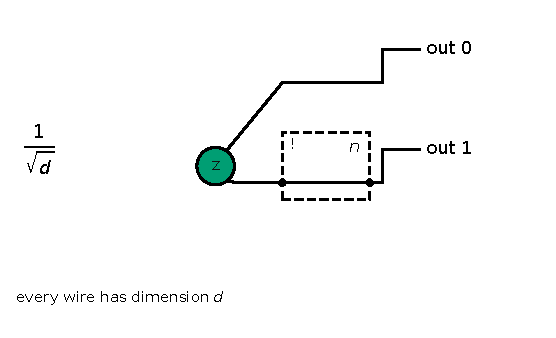
\includegraphics[width=0.45\textwidth]{figures/pictorial-ghz.pdf}\hfill
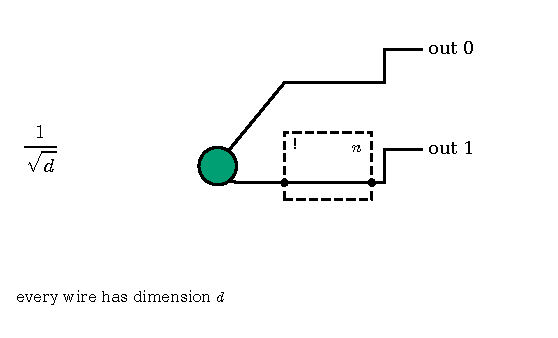
\includegraphics[width=0.45\textwidth]{figures/pictorial-ghz-pub.pdf}
\caption{The GHZ state in normal mode (left) and publication mode (right). The port-scoped
\texorpdfstring{!-box}{!-box} frames the repeated output; dots mark where the wire crosses its border.}
\label{fig:pictorial-ghz}
\end{figure}

The Z spider has two right-side ports, so its band is two lanes high and the grid draws a heavy
bracket on its right. The port-scoped \bbox{} adds one label lane above and one padding lane
below the repeated port (\cref{alg:pictorial-bands}), which pushes the plain output to lane 0.
All wires share dimension $d$, so no wire is labeled and the note says so.
\begin{lstlisting}[style=pgrid]
                  ┌──out 0
                  │
           ┎──────┘
           ┃╔!═══╗
1/√d      Ⓩ┃║   n║┌──out 1
           ┃║    ║│
           ┖╫────╫┘
            ╚════╝
every wire has dimension d
\end{lstlisting}
\begin{lstlisting}[style=pgrid]
                         .--out 0
                         |
                  ]------'
                  ]#!===#
1/sqrt(d)      (Z)]:   n:.--out 1
                  ]:    :|
                  ]*----*'
                   #====#
every wire has dimension d
\end{lstlisting}

\subsection{GHZ preparation with a node-scoped !-box}\label{sec:pictorial-ex-circuit}

The preparation circuit of the same state applies an X state, a Fourier box, and a Z spider,
then $n$ controlled additions, each an X spider fed by a fresh X state, inside a node-scoped
\bbox:
\begin{lstlisting}[style=azx]
load
  count n
  X(0 -> 1) -> F -> z = Z(1 -> 2)
  repeat n: z.out1 -> t = X(2 -> 1), X(0 -> 1) -> t
  scalar d^(-1/2)
\end{lstlisting}

\begin{figure}[ht]
\centering
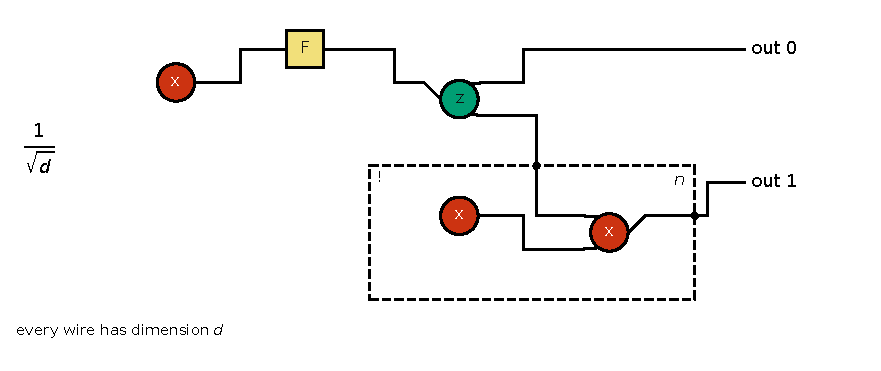
\includegraphics[width=0.75\textwidth]{figures/pictorial-ghzcircuit.pdf}\\[2mm]
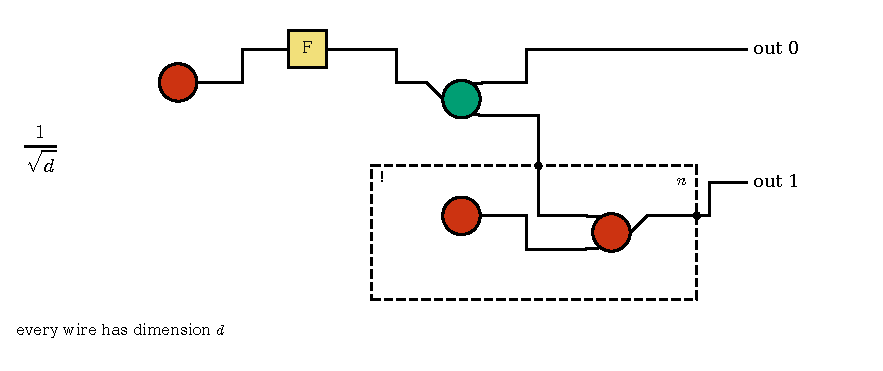
\includegraphics[width=0.75\textwidth]{figures/pictorial-ghzcircuit-pub.pdf}
\caption{GHZ preparation in normal mode (top) and publication mode (bottom). The node-scoped
\texorpdfstring{!-box}{!-box} holds both X spiders of the repeated step and spans two columns.}
\label{fig:pictorial-ghzcircuit}
\end{figure}

Layer assignment puts the X state in column 0 (it is a source with no input, so it is pulled
right next to F), F in column 1, Z in column 2, the inner X state and the X spider in columns 3
and 4, and both outputs in column 5. The wire from Z to the inner X spider enters the frame from
above, crossing its top border at a right angle (\pgi!╪! in the grid, a dot in the figure).
\begin{lstlisting}[style=pgrid]
             ┌──[F]────┐      ┌─────────┐
             │         │      │         │
          Ⓧ──┘         └──Ⓩ┎──┘         └──out 0
                           ┃
                           ┖───┐
                               │
                               │
                     ╔!════════╪═══════╗
1/√d                 ║         │      n║┌──out 1
                     ║         │       ║│
                     ║    Ⓧ───┐│       ║│
                     ║        ││       ║│
                     ║        │└──┒Ⓧ───╫┘
                     ║        │   ┃    ║
                     ║        └───┚    ║
                     ║                 ║
                     ║                 ║
                     ╚═════════════════╝
every wire has dimension d
\end{lstlisting}
\begin{lstlisting}[style=pgrid]
                    .--[F]----.        .-----------.
                    |         |        |           |
               (X)--'         '--(Z)]--'           '--out 0
                                    ]
                                    ]---.
                                        |
                                        |
                            #!==========*=========#
1/sqrt(d)                   :           |        n:.--out 1
                            :           |         :|
                            :    (X)---.|         :|
                            :          ||         :|
                            :          |'--[(X)---*'
                            :          |   ]      :
                            :          '---[      :
                            :                     :
                            :                     :
                            #=====================#
every wire has dimension d
\end{lstlisting}

\begin{figure}[ht]
\centering
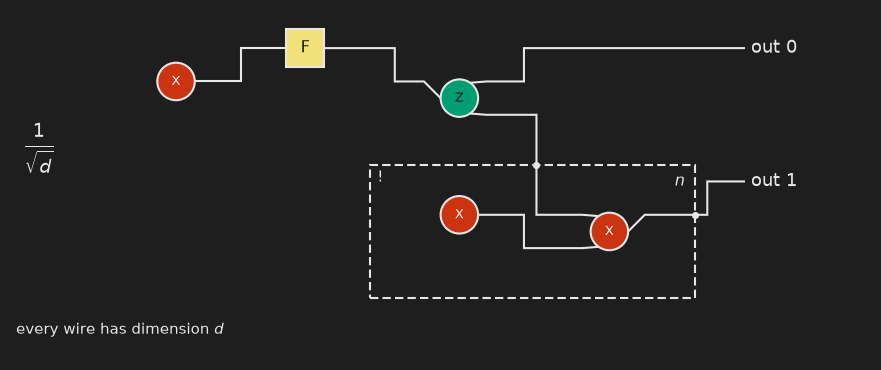
\includegraphics[width=0.75\textwidth]{figures/pictorial-ghzcircuit-dark.png}
\caption{The same drawing as PNG with the dark-theme defaults (ink \texttt{\#e6e6e6} on
\texttt{\#1e1e1e}), opaque, at density 1.5, as a terminal without color reports shows it.}
\label{fig:pictorial-dark}
\end{figure}

\subsection{W state}\label{sec:pictorial-ex-w}

The three-qubit W state~\cite{dur2000three} is a W node fed by an X spider with phase
$\tfrac12$ turn (the state $\ket{1}$):
\begin{lstlisting}[style=azx]
load
  p = X(0 -> 1, literal 2) phase{1: 1/2}
  w = W(1 -> 3, literal 2)
  p -> w
\end{lstlisting}

\begin{figure}[ht]
\centering
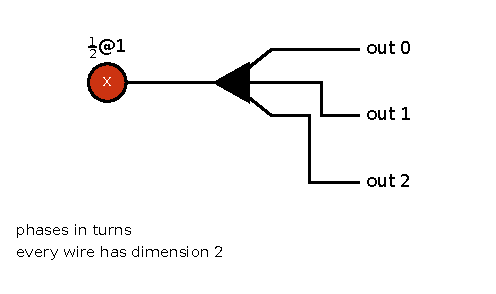
\includegraphics[width=0.42\textwidth]{figures/pictorial-wstate.pdf}\hfill
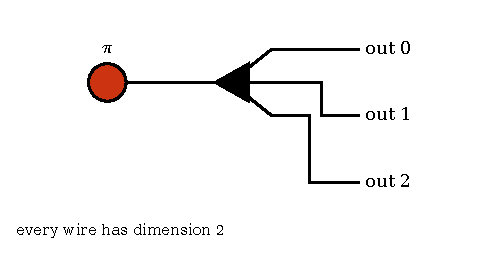
\includegraphics[width=0.42\textwidth]{figures/pictorial-wstate-pub.pdf}
\caption{The W state in normal mode (left, phase $\tfrac12$ in turns) and publication mode
(right, phase $\pi$).}
\label{fig:pictorial-wstate}
\end{figure}

The W node's three outputs spread over $\pm0.8h_b$ on its flat side; the outer two reach their
lanes by slanted segments.
\begin{lstlisting}[style=pgrid]
                ┎────out 0
                ┃
    Ⓧ1/2@1────◀W┠────out 1
                ┃
                ┖────out 2
phases in turns
every wire has dimension 2
\end{lstlisting}
\begin{lstlisting}[style=pgrid]
                   ]----out 0
                   ]
    (X 1/2@1)----<W]----out 1
                   ]
                   ]----out 2
phases in turns
every wire has dimension 2
\end{lstlisting}

\subsection{Generator gallery}\label{sec:pictorial-ex-gens}

A chain through an X spider with the phase family $-k/d$, a triangle, an inverse triangle, a
Fourier box, a weighted Z spider, and a discard shows most glyphs:
\begin{lstlisting}[style=azx]
load
  X(0 -> 1) phase{k: -k/d} -> T(d) -> Ti(d) -> F -> z = Z(1 -> 1) weight{1: a}
  z -> G(d)
\end{lstlisting}

\begin{figure}[ht]
\centering
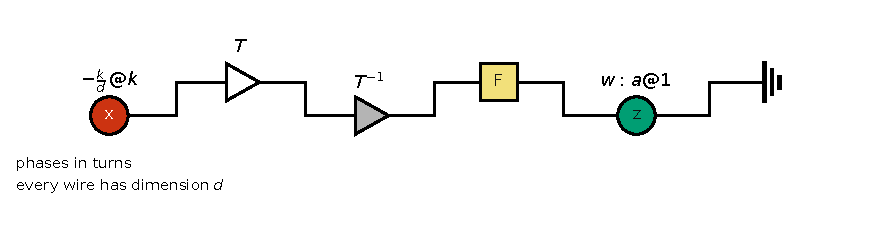
\includegraphics[width=0.85\textwidth]{figures/pictorial-gens.pdf}\\[2mm]
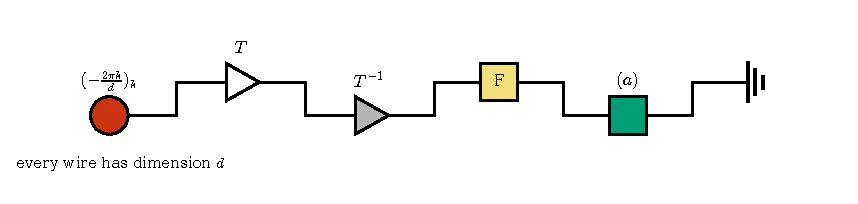
\includegraphics[width=0.85\textwidth]{figures/pictorial-gens-pub.pdf}
\caption{Generator gallery in normal mode (top) and publication mode (bottom). In publication
mode the weighted Z spider becomes a Z box with the coefficient vector $(a)$.}
\label{fig:pictorial-gens}
\end{figure}

\begin{lstlisting}[style=pgrid]
    Ⓧ-k/d @k────▷T────▶T⁻¹────[F]────Ⓩw: a@1────⏚
phases in turns
every wire has dimension d
\end{lstlisting}
\begin{lstlisting}[style=pgrid]
    (X -k/d @k)----|>T----|>T^-1----[F]----(Z w: a@1)----_|_
phases in turns
every wire has dimension d
\end{lstlisting}

\subsection{Splitter and binder}\label{sec:pictorial-ex-split}

A dimension splitter followed by a dimension binder carries three distinct wire dimensions, so
every wire is labeled in the margin of its first channel and no dimension note appears:
\begin{lstlisting}[style=azx]
load
  s = S(literal 2, literal 3)
  b = B(literal 2, literal 3)
  wire s.out0 -- b.in0
  wire s.out1 -- b.in1
\end{lstlisting}

\begin{figure}[ht]
\centering
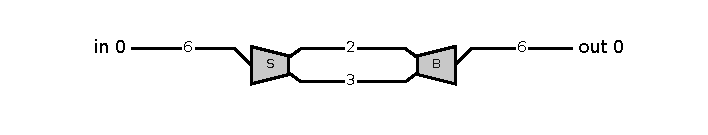
\includegraphics[width=0.7\textwidth]{figures/pictorial-split.pdf}
\caption{A splitter and a binder with labeled wire dimensions.}
\label{fig:pictorial-split}
\end{figure}

\begin{lstlisting}[style=pgrid]
    in 0──6───⊳S┎──2───┒⊲B──6───out 0
                ┃      ┃
                ┖──3───┚
\end{lstlisting}
\begin{lstlisting}[style=pgrid]
    in 0--6--->S]--2---[<B--6---out 0
                ]      ]
                ]--3---[
\end{lstlisting}


\part{Lean}
\chapter{The Lean Library: Foundations, Generators and Rules}\label{ch:lean-core}

\lstdefinestyle{leancore}{style=lean,
  literate={→}{{$\to$}}1 {←}{{$\leftarrow$}}1 {≤}{{$\le$}}1 {≥}{{$\ge$}}1 {≠}{{$\ne$}}1
           {ω}{{$\omega$}}1 {⟩}{{$\rangle$}}1 {⟨}{{$\langle$}}1 {∀}{{$\forall$}}1
           {∃}{{$\exists$}}1 {λ}{{$\lambda$}}1 {∑}{{$\sum$}}1 {·}{{$\cdot$}}1
           {ℂ}{{$\mathbb{C}$}}1 {ℕ}{{$\mathbb{N}$}}1 {ℤ}{{$\mathbb{Z}$}}1 {ℚ}{{$\mathbb{Q}$}}1
           {ℝ}{{$\mathbb{R}$}}1 {↦}{{$\mapsto$}}1 {∘}{{$\circ$}}1
           {α}{{$\alpha$}}1 {β}{{$\beta$}}1 {π}{{$\pi$}}1 {∈}{{$\in$}}1 {∉}{{$\notin$}}1
           {×}{{$\times$}}1 {₀}{{$_0$}}1 {₁}{{$_1$}}1 {₂}{{$_2$}}1 {₃}{{$_3$}}1 {₄}{{$_4$}}1
           {⁻}{{$^{-}$}}1 {¹}{{$^{1}$}}1 {√}{{$\surd$}}1 {∧}{{$\wedge$}}1 {∨}{{$\vee$}}1
           {¬}{{$\neg$}}1 {↔}{{$\leftrightarrow$}}1 {ε}{{$\varepsilon$}}1 {μ}{{$\mu$}}1
           {σ}{{$\sigma$}}1 {τ}{{$\tau$}}1 {φ}{{$\varphi$}}1 {ρ}{{$\rho$}}1 {ν}{{$\nu$}}1
           {δ}{{$\delta$}}1 {θ}{{$\theta$}}1 {ζ}{{$\zeta$}}1 {ι}{{$\iota$}}1 {∏}{{$\prod$}}1
           {•}{{$\bullet$}}1 {▸}{{$\triangleright$}}1,
}
\providecommand{\leanLLone}{\lstinline[style=leancore,frame=none,basicstyle=\ttfamily,%
  breaklines=true,breakatwhitespace=false]}

This chapter specifies the Lean~4 library that ships inside the ArchytasZX package, in the
directory \file{archytaszx/lean}. The library defines the semantics of ArchytasZX diagrams as
labeled tensor networks over $\C$, states every rewrite rule of the engine as a lemma about such
networks, and supplies the decision tools (exact cyclotomic evaluation, ball arithmetic,
contraction certificates) that the engine's Lean exporters invoke. The engine is
Lean-certifying: an exported proof imports these modules and is checked by the Lean
kernel~\cite{demoura2021lean4} against Mathlib~\cite{mathlib2020}. This chapter covers the
library's build configuration and module structure, and in full detail the modules that define
networks, generators, rule lemmas, mixed networks, exact arithmetic, refutation, contraction, and
the diagram data type with its \bbox{} expansion. The modules for \bbox{} families are specified in
\cref{ch:lean-boxes}, the path-sum modules in \cref{ch:lean-pathsum}, and the symbolic and linked
modules in \cref{ch:lean-sym}; the Python side that writes the Lean files is specified in
\cref{ch:lean-export-net} and \cref{ch:lean-export}.

Throughout, $\N=\{0,1,2,\dots\}$, a \emph{label} is a natural number naming one contracted index,
and all leg values are natural numbers. For a proposition $P$, $[P]\in\{0,1\}$ is its indicator.
Lean identifiers appear in typewriter type; every declaration lies in the namespace
\lean|ArchytasZX|, and every module opens \lean|Complex| and \lean|Finset| unless noted.

%======================================================================
\section{The library as a whole}\label{sec:lean-core-library}

\subsection{Toolchain, package and build}\label{sec:lean-core-build}

The library is a Lake package. Its four configuration files fix every version.

\begin{description}[style=nextline]
\item[\file{lean-toolchain}] The single line \code|leanprover/lean4:v4.35.0|: the package builds
  with Lean~4 version 4.35.0\index{Lean toolchain}. \tool{Elan}{https://github.com/leanprover/elan}
  reads this file and installs that toolchain.
\item[\file{lakefile.toml}] The package \code|archytaszx| with \code|defaultTargets = ["ArchytasZX"]|,
  one requirement and one library:
\begin{lstlisting}[style=grammar]
name = "archytaszx"
defaultTargets = ["ArchytasZX"]

[[require]]
name = "mathlib"
git = "https://github.com/leanprover-community/mathlib4"
rev = "v4.35.0"

[[lean_lib]]
name = "ArchytasZX"
\end{lstlisting}
\item[\file{lake-manifest.json}] Manifest format \code|1.3.0|, \code|packagesDir| =
  \code|.lake/packages|, \code|lakeDir| = \code|.lake|, \code|fixedToolchain| = \code|false|. It pins
  the packages of \cref{tab:lean-core-manifest}; only Mathlib is a direct requirement
  (\code|inherited| = \code|false|), the others come in through Mathlib.
\item[\file{ArchytasZX.lean}] The root module. It consists of 87 \lean|import| lines and nothing
  else; the imported modules and their transitive imports make up all 91 modules in
  \file{archytaszx/lean/ArchytasZX/}.
\end{description}

\begin{table}[htbp]
\centering\small
\caption{Packages pinned by \texttt{lake-manifest.json}.}\label{tab:lean-core-manifest}
\begin{tabular}{@{}lllp{4.6cm}@{}}
\toprule
Package & Input revision & Pinned commit & Repository \\
\midrule
\code|mathlib| & \code|v4.35.0| & \code|56a005855ea1| & \url{https://github.com/leanprover-community/mathlib4} \\
\code|plausible| & \code|main| & \code|dfa4f38190d0| & \url{https://github.com/leanprover-community/plausible} \\
\code|LeanSearchClient| & \code|main| & \code|d6b4c7be5be7| & \url{https://github.com/leanprover-community/LeanSearchClient} \\
\code|importGraph| & \code|main| & \code|a41f0e9a4dea| & \url{https://github.com/leanprover-community/import-graph} \\
\code|proofwidgets| & \code|main| & \code|df72b022e558| & \url{https://github.com/leanprover-community/ProofWidgets4} \\
\code|aesop| & \code|master| & \code|4a174c490d87| & \url{https://github.com/leanprover-community/aesop} \\
\code|Qq| & \code|master| & \code|dce0ad79c486| & \url{https://github.com/leanprover-community/quote4} \\
\code|batteries| & \code|main| & \code|66e469188fe0| & \url{https://github.com/leanprover-community/batteries} \\
\code|Cli| & \code|v4.35.0| & \code|c24fe6078c63| & \url{https://github.com/leanprover/lean4-cli} \\
\bottomrule
\end{tabular}
\end{table}

The full pinned commits are:
\begin{center}\small
\begin{tabular}{@{}ll@{}}
\toprule
Package & Commit \\
\midrule
\code|mathlib| & \code|56a005855ea17e0b0958f73ec801ae140b0a1679| \\
\code|plausible| & \code|dfa4f38190d07c37e315953e08b90fe2d95b3c24| \\
\code|LeanSearchClient| & \code|d6b4c7be5be75ec4917c873ac50c756dc1436372| \\
\code|importGraph| & \code|a41f0e9a4dea23188ea9cc1c41ac9f8bbafe0b93| \\
\code|proofwidgets| & \code|df72b022e558978a1c50264cfc4d7fec86fa8e04| \\
\code|aesop| & \code|4a174c490d8707121c4a9290800489f105d85e07| \\
\code|Qq| & \code|dce0ad79c486cb1fb504af04f953c3466b0c6db8| \\
\code|batteries| & \code|66e469188fe07963e5cf666c7d4433f45b8131c5| \\
\code|Cli| & \code|c24fe6078c630e89b489bffe59b3e20ac30d12c8| \\
\bottomrule
\end{tabular}
\end{center}
Each package's \code|configFile| is \code|lakefile.toml|, except Mathlib's, which is
\code|lakefile.lean|.

\paragraph{Building.} From \file{archytaszx/lean}, \code|lake build| fetches the pinned packages
into \file{.lake/packages}, then compiles the default target, the library \code|ArchytasZX|, that is
the root module and every module it imports. Mathlib's command \code|lake exe cache get|
downloads Mathlib's compiled files. An exported proof is a Lean source file whose header imports
the modules it needs (for example \lean|import ArchytasZX| or \lean|import ArchytasZX.PathSumNetW|).
The engine's checker \py|check(source, path, timeout=1800)| in
\module{archytaszx.semantics.lean_net} checks such a file in four steps:
\begin{enumerate}
\item find \code|lake| on the search path, else at \file{~/.elan/bin/lake}; with neither, raise
  \py|NetUnsupported("Lean (lake) is not installed")|;
\item write \py|source| to \py|path| (UTF-8);
\item if \file{archytaszx/lean/.lake/packages/mathlib} is not a directory, run
  \code|lake exe cache get| in \file{archytaszx/lean}; on a nonzero exit return
  \py|(False, stdout + stderr)|;
\item run \code|lake build| in \file{archytaszx/lean}; on a nonzero exit return
  \py|(False, stdout + stderr)|; then run \code|lake env lean <absolute path>| there and return
  \py|(exit code = 0, stdout + stderr)|.
\end{enumerate}
Each subprocess has the time limit \py|timeout| seconds. The repository's continuous integration
does not build the Lean library.

\paragraph{File conventions.} Every module starts with the comment block
\code|Copyright 2026 Arkhip A. Dmitriev / Licensed under the Apache License, Version 2.0.|, then its
imports, then a module docstring \code|/-! ... -/| headed by a Markdown title, then
\lean|namespace ArchytasZX|. Docstrings \code|/-- ... -/| state what each declaration is.

\subsection{Trust base}\label{sec:lean-core-trust}

\begin{itemize}
\item \textbf{No axioms, no gaps.} No module of \file{archytaszx/lean/ArchytasZX/} declares an
  \lean|axiom|, and none contains \lean|sorry|, \lean|admit| or \lean|native_decide|. Every theorem
  therefore rests on the Lean kernel and the axioms of Lean's core library as Mathlib uses them
  (propositional extensionality, the axiom of choice, quotient soundness); the real and complex
  numbers of Mathlib are classical.
\item \textbf{Computation in proofs.} Decidable checks (\lean|isoOK|, \lean|Diagram.check|,
  \lean|leafOK|, \lean|chainOK|, coefficient-vector reductions) are \lean|Bool| functions; an exported
  proof discharges a hypothesis \lean|h : f x = true| with \lean|decide| or \lean|rfl|, so the Lean
  kernel evaluates the check by definitional unfolding.
\item \textbf{Unsafe code.} Three modules outside this chapter (\texttt{PathSumChain},
  \texttt{PathSumQuditChain}, \texttt{SymF2Chain}) declare \lean|unsafe| metaprograms of type
  \lean|MetaM| and attach them with \lean|@[implemented_by]| to the elaboration-time functions that
  enumerate chain states; these functions run while a proof is elaborated, and the proof terms they
  help produce are checked by the kernel. No module of this chapter uses \lean|unsafe|.
\item \textbf{Noncomputable definitions.} Every definition with a complex or real value (tensor
  entries, sums, evaluations) is \lean|noncomputable|; theorems about them are proved, never
  evaluated.
\end{itemize}

\subsection{Module structure}\label{sec:lean-core-modules}

\Cref{tab:lean-core-imports} lists every module of \file{archytaszx/lean/ArchytasZX/} with its
direct imports, its line count, its number of top-level theorems and of top-level definitions
(\lean|def|, \lean|abbrev|, \lean|structure|, \lean|inductive|), and the chapter that specifies it.
Imports from Mathlib are counted, not named, except in \texttt{Net}, which carries all 43
Mathlib imports of the foundation. The library has 79{,}797 lines, 3{,}971 top-level theorems and
1{,}994 top-level definitions. \texttt{Light} has no declarations: it imports 87 modules, none of which imports \texttt{Cyclo} or \texttt{NumField} directly or indirectly; the benchmark's Lean check tries it in place of the full library (\cref{ch:bench-pipeline}). The modules \texttt{AdderFamEnv}, \texttt{FamDiagram}, \texttt{FamExpandEq}, \texttt{FamFcaExpand}, \texttt{LinkedMerge}, and \texttt{LinkedPair} also avoid \texttt{Cyclo} and \texttt{NumField} and are not imported by \texttt{Light}. \Cref{fig:lean-core-spine-a,fig:lean-core-spine} draw the import structure of the modules
of this chapter.

{\small
\begin{xltabular}{\textwidth}{@{}l>{\raggedright\arraybackslash}Xrrrc@{}}
\caption{Every module of the library: direct imports (modules of \texttt{ArchytasZX}, then the number
of Mathlib imports), lines, theorems, definitions, and the specifying chapter: C this chapter,
B \cref{ch:lean-boxes}, P \cref{ch:lean-pathsum}, S \cref{ch:lean-sym}.}\label{tab:lean-core-imports}\\
\toprule
Module & Imports & Lines & Thm. & Def. & Ch. \\
\midrule
\endfirsthead
\toprule
Module & Imports & Lines & Thm. & Def. & Ch. \\
\midrule
\endhead
\bottomrule
\endfoot
\texttt{AdderFam} & Closed, ChainInduct & 504 & 26 & 11 & B \\
\texttt{AdderFamDraper} & AdderFamFca & 1517 & 115 & 42 & B \\
\texttt{AdderFamDraperEng} & AdderFamDraper, AdderFamFcaEng & 1610 & 105 & 57 & B \\
\texttt{AdderFamEnv} & AdderFam, ChainMixed & 69 & 2 & 3 & B \\
\texttt{AdderFamFca} & AdderFamEnv, Ball, Weights, PairEval & 1672 & 131 & 41 & B \\
\texttt{AdderFamFcaEng} & AdderFamFca & 1304 & 91 & 53 & B \\
\texttt{Assume} & Bundle & 96 & 4 & 4 & C \\
\texttt{Ball} & Cyclo, 2 Mathlib & 280 & 36 & 4 & C \\
\texttt{Bialgebra} & ZXRules & 189 & 4 & 0 & C \\
\texttt{BoxedBridge} & FamK, DiagramBridge & 631 & 27 & 18 & B \\
\texttt{BoxFree} & Induct & 154 & 7 & 0 & B \\
\texttt{Bridge} & Expand & 133 & 0 & 16 & B \\
\texttt{Bundle} & WZ & 1876 & 109 & 46 & B \\
\texttt{ChainBox} & Bridge & 85 & 2 & 7 & B \\
\texttt{ChainBridge} & ChainForm, ChainLabel, PeriodicChain & 244 & 14 & 14 & B \\
\texttt{ChainEvery} & ChainLink & 313 & 26 & 9 & B \\
\texttt{ChainFam} & ChainBridge & 520 & 22 & 3 & B \\
\texttt{ChainForm} & ChainBox & 159 & 13 & 4 & B \\
\texttt{ChainInduct} & Bundle & 313 & 21 & 5 & B \\
\texttt{ChainLabel} & Elim & 157 & 3 & 2 & B \\
\texttt{ChainLink} & ChainBox, ChainInduct & 99 & 4 & 5 & B \\
\texttt{ChainMixed} & ChainInduct & 422 & 27 & 3 & B \\
\texttt{ChainNode} & ChainLink & 489 & 41 & 14 & B \\
\texttt{ChainPair} & ChainFam & 159 & 7 & 1 & B \\
\texttt{Closed} & Rules & 152 & 17 & 1 & C \\
\texttt{Completeness} & Net, Rules, WRules, Closed, ZXRules & 159 & 7 & 0 & C \\
\texttt{Connective} & WRules & 255 & 10 & 0 & C \\
\texttt{Contract} & Refute & 502 & 22 & 19 & C \\
\texttt{CopyBridge} & CopyPin, Linked & 867 & 33 & 14 & B \\
\texttt{CopyPin} & Ball, Mixed, FamK & 128 & 6 & 0 & B \\
\texttt{Cyclo} & Bundle, 1 Mathlib & 451 & 47 & 11 & C \\
\texttt{Diagram} & Net & 246 & 6 & 20 & C \\
\texttt{DiagramBridge} & Diagram & 476 & 17 & 14 & B \\
\texttt{Digits} & Elim & 196 & 13 & 12 & C \\
\texttt{Elim} & Bridge, WZ & 331 & 9 & 8 & C \\
\texttt{Expand} & Diagram & 159 & 0 & 20 & C \\
\texttt{ExpandFacts} & Digits & 230 & 13 & 2 & C \\
\texttt{FamBridge} & NetDigits & 268 & 11 & 3 & B \\
\texttt{FamCheck} & FamBridge & 153 & 8 & 10 & B \\
\texttt{FamDiagram} & OrderK, PairBox & 172 & 8 & 19 & B \\
\texttt{FamExpandEq} & FamDiagram & 68 & 7 & 0 & B \\
\texttt{FamFcaExpand} & FamExpandEq & 135 & 14 & 4 & B \\
\texttt{FamK} & OrderK & 243 & 12 & 2 & B \\
\texttt{FuseB} & Unfuse & 284 & 14 & 1 & C \\
\texttt{Gather} & PortBox & 246 & 22 & 1 & C \\
\texttt{GaussSign} & Cyclo, PathSumQudit & 174 & 8 & 4 & C \\
\texttt{Hopf} & Bialgebra & 245 & 10 & 0 & C \\
\texttt{Induct} & NodeBox & 299 & 15 & 5 & B \\
\texttt{Iso} & Net & 156 & 7 & 5 & C \\
\texttt{Light} & Net, Iso, Rules, Closed, ZXRules, Bialgebra, Hopf, WRules, WAssoc, WFuse, Connective, WZ, Bundle, Unfuse, FuseB, SymNet, SymChunk, SymHint, SymF2, SymF2Chain, SymF2Bridge, DiagramBridge, Port, Assume, Completeness, Weights, Diagram, Expand, Bridge, ChainBox, Elim, Digits, ExpandFacts, Relabel, PortBox, Gather, Split, NodeBox, Induct, BoxFree, Positional, Tower, NodeVal, NodeBridge, Pin, NetDigits, FamBridge, FamCheck, Order, OrderK, FamK, BoxedBridge, Linked, LinkedPeel, LinkedSlide, LinkedRegroup, LinkedSplit, LinkedForm, LinkedGhost, LinkedSplice, LinkedFirst, LinkedDropX, LinkedRead, Mixed, ChainInduct, ChainLink, ChainEvery, Periodic, PeriodicChain, ChainMixed, ChainLabel, ChainForm, ChainBridge, ChainFam, ChainPair, TreeInduct, PhaseMap, ChainNode, PairBox, PairNet, PairEval, PairFam, AdderFam, PairSum, Sym, SymCanon, SymNorm & 96 & 0 & 0 & B \\
\texttt{Linked} & Relabel & 515 & 10 & 23 & S \\
\texttt{LinkedDropX} & LinkedGhost & 302 & 14 & 4 & S \\
\texttt{LinkedFirst} & LinkedSplice & 656 & 42 & 7 & S \\
\texttt{LinkedForm} & LinkedSlide, LinkedRegroup & 170 & 12 & 8 & S \\
\texttt{LinkedGhost} & LinkedForm & 958 & 58 & 15 & S \\
\texttt{LinkedMerge} & LinkedPair & 294 & 26 & 6 & S \\
\texttt{LinkedPair} & LinkedFirst & 455 & 17 & 11 & S \\
\texttt{LinkedPeel} & Linked, PortBox & 1717 & 86 & 18 & S \\
\texttt{LinkedRead} & LinkedDropX, LinkedSplice & 1165 & 55 & 19 & S \\
\texttt{LinkedRegroup} & Linked & 134 & 6 & 6 & S \\
\texttt{LinkedSlide} & BoxFree, LinkedPeel, Weights & 576 & 45 & 6 & S \\
\texttt{LinkedSplice} & LinkedGhost, LinkedPeel & 1267 & 58 & 24 & S \\
\texttt{LinkedSplit} & LinkedPeel, Iso & 1812 & 86 & 15 & S \\
\texttt{Mixed} & Closed & 210 & 16 & 3 & C \\
\texttt{Net} & 43 Mathlib & 480 & 20 & 40 & C \\
\texttt{NetDigits} & Pin & 244 & 6 & 2 & C \\
\texttt{NodeBox} & Split & 1440 & 85 & 7 & B \\
\texttt{NodeBridge} & NodeVal & 339 & 15 & 1 & B \\
\texttt{NodeVal} & Tower & 406 & 34 & 11 & B \\
\texttt{NumField} & Weights, 4 Mathlib & 110 & 7 & 3 & C \\
\texttt{Order} & FamCheck & 280 & 20 & 7 & C \\
\texttt{OrderK} & Order & 246 & 13 & 8 & C \\
\texttt{PairBox} & ChainLabel, Relabel & 229 & 0 & 31 & B \\
\texttt{PairEval} & PairNet & 646 & 34 & 4 & B \\
\texttt{PairFam} & PairEval & 93 & 3 & 0 & B \\
\texttt{PairNet} & PairBox & 815 & 59 & 3 & B \\
\texttt{PairSum} & PairFam & 116 & 9 & 1 & B \\
\texttt{Paper} & Net, Rules, Closed, ZXRules, Cyclo & 172 & 12 & 9 & C \\
\texttt{PathSum} & Sym, Cyclo & 183 & 17 & 2 & P \\
\texttt{PathSumAmp} & PathSumRules & 1964 & 81 & 85 & P \\
\texttt{PathSumChain} & PathSumSupport, PathSumParity & 308 & 6 & 19 & P \\
\texttt{PathSumDigits} & PathSumNet, Positional & 1059 & 47 & 21 & P \\
\texttt{PathSumMixed} & PathSumQudit, PathSumAmp & 492 & 25 & 9 & P \\
\texttt{PathSumMixedNet} & PathSumMixed, PathSumNetAmp, PathSumQuditNet, PathSumQuditDigits & 1087 & 56 & 21 & P \\
\texttt{PathSumNet} & PathSumRules & 676 & 42 & 21 & P \\
\texttt{PathSumNetAmp} & PathSumNetW, PathSumAmp & 409 & 19 & 7 & P \\
\texttt{PathSumNetW} & PathSumW, PathSumChain & 91 & 7 & 3 & P \\
\texttt{PathSumParity} & PathSumRules & 109 & 2 & 4 & P \\
\texttt{PathSumQudit} & PathSum, 1 Mathlib & 1138 & 68 & 55 & P \\
\texttt{PathSumQuditChain} & PathSumChain, PathSumQudit & 103 & 3 & 5 & P \\
\texttt{PathSumQuditDigits} & PathSumQuditNet & 636 & 28 & 12 & P \\
\texttt{PathSumQuditNet} & PathSumQudit, PathSumDigits, GaussSign, PathSumQuditChain & 462 & 29 & 14 & P \\
\texttt{PathSumRules} & PathSumSem & 2198 & 91 & 63 & P \\
\texttt{PathSumSem} & PathSum, Ball & 2173 & 139 & 101 & P \\
\texttt{PathSumSupport} & PathSumAmp & 58 & 2 & 1 & P \\
\texttt{PathSumW} & PathSumDigits & 224 & 9 & 3 & P \\
\texttt{Periodic} & ChainInduct & 42 & 1 & 0 & B \\
\texttt{PeriodicChain} & Periodic & 301 & 22 & 6 & B \\
\texttt{PhaseMap} & Bundle & 114 & 5 & 4 & B \\
\texttt{Pin} & NodeBridge & 152 & 8 & 4 & C \\
\texttt{Port} & Bundle & 1117 & 61 & 11 & B \\
\texttt{PortBox} & Relabel, ExpandFacts & 934 & 63 & 7 & B \\
\texttt{Positional} & BoxFree, Bundle & 141 & 12 & 3 & C \\
\texttt{Refute} & Cyclo & 547 & 26 & 33 & C \\
\texttt{RefuteMod} & Contract & 1789 & 99 & 61 & C \\
\texttt{RefuteSym} & RefuteMod, 1 Mathlib & 1897 & 92 & 63 & C \\
\texttt{Relabel} & Digits & 135 & 4 & 4 & C \\
\texttt{Rules} & Iso, 1 Mathlib & 324 & 19 & 0 & C \\
\texttt{Split} & Gather & 195 & 6 & 2 & C \\
\texttt{Sym} & Closed & 1032 & 78 & 72 & S \\
\texttt{SymCanon} & SymNorm & 851 & 35 & 45 & S \\
\texttt{SymCarry} & SymRange & 728 & 29 & 17 & S \\
\texttt{SymChunk} & SymNet & 283 & 19 & 16 & S \\
\texttt{SymDig} & SymCarry, Cyclo & 845 & 34 & 24 & S \\
\texttt{SymF2} & SymNet & 1231 & 87 & 58 & S \\
\texttt{SymF2Bridge} & SymF2, DiagramBridge & 160 & 3 & 2 & S \\
\texttt{SymF2Chain} & SymF2 & 136 & 0 & 7 & S \\
\texttt{SymFold} & SymCarry & 1112 & 34 & 25 & S \\
\texttt{SymFourier} & SymHint, PathSumSem & 851 & 39 & 33 & S \\
\texttt{SymHint} & SymChunk & 795 & 30 & 28 & S \\
\texttt{SymNet} & SymCanon & 1581 & 72 & 54 & S \\
\texttt{SymNorm} & Sym, Bundle & 926 & 39 & 24 & S \\
\texttt{SymRange} & SymFourier & 1210 & 46 & 41 & S \\
\texttt{Tower} & Positional & 161 & 11 & 1 & C \\
\texttt{TreeInduct} & ChainInduct & 330 & 13 & 7 & B \\
\texttt{Unfuse} & Bundle & 221 & 12 & 0 & C \\
\texttt{WAssoc} & WRules & 120 & 6 & 2 & C \\
\texttt{Weights} & Net, Rules, Closed, ZXRules, Completeness, WZ, Hopf, Connective & 9479 & 213 & 64 & C \\
\texttt{WFuse} & WAssoc, FuseB, NodeBox, Weights & 225 & 10 & 0 & C \\
\texttt{WRules} & Hopf & 289 & 17 & 1 & C \\
\texttt{WZ} & Connective & 242 & 6 & 0 & C \\
\texttt{ZXRules} & Closed & 398 & 28 & 0 & C \\
\end{xltabular}
}

\begin{figure}[htbp]
\centering
\begin{tikzpicture}[x=1.55cm,y=0.95cm,every node/.style={font=\scriptsize,draw,rounded corners=1pt,inner sep=2pt},>={Stealth[length=1.6mm]}]
\node (net) at (3,0) {Net};
\node (iso) at (1,1) {Iso};
\node (diag) at (5,1) {Diagram};
\node (rules) at (1,2) {Rules};
\node (expand) at (5,2) {Expand};
\node (closed) at (1,3) {Closed};
\node (zx) at (0,4) {ZXRules};
\node (mixed) at (2,4) {Mixed};
\node (bia) at (0,5) {Bialgebra};
\node (hopf) at (0,6) {Hopf};
\node (wr) at (0,7) {WRules};
\node (conn) at (-1,8) {Connective};
\node (wassoc) at (1,8) {WAssoc};
\node (compl) at (2,7) {Completeness};
\node (wz) at (-1,9) {WZ};
\node (weights) at (1,10) {Weights};
\node (numf) at (0,11) {NumField};
\node (bundle) at (-1,10.2) {[Bundle]};
\node (unf) at (-2,11) {Unfuse};
\node (fuseb) at (-2,12) {FuseB};
\node (cyclo) at (3,11) {Cyclo};
\node (refute) at (3,12) {Refute};
\node (contract) at (3,13) {Contract};
\node (ball) at (4.3,12) {Ball};
\node (paper) at (2,12) {Paper};
\node (gauss) at (5.2,12.6) {GaussSign};
\node (assume) at (-3,11) {Assume};
\draw[->] (net) -- (iso); \draw[->] (net) -- (diag); \draw[->] (iso) -- (rules);
\draw[->] (diag) -- (expand); \draw[->] (rules) -- (closed); \draw[->] (closed) -- (zx);
\draw[->] (closed) -- (mixed); \draw[->] (zx) -- (bia); \draw[->] (bia) -- (hopf);
\draw[->] (hopf) -- (wr); \draw[->] (wr) -- (conn); \draw[->] (wr) -- (wassoc);
\draw[->] (wr) -- (compl); \draw[->] (conn) -- (wz); \draw[->] (compl) -- (weights);
\draw[->] (wz) -- (weights); \draw[->] (weights) -- (numf); \draw[->] (wz) -- (bundle);
\draw[->] (bundle) -- (unf); \draw[->] (unf) -- (fuseb); \draw[->] (bundle) -- (cyclo);
\draw[->] (cyclo) -- (refute); \draw[->] (refute) -- (contract); \draw[->] (cyclo) -- (ball);
\draw[->] (cyclo) -- (paper); \draw[->] (cyclo) -- (gauss); \draw[->] (bundle) -- (assume);
\end{tikzpicture}
\caption{Import structure of the network and rule-lemma modules of this chapter; an arrow points
from an imported module to an importing one; bracketed modules belong to \cref{ch:lean-boxes}.
Further imports are listed in \cref{tab:lean-core-imports}.}\label{fig:lean-core-spine-a}
\end{figure}

\begin{figure}[htbp]
\centering
\begin{tikzpicture}[x=1.7cm,y=0.9cm,every node/.style={font=\scriptsize,draw,rounded corners=1pt,inner sep=2pt},>={Stealth[length=1.6mm]}]
\node (expand) at (0,0) {Expand};
\node (bridge) at (0,1) {[Bridge]};
\node (elim) at (0,2) {Elim};
\node (digits) at (0,3) {Digits};
\node (ef) at (-1,4) {ExpandFacts};
\node (rel) at (1,4) {Relabel};
\node (portbox) at (0,5) {[PortBox]};
\node (gather) at (0,6) {Gather};
\node (split) at (0,7) {Split};
\node (nodebox) at (0,8) {[NodeBox]};
\node (induct) at (0,9) {[Induct, BoxFree]};
\node (pos) at (2,9.5) {Positional};
\node (tower) at (2,10.5) {Tower};
\node (nv) at (2,11.5) {[NodeVal, NodeBridge]};
\node (pin) at (2,12.5) {Pin};
\node (nd) at (2,13.5) {NetDigits};
\node (fam) at (0,13.5) {[FamBridge, FamCheck]};
\node (order) at (0,14.5) {Order};
\node (orderk) at (0,15.5) {OrderK};
\node (wfuse) at (-2,9) {WFuse};
\draw[->] (expand) -- (bridge); \draw[->] (bridge) -- (elim); \draw[->] (elim) -- (digits);
\draw[->] (digits) -- (ef); \draw[->] (digits) -- (rel); \draw[->] (ef) -- (portbox);
\draw[->] (rel) -- (portbox); \draw[->] (portbox) -- (gather); \draw[->] (gather) -- (split);
\draw[->] (split) -- (nodebox); \draw[->] (nodebox) -- (induct); \draw[->] (induct) -- (pos);
\draw[->] (pos) -- (tower); \draw[->] (tower) -- (nv); \draw[->] (nv) -- (pin);
\draw[->] (pin) -- (nd); \draw[->] (nd) -- (fam); \draw[->] (fam) -- (order);
\draw[->] (order) -- (orderk); \draw[->] (nodebox) -- (wfuse);
\end{tikzpicture}
\caption{Import structure of the diagram and \bbox{} expansion modules of this chapter (\texttt{Elim} also imports \texttt{WZ}; \texttt{WFuse} also imports \texttt{WAssoc}, \texttt{FuseB} and \texttt{Weights}; \texttt{Positional} also imports \texttt{Bundle}); bracketed modules belong to \cref{ch:lean-boxes}.}\label{fig:lean-core-spine}
\end{figure}

\subsection{Relation to the Python engine}\label{sec:lean-core-python}

The library mirrors the engine's data in three layers.
\begin{enumerate}
\item \textbf{Generators.} The constructors \lean|Z|, \lean|X|, \lean|F|, \lean|T|, \lean|Ti|,
  \lean|W|, \lean|B|, \lean|S| of \lean|Kind| (\cref{sec:lean-core-net}) are the engine's
  generators Z spider, X spider, Fourier box $F$, triangle, inverse triangle, W node, dimension
  binder $B$ and dimension splitter $S$; the exporter's table \py|_KINDS| maps each engine kind to
  the constructor of the same name. \lean|I| is the bare wire. \lean|ZW| and \lean|XW| are the
  Z and X spiders with arbitrary complex coefficients, the engine's weighted Z box and its X
  counterpart. \lean|ZB|, \lean|XB|, \lean|WB| and \lean|Bun| carry \bbox{} families: spiders whose
  last ports bundle copies, and copies of a generator along a multiplicity. The discard $G$ has no
  constructor; a diagram with discards is held as its purification (\cref{sec:lean-core-mixed}).
\item \textbf{Diagrams.} \lean|Diagram| (\cref{sec:lean-core-diagram}) is the engine's diagram
  as data, with ports, wires, boundary and \bboxes; \lean|DEqual_iff| equates diagram equality with
  network equality, so the exporter states its final theorem about diagrams.
\item \textbf{Rules.} Every rewrite rule the exporter supports has one or more lemmas whose
  conclusion is a \lean|LocalEq| between the rule's two sides. \Cref{tab:lean-core-rulemap} lists
  the engine rule names (keys of the exporter's dispatch table \py|_RULES| in
  \module{archytaszx.semantics.lean_net}) with the lemmas their steps invoke. A rule step becomes
  \lean|iso| into the shape $C\mathbin{+\!\!+}L$, then \lean|rewrite| with the rule's lemma, then
  \lean|wire_elim| for each bare wire the step leaves.
\end{enumerate}

{\small
\begin{xltabular}{\textwidth}{@{}>{\raggedright\arraybackslash}p{6.9cm}>{\raggedright\arraybackslash}X@{}}
\caption{Engine rules and the lemmas their exported steps invoke (module in parentheses). A
converse rule not listed invokes its forward rule's lemma under
\lean|LocalEq.symm'|.}\label{tab:lean-core-rulemap}\\
\toprule
Engine rule & Lemmas \\
\midrule
\endfirsthead
\toprule
Engine rule & Lemmas \\
\midrule
\endhead
\bottomrule
\endfoot
\code|spider_fusion|, \code|z_fusion_prime_d| & \lean|fusionZ|, \lean|fusionX| (Rules); \lean|zcFusion|, \lean|xcFusion| (Weights); \lean|fusionZG|, \lean|fusionXG| (FuseB) for bundled ports \\
\code|identity_removal| & \lean|identityZ|, \lean|identityX| (Rules) \\
\code|zx_cap|, \code|zx_cap_swapped| & \lean|cap|, \lean|capSwapped| (ZXRules) \\
\code|fourier_state_color_change|, \code|..._swapped| & \lean|colorState|, \lean|colorEffect|, \lean|colorStateX|, \lean|colorEffectX| (ZXRules) \\
\code|state_copy|, \code|state_copy_swapped| & \lean|stateCopy|, \lean|stateCopySwapped| (ZXRules) \\
\code|triangle_inverse_cancellation| & \lean|triangle|, \lean|triangle'| (ZXRules) \\
\code|fourier_cancellation| & \lean|fourier4| (ZXRules) \\
\code|bialgebra|, \code|bialgebra_swapped|, \code|zxw_b2_converse| & \lean|bialgebra|, \lean|bialgebraSwapped| (Bialgebra) \\
\code|hopf|, \code|hopf_swapped| & \lean|hopf|, \lean|hopfSwapped| (Hopf); \lean|hopfW|, \lean|hopfSwappedW|, \lean|hopfXW|, \lean|hopfSwappedXW|, \lean|hopfWXW|, \lean|hopfSwappedWXW| (Weights) \\
\code|w_fusion|, \code|qf_wf| & \lean|wFusion| (WRules) \\
\code|w_identity| & \lean|wIdentity| (WRules) \\
\code|w_zero_copy|, \code|triangle_zero_state|, \code|zxw_bs0| & \lean|wZeroCopy|, \lean|triZeroState|, \lean|triInvZeroState| (WRules) \\
\code|triangle_zero_effect| & \lean|triZeroEffect| (WRules) \\
\code|w_z_effect|, \code|w_zero_effect| & \lean|wZEffect|, \lean|wZeroEffect| (WRules) \\
\code|connective_states|, \code|connective_states_swapped| & \lean|connStates|, \lean|connEffects|, \lean|connStatesX|, \lean|connEffectsX| (Connective) \\
\code|connective_inverse|, \code|connective_inverse_bind_first| & \lean|connInverse|, \lean|connInverseBind| (Connective) \\
\code|wz_bialgebra|, \code|zxw_bzw_converse| & \lean|wzBialgebra| (WZ) \\
\code|port_box_unfusion| & \lean|unfuseZB|, \lean|unfuseXB|, \lean|unfuseXBi| (Unfuse) \\
\code|zxw_s2|, \code|zxw_s2_pink| & \lean|identityZ|, \lean|identityX| (Rules), \lean|identityXZ| (Weights) \\
\code|zxw_s1| & \lean|zcFusionN| (Weights) \\
\code|zxw_sym|, \code|qf_w_sym| (and converses) & \lean|wPerm| (Completeness) \\
\code|zxw_aso| (and converse) & \lean|wAso| (Completeness) \\
\code|qf_z_flex| (and converse) & \lean|zPerm| (Completeness) \\
\code|zxw_k0| & \lean|kCopy| (Completeness) \\
\code|zxw_ept|, \code|zxw_zer|, \code|zxw_ad|, \code|zxw_pcy|, \code|zxw_k2| & \lean|zcEpt|, \lean|zcZer|, \lean|zcAd|, \lean|zcPcy|, \lean|zcK2| (Weights) \\
\code|triangle_definition_converse|, \code|triangle_inverse_definition_converse| & \lean|zcT|, \lean|zcTi| (Weights) \\
\code|phase_to_weight|, \code|weight_to_phase| & \lean|zcCongr| (Weights) \\
\code|scalar_box| & \lean|zcScalar| (Weights) \\
\code|zxw_p1|, \code|zxw_p1_multiplier| & \lean|fourierSq|, \lean|fourierSq'|, \lean|fourierMult| (Weights) \\
\code|zxw_ta|, \code|zxw_bsj|, \code|zxw_k1|, \code|zxw_d1| & \lean|zxwTA|, \lean|zxwBsj|, \lean|kOne|, \lean|zxwD1| (Weights) \\
\code|x_spider_definition|, \code|zxw_h1| & \lean|xDef|, \lean|xDefT|, \lean|kjNeg|, \lean|xDefW| (Weights) \\
\code|binder_definition| & \lean|bindDef|, \lean|bindDef0|, \lean|bindDefP| (Weights) \\
\code|zxw_vw|, \code|zxw_zv|, \code|zxw_va|, \code|zxw_kz|, \code|zxw_ww|, \code|zxw_hd| (and converses) & \lean|zxwVW|, \lean|zxwZV|, \lean|zxwVA|, \lean|zxwKZ|, \lean|zxwWW|, \lean|zxwHD| (Weights) \\
\code|qf_mw|, \code|qf_e|, \code|qf_k0|, \code|qf_d1|, \code|qf_va|, \code|qf_hd|, \code|qf_ww|, \code|qf_dd|, \code|qf_bzw|, \code|qf_dzx|, \code|qf_ta|, \code|qf_s1| (and converses) & \lean|qfMW|, \lean|qfE|, \lean|qfK0|, \lean|qfD1|, \lean|qfVA|, \lean|qfHD|, \lean|qfWW|, \lean|qfDD|, \lean|qfBZW|, \lean|qfDZX|, \lean|qfTA|, \lean|qfS1|, \lean|qfS1c| (Weights) \\
\end{xltabular}
}

Besides the rule lemmas, the exporters use: \lean|iso|, \lean|iso_scalar| (\texttt{Iso}) to reorder
nodes and rename summed labels; \lean|rewrite| and \lean|Equal.trans|, \lean|Equal.mul_trans|,
\lean|Equal.rescale| (\texttt{Net}) to chain steps; \lean|wire_elim| (\texttt{Rules}) to remove bare
wires; \lean|bunI| (\texttt{FuseB}) and \lean|wFuseZ| (\texttt{WFuse}) for copied bare wires and W
fusion over bundled ports; \lean|netCoef| and \lean|root_unique| (\texttt{NumField}) for spider
coefficients given by roots of integer polynomials; \lean|Equal.of_mapDim'| (\texttt{Assume}) for
dimensions assumed equal; \lean|DEqual_iff| (\texttt{Diagram}) for the restatement over diagrams;
\lean|refute|, \lean|eval_cyc|, \lean|inRange_of| (\texttt{Refute}) and \lean|eval_ve_at|,
\lean|eval_ve_groups| (\texttt{Contract}) for refutations; \lean|gauss_rt| (\texttt{GaussSign}) for
quadratic Gauss sums.

%======================================================================
\section{Tensor networks (\texttt{Net})}\label{sec:lean-core-net}

\texttt{ArchytasZX.Net} is the foundation: it defines generator kinds, network nodes, networks,
environments, the tensor of every generator, the evaluation of a network as a sum over its internal
labels, the equality of scaled networks, and the frame theorem that makes a local equation hold in
every context. The semantics is the standard one of the qudit ZX calculus and of the ZXW calculus of
\citet{poor2023zxw} and \citet{wang2023qufinitezxw}: each generator is a tensor with one index per
port, and a network contracts shared indices~\cite{coecke2011interacting}.

\subsection{Data}\label{sec:lean-core-net-data}

\begin{lstlisting}[style=leancore]
inductive Kind
  | Z | X | F | T | Ti | W | B | S | I | ZW
  | ZB (cs : List (List ℕ)) | XB (co ci : List (List ℕ)) | WB (cs : List (List ℕ))
  | Bun (m : ℕ) (base : Kind)
  | XW
  | ZP (dx dy : ℕ) (c : ℤ)
  deriving DecidableEq, Repr

structure Node where
  kind : Kind
  outs : List ℕ      -- output port labels
  ins  : List ℕ      -- input port labels
  dim  : ℕ           -- dimension index
  ph   : ℕ           -- phase index (second dimension index of B and S)
  deriving DecidableEq, Repr

structure Net where
  nodes : List Node
  int   : List ℕ     -- summed (internal) labels
  bnd   : List ℕ     -- boundary labels
  deriving DecidableEq, Repr

structure Env where
  dimv  : ℕ → ℕ                       -- dimension of each dimension index
  phase : ℕ → ℕ → ℝ                   -- phase index, k: phase in turns
  labs  : List (ℕ × ℕ)                -- (label, dimension index)
  mult  : ℕ → ℕ := fun _ => 0         -- value of each multiplicity symbol
  coef  : ℕ → ℕ → ℂ := fun _ _ => 1   -- coefficient index, k: coefficient
\end{lstlisting}

\begin{definition}[Kinds]\label{def:lean-core-kind}
A \term{kind} is one of: \lean|Z| (Z spider), \lean|X| (X spider), \lean|F| (Fourier box),
\lean|T| (triangle), \lean|Ti| (inverse triangle), \lean|W| (W node), \lean|B| (dimension binder),
\lean|S| (dimension splitter), \lean|I| (bare wire), \lean|ZW| (Z spider with complex
coefficients), \lean|XW| (X spider with complex coefficients), \lean|ZB cs| (Z spider whose last
\lean|cs.length| inputs bundle along the chains \lean|cs|), \lean|XB co ci| (X spider whose last
outputs bundle along \lean|co| and last inputs along \lean|ci|), \lean|WB cs| (W node whose last
outputs bundle along \lean|cs|), \lean|Bun m base| (copies of \lean|base| along the
multiplicity symbol \lean|m|), and \lean|ZP dx dy c| (the pair phase $e^{2\pi i\,c\,x\,y/M}$ on two
legs of dimension indices \lean|dx| and \lean|dy|, $M$ the node's dimension). A \term{chain} is a list of multiplicity symbols, outermost first.
Equality of kinds and nodes is structural (\lean|DecidableEq|).
\end{definition}

A node's ports are its outputs followed by its inputs (\lean|Node.labels n = n.outs ++ n.ins|); a
label shared by several ports is one contracted index. \lean|labelsOf ns| is
\lean|ns.flatMap Node.labels|. \lean|Node.rename f n| applies \lean|f| to every port label.

\begin{definition}[Label dimension]
For an environment $E$, \lean|labDim E l = E.dimv ((E.labs.lookup l).getD 0)|: the dimension of
the index named by the first entry for $l$ in \lean|E.labs|, the index $0$ when $l$ has no entry.
\lean|labIdx labs l = (labs.lookup l).getD 0| (in \texttt{Iso}) is the index itself.
\end{definition}

\subsection{Scalars and generator tensors}\label{sec:lean-core-net-tensors}

With $\theta\in\R$ and $d\in\N$,
\[
  \mathrm{ex}(\theta)=e^{2\pi i\theta},\qquad
  \omega_d=\mathrm{om}(d)=e^{2\pi i/d},\qquad
  F_d[j,k]=\mathrm{fou}(d,j,k)=\frac{\omega_d^{jk}}{\sqrt d}.
\]
For $d=0$, Lean's division by zero makes $\omega_0=e^{0}=1$ and $F_0[j,k]=0$. The generator
entries, for leg values $v_i\in\N$ (not restricted to $[0,d)$; ranges are imposed by evaluation), a
phase function $\varphi:\N\to\R$ in turns and a coefficient function $c:\N\to\C$:
\begin{align*}
\mathrm{tZ}(d,\varphi,v_1\dots v_n)&=\sum_{k<d}[v_1=\dots=v_n=k]\,\mathrm{ex}(\varphi(k)),\\
\mathrm{tZw}(d,c,v_1\dots v_n)&=\sum_{k<d}[v_1=\dots=v_n=k]\,c(k),\\
\mathrm{tX}(d,\varphi,o_1\dots o_m;i_1\dots i_n)&=\sum_{k<d}\mathrm{ex}(\varphi(k))
  \prod_{a}F_d[o_a,k]\prod_{b}\overline{F_d[i_b,k]},\\
\mathrm{tXw}(d,c,o;i)&=\sum_{k<d}c(k)\prod_{a}F_d[o_a,k]\prod_{b}\overline{F_d[i_b,k]},\\
\mathrm{tT}(o,i)&=[o=0\lor o=i],\qquad
\mathrm{tTi}(o,i)=\begin{cases}1&o=i\\-1&o=0\land i\ge 1\land o\ne i\\0&\text{otherwise,}\end{cases}\\
\mathrm{tW}(d,o_1\dots o_m,i)&=\begin{cases}[o_1=\dots=o_m=0]&i=0\\
  [i<d]\,[\mathrm{nz}(o)=(i)]&i\ne 0,\end{cases}\\
\mathrm{tB}(s,t,k,a,b)&=[a<s]\,[b<t]\,[k=at+b],\qquad
\mathrm{tI}(d,a,b)=[a=b]\,[a<d],
\end{align*}
where $\mathrm{nz}(o)$ is the list of the nonzero entries of $o$ in order (\lean|o.filter (· ≠ 0)|).
So the X spider is the Z spider with $F$ on every output and $\overline{F}$ on every input, the W
node sends $\ket{0}$ to $\ket{0\cdots0}$ and $\ket{i}$, $0<i<d$, to the sum of the $m$ one-hot
vectors $\ket{0\cdots i\cdots 0}$, and the binder $B$ maps $\ket{a}\otimes\ket{b}$ to $\ket{at+b}$.

\subsection{Digits and bundled legs}\label{sec:lean-core-net-digits}

A bundled leg carries in one value the values of many copies of a port; the copies are the digits of
the value.
\begin{align*}
\mathrm{digit}(d,i,v)&=\lfloor v/d^i\rfloor\bmod d,\\
\mathrm{digs}(d,k,v)&=(\mathrm{digit}(d,0,v),\dots,\mathrm{digit}(d,k-1,v)),\\
\mathrm{digsC}(\mu,d,[\,],v)&=(v),\\
\mathrm{digsC}(\mu,d,m{::}c,v)&=\mathrm{flatMap}\bigl(\mathrm{digsC}(\mu,d,c,\cdot)\bigr)
  \bigl(\mathrm{digs}(d^{\prod_{x\in c}\mu(x)},\mu(m),v)\bigr).
\end{align*}
Here $\mu$ is \lean|E.mult|. So a value bundling along the chain $m{::}c$ splits into $\mu(m)$ digits
in base $d^{\prod_c\mu}$, least significant first, and each digit splits further along $c$.
\begin{itemize}
\item \lean|tailVals μ d vs cs| is the concatenation over the pairs $(v,c)$ of \lean|zipWith| of
  $\mathrm{digsC}(\mu,d,c,v)$.
\item \lean|bundled μ d vs cs| keeps the first $|vs|-|cs|$ values and replaces the last $|cs|$ by
  \lean|tailVals μ d (last values) cs|.
\item \lean|Kind.outCs k n| and \lean|Kind.inCs k n| are the chains of the $n$ outputs, inputs of a
  copied generator: for \lean|XB co _| the outputs get $n-|co|$ empty chains then \lean|co|, for
  \lean|WB cs| likewise with \lean|cs|, for \lean|ZB cs| the inputs get $n-|cs|$ empty chains then
  \lean|cs|, for \lean|Bun m b| every chain of \lean|b| gets \lean|m| prepended, and every other
  case gives $n$ empty chains.
\item \lean|copyLegs μ d i cs vs| is \lean|zipWith (fun c v => digit (d ^ (c.map μ).prod) i v) cs vs|:
  digit $i$ of each value in base $d$ to the multiplicities of its chain.
  \lean|copyOuts E b d i os| and \lean|copyIns E b d i is| apply it with \lean|b.outCs os.length|,
  \lean|b.inCs is.length|.
\end{itemize}

\begin{definition}[Tensor of a kind]\label{def:lean-core-tensor}
\lean|tensor E : Kind → ℕ → ℕ → List ℕ → List ℕ → ℂ| takes a kind, a dimension $d$, a phase index
$p$ and output and input values:
\begin{center}\small
\begin{tabular}{@{}ll@{}}
\toprule
Kind and arity & Entry \\
\midrule
\lean|Z| & $\mathrm{tZ}(d,\varphi_p,o\mathbin{+\!\!+}i)$, with $\varphi_p=$ \lean|E.phase p| \\
\lean|X| & $\mathrm{tX}(d,\varphi_p,o;i)$ \\
\lean|F|, one output $o$, one input $i$ & $F_d[o,i]$ \\
\lean|T|, \lean|Ti|, one output, one input & $\mathrm{tT}(o,i)$, $\mathrm{tTi}(o,i)$ \\
\lean|W|, one input $i$ & $\mathrm{tW}(d,o,i)$ \\
\lean|I|, one output $a$, one input $b$ & $\mathrm{tI}(d,a,b)$ \\
\lean|ZW|, \lean|XW| & $\mathrm{tZw}(d,c_p,o\mathbin{+\!\!+}i)$, $\mathrm{tXw}(d,c_p,o;i)$, $c_p=$ \lean|E.coef p| \\
\lean|ZB cs| & $\mathrm{tZ}(d,\varphi_p,o\mathbin{+\!\!+}\mathrm{bundled}(\mu,d,i,cs))$ \\
\lean|XB co ci| & $\mathrm{tX}(d,\varphi_p,\mathrm{bundled}(\mu,d,o,co);\mathrm{bundled}(\mu,d,i,ci))$ \\
\lean|WB cs|, one input $w$ & $\mathrm{tW}(d,\mathrm{bundled}(\mu,d,o,cs),w)$ \\
\lean|Bun m b| & $\prod_{j<\mu(m)}\mathrm{tensor}(E,b,d,p,\mathrm{copyOuts}(E,b,d,j,o),\mathrm{copyIns}(E,b,d,j,i))$ \\
\lean|ZP dx dy c|, legs $o\mathbin{+\!\!+}i=[x,y]$ & $\mathrm{tP}(d,c,[x,y])=\mathrm{ex}(c\,x\,y/d)$ ($0$ for any other leg count) \\
any other case (wrong arity, \lean|B|, \lean|S|) & $0$ \\
\bottomrule
\end{tabular}
\end{center}
\end{definition}

\begin{definition}[Node value]\label{def:lean-core-val}
\lean|val E σ n| is the entry of node $n$ under the label assignment $\sigma:\N\to\N$. With
$d=$ \lean|E.dimv n.dim|, $o=$ \lean|n.outs.map σ|, $i=$ \lean|n.ins.map σ|, it agrees with
\lean|tensor E n.kind d n.ph o i| on every kind except the binder and splitter, which only
\lean|val| evaluates: \lean|B| with $o=(k)$, $i=(a,b)$ is $\mathrm{tB}(d,\mathrm{dimv}(n.ph),k,a,b)$,
and \lean|S| with $o=(a,b)$, $i=(k)$ is $\mathrm{tB}(d,\mathrm{dimv}(n.ph),k,a,b)$; every other arity
of \lean|B| or \lean|S| is $0$. So for \lean|B| and \lean|S| the field \lean|dim| indexes the first
factor dimension $s$ and \lean|ph| the second factor dimension $t$; the product leg has dimension
$st$. Copies of a binder or splitter (\lean|Bun m B|) evaluate to $0$.
\end{definition}

\subsection{Evaluation and equality}\label{sec:lean-core-net-eval}

\begin{definition}[Sums over labels]
For $D:\N\to\N$, a label list $ls$, an integrand $f:(\N\to\N)\to\C$ and an assignment $\sigma$,
\[
  \mathrm{sumOver}(D,[\,],f,\sigma)=f(\sigma),\qquad
  \mathrm{sumOver}(D,l{::}ls,f,\sigma)=\sum_{j<D(l)}\mathrm{sumOver}\bigl(D,ls,f,\sigma[l\mapsto j]\bigr).
\]
A repeated label is summed once per occurrence, the inner occurrence overwriting the outer.
\end{definition}

\begin{definition}[Evaluation]\label{def:lean-core-eval}
\lean|prodVal E ns σ| is $\prod_{n\in ns}\mathrm{val}(E,\sigma,n)$ and
\[
  \mathrm{eval}(E,N,\sigma)=\mathrm{sumOver}\bigl(\mathrm{labDim}\,E,\;N.\mathrm{int},\;
  \mathrm{prodVal}(E,N.\mathrm{nodes}),\;\sigma\bigr).
\]
The boundary values are read from $\sigma$; $\sigma$ on labels in neither \lean|int| nor
\lean|bnd| is read as well, so a label that appears on a node but in neither list acts as a fixed
boundary value.
\end{definition}

\begin{definition}[Equality of scaled networks]\label{def:lean-core-equal}
\lean|InRange E ls σ| holds when $\sigma(l)<\mathrm{labDim}(E,l)$ for every $l\in ls$.
\begin{lstlisting}[style=leancore]
def Equal (E : Env) (s₁ : ℂ) (N₁ : Net) (s₂ : ℂ) (N₂ : Net) : Prop :=
  N₁.bnd.Perm N₂.bnd ∧ ∀ σ, InRange E N₁.bnd σ → s₁ * eval E N₁ σ = s₂ * eval E N₂ σ
\end{lstlisting}
That is, $s_1\cdot N_1=s_2\cdot N_2$ as tensors: the boundaries are permutations of each other and
the scaled entries agree at every in-range boundary assignment.
\end{definition}

\begin{lemma}[Equality is an equivalence, and scalars chain]
\begin{itemize}
\item \lean|InRange.perm|: \lean|a.Perm b → InRange E a σ → InRange E b σ|.
\item \lean|Equal.refl E s N|, \lean|Equal.symm|, \lean|Equal.trans| (same middle scalar).
\item \lean|Equal.mul_trans|: from $a X=bY$ and $cY=eZ$, $(ac)X=(be)Z$.
\item \lean|Equal.rescale|: from $aX=bY$, $a\ne0$ and $sb=ta$, $sX=tY$.
\end{itemize}
\end{lemma}

\subsection{Lemmas about sums}\label{sec:lean-core-net-sums}

Fix $D:\N\to\N$. A function $f$ \term{reads} the labels $S$ (\lean|Reads S f|) when
$f(\tau)=f(\tau')$ for all $\tau,\tau'$ that agree on $S$.
\begin{itemize}
\item \lean|sumOver_congr|: if $f(\tau)=g(\tau)$ for every $\tau$ that agrees with $\sigma$ off $ls$
  and has $\tau(x)<D(x)$ on $ls$, the two sums over $ls$ agree.
\item \lean|sumOver_ext|: if $f$ reads $S$ and $\sigma,\sigma'$ agree on $S\setminus ls$, the sums at
  $\sigma$ and $\sigma'$ agree.
\item \lean|sumOver_append|: $\mathrm{sumOver}(a\mathbin{+\!\!+}b,f)=\mathrm{sumOver}(a,\mathrm{sumOver}(b,f))$.
\item \lean|mul_sumOver|: $k\cdot\mathrm{sumOver}(ls,f,\sigma)=\mathrm{sumOver}(ls,k f,\sigma)$.
\item \lean|sumOver_const_mul|: if $g$ reads $S$ and $S\cap ls=\emptyset$,
  $\mathrm{sumOver}(ls,g f,\sigma)=g(\sigma)\,\mathrm{sumOver}(ls,f,\sigma)$.
\item \lean|sumOver_perm|: a permutation of $ls$ leaves the sum unchanged (by Fubini,
  \lean|Finset.sum_comm|, on each adjacent swap).
\item \lean|sumOver_map|: for an injective $f$ with $D(f(x))=D(x)$ on $ls$,
  $\mathrm{sumOver}(ls.\mathrm{map}\,f,\tau\mapsto g(\tau\circ f),\sigma)=\mathrm{sumOver}(ls,g,\sigma\circ f)$.
\end{itemize}
Node lemmas: \lean|val_reads| (a node's value reads its labels), \lean|prodVal_reads| (reads
\lean|labelsOf ns|), \lean|prodVal_append| (product over $a\mathbin{+\!\!+}b$),
\lean|val_rename| ($\mathrm{val}(\sigma,n.\mathrm{rename}\,f)=\mathrm{val}(\sigma\circ f,n)$) and
\lean|prodVal_rename|.

\subsection{Local equations and the frame theorem}\label{sec:lean-core-net-frame}

\begin{definition}[Local equation]\label{def:lean-core-localeq}
\begin{lstlisting}[style=leancore]
def LocalEq (E : Env) (L : List Node) (iL : List ℕ) (R : List Node) (iR : List ℕ)
    (iface : List ℕ) (kL kR : ℂ) : Prop :=
  ∀ τ, InRange E iface τ →
    kL * sumOver (labDim E) iL (prodVal E L) τ = kR * sumOver (labDim E) iR (prodVal E R) τ
\end{lstlisting}
In words: the network fragment $L$ with internal labels $iL$, scaled by $k_L$, equals the fragment
$R$ with internal labels $iR$, scaled by $k_R$, at every assignment in range on the interface labels
\lean|iface|. Every rule lemma of this library concludes \lean|LocalEq E L iL R iR iface kL kR|;
most have $k_L=1$, so they read $L=k_R\cdot R$.
\end{definition}

\begin{theorem}[\lean|frame|]\label{thm:lean-core-frame}
Let $C$ be a context node list with summed labels $iC$, and suppose
\lean|LocalEq E L iL R iR iface kL kR|, no label of $C$ lies in $iL$ or $iR$, and every interface
label lies in $iC$ or in \lean|bnd|. Then for every $\sigma$ in range on \lean|bnd|,
\[
  k_L\,\mathrm{eval}(E,\langle C\mathbin{+\!\!+}L,\;iC\mathbin{+\!\!+}iL,\;bnd\rangle,\sigma)
  =k_R\,\mathrm{eval}(E,\langle C\mathbin{+\!\!+}R,\;iC\mathbin{+\!\!+}iR,\;bnd\rangle,\sigma).
\]
\end{theorem}
\emph{Proof technique.} For $X\in\{L,R\}$ both sides split as
\[\mathrm{sumOver}\bigl(iC,\ \tau\mapsto
\mathrm{prodVal}(C,\tau)\cdot\mathrm{sumOver}(iX,\mathrm{prodVal}(X),\tau)\bigr)\]
by \lean|sumOver_append| and \lean|sumOver_const_mul| (the context reads no label of $iX$); inside the
outer sum every interface label is in range (summed in $iC$ or fixed on the boundary), so the local
equation applies pointwise.

\begin{theorem}[\lean|rewrite|]\label{thm:lean-core-rewrite}
Under the hypotheses of \lean|frame| with $k_L=1$, $k_R=k$, and $s'=s k$:
\lean|Equal E s ⟨C ++ L, iC ++ iL, bnd⟩ s' ⟨C ++ R, iC ++ iR, bnd⟩|.
\end{theorem}

\begin{example}[A local equation in context]
The cap lemma (\cref{sec:lean-core-zxrules}) states
\lean|LocalEq E [⟨.Z,[w],[],dz,a⟩, ⟨.X,[],[w],dz,b⟩] [w] [] [] iface 1 (rt d)|: a phaseless Z
state on label $w$ followed by a phaseless X effect on $w$, summed over $w$, is the empty network
times $\sqrt d$. With a context $C$ that does not mention $w$, \lean|rewrite| with $k=\sqrt d$ turns
$s\cdot(C\mathbin{+\!\!+}L)$ into $(s\sqrt d)\cdot C$, the summed label list losing $w$.
\end{example}

%======================================================================
\section{Isomorphic networks (\texttt{Iso})}\label{sec:lean-core-iso}

\texttt{Iso} decides that one network is another up to a bijective renaming of its summed labels,
a reordering of its nodes, and the port symmetries of spiders.

\begin{definition}[Renaming]
\lean|ren π x| for a list of pairs $\pi$ is the second component of the first pair whose first
component is $x$, and $x$ itself when no pair has first component $x$. \lean|ren_of_not_mem| states
the latter case; \lean|ren_injective| states that \lean|ren π| is injective when the keys
$K=\pi.\mathrm{map}\,\mathrm{fst}$ are distinct and $K.\mathrm{map}(\mathrm{ren}\,\pi)$ is a
permutation of $K$.
\end{definition}

\begin{definition}[Node equivalence]
\lean|nodeEquiv n m| is true when $n$ and $m$ have equal kind, dimension index and phase index and
\begin{itemize}
\item for \lean|Z| and \lean|ZW|: \lean|n.outs ++ n.ins| is a permutation of \lean|m.outs ++ m.ins|;
\item for \lean|X| and \lean|XW|: the outputs are permutations of each other and so are the inputs;
\item for every other kind: the output lists are equal and the input lists are equal.
\end{itemize}
\lean|val_nodeEquiv| proves that equivalent nodes have equal values under every assignment.
\end{definition}

\begin{definition}[\lean|isoOK|]
Let \lean|Node.none| be the placeholder node \lean|⟨.I, [], [], 0, 0⟩|, $f=\mathrm{ren}\,\pi$, $K$ the keys of $\pi$,
$A'=A.\mathrm{nodes}.\mathrm{map}(\mathrm{rename}\,f)$ and $P=p.\mathrm{map}(j\mapsto
A'.\mathrm{getD}\,j\ \mathrm{none})$, \lean|isoOK labs A B π p| is the conjunction of:
\begin{enumerate}
\item $K$ has no duplicates;
\item $K.\mathrm{map}\,f$ is a permutation of $K$;
\item every label on a node of $A$ is in $A.\mathrm{int}$ or not in $K$ (the renaming touches only
  summed labels);
\item every $x\in A.\mathrm{int}$ has \lean|labIdx labs (f x) == labIdx labs x|;
\item $A.\mathrm{bnd}=B.\mathrm{bnd}$ (as lists);
\item $B.\mathrm{int}$ is a permutation of $A.\mathrm{int}.\mathrm{map}\,f$;
\item $P$ is a permutation of $A'$ (so $p$ is a permutation of node positions);
\item $|P|=|B.\mathrm{nodes}|$;
\item \lean|nodeEquiv| holds for each pair of \lean|List.zip P B.nodes|.
\end{enumerate}
The certificate is $(\pi,p)$: the label renaming and the position in $A'$ of each node of $B$.
\end{definition}

\begin{theorem}
\lean|prodVal_equiv|: lists of equal length that are pairwise \lean|nodeEquiv| have equal products.
\lean|iso_eval|: \lean|isoOK E.labs A B π p = true → eval E A σ = eval E B σ| for every $\sigma$.
\lean|iso|: under the same hypothesis \lean|Equal E s A s B| for every $s$; \lean|iso_scalar| adds a
proof $s=s'$ and gives \lean|Equal E s A s' B|.
\end{theorem}
\emph{Proof technique.} \lean|iso_eval| permutes the summed labels of $B$ into $A.\mathrm{int}.\mathrm{map}\,f$
(\lean|sumOver_perm|), rewrites the product of $B$ as the product of the renamed nodes of $A$,
pulls the renaming out with \lean|sumOver_map|, and closes with \lean|sumOver_ext| because $f$ fixes
every label of $A$ outside $A.\mathrm{int}$.

%======================================================================
\section{Generator facts and closed forms (\texttt{Rules}, \texttt{Closed})}\label{sec:lean-core-closed}

\subsection{Phases, roots of unity and the Fourier box}

\texttt{Rules} opens with facts about the scalars (\texttt{Rules} also imports
the Mathlib module \nolinkurl{Mathlib.RingTheory.RootsOfUnity.Complex}):
\begin{itemize}
\item \lean|ex_zero|: $\mathrm{ex}(0)=1$; \lean|ex_add|: $\mathrm{ex}(a+b)=\mathrm{ex}(a)\mathrm{ex}(b)$;
  \lean|ex_int|: $\mathrm{ex}(a+z)=\mathrm{ex}(a)$ for $z\in\Z$; \lean|ex_congr_int|: $x=y+z$ with
  $z\in\Z$ gives $\mathrm{ex}(x)=\mathrm{ex}(y)$.
\item \lean|om_prim|: for $d>0$, $\omega_d$ is a primitive $d$-th root of unity; \lean|conj_om|:
  $\overline{\omega_d}=\omega_d^{-1}$; \lean|conj_sqrt|, \lean|sqrt_mul_sqrt|: $\sqrt d$ is real and
  $\sqrt d\sqrt d=d$.
\item \lean|fou_unitary| ($d>0$, $k,k'<d$): $\sum_{j<d}F_d[j,k]\overline{F_d[j,k']}=[k=k']$.
  \emph{Technique:} each term is $u^j/d$ with $u=\omega^k\omega^{-k'}$; for $k\ne k'$, $u\ne1$ and
  $u^d=1$, so the geometric sum vanishes.
\item \lean|fou_symm|: $F_d[j,k]=F_d[k,j]$.
\item \lean|tZ_at|: if $j$ is one of the values $vs$, $\mathrm{tZ}(d,\varphi,vs)=[j<d\land\forall v\in vs,
  v=j]\,\mathrm{ex}(\varphi(j))$; \lean|tZ_perm|: $\mathrm{tZ}$ is invariant under permutation of its
  values.
\end{itemize}

\texttt{Closed} defines \lean|rt d = (Real.sqrt d : ℂ)| (an \lean|abbrev|) and proves:
\begin{itemize}
\item \lean|rt_ne| ($\sqrt d\ne0$ for $d>0$), \lean|rt_cancel|
  ($\sqrt d\,(\sqrt d)^{-n}(\sqrt d)^n=\sqrt d$), \lean|nat_inv_mul| ($d^{-1}d=1$), \lean|rt_sq|,
  \lean|rt_sq'| ($\sqrt d^2=d$), \lean|om_ne_zero|, \lean|om_pow_self| ($\omega_d^d=1$),
  \lean|om_pow_mod| ($\omega_d^n=\omega_d^{n\bmod d}$), \lean|om_pow_eq_iff|
  ($\omega_d^a=\omega_d^b\iff a\equiv b\pmod d$).
\item \lean|om_geom|: for $0<m$, $1<p$, $p\mid m$: $\sum_{j<p}\omega_m^{j(m/p)}=0$.
\item \lean|char_sum| (the character sum): $\sum_{k<d}\omega_d^{ka}\,\overline{\omega_d}^{kb}=d\,[a\equiv
  b\pmod d]$.
\item \lean|prod_fou|: $\prod_{o\in os}F_d[o,k]=\omega_d^{k\sum os}\,(\sqrt d)^{-|os|}$, and
  \lean|prod_conj_fou| the conjugate form.
\item \lean|tX_flat| (a phaseless X spider is a scaled delta of sums): if
  $\mathrm{ex}(\varphi(k))=1$ for all $k<d$,
  \[\mathrm{tX}(d,\varphi,os;is)=(\sqrt d)^{-(|os|+|is|)}\;d\;\Bigl[\textstyle\sum os\equiv\sum is\pmod d\Bigr].\]
\item \lean|tZ_one|: a phaseless Z spider on one value $x$ is $[x<d]$.
\item \lean|fou_sq|: $\sum_{w<d}F_d[x,w]F_d[w,y]=[(x+y)\bmod d=0]$: the Fourier box squared is the
  antipode (dualiser) $\ket{x}\mapsto\ket{-x}$.
\item \lean|sum_mod_eq|: $\sum_{w<d}[s\equiv w]\,f(w)=[0<d]\,f(s\bmod d)$.
\end{itemize}

\subsection{Bare wires}

\begin{theorem}[\lean|wire_elim|]\label{thm:lean-core-wireelim}
Let a network have nodes $ns_1\mathbin{+\!\!+}\langle\mathtt{I},[a],[b],dz,0\rangle{::}ns_2$, summed
labels \lean|int| and boundary \lean|bnd|, with $b\in\mathit{int}$, $a\ne b$, $a\in\mathit{int}\cup\mathit{bnd}$
and both $a$ and $b$ of dimension index $dz$. Then for every $s$
\[
  \mathtt{Equal}\;E\;s\;\langle ns_1\mathbin{+\!\!+}\mathtt{I}_{a,b}{::}ns_2,\;\mathit{int},\;\mathit{bnd}\rangle
  \;s\;\langle(ns_1\mathbin{+\!\!+}ns_2).\mathrm{map}(\mathrm{rename}(\mathrm{ren}[(b,a)])),\;
  \mathit{int}.\mathrm{erase}\,b,\;\mathit{bnd}\rangle:
\]
the wire is removed and its summed end $b$ is renamed to $a$ everywhere.
\end{theorem}

\section{Spider and ZX rules (\texttt{Rules}, \texttt{ZXRules}, \texttt{Bialgebra}, \texttt{Hopf})}\label{sec:lean-core-zxrules}

Each lemma below is a \lean|LocalEq| (\cref{def:lean-core-localeq}); the statement lists the left
nodes, the left summed labels, the right nodes and summed labels, and the scalars. A node is written
$\langle\mathit{kind},\mathit{outs},\mathit{ins},\mathit{dz},\mathit{ph}\rangle$, $d$ abbreviates
\lean|E.dimv dz|, and ``phaseless $a$'' abbreviates the hypothesis
\lean|∀ k < E.dimv dz, ex (E.phase a k) = 1|. Unless stated otherwise every named label has
dimension index $dz$ (hypotheses \lean|labIdx E.labs x = dz|), every boundary label of a fragment
lies in \lean|iface|, distinct names denote distinct labels where the lemma has a hypothesis saying
so, and $d>0$ where the proof divides by $d$. These hypotheses are listed in each Lean statement;
the summaries give the equation. \Cref{fig:lean-core-rules} draws the main ones.

\begin{figure}[htbp]
\centering
\begin{tabular}{@{}c@{\qquad}c@{\qquad}c@{}}
\begin{tikzpicture}[zxd]
\node[zs] (a) at (0,0) {$a$}; \node[zs] (b) at (0,1) {$b$};
\draw (a) -- node[right,dimlabel]{$w$} (b);
\draw (a) -- (-0.4,-0.7); \draw (a) -- (0.4,-0.7);
\draw (b) -- (-0.4,1.7); \draw (b) -- (0.4,1.7);
\end{tikzpicture}
$=$
\begin{tikzpicture}[zxd]
\node[zs] (c) at (0,0.5) {$c$};
\draw (c) -- (-0.4,-0.2); \draw (c) -- (0.4,-0.2);
\draw (c) -- (-0.4,1.2); \draw (c) -- (0.4,1.2);
\end{tikzpicture}
&
\begin{tikzpicture}[zxd]
\node[zdot] (z) at (0,0) {}; \node[xdot] (x) at (0,1) {};
\draw (z) -- node[right,dimlabel]{$w$} (x);
\end{tikzpicture}
$=\sqrt d$
&
\begin{tikzpicture}[zxd]
\node[xdot] (x) at (0,0) {}; \node[zdot] (z) at (0,0.8) {};
\draw (x) -- (z); \draw (z) -- (-0.4,1.5); \draw (z) -- (0.4,1.5);
\end{tikzpicture}
$=k$
\begin{tikzpicture}[zxd]
\node[xdot] (x1) at (-0.3,0.6) {}; \node[xdot] (x2) at (0.3,0.6) {};
\draw (x1) -- (-0.3,1.3); \draw (x2) -- (0.3,1.3);
\end{tikzpicture}
\\[2pt]
\small\lean|fusionZ| ($e(c)=e(a)e(b)$) & \small\lean|cap| & \small\lean|stateCopy| ($k\sqrt d^{\,n}=\sqrt d$) \\[8pt]
\begin{tikzpicture}[zxd]
\node[xdot] (x) at (0,0) {}; \node[zdot] (z) at (0,0.8) {};
\draw (x) -- (z); \draw (x) -- (-0.4,-0.6); \draw (x) -- (0.4,-0.6);
\draw (z) -- (-0.4,1.4); \draw (z) -- (0.4,1.4);
\end{tikzpicture}
$=\sqrt d$
\begin{tikzpicture}[zxd]
\node[zdot] (z1) at (-0.4,0) {}; \node[zdot] (z2) at (0.4,0) {};
\node[xdot] (x1) at (-0.4,0.9) {}; \node[xdot] (x2) at (0.4,0.9) {};
\draw (z1) -- (x1); \draw (z1) -- (x2); \draw (z2) -- (x1); \draw (z2) -- (x2);
\draw (z1) -- (-0.4,-0.6); \draw (z2) -- (0.4,-0.6);
\draw (x1) -- (-0.4,1.5); \draw (x2) -- (0.4,1.5);
\end{tikzpicture}
&
\begin{tikzpicture}[zxd]
\node[zs] (z) at (0,0) {}; \node[xs] (x) at (0,1.6) {};
\node[fbox] (f1) at (0.5,0.55) {$F$}; \node[fbox] (f2) at (0.5,1.05) {$F$};
\draw (z) to[bend left=30] (x);
\draw (z) -- (f1); \draw (f1) -- (f2); \draw (f2) -- (x);
\draw (z) -- (0,-0.6); \draw (x) -- (0,2.2);
\end{tikzpicture}
$=\dfrac1d$
\begin{tikzpicture}[zxd]
\node[zs] (z) at (0,0) {}; \node[xs] (x) at (0,1.2) {};
\draw (z) -- (0,-0.6); \draw (x) -- (0,1.8);
\end{tikzpicture}
&
\begin{tikzpicture}[zxd]
\node[tri] (t) at (0,0) {}; \node[trii] (ti) at (0,0.8) {};
\draw (0,-0.6) -- (t); \draw (t) -- (ti); \draw (ti) -- (0,1.4);
\end{tikzpicture}
$=$
\begin{tikzpicture}[zxd]
\draw (0,-0.6) -- (0,1.4);
\end{tikzpicture}
\\[2pt]
\small\lean|bialgebra| & \small\lean|hopf| ($kd=1$) & \small\lean|triangle| \\[8pt]
\begin{tikzpicture}[zxd]
\node[wnode] (w1) at (0,0) {}; \node[wnode] (w2) at (0.4,0.8) {};
\draw (0,-0.6) -- (w1); \draw (w1) -- (-0.4,1.5); \draw (w1) -- (w2);
\draw (w2) -- (0.1,1.5); \draw (w2) -- (0.7,1.5);
\end{tikzpicture}
$=$
\begin{tikzpicture}[zxd]
\node[wnode] (w) at (0,0.4) {};
\draw (0,-0.3) -- (w); \draw (w) -- (-0.4,1.2); \draw (w) -- (0,1.2); \draw (w) -- (0.4,1.2);
\end{tikzpicture}
&
\begin{tikzpicture}[zxd]
\node[snode] (s) at (0,0) {$S$}; \node[bnode] (b) at (0,1) {$B$};
\draw (0,-0.6) -- (s); \draw (s.north west) -- (b.south west); \draw (s.north east) -- (b.south east);
\draw (b) -- (0,1.6);
\end{tikzpicture}
$=$
\begin{tikzpicture}[zxd]
\draw (0,-0.6) -- (0,1.6);
\end{tikzpicture}
&
\begin{tikzpicture}[zxd]
\node[fbox] (f1) at (0,0) {$F$}; \node[fbox] (f2) at (0,0.55) {$F$};
\node[fbox] (f3) at (0,1.1) {$F$}; \node[fbox] (f4) at (0,1.65) {$F$};
\draw (0,-0.5) -- (f1) -- (f2) -- (f3) -- (f4) -- (0,2.15);
\end{tikzpicture}
$=$
\begin{tikzpicture}[zxd]
\draw (0,-0.5) -- (0,2.15);
\end{tikzpicture}
\\[2pt]
\small\lean|wFusion| & \small\lean|connInverse| & \small\lean|fourier4|
\end{tabular}
\caption{Rule lemmas of \cref{sec:lean-core-zxrules,sec:lean-core-wrules} as pictures (inputs at the
bottom, outputs at the top; small dots are phaseless spiders).}\label{fig:lean-core-rules}
\end{figure}

\subsection{Fusion and identity (\texttt{Rules})}

\begin{lemma}[\lean|fusionZ|]
Hypotheses: $w\in o_1\mathbin{+\!\!+}i_1$, $w\in o_2\mathbin{+\!\!+}i_2$, $o_3\mathbin{+\!\!+}i_3$ is a
permutation of $(o_1\mathbin{+\!\!+}i_1\mathbin{+\!\!+}o_2\mathbin{+\!\!+}i_2)$ with every occurrence of $w$
removed, $w$ of index $dz$, and $\mathrm{ex}(\varphi_c(k))=\mathrm{ex}(\varphi_a(k))\,\mathrm{ex}(\varphi_b(k))$ for
$k<d$. Conclusion:
\[\mathtt{LocalEq}\;[\langle Z,o_1,i_1,dz,a\rangle,\langle Z,o_2,i_2,dz,b\rangle]\;[w]\;
[\langle Z,o_3,i_3,dz,c\rangle]\;[\,]\;\mathit{iface}\;1\;1.\]
\end{lemma}

\begin{lemma}[\lean|fusionX|]
Hypotheses: $d>0$; $w$ occurs exactly once in $o_1$ and not in $i_1$; exactly once in $i_2$ and not in
$o_2$; $o_3\sim o_1.\mathrm{erase}\,w\mathbin{+\!\!+}o_2$ and $i_3\sim i_1\mathbin{+\!\!+}i_2.\mathrm{erase}\,w$
($\sim$ is \lean|List.Perm|); phases multiply as in \lean|fusionZ|. Conclusion: two X spiders joined
by $w$ (an output of the first, an input of the second) fuse into
$\langle X,o_3,i_3,dz,c\rangle$, scalars $1,1$. \emph{Technique:} each spider is a sum over its
index $k$; the sum over $w$ of $F[w,k]\overline{F[w,k']}$ is $[k=k']$ by \lean|fou_unitary|.
\end{lemma}

\lean|map_update_absent| (setting a label absent from a list leaves its values) and
\lean|prod_update_once| (a product over a list in which $w$ occurs once, at $w\mapsto j$, is $g(j)$
times the product over the rest) serve the X proofs.

\begin{lemma}[\lean|identityZ|, \lean|identityX|]
With $(p,q)=(w,x)$ or $(p,q)=(x,w)$ and $a$ phaseless:
$\langle Z,[p],[q],dz,a\rangle=\langle I,[x],[w],dz,0\rangle$ (no summed labels, scalars $1,1$).
The X version adds $d>0$ and $p,q\in\mathit{iface}$ of index $dz$; it follows from
\lean|fou_unitary| and \lean|fou_symm|.
\end{lemma}

\subsection{\texttt{ZXRules}}

Helpers: \lean|labDim_of| ($\mathrm{labIdx}=dz\Rightarrow\mathrm{labDim}=\mathrm{dimv}\,dz$),
\lean|rt_inv_mul| ($(\sqrt d)^{-1}d=\sqrt d$), \lean|sum_range_ite_mod|, \lean|sum_range_ite_mod'|,
\lean|sum_mod0|, \lean|sum_mod0'| (sums of indicators of residues), \lean|prod_ite_zero|
($\prod_{o\in l}[\tau o=0]c=[\forall o, \tau o=0]c^{|l|}$), \lean|char_sum0|
($\sum_{k<d}\omega^{ka}=d[a\equiv0]$), \lean|sum_fou_left|, \lean|sum_fou_right|
($\sum_jF[x,j]=(\sqrt d)^{-1}d[x\equiv0]$), \lean|fou_zero|, \lean|fou_zero'| ($F[x,0]=F[0,x]=(\sqrt
d)^{-1}$), \lean|tri_sum|, \lean|tri_sum'| ($\sum_j\mathrm{tT}(j,i)\mathrm{tTi}(o,j)=[o=i]$ and the
reverse, for $o,i<d$), \lean|antipode_iff| ($(j+a)\bmod d=0\iff j=(d-a)\bmod d$ for $a,j<d$),
\lean|antipode_inj|, \lean|antipode_sq| (the antipode squared is the identity).

\begin{description}[style=nextline,font=\normalfont\ttfamily]
\item[cap, capSwapped] $[\langle Z,[w],[\,],dz,a\rangle,\langle X,[\,],[w],dz,b\rangle]$, summed $[w]$,
  equals the empty fragment times $\sqrt d$ ($k_L=1$, $k_R=\sqrt d$); $a$, $b$ phaseless, $d>0$. The
  swapped form exchanges the colors: $\langle X,[w],[\,]\rangle,\langle Z,[\,],[w]\rangle$.
\item[colorState, colorEffect] $\langle Z,[w],[\,],dz,a\rangle$ then $\langle F,[x],[w],dz,0\rangle$,
  summed $[w]$, is $\langle X,[x],[\,],dz,b\rangle$; the effect form is
  $\langle Z,[\,],[w]\rangle,\langle F,[w],[x]\rangle\mapsto\langle X,[\,],[x]\rangle$; $a,b$ phaseless,
  $w\ne x$, scalars $1,1$.
\item[colorStateX, colorEffectX] The same with X and Z exchanged; these add $x\in\mathit{iface}$ of
  index $dz$.
\item[stateCopy] $[\langle X,[w],[\,],dz,a\rangle,\langle Z,os,[w],dz,b\rangle]$, summed $[w]$, with
  $w\notin os$ and every $o\in os$ in \lean|iface| of index $dz$, equals
  $os.\mathrm{map}(o\mapsto\langle X,[o],[\,],dz,c\rangle)$, scalars $1$ and $k$ where
  $k\,\sqrt d^{\,|os|}=\sqrt d$; $a,b,c$ phaseless. \lean|stateCopySwapped| exchanges colors.
\item[triangle, triangle'] $[\langle T,[w],[i]\rangle,\langle Ti,[o],[w]\rangle]$, summed $[w]$, is
  $\langle I,[x],[y],dz,0\rangle$ with $\{x,y\}=\{o,i\}$ in either order; $w\ne o$, $w\ne i$;
  \lean|triangle'| has $\mathtt{Ti}$ first: $[\langle Ti,[w],[i]\rangle,\langle T,[o],[w]\rangle]$.
\item[fourier4] Four Fourier boxes in series $a\to w_1\to w_2\to w_3\to b$, summed $[w_1,w_2,w_3]$,
  are $\langle Z,[b],[a],dz,c\rangle$ with $c$ phaseless ($F^4=\mathrm{id}$), scalars $1,1$; all six
  labels distinct as listed in the hypotheses.
\end{description}

\subsection{\texttt{Bialgebra}}

Helpers \lean|tZ_two|, \lean|tZ_first|: a phaseless Z spider on $[x,y,z]$ (resp.\ $[z,x,y]$) with
$z<d$ is $[x=z\land y=z]$.

\begin{lemma}[\lean|bialgebra|]
With $d>0$, $w$ and $n_{00},n_{01},n_{10},n_{11}$ of index $dz$, $[n_{00},n_{01},n_{10},n_{11},a,b,c,e]$
and $[w,a,b,c,e]$ without duplicates, $a,b,c,e\in\mathit{iface}$ of index $dz$, and all six phases
phaseless:
\[\begin{aligned}
&[\langle X,[w],[a,b],dz,p_x\rangle,\ \langle Z,[c,e],[w],dz,p_z\rangle]\ \text{summed }[w]\\
&\quad=\sqrt d\cdot[\langle Z,[n_{00},n_{01}],[a]\rangle,\langle Z,[n_{10},n_{11}],[b]\rangle,
\langle X,[c],[n_{00},n_{10}]\rangle,\langle X,[e],[n_{01},n_{11}]\rangle]\\
&\qquad\text{summed }[n_{00},n_{01},n_{10},n_{11}].
\end{aligned}\]
\lean|bialgebraSwapped| is the same with every color exchanged. \emph{Technique:} both sides reduce
by \lean|tZ_two| to indicator sums; \lean|tX_flat| writes each X spider as a delta of sums, and the
scalar $\sqrt d$ balances $(\sqrt d)^{-3}d$ against $((\sqrt d)^{-3}d)^2$.
\end{lemma}

\subsection{\texttt{Hopf}}

Helpers: \lean|tX_perm| (permuting outputs and inputs of $\mathrm{tX}$), \lean|om_pow_zero_mod|
($s\equiv0\Rightarrow\omega^{sm}=1$), \lean|tX_antipode_in| and \lean|tX_antipode_out| (two inputs,
resp.\ outputs, carrying values with $j+j'\equiv0$ drop out of an X spider as the factor $d^{-1}$),
\lean|tZ_sum_cons| ($\sum_j\mathrm{tZ}(j{::}r)=\mathrm{tZ}(r)$), \lean|tZ_cons_cons|
($\mathrm{tZ}(j{::}j'{::}r)=[j'=j]\,\mathrm{tZ}(j{::}r)$), \lean|antipode_collapse|
($\sum_m[(m+j)\equiv0]g(m)=g((d-j)\bmod d)$), \lean|antipode_spec|.

\begin{lemma}[\lean|hopf|]
Let the Z spider $\langle Z,zo,zi,dz,p_z\rangle$ have legs $zo\mathbin{+\!\!+}zi\sim u{::}v_1{::}(zo'\mathbin{+\!\!+}zi')$,
the X spider $\langle X,xo,xi,dz,p_x\rangle$ have $xo\sim xo'$ and $xi\sim u{::}v_3{::}xi'$, and let
$\langle F,[v_2],[v_1]\rangle$, $\langle F,[v_3],[v_2]\rangle$ carry $v_1$ to $v_3$. With
$[u,v_1,v_2,v_3]$ distinct, of index $dz$, absent from the primed lists, $d>0$ and $k\,d=1$:
the four nodes summed over $[u,v_1,v_2,v_3]$ equal $k$ times
$[\langle Z,zo',zi',dz,p_z\rangle,\langle X,xo',xi',dz,p_x\rangle]$ with no summed label. The phases
are arbitrary. \lean|hopfSwapped| puts the X spider first, with its outputs carrying $u,v_1$ and the
Z spider's legs carrying $u,v_3$. \emph{Technique:} the Fourier pair is the antipode
(\lean|fou_sq|); after summing $v_2$ the X spider has two inputs with opposite values, which
\lean|tX_antipode_in| removes as $d^{-1}$, and the Z spider's two legs on $u$, $v_1$ collapse by
\lean|tZ_cons_cons| and \lean|tZ_sum_cons|.
\end{lemma}

%======================================================================
\section{W, triangle and connective rules}\label{sec:lean-core-wrules}

\subsection{\texttt{WRules}}

\lean|nz l| (an \lean|abbrev|) is \lean|l.filter (· ≠ 0)|. Facts about the W node:
\lean|nz_nil_iff| ($\mathrm{nz}\,l=[\,]\iff$ all entries are $0$), \lean|tW_eq| (the definition in
terms of $\mathrm{nz}$), \lean|tW_perm| (invariance under permuting outputs), \lean|nz_cons|,
\lean|tW_cons_zero| (a zero output drops out), \lean|tW_cons| (for $I\ne0$:
$\mathrm{tW}(j{::}A,I)=[j=0]\mathrm{tW}(A,I)+[j=I][\mathrm{nz}A=[\,]\land I<d]$),
\lean|tW_zero_in|, \lean|sum_tW_cons| (summing one output against $g$), \lean|tW_append|
($\mathrm{tW}(A\mathbin{+\!\!+}B,I)=\mathrm{tW}(A,I)\mathrm{tW}(B,0)+[I\ne0][\mathrm{nz}A=[\,]]\mathrm{tW}(B,I)$
for $I<d$).

\begin{description}[style=nextline,font=\normalfont\ttfamily]
\item[wFusion] $[\langle W,o_1,[i]\rangle,\langle W,o_2,[w]\rangle]$, summed $[w]$, with $w$ once in
  $o_1$, $w\notin o_2$, $w\ne i$, $i\in\mathit{iface}$ of index $dz$, $d>0$, is
  $\langle W,o_3,[i]\rangle$ with $o_3\sim o_1.\mathrm{erase}\,w\mathbin{+\!\!+}o_2$; scalars $1,1$.
\item[wIdentity] $\langle W,[p],[q]\rangle=\langle I,[x],[w]\rangle$ with $\{p,q\}$ as in
  \lean|identityZ|, $p,q\in\mathit{iface}$ of index $dz$.
\item[wZeroCopy] A phaseless X state $\langle X,[w],[\,],a\rangle$ into $\langle W,os,[w]\rangle$
  is $os.\mathrm{map}(o\mapsto\langle X,[o],[\,],c\rangle)$ times $k$, $k\sqrt d^{\,|os|}=\sqrt d$.
\item[triZeroState, triInvZeroState] A phaseless X state into $\langle T,[o],[w]\rangle$ (resp.\
  $\mathtt{Ti}$) is the X state $\langle X,[o],[\,],a\rangle$; scalars $1,1$.
\item[triZeroEffect] $[\langle T,[w],[i]\rangle,\langle X,[\,],[w],a\rangle]$ summed $[w]$ is
  $\sqrt d\cdot\langle Z,[\,],[i],c\rangle$; $a,c$ phaseless.
\item[wZEffect] $[\langle W,os,[i]\rangle,\langle Z,[\,],[w],a\rangle]$ summed $[w]$, with $w$ once
  in $os$ and $os'\sim os.\mathrm{erase}\,w$, $v\notin os'$, is
  $[\langle T,[v],[i]\rangle,\langle W,os',[v]\rangle]$ summed $[v]$; scalars $1,1$.
\item[wZeroEffect] $[\langle W,os,[i]\rangle,\langle X,[\,],[w],a\rangle]$ summed $[w]$ is
  $\sqrt d\cdot\langle W,os',[i]\rangle$.
\end{description}

\subsection{\texttt{WAssoc}: W associativity over groups}

\begin{definition}
\lean|sumW d M f| sums $f$ over all lists of $M$ values below $d$:
$\mathrm{sumW}(d,0,f)=f([\,])$, $\mathrm{sumW}(d,M{+}1,f)=\sum_{x<d}\mathrm{sumW}(d,M,xs\mapsto f(x{::}xs))$.
\lean|wTerm d w xs Bs| is $\prod_j w(x_j)\,\mathrm{tW}(d,B_j,x_j)$ over the zipped lists (the empty
product $1$ when either list ends).
\end{definition}

\begin{theorem}[\lean|wAssoc|, \lean|wAssoc_nil|]
For $d>0$, $w(0)=1$, $i<d$, all group lists $Bs$ and all $A$:
\[\begin{aligned}
&\mathrm{sumW}\bigl(d,|Bs|,xs\mapsto\mathrm{tW}(d,A\mathbin{+\!\!+}xs,i)\,\mathrm{wTerm}(d,w,xs,Bs)\bigr)\\
&\quad=\mathrm{tW}(A,i)\,\mathrm{tW}(\textstyle\bigsqcup Bs,0)+[i\ne0]\,[\mathrm{nz}A=[\,]]\,w(i)\,\mathrm{tW}(\bigsqcup Bs,i),
\end{aligned}\]
where $\bigsqcup Bs$ is \lean|Bs.flatten|; with $A=[\,]$ the right side is $w(i)\,\mathrm{tW}(\bigsqcup
Bs,i)$. Helpers: \lean|sumW_congr|, \lean|sumW_smul|, \lean|nz_append_single|, \lean|tW_zero_ind|.
Proved by induction on $Bs$ with \lean|tW_append|.
\end{theorem}

\subsection{\texttt{Connective}: binder and splitter}

Helpers: \lean|pair_iff| ($b<t$: $K=at+b\iff K/t=a\land K\bmod t=b$), \lean|tB_sum|
($\sum_{a<s}\sum_{b<t}\mathrm{tB}(s,t,K,a,b)=[K<st]$ for $t>0$), \lean|rt_mul|
($\sqrt{st}=\sqrt s\sqrt t$), \lean|tB_zero| ($\mathrm{tB}(s,t,K,0,0)=[K=0]$).
In each lemma $ds$, $dt$, $dk$ are dimension indices with \lean|E.dimv dk = E.dimv ds * E.dimv dt|,
$a$ has index $ds$, $b$ has index $dt$, and the product label has index $dk$.
\begin{description}[style=nextline,font=\normalfont\ttfamily]
\item[connStates] $[\langle B,[k],[a,b],ds,dt\rangle,\langle Z,[a],[\,],ds,p_1\rangle,\langle
  Z,[b],[\,],dt,p_2\rangle]$ summed $[a,b]$ is $\langle Z,[k],[\,],dk,c\rangle$ (all phaseless);
  scalars $1,1$.
\item[connEffects] $\langle S,[a,b],[k]\rangle$ with Z effects on $a$, $b$ is the Z effect on $k$.
\item[connStatesX, connEffectsX] The same with X spiders; the proof uses \lean|rt_mul| and
  \lean|tB_zero|.
\item[connInverse] $[\langle S,[a,b],[k_1],ds,dt\rangle,\langle B,[k_2],[a,b],ds,dt\rangle]$ summed
  $[a,b]$ is $\langle I,[x],[y],dk,0\rangle$ with $\{x,y\}=\{k_1,k_2\}$: $B\circ S=\mathrm{id}$.
\item[connInverseBind] $[\langle B,[k],[a_1,b_1]\rangle,\langle S,[a_2,b_2],[k]\rangle]$ summed $[k]$
  is $[\langle I,[x_1],[y_1],ds\rangle,\langle I,[x_2],[y_2],dt\rangle]$ with $\{x_1,y_1\}=\{a_1,a_2\}$
  and $\{x_2,y_2\}=\{b_1,b_2\}$: $S\circ B=\mathrm{id}\otimes\mathrm{id}$.
\end{description}

\subsection{\texttt{WZ}: the Z--W bialgebra}

Helpers: \lean|sumOver_zero|; \lean|sumOver_pin| (for distinct labels $ls$ and $f$ mapping $ls$
outside $ls$: summing $[\forall l\in ls,\tau l=\tau(f l)]\,g(\tau)$ sets each $l$ to
$\sigma(f l)$); \lean|tW_mul| ($\mathrm{tW}(os,a)\mathrm{tW}(os,b)=[a=b]\mathrm{tW}(os,a)$);
\lean|tW_prod|; \lean|zip_map_fst|.

\begin{lemma}[\lean|wzBialgebra|]
A Z spider $\langle Z,[w],zi,dz,p_z\rangle$ with $zi\ne[\,]$ inputs, whose output $w$ feeds
$\langle W,wo,[w]\rangle$, summed over $[w]$, equals the complete bipartite network
\[
 (zi\cdot rows).\mathrm{map}(\langle W,r,[z]\rangle)\ \mathbin{+\!\!+}\ (wo\cdot cols).\mathrm{map}(\langle Z,[o],col,dz,q\rangle)
\]
summed over $rows.\mathrm{flatten}$, scalars $1,1$: one W node per input $z$ of the Z spider with
outputs $r$ (its row), one phaseless Z spider per output $o$ of the W node with inputs $col$ (its
column). The certificate \lean|pin : List (ℕ × ℕ)| sends each row label to the W output it reaches:
$rows.\mathrm{flatten}=pin.\mathrm{map\,fst}$ without duplicates, every row maps under
$\mathrm{ren}\,pin$ to $wo$, the pairs $(e,o)$ over the columns are a permutation of $pin$,
$|zi|=|rows|$, $|wo|=|cols|$, and the row labels avoid $zi\mathbin{+\!\!+}wo\mathbin{+\!\!+}[w]$. Both
$p_z$ and $q$ are phaseless and $d>0$.
\end{lemma}

%======================================================================
\section{The complete axiomatisation}\label{sec:lean-core-complete}

The engine's rule library for the complete ZXW axiom sets of \citet{poor2023zxw} (cited in the code
as [P1]) and of the qufinite ZXW calculus of \citet{wang2023qufinitezxw} ([P2], building on
\citet{wang2021qufinite}) is \module{archytaszx.rewrite.rules_axioms}. Three modules state its rules:
\texttt{Completeness} for the rules that are permutations or reuse an earlier lemma, \texttt{Paper}
for the generators in the papers' own conventions, and \texttt{Weights} for everything else.
Docstrings tag each lemma with the paper and the rule's label in it, for example ``[P1] (Aso)'' or
``[P2] (2.8)''.

\subsection{\texttt{Completeness}}

\begin{description}[style=nextline,font=\normalfont\ttfamily]
\item[wPerm] ([P1] (Sym), [P2] (2.10)) For any phase indices $a,b$ and $os\sim os'$:
  $\langle W,os,[i],dz,a\rangle=\langle W,os',[i],dz,b\rangle$; scalars $1,1$. The W node ignores its
  phase index.
\item[zPerm] ([P2] (2.9)) For $os\mathbin{+\!\!+}is\sim os'\mathbin{+\!\!+}is'$:
  $\langle Z,os,is,dz,a\rangle=\langle Z,os',is',dz,a\rangle$: legs move freely between inputs and
  outputs.
\item[wAso] ([P1] (Aso)) Two nestings $[\langle W,o_1,[i]\rangle,\langle W,o_2,[w]\rangle]$ (summed
  $[w]$) and $[\langle W,p_1,[i]\rangle,\langle W,p_2,[w']\rangle]$ (summed $[w']$) with
  $o_1.\mathrm{erase}\,w\mathbin{+\!\!+}o_2\sim o_3\sim p_1.\mathrm{erase}\,w'\mathbin{+\!\!+}p_2$ are
  equal; the proof chains \lean|wFusion| twice.
\item[tX\_kj] For phases $K_j$, $\mathrm{ex}(\varphi(k))=\omega_d^{kj}$:
  $\mathrm{tX}(d,\varphi,os;is)=(\sqrt d)^{-(|os|+|is|)}\,d\,[\sum os+j\equiv\sum is\pmod d]$.
\item[prod\_ite\_val, cancel\_iff] $\prod_{o\in l}[\tau o=v]c=[\forall o,\tau o=v]c^{|l|}$;
  for $w<d$: $(w+j)\bmod d=0\iff w=(d-j\bmod d)\bmod d$.
\item[kCopy] ([P1] (K0)) A pink $K_j$ state $\langle X,[w],[\,],a\rangle$ ($\mathrm{ex}(\varphi_a(q))=
  \omega^{qj}$) into a phaseless $\langle Z,os,[w],b\rangle$ is
  $os.\mathrm{map}(o\mapsto\langle X,[o],[\,],c\rangle)$ with $c$ also of phases $K_j$, times $k$ where
  $k\sqrt d^{\,|os|}=\sqrt d$.
\end{description}

\subsection{\texttt{Paper}: the generators in the papers' conventions}

\texttt{Paper} restates each generator as [P1] or [P2] defines it and proves it equal to the
ArchytasZX tensor it is translated to, for every $d$. Leg values are read below $d$.
\begin{center}\small
\begin{tabularx}{\textwidth}{@{}l>{\raggedright\arraybackslash}X>{\raggedright\arraybackslash}p{4.6cm}@{}}
\toprule
Definition & Paper entry & Equality \\
\midrule
\lean|paperH d j k| & $\frac{1}{\sqrt d}\,\omega^{jk}$ ([P1] Hadamard box) & \lean|paperH_eq|: $=F_d[j,k]$ \\
\lean|paperZ d| $\varphi$ \lean|vs| & $\sum_{j<d}\mathrm{ex}(\varphi(j))\prod_v[v=j]$ & \lean|paperZ_eq|: $=\mathrm{tZ}$ \\
\lean|paperZbox d a vs| & $\sum_{j<d}(j=0\,?\,1:a_j)\prod_v[v=j]$ ([P1] Z box) & \lean|paperZbox_eq|: $=\mathrm{tZw}$ with $c(0)=1$, $c(j)=a_j$ \\
\lean|paperW d o₁ o₂ i| & $\ket{00}\bra0+\sum_{i=1}^{d-1}(\ket{0i}+\ket{i0})\bra i$ & \lean|paperW_eq|: $=\mathrm{tW}(d,[o_1,o_2],i)$ \\
\lean|paperT o i| & $[o=i]+[o=0\land1\le i]$ ([P1] (YT)) & \lean|paperT_eq|: $=\mathrm{tT}$ \\
\lean|paperTi o i| & $[o=i]-[o=0\land1\le i]$ & \lean|paperTi_eq|: $=\mathrm{tTi}$ \\
\lean|paperSplit d e k i j| & $[i<d][j<e][k=ie+j]$ ([P2] splitter) & \lean|paperSplit_eq|: $=\mathrm{tB}$ (by \lean|rfl|) \\
\lean|paperPink d j os is| & $[\sum os+j\equiv\sum is\pmod d]$ ([P1] (HZ)) & \lean|pink_eq| \\
\lean|paperD d o i| & $[(o+i)\bmod d=0]$ ([P1] (Du) dualiser) & \lean|paperD_eq| \\
\bottomrule
\end{tabularx}
\end{center}
\lean|pink_eq| ($d>0$): $\sqrt d^{\,|os|+|is|}\cdot\mathrm{tX}(d,k\mapsto jk/d,os;is)=d\cdot
\mathrm{paperPink}(d,j,os,is)$, so the pink $K_j$ spider is $d^{(m+n)/2-1}$ times the X spider with
phases $jk/d$ turns. \lean|paperD_eq| ($d>0$): $\sum_{k<d}F[o,k]F[k,i]=\mathrm{paperD}(d,o,i)$.
Helpers: \lean|prod_indicator|, \lean|prod_fou_out|, \lean|prod_fou_in| (the products of $F$ entries
divided, not multiplied, by powers of $\sqrt d$). The docstring of \texttt{Paper} refers the scalars
of this translation to section 2 of the engine's completeness document.

\subsection{\texttt{Weights}: rules through coefficient vectors}\label{sec:lean-core-weights}

\texttt{Weights} (9{,}479 lines, 213 theorems, 64 definitions) states every remaining rule of the
complete axiom sets. Its lemmas are stated for Z and weighted Z spiders alike through their
coefficient vectors, and for X and weighted X spiders through theirs:
\[
\mathrm{zc}(E,n,k)=\begin{cases}1\cdot\mathrm{ex}(\varphi_{n.ph}(k))&n.\mathrm{kind}=\mathtt Z\\
c_{n.ph}(k)&n.\mathrm{kind}=\mathtt{ZW}\\0&\text{otherwise,}\end{cases}\qquad
\mathrm{xc}(E,n,k)=\begin{cases}\mathrm{ex}(\varphi_{n.ph}(k))&\mathtt X\\c_{n.ph}(k)&\mathtt{XW}\\0&\text{otherwise,}\end{cases}
\]
with predicates \lean|isZc n| (\lean|n.kind == .Z || n.kind == .ZW|) and \lean|isXc n|. The bridge
lemmas \lean|val_zc| ($\mathrm{val}=\mathrm{tZw}(d,\mathrm{zc}(E,n),\ldots)$ on
$(outs\mathbin{+\!\!+}ins).\mathrm{map}\,\sigma$) and \lean|val_xc| let one lemma cover both kinds; a
rule hypothesis is then an equation between coefficient vectors at every $k<d$, for example
$\mathrm{zc}(m,k)=\mathrm{zc}(n_a,k)\,\mathrm{zc}(n_b,k)$.

\paragraph{Organization.} The file has no sections; it is a sequence of groups, each group
consisting of value-level helper lemmas, then the definitions that name the rule's node lists and
summed labels, then one or more \lean|LocalEq| rule lemmas. Its construction scheme is uniform:
\begin{enumerate}
\item A rule's sides are given as node lists built by small definitions over records of labels
  (structures \lean|HdC|, \lean|ZhdC|, \lean|WwG|, \lean|WwC|, \lean|QwC|, \lean|MixL|,
  \lean|DzC|, \lean|TaC|; list builders \lean|chainNodes|, \lean|chain2Nodes|, \lean|multNodes|,
  \lean|vNodes|, \lean|vaNodes|, \lean|kzNodes|, \lean|hdNodes|, \lean|zhdNodes|, \lean|wwLeft|,
  \lean|wwRight|, \lean|qwRight|, \lean|MixL.nodes|, \lean|mixNodes|, \lean|mix3Nodes|,
  \lean|dzNodes|, \lean|taNodes|, \lean|qddP|) and summed-label builders (\lean|chainLabs|,
  \lean|chain2Labs|, \lean|vLabs|, \lean|hdInt|, \lean|zhdInt|, \lean|mixLabs|, \lean|mix3Labs|,
  \lean|dzInLabs|, \lean|dzOutLabs|, \lean|dzLabs|, \lean|taLabs|), so one lemma covers every
  arity: a list of chains, multipliers or legs of any length.
\item A \emph{value lemma} evaluates each gadget's internal sum in closed form (for example
  \lean|multiplier_val|, \lean|vBoxVal|, \lean|kzChainVal|, \lean|hdChainVal|, \lean|dz_chain|,
  \lean|taLegVal|, \lean|mixSum|), and \emph{sum lemmas} split a sum over the disjoint label groups
  of independent gadgets into a product (\lean|sumOver_groups|, \lean|sumOver_prodList|,
  \lean|sumOver_mul_split|, \lean|sumOver_split_mul|) or pin labels to values
  (\lean|sumOver_pinK|, \lean|sumOver_pinV|, \lean|sumOver_pin2|, \lean|sumOver_pinAll|,
  \lean|sumOver_allEq|, \lean|sumOver_W|, \lean|sumOver_cols_zero|, \lean|sumOver_cols_hot|).
\item The rule lemma compares the two closed forms; character sums over $F$ entries close by
  \lean|fou_unitary|, \lean|char_sum| and the triangle-number identity \lean|om_tri|
  ($\omega_d^{d(d-1)/2}=(-1)^{d+1}$).
\end{enumerate}
Four combinators on local equations serve the exporter:
\lean|LocalEq.trans'| (chaining two equations with scalars $1,1$), \lean|LocalEq.symm'| (swapping
sides with their scalars), \lean|LocalEq.flip'| (from $L=s\cdot R$ with $s\ne0$ and $t=s^{-1}$,
$R=t\cdot L$), and \lean|LocalEq.idR|, \lean|LocalEq.idL|: from an equation with scalars $1,1$, an
interface label $x$ not summed, a label $a\ne x$ summed on neither side and absent from the right
side's labels, both of index $dz$, and a phaseless $ph$, the right side $R$ with $x$ renamed to $a$
followed by the identity spider $\langle Z,[p],[q],dz,ph\rangle$ ($\{p,q\}=\{x,a\}$), summed over
$iR\mathbin{+\!\!+}[a]$, is still equal to the left side (\lean|idL| does the same on the left).

\paragraph{Gadgets.} The recurring sub-networks, with $d=\mathrm{dimv}\,dz$:
\begin{itemize}
\item \emph{Multiplier} $c=(a,ws,b)$: \lean|multNodes dz pz px c = [⟨Z, ws, [a], dz, pz⟩, ⟨X, [b], ws, dz, px⟩]|,
  a plain green dot from $a$ to the wires $ws$ and a phaseless pink dot from $ws$ to $b$.
  \lean|multiplier_val| and \lean|multVal|: summed over $ws$ it is
  $(\sqrt d)^{-(1+|ws|)}\,d\,[b\equiv|ws|\cdot a\pmod d]$, the map $\ket a\mapsto\ket{ea}$ with
  $e=|ws|$. \lean|multiplierUp_val| and \lean|multT_val| give the transposed multiplier.
\item \emph{Fourier chains}: \lean|chainNodes dz c| is $F;F;F$ from $c.1$ through $c.2.1.1$,
  $c.2.1.2$ to $c.2.2$, and \lean|chainVal| its entry; \lean|fou_cube|: $F^3=\overline F$.
  \lean|chain2Nodes| is $F;F$ (the antipode) with \lean|chain2Val|.
\item \emph{V box} with front label $u$ and multipliers $ms$: \lean|vNodes dz u o pq pz px m ms| is
  the Z box $m$ (from $i$ to $u$), the W node $u\to ms.\mathrm{map\,fst}$, the pink dot
  $ms.\mathrm{map}(c\mapsto c.2.2)\to o$, and the multipliers; \lean|vLabs u ms| lists its summed
  labels; \lean|vConst d ms| $=\prod_{c}(\sqrt d)^{-(1+|c.2.1|)}d\cdot(\sqrt d)^{-|ms|}\sqrt d$;
  \lean|vBoxVal|: its entry is $\mathrm{zc}(m,\sigma i)\cdot\mathrm{vConst}\cdot
  \bigl([\sigma i=0][\sigma o=0]+[\sigma i\ne0]\sum_c[\sigma o\equiv|c.2.1|\,\sigma i]\bigr)$;
  \lean|vF| is that entry over its constant.
\item \emph{Mixed-dimensional Z box} ([P2] 2.3.3): each leg is a record
  \lean|MixL| with fields \lean|a| (pink label), \lean|K| (product label), \lean|v| (leg label),
  \lean|dr|, \lean|p| (pink dot's dimension and phase index), \lean|dt| (leg dimension index),
  \lean|out| (output leg through a splitter, else input leg through a binder);
  \lean|MixL.nodes l| is \lean|[⟨X, [], [a], dr, p⟩, ⟨S, [a, v], [K], dr, dt⟩]| for an output and
  \lean|[⟨X, [a], [], dr, p⟩, ⟨B, [K], [a, v], dr, dt⟩]| for an input. \lean|mixZ|, \lean|mixZc|,
  \lean|mix_ok|: the legs and a (weighted) Z box on the product dimension, summed over every
  $[l.a,l.K]$, equal $\prod_l\sqrt{\mathrm{dimv}\,l.dr}\cdot\mathrm{tZw}(\mathrm{zc}(mb),
  (\sigma\,l.v)_l)$; \lean|MixOK| and \lean|Mix3OK| collect the side conditions (distinct labels,
  positive phaseless pink dots, product dimension $=\prod$ leg dimensions for three legs, leg
  dimension $\le$ box dimension).
\end{itemize}

\paragraph{Rule lemmas.} \Cref{tab:lean-core-weights} lists every \lean|LocalEq| lemma of
\texttt{Weights} with the rule it states. Each conclusion is \lean|LocalEq E L iL R iR iface 1 s|
(or $s,1$ where noted) with the scalar $s$ given by a hypothesis.

{\small
\begin{xltabular}{\textwidth}{@{}>{\raggedright\arraybackslash}p{2.6cm}>{\raggedright\arraybackslash}X@{}}
\caption{The rule lemmas of \texttt{Weights}.}\label{tab:lean-core-weights}\\
\toprule
Lemma & Statement \\
\midrule
\endfirsthead
\toprule
Lemma & Statement \\
\midrule
\endhead
\bottomrule
\endfoot
\lean|zcCongr| & [P1] green spider: a Z/ZW node equals any Z/ZW node with the same dimension, permuted legs and equal coefficients below $d$ (engine \code|phase_to_weight|, \code|weight_to_phase|). \\
\lean|zcFusion| & [P1] (S1): two Z/ZW spiders joined by $w$ fuse, $\mathrm{zc}(m,k)=\mathrm{zc}(n_a,k)\mathrm{zc}(n_b,k)$. \\
\lean|zcFusionN| & (S1) along a list $ws$ of distinct shared wires ($ws\ne[\,]$); the result's legs are the others. \\
\lean|zcScalar| & A leg-free Z/ZW node is the scalar $s=\sum_{k<d}\mathrm{zc}(n,k)$. \\
\lean|zcEpt| & [P1] (Ept): the phaseless pink state into a Z effect of coefficient $1$ at $0$ (\lean|tX_zero_state|) is $\sqrt d$. \\
\lean|zcZer| & [P1] (Zer): the Z state of coefficients $[k=0]$ is the phaseless pink state times $(\sqrt d)^{-1}$. \\
\lean|zcAd| & [P1] (AD): Z effects $a$, $b$ on the two outputs of a W node are the Z effect with $m_0=a_0b_0$, $m_k=a_kb_0+a_0b_k$. \\
\lean|zcK2| & [P1] (K2): pink $K_j$ (1$\to$1) into the spider $a$ is the spider $b$ into pink $K_j$, times $s$, when $a_k=s\,b_{(k+j)\bmod d}$ (\lean|tX_shift|: the pink $K_j$ 1$\to$1 entry is $[a+j\equiv b]$). \\
\lean|zcTi|, \lean|zcT| & [P1] (YT): a W node with a Z effect of coefficients $1,-1,\dots,-1$ (resp.\ $1,\dots,1$) on its first output is $\mathtt{Ti}$ (resp.\ $\mathtt T$). \\
\lean|zcPcy| & [P1] (Pcy): a Z box $n$ ($n_0=1$) on the input of a W node is copies of it on both outputs. \\
\lean|fourierSq|, \lean|fourierSq'| & [P1] (P1): $F;F$ is the phaseless pink state with two outputs, the first bent onto the input by a phaseless Z spider; or the pink state on the two outer legs. \\
\lean|identityXZ| & [P1] (S2): the phaseless pink spider 1$\to$1 is the phaseless green one. \\
\lean|zxwTA| & [P1] (TA): the pink 1$\to$2 under a W node, crossed into two green dots, is a W node in its place, times $(\sqrt d)^{-1}$ (\lean|collapse4|, \lean|ta_arith|). \\
\lean|zxwBsj| & [P1] (Bsj): pink $K_j$ into a W node whose first output ends on a green effect is the Z state of coefficients $[k=0\lor k=(d-j)\bmod d]$, times $\sqrt d$. \\
\lean|kOne| & [P1] (K1): pink $K_j$ (1$\to$1) before a green dot with outputs $os$ is the green dot followed by pink $K_j$ on each output (fresh labels $us$). \\
\lean|xDef|, \lean|xDefT|, \lean|xDefW| & X spider definition: the X spider is the Z spider (same phase) with $F$ on each output and $F;F;F$ on each input (\lean|xDef|); or the Z spider of the negated phase $\varphi_b(k)=\varphi_a((d-k)\bmod d)$ with $F$ into each input and $F;F;F$ out of each output (\lean|xDefT|); \lean|xDefW| for XW/ZW. \lean|kjNeg|: phases $K_{j'}$, $j'+j\equiv0$, are $K_j$ at $-k$. \\
\lean|fourierMult| & [P1] (P1): $F;F$ is the multiplier $e=|ws|$ when $e+1\equiv0$, times $s=\sqrt d^{\,e-1}$. \\
\lean|qfMW| & [P2] (MW): a box $m$ (zero except at $0$ and $d-1$) and the multiplier $e\not\equiv0$ before a W node are the box, the W node and the multiplier $e$ on each output; $s=\sqrt d^{\,e-1}$. \\
\lean|bindDef|, \lean|bindDef0|, \lean|bindDefP| & [P2] (2.8): the binder $\langle B,[c],[a,b]\rangle$ is the splitter with its three legs bent by phaseless Z spiders; read the other way $\langle S,[a,b],[c]\rangle$ (\lean|bindDef0|, no conditions); or with only the legs whose flag is set bent (\lean|bindDefP|, \lean|bendLeg f l x = if f then x else l|). \\
\lean|zxwD1|, \lean|qfD1| & [P1]/[P2] (D1): a spider $m$ followed by $F;F$ is $F;F$ followed by the spider $m'$ of reversed coefficients $\mathrm{zc}(m',k)=\mathrm{zc}(m,(d-k)\bmod d)$; \lean|qfD1| for $F;F$ on every input versus every output (\lean|spiderF2|, \lean|sumOver_chains2|). \\
\lean|zxwVW|, \lean|zxwVW'| & [P1] (VW): a V box into a W node is the W node with a V box on each output (scalar on the right, resp.\ left). \\
\lean|zxwZV| & [P1] (ZV): a Z state $a$ into a V box is the Z state of coefficients $1$ at $0$ and $a_{d-1}$ elsewhere. \\
\lean|zxwVA| & [P1] (VA): boxes $b_c$ on a W node's outputs through multipliers into a pink dot are a V box followed by the Z box $A$ (\lean|vaVal|, \lean|vaClosed|). \\
\lean|qfVA| & [P2] (VA): the same left side is the box $b$, pink $K_{-1}$, a W transpose on a plain green state, pink $K_1$ and the box $A$ (\lean|qfVaR|). \\
\lean|zxwKZ| & [P1] (KZ): a pink $K_1$ state on a W node whose other outputs meet a pink dot through transposed multipliers $e_c$ is a pink $K_1$ state and pink dot states, times $s$ (\lean|kzVal|, \lean|wKz|, \lean|kz_const|). \\
\lean|qfHD| & [P2] (HD): the Hadamard decomposition through chains \lean|HdC| (top value $t$, multiplier wires $ws$, green dot $m,w\to y$, $K_{-1}$, W transpose on a green state, $K_c$) is $s\cdot\langle F,[o],[i]\rangle$ (\lean|hdVal|, \lean|hdClosed|, \lean|chainsVal|, \lean|chainsClosed|). \\
\lean|zxwHD| & [P1] (HD): the same through M boxes (chains \lean|ZhdC|) is $s\cdot\langle F,[o],[i]\rangle$. \\
\lean|hopfW|, \lean|hopfSwappedW|, \lean|hopfXW|, \lean|hopfSwappedXW|, \lean|hopfWXW|, \lean|hopfSwappedWXW| & (Hopf) with a weighted Z spider, a weighted X spider, or both (helpers \lean|tZw_sum_cons|, \lean|tZw_cons_cons|, \lean|tXw_perm|, \lean|tXw_antipode_in|, \lean|tXw_antipode_out|). \\
\lean|xcFusion| & Fusion of two X/XW spiders along $w$, coefficients multiplying. \\
\lean|qfE| & [P2] (E): the pink state of dimension $n$ through the multiplier $e$ and the plain green dot $n\to t$ (binder, weighted Z box, splitter) is $s$ times the pink state of dimension $t$, $s\sqrt n^{\,e}=\sqrt n^{\,3}$. \\
\lean|qfK0| & [P2] (K0): pink $K_j$ of dimension $m$ into the plain green dot with legs $m,n_1,n_2$ is $s$ times pink $K$ states of dimensions $n_1$, $n_2$. \\
\lean|zxwWW| & [P1] (WW): two W nodes on a summed $z$ (outputs $xs$ and the $w$ legs of green dots $p,w\to y$), with a W node $u\to ps$, are the crossed W nodes $x_k\to\mathrm{row}_k$, column W nodes $q_c\to\mathrm{col}_c$ and green dots $p,q\to y$ (\lean|wwLeft|, \lean|wwRight|, \lean|wwRows|, \lean|wwB_zero|, \lean|wwB_hot|). \\
\lean|qfWW| & [P2] (WW): two W nodes on $z$ with outputs $xs$ and $ys$ are the crossed W nodes and column W nodes projected through green dots $q_c\to y_c,s_c$ and a W node $e\to ss$ on a green effect (\lean|qwRight|). \\
\lean|qfDD| & [P2] (DD): the splitter $k\to(a,b)$ of $mn\to(m,n)$ is the pink dot $k\to(x,y)$ of dimension $mn$, $x$ through the multiplier $n$ into the mixed Z box $z\to a$, and $y$ into the mixed Z box $y\to b$ (\lean|mix2|, \lean|qddP|). \\
\lean|qfBZW| & [P2] (BZW): W nodes of dimensions $m$ and $n$ into mixed Z boxes $x_c,y_c\to o_c$ are the mixed Z box $u,v\to w$ into the W node of dimension $k$ (\lean|mix3|, \lean|bzwVal|, \lean|sum4_pin|). \\
\lean|qfDZX| & [P2] (DZX): a pink dot of dimension $mn$ whose legs pass through multipliers $n$ and two-legged mixed Z boxes to dimension $m$ is the pink dot of dimension $m$ (\lean|dzInVal|, \lean|dzOutVal|, \lean|dz_mod|). \\
\lean|qfTA| & [P2] (TA): a W node of dimension $m$ and a pink dot of dimension $n$ whose legs pass through multipliers $e_c$ into mixed Z boxes are, up to $s$, the same with a W node of dimension $n$ for the pink dot (\lean|taNet|, \lean|ta_id|). \\
\lean|qfS1|, \lean|qfS1c| & [P2] (S1): mixed-dimensional Z boxes joined along legs $W$ fuse into one box on the remaining legs, entries multiplying (\lean|zz_join|); with every leg joined, the scalar $\sum_ja_jb_j$ times the pink dots' square roots. \\
\end{xltabular}
}

\paragraph{Other value lemmas of \texttt{Weights}.} \lean|tZw_at|, \lean|tZw_perm| (the weighted
analogues of \lean|tZ_at|, \lean|tZ_perm|); \lean|tW_pair| (a two-output W node at $I<d$ is
$[j_1=I\land j_2=0]+[j_1=0\land j_2=I\land I\ne0]$); \lean|dsum_pick|; \lean|tX_shift|;
\lean|tX_zero_state|, \lean|tX_zero_effect| (phaseless pink state, effect at $j$: $\sqrt d$ if
$j=0$); \lean|tX_kj_state|; \lean|tB_zero_left|; \lean|tZ_pair|, \lean|tZ_pair'|, \lean|tZ_three|;
\lean|val_zc_two|; \lean|fou_neg| ($F[(d-k)\bmod d,x]=\overline{F[k,x]}$); \lean|neg_neg_mod|;
\lean|mult_neg_iff|; \lean|shift_iff|; \lean|sum_two_points| ($\sum_{j<d}f(j)=f(0)+f(d-1)$ for
$d>1$ when $f$ vanishes at every other $j<d$); \lean|sum_pin_shift|; \lean|wGreen|, \lean|wGreen'|
($\sum_g\mathrm{tW}([a,g],b)=[a=0]+[a\ne0][a=b]$); \lean|w_pair_nonzero|; \lean|wsum2|;
\lean|tW_support| (a W node at $u$ is nonzero only on all-zero outputs with $u=0$, or one nonzero
output $u<d$); \lean|tW_cons'|; \lean|wPairSum|, \lean|wPairSum_zero|, \lean|wPairSum_hot|;
\lean|tW_replicateZero|, \lean|tW_single|, \lean|prod_tW_zeros|, \lean|prod_tW_zero_in|,
\lean|tW_allZero|, \lean|tW_two_nz|; \lean|hot_cons|, \lean|hot_split|, \lean|sum_hot_rows|,
\lean|prod_isZero|, \lean|prod_one_hot|; \lean|mixLegIn|, \lean|mixLegOut| (a binder, splitter
with a phaseless pink state, effect summed over $a$: $\sqrt r\,[K=V]$); \lean|wPinkSum|,
\lean|wMultPinkVal| (W node into gadgets into a pink dot, as a character sum); \lean|prod_om_pow|,
\lean|prod_vConst|, \lean|vConst_pow| ($\mathrm{vConst}\cdot\sqrt d^{\sum|c.2.1|}=\sqrt d$),
\lean|vConst_congr|, \lean|vF_congr|; list facts \lean|zip_map_self|, \lean|prod_mapIdx_const|,
\lean|sum_map_range|, \lean|flatMap_single_snd|, \lean|perm_map_flatMap|, \lean|prod_flatMap'|,
\lean|prod_ind|, \lean|prod_ite_all|, \lean|prod_map_mul3|, \lean|sum_ind_count|,
\lean|sum_list_comm|, \lean|filter_single_sum|, \lean|length_filter_fst|, \lean|sum_map_mod|,
\lean|reads_prod|, \lean|prodVal_flatMap'|, \lean|prodVal_mixL|, \lean|sumOver_fsum|,
\lean|sumOver_finsum|, \lean|sumOver_chains|, \lean|sumOver_chains'|, \lean|sumOver_mults|;
\lean|pinAll cs u g σ| ($\sigma$ with each $u(b)$ set to $g(b)$) with \lean|pinAll_update|,
\lean|pinAll_at|, \lean|pinAll_not|; label-coverage lemmas \lean|vNodes_labels|,
\lean|vaNodes_labels|, \lean|kzNodes_labels|, \lean|hdNodes_labels|, \lean|zhdNodes_labels|;
\lean|hdGroup|, \lean|zhdGroup|, \lean|hdAt0|, \lean|hdAtTop|, \lean|zhdAt0|, \lean|zhdAtTop| (one
chain's contribution at $0$ and at $d-1$); \lean|wwLeftVal|, \lean|wwRightVal|, \lean|wwRows_val|,
\lean|wwRows_reads|, \lean|qwRightVal|, \lean|sum_tW_zero|, \lean|sum_tW_hot|.

\paragraph{Side conditions.} Every rule lemma of \texttt{Weights} carries, besides the coefficient
hypotheses, the structural hypotheses of the lemmas of \cref{sec:lean-core-zxrules}: the legs of
each node as explicit lists (\lean|hl : m.outs ++ m.ins = [o]| and the like), the dimension index
of each label (\lean|labIdx E.labs x = dz|), the interface labels in \lean|iface|, the distinctness
of the named labels (\lean|List.Nodup| of a listed tuple), $d>0$, and the phaselessness of every
plain dot. The exporter proves these hypotheses with \lean|rfl|, \lean|decide| or \lean|simp|.

%======================================================================
\section{Rules with bundled ports (\texttt{Unfuse}, \texttt{FuseB}, \texttt{WFuse})}\label{sec:lean-core-bundled}

A \bbox{} family is exported as a network whose ports bundle the copies of a port
(\cref{sec:lean-core-net-digits}); \cref{ch:lean-boxes} specifies that translation (module
\texttt{Bundle} and its successors). The three modules here state rule lemmas over bundled ports.
They use the kind builders of \texttt{Bundle}: \lean|zk cs| is \lean|Z| when $cs=[\,]$ and
\lean|ZB cs| otherwise; \lean|xk co ci| is \lean|X| when both are empty and \lean|XB co ci|
otherwise.

\subsection{\texttt{Unfuse}: port-box unfusion}

Value lemmas:
\begin{itemize}
\item \lean|tZ_split|: $\mathrm{tZ}(d,\varphi,A\mathbin{+\!\!+}B)=\sum_{j<d}\mathrm{tZ}(d,\varphi,A\mathbin{+\!\!+}[j])\cdot
  \mathrm{tZ}(d,0,j{::}B)$, a Z spider split into two along one shared value, the second phaseless.
\item \lean|tZ_phaseless|, \lean|tX_phaseless|: a phaseless spider equals the spider of the zero phase
  function.
\item \lean|bundled_split|: for $|tl|=|cs|$,
  $\mathrm{bundled}(\mu,d,(hd\mathbin{+\!\!+}tl).\mathrm{map}\,\sigma,cs)=hd.\mathrm{map}\,\sigma\mathbin{+\!\!+}
  \mathrm{tailVals}(\mu,d,tl.\mathrm{map}\,\sigma,cs)$; \lean|bundled_one|:
  $\mathrm{bundled}(\mu,d,[v],[c])=\mathrm{digsC}(\mu,d,c,v)$; \lean|tailVals_absent|.
\item \lean|fou_unitary'| (the conjugate-first form of \lean|fou_unitary|), \lean|tX_split_out|,
  \lean|tX_split_in|: an X spider split into two along one output, resp.\ input, the second spider
  phaseless with that one value as its single input, resp.\ output ($d>0$).
\end{itemize}

\begin{lemma}[\lean|unfuseZB|, \lean|unfuseXB|, \lean|unfuseXBi|]
\begin{itemize}
\item \lean|unfuseZB|: with $|tl|=|cs|$, $y$ of index $dz$ and absent from
  $os\mathbin{+\!\!+}hd\mathbin{+\!\!+}tl\mathbin{+\!\!+}[b]$, $o_2\mathbin{+\!\!+}i_2\sim os\mathbin{+\!\!+}hd\mathbin{+\!\!+}[y]$, and
  $c_{ph}$ phaseless:
  \[\begin{aligned}&\langle \mathtt{ZB}(cs\mathbin{+\!\!+}[c]),os,hd\mathbin{+\!\!+}tl\mathbin{+\!\!+}[b],dz,a\rangle\\
  &\quad=\bigl[\langle \mathtt{zk}\,cs,o_2,i_2\mathbin{+\!\!+}tl,dz,a\rangle,\ \langle\mathtt{ZB}[c],[\,],[y,b],dz,c_{ph}\rangle\bigr]
  \text{ summed }[y],\end{aligned}\]
  scalars $1,1$: the last bundled input $b$ moves onto a new phaseless spider joined to the rest by
  the plain wire $y$.
\item \lean|unfuseXB| (last bundled output, $|tl|=|co|$, $o_2\sim hd\mathbin{+\!\!+}[y]$, $d>0$):
  $\langle\mathtt{XB}(co\mathbin{+\!\!+}[c])\,ci,hd\mathbin{+\!\!+}tl\mathbin{+\!\!+}[b],is\rangle=
  [\langle\mathtt{xk}\,co\,ci,o_2\mathbin{+\!\!+}tl,is\rangle,\langle\mathtt{XB}[c][\,],[b],[y],c_{ph}\rangle]$
  summed $[y]$.
\item \lean|unfuseXBi| (last bundled input, $|tl|=|ci|$, $i_2\sim hd\mathbin{+\!\!+}[y]$, $d>0$):
  $\langle\mathtt{XB}\,co\,(ci\mathbin{+\!\!+}[c]),os,hd\mathbin{+\!\!+}tl\mathbin{+\!\!+}[b]\rangle=
  [\langle\mathtt{xk}\,co\,ci,os,i_2\mathbin{+\!\!+}tl\rangle,\langle\mathtt{XB}[\,][c],[y],[b],c_{ph}\rangle]$
  summed $[y]$.
\end{itemize}
These are the lemmas of the engine rule \code|port_box_unfusion|.
\end{lemma}

\subsection{\texttt{FuseB}: fusion with bundled ports}

Helpers: \lean|perm_update_once|; \lean|tZ_fuse|
($\sum_j\mathrm{tZ}(\varphi_a,j{::}P)\,\mathrm{tZ}(\varphi_b,j{::}Q)=\mathrm{tZ}(\varphi_c,P\mathbin{+\!\!+}Q)$ when phases
multiply); \lean|tX_fuse| ($d>0$: $\sum_j\mathrm{tX}(\varphi_a,j{::}P_1;P_2)\,\mathrm{tX}(\varphi_b,Q_1;j{::}Q_2)=
\mathrm{tX}(\varphi_c,P_1\mathbin{+\!\!+}Q_1;P_2\mathbin{+\!\!+}Q_2)$); \lean|labDim_w|; \lean|tailVals_append_map|;
\lean|fusionZ_gen|, \lean|fusionX_core|, \lean|fusionX_gen| (the fusions with extra leg values
$D_1,\dots,D_4$ appended to each spider's lists).

\begin{lemma}[\lean|fusionZG|]
With $|t_1|=|cs_1|$, $|t_2|=|cs_2|$, $w$ occurring once in $o_1\mathbin{+\!\!+}i_1$ and once in
$o_2\mathbin{+\!\!+}i_2$, $w\notin t_1\mathbin{+\!\!+}t_2$, $o_3\mathbin{+\!\!+}i_3\sim(o_1\mathbin{+\!\!+}i_1).\mathrm{erase}\,w\mathbin{+\!\!+}
(o_2\mathbin{+\!\!+}i_2).\mathrm{erase}\,w$, and multiplying phases:
\[[\langle\mathtt{zk}\,cs_1,o_1,i_1\mathbin{+\!\!+}t_1,a\rangle,\langle\mathtt{zk}\,cs_2,o_2,i_2\mathbin{+\!\!+}t_2,b\rangle]
\text{ summed }[w]=\langle\mathtt{zk}(cs_1\mathbin{+\!\!+}cs_2),o_3,i_3\mathbin{+\!\!+}(t_1\mathbin{+\!\!+}t_2),c\rangle.\]
\lean|fusionXG| is the X form: $\mathtt{xk}\,co_1\,ci_1$ with outputs $o_1\mathbin{+\!\!+}to_1$ and inputs
$i_1\mathbin{+\!\!+}ti_1$, $w$ once in $o_1$ and once in $i_2$, fuse into
$\mathtt{xk}(co_1\mathbin{+\!\!+}co_2)(ci_1\mathbin{+\!\!+}ci_2)$ with outputs $o_3\mathbin{+\!\!+}(to_1\mathbin{+\!\!+}to_2)$ and inputs
$i_3\mathbin{+\!\!+}(ti_1\mathbin{+\!\!+}ti_2)$.
\end{lemma}

\paragraph{Copied bare wires.} \lean|digits_eq|: two values below $d^k$ with equal digits $0..k-1$ are
equal. \lean|Kind.tower ms| is \lean|I| for $ms=[\,]$ and \lean|Bun m (Kind.tower ms')| for
$ms=m{::}ms'$; \lean|Kind.tower_cs|: its one output and one input have the chain $ms$.
\lean|tensor_tower|: for values below $d^{\prod\mu(ms)}$ the tower's tensor is
$\mathrm{tI}(d^{\prod\mu(ms)},v_x,v_w)$. \lean|bunI|: with
\lean|E.dimv bz = E.dimv dz ^ (ms.map E.mult).prod|, $d>0$, and $x,w\in\mathit{iface}$ of index $bz$,
$\langle\mathtt{tower}\,ms,[x],[w],dz,0\rangle=\langle I,[x],[w],bz,0\rangle$: copies of a bare wire
along $ms$ are one bare wire on the bundled dimension.

\subsection{\texttt{WFuse}: W fusion over a bundled port}

Helpers: \lean|digs_cons_low| ($\mathrm{digs}(d,M{+}1,x+dy)=x{::}\mathrm{digs}(d,M,y)$ for $x<d$);
\lean|sum_digs| ($\sum_{v<d^M}f(\mathrm{digs}(d,M,v))=\mathrm{sumW}(d,M,f)$: a bundled value is
summed as its digits); \lean|wTerm_map|; \lean|tailVals_reps|, \lean|bundled_reps| (bundling every
value along $[m]$ is concatenating their \lean|digs d (μ m)|); \lean|copyLegs_plain|; \lean|tZw_pair|;
\lean|tW_one|.

\begin{lemma}[\lean|wFuseB|]
Let $b\in\{\mathtt Z,\mathtt{ZW},\mathtt W\}$ and $w:\N\to\C$ with $w(0)=1$, and let every copy of $b$
at input $x<d$ satisfy $\mathrm{tensor}(E,b,d,p_b,vs,[x])=w(x)\,\mathrm{tW}(d,vs,x)$ for
$|vs|=|ys|$. With \lean|E.dimv bz = E.dimv dz ^ ([m].map E.mult).prod|, $t$ of index $bz$, $a,a'$ of
index $dz$, $t\ne a$, $t\notin ys$, $a'\ne a$, $a'\notin ys$, $d>0$ and
\lean|E.coef pz k = w k| for $k<d$:
\[\begin{aligned}&\bigl[\langle\mathtt{WB}\,[[m]],[t],[a],dz,p_w\rangle,\langle\mathtt{Bun}\,m\,b,ys,[t],dz,p_b\rangle\bigr]\text{ summed }[t]\\
&\quad=\bigl[\langle\mathtt{ZW},[a^{\prime}],[a],dz,p_z\rangle,\langle\mathtt{WB}\,(ys.\mathrm{map}\,(\_\mapsto[m])),ys,[a^{\prime}],dz,p^{\prime}_w\rangle\bigr]
\text{ summed }[a^{\prime}],\end{aligned}\]
with interface $a{::}ys$ and scalars $1,1$: a W node whose one bundled output fans into $\mu(m)$
copies of $b$ is a weighted Z spider before one W node on all the copies' outputs.
\emph{Technique:} \lean|sum_digs| turns the bundled sum into \lean|sumW|, \lean|wTerm_map| turns the
copies' product into \lean|wTerm|, and \lean|wAssoc_nil| closes it.
\end{lemma}
\lean|wFuseZ| specializes \lean|wFuseB| to a copy that is a Z or weighted Z spider with one output
$y$, its coefficients those of the weighted Z spider
(\lean|zc E ⟨b, [y], [t], dz, pb⟩ k = zc E ⟨.ZW, [a'], [a], dz, pz⟩ k| and value $1$ at $k=0$); the
exporter invokes it for W fusion in families.

%======================================================================
\section{Mixed networks (\texttt{Mixed})}\label{sec:lean-core-mixed}

A diagram with discards $G$ denotes a completely positive map~\cite{selinger2007cpm}; the library
holds it as its purification, as in the mixed-state completeness of
\citet{carette2019mixed}.

\begin{definition}
\begin{lstlisting}[style=leancore]
structure MNet where
  net : Net          -- the purification
  env : List ℕ       -- the boundary labels its discards end
  deriving DecidableEq, Repr
\end{lstlisting}
\lean|envSum D ls f σ σ'| sums over a value $j<D(l)$ for each $l\in ls$, written into both
assignments:
$\mathrm{envSum}(D,[\,],f,\sigma,\sigma')=f(\sigma,\sigma')$ and
$\mathrm{envSum}(D,l{::}ls,f,\sigma,\sigma')=\sum_{j<D(l)}\mathrm{envSum}(D,ls,f,\sigma[l\mapsto
j],\sigma'[l\mapsto j])$. The CPM entry at plain boundary values $\sigma$ and conjugate values
$\sigma'$ is
\[\begin{aligned}
 M.\mathrm{cpm}(E,\sigma,\sigma')=\mathrm{envSum}\bigl(&\mathrm{labDim}\,E,\ M.\mathrm{env},\\
 &(a,b)\mapsto\mathrm{eval}(E,M.\mathrm{net},a)\,\overline{\mathrm{eval}(E,M.\mathrm{net},b)},\ \sigma,\sigma'\bigr).
\end{aligned}\]
\end{definition}

\begin{theorem}[Doubling facts]
\begin{itemize}
\item \lean|envSum_congr|, \lean|envSum_mul|, \lean|envSum_swap| (congruence under a predicate
  preserved by in-range updates, scaling, swapping the two assignments); \lean|InRange.update|.
\item \lean|cpm_pure| (F3): $\langle N,[\,]\rangle.\mathrm{cpm}(\sigma,\sigma')=\mathrm{eval}(N,\sigma)\,
  \overline{\mathrm{eval}(N,\sigma')}$, by \lean|rfl|.
\item \lean|Equal.cpm| (F4): from \lean|Equal E s₁ N₁ s₂ N₂| and $\sigma,\sigma'$ in range on
  $N_1.\mathrm{bnd}$, for every $env$:
  \[s_1\overline{s_1}\,\langle N_1,env\rangle.\mathrm{cpm}(\sigma,\sigma')=
  s_2\overline{s_2}\,\langle N_2,env\rangle.\mathrm{cpm}(\sigma,\sigma'):\]
  a pure equation lifts to every mixed context, its scalar by its squared modulus.
\item \lean|cpm_phase| (F5): from \lean|Equal E 1 N₁ s N₂| and $s\overline s=1$, the CPMs agree.
\item \lean|cpm_conj| (F1): if $\mathrm{eval}(N_2,a)=\overline{\mathrm{eval}(N_1,a)}$ for all $a$, then
  $\langle N_2,env\rangle.\mathrm{cpm}(\sigma,\sigma')=\langle N_1,env\rangle.\mathrm{cpm}(\sigma',\sigma)$.
\item \lean|cpm_causal| (F6): if the CPM is $[\forall l\in keep,\sigma l=\sigma' l]$ everywhere, it is
  $1$ wherever the plain and conjugate values agree on $keep$.
\end{itemize}
\end{theorem}

The discard rules of \module{archytaszx.rewrite.rules_discard} hold as tensor identities:
\begin{center}\small
\begin{tabular}{@{}lll@{}}
\toprule
Lemma & Identity & Hypotheses \\
\midrule
\lean|discard_fourier| & $\sum_{o<d}F[o,i]\,\overline{F[o,i']}=[i=i']$ & $d>0$, $i,i'<d$ \\
\lean|discard_phase| & $\sum_{o<d}\mathrm{tZ}(\varphi,[o,i])\,\overline{\mathrm{tZ}(\varphi,[o,i'])}=[i=i']$ & $i,i'<d$ \\
\lean|discard_zero| & $\sum_{o<d}[o=0]\,\overline{[o=0]}=1$ & $d>0$ \\
\lean|discard_loop| & $\sum_{a<d}\sum_{b<d}\mathrm{tI}(a,b)\,\overline{\mathrm{tI}(a,b)}=d$ & none \\
\lean|discard_binder| & $\sum_{k<st}\mathrm{tB}(s,t,k,a,b)\,\overline{\mathrm{tB}(s,t,k,a',b')}=[a=a'\land b=b']$ & $a,a'<s$, $b,b'<t$ \\
\bottomrule
\end{tabular}
\end{center}
with the helpers \lean|ex_mul_conj| ($\mathrm{ex}(\theta)\overline{\mathrm{ex}(\theta)}=1$) and
\lean|mixed_tZ_leg| ($\mathrm{tZ}(\varphi,[o,i])=[o=i]\,\mathrm{ex}(\varphi(i))$ for $i<d$).

%======================================================================
\section{Exact arithmetic}\label{sec:lean-core-arith}

The exporters prove scalar identities and refutations by exact computation in cyclotomic fields,
by enclosures of real numbers, and by one real root of an integer polynomial. Four modules supply
these tools.

\subsection{\texttt{Cyclo}: coefficient vectors in \texorpdfstring{$\Q(\zeta)$}{Q(ζ)}}\label{sec:lean-core-cyclo}

An integer list $l=(l_0,\dots,l_{n-1})$ stands for $\sum_il_i z^i$:
$\mathrm{cvz}(z,[\,])=0$, $\mathrm{cvz}(z,a{::}l)=a+z\,\mathrm{cvz}(z,l)$ (Horner's rule). The
operations:
\begin{itemize}
\item \lean|addAt l n c|: $c$ added to entry $n$ (unchanged when $n\ge|l|$); \lean|addAt_length|,
  \lean|cvz_addAt| ($n<|l|$: $\mathrm{cvz}(\mathrm{addAt}(l,n,c))=\mathrm{cvz}(l)+cz^n$),
  \lean|cvz_replicate|.
\item \lean|kadd a b|: entrywise sum, the shorter list padded with zeros; \lean|pscale c a|:
  entrywise $c\cdot$; \lean|pmul a b|: $\mathrm{pmul}([\,],b)=[\,]$,
  $\mathrm{pmul}(a{::}as,b)=\mathrm{kadd}(\mathrm{pscale}(a,b),0{::}\mathrm{pmul}(as,b))$;
  \lean|ktrim|: trailing zeros removed.
\item \lean|pmodStep phi a|: if $|a|<|\phi|$ then $a$; else with $top$ the last entry of $a$,
  $\mathrm{ktrim}(\mathrm{kadd}(a,\ 0^{|a|-|\phi|}\mathbin{+\!\!+}\mathrm{pscale}(-top,\phi)))$, one step reducing
  the top coefficient by the monic $\phi$. \lean|pmod phi n a| applies $\mathrm{pmodStep}\circ\mathrm{ktrim}$
  $n$ times.
\item Value lemmas: \lean|cvz_kadd|, \lean|cvz_pscale|, \lean|cvz_pmul|, \lean|cvz_ktrim|,
  \lean|cvz_append_replicate| ($\mathrm{cvz}(0^k\mathbin{+\!\!+}a)=z^k\mathrm{cvz}(a)$),
  \lean|cvz_pmodStep|, \lean|cvz_pmod| (reduction by a $\phi$ vanishing at $z$ keeps the value),
  \lean|cvz_zeros|, and \lean|cvz_eq_zero_of_pmod|: if $\mathrm{cvz}(z,\phi)=0$ and
  $\mathrm{pmod}(\phi,n,a)$ is all zeros, then $\mathrm{cvz}(z,a)=0$.
\item Polynomials: \lean|pz l| $=\sum_iC(l_i)X^i\in\Q[X]$ with \lean|aeval_pz|, \lean|coeff_pz|,
  \lean|pz_ne| (nonzero when some entry is nonzero), \lean|degree_pz| (degree $<|l|$).
\end{itemize}

\begin{theorem}[\lean|cyc_ne|]
For $M>0$ and an integer list $r$ with $|r|\le\varphi(M)$ (Euler's totient, \lean|M.totient|) and some
nonzero entry, $\mathrm{cvz}(\omega_M,r)\ne0$. \emph{Technique:} $\mathrm{pz}(r)$ is a nonzero rational
polynomial of degree $<\varphi(M)$, and the $M$-th cyclotomic polynomial, irreducible over $\Q$ of
degree $\varphi(M)$, is the minimal polynomial of $\omega_M$ (Mathlib,
\nolinkurl{Mathlib.RingTheory.Polynomial.Cyclotomic.Roots}).
\end{theorem}

Scalar lemmas writing constants as powers of $\omega_M$:
\begin{itemize}
\item \lean|fsum_list| (a \lean|Finset| sum over $\mathrm{range}\,d$ as a list sum),
  \lean|pow_mod_of| ($z^M=1\Rightarrow z^n=z^{n\bmod M}$).
\item \lean|om_sub|: $M=mq\Rightarrow\omega_m=\omega_M^q$; \lean|ex_of|: $\theta=p/M+z$ with $z\in\Z\Rightarrow
  \mathrm{ex}(\theta)=\omega_M^p$; \lean|I_sub|: $M=4q\Rightarrow i=\omega_M^q$;
  \lean|rt_sub2|: $M=8q\Rightarrow\sqrt2=\omega_M^q+\omega_M^{7q}$; \lean|rt_sub3|: $M=12q\Rightarrow
  \sqrt3=\omega_M^q+\omega_M^{11q}$; \lean|rt_sub5|: $M=5q\Rightarrow\sqrt5=1+2\omega_M^q+2\omega_M^{4q}$;
  \lean|rt_split|: $x=k^2s\Rightarrow\sqrt x=k\sqrt s$; \lean|rt_one|; \lean|rt_prod|:
  $x=ab\Rightarrow\sqrt x=\sqrt a\sqrt b$; \lean|conj_om_pow|: $\overline{\omega_d}=\omega_d^{d-1}$.
\item \lean|tWZ d os i : ℤ| is the W entry as an integer, \lean|tWZ_eq| its cast to $\mathrm{tW}$.
\item Length lemmas: \lean|digs_length|, \lean|digsC_length| ($|\mathrm{digsC}(\mu,d,c,v)|=\prod_c\mu$),
  \lean|tailVals_length|, \lean|bundled_length|, \lean|outCs_length|, \lean|inCs_length|,
  \lean|copyOuts_length|, \lean|copyIns_length|; \lean|prod_pow_mul|.
\item Monomials in atoms: \lean|mono xs ks| $=\prod_ix_i^{k_i}$ (integer exponents, zipped);
  \lean|mono_nil|, \lean|mono_kadd| (for nonzero atoms), \lean|mono_ktrim|; \lean|ex_zmul|
  ($\mathrm{ex}(kg)=\mathrm{ex}(g)^k$), \lean|ex_lin|, \lean|ex_atoms|: if
  $\theta=p/M+z+\sum_ik_ig_i$ then $\mathrm{ex}(\theta)=\omega_M^p\cdot\mathrm{mono}((\mathrm{ex}\,g_i)_i,k)$;
  \lean|exp_eq_ex|, \lean|ex_atoms_ne|.
\end{itemize}

\subsection{\texttt{GaussSign}: the sign of the quadratic Gauss sum}

For odd $p$ with $h=(p-1)/2$, the quadratic Gauss sum $G=\sum_{k<p}\left(\frac kp\right)\zeta_p^k$
satisfies $G^2=(-1)^hp$ and the classical product formula
$G=\prod_{j<h}(\zeta^{2j+1}-\zeta^{-(2j+1)})$~\cite{berndt1998gauss,landsberg1893gauss}. The module
derives the sign from these two facts.
\begin{itemize}
\item \lean|gneg p| $=|\{j<(p-1)/2:p<2(2j+1)\}|$.
\item \lean|gfac p a|: the vector of $x^a-x^{p-a}$ of length $p+1$; \lean|gprod p n|:
  $\prod_{j<n}(x^{2j+1}-x^{p-(2j+1)})$ by \lean|pmul|; \lean|lgVec p|: the Legendre symbols
  \lean|QSem.lg p k| for $k<p$ (\lean|QSem.lg p a| is $0$ if $a\equiv0$, $1$ if $a^{\lfloor p/2\rfloor}=1$ in
  $\Zd p$, else $-1$; defined in \texttt{PathSumQudit}).
\item \lean|cvz_map_range|, \lean|cvz_gfac|, \lean|cvz_gprod| ($2n\le p+1$) evaluate these vectors;
  \lean|om_factor|: $\omega_p^a-\omega_p^{p-a}=2i\sin(2\pi a/p)$; \lean|sin_sign|: for $0<a<p$,
  $2a\ne p$, $\sin(2\pi a/p)=(p<2a\,?\,-1:1)\,|\sin(2\pi a/p)|$; \lean|prod_sign|.
\end{itemize}
\begin{theorem}[\lean|gauss_sign|, \lean|gauss_rt|]
\lean|gauss_sign|: for odd $p>0$, if $G=\prod_{j<h}(\omega_p^{2j+1}-\omega_p^{p-(2j+1)})$ and
$G^2=(-1)^hp$, then $G=i^h(-1)^{\mathrm{gneg}(p)}\sqrt p$. \lean|gauss_rt|: for odd $p>1$ and a step
count $N$, if
\[\begin{gathered}\mathrm{pmod}(1^p,N,\mathrm{kadd}(\mathrm{lgVec}\,p,\mathrm{pscale}(-1,\mathrm{gprod}(p,h))))\quad\text{and}\\
\mathrm{pmod}(1^p,N,\mathrm{kadd}(\mathrm{pmul}(\mathrm{lgVec}\,p,\mathrm{lgVec}\,p),[-(-1)^hp]))\end{gathered}\]
are all zeros (reductions by $1+x+\dots+x^{p-1}$, written \lean|List.replicate p 1|, checked by
\lean|decide|), then $\sum_{k<p}\left(\frac kp\right)\omega_p^k=i^h(-1)^{\mathrm{gneg}(p)}\sqrt p$.
\end{theorem}

\subsection{\texttt{Ball}: ball arithmetic in \texorpdfstring{$\C$}{C}}

Enclosures in the style of ball arithmetic~\cite{vanderhoeven2009ball}, with the $\ell^1$ distance
of real and imaginary parts.
\begin{definition}
\lean|Near z x y r| $:\iff|\mathrm{Re}\,z-x|+|\mathrm{Im}\,z-y|\le r$; \leanLLone|NearR a m δ| $:\iff|a-m|\le\delta$.
\end{definition}
\begin{itemize}
\item Complex balls: \lean|near_round| (enlarge to a ball $(x',y',r')$ with
  $|x-x'|+|y-y'|+r\le r'$), \lean|near_const|, \lean|near_I| ($i$ in $(0,1,0)$), \lean|near_real|,
  \lean|near_add| (radii add), \lean|near_neg|, \lean|near_sub|, \lean|near_mul|:
  \[\mathrm{Near}(a,x,y,r),\mathrm{Near}(b,u,v,s)\Rightarrow
  \mathrm{Near}(ab,\ xu-yv,\ xv+yu,\ (|x|+|y|)s+(|u|+|v|)r+rs),\]
  using \lean|abs_re_add_abs_im_mul|; \lean|ne_zero_of_near| ($r<|x|$ or $r<|y|$ gives $z\ne0$);
  \lean|re_pos_of_near| ($r<x$ gives $\mathrm{Re}\,z>0$); \lean|near_ofReal|, \lean|near_rat|,
  \lean|near_int|.
\item Exponentials: \lean|cosT A n| $=\sum_{k<n}(-1)^kA^{2k}/(2k)!$ and
  \lean|sinT A n| $=\sum_{k<n}(-1)^kA^{2k+1}/(2k+1)!$; \lean|partial_eq|, \lean|partial_re_im| (the
  partial exponential series of $Ai$ up to degree $2n$ is $\mathrm{cosT}+i\,\mathrm{sinT}$);
  \lean|near_exp|: for $n>0$, $|a-A|\le\varepsilon$ and $|A|\le1$,
  \[\mathrm{Near}\Bigl(e^{ai},\ \mathrm{cosT}(A,n),\ \mathrm{sinT}(A,n),\
  2\Bigl(\varepsilon+|A|^{2n}\frac{2n+1}{(2n)!\,2n}\Bigr)\Bigr).\]
\item Phase bridges: \lean|ex_eq_exp| ($\mathrm{ex}(g)=e^{(2\pi g)i}$), \lean|ex_pow_eight|
  ($\mathrm{ex}(g)=\mathrm{ex}(g/8)^8$), \lean|om_eq_ex| ($\omega_m^e=\mathrm{ex}(e/m)$), \lean|ex_inv|,
  \lean|ex_zpow|, \lean|ex_npow|, \lean|rt_inv_ofReal|.
\item Real balls: \lean|sqrt_near|, \lean|nearR_sqrt| ($0\le m-\delta$, $(m-\delta)^2\le p\le(m+\delta)^2$
  give $|\sqrt p-m|\le\delta$); \lean|inv_near|, \lean|nearR_inv| ($0<m-\delta$, $1/(m-\delta)\le m'+\delta'$,
  $m'-\delta'\le1/(m+\delta)$ give $|x^{-1}-m'|\le\delta'$); \lean|pi_near|, \lean|nearR_pi|:
  $|\pi-3.14159265358979323846|\le10^{-20}$ (from Mathlib's \nolinkurl{Mathlib.Analysis.Real.Pi.Bounds});
  \lean|nearR_const|, \lean|nearR_round|, \lean|nearR_add|, \lean|nearR_neg|, \lean|nearR_mul|
  (radius $|m|\varepsilon+|n|\delta+\delta\varepsilon$).
\item \lean|sqrt_of_sq|: $g^2=p$ and $\mathrm{Re}\,g>0$ give $g=\sqrt p$.
\end{itemize}

\subsection{\texttt{NumField}: one real root and coefficient congruence}

\begin{itemize}
\item \lean|pev cs x| $=\sum_kcs_kx^k$ on $\R$ (Horner, constant term first), \lean|pdv cs x| its
  derivative ($\mathrm{pdv}([\,])=0$, $\mathrm{pdv}(c{::}cs,x)=\mathrm{pev}(cs,x)+x\,\mathrm{pdv}(cs,x)$),
  \lean|pevC| the same polynomial on $\C$; \lean|hasDerivAt_pev|, \lean|pevC_ofReal|,
  \lean|pevC_root|.
\item \lean|root_unique|: if $lo<hi$, $\mathrm{pev}(lo)<0<\mathrm{pev}(hi)$ and $\mathrm{pdv}>0$ on
  $(lo,hi)$, then exactly one $x\in(lo,hi)$ has $\mathrm{pev}(cs,x)=0$ (\lean|∃!|). The exporter uses it
  to name a real algebraic phase or coefficient $\theta$ by its polynomial and isolating interval.
\item \lean|valCoefZ|, \lean|valCoefX|: two Z/ZW (resp.\ X/XW) nodes with equal legs and dimension and
  equal \lean|zc| (resp.\ \lean|xc|) below $d$ have equal values. \lean|netCoef|: networks with
  equal \lean|int| and \lean|bnd| whose nodes have pairwise equal values (\lean|List.Forall₂|) are
  \lean|Equal E 1 A 1 B|.
\end{itemize}

%======================================================================
\section{Exact evaluation and refutation}\label{sec:lean-core-refute}

\subsection{\texttt{Refute}: formal sums and evaluation at a point}

\begin{definition}[Formal sums]
\lean|Terms| is \lean|List (ℤ × ℕ × List ℤ)|; a term $(c,e,k)$ stands for $c\,\zeta^e\,\mathrm{mono}(xs,k)$, and
\lean|tv z xs t| is the sum of the terms at $\zeta=z$ and atoms $xs$. \lean|tmul a b| multiplies term
by term ($(c c',e+e',\mathrm{kadd}(k,k'))$); \lean|tc c| is the constant $[(c,0,[\,])]$. Lemmas:
\lean|tv_cons|, \lean|tv_append|, \lean|tv_tc|, \lean|tv_flatMap|, \lean|tv_mul| (for nonzero
atoms), \lean|tv_foldr_tmul|.
\end{definition}

\begin{definition}[Groups]
\lean|Grp| is \lean|List (List ℤ × List ℤ)|: per atom monomial $k$ one coefficient vector of
powers of $\zeta$; \lean|gval z xs g| $=\sum_{(k,l)}\mathrm{mono}(xs,k)\,\mathrm{cvz}(z,l)$. \lean|klt| is the
lexicographic order on monomials ($[\,]<$ any nonempty list; heads compared first).
\lean|gadd M k e c g| adds $c\zeta^e\,x^k$: into the group of monomial $k$ at entry $e\bmod M$ if
present, else as a new group $(k,\mathrm{addAt}(0^M,e\bmod M,c))$ inserted before the first group whose
monomial is greater, so groups stay sorted. \lean|gnorm M t| folds \lean|gadd| over $t$ (right to
left, each monomial trimmed by \lean|ktrim|) and drops groups whose vector is all zeros. Lemmas:
\lean|gadd_len|, \lean|gval_gadd| ($\zeta^M=1$), \lean|gval_filter|, \lean|gval_gnorm|
($\mathrm{gval}(\mathrm{gnorm}(t))=\mathrm{tv}(t)$ when $\zeta^M=1$, $M>0$).
\lean|ofCoeffs k l i| turns a vector back into terms (nonzero entries only, exponents from $i$),
\lean|gterms g| the groups into terms, and \lean|compact M t| $=\mathrm{gterms}(\mathrm{gnorm}(M,t))$
is a formal sum with at most one term per monomial and exponent below $M$; \lean|tv_ofCoeffs|,
\lean|tv_gterms|, \lean|tv_compact| ($\mathrm{tv}(\omega_M,\cdot)$ is preserved).
\end{definition}

\begin{definition}[Formal entries of generators]
A phase table $P:\N\to\N\to\N\times\mathrm{List}\,\Z$ gives for phase index $p$ and $k$ the exponent of
$\zeta$ and the atom monomial of $\mathrm{ex}(\varphi_p(k))$. With $M$ a multiple of $d$:
\begin{itemize}
\item \lean|tZT P d vs|: for each $k<d$ with every value $=k$, the term $(1,P(k))$.
\item \lean|tXT M P d os is|: for each $k<d$ the term
  $\bigl(1,\ P(k).1+\tfrac Md\,k\textstyle\sum os+\tfrac Md\,(d-1)\,k\sum is,\ P(k).2\bigr)$, the X entry
  without its $(\sqrt d)^{-1}$ factors ($\overline\omega=\omega^{d-1}$).
\item \lean|tensorT S M P|: the formal entry of every kind as in \cref{def:lean-core-tensor}: $F$ is
  $[(1,\tfrac Md\,oi,[\,])]$; $T$, $Ti$, $W$, $I$ are integer constants; bundled kinds bundle first;
  \lean|Bun m b| folds \lean|tmul| over the copies; \lean|ZP dx dy c| on legs $[x,y]$ is
  \lean|tPT M d c| $=[(1,\ \tfrac Md\,((c\,x\,y)\bmod d),\ [\,])]$ (\lean|tP_cyc|: its value at
  $\omega_M$ is the pair phase for $d\mid M$, $M>0$); \lean|ZW|, \lean|XW| and all other cases give
  $[\,]$.
\item \lean|sqc S k d no ni| counts the $(\sqrt d)^{-1}$ factors: $no+ni$ for \lean|X|, $1$ for
  \lean|F|, the bundled lengths for \lean|XB|, $\mu(m)\cdot\mathrm{sqc}(b)$ for \lean|Bun m b|, else $0$.
\item \lean|Kind.noZW|: no \lean|ZW| or \lean|XW|, also under \lean|Bun|.
\item \lean|isBS n| (binder or splitter), \lean|valBS| (their entries as constants), \lean|valT| (a
  node's formal entry), \lean|sqN| (its factor count, $0$ for $B$ and $S$).
\end{itemize}
A \lean|Shape| is an environment's \lean|dimv|, \lean|labs| and \lean|mult| (\lean|Env.shape|), with
\lean|Shape.dim S l| the label's dimension.
\end{definition}

\begin{theorem}[Correctness of formal entries]
\lean|tZ_cyc|, \lean|tX_cyc|, \lean|tensor_cyc|: if every phase satisfies
$\mathrm{ex}(\varphi_p(j))=\omega_M^{P(p,j).1}\mathrm{mono}(xs,P(p,j).2)$ for $j<d$, $d\mid M$, $M>0$, the atoms
are nonzero, and the kind is \lean|noZW|, then
$\mathrm{tensor}(E,k,d,p,os,is)=(\sqrt d)^{-\mathrm{sqc}}\cdot\mathrm{tv}(\omega_M,xs,\mathrm{tensorT}(\ldots))$.
\lean|nodeOK S M keys n| checks that $n$ is a binder or splitter, or that it is \lean|noZW|, $M\bmod
d=0$, and $(n.ph,j)\in keys$ for every $j<d$; \lean|PhOK E M gs P keys| asserts the phase equation for
every listed key with atoms $\mathrm{ex}(g)$, $g\in gs$ (\lean|PhOK.get| extracts one).
\lean|val_cyc| and \lean|prodVal_cyc| lift the equation to nodes and products (\lean|prodT| folds
\lean|tmul| and \lean|compact|).
\end{theorem}

\begin{definition}[Network entry as groups]
\lean|sumT M D ls f σ| sums formal sums over the labels, \lean|compact|ing after each label;
\lean|sumOver_cyc| relates it to \lean|sumOver|. \lean|evalG S M P N σ| $=\mathrm{gnorm}(M,\mathrm{sumT}(M,S.\mathrm{dim},N.\mathrm{int},\mathrm{prodT}(S,M,P,N.\mathrm{nodes}),\sigma))$;
\lean|sqL S N| lists each node's dimension and factor count and \lean|sqK S N|
$=\prod(\sqrt{d_n})^{-c_n}$.
\end{definition}

\begin{theorem}[\lean|eval_cyc|]
If every node is \lean|nodeOK| and \lean|PhOK| holds, then
$\mathrm{eval}(E,N,\sigma)=\mathrm{sqK}(E.\mathrm{shape},N)\cdot\mathrm{gval}(\omega_M,(\mathrm{ex}\,g)_{g\in gs},
\mathrm{evalG}(E.\mathrm{shape},M,P,N,\sigma))$: a network's entry at a concrete environment, computed
exactly.
\end{theorem}

\begin{theorem}[Refutation]
\lean|inRange_of|: a \lean|Bool| check that every label is below its dimension gives
\lean|InRange|. \lean|refute|: if $\sigma$ is in range on $N_1.\mathrm{bnd}$ and $s_1\mathrm{eval}(N_1,\sigma)\ne
s_2\mathrm{eval}(N_2,\sigma)$, then $\lnot\,$\lean|Equal E s₁ N₁ s₂ N₂|. \lean|refute_bnd|: boundaries that
are not permutations of each other refute equality. \lean|assigns D ls| lists every assignment of
$ls$ below $D$ (other labels $0$); \lean|assigns_cover|: every in-range assignment agrees on $ls$
with one of them.
\end{theorem}
A refutation proof therefore evaluates both sides at one boundary assignment with
\lean|eval_cyc| (or \lean|eval_ve_at| below), reduces the difference of the group values with
\lean|pmod|, and concludes it is nonzero with \lean|cyc_ne| or a \lean|Near| enclosure with
\lean|ne_zero_of_near|.

\subsection{\texttt{Contract}: evaluation by checked contraction}

Summing every internal label of a large network one assignment at a time is exponential in the number
of labels. \texttt{Contract} certifies a variable-elimination order
instead~\cite{dechter1999bucket}: factors are tables over small scopes, and each step sums one
label out of the factors containing it.
\begin{definition}[Factor tables]
\begin{lstlisting}[style=leancore]
inductive FT where
  | leaf : Terms → FT          -- a formal sum
  | nil  : FT                  -- end of a level
  | cons : FT → FT → FT        -- the subtable of the next value, then the rest
  deriving DecidableEq, Repr
structure Fac where
  scope : List ℕ               -- one level per label
  table : FT
  deriving DecidableEq, Repr
\end{lstlisting}
\lean|FT.node cs| builds a level from the subtables $cs$; \lean|FT.child T k| is the $k$-th subtable
(\lean|leaf []| when absent); \lean|FT.get σ ls T| reads the levels at the labels $ls$ in order and
returns the leaf's terms ($[\,]$ when the shape does not match). \lean|Fac.at D F σ| is
\lean|F.table.get σ F.scope|; \lean|fv z xs D F σ| its value; \lean|fprod| the product of factor
values; \lean|ffold| the product of factor entries as one formal sum (\lean|tv_ffold|). Lemmas:
\lean|FT.get_congr|, \lean|fv_reads| (a factor reads its scope), \lean|fprod_reads|,
\lean|fprod_filter|.
\end{definition}

\begin{definition}[Checks]
\begin{itemize}
\item \lean|leafOK S M P n F|: every label of $n$ is in $F$'s scope, and for every assignment of the
  scope (\lean|assigns|) the factor's entry equals \leanLLone|compact M (valT S M P τ n)|.
  \lean|valT_congr|, \lean|leaf_val|.
\item \lean|elimOK M D l Fs Fs'|: with $ins$ the factors of $Fs$ containing $l$ and $outs$ the
  others, $Fs'$ is $outs$ followed by one new factor whose scope excludes $l$, is covered by the
  scopes of $ins$, covers every label of $ins$ other than $l$, and whose entry at every assignment
  of its scope is \lean|compact M| of $\bigcup_{j<D(l)}\mathrm{ffold}(D,ins,\tau[l\mapsto j])$.
  \lean|elim_val|: then $\sum_{j<D(l)}\mathrm{fprod}(Fs,\sigma[l\mapsto j])=\mathrm{fprod}(Fs',\sigma)$ for
  $\sigma$ in range on the scopes of $Fs'$.
\item \lean|chainOK M D Fs steps final|: the steps $(l,Fs')$ each satisfy \lean|elimOK| in turn and
  the last list is $final$. \lean|scopesOK U Fs steps|: every label of every factor lies in $U$, is
  the current step's label, or is eliminated later. \lean|chain_val|:
  $\mathrm{sumOver}(D,(\text{step labels}).\mathrm{reverse},\mathrm{fprod}(Fs),\sigma)=\mathrm{fprod}(final,\sigma)$.
\item \lean|prodVal_leaves|, \lean|scopesOK_leaves| connect node products to leaf factors.
\end{itemize}
\end{definition}

\begin{theorem}[\lean|eval_ve| and variants]
If the nodes are \lean|nodeOK|, \lean|PhOK| holds, one leaf factor per node passes \lean|leafOK|,
$N.\mathrm{int}$ is a permutation of the reversed step labels, the chain passes \lean|chainOK| and
\lean|scopesOK N.bnd|, and $\sigma$ is in range on the boundary, then
$\mathrm{eval}(E,N,\sigma)=\mathrm{sqK}(E.\mathrm{shape},N)\cdot\mathrm{fprod}(\omega_M,(\mathrm{ex}\,g),\ldots,final,\sigma)$.
\begin{itemize}
\item \lean|eval_ve_new|: the steps give only their new factors $(l,new)$: \lean|elimNew| checks one
  step, \lean|elimStep l Fs new| $=Fs$ without the factors containing $l$, then $new$;
  \lean|expand| rebuilds the factor lists; \lean|chainNew| checks the chain; \lean|chainNew_nil|,
  \lean|chainNew_step|, \lean|elimOK_step|, \lean|chainOK_expand|, \lean|expand_fst| relate the two
  forms.
\item \lean|eval_ve_at|: leaves may read the boundary labels from $\sigma$ (\leanLLone|pin U σ τ x| is
  $\sigma(x)$ for $x\in U$, else $\tau(x)$; \lean|leafAt| replaces \lean|leafOK|; \lean|leaf_val_at|,
  \lean|prodVal_leaves_at|), provided no boundary label is a step label.
\item \lean|eval_ve_groups|: $\mathrm{fprod}(final,\sigma)=\mathrm{gval}(\mathrm{gnorm}(M,\mathrm{ffold}(final,\sigma)))$.
\end{itemize}
\end{theorem}

%======================================================================
\subsection{\texttt{RefuteMod}: refutation by residues modulo a prime}\label{sec:lean-core-refutemod}

\file{RefuteMod.lean} (imports \file{Contract}) evaluates a network's formal entry modulo a prime $p$ in which an element $w$ of order $M$ stands for $\zeta=\omega_M$, by a checked contraction of residue tables.

\begin{definition}[Weighted formal entries]\label{def:lean-core-tensorW}
For coefficient tables $C:\N\to\N\to\mathrm{Terms}$ (the coefficient of entry $k$ of phase row $p$ as a formal sum):
\begin{itemize}
\item \lean|tZWT C d vs| $=\mathrm{flatMap}_{k<d}\,[\,C(k)$ if every value of $vs$ is $k$, else $[\,]\,]$;
\item \lean|tshift e t| adds $e$ to every exponent of $t$, and
\[
\mathrm{tXWT}(M,C,d,os,is)=\mathrm{flatMap}_{k<d}\ \mathrm{tshift}\bigl(\tfrac Md\,k\textstyle\sum os+\tfrac Md\,(d-1)\,k\sum is,\ C(k)\bigr);
\]
\item \lean|tensorW S M P C| is \lean|tZWT| for \lean|ZW| (over outputs then inputs), \lean|tXWT| for \lean|XW|, the \lean|tmul| fold over the $\mu(m)$ copies (legs by \lean|copyLegs|) for \lean|Bun m b|, and \lean|tensorT| for every other kind;
\item \lean|sqcW| counts $(\sqrt d)^{-1}$ factors ($no+ni$ for \lean|XW|, $\mu(m)\cdot\mathrm{sqcW}(b)$ for \lean|Bun m b|, else \lean|sqc|); \lean|qcW| counts $(Q\,ph)^{-1}$ factors ($1$ for \lean|ZW| and \lean|XW|, $\mu(m)\cdot\mathrm{qcW}(b)$ for \lean|Bun m b|, else $0$); \lean|Kind.phased| holds for \lean|Z|, \lean|X|, \lean|ZB|, \lean|XB|, \lean|ZW|, \lean|XW|, and bundles of them.
\end{itemize}
\lean|valW|, \lean|sqNW|, \lean|qNW| are the node forms (binders and splitters by \lean|valBS|, with no factors). \lean|nodeOKW S M keys ckeys fs n| holds for a binder or splitter, or when $d_n\mid M$ and either the kind is not phased, or it has no \lean|ZW|/\lean|XW| and its phase row is in $fs$, or every entry $j<d_n$ is listed in $keys$ (without weights) or in $ckeys$ (with weights). \lean|CoefOK E M xs C Q keys| asserts $Q(e.1)\ne 0$ and $Q(e.1)\cdot E.\mathrm{coef}(e.1,e.2)=\mathrm{tv}(\omega_M,xs,C(e.1,e.2))$ for each listed key $e$. \lean|prodW| folds \lean|tmul| over the nodes, \lean|sumLT D ls f σ| sums formal sums over the labels by \lean|flatMap|, and \lean|KW S Q N| $=\prod_n(\sqrt{d_n})^{-\mathrm{sqNW}(n)}\,Q(n.ph)^{-\mathrm{qNW}(n)}$.
\end{definition}

\begin{theorem}[Weighted formal entries]\label{thm:lean-core-eval-W}
\lean|tZw_cyc|, \lean|tXw_cyc|, \lean|tensorW_cyc|, \lean|val_cycW|, \lean|prodVal_W|, and
\begin{lstlisting}[style=lean]
theorem eval_W (E : Env) (M : ℕ) (gs : List ℝ) (P : ℕ → ℕ → ℕ × List ℤ) (C : ℕ → ℕ → Terms)
    (Q : ℕ → ℕ) (keys ckeys : List (ℕ × ℕ)) (fs : List ℕ) (N : Net) (σ : ℕ → ℕ) (hM : 0 < M)
    (hok : N.nodes.all (nodeOKW E.shape M keys ckeys fs) = true) (hph : PhOK E M gs P keys)
    (hco : CoefOK E M (gs.map ex) C Q ckeys)
    (hf : ∀ i ∈ fs, ∀ k, ex (E.phase i k) = om M ^ (P i k).1 * mono (gs.map ex) (P i k).2) :
    eval E N σ = KW E.shape Q N * tv (om M) (gs.map ex) (sumLT E.shape.dim N.int (prodW E.shape M P C N.nodes) σ)
\end{lstlisting}
\lean|ex_tab|: for $M=\mathit{den}\cdot q$, $\mathrm{ex}(n/\mathit{den})=\omega_M^{\,((nq)\bmod M)}$.
\end{theorem}

\begin{definition}[Residues]\label{def:lean-core-tmv}
\lean|tmv p w t| $=\sum_{(c,e,k)\in t}c\,w^e\in\Z/p$ (atoms read as $1$); \lean|tpoly t| $=\sum c\,X^e\in\Z[X]$. \lean|pm p k b e| is $b^e\bmod p$ by $k$ rounds of square-and-multiply (\lean|pm_eq|: exact for $e<2^k$). \lean|tmN p w M t| folds $\bigl((c\bmod p)\cdot\mathrm{pm}(p,M,w,e\bmod M)+\mathit{acc}\bigr)\bmod p$ over the terms; \lean|tmN_cast| ($p\ne0$, $w^M=1$ in $\Z/p$, $0<M\le 2^{64}$) and \lean|tmN_castW| (any $M$) equate its cast with \lean|tmv|.
\end{definition}

\begin{theorem}[Residues of vanishing sums]\label{thm:lean-core-tmv-zero}
\lean|tmv_eq_zero|: for $p$ prime, $0<M$, $w$ a primitive $M$-th root of unity in $\Z/p$, and $\mathrm{tv}(\omega_M,[\,],t)=0$, $\mathrm{tmv}(p,w,t)=0$. The proof passes through \lean|tpoly| (\lean|aeval_tpoly|, \lean|eval₂_tpoly|) and the cyclotomic polynomial $\Phi_M$, which divides every integer polynomial vanishing at $\omega_M$ and vanishes at $w$. \lean|prim_of| ($M<2^{64}$) and \lean|prim_ofB| ($M<2^b$) prove that $w$ has order $M$: with $M=\prod q_i^{a_i}$ for primes $q_i$, $\mathrm{pm}(p,64,w,M)=1$ and $\mathrm{pm}(p,64,w,M/q_i)\ne1$ for each $i$; \lean|prime_mem_of_dvd| and \lean|pow_eq_one_of| support them.
\end{theorem}

\begin{definition}[Residue tables and factors]\label{def:lean-core-RT}
\lean|RT| is a table of residues: \lean|leaf v|, \lean|nil|, or \lean|cons h t| (a level listed head to tail; \lean|RT.node cs| folds \lean|cons| over \lean|cs|). \lean|RT.child T k| is the $k$-th subtable ($\mathrm{leaf}\ v$ is its own child, $\mathrm{nil}$ gives $\mathrm{leaf}\ 0$); \lean|RT.get σ ls T| descends one level per label of $ls$ at $\sigma(l)$ and reads a leaf ($0$ if none). An \lean|RFac| has a \lean|scope : List ℕ| and a \lean|table : RT|; \lean|F.at σ| $=\mathrm{get}(\sigma,F.\mathit{scope},F.\mathit{table})$. \lean|rprod p Fs σ| $=\prod_F F.\mathrm{at}(\sigma)\in\Z/p$ and \lean|rfold| the same product mod $p$ in $\N$ (\lean|rfold_cast|). \lean|RT.pack| collapses a level whose entries are all one leaf (\lean|RT.allLeaf|), \lean|RT.isZ| recognizes $\mathrm{leaf}\ 0$, \lean|RT.rest| drops a level's first entry, \lean|RT.beq| is structural equality (\lean|RT.eq_of_beq|), and \lean|RFac.trim| empties the scope of a one-leaf factor.
\end{definition}

\begin{definition}[Checked leaves and eliminations]\label{def:lean-core-leafR}
With $\mathrm{pin}(U,\sigma,\tau)(x)=\sigma(x)$ for $x\in U$ and $\tau(x)$ otherwise:
\begin{itemize}
\item \lean|leafR S M P C p w U σ n F|: every leg of $n$ is in $F$'s scope or in $U$, and at every assignment $\tau$ of the scope (\lean|assigns|) $F.\mathrm{at}(\tau)=\mathrm{tmN}(p,w,M,\mathrm{valW}(\ldots,\mathrm{pin}(U,\sigma,\tau),n))$;
\item \lean|leafXR … n F g|: $n$ is an X spider with $d\mid M$, $d>0$; every leg is in the scope or in $U$; the one-level table $g$ holds at each $s<d$ the residue of $n$'s formal entry with the single output $s$ (\lean|tXT M (P n.ph) d [s] []|); and $F.\mathrm{at}(\tau)=g\bigl((\sum\mathrm{outs}+(d-1)\sum\mathrm{ins})\bmod d\bigr)$ (\lean|tmN_tXT|: the X entry reads its legs only through that sum);
\item \lean|leafXD … n F G b|: as \lean|leafXR| for an X spider whose legs are distinct, exactly the scope, and outside $U$, with the residues packed $b$ bits each in the natural number $G$ and the table equal to \lean|xdesc| (the table over the scope of $G$'s entry at the weighted leg sum mod $d$; \lean|xdesc_get|);
\item \lean|LeafH| selects \lean|plain|, \lean|x g|, or \lean|xd G b|, and \lean|leafG| runs the matching check.
\end{itemize}
\lean|elimR p D l Fs new| checks summing out label $l$: with $\mathit{ins}$ the factors whose scope contains $l$, $l\notin\mathit{new.scope}$; every label of $\mathit{new}$ is in some factor of $\mathit{ins}$; every label of $\mathit{ins}$ other than $l$ is in $\mathit{new}$; and at every assignment $\tau$ of $\mathit{new}$'s scope $\mathit{new}.\mathrm{at}(\tau)=\bigl(\sum_{j<D(l)}\mathrm{rfold}(p,\mathit{ins},\tau[l\mapsto j])\bigr)\bmod p$. \lean|elimS| is its scope part and \lean|elimV| its entry part (\lean|elimR_split|); \lean|elimC| checks the entries in chunks over a prefix of the scope (\lean|setL|, \lean|combos|, \lean|elimR_chunks|); \lean|elimT| checks them by one descent through all tables at once (\lean|descR|, \lean|botS|, cursors \lean|adv1|, \lean|adv1R|, \lean|advAll|, \lean|rfoldL|) and implies \lean|elimR| (\lean|elimT_ok|). \lean|elimStepR l Fs new| keeps the factors without $l$ and appends $\mathit{new}$ trimmed. \lean|chainR p D Fs steps final| runs the eliminations in order and requires the result to be \lean|final|; \lean|scopesR U Fs steps| requires every label of every factor to lie in $U$ or be eliminated later.
\end{definition}

\begin{theorem}[Contraction of residue factors]\label{thm:lean-core-eval-res}
\begin{lstlisting}[style=lean]
theorem eval_res (S : Shape) (M : ℕ) (P : ℕ → ℕ → ℕ × List ℤ) (C : ℕ → ℕ → Terms) (p w : ℕ)
    (hp : p ≠ 0) (hw : (w : ZMod p) ^ M = 1) (hM0 : 0 < M) (hMb : M ≤ 2 ^ 64) (N : Net)
    (σ : ℕ → ℕ) (leaves : List RFac) (hlen : leaves.length = N.nodes.length)
    (hleaf : (N.nodes.zip leaves).all (fun q => leafR S M P C p w N.bnd σ q.1 q.2) = true)
    (steps : List (ℕ × RFac)) (final : List RFac) (hperm : N.int.Perm (steps.map Prod.fst).reverse)
    (hchain : chainR p S.dim leaves steps final = true) (hscope : scopesR N.bnd leaves steps = true)
    (hdis : N.bnd.all (fun x => !(steps.map Prod.fst).contains x) = true)
    (hσ : ∀ x ∈ N.bnd, σ x < S.dim x) :
    tmv p w (sumLT S.dim N.int (prodW S M P C N.nodes) σ) = (rfold p final σ : ZMod p)
\end{lstlisting}
\lean|eval_resW| drops $M\le 2^{64}$; \lean|eval_resG| and \lean|eval_resGW| take one \lean|LeafH| per node and check it by \lean|leafG|. The proof: \lean|tmv_sumLT| and \lean|tmv_prodW| move the residue map inside the sums and products; \lean|prod_leavesR| (or \lean|prod_leavesG|) replaces each node's residue by its leaf; \lean|chainR_val| sums the labels out step by step by \lean|elimR_val| ($\sum_{j<D(l)}\mathrm{rprod}(Fs,\sigma[l\mapsto j])=\mathrm{rprod}(\mathrm{elimStepR}(l,Fs,\mathit{new}),\sigma)$), reordered by \lean|sumR_perm|.
\end{theorem}

\begin{theorem}[Refutation by residues]\label{thm:lean-core-refute-res}
\begin{lstlisting}[style=lean]
theorem refute_res {E : Env} {s₁ s₂ : ℂ} {N₁ N₂ : Net} (σ : ℕ → ℕ) (hin : InRange E N₁.bnd σ)
    (M p w : ℕ) [Fact p.Prime] (hM : 0 < M) (hMb : M ≤ 2 ^ 64)
    (hw : IsPrimitiveRoot (w : ZMod p) M) (K₁ K₂ : ℂ) (T₁ T₂ : Terms) (r₁ r₂ : ℕ)
    (h₁ : eval E N₁ σ = K₁ * tv (om M) [] T₁ ∧ tmv p w T₁ = r₁)
    (h₂ : eval E N₂ σ = K₂ * tv (om M) [] T₂ ∧ tmv p w T₂ = r₂)
    (he : Equal E s₁ N₁ s₂ N₂) (L : ℂ) (f₁ f₂ : List ℤ)
    (hf₁ : L * (s₁ * K₁) = cvz (om M) f₁) (hf₂ : L * (s₂ * K₂) = cvz (om M) f₂)
    (hne : tmN p w M (vterms f₁) * r₁ % p ≠ tmN p w M (vterms f₂) * r₂ % p) : False
\end{lstlisting}
\end{theorem}
\noindent Here $\mathrm{cvz}(z,[a_0,a_1,\ldots])=a_0+z\,(a_1+z(\ldots))$, \lean|vterms f| is the formal sum of the integer vector $f$ (\lean|tv_vterms|), and \lean|tneg| negates a formal sum (\lean|tv_tneg|, \lean|tmv_tneg|). The equation \lean|he| at $\sigma$, multiplied by $L$, gives $\mathrm{tv}(\omega_M,\mathrm{vterms}(f_1)\cdot T_1-\mathrm{vterms}(f_2)\cdot T_2)=0$; \cref{thm:lean-core-tmv-zero} sends it to $0$ in $\Z/p$, against \lean|hne|.

\subsection{\texttt{RefuteSym}: residues by substitution and geometric sums}\label{sec:lean-core-refutesym}

\file{RefuteSym.lean} (imports \file{RefuteMod} and Mathlib's \file{LucasPrimality}) sums labels out symbolically before the residue contraction of \cref{thm:lean-core-eval-res}.

\begin{definition}[Label expressions]\label{def:lean-core-LX}
\lean|LX| has the constructors \lean|v x| (label $x$), \lean|c k|, \lean|add a b|, \lean|mul k a|, \lean|div a k|, \lean|mod a k|, and \lean|neg a n|, with values at $\tau$: $\tau(x)$, $k$, $a+b$, $k\,a$, $\lfloor a/k\rfloor$, $a\bmod k$, and $\mathrm{negN}(n,a)=(n-a\bmod n)\bmod n$ (\lean|LX.eval|). \lean|LX.vars| lists the labels, \lean|LX.subst e l r| substitutes, and \lean|LX.ub D e| is an upper bound when each label $x$ is below $D(x)$ ($D(x)-1$ for a label; sums and products of bounds; $\lfloor\cdot/k\rfloor$; $k-1$ for $\bmod\ k$ with $k>0$; $n-1$ for \lean|neg|; \lean|LX.eval_le_ub|). The smart constructors fold constants: \lean|sadd| (also $0+b=b$, $a+0=a$), \lean|smul|, \lean|sneg|, \lean|smod0|, \lean|smod| (also $(x\bmod k)\bmod k=x\bmod k$ and $(kx+r)\bmod k=r\bmod k$), \lean|sdiv0|, and \lean|sdiv| (also $(x\bmod k)/k=0$ and $(kx+r)/k=x+r/k$ for $k>0$). \lean|LX.norm U σ e| replaces each label of $U$ by $\sigma$'s value and rebuilds bottom up with the smart constructors (\lean|LX.norm_eval|); \lean|LX.nz e| is \lean|e.norm [] (fun _ => 0)|.
\end{definition}

\begin{definition}[Substitution states]\label{def:lean-core-SSt}
\lean|SSt| has bindings \lean|bs : List (ℕ × LX)|, nodes \lean|ns|, divisibility constraints \lean|cs : List (ℕ × LX)|, and a constant \lean|c : ℕ|. \lean|texpr bs x| is the expression bound to $x$ (first binding; else \lean|v x|), \lean|tval bs τ x| its value. A constraint $(N,e)$ has value $[N\mid e(\tau)]$ (\lean|cval|), and
\[
\mathrm{sval}(st,\tau)=c\cdot\prod_{n\in st.\mathit{ns}}\mathrm{tmv}\bigl(p,w,\mathrm{valW}(\ldots,\mathrm{tval}(st.\mathit{bs},\tau),n)\bigr)\cdot\prod_{q\in st.\mathit{cs}}\mathrm{cval}(q,\tau)\in\Z/p.
\]
\lean|sym_start|: $\mathrm{tmv}(\mathrm{sumLT}(N.\mathit{int},\mathrm{prodW}(N.\mathit{nodes}),\sigma))=\mathrm{sumR}(N.\mathit{int},\mathrm{sval}(\langle[\,],N.\mathit{nodes},[\,],1\rangle),\sigma)$.
\end{definition}

\begin{definition}[Delta steps]\label{def:lean-core-dstep}
A source (\lean|Src|) is \lean|zz n x y| (two legs of a Z spider $n$), \lean|bs n pos| (leg \lean|pos| of a binder or splitter), or \lean|cn q| (a constraint). \lean|spair| gives the two expressions the source makes equal when its value is nonzero: the two legs' expressions for a Z spider (each $\bmod\ d^{\mu(m)}$ for a bundle \lean|Bun m Z|, \lean|spairB|); for a binder $B$ with output $k$ and inputs $a,b$ of radix $D=S.\mathrm{dimv}(n.ph)$: at position $0$, $k=Da+b$; at $1$, $a=\lfloor k/D\rfloor$; at $2$, $b=k\bmod D$; for a splitter $S$ with outputs $a,b$ and input $k$: at $2$, $k=Da+b$; at $0$, $a=\lfloor k/D\rfloor$; at $1$, $b=k\bmod D$. \lean|solveP D l| solves $(\mathit{lhs},t)$ for $l$ when $\mathit{lhs}$ is $l$, $\mathrm{neg}(l,D(l))$ (giving $\mathrm{neg}(t,D(l))$), or $l\bmod D(l)$; \lean|csolve| solves a constraint $N\mid l+b$ (giving $\mathrm{neg}(b,N)$) or $N\mid\mathrm{neg}(l,N)+b$ (giving $b\bmod N$) for $N=D(l)$; \lean|solve| dispatches. \lean|dOK S D U R st l src e| holds when $l$ is a summed label of $R$ not yet bound, the source is in the state (\lean|sin|), \lean|solve| gives $e$, $l\notin\mathrm{vars}(e)$, every label of $e$ is in $R$ or $U$, and $\mathrm{ub}(e)<D(l)$. \lean|dapply| binds $l$ to $e$, substitutes $e$ into every binding and constraint, and simplifies by \lean|nz|; \lean|dapplyU U σ| simplifies by \lean|norm U σ| instead.
\end{definition}

\begin{definition}[Geometric and X steps]\label{def:lean-core-gstep}
\lean|fleg bs l n| is, for an $F$ node with one output and one input of which exactly one reads \lean|v l|, the other leg's expression (free of $l$). \lean|gOK S M D R st l n₁ n₂ ns' X Z| holds when $l\in R$ is unbound, $n_1,n_2$ are $F$ nodes with \lean|fleg| giving $X$ and $Z$, both of dimension $D(l)>0$ with $D(l)\mid M$, the state's nodes are a permutation of $n_1::n_2::ns'$, no node of $ns'$ mentions $l$ (\lean|nmen|), and no constraint does. \lean|gapply| removes $n_1,n_2$, adds the constraint $(D(l),X+Z)$, and multiplies the constant by $D(l)$ mod $p$ (by $\sum_{j<N}u^{ja}=N\,[N\mid a]$ for $u$ of order $N$, \lean|geom_root|). \lean|xOK S M P st n ns'| holds for an X spider $n$ of dimension $d>0$, $d\mid M$, all of whose phase exponents are $0$; \lean|xapply| replaces it by the constraint $(d,\ \mathrm{xexpr})$, with $\mathrm{xexpr}$ the sum of its output expressions and $(d-1)$ times its input expressions (the input expressions alone for $d=2$), and multiplies the constant by $d$. \lean|xbOK|, \lean|xbapply| do the same for \lean|Bun m X| with one output and no inputs, with modulus \lean|xbN| $=d^{\mu(m)}$. \lean|SStep| is \lean|d l src e|, \lean|x n|, or \lean|xb n|; \lean|stepS| applies one when its check holds (removing $l$ from $R$ for a delta step), and \lean|runS| a list.
\end{definition}

\begin{theorem}[Steps over sums]\label{thm:lean-core-sym-steps}
\lean|sym_dstep| and \lean|sym_dstepU| (with $U$ disjoint from $R$ and in range): if $R$ is a permutation of $R'\mathbin{+\!\!+}[l]$ and \lean|dOK| holds, then $\mathrm{sumR}(R,\mathrm{sval}(st),\sigma)=\mathrm{sumR}(R',\mathrm{sval}(st'),\sigma)$ for $st'$ = \lean|dapply| (resp.\ \lean|dapplyU|). \lean|sym_gstep| (for $p$ prime and $w$ of order $M$): the same under \lean|gOK| and \lean|gapply|. \lean|sym_xstep| and \lean|sym_xbstep|: $\mathrm{sumR}(R,\mathrm{sval}(st))=\mathrm{sumR}(R,\mathrm{sval}(st'))$ under \lean|xOK|/\lean|xapply| and \lean|xbOK|/\lean|xbapply|. \lean|sym_run| composes them: \lean|runS … R st ss = some (R', st')| gives $\mathrm{sumR}(R,\mathrm{sval}(st),\sigma)=\mathrm{sumR}(R',\mathrm{sval}(st'),\sigma)$.
\end{theorem}

\begin{theorem}[Final contraction]\label{thm:lean-core-sym-final}
\lean|leafS S M P C p w U σ bs g sc F| checks the residue factor of a group of nodes $g$ under bindings $bs$ at every assignment of the labels $sc$ (Z spiders evaluated by \lean|valQ|, which reads a Z spider off its first leg), \lean|leafQ p D U σ q sc F| that of a constraint, and \lean|kleaf p c| $=\langle[\,],\mathrm{leaf}(c\bmod p)\rangle$ is the constant. \lean|sym_final|: when the state's nodes are a permutation of the groups $gss$, each group's leaf and each constraint's leaf check, and \lean|chainR| eliminates the remaining summed labels $R$ from the leaves, constraint leaves, and \lean|kleaf| to \lean|final| with \lean|scopesR U| and $U$ disjoint from the eliminated labels, then $\mathrm{sumR}(R,\mathrm{sval}(st),\sigma)=\mathrm{rfold}(p,\mathit{final},\sigma)$. \lean|leafT| reads the bindings from a binary trie (\lean|BT|, keyed by the bits of the label least significant first; \lean|toBT|, \lean|BT.look|, \lean|leafS_ofT|), and \lean|leafW| checks the table in read order (\lean|walkJ|, \lean|walkT|, \lean|leafS_ofW|).
\end{theorem}

\begin{theorem}[Lucas's primality test]\label{thm:lean-core-prime-lucas}
\begin{lstlisting}[style=lean]
theorem prime_lucas (p g : ℕ) (hp : 1 < p) (hpb : p < 2 ^ 64) (ps : List (ℕ × ℕ))
    (hfac : (ps.map fun x => x.1 ^ x.2).prod = p - 1) (hps : ∀ x ∈ ps, x.1.Prime)
    (h1 : pm p 64 g (p - 1) = 1) (h2 : ps.all (fun x => pm p 64 g ((p - 1) / x.1) != 1) = true) :
    p.Prime
\end{lstlisting}
\lean|prime_lucasB| is the same with $b$ rounds in place of $64$. The proof applies Mathlib's \lean|lucas_primality|~\cite{lucas1878theorie}.
\end{theorem}

\section{Diagrams and their meaning (\texttt{Diagram})}\label{sec:lean-core-diagram}

\texttt{Diagram} represents the engine's diagram as data: nodes with the dimension index of every
port, wires joining two ports, the boundary ports (outputs first), and \bboxes~\cite{carette2022bangboxes}.

\begin{lstlisting}[style=leancore]
structure Port where            -- one port of a node
  node : ℕ                      -- node id
  out  : Bool                   -- output side
  pos  : ℕ                      -- position on that side
  deriving DecidableEq, Repr

structure DNode where
  id : ℕ
  kind : Kind
  dim : ℕ                       -- dimension index
  ph : ℕ                        -- phase index; second dimension index of B, S
  outs : List ℕ                 -- dimension index of each output port
  ins : List ℕ                  -- dimension index of each input port
  deriving DecidableEq, Repr

structure DBox where            -- a !-box
  id : ℕ
  mult : ℕ                      -- multiplicity symbol
  parent : Option ℕ             -- enclosing box
  nodes : List ℕ                -- node scope
  ports : List Port             -- port scope
  deriving DecidableEq, Repr

structure Diagram where
  nodes : List DNode
  wires : List (Port × Port)
  outs : List Port              -- boundary outputs
  ins : List Port               -- boundary inputs
  boxes : List DBox := []
  deriving DecidableEq, Repr
\end{lstlisting}

A \bbox{} with a nonempty node scope is node-scoped; one with an empty node scope and a nonempty port
scope is port-scoped. Definitions in the namespace \lean|Diagram|, for a diagram $D$:
\begin{itemize}
\item \lean|bnd| $=$ \lean|outs ++ ins|: the boundary slots, slot $i$ the $i$-th port.
\item \lean|portDim p|: the dimension index of port $p$, read from the first node with id
  $p.\mathrm{node}$ (\lean|outs.getD pos 0| or \lean|ins.getD pos 0|), $0$ when no node has that id.
  \lean|wireDim j|: the dimension index of wire $j$'s first port ($0$ out of range).
  \lean|bdims|: the boundary dimension indices in slot order.
\item \lean|locate p|: \lean|some (inl i)| for the first boundary slot $i$ holding $p$, otherwise
  \lean|some (inr j)| for the first wire $j$ with $p$ at either end, otherwise \lean|none|.
\item \leanLLone|value σ τ p|: $\sigma(i)$ at a boundary slot, $\tau(j)$ on wire $j$, $0$ otherwise.
\item \lean|DNode.node n f|: the network node of $n$ with output $k$ labeled $f\langle n.id,\mathit{true},k\rangle$
  and input $k$ labeled $f\langle n.id,\mathit{false},k\rangle$, kind, dimension and phase index copied.
\end{itemize}

\begin{definition}[Diagram evaluation]
\[\begin{aligned}
 D.\mathrm{eval}(E,\sigma)=\mathrm{sumOver}\Bigl(&j\mapsto E.\mathrm{dimv}(D.\mathrm{wireDim}\,j),\
 [0,\dots,|wires|-1],\\
 &\tau\mapsto\prod_{n\in D.\mathrm{nodes}}\mathrm{val}\bigl(E,\mathrm{id},n.\mathrm{node}(D.\mathrm{value}\,\sigma\,\tau)\bigr),\
 \underline0\Bigr):
\end{aligned}\]
the sum over a value on every wire of the product of each node's tensor at its port values; a
boundary port reads slot $i$ of $\sigma$. \lean|D.InRange E σ| holds when
$\sigma(i)<E.\mathrm{dimv}(\mathrm{bdims}[i])$ for every slot $i$.
\end{definition}

\begin{definition}[Translation to a network]
\lean|label off p| is the slot $i$ for a boundary port, $off+j$ for a port on wire $j$, and $0$
otherwise. The network of the diagram is
\[\mathtt{toNet}\ off=\bigl\langle D.\mathrm{nodes}.\mathrm{map}(\cdot.\mathrm{node}(\mathrm{label}\,off)),\
[off,\dots,off+|wires|-1],\ [0,\dots,|bnd|-1]\bigr\rangle.\]
\lean|okPort p| holds when $p$ is located on a
slot below $|bnd|$ or a wire below $|wires|$. \lean|check L off| is the conjunction of
\begin{enumerate}
\item $|bnd|\le off$;
\item every port of every node is \lean|okPort|;
\item the two ends of every wire have equal \lean|portDim|;
\item $L.\mathrm{lookup}(off+j)=$ \lean|some (wireDim j)| for every wire $j$;
\item $(L.\mathrm{lookup}\,i)_{i<|bnd|}=$ \lean|bdims.map some|.
\end{enumerate}
\end{definition}

\lean|DNode.mapDim f| and \lean|Diagram.mapDim f| read every dimension index through $f$ (the node's
own, every port's, and for $B$ and $S$ the phase index).

\begin{definition}[Diagram equality]
\lean|DEqual E s₁ D₁ s₂ D₂| $:\iff D_1.\mathrm{bdims}=D_2.\mathrm{bdims}\land\forall\sigma,\ D_1.\mathrm{InRange}(E,\sigma)\to
s_1D_1.\mathrm{eval}(E,\sigma)=s_2D_2.\mathrm{eval}(E,\sigma)$.
\end{definition}

\begin{theorem}
\lean|sumOver_shift| (summing labels $off+j$ is summing $j$ for integrands that agree on such
assignments), \lean|node_rename|, \lean|okPort_label| ($a(\mathrm{label}\,off\,p)=\mathrm{value}\,\sigma\,b\,p$ when
$a(off+j)=b(j)$ and $a(l)=\sigma(l)$ for $l<off$), \lean|eval_toNet|: if
\lean|D.check E.labs off = true| then $\mathrm{eval}(E,D.\mathrm{toNet}\,off,\sigma)=D.\mathrm{eval}(E,\sigma)$;
\lean|labDim_bnd|: slot $i$'s network dimension is \lean|E.dimv (bdims.getD i 0)|.
\lean|DEqual_iff|: if \lean|E.labs = L| and both diagrams pass \lean|check L|, then
\lean|DEqual E s₁ D₁ s₂ D₂ ↔ Equal E s₁ (D₁.toNet o₁) s₂ (D₂.toNet o₂)|.
\end{theorem}
The exporter proves its network equation, then rewrites with \lean|DEqual_iff| (its \lean|check|
hypotheses by \lean|decide|) to state the final theorem over the two diagrams.

%======================================================================
\section{Expansion of \texorpdfstring{\bboxes}{!-boxes} (\texttt{Expand})}\label{sec:lean-core-expand}

\lean|Diagram.expand ks D| instantiates every \bbox{}, the box $b$ at the multiplicity
$k=ks(b.\mathrm{mult})$. It mirrors the engine's expansion (\cref{ch:diagrams}) and is the reference
against which \cref{ch:lean-boxes} proves bundled networks correct.

\paragraph{Auxiliary definitions.}
\begin{itemize}
\item \lean|portKey p| $=(p.\mathrm{node},\ [p.\mathrm{out}],\ p.\mathrm{pos})$ (inputs before outputs);
  \lean|keyLe| its lexicographic order. \lean|fresh D| $=1+\max$ node id ($1$ for no nodes).
\item \lean|splice refs old maps|: with $here$ the ports of $refs$ in $old$: $refs$ when $here$ is
  empty; else, at the index of the first port of $refs$ in $old$, the block
  $\bigl[\langle\mathrm{lookup}_{mp}(r.\mathrm{node}),r.\mathrm{out},r.\mathrm{pos}\rangle: mp\in maps,\ r\in here\bigr]$
  (copy by copy, each node id through the copy's map, unmapped ids kept) between the ports before and
  after that index that are not in $old$.
\item \lean|scopeBnd D scope|: the boundary ports (inputs, then outputs) on nodes of $scope$,
  merge-sorted by \lean|keyLe|.
\item \lean|gather D b|: walks the ancestors of $b$ from its parent upward (at most $|boxes|$ steps);
  for each ancestor with a nonempty node scope, splices \lean|D.ins| and \lean|D.outs| with
  $old=$ \lean|scopeBnd| of its nodes and the identity map: each node-box ancestor's boundary ports
  become one block at the first of them. Port-scoped ancestors are skipped.
\item \lean|shiftPos g k p| $=p.\mathrm{pos}-c+kc$, $c$ the number of positions $i<p.\mathrm{pos}$ on the same
  side with $g\langle p.\mathrm{node},p.\mathrm{out},i\rangle$; \lean|growSide g k x out ds| replaces each
  dimension index at a position $g$ holds by $k$ copies; \lean|growImg g k p| is the $k$ ports
  $\langle p.\mathrm{node},p.\mathrm{out},\mathrm{shiftPos}+j\rangle_{j<k}$ when $g\,p$, else the one port at
  \lean|shiftPos|.
\item For a node box $b$: \lean|cpId D b j x| $=\mathrm{fresh}(D)+j\cdot|b.\mathrm{nodes}|+$ (index of $x$ in
  the sorted scope); \lean|inS b p| ($p$'s node in the scope); \lean|crossP D b p| ($p$ outside, wired
  to a port inside); \lean|nimg D b k p|: the $k$ copies $\langle\mathrm{cpId}\,j\,p.\mathrm{node},p.\mathrm{out},p.\mathrm{pos}\rangle$
  for an inside port, else \lean|growImg (crossP b) k p|; \lean|spliceN D b k refs|: the boundary with
  its inside ports as one block at the first of them, copy by copy, every other port mapped by
  \lean|nimg|.
\end{itemize}

\begin{algorithm}[Box instantiation]\label{alg:lean-core-expand}
\begin{enumerate}
\item \lean|copyNodes D b k|: every node in $b$'s scope becomes $k$ copies with ids \lean|cpId|; every
  other node's sides grow by \lean|growSide (crossP b) k| (a port wired into the box fans out into
  $k$ ports); every wire $(p,q)$ becomes \lean|(nimg p).zip (nimg q)|; outputs and inputs become
  \lean|spliceN|; every other box drops $b$'s nodes from its scope, gains all copies when it held any
  of them, maps its ports through \lean|nimg|, and is removed when both scopes end empty.
\item \lean|expandNode D b k| $=(\text{if }k=0\text{ then gather}(D,b)\text{ else }D).\mathrm{copyNodes}(b,k)$.
\item \lean|growPorts D b k| with $g(p)=[p\in b.\mathrm{ports}]$: every node's sides grow by
  \lean|growSide g k|, wires zip their images under \lean|growImg g k|, outputs and inputs are
  \lean|flatMap|ped through it, every other box maps its ports and is removed when empty.
  \lean|expandPort D b k| applies \lean|gather| first when $k=0$.
\item \lean|expandFuel ks fuel D|: with fuel left, take the leaf boxes (no box has them as parent)
  and pick the one of least id; none: return $D$; else replace $D$ by \lean|expandNode| (empty port
  scope) or \lean|expandPort| at $k=ks(b.\mathrm{mult})$ and continue with one less fuel.
\item \lean|expand ks D| $=$ \lean|expandFuel ks (D.boxes.length + 1) D|.
\end{enumerate}
\end{algorithm}

%======================================================================
\section{Digit sums of boxed diagrams}\label{sec:lean-core-digits}

The modules \texttt{Elim} to \texttt{OrderK} prove that a boxed diagram's bundled network evaluates
like its expansion. Each states the diagram as a constrained sum over port values or over the digits
of bundled ports, and relates those sums across the instantiation steps. The box chains they use
(\lean|walk|, \lean|nodeBoxes|, \lean|portBoxes|, \lean|nodeChain|, \lean|partner|, \lean|tail|,
\lean|toNetB|, \lean|WF|, \lean|step|, \lean|pick|, \leanLLone|φP|, \lean|gN|) are defined in
\cref{ch:lean-boxes}; in brief, \lean|D.nodeChain x| lists the multiplicity symbols of the node boxes
holding $x$, outermost first, and \lean|D.tail q| lists the multiplicities the port $q$ bundles
beyond its node's own copies (the deeper end's extra node boxes for a wired port, the port boxes for
a boundary port).

\subsection{\texttt{Elim}: constrained sums over ports}

\begin{itemize}
\item \lean|Port.code p| $=2\cdot\mathrm{pair}(p.\mathrm{node},\ 2\,p.\mathrm{pos}+[p.\mathrm{out}])$ (Cantor pairing
  \lean|Nat.pair|), an even label; \lean|Port.decode| inverts it; \lean|decode_code|, \lean|code_inj|,
  \lean|code_even|. Slot $i$ is the odd label $2i+1$; \lean|slots σ c| is $\sigma(c/2)$ at odd $c$, $0$
  at even.
\item \lean|DNode.legs n|: its output ports then its input ports; \lean|Diagram.legs| all of them.
\item \lean|pins|: each wire's second port pinned to its first, each boundary port to its slot.
\item \leanLLone|evalG δ nv σ| sums over a value below $\delta(p)$ on every port $p$ (label
  \lean|p.code|) the product $\prod_n nv(n,\nu\circ\mathrm{code})$ where every pin holds, else $0$.
\item \lean|checkC|: the wire ends and boundary ports are a permutation of the legs, the legs are
  distinct, and wire ends have equal dimension index.
\end{itemize}
\lean|sumOver_map_on|, \lean|pins_iff|, \lean|lookup_of_mem|, \lean|value_wire|, \lean|value_bnd| lead
to \lean|evalG_eq|: under the conditions of \lean|checkC| and in-range slots, the constrained sum
equals the sum over wire values of \lean|Diagram.eval|.

\subsection{\texttt{Digits}: digit sums}

\begin{definition}
\lean|cidx ks c| lists the copy indices along the chain $c$ in lexicographic order, outermost
coordinate first: $\mathrm{cidx}([\,])=[[\,]]$, $\mathrm{cidx}(m{::}c)=[i{::}t: i<ks(m),\ t\in\mathrm{cidx}(c)]$.
\lean|rcidx ks c| $=(\mathrm{cidx}\,ks\,c.\mathrm{reverse}).\mathrm{map\ reverse}$ (innermost coordinate slowest).
Digit $t$ of port $p$ is the label \lean|dlab p t| $=2\,\mathrm{pair}(p.\mathrm{code},\mathrm{encode}\,t)$, digit $t$ of
slot $i$ is \lean|slab i t| $=2\,\mathrm{pair}(i,\mathrm{encode}\,t)+1$ (\lean|Encodable.encode| of the list),
\lean|dport| recovers the port and \lean|slotsD σ| reads slot digits at odd labels.
\end{definition}
For a diagram $D$: \lean|legChain p| $=$ \lean|nodeChain p.node ++ tail p|; \lean|dlabs ks| lists every
port's digits; \lean|dnode ks n t| is copy $t$ of node $n$, each port read as its digits under $t$,
its tail's digits in \lean|rcidx| order; \leanLLone|pinsD ks ν| says every wire's two ends agree digit by
digit and every boundary port's digits equal its slot's; \leanLLone|prodD E ks ν| is the product over the
nodes and their copies ($t\in\mathrm{cidx}(\mathrm{nodeChain})$) of the copies' values, and
\[\begin{aligned}
 D.\mathrm{evalD}(E,ks,\sigma)=\mathrm{sumOver}\bigl(&l\mapsto E.\mathrm{dimv}(D.\mathrm{portDim}(\mathrm{dport}\,l)),\
 D.\mathrm{dlabs}\,ks,\\
 &\nu\mapsto[\mathrm{pinsD}\,ks\,\nu]\cdot\mathrm{prodD}\,E\,ks\,\nu,\ \mathrm{slotsD}\,\sigma\bigr)
\end{aligned}\]
(classical decidability of \lean|pinsD|), the diagram at the multiplicities $ks$ over digits, slot
$i$'s digit $t$ being $\sigma(i,t)$. Facts: \lean|mem_cidx| (membership iff each coordinate is below
its multiplicity), \lean|cidx_nodup|, \lean|mem_rcidx|, \lean|rcidx_append_single|,
\lean|mem_cidx_append|, \lean|mem_cidx_single|, \lean|dlab_inj|, \lean|dlab_ne_slab|,
\lean|dport_dlab|, \lean|slotsD_slab|, \lean|slotsD_dlab|, \lean|mem_dlabs|. \lean|evalD_relabel|:
two digit sums agree when the digits of one are an injective relabeling $\rho$ of the other's that
keeps dimensions, the slots read alike, and pins and products agree under $\rho$.

\subsection{\texttt{ExpandFacts}, \texttt{Relabel}, \texttt{Gather}, \texttt{Split}}

\begin{itemize}
\item \texttt{ExpandFacts}: \lean|wsum w n| $=\sum_{i<n}w(i)$, \lean|wsum_succ|, \lean|range_blocks|
  (consecutive blocks of widths $w$ fill $[0,\mathrm{wsum}\,w\,n)$), \lean|find?_unique|,
  \lean|find?_none|; \lean|walk_eq| and the predicate \lean|ChainOK D pr start L| (every box of $L$ is
  in $D$ and satisfies $pr$; every box of $D$ satisfying $pr$ whose parent is $start$ or a box of $L$ is
  in $L$; box $i$'s parent is $start$ for $i=0$, else box $i-1$; the starts are distinct), with
  \lean|ChainOK.length_le|, \lean|ChainOK.walk| (\lean|walk| returns $L$), \lean|filter_last|,
  \lean|ChainOK.transport|; \lean|shiftPos_eq|, \lean|growSide_length|, \lean|side_grow|,
  \lean|legs_grow| (a grown node's legs are the \lean|growImg| images of its legs).
\item \texttt{Relabel}: \lean|dtup l| (a digit label's copy index), \leanLLone|relab φ l| (a digit label
  through a map of digits $\varphi:\mathrm{Port}\to\mathrm{List}\,\N\to\mathrm{Port}\times\mathrm{List}\,\N$),
  \lean|Port.dflt| $=\langle0,\mathit{false},0\rangle$, \leanLLone|bndMap D D' φ σ' i t| (slot digit $(i,t)$ of
  $D$ read at $D'$'s slot of the image of its port); \leanLLone|evalD_relabelφ|: if $\varphi$ maps the
  digits of $D$ one to one onto those of $D'$, wires to wires, boundary to boundary, keeping
  dimensions, and node products agree, then $D'.\mathrm{evalD}(ks',\sigma')=D.\mathrm{evalD}(ks,\mathrm{bndMap}\,\varphi\,\sigma')$.
\item \texttt{Gather}: \lean|gather| only reorders the boundary (\lean|gather_go|, \lean|gather_eq|,
  \lean|splice_ident_perm|, \lean|lookup_ident|); congruence lemmas for diagrams with equal nodes,
  wires and boxes (\lean|walk_congr| through \lean|ChainOK_congr|, \lean|prodD_congr|);
  \lean|bnd_perm|, \lean|WF_perm_bnd|, \lean|evalD_perm_bnd| (a permuted boundary reads the slots
  through \lean|bndMap| with the identity map); \lean|portMap D b k σ'| composes the reading through
  \lean|gather| and \lean|growPorts|; \lean|evalD_expandPort|: instantiating a well-formed leaf port box
  keeps the digit sum with the slots read through \lean|portMap|, and keeps \lean|WF|.
\item \texttt{Split}: \leanLLone|φS img g p t| sends digit $t$ of a split port ($g\,p$) to its image number
  $t.\mathrm{last}$ with $t$ minus its last coordinate, and any other port to its single image;
  \lean|SplitOK D D' img g ks m| bundles the hypotheses (distinct legs, images partition the new legs,
  split ports have chain $c\mathbin{+\!\!+}[m]$ and $ks(m)$ distinct images of chain $c$, kept ports one image
  of the same chain, dimensions kept, wires map to zips of images, boundary to boundary), with
  \lean|SplitOK.into|, \lean|.onto|, \lean|.inj|; \lean|evalD_split|: then the digit sums agree with the
  slots read through \leanLLone|bndMap (φS img g)|. Helpers \lean|mem_zip_idx|, \lean|getElem_mem_zip|.
\end{itemize}

\subsection{\texttt{Positional}, \texttt{Tower}, \texttt{Pin}, \texttt{NetDigits}}

\begin{itemize}
\item \texttt{Positional}: \lean|size ks c| $=\prod_{m\in c}ks(m)$; \lean|pos ks c t| is $t$'s place
  in \lean|cidx ks c| ($\mathrm{pos}(m{::}c,i{::}t)=i\cdot\mathrm{size}(c)+\mathrm{pos}(c,t)$, $0$ on empty lists);
  \lean|size_cons|, \lean|size_append|, \lean|cidx_pos| (positions enumerate $[0,\mathrm{size})$),
  \lean|pos_lt|, \lean|pos_inj|, \lean|pos_append|, \lean|cidx_length|, \lean|getElem_cidx_pos|;
  \lean|digit_digit| ($j<k$: $\mathrm{digit}(B,j,\mathrm{digit}(B^k,i,v))=\mathrm{digit}(B,ik+j,v)$);
  \lean|setDigits ls d v σ| sets label $ls[i]$ to digit $i$ of $v$; \lean|digit_zero_add|,
  \lean|digit_succ_add|; \lean|sumOver_digits|: a sum over $n$ distinct labels of dimension $d>0$ is
  one sum over $v<d^n$ with the labels set to the digits of $v$.
\item \texttt{Tower}: \lean|blkC μ d p cs vs| (every value's block $p$ in base $d$ to its chain's
  size); \lean|tower_outCsC|, \lean|tower_inCsC| (the chains of \lean|C.foldr Kind.Bun b| are $b$'s with
  $C$ prepended), \lean|outCs_length_ge|, \lean|inCs_length_ge|, list helpers; \lean|tensor_towerC|:
  a generator copied along the chain $C$ is the product over $t\in\mathrm{cidx}(C)$ of the generator at
  every value's block $\mathrm{pos}(C,t)$, for values below $d$ to their chains' sizes; \lean|digsC_pos|:
  $\mathrm{digsC}(\mu,d,c,w)$ is $[w]$ for $c=[\,]$, else the digits at the places $\mathrm{pos}(c,s)$.
\item \texttt{Pin}: \lean|dtl|, \lean|wdl| (the digits of the wires' first ends), \lean|rdl| (of the
  second ends and boundary ports), \lean|pinD| (a boundary digit to its slot digit, any other to its
  partner's digit), \lean|idxOf?_get|, \lean|mem_rdl|, \lean|mem_wdl|, \lean|pinD_wire|,
  \lean|pinD_bnd|, \lean|dlabs_perm|; \lean|evalD_pin|: the digit sum is the sum over the first ends'
  digits alone, the others read through \lean|pinD|.
\item \texttt{NetDigits}: \lean|sumOver_blocks| (summing labels whose values are numbers of digits is
  summing the digits), \lean|flatMap_range_off|, \lean|idxOf_cidx|; \lean|NodeS| (a node is plain, a
  boxed node is no binder or splitter, a node with tails is Z, X or a W node without input tails,
  boxed or tailed nodes have all ports of the node's dimension, positive dimensions);
  \lean|label_eq|; \lean|slotDig E β i t| (digit $\mathrm{pos}(\mathrm{legChain},t)$ of $\beta(i)$ in base the
  slot's dimension); \lean|eval_toNetB| and \lean|eval_toNetB_evalD|: for a well-formed diagram whose
  nodes satisfy \lean|NodeS| and whose wire labels have dimension $d^{\mathrm{size}(\mathrm{legChain})}$, the
  bundled network \lean|D.toNetB off| at a bundled boundary assignment $\beta$ (in range) equals
  \lean|D.evalD E E.mult (D.slotDig E β)|.
\end{itemize}

\subsection{\texttt{Order}, \texttt{OrderK}: the slot order of the expansion}

\begin{itemize}
\item \texttt{Order}: \lean|SDom D ks| lists every slot with every copy index of its chain;
  \leanLLone|ixMap D D' φ x| reads a slot digit of $D$ as one of $D'$ through $\varphi$; \lean|bndMap_ix|;
  \leanLLone|BndBij D D' ks φ| ($\varphi$ maps boundary digits one to one onto $D'$'s, keeping dimensions,
  both boundaries without duplicates) and \lean|IxBij D D' ks f| (the same for an index map), with
  \lean|BndBij.mem|, \lean|.inj'|, \lean|.onto'|, \lean|.dim'|, \lean|.ix|, \lean|IxBij.id|,
  \lean|IxBij.comp|, \lean|WF.bnd_nodup|, \lean|bij_perm|, \lean|bij_port|, \lean|bij_node|,
  \lean|idxOf_getElem'|; \lean|stepIx D ks b| (one instantiation step at the index level),
  \lean|stepMap_ix|, \lean|stepIx_bij|; \lean|bidxFuel| (the composite over \lean|pick| and \lean|step|),
  \lean|bmapFuel_read|, \lean|bidxFuel_bij|; \lean|bidx D ks x| $=$ \lean|bidxFuel ks (D.boxes.length + 1) D x|,
  \lean|bmap_read|, \lean|bidx_bij|: for a well-formed $D$, \lean|bidx| is a bijection from $D$'s slot
  digits onto the expansion's slots, keeping dimensions.
\item \texttt{OrderK}: the expansion with its boundary in key order. \lean|mpB y o| is the least slot
  on side $o$ whose node lies in box $y$; \lean|slotSig i| is slot $i$'s key data (the least slots of
  its node boxes, outermost first, up to the first equal to $i$; then the remaining copy coordinates:
  the remaining node boxes' outermost first, then the port boxes' innermost first); \lean|keySig|;
  \lean|keyOf sg i t| $=$ the interleaving of $sg.1$ with $t$, then $i$, then $t$ read at the positions
  $sg.2$; \lean|lexLe|; \lean|SL ks| (all slot digits, insertion-sorted by \lean|lexLe| of their
  keys); \lean|expandK D ks| (the expansion with outputs and inputs replaced by the first
  $|outs|$ and the rest of the key-ordered slots); \lean|readK ks σ'' i t| $=\sigma''(\text{index of }(i,t)\text{ in SL})$.
  Lemmas \lean|SDom_nodup|, \lean|SDom_boxfree|, \lean|idxOf_map_inj|, \lean|idxOf?_of_mem|,
  \lean|value_perm|, \lean|eval_perm| (a permuted boundary reads slots through the permutation),
  \lean|range_getD|, \lean|SL_perm|, \lean|bidx_slot|, \lean|L_perm|, \lean|L_inj|, \lean|bdims_expandK|,
  and \lean|eval_expandK_evalD|: for a well-formed $D$ and $\sigma''$ in range,
  $(D.\mathrm{expandK}\,\mu).\mathrm{eval}(E,\sigma'')=D.\mathrm{evalD}(E,\mu,D.\mathrm{readK}\,\mu\,\sigma'')$ with
  $\mu=$ \lean|E.mult|.
\end{itemize}

%======================================================================
\section{Dimensions assumed equal (\texttt{Assume})}\label{sec:lean-core-assume}

A proof may merge dimension indices that hold equal values, for example two symbols the user assumes
equal. \lean|dimMap ps x| $=(ps.\mathrm{lookup}\,x).\mathrm{getD}\,x$; \lean|Node.mapDim f| maps the node's
dimension index (and for $B$, $S$ the phase index); \lean|Net.mapDim f| maps every node;
\lean|mapLabs f labs| maps each label's index; \lean|lookup_mapLabs|; \lean|val_mapDim| (if
$E.\mathrm{dimv}\circ f=E.\mathrm{dimv}$, values are unchanged).

\begin{theorem}[\lean|Equal.of_mapDim|, \lean|Equal.of_mapDim'|]
If every pair $(a,b)\in ps$ has $E.\mathrm{dimv}\,b=E.\mathrm{dimv}\,a$, an equation between the merged networks
$N.\mathrm{mapDim}(\mathrm{dimMap}\,ps)$, $M.\mathrm{mapDim}(\mathrm{dimMap}\,ps)$ in the environment with labels
$\mathrm{mapLabs}(\mathrm{dimMap}\,ps)$ gives \lean|Equal E s N s' M|. The primed form takes the merged
environment and networks as named arguments with equations to them.
\end{theorem}
%======================================================================
\section{Lean statements of the principal declarations}\label{sec:lean-core-listings}

This section reproduces, verbatim from the source, the Lean text of the declarations that define the semantics and of the principal lemmas of each module of this chapter: a definition with its body, a theorem with its statement up to (not including) its proof. Together with the summaries of the preceding sections they determine the library up to proofs.

\subsection{\texttt{Net}}
The definitions that fix the semantics, verbatim.
\begin{lstlisting}[style=leancore]
noncomputable def tensor (E : Env) : Kind → ℕ → ℕ → List ℕ → List ℕ → ℂ
  | .Z, d, ph, os, is => tZ d (E.phase ph) (os ++ is)
  | .X, d, ph, os, is => tX d (E.phase ph) os is
  | .F, d, _, [o], [i] => fou d o i
  | .T, _, _, [o], [i] => tT o i
  | .Ti, _, _, [o], [i] => tTi o i
  | .W, d, _, os, [i] => tW d os i
  | .I, d, _, [a], [b] => tI d a b
  | .ZW, d, ph, os, is => tZw d (E.coef ph) (os ++ is)
  | .XW, d, ph, os, is => tXw d (E.coef ph) os is
  | .ZB cs, d, ph, os, is => tZ d (E.phase ph) (os ++ bundled E.mult d is cs)
  | .XB co ci, d, ph, os, is => tX d (E.phase ph) (bundled E.mult d os co) (bundled E.mult d is ci)
  | .WB cs, d, _, os, [w] => tW d (bundled E.mult d os cs) w
  | .ZP _ _ c, d, _, os, is => tP d c (os ++ is)
  | .Bun m b, d, ph, os, is => ((List.range (E.mult m)).map fun i =>
      tensor E b d ph (copyOuts E b d i os) (copyIns E b d i is)).prod
  | _, _, _, _, _ => 0
\end{lstlisting}
\begin{lstlisting}[style=leancore]
noncomputable def val (E : Env) (σ : ℕ → ℕ) (n : Node) : ℂ :=
  let d := E.dimv n.dim
  let os := n.outs.map σ
  let is := n.ins.map σ
  match n.kind, os, is with
  | .Z, os, is => tZ d (E.phase n.ph) (os ++ is)
  | .X, os, is => tX d (E.phase n.ph) os is
  | .F, [o], [i] => fou d o i
  | .T, [o], [i] => tT o i
  | .Ti, [o], [i] => tTi o i
  | .W, os, [i] => tW d os i
  | .B, [k], [a, b] => tB d (E.dimv n.ph) k a b
  | .S, [a, b], [k] => tB d (E.dimv n.ph) k a b
  | .I, [a], [b] => tI d a b
  | .ZW, os, is => tZw d (E.coef n.ph) (os ++ is)
  | .XW, os, is => tXw d (E.coef n.ph) os is
  | .ZB cs, os, is => tZ d (E.phase n.ph) (os ++ bundled E.mult d is cs)
  | .XB co ci, os, is => tX d (E.phase n.ph) (bundled E.mult d os co) (bundled E.mult d is ci)
  | .WB cs, os, [w] => tW d (bundled E.mult d os cs) w
  | .Bun m b, os, is => tensor E (.Bun m b) d n.ph os is
  | .ZP _ _ c, os, is => tP d c (os ++ is)
  | _, _, _ => 0
\end{lstlisting}
\begin{lstlisting}[style=leancore]
noncomputable def tP (M : ℕ) (c : ℤ) : List ℕ → ℂ
  | [x, y] => ex ((c : ℝ) * x * y / M)
  | _ => 0
\end{lstlisting}
\begin{lstlisting}[style=leancore]
noncomputable def sumOver (D : ℕ → ℕ) : List ℕ → ((ℕ → ℕ) → ℂ) → (ℕ → ℕ) → ℂ
  | [], f, σ => f σ
  | l :: ls, f, σ => ∑ j ∈ range (D l), sumOver D ls f (Function.update σ l j)
\end{lstlisting}
\begin{lstlisting}[style=leancore]
noncomputable def eval (E : Env) (N : Net) (σ : ℕ → ℕ) : ℂ :=
  sumOver (labDim E) N.int (prodVal E N.nodes) σ
\end{lstlisting}
\begin{lstlisting}[style=leancore]
def InRange (E : Env) (ls : List ℕ) (σ : ℕ → ℕ) : Prop := ∀ l ∈ ls, σ l < labDim E l
\end{lstlisting}
\begin{lstlisting}[style=leancore]
theorem frame (E : Env) (C L R : List Node) (iC iL iR bnd iface : List ℕ) (kL kR : ℂ)
    (hloc : LocalEq E L iL R iR iface kL kR)
    (hL : ∀ x ∈ labelsOf C, x ∉ iL) (hR : ∀ x ∈ labelsOf C, x ∉ iR)
    (hface : ∀ x ∈ iface, x ∈ iC ∨ x ∈ bnd) (σ : ℕ → ℕ) (hσ : InRange E bnd σ) :
    kL * eval E ⟨C ++ L, iC ++ iL, bnd⟩ σ = kR * eval E ⟨C ++ R, iC ++ iR, bnd⟩ σ
\end{lstlisting}
\begin{lstlisting}[style=leancore]
theorem rewrite (E : Env) (C L R : List Node) (iC iL iR bnd iface : List ℕ) (s k s' : ℂ)
    (hloc : LocalEq E L iL R iR iface 1 k)
    (hL : ∀ x ∈ labelsOf C, x ∉ iL) (hR : ∀ x ∈ labelsOf C, x ∉ iR)
    (hface : ∀ x ∈ iface, x ∈ iC ∨ x ∈ bnd) (hs : s' = s * k) :
    Equal E s ⟨C ++ L, iC ++ iL, bnd⟩ s' ⟨C ++ R, iC ++ iR, bnd⟩
\end{lstlisting}
\begin{lstlisting}[style=leancore]
theorem Equal.mul_trans {E : Env} {a b c e : ℂ} {X Y Z : Net} (h : Equal E a X b Y)
    (h' : Equal E c Y e Z) : Equal E (a * c) X (b * e) Z
\end{lstlisting}
\begin{lstlisting}[style=leancore]
theorem Equal.rescale {E : Env} {a b s t : ℂ} {X Y : Net} (h : Equal E a X b Y) (ha : a ≠ 0)
    (hst : s * b = t * a) : Equal E s X t Y
\end{lstlisting}

\subsection{\texttt{Iso}}
\begin{lstlisting}[style=leancore]
def nodeEquiv (n m : Node) : Bool :=
  n.kind == m.kind && n.dim == m.dim && n.ph == m.ph &&
    match n.kind with
    | .Z | .ZW => (n.outs ++ n.ins).isPerm (m.outs ++ m.ins)
    | .X | .XW => n.outs.isPerm m.outs && n.ins.isPerm m.ins
    | _ => n.outs == m.outs && n.ins == m.ins
\end{lstlisting}
\begin{lstlisting}[style=leancore]
def isoOK (labs : List (ℕ × ℕ)) (A B : Net) (π : List (ℕ × ℕ)) (p : List ℕ) : Bool :=
  let f := ren π
  let K := π.map Prod.fst
  let A' := A.nodes.map (Node.rename f)
  let P := p.map fun j => A'.getD j Node.none
  decide K.Nodup && (K.map f).isPerm K &&
    (labelsOf A.nodes).all (fun x => decide (x ∈ A.int) || !decide (x ∈ K)) &&
    A.int.all (fun x => labIdx labs (f x) == labIdx labs x) &&
    A.bnd == B.bnd && B.int.isPerm (A.int.map f) && P.isPerm A' &&
    P.length == B.nodes.length && (List.zip P B.nodes).all fun q => nodeEquiv q.1 q.2
\end{lstlisting}
\begin{lstlisting}[style=leancore]
theorem iso (E : Env) (s : ℂ) (A B : Net) (π : List (ℕ × ℕ)) (p : List ℕ)
    (h : isoOK E.labs A B π p = true) : Equal E s A s B
\end{lstlisting}

\subsection{\texttt{Rules}}
\begin{lstlisting}[style=leancore]
theorem wire_elim (E : Env) (s : ℂ) (ns₁ ns₂ : List Node) (int bnd : List ℕ) (a b dz : ℕ)
    (hb : b ∈ int) (hab : a ≠ b) (ha : a ∈ int ∨ a ∈ bnd)
    (hda : labIdx E.labs a = dz) (hdb : labIdx E.labs b = dz) :
    Equal E s ⟨ns₁ ++ ⟨.I, [a], [b], dz, 0⟩ :: ns₂, int, bnd⟩
      s ⟨(ns₁ ++ ns₂).map (Node.rename (ren [(b, a)])), int.erase b, bnd⟩
\end{lstlisting}
\begin{lstlisting}[style=leancore]
theorem fusionZ (E : Env) (a b c dz w : ℕ) (o₁ i₁ o₂ i₂ o₃ i₃ iface : List ℕ)
    (h₁ : w ∈ o₁ ++ i₁) (h₂ : w ∈ o₂ ++ i₂)
    (hm : (o₃ ++ i₃).Perm ((o₁ ++ i₁ ++ (o₂ ++ i₂)).filter (· ≠ w)))
    (hw : labIdx E.labs w = dz)
    (hph : ∀ k < E.dimv dz, ex (E.phase c k) = ex (E.phase a k) * ex (E.phase b k)) :
    LocalEq E [⟨.Z, o₁, i₁, dz, a⟩, ⟨.Z, o₂, i₂, dz, b⟩] [w] [⟨.Z, o₃, i₃, dz, c⟩] [] iface 1 1
\end{lstlisting}
\begin{lstlisting}[style=leancore]
theorem fusionX (E : Env) (a b c dz w : ℕ) (o₁ i₁ o₂ i₂ o₃ i₃ iface : List ℕ)
    (hd : 0 < E.dimv dz) (h₁ : w ∈ o₁) (h₁' : w ∉ o₁.erase w) (h₁i : w ∉ i₁)
    (h₂ : w ∈ i₂) (h₂' : w ∉ i₂.erase w) (h₂o : w ∉ o₂)
    (ho : o₃.Perm (o₁.erase w ++ o₂)) (hi : i₃.Perm (i₁ ++ i₂.erase w))
    (hw : labIdx E.labs w = dz)
    (hph : ∀ k < E.dimv dz, ex (E.phase c k) = ex (E.phase a k) * ex (E.phase b k)) :
    LocalEq E [⟨.X, o₁, i₁, dz, a⟩, ⟨.X, o₂, i₂, dz, b⟩] [w] [⟨.X, o₃, i₃, dz, c⟩] [] iface 1 1
\end{lstlisting}
\begin{lstlisting}[style=leancore]
theorem identityZ (E : Env) (a dz p q w x : ℕ) (iface : List ℕ)
    (hpq : (p = w ∧ q = x) ∨ (p = x ∧ q = w))
    (hph : ∀ k < E.dimv dz, ex (E.phase a k) = 1) :
    LocalEq E [⟨.Z, [p], [q], dz, a⟩] [] [⟨.I, [x], [w], dz, 0⟩] [] iface 1 1
\end{lstlisting}
\begin{lstlisting}[style=leancore]
theorem identityX (E : Env) (a dz p q w x : ℕ) (iface : List ℕ)
    (hd : 0 < E.dimv dz) (hpq : (p = w ∧ q = x) ∨ (p = x ∧ q = w))
    (hface : p ∈ iface ∧ q ∈ iface) (hp : labIdx E.labs p = dz) (hq : labIdx E.labs q = dz)
    (hph : ∀ k < E.dimv dz, ex (E.phase a k) = 1) :
    LocalEq E [⟨.X, [p], [q], dz, a⟩] [] [⟨.I, [x], [w], dz, 0⟩] [] iface 1 1
\end{lstlisting}

\subsection{\texttt{ZXRules}}
\begin{lstlisting}[style=leancore]
theorem cap (E : Env) (a b dz w : ℕ) (iface : List ℕ) (hd : 0 < E.dimv dz)
    (hw : labIdx E.labs w = dz) (ha : ∀ k < E.dimv dz, ex (E.phase a k) = 1)
    (hb : ∀ k < E.dimv dz, ex (E.phase b k) = 1) :
    LocalEq E [⟨.Z, [w], [], dz, a⟩, ⟨.X, [], [w], dz, b⟩] [w] [] [] iface 1 (rt (E.dimv dz))
\end{lstlisting}
\begin{lstlisting}[style=leancore]
theorem colorState (E : Env) (a b dz w x : ℕ) (iface : List ℕ) (hd : 0 < E.dimv dz)
    (hw : labIdx E.labs w = dz) (hwx : w ≠ x) (ha : ∀ k < E.dimv dz, ex (E.phase a k) = 1)
    (hb : ∀ k < E.dimv dz, ex (E.phase b k) = 1) :
    LocalEq E [⟨.Z, [w], [], dz, a⟩, ⟨.F, [x], [w], dz, 0⟩] [w] [⟨.X, [x], [], dz, b⟩] [] iface
      1 1
\end{lstlisting}
\begin{lstlisting}[style=leancore]
theorem colorStateX (E : Env) (a b dz w x : ℕ) (iface : List ℕ) (hd : 0 < E.dimv dz)
    (hw : labIdx E.labs w = dz) (hwx : w ≠ x) (hx : x ∈ iface) (hxd : labIdx E.labs x = dz)
    (ha : ∀ k < E.dimv dz, ex (E.phase a k) = 1) (hb : ∀ k < E.dimv dz, ex (E.phase b k) = 1) :
    LocalEq E [⟨.X, [w], [], dz, a⟩, ⟨.F, [x], [w], dz, 0⟩] [w] [⟨.Z, [x], [], dz, b⟩] [] iface
      1 1
\end{lstlisting}
\begin{lstlisting}[style=leancore]
theorem stateCopy (E : Env) (a b c dz w : ℕ) (os iface : List ℕ) (k : ℂ) (hd : 0 < E.dimv dz)
    (hw : labIdx E.labs w = dz) (hwo : w ∉ os)
    (hos : ∀ o ∈ os, o ∈ iface ∧ labIdx E.labs o = dz)
    (ha : ∀ k < E.dimv dz, ex (E.phase a k) = 1) (hb : ∀ k < E.dimv dz, ex (E.phase b k) = 1)
    (hc : ∀ k < E.dimv dz, ex (E.phase c k) = 1)
    (hk : k * rt (E.dimv dz) ^ os.length = rt (E.dimv dz)) :
    LocalEq E [⟨.X, [w], [], dz, a⟩, ⟨.Z, os, [w], dz, b⟩] [w]
      (os.map fun o => ⟨.X, [o], [], dz, c⟩) [] iface 1 k
\end{lstlisting}
\begin{lstlisting}[style=leancore]
theorem triangle (E : Env) (dz w o i x y : ℕ) (iface : List ℕ)
    (hxy : (x = o ∧ y = i) ∨ (x = i ∧ y = o)) (hw : labIdx E.labs w = dz) (hwo : w ≠ o)
    (hwi : w ≠ i) (ho : o ∈ iface ∧ labIdx E.labs o = dz) (hi : i ∈ iface ∧ labIdx E.labs i = dz) :
    LocalEq E [⟨.T, [w], [i], dz, 0⟩, ⟨.Ti, [o], [w], dz, 0⟩] [w] [⟨.I, [x], [y], dz, 0⟩] []
      iface 1 1
\end{lstlisting}
\begin{lstlisting}[style=leancore]
theorem fourier4 (E : Env) (a b c dz w₁ w₂ w₃ : ℕ) (iface : List ℕ) (hd : 0 < E.dimv dz)
    (h₁ : labIdx E.labs w₁ = dz) (h₂ : labIdx E.labs w₂ = dz) (h₃ : labIdx E.labs w₃ = dz)
    (h12 : w₁ ≠ w₂) (h13 : w₁ ≠ w₃) (h23 : w₂ ≠ w₃) (ha1 : a ≠ w₁) (ha2 : a ≠ w₂)
    (ha3 : a ≠ w₃) (hb1 : b ≠ w₁) (hb2 : b ≠ w₂) (hb3 : b ≠ w₃)
    (ha : a ∈ iface ∧ labIdx E.labs a = dz) (hb : b ∈ iface ∧ labIdx E.labs b = dz)
    (hc : ∀ k < E.dimv dz, ex (E.phase c k) = 1) :
    LocalEq E [⟨.F, [w₁], [a], dz, 0⟩, ⟨.F, [w₂], [w₁], dz, 0⟩, ⟨.F, [w₃], [w₂], dz, 0⟩,
      ⟨.F, [b], [w₃], dz, 0⟩] [w₁, w₂, w₃] [⟨.Z, [b], [a], dz, c⟩] [] iface 1 1
\end{lstlisting}

\subsection{\texttt{Bialgebra}}
\begin{lstlisting}[style=leancore]
theorem bialgebra (E : Env) (px pz q₁ q₂ q₃ q₄ dz w a b c e n₀₀ n₀₁ n₁₀ n₁₁ : ℕ)
    (iface : List ℕ) (hd : 0 < E.dimv dz) (hw : labIdx E.labs w = dz)
    (hn : ∀ n ∈ [n₀₀, n₀₁, n₁₀, n₁₁], labIdx E.labs n = dz)
    (hnd : [n₀₀, n₀₁, n₁₀, n₁₁, a, b, c, e].Nodup) (hwd : [w, a, b, c, e].Nodup)
    (hf : ∀ x ∈ [a, b, c, e], x ∈ iface ∧ labIdx E.labs x = dz)
    (hpx : ∀ k < E.dimv dz, ex (E.phase px k) = 1) (hpz : ∀ k < E.dimv dz, ex (E.phase pz k) = 1)
    (h₁ : ∀ k < E.dimv dz, ex (E.phase q₁ k) = 1) (h₂ : ∀ k < E.dimv dz, ex (E.phase q₂ k) = 1)
    (h₃ : ∀ k < E.dimv dz, ex (E.phase q₃ k) = 1) (h₄ : ∀ k < E.dimv dz, ex (E.phase q₄ k) = 1) :
    LocalEq E [⟨.X, [w], [a, b], dz, px⟩, ⟨.Z, [c, e], [w], dz, pz⟩] [w]
      [⟨.Z, [n₀₀, n₀₁], [a], dz, q₁⟩, ⟨.Z, [n₁₀, n₁₁], [b], dz, q₂⟩,
        ⟨.X, [c], [n₀₀, n₁₀], dz, q₃⟩, ⟨.X, [e], [n₀₁, n₁₁], dz, q₄⟩]
      [n₀₀, n₀₁, n₁₀, n₁₁] iface 1 (rt (E.dimv dz))
\end{lstlisting}

\subsection{\texttt{Hopf}}
\begin{lstlisting}[style=leancore]
theorem hopf (E : Env) (pz px dz u v₁ v₂ v₃ : ℕ) (zo zi xo xi zo' zi' xo' xi' iface : List ℕ)
    (k : ℂ) (hd : 0 < E.dimv dz) (hz : (zo ++ zi).Perm (u :: v₁ :: (zo' ++ zi')))
    (hxo : xo.Perm xo') (hxi : xi.Perm (u :: v₃ :: xi')) (hnd : [u, v₁, v₂, v₃].Nodup)
    (hfree : ∀ x ∈ zo' ++ zi' ++ xo' ++ xi', x ∉ [u, v₁, v₂, v₃])
    (hdim : ∀ x ∈ [u, v₁, v₂, v₃], labIdx E.labs x = dz) (hk : k * E.dimv dz = 1) :
    LocalEq E [⟨.Z, zo, zi, dz, pz⟩, ⟨.X, xo, xi, dz, px⟩, ⟨.F, [v₂], [v₁], dz, 0⟩,
      ⟨.F, [v₃], [v₂], dz, 0⟩] [u, v₁, v₂, v₃] [⟨.Z, zo', zi', dz, pz⟩, ⟨.X, xo', xi', dz, px⟩]
      [] iface 1 k
\end{lstlisting}
\begin{lstlisting}[style=leancore]
theorem hopfSwapped (E : Env) (px pz dz u v₁ v₂ v₃ : ℕ)
    (xo xi zo zi xo' xi' zo' zi' iface : List ℕ) (k : ℂ) (hd : 0 < E.dimv dz)
    (hxo : xo.Perm (u :: v₁ :: xo')) (hxi : xi.Perm xi')
    (hz : (zo ++ zi).Perm (u :: v₃ :: (zo' ++ zi'))) (hnd : [u, v₁, v₂, v₃].Nodup)
    (hfree : ∀ x ∈ zo' ++ zi' ++ xo' ++ xi', x ∉ [u, v₁, v₂, v₃])
    (hdim : ∀ x ∈ [u, v₁, v₂, v₃], labIdx E.labs x = dz) (hk : k * E.dimv dz = 1) :
    LocalEq E [⟨.X, xo, xi, dz, px⟩, ⟨.Z, zo, zi, dz, pz⟩, ⟨.F, [v₂], [v₁], dz, 0⟩,
      ⟨.F, [v₃], [v₂], dz, 0⟩] [u, v₁, v₂, v₃] [⟨.X, xo', xi', dz, px⟩, ⟨.Z, zo', zi', dz, pz⟩]
      [] iface 1 k
\end{lstlisting}

\subsection{\texttt{WRules}}
\begin{lstlisting}[style=leancore]
theorem wFusion (E : Env) (dz w i : ℕ) (o₁ o₂ o₃ iface : List ℕ)
    (hw : labIdx E.labs w = dz) (h₁ : w ∈ o₁) (h₁' : w ∉ o₁.erase w) (h₂ : w ∉ o₂)
    (hwi : w ≠ i) (hi : i ∈ iface ∧ labIdx E.labs i = dz) (hd : 0 < E.dimv dz)
    (ho : o₃.Perm (o₁.erase w ++ o₂)) :
    LocalEq E [⟨.W, o₁, [i], dz, 0⟩, ⟨.W, o₂, [w], dz, 0⟩] [w] [⟨.W, o₃, [i], dz, 0⟩] [] iface
      1 1
\end{lstlisting}
\begin{lstlisting}[style=leancore]
theorem wIdentity (E : Env) (dz p q w x : ℕ) (iface : List ℕ)
    (hpq : (p = w ∧ q = x) ∨ (p = x ∧ q = w)) (hface : p ∈ iface ∧ q ∈ iface)
    (hp : labIdx E.labs p = dz) (hq : labIdx E.labs q = dz) :
    LocalEq E [⟨.W, [p], [q], dz, 0⟩] [] [⟨.I, [x], [w], dz, 0⟩] [] iface 1 1
\end{lstlisting}
\begin{lstlisting}[style=leancore]
theorem wZeroCopy (E : Env) (a c dz w : ℕ) (os iface : List ℕ) (k : ℂ) (hd : 0 < E.dimv dz)
    (hw : labIdx E.labs w = dz) (hwo : w ∉ os)
    (hos : ∀ o ∈ os, o ∈ iface ∧ labIdx E.labs o = dz)
    (ha : ∀ k < E.dimv dz, ex (E.phase a k) = 1) (hc : ∀ k < E.dimv dz, ex (E.phase c k) = 1)
    (hk : k * rt (E.dimv dz) ^ os.length = rt (E.dimv dz)) :
    LocalEq E [⟨.X, [w], [], dz, a⟩, ⟨.W, os, [w], dz, 0⟩] [w]
      (os.map fun o => ⟨.X, [o], [], dz, c⟩) [] iface 1 k
\end{lstlisting}
\begin{lstlisting}[style=leancore]
theorem triZeroState (E : Env) (a dz w o : ℕ) (iface : List ℕ) (hd : 0 < E.dimv dz)
    (hw : labIdx E.labs w = dz) (hwo : w ≠ o) (ho : o ∈ iface ∧ labIdx E.labs o = dz)
    (ha : ∀ k < E.dimv dz, ex (E.phase a k) = 1) :
    LocalEq E [⟨.X, [w], [], dz, a⟩, ⟨.T, [o], [w], dz, 0⟩] [w] [⟨.X, [o], [], dz, a⟩] []
      iface 1 1
\end{lstlisting}
\begin{lstlisting}[style=leancore]
theorem triZeroEffect (E : Env) (a c dz w i : ℕ) (iface : List ℕ) (hd : 0 < E.dimv dz)
    (hw : labIdx E.labs w = dz) (hwi : w ≠ i) (hi : i ∈ iface ∧ labIdx E.labs i = dz)
    (ha : ∀ k < E.dimv dz, ex (E.phase a k) = 1) (hc : ∀ k < E.dimv dz, ex (E.phase c k) = 1) :
    LocalEq E [⟨.T, [w], [i], dz, 0⟩, ⟨.X, [], [w], dz, a⟩] [w] [⟨.Z, [], [i], dz, c⟩] []
      iface 1 (rt (E.dimv dz))
\end{lstlisting}
\begin{lstlisting}[style=leancore]
theorem wZEffect (E : Env) (a dz w i v : ℕ) (os os' iface : List ℕ) (hd : 0 < E.dimv dz)
    (hw : labIdx E.labs w = dz) (hv : labIdx E.labs v = dz) (h₁ : w ∈ os)
    (h₁' : w ∉ os.erase w) (hwi : w ≠ i) (hvi : v ≠ i) (hvo : v ∉ os')
    (hi : i ∈ iface ∧ labIdx E.labs i = dz) (ho : os'.Perm (os.erase w))
    (hrest : w ∉ os') (ha : ∀ k < E.dimv dz, ex (E.phase a k) = 1) :
    LocalEq E [⟨.W, os, [i], dz, 0⟩, ⟨.Z, [], [w], dz, a⟩] [w]
      [⟨.T, [v], [i], dz, 0⟩, ⟨.W, os', [v], dz, 0⟩] [v] iface 1 1
\end{lstlisting}
\begin{lstlisting}[style=leancore]
theorem wZeroEffect (E : Env) (a dz w i : ℕ) (os os' iface : List ℕ) (hd : 0 < E.dimv dz)
    (hw : labIdx E.labs w = dz) (h₁ : w ∈ os) (h₁' : w ∉ os.erase w) (hwi : w ≠ i)
    (hi : i ∈ iface ∧ labIdx E.labs i = dz) (ho : os'.Perm (os.erase w))
    (ha : ∀ k < E.dimv dz, ex (E.phase a k) = 1) :
    LocalEq E [⟨.W, os, [i], dz, 0⟩, ⟨.X, [], [w], dz, a⟩] [w] [⟨.W, os', [i], dz, 0⟩] []
      iface 1 (rt (E.dimv dz))
\end{lstlisting}

\subsection{\texttt{WAssoc}}
\begin{lstlisting}[style=leancore]
noncomputable def sumW (d : ℕ) : ℕ → (List ℕ → ℂ) → ℂ
  | 0, f => f []
  | M + 1, f => ∑ x ∈ range d, sumW d M fun xs => f (x :: xs)
\end{lstlisting}
\begin{lstlisting}[style=leancore]
noncomputable def wTerm (d : ℕ) (w : ℕ → ℂ) : List ℕ → List (List ℕ) → ℂ
  | x :: xs, B :: Bs => w x * tW d B x * wTerm d w xs Bs
  | _, _ => 1
\end{lstlisting}
\begin{lstlisting}[style=leancore]
theorem wAssoc_nil (d : ℕ) (hd : 0 < d) (w : ℕ → ℂ) (hw : w 0 = 1) (i : ℕ) (hi : i < d)
    (Bs : List (List ℕ)) :
    sumW d Bs.length (fun xs => tW d xs i * wTerm d w xs Bs) = w i * tW d Bs.flatten i
\end{lstlisting}

\subsection{\texttt{Connective}}
\begin{lstlisting}[style=leancore]
theorem connStates (E : Env) (ds dt dk p₁ p₂ c a b k : ℕ) (iface : List ℕ)
    (hs : 0 < E.dimv ds) (ht : 0 < E.dimv dt) (hdk : E.dimv dk = E.dimv ds * E.dimv dt)
    (ha : labIdx E.labs a = ds) (hb : labIdx E.labs b = dt) (hab : a ≠ b) (hak : a ≠ k)
    (hbk : b ≠ k) (hk : k ∈ iface ∧ labIdx E.labs k = dk)
    (h₁ : ∀ k < E.dimv ds, ex (E.phase p₁ k) = 1) (h₂ : ∀ k < E.dimv dt, ex (E.phase p₂ k) = 1)
    (hc : ∀ k < E.dimv dk, ex (E.phase c k) = 1) :
    LocalEq E [⟨.B, [k], [a, b], ds, dt⟩, ⟨.Z, [a], [], ds, p₁⟩, ⟨.Z, [b], [], dt, p₂⟩] [a, b]
      [⟨.Z, [k], [], dk, c⟩] [] iface 1 1
\end{lstlisting}
\begin{lstlisting}[style=leancore]
theorem connInverse (E : Env) (ds dt dk a b k₁ k₂ x y : ℕ) (iface : List ℕ)
    (ht : 0 < E.dimv dt) (hdk : E.dimv dk = E.dimv ds * E.dimv dt)
    (hxy : (x = k₁ ∧ y = k₂) ∨ (x = k₂ ∧ y = k₁)) (ha : labIdx E.labs a = ds)
    (hb : labIdx E.labs b = dt) (hd : [a, b, k₁, k₂].Nodup)
    (h₁ : k₁ ∈ iface ∧ labIdx E.labs k₁ = dk) (h₂ : k₂ ∈ iface ∧ labIdx E.labs k₂ = dk) :
    LocalEq E [⟨.S, [a, b], [k₁], ds, dt⟩, ⟨.B, [k₂], [a, b], ds, dt⟩] [a, b]
      [⟨.I, [x], [y], dk, 0⟩] [] iface 1 1
\end{lstlisting}
\begin{lstlisting}[style=leancore]
theorem connInverseBind (E : Env) (ds dt dk k a₁ b₁ a₂ b₂ x₁ y₁ x₂ y₂ : ℕ) (iface : List ℕ)
    (hdk : E.dimv dk = E.dimv ds * E.dimv dt) (hk : labIdx E.labs k = dk)
    (hk' : k ∉ [a₁, b₁, a₂, b₂])
    (hxa : (x₁ = a₁ ∧ y₁ = a₂) ∨ (x₁ = a₂ ∧ y₁ = a₁))
    (hxb : (x₂ = b₁ ∧ y₂ = b₂) ∨ (x₂ = b₂ ∧ y₂ = b₁))
    (ha₁ : a₁ ∈ iface ∧ labIdx E.labs a₁ = ds) (ha₂ : a₂ ∈ iface ∧ labIdx E.labs a₂ = ds)
    (hb₁ : b₁ ∈ iface ∧ labIdx E.labs b₁ = dt) (hb₂ : b₂ ∈ iface ∧ labIdx E.labs b₂ = dt) :
    LocalEq E [⟨.B, [k], [a₁, b₁], ds, dt⟩, ⟨.S, [a₂, b₂], [k], ds, dt⟩] [k]
      [⟨.I, [x₁], [y₁], ds, 0⟩, ⟨.I, [x₂], [y₂], dt, 0⟩] [] iface 1 1
\end{lstlisting}

\subsection{\texttt{WZ}}
\begin{lstlisting}[style=leancore]
theorem wzBialgebra (E : Env) (pz q dz w : ℕ) (zi wo iface : List ℕ)
    (rows cols : List (List ℕ)) (pin : List (ℕ × ℕ)) (hd : 0 < E.dimv dz)
    (hw : labIdx E.labs w = dz) (hzi : zi ≠ []) (hwz : w ∉ zi) (hwo : w ∉ wo)
    (hrange : ∀ x ∈ zi ++ wo, x ∈ iface ∧ labIdx E.labs x = dz)
    (hpin : rows.flatten = pin.map Prod.fst) (hnd : rows.flatten.Nodup)
    (hto : ∀ p ∈ pin, p.2 ∈ wo) (hdisj : ∀ x ∈ zi ++ wo ++ [w], x ∉ rows.flatten)
    (hcol : ((wo.zip cols).flatMap fun p => p.2.map fun e => (e, p.1)).Perm pin)
    (hrow : ∀ r ∈ rows, r.map (ren pin) = wo) (hlen : zi.length = rows.length)
    (hcl : wo.length = cols.length) (hdims : ∀ e ∈ rows.flatten, labIdx E.labs e = dz)
    (hpz : ∀ k < E.dimv dz, ex (E.phase pz k) = 1) (hq : ∀ k < E.dimv dz, ex (E.phase q k) = 1) :
    LocalEq E [⟨.Z, [w], zi, dz, pz⟩, ⟨.W, wo, [w], dz, 0⟩] [w]
      ((zi.zip rows).map (fun p => ⟨.W, p.2, [p.1], dz, 0⟩) ++
        (wo.zip cols).map (fun p => ⟨.Z, [p.1], p.2, dz, q⟩)) rows.flatten iface 1 1
\end{lstlisting}

\subsection{\texttt{Completeness}}
\begin{lstlisting}[style=leancore]
theorem wPerm (E : Env) (a b dz i : ℕ) (os os' iface : List ℕ) (h : os.Perm os') :
    LocalEq E [⟨.W, os, [i], dz, a⟩] [] [⟨.W, os', [i], dz, b⟩] [] iface 1 1
\end{lstlisting}
\begin{lstlisting}[style=leancore]
theorem zPerm (E : Env) (a dz : ℕ) (os is os' is' iface : List ℕ)
    (h : (os ++ is).Perm (os' ++ is')) :
    LocalEq E [⟨.Z, os, is, dz, a⟩] [] [⟨.Z, os', is', dz, a⟩] [] iface 1 1
\end{lstlisting}
\begin{lstlisting}[style=leancore]
theorem wAso (E : Env) (dz w w' i : ℕ) (o₁ o₂ p₁ p₂ o₃ iface : List ℕ)
    (hw : labIdx E.labs w = dz) (h₁ : w ∈ o₁) (h₁' : w ∉ o₁.erase w) (h₂ : w ∉ o₂)
    (hwi : w ≠ i) (hi : i ∈ iface ∧ labIdx E.labs i = dz) (hd : 0 < E.dimv dz)
    (ho : o₃.Perm (o₁.erase w ++ o₂))
    (gw : labIdx E.labs w' = dz) (g₁ : w' ∈ p₁) (g₁' : w' ∉ p₁.erase w') (g₂ : w' ∉ p₂)
    (gwi : w' ≠ i) (go : o₃.Perm (p₁.erase w' ++ p₂)) :
    LocalEq E [⟨.W, o₁, [i], dz, 0⟩, ⟨.W, o₂, [w], dz, 0⟩] [w]
      [⟨.W, p₁, [i], dz, 0⟩, ⟨.W, p₂, [w'], dz, 0⟩] [w'] iface 1 1
\end{lstlisting}
\begin{lstlisting}[style=leancore]
theorem kCopy (E : Env) (a b c dz w j : ℕ) (os iface : List ℕ) (k : ℂ) (hd : 0 < E.dimv dz)
    (hw : labIdx E.labs w = dz) (hwo : w ∉ os)
    (hos : ∀ o ∈ os, o ∈ iface ∧ labIdx E.labs o = dz)
    (ha : ∀ q < E.dimv dz, ex (E.phase a q) = om (E.dimv dz) ^ (q * j))
    (hb : ∀ q < E.dimv dz, ex (E.phase b q) = 1)
    (hc : ∀ q < E.dimv dz, ex (E.phase c q) = om (E.dimv dz) ^ (q * j))
    (hk : k * rt (E.dimv dz) ^ os.length = rt (E.dimv dz)) :
    LocalEq E [⟨.X, [w], [], dz, a⟩, ⟨.Z, os, [w], dz, b⟩] [w]
      (os.map fun o => ⟨.X, [o], [], dz, c⟩) [] iface 1 k
\end{lstlisting}

\subsection{\texttt{Weights}}
A representative selection; the other rule lemmas of the module follow the same pattern.
\begin{lstlisting}[style=leancore]
noncomputable def zc (E : Env) (n : Node) (k : ℕ) : ℂ :=
  match n.kind with
  | .Z => 1 * ex (E.phase n.ph k)
  | .ZW => E.coef n.ph k
  | _ => 0
\end{lstlisting}
\begin{lstlisting}[style=leancore]
theorem zcCongr (E : Env) (n m : Node) (iface : List ℕ) (hn : isZc n = true)
    (hm : isZc m = true) (hd : m.dim = n.dim) (hl : (n.outs ++ n.ins).Perm (m.outs ++ m.ins))
    (hc : ∀ k < E.dimv n.dim, zc E m k = zc E n k) :
    LocalEq E [n] [] [m] [] iface 1 1
\end{lstlisting}
\begin{lstlisting}[style=leancore]
theorem zcFusion (E : Env) (na nb m : Node) (dz w : ℕ) (iface : List ℕ) (ha : isZc na = true)
    (hb : isZc nb = true) (hm : isZc m = true) (hda : na.dim = dz) (hdb : nb.dim = dz)
    (hdm : m.dim = dz) (h₁ : w ∈ na.outs ++ na.ins) (h₂ : w ∈ nb.outs ++ nb.ins)
    (hl : (m.outs ++ m.ins).Perm ((na.outs ++ na.ins ++ (nb.outs ++ nb.ins)).filter (· ≠ w)))
    (hw : labIdx E.labs w = dz)
    (hc : ∀ k < E.dimv dz, zc E m k = zc E na k * zc E nb k) :
    LocalEq E [na, nb] [w] [m] [] iface 1 1
\end{lstlisting}
\begin{lstlisting}[style=leancore]
theorem zcScalar (E : Env) (n : Node) (iface : List ℕ) (s : ℂ) (hn : isZc n = true)
    (ho : n.outs = []) (hi : n.ins = []) (hs : s = ∑ k ∈ range (E.dimv n.dim), zc E n k) :
    LocalEq E [n] [] [] [] iface 1 s
\end{lstlisting}
\begin{lstlisting}[style=leancore]
theorem zcAd (E : Env) (dz x y i : ℕ) (na nb m : Node) (iface : List ℕ) (ha : isZc na = true)
    (hb : isZc nb = true) (hm : isZc m = true) (hda : na.dim = dz) (hdb : nb.dim = dz)
    (hdm : m.dim = dz) (hla : na.outs ++ na.ins = [x]) (hlb : nb.outs ++ nb.ins = [y])
    (hlm : m.outs ++ m.ins = [i]) (hxy : x ≠ y) (hxi : x ≠ i) (hyi : y ≠ i)
    (hx : labIdx E.labs x = dz) (hy : labIdx E.labs y = dz)
    (hi : i ∈ iface ∧ labIdx E.labs i = dz)
    (h0 : zc E m 0 = zc E na 0 * zc E nb 0)
    (hc : ∀ k < E.dimv dz, k ≠ 0 → zc E m k = zc E na k * zc E nb 0 + zc E na 0 * zc E nb k) :
    LocalEq E [⟨.W, [x, y], [i], dz, 0⟩, na, nb] [x, y] [m] [] iface 1 1
\end{lstlisting}
\begin{lstlisting}[style=leancore]
theorem zcK2 (E : Env) (dz p j w w' o i : ℕ) (na nb : Node) (s : ℂ) (iface : List ℕ)
    (ha : isZc na = true) (hb : isZc nb = true) (hda : na.dim = dz) (hdb : nb.dim = dz)
    (hla : na.outs ++ na.ins = [o, w]) (hlb : nb.outs ++ nb.ins = [w', i])
    (hw : labIdx E.labs w = dz) (hw' : labIdx E.labs w' = dz)
    (ho : o ∈ iface ∧ labIdx E.labs o = dz) (hi : i ∈ iface ∧ labIdx E.labs i = dz)
    (hwo : w ≠ o) (hwi : w ≠ i) (hw'o : w' ≠ o) (hw'i : w' ≠ i) (hd : 0 < E.dimv dz)
    (hp : ∀ q < E.dimv dz, ex (E.phase p q) = om (E.dimv dz) ^ (q * j))
    (hc : ∀ k < E.dimv dz, zc E na k = s * zc E nb ((k + j) % E.dimv dz)) :
    LocalEq E [⟨.X, [w], [i], dz, p⟩, na] [w] [nb, ⟨.X, [o], [w'], dz, p⟩] [w'] iface 1 s
\end{lstlisting}
\begin{lstlisting}[style=leancore]
theorem zcTi (E : Env) (dz e o i : ℕ) (m : Node) (iface : List ℕ) (hm : isZc m = true)
    (hdm : m.dim = dz) (hl : m.outs ++ m.ins = [e]) (he : labIdx E.labs e = dz)
    (ho : o ∈ iface ∧ labIdx E.labs o = dz) (hi : i ∈ iface ∧ labIdx E.labs i = dz)
    (heo : e ≠ o) (hei : e ≠ i) (h0 : zc E m 0 = 1)
    (hc : ∀ k < E.dimv dz, k ≠ 0 → zc E m k = -1) :
    LocalEq E [⟨.W, [e, o], [i], dz, 0⟩, m] [e] [⟨.Ti, [o], [i], dz, 0⟩] [] iface 1 1
\end{lstlisting}
\begin{lstlisting}[style=leancore]
theorem fourierMult (E : Env) (pz px dz a b w : ℕ) (ws iface : List ℕ) (hd : 0 < E.dimv dz)
    (hnd : ws.Nodup) (ha : a ∉ ws) (hb : b ∉ ws) (hw : w ≠ a ∧ w ≠ b)
    (hab : a ∈ iface ∧ labIdx E.labs a = dz) (hbb : b ∈ iface ∧ labIdx E.labs b = dz)
    (hwl : labIdx E.labs w = dz) (hws : ∀ x ∈ ws, labIdx E.labs x = dz) (hne : ws ≠ [])
    (he : (ws.length + 1) % E.dimv dz = 0)
    (hz : ∀ k < E.dimv dz, ex (E.phase pz k) = 1) (hx : ∀ k < E.dimv dz, ex (E.phase px k) = 1)
    (s : ℂ) (hs : s = rt (E.dimv dz) ^ (ws.length - 1)) :
    LocalEq E [⟨.F, [w], [a], dz, 0⟩, ⟨.F, [b], [w], dz, 0⟩] [w]
      [⟨.Z, ws, [a], dz, pz⟩, ⟨.X, [b], ws, dz, px⟩] ws iface 1 s
\end{lstlisting}
\begin{lstlisting}[style=leancore]
theorem bindDef (E : Env) (ds dt dk a b c x y z p₁ p₂ p₃ : ℕ) (iface : List ℕ)
    (hdk : E.dimv dk = E.dimv ds * E.dimv dt)
    (hnd : [x, y, z, a, b, c].Nodup) (hx : labIdx E.labs x = ds) (hy : labIdx E.labs y = dt)
    (hz : labIdx E.labs z = dk) (ha : a ∈ iface ∧ labIdx E.labs a = ds)
    (hb : b ∈ iface ∧ labIdx E.labs b = dt) (hc : c ∈ iface ∧ labIdx E.labs c = dk)
    (h₁ : ∀ k < E.dimv ds, ex (E.phase p₁ k) = 1) (h₂ : ∀ k < E.dimv dt, ex (E.phase p₂ k) = 1)
    (h₃ : ∀ k < E.dimv dk, ex (E.phase p₃ k) = 1) :
    LocalEq E [⟨.B, [c], [a, b], ds, dt⟩] []
      [⟨.S, [x, y], [z], ds, dt⟩, ⟨.Z, [x], [a], ds, p₁⟩, ⟨.Z, [y], [b], dt, p₂⟩,
        ⟨.Z, [c], [z], dk, p₃⟩] [x, y, z] iface 1 1
\end{lstlisting}
\begin{lstlisting}[style=leancore]
theorem zxwD1 (E : Env) (dz i o w v v' w' : ℕ) (m m' : Node) (iface : List ℕ)
    (hd : 0 < E.dimv dz) (hm : isZc m = true) (hm' : isZc m' = true) (hdm : m.dim = dz)
    (hdm' : m'.dim = dz) (hl : m.outs ++ m.ins = [w, i]) (hl' : m'.outs ++ m'.ins = [o, w'])
    (hnd : [w, v, v', w', i, o].Nodup) (hw : ∀ x ∈ [w, v, v', w'], labIdx E.labs x = dz)
    (hi : i ∈ iface ∧ labIdx E.labs i = dz) (ho : o ∈ iface ∧ labIdx E.labs o = dz)
    (hc : ∀ k < E.dimv dz, zc E m' k = zc E m ((E.dimv dz - k) % E.dimv dz)) :
    LocalEq E [m, ⟨.F, [v], [w], dz, 0⟩, ⟨.F, [o], [v], dz, 0⟩] [w, v]
      [⟨.F, [v'], [i], dz, 0⟩, ⟨.F, [w'], [v'], dz, 0⟩, m'] [v', w'] iface 1 1
\end{lstlisting}
\begin{lstlisting}[style=leancore]
def MixL.nodes (l : MixL) : List Node :=
  if l.out then [⟨.X, [], [l.a], l.dr, l.p⟩, ⟨.S, [l.a, l.v], [l.K], l.dr, l.dt⟩]
  else [⟨.X, [l.a], [], l.dr, l.p⟩, ⟨.B, [l.K], [l.a, l.v], l.dr, l.dt⟩]
\end{lstlisting}
\begin{lstlisting}[style=leancore]
theorem mixZ (E : Env) (dD c : ℕ) (legs : List MixL) (ko ki : List ℕ) (σ : ℕ → ℕ)
    (hperm : (ko ++ ki).Perm (legs.map MixL.K))
    (hnd : (legs.flatMap fun l => [l.a, l.K]).Nodup)
    (hv : ∀ l ∈ legs, l.v ∉ legs.flatMap fun l => [l.a, l.K])
    (hr : ∀ l ∈ legs, 0 < E.dimv l.dr)
    (hφ : ∀ l ∈ legs, ∀ k < E.dimv l.dr, ex (E.phase l.p k) = 1)
    (ha : ∀ l ∈ legs, labDim E l.a = E.dimv l.dr)
    (hK : ∀ l ∈ legs, σ l.v < labDim E l.K) (hV : ∀ l ∈ legs, σ l.v < E.dimv l.dt) :
    sumOver (labDim E) (legs.flatMap fun l => [l.a, l.K])
      (prodVal E (legs.flatMap MixL.nodes ++ [⟨.ZW, ko, ki, dD, c⟩])) σ =
      (legs.map fun l => rt (E.dimv l.dr)).prod *
        tZw (E.dimv dD) (E.coef c) (legs.map fun l => σ l.v)
\end{lstlisting}
\begin{lstlisting}[style=leancore]
theorem qfS1 (E : Env) (LA LB LF : List MixL) (mA mB mF : Node) (W : List ℕ) (iface : List ℕ)
    (s : ℂ) (hA : MixOK E mA LA) (hB : MixOK E mB LB) (hF : MixOK E mF LF)
    (hW : W ≠ []) (hWnd : W.Nodup) (hWA : ∀ w ∈ W, w ∈ LA.map (·.v))
    (hWB : ∀ w ∈ W, w ∈ LB.map (·.v))
    (hWd : ∀ l ∈ LA ++ LB, l.v ∈ W → labDim E l.v = E.dimv l.dt)
    (hfree : ∀ l ∈ LA ++ LB, l.v ∉ W → l.v ∈ iface ∧ labDim E l.v = E.dimv l.dt)
    (hFv : (LF.map (·.v)).Perm (((LA ++ LB).filter fun l => l.v ∉ W).map (·.v)))
    (hFd : ∀ l ∈ LF, ∃ l' ∈ LA ++ LB, l'.v = l.v ∧ E.dimv l'.dt = E.dimv l.dt)
    (hLF : LF ≠ [])
    (hAB : ∀ x ∈ labelsOf (LA.flatMap MixL.nodes ++ [mA]), x ∉ LB.flatMap fun l => [l.a, l.K])
    (hBA : ∀ x ∈ labelsOf (LB.flatMap MixL.nodes ++ [mB]), x ∉ LA.flatMap fun l => [l.a, l.K])
    (hcA : ∀ j < E.dimv mA.dim, (∃ l ∈ LA, E.dimv l.dt ≤ j) → zc E mA j = 0)
    (hcB : ∀ j < E.dimv mB.dim, (∃ l ∈ LB, E.dimv l.dt ≤ j) → zc E mB j = 0)
    (hcF : ∀ j < E.dimv mF.dim, (∀ l ∈ LF, j < E.dimv l.dt) →
      zc E mF j = if ∀ l ∈ LA ++ LB, j < E.dimv l.dt then zc E mA j * zc E mB j else 0)
    (hs : s * (LF.map fun l => rt (E.dimv l.dr)).prod =
      (LA.map fun l => rt (E.dimv l.dr)).prod * (LB.map fun l => rt (E.dimv l.dr)).prod) :
    LocalEq E ((LA.flatMap MixL.nodes ++ [mA]) ++ (LB.flatMap MixL.nodes ++ [mB]))
      (W ++ ((LA.flatMap fun l => [l.a, l.K]) ++ LB.flatMap fun l => [l.a, l.K]))
      (LF.flatMap MixL.nodes ++ [mF]) (LF.flatMap fun l => [l.a, l.K]) iface 1 s
\end{lstlisting}

\subsection{\texttt{Unfuse}}
\begin{lstlisting}[style=leancore]
theorem unfuseZB (E : Env) (cs : List (List ℕ)) (c : List ℕ) (a cph dz y b : ℕ)
    (os hd tl o₂ i₂ iface : List ℕ) (htl : tl.length = cs.length)
    (hy : labIdx E.labs y = dz) (hyl : y ∉ os ++ hd ++ tl ++ [b])
    (hm : (o₂ ++ i₂).Perm (os ++ hd ++ [y]))
    (hc : ∀ k < E.dimv dz, ex (E.phase cph k) = 1) :
    LocalEq E [⟨.ZB (cs ++ [c]), os, hd ++ tl ++ [b], dz, a⟩] []
      [⟨zk cs, o₂, i₂ ++ tl, dz, a⟩, ⟨.ZB [c], [], [y, b], dz, cph⟩] [y] iface 1 1
\end{lstlisting}
\begin{lstlisting}[style=leancore]
theorem unfuseXB (E : Env) (co ci : List (List ℕ)) (c : List ℕ) (a cph dz y b : ℕ)
    (hd tl is o₂ iface : List ℕ) (htl : tl.length = co.length) (hd0 : 0 < E.dimv dz)
    (hy : labIdx E.labs y = dz) (hyl : y ∉ hd ++ tl ++ [b] ++ is)
    (ho : o₂.Perm (hd ++ [y]))
    (hc : ∀ k < E.dimv dz, ex (E.phase cph k) = 1) :
    LocalEq E [⟨.XB (co ++ [c]) ci, hd ++ tl ++ [b], is, dz, a⟩] []
      [⟨xk co ci, o₂ ++ tl, is, dz, a⟩, ⟨.XB [c] [], [b], [y], dz, cph⟩] [y] iface 1 1
\end{lstlisting}

\subsection{\texttt{FuseB}}
\begin{lstlisting}[style=leancore]
theorem fusionZG (E : Env) (cs₁ cs₂ : List (List ℕ)) (a b c dz w : ℕ)
    (o₁ i₁ t₁ o₂ i₂ t₂ o₃ i₃ iface : List ℕ) (ht₁ : t₁.length = cs₁.length)
    (ht₂ : t₂.length = cs₂.length)
    (h₁ : w ∈ o₁ ++ i₁) (h₁' : w ∉ (o₁ ++ i₁).erase w)
    (h₂ : w ∈ o₂ ++ i₂) (h₂' : w ∉ (o₂ ++ i₂).erase w) (hwt : w ∉ t₁ ++ t₂)
    (hm : (o₃ ++ i₃).Perm ((o₁ ++ i₁).erase w ++ (o₂ ++ i₂).erase w))
    (hw : labIdx E.labs w = dz)
    (hph : ∀ k < E.dimv dz, ex (E.phase c k) = ex (E.phase a k) * ex (E.phase b k)) :
    LocalEq E [⟨zk cs₁, o₁, i₁ ++ t₁, dz, a⟩, ⟨zk cs₂, o₂, i₂ ++ t₂, dz, b⟩] [w]
      [⟨zk (cs₁ ++ cs₂), o₃, i₃ ++ (t₁ ++ t₂), dz, c⟩] [] iface 1 1
\end{lstlisting}
\begin{lstlisting}[style=leancore]
theorem bunI (E : Env) (ms : List ℕ) (dz bz x w : ℕ) (iface : List ℕ)
    (hb : E.dimv bz = E.dimv dz ^ (ms.map E.mult).prod) (hd : 0 < E.dimv dz)
    (hx : labIdx E.labs x = bz) (hw : labIdx E.labs w = bz) (hxi : x ∈ iface) (hwi : w ∈ iface) :
    LocalEq E [⟨Kind.tower ms, [x], [w], dz, 0⟩] [] [⟨.I, [x], [w], bz, 0⟩] [] iface 1 1
\end{lstlisting}

\subsection{\texttt{WFuse}}
\begin{lstlisting}[style=leancore]
theorem wFuseB (E : Env) (b : Kind) (hb : b = .Z ∨ b = .ZW ∨ b = .W) (w : ℕ → ℂ)
    (dz m bz pw pb pz pw' t a a' : ℕ) (ys : List ℕ)
    (hd : 0 < E.dimv dz) (hbz : E.dimv bz = E.dimv dz ^ ([m].map E.mult).prod)
    (ht : labIdx E.labs t = bz)
    (ha : labIdx E.labs a = dz) (ha' : labIdx E.labs a' = dz)
    (hta : t ≠ a) (hty : t ∉ ys) (haa : a' ≠ a) (hay : a' ∉ ys)
    (hcopy : ∀ x < E.dimv dz, ∀ vs : List ℕ, vs.length = ys.length →
      tensor E b (E.dimv dz) pb vs [x] = w x * tW (E.dimv dz) vs x)
    (hw0 : w 0 = 1) (hz : ∀ k < E.dimv dz, E.coef pz k = w k) :
    LocalEq E [⟨.WB [[m]], [t], [a], dz, pw⟩, ⟨.Bun m b, ys, [t], dz, pb⟩] [t]
      [⟨.ZW, [a'], [a], dz, pz⟩, ⟨.WB (ys.map fun _ => [m]), ys, [a'], dz, pw'⟩] [a']
      (a :: ys) 1 1
\end{lstlisting}

\subsection{\texttt{Mixed}}
\begin{lstlisting}[style=leancore]
noncomputable def MNet.cpm (E : Env) (M : MNet) (σ σ' : ℕ → ℕ) : ℂ :=
  envSum (labDim E) M.env (fun a b => eval E M.net a * (starRingEnd ℂ) (eval E M.net b)) σ σ'
\end{lstlisting}
\begin{lstlisting}[style=leancore]
theorem Equal.cpm {E : Env} {s₁ s₂ : ℂ} {N₁ N₂ : Net} (h : Equal E s₁ N₁ s₂ N₂)
    (env : List ℕ) (σ σ' : ℕ → ℕ) (hσ : InRange E N₁.bnd σ) (hσ' : InRange E N₁.bnd σ') :
    s₁ * (starRingEnd ℂ) s₁ * (MNet.mk N₁ env).cpm E σ σ' =
      s₂ * (starRingEnd ℂ) s₂ * (MNet.mk N₂ env).cpm E σ σ'
\end{lstlisting}
\begin{lstlisting}[style=leancore]
theorem cpm_phase {E : Env} {s : ℂ} {N₁ N₂ : Net} (h : Equal E 1 N₁ s N₂)
    (hs : s * (starRingEnd ℂ) s = 1) (env : List ℕ) (σ σ' : ℕ → ℕ)
    (hσ : InRange E N₁.bnd σ) (hσ' : InRange E N₁.bnd σ') :
    (MNet.mk N₁ env).cpm E σ σ' = (MNet.mk N₂ env).cpm E σ σ'
\end{lstlisting}

\subsection{\texttt{Cyclo}}
\begin{lstlisting}[style=leancore]
def pmodStep (phi a : List ℤ) : List ℤ :=
  if a.length < phi.length then a
  else match a.getLast? with
    | some top => ktrim (kadd a (List.replicate (a.length - phi.length) 0 ++ pscale (-top) phi))
    | none => a
\end{lstlisting}
\begin{lstlisting}[style=leancore]
def pmod (phi : List ℤ) : ℕ → List ℤ → List ℤ
  | 0, a => a
  | n + 1, a => pmod phi n (pmodStep phi (ktrim a))
\end{lstlisting}
\begin{lstlisting}[style=leancore]
theorem cyc_ne (M : ℕ) (hM : 0 < M) (r : List ℤ) (hlen : r.length ≤ M.totient)
    (hnz : r.any (· ≠ 0) = true) : cvz (om M) r ≠ 0
\end{lstlisting}
\begin{lstlisting}[style=leancore]
theorem cvz_eq_zero_of_pmod (z : ℂ) (phi a : List ℤ) (h : cvz z phi = 0) (n : ℕ)
    (hz : (pmod phi n a).all (· == 0) = true) : cvz z a = 0
\end{lstlisting}
\begin{lstlisting}[style=leancore]
theorem ex_atoms (M p : ℕ) (z : ℤ) (gs : List ℝ) (ks : List ℤ) {θ : ℝ} (hM : 0 < M)
    (h : θ = p / M + z + (List.zipWith (fun (g : ℝ) (k : ℤ) => (k : ℝ) * g) gs ks).sum) :
    ex θ = om M ^ p * mono (gs.map ex) ks
\end{lstlisting}

\subsection{\texttt{GaussSign}}
\begin{lstlisting}[style=leancore]
theorem gauss_rt (p N : ℕ) (hp : 1 < p) (hodd : p % 2 = 1)
    (hprod : (pmod (List.replicate p 1) N
      (kadd (lgVec p) (pscale (-1) (gprod p ((p - 1) / 2))))).all (· == 0) = true)
    (hsq : (pmod (List.replicate p 1) N
      (kadd (pmul (lgVec p) (lgVec p)) [-((-1) ^ ((p - 1) / 2) * p)])).all (· == 0) = true) :
    ∑ k ∈ range p, (QSem.lg p k : ℂ) * om p ^ k = I ^ ((p - 1) / 2) * (-1) ^ gneg p * rt p
\end{lstlisting}

\subsection{\texttt{Ball}}
\begin{lstlisting}[style=leancore]
theorem near_mul {a b : ℂ} {x y r u v s : ℝ} (ha : Near a x y r) (hb : Near b u v s) :
    Near (a * b) (x * u - y * v) (x * v + y * u) ((|x| + |y|) * s + (|u| + |v|) * r + r * s)
\end{lstlisting}
\begin{lstlisting}[style=leancore]
theorem near_exp (a A ε : ℝ) (n : ℕ) (hn : 0 < n) (ha : |a - A| ≤ ε) (hA : |A| ≤ 1) :
    Near (Complex.exp ((a : ℂ) * I)) (cosT A n) (sinT A n)
      (2 * (ε + |A| ^ (2 * n) * (((2 * n).succ : ℝ) * (((2 * n).factorial : ℝ) *
        ((2 * n : ℕ) : ℝ))⁻¹)))
\end{lstlisting}

\subsection{\texttt{NumField}}
\begin{lstlisting}[style=leancore]
theorem root_unique (cs : List ℤ) (lo hi : ℝ) (hlh : lo < hi) (hlo : pev cs lo < 0) (hhi : 0 < pev cs hi)
    (hd : ∀ x, lo < x → x < hi → 0 < pdv cs x) :
    ∃! x, lo < x ∧ x < hi ∧ pev cs x = 0
\end{lstlisting}
\begin{lstlisting}[style=leancore]
theorem netCoef (E : Env) (A B : Net) (hi : A.int = B.int) (hb : A.bnd = B.bnd)
    (h : List.Forall₂ (fun n m => ∀ σ, val E σ n = val E σ m) A.nodes B.nodes) :
    Equal E 1 A 1 B
\end{lstlisting}

\subsection{\texttt{Refute}}
\begin{lstlisting}[style=leancore]
def gadd (M : ℕ) (k : List ℤ) (e : ℕ) (c : ℤ) : Grp → Grp
  | [] => [(k, addAt (List.replicate M 0) (e % M) c)]
  | g :: gs =>
    if g.1 = k then (g.1, addAt g.2 (e % M) c) :: gs
    else if klt k g.1 then (k, addAt (List.replicate M 0) (e % M) c) :: g :: gs
    else g :: gadd M k e c gs
\end{lstlisting}
\begin{lstlisting}[style=leancore]
def tXT (M : ℕ) (P : ℕ → ℕ × List ℤ) (d : ℕ) (os is : List ℕ) : Terms :=
  (List.range d).map fun k =>
    (1, (P k).1 + M / d * (k * os.sum) + M / d * ((d - 1) * (k * is.sum)), (P k).2)
\end{lstlisting}
\begin{lstlisting}[style=leancore]
def nodeOK (E : Shape) (M : ℕ) (keys : List (ℕ × ℕ)) (n : Node) : Bool :=
  isBS n || (n.kind.noZW && M % E.dimv n.dim == 0 &&
    (List.range (E.dimv n.dim)).all fun j => keys.contains (n.ph, j))
\end{lstlisting}
\begin{lstlisting}[style=leancore]
theorem eval_cyc (E : Env) (M : ℕ) (gs : List ℝ) (P : ℕ → ℕ → ℕ × List ℤ)
    (keys : List (ℕ × ℕ)) (N : Net) (σ : ℕ → ℕ) (hM : 0 < M)
    (hok : N.nodes.all (nodeOK E.shape M keys) = true) (hph : PhOK E M gs P keys) :
    eval E N σ = sqK E.shape N * gval (om M) (gs.map ex) (evalG E.shape M P N σ)
\end{lstlisting}
\begin{lstlisting}[style=leancore]
theorem refute {E : Env} {s₁ s₂ : ℂ} {N₁ N₂ : Net} (σ : ℕ → ℕ) (hin : InRange E N₁.bnd σ)
    (h : s₁ * eval E N₁ σ ≠ s₂ * eval E N₂ σ) : ¬ Equal E s₁ N₁ s₂ N₂
\end{lstlisting}

\subsection{\texttt{Contract}}
\begin{lstlisting}[style=leancore]
def elimOK (M : ℕ) (D : ℕ → ℕ) (l : ℕ) (Fs Fs' : List Fac) : Bool :=
  let ins := Fs.filter fun F => F.scope.contains l
  let outs := Fs.filter fun F => !F.scope.contains l
  match Fs'.reverse with
  | [] => false
  | new :: rest =>
    rest.reverse == outs && !new.scope.contains l &&
      (new.scope.all fun x => ins.any fun F => F.scope.contains x) &&
      (ins.all fun F => F.scope.all fun x => x == l || new.scope.contains x) &&
      (assigns D new.scope).all fun τ => new.at D τ ==
        compact M ((List.range (D l)).flatMap fun j => ffold D ins (Function.update τ l j))
\end{lstlisting}
\begin{lstlisting}[style=leancore]
def scopesOK (U : List ℕ) : List Fac → List (ℕ × List Fac) → Bool
  | Fs, [] => Fs.all fun F => F.scope.all (U.contains ·)
  | Fs, (l, Fs') :: steps =>
    (Fs.all fun F => F.scope.all fun x => U.contains x || x == l ||
      (steps.map Prod.fst).contains x) && scopesOK U Fs' steps
\end{lstlisting}
\begin{lstlisting}[style=leancore]
theorem eval_ve_at (E : Env) (M : ℕ) (gs : List ℝ) (P : ℕ → ℕ → ℕ × List ℤ)
    (keys : List (ℕ × ℕ)) (N : Net) (hM : 0 < M)
    (hok : N.nodes.all (nodeOK E.shape M keys) = true) (hph : PhOK E M gs P keys)
    (σ : ℕ → ℕ) (leaves : List Fac) (hlen : leaves.length = N.nodes.length)
    (hleaf : (N.nodes.zip leaves).all (fun p => leafAt E.shape M P N.bnd σ p.1 p.2) = true)
    (steps : List (ℕ × Fac)) (final : List Fac)
    (hperm : N.int.Perm (steps.map Prod.fst).reverse)
    (hchain : chainNew M E.shape.dim leaves steps final = true)
    (hscope : scopesOK N.bnd leaves (expand leaves steps) = true)
    (hdis : N.bnd.all (fun x => !(steps.map Prod.fst).contains x) = true)
    (hσ : ∀ x ∈ N.bnd, σ x < E.shape.dim x) :
    eval E N σ = sqK E.shape N * fprod (om M) (gs.map ex) E.shape.dim final σ
\end{lstlisting}

\subsection{\texttt{Diagram}}
\begin{lstlisting}[style=leancore]
def check (L : List (ℕ × ℕ)) (off : ℕ) : Bool :=
  decide (D.bnd.length ≤ off) &&
  D.nodes.all (fun n => (List.range n.outs.length).all (fun k => D.okPort ⟨n.id, true, k⟩) &&
    (List.range n.ins.length).all (fun k => D.okPort ⟨n.id, false, k⟩)) &&
  D.wires.all (fun w => D.portDim w.1 = D.portDim w.2) &&
  (List.range D.wires.length).all (fun j => L.lookup (off + j) = some (D.wireDim j)) &&
  decide ((List.range D.bnd.length).map (fun i => L.lookup i) = D.bdims.map some)
\end{lstlisting}
\begin{lstlisting}[style=leancore]
theorem eval_toNet (E : Env) (off : ℕ) (hc : D.check E.labs off = true) (σ : ℕ → ℕ) :
    ArchytasZX.eval E (D.toNet off) σ = D.eval E σ
\end{lstlisting}
\begin{lstlisting}[style=leancore]
theorem DEqual_iff {E : Env} {s₁ s₂ : ℂ} {D₁ D₂ : Diagram} {o₁ o₂ : ℕ} {L : List (ℕ × ℕ)}
    (hL : E.labs = L) (h₁ : D₁.check L o₁ = true) (h₂ : D₂.check L o₂ = true) :
    DEqual E s₁ D₁ s₂ D₂ ↔ Equal E s₁ (D₁.toNet o₁) s₂ (D₂.toNet o₂)
\end{lstlisting}

\subsection{\texttt{Expand}}
The expansion, verbatim.
\begin{lstlisting}[style=leancore]
def splice (refs old : List Port) (maps : List (List (ℕ × ℕ))) : List Port :=
  let here := refs.filter (· ∈ old)
  if here = [] then refs
  else
    let at_ := refs.findIdx (· ∈ old)
    let block := maps.flatMap fun mp => here.map fun r => ⟨(mp.lookup r.node).getD r.node, r.out, r.pos⟩
    (refs.take at_).filter (· ∉ old) ++ block ++ (refs.drop at_).filter (· ∉ old)
\end{lstlisting}
\begin{lstlisting}[style=leancore]
def gather (D : Diagram) (b : DBox) : Diagram :=
  go D b.parent D.boxes.length
where
  go (D : Diagram) (anc : Option ℕ) : ℕ → Diagram
  | 0 => D
  | fuel + 1 =>
    match anc.bind fun a => D.boxes.find? (·.id = a) with
    | none => D
    | some outer =>
      if outer.nodes = [] then go D outer.parent fuel
      else
        let ident := outer.nodes.map fun x => (x, x)
        let cr := D.scopeBnd outer.nodes
        go { D with ins := splice D.ins cr [ident], outs := splice D.outs cr [ident] }
          outer.parent fuel
\end{lstlisting}
\begin{lstlisting}[style=leancore]
def shiftPos (g : Port → Bool) (k : ℕ) (p : Port) : ℕ :=
  let c := ((List.range p.pos).filter fun i => g ⟨p.node, p.out, i⟩).length
  p.pos - c + k * c
\end{lstlisting}
\begin{lstlisting}[style=leancore]
def growSide (g : Port → Bool) (k x : ℕ) (out : Bool) (ds : List ℕ) : List ℕ :=
  ds.zipIdx.flatMap fun (d, i) => if g ⟨x, out, i⟩ then List.replicate k d else [d]
\end{lstlisting}
\begin{lstlisting}[style=leancore]
def growImg (g : Port → Bool) (k : ℕ) (p : Port) : List Port :=
  if g p then (List.range k).map fun j => ⟨p.node, p.out, shiftPos g k p + j⟩
  else [⟨p.node, p.out, shiftPos g k p⟩]
\end{lstlisting}
\begin{lstlisting}[style=leancore]
def cpId (D : Diagram) (b : DBox) (j x : ℕ) : ℕ :=
  D.fresh + j * b.nodes.length + (b.nodes.mergeSort (· ≤ ·)).idxOf x
\end{lstlisting}
\begin{lstlisting}[style=leancore]
def nimg (D : Diagram) (b : DBox) (k : ℕ) (p : Port) : List Port :=
  if inS b p then (List.range k).map fun j => ⟨D.cpId b j p.node, p.out, p.pos⟩
  else growImg (D.crossP b) k p
\end{lstlisting}
\begin{lstlisting}[style=leancore]
def spliceN (D : Diagram) (b : DBox) (k : ℕ) (refs : List Port) : List Port :=
  let here := refs.filter (inS b)
  if here = [] then refs.flatMap (D.nimg b k)
  else
    let at_ := refs.findIdx (inS b)
    (refs.take at_).flatMap (D.nimg b k) ++
      (List.range k).flatMap (fun j => here.map fun p => (⟨D.cpId b j p.node, p.out, p.pos⟩ : Port)) ++
      ((refs.drop at_).filter (!inS b ·)).flatMap (D.nimg b k)
\end{lstlisting}
\begin{lstlisting}[style=leancore]
def copyNodes (D : Diagram) (b : DBox) (k : ℕ) : Diagram :=
  let copies := (List.range k).flatMap fun j => (b.nodes.mergeSort (· ≤ ·)).map (D.cpId b j)
  { nodes := D.nodes.flatMap fun n =>
      if n.id ∈ b.nodes then (List.range k).map fun j => { n with id := D.cpId b j n.id }
      else [{ n with outs := growSide (D.crossP b) k n.id true n.outs,
                     ins := growSide (D.crossP b) k n.id false n.ins }],
    wires := D.wires.flatMap fun w => (D.nimg b k w.1).zip (D.nimg b k w.2),
    outs := D.spliceN b k D.outs, ins := D.spliceN b k D.ins,
    boxes := ((D.boxes.filter (·.id ≠ b.id)).map fun x =>
      { x with nodes := x.nodes.filter (· ∉ b.nodes) ++
                 (if x.nodes.any (· ∈ b.nodes) then copies else []),
               ports := x.ports.flatMap (D.nimg b k) }).filter fun x => x.nodes ≠ [] ∨ x.ports ≠ [] }
\end{lstlisting}
\begin{lstlisting}[style=leancore]
def growPorts (D : Diagram) (b : DBox) (k : ℕ) : Diagram :=
  let g := fun (p : Port) => decide (p ∈ b.ports)
  let img := growImg g k
  { nodes := D.nodes.map fun n =>
      { n with outs := growSide g k n.id true n.outs, ins := growSide g k n.id false n.ins },
    wires := D.wires.flatMap fun w => (img w.1).zip (img w.2),
    outs := D.outs.flatMap img, ins := D.ins.flatMap img,
    boxes := ((D.boxes.filter (·.id ≠ b.id)).map fun x => { x with ports := x.ports.flatMap img }).filter
      fun x => x.nodes ≠ [] ∨ x.ports ≠ [] }
\end{lstlisting}
\begin{lstlisting}[style=leancore]
def expandFuel (ks : ℕ → ℕ) : ℕ → Diagram → Diagram
  | 0, D => D
  | fuel + 1, D =>
    let leaves := D.boxes.filter fun b => !D.boxes.any (·.parent = some b.id)
    match leaves.foldr (fun b acc => match acc with
        | none => some b
        | some c => if b.id < c.id then some b else some c) none with
    | none => D
    | some b =>
      let k := ks b.mult
      expandFuel ks fuel (if b.ports = [] then D.expandNode b k else D.expandPort b k)
\end{lstlisting}

\subsection{\texttt{NetDigits}}
\begin{lstlisting}[style=leancore]
theorem eval_toNetB_evalD (hW : WF D) (E : Env) (off : ℕ) (hoff : D.bnd.length ≤ off)
    (hN : ∀ n ∈ D.nodes, D.NodeS E n)
    (hlab : ∀ j (hj : j < D.wires.length), labDim E (off + j) =
      E.dimv (D.portDim D.wires[j].1) ^ size E.mult (D.legChain D.wires[j].1))
    (β : ℕ → ℕ) (hβ : ∀ i (hi : i < D.bnd.length),
      β i < E.dimv (D.portDim D.bnd[i]) ^ size E.mult (D.legChain D.bnd[i])) :
    ArchytasZX.eval E (D.toNetB off) β = D.evalD E E.mult (D.slotDig E β)
\end{lstlisting}

\subsection{\texttt{OrderK}}
\begin{lstlisting}[style=leancore]
def slotSig (i : ℕ) : List ℕ × List ℕ :=
  let q := D.bnd.getD i Port.dflt
  let bs := D.nodeBoxes q.node
  let mps := bs.map (D.mpB · (decide (i < D.outs.length)))
  let r := mps.findIdx (· = i)
  (mps.take r, List.range' r (bs.length - r) ++ (List.range' bs.length (D.portBoxes q).length).reverse)
\end{lstlisting}
\begin{lstlisting}[style=leancore]
def keyOf (sg : List ℕ × List ℕ) (i : ℕ) (t : List ℕ) : List ℕ :=
  (sg.1.zip t).flatMap (fun p => [p.1, p.2]) ++ [i] ++ sg.2.map (t.getD · 0)
\end{lstlisting}
\begin{lstlisting}[style=leancore]
def expandK (ks : ℕ → ℕ) : Diagram :=
  let E := D.expand ks
  let L := (D.SL ks).map fun x => E.bnd.getD (D.bidx ks x).1 Port.dflt
  { E with outs := L.take E.outs.length, ins := L.drop E.outs.length }
\end{lstlisting}
\begin{lstlisting}[style=leancore]
theorem eval_expandK_evalD (hW : WF D) (E : Env) (σ'' : ℕ → ℕ)
    (hσ : (D.expandK E.mult).InRange E σ'') :
    (D.expandK E.mult).eval E σ'' = D.evalD E E.mult (D.readK E.mult σ'')
\end{lstlisting}

\subsection{\texttt{Assume}}
\begin{lstlisting}[style=leancore]
theorem Equal.of_mapDim (E : Env) (ps : List (ℕ × ℕ)) (hps : ∀ p ∈ ps, E.dimv p.2 = E.dimv p.1)
    {s s' : ℂ} {N M : Net}
    (h : Equal { E with labs
\end{lstlisting}


\chapter{The Lean Library: !-Boxes, Families, Chains and Bridges}\label{ch:lean-boxes}

% A Lean listing style with the Greek letters and symbols this chapter's statements use.
\lstdefinestyle{leanbox}{
  style=lean,
  literate={→}{{$\to$}}1 {←}{{$\leftarrow$}}1 {≤}{{$\le$}}1 {≥}{{$\ge$}}1 {≠}{{$\ne$}}1
           {ω}{{$\omega$}}1 {⟩}{{$\rangle$}}1 {⟨}{{$\langle$}}1 {∀}{{$\forall$}}1
           {∃}{{$\exists$}}1 {λ}{{$\lambda$}}1 {∑}{{$\sum$}}1 {·}{{$\cdot$}}1
           {ℂ}{{$\mathbb{C}$}}1 {ℕ}{{$\mathbb{N}$}}1 {ℤ}{{$\mathbb{Z}$}}1 {ℚ}{{$\mathbb{Q}$}}1
           {↦}{{$\mapsto$}}1 {⊗}{{$\otimes$}}1 {∘}{{$\circ$}}1 {≫}{{$\gg$}}1
           {α}{{$\alpha$}}1 {β}{{$\beta$}}1 {π}{{$\pi$}}1 {∈}{{$\in$}}1 {×}{{$\times$}}1
           {₀}{{$_0$}}1 {₁}{{$_1$}}1 {₂}{{$_2$}}1 {⁻}{{$^{-}$}}1 {¹}{{$^{1}$}}1
           {√}{{$\surd$}}1 {∧}{{$\wedge$}}1 {∨}{{$\vee$}}1 {¬}{{$\neg$}}1 {↔}{{$\leftrightarrow$}}1
           {⟶}{{$\longrightarrow$}}1 {ε}{{$\varepsilon$}}1 {μ}{{$\mu$}}1 {σ}{{$\sigma$}}1
           {τ}{{$\tau$}}1 {ρ}{{$\rho$}}1 {ν}{{$\nu$}}1 {φ}{{$\varphi$}}1 {Δ}{{$\Delta$}}1
           {∏}{{$\prod$}}1 {∉}{{$\notin$}}1 {▸}{{$\triangleright$}}1 {δ}{{$\delta$}}1
           {θ}{{$\theta$}}1 {ℝ}{{$\mathbb{R}$}}1 {Φ}{{$\Phi$}}1 {ψ}{{$\psi$}}1 {′}{{$'$}}1,
}
\newcommand{\lbx}{\lstinline[style=leanbox,frame=none,basicstyle=\ttfamily,breaklines=true,breakatwhitespace=false]}

This chapter specifies the part of the Lean library \file{archytaszx/lean/ArchytasZX} that gives meaning to symbolic diagrams: diagrams with \bboxes{}~\cite{dixon2009graphical,kissinger2014pattern}, families of networks indexed by multiplicities, chain, tree, and periodic families, and the linear-time bridges that tie the engine's diagram data to the networks the exporters emit. The library is written in \tool{Lean~4}{https://lean-lang.org}~\cite{demoura2021lean4} over \tool{Mathlib}{https://github.com/leanprover-community/mathlib4}~\cite{mathlib2020}. The core definitions it builds on (the generator kinds \lbx!Kind!, the nodes and networks \lbx!Node! and \lbx!Net!, the environment \lbx!Env!, the evaluation \lbx!eval!, the scaled equality \lbx!Equal!, the local equation \lbx!LocalEq!, the rewrite-in-context lemmas \lbx!frame! and \lbx!rewrite!, the engine's diagram data \lbx!Diagram!, and \lbx!DEqual!) are specified in \cref{ch:lean-core}; this chapter recalls them only in the compact form its statements need (\cref{sec:boxes-recall}).

The chapter covers 22 modules. \Cref{tab:boxes-modules} lists them with their direct imports, their subject, and the Python exporter that emits proofs against them. The exporters themselves are specified in \cref{ch:lean-export-net,ch:lean-export}; this chapter states only which definitions and theorems each exporter instantiates and with which arguments.

\begin{xltabular}{\linewidth}{@{}>{\raggedright\arraybackslash}p{2.9cm}>{\raggedright\arraybackslash}p{2.7cm}X>{\raggedright\arraybackslash}p{2.6cm}@{}}
\caption{Modules of this chapter, in the order of their sections.}\label{tab:boxes-modules}\\
\toprule
Module & Imports & Subject & Exporter\\
\midrule
\endfirsthead
\toprule
Module & Imports & Subject & Exporter\\
\midrule
\endhead
\file{Bundle} & \file{WZ} & families of networks by bundled labels; splitting the last copy; the empty family; renaming, plugging, isomorphism up to bundles & \file{lean_net.py}, \file{lean_sym.py}\\
\file{Port} & \file{Bundle} & port boxes on networks: the split of equal networks & \file{lean_sym.py}\\
\file{Bridge} & \file{Expand} & box chains of a diagram; the bundled network \lbx!toNetB! & \file{lean_net.py}\\
\file{PortBox} & \file{Relabel}, \file{ExpandFacts} & the box invariant \lbx!WF!; instantiating a port box & ---\\
\file{NodeBox} & \file{Split} & instantiating a node box & ---\\
\file{Induct} & \file{NodeBox} & instantiating every box & ---\\
\file{BoxFree} & \file{Induct} & the digit sum of a box-free diagram & ---\\
\file{NodeVal} & \file{Tower} & leg values of a copy; bundled generators at block values & ---\\
\file{NodeBridge} & \file{NodeVal} & a bundled node as the product of its copies & ---\\
\file{FamBridge} & \file{NetDigits} & the expansion through the family's network & ---\\
\file{FamCheck} & \file{FamBridge} & decidable conditions of the family bridge & \file{lean_net.py}\\
\file{FamK} & \file{OrderK} & family theorems on the expansions in key order & \file{lean_net.py}\\
\file{DiagramBridge} & \file{Diagram} & the linear-time check \lbx!bridgeD! of \lbx!toNet! & \file{lean_net.py}\\
\file{BoxedBridge} & \file{FamK}, \file{DiagramBridge} & the linear-time check \lbx!bridgeB! of \lbx!toNetB! and \lbx!FamOK! & \file{lean_net.py}\\
\file{ChainInduct} & \file{Bundle} & chain families \lbx!chainNet! and \lbx!chain_equal! & \file{lean_chain.py}\\
\file{ChainBox} & \file{Bridge} & chain boxes \lbx!DChain! and \lbx!expandChain! & ---\\
\file{ChainLink} & \file{ChainBox}, \file{ChainInduct} & dropping an identity; the example at $k=2$ & ---\\
\file{ChainEvery} & \file{ChainLink} & the example at every $k$ & ---\\
\file{ChainMixed} & \file{ChainInduct} & chain families over mixed wire dimensions & \file{lean_chain.py}\\
\file{TreeInduct} & \file{ChainInduct} & tree families \lbx!treeNet!, heap order & \file{lean_chain.py}\\
\file{Periodic} & \file{ChainInduct} & periodic families & ---\\
\file{PeriodicChain} & \file{Periodic} & closed periodic chain families \lbx!famNet! & \file{lean_periodic.py}\\
\bottomrule
\end{xltabular}

The modules form two strands. The \emph{network strand} (\file{Bundle}, \file{Port}, \file{ChainInduct}, \file{ChainMixed}, \file{TreeInduct}, \file{Periodic}, \file{PeriodicChain}) works on \lbx!Net! values alone: a family indexed by a multiplicity is one network whose \emph{bundled} labels carry values below $d^k$, and induction on the multiplicity proceeds by \emph{peeling} one copy. The \emph{diagram strand} (\file{Bridge}, \file{PortBox}, \file{NodeBox}, \file{Induct}, \file{BoxFree}, \file{NodeVal}, \file{NodeBridge}, \file{FamBridge}, \file{FamCheck}, \file{FamK}, \file{DiagramBridge}, \file{BoxedBridge}, \file{ChainBox}, \file{ChainLink}, \file{ChainEvery}) connects the engine's boxed diagrams, as Lean data, to those networks: the instantiation of every \bbox{} (the \emph{expansion}) has the tensor of the family's network at every multiplicity. The theorem that closes the strand, \lbx!DEqual_expandK_of_checks! (\cref{sec:boxes-famk}), turns an equation between two family networks into an equation between the two expansions, with every side condition decided by the Lean kernel.

\section{Recalled Definitions}\label{sec:boxes-recall}

This section fixes the notation of the core library and of the modules outside this chapter that its statements read. Every definition here is restated, not specified; the specification is in \cref{ch:lean-core} and in the chapters that cover \file{Expand}, \file{ExpandFacts}, \file{Digits}, \file{Relabel}, \file{Split}, \file{Gather}, \file{Tower}, \file{Positional}, \file{Order}, \file{OrderK}, \file{NetDigits}, and \file{Iso}.

\subsection{Networks}

A \lbx!Node! is a record $\langle \kappa, o, i, \delta, \phi\rangle$ of a generator kind $\kappa$, a list $o$ of output labels, a list $i$ of input labels, a dimension index $\delta$, and a phase index $\phi$. A \lbx!Net! is a triple $N=\langle\mathit{nodes},\mathit{int},\mathit{bnd}\rangle$ of nodes, summed labels, and boundary labels. An environment \lbx!Env! is a record of a dimension table $\mathit{dimv}:\N\to\N$, a phase table $\mathit{phase}:\N\to\N\to\R$ (turns), a label table $\mathit{labs}:\mathrm{List}(\N\times\N)$ from labels to dimension indices, multiplicity values $\mathit{mult}:\N\to\N$ (default $0$), and coefficient vectors $\mathit{coef}:\N\to\N\to\C$ (default $1$). The dimension of a label and the evaluation are
\begin{align*}
\mathit{labIdx}(\mathit{labs},l) &= \text{the first value at key } l \text{ in } \mathit{labs}\text{, else } 0,\\
\mathit{labDim}_E(l) &= E.\mathit{dimv}(\mathit{labIdx}(E.\mathit{labs},l)),\\
\mathit{eval}_E(N,\sigma) &= \sum_{\tau \,\equiv\, \sigma \text{ off } N.\mathit{int},\ \tau(l)<\mathit{labDim}_E(l)\ (l\in N.\mathit{int})}\ \prod_{n\in N.\mathit{nodes}} \mathit{val}_E(\tau,n),
\end{align*}
where the sum is the nested sum \lbx!sumOver! over the summed labels in list order and $\mathit{val}_E(\tau,n)$ is the generator tensor of $n$ at the leg values $\tau(o)$, $\tau(i)$ (\lbx!tensor!, \cref{ch:lean-core}). The kinds with bundled legs read some legs through the digits of their values: for a chain $c=[m_1,\dots,m_r]$ of multiplicity indices (outermost first),
\begin{equation}\label{eq:boxes-digsC}
\begin{aligned}
\mathit{digsC}_{\mathit{mult},d}([\,],v)&=[v],\\
\mathit{digsC}_{\mathit{mult},d}(m{::}c,v)&=\mathrm{flatMap}\bigl(\mathit{digs}(d^{\prod_{x\in c}\mathit{mult}(x)},\mathit{mult}(m),v),\ \mathit{digsC}_{\mathit{mult},d}(c,\cdot)\bigr),
\end{aligned}
\end{equation}
with $\mathit{digit}(d,i,v)=\lfloor v/d^i\rfloor \bmod d$ and $\mathit{digs}(d,k,v)=[\mathit{digit}(d,0,v),\dots,\mathit{digit}(d,k-1,v)]$. \lbx!tailVals mult d vs cs! concatenates $\mathit{digsC}(c_j,v_j)$ over the zipped values and chains, and \lbx!bundled mult d vs cs! keeps the first $|vs|-|cs|$ values and replaces the last $|cs|$ by their \lbx!tailVals!. The kinds are \lbx!Z!, \lbx!X!, \lbx!F!, \lbx!T!, \lbx!Ti!, \lbx!W!, \lbx!B!, \lbx!S!, \lbx!I!, \lbx!ZW!, \lbx!XW!, \lbx!ZB cs! (inputs bundled along \lbx!cs!), \lbx!XB co ci!, \lbx!WB cs! (outputs bundled), and \lbx!Bun m b! ($\mathit{mult}(m)$ copies of the kind $b$, copy $i$ reading digit $i$ of each leg in base $d^{\prod \mathit{mult}(\text{rest of the leg's chain})}$). \lbx!Kind.outCs b n! and \lbx!Kind.inCs b n! give the chains of the $n$ output and input legs of a copied generator: \lbx!Bun m b! prepends $m$ to every chain of $b$; \lbx!XB!, \lbx!WB!, \lbx!ZB! pad their chain lists on the left with empty chains to length $n$; every other kind has $n$ empty chains.

\begin{definition}[Scaled equality]\label{def:boxes-equal}
$\mathit{Equal}_E(s_1,N_1,s_2,N_2)$ holds when $N_1.\mathit{bnd}$ is a permutation of $N_2.\mathit{bnd}$ and $s_1\,\mathit{eval}_E(N_1,\sigma)=s_2\,\mathit{eval}_E(N_2,\sigma)$ for every $\sigma$ with $\sigma(l)<\mathit{labDim}_E(l)$ on every $l\in N_1.\mathit{bnd}$ (\lbx!InRange!). $\mathit{LocalEq}_E(L,i_L,R,i_R,\mathit{iface},k_L,k_R)$ holds when $k_L\sum_{i_L}\prod L=k_R\sum_{i_R}\prod R$ at every assignment in range on $\mathit{iface}$.
\end{definition}

The core library proves \lbx!Equal.refl!, \lbx!Equal.symm!, \lbx!Equal.trans!, \lbx!Equal.mul_trans! ($\mathit{Equal}(a,X,b,Y)\wedge\mathit{Equal}(c,Y,e,Z)\Rightarrow\mathit{Equal}(ac,X,be,Z)$), \lbx!Equal.rescale!, and the frame lemma: a local equation between node lists $L$, $R$ holds inside any context $C$ whose labels avoid the locally summed labels, the interface labels being summed in the context or on the boundary. \lbx!ren π! is the renaming by a list of pairs, the identity off its keys; \lbx!ren_injective! proves it injective when its keys are distinct and their images a permutation of them. \lbx!nodeEquiv n m! holds when $n$ and $m$ agree up to the leg symmetry of their generator (any permutation of all legs of \lbx!Z!/\lbx!ZW!, of each side of \lbx!X!/\lbx!XW!, none otherwise); \lbx!isoOK labs A B π p! checks that $B$ is $A$ with summed labels renamed by $\pi$ and nodes reordered by the index list $p$, each node equivalent; \lbx!iso! proves $\mathit{Equal}(s,A,s,B)$ from it.

\subsection{Diagrams}

A \lbx!Port! is $\langle\mathit{node},\mathit{out},\mathit{pos}\rangle$. A \lbx!DNode! is $\langle\mathit{id},\kappa,\delta,\phi,\mathit{outs},\mathit{ins}\rangle$ with the dimension index of every output and input leg. A \lbx!DBox! is $\langle\mathit{id},\mathit{mult},\mathit{parent},\mathit{nodes},\mathit{ports}\rangle$: a multiplicity index, an optional parent box id, a node scope, and a port scope. A \lbx!Diagram! has nodes, wires (pairs of ports), boundary outputs and inputs, and boxes; \lbx!bnd = outs ++ ins!. \lbx!portDim p! is the dimension index of the leg $p$ on its node (else $0$); \lbx!locate p! is \lbx!inl i! for the first boundary slot $i$ holding $p$, else \lbx!inr j! for the first wire $j$ with $p$ as an end. \lbx!toNet off! labels slot $i$ by $i$ and wire $j$ by $\mathit{off}+j$; \lbx!check L off! holds when every leg is located, every wire joins two legs of one dimension index, $|\mathit{bnd}|\le\mathit{off}$, and $L$ gives every slot and wire label its dimension index. \lbx!DEqual E s₁ D₁ s₂ D₂! holds when the boundary dimension indices agree and the scaled tensor entries agree at every boundary assignment in range; \lbx!DEqual_iff! equates it to \lbx!Equal! of the two networks under checked labeling.

\subsection{Expansion}\label{sec:boxes-recall-expand}

\lbx!Diagram.expand ks D! instantiates every box $b$ at $k=\mathit{ks}(b.\mathit{mult})$, one leaf box (no box has it as parent) at a time, least id first, with fuel $|D.\mathit{boxes}|+1$ (\lbx!expandFuel!). A box with an empty port scope is a \emph{node box} and is instantiated by \lbx!expandNode!; any other box is a \emph{port box} and is instantiated by \lbx!expandPort!. At $k=0$ both first apply \lbx!gather!, which moves the boundary ports of each enclosing node box into one block at the first of them.
\begin{itemize}
\item \lbx!shiftPos g k p! $=p.\mathit{pos}-c+kc$ where $c$ counts the legs before $p$ on its side that $g$ holds; \lbx!growSide g k x out ds! replaces each leg dimension that $g$ holds by $k$ copies; \lbx!growImg g k p! is the list of the $k$ ports $\langle p.\mathit{node},p.\mathit{out},\mathit{shiftPos}+j\rangle$ ($j<k$) when $g(p)$, else the single port at $\mathit{shiftPos}$.
\item \lbx!growPorts D b k! grows every port of $b.\mathit{ports}$ to $k$ legs in place: nodes by \lbx!growSide!, wires as zips of the two ends' images, boundary as the flattened images, boxes other than $b$ with their ports mapped, empty boxes dropped.
\item \lbx!cpId D b j x! $=\mathit{fresh}(D)+j\,|b.\mathit{nodes}|+(\text{rank of } x \text{ in sorted } b.\mathit{nodes})$ with $\mathit{fresh}(D)=\max(\text{ids})+1$; \lbx!inS b p! holds when $p$ is on a node of $b$; \lbx!crossP D b p! when $p$ is outside $b$ and wired to a port inside it; \lbx!nimg D b k p! is the list of copies $\langle\mathit{cpId}(j,p.\mathit{node}),p.\mathit{out},p.\mathit{pos}\rangle$ for $p$ inside, else \lbx!growImg (crossP D b) k p!; \lbx!copyNodes D b k! copies $b$'s nodes $k$ times, grows the crossing legs, maps wires by zips of \lbx!nimg!, the boundary by \lbx!spliceN! (the ports inside $b$ become one block, copy by copy, at the first of them), and every other box's node scope by replacing nodes of $b$ with all copies.
\end{itemize}

\subsection{Digit sums}\label{sec:boxes-recall-digits}

The diagram strand evaluates a boxed diagram at concrete multiplicities without expanding it, by a \emph{digit sum}. \lbx!cidx ks c! is the list of copy indices $t=[t_1,\dots,t_r]$ with $t_i<\mathit{ks}(c_i)$ in lexicographic order; \lbx!rcidx ks c! is the same set with the innermost coordinate slowest; $\mathit{size}(\mathit{ks},c)=\prod_i \mathit{ks}(c_i)$ and $\mathit{pos}(\mathit{ks},c,t)=\sum_i t_i\prod_{j>i}\mathit{ks}(c_j)$ is the place of $t$ in \lbx!cidx!. The chains of a diagram (\cref{sec:boxes-bridge}) are \lbx!nodeChain x! (multiplicity indices of the node boxes holding $x$, outermost first), \lbx!tail p! (the multiplicities a leg bundles beyond its node's own copies), and \lbx!legChain p = nodeChain p.node ++ tail p!. The labels are \lbx!dlab p t!$=2\cdot\mathrm{pair}(\mathit{code}(p),\mathrm{encode}(t))$ (digit $t$ of leg $p$) and \lbx!slab i t!$=2\cdot\mathrm{pair}(i,\mathrm{encode}(t))+1$ (digit $t$ of slot $i$); \lbx!dlabs ks! lists \lbx!dlab p t! for every leg $p$ and every $t\in\mathit{cidx}(\mathit{legChain}\,p)$. Copy $t$ of node $n$, \lbx!dnode ks n t!, is the plain node with each leg $i$ replaced by the labels \lbx!dlab ⟨n.id,o,i⟩ (t ++ s)! for $s\in\mathit{rcidx}(\mathit{tail})$. Then
\begin{equation}\label{eq:boxes-evalD}
\mathit{evalD}_{E,\mathit{ks}}(D,\sigma)=\sum_{\nu\text{ on } \mathit{dlabs}}[\mathit{pinsD}(\nu)]\ \prod_{n\in D.\mathit{nodes}}\ \prod_{t\in\mathit{cidx}(\mathit{nodeChain}\,n)}\mathit{val}_E(\nu,\mathit{dnode}(n,t)),
\end{equation}
where each digit label of leg $p$ ranges below $E.\mathit{dimv}(\mathit{portDim}\,p)$, $\nu$ reads the slot labels from $\sigma:\N\to\mathrm{List}\,\N\to\N$, and $\mathit{pinsD}(\nu)$ holds when the two legs of every wire agree digit by digit and every boundary leg's digits equal its slot's. \lbx!bndMap D D′ φ σ′! reads $D$'s slot digits from $D'$'s through a map of digits $\varphi$: slot $i$, digit $t$ reads $\sigma'$ at the slot of $(\varphi(\mathit{bnd}_i,t))_1$ in $D'$ and digit $(\varphi(\mathit{bnd}_i,t))_2$. \lbx!φS img g p t! is the map of digits of a split along a leaf box: when $g(p)$, the last coordinate of $t$ picks the image $(\mathit{img}\,p)[\mathit{last}\,t]$ and the rest is kept; otherwise the single image with $t$. \lbx!evalD_split! (\file{Split}) states that splitting legs along a leaf box keeps the digit sum under the hypotheses \lbx!SplitOK!.

\section{Bundles: Families of Networks}\label{sec:boxes-bundle}

\file{Bundle.lean} makes a family of networks indexed by a multiplicity $k$ one network. A \emph{bundle label} of base dimension $d$ carries a value below $d^k$, read as $k$ base-$d$ digits, one per copy. Peeling the last copy turns the network at $k+1$ into the network at $k$ with one more ordinary label per bundle; removing every bundle gives the network at $k=0$. These two facts make the family equal at every $k$ by induction.

\subsection{Digits}

\begin{lemma}[Digit lemmas]\label{lem:boxes-digits}
For $d>0$, $i<k$, $v<d^k$, $y<d$:
\begin{gather*}
\mathit{digit}(d,i,v)<d,\qquad
\mathit{digit}(d,i,v+d^k y)=\mathit{digit}(d,i,v),\qquad
\mathit{digit}(d,k,v+d^k y)=y,\\
\mathit{digs}(d,k+1,v+d^k y)=\mathit{digs}(d,k,v)\mathbin{+\!\!+}[y],\qquad
\sum_{v<ab}f(v)=\sum_{v<a}\sum_{y<b}f(v+ay).
\end{gather*}
\end{lemma}
These are \lbx!digit_lt!, \lbx!digit_low!, \lbx!digit_top!, \lbx!digs_succ!, and \lbx!sum_range_mul!; \lbx!digs_combine! restates \lbx!digs_succ! with base $B$.

\subsection{Families and their environments}

\begin{definition}[Family]\label{def:boxes-fam}
A \lbx!Fam! is a record
\begin{lstlisting}[style=leanbox]
structure Fam where
  dims : ℕ → ℕ
  bund : List (ℕ × ℕ × ℕ)
  phase : ℕ → ℕ → ℝ
  labs : List (ℕ × ℕ)
  coef : ℕ → ℕ → ℂ := fun _ _ => 1
\end{lstlisting}
An entry $(i,j,m)\in\mathit{bund}$ declares the dimension index $i$ a \emph{bundle} of the index $j$ along the multiplicity index $m$; the first entry with key $i$ counts. \lbx!dims! gives the value of every plain index, \lbx!phase!, \lbx!labs!, and \lbx!coef! are shared by every member of the family.
\end{definition}

The chain and root of an index follow \lbx!bund! with fuel:
\begin{align*}
\mathit{chainF}(0,i)&=[\,], & \mathit{chainF}(n{+}1,i)&=\begin{cases} m :: \mathit{chainF}(n,j) & \mathit{bund}(i)=(j,m)\\ [\,] & \text{otherwise}\end{cases}\\
\mathit{rootF}(0,i)&=i, & \mathit{rootF}(n{+}1,i)&=\begin{cases} \mathit{rootF}(n,j) & \mathit{bund}(i)=(j,m)\\ i & \text{otherwise}\end{cases}
\end{align*}
and $\mathit{chain}(i)=\mathit{chainF}(i{+}1,i)$, $\mathit{root}(i)=\mathit{rootF}(i{+}1,i)$. \lbx!Fam.wf! holds when every entry $(i,j,m)$ has $j<i$; under it the fuel $i+1$ suffices (\lbx!Fam.chainF_stable!: $\mathit{chainF}(n,i)=\mathit{chain}(i)$ and $\mathit{rootF}(n,i)=\mathit{root}(i)$ for $n\ge i+1$), and
\[
\mathit{bund}(i)=(j,m)\ \Rightarrow\ \mathit{chain}(i)=m::\mathit{chain}(j)\ \wedge\ \mathit{root}(i)=\mathit{root}(j)\qquad(\text{\lbx!Fam.chain_some!}).
\]
\lbx!Fam.chain_none! gives $\mathit{chain}(i)=[\,]$, $\mathit{root}(i)=i$ when $i$ has no entry, and \lbx!Fam.lt_of_lookup! gives $j<i$.

\begin{definition}[Family environment]\label{def:boxes-famenv}
At the multiplicities $\mathit{ks}:\N\to\N$,
\[
F.\mathit{dimv}_{\mathit{ks}}(i)=\begin{cases}F.\mathit{dims}(i) & i\text{ has no entry in }\mathit{bund},\\ F.\mathit{dims}(\mathit{root}\,i)^{\prod_{x\in\mathit{chain}\,i}\mathit{ks}(x)} & \text{otherwise,}\end{cases}
\]
and \lbx!F.env ks! is the environment $\{\mathit{dimv}:=F.\mathit{dimv}_{\mathit{ks}},\ \mathit{phase}:=F.\mathit{phase},\ \mathit{labs}:=F.\mathit{labs},\ \mathit{mult}:=\mathit{ks},\ \mathit{coef}:=F.\mathit{coef}\}$.
\end{definition}
\lbx!Fam.dimv_eq! states the uniform form $F.\mathit{dimv}_{\mathit{ks}}(i)=F.\mathit{dims}(\mathit{root}\,i)^{\prod_{\mathit{chain}\,i}\mathit{ks}}$; \lbx!Fam.dimv_congr! makes it depend on $\mathit{ks}$ only on $\mathit{chain}(i)$; \lbx!Fam.dimv_pos! and \lbx!Fam.env_dimv_pos! give positivity from $F.\mathit{dims}(\mathit{root}\,i)>0$; \lbx!Fam.dimv_of! and \lbx!Fam.env_dimv_of! rewrite $F.\mathit{dimv}_{\mathit{ks}}(i)=F.\mathit{dimv}_{\mathit{ks}}(d_z)^{\prod_{ms}\mathit{ks}}$ when $\mathit{chain}(i)=ms$, $\mathit{root}(i)=d_z$ and $d_z$ is plain.

\begin{definition}[Spec]\label{def:boxes-spec}
A \lbx!Spec! is a family $F$ along one multiplicity index $m$, the other multiplicities held at $\mathit{ks}$. Its environment at $k$ is
\[
S.\mathit{at}(k)=F.\mathit{env}(\mathit{ks}[m\mapsto k]).
\]
The predicates on a dimension index $i$ and a label $l$ are
\begin{align*}
S.\mathit{cur}(i)&\iff \mathit{bund}(i)=(\_,m') \text{ with } m'=m &&\text{($i$ bundles along $m$ outermost)},\\
S.\mathit{good}(i)&\iff m\notin\mathrm{tail}(\mathit{chain}\,i) &&\text{($m$ occurs at most outermost)},\\
S.\mathit{isB}(l)&\iff S.\mathit{cur}(\mathit{labIdx}(F.\mathit{labs},l)),\\
S.\mathit{baseIdx}(l)&=j \text{ when } \mathit{bund}(\mathit{labIdx}\,l)=(j,\_),\ \text{else } 0,\\
S.\mathit{base}(l)&=F.\mathit{dimv}_{\mathit{ks}}(S.\mathit{baseIdx}\,l).
\end{align*}
\end{definition}

Under \lbx!F.wf!:
\begin{itemize}
\item \lbx!Spec.dimv_fixed!: if $m\notin\mathit{chain}(i)$ then $(S.\mathit{at}\,k).\mathit{dimv}(i)=F.\mathit{dimv}_{\mathit{ks}}(i)$ for every $k$;
\item \lbx!Spec.dimv_cur!: if $\mathit{bund}(i)=(j,m)$ and $S.\mathit{good}(i)$ then $(S.\mathit{at}\,k).\mathit{dimv}(i)=F.\mathit{dimv}_{\mathit{ks}}(j)^k$;
\item \lbx!Spec.chain_cur!, \lbx!Spec.not_mem_of_good!, \lbx!Spec.cur_some!, \lbx!Spec.mult_ne! ($(S.\mathit{at}\,k).\mathit{mult}(j)$ is independent of $k$ for $j\ne m$), \lbx!Spec.mult_self! ($(S.\mathit{at}\,k).\mathit{mult}(m)=k$), \lbx!Spec.dimv_plain! (a plain index keeps $F.\mathit{dims}$);
\item \lbx!Spec.labDim_bundle!: a good bundle label has $\mathit{labDim}_{S.\mathit{at}\,k}(x)=S.\mathit{base}(x)^k$; \lbx!Spec.labDim_plain!: a good non-bundle label has the same dimension at every $k$; \lbx!Spec.labDim_hat!: when $\mathit{labIdx}(x+H)=S.\mathit{baseIdx}(x)$, the peeled label $x+H$ has dimension $S.\mathit{base}(x)$ at every $k$;
\item \lbx!Spec.base_pos!: if every entry $(i,j,m)$ along $m$ has $F.\mathit{dimv}_{\mathit{ks}}(j)>0$, then $S.\mathit{base}(x)>0$ for every bundle label.
\end{itemize}

\subsection{Peeling the last copy}

\begin{definition}[Peel]\label{def:boxes-peel}
For bundled legs $\mathit{tl}$ with chains $\mathit{cs}$ and an offset $H$,
\begin{align*}
\mathit{peel}(m,H,\mathit{tl},\mathit{cs})=\bigl(&[x+H \mid (x,c)\in\mathrm{zip}(\mathit{tl},\mathit{cs}),\ \mathrm{head}(c)=m],\\
&[\mathrm{tail}(c)\mid (x,c)\in\mathrm{zip}(\mathit{tl},\mathit{cs}),\ \mathrm{head}(c)=m]\bigr).
\end{align*}
\lbx!tailOf ls cs! is the last $|cs|$ entries of $ls$ and \lbx!headOf ls cs! the first $|ls|-|cs|$.
\end{definition}

\begin{definition}[Node and network split]\label{def:boxes-split}
\lbx!Node.split m H n! is a list of nodes:
\begin{center}
\begin{tabular}{@{}>{\raggedright\arraybackslash}p{2.4cm}>{\raggedright\arraybackslash}p{11.4cm}@{}}
\toprule
Kind of $n$ & \lbx!Node.split m H n!\\
\midrule
\lbx!ZB cs! & one node, kind \lbx!ZB (cs ++ p.2)!, inputs \lbx!n.ins ++ p.1!, with $p=\mathit{peel}(m,H,\mathit{tailOf}(n.\mathit{ins},\mathit{cs}),\mathit{cs})$\\
\lbx!XB co ci! & one node, kind \lbx!XB (co ++ p.2) (ci ++ q.2)!, outputs \lbx!n.outs ++ p.1!, inputs \lbx!n.ins ++ q.1!, $p$ and $q$ the peels of the bundled outputs and inputs\\
\lbx!WB cs! & one node, kind \lbx!WB (cs ++ p.2)!, outputs \lbx!n.outs ++ p.1!\\
\lbx!Bun m′ b!, $m'=m$ & $[n,\ \langle b,\ n.\mathit{outs}+H,\ n.\mathit{ins}+H,\ n.\mathit{dim},\ n.\mathit{ph}\rangle]$ (the last copy as its own node on the peeled labels)\\
any other & $[n]$\\
\bottomrule
\end{tabular}
\end{center}
\lbx!S.expand H ls! follows every bundle label $l$ of $ls$ by $l+H$. \lbx!Net.split S H N! has nodes $\mathrm{flatMap}(\mathit{Node.split}\ m\ H)$ and summed and boundary labels \lbx!S.expand H!. \lbx!S.combine H k τ! puts bundles and peeled labels back together:
\[
S.\mathit{combine}(H,k,\tau)(x)=\begin{cases}\tau(x)+S.\mathit{base}(x)^k\,\tau(x+H) & S.\mathit{isB}(x),\\ \tau(x)&\text{otherwise.}\end{cases}
\]
\end{definition}

\begin{definition}[Split conditions]\label{def:boxes-splitok}
\lbx!Kind.ms! lists the multiplicity indices a kind reads (all chains of \lbx!ZB!, \lbx!XB!, \lbx!WB!; $m$ and those of $b$ for \lbx!Bun m b!; none otherwise). \lbx!copyKind b! holds unless $b$ is \lbx!B!, \lbx!S!, or a \lbx!Bun! of them. \lbx!S.legsOK dim ls cs! holds when $|ls|=|cs|$ and every leg $l$ with chain $c$ has $\mathit{chain}(\mathit{labIdx}\,l)=c$ and $\mathit{root}(\mathit{labIdx}\,l)=\mathit{dim}$. \lbx!S.chainsOK cs! holds when $m\notin\mathrm{tail}(c)$ for every $c\in cs$. \lbx!S.nodeOK n! holds when $n.\mathit{dim}$ is plain and
\begin{itemize}
\item for \lbx!B! and \lbx!S!: $n.\mathit{ph}$ is plain and every leg label's index is plain;
\item for \lbx!Bun m′ b!: \lbx!copyKind b!, $m\notin b.\mathit{ms}$, and \lbx!legsOK! of both sides against \lbx!(Bun m′ b).outCs!, \lbx!inCs!;
\item for every other kind $\kappa$: \lbx!chainsOK! and \lbx!legsOK! of both sides against $\kappa$'s chains.
\end{itemize}
\lbx!S.splitOK H N! is the conjunction of: $0<H$; \lbx!F.wf!; index $0$ plain; every node label summed or on the boundary; every label of nodes, summed list and boundary \lbx!good!; every such label below $H$; $N.\mathit{int}$ without duplicates; every bundle label $l$ has $\mathit{labIdx}(l+H)=S.\mathit{baseIdx}(l)$; every node \lbx!nodeOK!.
\end{definition}

\lbx!SplitData S H! packages $0<H$ and \lbx!F.wf!; \lbx!SplitFacts S H N! packages \lbx!SplitData! with the six other facts, and \lbx!Spec.splitOK_facts! reads them from \lbx!splitOK!.

\begin{lemma}[Splitting sums]\label{lem:boxes-sumOver-expand}
Under \lbx!SplitData!, for an integrand $f$ that reads only labels below $H$, labels $ls$ below $H$, all good, with hatted indices as above,
\[
\textstyle\sum^{S.\mathit{at}(k+1)}_{ls} f\ \bigl(S.\mathit{combine}(H,k,\tau)\bigr)=\sum^{S.\mathit{at}(k)}_{S.\mathit{expand}(H,ls)} \bigl(\rho\mapsto f(S.\mathit{combine}(H,k,\rho))\bigr)\ (\tau).
\]
\end{lemma}
\noindent This is \lbx!sumOver_expand!; it inducts on $ls$, splitting each bundle sum below $B^{k+1}=B^k\cdot B$ by \lbx!sum_range_mul! and updating \lbx!combine! by \lbx!Spec.combine_upd! and \lbx!Spec.combine_upd₂!.

\begin{theorem}[Node split]\label{thm:boxes-val-split}
\begin{lstlisting}[style=leanbox]
theorem val_split (S : Spec) (H k : ℕ) (D : SplitData S H) (n : Node) (hn : S.nodeOK n = true)
    (τ : ℕ → ℕ)
    (hd' : ∀ l ∈ n.outs ++ n.ins, S.isB l = true → 0 < S.base l)
    (hr : ∀ l ∈ n.outs ++ n.ins, S.isB l = true → τ l < S.base l ^ k ∧ τ (l + H) < S.base l) :
    val (S.at (k + 1)) (S.combine H k τ) n = ((Node.split S.m H n).map (val (S.at k) τ)).prod
\end{lstlisting}
\end{theorem}
The proof splits on the kind. For \lbx!ZB!, \lbx!XB!, \lbx!WB! the bundled legs' digits at $k+1$ are a permutation of their digits at $k$ followed by the peeled values (\lbx!Spec.tail_split!, \lbx!Spec.legs_split!), and the spider and W tensors are invariant under that permutation. For \lbx!Bun m b! the product over $k+1$ copies is the product over the first $k$ copies times copy $k$, whose legs read the peeled labels (\lbx!Spec.copy_split!: copy $i<k$ reads the same digits at $k+1$ and $k$, copy $k$ reads $\tau(l+H)$). A node without bundles along $m$ keeps its value (\lbx!Spec.val_still!, from \lbx!val_env!, \lbx!tensor_env!).

\begin{theorem}[Network split]\label{thm:boxes-eval-split}
For $F$ the facts \lbx!SplitFacts S H N!, every entry along $m$ of positive base, and $\tau$ in range at $k$ on \lbx!S.expand H N.bnd!,
\[
\mathit{eval}_{S.\mathit{at}(k+1)}\bigl(N,\ S.\mathit{combine}(H,k,\tau)\bigr)=\mathit{eval}_{S.\mathit{at}(k)}\bigl(\mathit{Net.split}(S,H,N),\ \tau\bigr)\qquad(\text{\lbx!eval_split!}).
\]
\end{theorem}

\lbx!Spec.unsplit H k σ! inverts \lbx!combine! on labels below $H$:
\[
\mathit{unsplit}(\sigma)(x)=\begin{cases} \sigma(x)\bmod S.\mathit{base}(x)^k & x<H,\ S.\mathit{isB}(x)\\ \sigma(x) & x<H,\ \neg S.\mathit{isB}(x)\\ \lfloor\sigma(x-H)/S.\mathit{base}(x-H)^k\rfloor & x\ge H,\ S.\mathit{isB}(x-H)\\ \sigma(x)&\text{otherwise,}\end{cases}
\]
and \lbx!Spec.combine_unsplit! gives $\mathit{combine}(\mathit{unsplit}\,\sigma)(x)=\sigma(x)$ for $x<H$.

\begin{theorem}[Induction step]\label{thm:boxes-of-split}
\begin{lstlisting}[style=leanbox]
theorem Equal.of_split (S : Spec) (H k : ℕ) (N M : Net) (hN : S.splitOK H N = true)
    (hM : S.splitOK H M = true) (hb : ∀ p ∈ S.F.bund, p.2.2 = S.m → 0 < S.F.dimv S.ks p.2.1)
    {s s' : ℂ}
    (h : Equal (S.at k) s (N.split S H) s' (M.split S H)) : Equal (S.at (k + 1)) s N s' M
\end{lstlisting}
\end{theorem}
\noindent The boundary permutation of $N$ and $M$ is the filter to labels below $H$ of the split boundaries' permutation (\lbx!expand_filter!). For $\sigma$ in range at $k+1$, $\tau=\mathit{unsplit}(\sigma)$ is in range at $k$, and \lbx!eval_split! with \lbx!combine_unsplit! rewrites both sides.

\subsection{The empty family}

At $m=0$ every bundle along $m$ has dimension $B^0=1$ and is removed.
\begin{definition}[Zero]\label{def:boxes-zero}
\lbx!dropM m ls cs! keeps the head legs of $ls$ and the bundled legs whose chain does not start with $m$, with their chains. \lbx!zk!, \lbx!xk!, \lbx!wk! choose \lbx!Z!, \lbx!X!, \lbx!W! for empty chain lists and \lbx!ZB!, \lbx!XB!, \lbx!WB! otherwise. \lbx!Node.zero m n! is
\begin{itemize}
\item for \lbx!ZB cs!: \lbx!some! the node with kind \lbx!zk p.2! and inputs \lbx!p.1!, $p=\mathit{dropM}(m,n.\mathit{ins},cs)$; likewise \lbx!XB! on both sides with \lbx!xk! and \lbx!WB! on the outputs with \lbx!wk!;
\item for \lbx!Bun m′ _!: \lbx!none! when $m'=m$ (zero copies), else \lbx!some n!;
\item \lbx!some n! for every other kind.
\end{itemize}
\lbx!Net.zero S N! has nodes \lbx!filterMap (Node.zero S.m)! and summed and boundary labels without the bundle labels.
\end{definition}

\begin{theorem}[Base case]\label{thm:boxes-of-zero}
Under \lbx!splitOK!,
\[\mathit{eval}_{S.\mathit{at}(0)}(N,\sigma)=\mathit{eval}_{S.\mathit{at}(0)}(\mathit{Net.zero}(S,N),\sigma)\qquad(\text{\lbx!eval_zero!}).\]
Hence
\begin{lstlisting}[style=leanbox]
theorem Equal.of_zero (S : Spec) (H : ℕ) (N M : Net) (hN : S.splitOK H N = true)
    (hM : S.splitOK H M = true) (hbnd : N.bnd.Perm M.bnd) {s s' : ℂ}
    (h : Equal (S.at 0) s (N.zero S) s' (M.zero S)) : Equal (S.at 0) s N s' M
\end{lstlisting}
\end{theorem}
\noindent The node values agree by \lbx!val_zero! (a bundle along $m$ contributes no digits at $\mathit{mult}(m)=0$, \lbx!bundled_zero!; a dropped \lbx!Bun! has the empty product $1$); the summed bundle labels have dimension $1$ and no remaining node reads them (\lbx!Node.zero_labels!), so \lbx!sumOver_drop! removes them.

\subsection{Multiplicities as a list}
\lbx!ksOf l i = l.getD i 0!. \lbx!update_ksOf! gives \lbx!Function.update (ksOf l) m v = ksOf (l.set m v)! for $m<|l|$, so \lbx!Spec.at ⟨F, m, ksOf l⟩ k = F.env (ksOf (l.set m k))! (\lbx!Spec.at_ksOf!). The exported forms are
\begin{lstlisting}[style=leanbox]
theorem Equal.of_split_at (F : Fam) (m H k : ℕ) (l : List ℕ) (hm : m < l.length) (N M : Net)
    (hN : Spec.splitOK ⟨F, m, ksOf l⟩ H N = true) (hM : Spec.splitOK ⟨F, m, ksOf l⟩ H M = true)
    (hb : ∀ p ∈ F.bund, p.2.2 = m → 0 < F.dimv (ksOf l) p.2.1) {s s' : ℂ}
    (h : Equal (F.env (ksOf (l.set m k))) s (N.split ⟨F, m, ksOf l⟩ H) s'
      (M.split ⟨F, m, ksOf l⟩ H)) :
    Equal (F.env (ksOf (l.set m (k + 1)))) s N s' M
theorem Equal.of_zero_at (F : Fam) (m H : ℕ) (l : List ℕ) (hm : m < l.length) (N M : Net)
    (hN : Spec.splitOK ⟨F, m, ksOf l⟩ H N = true) (hM : Spec.splitOK ⟨F, m, ksOf l⟩ H M = true)
    (hbnd : N.bnd.Perm M.bnd) {s s' : ℂ}
    (h : Equal (F.env (ksOf (l.set m 0))) s (N.zero ⟨F, m, ksOf l⟩) s'
      (M.zero ⟨F, m, ksOf l⟩)) :
    Equal (F.env (ksOf (l.set m 0))) s N s' M
\end{lstlisting}

\subsection{Renaming, plugging, and isomorphism up to bundles}

\begin{definition}[Renaming]\label{def:boxes-rename}
\lbx!Net.rename π N! maps every label of $N$ through \lbx!ren π!. \lbx!renameOK labs π N! holds when the keys of $\pi$ are distinct, their images a permutation of them, and every label $x$ of $N$ has $\mathit{labIdx}(\mathit{ren}\,\pi\,x)=\mathit{labIdx}(x)$.
\end{definition}
\begin{proposition}[Renaming and plugging]\label{prop:boxes-rename-plug}
\begin{enumerate}
\item \lbx!Equal.rename!: \lbx!renameOK E.labs π A!, \lbx!renameOK E.labs π B!, and $\mathit{Equal}_E(s,A,s',B)$ give $\mathit{Equal}_E(s,\mathit{rename}\,A,s',\mathit{rename}\,B)$.
\item \lbx!Equal.toLocal!: $\mathit{Equal}_E(s,A,s',B)$ gives
\[\mathit{LocalEq}_E(A.\mathit{nodes},A.\mathit{int},B.\mathit{nodes},B.\mathit{int},A.\mathit{bnd},s,s').\]
\item \lbx!plug!: a local equation with scalars $k_L$, $k_R$ in a context $C$ (the hypotheses of \lbx!frame!) gives $\mathit{Equal}_E(k_L,\langle C\mathbin{+\!\!+}L,i_C\mathbin{+\!\!+}i_L,\mathit{bnd}\rangle,k_R,\langle C\mathbin{+\!\!+}R,i_C\mathbin{+\!\!+}i_R,\mathit{bnd}\rangle)$.
\end{enumerate}
\end{proposition}

\begin{definition}[Node equivalence with bundles]\label{def:boxes-nodeequivB}
\lbx!tailEquiv a b ca cb! holds when $|ca|\le|a|$, $|cb|\le|b|$, and the zipped bundled legs with their chains of $a$ are a permutation of those of $b$. \lbx!normTail ls cs! makes the bundled legs of empty chain plain: the head legs, then the empty-chain bundled legs, then the others, with the nonempty chains. \lbx!Node.norm! applies \lbx!normTail! to the bundled side(s) of \lbx!ZB!, \lbx!XB!, \lbx!WB! and rebuilds the kind with \lbx!zk!, \lbx!xk!, \lbx!wk!. \lbx!nodeEquivB₀ n m! holds when \lbx!nodeEquiv n m!, or when $n$, $m$ have the same dimension and phase indices and one of:
\begin{itemize}
\item \lbx!ZB cs!, \lbx!ZB cs′!: \lbx!tailEquiv! of the inputs and the outputs with head inputs permuted;
\item \lbx!XB co ci!, \lbx!XB co′ ci′!: \lbx!tailEquiv! on both sides and head legs permuted per side;
\item \lbx!WB cs!, \lbx!WB cs′!: \lbx!tailEquiv! of the outputs, head outputs permuted, inputs equal;
\item \lbx!W!, \lbx!W!: outputs permuted, inputs equal;
\item \lbx!Bun k Z!, \lbx!Bun k Z!: all legs permuted; \lbx!Bun k X!, \lbx!Bun k X!: each side permuted.
\end{itemize}
\lbx!nodeEquivB n m = nodeEquivB₀ n.norm m.norm!. \lbx!isoOKB! is \lbx!isoOK! with \lbx!nodeEquivB! in place of \lbx!nodeEquiv! and the boundaries compared up to permutation.
\end{definition}
\lbx!val_nodeEquivB! gives $\mathit{val}(\sigma,n)=\mathit{val}(\sigma,m)$ (through \lbx!val_norm!, \lbx!bundled_norm!, \lbx!bundled_perm!); \lbx!prodVal_equivB! lifts it to zipped node lists; and \lbx!isoB E s A B π p (h : isoOKB E.labs A B π p = true) : Equal E s A s B!. \lbx!LocalEq.equivR! and \lbx!LocalEq.equivL! replace the right or left node list of a local equation node for node by \lbx!nodeEquivB!-equivalent nodes.

\subsection{Exporters}\label{sec:boxes-bundle-export}
\module{archytaszx.semantics.lean_net} emits \lbx!Equal.of_split_at! and \lbx!Equal.of_zero_at! in the methods \py!lift_lemma!, \py!shift_lemma!, \py!induction_lemma!, and \py!lift! of its exporter class: a family theorem along a multiplicity index $m$ is proved by \lbx!induction! on $k$, the \lbx!zero! case by \lbx!Equal.of_zero_at! from an equation between the two \lbx!Net.zero! networks (typically \lbx!Equal.rescale (isoB ...)!), the \lbx!succ! case by \lbx!Equal.of_split_at! from the induction hypothesis rewritten on the split networks, each \lbx!splitOK! side condition by \lbx!decide!. The same module emits \lbx!isoB! (\py!iso_term!, \py!iso_b!), \lbx!plug! and \lbx!Equal.rename! (\py!induction_lemma!), and \lbx!LocalEq.equivR! (\py!_as_r!, when a rule's rewritten nodes differ from the wanted ones only up to \lbx!nodeEquivB!). \module{archytaszx.semantics.lean_sym} emits the same induction in \py!fixed_proof!, \py!shift_proof!, \py!fam!, and \py!tower!, and proves each \lbx!splitOK! through the structure-only family \lbx!FC! (\cref{sec:boxes-port-struct}) by \py!_split_ok!, which writes
\begin{lstlisting}[style=leanbox]
(Spec.splitOK_struct _ m _ _ H t (by decide +kernel : Spec.splitOK (SpC m) H t = true))
\end{lstlisting}
with \lbx!FC : Fam := { dims := fun _ => 1, bund := bundL, phase := fun _ _ => 0, labs := labs }! and \lbx!SpC m : Spec := ⟨FC, m, ksOf []⟩!.

\section{Port Boxes on Networks}\label{sec:boxes-port}

\file{Port.lean} handles a port-scoped \bbox{} along $m$ at the network level. Such a box bundles boundary legs of Z spiders, X spiders, and W nodes, each such leg's chain being exactly $[m]$. At $m=k\ge1$ the split network, with one more leg per bundle, is the network itself read at an assignment that advances the lowest digit of each X or W bundle by its peeled leg, times a factor of the boundary values alone. Two equal networks with the same port legs therefore have equal splits (\cref{thm:boxes-of-port}), the converse direction of \cref{thm:boxes-of-split}; together they prove a port-box family equal at every $k$ from its value at $k=1$.

\subsection{Advancing the lowest digit}

\begin{definition}[Digit advance]\label{def:boxes-adj}
$\mathit{adj}(d,v,e)=v-(v\bmod d)+((v\bmod d)+e)\bmod d$.
\end{definition}
\lbx!adj_eq! gives $\mathit{adj}(d,v,e)=d\lfloor v/d\rfloor+((v\bmod d)+e)\bmod d$; for $d>0$, \lbx!adj_div! gives $\lfloor\mathit{adj}/d\rfloor=\lfloor v/d\rfloor$, \lbx!adj_mod! gives $\mathit{adj}\bmod d=(v\bmod d+e)\bmod d$, \lbx!adj_lt! keeps $v<d^k$ for $k\ge1$, \lbx!digit_adj_succ! keeps every digit above $0$, \lbx!digit_adj_zero! advances digit $0$, \lbx!digs_adj! combines them, and \lbx!adj_zero! gives $\mathit{adj}(d,v,0)=v$. With $\mathit{rt}(d)=\sqrt d$ (as a complex number) and the unitary Fourier entry $\mathit{fou}(d,j,k)=\omega_d^{jk}/\sqrt d$,
\begin{equation}\label{eq:boxes-fou-add}
\mathit{fou}(d,(a+e)\bmod d,\kappa)=\sqrt d\;\mathit{fou}(d,a,\kappa)\,\mathit{fou}(d,e,\kappa)\qquad(\text{\lbx!fou_add_mod!}),
\end{equation}
and the same for the conjugates (\lbx!conj_fou_add_mod!, using \lbx!conj_rt!).

\subsection{Port legs and the port factor}

\begin{definition}[Port legs]\label{def:boxes-portlegs}
\lbx!portLegs m c tl cs! lists $(x,c)$ for every bundled leg $x$ of $\mathit{tl}$ whose chain starts with $m$, in order. \lbx!Node.ports m n! is \lbx!portLegs m 0! of the bundled inputs of a \lbx!ZB!, \lbx!portLegs m 1! of both bundled sides of an \lbx!XB!, \lbx!portLegs m 2! of the bundled outputs of a \lbx!WB!, and empty otherwise; the second component is the \emph{color} $0$ (Z), $1$ (X), or $2$ (W). \lbx!Net.ports m N! concatenates \lbx!Node.ports! over the nodes.
\end{definition}

\begin{definition}[Port networks]\label{def:boxes-portnet}
\lbx!portNode S n! holds when every chain of a \lbx!ZB!, \lbx!XB!, or \lbx!WB! that starts with $m$ is exactly $[m]$; when a \lbx!Bun m′ _! has $m'\ne m$ and no bundle label; and when any other node has no bundle label. \lbx!S.portNet N! holds when every node is \lbx!portNode!, the port labels are distinct, and no summed label is a bundle. \lbx!S.portOK X Y! holds when both are \lbx!portNet! and \lbx!X.ports S.m! is a permutation of \lbx!Y.ports S.m!.
\end{definition}

\begin{definition}[Port factor and advanced assignment]\label{def:boxes-portC}
For port legs $P$, an environment $E$, and an assignment $\sigma$,
\[
\mathit{portC}_E(H,P,\sigma)=\prod_{(x,c)\in P}\begin{cases}\sqrt{\mathit{labDim}_E(x+H)}^{\,-1} & c=1,\\ [\sigma(x)=0\vee\sigma(x+H)=0] & c=2,\\ [\sigma(x+H)=\sigma(x)\bmod \mathit{labDim}_E(x+H)] & \text{otherwise,}\end{cases}
\]
\[
\mathit{portG}_{S,E}(H,P,\sigma)(x)=\begin{cases}\mathit{adj}\bigl(\mathit{labDim}_E(x+H),\sigma(x),\sigma(x+H)\bigr) & S.\mathit{isB}(x)\wedge{}\\ & \quad((x,1)\in P\vee(x,2)\in P),\\ \sigma(x) & \text{otherwise.}\end{cases}
\]
\end{definition}

\subsection{One spider's legs}
The Z spider with one more leg pinned to a value already on it factors:
\[
\mathit{tZ}(d,\varphi,y::L)=[y=z]\;\mathit{tZ}(d,\varphi,L)\quad(z\in L)\qquad(\text{\lbx!tZ_cons_of_mem!}),
\]
and \lbx!tZ_append_pinned! iterates it over a list of legs, each pinned to a value $g(x)\in L$. A W node is zero when nonzero values occur in two parts of its outputs (\lbx!tW_two!) and ignores trailing zero outputs (\lbx!tW_zeros!).

\lbx!LegFacts S H k dim tl cs! records the facts the port lemmas read of one spider's bundled legs: $|tl|=|cs|$, \lbx!legsOK!, \lbx!chainsOK!, every chain starting with $m$ equal to $[m]$, every leg \lbx!good!, and the hatted index of every bundle leg. Its lemmas are
\begin{itemize}
\item \lbx!port_mem! ($k\ge1$): each Z bundle's lowest digit $\tau(x)\bmod F.\mathit{dims}(\mathit{dim})$ is among the bundled values \lbx!tailVals!;
\item \lbx!port_prod! ($k\ge1$): for a function $f$ with $f((a+e)\bmod d)=r\,f(a)\,f(e)$ and $g$ the advanced assignment on bundles,
\[
\prod f\bigl(\mathit{tailVals}(g)\bigr)=\prod_{(x,c)\in\mathit{portLegs}} r\,f(\tau(x+H))\ \cdot\ \prod f\bigl(\mathit{tailVals}(\tau)\bigr);
\]
\item \lbx!port_wperm!: when every W port leg has $\tau(x)=0$ or $\tau(x+H)=0$, the bundled values followed by the peeled values are a permutation of the advanced bundled values followed by zeros; \lbx!port_wtwo!: a nonzero W bundle has a nonzero bundled value;
\item \lbx!port_of_isB!, \lbx!portC_legs!, \lbx!portLegs_isB!, \lbx!legFacts_of! (the plain head legs and the facts of the bundled tail of a spider kind).
\end{itemize}

\subsection{The port theorems}

\begin{theorem}[Port node]\label{thm:boxes-port-node}
For $k\ge1$, port legs $P$ with distinct labels containing \lbx!n.ports S.m!, a \lbx!nodeOK! and \lbx!portNode! node $n$ with good labels and hatted indices, $F.\mathit{dims}(n.\mathit{dim})>0$, and $\tau$ in range on the port labels and their peels,
\begin{align*}
&\textstyle\prod \mathit{val}_{S.\mathit{at}(k)}\bigl(\tau,\mathit{Node.split}(m,H,n)\bigr)\\
&\qquad=\mathit{portC}_{S.\mathit{at}(k)}(H,n.\mathit{ports},\tau)\cdot\mathit{val}_{S.\mathit{at}(k)}\bigl(\mathit{portG}(H,P,\tau),n\bigr)\qquad(\text{\lbx!port_node!}).
\end{align*}
\end{theorem}
\noindent For a Z bundle the peeled leg is pinned to the lowest digit (\lbx!tZ_append_pinned!, \lbx!port_mem!); for an X bundle each F factor of the peeled leg combines with the lowest digit by \eqref{eq:boxes-fou-add}, giving $1/\sqrt d$ per leg (\lbx!port_prod!); for a W bundle the peeled leg and the lowest digit are exchanged for the advanced digit and a zero (\lbx!port_wperm!, \lbx!tW_zeros!), and the node is zero when both are nonzero (\lbx!tW_two!).

\begin{theorem}[Port network]\label{thm:boxes-eval-port}
For $k\ge1$, $F.\mathit{dims}(i)>0$ for all $i$, \lbx!splitOK! and \lbx!portNet! of $N$, and $\sigma$ in range on \lbx!S.expand H N.bnd!,
\begin{align*}
&\mathit{eval}_{S.\mathit{at}(k)}(\mathit{Net.split}(S,H,N),\sigma)\\
&\qquad=\mathit{portC}_{S.\mathit{at}(k)}(H,N.\mathit{ports},\sigma)\cdot\mathit{eval}_{S.\mathit{at}(k)}\bigl(N,\mathit{portG}(H,P,\sigma)\bigr)\qquad(\text{\lbx!eval_port!}).
\end{align*}
\end{theorem}
\noindent No summed label is a bundle, so the split network sums the same labels; the port labels are boundary labels, so \lbx!portC! factors out of the sum (\lbx!portC_reads!, \lbx!portC_flatMap!) and \lbx!portG! commutes with the sum (\lbx!sumOver_comp!).

\begin{theorem}[Equal splits]\label{thm:boxes-of-port}
\begin{lstlisting}[style=leanbox]
theorem Equal.of_port (S : Spec) (H k : ℕ) (hk : 1 ≤ k) (hd : ∀ i, 0 < S.F.dims i) (X Y : Net)
    (hX : S.splitOK H X = true) (hY : S.splitOK H Y = true) (hp : S.portOK X Y = true)
    {s s' : ℂ} (h : Equal (S.at k) s X s' Y) :
    Equal (S.at k) s (X.split S H) s' (Y.split S H)
theorem Equal.of_port_at (F : Fam) (m H k : ℕ) (l : List ℕ) (hm : m < l.length) (hk : 1 ≤ k)
    (hd : ∀ i, 0 < F.dims i) (N M : Net) (hN : Spec.splitOK ⟨F, m, ksOf l⟩ H N = true)
    (hM : Spec.splitOK ⟨F, m, ksOf l⟩ H M = true) (hp : Spec.portOK ⟨F, m, ksOf l⟩ N M = true)
    {s s' : ℂ} (h : Equal (F.env (ksOf (l.set m k))) s N s' M) :
    Equal (F.env (ksOf (l.set m k))) s (N.split ⟨F, m, ksOf l⟩ H) s'
      (M.split ⟨F, m, ksOf l⟩ H)
\end{lstlisting}
\end{theorem}
\noindent Both sides are rewritten by \cref{thm:boxes-eval-port} with the same port list \lbx!X.ports S.m! (the port factors agree by \lbx!portC_perm!), and the hypothesis is applied at the advanced assignment, which is in range by \lbx!adj_lt!.

\subsection{Structure-only checks}\label{sec:boxes-port-struct}
\lbx!Fam.struct F! keeps $F$'s \lbx!bund! and \lbx!labs! and sets $\mathit{dims}\equiv1$, $\mathit{phase}\equiv0$. The chain, root, \lbx!nodeOK!, \lbx!splitOK!, and \lbx!portOK! depend only on the structure: \lbx!Fam.chainF_struct!, \lbx!Fam.rootF_struct!, \lbx!Spec.nodeOK_struct!, and
\begin{lstlisting}[style=leanbox]
theorem Spec.splitOK_struct (F : Fam) (m : ℕ) (ks ks' : ℕ → ℕ) (H : ℕ) (N : Net)
    (h : Spec.splitOK ⟨F.struct, m, ks'⟩ H N = true) : Spec.splitOK ⟨F, m, ks⟩ H N = true
theorem Spec.portOK_struct (F : Fam) (m : ℕ) (ks ks' : ℕ → ℕ) (X Y : Net)
    (h : Spec.portOK ⟨F.struct, m, ks'⟩ X Y = true) : Spec.portOK ⟨F, m, ks⟩ X Y = true
\end{lstlisting}
The Lean kernel thus decides these checks on a family whose dimension values are the constant $1$, never evaluating symbolic dimensions. \lbx!Equal.congr_s! restates an equation under provably equal scalars and \lbx!Equal.smul c! multiplies both scalars by $c$.

\paragraph{Exporter.} \module{archytaszx.semantics.lean_sym} emits \lbx!Equal.of_port_at! in the method \py!port! of its exporter: a port box along $m$ is proved at $k=0$ by \lbx!Equal.of_zero_at!, at $k=1$ by \lbx!Equal.of_split_at! from the zero case, and at $k\ge2$ by
\begin{lstlisting}[style=leanbox]
Equal.congr_s (Equal.smul alt (Equal.of_port_at fam m H ... (Spec.portOK_struct _ m _ _ xt yt
  (by decide +kernel : Spec.portOK spc xt yt = true)) ih)) (by ring) (by ring)
\end{lstlisting}
inside the \lbx!succ! case of \lbx!Equal.of_split_at!. \py!_port_legs! mirrors \lbx!Net.ports! in Python (returning \py!None! when \lbx!portNet! fails); the method raises \py!NetUnsupported! when the two sides' port legs differ.

\section{Boxed Diagrams as Bundled Networks}\label{sec:boxes-bridge}

\file{Bridge.lean} reads a boxed \lbx!Diagram! as one network for the whole family. A node in node boxes becomes a \lbx!Bun! tower along their multiplicities, outermost first; a leg whose wire reaches deeper boxes, or whose boundary port is in port boxes, becomes a bundled leg of a \lbx!ZB!, \lbx!XB!, or \lbx!WB!; and each label's dimension index bundles its plain index along its chain through a table \lbx!bund!.

\subsection{Box chains}

\begin{definition}[Walk and box chains]\label{def:boxes-walk}
For a predicate $p$ on boxes, fuel $f$, and a start parent $s$,
\[
\mathit{walk}(p,0,s)=[\,],\qquad \mathit{walk}(p,f{+}1,s)=\begin{cases}b::\mathit{walk}(p,f,\mathit{some}\ b.\mathit{id}) & b=\text{the first box with}\\ & \quad p(b)\wedge b.\mathit{parent}=s,\\ [\,]&\text{no such box.}\end{cases}
\]
With fuel $|D.\mathit{boxes}|$:
\begin{align*}
\mathit{nodeBoxes}(x)&=\mathit{walk}(b\mapsto x\in b.\mathit{nodes},\ \cdot,\ \mathit{none}),\\
\mathit{portBoxes}(q)&=\mathit{walk}(b\mapsto q\in b.\mathit{ports},\ \cdot,\ \text{the last id of } \mathit{nodeBoxes}(q.\mathit{node})),\\
\mathit{nodeChain}(x)&=[b.\mathit{mult}\mid b\in\mathit{nodeBoxes}(x)],\\
\mathit{partner}(q)&=\text{the other end of the first wire with } q \text{ as an end},\\
\mathit{tail}(q)&=\begin{cases}\mathit{drop}_{|a|}(c) & \mathit{partner}(q)=r,\ |a|<|c|,\\ [\,] & \mathit{partner}(q)=r,\ |a|\ge|c|,\\ [b.\mathit{mult}\mid b\in\mathit{portBoxes}(q)] & \text{no partner,}\end{cases}\\
&\qquad\text{where } a=\mathit{nodeChain}(q.\mathit{node}),\ c=\mathit{nodeChain}(r.\mathit{node}),\\
\mathit{wireChain}(w)&=\text{the longer of } \mathit{nodeChain}(w_1.\mathit{node}),\ \mathit{nodeChain}(w_2.\mathit{node})\\
&\qquad(\text{the first on a tie}),\\
\mathit{bndChain}(q)&=\mathit{nodeChain}(q.\mathit{node})\mathbin{+\!\!+}[b.\mathit{mult}\mid b\in\mathit{portBoxes}(q)].
\end{align*}
\end{definition}

\begin{definition}[Bundle indices]\label{def:boxes-dimFor}
For a table $\mathit{bund}$ of entries $(i,j,m)$, $\mathit{bundIdx}(\mathit{bund},j,m)$ is the first $i$ with $(j,m)$ as its pair, else $0$, and
\[
\mathit{dimFor}(\mathit{bund},\mathit{base},[m_1,\dots,m_r])=\mathit{bundIdx}(\cdots\mathit{bundIdx}(\mathit{bundIdx}(\mathit{base},m_r),m_{r-1})\cdots,m_1)
\]
(\lbx!List.foldr!, innermost multiplicity applied first).
\end{definition}

\begin{definition}[Tail order]\label{def:boxes-tailLe}
\lbx!chainLt! is the lexicographic order on chains with a proper prefix first: $[\,]<b::bs$, $a::as<b::bs$ iff $a<b$ or ($a=b$ and $as<bs$). \lbx!tailLe! orders triples (chain, side, position) lexicographically by \lbx!chainLt!, then side, then position ($\le$).
\end{definition}

\begin{definition}[Bundled node]\label{def:boxes-bundleNode}
For a labeled node $n$ and lists $t_O$, $t_I$ of (position, nonempty tail) pairs for its outputs and inputs, \lbx!bundleNode n tO tI! is $n$ when both lists are empty, and otherwise:
\begin{itemize}
\item the kept legs $K_O$, $K_I$ are the legs of $n$ whose position has no tail, in order; $s_O$ ($s_I$) is the list of triples $(\text{tail},0,j)$ ($(\text{tail},1,j)$) sorted by \lbx!tailLe! (insertion sort);
\item \lbx!Z!: kind \lbx!ZB! of the tails of $s_O\mathbin{+\!\!+}s_I$ sorted together, outputs $K_O$, inputs $K_I$ followed by the legs of the sorted triples (an output or input leg by the side tag);
\item \lbx!X!: kind \lbx!XB (tails of s_O) (tails of s_I)!, outputs $K_O$ then the legs of $s_O$, inputs $K_I$ then the legs of $s_I$;
\item \lbx!W!: kind \lbx!WB (tails of s_O)!, outputs $K_O$ then the legs of $s_O$;
\item any other kind: $n$.
\end{itemize}
\end{definition}

\begin{definition}[Family network]\label{def:boxes-toNetB}
\lbx!D.bnode off n! labels $n$ by \lbx!D.label off!, bundles its tails (the legs $j$ with $\mathit{tail}\ne[\,]$) by \lbx!bundleNode!, and replaces the kind $\kappa$ by the tower $\mathrm{foldr}\ \mathrm{Bun}\ \kappa\ (\mathit{nodeChain}\,n)$, so the outermost box is the outermost \lbx!Bun!. Then
\[
\mathit{toNetB}(D,\mathit{off})=\bigl\langle[\mathit{bnode}(\mathit{off},n)\mid n\in D.\mathit{nodes}],\ [\mathit{off}+j\mid j<|D.\mathit{wires}|],\ [0,\dots,|D.\mathit{bnd}|-1]\bigr\rangle,
\]
and \lbx!D.labsB bund off! lists $(i,\mathit{dimFor}(\mathit{bund},\mathit{portDim}\,q,\mathit{bndChain}\,q))$ for every slot $i$ with port $q$, then $(\mathit{off}+j,\mathit{dimFor}(\mathit{bund},\mathit{portDim}\,w_1,\mathit{wireChain}\,w))$ for every wire $j$.
\end{definition}

\section{The Box Invariant and Port-Box Instantiation}\label{sec:boxes-portbox}

\file{PortBox.lean} states the box invariant \lbx!WF! that the expansion keeps and proves that instantiating a leaf port box keeps the digit sum \eqref{eq:boxes-evalD}.

\begin{definition}[Box invariant]\label{def:boxes-WF}
\lbx!WF D! is the structure with fields:
\begin{center}
\begin{tabular}{@{}>{\ttfamily}l>{\raggedright\arraybackslash}p{11.6cm}@{}}
\toprule
\normalfont Field & Statement\\
\midrule
ids & the node ids are distinct\\
bids & the box ids are distinct\\
perm & the first wire ends, then the second wire ends, then the boundary, form a permutation of \lbx!D.legs! (every leg exactly once)\\
kinds & every box has an empty node scope or an empty port scope\\
nsub & every node of a node scope is a node of $D$\\
nchain & for every node $x$, \lbx!ChainOK D (x ∈ ·.nodes) none (D.nodeBoxes x)!\\
nall & every box holding $x$ is in \lbx!D.nodeBoxes x!\\
pchain & for every boundary port $p$, \lbx!ChainOK! of \lbx!D.portBoxes p! below the last node box of $p$'s node\\
pall & every box whose port scope holds a boundary port $p$ is in \lbx!D.portBoxes p!\\
pbnd & every port of a port scope is a boundary port\\
wpre & the node boxes of a wire's two ends are prefixes one of the other\\
ne & every box has a nonempty node scope or port scope\\
wdim & the two ends of every wire have one dimension index\\
\bottomrule
\end{tabular}
\end{center}
\lbx!ChainOK D pr start L! (\file{ExpandFacts}) holds when every box of $L$ is in $D$ and satisfies $pr$, every box satisfying $pr$ whose parent is $\mathit{start}$ or the id of a box of $L$ is in $L$, the parent of $L_i$ is $\mathit{start}$ for $i=0$ and $\mathit{some}(L_{i-1}.\mathit{id})$ otherwise, and $\mathit{start}$ followed by the ids of $L$ has no duplicates. \lbx!ChainOK.walk! states that such an $L$ is the output of \lbx!walk! with fuel at least $|L|$.
\end{definition}

\subsection{Growing ports}
For a port box $b$:
\begin{itemize}
\item \lbx!pg b p! holds when $p\in b.\mathit{ports}$; \lbx!pgrow b k n! grows the sides of $n$ by \lbx!growSide (pg b) k!; \lbx!pbox b k x! maps $x$'s port scope through \lbx!growImg (pg b) k!; \lbx!pshift b k p! is $\langle p.\mathit{node},p.\mathit{out},\mathit{shiftPos}(\mathit{pg}\ b,k,p)\rangle$.
\item The structural equations \lbx!ep_nodes!, \lbx!ep_legs!, \lbx!ep_wires!, \lbx!ep_bnd!, \lbx!ep_boxes!, \lbx!ep_ids! describe \lbx!growPorts! through these maps; \lbx!growImg_of_not!, \lbx!growImg_of_pos!, \lbx!mem_growImg!, \lbx!mem_growImg′! describe the image of one port; \lbx!ep_disj! states that distinct legs grow into disjoint legs.
\item Under \lbx!WF D!, $b\in D.\mathit{boxes}$, $b.\mathit{nodes}=[\,]$, and $b$ a leaf: the node chains are kept (\lbx!ep_nchain!, \lbx!ep_nodeBoxes!, \lbx!ep_nodeChain!), the port boxes of an image are those of the original without $b$ (\lbx!ep_pchain!, \lbx!ep_portBoxes!), and the multiplicities of the original's port boxes are those of the image followed by $b.\mathit{mult}$ when $p\in b$ (\lbx!ep_portChain!). Wires carry no port of $b$ (\lbx!not_pg_of_wire!), so wires map one to one (\lbx!ep_wires_map!) and partners map by \lbx!pshift! (\lbx!ep_partner!). Hence
\[
\mathit{tail}_D(p)=\mathit{tail}_{D'}(q)\mathbin{+\!\!+}[b.\mathit{mult}\mid \mathit{pg}\ b\ p],\qquad \mathit{legChain}_D(p)=\mathit{legChain}_{D'}(q)\mathbin{+\!\!+}[b.\mathit{mult}\mid \mathit{pg}\ b\ p]
\]
for every image $q$ of a leg $p$ (\lbx!ep_tail!, \lbx!ep_legChain!), with $D'$ the grown diagram, and the image keeps the dimension index (\lbx!ep_portDim!).
\end{itemize}

\begin{definition}[Map of digits of a port box]\label{def:boxes-phiP}
\[
\varphi_P(b,k,p,t)=\begin{cases}\bigl((\mathit{growImg}(\mathit{pg}\ b,k,p))[\mathit{last}(t)],\ \mathit{dropLast}(t)\bigr) & \mathit{pg}\ b\ p,\\ \bigl(\mathit{head}(\mathit{growImg}(\mathit{pg}\ b,k,p)),\ t\bigr) & \text{otherwise,}\end{cases}
\]
with \lbx!Port.dflt = ⟨0, false, 0⟩! as the default.
\end{definition}
With $\mathit{ks}(b.\mathit{mult})=k$, $\varphi_P$ sends every digit $(p,t)$, $t\in\mathit{cidx}(\mathit{legChain}\,p)$, to a digit of the image (\lbx!φP_spec!), is onto (\lbx!φP_onto!), and one to one (\lbx!φP_inj!). \lbx!ep_dnode_side! and \lbx!ep_prodD! show that the copies of every grown node read the relabelled digits, so the node products agree.

\begin{theorem}[Port box instantiation]\label{thm:boxes-evalD-growPorts}
\begin{lstlisting}[style=leanbox]
theorem evalD_growPorts (hW : WF D) (hb : b ∈ D.boxes)
    (hbn : b.nodes = []) (hleaf : ∀ y ∈ D.boxes, y.parent ≠ some b.id) (E : Env)
    (σ' : ℕ → List ℕ → ℕ) :
    (D.growPorts b (ks b.mult)).evalD E ks σ' =
      D.evalD E ks (bndMap D (D.growPorts b (ks b.mult)) (φP b (ks b.mult)) σ')
theorem ep_WF (hW : WF D) (hb : b ∈ D.boxes) (hbn : b.nodes = [])
    (hleaf : ∀ y ∈ D.boxes, y.parent ≠ some b.id) : WF (D.growPorts b k)
\end{lstlisting}
\end{theorem}
\noindent The first is \lbx!evalD_relabelφ! (\file{Relabel}) with $\varphi=\varphi_P$: every hypothesis of that lemma (into, onto, one to one, dimensions, wires to wires, boundary to boundary, node products) is one of the lemmas above. \lbx!ep_wire_ends! lists the grown wire ends and boundary as the images of the old ones, from which \lbx!ep_WF! derives each field of \lbx!WF!.

\section{Node-Box Instantiation}\label{sec:boxes-nodebox}

\file{NodeBox.lean} proves that copying a leaf node box $b$ keeps the digit sum: digit $u\mathbin{+\!\!+}[j]$ of a leg on a node of $b$ is digit $u$ of the same leg on copy $j$, and digit $v\mathbin{+\!\!+}[j]$ of an outside leg wired into $b$ is digit $v$ of its $j$-th grown leg.

\subsection{Copies and linked chains}
\lbx!lt_fresh! and \lbx!fresh_le_cpId! place every copy id at or above $\mathit{fresh}(D)$ and every original id below it; \lbx!cpId_inj! makes \lbx!cpId! one to one on $(j,x)$ with $x\in b.\mathit{nodes}$. \lbx!Linked D start L! holds when every box of $L$ is in $D$ and each box's parent is the previous box's id (the first's $\mathit{start}$); \lbx!Linked.of_chain!, \lbx!Linked.dropLast!, \lbx!Linked.take!, \lbx!Linked.snoc!, \lbx!Linked.of_chain_append! build such chains, \lbx!Linked.nodup! makes a chain from \lbx!none! duplicate-free, and \lbx!Linked.eq_of_last! states that two linked chains from \lbx!none! ending in the same box are equal. Under \lbx!WF D! and $b\in D.\mathit{boxes}$:
\begin{itemize}
\item \lbx!nodeBoxes_last!: a node of $b$ has node boxes $A\mathbin{+\!\!+}[b]$, the same for all nodes of $b$ (\lbx!nodeBoxes_same!); \lbx!box_scope!: a box holding one node of $b$ holds all of them; \lbx!portBoxes_in!: a port on a node of $b$ is in no port box;
\item \lbx!tail_in!: a leg on a node of $b$ has empty tail; \lbx!tail_drop!: a wired leg's tail is its partner's node chain without its own length;
\item \lbx!outside_prefix!: an outside node wired into $b$ sits in boxes that form a prefix of $A$.
\end{itemize}

\begin{definition}[Copied diagram parts]\label{def:boxes-copy}
\lbx!ngrow D b k n! grows the legs of $n$ that \lbx!crossP D b! holds to $k$ legs; \lbx!cnode D b k n! is the $k$ copies $\{n\text{ with } \mathit{id}:=\mathit{cpId}(j,n.\mathit{id})\}$ for $n$ in $b$, else $[\mathit{ngrow}\ n]$; \lbx!copies D b k! lists the copy ids, copy by copy, in sorted scope order; \lbx!nbox D b k y! replaces the nodes of $b$ in $y$'s scope by \lbx!copies! (when $y$ holds any) and maps its ports through \lbx!nimg!; \lbx!gN D b p = inS b p || crossP D b p! marks the legs that split.
\end{definition}

The lemmas of the section group describe \lbx!copyNodes!: nodes (\lbx!cn_nodes!), wires (\lbx!cn_wires!, \lbx!cn_wires_fst!, \lbx!cn_wires_snd!), legs (\lbx!cn_memL!, \lbx!cn_legs_perm!, \lbx!cnode_legs!), distinct ids (\lbx!cn_ids!, \lbx!cn_mem_ids!), disjoint images (\lbx!cn_disj!, \lbx!nimg_nodup!, \lbx!nimg_flat_nodup!), boundary (\lbx!spliceN_perm!, \lbx!cn_bnd_perm!: the boundary is a permutation of the flattened images), boxes (\lbx!cn_boxes!, \lbx!cn_mem_boxes!, \lbx!nbox_out!, \lbx!nbox_copy!, \lbx!nbox_mult!), chains (\lbx!cn_nchain_out!, \lbx!cn_nchain_copy!, \lbx!cn_chain!, \lbx!cn_nodeChain!: an image of a leg inside $b$ has the node chain without its last entry, any other image keeps it), port chains (\lbx!cn_pchain_out!, \lbx!cn_portBoxes_out!, \lbx!cn_pchain_in!, \lbx!cn_portBoxes_in!), partners (\lbx!cn_partner_wire!, \lbx!cn_partner_bnd!, \lbx!cn_partner_leg!), and dimensions (\lbx!cn_portDim!). \lbx!nimg_length! gives $|\mathit{nimg}\,p|=k$ when \lbx!gN!, else $1$, and \lbx!gN_wire! gives both ends of a wire the same \lbx!gN!. For a leaf $b$:
\begin{align*}
\mathit{gN}(p)\Rightarrow \exists c,\ &\mathit{legChain}_D(p)=c\mathbin{+\!\!+}[b.\mathit{mult}]\\ &\wedge \forall q\in\mathit{nimg}(p),\ \mathit{legChain}_{D'}(q)=c\qquad(\text{\lbx!cn_legChain_split!}),
\end{align*}
and a leg that does not split has one image with the same chain (\lbx!cn_legChain_keep!).

\begin{theorem}[Node box instantiation]\label{thm:boxes-evalD-copyNodes}
\begin{lstlisting}[style=leanbox]
theorem cn_split {D : Diagram} {b : DBox} (ks : ℕ → ℕ) (hW : WF D) (hb : b ∈ D.boxes)
    (hleaf : ∀ y ∈ D.boxes, y.parent ≠ some b.id) (hbp : b.ports = []) :
    SplitOK D (D.copyNodes b (ks b.mult)) (D.nimg b (ks b.mult)) (D.gN b) ks b.mult
theorem evalD_copyNodes (D : Diagram) (b : DBox) (ks : ℕ → ℕ) (hW : WF D) (hb : b ∈ D.boxes)
    (hleaf : ∀ y ∈ D.boxes, y.parent ≠ some b.id) (hbp : b.ports = []) (E : Env)
    (σ' : ℕ → List ℕ → ℕ) :
    (D.copyNodes b (ks b.mult)).evalD E ks σ' =
      D.evalD E ks (bndMap D (D.copyNodes b (ks b.mult)) (φS (D.nimg b (ks b.mult)) (D.gN b)) σ')
\end{lstlisting}
\end{theorem}
\noindent \lbx!evalD_copyNodes! is \lbx!evalD_split! with \lbx!cn_split! and the node-product lemma \lbx!cn_prodD!; the latter rests on \lbx!cn_dnode_out! (an outside node's copy reads the relabelled digits) and \lbx!cn_dnode_copy! (copy $j$ of a node of $b$ is the original's copy $u\mathbin{+\!\!+}[j]$), with \lbx!side_relabel! for one grown side and \lbx!cidx_append_single! ($\mathit{cidx}(c\mathbin{+\!\!+}[m])=\mathrm{flatMap}(u\mapsto[u\mathbin{+\!\!+}[j]\mid j<\mathit{ks}\,m])\,(\mathit{cidx}\,c)$).

\begin{definition}[Node-box slot reading]\label{def:boxes-nodeMap}
With $D_0=\mathit{gather}(D,b)$ when $k=0$ and $D_0=D$ otherwise,
\begin{align*}
\mathit{nodeMap}(D,b,k,\sigma')=\mathit{bndMap}\bigl(&D,D_0,(p,t)\mapsto(p,t),\\ &\mathit{bndMap}(D_0,\mathit{copyNodes}(D_0,b,k),\varphi_S(\mathit{nimg},\mathit{gN}),\sigma')\bigr).
\end{align*}
\end{definition}

\begin{theorem}[Expanding a node box]\label{thm:boxes-expandNode}
For a leaf node box $b$ of a \lbx!WF! diagram,
\begin{align*}
&\mathit{evalD}_{E,\mathit{ks}}\bigl(\mathit{expandNode}(D,b,\mathit{ks}\,b.\mathit{mult}),\sigma'\bigr)\\
&\qquad=\mathit{evalD}_{E,\mathit{ks}}\bigl(D,\mathit{nodeMap}(D,b,\mathit{ks}\,b.\mathit{mult},\sigma')\bigr)\qquad(\text{\lbx!evalD_expandNode!}),
\end{align*}
and \lbx!cn_WF! keeps \lbx!WF! under \lbx!copyNodes! for every $k$.
\end{theorem}
\noindent At $k=0$, \lbx!gather_eq! (\file{Gather}) writes $D_0$ as $D$ with permuted outputs and inputs, which keeps \lbx!WF! (\lbx!WF_perm_bnd!) and the boxes.

\section{Instantiating Every Box}\label{sec:boxes-induct}

\file{Induct.lean} composes the per-box results into the whole expansion.

\begin{definition}[Pick and step]\label{def:boxes-pick}
\lbx!D.pick! is the least-id leaf box (the right fold of the leaf list keeping the smaller id), \lbx!none! when there are no boxes. \lbx!D.step ks b! is \lbx!expandNode! when $b.\mathit{ports}=[\,]$, else \lbx!expandPort!, at $\mathit{ks}(b.\mathit{mult})$. \lbx!D.stepMap ks b! is the matching slot reading \lbx!nodeMap! or \lbx!portMap! (\file{Gather}; the port-box analogue of \lbx!nodeMap! with $\varphi_P$).
\begin{align*}
\mathit{bmapFuel}(\mathit{ks},0,D,\sigma')&=\sigma',\\
\mathit{bmapFuel}(\mathit{ks},f{+}1,D,\sigma')&=\sigma'\qquad\text{when } \mathit{pick}(D)=\mathit{none},\\
\mathit{bmapFuel}(\mathit{ks},f{+}1,D,\sigma')&=\mathit{stepMap}\bigl(D,\mathit{ks},b,\mathit{bmapFuel}(\mathit{ks},f,\mathit{step}(D,\mathit{ks},b),\sigma')\bigr)\\ &\qquad\text{when } \mathit{pick}(D)=b,
\end{align*}
and $\mathit{bmap}(D,\mathit{ks},\sigma')=\mathit{bmapFuel}(\mathit{ks},|D.\mathit{boxes}|+1,D,\sigma')$.
\end{definition}

\lbx!expandFuel_succ! states that \lbx!expandFuel! follows \lbx!pick! and \lbx!step!; \lbx!pick_some! gives a member leaf, \lbx!pick_none! (under \lbx!WF!) an empty box list. \lbx!exists_linked! links every box from \lbx!none! by parents, and \lbx!exists_leaf! finds a leaf in any nonempty \lbx!WF! box list. \lbx!step_facts! gives, for a leaf $b$, the slot equation of one step, \lbx!WF! of the result, and one box fewer; \lbx!pre_facts! covers the gathered diagram.

\begin{theorem}[Expansion]\label{thm:boxes-evalD-expand}
\begin{lstlisting}[style=leanbox]
theorem evalD_expand (D : Diagram) (ks : ℕ → ℕ) (E : Env) (hW : WF D) (σ' : ℕ → List ℕ → ℕ) :
    (D.expand ks).evalD E ks σ' = D.evalD E ks (D.bmap ks σ') ∧ WF (D.expand ks) ∧
      (D.expand ks).boxes = []
\end{lstlisting}
\end{theorem}
\noindent \lbx!evalD_expandFuel! proves the statement for every fuel above the box count by induction on the fuel.

\section{The Digit Sum of a Box-Free Diagram}\label{sec:boxes-boxfree}

\file{BoxFree.lean}: without boxes every walk is empty (\lbx!walk_nil!), every leg chain is $[\,]$ (\lbx!legChain_nil!), every leg has the single digit $[\,]$ (\lbx!dlabs_nil!: $\mathit{dlabs}=[\mathit{dlab}(p,[\,])\mid p\in\mathit{legs}]$), and every node has the single copy \lbx!n.node (dlab · [])! (\lbx!dnode_nil!). \lbx!sumOver_dim_congr! changes the dimension function on the summed labels, and \lbx!val_node! moves an assignment into the labeling.

\begin{theorem}[Box-free digit sum]\label{thm:boxes-boxfree}
\begin{lstlisting}[style=leanbox]
theorem evalD_boxfree (hW : WF D) (E : Env) (ks : ℕ → ℕ) (σ : ℕ → List ℕ → ℕ)
    (hσ : ∀ i (hi : i < D.bnd.length), σ i [] < E.dimv (D.portDim D.bnd[i])) :
    D.evalD E ks σ = D.eval E (fun i => σ i [])
\end{lstlisting}
with \lbx!hbx : D.boxes = []! as a section variable.
\end{theorem}
\noindent The pins of the digit sum fix the second end of every wire to its first and every boundary leg to its slot; the remaining free digits are the first wire ends, which are the wire values of \lbx!Diagram.eval!.

\section{Leg Values of a Copy}\label{sec:boxes-nodeval}

\file{NodeVal.lean} relates the bundled generators of \cref{sec:boxes-bridge}, read at block values, to the copies of the digit sum. Both read permutations of one list of digits.

\begin{definition}[Leg digits of a copy]\label{def:boxes-ldg}
For legs given as pairs $P$ of (label, tail chain), a node chain $C$, a copy $t\in\mathit{cidx}(\mathit{mult},C)$, a base $d$, and a bundled assignment $\beta$,
\[
\mathit{ldg}(\mathit{mult},C,t,d,\beta,P)=\mathrm{flatMap}_{(l,c)\in P}\bigl[\mathit{digit}\bigl(d,\ \mathit{pos}(\mathit{mult},C\mathbin{+\!\!+}c,t\mathbin{+\!\!+}s),\ \beta(l)\bigr)\ \big|\ s\in\mathit{cidx}(\mathit{mult},c)\bigr],
\]
and \lbx!ldgR! is the same with $s$ ranging over \lbx!rcidx!. \lbx!blkC mult d p cs vs! (\file{Tower}) is the block-$p$ value of each leg, $\mathit{digit}(d^{\mathit{size}(\mathit{mult},c)},p,v)$ for each chain $c$ and value $v$.
\end{definition}
\lbx!ldg_append!, \lbx!ldg_perm!, \lbx!ldgR_perm! (from \lbx!rcidx_perm!), \lbx!ldg_plain! (plain legs read digit $\mathit{pos}(C,t)$), \lbx!blk_plain!, \lbx!blk_append!, and the key identity
\begin{align*}
&\mathit{tailVals}\bigl(\mathit{mult},d,\mathit{blkC}(\mathit{mult},d,\mathit{pos}(C,t),\mathit{chains}(P),\beta(\mathit{labels}(P))),\mathit{chains}(P)\bigr)\\
&\qquad=\mathit{ldg}(\mathit{mult},C,t,d,\beta,P)\qquad(\text{\lbx!tailVals_blk!}, d>0).
\end{align*}
\lbx!pairs n l c! lists $(l(j),c(j))$ for $j<n$; \lbx!tls n c! the pairs $(j,c(j))$ with $c(j)\ne[\,]$; \lbx!keepL n l c! the labels of the legs without tail; \lbx!sortT n c s0! the triples $(c(j),s_0,j)$ of \lbx!tls! sorted by \lbx!tailLe!; \lbx!bothZ! the two sides' \lbx!sortT! (tags $0$, $1$) sorted together; \lbx!labZ! the label of a sorted triple. \lbx!keep_tails_perm!, \lbx!side_perm!, \lbx!side_vals!, \lbx!z_vals!, \lbx!bothZ_perm!, \lbx!side_zip! state that the kept legs and the sorted tails of \lbx!bundleNode! are the legs, permuted, and read the same \lbx!ldg! list. \lbx!bundle_Z!, \lbx!bundle_X!, \lbx!bundle_W! give the closed form of \lbx!bundleNode! for each kind.

\lbx!Kind.plain! is false exactly for \lbx!ZB!, \lbx!XB!, \lbx!WB!, \lbx!Bun! (the engine's diagrams carry no bundled kinds); \lbx!plain_outCs!, \lbx!plain_inCs! give it empty chains. \lbx!tower_ne!: a nonempty tower, or a tower over a kind other than \lbx!B!, \lbx!S!, is neither \lbx!B! nor \lbx!S!.

\begin{theorem}[Tower]\label{thm:boxes-val-tower}
For $C\ne[\,]$ or $b\notin\{\mathrm B,\mathrm S\}$, $E.\mathit{dimv}(\mathit{dim})>0$, and every leg value below $E.\mathit{dimv}(\mathit{dim})^{\mathit{size}(C\mathbin{+\!\!+}c)}$ for its chain $c$,
\begin{align*}
&\mathit{val}_E\bigl(\beta,\langle\mathrm{foldr\ Bun}\ b\ C,o,i,\mathit{dim},\phi\rangle\bigr)\\
&\quad=\prod_{t\in\mathit{cidx}(E.\mathit{mult},C)}\mathit{tensor}_E\bigl(b,d,\phi,\ \mathit{blkC}(\cdot,\mathit{pos}(C,t),b.\mathit{outCs},\beta(o)),\\
&\hspace{6.5cm}\mathit{blkC}(\cdot,\mathit{pos}(C,t),b.\mathit{inCs},\beta(i))\bigr)
\end{align*}
with $d=E.\mathit{dimv}(\mathit{dim})$ (\lbx!val_tower!, from \lbx!tensor_towerC!).
\end{theorem}
\lbx!bpairs m! zips a node's legs with its kind's chains, outputs then inputs; \lbx!bpairs_plain! reduces it to \lbx!pairs! for a plain kind without tails. \lbx!Diagram.sidePairs D off n o! is \lbx!pairs! of one side with labels \lbx!D.label off! and tails \lbx!D.tail!; \lbx!Diagram.bnode_eq! writes \lbx!bnode! through \lbx!tls!. \lbx!dnode_side! states that the labels of one side of copy $t$, read through an assignment $\nu$ that reads each digit label's digit of $\beta$, are \lbx!ldgR!. \lbx!ldgR_plain!, \lbx!zip_map_right′!, \lbx!range_of_pairs! are list lemmas for the range hypotheses.

\section{A Bundled Node as Its Copies}\label{sec:boxes-nodebridge}

\begin{definition}[Node conditions]\label{def:boxes-NodeOK}
\lbx!D.NodeOK E off n β ν! is the structure:
\begin{center}
\begin{tabular}{@{}>{\ttfamily}l>{\raggedright\arraybackslash}p{11.8cm}@{}}
\toprule
\normalfont Field & Statement\\
\midrule
plain & \lbx!n.kind.plain!\\
boxkind & a node in a node box is neither \lbx!B! nor \lbx!S!\\
tailkind & a node with a tail is \lbx!Z!, \lbx!X!, or a \lbx!W! whose input has no tail\\
dims & a node in a node box or with a tail has every leg of dimension index $n.\mathit{dim}$\\
posd, posn & every leg dimension and $E.\mathit{dimv}(n.\mathit{dim})$ positive\\
range & $\beta(\mathit{label}\,p)<E.\mathit{dimv}(\mathit{portDim}\,p)^{\mathit{size}(E.\mathit{mult},\mathit{legChain}\,p)}$ for every leg\\
dig & $\nu(\mathit{dlab}(p,u))=\mathit{digit}(E.\mathit{dimv}(\mathit{portDim}\,p),\mathit{pos}(\mathit{legChain}\,p,u),\beta(\mathit{label}\,p))$ for every leg $p$ and copy $u$\\
\bottomrule
\end{tabular}
\end{center}
The structural fields form \lbx!NodeS E n! (\file{NetDigits}).
\end{definition}

\begin{theorem}[Bundled node]\label{thm:boxes-val-bnode}
\begin{lstlisting}[style=leanbox]
theorem val_bnode (D : Diagram) (E : Env) (off : ℕ) (n : DNode) (β ν : ℕ → ℕ)
    (h : D.NodeOK E off n β ν) :
    val E β (D.bnode off n) =
      ((cidx E.mult (D.nodeChain n.id)).map fun t => val E ν (D.dnode E.mult n t)).prod
\end{lstlisting}
\end{theorem}
\noindent By cases on \lbx!tailkind!: without tails the node is a tower over its plain kind (\cref{thm:boxes-val-tower}) and each block reads the digits $\nu$ reads (\lbx!dig_side!, \lbx!ldgR_plain!); with tails, \lbx!val_bundle_Z!, \lbx!val_bundle_X!, \lbx!val_bundle_W! evaluate the tower of the bundled kind at block values and permute the legs into \lbx!ldgR! order (spider symmetry; \lbx!tensor_W_perm! for the outputs of W, \lbx!tensor_WB! reduces \lbx!WB! to \lbx!W! at \lbx!bundled! values). \lbx!NodeOK.range_pairs! and \lbx!tail_nil_of! supply the range and tail facts.

\section{The Expansion Through the Family's Network}\label{sec:boxes-fambridge}

\file{FamBridge.lean} proves that the expansion of a boxed diagram at the multiplicities $E.\mathit{mult}$ is the family's network at a packed boundary assignment.

\begin{definition}[Packing]\label{def:boxes-packC}
\[
\mathit{packC}(\mathit{ks},d,c,\rho)=\mathrm{ofDigits}_d\bigl[\rho\bigl((\mathit{cidx}\ \mathit{ks}\ c)_j\bigr)\ \big|\ j<\mathit{size}(\mathit{ks},c)\bigr]=\sum_{j<\mathit{size}}\rho((\mathit{cidx})_j)\,d^j,
\]
\[
\mathit{packB}_D(E,\rho)(i)=\begin{cases}\mathit{packC}\bigl(E.\mathit{mult},E.\mathit{dimv}(\mathit{portDim}\,q_i),\mathit{legChain}\,q_i,\rho(i)\bigr) & i<|D.\mathit{bnd}|,\\ 0&\text{otherwise,}\end{cases}
\]
with $q_i=D.\mathit{bnd}_i$.
\end{definition}
For $\rho<d$ on $\mathit{cidx}(c)$: \lbx!digit_packC! gives $\mathit{digit}(d,\mathit{pos}(c,t),\mathit{packC})=\rho(t)$ and \lbx!packC_lt! gives $\mathit{packC}<d^{\mathit{size}(c)}$; \lbx!packC_congr! makes \lbx!packC! depend on $\rho$ only on $\mathit{cidx}(c)$. \lbx!digit_ofDigits!, \lbx!ofDigits_lt!, \lbx!cidx_getD_pos! are the underlying list facts.

\begin{proposition}[Slot reading]\label{prop:boxes-evalD-slots}
Under \lbx!WF D!: \lbx!evalD_slots! makes the digit sum depend on $\sigma$ only at the copy indices of each slot's leg chain, and \lbx!evalD_out! makes it $0$ when some slot digit reaches its dimension.
\end{proposition}

\begin{theorem}[Expansion as the family network]\label{thm:boxes-eval-expand-net}
\begin{lstlisting}[style=leanbox]
theorem eval_expand_evalD (hW : WF D) (E : Env) (σ'' : ℕ → ℕ) (hσ : (D.expand E.mult).InRange E σ'') :
    (D.expand E.mult).eval E σ'' = D.evalD E E.mult (D.bmap E.mult fun j _ => σ'' j)
theorem eval_expand_net (hW : WF D) (E : Env) (off : ℕ) (hoff : D.bnd.length ≤ off)
    (hN : ∀ n ∈ D.nodes, D.NodeS E n)
    (hlab : ∀ j (hj : j < D.wires.length), labDim E (off + j) =
      E.dimv (D.portDim D.wires[j].1) ^ size E.mult (D.legChain D.wires[j].1))
    (σ'' : ℕ → ℕ) (hσ : (D.expand E.mult).InRange E σ'')
    (hin : ∀ i (hi : i < D.bnd.length), ∀ t ∈ cidx E.mult (D.legChain D.bnd[i]),
      D.bmap E.mult (fun j _ => σ'' j) i t < E.dimv (D.portDim D.bnd[i])) :
    (D.expand E.mult).eval E σ'' =
      ArchytasZX.eval E (D.toNetB off) (D.packB E (D.bmap E.mult fun j _ => σ'' j))
\end{lstlisting}
\end{theorem}
\noindent The first composes \cref{thm:boxes-evalD-expand} with \cref{thm:boxes-boxfree}; the second adds \lbx!eval_toNetB! (\file{NetDigits}: the family's network at a bundled assignment $\beta$ is the digit sum at the slot digits of $\beta$), at $\beta=\mathit{packB}$, whose slot digits are the packed ones by \lbx!digit_packC!.

\lbx!D.bndData! lists $(\mathit{portDim}\,q,\mathit{legChain}\,q)$ for every boundary port $q$.

\begin{theorem}[Equal expansions from equal networks]\label{thm:boxes-DEqual-expand-net}
\lbx!DEqual_expand_of_net!: for \lbx!WF! diagrams $D_1$, $D_2$ with offsets $o_1$, $o_2$ above their slot counts, \lbx!NodeS! nodes, label dimensions as in \lbx!hlab! for both wire sets and for $D_1$'s slots, equal \lbx!bndData!, equal slot readings $\mathit{bmap}_{D_1}=\mathit{bmap}_{D_2}$ on every slot copy, and equal boundary dimension indices of the two expansions,
\begin{align*}
&\mathit{Equal}_E(s_1,\mathit{toNetB}(D_1,o_1),s_2,\mathit{toNetB}(D_2,o_2))\\
&\qquad\Rightarrow\ \mathit{DEqual}_E(s_1,\mathit{expand}(E.\mathit{mult},D_1),s_2,\mathit{expand}(E.\mathit{mult},D_2)).
\end{align*}
\end{theorem}
\noindent At a boundary assignment $\sigma''$ in range, let $\rho_r=\mathit{bmap}_{D_r}(\sigma'')$. If every digit of $\rho_1$ is below its slot's dimension, so is every digit of $\rho_2$ (equal \lbx!bndData! and slot readings), $\mathit{packB}_{D_2}(\rho_2)=\mathit{packB}_{D_1}(\rho_1)$ (\lbx!packC_congr!), this packing is in range (\lbx!packC_lt!), and both sides are \cref{thm:boxes-eval-expand-net} at it. Otherwise some digit of $\rho_1$ and the same digit of $\rho_2$ reach their dimension, and both sides are $0$ by \lbx!eval_expand_evalD! and \lbx!evalD_out!.

\section{Decidable Conditions of the Family Bridge}\label{sec:boxes-famcheck}

\file{FamCheck.lean} restates the hypotheses of \cref{thm:boxes-DEqual-expand-net} as decidable propositions. Every \lbx!ChainOK! is decidable (an instance).

\begin{definition}[Bounded invariants]\label{def:boxes-WFb}
\lbx!D.WFb! is the conjunction of the 13 fields of \lbx!WF! (\cref{def:boxes-WF}) with every quantifier bounded by a list of the diagram; it is decidable, and \lbx!WF_of_WFb! gives \lbx!WF!. \lbx!D.NodeSb n! is the conjunction of the four structural fields of \lbx!NodeS! (plain, boxkind, tailkind, dims); \lbx!NodeS_of! gives \lbx!NodeS E n! from it when every dimension is positive.
\end{definition}

\begin{definition}[Family checks]\label{def:boxes-FamOK}
\begin{align*}
\mathit{DimOK}(F,\mathit{base},c)\iff{}&F.\mathit{bund}(\mathit{base})=\mathit{none}\\ &\wedge\ \bigl(c=[\,]\ \vee\ (i\text{ has an entry}\wedge\mathit{root}(i)=\mathit{base}\wedge\mathit{chain}(i)=c)\bigr),\\
&\text{where } i=\mathit{dimFor}(F.\mathit{bund},\mathit{base},c).
\end{align*}
\lbx!D.FamOK F off! holds when: \lbx!D.WFb!; $|D.\mathit{bnd}|\le\mathit{off}$; every node \lbx!NodeSb!; every wire $j$ has $F.\mathit{labs}(\mathit{off}+j)=\mathit{dimFor}(F.\mathit{bund},\mathit{portDim}\,w_{j,1},\mathit{legChain}\,w_{j,1})$ with \lbx!DimOK!; every slot $i$ has $F.\mathit{labs}(i)=\mathit{dimFor}(F.\mathit{bund},\mathit{portDim}\,q_i,\mathit{legChain}\,q_i)$ with \lbx!DimOK!. \lbx!OrdAgree D₁ D₂ ks! holds when the two slot readings \lbx!bmap ks! agree on every slot copy for every $\sigma''$ and the two expansions have equal \lbx!bdims!.
\end{definition}
\lbx!dimv_dimFor! gives $(F.\mathit{env}\,\mathit{ks}).\mathit{dimv}(\mathit{dimFor}(\mathit{base},c))=(F.\mathit{env}\,\mathit{ks}).\mathit{dimv}(\mathit{base})^{\mathit{size}(\mathit{ks},c)}$ under \lbx!DimOK!, and \lbx!labDim_of! the same for a label. \lbx!Fam.chainF_congr!, \lbx!Fam.rootF_congr!, and \lbx!FamOK_congr! transfer the checks between families with equal \lbx!bund! and \lbx!labs!.

\begin{theorem}[Checked family bridge]\label{thm:boxes-DEqual-expand-checks}
\begin{lstlisting}[style=leanbox]
theorem DEqual_expand_of_checks {F : Fam} {D₁ D₂ : Diagram} {o₁ o₂ : ℕ} (ks : ℕ → ℕ) (s₁ s₂ : ℂ)
    (hc₁ : D₁.FamOK F o₁) (hc₂ : D₂.FamOK F o₂) (hbd : D₁.bndData = D₂.bndData)
    (hpos : ∀ i, 0 < F.dims i) (hord : OrdAgree D₁ D₂ ks)
    (hEq : Equal (F.env ks) s₁ (D₁.toNetB o₁) s₂ (D₂.toNetB o₂)) :
    DEqual (F.env ks) s₁ (D₁.expand ks) s₂ (D₂.expand ks)
\end{lstlisting}
\end{theorem}

\section{Family Theorems in Key Order}\label{sec:boxes-famk}

\file{FamK.lean} replaces the slot-reading hypothesis \lbx!OrdAgree! by data the Lean kernel compares directly. \lbx!expandK ks D! (\file{OrderK}) is the expansion with its boundary listed in \emph{key order}: slot $i$'s copy $t$ is placed by the key \lbx!keyOf (slotSig i) i t!, which reads the least slots of $i$'s node boxes (outermost first, up to the first that is $i$ itself) with the copy coordinates in those boxes, then $i$, then the remaining node-box coordinates, then the port-box coordinates innermost first. \lbx!D.keySig! lists \lbx!slotSig i! for every slot; \lbx!D.SL ks! is \lbx!SDom ks! (every slot with every copy index of its leg chain) sorted by \lbx!lexLe! of the keys.

\begin{theorem}[Key-order bridge]\label{thm:boxes-famk}
\begin{lstlisting}[style=leanbox]
theorem DEqual_expandK_of_checks {F : Fam} {D₁ D₂ : Diagram} {o₁ o₂ : ℕ} (ks : ℕ → ℕ) (s₁ s₂ : ℂ)
    (hc₁ : D₁.FamOK F o₁) (hc₂ : D₂.FamOK F o₂) (hbd : D₁.bndData = D₂.bndData)
    (hks : D₁.keySig = D₂.keySig) (hpos : ∀ i, 0 < F.dims i)
    (hEq : Equal (F.env ks) s₁ (D₁.toNetB o₁) s₂ (D₂.toNetB o₂)) :
    DEqual (F.env ks) s₁ (D₁.expandK ks) s₂ (D₂.expandK ks)
theorem Equal_of_DEqual_expandK {F : Fam} {D₁ D₂ : Diagram} {o₁ o₂ : ℕ} (ks : ℕ → ℕ) (s₁ s₂ : ℂ)
    (hc₁ : D₁.FamOK F o₁) (hc₂ : D₂.FamOK F o₂) (hbd : D₁.bndData = D₂.bndData)
    (hks : D₁.keySig = D₂.keySig) (hpos : ∀ i, 0 < F.dims i)
    (h : DEqual (F.env ks) s₁ (D₁.expandK ks) s₂ (D₂.expandK ks)) :
    Equal (F.env ks) s₁ (D₁.toNetB o₁) s₂ (D₂.toNetB o₂)
\end{lstlisting}
\end{theorem}
\noindent The proofs go through \lbx!evalD_net! (the digit sum at in-range slot digits is the family network at their packing), \lbx!DEqual_expandK_of_net! (the key-order form of \cref{thm:boxes-DEqual-expand-net}, its slot readings agreeing because \lbx!SDom!, \lbx!SL!, and \lbx!packB! depend only on \lbx!bndData! and \lbx!keySig!: \lbx!bndData_at!, \lbx!SDom_congr!, \lbx!SL_congr!, \lbx!packB_congr!), and, for the converse, \lbx!slotK!:
\[
\mathit{slotK}_D(E,\beta,r)=\begin{cases}\mathit{slotDig}_D(E,\beta,i,t) & r<|\mathit{SL}|,\ (i,t)=\mathit{SL}_r,\\ 0&\text{otherwise,}\end{cases}
\]
the slot digits of a bundled assignment in key order, with
\[\mathit{slotDig}_D(E,\beta,i,t)=\mathit{digit}(E.\mathit{dimv}(\mathit{portDim}\,q_i),\mathit{pos}(\mathit{legChain}\,q_i,t),\beta(i)).\] \lbx!slotK_lt! puts it in range, \lbx!slotK_congr! makes it agree on two diagrams with the same \lbx!bndData! and \lbx!keySig!, and
\[
\mathit{eval}_E(\mathit{toNetB}(D,\mathit{off}),\beta)=\mathit{eval}_E(\mathit{expandK}(E.\mathit{mult},D),\mathit{slotK}_D(E,\beta))\qquad(\text{\lbx!eval_net_expandK!})
\]
for $\beta$ in range. \lbx!slotDig_lt! bounds one slot digit.

\begin{definition}[Family equality of diagrams]\label{def:boxes-DEqualF}
For environments $E(\sigma)$ and multiplicities $M(\sigma)$ indexed by an assignment $\sigma$ of the multiplicity symbols,
\begin{align*}
&\mathit{DEqualF}(E,M,s_1,D_1,s_2,D_2)\\
&\qquad\iff\forall\sigma,\ \mathit{DEqual}_{E(\sigma)}\bigl(s_1(\sigma),\mathit{expandK}(M\sigma,D_1),s_2(\sigma),\mathit{expandK}(M\sigma,D_2)\bigr).
\end{align*}
\end{definition}

\paragraph{Exporter.} \module{archytaszx.semantics.lean_net} restates a family theorem on the engine's boxed diagrams in \py!family_diagrams!. It emits each side's boxed diagram literal and the two facts \lbx!Dx_net : Dx.toNetB off = Nx! and \lbx!Dx_ok : Dx.FamOK FC off! (\py!boxed_literal!, \cref{sec:boxes-bbridge}), compares the Python mirrors of \lbx!keySig! and \lbx!bndData! (\py!_BoxedMirror!) and emits nothing when they differ, and otherwise emits
\begin{lstlisting}[style=leanbox]
theorem name_diagrams :
    ∀ binders, DEqual env sl (Da.expandK ks) sr (Db.expandK ks) := by
  intro args
  exact Diagram.DEqual_expandK_of_checks ks _ _
    (Diagram.FamOK_congr (F := FC) (F' := fam) rfl rfl Da_ok)
    (Diagram.FamOK_congr (F := FC) (F' := fam) rfl rfl Db_ok)
    (by decide +kernel) (by decide +kernel) (Fpos ...)
    (Da_net ▸ Db_net ▸ name args)
\end{lstlisting}
with \lbx!ks = ksOf [...]!. For a refutation the statement is negated and the proof applies \lbx!Equal_of_DEqual_expandK! to the hypothesis after rewriting by the two \lbx!_net! facts.

\section{The Linear-Time Diagram Bridge}\label{sec:boxes-dbridge}

\file{DiagramBridge.lean} (namespace \lbx!DBridge!) checks that a network is \lbx!D.toNet off! and that \lbx!D.check L off! holds, in time linear in the diagram, by one \lbx!decide! of a Boolean function on packed numbers.

\begin{definition}[Keys and packed wires]\label{def:boxes-pkey}
\begin{gather*}
\mathit{pkey}(P,p)=\bigl(2\,p.\mathit{node}+[\neg p.\mathit{out}]\bigr)P+p.\mathit{pos},\\
\mathit{packW}(P,K,[w_0,\dots,w_{n-1}])=\sum_{j<n}\bigl(\mathit{pkey}(P,w_{j,1})+2^K\mathit{pkey}(P,w_{j,2})\bigr)2^{2Kj}.
\end{gather*}
\lbx!wireHas K WB j k! holds when entry $j$ of $\mathit{WB}$, $e=\lfloor\mathit{WB}/2^{2Kj}\rfloor\bmod 2^{2K}$, has $e\bmod 2^K=k$ or $\lfloor e/2^K\rfloor=k$.
\end{definition}
\lbx!pkey_inj! makes keys injective on positions below $P$; \lbx!pair_lt! and \lbx!packW_get! read entry $j$ back when every key is below $2^K$; \lbx!wireHas_ok! turns a hit into an end of wire $j$.

\begin{definition}[Leg location]\label{def:boxes-legOK}
\lbx!ends D = D.bnd ++ D.wires.flatMap fun w => [w.1, w.2]!. \lbx!legOK P K off WB D p l! holds when $l<\mathit{off}$ and $D.\mathit{bnd}[l]=p$, or $l\ge\mathit{off}$, $l-\mathit{off}<|D.\mathit{wires}|$, and \lbx!wireHas K WB (l - off) (pkey P p)!.
\end{definition}
When the ends are distinct, a boundary port is located at its slot (\lbx!locate_bnd!) and a wire end at its wire (\lbx!locate_wire!), so \lbx!locate_of_leg! turns \lbx!legOK! into $\mathit{label}(\mathit{off},p)=l$, \lbx!okPort p!, and $p\in\mathit{ends}$.

\begin{definition}[Increasing lists, masks, tables]\label{def:boxes-incr}
\lbx!incrL l! holds when $l$ is strictly increasing (\lbx!incr_ok!, \lbx!incrL_ok!: then duplicate-free). \lbx!nodupB ls m! scans $ls$ with a bit mask $m$, failing when a number's bit is set and otherwise setting it (the mask is matched as \lbx!0! or \lbx!m′ + 1! before the next step, so the kernel reduces it); \lbx!nodupB_ok! gives no duplicates. $\mathit{ent}(b,T,l)=\lfloor T/2^{bl}\rfloor\bmod 2^b$ is entry $l$ of a table of $b$-bit entries. $\mathit{inQ}(n_b,\mathit{off},W,l)\iff l<n_b\vee\mathit{off}\le l<\mathit{off}+W$. \lbx!labsOK b T nb off W L! holds when the keys of $L$ increase, every key in \lbx!inQ! has value $\mathit{ent}(b,T,\cdot)$, and exactly $n_b+W$ keys are in \lbx!inQ!; \lbx!labs_lookup! then gives $L(l)=\mathit{ent}(b,T,l)$ for every $l$ in \lbx!inQ! (with $n_b\le\mathit{off}$).
\end{definition}

\begin{definition}[Diagram bridge]\label{def:boxes-bridgeD}
\lbx!DBridge.legs n! lists the output then input ports of $n$. \lbx!nodeOKD P K b off WB T D n m! holds when $m$ has $n$'s kind, dimension and phase index, as many outputs and inputs, and each leg $k$ of $n$ is \lbx!legOK! at the matching label of $m$, with dimension index $\mathit{ent}(b,T,\text{label})$. \lbx!bridgeD P K b off WB T D N L! is the conjunction:
\begin{enumerate}
\item $|D.\mathit{bnd}|\le\mathit{off}$;
\item the node ids increase (\lbx!incrL!);
\item every node has at most $P$ outputs and $P$ inputs;
\item every end has position below $P$ and key below $2^K$;
\item the keys of the ends are distinct (\lbx!nodupB! from mask $0$);
\item $\mathit{packW}(P,K,D.\mathit{wires})=\mathit{WB}$;
\item the total leg count equals $|\mathit{ends}\,D|$;
\item \lbx!labsOK b T |D.bnd| off |D.wires| L!;
\item $N.\mathit{int}=[\mathit{off}+j\mid j<|D.\mathit{wires}|]$ and $N.\mathit{bnd}=[0,\dots,|D.\mathit{bnd}|-1]$;
\item $|N.\mathit{nodes}|=|D.\mathit{nodes}|$ and every zipped pair is \lbx!nodeOKD!.
\end{enumerate}
\end{definition}

\begin{theorem}[Diagram bridge]\label{thm:boxes-bridgeD}
\begin{lstlisting}[style=leanbox]
theorem bridgeD_ok (P K b off WB T : ℕ) (D : Diagram) (N : Net) (L : List (ℕ × ℕ))
    (h : bridgeD P K b off WB T D N L = true) :
    D.check L off = true ∧ D.toNet off = N
\end{lstlisting}
\end{theorem}
\noindent The increasing ids make the legs distinct (\lbx!legs_nodup!); with condition 7 and the distinct ends, the legs are exactly the ends (a duplicate-free list of the same length contained in it), so every end is located where \lbx!legOK! found it; \lbx!portDim_leg! and \lbx!labs_lookup! give the dimension indices.

\paragraph{Exporter.} \module{archytaszx.semantics.lean_net}, in \py!diagram_literal!, emits for a literal diagram \lbx!Dx! and its network \lbx!Nx!:
\begin{lstlisting}[style=leanbox]
def WBx : ℕ := 0x...
def LTx : ℕ := 0x...
theorem Dx_bd : DBridge.bridgeD P K b off WBx LTx Dx Nx labs = true := by decide +kernel
theorem Dx_net : Dx.toNet off = Nx := (DBridge.bridgeD_ok ... Dx_bd).2
theorem Dx_chk : Dx.check labs off = true := (DBridge.bridgeD_ok ... Dx_bd).1
\end{lstlisting}
The Python mirror \py!_bridge_plan(d, net, off, legs, labs, order=None)! returns \py!None! (and the exporter falls back to \lbx!theorem Dx_net : Dx.toNet off = Nx := by decide +kernel!) when the slot count exceeds \py!off!, the node ids do not increase, the network's summed labels are not $\mathit{off},\dots,\mathit{off}+|\mathit{wires}|-1$ or its boundary not $0,\dots,|\mathit{bnd}|-1$, the node counts differ, an end repeats, a leg is not at its stated label or a label gets two dimension indices, the leg count differs from the end count, or the label table disagrees on a slot or wire label. Otherwise it returns $(P,K,\mathit{WB},b,T)$ with $P=\max(1,\text{the largest side length})$, $K=\max(1,\text{the largest key's bit length})$, $\mathit{WB}=\mathit{packW}$ of the wires in their sort order, $b=\max(1,\text{the largest dimension index's bit length})$, and $T=\sum_l \mathit{dim}(l)\,2^{bl}$.

\section{The Linear-Time Boxed Bridge}\label{sec:boxes-bbridge}

\file{BoxedBridge.lean} (namespace \lbx!BBridge!) checks \lbx!D.toNetB off = N! and \lbx!D.FamOK F off! through \lbx!bridgeD! on the plain network $N_p$ (\lbx!D.toNet off!). Box membership is read from bit masks, box chains are compared by box ids, the other end of a wire leg from the packed wires, each leg's dimension index from the table $T$, and each label's bundled dimension index in $F.\mathit{labs}$ from a second table $T_B$ of $b'$-bit entries.

\subsection{Masks, walks, and chains}
$\mathit{maskOf}([\,])=0$, $\mathit{maskOf}(x::l)=2^x\mathbin{|}\mathit{maskOf}(l)$ (\lbx!testBit_maskOf!: bit $x$ is set iff $x\in l$). \lbx!bmask MS y! is the mask stored for box id $y.\mathit{id}$ in the table $\mathit{MS}$ (else $0$); \lbx!masksOK MS D! holds when every box's stored mask is \lbx!maskOf! of its node scope (\lbx!bmask_ok!). \lbx!walk_congr! makes \lbx!walk! depend on its predicate only on the boxes; \lbx!walk_sub! puts its output in the boxes, satisfying the predicate. \lbx!parOK start L! states the parent links; \lbx!walk_parOK!, \lbx!parOK_get!, \lbx!walk_parent! derive them for a walk. \lbx!chainB D pr start L! holds when $\mathit{start}$ followed by the ids of $L$ is duplicate-free and every box satisfying $pr$ whose parent is among them has its id among the ids of $L$; \lbx!chainB_ok! gives \lbx!ChainOK! of a walk's output from it (with distinct box ids, \lbx!eq_of_id!, \lbx!mem_of_id!), \lbx!ChainOK_congr! changes the predicate, and \lbx!prefix_of_ids! turns a prefix of id lists into a prefix of box lists. \lbx!nodeBoxesF!, \lbx!portBoxesF!, \lbx!nodeChainF! are \lbx!nodeBoxes!, \lbx!portBoxes!, \lbx!nodeChain! with the node predicate read from the masks; \lbx!nodeBoxes_eq!, \lbx!portBoxes_eq!, \lbx!nodeChain_eq! equate them under \lbx!masksOK!.

\subsection{Partners and tails}
\lbx!pkey_node!: $\lfloor\lfloor\mathit{pkey}(P,p)/P\rfloor/2\rfloor=p.\mathit{node}$ for $p.\mathit{pos}<P$. \lbx!otherNode P K WB j k! is the node of the end of wire $j$ other than the key $k$, read from entry $j$ of $\mathit{WB}$. \lbx!tailF P K off WB MS D q l! is $[\,b.\mathit{mult}\mid b\in\mathit{portBoxesF}(q)]$ for $l<\mathit{off}$, else the partner's \lbx!nodeChainF! without the length of $q$'s own when longer, else $[\,]$. \lbx!partner_wire! and \lbx!partner_bnd! compute \lbx!partner! for distinct ends; \lbx!tail_eq! equates \lbx!D.tail q! with \lbx!tailF! for a leg found by \lbx!legOK!. \lbx!bridgeD_facts! unpacks ten facts of \lbx!bridgeD!, among them the permutation of the legs onto the ends and $\mathit{portDim}(p)=\mathit{ent}(b,T,\mathit{label}\,p)$ for every end.

\subsection{The bundled network}
\lbx!tlF P K off WB MS D x out ls! lists $(j,\mathit{tailF}(\langle x,\mathit{out},j\rangle,ls_j))$ with nonempty tail; \lbx!bnodeF P K off WB MS D n m! is \lbx!bundleNode m (tlF ... true m.outs) (tlF ... false m.ins)! with the kind replaced by the tower along \lbx!nodeChainF MS D n.id!. \lbx!tl_eq! and \lbx!BBridge.bnode_eq! equate them with \lbx!D.tail! and \lbx!D.bnode off n! for a node whose legs pass \lbx!legOK!.

\begin{definition}[Family checks past the plain bridge]\label{def:boxes-famB}
\lbx!nodeSB n c tO tI! decides \lbx!NodeSb! from the node chain $c$ and side tails; \lbx!labB b′ TB F l base c! holds when $\mathit{ent}(b',T_B,l)=\mathit{dimFor}(F.\mathit{bund},\mathit{base},c)$ and \lbx!DimOK F base c!; \lbx!wtail MS D w! is the tail of a wire's first end. \lbx!famB P K b b′ off WB T TB MN MS D Np F! is the conjunction of: \lbx!masksOK!; distinct box ids; every box a node box or a port box; \lbx!maskOf! of the node ids equal to $\mathit{MN}$; every scope node a node (bit of $\mathit{MN}$); \lbx!chainB! of every node's \lbx!nodeBoxesF!; every box holding $x$ among $x$'s \lbx!nodeBoxesF! ids; \lbx!chainB! of every boundary port's \lbx!portBoxesF!; every port box of a boundary port among its \lbx!portBoxesF!; every scope port a boundary port; the node-box id lists of every wire's ends prefixes one of the other; every box nonempty; \lbx!nodeSB! of every node with its \lbx!tlF! tails read off $N_p$; \lbx!labsOK b′ TB |D.bnd| off |D.wires| F.labs!; \lbx!labB! of every wire label $\mathit{off}+j$ with base $\mathit{ent}(b,T,\mathit{off}+j)$ and chain $\mathit{nodeChainF}(w_{j,1})\mathbin{+\!\!+}\mathit{wtail}(w_j)$; \lbx!labB! of every slot $i$ with base $\mathit{ent}(b,T,i)$ and chain $\mathit{nodeChainF}(q_i)\mathbin{+\!\!+}[\,\text{multiplicities of } \mathit{portBoxesF}(q_i)]$.
\end{definition}

\begin{definition}[Boxed bridge]\label{def:boxes-bridgeB}
\lbx!plainL b T nb off W! is the label table $[(l,\mathit{ent}(b,T,l))]$ over the slots $0,\dots,n_b-1$ and the wire labels $\mathit{off},\dots,\mathit{off}+W-1$.
\begin{lstlisting}[style=leanbox]
def bridgeB (P K b b' off WB T TB MN : ℕ) (MS : List (ℕ × ℕ)) (D : Diagram) (N Np : Net)
    (F : Fam) : Bool :=
  bridgeD P K b off WB T D Np (plainL b T D.bnd.length off D.wires.length) &&
    famB P K b b' off WB T TB MN MS D Np F &&
    decide (N = ⟨(D.nodes.zip Np.nodes).map (fun q => bnodeF P K off WB MS D q.1 q.2),
      Np.int, Np.bnd⟩)
\end{lstlisting}
\end{definition}

\begin{theorem}[Boxed bridge]\label{thm:boxes-bridgeB}
\begin{lstlisting}[style=leanbox]
theorem bridgeB_ok (P K b b' off WB T TB MN : ℕ) (MS : List (ℕ × ℕ)) (D : Diagram)
    (N Np : Net) (F : Fam) (h : bridgeB P K b b' off WB T TB MN MS D N Np F = true) :
    D.toNetB off = N ∧ D.FamOK F off
\end{lstlisting}
\end{theorem}
\noindent \lbx!bridgeD_ok! gives $N_p=\mathit{toNet}(D,\mathit{off})$, hence the plain labeling; the masks turn every \lbx!F!-suffixed function into the original (\lbx!nodeBoxes_eq! and the others), \lbx!chainB_ok! gives the chain fields of \lbx!WFb!, and \lbx!bnode_eq! gives the nodes of \lbx!toNetB! (\lbx!zip_map_self!, \lbx!flatMap_ends_perm!, \lbx!perm_ends! align the lists).

\paragraph{Exporter.} \py!boxed_literal! in \module{archytaszx.semantics.lean_net} emits the boxed diagram literal and, when \py!boxed_plan! succeeds, the declarations \lbx!NPx! (the plain network), \lbx!WBx!, \lbx!LTx! ($b$-bit dimension indices), \lbx!LBx! ($b'$-bit bundled indices), \lbx!MNx! (node-id mask), \lbx!MSx! (box id and node mask pairs), and
\begin{lstlisting}[style=leanbox]
theorem Dx_bb : BBridge.bridgeB P K b b' off WBx LTx LBx MNx MSx Dx Nx NPx FC = true := by
  decide +kernel
theorem Dx_net : Dx.toNetB off = Nx := (BBridge.bridgeB_ok ... Dx_bb).1
theorem Dx_ok : Dx.FamOK FC off := (BBridge.bridgeB_ok ... Dx_bb).2
\end{lstlisting}
When \py!boxed_plan! returns \py!None! it emits \lbx!Dx.toNetB off = Nx! and \lbx!Dx.FamOK FC off! by \lbx!decide +kernel! instead. \py!boxed_plan! builds the plain network (slot $i$ labeled $i$, a wire end labeled $\mathit{off}+j$ at its first wire), runs \py!_bridge_plan! on it, requires the family label table to give exactly the slot and wire labels, sets $b'=\max(1,\text{largest bundled index's bit length})$ and $T_B=\sum_l \mathit{idx}(l)2^{b'l}$, the box masks $\sum_{x\in\text{scope}}2^x$, and $\mathit{MN}=\sum_{x\in\text{nodes}}2^x$.

\section{Chain Families}\label{sec:boxes-chain}

A \emph{chain} is a node box whose copies are wired in sequence: copy $j$'s link-out port meets copy $j+1$'s link-in port. \file{ChainInduct.lean} proves two chain families equal at every copy count from the base case and the equation of each copy pair, at the level of networks. \file{ChainBox.lean}, \file{ChainLink.lean}, and \file{ChainEvery.lean} define chain boxes on diagrams and connect their expansion to the network family for one example; \file{ChainMixed.lean} lifts the induction to labels of mixed dimensions.

\subsection{Relabelled networks}
\lbx!Net.mapL f N! maps every label of $N$ (node legs, summed, boundary) through $f$. For injective $f$ that keeps every label's dimension,
\[
\mathit{eval}_E(\mathit{mapL}\,f\,N,\sigma)=\mathit{eval}_E(N,\sigma\circ f)\qquad(\text{\lbx!eval_mapL!}),
\]
and \lbx!Equal.mapL! moves an equation through $f$. \lbx!Equal.mapL2! uses one renaming per side, $f$ on $A$ and $g$ on $B$, given that both are injective and keep dimensions, agree on $A.\mathit{bnd}$, and every node label of $B$ is summed or on the boundary. \lbx!labelsOf_rename! commutes labels and renaming; \lbx!eval_perm_net! keeps the value under permuted nodes and summed labels; \lbx!Equal.reorder! and \lbx!Equal.reorderL! permute the right or left network's nodes, summed labels, and boundary; \lbx!Equal.congr_scalar! restates scalars. \lbx!labDim_two!: when $E.\mathit{dimv}(k)=2^{\max(k,1)}$ and every listed index is at most $1$, all labels have one dimension.

\subsection{The chain network}

\begin{definition}[Chain network]\label{def:boxes-chainNet}
For a level stride $W$, cut labels $\mathit{cut}$, a base network, and copies $\mathit{copy}:\N\to\mathrm{Net}$,
\begin{align*}
\mathit{chainNet}(0)&=\mathit{base},\\
\mathit{chainNet}(k{+}1)&=\bigl\langle C.\mathit{nodes}\mathbin{+\!\!+}N_k.\mathit{nodes},\ \ C.\mathit{int}\mathbin{+\!\!+}c_k\mathbin{+\!\!+}N_k.\mathit{int},\\
&\qquad\ \mathrm{filter}_{\notin c_k}(N_k.\mathit{bnd})\mathbin{+\!\!+}\mathrm{filter}_{\notin c_k}(C.\mathit{bnd})\bigr\rangle,
\end{align*}
where $N_k=\mathit{chainNet}(k)$, $C=\mathit{mapL}(\cdot+kW)(\mathit{copy}\ k)$, and $c_k=[x+kW\mid x\in\mathit{cut}]$. Copy $k$ is shifted to level $k$, and the cut labels at level $k$, shared by $N_k$'s boundary and copy $k$'s link-in legs, become summed. Copy $k$'s link-out legs carry the labels $\mathit{cut}+W$ at its own level, which are the cut labels of level $k+1$.
\end{definition}

\begin{definition}[Label conditions]\label{def:boxes-baseOK}
\lbx!baseOK W cut base! holds when every label of the base and every cut label is below $W$ and no summed base label is a cut label. \lbx!copyOK W cut copy! holds when every label of the copy is a cut label or in $[W,2W)$, and every summed copy label is in $[W,\infty)$ and not a cut label shifted by $W$. \lbx!perIdx tab d i = tab.getD (i % tab.length) d! reads a periodic table; \lbx!perIdx_all! proves a property of every entry from its entries below the period.
\end{definition}

\lbx!chain_bounds!: under \lbx!baseOK! and \lbx!copyOK! of every copy, every label of $\mathit{chainNet}(k)$ is below $kW+W$, and no summed label is a cut label shifted by $kW$. \lbx!copy_off!, \lbx!net_off!, \lbx!face_left!, \lbx!face_right! supply the disjointness and interface hypotheses of \lbx!plug!; \lbx!mem_labels_mapL!, \lbx!mem_chain_succ!, \lbx!mem_all_of_nodes!, \lbx!mem_all_of_int!, \lbx!mem_all_of_bnd! locate labels.

\begin{theorem}[Chain induction]\label{thm:boxes-chain-equal}
\begin{lstlisting}[style=leanbox]
theorem chain_equal (E : Env) (W : ℕ) (cut : List ℕ) (bO : Net) (cO : ℕ → Net) (bX : Net)
    (cX : ℕ → Net) (hD : ∀ x y, labDim E x = labDim E y)
    (hbO : baseOK W cut bO = true) (hcO : ∀ i, copyOK W cut (cO i) = true)
    (hbX : baseOK W cut bX = true) (hcX : ∀ i, copyOK W cut (cX i) = true)
    (s t : ℂ) (a b : ℕ → ℂ) (h0 : Equal E s bO t bX) (h1 : ∀ i, Equal E (a i) (cO i) (b i) (cX i)) :
    ∀ k, Equal E (s * ∏ i ∈ range k, a i) (chainNet W cut bO cO k)
      (t * ∏ i ∈ range k, b i) (chainNet W cut bX cX k)
\end{lstlisting}
\end{theorem}
\noindent Induction on $k$. At $k+1$, the copy equation shifted to level $k$ (\lbx!Equal.mapL!, every label of one dimension by \lbx!hD!) is plugged twice by \lbx!plug!: first the induction hypothesis in the context of the left copy, then the shifted copy equation in the context of the right network at $k$; \lbx!Equal.mul_trans! chains them and \lbx!Finset.prod_range_succ! regroups the scalars.

\subsection{Chain boxes}

\begin{definition}[Chain box]\label{def:boxes-DChain}
\begin{lstlisting}[style=leanbox]
structure DChain where
  box : DBox
  links : List (Port × Port)
\end{lstlisting}
A link $l=(l_1,l_2)$ joins copy $j$'s port $l_1$ to copy $j+1$'s port $l_2$. Each link port of the template is wired to a port outside the box; a link port on the boundary goes through an identity node first. \lbx!onLink c w! holds when an end of $w$ is a link port. \lbx!cpPort D b j p! is $\langle\mathit{cpId}(b,j,p.\mathit{node}),p.\mathit{out},p.\mathit{pos}\rangle$. With $P=\mathit{partner}(l_1)$ and $Q=\mathit{partner}(l_2)$ (both defined; otherwise no wire),
\[
\mathit{linkWires}(D,c,k,l)=\begin{cases}[(Q,P)] & k=0,\\ (Q,\mathit{cp}_0\,l_2)::[(\mathit{cp}_j\,l_1,\mathit{cp}_{j+1}\,l_2)\mid j<k-1]\mathbin{+\!\!+}[(\mathit{cp}_{k-1}\,l_1,P)] & k\ge1,\end{cases}
\]
and \lbx!expandChain D c k! is \lbx!copyNodes! of $c.\mathit{box}$ at $k$ applied to $D$ without its link wires, with \lbx!linkWires! of every link appended to its wires.
\end{definition}

\begin{figure}[ht]
\centering
\begin{tikzpicture}[zxd]
  \node[fbox] (h) at (0,0) {I$_0$};
  \node[zs] (z) at (0,1.2) {1};
  \node[fbox] (t) at (0,2.4) {I$_2$};
  \draw[wire] (0,-0.8) -- (h);
  \draw[wire] (h) -- node[right,dimlabel]{$l_2$} (z);
  \draw[wire] (z) -- node[right,dimlabel]{$l_1$} (t);
  \draw[wire] (t) -- (0,3.2);
  \draw[wire] (z) to[out=30,in=-90] (1,3.2);
  \node[bang,fit=(z)] (bb) {};
  \node[banglabel] at (bb.north west) {$k$};
  \node at (0,-1.1) {\scriptsize in};
  \node at (0,3.5) {\scriptsize out$_1$};
  \node at (1,3.5) {\scriptsize out$_0$};
\end{tikzpicture}
\qquad\qquad
\begin{tikzpicture}[zxd]
  \node[fbox] (h) at (0,0) {I$_0$};
  \node[zs] (z3) at (0,1.2) {3};
  \node[zs] (z4) at (0,2.4) {4};
  \node[fbox] (t) at (0,3.6) {I$_2$};
  \draw[wire] (0,-0.8) -- (h);
  \draw[wire] (h) -- (z3);
  \draw[wire] (z3) -- (z4);
  \draw[wire] (z4) -- (t);
  \draw[wire] (t) -- (0,4.4);
  \draw[wire] (z3) to[out=20,in=-90] (1,4.4);
  \draw[wire] (z4) to[out=20,in=-90] (1.6,4.4);
\end{tikzpicture}
\caption{The chain of \texttt{ChainBoxExample}: the template with the Z spider~1 in a node box of multiplicity $k$, its output~0 ($l_1$) linked to its input~0 ($l_2$), between identities~0 and~2 (left), and \texttt{expandChain D c 2} (right): copies~3 and~4, their second outputs on the boundary in copy order before the tail identity's output.}\label{fig:boxes-chain-example}
\end{figure}

\begin{example}[One-spider chain]\label{ex:boxes-chainbox}
In namespace \lbx!ChainBoxExample!, $D$ has nodes $\langle0,\mathrm I\rangle$, $\langle1,\mathrm Z\rangle$ (two outputs, one input), $\langle2,\mathrm I\rangle$, all of dimension index $0$; wires $(\langle0,\mathrm{out},0\rangle,\langle1,\mathrm{in},0\rangle)$ and $(\langle1,\mathrm{out},0\rangle,\langle2,\mathrm{in},0\rangle)$; outputs $\langle1,\mathrm{out},1\rangle$, $\langle2,\mathrm{out},0\rangle$; input $\langle0,\mathrm{in},0\rangle$; and the box $\langle0,0,\mathit{none},[1],[\,]\rangle$. The chain is $c=\langle\text{that box},[(\langle1,\mathrm{out},0\rangle,\langle1,\mathrm{in},0\rangle)]\rangle$ (\cref{fig:boxes-chain-example}). \lbx!expand_two! states by \lbx!decide +kernel! that \lbx!D.expandChain c 2! has nodes $0$, $3$, $4$, $2$ (copies $3=\mathit{cpId}(0,1)$ and $4=\mathit{cpId}(1,1)$), wires $0\to3\to4\to2$ on outputs $0$ and inputs $0$, outputs $\langle3,\mathrm{out},1\rangle$, $\langle4,\mathrm{out},1\rangle$, $\langle2,\mathrm{out},0\rangle$, input $\langle0,\mathrm{in},0\rangle$, and no boxes; \lbx!expand_zero! states that at $k=0$ the only wire is $(\langle0,\mathrm{out},0\rangle,\langle2,\mathrm{in},0\rangle)$.
\end{example}

\subsection{Linking the expansion to the chain network}

\lbx!swapTo a b x! is $b$ when $x=a$, else $x$. \lbx!val_ident! evaluates an identity node.
\begin{proposition}[Dropping an identity]\label{prop:boxes-dropIdentity}
\begin{lstlisting}[style=leanbox]
theorem Equal.dropIdentity (E : Env) (C : List Node) (iC bnd : List ℕ) (a b d : ℕ)
    (hd : labDim E b ≤ E.dimv d) (hda : labDim E a = E.dimv d) (hab : a ≠ b) (hb : b ∈ bnd)
    (hbC : b ∉ iC) :
    Equal E 1 ⟨C ++ [⟨.I, [b], [a], d, 0⟩], iC ++ [a], bnd⟩ 1
      ⟨C.map (Node.rename (swapTo a b)), iC, bnd⟩
\end{lstlisting}
\end{proposition}

For the example (\lbx!ChainBoxExample!, \file{ChainLink.lean}): \lbx!E! gives every index dimension $2$, no phases, and no label table; \lbx!base! is $\langle[\langle\mathrm I,[5],[3]\rangle],[\,],[3,5]\rangle$ (the head identity from the input $3$ to the cut label $5$); every copy is $\langle[\langle\mathrm Z,[105,150],[5]\rangle],[\,],[5,105,150]\rangle$ (the spider from the cut label $5$ to the next cut $105$ and its own output $150$); $\pi$ is the relabelling $0{\leftrightarrow}150$, $1{\leftrightarrow}250$, $2{\leftrightarrow}205$, $10{\leftrightarrow}5$, $11{\leftrightarrow}105$. \lbx!net_two! computes \lbx!(D.expandChain c 2).toNet 10!, and
\begin{align*}
\mathit{Equal}_E\bigl(&1,\ \mathit{rename}_\pi(\mathit{toNet}(\mathit{expandChain}(D,c,2),10)),\\ &1,\ \mathit{chainNet}(100,[5],\mathit{base},\mathit{copy},2)\bigr)\qquad(\text{\lbx!expand_two_chainNet!}),
\end{align*}
by dropping the tail identity and \lbx!iso!.

\file{ChainEvery.lean} gives the same at every $k$. \lbx!nodesK k! is the head identity $0$, the copies $3+j$ ($j<k$), and the tail identity $2$; \lbx!wiresK k! chains them head to tail; \lbx!closedK k! is the box-free diagram at $k+1$ copies with outputs $\langle3+j,\mathrm{out},1\rangle$ ($j\le k$) then $\langle2,\mathrm{out},0\rangle$ and input $\langle0,\mathrm{in},0\rangle$. \lbx!D0_eq! states that $D$ without link wires has no wires, \lbx!cpId_D0! that copy $j$ of node $1$ has id $3+j$, and
\[
\mathit{expandChain}(D,c,k+1)=\mathit{closedK}(k)\qquad(\text{\lbx!expand_closed!}).
\]
\lbx!bK k i! and \lbx!wK k i! name slot $i$ and wire $i$ of \lbx!closedK k!; \lbx!bnd_closed!, \lbx!wires_closed!, \lbx!bK_inj!, \lbx!locate_slot!, \lbx!locate_wire!, \lbx!not_bnd!, and the \lbx!label_*! lemmas compute every label. \lbx!netK o k! is the closed form of the network:
\begin{align*}
\mathit{netK}(o,k)=\bigl\langle&[\langle\mathrm I,[o],[k{+}2]\rangle]\mathbin{+\!\!+}[\langle\mathrm Z,[o{+}j{+}1,j],[o{+}j]\rangle\mid j\le k]\mathbin{+\!\!+}[\langle\mathrm I,[k{+}1],[o{+}k{+}1]\rangle],\\ &[o{+}j\mid j\le k]\mathbin{+\!\!+}[o{+}k{+}1],\ [0,\dots,k{+}2]\bigr\rangle,
\end{align*}
with \lbx!net_closed : (closedK k).toNet o = netK o k!. The relabelling onto the chain scheme is
\[
f_K(o,k,x)=\begin{cases}150+100x & x\le k,\\ 105+100k & x=k+1,\\ 3 & x=k+2,\\ 5+100(x-o) & o\le x\le o+k,\\ 100x+7&\text{otherwise,}\end{cases}
\]
injective for $o\ge k+3$ (\lbx!fK_inj!; \lbx!fK_slot!, \lbx!fK_wire!, \lbx!fK_tail!, \lbx!fK_head!). \lbx!cpN i! is copy $i$ at level $i$; \lbx!cn_nodes!, \lbx!cn_int!, \lbx!cn_bnd! give \lbx!chainNet 100 [5] base copy m! in closed form, and
\begin{lstlisting}[style=leanbox]
theorem expand_chainNet (k o : ℕ) (ho : k + 3 ≤ o) :
    Equal E 1 (((D.expandChain c (k + 1)).toNet o).mapL (fK o k)) 1
      (chainNet 100 [5] base copy (k + 1))
\end{lstlisting}

\subsection{Mixed wire dimensions}\label{sec:boxes-chainmixed}

\file{ChainMixed.lean} drops the hypothesis of \cref{thm:boxes-chain-equal} that every label has one dimension.

\lbx!sumOver_dims! changes the dimension function on the summed labels; \lbx!tensor_relabs!, \lbx!val_relabs!, \lbx!prodVal_relabs! state that node values ignore the label table, and
\begin{align*}
&\mathit{Equal}_E(s,A,s',B)\wedge\bigl(\forall l\in A.\mathit{int}\mathbin{+\!\!+}A.\mathit{bnd},B.\mathit{int}:\ \mathit{labDim}_{E[\mathit{labs}:=L]}(l)=\mathit{labDim}_E(l)\bigr)\\
&\qquad\Rightarrow\mathit{Equal}_{E[\mathit{labs}:=L]}(s,A,s',B)\qquad(\text{\lbx!Equal.relabs!}).
\end{align*}
\lbx!eval_mapL_on!, \lbx!Equal.mapL_on!, \lbx!Equal.mapL2_on! are the forms of \lbx!eval_mapL!, \lbx!Equal.mapL!, \lbx!Equal.mapL2! that require dimensions kept only on the summed and boundary labels.

\begin{theorem}[Bounded chain induction]\label{thm:boxes-chain-equal-le}
\lbx!chain_equal_le!: \cref{thm:boxes-chain-equal} for $k\le K$, with \lbx!hD! replaced by: for every $i<K$ and every label $x$ of copy $i$ on either side, $\mathit{labDim}_E(x+iW)=\mathit{labDim}_E(x)$, and with the copy equations required only for $i<K$.
\end{theorem}

\begin{definition}[Labels by level]\label{def:boxes-lvEnv}
For a label table $C$ (copy labels in $[W,2W)$) and $B$ (base labels below $W$),
\begin{gather*}
\mathit{lvl}(W,C,i)=[(x+iW,d)\mid(x,d)\in C],\\ \mathit{lvls}(W,C,0)=[\,],\qquad \mathit{lvls}(W,C,K{+}1)=\mathit{lvls}(W,C,K)\mathbin{+\!\!+}\mathit{lvl}(W,C,K),
\end{gather*}
and \lbx!lvEnv E W C B K! is $E$ with $\mathit{labs}:=\mathit{lvls}(W,C,K)\mathbin{+\!\!+}B$.
\end{definition}
\lbx!lookup_none_of!, \lbx!lookup_app_none!, \lbx!lookup_app_some!, \lbx!lookup_lvl!, \lbx!mem_lvls!, \lbx!step_le!, \lbx!lookup_lvls! compute lookups; \lbx!lv_hi! gives $\mathit{labDim}(x+iW)=E.\mathit{dimv}(C(x))$ for $x\in[W,2W)$, $i<K$; \lbx!lv_lo! gives $\mathit{labDim}(x)=E.\mathit{dimv}(B(x))$ for $x<W$; \lbx!lv_one! makes every label below $2W$ keep its dimension for every $K\ge1$. Hence \lbx!Equal.lvK! moves an equation on labels below $2W$ from $K=1$ to every $K\ge1$, \lbx!Equal.lvBase! moves a base equation to every $K$, and \lbx!Equal.lvCopy! a copy equation to every $K\ge1$; \lbx!lv_hD! derives the shift hypothesis of \cref{thm:boxes-chain-equal-le} from cut labels $c$ with $\mathit{labDim}(c+W)=\mathit{labDim}(c)$ at $K=1$; \lbx!copyOK_lt!, \lbx!baseOK_lt!, \lbx!mem_all_of_ib! bound labels.

\begin{theorem}[Chain induction over levels]\label{thm:boxes-chain-equal-lv}
\begin{lstlisting}[style=leanbox]
theorem chain_equal_lv (E : Env) (W : ℕ) (cut : List ℕ) (bO : Net) (cO : ℕ → Net) (bX : Net)
    (cX : ℕ → Net) (C B : List (ℕ × ℕ)) (hC : ∀ p ∈ C, W ≤ p.1 ∧ p.1 < 2 * W)
    (hB : ∀ p ∈ B, p.1 < W)
    (hcut : ∀ x ∈ cut, x < W ∧ labDim (lvEnv E W C B 1) (x + W) = labDim (lvEnv E W C B 1) x)
    (hbO : baseOK W cut bO = true) (hcO : ∀ i, copyOK W cut (cO i) = true)
    (hbX : baseOK W cut bX = true) (hcX : ∀ i, copyOK W cut (cX i) = true)
    (s t : ℂ) (a b : ℕ → ℂ) (h0 : Equal (lvEnv E W C B 1) s bO t bX)
    (h1 : ∀ i, Equal (lvEnv E W C B 1) (a i) (cO i) (b i) (cX i)) :
    ∀ k, Equal (lvEnv E W C B k) (s * ∏ i ∈ range k, a i) (chainNet W cut bO cO k)
      (t * ∏ i ∈ range k, b i) (chainNet W cut bX cX k)
\end{lstlisting}
\end{theorem}
\noindent At each $k$: \lbx!chain_equal_le! with $K=k$, the base and copy equations moved from $K=1$ by \lbx!Equal.lvBase! and \lbx!Equal.lvCopy!.

\subsection{Exporter}\label{sec:boxes-chain-export}
\module{archytaszx.semantics.lean_chain} writes these proofs for an induction settled through a chain cut region (\py!inference.kind! is \py!"induction"! or \py!"induction_offset"! with \py!data["window"] == "cut"!). Its constants are \py!W = 1 << 20! (the level stride), \py!_FREE = 1 << 19! (the offset of a copy's own boundary labels within its level), \py!_BASE = 1 << 18! (the shift of the base labels over mixed dimensions), and \py!MAX_PERIOD = 64! (the longest copy period searched).

\begin{algorithm}[\texttt{export\_chain}]\label{alg:boxes-export-chain}
Signature: \py!export_chain(theorem, values=None, name="main", checks=(2,)) -> str!.
\begin{enumerate}
\item Read the exposed successor, the two families $\mathit{own}_k$ and $\mathit{other}_k$, the region and the step symbol from the inference; for an offset induction rebuild both families from the induction hypothesis with the offset symbol. Peel the other side's successor (\texttt{\_peel\_step\_index}); fail when it does not peel.
\item \py!_split! each side: instantiate the exposed successor at $k=0$, separate the copy (the nodes outside the region) from the base, require the copy to meet the base only at its link-in ports (swapping link-in and link-out when the cut matches the latter), take the base with the cut partners as extra boundary and the scalar of the family at $0$; take copy $j$ at $k=j$ with scalar the ratio of the family scalars at $j+1$ and $j$; find the least period $P\le64$ of the copies (comparing structure without scalars, testing $j+1=2h$ for halves that repeat); require the scalars periodic, or geometric with a fixed ratio per period. Fail when the two sides' cut and link positions or their ratios differ.
\item Prove the base pair and the $\mathrm{lcm}$ period of copy pairs by path sums (\py!_bodies!, through \py!lean_pathsum.net_body! on dimension $2^K$ or \py!qnet_body! on an odd prime; \cref{ch:lean-export}).
\item Relabel each copy onto the chain scheme: link-in position $t$ to $\mathit{cut}_t$, link-out position $t$ to $\mathit{cut}_t+W$, the other copy boundary positions $j$ to $W+\mathtt{\_FREE}+j$, internal labels $x$ to $W+x$ (\py!_relabel! returns a pair list $\pi$ with \lbx!ren π! equal to that map on the labels).
\item Emit namespace \lbx!ArchytasZX.ChainProof.name! with \lbx!E!, \lbx!hD!, the bodies as \lbx!Base! and \lbx!Copy0!, \ldots, the tables \lbx!cOt!, \lbx!cXt!, \lbx!aOt!, \lbx!aXt!, the periodic readers \lbx!cO i := perIdx cOt ⟨[], [], []⟩ i! and \lbx!aO i := perIdx aOt 1 i! (times \lbx!r ^ (i / P)! for geometric scalars), \lbx!copyEq! by \lbx!interval_cases! on $i\bmod P$, \lbx!hcO!/\lbx!hcX! by \lbx!perIdx_all!, and \lbx!main! by \lbx!chain_equal! (for an offset induction, \lbx!main s k! with level $j$ carrying copy $s+k-1-j$).
\item Over mixed qubit wire dimensions (\py!_export_mixed!), shift the base labels by \py!_BASE!, collect the copy label table $C$ from the relabelled copies (failing when a chain label gets two dimensions) and the base table $B$, and prove \lbx!main! by \lbx!chain_equal_lv!.
\item At each $k$ in \py!checks!, write both instantiated sides, match them to the chain networks at $k$ by a label map found by search (\py!_iso!), and prove them equal (\lbx!At{k}.inst!) from \lbx!main k! by \lbx!Equal.mapL2! (or \lbx!Equal.mapL2_on!) and permutations checked by \lbx!decide!.
\end{enumerate}
Every failure raises \py!PathSumUnsupported!.
\end{algorithm}
The Python mirrors \py!_chain_net!, \py!_map_net!, \py!_ren! compute \lbx!chainNet!, \lbx!Net.mapL!, and \lbx!ren!.

\section{Tree Families}\label{sec:boxes-tree}

\file{TreeInduct.lean} plugs one copy at a time onto a growing network, each copy at its own plug label.

\begin{definition}[Tree network]\label{def:boxes-treeNet}
For a stride $W$, a root label $r$, plug labels $p:\N\to\N$, a base, and copies,
\[
\mathit{plugMap}(W,r,p,t)(x)=\mathrm{swap}\bigl(r+tW,\ p(t)\bigr)(x+tW),
\]
(the transposition of the two labels applied after the shift), and
\begin{align*}
\mathit{treeNet}(0)&=\mathit{base},\\
\mathit{treeNet}(t{+}1)&=\bigl\langle C.\mathit{nodes}\mathbin{+\!\!+}T_t.\mathit{nodes},\ C.\mathit{int}\mathbin{+\!\!+}[p(t)]\mathbin{+\!\!+}T_t.\mathit{int},\\ &\qquad\ \mathrm{filter}_{\ne p(t)}(T_t.\mathit{bnd})\mathbin{+\!\!+}\mathrm{filter}_{\ne p(t)}(C.\mathit{bnd})\bigr\rangle,
\end{align*}
with $T_t=\mathit{treeNet}(t)$ and $C=\mathit{mapL}(\mathit{plugMap}(W,r,p,t))(\mathit{copy}\ t)$: copy $t$'s root is sent to $p(t)$, which becomes summed.
\end{definition}

\begin{definition}[Tree label conditions]\label{def:boxes-tcopyOK}
\lbx!tbaseOK W base!: every base label below $W$. \lbx!tcopyOK W r copy!: $r<W$, every copy label is $r$ or in $[W,2W)$, every summed copy label in $[W,2W)$. \lbx!PlugOK W p base copy! is the structure: $p(t)<tW+W$ (\lbx!lt!); $p(t)\notin\mathit{base.int}$ (\lbx!base!); $p(t)\ne p(s)$ for $s<t$ (\lbx!ne!); $p(t)\ne x+sW$ for every summed label $x$ of copy $s$ (\lbx!own!).
\end{definition}
\lbx!plugMap_root!: $\mathit{plugMap}(t)(r)=p(t)$; \lbx!plugMap_own!: for $r<W\le y$ and $p(t)<tW+W$, $\mathit{plugMap}(t)(y)=y+tW$; \lbx!plugMap_injective!. \lbx!tree_bounds!: every label of $\mathit{treeNet}(n)$ is below $nW+W$, and each summed one is a summed base label, an earlier plug label, or an earlier copy's shifted summed label. \lbx!plug_off_int!, \lbx!tcopy_off!, \lbx!tnet_off!, \lbx!tcopy_labels!, \lbx!mem_tree_succ! supply the hypotheses of \lbx!plug!.

\begin{theorem}[Tree induction]\label{thm:boxes-tree-equal}
\begin{lstlisting}[style=leanbox]
theorem tree_equal (E : Env) (W r : ℕ) (p : ℕ → ℕ) (bO : Net) (cO : ℕ → Net) (bX : Net)
    (cX : ℕ → Net) (hD : ∀ x y, labDim E x = labDim E y)
    (hbO : tbaseOK W bO = true) (hcO : ∀ i, tcopyOK W r (cO i) = true)
    (hbX : tbaseOK W bX = true) (hcX : ∀ i, tcopyOK W r (cX i) = true)
    (hpO : PlugOK W p bO cO) (hpX : PlugOK W p bX cX)
    (s t : ℂ) (a b : ℕ → ℂ) (h0 : Equal E s bO t bX) (h1 : ∀ i, Equal E (a i) (cO i) (b i) (cX i)) :
    ∀ n, Equal E (s * ∏ i ∈ range n, a i) (treeNet W r p bO cO n)
      (t * ∏ i ∈ range n, b i) (treeNet W r p bX cX n)
\end{lstlisting}
\end{theorem}
\noindent The proof follows \cref{thm:boxes-chain-equal} with \lbx!plugMap! in place of the shift.

\begin{definition}[Heap order]\label{def:boxes-heapPlug}
For a first plug label $\mathit{leaf}_0$ and child labels $\mathit{kids}$ ($b=|\mathit{kids}|$),
\[
\mathit{heapPlug}(W,\mathit{leaf}_0,\mathit{kids})(0)=\mathit{leaf}_0,\qquad \mathit{heapPlug}(W,\mathit{leaf}_0,\mathit{kids})(t+1)=\mathit{kids}_{t\bmod b}+\lfloor t/b\rfloor W:
\]
copy $t+1$ is plugged onto child $t\bmod b$ of copy $\lfloor t/b\rfloor$. A tree of branching $b$ and depth $k$ is $\mathit{treeNet}$ at $(b^k-1)/(b-1)$ copies, its leaf level the last $b^{k-1}$ copies. \lbx!heapOK W leaf0 kids base copies! holds when $b>0$, there is at least one copy, the child labels are distinct and in $[W,2W)$, $\mathit{leaf}_0<W$ and not a summed base label, and no child label is a summed label of any copy.
\end{definition}
\lbx!kid_mem!, \lbx!div_W! ($\lfloor(x+qW)/W\rfloor=q+1$ for $x\in[W,2W)$), and
\begin{lstlisting}[style=leanbox]
theorem heap_plugOK (W r leaf0 : ℕ) (kids : List ℕ) (base : Net) (copies : List Net) (d : Net)
    (hb : tbaseOK W base = true) (hc : ∀ i, tcopyOK W r (perIdx copies d i) = true)
    (h : heapOK W leaf0 kids base copies = true) :
    PlugOK W (heapPlug W leaf0 kids) base (perIdx copies d)
\end{lstlisting}
Heap order is the array layout of a complete $b$-ary tree as in heapsort~\cite{williams1964heapsort}.

\paragraph{Exporter.} \py!export_tree(bases, copies, leaf, root, kids, name="main", checks=())! in \module{archytaszx.semantics.lean_chain} proves two tree families equal after every number of copies: \py!bases! the two networks before any copy, boundary position \py!leaf! the first plug, \py!copies! one period of copy pairs, boundary position \py!root! the copy's parent port and \py!kids! its child ports. It emits \lbx!W!, \lbx!r := 0!, \lbx!leaf0!, \lbx!kids! (the child positions $j$ as labels $W+\mathtt{\_FREE}+j$), \lbx!p := heapPlug W leaf0 kids!, the relabelled copy tables, \lbx!hpO!/\lbx!hpX! by \lbx!heap_plugOK!, and \lbx!main! by \lbx!tree_equal!; it requires one wire dimension. At each \py!TreeCheck(depth, left, right, fan)! it builds the fused tree of the fan side at $(b^{\mathit{depth}}-1)/(b-1)$ copies (\py!_tree_count!, \py!_grow_tree!) and proves the two instances equal. \py!_tree_net! and \py!_heap_plug! mirror \lbx!treeNet! and \lbx!heapPlug!. \py!export_tree_theorem! derives the bases and copies from a kernel theorem (\py!_tree_side!, \py!_fan_side!) and calls \py!export_tree!.

\section{Periodic Families}\label{sec:boxes-periodic}

\begin{theorem}[Periodic families]\label{thm:boxes-periodic}
\begin{lstlisting}[style=leanbox]
theorem Equal.periodic (E : Env) (p : ℕ) (hp : 0 < p) (S G : ℕ → Net) (s g : ℕ → ℂ) (a : ℂ)
    (f : ℕ → ℕ → ℕ) (hf : ∀ k, Function.Injective (f k))
    (hd : ∀ k x, labDim E (f k x) = labDim E x)
    (base : ∀ r < p, Equal E (s r) (S r) (g r) (G r))
    (stepS : ∀ k, Equal E (s (k + p)) (S (k + p)) (a * s k) ((S k).mapL (f k)))
    (stepG : ∀ k, Equal E (g (k + p)) (G (k + p)) (a * g k) ((G k).mapL (f k))) :
    ∀ k, Equal E (s k) (S k) (g k) (G k)
\end{lstlisting}
\end{theorem}
\noindent Strong induction on $k$: below $p$ by \lbx!base!; at $j+p$ the hypothesis at $j$ relabelled by $f(j)$ and scaled by $a$, between \lbx!stepS j! and the reverse of \lbx!stepG j!. Both sides are scaled by the one constant $a$ per period, as in the engine's periodic rule (\cref{ch:kernel}).

\subsection{Closed periodic chains}
\file{PeriodicChain.lean} instantiates \cref{thm:boxes-periodic} for a closed chain: a fixed \emph{tail} $\mathit{tl}$ on the link labels $u$, $k$ copies of $\mathit{cp}$, and a moving \emph{head} $\mathit{hd}$.

\begin{definition}[Level shift]\label{def:boxes-sh}
$\mathit{sh}(W,k,x)=x$ for $x<W$, else $x+kW$. \lbx!sh_lt!, \lbx!sh_ge!, \lbx!sh_zero!, \lbx!sh_sh! ($\mathit{sh}_k\circ\mathit{sh}_j=\mathit{sh}_{k+j}$, also \lbx!sh_comp!, \lbx!rename_sh!), \lbx!sh_inj!, and \lbx!lev_eq! (two labels of $[W,2W)$ raised by $j$ and $m$ levels meet only at the same level and label). \lbx!rename_rename!, \lbx!mapL_mapL!, \lbx!mapL_id! compose renamings.
\end{definition}

\begin{definition}[Family, block, and head networks]\label{def:boxes-famNet}
\begin{align*}
\mathit{famNet}(W,u,\mathit{tl},\mathit{cp},\mathit{hd},\mathit{bd},k)=\bigl\langle&\mathit{tl}.\mathit{nodes}\mathbin{+\!\!+}\mathrm{flatMap}_{j<k}\,\mathit{sh}_j(\mathit{cp}).\mathit{nodes}\mathbin{+\!\!+}\mathit{sh}_k(\mathit{hd}).\mathit{nodes},\\
&\mathit{tl}.\mathit{int}\mathbin{+\!\!+}\mathrm{filter}_{\notin\mathit{bd}}(u)\\
&\quad\mathbin{+\!\!+}\mathrm{flatMap}_{j<k}\bigl(\mathit{sh}_j(\mathit{cp}.\mathit{int})\mathbin{+\!\!+}\mathit{sh}_{j+1}(u)\bigr)\mathbin{+\!\!+}\mathit{hd}.\mathit{int},\ \ \mathit{bd}\bigr\rangle,\\
\mathit{blkNet}(W,u,\mathit{cp},\mathit{hd},p)=\bigl\langle&\mathrm{flatMap}_{j<p}\,\mathit{sh}_j(\mathit{cp}).\mathit{nodes}\mathbin{+\!\!+}\mathit{sh}_p(\mathit{hd}).\mathit{nodes},\\
&\mathrm{flatMap}_{j<p}\bigl(\mathit{sh}_j(\mathit{cp}.\mathit{int})\mathbin{+\!\!+}\mathit{sh}_{j+1}(u)\bigr)\mathbin{+\!\!+}\mathit{hd}.\mathit{int},\ \ u\mathbin{+\!\!+}\mathit{hd}.\mathit{bnd}\bigr\rangle,\\
\mathit{headNet}(u,\mathit{hd})=\bigl\langle&\mathit{hd}.\mathit{nodes},\ \mathit{hd}.\mathit{int},\ u\mathbin{+\!\!+}\mathit{hd}.\mathit{bnd}\bigr\rangle,
\end{align*}
where $\mathit{sh}_j(N)$ is \lbx!N.mapL (sh W j)!. Labels below $W$ are never raised.
\end{definition}

\begin{definition}[Periodic chain conditions]\label{def:boxes-famOK}
\lbx!famOK W u tl cp hd bd! holds when: $u\subseteq[W,2W)$; every summed copy label is in $[W,2W)$ and not in $u$; every copy leg is on $u$, on $u+W$, or a summed copy label; every head leg is on $u$ or below $W$; every summed or boundary head label is below $W$; every tail leg and summed label is on $u$ or below $W$ and not a summed head label; every head boundary label is in $\mathit{bd}$. \lbx!famOK_spec! unpacks it.
\end{definition}
\lbx!mem_ctx!, \lbx!ctx_off_blk!, \lbx!ctx_off_head! keep the context (tail and first $k$ copies) off the block's and head's summed labels; \lbx!famNet_add! writes $\mathit{famNet}(k+p)$ as that context with the block raised $k$ levels; \lbx!blk_mapL! and \lbx!head_mapL! compute $\mathit{sh}_k$ of the block and head networks.

\begin{theorem}[Periodic step]\label{thm:boxes-fam-step}
\begin{lstlisting}[style=leanbox]
theorem fam_step (E : Env) (hD : ∀ x y, labDim E x = labDim E y)
    (h : famOK W u tl cp hd bd = true) (p : ℕ) (c : ℂ)
    (h0 : Equal E 1 (blkNet W u cp hd p) c (headNet u hd)) (k : ℕ) :
    Equal E 1 (famNet W u tl cp hd bd (k + p)) c (famNet W u tl cp hd bd k)
\end{lstlisting}
\end{theorem}
\noindent The block equation raised $k$ levels is plugged into the context in place of the last $p$ copies and the head.

\begin{definition}[Periodic scalar]\label{def:boxes-perS}
$\mathit{perS}(\mathit{tab},A,p,k)=\mathit{tab}_{k\bmod p}\cdot A^{\lfloor k/p\rfloor}$ (default entry $0$); \lbx!perS_step!: $\mathit{perS}(k+p)=A\,\mathit{perS}(k)$ for $p>0$; \lbx!perS_lt!: $\mathit{perS}(r)=\mathit{tab}_r$ for $r<p$.
\end{definition}

\begin{theorem}[Periodic chain family]\label{thm:boxes-fam-periodic}
\begin{lstlisting}[style=leanbox]
theorem fam_periodic (E : Env) (hD : ∀ x y, labDim E x = labDim E y)
    (h : famOK W u tl cp hd bd = true) (p : ℕ) (hp : 0 < p) (c A : ℂ)
    (h0 : Equal E 1 (blkNet W u cp hd p) c (headNet u hd)) (G : Net) (s g : ℕ → ℂ)
    (hs : ∀ k, s (k + p) = A * s k) (hg : ∀ k, g (k + p) = A * c * g k)
    (base : ∀ r < p, Equal E (s r) (famNet W u tl cp hd bd r) (g r) G) :
    ∀ k, Equal E (s k) (famNet W u tl cp hd bd k) (g k) G
\end{lstlisting}
\end{theorem}
\noindent \cref{thm:boxes-periodic} with $S(k)=\mathit{famNet}(k)$, $G(k)=G$, $a=Ac$, and the identity relabelling (\lbx!mapL_id!): the step of $S$ is \cref{thm:boxes-fam-step} under \lbx!Equal.rescale! (with $s(k+p)=A\,s(k)$), the step of $G$ holds by $g(k+p)=Ac\,g(k)$.

\paragraph{Exporter.} \py!export_periodic(theorem, values=None, name="main", checks=(2, 3))! in \module{archytaszx.semantics.lean_periodic} handles a kernel theorem with \py!inference.kind == "periodic"!, index symbol \py!data["index"]! and period $p=$ \py!data["step"]!. Exactly one side must carry a chain (\py!chain_period!); its chain box must have copy scalar $1$, its link tail ends must be nodes outside the box, and its nodes must meet the outside only at links. The nodes reachable from the head-side link partners form $\mathit{tl}$ (with every node on neither side), the box nodes $\mathit{cp}$, the nodes reachable from the tail-side partners $\mathit{hd}$; link $t$ is labeled $W+t$ with \py!W = 1 << 20!. The pairs at index $0,\dots,p-1$ and the block pair ($p$ copies then the head against the head times $c$) are proved by path sums and relabelled onto the templates by \py!_pull! (a label map found by \py!_iso!). It emits \lbx!ok : famOK W u tl cp hd bd = true := by decide!, \lbx!h0! by \lbx!Equal.mapL2! with \lbx!reorderL!/\lbx!reorder!, \lbx!base0!, \ldots, \lbx!base!, \lbx!sT!, \lbx!gT!, \lbx!A! (the chain scalar's ratio per period), \lbx!c!, and
\begin{lstlisting}[style=leanbox]
theorem main : ∀ k, Equal E (perS sT A p k) (famNet W u tl cp hd bd k)
    (perS gT (A * c) p k) G :=
  fam_periodic E hD ok p (by norm_num) c A h0 G _ _ (perS_step _ _ _ (by norm_num))
    (perS_step _ _ _ (by norm_num)) base
\end{lstlisting}
followed, at each index of \py!checks!, by the instantiated sides matched to \lbx!famNet! and \lbx!G! and proved equal under their own scalars (\lbx!At{k}.inst!). The mirrors \py!_sh!, \py!_fam!, \py!_blk! compute \lbx!sh!, \lbx!famNet!, \lbx!blkNet!.

\section{Phase Rows Read Through a Map}\label{sec:boxes-phasemap}

\file{PhaseMap.lean} (imports \file{Bundle}) moves an equation to an environment whose phase rows are numbered differently.

\begin{definition}[Phase maps]\label{def:boxes-phmap}
\lbx!phMap ps x = (ps.lookup x).getD x! reads a finite map $\mathit{ps}$ of phase-row indices, the identity off its keys. \lbx!Node.mapPh g n! replaces the phase index $n.\mathit{ph}$ by $g(n.\mathit{ph})$ for every kind except the binder $B$ and the splitter $S$, which keep theirs; \lbx!Net.mapPh g N! maps every node and keeps the summed and boundary labels. \lbx!phIn qs N! holds when every node of $N$ is a binder, a splitter, or has its phase index in $\mathit{qs}$.
\end{definition}

\lbx!tensor_mapPh!, \lbx!val_mapPh!, and \lbx!eval_mapPh! state that a generator's tensor, a node's value, and a network's evaluation are unchanged when the phase index is read through $g$ in an environment $E'$ with the same dimensions (\lbx!dimv!), labels (\lbx!labs!), and multiplicities (\lbx!mult!) as $E$ whose phase and coefficient rows agree, $E'.\mathit{phase}(g\,q)=E.\mathit{phase}(q)$ and $E'.\mathit{coef}(g\,q)=E.\mathit{coef}(q)$, at every index $q\in\mathit{qs}$ the network reads. \lbx!Fam.env_dimv_congr! gives equal dimension maps for two families with equal \lbx!dims! and \lbx!bund!.

\begin{theorem}[Equations through phase maps]\label{thm:boxes-of-phRows}
\begin{lstlisting}[style=leanbox]
theorem Equal.of_phRows (E E' : Env) (gN gM : ℕ → ℕ) (qN qM : List ℕ)
    (hd : E'.dimv = E.dimv) (hl : E'.labs = E.labs) (hm : E'.mult = E.mult)
    (hpN : ∀ q ∈ qN, E'.phase (gN q) = E.phase q) (hcN : ∀ q ∈ qN, E'.coef (gN q) = E.coef q)
    (hpM : ∀ q ∈ qM, E'.phase (gM q) = E.phase q) (hcM : ∀ q ∈ qM, E'.coef (gM q) = E.coef q)
    (N M N' M' : Net) (hqN : phIn qN N = true) (hqM : phIn qM M = true)
    (hN : N.mapPh gN = N') (hM : M.mapPh gM = M') {s s' : ℂ} (h : Equal E s N s' M) :
    Equal E' s N' s' M'
\end{lstlisting}
\end{theorem}
\noindent The boundary-range hypothesis transfers by \lbx!hd! and \lbx!hl!; both evaluations are rewritten by \lbx!eval_mapPh!, and the equation \lbx!h! applies. Each side has its own map, so the two networks of an equation may number the same phase row differently.

\section{Closed Chain Boxes}\label{sec:boxes-closedchain}

Four modules prove that the expansion of a chain box (\cref{sec:boxes-chain}) at $k$ copies, for a box with no boundary port, is the chain family $\mathit{famNet}$ of \cref{def:boxes-famNet}, and that two such boxes are equal at every $k$ when one copy step is.

\subsection{A diagram's network under a port labelling}

\file{ChainLabel.lean} (imports \file{Elim}).

\begin{definition}[Labelled network]\label{def:boxes-netBy}
For a labelling $\mathit{lab}:\mathrm{Port}\to\N$,
\[
\mathrm{netBy}(D,\mathit{lab})=\bigl\langle D.\mathit{nodes}\mapsto n.\mathrm{node}(\mathit{lab}),\ \ [\mathit{lab}(w.1)\mid w\in D.\mathit{wires}],\ \ [0,\ldots,|D.\mathit{bnd}|-1]\bigr\rangle:
\]
every node with each port labelled by $\mathit{lab}$, wire $w$ summed at the label of its first end, and the boundary the slots $0,\ldots,m-1$ with $m=|D.\mathit{bnd}|$. \lbx!portsOK D! holds when every output and input port of every node passes \lbx!okPort! (it lies on the boundary or on a wire).
\end{definition}

\begin{theorem}[Labelled network]\label{thm:boxes-equal-netBy}
\begin{lstlisting}[style=leanbox]
theorem equal_netBy (D : Diagram) (E : Env) (o : ℕ) (lab : Port → ℕ)
    (ho : D.bnd.length ≤ o) (hb : ∀ i (hi : i < D.bnd.length), lab D.bnd[i] = i)
    (hw : ∀ w ∈ D.wires, lab w.1 = lab w.2) (hok : D.portsOK)
    (hnd : (D.wires.map fun w => lab w.1).Nodup) (hlo : ∀ w ∈ D.wires, D.bnd.length ≤ lab w.1)
    (hdim : ∀ j (hj : j < D.wires.length), labDim E (lab D.wires[j].1) = labDim E (o + j)) :
    Equal E 1 (D.toNet o) 1 (D.netBy lab)
\end{lstlisting}
\end{theorem}
\noindent In \lbx!D.toNet o! wire $j$ is summed at $o+j$; the sum over those labels is reindexed to the labels $\mathit{lab}(w_j.1)$ (distinct by \lbx!hnd!, above the slots by \lbx!hlo!, of the same dimension by \lbx!hdim!). \lbx!lab_of_locate! shows that every port that passes \lbx!okPort! reads the same value in both networks, and \lbx!node_lab! lifts that to node values.

\subsection{The expansion in closed form}

\file{ChainForm.lean} (imports \file{ChainBox}).

\begin{definition}[Closed chain]\label{def:boxes-closedchain}
For a chain $c$ (a box $c.\mathit{box}$ and links $c.\mathit{links}$, \cref{sec:boxes-chain}), \lbx!chainBase D c! is $D$ without the wires that touch a link end (\lbx!onLink!). \lbx!ClosedChain D c! is the structure: $D.\mathit{boxes}=[c.\mathit{box}]$ (\lbx!boxes!); the box has no ports (\lbx!ports!); no boundary port lies on a box node (\lbx!bnd!); every wire of \lbx!chainBase D c! has both ends inside the box or both outside (\lbx!side!). \lbx!cpNodeAt D c j n! is $n$ with the copy id \lbx!D.cpId c.box j n.id!; \lbx!chainWire D c k w! is the $k$ copies $(\mathrm{cpPort}_j(w.1),\mathrm{cpPort}_j(w.2))$, $j<k$, of a wire inside the box and $[w]$ for one outside.
\end{definition}

\begin{proposition}[Closed form of the expansion]\label{prop:boxes-expand-closed}
Under \lbx!ClosedChain D c!, for every $k$:
\begin{lstlisting}[style=leanbox]
(D.expandChain c k).bnd = D.bnd                                         -- bnd_expand
(D.expandChain c k).nodes = D.nodes.flatMap fun n =>
  if n.id ∈ c.box.nodes then (List.range k).map fun j => D.cpNodeAt c j n else [n]
                                                                        -- nodes_expand
(D.expandChain c k).wires =
  (D.chainBase c).wires.flatMap (D.chainWire c k) ++ c.links.flatMap (D.linkWires c k)
                                                                        -- wires_expand
\end{lstlisting}
\end{proposition}
\noindent \lbx!ClosedChain.cross!, \lbx!ClosedChain.nimg_out!, and \lbx!chNimg_in! give the port images of \lbx!copyNodes! (a port outside the box maps to itself, one inside to its $k$ copies); \lbx!growSide_off! keeps a side with no crossing port; \lbx!flatMap_swap! exchanges the two lists of a double \lbx!flatMap! up to permutation; \lbx!zip_map_range! and \lbx!zipIdx_singles! are list identities.

\subsection{The chain-family labelling}

\file{ChainBridge.lean} (imports \file{ChainForm}, \file{ChainLabel}, \file{PeriodicChain}) labels a closed chain's template once and reads each copy's labels from it. Fix $D$, $c$, and a level width $W$.

\begin{definition}[Template labels]\label{def:boxes-chlab}
\lbx!chIn! and \lbx!chOut! are the wires of \lbx!chainBase D c! whose first end lies inside, respectively outside, the box. \lbx!chU = [W, ..., W + |links| - 1]! are the link labels. The outside labelling $\mathrm{chLab0}(p)$ is, in order of the first match: $i$ when $p$ is boundary port $i$; $m+i$ when $p$ is an end of \lbx!chOut! wire $i$ ($m=|D.\mathit{bnd}|$); $W+t$ when $p$ is the partner (\lbx!D.partner!) of either end of link $t$; else $0$. The inside labelling $\mathrm{chLabT}(q)$ is: $W+|\mathit{links}|+i$ when $q$ is an end of \lbx!chIn! wire $i$; $W+t$ when $q$ is the second end of link $t$; $2W+t$ when $q$ is its first end; else $0$.
\end{definition}

\begin{definition}[Tail, copy, head]\label{def:boxes-chparts}
\lbx!chHd x! holds when node $x$ is the partner of the first end of some link. With $\mathit{out}$ the nodes outside the box,
\begin{itemize}
\item \lbx!chTl!: the nodes of $\mathit{out}$ with $\lnot\mathrm{chHd}$, labelled by $\mathrm{chLab0}$; summed labels $m,\ldots,m+|\mathrm{chOut}|-1$; no boundary;
\item \lbx!chCp!: the box nodes labelled by $\mathrm{chLabT}$; summed labels $W+|\mathit{links}|,\ldots,W+|\mathit{links}|+|\mathrm{chIn}|-1$; no boundary;
\item \lbx!chHdN!: the nodes of $\mathit{out}$ with $\mathrm{chHd}$, labelled by $\mathrm{chLab0}$; no summed labels; boundary the labels of those nodes below $m$.
\end{itemize}
\lbx!chFam D c W k = famNet W (chU c W) (chTl) (chCp) (chHdN) [0, ..., m - 1] k!. The labelling of the expansion at $k$ copies is
\[
\mathrm{chLabK}_k(p)=\begin{cases}
\mathrm{sh}_W\bigl(\lfloor (p.\mathit{node}-F)/b\rfloor,\ \mathrm{chLabT}(\langle s_{(p.\mathit{node}-F)\bmod b},p.\mathit{out},p.\mathit{pos}\rangle)\bigr) & F\le p.\mathit{node},\\
\mathrm{sh}_W(k,\mathrm{chLab0}(p)) & \mathrm{chHd}(p.\mathit{node}),\\
\mathrm{chLab0}(p) & \text{otherwise},
\end{cases}
\]
with $F=$ \lbx!D.fresh! ($1+\max$ of the node ids), $b$ the number of box nodes, and $s$ the box node ids sorted ascending (default $0$ past the end). Copy ids are \lbx!cpId D b j x = D.fresh + j * b + idx!, where $\mathit{idx}$ is the position of $x$ among the sorted box node ids; so copy $j$ reads its template labels raised $j$ levels, and the head its labels raised $k$ levels.
\end{definition}

\begin{definition}[Chain-family conditions]\label{def:boxes-chainFamOK}
\lbx!chLinkOK t! holds when link $t=(l_1,l_2)$ exists, both partners $P=\mathrm{partner}(l_1)$ and $Q=\mathrm{partner}(l_2)$ exist, $l_1,l_2$ lie in the box and $P,Q$ outside, $\mathrm{chHd}(P)$ and $\lnot\mathrm{chHd}(Q)$, both partners have ids below $F$, $\mathrm{chLab0}(P)=\mathrm{chLab0}(Q)=W+t$, $\mathrm{chLabT}(l_2)=W+t$, and $\mathrm{chLabT}(l_1)=2W+t$. \lbx!chPortOK q! holds for a port inside the box on a \lbx!chIn! wire or a link end, and for one outside on the boundary, a \lbx!chOut! wire, or a link partner. \lbx!ChainFamOK D c W! is the structure:
\begin{itemize}
\item \lbx!wOK!: $m+|\mathrm{chOut}|+|\mathit{links}|+|\mathrm{chIn}|<W$;
\item \lbx!closed!: \cref{def:boxes-closedchain}; \lbx!nb!: the box has a node;
\item \lbx!bndL!: $\mathrm{chLab0}(D.\mathit{bnd}_i)=i$; \lbx!outW!, \lbx!outW2!: the \lbx!chOut! wires read $m,m+1,\ldots$ at their first ends and the same label at both ends; \lbx!inW!, \lbx!inW2!: the \lbx!chIn! wires likewise read $W+|\mathit{links}|,\ldots$ under $\mathrm{chLabT}$;
\item \lbx!links!: \lbx!chLinkOK t! for every link; \lbx!bndIds!, \lbx!outIds!: boundary ports and \lbx!chOut! wire ends have ids below $F$;
\item \lbx!ports!: every port of every node passes \lbx!chPortOK!.
\end{itemize}
\module{archytaszx.semantics.lean_chainfam} proves every field, the four fields of \lbx!ClosedChain! included, by \lbx!decide +kernel!.
\end{definition}

\subsection{The expansion is its chain family}

\file{ChainFam.lean} (imports \file{ChainBridge}).

\begin{theorem}[Closed chain box as a chain family]\label{thm:boxes-expand-chFam}
\begin{lstlisting}[style=leanbox]
theorem expand_chFam (h : ChainFamOK D c W) (E : Env) (hD : ∀ x y, labDim E x = labDim E y)
    (o : ℕ) (ho : D.bnd.length ≤ o) (k : ℕ) :
    Equal E 1 ((D.expandChain c k).toNet o) 1 (D.chFam c W k)
\end{lstlisting}
\end{theorem}
\noindent Let $X$ be the expansion. With
\[
\mathrm{famQ}(k)=\mathrm{chTl}.\mathit{int}\mathbin{+\!\!+}\mathrm{flatMap}_{j<k}\,\mathrm{sh}_j(\mathrm{chCp}.\mathit{int})\mathbin{+\!\!+}\mathrm{flatMap}_{j\le k}\,\mathrm{sh}_j(\mathrm{chU}),
\]
\lbx!intX! shows that the wire labels of $X$ under $\mathrm{chLabK}_k$ are a permutation of $\mathrm{famQ}(k)$, \lbx!famQ_nodup! that these are distinct, \lbx!famQ_ge! that they are at least $m$, \lbx!famInt! that $\mathrm{famQ}(k)$ is a permutation of the family's summed labels, \lbx!nodesX! that the labelled nodes are a permutation of the family's nodes, \lbx!hwX! that both ends of each wire read one label, and \lbx!portsX! that $X$ passes \lbx!portsOK!. \Cref{thm:boxes-equal-netBy} at $\mathrm{chLabK}_k$ and \lbx!Equal.reorder! give the theorem. \lbx!link_labels! computes the link wires' labels, $\mathrm{sh}_j(W+t)$ for $j\le k$ (\lbx!lw_mem!, \lbx!sh_lvl!: $\mathrm{sh}_W(j,W+t)=W+t+jW$ for $t<W$). The module's example \lbx!every! proves \cref{thm:boxes-expand-chFam} for the three-node diagram identity, Z spider, identity (each with one output and one input, dimension index $0$, phase index $0$) whose Z spider is boxed with the link $(1.\mathit{out}_0,1.\mathit{in}_0)$, at $W=8$, $o=2$.

\subsection{Two closed chain boxes}

\file{ChainPair.lean} (imports \file{ChainFam}).

\begin{theorem}[Pairs of chain families]\label{thm:boxes-fam-pair}
\begin{lstlisting}[style=leanbox]
theorem fam_pair (E : Env) (hD : ∀ x y, labDim E x = labDim E y) {W : ℕ} {u bd : List ℕ}
    {tA cA hA tB cB hB : Net} (okA : famOK W u tA cA hA bd = true)
    (okB : famOK W u tB cB hB bd = true) {rA rB a b : ℂ}
    (sA : Equal E rA (blkNet W u cA hA 1) 1 (headNet u hA))
    (sB : Equal E rB (blkNet W u cB hB 1) 1 (headNet u hB))
    (b0 : Equal E a (famNet W u tA cA hA bd 0) b (famNet W u tB cB hB bd 0)) :
    ∀ k, Equal E (a * rA ^ k) (famNet W u tA cA hA bd k) (b * rB ^ k)
      (famNet W u tB cB hB bd k)
\end{lstlisting}
\end{theorem}
\noindent Induction on $k$: at $k+1$, \lbx!fam_stepR! (\cref{thm:boxes-fam-step} with the scalar on the left, \lbx!Equal E r (famNet (k + p)) 1 (famNet k)!) at $p=1$ for each side, composed with the hypothesis at $k$.

\begin{theorem}[Pairs of closed chain boxes]\label{thm:boxes-chain-pair}
\lbx!chain_pair! takes \lbx!ChainFamOK DA cA W!, \lbx!ChainFamOK DB cB W!, equal link counts and boundary lengths, the \lbx!famOK! conditions of both templates over the link labels $\mathrm{chU}(c_A)$ and the boundary $[0,\ldots,m-1]$, the one-copy steps \lbx!sA!, \lbx!sB! as in \cref{thm:boxes-fam-pair}, and \lbx!b0 : Equal E a (DA.chFam cA W 0) b (DB.chFam cB W 0)!, and concludes for every $k$
\begin{lstlisting}[style=leanbox]
Equal E (a * rA ^ k) ((DA.expandChain cA k).toNet o) (b * rB ^ k) ((DB.expandChain cB k).toNet o)
\end{lstlisting}
by \cref{thm:boxes-fam-pair} between two applications of \cref{thm:boxes-expand-chFam}.
\end{theorem}

\lbx!Node.plainKind! holds for the kinds $Z$, $X$, $F$, and the identity. \lbx!Equal.env! moves an equation to an environment $E'$ that reads every label dimension alike and, at every node of both networks (all plain), the same dimension and phase row; \lbx!Equal.env0! is the decidable form for networks whose nodes all have dimension index $0$ and phase index $0$.

\section{A Chain Box Against a Node Box}\label{sec:boxes-chainnode}

\file{ChainNode.lean} (imports \file{ChainLink}) proves one equation between a chain box and a node box for every copy count $k$. Nodes are written $\langle\mathit{kind},\mathit{outs},\mathit{ins},\mathit{dim},\mathit{ph}\rangle$ (\lbx!Node!) and diagram nodes $\langle\mathit{id},\mathit{kind},\mathit{dim},\mathit{ph},\mathit{outs},\mathit{ins}\rangle$ (\lbx!DNode!); every node below has dimension index $0$ and phase index $0$.

\begin{definition}[The two diagrams]\label{def:boxes-DL-DR}
\begin{itemize}
\item \lbx!DL!: nodes $0{:}Z$, $1{:}Z$, $2{:}I$, $3{:}I$, each with one output and one input; wires $2.\mathit{out}_0\to 1.\mathit{in}_0$ and $1.\mathit{out}_0\to 3.\mathit{in}_0$; outputs $[0.\mathit{out}_0,3.\mathit{out}_0]$, inputs $[2.\mathit{in}_0,0.\mathit{in}_0]$; one box (id $0$, multiplicity index $0$, no parent) over the nodes $[0,1]$ with no ports. The chain \lbx!cL! has that box and the single link $(1.\mathit{out}_0,1.\mathit{in}_0)$.
\item \lbx!DR!: nodes $0{:}Z$, $1{:}Z$ with one output and one input each; no wires; outputs $[1.\mathit{out}_0,0.\mathit{out}_0]$, inputs $[0.\mathit{in}_0,1.\mathit{in}_0]$; one node box over $[1]$.
\end{itemize}
\end{definition}

\begin{theorem}[Cyclic every]\label{thm:boxes-cyclic-every}
\begin{lstlisting}[style=leanbox]
theorem cyclic_every (E : Env) (hD : ∀ x, labDim E x = E.dimv 0) (hφ : ∀ j, E.phase 0 j = 0)
    (k o : ℕ) (ho : 2 * k + 2 ≤ o) :
    Equal E 1 ((DL.expandChain cL k).toNet o) 1 ((DR.expand (ksOf [k])).toNet o)
\end{lstlisting}
\end{theorem}

\noindent The proof computes both expansions as diagrams and as networks.
\begin{itemize}
\item \lbx!expandR!: \lbx!DR.expand (ksOf [k])! is \lbx!closedR k!: nodes $0$ and $2+j$ ($j<k$), no wires, outputs $[(2+j).\mathit{out}_0]_{j<k}\mathbin{+\!\!+}[0.\mathit{out}_0]$, inputs $0.\mathit{in}_0\mathbin{::}[(2+j).\mathit{in}_0]_{j<k}$. With the boundary order \lbx!bR!, \lbx!netR_closed! gives the network $\langle Z,[k],[k{+}1]\rangle\mathbin{::}\mathrm{ws}(k)$ with no summed labels and boundary $[0,\ldots,2k+1]$, where $\mathrm{ws}(k)=[\langle Z,[j],[k+2+j]\rangle]_{j<k}$.
\item \lbx!expandL!: \lbx!DL.expandChain cL k! is \lbx!closedL k!: copy $j$ of node $0$ has id $4+2j$, of node $1$ id $5+2j$; the identities $2,3$ stay; the link wires are \lbx!wL k i! for $i\le k$, from $2.\mathit{out}_0$ (at $i=0$) or $(5+2(i-1)).\mathit{out}_0$ to $3.\mathit{in}_0$ (at $i=k$) or $(5+2i).\mathit{in}_0$ (\lbx!links_closed!, \lbx!partner1!, \lbx!partner2!, \lbx!cp1!, \lbx!copyL!). \lbx!netL_closed! gives the network
\[
\mathrm{ws}(k)\mathbin{+\!\!+}[\langle Z,[o+j+1],[o+j]\rangle]_{j<k}\mathbin{+\!\!+}[\langle I,[o],[k+1]\rangle,\langle I,[k],[o+k]\rangle]
\]
with summed labels $o,\ldots,o+k$ and boundary $[0,\ldots,2k+1]$; the label lemmas \lbx!labL_*! and \lbx!locateL_wire! compute every port's label.
\item The network of \lbx!closedL k! is, up to node order, \lbx!chainN o k .Z k!, where \lbx!chainN o k c m! is $\mathrm{ws}(k)\mathbin{+\!\!+}[\mathrm{hd}]\mathbin{+\!\!+}[\langle c,[o+j+1],[o+j]\rangle]_{j<m}\mathbin{+\!\!+}[\langle I,[k],[o+m]\rangle]$ with $\mathrm{hd}=\langle I,[o],[k+1]\rangle$, summed labels $o,\ldots,o+m$, and boundary $[0,\ldots,2k+1]$.
\item \lbx!val_z11!: under \lbx!hφ! a one-output, one-input Z spider on phase row $0$ has the identity's value, so \lbx!chain_z_i! replaces the $Z$ steps by identities (through \lbx!Equal.of_prod!: equal summed labels, equal boundary, and equal node products give \lbx!Equal E 1 N 1 M!). \lbx!chain_drop! removes the last identity step (\lbx!Equal.dropIdentity!), \lbx!chain_collapse! all $m$ of them, and \lbx!chain_netR! identifies \lbx!chainN o k .I 0! with \lbx!netR k!; \lbx!chain_equal_goal! composes the three.
\end{itemize}

\section{Copy-Indexed Phases Through Pinned Gadgets}\label{sec:boxes-copyphase}

A linked diagram (\lbx!LDiagram!, \cref{ch:lean-sym}) whose \lbx!cph! entry $(x,y,a,b)$ makes the phase of node $x$ read its copy index has the phase index $\mathrm{Nat.pair}(x.\mathit{ph},u)$ at copy $t$, where $u=t_{\mathrm{depth}(y,x)}+a\cdot k_b$ (\lbx!phAt!). Two modules replace that reading by a phaseless node with one more input pinned to a boundary leg.

\subsection{Pins}

\file{CopyPin.lean} (imports \file{Ball}, \file{Mixed}, \file{FamK}). With the definitions of \cref{ch:lean-core},
\begin{gather*}
\mathrm{ex}(\theta)=e^{2\pi i\theta},\qquad \mathrm{fou}(d,j,k)=\omega_d^{jk}/\sqrt d,\qquad
\mathrm{tZ}(d,\varphi,vs)=\textstyle\sum_{k<d}[\forall v\in vs.\ v=k]\,\mathrm{ex}(\varphi(k)),\\
\mathrm{tX}(d,\varphi,os,is)=\textstyle\sum_{k<d}\mathrm{ex}(\varphi(k))\prod_{o\in os}\mathrm{fou}(d,o,k)\prod_{i\in is}\overline{\mathrm{fou}(d,i,k)},
\end{gather*}
the pins are:
\begin{align*}
&\textstyle\sum_{w<d}\mathrm{tZ}(d,0,vs\mathbin{+\!\!+}[w])\,\mathrm{fou}(d,w,u)=\mathrm{tZ}\bigl(d,\ k\mapsto uk/d,\ vs\bigr)/\sqrt d &&\text{(\lbx!tZ_pin!)}\\
&\mathrm{tX}(d,0,os,is\mathbin{+\!\!+}[u])=\mathrm{tX}\bigl(d,\ k\mapsto -uk/d,\ os,is\bigr)/\sqrt d &&\text{(\lbx!tX_pin!)}\\
&\mathrm{ex}\bigl((u\bmod d)\,k/d\bigr)=\mathrm{ex}(uk/d)\ \ (d>0) &&\text{(\lbx!ex_mod!)}\\
&\overline{\mathrm{ex}(\theta)}=\mathrm{ex}(-\theta) &&\text{(\lbx!conj_ex!)}
\end{align*}
\lbx!Equal.pin!: from \lbx!Equal E s₁ N₁ s₂ N₂!, for every in-range $\sigma$ with $\sigma(K)=v$, $s_1\,\mathrm{eval}(E,N_1,\sigma[K\mapsto v])=s_2\,\mathrm{eval}(E,N_2,\sigma[K\mapsto v])$. \lbx!evalD_eq_of_checks!: two diagrams that pass \lbx!FamOK F o₁!, \lbx!FamOK F o₂! (\cref{sec:boxes-famcheck}), with equal boundary data, positive dimensions, and equal bundled networks under \lbx!F.env ks! scaled by $s_1,s_2$, have $s_1\,\mathrm{evalD}_1=s_2\,\mathrm{evalD}_2$ at every slot assignment $\rho$ in range.

\subsection{Gadgets}

\file{CopyBridge.lean} (imports \file{CopyPin}, \file{Linked}).

\begin{definition}[Gadget diagrams]\label{def:boxes-gad}
\lbx!gnode z n! is $n$ with phase index $z$ and one more input of dimension $n.\mathit{dim}$; \lbx!gnodes L x z! applies it to node $x$ of $L.\mathit{base}$. \lbx!rdOf L! is $(\mathrm{depth}(y,x),a,b)$ for the single entry $(x,y,a,b)$ of \lbx!L.cph! (else $(0,0,0)$), and \lbx!rdU L ks t = t.getD r 0 + a * ks b! for $\mathrm{rdOf}=(r,a,b)$. \lbx!GadBase L G x! holds when $L$ has no links, no \lbx!cdim! and no \lbx!aligned! entries, its \lbx!cph! names $x$ only, $x$ is a base node, $G$ has the outputs of $L.\mathit{base}$, every base port keeps its tail and dimension in $G$, every base node its node chain, and the new input $\langle x.\mathit{id},\mathit{false},|x.\mathit{ins}|\rangle$ has an empty tail and dimension $x.\mathit{dim}$. Then:
\begin{itemize}
\item \lbx!GadZ L G x f z i!: $x$ is a Z spider; $G$'s nodes are \lbx!gnodes L x.id z! followed by an $F$ node $\langle f,F,x.\mathit{dim},z,[x.\mathit{dim}],[x.\mathit{dim}]\rangle$; $G$'s wires are $L$'s with $(f.\mathit{out}_0,\ x.\mathit{in}_{|x.\mathit{ins}|})$ inserted at position $i$; $G$'s inputs are $L$'s followed by $f.\mathit{in}_0$; $f$ has $x$'s node chain, empty tails, and dimension $x.\mathit{dim}$.
\item \lbx!GadX L G x z!: $x$ is an X spider; $G$'s nodes are \lbx!gnodes L x.id z!, its wires $L$'s, and its inputs $L$'s followed by the new input of $x$.
\end{itemize}
\lbx!Gad! is \lbx!GadZ ∨ GadX!; all three are decidable. \lbx!gsg k! is $1$ for $Z$ and $-1$ otherwise.
\end{definition}

\begin{theorem}[Gadget evaluation]\label{thm:boxes-evalL-gad}
For \lbx!h : Gad L G x f z i!, \lbx!WF L.base!, \lbx!WF G!, environments $E,E'$ with equal \lbx!dimv!, \lbx!coef!, \lbx!mult!, equal phase rows at every base node other than $x$, $E.\mathit{phase}(z)\equiv 0$, $0<E.\mathit{dimv}(x.\mathit{dim})=:d_x$, and
\[
\mathrm{ex}\bigl(E'.\mathit{phase}(\mathrm{Nat.pair}(x.\mathit{ph},u))(k)\bigr)=\mathrm{ex}\bigl(\mathrm{gsg}(x.\mathit{kind})\cdot uk/d_x\bigr)\quad\text{for all }u,k,
\]
every slot assignment $\sigma$ of $L$ in range and every $\rho$ that agrees with $\sigma$ on $L$'s slots and reads $\mathrm{rdU}(t)\bmod d_x$ at the new slot for every copy $t$ of $x$:
\begin{lstlisting}[style=leanbox]
G.evalD E ks ρ = (rt (E.dimv x.dim))⁻¹ ^ size ks (L.base.nodeChain x.id) * L.evalL E' ks σ
\end{lstlisting}
(\lbx!evalL_gad!, by \lbx!evalL_gadZ! and \lbx!evalL_gadX!).
\end{theorem}
\noindent Both sides are rewritten as sums over the wire digits with each port reading its pinned value (\lbx!evalD_pv!, \lbx!evalL_pv!, \lbx!sum_pin!; \lbx!pv D ks τ x! reads $\tau(\mathrm{pinD}(x))$ for a pinned digit and $\tau(x)$ otherwise). Off $x$ the node factors agree (\lbx!GadBase.fac_off!); at each copy of $x$ \lbx!tZ_pin! or \lbx!tX_pin! turns the extra leg into the copy-indexed phase and one factor $1/\sqrt{d_x}$ (\lbx!tZ_congr!, \lbx!tX_congr!, \lbx!ex_mod!). In the Z case the extra wire is summed copy by copy (\lbx!sumOver_prod_sep!, \lbx!prod_map_div!, \lbx!prod_single!); in the X case the new input is the slot itself. \lbx!range_ext! extends the range hypothesis to the new slot; \lbx!Gad.bnd! gives $G.\mathit{bnd}=L.\mathit{base}.\mathit{bnd}\mathbin{+\!\!+}[K]$ with $K$ on $x$'s node chain.

\begin{theorem}[Linked equality from gadget equality]\label{thm:boxes-evalL-eq-of-gad}
\lbx!evalL_eq_of_gad! takes two gadgets $G_1,G_2$ of $L_1,L_2$ with one zero phase row $z$, both passing \lbx!FamOK F o!, with equal boundary data, positive family dimensions, the same node chain, dimension, and \lbx!rdOf! at $x_1,x_2$, the same base boundary data, an environment $E'$ that agrees with \lbx!F.env ks! as in \cref{thm:boxes-evalL-gad} at both, and \lbx!Equal (F.env ks) s₁ (G₁.toNetB o₁) s₂ (G₂.toNetB o₂)!. It concludes \lbx!s₁ * L₁.evalL E' ks σ = s₂ * L₂.evalL E' ks σ! for every $\sigma$ in range: the gadget slot reads $\mathrm{rdU}(t)\bmod d_x$, \lbx!evalD_eq_of_checks! applies, and the common factor $(1/\sqrt{d_x})^{\mathrm{size}}$ cancels.
\end{theorem}

\section{Pair Boxes}\label{sec:boxes-pair}

A pair box holds one node instantiated once for every pair of copies $j<k$ of its parent node box, its input wired to copy $j$ and its output to copy $k$. Five modules define the expansion (\file{PairBox}), identify its network (\file{PairNet}), evaluate it (\file{PairEval}), prove pair families equal at every copy count (\file{PairFam}), and give the pair product in closed form (\file{PairSum}).

\subsection{The expansion}

\file{PairBox.lean} (imports \file{ChainLabel}, \file{Relabel}).

\begin{definition}[Pair boxes]\label{def:boxes-dpair}
\lbx!DPair! has the fields \lbx!id!, \lbx!parent! (the node box's id), \lbx!left!, \lbx!right! (ports of the box's nodes), and \lbx!node! (a \lbx!DNode!). \lbx!PDiagram! extends \lbx!Diagram! by \lbx!pairs : List DPair! (default empty); \lbx!PDiagram.expandP P K! is \lbx!expandPair! for exactly one pair box and $P$ itself otherwise.
\end{definition}

\begin{definition}[Pair expansion]\label{def:boxes-expandPair}
Copy ids are $\mathrm{pcp}(j,x)=2\,\mathrm{pair}(j,x)$ and pair-node ids $\mathrm{pfid}(j,k)=2\,\mathrm{pair}(j,k)+1$, with $\mathrm{pair}$ Mathlib's bijection \lbx!Nat.pair! $:\N\times\N\to\N$ (inverse \lbx!Nat.unpair!). At $K$ copies, copy $j$ grows \lbx!left! to $K-1-j$ ports (one per later copy) and \lbx!right! to $j$ ports (one per earlier copy): $\mathrm{pcnt}(K,j,q)$ is $K-1-j$ for $q=\mathit{left}$, $j$ for $q=\mathit{right}$, else $1$; \lbx!growC c x out ds! repeats the $i$-th dimension of a side $c(\langle x,\mathit{out},i\rangle)$ times; $\mathrm{posC}(c,q)=\sum_{i<q.\mathit{pos}}c(\langle q.\mathit{node},q.\mathit{out},i\rangle)$ is a port's new position; $\mathrm{pimg}(K,j,q)=\langle\mathrm{pcp}(j,q.\mathit{node}),q.\mathit{out},\mathrm{posC}(\mathrm{pcnt}(K,j),q)\rangle$. With $\mathrm{later}(K,j)=[j+1,\ldots,K-1]$:
\begin{itemize}
\item nodes: for each $j<K$ the copies \lbx!pcpNode p K j n! of every node (id $\mathrm{pcp}(j,n.\mathit{id})$, sides grown), then for each $j<K$ and $k\in\mathrm{later}(K,j)$ the pair node with id $\mathrm{pfid}(j,k)$;
\item wires: for each $j$, the images of $D$'s wires under $\mathrm{pimg}(K,j)$, the left pair wires $\mathrm{plw}(K,j,k)$ from copy $j$'s left port at position $\mathrm{posC}(\mathit{left})+(k-j-1)$ to the input of pair node $(j,k)$ for $k\in\mathrm{later}(K,j)$, and the right pair wires $\mathrm{prw}(K,i,j)$ from the output of pair node $(i,j)$ to copy $j$'s right port at position $\mathrm{posC}(\mathit{right})+i$ for $i<j$;
\item outputs and inputs: copy by copy, the images of $D$'s.
\end{itemize}
\end{definition}

\begin{definition}[Pair form]\label{def:boxes-pairOK}
\lbx!keepP q! holds when $q$ is neither pair port. $\mathrm{sideLen}(x,\mathit{out})$ is the number of outputs or inputs of node $x$ ($0$ for no node). \lbx!lastP q! holds when $q$ is the last port of its side, or $q=\mathit{left}$, $\mathit{right}$ is the next port on the same side, and that is the last. \lbx!PairOK D p b! (a \lbx!Bool!) holds when: $D.\mathit{boxes}=[b]$, $b$ has no parent and no ports, $p.\mathit{parent}=b.\mathit{id}$; every node lies in $b$; node ids are distinct; $D$ has no inputs; $\mathit{left}\ne\mathit{right}$, both are in range and \lbx!lastP!, and neither is on the boundary; no wire touches a pair port and every wire end is in range; every output is in range; every kept port passes \lbx!okPort!; $D.\mathrm{label}(m,\mathit{outs}_i)=i$ for $i<m=|D.\mathit{outs}|$; both ends of wire $i$ have label $m+i$; the pair node is an $F$ node with outputs $[0]$, inputs $[0]$, and dimension index $0$; every node has dimension index $0$. \lbx!PairOK.spec! unpacks it into the structure \lbx!PairSpec!.
\end{definition}

\begin{definition}[Template and labelled network]\label{def:boxes-pairNet}
\lbx!tNode m n! is $n$ as a \lbx!Node! labelled by \lbx!D.label m!, its pair ports omitted; \lbx!tmpl D p! is $\langle$the template nodes, $[m,\ldots,m+|\mathit{wires}|-1]$, $[0,\ldots,m-1]\rangle$. With $L=|D.\mathit{wires}|$, copy $j$ moves template labels by
\[
\mathrm{shJ}(K,m,L,j,x)=\begin{cases} jm+x & x<m,\\ Km+jL+(x-m) & x\ge m,\end{cases}
\]
and the pair legs have the labels $\mathrm{gL}(j,k)=G+2\,\mathrm{pair}(j,k)$ and $\mathrm{gR}(j,k)=G+2\,\mathrm{pair}(j,k)+1$ with $G=\mathrm{pG}(K,m,L)=Km+KL$. \lbx!plab K q! labels the expansion: a copy port (even node id) by \lbx!clab! (the left side's grown ports $\mathrm{gL}(j,j+1+t)$ for $t<K-1-j$, then $\mathrm{gR}(i,j)$; the right side's $\mathrm{gR}(i,j)$; else $\mathrm{shJ}$ of the template label), a pair node's output by $\mathrm{gR}$ and its input by $\mathrm{gL}$. \lbx!exL K j x out! lists the pair labels a copy side gains. \lbx!pairNet K! is
\[
\Bigl\langle \mathrm{flatMap}_{j<K}\bigl[\mathrm{pNode}(K,j,n)\bigr]_{n}\mathbin{+\!\!+}\mathrm{flatMap}_{j<K}\bigl[\mathrm{pFNode}(K,j,k)\bigr]_{k\in\mathrm{later}(K,j)},\ \ \mathrm{flatMap}_{j<K}\mathrm{pInt}(K,j),\ \ [0,\ldots,Km-1]\Bigr\rangle,
\]
where $\mathrm{pNode}$ is the template node with its labels moved by $\mathrm{shJ}$ and its \lbx!exL! labels appended, $\mathrm{pFNode}(K,j,k)$ the pair node with output $\mathrm{gR}(j,k)$ and input $\mathrm{gL}(j,k)$, and $\mathrm{pInt}(K,j)$ copy $j$'s wire labels $Km+jL+i$, its left pair labels, and its right pair labels.
\end{definition}

\subsection{The expansion's network}

\file{PairNet.lean} (imports \file{PairBox}).

\begin{theorem}[Pair expansion as a network]\label{thm:boxes-equal-expandPair}
\begin{lstlisting}[style=leanbox]
theorem equal_expandPair (h : D.PairOK p b = true) (E : Env) (hE : ∀ x y, labDim E x = labDim E y)
    (K o : ℕ) (ho : K * D.outs.length ≤ o) :
    Equal E 1 ((D.expandPair p K).toNet o) 1 (D.pairNet p K)
\end{lstlisting}
\end{theorem}
\noindent \lbx!netBy_eq! shows \lbx!(D.expandPair p K).netBy (D.plab p K) = D.pairNet p K! from \lbx!nodes_eq! (\lbx!pnode_lab!, \lbx!fnode_lab!), \lbx!int_eq!, and \lbx!bnd_map!; \lbx!wire_ends!, \lbx!ports_ok!, \lbx!int_nodup! (by the block index \lbx!blkOf! of each label, \lbx!mem_pInt!), and \lbx!bnd_len! supply the hypotheses of \cref{thm:boxes-equal-netBy}. The position lemmas (\lbx!posC_keep!, \lbx!posC_left!, \lbx!posC_right!, \lbx!glen!, \lbx!leg_cases!, \lbx!side_labels!) compute every grown side.

\subsection{Evaluation}

\file{PairEval.lean} (imports \file{PairNet}).

\begin{definition}[Pins]\label{def:boxes-pinOK}
\lbx!pinChain ns cert s! checks a certificate $\mathit{cert}=[(i_0,x_0),\ldots,(i_r,x_r)]$: every $n_{i_t}$ is a Z spider with $x_t$ among its labels, $x_t$ is also a label of $n_{i_{t+1}}$, and the last label $x_r$ is the slot $s$. \lbx!pinOK D p q cert s! holds when $s<m$, the first certificate entry's node holds the port $q$, and \lbx!pinChain! holds on the template's nodes. \lbx!Node.dropL gs n! removes the labels $\mathit{gs}$ from $n$'s sides.
\end{definition}

\begin{theorem}[Pair network evaluated]\label{thm:boxes-eval-pairNet}
\begin{lstlisting}[style=leanbox]
theorem eval_pairNet (h : D.PairOK p b = true) (E : Env) (hE : ∀ x, labDim E x = E.dimv 0)
    (K : ℕ) (cl cr : List (ℕ × ℕ)) (sL sR : ℕ) (hcl : D.pinOK p p.left cl sL = true)
    (hcr : D.pinOK p p.right cr sR = true) (σ : ℕ → ℕ) :
    eval E (D.pairNet p K) σ =
      ((List.range K).map fun j =>
          eval E (D.tmpl p) (σ ∘ shJ K D.outs.length D.wires.length j)).prod *
      ((List.range K).map fun j => ((later K j).map fun k =>
          fou (E.dimv 0) (σ (k * D.outs.length + sR)) (σ (j * D.outs.length + sL))).prod).prod
\end{lstlisting}
\end{theorem}
\noindent A Z spider's value is nonzero only where its labels agree (\lbx!tZ_const!), so on the support every pair label reads the slot its pin chain ends at (\lbx!pinChain_val!); the pair labels, each read by one Z spider of the right dimension, are summed out (\lbx!sum_dropZ!); the copies, on disjoint labels, factor (\lbx!sumOver_disj!).

\subsection{Pair families}

\file{PairFam.lean} (imports \file{PairEval}).

\begin{theorem}[Pair family]\label{thm:boxes-pair-family}
\begin{lstlisting}[style=leanbox]
theorem pair_family {DA DB : Diagram} {pA pB : DPair} {bA bB : DBox}
    (hA : DA.PairOK pA bA = true) (hB : DB.PairOK pB bB = true)
    (hm : DB.outs.length = DA.outs.length) (clA crA clB crB : List (ℕ × ℕ)) (sL sR : ℕ)
    (hlA : DA.pinOK pA pA.left clA sL = true) (hrA : DA.pinOK pA pA.right crA sR = true)
    (hlB : DB.pinOK pB pB.left clB sL = true) (hrB : DB.pinOK pB pB.right crB sR = true)
    (E : Env) (hE : ∀ x, labDim E x = E.dimv 0) {a b : ℂ}
    (ht : Equal E a (DA.tmpl pA) b (DB.tmpl pB)) (c : ℂ) (K : ℕ) :
    Equal E (c * a ^ K) ((DA.expandPair pA K).toNet (K * DA.outs.length))
      (c * b ^ K) ((DB.expandPair pB K).toNet (K * DA.outs.length))
\end{lstlisting}
\end{theorem}
\noindent Both sides are their pair networks (\cref{thm:boxes-equal-expandPair}); \cref{thm:boxes-eval-pairNet} writes each as the product of its template at the $K$ copies' slots times one pair factor, the same on both sides since the pins end at the same slots; \lbx!ht! equates the template factors copy by copy.

\subsection{The pair product in closed form}

\file{PairSum.lean} (imports \file{PairFam}). With $\mathrm{pairS}(x,0)=0$ and $\mathrm{pairS}(x,K+1)=\mathrm{pairS}(x,K)+x_K\sum_{j<K}x_j$ (so $\mathrm{pairS}(x,K)=\sum_{j<k<K}x_jx_k$), $S=\sum_{j<K}x_j$, and $Q=\sum_{j<K}x_j^2$:
\begin{align*}
&2\,\mathrm{pairS}(x,K)+Q=S^2\ \text{ over }\N &&\text{(\lbx!two_pairS!)}\\
&\omega_{2d}^{\,2}=\omega_d\quad(d>0) &&\text{(\lbx!om_two!)}\\
&\textstyle\prod_{j<K}\prod_{k\in\mathrm{later}(K,j)}\mathrm{fou}(d,x_k,x_j)=(\sqrt d)^{-K(K-1)/2}\,\omega_{2d}^{\,S^2-Q}\quad(d>0) &&\text{(\lbx!pair_fou!)}
\end{align*}
\lbx!eval_pairNet_sum! is \cref{thm:boxes-eval-pairNet} with both pins at one slot $s$ and the pair factor replaced by \lbx!pair_fou!, $x_j=\sigma(jm+s)$.

\section{Adder Families}\label{sec:boxes-adder}

Three modules state family theorems for adders built one copy at a time: \file{AdderFam} (an induction interface, carry chains, and Fourier identities), \file{AdderFamEnv} (the interface over a growing label list), and \file{AdderFamFca} (the Fourier constant adder as a network family).

\subsection{The induction interface}

\file{AdderFam.lean} (imports \file{Closed}, \file{ChainInduct}).

\begin{definition}[Adder interface]\label{def:boxes-adderIface}
\lbx!AdderIface α! is the structure with, for each $n$, a left side \lbx!lhs n!, a right side \lbx!rhs n!, a relation \lbx!rel n! on \lbx!α n! that is transitive (\lbx!trans!), and a map \lbx!glue n : α n → α (n + 1)!, subject to
\begin{lstlisting}[style=leanbox]
base  : rel 0 (lhs 0) (rhs 0)
peel  : ∀ n, rel (n + 1) (lhs (n + 1)) (glue n (lhs n))
congr : ∀ n a b, rel n a b → rel (n + 1) (glue n a) (glue n b)
close : ∀ n, rel (n + 1) (glue n (rhs n)) (rhs (n + 1))
\end{lstlisting}
\lbx!AdderIface.fam I : ∀ n, I.rel n (I.lhs n) (I.rhs n)! by recursion on $n$: at $n+1$, \lbx!peel n!, then \lbx!congr! applied to the result at $n$, then \lbx!close n!, joined by \lbx!trans!. \lbx!fam_8! and \lbx!fam_24! are its instances at $8$ and $24$.
\end{definition}

\begin{definition}[Gluing a copy]\label{def:boxes-glueNet}
For a level width $W$ and the cut labels $\mathit{cut}$ (the labels a copy shares with the earlier ones),
\[
\mathrm{glueNet}(W,\mathit{cut},\mathit{copy},k,N)=\bigl\langle C.\mathit{nodes}\mathbin{+\!\!+}N.\mathit{nodes},\ C.\mathit{int}\mathbin{+\!\!+}\mathit{cs}\mathbin{+\!\!+}N.\mathit{int},\ \mathrm{filter}_{\notin\mathit{cs}}(N.\mathit{bnd})\mathbin{+\!\!+}\mathrm{filter}_{\notin\mathit{cs}}(C.\mathit{bnd})\bigr\rangle,
\]
with $C$ the copy relabelled by $x\mapsto x+kW$ and $\mathit{cs}=\mathit{cut}+kW$: the cut labels become summed. \lbx!Fits W cut k N! holds when every label of $N$ is below $kW+W$ and no summed label of $N$ is a shifted cut label. \lbx!glue_fits! and \lbx!glue_equal! (under \lbx!copyOK W cut cp!) keep \lbx!Fits! and \lbx!Equal! through a glue. \lbx!netIface E W cut copy lhs rhs ...! is the \lbx!AdderIface! on pairs (scalar, network) with \lbx!rel n a b := Fits W cut n a.2 ∧ Fits W cut n b.2 ∧ Equal E a.1 a.2 b.1 b.2!, \lbx!glue n a := (a.1, glueNet W cut (copy n) n a.2)!, and its \lbx!base!, \lbx!peel!, \lbx!close! hypotheses taken as arguments; \lbx!netIface_fam! is its family theorem.
\end{definition}

\begin{definition}[Gluing at level blocks]\label{def:boxes-glueAt}
\lbx!glueAt cut cp N! is $\langle \mathit{cp}.\mathit{nodes}\mathbin{+\!\!+}N.\mathit{nodes},\ \mathit{cp}.\mathit{int}\mathbin{+\!\!+}\mathit{cut}\mathbin{+\!\!+}N.\mathit{int},\ \mathrm{filter}_{\notin\mathit{cut}}(N.\mathit{bnd})\mathbin{+\!\!+}\mathrm{filter}_{\notin\mathit{cut}}(\mathit{cp}.\mathit{bnd})\rangle$, with no relabelling. For level starts $B:\N\to\N$ and cut lists $\mathit{cut}(n)$, \lbx!FitsAt B cut n N! holds when every label of $N$ is below $B(n)$ and no summed label of $N$ lies in $\mathit{cut}(m)$ for $m\ge n$. \lbx!CopyAt B cut cp! is the structure: $B$ is monotone (\lbx!mono!); $\mathit{cut}(n)<B(n)$ (\lbx!cutLt!); every label of copy $n$ is in $\mathit{cut}(n)$ or in $[B(n),B(n+1))$ (\lbx!own!); a summed label of copy $n$ is in no later cut (\lbx!intOff!); the cuts of distinct levels are disjoint (\lbx!cutOff!). \lbx!glueAt_fits!, \lbx!glueAt_equal!, \lbx!netIfaceAt!, and \lbx!netIfaceAt_fam! are the analogues of the previous definition.
\end{definition}

\begin{proposition}[Carry chains]\label{prop:boxes-carry}
With $\mathrm{digVal}(d,x,0)=0$, $\mathrm{digVal}(d,x,n+1)=d\,\mathrm{digVal}(d,x,n)+x_n$ (digit $x_0$ most significant) and a carry chain $x_k+e_{k+1}=x'_k+d\,e_k$ for $k<n$:
\begin{align*}
&\omega_{d^{m+1}}^{\,d}=\omega_{d^m};\quad \omega_{d^{k+1}}^{\,y\,d c}=\omega_{d^k}^{\,yc} &&\text{(\lbx!om_tower!, \lbx!om_tower_mul!; } d>0)\\
&\textstyle\prod_{k<n}\omega_{d^{k+1}}^{\,y x_k}\cdot\omega_{d^n}^{\,y e_n}=\omega_{1}^{\,y e_0}\cdot\prod_{k<n}\omega_{d^{k+1}}^{\,y x'_k} &&\text{(\lbx!telescope!)}\\
&\mathrm{digVal}(d,x,n)+e_n=e_0\,d^n+\mathrm{digVal}(d,x',n) &&\text{(\lbx!chain_value!)}\\
&\textstyle\sum_{y<d}\overline{\mathrm{fou}(d,o,y)}\;\omega_d^{\,ys}\;\mathrm{fou}(d,y,i)=[(s+i)\bmod d=o\bmod d] &&\text{(\lbx!fourier_shift!)}\\
&\textstyle\sum_{a,b<d}\mathrm{fou}(d,o,a)\,\mathrm{fou}(d,a,b)\,\mathrm{fou}(d,b,i)=\overline{\mathrm{fou}(d,o,i)} &&\text{(\lbx!fou_three!)}
\end{align*}
\lbx!digit_carry!, \lbx!carry_lt_two! ($(x+c)/d<2$ for $x<d$, $c\le d$), and \lbx!chain_digit! give the digit-carry identity of one copy; \lbx!telescope_off! is \lbx!telescope! with root orders $d^{k+r+1}$. With $\mathrm{cell}(d,x,e_{\mathrm{in}},x',e_{\mathrm{out}})=[x+e_{\mathrm{in}}=x'+d\,e_{\mathrm{out}}]$, $\mathrm{carrySum}(d,C,x,x',0,e_{\mathrm{in}},e_{\mathrm{out}})=[e_{\mathrm{in}}=e_{\mathrm{out}}]$, and $\mathrm{carrySum}(\ldots,n+1,e_{\mathrm{in}},e_{\mathrm{out}})=\sum_{c<C}\mathrm{cell}(d,x_n,e_{\mathrm{in}},x'_n,c)\cdot\mathrm{carrySum}(\ldots,n,c,e_{\mathrm{out}})$:
\begin{itemize}
\item \lbx!carrySum_closed!: for $d>0$, $C\ge 2$, all digits below $d$, and $e_{\mathrm{in}}\le d$, $\mathrm{carrySum}(n,e_{\mathrm{in}},e_{\mathrm{out}})=[\mathrm{digVal}(x,n)+e_{\mathrm{in}}=e_{\mathrm{out}}d^n+\mathrm{digVal}(x',n)]$;
\item \lbx!om_pow_up!: $\omega_{d^{n+r}}^{\,c\,d^n}=\omega_{d^r}^{\,c}$; \lbx!phase_digVal!: $\prod_{k<n}\omega_{d^{k+r+1}}^{\,y x_k}=\omega_{d^{n+r}}^{\,y\,\mathrm{digVal}(x,n)}$;
\item \lbx!telescope_value!: under $\mathrm{digVal}(x,n)+e_{\mathrm{in}}=e_{\mathrm{out}}d^n+\mathrm{digVal}(x',n)$, $\prod_{k<n}\omega_{d^{k+r+1}}^{\,yx_k}\,\omega_{d^{n+r}}^{\,ye_{\mathrm{in}}}=\omega_{d^r}^{\,ye_{\mathrm{out}}}\prod_{k<n}\omega_{d^{k+r+1}}^{\,yx'_k}$;
\item \lbx!carrySum_phase!: the same equation multiplied by $\mathrm{carrySum}(n,e_{\mathrm{in}},e_{\mathrm{out}})$, without the digit-value hypothesis.
\end{itemize}
\end{proposition}

\subsection{A growing label list}

\file{AdderFamEnv.lean} (imports \file{AdderFam}, \file{ChainMixed}). \lbx!envAt E0 L n! is $E_0$ with the label dimensions \lbx!labs := L n!. \lbx!LabsMono E0 L B! holds when $\mathrm{labDim}(\mathrm{envAt}(E_0,L,n+1),x)=\mathrm{labDim}(\mathrm{envAt}(E_0,L,n),x)$ for every $x<B(n)$. \lbx!netIfaceAtE! is \lbx!netIfaceAt! with the relation at level $n$ taken in $\mathrm{envAt}(E_0,L,n)$ and the \lbx!peel! and \lbx!close! hypotheses in $\mathrm{envAt}(E_0,L,n+1)$; its \lbx!congr! moves the level-$n$ equation up by \lbx!Equal.envAt_succ! (from \lbx!LabsMono! and \lbx!FitsAt!). \lbx!netIfaceAtE_fam! is its family theorem.

\subsection{The Fourier constant adder}

\file{AdderFamFca.lean} (imports \file{AdderFamEnv}, \file{Ball}, \file{Weights}, \file{PairEval}) writes the left and right sides of the boxed \texttt{fourier\_constant\_adder} at $n$ copies as networks over $\mathrm{envAt}(E_0(d),L,n)$.

\begin{definition}[Levels, dimensions, phases]\label{def:boxes-fca-env}
Level $n$ owns the labels $[B(n),B(n+1))$ with $B(n)=4n^2+18n+2$ ($B(n+1)=B(n)+8n+22$); $\mathrm{sl}(n,t)=B(n)+t$ is its slot $t$. The labels $0,1$ are the right side's first binder and splitter values. Dimension index $0$ is $d$ and index $e+1$ is $d^e$ (\lbx!dimv!). Phase index $0$ is the zero phase, $2m+1$ is $k\mapsto 2k/d^{m+1}$, and $2m+2$ is $k\mapsto -2k/d^{m}$ (\lbx!phase!); $E_0(d)$ has these and no listed labels, so an unlisted label has dimension index $0$, dimension $d$ (\lbx!labDim E l = E.dimv ((E.labs.lookup l).getD 0)!). \lbx!blockL n! gives the slots $12$, $13$ of level $n$ dimension index $n+2$ and, for each $i<n$, the slots $20+8i$, $21+8i$ dimension index $n-i+2$; $L(n)=[(0,1),(1,1)]\mathbin{+\!\!+}\mathrm{flatMap}_{t<n}\mathrm{blockL}(t)$.
\end{definition}

\begin{definition}[Copy $n$]\label{def:boxes-fca-cp}
The pending legs of copy $i$ before copy $n$ are $\mathrm{pend}(n,i)=\mathrm{sl}(n-1,14+8i)$ and $\mathrm{pendO}(n,i)=\mathrm{sl}(n-1,15+8i)$, and $\mathrm{cut}(n)$ lists both for every $i<n$. With $\mathrm{zN}(os,is,ph)$ a Z spider of dimension index $0$ and $\mathrm{fN}(D,o,i)$ an $F$ node of dimension index $D$, phase index $0$, the pair gadget of copies $(n,i)$ is
\begin{align*}
\mathrm{pairN}(n,i)=[\,&\mathrm{fN}(n-i+2,\ \mathrm{sl}_n(18+8i),\ \mathrm{sl}_n(16+8i)),\ \mathrm{zN}([\mathrm{sl}_n(16+8i),\mathrm{sl}_n(14+8i)],[\mathrm{pend}(n,i)]),\\
&\mathrm{fN}(n-i+2,\ \mathrm{sl}_n(19+8i),\ \mathrm{sl}_n(20+8i)),\ \langle X,[\mathrm{sl}_n(20+8i),\mathrm{sl}_n(17+8i)],[\,],n-i+2,0\rangle,\\
&\mathrm{zN}([\mathrm{sl}_n(17+8i),\mathrm{sl}_n(15+8i)],[\mathrm{pendO}(n,i)])\,],
\end{align*}
and copy $n$ (\lbx!cp n!) has the nodes
\[
\begin{aligned}
&\mathrm{zN}([\mathrm{sl}_n2,\mathrm{sl}_n(14+8n)],[\mathrm{sl}_n0]),\ \mathrm{fN}(0,\mathrm{sl}_n3,\mathrm{sl}_n2),\ \mathrm{zN}(\mathrm{sl}_n4\mathbin{::}[\mathrm{sl}_n(18+8i)]_{i<n},[\mathrm{sl}_n3]),\\
&\mathrm{zN}([\mathrm{sl}_n5],[\mathrm{sl}_n4],2n+1),\ \mathrm{zN}(\mathrm{sl}_n6\mathbin{::}[\mathrm{sl}_n(19+8i)]_{i<n},[\mathrm{sl}_n5]),\ \mathrm{fN}(0,\mathrm{sl}_n7,\mathrm{sl}_n6),\\
&\mathrm{fN}(0,\mathrm{sl}_n8,\mathrm{sl}_n7),\ \mathrm{fN}(0,\mathrm{sl}_n9,\mathrm{sl}_n8),\ \mathrm{zN}([\mathrm{sl}_n1,\mathrm{sl}_n(15+8n)],[\mathrm{sl}_n9])
\end{aligned}
\]
followed by $\mathrm{pairN}(n,i)$ for $i<n$; its summed labels are $\mathrm{freeC}(n)=[\mathrm{sl}_n3,\mathrm{sl}_n7,\mathrm{sl}_n8]$ and $\mathrm{pinC}(n)=[\mathrm{sl}_n2,\mathrm{sl}_n4,\mathrm{sl}_n5,\mathrm{sl}_n6,\mathrm{sl}_n9]\mathbin{+\!\!+}[\mathrm{sl}_n(16+8i+r)]_{i<n,\,r<5}$; its boundary is $[\mathrm{sl}_n0,\mathrm{sl}_n1,\mathrm{sl}_n(14+8n),\mathrm{sl}_n(15+8n)]\mathbin{+\!\!+}[\mathrm{sl}_n(14+8i),\mathrm{sl}_n(15+8i)]_{i<n}$. So copy $n$ is $F$, the Z phase $2x/d^{n+1}$, $F^3$ on the digit, with the pair gadget of each earlier copy $i$ reading the Fourier value through $F$ nodes of dimension $d^{\,n-i+1}$.
\end{definition}

\begin{definition}[The two sides]\label{def:boxes-fca-sides}
$\mathrm{lhsN}(0)=\langle[\,],[\,],[\,]\rangle$,
\[
\mathrm{lhsN}(n+1)=\mathrm{glueAt}(\mathrm{cut}(n),\mathrm{cp}(n),\mathrm{lhsN}(n)),
\]
and $\mathrm{lhs}(n)=(1,\mathrm{lhsN}(n))$. With $\mathrm{cv}(0)=0$, $\mathrm{cv}(t+1)=\mathrm{sl}(t,12)$, $\mathrm{cw}(0)=1$, $\mathrm{cw}(t+1)=\mathrm{sl}(t,13)$, the right side $\mathrm{rhsN}(n)$ has the nodes
\begin{gather*}
\langle Z,[\mathrm{cv}_0],[\,],1,0\rangle,\quad [\langle B,[\mathrm{cv}_{t+1}],[\mathrm{cv}_t,\mathrm{sl}(n{-}1{-}t,0)],t+1,0\rangle]_{t<n},\quad \langle X,[\mathrm{cw}_n],[\mathrm{cv}_n],n+1,2n+2\rangle,\\
[\langle S,[\mathrm{cw}_t,\mathrm{sl}(n{-}1{-}t,1)],[\mathrm{cw}_{t+1}],t+1,0\rangle]_{t<n},\quad \langle Z,[\,],[\mathrm{cw}_0],1,0\rangle,\\
[\mathrm{zN}([\mathrm{pend}(n,i)],[\mathrm{sl}_i0]),\ \mathrm{zN}([\mathrm{pendO}(n,i)],[\mathrm{sl}_i1])]_{i<n},
\end{gather*}
summed labels $\mathrm{cv}_t,\mathrm{cw}_t$ for $t\le n$, and boundary $\mathrm{bndL}(n)$ (the boundary of $\mathrm{lhsN}(n)$, \lbx!lhsN_bnd!): the binders build the input register, the X spider of phase $k\mapsto -2k/d^n$ on dimension $d^n$ shifts it, and the splitters split the result. The scalars are $\mathrm{cs}(d,n)=\prod_{i<n}d^{-(n-i+1)}$, $\mathrm{rs}(d,0)=1$, $\mathrm{rs}(d,n+1)=\mathrm{rs}(d,n)\,\mathrm{cs}(d,n)$, and $\mathrm{rhs}(d,n)=(\mathrm{rs}(d,n),\mathrm{rhsN}(n))$.
\end{definition}

\begin{theorem}[Closed forms]\label{thm:boxes-fca-closed}
With $\mathrm{topv}(d,\sigma,n,s,0)=0$, $\mathrm{topv}(\ldots,t+1)=d\cdot\mathrm{topv}(\ldots,t)+\sigma(\mathrm{sl}(n-1-t,s))$ (the register value of slot $s$, most significant digit first):
\begin{itemize}
\item \lbx!eval_rhsN! ($d>0$, $n\le m$, digits of slots $0,1$ below $d$): $\mathrm{eval}(\mathrm{envAt}(E_0(d),L,m),\mathrm{rhsN}(n),\sigma)$ is $[\mathrm{topv}(\sigma,n,1,n)\equiv\mathrm{topv}(\sigma,n,0,n)+2 \pmod{d^n}]$ times $\prod_{i<n}[\sigma(\mathrm{pend}(n,i))=\sigma(\mathrm{sl}_i0)]\,[\sigma(\mathrm{pendO}(n,i))=\sigma(\mathrm{sl}_i1)]$;
\item \lbx!eval_cp!: the sum of copy $n$ over its summed labels at level $n+1$ is $\mathrm{pinsCp}(n,\sigma)\cdot\sum_{x<d}\mathrm{fou}(d,x,\sigma(\mathrm{sl}_n0))\,\mathrm{ex}(2x/d^{n+1})\,\overline{\mathrm{fou}(d,\sigma(\mathrm{sl}_n1),x)}\,\mathrm{pairsF}(d,n,\sigma,x)$, where $\mathrm{pinsCp}$ is the product of the equalities that tie each boundary pair of copy $n$, and $\mathrm{pairsF}(d,n,\sigma,x)=\prod_{i<n}\mathrm{fou}(D_i,x,\sigma(\mathrm{pend}(n,i)))\,\mathrm{fou}(D_i,x,(D_i-\sigma(\mathrm{pendO}(n,i))\bmod D_i)\bmod D_i)$ with $D_i=d^{\,n-i+1}$ (\lbx!prod_cp! is the node product at the pinned values);
\item \lbx!eval_glue!: $\mathrm{eval}(\ldots,\mathrm{glueAt}(\mathrm{cut}(n),\mathrm{cp}(n),\mathrm{rhsN}(n)),\sigma)=\mathrm{IndS}(d,\sigma,n)\cdot\mathrm{pinsCp}(n,\tau)\cdot\mathrm{SumC}(d,n,\tau)$, with $\tau$ reading each pending leg of copy $i$ at $\sigma(\mathrm{sl}_i0)$, $\sigma(\mathrm{sl}_i1)$ (\lbx!tauG!), $\mathrm{IndS}$ the indicator of \lbx!eval_rhsN!, and $\mathrm{SumC}$ the sum of \lbx!eval_cp!.
\end{itemize}
\end{theorem}

\begin{theorem}[Family from the close step]\label{thm:boxes-fca-fam}
\lbx!base d hd : Equal (envAt (E0 d) L 0) (lhs 0).1 (lhs 0).2 (rhs d 0).1 (rhs d 0).2!; \lbx!peel d n! holds by \lbx!Equal.refl!; and
\begin{lstlisting}[style=leanbox]
theorem fam_of_close (d : ℕ) (hd : 0 < d)
    (close : ∀ n, Equal (envAt (E0 d) L (n + 1)) (rhs d n).1
      (glueAt (cut n) (cp n) (rhs d n).2) (rhs d (n + 1)).1 (rhs d (n + 1)).2) (n : ℕ) :
    Equal (envAt (E0 d) L n) (lhs n).1 (lhs n).2 (rhs d n).1 (rhs d n).2
\end{lstlisting}
by \lbx!netIfaceAtE_fam! with \lbx!labsMono!, \lbx!copyAt!, \lbx!fitsL!, and \lbx!fitsR!.
\end{theorem}

\begin{theorem}[Close step from the Fourier-sum arithmetic]\label{thm:boxes-fca-arith}
\lbx!Arith d! is the proposition that for every $n$ and every $\sigma$ whose slot-$0$ and slot-$1$ digits of levels $0,\ldots,n$ are below $d$,
\[
\mathrm{IndS}(d,\sigma,n)\cdot\mathrm{SumC}(d,n,\tau)=\mathrm{cs}(d,n)\cdot\mathrm{IndS}(d,\sigma,n+1),\qquad \tau=\mathrm{tauG}(n,\sigma).
\]
\lbx!close_of d hd h n! proves the close step at $n$ from \lbx!h : Arith d!: the boundary range gives the digit bounds (\lbx!dig_mem_bndL!: the slots $0,1$ of every level $i<m$ lie on $\mathrm{bndL}(m)$; \lbx!labDim_plain!), \lbx!eval_glue! and \lbx!eval_rhsN! rewrite both sides, \lbx!pinsCp_tauG! ($\mathrm{pinsCp}(n,\mathrm{tauG}(n,\sigma))=\mathrm{pinsN}(n+1,\sigma)$) matches the pin factors, and \lbx!h! closes the equation. \lbx!fam_of_arith d hd h n! is \cref{thm:boxes-fca-fam} with \lbx!close_of!; \lbx!fam_of_arith_8! and \lbx!fam_of_arith_24! are its instances at $n=8$ and $n=24$. At this commit (\texttt{1e4a941}) \lbx!Arith d! is a hypothesis of these theorems; the module does not prove it.
\end{theorem}

\section{Auxiliary Lemmas}\label{sec:boxes-aux}

\Cref{tab:boxes-aux} states the lemmas of the chapter's modules that the preceding sections use without naming. Hypotheses that every lemma of a section shares (\lbx!SplitData!, \lbx!WF D!, $b\in D.\mathit{boxes}$, $b$ a leaf, $b.\mathit{nodes}=[\,]$ or $b.\mathit{ports}=[\,]$, distinct node ids) are omitted; ``perm'' is \lbx!List.Perm!.

\begin{longtable}{@{}>{\raggedright\arraybackslash}p{4.4cm}>{\raggedright\arraybackslash}p{11.0cm}@{}}
\caption{Auxiliary lemmas.}\label{tab:boxes-aux}\\
\toprule
Lemma & Statement\\
\midrule
\endfirsthead
\toprule
Lemma & Statement\\
\midrule
\endhead
\multicolumn{2}{@{}l}{\file{Bundle.lean}}\\
\midrule
\lbx!lookup_mem! & $l.\mathit{lookup}(x)=\mathit{some}\ i\Rightarrow(x,i)\in l$\\
\lbx!Spec.labDim_at! & $\mathit{labDim}_{S.\mathit{at}\,k}(x)=(S.\mathit{at}\,k).\mathit{dimv}(\mathit{labIdx}\,x)$ (by \lbx!rfl!)\\
\lbx!Spec.expand_plain!, \lbx!Spec.expand_bund! & $\mathit{expand}(l::r)=l::\mathit{expand}(r)$ for a non-bundle $l$; $=l::(l+H)::\mathit{expand}(r)$ for a bundle\\
\lbx!Spec.mem_expand! & $x\in\mathit{expand}(ls)\iff x\in ls\vee\exists m\in ls,\ \mathit{isB}(m)\wedge x=m+H$\\
\lbx!Spec.combine_bund! & $\mathit{combine}(\tau)(l)=\tau(l)+\mathit{base}(l)^k\tau(l+H)$ for a bundle $l$\\
\lbx!Spec.digit_combine! & for a bundle $l$ with $\tau(l)<B^k$, $\tau(l+H)<B$, $B=\mathit{base}(l)>0$: digits $i<k$ of $\mathit{combine}(\tau)(l)$ are those of $\tau(l)$, digit $k$ is $\tau(l+H)$\\
\lbx!digsC_congr!, \lbx!tailVals_congr!, \lbx!bundled_congr!, \lbx!copyLegs_congr! & the digit functions depend on $\mathit{mult}$ only on the multiplicities of the chains read\\
\lbx!bundled_app! & $\mathit{bundled}(hd\mathbin{+\!\!+}tl,cs)=hd\mathbin{+\!\!+}\mathit{tailVals}(tl,cs)$ for $|tl|=|cs|$\\
\lbx!tailVals_append! & $\mathit{tailVals}(a\mathbin{+\!\!+}b,ca\mathbin{+\!\!+}cb)=\mathit{tailVals}(a,ca)\mathbin{+\!\!+}\mathit{tailVals}(b,cb)$ for $|a|=|ca|$\\
\lbx!Kind.outCs_ms!, \lbx!Kind.inCs_ms! & every multiplicity of a chain of \lbx!outCs!, \lbx!inCs! is in \lbx!Kind.ms!\\
\lbx!tensor_env! & \lbx!tensor! agrees in two environments with equal phases, coefficients, and multiplicities on \lbx!Kind.ms!\\
\lbx!val_tensor! & for a kind other than \lbx!B!, \lbx!S!: $\mathit{val}_E(\sigma,\langle b,o,i,\delta,\phi\rangle)=\mathit{tensor}_E(b,E.\mathit{dimv}\,\delta,\phi,\sigma(o),\sigma(i))$\\
\lbx!val_env! & a node value agrees in two environments with equal dimension (and, for \lbx!B!/\lbx!S!, second dimension), phases, coefficients, and multiplicities on \lbx!Kind.ms!\\
\lbx!copyKind_ne! & \lbx!copyKind b! $\Rightarrow b\ne\mathrm B\wedge b\ne\mathrm S$\\
\lbx!Spec.legsOK_append!, \lbx!Spec.legsOK_cons! & \lbx!legsOK! of a concatenation (equal first lengths) and of a cons\\
\lbx!Spec.legsOK_split!, \lbx!Spec.legsOK_len! & \lbx!legsOK! against left-padded chains splits into plain head legs and the bundled tail; $|cs|\le|ls|$\\
\lbx!Spec.plain_of_legsOK!, \lbx!Spec.legs_plain! & legs against empty chains have empty chain and are not bundles\\
\lbx!Spec.chain_of_legsOK! & a zipped leg has its stated chain\\
\lbx!Spec.legsOK_not_isB! & legs whose chains avoid $m$ are not bundles\\
\lbx!Spec.dropM_not_isB! & the legs \lbx!dropM! keeps are not bundles\\
\lbx!Spec.isB_of_chain!, \lbx!Spec.not_isB_of_chain! & a label of chain $m::c$ is a bundle of base index with chain $c$; a label whose chain avoids $m$ is not a bundle\\
\lbx!Spec.base_chain! & a label of chain $m::c$ and root $\mathit{dim}$ has $\mathit{base}=F.\mathit{dims}(\mathit{dim})^{\prod_c\mathit{ks}}$\\
\lbx!Spec.combine_plain_chain! & \lbx!combine! is $\tau$ on labels of empty chain\\
\lbx!peel_len! & the two lists of \lbx!peel! have equal length\\
\lbx!Spec.chainsOK_append!, \lbx!Spec.chainsOK_replicate! & \lbx!chainsOK! of a concatenation; of empty chains\\
\lbx!prodVal_flatMap! & $\prod_E(\mathrm{flatMap}\,f\,ns)=\prod_{n}\prod_E(f\,n)$\\
\lbx!bundled_nil! & $\mathit{bundled}(vs,[\,])=vs$\\
\lbx!val_zk!, \lbx!val_xk!, \lbx!val_wk! & the values of \lbx!zk!, \lbx!xk!, \lbx!wk! nodes as \lbx!tZ!, \lbx!tX!, \lbx!tW! at \lbx!bundled! values\\
\lbx!tailVals_zip!, \lbx!bundled_map! & \lbx!tailVals! and \lbx!bundled! of mapped legs as flattened \lbx!digsC! of the zipped legs\\
\lbx!copyLegs_rep!, \lbx!copyLegs_rep′! & with empty chains, \lbx!copyLegs! is $\mathit{digit}(d,i,\cdot)$ of each value\\
\lbx!val_nodeEquivB₀! & \lbx!nodeEquivB₀ n m! $\Rightarrow\mathit{val}(\sigma,n)=\mathit{val}(\sigma,m)$\\
\lbx!zip_fst_snd!, \lbx!headOf_tailOf! & $\mathrm{zip}(\mathrm{map\ fst},\mathrm{map\ snd})=l$; $\mathit{headOf}\mathbin{+\!\!+}\mathit{tailOf}=ls$\\
\midrule
\multicolumn{2}{@{}l}{\file{Port.lean}}\\
\midrule
\lbx!digs_cons!, \lbx!digit_zero! & $\mathit{digs}(d,k+1,v)=\mathit{digit}(d,0,v)::[\mathit{digit}(d,i+1,v)\mid i<k]$; $\mathit{digit}(d,0,v)=v\bmod d$\\
\lbx!digit_zero_val!, \lbx!digs_zero! & digits of $0$ are $0$\\
\lbx!eq_zero_of_digs! & $v<d^k$ with all $k$ digits $0$ $\Rightarrow v=0$ ($d>0$)\\
\lbx!peel_fst! & $\mathit{peel}(\ldots).1=[x+H\mid(x,\_)\in\mathit{portLegs}(m,c,tl,cs)]$\\
\lbx!peel_snd! & when chains starting with $m$ are $[m]$, every peeled chain is $[\,]$\\
\lbx!peel_empty! & no chain starts with $m$ $\Rightarrow$ \lbx!peel! is $([\,],[\,])$\\
\lbx!tailVals_nil! & with empty chains, $\mathit{tailVals}(vs,cs)=vs$\\
\lbx!digsC_one! & $\mathit{digsC}([m],v)=\mathit{digs}(d,\mathit{mult}(m),v)$\\
\lbx!portLegs_sub!, \lbx!portLegs_isB! & every port leg is a leg of $tl$ of the stated color; it is a bundle\\
\lbx!LegFacts.tail!, \lbx!LegFacts.head! & \lbx!LegFacts! of the tail of a cons; the head leg is a bundle with peeled dimension $F.\mathit{dims}(\mathit{dim})$ iff its chain starts with $m$\\
\lbx!perm_four!, \lbx!digs_peel_zero! & list permutations for the W case: $\mathit{digs}(d,j+1,0)\mathbin{+\!\!+}[e]$ is a permutation of $\mathit{digs}(d,j+1,\mathit{adj}(d,0,e))\mathbin{+\!\!+}[0]$ for $e<d$\\
\lbx!bundled_tail!, \lbx!bundled_append_tail! & \lbx!bundled! of mapped legs as head values then \lbx!tailVals!; \lbx!bundled! of appended legs and chains\\
\lbx!nodup_fst! & distinct first components give equal second components\\
\lbx!prod_map_const_mul!, \lbx!prod_map_const! & $\prod(r\,f)=r^{|l|}\prod f$; $\prod r=r^{|l|}$\\
\lbx!portC_append!, \lbx!portG_still! & \lbx!portC! of a concatenation is the product; \lbx!portG! is $\tau$ off the bundles\\
\lbx!Node.ports_isB! & every port label of a \lbx!nodeOK!, \lbx!portNode! node is a bundle and a label of the node\\
\midrule
\multicolumn{2}{@{}l}{\file{PortBox.lean}}\\
\midrule
\lbx!legs_nodup_of!, \lbx!dlabs_nodup! & distinct node ids $\Rightarrow$ distinct legs; distinct legs $\Rightarrow$ distinct digit labels\\
\lbx!pg_def! & $\mathit{pg}\ b=(p\mapsto p\in b.\mathit{ports})$\\
\lbx!box_eq_of_id!, \lbx!ep_mem_boxes! & boxes with equal ids are equal; membership in the grown box list\\
\lbx!node_of_leg!, \lbx!bnd_legs!, \lbx!leg_of_mem!, \lbx!leg_mem! & a leg's node is a node; a boundary port is a leg; a leg lies on a node within its side length; every in-range side position is a leg\\
\lbx!chain_leaf_last! & in a chain below a leaf, the leaf can only be last\\
\lbx!wire_not_bnd! & a wire's ends are legs and not boundary ports\\
\lbx!find?_congr′!, \lbx!find_node! & \lbx!find?! under predicates that agree on the list; the node of an id\\
\lbx!partner_some!, \lbx!partner_none!, \lbx!bnd_of_partner_none! & a partner comes from a wire; no partner means no wire end; a leg without partner is a boundary port\\
\lbx!partner_of_wire_nd!, \lbx!partner_of_wire! & with distinct ends, each end of a wire is the other's partner\\
\lbx!legChain_wire! & both ends of a wire have one leg chain\\
\lbx!flatMap_blocks_length!, \lbx!flatMap_blocks_get! & length and entries of concatenated blocks of widths $w$: entry $\mathit{wsum}(w,i)+j$ is entry $j$ of block $i$\\
\lbx!growSide_eq!, \lbx!growSide_getD! & a grown side as blocks; its entry at $\mathit{shiftPos}+j$ is the old leg's dimension\\
\lbx!mem_growImg′!, \lbx!growImg_getD_pos! & an image is at $\mathit{shiftPos}+j$ for $j$ below the block width; entry $j$ of a grown leg's image\\
\lbx!getLastD_snoc!, \lbx!dropLast_snoc! & $\mathit{getLastD}(u\mathbin{+\!\!+}[j])=j$; $\mathit{dropLast}(u\mathbin{+\!\!+}[j])=u$\\
\lbx!tail_pg!, \lbx!legChain_pg!, \lbx!legChain_img! & a leg of $b$ has tail and leg chain ending in $b.\mathit{mult}$; its images have the chain without it\\
\lbx!dnode_labels_mem! & every label of a copy of a node is a digit label of the diagram\\
\lbx!φP_not!, \lbx!pshift_mem! & off $b$, $\varphi_P(p,t)=(\mathit{pshift}\,p,t)$ and $\mathit{pshift}\,p$ is $p$'s image\\
\midrule
\multicolumn{2}{@{}l}{\file{NodeBox.lean}}\\
\midrule
\lbx!DNode.legs_nodup!, \lbx!DNode.mem_legs!, \lbx!legs_copy! & a node's legs are distinct; membership; a copy's legs are the original's on the new id\\
\lbx!node_unique!, \lbx!leg_node!, \lbx!side_mem!, \lbx!portDim_of! & nodes with equal ids are equal; a leg lies on a node; side positions are legs; the dimension index of a side position\\
\lbx!nimg_in!, \lbx!nimg_out!, \lbx!inS_iff!, \lbx!nimg_in_mem!, \lbx!nimg_out_mem! & \lbx!nimg! inside and outside $b$; its members\\
\lbx!nimg_node_lt! & an outside leg's images have node ids below $\mathit{fresh}$\\
\lbx!crossP_iff! & $\mathit{crossP}(p)\iff\neg\mathit{inS}(p)\wedge$ the partner of $p$ is inside $b$\\
\lbx!nimg_wire_len! & both ends of a wire have images of one length\\
\lbx!flatMap_swap_perm! & swapping the two loops of a nested map is a permutation\\
\lbx!mem_copies! & $c\in\mathit{copies}\iff\exists j<k,\ x\in b.\mathit{nodes},\ c=\mathit{cpId}(j,x)$\\
\lbx!cn_perm!, \lbx!cn_ends_nodup! & the copied diagram's wire ends and boundary are a duplicate-free permutation of its legs\\
\lbx!nodeChain_last! & a node of a leaf $b$ has node boxes $A\mathbin{+\!\!+}[b]$ and chain $A.\mathit{mult}\mathbin{+\!\!+}[b.\mathit{mult}]$\\
\lbx!prod_flatMap′!, \lbx!rcidx_nil! & product of a flattened list; $\mathit{rcidx}(\mathit{ks},[\,])=[[\,]]$\\
\lbx!cn_nodeChain_out!, \lbx!cn_nodeChain_copy! & an outside node keeps its chain; copy $j$ of a node of $b$ has chain $A.\mathit{mult}$\\
\lbx!cn_tail_split!, \lbx!cn_tail_keep!, \lbx!cn_tail_copy! & an outside crossing leg has tail $c\mathbin{+\!\!+}[b.\mathit{mult}]$, its images tail $c$; a non-splitting leg keeps its tail; a copy's legs have empty tail\\
\midrule
\multicolumn{2}{@{}l}{\file{NodeVal.lean}, \file{NodeBridge.lean}}\\
\midrule
\lbx!lookup_isNone_iff! & $l.\mathit{lookup}(a)=\mathit{none}\iff\forall p\in l,\ p.1\ne a$\\
\lbx!bundled_splitC! & $\mathit{bundled}(A\mathbin{+\!\!+}B,cs)=A\mathbin{+\!\!+}\mathit{tailVals}(B,cs)$ for $|B|=|cs|$\\
\lbx!sortT_tag!, \lbx!tls_nil! & every triple of \lbx!sortT! carries its tag; $\mathit{tls}=[\,]\iff$ every tail is empty\\
\lbx!zip_replicateC!, \lbx!zip_map_right′! & zipping with a constant list; zipping with a mapped list\\
\lbx!keepL_eq! & \lbx!keepL! read off a node's outputs\\
\lbx!leg_side!, \lbx!pairs_mem_leg!, \lbx!dnode_eq! & a side position is a leg; a member of \lbx!pairs! is a leg's (label, tail); \lbx!dnode! unfolded\\
\lbx!keep_mem!, \lbx!sort_mem! & the kept legs and the sorted tails are members of \lbx!pairs!\\
\lbx!node_congr! & \lbx!n.node g = n.node g′! when $g$, $g'$ agree on the legs\\
\midrule
\multicolumn{2}{@{}l}{\file{DiagramBridge.lean}, \file{BoxedBridge.lean}, \file{Induct.lean}}\\
\midrule
\lbx!all_zip_get! & an \lbx!all! over a zip holds at each common index\\
\lbx!wire_ends_mem! & both ends of wire $j$ are in \lbx!ends!\\
\lbx!lookup_of_mem! & with distinct keys, $(l,d)\in L\Rightarrow L.\mathit{lookup}(l)=\mathit{some}\ d$\\
\lbx!BBridge.find?_congr′! & \lbx!find?! under predicates that agree on the list\\
\lbx!foldr_pick_mem!, \lbx!foldr_pick_none! & the least-id fold returns a member; it returns \lbx!none! only on the empty list\\
\midrule
\multicolumn{2}{@{}l}{\file{ChainEvery.lean}}\\
\midrule
\lbx!label_out1!, \lbx!label_tail_out!, \lbx!label_head_in! & in \lbx!closedK k! at offset $o$: output $1$ of copy $3+j$ ($j\le k$) has label $j$; the tail's output $k+1$; the head's input $k+2$\\
\lbx!label_head_out!, \lbx!label_in!, \lbx!label_out0!, \lbx!label_tail_in! & the head's output $o$; input $0$ of copy $3+j$ has $o+j$; output $0$ of copy $3+j$ has $o+j+1$; the tail's input $o+k+1$\\
\bottomrule
\end{longtable}

\chapter{The Lean Library: Path Sums}\label{ch:lean-pathsum}
\begingroup\sloppy

This chapter specifies the eighteen modules of the \tool{Lean~4}{https://lean-lang.org} library
\cite{demoura2021lean4} that certify path-sum computations: \file{PathSum}, \file{PathSumSem},
\file{PathSumRules}, \file{PathSumParity}, \file{PathSumAmp}, \file{PathSumSupport}, \file{PathSumChain},
\file{PathSumNet}, \file{PathSumDigits}, \file{PathSumW}, \file{PathSumNetW},
\file{PathSumNetAmp}, \file{PathSumQudit}, \file{PathSumQuditChain}, \file{PathSumQuditNet},
\file{PathSumQuditDigits}, \file{PathSumMixed}, and \file{PathSumMixedNet}, all under \file{archytaszx/lean/ArchytasZX/}. A \term{path sum} is
Amy's sum-over-paths representation of a linear map \cite{amy2018pathsums,vilmart2021sop}: a sum,
over Boolean (or $\Zd{p}$-valued) path variables, of a phase $\operatorname{ex}(P/M)$ restricted to
the solutions of polynomial constraints, times a constant. The Python engine reduces path sums by
rewrite rules (\cref{ch:semantics}); the modules of this chapter define path sums as syntax in
Lean, give them a value in $\C$, define one \emph{step} per reduction rule as a computable
function on that syntax together with a Boolean side condition, and prove each step sound: when the
side condition evaluates to \textnormal{\texttt{true}}, the step leaves the value unchanged up to a stated
constant factor. A certificate replays the engine's reduction trace as a list of steps; the Lean
kernel evaluates the side conditions by \textnormal{\texttt{decide}}, and the soundness theorems give the equality
of the values. No theorem of the library enumerates the assignments of path variables: every
soundness proof is an induction over lists and \textnormal{\texttt{Function.\allowbreak{}update}}.

The library depends on \tool{Mathlib}{https://github.com/leanprover-community/mathlib4}
\cite{mathlib2020} and on the core modules \file{Net} (tensor networks, \textnormal{\texttt{eval}}, \textnormal{\texttt{Equal}}),
\file{Cyclo} and \file{Ball} (roots of unity), \file{Sym}, \file{Closed}, \file{Positional}, and
\file{GaussSign}, which \cref{ch:lean-core} specifies. The module imports form the chain
\begin{center}\small
\begin{tabular}{@{}l@{}}
\file{PathSum} $\to$ \file{PathSumSem} $\to$ \file{PathSumRules} $\to$ \file{PathSumAmp}
$\to$ \file{PathSumSupport} $\to$ \file{PathSumChain},\\
\file{PathSumRules} $\to$ \file{PathSumNet} $\to$ \file{PathSumDigits} $\to$ \file{PathSumW}
$\to$ \file{PathSumNetW} $\to$ \file{PathSumNetAmp},\\
\file{PathSum} $\to$ \file{PathSumQudit} $\to$ \file{PathSumQuditChain} $\to$
\file{PathSumQuditNet} $\to$ \file{PathSumQuditDigits},
\end{tabular}
\end{center}
with \file{PathSumNetW} also importing \file{PathSumChain}, \file{PathSumNetAmp} also importing
\file{PathSumAmp}, \file{PathSumQuditChain} also importing \file{PathSumChain}, and
\file{PathSumQuditNet} also importing \file{PathSumDigits} and \file{GaussSign},
\file{PathSumParity} importing \file{PathSumRules} and imported by \file{PathSumChain},
\file{PathSumMixed} importing \file{PathSumQudit} and \file{PathSumAmp}, and \file{PathSumMixedNet}
importing \file{PathSumMixed}, \file{PathSumNetAmp}, \file{PathSumQuditNet}, and
\file{PathSumQuditDigits}. The mixed definitions live in namespace \textnormal{\texttt{ArchytasZX.MSem}}. The qubit
definitions live in namespace \textnormal{\texttt{ArchytasZX.\allowbreak{}PSem}}, the qudit definitions in
\textnormal{\texttt{ArchytasZX.\allowbreak{}QSem}}, and the rule identities of \file{PathSum} in \textnormal{\texttt{ArchytasZX}}. The last
section of the chapter specifies the Python exporters that write Lean files against these modules:
\module{archytaszx.semantics.lean_pathsum}, \module{archytaszx.semantics.lean_amp},
\module{archytaszx.semantics.lean_qdigits}, and the part of
\module{archytaszx.semantics.lean_chain} that reuses them.

\section{Notation}\label{sec:lean-pathsum-notation}

The library uses the following constants of the core modules.
\begin{align*}
  \textnormal{\texttt{ex}}\ \theta &= e^{2\pi i\theta} \quad(\theta\in\R), &
  \textnormal{\texttt{om}}\ d &= \omega_d = e^{2\pi i/d}, &
  \textnormal{\texttt{rt}}\ d &= \sqrt{d}\in\C, &
  \textnormal{\texttt{fou}}\ d\ j\ k &= \omega_d^{jk}/\sqrt{d}.
\end{align*}
In this chapter $\operatorname{ex}$, $\omega_d$, and $\sqrt{d}$ denote these terms. The core
lemma \textnormal{\texttt{om\_\allowbreak{}eq\_\allowbreak{}ex}} states $\omega_m^e = \operatorname{ex}(e/m)$, and \textnormal{\texttt{om\_\allowbreak{}sub}} states
$\omega_m = \omega_M^{q}$ for $M = mq$, $0<M$.

An \term{assignment} is a function $\sigma:\N\to\Zd{2}$ (qubit) or $\sigma:\N\to\Zd{p}$ (qudit);
variables are natural numbers. $\sigma[y\mapsto b]$ denotes \textnormal{\texttt{Function.\allowbreak{}update \ensuremath{\sigma} y b}}. For
$x\in\Zd{2}$, $\lfloor x\rfloor\in\{0,1\}\subset\Z$ denotes \textnormal{\texttt{zq x}}
(\textnormal{\texttt{if x = 0 then 0 else 1}}); the library proves by \textnormal{\texttt{decide}} that
$\lfloor x+y\rfloor = \lfloor x\rfloor+\lfloor y\rfloor-2\lfloor x\rfloor\lfloor y\rfloor$
(\textnormal{\texttt{zq\_\allowbreak{}add}}), $\lfloor xy\rfloor=\lfloor x\rfloor\lfloor y\rfloor$ (\textnormal{\texttt{zq\_\allowbreak{}mul}}),
$\lfloor x\rfloor \bmod 2 = x$ (\textnormal{\texttt{zq\_\allowbreak{}cast}}), $x\in\{0,1\}$ (\textnormal{\texttt{z2\_\allowbreak{}cases}}), and $x^2=x$
(\textnormal{\texttt{z2\_\allowbreak{}idem}}). Lists are written $[a_1,\dots,a_n]$; $\ell\mathbin{+\!\!+}\ell'$ is
concatenation. Iverson brackets $[\varphi]\in\{0,1\}$ denote the indicator of a proposition.

A \term{side condition} is a function into \textnormal{\texttt{Bool}}; a theorem hypothesis \textnormal{\texttt{h : xOK .\allowbreak{}.\allowbreak{}.\allowbreak{} = true}}
is discharged in a certificate by \textnormal{\texttt{by decide}}, which makes the Lean kernel evaluate the
function on the literal data. Every side condition below is a conjunction of decidable tests,
listed in the order of the Lean \textnormal{\texttt{\&\&}} chain.

\section{Rule identities: \texorpdfstring{\file{PathSum}}{PathSum}}\label{sec:lean-pathsum-rules0}

\file{PathSum} (imports \file{Sym}, \file{Cyclo}) states, for each rule of the Python reducers
\textnormal{\texttt{archytaszx.\allowbreak{}algebra.\allowbreak{}pathsum.\allowbreak{}reduce}} and \textnormal{\texttt{reduce\_\allowbreak{}qudit}}, the scalar identity the rule applies
to the sum over its eliminated variables, at the Boolean values $0,1$ of the variables its quotient
polynomials read (\textnormal{\texttt{ps\_\allowbreak{}*}}) or at a residue mod $p$ (\textnormal{\texttt{q\_\allowbreak{}*}}). In these statements
$(-1)^q$ stands for $\operatorname{ex}(q/2)$ and $\omega_8^e$ for $\operatorname{ex}(e/8)$. The
lemmas are the targets of the trace comments of \textnormal{\texttt{export\_\allowbreak{}pair}}
(\cref{sec:lean-pathsum-python}); the step-level soundness theorems of later sections do not use
them.

\begin{theorem}[Qubit rule identities]\label{thm:lean-pathsum-ps}
For $c\in\C$, $g:\N\to\C$, and natural numbers with the stated bounds:
\begin{alignat*}{2}
&\text{\textnormal{\texttt{ps\_\allowbreak{}elim}}:}\quad && c+c = 2c,\\
&\text{\textnormal{\texttt{ps\_\allowbreak{}hh}}:}\quad && 1+(-1)^q = \begin{cases}2 & q\equiv 0 \pmod 2\\ 0 & \text{else,}\end{cases}\\
&\text{\textnormal{\texttt{ps\_\allowbreak{}hh\_\allowbreak{}pin}} }(q\le 1)\text{:}\quad && (1+(-1)^{0+q})\,g(0)+(1+(-1)^{1+q})\,g(1) = 2\,g(q),\\
&\text{\textnormal{\texttt{ps\_\allowbreak{}omega0}}:}\quad && 1+\omega_8^2 = \sqrt2\,\omega_8,\\
&\text{\textnormal{\texttt{ps\_\allowbreak{}omega1}}:}\quad && 1+\omega_8^6 = \sqrt2\,\omega_8\,\omega_8^6,\\
&\text{\textnormal{\texttt{ps\_\allowbreak{}omega\_\allowbreak{}conj0}}:}\quad && 1+\omega_8^6 = \sqrt2\,\omega_8^7,\\
&\text{\textnormal{\texttt{ps\_\allowbreak{}omega\_\allowbreak{}conj1}}:}\quad && 1+\omega_8^2 = \sqrt2\,\omega_8^7\,\omega_8^2,\\
&\text{\textnormal{\texttt{ps\_\allowbreak{}hh\_\allowbreak{}gen}} }(a,b\le1,\ 1\le a+b)\text{:}\quad &&
  (1+(-1)^{0a+b})g(0)+(1+(-1)^{1a+b})g(1)\\
 &&& \qquad = (1+(-1)^{b(1+a)})\,g(b),\\
&\text{\textnormal{\texttt{ps\_\allowbreak{}rem}} }(m\le1)\text{:}\quad && (1+(-1)^m)(c^m g) = (1+(-1)^m)\,g,\\
&\text{\textnormal{\texttt{ps\_\allowbreak{}hh\_\allowbreak{}nl}} }(q,q'\le1)\text{:}\quad && (1+(-1)^q)(1+(-1)^{q'}) = 2\,(1+(-1)^{q+q'+qq'}),\\
&\text{\textnormal{\texttt{ps\_\allowbreak{}geom}} }(0<N)\text{:}\quad && \textstyle\sum_{Y<N}\omega_N^{YS} = N\,[S\equiv0\pmod N],\\
&\text{\textnormal{\texttt{ps\_\allowbreak{}digits}}:}\quad && \textstyle\prod_{j<k}(1+(-1)^{b_j}) = 2^k\,[S\equiv 0\pmod{2^k}],\\
&\text{\textnormal{\texttt{ps\_\allowbreak{}dyadic}}:}\quad && \textstyle\sum_{Y<2^k}\omega_{2^k}^{YS} = \prod_{j<k}(1+(-1)^{b_j}),
\end{alignat*}
where $b_j = \lfloor S/2^j\rfloor\bmod 2$ is the $j$-th binary digit of $S$.
\end{theorem}
\noindent The $\omega$ identities follow from \textnormal{\texttt{rt\_\allowbreak{}sub2}} ($\sqrt2=\omega_8+\omega_8^7$) and
$\omega_8^8=1$ by \textnormal{\texttt{linear\_\allowbreak{}combination}}; \textnormal{\texttt{ps\_\allowbreak{}hh\_\allowbreak{}pin}}, \textnormal{\texttt{ps\_\allowbreak{}hh\_\allowbreak{}gen}}, \textnormal{\texttt{ps\_\allowbreak{}rem}}, and
\textnormal{\texttt{ps\_\allowbreak{}hh\_\allowbreak{}nl}} by \textnormal{\texttt{interval\_\allowbreak{}cases}} on the bits; \textnormal{\texttt{ps\_\allowbreak{}geom}} by the geometric series with
$\omega_N^S\ne1$ when $N\nmid S$; \textnormal{\texttt{ps\_\allowbreak{}digits}} by induction on $k$ with
$S\bmod 2^{k+1} = S\bmod 2^k + 2^k(\lfloor S/2^k\rfloor\bmod2)$.

\begin{theorem}[Qudit rule identities]\label{thm:lean-pathsum-q}
For $p,q,c,a,e\in\N$, $C\in\C$, and $f:\N\to\C$:
\begin{alignat*}{2}
&\text{\textnormal{\texttt{q\_\allowbreak{}elim}}:}\quad && \textstyle\sum_{y<p} C = p\,C,\\
&\text{\textnormal{\texttt{q\_\allowbreak{}hh}} }(0<p)\text{:}\quad && \textstyle\sum_{y<p}\omega_p^{yq} = p\,[q\equiv0\pmod p],\\
&\text{\textnormal{\texttt{q\_\allowbreak{}shift}} }(0<p,\ f(n+p)=f(n))\text{:}\quad && \textstyle\sum_{y<p} f(y+c)=\sum_{y<p} f(y),\\
&\text{\textnormal{\texttt{q\_\allowbreak{}gauss}}}\ (0<p,\ 2ac\equiv q,\ e+ac^2\equiv0 \pmod p)\text{:}\quad &&
 \textstyle\sum_{y<p}\omega_p^{ay^2+qy} = \omega_p^{e}\sum_{y<p}\omega_p^{ay^2}.
\end{alignat*}
\end{theorem}
\noindent \textnormal{\texttt{q\_\allowbreak{}gauss}} completes the square: each summand equals
$\omega_p^e\,\omega_p^{a(y+c)^2}$ (checked in \textnormal{\texttt{ZMod p}}), and \textnormal{\texttt{q\_\allowbreak{}shift}} removes the shift
by $c$ \cite{berndt1998gauss}.

\begin{definition}[Canonical-form records]\label{def:lean-pathsum-canon}
\textnormal{\texttt{PSCanon}} is the canonical-form data of a reduced qubit path sum, with fields
\textnormal{\texttt{rows : List (\allowbreak{}\ensuremath{\mathbb{N}} \ensuremath{\times} List (\allowbreak{}List \ensuremath{\mathbb{N}}))}} (pivot, monomials of the rest),
\textnormal{\texttt{phase : List (\allowbreak{}List \ensuremath{\mathbb{N}} \ensuremath{\times} \ensuremath{\mathbb{Q}})}} (monomial, coefficient in turns),
\textnormal{\texttt{const : List \ensuremath{\mathbb{Q}}}} (coefficients over $\omega_N^0,\dots,\omega_N^{\varphi(N)-1}$), and
\textnormal{\texttt{n : \ensuremath{\mathbb{N}}}} ($N$). \textnormal{\texttt{QCanon}} is the qudit analogue over $\Zd{p}$, with
\textnormal{\texttt{rows : List (\allowbreak{}\ensuremath{\mathbb{N}} \ensuremath{\times} List (\allowbreak{}List (\allowbreak{}\ensuremath{\mathbb{N}} \ensuremath{\times} \ensuremath{\mathbb{N}}) \ensuremath{\times} \ensuremath{\mathbb{N}}))}}, \textnormal{\texttt{phase : List (\allowbreak{}List (\allowbreak{}\ensuremath{\mathbb{N}} \ensuremath{\times} \ensuremath{\mathbb{N}}) \ensuremath{\times} \ensuremath{\mathbb{N}})}}
(monomials as (variable, exponent) pairs, coefficients mod $p$), \textnormal{\texttt{const : List \ensuremath{\mathbb{Q}}}},
\textnormal{\texttt{n : \ensuremath{\mathbb{N}}}}, and \textnormal{\texttt{p : \ensuremath{\mathbb{N}}}}. Both are plain structures; \textnormal{\texttt{export\_\allowbreak{}pair}} proves the equality of
the two sides' records by \textnormal{\texttt{rfl}}.
\end{definition}

\section{Qubit path sums: \texorpdfstring{\file{PathSumSem}}{PathSumSem}}\label{sec:lean-pathsum-sem}

\file{PathSumSem} (imports \file{PathSum}, \file{Ball}) defines the syntax and value of a qubit path
sum, the polynomial normal forms, Boolean substitution, and the steps \textnormal{\texttt{perm}}, \textnormal{\texttt{elim}},
\textnormal{\texttt{hhCons}}, \textnormal{\texttt{hhPivot}}, \textnormal{\texttt{canon}}, \textnormal{\texttt{gather}}, \textnormal{\texttt{bcanon}}, and the final
comparison.

\subsection{Polynomials and their values}

\begin{definition}[Monomials and polynomials]\label{def:lean-pathsum-poly}
\begin{itemize}
\item \textnormal{\texttt{Mono := List \ensuremath{\mathbb{N}}}}, a \term{monomial}: the product of its variables (repeats allowed).
\item \textnormal{\texttt{Poly := List (\allowbreak{}Mono \ensuremath{\times} \ensuremath{\mathbb{N}})}}, a \term{phase polynomial}: terms $(m,k)$ worth $k/M$ turns,
  where $M$ is the \term{phase modulus} passed to every value function.
\item \textnormal{\texttt{F2 := List Mono}}, an \term{$\mathbb F_2$ polynomial}: the sum of its monomials; the
  empty monomial \textnormal{\texttt{[]}} is the constant $1$ and the empty list is $0$.
\end{itemize}
For $\sigma:\N\to\Zd2$ the values are
\begin{align*}
\textnormal{\texttt{mz \ensuremath{\sigma} m}} &= \textstyle\prod_{v\in m}\sigma(v)\in\Zd2, &
\textnormal{\texttt{fz \ensuremath{\sigma} Q}} &= \textstyle\sum_{m\in Q}\textnormal{\texttt{mz \ensuremath{\sigma} m}}\in\Zd2,\\
\textnormal{\texttt{pn \ensuremath{\sigma} P}} &= \textstyle\sum_{(m,k)\in P} k\,\lfloor\textnormal{\texttt{mz \ensuremath{\sigma} m}}\rfloor\in\Z .
\end{align*}
The phase of $P$ is $\textnormal{\texttt{pn \ensuremath{\sigma} P}}/M$ turns. \textnormal{\texttt{peq M a b}} is the proposition
$\exists n\in\Z,\ a = b + nM$ (congruence mod $M$); \textnormal{\texttt{peq\_\allowbreak{}refl}}, \textnormal{\texttt{peq\_\allowbreak{}trans}},
\textnormal{\texttt{peq\_\allowbreak{}add}}, \textnormal{\texttt{peq\_\allowbreak{}mul}} (multiplication by $c\in\Z$), and \textnormal{\texttt{peq\_\allowbreak{}symm}} (in
\file{PathSumRules}) hold, and \textnormal{\texttt{ex\_\allowbreak{}peq}} states that $a\equiv b\pmod M$ with $0<M$ implies
$\operatorname{ex}(a/M)=\operatorname{ex}(b/M)$.
\end{definition}

\noindent The value lemmas are \textnormal{\texttt{pn\_\allowbreak{}nil}} ($0$), \textnormal{\texttt{pn\_\allowbreak{}cons}}, \textnormal{\texttt{pn\_\allowbreak{}append}}
(additivity), \textnormal{\texttt{mz\_\allowbreak{}append}} ($\textnormal{\texttt{mz \ensuremath{\sigma} (\allowbreak{}a ++ b)}} = \textnormal{\texttt{mz \ensuremath{\sigma} a}}\cdot\textnormal{\texttt{mz \ensuremath{\sigma} b}}$),
\textnormal{\texttt{fz\_\allowbreak{}cons}}, \textnormal{\texttt{fz\_\allowbreak{}append}}, \textnormal{\texttt{pn\_\allowbreak{}perm}}, and \textnormal{\texttt{fz\_\allowbreak{}perm}} (invariance under list
permutation). The update lemmas are:
\begin{itemize}
\item \textnormal{\texttt{mz\_\allowbreak{}update\_\allowbreak{}not}}: $z\notin m\Rightarrow \textnormal{\texttt{mz}} (\sigma[z\mapsto w])\,m = \textnormal{\texttt{mz}}\,\sigma\,m$;
\item \textnormal{\texttt{mz\_\allowbreak{}update\_\allowbreak{}in}}: $z\in m\Rightarrow \textnormal{\texttt{mz}}(\sigma[z\mapsto w])\,m = w\cdot\textnormal{\texttt{mz}}\,\sigma\,(m \text{ with every } z \text{ removed})$
  (the filter \textnormal{\texttt{m.\allowbreak{}filter (\allowbreak{}\ensuremath{\cdot} != z)}}; repeats of $z$ collapse by $x^2=x$);
\item \textnormal{\texttt{pn\_\allowbreak{}update\_\allowbreak{}not}}, \textnormal{\texttt{fz\_\allowbreak{}update\_\allowbreak{}not}}: the same invariance for every term of a phase or
  $\mathbb F_2$ polynomial that omits $z$.
\end{itemize}

\subsection{Bitmask monomials}

Normalization of large polynomials runs on \term{masks}: a monomial over an ascending variable list
$vs = [v_0,v_1,\dots]$ is the natural number whose bit $i$ is set when $v_i\in m$.

\begin{definition}[Masks]\label{def:lean-pathsum-masks}
\begin{align*}
\textnormal{\texttt{toM [] m}} &= 0, & \textnormal{\texttt{toM (\allowbreak{}v :: vs) m}} &= [v\in m] + 2\,\textnormal{\texttt{toM vs m}},\\
\textnormal{\texttt{ofM [] k}} &= [\,], & \textnormal{\texttt{ofM (\allowbreak{}v :: vs) k}} &=
 \begin{cases} v :: \textnormal{\texttt{ofM vs (\allowbreak{}k/2)}} & k\bmod 2 = 1\\ \textnormal{\texttt{ofM vs (\allowbreak{}k/2)}} & \text{else.}\end{cases}
\end{align*}
\textnormal{\texttt{mleM a b}} is \textnormal{\texttt{true}} when $a=b$; otherwise, with $d = a\oplus b$ and $t$ the lowest set
bit of $d$ (computed as \textnormal{\texttt{d \&\&\& (\allowbreak{}d \^{}\^{}\^{} (\allowbreak{}d -{} 1))}}), it is $a<t$ when bit $t$ of $a$ is clear and
$t\le b$ when it is set. On the monomials of two masks over one ascending list this is the
lexicographic order \textnormal{\texttt{mle}} below.
\end{definition}

\noindent Lemmas: \textnormal{\texttt{mem\_\allowbreak{}ofM\_\allowbreak{}toM}} ($w\in\textnormal{\texttt{ofM vs (\allowbreak{}toM vs m)}}\iff w\in vs\wedge w\in m$),
\textnormal{\texttt{or\_\allowbreak{}div\_\allowbreak{}two}} ($(a \mathbin{|} b)/2 = a/2 \mathbin{|} b/2$), \textnormal{\texttt{mem\_\allowbreak{}ofM\_\allowbreak{}or}},
\textnormal{\texttt{ofM\_\allowbreak{}zero}}, \textnormal{\texttt{mz\_\allowbreak{}dedup}}, \textnormal{\texttt{mz\_\allowbreak{}congr}} (monomials with the same variable set have the
same value), \textnormal{\texttt{mz\_\allowbreak{}ofM\_\allowbreak{}toM}} (when every variable of $m$ is in $vs$), and \textnormal{\texttt{mz\_\allowbreak{}ofM\_\allowbreak{}or}}
($\textnormal{\texttt{mz \ensuremath{\sigma} (\allowbreak{}ofM vs (\allowbreak{}a ||| b))}} = \textnormal{\texttt{mz \ensuremath{\sigma} (\allowbreak{}ofM vs a)}}\cdot\textnormal{\texttt{mz \ensuremath{\sigma} (\allowbreak{}ofM vs b)}}$: a bitwise
or of masks is a product of monomials).

\subsection{Normal forms}

\begin{definition}[Sorting]\label{def:lean-pathsum-sort}
\textnormal{\texttt{mergeN le n xs ys}} merges two lists by the Boolean order \textnormal{\texttt{le}}, comparing at most $n$
heads and appending the rest; \textnormal{\texttt{halve l}} splits $l$ into the entries at even and at odd
positions; \textnormal{\texttt{msortN le n l}} is merge sort at most $n$ levels deep:
$\textnormal{\texttt{msortN le (\allowbreak{}n+1) (\allowbreak{}a :: b :: l)}} = \textnormal{\texttt{mergeN le (\allowbreak{}|l|+2)}}\,(\textnormal{\texttt{msortN le n}}\,h_1)\,(\textnormal{\texttt{msortN le n}}\,h_2)$
with $(h_1,h_2)=\textnormal{\texttt{halve (\allowbreak{}a :: b :: l)}}$, lists of length $\le1$ returned unchanged and
\textnormal{\texttt{msortN le 0 l = l}}. \textnormal{\texttt{sortB le l := msortN le |l| l}}. The bounds make every function
structurally recursive, so the kernel reduces them under \textnormal{\texttt{decide}}. \textnormal{\texttt{mergeN\_\allowbreak{}perm}},
\textnormal{\texttt{halve\_\allowbreak{}perm}}, \textnormal{\texttt{msortN\_\allowbreak{}perm}}, and \textnormal{\texttt{sortB\_\allowbreak{}perm}} state that each output is a
permutation of its input; no lemma states sortedness.
\end{definition}

\begin{definition}[Insertion and merging]\label{def:lean-pathsum-ins}
\begin{itemize}
\item \textnormal{\texttt{ins M t P}} adds term $t=(m,k)$ to the first term of $P$ with the same monomial (list
  equality), coefficient $(u_2+k)\bmod M$, dropping the term when that is $0$; when no term
  matches, it appends $(m, k\bmod M)$, or nothing when $k\bmod M=0$.
\item \textnormal{\texttt{insH M t P}} compares $t$ with the head term of $P$ only: on equal monomials it merges
  as \textnormal{\texttt{ins}}; otherwise it conses $(m,k\bmod M)$ (or nothing when $k\bmod M = 0$).
\item \textnormal{\texttt{insHM M t P}} is \textnormal{\texttt{insH}} on mask terms \textnormal{\texttt{(\allowbreak{}\ensuremath{\mathbb{N}} \ensuremath{\times} \ensuremath{\mathbb{N}})}}.
\item \textnormal{\texttt{insU v l}} inserts $v$ into an ascending list without repeats; \textnormal{\texttt{vlist ms}} is the
  ascending repeat-free list of the variables of a list of monomials
  (\textnormal{\texttt{foldr}} of \textnormal{\texttt{insU}}); \textnormal{\texttt{mem\_\allowbreak{}vlist}} states that it contains every variable.
\item \textnormal{\texttt{squash l}} removes adjacent duplicates; \textnormal{\texttt{mnorm m := squash (\allowbreak{}insertionSort (\allowbreak{}\ensuremath{\le}) m)}}
  is a monomial sorted without repeats ($\textnormal{\texttt{mz\_\allowbreak{}mnorm}}$: same value).
\item \textnormal{\texttt{mle}} is the lexicographic order on monomials:
  $\textnormal{\texttt{mle [] \_\allowbreak{}}} = \textnormal{\texttt{true}}$, $\textnormal{\texttt{mle (\allowbreak{}\_\allowbreak{} :: \_\allowbreak{}) []}} = \textnormal{\texttt{false}}$,
  $\textnormal{\texttt{mle (\allowbreak{}a :: l) (\allowbreak{}b :: r)}} = (a<b)\vee(a=b\wedge \textnormal{\texttt{mle l r}})$.
\item \textnormal{\texttt{cancelH m Q}} cancels $m$ against the head monomial of $Q$ when equal (removing both),
  else conses; \textnormal{\texttt{cancelHM}} is the mask version.
\item \textnormal{\texttt{conv vs (\allowbreak{}k,\allowbreak{} c) := (\allowbreak{}ofM vs k,\allowbreak{} c)}}; \textnormal{\texttt{pnM \ensuremath{\sigma} vs P := pn \ensuremath{\sigma} (\allowbreak{}P.\allowbreak{}map (\allowbreak{}conv vs))}}.
\end{itemize}
\end{definition}

\begin{definition}[Normalization functions]\label{def:lean-pathsum-norm}
\begin{align*}
\textnormal{\texttt{normP M P}} &= \textnormal{\texttt{foldr (\allowbreak{}insH M) []}}\,\bigl(\textnormal{\texttt{sortB}}_{\textnormal{\texttt{mle}}}\,[(\textnormal{\texttt{mnorm}}\,m, k) : (m,k)\in P]\bigr),\\
\textnormal{\texttt{normPM M P}} &= \textnormal{\texttt{foldr (\allowbreak{}insHM M) []}}\,(\textnormal{\texttt{sortB}}_{\textnormal{\texttt{mleM}}}\,P),\\
\textnormal{\texttt{normFL Q}} &= \textnormal{\texttt{foldr cancelH []}}\,(\textnormal{\texttt{sortB}}_{\textnormal{\texttt{mle}}}\,(Q.\textnormal{\texttt{map mnorm}})),\\
\textnormal{\texttt{normFD Q}} &= \textnormal{\texttt{pickX}}\,(\textnormal{\texttt{xorF Q}},\ \textnormal{\texttt{orF Q}},\ |Q|,\ \textnormal{\texttt{sortB}}_{\textnormal{\texttt{mleM}}}\,[k\le\textnormal{\texttt{orF Q}} : \text{bit } k \text{ of } \textnormal{\texttt{xorF Q}} \text{ set}]),\\
\textnormal{\texttt{normFM Q}} &= \begin{cases}\textnormal{\texttt{normFD Q}} & \textnormal{\texttt{orF Q}} < 4|Q|+64\\
   \textnormal{\texttt{foldr cancelHM []}}\,(\textnormal{\texttt{sortB}}_{\textnormal{\texttt{mleM}}}\,Q) & \text{else,}\end{cases}\\
\textnormal{\texttt{normF Q}} &= \begin{cases}\textnormal{\texttt{normFL Q}} & |Q|<32\\
   (\textnormal{\texttt{normFM}}\,(Q.\textnormal{\texttt{map (\allowbreak{}toM vs)}})).\textnormal{\texttt{map (\allowbreak{}ofM vs)}},\ vs = \textnormal{\texttt{vlist Q}} & \text{else,}\end{cases}
\end{align*}
where $\textnormal{\texttt{xorF Q}} = \bigoplus_{k\in Q} 2^k$ (the set of masks of odd multiplicity, as a bit
set) and $\textnormal{\texttt{orF Q}} = \bigvee_{k\in Q} k$ (an upper bound of every mask of $Q$, \textnormal{\texttt{le\_\allowbreak{}orF}}).
Equal adjacent terms after sorting merge (\textnormal{\texttt{normP}}) or cancel in pairs (\textnormal{\texttt{normF}}), so on
sorted input the output lists each monomial once with a nonzero coefficient.
\end{definition}

\begin{definition}[Submask enumeration: \texttt{pickX}]\label{def:lean-pathsum-pickx}
\begin{itemize}
\item \lean!subsM : List ℕ → List ℕ!: $\textnormal{\texttt{subsM []}}=[0]$ and
  $\textnormal{\texttt{subsM (b :: R)}} = 0 :: \bigl([b\mathbin{|}s : s\in\textnormal{\texttt{subsM R}}]\mathbin{+\!\!+}(\textnormal{\texttt{subsM R}}).\textnormal{\texttt{tail}}\bigr)$,
  the number $0$ and the bitwise or of every nonempty sublist of $bs$; for $bs$ a list of
  ascending powers of two the output is in \lean!mleM! order.
\item \lean!bitsOf (m : ℕ) : List ℕ! lists $2^i$ for the set bits $i\le\lfloor\log_2 m\rfloor$ of $m$,
  ascending.
\item \lean!fromX (x b : ℕ) : List ℕ! is \textnormal{\texttt{subsM (bitsOf b)}} filtered to the $k$ with bit
  $k$ of $x$ set: the submasks of $b$ that $x$ marks, in \lean!mleM! order.
\item \lean!pickX (x : Unit → ℕ) (b n : ℕ) (R : List ℕ) : List ℕ! is \textnormal{\texttt{fromX (x ()) b}}
  when $b<4n+64$ and $\textnormal{\texttt{xorF (fromX (x ()) b)}} = x()$, and $R$ otherwise. The thunk $x$ is
  evaluated only when $b<4n+64$.
\end{itemize}
In \lean!normFD!, $x=\textnormal{\texttt{xorF Q}}$, $b=\textnormal{\texttt{orF Q}}$, $n=|Q|$: the set masks are
read off the submasks of \lean!orF Q! in order, and the merge-sorted bit list is the fallback.
\lean!fz_xorF_eq!: two mask lists with equal \lean!xorF! have equal \lean!fz! values over every
$vs$; \lean!fz_pickX!: if $x()=\textnormal{\texttt{xorF Q}}$ and $R$ has the value of $Q$, then
\textnormal{\texttt{pickX x b n R}} has the value of $Q$ (the test $\textnormal{\texttt{xorF (fromX \ldots)}} = x()$
is the side condition the proof reads).
\end{definition}

\begin{proposition}[Normalization preserves values]\label{prop:lean-pathsum-norm}
For all $\sigma$, $M$, $vs$:
$\textnormal{\texttt{pn \ensuremath{\sigma} (\allowbreak{}normP M P)}} \equiv \textnormal{\texttt{pn \ensuremath{\sigma} P}}\pmod M$ (\textnormal{\texttt{pn\_\allowbreak{}normP}}),
$\textnormal{\texttt{pnM \ensuremath{\sigma} vs (\allowbreak{}normPM M P)}}\equiv\textnormal{\texttt{pnM \ensuremath{\sigma} vs P}}\pmod M$ (\textnormal{\texttt{pnM\_\allowbreak{}normPM}}),
$\textnormal{\texttt{fz \ensuremath{\sigma} (\allowbreak{}normF Q)}} = \textnormal{\texttt{fz \ensuremath{\sigma} Q}}$ (\textnormal{\texttt{fz\_\allowbreak{}normF}}), and
$\textnormal{\texttt{fz \ensuremath{\sigma} (\allowbreak{}(\allowbreak{}normFM Q).\allowbreak{}map (\allowbreak{}ofM vs))}} = \textnormal{\texttt{fz \ensuremath{\sigma} (\allowbreak{}Q.\allowbreak{}map (\allowbreak{}ofM vs))}}$ (\textnormal{\texttt{fz\_\allowbreak{}normFM}}).
\end{proposition}
\noindent The supporting lemmas are \textnormal{\texttt{peq\_\allowbreak{}mod}} ($(k\bmod M)z\equiv kz$), \textnormal{\texttt{pn\_\allowbreak{}ins}},
\textnormal{\texttt{pn\_\allowbreak{}insH}}, \textnormal{\texttt{pn\_\allowbreak{}foldr\_\allowbreak{}insH}}, \textnormal{\texttt{pnM\_\allowbreak{}insHM}}, \textnormal{\texttt{pnM\_\allowbreak{}foldr\_\allowbreak{}insHM}}, \textnormal{\texttt{fz\_\allowbreak{}cancelH}},
\textnormal{\texttt{fz\_\allowbreak{}foldr\_\allowbreak{}cancelH}}, \textnormal{\texttt{fz\_\allowbreak{}cancelHM}}, \textnormal{\texttt{fz\_\allowbreak{}foldr\_\allowbreak{}cancelHM}}, \textnormal{\texttt{fz\_\allowbreak{}toM}} (masks over a
list containing all variables round-trip), and, for the bit-set path, \textnormal{\texttt{sum\_\allowbreak{}xorF}}: for a
repeat-free candidate list containing every element of $Q$, the sum of $f$ over the candidates
whose bit is set in \textnormal{\texttt{xorF Q}} equals $\sum_{k\in Q} f(k)$ in $\Zd2$ (proved with
\textnormal{\texttt{testBit\_\allowbreak{}xorF}}, \textnormal{\texttt{sum\_\allowbreak{}filter\_\allowbreak{}ite}}, \textnormal{\texttt{sum\_\allowbreak{}ite\_\allowbreak{}eq\_\allowbreak{}none}}, \textnormal{\texttt{sum\_\allowbreak{}ite\_\allowbreak{}eq\_\allowbreak{}self}}).

\subsection{The Boolean lift and substitution}

\begin{definition}[Lift]\label{def:lean-pathsum-lift}
The \term{lift} of an $\mathbb F_2$ polynomial is the integer phase polynomial with the same
$\{0,1\}$ value, $-2$ written $M-2$:
\begin{align*}
\textnormal{\texttt{lift M []}} &= [\,],\\
\textnormal{\texttt{lift M (\allowbreak{}m :: B)}} &= (m,1) :: \bigl(L \mathbin{+\!\!+} [(m\mathbin{+\!\!+}u, (M-2)\,k) : (u,k)\in L]\bigr),\quad L=\textnormal{\texttt{lift M B}}.
\end{align*}
\textnormal{\texttt{pn\_\allowbreak{}lift}} ($2\le M$): $\textnormal{\texttt{pn \ensuremath{\sigma} (\allowbreak{}lift M B)}}\equiv\lfloor\textnormal{\texttt{fz \ensuremath{\sigma} B}}\rfloor\pmod M$, by
$\lfloor x+y\rfloor = \lfloor x\rfloor+\lfloor y\rfloor-2\lfloor x\rfloor\lfloor y\rfloor$.
\textnormal{\texttt{liftNM M c B}} (masks) is $c$ times the lift, normalized by \textnormal{\texttt{normPM}} after each mask:
$\textnormal{\texttt{liftNM M c (\allowbreak{}m :: B)}} = \textnormal{\texttt{normPM M (\allowbreak{}(\allowbreak{}m,\allowbreak{} c) :: (\allowbreak{}L ++ L.\allowbreak{}map (\allowbreak{}fun t => (\allowbreak{}m ||| t.\allowbreak{}1,\allowbreak{} (\allowbreak{}M -{} 2) * t.\allowbreak{}2))))}}$.
\textnormal{\texttt{liftN M c B}} is $[(m,c): m\in B]$ when $2c\equiv 0\pmod M$; otherwise, with
$vs=\textnormal{\texttt{vlist B}}$, it is the dense lift \textnormal{\texttt{liftD M c vs B}} when
$2^{|vs|}\le16|B|$, and
\textnormal{\texttt{(\allowbreak{}liftNM M c (\allowbreak{}B.\allowbreak{}map (\allowbreak{}toM vs))).\allowbreak{}map (\allowbreak{}conv vs)}} else.
\textnormal{\texttt{pn\_\allowbreak{}liftN}} ($2\le M$): $\textnormal{\texttt{pn \ensuremath{\sigma} (\allowbreak{}liftN M c B)}}\equiv c\lfloor\textnormal{\texttt{fz \ensuremath{\sigma} B}}\rfloor\pmod M$;
the first case is \textnormal{\texttt{pn\_\allowbreak{}linlift}} (when $2c\equiv0$ the cross terms vanish mod $M$),
the second \lean!pn_liftD!.
\end{definition}

\begin{definition}[The dense lift: \texttt{Tb}, \texttt{liftD}]\label{def:lean-pathsum-liftd}
\lean!Tb! is the inductive type of binary tables with constructors \lean!leaf (k : ℕ)! and
\lean!node (lo hi : Tb)!; over a variable list $v::vs$, \lean!node lo hi! holds \lean!lo! where
$v=0$ and \lean!hi! where $v=1$. \lean!Tb.dep n t! states that $t$ is a complete tree of depth $n$.
\lean!Tb.at σ vs t! reads the leaf at $\sigma$ (a leaf answers at once; a \lean!node! over $[\,]$
reads \lean!lo!). The operations are:
\begin{itemize}
\item \lean!Tb.zip f!: leafwise $f$ on two trees of one shape (the first tree when the shapes
  differ); \lean!Tb.scale c!: every leaf times $c$;
\item \lean!Tb.xorN a b = node a (zip (x+y mod 2) a b)!; \lean!Tb.subN M a b = node a (zip (fun x y => x + (M - y % M)) b a)!;
\item \lean!tabF : List ℕ → F2 → Tb!: $\textnormal{\texttt{tabF [] B}}=\textnormal{\texttt{leaf (|B| mod 2)}}$,
  $\textnormal{\texttt{tabF (v :: vs) B}} = \textnormal{\texttt{xorN (tabF vs A}}_0\textnormal{\texttt{) (tabF vs A}}_1\textnormal{\texttt{)}}$ with
  $(A_1,A_0)=\textnormal{\texttt{splitAt v B}}$: the $0/1$ values of $B$ on the assignments of $vs$;
\item \lean!Tb.mob M!: $\textnormal{\texttt{mob (leaf k)}}=\textnormal{\texttt{leaf k}}$,
  $\textnormal{\texttt{mob (node l h)}}=\textnormal{\texttt{subN M (mob l) (mob h)}}$, the multilinear (M\"obius)
  coefficients mod $M$;
\item \lean!Tb.poly M vs t!: the terms of the leaves with $k\bmod M\ne0$, each monomial the
  variables at $1$ (\lean!node l h! over $v::vs$ gives the terms of $l$, then those of $h$ with $v$
  prepended);
\item \lean!liftD M c vs B = Tb.poly M vs (Tb.mob M (Tb.scale c (tabF vs B)))!.
\end{itemize}
\lean!pn_liftD! ($0<M$, every variable of $B$ in $vs$):
$\textnormal{\texttt{pn \ensuremath{\sigma} (liftD M c vs B)}}\equiv c\lfloor\textnormal{\texttt{fz \ensuremath{\sigma} B}}\rfloor\pmod M$.
It rests on \lean!dep_tabF!, \lean!Tb.dep_zip!, \lean!Tb.dep_scale!, \lean!Tb.dep_mob! (depth
$|vs|$ is kept), \lean!at_tabF! (the table holds $[\textnormal{\texttt{fz \ensuremath{\sigma} B}}\ne0]$), \lean!zn_empty!,
\lean!Tb.at_zip!, \lean!Tb.at_scale!, \lean!pn_mapcons!, \lean!pn_polyLeaf!, \lean!peq_natmod!,
\lean!pn_poly_sub! and \lean!pn_poly_mob! (the polynomial of the M\"obius table takes the table's
value mod $M$).
\end{definition}

\begin{definition}[Substitution]\label{def:lean-pathsum-subst}
For a variable $z$ and $B\in\mathbb F_2[x]$:
\begin{align*}
\textnormal{\texttt{substP M z B P}} &= \textstyle\bigcup_{(m,k)\in P}
  \begin{cases}[(m\setminus z \mathbin{+\!\!+} u, c) : (u,c)\in \textnormal{\texttt{liftN M k B}}] & z\in m\\ [(m,k)] & \text{else,}\end{cases}\\
\textnormal{\texttt{substF z B Q}} &= \textstyle\bigcup_{m\in Q}
  \begin{cases}[m\setminus z\mathbin{+\!\!+}u : u\in B] & z\in m\\ [m] & \text{else,}\end{cases}
\end{align*}
($\bigcup$ is \textnormal{\texttt{flatMap}}, $m\setminus z$ is \textnormal{\texttt{m.\allowbreak{}filter (\allowbreak{}\ensuremath{\cdot} != z)}}).
\textnormal{\texttt{substFV vs z B Q}} is \textnormal{\texttt{normF (\allowbreak{}substF z B Q)}} computed on masks over
$vs$: each monomial holding $z$ becomes the masks $\textnormal{\texttt{toM vs}}(m\setminus z)\mathbin{|}u$ for
$u$ in the masks $B_m$ of $B$, every other monomial its mask; the list goes through
\textnormal{\texttt{pickX}} with $x=\textnormal{\texttt{xorSub z vs B}}_m\textnormal{\texttt{ Q}}$,
$b=\textnormal{\texttt{orF}}(Q\text{'s masks})\mathbin{|}\textnormal{\texttt{orF}}\,B_m$, $n=|Q|(|B|+1)$ and fallback
\textnormal{\texttt{normFM}} of the list, then \textnormal{\texttt{ofM vs}}. \textnormal{\texttt{xorSub}} folds the same masks
into one \lean!xorF! without building the list (\lean!xorSub_eq!, from \lean!xorF_append!).
\textnormal{\texttt{substFN z B Q = substFV (vlist (Q ++ B)) z B Q}}.
\end{definition}

\begin{definition}[Substitution skipping normal forms]\label{def:lean-pathsum-substn}
\lean!ascB m! holds when the monomial is strictly ascending; \lean!normalF Q! when every monomial
is strictly ascending and $Q$ is strictly ascending by \lean!mle!; \lean!normalP M P! when moreover
every coefficient lies in $[1,M)$ (strictly ascending monomials, strictly ascending by \lean!mle!).
\begin{align*}
\textnormal{\texttt{substNF z B q}} &= \begin{cases} q & z\text{ occurs in no monomial of }q\text{ and }\textnormal{\texttt{normalF q}}\\ \textnormal{\texttt{normF (substF z B q)}} & \text{else,}\end{cases}\\
\textnormal{\texttt{substNP M z B P}} &= \begin{cases} P & z\notin\textnormal{\texttt{pvars P}}\text{ and }\textnormal{\texttt{normalP M P}}\\ \textnormal{\texttt{normP M (substP M z B P)}} & \text{else.}\end{cases}
\end{align*}
\end{definition}

\begin{proposition}[Substitution lemmas]\label{prop:lean-pathsum-subst}
With $\sigma' = \sigma[z\mapsto\textnormal{\texttt{fz \ensuremath{\sigma} B}}]$ and $2\le M$:
$\textnormal{\texttt{pn \ensuremath{\sigma} (\allowbreak{}substP M z B P)}}\equiv\textnormal{\texttt{pn \ensuremath{\sigma}' P}}\pmod M$ (\textnormal{\texttt{pn\_\allowbreak{}substP}}),
$\textnormal{\texttt{fz \ensuremath{\sigma} (\allowbreak{}substF z B Q)}} = \textnormal{\texttt{fz \ensuremath{\sigma}' Q}}$ (\textnormal{\texttt{fz\_\allowbreak{}substF}}), and
$\textnormal{\texttt{fz \ensuremath{\sigma} (\allowbreak{}substFN z B Q)}} = \textnormal{\texttt{fz \ensuremath{\sigma}' Q}}$ (\textnormal{\texttt{fz\_\allowbreak{}substFN}}),
$\textnormal{\texttt{fz \ensuremath{\sigma} (substFV vs z B Q)}} = \textnormal{\texttt{fz \ensuremath{\sigma}' Q}}$ when every variable of $Q$
and $B$ is in $vs$ (\lean!fz_substFV!),
$\textnormal{\texttt{fz \ensuremath{\sigma} (substNF z B q)}} = \textnormal{\texttt{fz \ensuremath{\sigma}' q}}$ (\lean!fz_substNF!), and
$\textnormal{\texttt{pn \ensuremath{\sigma} (substNP M z B P)}}\equiv\textnormal{\texttt{pn \ensuremath{\sigma}' P}}\pmod M$ (\lean!pn_substNP!).
\end{proposition}

\subsection{Sums over path variables}

\begin{definition}[Boolean sum]\label{def:lean-pathsum-bsum}
\[
\textnormal{\texttt{bsum [] f \ensuremath{\sigma}}} = f(\sigma),\qquad
\textnormal{\texttt{bsum (\allowbreak{}y :: ys) f \ensuremath{\sigma}}} = \textnormal{\texttt{bsum ys f}}\,\sigma[y\mapsto0]+\textnormal{\texttt{bsum ys f}}\,\sigma[y\mapsto1].
\]
\end{definition}
\noindent Lemmas: \textnormal{\texttt{bsum\_\allowbreak{}congr}} (pointwise equal summands), \textnormal{\texttt{bsum\_\allowbreak{}add}},
\textnormal{\texttt{bsum\_\allowbreak{}smul}}, \textnormal{\texttt{bsum\_\allowbreak{}out}} (for $y\notin ys$, an update at $y$ commutes into the summand),
\textnormal{\texttt{bsum\_\allowbreak{}perm}} (a permutation of the variable list leaves the sum unchanged), and
\textnormal{\texttt{bsum\_\allowbreak{}head}} (for $y\notin ys$,
$\textnormal{\texttt{bsum (\allowbreak{}y :: ys) f \ensuremath{\sigma}}} = \textnormal{\texttt{bsum ys}}\,(\tau\mapsto f(\tau[y\mapsto0])+f(\tau[y\mapsto1]))\,\sigma$).
\file{PathSumRules} adds \textnormal{\texttt{bsum\_\allowbreak{}append}} ($\textnormal{\texttt{bsum (\allowbreak{}xs ++ ys) f = bsum xs (\allowbreak{}bsum ys f)}}$) and
\textnormal{\texttt{bsum\_\allowbreak{}mul\_\allowbreak{}left}} (a factor invariant under updates of $ys$ leaves the sum).

\begin{definition}[Qubit path sum]\label{def:lean-pathsum-data}
\textnormal{\texttt{structure Data}} has fields \textnormal{\texttt{path : List \ensuremath{\mathbb{N}}}} (the path variables), \textnormal{\texttt{phase : Poly}},
\textnormal{\texttt{cons : List F2}} (constraints), and \textnormal{\texttt{rows : List F2}} (support rows); it derives
\textnormal{\texttt{DecidableEq}}. For $M\in\N$, $c\in\C$:
\begin{align*}
\textnormal{\texttt{summand M c s \ensuremath{\sigma}}} &= \Bigl[\textstyle\bigwedge_{q\in \text{cons}\mathbin{+\!\!+}\text{rows}} \textnormal{\texttt{fz \ensuremath{\sigma} q}} = 0\Bigr]\cdot c\cdot\operatorname{ex}\bigl(\textnormal{\texttt{pn \ensuremath{\sigma} s.\allowbreak{}phase}}/M\bigr),\\
\textnormal{\texttt{val M c s \ensuremath{\sigma}}} &= \textnormal{\texttt{bsum s.\allowbreak{}path (\allowbreak{}summand M c s) \ensuremath{\sigma}}}\\
  &= \sum_{x\in\{0,1\}^{\text{path}}}\textnormal{\texttt{summand M c s}}\,(\sigma[\text{path}\mapsto x]).
\end{align*}
Constraints and rows have the same semantics; the steps treat them differently (rows are
solved constraints in canonical form). \textnormal{\texttt{pvars P}} (\textnormal{\texttt{P.\allowbreak{}flatMap (\allowbreak{}\ensuremath{\cdot}.\allowbreak{}1)}}) and
\textnormal{\texttt{fvars C}} (\textnormal{\texttt{C.\allowbreak{}flatMap (\allowbreak{}fun q => q.\allowbreak{}flatMap id)}}) list the variables of a phase and of a
list of $\mathbb F_2$ polynomials. \textnormal{\texttt{not\_\allowbreak{}mem\_\allowbreak{}pvars}}, \textnormal{\texttt{not\_\allowbreak{}mem\_\allowbreak{}fvars}},
\textnormal{\texttt{holds\_\allowbreak{}update\_\allowbreak{}not}}, and \textnormal{\texttt{summand\_\allowbreak{}update\_\allowbreak{}not}} state the invariance of a summand under an
update at a variable absent from its phase, constraints, and rows.
\end{definition}

\noindent In the denotation of \cref{ch:semantics}, a path sum with boundary variables $\vec b$
denotes the matrix entry $\textnormal{\texttt{val M c s \ensuremath{\sigma}}}$ at the assignment $\sigma$ that sets $\vec b$; the
library never separates boundary from path variables beyond the list \textnormal{\texttt{path}}.

\subsection{Steps of \texorpdfstring{\file{PathSumSem}}{PathSumSem}}

Each step has a side condition \textnormal{\texttt{xOK}}, a transformer \textnormal{\texttt{xS}}, and a soundness theorem
\textnormal{\texttt{x\_\allowbreak{}sound}}. ``Head'' variables are the first entries of \textnormal{\texttt{s.\allowbreak{}path}}.

\paragraph{Permutation.} \textnormal{\texttt{permS l s := \{ s with path := l \}}}. \textnormal{\texttt{perm\_\allowbreak{}sound}}: if
\textnormal{\texttt{decide (\allowbreak{}s.\allowbreak{}path.\allowbreak{}Perm l) = true}} then $\textnormal{\texttt{val M c s \ensuremath{\sigma}}} = \textnormal{\texttt{val M c (\allowbreak{}permS l s) \ensuremath{\sigma}}}$.
\textnormal{\texttt{frontS x s := \{ s with path := x :: s.path.erase x \}}} moves $x$ to the front;
\lean!front_sound!: if \textnormal{\texttt{decide (x \ensuremath{\in} s.path) = true}} then the value is kept.

\paragraph{[Elim].} \textnormal{\texttt{elimOK s}} holds when $\text{path} = y :: ys$ with $y\notin ys$,
$y\notin\textnormal{\texttt{pvars phase}}$, and $y\notin\textnormal{\texttt{fvars (\allowbreak{}cons ++ rows)}}$. \textnormal{\texttt{elimS}} drops the head.
\begin{theorem}[\textnormal{\texttt{elim\_\allowbreak{}sound}}]
$\textnormal{\texttt{elimOK s}}\Rightarrow \textnormal{\texttt{val M c s \ensuremath{\sigma}}} = \textnormal{\texttt{val M (\allowbreak{}2 * c) (\allowbreak{}elimS s) \ensuremath{\sigma}}}$.
\end{theorem}

\paragraph{Quotients.} For a variable $y$:
$\textnormal{\texttt{yTerms y P}}$ is the terms of $P$ whose monomial contains $y$, $\textnormal{\texttt{rest y P}}$ the others,
$\textnormal{\texttt{quot y P}} = [m\setminus y : (m,k)\in\textnormal{\texttt{yTerms y P}}]\in\mathbb F_2[x]$, and
$\textnormal{\texttt{yq y P}} = [(m\setminus y,k) : (m,k)\in\textnormal{\texttt{yTerms y P}}]$. \textnormal{\texttt{halfOK M y P}} holds when
every term of $y$ has $2k=M$ (coefficient one half turn). Then
\begin{equation}\label{eq:lean-pathsum-half}
\textnormal{\texttt{pn \ensuremath{\sigma}[y\ensuremath{\mapsto}b] P}}/M = \lfloor b\rfloor\cdot\textstyle\sum_{m\in\textnormal{\texttt{quot y P}}}\lfloor\textnormal{\texttt{mz \ensuremath{\sigma} m}}\rfloor/2 + \textnormal{\texttt{pn \ensuremath{\sigma} (\allowbreak{}rest y P)}}/M
\end{equation}
(\textnormal{\texttt{pn\_\allowbreak{}half}}, $0<M$), and \textnormal{\texttt{pn\_\allowbreak{}yupd}} states the exact split
$\textnormal{\texttt{pn \ensuremath{\sigma}[y\ensuremath{\mapsto}b] P}} = \lfloor b\rfloor\,\textnormal{\texttt{pn \ensuremath{\sigma} (\allowbreak{}yq y P)}} + \textnormal{\texttt{pn \ensuremath{\sigma} (\allowbreak{}rest y P)}}$ for all
coefficients. \textnormal{\texttt{ex\_\allowbreak{}halfN}} gives $\operatorname{ex}(N/2) = 1$ or $-1$ by the parity of $N$, and
\textnormal{\texttt{pair\_\allowbreak{}half}} gives the pair sum over $y$ of a half-coefficient phase:
$c\,\operatorname{ex}(0\cdot N/2+r)+c\,\operatorname{ex}(1\cdot N/2+r) = 2[N\text{ even}]\,c\,\operatorname{ex}(r)$.
\textnormal{\texttt{pn\_\allowbreak{}allhalf}} and \textnormal{\texttt{zsum\_\allowbreak{}mz}} relate the half-coefficient phase to \textnormal{\texttt{fz}} of the
quotient.

\paragraph{[HH] on a constraint.} \textnormal{\texttt{hhConsOK M s}}: $\text{path}=y::ys$, $0<M$, $y\notin ys$,
\textnormal{\texttt{halfOK M y phase}}, $y\notin\textnormal{\texttt{fvars (\allowbreak{}cons ++ rows)}}$.
\textnormal{\texttt{hhConsS s}} has path $ys$, phase \textnormal{\texttt{rest y phase}}, constraints
\textnormal{\texttt{quot y phase :: cons}}, and the same rows.
\begin{theorem}[\textnormal{\texttt{hhCons\_\allowbreak{}sound}}]
$\textnormal{\texttt{hhConsOK M s}}\Rightarrow\textnormal{\texttt{val M c s \ensuremath{\sigma}}} = \textnormal{\texttt{val M (\allowbreak{}2 * c) (\allowbreak{}hhConsS s) \ensuremath{\sigma}}}$. This is
$\sum_{y}(-1)^{yQ} = 2[Q=0]$ with $Q$ the quotient.
\end{theorem}

\paragraph{[HH] on a path pivot.} \textnormal{\texttt{hhPivotOK M s}}: $\text{path} = y :: z :: ys$, $2\le M$,
$y\ne z$, $y\notin ys$, $z\notin ys$, \textnormal{\texttt{halfOK M y phase}}, $y\notin\textnormal{\texttt{fvars (\allowbreak{}cons ++ rows)}}$,
$[z]\in\textnormal{\texttt{quot y phase}}$, and $z$ in no other monomial of the quotient
(\textnormal{\texttt{z \ensuremath{\notin} (\allowbreak{}(\allowbreak{}quot y phase).\allowbreak{}erase [z]).\allowbreak{}flatMap id}}). With $B = (\textnormal{\texttt{quot y phase}}).\textnormal{\texttt{erase [z]}}$:
\textnormal{\texttt{hhPivotS M s}} has path $ys$, phase \textnormal{\texttt{substNP M z B (\allowbreak{}rest y phase)}}, and each
constraint and row $q$ replaced by \textnormal{\texttt{substNF z B q}} (\cref{def:lean-pathsum-substn}).
\begin{theorem}[\textnormal{\texttt{hhPivot\_\allowbreak{}sound}}]
$\textnormal{\texttt{hhPivotOK M s}}\Rightarrow\textnormal{\texttt{val M c s \ensuremath{\sigma}}} = \textnormal{\texttt{val M (\allowbreak{}2 * c) (\allowbreak{}hhPivotS M s) \ensuremath{\sigma}}}$:
$\sum_z\sum_y(-1)^{y(z+B)}g(z) = 2g(B)$ (lemma \textnormal{\texttt{pick}}:
$[0+v=0]\cdot2\,G(0)+[1+v=0]\cdot 2\,G(1) = 2G(v)$).
\end{theorem}

\paragraph{Canonical-form pivot.} \textnormal{\texttt{pivotable v q}} holds when $[v]\in q$ and $v$ occurs in no
other monomial of $q$. \textnormal{\texttt{canonOK v s}}: some constraint is pivotable at $v$ (\textnormal{\texttt{find?}}) and
$v\notin\text{path}$. With $q$ the first such constraint and $B = q.\textnormal{\texttt{erase [v]}}$:
\textnormal{\texttt{canonS M v s}} keeps the path, has phase \textnormal{\texttt{normP M (\allowbreak{}substP M v B phase)}}, the
constraints \textnormal{\texttt{(\allowbreak{}cons.\allowbreak{}erase q).\allowbreak{}map (\allowbreak{}fun r => normF (\allowbreak{}substF v B r))}}, and the rows
\textnormal{\texttt{rows.\allowbreak{}map (\allowbreak{}fun r => normF (\allowbreak{}substF v B r))}} followed by \textnormal{\texttt{normF q}}.
\begin{theorem}[\textnormal{\texttt{canon\_\allowbreak{}sound}}]
$2\le M$, $\textnormal{\texttt{canonOK v s}}\Rightarrow\textnormal{\texttt{val M c s \ensuremath{\sigma}}} = \textnormal{\texttt{val M c (\allowbreak{}canonS M v s) \ensuremath{\sigma}}}$.
On the support of $q$, $v = B$ (\textnormal{\texttt{z2\_\allowbreak{}eq\_\allowbreak{}of\_\allowbreak{}add}}: $a+b=0\Rightarrow a=b$), so $v$ may be
substituted everywhere else; the constraint becomes the row $q$.
\end{theorem}

\paragraph{The final comparison.} $\textnormal{\texttt{constK P}}$ is the sum of the coefficients of the terms with
the empty monomial; $\textnormal{\texttt{strip P}}$ is the other terms; \textnormal{\texttt{pn\_\allowbreak{}strip}} gives
$\textnormal{\texttt{pn \ensuremath{\tau} P}} = \textnormal{\texttt{constK P}} + \textnormal{\texttt{pn \ensuremath{\tau} (\allowbreak{}strip P)}}$. \textnormal{\texttt{finalOK sL sR}} holds when both
paths are empty, every constraint of both sides is the zero polynomial \textnormal{\texttt{[]}}, the row lists are
equal, and \textnormal{\texttt{strip sL.\allowbreak{}phase = strip sR.\allowbreak{}phase}}.
\begin{theorem}[\textnormal{\texttt{final\_\allowbreak{}sound}}]
If $0<M$, \textnormal{\texttt{finalOK sL sR = true}}, $\textnormal{\texttt{constK sL.\allowbreak{}phase}} = k_L$,
$\textnormal{\texttt{constK sR.\allowbreak{}phase}} = k_R$, and $c_L\,\omega_M^{k_L} = c_R\,\omega_M^{k_R}$, then
$\textnormal{\texttt{val M cL sL \ensuremath{\sigma}}} = \textnormal{\texttt{val M cR sR \ensuremath{\sigma}}}$ for every $\sigma$.
\end{theorem}

\paragraph{Boolean elimination: \textnormal{\texttt{gather}}.} $\textnormal{\texttt{f2mul a b}} = [m\mathbin{+\!\!+}u: m\in a, u\in b]$
(\textnormal{\texttt{fz\_\allowbreak{}f2mul}}: the value is the product), \textnormal{\texttt{f2mulM}} the mask version with bitwise or, and
\textnormal{\texttt{xorMul a b}} folds $2^{m\mathbin{|}u}$ by XOR over $m\in a$, $u\in b$
($=\textnormal{\texttt{xorF (f2mulM a b)}}$, \lean!xorMul_eq!), and
$\textnormal{\texttt{mulM a b}} = \textnormal{\texttt{pickX}}(\textnormal{\texttt{xorMul a b}},\ \textnormal{\texttt{orF a ||| orF b}},\ |a|\,|b|,\ \textnormal{\texttt{normFM (f2mulM a b)}})$
(\lean!fz_mulM!: the value is the product).
$\textnormal{\texttt{f2mulN a b}} = \textnormal{\texttt{normF (\allowbreak{}f2mul a b)}}$ on masks over \textnormal{\texttt{vlist (\allowbreak{}a ++ b)}},
computed as \textnormal{\texttt{mulM}} of the masks.
$\textnormal{\texttt{gatherM vs C}} = \textnormal{\texttt{foldr}}\,(c,acc\mapsto\textnormal{\texttt{if c = [] then acc else mulM (\allowbreak{}0 :: c') acc}})\,[0]$ with
$c'$ the masks of $c$, i.e.\ $\prod_{c\in C}(1+c)$ normalized after each factor, a zero constraint
skipped;
\textnormal{\texttt{gatherPoly C}} is its monomial form over \textnormal{\texttt{vlist (\allowbreak{}C.\allowbreak{}flatMap id)}}.
\textnormal{\texttt{fz\_\allowbreak{}gather}}: $\textnormal{\texttt{fz \ensuremath{\tau} (\allowbreak{}gatherPoly C)}} = 1\iff\forall q\in C,\ \textnormal{\texttt{fz \ensuremath{\tau} q}} = 0$.
\textnormal{\texttt{gatherOK s}} holds when \textnormal{\texttt{s.\allowbreak{}path = []}}.
\[
\textnormal{\texttt{gatherS s}} = \{s \text{ with cons} := [\textnormal{\texttt{normF (\allowbreak{}[] :: gatherPoly s.\allowbreak{}cons)}}]\},
\]
the single constraint $1+\prod_{c}(1+c)$. \textnormal{\texttt{gather\_\allowbreak{}sound}}:
$\textnormal{\texttt{val M c s \ensuremath{\sigma}}} = \textnormal{\texttt{val M c (\allowbreak{}gatherS s) \ensuremath{\sigma}}}$.

\paragraph{Boolean elimination: \textnormal{\texttt{bcanon}}.} $\textnormal{\texttt{splitAt v g}} = (A,B)$ with $A$ the monomials
of $g$ containing $v$, $v$ removed, and $B$ the others; \textnormal{\texttt{fz\_\allowbreak{}splitAt}}:
$\textnormal{\texttt{fz \ensuremath{\tau} g}} = \tau(v)\,\textnormal{\texttt{fz \ensuremath{\tau} A}} + \textnormal{\texttt{fz \ensuremath{\tau} B}}$. For the first constraint $q$, let
$g = \textnormal{\texttt{normF (\allowbreak{}[] :: q)}}$ (the indicator $1+q$) and $(A,B) = \textnormal{\texttt{splitAt v g}}$;
$\textnormal{\texttt{detValue v q}} = A\mathbin{+\!\!+}B$. \textnormal{\texttt{bcanonOK v s}} holds when cons $= q :: \_$,
$v\notin\text{path}$, and $\textnormal{\texttt{f2mulN B (\allowbreak{}detValue v q) = []}}$, i.e.\ $B(A+B)=0$: on the support
$g=vA+B=1$, $v$ is determined as $A+B$ (\textnormal{\texttt{det\_\allowbreak{}bits}}: $xa+b=1\wedge b(a+b)=0\Rightarrow x=a+b$).
With $w=\textnormal{\texttt{detValue v q}}$ and cons $= q :: rest$:
\textnormal{\texttt{bcanonS M v s}} keeps the path, has phase \textnormal{\texttt{normP M (\allowbreak{}substP M v w phase)}}, replaces
every constraint $r$ of $q::rest$ (the first one included) by \textnormal{\texttt{substFN v w r}}, and has the
rows \textnormal{\texttt{substFN v w r}} for each old row followed by \textnormal{\texttt{normF (\allowbreak{}[v] :: w)}} ($v+A+B$).
\textnormal{\texttt{bcanon\_\allowbreak{}sound}} ($2\le M$): $\textnormal{\texttt{val M c s \ensuremath{\sigma}}} = \textnormal{\texttt{val M c (\allowbreak{}bcanonS M v s) \ensuremath{\sigma}}}$.

\section{Further qubit steps and step lists: \texorpdfstring{\file{PathSumRules}}{PathSumRules}}\label{sec:lean-pathsum-steps}

\file{PathSumRules} (imports \file{PathSumSem}) adds the steps [HHgen], [Rem], [omega], [HHnl],
[Pin], normalization, [Dyadic], phase-term dropping, and boundary substitution, and composes all
steps into the step language \textnormal{\texttt{Step}}. Each step reads the head path variables. Auxiliary
facts: \textnormal{\texttt{zq0}}, \textnormal{\texttt{zq1}}, \textnormal{\texttt{summand\_\allowbreak{}path}} (the summand ignores the path),
\textnormal{\texttt{summand\_\allowbreak{}pair}} (for $y$ in no constraint or row, the summand at $y=0$ plus at $y=1$ equals
$(1+\operatorname{ex}(\textnormal{\texttt{pn \ensuremath{\tau} (\allowbreak{}yq y phase)}}/M))$ times the summand with phase
\textnormal{\texttt{rest y phase}}), \textnormal{\texttt{yq\_\allowbreak{}map}}, \textnormal{\texttt{one\_\allowbreak{}add\_\allowbreak{}half}} (for \textnormal{\texttt{halfOK}},
$1+\operatorname{ex}(\textnormal{\texttt{pn \ensuremath{\tau} (\allowbreak{}yq y P)}}/M) = 2[\textnormal{\texttt{fz \ensuremath{\tau} (\allowbreak{}quot y P)}} = 0]$), and
\textnormal{\texttt{ex\_\allowbreak{}zqN}}.

\begin{definition}[Substitution throughout]\label{def:lean-pathsum-substD}
$\textnormal{\texttt{substD M z B s}}$ keeps the path and replaces $z$ by $B$ in the phase
(\textnormal{\texttt{normP M (\allowbreak{}substP M z B phase)}}), in every constraint, and in every row
(\textnormal{\texttt{normF (\allowbreak{}substF z B q)}}). \textnormal{\texttt{summand\_\allowbreak{}substD}} ($2\le M$):
$\textnormal{\texttt{summand M c (\allowbreak{}substD M z B s) \ensuremath{\tau}}} = \textnormal{\texttt{summand M c s}}\,(\tau[z\mapsto\textnormal{\texttt{fz \ensuremath{\tau} B}}])$.
\end{definition}

\paragraph{[HHgen].} \textnormal{\texttt{hhGenOK M s}}: path $= y::z::ys$, $2\le M$, $y\ne z$, $y\notin ys$,
$z\notin ys$, \textnormal{\texttt{halfOK M y phase}}, $y\notin\textnormal{\texttt{fvars (\allowbreak{}cons ++ rows)}}$, and, with
$(A,B) = \textnormal{\texttt{splitAt z (\allowbreak{}quot y phase)}}$ (the quotient is $zA+B$),
$\textnormal{\texttt{normF (\allowbreak{}f2mul (\allowbreak{}[] :: A) (\allowbreak{}[] :: B)) = []}}$, i.e.\ $(1+A)(1+B)=0$. The step sets $z := B$ and
removes $z$ from the path, keeping $y$:
$\textnormal{\texttt{hhGenS M s}} = \textnormal{\texttt{substD M z B \{s with path := y :: ys\}}}$. Factor $1$.
\begin{theorem}[\textnormal{\texttt{hhGen\_\allowbreak{}sound}}]
$\textnormal{\texttt{hhGenOK M s}}\Rightarrow\textnormal{\texttt{val M c s \ensuremath{\sigma}}} = \textnormal{\texttt{val M c (\allowbreak{}hhGenS M s) \ensuremath{\sigma}}}$. The core is
\textnormal{\texttt{hhgen\_\allowbreak{}pick}}: for $a,b\in\Zd2$ with $(1+a)(1+b)=0$,
$[0a+b=0]\,2R(0)+[1a+b=0]\,2R(1) = [ba+b=0]\,2R(b)$.
\end{theorem}

\paragraph{[Rem].} \textnormal{\texttt{remKeep y m t}} keeps a term $t$ when it contains $y$ or misses some
variable of $m$. \textnormal{\texttt{remOK M s}}: path $=y::ys$, $0<M$, $y\notin ys$, \textnormal{\texttt{halfOK M y phase}},
$y\notin\textnormal{\texttt{fvars (\allowbreak{}cons ++ rows)}}$, and the quotient has exactly one monomial.
$\textnormal{\texttt{remS s}}$ filters the phase by \textnormal{\texttt{remKeep y m}} with $m$ the quotient monomial
(\textnormal{\texttt{headD []}}). Factor $1$. On the support of the sum over $y$ the quotient monomial is $0$, so
every term without $y$ divisible by it vanishes.
\begin{theorem}[\textnormal{\texttt{rem\_\allowbreak{}sound}}]
$\textnormal{\texttt{remOK M s}}\Rightarrow\textnormal{\texttt{val M c s \ensuremath{\sigma}}} = \textnormal{\texttt{val M c (\allowbreak{}remS s) \ensuremath{\sigma}}}$.
\end{theorem}
\noindent Lemmas: \textnormal{\texttt{yTerms\_\allowbreak{}filter}}, \textnormal{\texttt{rest\_\allowbreak{}filter}}, \textnormal{\texttt{quot\_\allowbreak{}filter}},
\textnormal{\texttt{yq\_\allowbreak{}filter}}, \textnormal{\texttt{halfOK\_\allowbreak{}filter}} (a filter keeping every term of $y$ does not change the
quotient data), \textnormal{\texttt{pn\_\allowbreak{}filter\_\allowbreak{}zero}}, \textnormal{\texttt{mz\_\allowbreak{}zero\_\allowbreak{}mem}}, \textnormal{\texttt{mz\_\allowbreak{}zero\_\allowbreak{}of\_\allowbreak{}mem}}.

\paragraph{[omega].} \textnormal{\texttt{omega\_\allowbreak{}id}} states, for $e\in\{1,3\}$ and $b\in\Zd2$,
\[
1+\omega_8^{2e}\,(-1)^{b} = \sqrt2\,\omega_8^{f(e)}\cdot\begin{cases}1 & b=0\\ \omega_8^{2(4-e)} & b=1,\end{cases}
\qquad f(1)=1,\ f(3)=7,
\]
with the four instances \textnormal{\texttt{omega\_\allowbreak{}e1F0}}, \textnormal{\texttt{omega\_\allowbreak{}e1F1}}, \textnormal{\texttt{omega\_\allowbreak{}e3F0}},
\textnormal{\texttt{omega\_\allowbreak{}e3F1}} and $\omega_8^4=-1$ (\textnormal{\texttt{om8\_\allowbreak{}four}}). \textnormal{\texttt{omegaOK M e s}}: path $=y::ys$,
$0<M$, $4\mid M$, $y\notin ys$, the constant term of \textnormal{\texttt{yq y phase}} is $e\,M/4 \bmod M$
(\textnormal{\texttt{constK (\allowbreak{}yq y phase) \% M = e * (\allowbreak{}M / 4)}}), every nonconstant term of $y$ has $2k=M$, and
$y\notin\textnormal{\texttt{fvars (\allowbreak{}cons ++ rows)}}$. So the phase of $y$ is $y\,(e/4+Q/2)$ with
$Q=\textnormal{\texttt{omQ y phase}}$, the monomials of \textnormal{\texttt{strip (\allowbreak{}yq y phase)}}.
\[
\textnormal{\texttt{omegaS M e s}} = \{ys,\ \textnormal{\texttt{normP M}}\bigl(\textnormal{\texttt{rest y phase}} \mathbin{+\!\!+} (4-e)\tfrac{M}{4}\cdot\textnormal{\texttt{lift M Q}}\bigr),\ \text{cons},\ \text{rows}\}.
\]
\begin{theorem}[\textnormal{\texttt{omega\_\allowbreak{}sound}}]
For $2\le M$, $e\in\{1,3\}$, and \textnormal{\texttt{omegaOK M e s = true}},
$\textnormal{\texttt{val M c s \ensuremath{\sigma}}} = \textnormal{\texttt{val M (\allowbreak{}rt 2 * om 8 \^{} f(\allowbreak{}e) * c) (\allowbreak{}omegaS M e s) \ensuremath{\sigma}}}$ (\textnormal{\texttt{ex\_\allowbreak{}div4}}
gives $\operatorname{ex}(er/M) = \omega_8^{2e}$ for $M=4r$).
\end{theorem}

\paragraph{[HHnl].} \textnormal{\texttt{hhNlOK M s}}: path $= y::y'::ys$, $2\le M$, $y\ne y'$, $y,y'\notin ys$,
both \textnormal{\texttt{halfOK}}, neither in a constraint or row, $y$ not in the quotient of $y'$, and $y'$ not
in the quotient of $y$. \textnormal{\texttt{nlValue y P}} $= [y] :: [[y]\mathbin{+\!\!+}u : u\in\textnormal{\texttt{quot y P}}]$, the
polynomial $y+yQ$. $\textnormal{\texttt{hhNlS M s}}$ sets $y' := y+yQ$ in the phase
(\textnormal{\texttt{normP M (\allowbreak{}substP M y' (\allowbreak{}nlValue y phase) phase)}}) and leaves path $y::ys$.
\begin{theorem}[\textnormal{\texttt{hhNl\_\allowbreak{}sound}}]
$\textnormal{\texttt{hhNlOK M s}}\Rightarrow\textnormal{\texttt{val M c s \ensuremath{\sigma}}} = \textnormal{\texttt{val M (\allowbreak{}2 * c) (\allowbreak{}hhNlS M s) \ensuremath{\sigma}}}$, from
$\sum_{y,y'}(-1)^{yQ+y'Q'} = 2\sum_y(-1)^{y(Q\vee Q')}$ (\textnormal{\texttt{yTerms\_\allowbreak{}rest}}, \textnormal{\texttt{not\_\allowbreak{}mem\_\allowbreak{}flat}}).
\end{theorem}

\paragraph{[Pin].} \textnormal{\texttt{pinAt v B q}} holds when \textnormal{\texttt{pivotable v q}} and $q.\textnormal{\texttt{erase [v]}} = B$.
\textnormal{\texttt{pinOK B s}}: path $= v :: ys$, $v\notin ys$, and some constraint satisfies \textnormal{\texttt{pinAt v B}}.
With $q$ the first such constraint, $\textnormal{\texttt{pinS M B s}}$ drops $v$ from the path, removes $q$, and
substitutes $v:=B$ in the phase (\textnormal{\texttt{substNP M v B}}), the other constraints, and the rows
(\textnormal{\texttt{substNF v B}}). Factor $1$.
\begin{theorem}[\textnormal{\texttt{pin\_\allowbreak{}sound}}]
$2\le M$, $\textnormal{\texttt{pinOK B s}}\Rightarrow\textnormal{\texttt{val M c s \ensuremath{\sigma}}} = \textnormal{\texttt{val M c (\allowbreak{}pinS M B s) \ensuremath{\sigma}}}$.
\end{theorem}

\paragraph{Normalization.} $\textnormal{\texttt{normS M s}}$ applies \textnormal{\texttt{normP M}} to the phase and \textnormal{\texttt{normF}}
to every constraint and row. \textnormal{\texttt{norm\_\allowbreak{}sound}} ($0<M$, no side condition):
$\textnormal{\texttt{val M c s \ensuremath{\sigma}}} = \textnormal{\texttt{val M c (\allowbreak{}normS M s) \ensuremath{\sigma}}}$. \textnormal{\texttt{val\_\allowbreak{}smul}}:
$\textnormal{\texttt{val M (\allowbreak{}a * c) s \ensuremath{\sigma}}} = a\cdot\textnormal{\texttt{val M c s \ensuremath{\sigma}}}$.

\subsection{[Dyadic]}\label{sec:lean-pathsum-dyadic}

[Dyadic] sums $k$ digit variables $d_0,\dots,d_{k-1}$ whose phase is $YS/2^k$ turns with
$Y = \sum_a 2^a d_a$ and $S$ a phase polynomial free of the digits, using
$\sum_{Y<2^k}\omega_{2^k}^{YS} = 2^k[2^k\mid S] = \prod_{j<k}\sum_{f_j}(-1)^{f_jb_j}$ with $b_j$
the binary digits of $S$, over $k$ fresh variables $f_j$.

\begin{definition}[Digit data]\label{def:lean-pathsum-dydata}
\begin{itemize}
\item \textnormal{\texttt{negP N P}} negates every coefficient mod $N$: $(m,k)\mapsto(m, N-(k\bmod N))$;
  \textnormal{\texttt{pn\_\allowbreak{}negP}}: $\textnormal{\texttt{pn \ensuremath{\tau} (\allowbreak{}negP N P)}}\equiv-\textnormal{\texttt{pn \ensuremath{\tau} P}}\pmod N$.
\item \textnormal{\texttt{dyBits k S : Option (\allowbreak{}List F2)}} computes the binary digits of $S$ modulo $2^k$, low digit
  first: $\textnormal{\texttt{dyBits 0 S}} = \textnormal{\texttt{some []}}$; for $k+1$, $b$ is the monomials of the terms of $S$ with
  odd coefficient, $D = \textnormal{\texttt{normP}}_{2^{k+1}}(S\mathbin{+\!\!+}\textnormal{\texttt{negP}}_{2^{k+1}}(\textnormal{\texttt{lift}}_{2^{k+1}}\,b))$;
  when every coefficient of $D$ is even the result is $b :: \textnormal{\texttt{dyBits k}}(D/2)$ (coefficients
  halved), else \textnormal{\texttt{none}}. \textnormal{\texttt{pn\_\allowbreak{}odd}} ($\textnormal{\texttt{pn \ensuremath{\tau} S}} \bmod 2 = \textnormal{\texttt{fz}}$ of the odd
  monomials), \textnormal{\texttt{pn\_\allowbreak{}half\_\allowbreak{}all}}, and \textnormal{\texttt{dy\_\allowbreak{}bits}} give: $\textnormal{\texttt{dyBits k S = some bs}}$ implies
  $2^k\mid\textnormal{\texttt{pn \ensuremath{\tau} S}}\iff\forall b\in bs,\ \textnormal{\texttt{fz \ensuremath{\tau} b}} = 0$; \textnormal{\texttt{dyBits\_\allowbreak{}length}}: $|bs| = k$.
\item $\textnormal{\texttt{dyProd N K k w}} = \prod_{a<k}\bigl(1+\operatorname{ex}(2^a w N/K)\bigr)$ (recursive,
  weight doubling); \textnormal{\texttt{dyProd\_\allowbreak{}double}} ($\textnormal{\texttt{dyProd N (\allowbreak{}2K) k (\allowbreak{}2w)}} = \textnormal{\texttt{dyProd N K k w}}$),
  \textnormal{\texttt{dyProd\_\allowbreak{}geom}}: $\textnormal{\texttt{dyProd N (\allowbreak{}2\^{}k) k 1}} = 2^k[2^k\mid N]$, \textnormal{\texttt{dyProd\_\allowbreak{}succ}}.
\item $\textnormal{\texttt{dyTerms M K S ds w}}$: for the digits $ds = [d_0,\dots]$, the terms
  $(d_a\mathbin{+\!\!+}m,\ 2^a w\,(M/K)\,k)$ for $(m,k)\in S$, i.e.\ $d_a S 2^a w/K$ in units of $1/M$.
\item $\textnormal{\texttt{dyNew M fs bs}}$: for each pair $(f_j,b_j)$, the terms $([f_j]\mathbin{+\!\!+}m, M/2)$ for
  $m\in b_j$, i.e.\ $f_jb_j/2$.
\item \textnormal{\texttt{hasAny ds m}} holds when $m$ contains a variable of $ds$.
\item $\textnormal{\texttt{dnum \ensuremath{\tau} [B\_\allowbreak{}0,\allowbreak{} B\_\allowbreak{}1,\allowbreak{} .\allowbreak{}.\allowbreak{}.\allowbreak{}]}} = \sum_i 2^i\,\textnormal{\texttt{(\allowbreak{}fz \ensuremath{\tau} B\_\allowbreak{}i).\allowbreak{}val}}$, the number the digits
  spell; $\textnormal{\texttt{tLift M w Bs}} = \sum_i w2^i\,\textnormal{\texttt{lift M B\_\allowbreak{}i}}$; \textnormal{\texttt{dnum\_\allowbreak{}lt}},
  \textnormal{\texttt{dnum\_\allowbreak{}update\_\allowbreak{}not}}, \textnormal{\texttt{zq\_\allowbreak{}val}}, \textnormal{\texttt{pn\_\allowbreak{}tLift}} ($\equiv w\cdot\textnormal{\texttt{dnum \ensuremath{\tau} Bs}}$),
  \textnormal{\texttt{dnum\_\allowbreak{}eq\_\allowbreak{}zero}} ($\textnormal{\texttt{dnum}} = 0\iff$ every digit is $0$).
\item \textnormal{\texttt{liftT M d B}} is the lift keeping the products of at most $d$ monomials;
  \textnormal{\texttt{pn\_\allowbreak{}liftT}}: $\textnormal{\texttt{pn \ensuremath{\tau} (\allowbreak{}lift M B)}} = \textnormal{\texttt{pn \ensuremath{\tau} (\allowbreak{}liftT M d B)}} + (M-2)^d z$ for some $z\in\Z$.
  $\textnormal{\texttt{bLift M w d [B\_\allowbreak{}0,\allowbreak{} .\allowbreak{}.\allowbreak{}.\allowbreak{}]}} = \sum_i w2^i\,\textnormal{\texttt{liftT M (\allowbreak{}d-{}i) B\_\allowbreak{}i}}$; \textnormal{\texttt{pn\_\allowbreak{}bLift}}: for
  $1\le k$, $w2^d=2^k$, and $|bs|\le d$, $\textnormal{\texttt{pn \ensuremath{\tau} (\allowbreak{}bLift (\allowbreak{}2\^{}k) w d bs)}}\equiv w\cdot\textnormal{\texttt{dnum \ensuremath{\tau} bs}}\pmod{2^k}$.
\item \textnormal{\texttt{bitsOK k S bs}}: $1\le k$, $|bs|=k$, and
  $\textnormal{\texttt{normP}}_{2^k} S = \textnormal{\texttt{normP}}_{2^k}(\textnormal{\texttt{bLift (\allowbreak{}2\^{}k) 1 k bs}})$. \textnormal{\texttt{bits\_\allowbreak{}iff}} gives the
  same divisibility fact as \textnormal{\texttt{dy\_\allowbreak{}bits}} from \textnormal{\texttt{bitsOK}}.
\end{itemize}
\end{definition}

\begin{definition}[[Dyadic] side conditions]\label{def:lean-pathsum-dyrest}
\textnormal{\texttt{dyRest M ds S fs bs s}} is the conjunction, in this order:
$0<M$; $2^{|ds|}\mid M$; $2\mid M$; the path begins with $ds$; the path has no repeats;
$fs\mathbin{+\!\!+}(\text{path}\text{ after }ds)$ has no repeats; $|fs| = |ds|$; no digit is in a
constraint or row; no monomial of $S$ contains a digit; no fresh variable is in the phase, a
constraint or row, or a digit polynomial ($\textnormal{\texttt{fvars bs}}$); and
$\textnormal{\texttt{normP M}}(\text{the phase terms containing a digit}) = \textnormal{\texttt{normP M (\allowbreak{}dyTerms M (\allowbreak{}2\^{}\{|ds|\}) S ds 1)}}$.
\textnormal{\texttt{dyadicBOK M ds S fs bs s := bitsOK |ds| S bs \&\& dyRest M ds S fs bs s}}.
\end{definition}

\noindent The transformer \textnormal{\texttt{dyadicBS}} (given digits) produces
\[
\{fs\mathbin{+\!\!+}(\text{path after } ds),\ (\text{phase terms free of } ds)\mathbin{+\!\!+}\textnormal{\texttt{dyNew M fs bs}},\ \text{cons},\ \text{rows}\}.
\]
\begin{theorem}[\textnormal{\texttt{dyadic\_\allowbreak{}core}}, \textnormal{\texttt{dyadic\_\allowbreak{}sound}}, \textnormal{\texttt{dyadicB\_\allowbreak{}sound}}]
If $|bs|=|ds|$, $2^{|ds|}\mid\textnormal{\texttt{pn \ensuremath{\tau} S}}\iff\forall b\in bs,\ \textnormal{\texttt{fz \ensuremath{\tau} b}}=0$ for every $\tau$,
and \textnormal{\texttt{dyRest M ds S fs bs s}}, then the value is unchanged. \textnormal{\texttt{dyadic\_\allowbreak{}sound}} and
\textnormal{\texttt{dyadicB\_\allowbreak{}sound}} derive the divisibility fact from \textnormal{\texttt{dy\_\allowbreak{}bits}} and \textnormal{\texttt{bits\_\allowbreak{}iff}}. The
proof evaluates the sum over the digits as \textnormal{\texttt{dyProd}} (\textnormal{\texttt{bsum\_\allowbreak{}dy}}) and the sum over the fresh
variables as $\prod_j 2[\textnormal{\texttt{fz \ensuremath{\tau} b\_\allowbreak{}j}} = 0]$ (\textnormal{\texttt{bsum\_\allowbreak{}new}}, \textnormal{\texttt{prod\_\allowbreak{}ite}}).
\end{theorem}

\paragraph{[Dyadic] by column addition.} A second form of [Dyadic] needs no fresh variables: it
writes the divisibility $2^k\mid S$ as constraints over existing variables $c_0,\dots,c_{k-1}$
that occur in $S$ as linear terms of weights $\pm2^i$, and the digits of the rest of $S$ as $\mathbb
F_2$ polynomials computed by binary column addition.
\begin{itemize}
\item \lean!cntAdd : List F2 → F2 → List F2! adds a bit $x$ to a binary counter of $\mathbb F_2$
  digits, low digit first, the carry past the top dropped:
  $\textnormal{\texttt{cntAdd [] x}}=[\,]$,
  $\textnormal{\texttt{cntAdd (b :: bs) x}} = \textnormal{\texttt{normF (b ++ x)}} :: \textnormal{\texttt{cntAdd bs (f2mulN b x)}}$.
  $\textnormal{\texttt{inum \ensuremath{\tau} [b\_0, b\_1, \ldots]}} = \sum_i 2^i\lfloor\textnormal{\texttt{fz \ensuremath{\tau} b\_i}}\rfloor$ and
  $\textnormal{\texttt{csum \ensuremath{\tau} col}}$ is the number of items of a column with value $1$.
  \lean!inum_cntAdd!: $\textnormal{\texttt{inum (cntAdd bs x)}}\equiv\textnormal{\texttt{inum bs}}+\lfloor\textnormal{\texttt{fz x}}\rfloor\pmod{2^{|bs|}}$;
  \lean!inum_foldl!: folding a column into a counter adds its count mod $2^{|bs|}$; \lean!cntAdd_length!,
  \lean!foldl_cntAdd_length!, \lean!inum_zero!, \lean!inum_bounds! ($0\le\textnormal{\texttt{inum}}<2^{|L|}$).
\item \textnormal{\texttt{carry cs cols}} appends carry $c_i$ to column $i$ (the first carry to the first
  column); $\textnormal{\texttt{cval \ensuremath{\tau} cols}} = \sum_i 2^i\,\textnormal{\texttt{csum}}(\text{column } i)$;
  \lean!cval_carry!: $\textnormal{\texttt{cval (carry cs cols)}} = \textnormal{\texttt{cval cols}}+\textnormal{\texttt{inum cs}}$ when $|cs|\le|cols|$.
\item \textnormal{\texttt{colRun n cols}}: $\textnormal{\texttt{colRun 0 \_}}=[\,]$, $\textnormal{\texttt{colRun (n+1) []}}=[\,]$, and for
  $col::rest$ the column is folded into the zero counter of $n+1$ digits by \lean!cntAdd!; its low
  digit $b$ is the output digit, and its higher digits $bt$ are carried into the remaining columns:
  $b::\textnormal{\texttt{colRun n (carry bt rest)}}$. \lean!colRun_spec!: for $n$ columns,
  $\textnormal{\texttt{cval cols}}\equiv\textnormal{\texttt{inum (colRun n cols)}}\pmod{2^n}$ and the output has length $n$.
\item \textnormal{\texttt{colsOf k T}}: column $j<k$ holds $[m]$ for each term $(m,a)$ of $T$ with bit $j$ of $a$
  set (\lean!pn_halves!, \lean!cval_colsOf!: $\textnormal{\texttt{cval (colsOf k T)}}\equiv\textnormal{\texttt{pn T}}\pmod{2^k}$).
\item \textnormal{\texttt{colRows cs ds}} is $[\textnormal{\texttt{normF ([c\_i] :: d\_i)}}]_i$ (\lean!rows_iff!: all rows vanish iff
  $\textnormal{\texttt{inum}}([[c_i]]_i)=\textnormal{\texttt{inum ds}}$); \textnormal{\texttt{cpoly w cs}} is the terms $([c_i],w2^i)$
  (\lean!pn_cpoly!); \textnormal{\texttt{colP cs S}} and \textnormal{\texttt{colR cs S}} are the terms of $S$ on, and off,
  the monomials $[c_i]$.
\item \textnormal{\texttt{colCheck k S cs pos}}: $|cs|=k$ and
  $\textnormal{\texttt{normP}}_{2^k}(\pm\textnormal{\texttt{colP cs S}}) = \textnormal{\texttt{normP}}_{2^k}(\textnormal{\texttt{cpoly 1 cs}})$, the sign $+$
  for $pos$ (else \lean!negP!).
  \textnormal{\texttt{colBits k S cs pos = colRows cs (colRun k (colsOf k R'))}} with $R'=-\textnormal{\texttt{colR cs S}}$ mod $2^k$
  for $pos$ and $R'=\textnormal{\texttt{colR cs S}}$ else.
  \lean!col_bits! (from \lean!dvd_iff_eq!, \lean!pair_iff!): \lean!colCheck! gives
  $2^k\mid\textnormal{\texttt{pn \ensuremath{\tau} S}}\iff\forall b\in\textnormal{\texttt{colBits k S cs pos}},\ \textnormal{\texttt{fz \ensuremath{\tau} b}}=0$.
\item \textnormal{\texttt{colRest M ds S s}}: $0<M$; $2^{|ds|}\mid M$; the path begins with $ds$; the path has no
  repeats; no digit is in a constraint or row; no monomial of $S$ contains a digit; and
  $\textnormal{\texttt{normP M}}(\text{phase terms with a digit}) = \textnormal{\texttt{normP M (dyTerms M (2\^{}|ds|) S ds 1)}}$.
  \lean!dycol_core!: given the divisibility fact for constraints $bs$ and \lean!colRest!, the value equals
  $2^{|ds|}c$ times the value of the path after $ds$, the phase terms free of $ds$, the constraints
  $cons\mathbin{+\!\!+}bs$ and the same rows.
\item \textnormal{\texttt{pickU K w bad S}} is the least $u\notin bad$ with a term $([u],a)$ of $S$, $a\bmod K=w$;
  \textnormal{\texttt{pickCs K pos bad S n acc}} picks $n$ more variables after $acc$, the next of weight
  $2^{|acc|}\bmod K$ ($pos$) or $(K-2^{|acc|}\bmod K)\bmod K$, each excluded afterwards.
  \textnormal{\texttt{colBad ds S s}} lists the path, the variables of the constraints and rows, of the phase
  terms off the digits, and of the monomials of $S$ of degree at least $2$.
  \textnormal{\texttt{colData M ds s}}: for $ds=d::\_$ and $K=2^{|ds|}$,
  $S=\textnormal{\texttt{normP K}}[(m\setminus d,\ a/(M/K)) : (m,a)\in\textnormal{\texttt{yTerms d phase}}]$; the choice
  \textnormal{\texttt{pickCs K true}} is tried first, then \textnormal{\texttt{pickCs K false}}; \lean!none! for $ds=[\,]$ or no
  choice.
\item \textnormal{\texttt{columnsOK M ds s}}: \textnormal{\texttt{colData}} gives $(S,cs,pos)$, \textnormal{\texttt{colRest M ds S s}} and
  \textnormal{\texttt{colCheck |ds| S cs pos}}. \textnormal{\texttt{columnsS M ds s}} drops $ds$ from the path and their phase
  terms and appends \textnormal{\texttt{colBits |ds| S cs pos}} to the constraints.
\end{itemize}
\begin{theorem}[\textnormal{\texttt{columns\_sound}}]
$\textnormal{\texttt{columnsOK M ds s = true}}\Rightarrow\textnormal{\texttt{val M c s \ensuremath{\sigma}}} = \textnormal{\texttt{val M (2\^{}|ds| * c) (columnsS M ds s) \ensuremath{\sigma}}}$.
The proof is \lean!dycol_core! with \lean!col_bits!.
\end{theorem}

\paragraph{Canonical pivot with the phase kept.} \textnormal{\texttt{canonHS v s}} is \textnormal{\texttt{canonS}} without the
phase substitution: the first constraint $q$ pivotable at $v$ becomes the row \textnormal{\texttt{normF q}}, and
$v:=q.\textnormal{\texttt{erase [v]}}$ is substituted (\textnormal{\texttt{normF (substF v B r)}}) in the other constraints and the
rows. \lean!canonH_sound! (side condition \textnormal{\texttt{canonOK v s}}, no bound on $M$): value unchanged.

\paragraph{Phase terms off the constraints.} \textnormal{\texttt{dropT C m}} holds when for some constraint $q$
the mask xor of $m\cdot(1+q)$, over the variables of $q$, is $0$ ($m(1+q)=0$ identically, so $m$
vanishes where $q$ holds; \textnormal{\texttt{dropT\_\allowbreak{}zero}}, \textnormal{\texttt{fz\_\allowbreak{}xorF\_\allowbreak{}zero}}, \textnormal{\texttt{fz\_\allowbreak{}mapor}}).
\textnormal{\texttt{pdropS s}} drops every phase term whose monomial satisfies \textnormal{\texttt{dropT s.\allowbreak{}cons}}.
\textnormal{\texttt{pdrop\_\allowbreak{}sound}}: no side condition, value unchanged.

\paragraph{Boundary substitution.} $\textnormal{\texttt{bsubS M v s}}$: with $q$ the first constraint pivotable at
$v$, $v$ is replaced by $q.\textnormal{\texttt{erase [v]}}$ in the phase only (\textnormal{\texttt{normP}}); constraints and rows
stay. \textnormal{\texttt{bsub\_\allowbreak{}sound}} ($2\le M$, side condition \textnormal{\texttt{canonOK v s}}): value unchanged.

\subsection{The step language \texorpdfstring{\textnormal{\texttt{Step}}}{Step}}

\begin{definition}[\textnormal{\texttt{Step}}]\label{def:lean-pathsum-Step}
\textnormal{\texttt{inductive Step}} has the constructors listed in \cref{tab:lean-pathsum-steps}.
\textnormal{\texttt{stepOK M : Step \ensuremath{\to} Data \ensuremath{\to} Bool}} is the side condition, \textnormal{\texttt{stepS M}} the transformer,
and \textnormal{\texttt{fac : Step \ensuremath{\to} \ensuremath{\mathbb{C}}}} the constant factor.
\begin{align*}
\textnormal{\texttt{runOK M [] s}} &= \textnormal{\texttt{true}},\\ \textnormal{\texttt{runOK M (\allowbreak{}st :: sts) s}} &= \textnormal{\texttt{stepOK M st s \&\& runOK M sts (\allowbreak{}stepS M st s)}},\\
\end{align*}
and \textnormal{\texttt{run M [] s = s}}, \textnormal{\texttt{run M (\allowbreak{}st :: sts) s = run M sts (\allowbreak{}stepS M st s)}},
\textnormal{\texttt{facs [] = 1}}, \textnormal{\texttt{facs (\allowbreak{}st :: sts) = fac st * facs sts}}.
\end{definition}

\begin{xltabular}{\textwidth}{@{}>{\raggedright\arraybackslash}p{3.6cm}>{\raggedright\arraybackslash}X>{\raggedright\arraybackslash}p{2.3cm}>{\raggedright\arraybackslash}p{2.6cm}@{}}
\caption{The constructors of \texttt{PSem.Step}: side condition, transformer, and factor.}\label{tab:lean-pathsum-steps}\\
\toprule Constructor & Side condition / transformer & Factor & Rule\\\midrule\endfirsthead
\toprule Constructor & Side condition / transformer & Factor & Rule\\\midrule\endhead
\textnormal{\texttt{perm l}} & \textnormal{\texttt{decide (\allowbreak{}s.\allowbreak{}path.\allowbreak{}Perm l)}} / \textnormal{\texttt{permS l}} & $1$ & reorder\\
\textnormal{\texttt{elim}} & \textnormal{\texttt{elimOK}} / \textnormal{\texttt{elimS}} & $2$ & [Elim]\\
\textnormal{\texttt{hhCons}} & \textnormal{\texttt{hhConsOK M}} / \textnormal{\texttt{hhConsS}} & $2$ & [HH], constraint\\
\textnormal{\texttt{hhPivot}} & \textnormal{\texttt{hhPivotOK M}} / \textnormal{\texttt{hhPivotS M}} & $2$ & [HH], pivot\\
\textnormal{\texttt{canon v}} & \textnormal{\texttt{canonOK v}} / \textnormal{\texttt{canonS M v}} & $1$ & canonical pivot\\
\textnormal{\texttt{gather}} & \textnormal{\texttt{gatherOK}} / \textnormal{\texttt{gatherS}} & $1$ & Boolean elimination\\
\textnormal{\texttt{bcanon v}} & \textnormal{\texttt{bcanonOK v}} / \textnormal{\texttt{bcanonS M v}} & $1$ & Boolean pivot\\
\textnormal{\texttt{omega}} & \textnormal{\texttt{omegaOK M 1}} / \textnormal{\texttt{omegaS M 1}} & $\sqrt2\,\omega_8$ & [omega]\\
\textnormal{\texttt{omegaConj}} & \textnormal{\texttt{omegaOK M 3}} / \textnormal{\texttt{omegaS M 3}} & $\sqrt2\,\omega_8^7$ & [omega], conjugate\\
\textnormal{\texttt{hhGen}} & \textnormal{\texttt{hhGenOK M}} / \textnormal{\texttt{hhGenS M}} & $1$ & [HHgen]\\
\textnormal{\texttt{rem}} & \textnormal{\texttt{remOK M}} / \textnormal{\texttt{remS}} & $1$ & [Rem]\\
\textnormal{\texttt{hhNl}} & \textnormal{\texttt{hhNlOK M}} / \textnormal{\texttt{hhNlS M}} & $2$ & [HHnl]\\
\textnormal{\texttt{pin B}} & \textnormal{\texttt{pinOK B}} / \textnormal{\texttt{pinS M B}} & $1$ & [Pin]\\
\textnormal{\texttt{norm}} & \textnormal{\texttt{true}} / \textnormal{\texttt{normS M}} & $1$ & normalization\\
\textnormal{\texttt{pdrop}} & \textnormal{\texttt{true}} / \textnormal{\texttt{pdropS}} & $1$ & phase terms off the support\\
\textnormal{\texttt{dyadicB ds S fs bs}} & \textnormal{\texttt{dyadicBOK M ds S fs bs}} / \textnormal{\texttt{dyadicBS M ds fs bs}} & $1$ & [Dyadic], given digits\\
\textnormal{\texttt{bsub v}} & \textnormal{\texttt{canonOK v}} / \textnormal{\texttt{bsubS M v}} & $1$ & boundary substitution\\
\textnormal{\texttt{front x}} & \textnormal{\texttt{decide (x \ensuremath{\in} s.path)}} / \textnormal{\texttt{frontS x}} & $1$ & reorder\\
\textnormal{\texttt{canonH v}} & \textnormal{\texttt{canonOK v}} / \textnormal{\texttt{canonHS v}} & $1$ & canonical pivot, phase kept\\
\textnormal{\texttt{columns ds}} & \textnormal{\texttt{columnsOK M ds}} / \textnormal{\texttt{columnsS M ds}} & $2^{|ds|}$ & [Dyadic], columns\\
\bottomrule
\end{xltabular}

\begin{theorem}[Step soundness]\label{thm:lean-pathsum-run}
For $2\le M$:
\begin{itemize}
\item \textnormal{\texttt{step\_\allowbreak{}sound}}: $\textnormal{\texttt{stepOK M st s = true}}\Rightarrow\textnormal{\texttt{val M c s \ensuremath{\sigma}}} = \textnormal{\texttt{val M (\allowbreak{}fac st * c) (\allowbreak{}stepS M st s) \ensuremath{\sigma}}}$;
\item \textnormal{\texttt{run\_\allowbreak{}sound}}: $\textnormal{\texttt{runOK M sts s = true}}\Rightarrow\textnormal{\texttt{val M c s \ensuremath{\sigma}}} = \textnormal{\texttt{val M (\allowbreak{}facs sts * c) (\allowbreak{}run M sts s) \ensuremath{\sigma}}}$.
\end{itemize}
\end{theorem}
\noindent \textnormal{\texttt{step\_\allowbreak{}sound}} dispatches on the constructor to the theorems above (\textnormal{\texttt{omega}}
with $e=1$, \textnormal{\texttt{omegaConj}} with $e=3$); \textnormal{\texttt{run\_\allowbreak{}sound}} is induction on the list with
\textnormal{\texttt{val\_\allowbreak{}smul}} and associativity of the factor product.

\begin{example}[A certificate's main theorem]
For the two sides' literal sums \textnormal{\texttt{sL}}, \textnormal{\texttt{sR}} and step lists \textnormal{\texttt{stepsL}},
\textnormal{\texttt{stepsR}}, a certificate rewrites both values with \textnormal{\texttt{run\_\allowbreak{}sound}}, replaces
\textnormal{\texttt{run M stepsL sL}} by its literal result (\cref{sec:lean-pathsum-chain}), and closes the goal
with \textnormal{\texttt{final\_\allowbreak{}sound}}, whose \textnormal{\texttt{finalOK}} and two \textnormal{\texttt{constK}} hypotheses are \textnormal{\texttt{by decide}}
and whose constant identity is the separately proved \textnormal{\texttt{consts}} theorem; see
\cref{sec:lean-pathsum-python}.
\end{example}

\section{Phase differences: \texorpdfstring{\file{PathSumParity}}{PathSumParity}}\label{sec:lean-pathsum-parity}

\file{PathSumParity} (imports \file{PathSumRules}; namespace \textnormal{\texttt{ArchytasZX.PSem}}) compares two
reduced sums whose rows were made by \textnormal{\texttt{canonH}} steps, so that their phases still read the
pivots. The comparison substitutes each row's pivot into the difference of the two phases.

\begin{definition}[\texttt{substRows}, \texttt{rowsOK}, \texttt{diffP}, \texttt{finalPOK}]\label{def:lean-pathsum-diffp}
\begin{itemize}
\item \textnormal{\texttt{substRows M (v :: vs) (r :: rs) D = substRows M vs rs (normP M (substP M v (r.erase [v]) D))}},
  and \textnormal{\texttt{substRows M \_ \_ D = D}} when either list is empty: each pivot replaced by the rest of
  its row, in order.
\item \textnormal{\texttt{rowsOK vs rs}}: the two lists have one length and each row is \textnormal{\texttt{pivotable}} at its
  pivot.
\item \textnormal{\texttt{diffP M vs sL sR = substRows M vs sL.rows (normP M (sL.phase ++ negP M sR.phase))}}.
\item \textnormal{\texttt{finalPOK M vs sL sR}} is the conjunction, in this order: both paths empty; every
  constraint of both sides \textnormal{\texttt{[]}}; equal row lists; \textnormal{\texttt{rowsOK vs sL.rows}}; and
  \textnormal{\texttt{strip (diffP M vs sL sR) = []}}.
\end{itemize}
\end{definition}

\begin{theorem}[\textnormal{\texttt{pn\_substRows}}, \textnormal{\texttt{finalP\_sound}}]
For $2\le M$: if \textnormal{\texttt{rowsOK vs rs}} and every row of $rs$ vanishes at $\sigma$, then
$\textnormal{\texttt{pn \ensuremath{\sigma} (substRows M vs rs D)}}\equiv\textnormal{\texttt{pn \ensuremath{\sigma} D}}\pmod M$. If
\textnormal{\texttt{finalPOK M vs sL sR = true}}, $\textnormal{\texttt{constK (diffP M vs sL sR)}}=k$, and $c_L\,\omega_M^k = c_R$,
then $\textnormal{\texttt{val M cL sL \ensuremath{\sigma}}} = \textnormal{\texttt{val M cR sR \ensuremath{\sigma}}}$ for every $\sigma$.
\end{theorem}
\noindent On the support of the rows each pivot equals the rest of its row
(\textnormal{\texttt{z2\_eq\_of\_add}}), so the substituted difference has the value of the plain difference
there; off the support both summands are $0$. \file{PathSumChain} imports this module.

\section{Amplitude atoms: \texorpdfstring{\file{PathSumAmp}}{PathSumAmp}}\label{sec:lean-pathsum-amp}

\file{PathSumAmp} (imports \file{PathSumRules}) extends path sums by \term{amplitude atoms}: factors
$A_i^{[f]}$ that equal a coefficient $A_i\in\C$ where an $\mathbb F_2$ polynomial $f$ is $1$ and
$1$ where $f$ is $0$. The coefficients form one function $A:\N\to\C$ fixed per certificate. Path
variables that atoms read are \term{held}: summed outside the inner sum.

\begin{definition}[Path sums with atoms]\label{def:lean-pathsum-adata}
\textnormal{\texttt{Atoms := List (\allowbreak{}\ensuremath{\mathbb{N}} \ensuremath{\times} F2)}}. \textnormal{\texttt{structure AData}} has fields \textnormal{\texttt{s : Data}} (the inner sum),
\textnormal{\texttt{held : List \ensuremath{\mathbb{N}}}}, and \textnormal{\texttt{atoms : Atoms}}.
\begin{align*}
\textnormal{\texttt{aval A as \ensuremath{\tau}}} &= \textstyle\prod_{(i,f)\in as}\begin{cases}1 & \textnormal{\texttt{fz \ensuremath{\tau} f}} = 0\\ A_i & \text{else,}\end{cases}\\
\textnormal{\texttt{valA M c A t \ensuremath{\sigma}}} &= \textnormal{\texttt{bsum t.\allowbreak{}held}}\,\bigl(\tau\mapsto\textnormal{\texttt{aval A t.\allowbreak{}atoms \ensuremath{\tau}}}\cdot\textnormal{\texttt{val M c t.\allowbreak{}s \ensuremath{\tau}}}\bigr)\,\sigma .
\end{align*}
\textnormal{\texttt{avars as}} lists the variables the atoms read. Lemmas: \textnormal{\texttt{aval\_\allowbreak{}nil}}, \textnormal{\texttt{aval\_\allowbreak{}cons}},
\textnormal{\texttt{aval\_\allowbreak{}append}}, \textnormal{\texttt{aval\_\allowbreak{}update\_\allowbreak{}not}}, \textnormal{\texttt{aval\_\allowbreak{}perm}}, \textnormal{\texttt{val\_\allowbreak{}update\_\allowbreak{}not}} (\textnormal{\texttt{val}}
is invariant at a variable off the path, phase, constraints, and rows), \textnormal{\texttt{valA\_\allowbreak{}nil}}
($\textnormal{\texttt{valA M c A \ensuremath{\langle}s,\allowbreak{} [],\allowbreak{} []\ensuremath{\rangle} \ensuremath{\sigma}}} = \textnormal{\texttt{val M c s \ensuremath{\sigma}}}$), and \textnormal{\texttt{valA\_\allowbreak{}flat}}: when no path
variable is read by an atom,
$\textnormal{\texttt{valA M c A t \ensuremath{\sigma}}} = \textnormal{\texttt{bsum (\allowbreak{}t.\allowbreak{}held ++ t.\allowbreak{}s.\allowbreak{}path)}}\,(\tau\mapsto\textnormal{\texttt{aval A t.\allowbreak{}atoms \ensuremath{\tau}}}\cdot\textnormal{\texttt{summand M c t.\allowbreak{}s \ensuremath{\tau}}})\,\sigma$.
\end{definition}

\subsection{Steps on path sums with atoms}

Each item gives the side condition, the transformer, the factor, and the soundness theorem.
Hypotheses on the coefficients ($A_j = 0$, $2A_j = \alpha+\beta$, \dots) are explicit theorem
arguments; the step language below collects them as data.

\paragraph{Inner steps.} \textnormal{\texttt{astep\_\allowbreak{}sound}} ($2\le M$, \textnormal{\texttt{stepOK M st t.\allowbreak{}s}}) and
\textnormal{\texttt{arun\_\allowbreak{}sound}} (\textnormal{\texttt{runOK M sts t.\allowbreak{}s}}) carry every \textnormal{\texttt{PSem}} step and step list to the inner
sum, with the same factors.

\paragraph{Holding and releasing.} \textnormal{\texttt{releaseOK t}}: held $= y :: hs$, $y\notin hs$,
$y\notin\text{path}$, $y\notin\textnormal{\texttt{avars atoms}}$; \textnormal{\texttt{releaseS}} moves $y$ to the front of the
inner path (\textnormal{\texttt{release\_\allowbreak{}sound}}). \textnormal{\texttt{holdOK t}}: path $= p :: ps$, $p\notin ps$, $p\notin$ held,
$p\notin\textnormal{\texttt{avars atoms}}$; \textnormal{\texttt{holdS}} moves $p$ to the front of held (\textnormal{\texttt{hold\_\allowbreak{}sound}}).
\textnormal{\texttt{hpermS l}} reorders held under \textnormal{\texttt{decide (\allowbreak{}t.\allowbreak{}held.\allowbreak{}Perm l)}} (\textnormal{\texttt{hperm\_\allowbreak{}sound}}).

\paragraph{Constant atoms.} \textnormal{\texttt{adropS}} removes atoms on the zero polynomial
(\textnormal{\texttt{adrop\_\allowbreak{}sound}}, no condition). \textnormal{\texttt{aconstOK t}}: the head atom's polynomial is
\textnormal{\texttt{[[]]}} ($=1$); \textnormal{\texttt{aconstS}} drops the head atom; \textnormal{\texttt{aconst\_\allowbreak{}sound}}:
$\textnormal{\texttt{valA M c A t \ensuremath{\sigma}}} = \textnormal{\texttt{valA M (\allowbreak{}A (\allowbreak{}aconstIdx t) * c) A (\allowbreak{}aconstS t) \ensuremath{\sigma}}}$, where
\textnormal{\texttt{aconstIdx t}} is the head atom's index (\textnormal{\texttt{(\allowbreak{}t.\allowbreak{}atoms.\allowbreak{}headD (\allowbreak{}0,\allowbreak{} [])).\allowbreak{}1}}).
\textnormal{\texttt{aone\_\allowbreak{}sound}}: if $A_j = 1$ and the head atom has index $j$ (\textnormal{\texttt{aheadOK j t}}), dropping it
leaves the value.

\paragraph{Zero atoms and constraints.} \textnormal{\texttt{azeroOK j t}}: the head atom has index $j$ and its
polynomial is off the path (\textnormal{\texttt{offPath t.\allowbreak{}s f}}: no variable of $f$ is an inner path variable).
\textnormal{\texttt{azeroS}} appends that polynomial to the constraints and drops the atom; \textnormal{\texttt{azero\_\allowbreak{}sound}}
($A_j=0$): value unchanged (\textnormal{\texttt{summand\_\allowbreak{}consApp}}). Conversely \textnormal{\texttt{aconsOK t}}: the last
constraint is off the path; \textnormal{\texttt{aconsS j}} moves it to a new head atom $(j,q)$;
\textnormal{\texttt{acons\_\allowbreak{}sound}} ($A_j=0$).

\paragraph{Merging, picking, normalizing.} \textnormal{\texttt{amergeOK j1 j2 t}}: the head two atoms have indices
$j_1$, $j_2$ and equal polynomials; \textnormal{\texttt{amergeS j}} replaces them by $(j,f)$;
\textnormal{\texttt{amerge\_\allowbreak{}sound}} ($A_j = A_{j_1}A_{j_2}$). \textnormal{\texttt{apickS i}} moves atom $i$ to the front
(\textnormal{\texttt{apick\_\allowbreak{}sound}}, $i<|\text{atoms}|$). \textnormal{\texttt{anormS}} normalizes every atom polynomial
(\textnormal{\texttt{anorm\_\allowbreak{}sound}}).

\paragraph{Substitution in atoms.} \textnormal{\texttt{asubQ v s}} is the first constraint or row (in
\textnormal{\texttt{cons ++ rows}} order) that is pivotable at $v$ and off the path; \textnormal{\texttt{asubOK v t}} holds when it
exists; \textnormal{\texttt{asubS v t}} replaces $v$ by $B=q.\textnormal{\texttt{erase [v]}}$ in every atom, each atom polynomial
by \textnormal{\texttt{substFV vs v B}} over the one variable list $vs=\textnormal{\texttt{vlist (B ++ atoms.flatMap (\ensuremath{\cdot}.2))}}$
(\lean!vlist_atoms!: every variable lies in $vs$; \lean!aval_mapOn!: mapping every atom polynomial by
a value-preserving $F$ keeps \lean!aval!).
\textnormal{\texttt{asub\_\allowbreak{}sound}}: value unchanged; the proof factors the constraint out of the inner sum as an
indicator (\textnormal{\texttt{val\_\allowbreak{}ind}}). \textnormal{\texttt{asubBOK v B t}}: some constraint or row off the path satisfies
\textnormal{\texttt{pinAt v B}}; \textnormal{\texttt{asubBS v B}} substitutes $v:=B$ in every atom by \textnormal{\texttt{substFV}} over
\textnormal{\texttt{vlist (B ++ atoms.flatMap (\ensuremath{\cdot}.2))}} (\textnormal{\texttt{asubB\_\allowbreak{}sound}}).

\paragraph{[Average].} For a held variable $y$ and $g\in\mathbb F_2[x]$:
\textnormal{\texttt{oneY y g}} $=(1+y)g$, \textnormal{\texttt{onlyY y g}} $= yg$, \textnormal{\texttt{reads y a}} holds when atom $a$ reads
$y$, and \textnormal{\texttt{isAlpha y g a}} holds when \textnormal{\texttt{normF a.\allowbreak{}2 = normF (\allowbreak{}oneY y g)}}.
\textnormal{\texttt{averageOK y g t}}: $y$ is the head of held and not in its tail, $y$ is not on the path, in the
phase, a constraint, a row, or $g$, and every atom reading $y$ normalizes to $(1+y)g$ or $yg$.
$\alpha = \textnormal{\texttt{alphaY A y g atoms}}$ is the product of the coefficients of the atoms on $(1+y)g$,
$\beta = \textnormal{\texttt{betaY A y g atoms}}$ the product over the other atoms reading $y$.
$\textnormal{\texttt{averageS y g j t}} = \langle s,\ \text{held tail},\ (\text{atoms not reading }y)\mathbin{+\!\!+}[(j,g)]\rangle$.
\begin{theorem}[\textnormal{\texttt{average\_\allowbreak{}sound}}]
If \textnormal{\texttt{averageOK y g t}} and $2A_j = \alpha+\beta$, then
$\textnormal{\texttt{valA M c A t \ensuremath{\sigma}}} = \textnormal{\texttt{valA M (\allowbreak{}2 * c) A (\allowbreak{}averageS y g j t) \ensuremath{\sigma}}}$. At $y=0$ the atoms reading
$y$ give $1$ where $g=0$ and $\alpha$ where $g=1$; at $y=1$, $1$ and $\beta$ (\textnormal{\texttt{aval\_\allowbreak{}reads}}).
\end{theorem}

\paragraph{[Average] through a half phase.} \textnormal{\texttt{val\_\allowbreak{}half\_\allowbreak{}held}}: a held $y$ with half
coefficients, off the path, constraints, and rows, whose quotient $Q$ is off the path, gives
$\textnormal{\texttt{val M c s \ensuremath{\sigma}[y\ensuremath{\mapsto}b]}} = (-1)^{bQ}\,\textnormal{\texttt{val M c \{s with phase := rest y phase\} \ensuremath{\sigma}}}$.
\textnormal{\texttt{averageHOK M y t}}: $0<M$, $y$ the head of held, not in its tail, not on the path, in no
constraint or row, \textnormal{\texttt{halfOK M y phase}}, the quotient off the path, and every atom reading $y$
normalizes to $1+y$ or $y$ (\textnormal{\texttt{isAlpha y [[]]}}).
$\textnormal{\texttt{averageHS y j0 j1 t}}$ removes the terms of $y$ from the phase, drops $y$ from held, and
replaces the atoms reading $y$ by $(j_0, \textnormal{\texttt{normF (\allowbreak{}1 + Q)}})$ and $(j_1,\textnormal{\texttt{normF Q}})$.
\begin{theorem}[\textnormal{\texttt{averageH\_\allowbreak{}sound}}]
If \textnormal{\texttt{averageHOK M y t}}, $2A_{j_0} = \alpha+\beta$, and $2A_{j_1}=\alpha-\beta$ (with $g = 1$),
the value equals \textnormal{\texttt{valA M (\allowbreak{}2 * c) A (\allowbreak{}averageHS y j0 j1 t) \ensuremath{\sigma}}}. The sum over $y$ is
$\alpha+\beta(-1)^Q$.
\end{theorem}

\paragraph{[Quarter].} $\textnormal{\texttt{qLift M B0 B1}} = \frac M4\textnormal{\texttt{lift M B0}} \mathbin{+\!\!+}\frac M2\textnormal{\texttt{lift M B1}}$
(\textnormal{\texttt{pn\_\allowbreak{}qLift}}: $\equiv r(\lfloor B_0\rfloor+2\lfloor B_1\rfloor)$ for $M=4r$).
\textnormal{\texttt{quarterOK M B0 B1 t}}: inner path $=y::ys$, $0<M$, $4\mid M$, $y\notin ys$, $y$ in no constraint
or row, $B_0$ and $B_1$ off the path, and $\textnormal{\texttt{normP M (\allowbreak{}yq y phase)}} = \textnormal{\texttt{normP M (\allowbreak{}qLift M B0 B1)}}$:
the phase of $y$ is $y(b_0+2b_1)/4$.
\textnormal{\texttt{quarterD M B0 B1 s}} has path $ys$, phase
$\textnormal{\texttt{normP M}}\bigl(\textnormal{\texttt{rest y phase}}\mathbin{+\!\!+}\tfrac{3M}{4}\,\textnormal{\texttt{lift M (\allowbreak{}f2mul B0 B1)}}\bigr)$,
constraints \textnormal{\texttt{cons}} followed by the normalized $(1+B_0)B_1$, and the same rows; $\textnormal{\texttt{quarterS M B0 B1 j t}} = \langle\textnormal{\texttt{quarterD M B0 B1 t.\allowbreak{}s}},\ \text{held},\ \text{atoms}\mathbin{+\!\!+}[(j,B_0)]\rangle$.
\begin{theorem}[\textnormal{\texttt{quarter\_\allowbreak{}val}}, \textnormal{\texttt{quarter\_\allowbreak{}sound}}]
With $2a = 1+\operatorname{ex}(1/4)$,
\textnormal{\texttt{quarter\_\allowbreak{}val}} gives $\textnormal{\texttt{val M c s \ensuremath{\tau}}} = 2\,a^{[B_0]}\,\textnormal{\texttt{val M c (\allowbreak{}quarterD M B0 B1 s) \ensuremath{\tau}}}$;
\textnormal{\texttt{quarter\_\allowbreak{}sound}}: if \textnormal{\texttt{quarterOK M B0 B1 t}} and $2A_j = 1+\omega_M^{M/4}$, the value equals
\textnormal{\texttt{valA M (\allowbreak{}2 * c) A (\allowbreak{}quarterS M B0 B1 j t) \ensuremath{\sigma}}}. The pointwise identity is \textnormal{\texttt{quarter\_\allowbreak{}pt}}:
$1+i^{b_0+2b_1} = 2a^{[b_0]}\,[(1+b_0)b_1=0]\,\operatorname{ex}(3b_0b_1/4)$.
\end{theorem}

\paragraph{Complementary atoms.} \textnormal{\texttt{acompOK j t}}: the head two atoms have index $j$ and
$\textnormal{\texttt{normF (\allowbreak{}f ++ g) = [[]]}}$ ($f+g=1$); \textnormal{\texttt{acompS}} drops both; \textnormal{\texttt{acomp\_\allowbreak{}sound}}: factor $A_j$.

\paragraph{[Turn].} $\textnormal{\texttt{tBit b B}} = B$ if $b$ else $1+B$;
$\textnormal{\texttt{tInd [] s}} = [[]]$, $\textnormal{\texttt{tInd (\allowbreak{}B :: Bs) s}} = \textnormal{\texttt{f2mul (\allowbreak{}tBit (\allowbreak{}s \% 2 == 1) B) (\allowbreak{}tInd Bs (\allowbreak{}s / 2))}}$,
the indicator that the digits spell $s$ (\textnormal{\texttt{fz\_\allowbreak{}tInd}}: $=[\textnormal{\texttt{dnum \ensuremath{\tau} Bs}} = s]$ for
$s<2^{|Bs|}$). $\textnormal{\texttt{tList k}} = [s<2^k : s\ne0,\ s\ne2^{k-1}]$ (\textnormal{\texttt{tList\_\allowbreak{}nodup}},
\textnormal{\texttt{mem\_\allowbreak{}tList}}). $\textnormal{\texttt{tAtoms Bs ats}} = [(j,\textnormal{\texttt{normF (\allowbreak{}tInd Bs s)}}) : (s,j)\in ats]$.
\textnormal{\texttt{turnOK M Bs ats t}}: inner path $=y::ys$, $1\le|Bs|$, $2\le M$, $2^{|Bs|}\mid M$, $y\notin ys$,
$y$ in no constraint or row, every digit off the path, the first entries of $ats$ equal
\textnormal{\texttt{tList |Bs|}}, and $\textnormal{\texttt{normP M (\allowbreak{}yq y phase)}} = \textnormal{\texttt{normP M (\allowbreak{}tLift M (\allowbreak{}M / 2\^{}|Bs|) Bs)}}$:
the phase of $y$ is $yN/2^k$ with $N = \textnormal{\texttt{dnum \ensuremath{\tau} Bs}}$.
$\textnormal{\texttt{turnD M Bs s}}$ removes $y$ and its terms and appends the constraint
$\textnormal{\texttt{normF (\allowbreak{}tInd Bs 2\^{}(\allowbreak{}k-{}1))}}$ ($N\ne 2^{k-1}$); $\textnormal{\texttt{turnS M Bs ats t}}$ applies \textnormal{\texttt{turnD}} to
the inner sum and appends \textnormal{\texttt{tAtoms Bs ats}}.
\begin{theorem}[\textnormal{\texttt{turn\_\allowbreak{}pt}}, \textnormal{\texttt{turn\_\allowbreak{}val}}, \textnormal{\texttt{turn\_\allowbreak{}sound}}]
\textnormal{\texttt{turn\_\allowbreak{}pt}}: for $1\le k$, $N<2^k$, and $2A_j = 1+\operatorname{ex}(s/2^k)$ for every $(s,j)\in ats$,
$1+\operatorname{ex}(N/2^k) = 2\prod_{(s,j)}A_j^{[N=s]}\cdot[N\ne2^{k-1}]$.
\textnormal{\texttt{turn\_\allowbreak{}sound}}: if \textnormal{\texttt{turnOK M Bs ats t}} and $2A_j = 1+\omega_M^{s(M/2^k)}$ for every
$(s,j)\in ats$, the value equals \textnormal{\texttt{valA M (\allowbreak{}2 * c) A (\allowbreak{}turnS M Bs ats t) \ensuremath{\sigma}}}.
\end{theorem}
\noindent Lemmas: \textnormal{\texttt{fz\_\allowbreak{}tBit}}, \textnormal{\texttt{prod\_\allowbreak{}miss}}, \textnormal{\texttt{prod\_\allowbreak{}hit}}, \textnormal{\texttt{aval\_\allowbreak{}tAtoms}},
\textnormal{\texttt{ex\_\allowbreak{}turns}}, \textnormal{\texttt{ex\_\allowbreak{}quarter\_\allowbreak{}sq}}, \textnormal{\texttt{ex\_\allowbreak{}quarters}}, \textnormal{\texttt{om\_\allowbreak{}quarter}}.

\paragraph{Phases on a support.} \textnormal{\texttt{mHas a m}} holds when $m$ contains every variable of $a$;
$\textnormal{\texttt{psupP a b P}}$ multiplies every monomial containing $a$ by $b$. \textnormal{\texttt{psupOK a b s}}: some
constraint normalizes to $a+ab$ (so $a(1+b)=0$ on the support, \textnormal{\texttt{pn\_\allowbreak{}psupP}}).
\textnormal{\texttt{psupS a b s}} applies \textnormal{\texttt{psupP}} to the phase; \textnormal{\texttt{psup\_\allowbreak{}sound}}: value unchanged.

\paragraph{Phases into atoms.} \textnormal{\texttt{aphaseOK m e t}}: the inner path is empty, $m\ne[\,]$, and
$(m,e)$ is a phase term. \textnormal{\texttt{aphaseS m e j t}} erases $(m,e)$ from the phase and appends the
atom $(j,[m])$. \textnormal{\texttt{aphase\_\allowbreak{}sound}}: if $A_j=\omega_M^e$, value unchanged.

\paragraph{Flipped atoms.} \textnormal{\texttt{aflipOK j t}} is \textnormal{\texttt{aheadOK j t}}; \textnormal{\texttt{aflipS j' t}} replaces the
head atom $(j,f)$ by $(j',\textnormal{\texttt{normF (\allowbreak{}1 + f)}})$. \textnormal{\texttt{aflip\_\allowbreak{}sound}}: if $A_jA_{j'} = 1$, the factor
is $A_j$ ($A_j^{[f]} = A_j\,(A_j^{-1})^{[1+f]}$).

\paragraph{Atom monomials off the constraints.} \textnormal{\texttt{adropCS t}} removes from every atom the
monomials $m$ with \textnormal{\texttt{dropT t.\allowbreak{}s.\allowbreak{}cons m}}; \textnormal{\texttt{adropC\_\allowbreak{}sound}} (inner path empty): value unchanged
(\textnormal{\texttt{fz\_\allowbreak{}filter\_\allowbreak{}zero}}, \textnormal{\texttt{mz\_\allowbreak{}of\_\allowbreak{}dropT}}).

\paragraph{[Average] on a context.} For a list of polynomials $Cs$ (low first) and
$Z\subseteq\N$: $\textnormal{\texttt{tSel Cs Z}}$ is the indicator that $Cs$ spells a number in $Z$
(\textnormal{\texttt{fz\_\allowbreak{}tSel}}). For triples $(j,Z_0,Z_1)$: \textnormal{\texttt{ctx0 ats n}} are the indices whose $Z_0$ holds
$n$, \textnormal{\texttt{ctx1 ats n}} those whose $Z_1$ holds $n$. \textnormal{\texttt{ctxOK y Cs as zs}} pairs atoms and
triples one to one: equal indices, $\textnormal{\texttt{normF (\allowbreak{}substF y [] f)}} = \textnormal{\texttt{normF (\allowbreak{}tSel Cs Z0)}}$, and
$\textnormal{\texttt{normF (\allowbreak{}substF y [[]] f)}} = \textnormal{\texttt{normF (\allowbreak{}tSel Cs Z1)}}$ (lists of unequal length fail).
\textnormal{\texttt{avctxOK M y Cs ats Qs t}}: $0<M$; $y$ the head of held and not in its tail, not on the path, in
no constraint or row; \textnormal{\texttt{halfOK M y phase}}; the quotient off the path and equal after
\textnormal{\texttt{normF}} to \textnormal{\texttt{tSel Cs Qs}}; and \textnormal{\texttt{ctxOK y Cs (\allowbreak{}atoms reading y) ats}}.
$\textnormal{\texttt{avctxS y Cs js t}}$ removes the terms of $y$, drops $y$ from held, and replaces the atoms
reading $y$ by $(js_n, \textnormal{\texttt{normF (\allowbreak{}tInd Cs n)}})$ for $n<2^{|Cs|}$ (\textnormal{\texttt{js.\allowbreak{}getD n 0}}).
\begin{theorem}[\textnormal{\texttt{avctx\_\allowbreak{}sound}}]
If \textnormal{\texttt{avctxOK M y Cs ats Qs t}} and, for every $n<2^{|Cs|}$,
$2A_{js_n} = \prod_{i\in\textnormal{\texttt{ctx0 ats n}}}A_i + (-1)^{[n\in Qs]}\prod_{i\in\textnormal{\texttt{ctx1 ats n}}}A_i$,
then the value equals \textnormal{\texttt{valA M (\allowbreak{}2 * c) A (\allowbreak{}avctxS y Cs js t) \ensuremath{\sigma}}}.
\end{theorem}
\noindent \textnormal{\texttt{avctxReqs k ats Qs js jn}} lists these identities as coefficient requirements
(below): first $(0,jn,[[],[jn]])$ ($A_{jn}=-1$), then for each $n<2^k$
$(2, js_n, [\textnormal{\texttt{ctx0 ats n}}, \textnormal{\texttt{ctx1 ats n}} \mathbin{+\!\!+} ([jn]\text{ if } n\in Qs)])$.

\paragraph{Atoms split on a support.} $\textnormal{\texttt{pairsOK C [m\_\allowbreak{}1,\allowbreak{}\textbackslash{}dots]}}$ holds when every product
$m_im_{i'}$ ($i<i'$) satisfies \textnormal{\texttt{dropT C}}. \textnormal{\texttt{asplitOK t}}: inner path empty and the head
atom's normalized monomials satisfy \textnormal{\texttt{pairsOK t.\allowbreak{}s.\allowbreak{}cons}}; \textnormal{\texttt{asplitS}} replaces the head atom
$(j,f)$ by one atom $(j,[m])$ per monomial of \textnormal{\texttt{normF f}}. \textnormal{\texttt{asplit\_\allowbreak{}sound}}: value
unchanged (\textnormal{\texttt{aval\_\allowbreak{}split1}}: on the support at most one monomial is $1$).

\paragraph{Final comparison.} \textnormal{\texttt{afinal\_\allowbreak{}sound}} ($0<M$): both held lists empty, equal atom lists,
\textnormal{\texttt{finalOK tL.\allowbreak{}s tR.\allowbreak{}s}}, the \textnormal{\texttt{constK}} values $k_L,k_R$, and
$c_L\omega_M^{k_L} = c_R\omega_M^{k_R}$ give $\textnormal{\texttt{valA M cL A tL \ensuremath{\sigma}}} = \textnormal{\texttt{valA M cR A tR \ensuremath{\sigma}}}$.
\textnormal{\texttt{afinal\_\allowbreak{}perm}} replaces equal atoms by \textnormal{\texttt{decide (\allowbreak{}tL.\allowbreak{}atoms.\allowbreak{}Perm tR.\allowbreak{}atoms)}}.

\subsection{The step language \texorpdfstring{\textnormal{\texttt{AStep}}}{AStep}}

\begin{definition}[Coefficient requirements]\label{def:lean-pathsum-req}
A \term{coefficient requirement} \textnormal{\texttt{Req := \ensuremath{\mathbb{N}} \ensuremath{\times} \ensuremath{\mathbb{N}} \ensuremath{\times} List (\allowbreak{}List \ensuremath{\mathbb{N}})}} is a triple $(k,j,ps)$
asserting \textnormal{\texttt{reqHolds A r}}: $k\,A_j = \sum_{p\in ps}\prod_{i\in p}A_i$. A
\term{root requirement} is a triple $(e,j,b)$ asserting \textnormal{\texttt{qreqHolds M A p}}:
$(b+1)A_j = b+\omega_M^e$.
\end{definition}

\begin{xltabular}{\textwidth}{@{}>{\raggedright\arraybackslash}p{3.7cm}>{\raggedright\arraybackslash}X>{\raggedright\arraybackslash}p{1.5cm}>{\raggedright\arraybackslash}p{3.9cm}@{}}
\caption{The constructors of \texttt{PSem.AStep}: side condition (\texttt{AStep.ok M}), transformer
(\texttt{AStep.apply M}), factor (\texttt{AStep.fac A}), and requirements (\texttt{AStep.reqs},
\texttt{AStep.qreqs M}).}\label{tab:lean-pathsum-asteps}\\
\toprule Constructor & Side condition / transformer & Factor & Requirements\\\midrule\endfirsthead
\toprule Constructor & Side condition / transformer & Factor & Requirements\\\midrule\endhead
\textnormal{\texttt{inner st}} & \textnormal{\texttt{stepOK M st t.\allowbreak{}s}} / \textnormal{\texttt{stepS}} on \textnormal{\texttt{t.\allowbreak{}s}} & \textnormal{\texttt{fac st}} & --\\
\textnormal{\texttt{hperm l}} & \textnormal{\texttt{decide (\allowbreak{}t.\allowbreak{}held.\allowbreak{}Perm l)}} / \textnormal{\texttt{hpermS l}} & $1$ & --\\
\textnormal{\texttt{release}} & \textnormal{\texttt{releaseOK}} / \textnormal{\texttt{releaseS}} & $1$ & --\\
\textnormal{\texttt{hold}} & \textnormal{\texttt{holdOK}} / \textnormal{\texttt{holdS}} & $1$ & --\\
\textnormal{\texttt{asub v}} & \textnormal{\texttt{asubOK v}} / \textnormal{\texttt{asubS v}} & $1$ & --\\
\textnormal{\texttt{asubB v B}} & \textnormal{\texttt{asubBOK v B}} / \textnormal{\texttt{asubBS v B}} & $1$ & --\\
\textnormal{\texttt{average y g j as bs}} & \textnormal{\texttt{averageOK y g}}, the alpha indices $=as$, the other indices $=bs$ / \textnormal{\texttt{averageS y g j}} & $2$ & $(2,j,[as,bs])$\\
\textnormal{\texttt{averageH y j0 j1 jn as bs}} & \textnormal{\texttt{averageHOK M y}}, indices as above with $g=1$ / \textnormal{\texttt{averageHS y j0 j1}} & $2$ & $(2,j_0,[as,bs])$, $(2,j_1,[as,bs\mathbin{+\!\!+}[jn]])$, $(0,jn,[[],[jn]])$\\
\textnormal{\texttt{azero j}} & \textnormal{\texttt{azeroOK j}} / \textnormal{\texttt{azeroS}} & $1$ & $(1,j,[])$\\
\textnormal{\texttt{aconst j}} & \textnormal{\texttt{aconstOK}}, \textnormal{\texttt{aconstIdx t = j}} / \textnormal{\texttt{aconstS}} & $A_j$ & --\\
\textnormal{\texttt{aone j}} & \textnormal{\texttt{aheadOK j}} / \textnormal{\texttt{aconstS}} & $1$ & $(1,j,[[]])$\\
\textnormal{\texttt{adrop}} & \textnormal{\texttt{true}} / \textnormal{\texttt{adropS}} & $1$ & --\\
\textnormal{\texttt{amerge j j1 j2}} & \textnormal{\texttt{amergeOK j1 j2}} / \textnormal{\texttt{amergeS j}} & $1$ & $(1,j,[[j_1,j_2]])$\\
\textnormal{\texttt{apick i}} & $i<|\text{atoms}|$ / \textnormal{\texttt{apickS i}} & $1$ & --\\
\textnormal{\texttt{anorm}} & \textnormal{\texttt{true}} / \textnormal{\texttt{anormS}} & $1$ & --\\
\textnormal{\texttt{quarter B0 B1 j}} & \textnormal{\texttt{quarterOK M B0 B1}} / \textnormal{\texttt{quarterS M B0 B1 j}} & $2$ & root $(M/4, j, 1)$\\
\textnormal{\texttt{acomp j}} & \textnormal{\texttt{acompOK j}} / \textnormal{\texttt{acompS}} & $A_j$ & --\\
\textnormal{\texttt{turn Bs ats}} & \textnormal{\texttt{turnOK M Bs ats}} / \textnormal{\texttt{turnS M Bs ats}} & $2$ & roots $(s\,(M/2^{|Bs|}), j, 1)$ per $(s,j)$\\
\textnormal{\texttt{psup a b}} & \textnormal{\texttt{psupOK a b t.\allowbreak{}s}} / \textnormal{\texttt{psupS a b}} on \textnormal{\texttt{t.\allowbreak{}s}} & $1$ & --\\
\textnormal{\texttt{aphase m e j}} & \textnormal{\texttt{aphaseOK m e}} / \textnormal{\texttt{aphaseS m e j}} & $1$ & root $(e,j,0)$\\
\textnormal{\texttt{aflip j j' o}} & \textnormal{\texttt{aflipOK j}} / \textnormal{\texttt{aflipS j'}} & $A_j$ & $(1,o,[[]])$, $(1,o,[[j,j']])$\\
\textnormal{\texttt{adropC}} & \textnormal{\texttt{decide (\allowbreak{}t.\allowbreak{}s.\allowbreak{}path = [])}} / \textnormal{\texttt{adropCS}} & $1$ & --\\
\textnormal{\texttt{acons j}} & \textnormal{\texttt{aconsOK}} / \textnormal{\texttt{aconsS j}} & $1$ & $(1,j,[])$\\
\textnormal{\texttt{avctx y Cs ats Qs js jn}} & \textnormal{\texttt{avctxOK M y Cs ats Qs}} / \textnormal{\texttt{avctxS y Cs js}} & $2$ & \textnormal{\texttt{avctxReqs |Cs| ats Qs js jn}}\\
\textnormal{\texttt{asplit}} & \textnormal{\texttt{asplitOK}} / \textnormal{\texttt{asplitS}} & $1$ & --\\
\bottomrule
\end{xltabular}

\noindent The requirement $(1,o,[[]])$ with $(1,o,[[j,j']])$ of \textnormal{\texttt{aflip}} states $A_o=1$ and
$A_o = A_jA_{j'}$; $(0,jn,[[],[jn]])$ states $0 = 1+A_{jn}$. A root requirement $(e,j,1)$ states
$2A_j = 1+\omega_M^e$, and $(e,j,0)$ states $A_j=\omega_M^e$.
\textnormal{\texttt{arunsOK}}, \textnormal{\texttt{aruns}}, and \textnormal{\texttt{afacs A}} compose the steps as \textnormal{\texttt{runOK}}, \textnormal{\texttt{run}},
and \textnormal{\texttt{facs}} do; \textnormal{\texttt{areqs sts}} and \textnormal{\texttt{aqreqs M sts}} concatenate the steps' requirements.

\begin{theorem}[\textnormal{\texttt{AStep.\allowbreak{}sound}}, \textnormal{\texttt{aruns\_\allowbreak{}sound}}]\label{thm:lean-pathsum-aruns}
For $2\le M$: if every requirement of a step holds (\textnormal{\texttt{\ensuremath{\forall} r \ensuremath{\in} st.\allowbreak{}reqs,\allowbreak{} reqHolds A r}} and
\textnormal{\texttt{\ensuremath{\forall} p \ensuremath{\in} st.\allowbreak{}qreqs M,\allowbreak{} qreqHolds M A p}}) and \textnormal{\texttt{st.\allowbreak{}ok M t}}, then
$\textnormal{\texttt{valA M c A t \ensuremath{\sigma}}} = \textnormal{\texttt{valA M (\allowbreak{}st.\allowbreak{}fac A * c) A (\allowbreak{}st.\allowbreak{}apply M t) \ensuremath{\sigma}}}$. For a list:
\textnormal{\texttt{(\allowbreak{}\ensuremath{\forall} r \ensuremath{\in} areqs sts,\allowbreak{} reqHolds A r) \ensuremath{\to} (\allowbreak{}\ensuremath{\forall} p \ensuremath{\in} aqreqs M sts,\allowbreak{} qreqHolds M A p) \ensuremath{\to} arunsOK M sts t = true}}
implies $\textnormal{\texttt{valA M c A t \ensuremath{\sigma}}} = \textnormal{\texttt{valA M (\allowbreak{}afacs A sts * c) A (\allowbreak{}aruns M sts t) \ensuremath{\sigma}}}$.
\end{theorem}

\section{Leftover supports: \texorpdfstring{\file{PathSumSupport}}{PathSumSupport}}\label{sec:lean-pathsum-support}

When Boolean elimination (\textnormal{\texttt{gather}}, \textnormal{\texttt{bcanon}}) leaves a support indicator other than
$1$, both reduced sums keep one equal constraint list. \textnormal{\texttt{finalSOK sL sR}} holds when both paths
are empty and the constraint lists, the row lists, and the stripped phases are equal.
\begin{theorem}[\textnormal{\texttt{finalS\_\allowbreak{}sound}}, \textnormal{\texttt{afinalS\_\allowbreak{}perm}}]
$0<M$, \textnormal{\texttt{finalSOK sL sR = true}}, $\textnormal{\texttt{constK sL.\allowbreak{}phase}} = k_L$, $\textnormal{\texttt{constK sR.\allowbreak{}phase}} = k_R$,
and $c_L\omega_M^{k_L} = c_R\omega_M^{k_R}$ give $\textnormal{\texttt{val M cL sL \ensuremath{\sigma}}} = \textnormal{\texttt{val M cR sR \ensuremath{\sigma}}}$.
\textnormal{\texttt{afinalS\_\allowbreak{}perm}} is the version with atoms: empty held lists and
\textnormal{\texttt{decide (\allowbreak{}tL.\allowbreak{}atoms.\allowbreak{}Perm tR.\allowbreak{}atoms)}}.
\end{theorem}

\section{Checkpointed step lists: \texorpdfstring{\file{PathSumChain}}{PathSumChain} and \texorpdfstring{\file{PathSumQuditChain}}{PathSumQuditChain}}\label{sec:lean-pathsum-chain}

A certificate needs \textnormal{\texttt{runOK M sts s = true}} and the literal value of \textnormal{\texttt{run M sts s}}.
Evaluating a long step list in one \textnormal{\texttt{decide}} makes the kernel hold every intermediate state at
once; these modules split the list into blocks, state each intermediate value as a literal
definition, and check each block in its own declaration.

\begin{theorem}[Cutting a step list]\label{thm:lean-pathsum-cut}
\textnormal{\texttt{runOK\_\allowbreak{}append}}: $\textnormal{\texttt{runOK M (\allowbreak{}a ++ b) s}} = \textnormal{\texttt{runOK M a s \&\& runOK M b (\allowbreak{}run M a s)}}$;
\textnormal{\texttt{run\_\allowbreak{}append}}: $\textnormal{\texttt{run M (\allowbreak{}a ++ b) s}} = \textnormal{\texttt{run M b (\allowbreak{}run M a s)}}$;
\textnormal{\texttt{run\_\allowbreak{}cut}}: if \textnormal{\texttt{(\allowbreak{}runOK M (\allowbreak{}sts.\allowbreak{}take k) s \&\& decide (\allowbreak{}run M (\allowbreak{}sts.\allowbreak{}take k) s = s')) = true}}
then $\textnormal{\texttt{runOK M sts s}} = \textnormal{\texttt{runOK M (\allowbreak{}sts.\allowbreak{}drop k) s'}}$ and
$\textnormal{\texttt{run M sts s}} = \textnormal{\texttt{run M (\allowbreak{}sts.\allowbreak{}drop k) s'}}$. \textnormal{\texttt{arunsOK\_\allowbreak{}append}}, \textnormal{\texttt{aruns\_\allowbreak{}append}},
and \textnormal{\texttt{aruns\_\allowbreak{}cut}} are the same for \textnormal{\texttt{AStep}} (with \textnormal{\texttt{AData}} given \textnormal{\texttt{DecidableEq}} by
\textnormal{\texttt{deriving instance}}), and \textnormal{\texttt{QSem.\allowbreak{}runOK\_\allowbreak{}append}}, \textnormal{\texttt{QSem.\allowbreak{}run\_\allowbreak{}append}},
\textnormal{\texttt{QSem.\allowbreak{}run\_\allowbreak{}cut}} for qudit steps.
\end{theorem}

\begin{definition}[State sizes]\label{def:lean-pathsum-size}
\textnormal{\texttt{Data.\allowbreak{}size d}} $= |\text{path}| + \sum_{(m,k)\in\text{phase}}(|m|+1) + \sum_{q\in\text{cons}\mathbin{+\!\!+}\text{rows}}\bigl(\sum_{m\in q}|m| + |q|\bigr)$;
\textnormal{\texttt{AData.\allowbreak{}size t}} $=\textnormal{\texttt{t.\allowbreak{}s.\allowbreak{}size}} + |\text{held}| + \sum_{(j,f)\in\text{atoms}}(\sum_{m\in f}|m| + |f| + 1)$;
\textnormal{\texttt{QSem.\allowbreak{}Data.\allowbreak{}size d}} $=|\text{path}| + \sum_{P\in\text{phase}::\text{cons}\mathbin{+\!\!+}\text{rows}}\sum_{(m,k)\in P}(2|m|+1)$.
\end{definition}

\begin{algorithm}[\textnormal{\texttt{blocks step size k w s0 l}}]\label{alg:lean-pathsum-blocks}
Input: a one-step function, a size function, a block length $k$, a size bound $w$, an initial
state, and a step list. Output: an array of pairs (state after the block, number of steps in the
block).
\begin{enumerate}
\item Set $cur := s_0$, $n := 0$, $out := [\,]$.
\item For each step $st$ of $l$ in order: let $nxt := \mathit{step}(st, cur)$.
  \begin{enumerate}
  \item If $\mathit{size}(cur)+\mathit{size}(nxt) > w$: if $n>0$ push $(cur,n)$; push $(nxt,1)$;
    set $n:=0$.
  \item Otherwise set $n := n+1$; if $n = k$, push $(nxt, n)$ and set $n := 0$.
  \item Set $cur := nxt$.
  \end{enumerate}
\item If $n>0$ push $(cur,n)$. Return $out$.
\end{enumerate}
\end{algorithm}

\paragraph{Literal conversion.} \textnormal{\texttt{listE}}, \textnormal{\texttt{natsE}}, \textnormal{\texttt{f2E}}, \textnormal{\texttt{dataE}}, \textnormal{\texttt{adataE}}
(and \textnormal{\texttt{QSem.\allowbreak{}polyE}}, \textnormal{\texttt{QSem.\allowbreak{}qdataE}}) build \textnormal{\texttt{Expr}} terms of raw numerals
(\textnormal{\texttt{mkRawNatLit}}) and \textnormal{\texttt{List.\allowbreak{}cons}}/\textnormal{\texttt{List.\allowbreak{}nil}}/\textnormal{\texttt{Prod.\allowbreak{}mk}}/\textnormal{\texttt{Data.\allowbreak{}mk}}/\textnormal{\texttt{AData.\allowbreak{}mk}}
applications. \textnormal{\texttt{knorm e}} reduces $e$ by the kernel's weak head normal form
(\textnormal{\texttt{Kernel.\allowbreak{}whnf}}) and recursively each constructor argument after the parameters, folding
\textnormal{\texttt{Nat.\allowbreak{}succ}} of a literal into a literal; it throws ``\texttt{knorm: the kernel cannot reduce}''
or ``\texttt{knorm: not a constructor}''. \textnormal{\texttt{decNat}}, \textnormal{\texttt{decList}}, \textnormal{\texttt{decPair}},
\textnormal{\texttt{decData}}, \textnormal{\texttt{decAData}}, and \textnormal{\texttt{QSem.\allowbreak{}decQData}} read such terms back into values, with
the errors ``\texttt{decNat: not a numeral}'', ``\texttt{decList: not a list}'',
``\texttt{decPair: not a pair}'', ``\texttt{decData: not a Data}'',
``\texttt{decAData: not an AData}'', and ``\texttt{decQData: not a Data}''.
\textnormal{\texttt{dataStates M k w s0 sts}} (\textnormal{\texttt{adataStates}}, \textnormal{\texttt{QSem.\allowbreak{}qdataStates}}) is an opaque
\textnormal{\texttt{MetaM}} function implemented by compiled code (\textnormal{\texttt{@[implemented\_\allowbreak{}by]}}): it reads the start
state, evaluates the step list with \textnormal{\texttt{evalExpr}}, runs \cref{alg:lean-pathsum-blocks} with
$\textnormal{\texttt{step st d := run M [st] d}}$ and the matching size, and returns the block states as literals.

\begin{algorithm}[\textnormal{\texttt{chain kind states n M sts start k w}}]\label{alg:lean-pathsum-chain}
\textnormal{\texttt{ChainKind}} names the step type, the state type, the checker, the runner, and the cut lemma
(\textnormal{\texttt{\ensuremath{\langle}Step,\allowbreak{} Data,\allowbreak{} runOK,\allowbreak{} run,\allowbreak{} run\_\allowbreak{}cut\ensuremath{\rangle}}}, \textnormal{\texttt{\ensuremath{\langle}AStep,\allowbreak{} AData,\allowbreak{} arunsOK,\allowbreak{} aruns,\allowbreak{} aruns\_\allowbreak{}cut\ensuremath{\rangle}}}, or the
\textnormal{\texttt{QSem}} names). With prefix $n$:
\begin{enumerate}
\item Evaluate $M$ to a numeral (else ``\texttt{chain: ... is not a numeral}''). Normalize the start
  by \textnormal{\texttt{knorm}} and add it as the abbreviation \textnormal{\texttt{n\_\allowbreak{}s0}}; add \textnormal{\texttt{n\_\allowbreak{}e0 : start = n\_\allowbreak{}s0}} proved by
  \textnormal{\texttt{decide}} (\textnormal{\texttt{addDecided}}: \textnormal{\texttt{mkDecideProof}}, elaborated synchronously).
\item Compute the blocks $(v_i, k_i)$ with \textnormal{\texttt{states M k w n\_\allowbreak{}s0 sts}}.
\item With $R := \text{sts}$, for each block $i$: add \textnormal{\texttt{n\_\allowbreak{}s\{i+1\} := v\_\allowbreak{}i}}; add
  \textnormal{\texttt{n\_\allowbreak{}h\{i\} : (\allowbreak{}ok M (\allowbreak{}R.\allowbreak{}take k\_\allowbreak{}i) n\_\allowbreak{}s\{i\} \&\& decide (\allowbreak{}run M (\allowbreak{}R.\allowbreak{}take k\_\allowbreak{}i) n\_\allowbreak{}s\{i\} = n\_\allowbreak{}s\{i+1\})) = true}}
  by \textnormal{\texttt{decide}}; chain the cut lemma's two conclusions onto the running equalities by
  transitivity; set $R := R.\textnormal{\texttt{drop}}\ k_i$.
\item Add \textnormal{\texttt{n\_\allowbreak{}hend : ok M R n\_\allowbreak{}s\{last\} = true}} and \textnormal{\texttt{n\_\allowbreak{}qend : run M R n\_\allowbreak{}s\{last\} = n\_\allowbreak{}s\{last\}}}
  by \textnormal{\texttt{decide}} (the remaining list is empty), and the abbreviation \textnormal{\texttt{n := n\_\allowbreak{}s\{last\}}}.
\item Add \textnormal{\texttt{n\_\allowbreak{}ok : ok M sts start = true}} and \textnormal{\texttt{n\_\allowbreak{}eq : run M sts start = n}}, each the
  congruence through \textnormal{\texttt{n\_\allowbreak{}e0}} composed with the chained equalities.
\end{enumerate}
\end{algorithm}

\paragraph{Commands.} The command syntax is
\begin{lstlisting}[style=grammar]
run_chain   <ident> <M> <sts> <s> <k> [<w>]    -- PSem.Step on Data
aruns_chain <ident> <M> <sts> <t> <k> [<w>]    -- PSem.AStep on AData
qrun_chain  <ident> <p> <sts> <s> <k>          -- QSem.Step on QSem.Data
\end{lstlisting}
Each elaborates its terms against the expected types, runs \cref{alg:lean-pathsum-chain} in the
current namespace with block length $k$ and size bound $w$ (default $2^{62}$, i.e.\ no size cut;
\textnormal{\texttt{qrun\_\allowbreak{}chain}} always uses $2^{62}$), and declares \textnormal{\texttt{<ident>\_\allowbreak{}ok}}, \textnormal{\texttt{<ident>\_\allowbreak{}eq}}, and
\textnormal{\texttt{<ident>}} together with the auxiliary \textnormal{\texttt{\_\allowbreak{}s}}$i$, \textnormal{\texttt{\_\allowbreak{}h}}$i$, \textnormal{\texttt{\_\allowbreak{}e0}}, \textnormal{\texttt{\_\allowbreak{}hend}},
\textnormal{\texttt{\_\allowbreak{}qend}} declarations.

\section{Qubit networks as path sums: \texorpdfstring{\file{PathSumNet}}{PathSumNet}}\label{sec:lean-pathsum-net}

\file{PathSumNet} (imports \file{PathSumRules}) connects path sums to the tensor networks of
\file{Net} (\cref{ch:lean-core}). There a network \textnormal{\texttt{Net}} has \textnormal{\texttt{nodes : List Node}}, summed
labels \textnormal{\texttt{int}}, and boundary labels \textnormal{\texttt{bnd}}; a node has a \textnormal{\texttt{kind}}, output and input
labels, a dimension index, and a phase index; an environment \textnormal{\texttt{Env}} gives \textnormal{\texttt{dimv}},
phase vectors \textnormal{\texttt{phase : \ensuremath{\mathbb{N}} \ensuremath{\to} \ensuremath{\mathbb{N}} \ensuremath{\to} \ensuremath{\mathbb{R}}}} in turns, the label table \textnormal{\texttt{labs}},
multiplicities, and coefficient vectors \textnormal{\texttt{coef}}. The entry of a node under a label assignment
$\sigma:\N\to\N$ is \textnormal{\texttt{ArchytasZX.\allowbreak{}val E \ensuremath{\sigma} n}}; for the kinds used here,
\begin{align*}
\text{Z:}\ & \textstyle\sum_{k<d}[\forall v\in vs,\ v=k]\operatorname{ex}(\varphi_k),\\
\text{X:}\ & \textstyle\sum_{k<d}\operatorname{ex}(\varphi_k)\prod_{o}\textnormal{\texttt{fou d o k}}\prod_i\overline{\textnormal{\texttt{fou d i k}}},\\
\text{F:}\ & \textnormal{\texttt{fou d o i}},\\
\text{W (input } i\text{):}\ & [i=0]\,[\forall o,\ o=0] + [0<i<d]\,[\text{the nonzero outputs are } [i]],\\
\text{B, S:}\ & [a<s][b<t][k=at+b],
\end{align*}
with B on outputs $[k]$ and inputs $[a,b]$, S on outputs $[a,b]$ and input $[k]$, $s$ the
dimension value of the node's \textnormal{\texttt{dim}} and $t$ that of its \textnormal{\texttt{ph}} index.
\textnormal{\texttt{ZW}}/\textnormal{\texttt{XW}} use the coefficient vector in place of $\operatorname{ex}(\varphi_k)$.
$\textnormal{\texttt{eval E N \ensuremath{\sigma}}}$ sums the product of the node entries over the summed labels, each label
over its dimension \textnormal{\texttt{labDim E l}}, and \textnormal{\texttt{Equal E s\ensuremath{_1} N\ensuremath{_1} s\ensuremath{_2} N\ensuremath{_2}}} states that the boundaries
are permutations of each other and $s_1\,\textnormal{\texttt{eval E N\ensuremath{_1} \ensuremath{\sigma}}} = s_2\,\textnormal{\texttt{eval E N\ensuremath{_2} \ensuremath{\sigma}}}$ at every
in-range boundary assignment.

\begin{definition}[Fragments]\label{def:lean-pathsum-frag}
\textnormal{\texttt{structure Frag}} has fields \textnormal{\texttt{path : List \ensuremath{\mathbb{N}}}}, \textnormal{\texttt{phase : Poly}}, \textnormal{\texttt{cons : List F2}},
and \textnormal{\texttt{c : \ensuremath{\mathbb{C}}}}: one generator's path sum. $\textnormal{\texttt{fval M f \ensuremath{\tau}}} = \textnormal{\texttt{val M f.\allowbreak{}c \ensuremath{\langle}f.\allowbreak{}path,\allowbreak{} f.\allowbreak{}phase,\allowbreak{} f.\allowbreak{}cons,\allowbreak{} []\ensuremath{\rangle} \ensuremath{\tau}}}$.
\textnormal{\texttt{Frag.\allowbreak{}join a b}} concatenates paths, phases, and constraints and multiplies the constants;
\textnormal{\texttt{Frag.\allowbreak{}unit}} $=\langle[\,],[\,],[\,],1\rangle$; \textnormal{\texttt{joinAll}} folds \textnormal{\texttt{join}} from the right
over a list, ending in \textnormal{\texttt{unit}}. \textnormal{\texttt{Disj a b}} holds when no path variable of $a$ is a path
variable, a phase variable, or a constraint variable of $b$ (decidable instance provided).
\end{definition}

\begin{theorem}[Products of fragments]
\textnormal{\texttt{fval\_\allowbreak{}join}}: \textnormal{\texttt{Disj a b}} and \textnormal{\texttt{Disj b a}} imply
$\textnormal{\texttt{fval M (\allowbreak{}a.\allowbreak{}join b) \ensuremath{\tau}}} = \textnormal{\texttt{fval M a \ensuremath{\tau}}} \cdot \textnormal{\texttt{fval M b \ensuremath{\tau}}}$.
\textnormal{\texttt{fval\_\allowbreak{}joinAll}}: for a list whose pairs are disjoint both ways
(\textnormal{\texttt{fs.\allowbreak{}Pairwise (\allowbreak{}fun a b => Disj a b \ensuremath{\wedge} Disj b a)}}),
$\textnormal{\texttt{fval M (\allowbreak{}joinAll fs) \ensuremath{\tau}}} = \prod_{f\in fs}\textnormal{\texttt{fval M f \ensuremath{\tau}}}$; \textnormal{\texttt{fval\_\allowbreak{}unit}} is $1$.
\end{theorem}
\noindent Supporting lemmas: \textnormal{\texttt{bsum\_\allowbreak{}inv}}, \textnormal{\texttt{summand\_\allowbreak{}join}} (the summand of a join is the
product of the summands), \textnormal{\texttt{summand\_\allowbreak{}frag\_\allowbreak{}inv}}, \textnormal{\texttt{pvars\_\allowbreak{}append}}, \textnormal{\texttt{fvars\_\allowbreak{}append}},
\textnormal{\texttt{disj\_\allowbreak{}join\_\allowbreak{}right}}, \textnormal{\texttt{disj\_\allowbreak{}join\_\allowbreak{}left}}, \textnormal{\texttt{disj\_\allowbreak{}unit\_\allowbreak{}left}}, \textnormal{\texttt{disj\_\allowbreak{}unit\_\allowbreak{}right}},
\textnormal{\texttt{disj\_\allowbreak{}joinAll\_\allowbreak{}right}}, \textnormal{\texttt{disj\_\allowbreak{}joinAll\_\allowbreak{}left}}.

\begin{definition}[Disjointness in one pass]\label{def:lean-pathsum-disjb}
\begin{itemize}
\item \textnormal{\texttt{nodupB xs acc}} walks $xs$ with a bit mask of the values seen: false at the first
  $x$ with bit $x$ of $acc$ set, else $acc:=acc\mathbin{|}2^x$. \lean!nodupB_sound!: true implies $xs$ has
  no repeats and sets no bit of $acc$. \textnormal{\texttt{nodupF xs}} is \textnormal{\texttt{nodupB xs 0}} when every value is
  below $2^{24}$, else \lean!decide xs.Nodup! (\lean!nodupF_nodup!).
\item \textnormal{\texttt{maskOf xs acc}} sets the bits of $xs$ in $acc$ (\lean!testBit_maskOf!);
  \textnormal{\texttt{fragVars f = f.path ++ pvars f.phase ++ fvars f.cons}}.
\item \textnormal{\texttt{disjB fs A B}} with $A$ the mask of the earlier fragments' variables and $B$ of their
  path variables: for $f::fs$, the path mask of $f$ meets no bit of $A$, the variable mask of $f$
  meets no bit of $B$, and \textnormal{\texttt{disjB fs (A ||| vars f) (B ||| path f)}} holds.
  \lean!disjB_sound!, \lean!land_zero_bit!, and \lean!disjB_pairwise!: \textnormal{\texttt{disjB fs 0 0 = true}}
  implies \textnormal{\texttt{fs.Pairwise (fun a b => Disj a b \ensuremath{\wedge} Disj b a)}}, the hypothesis of
  \lean!fval_joinAll!.
\item \textnormal{\texttt{allIn ys xs}}: every value of $xs$ has its bit set in \textnormal{\texttt{maskOf ys 0}}
  (\lean!allIn_sound!); \lean!cover_of!: \textnormal{\texttt{allIn (N.int ++ N.bnd) (labelsOf N.nodes)}} gives every
  node label summed or boundary; \lean!sub_of!: \textnormal{\texttt{allIn labs (N.int ++ N.bnd)}} gives every
  summed or boundary label in $labs$.
\end{itemize}
\end{definition}

\paragraph{Labels of dimension 2.} $\textnormal{\texttt{bits \ensuremath{\sigma} l}} = (\sigma(l) : \Zd2)$; \textnormal{\texttt{bits\_\allowbreak{}update}} commutes
it with updates. \textnormal{\texttt{sumOver\_\allowbreak{}bsum}}: if $f(\sigma) = g(\textnormal{\texttt{bits \ensuremath{\sigma}}})$ whenever every $\sigma(l)<2$, and
every label of $ls$ has dimension $2$, then $\textnormal{\texttt{sumOver D ls f \ensuremath{\sigma}}} = \textnormal{\texttt{bsum ls g (\allowbreak{}bits \ensuremath{\sigma})}}$ for
$\sigma$ in range. \textnormal{\texttt{eval\_\allowbreak{}frags}} states, for a network whose nodes are the first components of
a list $ps$ of (node, fragment) pairs with $\textnormal{\texttt{val E \ensuremath{\sigma} n}} = \textnormal{\texttt{fval M f (\allowbreak{}bits \ensuremath{\sigma})}}$ on in-range
assignments, pairwise disjoint fragments, and summed labels of dimension $2$:
$\textnormal{\texttt{eval E N \ensuremath{\sigma}}}$ equals \textnormal{\texttt{val M (\allowbreak{}joinAll fs).\allowbreak{}c d (\allowbreak{}bits \ensuremath{\sigma})}} with $fs$ the fragments of $ps$
and $d = \langle N.\text{int}\mathbin{+\!\!+}J.\text{path},\ J.\text{phase},\ J.\text{cons},\ [\,]\rangle$,
$J = \textnormal{\texttt{joinAll fs}}$.

\begin{definition}[Fragments of the generators at dimension 2]\label{def:lean-pathsum-frag2}
For a phase modulus $M$ and phase table entries $t_0 = M\varphi_0$, $t_1 = M\varphi_1$:
\begin{align*}
\textnormal{\texttt{zFrag M t0 t1 l0 ls}} &= \langle[\,],\ [([\,],t_0), ([l_0], t_1+(M-t_0))],\ [[[l_0],[l]] : l\in ls],\ 1\rangle,\\
\textnormal{\texttt{fFrag M o i}} &= \langle[\,],\ [([o,i], M/2)],\ [\,],\ 1/\sqrt2\rangle,\\
\textnormal{\texttt{xFrag M t0 t1 y ls}} &= \langle[y],\ [([\,],t_0),([y],t_1+(M-t_0))]\mathbin{+\!\!+}[([y,l],M/2): l\in ls],\\
 &\qquad [\,],\ (1/\sqrt2)^{|ls|}\rangle .
\end{align*}
The Z fragment is the constraints $l_0+l=0$ and the phase $t_0+(t_1-t_0)l_0$; the X fragment adds a
fresh variable $y$ with phase $t_0+(t_1-t_0)y+\sum_l yl/2$.
\end{definition}

\begin{theorem}[Generator fragments]
Let $\sigma(l)<2$ for every $l$, the node's dimension value be $2$, $0<M$, $t_0\le M$, and
$\varphi_0 = t_0/M$, $\varphi_1 = t_1/M$.
\begin{itemize}
\item \textnormal{\texttt{z\_\allowbreak{}frag}}: for a Z node with legs \textnormal{\texttt{outs ++ ins = l0 :: ls}},
  $\textnormal{\texttt{val E \ensuremath{\sigma} n}} = \textnormal{\texttt{fval M (\allowbreak{}zFrag M t0 t1 l0 ls) (\allowbreak{}bits \ensuremath{\sigma})}}$; \textnormal{\texttt{z\_\allowbreak{}frag\_\allowbreak{}at}}: the same with
  \textnormal{\texttt{zFrag M t0 t1 l0 (\allowbreak{}outs ++ ins)}} for any leg $l_0$ (\textnormal{\texttt{tZ\_\allowbreak{}congr}}, \textnormal{\texttt{tZ\_\allowbreak{}bits}}).
\item \textnormal{\texttt{f\_\allowbreak{}frag}}: for an F node with \textnormal{\texttt{outs = [o]}}, \textnormal{\texttt{ins = [i]}} and $2\mid M$,
  $\textnormal{\texttt{val E \ensuremath{\sigma} n}} = \textnormal{\texttt{fval M (\allowbreak{}fFrag M o i) (\allowbreak{}bits \ensuremath{\sigma})}}$ (\textnormal{\texttt{fou2}}:
  $\textnormal{\texttt{fou 2 j k}} = (-1)^{jk}/\sqrt2$).
\item \textnormal{\texttt{x\_\allowbreak{}frag}}: for an X node, $M=2r$, and $y$ not a leg,
  $\textnormal{\texttt{val E \ensuremath{\sigma} n}} = \textnormal{\texttt{fval M (\allowbreak{}xFrag M t0 t1 y (\allowbreak{}outs ++ ins)) (\allowbreak{}bits \ensuremath{\sigma})}}$ (\textnormal{\texttt{fou2\_\allowbreak{}ex}},
  \textnormal{\texttt{fou2\_\allowbreak{}conj}} (the qubit DFT entry is real), \textnormal{\texttt{ex\_\allowbreak{}half\_\allowbreak{}r}}, \textnormal{\texttt{prod\_\allowbreak{}ex}}).
\end{itemize}
\end{theorem}

\begin{definition}[Network path sums]\label{def:lean-pathsum-netps}
$\textnormal{\texttt{netData N fs}} = \langle N.\text{int}\mathbin{+\!\!+}(\textnormal{\texttt{joinAll fs}}).\text{path},\ (\textnormal{\texttt{joinAll fs}}).\text{phase},\ (\textnormal{\texttt{joinAll fs}}).\text{cons},\ [\,]\rangle$.
$\textnormal{\texttt{clamp bnd \ensuremath{\sigma} l}} = \sigma(l)$ for $l\in bnd$, else $0$.
\textnormal{\texttt{structure NetPS E N M ps : Prop}} has the fields
\textnormal{\texttt{nodes : N.\allowbreak{}nodes = ps.\allowbreak{}map Prod.\allowbreak{}fst}},
\textnormal{\texttt{node}} (each node's entry is its fragment's value at \textnormal{\texttt{bits \ensuremath{\sigma}}} for $\sigma<2$),
\textnormal{\texttt{disj}} (pairwise disjoint fragments, both ways),
\textnormal{\texttt{int}} and \textnormal{\texttt{bnd}} (every summed and every boundary label has dimension $2$), and
\textnormal{\texttt{cover}} (every label of the nodes is summed or on the boundary).
\end{definition}

\begin{theorem}[\textnormal{\texttt{NetPS.\allowbreak{}eval\_\allowbreak{}eq}}, \textnormal{\texttt{equal\_\allowbreak{}ps}}]
For \textnormal{\texttt{h : NetPS E N M ps}} and $\sigma$ in range on the boundary,
$\textnormal{\texttt{eval E N \ensuremath{\sigma}}} = \textnormal{\texttt{val M (\allowbreak{}joinAll fs).\allowbreak{}c (\allowbreak{}netData N fs) (\allowbreak{}bits (\allowbreak{}clamp N.\allowbreak{}bnd \ensuremath{\sigma}))}}$.
\textnormal{\texttt{equal\_\allowbreak{}ps}}: two networks with \textnormal{\texttt{NetPS}}, equal boundary lists, and
$s_1\,\textnormal{\texttt{val M c\ensuremath{_1} (\allowbreak{}netData N\ensuremath{_1} fs\ensuremath{_1}) \ensuremath{\tau}}} = s_2\,\textnormal{\texttt{val M c\ensuremath{_2} (\allowbreak{}netData N\ensuremath{_2} fs\ensuremath{_2}) \ensuremath{\tau}}}$ for every
$\tau:\N\to\Zd2$ satisfy \textnormal{\texttt{Equal E s\ensuremath{_1} N\ensuremath{_1} s\ensuremath{_2} N\ensuremath{_2}}}.
\end{theorem}

\section{Labels of dimension \texorpdfstring{$2^k$}{2\^{}k}: \texorpdfstring{\file{PathSumDigits}}{PathSumDigits}}\label{sec:lean-pathsum-digits}

\file{PathSumDigits} (imports \file{PathSumNet}, \file{Positional}) represents a label of
dimension $2^k$ by $k$ Boolean \term{digit variables}, low digit first. A function
$\mathit{dig}:\N\to$ \textnormal{\texttt{List \ensuremath{\mathbb{N}}}} gives each label's digit variables.

\begin{definition}[Digit assignments]\label{def:lean-pathsum-digit-assign}
\begin{itemize}
\item $\textnormal{\texttt{setBits [] j \ensuremath{\tau}}} = \tau$,
  $\textnormal{\texttt{setBits (\allowbreak{}x :: ds) j \ensuremath{\tau}}} = \textnormal{\texttt{setBits ds (\allowbreak{}j / 2)}}\,(\tau[x\mapsto j\bmod2])$: the
  variables $ds$ set to the binary digits of $j$. \textnormal{\texttt{sum\_\allowbreak{}setBits}}:
  $\sum_{j<2^{|ds|}}G(\textnormal{\texttt{setBits ds j \ensuremath{\tau}}}) = \textnormal{\texttt{bsum ds G \ensuremath{\tau}}}$; \textnormal{\texttt{setBits\_\allowbreak{}not}},
  \textnormal{\texttt{setBits\_\allowbreak{}idx}} (variable $i$ of a repeat-free $ds$ gets digit $i$ of $j$, \textnormal{\texttt{digit 2 i j}}).
\item \textnormal{\texttt{Own := List (\allowbreak{}\ensuremath{\mathbb{N}} \ensuremath{\times} \ensuremath{\mathbb{N}} \ensuremath{\times} \ensuremath{\mathbb{N}})}}, an \term{owner table}: entries (digit variable, label, digit
  index). $\textnormal{\texttt{dbits own \ensuremath{\sigma} x}}$ is \textnormal{\texttt{digit 2 i (\allowbreak{}\ensuremath{\sigma} l)}} when \textnormal{\texttt{lookup x own = some (\allowbreak{}l,\allowbreak{} i)}},
  else $0$.
\item \textnormal{\texttt{ownOK own labs dig}} holds when the owner variables have no repeats, $labs$ has no
  repeats, every entry $(x,(l,i))$ has $l\in labs$ and $\mathit{dig}(l)[i] = x$, and for every
  $l\in labs$ the list $\mathit{dig}(l)$ has no repeats and each of its positions $i$ looks up to
  $(l,i)$.
\end{itemize}
\end{definition}

\noindent Lemmas: \textnormal{\texttt{mem\_\allowbreak{}of\_\allowbreak{}lookup}}, \textnormal{\texttt{ownOK\_\allowbreak{}lookup}}, \textnormal{\texttt{ownOK\_\allowbreak{}get}},
\textnormal{\texttt{ownOK\_\allowbreak{}nodup}}, \textnormal{\texttt{dbits\_\allowbreak{}get}} (digit $i$ of label $l$ reads \textnormal{\texttt{digit 2 i (\allowbreak{}\ensuremath{\sigma} l)}}),
\textnormal{\texttt{dbits\_\allowbreak{}update}} ($\textnormal{\texttt{dbits own \ensuremath{\sigma}[l\ensuremath{\mapsto}j]}} = \textnormal{\texttt{setBits (\allowbreak{}dig l) j (\allowbreak{}dbits own \ensuremath{\sigma})}}$),
\textnormal{\texttt{eq\_\allowbreak{}of\_\allowbreak{}digits}} (values below $2^k$ with equal first $k$ digits are equal),
\textnormal{\texttt{digit\_\allowbreak{}bit}}, \textnormal{\texttt{bits\_\allowbreak{}eq'}}.

\begin{definition}[Owner and dimension tables in one pass]\label{def:lean-pathsum-owntab}
A \term{digit table} $T$ is a list of pairs (label, its digit variables, low digit first).
\begin{itemize}
\item \textnormal{\texttt{ownRow l i xs}} is $[(x_0,(l,i)),(x_1,(l,i+1)),\dots]$; \textnormal{\texttt{ownRows T}} concatenates
  \textnormal{\texttt{ownRow l 0 ds}} over $(l,ds)\in T$.
\item \textnormal{\texttt{ownT own labs T}}: $labs$ is the list of keys of $T$, $own=\textnormal{\texttt{ownRows T}}$, and
  \textnormal{\texttt{nodupF}} holds of the owner variables and of $labs$.
  \lean!ownOK_tab!: \textnormal{\texttt{ownT own labs T}} gives \textnormal{\texttt{ownOK own labs (fun l => (T.lookup l).getD [])}}
  (from \lean!ownRow_keys!, \lean!mem_ownRow!, \lean!getElem_mem_ownRow!, \lean!lookup_of_mem!).
\item \textnormal{\texttt{dimsM D L T}} checks, in one merged pass, that the keys of $T$ are a subsequence of the
  keys of $L$ in order, each with $D(k)=2^{|ds|}$ for its $L$ value $k$ (\lean!dimsM_sound!).
  \textnormal{\texttt{dimsT E labs T}}: $labs$ is the keys of $T$, \textnormal{\texttt{nodupF}} of the keys of $T$ and of
  \textnormal{\texttt{E.labs}}, and \textnormal{\texttt{dimsM E.dimv E.labs T}}. \lean!dims_tab!: every $l\in labs$ has
  $\textnormal{\texttt{labDim E l}} = 2^{|(T.\mathrm{lookup}\,l).\mathrm{getD}\,[\,]|}$.
\end{itemize}
\end{definition}

\begin{theorem}[\textnormal{\texttt{sumOver\_\allowbreak{}dbits}}]
For \textnormal{\texttt{ownOK own labs dig}}, labels $L\subseteq labs$ of dimension $2^{|\mathit{dig}(l)|}$, and
every $\sigma$: $\textnormal{\texttt{sumOver D L (\allowbreak{}fun \ensuremath{\sigma}' => g (\allowbreak{}dbits own \ensuremath{\sigma}')) \ensuremath{\sigma}}} = \textnormal{\texttt{bsum (\allowbreak{}L.\allowbreak{}flatMap dig) g (\allowbreak{}dbits own \ensuremath{\sigma})}}$.
\end{theorem}

\begin{definition}[Fragments over digits]\label{def:lean-pathsum-fragD}
\begin{itemize}
\item $\textnormal{\texttt{eqCons xs ys}} = [[[x],[y]] : (x,y)\in\mathrm{zip}(xs,ys)]$, the constraints $x+y=0$.
  \textnormal{\texttt{mem\_\allowbreak{}eqCons\_\allowbreak{}iff}}: for equal lengths, all hold iff $\tau(xs_i) = \tau(ys_i)$ for every $i$.
\item \textnormal{\texttt{lensOK dig k ls}}: every $\mathit{dig}(l)$, $l\in ls$, has length $k$.
\item $\textnormal{\texttt{anchorD dig as}} = [\mathit{dig}(as_j)[j] : j<|as|]$ (\textnormal{\texttt{getD j 0}}): the anchor
  digits, digit $j$ of label $as_j$.
\item \textnormal{\texttt{tableOK M ds P ts}}: for every $v<2^{|ds|}$,
  $\textnormal{\texttt{pn (\allowbreak{}setBits ds v 0) P}} - ts_v \equiv 0\pmod M$ ($ts_v$ = \textnormal{\texttt{ts.\allowbreak{}getD v 0}}).
\item $\textnormal{\texttt{zFragD dig as ls P}} = \langle[\,],\ P,\ \bigcup_{l\in ls}\textnormal{\texttt{eqCons (\allowbreak{}anchorD dig as) (\allowbreak{}dig l)}},\ 1\rangle$.
\item $\textnormal{\texttt{bFrag dig k a b}} = \langle[\,],[\,],\textnormal{\texttt{eqCons (\allowbreak{}dig k) (\allowbreak{}dig b ++ dig a)}},1\rangle$: the
  digits of $k$ equal the digits of the low part $b$ then those of the high part $a$.
\item $\textnormal{\texttt{prodTerms M K xs ys}} = [([xs_a, ys_b],\ 2^{a+b}(M/K)) : a<|xs|,\ b<|xs|-a]$, the terms
  $2^{a+b}x_ay_b/K$ with $a+b<k$; \textnormal{\texttt{pn\_\allowbreak{}prodTerms}}, \textnormal{\texttt{pn\_\allowbreak{}flatMap}}, \textnormal{\texttt{list\_\allowbreak{}sum\_\allowbreak{}range}},
  \textnormal{\texttt{val\_\allowbreak{}digits}} ($v = \sum_{a<k}2^a\,\textnormal{\texttt{digit 2 a v}}$ for $v<2^k$), \textnormal{\texttt{zq\_\allowbreak{}digit}}.
\item $\textnormal{\texttt{fFragD M K k dig o i}} = \langle[\,],\ \textnormal{\texttt{prodTerms M K (\allowbreak{}dig o) (\allowbreak{}dig i)}},\ [\,],\ (1/\sqrt2)^k\rangle$.
\item \textnormal{\texttt{xFragD M K k dig P ys os is}} has path $ys$ (fresh digit variables), phase
  $P\mathbin{+\!\!+}\bigcup_{o\in os}\textnormal{\texttt{prodTerms M K (\allowbreak{}dig o) ys}}\mathbin{+\!\!+}\bigcup_{i\in is}\textnormal{\texttt{negP M (\allowbreak{}prodTerms M K (\allowbreak{}dig i) ys)}}$,
  no constraints, and constant $(1/\sqrt2)^{k(|os|+|is|)}$.
\end{itemize}
\end{definition}

\begin{theorem}[\textnormal{\texttt{ex\_\allowbreak{}prod\_\allowbreak{}digits}}]
For $K=2^k$, $M=Kq$, $0<M$, $|xs|=|ys|=k$, $o,j<2^k$, and $\tau$ setting $xs_a$ to digit $a$ of $o$ and
$ys_b$ to digit $b$ of $j$:
$\operatorname{ex}(\textnormal{\texttt{pn \ensuremath{\tau} (\allowbreak{}prodTerms M K xs ys)}}/M) = \operatorname{ex}(oj/K)$.
\end{theorem}

\begin{theorem}[Generator fragments over digits]
Assume \textnormal{\texttt{ownOK own labs dig}}, $\sigma(l)<2^{|\mathit{dig}(l)|}$ for $l\in labs$, every leg in
$labs$ with $k$ digits (\textnormal{\texttt{lensOK}}), and the node's dimension value $2^k$.
\begin{itemize}
\item \textnormal{\texttt{z\_\allowbreak{}frag\_\allowbreak{}dig}} (Z): with anchors $as$ ($|as|=k$, each a leg), a leg $l_0$, $0<M$, phase
  entries $\varphi_v = ts_v/M$, \textnormal{\texttt{tableOK M (\allowbreak{}anchorD dig as) P ts}}, repeat-free anchor digits,
  and $P$ reading only anchor digits:
  $\textnormal{\texttt{val E \ensuremath{\sigma} n}} = \textnormal{\texttt{fval M (\allowbreak{}zFragD dig as (\allowbreak{}outs ++ ins) P) (\allowbreak{}dbits own \ensuremath{\sigma})}}$
  (\textnormal{\texttt{tZ\_\allowbreak{}val}}, \textnormal{\texttt{pn\_\allowbreak{}congr}}, \textnormal{\texttt{fz\_\allowbreak{}pair}}).
\item \textnormal{\texttt{b\_\allowbreak{}frag}} (B, \textnormal{\texttt{outs = [k]}}, \textnormal{\texttt{ins = [a,\allowbreak{} b]}}) and \textnormal{\texttt{s\_\allowbreak{}frag}} (S,
  \textnormal{\texttt{outs = [a,\allowbreak{} b]}}, \textnormal{\texttt{ins = [k]}}): with dimension values $2^p$ (\textnormal{\texttt{dim}}) and $2^q$
  (\textnormal{\texttt{ph}}), $|\mathit{dig}(k)| = q+p$, $|\mathit{dig}(a)| = p$, $|\mathit{dig}(b)| = q$:
  $\textnormal{\texttt{val E \ensuremath{\sigma} n}} = \textnormal{\texttt{fval M (\allowbreak{}bFrag dig k a b) (\allowbreak{}dbits own \ensuremath{\sigma})}}$. The core is \textnormal{\texttt{b\_\allowbreak{}cond}}:
  the constraints hold iff $\sigma(k) = \sigma(a)2^q+\sigma(b)$ (\textnormal{\texttt{digit\_\allowbreak{}hi}}).
\item \textnormal{\texttt{f\_\allowbreak{}frag\_\allowbreak{}dig}} (F, \textnormal{\texttt{outs = [o]}}, \textnormal{\texttt{ins = [i]}}, $K=2^k$, $M=Kq$, $0<M$):
  $\textnormal{\texttt{val E \ensuremath{\sigma} n}} = \textnormal{\texttt{fval M (\allowbreak{}fFragD M K k dig o i) (\allowbreak{}dbits own \ensuremath{\sigma})}}$.
\item \textnormal{\texttt{x\_\allowbreak{}frag\_\allowbreak{}dig}} (X): with fresh repeat-free $ys$ ($|ys|=k$, none in the owner table),
  $K=2^k$, $M=Kq$, \textnormal{\texttt{tableOK M ys P ts}}, and $P$ reading only $ys$:
  $\textnormal{\texttt{val E \ensuremath{\sigma} n}} = \textnormal{\texttt{fval M (\allowbreak{}xFragD M K k dig P ys outs ins) (\allowbreak{}dbits own \ensuremath{\sigma})}}$. Each term of
  the X sum is a summand of the fragment at \textnormal{\texttt{setBits ys j}} (\textnormal{\texttt{x\_\allowbreak{}term\_\allowbreak{}dig}}; \textnormal{\texttt{ex\_\allowbreak{}conj}},
  \textnormal{\texttt{ex\_\allowbreak{}neg\_\allowbreak{}of}}).
\end{itemize}
\end{theorem}

\begin{definition}[Network path sums over digits]\label{def:lean-pathsum-netpsd}
$\textnormal{\texttt{netDataD dig N fs}} = \langle\bigcup_{l\in N.\text{int}}\mathit{dig}(l)\mathbin{+\!\!+}(\textnormal{\texttt{joinAll fs}}).\text{path},\ \text{phase},\ \text{cons},\ [\,]\rangle$.
\textnormal{\texttt{structure NetPSD E N M own labs dig ps : Prop}} has fields \textnormal{\texttt{ownok}}, \textnormal{\texttt{nodes}},
\textnormal{\texttt{node}} (each entry is its fragment's value at \textnormal{\texttt{dbits own \ensuremath{\sigma}}} for in-range $\sigma$ on
$labs$), \textnormal{\texttt{disj}}, \textnormal{\texttt{dims}} (every label of $labs$ has dimension $2^{|\mathit{dig}(l)|}$),
\textnormal{\texttt{cover}}, and \textnormal{\texttt{sub}} (summed and boundary labels lie in $labs$).
\end{definition}

\begin{theorem}[Network theorems over digits]
\begin{itemize}
\item \textnormal{\texttt{NetPSD.\allowbreak{}eval\_\allowbreak{}eq}}: $\textnormal{\texttt{eval E N \ensuremath{\sigma}}} = \textnormal{\texttt{val M (\allowbreak{}joinAll fs).\allowbreak{}c (\allowbreak{}netDataD dig N fs) (\allowbreak{}dbits own (\allowbreak{}clamp N.\allowbreak{}bnd \ensuremath{\sigma}))}}$
  for $\sigma$ in range on the boundary.
\item \textnormal{\texttt{equal\_\allowbreak{}psd}}: one owner table for both sides, equal boundaries, and agreement of the
  scaled digit path sums at every $\tau$ give \textnormal{\texttt{Equal E s\ensuremath{_1} N\ensuremath{_1} s\ensuremath{_2} N\ensuremath{_2}}}.
\item \textnormal{\texttt{equal\_\allowbreak{}psd2}}: one owner table, label list, and digit map per side; the hypothesis is
  agreement at $\textnormal{\texttt{dbits own\ensuremath{_1} (\allowbreak{}clamp N\ensuremath{_1}.\allowbreak{}bnd \ensuremath{\sigma})}}$ and $\textnormal{\texttt{dbits own\ensuremath{_2} (\allowbreak{}clamp N\ensuremath{_2}.\allowbreak{}bnd \ensuremath{\sigma})}}$ for
  every $\sigma$.
\item \textnormal{\texttt{varsIn vs s}}: every variable of the phase, constraints, and rows lies in $vs$.
  \textnormal{\texttt{val\_\allowbreak{}agree}}: a path-free sum with \textnormal{\texttt{varsIn vs s}} has the same value at two assignments
  that agree on $vs$ (\textnormal{\texttt{mz\_\allowbreak{}agree}}, \textnormal{\texttt{fz\_\allowbreak{}agree}}). \textnormal{\texttt{dbits\_\allowbreak{}agree}}: if the two owner
  tables look up every $x\in vs$ alike, the two digit assignments agree on $vs$.
\end{itemize}
\end{theorem}

\section{The W node: \texorpdfstring{\file{PathSumW}}{PathSumW}}\label{sec:lean-pathsum-w}

\file{PathSumW} (imports \file{PathSumDigits}) gives the qubit W node as a fragment with no path
variable. $\textnormal{\texttt{pairsOf [a\_\allowbreak{}1,\allowbreak{}\textbackslash{}dots,\allowbreak{}a\_\allowbreak{}n]}} = [(a_i,a_{i'}) : i<i']$ (\textnormal{\texttt{pairsOf\_\allowbreak{}map}}).
\textnormal{\texttt{wFrag dig os i}} has no path variable, no phase, constant $1$, and the constraints
\[
\bigl[[x] : x\in\mathit{dig}(i)\mathbin{+\!\!+}\textstyle\bigcup_o\mathit{dig}(o)\bigr]\ ::\ \bigl[[[x,x']] : (x,x')\in\textnormal{\texttt{pairsOf}}(\textstyle\bigcup_o\mathit{dig}(o))\bigr]:
\]
the input digit plus all output digits is $0$, and the product of any two output digits is $0$.
$\textnormal{\texttt{ones vs}}$ counts the nonzero entries (\textnormal{\texttt{ones\_\allowbreak{}cons}}, \textnormal{\texttt{sum\_\allowbreak{}ones}}, \textnormal{\texttt{pairs\_\allowbreak{}ones}}:
the pairwise products vanish iff at most one entry is $1$; \textnormal{\texttt{cond0}}, \textnormal{\texttt{cond1}}).
\begin{theorem}[\textnormal{\texttt{tW\_\allowbreak{}bits}}, \textnormal{\texttt{wnode\_\allowbreak{}frag}}]
For values below $2$, $\textnormal{\texttt{tW 2 vs i}} = 1$ exactly when $i+\sum vs = 0$ in $\Zd2$ and all pairwise
products vanish, else $0$. \textnormal{\texttt{wnode\_\allowbreak{}frag}}: for a W node of dimension value $2$ with
\textnormal{\texttt{ins = [i]}} and every leg a one-digit label of $labs$,
$\textnormal{\texttt{val E \ensuremath{\sigma} n}} = \textnormal{\texttt{fval M (\allowbreak{}wFrag dig outs i) (\allowbreak{}dbits own \ensuremath{\sigma})}}$ (\textnormal{\texttt{dbits\_\allowbreak{}flat}}).
\end{theorem}

\section{Legless and weighted spiders: \texorpdfstring{\file{PathSumNetW}}{PathSumNetW}}\label{sec:lean-pathsum-netw}

\file{PathSumNetW} (imports \file{PathSumW}, \file{PathSumChain}) defines
\textnormal{\texttt{Node.\allowbreak{}withKind n k := \{ n with kind := k \}}} and \textnormal{\texttt{Frag.\allowbreak{}scale C f := \{ f with c := C * f.\allowbreak{}c \}}}
(\textnormal{\texttt{fval\_\allowbreak{}scale}}: the value scales by $C$).
\begin{itemize}
\item \textnormal{\texttt{val\_\allowbreak{}z\_\allowbreak{}legless}}: a Z node with no legs has the entry of the same node as X, so
  \textnormal{\texttt{x\_\allowbreak{}frag\_\allowbreak{}dig}} gives its fragment.
\item \textnormal{\texttt{val\_\allowbreak{}zw}} and \textnormal{\texttt{val\_\allowbreak{}xw}}: if $\textnormal{\texttt{coef ph v}} = C\operatorname{ex}(\textnormal{\texttt{phase ph v}})$
  for every $v$, a ZW (XW) node's entry is $C$ times the entry of the node as Z (X).
\item \textnormal{\texttt{w\_\allowbreak{}frag}}: if $\textnormal{\texttt{val E \ensuremath{\sigma} n}} = C\,\textnormal{\texttt{val E \ensuremath{\sigma} n'}}$ and $\textnormal{\texttt{val E \ensuremath{\sigma} n'}} = \textnormal{\texttt{fval M f \ensuremath{\tau}}}$,
  then $\textnormal{\texttt{val E \ensuremath{\sigma} n}} = \textnormal{\texttt{fval M (\allowbreak{}f.\allowbreak{}scale C) \ensuremath{\tau}}}$.
\item \textnormal{\texttt{zeroOK s}} holds when some constraint is \textnormal{\texttt{[[]]}} (the constant $1$, so the
  constraint $1=0$ fails everywhere); \textnormal{\texttt{val\_\allowbreak{}of\_\allowbreak{}zeroOK}}: then $\textnormal{\texttt{val M c s \ensuremath{\sigma}}} = 0$
  (\textnormal{\texttt{bsum\_\allowbreak{}zero}}).
\end{itemize}

\section{Networks with atoms: \texorpdfstring{\file{PathSumNetAmp}}{PathSumNetAmp}}\label{sec:lean-pathsum-netamp}

\file{PathSumNetAmp} (imports \file{PathSumNetW}, \file{PathSumAmp}) gives weighted spiders whose
weights are not phases as fragments with amplitude atoms.

\begin{definition}[Atom tables]\label{def:lean-pathsum-atab}
$\textnormal{\texttt{atomsAt as \ensuremath{\tau}}}$ lists the indices of the atoms whose polynomial is $1$ at $\tau$
(\textnormal{\texttt{aval\_\allowbreak{}atomsAt}}: \textnormal{\texttt{aval A as \ensuremath{\tau}}} is the product of $A$ over them; \textnormal{\texttt{aval\_\allowbreak{}agree}}).
\textnormal{\texttt{atabOK ds as tbl}} holds when the atoms read only $ds$ and, for every $v<2^{|ds|}$,
$\textnormal{\texttt{atomsAt as (\allowbreak{}setBits ds v 0)}} = tbl_v$ (\textnormal{\texttt{tbl.\allowbreak{}getD v []}}).
\end{definition}

\begin{theorem}[Weighted Z spiders]
\textnormal{\texttt{val\_\allowbreak{}zw\_\allowbreak{}at}}: if $\textnormal{\texttt{coef ph v}} = C\operatorname{ex}(\textnormal{\texttt{phase ph v}})\,W(v)$ and $l_0$ is a
leg, the ZW entry is $C\,W(\sigma(l_0))$ times the Z entry. \textnormal{\texttt{za\_\allowbreak{}frag}}: under the hypotheses of
\textnormal{\texttt{z\_\allowbreak{}frag\_\allowbreak{}dig}} for the anchors, $\textnormal{\texttt{coef ph v}} = C\operatorname{ex}(\textnormal{\texttt{phase ph v}})\prod_{i\in tbl_v}A_i$,
\textnormal{\texttt{atabOK (\allowbreak{}anchorD dig as) ats tbl}}, and a fragment $f$ of the node as Z,
$\textnormal{\texttt{val E \ensuremath{\sigma} n}} = \textnormal{\texttt{fval M (\allowbreak{}f.\allowbreak{}scale C) (\allowbreak{}dbits own \ensuremath{\sigma})}} \cdot \textnormal{\texttt{aval A ats (\allowbreak{}dbits own \ensuremath{\sigma})}}$.
\textnormal{\texttt{atoms\_\allowbreak{}nil}}: an entry equal to a fragment value is that value times no atoms.
\end{theorem}

\begin{definition}[Fragments with atoms]
$\textnormal{\texttt{fvalA M A f as \ensuremath{\tau}}} = \textnormal{\texttt{bsum f.\allowbreak{}path}}\,(\rho\mapsto\textnormal{\texttt{aval A as \ensuremath{\rho}}}\cdot\textnormal{\texttt{summand M f.\allowbreak{}c \ensuremath{\langle}f.\allowbreak{}path,\allowbreak{} f.\allowbreak{}phase,\allowbreak{} f.\allowbreak{}cons,\allowbreak{} []\ensuremath{\rangle} \ensuremath{\rho}}})\,\tau$.
\textnormal{\texttt{DisjA (\allowbreak{}f,\allowbreak{} as) (\allowbreak{}g,\allowbreak{} bs)}} is \textnormal{\texttt{Disj f g}} plus: no path variable of $f$ is read by $bs$.
\end{definition}
\noindent \textnormal{\texttt{fvalA\_\allowbreak{}of}}: atoms reading no path variable of $f$ factor out
($x = \textnormal{\texttt{fval M f \ensuremath{\tau}}}\cdot\textnormal{\texttt{aval A as \ensuremath{\tau}}}\Rightarrow x = \textnormal{\texttt{fvalA M A f as \ensuremath{\tau}}}$).
\textnormal{\texttt{summand\_\allowbreak{}scale}}, \textnormal{\texttt{fvalA\_\allowbreak{}join}} (product for \textnormal{\texttt{DisjA}} both ways), \textnormal{\texttt{fvalA\_\allowbreak{}unit}},
\textnormal{\texttt{mem\_\allowbreak{}avars\_\allowbreak{}flatten}}, \textnormal{\texttt{mem\_\allowbreak{}joinAll\_\allowbreak{}path}}, and \textnormal{\texttt{fvalA\_\allowbreak{}joinAll}}:
$\textnormal{\texttt{fvalA M A (\allowbreak{}joinAll fs) (\allowbreak{}concatenated atoms) \ensuremath{\tau}}} = \prod\textnormal{\texttt{fvalA M A f as \ensuremath{\tau}}}$ for pairwise
\textnormal{\texttt{DisjA}} pairs.

\begin{theorem}[Weighted X spiders]
\textnormal{\texttt{val\_\allowbreak{}zw\_\allowbreak{}legless}}: a legless ZW node has the XW entry. \textnormal{\texttt{setBits\_\allowbreak{}agree}}.
\textnormal{\texttt{xa\_\allowbreak{}frag}}: under the hypotheses of \textnormal{\texttt{x\_\allowbreak{}frag\_\allowbreak{}dig}}, with
$\textnormal{\texttt{coef ph v}} = C\operatorname{ex}(\textnormal{\texttt{phase ph v}})\prod_{i\in tbl_v}A_i$ and
\textnormal{\texttt{atabOK ys ats tbl}},
$\textnormal{\texttt{val E \ensuremath{\sigma} n}} = \textnormal{\texttt{fvalA M A (\allowbreak{}(\allowbreak{}xFragD M K k dig P ys outs ins).\allowbreak{}scale C) ats (\allowbreak{}dbits own \ensuremath{\sigma})}}$.
\end{theorem}

\begin{definition}[Networks with atoms]\label{def:lean-pathsum-netpsda}
$\textnormal{\texttt{netDataA dig N fs ats}} = \bigl\langle\langle[\,], \text{phase}, \text{cons}, [\,]\rangle,\ \bigcup_{l\in N.\text{int}}\mathit{dig}(l)\mathbin{+\!\!+}(\textnormal{\texttt{joinAll fs}}).\text{path},\ \text{the concatenated atoms}\bigr\rangle$:
every summed digit and every fragment path variable is held, the inner path is empty.
\textnormal{\texttt{structure NetPSDA E N M A own labs dig ps}} is \textnormal{\texttt{NetPSD}} for triples (node, fragment,
atoms), with \textnormal{\texttt{node}} stating $\textnormal{\texttt{val E \ensuremath{\sigma} n}} = \textnormal{\texttt{fvalA M A f as (\allowbreak{}dbits own \ensuremath{\sigma})}}$ and
\textnormal{\texttt{disj}} using \textnormal{\texttt{DisjA}}.
\end{definition}

\begin{theorem}[\textnormal{\texttt{NetPSDA.\allowbreak{}eval\_\allowbreak{}eq}}, \textnormal{\texttt{equal\_\allowbreak{}psda2}}]
$\textnormal{\texttt{eval E N \ensuremath{\sigma}}} = \textnormal{\texttt{valA M (\allowbreak{}joinAll fs).\allowbreak{}c A (\allowbreak{}netDataA dig N fs ats) (\allowbreak{}dbits own (\allowbreak{}clamp N.\allowbreak{}bnd \ensuremath{\sigma}))}}$.
\textnormal{\texttt{equal\_\allowbreak{}psda2}} is \textnormal{\texttt{equal\_\allowbreak{}psd2}} with \textnormal{\texttt{valA}}. \textnormal{\texttt{valA\_\allowbreak{}smul}} scales the constant;
\textnormal{\texttt{valA\_\allowbreak{}agree}}: a sum with no held and no path variable, \textnormal{\texttt{varsIn vs t.\allowbreak{}s}}, and atoms reading
only $vs$ has equal values at assignments agreeing on $vs$.
\end{theorem}

\section{Qudit path sums: \texorpdfstring{\file{PathSumQudit}}{PathSumQudit}}\label{sec:lean-pathsum-qudit}

\file{PathSumQudit} (imports \file{PathSum} and Mathlib's quadratic characters) defines path sums
over $\Zd p$ for a prime $p$ in namespace \textnormal{\texttt{QSem}}: variables take values in $\Zd p$, the phase is
a polynomial over $\mathbb F_p$ worth $\psi(\cdot)$, and the steps are \textnormal{\texttt{perm}}, \textnormal{\texttt{norm}},
\textnormal{\texttt{elim}}, \textnormal{\texttt{hhCons}}, \textnormal{\texttt{hhPivot}}, \textnormal{\texttt{gauss}}, \textnormal{\texttt{canon}}, and \textnormal{\texttt{pin}}. Theorems that
need a field carry \textnormal{\texttt{[Fact p.\allowbreak{}Prime]}}; the sums carry \textnormal{\texttt{[NeZero p]}}.

\subsection{Polynomials over \texorpdfstring{$\mathbb F_p$}{F\_p}}

\begin{definition}[Qudit polynomials]\label{def:lean-pathsum-qpoly}
\textnormal{\texttt{QSem.\allowbreak{}Mono := List (\allowbreak{}\ensuremath{\mathbb{N}} \ensuremath{\times} \ensuremath{\mathbb{N}})}} (variable, exponent) pairs; \textnormal{\texttt{QSem.\allowbreak{}Poly := List (\allowbreak{}Mono \ensuremath{\times} \ensuremath{\mathbb{N}})}}
with coefficients read mod $p$. For $\sigma:\N\to\Zd p$:
$\textnormal{\texttt{qm \ensuremath{\sigma} m}} = \prod_{(x,e)\in m}\sigma(x)^e$ and $\textnormal{\texttt{qv \ensuremath{\sigma} P}} = \sum_{(m,k)\in P} k\,\textnormal{\texttt{qm \ensuremath{\sigma} m}}\in\Zd p$.
$\textnormal{\texttt{yexp y m}} = \sum_{(x,e)\in m,\ x=y} e$ is the exponent of $y$; \textnormal{\texttt{strip y m}} removes $y$;
\textnormal{\texttt{qm\_\allowbreak{}update}}: $\textnormal{\texttt{qm \ensuremath{\sigma}[y\ensuremath{\mapsto}b] m}} = b^{\textnormal{\texttt{yexp y m}}}\,\textnormal{\texttt{qm \ensuremath{\sigma} (\allowbreak{}strip y m)}}$.
\textnormal{\texttt{pvars P}}, \textnormal{\texttt{cvars C}} list variables; \textnormal{\texttt{qm\_\allowbreak{}update\_\allowbreak{}not}}, \textnormal{\texttt{qv\_\allowbreak{}update\_\allowbreak{}not}},
\textnormal{\texttt{holds\_\allowbreak{}update\_\allowbreak{}not}} give invariance off the variables. \textnormal{\texttt{qm\_\allowbreak{}nil}}, \textnormal{\texttt{qm\_\allowbreak{}cons}},
\textnormal{\texttt{qm\_\allowbreak{}append}}, \textnormal{\texttt{qv\_\allowbreak{}nil}}, \textnormal{\texttt{qv\_\allowbreak{}cons}}, \textnormal{\texttt{qv\_\allowbreak{}append}}, \textnormal{\texttt{qv\_\allowbreak{}perm}}.
\end{definition}

\begin{definition}[Splitting and operations]
\begin{itemize}
\item $\textnormal{\texttt{yk y k P}} = [(\textnormal{\texttt{strip y m}}, c) : (m,c)\in P,\ \textnormal{\texttt{yexp y m}} = k]$, the coefficient
  of $y^k$; \textnormal{\texttt{qv\_\allowbreak{}split}}: when every exponent of $y$ is at most $2$,
  $\textnormal{\texttt{qv \ensuremath{\sigma}[y\ensuremath{\mapsto}b] P}} = \textnormal{\texttt{qv \ensuremath{\sigma} (\allowbreak{}yk y 0 P)}} + b\,\textnormal{\texttt{qv \ensuremath{\sigma} (\allowbreak{}yk y 1 P)}} + b^2\,\textnormal{\texttt{qv \ensuremath{\sigma} (\allowbreak{}yk y 2 P)}}$;
  \textnormal{\texttt{qv\_\allowbreak{}split1}} is the linear case; \textnormal{\texttt{yk\_\allowbreak{}two\_\allowbreak{}nil}}, \textnormal{\texttt{not\_\allowbreak{}mem\_\allowbreak{}yk}}, \textnormal{\texttt{qv\_\allowbreak{}yk\_\allowbreak{}update}}.
\item \textnormal{\texttt{csum P}} is the sum of the coefficients; \textnormal{\texttt{qv\_\allowbreak{}const}}: for constant terms,
  $\textnormal{\texttt{qv \ensuremath{\sigma} P}} = \textnormal{\texttt{csum P}} \bmod p$.
\item $\textnormal{\texttt{scaleQ k P}}$ multiplies every coefficient by $k$; $\textnormal{\texttt{mulQ A B}}$ is the product
  ($[(s_1\mathbin{+\!\!+}t_1, s_2t_2)]$); $\textnormal{\texttt{powQ B 0}} = [([\,],1)]$,
  $\textnormal{\texttt{powQ B (\allowbreak{}n+1)}} = \textnormal{\texttt{mulQ (\allowbreak{}powQ B n) B}}$;
  $\textnormal{\texttt{substQ z B P}} = \bigcup_{(m,c)}\textnormal{\texttt{mulQ [(\allowbreak{}strip z m,\allowbreak{} c)] (\allowbreak{}powQ B (\allowbreak{}yexp z m))}}$.
  \textnormal{\texttt{qv\_\allowbreak{}scaleQ}}, \textnormal{\texttt{qv\_\allowbreak{}mapmul}}, \textnormal{\texttt{qv\_\allowbreak{}mulQ}}, \textnormal{\texttt{qv\_\allowbreak{}powQ}}, and
  \textnormal{\texttt{qv\_\allowbreak{}substQ}} ($\textnormal{\texttt{qv \ensuremath{\sigma} (\allowbreak{}substQ z B P)}} = \textnormal{\texttt{qv \ensuremath{\sigma}[z\ensuremath{\mapsto}qv \ensuremath{\sigma} B] P}}$) give the values.
\end{itemize}
\end{definition}

\begin{definition}[Qudit normal form]\label{def:lean-pathsum-qnorm}
\textnormal{\texttt{mergeE t m}} merges $t=(x,e)$ into the head of $m$ when the head has variable $x$ (exponents
added), else conses. $\textnormal{\texttt{redE p e}} = ((e-1)\bmod(p-1))+1$ reduces an exponent by $x^p=x$
(\textnormal{\texttt{pow\_\allowbreak{}shift}}, \textnormal{\texttt{pow\_\allowbreak{}redE}}: $x^{\textnormal{\texttt{redE p e}}} = x^e$ for $e\ne0$, $p$ prime).
\[
\textnormal{\texttt{mnormQ p m}} = [(x,\textnormal{\texttt{redE p e}}) : (x,e)\in\textnormal{\texttt{foldr mergeE []}}(\textnormal{\texttt{insertionSort}}_{x\le x'}\,m),\ e\ne0].
\]
\textnormal{\texttt{insQ p t P}} adds $t$ to the first term of $P$ with the same monomial mod $p$, dropping zero
terms (\textnormal{\texttt{cast\_\allowbreak{}mod\_\allowbreak{}zero}}, \textnormal{\texttt{qv\_\allowbreak{}insQ}}). \textnormal{\texttt{mleQ}} is the lexicographic order on monomials
comparing variables, then exponents. \textnormal{\texttt{normQ p P}} inserts every term with its monomial
\textnormal{\texttt{mnormQ}}-normalized by \textnormal{\texttt{insQ}} (a right fold) and sorts the result by
\textnormal{\texttt{insertionSort}} on \textnormal{\texttt{mleQ}}. \textnormal{\texttt{qm\_\allowbreak{}mnormQ}}, \textnormal{\texttt{qm\_\allowbreak{}foldr\_\allowbreak{}mergeE}},
\textnormal{\texttt{qm\_\allowbreak{}filter\_\allowbreak{}ne}}, and \textnormal{\texttt{qv\_\allowbreak{}normQ}} ($p$ prime) state value preservation.
\end{definition}

\subsection{Roots of unity indexed by \texorpdfstring{$\Zd p$}{Z\_p}}

\begin{definition}[Characters and Gauss sums]\label{def:lean-pathsum-psi}
$\psi_p(x) = \omega_p^{x.\mathrm{val}}$ for $x\in\Zd p$ (\textnormal{\texttt{\ensuremath{\psi} p x}}). \textnormal{\texttt{\ensuremath{\psi}\_\allowbreak{}add}}, \textnormal{\texttt{\ensuremath{\psi}\_\allowbreak{}zero}},
\textnormal{\texttt{\ensuremath{\psi}\_\allowbreak{}nat}} ($\psi_p(k) = \omega_p^k$), \textnormal{\texttt{zsum\_\allowbreak{}range}}, \textnormal{\texttt{sum\_\allowbreak{}\ensuremath{\psi}}} ($\sum_x\psi_p(x)=0$ for
$p$ prime), and \textnormal{\texttt{char\_\allowbreak{}sum}}: $\sum_{b\in\Zd p}\psi_p(bQ) = p\,[Q=0]$.
The \term{quadratic Gauss sum} is $G_p(a) = \textnormal{\texttt{qg p a}} = \sum_{y\in\Zd p}\psi_p(ay^2)$
\cite{berndt1998gauss}. The Legendre symbol by Euler's criterion is
\[
\textnormal{\texttt{lg p a}} = \begin{cases}0 & a\equiv0\\ 1 & a^{\lfloor p/2\rfloor}\equiv1\\ -1 & \text{else}\end{cases}\pmod p.
\]
\end{definition}

\begin{theorem}[Legendre form of the Gauss sum]
\textnormal{\texttt{lg\_\allowbreak{}eq}} ($p\ne2$ prime): \textnormal{\texttt{lg p a}} equals Mathlib's \textnormal{\texttt{quadraticChar (\allowbreak{}ZMod p) a}}.
\textnormal{\texttt{qg\_\allowbreak{}char}}: for $a\ne0$, $\sum_y\psi_p(ay^2) = \chi(a)\sum_x\chi(x)\psi_p(x)$, $\chi$ the
quadratic character. \textnormal{\texttt{qg\_\allowbreak{}legendre}}: for $p\ne2$ prime and $a\not\equiv0$,
\[
G_p(a) = \Bigl(\frac ap\Bigr)\sum_{k<p}\Bigl(\frac kp\Bigr)\omega_p^k .
\]
\end{theorem}

\begin{definition}[Sums over $\Zd p$]
$\textnormal{\texttt{qsum [] f \ensuremath{\sigma}}} = f(\sigma)$, $\textnormal{\texttt{qsum (\allowbreak{}y :: ys) f \ensuremath{\sigma}}} = \sum_{b\in\Zd p}\textnormal{\texttt{qsum ys f \ensuremath{\sigma}[y\ensuremath{\mapsto}b]}}$.
Lemmas: \textnormal{\texttt{qsum\_\allowbreak{}congr}}, \textnormal{\texttt{qsum\_\allowbreak{}fsum}} (a finite sum commutes), \textnormal{\texttt{qsum\_\allowbreak{}out}},
\textnormal{\texttt{qsum\_\allowbreak{}perm}}, \textnormal{\texttt{qsum\_\allowbreak{}head}}; in \file{PathSumQuditNet} also \textnormal{\texttt{qsum\_\allowbreak{}append}},
\textnormal{\texttt{qsum\_\allowbreak{}mul\_\allowbreak{}left}}, \textnormal{\texttt{qsum\_\allowbreak{}inv}}.
\end{definition}

\begin{definition}[Qudit path sum]\label{def:lean-pathsum-qdata}
\textnormal{\texttt{QSem.\allowbreak{}Data}} has fields \textnormal{\texttt{path}}, \textnormal{\texttt{phase : Poly}}, \textnormal{\texttt{cons : List Poly}},
\textnormal{\texttt{rows : List Poly}} (derives \textnormal{\texttt{DecidableEq}}).
\begin{align*}
\textnormal{\texttt{summand p c s \ensuremath{\sigma}}} &= \Bigl[\textstyle\bigwedge_{q\in\text{cons}\mathbin{+\!\!+}\text{rows}}\textnormal{\texttt{qv \ensuremath{\sigma} q}} = 0\Bigr]\,c\,\psi_p(\textnormal{\texttt{qv \ensuremath{\sigma} s.\allowbreak{}phase}}),\\
\textnormal{\texttt{val p c s \ensuremath{\sigma}}} &= \textnormal{\texttt{qsum s.\allowbreak{}path (\allowbreak{}summand p c s) \ensuremath{\sigma}}}.
\end{align*}
\textnormal{\texttt{summand\_\allowbreak{}update\_\allowbreak{}not}} gives invariance off the variables.
\end{definition}

\subsection{Qudit steps}

\paragraph{Permutation and normalization.} \textnormal{\texttt{permS l}} with \textnormal{\texttt{decide (\allowbreak{}s.\allowbreak{}path.\allowbreak{}Perm l)}}
(\textnormal{\texttt{perm\_\allowbreak{}sound}}); \textnormal{\texttt{normS p}} applies \textnormal{\texttt{normQ p}} to the phase, constraints, and rows
(\textnormal{\texttt{norm\_\allowbreak{}sound}}, $p$ prime; \textnormal{\texttt{holds\_\allowbreak{}map}}).

\paragraph{[Elim].} \textnormal{\texttt{elimOK s}}: path $=y::ys$, $y\notin ys$, $y$ not in the phase, a
constraint, or a row; \textnormal{\texttt{elimS}} drops it. \textnormal{\texttt{elim\_\allowbreak{}sound}}: factor $p$.

\paragraph{[HH] on a constraint.} \textnormal{\texttt{hhConsOK s}}: path $=y::ys$, $y\notin ys$, every term has
exponent of $y$ at most $1$, $y$ in no constraint or row.
$\textnormal{\texttt{hhConsS s}} = \{ys,\ \textnormal{\texttt{yk y 0 phase}},\ \textnormal{\texttt{yk y 1 phase}} :: \text{cons},\ \text{rows}\}$.
\textnormal{\texttt{hhCons\_\allowbreak{}sound}} ($p$ prime): factor $p$ (\textnormal{\texttt{char\_\allowbreak{}sum}}).

\paragraph{Pivots.} $\textnormal{\texttt{inv p a}} = a^{p-2}\bmod p$. \textnormal{\texttt{pivOK p v q}}: every term of $q$ has
exponent of $v$ at most $1$, the coefficient of $v$ is a constant (every monomial of
\textnormal{\texttt{yk v 1 q}} is empty), and $c\cdot\textnormal{\texttt{inv p c}}\equiv1$ for $c = \textnormal{\texttt{csum (\allowbreak{}yk v 1 q)}}$.
$\textnormal{\texttt{pivVal p v q}} = \textnormal{\texttt{scaleQ (\allowbreak{}(\allowbreak{}p -{} 1) * inv p c) (\allowbreak{}yk v 0 q)}}$, the value $-c^{-1}q_0$ of $v$
where $q = cv+q_0$ vanishes. \textnormal{\texttt{cast\_\allowbreak{}pred\_\allowbreak{}one}} ($p-1\equiv-1$), \textnormal{\texttt{piv\_\allowbreak{}iff}}:
$\textnormal{\texttt{qv \ensuremath{\tau}[v\ensuremath{\mapsto}w] q}} = 0\iff w = \textnormal{\texttt{qv \ensuremath{\tau} (\allowbreak{}pivVal p v q)}}$; \textnormal{\texttt{sum\_\allowbreak{}pin}}:
$\sum_w[G(w)]\,p\,F(w) = p\,F(B)$ when $G(w)\iff w=B$.

\paragraph{[HH] on a path pivot.} \textnormal{\texttt{hhPivotOK p s}}: path $= y::z::ys$, $y\ne z$, $y,z\notin ys$,
$y$ linear in every term, $y$ in no constraint or row, and \textnormal{\texttt{pivOK p z (\allowbreak{}yk y 1 phase)}}. With
$B = \textnormal{\texttt{pivVal p z (\allowbreak{}yk y 1 phase)}}$, \textnormal{\texttt{hhPivotS p s}} removes $y,z$ from the path and
substitutes $z:=B$ (\textnormal{\texttt{normQ p (\allowbreak{}substQ z B \ensuremath{\cdot})}}) in \textnormal{\texttt{yk y 0 phase}}, the constraints, and the
rows. \textnormal{\texttt{hhPivot\_\allowbreak{}sound}}: factor $p$.

\paragraph{[Gauss].} \textnormal{\texttt{gaussOK p A s}}: path $=y::ys$, $y\notin ys$, exponents of $y$ at most
$2$, $y$ in no constraint or row, the coefficient of $y^2$ is constant with
\textnormal{\texttt{csum (\allowbreak{}yk y 2 phase) = A}}, and $4A\cdot\textnormal{\texttt{inv p (\allowbreak{}4A)}}\equiv1$.
\textnormal{\texttt{gaussS p A s}} has path $ys$, the same constraints and rows, and phase
\[
\textnormal{\texttt{normQ p}}\bigl(\textnormal{\texttt{yk y 0 phase}} \mathbin{+\!\!+}\textnormal{\texttt{scaleQ}}((p-1)\,\textnormal{\texttt{inv p (\allowbreak{}4A)}})\,(\textnormal{\texttt{mulQ Q Q}})\bigr),
\]
with $Q = \textnormal{\texttt{yk y 1 phase}}$: the phase $Ay^2+Qy+R$ becomes $R-Q^2/(4A)$.
\begin{theorem}[\textnormal{\texttt{complete\_\allowbreak{}square}}, \textnormal{\texttt{gauss\_\allowbreak{}sound}}]
For $4Ai=1$ in $\Zd p$: $\sum_b\psi_p(R+bQ+b^2A) = \psi_p(R-iQ^2)\sum_b\psi_p(Ab^2)$.
\textnormal{\texttt{gauss\_\allowbreak{}sound}} ($p$ prime): $\textnormal{\texttt{val p c s \ensuremath{\sigma}}} = \textnormal{\texttt{val p (\allowbreak{}qg p A * c) (\allowbreak{}gaussS p A s) \ensuremath{\sigma}}}$.
\end{theorem}

\paragraph{Canonical pivot.} \textnormal{\texttt{canonOK p v s}}: some constraint satisfies \textnormal{\texttt{pivOK p v}} and
$v\notin\text{path}$. With $q$ the first one, $c$ its coefficient of $v$, and $B = \textnormal{\texttt{pivVal p v q}}$,
\textnormal{\texttt{canonS p v s}} substitutes $v:=B$ in the phase, the other constraints, and the rows, and
appends the row \textnormal{\texttt{normQ p (\allowbreak{}scaleQ (\allowbreak{}inv p c) q)}} (coefficient of $v$ normalized to $1$).
\textnormal{\texttt{canon\_\allowbreak{}sound}}: factor $1$.

\paragraph{The final comparison.} \textnormal{\texttt{constK P}}, \textnormal{\texttt{stripC P}}, \textnormal{\texttt{qv\_\allowbreak{}stripC}}
($\textnormal{\texttt{qv \ensuremath{\tau} P}} = \textnormal{\texttt{constK P}} + \textnormal{\texttt{qv \ensuremath{\tau} (\allowbreak{}stripC P)}}$), and \textnormal{\texttt{finalOK sL sR}} as in the
qubit case. \textnormal{\texttt{final\_\allowbreak{}sound}}: if \textnormal{\texttt{finalOK}}, $\textnormal{\texttt{constK sL.\allowbreak{}phase}} = k_L$,
$\textnormal{\texttt{constK sR.\allowbreak{}phase}} = k_R$, and $c_L\omega_p^{k_L} = c_R\omega_p^{k_R}$, the values agree.

\paragraph{Pin.} \textnormal{\texttt{pinTo p y x q}}: \textnormal{\texttt{pivOK p y q}} and \textnormal{\texttt{normQ p (\allowbreak{}pivVal p y q) = [(\allowbreak{}[(\allowbreak{}x,\allowbreak{} 1)],\allowbreak{} 1)]}}
(the constraint sets $y$ to $x$). \textnormal{\texttt{pinOK p x s}}: path $=y::ys$, $y\notin ys$, some constraint
satisfies \textnormal{\texttt{pinTo p y x}}. \textnormal{\texttt{pinS p x s}} removes $y$ and that constraint and substitutes
$y := \textnormal{\texttt{pivVal p y q}}$ elsewhere. \textnormal{\texttt{pin\_\allowbreak{}sound}}: factor $1$.

\begin{definition}[\textnormal{\texttt{QSem.\allowbreak{}Step}}]
\textnormal{\texttt{inductive Step}} has \textnormal{\texttt{perm l}}, \textnormal{\texttt{norm}}, \textnormal{\texttt{elim}}, \textnormal{\texttt{hhCons}}, \textnormal{\texttt{hhPivot}},
\textnormal{\texttt{gauss A}}, \textnormal{\texttt{canon v}}, and \textnormal{\texttt{pin x}}, with \textnormal{\texttt{stepOK p}} the side conditions above,
\textnormal{\texttt{stepS p}} the transformers, and factors $\textnormal{\texttt{fac p}}$: $p$ for \textnormal{\texttt{elim}}, \textnormal{\texttt{hhCons}},
\textnormal{\texttt{hhPivot}}; \textnormal{\texttt{qg p A}} for \textnormal{\texttt{gauss A}}; $1$ otherwise. \textnormal{\texttt{runOK p}}, \textnormal{\texttt{run p}},
\textnormal{\texttt{facs p}} compose them.
\end{definition}
\begin{theorem}[\textnormal{\texttt{QSem.\allowbreak{}step\_\allowbreak{}sound}}, \textnormal{\texttt{QSem.\allowbreak{}run\_\allowbreak{}sound}}]
For $p$ prime: $\textnormal{\texttt{stepOK p st s}}\Rightarrow\textnormal{\texttt{val p c s \ensuremath{\sigma}}} = \textnormal{\texttt{val p (\allowbreak{}fac p st * c) (\allowbreak{}stepS p st s) \ensuremath{\sigma}}}$,
and $\textnormal{\texttt{runOK p sts s}}\Rightarrow\textnormal{\texttt{val p c s \ensuremath{\sigma}}} = \textnormal{\texttt{val p (\allowbreak{}facs p sts * c) (\allowbreak{}run p sts s) \ensuremath{\sigma}}}$.
\end{theorem}

\section{Qudit networks: \texorpdfstring{\file{PathSumQuditNet}}{PathSumQuditNet} and \texorpdfstring{\file{PathSumQuditDigits}}{PathSumQuditDigits}}\label{sec:lean-pathsum-qnet}

\subsection{Labels of dimension \texorpdfstring{$p$}{p}}

\file{PathSumQuditNet} (imports \file{PathSumQudit}, \file{PathSumDigits}, \file{GaussSign},
\file{PathSumQuditChain}) mirrors \file{PathSumNet} over $\Zd p$.
\textnormal{\texttt{QFrag}} has \textnormal{\texttt{path}}, \textnormal{\texttt{phase}}, \textnormal{\texttt{cons : List Poly}}, \textnormal{\texttt{c}};
$\textnormal{\texttt{fval p f \ensuremath{\tau}}} = \textnormal{\texttt{val p f.\allowbreak{}c \ensuremath{\langle}f.\allowbreak{}path,\allowbreak{} f.\allowbreak{}phase,\allowbreak{} f.\allowbreak{}cons,\allowbreak{} []\ensuremath{\rangle} \ensuremath{\tau}}}$; \textnormal{\texttt{QFrag.\allowbreak{}join}},
\textnormal{\texttt{QFrag.\allowbreak{}unit}}, \textnormal{\texttt{qjoinAll}}, and \textnormal{\texttt{QDisj}} are as for qubits, with the theorems
\textnormal{\texttt{fval\_\allowbreak{}join}}, \textnormal{\texttt{fval\_\allowbreak{}joinAll}}, \textnormal{\texttt{fval\_\allowbreak{}unit}}, \textnormal{\texttt{qdisj\_\allowbreak{}join\_\allowbreak{}right}},
\textnormal{\texttt{qdisj\_\allowbreak{}join\_\allowbreak{}left}}, \textnormal{\texttt{qdisj\_\allowbreak{}unit\_\allowbreak{}left}}, \textnormal{\texttt{qdisj\_\allowbreak{}unit\_\allowbreak{}right}},
\textnormal{\texttt{qdisj\_\allowbreak{}joinAll\_\allowbreak{}right}}, \textnormal{\texttt{qdisj\_\allowbreak{}joinAll\_\allowbreak{}left}}, \textnormal{\texttt{summand\_\allowbreak{}join}},
\textnormal{\texttt{summand\_\allowbreak{}frag\_\allowbreak{}inv}}, \textnormal{\texttt{pvars\_\allowbreak{}append}}, \textnormal{\texttt{cvars\_\allowbreak{}append}}, and \textnormal{\texttt{val\_\allowbreak{}smul}}.
$\textnormal{\texttt{zm p \ensuremath{\sigma} l}} = (\sigma(l):\Zd p)$ (\textnormal{\texttt{zm\_\allowbreak{}update}}); \textnormal{\texttt{sumOver\_\allowbreak{}qsum}} turns the network sum
over labels of dimension $p$ into \textnormal{\texttt{qsum}}; \textnormal{\texttt{qv\_\allowbreak{}agree}}.

\begin{definition}[Fragments on dimension $p$]
\textnormal{\texttt{tabOK p y P ts}}: for every $k<p$, $\textnormal{\texttt{qv (\allowbreak{}fun \_\allowbreak{} => k) P}} = ts_k \bmod p$, and $P$ has no
variable but $y$ (\textnormal{\texttt{tab\_\allowbreak{}val}}: then $\psi_p(\textnormal{\texttt{qv \ensuremath{\tau} P}}) = \operatorname{ex}(ts_k/p)$ at
$\tau(y)=k$).
\begin{align*}
\textnormal{\texttt{zFragQ p l0 ls P}} &= \langle[\,],\ P,\ [[([(l_0,1)],1),([(l,1)],p-1)] : l\in ls],\ 1\rangle,\\
\textnormal{\texttt{fFragQ p o i}} &= \langle[\,],\ [([(o,1),(i,1)],1)],\ [\,],\ 1/\sqrt p\rangle,\\
\textnormal{\texttt{xFragQ p y P os is}} &= \langle[y],\ P\mathbin{+\!\!+}[([(y,1),(o,1)],1)]_{o}\mathbin{+\!\!+}[([(y,1),(i,1)],p-1)]_{i},\\
 &\qquad [\,],\ (1/\sqrt p)^{|os|+|is|}\rangle .
\end{align*}
$\textnormal{\texttt{qnetData N fs}} = \langle N.\text{int}\mathbin{+\!\!+}(\textnormal{\texttt{qjoinAll fs}}).\text{path},\ \text{phase},\ \text{cons},\ [\,]\rangle$.
\end{definition}

\begin{theorem}[Generators on dimension $p$]
For $\sigma<p$ everywhere and dimension value $p$:
\textnormal{\texttt{z\_\allowbreak{}frag\_\allowbreak{}q}} (a leg $l_0$, $\varphi_v = ts_v/p$, \textnormal{\texttt{tabOK p l0 P ts}}):
$\textnormal{\texttt{val E \ensuremath{\sigma} n}} = \textnormal{\texttt{fval p (\allowbreak{}zFragQ p l0 (\allowbreak{}outs ++ ins) P) (\allowbreak{}zm p \ensuremath{\sigma})}}$;
\textnormal{\texttt{x\_\allowbreak{}frag\_\allowbreak{}q}} ($y$ not a leg, \textnormal{\texttt{tabOK p y P ts}}): with \textnormal{\texttt{xFragQ p y P outs ins}};
\textnormal{\texttt{f\_\allowbreak{}frag\_\allowbreak{}q}} (\textnormal{\texttt{outs = [o]}}, \textnormal{\texttt{ins = [i]}}, any $\sigma$): with \textnormal{\texttt{fFragQ p o i}}.
Auxiliary: \textnormal{\texttt{fou\_\allowbreak{}q}} ($\textnormal{\texttt{fou p j k}} = p^{-1/2}\psi_p(kj)$), \textnormal{\texttt{conj\_\allowbreak{}fou\_\allowbreak{}q}}
($p^{-1/2}\psi_p((p-1)kj)$), \textnormal{\texttt{prod\_\allowbreak{}terms}}.
\end{theorem}

\begin{definition}[\textnormal{\texttt{QNetPS}}]
\textnormal{\texttt{structure QNetPS E N p ps}} has fields \textnormal{\texttt{nodes}}, \textnormal{\texttt{node}} (entries as fragment values at
\textnormal{\texttt{zm p \ensuremath{\sigma}}} for $\sigma<p$), \textnormal{\texttt{disj}}, \textnormal{\texttt{dims}} (every summed or boundary label has dimension
$p$), and \textnormal{\texttt{cover}}.
\end{definition}
\begin{theorem}[\textnormal{\texttt{QNetPS.\allowbreak{}eval\_\allowbreak{}eq}}, \textnormal{\texttt{equal\_\allowbreak{}qps}}]
$\textnormal{\texttt{eval E N \ensuremath{\sigma}}} = \textnormal{\texttt{val p (\allowbreak{}qjoinAll fs).\allowbreak{}c (\allowbreak{}qnetData N fs) (\allowbreak{}zm p (\allowbreak{}clamp N.\allowbreak{}bnd \ensuremath{\sigma}))}}$ for $\sigma$ in
range on the boundary; two such networks with equal boundaries and agreeing scaled path sums at
every $\tau$ satisfy \textnormal{\texttt{Equal}}.
\end{theorem}

\subsection{Labels of dimension \texorpdfstring{$p^k$}{p\^{}k}}

\file{PathSumQuditDigits} (imports \file{PathSumQuditNet}) represents a label of dimension $p^k$ by
$k$ digit variables over $\Zd p$, low digit first, reusing \textnormal{\texttt{PSem.\allowbreak{}Own}} and \textnormal{\texttt{PSem.\allowbreak{}ownOK}}
(\textnormal{\texttt{PSem.\allowbreak{}ownOK\_\allowbreak{}get?}}: \textnormal{\texttt{ownOK}} and $\mathit{dig}(l)[i]? = x$ give the owner entry).

\begin{definition}[Qudit digit assignments]
$\textnormal{\texttt{setDigs p [] j \ensuremath{\tau}}} = \tau$, $\textnormal{\texttt{setDigs p (\allowbreak{}x :: ds) j \ensuremath{\tau}}} = \textnormal{\texttt{setDigs p ds (\allowbreak{}j / p)}}\,(\tau[x\mapsto j\bmod p])$;
\textnormal{\texttt{qsum\_\allowbreak{}setDigs}}: $\sum_{j<p^{|ds|}}G(\textnormal{\texttt{setDigs p ds j \ensuremath{\tau}}}) = \textnormal{\texttt{qsum ds G \ensuremath{\tau}}}$;
\textnormal{\texttt{setDigs\_\allowbreak{}not}}, \textnormal{\texttt{setDigs\_\allowbreak{}idx}} (variable $i$ gets \textnormal{\texttt{digit p i j}}).
$\textnormal{\texttt{qdig p own \ensuremath{\sigma} x}} = \textnormal{\texttt{digit p i (\allowbreak{}\ensuremath{\sigma} l)}}$ when $x$ looks up to $(l,i)$, else $0$
(\textnormal{\texttt{qdig\_\allowbreak{}of\_\allowbreak{}lookup}}, \textnormal{\texttt{qdig\_\allowbreak{}get}}, \textnormal{\texttt{qdig\_\allowbreak{}update}}).
\textnormal{\texttt{sumOver\_\allowbreak{}qdig}}: for \textnormal{\texttt{ownOK}}, labels of dimension $p^{|\mathit{dig}(l)|}$,
$\textnormal{\texttt{sumOver D L (\allowbreak{}fun \ensuremath{\sigma}' => g (\allowbreak{}qdig p own \ensuremath{\sigma}')) \ensuremath{\sigma}}} = \textnormal{\texttt{qsum (\allowbreak{}L.\allowbreak{}flatMap dig) g (\allowbreak{}qdig p own \ensuremath{\sigma})}}$.
\textnormal{\texttt{eq\_\allowbreak{}of\_\allowbreak{}digitsP}}, \textnormal{\texttt{natCast\_\allowbreak{}inj\_\allowbreak{}lt}}, \textnormal{\texttt{digit\_\allowbreak{}hiP}}.
\end{definition}

\begin{definition}[Agreement]
\textnormal{\texttt{qsum\_\allowbreak{}agree}}, \textnormal{\texttt{summand\_\allowbreak{}agree}}, \textnormal{\texttt{val\_\allowbreak{}agreeQ}} (values agree at assignments agreeing
off the path on the phase and constraint variables). $\textnormal{\texttt{fvarsQ f}}$ lists the variables a
fragment reads off its path (\textnormal{\texttt{fval\_\allowbreak{}agree}}). \textnormal{\texttt{freeIn vs s}}: every variable of the phase,
constraints, and rows is on the path or in $vs$ (\textnormal{\texttt{val\_\allowbreak{}agree\_\allowbreak{}free}}). \textnormal{\texttt{qdig\_\allowbreak{}agree}}: owner
tables that look up $vs$ alike give agreeing digit assignments on $vs$.
\end{definition}

\begin{definition}[Fragments over qudit digits]
$\textnormal{\texttt{eqQ p x y}} = [([(x,1)],1),([(y,1)],p-1)]$ ($x-y$, \textnormal{\texttt{qv\_\allowbreak{}eqQ}}); \textnormal{\texttt{eqConsQ p xs ys}}
zips it (\textnormal{\texttt{mem\_\allowbreak{}eqConsQ\_\allowbreak{}iff}}). $\textnormal{\texttt{tabGo p ds P v ts}}$ checks
$\textnormal{\texttt{qv (\allowbreak{}setDigs p ds (\allowbreak{}v+i) 0) P}} = ts_i$ for each entry of $ts$ (\textnormal{\texttt{tabGo\_\allowbreak{}spec}});
\textnormal{\texttt{tabQD p ds P ts}} is \textnormal{\texttt{tabGo p ds P 0 ts}} together with $\textnormal{\texttt{qv}} = 0$ at every
$v\in[|ts|, p^{|ds|})$, so entries past the end of $ts$ read $0$ (\textnormal{\texttt{tabQD\_\allowbreak{}spec}}).
$\textnormal{\texttt{zFragQD p dig as ls P}} = \langle[\,],\ P,\ \bigcup_{l\in ls}\textnormal{\texttt{eqConsQ p (\allowbreak{}anchorD dig as) (\allowbreak{}dig l)}},\ 1\rangle$;
$\textnormal{\texttt{bFragQ p dig k a b}} = \langle[\,],[\,],\textnormal{\texttt{eqConsQ p (\allowbreak{}dig k) (\allowbreak{}dig b ++ dig a)}},1\rangle$.
\end{definition}

\begin{theorem}[Generators over qudit digits]
\begin{itemize}
\item \textnormal{\texttt{z\_\allowbreak{}frag\_\allowbreak{}qd}}: a Z node on $p^k$ with anchors, $\varphi_v = ts_v/p$,
  \textnormal{\texttt{tabQD p (\allowbreak{}anchorD dig as) P ts}}, repeat-free anchors, and $P$ over the anchors:
  $\textnormal{\texttt{val E \ensuremath{\sigma} n}} = \textnormal{\texttt{fval p (\allowbreak{}zFragQD p dig as (\allowbreak{}outs ++ ins) P) (\allowbreak{}qdig p own \ensuremath{\sigma})}}$.
\item \textnormal{\texttt{b\_\allowbreak{}cond\_\allowbreak{}q}}, \textnormal{\texttt{b\_\allowbreak{}frag\_\allowbreak{}q}}, \textnormal{\texttt{s\_\allowbreak{}frag\_\allowbreak{}q}}: binder and splitter on $p^r$ with
  \textnormal{\texttt{ph}} dimension $p^q$: the constraints hold iff $\sigma(k) = \sigma(a)p^q+\sigma(b)$; the
  entry is the value of \textnormal{\texttt{bFragQ p dig k a b}}.
\item \textnormal{\texttt{lift\_\allowbreak{}q}}: a node every leg of which is a one-digit label with $\mathit{dig}(l) = [l]$,
  and a fragment reading off its path only legs and equal to the node entry at every
  $\sigma<p$, has that fragment's value at \textnormal{\texttt{qdig p own \ensuremath{\sigma}}}. This moves \textnormal{\texttt{z\_\allowbreak{}frag\_\allowbreak{}q}},
  \textnormal{\texttt{x\_\allowbreak{}frag\_\allowbreak{}q}}, and \textnormal{\texttt{f\_\allowbreak{}frag\_\allowbreak{}q}} to digit variables.
\end{itemize}
\end{theorem}

\begin{definition}[\textnormal{\texttt{QNetPSD}}]
$\textnormal{\texttt{qnetDataD dig N fs}}$ puts the summed labels' digits before the fragments' paths.
\textnormal{\texttt{structure QNetPSD E N p own labs dig ps}} has the fields of \textnormal{\texttt{NetPSD}} over $\Zd p$ with
dimensions $p^{|\mathit{dig}(l)|}$.
\end{definition}
\begin{theorem}[\textnormal{\texttt{QNetPSD.\allowbreak{}eval\_\allowbreak{}eq}}, \textnormal{\texttt{equal\_\allowbreak{}qpsd2}}]
$\textnormal{\texttt{eval E N \ensuremath{\sigma}}} = \textnormal{\texttt{val p (\allowbreak{}qjoinAll fs).\allowbreak{}c (\allowbreak{}qnetDataD dig N fs) (\allowbreak{}qdig p own (\allowbreak{}clamp N.\allowbreak{}bnd \ensuremath{\sigma}))}}$.
\textnormal{\texttt{equal\_\allowbreak{}qpsd2}}: if the second side's sum reads off its path only variables of $vs$
(\textnormal{\texttt{freeIn}}), both owner tables look up $vs$ alike, the boundaries are equal, and the scaled
sums agree at every $\tau$, then \textnormal{\texttt{Equal E s\ensuremath{_1} N\ensuremath{_1} s\ensuremath{_2} N\ensuremath{_2}}}.
\end{theorem}

\section{Mixed path sums on dimensions 2, 3, and 6: \texorpdfstring{\file{PathSumMixed}}{PathSumMixed}}\label{sec:lean-pathsum-mixed}

\file{PathSumMixed} (imports \file{PathSumQudit}, \file{PathSumAmp}; namespace
\textnormal{\texttt{ArchytasZX.MSem}}) defines path sums with a qubit part over $\Zd2$ and a qutrit part over
$\Zd3$, coupled through \term{indicator entries}: $\mathbb F_2$ variables that read the indicator
$[a z+b=k]$ of a $\Zd3$ variable $z$. A label of dimension $6$ is the digit pair $(s,f)$ of its
value $2s+f$, $s\in\Zd3$, $f\in\Zd2$.

\begin{definition}[Indicators]\label{def:lean-pathsum-ind}
$\textnormal{\texttt{ind k s}} = [s = k]\in\Zd2$ for $k\in\N$, $s\in\Zd3$. The identities are
\begin{gather*}
\textnormal{\texttt{ind\_one\_two}}:\ \textnormal{\texttt{ind 1 s}}\cdot\textnormal{\texttt{ind 2 s}}=0,\\
\textnormal{\texttt{ind\_zero}}:\ \lfloor\textnormal{\texttt{ind 0 s}}\rfloor = 1-\lfloor\textnormal{\texttt{ind 1 s}}\rfloor-\lfloor\textnormal{\texttt{ind 2 s}}\rfloor,\\
\textnormal{\texttt{ind\_affine}}\ (a\ne0):\ \textnormal{\texttt{ind k (a z + b)}} = \textnormal{\texttt{ind}}\bigl(((k-b)a^{-1}).\mathrm{val}\bigr)\,z,\\
\textnormal{\texttt{ind\_const}}:\ \textnormal{\texttt{ind k b}} = [b=k].
\end{gather*}
\end{definition}

\begin{theorem}[Sums over $\Zd3$ and $6$]\label{thm:lean-pathsum-elim3}
\begin{itemize}
\item \textnormal{\texttt{sum\_six}}: $\sum_{j<6}G(j) = \sum_{s\in\Zd3}\sum_{f\in\Zd2}G(2\,s.\mathrm{val}+f.\mathrm{val})$.
\item \textnormal{\texttt{elim3}} ([Elim3]): $\sum_{s\in\Zd3}\psi_3(sL)\,H = 3[L=0]\,H$, with $\psi_3$ the additive
  character of \cref{def:lean-pathsum-psi}.
\item \textnormal{\texttt{count3}} ([Count3]): for $F:\Zd2\to\Zd2\to\C$,
  $\sum_{s\in\Zd3}F(\textnormal{\texttt{ind 1 s}},\textnormal{\texttt{ind 2 s}}) = \sum_{u,v\in\Zd2}[uv=0]\,F(u,v)$.
\end{itemize}
\end{theorem}

\begin{definition}[Lifts of assignments]\label{def:lean-pathsum-lifta}
\textnormal{\texttt{lift es \ensuremath{\rho} \ensuremath{\tau}}} sets, for each entry $(u,s,k)$ of $es$ (the first entry set last), the
$\mathbb F_2$ variable $u$ to $\textnormal{\texttt{ind k (\ensuremath{\rho} s)}}$. An \term{indicator entry}
\lean!Ent := ℕ × ℕ × ℕ × ℕ × ℕ!, $(u,z,a,b,k)$, makes $u$ the value
$\textnormal{\texttt{entVal \ensuremath{\rho} e}} = \textnormal{\texttt{ind k (a \ensuremath{\rho}(z) + b)}}$; \textnormal{\texttt{liftA es \ensuremath{\rho} \ensuremath{\tau}}} sets every entry's
variable likewise. \textnormal{\texttt{pinE x z' a' b' e}} rewrites an entry on $x$ through
$x=a'z'+b'$: $(u,z',\ a a'\bmod3,\ (a b'+b)\bmod3,\ k)$; other entries stay.
\end{definition}
\noindent Lemmas: \textnormal{\texttt{lift\_out}}, \textnormal{\texttt{lift\_rho}} (a lift reads $\rho$ only at the entries'
variables), \textnormal{\texttt{entVal\_pinE}} and \textnormal{\texttt{liftA\_pinE}} (given $\rho(x)=a'\rho(z')+b'$, \textnormal{\texttt{pinE}}
keeps the values), \textnormal{\texttt{liftA\_rho}}, \textnormal{\texttt{entVal\_norm}} (an entry with a unit coefficient reads
$\textnormal{\texttt{ind}}(((k-b)a^{-1}).\mathrm{val})(\rho z)$). \textnormal{\texttt{lift\_count}} is [Count3] for one $\Zd3$ variable
$s$ read only by the first two entries $(u_1,s,1)$, $(u_2,s,2)$: the sum over $s$ is the sum over
$u_1,u_2\in\Zd2$ with $[u_1u_2=0]$; \textnormal{\texttt{lift\_elim}} is [Elim3] for a variable $s$ that $H$ and $L$
do not read.

\begin{definition}[Mixed value]\label{def:lean-pathsum-mval}
For a qubit path sum with atoms $q$ (\lean!PSem.AData!, \cref{sec:lean-pathsum-amp}), a qudit path sum
$t$ (\lean!QSem.Data! over $p=3$), entries $es$, $\tau:\N\to\Zd2$ and $\rho:\N\to\Zd3$,
\begin{gather*}
\textnormal{\texttt{wt3 t \ensuremath{\rho}}} = [\forall r\in t.\mathrm{cons}\mathbin{+\!\!+}t.\mathrm{rows},\ \textnormal{\texttt{qv \ensuremath{\rho} r}}=0]\ \psi_3(\textnormal{\texttt{qv \ensuremath{\rho} t.phase}}),\\
\textnormal{\texttt{mval M c A q t es \ensuremath{\tau} \ensuremath{\rho}}} = \textnormal{\texttt{qsum}}\ t.\mathrm{path}\ \bigl(\rho'\mapsto\textnormal{\texttt{wt3 t \ensuremath{\rho}'}}\cdot\textnormal{\texttt{valA M c A q (liftA es \ensuremath{\rho}' \ensuremath{\tau})}}\bigr)\ \rho .
\end{gather*}
\end{definition}

\begin{theorem}[Steps on mixed path sums]\label{thm:lean-pathsum-mixed-steps}
\begin{itemize}
\item \textnormal{\texttt{valA\_zero\_atom}}: two held variables $u_1\ne u_2$, both not held in $q$, with the atom
  $(j,[[u_1,u_2]])$ and $A(j)=0$, give $\sum_{x,y\in\Zd2}[xy=0]$ of the value of $q$ at
  $\tau[u_2\mapsto y][u_1\mapsto x]$ (the zero atom $0^{u_1u_2}$). \textnormal{\texttt{bsum\_zero}} sums the zero
  function to $0$.
\item \textnormal{\texttt{mval\_count3}} ([Count3]): if $t.\mathrm{path}=s::rest$, $s\notin rest$, $s$ is off the $\Zd3$ phase
  and constraints, no other entry reads $s$, $A(j)=0$, $u_1\ne u_2$, both not held in $q$, then
  \textnormal{\texttt{mval}} with the entries $(u_1,s,1,0,1)::(u_2,s,1,0,2)::es$ equals \textnormal{\texttt{mval}} with
  $u_1::u_2::q.\mathrm{held}$, the atom $(j,[[u_1,u_2]])$ prepended, the path $rest$, and entries $es$.
\item \textnormal{\texttt{mval\_hhPivot}}: if $t.\mathrm{path}=y::z::ys$, \textnormal{\texttt{hhPivotOK 3 t}}, no entry reads $y$, and
  $es'$ reads at $\rho$ what $es$ reads at $\rho[z\mapsto\textnormal{\texttt{qv \ensuremath{\rho} (pivVal 3 z (yk y 1 t.phase))}}]$, then
  \textnormal{\texttt{mval \ldots t es}} $=3\cdot$\textnormal{\texttt{mval \ldots (hhPivotS 3 t) es'}}.
\item \textnormal{\texttt{mval\_hhCons}}, \textnormal{\texttt{mval\_elim}}: with the head $y$ read by no entry,
  \textnormal{\texttt{hhConsOK t}} (resp.\ \textnormal{\texttt{elimOK t}}) gives the factor $3$ and \textnormal{\texttt{hhConsS t}}
  (resp.\ \textnormal{\texttt{elimS t}}).
\item \textnormal{\texttt{mval\_norm}}: \textnormal{\texttt{normS 3}} of the $\Zd3$ part keeps the value.
\item \textnormal{\texttt{mval\_pin}}: \textnormal{\texttt{pinOK 3 x t}}, $t.\mathrm{path}=y::ys$, $x\ne y$ give
  \textnormal{\texttt{pinS 3 x t}} with the entries mapped by \textnormal{\texttt{pinE y x 1 0}}.
\end{itemize}
\textnormal{\texttt{wt3\_update}} (a variable off the $\Zd3$ phase and constraints does not change the weight),
\textnormal{\texttt{qsum\_const\_mul}}, and the instance \textnormal{\texttt{fact3 : Fact (Nat.Prime 3)}} support the
proofs; each step unfolds \textnormal{\texttt{mval}} and applies the corresponding qudit soundness theorem of
\cref{sec:lean-pathsum-qudit} under \textnormal{\texttt{liftA\_rho}}.
\end{theorem}

\section{Mixed networks: \texorpdfstring{\file{PathSumMixedNet}}{PathSumMixedNet}}\label{sec:lean-pathsum-mixednet}

\file{PathSumMixedNet} (imports \file{PathSumMixed}, \file{PathSumNetAmp}, \file{PathSumQuditNet},
\file{PathSumQuditDigits}; namespace \textnormal{\texttt{ArchytasZX.MSem}}) translates a network whose labels have
dimension $2$, $3$, or $6$ into a mixed path sum. \cref{ch:lean-export} specifies its caller
\lean!export_mixed_net!.

\begin{definition}[Mixed labels]\label{def:lean-pathsum-mlab}
\lean!MLab := ℕ × ℕ × ℕ × ℕ!, $(l,k,b,t)$: the label $l$ of dimension $k\in\{2,3,6\}$ with the
$\mathbb F_2$ variable $b$ (used for $k=2,6$) and the $\Zd3$ variable $t$ (used for $k=3,6$).
\textnormal{\texttt{mbit j}} $= j\bmod 2$ in $\Zd2$; \textnormal{\texttt{mtrit k j}} is $\lfloor j/2\rfloor$ in $\Zd3$ for $k=6$ and $j$
otherwise. \textnormal{\texttt{bvars ms}} lists the $b$ of the labels with $k\ne3$, \textnormal{\texttt{tvars ms}} the $t$ of the
labels with $k\ne2$. \textnormal{\texttt{mbits ms \ensuremath{\sigma}}} and \textnormal{\texttt{mtrits ms \ensuremath{\sigma}}} read the digit assignments from
label values (the first label set last, $0$ elsewhere). \textnormal{\texttt{mOK ms}}: distinct labels, distinct
$\mathbb F_2$ variables, distinct $\Zd3$ variables, every dimension $2$, $3$, or $6$.
\textnormal{\texttt{MIn ms \ensuremath{\sigma}}}: $\sigma(l)<k$ for every $(l,k,\_,\_)\in ms$.
\end{definition}
\noindent Lemmas: \textnormal{\texttt{mbits\_agree}}, \textnormal{\texttt{mtrits\_agree}}, \textnormal{\texttt{mem\_bvars}}, \textnormal{\texttt{mem\_tvars}},
\textnormal{\texttt{mbits\_update}}, \textnormal{\texttt{mtrits\_update}} (setting a label updates its digit variables),
\textnormal{\texttt{mbits\_get}}, \textnormal{\texttt{mtrits\_get}}, \textnormal{\texttt{bsum\_sum3}}, \textnormal{\texttt{sum\_range\_three}}, \textnormal{\texttt{sum\_two}}.

\begin{theorem}[\textnormal{\texttt{sumOver\_mixed}}]
If \textnormal{\texttt{mOK ms}}, every $m\in L$ lies in $ms$ and has $D(l)=k$, then for every $\sigma$
\begin{multline*}
\textnormal{\texttt{sumOver D (L.map (\ensuremath{\cdot}.1))}}\ \bigl(\sigma'\mapsto g(\textnormal{\texttt{mbits ms \ensuremath{\sigma}'}},\textnormal{\texttt{mtrits ms \ensuremath{\sigma}'}})\bigr)\ \sigma\\
 = \textnormal{\texttt{bsum (bvars L)}}\bigl(\tau\mapsto\textnormal{\texttt{qsum (tvars L) (g \ensuremath{\tau}) (mtrits ms \ensuremath{\sigma})}}\bigr)\,(\textnormal{\texttt{mbits ms \ensuremath{\sigma}}}).
\end{multline*}
The proof is induction on $L$ with \textnormal{\texttt{sum\_six}} for dimension $6$.
\end{theorem}

\begin{definition}[\texttt{NetPSM}]\label{def:lean-pathsum-netpsm}
\textnormal{\texttt{NetPSM E N M A ms mi es ps}} is a structure of proofs, with
$ps$ a list of $((n, J), F, \mathit{ats})$: a node, its $\Zd3$ fragment, its $\mathbb F_2$ fragment, and
its atoms. Fields: \textnormal{\texttt{ok}} (\textnormal{\texttt{mOK ms}}); \textnormal{\texttt{nodes}} ($N$'s nodes are the $n$ of $ps$);
\textnormal{\texttt{node}} (for \textnormal{\texttt{MIn ms \ensuremath{\sigma}}},
$\textnormal{\texttt{val E \ensuremath{\sigma} n}} = \textnormal{\texttt{QSem.fval 3 J (mtrits ms \ensuremath{\sigma})}}\cdot\textnormal{\texttt{fvalA M A F ats (liftA es (mtrits ms \ensuremath{\sigma}) (mbits ms \ensuremath{\sigma}))}}$);
\textnormal{\texttt{disj3}} (the $\Zd3$ fragments pairwise \textnormal{\texttt{QDisj}} both ways); \textnormal{\texttt{disj2}} (the $\mathbb F_2$
fragments with atoms pairwise \textnormal{\texttt{DisjA}} both ways); \textnormal{\texttt{dims}} (\textnormal{\texttt{labDim E l = k}} for
every label of $ms$); \textnormal{\texttt{sub}} ($mi\subseteq ms$); \textnormal{\texttt{int}} ($N.\mathrm{int}$ is the labels of $mi$);
\textnormal{\texttt{bnd}} (every boundary label is a label of $ms$); \textnormal{\texttt{cover}} (every node label is summed or
boundary).
\end{definition}

\begin{theorem}[\textnormal{\texttt{NetPSM.eval\_eq}}, \textnormal{\texttt{NetPSM.eval\_mval}}]
Under \textnormal{\texttt{NetPSM}} and $\sigma$ in range on $N.\mathrm{bnd}$, \textnormal{\texttt{eval E N \ensuremath{\sigma}}} is
\textnormal{\texttt{bsum (bvars mi)}} of \textnormal{\texttt{qsum (tvars mi)}} of
$\textnormal{\texttt{QSem.fval 3 (qjoinAll J's)}}\cdot\textnormal{\texttt{fvalA M A (joinAll F's) (atoms) (liftA es \ensuremath{\rho} \ensuremath{\tau})}}$, at
\textnormal{\texttt{mtrits ms (clamp N.bnd \ensuremath{\sigma})}} and \textnormal{\texttt{mbits ms (clamp N.bnd \ensuremath{\sigma})}}. If moreover no summed
$\mathbb F_2$ variable is an entry variable and no entry reads a path variable of the joined $\Zd3$
fragment, \textnormal{\texttt{eval E N \ensuremath{\sigma}}} $= J.c\cdot\textnormal{\texttt{mval M F.c A q t es}}$ with
$q = \langle\langle[\,],F.\mathrm{phase},F.\mathrm{cons},[\,]\rangle,\ \textnormal{\texttt{bvars mi}}\mathbin{+\!\!+}F.\mathrm{path},\ \text{atoms}\rangle$ and
$t=\langle\textnormal{\texttt{tvars mi}}\mathbin{+\!\!+}J.\mathrm{path},\ J.\mathrm{phase},\ J.\mathrm{cons},\ [\,]\rangle$ for the joined
fragments $J$, $F$ (\textnormal{\texttt{sum\_mval}}, from \textnormal{\texttt{bsum\_qsum}}, \textnormal{\texttt{liftA\_update}},
\textnormal{\texttt{bsum\_liftA}}, \textnormal{\texttt{fvalA\_valA}}).
\end{theorem}

\paragraph{Node lemmas.} Each gives the \textnormal{\texttt{node}} field for one kind of generator.
\begin{itemize}
\item \textnormal{\texttt{node\_q3}}: a node on dimension $3$ whose labels $l$ are the mixed labels $(l,3,l,l)$, with a
  $\Zd3$ fragment $f$ over its labels, has entry \textnormal{\texttt{QSem.fval 3 f (mtrits ms \ensuremath{\sigma})}} times the unit
  $\mathbb F_2$ fragment.
\item \textnormal{\texttt{node\_q2}}: a node on dimension $2$ whose labels are $(l,2,l,l)$, $\mathit{dig}(l)=[l]$, not entry
  variables, with an $\mathbb F_2$ fragment with atoms over \textnormal{\texttt{dbits own}} (variables in $vs$, each
  on the fragment's path or a label), has the unit $\Zd3$ fragment times that fragment at
  \textnormal{\texttt{liftA es \ensuremath{\rho} (mbits ms \ensuremath{\sigma})}} (\textnormal{\texttt{fvalA\_agree}}, \textnormal{\texttt{bsum\_agree}}, \textnormal{\texttt{liftA\_out}}).
\item \textnormal{\texttt{node\_b}}: a $(3,2)$ binder or splitter on labels $k$ ($6$), $a$ ($3$), $b$ ($2$), each its own
  digit variable and $k,b$ not entry variables, is
  $\textnormal{\texttt{bFrag3 k a}}=\langle[\,],[\,],[\textnormal{\texttt{eqQ 3 k a}}],1\rangle$ times
  $\textnormal{\texttt{bFrag2 k b}}=\langle[\,],[\,],[[[k],[b]]],1\rangle$ (\textnormal{\texttt{tB\_six}}:
  $\mathrm{tB}(3,2,x,y,z) = [\textnormal{\texttt{mtrit 6 x}}=\textnormal{\texttt{mtrit 3 y}}]\,[\textnormal{\texttt{mbit x}}=\textnormal{\texttt{mbit z}}]$ in range;
  \textnormal{\texttt{bFrag\_val}}; \textnormal{\texttt{val\_binder}}, \textnormal{\texttt{val\_splitter}} give the entries of \lean!B! and \lean!S! with
  $\mathrm{dimv}(n.\mathrm{dim})=3$, $\mathrm{dimv}(n.\mathrm{ph})=2$).
\item \textnormal{\texttt{node\_z6}}: a Z spider on dimension $6$ with anchor $l_0$, indicator variables $u_1$, $u_2$ and
  entries $(u_1,l_0,1,0,1)$, $(u_2,l_0,1,0,2)$, phases $\varphi_v = ts_v/M$, a table
  \textnormal{\texttt{tableOK M [l0, u1, u2] P ts8}} (\cref{sec:lean-pathsum-digits}) and
  \textnormal{\texttt{sixOK ts8 ts}}, is $\textnormal{\texttt{z6Frag3 l0 legs}}=\langle[\,],[\,],[\textnormal{\texttt{eqQ 3 l0 l}}]_l,1\rangle$ times
  $\textnormal{\texttt{z6Frag2 l0 legs P}}=\langle[\,],P,[[[l_0],[l]]]_l,1\rangle$. Here
  $\textnormal{\texttt{sixIdx x}} = x\bmod2+2[\lfloor x/2\rfloor=1]+4[\lfloor x/2\rfloor=2]$ indexes the value $x=2s+f$ on the
  variables $(f,u_1,u_2)$, and \textnormal{\texttt{sixOK ts8 ts}} states $ts8[\textnormal{\texttt{sixIdx x}}]=ts[x]$ for
  $x<6$ (\textnormal{\texttt{six\_eq}}, \textnormal{\texttt{six\_bits}}, \textnormal{\texttt{sixIdx\_lt}}, \textnormal{\texttt{liftA\_get}}).
\end{itemize}

\paragraph{Steps of the $\Zd3$ replay.}
\textnormal{\texttt{mval\_perm}} permutes the $\Zd3$ path. \textnormal{\texttt{substA M z B q}} replaces $z$ by $B$ in the phase
(\textnormal{\texttt{substP}}), constraints, rows, and atoms (\textnormal{\texttt{substF}}) of $q$; \textnormal{\texttt{valA\_subst}} ($2\le M$; $z$
and the variables of $B$ neither held nor on the path; no path variable read by the atoms before or
after): the value of $q$ at $\tau[z\mapsto\textnormal{\texttt{fz \ensuremath{\tau} B}}]$ is the value of \textnormal{\texttt{substA M z B q}} at $\tau$
(\textnormal{\texttt{bsum\_update\_dep}}). \textnormal{\texttt{liftA\_dup}}: two entries with one reading take one value;
\textnormal{\texttt{mval\_dup}} drops the entry $e'$ whose reading equals that of $e$ and substitutes $[[e.1]]$ for
$e'.1$ in $q$. \textnormal{\texttt{entN e}} puts an entry with a unit coefficient in the form
$(u,z,1,0,((k+2b)a)\bmod 3)$ (\textnormal{\texttt{ind\_unit}}, \textnormal{\texttt{entVal\_entN}}, \textnormal{\texttt{liftA\_entN}},
\textnormal{\texttt{liftA\_perm}}); \textnormal{\texttt{mval\_entN}} maps every entry by it.

\paragraph{The end of the replay.} \textnormal{\texttt{cB e}} is $[[\,]]$ when $b\equiv k\pmod 3$ and $[\,]$ otherwise, the
constant of an entry with coefficient $a\equiv0$ (\textnormal{\texttt{entVal\_const}}, \textnormal{\texttt{cB\_nil}});
\textnormal{\texttt{substEs M es q}} substitutes every entry variable by its constant, first entry first
(\textnormal{\texttt{mem\_substF\_const}}, \textnormal{\texttt{avars\_substA\_const}}, \textnormal{\texttt{valA\_substEs}}).
\textnormal{\texttt{mval\_fin}}: with no $\Zd3$ path left and constant entries,
$\textnormal{\texttt{mval}} = \textnormal{\texttt{wt3 t \ensuremath{\rho}}}\cdot\textnormal{\texttt{valA M c A (substEs M es q) \ensuremath{\tau}}}$; \textnormal{\texttt{wt3\_one}}: zero phase and
zero constraints give weight $1$; \textnormal{\texttt{mval\_end}}: then, with no entries, $\textnormal{\texttt{mval}} = \textnormal{\texttt{valA M c A q \ensuremath{\tau}}}$.

\paragraph{Disjointness in one pass.} \textnormal{\texttt{disjG P V fs A B}} generalizes \textnormal{\texttt{disjB}}
(\cref{def:lean-pathsum-disjb}) to any item type with projections $P$ (path variables) and $V$
(variables); \textnormal{\texttt{disjG\_sound}}. \textnormal{\texttt{disj3\_of}} and \textnormal{\texttt{disj2\_of}} give the \textnormal{\texttt{disj3}} and
\textnormal{\texttt{disj2}} fields of \textnormal{\texttt{NetPSM}} from \textnormal{\texttt{disjG \ldots{} fs 0 0 = true}}. \textnormal{\texttt{mbits\_dbits}}: for
labels $(x,2,x,x)$ with $\mathit{dig}(x)=[x]$ under \textnormal{\texttt{ownOK}}, \textnormal{\texttt{mbits ms \ensuremath{\sigma} x}} $=$
\textnormal{\texttt{dbits own \ensuremath{\sigma} x}}.

\section{Auxiliary lemmas}\label{sec:lean-pathsum-aux}

The following lemmas serve the proofs above; a reimplementation needs them only to rebuild the
proofs.
\begin{itemize}
\item \file{PathSumSem}: \textnormal{\texttt{mem\_\allowbreak{}insU}} ($w\in\textnormal{\texttt{insU v l}}\iff w=v\vee w\in l$),
  \textnormal{\texttt{mem\_\allowbreak{}foldr\_\allowbreak{}insU}}, \textnormal{\texttt{pnM\_\allowbreak{}nil}}, \textnormal{\texttt{pnM\_\allowbreak{}cons}}, \textnormal{\texttt{pnM\_\allowbreak{}append}} (the mask phase value
  is additive), \textnormal{\texttt{mz\_\allowbreak{}squash}} (\textnormal{\texttt{squash}} keeps the value), \textnormal{\texttt{pn\_\allowbreak{}mapmul}}
  ($\textnormal{\texttt{pn \ensuremath{\sigma} (\allowbreak{}L.\allowbreak{}map fun t => (\allowbreak{}m ++ t.\allowbreak{}1,\allowbreak{} c * t.\allowbreak{}2))}} = c\lfloor\textnormal{\texttt{mz \ensuremath{\sigma} m}}\rfloor\,\textnormal{\texttt{pn \ensuremath{\sigma} L}}$),
  \textnormal{\texttt{pnM\_\allowbreak{}mapor}} (the mask version), \textnormal{\texttt{pn\_\allowbreak{}liftNM}} (\textnormal{\texttt{liftNM}} is $c$ times the lift mod
  $M$), \textnormal{\texttt{fz\_\allowbreak{}mapprefix}} ($\textnormal{\texttt{fz \ensuremath{\sigma} (\allowbreak{}B.\allowbreak{}map (\allowbreak{}m ++ \ensuremath{\cdot}))}} = \textnormal{\texttt{mz \ensuremath{\sigma} m}}\cdot\textnormal{\texttt{fz \ensuremath{\sigma} B}}$),
  \textnormal{\texttt{zsum\_\allowbreak{}cast}} (the integer sum of $\lfloor x_i\rfloor$ reduces mod $2$ to $\sum x_i$),
  \textnormal{\texttt{fz\_\allowbreak{}f2mulM}}, \textnormal{\texttt{fz\_\allowbreak{}f2mulN}} (products of $\mathbb F_2$ polynomials, on masks),
  \textnormal{\texttt{fz\_\allowbreak{}gatherM}} ($\textnormal{\texttt{fz}} = 1$ of the mask indicator iff all constraints hold), and
  \textnormal{\texttt{z2\_\allowbreak{}add\_\allowbreak{}self}} ($x+x=0$).
\item \file{PathSumRules}: \textnormal{\texttt{quot\_\allowbreak{}free}} (the quotient of $y$ omits $y$), \textnormal{\texttt{fz\_\allowbreak{}free}},
  \textnormal{\texttt{splitAt\_\allowbreak{}free1}}, \textnormal{\texttt{splitAt\_\allowbreak{}free2}} (both parts of \textnormal{\texttt{splitAt z}} omit $z$),
  \textnormal{\texttt{splitAt\_\allowbreak{}sub1}}, \textnormal{\texttt{splitAt\_\allowbreak{}sub2}} (both parts omit any $y$ that $Q$ omits),
  \textnormal{\texttt{om8\_\allowbreak{}ex}} ($\omega_8^k = \operatorname{ex}(k/8)$), \textnormal{\texttt{zq\_\allowbreak{}le}} ($\lfloor x\rfloor\in\{0,1\}$),
  \textnormal{\texttt{pn\_\allowbreak{}filter\_\allowbreak{}split}} (a phase splits into the terms failing and passing a filter),
  \textnormal{\texttt{not\_\allowbreak{}hasAny}}, \textnormal{\texttt{pn\_\allowbreak{}update\_\allowbreak{}free}}, and \textnormal{\texttt{fvars\_\allowbreak{}mem}}.
\item \file{PathSumAmp}: \textnormal{\texttt{aval\_\allowbreak{}drop}} (atoms on $0$ contribute $1$), \textnormal{\texttt{z2\_\allowbreak{}one\_\allowbreak{}add\_\allowbreak{}one}}
  ($1+1=0$), \textnormal{\texttt{fz\_\allowbreak{}oneY}} ($\textnormal{\texttt{fz \ensuremath{\tau} (\allowbreak{}oneY y g)}} = (1+\tau(y))\textnormal{\texttt{fz \ensuremath{\tau} g}}$), \textnormal{\texttt{fz\_\allowbreak{}onlyY}}
  ($=\tau(y)\textnormal{\texttt{fz \ensuremath{\tau} g}}$), \textnormal{\texttt{avars\_\allowbreak{}not\_\allowbreak{}reads}} (the atoms not reading $y$ omit $y$),
  \textnormal{\texttt{fz\_\allowbreak{}of\_\allowbreak{}normF}} (equal normal forms have equal values), \textnormal{\texttt{aval\_\allowbreak{}map}} (a value-preserving
  map of the polynomials keeps \textnormal{\texttt{aval}}), \textnormal{\texttt{offPath\_\allowbreak{}not}}, \textnormal{\texttt{mz\_\allowbreak{}of\_\allowbreak{}mHas}},
  \textnormal{\texttt{fz\_\allowbreak{}flatMap}}, \textnormal{\texttt{sum\_\allowbreak{}ind}} (the sum of indicators $[N=n]$ over a repeat-free list is
  $[N\in L]$), \textnormal{\texttt{fz\_\allowbreak{}at}} (an atom after substituting $y:=B$ reads \textnormal{\texttt{tSel}}), \textnormal{\texttt{aval\_\allowbreak{}ctx}}
  (the atoms at $y=0$ and $y=1$ are the products over \textnormal{\texttt{ctx0}} and \textnormal{\texttt{ctx1}}),
  \textnormal{\texttt{prod\_\allowbreak{}range\_\allowbreak{}hit}} ($\prod_{n<K}f(n)^{[N=n]} = f(N)$ for $N<K$), and \textnormal{\texttt{fz\_\allowbreak{}zero\_\allowbreak{}of}}.
\item \file{PathSumNet}: \textnormal{\texttt{bit\_\allowbreak{}cases}} ($n<2\Rightarrow n\in\{0,1\}$) and \textnormal{\texttt{zq\_\allowbreak{}bit}}
  ($\lfloor(n:\Zd2)\rfloor = n$ for $n<2$).
\item \file{PathSumQudit}: \textnormal{\texttt{yexp\_\allowbreak{}nil}}, \textnormal{\texttt{yexp\_\allowbreak{}cons}}, \textnormal{\texttt{strip\_\allowbreak{}cons}}, \textnormal{\texttt{yk\_\allowbreak{}cons}},
  \textnormal{\texttt{not\_\allowbreak{}mem\_\allowbreak{}strip}}, and \textnormal{\texttt{qm\_\allowbreak{}mergeE}} ($\textnormal{\texttt{qm \ensuremath{\sigma} (\allowbreak{}mergeE t l)}} = \sigma(t_1)^{t_2}\textnormal{\texttt{qm \ensuremath{\sigma} l}}$).
\item \file{PathSumChain} and \file{PathSumQuditChain}: \textnormal{\texttt{dataStatesImpl}},
  \textnormal{\texttt{adataStatesImpl}}, and \textnormal{\texttt{qdataStatesImpl}} are the \textnormal{\texttt{unsafe}} compiled implementations of
  \textnormal{\texttt{dataStates}}, \textnormal{\texttt{adataStates}}, and \textnormal{\texttt{qdataStates}}; \textnormal{\texttt{addLit n type value}} adds an
  abbreviation (reducibility hint \textnormal{\texttt{.\allowbreak{}abbrev}}, safe), and \textnormal{\texttt{addThm n type value}} adds a
  theorem with a given proof term, elaborated synchronously.
\end{itemize}

\section{Proof techniques}\label{sec:lean-pathsum-proofs}

Every soundness theorem follows one pattern. The step's side condition is unfolded with
\textnormal{\texttt{Bool.\allowbreak{}and\_\allowbreak{}eq\_\allowbreak{}true}}, \textnormal{\texttt{decide\_\allowbreak{}eq\_\allowbreak{}true\_\allowbreak{}eq}}, and \textnormal{\texttt{Bool.\allowbreak{}not\_\allowbreak{}eq\_\allowbreak{}true'}} into propositions.
The summed head variable $y$ is moved inside the remaining sum by \textnormal{\texttt{bsum\_\allowbreak{}head}} (qudit:
\textnormal{\texttt{qsum\_\allowbreak{}head}}), which needs $y\notin ys$; the summand at $y=b$ is rewritten with the update lemmas
into a factor depending on $b$ and a summand that no longer reads $y$; the pointwise identity in
$\Zd2$ or $\Zd p$ is closed by \textnormal{\texttt{decide}} (qubit identities over the four values of two bits) or
by a ring identity, and \textnormal{\texttt{bsum\_\allowbreak{}congr}} lifts it to the sum. Steps that substitute a variable
($\textnormal{\texttt{canon}}$, $\textnormal{\texttt{bcanon}}$, $\textnormal{\texttt{pin}}$, $\textnormal{\texttt{hhPivot}}$, [HHgen]) use the substitution lemmas
of \cref{prop:lean-pathsum-subst} under the support indicator: on the assignments where the
constraint holds, the variable equals its value, so replacing it changes no summand that the
indicator keeps. Normalizations are value-preserving by \cref{prop:lean-pathsum-norm} and never by
evaluation.

The concrete instances are where \textnormal{\texttt{decide}} does the work: the certificate states every side
condition, every literal intermediate state (\cref{sec:lean-pathsum-chain}), the constant-term
values, and the equality of the final rows and phases as closed Boolean terms, and the Lean
kernel reduces them. The bounded recursion of \textnormal{\texttt{mergeN}}, \textnormal{\texttt{msortN}}, and \textnormal{\texttt{sortB}}, and
the mask paths of \textnormal{\texttt{normF}} (for 32 or more monomials) and \textnormal{\texttt{liftN}}, keep these reductions
within the kernel's limits; \textnormal{\texttt{normFM}} chooses the bit-set path when the largest mask is below
$4|Q|+64$, so the bit set it scans has at most that many bits.

\section{Worked examples}\label{sec:lean-pathsum-examples}

\begin{example}[The Hadamard squared]\label{ex:lean-pathsum-hh}
\begin{center}
\begin{tikzpicture}[zxd]
\node[fbox] (a) at (0,1) {F};
\node[fbox] (b) at (0,2) {F};
\draw[wire] (0,0) -- (a) -- (b) -- (0,3);
\node[dimlabel,right] at (0,0.4) {1};
\node[dimlabel,right] at (0,1.5) {$2^{16}$};
\node[dimlabel,right] at (0,2.6) {0};
\node at (1.4,1.5) {$=$};
\draw[wire] (2.4,0) -- (2.4,3);
\node[dimlabel,right] at (2.4,0.4) {1};
\node[dimlabel,right] at (2.4,2.6) {0};
\end{tikzpicture}
\end{center}
The two qubit Fourier boxes $F$ composed (input port $1$ at the bottom, output port $0$ at the top,
the summed wire labeled $2^{16} = 65536$ in the network export) equal the bare wire. The engine's
path sums are $\frac12\sum_{y}(-1)^{y x_0 + y x_1}$ (path variable $2$, constant $(1/\sqrt2)^2$) and
the wire, a constraint $x_0+x_1=0$. With $M=4$ (the minimum of \cref{alg:lean-pathsum-plan}), the
left phase is $[([0,2],2),([1,2],2)]$: $2/4$ turn on each of $x_0y$ and $x_1y$. The step
\textnormal{\texttt{.\allowbreak{}hhCons}} sums $y$ into the constraint $x_0+x_1$ with factor $2$, and \textnormal{\texttt{.\allowbreak{}canon 0}} turns
the constraint into the row $x_0+x_1$ on both sides. \textnormal{\texttt{export\_\allowbreak{}proof}} writes:
\begin{lstlisting}[style=lean]
def sL : Data := { path := [2], phase := [([0, 2], 2), ([1, 2], 2)], cons := [], rows := [] }
def sR : Data := { path := [], phase := [], cons := [[[0], [1]]], rows := [] }
def stepsL : List Step := [.front 2, .hhCons, .canon 0]
def stepsR : List Step := [.canon 0]

theorem facL : facs stepsL = (2 : ℂ) := by
  simp only [stepsL, facs, fac]
  ring

theorem facR : facs stepsR = 1 := by
  simp only [stepsR, facs, fac]
  ring

theorem consts : ((2 : ℂ)) * (((rt 2))⁻¹ ^ 2) * om 4 ^ 0 =
    (1) * 1 * om 4 ^ 0 := by
  have key : ((2 : ℂ) * (((rt 2))⁻¹ ^ 2)) = 1 :=
    by have r0 := (mul_inv_cancel₀ (rt_ne 2 (by norm_num))); have r1 := (rt_sq' 2);
       linear_combination ((1 + (((rt 2))⁻¹ * (rt 2)))) * r0
         + (((-1 : ℂ) * (((rt 2))⁻¹ ^ 2))) * r1
  linear_combination key

run_chain runL 4 stepsL sL 4
run_chain runR 4 stepsR sR 4

theorem main (σ : ℕ → ZMod 2) :
    PSem.val 4 (((rt 2))⁻¹ ^ 2) sL σ = PSem.val 4 1 sR σ := by
  rw [run_sound 4 (by norm_num) stepsL sL _ σ runL_ok, runL_eq,
    run_sound 4 (by norm_num) stepsR sR _ σ runR_ok, runR_eq]
  apply final_sound 4 (by norm_num) _ _ _ _ σ 0 0 (by decide) (by decide)
    (by decide)
  simpa only [facL, facR] using consts
\end{lstlisting}
(the \textnormal{\texttt{have key}} proof is one line in the file; it is wrapped here). \textnormal{\texttt{export\_\allowbreak{}pair}} for the
same pair writes the comment \textnormal{\texttt{-{}-{} L step 0: [hh\_\allowbreak{}constraint] var 2,\allowbreak{} value [[0],\allowbreak{} [1]]}}, the line
\textnormal{\texttt{example := @ps\_\allowbreak{}hh}}, and the two equal records
\textnormal{\texttt{\{ rows := [(\allowbreak{}0,\allowbreak{} [[1]])],\allowbreak{} phase := [],\allowbreak{} const := [(\allowbreak{}1 : \ensuremath{\mathbb{Q}})],\allowbreak{} n := 1 \}}}.
\end{example}

\begin{example}[The same pair as networks]
\textnormal{\texttt{export\_\allowbreak{}net}} writes the environment \textnormal{\texttt{E}} with \textnormal{\texttt{labs := [(\allowbreak{}0,\allowbreak{} 1),\allowbreak{} (\allowbreak{}1,\allowbreak{} 1),\allowbreak{} (\allowbreak{}65536,\allowbreak{} 1)]}}
(one digit per label), the owner table \textnormal{\texttt{ownL := [(\allowbreak{}0,\allowbreak{} (\allowbreak{}0,\allowbreak{} 0)),\allowbreak{} (\allowbreak{}1,\allowbreak{} (\allowbreak{}1,\allowbreak{} 0)),\allowbreak{} (\allowbreak{}2,\allowbreak{} (\allowbreak{}65536,\allowbreak{} 0))]}}
(the summed wire's digit is the engine's path variable $2$), and
\begin{lstlisting}[style=lean]
def NL : Net := ⟨[⟨.F, [65536], [1], 1, 0⟩, ⟨.F, [0], [65536], 1, 0⟩], [65536], [0, 1]⟩
noncomputable def psL : List (Node × Frag) :=
  [(⟨.F, [65536], [1], 1, 0⟩, fFragD 4 2 1 digL 65536 1),
   (⟨.F, [0], [65536], 1, 0⟩, fFragD 4 2 1 digL 0 65536)]
theorem netL : NetPSD E NL 4 ownL labsL digL psL where
  ownok := ownLOK
  nodes := rfl
  node := by
    intro p hp σ hσ
    have hown := ownLOK
    simp only [psL, List.mem_cons, List.not_mem_nil, or_false] at hp
    rcases hp with rfl | rfl
    · exact f_frag_dig E σ ownL labsL digL hown hσ _ rfl 1 rfl 65536 1 rfl rfl
        (by decide) (by decide) rfl rfl 4 2 2 (by norm_num) (by norm_num) (by norm_num)
    · exact f_frag_dig E σ ownL labsL digL hown hσ _ rfl 1 rfl 0 65536 rfl rfl
        (by decide) (by decide) rfl rfl 4 2 2 (by norm_num) (by norm_num) (by norm_num)
  disj := by decide
  dims := by decide
  cover := by decide
  sub := by decide
\end{lstlisting}
The right side is \textnormal{\texttt{NR := \ensuremath{\langle}[\ensuremath{\langle}.\allowbreak{}Z,\allowbreak{} [0],\allowbreak{} [1],\allowbreak{} 1,\allowbreak{} 0\ensuremath{\rangle}],\allowbreak{} [],\allowbreak{} [0,\allowbreak{} 1]\ensuremath{\rangle}}} with the fragment
\textnormal{\texttt{zFragD digR [0] [0,\allowbreak{} 1] []}} proved by \textnormal{\texttt{z\_\allowbreak{}frag\_\allowbreak{}dig}}. The step lists are
\textnormal{\texttt{[.\allowbreak{}norm,\allowbreak{} .\allowbreak{}perm [2],\allowbreak{} .\allowbreak{}perm [2],\allowbreak{} .\allowbreak{}hhCons,\allowbreak{} .\allowbreak{}canon 0]}} and \textnormal{\texttt{[.\allowbreak{}norm,\allowbreak{} .\allowbreak{}canon 0]}} (the network
sum starts with a \textnormal{\texttt{.\allowbreak{}norm}} step and its own path order), and the theorem
\begin{lstlisting}[style=lean]
theorem hh : Equal E (1) NL (1) NR := by
  apply equal_psd2 _ _ netL netR rfl
  intro σ
  rw [cL, cR, ← val_smul, ← val_smul,
    run_sound 4 (by norm_num) stepsL (netDataD digL NL (psL.map Prod.snd)) _ _ runL_ok, runL_eq,
    run_sound 4 (by norm_num) stepsR (netDataD digR NR (psR.map Prod.snd)) _ _ runR_ok, runR_eq,
    val_agree 4 _ runL [0, 1] _ _ (by decide) (by decide)
      (dbits_agree ownL ownR _ [0, 1] (by decide))]
  apply final_sound 4 (by norm_num) _ _ _ _ _ 0 0 (by decide) (by decide)
    (by decide)
  first | (rw [facL, facR]; exact consts) | rw [facL, facR]
\end{lstlisting}
reads the two final sums at the two owner tables' digit assignments, which agree on the boundary
digits $[0,1]$.
\end{example}

\begin{example}[Four qutrit Fourier boxes]
For $p=3$, $F^4$ equals the wire. The left path sum has path $[2,3,4]$ and phase
$x_0x_4 + x_1x_2 + x_2x_3 + x_3x_4$ (each coefficient $1$, worth $1/3$ turn), the right the
constraint $x_0 + 2x_1 = 0$ ($x_0 - x_1$). \textnormal{\texttt{export\_\allowbreak{}qudit\_\allowbreak{}proof}} writes
\textnormal{\texttt{stepsL := [.\allowbreak{}perm [2,\allowbreak{} 3,\allowbreak{} 4],\allowbreak{} .\allowbreak{}hhPivot,\allowbreak{} .\allowbreak{}perm [4],\allowbreak{} .\allowbreak{}hhCons,\allowbreak{} .\allowbreak{}canon 0,\allowbreak{} .\allowbreak{}norm]}} and
\textnormal{\texttt{stepsR := [.\allowbreak{}canon 0,\allowbreak{} .\allowbreak{}norm]}}, the Legendre values \textnormal{\texttt{lg 3 0 = 0}}, \textnormal{\texttt{lg 3 1 = 1}},
\textnormal{\texttt{lg 3 2 = -{}1}} by \textnormal{\texttt{decide}}, \textnormal{\texttt{facL : QSem.\allowbreak{}facs 3 stepsL = (\allowbreak{}3 : \ensuremath{\mathbb{C}}) * (\allowbreak{}3 : \ensuremath{\mathbb{C}})}}, and the
constants' identity over $\omega_{12}$ (the lcm of $p$ and the constant's order $4$, from
$(1/\sqrt3)^4 = 1/9$ written as $\frac{2}{27}-\frac1{27}\omega_{12}^4-\frac1{27}\omega_{12}^8$),
proved after \textnormal{\texttt{om\_\allowbreak{}sub 12 3 4}} from $1+\omega_{12}^4+\omega_{12}^8=0$ (\textnormal{\texttt{om\_\allowbreak{}geom}}). The main
theorem is \textnormal{\texttt{QSem.\allowbreak{}val 3 c sL \ensuremath{\sigma} = QSem.\allowbreak{}val 3 (\allowbreak{}1) sR \ensuremath{\sigma}}} for $\sigma:\N\to\Zd3$, closed by
\textnormal{\texttt{QSem.\allowbreak{}run\_\allowbreak{}sound}} twice and \textnormal{\texttt{QSem.\allowbreak{}final\_\allowbreak{}sound}}.
\end{example}

\section{The Python exporters}\label{sec:lean-pathsum-python}

Four Python modules write Lean files against the modules of this chapter. Every exporter reads
the engine's path sums (\textnormal{\texttt{from\_\allowbreak{}diagram}}, \textnormal{\texttt{reduce}}, \textnormal{\texttt{canonical}}, \textnormal{\texttt{reduce\_\allowbreak{}qudit}},
\textnormal{\texttt{canonical\_\allowbreak{}qudit}}, \textnormal{\texttt{eliminate}}, \textnormal{\texttt{boolean\_\allowbreak{}eliminate}} of
\module{archytaszx.algebra.pathsum}, \cref{ch:semantics}) and raises \textnormal{\texttt{PathSumUnsupported}} when a
pair falls outside the class it covers. Constants are rendered and proved by the scalar renderer
of \module{archytaszx.semantics.lean_scalar} (\textnormal{\texttt{Scalars}} with atoms \textnormal{\texttt{Om(\allowbreak{}n)}} for $\omega_n$,
\textnormal{\texttt{Rt(\allowbreak{}2)}} for $\sqrt2$, and \textnormal{\texttt{Inv}}), configured by \textnormal{\texttt{\_\allowbreak{}scalars(\allowbreak{})}} with natural symbols printed as
themselves, other symbols typed \textnormal{\texttt{\ensuremath{\mathbb{C}}}}, and positivity side goals \textnormal{\texttt{(\allowbreak{}by norm\_\allowbreak{}num)}}; its
\textnormal{\texttt{prove(\allowbreak{}lhs,\allowbreak{} rhs)}} returns a Lean proof text of the identity and \textnormal{\texttt{text(\allowbreak{}e)}} a Lean term.

\subsection{\texorpdfstring{\module{archytaszx.semantics.lean_pathsum}}{lean\_pathsum}}

\paragraph{Constants.} \textnormal{\texttt{PIN\_\allowbreak{}OFFSET = 1 << 20}} (first variable for pinned digits of qubit
networks), \textnormal{\texttt{QPIN\_\allowbreak{}OFFSET = 1 << 18}} (first label for pinned qudit labels), \textnormal{\texttt{CHAIN\_\allowbreak{}BLOCK = 20}}
(block length of the pin-step chains of [Quarter] network proofs), \textnormal{\texttt{RUN\_\allowbreak{}BLOCK = 4}} (block length of
every other \textnormal{\texttt{run\_\allowbreak{}chain}}, \textnormal{\texttt{aruns\_\allowbreak{}chain}}, and \textnormal{\texttt{qrun\_\allowbreak{}chain}}), \textnormal{\texttt{PROOF\_\allowbreak{}OPTIONS = [set\_\allowbreak{}option maxRecDepth 100000,\allowbreak{} set\_\allowbreak{}option maxHeartbeats 0]}},
\textnormal{\texttt{NET\_\allowbreak{}OPTIONS}} (\textnormal{\texttt{maxRecDepth 100000}}, \textnormal{\texttt{maxHeartbeats 4000000}},
\textnormal{\texttt{linter.\allowbreak{}unusedSimpArgs false}}, \textnormal{\texttt{linter.\allowbreak{}unusedTactic false}}), and \textnormal{\texttt{QNET\_\allowbreak{}OPTIONS}}
(\textnormal{\texttt{NET\_\allowbreak{}OPTIONS}} plus \textnormal{\texttt{linter.\allowbreak{}unreachableTactic false}} and \textnormal{\texttt{linter.\allowbreak{}unusedVariables false}}).
The exported names are \textnormal{\texttt{NET\_\allowbreak{}OPTIONS}}, \textnormal{\texttt{QNET\_\allowbreak{}OPTIONS}}, \textnormal{\texttt{NetBody}}, \textnormal{\texttt{export\_\allowbreak{}net}},
\textnormal{\texttt{export\_\allowbreak{}pair}}, \textnormal{\texttt{export\_\allowbreak{}proof}}, \textnormal{\texttt{export\_\allowbreak{}qudit\_\allowbreak{}net}}, \textnormal{\texttt{export\_\allowbreak{}qudit\_\allowbreak{}proof}},
\textnormal{\texttt{net\_\allowbreak{}body}}, \textnormal{\texttt{net\_\allowbreak{}env}}, and \textnormal{\texttt{qnet\_\allowbreak{}body}}.

\paragraph{Literals.} \textnormal{\texttt{\_\allowbreak{}data\_\allowbreak{}term(\allowbreak{}ps,\allowbreak{} m)}} renders a path sum as
\textnormal{\texttt{\{ path := [.\allowbreak{}.\allowbreak{}.\allowbreak{}],\allowbreak{} phase := [.\allowbreak{}.\allowbreak{}.\allowbreak{}],\allowbreak{} cons := [.\allowbreak{}.\allowbreak{}.\allowbreak{}],\allowbreak{} rows := [] \}}}: the path sorted; the phase terms
sorted by (monomial size, sorted monomial), each $(\text{sorted monomial}, \lfloor cm\rfloor\bmod m)$
for a coefficient $c$ in turns; each constraint a list of sorted monomials sorted by their sorted
lists. \textnormal{\texttt{\_\allowbreak{}data\_\allowbreak{}text(\allowbreak{}ps,\allowbreak{} m,\allowbreak{} path)}} is the same with a given path order.

\begin{signature}
\textnormal{\texttt{export\_\allowbreak{}pair(\allowbreak{}left: Diagram,\allowbreak{} right: Diagram,\allowbreak{} name: str = "pair") -{}> str}}
\end{signature}
\noindent Writes a file importing \file{ArchytasZX.PathSum} in namespace
\textnormal{\texttt{ArchytasZX.\allowbreak{}PathSumCert.\allowbreak{}<name>}}. Both diagrams' path sums are reduced and canonicalized
(qubit or qudit; mixed bases raise ``\texttt{the two path sums have different bases}''); when the
canonical forms differ, are \textnormal{\texttt{none}}, or are zero it raises ``\texttt{the path sums do not reduce
to one canonical form}'' (qudit: ``\texttt{the qudit path sums ...}''). The file has, for each step
$k$ of the left trace, a comment \textnormal{\texttt{-{}-{} L step k: [rule] var v,\allowbreak{} pivot z,\allowbreak{} value .\allowbreak{}.\allowbreak{}.\allowbreak{},\allowbreak{} digits .\allowbreak{}.\allowbreak{}.\allowbreak{},\allowbreak{} fresh .\allowbreak{}.\allowbreak{}.\allowbreak{},\allowbreak{} bits .\allowbreak{}.\allowbreak{}.\allowbreak{},\allowbreak{} poly .\allowbreak{}.\allowbreak{}.\allowbreak{}}}
(present fields only) and a line \textnormal{\texttt{example := @<lemma>}} naming the rule lemma of
\cref{sec:lean-pathsum-rules0} by \textnormal{\texttt{\_\allowbreak{}LEMMA}} (\textnormal{\texttt{elim}}$\mapsto$\textnormal{\texttt{ps\_\allowbreak{}elim}},
\textnormal{\texttt{hh\_\allowbreak{}pivot}}$\mapsto$\textnormal{\texttt{ps\_\allowbreak{}hh\_\allowbreak{}pin}}, \textnormal{\texttt{hh\_\allowbreak{}gen}}$\mapsto$\textnormal{\texttt{ps\_\allowbreak{}hh\_\allowbreak{}gen}}, \textnormal{\texttt{rem}}$\mapsto$\textnormal{\texttt{ps\_\allowbreak{}rem}},
\textnormal{\texttt{hh\_\allowbreak{}constraint}}$\mapsto$\textnormal{\texttt{ps\_\allowbreak{}hh}}, \textnormal{\texttt{hh\_\allowbreak{}nl}}$\mapsto$\textnormal{\texttt{ps\_\allowbreak{}hh\_\allowbreak{}nl}},
\textnormal{\texttt{q\_\allowbreak{}elim}}$\mapsto$\textnormal{\texttt{q\_\allowbreak{}elim}}, \textnormal{\texttt{q\_\allowbreak{}hh\_\allowbreak{}pivot}} and \textnormal{\texttt{q\_\allowbreak{}hh\_\allowbreak{}constraint}}$\mapsto$\textnormal{\texttt{q\_\allowbreak{}hh}},
\textnormal{\texttt{q\_\allowbreak{}gauss}}$\mapsto$\textnormal{\texttt{q\_\allowbreak{}gauss}}); [omega] writes \textnormal{\texttt{example := And.\allowbreak{}intro ps\_\allowbreak{}omega0 ps\_\allowbreak{}omega1}}
(conjugate: \textnormal{\texttt{ps\_\allowbreak{}omega\_\allowbreak{}conj0}}, \textnormal{\texttt{ps\_\allowbreak{}omega\_\allowbreak{}conj1}}), [Dyadic] writes
\textnormal{\texttt{example (\allowbreak{}S : \ensuremath{\mathbb{N}}) := ps\_\allowbreak{}dyadic <k> S}}, and qudit rules pass $p$ (and the pivot for
\textnormal{\texttt{q\_\allowbreak{}gauss}}) as explicit arguments. Then \textnormal{\texttt{def canonL}}, \textnormal{\texttt{def canonR}} (as
\textnormal{\texttt{PSCanon}} or \textnormal{\texttt{QCanon}} literals over $N = \operatorname{lcm}$ of the two constants'
orders, constants as reduced rational coefficient lists), \textnormal{\texttt{theorem canon\_\allowbreak{}eq : canonL = canonR := rfl}},
and the right trace. The file is a record of the trace; it proves only the equality of the two
records.

\begin{signature}
\textnormal{\texttt{export\_\allowbreak{}proof(\allowbreak{}left: Diagram,\allowbreak{} right: Diagram,\allowbreak{} name: str = "pair") -{}> str}}
\end{signature}
\noindent Proves that the two qubit path sums have one value at every boundary assignment.
Non-qubit sums raise ``\texttt{export\_proof covers qubit path sums only}''. Sums with amplitude
atoms, or whose reduction takes a \textnormal{\texttt{quarter}}, \textnormal{\texttt{turn}}, \textnormal{\texttt{turn\_\allowbreak{}held}}, or \textnormal{\texttt{average\_\allowbreak{}ctx}}
step (\textnormal{\texttt{\_\allowbreak{}quartered}}), go to \textnormal{\texttt{\_\allowbreak{}export\_\allowbreak{}amp\_\allowbreak{}proof}}. Otherwise:

\begin{algorithm}[\textnormal{\texttt{\_\allowbreak{}plan(\allowbreak{}raw\_\allowbreak{}l,\allowbreak{} raw\_\allowbreak{}r,\allowbreak{} m\_\allowbreak{}min=1,\allowbreak{} support=False)}}]\label{alg:lean-pathsum-plan}
\begin{enumerate}
\item Raise when a side carries atoms (``\texttt{export\_proof has no amplitude atoms}''). Reduce
  both sides; raise unless both canonical forms exist, are equal (\textnormal{\texttt{same}}), and are nonzero.
\item The phase modulus $M$ is $\operatorname{lcm}(4, m_{\min})$, then the lcm with the
  denominator of every phase coefficient of both raw sums, then with $8$ when a trace takes
  [omega] or its conjugate.
\item Boolean elimination is needed when \textnormal{\texttt{eliminate}} fails on either reduced sum. Then both
  sides' \textnormal{\texttt{boolean\_\allowbreak{}eliminate}} must give the same leftover support $g$ and the same pivot order,
  and $g$ must be $1$ unless \textnormal{\texttt{support}} (else ``\texttt{the Boolean eliminations differ or leave a
  support}''). Otherwise the pivot order is \textnormal{\texttt{\_\allowbreak{}elimination\_\allowbreak{}order}} of the left constraints
  (\cref{alg:lean-pathsum-elimorder}).
\item Each side's step list is \textnormal{\texttt{\_\allowbreak{}steps}}: the trace steps translated by \textnormal{\texttt{trace\_\allowbreak{}step}}
  (\cref{tab:lean-pathsum-trace}) from the sorted raw path, followed by
  \textnormal{\texttt{.\allowbreak{}gather}}, \textnormal{\texttt{.\allowbreak{}bcanon v}} per pivot, and \textnormal{\texttt{.\allowbreak{}pdrop}} (Boolean) or \textnormal{\texttt{.\allowbreak{}canon v}} per
  pivot.
\end{enumerate}
\end{algorithm}

\begin{algorithm}[\textnormal{\texttt{\_\allowbreak{}elimination\_\allowbreak{}order(\allowbreak{}constraints,\allowbreak{} boundary)}}]\label{alg:lean-pathsum-elimorder}
Keep the nonzero constraints. Repeat while constraints remain and the previous pass made
progress: for each boundary variable $v$ not yet ordered, ascending, find the first constraint
containing the monomial $\{v\}$ and no other monomial containing $v$; when found, remove it,
substitute $v := (\text{constraint} - \{v\})$ in the remaining constraints, drop the ones that
become $0$, and append $v$ to the order.
\end{algorithm}

\begin{xltabular}{\textwidth}{@{}>{\raggedright\arraybackslash}p{3.2cm}>{\raggedright\arraybackslash}X>{\raggedright\arraybackslash}p{4.2cm}@{}}
\caption{\texttt{trace\_step}: the \texttt{PSem.Step} texts of one engine trace step on the current
path \texttt{cur}, and the path after it ($y$ the step's variable, $z$ its pivot).}\label{tab:lean-pathsum-trace}\\
\toprule Engine rule & Step texts & Path after\\\midrule\endfirsthead
\toprule Engine rule & Step texts & Path after\\\midrule\endhead
\textnormal{\texttt{elim}}, \textnormal{\texttt{hh\_\allowbreak{}constraint}}, \textnormal{\texttt{omega}}, \textnormal{\texttt{omega\_\allowbreak{}conj}} & \textnormal{\texttt{.\allowbreak{}perm [y,\allowbreak{} rest]}}, then \textnormal{\texttt{.\allowbreak{}elim}}, \textnormal{\texttt{.\allowbreak{}hhCons}}, \textnormal{\texttt{.\allowbreak{}omega}}, \textnormal{\texttt{.\allowbreak{}omegaConj}} & rest ($y$ removed)\\
\textnormal{\texttt{rem}} & \textnormal{\texttt{.\allowbreak{}perm [y,\allowbreak{} rest]}}, \textnormal{\texttt{.\allowbreak{}rem}} & $[y,\text{rest}]$\\
\textnormal{\texttt{bsub}} & \textnormal{\texttt{.\allowbreak{}bsub y}} & unchanged\\
\textnormal{\texttt{dyadic}} & \textnormal{\texttt{.\allowbreak{}perm [digits,\allowbreak{} rest]}}, \textnormal{\texttt{.\allowbreak{}dyadicB digits [poly] fresh bits}} & $[\text{fresh},\text{rest}]$\\
\textnormal{\texttt{hh\_\allowbreak{}pivot}} & \textnormal{\texttt{.\allowbreak{}perm [y,\allowbreak{} z,\allowbreak{} rest]}}, \textnormal{\texttt{.\allowbreak{}hhPivot}} & rest\\
\textnormal{\texttt{hh\_\allowbreak{}gen}}, \textnormal{\texttt{hh\_\allowbreak{}nl}} & \textnormal{\texttt{.\allowbreak{}perm [y,\allowbreak{} z,\allowbreak{} rest]}}, \textnormal{\texttt{.\allowbreak{}hhGen}} / \textnormal{\texttt{.\allowbreak{}hhNl}} & $[y,\text{rest}]$\\
other & raises ``\texttt{the rule ... has no PathSumRules step}'' & --\\
\bottomrule
\end{xltabular}

\noindent The [Dyadic] polynomial is printed as \textnormal{\texttt{(\allowbreak{}variables of the monomial,\allowbreak{} coefficient)}}
pairs, the digits \textnormal{\texttt{bits}} as $\mathbb F_2$ polynomials. The constant data are:
\textnormal{\texttt{\_\allowbreak{}fac\_\allowbreak{}model(\allowbreak{}steps,\allowbreak{} m)}} multiplies $2$ for \textnormal{\texttt{.\allowbreak{}elim}}, \textnormal{\texttt{.\allowbreak{}hhCons}}, \textnormal{\texttt{.\allowbreak{}hhPivot}},
\textnormal{\texttt{.\allowbreak{}hhNl}}, $\sqrt2\,\omega_m^{m/8}$ for \textnormal{\texttt{.\allowbreak{}omega}}, and $\sqrt2\,\omega_m^{7m/8}$ for
\textnormal{\texttt{.\allowbreak{}omegaConj}}; \textnormal{\texttt{\_\allowbreak{}const\_\allowbreak{}model(\allowbreak{}c,\allowbreak{} k)}} is the raw constant over $\omega_n$ times
$\sqrt2^{k}$ ($k$ the raw sum's power of $\sqrt2$); \textnormal{\texttt{\_\allowbreak{}const\_\allowbreak{}turn(\allowbreak{}ps,\allowbreak{} m,\allowbreak{} boolean)}} substitutes
the elimination rows (Boolean or plain) into the reduced phase and returns its constant term
times $m$ mod $m$; \textnormal{\texttt{\_\allowbreak{}leftover(\allowbreak{}red)}} is true when plain elimination fails and the Boolean
leftover support is not $1$. The emitted file is:
\begin{lstlisting}[style=lean]
import ArchytasZX.PathSumChain
namespace ArchytasZX.PathSumProof.<name>
open ArchytasZX ArchytasZX.PSem
set_option maxRecDepth 100000
set_option maxHeartbeats 0
def sL : Data := { path := ..., phase := ..., cons := ..., rows := [] }
def sR : Data := ...
def stepsL : List Step := [.front ..., .elim, ...]
def stepsR : List Step := [...]
theorem facL : facs stepsL = <fL> := by
  simp only [stepsL, facs, fac]
  rw [om_sub M 8 (M/8) (by norm_num) (by norm_num)]   -- only when M != 8 and omega occurs
  ring
theorem facR : ...
theorem consts : (<fL>) * <cL> * om M ^ kL = (<fR>) * <cR> * om M ^ kR := by
  have key : <lhs> = <rhs> :=
    <proof of the scalar renderer>
  linear_combination key
run_chain runL M stepsL sL 4
run_chain runR M stepsR sR 4
theorem main (σ : ℕ → ZMod 2) :
    PSem.val M <cL> sL σ = PSem.val M <cR> sR σ := by
  rw [run_sound M (by norm_num) stepsL sL _ σ runL_ok, runL_eq,
    run_sound M (by norm_num) stepsR sR _ σ runR_ok, runR_eq]
  apply final_sound M (by norm_num) _ _ _ _ σ kL kR (by decide) (by decide)
    (by decide)
  simpa only [facL, facR] using consts
end ArchytasZX.PathSumProof.<name>
\end{lstlisting}
with \textnormal{\texttt{finalS\_\allowbreak{}sound}} in place of \textnormal{\texttt{final\_\allowbreak{}sound}} when \textnormal{\texttt{\_\allowbreak{}leftover}} holds for the left
side, a module docstring between the import and the namespace, and blank lines between
declarations.

\paragraph{Amplitude-atom proofs.} \textnormal{\texttt{\_\allowbreak{}export\_\allowbreak{}amp\_\allowbreak{}proof(\allowbreak{}raw\_\allowbreak{}l,\allowbreak{} raw\_\allowbreak{}r,\allowbreak{} name)}} takes
$M = \textnormal{\texttt{amp\_\allowbreak{}modulus}}$ (a multiple of $8$ and of every phase denominator), a shared
\textnormal{\texttt{Coefs(\allowbreak{}M)}}, and each side's \textnormal{\texttt{initial}} run (\cref{sec:lean-pathsum-python-amp}), and calls
\textnormal{\texttt{amp\_\allowbreak{}plan}}:
\begin{algorithm}[\textnormal{\texttt{amp\_\allowbreak{}plan(\allowbreak{}sides)}}]\label{alg:lean-pathsum-ampplan}
\begin{enumerate}
\item Reduce both sides; raise unless both canonical forms exist and are nonzero. When they
  differ (\emph{atom form}), their rows, supports, and boundaries must agree.
\item Compute the elimination: plain (\textnormal{\texttt{\_\allowbreak{}elimination\_\allowbreak{}order}}, steps \textnormal{\texttt{.\allowbreak{}canon v}}) or Boolean
  (equal supports and pivot orders required, steps \textnormal{\texttt{.\allowbreak{}gather}}, \textnormal{\texttt{.\allowbreak{}bcanon v}}, \textnormal{\texttt{.\allowbreak{}pdrop}}).
\item Try the modes (drop, split) in the order $(\mathrm{F},\mathrm{F})$, and, for Boolean
  elimination with support $g\ne1$, $(\mathrm{T},\mathrm{F})$, $(\mathrm{T},\mathrm{T})$. In each
  mode and for each side: set the run's support to $g$ when dropping; record the start (inner
  path, held, atoms); \textnormal{\texttt{reduce\_\allowbreak{}run}} along the trace; add the canon steps as inner steps;
  \textnormal{\texttt{substitute}} the rows into the atoms; in atom form \textnormal{\texttt{normalize}} the canonical phase with
  splitting per the mode. Stop at the first mode whose two final atom multisets (\textnormal{\texttt{final\_\allowbreak{}key}})
  are equal; between modes restore both runs and truncate the coefficient list. When no mode
  matches, raise ``\texttt{the reduced sums carry different amplitude atoms}''.
\end{enumerate}
\end{algorithm}
\noindent The file defines \textnormal{\texttt{A}} (\textnormal{\texttt{Coefs.\allowbreak{}lean\_\allowbreak{}def}}: \textnormal{\texttt{| i => <base i over om M>}}, then
\textnormal{\texttt{| \_\allowbreak{} => 0}}), \textnormal{\texttt{sL}}, \textnormal{\texttt{tL : AData := \ensuremath{\langle}sL,\allowbreak{} held,\allowbreak{} atoms\ensuremath{\rangle}}}, \textnormal{\texttt{stepsL : List AStep}}, and the
same for R; the theorems \textnormal{\texttt{facL}}/\textnormal{\texttt{facR}} (\textnormal{\texttt{afac\_\allowbreak{}lines}}:
\textnormal{\texttt{simp only [stepsL,\allowbreak{} afacs,\allowbreak{} AStep.\allowbreak{}fac,\allowbreak{} fac,\allowbreak{} A]}}, the \textnormal{\texttt{om\_\allowbreak{}sub}} rewrite when an [omega]
step occurs and $M\ne8$, \textnormal{\texttt{all\_\allowbreak{}goals ring}}); \textnormal{\texttt{reqL<i>}} and \textnormal{\texttt{reqsL}} (\textnormal{\texttt{reqs\_\allowbreak{}lines}}),
\textnormal{\texttt{qreqL<j>e<e>b<b>}} and \textnormal{\texttt{qreqsL}} (\textnormal{\texttt{qreqs\_\allowbreak{}lines}}) and their R versions; \textnormal{\texttt{consts}};
\textnormal{\texttt{aruns\_\allowbreak{}chain arunsL M stepsL tL 4}} and the R command; and
\begin{lstlisting}[style=lean]
theorem main (σ : ℕ → ZMod 2) :
    valA M <cL> A tL σ = valA M <cR> A tR σ := by
  rw [aruns_sound M (by norm_num) A stepsL tL _ σ reqsL qreqsL arunsL_ok, arunsL_eq,
    aruns_sound M (by norm_num) A stepsR tR _ σ reqsR qreqsR arunsR_ok, arunsR_eq]
  apply afinal_perm M (by norm_num) _ _ A _ _ σ kL kR (by decide) (by decide)
    (by decide) (by decide) (by decide) (by decide)
  simpa only [facL, facR] using consts
\end{lstlisting}
(\textnormal{\texttt{afinalS\_\allowbreak{}perm}} when a support other than $1$ is left). Each \textnormal{\texttt{reqL<i>}} states
\textnormal{\texttt{reqHolds A (\allowbreak{}k,\allowbreak{} j,\allowbreak{} [[.\allowbreak{}.\allowbreak{}.\allowbreak{}],\allowbreak{} .\allowbreak{}.\allowbreak{}.\allowbreak{}])}} and is proved by the scalar identity
\textnormal{\texttt{have key : <k A\_\allowbreak{}j> = <\ensuremath{\Sigma} \ensuremath{\Pi} A\_\allowbreak{}i>}}, \textnormal{\texttt{simp only [reqHolds,\allowbreak{} A,\allowbreak{} List.\allowbreak{}map\_\allowbreak{}cons,\allowbreak{} .\allowbreak{}.\allowbreak{}.\allowbreak{}]}},
\textnormal{\texttt{all\_\allowbreak{}goals push\_\allowbreak{}cast}}, \textnormal{\texttt{all\_\allowbreak{}goals linear\_\allowbreak{}combination key}}; \textnormal{\texttt{reqsL}} proves
\textnormal{\texttt{\ensuremath{\forall} r \ensuremath{\in} areqs stepsL,\allowbreak{} reqHolds A r}} by computing \textnormal{\texttt{areqs stepsL}} with \textnormal{\texttt{decide}},
splitting membership, and \textnormal{\texttt{exacts}} the individual lemmas. \textnormal{\texttt{qreqsL}} does the same for
\textnormal{\texttt{aqreqs M stepsL}} and the root requirements, with one lemma per distinct triple.

\begin{signature}
\textnormal{\texttt{export\_\allowbreak{}qudit\_\allowbreak{}proof(\allowbreak{}left: Diagram,\allowbreak{} right: Diagram,\allowbreak{} name: str = "pair") -{}> str}}
\end{signature}
\noindent Requires two \textnormal{\texttt{QuditPathSum}}s over one odd prime $p$ with equal boundaries and no
atoms; reduces and canonicalizes; requires equal \textnormal{\texttt{\_\allowbreak{}qudit\_\allowbreak{}order}}s (the pivots of
\textnormal{\texttt{eliminate\_\allowbreak{}qudit}}, computed as \cref{alg:lean-pathsum-elimorder} over $\mathbb F_p$).
\textnormal{\texttt{\_\allowbreak{}qudit\_\allowbreak{}steps}} translates \textnormal{\texttt{q\_\allowbreak{}elim}} and \textnormal{\texttt{q\_\allowbreak{}hh\_\allowbreak{}constraint}} to
\textnormal{\texttt{.\allowbreak{}perm [y,\allowbreak{} rest]}}, \textnormal{\texttt{.\allowbreak{}elim}}/\textnormal{\texttt{.\allowbreak{}hhCons}}; \textnormal{\texttt{q\_\allowbreak{}gauss}} to \textnormal{\texttt{.\allowbreak{}perm [y,\allowbreak{} rest]}},
\textnormal{\texttt{.\allowbreak{}gauss a}} ($a$ the step's pivot field); \textnormal{\texttt{q\_\allowbreak{}hh\_\allowbreak{}pivot}} to \textnormal{\texttt{.\allowbreak{}perm [y,\allowbreak{} z,\allowbreak{} rest]}},
\textnormal{\texttt{.\allowbreak{}hhPivot}}; then \textnormal{\texttt{.\allowbreak{}canon v}} per pivot and \textnormal{\texttt{.\allowbreak{}norm}}. The constant model multiplies
$p$ per \textnormal{\texttt{.\allowbreak{}elim}}/\textnormal{\texttt{.\allowbreak{}hhCons}}/\textnormal{\texttt{.\allowbreak{}hhPivot}} and, per \textnormal{\texttt{.\allowbreak{}gauss a}}, the Legendre form
$\left(\frac ap\right)\sum_{k=1}^{p-1}\left(\frac kp\right)\omega_n^{kn/p}$ over
$n=\operatorname{lcm}(p,\text{the constants' orders})$. The file imports \file{ArchytasZX.GaussSign}
and \file{ArchytasZX.PathSumQuditChain}, opens \textnormal{\texttt{ArchytasZX.\allowbreak{}QSem}}, declares
\textnormal{\texttt{instance : Fact (\allowbreak{}Nat.\allowbreak{}Prime p) := \ensuremath{\langle}by norm\_\allowbreak{}num\ensuremath{\rangle}}}, the literals \textnormal{\texttt{sL}}, \textnormal{\texttt{sR}}, \textnormal{\texttt{stepsL}},
\textnormal{\texttt{stepsR}}, one \textnormal{\texttt{theorem lg<k> : lg p k = v := by decide}} per residue $k<p$, one
\textnormal{\texttt{theorem qg<a> : qg p a = <Legendre form>}} per Gauss coefficient (by \textnormal{\texttt{qg\_\allowbreak{}legendre}},
\textnormal{\texttt{Finset.\allowbreak{}sum\_\allowbreak{}range\_\allowbreak{}succ}}, the \textnormal{\texttt{lg}} values, the \textnormal{\texttt{om\_\allowbreak{}sub}} rewrite when $n\ne p$,
\textnormal{\texttt{push\_\allowbreak{}cast}}, \textnormal{\texttt{ring}}), \textnormal{\texttt{facL}}, \textnormal{\texttt{facR}}, \textnormal{\texttt{consts}}, the two
\textnormal{\texttt{qrun\_\allowbreak{}chain qrunL p stepsL sL 4}} commands, and \textnormal{\texttt{main (\allowbreak{}\ensuremath{\sigma} : \ensuremath{\mathbb{N}} \ensuremath{\to} ZMod p)}} closing with
\textnormal{\texttt{QSem.\allowbreak{}final\_\allowbreak{}sound}}.

\paragraph{Networks.} \textnormal{\texttt{export\_\allowbreak{}net(\allowbreak{}left,\allowbreak{} right,\allowbreak{} name="main")}} proves \textnormal{\texttt{Equal E sL NL sR NR}}
for two diagrams of Z, X, F, B, and S nodes on dimensions $2^k$ and W nodes on dimension $2$.
It dispatches sums with atoms to \textnormal{\texttt{\_\allowbreak{}export\_\allowbreak{}amp\_\allowbreak{}net}} and quartered pairs to
\textnormal{\texttt{\_\allowbreak{}export\_\allowbreak{}quarter\_\allowbreak{}net}}; otherwise it builds \textnormal{\texttt{net\_\allowbreak{}body}} and writes a file importing
\file{ArchytasZX.PathSumNetW} (and \file{ArchytasZX.PathSumSupport} when the body uses
\textnormal{\texttt{finalS\_\allowbreak{}sound}}), in namespace \textnormal{\texttt{ArchytasZX.\allowbreak{}PathSumNetProof}}, with \textnormal{\texttt{NET\_\allowbreak{}OPTIONS}},
\textnormal{\texttt{net\_\allowbreak{}env}}, and the body.

\begin{algorithm}[\textnormal{\texttt{net\_\allowbreak{}body}}]
Signature \textnormal{\texttt{net\_\allowbreak{}body(\allowbreak{}left,\allowbreak{} right,\allowbreak{} name,\allowbreak{} phases,\allowbreak{} m\_\allowbreak{}min=1,\allowbreak{} coefs=None,\allowbreak{} prefer=None) -{}> NetBody}}.
\begin{enumerate}
\item Compute both path sums with \textnormal{\texttt{from\_\allowbreak{}diagram(\allowbreak{}\ensuremath{\cdot},\allowbreak{} w\_\allowbreak{}nodes=True)}}; require qubit sums with equal
  boundaries; raise $m_{\min}$ to the lcm with \textnormal{\texttt{\_\allowbreak{}table\_\allowbreak{}modulus}} of both diagrams (the lcm of the
  denominators of the Z and X phase tables in turns on dimensions $2^k$).
\item Run \cref{alg:lean-pathsum-plan} with \textnormal{\texttt{support=True}}; when it raises, try
  \textnormal{\texttt{\_\allowbreak{}zero\_\allowbreak{}plan}} (each side zero by its scalar or reducing to a constraint $1=0$) and emit
  \textnormal{\texttt{\_\allowbreak{}zero\_\allowbreak{}body}}, whose sides end with \textnormal{\texttt{val\_\allowbreak{}of\_\allowbreak{}zeroOK}}; else re-raise.
\item Build each side's network by \textnormal{\texttt{\_\allowbreak{}net\_\allowbreak{}side}} with label bases $2^{16}$ (left) and $2^{17}$
  (right): boundary port $i$ is label $i$, summed wire $w$ is label $\text{base}+w$, digit $j$ of a
  summed wire is the variable of its class when that is a path variable not yet taken, else a
  fresh variable from \textnormal{\texttt{PIN\_\allowbreak{}OFFSET}}; each Z spider's digit $j$ is anchored at the leg through
  which a search from the class's variable first reaches it; pin steps substitute the other
  summed digits deepest first. Phase vectors are collected into \textnormal{\texttt{phases}}.
\item Require equal boundary digit counts; append each side's reduction steps to its pin steps;
  compute the factor models, constant turns, and the scalar identity
  $f_L\,s_L\,w_L\,(1/\sqrt2)^{e_L}\,\omega_M^{k_L} = f_R\,s_R\,w_R\,(1/\sqrt2)^{e_R}\,\omega_M^{k_R}$
  ($s$ the diagram scalars, $w$ the weighted spiders' base coefficients, $e$ the fragments'
  powers of $1/\sqrt2$).
\item Emit per side (\textnormal{\texttt{\_\allowbreak{}net\_\allowbreak{}lines}}): \textnormal{\texttt{ownL : Own}}, \textnormal{\texttt{labsL}}, \textnormal{\texttt{digL}}, the theorem
  \textnormal{\texttt{ownLOK}} by \textnormal{\texttt{decide}}, \textnormal{\texttt{NL : Net}}, \textnormal{\texttt{psL : List (\allowbreak{}Node \ensuremath{\times} Frag)}}, the theorem
  \textnormal{\texttt{netL : NetPSD E NL M ownL labsL digL psL}} (fields \textnormal{\texttt{ownok}}, \textnormal{\texttt{nodes := rfl}},
  \textnormal{\texttt{node}} by case split on the pairs with one fragment theorem per node, \textnormal{\texttt{disj}},
  \textnormal{\texttt{dims}}, \textnormal{\texttt{cover}}, \textnormal{\texttt{sub}} by \textnormal{\texttt{decide}}), and \textnormal{\texttt{cL}} (the joined constant by
  \textnormal{\texttt{simp only [.\allowbreak{}.\allowbreak{}.\allowbreak{}]}} and \textnormal{\texttt{ring}}); then \textnormal{\texttt{stepsL}}, \textnormal{\texttt{stepsR}}, \textnormal{\texttt{facL}},
  \textnormal{\texttt{facR}}, \textnormal{\texttt{consts}}, two \textnormal{\texttt{run\_\allowbreak{}chain}} commands on
  \textnormal{\texttt{(\allowbreak{}netDataD digL NL (\allowbreak{}psL.\allowbreak{}map Prod.\allowbreak{}snd))}}, and the theorem \textnormal{\texttt{<name>}} proved by
  \textnormal{\texttt{equal\_\allowbreak{}psd2 \_\allowbreak{} \_\allowbreak{} netL netR rfl}}, \textnormal{\texttt{cL}}, \textnormal{\texttt{cR}}, \textnormal{\texttt{val\_\allowbreak{}smul}}, \textnormal{\texttt{run\_\allowbreak{}sound}},
  \textnormal{\texttt{val\_\allowbreak{}agree M \_\allowbreak{} runL [boundary digits] \_\allowbreak{} \_\allowbreak{} (\allowbreak{}by decide) (\allowbreak{}by decide) (\allowbreak{}dbits\_\allowbreak{}agree ownL ownR \_\allowbreak{} [.\allowbreak{}.\allowbreak{}.\allowbreak{}] (\allowbreak{}by decide))}},
  and \textnormal{\texttt{final\_\allowbreak{}sound}} or \textnormal{\texttt{finalS\_\allowbreak{}sound}}.
\end{enumerate}
\end{algorithm}

\noindent \textnormal{\texttt{net\_\allowbreak{}env(\allowbreak{}phases,\allowbreak{} labs,\allowbreak{} dims,\allowbreak{} m,\allowbreak{} coefs=None,\allowbreak{} tabs=None)}} emits the shared environment:
\textnormal{\texttt{def \ensuremath{\Delta} (\allowbreak{}k : \ensuremath{\mathbb{N}}) : \ensuremath{\mathbb{N}} := <dims>}} (\textnormal{\texttt{2 \^{} k}} for qubit digits), \textnormal{\texttt{\ensuremath{\Phi} : \ensuremath{\mathbb{N}} \ensuremath{\to} \ensuremath{\mathbb{N}} \ensuremath{\to} \ensuremath{\mathbb{R}}}} with
\textnormal{\texttt{| i+1 => fun v => <body> / (\allowbreak{}(\allowbreak{}m : \ensuremath{\mathbb{N}}) : \ensuremath{\mathbb{R}})}} per collected phase vector and the zero vector
otherwise, \textnormal{\texttt{labs : List (\allowbreak{}\ensuremath{\mathbb{N}} \ensuremath{\times} \ensuremath{\mathbb{N}})}} (label, digit count), and, when \textnormal{\texttt{coefs}} is nonempty,
\textnormal{\texttt{\ensuremath{\Psi} : \ensuremath{\mathbb{N}} \ensuremath{\to} \ensuremath{\mathbb{N}} \ensuremath{\to} \ensuremath{\mathbb{C}}}} with \textnormal{\texttt{| i => fun v => C * ex (\allowbreak{}\ensuremath{\Phi} i v)}} (times
\textnormal{\texttt{(\allowbreak{}(\allowbreak{}tbl.\allowbreak{}getD v []).\allowbreak{}map A).\allowbreak{}prod}} at an index of \textnormal{\texttt{tabs}}) and \textnormal{\texttt{| \_\allowbreak{} => fun \_\allowbreak{} => 1}}; finally
\textnormal{\texttt{E : Env := \{ dimv := \ensuremath{\Delta},\allowbreak{} phase := \ensuremath{\Phi},\allowbreak{} labs := labs,\allowbreak{} coef := \ensuremath{\Psi} \}}} (without \textnormal{\texttt{coef}} when
there are no coefficients). \textnormal{\texttt{NetBody}} carries the lines, the labels' digit counts, the two
scalar texts, the modulus, an optional head, and the atom tables.

\textnormal{\texttt{net\_\allowbreak{}amp\_\allowbreak{}body}} and \textnormal{\texttt{\_\allowbreak{}export\_\allowbreak{}amp\_\allowbreak{}net}} are the versions with atoms: weighted spiders whose
weights are $0$ or $\sqrt2$ times a common magnitude take atoms on their anchor digits (Z with
legs, by \textnormal{\texttt{za\_\allowbreak{}frag}}) or their own digits (X and legless Z, by \textnormal{\texttt{xa\_\allowbreak{}frag}}); every summed
digit and fragment path variable is held (\textnormal{\texttt{NetPSDA}}, \textnormal{\texttt{netDataA}}), \textnormal{\texttt{\_\allowbreak{}net\_\allowbreak{}run}} replays the
pins as atom substitutions, and the main theorem uses \textnormal{\texttt{equal\_\allowbreak{}psda2}}, \textnormal{\texttt{aruns\_\allowbreak{}sound}},
\textnormal{\texttt{valA\_\allowbreak{}agree}}, and \textnormal{\texttt{afinal\_\allowbreak{}perm}}. \textnormal{\texttt{net\_\allowbreak{}quarter\_\allowbreak{}body}} and \textnormal{\texttt{\_\allowbreak{}export\_\allowbreak{}quarter\_\allowbreak{}net}}
run each side's pin steps on its network sum with \textnormal{\texttt{run\_\allowbreak{}chain}} (block \textnormal{\texttt{CHAIN\_\allowbreak{}BLOCK}}), then
replay the reduction with atoms from \textnormal{\texttt{\ensuremath{\langle}runL,\allowbreak{} [],\allowbreak{} []\ensuremath{\rangle}}} with \textnormal{\texttt{aruns\_\allowbreak{}chain}} (block
\textnormal{\texttt{CHAIN\_\allowbreak{}BLOCK}}), linking the two by \textnormal{\texttt{valA\_\allowbreak{}nil}}.

\paragraph{Qudit networks.} \textnormal{\texttt{export\_\allowbreak{}qudit\_\allowbreak{}net(\allowbreak{}left,\allowbreak{} right,\allowbreak{} name="main")}} covers Z, X, and F
nodes on one odd prime dimension $p$ (file importing \file{ArchytasZX.PathSumQuditNet},
\textnormal{\texttt{QNET\_\allowbreak{}OPTIONS}}): \textnormal{\texttt{\_\allowbreak{}qnet\_\allowbreak{}side}} labels boundary port $i$ by $i$ and a summed wire by its
class's variable when free, else from \textnormal{\texttt{QPIN\_\allowbreak{}OFFSET}}, anchors each Z spider, writes pin steps
setting the other summed labels to their anchors deepest first, then the reduction trace;
\textnormal{\texttt{\_\allowbreak{}qnet\_\allowbreak{}lines}} writes \textnormal{\texttt{NL}}, \textnormal{\texttt{psL : List (\allowbreak{}Node \ensuremath{\times} QFrag)}}, and
\textnormal{\texttt{netL : QNetPS E NL p psL}}; \textnormal{\texttt{qnet\_\allowbreak{}body}} closes with \textnormal{\texttt{equal\_\allowbreak{}qps}}, the Legendre forms, and
\textnormal{\texttt{QSem.\allowbreak{}final\_\allowbreak{}sound}}. It raises \textnormal{\texttt{ScalarUnsupported}} when the constants' identity has no
proof.

\subsection{\texorpdfstring{\module{archytaszx.semantics.lean_amp}}{lean\_amp}}\label{sec:lean-pathsum-python-amp}

\textnormal{\texttt{Atom = tuple[int,\allowbreak{} F2Poly]}} (coefficient index, polynomial). \textnormal{\texttt{f2\_\allowbreak{}text(\allowbreak{}poly)}} prints an
$\mathbb F_2$ polynomial as a Lean list of sorted monomials sorted by their lists.

\begin{signature}
\textnormal{\texttt{@dataclass class Coefs: m: int; values: list[Cyclo]}}
\end{signature}
\noindent The atoms' bases by index over $\omega_m$. \textnormal{\texttt{index(\allowbreak{}c)}} returns the index of an equal
base, appending new ones; \textnormal{\texttt{model(\allowbreak{}i)}} is base $i$ over \textnormal{\texttt{Om(\allowbreak{}m)}} (raising when $m$ is not a
multiple of the base's order); \textnormal{\texttt{lean\_\allowbreak{}def(\allowbreak{}sc)}} is the definition of \textnormal{\texttt{A}}.

\begin{signature}
\textnormal{\texttt{@dataclass class AmpRun: coefs,\allowbreak{} cur,\allowbreak{} held,\allowbreak{} atoms,\allowbreak{} steps,\allowbreak{} reqs,\allowbreak{} facs,\allowbreak{} omega,\allowbreak{} qreqs,\allowbreak{} support}}
\end{signature}
\noindent The Lean state of a path sum with atoms: inner path \textnormal{\texttt{cur}}, held variables, atoms,
the \textnormal{\texttt{AStep}} texts written so far, the coefficient requirements \textnormal{\texttt{(\allowbreak{}k,\allowbreak{} j,\allowbreak{} ps)}}, the factor
models, whether an [omega] step occurred, the root requirements \textnormal{\texttt{(\allowbreak{}e,\allowbreak{} j,\allowbreak{} b)}}, and the leftover
support. \textnormal{\texttt{initial(\allowbreak{}coefs,\allowbreak{} path,\allowbreak{} amps)}} holds the path variables an atom reads (ascending) and
puts the others on the inner path (ascending). \textnormal{\texttt{snapshot}} and \textnormal{\texttt{restore}} copy and restore the
state (coefficients shared). The methods write the following steps.
\begin{itemize}
\item \textnormal{\texttt{inner(\allowbreak{}texts)}}: \textnormal{\texttt{.\allowbreak{}inner (\allowbreak{}st)}} per text, with factor $2$ for \textnormal{\texttt{.\allowbreak{}elim}},
  \textnormal{\texttt{.\allowbreak{}hhCons}}, \textnormal{\texttt{.\allowbreak{}hhPivot}}, \textnormal{\texttt{.\allowbreak{}hhNl}} and the [omega] factors; \textnormal{\texttt{trace(\allowbreak{}step)}} uses
  \textnormal{\texttt{trace\_\allowbreak{}step}} of \textnormal{\texttt{lean\_\allowbreak{}pathsum}}.
\item \textnormal{\texttt{release(\allowbreak{})}}: for each held variable no atom reads, \textnormal{\texttt{.\allowbreak{}hperm [y,\allowbreak{} rest]}} when it is not
  the head, then \textnormal{\texttt{.\allowbreak{}release}}.
\item \textnormal{\texttt{fold(\allowbreak{}path,\allowbreak{} unit=False)}}: \textnormal{\texttt{.\allowbreak{}adrop}} when some atom is on $0$; then in list order an atom
  on $1$ gives \textnormal{\texttt{.\allowbreak{}apick i}}, \textnormal{\texttt{.\allowbreak{}aconst j}} (factor $A_j$); with \textnormal{\texttt{unit}} an atom of base $1$
  gives \textnormal{\texttt{.\allowbreak{}aone j}} (requirement $(1,j,[[]])$); an atom of base $0$ free of \textnormal{\texttt{path}} gives
  \textnormal{\texttt{.\allowbreak{}azero j}} (requirement $(1,j,[])$).
\item \textnormal{\texttt{average(\allowbreak{}y,\allowbreak{} guard)}}: requires every atom reading $y$ to be on $(1+y)g$ or $yg$; the new base
  is $(\alpha+\beta)/2$; writes \textnormal{\texttt{.\allowbreak{}hperm}}, \textnormal{\texttt{.\allowbreak{}average y g j alpha beta}}, requirement
  $(2,j,[\alpha,\beta])$, factor $2$, and replaces the atoms reading $y$ by $(j,g)$.
\item \textnormal{\texttt{average\_\allowbreak{}half(\allowbreak{}y,\allowbreak{} q)}}: atoms on $1+y$ or $y$; bases $(\alpha+\beta)/2$, $(\alpha-\beta)/2$, and
  $-1$; writes \textnormal{\texttt{.\allowbreak{}inner (\allowbreak{}.\allowbreak{}norm)}}, \textnormal{\texttt{.\allowbreak{}averageH y j0 j1 jn alpha beta}} and the three
  requirements; atoms $(j_0, 1+q)$, $(j_1, q)$.
\item \textnormal{\texttt{quarter(\allowbreak{}y,\allowbreak{} b0,\allowbreak{} b1)}}: requires $4\mid m$; writes \textnormal{\texttt{.\allowbreak{}inner (\allowbreak{}.\allowbreak{}perm [y,\allowbreak{} rest])}},
  \textnormal{\texttt{.\allowbreak{}quarter b0 b1 j}} with $j$ the index of \textnormal{\texttt{QUARTER\_\allowbreak{}BASE}} ($(1+i)/2$), root requirement
  $(m/4,j,1)$, factor $2$, atom $(j,b_0)$.
\item \textnormal{\texttt{turn(\allowbreak{}y,\allowbreak{} bs)}}: requires $2^{|bs|}\mid m$; pairs $(s, \text{index of } \textnormal{\texttt{turn\_\allowbreak{}base(\allowbreak{}s,\allowbreak{} k)}})$
  for $s$ in \textnormal{\texttt{turn\_\allowbreak{}values(\allowbreak{}k)}}; writes \textnormal{\texttt{.\allowbreak{}turn [bs] [(\allowbreak{}s,\allowbreak{} j),\allowbreak{} .\allowbreak{}.\allowbreak{}.\allowbreak{}]}}, root requirements
  $(s\,m/2^k, j, 1)$, factor $2$, and the atoms $(j,\textnormal{\texttt{turn\_\allowbreak{}indicator(\allowbreak{}bs,\allowbreak{} s)}})$.
\item \textnormal{\texttt{hold(\allowbreak{}vs)}}, \textnormal{\texttt{turn\_\allowbreak{}held(\allowbreak{}y,\allowbreak{} bs)}}: hold the inner variables the digits read
  (\textnormal{\texttt{.\allowbreak{}inner (\allowbreak{}.\allowbreak{}perm .\allowbreak{}.\allowbreak{}.\allowbreak{})}}, \textnormal{\texttt{.\allowbreak{}hold}}), then \textnormal{\texttt{turn}}; when the constraint $N\ne2^{k-1}$ reads a
  live variable, \textnormal{\texttt{.\allowbreak{}acons j}} with $j$ the index of base $0$ (requirement $(1,j,[])$).
\item \textnormal{\texttt{average\_\allowbreak{}ctx(\allowbreak{}y,\allowbreak{} q,\allowbreak{} ctx)}}: per atom reading $y$ the values $n<2^{|ctx|}$ where it is $1$ at
  $y=0$ and at $y=1$ (\textnormal{\texttt{ctx\_\allowbreak{}value}}); the values $Q_s$ of $q$; per $n$ a new base
  $(\prod_{p_0}+\prod_{p_1})/2$; writes \textnormal{\texttt{.\allowbreak{}avctx y [ctx] [(\allowbreak{}j,\allowbreak{} Z0,\allowbreak{} Z1),\allowbreak{} .\allowbreak{}.\allowbreak{}.\allowbreak{}] Qs js jn}} with the
  requirements of \textnormal{\texttt{avctxReqs}}.
\item \textnormal{\texttt{pin(\allowbreak{}y,\allowbreak{} value)}}: \textnormal{\texttt{.\allowbreak{}inner (\allowbreak{}.\allowbreak{}norm)}}; when an atom reads $y$, hold the inner variables of
  the value, write \textnormal{\texttt{.\allowbreak{}asubB y value}}, substitute, and release; then
  \textnormal{\texttt{.\allowbreak{}inner (\allowbreak{}.\allowbreak{}perm [y,\allowbreak{} rest])}}, \textnormal{\texttt{.\allowbreak{}inner (\allowbreak{}.\allowbreak{}pin value)}}.
\item \textnormal{\texttt{substitute(\allowbreak{}rows)}}: \textnormal{\texttt{.\allowbreak{}asub v}} per row pivot an atom reads; \textnormal{\texttt{.\allowbreak{}adropC}} when the
  support removes monomials; \textnormal{\texttt{.\allowbreak{}anorm}}; \textnormal{\texttt{fold(\allowbreak{}set(\allowbreak{}),\allowbreak{} True)}}; then repeatedly merge two atoms
  on one polynomial (\textnormal{\texttt{.\allowbreak{}apick}}, \textnormal{\texttt{.\allowbreak{}amerge j j1 j2}}, requirement $(1,j,[[j_1,j_2]])$);
  finally \textnormal{\texttt{complement(\allowbreak{})}}.
\item \textnormal{\texttt{complement(\allowbreak{})}}: two atoms of one index on polynomials adding to $1$ give \textnormal{\texttt{.\allowbreak{}acomp j}}
  (factor $A_j$), repeated.
\item \textnormal{\texttt{split(\allowbreak{})}}: on a support, an atom whose monomials multiply pairwise to $0$ gives
  \textnormal{\texttt{.\allowbreak{}asplit}}, then \textnormal{\texttt{substitute(\allowbreak{}[])}}.
\item \textnormal{\texttt{normalize(\allowbreak{}phase,\allowbreak{} support,\allowbreak{} split=False)}}: with the support's lift $a+ab$, \textnormal{\texttt{.\allowbreak{}psup a b}}
  and \textnormal{\texttt{.\allowbreak{}inner (\allowbreak{}.\allowbreak{}norm)}}; each nonconstant phase term $(m,c)$ gives \textnormal{\texttt{.\allowbreak{}aphase m e j}}
  ($e=\lfloor cm\rfloor\bmod m$, $j$ the index of $e^{2\pi ic}$, root requirement $(e,j,0)$); each
  atom on a polynomial with a constant term other than $1$ gives \textnormal{\texttt{.\allowbreak{}aflip j inv one}}
  (requirements $(1,\mathit{one},[[]])$, $(1,\mathit{one},[[j,\mathit{inv}]])$, factor $A_j$); then
  \textnormal{\texttt{substitute(\allowbreak{}[])}} and, with \textnormal{\texttt{split}}, \textnormal{\texttt{split(\allowbreak{})}}.
\end{itemize}
\textnormal{\texttt{reduce\_\allowbreak{}run(\allowbreak{}run,\allowbreak{} trace)}} folds and releases, then dispatches each trace step: \textnormal{\texttt{average}},
\textnormal{\texttt{average\_\allowbreak{}half}}, \textnormal{\texttt{pin}}, \textnormal{\texttt{quarter}}, \textnormal{\texttt{turn}}, \textnormal{\texttt{turn\_\allowbreak{}held}}, \textnormal{\texttt{average\_\allowbreak{}ctx}} to the
methods above, every other rule to \textnormal{\texttt{trace}}; after each step it folds (except after inner trace
steps) and releases. It raises when held variables remain at the end.

\subsection{\texorpdfstring{\module{archytaszx.semantics.lean_qdigits}}{lean\_qdigits}}

\textnormal{\texttt{export\_\allowbreak{}qudit\_\allowbreak{}digits\_\allowbreak{}net(\allowbreak{}left,\allowbreak{} right,\allowbreak{} name="main")}} covers Z, X, F, binder, and splitter nodes on
the powers of one odd prime $p$ with some leg of dimension $p^k$, $k>1$. A label of dimension $p^k$
is $k$ digit variables, a label of dimension $p$ its own digit variable; a summed wire of one digit
is labeled by that digit (the class's variable when free, else from \textnormal{\texttt{QPIN\_\allowbreak{}OFFSET}}), a summed
wire of $k>1$ digits by \textnormal{\texttt{LABEL\_\allowbreak{}OFFSET + w}} (\textnormal{\texttt{LABEL\_\allowbreak{}OFFSET = 1 << 19}}). Z spiders on $p^k$,
binders, and splitters become \textnormal{\texttt{zFragQD}} and \textnormal{\texttt{bFragQ}}; Z, X, and F on dimension $p$ use
the fragments of \file{PathSumQuditNet} through \textnormal{\texttt{lift\_\allowbreak{}q}}. Per side it writes
\textnormal{\texttt{ownL : PSem.\allowbreak{}Own}}, \textnormal{\texttt{labsL}}, \textnormal{\texttt{digL}}, \textnormal{\texttt{ownLOK}}, \textnormal{\texttt{NL}},
\textnormal{\texttt{psL : List (\allowbreak{}Node \ensuremath{\times} QFrag)}}, \textnormal{\texttt{netL : QNetPSD E NL p ownL labsL digL psL}}, and \textnormal{\texttt{cL}};
then the steps, \textnormal{\texttt{lg<k>}}, \textnormal{\texttt{qg<a>}}, \textnormal{\texttt{facL}}/\textnormal{\texttt{facR}}, \textnormal{\texttt{consts}}, and the theorem
proved by \textnormal{\texttt{equal\_\allowbreak{}qpsd2 \_\allowbreak{} \_\allowbreak{} netL netR [boundary variables] (\allowbreak{}by decide) (\allowbreak{}by decide) rfl}},
\textnormal{\texttt{QSem.\allowbreak{}val\_\allowbreak{}smul}}, \textnormal{\texttt{QSem.\allowbreak{}run\_\allowbreak{}sound}}, and \textnormal{\texttt{QSem.\allowbreak{}final\_\allowbreak{}sound}}. The file imports
\file{ArchytasZX.PathSumQuditDigits}.

\subsection{\texorpdfstring{\module{archytaszx.semantics.lean_chain}}{lean\_chain}}

\textnormal{\texttt{export\_\allowbreak{}chain}}, \textnormal{\texttt{export\_\allowbreak{}tree}}, and \textnormal{\texttt{export\_\allowbreak{}tree\_\allowbreak{}theorem}} target \file{ChainInduct},
\file{ChainMixed}, and \file{TreeInduct} (\cref{ch:lean-export-net}); they prove each base pair and
each copy pair of a family by the network bodies of this section: \textnormal{\texttt{\_\allowbreak{}bodies}} uses
\textnormal{\texttt{qnet\_\allowbreak{}body}} on an odd prime and otherwise \textnormal{\texttt{net\_\allowbreak{}body}} over one phase modulus, and, with atoms,
\textnormal{\texttt{\_\allowbreak{}atom\_\allowbreak{}bodies}} uses \textnormal{\texttt{net\_\allowbreak{}amp\_\allowbreak{}body}} for pairs with amplitude atoms, \textnormal{\texttt{net\_\allowbreak{}quarter\_\allowbreak{}body}} for
pairs whose reductions take [Quarter] or [Turn] steps, and \textnormal{\texttt{net\_\allowbreak{}body}} for the rest, over one
coefficient vector \textnormal{\texttt{A}}. The bodies' \textnormal{\texttt{Equal}} theorems are the only interface between
\module{archytaszx.semantics.lean_chain} and the modules of this chapter.
\endgroup

\chapter{The Lean Library: Linked Diagrams and Symbolic Normalizers}\label{ch:lean-sym}
\chaptermark{Lean Library: Linked Diagrams, Normalizers}

This chapter specifies fifteen modules of the Lean library \file{archytaszx/lean/ArchytasZX/} and the five Python modules that write Lean source against them. The Lean modules fall into two groups. The \emph{linked-diagram} group (\file{Linked.lean}, \file{LinkedPeel.lean}, \file{LinkedSplit.lean}, \file{LinkedSlide.lean}, \file{LinkedForm.lean}, \file{LinkedGhost.lean}, \file{LinkedRegroup.lean}, \file{LinkedSplice.lean}) extends the boxed diagrams of \cref{ch:lean-boxes} by chain links between copies of a \bbox{} and by copy-indexed phases, defines their digit sum, and proves that the proof kernel's peel, power split, identity slide and regroup steps keep it. The \emph{symbolic} group (\file{Sym.lean}, \file{SymNorm.lean}, \file{SymCanon.lean}, \file{SymNet.lean}, \file{SymF2.lean}, \file{SymF2Bridge.lean}, \file{SymF2Chain.lean}) defines symbolic sums over dimension symbols, a verified normalizer for them, the translation of a network into a symbolic sum, and an independent term checker for qubit networks over $\mathbb{F}_2$. Every normalizer in this chapter is a computable Lean function with a correctness theorem; a concrete instance is checked by evaluation in the Lean kernel (\lean!decide +kernel!), a proof by reflection~\cite{boutin1997reflection}. The library is written for \tool{Lean~4}{https://lean-lang.org}~\cite{demoura2021lean4} over \tool{Mathlib}{https://github.com/leanprover-community/mathlib4}~\cite{mathlib2020}.

The Python side consists of \module{archytaszx.semantics.lean_linked}, \module{archytaszx.semantics.lean_regroup} and \module{archytaszx.semantics.lean_split} (exports of kernel steps over linked diagrams), \module{archytaszx.semantics.lean_sym} (exports of equalities over symbolic dimensions) and \module{archytaszx.semantics.lean_f2} (the mirror of the $\mathbb{F}_2$ checker). Each Python mirror computes what its Lean namesake computes, in the same order, so that the exporter knows before writing a file that the kernel's evaluation succeeds. The proof kernel that calls these exporters is specified in \cref{ch:kernel}; the Lean file layout, the axiom statements built from the exported theorems and the network exporter \module{archytaszx.semantics.lean_net} are specified in \cref{ch:lean-export-net,ch:lean-export}.

\section{Conventions and Core Objects}\label{sec:lean-sym-core}

The modules of this chapter build on the core library of \cref{ch:lean-core,ch:lean-boxes}. This section restates the core objects that the statements below read, so that each statement can be rebuilt; their full treatment is in those chapters.

\paragraph{Lean notation.} $\N$, $\Z$, $\Q$, $\R$, $\C$ are Lean's \lean!ℕ!, \lean!ℤ!, \lean!ℚ!, \lean!Real!, \lean!ℂ!. Lists are written $[a_0,\dots,a_{n-1}]$, $\ell\mathbin{+\!\!+}m$ is concatenation, $x\mathbin{::}\ell$ is cons, $\ell[i]$ is the $i$-th element, $\ell.\mathrm{getD}\,i\,a$ is $\ell[i]$ or $a$ past the end, $\ell.\mathrm{eraseIdx}\,d$ removes position $d$ (no change past the end), $\ell.\mathrm{set}\,d\,v$ replaces position $d$, $\ell.\mathrm{idxOf}\,x$ is the first position of $x$ (the length when absent), $\ell.\mathrm{lookup}\,k$ is the value of the first pair with key $k$, and $\ell.\mathrm{Perm}\,m$ says that $m$ is a permutation of $\ell$. $f[x\mapsto v]$ is \lean!Function.update f x v!. $[P]$ is $1$ when $P$ holds and $0$ otherwise. Integer division $a/b$ and remainder $a\bmod b$ on $\Z$ are Lean's Euclidean ones: $a=b\,(a/b)+(a\bmod b)$ with $0\le a\bmod b<|b|$, and $a/0=0$, $a\bmod 0=a$.

\paragraph{Phases and roots.} For $\theta\in\R$ and $d\in\N$,
\[
\mathrm{ex}(\theta)=e^{2\pi i\theta},\qquad \omega_d=\mathrm{om}(d)=e^{2\pi i/d},\qquad \mathrm{rt}(d)=\sqrt{d}\in\C,\qquad \mathrm{fou}(d,j,k)=\omega_d^{jk}/\sqrt d .
\]

\paragraph{Networks.} A generator instance (\lean!Node!) has a kind (\lean!Kind!: \lean!Z!, \lean!X!, \lean!F!, \lean!T!, \lean!Ti!, \lean!W!, \lean!B!, \lean!S!, \lean!I!, and the weighted and bundled kinds of \cref{ch:lean-core}), lists of output and input labels, a dimension index and a phase index. A network (\lean!Net!) has nodes, summed labels \lean!int! and boundary labels \lean!bnd!. An environment \lean!Env! gives \lean!dimv : ℕ → ℕ! (dimension values), \lean!phase : ℕ → ℕ → Real! (phase vectors in turns), \lean!labs! (each label's dimension index) and two further fields not read in this chapter. The value $\mathrm{val}(E,\sigma,n)$ of a node at the label assignment $\sigma$ reads $d=E.\mathrm{dimv}(n.\mathrm{dim})$, $os=\sigma(n.\mathrm{outs})$, $is=\sigma(n.\mathrm{ins})$ and $\varphi=E.\mathrm{phase}(n.\mathrm{ph})$:
\begin{align*}
\mathrm{Z}&: \textstyle\sum_{k<d}[\forall v\in os\mathbin{+\!\!+}is,\ v=k]\,\mathrm{ex}(\varphi(k)), &
\mathrm{X}&: \textstyle\sum_{k<d}\mathrm{ex}(\varphi(k))\prod_{o\in os}\mathrm{fou}(d,o,k)\prod_{i\in is}\overline{\mathrm{fou}(d,i,k)},\\
\mathrm{F}&: \mathrm{fou}(d,o,i), &
\mathrm{T}&: [o=0\lor o=i],\qquad \mathrm{Ti}: \begin{cases}1&o=i\\-1&o=0\land i\ge1\\0&\text{else,}\end{cases}\\
\mathrm{W}&: \begin{cases}[\forall o\in os,\ o=0]&i=0\\ [i<d\land os.\mathrm{filter}(\ne0)=[i]]&i\neq0,\end{cases} &
\mathrm{I}&: [a=b\land a<d].
\end{align*}
The F, T and Ti kinds read one output $o$ and one input $i$; W reads one input $i$; I reads one output $a$ and one input $b$. With $\mathrm{labDim}(E,l)=E.\mathrm{dimv}((E.\mathrm{labs.lookup}\,l).\mathrm{getD}\,0)$, the iterated sum and the network value are
\begin{gather*}
\mathrm{sumOver}(D,[l_1,\dots,l_m],f,\sigma)=\sum_{j_1<D(l_1)}\cdots\sum_{j_m<D(l_m)} f(\sigma[l_1\mapsto j_1]\cdots[l_m\mapsto j_m]),\\
\mathrm{eval}(E,N,\sigma)=\mathrm{sumOver}\Bigl(\mathrm{labDim}\,E,\ N.\mathrm{int},\ \tau\mapsto\prod_{n\in N.\mathrm{nodes}}\mathrm{val}(E,\tau,n),\ \sigma\Bigr).
\end{gather*}
$\mathrm{InRange}(E,ls,\sigma)$ says $\sigma(l)<\mathrm{labDim}(E,l)$ for $l\in ls$, and the network equality of the core library is
\begin{multline*}
\mathrm{Equal}(E,s_1,N_1,s_2,N_2)\iff N_1.\mathrm{bnd}.\mathrm{Perm}\,N_2.\mathrm{bnd}\\ \land\ \forall\sigma,\ \mathrm{InRange}(E,N_1.\mathrm{bnd},\sigma)\Rightarrow s_1\,\mathrm{eval}(E,N_1,\sigma)=s_2\,\mathrm{eval}(E,N_2,\sigma).
\end{multline*}
$\mathrm{labelsOf}(ns)$ lists every label of every node of $ns$, and $\mathrm{prodVal}(E,ns,\sigma)=\prod_{n\in ns}\mathrm{val}(E,\sigma,n)$.

\paragraph{Boxed diagrams.} A port (\lean!Port!) is a triple $(\mathit{node},\mathit{out},\mathit{pos})$; \lean!Port.dflt! is $(0,\mathit{false},0)$. A node (\lean!DNode!) has an id, a kind, a dimension index, a phase index and the dimension index of each output and input port. A \bbox{} (\lean!DBox!) has an id, a multiplicity index \lean!mult!, an optional parent box, a node scope \lean!nodes! and a port scope \lean!ports!. A \lean!Diagram! has nodes, wires (pairs of ports), boundary outputs \lean!outs!, boundary inputs \lean!ins! and boxes; its boundary is $\mathrm{bnd}=\mathit{outs}\mathbin{+\!\!+}\mathit{ins}$, and boundary place $i$ is the \term{slot} $i$. $\mathrm{legs}(D)$ lists, node by node, the output ports $(n,\mathit{true},k)$, $k<|n.\mathrm{outs}|$, then the input ports $(n,\mathit{false},k)$. $\mathrm{portDim}(D,p)$ is the dimension index stored at port $p$ of the first node with id $p.\mathit{node}$, and $0$ when there is none or the position is out of range.

The box structure is read through \lean!walk!: $\mathrm{walk}(P,f,s)$ starts at the parent $s$ (an optional box id), takes the first box $b$ with $P(b)$ and parent $s$, and continues from $b$'s id, for at most $f$ boxes. $\mathrm{nodeBoxes}(x)=\mathrm{walk}(b\mapsto x\in b.\mathrm{nodes},|\mathit{boxes}|,\mathrm{none})$ lists the node boxes holding $x$, outermost first; $\mathrm{nodeChain}(x)$ is their list of multiplicity indices. $\mathrm{portBoxes}(q)$ walks the port boxes holding $q$ from the innermost node box of $q$'s node. $\mathrm{partner}(q)$ is the other end of the first wire at $q$. The \term{tail} of a port is
\[
\mathrm{tail}(q)=\begin{cases}b.\mathrm{drop}\,|a| & \mathrm{partner}(q)=r\text{ and }|a|<|b|\\ [] & \mathrm{partner}(q)=r\text{ and }|a|\ge|b|\\ \text{the multiplicity indices of }\mathrm{portBoxes}(q) & \text{no partner,}\end{cases}
\]
with $a=\mathrm{nodeChain}(q.\mathit{node})$ and $b=\mathrm{nodeChain}(r.\mathit{node})$,
and the \term{leg chain} is $\mathrm{legChain}(q)=\mathrm{nodeChain}(q.\mathit{node})\mathbin{+\!\!+}\mathrm{tail}(q)$.

\paragraph{Copy indices and digits.} The multiplicities are a map $\kappa:\N\to\N$ (Lean \lean!ks!) from multiplicity index to copy count. For a chain $c=[m_0,\dots,m_{r-1}]$, $\mathrm{cidx}_\kappa(c)$ lists the tuples $t=[t_0,\dots,t_{r-1}]$ with $t_j<\kappa(m_j)$ in lexicographic order (first coordinate slowest); $\mathrm{rcidx}_\kappa(c)$ lists the same tuples with the last coordinate slowest. A \term{digit} (\lean!Dig!) is a pair $(p,t)$ of a port and a copy index. Digits and slot digits are coded by natural labels, with Mathlib's pairing $\langle a,b\rangle$ (\lean!Nat.pair!) and list encoding $\mathrm{enc}$ (\lean!Encodable.encode!):
\begin{gather*}
\mathrm{code}(p)=2\langle p.\mathit{node},\,2p.\mathit{pos}+[p.\mathit{out}]\rangle,\\
\mathrm{dlab}(p,t)=2\langle\mathrm{code}(p),\mathrm{enc}(t)\rangle,\qquad \mathrm{slab}(i,t)=2\langle i,\mathrm{enc}(t)\rangle+1 .
\end{gather*}
Digit labels are even, slot labels odd. $\mathrm{dport}(l)$ and $\mathrm{dtup}(l)$ decode the port and the tuple of a label; $\mathrm{slotsD}(\sigma)(l)=\sigma(i,t)$ for $l=\mathrm{slab}(i,t)$ and $0$ for even $l$. $\mathrm{dlabs}_\kappa(D)$ lists $\mathrm{dlab}(p,t)$ for $p\in\mathrm{legs}(D)$ and $t\in\mathrm{cidx}_\kappa(\mathrm{legChain}(p))$. Copy $t$ of a node $n$ is the network node
\begin{gather*}
\mathrm{dnode}_\kappa(n,t)=\bigl(n.\mathrm{kind},\ \mathit{legs}(\mathit{true},|n.\mathrm{outs}|),\ \mathit{legs}(\mathit{false},|n.\mathrm{ins}|),\ n.\mathrm{dim},\ n.\mathrm{ph}\bigr),\\
\mathit{legs}(o,\ell)=\bigl[\mathrm{dlab}((n.\mathrm{id},o,i),\,t\mathbin{+\!\!+}s)\ \big|\ i<\ell,\ s\in\mathrm{rcidx}_\kappa(\mathrm{tail}(n.\mathrm{id},o,i))\bigr].
\end{gather*}
A port with a nonempty tail therefore stands for several network labels, one per copy of the boxes it bundles.

\paragraph{The digit sum of a boxed diagram.} With the integrand reading a digit assignment $\nu:\N\to\N$,
\begin{align*}
\mathrm{pinsD}_\kappa(\nu)\iff{}&\forall (p,q)\in\mathit{wires},\ \forall t\in\mathrm{cidx}_\kappa(\mathrm{legChain}\,p),\ \nu(\mathrm{dlab}(p,t))=\nu(\mathrm{dlab}(q,t)),\\
\land{}&\forall i,\ \forall t\in\mathrm{cidx}_\kappa(\mathrm{legChain}(\mathrm{bnd}[i])),\ \nu(\mathrm{dlab}(\mathrm{bnd}[i],t))=\nu(\mathrm{slab}(i,t)),
\end{align*}
$\mathrm{prodD}_\kappa(E,\nu)=\prod_{n}\prod_{t\in\mathrm{cidx}_\kappa(\mathrm{nodeChain}\,n.\mathrm{id})}\mathrm{val}(E,\nu,\mathrm{dnode}_\kappa(n,t))$, and
\begin{multline*}
\mathrm{evalD}(E,\kappa,\sigma)=\mathrm{sumOver}\bigl(l\mapsto E.\mathrm{dimv}(\mathrm{portDim}(\mathrm{dport}\,l)),\ \mathrm{dlabs}_\kappa,\\ \nu\mapsto[\mathrm{pinsD}_\kappa(\nu)]\,\mathrm{prodD}_\kappa(E,\nu),\ \mathrm{slotsD}(\sigma)\bigr),
\end{multline*}
where $\sigma:\N\to\text{List }\N\to\N$ gives slot $i$'s digit at copy $t$. A map of digits $\varphi:\mathrm{Port}\to\text{List }\N\to\mathrm{Dig}$ acts on labels by $\mathrm{relab}_\varphi(l)=\mathrm{dlab}(\varphi(\mathrm{dport}\,l,\mathrm{dtup}\,l))$, and
\[
\mathrm{bndMap}(D,D',\varphi,\sigma')(i,t)=\sigma'\bigl(D'.\mathrm{bnd.idxOf}\,q,\ u\bigr),\qquad (q,u)=\varphi(D.\mathrm{bnd.getD}\,i\,\mathrm{dflt},\ t),
\]
reads $D$'s slot digits from $D'$'s through $\varphi$. The core theorem \lean!evalD_relabel!$\varphi$ (\cref{ch:lean-boxes}) says that a one-to-one and onto map of digits that keeps dimensions, wires and boundary keeps \lean!evalD!; \cref{thm:lean-sym-relabelphi} below is its linked form.

\section{Linked Diagrams}\label{sec:lean-sym-linked}

Module \file{Linked.lean} (imports \file{Relabel.lean}) defines linked diagrams and their digit sum.

\subsection{Chain links and copy-indexed phases}

\begin{definition}[Chain link, linked diagram]\label{def:lean-sym-ldiagram}
A \term{chain link} (\lean!DLink!, derived \lean!DecidableEq!) has fields \lean!box : ℕ! and four ports \lean!l1!, \lean!l2!, \lean!e1!, \lean!e2!. A \term{linked diagram} (\lean!LDiagram!, derived \lean!DecidableEq!) has fields \lean!base : Diagram!, \lean!links : List DLink! (default $[]$) and \lean!cph : List (ℕ × ℕ × ℕ × ℕ)! (default $[]$), the \term{copy-indexed phases} $(x,y,c,m)$: node $x$, box $y$, coefficient $c$, multiplicity index $m$.
\end{definition}

A link $\ell$ of the box $\ell.\mathrm{box}$ joins copy $j$'s port $\ell.\mathrm{l1}$ to copy $j+1$'s port $\ell.\mathrm{l2}$; the last copy's $\ell.\mathrm{l1}$ meets the outside port $\ell.\mathrm{e1}$, the first copy's $\ell.\mathrm{l2}$ meets $\ell.\mathrm{e2}$, and at zero copies $\ell.\mathrm{e1}$ meets $\ell.\mathrm{e2}$ (\cref{fig:lean-sym-link}). The template wires at link ports are not wires of \lean!base!. The link's copy coordinate is the place of the box among the node boxes of $\ell.\mathrm{l1}$'s node; every other coordinate is carried along unchanged, so a link of an outer box on ports of inner boxes runs copy to copy in the inner boxes, and an end port whose chain is the link port's chain without that coordinate meets it copy to copy.

\begin{figure}[H]
\centering
\begin{tikzpicture}[zxd]
\node[zs] (c0) at (0,1) {$0$};
\node[zs] (c1) at (0,2.4) {$1$};
\node[zs] (c2) at (0,3.8) {$2$};
\node[xs] (e2) at (0,0) {$e_2$};
\node[xs] (e1) at (0,5) {$e_1$};
\draw[wire] (e2) -- node[right,dimlabel]{$(e_2,u)\sim(l_2,0{:}u)$} (c0);
\draw[wire] (c0) -- node[right,dimlabel]{$(l_1,0{:}u)\sim(l_2,1{:}u)$} (c1);
\draw[wire] (c1) -- node[right,dimlabel]{$(l_1,1{:}u)\sim(l_2,2{:}u)$} (c2);
\draw[wire] (c2) -- node[right,dimlabel]{$(l_1,2{:}u)\sim(e_1,u)$} (e1);
\node[bang,fit=(c0)(c2)] {};
\node[banglabel] at ($(c2)+(-0.55,0.55)$) {$k=3$};
\end{tikzpicture}
\caption{The digit pairs of a chain link at $k=3$ copies, copy coordinate $d=0$: copy $j$'s port $l_1$ meets copy $j+1$'s port $l_2$; the ends $e_2$ and $e_1$ meet the first and the last copy. $u$ is the rest of the copy index.}\label{fig:lean-sym-link}
\end{figure}

\begin{definition}[Depth, multiplicity, link digit pairs]\label{def:lean-sym-lp}
For a linked diagram $L$:
\begin{itemize}
\item $\mathrm{depth}_L(y,x)=(\mathrm{nodeBoxes}(x)).\mathrm{findIdx}(b\mapsto b.\mathrm{id}=y)$, the place of box $y$ among the node boxes of node $x$, outermost $0$ (the length of the list when $y$ does not hold $x$);
\item $\mathrm{multOf}_L(y)$ is the multiplicity index of the first box with id $y$, $0$ when there is none;
\item for a copy coordinate $d$, a copy count $k$ and a chain $c$, the \term{link digit pairs} $\mathrm{lp}_\kappa(d,k,c,\ell)$ are, in this order,
\[
\bigl[\,P(t)\mathbin{+\!\!+}Q(t)\ \big|\ t\in\mathrm{cidx}_\kappa(c)\,\bigr]\mathbin{+\!\!+}\begin{cases}\bigl[((\ell.\mathrm{e2},u),(\ell.\mathrm{e1},u))\ \big|\ u\in\mathrm{cidx}_\kappa(c.\mathrm{eraseIdx}\,d)\bigr]&k=0\\ []&k>0,\end{cases}
\]
\begin{gather*}
P(t)=\begin{cases}[((\ell.\mathrm{l1},t),(\ell.\mathrm{l2},t.\mathrm{set}\,d\,(t_d+1)))]& t_d+1<k\\ [((\ell.\mathrm{l1},t),(\ell.\mathrm{e1},t.\mathrm{eraseIdx}\,d))]&\text{else,}\end{cases}\\
Q(t)=\begin{cases}[((\ell.\mathrm{e2},t.\mathrm{eraseIdx}\,d),(\ell.\mathrm{l2},t))]&t_d=0\\ []&\text{else,}\end{cases}
\end{gather*}
with $t_d=t.\mathrm{getD}\,d\,0$;
\item $\mathrm{linkPairs}_\kappa(\ell)=\mathrm{lp}_\kappa\bigl(\mathrm{depth}_L(\ell.\mathrm{box},\ell.\mathrm{l1}.\mathit{node}),\ \kappa(\mathrm{multOf}_L\,\ell.\mathrm{box}),\ \mathrm{legChain}(\ell.\mathrm{l1}),\ \ell\bigr)$;
\item $\mathrm{dpairs}_\kappa(L)$ lists, wire by wire, $((w_1,t),(w_2,t))$ for $t\in\mathrm{cidx}_\kappa(\mathrm{legChain}\,w_1)$, then every link's $\mathrm{linkPairs}$.
\end{itemize}
\end{definition}

\begin{definition}[Linked digit sum]\label{def:lean-sym-evalL}
\begin{align*}
\mathrm{pinsL}_\kappa(\nu)&\iff\bigl(\forall (a,b)\in\mathrm{dpairs}_\kappa,\ \nu(\mathrm{dlab}\,a)=\nu(\mathrm{dlab}\,b)\bigr)\\
&\qquad\land\bigl(\forall (q,i)\in\mathrm{bnd.zipIdx},\ \forall t\in\mathrm{cidx}_\kappa(\mathrm{legChain}\,q),\ \nu(\mathrm{dlab}(q,t))=\nu(\mathrm{slab}(i,t))\bigr),\\
\mathrm{phAt}_\kappa(n,t)&=\begin{cases}\bigl\langle n.\mathrm{ph},\ t.\mathrm{getD}(\mathrm{depth}_L(y,n.\mathrm{id}))\,0+c\,\kappa(m)\bigr\rangle&(x,y,c,m)\text{ the first entry of }\mathit{cph}\\&\quad\text{with }x=n.\mathrm{id}\\ n.\mathrm{ph}&\text{no such entry,}\end{cases}\\
\mathrm{dnodeL}_\kappa(n,t)&=\mathrm{dnode}_\kappa(n,t)\text{ with phase index }\mathrm{phAt}_\kappa(n,t),\\
\mathrm{prodL}_\kappa(E,\nu)&=\prod_{n\in\mathit{nodes}}\ \prod_{t\in\mathrm{cidx}_\kappa(\mathrm{nodeChain}\,n.\mathrm{id})}\mathrm{val}(E,\nu,\mathrm{dnodeL}_\kappa(n,t)),\\
\mathrm{evalL}(E,\kappa,\sigma)&=\mathrm{sumOver}\bigl(l\mapsto E.\mathrm{dimv}(\mathrm{portDim}(\mathrm{dport}\,l)),\ \mathrm{dlabs}_\kappa,\\
&\qquad\qquad \nu\mapsto[\mathrm{pinsL}_\kappa(\nu)]\,\mathrm{prodL}_\kappa(E,\nu),\ \mathrm{slotsD}(\sigma)\bigr).
\end{align*}
\end{definition}

A copy-indexed phase $(x,y,c,m)$ gives node $x$ at copy $t$ the phase index $\langle x.\mathrm{ph},\,t_y+c\,\kappa(m)\rangle$, where $t_y$ is $x$'s copy index in box $y$; the environment interprets the paired index. The power split (\cref{sec:lean-sym-split}) uses $c$ to shift the copy index of a moved copy back to the copy index it had before the split.

\begin{theorem}[\lean!dnodeL_plain!, \lean!evalL_plain!]\label{thm:lean-sym-plain}
If $L.\mathrm{cph}=[]$ then $\mathrm{dnodeL}_\kappa(n,t)=\mathrm{dnode}_\kappa(n,t)$. If moreover $L.\mathrm{links}=[]$ then $L.\mathrm{evalL}(E,\kappa,\sigma)=L.\mathrm{base}.\mathrm{evalD}(E,\kappa,\sigma)$.
\end{theorem}

\subsection{Relabelling}

\begin{theorem}[\lean!evalL_relabel!]\label{thm:lean-sym-relabel}
Let $L,L'$ be linked diagrams, $\kappa,\kappa'$ multiplicities, $\sigma,\sigma'$ slot digits and $\rho:\N\to\N$. Suppose $\mathrm{dlabs}_\kappa(L)$ and $\mathrm{dlabs}_{\kappa'}(L')$ have no duplicates; $x\in\mathrm{dlabs}_{\kappa'}(L')$ iff $x=\rho(y)$ for some $y\in\mathrm{dlabs}_\kappa(L)$; $\rho$ is one to one on $\mathrm{dlabs}_\kappa(L)$; $\rho$ keeps the dimension value of every digit label; and for all $\tau,\tau'$ with $\tau'(x)=\tau(\rho x)$ on $\mathrm{dlabs}_\kappa(L)$, $\tau(\mathrm{slab}(i,t))=\sigma'(i,t)$ and $\tau'(\mathrm{slab}(i,t))=\sigma(i,t)$ for all $i,t$, both $L'.\mathrm{pinsL}_{\kappa'}(\tau)\iff L.\mathrm{pinsL}_\kappa(\tau')$ and $L'.\mathrm{prodL}_{\kappa'}(E,\tau)=L.\mathrm{prodL}_\kappa(E,\tau')$. Then $L'.\mathrm{evalL}(E,\kappa',\sigma')=L.\mathrm{evalL}(E,\kappa,\sigma)$.
\end{theorem}

The proof permutes $\mathrm{dlabs}_{\kappa'}(L')$ into $\rho(\mathrm{dlabs}_\kappa(L))$ (\lean!sumOver_perm!) and transports the sum along $\rho$ (\lean!sumOver_map_on!); slot labels are odd and digit labels even, so the start assignments agree off the summed labels.

\begin{definition}[\lean!pmap!, \lean!pswap!]
For a map of digits $\varphi$ and a digit pair $x=((p,t),(q,u))$: $\mathrm{pmap}_\varphi(x)=(\varphi(p,t),\varphi(q,u))$ and $\mathrm{pswap}(x)=((q,u),(p,t))$.
\end{definition}

\begin{theorem}[\lean!evalL_relabel!$\varphi$]\label{thm:lean-sym-relabelphi}
Let $\varphi:\mathrm{Port}\to\text{List }\N\to\mathrm{Dig}$ and suppose:
\begin{enumerate}[label=(\roman*)]
\item $\mathrm{dlabs}_\kappa(L)$ and $\mathrm{dlabs}_{\kappa'}(L')$ have no duplicates, and $L'.\mathrm{bnd}$ has none;
\item (into) for $p\in\mathrm{legs}(L)$ and $t\in\mathrm{cidx}_\kappa(\mathrm{legChain}_L\,p)$, $\varphi(p,t).1\in\mathrm{legs}(L')$ and $\varphi(p,t).2\in\mathrm{cidx}_{\kappa'}(\mathrm{legChain}_{L'}(\varphi(p,t).1))$;
\item (onto) every $(q,u)$ with $q\in\mathrm{legs}(L')$ and $u\in\mathrm{cidx}_{\kappa'}(\mathrm{legChain}_{L'}\,q)$ is $\varphi(p,t)$ for such $(p,t)$;
\item (one to one) $\varphi(p,t)=\varphi(p',t')$ implies $p=p'$ and $t=t'$ on such pairs;
\item (dimensions) $E.\mathrm{dimv}(\mathrm{portDim}_{L'}(\varphi(p,t).1))=E.\mathrm{dimv}(\mathrm{portDim}_L\,p)$;
\item every digit pair of $L$ has both digits on legs of $L$ within their chains;
\item every $x\in\mathrm{dpairs}_\kappa(L)$ has $\mathrm{pmap}_\varphi(x)$ or $\mathrm{pswap}(\mathrm{pmap}_\varphi(x))$ in $\mathrm{dpairs}_{\kappa'}(L')$, and every $y\in\mathrm{dpairs}_{\kappa'}(L')$ is one of these for some $x\in\mathrm{dpairs}_\kappa(L)$;
\item every boundary port of $L$ is a leg; for $p\in L.\mathrm{bnd}$ and $t$ in its chain, $\varphi(p,t).1\in L'.\mathrm{bnd}$; every $(q,u)$ with $q\in L'.\mathrm{bnd}$ and $u$ in its chain is $\varphi(p,t)$ for some $p\in L.\mathrm{bnd}$ and $t$ in its chain;
\item (products) $\tau'(x)=\tau(\mathrm{relab}_\varphi\,x)$ on $\mathrm{dlabs}_\kappa(L)$ implies $L'.\mathrm{prodL}_{\kappa'}(E,\tau)=L.\mathrm{prodL}_\kappa(E,\tau')$.
\end{enumerate}
Then $L'.\mathrm{evalL}(E,\kappa',\sigma')=L.\mathrm{evalL}\bigl(E,\kappa,\mathrm{bndMap}(L.\mathrm{base},L'.\mathrm{base},\varphi,\sigma')\bigr)$.
\end{theorem}

The proof applies \cref{thm:lean-sym-relabel} with $\rho=\mathrm{relab}_\varphi$. The pin condition transfers pair by pair (a swapped pair is the same equation read backwards); the boundary pins transfer through (viii) and $L'.\mathrm{bnd}$ having no duplicates, so $L'.\mathrm{bnd.idxOf}$ inverts the boundary place.

\section{Peeling the Last Copy of an Outermost Box}\label{sec:lean-sym-peel}

Module \file{LinkedPeel.lean} (imports \file{Linked.lean}, \file{PortBox.lean}) proves that writing the last copy of an outermost node box as separate nodes keeps the linked digit sum. The box over the nodes $B$ has $s+1$ copies in $L$ (multiplicity index $m_b$, $\kappa(m_b)=\kappa(c)+1$) and $s$ copies in $L'$ (index $c$); the last copy is the nodes $\mathrm{cp}(x)$, $x\in B$. The box's links end in the copy: in $L'$, the last template copy's $l_1$ meets the copy's $l_2$, and the copy's $l_1$ meets the old end $e_1$ by a wire; the links of boxes inside the peeled box hold once on the template and once on the copy.

\subsection{Copy-index lemmas}

\begin{proposition}[\lean!mem_cidx_cons!, \lean!cons_mem_cidx!, \lean!cidx_eraseIdx!, \lean!cidx_set!]
$t\in\mathrm{cidx}_\kappa(m\mathbin{::}c)$ iff $t=j\mathbin{::}u$ with $j<\kappa(m)$ and $u\in\mathrm{cidx}_\kappa(c)$. If $t\in\mathrm{cidx}_\kappa(c)$ then $t.\mathrm{eraseIdx}\,d\in\mathrm{cidx}_\kappa(c.\mathrm{eraseIdx}\,d)$, and $t.\mathrm{set}\,d\,v\in\mathrm{cidx}_\kappa(c)$ when $v<\kappa(c.\mathrm{getD}\,d\,0)$ and $d<|c|$.
\end{proposition}

\begin{proposition}[\lean!cidx_succ!]
If $\kappa(m_b)=\kappa(c)+1$ then $\mathrm{cidx}_\kappa(m_b\mathbin{::}r)=\mathrm{cidx}_\kappa(c\mathbin{::}r)\mathbin{+\!\!+}[\kappa(c)\mathbin{::}u\mid u\in\mathrm{cidx}_\kappa(r)]$.
\end{proposition}

\subsection{Diagrams without port boxes}

\begin{proposition}[\lean!Diagram.walk_nil_of!, \lean!portBoxes_nil!, \lean!tail_nil!, \lean!legChain_eq!, \lean!dnode_notail!]\label{prop:lean-sym-notail}
If $P(y)$ is false for every box then $\mathrm{walk}(P,f,s)=[]$. If every box has an empty port scope then $\mathrm{portBoxes}(q)=[]$; if moreover every wire's two ends lie on nodes of one node chain, then $\mathrm{tail}(q)=[]$, $\mathrm{legChain}(q)=\mathrm{nodeChain}(q.\mathit{node})$, and
\begin{multline*}
\mathrm{dnode}_\kappa(n,t)=\bigl(n.\mathrm{kind},\ [\mathrm{dlab}((n.\mathrm{id},\mathit{true},i),t)]_{i<|n.\mathrm{outs}|},\\ [\mathrm{dlab}((n.\mathrm{id},\mathit{false},i),t)]_{i<|n.\mathrm{ins}|},\ n.\mathrm{dim},\ n.\mathrm{ph}\bigr).
\end{multline*}
\end{proposition}

Every theorem of this chapter about peels, splits, drops and ghosts assumes these two conditions (fields \lean!ports! and \lean!wch!), so each leg is read as one digit per copy of its node.

\subsection{Link pairs}

\begin{proposition}[\lean!mem_lp!]\label{prop:lean-sym-mem-lp}
$x\in\mathrm{lp}_\kappa(d,k,c,\ell)$ iff one of: there is $t\in\mathrm{cidx}_\kappa(c)$ with $t_d+1<k$ and $x=((\ell.\mathrm{l1},t),(\ell.\mathrm{l2},t.\mathrm{set}\,d\,(t_d+1)))$; there is $t$ with $\lnot(t_d+1<k)$ and $x=((\ell.\mathrm{l1},t),(\ell.\mathrm{e1},t.\mathrm{eraseIdx}\,d))$; there is $t$ with $t_d=0$ and $x=((\ell.\mathrm{e2},t.\mathrm{eraseIdx}\,d),(\ell.\mathrm{l2},t))$; or $k=0$ and $x=((\ell.\mathrm{e2},u),(\ell.\mathrm{e1},u))$ for some $u\in\mathrm{cidx}_\kappa(c.\mathrm{eraseIdx}\,d)$.
\end{proposition}

\begin{definition}[Port maps]
$\mathrm{cpP}_{\mathrm{cp}}(p)=(\mathrm{cp}(p.\mathit{node}),p.\mathit{out},p.\mathit{pos})$; $\mathrm{cpNode}_{\mathrm{cp}}(n)$ is $n$ with id $\mathrm{cp}(n.\mathrm{id})$; $\ell.\mathrm{mapP}\,f$ applies $f$ to the four ports of a link; $\mathrm{consS}(s,((p,t),(q,u)))=((p,s\mathbin{::}t),(q,s\mathbin{::}u))$; $\mathrm{portsP}_f(((p,t),(q,u)))=((f p,t),(f q,u))$.
\end{definition}

\begin{proposition}[Link-pair lemmas]
The link pairs satisfy the following.
\begin{enumerate}
\item $\mathrm{lp}_\kappa(d,k,c,\ell.\mathrm{mapP}\,f)=\mathrm{lp}_\kappa(d,k,c,\ell).\mathrm{map}\,\mathrm{portsP}_f$ (\lean!lp_mapP!).
\item If $\kappa(m_0)=\kappa(c_0)+1$, then $x\in\mathrm{lp}_\kappa(d+1,k,m_0\mathbin{::}r,\ell)$ holds iff $x\in\mathrm{lp}_\kappa(d+1,k,c_0\mathbin{::}r,\ell)$ holds or $x=\mathrm{consS}(\kappa(c_0),y)$ for some $y$ in $\mathrm{lp}_\kappa(d,k,r,\ell)$ (\lean!mem_lp_split!). The pairs of a link inside the outermost box split into the template's and the last copy's.
\item Every digit of a pair of $\mathrm{lp}_\kappa(d+1,k,c_0\mathbin{::}r,\ell)$ has a copy index $j\mathbin{::}u$ with $j<\kappa(c_0)$ (\lean!lp_heads!).
\item In a pair of $\mathrm{lp}$, the first port is $\ell.\mathrm{l1}$ or $\ell.\mathrm{e2}$ and the second is $\ell.\mathrm{l2}$ or $\ell.\mathrm{e1}$ (\lean!lp_ports!); the pairs depend only on the four ports of $\ell$ (\lean!lp_congr!).
\end{enumerate}
\end{proposition}

\subsection{The peel condition}

\begin{definition}[\lean!peel!$\varphi$, \lean!WireIn!]
The peel's map of digits sends a leg on $B$ at the copy $s$ of the outermost box to its copy:
\[
\mathrm{peel}\varphi_{B,\mathrm{cp},s}(p,t)=\begin{cases}(\mathrm{cpP}_{\mathrm{cp}}(p),\ t.\mathrm{tail})&p.\mathit{node}\in B\land t.\mathrm{head?}=s\\(p,t)&\text{else.}\end{cases}
\]
$\mathrm{WireIn}(ws,(a,b))$ holds when $(a,b)\in ws$ or $(b,a)\in ws$ (decidable).
\end{definition}

\begin{definition}[\lean!PeelOK!]\label{def:lean-sym-peelok}
$\mathrm{PeelOK}(L,L',\mathit{bid},m_b,c,B,\mathrm{cp})$ is the conjunction of the 21 fields of \cref{tab:lean-sym-peelok}.
\end{definition}

\begin{xltabular}{\linewidth}{@{}>{\raggedright\arraybackslash}p{0.13\linewidth}X@{}}
\caption{The fields of \lean!PeelOK L L' bid mb c B cp!.}\label{tab:lean-sym-peelok}\\
\toprule
Field & Statement \\
\midrule
\endfirsthead
\toprule
Field & Statement \\
\midrule
\endhead
\lean!ports!, \lean!ports'! & every box of $L$, of $L'$, has an empty port scope \\
\lean!wch!, \lean!wch'! & every wire of $L$, of $L'$, joins two nodes of one node chain \\
\lean!cph!, \lean!cph'! & $L.\mathrm{cph}=[]$, $L'.\mathrm{cph}=[]$ \\
\lean!nodes! & $L'.\mathrm{nodes}=L.\mathrm{nodes}\mathbin{+\!\!+}(L.\mathrm{nodes.filter}(n.\mathrm{id}\in B)).\mathrm{map}\,\mathrm{cpNode}_{\mathrm{cp}}$ \\
\lean!ids!, \lean!legs!, \lean!bnd! & the node ids of $L'$, the legs of $L'$, the boundary of $L'$ have no duplicates \\
\lean!chB! & for $n\in L$ with $n.\mathrm{id}\in B$: $\mathrm{nodeChain}_L(n)=m_b\mathbin{::}\mathrm{nodeChain}_{L'}(\mathrm{cp}\,n)$ and $\mathrm{nodeChain}_{L'}(n)=c\mathbin{::}\mathrm{nodeChain}_{L'}(\mathrm{cp}\,n)$ \\
\lean!chO! & for $n\in L$ off $B$: $\mathrm{nodeChain}_{L'}(n)=\mathrm{nodeChain}_L(n)$ \\
\lean!wires! & every wire $w$ of $L$ has both ends legs of $L$, both ends in $B$ or both off $B$, $\mathrm{WireIn}(L'.\mathrm{wires},w)$, and, when on $B$, $\mathrm{WireIn}(L'.\mathrm{wires},(\mathrm{cpP}\,w_1,\mathrm{cpP}\,w_2))$ \\
\lean!wires'! & every wire of $L'$ is a wire of $L$, the copy $(\mathrm{cpP}\,w_1,\mathrm{cpP}\,w_2)$ of a wire of $L$ on $B$, or $(\mathrm{cpP}\,\ell.\mathrm{l1},\ell.\mathrm{e1})$ or its reverse for a link $\ell$ of $L$ with $\ell.\mathrm{box}=\mathit{bid}$ \\
\lean!lwf! & every link $\ell$ of $L$ has its four ports legs of $L$, $\mathrm{nodeChain}(\ell.\mathrm{l2})=\mathrm{nodeChain}(\ell.\mathrm{l1})$, $d=\mathrm{depth}_L(\ell.\mathrm{box},\ell.\mathrm{l1}.\mathit{node})<|\mathrm{nodeChain}(\ell.\mathrm{l1})|$, entry $d$ of that chain equal to $\mathrm{multOf}_L(\ell.\mathrm{box})$, and the chains of $\ell.\mathrm{e1}$, $\ell.\mathrm{e2}$ equal to $\mathrm{nodeChain}(\ell.\mathrm{l1}).\mathrm{eraseIdx}\,d$ \\
\lean!lb! & a link $\ell$ of the peeled box ($\ell.\mathrm{box}=\mathit{bid}$) has $\ell.\mathrm{l1},\ell.\mathrm{l2}$ on $B$ and $\ell.\mathrm{e1},\ell.\mathrm{e2}$ off $B$, $\mathrm{depth}_L(\mathit{bid},\ell.\mathrm{l1})=0$, $\mathrm{multOf}_L(\mathit{bid})=m_b$, $\ell$ with $\mathrm{e1}:=\mathrm{cpP}\,\ell.\mathrm{l2}$ a link of $L'$, $\mathrm{depth}_{L'}(\mathit{bid},\ell.\mathrm{l1})=0$, $\mathrm{multOf}_{L'}(\mathit{bid})=c$, and $\mathrm{WireIn}(L'.\mathrm{wires},(\mathrm{cpP}\,\ell.\mathrm{l1},\ell.\mathrm{e1}))$ \\
\lean!lin! & a link $\ell$ of another box with $\ell.\mathrm{l1}$ on $B$ has all four ports on $B$, depth at least $1$, a link of $L'$ with the same four ports, depth and multiplicity, and a link of $L'$ on the copied ports $\mathrm{cpP}(\cdot)$ with depth one less at $\mathrm{cp}(\ell.\mathrm{l1}.\mathit{node})$ and the same multiplicity \\
\lean!lout! & a link of another box with $\ell.\mathrm{l1}$ off $B$ has all four ports off $B$ and a link of $L'$ with the same ports, depth and multiplicity \\
\lean!links'! & every link of $L'$ arises in one of the three ways of \lean!lb!, \lean!lin!, \lean!lout! \\
\lean!bndL! & every boundary port $p$ of $L$ is a leg of $L$ and a boundary port of $L'$, and $\mathrm{cpP}\,p$ is a boundary port of $L'$ when $p$ is on $B$ \\
\lean!bnd'! & every boundary port of $L'$ is a boundary port of $L$ or the copy $\mathrm{cpP}\,p$ of one on $B$ \\
\bottomrule
\end{xltabular}

From \lean!PeelOK! the module derives (theorems in namespace \lean!PeelOK!): the legs of $L'$ are those of $L$ followed by the copied legs (\lean!legs_eq!); the node ids and legs of $L$ have no duplicates (\lean!idsL!, \lean!legsL!); $\mathrm{cp}$ sends $B$ to fresh ids (\lean!cp_fresh!) one to one (\lean!cp_inj!); leg chains are node chains on both sides (\lean!lc!, \lean!lc'!); and \lean!chB'!, \lean!chO'! restate \lean!chB!, \lean!chO! for legs. \lean!portDim_of! reads a port's dimension index from its node when node ids have no duplicates; \lean!node_of_leg! and \lean!node_of_legs! locate the node of a leg; \lean!legs_cpNode! says the legs of a copied node are the copied legs.

\begin{proposition}[\lean!peel!$\varphi$\lean!_B!, \lean!peel!$\varphi$\lean!_ne!, \lean!peel!$\varphi$\lean!_O!, \lean!pmap_fix!, \lean!pmap_out!, \lean!pmap_consS!]
$\mathrm{peel}\varphi(p,s\mathbin{::}u)=(\mathrm{cpP}\,p,u)$ for $p$ on $B$; $\mathrm{peel}\varphi(p,j\mathbin{::}u)=(p,j\mathbin{::}u)$ for $j\ne s$; $\mathrm{peel}\varphi(p,t)=(p,t)$ for $p$ off $B$. Consequently $\mathrm{pmap}$ fixes a pair whose copy indices both start with $j\ne s$, fixes a pair off $B$, and sends $\mathrm{consS}(s,y)$ for $y$ on $B$ to $\mathrm{portsP}_{\mathrm{cpP}}(y)$.
\end{proposition}

\begin{theorem}[\lean!PeelOK.fwd!, \lean!PeelOK.bwd!]\label{thm:lean-sym-peel-pairs}
Under $\mathrm{PeelOK}$ and $\kappa(m_b)=\kappa(c)+1$, with $\varphi=\mathrm{peel}\varphi_{B,\mathrm{cp},\kappa(c)}$: every $x\in\mathrm{dpairs}_\kappa(L)$ has $\mathrm{pmap}_\varphi(x)$ or its swap in $\mathrm{dpairs}_\kappa(L')$, and every $y\in\mathrm{dpairs}_\kappa(L')$ is $\mathrm{pmap}_\varphi(x)$ or its swap for some $x\in\mathrm{dpairs}_\kappa(L)$.
\end{theorem}

The proof is a case analysis. A wire of $L$ on $B$ at copy $\kappa(c)\mathbin{::}u$ goes to the copied wire at $u$; at any other copy it stays. A link of the peeled box: the pair from copy $j$ to copy $j+1=\kappa(c)$ goes to the $L'$ link with $\mathrm{e1}:=\mathrm{cpP}\,\ell.\mathrm{l2}$ (its last-copy pair), the pair from the last copy to $e_1$ goes to the wire $(\mathrm{cpP}\,\ell.\mathrm{l1},\ell.\mathrm{e1})$, and the pair from $e_2$ to copy $0$ stays or, when $\kappa(c)=0$, goes to the $L'$ link's zero-copy pair. A link inside the box splits by \lean!mem_lp_split! into the template's pairs (fixed) and the copy's pairs (sent to the copied link). A link outside $B$ is fixed.

\begin{proposition}[\lean!prod_ite_filter!]
$\prod_{a\in\ell}(\text{if }P(a)\text{ then }f(a)\text{ else }1)=\prod_{a\in\ell.\mathrm{filter}\,P}f(a)$.
\end{proposition}

\begin{theorem}[\lean!PeelOK.prod!]
Under $\mathrm{PeelOK}$ and $\kappa(m_b)=\kappa(c)+1$, if $\tau'(x)=\tau(\mathrm{relab}_{\mathrm{peel}\varphi}(x))$ for $x\in\mathrm{dlabs}_\kappa(L)$, then $L'.\mathrm{prodL}_\kappa(E,\tau)=L.\mathrm{prodL}_\kappa(E,\tau')$.
\end{theorem}

The node $n\in B$ contributes over $\mathrm{cidx}(m_b\mathbin{::}r)$, which \lean!cidx_succ! splits into the template copies (node $n$ in $L'$ over $c\mathbin{::}r$) and the last copy (node $\mathrm{cp}\,n$ over $r$).

\begin{theorem}[\lean!evalL_peel!]\label{thm:lean-sym-peel}
If $\mathrm{PeelOK}(L,L',\mathit{bid},m_b,c,B,\mathrm{cp})$ and $\kappa(m_b)=\kappa(c)+1$, then for every $E$ and $\sigma'$,
\[
L'.\mathrm{evalL}(E,\kappa,\sigma')=L.\mathrm{evalL}\bigl(E,\kappa,\mathrm{bndMap}(L.\mathrm{base},L'.\mathrm{base},\mathrm{peel}\varphi_{B,\mathrm{cp},\kappa(c)},\sigma')\bigr).
\]
\end{theorem}

The proof instantiates \cref{thm:lean-sym-relabelphi} with $\kappa'=\kappa$ and $\varphi=\mathrm{peel}\varphi$; conditions (ii)--(v) follow from \lean!chB!, \lean!chO!, \lean!nodes! and \lean!ids!, (vii) is \cref{thm:lean-sym-peel-pairs}, (viii) is \lean!bndL! and \lean!bnd'!, and (ix) is \lean!PeelOK.prod!.

\section{Splitting an Outermost Box in Two}\label{sec:lean-sym-split}

Module \file{LinkedSplit.lean} (imports \file{LinkedPeel.lean}) proves that splitting the copies of an outermost node box between two boxes keeps the linked digit sum. In $L$ the box $\mathit{bid}$ over the nodes $B$ has $\kappa(c_1)+\kappa(c_2)$ copies (multiplicity index $m_b$). In $L'$ it keeps $\kappa(c_1)$ copies, and a copy of $B$, the nodes $\mathrm{cp}(x)$ under a new outermost box $\mathit{bid}_2$, carries $\kappa(c_2)$ copies; copy $j+\kappa(c_1)$ of $B$ in $L$ is copy $j$ of the copy in $L'$. A port $e.1$ of a top-level Z or X spider outside $B$ that bundles over $\mathit{bid}$ (an entry $e$ of the \term{tail list} $T$) becomes two ports: $e.1$ over $\mathit{bid}$ and the appended port $e.2$ over $\mathit{bid}_2$. The box $\mathit{bid}$ has no links of its own (\lean!lin! below requires depth at least $1$), and links of boxes inside it hold once on $B$ and once on the copy.

\subsection{Definitions}

\begin{definition}[Shifted copies]
$\mathrm{addH}_K([])=[]$ and $\mathrm{addH}_K(j\mathbin{::}u)=(j+K)\mathbin{::}u$; $\mathrm{shiftS}_K$ applies $\mathrm{addH}_K$ to the copy indices of both digits of a pair.
\end{definition}

\begin{proposition}[\lean!cidx_add!, \lean!mem_lp_split2!]
If $\kappa(m_b)=\kappa(c_1)+\kappa(c_2)$, then $\mathrm{cidx}_\kappa(m_b\mathbin{::}r)=\mathrm{cidx}_\kappa(c_1\mathbin{::}r)\mathbin{+\!\!+}\mathrm{cidx}_\kappa(c_2\mathbin{::}r).\mathrm{map}\,\mathrm{addH}_{\kappa(c_1)}$, and $x\in\mathrm{lp}_\kappa(d+1,k,m_b\mathbin{::}r,\ell)$ iff $x\in\mathrm{lp}_\kappa(d+1,k,c_1\mathbin{::}r,\ell)$ or $x=\mathrm{shiftS}_{\kappa(c_1)}(y)$ for some $y\in\mathrm{lp}_\kappa(d+1,k,c_2\mathbin{::}r,\ell)$.
\end{proposition}

\begin{definition}[Leg digits]
For a diagram $D$, $\mathrm{dlegs}_\kappa(D,x,t,o,\mathit{len})$ lists $\mathrm{dlab}((x,o,i),t\mathbin{+\!\!+}s)$ for $i<\mathit{len}$ and $s\in\mathrm{rcidx}_\kappa(\mathrm{tail}(x,o,i))$; $\mathrm{legLen}(n,o)$ is $|n.\mathrm{outs}|$ for $o=\mathit{true}$ and $|n.\mathrm{ins}|$ otherwise. By definition (\lean!dnode_outs!, \lean!dnode_ins!) the output labels of $\mathrm{dnode}_\kappa(n,t)$ are $\mathrm{dlegs}(n.\mathrm{id},t,\mathit{true},|n.\mathrm{outs}|)$ and the input labels are $\mathrm{dlegs}(n.\mathrm{id},t,\mathit{false},|n.\mathrm{ins}|)$.
\end{definition}

\lean!mem_dlegs! characterizes membership, \lean!rcidx_nodup! and \lean!dlegs_nodup! state the absence of duplicates, \lean!dlegs_rename! says that a map of digits sending each $(x,o,i)$ at $t\mathbin{+\!\!+}s$ to $(x',o,i)$ at $t'\mathbin{+\!\!+}s$, with equal tails, maps $\mathrm{dlegs}(x,t,\ldots)$ onto $\mathrm{dlegs}(x',t',\ldots)$, and \lean!mem_legs_iff! says $(n.\mathrm{id},o,i)\in\mathrm{legs}(D)$ iff $i<\mathrm{legLen}(n,o)$ for a node $n$ of $D$ with unique ids.

\begin{definition}[Moved legs and the split map]\label{def:lean-sym-split-map}
\begin{itemize}
\item $\mathrm{SplitL}_{B,T}(p)$ holds when $p.\mathit{node}\in B$ or $p$ is the first component of an entry of $T$.
\item $\mathrm{cq}_{B,\mathrm{cp},T}(p)$ is $\mathrm{cpP}_{\mathrm{cp}}(p)$ when $p.\mathit{node}\in B$, else the second component of the first entry of $T$ with first component $p$, else $p$.
\item The split map of digits: $\mathrm{split}\varphi_K(p,[])=(p,[])$ and
\[
\mathrm{split}\varphi_K(p,j\mathbin{::}u)=\begin{cases}(\mathrm{cq}(p),(j-K)\mathbin{::}u)&\mathrm{SplitL}(p)\land K\le j\\(p,j\mathbin{::}u)&\text{else.}\end{cases}
\]
\item $\mathrm{extT}_T(n)$ is $n$ with one output port appended for each entry $e$ of $T$ with $e.1.\mathit{node}=n.\mathrm{id}$ and $e.1.\mathit{out}$ (dimension index $n.\mathrm{outs.getD}(e.1.\mathit{pos})\,0$), and one input port appended likewise for each such entry with $\lnot e.1.\mathit{out}$, in the order of $T$.
\end{itemize}
\end{definition}

\begin{definition}[\lean!BoxSplitOK!]\label{def:lean-sym-boxsplitok}
$\mathrm{BoxSplitOK}(L,L',\mathit{bid},\mathit{bid}_2,m_b,c_1,c_2,B,\mathrm{cp},T)$ is the conjunction of the 25 fields of \cref{tab:lean-sym-boxsplitok}.
\end{definition}

\begin{xltabular}{\linewidth}{@{}>{\raggedright\arraybackslash}p{0.13\linewidth}X@{}}
\caption{The fields of \lean!BoxSplitOK!. ``Moved'' abbreviates $\mathrm{SplitL}_{B,T}$; $\mathrm{cq}$ is $\mathrm{cq}_{B,\mathrm{cp},T}$.}\label{tab:lean-sym-boxsplitok}\\
\toprule
Field & Statement \\
\midrule
\endfirsthead
\toprule
Field & Statement \\
\midrule
\endhead
\lean!cph! & every copy-indexed phase $q=(x,y,c,m)$ of $L$ is on a node of $L$, and $x\in B$ implies $y=\mathit{bid}$ and $m=c_1$ \\
\lean!cph'! & $L'.\mathrm{cph}=L.\mathrm{cph}\mathbin{+\!\!+}[(\mathrm{cp}\,x,\mathit{bid}_2,c+1,c_1)\mid (x,y,c,m)\in L.\mathrm{cph},\ x\in B]$ \\
\lean!cphO! & for a phase $(x,y,c,m)$ of $L$ with $x\notin B$, $\mathrm{depth}_{L'}(y,x)=\mathrm{depth}_L(y,x)$ \\
\lean!nodes! & $L'.\mathrm{nodes}=L.\mathrm{nodes.map}\,\mathrm{extT}_T\mathbin{+\!\!+}(L.\mathrm{nodes.filter}(n.\mathrm{id}\in B)).\mathrm{map}\,\mathrm{cpNode}_{\mathrm{cp}}$ \\
\lean!ids!, \lean!legsL!, \lean!legs!, \lean!bnd! & the node ids of $L'$, the legs of $L$, the legs of $L'$ and the boundary of $L'$ have no duplicates \\
\lean!chB! & for $n\in B$ with $r=\mathrm{nodeChain}_L(n).\mathrm{tail}$: $\mathrm{nodeChain}_L(n)=m_b\mathbin{::}r$, $\mathrm{nodeChain}_{L'}(n)=c_1\mathbin{::}r$, $\mathrm{nodeChain}_{L'}(\mathrm{cp}\,n)=c_2\mathbin{::}r$, $\mathrm{depth}_L(\mathit{bid},n)=\mathrm{depth}_{L'}(\mathit{bid},n)=\mathrm{depth}_{L'}(\mathit{bid}_2,\mathrm{cp}\,n)=0$ \\
\lean!chO! & for $n$ off $B$, $\mathrm{nodeChain}_{L'}(n)=\mathrm{nodeChain}_L(n)$ \\
\lean!tl! & every entry $e\in T$ has $e.1$ a leg of $L$ off $B$ on a node of empty node chain, $e.2$ on the same node and side, and that node a Z or X spider \\
\lean!legS! & a moved leg $p$ of $L$ with $r=\mathrm{legChain}_L(p).\mathrm{tail}$ has $\mathrm{legChain}_L(p)=m_b\mathbin{::}r$, $\mathrm{legChain}_{L'}(p)=c_1\mathbin{::}r$, $\mathrm{cq}(p)$ a leg of $L'$ with $\mathrm{legChain}_{L'}(\mathrm{cq}\,p)=c_2\mathbin{::}r$ and $\mathrm{portDim}_{L'}(\mathrm{cq}\,p)=\mathrm{portDim}_L(p)$ \\
\lean!legO! & an unmoved leg keeps its leg chain \\
\lean!legL! & every leg of $L$ is a leg of $L'$ of the same dimension index \\
\lean!legs'! & every leg of $L'$ is a leg of $L$ or $\mathrm{cq}(p)$ for a moved leg $p$ \\
\lean!cqinj!, \lean!cqnew! & $\mathrm{cq}$ is one to one on moved legs and sends them off $\mathrm{legs}(L)$ \\
\lean!wires! & every wire $w$ of $L$ joins legs of $L$, both moved or both unmoved, of equal leg chains, with $\mathrm{WireIn}(L'.\mathrm{wires},w)$ and, when moved, $\mathrm{WireIn}(L'.\mathrm{wires},(\mathrm{cq}\,w_1,\mathrm{cq}\,w_2))$ \\
\lean!wires'! & every wire of $L'$ is a wire of $L$ (either way round) or $(\mathrm{cq}\,w_1,\mathrm{cq}\,w_2)$ (either way round) for a moved wire $w$ of $L$ \\
\lean!lwf! & the link well-formedness of \lean!PeelOK.lwf!, stated with leg chains \\
\lean!lin! & a link $\ell$ with $\ell.\mathrm{l1}$ moved has its four ports moved, depth at least $1$, a link of $L'$ with the same ports, depth and multiplicity, and a link of $L'$ on the ports $\mathrm{cq}(\cdot)$ with the same depth at $\mathrm{cq}(\ell.\mathrm{l1})$ and the same multiplicity \\
\lean!lout! & a link with $\ell.\mathrm{l1}$ unmoved has its four ports unmoved and a link of $L'$ with the same ports, depth and multiplicity \\
\lean!links'! & every link of $L'$ arises in one of the ways of \lean!lin!, \lean!lout! \\
\lean!bndL!, \lean!bnd'! & every boundary port $p$ of $L$ is a leg of $L$ and a boundary port of $L'$, with $\mathrm{cq}\,p$ one when $p$ is moved; every boundary port of $L'$ is one of these \\
\bottomrule
\end{xltabular}

\subsection{Lemmas and the main theorem}

\begin{proposition}[Split-map lemmas]
\begin{enumerate}
\item $\mathrm{split}\varphi_K(p,j\mathbin{::}u)=(p,j\mathbin{::}u)$ for $j<K$; $\mathrm{split}\varphi_K(p,(j+K)\mathbin{::}u)=(\mathrm{cq}\,p,j\mathbin{::}u)$ for moved $p$; $\mathrm{split}\varphi_K(p,t)=(p,t)$ for unmoved $p$ (\lean!split!$\varphi$\lean!_lo!, \lean!split!$\varphi$\lean!_hi!, \lean!split!$\varphi$\lean!_O!); every value is one of these (\lean!split!$\varphi$\lean!_cases!).
\item $\mathrm{cq}(p)=\mathrm{cpP}(p)$ on $B$; off $B$ an entry $e\in T$ with $e.1=p$ gives $\mathrm{cq}(p)=e.2$ (\lean!cq_B!, \lean!cq_T!).
\item $\mathrm{pmap}$ fixes a pair with both copy heads below $K$ and a pair of unmoved legs, and sends $\mathrm{shiftS}_K(y)$ for $y$ on moved legs with nonempty copy indices to $\mathrm{portsP}_{\mathrm{cq}}(y)$ (\lean!pmap_lo!, \lean!pmap_O!, \lean!pmap_shift!).
\end{enumerate}
\end{proposition}

From \lean!BoxSplitOK! the module derives the node ids of $L'$ (\lean!idsEq!), unique ids of $L$ (\lean!idsL!), freshness and injectivity of $\mathrm{cp}$ on $B$ (\lean!cp_fresh!, \lean!cp_inj!), the common tail $r$ of the three chains of a moved leg (\lean!lS!), that $\mathrm{split}\varphi$ keeps node and side off $B$ (\lean!BoxSplitOK.!$\varphi$\lean!_node!), the into, onto and one-to-one conditions of \cref{thm:lean-sym-relabelphi} (\lean!into!, \lean!onto!, \lean!onto_same!, \lean!onto_cq!, \lean!inj!), and the wire facts \lean!wire_back!, \lean!wire_back_cq!, \lean!wire_ch!.

\begin{theorem}[\lean!BoxSplitOK.fwd!, \lean!BoxSplitOK.bwd!]
Under $\mathrm{BoxSplitOK}$ and $\kappa(m_b)=\kappa(c_1)+\kappa(c_2)$, with $\varphi=\mathrm{split}\varphi_{\kappa(c_1)}$, every digit pair of $L$ goes by $\mathrm{pmap}_\varphi$ (possibly swapped) to a digit pair of $L'$, and every digit pair of $L'$ comes so from one of $L$.
\end{theorem}

\begin{proposition}[Phase indices: \lean!phAt_eq!, \lean!phAt_cp!]
For a node $n$ of $L$, $\mathrm{phAt}_{L'}(n,t)=\mathrm{phAt}_L(n,t)$; for $n\in B$, $\mathrm{phAt}_{L'}(\mathrm{cpNode}\,n,j\mathbin{::}u)=\mathrm{phAt}_L(n,(j+\kappa(c_1))\mathbin{::}u)$.
\end{proposition}

The second identity holds because the copy's phase $(\mathrm{cp}\,x,\mathit{bid}_2,c+1,c_1)$ reads $j+(c+1)\kappa(c_1)=(j+\kappa(c_1))+c\,\kappa(c_1)$. \lean!phAt_congr! says $\mathrm{phAt}$ reads only the id and phase index of the node; \lean!find?_congr'! and \lean!find?_filter_of! are list lemmas.

\begin{proposition}[\lean!dnodeL_rename!, \lean!tail_eq!]
If $n'$ has the kind, dimension index and leg counts of $n$, $\mathrm{phAt}_{L'}(n',t')=\mathrm{phAt}_L(n,t)$, and for every leg $(n.\mathrm{id},o,i)$ the tails agree and $\varphi$ sends $(n.\mathrm{id},o,i)$ at $t\mathbin{+\!\!+}s$ to $(n'.\mathrm{id},o,i)$ at $t'\mathbin{+\!\!+}s$, then renaming the labels of $\mathrm{dnodeL}_L(n,t)$ by $\mathrm{relab}_\varphi$ gives $\mathrm{dnodeL}_{L'}(n',t')$. A leg's tail is its leg chain past its node chain: $\mathrm{tail}(p)=\mathrm{legChain}(p).\mathrm{drop}\,|\mathrm{nodeChain}(p.\mathit{node})|$.
\end{proposition}

\begin{theorem}[\lean!BoxSplitOK.tside!, \lean!BoxSplitOK.tnode!]
For a node $n$ of $L$ off $B$ with empty node chain, the digits of side $o$ of $n$ renamed by $\mathrm{relab}_{\mathrm{split}\varphi}$ are a permutation of the digits of side $o$ of $\mathrm{extT}_T(n)$ in $L'$. For a node $n$ with an entry of $T$, $\mathrm{val}(E,\tau,\mathrm{rename}(\mathrm{dnodeL}_L(n,[]),\mathrm{relab}_{\mathrm{split}\varphi}))=\mathrm{val}(E,\tau,\mathrm{dnodeL}_{L'}(\mathrm{extT}_T\,n,[]))$.
\end{theorem}

The Z and X values are invariant under a permutation of the outputs and of the inputs, so a spider whose bundled port was split into two ports keeps its value; this is why \lean!tl! restricts $T$ to Z and X spiders.

\begin{theorem}[\lean!BoxSplitOK.prod!]
Under $\mathrm{BoxSplitOK}$ and $\kappa(m_b)=\kappa(c_1)+\kappa(c_2)$, if $\tau'(x)=\tau(\mathrm{relab}_{\mathrm{split}\varphi}\,x)$ on $\mathrm{dlabs}_\kappa(L)$ then $L'.\mathrm{prodL}_\kappa(E,\tau)=L.\mathrm{prodL}_\kappa(E,\tau')$.
\end{theorem}

\begin{theorem}[\lean!evalL_split!]\label{thm:lean-sym-split}
If $\mathrm{BoxSplitOK}(L,L',\mathit{bid},\mathit{bid}_2,m_b,c_1,c_2,B,\mathrm{cp},T)$ and $\kappa(m_b)=\kappa(c_1)+\kappa(c_2)$, then for every $E$ and $\sigma'$,
\[
L'.\mathrm{evalL}(E,\kappa,\sigma')=L.\mathrm{evalL}\bigl(E,\kappa,\mathrm{bndMap}(L.\mathrm{base},L'.\mathrm{base},\mathrm{split}\varphi_{B,\mathrm{cp},T,\kappa(c_1)},\sigma')\bigr).
\]
\end{theorem}

\section{Dropping a Boxed Identity Spider}\label{sec:lean-sym-drop}

Module \file{LinkedSlide.lean} (imports \file{LinkedPeel.lean}) proves that removing a Z spider with one input and one output and zero phase keeps the linked digit sum. The node $x$ has its leg $u$ wired by the wire $w$ to the leg $P$ of another node; its other leg $v$ lies anywhere: on a wire, at a link end or at a boundary place.

\begin{definition}[\lean!substP!, \lean!dropId!, \lean!restP!]
$\mathrm{substP}_{v,P}(p)=P$ if $p=v$ and $p$ otherwise. $\mathrm{dropId}(L,x,w,v,P)$ has the nodes of $L$ other than id $x$, the wires $(L.\mathrm{wires.erase}\,w)$ with both ends mapped by $\mathrm{substP}_{v,P}$, the outputs and inputs mapped by $\mathrm{substP}_{v,P}$, the boxes of $L$, the links of $L$ with their ports mapped by $\mathrm{substP}_{v,P}$, and $L.\mathrm{cph}$. $\mathrm{restP}_\kappa(L,w)$ lists the digit pairs of the wires other than $w$, then those of the links.
\end{definition}

\begin{definition}[\lean!DropOK!]\label{def:lean-sym-dropok}
$\mathrm{DropOK}(L,x,w,u,v,P)$ has the 18 fields: \lean!ports! (no port boxes); \lean!wch! (wires within one node chain); \lean!cph! ($L.\mathrm{cph}=[]$); \lean!ids! (unique node ids); \lean!last! ($L.\mathrm{nodes}=L.\mathrm{nodes.filter}(n.\mathrm{id}\neq x.\mathrm{id})\mathbin{+\!\!+}[x]$); \lean!kind! ($x$ is Z); \lean!outs!, \lean!ins! ($x.\mathrm{outs}=x.\mathrm{ins}=[x.\mathrm{dim}]$); \lean!uv! ($\{u,v\}$ is $\{(x,\mathit{true},0),(x,\mathit{false},0)\}$ in one of the two orders); \lean!hw! ($w\in L.\mathrm{wires}$); \lean!wuP! ($w=(u,P)$ or $w=(P,u)$); \lean!hP! ($P.\mathit{node}\neq x.\mathrm{id}$); \lean!hPl! ($P$ is a leg of $L$); \lean!pdim! ($\mathrm{portDim}(P)=x.\mathrm{dim}$); \lean!uw! ($u$ is on no wire of $L.\mathrm{wires.erase}\,w$); \lean!ub! ($u\notin L.\mathrm{bnd}$); \lean!ul! ($u$ is none of the four ports of any link); \lean!vl! ($v$ is neither $\mathrm{l1}$ nor $\mathrm{l2}$ of any link).
\end{definition}

The module proves the structural lemmas \lean!nodes_drop!, \lean!wires_drop!, \lean!links_drop!, \lean!nodeBoxes_drop!, \lean!nodeChain_drop!, \lean!depth_drop!, \lean!multOf_drop! (the drop keeps boxes, chains and depths) and, under \lean!DropOK!, \lean!unode!, \lean!vnode!, \lean!uv_ne!, \lean!Pu!, \lean!Pv!, \lean!xmem!, \lean!chP! ($P$'s node has $x$'s chain), \lean!chain_subst!, \lean!lc!, \lean!wch'!, \lean!lc'!, \lean!xlegs! ($x$'s legs are $(x,\mathit{true},0)$ and $(x,\mathit{false},0)$), \lean!legs_eq! (the legs of $L$ are those of the drop followed by $x$'s), \lean!node_ne!, \lean!Pmem!, \lean!portDim_drop!, \lean!portDim_x!, \lean!lw1!. The general lemmas \lean!find?_filter_of!, \lean!val_congr! and \lean!walk_boxes_congr! (a walk reads only the boxes) are used throughout the linked modules, and
\begin{equation}\label{eq:lean-sym-tZ-pair}
\mathrm{tZ}(d,\varphi,[a,b])=[a=b\land a<d]\;\mathrm{ex}(\varphi(a))\qquad(\text{\lean!tZ_id_pair!}).
\end{equation}

\begin{definition}[Digits of the dropped node]
$\mathrm{xdigs}_\kappa(L,x)$ lists $\mathrm{dlab}((x,\mathit{true},0),t)$ for $t\in\mathrm{cidx}_\kappa(\mathrm{nodeChain}\,x)$, then $\mathrm{dlab}((x,\mathit{false},0),t)$ for the same $t$. The integrand is $\mathrm{integ}_\kappa(L,E,\nu)=[\mathrm{pinsL}_\kappa(\nu)]\,\mathrm{prodL}_\kappa(E,\nu)$.
\end{definition}

\begin{proposition}[Drop lemmas]
Under $\mathrm{DropOK}(L,x,w,u,v,P)$, writing $L_d=\mathrm{dropId}(L,x.\mathrm{id},w,v,P)$:
\begin{enumerate}
\item $\mathrm{dlabs}_\kappa(L)=\mathrm{dlabs}_\kappa(L_d)\mathbin{+\!\!+}\mathrm{xdigs}_\kappa(L,x)$ (\lean!dlabs_eq!); the list $\mathrm{xdigs}$ has no duplicates and contains no slot label and no digit of a leg other than $u,v$ (\lean!xdigs_nodup!, \lean!slab_not_xdigs!, \lean!not_xdigs!, \lean!mem_xdigs!).
\item $y\in\mathrm{dpairs}_\kappa(L)$ iff $y$ is a pair of $w$ or $y\in\mathrm{restP}_\kappa(L,w)$ (\lean!mem_dpairs!); the pairs of $L_d$ are the pairs of $\mathrm{restP}_\kappa(L,w)$ with their ports mapped by $\mathrm{substP}$ (\lean!dpairs_drop!); the boundary of $L_d$ is $L.\mathrm{bnd}$ mapped by $\mathrm{substP}$ (\lean!bnd_drop!).
\item The pairs of $\mathrm{restP}$ avoid $u$, and the pairs of $L_d$ avoid $u$ and $v$ (\lean!rest_avoid!, \lean!subst_ne!, \lean!pairs_avoid!).
\item (\lean!prodL_eq!) With $d=E.\mathrm{dimv}(x.\mathrm{dim})$, $\varphi=E.\mathrm{phase}(x.\mathrm{ph})$, $o_t=\nu(\mathrm{dlab}((x,\mathit{true},0),t))$ and $i_t=\nu(\mathrm{dlab}((x,\mathit{false},0),t))$,
\[
L.\mathrm{prodL}_\kappa(E,\nu)=L_d.\mathrm{prodL}_\kappa(E,\nu)\cdot\prod_{t\in\mathrm{cidx}_\kappa(\mathrm{nodeChain}\,x)}\mathrm{tZ}(d,\varphi,[o_t,i_t]).
\]
\item $L_d$'s integrand reads no digit of $x$ (\lean!integ_reads!).
\item If $\nu(\mathrm{dlab}(\mathrm{substP}\,a,t))=\nu(\mathrm{dlab}(a,t))$ for all $a,t$ and $\nu(\mathrm{dlab}(u,t))=\nu(\mathrm{dlab}(P,t))$ on $x$'s copies, then $L.\mathrm{pinsL}_\kappa(\nu)\iff L_d.\mathrm{pinsL}_\kappa(\nu)$ (\lean!pins_iff!).
\item If $E.\mathrm{phase}(x.\mathrm{ph},k)=0$ for all $k$, $\tau$ agrees with $\mathrm{slotsD}(\sigma)$ off $\mathrm{dlabs}(L_d)$, $\nu$ agrees with $\tau$ off $\mathrm{xdigs}$ and $\nu$ is below $x$'s dimension on $\mathrm{xdigs}$, then $L.\mathrm{integ}(\nu)$ equals $L_d.\mathrm{integ}(\nu)$ when every $l\in\mathrm{xdigs}$ has $\nu(l)=\tau(\mathrm{dlab}(P,\mathrm{dtup}\,l))$, and $0$ otherwise (\lean!integ_point!).
\end{enumerate}
\end{proposition}

\begin{theorem}[\lean!DropOK.evalL_drop!]\label{thm:lean-sym-drop}
If $\mathrm{DropOK}(L,x,w,u,v,P)$ and $E.\mathrm{phase}(x.\mathrm{ph},k)=0$ for all $k$, then $L.\mathrm{evalL}(E,\kappa,\sigma)=\mathrm{dropId}(L,x.\mathrm{id},w,v,P).\mathrm{evalL}(E,\kappa,\sigma)$.
\end{theorem}

The proof splits the sum over $\mathrm{dlabs}(L)$ into the outer sum over the digits of $L_d$ and the inner sum over $\mathrm{xdigs}$ (\lean!sumOver_append!). By \lean!integ_point! the inner integrand is the indicator that every digit of $x$ equals $P$'s digit at the same copy, times $L_d$'s integrand; \lean!sumOver_pinV! collapses the inner sum to that single point. By \eqref{eq:lean-sym-tZ-pair} with zero phase the identity spider contributes $[a=b\land a<d]$, and \lean!pdim! makes $P$'s digit range equal to $x$'s.

\section{Node Order, Drops in Place and Slot Data}\label{sec:lean-sym-form}

Module \file{LinkedForm.lean} (imports \file{LinkedSlide.lean}, \file{LinkedRegroup.lean}).

\begin{definition}[\lean!withNodes!, \lean!moveLast!, \lean!dropAt!]
$\mathrm{withNodes}(L,ns)$ is $L$ with the node list $ns$, and
\begin{gather*}
\mathrm{moveLast}(L,x)=\mathrm{withNodes}\bigl(L,\ L.\mathrm{nodes.filter}(n.\mathrm{id}\neq x)\mathbin{+\!\!+}L.\mathrm{nodes.filter}(n.\mathrm{id}=x)\bigr),\\
\mathrm{dropAt}(L,x,w,v,P)=\mathrm{dropId}(\mathrm{moveLast}(L,x.\mathrm{id}),x.\mathrm{id},w,v,P).
\end{gather*}
\end{definition}

\begin{theorem}[\lean!evalL_withNodes!]
If $ns$ is a permutation of $L.\mathrm{nodes}$ and the node ids of $L$ have no duplicates, then $\mathrm{withNodes}(L,ns).\mathrm{evalL}(E,\kappa,\sigma)=L.\mathrm{evalL}(E,\kappa,\sigma)$.
\end{theorem}

The node order enters neither boxes, chains, depths, pins nor node copies (\lean!nodeBoxes_wn!, \lean!portBoxes_wn!, \lean!nodeChain_wn!, \lean!tail_wn!, \lean!legChain_wn!, \lean!depth_wn!, \lean!pinsL_wn!, \lean!dnodeL_wn!); \lean!portDim_withNodes! keeps port dimensions under a permutation with unique ids; the digit labels and the product are permuted.

\begin{theorem}[\lean!evalL_dropAt!]
The node list of $\mathrm{moveLast}(L,x)$ is a permutation of $L$'s (\lean!moveLast_perm!).
If the condition $\mathrm{DropOK}(\mathrm{moveLast}(L,x.\mathrm{id}),\allowbreak x,w,u,v,P)$ holds and $E.\mathrm{phase}(x.\mathrm{ph},k)=0$ for all $k$, then
\[
L.\mathrm{evalL}(E,\kappa,\sigma)=\mathrm{dropAt}(L,x,w,v,P).\mathrm{evalL}(E,\kappa,\sigma).
\]
\end{theorem}

\begin{definition}[Slot data]\label{def:lean-sym-slotdata}
For a box $b$ and a node list $g$, $\mathrm{slotsIn}(L,b,g)$ lists the slots $i<|L.\mathrm{bnd}|$ whose port's node lies in $g$ and in $b.\mathrm{nodes}$, increasing. The \term{box groups} $gs$ are a list of pairs (box id, list of node lists). The slot blocks of $b$ are
\[
\mathrm{slotParts}(L,gs,b)=\bigl[\mathrm{slotsIn}(L,b,h)\ \big|\ h\in g\mathbin{+\!\!+}[b.\mathrm{nodes.filter}(n\notin\textstyle\bigcup g)]\bigr].\mathrm{filter}(\neq[]),
\]
with $g=(gs.\mathrm{lookup}\,b.\mathrm{id}).\mathrm{getD}\,[]$,
and the \term{slot data} (\lean!SlotData!, with decidable equality) is
\[
\mathrm{slotData}(L,gs)=\bigl(|L.\mathrm{outs}|,\ |L.\mathrm{ins}|,\ [(b.\mathrm{id},b.\mathrm{mult},b.\mathrm{parent},\mathrm{slotParts}(L,gs,b))\mid b\in L.\mathrm{boxes}]\bigr).
\]
\end{definition}

Slot data are what the engine's boundary splice reads (\cref{sec:lean-sym-splice}); two linked diagrams with equal slot data have the same flat boundary order.

\section{Link Ends on the Boundary: Ghosts}\label{sec:lean-sym-ghost}

Module \file{LinkedGhost.lean} (imports \file{LinkedForm.lean}). A link end can lie on the boundary. The digit sum then pins a link end to a slot through an identity node; a \term{ghost} replaces that node by a port of no node that stands for the slot directly.

\begin{definition}[Ghosts]
A ghost list (\lean!Ghosts!) is a list of triples $(g,i,k)$: a port $g$, a slot $i$ and a dimension index $k$. The ghost reading of a digit is
\[
\mathrm{labG}_{gs}(p,t)=\begin{cases}\mathrm{slab}(i,t)&(gs.\mathrm{lookup}\,p)=\mathrm{some}(i,k)\\ \mathrm{dlab}(p,t)&\text{otherwise,}\end{cases}
\]
so $\mathrm{labG}_{[]}=\mathrm{dlab}$ (\lean!labG_nil!), a head ghost reads its slot (\lean!labG_self!), other heads are skipped (\lean!labG_ne!), and a port that is no ghost reads its digit (\lean!labG_none!).
\end{definition}

\begin{definition}[Digit sum with ghosts]
\begin{align*}
\mathrm{pinsG}_{gs}(E,\kappa,\nu)\iff{}&\forall (a,b)\in\mathrm{dpairs}_\kappa,\ \nu(\mathrm{labG}_{gs}\,a)=\nu(\mathrm{labG}_{gs}\,b)\\
\land{}&\forall (q,i)\in\mathrm{bnd.zipIdx},\ \forall t\in\mathrm{cidx}_\kappa(\mathrm{legChain}\,q),\\ &\qquad\nu(\mathrm{labG}_{gs}(q,t))=\nu(\mathrm{slab}(i,t))\\
\land{}&\forall (g,i,k)\in gs,\ \nu(\mathrm{slab}(i,[]))<E.\mathrm{dimv}(k),
\end{align*}
$\mathrm{integG}=[\mathrm{pinsG}]\,\mathrm{prodL}$, and $\mathrm{evalG}(L,gs,E,\kappa,\sigma)$ is $\mathrm{evalL}$ with $\mathrm{integG}$ in place of the integrand.
\end{definition}

\begin{theorem}[\lean!evalG_nil!]
$L.\mathrm{evalG}([],E,\kappa,\sigma)=L.\mathrm{evalL}(E,\kappa,\sigma)$.
\end{theorem}

\begin{definition}[\lean!substG!, \lean!ghostDrop!]
$\mathrm{substG}_{a,c,g}(p)=g$ if $p=a$ or $p=c$, and $p$ otherwise. $\mathrm{ghostDrop}(L,x,a,c,g)$ has the nodes of $L$ other than id $x$, the wires of $L$, the outputs, inputs and link ports mapped by $\mathrm{substG}_{a,c,g}$, the boxes and $L.\mathrm{cph}$.
\end{definition}

\begin{definition}[\lean!GhostOK!]\label{def:lean-sym-ghostok}
$\mathrm{GhostOK}(L,gs,x,a,c,g,i)$ has the 22 fields: \lean!ports!, \lean!wch!, \lean!cph!, \lean!ids!, \lean!last!, \lean!kind!, \lean!outs!, \lean!ins! as in \lean!DropOK!; \lean!ac! ($\{a,c\}=\{(x,\mathit{true},0),(x,\mathit{false},0)\}$ in one of the two orders); \lean!xbox! ($x$ in no box); \lean!xw! ($x$ on no wire); \lean!bnd! ($L.\mathrm{bnd}$ has no duplicates); \lean!ci! ($L.\mathrm{bnd}[i]=c$); \lean!ab! ($a\notin L.\mathrm{bnd}$); \lean!gb!, \lean!gw!, \lean!gx! ($g$ is no boundary port, on no wire, and not on $x$); \lean!cl! ($c$ is no port of any link); \lean!al! ($a$ is neither $\mathrm{l1}$ nor $\mathrm{l2}$ of any link); \lean!gl! ($g$ is no port of any link); \lean!arest! (a link with $\mathrm{e1}=a$ or $\mathrm{e2}=a$ has $\mathrm{legChain}(\mathrm{l1}).\mathrm{eraseIdx}(\mathrm{depth})=[]$, so its ends carry no copy index); \lean!gsf! (no ghost of $gs$ is $a$, $c$ or $g$).
\end{definition}

Under \lean!GhostOK! the module proves \lean!nodeChain_gd!, \lean!depth_gd!, \lean!multOf_gd!, \lean!lc!, \lean!wch'!, \lean!lc'!, \lean!walk_none!, \lean!xchain! ($x$'s chain is empty), \lean!anode!, \lean!cnode!, \lean!ac_ne!, \lean!ga!, \lean!gc!, \lean!xmem!, \lean!legs_eq!, \lean!xlegs!, \lean!node_ne!, \lean!nodes_gd!, \lean!portDim_gd!, \lean!portDim_x!; with $\mathrm{gdigs}(x)=[\mathrm{dlab}((x,\mathit{true},0),[]),\mathrm{dlab}((x,\mathit{false},0),[])]$ (no duplicates, \lean!gdigs_nodup!), $\mathrm{dlabs}(L)=\mathrm{dlabs}(L_g)\mathbin{+\!\!+}\mathrm{gdigs}(x)$ (\lean!dlabs_eq!); \lean!not_gdigs!, \lean!not_gdigs'!, \lean!slab_not_gdigs!; $L.\mathrm{prodL}=L_g.\mathrm{prodL}\cdot\mathrm{tZ}(E.\mathrm{dimv}\,x.\mathrm{dim},E.\mathrm{phase}\,x.\mathrm{ph},[\nu\,a_0,\nu\,c_0])$ (\lean!prodL_eq!); \lean!substG_of!; $\mathrm{dpairs}(L_g)=\mathrm{dpairs}(L).\mathrm{map}\,\mathrm{portsP}_{\mathrm{substG}}$ and $L_g.\mathrm{bnd}=L.\mathrm{bnd.map}\,\mathrm{substG}$ (\lean!dpairs_gd!, \lean!bnd_gd!); \lean!pair_ports! (pair ports are neither $c$ nor $g$, and $a$ only with the empty copy index); \lean!c_pin! (the pins make $c$'s digit the slot's); \lean!pins_iff!; \lean!integ_reads!; and \lean!integ_point!, which states
\[
L.\mathrm{integG}_{gs}(\nu)=\begin{cases}L_g.\mathrm{integG}_{(g,i,x.\mathrm{dim})::gs}(\nu)&\forall l\in\mathrm{gdigs}(x),\ \nu(l)=\nu(\mathrm{slab}(i,[]))\\0&\text{otherwise,}\end{cases}
\]
for $L_g=\mathrm{ghostDrop}(L,x.\mathrm{id},a,c,g)$ when $x$'s phase is zero.

\begin{theorem}[\lean!GhostOK.evalG_ghost!, \lean!evalG_ghostAt!]\label{thm:lean-sym-ghost}
If $\mathrm{GhostOK}(L,gs,x,a,c,g,i)$ and $E.\mathrm{phase}(x.\mathrm{ph},k)=0$ for all $k$, then
\[
L.\mathrm{evalG}(gs,E,\kappa,\sigma)=\mathrm{ghostDrop}(L,x.\mathrm{id},a,c,g).\mathrm{evalG}((g,i,x.\mathrm{dim})\mathbin{::}gs,E,\kappa,\sigma).
\]
With $\mathrm{ghostAt}(L,x,a,c,g)=\mathrm{ghostDrop}(\mathrm{moveLast}(L,x.\mathrm{id}),x.\mathrm{id},a,c,g)$, the condition $\mathrm{GhostOK}(\mathrm{moveLast}(L,x.\mathrm{id}),gs,x,a,c,g,i)$ gives
\[
L.\mathrm{evalG}(gs,E,\kappa,\sigma)=\mathrm{ghostAt}(L,x,a,c,g).\mathrm{evalG}((g,i,x.\mathrm{dim})\mathbin{::}gs,E,\kappa,\sigma).
\]
\end{theorem}

The inner sum over $x$'s two digits pins both to slot $i$'s digit (\lean!sumOver_pinV!) when that digit is below $x$'s dimension; otherwise both sides vanish, the right side by the third conjunct of \lean!pinsG!. \lean!pinsG_wn! and \lean!evalG_withNodes! extend \lean!evalL_withNodes! to ghosts.

\section{Slot Layouts of Box Groups}\label{sec:lean-sym-regroup}

Module \file{LinkedRegroup.lean} (imports \file{Linked.lean}) proves that two layouts of the instantiated slots that cover the same slots read the same digit sum up to a permutation of the flat positions. The proof kernel's regroup step (\cref{ch:kernel}) changes only the box groups, hence only the order of the flat boundary.

\begin{definition}[Slot blocks and layouts]
A \term{slot block} (\lean!Blk!) is a pair $(c,is)$ of a chain of multiplicity indices and a list of slots. The layout of a block list $G$ lists the instantiated slots block by block, each block copy-major:
\[
\mathrm{layout}_\kappa(G)=\bigl[(i,t)\ \big|\ (c,is)\in G,\ t\in\mathrm{cidx}_\kappa(c),\ i\in is\bigr].
\]
A flat assignment $x:\N\to\N$ is read through a layout by $\mathrm{readAt}(\mathit{lay},x)(i,t)=x(\mathit{lay}.\mathrm{idxOf}(i,t))$. The position map from $\mathit{lay}$ to $\mathit{lay}'$ is $\mathrm{lperm}(\mathit{lay},\mathit{lay}')(p)=\mathit{lay}'.\mathrm{idxOf}(\mathit{lay}[p])$ for $p<|\mathit{lay}|$ and $p$ otherwise.
\end{definition}

\begin{definition}[\lean!Covers!]
$\mathrm{Covers}(L,G)$ holds when every slot $i$ of every block $(c,is)\in G$ has $\mathrm{legChain}(L.\mathrm{bnd}[i])=c$ (in particular $i<|L.\mathrm{bnd}|$), every slot $i<|L.\mathrm{bnd}|$ lies in some block, and the concatenated slot lists have no duplicates. The predicate is decidable.
\end{definition}

\begin{theorem}[Layout lemmas]
\begin{enumerate}
\item $(i,t)\in\mathrm{layout}_\kappa(G)$ iff some $(c,is)\in G$ has $t\in\mathrm{cidx}_\kappa(c)$ and $i\in is$ (\lean!mem_layout!).
\item If $\mathrm{Covers}(L,G)$, then $(i,t)\in\mathrm{layout}_\kappa(G)$ iff $L.\mathrm{bnd}[i]=p$ for some $p$ with $t\in\mathrm{cidx}_\kappa(\mathrm{legChain}\,p)$ (\lean!mem_layout_covers!), and the layout has no duplicates (\lean!layout_nodup!).
\item If $\mathit{lay}'$ is a permutation of $\mathit{lay}$, then $\mathrm{readAt}(\mathit{lay}',x)=\mathrm{readAt}(\mathit{lay},x\circ\mathrm{lperm}(\mathit{lay},\mathit{lay}'))$ (\lean!readAt_perm!); if both have no duplicates, $\mathrm{lperm}(\mathit{lay},\mathit{lay}')$ is a bijection of $\N$ (\lean!lperm_bijective!).
\end{enumerate}
\end{theorem}

\begin{theorem}[\lean!regroup_layout!]\label{thm:lean-sym-regroup}
If $\mathrm{Covers}(L,G)$ and $\mathrm{Covers}(L,G')$, then for all $E$, $\kappa$ and $x$, with $\Lambda=\mathrm{layout}_\kappa(G)$ and $\Lambda'=\mathrm{layout}_\kappa(G')$: $\Lambda'$ is a permutation of $\Lambda$, $\mathrm{lperm}(\Lambda,\Lambda')$ is a bijection, and
\[
L.\mathrm{evalL}(E,\kappa,\mathrm{readAt}(\Lambda',x))=L.\mathrm{evalL}\bigl(E,\kappa,\mathrm{readAt}(\Lambda,x\circ\mathrm{lperm}(\Lambda,\Lambda'))\bigr).
\]
\end{theorem}

\section{The Flat Boundary of an Instantiated Linked Diagram}\label{sec:lean-sym-splice}

Module \file{LinkedSplice.lean} (imports \file{LinkedGhost.lean}) states the order in which the engine lists the instantiated slots of a boxed diagram and proves that peels and slides keep the digit sum read through that order. The engine instantiates a box by splicing, for each slot block, the block's boundary ports into one run at the place of its first port, copy-major, on the outputs and on the inputs apart, outermost box first (\py!bangbox._splice_box!, \py!_splice_one_block!; \cref{ch:diagrams}). The resulting order depends only on the slot data.

\subsection{Anchors, keys and flat positions}

\begin{definition}[Anchors]\label{def:lean-sym-anchors}
Let $\mathit{sd}=(n_o,n_i,bs)$ be slot data, each $b\in bs$ a quadruple (\lean!BoxD!) $(\mathit{id},m,\mathit{parent},\mathit{blocks})$. For a slot $i$ and a block $P$, the anchor $\mathrm{anchorOf}(n_o,i,P)$ is the least element of $i$ and of the slots of $P$ on $i$'s side (outputs are the slots below $n_o$). The walk $\mathrm{walkS}(n_o,i,bs,f,p)$ is $([i],[])$ at $f=0$ or when no box has parent $p$ and a block containing $i$; otherwise, for the first such box $b$ and its first block $P$ containing $i$, it is
\[
\bigl(\mathrm{anchorOf}(n_o,i,P)\mathbin{::}A,\ b.m\mathbin{::}C\bigr),\qquad (A,C)=\mathrm{walkS}(n_o,i,bs,f-1,\mathrm{some}\,b.\mathit{id}).
\]
The anchors and chain of slot $i$ are $\mathrm{anch}(\mathit{sd},i)$ and $\mathrm{chainS}(\mathit{sd},i)$, the two components of $\mathrm{walkS}(n_o,i,bs,|bs|,\mathrm{none})$; always $|\mathrm{anch}|=|\mathrm{chainS}|+1$ (\lean!walkS_length!, \lean!anch_length!) and $\mathrm{anch}\neq[]$ (\lean!anch_ne_nil!).
\end{definition}

\begin{definition}[Keys and flat positions]\label{def:lean-sym-fpos}
$\mathrm{ileave}(a\mathbin{::}A,j\mathbin{::}u)=a\mathbin{::}j\mathbin{::}\mathrm{ileave}(A,u)$ and $\mathrm{ileave}(A,u)=A$ when either list is empty. The key of slot $i$'s digit at copy $t$ is $\mathrm{key}(\mathit{sd},i,t)=\mathrm{ileave}(\mathrm{anch}(\mathit{sd},i),t)$: for a slot inside boxes $b_0\supset\cdots\supset b_{r-1}$ with anchors $a_0,\dots,a_{r-1}$, the key is $[a_0,t_0,a_1,t_1,\dots,a_{r-1},t_{r-1},i]$. The instantiated slots are
\[
\mathrm{slots}_\kappa(\mathit{sd})=\bigl[(i,t)\ \big|\ i<n_o+n_i,\ t\in\mathrm{cidx}_\kappa(\mathrm{chainS}(\mathit{sd},i))\bigr],
\]
which have no duplicates (\lean!slots_nodup!, \lean!mem_slots!). The \term{flat position} of $(i,t)$ is the number of instantiated slots of lexicographically smaller key,
\[
\mathrm{fpos}_\kappa(\mathit{sd},i,t)=\bigl|\{(i',t')\in\mathrm{slots}_\kappa(\mathit{sd}) : \mathrm{key}(\mathit{sd},i',t')<_{\mathrm{lex}}\mathrm{key}(\mathit{sd},i,t)\}\bigr|,
\]
and $\mathrm{flatAt}_\kappa(\mathit{sd},y)(i,t)=y(\mathrm{fpos}_\kappa(\mathit{sd},i,t))$ reads every slot digit from the flat assignment $y$.
\end{definition}

\begin{example}
A box of multiplicity $\mu$ holds the output slots $1$ and $2$ in one block; slot $0$ is unboxed, $n_o=3$. The anchors are $[0]$ for slot $0$ and $[1,1]$, $[1,2]$ for slots $1$ and $2$. The keys are $[0]$, $[1,t,1]$ and $[1,t,2]$, so the flat order is slot $0$, then $(1,0),(2,0),(1,1),(2,1),\dots$: the block's run at the place of its first port, copy-major.
\end{example}

\subsection{Lexicographic order and agreement}

\begin{proposition}[Lexicographic lemmas]
$a\mathbin{::}l<_{\mathrm{lex}}b\mathbin{::}m$ iff $a<b$, or $a=b$ and $l<_{\mathrm{lex}}m$ (\lean!lex_cc!); no list is below $[]$ (\lean!not_lex_nil!); $[]$ is below every nonempty list (\lean!lex_nil_cons!); for $a\neq b$ the comparison is $a<b$ (\lean!lex_ne_heads!). \lean!length_of_cidx!, \lean!cons_of_len!, \lean!ileave_cc!, \lean!ileave_nil!, \lean!ileave_head! are the list facts the proofs use.
\end{proposition}

\begin{definition}[\lean!agree!]
$\mathrm{agree}(a\mathbin{::}A,a'\mathbin{::}A',b\mathbin{::}B,b'\mathbin{::}B')$ holds when $[a<a']=[b<b']$, $[a=a']=[b=b']$, and $a=a'$ implies $\mathrm{agree}(A,A',B,B')$; it holds when any list is empty.
\end{definition}

\begin{theorem}[\lean!agree_lex!]
If $\mathrm{agree}(A,A',B,B')$, $|A|=|t|+1$, $|A'|=|t'|+1$, $|B|=|A|$ and $|B'|=|A'|$, then $\mathrm{ileave}(A,t)<_{\mathrm{lex}}\mathrm{ileave}(A',t')$ iff $\mathrm{ileave}(B,t)<_{\mathrm{lex}}\mathrm{ileave}(B',t')$.
\end{theorem}

\subsection{The digit sum reads only the boundary slot digits}

\begin{theorem}[\lean!evalL_congr!]
If $\sigma(i,t)=\sigma'(i,t)$ for every $i<|L.\mathrm{bnd}|$ and $t\in\mathrm{cidx}_\kappa(\mathrm{legChain}(L.\mathrm{bnd}[i]))$, then $L.\mathrm{evalL}(E,\kappa,\sigma)=L.\mathrm{evalL}(E,\kappa,\sigma')$.
\end{theorem}

The proof uses \lean!sumOver_extP! (a sum whose integrand reads a set $S$ of labels depends on the start assignment only on $S$ off the summed labels), \lean!dlab_even! and \lean!dnodeL_even! (node labels are even), so the integrand reads slot labels only in the boundary pins.

\subsection{Peels keep the flat positions}

\begin{definition}[Boundary images]
$\mathrm{bndAt}(L,i)=L.\mathrm{bnd.getD}\,i\,\mathrm{dflt}$; $\mathrm{inB}(L,B,i)$ says that $\mathrm{bndAt}(L,i)$ lies on a node of $B$; $\mathrm{mI}(L,L',i)=L'.\mathrm{bnd.idxOf}(\mathrm{bndAt}(L,i))$; $\mathrm{cI}(L,L',\mathrm{cp},i)=L'.\mathrm{bnd.idxOf}(\mathrm{cpP}(\mathrm{bndAt}(L,i)))$; and $\mathrm{imgs}(L,L',B,\mathrm{cp})$ lists $\mathrm{mI}(i)$ for every $i<|L.\mathrm{bnd}|$, then $\mathrm{cI}(i)$ for every such $i$ with $\mathrm{inB}(i)$. Writing $h(A)$ for the head of $A$ ($0$ for $[]$),
\begin{align*}
\mathrm{copyVs}(A,A',E,F,\beta)&=\begin{cases}\beta\land h(F)<h(E)&h(A)=h(A')\\ [h(A)<h(A')]=[h(E)<h(F)]\ \land\ h(E)\neq h(F)&\text{else,}\end{cases}\\
\mathrm{copyCopy}(A,A',E,E')&=\begin{cases}\mathrm{agree}(A.\mathrm{tail},A'.\mathrm{tail},E,E')&h(A)=h(A')\\ [h(A)<h(A')]=[h(E)<h(E')]\ \land\ h(E)\neq h(E')&\text{else.}\end{cases}
\end{align*}
\end{definition}

\begin{definition}[\lean!PeelFlat!]\label{def:lean-sym-peelflat}
$\mathrm{PeelFlat}(L,L',B,\mathrm{cp},m_b,c,\mathit{sd},\mathit{sd}')$ has the 10 fields: \lean!n!, \lean!n'! ($n_o+n_i$ of $\mathit{sd}$, $\mathit{sd}'$ equals the boundary length of $L$, $L'$); \lean!ch! ($\mathrm{chainS}(\mathit{sd},i)=\mathrm{legChain}_L(\mathrm{bndAt}(L,i))$); \lean!out! (a slot off $B$ has $\mathrm{mI}(i)$ in range and $\mathrm{chainS}(\mathit{sd}',\mathrm{mI}\,i)=\mathrm{chainS}(\mathit{sd},i)$); \lean!inn! (a slot on $B$ has $\mathrm{mI}(i)$ and $\mathrm{cI}(i)$ in range, $\mathrm{chainS}(\mathit{sd},i)=m_b\mathbin{::}\mathrm{chainS}(\mathit{sd}',\mathrm{cI}\,i)$ and $\mathrm{chainS}(\mathit{sd}',\mathrm{mI}\,i)=c\mathbin{::}\mathrm{chainS}(\mathit{sd}',\mathrm{cI}\,i)$); \lean!nodup! and \lean!onto! ($\mathrm{imgs}$ has no duplicates and contains every slot of $L'$); \lean!keyM! ($\mathrm{agree}(\mathrm{anch}(\mathit{sd},i),\mathrm{anch}(\mathit{sd},i'),\mathrm{anch}(\mathit{sd}',\mathrm{mI}\,i),\mathrm{anch}(\mathit{sd}',\mathrm{mI}\,i'))$ for all slots $i,i'$); \lean!keyC! ($\mathrm{copyVs}(\mathrm{anch}(\mathit{sd},i),\mathrm{anch}(\mathit{sd},i'),\mathrm{anch}(\mathit{sd}',\mathrm{cI}\,i),\mathrm{anch}(\mathit{sd}',\mathrm{mI}\,i'),\mathrm{inB}\,i')$ for $i$ on $B$); \lean!keyCC! ($\mathrm{copyCopy}(\mathrm{anch}(\mathit{sd},i),\mathrm{anch}(\mathit{sd},i'),\mathrm{anch}(\mathit{sd}',\mathrm{cI}\,i),\mathrm{anch}(\mathit{sd}',\mathrm{cI}\,i'))$ for $i,i'$ on $B$).
\end{definition}

\begin{definition}[\lean!psi!]
A slot digit's place and copy index in $L'$:
\[
\psi_s(i,t)=\begin{cases}(\mathrm{cI}(i),\ t.\mathrm{tail})&\mathrm{inB}(i)\land t.\mathrm{head?}=s\\(\mathrm{mI}(i),\ t)&\text{else.}\end{cases}
\]
\lean!bndMap_psi! says $\mathrm{bndMap}(L,L',\mathrm{peel}\varphi_{B,\mathrm{cp},s},\sigma')(i,t)=\sigma'(\psi_s(i,t))$.
\end{definition}

\begin{theorem}[Peel order lemmas]
Under $\mathrm{PeelFlat}$ with $s=\kappa(c)$ and $\kappa(m_b)=\kappa(c)+1$ where the lemma needs it: $\psi_s$ maps $\mathrm{slots}_\kappa(\mathit{sd})$ into $\mathrm{slots}_\kappa(\mathit{sd}')$ (\lean!psi_mem!), one to one (\lean!psi_inj!, from \lean!mI_inj!, \lean!cI_inj!, \lean!mI_ne_cI!) and onto (\lean!psi_onto!), so $\mathrm{slots}(\mathit{sd}')$ is a permutation of $\psi_s(\mathrm{slots}(\mathit{sd}))$ (\lean!perm!). A kept slot digit keeps its copy index with anchors one longer than it (\lean!kept!); a copied slot digit has $t=\kappa(c)\mathbin{::}u$ (\lean!copied!). Keys compare alike in $L$ and $L'$ for a copied against a kept digit (\lean!copy_kept!), two kept digits (\lean!kept_kept!) and two copied digits (\lean!copy_copy!); together (\lean!ord!), $\mathrm{key}(\mathit{sd}',\psi_s v)<_{\mathrm{lex}}\mathrm{key}(\mathit{sd}',\psi_s x)$ iff $\mathrm{key}(\mathit{sd},v)<_{\mathrm{lex}}\mathrm{key}(\mathit{sd},x)$, and therefore (\lean!fpos_psi!) $\mathrm{fpos}(\mathit{sd}',\psi_s v)=\mathrm{fpos}(\mathit{sd},v)$.
\end{theorem}

\begin{theorem}[\lean!evalL_peel_flat!]\label{thm:lean-sym-peel-flat}
If $\mathrm{PeelOK}(L,L',\mathit{bid},m_b,c,B,\mathrm{cp})$, $\mathrm{PeelFlat}(L,L',B,\mathrm{cp},m_b,c,\mathit{sd},\mathit{sd}')$ and $\kappa(m_b)=\kappa(c)+1$, then for every $E$ and flat assignment $y$,
\[
L'.\mathrm{evalL}(E,\kappa,\mathrm{flatAt}_\kappa(\mathit{sd}',y))=L.\mathrm{evalL}(E,\kappa,\mathrm{flatAt}_\kappa(\mathit{sd},y)).
\]
\end{theorem}

The proof rewrites by \cref{thm:lean-sym-peel}, turns $\mathrm{bndMap}$ into $\psi_s$ by \lean!bndMap_psi!, replaces $\mathrm{fpos}(\mathit{sd}',\psi_s(i,t))$ by $\mathrm{fpos}(\mathit{sd},i,t)$ on the instantiated slots by \lean!fpos_psi!, and concludes by \lean!evalL_congr! (only those slots are read).

\begin{theorem}[\lean!evalG_flatAt!]\label{thm:lean-sym-evalG-flat}
If $L'.\mathrm{slotData}(G')=L.\mathrm{slotData}(G)$ and $L'.\mathrm{evalG}(gs',E,\kappa,\sigma)=L.\mathrm{evalG}(gs,E,\kappa,\sigma)$ for every $\sigma$, then for every $y$
\[
L'.\mathrm{evalG}(gs',E,\kappa,\mathrm{flatAt}(L'.\mathrm{slotData}\,G',y))=L.\mathrm{evalG}(gs,E,\kappa,\mathrm{flatAt}(L.\mathrm{slotData}\,G,y)).
\]
\end{theorem}

\section{Python Exports of Kernel Steps over Linked Diagrams}\label{sec:lean-sym-py-linked}

Three Python modules write Lean files whose \lean!main! theorem is an instance of \cref{thm:lean-sym-peel-flat,thm:lean-sym-split,thm:lean-sym-regroup,thm:lean-sym-evalG-flat}. The proof kernel calls them from \py!peel_net!, \py!slid!, \py!split! and \py!layout_net! (\module{archytaszx.semantics.kernel}, \cref{ch:kernel}); each returns \py!None! when the step is outside its form, and the kernel then falls back to its other exports. Every condition that Lean checks by \lean!decide +kernel! is first checked on a Python mirror of the Lean definition, so a returned file is expected to check.

\subsection{The linked translation}

\begin{signature}
\py!lean_linked.linked(d: Diagram, tables: _Tables, idents: Mapping[Port, int] | None = None, ghost: int | None = None) -> LDiag!
\end{signature}

The Python types mirror the Lean ones: \py!Port = tuple[int, bool, int]!; \py!LNode(id, kind, dim, ph, outs, ins)!, \py!LBox(id, mult, parent, nodes)! and \py!LLink(box, l1, l2, e1, e2)! are frozen dataclasses; \py!LDiag(nodes, wires, outs, ins, boxes, links)! is a dataclass with the methods \py!walk!, \py!node_boxes!, \py!chain!, \py!depth! (the length of the box list when the box does not hold the node, as \lean!findIdx!), \py!mult_of!, \py!legs! and \py!bnd!. \py!_Tables! holds three dictionaries \py!dims!, \py!phases!, \py!mults! from text keys to indices, shared by both sides of an export; \py!_Tables.index(table, key)! returns the existing index or the next one. \py!LinkedUnsupported! is raised outside the translatable form.

\py!linked! translates a diagram as follows.
\begin{enumerate}
\item Nodes in increasing id: the generator name must be one of Z, X, F, T, Ti, W, B, S (else \py!LinkedUnsupported("generator ...")!); each port's dimension is indexed by \py!str(dim)!; the node's dimension index is that of its first port, or of the empty string for a node without ports; the phase index is that of \py!repr(node.phase)!.
\item Wires in \py!sort_key()! order; outputs and inputs in boundary order.
\item For each boundary port $p$ of \py!idents! (in sorted order), a phaseless Z(1$\to$1) node of id \py!idents[p]!, dimension index that of $p$'s leg and phase index that of \py!repr(None)!, takes $p$'s boundary place as its port $(\mathit{id},p.\mathit{out},0)$ and is wired to $p$ by $(p,(\mathit{id},\lnot p.\mathit{out},0))$; a port off the boundary raises \py!LinkedUnsupported!.
\item With \py!ghost! $=G$, every other boundary port that is a chain link port is replaced in its place $j$ by the ghost port $(G,\mathit{true},j)$, wired to it.
\item Boxes in sorted id: each must be a plain node box (no port scope, a node scope, not cyclic, no index, no copy scalar, no pairing, no tree, no feed, no sheets), else \py!LinkedUnsupported!. Its multiplicity is indexed by \py!str(sympy.expand(multiplicity))!. Each link $(p,q)$ of the box takes as ends the partners of $p$ and $q$; each of $p$, $q$ must lie on exactly one wire not used by another link port, else \py!LinkedUnsupported("a link port without one wire of its own")!. The used wires are removed.
\end{enumerate}

\py!literal(D)! writes an \lean!LDiagram! term: nodes as \lean!⟨id, .kind, dim, ph, outs, ins⟩!, wires as pairs of \lean!⟨node, true|false, pos⟩!, boxes as \lean!⟨id, mult, none|some p, nodes, []⟩!, links as \lean!⟨box, l1, l2, e1, e2⟩!; \py!lean_split._with_cph! appends a \lean!cph! field.

\subsection{Peel export}

\begin{signature}
\py!lean_linked.export_peel(before: Diagram, after: Diagram) -> str | None!
\end{signature}

\begin{algorithm}[\py!export_peel!]\label{alg:lean-sym-export-peel}
\begin{enumerate}
\item The peeled box is the unique outermost box of \py!before!, present in \py!after!, whose multiplicity drops by exactly $1$ (SymPy expansion of the difference); otherwise return \py!None!. $B$ is its node scope, sorted.
\item The fresh nodes of \py!after! (ids not in \py!before!) must number $|B|$; $\mathrm{cp}$ pairs $B$ with them in sorted order.
\item \py!_boundary_ends! gives one fresh id (from $1+$ the largest node id of both sides) to every link port on \py!before!'s boundary, in sorted box order; on \py!after! the same id goes to the same port, or to its copy's port for the first port of a link of the peeled box.
\item Translate both sides with these identities ($L$, $R$); reorder $R$'s nodes as $L$'s followed by the copies in $L$'s order; require \py!peel_ok(L, R, ...)!, the field-by-field mirror of \lean!PeelOK! (\cref{tab:lean-sym-peelok}).
\item With $G=1+$ the largest node id, \py!_reduce! removes the added identities: on \py!after! each identity meeting \py!drop_ok! is dropped (moved last first), and on both sides each remaining identity meeting \py!ghost_ok! is replaced by the ghost $(G,\mathit{true},i)$ of its slot $i$. The results must equal the ghost translations \py!linked(..., ghost=G)! up to node order (\py!_same_up_to_order!), and the slot data of each side (under its box groups \py!groups(d)!) must be the same before and after the reduction, and \py!nested! (every block of a box lies inside one block of its parent).
\item Require \py!peel_flat_ok!, the mirror of \lean!PeelFlat!.
\item Emit the Lean file (below).
\end{enumerate}
\end{algorithm}

The emitted file declares \lean!L! and \lean!L'! (the ghost forms), \lean!zero! (the phase index of \py!repr(None)!), \lean!Lb! and \lean!Lk! (the sides with identities; equal to \lean!L!, \lean!L'! when no step is needed), the step chains \lean!chain_b! and \lean!chain_k!, the copy map \lean!cp! as a lookup table, \lean!ok : PeelOK Lb Lk bid mb c B cp! proved by 21 \lean!decide +kernel! terms, the box groups \lean!G!, \lean!G'!, the slot-data equalities \lean!sdb!, \lean!sdk!, \lean!flat : PeelFlat ...! by 10 \lean!decide +kernel! terms, and
\begin{lstlisting}[style=lean]
theorem main : ∀ (E : Env), (∀ k, E.phase zero k = 0) →
    ∀ (ks : ℕ → ℕ), ks mb = ks c + 1 → ∀ y : ℕ → ℕ,
      L'.evalG gsL' E ks (flatAt (L'.slotData G') ks y) =
        L.evalG gsL E ks (flatAt (L.slotData G) ks y)
\end{lstlisting}
proved by rewriting with \lean!sdb!, \lean!sdk! and composing \lean!chain_k!, \lean!evalL_peel_flat ok flat! and \lean!chain_b!.

\paragraph{Step chains.} \py!_chain(tag, start, end, gname, steps, gs, define=True)! writes, for step $j$, the node \lean!x<tag><j>! and either \lean!ok<tag><j> : DropOK (at.moveLast x.id) x w u v P! (18 \lean!decide +kernel! terms; the next diagram is \lean!at.dropAt x w v P!) or \lean!ok<tag><j> : GhostOK (at.moveLast x.id) held x a c g i! (22 terms; the next diagram is \lean!at.ghostAt x a c g!, and $(g,i,\mathit{dim})$ is pushed onto the held ghosts). The first ghost step is preceded by \lean!(evalG_nil at E ks σ).symm!. The file then states \lean!eq_<tag> : at = end! by \lean!decide +kernel! (when there are steps), the ghost list \lean!gname! and
\lean!chain_<tag> : ∀ E, (∀ k, E.phase zero k = 0) → ∀ ks σ, start.evalL E ks σ = end.evalG gname E ks σ!, the composition by \lean!.trans! of the step equalities \lean!evalL_dropAt! and \lean!evalG_ghostAt!.

\py!drop_ok! and \py!ghost_ok! mirror \lean!DropOK! and \lean!GhostOK!; \py!drop_id! and \py!ghost_drop! mirror \lean!dropId! and \lean!ghostDrop!; \py!_drops(D, x)! lists, for $u$ the output leg and then the input leg of $x$, every wire at $u$ (not a self-loop) whose other end $P$ passes \py!drop_ok! after moving $x$ last.

\subsection{Slide export}

\begin{signature}
\py!lean_linked.export_slide(before: Diagram, after: Diagram) -> str | None!
\end{signature}

\begin{algorithm}[\py!export_slide!]
\begin{enumerate}
\item Give each boundary link port of \py!before! and of \py!after! (\py!_link_ports_on_boundary!, boundary order) a fresh identity id; $G$ follows them.
\item Translate both sides with the identities ($L$, $R$) and as ghost forms ($T_l$, $T_r$); the boxes of $L$ and $R$ must be equal.
\item Reduce each side's identities to ghosts (\py!_reduce!, no drops); the results must equal the ghost forms up to node order.
\item Search, over the nodes $x$ of $L$ that are also nodes of $R$, are Z, carry the phaseless index and are no added identity, for the first $x$ such that reducing both sides with $x$ dropped and the identities turned into ghosts gives the same diagram $C$ and the same ghosts; none found returns \py!None!.
\item The slot data of the two ghost forms must be equal and nested.
\item Emit \lean!L!, \lean!L'!, \lean!G!, \lean!G'!, \lean!zero!, \lean!Lb!, \lean!Lk!, \lean!C!, the chains \lean!b!, \lean!k!, \lean!sb!, \lean!sk! (the last two ending in \lean!C! with the ghosts \lean!gsC!), \lean!layout : L'.slotData G' = L.slotData G! by \lean!decide +kernel!, \lean!sums! (the four chains composed) and \lean!main! by \lean!evalG_flatAt layout E ks (sums E hE ks) y!.
\end{enumerate}
\end{algorithm}

\paragraph{Slot data in Python.} \py!groups(d)! lists $(\mathit{bid},[\text{sorted node ids of each group}])$ for every box with groups, in sorted box order. \py!slot_data(D, gs)! mirrors \lean!slotData! (the first entry of a repeated box id wins, as \lean!lookup!). \py!anchors(sd, i)! mirrors $(\mathrm{anch},\mathrm{chainS})$, and \py!_agree!, \py!_copy_vs!, \py!_copy_copy! and \py!peel_flat_ok! mirror \lean!agree!, \lean!copyVs!, \lean!copyCopy! and \lean!PeelFlat!; \py!peel_flat_ok! uses $|L'.\mathrm{bnd}|$ as the image of a port absent from $L'$'s boundary, as \lean!idxOf!.

\subsection{Regroup export}

\begin{signature}
\py!lean_regroup.export_regroup(new: Diagram, old: Diagram) -> str | None!
\end{signature}

Both diagrams must translate (\py!linked! with shared tables, no identities) to the same \lean!LDiagram! and have equal scalars. \py!blocks(d, tables)! lists the slot blocks over \lean!outs ++ ins!: \py!None! when any box has a port scope, or when a boundary node lies in more than one box or in a box with a parent; an unboxed slot $i$ is the block $([],[i])$; boxed slots form one block per (box, group index) pair, the group index $-1$ for nodes in no group, keyed in the order of their first slots, the block's chain the single multiplicity index of its box. \py!covers(L, G)! mirrors \lean!Covers! with \py!_leg_chain! (the Lean \lean!legChain! without port boxes). The file declares \lean!L!, \lean!G : List Blk! (from \py!old!), \lean!G'! (from \py!new!) and \lean!main!, the statement of \cref{thm:lean-sym-regroup} for all $E$, $\kappa$, $x$, proved by \lean!regroup_layout L G G' (by decide +kernel) (by decide +kernel)!.

\subsection{Power-split export}

\begin{signature}
\py!lean_split.export_split(before: Diagram, after: Diagram) -> str | None!
\end{signature}

A split of base $b$ of an outermost box of multiplicity $b\,h$ into $b$ boxes of multiplicity $h$ is written as $b-1$ splits in two. With \py!tops! the new outermost boxes of \py!after! in decreasing id and $\mathit{owners}=[\mathit{bid}]\mathbin{+\!\!+}\mathit{tops}$, step $k$ ($1\le k<b$) is an instance of \lean!BoxSplitOK! with
\[
(\mathit{bid},\mathit{bid}_2,m_b,c_1,c_2)=(\mathit{owners}_{k-1},\ \mathit{owners}_k,\ \mu_{b-k+1},\ \mu_1,\ \mu_{b-k}),
\]
where $\mu_j$ is the multiplicity index of $j\,h$: the box $\mathit{owners}_{k-1}$ keeps $h$ copies and the new box $\mathit{owners}_k$ takes the other $(b-k)h$.

\begin{algorithm}[\py!export_split!]
\begin{enumerate}
\item Require exactly one outermost box \py!bid! of \py!before! present in \py!after! with changed multiplicity, at least one new outermost box, and equal scalars; $b=|\mathit{tops}|+1$; the old multiplicity must expand to $b$ times the new one ($h$), and every new box must have multiplicity $h$; the box index must be present on all of them or on none.
\item Clear the box indices (\py!_indexed!; \py!LinkedUnsupported! when a port dimension reads the index) and translate both sides.
\item The node scopes $B$ (of \py!bid!) and of each new box must have equal sizes; $\mathrm{cp}_k$ pairs $B$ with the $k$-th scope in sorted order. \py!_renamed! gives the nodes outside the scopes that the split renamed back the ids of their \py!before! counterparts, matching by kind, phase, dimension, leading port dimensions, boundary places and wiring, one unique candidate at a time; \py!None! when the matching stalls.
\item Index $\mu_j$ for $j=1..b$; the old multiplicity must have index $\mu_b$.
\item Copy-indexed phases: a node $x\in B$ whose phase reads the box index gets $(x,\mathit{bid},0,\mu_1)$; its copy in the $k$-th new box must carry the phase with the index replaced by the new box's index symbol plus $k\,h$, and gets the phase index of $x$. Step $k$'s list extends step $k-1$'s by $(\mathrm{cp}_k\,x,\mathit{tops}_{k-1},k,\mu_1)$.
\item Stage diagrams: step $k<b-1$ is \py!_stage!: $R$ without the scopes and boxes of later steps (\py!_below!), the box $\mathit{tops}_{k-1}$ at index $\mu_{b-k}$, and each node keeping only a leading run of its appended ports, those wired into the scopes so far; the last stage is $R$.
\item For each step, \py!_tails! builds $T$: each leg of a top-level node off $B_k$ wired to a leg $q$ of $B_k$, paired with the leg of the same node wired to the copy of $q$ in the next stage, sorted by the appended leg; \py!split_ok! mirrors \lean!BoxSplitOK! (25 fields).
\item Emit the stages \lean!L!, \lean!M1!, \ldots, \lean!L'! with their \lean!cph!, per step \lean!cp<k>!, \lean!T<k>!, \lean!ok<k> : BoxSplitOK ...! (25 \lean!decide +kernel! terms), and \lean!main!: for all $E$, $\kappa$ with the hypotheses $\kappa(\mu_{b-k+1})=\kappa(\mu_1)+\kappa(\mu_{b-k})$, $L'.\mathrm{evalL}(E,\kappa,\sigma')$ equals $L.\mathrm{evalL}$ at $\sigma'$ read back through the nested \lean!bndMap!s of the $b-1$ split maps, proved by composing \lean!evalL_split ok<k>!.
\end{enumerate}
\end{algorithm}

\section{Symbolic Sums}\label{sec:lean-sym-sym}

Module \file{Sym.lean} (imports \file{Closed.lean}; namespace \lean!ArchytasZX.Sym!) defines expressions that denote complex numbers as functions of three kinds of unknowns: \term{dimension symbols} $d_0,d_1,\dots$ (positive naturals), \term{coefficient atoms} $a_0,a_1,\dots$ (nonzero complex numbers; the exporter sets $a_j=\mathrm{ex}(g_j)$ for real phase parameters $g_j$), and \term{index variables} $x_0,x_1,\dots$ (integers). A term is a coefficient times nested sums over bound index variables of a product of Kronecker deltas $[M\mid p]$ and roots of unity $\omega_D^{p}$, with $p$ an integer polynomial in index variables and $M$, $D$ monomials in dimension symbols. Character sums of this kind are the discrete Fourier analysis behind Gauss sums~\cite{berndt1998gauss}; the normalizer below evaluates them symbolically, in the spirit of path-sum reduction~\cite{amy2018pathsums}.

\begin{definition}[Valuation]
A valuation (\lean!Val!) has fields \lean!dv : ℕ → ℕ! (the values of the dimension symbols) and \lean!atom : ℕ → ℂ! (the values of the atoms). It is admissible (\lean!Val.OK!) when every $\mathrm{dv}(i)>0$ and every $\mathrm{atom}(j)\neq0$.
\end{definition}

\subsection{Dense exponent vectors}

A dense exponent vector $v=[v_0,v_1,\dots]$ stands for $\prod_i f(k+i)^{v_i}$:
\[
\mathrm{npow}(f,k,v)=\prod_{i<|v|}f(k+i)^{v_i}\ \ (v_i\in\N),\qquad \mathrm{zpw}(f,k,v)=\prod_{i<|v|}f(k+i)^{v_i}\ \ (v_i\in\Z,\ f:\N\to\C).
\]
$\mathrm{nadd}$ and $\mathrm{zadd}$ add pointwise, padding the shorter vector with zeros; $\mathrm{nsub}$ subtracts pointwise with truncation, keeping $a$'s tail past $b$; $\mathrm{nle}(a,b)$ is the pointwise order with missing entries zero; $\mathrm{ntrim}$ and $\mathrm{ztrim}$ drop trailing zeros; $\mathrm{nscale}(c,v)=[c\,v_i]$ in $\Z$.

\begin{proposition}[Vector lemmas]
$\mathrm{npow}(f,k,\mathrm{nadd}(a,b))=\mathrm{npow}(f,k,a)\,\mathrm{npow}(f,k,b)$; $\mathrm{zpw}$ of $\mathrm{zadd}$ is the product when $f$ has no zero; trimming keeps both; $\mathrm{npow}>0$ for positive $f$; $\mathrm{npow}$ is monotone in $f$; $\mathrm{nle}(b,[])$ gives $\mathrm{npow}(f,k,b)=1$; $\mathrm{nle}(b,a)$ gives $\mathrm{npow}(f,k,a)=\mathrm{npow}(f,k,b)\,\mathrm{npow}(f,k,\mathrm{nsub}(a,b))$; and $\mathrm{npow}$ cast to $\C$ is $\mathrm{zpw}$ of the cast exponents (\lean!npow_nadd!, \lean!zpw_zadd!, \lean!npow_ntrim!, \lean!zpw_ztrim!, \lean!npow_pos!, \lean!npow_mono!, \lean!npow_of_nle!, \lean!npow_nsub!, \lean!npow_cast!).
\end{proposition}

\subsection{Dimension monomials}

\begin{definition}[\lean!DMon!]
A dimension monomial $(c,e)$ (fields \lean!c : ℕ!, \lean!e : List ℕ!, derived \lean!DecidableEq!) denotes $c\prod_i d_i^{e_i}$:
\[
\mathrm{den}_{dv}(c,e)=c\cdot\mathrm{npow}(dv,0,e).
\]
\begin{itemize}
\item $\mathrm{mul}((c,e),(c',e'))=(c\,c',\ \mathrm{ntrim}(\mathrm{nadd}(e,e')))$;
\item $\mathrm{dvd}((c,e),(c',e'))=[c\neq0\land c'\bmod c=0\land\mathrm{nle}(e,e')]$, divisibility for every valuation;
\item $\mathrm{div}((c',e'),(c,e))=(c'/c,\ \mathrm{ntrim}(\mathrm{nsub}(e',e)))$;
\item $\mathrm{den1}(c,e)=c$ (every symbol one); $\mathrm{isConst}(c,e)$ holds when every $e_i=0$.
\end{itemize}
\end{definition}

\begin{proposition}[Monomial lemmas]
$\mathrm{den}(\mathrm{mul}\,a\,b)=\mathrm{den}\,a\cdot\mathrm{den}\,b$; $\mathrm{den}>0$ for $c>0$ and positive symbols; $\mathrm{dvd}(a,b)$ gives $\mathrm{den}\,b=\mathrm{den}\,a\cdot\mathrm{den}(\mathrm{div}\,b\,a)$ and $\mathrm{den}\,a\mid\mathrm{den}\,b$; a constant monomial has the same value under every valuation (\lean!den_isConst!: the value $c$); $\mathrm{den}$ is monotone in the valuation (\lean!den_mul!, \lean!den_pos!, \lean!den_div!, \lean!dvd_den!, \lean!den_const!, \lean!den_mono!).
\end{proposition}

\subsection{Index polynomials}

\begin{definition}[\lean!IMon!, \lean!IPoly!]
An index monomial is a sorted list of variables (with repetition), denoting $\mathrm{imDen}_\nu(m)=\prod_{x\in m}\nu(x)$ for $\nu:\N\to\Z$. An index polynomial is a list of (monomial, coefficient) pairs, monomials strictly increasing in $\mathrm{lexLt}$ and coefficients nonzero, denoting $\mathrm{ipDen}_\nu(p)=\sum_{(m,c)\in p}c\cdot\mathrm{imDen}_\nu(m)$. $\mathrm{lexLt}$ is the strict lexicographic order on lists of naturals ($[]$ below every nonempty list).
\end{definition}

\begin{definition}[Polynomial operations]\label{def:lean-sym-ipoly}
\begin{itemize}
\item $\mathrm{imIns}(x,m)$ inserts $x$ before the first $y\ge x$; $\mathrm{imMul}(a,b)$ inserts the elements of $b$ into $a$ from the right.
\item $\mathrm{ipIns}(m,c,p)$ adds $c\cdot m$: on $[]$ it gives $[(m,c)]$, or $[]$ for $c=0$; at a head $(m',c')$ with $m=m'$ it gives $(m,c+c')$, dropped when the sum is $0$; with $\mathrm{lexLt}(m,m')$ it inserts $(m,c)$ before (nothing for $c=0$); otherwise it recurses past the head.
\item $\mathrm{ipAdd}(p,q)$ inserts the terms of $q$ into $p$ from the right; $\mathrm{ipSmul}(k,p)$ multiplies every coefficient by $k$ (and is $[]$ for $k=0$); $\mathrm{ipMul}(p,q)$ inserts every product $(\mathrm{imMul}(m,m'),c\,c')$ for $(m,c)\in p$, $(m',c')\in q$; $\mathrm{ipC}(c)=\mathrm{ipIns}([],c,[])$; $\mathrm{ipV}(x)=[([x],1)]$; $\mathrm{ipSub}(p,q)=\mathrm{ipAdd}(p,\mathrm{ipSmul}(-1,q))$; $\mathrm{ipPow}(r,0)=\mathrm{ipC}(1)$, $\mathrm{ipPow}(r,k+1)=\mathrm{ipMul}(r,\mathrm{ipPow}(r,k))$.
\item $\mathrm{ipSubstF}(x,r,p)=\sum_{(m,c)\in p}\mathrm{ipMul}(\mathrm{ipSmul}(c,[(m.\mathrm{filter}(\neq x),1)]),\ \mathrm{ipPow}(r,m.\mathrm{count}\,x))$, accumulated with $\mathrm{ipAdd}$ from the right; $\mathrm{ipHas}(x,p)$ holds when some monomial contains $x$; $\mathrm{ipSubst}(x,r,p)$ is $\mathrm{ipSubstF}(x,r,p)$ when $\mathrm{ipHas}(x,p)$ and $p$ otherwise.
\item $\mathrm{ipLin}(x,p)$: when every monomial contains $x$ at most once, $\mathrm{some}(a,b)$ with $a$ the terms containing $x$ with one $x$ erased and $b$ the terms without $x$ (both rebuilt by $\mathrm{ipIns}$); $\mathrm{none}$ otherwise.
\item $\mathrm{ipConst}([])=\mathrm{some}\,0$, $\mathrm{ipConst}([([],c)])=\mathrm{some}\,c$, and $\mathrm{none}$ otherwise.
\item $\mathrm{ipModC}(k,p)$ reduces every coefficient into $[0,k)$ (Euclidean remainder); $\mathrm{ipDivBy}(k,p)$ holds when every coefficient is a multiple of $k$; $\mathrm{ipSign}(p)$ negates $p$ when its first coefficient is negative.
\end{itemize}
\end{definition}

\begin{proposition}[Polynomial semantics]\label{prop:lean-sym-ipden}
For every $\nu:\N\to\Z$: $\mathrm{imDen}$ of $\mathrm{imIns}$ and $\mathrm{imMul}$ are products; $\mathrm{ipDen}$ of $\mathrm{ipIns}(m,c,p)$ is $c\,\mathrm{imDen}(m)+\mathrm{ipDen}(p)$; $\mathrm{ipDen}$ is additive, multiplicative, linear in $\mathrm{ipSmul}$, and gives $c$, $\nu(x)$, differences and powers for $\mathrm{ipC}$, $\mathrm{ipV}$, $\mathrm{ipSub}$, $\mathrm{ipPow}$ (\lean!ipDen_add!, \lean!ipDen_mul!, \lean!ipDen_smul!, \lean!ipDen_C!, \lean!ipDen_V!, \lean!ipDen_sub!, \lean!ipDen_pow!). Substitution is evaluation at the updated assignment:
\[
\mathrm{ipDen}_\nu(\mathrm{ipSubst}(x,r,p))=\mathrm{ipDen}_{\nu[x\mapsto\mathrm{ipDen}_\nu(r)]}(p)\qquad(\text{\lean!ipDen_subst!}),
\]
and a polynomial without $x$ ignores $x$ (\lean!ipDen_upd_of!). If $\mathrm{ipLin}(x,p)=\mathrm{some}(a,b)$ then $a$, $b$ are free of $x$ and $\mathrm{ipDen}_\nu(p)=\mathrm{ipDen}_\nu(a)\,\nu(x)+\mathrm{ipDen}_\nu(b)$ (\lean!ipLin_spec!). $\mathrm{ipConst}(p)=\mathrm{some}\,c$ gives $\mathrm{ipDen}_\nu(p)=c$ (\lean!ipConst_spec!). $k\mid\mathrm{ipDen}_\nu(p)-\mathrm{ipDen}_\nu(\mathrm{ipModC}(k,p))$ (\lean!ipDen_modC!). $\mathrm{ipDen}(\mathrm{ipSign}\,p)=\pm\mathrm{ipDen}(p)$ (\lean!ipDen_sign!). Moving $x$ from $b$ to $a$ moves the value by a multiple of $a-b$ (\lean!ipDen_upd_dvd!). \lean!imDen_upd!, \lean!ipDen_substF!, \lean!imDen_upd_of!, \lean!mem_ipIns!, \lean!ipHas_iff!, \lean!ipHas_ins!, \lean!imDen_erase!, \lean!count_erase_zero! and \lean!ipHas_add! are the supporting lemmas.
\end{proposition}

\subsection{Coefficient monomials}

\begin{definition}[\lean!CMon!]\label{def:lean-sym-cmon}
A coefficient monomial has fields $q\in\Q$, $r\in\Q$, $\mathit{sq}\in\text{List }\Z$, $\mathit{rc}\in\text{List }\N$, $\mathit{am}\in\text{List }\Z$ and $\mathit{gc}\in\text{List }(\Z\times\mathrm{DMon})$ (derived \lean!DecidableEq!), denoting
\[
\mathrm{den}_\rho(m)=q\cdot\mathrm{ex}(r)\cdot\prod_i\sqrt{d_i}^{\,\mathit{sq}_i}\cdot\prod_{c\in\mathit{rc}}\sqrt c\cdot\prod_j a_j^{\,\mathit{am}_j}\cdot\prod_{(a,D)\in\mathit{gc}}\gcd(|a|,\mathrm{den}(D)),
\]
with $d_i=\rho.\mathrm{dv}(i)$ and $a_j=\rho.\mathrm{atom}(j)$ (\lean!rtv!, \lean!gcdV!).
\end{definition}

\begin{definition}[Coefficient operations]
\begin{itemize}
\item $\mathrm{ofQ}(q)=(q,0,[],[],[],[])$.
\item $\mathrm{rnorm}(q,r)$ reduces the root of unity: with $r'=r-\lfloor r\rfloor$, it is $(-q,r'-\tfrac12)$ when $r'\ge\tfrac12$ and $(q,r')$ otherwise, so the phase lies in $[0,\tfrac12)$ (\lean!rnorm_den!, using $\mathrm{ex}(\tfrac12)=-1$, \lean!ex_half!).
\item $\mathrm{rcIns}(c,\ell)$ merges $\sqrt c$ into a sorted list of square roots: it returns $(c,\ell\setminus\{c\})$ when $c$ is present (as $\sqrt c\sqrt c=c$), and otherwise $(1,\ell\cup\{c\})$ sorted; $\mathrm{rcMul}(a,b)$ merges every element of $b$ into $a$ from the right, multiplying the rational factors.
\item $\mathrm{gcLt}$ orders gcd atoms by $a$, then $D.c$, then $\mathrm{lexLt}$ on $D.e$; $\mathrm{gcIns}$ inserts in that order.
\item $\mathrm{mul}(a,b)$: $(q,r)=\mathrm{rnorm}(a.q\,b.q,\ a.r+b.r)$ and $(f,\mathit{rc})=\mathrm{rcMul}(a.\mathit{rc},b.\mathit{rc})$ give $(q f,\ r,\ \mathrm{ztrim}(\mathrm{zadd}(a.\mathit{sq},b.\mathit{sq})),\ \mathit{rc},\ \mathrm{ztrim}(\mathrm{zadd}(a.\mathit{am},b.\mathit{am})),\ b.\mathit{gc}\text{ inserted into }a.\mathit{gc})$.
\item $\mathrm{sqrtS}(c)$ is the first $r\le c$ with $r^2=c$, and $0$ when there is none.
\item $\mathrm{rtC}(c,k)=(\sqrt c)^k$ for a constant $c\ge1$: $\mathrm{ofQ}(c^{k/2})$ for even $k$; $\mathrm{ofQ}(c^{k/2}\mathrm{sqrtS}(c))$ for odd $k$ and square $c$; $(c^{k/2},0,[],[c],[],[])$ otherwise ($k/2$ Euclidean).
\item $\mathrm{rtD}(D,k)=(\sqrt{\mathrm{den}\,D})^k$: $\mathrm{rtC}(D.c,k)$ with $\mathit{sq}=\mathrm{ztrim}([k\,e_i])$.
\item $\mathrm{gcdA}(a,D)$ is $\mathrm{ofQ}(\gcd(|a|,D.c))$ when $D$ is constant or $|a|=1$, and the gcd atom $(1,0,[],[],[],[(|a|,D)])$ otherwise.
\item $\mathrm{exQ}(r)$: with $(q',r')=\mathrm{rnorm}(1,r)$, the monomial $(q',r',[],[],[],[])$.
\item $\mathrm{atomP}(j,k)=(1,0,[],[],\mathrm{ztrim}([0,\dots,0,k]),[])$ with $k$ at position $j$.
\end{itemize}
\end{definition}

\begin{proposition}[Coefficient semantics]
For an admissible $\rho$: $\mathrm{den}(\mathrm{mul}\,a\,b)=\mathrm{den}\,a\cdot\mathrm{den}\,b$ (\lean!CMon.den_mul!); $\mathrm{den}(\mathrm{rtC}(c,k))=\sqrt c^{\,k}$ for $c>0$; $\mathrm{den}(\mathrm{rtD}(D,k))=\sqrt{\mathrm{den}\,D}^{\,k}$ for $D.c>0$; $\mathrm{den}(\mathrm{gcdA}(a,D))=\gcd(|a|,\mathrm{den}\,D)$; $\mathrm{den}(\mathrm{exQ}\,r)=\mathrm{ex}(r)$; $\mathrm{den}(\mathrm{atomP}(j,k))=a_j^k$; $\mathrm{den}(\mathrm{ofQ}\,q)=q$ (\lean!rtC_den!, \lean!rtD_den!, \lean!gcdA_den!, \lean!exQ_den!, \lean!atomP_den!, \lean!ofQ_den!). The lemmas \lean!rcIns_den!, \lean!rcMul_den!, \lean!gcIns_perm!, \lean!gc_prod!, \lean!rt_mul!, \lean!rt_pow!, \lean!rt_npow!, \lean!npow_one!, \lean!rt_ne'! support them.
\end{proposition}

\subsection{Terms and expressions}

\begin{definition}[\lean!Fac!, \lean!STm!]\label{def:lean-sym-stm}
A factor is a pair $(M,p)$ of a dimension monomial and an index polynomial. A term (\lean!STm!) has a coefficient $c$, a list of sums $(x,D)$ (bound variable, range), a list of deltas and a list of roots of unity, all factors. Its value at $\nu:\N\to\Z$ is
\begin{gather*}
\mathrm{delV}_\nu(M,p)=[\mathrm{den}(M)\mid\mathrm{ipDen}_\nu(p)],\qquad \mathrm{phV}_\nu(D,p)=\omega_{\mathrm{den}(D)}^{\,\mathrm{ipDen}_\nu(p)},\\
\mathrm{body}_\nu(t)=\prod_{f\in t.\mathrm{dels}}\mathrm{delV}_\nu(f)\prod_{f\in t.\mathrm{phs}}\mathrm{phV}_\nu(f),\\
t.\mathrm{den}_\rho(\nu)=\mathrm{den}_\rho(t.c)\sum_{j_1<\mathrm{den}(D_1)}\cdots\sum_{j_s<\mathrm{den}(D_s)}\mathrm{body}_{\nu[x_1\mapsto j_1]\cdots[x_s\mapsto j_s]}(t),
\end{gather*}
for $t.\mathrm{sums}=[(x_1,D_1),\dots,(x_s,D_s)]$ (\lean!sumsV!, the first sum outermost). An expression is a list of terms with $\mathrm{exDen}_\rho(\nu,e)=\sum_{t\in e}t.\mathrm{den}_\rho(\nu)$.
\end{definition}

The variables of a factor are those of its polynomial (\lean!facVars!); the variables a summand reads are those of its deltas and roots (\lean!tmVars!); the bound variables are $\mathrm{bvs}(t)=[x\mid(x,D)\in t.\mathrm{sums}]$. $\mathrm{RD}(S,f)$ says that $f:(\N\to\Z)\to\C$ reads $\nu$ only on $S$.

\begin{proposition}[Sum lemmas]
The body reads only $\mathrm{tmVars}$ (\lean!body_reads!), and nested sums keep that (\lean!sumsV_reads!). Nested sums are congruent, linear (constant factors, zero, finite sums, binary sums and list sums), compose over concatenated sum lists, pull out a factor that reads no bound variable (\lean!sumsV_congr!, \lean!sumsV_mul_left!, \lean!sumsV_zero!, \lean!sumsV_fsum!, \lean!sumsV_add!, \lean!sumsV_lsum!, \lean!sumsV_append!, \lean!sumsV_const_mul!), and a sum over $x$ moves innermost when $x$ is bound once:
\[
\mathrm{sumsV}(a\mathbin{+\!\!+}(x,D)\mathbin{::}b,f,\nu)=\mathrm{sumsV}\Bigl(a\mathbin{+\!\!+}b,\ \nu'\mapsto\sum_{j<\mathrm{den}(D)}f(\nu'[x\mapsto j]),\ \nu\Bigr)\qquad(\text{\lean!sumsV_pull!}).
\]
\end{proposition}

\begin{definition}[Products]
$\mathrm{STm.mul}(s,t)=(\mathrm{CMon.mul}(s.c,t.c),\ s.\mathrm{sums}\mathbin{+\!\!+}t.\mathrm{sums},\ s.\mathrm{dels}\mathbin{+\!\!+}t.\mathrm{dels},\ s.\mathrm{phs}\mathbin{+\!\!+}t.\mathrm{phs})$. $\mathrm{mulOK}(s,t)$ holds when no bound variable of $s$ is read by $t$'s factors and no bound variable of $t$ is read by $s$'s.
\end{definition}

\begin{theorem}[\lean!body_mul!, \lean!STm.den_mul!]
$\mathrm{body}(\mathrm{mul}\,s\,t)=\mathrm{body}(s)\,\mathrm{body}(t)$, and for admissible $\rho$ with $\mathrm{mulOK}(s,t)$, $(\mathrm{mul}\,s\,t).\mathrm{den}_\rho(\nu)=s.\mathrm{den}_\rho(\nu)\cdot t.\mathrm{den}_\rho(\nu)$.
\end{theorem}

\section{The Normalizer of Symbolic Sums}\label{sec:lean-sym-norm}

Module \file{SymNorm.lean} (imports \file{Sym.lean}) defines the elimination of bound variables. Each move removes one bound variable of a term: an unused one, one pinned by a delta whose modulus divides its range, one read only through roots of unity of its range (a character sum), or one read only through one delta of its range (a gcd count).

\subsection{Sums over a range}

\begin{theorem}[Range sums]\label{thm:lean-sym-range}
Let $D,M\in\N$.
\begin{enumerate}
\item (\lean!dvd_sub_iff_eq!) For $0<M$, $b<M$ and $v\in\Z$: $M\mid b-v$ iff $b=v\bmod M$.
\item (\lean!sum_delta_periodic!) For $0<M$, $M\mid D$, $v\in\Z$ and $g:\Z\to\C$ with $g(a)=g(b)$ whenever $M\mid a-b$:
\[
\sum_{j<D}[M\mid j-v]\,g(j)=\frac DM\,g(v).
\]
\item (\lean!sum_om_lin!) For $0<D$ and $A,B\in\Z$: $\displaystyle\sum_{j<D}\omega_D^{\,jA+B}=\omega_D^{\,B}\cdot[D\mid A]\cdot D$.
\item (\lean!sum_dvd_lin!) For $0<D$ and $a,r\in\Z$ with $a\mid r$: $\displaystyle\sum_{j<D}[D\mid aj+r]=\gcd(|a|,D)$.
\item (\lean!sum_const_range!) $\sum_{j<D}c=D\,c$.
\end{enumerate}
\end{theorem}

\subsection{Bodies and splits}

$\mathrm{bodyOf}_\nu(ds,ps)=\prod_{f\in ds}\mathrm{delV}_\nu(f)\prod_{f\in ps}\mathrm{phV}_\nu(f)$, so $\mathrm{body}(t)=\mathrm{bodyOf}(t.\mathrm{dels},t.\mathrm{phs})$ (\lean!body_eq!). $\mathrm{splits}(\ell)$ lists every cut $(\mathit{pre},x,\mathit{post})$ of $\ell$ at one element, in order (\lean!splits_spec!: $\ell=\mathit{pre}\mathbin{+\!\!+}x\mathbin{::}\mathit{post}$). $\mathrm{firstSome}(f,\ell)$ is the first $\mathrm{some}$ value of $f$ on $\ell$ (\lean!firstSome_spec!). For a factor, $\mathrm{facSub}(x,v,(M,p))=(M,\mathrm{ipSubst}(x,v,p))$ and $\mathrm{facHas}(x,(M,p))=\mathrm{ipHas}(x,p)$. $\mathrm{pinVal}(s,b)=\mathrm{ipSmul}(-s,b)$: for $s=\pm1$, $M\mid sx+b$ iff $M\mid x-(-sb)$ (\lean!pin_dvd!).

\begin{proposition}[Factor lemmas]
A delta's value is $0$ or $1$ (\lean!delV_cases!). If $f.1\mid M$ (as monomials) and $\mathrm{den}(M)\mid a-b$, then $f$ has equal delta and root values at $\nu[x\mapsto a]$ and $\nu[x\mapsto b]$ (\lean!fac_congr!). A body whose factors all lack $x$ ignores $x$ (\lean!bodyOf_upd!); bodies split over concatenated deltas (\lean!bodyOf_append!); substitution in every factor is evaluation at the updated assignment (\lean!bodyOf_sub!).
\end{proposition}

\subsection{Eliminating a bound variable}

\begin{definition}[\lean!Elim!, \lean!ElimOK!]
An elimination result has fields $k$ (a coefficient monomial gained), $ds$ and $ps$ (the factors left). $\mathrm{ElimOK}(\rho,x,D,ds,ps,e)$ states, for every $\nu$,
\[
\sum_{j<\mathrm{den}(D)}\mathrm{bodyOf}_{\nu[x\mapsto j]}(ds,ps)=\mathrm{den}_\rho(e.k)\cdot\mathrm{bodyOf}_\nu(e.ds,e.ps).
\]
\end{definition}

\begin{definition}[The four eliminations]\label{def:lean-sym-elims}
For a bound variable $x$ of range $D$ and the factors $ds$ (deltas), $ps$ (roots):
\begin{enumerate}
\item \lean!elimUnused!: if $D.c\neq0$ and no factor reads $x$, the result is $(\mathrm{rtD}(D,2),ds,ps)$, coefficient $\mathrm{den}(D)$.
\item \lean!elimDelta1!$(x,D,\mathit{pre},f,\mathit{post},ps)$: let $f=(M,p)$ with $\mathrm{ipLin}(x,p)=\mathrm{some}(a,b)$ and $\mathrm{ipConst}(a)=\mathrm{some}\,s$, $s=\pm1$. If $D.c\neq0$, $M\mid D$, and every other factor $g$ that reads $x$ has $g.1\mid M$, the result is
\[
\bigl(\mathrm{rtD}(D/M,2),\ (\mathit{pre}\mathbin{+\!\!+}\mathit{post}).\mathrm{map}\,\mathrm{facSub}(x,\mathrm{pinVal}(s,b)),\ ps.\mathrm{map}\,\mathrm{facSub}(x,\mathrm{pinVal}(s,b))\bigr),
\]
coefficient $\mathrm{den}(D)/\mathrm{den}(M)$; \lean!elimDelta! tries every split of $ds$ in order (\lean!firstSome! over \lean!splits!).
\item \lean!elimChar!: if $D.c\neq0$, no delta reads $x$, and $\mathrm{charData}(x,D,ps)=\mathrm{some}(A,B)$, the result is $\bigl(\mathrm{rtD}(D,2),\ ds\mathbin{+\!\!+}[(D,A)],\ ps.\mathrm{filter}(\lnot\mathrm{facHas}\,x)\mathbin{+\!\!+}[(D,B)]\bigr)$. $\mathrm{charData}$ scans the roots from the right: a root not reading $x$ is skipped; a root reading $x$ must have modulus exactly $D$ and be linear in $x$, $\omega_D^{ax+b}$, and adds $a$ to $A$ and $b$ to $B$; otherwise it fails.
\item \lean!elimGcd1!$(x,D,\mathit{pre},f,\mathit{post},ps)$: if $f=(D,p)$ has modulus exactly $D$, $D.c\neq0$, no other factor reads $x$, $\mathrm{ipLin}(x,p)=\mathrm{some}(a,b)$, $\mathrm{ipConst}(a)=\mathrm{some}\,\alpha$ and every coefficient of $b$ is a multiple of $\alpha$, the result is $(\mathrm{gcdA}(\alpha,D),\ \mathit{pre}\mathbin{+\!\!+}\mathit{post},\ ps)$; \lean!elimGcd! tries every split of $ds$.
\end{enumerate}
\lean!elimVar! tries \lean!elimUnused!, \lean!elimDelta!, \lean!elimChar!, \lean!elimGcd! in this order and returns the first result.
\end{definition}

\begin{theorem}[Elimination correctness]\label{thm:lean-sym-elimok}
For an admissible $\rho$, each of \lean!elimUnused!, \lean!elimDelta1!, \lean!elimDelta!, \lean!elimChar!, \lean!elimGcd1!, \lean!elimGcd! and \lean!elimVar! that returns $\mathrm{some}\,e$ satisfies $\mathrm{ElimOK}(\rho,x,D,ds,ps,e)$ (\lean!elimUnused_ok!, \lean!elimDelta1_ok!, \lean!elimDelta_ok!, \lean!elimChar_ok!, \lean!elimGcd1_ok!, \lean!elimGcd_ok!, \lean!elimVar_ok!). \lean!rtD_two! gives $\mathrm{den}(\mathrm{rtD}(D,2))=\mathrm{den}(D)$ and \lean!ipDivBy_spec! gives $k\mid\mathrm{ipDen}_\nu(p)$ from $\mathrm{ipDivBy}(k,p)$.
\end{theorem}

The four proofs are the four range sums of \cref{thm:lean-sym-range}. \lean!elimDelta1_ok! applies \lean!sum_delta_periodic! with modulus $\mathrm{den}(M)$: the factors reading $x$ have moduli dividing $M$, so the summand is periodic modulo $\mathrm{den}(M)$ (\lean!fac_congr!), and the pinned value is $-sb$. \lean!charData_spec! shows that the roots reading $x$ multiply to $\omega_D^{\,jA+B}$; \lean!sum_om_lin! turns the sum into the delta $[D\mid A]$ times $D$ times $\omega_D^{\,B}$. \lean!elimGcd1_ok! is \lean!sum_dvd_lin!.

\begin{definition}[\lean!elimStep!, \lean!elimAll!]
$\mathrm{elimStep}(t)$ scans the splits $(\mathit{pre},(x,D),\mathit{post})$ of $t.\mathrm{sums}$ in order, skips a variable bound again in $\mathit{pre}\mathbin{+\!\!+}\mathit{post}$, and at the first $x$ with $\mathrm{elimVar}(x,D,t.\mathrm{dels},t.\mathrm{phs})=\mathrm{some}\,e$ returns $(\mathrm{CMon.mul}(t.c,e.k),\ \mathit{pre}\mathbin{+\!\!+}\mathit{post},\ e.ds,\ e.ps)$. $\mathrm{elimAll}(n,t)$ applies $\mathrm{elimStep}$ until it fails, at most $n$ times.
\end{definition}

\begin{theorem}[\lean!elimStep_ok!, \lean!elimAll_ok!]
For an admissible $\rho$, $\mathrm{elimStep}(t)=\mathrm{some}\,t'$ gives $t'.\mathrm{den}_\rho(\nu)=t.\mathrm{den}_\rho(\nu)$, and $\mathrm{elimAll}(n,t).\mathrm{den}_\rho(\nu)=t.\mathrm{den}_\rho(\nu)$ for every $n$.
\end{theorem}

\lean!sumsV_pull! moves the eliminated sum innermost, where \cref{thm:lean-sym-elimok} applies; \lean!sumsV_const_mul! pulls out the gained coefficient.

\section{Canonical Terms and Expressions}\label{sec:lean-sym-canon}

Module \file{SymCanon.lean} (imports \file{SymNorm.lean}). \lean!canonTm! substitutes each delta's pivot into the factors whose modulus divides the delta's, merges roots of unity of one order, evaluates constant factors and sorts the factors; \lean!normTm! alternates eliminations and canonicalization; \lean!nfEx! normalizes every term of an expression and merges terms of equal shape.

\subsection{Pivots and divisions}

\begin{definition}[Pivots]
$\mathrm{pivTry}(p,x)=\mathrm{some}(x,s,b)$ when $\mathrm{ipLin}(x,p)=\mathrm{some}(a,b)$ and $\mathrm{ipConst}(a)=\mathrm{some}\,s$ with $s=\pm1$. $\mathrm{pivotOf}(p)$ folds over every variable occurrence of $p$ (monomial by monomial, left to right) and keeps the candidate of the greatest variable: a new candidate $x$ replaces the current one $(y,\dots)$ when $y<x$. $\mathrm{PivOK}(p,(x,s,b))$ states $s=\pm1$, $b$ free of $x$ and $\mathrm{ipDen}_\nu(p)=s\,\nu(x)+\mathrm{ipDen}_\nu(b)$; \lean!pivTry_spec! and \lean!pivotOf_spec! prove it. $\mathrm{pivSub}(M,x,v,g)$ is $\mathrm{facSub}(x,v,g)$ when $g.1\mid M$ and $g$ otherwise.
\end{definition}

\begin{definition}[Divisions]
$\mathrm{ipDivC}(c,p)$ divides every coefficient by $c$ (Euclidean), with $c\cdot\mathrm{ipDen}(\mathrm{ipDivC}(c,p))=\mathrm{ipDen}(p)$ when $\mathrm{ipDivBy}(c,p)$ (\lean!ipDen_divC!). $\mathrm{divTry}(p,x)=\mathrm{some}(x,c,b)$ when $p=c\,x+b$ with a nonzero constant $c$; $\mathrm{divOf}(p)$ keeps the greatest such variable as $\mathrm{pivotOf}$ does, and \lean!divOf_spec! proves $\mathrm{DivOK}$ ($b$ free of $x$, $\mathrm{ipDen}(p)=c\,\nu(x)+\mathrm{ipDen}(b)$). $\mathrm{divSub}(M,x,c,b,g)$, for $g$ with $g.1\mid M$ and $\mathrm{ipLin}(x,g.2)=\mathrm{some}(a_g,b_g)$ where $c$ divides every coefficient of $a_g$, replaces $g.2$ by $\mathrm{ipSub}(b_g,\mathrm{ipMul}(\mathrm{ipDivC}(c,a_g),b))$; otherwise it keeps $g$.
\end{definition}

\begin{definition}[\lean!stepOf!, \lean!StepOK!]
$\mathrm{stepOf}(M,p)$ is $\mathrm{pivSub}(M,x,\mathrm{pinVal}(s,b))$ when $\mathrm{pivotOf}(p)=\mathrm{some}(x,s,b)$, else $\mathrm{divSub}(M,x,c,b)$ when $\mathrm{divOf}(p)=\mathrm{some}(x,c,b)$, else $\mathrm{none}$. $\mathrm{StepOK}(dv,f,\sigma)$ states that wherever the delta $f$ holds, $\sigma$ keeps every factor's delta and root value.
\end{definition}

Where $M\mid sx+b$ holds, $x\equiv-sb$, and where $M\mid cx+b$ holds, $a_gx=(a_g/c)\,cx\equiv-(a_g/c)\,b$ modulo $\mathrm{den}(M)$; a factor whose modulus divides $M$ sees only residues modulo $\mathrm{den}(M)$ (\lean!fac_mod!, \lean!pivSub_val!). \lean!stepOf_ok! proves $\mathrm{StepOK}$, and \lean!step_body! gives $\mathrm{bodyOf}(A.\mathrm{map}\,\sigma\mathbin{+\!\!+}f\mathbin{::}B.\mathrm{map}\,\sigma,\ ps.\mathrm{map}\,\sigma)=\mathrm{bodyOf}(A\mathbin{+\!\!+}f\mathbin{::}B,ps)$.

\begin{definition}[\lean!pivPass!]
$\mathrm{pivPass}(n,A,B,ps)$ processes the deltas of $B$ in order with fuel $n$: at $n=0$ it returns $(A\mathbin{+\!\!+}B,ps)$; at $B=[]$ it returns $(A,ps)$; at $f\mathbin{::}B$ with $\mathrm{stepOf}(f)=\mathrm{some}\,\sigma$ it continues with $(A.\mathrm{map}\,\sigma\mathbin{+\!\!+}[f],\ B.\mathrm{map}\,\sigma,\ ps.\mathrm{map}\,\sigma)$, and otherwise with $(A\mathbin{+\!\!+}[f],B,ps)$. The delta $f$ itself is kept unchanged. \lean!pivPass_ok! proves that the body is kept.
\end{definition}

\subsection{Factors}

\begin{definition}[Floors]
A floor list $\mathit{fl}$ gives lower bounds $\mathrm{flv}(\mathit{fl},i)=\mathit{fl}.\mathrm{getD}\,i\,0$ of the dimension symbols; $\mathrm{FloorOK}(\mathit{fl},\rho)$ states $\mathrm{flv}(\mathit{fl},i)\le\rho.\mathrm{dv}(i)$ for all $i$.
\end{definition}

\begin{definition}[Normalized deltas]
$\mathrm{symMod}(c,k)$ is $c\bmod k$ reduced into $(-k/2,k/2]$: $c\bmod k-k$ when $2(c\bmod k)>k$, else $c\bmod k$; $\mathrm{ipModS}(k,p)$ applies it to every coefficient, with $k\mid\mathrm{ipDen}(p)-\mathrm{ipDen}(\mathrm{ipModS}(k,p))$ (\lean!ipDen_modS!). $\mathrm{delPoly}(M,p)$ is $\mathrm{ipSign}(\mathrm{ipModS}(M.c,p))$ for constant $M$ and $\mathrm{ipSign}(p)$ otherwise (\lean!delV_mod!: the delta value is kept). With $p'=\mathrm{delPoly}(M,p)$, $\mathrm{normDel}(\mathit{fl},(M,p))$ is
\begin{itemize}
\item $\mathrm{some}\,\mathrm{none}$ (the delta is $1$) when $p'$ is the constant $0$, or $M$ is constant and $M.c$ divides the constant $p'$;
\item $\mathrm{none}$ (the delta is $0$) when $p'$ is a constant $c\neq0$ and either $M$ is constant (and does not divide $c$) or $|c|<\mathrm{den}_{\mathrm{flv}\,\mathit{fl}}(M)$;
\item $\mathrm{some}(\mathrm{some}(M,p'))$ otherwise.
\end{itemize}
$\mathrm{normDels}$ maps $\mathrm{normDel}$ over a list, dropping deltas equal to $1$, and is $\mathrm{none}$ as soon as one vanishes. $\mathrm{DelRes}$ and $\mathrm{DelsRes}$ state what the results say about the values; \lean!normDel_ok! and \lean!normDels_ok! prove them under $\mathrm{FloorOK}$ (a constant $c$ with $0<|c|<\mathrm{den}(M)$ at the floors is no multiple of the larger actual $\mathrm{den}(M)$).
\end{definition}

\begin{definition}[Normalized roots]
$\mathrm{normPh}(M,p)$ is: for constant $M$ with $M.c\neq0$ and $p'=\mathrm{ipModC}(M.c,p)$, the coefficient $\mathrm{exQ}(c/M.c)$ and no factor when $p'$ is a constant $c$, and the coefficient $1$ with the factor $(M,p')$ otherwise; for $p=[]$, the coefficient $1$ and no factor; otherwise the coefficient $1$ and $(M,p)$ unchanged. \lean!om_zpow_ex! ($\omega_c^k=\mathrm{ex}(k/c)$) and \lean!normPh_ok! prove the value kept. $\mathrm{normPhs}$ maps $\mathrm{normPh}$ over a list, multiplying the coefficients from the right (\lean!normPhs_ok!). $\mathrm{phIns}(f,\ell)$ adds $f$'s exponent into the first root of $\ell$ with the same modulus monomial, or appends $f$; $\mathrm{phMerge}(ps)$ folds $\mathrm{phIns}$ from the left starting at $[]$ (\lean!phIns_ok!, \lean!phMerge_ok!).
\end{definition}

\subsection{Sorting and renaming}

$\mathrm{ipLt}$ orders polynomials lexicographically by (monomial, coefficient) pairs with $\mathrm{lexLt}$ on monomials; $\mathrm{facLt}$ orders factors by $M.c$, then $\mathrm{lexLt}$ on $M.e$, then $\mathrm{ipLt}$. $\mathrm{facIns}$ inserts a factor before the first that is not below it; $\mathrm{delIns}$ does the same but drops a delta equal to one already present ($[P]^2=[P]$). Sorting by $\mathrm{facIns}$ keeps the root product and by $\mathrm{delIns}$ keeps the delta product (\lean!facIns_perm!, \lean!facSort_ok!, \lean!delIns_ok!, \lean!delSort_ok!).

\begin{definition}[Renaming]
The canonical bound variables start at $\mathrm{RBASE}=2\,000\,000$. $\mathrm{renOne}(t,x,y)$ renames the bound variable $x$ to $y$ in the sums and in every factor (by $\mathrm{facSub}(x,\mathrm{ipV}\,y)$) when $x$ is bound exactly once and $y$ is neither bound nor read; otherwise $\mathrm{none}$ (\lean!renOne_ok!). $\mathrm{renList}(t,k,[x_0,x_1,\dots])$ renames $x_0$ to $\mathrm{RBASE}+k$, $x_1$ to $\mathrm{RBASE}+k+1$, and so on, skipping each rename that fails (\lean!renList_ok!).
\end{definition}

\subsection{Canonical terms and the normal form}

\begin{definition}[\lean!canonTm!]\label{def:lean-sym-canontm}
$\mathrm{canonTm}'(\mathit{fl},t)$: let $(ds,ps)=\mathrm{pivPass}(|t.\mathrm{dels}|,[],t.\mathrm{dels},t.\mathrm{phs})$; if $\mathrm{normDels}(\mathit{fl},ds)=\mathrm{none}$ the term vanishes ($\mathrm{none}$); otherwise with $ds'$ the result and $(k,ps')=\mathrm{normPhs}(\mathrm{phMerge}\,ps)$, the term is
\[
\bigl(\mathrm{CMon.mul}(t.c,k),\ t.\mathrm{sums},\ ds'\text{ sorted by }\mathrm{delIns},\ ps'\text{ sorted by }\mathrm{facIns}\bigr).
\]
$\mathrm{canonTm}(\mathit{fl},t)=\mathrm{canonTm}'(\mathit{fl},\mathrm{renList}(t,0,\mathrm{bvs}\,t))$. $\mathrm{TmRes}(\rho,t,o)$ states $t'.\mathrm{den}_\rho=t.\mathrm{den}_\rho$ for $o=\mathrm{some}\,t'$ and $t.\mathrm{den}_\rho=0$ for $o=\mathrm{none}$.
\end{definition}

\begin{definition}[\lean!normTm!, \lean!nfEx!]
$\mathrm{normTm}(\mathit{fl},0,t)=\mathrm{some}\,t$ and $\mathrm{normTm}(\mathit{fl},r+1,t)=\mathrm{canonTm}(\mathit{fl},\mathrm{elimAll}(|t.\mathrm{sums}|+1,t))$ followed by $\mathrm{normTm}(\mathit{fl},r,\cdot)$, $\mathrm{none}$ when a round vanishes. The shape of a term is the term with rational coefficient $q:=0$; $\mathrm{withQ}(t,q)$ sets it; $\mathrm{qAdd}(a,b)=\mathrm{mkRat}(a.\mathrm{num}\,b.\mathrm{den}+b.\mathrm{num}\,a.\mathrm{den},\ a.\mathrm{den}\,b.\mathrm{den})$ ($=a+b$, \lean!qAdd_eq!). $\mathrm{tmAdd}(t,\ell)$ adds $t$ to the first term of $\ell$ of equal shape, removing it when the sum of the rational coefficients is $0$, and appends $t$ (when $t.c.q\neq0$) if there is none. With $\mathrm{ROUNDS}=3$,
\[
\mathrm{nfEx}(\mathit{fl},e)=\mathrm{foldl}\bigl(\ell,t\mapsto\mathrm{tmAdd}(t,\ell)\bigr)\bigl([],\ e.\mathrm{filterMap}(\mathrm{normTm}(\mathit{fl},\mathrm{ROUNDS}))\bigr).
\]
\end{definition}

\begin{theorem}[Normalizer correctness]\label{thm:lean-sym-nfex}
Let $\rho$ be admissible and $\mathrm{FloorOK}(\mathit{fl},\rho)$. Then $\mathrm{TmRes}(\rho,t,\mathrm{canonTm}'(\mathit{fl},t))$, $\mathrm{TmRes}(\rho,t,\mathrm{canonTm}(\mathit{fl},t))$ and $\mathrm{TmRes}(\rho,t,\mathrm{normTm}(\mathit{fl},r,t))$ hold (\lean!canonTm'_ok!, \lean!canonTm_ok!, \lean!normTm_ok!); $\mathrm{tmAdd}$ adds values (\lean!tmAdd_ok!, from \lean!den_withQ!, \lean!den_self!, \lean!withQ_shape!); and for every $e$ and $\nu$,
\[
\mathrm{exDen}_\rho(\nu,\mathrm{nfEx}(\mathit{fl},e))=\mathrm{exDen}_\rho(\nu,e)\qquad(\text{\lean!nfEx_den!}),
\]
so $\mathrm{nfEx}(\mathit{fl},e)=[]$ implies $\mathrm{exDen}_\rho(\nu,e)=0$ (\lean!nfEx_zero!).
\end{theorem}

The normalizer is sound and not complete: an expression whose value is zero for every admissible valuation can have a nonempty normal form, for instance when a sum needs an identity outside the four eliminations, or when a delta or root reads its bound variable nonlinearly.

\begin{example}[Two identity spiders]\label{ex:lean-sym-nf}
Two Z spiders of one input and one output, dimension $d$ (monomial $D=(1,[1])$), in series: labels $0$ (output), $2$ (inner), $1$ (input), node variables $s=10^6$ and $s'=10^6+1$. The translation of \cref{sec:lean-sym-net} gives, at the second node, the term $\sum_{s'}[d\mid x_2-s'][d\mid x_1-s']$; \lean!elimDelta! pins $s'$ to $x_2$ (pivot $s=-1$, $b=x_2$), leaving $[d\mid x_1-x_2]$. At the first node the product is $\sum_{x_2}\sum_s[d\mid x_0-s][d\mid x_2-s][d\mid x_1-x_2]$ with label $2$ summed first; $x_2$ is pinned to $s$ and then $s$ to $x_0$, leaving $[d\mid x_1-x_0]$, which $\mathrm{delPoly}$ signs to $[d\mid x_0-x_1]$ (monomial $[0]$ first, coefficient $-1$ negated). A single Z(1$\to$1) normalizes to the same term, so the scaled difference of the two networks merges to $[]$.
\end{example}

\section{Networks as Symbolic Sums}\label{sec:lean-sym-net}

Module \file{SymNet.lean} (imports \file{SymCanon.lean}) translates a generator's entry into an expression over its port labels and one bound variable, a network's entry into an expression over its boundary labels, and proves \lean!Equal! from the normal form of the scaled difference of two networks being empty, for every value of the dimension symbols and coefficient atoms (\lean!equal_sym!).

\subsection{Tables and constants}

The translation reads three tables: $\mathit{dt}:\N\to\mathrm{DMon}$ (each dimension index as a monomial), $\mathit{pt}:\N\to\text{List }(\N\times\mathrm{CMon})$ (each phase vector's stored entries $(j,A)$: the phase factor at index $j$ is $A$, and $1$ elsewhere) and $\mathit{rl}:\N\to\mathrm{DMon}\times\text{List }\Z$ (each phase vector's rule $(D,[c_0,c_1,\dots])$, the phase factor $\omega_D^{\,\sum_i c_ij^i}$). Labels lie below $\mathrm{OFF}=1\,000\,000$; node $i$ of a network uses the bound variable $\mathrm{OFF}+i$.

\begin{definition}[Phase values]
\begin{gather*}
\mathrm{phF}_\rho(\mathit{pt},j)=1+\sum_{(j',A)\in\mathit{pt}}[j=j']\,(\mathrm{den}_\rho(A)-1),\\
\mathrm{rEv}(x,[c_0,c_1,\dots])=c_0+x\,(c_1+x(\cdots)),\qquad
\mathrm{rV}_\rho((D,cs),j)=\omega_{\mathrm{den}(D)}^{\,\mathrm{rEv}(j,cs)}.
\end{gather*}
$\mathrm{rPoly}(s,cs)$ is $\sum_ic_is^i$ as an index polynomial (Horner, \lean!ipDen_rPoly!), and $\mathrm{rF}(s,(D,cs))$ is $[]$ for $cs=[]$ and $[(D,\mathrm{rPoly}(s,cs))]$ otherwise (\lean!rF_body!: its root product at $s=j$ is $\mathrm{rV}((D,cs),j)$).
\end{definition}

\begin{definition}[Spider terms]
$\mathrm{sumL}(ls)$ is the polynomial $\sum_{l\in ls}x_l$; $\mathrm{zLegs}(D,s,ls)=[(D,x_l-x_s)\mid l\in ls]$; with coefficient $k$,
\[
\mathrm{spider}(k,D,s,\mathit{pt},ds,ps)=\bigl[(k,[(s,D)],ds,ps)\bigr]\mathbin{+\!\!+}\mathrm{phTerms}(k,D,s,\mathit{pt},ds,ps),
\]
where $\mathrm{phTerms}$ contributes, for each stored $(j,A)$, the two terms $(k\,A,[(s,D)],(D,x_s-j)\mathbin{::}ds,ps)$ and $(-k,[(s,D)],(D,x_s-j)\mathbin{::}ds,ps)$.
\end{definition}

\begin{proposition}[Spider values]
If every stored index of $\mathit{pt}$ is below $\mathrm{den}(D)$, then $\mathrm{exDen}(\mathrm{spider}(k,D,s,\mathit{pt},ds,ps))=\mathrm{den}(k)\sum_{j<\mathrm{den}(D)}\mathrm{phF}(\mathit{pt},j)\,\mathrm{bodyOf}_{\nu[s\mapsto j]}(ds,ps)$ (\lean!spider_denA!; \lean!phTerms_den!, \lean!sum_ite_list!, \lean!den_one!, \lean!den_zero!). With $\mathrm{ex}(\varphi(j))=\mathrm{phF}(\mathit{pt},j)$ the factor is $\mathrm{ex}(\varphi(j))$ (\lean!spider_den!); with $\mathrm{ex}(\varphi(j))=\mathrm{phF}(\mathit{pt},j)\,\mathrm{rV}(r,j)$ the rule's roots $\mathrm{rF}(s,r)$ appended to $ps$ give the same (\lean!spider_den_rule!). \lean!zLegs_body! evaluates the Z deltas at legs in range: $[\forall v,\ v=j]$.
\end{proposition}

\begin{definition}[\lean!trNode!]\label{def:lean-sym-trnode}
With $D=\mathit{dt}(n.\mathrm{dim})$ and bound variable $s$, a node translates as in \cref{tab:lean-sym-trnode}; every other kind or arity gives $\mathrm{none}$. $\mathrm{wZeros}(D,os)=[(D,x_o)\mid o\in os]$, and $\mathrm{wS}(D,i,\mathit{acc},o\mathbin{::}os)$ is the term $(1,[],\mathit{acc}\mathbin{+\!\!+}(D,x_o-x_i)\mathbin{::}\mathrm{wZeros}(D,os),[])$ followed by $\mathrm{wS}(D,i,\mathit{acc}\mathbin{+\!\!+}[(D,x_o)],os)$ ($[]$ for no outputs): the sum over $p$ of $[o_p=i]\prod_{q\neq p}[o_q=0]$ with earlier outputs zero.
\end{definition}

\begin{table}[H]
\centering\small
\begin{tabularx}{\linewidth}{@{}l>{\raggedright\arraybackslash}X@{}}
\toprule
Kind & Expression \\
\midrule
Z & $\mathrm{spider}(1,D,s,\mathit{pt}(n.\mathrm{ph}),\mathrm{zLegs}(D,s,os\mathbin{+\!\!+}is),\mathrm{rF}(s,\mathit{rl}(n.\mathrm{ph})))$ \\
X & $\mathrm{spider}(\mathrm{rtD}(D,-(|os|+|is|)),D,s,\mathit{pt}(n.\mathrm{ph}),[],(D,x_s(\mathrm{sumL}\,os-\mathrm{sumL}\,is))\mathbin{::}\mathrm{rF}(s,\mathit{rl}(n.\mathrm{ph})))$ \\
F $[o],[i]$ & $[(\mathrm{rtD}(D,-1),[],[],[(D,x_ox_i)])]$ \\
T $[o],[i]$ & $[(1,[],[(D,x_o)],[]),\ (1,[],[(D,x_o-x_i)],[]),\ (-1,[],[(D,x_o),(D,x_i)],[])]$ \\
Ti $[o],[i]$ & $[(1,[],[(D,x_o-x_i)],[]),\ (-1,[],[(D,x_o)],[]),\ (1,[],[(D,x_o),(D,x_i)],[])]$ \\
W $os,[i]$ & $\mathrm{wS}(D,i,[],os)\mathbin{+\!\!+}[(1-|os|,[],(D,x_i)\mathbin{::}\mathrm{wZeros}(D,os),[])]$ \\
I $[a],[b]$ & $[(1,[],[(D,x_a-x_b)],[])]$ \\
\bottomrule
\end{tabularx}
\caption{The expressions of \lean!trNode! ($os$, $is$ the output and input labels; coefficients written as rationals stand for $\mathrm{ofQ}$).}\label{tab:lean-sym-trnode}
\end{table}

T is $[o=0]+[o=i]-[o=0][i=0]$ and Ti is $[o=i]-[o=0]+[o=0][i=0]$ by inclusion and exclusion; W uses $\mathrm{tW}(d,vs,I)=\mathrm{sF}(vs,I)-(|vs|-1)[I=0]\,\mathrm{zF}(vs)$ (\lean!tW_sF!, with $\mathrm{zF}$ all ports zero and $\mathrm{sF}$ one port equal to $I$ and the others zero; \lean!wZeros_den!, \lean!wS_den!); X uses $\mathrm{fou}$ and $\sum_k\omega^{k(\sum o-\sum i)}$.

\begin{definition}[\lean!NodeOK!]
$\mathrm{NodeOK}(E,\rho,\mathit{dt},\mathit{pt},\mathit{rl},n)$: $E.\mathrm{dimv}(n.\mathrm{dim})=\mathrm{den}_\rho(\mathit{dt}\,n.\mathrm{dim})$; $0<(\mathit{dt}\,n.\mathrm{dim}).c$; $\mathrm{ex}(E.\mathrm{phase}(n.\mathrm{ph},j))=\mathrm{phF}(\mathit{pt}\,n.\mathrm{ph},j)\,\mathrm{rV}(\mathit{rl}\,n.\mathrm{ph},j)$ for all $j$; every stored index is below $\mathrm{den}(\mathit{dt}\,n.\mathrm{dim})$.
\end{definition}

\begin{theorem}[\lean!val_tr!]
For admissible $\rho$, $\mathrm{NodeOK}$, $s$ not a label of $n$, $\mathrm{LegsAt}(E.\mathrm{dimv}\,n.\mathrm{dim},\sigma,\nu,\text{labels of }n)$ (each label below the dimension under $\sigma$, with $\nu=\sigma$ there) and $\mathrm{trNode}(\ldots,s,n)=\mathrm{some}\,e$: $\mathrm{val}(E,\sigma,n)=\mathrm{exDen}_\rho(\nu,e)$. (\lean!delV_lt!, \lean!delV_zero!, \lean!legs_cons!, \lean!dvd_iff_eq_lt! support it.)
\end{theorem}

\subsection{Networks}

$\mathrm{exMul}(a,b)=[\mathrm{STm.mul}(s,t)\mid s\in a,\ t\in b]$ and $\mathrm{exMulOK}(a,b)$ requires $\mathrm{mulOK}$ for every pair; then $\mathrm{exDen}(\mathrm{exMul}\,a\,b)=\mathrm{exDen}(a)\,\mathrm{exDen}(b)$ (\lean!exDen_mul!). $\mathrm{labDM}(l)=\mathit{dt}((\mathit{labs}.\mathrm{lookup}\,l).\mathrm{getD}\,0)$, $\mathrm{labSums}(ls)=[(l,\mathrm{labDM}\,l)\mid l\in ls]$, and $\mathrm{exSums}(S,e)$ prefixes $S$ to the sums of every term (\lean!exDen_sums!; \lean!sumOver_sumsV! relates \lean!sumOver! over labels to \lean!sumsV!; \lean!exDen_cons!, \lean!exDen_append!, \lean!exDen_nil!).

\begin{definition}[\lean!trNodesB!, \lean!trNet!]
$\mathrm{trNodesB}(\mathit{pre},i,[])=[(1,[],[],[])]$; for $n\mathbin{::}ns$, with $a=\mathrm{trNode}(\mathrm{OFF}+i,n)$ and $b=\mathrm{trNodesB}(\mathit{pre}\mathbin{+\!\!+}\text{labels}(n),i+1,ns)$, it is
\[
\mathrm{nfEx}\bigl(\mathit{fl},\ \mathrm{exSums}(\mathrm{labSums}(\mathrm{firstAt}(\mathit{int},\mathit{pre},n)),\ \mathrm{exMul}(a,b))\bigr)
\]
when both exist and $\mathrm{exMulOK}(a,b)$, and $\mathrm{none}$ otherwise; $\mathrm{firstAt}(\mathit{int},\mathit{pre},n)$ lists the summed labels that $n$ reads and $\mathit{pre}$ does not, in $\mathit{int}$ order. Each summed label is thus summed at the first node reading it, and the product is normalized at every node. $\mathrm{trNet}(N)$ is $\mathrm{trNodesB}([],0,N.\mathrm{nodes})$ with the summed labels no node reads summed outermost. $\mathrm{trNodesF}$ and $\mathrm{trNetF}$ are the unnormalized variants: the plain product of the node expressions with all summed labels outermost.
\end{definition}

\begin{definition}[\lean!nodeChk!, \lean!netChk!]
$\mathrm{nodeChk}(n)$: $(\mathit{dt}\,n.\mathrm{dim}).c\neq0$ and every stored index below $\mathrm{den}_{\mathrm{flv}\,\mathit{fl}}(\mathit{dt}\,n.\mathrm{dim})$. $\mathrm{netChk}(\mathit{IX},N)$: every node passes $\mathrm{nodeChk}$, has its dimension index in $\mathit{IX}$, and every label of it is below $\mathrm{OFF}$, a boundary or summed label, of monomial $\mathrm{labDM}(l)=\mathit{dt}(n.\mathrm{dim})$ and of index in $\mathit{IX}$; every summed label has its index in $\mathit{IX}$.
\end{definition}

\begin{theorem}[\lean!trNodesB_ok!, \lean!eval_tr!, \lean!eval_trF!]
Under admissible $\rho$, $\mathrm{FloorOK}$, $E.\mathrm{dimv}(i)=\mathrm{den}(\mathit{dt}\,i)$ for $i\in\mathit{IX}$, the phase hypothesis of \lean!NodeOK! for every phase index, $E.\mathrm{labs}=\mathit{labs}$ and $\mathrm{netChk}=\mathit{true}$: $\mathrm{trNet}(N)=\mathrm{some}\,e$ (or $\mathrm{trNetF}(N)=\mathrm{some}\,e$) gives $\mathrm{eval}(E,N,\sigma)=\mathrm{exDen}_\rho(\sigma,e)$ for every $\sigma$ in range on $N.\mathrm{bnd}$. (\lean!firstOf_perm!, \lean!trNodesF_ok! support them.)
\end{theorem}

\begin{definition}[\lean!symCheck!]
$\mathrm{exNeg}$ negates every rational coefficient (\lean!exDen_neg!); $\mathrm{exConst}(e)$ holds when no term has sums, deltas or roots (\lean!exDen_const!: the value is independent of $\nu$). $\mathrm{checkWith}(\mathit{tr},N_0,N_1,S_0,S_1)$ holds when $\mathit{tr}(N_0)=\mathrm{some}\,e_0$, $\mathit{tr}(N_1)=\mathrm{some}\,e_1$, $\mathrm{exMulOK}(S_0,e_0)$, $\mathrm{exMulOK}(\mathrm{exNeg}\,S_1,e_1)$ and
\[
\mathrm{nfEx}\bigl(\mathit{fl},\ \mathrm{exMul}(S_0,e_0)\mathbin{+\!\!+}\mathrm{exMul}(\mathrm{exNeg}\,S_1,e_1)\bigr)=[].
\]
$\mathrm{symCheck}$ requires $N_0.\mathrm{bnd}$ to be a permutation of $N_1.\mathrm{bnd}$, $\mathrm{netChk}$ of both, $\mathrm{exConst}(S_0)$, $\mathrm{exConst}(S_1)$, and $\mathrm{checkWith}$ with $\mathrm{trNet}$ or else with $\mathrm{trNetF}$.
\end{definition}

\begin{theorem}[\lean!equal_of_check!, \lean!equal_sym!]\label{thm:lean-sym-equal-sym}
Let $\rho$ be admissible, $\mathrm{FloorOK}(\mathit{fl},\rho)$, $E.\mathrm{dimv}(i)=\mathrm{den}_\rho(\mathit{dt}\,i)$ for $i\in\mathit{IX}$, $\mathrm{ex}(E.\mathrm{phase}(\mathit{ph},j))=\mathrm{phF}(\mathit{pt}\,\mathit{ph},j)\,\mathrm{rV}(\mathit{rl}\,\mathit{ph},j)$ for all $\mathit{ph},j$, $E.\mathrm{labs}=\mathit{labs}$, $s_0=\mathrm{exDen}_\rho(0,S_0)$ and $s_1=\mathrm{exDen}_\rho(0,S_1)$. If $\mathrm{symCheck}(\mathit{fl},\mathit{dt},\mathit{pt},\mathit{rl},\mathit{labs},\mathit{IX},N_0,N_1,S_0,S_1)=\mathit{true}$ then $\mathrm{Equal}(E,s_0,N_0,s_1,N_1)$.
\end{theorem}

\subsection{Phases and atoms}

$\mathrm{phC}(q,ks)$ is the coefficient monomial of $\mathrm{ex}(q+\sum_jks_jg_j)$: phase $\mathrm{rnorm}(1,q)$ and atom exponents $\mathrm{ztrim}(ks)$. With $\rho.\mathrm{atom}(j)=\mathrm{ex}(g_j)$ and $\mathrm{lin}(ks,gs)=\sum_jks_jg_j$, $\mathrm{den}(\mathrm{phC}(q,ks))=\mathrm{ex}(\theta)$ for $\theta=q+\mathrm{lin}(ks,gs)$, and for $\theta$ differing from it by an integer (\lean!phC_den!, \lean!phC_den_int!; \lean!ex_zpow'!, \lean!zpw_ex!). A phase rule $\theta(k)=\mathrm{rEv}(k,cs)/\mathrm{den}(D)$ with $\mathrm{rEv}(0,cs)=0$ gives $\mathrm{ex}([j\neq0]\,\theta(j))=\mathrm{rV}((D,cs),j)$ (\lean!rule_ex!). $\mathrm{dP}(D,k)=\mathrm{rtD}(D,2k)$ denotes $\mathrm{den}(D)^k$ (\lean!dP_den!).

\section{The Term Checker over \texorpdfstring{$\mathbb{F}_2$}{F2}}\label{sec:lean-sym-f2}

Module \file{SymF2.lean} (imports \file{SymNet.lean}; namespace \lean!ArchytasZX.SymF2!) proves equalities of qubit networks of phase-free Z and X spiders and F nodes, every dimension $2$, by one term
\[
q\,\sqrt2^{\,k}\prod_{d}[d=0]\prod_{(u,w)}(-1)^{uw}
\]
of affine forms over $\mathbb{F}_2$, the stabilizer form of such networks~\cite{dehaene2003clifford}.

\subsection{Affine forms and terms}

A form is a natural number used as a bit mask: bit $0$ is the constant $1$, bit $v+1$ the variable $v$; $\mathrm{vb}(v)=2^{v+1}$. With $\mathrm{wt}_\nu(0)=1$ and $\mathrm{wt}_\nu(i)=\nu(i-1)$, the value is $\mathrm{par}_\nu(m)=\sum_{i<\mathrm{size}(m)}[\text{bit }i\text{ of }m]\,\mathrm{wt}_\nu(i)\in\mathbb{F}_2$; XOR of masks adds values (\lean!par_xor!, \lean!par_zero!, \lean!par_one!, \lean!par_vb!, \lean!par_range!, \lean!size_xor_le!). $\mathrm{clr}(x,m)$ removes $x$ ($m\oplus\mathrm{vb}\,x$ when $m$ reads $x$); $\mathrm{sub}(x,v,m)=m\oplus\mathrm{vb}\,x\oplus v$ when $m$ reads $x$, else $m$, with $\mathrm{par}_\nu(\mathrm{sub}(x,v,m))=\mathrm{par}_{\nu[x\mapsto\mathrm{par}_\nu v]}(m)$ (\lean!par_sub!, \lean!par_upd!, \lean!par_update_of_not!, \lean!testBit_vb!, \lean!clr_not!).

\begin{definition}[\lean!QTm!]
A term has $q\in\Z$, $k\in\Z$, $\mathit{dels}$ (forms) and $\mathit{phs}$ (pairs of forms), with value $q\sqrt2^{\,k}\,\mathrm{dval}_\nu(\mathit{dels})\,\mathrm{pval}_\nu(\mathit{phs})$, $\mathrm{dval}=\prod_d[\mathrm{par}\,d=0]$, $\mathrm{pval}=\prod_{(u,w)}(-1)^{\mathrm{par}\,u\cdot\mathrm{par}\,w}$; $\mathrm{oval}(\mathrm{none})=0$. $\mathrm{mulQ}(a,b)=(a.q\,b.q,\ a.k+b.k,\ a.\mathit{dels}\mathbin{+\!\!+}b.\mathit{dels},\ a.\mathit{phs}\mathbin{+\!\!+}b.\mathit{phs})$ multiplies values (\lean!val_mulQ!).
\end{definition}

\subsection{Summing a variable}

\begin{definition}[\lean!sumX!]
$\mathrm{sumX}(x,t)$: if a delta reads $x$, let $d$ be the first (\lean!pickD!), and $\mathrm{elimD}$ replaces every other delta $e$ by $e\oplus d$ when $e$ reads $x$ (\lean!subW!), drops results $0$, returns $\mathrm{none}$ on a result $1$, collects the kept deltas in reverse order (\lean!subDels!), and maps both forms of every phase likewise (\lean!subPhs!). Otherwise $\mathrm{charX}$ computes $A=\bigoplus_{(u,w)}\mathrm{cA}(x,(u,w))$ with
\[
\mathrm{cA}(x,(u,w))=[a\land b]\oplus(a\,?\,\mathrm{clr}(x,w))\oplus(b\,?\,\mathrm{clr}(x,u)),\quad a,b\text{ whether }u,w\text{ read }x,
\]
and gives $(q,k+2,\mathit{dels},\mathrm{clrPhs})$ for $A=0$, $\mathrm{none}$ for $A=1$, and $(q,k+2,A\mathbin{::}\mathit{dels},\mathrm{clrPhs})$ otherwise, where $\mathrm{clrPhs}$ removes $x$ from every phase and drops phases with a zero form.
\end{definition}

\begin{theorem}[\lean!sumX_ok!]
$t.\mathrm{val}(\nu[x\mapsto0])+t.\mathrm{val}(\nu[x\mapsto1])=\mathrm{oval}(\mathrm{sumX}(x,t),\nu)$.
\end{theorem}

With a delta $d=x+r$ the sum picks the single value $x=r$ (\lean!elimD_ok!, \lean!subDels_ok!, \lean!subPhs_ok!, \lean!dlt_add_bit!). Without one, $uw=x\,\mathrm{cA}+u'w'$ over $\mathbb{F}_2$ ($x^2=x$, \lean!cA_par!), and $\sum_x(-1)^{xA}=2[A=0]$ (\lean!charX_ok!, \lean!clrPhs_ok!, \lean!fold_cA!). \lean!bitOf!, \lean!pcons!, \lean!scons! and \lean!withNat! reduce numbers to numerals before matching, so the kernel evaluates them fast; each has a lemma stating it is the plain operation.

\subsection{Generators}

\begin{definition}[\lean!trQ!]
Z with no ports: $(1,2,[],[])$; Z with ports $l_0\mathbin{::}ls$: $(1,0,[\mathrm{vb}\,l\oplus\mathrm{vb}\,l_0\mid l\in ls],[])$; X with $n$ ports: $(1,2-n,[\bigoplus_l\mathrm{vb}\,l],[])$; F with $[o],[i]$: $(1,-1,[],[(\mathrm{vb}\,o,\mathrm{vb}\,i)])$; every other node: $\mathrm{none}$.
\end{definition}

\begin{theorem}[\lean!val_trQ!]
For $\sigma$ with values below $2$, a node of dimension value $2$ and zero phase, $\mathrm{trQ}(n)=\mathrm{some}\,a$ gives $\mathrm{val}(E,\sigma,n)=a.\mathrm{val}(\mathrm{bits}\,\sigma)$, $\mathrm{bits}(\sigma)(l)=\sigma(l)\bmod2$. (\lean!om_two!, \lean!fou_bits!, \lean!fou_conj!, \lean!z_val!, \lean!tZ_zero!, \lean!par_legsX!, \lean!prod_fou!.)
\end{theorem}

\subsection{Runs}

A state (\lean!St!) is $(S,t)$: the mask $S$ of summed labels and $t:\mathrm{Option\ QTm}$. $\mathrm{sumLs}(\mathit{IM},ls,s)$ sums the labels of $ls$ in turn, each required to be a bit of $\mathit{IM}$ and not yet in $S$ (else $\mathrm{none}$), setting its bit and applying $\mathrm{sumX}$. $\mathrm{stepQ}(\mathit{IM},(n,h),s)$ requires no label of $n$ to be summed yet, multiplies $\mathrm{trQ}(n)$ in front of $t$, then sums the hint labels $h$. $\mathrm{runQ}$ applies the steps in order; \lean!runQ_append!, \lean!runQ_cut!, \lean!runQ_seg! and \lean!runQ_end! split runs into blocks. The invariant $\mathrm{Inv}(E,\mathit{IM},P,Ls,s)$ says that $S$'s bits are exactly $Ls$, $Ls$ has no duplicates and lies in $\mathit{IM}$, and $\mathrm{oval}(t,\mathrm{bits}\,\sigma)=\mathrm{sumOver}(\mathrm{labDim}\,E,Ls,\mathrm{prodVal}(E,P),\sigma)$ for $\sigma$ below $2$; \lean!sumLs_ok!, \lean!stepQ_ok! and \lean!runQ_ok! keep it.

$\mathrm{maskL}(ls)$ is the mask of $ls$; $\mathrm{netQ}(N,H)$ checks $|H|=|N.\mathrm{nodes}|$, no summed label twice (\lean!nodupS!), every node of dimension index $0$ and every port label summed or boundary. $\mathrm{finQ}(N,s)$ sums the summed labels no step summed, in $N.\mathrm{int}$ order. $\mathrm{ordQ}(\mathit{rev},N)$ is $N.\mathrm{nodes}$, reversed when $\mathit{rev}$.

\begin{theorem}[\lean!eval_q!]
If $E.\mathrm{dimv}(0)=2$, every phase is zero, every label has dimension index $0$, $\mathrm{netQ}(N,H)$, $\mathrm{runQ}(\mathrm{maskL}\,N.\mathrm{int},\mathrm{ordQ}(\mathit{rev},N).\mathrm{zip}\,H,(0,\mathrm{some}(1,0,[],[])))=\mathrm{some}\,s$ and $\mathrm{finQ}(N,s)=\mathrm{some}\,t$, then $\mathrm{eval}(E,N,\sigma)=\mathrm{oval}(t,\mathrm{bits}(\mathrm{trunc}\,\sigma))$ for $\sigma$ in range on $N.\mathrm{bnd}$, $\mathrm{trunc}$ replacing values above $1$ by $0$.
\end{theorem}

\subsection{Canonical form and equality}

\begin{definition}[\lean!canonQ!]
The pivot of a row $r$ is its top bit $\log_2 r$. $\mathrm{redR}(R,m)$ adds each row of $R$ in order to $m$ when $m$ holds the row's pivot. $\mathrm{insR}(R,a)$ reduces $a$ by $R$: a result $0$ keeps $R$, a result $1$ gives $\mathrm{none}$ (inconsistent), otherwise the result $a'$ is put in front and added to every row holding its pivot. $\mathrm{echR}$ inserts the deltas from the last to the first, giving reduced echelon form (\lean!insR_ok!, \lean!echR_ok!, \lean!redR_par!, \lean!rowsX_eq!). $\mathrm{redP}$ reduces both forms of a phase by $R$ and orders them; $\mathrm{cleanP}$ drops phases with a zero form and counts the phases $(1,1)$ (each $-1$, \lean!cleanP_ok!). $\mathrm{canonQ}(t)$ is $\mathrm{none}$ when $\mathrm{echR}$ fails, and otherwise has $q$ negated for an odd count, $k$ kept, the rows sorted decreasing and the cleaned phases sorted lexicographically (\lean!canonQ_ok!: $t.\mathrm{val}=\mathrm{oval}(\mathrm{canonQ}\,t)$).
\end{definition}

\begin{definition}[\lean!scalEq!, \lean!cmpQ!, \lean!qCheck!]
$\mathrm{scalEq}(A_0,A_1,e)$ requires $e$ even and $A_0\,2^{e/2}=A_1$ for $e\ge0$, $A_0=A_1\,2^{-e/2}$ otherwise (\lean!scalEq_ok!: $A_0\sqrt2^{\,e}=A_1$). $\mathrm{cmpQ}(a_0,b_0,K_0,a_1,b_1,K_1,t_0,t_1)$ requires $b_0,b_1\neq0$ and, after $\mathrm{canonQ}$, both terms $\mathrm{none}$, or both present with equal deltas, equal phases and $\mathrm{scalEq}(a_0u_0.q\,b_1,\ a_1u_1.q\,b_0,\ (K_0+u_0.k)-(K_1+u_1.k))$ (\lean!cmpQ_ok!). $\mathrm{qCheck}$ requires the boundaries to be permutations of each other, $\mathrm{netQ}$ of both, and $\mathrm{cmpQ}$ on their $\mathrm{finQ}$ terms.
\end{definition}

\begin{theorem}[\lean!equal_q!]
Under the hypotheses of \lean!eval_q! on $E$, with $\mathrm{runQ}$ of both networks from $\mathrm{st0}=(0,\mathrm{some}(1,0,[],[]))$ giving $s_0$, $s_1$, $\mathrm{qCheck}(N_0,N_1,H_0,H_1,s_0,s_1,a_0,b_0,K_0,a_1,b_1,K_1)$ gives
\[
\mathrm{Equal}\bigl(E,\ \tfrac{a_0}{b_0}\sqrt2^{\,K_0},\ N_0,\ \tfrac{a_1}{b_1}\sqrt2^{\,K_1},\ N_1\bigr).
\]
\end{theorem}

\begin{example}[Two Hadamards]
$N_0$ has the F nodes $(o{=}0,i{=}2)$ and $(o{=}2,i{=}1)$, summed label $2$; $N_1$ is one Z with ports $0,1$. Masks: $\mathrm{vb}(0)=2$, $\mathrm{vb}(1)=4$, $\mathrm{vb}(2)=8$. After both steps the term is $(1,-2,[],[(8,4),(2,8)])$. Summing label $2$: no delta reads it; $\mathrm{cA}$ gives $4$ and $2$, so $A=6$ and the term is $(1,0,[6],[])$, both phases cleared to zero forms and dropped. $\mathrm{trQ}$ of the Z is $(1,0,[4\oplus2],[])=(1,0,[6],[])$; \lean!cmpQ! accepts with $a=b=1$, $K=0$.
\end{example}

\subsection{Bridging diagrams and checkpoints}

Module \file{SymF2Bridge.lean} checks in linear time that a network is $D.\mathrm{toNet}(\mathit{off})$ of a diagram $D$ and that $D.\mathrm{check}$ holds for the labels $[(l,0)\mid l<M]$, for a diagram whose ports all have dimension index $0$. A port's key is $\mathrm{pkey}_P(p)=(2p.\mathit{node}+[\lnot p.\mathit{out}])P+p.\mathit{pos}$; the wires are packed in one number $\mathit{WB}=\sum_j(k_{j,1}+2^Kk_{j,2})\,2^{2Kj}$ (\lean!packW!), and $\mathrm{legOK}$ says a port is at label $l$: boundary slot $l$ for $l<\mathit{off}$, else a key of wire $l-\mathit{off}$ in $\mathit{WB}$. $\mathrm{nodeOKQ}$ compares a node of $D$ with a network node (kind, dimension, phase, port counts, each port at its label). $\mathrm{bridgeQ}(P,K,\mathit{off},M,\mathit{WB},D,N)$ requires $|D.\mathrm{bnd}|\le\mathit{off}$, $\mathit{off}+|D.\mathrm{wires}|\le M$, all port dimensions $0$ and port counts at most $P$, every boundary port and wire end of position below $P$ and key below $2^K$, all keys distinct, $\mathit{WB}=\mathrm{packW}$, $N.\mathrm{int}=[\mathit{off},\dots,\mathit{off}+|\mathit{wires}|-1]$, $N.\mathrm{bnd}=[0,\dots,|\mathrm{bnd}|-1]$ and $\mathrm{nodeOKQ}$ node by node. \lean!bridge_ok! gives $D.\mathrm{check}(\ldots)=\mathit{true}$ and $D.\mathrm{toNet}(\mathit{off})=N$ (\lean!lookup_range!, \lean!portDim_zero!).

Module \file{SymF2Chain.lean} adds the command \lean!qchain n IM R ks!: it evaluates \lean!runQ IM! over the steps \lean!R! by compiled code, cuts the run into blocks of sizes \lean!ks! (an error when a block fails or the blocks do not cover the steps), declares each block's final state as the abbreviation \lean!n_s<j+1>! of raw numerals (\lean!qStE!, \lean!qListE!, \lean!qIntE!), proves each block \lean!runQ IM ((R.drop i).take k) prev = some cur! by \lean!decide! as the theorem \lean!n_h<j>!, checked by the Lean kernel at once (\lean!qAddThm!), composes them with \lean!runQ_seg! and \lean!runQ_end!, and adds \lean!n_fin! and \lean!n : runQ IM R st0 = some n_fin!. The tactic \lean!qscal! proves a scalar $\frac ab\sqrt2^{\,K}$ equal to its stated form by \lean!norm_num!, \lean!field_simp! and \lean!ring_nf!.

\section{Python Mirrors of the Symbolic Checkers}\label{sec:lean-sym-py-sym}

\subsection{The mirror of SymNet}

\module{archytaszx.semantics.lean_sym} mirrors the Lean functions on tuples: a \lean!DMon! is \py!(c, e)!, an \lean!IPoly! a tuple of \py!(monomial, coefficient)!, a \lean!CMon! \py!(q, r, sq, rc, am, gc)! with \py!Fraction! entries, a factor \py!(DMon, IPoly)!, a term \py!(CMon, sums, dels, phs)!. Each function bears its Lean namesake's name in snake case (\py!ip_ins!, \py!cm_mul!, \py!rt_d!, \py!elim_delta1!, \py!char_data!, \py!pivot_of!, \py!norm_del!, \py!canon_tm!, \py!norm_tm!, \py!tm_add!, \py!nf_ex!, \py!tr_node!, \py!net_chk!, \ldots) and follows its order of tries; \py!_emod! and \py!_ediv! reproduce Lean's Euclidean remainder and division. Constants: \py!OFF = 1000000!, \py!RBASE = 2000000!, \py!ROUNDS = 3!, \py!FULL_TERMS = 4096!, \py!NORM_TERMS = 1 << 14!. \py!nf_ex! caches \py!norm_tm! per (floors, term) in an LRU cache of $2^{16}$ entries and merges by a shape-keyed dictionary in insertion order, which gives \lean!nfEx!'s result order. \py!tr_nodes! computes \lean!trNodesB! from the last node and raises \py!NetUnsupported! once the product sizes $|a|\cdot|b|$ summed over the nodes exceed \py!NORM_TERMS!.

\py!sym_check(fl, dt, pt, labs, ix, n0, n1, s0, s1)! predicts \lean!symCheck! (a network is \py!(nodes, internal, boundary)!): equal sorted boundaries, \py!net_chk! of both, constant scalars, then \py!tr_net! and \py!tr_net_full! in turn; \py!tr_net_full! is skipped when the product of the per-node term counts of either network exceeds \py!FULL_TERMS!. It returns \py!True! at the first route whose scaled difference normalizes to the empty tuple.

\subsection{The exporter}

\begin{signature}
\py!export_symbolic(left: Diagram, right: Diagram, name: str = "main", describe=None, floors=None, shift=None, original=None, fixed=None) -> str!
\end{signature}

It builds a \py!_SymExport! and raises \py!NetUnsupported! (with the recorded reason, default \py!"the normal forms of the two networks differ"!) when \py!check()! fails, else returns \py!source(name)!. The default floors are \py!decide.dimension_floors(left, right)!. The constructor labels both diagrams through the network exporter (\cref{ch:lean-export-net}), collects the dimension symbols and the dimension expressions that are powers of a symbol, builds \py!dt! (each dimension expression as \py!(c, e)!), the phase rows \py!pt! (each stored entry as \lean!phC! of its rational part and atom coefficients, the atoms \py!_Atoms! over the exponents of \py!Ex! factors of the scalars and the stored phase values), the rules (\py!rule_of!: a rule $p(k)/D$ with integer coefficients and $p(0)=0$, else \py!NetUnsupported!), and the floors: a symbol with floor above $1$, raised to $1+$ the largest stored index of a Z or X node whose dimension is that single symbol. Scalars become constant terms by \py!monomial!: rationals, $i$ (\lean!exQ!$(k/4)$), $\omega_c$, $\sqrt{\cdot}$ and its inverse (\lean!rtD!), dimension symbols and their inverses (\lean!dP!), and $\mathrm{ex}$ factors (\lean!phC!); any other factor raises \py!NetUnsupported!. A scalar factor outside the exact model shared by both sides is divided out and multiplied back by \lean!Equal.congr_s! and \lean!Equal.smul!.

\py!check()! without multiplicity symbols first tries \py!q_plan()!, then \py!sym_check!. \py!q_plan! applies when there are no multiplicities, constraints, parameters, opaque or common scalar, the only dimension is $2$, no phase is stored, every label has index $0$, every node is translated by \py!lean_f2.tr_q!, both scalars are $\frac ab\sqrt2^{\,K}$ (\py!scalar_of!), the boundaries agree, \py!lean_f2.plan! succeeds on both networks and \py!cmp_q! holds. With multiplicity symbols the family routes apply (\py!fam!, \py!plan_shift!, \py!plan_fixed!; their Lean lemmas are specified in \cref{ch:lean-export-net}).

\py!source(name)! for the plain route declares \lean!DT!, \lean!PT!, \lean!RL!, \lean!IX!, \lean!FL!, \lean!GS! (the atoms' arguments), $\rho$ (a \lean!Val!), \lean!S0!, \lean!S1!, the theorems \lean!rhoOK!, \lean!flOK!, \lean!envD!, \lean!envP!, \lean!scal0!, \lean!scal1!, \lean!chk : symCheck FL DT PT RL labs IX A B S0 S1 = true! by \lean!decide +kernel! (with \lean!maxHeartbeats 0!), and the theorem \lean!name! by \lean!equal_sym!, with hypotheses $\max(\mathit{floor},1)\le d$ for every dimension symbol and any dimension constraints. The header notes the floors and constraints assumed. The $\mathbb{F}_2$ route (\py!q_source!) declares per side \lean!H<i>!, \lean!R<i>! (\lean!(ordQ rev N).zip H!), \lean!IM<i>! (in hexadecimal) with \lean!IM<i>_eq!, \lean!KS<i>! and \lean!qchain q<i> IM<i> R<i> KS<i>!, then \lean!hph!, \lean!hL!, \lean!qc : qCheck ... = true!, the theorem through \lean!equal_q! and \lean!qscal!, each diagram bridged by \lean!WB<n>!, \lean!D<n>_bq!, \lean!D<n>_net! and \lean!D<n>_chk! through \lean!bridge_ok!, and \lean!labs! as \lean!(List.range top).map fun l => (l, 0)!.

\subsection{The mirror of SymF2}

\module{archytaszx.semantics.lean_f2} mirrors \file{SymF2.lean} and \file{SymF2Bridge.lean} on Python integers: \py!vb!, \py!tb! (bit test), \py!sub!, \py!clr!, \py!tr_q!, \py!sum_x!, \py!sum_ls!, \py!step_q!, \py!mask_of!, \py!piv!, \py!red_r!, \py!canon_q!, \py!scal_eq!, \py!cmp_q!, \py!pkey!, \py!pack_w!. \py!hints(nodes, internal)! gives each node the summed labels it reads last (labels no node reads are summed by \lean!finQ!). \py!run_q(nodes, internal, hs)! runs from \lean!st0!, cuts blocks of at most \py!CHAIN = 40! steps, and closes a block before a step when the block's work plus the step's work $w=1+(|\mathit{dels}|+|\mathit{phs}|)\max(1,|h|)$ (of the term before the step) would exceed \py!BLOCK_WORK = 6000!; it returns the final term, the block sizes and the total work, or \py!False! when a check fails. \py!plan(nodes, internal)! runs both node orders (as listed, reversed) and keeps the one of less total work, the listed order on ties. \py!scalar_of(model)! reads $\frac ab\sqrt2^{\,K}$ from a SymPy product of rationals and integer powers of $\sqrt2$ and its inverse, else \py!None!; \py!lean_hints! writes the hint lists.

\chapter{Lean Export of Tensor Networks}\label{ch:lean-export-net}

% Listing style for generated Lean: the shared literate list plus the characters the export emits.
\lstdefinestyle{leannet}{
  style=lean,
  literate={→}{{$\to$}}1 {←}{{$\leftarrow$}}1 {≤}{{$\le$}}1 {≥}{{$\ge$}}1 {≠}{{$\ne$}}1
           {ω}{{$\omega$}}1 {⟩}{{$\rangle$}}1 {⟨}{{$\langle$}}1 {∀}{{$\forall$}}1
           {∃}{{$\exists$}}1 {λ}{{$\lambda$}}1 {∑}{{$\sum$}}1 {·}{{$\cdot$}}1
           {ℂ}{{$\mathbb{C}$}}1 {ℕ}{{$\mathbb{N}$}}1 {ℤ}{{$\mathbb{Z}$}}1 {ℚ}{{$\mathbb{Q}$}}1
           {↦}{{$\mapsto$}}1 {⊗}{{$\otimes$}}1 {∘}{{$\circ$}}1 {≫}{{$\gg$}}1
           {α}{{$\alpha$}}1 {β}{{$\beta$}}1 {π}{{$\pi$}}1 {∈}{{$\in$}}1 {×}{{$\times$}}1
           {₀}{{$_0$}}1 {₁}{{$_1$}}1 {₂}{{$_2$}}1 {⁻}{{$^{-}$}}1 {¹}{{$^{1}$}}1
           {√}{{$\surd$}}1 {∧}{{$\wedge$}}1 {∨}{{$\vee$}}1 {¬}{{$\neg$}}1 {↔}{{$\leftrightarrow$}}1
           {⟶}{{$\longrightarrow$}}1 {ε}{{$\varepsilon$}}1 {μ}{{$\mu$}}1 {σ}{{$\sigma$}}1
           {Δ}{{$\Delta$}}1 {Φ}{{$\Phi$}}1 {Ψ}{{$\Psi$}}1 {θ}{{$\theta$}}1 {ℝ}{{$\mathbb{R}$}}1
           {▸}{{$\triangleright$}}1 {↓}{{$\downarrow$}}1 {⊢}{{$\vdash$}}1 {∏}{{$\prod$}}1
           {₃}{{$_3$}}1 {φ}{{$\varphi$}}1 {τ}{{$\tau$}}1 {∉}{{$\notin$}}1 {!}{{!}}1,
}
\newcommand{\leanx}{\lstinline[style=leannet,frame=none,basicstyle=\ttfamily,breaklines=true,breakatwhitespace=false]}

The module \module{archytaszx.semantics.lean_net} (file \file{archytaszx/semantics/lean_net.py})
translates a theorem of the proof kernel (\cref{ch:kernel}) into a Lean~4 source file
(\tool{Lean~4}{https://lean-lang.org}~\cite{demoura2021lean4}, with
\tool{Mathlib}{https://github.com/leanprover-community/mathlib4}~\cite{mathlib2020}) that states
and proves the same equation over the \term{tensor-network semantics} of the bundled Lean library
\code!ArchytasZX! (\cref{ch:lean-core,ch:lean-boxes}). Every diagram of the proof becomes a Lean
\lean!Net!: one \lean!Node! per diagram node, every port carrying a natural-number label, a label
shared by two ports standing for one contracted index in the sense of Penrose's tensor
networks~\cite{penrose1971negative}. Every inference of the kernel theorem becomes a Lean proof
term: an isomorphism is an instance of \lean!isoB!, a rule step is an instance of the rule's local
lemma placed in context by \lean!rewrite!, and the kernel's symmetry and transitivity are
\lean!Equal.symm! and \lean!Equal.mul_trans!. A rule step that has no lemma, or whose shape the
exporter cannot match, becomes a Lean \lean!axiom! named \code!unproved_*!; the generated file
names every such axiom in its header, and Lean's \lean!#print axioms! lists it. The engine is thus
Lean-certifying: a file without \code!unproved_! axioms that Lean accepts is a Lean-certified
proof of the kernel theorem over the semantics of the ZX, ZW and qufinite ZXW
calculi~\cite{coecke2011interacting,hadzihasanovic2015zw,poor2023zxw,wang2023qufinitezxw}.

The module also restates the final theorem on the engine's own diagrams, written as Lean
\lean!Diagram! records, through the Lean-proved translation \lean!DEqual_iff!; and, for symbolic
theorems over \bboxes{}~\cite{kissinger2014pattern,carette2022bangboxes}, it emits the network of
the \bbox{} \term{family} at every multiplicity, proved by induction on the multiplicity in Lean.

This chapter specifies the module completely: the entry points, the data structures, the tables
the export accumulates, the translation of a diagram into a network, every emitted declaration
and its exact text, the proof of every kind of kernel inference, the catalogue of rule
translators, the families and inductions, the restatement on diagrams, the size controls, the
Lean invocation, and every failure. The Lean library is specified in
\cref{ch:lean-core,ch:lean-boxes,ch:lean-pathsum,ch:lean-sym}; this chapter states of it only
what the emitted text refers to. The opaque and symbolic exports are specified in
\cref{ch:lean-export}.

\section{Position in the architecture}\label{sec:lean-export-net-position}

The kernel's \py!lean! function (\cref{ch:kernel}) calls \py!lean_net.export! first for every
plain \py!Theorem! without a domain restriction, when the semantic export is wanted and no guard
hypotheses are given. When the returned source contains no line beginning
\code!axiom unproved_!, the kernel returns it. Otherwise the kernel tries the symbolic export
(\module{archytaszx.semantics.lean_sym}), and falls back on the network source with its axioms
when that fails too. The restricted export of the kernel (theorems with a domain) calls
\py!lean_net.export! with the \py!original! argument (\cref{sec:lean-export-net-original}). Other
modules import internal helpers of this module:
\module{archytaszx.semantics.lean_sym} uses \py!_Export!, \py!_join!, \py!_paren!, \py!LNet!,
\py!_tail!, \py!_split_net!, \py!_zero_net! and \py!_norm!;
\module{archytaszx.semantics.lean_numeric} uses \py!_head!, \py!_join!, \py!_paren!;
\module{archytaszx.semantics.lean_refute} uses \py!_port_dim! and other names;
\module{archytaszx.semantics.lean_famlink} uses \py!LNet!, \py!LNode!, \py!_head!, \py!_join!,
\py!_list!, \py!_pairs!, \py!_paren!, \py!_perm_to_bijection!, \py!_rename_net!,
\py!_split_net!, \py!_tail!, \py!_zero_net! and \py!_zk!;
\module{archytaszx.semantics.lean_subst} uses \py!LNet! and \py!_head!; and
\module{archytaszx.semantics.prove}, \module{archytaszx.semantics.decide},
\module{archytaszx.semantics.lean_copyphase}, \module{archytaszx.semantics.lean_chainfam},
\module{archytaszx.semantics.lean_pairs} and
\module{archytaszx.semantics.certify_decision} catch \py!NetUnsupported!. In turn, \py!export!
calls \module{archytaszx.semantics.lean_chainnode} and
\module{archytaszx.semantics.lean_famlink} when its own run fails
(\cref{alg:lean-export-net-export}). The exporters of
\cref{sec:lean-export-net-beside} prove family claims without a kernel theorem and are called by
\module{archytaszx.semantics.certify_decision} and \module{archytaszx.semantics.kernel}.

The module depends on \module{archytaszx.semantics.lean_scalar} for writing exact scalars in Lean
and for proving identities between them (the class \py!Scalars!, the sympy functions \py!Rt!,
\py!Om!, \py!Inv!, \py!NC!, the symbol \py!II!, the class \py!Field! and the exception
\py!ScalarUnsupported!), on \module{archytaszx.algebra.numfield} for number-field certificates,
on \module{archytaszx.diagram.compare} for diagram isomorphism, on the rewrite engine for rule
steps, and on \module{archytaszx.semantics.lean_qdigits} for one special case of
\py!export!.

\section{Public interface}\label{sec:lean-export-net-api}

The module exports exactly the four names of \py!__all__!: \py!NetUnsupported!, \py!check!,
\py!export! and \py!lean_project!.

\begin{signature}
\py!class NetUnsupported(Exception)!\\
A theorem or diagram outside the tensor-network export. Its message is a short English phrase
naming the obstacle (\cref{sec:lean-export-net-failures} lists every message).
\end{signature}

\begin{signature}
\py!export(theorem: object, name: str = "main", describe: Callable[[Diagram], str] | None = None,!\\
\py!       original: tuple[dict[str, int], list[tuple[Diagram, Diagram]]] | None = None) -> str!
\end{signature}

\noindent\py!export! returns the complete text of one Lean file proving \py!theorem! over the
tensor-network semantics. The parameter \py!name! is the Lean name of the final theorem.
\py!describe! maps a diagram to the text of its doc comment; by default it returns
\code!a diagram of !$n$\code! nodes! with $n$ the node count. \py!original!, when given, is a
pair of the substituted dimension values (symbol name to natural number) and the list of pairs
(diagram used by the proof, original diagram before substitution); the final theorem is then
also restated over the original diagrams (\cref{sec:lean-export-net-original}). The function is
traced under the span name \code!lean.export!.

\begin{algorithm}[\py!export!]\label{alg:lean-export-net-export}
\begin{enumerate}
\item If \py!theorem! is not a kernel \py!Theorem!, raise \py!NetUnsupported! with the message
  \code!export takes a Theorem, got !\textit{TypeName}.
\item If the inference kind is \code!contraction!, \py!original! is \py!None!, and the theorem
  has no assumptions, no domain and no variables, return
  \py!export_qudit_digits_net(theorem.lhs, theorem.rhs, name)! of
  \module{archytaszx.semantics.lean_qdigits} (the qudit path-sum export over digit variables,
  \cref{ch:lean-pathsum}) unless it raises \py!PathSumError! or \py!ScalarUnsupported!, in which
  case continue.
\item Define \textsc{Run}(\textit{everything}, \textit{linked}): create a fresh \py!_Export! with
  the description function; set its \py!alg_everything! to \textit{everything}, its
  \py!original! to \py!original!, its \py!box_syms! to \py!_box_syms(theorem)!, and its
  \py!linked! to the set \textit{linked} (empty by default). Compute
  \py!_deferred(theorem)!, the dimension equations the rule steps assumed; call
  \py!assume(a, b)! for each. If there are none, call \py!assume(a, b)! for every pair of
  \py!_wire_constraints(theorem)! and set \py!wire_alias! to \py!True! for each. Return
  \py!finish(theorem, name)! and the export object, converting a \py!ScalarUnsupported! into
  \py!NetUnsupported! with the same message.
\item Run \textsc{Run}(\py!False!). When it raises \py!NetUnsupported!:
  \begin{enumerate}
  \item if the theorem has variables, \py!original! is \py!None! and the theorem has no
    assumptions, call \py!export_chain_node(theorem.lhs, theorem.rhs, name, kernel._var)!
    (\cref{sec:lean-export-net-chainnode}); a source returned is the result;
  \item with variables, compute \py!linked_indices(theorem)!
    (\cref{sec:lean-export-net-linked}), else the empty set; when it is empty, re-raise the
    original exception;
  \item otherwise the first run is \textsc{Run}(\py!False!, linked); its exceptions propagate.
  \end{enumerate}
\item If the first run's export has a number-field certificate and at least one unproved step,
  run \textsc{Run}(\py!True!, \textit{first}\py!.linked!); if that raises \py!NetUnsupported!,
  return the first source; if it has strictly fewer unproved steps, return its source.
\item Return the first source.
\end{enumerate}
\end{algorithm}

\begin{signature}
\py!lean_project() -> str!\\
The directory of the bundled Lean project: the directory \file{lean} beside the package's
\file{semantics} directory, that is \file{archytaszx/lean}.
\end{signature}

\begin{signature}
\py!check(source: str, path: str, timeout: int = 1800) -> tuple[bool, str]!
\end{signature}

\noindent\py!check! writes \py!source! to \py!path! (UTF-8) and runs Lean on it in the bundled
project. It returns \py!(accepted, output)!.

\begin{algorithm}[\py!check!]\label{alg:lean-export-net-check}
\begin{enumerate}
\item Find \code!lake!: the first \code!lake! on the search path, else
  \file{~/.elan/bin/lake} if that file exists. If neither exists, raise \py!NetUnsupported!
  (\code!Lean (lake) is not installed!) before writing anything.
\item Write \py!source! to \py!path!.
\item If the directory \file{.lake/packages/mathlib} does not exist in the project, run
  \code!lake exe cache get! in the project; on a nonzero exit return \py!(False, stdout + stderr)!.
\item Run \code!lake build! in the project; on a nonzero exit return
  \py!(False, stdout + stderr)!.
\item Run \code!lake env lean !\textit{abspath(path)} in the project and return
  \py!(returncode == 0, stdout + stderr)!.
\end{enumerate}
Each subprocess has the time limit \py!timeout! seconds (default 1800); an expired limit raises
the standard \py!subprocess.TimeoutExpired!.
\end{algorithm}

\subsection{Module constants}\label{sec:lean-export-net-constants}

\begin{xltabular}{\linewidth}{@{}p{3.2cm}X@{}}
\toprule
Name & Value and use \\
\midrule
\texttt{ONE} & \texttt{sympy.Integer(1)}, the unit scalar model. \\
\texttt{H\_\allowbreak{}OFFSET} & $2^{16} = 65536$; the label offset of the peeled copy in a split along a
  multiplicity (\cref{sec:lean-export-net-split}). Deeper splits use $2^{16}\cdot 2^{t}$. \\
\texttt{RAW\_\allowbreak{}OFFSET} & $10^{6}$; the first dimension index of a dimension that a wire identifies with
  another (\cref{sec:lean-export-net-identified}). \\
\texttt{\_\allowbreak{}POSITIVE} & The Lean proof text
  \texttt{(by first \textbar{} omega \textbar{} norm\_\allowbreak{}num \textbar{} positivity \textbar{} (apply Nat.mul\_\allowbreak{}pos \textless{};\textgreater{} omega) \textbar{} exact Nat.pos\_\allowbreak{}pow\_\allowbreak{}of\_\allowbreak{}pos \_\allowbreak{} (by omega))},
  handed to \texttt{Scalars} as the proof that a natural expression is positive. \\
\texttt{\_\allowbreak{}KINDS} & The engine generator names \texttt{Z X F T Ti W B S} mapped to the Lean kind names of
  the same spelling; the pair-phase generator \texttt{Zp} takes the kind \texttt{ZP} through
  \texttt{zp\_\allowbreak{}kind} (\cref{sec:lean-export-net-zp}); any other generator (in particular the
  discard G) has no Lean kind. \\
\texttt{PHASE\_\allowbreak{}TABLE\_\allowbreak{}MIN} & 64; a phase vector with more rational entries and no rule is
  written as a packed table (\cref{alg:lean-export-net-phase-body}). \\
\texttt{TABLE\_\allowbreak{}CHUNK} & 256; a packed table with more entries is a list of named chunk definitions of
  this many entries (\py!table_get!). \\
\texttt{LIST\_\allowbreak{}SPLIT} & 4096; a node, summed-label, boundary-label or \texttt{labs} list with more
  entries is written as chunk definitions joined by \texttt{++} (\py!_split_list!). \\
\texttt{LIST\_\allowbreak{}CHUNK} & 2048; the entries of one list chunk definition. \\
\texttt{DOC\_\allowbreak{}MAX} & 65536; a doc comment is cut after this many characters and ends in a
  space and an ellipsis (\py!_comment!). \\
\texttt{\_\allowbreak{}PHASE\_\allowbreak{}TABLES\_\allowbreak{}MAX} & 4096; the most phase vectors the module-level cache
  \texttt{\_\allowbreak{}PHASE\_\allowbreak{}TABLES} holds; a full cache is cleared before the next entry. \\
\texttt{\_\allowbreak{}RESERVED} & The identifiers a parameter may not take: \texttt{E $\Phi$ $\Psi$ $\Delta$ labs k at by do fun in let if then else end from have show with match theorem def axiom open ex om fou Net Node Env Equal I $\pi$ pi exp sqrt F FC SpC ksOf bundL sS sG $\Delta$pos j}. \\
\texttt{\_\allowbreak{}FAMILY\_\allowbreak{}UNFOLD} & \texttt{F, Fam.env, bundL, List.lookup, ksOf, List.getD}: the definitions a
  tactic unfolds to read the environment of a family. \\
\texttt{\_\allowbreak{}THETA\_\allowbreak{}HYPS} & \texttt{(h$\theta$ : pev $\theta$p $\theta$ = 0) (h$\theta$lo : $\theta$lo \textless{} $\theta$) (h$\theta$hi : $\theta$ \textless{} $\theta$hi)}, the hypotheses
  fixing the real root $\theta$ of a number-field certificate. \\
\texttt{\_\allowbreak{}ZC} & \texttt{("Z", "ZW")}, the Lean kinds whose coefficient is read by \texttt{zc}. \\
\texttt{\_\allowbreak{}CHK} & \texttt{(by chk)}. \\
\texttt{\_\allowbreak{}FORWARD} & The converse rules whose forward rule has another name
  (\cref{sec:lean-export-net-forward}). \\
\texttt{\_\allowbreak{}RULES} & The rule translators (\cref{sec:lean-export-net-rules}). \\
\bottomrule
\end{xltabular}

\section{The semantics the export targets}\label{sec:lean-export-net-semantics}

The emitted code refers to the following definitions of the Lean library (namespace
\lean!ArchytasZX!); \cref{ch:lean-core,ch:lean-boxes} specify them. All proofs live in the
namespace \lean!ArchytasZX.Export!.

\begin{definition}[Kinds, nodes, networks]\label{def:lean-export-net-net}
The inductive type \lean!Kind! has the constructors \lean!Z!, \lean!X!, \lean!F!, \lean!T!,
\lean!Ti!, \lean!W!, \lean!B!, \lean!S!, \lean!I! (the bare wire), \lean!ZW! (the weighted Z
spider), \lean!ZB cs!, \lean!XB co ci!, \lean!WB cs! (a Z, X or W node whose last legs bundle
along the chains \lean!cs!, \lean!co!, \lean!ci! of multiplicity indices, outermost first),
\lean!Bun m b! (the copies of the generator \lean!b! along multiplicity \lean!m!), \lean!XW!
(the weighted X spider) and \lean!ZP dx dy c! (the pair phase over two legs of dimension indices
\lean!dx!, \lean!dy!, with integer coefficient \lean!c!). A \lean!Node! is the record \lean!⟨kind, outs, ins, dim, ph⟩! of a kind,
the output labels, the input labels, a dimension index and a phase index. A \lean!Net! is the
record \lean!⟨nodes, int, bnd⟩! of a node list, the summed (internal) labels and the boundary
labels.
\end{definition}

\begin{definition}[Environment and value]\label{def:lean-export-net-env}
An \lean!Env! has fields \lean!dimv : ℕ → ℕ! (the value of each dimension index),
\leanx!phase : ℕ → ℕ → ℝ! (each phase index's phase vector in turns),
\lean!labs : List (ℕ × ℕ)! (each label's dimension index), \lean!mult : ℕ → ℕ! (default
\lean!fun _ => 0!, each multiplicity's value) and \lean!coef : ℕ → ℕ → ℂ! (default
\lean!fun _ _ => 1!, each weight index's coefficient vector). With $e(\theta) = e^{2\pi i\theta}$
(Lean \lean!ex!), $\omega_d = e^{2\pi i/d}$ (Lean \lean!om!) and the Fourier entry
$\mathrm{fou}(d,j,k) = \omega_d^{jk}/\sqrt d$, the node tensors are
\begin{align*}
  t_Z(d,\varphi)(v_1,\dots,v_n) &= \textstyle\sum_{k<d} [v_1=\dots=v_n=k]\, e(\varphi_k),\\
  t_X(d,\varphi)(o;i) &= \textstyle\sum_{k<d} e(\varphi_k) \prod_o \mathrm{fou}(d,o,k)
     \prod_i \overline{\mathrm{fou}(d,i,k)},\\
  t_T(o,i) &= [o=0 \lor o=i], \qquad
  t_{T^{-1}}(o,i) = [o=i] - [o=0 \land i\ge 1 \land o \ne i],\\
  t_W(d)(o_1,\dots,o_n;i) &= \begin{cases}[\forall j,\ o_j=0] & i=0\\
     [i<d \land (o_j)_{o_j\ne0} = (i)] & i\ne0\end{cases},\\
  t_B(s,t)(k;a,b) &= [a<s \land b<t \land k = a t + b], \qquad t_I(d)(a,b) = [a=b<d],\\
  t_{ZP}(M, c)(x, y) &= e(c\,x\,y/M),
\end{align*}
the legs of \lean!ZP! read in the order outputs then inputs and $M$ the value of the node's
dimension index (\lean!tP!; a leg list of another length gives 0),
the splitter \lean!S! having the binder's entry with outputs and inputs exchanged, and the
weighted spiders \lean!ZW!, \lean!XW! replacing $e(\varphi_k)$ by \lean!coef ph k!. The value of
a network $N$ at a boundary assignment $\sigma$ is
\[
  \mathrm{eval}_E(N)(\sigma) = \sum_{\tau \text{ on } N.\mathrm{int}}\ \prod_{n\in N.\mathrm{nodes}}
  \mathrm{val}_E(\sigma\cup\tau)(n),
\]
each summed label ranging over its dimension \lean!labDim E l = E.dimv ((E.labs.lookup l).getD 0)!.
\end{definition}

\begin{definition}[Equality of scaled networks]\label{def:lean-export-net-equal}
\lean!Equal E s₁ N₁ s₂ N₂! holds when \lean!N₁.bnd! is a permutation of \lean!N₂.bnd! and
$s_1\,\mathrm{eval}_E(N_1)(\sigma) = s_2\,\mathrm{eval}_E(N_2)(\sigma)$ for every $\sigma$ in range
on \lean!N₁.bnd!. \lean!LocalEq E L iL R iR iface kL kR! states
$k_L \sum_{iL}\prod L = k_R\sum_{iR}\prod R$ at every assignment in range on \lean!iface!.
\end{definition}

The emitted proofs use these library facts, each specified in \cref{ch:lean-core,ch:lean-boxes}:
\lean!Equal.refl E s N!; \lean!Equal.symm!; \lean!Equal.trans!;
\lean!Equal.mul_trans : Equal E a X b Y → Equal E c Y e Z → Equal E (a*c) X (b*e) Z!;
\lean!Equal.rescale (h : Equal E a X b Y) (ha : a ≠ 0) (hst : s*b = t*a) : Equal E s X t Y!;
\lean!rewrite E C L R iC iL iR bnd iface s k s' hloc hL hR hface hs!, which gives
\lean!Equal E s ⟨C ++ L, iC ++ iL, bnd⟩ s' ⟨C ++ R, iC ++ iR, bnd⟩! from
\lean!LocalEq E L iL R iR iface 1 k!, two disjointness conditions, the interface condition and
\lean!s' = s * k!; \lean!plug!, the same with arbitrary scalars $k_L$, $k_R$ and no
\lean!hs!; \lean!wire_elim E s ns₁ ns₂ int bnd a b dz!, which removes the bare wire
\lean!⟨.I, [a], [b], dz, 0⟩! from between \lean!ns₁! and \lean!ns₂!, renames $b$ to $a$ and erases
$b$ from the summed labels; \lean!isoB E s A B π p h!, which gives \lean!Equal E s A s B! from the
Boolean check \lean!isoOKB E.labs A B π p = true! (relabelling by the pairs $\pi$, node
permutation $p$, node equivalence \lean!nodeEquivB!); \lean!Equal.toLocal!; \lean!Equal.rename!;
\lean!netCoef!, \lean!valCoefZ!, \lean!valCoefX!; and the family facts \lean!Equal.of_split_at!,
\lean!Equal.of_zero_at!, \lean!Spec.splitOK!, \lean!Net.split!, \lean!Net.zero!,
\lean!Net.rename!.

\section{Data structures}\label{sec:lean-export-net-data}

\subsection{Kinds on the Python side}\label{sec:lean-export-net-kinds}

A kind is a string or a tuple. The strings are the plain kinds \code!"Z" "X" "F" "T" "Ti" "W" "B" "S" "I" "ZW" "XW"!.
The tuples are \py!("ZB", cs)!, \py!("XB", co, ci)!, \py!("WB", cs)!, \py!("Bun", m, base)! and
\py!("ZP", dx, dy, c)! (\cref{sec:lean-export-net-zp}), where \py!cs!, \py!co!, \py!ci! are tuples of \term{chains} and a chain (type alias
\py!Chain = tuple[int, ...]!) is a tuple of multiplicity indices, outermost first. The helper
functions on kinds mirror Lean functions of the same meaning:

\begin{xltabular}{\linewidth}{@{}p{3.6cm}X@{}}
\toprule
Function & Behavior \\
\midrule
\texttt{\_\allowbreak{}head(kind)} & The constructor: the string itself, else the tuple's first entry. \\
\texttt{\_\allowbreak{}klean(kind)} & The Lean term: \texttt{.Z} for a string \texttt{Z};
  \texttt{.ZB [[m,...], ...]} and \texttt{.WB ...} with each chain written \texttt{[m$_1$, m$_2$]};
  \texttt{.XB co ci}; \texttt{.Bun m base} with \texttt{base} parenthesized unless it is a plain
  string; \texttt{.ZP dx dy (c)} for \texttt{("ZP", dx, dy, c)}. \\
\texttt{\_\allowbreak{}canon(kind)} & The kind with the chains of \texttt{ZB}, \texttt{WB}, \texttt{XB} sorted
  (recursively through \texttt{Bun}); a \texttt{ZP} kind unchanged. \\
\texttt{\_\allowbreak{}outcs(kind, n)}, \texttt{\_\allowbreak{}incs(kind, n)} & Mirrors of \texttt{Kind.outCs}, \texttt{Kind.inCs}: the
  chains of a copied generator's $n$ outputs (inputs); empty chains padded in front of the
  bundled chains; \texttt{Bun m b} prefixes $m$ to every chain of \texttt{b}. \\
\texttt{\_\allowbreak{}kms(kind)} & Mirror of \texttt{Kind.ms}: the set of multiplicity indices the kind reads. \\
\texttt{\_\allowbreak{}copyable(kind)} & Mirror of \texttt{copyKind}: false for \texttt{B}, \texttt{S} and \texttt{ZP}, recursive
  through \texttt{Bun}, true otherwise. \\
\texttt{\_\allowbreak{}zk(cs)}, \texttt{\_\allowbreak{}xk(co, ci)}, \texttt{\_\allowbreak{}wk(cs)} & \texttt{("ZB", cs)} (\texttt{("XB", co, ci)},
  \texttt{("WB", cs)}) when some chain list is nonempty, else \texttt{"Z"} (\texttt{"X"},
  \texttt{"W"}). \\
\texttt{\_\allowbreak{}tower(ms)} & Mirror of \texttt{Kind.tower}: \texttt{"I"} for no multiplicities, else
  \texttt{("Bun", ms[0], \_\allowbreak{}tower(ms[1:]))}. \\
\texttt{\_\allowbreak{}tower\_\allowbreak{}ms(kind)} & The multiplicities of a tower of copied bare wires, or \texttt{None} when the
  kind is not such a tower. \\
\bottomrule
\end{xltabular}

\subsection{Network records}\label{sec:lean-export-net-records}

\begin{signature}
\py!@dataclass(frozen=True) class LNode:!
\py!kind: Any; outs: tuple[int, ...]; ins: tuple[int, ...]; dim: int; ph: int!
\end{signature}
\noindent One network node. \py!lean()! returns the literal
\code!⟨!\textit{klean(kind)}\code!, [o₁, ...], [i₁, ...], !\textit{dim}\code!, !\textit{ph}\code!⟩!.
\py!labels()! returns \py!outs + ins!. \py!rename(f)! returns the node with every label passed
through \py!f!. For a binder \code!B! or splitter \code!S!, \py!dim! is the index of the first
dimension and \py!ph! the index of the second dimension.

\begin{signature}
\py!@dataclass(frozen=True) class LNet: nodes: tuple[LNode, ...]; summed: tuple[int, ...]; bnd: tuple[int, ...]!
\end{signature}
\noindent One network; \py!lean()! returns \code!⟨([n₁, ...] : List Node), [s₁, ...], [b₁, ...]⟩!.
The helpers \py!_list(xs)! (\code![x₁, x₂]!), \py!_nodes(ns)!
(\code!([n₁.lean(), ...] : List Node)!) and \py!_pairs(ps)! (\code![(a, b), ...]!) write the
components.

\begin{signature}
\py!@dataclass class Labelled: net: LNet; order: tuple[NodeId, ...]; port: dict[PortRef, int];!\\
\py!  name: str; scalar_note: str; source: Diagram | None = None!
\end{signature}
\noindent A diagram's network: the network, the diagram node id of each network node in
network order, every port's label, the Lean name (\code!N!$i$), the text of the diagram's scalar
(\py!str(d.scalar.to_sympy())!) and the diagram itself when it was translated with default
boundary labels and has no \bboxes{} (otherwise \py!None!).

\begin{signature}
\py!@dataclass(frozen=True) class _Named: text: str; model: sp.Expr; nonzero: str | None = None!
\end{signature}
\noindent A scalar written as a Lean definition applied to arguments: its Lean text, its sympy
model, and optionally a Lean proof that it is nonzero.

\begin{signature}
\py!@dataclass(frozen=True) class Proof: term: str; left: object; right: object!
\end{signature}
\noindent A Lean term proving \lean!Equal E left lhs right rhs!. \py!left! and \py!right! are
\term{product trees}: a sympy model, a \py!_Named!, or a triple \py!("*", a, b)! of two product
trees. \py!_Export.text(k)! writes a tree as \code!(!\textit{a}\code! * !\textit{b}\code!)!
recursively; \py!drop_ones(k)! writes it without the factors \code!1!; \py!nonzero(k)! proves it
nonzero by \lean!mul_ne_zero!, a \py!_Named!'s own proof or
\code!(by (try simp only [!\textit{scalar defs}\code!]); nzt)!, or \py!Scalars.nonzero_expr!;
\py!flat(k)! multiplies the models into one sympy expression.

\begin{signature}
\py!@dataclass class _Ctx: ex: _Export; before: Diagram; after: Diagram; step: RewriteStep;!\\
\py!  a: Labelled; new_nodes: dict[NodeId, LNode]; deltas: list[LNode]!
\end{signature}
\noindent What a rule translator sees of one step: the export, the diagrams before and after the
step, the step, the labeled start network, the new nodes (keyed by the new node id) labeled
with the start network's labels where the step's port mapping carries them, and the
\term{deltas}: one bare-wire node \lean!⟨.I, [x], [w], d, 0⟩! for every port-mapping entry
$\textit{old}\mapsto\textit{new}$ whose new port is not on a new node, with $x$ the old port's
label, $w$ the new port's label and $d$ the dimension index of $w$. The properties are
\py!match! (the step's match), \py!node(nid)! (the start network's node of that id),
\py!wire(w)! (the label of the wire's first end), \py!env! (the current environment text),
\py!rt(dz)! (the model $\sqrt{d}$ of dimension index \py!dz!, \py!Rt(dim_exprs[dz])!) and
\py!copy_scalar(dz, n)!.

\begin{definition}[Copy scalar]\label{def:lean-export-net-copy}
\py!copy_scalar(dz, n)! returns $(k, \textit{text}, \textit{proof})$ with
$k = \sqrt d$ for $n=0$, $k=1$ for $n=1$ and $k = (\sqrt d^{-1})^{n-1}$ otherwise, its
parenthesized Lean text, and the proof
\code!(show !$k$\code! * !$\sqrt d$\code! ^ !$n$\code! = !$\sqrt d$\code! from (!\textit{p}\code!))!
with $p$ from \py!Scalars.prove(k·√d^n, √d)!; a \py!ScalarUnsupported! becomes
\py!NetUnsupported!. It is the scalar of copying a state through an $n$-legged spider.
\end{definition}

\begin{signature}
\py!@dataclass class _Spec: l_ids: tuple[NodeId, ...]; r: Sequence[tuple[NodeId | None, LNode]];!\\
\py!  lemma: str; k: Any = 1; i_l: tuple[int, ...] | None = None; i_r: ... = None; l: tuple[LNode, ...] | None = None!
\end{signature}
\noindent A rule step's \term{local equation}: the ids of the matched nodes $L$ (in the lemma's
order), the replacement nodes $R$ with their diagram ids (\py!None! for a bare wire), the Lean
proof text of \lean!LocalEq E L iL R iR iface 1 k!, the step scalar $k$ (a model or product
tree), the labels summed inside $L$ and inside $R$ (computed when \py!None!), and the left nodes
when they differ from the start network's nodes of \py!l_ids!. A lemma text may contain the
placeholder \code!IFACE!, replaced by the interface list
(\cref{sec:lean-export-net-region}).

\begin{signature}
\py!@dataclass(frozen=True) class _MixLeg: ids: tuple[NodeId, NodeId]; lit: str; labs: tuple[int, int]; v: int!
\end{signature}
\noindent One leg of a mixed-dimension Z box (\cref{sec:lean-export-net-mixed}).

\begin{signature}
\py!@dataclass(frozen=True) class _Shim: fields: dict[str, Any]!
\end{signature}
\noindent A pattern match read through attribute names: \py!getattr(shim, name)! returns
\py!fields[name]!, else raises \py!AttributeError!.

\begin{signature}
\py!@dataclass class _BoxedMirror: nodes; wires; outs; ins; boxes!
\end{signature}
\noindent The Python mirror of a Lean boxed \lean!Diagram!
(\cref{sec:lean-export-net-boxed-literal}).

\section{The export state}\label{sec:lean-export-net-state}

One \py!_Export! object accumulates everything one export writes. Its constructor takes the
description function. \Cref{tab:lean-export-net-state} lists its fields with their initial
values; the following subsections specify how each table grows.

\begin{xltabular}{\linewidth}{@{}p{3.3cm}p{3.2cm}X@{}}
\caption{Fields of \texttt{\_\allowbreak{}Export}.}\label{tab:lean-export-net-state}\\
\toprule
Field & Initial & Meaning \\
\midrule
\endfirsthead
\toprule
Field & Initial & Meaning \\
\midrule
\endhead
\texttt{sym} & \texttt{\_\allowbreak{}Sym()} & Parameter names (\cref{sec:lean-export-net-sym}). \\
\texttt{dims}, \texttt{dim\_\allowbreak{}exprs} & \texttt{[]} & Lean text and sympy expression of each dimension index. \\
\texttt{dim\_\allowbreak{}key} & \texttt{\{\}} & Canonical expression text to dimension index. \\
\texttt{phases} & \texttt{["fun \_\allowbreak{} => 0"]} & Lean text of each phase index; index 0 is the zero vector. \\
\texttt{phase\_\allowbreak{}specs} & \texttt{[(\{\}, None)]} & Entries (index to turns) and rule of each phase index. \\
\texttt{phase\_\allowbreak{}key} & \texttt{\{"": 0\}} & Phase body text (and weight text) to phase index. \\
\texttt{phase\_\allowbreak{}tables} & \texttt{\{\}} & Phase index to the packed table (numerators, denominator) of an unweighted vector. \\
\texttt{poly\_\allowbreak{}phases} & \texttt{False} & Whether phase tables are fitted by digit polynomials (set by the exact refuter). \\
\texttt{phase\_\allowbreak{}polys}, \texttt{poly\_\allowbreak{}of} & \texttt{\{\}} & Phase index to its digit polynomial, and phase vector to its digit polynomial or \texttt{None}. \\
\texttt{table\_\allowbreak{}names}, \texttt{table\_\allowbreak{}defs} & \texttt{\{\}}, \texttt{[]} & Numerator tuple to its chunked table name \texttt{PT}$j$, and the chunk declarations. \\
\texttt{weight\_\allowbreak{}tab} & \texttt{\{\}} & Phase index to the Lean body of its coefficient vector. \\
\texttt{coef\_\allowbreak{}models} & \texttt{\{\}} & Weight body to its models (index to sympy model). \\
\texttt{labs} & \texttt{\{\}} & Label to dimension index. \\
\texttt{nb} & \texttt{None} & The boundary size shared by the unboxed top-level diagrams. \\
\texttt{next\_\allowbreak{}label} & 0 & The next fresh label. \\
\texttt{nets} & \texttt{\{\}} & (structure key, slots) to \texttt{Labelled}. \\
\texttt{boxed} & \texttt{\{\}} & Network name to (boxed diagram, node order). \\
\texttt{boxed\_\allowbreak{}mirror} & \texttt{\{\}} & Lean diagram name to \texttt{\_\allowbreak{}BoxedMirror}. \\
\texttt{literal\_\allowbreak{}info} & \texttt{\{\}} & Lean diagram name to (diagram, per-node data). \\
\texttt{original} & \texttt{None} & The \texttt{original} argument of \texttt{export}. \\
\texttt{wire\_\allowbreak{}alias} & \texttt{False} & Whether wires identify dimensions read through \texttt{dimIds}. \\
\texttt{raw\_\allowbreak{}ix}, \texttt{raw\_\allowbreak{}pairs} & \texttt{\{\}} & Identified dimensions' own indices and the indices they read as. \\
\texttt{decls} & \texttt{[]} & The emitted declarations, in order. \\
\texttt{checked} & \texttt{set()} & Lean diagram names with a \texttt{\_\allowbreak{}chk} theorem. \\
\texttt{count} & 0 & The counter of \texttt{fresh} names. \\
\texttt{unproved} & \texttt{[]} & Names of the emitted axioms. \\
\texttt{scalar\_\allowbreak{}gap} & \texttt{""} & Why the diagrams' own scalars are not compared, if they are not. \\
\texttt{bund}, \texttt{bund\_\allowbreak{}of} & \texttt{\{\}} & (base index, multiplicity index) to bundle index, and back. \\
\texttt{mult\_\allowbreak{}ix} & \texttt{\{\}} & Multiplicity expression text to multiplicity index. \\
\texttt{mult\_\allowbreak{}names}, \texttt{mult\_\allowbreak{}exprs}, \texttt{mult\_\allowbreak{}bare} & \texttt{[]} & Lean text, sympy expression and
  "is a bare symbol" of each multiplicity index. \\
\texttt{ks\_\allowbreak{}vals}, \texttt{ks\_\allowbreak{}syms} & \texttt{[]} & The current multiplicity values (Lean text, sympy). \\
\texttt{slots} & \texttt{None} & Boundary labels for the current translation, or default. \\
\texttt{alias} & \texttt{\{\}} & Dimension expression text to the expression assumed equal to it. \\
\texttt{shadow}, \texttt{shadow\_\allowbreak{}pairs} & \texttt{\{\}}, \texttt{[]} & A dimension's own index apart from its alias,
  and (own, canonical) index pairs. \\
\texttt{mults} & \texttt{set()} & Raw names of multiplicity symbols. \\
\texttt{sp\_\allowbreak{}binders}, \texttt{sp\_\allowbreak{}args}, \texttt{sp\_\allowbreak{}hyps}, \texttt{sp\_\allowbreak{}hyp\_\allowbreak{}args} & \texttt{""} & The parameter binders,
  arguments, positivity hypotheses and their arguments without multiplicities. \\
\texttt{scalar\_\allowbreak{}defs} & \texttt{[]} & Names of emitted scalar definitions (\texttt{\_\allowbreak{}sS}, \texttt{\_\allowbreak{}sG}). \\
\texttt{unfold} & \texttt{"E"} & The definitions a tactic unfolds to read the environment. \\
\texttt{family} & \texttt{False} & Whether a multiplicity exists (a family export). \\
\texttt{alg\_\allowbreak{}cert}, \texttt{alg\_\allowbreak{}everything} & \texttt{None}, \texttt{False} & The number-field certificate and
  whether every closed algebraic atom goes into it. \\
\texttt{box\_\allowbreak{}syms} & \texttt{set()} & Symbols of \bbox{} multiplicities in the theorem. \\
\texttt{linked} & \texttt{set()} & Induction indices proved as linked inductions (\cref{sec:lean-export-net-linked}). \\
\texttt{linked\_\allowbreak{}pending} & \texttt{[]} & (tag, induction theorem, start network, goal network) of each linked induction not yet written. \\
\texttt{fpos\_\allowbreak{}lemmas} & \texttt{""} & The \texttt{Fpos} application of the linked lemmas, kept before the binders change. \\
\texttt{in\_\allowbreak{}table} & \texttt{False} & Whether a node table is being written. \\
\texttt{sc} & \texttt{Scalars(...)} & The scalar writer (\cref{sec:lean-export-net-scalars}). \\
\texttt{env}, \texttt{binders}, \texttt{args}, \texttt{hyps}, \texttt{hyp\_\allowbreak{}args} & set by \texttt{finish} & The current
  environment text and the binders of the current theorem. \\
\bottomrule
\end{xltabular}

\subsection{Parameter names}\label{sec:lean-export-net-sym}

\py!_Sym! maps sympy symbols to Lean binder names. \py!params! maps a symbol's raw name to the
pair (Lean name, Lean type) with type one of \code!ℕ!, \leanx!ℝ!, \code!ℂ!, \leanx!ℤ!.

\begin{algorithm}[\py!_Sym.name(sym, kind)!]\label{alg:lean-export-net-name}
\begin{enumerate}
\item If the raw name is already registered, return its Lean name.
\item Replace every character outside \code![A-Za-z0-9_]! by \code!_!. If the result does not
  begin with a letter or lies in \py!_RESERVED!, prefix \code!p_!.
\item While the result equals a Lean name already taken, append \code!'!.
\item Register (result, \py!kind!) and return the result.
\end{enumerate}
\end{algorithm}

\py!kind_of(sym, default)! returns a registered symbol's type, else \py!default!. Three raw names
are registered with fixed Lean names: \code!k_lean_index! as \code!k : ℕ! (the index variable of
a phase or weight rule), \code!alg_theta! as \leanx!θ : ℝ!, and the induction index and step
symbols of a top-level induction as \code!n! and \code!k! (\cref{sec:lean-export-net-induction}).
A \bbox{} multiplicity symbol $m$ inside a node table is replaced by the symbol
\code!table_!$m$ (natural, nonnegative), so that a table body never mentions a multiplicity the
family quantifies over (\py!table_sym!, \py!table_expr!).

\begin{definition}[Rendering a sympy expression]\label{def:lean-export-net-render}
\py!_Sym.render(expr, ty, sym_kind)! writes \py!expr! as a Lean term of type
$\textit{ty}\in\{\mathbb N,\mathbb R,\mathbb C\}$, a free symbol taking the type \py!sym_kind!
unless already registered:
\begin{itemize}
\item $1 \mapsto$ \code!1!; an integer $v \mapsto$ \code!(v : ty)! or \code!(-|v| : ty)!;
  a rational $p/q \mapsto$ \code!((p : ty) / q)! (rejected for \code!ℕ!).
\item $i \mapsto$ \code!Complex.I! (only for \code!ℂ!); $\pi \mapsto$ \code!Real.pi! for
  \leanx!ℝ!, \code!(Real.pi : ℂ)! for \code!ℂ! (rejected for \code!ℕ!).
\item A symbol: its name when its type is \textit{ty}; \code!(name : ty)! for the casts
  $\mathbb N\to\mathbb R$, $\mathbb N\to\mathbb C$, $\mathbb R\to\mathbb C$,
  $\mathbb Z\to\mathbb R$, $\mathbb Z\to\mathbb C$; otherwise rejected.
\item A sum or product: the parenthesized terms joined by \code! + ! or \code! * !.
\item A power $b^e$: \code!(b ^ e)! for a nonnegative integer $e$; \code!(b ^ e')! for a
  symbolic $e$ that renders as a natural number; else rejected for \code!ℕ!;
  \leanx!(b ^ |e|)⁻¹! for a negative integer; for $e = p/2$ the root
  \code!(Real.sqrt b : ty)! (\code!Real.sqrt b! for \leanx!ℝ!) raised to $|p|$, inverted when
  $p<0$; any other power rejected.
\item $\exp(x) \mapsto$ \code!Complex.exp x! (only for \code!ℂ!).
\end{itemize}
Every rejection raises \py!NetUnsupported! (for example
\code!a rational 1/2 where a natural number is required!,
\leanx!symbol n of type ℝ used as ℕ!, \code!cannot write ... in Lean!).
\end{definition}

\subsection{Scalars}\label{sec:lean-export-net-scalars}

The field \py!sc! is a \py!Scalars! object of \module{archytaszx.semantics.lean_scalar}
(\cref{ch:lean-export}) with three callbacks: a natural symbol's Lean name is
\py!sym.name(table_sym(sym), "ℕ")!; another symbol's name and type are
\py!sym.name(table_sym(sym), kind_of(sym, "ℂ"))! and \py!kind_of(sym, "ℂ")!; and the positivity
proof of any natural expression is \py!_POSITIVE!. \py!_Export.scalar(s)! returns the model
\py!sc.model(s.to_sympy())! of an engine \py!Scalar!, converting \py!ScalarUnsupported! into
\py!NetUnsupported!. A model is a sympy expression over the atoms \py!Rt(x)! ($\sqrt x$, Lean
\lean!rt x!), \py!Om(m)! ($\omega_m$, Lean \lean!om m!), \py!Inv(e)! ($e^{-1}$), \py!NC(x)! (the
natural $x$ cast to $\mathbb C$), \py!II! ($i$), symbols and, with a number field, the root
$\theta$; a subterm without a model becomes an opaque complex symbol \code!opaque_!$j$.
\py!sc.text(model)! writes it as a \code!ℂ! term, \py!sc.nonzero_expr(model)! proves it nonzero,
and \py!sc.prove(lhs, rhs)! returns a tactic text \code!by ...! proving
\code!lhs = rhs! by \lean!ring! or \lean!linear_combination! over the defining relations
$\sqrt x^2 = x$, $e\cdot e^{-1}=1$, $\omega_m^m = 1$, $i^2 = -1$ and $p(\theta)=0$. The export
writes such a tactic as \code!(by ...)! where a term is wanted and strips the leading \code!by !
(the first three characters) where it splices the tactic into a \lean!simp only ...; all_goals (...)!
block.

\subsection{Dimension table}\label{sec:lean-export-net-dims}

Every dimension the export meets gets a \term{dimension index}: its position in \py!dims!.
\py!dim(d)! is \py!dim_expr(d.to_sympy())!. \py!dim_expr(raw)! takes the canonical expression
\py!canon(raw)!, returns its index from
\py!dim_key! when present, and otherwise appends \py!sym.render(e, "ℕ", "ℕ")! to \py!dims! and
\py!e! to \py!dim_exprs!, adds the free symbols of \py!e! to \py!sc.nats! and returns the new
index. Indices are assigned in order of first use, so the first dimension met is index 0.

\py!assume(a, b)! identifies two dimension expressions: with $r_a = $ \py!canon(a)! and
$r_b = $ \py!canon(b)! distinct, it sorts them by their text and records
\py!alias[str(hi)] = lo!. \py!canon(e)! follows \py!alias! from \py!str(e)! until it leaves the
table. All identified dimensions therefore share one index.

\py!raw_dim(d)! is the index of $d$ itself: \py!dim(d)! when $d$ is its own canonical form,
otherwise a \term{shadow index} appended once per expression (recorded in \py!shadow!) with the
pair (shadow index, canonical index) appended to \py!shadow_pairs!.

\py!raw_index(dim)! is the diagram's own index of a dimension: \py!dim(dim)! unless
\py!wire_alias! is set and $\textit{dim}$ is not canonical; then an index
\py!RAW_OFFSET!${}+j$ ($j$ the count of such dimensions so far), with
\py!raw_pairs[raw] = dim(dim)!.

\subsection{Phase and weight tables}\label{sec:lean-export-net-phases}

Every phase vector gets a \term{phase index}; index 0 is the zero vector \code!fun _ => 0!.
\py!phase(pv)! returns 0 for \py!None! or a zero vector; otherwise it sets \py!in_table! for the
duration of the call and runs \py!_phase!.

\begin{algorithm}[Phase body]\label{alg:lean-export-net-phase-body}
\py!phase_body(pv)! writes the phases of \py!pv! in turns as the body of a Lean
\code!fun k!:
\begin{enumerate}
\item If \py!phase_poly(pv)! gives a digit polynomial \textit{dp}, return
  \code!(((!\textit{dp}\py!.lean()!\leanx! : ℤ) : ℝ) / !\textit{dp}\py!.den!\code!)!.
\item If \py!_phase_table(pv)! gives a packed table (\textit{nums}, \textit{den}): with more than
  \py!TABLE_CHUNK! numerators return
  \code!(((!\py!table_get(nums)!\leanx! : ℤ) : ℝ) / !\textit{den}\code!)!, else
  \code!(((([!$n_0$\code!, !$n_1$\leanx!, ...] : List ℤ).getD k 0 : ℤ) : ℝ) / !\textit{den}\code!)!.
\item Otherwise, for each entry (index $i$, phase $\varphi$) of \py!pv.entries()! in ascending index order,
  render \leanx!table_expr(φ.to_sympy_turns())! as \leanx!ℝ!.
\item Fold from the last entry: start with \code!0! and wrap
  \code!if k = !$i$\code! then !\textit{text}\code! else !\textit{body}.
\item If \py!pv.rule! is not \py!None! (a phase given by a rule in the index variable), register
  \code!k_lean_index! as \code!k : ℕ!, render the rule with the index variable replaced by it, and
  return \code!(!\textit{body}\code!) + (if k = 0 then 0 else !\textit{rule}\code!)!.
\end{enumerate}
\end{algorithm}

\begin{definition}[Packed phase tables]\label{def:lean-export-net-packed}
\py!_phase_table(pv)! returns \py!None! when \py!pv! has a rule. Otherwise it returns the cached
value of \py!_PHASE_TABLES[pv]! (keyed by the phase vector's equality), or computes it: when
\py!pv! has more than \py!PHASE_TABLE_MIN! entries and every entry in turns is rational $p_i/q_i$,
the pair (\textit{nums}, \textit{den}) with $\textit{den} = \operatorname{lcm}_i q_i$ and
\textit{nums} the list of length $1 + \max i$ with $p_i\cdot\textit{den}/q_i$ at index $i$ and 0
at the indices without an entry; else \py!None!. The result (\py!None! included) is stored in
the cache, which is cleared first when it holds \py!_PHASE_TABLES_MAX! entries. The table is the
phase vector's entries as numerators over one denominator; the Lean body reads entry $k$ with
default 0.

\py!table_get(nums)! returns the Lean term of entry \code!k! of a long table. A new numerator
tuple gets the name \code!PT!$j$ ($j$ the number of tables named so far) and appends to
\py!table_defs! one declaration per chunk $c$ of \py!TABLE_CHUNK! entries,
\code!/-- Chunk !$c$\code! of a phase table. -/ def PT!$j$\code!_!$c$\leanx! : List ℤ := [...]!,
then \code!/-- A phase table in chunks of 256. -/ def PT!$j$\leanx! : List (List ℤ) := [PT!$j$\code!_0, ...]!.
The term is \code!(PT!$j$\code!.getD (k / 256) []).getD (k % 256) 0!.

\py!phase_poly(pv)! returns \py!None! unless \py!poly_phases! is set and \py!pv! has a concrete
dimension; then it returns, cached in \py!poly_of!, \py!digit_poly(nums, den, dim)! of
\module{archytaszx.semantics.digit_poly} for the packed table (\py!None! without one): a
polynomial $F$ with integer coefficients in the mixed-radix digits of $k$ (most significant
first, at most 4 digits, degree at most 3 per digit) with
$\textit{nums}_k \equiv F(k) \pmod{\textit{den}}$ for every $k < \dim$. Its Lean text
\py!dp.lean()! is \code!((!$\sum c\prod x_i^{e_i}$\code!) % !\textit{den}\code!)!, each digit
written \code!((k / !$b$\code! % !$b_i$\leanx! : ℕ) : ℤ)! with $b$ the product of the lower bases
(\code!k / b! for the first digit, \code!k % b_i! for the last).
\end{definition}

\py!_phase(pv)! computes the body and, for a weighted vector, its weight text
\py!weights(pv)!; the key is the body, or \textit{body}\code!|!\textit{weights}. A new key gets
the next index; the text \code!fun k => !\textit{body} goes to \py!phases!, the pair (entries in
turns, rule in turns) to \py!phase_specs!, and the weight text to \py!weight_tab! under the new
index. For an unweighted vector the new index also records its digit polynomial in
\py!phase_polys! when it has one, else its packed table in \py!phase_tables! when it has one; the
refutation exporters read both (\cref{ch:lean-export}).

\begin{algorithm}[Weight vector]\label{alg:lean-export-net-weights}
\py!weights(pv)! writes the coefficient vector of a weighted phase vector as the body of a Lean
\code!fun k!:
\begin{enumerate}
\item At a symbolic dimension, return \py!weights_rule(pv)!.
\item At the concrete dimension $d$: the models $c_k = $ \py!scalar(pv.coefficient(k))! for
  $1\le k<d$; fold from the largest $k$: start with \code!1! and wrap
  \code!if k = !$k$\code! then !\textit{text}($c_k$)\code! else !\textit{body}. Record the
  models in \py!coef_models[body]! and return the body. The coefficient at $k=0$ and beyond the
  dimension is therefore \code!1!.
\end{enumerate}
\py!weights_rule(pv)!: if the weight rule depends on the index variable, register
\code!k_lean_index! and write the rule's model with the index replaced; otherwise the body is
\code!1! (no rule) or the rule's model text. Each explicit weight entry wraps the body as above
in descending order. When the vector also has phase entries or a phase rule, the result is
\code!(if k = 0 then 1 else !\textit{body}\code!) * ex (!\textit{phase body}\code!)!; otherwise
\code!if k = 0 then 1 else !\textit{body}.
\end{algorithm}

\py!kind_ph(kind, pv, aux)! returns the Lean kind and phase index of a node: kinds other than
\code!Z!, \code!X! keep \py!aux! as their phase index; a \code!Z! or \code!X! spider gets
\py!phase(pv)! and becomes \code!ZW! or \code!XW! when \py!pv! is weighted.

\subsection{Label table}\label{sec:lean-export-net-labels}

Every port of a network carries a label; \py!labs! maps each label to the dimension index of the
wire it stands for. \py!label(dim)! returns \py!next_label!, increments it, records
\py!labs[lab] = dim! and calls \py!peel_reg(lab, H_OFFSET)!. \py!peel_reg(lab, off)! declares
the label \py!lab + off! with the base dimension of \py!lab!'s bundle when \py!lab!'s dimension
index is a bundle index (\cref{sec:lean-export-net-bundles}); it never overwrites an existing
entry. Boundary slot $i$ of a top-level diagram carries label $i$ (outputs first, then inputs),
and wire labels start at the boundary size.

\subsection{Multiplicities and bundles}\label{sec:lean-export-net-bundles}

A \bbox{} multiplicity gets a \term{multiplicity index}. \py!mult_of(expr)! returns the index of
\py!str(expr)!; a new bare symbol is added to \py!mults! and \py!sc.nats! and named
\py!sym.name(_mult_symbol(key), "ℕ")!; a new compound expression first registers each free
symbol (sorted by text) and is rendered as \code!ℕ!. The new index's text, expression and
bareness go to \py!mult_names!, \py!mult_exprs!, \py!mult_bare!; \py!family! becomes true and
\py!unfold! becomes \py!_FAMILY_UNFOLD!. \py!mult_index(name)! is \py!mult_of(_mult_symbol(name))!.

A \term{bundle} is the leg of a node inside $m$ copies seen from outside: one leg of dimension
$d^{\mu}$ standing for $\mu$ legs of dimension $d$. \py!bundle_dim(base, m)! returns the
dimension index of the bundle along multiplicity index $m$ of the dimension index \py!base!:
a new index whose \py!dims! text and \py!dim_exprs! entry copy those of \py!base! (the Lean
family computes the power, \cref{sec:lean-export-net-family-tables}), recorded in \py!bund! and
\py!bund_of!. \py!dim_for(base, chain)! applies \py!bundle_dim! along the chain from its
innermost entry outward. \py!chain(i)! returns the multiplicities an index bundles along,
outermost first; \py!root(i)! the plain index under it; \py!label_chain(x)! the chain of label
$x$'s dimension; \py!isb(m)! the predicate "the label's chain begins with $m$";
\py!leg_tails(n, skip)! maps each leg (side \code!"o"! or \code!"i"!, position) of $n$ whose label
chain, after dropping the first \py!skip! entries, is nonempty, to the rest of that chain.

\subsection{Number fields}\label{sec:lean-export-net-field}

Scalars that the scalar model has no atom for, such as algebraic numbers that are not roots of
unity or square roots, are written over one real algebraic number $\theta$.

\begin{algorithm}[\py!setup_field(theorem, everything)!]\label{alg:lean-export-net-field}
\begin{enumerate}
\item Collect \py!_field_values(theorem)!: every diagram scalar of the theorem, its premises and
  the diagrams of their inference data, every weighted spider's coefficients (indices
  $1,\dots,d-1$ at a concrete dimension, the explicit weights at a symbolic one) and every
  step's introduced scalar.
\item Model each value with a scratch \py!Scalars!; the wanted atoms are the opaque
  subterms. With \py!everything!, add every \py!numfield.atoms! of each closed value.
\item Keep the closed algebraic atoms (\py!_algebraic_atom!: no free symbols and every atom
  algebraic). With none, or when \py!numfield.certificate! raises, do nothing.
\item Register \code!alg_theta! as \leanx!θ : ℝ!. Each atom gets the form
  $\sum_k r_k\theta^k + i\sum_k s_k\theta^k$ from the certificate; the relation
  $p(\theta) = 0$ is proved by
  \leanx!(by have h := pevC_root θp θ hθ; simp only [pevC, θp] at h; push_cast at h; linear_combination h)!;
  inverses come from \py!numfield.inverse!. Install the \py!Field! in \py!sc.alg! and keep the
  certificate in \py!alg_cert!.
\end{enumerate}
\end{algorithm}

With a certificate, \py!set_params! appends \py!_THETA_HYPS! to the hypotheses and
\leanx!hθ hθlo hθhi! to their arguments, and the file begins with the tables of
\py!field_tables()!: \leanx!def θp : List ℤ! (the polynomial's coefficients, constant term first),
\leanx!θlo! and \leanx!θhi! (the isolating interval, as reals), and the theorem
\leanx|θ_isolated : ∃! x : ℝ, θlo < x ∧ x < θhi ∧ pev θp x = 0|, proved by \lean!root_unique!
with the derivative \leanx!pdv θp x! rewritten as the Bernstein form
$\sum_{j=0}^{n} w_j (x-\ell)^j (h-x)^{n-j}$ with $w_j = b_j\binom{n}{j}/(h-\ell)^n$ for the
certificate's Bernstein coefficients $b_j$ of the derivative (all positive), and positivity by
nested \lean!add_pos! of \lean!mul_pos! terms; the Bernstein basis certifies the sign of the
derivative on the interval~\cite{rouillier2004isolation}.

\section{From a diagram to a network}\label{sec:lean-export-net-translate}

\subsection{Node boxes and port boxes}\label{sec:lean-export-net-boxes}

\py!node_chain(d)! maps each node inside node-scoped \bboxes{} to the tuple of its boxes,
outermost first, and the chain of their multiplicity indices.

\begin{algorithm}[\py!node_chain!]\label{alg:lean-export-net-node-chain}
\begin{enumerate}
\item If any \bbox{} is extended (a chain, indexed, pair or copy-scalar box), raise
  \code!a chain, indexed, pair or copy-scalar bang box!.
\item For each node, sort its node-scoped boxes by depth (number of parents). Require that the
  outermost has no parent and each next box's parent is the previous box; else raise
  \code!node boxes that do not nest!.
\item Record (box ids, multiplicity indices of their multiplicities).
\end{enumerate}
\end{algorithm}

\subsection{Translation}\label{sec:lean-export-net-translate-alg}

\begin{algorithm}[\py!translate(d, slots, alloc, register=True, dims_out=None)!]\label{alg:lean-export-net-translate}
\begin{enumerate}
\item Compute the node chains. For each port in a port scope, collect its boxes (by ascending box
  id). The single top box (whose parent is not among them) must have as parent the innermost node
  box of the port's node (or none); the others must nest one inside the next. Otherwise raise
  \code!a port box outside its node's innermost box! or \code!port boxes that do not nest!. Record
  the port's \term{port chain}: the multiplicity indices of its boxes, outer first.
\item The boundary references are the boundary outputs followed by the boundary inputs. If
  \py!slots! is given and its length differs, raise \code!the boundary does not match!.
\item For boundary slot $i$ with port $r$: \textit{base} $=$ \py!dim(port dimension)!;
  \textit{want} $=$ \py!dim_for(base, own + extra)! with \textit{own} the node chain of $r$'s node
  and \textit{extra} the port chain of $r$. The label is \py!slots[i]! or $i$. With
  \py!register!, record \py!labs[lab] = want! (raise \code!a boundary slot changes dimension! when
  a different value is present) and call \py!peel_reg(lab, H_OFFSET)!. Record a nonempty
  \textit{extra} as the port's tail.
\item For each wire in the order of \py!Wire.sort_key()!: both ends must have the same dimension
  index (else \code!a wire joins dimensions !$d_a$\code! and !$d_b$); neither end may be in a port
  scope (else \code!a port box on a wire!). Of the two ends' node box tuples, one must be a prefix
  of the other (else \code!a wire between two node boxes!); the longer one's chain is the wire's
  chain and the shorter end, if its chain is shorter, gets as tail the rest of the chain. The
  label is \py!alloc(dim, chain)!; both ends carry it, and it joins the summed labels.
\item For each node in ascending id order: the Lean kind \py!zp_kind(node)! for a \code!Zp!
  generator, else from \py!_KINDS! (else \code!generator !$g$\code! has no Lean kind!); its output
  labels then its input labels (a port without a label raises
  \code!port !$r$\code! is neither wired nor on the boundary!); for a \code!Zp! node the dimension
  index is the modulus index of \py!zp_kind! and the phase index 0, for any other node the
  dimension and auxiliary index from \py!node_dims! and the kind and phase from \py!kind_ph!; the
  node with its tailed legs moved last by \py!_bundle_node!; for a node in node boxes, the kind
  wrapped in \code!("Bun", m, ...)! for each multiplicity of its chain from innermost to
  outermost, after checking \py!_copyable! (else \code!a boxed !$k$\code! node!).
\item Return the network (nodes, summed labels in wire order, boundary labels \py!slots! or
  $0,\dots,n-1$), the node order and the port labels.
\end{enumerate}
\end{algorithm}

\py!node_dims(d, nid)! returns (dimension index, auxiliary index): for a binder \code!B! the
indices of its two input dimensions; for a splitter \code!S! those of its two output dimensions;
otherwise (\py!dim(resolve_dim(node))!, 0). When \py!resolve_dim! raises
\py!DenoteDomainError! (legs of different dimensions), the set of the legs' (and the phase's)
dimension indices must have one element; otherwise, unless the export sets \py!mixed_ok!, raise
\code!node !$n$\code! has legs of different dimensions!; with \py!mixed_ok! the first leg's
index is used and every other index is recorded in \py!mixed! paired with it.

\subsubsection{Pair-phase nodes}\label{sec:lean-export-net-zp}

A \code!Zp! node of the engine (a node with a pair phase, \cref{ch:algebra}) becomes a node of
the Lean kind \lean!ZP!. \py!zp_kind(node)! returns the pair (\py!("ZP", dx, dy, c)!, $M$):
\begin{enumerate}
\item The legs are the outputs followed by the inputs. Fewer or more than two legs, or a phase
  that is not a \py!PairPhase!, raise \code!a Zp node without two legs and a pair phase!.
\item The coefficient is $c = \mathrm{cancel}(\varphi / (x\,y))$ with $\varphi$ the pair phase in
  turns (\py!phase.pair.to_sympy_turns()!) and $x$, $y$ the two index symbols \py!INDEX!,
  \py!INDEX2!. When $c$ still contains either symbol, or its numerator (after
  \py!sympy.together!) is not a nonzero integer, raise
  \code!a pair phase !$\varphi$\code! that is not c x y / M!.
\item $dx$ and $dy$ are \py!dim! of the two legs' dimensions; the numerator is the integer $c$;
  $M$ is \py!dim_expr! of the denominator.
\end{enumerate}
The node is written \code!⟨.ZP dx dy (c), outs, ins, M, 0⟩!; its tensor is $e(c\,x\,y/M)$ at the
two leg values (\cref{def:lean-export-net-env}). A \lean!ZP! node is not copyable, so a
\code!Zp! node inside a node box raises \code!a boxed !$k$\code! node! with $k$ the kind tuple.

\begin{algorithm}[\py!_bundle_node(n, tails)!]\label{alg:lean-export-net-bundle-node}
Given the tails (side and position to chain), move the bundled legs last in a fixed order:
\begin{enumerate}
\item No tails: return $n$. A weighted spider with tails raises
  \code!a weighted spider with bundled legs!.
\item \code!Z!: sort all tailed legs by (chain, side with outputs 0 and inputs 1, position);
  the unbundled outputs stay outputs; the inputs become the unbundled inputs followed by the
  tailed legs in that order; the kind is \code!("ZB", chains)!.
\item \code!X!: the unbundled outputs followed by the tailed outputs sorted by (chain, position);
  likewise for the inputs; the kind is \code!("XB", output chains, input chains)!.
\item \code!W! with no tailed input: the unbundled outputs followed by the tailed outputs sorted
  by (chain, position); the kind is \code!("WB", chains)!.
\item Any other case raises \code!a bundled leg on a !$k$\code! node!.
\end{enumerate}
\end{algorithm}

\subsection{Labeled networks and their names}\label{sec:lean-export-net-labelled}

\py!labelled(d, slots=None)! returns the cached \py!Labelled! for the key
(\py!structure_key(d)!, slots) or creates one:

\begin{enumerate}
\item When \py!slots! is \py!None! and $d$ has no \bboxes{}, its boundary size must equal the
  first such diagram's (\py!nb!; else \code!the diagrams have different boundaries!); the first
  one sets \py!nb! and raises \py!next_label! to at least \py!nb!. When \py!slots! is \py!None!,
  \py!next_label! is raised to at least the boundary size.
\item Translate with \py!alloc(dim, chain) = label(dim_for(dim, chain))!.
\item Name the network \code!N!$j$ with $j$ the number of cached networks; its source is $d$ when
  translated with default slots and without \bboxes{}. A boxed diagram translated with default
  slots is recorded in \py!boxed!.
\item Emit the declarations of \py!_net_def(doc, N!$j$\py!, net)! with \textit{doc} the
  \py!_comment! of \textit{describe(d)}.
\end{enumerate}

\py!_net_def(doc, name, net)! returns \code!/-- !\textit{doc}\code! -/! followed by
\code!def !\textit{name}\code! : Net := !\textit{net.lean()} when none of the node, summed and
boundary lists has more than \py!LIST_SPLIT! entries. Otherwise each list goes through
\py!_split_list! under the names \textit{name}\code!n!, \textit{name}\code!s!,
\textit{name}\code!b! (types \code!Node!, \code!ℕ!, \code!ℕ!), the chunk declarations come first
(nodes, then summed, then boundary labels), and the network is
\code!/-- !\textit{doc}\code! -/ def !\textit{name}\code! : Net := ⟨!\textit{nodes}\code!, !\textit{summed}\code!, !\textit{bnd}\code!⟩!,
the node list written \code!([...] : List Node)! when it was not split.
\py!_split_list(name, ty, items)! returns no declaration and the literal \code![...]! for at most
\py!LIST_SPLIT! items; otherwise one declaration
\code!/-- Chunk !$c$\code! of `!\textit{name}\code!`. -/ def !\textit{name}\code!_!$c$\code! : List !\textit{ty}\code! := [...]!
per run of \py!LIST_CHUNK! items and the term
\textit{name}\code!_0 ++ !\textit{name}\code!_1 ++ ...!.

\py!structure_key(d)! is the tuple (nodes, wires, boxes, boundary inputs, boundary outputs) with
nodes as (id, generator name, phase, input dimension texts, output dimension texts) in id
order, the phase compared as the engine's phase object (not its text), wires as their sorted
sort keys, and boxes as (sorted node scope, sorted port-scope sort keys) in box id order.
Diagrams of one structure share one network and name. Doc comments pass through
\py!_comment!, which cuts a text longer than \py!DOC_MAX! characters to its first
\py!DOC_MAX! characters followed by a space and the ellipsis character U+2026, then replaces \code!-/! by \code!- /! and
\code!/-! by \code!/ -!.

\section{Structure of the emitted file}\label{sec:lean-export-net-file}

\py!render(theorem)! returns \py!source(theorem.assumptions)!. \py!source(assumptions, lead="")!
assembles the file in this exact order:

\begin{enumerate}
\item When \py!original! is set, append \py!original_block()! to the declarations and clear
  \py!original! (\cref{sec:lean-export-net-original}).
\item The header comment: the lines \code!/-!, then
\begin{lstlisting}[style=grammar]
  ArchytasZX proof export over the tensor-network semantics of the ArchytasZX Lean
  library: every diagram is a Net, every rule step an instance of a lemma proved
  there. `#print axioms` lists any step stated without proof.
\end{lstlisting}
  then the line \py!lead! when nonempty, then the note lines of
  \cref{tab:lean-export-net-notes}, then \code!-/!.
\item An empty line, \code!import ArchytasZX!, an empty line,
  \code!namespace ArchytasZX.Export!, an empty line, \code!open ArchytasZX!, an empty line.
\item The options, one per line: \code!set_option linter.unusedVariables false!,
  \code!set_option maxRecDepth 100000!, \code!set_option maxHeartbeats 2000000!,
  \code!set_option linter.unusedTactic false!, \code!set_option linter.unreachableTactic false!,
  then an empty line.
\item The six tactic macros of \cref{sec:lean-export-net-macros}, each preceded by an empty line.
\item An empty line, then the tables (\cref{sec:lean-export-net-tables}) and the declarations in
  emission order, joined by one empty line each.
\item An empty line, \code!end ArchytasZX.Export!, and a final newline.
\end{enumerate}

\begin{xltabular}{\linewidth}{@{}p{4.3cm}X@{}}
\caption{Header note lines, in order (each indented two spaces).}\label{tab:lean-export-net-notes}\\
\toprule
Condition & Line \\
\midrule
each assumption $a$ & \texttt{assumes }$a$ \\
\texttt{alias} nonempty & \texttt{dimensions assumed equal are one dimension here: }$k_1$\texttt{ = }$v_1$\texttt{, ...}
  (each aliased text with its canonical expression, sorted by text) \\
\texttt{constraints} set & \texttt{assumes the dimension constraints }$c_1$\texttt{, ... (hypotheses of the theorem)} \\
number field & the line
  \texttt{$\theta$ is the real root of $\theta$p between $\theta$lo and $\theta$hi (theorem $\theta$\_\allowbreak{}isolated); the hypotheses h$\theta$, h$\theta$lo, h$\theta$hi state it},
  then one line \textit{form}\texttt{ stands for }\textit{atom} per atom \\
each opaque scalar & \textit{name}\texttt{ stands for the scalar }\textit{expr} \\
unproved steps & \texttt{unproved steps: }\textit{name}$_1$\texttt{, ...} \\
scalar gap & \texttt{the diagrams\textquotesingle{} own scalars are not compared: }\textit{reason} \\
\bottomrule
\end{xltabular}

\subsection{Tactic macros}\label{sec:lean-export-net-macros}

\py!_macros(unfold, pos_first)! emits each macro as the three lines
\code!set_option hygiene false in!, \code!/-- !\textit{doc}\code! -/!,
\code!macro "!\textit{name}\code!" : tactic => `(tactic| !\textit{body}\code!)!. The argument
\textit{unfold} is \py!unfold! (\code!E! for a plain export, \py!_FAMILY_UNFOLD! for a family);
\textit{pos\_first} is, for a family,
\code!exact Fam.env_dimv_pos _ _ _ (!\textit{FPOS}\code! _)!, else empty, where \textit{FPOS} is
\py!fpos_lemmas! when set and \py!fpos()! otherwise. \py!fpos()! is \code!Fpos! followed by
\textit{sp\_args} and the words of \textit{sp\_hyp\_args} that begin with \code!h_! (the
positivity hypotheses only; the number-field hypotheses are left out).
With $U$ the unfold list:

\begin{xltabular}{\linewidth}{@{}p{1.1cm}p{3.2cm}X@{}}
\toprule
Name & Doc comment & Body \\
\midrule
\texttt{chk} & Decides a structural side condition. &
  \texttt{first \textbar{} decide +kernel \textbar{} decide \textbar{} (simp only [}$U$\texttt{]; decide)} \\
\texttt{pos} & A dimension is positive. &
  \texttt{first \textbar{} }\textit{pos\_first}\texttt{ \textbar{} } (only when nonempty), then
  \texttt{(simp [U, $\Delta$] \textless{};\textgreater{} first \textbar{} decide \textbar{} omega \textbar{} positivity \textbar{} (apply Nat.mul\_\allowbreak{}pos \textless{};\textgreater{} omega) \textbar{} (apply pow\_\allowbreak{}pos; omega))} \\
\texttt{phz} & A phase vector is zero. & \texttt{(intro k \_\allowbreak{}; simp [U, $\Phi$, ex\_\allowbreak{}zero])} \\
\texttt{nzt} & A product of nonzero scalars is nonzero. &
  \texttt{repeat (first \textbar{} exact one\_\allowbreak{}ne\_\allowbreak{}zero \textbar{} apply mul\_\allowbreak{}ne\_\allowbreak{}zero \textbar{} apply pow\_\allowbreak{}ne\_\allowbreak{}zero \textbar{} apply inv\_\allowbreak{}ne\_\allowbreak{}zero \textbar{} exact Complex.I\_\allowbreak{}ne\_\allowbreak{}zero \textbar{} exact Complex.exp\_\allowbreak{}ne\_\allowbreak{}zero \_\allowbreak{} \textbar{} (apply rt\_\allowbreak{}ne; first \textbar{} omega \textbar{} norm\_\allowbreak{}num \textbar{} positivity \textbar{} (apply pow\_\allowbreak{}pos; omega)) \textbar{} (apply om\_\allowbreak{}ne\_\allowbreak{}zero; first \textbar{} omega \textbar{} norm\_\allowbreak{}num) \textbar{} (apply Nat.cast\_\allowbreak{}ne\_\allowbreak{}zero.2; first \textbar{} omega \textbar{} positivity \textbar{} norm\_\allowbreak{}num) \textbar{} norm\_\allowbreak{}num)} \\
\texttt{phs} & A phase vector is the sum of two. &
  \texttt{(intro k \_\allowbreak{}; simp only [U, $\Phi$]; rw [$\leftarrow$ ex\_\allowbreak{}add]; apply ex\_\allowbreak{}congr\_\allowbreak{}int; (try split\_\allowbreak{}ifs) \textless{};\textgreater{} first }
  followed by \texttt{\textbar{} (refine $\langle$}$z$\texttt{, ?\_\allowbreak{}$\rangle$; push\_\allowbreak{}cast; linarith)} for
  $z = 0, -1, 1, -2, 2$ in that order, then \texttt{)} \\
\texttt{zcz} & A coefficient vector is `[k = 0]`. &
  \texttt{(intro k hk; simp only [U, $\Delta$] at hk; simp only [zc, U, $\Phi$]; all\_\allowbreak{}goals (try simp only [$\Psi$]); all\_\allowbreak{}goals ((try split\_\allowbreak{}ifs) \textless{};\textgreater{} first \textbar{} (exfalso; omega) \textbar{} simp [ex\_\allowbreak{}zero]))} \\
\bottomrule
\end{xltabular}

\noindent Here \textit{U} stands for the unfold list, written in place.

\subsection{Tables}\label{sec:lean-export-net-tables}\label{sec:lean-export-net-family-tables}

Let \textit{binders} be \code!(!$n$\code! : !$T$\code!)! for every registered parameter except
\code!k_lean_index! and the multiplicity symbols, in registration order, and \textit{args} their
names. The tables are:

The list is built in this order and then extended:
\begin{enumerate}
\item The chunk declarations \py!table_defs! of the long phase tables
  (\cref{def:lean-export-net-packed}), in the order they were named.
\item \leanx!/-- Dimension values. -/ def Δ binders : ℕ → ℕ! with one line
  \code!  | !$i$\code! => !\textit{dims[i]} per index and the default line \code!  | _ => 1!.
\item \leanx!/-- Phase vectors in turns. -/ noncomputable def Φ binders : ℕ → ℕ → ℝ! with one
  line per phase index and \code!  | _ => fun _ => 0!.
\item The chunk declarations of \code!labs! (\py!_split_list!) when it
  has more than \py!LIST_SPLIT! entries (name \code!labs!, type \code!(ℕ × ℕ)!).
\item \code!/-- Each label's dimension index. -/ def labs : List (ℕ × ℕ) := [(l, i), ...]! sorted
  by label (or the \code!++! of its chunks).
\item \leanx!/-- The environment. -/ noncomputable def E binders : Env := { dimv := Δ args, phase := Φ args, labs := labs }!,
  with \leanx!, coef := Ψ args! before the closing brace when weights exist (double spaces
  collapsed to one).
\item When weights exist, \leanx!/-- Weight vectors. -/ noncomputable def Ψ binders : ℕ → ℕ → ℂ!
  with \code!  | !$i$\code! => fun k => !\textit{body} per weighted phase index (ascending) and
  \code!  | _ => fun _ => 1! is inserted at position 2 of the list (after \leanx!Φ! when there
  are no phase-table chunks).
\item Let \textit{first} be the entry now at position 0 (\leanx!Δ! when there are no phase-table
  chunks). When a number field exists, the four declarations of \py!field_tables()!
  (\cref{sec:lean-export-net-field}) are put in front.
\item For a family only, inserted directly after \textit{first}:
  \leanx!/-- Every dimension value is positive. -/ theorem Δpos binders hyps : ∀ i, 0 < Δ args i!
  proved by \leanx!intro i; unfold Δ; split <;> first | omega | positivity | (apply pow_pos; omega) | norm_num!,
  where \textit{hyps} are \code!(h_!$n$\code! : 0 < !$n$\code!)! for the natural parameters not
  named \code!table_*!.
\item For a family: \code!/-- Each bundle dimension index with its base index and multiplicity. -/ def bundL : List (ℕ × ℕ × ℕ) := [(i, b, m), ...]!;
  \leanx!/-- The family, its multiplicities in order: ... -/ noncomputable def F binders : Fam := { dims := Δ args, bund := bundL, phase := Φ args, labs := labs }!
  (with the \lean!coef! field as above; the doc lists \textit{raw}\code! = !\textit{name} per
  multiplicity in index order); \leanx!theorem Fpos binders hyps : ∀ i, 0 < (F args).dims i := fun i => Δpos args h_... i!
  (\code!(F )! written \code!F! without parameters);
  \code!noncomputable def FC : Fam := { dims := fun _ => 1, bund := bundL, phase := fun _ _ => 0, labs := labs }!
  (the family's structure alone); and
  \code!noncomputable def SpC (m : ℕ) : Spec := ⟨FC, m, ksOf []⟩!.
\end{enumerate}

In a family the environment of the current multiplicity values $v_0,\dots$ is the text
\py!env_text(vals)! $=$ \code!((F !\textit{args}\code!).env (ksOf [!$v_0$\code!, ...]))!, the
family's dimension of a bundle index $i$ with base $b$ along chain $(m_1,\dots)$ being
$\Delta(b)^{\prod_j \mathit{ks}(m_j)}$ (\lean!Fam.dimv!).

\subsection{A representative file}\label{sec:lean-export-net-example}

\begin{example}\label{ex:lean-export-net-fusion}
The diagram has two Z spiders on dimension 2: node 0 with input 0 and outputs 0, 1; node 1 with
input 0 and output 0; one wire from output 1 of node 0 to input 0 of node 1; boundary outputs
(node 0, output 0), (node 1, output 0) and boundary input (node 0, input 0). One
\code!spider_fusion! step merges them into node 2. The call
\py!export(kernel.rule(d, step))! returns the following file (macro section omitted; it is the
text of \cref{sec:lean-export-net-macros} with $U$ $=$ \code!E!).

\begin{center}
\begin{tikzpicture}[zxd]
  \node[zs] (a) at (0,0) {};
  \node[zs] (b) at (0.8,0.9) {};
  \draw[wire] (0,-0.8) -- (a); \draw[wire] (a) -- (-0.5,1.8);
  \draw[wire] (a) -- (b); \draw[wire] (b) -- (0.8,1.8);
  \node at (2,0.5) {$\Longrightarrow$};
  \node[zs] (c) at (3.3,0.4) {};
  \draw[wire] (3.3,-0.8) -- (c); \draw[wire] (c) -- (2.9,1.8); \draw[wire] (c) -- (3.7,1.8);
  \node[dimlabel] at (0.2,-0.6) {$2$};
\end{tikzpicture}
\end{center}

\begin{lstlisting}[style=leannet]
/-- Dimension values. -/
def Δ  : ℕ → ℕ
  | 0 => (2 : ℕ)
  | _ => 1

/-- Phase vectors in turns. -/
noncomputable def Φ  : ℕ → ℕ → ℝ
  | 0 => fun _ => 0
  | _ => fun _ => 0

/-- Each label's dimension index. -/
def labs : List (ℕ × ℕ) := [(0, 0), (1, 0), (2, 0), (3, 0)]

/-- The environment. -/
noncomputable def E : Env := { dimv := Δ , phase := Φ , labs := labs }

/-- a diagram of 2 nodes -/
def N0 : Net := ⟨([⟨.Z, [0, 3], [2], 0, 0⟩, ⟨.Z, [1], [3], 0, 0⟩] : List Node), [3], [0, 1, 2]⟩

/-- a diagram of 1 nodes -/
def N1 : Net := ⟨([⟨.Z, [0, 1], [2], 0, 0⟩] : List Node), [], [0, 1, 2]⟩

theorem step1 :
    Equal E 1 N0 1 N1 := by
  refine Equal.trans (isoB E 1 _ ⟨([⟨.Z, [0, 3], [2], 0, 0⟩, ⟨.Z, [1], [3], 0, 0⟩] : List Node), [3], [0, 1, 2]⟩ [] [0, 1] (by chk)) ?_
  have hR := rewrite E ([] : List Node) ([⟨.Z, [0, 3], [2], 0, 0⟩, ⟨.Z, [1], [3], 0, 0⟩] : List Node) ([⟨.Z, [0, 1], [2], 0, 0⟩] : List Node) [] [3] [] [0, 1, 2] [0, 2, 1] 1 1 1 (fusionZ E 0 0 0 0 3 [0, 3] [2] [1] [3] [0, 1] [2] [0, 2, 1] (by chk) (by chk) (by chk) (by chk) (by phs)) (by chk) (by chk) (by chk) (one_mul _).symm
  refine Equal.trans hR ?_
  refine isoB E 1 _ N1 [] [0] ?_
  chk

/-- The start and goal diagrams with their own scalars. -/
theorem main :
    Equal E 1 N0 1 N1 :=
  Equal.rescale (step1)
    one_ne_zero
    (by ring)

/-- a diagram of 2 nodes, as the engine's diagram. -/
def D0 : Diagram :=
  { nodes := [⟨0, .Z, 0, 0, [0, 0], [0]⟩, ⟨1, .Z, 0, 0, [0], [0]⟩],
    wires := [(⟨0, true, 1⟩, ⟨1, false, 0⟩)],
    outs := [⟨0, true, 0⟩, ⟨1, true, 0⟩],
    ins := [⟨0, false, 0⟩] }

/-- D0's wires, packed. -/
def WB0 : ℕ := 0x31

/-- D0's dimension index at each label, 1 bits each. -/
def LT0 : ℕ := 0x0

theorem D0_bd : DBridge.bridgeD 2 3 1 3 WB0 LT0 D0 N0 labs = true := by decide +kernel

theorem D0_net : D0.toNet 3 = N0 := (DBridge.bridgeD_ok 2 3 1 3 WB0 LT0 D0 N0 labs D0_bd).2

theorem D0_chk : D0.check labs 3 = true := (DBridge.bridgeD_ok 2 3 1 3 WB0 LT0 D0 N0 labs D0_bd).1

/-- a diagram of 1 nodes, as the engine's diagram. -/
def D1 : Diagram :=
  { nodes := [⟨2, .Z, 0, 0, [0, 0], [0]⟩],
    wires := [],
    outs := [⟨2, true, 0⟩, ⟨2, true, 1⟩],
    ins := [⟨2, false, 0⟩] }

/-- D1's wires, packed. -/
def WB1 : ℕ := 0x0

/-- D1's dimension index at each label, 1 bits each. -/
def LT1 : ℕ := 0x0

theorem D1_bd : DBridge.bridgeD 2 4 1 3 WB1 LT1 D1 N1 labs = true := by decide +kernel

theorem D1_net : D1.toNet 3 = N1 := (DBridge.bridgeD_ok 2 4 1 3 WB1 LT1 D1 N1 labs D1_bd).2

theorem D1_chk : D1.check labs 3 = true := (DBridge.bridgeD_ok 2 4 1 3 WB1 LT1 D1 N1 labs D1_bd).1

/-- The theorem on the engine's diagrams, through the proved translation `DEqual_iff`. -/
theorem main_diagrams :
    DEqual E 1 D0 1 D1 := by
  rw [DEqual_iff (o₁ := 3) (o₂ := 3) (L := labs) rfl D0_chk D1_chk, D0_net, D1_net]
  exact main
\end{lstlisting}

The boundary labels are 0, 1 (outputs) and 2 (input); the wire gets label 3. The step's region is
both nodes, the context is empty, the consumed wire 3 is summed in $L$, the interface is
$[0, 2, 1]$ (the region's unsummed labels in order of appearance), and $R$ is the merged spider.
The final \lean!isoB! renames nothing (the pairs list is empty) and permutes no node. In
\code!WB0!, the port key of $(0,\text{out},1)$ is $(2\cdot0+0)\cdot 2+1 = 1$ and of
$(1,\text{in},0)$ is $(2\cdot1+1)\cdot2+0 = 6$, with 3 key bits: $1 + 6\cdot 2^3 = 49 =$
\code!0x31!.
\end{example}

\subsection{Naming conventions}\label{sec:lean-export-net-names}

\begin{xltabular}{\linewidth}{@{}p{4.1cm}X@{}}
\toprule
Name & Declaration \\
\midrule
\texttt{N}$j$ & The network of the $j$-th distinct (structure, slots) pair translated. \\
\texttt{D}$j$ & The engine diagram of \texttt{N}$j$ (\texttt{Diagram} record). \\
\texttt{WB}$j$, \texttt{LT}$j$ & Packed wires and label table of \texttt{D}$j$. \\
\texttt{LB}$j$, \texttt{MN}$j$, \texttt{MS}$j$, \texttt{NP}$j$ & Bundled label table, node-id mask, box
  masks and plain network of a boxed \texttt{D}$j$. \\
\texttt{D}$j$\texttt{\_\allowbreak{}bd}, \texttt{\_\allowbreak{}bb}, \texttt{\_\allowbreak{}net}, \texttt{\_\allowbreak{}chk}, \texttt{\_\allowbreak{}ok} & Bridge theorems of
  \texttt{D}$j$. \\
\texttt{N}$j$\texttt{F}, \texttt{D}$j$\texttt{F} & Start and goal at their own dimensions
  (\cref{sec:lean-export-net-identified}). \\
\texttt{step}$c$ & A proved step; $c$ is the shared counter \texttt{count}. \\
\texttt{unproved\_\allowbreak{}}\textit{stem}\texttt{\_\allowbreak{}}$c$ & An axiom for a step without proof; \textit{stem} is
  the rule name (or \texttt{iso}, \texttt{algebraic}) with every character outside
  \texttt{[A-Za-z0-9\_\allowbreak{}]} replaced by \texttt{\_\allowbreak{}}. \\
\texttt{bun}$c$, \texttt{bun}$c$\texttt{L}, \texttt{bun}$c$\texttt{R} & The boxed rewrite at every
  multiplicity and its two region networks (\cref{sec:lean-export-net-lift}). \\
\texttt{ind}$c$ & A nested induction lemma; its helpers are \texttt{ind}$c$\texttt{\_\allowbreak{}sS} and so on. \\
\textit{name}, \textit{name}\texttt{M} & The final theorem; \texttt{M} marks the merged theorem when
  dimensions were identified. \\
\textit{name}\texttt{\_\allowbreak{}diagrams}, \textit{name}\texttt{\_\allowbreak{}original} & The restatements on the engine's
  diagrams and on the original diagrams. \\
\textit{pre}\texttt{sS}, \textit{pre}\texttt{sG}, \textit{pre}\texttt{zcase}, \textit{pre}\texttt{scase} &
  Start scalar, goal scalar, base case and step case of an induction (\textit{pre} empty at top
  level, \textit{name}\texttt{\_\allowbreak{}} for shifts and lifts). \\
\texttt{$\Delta$}, \texttt{$\Phi$}, \texttt{$\Psi$}, \texttt{labs}, \texttt{E}, \texttt{F}, \texttt{FC}, \texttt{SpC},
  \texttt{bundL}, \texttt{$\Delta$pos}, \texttt{Fpos} & The tables. \\
\texttt{EF}, \texttt{labsF}, \texttt{dimIds} & Tables of identified dimensions. \\
\texttt{$\Delta$o}, \texttt{$\Phi$o}, \texttt{$\Psi$o}, \texttt{Eo}, \texttt{Fo} & Tables of the original diagrams. \\
\texttt{$\theta$p}, \texttt{$\theta$lo}, \texttt{$\theta$hi}, \texttt{$\theta$\_\allowbreak{}isolated} & The number field. \\
\bottomrule
\end{xltabular}

\py!fresh(stem)! increments \py!count! and returns \textit{stem}\,\textit{count}; steps, axioms,
boxed rewrites and nested inductions share the counter.

\section{Proof terms}\label{sec:lean-export-net-proofs}

\subsection{Steps and axioms}\label{sec:lean-export-net-steps}

Let \textit{env} be the current environment text (\code!E!, \code!(E !\textit{args}\code!)! or a
family environment). \py!statement(sl, a, sr, b)! is
\code!Equal !\textit{env}\code! !$(sl)$\code! !$a$\code! !$(sr)$\code! !$b$, each scalar passed
through \py!_paren! (kept when it is a plain identifier or number of
\code![A-Za-z0-9_.']+! or one balanced parenthesized group, else wrapped in parentheses).
\py!_join(*parts)! joins the nonempty parts by single spaces.

\begin{itemize}
\item \py!theorem(a, b, k, tactic)! emits
  \code!theorem step!$c$\code! !\textit{binders hyps}\code! :!, then on the next line indented
  four spaces \textit{statement}(\code!1!, $a$, text($k$), $b$)\code! := by!, then each tactic
  line indented two spaces. It returns the proof
  \code!(step!$c$\code! !\textit{args hyp\_args}\code!)! with left scalar 1 and right scalar $k$.
\item \py!axiom(stem, note, a, b, k)! emits \code!/-- !\textit{note}\code! -/! and
  \code!axiom unproved_!\textit{stem}\code!_!$c$\code! !\textit{binders}\code! : !\textit{statement}(\code!1!, $a$, text($k$), $b$),
  records the name in \py!unproved!, and returns \code!(unproved_..._!$c$\code! !\textit{args}\code!)!
  with scalars 1 and $k$. An axiom takes no positivity hypotheses.
\end{itemize}

\subsection{Dispatch on the inference}\label{sec:lean-export-net-term}

\py!term(t)! (traced as \code!lean.export.step!) returns a \py!Proof! for the kernel theorem $t$
by its inference kind:

\begin{xltabular}{\linewidth}{@{}p{2.3cm}X@{}}
\toprule
Kind & Proof \\
\midrule
\texttt{refl} & \texttt{(Equal.refl }\textit{env}\texttt{ 1 N}$j$\texttt{)}, scalars 1, 1, with
  \texttt{N}$j$ the network of the left side at the current slots. \\
\texttt{symm} & \texttt{(}$p$\texttt{).symm} of the premise's proof $p$, scalars exchanged. \\
\texttt{trans} & \texttt{(Equal.mul\_\allowbreak{}trans }$p_1$\texttt{ }$p_2$\texttt{)}, left tree
  $(\ast, l_1, l_2)$, right tree $(\ast, r_1, r_2)$. \\
\texttt{iso} & \texttt{iso(lhs, rhs)} (\cref{sec:lean-export-net-iso}). \\
\texttt{algebraic} & \texttt{algebraic(lhs, rhs)} (\cref{sec:lean-export-net-algebraic}). \\
\texttt{rule} & \texttt{rule(t)} (\cref{sec:lean-export-net-rule}). \\
\texttt{induction} & in a family export, \texttt{linked\_\allowbreak{}induction(t)} when the index is in
  \texttt{linked} (\cref{sec:lean-export-net-linked}), else \texttt{nested\_\allowbreak{}induction(t)}
  (\cref{sec:lean-export-net-nested}). \\
\texttt{w\_\allowbreak{}fusion} & \texttt{w\_\allowbreak{}fuse(t)} (\cref{sec:lean-export-net-wfuse}). \\
other & raise \texttt{a }\textit{kind}\texttt{ inference has no network proof}. \\
\bottomrule
\end{xltabular}

\noindent The product trees of \code!trans! make the final scalar comparison exact: the proof of
a chain of steps $k_1, k_2, \dots$ proves \lean!Equal E (1*1*...) N (k₁*k₂*...) M!.

\subsection{Isomorphisms}\label{sec:lean-export-net-iso}

\py!iso(x, y)! labels both diagrams; equal names give \lean!Equal.refl!. Otherwise it computes
the label renaming \py!_iso_pairs(x, y, a, b)! and the term \py!iso_term("1", a.net, b.net, pairs, b.name)!
and emits a step whose tactic is \code!exact !\textit{term}. When either raises
\py!NetUnsupported!, it emits the axiom \code!unproved_iso_!$c$ with the note
\code!isomorphic comparison views (!\textit{reason}\code!)!.

\begin{algorithm}[\py!_iso_pairs(x, y, a, b)!]\label{alg:lean-export-net-iso-pairs}
\begin{enumerate}
\item Copy both diagrams, set their scalars to one and their parameters to none, and compute a
  node isomorphism with symmetric legs (\py!isomorphism(gx, gy, symmetric_legs=True)!); none raises
  \code!no node isomorphism!.
\item A port $r$ fits a port $r'$ when the isomorphism maps $r$'s node to $r'$'s node, the
  directions agree unless the node is a Z spider, and the positions agree unless the node is a Z
  or X spider.
\item For each wire of $x$ in sort-key order, take the first unused wire of $y$ in sort-key order
  whose ends fit the wire's ends in either orientation; map the wire's label to the label of that
  wire's first end. No such wire raises \code!no wire correspondence!.
\item The mapped labels must be exactly the summed labels of $x$'s network (else
  \code!the summed labels do not correspond!). Return \py!_perm_to_bijection(mapping)!.
\end{enumerate}
\end{algorithm}

\py!_perm_to_bijection(mapping)! extends a renaming to a bijection of its keys and values: a
non-injective mapping raises \code!the label renaming is not injective!; the values that are not
keys (ascending) are paired with the keys that are not values (in key order); the identity pairs
are dropped.

\begin{algorithm}[\py!iso_term(s, a, b, pairs, name=None)!]\label{alg:lean-export-net-iso-term}
Rename every node of $a$ by the pairs (\py!_ren!: the first pair with a matching key wins, other
labels fixed). For each node of $b$ in order, pick the first unused renamed node of $a$
equivalent to it by \py!_equiv_b!; record its position. A node without a partner raises
\code!the networks do not match node for node!. Return
\code!isoB !\textit{env}\code! !$(s)$\code! _ !\textit{name or b.lean()}\code! !\textit{pairs}\code! [!$p_1$\code!, ...] (by chk)!.
\end{algorithm}

\py!_equiv_b(n, m)! mirrors the Lean \lean!nodeEquivB!: the canonical normalized kinds, the
dimensions and the phases agree, and the leg groups of \py!_segments! have the same lengths and
agree group by group, a symmetric group up to order and another exactly.
\py!_norm(n)! mirrors \lean!Node.norm!: in a \code!ZB!, \code!XB! or \code!WB! node it moves the
tail legs with an empty chain to the plain legs (\py!_norm_tail!) and drops their chains, turning
the kind plain when no chain remains. \py!_segments(n)! of the normalized node gives the groups:

\begin{xltabular}{\linewidth}{@{}p{3cm}X@{}}
\toprule
Kind & Groups (legs, symmetric) \\
\midrule
\texttt{Z}, \texttt{ZW} & (outputs + inputs, yes) \\
\texttt{X}, \texttt{XW} & (outputs, yes), (inputs, yes) \\
\texttt{W} & (outputs, yes), (inputs, no) \\
\texttt{ZB cs} & (outputs + plain inputs, yes), then per distinct chain $c$ in sorted order
  (the tail inputs of chain $c$, yes) \\
\texttt{XB co ci} & (plain outputs, yes), per chain of \texttt{co} as above, (plain inputs, yes),
  per chain of \texttt{ci} \\
\texttt{WB cs} & (plain outputs, yes), per chain, (inputs, no) \\
\texttt{Bun m b} & \texttt{b = Z}: (outputs + inputs, yes); \texttt{b = X}: (outputs, yes),
  (inputs, yes); otherwise (outputs, no), (inputs, no) \\
other & (outputs, no), (inputs, no) \\
\bottomrule
\end{xltabular}

\py!_equiv(n, m)! mirrors the older \lean!nodeEquiv! (exact kinds; Z legs as one multiset, X
outputs and inputs as multisets, other nodes exact); the translators do not use it.

\begin{algorithm}[\py!_match(a, b, dims_a, dims_b, fix_bnd)!]\label{alg:lean-export-net-match}
Find a label bijection carrying network $a$ onto $b$ node for node, boundary to boundary (each
boundary label to itself when \py!fix_bnd!), or \py!None!:
\begin{enumerate}
\item Different node, boundary or summed counts give \py!None!.
\item The signature of a node is (canonical normalized kind, dimension, phase, the lengths and
  symmetry flags of its segments). Order $a$'s nodes by the number of $b$'s nodes with the same
  signature, fewest first.
\item With \py!fix_bnd!, fix every boundary label of $a$ to itself. A label $x$ may map to $y$
  when $x$ already maps to $y$, or $x$ is unbound, $y$ is unused, both are boundary labels or
  both are not, and \py!dims_a(x) == dims_b(y)!.
\item Search depth first: for the next node of $a$, try each unused node of $b$ with the same
  signature; align the segments in order, an asymmetric segment position by position, a
  symmetric segment by trying every distinct target for its first leg and recursing on the rest;
  undo the bindings on backtracking.
\item Return the forward map on success.
\end{enumerate}
\end{algorithm}

\subsection{Algebraic meets}\label{sec:lean-export-net-algebraic}

\py!algebraic(x, y)! proves $x = y$ for two diagrams of one structure whose spider coefficients
agree. The two networks must have the same node order (else \code!the diagrams have different nodes!).
For each node pair, unchanged nodes link by \code!(fun _ => rfl)!; a changed node keeps its
labels and takes the other's kind and phase, linked by
\code!(valCoefZ !\textit{env n r}\code! (by decide) (by decide) rfl rfl rfl !\textit{hc}\code!)!
for Z or weighted Z nodes, or \lean!valCoefX! with the function \lean!xc! for X nodes, where
\textit{hc} is \py!_coef_hyp! (\cref{sec:lean-export-net-coef}); any other changed node raises
\code!a changed node that is not a spider!. The links form
\code!(List.Forall₂.cons !$\ell_1$\code! (... List.Forall₂.nil))!. The wire renaming is the map
from each wire's label in $x$ to its label in $y$ (it must cover the summed labels). The step's
tactic is
\begin{lstlisting}[style=lean]
refine Equal.trans (netCoef ENV Na MID rfl rfl CHAIN) ?_
exact ISO
\end{lstlisting}
with \code!MID! the middle network literal and \code!ISO! the \lean!isoB! from it onto $y$'s
network. Any \py!NetUnsupported! yields the axiom \code!unproved_algebraic_!$c$
(\code!equal algebraic values (!\textit{reason}\code!)!).

\subsection{Rule steps}\label{sec:lean-export-net-rule}

\py!rule(t)! (traced as \code!lean.export.rule!) proves one rewrite step. Let \textit{step} be
the inference's \py!RewriteStep! and $k_e$ its introduced scalar's model (1 without a step).

\begin{algorithm}[\py!rule!]\label{alg:lean-export-net-rule}
\begin{enumerate}
\item Label the step's two diagrams at the current slots.
\item With a step but no translator in \py!_RULES!, try \py!_through_forward(t)!
  (\cref{sec:lean-export-net-forward}); a rebuilt theorem is proved by \py!term! instead.
\item Without a step or a translator, emit the axiom \code!unproved_!\textit{rule}\code!_!$c$
  with note \code!rule !\textit{rule} and scalar $k_e$.
\item Otherwise \py!rule_tactic!; a \py!NetUnsupported! gives the axiom with note
  \code!rule !\textit{rule}\code! (!\textit{reason}\code!)!. On success emit a step theorem with
  the translator's scalar.
\end{enumerate}
\end{algorithm}

\begin{algorithm}[\py!rule_tactic(before, after, step, a, b, builder)!]\label{alg:lean-export-net-rule-tactic}
\begin{enumerate}
\item If a new node or a removed node lies in node boxes, hand over to \py!bundled_tactic!
  (\cref{sec:lean-export-net-lift}).
\item Label each new node: a port that the step's port mapping hits takes the start label of the
  old port; any other port takes a fresh label per wire of \textit{after} (a port without a wire
  raises \code!new port !$r$\code! has no wire!). Kind and phase as in the translation; bundled
  legs moved by \py!_bundle_node! with \py!leg_tails!.
\item Form the deltas (\cref{sec:lean-export-net-data}).
\item Call the translator with the context; it returns a \py!_Spec!.
\item The left summed labels default to the labels of the consumed wires with both ends in the
  region; the right summed labels default to the sorted fresh labels; the left nodes default to
  the start network's nodes of \py!l_ids!. Replace \code!IFACE! in the lemma by the interface
  list.
\item Return the scalar and \py!region_lines!.
\end{enumerate}
\end{algorithm}

\subsection{The region tactic}\label{sec:lean-export-net-region}

\py!_iface(L, iL)! is the list of labels of the nodes $L$ not in $iL$, in order of first
appearance: the region's interface.

\begin{algorithm}[\py!region_lines(a, b, l_ids, L, R, r_ids, iL, iR, k, lemma)!]\label{alg:lean-export-net-region}
Let $C$ be the start network's nodes outside the region in network order, $iC$ the summed labels
not in $iL$, \textit{bnd} the boundary. If $|iC|+|iL|$ differs from the number of summed labels
or $iL$ repeats a label, raise \code!a consumed wire label is not summed!. With $K$ the text of
$k$:
\begin{enumerate}
\item \code!refine Equal.trans (isoB !\textit{env}\code! 1 _ ⟨C ++ L, iC ++ iL, bnd⟩ [] p (by chk)) ?_!:
  the start reordered so that the region comes last.
\item \code!have hR := rewrite !\textit{env}\code! C L R iC iL iR bnd iface 1 (K) (K) (LEMMA) (by chk) (by chk) (by chk) (one_mul _).symm!
  and \code!refine Equal.trans hR ?_! (\py!_stated!: the rewrite is stated by \lean!have!, its type
  elaborated without the goal, then chained in front of the goal).
\item While a node of the current network is a tower of copied bare wires (\py!_tower_ms! not
  \py!None!) with multiplicities $ms$, output $x$ and input $w$: reorder it last by
  \lean!isoB! at scalar $K$; then
  \code!have hR := rewrite !\textit{env}\code! REST [n] [⟨.I, [x], [w], bz, 0⟩] int [] [] bnd [x, w] (K) 1 (K) (bunI !\textit{env}\code! ms dim bz x w [x, w] (Fam.env_dimv_of _ _ _ _ _ rfl rfl ⟨rfl, rfl⟩) (by pos) (by chk) ×4) (by chk) ×3 (mul_one _).symm!
  and \code!refine Equal.trans hR ?_!
  with \code!bz! the dimension index of $x$; the tower becomes one plain bare wire.
\item While a node is a bare wire \code!I! with output $x$ and input $w$: if $w$ is not summed or
  $x = w$, raise \code!a bare wire joins two boundary slots!. Reorder by \lean!isoB! at scalar $K$
  into $\textit{pre} \mathbin{+\!\!+} [\text{wire}] \mathbin{+\!\!+} \textit{post}$ (the identity
  order), then
  \code!have hR := wire_elim !\textit{env}\code! (K) pre post int bnd x w dz (by chk) ×5! and
  \code!refine Equal.trans hR ?_!;
  rename $w$ to $x$ in the remaining nodes and erase $w$ from the summed labels.
\item The final \lean!isoB! onto $b$: the renaming from \py!_match_labels(current, ids, b)!,
  which pairs the current nodes with $b$'s nodes by diagram id (a missing id, a changed arity, an
  inconsistent label, a moving boundary label or a mismatch of summed labels raises); on failure,
  \py!_match(current, b.net, ..., fix_bnd=True)!, whose failure re-raises the first error. The
  term is \code!isoB !\textit{env}\code! (K) _ N!$j$\code! pairs p (by chk)!; the step ends with
  \code!refine isoB ... p ?_! and the line \code!chk!.
\end{enumerate}
\end{algorithm}

\subsection{Rules without a translator}\label{sec:lean-export-net-forward}

A step of a rule without a translator may still be proved as the reverse of a step of its
reverse rule.

\begin{algorithm}[\py!_through_forward(t)!]\label{alg:lean-export-net-forward}
\begin{enumerate}
\item Try \py!_tidy(t, t.rhs, [])!: the result alone, tidied back to the start.
\item The reverse rule of a name ending in \code!_converse! is \py!_FORWARD[name]! when present,
  else the name without the suffix; the reverse of any other rule is \textit{name}\code!_converse!.
  When the reverse equals the name or lacks a rule or a translator, return \py!None!.
\item For each match of the reverse rule in \code!t.rhs!, apply it; on success return
  \py!_tidy(t, result, [(t.rhs, step)])! when not \py!None!.
\end{enumerate}
\end{algorithm}

\begin{xltabular}{\linewidth}{@{}p{7.2cm}X@{}}
\caption{The table \texttt{\_\allowbreak{}FORWARD}.}\label{tab:lean-export-net-forward}\\
\toprule
Converse rule & Forward rule \\
\midrule
\texttt{x\_\allowbreak{}fusion\_\allowbreak{}converse} & \texttt{spider\_\allowbreak{}fusion} \\
\texttt{triangle\_\allowbreak{}inverse\_\allowbreak{}cancellation\_\allowbreak{}ti\_\allowbreak{}t\_\allowbreak{}converse} & \texttt{triangle\_\allowbreak{}inverse\_\allowbreak{}cancellation} \\
\texttt{fourier\_\allowbreak{}effect\_\allowbreak{}color\_\allowbreak{}change\_\allowbreak{}converse} & \texttt{fourier\_\allowbreak{}state\_\allowbreak{}color\_\allowbreak{}change\_\allowbreak{}swapped} \\
\texttt{fourier\_\allowbreak{}effect\_\allowbreak{}color\_\allowbreak{}change\_\allowbreak{}swapped\_\allowbreak{}converse} & \texttt{fourier\_\allowbreak{}state\_\allowbreak{}color\_\allowbreak{}change} \\
\texttt{triangle\_\allowbreak{}zero\_\allowbreak{}state\_\allowbreak{}t\_\allowbreak{}converse}, \texttt{triangle\_\allowbreak{}zero\_\allowbreak{}state\_\allowbreak{}ti\_\allowbreak{}converse} & \texttt{triangle\_\allowbreak{}zero\_\allowbreak{}state} \\
\texttt{connective\_\allowbreak{}states\_\allowbreak{}states\_\allowbreak{}converse}, \texttt{connective\_\allowbreak{}states\_\allowbreak{}effects\_\allowbreak{}converse} & \texttt{connective\_\allowbreak{}states} \\
\texttt{connective\_\allowbreak{}states\_\allowbreak{}swapped\_\allowbreak{}states\_\allowbreak{}converse}, \texttt{connective\_\allowbreak{}states\_\allowbreak{}swapped\_\allowbreak{}effects\_\allowbreak{}converse} & \texttt{connective\_\allowbreak{}states\_\allowbreak{}swapped} \\
\bottomrule
\end{xltabular}

\begin{algorithm}[\py!_tidy(t, current, steps)!]\label{alg:lean-export-net-tidy}
\begin{enumerate}
\item A diagram is \textit{reached} when it is isomorphic to \code!t.lhs!, its comparison view is
  isomorphic to that of \code!t.lhs!, or (when computable) its algebraic view is isomorphic to
  that of \code!t.lhs!.
\item Depth-first search from \textit{current}: return when reached; stop when the diagram has at
  most as many nodes as \code!t.lhs! or its view key was seen. Otherwise try each match of
  \code!identity_removal! then of \code!spider_fusion!, skipping steps that consume a node of
  \code!t.lhs!, and recurse.
\item With no path, or no steps at all, return \py!None!. Otherwise chain the kernel theorems of
  the steps by \py!kernel.trans!, close with \py!kernel.iso(current, t.lhs)! or, when that raises,
  \py!kernel.algebraic(current, t.lhs)!, and return \py!kernel.symm! of the chain; a
  \py!KernelError! returns \py!None!.
\end{enumerate}
\end{algorithm}

\subsection{The final theorem}\label{sec:lean-export-net-finish}

\py!finish(theorem, name)! (traced as \code!lean.export.finish!) writes the whole proof.

\begin{algorithm}[\py!finish!]\label{alg:lean-export-net-finish}
\begin{enumerate}
\item Set the environment to \code!E! and empty binders. An \code!induction! inference goes to
  \py!finish_induction!, a \code!shift! inference to \py!finish_shift!
  (\cref{sec:lean-export-net-induction}).
\item Register every variable of the theorem as a multiplicity; set up the number field.
\item Label the start and goal. \textit{merged} is true when dimensions were identified by
  deferred constraints (\py!alias! nonempty, \py!wire_alias! false) and the theorem has no
  variables; then compute the faithful networks of both sides (\cref{sec:lean-export-net-identified}).
\item Collect every dimension, phase and scalar of the theorem (\py!collect!: both sides, the
  premises recursively, the diagrams \code!peeled!, \code!other_peeled!, \code!own_k!,
  \code!other_k!, \code!replaced!, \code!exposed! of the inference data, and each step's scalar;
  the premises of an induction whose index is in \py!linked! are not visited).
  Model the start's and goal's scalars ($s_S$, $s_G$), or record that one has no model.
\item \py!set_params!: binders \code!(!$n$\code! : !$T$\code!)! of every parameter except
  \code!k_lean_index! and multiplicities; hypotheses \code!(h_!$n$\code! : 0 < !$n$\code!)! for
  the natural ones not named \code!table_*!; the number-field hypotheses; environment
  \code!(E !\textit{args}\code!)! or \code!E!.
\item In a family, keep these as the \code!sp_*! fields, take the multiplicity values to be their
  names, add binders \code!(!$m$\code! : ℕ)! for the bare multiplicities, and set the environment
  to \py!env_text(ks_vals)!. When aliases exist in a family, set \py!wire_alias! and clear
  \textit{merged}. A merged export names the theorem \textit{name}\code!M!.
\item Prove the theorem by \py!term!, obtaining the trees $l$, $r$. When linked inductions are
  pending, pass the proof through \py!link_tables! (\cref{sec:lean-export-net-linked}).
\item With both scalars modeled, prove $s_S\cdot r = s_G\cdot l$ by \py!sc.prove! and emit
\begin{lstlisting}[style=grammar]
/-- The start and goal diagrams with their own scalars. -/
theorem NAME BINDERS HYPS :
    Equal ENV (sS) Nstart (sG) Ngoal :=
  Equal.rescale PROOF
    NONZERO(l)
    (HST)
\end{lstlisting}
  where, when scalar definitions exist, the two last arguments are
  \code!(by (try simp only [!\textit{defs}\code!]); nzt)! and
  \code!(by simp only [!\textit{defs}\code!]; all_goals (!\textit{HST without "by "}\code!))!.
\item When a scalar has no model or the identity has no proof, record the reason in
  \py!scalar_gap! and emit instead the theorem with the trees $l$, $r$ written without unit
  factors and the doc comment \code!start = !$s_S$\code!, goal = !$s_G$, proved by
  \code!simpa only [one_mul, mul_one] using !\textit{proof}.
\item Restate: merged exports go to \py!unmerge!, family exports to
  \py!family_diagram_theorem!, plain exports to \py!diagram_theorem!
  (\cref{sec:lean-export-net-restate}). Return \py!render(theorem)!.
\end{enumerate}
\end{algorithm}

\section{Restatement on the engine's diagrams}\label{sec:lean-export-net-restate}

The final theorem speaks of networks. The restatement speaks of the engine's diagrams as Lean
\lean!Diagram! records and links them to the networks by the Lean-proved translation
\lean!DEqual_iff : E.labs = L → D₁.check L o₁ → D₂.check L o₂ → (DEqual E s₁ D₁ s₂ D₂ ↔ Equal E s₁ (D₁.toNet o₁) s₂ (D₂.toNet o₂))!.

\subsection{Diagram literals}\label{sec:lean-export-net-literal}

A \lean!Diagram! has fields \lean!nodes : List DNode! (each \lean!⟨id, kind, dim, ph, outs, ins⟩!
with \lean!outs!, \lean!ins! the dimension index of each leg), \lean!wires : List (Port × Port)!,
\lean!outs!, \lean!ins! (the boundary ports) and \lean!boxes! (default empty). A \lean!Port! is
\lean!⟨node, out, pos⟩!.

\begin{algorithm}[\py!diagram_literal(d, net, name, own=False, labs=None)!]\label{alg:lean-export-net-literal}
\begin{enumerate}
\item The wire offset \textit{off} is the first summed label, or the boundary size when there is
  none. When the summed labels are not \textit{off}, \textit{off}$+1$, \dots, return \py!None!.
\item For each node in id order (paired with the network's nodes): the leg dimension indices by
  \py!raw_dim! (with \py!own!) or \py!raw_index!; the node dimension is the network's, replaced by
  \py!raw_index! of the first leg's dimension when not \py!own!, the node has legs, it is not a
  binder or splitter, and the network's index equals \py!dim! of that leg. Write
  \code!⟨id, kind, dim, ph, [outs], [ins]⟩!.
\item Write the wires in sort-key order, the boundary outputs and inputs; a port is
  \code!⟨node, true|false, pos⟩!. Name the record \code!D!$j$ for the network \code!N!$j$ and emit
  \code!/-- !\textit{describe}\code!, as the engine's diagram. -/ def D!$j$\code! : Diagram := { nodes := ..., wires := ..., outs := ..., ins := ... }!.
  Without \py!own!, record the per-node data in \py!literal_info!.
\item The diagram expression is \py!dim_ids(dname)! (\cref{sec:lean-export-net-identified}).
\item Compute \py!_bridge_plan! with the leg dimensions read through \py!raw_pairs! and the
  label table \py!labs! (default \code!labs!/\py!self.labs!). Without a plan, emit
  \code!theorem D!$j$\code!_net : !\textit{dexpr}\code!.toNet !\textit{off}\code! = N!$j$\code! := by decide +kernel!.
  With the plan (\textit{width}, \textit{bits}, \textit{wb}, $b$, \textit{table}) emit
  \code!def WB!$j$\code! : ℕ := 0x...!, \code!def LT!$j$\code! : ℕ := 0x...! (doc
  \code!D!$j$\code!'s dimension index at each label, !$b$\code! bits each.!),
  \code!theorem D!$j$\code!_bd : DBridge.bridgeD ARGS = true := by decide +kernel!, and the two
  projections \code!D!$j$\code!_net : dexpr.toNet off = N!$j$ \code!:= (DBridge.bridgeD_ok ARGS D!$j$\code!_bd).2!
  and \code!D!$j$\code!_chk : dexpr.check L off = true := (... ).1!, with
  \code!ARGS = width bits b off WB!$j$\code! LT!$j$\code! dexpr N!$j$\code! L!; record the name in
  \py!checked!.
\item Return (\textit{dexpr}, \textit{off}).
\end{enumerate}
\end{algorithm}

\begin{algorithm}[\py!_bridge_plan(d, net, off, legs, labs, order=None)!]\label{alg:lean-export-net-bridge}
The Python mirror of \lean!DBridge.bridgeD!; it returns
(\textit{width}, \textit{bits}, \textit{packed}, \textit{eb}, \textit{tab}) or \py!None!.
\begin{enumerate}
\item A port key is (node id, is output, position). Let \textit{bnd} be the boundary ports,
  \textit{wires} the wire port pairs in sort-key order, $n_b$, $n_w$ their counts, and the node
  ids those of \py!order! or ascending. Return \py!None! when $n_b > \textit{off}$, the ids are not
  distinct (any order is accepted), the summed labels are not $\textit{off},\dots,\textit{off}+n_w-1$, the
  boundary labels are not $0,\dots,n_b-1$, or the node counts differ.
\item The ends are the boundary ports followed by both ends of every wire; they must be
  distinct.
\item For every node and every leg (outputs then inputs) with its dimension index and label:
  a label below \textit{off} must equal the leg's boundary slot, a label at or above it must
  equal \textit{off} plus the leg's wire index; one label must not carry two dimension indices.
  The number of legs must equal the number of ends.
\item Every label of \py!labs! that is a boundary slot or a wire label must carry the dimension
  index recorded for it, and there must be exactly $n_b + n_w$ such labels.
\item $\textit{width} = \max(1, \max_n \max(|\text{outs}|, |\text{ins}|))$;
  $\mathrm{pkey}(\textit{node},\textit{out},\textit{pos}) =
  (2\,\textit{node} + [\lnot\textit{out}])\cdot\textit{width} + \textit{pos}$;
  \textit{bits} the maximum bit length of the keys of the ends (at least 1).
\item Pack the wires from the last to the first:
  $\textit{packed} \leftarrow \mathrm{pkey}(a) + 2^{\textit{bits}}\mathrm{pkey}(b) +
  2^{2\textit{bits}}\textit{packed}$.
\item \textit{eb} is the maximum bit length of the recorded dimension indices (at least 1) and
  $\textit{tab} = \sum_\ell \textit{index}(\ell)\cdot 2^{\textit{eb}\cdot \ell}$.
\end{enumerate}
\end{algorithm}

The packed form makes the Lean check linear in the size of the diagram: \lean!bridgeD! decides by
\lean!decide +kernel! that the literal's \lean!toNet! is the network and that its \lean!check!
holds, reading wires and label dimensions from two natural numbers instead of searching lists.

\subsection{The diagram theorem}\label{sec:lean-export-net-diagram-theorem}

\py!diagram_theorem(name, binders, args, sl, a, sr, b, negated=False, env="", label="")! does
nothing when either network lacks a source diagram, or when aliases exist without
\py!wire_alias!, or when a literal returns \py!None!. Otherwise it emits
\begin{lstlisting}[style=grammar]
/-- The theorem on the engine's diagrams, through the proved translation `DEqual_iff`. -/
theorem LABEL :
    ∀ BINDERS, DEqual ENV (sl) Da (sr) Db := by
  intro ARGS
  rw [DEqual_iff (o₁ := OA) (o₂ := OB) (L := labs) rfl CHK_A CHK_B, Da_net, Db_net]
  exact NAME ARGS
\end{lstlisting}
with \code!LABEL! the given label or \textit{name}\code!_diagrams!, the \code!∀! and
\code!intro! lines omitted without binders, \code!CHK! the \code!_chk! theorem when the
literal has one and \code!(by decide +kernel)! otherwise, and \code!Db_net! omitted when both
sides are one diagram. With \py!negated! the statement is \code!¬ ∀ BINDERS, ...! and the proof is
\code!intro h; apply NAME; intro ARGS; have h := h ARGS; rw [...] at h; exact h!.

\subsection{Identified dimensions}\label{sec:lean-export-net-identified}

A rewrite step may assume that two dimension expressions are equal (a
\py!DimensionConstraint!), and a wire may join ports of two dimension expressions that the
theorem asserts equal. In both cases the dimensions share one index (\py!assume!), so the
networks are well typed.

\paragraph{Deferred constraints, merged export.} When the steps assumed equations
(\py!_deferred! returns the pairs (assumed, equal\_to) of \py!rewrite.rule.assumed!) and the
theorem has no variables, the main theorem is proved over the merged networks under the name
\textit{name}\code!M!, and \py!unmerge(theorem, outer, inner, start, goal)! states \textit{name}
over the networks at their own dimensions:
\begin{enumerate}
\item \py!faithful(d, lab)! rebuilds a network with every node and label at its own dimension's
  index (\py!raw_dim!; a binder's or splitter's two dimensions likewise); a label whose two ends
  have different own indices raises \code!a wire joins dimensions assumed equal!. No shadow pair
  raises \code!no dimension of the start or goal is assumed equal to another!; an existing
  \py!scalar_gap! raises \code!the diagrams' scalars are not compared!.
\item The constraints are the texts \leanx!(Δ_own) = (Δ_canonical)! of every shadow pair; the
  hypotheses are \code!(hc!$i$\code! : !$c_i$\code!)!.
\item Emit \code!def labsF!, the labels at their own indices;
  \leanx!noncomputable def EF binders : Env := { dimv := Δ args, phase := Φ args, labs := labsF, coef := ... }!;
  \code!def N!$j$\code!F : Net! for the start and (when different) the goal at their own
  dimensions; and
\begin{lstlisting}[style=leannet]
/-- The diagrams are equal wherever the assumed dimension equalities hold. -/
theorem NAME binders hyps (hc0 : c₀) ... :
    Equal EF (sS) NsF (sG) NgF :=
  Equal.of_mapDim' EF E PAIRS (by
    intro p hp
    simp only [List.mem_cons, List.not_mem_nil, or_false] at hp
    rcases hp with rfl | ... <;> simp [EF, Δ, hc0, ...])
    NsF NgF Ns Ng (by decide) (by decide)
    (by simp only [EF, E]; congr 1)
    (NAMEM args hyp_args)
\end{lstlisting}
  where \code!PAIRS! is the list of shadow pairs.
\item Unless in a family: when either own-index diagram fails \py!own_check! (its boundary slots
  and wire labels do not agree with \code!labsF!), set \py!wire_alias! for the call and restate
  the merged theorem through \lean!dimIds! under the label \textit{name}\code!_diagrams!;
  otherwise emit the diagram literals at own indices (names \code!D!$j$\code!F!, table
  \code!labsF!) and the theorem \textit{name}\code!_diagrams! stating
  \code!DEqual EF (sS) D!$j$\code!F (sG) D!$k$\code!F! with the constraint hypotheses, proved by
  \lean!DEqual_iff! with \code!(L := labsF)! and \code!exact NAME args hc0 ...!.
\end{enumerate}

\paragraph{Wire constraints, read-through.} When no step deferred a constraint but wires join
different dimension expressions (\py!_wire_constraints!), each pair is assumed and
\py!wire_alias! is set. The diagram literals then write each identified dimension at its own
index \py!RAW_OFFSET!${}+j$ and are read through \code!dimIds!: \py!dim_ids(dname)! emits once
\begin{lstlisting}[style=grammar]
/-- Dimensions identified with another (by a wire of the diagrams or by an equality the proof
assumes), each with the index it is read as: R is EXPR, read as index C (TEXT); ... -/
def dimIds : List (ℕ × ℕ) := [(R, C), ...]
\end{lstlisting}
and returns \code!(D!$j$\code!.mapDim (dimMap dimIds))!, \lean!dimMap ps x = (ps.lookup x).getD x!.

\subsection{The original diagrams}\label{sec:lean-export-net-original}

When \py!export! receives \py!original! $=(\sigma, \textit{sources})$, \py!original_block()!
restates the last emitted theorem whose name ends in \code!_diagrams! over the original diagrams,
whose dimension symbols $\sigma$ substituted.
\begin{enumerate}
\item With identified dimensions or a number field, raise
  \code!an original-diagram statement with identified dimensions!; without a
  \code!_diagrams! theorem, raise \code!no diagram statement to restate over the original diagrams!.
\item For every diagram name \code!D!$j$ in its statement, find the original paired with the
  restricted diagram (by identity or structure key; else \code!no original diagram for D!$j$).
  Node by node, the generator and leg counts must agree (else
  \code!the original diagram differs from the restricted one!). Each leg's index gets the
  original dimension: it must substitute to the export's dimension (else
  \code!an original dimension does not substitute to the export's!) and one index must not get two
  dimensions (\code!two original dimensions share one index!). A node dimension outside its legs
  takes the phase's dimension (\code!a node dimension without legs or phase!). A phase index gets
  the original phase vector (\code!a phase index without an original phase!,
  \code!two original phases share one index!). An original weight vector at an unweighted index
  raises \code!an original weight vector at an unweighted index!.
\item Emit \leanx!Δo!, \leanx!Φo! (and \leanx!Ψo!) with the substituted symbols as binders
  \code!(!$x$\code! : ℕ)! before the other parameters; the theorems \leanx!Δo_at!, \leanx!Φo_at!
  (and \leanx!Ψo_at!) stating that the original tables at the substituted values are the
  export's, proved by \code!funext! and case analysis on the index
  (\leanx!rcases i with _ | ... | i <;> first | rfl | (simp [Δo, Δ]; done) | (norm_num [Δo, Δ]; done)!
  and the analogues); the environment \code!Eo! or family \code!Fo!; the theorem
  \code!Eo_at! (\code!Fo_at!) by \code!simp only!; and
\begin{lstlisting}[style=grammar]
/-- The theorem on the original diagrams, their substituted dimension symbols free and equal to
the restriction's values. -/
theorem NAME_original (x : ℕ) (h_x_eq : x = v) ... :
    STATEMENT-over-(Eo x ...) := by
  subst h_x_eq
  ...
  simp only [Eo_at]
  exact NAME
\end{lstlisting}
\end{enumerate}

\section{Families and !-boxes}\label{sec:lean-export-net-families}

A theorem with \bboxes{} (\cref{ch:diagrams}) is a statement about every multiplicity. The
export writes one \term{family network}: a node inside node-scoped boxes along multiplicities
$m_1, \dots$ (outermost first) is one node of kind \code!Bun m₁ (Bun m₂ ... base)!, which stands
for all its copies; a leg crossing out of $\mu$ copies is one bundled leg of dimension
$d^{\mu}$; a port in port-scoped boxes is a bundled leg of a \code!ZB!, \code!XB! or \code!WB!
node. The Lean value of such a network at multiplicity values $\mathit{ks}$ is the value of the
expanded diagram (\lean!Diagram.expandK!, \cref{ch:lean-boxes}). Every multiplicity is a binder
\code!(!$m$\code! : ℕ)! of the theorem, and the environment is
\code!((F ...).env (ksOf [m₁, ...]))!.

\subsection{Split and zero}\label{sec:lean-export-net-split}

The induction on a multiplicity $m$ uses two network operations, mirrored in Python with the
Lean definitions' exact results.

\begin{definition}[Split]\label{def:lean-export-net-split}
\py!_split_net(net, m, isb, off)! mirrors \lean!Net.split (SpC m) off!: each node is replaced by
\py!_split_node(n, m, off)!, and every summed or boundary label $x$ that is a bundle along $m$
outermost is replaced by the pair $x, x+\textit{off}$. \py!_split_node!: a \code!ZB! node appends,
for each tail input whose chain begins with $m$, the label $b+\textit{off}$ to its inputs and the
chain without $m$ to its chains (\py!_peel!); \code!XB! does so on both sides, \code!WB! on its
outputs; a \code!Bun m b! node becomes itself followed by a copy of kind $b$ with every label
shifted by \textit{off} (the peeled last copy); other nodes stay.
\end{definition}

\begin{definition}[Zero]\label{def:lean-export-net-zero}
\py!_zero_net(net, m, isb)! mirrors \lean!Net.zero (SpC m)!: \code!ZB!, \code!XB!, \code!WB!
nodes drop their tail legs whose chain begins with $m$ (\py!_drop!, the kind becoming plain when
no chain remains); \code!Bun m ...! nodes vanish; the bundle labels along $m$ leave the summed and
boundary labels.
\end{definition}

\py!_rename_net(net, pairs)! mirrors \lean!Net.rename!. The offsets are \py!H_OFFSET!${}\cdot 2^{t}$
for the $t$-th split of one proof, so that peeled labels of nested splits never collide; before
a split at offset \textit{off}, \py!peel_reg(x, off)! declares every peeled label's dimension.

\py!slots_for(d, target)! finds boundary labels for a diagram so that it matches a given split
or zeroed network node for node: it translates $d$ without registering, with boundary labels
$2\cdot10^{9}+i$ and wire labels from $10^{9}+1$ upward, runs \py!_match(net, target, ..., fix_bnd=False)!
and returns the image of each slot (\code!a diagram does not match its family form! when none).
\py!iso_b(env, a_text, a, b_text, b)! is the \lean!isoB! term between two networks found by
\py!_match(..., fix_bnd=True)! (\code!two networks of the proof do not match!).

\subsection{Induction}\label{sec:lean-export-net-induction}

A kernel induction (\cref{ch:proofs}) has premises (base, expose, step) and data \code!index!
(the multiplicity $n$), \code!step! (the symbol $k$ with $n = k+1$), \code!side! (the side whose
last copy is peeled), \code!peeled!, \code!other_peeled!, \code!exposed!, \code!replaced! and
\code!region!.

\py!finish_induction(t, name)! sets \py!wire_alias! when aliases exist, registers the index as
\code!n : ℕ! and the step as \code!k : ℕ! (\py!prepare_induction(t, top=True)!), collects,
sets the parameters, keeps them as \code!sp_*!, and calls \py!induction_lemma(t, name, "")!.
\py!prepare_induction! raises \code!an induction over a fixed multiplicity! when the index is not
a variable of the theorem.

\begin{algorithm}[\py!induction_lemma(t, name, pre)!]\label{alg:lean-export-net-induction}
Let $n$ be the Lean name of the index, $k$ of the step, $mi$ the index's multiplicity index,
\textit{spc} $=$ \code!(SpC !$mi$\code!)!, $H={}$\py!H_OFFSET!. A non-bare multiplicity depending
on the index raises \code!a box whose multiplicity depends on the induction index!. The other
bare multiplicities become binders; \textit{ret}$(x, v)$ is \code!(!$x$\code! !\textit{args}\code! !$v$\code!)!.
\begin{enumerate}
\item Emit \code!noncomputable def !\textit{pre}\code!sS !\textit{binders}\code! (!$n$\code! : ℕ) : ℂ := !$s_S$
  and likewise \textit{pre}\code!sG!; add both to \py!scalar_defs!.
\item Base case: zero both family networks along $mi$; choose slots so that the base premise's
  start matches the zeroed start; set the multiplicity to \code!0!; prove the premise; bridge by
  \lean!isoB! from \code!(Net.zero spc Ns)! to the premise's start and from its goal to
  \code!(Net.zero spc Ng)!; emit
\begin{lstlisting}[style=grammar]
theorem PREzcase BINDERS HYPS :
    Equal ENV0 (PREsS ARGS 0) (Net.zero SPC Ns) (PREsG ARGS 0) (Net.zero SPC Ng) :=
  Equal.rescale (Equal.mul_trans I1 (Equal.mul_trans P0 I2))
    (by (try simp only [DEFS]); nzt)
    (by simp only [DEFS]; all_goals (HST))
\end{lstlisting}
  with \code!HST! proving $s_S(0)\cdot r = s_G(0)\cdot l$.
\item Step case: split the peeled side's network (and the other's) at $H$; slots for
  \code!peeled!; multiplicity value $k$; then the chain
  \lean!isoB! (split onto peeled) $\to$ expose premise $\to$ \lean!isoB! (exposed onto the plug
  form) $\to$ \code!plug! of the hypothesis $\to$ \lean!isoB! (onto \code!replaced!) $\to$ step
  premise $\to$ \lean!isoB! (\code!other_peeled! onto the other split). The plug: the region nodes
  of \code!exposed! are matched to the own side's network (\code!the hypothesis region does not match!),
  the renaming is extended with fresh labels for the other side's summed labels, and the term is
  \code!(plug ENV CTX (Net.rename π Nown).nodes (Net.rename π Noth).nodes iC (Net.rename π Nown).int (Net.rename π Noth).int bnd (Net.rename π Nown).bnd (own k) (oth k) (Equal.toLocal _ _ _ (Equal.rename ENV π Nown Noth (by chk) (by chk) ih)) (by chk) ×3)!
  with \code!ih.symm! when the goal side is peeled. Emit
\begin{lstlisting}[style=grammar]
theorem PREscase BINDERS HYPS (k : ℕ)
    (ih : Equal ENVk (PREsS ARGS k) Ns (PREsG ARGS k) Ng) :
    Equal ENVk (PREsS ARGS (k + 1)) (Net.split SPC H Ns) (PREsG ARGS (k + 1)) (Net.split SPC H Ng) :=
  Equal.rescale CHAIN (by ...; nzt) (by simp only [DEFS]; all_goals (HST))
\end{lstlisting}
\item The theorem:
\begin{lstlisting}[style=grammar]
/-- The start and goal families with their own scalars, for every `n`. -/
theorem NAME BINDERS HYPS :
    ∀ n : ℕ, Equal ENVn (sS ARGS n) Ns (sG ARGS n) Ng := by
  intro n
  induction n with
  | zero => exact Equal.of_zero_at FAM MI H [.., 0, ..] (by simp) Ns Ng
      (by decide : Spec.splitOK SPC H Ns = true) (by decide : Spec.splitOK SPC H Ng = true)
      (by decide) (PREzcase ARGS HYP_ARGS)
  | succ k ih => exact Equal.of_split_at FAM MI H k [.., k, ..] (by simp) Ns Ng
      (by decide : ...) (by decide : ...) BUNDPOS (PREscase ARGS HYP_ARGS k ih)
\end{lstlisting}
  with \code!BUNDPOS! $=$ \code!(fun _ _ _ => Fam.dimv_pos _ _ _ (!\textit{FPOS}\code! _))!, \textit{FPOS}
  $=$ \py!fpos()! (\cref{sec:lean-export-net-macros}).
  At top level (empty \textit{pre}), restate by \py!family_diagram_theorem! with the extra binder
  \code!(n : ℕ)!.
\end{enumerate}
\end{algorithm}

\subsection{Nested induction}\label{sec:lean-export-net-nested}

\py!nested_induction(t)! proves an induction inside a family proof as its own lemma: it saves the
environment, multiplicity values, slots and binders; registers the step symbol with the Lean name
\textit{n}\code!k! (primes appended until fresh); collects; emits \py!induction_lemma(t, ind!$c$\code!, ind!$c$\code!_)!;
restores the state; and returns the proof
\code!(ind!$c$\code! !\textit{sp\_args}\code! !\textit{other values}\code! !\textit{sp\_hyp\_args}\code! !\textit{current value}\code!)!
whose scalars are the \py!_Named! leaves \code!(ind!$c$\code!_sS ...)! and \code!(ind!$c$\code!_sG ...)!
with their models at the current values.

\subsection{Linked inductions}\label{sec:lean-export-net-linked}

The module \module{archytaszx.semantics.lean_famlink} proves an induction of a family export
whose goal's node phases read the induction index $n$ (a phase vector with the free symbol $n$).
The export writes such a phase through the phase parameter \code!table_!$n$
(\cref{sec:lean-export-net-sym}); a linked induction proves the lemma
\lean!theorem P : ∀ n : ℕ, Equal ((F n).env (ksOf [n])) s₀ X s₁ Y!
with that parameter set to $n$ itself, by induction on $n$, inside a namespace of its own, over
the export's tables and the normalizer's family lemmas (the section on symbolic-dimension
exports of \cref{ch:lean-export}; \cref{ch:lean-sym}).

\begin{signature}
\py!linked_indices(theorem: object) -> set[str]!\\
The index of every \code!induction! inference in \py!theorem! and its premises (depth first)
whose left or right side has a node phase with a free symbol of that name.
\end{signature}

\paragraph{Use in the export.} \py!export! reruns with \py!linked! $=$
\py!linked_indices(theorem)! when its first run fails (\cref{alg:lean-export-net-export}). In
that run \py!collect! does not visit the premises of a linked induction, and \py!term! sends it
to \py!linked_induction(t)!: with $mi$ the index's multiplicity index, it labels both sides at
the current slots, takes the tag \code!Lnk!$c$ (\py!fresh!), appends (tag, $t$, start network,
goal network) to \py!linked_pending!, and returns the proof
\code!(Lnk!$c$\code!.P !$v$\code!)!, $v$ the current value \py!ks_vals[mi]!, whose scalars are
the side scalars with the multiplicity expression replaced by its current symbol.
\py!finish! then calls \py!link_tables(proof)!:
\begin{enumerate}
\item \py!linked_lemmas()! builds the block of each pending induction by
  \py!Linked(self, start, goal, t.lhs, t.rhs, index, tag).build()!, appends it to the
  declarations, and empties \py!linked_pending!.
\item For each linked index $n$ (sorted) with a registered parameter \code!table_!$n$ and a
  multiplicity index, map that parameter's Lean name to the multiplicity's Lean name.
\item Keep \py!fpos()! as \py!fpos_lemmas!; drop the mapped parameters from \py!binders! and
  \py!args! (the binder \code!(!$x$\code! : ℕ)! and every whole-word occurrence, then collapse
  spaces); replace each whole-word occurrence by the multiplicity name in \py!sp_args!, \py!env!
  and the proof term.
\end{enumerate}
The final theorem, \textit{name}\code!_diagrams! and every point claim of the family are then
statements at $F\,n$ with the phase parameter equal to the index.

\paragraph{The lemma.} \py!Linked! extends \py!lean_sym._SymExport! and reuses its tables,
networks and family lemmas (\py!tables!, \py!texts!, \py!fam!, \py!scal_at!, \py!ratio!,
\py!call!, \py!env_at!, \py!prelude!). Its constructor raises \py!NetUnsupported! with:
\code!a linked induction beside other multiplicities! (the bare multiplicities of the export are
not exactly the index); \code!the induction index reads no phase table! (no parameter
\code!table_!$n$); \code!a linked induction whose start's phases read the index!;
\code!the goal's phases do not read the index!; and
\code!a linked induction with a common scalar or constraints! (the normalizer tables of the two
side scalars give a common scalar or dimension constraints). For each goal node whose phase
vector $\varphi$ reads $n$, with $p$ its phase index, it records the row maps
$g_{\mathrm{step}}(p) = \mathrm{phase}(\varphi[n \mapsto n-1])$ and
$g_{0}(p) = \mathrm{phase}(\varphi[n \mapsto 0])$.

\begin{algorithm}[\py!Linked.build()!]\label{alg:lean-export-net-linked}
Let $X$, $Y$ be the start and goal networks, $m$ the index's multiplicity index,
$\textit{spc} = $ \code!(SpC !$m$\code!)! and $H = 2^{\max(16,\ \mathrm{bitlen}(\max \text{label}))}$.
\begin{enumerate}
\item A phase row read by $X$ whose entries mention $n$ raises
  \code!the start reads a phase row of the index!. Every label of $X$ and $Y$ whose chain begins
  with $m$ is declared at offset $H$ (\py!peel_reg!).
\item $Y_0$ is $Y$ with the phase rows mapped by $g_0$ (\py!_map_ph!, mirror of
  \lean!Net.mapPh (phMap g)!, binders and splitters untouched); the inverse map must be one to
  one and carry $Y_0$ back to $Y$ (else
  \code!the goal's phases at zero share a row with its other phases!), and likewise the zeroed
  networks (\code!the zeroed goal does not read its rows back!). $Y_s$ is $Y$ mapped by
  $g_{\mathrm{step}}$. Emit \code!def L!$i$\code!z! (the zero network of $Y_0$, its phases at the
  index 0) and \code!def L!$i$\code!y! ($Y_s$, its phases at the index minus 1), $i$ the number
  of family lemmas so far.
\item The zero lemma: the normalizer's family lemma from \code!(Net.zero spc X)! to
  \code!L!$i$\code!z! at the scalars at 0.
\item The spider: exactly one \code!ZB! node $z$ of $X$ with an input label bundled along $m$
  and summed (else \code!a linked node box meeting other than one Z spider!); no \code!Bun!
  node along another multiplicity (\code!towers along two multiplicities!); $z$ has a boundary
  output $o$ (\code!the spider meeting the node box has no boundary output!).
\item Split $X$ and $Y$ at $H$. The split of $X$ must contain the nodes of $X$ other than $z$
  (\code!the split network does not contain the network!) and exactly one \code!ZB! node $z_s$
  with $z$'s outputs (\code!the split spider is not found!), whose inputs are $z$'s inputs
  followed by extra legs and whose chains are $z$'s followed by empty chains (else
  \code!the split spider's legs are not the unfused form!). With a fresh label $w$, $z_s$ unfuses
  into $z_a$ ($z$ with output $o$ replaced by $w$) and $z_b$ $=$ \code!⟨.Z.., [o], [w, extra...], dim, 0⟩!.
\item Emit \code!def L!$i$\code!s! (the split, its spider last), \code!def L!$i$\code!u! (the
  spider unfused) and \code!def L!$i$\code!r! (the rest after the hypothesis); the renaming
  $\pi$ maps $o \mapsto w$ and every summed label of $Y_s$ to a fresh label
  (\py!_perm_to_bijection!).
\item The step theorem
\begin{lstlisting}[style=grammar]
/-- The step at `n = k_ + 1`. -/
theorem Q BINDERS (k_ : ℕ)
    (ih : Equal ENVk SK0 X SK1 Y) :
    Equal ENVk1 SK10 (Net.split SPC H X) SK11 (Net.split SPC H Y) :=
  Equal.congr_s (Equal.mul_trans (Equal.mul_trans (Equal.mul_trans (Equal.mul_trans
    (Equal.mul_trans ISO1 UNFUSE) ISO2) PLUG) ISO3) LT) (by ring) (by ring)
\end{lstlisting}
  where \code!ISO1! is \lean!isoB! from the split onto \code!L!$i$\code!s!, \code!UNFUSE! the
  \code!plug! of the reversed \lean!fusionZG! instance, \code!ISO2! the reorder onto the plug form,
  \code!PLUG! the \code!plug! of the hypothesis \code!ih! carried from $F\,k$ to $F\,(k+1)$ by
  \lean!Equal.of_phRows! (the goal's rows read through $g_{\mathrm{step}}$, the dimension tables
  equal by \lean!Fam.env_dimv_congr!) and renamed by $\pi$, \code!ISO3! the reorder onto
  \code!L!$i$\code!r!, and \code!LT! the normalizer's family lemma from \code!L!$i$\code!r! to the
  split goal at the phase parameter $k+1$, with the per-copy ratios of both scalars.
\item The induction
\begin{lstlisting}[style=grammar]
/-- The induction, the family's phase parameter at the index. -/
theorem P BINDERS : ∀ n : ℕ, Equal ENVn S0 X S1 Y := by
  intro n
  induction n with
  | zero => exact Equal.of_zero_at FAM0 M H [..] (by simp) X Y OK0 OK1 (by decide +kernel) ZERO
  | succ k_ ih => exact Equal.of_split_at FAM1 M H k_ [..] (by simp) X Y OK0 OK1
      (fun _ _ _ => Fam.dimv_pos _ _ _ FPOS1) (Q k_ ih)
\end{lstlisting}
  with \code!ZERO! the zero lemma carried by \lean!Equal.of_phRows! through the inverse of $g_0$,
  \code!OK0!, \code!OK1! the split checks of $X$ and $Y$, the binders without the phase
  parameter, and \code!FPOS1! $=$ \code!(Fpos ARGS (by omega : 0 < d) ... _)! at $k+1$.
\item Return \code!namespace Lnk!$c$, the normalizer prelude, its scalar tables, the network
  declarations, the family lemmas (last made first), the two theorems and \code!end Lnk!$c$.
\end{enumerate}
\end{algorithm}

\lean!Equal.of_phRows! (\file{ArchytasZX/PhaseMap.lean}, \cref{ch:lean-sym}) is written by
\py!transfer(e0, e1, g, n, N, m, M, m1, hd)!:
\code!Equal.of_phRows e0 e1 (phMap []) (phMap PAIRS) ROWS_N ROWS_M hd rfl rfl KEEP (fun _ _ => rfl) MOVED (fun _ _ => rfl) n m n m1 (by decide +kernel)×4!,
\code!PAIRS! the sorted row map, \code!ROWS! the sorted phase rows of the networks' nodes other
than binders and splitters (\py!_rows!), \code!KEEP! and \code!MOVED! the proofs that each row
agrees (\py!_mem_cases!: \code!(by intro q hq; simp only [...] at hq; rcases hq with rfl | ... <;> T)!,
\code!(fun q hq => by simp at hq)! for no row) with $T$ $=$ \code!rfl! for the kept rows and
\py!_ROW_EQ! $=$ \leanx!first | rfl | (funext j; simp [Fam.env, F, Φ, phMap] <;> split_ifs <;> push_cast <;> ring)!
for the moved rows.

\subsection{Shifts and lifts}\label{sec:lean-export-net-shift}

A \code!shift! inference proves a family at $n = a k + c$ from its peeled successors at
$a k$; with \code!scale! $a = 0$ it is a \term{lift} under several multiplicity clauses.

\py!shift_lemma(t, name)! (scale $a\ge1$, count $c$, default 1): the scalar definitions as for an
induction; the networks split $c$ times at offsets $H, 2H, 4H, \dots$ ($H\cdot2^j$); slots for
\code!peeled! on the last split; the multiplicity value \textit{base} $=k$ or \code!(a * k)!; the
chain \lean!isoB!, body premise, \lean!isoB!; the theorem \textit{name}\code!_scase! at
\textit{base}$\,+c$; then \textit{name} itself by $c$ nested \lean!Equal.of_split_at! from the
innermost split outward, with doc comment
\code!The start and goal families with their own scalars, at `!$n$\code! = !\textit{base}\code! + c`.!
A non-bare multiplicity depending on the index raises
\code!a box whose multiplicity depends on the shifted index!. The closing scalar goal tries
\code!(simp [pow_mul']; done)!, then \code!(ring_nf; simp [pow_mul']; done)!, then the
\py!sc.prove! tactic.

\py!lift_lemma(t, name)! (scale 0): each clause (index, scale, $c$, step symbol or none) is
handled in order of increasing nesting depth of its multiplicity among the labels; for each, the
networks are split $c$ times and, when the clause has no step symbol, zeroed once, each at a fresh
offset $H\cdot2^{t}$ (with $t$ starting past the bit length of the largest label when boxes nest).
The proof applies \lean!Equal.of_zero_at! and \lean!Equal.of_split_at! from the last operation to
the first around the \code!_scase! theorem. Errors: \code!an instance at a fixed multiplicity!,
\code!a box whose multiplicity depends on a lifted multiplicity!,
\code!a lifted box inside a box at n >= c!.

\subsection{Rewriting inside node boxes}\label{sec:lean-export-net-lift}

A rule step whose new or removed nodes lie in node boxes is proved on the peeled copies and
lifted to every multiplicity by induction.

\begin{algorithm}[\py!bundled_tactic!]\label{alg:lean-export-net-bundled}
\begin{enumerate}
\item Require a family export with multiplicity values and exactly one (boxes, chain) among the
  touched nodes (else \code!a boxed rewrite across boxes!); every new node must have that box
  tuple (else \code!a boxed rewrite reaching outside its box!).
\item Label new nodes as in \cref{alg:lean-export-net-rule-tactic}, fresh labels bundled along the
  chain, legs bundled beyond the chain by \py!leg_tails(..., len(chain))!, kinds wrapped in
  \code!Bun! along the chain.
\item Each delta's new label must bundle exactly along the chain (else
  \code!a boxed rewrite rewiring a bundled leg!); the delta node is the tower \py!_tower(chain)!
  on the root dimension.
\item \py!lift(chain, 0, ...)! returns the lifted local equation; \py!region_lines! does the rest.
\end{enumerate}
\end{algorithm}

\begin{algorithm}[\py!lift(chain, depth, view, ...)!]\label{alg:lean-export-net-lift}
\begin{enumerate}
\item Empty chain: call the translator on the view; fill the default summed labels; replace
  \code!IFACE!; return the spec.
\item Otherwise let $m$ be the chain's head and $\textit{off} = H\cdot2^{\textit{depth}}$.
  \textit{up} shifts a bundle label along $m$ by \textit{off} (declaring it); \textit{base\_of}
  unwraps \code!Bun m b! to $b$ with shifted labels. Recurse on the rest of the chain in the
  unwrapped view, with the environment at the multiplicity value $j$ (a fresh name \code!j!, primes
  appended; non-bare multiplicities named \code!c!$k$).
\item From the inner spec ($L_b$, $R_b$, $iL_b$, $iR_b$, $k_1$), require every label to be shifted
  (\code!a boxed rewrite on unbundled legs!) and every node of $R_b$ copyable
  (\code!a boxed rule producing an uncopyable node!). Wrap both sides back in \code!Bun m! with the
  shift undone; emit \code!def bun!$c$\code!L : Net! and \code!def bun!$c$\code!R : Net! (the
  boxed regions, interface their unsummed labels).
\item Emit the theorem
\begin{lstlisting}[style=grammar]
/-- The boxed rewrite at every multiplicity. -/
theorem bunC SPBINDERS (others : ℕ) (j : ℕ) SPHYPS :
    Equal ENVj 1 bunCL ((K1) ^ j) bunCR := by
  induction j with
  | zero => exact Equal.of_zero_at FAM M OFF [.., 0, ..] (by simp) bunCL bunCR OKL OKR (by decide)
      (Equal.rescale (isoB ENV0 1 (Net.zero SPC bunCL) (Net.zero SPC bunCR) [] [] (by chk)) one_ne_zero (by simp))
  | succ j ih => exact Equal.of_split_at FAM M OFF j [.., j, ..] (by simp) bunCL bunCR OKL OKR BUNDPOS
      (Equal.rescale CHAIN (by norm_num) (by ring))
\end{lstlisting}
  where \code!CHAIN! is \lean!isoB! (split $L$ onto $L_b \mathbin{+\!\!+} L$) $\to$
  \code!plug ... 1 ((K1) ^ j) (Equal.toLocal _ _ _ ih)! (the $j$ remaining copies) $\to$ \lean!isoB!
  (reorder) $\to$ \code!plug ... 1 (K1) (LEMMA)! (the peeled copy) $\to$ \lean!isoB! (onto the split
  $R$), with interface the doubled list $x, x+\textit{off}$ of each interface label.
\item Return the spec with the unwrapped left ids, the wrapped right nodes, the lemma
  \code!Equal.toLocal _ _ _ (bun!$c$\code! ... (!\textit{current value}\code!) ...)! and the scalar
  \py!_Named("(K1) ^ (v)", k₁^v, "(pow_ne_zero _ ...)")!.
\end{enumerate}
\end{algorithm}

\subsection{W fusion into copies}\label{sec:lean-export-net-wfuse}

\py!w_fuse(t)! proves a kernel \code!w_fusion! inference: a W node whose single bundled output
(chain one multiplicity $m$) is summed and feeds exactly one node of kind \code!Bun m Z! or
\code!Bun m ZW! with that one input, one output and the same dimension. The goal must contain a
\code!WB [[m]]! node on the copies' output and a weighted Z spider before it. Scalars of the two
sides must agree (\code!the fused copies carry a scalar!). The lemma is
\code!wFuseZ ENV base (by simp) dz m bz ... (by pos) (Fam.env_dimv_of _ _ _ _ _ rfl rfl ⟨rfl, rfl⟩) (by chk)×3 (by decide)×4 HC (by simp only [zc]; W0)!
with \code!HC! the coefficient hypothesis of the base spider against the new weighted spider; the
step is \py!region_lines! with the W node and the copies as region. Failures:
\code!no W leg fans into copies of one Z spider!, \code!the copies' legs bundle elsewhere!,
\code!the W input is bundled!, \code!the goal has no W node on the copies' leg!,
\code!the goal has no weighted Z!.

\subsection{The family restatement on boxed diagrams}\label{sec:lean-export-net-boxed-literal}

\py!family_diagram_theorem(name, sl, a, sr, b, extra)! calls \py!family_diagrams! with the
current binders, the multiplicity values \code!(ksOf [...])!, the environment, the family text and
\code!Fpos ...!.

\begin{algorithm}[\py!family_diagrams!]\label{alg:lean-export-net-family-diagrams}
\begin{enumerate}
\item A side without boxes whose partner is boxed with an unboxed boundary
  (\py!_unboxed_boundary!: no boundary port on a boxed node or in a port scope) is treated as a
  boxed diagram too.
\item Emit \py!boxed_literal! of both; on \py!None! stop. If the mirrors' key signatures or
  boundary data (dimensions read through \py!raw_pairs!) differ, delete the literals just emitted
  and stop.
\item Emit
\begin{lstlisting}[style=leannet]
/-- The family theorem on the expansions of the engine's boxed diagrams, boundaries in key
order, through `DEqual_expandK_of_checks`. -/
theorem NAME_diagrams :
    ∀ BINDERS,
      DEqual ENV (sl) (Da.expandK KS) (sr) (Db.expandK KS) := by
  intro ARGS
  exact Diagram.DEqual_expandK_of_checks KS _ _
    (Diagram.FamOK_congr (F := FC) (F' := FAM) rfl rfl Da_ok)
    (Diagram.FamOK_congr (F := FC) (F' := FAM) rfl rfl Db_ok)
    (by decide +kernel) (by decide +kernel) (FPOS)
    (Da_net ▸ Db_net ▸ NAME ARGS)
\end{lstlisting}
  (a refutation negates it and applies \lean!Diagram.Equal_of_DEqual_expandK!).
\end{enumerate}
\end{algorithm}

\py!boxed_literal(a)! writes a boxed diagram as a \lean!Diagram! with \lean!boxes!, each box
\code!⟨id, mult index, none | some parent, [node ids], [ports]⟩!, node kinds unwrapped to their
base (\code!ZB!$\to$\code!Z!, \code!XB!$\to$\code!X!, \code!WB!$\to$\code!W!, \code!Bun! removed);
it records a \py!_BoxedMirror! and tries \py!boxed_plan!, the Python mirror of
\lean!BBridge.bridgeB!: the plain network (labels by slot and \textit{off}$+j$), the
\lean!bridgeD! plan, the bundled table (entry bits $bb = \max(1,\text{bit lengths})$,
$tb = \sum \textit{index}\cdot2^{bb\cdot\ell}$ over the $n_b+n_w$ labels), the box node masks
$\sum_x 2^{x}$ and the node-id mask. With a plan it emits \code!NP!$j$, \code!WB!$j$,
\code!LT!$j$, \code!LB!$j$, \code!MN!$j$, \code!MS!$j$ and
\code!theorem D!$j$\code!_bb : BBridge.bridgeB ... FC = true := by decide +kernel! with projections
\code!D!$j$\code!_net : dexpr.toNetB off = N!$j$ and \code!D!$j$\code!_ok : dexpr.FamOK FC off!;
without, both theorems \code!by decide +kernel!.

\py!_BoxedMirror! mirrors \lean!Diagram.walk! (box positions from a start parent, outermost first,
fuel the box count), \lean!nodeBoxes!, \lean!portBoxes! (walk from the node's innermost box),
\lean!nodeChain!, \lean!tail! (for a wired port, the part of the far end's node chain beyond the
near end's; for a boundary port, its port boxes' multiplicities), \lean!legChain!
(node chain then tail), \lean!portDim!, \lean!bndData! (dimension and leg chain per boundary port)
and \lean!keySig!. The key signature has one entry per boundary slot $i$ with port $q$: let $bs$ be the node boxes of $q$'s node, outermost first, $n_b = |bs|$ and $n_p$ the number of port boxes of $q$; for each box $b\in bs$ let $\mathit{mp}(b)$ be the least boundary slot on the same side as $i$ (both outputs or both inputs) whose port's node lies in $b$'s node scope, or 0 when none; let $\mathit{mps}$ be that list and $r$ the position of $i$ in it ($|\mathit{mps}|$ when absent). The entry is the pair $(\mathit{mps}[0{:}r],\ [r, r+1, \dots, n_b-1] \mathbin{+\!\!+} [n_b+n_p-1, \dots, n_b])$.

\section{Family exports beside the network proof}\label{sec:lean-export-net-beside}

Five modules write a family theorem for diagram pairs of fixed shapes without replaying a kernel
proof step by step: \module{archytaszx.semantics.lean_chainnode},
\module{archytaszx.semantics.lean_chainfam}, \module{archytaszx.semantics.lean_pairs} and
\module{archytaszx.semantics.lean_copyphase} prove a pair of boxed diagrams equal at every copy
count, and \module{archytaszx.semantics.lean_finite} joins the exports of finitely many instances.
All but the first build on the normalizer's export \py!export_symbolic! (\cref{ch:lean-export},
\cref{ch:lean-sym}) and read its emitted text back by regular expressions. Every one returns the
complete Lean file as a string.

\subsection{A chain box against a node box}\label{sec:lean-export-net-chainnode}

\begin{signature}
\py!export_chain_node(lhs: Diagram, rhs: Diagram, name: str = "main", var: Callable[[str], str] = lambda s: s) -> str | None!
\end{signature}
\noindent The pair must be exactly the following, else the result is \py!None!.
\begin{itemize}
\item \py!lhs! (\py!_is_start!): nodes $\{0, 1\}$, no wires, one box holding both nodes, no port
  scope, no parent, the single link (output 0 of node 1, input 0 of node 1), boundary inputs
  (node 1 in 0, node 0 in 0), boundary outputs (node 0 out 0, node 1 out 0), multiplicity a bare
  symbol.
\item \py!rhs! (\py!_is_goal!): nodes $\{0, 1\}$, no wires, one box holding node 1 only, no port
  scope, parent or links, boundary inputs (node 0 in 0, node 1 in 0), boundary outputs (node 1
  out 0, node 0 out 0), the same multiplicity symbol.
\item Every node of both a phaseless Z($1\to1$) of one common leg dimension (\py!_plain_id!), a
  symbol or a positive integer; both scalars 1.
\end{itemize}
The start is a chain box whose node 1 carries a wire from copy to copy; the goal is the node box
over node 1 beside one identity on the carried wire. The file holds the fixed literals
\code!D0! (the start with the carried wire's boundary ends behind the identities 2 and 3, kind
\lean!.I!), \code!C0 : DChain! and \code!D1!, the theorems \code!D0_eq : D0 = ChainNode.DL!,
\code!C0_eq : C0 = ChainNode.cL!, \code!D1_eq : D1 = ChainNode.DR! (each \code!by decide!), the
environment \code!E! (every leg of dimension $d$, every phase zero; a parameter
\code!(d : ℕ)! for a symbolic dimension) and
\begin{lstlisting}[style=leannet]
theorem main_diagrams :
    ∀ (d : ℕ) (n : ℕ),
      Equal (E d) 1 ((D0.expandChain C0 n).toNet (2 * n + 2)) 1 ((D1.expand (ksOf [n])).toNet (2 * n + 2)) := by
  intro d n
  rw [D0_eq, C0_eq, D1_eq]
  exact ChainNode.cyclic_every (E d) (fun _ => rfl) (fun _ => rfl) n _ le_rfl
\end{lstlisting}
with the names from \py!var! (\py!kernel._var! in \py!export!). The theorem is named
\textit{name}\code!_diagrams!; the header is the network header with the line
\code!a chain box carrying one wire against a node box holding it once (ArchytasZX/ChainNode.lean, cyclic_every), for every !$n$.

\subsection{Two closed chain boxes}\label{sec:lean-export-net-chainfam}

\begin{signature}
\py!export_chain_family(left: Diagram, right: Diagram, name: str = "main") -> str!
\end{signature}
\noindent proves two closed chain boxes equal at every copy count $k$ through \lean!chain_pair!
(\file{ArchytasZX/ChainPair.lean}, \file{ChainBridge.lean}; \cref{ch:lean-boxes}). Every
refusal raises \py!PathSumUnsupported!.

\paragraph{Sides.} \py!_chain_side(d)! requires one box with links that is a plain linked node
box (not cyclic, no port scope, index, parent, copy scalar, pair, tree, feed or alignment;
\code!the chain box is not a plain linked node box!; \code!not one chain box!), every leg of one
dimension (\code!the legs differ in dimension!) and only phaseless \code!Z!, \code!X!, \code!F!
nodes (\code!generator !$g$, \code!a phased node!). It lists the nodes (id, kind, outputs,
inputs) by id and the wires by sort key, puts a fresh phaseless Z($1\to1$) (ids from one above
the largest) behind every boundary port that is a link end, and records the box's nodes, the
links, the dimension, the multiplicity and the scalar.

\paragraph{Labels.} \py!_ChainLabels(s, W)! mirrors Lean's \lean!chLab0!, \lean!chLabT! at the
width $W$: with \textit{bnd} the outputs then inputs, the base wires (off every link) split into
inside wires $w_{\mathrm{in}}$ (both ends in the box; a crossing wire raises
\code!a wire crosses the chain box off its links!) and outside wires $w_{\mathrm{out}}$; each link
port's partner is the other end of its wire (\code!a link port without a wire!); the head nodes
are the partners of the links' first ports. A port's outside label is its boundary position, else
$|\textit{bnd}| + i$ on outside wire $i$, else $W + t$ when it is the partner of either port of
link $t$, else 0; its inside label is $W + |\text{links}| + i$ on inside wire $i$, $W + t$ for the
second port of link $t$, $2W + t$ for its first port, else 0. \py!nets()! gives \lean!chTl!
(nodes off the box and off the heads, summed labels the outside wires), \lean!chCp! (the box's
nodes at inside labels, summed the inside wires) and \lean!chHdN! (the heads, their boundary
labels below $|\textit{bnd}|$). \py!check()! mirrors \lean!ChainFamOK! and raises
\code!the boundary meets the chain box!, \code!a link does not run from a head node to a tail node!,
\code!a wire's ends read different labels! or \code!a leg off every wire, link and slot!.

\begin{algorithm}[\py!export_chain_family!]\label{alg:lean-export-net-chainfam}
\begin{enumerate}
\item Both sides by \py!_chain_side!; equal multiplicities and link counts
  (\code!the two chain boxes differ in count or links!), equal boundary sizes and dimensions
  (\code!the two sides differ in boundary!).
\item $W = 1 + \max$ of both sides' label counts (\py!sizes()!); check both sides; $m$ the
  boundary size, $u = [W, \dots, W + |\text{links}| - 1]$.
\item \py!_per_copy(s, k)!: solve the multiplicity $= k$ for its single symbol (else
  \code!the box multiplicity has no single symbol!; several solutions:
  \code!the box multiplicity is not linear!), read the scalar at $k$, and return its value at
  $k = 0$ and the ratio $s(k+1)/s(k)$, which must not depend on $k$
  (\code!the scalar does not grow by a fixed ratio per copy!).
\item \py!_fam_pieces! builds Lean's \lean!blkNet W u cp hd 1! (one copy with its shifted head),
  \lean!headNet u hd! and \lean!famNet W u tl cp hd (range m) 0! (the side at 0 copies) on the
  Python side. The three normalizer pieces are \code!PA! (left block at its ratio against the left
  head at 1), \code!PB! (the same on the right) and \code!P0! (both sides at 0 copies at their
  scalars at 0). Each piece's networks become engine diagrams (\py!_net_diagram!: summed labels
  as wires, boundary labels as boundary legs, outputs first; a label off two (one) legs raises
  \code!a summed label not on two legs! (\code!a boundary label not on one leg!)) and go to
  \py!export_symbolic!; a \py!NetUnsupported! becomes
  \code!the normaliser does not prove !\textit{tag}\code!: !\textit{reason}.
\item From each piece's source: the theorem \code!main! statement (else
  \code!!\textit{tag}\code!: a normaliser theorem this reader does not parse!); the dimension
  table must start \code!| 0 => d! (\code!!\textit{tag}\code!: the dimension table does not start at d!);
  the label maps from its networks \code!N0! and \code!N1! (or \code!N0!) onto the Python nets,
  node by node in order (\py!_piece_map!: equal kinds and arities, dimension and phase index 0, one
  to one), written as relabel lists \code!π!\textit{tag}\code!0!, \code!π!\textit{tag}\code!1!.
  All three must take the same hypotheses (\code!the normaliser pieces take different hypotheses!).
\item Emit the header comment \code!# A closed chain family!, the namespace with options
  \code!maxRecDepth 100000! and \code!maxHeartbeats 2000000!, each piece's source as namespace
  \textit{tag} (\py!_piece_source!: import, header and diagram restatement dropped, macros kept for
  the first piece only), the literals \code!DA!, \code!cA!, \code!DB!, \code!cB!,
  \code!def W : ℕ!, the environment \code!Ec d! (dimension $d$, phases zero, no labels),
  \code!hDc!, \code!okA!/\code!okB : ChainFamOK! (15 \code!decide +kernel! proofs),
  \code!fA!/\code!fB : famOK ... = true!, the moved pieces \code!sA!, \code!sB!, \code!s0!
  (each \code!(tag.main args).env0 (E' := Ec d)!, then \lean!Equal.mapL2! with the relabelings
  and \lean!ren_injective!, then \lean!reorderL!/\lean!reorder! onto the Lean pieces), and
\begin{lstlisting}[style=grammar]
theorem family HYPS (k : ℕ) :
    Equal (Ec d) (A0 * (RA) ^ k) ((DA.expandChain cA k).toNet M)
      (B0 * (RB) ^ k) ((DB.expandChain cB k).toNet M) :=
  chain_pair okA okB (by decide) (by decide) (Ec d) (hDc d) M (by decide) fA fB
    (sA ARGS) (sB ARGS) (s0 ARGS) k
theorem NAME HYPS (n : ℕ) : ...at the multiplicity... := family ARGS MULT
\end{lstlisting}
  with the multiplicity as a Lean natural in its symbol (\py!_mult_nat!).
\end{enumerate}
\end{algorithm}

\subsection{Pair boxes over their node boxes}\label{sec:lean-export-net-pairs}

\begin{signature}
\py!has_pairs(left: Diagram, right: Diagram) -> bool! --- either side has a pair box.\\
\py!export_pair_family(left: Diagram, right: Diagram, name: str = "main") -> str!
\end{signature}
\noindent proves two sides equal at every count of their node boxes through \lean!pair_family!
(\file{ArchytasZX/PairBox.lean}, \file{PairFam.lean}). Refusals raise \py!PathSumUnsupported!.
\py!_pair_side(d)! requires exactly two boxes, one a pair box over the other
(\code!not one node box with one pair box!, \code!the pair box is not over the node box!); a
plain node box (no links, groups, cyclic, port scope, parent, tree, feed, alignment) and a pair
box without port scope, links or tree
(\code!the boxes are not a plain node box and its pair box!); the pair box one node between one
left and one right port (\code!the pair box is not one node between two ports!), that node an
\code!F! (\code!the pair node is not a Fourier box!) whose input is wired to the left port and
output to the right port; no boundary inputs; one leg dimension; phaseless Z, X, F nodes; and the
node box holding every other node (\code!the node box does not hold every node!). It keeps the
node box's and the pair box's copy scalars (1 when absent).

\py!_Template! mirrors \lean!D.label m!, \lean!tmpl! (each node without its pair legs, wire $i$ at
$m+i$, the $m$ boundary slots) and \lean!PairOK! (\py!check!: the pair ports are the last legs of
their sides, off every wire and slot; every other leg on exactly one wire or slot).
\py!pin(q)! finds by breadth-first search over Z spiders sharing labels a chain from the node of
pair port $q$ to a boundary slot, returning the certificate $[(i, x), \dots]$ and the slot
(\code!a pair port off a Z spider!, \code!a pair port not tied to a slot by Z spiders!).

\begin{algorithm}[\py!export_pair_family!]\label{alg:lean-export-net-pairs}
\begin{enumerate}
\item Equal multiplicities and boundary sizes, equal dimensions; both templates checked; the
  pins of both pair ports must reach the same slots on both sides
  (\code!the pair legs are pinned to different slots!).
\item \py!_per_copy! as for chains, the ratio multiplied by the node box's copy scalar; both
  scalars at 0 copies must be 1 (\code!a scalar other than 1 at 0 copies!); equal pair copy
  scalars (\code!the pair copy scalars differ!).
\item The two templates at their per-copy ratios go to \py!export_symbolic! (as
  \code!PT!) and are moved onto \lean!tmpl! as above; the dimension must be one symbol $d$. The
  pair copy scalar $q = d^{r}$ ($r$ an integer or half integer, else
  \code!a pair copy scalar other than a power of the dimension!) is written
  \code!(((d : ℕ) : ℂ) ^ p)!, \code!((rt d) ^ p)!, or with \leanx!⁻¹! for $p<0$ (\py!_pair_text!).
\item Emit \code!PA!, \code!PB : PDiagram! with \code!pA!, \code!pB : DPair!
  \code!⟨1, 0, left, right, ⟨fid, .F, 0, 0, [0], [0]⟩⟩!, \code!bA!, \code!bB : DBox!, \code!Ec!,
  \code!okA!, \code!okB : PairOK!, \code!sT! (the templates on \code!Ec!), and
  \code!family : ... Equal (Ec d) (1 * (A) ^ k * Q ^ (k * (k - 1) / 2)) ((PA.expandP k).toNet (k * m)) ...!
  by \lean!Diagram.pair_family! with the four pin certificates checked by
  \code!pinOK ... = true! (\code!decide +kernel!), then \textit{name} at the multiplicity.
\end{enumerate}
\end{algorithm}

\subsection{Copy-index phases}\label{sec:lean-export-net-copyphase}

\begin{signature}
\py!gadget(d: Diagram) -> Gadget!\\
\py!export_copy_phase(left: Diagram, right: Diagram, describe=None) -> str!
\end{signature}
\noindent \py!gadget! requires one box, indexed, with no parent, links, cyclic flag, pair, copy
scalar, port scope, tree or alignment (\code!copy-index phases need one bang box!,
\code!copy-index phases need a plain indexed node box!); no leg dimension reading the index
(\code!a leg dimension reads the box index!); exactly one node $x$ whose phase reads it
(\code!copy-index phases need exactly one node reading the index!), a Z or X spider in the box,
whose phase is a rule without entries equal to $s\,j\,k/d$ ($j$ the box index, $k$ the phase
index variable, $s = 1$ for Z and $-1$ for X) over legs of one dimension symbol $d$
(\code!the index phase is not a rule!, \code!the index phase's legs are not of one dimension symbol!,
\code!the index phase is not s j k / d!). The gadget diagram replaces $x$ by a phaseless copy
with one more input: for Z it is wired from a new Fourier box in the box whose input becomes the
new last boundary input $K$; for X the new input is $K$ itself. The box loses its index.
\py!Gadget! holds (diagram, new node, kind, sign, Fourier box or \py!None!). All refusals raise
\py!NetUnsupported!.

\begin{algorithm}[\py!export_copy_phase!]\label{alg:lean-export-net-copyphase}
\begin{enumerate}
\item \begin{sloppypar}Both gadgets; \py!export_symbolic(ga, gb, "main", describe)! (with $K$ open). Its
  \code!main_diagrams! theorem (the \lean!DEqual_expandK_of_checks! form of
  \cref{alg:lean-export-net-family-diagrams}) and the binders of \leanx!Φ! are read back; else
  \texttt{the gadget pair's export has no family theorem on its diagrams} or
  \texttt{the gadget pair's family theorem does not read as written}. The dimension symbol must be a
  parameter (\code!the index phase's dimension is not a family parameter!).\end{sloppypar}
\item The boxed literals \code!D0!, \code!D1! are parsed and undone (\py!_undo!): the Fourier box
  and its wire removed, $x$ without its last input and with phase index $P = 1 + $ the largest
  phase index (left) or $P+1$ (right), the literal wrapped as an \lean!LDiagram! with
  \code!cph := [(x, box, 0, 0)]!. The phaseless indices of the two sides must agree
  (\code!the gadget pair's phaseless indices differ!); a misplaced $K$ raises
  \code!the gadget's Fourier box is not read as written! or
  \code!the gadget's boundary input is not read as written!.
\item Appended to the normalizer file before its \code!end!: the table
\begin{lstlisting}[style=leannet]
noncomputable def Ψ PARAMS (p : ℕ) : ℕ → ℝ :=
  if p < P then Φ ARGS p else fun k =>
    (if (Nat.unpair p).1 = P then (s0 : ℝ) else (s1 : ℝ)) *
      (((Nat.unpair p).2 : ℝ) * k / d)
\end{lstlisting}
  the theorem \code!dimx!, the linked diagrams \code!L0!, \code!L1!, the nodes \code!X0!,
  \code!X1!, \code!G0!, \code!G1 : LDiagram.Gad ...!, \code!W0!, \code!W1 : WF ...!,
  \code!CPh0/1! (rows below $P$ read as the family's), \code!CPx0/1! (row
  \lean!Nat.pair X.ph u! at $k$ is $s\,u\,k/d$), \code!CPz!, \code!CPb!, \code!CPs!, and
  \code!main_diagrams_original!: for every boundary assignment $\sigma$ in range on the copy
  indices, $s_0\cdot$\lean!L0.evalL! $= s_1\cdot$\lean!L1.evalL! in the environment with phase
  \leanx!Ψ!, by \lean!LDiagram.evalL_eq_of_gad!. Copy $t$ of $x$ reads row \lean!Nat.pair P t!;
  the file holds no copy count.
\end{enumerate}
\end{algorithm}

\subsection{Finite case splits}\label{sec:lean-export-net-finite}

\begin{signature}
\py!class FiniteUnsupported(ValueError)!\\
\py!nest(source, tag) -> tuple[str, list[str], str, str, str]!\\
\py!combine(instances, integral, text, var, shared) -> str!
\end{signature}
\noindent \py!kernel.finite_symbolic! (\cref{ch:kernel}) passes \py!combine! one export per value
combination of a restriction's finite clauses. \py!nest(source, tag)! drops the imports, renames
every top-level namespace $N$ other than \code!ArchytasZX! (and not nested in another) to
$N$\code!.!\textit{tag} in all its qualified references, turns \code!namespace ArchytasZX! /
\code!end ArchytasZX! into the tagged form, makes every \code!macro "! line \code!local!, and
returns the body, the imports, the namespace and name of the last top-level theorem, and its
proposition \code!∀ BINDERS, TYPE! (\py!_statement!: the text up to the first \code!:=! at bracket
depth 0, split at the first depth-0 colon). No theorem raises
\code!an instance export states no theorem!.

\begin{algorithm}[\py!combine!]\label{alg:lean-export-net-finite}
\begin{enumerate}
\item No instance raises \code!no instance!. Nest instance $k$ (from 1) with tag \code!I!$k$; a
  final theorem outside a namespace raises
  \code!an instance's final theorem is outside a namespace!. Imports are merged in order.
\item The case split applies when \py!shared! (every instance a family corollary), there is one
  finite symbol, it is integral (natural values of a multiplicity or dimension clause), the
  values are distinct, and the propositions agree once each instance's \code!(v : ℕ)! is written
  as the symbol's Lean name \textit{v} (\py!_uniform!). Then
\begin{lstlisting}[style=grammar]
theorem main_finite : ∀ v : ℕ, lo ≤ v → v ≤ hi → PROP := by
  intro v h_lo h_hi
  have h : v = a ∨ v = b ∨ ... := by omega
  rcases h with rfl | rfl | ...
  · exact NS1.NAME1
  ...
\end{lstlisting}
  for consecutive values (else the hypothesis is \code!v = a ∨ ... → ! and \code!intro v h!).
\item Otherwise each instance's namespace gains \code!def finite_claim : Prop! (its proposition)
  and \code!theorem finite_holds!, and \code!main_finite : NS1.finite_claim ∧ ...! is the
  anonymous constructor of the \code!finite_holds!.
\item \code!main_finite! is placed in the first instance's namespace with its \code!open! lines;
  the file starts with the comment
  \code!ArchytasZX proof export: restricted to !\textit{text}\code!, decided instance by instance; ...!
  naming \code!the case split over its values! or \code!the conjunction of the instance claims!.
\end{enumerate}
\end{algorithm}

\subsection{Callers in \texttt{certify\_decision}}\label{sec:lean-export-net-certify}

\module{archytaszx.semantics.certify_decision} (\cref{ch:proofs}) reaches these exporters as
follows.
\begin{itemize}
\item \py!decision_proof! sends a restricted decision with \py!instances! to
  \py!finite_proof!, which calls \py!restricted_proof! per instance (a \py!RecursionError!
  counts as a missing proof) and returns \py!kernel.FiniteProof(proofs, restriction, left, right)!,
  or \py!None! with \code!instances without a proof: !$a$\code! = !$v$\code! (!\textit{why}\code!); ...!.
\item \py!restricted_proof!, for a family decision without other evidence, tries in order:
  \py!export_chain_family! when the decision has a doubled pair (failure noted
  \code!chain family: ...; !), \py!export_pair_family! when \py!has_pairs! (\code!pair family: ...; !),
  \py!export_copy_phase! without a doubled pair (\code!copy-index phases: ...; !), each wrapped as
  \py!kernel.Symbolic!; then \py!pair_proof! with \py!concrete_kernel! true unless the pair is
  doubled and not a family.
\item \py!pair_proof(..., concrete_kernel=True)! tries the kernel's \py!from_decision! first for
  any non-contraction verdict and, with \py!concrete_kernel!, for a symbolic-contraction verdict on
  a concrete pair (\py!_concrete_pair!: no parameter and no free symbol in either diagram).
\item \py!path_sum_proof! tries, in order, \py!export_net!, \py!export_qudit_net!,
  \texttt{export\_\allowbreak{}qudit\_\allowbreak{}digits\_\allowbreak{}net} and \py!export_mixed_net! (\cref{ch:lean-export}), and joins the four
  reasons when all fail.
\end{itemize}

\section{Rule translators}\label{sec:lean-export-net-rules}

\py!_RULES! maps an engine rule name (\cref{ch:rules}) to a \term{translator}: a function from a
\py!_Ctx! to a \py!_Spec!. Every translator reads the matched nodes through the match fields of
the rule's pattern (\code!a_id!, \code!wire!, \code!state_id!, …, or the template node keys
\code!nodes!), checks the shape it needs with \py!_need(cond, message)! (raising
\py!NetUnsupported(message)! on failure), and writes the lemma of \file{ArchytasZX/Rules.lean} or
its companions with every label, dimension index and phase index as a literal and every side
condition as a proof text. \Cref{tab:lean-export-net-rules} lists every entry. The lemma names are
Lean declarations of the library (\cref{ch:lean-core}); $d$ is the value of the step's dimension
index, $\sqrt d$ the model \py!Rt!, and "copy" the copy scalar of \cref{def:lean-export-net-copy}.

\subsection{Wrappers}\label{sec:lean-export-net-wrappers}

\begin{itemize}
\item \py!_template(builder, **keys)! adapts a template rule: the match is replaced by a
  \py!_Shim! whose field $f$ is the template node \py!nodes[keys[f]]! (a Boolean key passes as
  is) and whose field \code!wire! is the match's first wire.
\item \py!_shape(builder)! converts a \py!ValueError!, \py!StopIteration!, \py!IndexError! or
  \py!KeyError! raised by an unpacking in the translator into
  \code!!\textit{rule}\code! step shape!.
\item \py!_s2(builder)! handles \code!zxw_s2! and \code!zxw_s2_pink!: without new nodes it is the
  identity removal on the template node; with a template node \code!z! (whose phase must be 0) it
  is \py!_z_perm!; otherwise the X spider \code!p! (one input, one output) becomes the Z spider of
  the result by \lean!identityXZ!.
\end{itemize}

\subsection{Proof-argument helpers}\label{sec:lean-export-net-helpers}

\begin{xltabular}{\linewidth}{@{}p{3.5cm}X@{}}
\toprule
Helper & Text \\
\midrule
\texttt{\_\allowbreak{}chks(n)} & $n$ copies of \texttt{(by chk)} separated by spaces. \\
\texttt{\_\allowbreak{}kdec(n)} & $n$ copies of \texttt{(by decide +kernel)}. \\
\texttt{\_\allowbreak{}phaseless(c, n)} & \texttt{(by phz)}; raises \texttt{a phase where the rule needs none} when the
  node's phase index is not 0. \\
\texttt{\_\allowbreak{}phase\_\allowbreak{}sum()} & \texttt{(by phs)}. \\
\texttt{\_\allowbreak{}positive(c, dz)} & \texttt{(by pos)}. \\
\texttt{\_\allowbreak{}dims\_\allowbreak{}mul()} & \texttt{(by simp only [E, $\Delta$] \textless{};\textgreater{} first \textbar{} rfl \textbar{} norm\_\allowbreak{}num \textbar{} ring)}. \\
\texttt{\_\allowbreak{}chks\_\allowbreak{}all(n)} & \texttt{(by intro w hw; simp only [List.mem\_\allowbreak{}cons, List.not\_\allowbreak{}mem\_\allowbreak{}nil, or\_\allowbreak{}false] at hw; rcases hw with rfl \textbar{} ... \textbar{} rfl \textless{};\textgreater{} chk)}
  ($n$ alternatives): every wire of a list has the step's dimension. \\
\texttt{\_\allowbreak{}each(proofs)} & \texttt{(List.forall\_\allowbreak{}mem\_\allowbreak{}cons.2 $\langle$p$_1$, ... (List.forall\_\allowbreak{}mem\_\allowbreak{}nil \_\allowbreak{})$\rangle$)}: a proof
  of \texttt{$\forall$ c $\in$ cs, P c} for a literal list. \\
\texttt{\_\allowbreak{}zc(n)} & \texttt{(}\textit{n.lean()}\texttt{ : Node)}. \\
\texttt{\_\allowbreak{}as\_\allowbreak{}r(lemma, made, want)} & The lemma unchanged when \texttt{made == want}; else, after checking
  \texttt{\_\allowbreak{}equiv\_\allowbreak{}b} pairwise (\texttt{rewritten nodes differ}),
  \texttt{LocalEq.equivR (lemma) rfl (by decide)}. \\
\texttt{\_\allowbreak{}as\_\allowbreak{}l(...)} & The same on the left: \texttt{LocalEq.equivL (lemma) rfl (by decide)}
  (\texttt{matched nodes differ}). \\
\bottomrule
\end{xltabular}

\subsection{Coefficient proofs}\label{sec:lean-export-net-coef}

Many lemmas take a hypothesis on spider coefficients, \lean!zc E n k! ($1\cdot e(\varphi_k)$ for
\code!Z!, \lean!coef ph k! for \code!ZW!) or \lean!xc!.

\py!_zc_terms(c, n, k)! returns the model of node $n$'s coefficient at $k$ and the rewrite that
turns its Lean phase into that model: for a weighted node, the model from \py!coef_models! (1 at
$k=0$) and no rewrite; for a plain node, its phase vector must be written entry by entry
(\code!phases written entry by entry!), the entry $t$ (turns) at $k$ must be rational
(\code!a rational phase!), and with $t = z + p/m$ ($z = \lfloor t\rfloor$, $m$ the denominator)
the model is $\omega_m^{p}$ and the rewrite
\leanx!rw [show ex (ENV.phase PH K) = om M ^ P from ex_of M P (Z) (by norm_num) (by norm_num [U, Φ])]!.

\py!_coef_case(c, lhs, rhs, rewrites)! proves one coefficient identity once \lean!zc! is
unfolded: the rewrites; then, when roots of unity of several orders occur (with $i$ counted as
order 4), every $\omega_m$ rewritten as $\omega_M^{M/m}$ for the least common multiple $M$ by
\code!show om m = om M ^ (M/m) from om_sub M m (M/m) (by norm_num) (by norm_num)! and
\code!show Complex.I = om M ^ (M/4) from I_sub M (M/4) (by norm_num) (by norm_num)!; finally
\code!exact (!\textit{sc.prove(lhs, rhs)}\code!)!. Each tactic is prefixed \code!all_goals !
and the tactics are joined by \code!; !. \py!_pair_rewrites! deduplicates the rewrites of
(node, index) pairs and appends \leanx!norm_num only [U, Ψ, ite_true, ite_false]! when a weighted
node occurs.

\py!_coef_hyp(c, left, right, fn="zc")! proves \leanx!∀ k < E.dimv dz, fn E left k = ∏ fn E right k!:
at a symbolic dimension, \leanx!(by intro k hk; simp only [fn, U, Φ]; SYM)! with \code!SYM! the
generic closer \py!_coef_sym!
(\leanx!(try simp only [Ψ]); (try split_ifs) <;> first | (exfalso; omega) | (simp [ex_zero]; done) | (norm_num [ex_zero]; done) | ring1 | (subst_vars; norm_num [ex_zero, rt_one]; done) | (subst_vars; push_cast; ring; done) | (exfalso; simp_all; done) | (simp_all; done)!,
the \leanx!Ψ! part only when weights exist); at a concrete dimension $d$,
\leanx!(by intro k hk; simp only [U, Δ] at hk; interval_cases k; · simp only [fn]; CASE₀ ... )!
with one bullet per $k<d$. \py!_coef_at(c, k, lhs, rhs, nodes)! is the single case
\code!simp only [zc]; !\textit{case}.

\begin{definition}[$K_j$ phases]\label{def:lean-export-net-kj}
\py!_kj_proof(c, ph, dz, j)! proves \lean!∀ q < E.dimv dz, ex (E.phase ph q) = om (E.dimv dz) ^ (q * j)!,
the phase $K_j$ with entries $qj/d$ turns. For phase 0 and $j=0$ it is
\leanx!(by intro q _; simp [E, Φ, ex_zero])!. At a symbolic dimension the phase must be a rule
equal to $j\cdot\textit{index}/d$ with no entries (\code!phase is not K_!$j$), proved by
\code!rw [om_eq_ex]!, \leanx!simp only [E, Φ, Δ]!, \code!split_ifs! and \code!ring_nf!. At a
concrete $d$ the phase must be written entry by entry and each entry at $q\ge1$ must differ from
$qj/d$ by an integer $z$ (\code!phase at !$q$\code! is not !$qj$\code!/!$d$\code! turns!); one
bullet \leanx!exact ex_of d (q*j) (z) (by norm_num) (by norm_num [E, Φ])! per $q$, the bullet for
$q = 0$ being \leanx!simp [E, Φ, ex_zero]!. \py!_kj_antipode(c, a, b, d, j)! proves at a symbolic
dimension that phase $b$ at $k$ equals phase $a$ at $(d-k)\bmod d$ for $a = K_j$, $b = K_{-j}$,
by \lean!ex_congr_int! with the integer $-j$.
\end{definition}

\subsection{The catalogue}\label{sec:lean-export-net-catalogue}

\begin{xltabular}{\linewidth}{@{}p{4.3cm}p{3.6cm}p{2.2cm}X@{}}
\caption{Rule translators (\texttt{\_\allowbreak{}RULES}). Column $k$ is the step scalar of the local
equation $L = k\cdot R$; ``$i_L$/$i_R$'' lists summed labels set explicitly.}\label{tab:lean-export-net-rules}\\
\toprule
Engine rules & Lean lemma & $k$ & Shape and notes \\
\midrule
\endfirsthead
\toprule
Engine rules & Lean lemma & $k$ & Shape and notes \\
\midrule
\endhead
\texttt{spider\_\allowbreak{}fusion}, \texttt{z\_\allowbreak{}fusion\_\allowbreak{}prime\_\allowbreak{}d} & \texttt{fusionZ}, \texttt{fusionX},
  \texttt{zcFusion}, \texttt{xcFusion}, \texttt{fusionZG}, \texttt{fusionXG} & 1 & One merged node, no
  deltas, one dimension. Two Z: \texttt{fusionZ} with the merged phase by \texttt{(by phs)}. Two X:
  \texttt{fusionX}, the node whose output carries the wire first. A weighted Z among them:
  \texttt{zcFusion} with a coefficient hypothesis; weighted X: \texttt{xcFusion}. Bundled legs:
  \texttt{fusionZG} / \texttt{fusionXG} through \texttt{\_\allowbreak{}as\_\allowbreak{}r}. \\
\texttt{identity\_\allowbreak{}removal} & \texttt{identityZ}, \texttt{identityX} & 1 & One delta, no new node; $R$ is
  the bare wire at the node's dimension. Phaseless node. \\
\texttt{zx\_\allowbreak{}cap}, \texttt{zx\_\allowbreak{}cap\_\allowbreak{}swapped} & \texttt{cap}, \texttt{capSwapped} & $\sqrt d$ & A Z state
  into an X effect (swapped: X into Z), both phaseless; $R$ empty. \\
\texttt{fourier\_\allowbreak{}state\_\allowbreak{}color\_\allowbreak{}change}(\texttt{\_\allowbreak{}swapped}) & \texttt{colorState}, \texttt{colorStateX},
  \texttt{colorEffect}, \texttt{colorEffectX} & 1 & A spider state into F (or F into an effect). \\
\texttt{state\_\allowbreak{}copy}(\texttt{\_\allowbreak{}swapped}) & \texttt{stateCopy}, \texttt{stateCopySwapped} & copy & An
  X state copied through a Z spider of $n$ outputs; the new states share one phase. \\
\texttt{triangle\_\allowbreak{}inverse\_\allowbreak{}cancellation} & \texttt{triangle}, \texttt{triangle\textquotesingle{}} & 1 & T then $T^{-1}$
  (or $T^{-1}$ then T); $R$ the bare wire. \\
\texttt{fourier\_\allowbreak{}cancellation} & \texttt{fourier4} & 1 & Four F in a row become one node; $i_L$ the
  three inner wires. \\
\texttt{bialgebra}(\texttt{\_\allowbreak{}swapped}), \texttt{zxw\_\allowbreak{}b2\_\allowbreak{}converse} (template) & \texttt{bialgebra},
  \texttt{bialgebraSwapped} & $\sqrt d$ & X with two inputs into Z with two outputs; $R$ two Z and
  two X; $i_R$ the four inner wires. \\
\texttt{hopf}(\texttt{\_\allowbreak{}swapped}) & \texttt{hopf}, \texttt{hopfW}, \texttt{hopfXW}, \texttt{hopfWXW} and
  \texttt{hopfSwapped...} & $1/d$ & A Z/X pair joined through an F path; \texttt{W} marks a weighted Z,
  \texttt{XW} a weighted X; hypothesis \texttt{k * d = 1}; $i_L = (u, v_1, v_2, v_3)$. \\
\texttt{w\_\allowbreak{}fusion}, \texttt{qf\_\allowbreak{}wf} (template) & \texttt{wFusion} & 1 & W into W. \\
\texttt{w\_\allowbreak{}identity} & \texttt{wIdentity} & 1 & A one-output W becomes a bare wire. \\
\texttt{w\_\allowbreak{}zero\_\allowbreak{}copy}, \texttt{triangle\_\allowbreak{}zero\_\allowbreak{}state}, \texttt{zxw\_\allowbreak{}bs0} (template) & \texttt{wZeroCopy},
  \texttt{triZeroState}, \texttt{triInvZeroState} & copy or 1 & An X state into W (copied, copy
  scalar) or into T, $T^{-1}$ (an X state on the output). \\
\texttt{triangle\_\allowbreak{}zero\_\allowbreak{}effect} & \texttt{triZeroEffect} & $\sqrt d$ & T into an effect. \\
\texttt{w\_\allowbreak{}z\_\allowbreak{}effect}, \texttt{w\_\allowbreak{}zero\_\allowbreak{}effect} & \texttt{wZEffect}, \texttt{wZeroEffect} & 1, $\sqrt d$ &
  W into a Z or X effect; $i_R=(v)$ for \texttt{wZEffect}. \\
\texttt{w\_\allowbreak{}z\_\allowbreak{}effect\_\allowbreak{}converse} & \texttt{LocalEq.symm\textquotesingle{} (wZEffect ...)} & 1 & $i_L=(v)$, $i_R=(w)$. \\
\texttt{connective\_\allowbreak{}states}(\texttt{\_\allowbreak{}swapped}) & \texttt{connStates}, \texttt{connEffects},
  \texttt{connStatesX}, \texttt{connEffectsX} & 1 & States into a binder or effects on a splitter;
  dimension product by \texttt{\_\allowbreak{}dims\_\allowbreak{}mul}. \\
\texttt{connective\_\allowbreak{}inverse}(\texttt{\_\allowbreak{}bind\_\allowbreak{}first}) & \texttt{connInverse}, \texttt{connInverseBind} & 1 &
  S then B (one wire) or B then S (two wires). \\
\texttt{wz\_\allowbreak{}bialgebra}, \texttt{zxw\_\allowbreak{}bzw\_\allowbreak{}converse} (template) & \texttt{wzBialgebra} & 1 & Z into W;
  rows, columns and pin pairs written as lists; $i_R$ the row legs. \\
\texttt{wz\_\allowbreak{}bialgebra\_\allowbreak{}converse} & \texttt{LocalEq.symm\textquotesingle{} (wzBialgebra ...)} & 1 & \\
\texttt{port\_\allowbreak{}box\_\allowbreak{}unfusion} & \texttt{unfuseZB}, \texttt{unfuseXB}, \texttt{unfuseXBi} & 1 & Splits one
  bundled leg off a bundled spider; wrapped by \texttt{\_\allowbreak{}as\_\allowbreak{}r} and \texttt{\_\allowbreak{}as\_\allowbreak{}l}; $i_R=(y)$. \\
\texttt{zxw\_\allowbreak{}sym}, \texttt{qf\_\allowbreak{}w\_\allowbreak{}sym} (and converses) & \texttt{wPerm} & 1 & W outputs permuted. \\
\texttt{qf\_\allowbreak{}z\_\allowbreak{}flex}(\texttt{\_\allowbreak{}converse}) & \texttt{zPerm}, \texttt{zcCongr} & 1 & Z legs permuted;
  weighted nodes go to \texttt{zcCongr}. \\
\texttt{phase\_\allowbreak{}to\_\allowbreak{}weight}, \texttt{weight\_\allowbreak{}to\_\allowbreak{}phase} & \texttt{zcCongr} & 1 & Same coefficients. \\
\texttt{scalar\_\allowbreak{}box} & \texttt{zcScalar} & step scalar & A legless Z box; the sum of its coefficients
  equals $k$. \\
\texttt{zxw\_\allowbreak{}ept} & \texttt{zcEpt} & $\sqrt d$ & X state into a spider effect. \\
\texttt{zxw\_\allowbreak{}zer} & \texttt{zcZer} & $1/\sqrt d$ & A one-legged spider of coefficients $[k=0]$ becomes
  an X state (\texttt{(by zcz)}). \\
\texttt{zxw\_\allowbreak{}ad} & \texttt{zcAd} & 1 & Two spider effects on a two-output W become one effect. \\
\texttt{zxw\_\allowbreak{}pcy} & \texttt{zcPcy} & 1 & A spider before a W copies onto both outputs. \\
\texttt{zxw\_\allowbreak{}p1} & \texttt{fourierSq\textquotesingle{}}, \texttt{fourierSq} & 1 & F;F becomes an X cup (or a cup and a
  bending Z). \\
\texttt{zxw\_\allowbreak{}p1\_\allowbreak{}multiplier} & \texttt{fourierMult} & $\sqrt d^{|w|-1}$ & F;F becomes a multiplier. \\
\texttt{zxw\_\allowbreak{}ta} & \texttt{zxwTA} & $1/\sqrt d$ & \\
\texttt{zxw\_\allowbreak{}bsj} & \texttt{zxwBsj} & $\sqrt d$ & Concrete $d$; $j$ from the bindings. \\
\texttt{zxw\_\allowbreak{}k1} & \texttt{kOne} & 1 & Requires step scalar 1 (\texttt{K1 scalar}). \\
\texttt{zxw\_\allowbreak{}k0} & \texttt{kCopy} & copy & $K_j$ state copied. \\
\texttt{zxw\_\allowbreak{}k2} & \texttt{zcK2} & step scalar & Concrete $d$. \\
\texttt{x\_\allowbreak{}spider\_\allowbreak{}definition} & \texttt{xDef}, \texttt{xDefW} & 1 & X spider as Z with F legs;
  $i_R$ the F wires. \\
\texttt{zxw\_\allowbreak{}h1} & \texttt{LocalEq.trans\textquotesingle{} (LocalEq.symm\textquotesingle{} (xDef ...)) (xDefT ...)} & 1 & With
  \texttt{kjNeg} at concrete $d$, \texttt{\_\allowbreak{}kj\_\allowbreak{}antipode} at symbolic $d$. \\
\texttt{qf\_\allowbreak{}mw} & \texttt{qfMW} & $\sqrt d^{|w|-1}$ & Concrete $d$. \\
\texttt{binder\_\allowbreak{}definition} & \texttt{bindDef0}, \texttt{bindDef}, \texttt{bindDefP} & 1 & A binder as a
  splitter, with none, all or some bent legs. \\
\texttt{qf\_\allowbreak{}e}, \texttt{qf\_\allowbreak{}k0}, \texttt{qf\_\allowbreak{}dd}, \texttt{qf\_\allowbreak{}bzw}, \texttt{qf\_\allowbreak{}dzx}, \texttt{qf\_\allowbreak{}ta},
  \texttt{qf\_\allowbreak{}s1} (all through \texttt{\_\allowbreak{}shape}) & \texttt{qfE}, \texttt{qfK0}, \texttt{qfDD}, \texttt{qfBZW},
  \texttt{qfDZX}, \texttt{qfTA}, \texttt{qfS1}, \texttt{qfS1c} & see \cref{sec:lean-export-net-mixed} &
  Mixed-dimension gadgets; the converse directions of \texttt{qf\_\allowbreak{}bzw}, \texttt{qf\_\allowbreak{}dzx}, \texttt{qf\_\allowbreak{}ta}
  raise \texttt{BZW forward}, \texttt{DZX forward}, \texttt{TA forward}. \\
\texttt{zxw\_\allowbreak{}d1} & \texttt{zxwD1} & 1 & $i_L=(w,v)$, $i_R=(v_2,w_2)$. \\
\texttt{qf\_\allowbreak{}d1}(\texttt{\_\allowbreak{}converse}) & \texttt{qfD1} (\texttt{LocalEq.symm\textquotesingle{}}) & 1 & F;F chains on a
  spider's legs. \\
\texttt{zxw\_\allowbreak{}vw} & \texttt{zxwVW} & $\sqrt d^{t-1}$ & V boxes; $t$ the multiplier wire count. \\
\texttt{zxw\_\allowbreak{}zv} & \texttt{zxwZV} & $(1/\sqrt d)^{t-1}$ & \\
\texttt{zxw\_\allowbreak{}va}(\texttt{\_\allowbreak{}converse}) & \texttt{zxwVA} (\texttt{LocalEq.symm\textquotesingle{}}) & 1 & \\
\texttt{qf\_\allowbreak{}va}(\texttt{\_\allowbreak{}converse}) & \texttt{qfVA} (\texttt{LocalEq.flip\textquotesingle{}}) & $(1/\sqrt d)^{t-1}$
  ($\sqrt d^{t-1}$) & \\
\texttt{zxw\_\allowbreak{}kz}(\texttt{\_\allowbreak{}converse}) & \texttt{zxwKZ} (\texttt{LocalEq.flip\textquotesingle{}}) & $(1/\sqrt d)^{t-2}$
  ($\sqrt d^{t-2}$) & $t\ge2$ (\texttt{KZ size}). \\
\texttt{zxw\_\allowbreak{}ww}(\texttt{\_\allowbreak{}converse}) & \texttt{zxwWW}, wrapped by \texttt{LocalEq.idR} / \texttt{idL}
  (\texttt{LocalEq.symm\textquotesingle{}}) & 1 & Identity Z spiders on the produced side inserted one by one. \\
\texttt{qf\_\allowbreak{}ww}(\texttt{\_\allowbreak{}converse}) & \texttt{qfWW} (as above) & 1 & \\
\texttt{qf\_\allowbreak{}hd}(\texttt{\_\allowbreak{}converse}) & \texttt{qfHD} (\texttt{LocalEq.flip\textquotesingle{}}) &
  $(-1)^{d+1}\cdot{}$\allowbreak$\sqrt d^{\,4-d-t}$ & Concrete $d$. \\
\texttt{zxw\_\allowbreak{}hd}(\texttt{\_\allowbreak{}converse}) & \texttt{zxwHD} (\texttt{LocalEq.flip\textquotesingle{}}) & $\sqrt d^{\,4-t}$ & \\
\texttt{triangle\_\allowbreak{}inverse\_\allowbreak{}definition\_\allowbreak{}converse} & \texttt{zcTi} & 1 & \\
\texttt{triangle\_\allowbreak{}definition\_\allowbreak{}converse} & \texttt{zcT} & 1 & \\
\texttt{zxw\_\allowbreak{}s1} & the fusion lemmas or \texttt{zcFusionN} & 1 & One wire: as spider fusion of the
  template nodes \texttt{a}, \texttt{b}; several wires: \texttt{zcFusionN}. \\
\texttt{zxw\_\allowbreak{}s2}, \texttt{zxw\_\allowbreak{}s2\_\allowbreak{}pink} & \texttt{identityZ}, \texttt{identityX}, \texttt{zPerm},
  \texttt{identityXZ} & 1 & See \texttt{\_\allowbreak{}s2}. \\
\texttt{zxw\_\allowbreak{}aso}(\texttt{\_\allowbreak{}converse}) & \texttt{wAso} & 1 & W associativity. \\
\bottomrule
\end{xltabular}

The rule library holds 151 rules and \py!_RULES! 91 of them. The 60 rules without a translator are \texttt{bialgebra\_\allowbreak{}swapped\_\allowbreak{}converse}, \texttt{binder\_\allowbreak{}definition\_\allowbreak{}converse}, \texttt{connective\_\allowbreak{}inverse\_\allowbreak{}converse}, \texttt{connective\_\allowbreak{}states\_\allowbreak{}effects\_\allowbreak{}converse}, \texttt{connective\_\allowbreak{}states\_\allowbreak{}states\_\allowbreak{}converse}, \texttt{connective\_\allowbreak{}states\_\allowbreak{}swapped\_\allowbreak{}effects\_\allowbreak{}converse}, \texttt{connective\_\allowbreak{}states\_\allowbreak{}swapped\_\allowbreak{}states\_\allowbreak{}converse}, \texttt{fourier\_\allowbreak{}cancellation\_\allowbreak{}converse}, \texttt{fourier\_\allowbreak{}effect\_\allowbreak{}color\_\allowbreak{}change\_\allowbreak{}converse}, \texttt{fourier\_\allowbreak{}effect\_\allowbreak{}color\_\allowbreak{}change\_\allowbreak{}swapped\_\allowbreak{}converse}, \texttt{fourier\_\allowbreak{}state\_\allowbreak{}color\_\allowbreak{}change\_\allowbreak{}converse}, \texttt{fourier\_\allowbreak{}state\_\allowbreak{}color\_\allowbreak{}change\_\allowbreak{}swapped\_\allowbreak{}converse}, \texttt{hopf\_\allowbreak{}converse}, \texttt{hopf\_\allowbreak{}swapped\_\allowbreak{}converse}, \texttt{qf\_\allowbreak{}bzw\_\allowbreak{}converse}, \texttt{qf\_\allowbreak{}dd\_\allowbreak{}converse}, \texttt{qf\_\allowbreak{}dzx\_\allowbreak{}converse}, \texttt{qf\_\allowbreak{}e\_\allowbreak{}converse}, \texttt{qf\_\allowbreak{}k0\_\allowbreak{}converse}, \texttt{qf\_\allowbreak{}mw\_\allowbreak{}converse}, \texttt{qf\_\allowbreak{}ta\_\allowbreak{}converse}, \texttt{qf\_\allowbreak{}wf\_\allowbreak{}converse}, \texttt{scalar\_\allowbreak{}box\_\allowbreak{}converse}, \texttt{state\_\allowbreak{}copy\_\allowbreak{}converse}, \texttt{state\_\allowbreak{}copy\_\allowbreak{}swapped\_\allowbreak{}converse}, \texttt{triangle\_\allowbreak{}definition}, \texttt{triangle\_\allowbreak{}inverse\_\allowbreak{}cancellation\_\allowbreak{}converse}, \texttt{triangle\_\allowbreak{}inverse\_\allowbreak{}cancellation\_\allowbreak{}ti\_\allowbreak{}t\_\allowbreak{}converse}, \texttt{triangle\_\allowbreak{}inverse\_\allowbreak{}definition}, \texttt{triangle\_\allowbreak{}zero\_\allowbreak{}effect\_\allowbreak{}converse}, \texttt{triangle\_\allowbreak{}zero\_\allowbreak{}state\_\allowbreak{}t\_\allowbreak{}converse}, \texttt{triangle\_\allowbreak{}zero\_\allowbreak{}state\_\allowbreak{}ti\_\allowbreak{}converse}, \texttt{w\_\allowbreak{}identity\_\allowbreak{}converse}, \texttt{w\_\allowbreak{}zero\_\allowbreak{}copy\_\allowbreak{}converse}, \texttt{w\_\allowbreak{}zero\_\allowbreak{}effect\_\allowbreak{}converse}, \texttt{x\_\allowbreak{}fusion\_\allowbreak{}converse}, \texttt{x\_\allowbreak{}spider\_\allowbreak{}definition\_\allowbreak{}converse}, \texttt{zx\_\allowbreak{}cap\_\allowbreak{}converse}, \texttt{zx\_\allowbreak{}cap\_\allowbreak{}swapped\_\allowbreak{}converse}, \texttt{zxw\_\allowbreak{}ad\_\allowbreak{}converse}, \texttt{zxw\_\allowbreak{}b2}, \texttt{zxw\_\allowbreak{}bs0\_\allowbreak{}converse}, \texttt{zxw\_\allowbreak{}bsj\_\allowbreak{}converse}, \texttt{zxw\_\allowbreak{}bzw}, \texttt{zxw\_\allowbreak{}d1\_\allowbreak{}converse}, \texttt{zxw\_\allowbreak{}ept\_\allowbreak{}converse}, \texttt{zxw\_\allowbreak{}h1\_\allowbreak{}converse}, \texttt{zxw\_\allowbreak{}k0\_\allowbreak{}converse}, \texttt{zxw\_\allowbreak{}k1\_\allowbreak{}converse}, \texttt{zxw\_\allowbreak{}k2\_\allowbreak{}converse}, \texttt{zxw\_\allowbreak{}p1\_\allowbreak{}converse}, \texttt{zxw\_\allowbreak{}p1\_\allowbreak{}multiplier\_\allowbreak{}converse}, \texttt{zxw\_\allowbreak{}pcy\_\allowbreak{}converse}, \texttt{zxw\_\allowbreak{}s1\_\allowbreak{}converse}, \texttt{zxw\_\allowbreak{}s2\_\allowbreak{}converse}, \texttt{zxw\_\allowbreak{}s2\_\allowbreak{}pink\_\allowbreak{}converse}, \texttt{zxw\_\allowbreak{}ta\_\allowbreak{}converse}, \texttt{zxw\_\allowbreak{}vw\_\allowbreak{}converse}, \texttt{zxw\_\allowbreak{}zer\_\allowbreak{}converse}, \texttt{zxw\_\allowbreak{}zv\_\allowbreak{}converse}. A step of one of them is proved through \py!_through_forward! when that succeeds and is an \code!unproved_! axiom otherwise.

\subsection{Local equation conventions}\label{sec:lean-export-net-conventions}

Every lemma states \lean!LocalEq ENV L iL R iR iface 1 k!. Its explicit arguments, in order, are:
the environment; the phase indices of the matched and new nodes; the dimension index; the labels
(wires, then the boundary labels of the region, then the lists of legs); the interface
\code!IFACE!; the scalar $k$ when the lemma takes it (\code!kt!); then the side conditions:
dimension positivity \code!(by pos)!, structural facts \code!(by chk)! (label dimensions,
disjointness, list memberships, permutations), \code!(by decide)! for literal facts, phase facts
\code!(by phz)!, \code!(by phs)!, coefficient hypotheses, $K_j$ proofs and the scalar identity.
The rewritten networks' node order is: context nodes in network order, then the region's nodes in
the order of \py!l_ids! (left) or of \py!r! (right). \code!LocalEq.symm'! turns a lemma around,
\code!LocalEq.flip' (lemma) (nonzero) _ (scalar identity)! turns it around and inverts its scalar,
\code!LocalEq.trans'! chains two lemmas, and \code!LocalEq.idL!, \code!LocalEq.idR! insert one
identity Z spider on the left or right side
(\code!LocalEq.idR (lemma) dz out in x a ph (Or.inl ⟨rfl, rfl⟩) (by chk)×7 (by phz) SIDE rfl!).

\subsection{Argument lists of the core lemmas}\label{sec:lean-export-net-arglists}

The following templates give the exact argument order the translators write for the lemmas of
the ZX, ZW and connective rules. \code!ENV! is the environment text; a name like \code!a.ph! is
the phase index of matched node \code!a!; \code![x.outs]! is a label list; \code!(n)! is a node
literal \code!(⟨...⟩ : Node)!; \code!CHK×k! stands for $k$ copies of \code!(by chk)!, \code!PHZ!
for \code!(by phz)!, \code!POS! for \code!(by pos)!, \code!PHS! for \code!(by phs)!;
\code!KT! and \code!HK! are the scalar text and identity proof of \cref{def:lean-export-net-copy}
(for \code!hopf...!: $k = 1/d$ and \code!(show k * d = 1 from (...))!); \code!HC! is a coefficient
hypothesis (\cref{sec:lean-export-net-coef}); \code!KJ(p)! is the $K_j$ proof of the phase of
node \code!p! (\cref{def:lean-export-net-kj}); \code!DIMS_MUL! is \py!_dims_mul()!.

\begin{lstlisting}[style=leannet]
fusionZ ENV a.ph b.ph r.ph dz w [a.outs] [a.ins] [b.outs] [b.ins] [r.outs] [r.ins] IFACE CHK×4 PHS
fusionX ENV f.ph s.ph r.ph dz w [f.outs] [f.ins] [s.outs] [s.ins] [r.outs] [r.ins] IFACE POS CHK×9 PHS
zcFusion ENV (a) (b) (r) dz w IFACE (by decide)×3 rfl rfl rfl (by decide)×3 CHK HC
xcFusion ENV (f) (s) (r) dz w IFACE (by decide)×3 rfl rfl rfl POS CHK×8 CHK HC(xc)
fusionZG ENV [c₁] [c₂] a.ph b.ph r.ph dz w [a.outs] [i₁] [t₁] [b.outs] [i₂] [t₂] [r.outs] [i₃] IFACE CHK×9 PHS
fusionXG ENV [f.co] [f.ci] [g.co] [g.ci] f.ph g.ph r.ph dz w [f.o] [f.ot] [f.i] [f.it] [g.o] [g.ot] [g.i] [g.it] [r.o] [r.i] IFACE CHK×4 POS CHK×10 PHS
zcFusionN ENV (a) (b) (r) dz [ws] IFACE (by decide)×3 rfl rfl rfl (by decide) w₀ (by decide)×4 CHKS_ALL HC
identityZ ENV n.ph dz p q w x IFACE CHK PHZ
identityX ENV n.ph dz p q w x IFACE POS CHK×4 PHZ
identityXZ ENV n.ph r.ph dz n.out n.in r.in r.out IFACE POS (by decide)×2 CHK×2 PHZ PHZ
cap ENV st.ph ef.ph dz w IFACE POS CHK PHZ PHZ                  -- capSwapped alike
colorState ENV s.ph r.ph dz w x IFACE POS CHK×2 PHZ PHZ         -- colorEffect alike
colorStateX ENV s.ph r.ph dz w x IFACE POS CHK×2 CHK×2 PHZ PHZ  -- colorEffectX alike
stateCopy ENV st.ph sp.ph cph dz w [sp.outs] IFACE KT POS CHK×3 PHZ PHZ PHZ HK
triangle ENV dz w o i x y IFACE CHK×6                           -- triangle' alike
fourier4 ENV a b r.ph dz w₁ w₂ w₃ IFACE POS CHK×14 PHZ
bialgebra ENV x.ph z.ph z₁.ph z₂.ph x₁.ph x₂.ph dz w a b c e n₀₀ n₀₁ n₁₀ n₁₁ IFACE POS CHK×5 PHZ×6
hopf ENV up.ph lo.ph dz u v₁ v₂ v₃ [up.outs] [up.ins] [lo.outs] [lo.ins] [nu.outs] [nu.ins] [nl.outs] [nl.ins] IFACE KT POS CHK×6 HK
wFusion ENV dz w i [first.outs] [second.outs] [r.outs] IFACE CHK×6 POS CHK
wIdentity ENV dz n.out n.in w x IFACE CHK×4
wZeroCopy ENV st.ph cph dz w [tg.outs] IFACE KT POS CHK×3 PHZ PHZ HK
triZeroState ENV st.ph dz w o IFACE POS CHK×3 PHZ               -- triInvZeroState alike
triZeroEffect ENV ef.ph r.ph dz w tr.in IFACE POS CHK×3 PHZ PHZ
wZeroEffect ENV ef.ph dz w i [wn.outs] [r.outs] IFACE POS CHK×6 PHZ
wZEffect ENV ef.ph dz w i v [wn.outs] [rest.outs] IFACE POS CHK×10 PHZ
connStates ENV ds dt dk a.ph b.ph r.ph a b k IFACE POS POS DIMS_MUL CHK×6 PHZ×3
connInverse ENV ds dt dk a b k₁ k₂ x y IFACE POS DIMS_MUL CHK×6
connInverseBind ENV ds dt dk k a₁ b₁ a₂ b₂ x₁ y₁ x₂ y₂ IFACE DIMS_MUL CHK×8
wzBialgebra ENV z.ph q dz w [zi] [wo] IFACE [[row]...] [[col]...] [(e, o)...] POS CHK×14 PHZ PHZ
wPerm ENV n.ph r.ph dz n.in [n.outs] [r.outs] IFACE (by decide)
zPerm ENV n.ph dz [n.outs] [n.ins] [r.outs] [r.ins] IFACE (by decide)
zcCongr ENV (n) (r) IFACE (by decide) (by decide) rfl (by decide) HC
zcScalar ENV (n) IFACE _ (by decide) rfl rfl HS
zcEpt ENV st.ph dz w (ef) IFACE (by decide) rfl (by decide) CHK POS PHZ HZ
zcZer ENV r.ph dz o (n) IFACE (by decide) rfl (by decide) (by decide) CHK POS PHZ (by zcz)
kOne ENV p.ph g.ph z.ph cph dz w i j [os] [us] IFACE POS CHK×10 KJ(p) KJ(c) PHZ PHZ
kCopy ENV st.ph sp.ph cph dz w j [sp.outs] IFACE KT POS CHK×3 KJ(st) PHZ KJ(c) HK
xDef ENV x.ph z.ph dz [(z, o)...] [(i, (a, b), z)...] IFACE POS (by decide)×2 CHK×2 HB
wAso ENV dz w w₂ i [first.outs] [second.outs] [p₁.outs] [p₂.outs] [o₃] IFACE CHK×6 POS CHK×7
\end{lstlisting}

The stems with a suffix share the template of their base: \code!hopfW!, \code!hopfXW!,
\code!hopfWXW! and the \code!hopfSwapped...! family, \code!bialgebraSwapped!,
\code!stateCopySwapped!, \code!connEffects!, \code!connStatesX!, \code!connEffectsX!,
\code!xDefW!. In \code!xDef!, \code!HB! is \code!(fun _ _ => rfl)! when both spiders have one
phase index, else \leanx!(by intro k _; simp only [U, Φ])! (\leanx!Ψ! for \code!xDefW!). In
\code!zcScalar!, \code!HS! sums the coefficients: at a concrete $d$,
\code!(by dsimp only; rw [show ENV.dimv dz = d from rfl]; simp only [Finset.sum_range_succ, Finset.sum_range_zero, zero_add, zc]; ...)!
with the step scalar against $\sum_{j<d} c_j$; at a symbolic dimension (phase index 0) the sum of
ones is rewritten by \code!Finset.sum_congr!, \code!Finset.sum_const!, \code!Finset.card_range!,
and the casts are closed by \code!push_cast! and \code!ring! (with \code!Fam.dimv! unfolded in a
family); at a symbolic dimension with a phase, \code!Finset.sum_congr rfl fun k _ => ?_! and
\code!by_cases hk : k = 0!. A weighted scalar box at a symbolic dimension raises
\code!a weighted scalar box at a symbolic dimension!.

\begin{example}\label{ex:lean-export-net-identity}
On the diagram of \cref{ex:lean-export-net-fusion}, one \code!identity_removal! step removes the
one-input, one-output Z spider (node 1). The region is that node; the step leaves one delta, the
bare wire from label 1 (the old boundary output) to label 3 (the wire). The step theorem is
\begin{lstlisting}[style=leannet]
theorem step1 :
    Equal E 1 N0 1 N1 := by
  refine Equal.trans (isoB E 1 _ ⟨([⟨.Z, [0, 3], [2], 0, 0⟩, ⟨.Z, [1], [3], 0, 0⟩] : List Node), [3], [0, 1, 2]⟩ [] [0, 1] (by chk)) ?_
  have hR := rewrite E ([⟨.Z, [0, 3], [2], 0, 0⟩] : List Node) ([⟨.Z, [1], [3], 0, 0⟩] : List Node) ([⟨.I, [1], [3], 0, 0⟩] : List Node) [3] [] [] [0, 1, 2] [1, 3] 1 1 1 (identityZ E 0 0 1 3 3 1 [1, 3] (by chk) (by phz)) (by chk) (by chk) (by chk) (one_mul _).symm
  refine Equal.trans hR ?_
  refine Equal.trans (isoB E 1 _ ⟨([⟨.Z, [0, 3], [2], 0, 0⟩, ⟨.I, [1], [3], 0, 0⟩] : List Node), [3], [0, 1, 2]⟩ [] [0, 1] (by chk)) ?_
  have hR := wire_elim E 1 ([⟨.Z, [0, 3], [2], 0, 0⟩] : List Node) ([] : List Node) [3] [0, 1, 2] 1 3 0 (by chk) (by chk) (by chk) (by chk) (by chk)
  refine Equal.trans hR ?_
  refine isoB E 1 _ N1 [] [0] ?_
  chk
\end{lstlisting}
The wire label 3 stays summed in the context ($iC = [3]$, $iL = iR = []$); \lean!wire_elim!
renames 3 to 1 and erases it, leaving the network \code!N1!.
\end{example}

\subsection{Mixed-dimension gadgets}\label{sec:lean-export-net-mixed}

The qufinite rules on mixed dimensions (\cite{wang2023qufinitezxw}) match gadgets of binders
\code!B!, splitters \code!S!, X states and effects (\term{pink dots}), multipliers (a Z spider
whose outputs feed one X spider) and Z boxes. The translators parse them into literals of Lean
records:

\begin{itemize}
\item \code!MixL!: \code!⟨a, k, v, d, ph, d', side⟩! for one leg of a mixed Z box: the pink
  label $a$, the box label $k$, the leg label $v$, the connective's first dimension index, the
  pink dot's phase, the connective's second dimension index and \code!false! for an input
  (binder) or \code!true! for an output (splitter). \py!_mix_legs(nodes, box)! finds for each box
  input the binder whose output it is and the X state on the binder's first input, and for each
  output the splitter and the X effect, raising \code!binder!, \code!splitter!,
  \code!pink state!, \code!pink effect! or \code!pink dimension!.
\item \code!qf_dzx! chains \code!⟨MixL_in, MixL_out, box, [ws], u, pz, px⟩! (the leg pair, the
  box node, the multiplier wires, the far label and the multiplier phases), each paired with its
  side flag.
\item \code!qf_ta! legs \code!TaC!: \code!⟨p, [ws], px, pz, MixL_a, MixL_b, MixL_o, box⟩!
  (\py!_ta_side!).
\item V boxes (\py!_parse_v!): the box, its W node, the pink dot, the multipliers
  \code!(w, [wires], v)! and the node ids in the order of the Lean \code!vNodes!; VA chains
  (\py!_parse_va!) \code!(w, box, (t, [wires], v))!.
\item \code!zxw_ww!, \code!qf_ww! green dots \code!⟨in₀, in₁, out, ph⟩! and columns
  \code!⟨..., ph, [col]⟩!; \code!qf_hd! and \code!zxw_hd! chains of ten fields.
\end{itemize}

Their scalars, with $\rho_x = \sqrt{x}$:
\code!qfE!: $\rho_{d_n}^{3-e}$ with $e$ the multiplier width;
\code!qfDD!: $\rho_{d}^{n-3}$ ($n\ge3$) or $(\rho_d^{-1})^{3-n}$;
\code!qfBZW!: $\rho_{r_0}\rho_{r_1}\rho_{r_2}$ over the three connective dimensions;
\code!qfDZX!: $\rho_{d}^{\,c(1-n)+2}\cdot m^{c-1}$ with $c$ chains, $n$ multiplier width and $m$
the small dimension, proved from
$k\cdot(\rho_m^{-1})^{c}m = (\rho_d\rho_m(\rho_d^{-1})^{n+1}d)^{c}(\rho_d^{-1})^{c}d$;
\code!qfTA!: $(\rho_n^{-1})^{c+1}n$;
\code!qfS1!: $\prod_{L_a}\rho\prod_{L_b}\rho\prod_{L_f}\rho^{-1}$ over the legs' connective
dimensions; \code!qfS1c! (every leg joined): $\prod_{L_a}\rho\prod_{L_b}\rho\sum_{j<\ell}
c_a(j)c_b(j)$ with $\ell$ the least of the legs' second dimensions and the boxes' dimensions;
\code!qfK0!: 0 when the box's coefficient $c$ at $j \bmod d_m$ is 0, else
$\rho_{d_m}\rho_{d_g}\rho_{d_{h_1}}\rho_{d_{h_2}}\rho_{d_{n_1}}^{-1}\rho_{d_{n_2}}^{-1}$
(the coefficient must be 0 or 1, \code!K0 coefficient 0 or 1!, and below the smallest dimension
unless 0). All of them require concrete dimensions (messages of the form
\code!... at concrete dimensions!).

\section{Size, memory and checkpoints}\label{sec:lean-export-net-size}

The network export writes one Lean theorem per proof step (\code!step!$c$), one per boxed
rewrite (\code!bun!$c$) and one per nested induction (\code!ind!$c$); the final theorem chains
them by \lean!Equal.mul_trans!. It emits no other checkpoints and splits no step across theorems;
the checkpointed and chunked path-sum exports are specified in \cref{ch:lean-pathsum}. The
controls on the size and cost of the Lean check are:

\begin{itemize}
\item the options \code!maxRecDepth 100000! and \code!maxHeartbeats 2000000!;
\item one network per diagram structure (\py!nets! cache) and one name per network, so a diagram
  that recurs is written once;
\item structural side conditions by \code!decide +kernel! first (the \code!chk! macro), so the
  kernel evaluates them without elaboration;
\item the packed bridges \lean!DBridge.bridgeD! and \lean!BBridge.bridgeB!
  (\cref{alg:lean-export-net-bridge}), which check a diagram literal against its network in time
  linear in the diagram, and their Python mirrors, which emit a bridge only when it succeeds and
  fall back on a plain \code!decide +kernel! otherwise;
\item the Python mirrors of \lean!nodeEquivB!, \lean!Net.split!, \lean!Net.zero!,
  \lean!Net.rename!, \lean!Kind.outCs! and the family checks, so that every emitted
  \lean!isoB! permutation and every split network is known to pass;
\item the label offsets $H\cdot2^t$ and $10^6$, which keep peeled and identified indices apart
  from ordinary ones.
\item phase vectors of more than \py!PHASE_TABLE_MIN! rational entries written as one packed
  numerator table over a common denominator, chunked into named definitions of
  \py!TABLE_CHUNK! entries past that size (\cref{def:lean-export-net-packed});
\item node, label and \code!labs! lists of more than \py!LIST_SPLIT! entries written as chunk
  definitions of \py!LIST_CHUNK! entries joined by \code!++!, and doc comments cut at
  \py!DOC_MAX! characters (\cref{sec:lean-export-net-labelled});
\item each region rewrite stated by \lean!have! before it is chained (\py!_stated!).
\end{itemize}

\section{Failures}\label{sec:lean-export-net-failures}

The export fails in two ways. A step that the exporter cannot prove becomes an \code!unproved_!
axiom and the export continues; a theorem outside the semantics raises \py!NetUnsupported!.
Inside a rule translator, iso or algebraic step, every \py!NetUnsupported! becomes an axiom; the
messages there are notes of the axiom. The following raise from \py!export! itself.

\begin{xltabular}{\linewidth}{@{}p{6.4cm}X@{}}
\toprule
Message & Condition \\
\midrule
\texttt{export takes a Theorem, got T} & The argument is not a kernel \texttt{Theorem}. \\
\texttt{a }$k$\texttt{ inference has no network proof} & An inference kind outside
  \cref{sec:lean-export-net-term} (or an induction outside a family). \\
\texttt{a chain, indexed, pair or copy-scalar bang box} & An extended \bbox{}. \\
\texttt{node boxes that do not nest}, \texttt{port boxes that do not nest},
  \texttt{a port box outside its node\textquotesingle{}s innermost box}, \texttt{a port box on a wire},
  \texttt{a wire between two node boxes} & \Cref{alg:lean-export-net-translate}. \\
\texttt{the boundary does not match}, \texttt{a boundary slot changes dimension},
  \texttt{the diagrams have different boundaries} & Boundary sizes or dimensions disagree. \\
\texttt{a wire joins dimensions }$d_a$\texttt{ and }$d_b$ & A wire between unequal dimensions not
  assumed equal. \\
\texttt{generator }$g$\texttt{ has no Lean kind} & A generator outside \texttt{\_\allowbreak{}KINDS} (the discard). \\
\texttt{port }$r$\texttt{ is neither wired nor on the boundary} & A dangling port. \\
\texttt{node }$n$\texttt{ has legs of different dimensions} & Mixed legs without \texttt{mixed\_\allowbreak{}ok}. \\
\texttt{a boxed }$k$\texttt{ node}, \texttt{a weighted spider with bundled legs},
  \texttt{a bundled leg on a }$k$\texttt{ node} & Bundling outside its forms. \\
\texttt{a rational ... where a natural number is required}, \texttt{the imaginary unit outside $\mathbb{C}$},
  \texttt{$\pi$ where a natural number is required}, \texttt{symbol ... of type ... used as ...},
  \texttt{... is not a natural number}, \texttt{the power ...}, \texttt{an exponential outside $\mathbb{C}$},
  \texttt{cannot write ... in Lean} & \Cref{def:lean-export-net-render}. \\
messages of \texttt{ScalarUnsupported} & A scalar without a Lean form. \\
\texttt{the label renaming is not injective} & \texttt{\_\allowbreak{}perm\_\allowbreak{}to\_\allowbreak{}bijection} outside a step. \\
\texttt{a diagram does not match its family form}, \texttt{two networks of the proof do not match},
  \texttt{the hypothesis region does not match}, \texttt{the networks do not match node for node} &
  Family and induction bridges. \\
\texttt{an induction over a fixed multiplicity},
  \texttt{a box whose multiplicity depends on the induction index} (\texttt{... shifted index},
  \texttt{... lifted multiplicity}), \texttt{an instance at a fixed multiplicity},
  \texttt{a lifted box inside a box at n \textgreater{}= c} & Inductions, shifts, lifts. \\
\texttt{a wire joins dimensions assumed equal},
  \texttt{no dimension of the start or goal is assumed equal to another},
  \texttt{the diagrams\textquotesingle{} scalars are not compared} & \Cref{sec:lean-export-net-identified}. \\
the messages of \cref{sec:lean-export-net-original} & The original-diagram restatement. \\
\texttt{Lean (lake) is not installed} & \texttt{check} without \texttt{lake}. \\
\texttt{a Zp node without two legs and a pair phase}, \texttt{a pair phase ... that is not c x y / M} &
  \Cref{sec:lean-export-net-zp}. \\
the messages of \cref{sec:lean-export-net-linked} & A linked induction (raised in the rerun). \\
\bottomrule
\end{xltabular}

A scalar without a model or an unprovable scalar identity of the final theorem does not fail:
the export records \py!scalar_gap!, states the theorem with the product of the step scalars, and
notes the gap in the header. A failed bridge plan or literal does not fail either: the export
falls back on \code!decide +kernel! or omits the diagram restatement.

\chapter{Lean Export of Path Sums, Symbolic Sums, Inductions and Refutations}\label{ch:lean-export}\chaptermark{Lean Export of Path Sums and Refutations}

% Listing styles of this chapter: the shared literate list plus the characters the exporters emit.
\lstdefinestyle{lexlean}{style=lean,
  literate={→}{{$\to$}}1 {←}{{$\leftarrow$}}1 {≤}{{$\le$}}1 {≥}{{$\ge$}}1 {≠}{{$\ne$}}1
           {ω}{{$\omega$}}1 {⟩}{{$\rangle$}}1 {⟨}{{$\langle$}}1 {∀}{{$\forall$}}1
           {∃}{{$\exists$}}1 {λ}{{$\lambda$}}1 {∑}{{$\sum$}}1 {·}{{$\cdot$}}1
           {ℂ}{{$\mathbb{C}$}}1 {ℕ}{{$\mathbb{N}$}}1 {ℤ}{{$\mathbb{Z}$}}1 {ℚ}{{$\mathbb{Q}$}}1
           {↦}{{$\mapsto$}}1 {⊗}{{$\otimes$}}1 {∘}{{$\circ$}}1 {≫}{{$\gg$}}1
           {α}{{$\alpha$}}1 {β}{{$\beta$}}1 {π}{{$\pi$}}1 {∈}{{$\in$}}1 {×}{{$\times$}}1
           {₀}{{$_0$}}1 {₁}{{$_1$}}1 {₂}{{$_2$}}1 {⁻}{{$^{-}$}}1 {¹}{{$^{1}$}}1
           {√}{{$\surd$}}1 {∧}{{$\wedge$}}1 {∨}{{$\vee$}}1 {¬}{{$\neg$}}1 {↔}{{$\leftrightarrow$}}1
           {⟶}{{$\longrightarrow$}}1 {ε}{{$\varepsilon$}}1 {μ}{{$\mu$}}1 {σ}{{$\sigma$}}1
           {Δ}{{$\Delta$}}1 {Φ}{{$\Phi$}}1 {Ψ}{{$\Psi$}}1 {θ}{{$\theta$}}1 {ℝ}{{$\mathbb{R}$}}1
           {⊢}{{$\vdash$}}1 {∏}{{$\prod$}}1 {₃}{{$_3$}}1 {φ}{{$\varphi$}}1 {τ}{{$\tau$}}1
           {ρ}{{$\rho$}}1 {ζ}{{$\zeta$}}1 {Σ}{{$\Sigma$}}1 {Π}{{$\Pi$}}1 {−}{{$-$}}1 {∉}{{$\notin$}}1
,
}
\lstdefinestyle{lexinline}{style=inline,
  literate={→}{{$\to$}}1 {←}{{$\leftarrow$}}1 {≤}{{$\le$}}1 {≥}{{$\ge$}}1 {≠}{{$\ne$}}1
           {ω}{{$\omega$}}1 {⟩}{{$\rangle$}}1 {⟨}{{$\langle$}}1 {∀}{{$\forall$}}1
           {∃}{{$\exists$}}1 {λ}{{$\lambda$}}1 {∑}{{$\sum$}}1 {·}{{$\cdot$}}1
           {ℂ}{{$\mathbb{C}$}}1 {ℕ}{{$\mathbb{N}$}}1 {ℤ}{{$\mathbb{Z}$}}1 {ℚ}{{$\mathbb{Q}$}}1
           {↦}{{$\mapsto$}}1 {⊗}{{$\otimes$}}1 {∘}{{$\circ$}}1 {≫}{{$\gg$}}1
           {α}{{$\alpha$}}1 {β}{{$\beta$}}1 {π}{{$\pi$}}1 {∈}{{$\in$}}1 {×}{{$\times$}}1
           {₀}{{$_0$}}1 {₁}{{$_1$}}1 {₂}{{$_2$}}1 {⁻}{{$^{-}$}}1 {¹}{{$^{1}$}}1
           {√}{{$\surd$}}1 {∧}{{$\wedge$}}1 {∨}{{$\vee$}}1 {¬}{{$\neg$}}1 {↔}{{$\leftrightarrow$}}1
           {⟶}{{$\longrightarrow$}}1 {ε}{{$\varepsilon$}}1 {μ}{{$\mu$}}1 {σ}{{$\sigma$}}1
           {Δ}{{$\Delta$}}1 {Φ}{{$\Phi$}}1 {Ψ}{{$\Psi$}}1 {θ}{{$\theta$}}1 {ℝ}{{$\mathbb{R}$}}1
           {⊢}{{$\vdash$}}1 {∏}{{$\prod$}}1 {₃}{{$_3$}}1 {φ}{{$\varphi$}}1 {τ}{{$\tau$}}1
           {ρ}{{$\rho$}}1 {ζ}{{$\zeta$}}1 {Σ}{{$\Sigma$}}1 {Π}{{$\Pi$}}1 {−}{{$-$}}1 {∉}{{$\notin$}}1
,
}
\newcommand{\lexlean}{\lstinline[style=lexlean,frame=none,basicstyle=\ttfamily,breaklines=true,breakatwhitespace=false]}
\newcommand{\lexpy}{\lstinline[style=lexinline,language=Python]}
\newcommand{\lexcode}{\lstinline[style=lexinline]}

This chapter specifies the Python modules that turn the engine's verdicts and proof-kernel
theorems into \tool{Lean~4}{https://lean-lang.org}~\cite{demoura2021lean4} source files over
the ArchytasZX Lean library and \tool{Mathlib}{https://github.com/leanprover-community/mathlib4}~\cite{mathlib2020}.
Each exporter writes one self-contained file: literal data (path sums, networks, step lists,
tables), the side conditions of that data as Boolean checks closed by \lexlean!decide! or
\lexlean!decide +kernel!, scalar identities closed by \lexlean!linear_combination!, and a final
theorem whose proof applies a soundness lemma of the library. The Lean kernel then checks the
file; an exported verdict is Lean-certified only when the file compiles. A Lean-certified
verdict is about the engine's diagrams only when the export is diagram-level
(\py!kernel.diagram_level!: its final theorem states \lexlean!DEqual! or an \lexlean!Equal! of
\lexlean!Diagram! literals' \lexlean!toNet!); otherwise \code!certificate lean! adds the
encoding-level line. Exports that end without a diagram-level theorem: the path-sum networks
(\py!lean_pathsum.export_net!, \py!export_qudit_net!, \py!export_mixed_net!), the qudit digit
networks (\py!lean_qdigits.export_qudit_digits_net!, when the symbolic normaliser gives no
diagram-level export), the restricted chain and pair families (\py!lean_chainfam!,
\py!lean_pairs!), \py!lean_net.export! when no diagram literal is built, and a restricted
corollary (\py!lean_restrict!) over a bare final theorem. The exporters never
enumerate a path sum or a tensor contraction to produce an equality; the refutation exporters
evaluate at one point, which is their purpose.

The library itself (the semantics \lexlean!Net!, \lexlean!Equal!, \lexlean!PSem!, \lexlean!QSem!, the
symbolic normalizer, the linked diagrams) is the subject of \cref{ch:lean-core},
\cref{ch:lean-boxes}, \cref{ch:lean-pathsum} and \cref{ch:lean-sym}; the general network
exporter \module{archytaszx.semantics.lean_net} is \cref{ch:lean-export-net}. This chapter names
Lean declarations only as the exporters emit them.

\section{Coverage}\label{sec:lean-export-coverage}

\Cref{tab:lean-export-coverage} lists, for each verdict or theorem class, the exporter that
writes it, the Lean module the file imports, and whether the result is certified when the file
compiles. \enquote{Certified} means that the final theorem states the claimed equality (or
inequality) of the diagrams' Lean semantics; \enquote{trace only} means that the file checks
data but proves no value equality. The column \enquote{called by} names the engine module that
calls the exporter; \enquote{tests only} marks an exporter with no caller in the
\module{archytaszx} package.

{\footnotesize
\begin{longtable}{@{}>{\raggedright\arraybackslash}p{0.2\textwidth}>{\raggedright\arraybackslash}p{0.29\textwidth}>{\raggedright\arraybackslash}p{0.23\textwidth}>{\raggedright\arraybackslash}p{0.18\textwidth}@{}}
\caption{Coverage of the Lean exporters.}\label{tab:lean-export-coverage}\\
\toprule
Verdict or theorem class & Exporter & Lean module (imported) & Status \\
\midrule
\endfirsthead
\toprule
Verdict or theorem class & Exporter & Lean module (imported) & Status \\
\midrule
\endhead
Path-sum \azx!equal!, qubit or qudit, one canonical form &
\lexpy!export_pair! & \file{ArchytasZX.PathSum} & trace only; tests only (Lean-checked) \\
Path-sum \azx!equal!, qubit, no atoms, no [Quarter] &
\lexpy!export_proof!, \lexpy!export_sums! & \file{ArchytasZX.PathSumChain} & certified (value equality of path sums); tests only \\
Path-sum \azx!equal!, qubit, amplitude atoms or [Quarter], [Turn], [Average] on a context &
\lexpy!export_proof! (amp) & \file{ArchytasZX.PathSumChain} (\lexlean!PathSumAmp!) & certified (values); tests only \\
Path-sum \azx!equal!, odd prime $p$ &
\lexpy!export_qudit_proof! & \file{ArchytasZX.GaussSign}, \file{ArchytasZX.PathSumQuditChain} & certified (values); tests only \\
Diagram \azx!equal!: Z, X, F, B, S on $2^{k}$, W on 2 &
\lexpy!export_net! & \file{ArchytasZX.PathSumNetW} (+\,\file{PathSumSupport}) & certified \lexlean!Equal!; \lexcode!certify_decision!, \lexcode!kernel! \\
the same with amplitude atoms &
\lexpy!export_net! (amp) & \file{ArchytasZX.PathSumNetAmp} & certified \lexlean!Equal! \\
the same through [Quarter], [Turn] &
\lexpy!export_net! (quarter) & \file{ArchytasZX.PathSumNetAmp}, \file{PathSumChain} & certified \lexlean!Equal! \\
the same, both sides zero &
\lexpy!export_net! (zero plan) & \file{ArchytasZX.PathSumNetW} & certified \lexlean!Equal! \\
Diagram \azx!equal!: Z, X, F on one odd prime $p$ &
\lexpy!export_qudit_net! & \file{ArchytasZX.PathSumQuditNet} & certified \lexlean!Equal!; \lexcode!certify_decision!, \lexcode!kernel! \\
Diagram \azx!equal!: Z, X, F, B, S on $p^{k}$, some $k>1$ &
\lexpy!export_qudit_digits_net! & \file{ArchytasZX.PathSumQuditDigits} & certified \lexlean!Equal!; \lexcode!certify_decision!, \lexcode!lean_net! \\
Symbolic \azx!equal! (dimensions, phases, multiplicities) &
\lexpy!export_symbolic! & \file{ArchytasZX} (\lexlean!SymNet!, \lexlean!Sym!) & certified for every value; \lexcode!kernel!, \lexcode!certify_decision! \\
Qubit networks of Z, X, F without phases (inside \lexpy!export_symbolic!) &
\lexpy!q_source! & \file{ArchytasZX} (\lexlean!SymF2!, \lexlean!SymF2Bridge!) & certified \lexlean!Equal! \\
Diagram \azx!equal! on dimensions 2, 3 and 6 (mixed) &
\lexpy!export_mixed_net! & \file{ArchytasZX.PathSumMixedNet}, \file{PathSumChain} (+\,\file{PathSumSupport}) & certified \lexlean!Equal!; \lexcode!certify_decision! \\
Path-sum \azx!equal! whose canonical-form lift raises (parity route) &
\lexpy!export_sums! (parity) & \file{ArchytasZX.PathSumChain} & certified (values); tests only \\
\azx!unequal! at a point in $\Q(\zeta_M)$, by residues modulo a prime $p \equiv 1 \pmod M$ &
\lexpy!export_refutation! & \file{ArchytasZX} (\lexlean!Refute!, \lexlean!eval_res!, \lexlean!refute_res!) & certified $\lnot\forall$; \lexcode!decide!, \lexcode!kernel! \\
\azx!unequal! outside $\Q(\zeta_M)$ &
\lexpy!export_numeric_refutation! & \file{ArchytasZX} (\lexlean!Ball!, \lexlean!Refute!) & certified $\lnot\forall$ \\
\azx!unequal! by boundary dimensions &
\lexpy!export_interface_refutation! & \file{ArchytasZX} & certified $\lnot\forall$ \\
\azx!unequal! of \bbox families &
\lexpy!_instantiated_refutation! & as the instance's refutation & certified at one instance \\
Kernel peel step &
\lexpy!export_peel! & \file{ArchytasZX} (\lexlean!LinkedPeel!, \lexlean!LinkedGhost!) & certified (digit sums); \lexcode!kernel! \\
Kernel identity slide &
\lexpy!export_slide! & \file{ArchytasZX} (\lexlean!LinkedSlide!) & certified (digit sums); \lexcode!kernel! \\
Kernel regroup step &
\lexpy!export_regroup! & \file{ArchytasZX} (\lexlean!LinkedRegroup!) & certified (layout); \lexcode!kernel! \\
Kernel power split &
\lexpy!export_split! & \file{ArchytasZX} (\lexlean!LinkedSplit!) & certified (digit sums); \lexcode!kernel! \\
Induction through a chain cut &
\lexpy!export_chain! & \file{ArchytasZX.ChainInduct} (\file{ChainMixed}) & certified for every $k$; tests only \\
Induction through a tree window &
\lexpy!export_tree_theorem!, \lexpy!export_tree! & \file{ArchytasZX.TreeInduct} & certified for every depth; tests only \\
Periodic theorem &
\lexpy!export_periodic! & \file{ArchytasZX.PeriodicChain} & certified for every index; tests only \\
Restricted theorem &
\lexpy!corollary!, \lexpy!shift_corollary! & the source's & certified when the source is; \lexcode!kernel! \\
\bottomrule
\end{longtable}
}

Verdicts outside every row (for example a qubit diagram with a W node on dimension $2^{k}$,
$k>1$, a weighted qudit spider, or a refutation whose cyclotomic field has degree above 512) are
reported uncertified by the caller with the exporter's message.

\section{Conventions}\label{sec:lean-export-conventions}

\paragraph{Exceptions.} The path-sum, digit, chain and periodic exporters raise
\lexpy!PathSumUnsupported! (a subclass of \lexpy!PathSumError!, \module{archytaszx.algebra.pathsum});
the symbolic, refutation and ball exporters raise \lexpy!NetUnsupported!
(\module{archytaszx.semantics.lean_net}); scalar failures raise \lexpy!ScalarUnsupported!
(\module{archytaszx.semantics.lean_scalar}); the restriction reader raises
\lexpy!RestrictUnsupported!; the linked-diagram exporters return \lexpy!None!. Each message quoted in
\lexcode!code! type in this chapter is the exact text of the exception, with
\lexcode!<...>! standing for interpolated values.

\paragraph{Determinism.} Every exporter is a pure function of its inputs: dictionaries are
iterated in insertion order, nodes in sorted id order, wires in \lexpy!sort_key! order, and sets are
sorted before emission. Two runs on equal inputs give byte-identical files.

\paragraph{File shape.} A file starts with its imports, a module comment \lexcode!/-! ... -/!
stating what is proved, a \lexcode!namespace!, \lexcode!open! lines and \lexcode!set_option! lines, and ends
with \lexcode!end <namespace>!. Unless stated otherwise, a network proof file uses the options
\lexcode!maxRecDepth 100000!, \lexcode!maxHeartbeats 4000000!, and the linters
\lexcode!unusedSimpArgs!, \lexcode!unusedTactic! off.

% ---------------------------------------------------------------------------
\section{Exact Scalars and Scalar Identity Proofs}\label{sec:lean-export-scalar}

The module \module{archytaszx.semantics.lean_scalar} writes exact complex scalars as Lean
terms and proves identities between them. Every exporter of this chapter that states a
constant (a diagram scalar, a product of step factors, a weight, a coefficient of an atom) uses
it. A scalar is a \tool{SymPy}{https://www.sympy.org}~\cite{meurer2017sympy} expression over a
fixed set of uninterpreted atoms; an identity $a=b$ is proved by Mathlib's
\lexcode!linear_combination! tactic over polynomial relations that the atoms satisfy, with
cofactors found by Buchberger's algorithm~\cite{buchberger2006thesis}, so that Lean's
\lexcode!ring! normal form closes the goal. The module never evaluates a scalar numerically.

\subsection{Atoms}\label{sec:lean-export-scalar-atoms}

\begin{definition}[Scalar atoms]\label{def:lean-export-atoms}
The module defines the following SymPy function symbols and one symbol. Their Lean meanings
are those of the Lean library (\cref{ch:lean-core}).
\begin{center}
\begin{tabular}{@{}llp{0.4\textwidth}@{}}
\toprule
Python atom & Meaning & Lean text \\
\midrule
\lexpy!Rt(x)! & $\sqrt{x}$, $x$ a natural number & \lexlean!(rt x)! \\
\lexpy!Om(m)! & $\omega_m = e^{2\pi i/m}$ & \lexlean!(om m)! \\
\lexpy!Inv(e)! & $e^{-1}$ & \lexlean!(e)⁻¹! \\
\lexpy!Ex(t)! & $e^{t}$ & \lexlean!(Complex.exp t)! \\
\lexpy!GS(D, θ)! & $\sum_{k<D} e^{2\pi i\theta k}$ & \lexlean!(∑ k ∈ Finset.range D, ex (θ * (k : ℝ)))! \\
\lexpy!NC(n)! & a natural number cast to $\C$ & \lexlean!((n : ℕ) : ℂ)! \\
\lexpy!II! (symbol \lexcode!ii!) & the imaginary unit $i$ & \lexlean!Complex.I! \\
\lexpy!ModDelta(j, m)! & $[\,m \mid j\,]$ & \lexlean!(if j % m = 0 then (1 : ℂ) else 0)! \\
\lexpy!ModGcd(c, m)! & $\gcd(c,m)$ & \lexlean!((Nat.gcd c m : ℕ) : ℂ)! \\
\bottomrule
\end{tabular}
\end{center}
\lexpy!ModDelta! and \lexpy!ModGcd! come from \module{archytaszx.algebra.scalar}.
\end{definition}

\begin{signature}
\lexpy!class ScalarUnsupported(Exception)!: a scalar or identity outside what the module writes or
proves. Every exporter re-raises it unchanged or converts it to its own \lexcode!Unsupported!
exception.
\end{signature}

\subsection{The \texttt{Field} record}

\begin{signature}
\lexpy!@dataclass class Field!: \lexpy!theta: sp.Symbol!, \lexpy!poly: sp.Expr!,
\lexpy!relation: str!, \lexpy!forms: dict[sp.Expr, sp.Expr]!,
\lexpy!inverse: Callable[[sp.Expr], sp.Expr]!.
\end{signature}
A \lexcode!Field! describes a real algebraic number $\theta$ that is a root of the integer
polynomial \lexpy!poly! (an expression in \lexpy!theta!). \lexpy!relation! is the Lean proof text of
$\mathrm{poly}(\theta)=0$ over $\C$; \lexpy!forms! maps an engine scalar to its form over
$\theta$ and \lexpy!II!; \lexpy!inverse! maps a nonzero form to the form of its inverse. With a field
attached, \lexpy!model! replaces every key of \lexpy!forms! by its form, a negative integer power of a
form containing $\theta$ becomes a positive power of its inverse, and \lexpy!prove! adds the
relation $\mathrm{poly}(\theta)=0$.

\subsection{The \texttt{Scalars} renderer}

\begin{signature}
\lexpy!@dataclass class Scalars!:\\
\quad \lexpy!nat: Callable[[sp.Symbol], str]! --- the Lean binder of a natural-number symbol;\\
\quad \lexpy!other: Callable[[sp.Symbol], tuple[str, str]]! --- the Lean name and Lean type
(\lexlean!ℝ! or \lexlean!ℂ!) of any other symbol;\\
\quad \lexpy!positive: Callable[[str], str]! --- a Lean proof that a natural term is positive;\\
\quad \lexpy!nats: set[str]! (default empty) --- names of the natural-number symbols;\\
\quad \lexpy!opaques: dict[str, tuple[sp.Symbol, sp.Expr]]! (default empty) --- opaque symbols by
\lexpy!sp.srepr! key;\\
\quad \lexpy!alg: Field | None = None!.
\end{signature}
Exporters over path sums construct \lexpy!Scalars(nat=str, other=lambda s: (str(s), "ℂ"), positive=lambda x: "(by norm_num)")! (the helper \lexpy!_scalars()! of
\module{archytaszx.semantics.lean_pathsum}).

\paragraph{\texttt{model(expr)}.} Returns \lexpy!expr! rewritten over the atoms. It calls the
internal \lexpy!_model! and then \lexpy!text! on the result; if either raises
\lexcode!ScalarUnsupported!, the whole expression becomes an opaque symbol through
\lexpy!opaque(expr)!. \lexpy!opaque! keys an expression by \lexpy!sp.srepr! and returns the symbol
\lexcode!opaque_<k>!, $k$ counting from 1 in order of first use; equal expressions share one
symbol. An exporter that finds \lexpy!sc.opaques! nonempty after modeling a scalar it must
state exactly raises its own unsupported error (for example \lexcode!the scalar ... has no exact Lean form!).

\begin{algorithm}[\texttt{\_model}]\label{alg:lean-export-model}
For a SymPy expression $e$, the first matching case applies.
\begin{enumerate}
\item With a field and $e$ a key of \lexpy!alg.forms!: its form.
\item A number or a symbol: $e$ unchanged.
\item \lexpy!ModDelta! or \lexpy!ModGcd!: unchanged when every argument is a natural-number
expression over the symbols of \lexpy!nats! (\lexpy!_nat_arg!: \lexpy!nat_text! succeeds, every free
symbol is in \lexpy!nats!, and the argument is not a negative integer); otherwise
\lexcode!ScalarUnsupported("... has a non-natural argument")!.
\item $i$: \lexpy!II!. $\pi$ alone: \lexcode!ScalarUnsupported("a bare π")!. $e$ (Euler's number):
\lexpy!Ex(1)!.
\item A sum or product: the sum or product of the models of the arguments (through
\lexpy!model!, so a non-modelable argument becomes opaque).
\item A power $b^{x}$ whose exponent has free symbols: write $x = c + \sum_t c_t s_t$ (constant
plus terms); the result is $\mathrm{model}(b^{c}) \cdot \prod_t \mathrm{model}(b^{c_t})^{s_t}$;
a term that is not a coefficient times a symbol raises \lexcode!the exponent ...!.
\item $(-1)^{q}$, $q$ rational: with $r = (q/2) \bmod 1$, the result is
\lexpy!Om(r.q)**r.p!, or $1$ when $r=0$.
\item $b^{n}$, $n$ an integer: $\mathrm{model}(b)^{n}$ for $n\ge 0$; for $n<0$ the power of the
field inverse when the model contains $\theta$, else \lexpy!Inv(model(b))**(-n)!.
\item $b^{p/2}$ with $b$ natural (\lexpy!_natural!: a positive integer, or a non-numeric sum,
product, power or symbol all of whose symbols are in \lexpy!nats!): \lexpy!Rt(b)**p! for $p>0$,
\lexpy!Inv(Rt(b))**(-p)! otherwise.
\item Any other power: \lexcode!the power ...!.
\item A one-index \lexpy!sp.Sum! over $k$ from 0 to $h$ of $\exp(a)$ with
$a/(2\pi i) = \theta k$ and $\theta$ free of $k$: \lexpy!GS(h + 1, θ)! (checked with \lexpy!text!).
Any other sum: \lexcode!the sum ...!.
\item $\exp(a)$: with $t = a/(2\pi i)$ rational, \lexpy!Om(q)**p! for $t \bmod 1 = p/q \neq 0$,
$1$ when $t \bmod 1 = 0$; otherwise \lexpy!Ex(a)!.
\item Anything else: \lexcode!the scalar ... (<type>)!.
\end{enumerate}
\end{algorithm}

\paragraph{Rendering.} \lexpy!text(expr)! writes a $\C$ term: $1$ as \lexlean!1!; an integer $v$ as
\lexlean!(v : ℂ)! or \lexlean!(-|v| : ℂ)!; a rational $p/q$ as \lexlean!((p : ℂ) / q)!; \lexpy!II! as
\lexlean!Complex.I!; a natural symbol as \lexlean!(name : ℂ)!; another symbol as its name, cast
\lexlean!(name : ℂ)! when its type is not $\C$; sums and products parenthesized with
\lexcode! + ! and \lexcode! * !; a nonnegative integer power as \lexlean!(b ^ n)!; a power with a
symbolic exponent as \lexlean!(b ^ e)! with $e$ by \lexpy!nat_text!; then the atoms as in
\cref{def:lean-export-atoms}. Anything else raises \lexcode!cannot write ... in Lean!.
\lexpy!nat_text! writes integers, symbols (through \lexpy!nat!), sums, products and powers with a
nonnegative integer or non-numeric exponent as $\N$ terms; anything else raises \lexcode!... is not a natural number!. \lexpy!real_text! writes integers \lexlean!(v : ℝ)!, rationals
\lexlean!((p : ℝ) / q)!, real symbols (a symbol whose \lexpy!other! type is not \lexlean!ℝ! raises),
sums and products. \lexpy!complex_text! writes the argument of \lexpy!Ex!: $\pi$ as
\lexlean!(Real.pi : ℂ)!, $i$ as \lexlean!Complex.I!, sums, products and integer powers (negative
powers as \lexlean!(b ^ n)⁻¹!), and falls back to \lexpy!text!.

\paragraph{Nonzero proofs.} \lexpy!nonzero(atom)! returns a Lean proof of $\mathit{atom}\neq 0$:
\lexlean!(rt_ne x pos)! for \lexpy!Rt!, \lexlean!(om_ne_zero x pos)! for \lexpy!Om!,
\lexlean!(Complex.exp_ne_zero _)! for \lexpy!Ex!, \lexlean!Nat.cast_ne_zero.2 (Nat.pos_iff_ne_zero.1 pos)!
for \lexpy!NC! and natural symbols, \lexlean!(by norm_num : (v : ℂ) ≠ 0)! for integers, and
\lexlean!(by norm_num [Complex.ext_iff] : t ≠ 0)! otherwise. \lexpy!nonzero_expr(expr)! extends it to
products (\lexlean!mul_ne_zero!), nonnegative powers (\lexlean!pow_ne_zero!), inverses
(\lexlean!inv_ne_zero!), $1$ (\lexlean!one_ne_zero!), non-integer rationals (\lexlean!norm_num!), $i$
(\lexlean!Complex.I_ne_zero!) and, with a field, a form containing $\theta$ (through
\lexlean!left_ne_zero_of_mul_eq_one! and a proof that the form times its inverse is 1).

\subsection{Proving an identity}\label{sec:lean-export-scalar-prove}

\begin{algorithm}[\texttt{prove(lhs, rhs)}]\label{alg:lean-export-prove}
Returns a tactic block text \lexcode!by ...! proving \lexpy!text(lhs) = text(rhs)!.
\begin{enumerate}
\item \emph{Polynomial model.} Each atom (\lexpy!Rt!, \lexpy!Om!, \lexpy!Ex!, \lexpy!Inv!, \lexpy!GS!,
\lexpy!ModDelta!, \lexpy!ModGcd!, \lexpy!II!, every free symbol, and every power $b^{s}$ with a symbolic
exponent stripped of its integer constant part) becomes a fresh generator $a_0, a_1, \ldots$ in
order of first appearance; \lexpy!NC(x)! is modeled as the model of $x$; a power with symbolic
exponent $c+r$ requires $c$ a nonnegative integer and becomes $\mathrm{gen}(b^{r})\cdot
\mathrm{model}(b)^{c}$. Let $D = \mathrm{model}(\mathit{lhs}) - \mathrm{model}(\mathit{rhs})$.
\item \emph{Relations per atom} (a work list, processing atoms added on the way):
\begin{itemize}
\item $i$: $a^2+1$, proof \lexlean!Complex.I_sq!.
\item $\theta$ of the field: $\mathrm{poly}(\theta)$, proof \lexpy!alg.relation!.
\item $\sqrt{x}$: $a^2 - \mathrm{model}(x)$, proof \lexlean!(rt_sq' x)!.
\item $\omega_m$ with a non-numeric order: no relation. $\omega_m$ with a numeric order (a non-integer one raises \lexcode!a root of unity of symbolic order!): $a^m - 1$ (\lexlean!(om_pow_self m (by norm_num))!) and, for each prime $p \mid m$ with
$s=m/p$, the cyclotomic relation $\sum_{j<p} a^{js}$, proved by \lexlean!om_geom m p!.
\item $e^{-1}$: $\mathrm{model}(e)\cdot a - 1$, proof \lexlean!(mul_inv_cancel₀ (nonzero e))!.
\end{itemize}
\item \emph{Cross relations.}
\begin{itemize}
\item For orders $s<b$ of two \lexpy!Om! atoms with $s \mid b$ (the least such $b$):
$\omega_s - \omega_b^{b/s}$, proof \lexlean!(om_sub b s (b/s) ...)!.
\item With $\sqrt2$ present, for every $\omega_m$ with $8\mid m$, $q=m/8$:
$\sqrt2 - \omega_m^{q} - \omega_m^{7q}$ (\lexlean!rt_sub2!). With $\sqrt3$ present, for
$12 \mid m$, $q=m/12$: $\sqrt3 - \omega_m^{q} - \omega_m^{11q}$ (\lexlean!rt_sub3!).
\item With $i$ present, for $4\mid m$: $i - \omega_m^{m/4}$ (\lexlean!I_sub!).
\item With $\sqrt5$ present, for $5 \mid m$, $q=m/5$: $\sqrt5 - 1 - 2\omega_m^{q} -
2\omega_m^{4q}$ (\lexlean!rt_sub5!).
\item For every $\sqrt p$ with $p$ a prime other than 2, 3, 5 and every $\omega_m$ with $p\mid m$:
the quadratic Gauss-sum relation~\cite{berndt1998gauss} of \lexpy!_gauss_relation! below, when it
exists.
\item For every pair $e^{s}$, $(e^{-1})^{s}$ with the same symbolic exponent:
$e^{s}(e^{-1})^{s} - 1$, proved by \lexlean!← mul_pow, mul_inv_cancel₀, one_pow!.
\end{itemize}
\item If there are no generators or no relations: \lexcode!by ring! when $D$ expands to 0, else
\lexcode!ScalarUnsupported("... does not hold")!.
\item \emph{Ideal membership.} \lexpy!_lift(D, relations, generators)! returns cofactors $c_i$ with
$D = \sum_i c_i r_i$, or \lexpy!None!, which raises
\lexcode!ScalarUnsupported("... is not implied by the relations")!.
\item \emph{Output.} For each nonzero cofactor $c_i$: a line \lexcode!have r<i> := <proof>! (or
\lexcode!have r<i> : <statement> := (by ...)! for a proof that carries its statement), and the term
\lexcode!(<text(c_i)>) * r<i>!. With no nonzero cofactor the result is \lexcode!by ring!; otherwise
\lexcode!by have r0 ...; ...; linear_combination <terms>!, the parts joined by \lexcode!; !.
\end{enumerate}
\end{algorithm}

\begin{algorithm}[\texttt{\_lift}: cofactors by Buchberger's algorithm]\label{alg:lean-export-lift}
Polynomials are \lexpy!sp.Poly! over $\Q$ in the generators, ordered by \lexcode!grevlex!.
\begin{enumerate}
\item The basis starts as the relations $r_i$, each with the unit cofactor vector $e_i$.
\item \emph{Reduction} of $(f, c)$ by the basis: while $f\neq 0$, take its leading monomial
$m$ with coefficient $\lambda$; the first nonzero basis element $(g, c_g)$ whose leading
monomial divides $m$ gives $t = (\lambda/\mathrm{LC}(g))\, m/\mathrm{LM}(g)$, $f \gets f - tg$,
$c \gets c - t c_g$; without a divisor, the leading term moves to the remainder.
\item \emph{Completion.} Pairs $(i,j)$, $j<i$, are popped from the end of a list. A pair whose
leading monomials are coprime (product criterion) is skipped. Otherwise the S-polynomial with
its cofactors is reduced; a nonzero remainder joins the basis with pairs against every earlier
element. The loop stops when no pair is left or after 400 popped pairs.
\item Reduce the target with zero cofactors; a nonzero remainder returns \lexpy!None!; otherwise
the result is the negated cofactors (the invariant is $f = D + \sum c_i r_i$).
\end{enumerate}
The bound of 400 pairs makes the procedure incomplete: an identity implied by the relations
can fail when the basis is not complete at the bound.
\end{algorithm}

\begin{algorithm}[\texttt{\_gauss\_relation(p, m, atoms, poly)}]\label{alg:lean-export-gauss}
For an odd prime $p$ and $p \mid m$, let $h=(p-1)/2$, $q=m/p$,
$g=\#\{\,j<h : p < 2(2j+1)\,\}$ and $\left(\frac{k}{p}\right)$ the Legendre symbol (0 at
$k\equiv 0$). The relation is
\[
  \sum_{k=0}^{p-1} \left(\tfrac{k}{p}\right)\omega_m^{kq} \;=\; i^{h}\,(-1)^{g}\,\sqrt{p}.
\]
$i^{h}$ is written $(-1)^{h/2}$ for even $h$; for odd $h$ through the atom $i$ when present,
else as $\omega_{m'}^{(m'/4)h}$ for the first atom $\omega_{m'}$ with $4 \mid m'$; with none of
these the relation is omitted (\lexpy!None!). The proof applies
\lexlean!gauss_rt p (h p + 2p)! (two arguments by \lexlean!decide +kernel!), rewrites $\omega_p$ by
\lexlean!om_sub m p q!, expands the sum with \lexlean!Finset.sum_range_succ! and the values
\lexlean!QSem.lg p k! and \lexlean!gneg p! by \lexlean!decide!, rewrites $i^{h}$ as needed, then
\lexlean!push_cast! and \lexlean!linear_combination g!.
\end{algorithm}

\begin{example}
For the qubit proof of $\sqrt2\cdot\omega_8 \cdot \omega_8^{7} = \sqrt2$ the model is
$D = a_0a_1a_1^{7}-a_0$ with $a_0=\sqrt2$, $a_1=\omega_8$; the relations include
$a_1^{8}-1$, $a_1^4+1$ (the prime 2 of 8) and $a_0^2-2$. The cofactor of $a_1^8-1$ is $a_0$,
and the output is
\lexcode!by have r1 := (om_pow_self 8 (by norm_num)); linear_combination ((rt 2)) * r1!.
\end{example}

% ---------------------------------------------------------------------------
\section{Path-Sum Exports}\label{sec:lean-export-pathsum}

The module \module{archytaszx.semantics.lean_pathsum} writes Lean files for a path-sum
verdict \azx!equal!~\cite{amy2018pathsums}: two diagrams whose path sums
(\cref{ch:semantics}) reduce to one canonical form. It offers three levels of statement.
\begin{enumerate}
\item \lexpy!export_pair! writes each side's reduction trace as one instance of a rule lemma of
\file{ArchytasZX/PathSum.lean} per step and the equality of the two canonical forms by
\lexlean!rfl!. It is a trace certificate, not a theorem about values.
\item \lexpy!export_proof! and \lexpy!export_sums! (qubits) and \lexpy!export_qudit_proof! (odd primes)
prove that the two path sums have one value at every boundary assignment: each side's trace
replayed as a step list whose side conditions Lean checks by \lexlean!decide!, the canonical
pivots as canon steps, and the constants' identity by \lexlean!linear_combination!
(\cref{sec:lean-export-scalar}). When a canonical form's XOR lift raises, the parity route
(\cref{sec:lean-export-parity}) compares the two phases through their difference.
\item \lexpy!export_net!, \lexpy!export_qudit_net! and \lexpy!export_mixed_net! prove the Lean
proposition \lexlean!Equal! of the two diagrams' networks (\cref{ch:lean-pathsum}): each
network's value is written as its fragments' path sum, pin steps take it onto
\lexpy!from_diagram!'s variables, and the steps of level~2 follow. \lexpy!export_mixed_net!
(\cref{sec:lean-export-mixed}) takes a left diagram on dimensions 2, 3 and 6.
\end{enumerate}
No export enumerates a sum. Every unsupported input raises
\lexpy!PathSumUnsupported! (\module{archytaszx.algebra.pathsum}) with the message quoted below;
an unprovable constant identity raises \lexpy!ScalarUnsupported!.

\subsection{Constants and literals}

\begin{center}
\begin{tabular}{@{}lll@{}}
\toprule
Name & Value & Meaning \\
\midrule
\lexpy!PIN_OFFSET! & $2^{20}$ & first digit variable of a summed wire pinned to another variable \\
\lexpy!QPIN_OFFSET! & $2^{18}$ & first label of a summed $\Z_p$ wire whose class variable is taken \\
\lexpy!CHAIN_BLOCK! & 20 & steps between two checkpoints of a \lexlean!run_chain! (quarter networks) \\
\lexpy!RUN_BLOCK! & 4 & steps between two checkpoints of a side's reduction chain \\
\lexpy!NODE_CHUNK! & 25 & node facts per chunk theorem of a network fact \\
\lexpy!MIX_FRESH! & $2^{12}$ & offset of a mixed side's X-spider variables past its label base \\
\lexpy!MIX_ENT! & $2^{13}$ & offset of a mixed side's indicator-entry variables past its label base \\
\lexpy!MIX_SPAN! & $2^{16}$ & labels of a mixed side past its label base \\
left label base & $2^{16}$ & label of the left network's summed wire $w$ is $2^{16}+w$
(\lexpy!MIX_LABEL0! for a mixed side) \\
right label base & $2^{17}$ & the same for the right network
(\lexpy!MIX_LABEL0!${}+{}$\lexpy!MIX_SPAN! after a mixed side) \\
\bottomrule
\end{tabular}
\end{center}
\lexpy!DK! is the text \lexcode!(by decide +kernel)!, the proof of the decided side conditions of
the Z, X, F, B and S fragment lemmas. \lexpy!MIX_DIMS! is the text \lexcode!if k = 1 then 2 else k!,
the body of \lexlean!Δ! in a mixed network proof.

\paragraph{Options.} The list \lexpy!PROOF_OPTIONS! holds
\lexcode!set_option maxRecDepth 100000! and \lexcode!set_option maxHeartbeats 0!. \lexpy!NET_OPTIONS! is \lexcode!maxRecDepth 100000!,
\lexcode!maxHeartbeats 4000000!, \lexcode!linter.unusedSimpArgs false! and
\lexcode!linter.unusedTactic false!. \lexpy!QNET_OPTIONS! adds \lexcode!linter.unreachableTactic false!
and \lexcode!linter.unusedVariables false! to \lexpy!NET_OPTIONS!.

\paragraph{Literals.} A rational $v$ is \lexlean!(p / q : ℚ)!, or \lexlean!(v : ℚ)! when integral. An
$\mathbb{F}_2$ polynomial is the list of its monomials, each a sorted variable list, monomials sorted
by their sorted lists (\lexpy!_f2!, \lexpy!f2_text!); \lexpy!None! is \lexlean![]!. A qubit path sum with
phase modulus $M$ is a \lexlean!PSem.Data! literal (\lexpy!_data_term!):
\begin{lstlisting}[style=lexlean]
{ path := [v1, ..., vk], phase := [([vars], c), ...], cons := [[monos], ...], rows := [] }
\end{lstlisting}
with the path sorted, each phase term's coefficient written as the integer
$\lfloor cM\rfloor \bmod M$ (units of $1/M$ turn), terms ordered by monomial degree then sorted
variables, and each constraint as its monomial list. \lexpy!_data_text(ps, m, path)! is the same
literal with a given path order. A qubit canonical form is a \lexlean!PSCanon! literal
\lexcode!{ rows := [(p, [monos])...], phase := [([vars], q)...], const := [q0, q1, ...], n := n }!,
the constant as its reduced coefficient list over $\zeta_n$ (\lexpy!Cyclo.reduced(n)!); a qudit
canonical form is a \lexlean!QCanon! literal with monomials as lists of
(variable, exponent) pairs and an extra field \lexcode!p := p!. A qudit path sum is a
\lexlean!QSem.Data! literal whose polynomials are lists \lexcode!([(v, e), ...], c)! from
\lexpy!ModPoly.key()! (\lexpy!_qdata_term!).

\subsection{The trace certificate \texttt{export\_pair}}

\begin{signature}
\lexpy!export_pair(left: Diagram, right: Diagram, name: str = "pair") -> str!
\end{signature}
\begin{algorithm}[\texttt{export\_pair}]
\begin{enumerate}
\item Compute the raw path sums by \lexpy!from_diagram!. When both are qudit sums: reduce
(\lexpy!reduce_qudit!), take canonical forms (\lexpy!canonical_qudit!); raise
\lexcode!the qudit path sums do not reduce to one canonical form! if either is \lexpy!None!, they
differ (\lexpy!same!) or the form is zero. When both are qubit sums: the same with \lexpy!reduce! and
\lexpy!canonical! and the message \lexcode!the path sums do not reduce to one canonical form!.
Mixed bases raise \lexcode!the two path sums have different bases!.
\item $n = \mathrm{lcm}$ of the two constants' orders; write both canonical forms over $\zeta_n$.
\item Emit, under \lexlean!import ArchytasZX.PathSum! and namespace
\lexlean!ArchytasZX.PathSumCert.<name>!: the left trace, the definitions \lexlean!canonL!,
\lexlean!canonR! of type \lexlean!PSCanon! or \lexlean!QCanon!, the theorem
\lexlean!canon_eq : canonL = canonR := rfl!, and the right trace.
\end{enumerate}
\end{algorithm}
Each trace step becomes a comment line and one \lexlean!example! (\lexpy!_step_line!):
\begin{lstlisting}[style=lexlean]
-- L step 3: [hh_pivot] var 5, pivot 2, value [[1], [4]]
example := @ps_hh_pin
\end{lstlisting}
The comment lists the variable, then (when set) the pivot, the value, the digit group with its
fresh variables and digit polynomials, and the qudit polynomial. The body is
\lexlean!example := And.intro ps_omega0 ps_omega1! for \lexcode!omega!,
\lexlean!And.intro ps_omega_conj0 ps_omega_conj1! for \lexcode!omega_conj!,
\lexlean!example (S : ℕ) := ps_dyadic <|group|> S! for \lexcode!dyadic!,
\lexlean!example := @<lemma> p! (and the pivot for \lexcode!q_gauss!) for a qudit rule, and
\lexlean!example := @<lemma>! otherwise, with the lemma table
\begin{center}
\begin{tabular}{@{}ll@{\qquad}ll@{}}
\toprule
Rule & Lemma & Rule & Lemma \\
\midrule
\lexcode!elim! & \lexlean!ps_elim! & \lexcode!q_elim! & \lexlean!q_elim! \\
\lexcode!hh_pivot! & \lexlean!ps_hh_pin! & \lexcode!q_hh_pivot! & \lexlean!q_hh! \\
\lexcode!hh_gen! & \lexlean!ps_hh_gen! & \lexcode!q_hh_constraint! & \lexlean!q_hh! \\
\lexcode!rem! & \lexlean!ps_rem! & \lexcode!q_gauss! & \lexlean!q_gauss! \\
\lexcode!hh_constraint! & \lexlean!ps_hh! & & \\
\lexcode!hh_nl! & \lexlean!ps_hh_nl! & & \\
\bottomrule
\end{tabular}
\end{center}
A rule outside the table and outside \lexcode!omega!, \lexcode!omega_conj!, \lexcode!dyadic! (for
example \lexcode!bsub!, \lexcode!average!, \lexcode!pin!, \lexcode!quarter!) raises
\lexpy!PathSumUnsupported! (\lexcode!no PathSum.lean lemma for the R step!).

\subsection{Replaying a trace as \texttt{PSem.Step} constructors}\label{sec:lean-export-trace-step}

The value-level proofs run a list of \lexlean!PSem.Step! constructors
(\file{ArchytasZX/PathSumRules.lean}; \cref{ch:lean-pathsum}) on a \lexlean!Data! state whose path
is an ordered list. A step that sums out a variable acts on the head of the path, so each trace
step is preceded by \lexlean!.front x! steps, each moving one variable $x$ to the head of the path
(the qudit steps of \cref{alg:lean-export-qudit-proof} still use \lexlean!.perm!).
\lexpy!trace_step(step, cur)! returns the step texts and the path after them:
\begin{center}
\begin{tabular}{@{}p{0.2\textwidth}p{0.47\textwidth}p{0.25\textwidth}@{}}
\toprule
Trace rule & Emitted steps & Path after \\
\midrule
\lexcode!elim!, \lexcode!hh_constraint!, \lexcode!omega!, \lexcode!omega_conj! &
\lexlean!.front y!, then \lexlean!.elim!, \lexlean!.hhCons!, \lexlean!.omega!, \lexlean!.omegaConj! &
\lexcode!rest! (path without $y$) \\
\lexcode!rem! & \lexlean!.front y!, \lexlean!.rem! & \lexcode![y, rest]! \\
\lexcode!bsub! & \lexlean!.bsub y! & unchanged \\
\lexcode!dyadic! & \lexlean!.front g! for each group variable $g$ from the last to the first, then
\lexlean!.dyadicB group [(vars, c)...] fresh bits! & \lexcode![fresh, rest]! \\
\lexcode!dyadic_columns! & \lexlean!.front g! for each group variable from the last to the first,
then \lexlean!.columns group! & \lexcode!rest! (path without the group) \\
\lexcode!hh_pivot!, \lexcode!hh_gen!, \lexcode!hh_nl! (pivot $z$ set) &
\lexlean!.front z!, \lexlean!.front y!, then \lexlean!.hhPivot!, \lexlean!.hhGen!, \lexlean!.hhNl! &
\lexcode!rest! for \lexcode!hh_pivot!, else \lexcode![y, rest]! \\
any other & \lexcode!PathSumUnsupported("the rule <r> has no PathSumRules step")! & \\
\bottomrule
\end{tabular}
\end{center}
The \lexlean!.front! steps leave the group, or $y$ followed by $z$, at the head of the path in
order. In the dyadic step, the polynomial is the step's $S$ (each monomial's variable list
with its coefficient modulo $2^k$) and \lexcode!bits! the list of digit polynomials
\lexpy!step.values!. The step \lexlean!.columns ds! sums the head digits \lexcode!ds! of a dyadic
group as constraints (\lexlean!columnsS!, \file{ArchytasZX/PathSumRules.lean}).

\paragraph{Canon steps.} \lexpy!_steps(raw, red, order, boolean)! starts from the sorted path of
the raw sum, appends the trace steps, and ends with \lexlean!.canon v! for each pivot $v$ of
\lexcode!order!, or, when \lexcode!boolean!, with \lexlean!.gather!, \lexlean!.bcanon v! per pivot and
\lexlean!.pdrop!.

\begin{algorithm}[\texttt{\_elimination\_order}]\label{alg:lean-export-elim-order}
The pivots of \lexpy!pathsum.eliminate! in the order it takes them. Start from the nonzero
constraints. Repeat while constraints remain and the last sweep made progress: for each
boundary variable $v$ not yet taken, in increasing order, find the first constraint holding the
monomial $\{v\}$ and no other monomial containing $v$; if found, remove it, substitute
$v \mapsto$ (constraint without $\{v\}$) in the others by \lexpy!f2_substitute!, drop zero
constraints, and append $v$. \lexpy!_qudit_order! is the analogue over $\mathbb{F}_p$: a constraint
yields $v$ when \lexpy!_q_linear_pivot(c, {v}, -1)! returns a coefficient $a$, and the
substituted value is $-(c - a v)/a$.
\end{algorithm}

\subsection{Planning a qubit proof}

\begin{algorithm}[\texttt{\_plan(raw\_l, raw\_r, m\_min=1, support=False)}]\label{alg:lean-export-plan}
\begin{enumerate}
\item A side with amplitude atoms raises \lexcode!export_proof has no amplitude atoms!.
\item Reduce and canonicalize both sides. When \lexpy!canonical! raises
\lexpy!PathSumUnsupported! (an XOR lift that raises), raise \lexpy!_LiftRaises! holding both reduced
sums (\cref{sec:lean-export-parity}). Unequal, missing or zero canonical forms raise
\lexcode!the path sums do not reduce to one canonical form!.
\item The phase modulus $M$ is the least common multiple of 4, $m_{\min}$ and every
phase-coefficient denominator of both raw sums, and also of 8 when either trace contains
\lexcode!omega! or \lexcode!omega_conj!.
\item The elimination is Boolean when \lexpy!eliminate! returns \lexpy!None! on either reduced sum.
Then \lexpy!boolean_eliminate! yields rows and a leftover support $g$ per side; the pivots are
the left rows' variables; unequal supports, a support other than $1$ when \lexpy!support! is
false, or unequal pivot lists raise \lexcode!the Boolean eliminations differ or leave a support!.
Otherwise the pivots are \lexpy!_elimination_order! of the left side.
\item Return both reduced sums, the pivots, the Boolean flag, $M$ and both step lists
(\lexpy!_steps!).
\end{enumerate}
\end{algorithm}

\paragraph{Factor model.} The Lean function \lexlean!PSem.fac! assigns $2$ to \lexlean!.elim!,
\lexlean!.hhCons!, \lexlean!.hhPivot! and \lexlean!.hhNl!, $\sqrt2\,\omega_8$ to \lexlean!.omega!,
$\sqrt2\,\omega_8^{7}$ to \lexlean!.omegaConj!, $2^{|ds|}$ to \lexlean!.columns ds! and $1$ to every
other step. \lexpy!_fac_model(steps, M)! is the same product with $\omega_8$ written
$\omega_M^{M/8}$; it reads $|ds|$ of a step text \lexcode!.columns [...]! as its number of commas
plus one. \lexpy!_fac_lines(side, steps, M, text)! emits
\begin{lstlisting}[style=lexlean]
theorem facL : facs stepsL = <text> := by
  simp only [stepsL, facs, fac]        -- adds List.length_cons, List.length_nil after a .columns step
  rw [om_sub M 8 (M/8) (by norm_num) (by norm_num)]   -- only when M ≠ 8 and an omega step occurs
  ring
\end{lstlisting}
\lexpy!_const_turn(red, M, boolean)! substitutes the elimination rows into the reduced phase and
returns its constant term in units of $1/M$, modulo $M$. \lexpy!_const_model(c, k)! is
$c\cdot\sqrt2^{k}$ over the atoms (\lexpy!Inv(Rt(2))**(-k)! for $k<0$). \lexpy!_leftover(red)! is true
when \lexpy!eliminate! fails and \lexpy!boolean_eliminate! leaves a support other than $1$.

\subsection{The value-level proof \texttt{export\_proof}}

\begin{signature}
\lexpy!export_proof(left: Diagram, right: Diagram, name: str = "pair") -> str!\\
\lexpy!export_sums(raw_l: PathSum, raw_r: PathSum, name: str = "pair") -> str!
\end{signature}
\lexpy!export_proof! computes both raw sums by \lexpy!from_diagram!; a sum that is not a qubit
\lexpy!PathSum! raises \lexcode!export_proof covers qubit path sums only!. It returns
\lexpy!export_sums! of the two sums, which takes the remaining steps.
\begin{algorithm}[\texttt{export\_sums}]\label{alg:lean-export-proof}
\begin{enumerate}
\item If either sum has amplitude atoms, or either reduction takes a \lexcode!quarter!, \lexcode!turn!,
\lexcode!turn_held! or \lexcode!average_ctx! step (\lexpy!_quartered!), delegate to the amplitude proof
(\cref{sec:lean-export-amp-proof}).
\item Plan with \lexpy!support=True!. When the plan raises \lexpy!_LiftRaises!, return the parity
proof \lexpy!_export_parity_proof! (\cref{sec:lean-export-parity}). The support flag is
\lexpy!_leftover! of the left side.
\item Let $f_L, f_R$ be the factor models, $k_L, k_R$ the constant turns, $c_L, c_R$ the
constant models. Prove $f_L c_L \omega_M^{k_L} = f_R c_R \omega_M^{k_R}$ by \lexpy!prove!.
\item Emit the file below.
\end{enumerate}
\end{algorithm}
\begin{lstlisting}[style=lexlean]
import ArchytasZX.PathSumChain
namespace ArchytasZX.PathSumProof.<name>
open ArchytasZX ArchytasZX.PSem
set_option maxRecDepth 100000
set_option maxHeartbeats 0
def sL : Data := { path := [...], phase := [...], cons := [...], rows := [] }
def sR : Data := ...
def stepsL : List Step := [.front 3, .elim, ..., .canon 0]
def stepsR : List Step := [...]
theorem facL : facs stepsL = ... := by ...
theorem facR : facs stepsR = ... := by ...
theorem consts : (fL) * cL * om M ^ kL =
    (fR) * cR * om M ^ kR := by
  have key : <lhs> = <rhs> :=
    by ...                                  -- Scalars.prove
  linear_combination key
run_chain runL M stepsL sL 4
run_chain runR M stepsR sR 4
theorem main (σ : ℕ → ZMod 2) :
    PSem.val M cL sL σ = PSem.val M cR sR σ := by
  rw [run_sound M (by norm_num) stepsL sL _ σ runL_ok, runL_eq,
    run_sound M (by norm_num) stepsR sR _ σ runR_ok, runR_eq]
  apply final_sound M (by norm_num) _ _ _ _ σ kL kR (by decide) (by decide)
    (by decide)
  simpa only [facL, facR] using consts
end ArchytasZX.PathSumProof.<name>
\end{lstlisting}
\lexlean!finalS_sound! replaces \lexlean!final_sound! when a support is left. The command
\lexlean!run_chain! (\file{ArchytasZX/PathSumChain.lean}) elaborates the run of a step list in
blocks of \lexpy!RUN_BLOCK! steps and defines \lexlean!runL!, \lexlean!runL_ok! (every side condition
holds) and \lexlean!runL_eq! (the final state); \lexpy!_chain_lines(kind, M, startL, startR)! writes
the two commands for \lexcode!kind! \lexcode!run!, \lexcode!aruns! or \lexcode!qrun!.

\subsection{The parity route}\label{sec:lean-export-parity}

The parity route proves a qubit pair whose canonical form takes an XOR lift that raises
\lexpy!PathSumUnsupported! (\lexpy!canonical!, \cref{ch:semantics}). Its Lean side is
\file{ArchytasZX/PathSumParity.lean}, imported by \file{ArchytasZX/PathSumChain.lean}: the step
\lexlean!.canonH v! makes the row of pivot $v$ with the phase kept unsubstituted, and
\lexlean!finalP_sound M hM cL cR vs sL sR σ k h hk hc! concludes \lexlean!val M cL sL σ = val M cR sR σ!
from the decided check \lexlean!finalPOK M vs sL sR = true!, the constant turn
\lexlean!constK (diffP M vs sL sR) = k! of the phase difference with the rows of the pivots
\lexcode!vs! substituted, and \lexlean!cL * om M ^ k = cR!.

\begin{signature}
\lexpy!class _LiftRaises(PathSumUnsupported)!: message \lexcode!an XOR lift of the canonical form raises!;
fields \lexpy!red_l!, \lexpy!red_r! (the two reduced sums). \lexpy!_plan! raises it.
\end{signature}

\begin{algorithm}[\texttt{\_parity\_turn(red\_l, red\_r, M)}]\label{alg:lean-export-parity-turn}
\begin{enumerate}
\item Take \lexpy!canonical(red, parity=True)! of both sides; a missing or zero form raises
\lexcode!the path sums do not reduce to one canonical form!.
\item Let $D$ = \lexpy!parity_difference! of the two forms (left minus right, parity terms
included, shared rows substituted). When $D$ is \lexpy!None! or holds a nonconstant monomial,
raise \lexcode!the phase difference of the canonical forms is not constant!. When
$c_L\cdot e^{2\pi i D_0} \neq c_R$ for the forms' constants $c_L$, $c_R$ and the constant term
$D_0$ of $D$ (in turns), raise \lexcode!the canonical forms differ in their constants!.
\item Let the rows be \lexpy!eliminate! of the left constraints; \lexpy!None! or \lexpy![None]! raises
\lexcode!a constraint has no pivot!.
\item Form the left reduced phase minus the right reduced phase and substitute each row
$(\mathit{pivot}, \mathit{rest})$ in order. A nonconstant monomial left raises
\lexcode!the phase difference is not constant!.
\item Return $D'_0 M \bmod M$ (\lexpy!int! truncation of $D'_0 M$, then the remainder), with
$D'_0$ the constant term of that difference in turns.
\end{enumerate}
\end{algorithm}

\begin{algorithm}[\texttt{\_parity\_plan}]\label{alg:lean-export-parity-plan}
\lexpy!_parity_plan(raw_l, raw_r, held, m_min=1)! returns
$(M, k, \mathit{order}, \mathit{steps}_L, \mathit{steps}_R)$.
\begin{enumerate}
\item With the reduced sums of \lexcode!held!: when \lexpy!eliminate! returns \lexpy!None! on either side,
raise \lexcode!the parity route has no Boolean elimination!.
\item $M$ is the least common multiple of 4, $m_{\min}$ and every phase-coefficient
denominator of both raw sums, and also of 8 when either trace contains \lexcode!omega! or
\lexcode!omega_conj!.
\item $k$ = \cref{alg:lean-export-parity-turn}; \lexcode!order! = \lexpy!_elimination_order! of the
left reduced sum (\cref{alg:lean-export-elim-order}).
\item Each side's steps are \lexpy!_steps(raw, red, (), False)! (the trace steps without canon
steps) followed by \lexlean!.canonH v! for each $v$ of \lexcode!order!; both sides use the left
order.
\end{enumerate}
\end{algorithm}

\paragraph{\texttt{\_export\_parity\_proof(raw\_l, raw\_r, held, name)}.} Plan with
$m_{\min}=1$; let $f_L, f_R$ be the factor models and $c_L, c_R$ the constant models; prove
$f_L c_L\,\omega_M^{k} = f_R c_R$ by \lexpy!prove!. The file has the import, namespace, options and
definitions of \cref{alg:lean-export-proof}, with these differences:
\begin{lstlisting}[style=lexlean]
theorem consts : (fL) * cL * om M ^ k =
    (fR) * cR := by
  have key : <lhs> = <rhs> :=
    by ...
  linear_combination key
run_chain runL M stepsL sL 4
run_chain runR M stepsR sR 4
theorem main (σ : ℕ → ZMod 2) :
    PSem.val M cL sL σ = PSem.val M cR sR σ := by
  rw [run_sound M (by norm_num) stepsL sL _ σ runL_ok, runL_eq,
    run_sound M (by norm_num) stepsR sR _ σ runR_ok, runR_eq]
  apply finalP_sound M (by norm_num) _ _ [v1, ..., vr] _ _ σ k (by decide) (by decide)
  simpa only [facL, facR] using consts
\end{lstlisting}

\subsection{Proofs with amplitude atoms}\label{sec:lean-export-amp-proof}

A qubit path sum may carry amplitude atoms $a^{F}$ (a cyclotomic base $a$ raised to an $\mathbb{F}_2$
polynomial $F$), and the reduction rules [Quarter], [Turn] and [Average] on a context create
them. These sums are proved over \file{ArchytasZX/PathSumAmp.lean}, whose state \lexlean!AData!
holds an inner \lexlean!Data!, a list of held variables, and the atom list; \cref{sec:lean-export-amp}
defines the step writer.

\begin{signature}
\lexpy!@dataclass class AmpPlan!: \lexpy!coefs!, \lexpy!runs: (AmpRun, AmpRun)!, \lexpy!starts! (each side's
initial inner path, held variables and atoms), \lexpy!m: int!, \lexpy!turns: (int, int)!,
\lexpy!support: bool = False!; property \lexpy!final! is \lexcode!"afinalS_perm"! when \lexpy!support!, else
\lexcode!"afinal_perm"!.
\end{signature}

\begin{algorithm}[\texttt{amp\_plan(sides)}]\label{alg:lean-export-amp-plan}
\lexpy!sides! is \lexpy!((raw_l, run_l), (raw_r, run_r))! with initial runs.
\begin{enumerate}
\item Reduce and canonicalize both sides; a missing or zero form raises \lexcode!the path sums do not reduce to one canonical form!. The \emph{atom form} applies when the two canonical forms
differ (\lexpy!same! false); then their rows, supports and boundaries must agree, else the same
error.
\item Eliminate as in \cref{alg:lean-export-plan}; in the Boolean case unequal supports or pivot
lists raise \lexcode!the Boolean eliminations differ!. The canon steps are \lexlean!.gather!,
\lexlean!.bcanon v!\ldots, \lexlean!.pdrop! (Boolean) or \lexlean!.canon v!\ldots.
\item Snapshot both runs and the number of coefficient bases. Try the modes
(drop, split) $=(\mathrm{F},\mathrm{F})$, and additionally $(\mathrm{T},\mathrm{F})$,
$(\mathrm{T},\mathrm{T})$ when the elimination is Boolean with a support $g\neq 1$. For each
mode and side: set \lexpy!run.support! to $g$ when dropping, record the start state, replay the
trace (\lexpy!reduce_run!), append the canon steps, substitute the rows, and in the atom form
normalize to the canonical phase and support (with \lexcode!split!). Stop at the first mode whose
two \lexpy!final_key()! values agree; otherwise restore the snapshots (and truncate the bases) and
try the next mode. If none agrees, raise \lexcode!the reduced sums carry different amplitude atoms!.
\item Return the plan with $M$ = the coefficients' modulus, both constant turns, and
\lexpy!support! = Boolean with $g\neq 1$, plus the two reduced sums.
\end{enumerate}
\end{algorithm}
\lexpy!amp_modulus(raws, m_min=1)! is $\mathrm{lcm}(8, m_{\min}, \text{all phase denominators})$.

\paragraph{\texttt{\_export\_amp\_proof}.} With $M$ from \lexpy!amp_modulus!, a fresh
\lexpy!Coefs(M)! and \lexpy!initial! runs on both raw sums (held: the path variables an atom reads),
it plans, writes the factor theorems \lexlean!facL!, \lexlean!facR! by \lexpy!afac_lines!, proves
$f_L c_L\omega_M^{k_L} = f_R c_R\omega_M^{k_R}$, and emits under
\lexlean!import ArchytasZX.PathSumChain! and \lexpy!NET_OPTIONS!: the coefficient vector \lexlean!A!,
\lexlean!sL!, \lexlean!tL : AData := ⟨sL, held, atoms⟩!, \lexlean!stepsL : List AStep! (and the right
side), the coefficient identities \lexlean!reqsL!, \lexlean!reqsR!, the root identities
\lexlean!qreqsL!, \lexlean!qreqsR!, \lexlean!consts!, two \lexlean!aruns_chain! commands, and
\begin{lstlisting}[style=lexlean]
theorem main (σ : ℕ → ZMod 2) :
    valA M cL A tL σ = valA M cR A tR σ := by
  rw [aruns_sound M (by norm_num) A stepsL tL _ σ reqsL qreqsL arunsL_ok, arunsL_eq,
    aruns_sound M (by norm_num) A stepsR tR _ σ reqsR qreqsR arunsR_ok, arunsR_eq]
  apply afinal_perm M (by norm_num) _ _ A _ _ σ kL kR (by decide) (by decide)
    (by decide) (by decide) (by decide) (by decide)
  simpa only [facL, facR] using consts
\end{lstlisting}

\subsection{Qudit proofs \texttt{export\_qudit\_proof}}

\begin{signature}
\lexpy!export_qudit_proof(left: Diagram, right: Diagram, name: str = "pair") -> str!
\end{signature}
\begin{algorithm}[\texttt{export\_qudit\_proof}]\label{alg:lean-export-qudit-proof}
\begin{enumerate}
\item Both raw sums must be qudit sums (\lexcode!export_qudit_proof covers odd prime path sums only!), over one prime $p$ with one boundary (\lexcode!the two path sums have different bases or boundaries!), without atoms or table atoms (\lexcode!export_qudit_proof has no atoms!).
\item Reduce and canonicalize; failure raises \lexcode!the qudit path sums do not reduce to one canonical form!. The two \lexpy!_qudit_order! lists must agree (\lexcode!the qudit elimination orders differ!).
\item Each side's \lexlean!QSem.Step! list (\lexpy!_qudit_steps!): per trace step, \lexcode!q_elim! and
\lexcode!q_hh_constraint! give \lexlean!.perm [y, rest]! and \lexlean!.elim! or \lexlean!.hhCons!;
\lexcode!q_gauss! gives \lexlean!.perm [y, rest]!, \lexlean!.gauss z!; \lexcode!q_hh_pivot! gives
\lexlean!.perm [y, z, rest]!, \lexlean!.hhPivot!; another rule raises \lexcode!the rule <r> has no PathSumQudit step!. Then \lexlean!.canon v! per pivot and \lexlean!.norm!.
\item The constant turn (\lexpy!_qudit_const_turn!) substitutes the rows of \lexpy!eliminate_qudit!;
its pivots must equal the sorted order (\lexcode!the qudit elimination pivots differ!).
\item $n = \mathrm{lcm}(p, \text{both constant orders})$. The step factor of \lexlean!.elim!,
\lexlean!.hhCons!, \lexlean!.hhPivot! is $p$; of \lexlean!.gauss a! the Gauss sum
\lexlean!qg p a!, modeled in Legendre form
$G(a) = \left(\frac{a}{p}\right)\sum_{k=1}^{p-1}\left(\frac{k}{p}\right)\omega_n^{kn/p}$
(\lexpy!_legendre_model!)~\cite{berndt1998gauss}.
\item Prove $f_L c_L\omega_n^{k_L n/p} = f_R c_R \omega_n^{k_R n/p}$.
\end{enumerate}
\end{algorithm}
The file imports \lexlean!ArchytasZX.GaussSign! and \lexlean!ArchytasZX.PathSumQuditChain!, opens
the namespace \lexlean!ArchytasZX.PathSumQuditProof.<name>!, sets \lexcode!maxRecDepth 100000!,
\lexcode!maxHeartbeats 4000000!, turns off the linters \lexcode!unusedTactic!,
\lexcode!unusedSimpArgs! and \lexcode!unreachableTactic!, declares \lexlean!instance : Fact (Nat.Prime p) := ⟨by norm_num⟩!,
and contains: \lexlean!sL!, \lexlean!sR!, \lexlean!stepsL!, \lexlean!stepsR!; one theorem
\lexlean!lg<k> : lg p k = v := by decide! per residue $k<p$; per Gauss argument $a$ a theorem
\lexlean!qg<a> : qg p a = <Legendre form>! proved by \lexlean!qg_legendre!, the sum expansion, the
\lexlean!lg! facts, \lexlean!om_sub n p (n/p)! when $n\neq p$, \lexlean!push_cast! and \lexlean!ring!;
\lexlean!facL!, \lexlean!facR! (\lexlean!QSem.facs!); \lexlean!consts!; two \lexlean!qrun_chain! commands; and
\begin{lstlisting}[style=lexlean]
theorem main (σ : ℕ → ZMod p) :
    QSem.val p (cL) sL σ = QSem.val p (cR) sR σ := by
  rw [QSem.run_sound stepsL sL _ σ qrunL_ok, qrunL_eq,
    QSem.run_sound stepsR sR _ σ qrunR_ok, qrunR_eq]
  apply QSem.final_sound _ _ _ _ σ kL kR (by decide) (by decide) (by decide)
  first | (rw [facL, facR]; exact consts) | rw [facL, facR]
\end{lstlisting}

\subsection{Network proofs over qubit digits}\label{sec:lean-export-net}

\lexpy!export_net! proves \lexlean!Equal E sL NL sR NR! for two diagrams built from Z, X, F, B and S
nodes on dimensions $2^{k}$ and W nodes on dimension 2: the Lean network \lexlean!N! of each
diagram (\cref{ch:lean-pathsum}) has a value that equals its fragments' path sum over digit
variables (\lexlean!NetPSD.eval_eq!). A port of dimension $2^{k}$ carries $k$ digit variables.

\begin{algorithm}[\texttt{\_net\_side}: one diagram's network over digit variables]\label{alg:lean-export-net-side}
Inputs: the diagram, $M$, the shared phase-vector list \lexcode!phases!, the label base
\lexcode!label0!, the coefficient table \lexcode!coefs!, optionally \lexcode!amp! (a \lexpy!Coefs!), the
index tables \lexcode!tabs! and a preferred phase-index map \lexcode!prefer!.
\begin{enumerate}
\item Build the raw sum by \lexpy!from_diagram(diagram, lay, w_nodes=True)!; a non-qubit sum
raises \lexcode!the network export covers qubit path sums only!. \lexcode!lay! supplies the
normalized diagram, each port's digit variables (\lexcode!digit!), the fresh variables of X and
legless spiders (\lexcode!fresh!, \lexcode!zdigits!) and the W pins (\lexcode!wpins!).
\item \emph{Boundary labels.} The boundary ports (outputs, then inputs) get labels $0,1,\ldots$;
label $i$ gets the next $|\mathit{digit}|$ consecutive digit variables from 0, each mapped to
its class variable. Their total is the number of boundary variables.
\item \emph{Summed labels.} For each wire $w$ in \lexpy!sort_key! order (a wire on a boundary port
raises \lexcode!a wire on a boundary port!), the label is $\mathit{label0}+w$. Its digit $j$ is the
class variable $c$ of the port's digit $j$ when $c$ is a path variable (not boundary) not yet
taken; otherwise the next variable from \lexpy!PIN_OFFSET!.
\item \emph{Nodes.} The generators Z, X, F, B, S, W map to \lexlean!.Z!, \lexlean!.X!, \lexlean!.F!,
\lexlean!.B!, \lexlean!.S!, \lexlean!.W!; another generator raises \lexcode!node <id> is a <name>!. A legless
node other than Z or X raises \lexcode!node <id> has no legs!.
\item \emph{Constraint hyperedges.} A Z spider with ports joins, per digit $j$, the $j$-th
digits of all its labels (all labels must have one digit count, else \lexcode!node <id> joins legs of different dimensions!). A binder B (whole output, parts $a$, $b$ inputs) or splitter S (whole
input, parts outputs) joins each digit of the whole with the digit of $b$ followed by $a$ in
order.
\item \emph{Anchors.} Breadth-first search from each class variable that is its own class, in
increasing order: each unvisited hyperedge on the current variable is entered there; its other
variables are reached with that variable as parent. Every hyperedge must be entered
(\lexcode!a digit constraint not reached from its class's variable!). The anchor of a hyperedge is
the label owning its entry variable.
\item \emph{Fragments}, per node in sorted order (\lexcode!common! stands for the argument string
\lexcode!E σ ownL labsL digL hown hσ _ rfl!):
\begin{itemize}
\item B and S: node \lexlean!⟨.B, outs, ins, p, q⟩! ($p$, $q$ the digit counts of $a$, $b$),
fragment \lexlean!bFrag digL whole a b!, proof \lexlean!b_frag! or \lexlean!s_frag! with the decided
side conditions and $M$. The decided side conditions of the B, S, F, Z and X fragment lemmas
(\lexlean!b_frag!, \lexlean!s_frag!, \lexlean!f_frag_dig!, \lexlean!z_frag_dig!, \lexlean!x_frag_dig!) are
each \lexpy!DK!; those of \lexlean!za_frag! and \lexlean!xa_frag! are \lexlean!(by decide)!.
\item W: every port must have one digit (\lexcode!node <id> is a W on dimension 2^k, k != 1!);
node \lexlean!⟨.W, outs, ins, 1, 0⟩!, fragment \lexlean!wFrag digL outs in0!, proof
\lexlean!wnode_frag!.
\item F: node \lexlean!⟨.F, outs, ins, k, 0⟩!, fragment \lexlean!fFragD M 2^k k digL out in!, proof
\lexlean!f_frag_dig! with $M$, $2^{k}$, $M/2^{k}$; it contributes $k$ factors $1/\sqrt2$.
\item Z and X: the phase table over $2^{k}$ values (\lexpy!_turns_table!, or \lexpy!_weights! for a
weighted spider, which returns the table, the zero indicator list, one pair (amplitude,
indicator list) per magnitude ratio $r\neq 1$ in increasing $r$ (amplitude $\sqrt2$ for $r=2$,
else $\sqrt r$), and the base magnitude $\mathit{mag}\cdot\sqrt2^{\mathit{mag\_k}}$). A Z spider with ports reads its table at
its anchors' digits, X and legless Z at their own fresh digits. \lexpy!_table_poly! interpolates
the table into a phase polynomial in units of $1/M$; \lexpy!_table_terms! returns the same
polynomial as its list of (sorted monomial, nonzero coefficient) terms, and \lexpy!_table_poly! is
its \lexlean!Poly! text (an entry or coefficient off the $1/M$
grid raises \lexcode!a phase <t> off the 1/<M> grid!). A nonzero table or a weight appends the
vector \lexcode!((ts : List ℕ).getD v 0 : ℕ)! to \lexcode!phases! and takes its 1-based index as the
phase index, unless \lexcode!prefer! names an index whose vector is equal (and whose coefficient
slot is free or the node is weighted). Node \lexlean!⟨.Z, outs, ins, k, ph⟩! (\lexlean!.ZW!,
\lexlean!.XW! when weighted). Fragment \lexlean!zFragD digL anchors legs poly! with proof
\lexlean!z_frag_dig!, or \lexlean!xFragD M 2^k k digL poly ys outs ins! with proof \lexlean!x_frag_dig!
(contributing $k\cdot|\mathit{ports}|$ factors $1/\sqrt2$). A legless Z wraps the proof in
\lexlean!(val_z_legless E σ _ rfl rfl rfl).trans!.
\item Weights: the base coefficient $w$ is stored at the phase index in \lexcode!coefs! (a shared
index with another coefficient raises \lexcode!node <id> shares a phase index of another weight!;
no table raises \lexcode!node <id> carries weights and no coefficient table!). With a zero entry
or an amplitude pair and no \lexcode!amp!, raise \lexcode!node <id> has weights of different magnitudes!. With \lexcode!amp!, the node gets one atom per nonempty indicator (base 0 for the
zero list, then each pair's amplitude) on the indicator polynomial of its anchor variables,
the index table \lexcode!tbl! (per value $v$ the atom indices that hold at $v$) is stored in
\lexcode!tabs! (no \lexcode!tabs! raises \lexcode!node <id> carries atoms and no index table!; a shared
phase index with another table raises \lexcode!node <id> shares a phase index of other atoms!),
the fragment is scaled by $w$, and the proof is \lexlean!za_frag! (Z with ports) or
\lexlean!xa_frag!. A weight without atoms scales the fragment
and wraps the proof in \lexlean!w_frag! with \lexlean!val_zw! or \lexlean!val_xw!.
\item With \lexcode!amp!, nodes without atoms wrap the proof in \lexlean!atoms_nil A M _ _!, and
nodes that are Z with ports or atom-free in \lexlean!fvalA_of M A _ _ _ (by decide)!.
\end{itemize}
\item \emph{Pins.} The current path is every summed digit followed by the nodes' own digits.
Without \lexcode!amp!: for each reached variable $x \ge$ \lexpy!PIN_OFFSET! in reverse reach order
(deepest first), remove $x$ and emit \lexlean!.front x!, \lexlean!.pin [[parent(x)]]!; then
\lexlean!.norm!; then for each W pin $(x, F)$ emit \lexlean!.front x!, \lexlean!.pin F!. The
remaining path must be the raw path (\lexcode!the pinned network keeps other path variables!) and
is finally sorted by a \lexlean!.perm!. With \lexcode!amp!, the side keeps the pins and the W pins
and writes no steps; every digit is held initially.
\item The side's scalar is the diagram scalar as a constant model.
\end{enumerate}
\end{algorithm}

\lexpy!_table_modulus(diagram)! is the least common denominator, in turns, of the phase tables of
all Z and X spiders on dimensions $2^{k}$; \lexpy!net_body! takes $m_{\min}$ as its lcm with the
caller's value.

\paragraph{Owner lines (\texttt{\_own\_lines}).} For side tag $T$ (\lexcode!L! or \lexcode!R!):
\begin{lstlisting}[style=lexlean]
def ownT : Own := [(x, (lab, j)), ...]
def labsT : List ℕ := [labels]
def digTT : List (ℕ × List ℕ) := [(lab, [digit variables]), ...]
def digT (l : ℕ) : List ℕ := (digTT.lookup l).getD []
theorem ownTOK : ownOK ownT labsT digT = true :=
  ownOK_tab ownT labsT digTT (by decide +kernel)
\end{lstlisting}
The owner table lists, per label in order and per digit $j$, the digit variable $x$ with its
owner $(\mathit{lab}, j)$; \lexlean!digTT! stands for \lexlean!digTL! or \lexlean!digTR!, the
table behind \lexlean!digL! or \lexlean!digR!. \lexpy!_anet_lines! (atom networks) starts with the same lines.

\paragraph{Per-side lines (\texttt{\_net\_lines}).} After the owner lines: the network
\lexlean!def NT : Net := ⟨[nodes], summed, [0, ..., b-1]⟩!; per node $i$ (0-based) the pair
\lexlean!noncomputable def qTi : Node × Frag := (node, frag)! and its node fact
\begin{lstlisting}[style=lexlean]
theorem ndTi (σ : ℕ → ℕ) (hσ : (∀ l ∈ labsT, σ l < 2 ^ (digT l).length)) :
    ArchytasZX.val E σ qTi.1 = fval M qTi.2 (dbits ownT σ) := by
  have hown := ownTOK
  exact <fragment proof>
\end{lstlisting}
then the node names split into chunks of \lexpy!NODE_CHUNK! in order (one empty chunk when there
are no nodes); per chunk $j$ the list \lexlean!psTcj : List (Node × Frag)! (\lexlean!([] : List (Node × Frag))!
when empty) and the theorem
\begin{lstlisting}[style=lexlean]
theorem chTj : ∀ p ∈ psTcj, ∀ σ, (∀ l ∈ labsT, σ l < 2 ^ (digT l).length) →
    ArchytasZX.val E σ p.1 = fval M p.2 (dbits ownT σ) := by
  intro p hp
  simp only [psTcj, List.mem_cons, List.not_mem_nil, or_false] at hp
  rcases hp with rfl | ... | rfl
  exacts [ndTa, ..., ndTb]
\end{lstlisting}
(the last two lines only for a nonempty chunk); then \lexlean!psT := psTc0 ++ (psTc1 ++ (...))!,
right-nested, and
\begin{lstlisting}[style=lexlean]
theorem netT : NetPSD E NT M ownT labsT digT psT where
  ownok := ownTOK
  nodes := rfl
  node := by
    intro p hp
    simp only [psT, List.mem_append] at hp     -- with more than one chunk
    rcases hp with h | ... | h
    exacts [chT0 p h, ..., chTr p h]           -- one chunk: exact chT0 p hp
  disj := disjB_pairwise _ (by decide +kernel)
  dims := dims_tab E labsT digTT (by decide +kernel)
  cover := cover_of NT (by decide +kernel)
  sub := sub_of NT labsT (by decide +kernel)
theorem cT : (joinAll (psT.map Prod.snd)).c = w1 * ... * (rt 2)⁻¹ ^ j := by
  simp only [psT, psTc0, ..., qT0, ..., List.cons_append, List.nil_append, List.map_cons,
    List.map_nil, joinAll, Frag.join, Frag.unit, zFragD, xFragD, fFragD, bFrag, wFrag,
    Frag.scale, List.length_cons, List.length_nil]
  ring
\end{lstlisting}

\paragraph{The environment (\texttt{net\_env}).} Every network proof starts with
\begin{lstlisting}[style=lexlean]
def Δ (k : ℕ) : ℕ := 2 ^ k
noncomputable def Φ : ℕ → ℕ → ℝ
  | 1 => fun v => (([0, 1, 0, 3] : List ℕ).getD v 0 : ℕ) / ((8 : ℕ) : ℝ)
  | _ => fun v => ((([] : List ℕ).getD v 0 : ℕ) : ℝ) / ((M : ℕ) : ℝ)
def labs : List (ℕ × ℕ) := [(label, digit count), ...]
noncomputable def Ψ : ℕ → ℕ → ℂ          -- only when coefficients exist
  | i => fun v => w_i * ex (Φ i v) * (((tbl_i : List (List ℕ)).getD v []).map A).prod
  | _ => fun _ => 1
noncomputable def E : Env := { dimv := Δ, phase := Φ, labs := labs, coef := Ψ }
\end{lstlisting}
The atom factor of \lexlean!Ψ! is present only at indices of \lexcode!tabs!; without coefficients
\lexlean!E! omits \lexlean!coef!.

\begin{algorithm}[\texttt{net\_body}]\label{alg:lean-export-net-body}
\begin{enumerate}
\item Both raw sums (with W nodes) must be qubit sums with one boundary
(\lexcode!the boundaries differ!).
\item $m_{\min} \gets \mathrm{lcm}(m_{\min}, \text{both table moduli})$; plan with
\lexpy!support=True!. If the plan raises \lexpy!_LiftRaises!, take the parity plan
(\cref{alg:lean-export-parity-plan}) with this $m_{\min}$. If the plan, or that parity plan,
raises another \lexpy!PathSumUnsupported!, try the zero plan (below); if that is \lexpy!None!,
re-raise.
\item Build both sides with label bases $2^{16}$, $2^{17}$ (\lexcode!prefer! on the left only);
the boundary digit counts must agree (\lexcode!the boundary ports carry different dimensions!).
Append the plan's steps to each side's pin steps.
\item The constant turns are $k_L, k_R$ of \lexpy!_const_turn!; on the parity route $k_L$ is the
parity plan's $k$ and $k_R = 0$.
\item Prove $f_L s_L w_L (1/\sqrt2)^{j_L}\omega_M^{k_L} = f_R s_R w_R
(1/\sqrt2)^{j_R}\omega_M^{k_R}$ with $s$ the diagram scalars, $w$ the weight products and $j$
the counts of $1/\sqrt2$ factors. The statement of \lexlean!consts! omits the factor
\lexlean!om M ^ kR! on the parity route.
\item Emit both sides' lines, the step lists, \lexlean!facL!, \lexlean!facR!, \lexlean!consts!, two
\lexlean!run_chain! commands from \lexlean!(netDataD digT NT (psT.map Prod.snd))!, and the theorem
below, named \lexcode!name! (\lexcode!main! by default).
\end{enumerate}
\end{algorithm}
\begin{lstlisting}[style=lexlean]
theorem main : Equal E (sL) NL (sR) NR := by
  apply equal_psd2 _ _ netL netR rfl
  intro σ
  rw [cL, cR, ← val_smul, ← val_smul,
    run_sound M (by norm_num) stepsL (netDataD digL NL (psL.map Prod.snd)) _ _ runL_ok, runL_eq,
    run_sound M (by norm_num) stepsR (netDataD digR NR (psR.map Prod.snd)) _ _ runR_ok, runR_eq,
    val_agree M _ runL [0, ..., nb-1] _ _ (by decide +kernel) (by decide +kernel)
      (dbits_agree ownL ownR _ [0, ..., nb-1] (by decide +kernel))]
  apply final_sound M (by norm_num) _ _ _ _ _ kL kR (by decide +kernel) (by decide +kernel)
    (by decide +kernel)
  first | (rw [facL, facR]; exact consts) | rw [facL, facR]
\end{lstlisting}
On the parity route the \lexlean!apply! line is
\lexlean!apply finalP_sound M (by norm_num) _ _ [v1, ..., vr] _ _ _ kL (by decide +kernel) (by decide +kernel)!
with the parity plan's pivot order.
The returned \lexpy!NetBody! holds the lines, the labels' digit counts, both scalar texts and $M$
(fields \lexpy!head! and \lexpy!tabs! default empty).

\paragraph{Zero plans.} \lexpy!_zero_plan(left, right, m_min)! applies when each side either has
scalar zero (by \lexpy!sp.simplify!) or reduces to a sum containing the constraint $1=0$. For a
side of the second kind its steps are the trace steps followed by \lexlean!.norm!; $M$ is
$\mathrm{lcm}(4, m_{\min}, \text{phase denominators})$, with 8 for an \lexcode!omega! step. It returns
\lexpy!None! if a side has atoms, is not a qubit sum, or neither holds. \lexpy!_zero_body! emits both
sides' lines, for each reduced side a \lexlean!run_chain! from its network data with
\lexpy!RUN_BLOCK!, and the theorem \lexlean!Equal E (sL) NL (sR) NR! proved by \lexlean!equal_psd2!, the
rewrites \lexlean!run_sound!, \lexlean!run_eq! and \lexlean!PSem.val_of_zeroOK M _ runT _ (by decide +kernel)!
per reduced side, and \lexlean!simp!.

\paragraph{Networks with atoms.} \lexpy!net_amp_body! uses $M = $ \lexpy!amp_modulus! with the table
moduli, one \lexpy!Coefs(M)! (or the shared one; a modulus mismatch raises \lexcode!the shared coefficients are over zeta_<a>, not zeta_<M>!), sides built with \lexcode!amp!, and runs from
\lexpy!_net_run!: start from the held digits and the nodes' atoms, release, then per pin $(x, p)$:
when an atom reads $x$, hold $p$ if it is on the path (inner \lexlean!.front p!, then
\lexlean!.hold!), emit \lexlean!.asubB x [[p]]!, rename $x$ to $p$ in the atoms, release; then
inner \lexlean!.front x!, \lexlean!.pin [[p]]!; finally \lexlean!.norm! and the W pins through
\lexpy!AmpRun.pin!. \lexpy!amp_plan! completes the runs. Every decided side condition of the final
\lexlean!valA_agree! and the plan's final lemma is \lexlean!(by decide +kernel)!. The
lines use \lexlean!NetPSDA! (\lexpy!_anet_lines!, fragment triples \lexlean!(Node × Frag × Atoms)!),
\lexlean!netDataA!, \lexlean!aruns_chain!, \lexlean!equal_psda2!, \lexlean!valA_smul!, \lexlean!valA_agree! and
the plan's final lemma. \lexpy!_export_amp_net! wraps it under \lexlean!import ArchytasZX.PathSumNetAmp!
(and \lexlean!ArchytasZX.PathSumSupport! when \lexlean!afinalS_perm! occurs).

\paragraph{Networks through [Quarter].} \lexpy!net_quarter_body! applies to atom-free networks
whose reductions take [Quarter] or [Turn] steps: each side's pin steps run as plain
\lexlean!Step!s (\lexlean!stepsL!, chained with \lexpy!CHAIN_BLOCK!), and its reduction runs as
\lexlean!AStep!s from an empty-held, atom-free run (\lexlean!stepsAL!, chained from
\lexlean!⟨runL, [], []⟩!). The theorem rewrites by \lexlean!run_sound!, then \lexlean!← valA_nil M _ A!,
\lexlean!aruns_sound!, \lexlean!valA_agree! and closes with \lexlean!rw [facL, facR, facAL, facAR]!,
\lexlean!exact consts!. \lexpy!_export_quarter_net! imports \lexlean!ArchytasZX.PathSumNetAmp! and
\lexlean!ArchytasZX.PathSumChain!.

\begin{signature}
\lexpy!export_net(left: Diagram, right: Diagram, name: str = "main") -> str!
\end{signature}
Dispatch: atoms on either raw sum select the atom network proof; two qubit sums of which a
reduction is quartered select the quarter network proof; otherwise \lexpy!net_body! under
\lexlean!import ArchytasZX.PathSumNetW! (plus \lexlean!ArchytasZX.PathSumSupport! when
\lexlean!finalS_sound! occurs), namespace \lexlean!ArchytasZX.PathSumNetProof!, \lexpy!NET_OPTIONS!, and
\lexpy!net_env(phases, labs, "2 ^ k", M, coefs)!.

\subsection{Qudit network proofs}

\begin{algorithm}[\texttt{\_qnet\_side}]\label{alg:lean-export-qnet-side}
The diagram must give a qudit sum (\lexcode!the qudit network export covers odd prime path sums only!) without atoms (\lexcode!the qudit network export has no atoms!), every port of dimension
$p$ (\lexcode!a leg of dimension p^k!), and only Z, X, F nodes (\lexcode!node <id> is a <name>!),
none weighted (\lexcode!node <id> carries weights!) or legless.
\begin{enumerate}
\item Boundary port $i$ is label $i$. A wire's label is its class variable when that is a path
variable not yet taken, else the next label from \lexpy!QPIN_OFFSET!.
\item Anchors: breadth-first search over Z spiders from each self-class variable; every Z spider
must be entered (\lexcode!a Z spider not reached from its class's variable!). X spiders take the
last $|X|$ sorted path variables as fresh variables, in node order.
\item Fragments: F (not on a self-loop, else \lexcode!node <id> is an F on a self-loop!):
\lexlean!fFragQ p out in!, proof \lexlean!f_frag_q!, phase $+\,x_{\mathrm{out}}x_{\mathrm{in}}$, one
$1/\sqrt p$. Z: \lexlean!zFragQ p var legs poly!, proof \lexlean!z_frag_q!, constraints
$\mathit{var}-\ell$ per port $\ell$. X: \lexlean!xFragQ p var poly outs ins!, proof
\lexlean!x_frag_q!, phase $+\,\mathit{var}\cdot o$ per output and $-\,\mathit{var}\cdot i$ per
input, $|\mathit{ports}|$ factors $1/\sqrt p$. A nonzero turns table (entries on the $1/p$ grid,
else \lexcode!node <id> has a phase <t> off the 1/<p> grid!) appends a phase vector.
\item Pins: for each reached label $x \ge$ \lexpy!QPIN_OFFSET! deepest first, find a constraint
that sets $x$ to its parent $a$ (\lexcode!no constraint sets the label <x> to <a>!), emit
\lexlean!.perm [x, path]!, \lexlean!.pin a!, substitute. Then \lexlean!.norm!; the path must equal the
raw path. The pinned sum is reduced and its steps appended (\lexpy!_qudit_steps!).
\item The scalar must model without opaques (\lexcode!the scalar <s> has no exact Lean form!).
\end{enumerate}
\end{algorithm}
\lexpy!qnet_body! checks one prime and one boundary, one canonical form and one elimination order,
uses $n = 12$ for $p=3$ and $n=p$ otherwise, and emits \lexlean!QNetPS! facts (fields \lexlean!nodes!,
\lexlean!node!, \lexlean!disj!, \lexlean!dims!, \lexlean!cover!), \lexlean!cT : (qjoinAll ...).c = (rt p)⁻¹ ^ j!,
the \lexlean!lg! and \lexlean!qg! theorems, \lexlean!facL!, \lexlean!facR!, \lexlean!consts!,
\lexlean!qrun_chain! commands from \lexlean!(qnetData NT (psT.map Prod.snd))!, and the theorem
\lexlean!Equal E (sL) NL (sR) NR! by \lexlean!equal_qps!, \lexlean!QSem.val_smul!,
\lexlean!QSem.run_sound! and \lexlean!QSem.final_sound!. Every label has digit count 1.
\lexpy!export_qudit_net! wraps it under \lexlean!import ArchytasZX.PathSumQuditNet!, namespace
\lexlean!ArchytasZX.PathSumQuditNetProof!, \lexpy!QNET_OPTIONS!, the prime instance, and
\lexpy!net_env(phases, {}, str(p), p)!.

\subsection{Mixed network proofs \texttt{export\_mixed\_net}}\label{sec:lean-export-mixed}

\begin{signature}
\lexpy!export_mixed_net(left: Diagram, right: Diagram, name: str = "main") -> str!\\
\lexpy!mixed_net_body(left: Diagram, right: Diagram, name: str, phases: list[tuple[str, int]]) -> tuple[NetBody, Coefs]!
\end{signature}
\lexpy!export_mixed_net! proves \lexlean!Equal E sL NL sR NR! for a left diagram on dimensions 2, 3
and 6 (\lexpy!is_mixed!: no \bboxes, every port of dimension 1, 2, 3 or 6, with a factor 2 and a
factor 3 present) against a qubit right diagram. A left side that is not mixed raises
\lexcode!the mixed network export takes a mixed left side!. The left network's value is its
$\Z_3$ and $\mathbb{F}_2$ fragments' mixed path sum (\lexlean!NetPSM.eval_mval!,
\file{ArchytasZX/PathSumMixedNet.lean}); the $\Z_3$ replay \lexlean!z3L! leaves a qubit path sum
with zero atoms (\cref{sec:lean-export-amp-proof}); the $\mathbb{F}_2$ pins and both sides'
reduction steps follow as \lexlean!AStep! runs, and \lexlean!valA_agree! with \lexlean!mbits_dbits! and
the plan's final lemma give \lexlean!Equal!.

A label $\ell$ of the left network is its own $\mathbb{F}_2$ and $\Z_3$ variable. Its value
$j$ on dimension 6 has the bit $j \bmod 2$ and the trit $\lfloor j/2\rfloor$ (\lexlean!mbit!,
\lexlean!mtrit!); on dimension 2 only the bit, on dimension 3 only the trit. An \term{indicator
entry} $(u, z, a, b, k)$ (Lean \lexlean!Ent!) states that the $\mathbb{F}_2$ variable $u$ is
$[\,a\rho(z)+b = k\,]$ for the $\Z_3$ assignment $\rho$.

\begin{signature}
\lexpy!@dataclass class _MixSide!: \lexpy!nodes: list[str]!, \lexpy!frags3: list[str]! ($\Z_3$
fragments), \lexpy!frags2: list[str]! ($\mathbb{F}_2$ fragments), \lexpy!proofs: list[str]!,
\lexpy!dims: dict[int, int]! (label to dimension), \lexpy!summed: list[int]!, \lexpy!boundary: int!,
\lexpy!ents: list[tuple[int, int, int, int, int]]!, \lexpy!inv2: int!, \lexpy!inv3: int! (powers of
$1/\sqrt2$ and $1/\sqrt3$), and the side's sums \lexpy!path3: list[int]!, \lexpy!phase3: ModPoly!
(over 3), \lexpy!cons3: list[ModPoly]!, \lexpy!path2: list[int]!, \lexpy!phase2: PhasePoly!,
\lexpy!cons2: list[F2Poly]!, each defaulting to empty.
\end{signature}

\lexpy!_mixed_modulus(diagram)! is the least common multiple of 2 and the denominators of
$t \bmod 1$ over the phase tables (\lexpy!_turns_table!, in turns) of the Z and X spiders with
ports whose first port has dimension 2 or 6.

\begin{algorithm}[\texttt{\_mixed\_net\_side(diagram, tag, label0, M, phases)}]\label{alg:lean-export-mixed-side}
\begin{enumerate}
\item A diagram that is not \lexpy!is_mixed! raises
\lexcode!the mixed network export covers diagrams on 2, 3 and 6!.
\item \emph{Labels.} Boundary port $i$ (outputs, then inputs) is label $i$ of dimension 2; a
boundary port of another dimension raises
\lexcode!a boundary leg of the mixed diagram is not of dimension 2!. Wire $w$ in \lexpy!sort_key!
order is label $\mathit{label0}+w$ with its ports' dimension, summed; a wire on a boundary port
raises \lexcode!a wire on a boundary port!, a wire whose ends differ in dimension
\lexcode!a wire joins two dimensions!, and at least \lexpy!MIX_FRESH! wires
\lexcode!too many wires for the mixed label offsets!, as does a boundary of more than
$\mathit{label0}$ ports. Fresh X variables start at $\mathit{label0}+$\lexpy!MIX_FRESH!, entry
variables at $\mathit{label0}+$\lexpy!MIX_ENT!; after the nodes, X variables past
$\mathit{label0}+$\lexpy!MIX_ENT! raise \lexcode!too many X spiders for the mixed label offsets!
and entry variables past $\mathit{label0}+$\lexpy!MIX_SPAN! raise
\lexcode!too many indicator entries for the mixed label offsets!.
\lexcode!path3! starts as the summed labels of dimension 3 or 6.
\item \emph{Nodes} in sorted order. A node without ports raises \lexcode!node <id> has no legs!; a
weighted phase raises \lexcode!node <id> carries weights!. Let $k$ be the dimension of the first
port and \lexcode!ls! the output labels followed by the input labels.
\begin{itemize}
\item B or S: the whole port (B's output, S's input) on 6 with parts $a$ on 3 and $b$ on 2,
else \lexcode!node <id> is not a (3, 2) <name> on 6!. Constraints $\mathit{whole}-a$ over
$\Z_3$ and $\mathit{whole}=b$ over $\mathbb{F}_2$. Node \lexlean!⟨.B, outs, ins, 3, 2⟩! (or
\lexlean!.S!), fragments \lexlean!bFrag3 whole a! and \lexlean!bFrag2 whole b!, proof \lexlean!node_b! with
\lexlean!val_binder! or \lexlean!val_splitter!.
\item Any other node with ports of different dimensions raises
\lexcode!node <id> joins legs of different dimensions!; a generator other than Z, X, F raises
\lexcode!node <id> is a <name>!.
\item $k=6$: only Z (\lexcode!node <id> is a <name> on dimension 6!). With the six-entry table
$t$, extend it to eight entries
$t' = (t_0,\ldots,t_5,\ t_2+t_4-t_0,\ t_3+t_5-t_1)$. With $\ell_0$ the first label and fresh
entry variables $u_1, u_2$, add the entries $(u_1, \ell_0, 1, 0, 1)$ and
$(u_2, \ell_0, 1, 0, 2)$, the $\Z_3$ constraints $\ell_0 - \ell$ and the $\mathbb{F}_2$
equalities $\ell_0 = \ell$ for every label $\ell$; interpolate $t'$ over
$[\ell_0, u_1, u_2]$ (\lexpy!_table_terms!) into the $\mathbb{F}_2$ phase. A nonzero table over
the first six entries appends a phase vector over $M$. Node \lexlean!⟨.Z, outs, ins, 6, ph⟩!,
fragments \lexlean!z6Frag3 l0 ls! and \lexlean!z6Frag2 l0 ls poly!, proof \lexlean!node_z6!.
\item $k=3$, F: a self-loop raises \lexcode!node <id> is an F on a self-loop!; phase
$+\,x_{\mathrm{out}}x_{\mathrm{in}}$, fragment \lexlean!QSem.fFragQ 3 out in!, one $1/\sqrt3$.
\item $k=3$, Z or X: the variable is the first label (Z) or the next fresh variable (X, added
to \lexcode!path3!). The phase is \lexpy!_qudit_table! over that variable; Z adds the constraints
$\mathit{var}-\ell$, X the phase $+\,\mathit{var}\cdot o$ per output and
$-\,\mathit{var}\cdot i$ per input and $|\mathit{ls}|$ factors $1/\sqrt3$. The turns table on
the $1/3$ grid (else \lexcode!node <id> has a phase <t> off the 1/3 grid!) always appends a phase
vector over 3. Fragment \lexlean!QSem.zFragQ 3 var ls poly! or
\lexlean!QSem.xFragQ 3 var poly outs ins!; the $\mathbb{F}_2$ fragment is \lexlean!Frag.unit!; proof
\lexlean!node_q3! around \lexlean!QSem.z_frag_q! or \lexlean!QSem.x_frag_q! (F: \lexlean!QSem.f_frag_q!).
\item $k=2$: F gives \lexlean!fFragD M 2 1 digT out in!, phase $+\frac12 x_{\mathrm{out}}x_{\mathrm{in}}$
and one $1/\sqrt2$. Z reads its table at its first label and adds the equalities
$\ell_0=\ell$; X reads it at a fresh variable $y$ (added to \lexcode!path2!), adds the phase
$+\frac12\ell y$ per label and $|\mathit{ls}|$ factors $1/\sqrt2$. A nonzero table appends a
phase vector over $M$. Fragments \lexlean!zFragD! or \lexlean!xFragD! as in
\cref{alg:lean-export-net-side}; the $\Z_3$ fragment is \lexlean!QSem.QFrag.unit!; proof
\lexlean!node_q2! around \lexlean!fvalA_of! and \lexlean!atoms_nil! of \lexlean!z_frag_dig! or
\lexlean!x_frag_dig!.
\end{itemize}
\item The side keeps the nonzero $\Z_3$ constraints.
\end{enumerate}
\end{algorithm}

\paragraph{Per-side lines (\texttt{\_mix\_lines}).} With fragment type
\lexlean!(Node × QSem.QFrag) × Frag × Atoms! and the qubit labels \lexcode!qlabs! (labels of
dimension 2, sorted): \lexlean!msT : List MLab! (every label $\ell$ of dimension $k$ as
$(\ell, k, \ell, \ell)$), \lexlean!miT! (the summed labels likewise), \lexlean!esT : List Ent!,
\lexlean!ownT! ($(\ell, (\ell, 0))$ per qubit label), \lexlean!qlabsT!, \lexlean!digTT! and \lexlean!digT!
($[\ell]$ per qubit label); the facts \lexlean!msTOK : mOK msT = true!, \lexlean!ownTOK! by
\lexlean!ownOK_tab!, \lexlean!qlT! (each qubit label is in \lexlean!msT! with dimension 2, has digits
$[\ell]$ and is no entry variable) and \lexlean!esTnd : (esT.map (·.1)).Nodup!, all by
\lexlean!decide +kernel!; the network \lexlean!NT!; per node $i$ the pair \lexlean!pTi! with empty atoms
and its fact \lexlean!ndTi! under \lexlean!MIn msT σ!,
\begin{lstlisting}[style=lexlean]
ArchytasZX.val E σ pTi.1.1 = QSem.fval 3 pTi.1.2 (mtrits msT σ) *
  fvalA M A pTi.2.1 pTi.2.2 (liftA esT (mtrits msT σ) (mbits msT σ))
\end{lstlisting}
chunk lists and theorems \lexlean!psTcj!, \lexlean!chTj! of \lexpy!NODE_CHUNK! nodes as in
\lexpy!_net_lines!, \lexlean!psT!, and the theorem \lexlean!netT : NetPSM E NT M A msT miT esT psT! with
fields \lexlean!ok!, \lexlean!nodes := rfl!, \lexlean!node!, \lexlean!disj3 := disj3_of _ (by decide +kernel)!,
\lexlean!disj2 := disj2_of _ (by decide +kernel)!, \lexlean!dims!, \lexlean!sub!, \lexlean!bnd! by
\lexlean!decide +kernel!, \lexlean!int := rfl! and \lexlean!cover := cover_of NT (by decide +kernel)!.
\lexpy!_mix_c_lines! adds \lexlean!cT : (joinAll (psT.map (·.2.1))).c = (rt 2)⁻¹ ^ inv2! and
\lexlean!c3T : (QSem.qjoinAll (psT.map (·.1.2))).c = (rt 3)⁻¹ ^ inv3!, each by \lexlean!simp only!
over the definitions and \lexlean!ring!.

\begin{signature}
\lexpy!@dataclass class _Z3Run!: \lexpy!defs: list[str]!, \lexpy!thm: list[str]!, \lexpy!q: str! (the name of
the final \lexlean!AData!), \lexpy!fac: int! (the power of 3 gained),
\lexpy!subs: list[tuple[int, int]]! (duplicate entries substituted), \lexpy!pairs: list[tuple[int, int]]!
(the entry pairs summed); the last two default to empty.
\end{signature}

\begin{algorithm}[\texttt{\_z3\_lines(tag, side, M)}: the $\Z_3$ replay]\label{alg:lean-export-z3}
The state is a qubit \lexlean!AData! \lexcode!q!, a \lexlean!QSem.Data! \lexcode!t! and an entry list
\lexcode!e!, starting at \lexlean!qT0!, \lexlean!tT0!, \lexlean!esT!; every change defines a new numbered
state (\lexlean!tT1!, \lexlean!eT2!, \ldots) and records one step lemma. A \emph{perm} to a path
order records \lexlean!mval_perm! and a state with that path.
\begin{enumerate}
\item \emph{Pins.} Repeat until no change: take the first $\Z_3$ constraint with exactly two
variables of which one, $x$, is on the path (the first such); let $y$ be the other. Perm $x$ to
the head if needed, record \lexlean!mval_pin!, set \lexlean!t := QSem.pinS 3 y t! and
\lexlean!e := e.map (pinE x y 1 0)!, drop the constraint, substitute $x \mapsto y$ in the others,
the phase and the entries. A constraint left raises
\lexcode!a Z_3 constraint of the mixed side is not a pin!.
\item Record \lexlean!mval_norm!; \lexlean!t := QSem.normS 3 t!.
\item \emph{[HH] pivots.} Repeat until no change: take the first path variable $y$ read by no
entry, of degree 1 in the phase, whose coefficient is linear without constant and without
powers, and the least variable $z$ of that coefficient read by no entry and on the path. Perm
to $[y, z, \mathit{rest}]$, record \lexlean!mval_hhPivot! with factor 3, substitute
$z \mapsto -c_z^{-1}(\mathit{coefficient} - c_z z)$ and drop $y$; \lexlean!t := QSem.hhPivotS 3 t!.
\item \emph{Duplicates.} For each entry whose $(z, a, b, k)$ equals an earlier entry's $e_1$:
record \lexlean!mval_dup!, set \lexlean!q := substA M u [[u1]] q! and erase the entry; record
$(u, u_1)$ in \lexcode!subs!.
\item \emph{[Count3].} For each remaining read variable $s$ in increasing order: its entries
sorted by $k$ must be exactly $(\cdot, s, 1, 0, 1)$, $(\cdot, s, 1, 0, 2)$ with $s$ on the
path, else \lexcode!a Z_3 variable of the mixed side is not one entry pair!. Perm $s$ to the
head, record \lexlean!mval_count3!, and set \lexlean!q := ⟨q.s, u1 :: u2 :: q.held, (0, [[u1, u2]]) :: q.atoms⟩!;
record $(u_1, u_2)$ in \lexcode!pairs!.
\item A path or phase left raises
\lexcode!the Z_3 part of the mixed side does not reduce to a constant!.
\end{enumerate}
\end{algorithm}
The emitted theorem rewrites each recorded step by \lexlean!rw [show <before> = <after> from <lemma>]!:
\begin{lstlisting}[style=lexlean]
theorem z3L (c : ℂ) (τ : ℕ → ZMod 2) (ρ : ℕ → ZMod 3) :
    mval M c A qL0 tL0 esL τ ρ =
      3 ^ fac * valA M c A qLn τ := by
  rw [show mval M c A qL0 tL0 esL τ ρ = mval M c A qL0 tL1 esL τ ρ from mval_perm ...]
  ...
  rw [show eLn = [] from rfl,
    mval_end M (by norm_num) c A qLn tLn τ ρ (by decide +kernel)
      (by decide +kernel) (by decide +kernel) (by decide +kernel)]
  ring
\end{lstlisting}
with the initial states
\lexlean!qT0 := ⟨⟨[], J.phase, J.cons, []⟩, bvars miT ++ J.path, (psT.map (·.2.2)).flatten⟩! for
\lexlean!J = joinAll (psT.map (·.2.1))! and
\lexlean!tT0 := ⟨tvars miT ++ K.path, K.phase, K.cons, []⟩! for
\lexlean!K = QSem.qjoinAll (psT.map (·.1.2))!.

\begin{algorithm}[\texttt{\_mix\_qubit(side, z3, amp, boundary)}]\label{alg:lean-export-mix-qubit}
Returns the qubit \lexpy!PathSum! of the left side after its $\Z_3$ replay and its
$\mathbb{F}_2$ pins, and its \lexpy!AmpRun!.
\begin{enumerate}
\item Held variables: the summed labels not of dimension 3, then \lexcode!path2!. In the
$\mathbb{F}_2$ phase and constraints substitute each \lexcode!subs! pair $(u, u_1)$. For each
entry pair $(u_1, u_2)$ in order, prepend $u_1, u_2$ to the held variables and the atom
$(0, u_1u_2)$ to the atoms (the zero coefficient's index).
\item Join the two variables of each equality constraint $x = y$ by an edge. The start order is
the boundary labels on an edge, then every variable on an edge in increasing order. For each
start variable $v_0$ not yet seen, take its component; the roots are the component's variables
that are not held, in start order (or $v_0$ alone when there are none); search breadth-first
from the roots, neighbors in increasing order, recording each newly reached
$(x, \mathit{parent})$.
\item Start an \lexpy!AmpRun! with the held variables and atoms, released. For each reached
$(x, p)$ deepest first: $x$ must be held and read by no atom, else
\lexcode!the F_2 variable <x> of the mixed side is not a free pin!; substitute $x \mapsto p$ and
emit inner \lexlean!.front x!, \lexlean!.pin [[p]]!. Then inner \lexlean!.norm!.
\item Return the path sum over the boundary with the remaining held variables, the phase,
constant 1, the distinct nonzero constraints and one zero-base amplitude atom per pair.
\end{enumerate}
\end{algorithm}

\begin{algorithm}[\texttt{mixed\_net\_body}]\label{alg:lean-export-mixed-body}
\begin{enumerate}
\item The right raw sum (\lexpy!from_diagram(right, w_nodes=True)!) must be a qubit sum, else
\lexcode!the right side of the mixed export is not a qubit path sum!.
\item $M = \mathrm{lcm}(8, \text{\lexpy!_mixed_modulus(left)!}, \text{\lexpy!_table_modulus(right)!})$.
Build the left side with label base $2^{16}$ and its $\Z_3$ replay; \lexpy!Coefs(M)! must place
the zero coefficient at index 0 (\lexcode!the zero coefficient is not at index 0!).
\item The right boundary must be $(0, \ldots, b-1)$ for the left boundary size $b$
(\lexcode!the right side's boundary digits are not its port labels!). Build the left qubit sum
(\cref{alg:lean-export-mix-qubit}) and the right side by \lexpy!_net_side! with label base
$2^{17}$ and \lexcode!amp!; a different boundary size or a boundary label with digits other than
$[i]$ raises \lexcode!the right side's boundary labels are not one bit each!.
\item Run the right side by \lexpy!_net_run!; plan both runs by \lexpy!amp_plan!
(\cref{alg:lean-export-amp-plan}), giving $k_L, k_R$.
\item Prove $s_L (1/\sqrt3)^{\mathit{inv3}}\,3^{\mathit{fac}} f_L (1/\sqrt2)^{\mathit{inv2}}
\omega_M^{k_L} = f_R s_R w_R (1/\sqrt2)^{j_R}\omega_M^{k_R}$, with $s_L$ the left diagram
scalar as a constant model and $f$ the \lexpy!afac_lines! factors.
\item Emit the left lines, its constants, the $\Z_3$ replay, the right \lexpy!_anet_lines!, both
\lexlean!AStep! lists, the factor, coefficient and root identities, the theorem \lexlean!key!, two
\lexlean!aruns_chain! commands from the replay's final state and
\lexlean!(netDataA digR NR (psR.map (·.2.1)) (psR.map (·.2.2)))!, and the theorems below.
\item Return the \lexpy!NetBody! (labels: the left dimensions and the right labels as $2^{k}$) and
the \lexpy!Coefs!.
\end{enumerate}
\end{algorithm}
\begin{lstlisting}[style=lexlean]
theorem evalL (σ : ℕ → ℕ) (hσ : InRange E NL.bnd σ) :
    eval E NL σ = (QSem.qjoinAll (psL.map (·.1.2))).c *
      (3 ^ fac * valA M (joinAll (psL.map (·.2.1))).c A qLn
        (mbits msL (clamp NL.bnd σ))) := by
  rw [netL.eval_mval (by decide +kernel) (by decide +kernel) σ hσ]
  exact congrArg _ (z3L _ _ _)

theorem main : Equal E (sL) NL (sR) NR := by
  refine ⟨List.Perm.refl _, fun σ hσ => ?_⟩
  have hσR : InRange E NR.bnd σ := hσ
  rw [evalL σ hσ, netR.eval_eq σ hσR, show clamp NL.bnd σ = clamp NR.bnd σ from rfl,
    c3L, cL, cR, aruns_sound M (by norm_num) A stepsL qLn _ _ reqsL qreqsL
    arunsL_ok, arunsL_eq, aruns_sound M (by norm_num) A stepsR tR _ _ reqsR
    qreqsR arunsR_ok, arunsR_eq, valA_agree M _ A arunsL [0, ..., b-1] _ _ (by decide +kernel)
      (by decide +kernel) (by decide +kernel) (by decide +kernel)
      (mbits_dbits msL ownR labsR digR ownROK (by decide +kernel) _ [0, ..., b-1]
        (by decide +kernel))]
  simp only [← valA_smul]
  apply afinal_perm M (by norm_num) _ _ A _ _ _ kL kR
    (by decide +kernel) (by decide +kernel) (by decide +kernel) (by decide +kernel)
    (by decide +kernel) (by decide +kernel)
  rw [facL, facR]
  linear_combination key
\end{lstlisting}
\lexlean!afinalS_perm! replaces \lexlean!afinal_perm! when the plan leaves a support.
\lexpy!export_mixed_net! wraps the body under \lexlean!import ArchytasZX.PathSumMixedNet!,
\lexlean!import ArchytasZX.PathSumChain! (and \lexlean!ArchytasZX.PathSumSupport! when
\lexlean!afinalS_perm! occurs), namespace \lexlean!ArchytasZX.PathSumMixedProof!,
\lexlean!open ArchytasZX ArchytasZX.PSem ArchytasZX.MSem!, \lexpy!QNET_OPTIONS!, the coefficient
vector \lexlean!A! (\lexpy!Coefs.lean_def!), and \lexpy!net_env(phases, labs, MIX_DIMS, M)!.

% ---------------------------------------------------------------------------
\section{Amplitude-Atom Step Writer}\label{sec:lean-export-amp}

The module \module{archytaszx.semantics.lean_amp} follows the reduction trace of a qubit path
sum with amplitude atoms and writes the \lexlean!AStep! list of
\file{ArchytasZX/PathSumAmp.lean} that replays it. The Lean state \lexlean!AData! is a triple
$\langle s, H, A\rangle$: an inner \lexlean!Data! $s$ over the \emph{inner path}, a list $H$ of
\emph{held} variables (summed outside the inner sum), and a list of atoms $(j, F)$ standing for
$A_j^{F}$, where $A$ is the coefficient vector of the file and $F$ an $\mathbb{F}_2$
polynomial. An atom $(j,F)$ contributes $A_j$ where $F=1$ and $1$ where $F=0$.

\begin{signature}
\lexpy!Atom = tuple[int, F2Poly]!: a coefficient index and an $\mathbb{F}_2$ polynomial.\\
\lexpy!Req = tuple[int, int, tuple[tuple[int, ...], ...]]!: $(k, j, ps)$ asserts
$k\cdot A_j = \sum_{P\in ps}\prod_{i\in P} A_i$.\\
\lexpy!f2_text(poly)!: the polynomial as a Lean list of sorted monomials.\\
\lexpy!atoms_text(atoms)!: \lexcode![(j, [monos]), ...]!.
\end{signature}

\subsection{Coefficient bases}

\begin{signature}
\lexpy!@dataclass class Coefs!: \lexpy!m: int!, \lexpy!values: list[Cyclo]!.\\
\lexpy!index(c) -> int!: the index of the first equal base, appending \lexpy!c! when new.\\
\lexpy!model(i) -> sp.Expr!: base $i$ over \lexpy!Om(m)!; raises
\lexcode!PathSumUnsupported("an atom base <c> off zeta_<m>")! when the base's order does not
divide \lexpy!m!.\\
\lexpy!lean_def(sc) -> list[str]!: the vector
\lexlean!noncomputable def A : ℕ → ℂ | 0 => ... | _ => 0!.
\end{signature}

\subsection{The run}

\begin{signature}
\lexpy!@dataclass class AmpRun!: \lexpy!coefs!, \lexpy!cur: list[int]! (inner path), \lexpy!held: list[int]!,
\lexpy!atoms: list[Atom]!, \lexpy!steps: list[str]!, \lexpy!reqs: list[Req]!,
\lexpy!facs: list[sp.Expr]! (step factors), \lexpy!omega: bool! (an omega step occurred),
\lexpy!qreqs: list[tuple[int,int,int]]!, \lexpy!support: F2Poly | None!.
\end{signature}
\lexpy!snapshot()! copies the state (sharing \lexpy!coefs!); \lexpy!restore(other)! takes it back.
\lexpy!avars()! is the set of variables the atoms read. \lexpy!initial(coefs, path, amps)! returns
the run of a raw sum: held are the path variables an atom reads (sorted), inner the others.

\paragraph{Elementary operations.}
\begin{itemize}
\item \lexpy!inner(texts)!: each \lexlean!PSem.Step! text $t$ becomes \lexlean!.inner (t)!; factor 2
for \lexlean!.elim!, \lexlean!.hhCons!, \lexlean!.hhPivot!, \lexlean!.hhNl!; $\sqrt2\,\omega_m^{m/8}$ for
\lexlean!.omega! and $\sqrt2\,\omega_m^{7m/8}$ for \lexlean!.omegaConj! (both set \lexpy!omega!).
\item \lexpy!trace(step)!: \lexpy!trace_step! (\cref{sec:lean-export-trace-step}) on the inner path.
\item \lexpy!release()!: every held variable no atom reads is moved to the front of the held list
(\lexlean!.hperm [y, rest]! when not already first) and released (\lexlean!.release!) onto the front
of the inner path.
\item \lexpy!_pick(atom)!: moves an atom to the head of the list, emitting \lexlean!.apick i! when its
position $i$ is not 0.
\item \lexpy!hold(vs)!: each inner variable of \lexcode!vs!, lowest first: \lexlean!.inner (.perm [v, rest])!,
\lexlean!.hold!.
\item \lexpy!fold(path, unit=False)!: if any atom has polynomial 0, emit \lexlean!.adrop! and remove
those atoms; then, in list order, an atom on $1$ is picked and folded into the constant
(\lexlean!.aconst j!, factor $A_j$); with \lexcode!unit!, an atom of base 1 is dropped
(\lexlean!.aone j!, requirement $(1, j, ((),))$); an atom of base 0 reading no variable of
\lexcode!path! becomes a constraint (\lexlean!.azero j!, requirement $(1, j, ())$).
\end{itemize}

\paragraph{Reduction rules on held variables.}
\begin{itemize}
\item \lexpy!average(y, g)! ([Average] with guard $g$): every atom reading $y$ must be on
$(1+y)g$ or on $yg$ (\lexcode!an atom on y is not on (1 + y) g or y g!). With $\alpha$ the indices
on $(1+y)g$ and $\beta$ the others, $a = \prod_\alpha A$, $b=\prod_\beta A$, the new base
$(a+b)/2$ gets index $j$; emit \lexlean!.average y g j α β!, requirement $(2, j, (\alpha,\beta))$,
factor 2. The atoms reading $y$ are replaced by $(j, g)$, and $y$ leaves the held list.
\item \lexpy!average_half(y, q)! ([Average] through the half phase $yq/2$): atoms reading $y$ must
be on $1+y$ or $y$. With $j_0$ for $(a+b)/2$, $j_1$ for $(a-b)/2$ and $j_n$ for $-1$: emit
\lexlean!.inner (.norm)!, \lexlean!.averageH y j0 j1 jn α β!, requirements $(2, j_0, (\alpha,\beta))$,
$(2, j_1, (\alpha, \beta\,j_n))$, $(0, j_n, ((), (j_n)))$, factor 2; the new atoms are
$(j_0, q+1)$ and $(j_1, q)$.
\item \lexpy!average_ctx(y, q, ctx)! ([Average] on a context $c_1..c_r$ of $y$): per atom $(j,F)$
reading $y$, with $F_0 = F|_{y=0}$ and $F_1 = F|_{y=1}$, the lists $z_0$, $z_1$ of context
values $n<2^r$ where $F_0$ resp.\ $F_1$ is 1 (\lexpy!ctx_value!; an undefined value raises
\lexcode!an atom on y off its context!); $Q$ the values where $q$ is 1. Per $n$, $p_0$ = atoms with
$n\in z_0$, $p_1$ = atoms with $n\in z_1$ plus $j_n$ when $n\in Q$, and a new index $j_n'$ for
$(\prod_{p_0} + \prod_{p_1})/2$. Emit \lexlean!.inner (.norm)!,
\lexlean!.avctx y [ctx] [(j, z0, z1)...] Q [j'...] jn!, the requirements $(0, j_n, ((),(j_n)))$ and
$(2, j_n', (p_0, p_1))$ per $n$, factor 2; the new atoms are $(j_n', [\mathit{ctx}=n])$ by
\lexpy!turn_indicator!.
\end{itemize}

\paragraph{Rules on inner variables.}
\begin{itemize}
\item \lexpy!quarter(y, b0, b1)! ([Quarter]): requires $4 \mid m$
(\lexcode![Quarter] over zeta_<m>!); emit \lexlean!.inner (.perm [y, rest])!,
\lexlean!.quarter b0 b1 j! with $j$ the index of $(1+i)/2$ (\lexpy!QUARTER_BASE!), root requirement
$(m/4, j, 1)$, factor 2; append the atom $(j, b_0)$.
\item \lexpy!turn(y, bs)! ([Turn] with $k=|bs|$ digits): requires $2^{k}\mid m$; per
$s\in$ \lexpy!turn_values(k)! ($1\le s<2^k$, $s\ne 2^{k-1}$) the index $j_s$ of
$(1+e^{2\pi i s/2^k})/2$; emit \lexlean!.turn [bs] [(s, j_s)...]!, root requirements
$(s\,m/2^{k}, j_s, 1)$, factor 2; append atoms $(j_s, [\mathit{bs}=s])$.
\item \lexpy!turn_held(y, bs)!: hold the variables of \lexcode!bs!, apply \lexpy!turn!; when the
indicator of $s=2^{k-1}$ reads a live variable, prepend the zero atom $(j_0, \cdot)$ with
\lexlean!.acons j0! and requirement $(1, j_0, ())$.
\item \lexpy!pin(y, value)! ([Pin] along $y+\mathit{value}$): emit \lexlean!.inner (.norm)!; if an atom
reads $y$, hold the inner variables of \lexcode!value!, emit \lexlean!.asubB y value!, substitute in
the atoms and release; then \lexlean!.inner (.perm [y, rest])!, \lexlean!.inner (.pin value)!.
\end{itemize}

\paragraph{Final normalization.}
\begin{itemize}
\item \lexpy!substitute(rows)!: for each row (pivot, value) whose pivot an atom reads, emit
\lexlean!.asub pivot! and substitute; with a support $g$, drop every atom monomial whose product
with $g$ is 0 (\lexlean!.adropC!, only when something changes); emit \lexlean!.anorm! when atoms
remain; fold with \lexcode!unit!; merge atoms on equal polynomials (pick both, emit
\lexlean!.amerge j j1 j2! with $j$ the index of the product, requirement $(1, j, ((j_1, j_2)))$,
fold again) until no two share a polynomial; then \lexpy!complement()!.
\item \lexpy!complement()!: two atoms of one index whose polynomials add to $1$ are picked and
folded into the constant (\lexlean!.acomp j!, factor $A_j$), until none is left.
\item \lexpy!split()!: with a support $g$, every atom with at least two monomials whose pairwise
products vanish on $g$ is split into one atom per monomial (\lexlean!.asplit!); then
\lexpy!substitute([])!.
\item \lexpy!normalize(phase, support, split=False)!: with \lexpy!support_lift(support)! $=(a,b)$
emit \lexlean!.psup a b! and replace every phase monomial containing $a$ by its union with $b$,
then \lexlean!.inner (.norm)!; move every nonconstant phase term $c\cdot\mathit{mono}$ to an atom
(\lexlean!.aphase mono e j!, $e = cm \bmod m$, $j$ the index of $e^{2\pi i c}$, root requirement
$(e, j, 0)$); rewrite every atom $(j, F)$ with a constant term, $F \neq 1$, as
$A_j\cdot(A_j^{-1})^{F+1}$ (\lexlean!.aflip j inv one!, requirements $(1, \mathit{one}, ((),))$ and
$(1, \mathit{one}, ((j,\mathit{inv})))$, factor $A_j$); then \lexpy!substitute([])! and, with
\lexcode!split!, \lexpy!split()!.
\item \lexpy!final_key()!: the atoms sorted by index and sorted monomials.
\end{itemize}

\begin{algorithm}[\texttt{reduce\_run(run, trace)}]\label{alg:lean-export-reduce-run}
Fold on the live variables (inner and held) and release. For each trace step: \lexcode!average!
(its \lexpy!value! is the guard; missing raises \lexcode!an [Average] step without its guard!) by
\lexpy!average!; \lexcode!average_half! and \lexcode!pin! (missing value raises \lexcode!a [<rule>] step without its polynomial!) by \lexpy!average_half! or \lexpy!pin!; \lexcode!quarter! with
\lexpy!values = (b0, b1)!; \lexcode!turn!; \lexcode!turn_held!; \lexcode!average_ctx! with
\lexpy!value! (or 0) and \lexpy!values! as context; each followed by a fold on the live variables;
any other rule through \lexpy!trace!. Release after every step. Held variables left at the end
raise \lexcode!the held variables <H> remain!.
\end{algorithm}

\subsection{Requirement theorems}

\lexpy!reqs_lines(tag, reqs, coefs, sc, steps)! writes, per requirement $i$,
\begin{lstlisting}[style=lexlean]
theorem reqL0 : reqHolds A (2, 5, [[1, 2], [3]]) := by
  have key : (<k * A_j>  : ℂ) = <Σ Π A> :=
    by ...
  simp only [reqHolds, A, List.map_cons, List.map_nil, List.prod_cons,
    List.prod_nil, List.sum_cons, List.sum_nil]
  all_goals push_cast
  all_goals linear_combination key
\end{lstlisting}
and the collector \lexlean!reqsL : ∀ r ∈ areqs stepsL, reqHolds A r!, which states the decided list
\lexlean!areqs stepsL = [...]! and closes each case. \lexpy!qreqs_lines(tag, run, sc, steps)! writes,
per distinct triple $(e, j, b)$, the theorem \lexlean!qreq<tag><j>e<e>b<b> : qreqHolds m A (e, j, b)!
asserting $(b+1)A_j = b + \omega_m^{e}$, and the collector \lexlean!qreqsL : ∀ p ∈ aqreqs m stepsL, qreqHolds m A p! by peeling \lexlean!List.mem_cons! once per listed triple, closing with
\lexlean!simp at hp!. \lexpy!afac_lines(tag, run, sc)! writes
\lexlean!facL : afacs A stepsL = <Π facs>! by \lexlean!simp only [stepsL, afacs, AStep.fac, fac, A]!,
\lexlean!om_sub m 8 (m/8)! when $m\neq 8$ and an omega step occurred, and \lexlean!all_goals ring!,
returning the lines and the product model.

% ---------------------------------------------------------------------------
\section{Symbolic-Dimension Exports by the Normalizer}\label{sec:lean-export-sym}

The module \module{archytaszx.semantics.lean_sym} proves an equality of two diagrams for
every value of their symbolic dimensions, phase parameters and, for families with \bboxes,
multiplicities. Its single entry point \lexpy!export_symbolic! writes both diagrams as Lean
networks (through the network exporter of \module{archytaszx.semantics.lean_net},
\cref{ch:lean-export-net}), their dimensions as monomials in the dimension symbols (table
\lexlean!DT!), their phase vectors as roots of unity times atoms (table \lexlean!PT!) and their
scalars as constant term lists (\lexlean!S0!, \lexlean!S1!), and proves \lexlean!Equal! by one of the
\lexlean!equal_sym! theorems of \file{ArchytasZX/SymNet.lean} and its companion files
\file{SymHint.lean}, \file{SymFourier.lean}, \file{SymRange.lean}, \file{SymCarry.lean} and
\file{SymFold.lean} (\cref{ch:lean-sym}). The Lean kernel normalizes the scaled difference of
the two networks' index-sum expressions (\lexlean!decide +kernel!) and accepts it when it is the
empty sum, or when a certificate shows that the remaining terms sum to zero: a character
certificate (\lexlean!FzCert!), a range certificate (\lexlean!RgCert!), or a list of rewriting hints
over the labels' ranges (\lexlean!RHint!). The Python functions of the module mirror their Lean
namesakes on tuples, so that \lexpy!sym_check! predicts the Lean result before the file is
written and computes every certificate and hint the file states. Every unsupported input
raises \lexpy!NetUnsupported! (from \module{archytaszx.semantics.lean_net}).

\subsection{Constants}\label{sec:lean-export-sym-constants}

\begin{longtable}{@{}lp{0.17\textwidth}p{0.55\textwidth}@{}}
\toprule
Name & Value & Meaning \\
\midrule
\endhead
\lexpy!OFF! & $10^{6}$ & first summation variable of a node ($\mathit{OFF}+i+k$ for node $k$) \\
\lexpy!RBASE! & $2\cdot 10^{6}$ & first canonical bound-variable name \\
\lexpy!CP_BASE! & $3\cdot 10^{6}$ & digit variables of a compact table: $\mathit{CP\_BASE}+2s$ and $\mathit{CP\_BASE}+2s+1$ for the node variable $s$ (Lean \lexlean!cpX!) \\
\lexpy!ROUNDS! & 3 & elimination and canonicalization rounds per term \\
\lexpy!FULL_TERMS! & 4096 & most terms of the unnormalized translation \\
\lexpy!NORM_TERMS! & $2^{14}$ & term budget of the normalized translation \\
\lexpy!BS_NODES! & \lexpy!False! & whether every translation writes binder and splitter nodes (\lexlean!bsTerm!) \\
\lexpy!BS_SMALL! & 64 & most nodes of both networks for which an export writes binder and splitter nodes with \lexpy!BS_NODES! off \\
\lexpy!_BS_ON! & \lexpy!False! & whether the current export writes binder and splitter nodes (module state) \\
\lexpy!_FOLD! & \lexpy!False! & whether the compact check folds binder, compact spider and splitter blocks (\lexlean!trNetK!; module state) \\
\lexpy!BLOCK_MAX! & 8 & most nodes of one \lexlean!trBlockM! theorem \\
\lexpy!BLOCK_TERMS! & 24 & most nodes times terms of the largest stated expression in one \lexlean!trBlockM! theorem \\
\lexpy!TR_BLOCK! & 32 & most nodes of one \lexlean!trBlockM! theorem of an unnormalized translation (\lexlean!trNetG! with the identity) \\
\lexpy!RG_CASES! & 729 & most cases \lexpy!rg_cert! splits the labels into \\
\lexpy!RG_WORK! & $2^{16}$ & most cases times residual terms \lexpy!rg_cert! normalizes \\
\lexpy!RG_FUEL! & 256 & most pins and eliminations \lexpy!rg_cert! runs on one term \\
\lexpy!RX_ROUNDS! & 256 & most rounds \lexpy!rx_hints! runs on one residual term \\
\lexpy!RX_STEPS! & 32 & most steps of one round of \lexpy!rx_hints!, and the steps of one \lexlean!decide! in a chunked round \\
\lexpy!C_STEPS! & 4096 & most steps of one round of \lexpy!rx_cert_c! and of the first try of \lexpy!rx_cert_f! \\
\lexpy!CP_MARK! & \lexpy!(0, ())! & the modulus of a rule marking a compact table (\lexlean!cpData!) \\
\lexpy!CP_ROW_MIN! & 256 & a compact table with more entries is stored as \lexlean!cpRow! instead of entry by entry \\
\lexpy!TABLE_CHUNK! & 256 & (of \module{archytaszx.semantics.lean_net}) a flat phase table with more entries is read in chunks \\
\bottomrule
\end{longtable}
Integer division and remainder follow Lean's \lexlean!Int!: \lexpy!_emod(a, b)! is $a \bmod |b|$
(nonnegative), and $a$ itself for $b=0$; \lexpy!_ediv(a, b)! is $(a - \_emod(a,b))/b$, and 0 for
$b=0$. The caches are \lexpy!functools.lru_cache! of size $2^{18}$ on \lexpy!ip_varset!,
\lexpy!ip_lin! and \lexpy!elim_var!, and of size $2^{16}$ on the per-term normalization
\lexpy!_norm_cached(fl, t)!. \lexpy!_BS_ON! and \lexpy!_FOLD! are module globals that
\lexpy!_export_symbolic! and \lexpy!_SymExport.compact_check! set and restore.

\subsection{The data mirror}\label{sec:lean-export-sym-data}

\begin{definition}[Mirror types]\label{def:lean-export-sym-types}
\begin{itemize}
\item \lexpy!DMon = (c, e)!: the dimension monomial $c\prod_i d_i^{e_i}$, $c\in\Z$, $e$ a trimmed
exponent tuple (no trailing zeros) over the dimension symbols $d_0, d_1, \ldots$. Lean text
\lexlean!⟨c, [e0, e1, ...]⟩!.
\item \lexpy!IPoly!: an integer polynomial as a tuple of (monomial, coefficient) pairs, monomials
as sorted variable tuples with repetition, sorted increasingly, no zero coefficient.
\item \lexpy!Fac = (DMon, IPoly)!: a factor with modulus $D$ and polynomial $p$. In a delta list
it means $[\,p \equiv 0 \pmod D\,]$, written $[D \mid p]$; in a phase list (a \emph{root of
unity}) $e^{2\pi i p/D}$.
\item \lexpy!CMon = (q, r, sq, rc, am, gc)!: the coefficient
\[
q\, e^{2\pi i r} \prod_i \sqrt{d_i}^{\,sq_i} \prod_{c\in rc}\sqrt{c}\ \prod_j g_j^{\,am_j}
\prod_{(a, D)\in gc}\gcd(a, D),
\]
$q\in\Q$, $r\in[0,\tfrac12)$, $rc$ a sorted list of distinct integers, $g_j = e^{2\pi i\,
\mathrm{GS}_j}$ the phase atoms, $gc$ a sorted list of gcd factors.
\item \lexpy!STm = (CMon, sums, dels, phs)!: the term $\mathit{CMon}\cdot\sum_{x\in
\mathit{sums}}\prod \mathit{dels}\prod\mathit{phs}$, each summed variable $x$ with its
dimension monomial, ranging over $0 \le x < D(x)$.
\end{itemize}
An expression is a list of terms (their sum). A \emph{label} is a network label below
\lexpy!OFF!; a \emph{sum} is an entry of a term's sum list.
\end{definition}

\paragraph{Arithmetic.} Dense vectors add (\lexpy!nadd!), subtract with truncation at zero
(\lexpy!nsub!), compare pointwise (\lexpy!nle!) and \lexpy!trim!. Dimension monomials multiply
(\lexpy!dm_mul!), divide (\lexpy!dm_dvd!: $a_c\neq0$, $a_c\mid b_c$, exponents $\le$; \lexpy!dm_div!), test
constancy (\lexpy!dm_const!) and evaluate at symbol values (\lexpy!dm_den!). Polynomials insert a term
keeping order and dropping zeros (\lexpy!ip_ins!), add, scale, multiply, raise to powers,
substitute a variable (\lexpy!ip_subst!), split linearly in a variable (\lexpy!ip_lin(x, p)! returns
$(a, b)$ with $p = ax + b$ when $x$ has degree $\le 1$ in every monomial), read a constant
(\lexpy!ip_const!), reduce coefficients modulo $k$ to $[0,|k|)$ (\lexpy!ip_modc!), divide every
coefficient by $k$ with floor (\lexpy!ip_quo!), test and perform exact division of coefficients
(\lexpy!ip_divby!, \lexpy!ip_divc!), symmetric reduction (\lexpy!sym_mod(c, k)! is $r$ or $r-k$ with
$r=c\bmod k$, the latter when $2r>k$; \lexpy!ip_mods! applies it to every coefficient) and
normalize the sign so the first coefficient is positive (\lexpy!ip_sign!). \lexpy!pivot_of(p)! is the
largest variable $x$ with $p = sx + b$, $s = \pm1$, as $(x, s, b)$; \lexpy!pin_val(s, b)! is $-sb$.

\paragraph{Coefficient monomials.} \lexpy!rnorm(q, r)! reduces $r$ to $[0,1)$ and, when the
result is at least $\tfrac12$, negates $q$ and subtracts $\tfrac12$. \lexpy!rc_mul! multiplies two
square-root lists: equal entries $c$ cancel into a factor $c$. \lexpy!cm_mul! multiplies all
components (gcd factors merged sorted by $(a, c, e)$). Constructors: \lexpy!of_q(q)!;
\lexpy!rt_c(c, k)! $=\sqrt{c}^{\,k}$ (exact for even $k$ or a perfect square, else $c^{\lfloor
k/2\rfloor}$ with $\sqrt c$ in $rc$); \lexpy!rt_d(d, k)! $=\sqrt{d}^{\,k}$ for a monomial $d$;
\lexpy!gcd_a(a, d)! $=\gcd(|a|, d)$, rational when $d$ is constant or $|a|=1$; \lexpy!ex_q(r)!
$=e^{2\pi i r}$; \lexpy!atom_p(j, k)! $=g_j^{k}$; \lexpy!ph_c(q, ks)! $=e^{2\pi i q}\prod_j g_j^{k_j}$
(through \lexpy!rnorm(1, q)!).

\subsection{The normalizer}\label{sec:lean-export-sym-normalizer}

The four elimination rules (\lexpy!elim_unused!, \lexpy!elim_delta1!, \lexpy!elim_char!,
\lexpy!elim_gcd1!) evaluate the sum over one variable $x$ of dimension $d$ ($d_c\ne0$) in a term
with deltas $ds$ and phases $ps$, and return a coefficient and new lists:
\begin{enumerate}
\item \emph{Unused}: $x$ in no factor. Coefficient $d$ (\lexpy!rt_d(d, 2)!).
\item \emph{Delta} at $f=(D, p)$: $p = sx + b$, $s=\pm1$, $D \mid d$, every other factor
containing $x$ has a modulus dividing $D$. Substitute $x \mapsto -sb$ in all other factors;
coefficient $d/D$.
\item \emph{Character}: $x$ in no delta; every phase containing $x$ has modulus exactly $d$ and
is linear in $x$. With $A$ and $B$ the sums of their linear and constant parts,
$\sum_{x<d} e^{2\pi i(Ax+B)/d} = d\,[d \mid A]\,e^{2\pi i B/d}$: append the delta $(d, A)$,
replace those phases by $(d, B)$; coefficient $d$.
\item \emph{Gcd} at $f=(d, \alpha x + b)$: $\alpha$ constant, $\alpha \mid b$, $x$ in no other
factor. Drop $f$; coefficient $\gcd(|\alpha|, d)$.
\end{enumerate}
\lexpy!elim_var(x, d, ds, ps)! (cached) tries unused, delta (each delta reading $x$ in order),
character and gcd (each delta in order).

\begin{definition}[Delta split \texttt{split\_del(R, y, D, f)}]\label{def:lean-export-sym-split}
Mirror of \lexlean!splitDel!. $R$ is a list of (variable, dimension) pairs. Preconditions: $D$ is a
constant monomial with $D_c\ge2$, $D \mid M$ for $f=(M,p)$, $y$ occurs exactly once in $R$ and
$(y, D)\in R$, $p = sy + b$ with $s=\pm1$. Let $c$ be the constant part of $b$, $\mathit{rest}$
its non-constant part, $k = D_c$.
\begin{enumerate}
\item The \emph{partner}: the first $z$, in the order of $\mathit{rest}$, of a single-variable
monomial with coefficient $-s$, such that $z\ne y$, $z$ occurs once in $R$, $(z, D)\in R$ and
$z$'s only monomial in $\mathit{rest}$ is $-s z$. With a partner and
$\mathit{rem} = \mathit{rest} - (-sz)$: if $k \mid \mathit{rem}$ and $k\mid c$ the result is
$[D \mid sy - sz]$ and $[M/D \mid \mathit{rem}/k + c/k]$, else none (no other partner and no
fallback is tried).
\item Without a partner: if $k \mid \mathit{rest}$, with $c' = c \bmod k$ and $m = 1$ when $s=1$
and $c'\ne0$ (else $m=0$), the result is $[D \mid sy + c']$ and
$[M/D \mid \mathit{rest}/k + (c-c')/k + m]$; else none.
\end{enumerate}
\end{definition}
\lexpy!split_step(t)! replaces the first delta (in order) that some sum $y$ of $t$ reading it
splits by \lexpy!split_del(t.sums, y, D(y), f)! with its two deltas, in place.

\begin{algorithm}[Elimination choice \texttt{elim\_choice(t)}]\label{alg:lean-export-sym-elim}
Mirror of \lexlean!elimStepH!; returns the new term and the hint $(i, r, j)$: sum index $i$, rule
$r$ (0 unused, 1 delta, 2 character, 3 gcd, 4 split) and delta index $j$ (0 for rules 0 and 2).
Let $dd(x)$ be the indices of the deltas reading $x$, in order, and $pp$ the set of variables
the phases read (\lexpy!_occ!).
\begin{enumerate}
\item For each sum $(x, d)$ at index $i$ that occurs once in the sum list:
\begin{enumerate}
\item if $dd(x)$ is empty and $x\notin pp$: rule 0;
\item else, with $\mathit{mods}$ the moduli of the deltas $dd(x)$ (and of the phases reading
$x$ when $x \in pp$): for each $j \in dd(x)$ whose modulus every element of $\mathit{mods}$
divides, the delta rule at $j$; the first success is rule 1;
\item else, if $dd(x)$ is empty: the character rule (rule 2);
\item else, if $dd(x) = [j]$ and $x \notin pp$: the gcd rule at $j$ (rule 3).
\end{enumerate}
The first success removes $x$ from the sums and multiplies the coefficient.
\item For each delta $f$ at index $j$ and each sum $(y, d)$ at index $i$ with $y$ in $f$:
\lexpy!split_del(t.sums, y, d, f)!; the first success replaces $f$ in place (rule 4).
\item None.
\end{enumerate}
\lexpy!elim_step(t)! is the term of \lexpy!elim_choice(t)!; \lexpy!elim_all(n, t)! repeats it at most
$n$ times; \lexpy!elim_hints(n, t)! returns the final term and the list of hints.
\end{algorithm}

\begin{algorithm}[Canonical term \texttt{canon\_tm(fl, t)}]\label{alg:lean-export-sym-canon}
$fl$ is the floor vector of the dimension symbols.
\begin{enumerate}
\item Rename the summed variables to $\mathit{RBASE}+k$ in order (\lexpy!ren_list!; a variable that
occurs twice or whose target occurs is skipped).
\item \emph{Pivot pass} (\lexpy!piv_pass!) over the deltas in order: each delta $f$ yields a step
(\lexpy!_step!): a \emph{pivot} on the largest variable with coefficient $\pm1$ (value $-sb$),
applied by substitution to every factor whose modulus divides $f$'s and which contains the
variable; else a \emph{division} on the largest variable with a nonzero constant coefficient
$c$, which rewrites a factor $g = a_g x + b_g$ with $c \mid a_g$ and modulus dividing $f$'s to
$b_g - (a_g/c)\,b$. Each step applies to the deltas already passed, the deltas after it and the
phases.
\item Normalize the deltas (\lexpy!norm_dels!): the polynomial is symmetrically reduced modulo a
constant modulus and sign-normalized; a constant $0$ is dropped; a constant $c$ with constant
modulus $D$ is dropped when $D\mid c$ and makes the term vanish otherwise; a constant $c$ with a
symbolic modulus makes the term vanish when $|c| < D(fl)$ (the modulus at the floors). A
vanishing delta makes the term \lexpy!None!.
\item Merge phases of one modulus (\lexpy!ph_merge!), then normalize (\lexpy!norm_phs!): with a
constant modulus $D$ the polynomial is reduced modulo $D$, and a constant $c$ moves into the
coefficient as $e^{2\pi i c/D}$; an empty polynomial is dropped.
\item Sort deltas (deduplicated) and phases by (modulus coefficient, exponents, polynomial); the
coefficient is multiplied by the phase constants.
\end{enumerate}
\lexpy!norm_tm(fl, r, t)! performs $r$ rounds of \lexpy!elim_all(|sums| + 1)! followed by
\lexpy!canon_tm!. \lexpy!nf_ex(fl, e)! normalizes each term with \lexpy!ROUNDS! rounds (cached per floor
vector and term), drops vanished terms, and adds terms of equal shape (all components but $q$)
by their $q$, dropping zero sums, in insertion order.
\end{algorithm}

\subsection{Translation of networks}\label{sec:lean-export-sym-translate}

A network node is \lexpy!(kind, outs, ins, dim, ph)!: a kind string, output and input labels, a
dimension index into \lexlean!DT! and a phase index into \lexlean!PT! (for a binder or splitter, a
second dimension index). A phase vector row (\lexpy!PhRow!, a list with attribute \lexpy!rule!) lists
its stored entries $(j, a_j)$ (the vector is 1 elsewhere) and an optional \emph{rule}
$(D, (c_0, c_1, \ldots))$ for the extra phase $e^{2\pi i\,p(s)/D}$, $p(s) = \sum c_i s^{i}$
(\lexpy!r_poly!, \lexpy!r_f!). A rule with modulus \lexpy!CP_MARK! and four coefficients marks a
\emph{compact table} instead (below). With $s = \mathit{OFF}+i+k$ the node's variable and $d$
its dimension, \lexpy!tr_node! gives:
\begin{center}
\begin{tabular}{@{}lp{0.68\textwidth}@{}}
\toprule
Kind & Terms \\
\midrule
\lexcode!Z! & \lexpy!spider_c(1, d, s, row, rule, [(d, x - s) for each port x], [])! \\
\lexcode!X! & \lexpy!spider_c(√d^(-|ports|), d, s, row, rule, [], [(d, s·(Σ outs − Σ ins))])! \\
\lexcode!F! (1 in, 1 out) & $\sqrt d^{-1}$, phase $(d, o\cdot i)$ \\
\lexcode!T! (1 in, 1 out) & $[o] + [o-i] - [o][i]$ \\
\lexcode!Ti! (1 in, 1 out) & $[o-i] - [o] + [o][i]$ \\
\lexcode!W! (1 in) & $\sum_p [o_p - i]\prod_{q\ne p}[o_q] + (1-|\mathit{outs}|)[i]\prod_q[o_q]$ \\
\lexcode!I! (1 in, 1 out) & $[o-i]$ \\
\lexcode!B! (1 out, 2 in) & \lexpy!bs_term(d, DT(ph), o, i0, i1, s)!, when binder and splitter nodes are on \\
\lexcode!S! (2 out, 1 in) & \lexpy!bs_term(d, DT(ph), i, o0, o1, s)!, when binder and splitter nodes are on \\
\lexcode!ZP dx dy c!, two legs $x,y$ & \lexpy!zp_term(d, c, (x, y))!: the single term $(1,\{\},[\,],[(d,\ c\,x\,y)])$ (\lexlean!zpTerm!); any other leg count \lexpy!None! \\
other & \lexpy!None! (untranslatable) \\
\bottomrule
\end{tabular}
\end{center}
Here $[p]$ is the delta $(d, p)$. Binder and splitter nodes are on when \lexpy!BS_NODES! or
\lexpy!_BS_ON! holds. \lexpy!spider(k, d, s, row, ds, ps)! is the term
$(k, \{s{:}d\}, ds, ps)$ plus, per stored entry $(j, a)$, the two terms with coefficients
$k\,a$ and $-k$ and the extra delta $[s - j]$, so that the spider sums $1 + \sum_j [s=j](a_j-1)$.
\lexpy!spider_c(k, d, s, row, rule, ds, ps)! is \lexpy!cp_terms! when the rule marks a compact table
that \lexpy!cp_chk! accepts, else \lexpy!spider(k, d, s, row, ds, ps + r_f(s, rule))!.
\lexpy!bs_term(D_s, D_t, k, a, b, s)! is, for a constant $D_t$, the single term
$[D_sD_t \mid k - D_t a - b]$: the label $k$ of range $D_sD_t$ is the pair $(a, b)$ of ranges
$D_s$, $D_t$. For a symbolic $D_t$ (\lexlean!bsSym_den!) it is the character sum over the node's
variable $s$ of range $D=D_sD_t$: the single term with coefficient \lexpy!rt_d(D, -2)!, the sum $\{s{:}D\}$, no delta, and the phases $(D,\ s\,(k-b))$ and $(D_s,\ -s\,a)$.
\lexpy!leg_dms! gives each label's expected dimension: $[D_sD_t, D_s, D_t]$ for the
binder's (output, input, input), $[D_s, D_t, D_sD_t]$ for the splitter's (output, output,
input), $[\mathit{DT}(dx),\mathit{DT}(dy)]$ for a \lexcode!ZP! node, and the node's dimension for
every other port.

\subsubsection{Compact tables}\label{sec:lean-export-sym-compact}

A compact table is a phase vector whose entry $j$ is $e^{2\pi i\, n(j)/M}$ with
\[
n(j) = c\,j \ \text{(kind 1)},\qquad n(j) = c\,\lfloor j/\delta\rfloor\,(j \bmod \delta)\ \text{(kind 2)}.
\]
\begin{itemize}
\item \lexpy!cp_data(rule)! (\lexlean!cpData!): for a rule $(\mathit{CP\_MARK}, (k, m, c, \delta))$ the
quadruple $(\max(k,0), \max(m,0), c, \max(\delta,0))$; else \lexpy!None!.
\item \lexpy!cp_num(q, j)! (\lexlean!cpNum!): $c j$ for kind 1, else $c\lfloor j/\delta\rfloor(j\bmod
\delta)$ (with $\lfloor j/0\rfloor = 0$ and $j \bmod 0 = j$).
\item \lexpy!pt_ok(lst, c, pt)! (\lexlean!ptOK!): $c>0$, the keys of $pt$ are distinct, each entry
$(j, a)$ equals \lexpy!ph_c(lst[j]/c, ())! ($0$ beyond the list), and every $i$ with $c \nmid
lst_i$ is a key.
\item \lexpy!cp_chk(d, pt, q, s, ds, ps)! (\lexlean!cpChk!): $d$ constant positive and
\lexpy!pt_ok([cp_num(q, j) for j < d], M, pt)!; for kind 2 also $\delta^2 = d$ and neither digit
variable $\mathit{CP\_BASE}+2s$, $\mathit{CP\_BASE}+2s+1$ occurs in $ds$ or $ps$.
\item \lexpy!cp_terms(k, d, s, q, ds, ps)! (\lexlean!cpTerms!): kind 1 is the single term
$(k, \{s{:}d\}, ds, ps + [M \mid c\,s])$ (a phase of constant modulus $M$); kind 2, with
$x = \mathit{CP\_BASE}+2s$ and $y = x+1$, is the single term with sums $s{:}d$, $x{:}\delta$,
$y{:}\delta$, the extra delta $[d \mid s - \delta x - y]$ and the extra phase
$e^{2\pi i\, c x y / M}$.
\item \lexpy!cp_row(D, q)! (\lexlean!cpRow!): the entries $(j, e^{2\pi i\, n(j)/M}, n(j)/M)$ for
$j<D$ with $M \nmid n(j)$.
\end{itemize}

\subsubsection{Products}

\lexpy!tm_mul! multiplies coefficients and concatenates lists; \lexpy!mul_ok(s, t)! requires that
neither term's summed variables occur in the other's factors; \lexpy!ex_mul! and \lexpy!ex_mul_ok!
lift them to expressions. The translations differ in normalization and grouping:
\begin{itemize}
\item \lexpy!tr_nodes! (\lexlean!trNodesB!) multiplies the node translations from the last node to
the first; after each product it prefixes the sums of the internal labels whose first
occurrence (in node order) is at that node, and normalizes by \lexpy!nf_ex!; the product sizes are
charged against a budget of \lexpy!NORM_TERMS!, and exhausting it raises
\lexcode!the normaliser's expansion exceeds 16384 terms!. \lexpy!tr_net! (\lexlean!trNet!) adds the sums
of internal labels used by no node.
\item \lexpy!tr_nodes_full! and \lexpy!tr_net_full! (\lexlean!trNetF!) multiply without intermediate
normalization and prefix all internal sums.
\item \lexpy!tr_net_id! (\lexlean!trNetG! with the identity normalizer) multiplies like
\lexpy!tr_nodes! (node $k$ with variable $\mathit{OFF}+k$) without normalizing.
\item \lexpy!tr_net_k! (\lexlean!trNetK!) is \lexpy!tr_net_id! over the blocks of \lexpy!fold_steps!.
\item \lexpy!tr_steps! returns, for every $k$, the normalized expression of the nodes from $k$ on
(entry $k$ the product of \lexpy!nodes[k:]!, entry $m$ the empty product $[1]$).
\end{itemize}

\begin{algorithm}[Folded blocks]\label{alg:lean-export-sym-fold}
\lexpy!fold_bzs(n1, n2, n3)! (\lexlean!foldBZS!) folds a binder, a compact spider and a splitter
into one term. It requires $n_1 = \mathtt{B}\,(a, b) \to k$, $n_2 = \mathtt{Z}\,k \to k'$,
$n_3 = \mathtt{S}\,k' \to (a', b')$, the six labels $k, k', a, b, a', b'$ distinct, the binder's
second dimension and both splitter dimensions equal to the binder's constant dimension $\delta$,
the spider's dimension the constant $\delta^2$, and the spider's phase vector a compact table of
kind 2 with digit range $\delta$ accepted by \lexpy!pt_ok!. The result is the term
$[\delta \mid a' - a]\,[\delta \mid b' - b]\,e^{2\pi i\, c a b/M}$ with $k$ and $k'$.
\lexpy!fold_ok(internal, pre, k, k1, rest)! (\lexlean!foldOK!) requires that $k$ and $k'$ occur
neither in the labels before the block nor in the later nodes, and that the internal labels
among $\{k, k'\}$ are exactly both. \lexpy!fold_steps(dt, pt, nodes, internal)! scans from the
first node: at position $i$ a fold of nodes $i, i+1, i+2$ accepted by \lexpy!fold_ok! forms a
block of three, anything else a block of one; each step is (start, labels before, labels of
the block, folded term or \lexpy!None!). \lexpy!tr_net_k! does not sum $k$ and $k'$ of a folded
block.
\end{algorithm}

\paragraph{Network checks.} \lexpy!node_chk!: the node's dimension is nonzero and each stored phase
index $j < D(fl)$. \lexpy!net_chk! (\lexlean!netChk!): every node passes \lexpy!node_chk!, its dimension
index is in $ix$ and, for a binder or splitter, its second dimension index too; every label is
below \lexpy!OFF!, boundary or internal, has a dimension index in $ix$ and the dimension
\lexpy!leg_dms! gives for its port; every internal label's index is in $ix$.

\begin{algorithm}[\texttt{sym\_check(fl, dt, pt, labs, ix, n0, n1, s0, s1, fz, rg, rx)}]\label{alg:lean-export-sym-check}
A network is (nodes, internal labels, boundary labels). \lexpy!fz!, \lexpy!rg! and \lexpy!rx! are
optional lists that receive certificates.
\begin{enumerate}
\item The sorted boundaries must agree.
\item With binder and splitter nodes off, no node may be a binder or splitter.
\item \lexpy!net_chk! of both networks.
\item Both scalars must be constant (\lexpy!ex_const!: no sums, deltas or variables).
\item With \lexpy!rx!: translate both networks by \lexpy!tr_net_k! when \lexpy!_FOLD! holds, else by
\lexpy!tr_net_id!; both must translate and the products $s_0e_0$, $(-s_1)e_1$ be admissible. The
certificate is \lexpy!rx_cert_f! (with \lexpy!_FOLD!) or \lexpy!rx_cert! of the difference with the
ranges \lexpy!lab_ranges(labs, dt, ix, n0.boundary)!; success appends it and returns true, failure
returns false.
\item For the translations \lexpy!tr_net!, then \lexpy!tr_net_full! (skipped when either network's
full term count, the product of its nodes' term counts, \lexpy!_full_terms!, exceeds
\lexpy!FULL_TERMS!; a \lexpy!NetUnsupported! from \lexpy!tr_net! moves on to \lexpy!tr_net_full!, one from \lexpy!tr_net_full! propagates): if both translate and the products are admissible, let
$\mathit{rest} = \mathit{nf\_ex}(s_0 e_0 + (-s_1) e_1)$. Return true when $\mathit{rest}$ is
empty; with \lexpy!fz!, when \lexpy!fz_cert(rest)! succeeds (appended); with \lexpy!rg!, when
\lexpy!rg_cert(rest, lab_ranges(...))! succeeds (appended).
\item Return false.
\end{enumerate}
\end{algorithm}

\subsection{Character certificates}\label{sec:lean-export-sym-fz}

A normalized residual without sums whose moduli are constant is a finite trigonometric sum.
\lexpy!fz_cert! (Lean \lexlean!fzOK! of \file{SymFourier.lean}) proves it zero by writing every term
as characters $w\,\omega_N^{P}$ and every group of characters as a rational combination of the
\emph{cycles} $\sum_{i<p}\omega_N^{a + iN/p}$, which vanish for each prime $p \mid N$.

\begin{algorithm}[\texttt{fz\_cert(e)}]\label{alg:lean-export-sym-fz}
\begin{enumerate}
\item $e$ is nonempty. The modulus $N$ (\lexpy!_fz_mod!) is the lcm of every factor modulus and of
the denominator of every coefficient's $r$; it exists only when no term has a sum or a
coefficient component $sq$, $rc$, $am$, $gc$, and every modulus is a positive constant. It must
be at least 2.
\item The \emph{pinned} labels (\lexpy!_pinned!): every variable $x$ that some delta reads alone,
as $\pm x + c$. Sorted.
\item \emph{Explode} (\lexpy!_explode!, \lexlean!explode!): for each pinned label in order and each
residue $v < N$, substitute $x \mapsto v$ in all factors and prune (\lexpy!_prune!,
\lexlean!pruneTm!: a term with a constant delta $[D\mid c]$, $D\nmid c$, vanishes; satisfied
constant deltas are dropped). Each surviving term carries its residue vector $vv$.
\item Characters (\lexpy!exp_term!, \lexlean!expTerm!): the term $(q, r)$ starts as $[(q,
\omega_N^{rN})]$ ($rN$ must be an integer); each delta $[m \mid p]$, last first, expands as
$\frac1m\sum_{k<m}\omega_N^{k(N/m)p}$; each phase $e^{2\pi i p/m}$ multiplies by
$\omega_N^{(N/m)p}$. Every modulus must divide $N$.
\item Every character's exponent must be affine (monomials of degree at most 1). Group the
weights by $(vv, \mathit{key})$, $\mathit{key}$ the non-constant part reduced modulo $N$; within
a group, index by the constant part modulo $N$.
\item For each group with weight vector $v\in\Q^N$ (\lexpy!_cycle_cert!): the relations $(p, a)$
for the primes $p\mid N$ and $a < N/p$, each the 0/1 vector with ones at $a + iN/p$; solve
$M\lambda = v$ by Gauss--Jordan elimination (free parameters set to 0); no solution fails. Each
nonzero $\lambda$ gives the row $(vv, \mathit{key}, p, a, \lambda)$.
\item The result is $(N, (\mathit{pinned}, vs, \mathit{rows}))$, $vs$ the sorted variables of
all keys.
\end{enumerate}
\end{algorithm}
\lexpy!_lean_cert! writes \lexlean!((pinned, vs, [(vv, K, nat_lit p, nat_lit a, mkRat ...)]) : FzCert)!.

\subsection{Range certificates}\label{sec:lean-export-sym-rg}

The boundary labels have constant ranges in the theorem (\lexlean!labOK!);
\lexpy!lab_ranges(labs, dt, ix, bnd)! maps each boundary label whose dimension index is in $ix$ and
whose dimension is constant to that constant. A residual that vanishes only on these ranges is
certified by \lexpy!rg_cert! (Lean \lexlean!rgOK! of \file{SymRange.lean}).

\begin{itemize}
\item \lexpy!elim_pin1(x, d, pre, f, post, ps)! (\lexlean!elimPin1!): $f$'s modulus is $d$, a positive
constant, $f = sx + c$ with $s=\pm1$ and $c$ constant; then $x \mapsto (-sc) \bmod d$ in every
other factor, coefficient 1.
\item \lexpy!elim_var_r! (\lexlean!elimVarR!): \lexpy!elim_pin1! at the first delta that accepts, else
\lexpy!elim_var!.
\item \lexpy!split_step_r! (\lexlean!splitStepR!): \lexpy!split_step! without splits of a delta whose
modulus equals the splitting variable's range.
\item \lexpy!elim_step_r! (\lexlean!elimStepR!): \lexpy!elim_var_r! of the first sum occurring once
that accepts, else \lexpy!split_step_r!.
\item \lexpy!sub_tm(x, v, t)! substitutes a value; \lexpy!rsplit(r, e)! (\lexlean!rsplit!) is every
combination of values of the labels of $r = [(x, D_x)]$, the first label varying slowest.
\end{itemize}

\begin{algorithm}[\texttt{rg\_cert(e, ranges)}]\label{alg:lean-export-sym-rg}
\begin{enumerate}
\item $e$ is nonempty. Each term runs \lexpy!elim_step_r! to a fixed point (\lexpy!_pin_count!); it
must end without sums in fewer than \lexpy!RG_FUEL! steps. The fuel is the largest step count, at
least 1.
\item Every factor of the pinned terms must have a positive constant modulus $M$. A label $x$ of
$ranges$ is \emph{split} when some factor has the monomial $c\,x$ with $M \nmid c\,D_x$.
\item $r$ is the split labels, sorted, with their ranges; $\mathit{cases} = \prod D_x$. An empty
$r$ gives one case, the whole pinned residual. Fail when $\mathit{cases} > \mathit{RG\_CASES}$ or $\mathit{cases}\cdot|e| >
\mathit{RG\_WORK}$.
\item For each case of \lexpy!rsplit(r, pinned)!: prune the terms; an empty case has the
certificate $(0, ((), (), ()))$; any other needs \lexpy!fz_cert!.
\item The result is $(\mathit{fuel}, r, \mathit{certs})$.
\end{enumerate}
\end{algorithm}
\lexpy!_lean_rg! writes \lexlean!((fuel, [(x, d), ...], [(N, cert), ...]) : RgCert)!.

\subsection{Normalization with the labels' ranges}\label{sec:lean-export-sym-rx}

The compact check (\cref{alg:lean-export-sym-compactcheck}) cancels the unnormalized difference
by rewriting each term with steps that read the labels' ranges $r$ (a sorted list of (label,
range) pairs). A step is a hint $(i, \mathit{rule}, j)$; the Lean step functions are
\lexlean!elimStepX! (rules 0--4, 5, 6, 20), \lexlean!elimStepC! (adds rules 7--16) and
\lexlean!elimStepF! (adds rules 17 and 18). A term's \emph{range list} for a factor is:
\begin{itemize}
\item \lexpy!rg_of(r, sums)! (\lexlean!rgOf!): the sums followed by the labels of $r$ not among them,
each with its constant range;
\item \lexpy!rg_loc(r, sums, x, f)! (\lexlean!rgLoc!): for each variable $u\ne x$ of $f$'s monomials in
order, $(u, D)$ when the sums bind $u$ exactly once with dimension $D$, nothing when they bind
it more often, else $(u, D_u)$ when $u$ is a label of $r$;
\item \lexpy!rg_u(r, sums, y, f)! (\lexlean!rgU!): the range of $y$ (by \lexpy!rg_loc! of the polynomial
$y$) followed by \lexpy!rg_loc(r, sums, y, f)!.
\end{itemize}
\lexpy!ivl(rg, p)! (\lexlean!ivl!) is the interval $[lo, hi]$ of an affine $p$ when each variable $u$
ranges over $[0, D_u-1]$ ($D_u$ a positive constant in $rg$); \lexpy!None! otherwise.

\paragraph{Rule 5: geometric sums.} \lexpy!geo_data(x, L, lst)! (\lexlean!geoData!) is $(A, B)$ with
$\sum (L/m_f)(a_f x + b_f)$ over the phases $f=(m_f, a_fx+b_f)$ reading $x$, each modulus a
positive constant dividing $L$. \lexpy!elim_geo1(x, d, pre, f, post, ps)! (\lexlean!elimGeo1!): $d$
and $f$'s modulus $k$ positive constants, $x$ in no delta, $L = kd$, $A \equiv \pm p_f \pmod k$
coefficientwise; the result has coefficient $d$, replaces $f$ by $[L \mid A]$, removes the
phases reading $x$ and appends $(L, B)$. This is
$\sum_{x<d}\omega_L^{Ax+B}[k\mid p_f] = d\,[L\mid A]\,\omega_L^{B}$.

\paragraph{Rule 20: pins by range.} \lexpy!elim_xpin1(rg, x, d, pre, f, post, ps)!
(\lexlean!elimXpin1!): $f$'s modulus is $d$, a positive constant; $f = sx + b$, $s = \pm1$;
$v = -sb$ with \lexpy!ivl(rg, v)! $=[lo, hi]$; $K = \lfloor lo/d\rfloor d$; $hi < K + d$. Then
$x \mapsto v - K$ in every other factor, coefficient 1 ($x$ is the unique value in $[0, d)$
congruent to $v$). \lexpy!_xpin_fast! computes the same with the range list of \lexpy!rg_of! read
from dictionaries and fails when $v$ reads $x$.

\begin{algorithm}[\texttt{x\_choice(r, t)}]\label{alg:lean-export-sym-xchoice}
\begin{enumerate}
\item If the sum names are distinct: for each sum $(x, d)$ at index $i$ that a phase reads, no
delta reads, with $d$ a positive constant, and each delta $f$ at index $j$ with a positive
constant modulus $k$: rule 5 when \lexpy!geo_data(x, kd, ps)! exists (cached per $k$), its $A$
satisfies $A \equiv \pm p_f \pmod k$ and \lexpy!elim_geo1! accepts. Hint $(i, 5, j)$.
\item For each delta $f$ at index $j$ with a positive constant modulus, each sum $(x, d)$ at
index $i$ with $d$ equal to $f$'s modulus, $x$ bound once and read by $f$: rule 20 by
\lexpy!_xpin_fast! with the once-bound sums and the unbound labels of $r$. Hint $(i, 20, j)$.
\item \lexpy!elim_choice(t)!.
\end{enumerate}
\end{algorithm}

\paragraph{Carry steps.} \lexpy!c_fac(r, t, i, rule, j)! (\lexlean!carryFac!) rewrites the delta $f
= (M, p)$ at index $j$; $i$ indexes a sum, another delta (in the list without $f$), a phase or
a label, by rule. \lexpy!c_step! applies rule 15 (\lexpy!c_rc!) or \lexpy!c_fac!.
\begin{longtable}{@{}lp{0.10\textwidth}p{0.66\textwidth}@{}}
\toprule
Rule & $i$ & Condition and result \\
\midrule
\endhead
7 & sum $x$ & $M$ a positive constant, $p = sx + b$, $s=\pm1$: $f \mapsto [M \mid x - ((-sb) \bmod M)]$ (coefficients reduced by \lexpy!ip_modc!) \\
8, 9 & delta $g$ & $g$ has modulus $M$, a positive constant: $f \mapsto [M \mid (p \pm p_g) \bmod M]$ ($+$ for 8, $-$ for 9) \\
10 & sum $x$ & $x$'s range $d$ a positive constant, $M$ constant with $d \mid M$: insert $[d \mid p \bmod d]$ after $f$ \\
11 & delta $g$ & $g$'s modulus a positive constant multiple of $f$'s positive constant modulus $k$, $p_g \equiv \pm p \pmod k$: drop $f$ \\
12 & label $y$ & $rg = $ \lexpy!rg_u(r, sums, y, f)!, $D_y$ the range of $y$, $f$'s modulus $\ne D_y$: replace $f$ by \lexpy!split_del(rg, y, D_y, f)! \\
13 & phase $g$ & $f$ has a pivot $(x, s, b)$ and a positive constant modulus $m$, $g$ a positive constant modulus $G$, every monomial of $g$ containing $x$ has a coefficient $c$ with $G \mid cm$: $x \mapsto -sb$ in $g$ \\
14 & -- & $f \mapsto [M \mid -p]$ \\
15 & root $i$, root $j$ & (\lexpy!c_rc!, \lexlean!rcStep!) the square roots $a = rc_i$ and $b = rc_j$ of the coefficient, $ab$ a perfect square: remove both, $q \mapsto q\sqrt{ab}$ \\
16 & label $x$ & $rg = $ \lexpy!rg_u(r, sums, x, f)!, $x$'s range $d_x$ equals $f$'s modulus, a positive constant, $p = sx + b$: with $v = -sb$, \lexpy!ivl(rg, v)! $=[lo,hi]$, $K = \lfloor lo/d_x\rfloor d_x$, $hi < K + d_x$: $x \mapsto v - K$ in every other delta and every phase, $f$ kept \\
\bottomrule
\end{longtable}

\begin{algorithm}[\texttt{c\_choice(r, t)}]\label{alg:lean-export-sym-cchoice}
A step of \lexlean!elimStepC! and its hint; the first that applies:
\begin{enumerate}
\item \lexpy!x_choice(r, t)! when its rule is 5 or 20;
\item \lexpy!_c_pin!: rule 7 at the delta $j$ of modulus $d$ reading a sum $(x, d)$ bound once
(first sum, then first delta), when rule 7 changes the delta and \lexpy!elim_xpin1! with
\lexpy!rg_loc(r, sums without x, x, g)! then pins $x$ by the new delta $g$;
\item the result of \lexpy!x_choice! (rules 0--4);
\item \lexpy!_c_rc!: rule 15 at the first pair $i<j$ of square roots that merges;
\item \lexpy!_c_phase!: rule 13 at the first delta $f$ with constant modulus above 1 and a pivot,
and the first phase reading the pivot whose modulus does not divide $f$'s;
\item \lexpy!_c_tie!: rule 14 at the first delta of even constant modulus $k>2$ whose nonzero
symmetric residues (\lexpy!ip_mods!) start with $k/2$ and whose next residue other than $\pm k/2$
is negative;
\item \lexpy!_c_row!: rule 8, then 9, at the first delta $f$ (constant modulus above 1) and other
delta of the same modulus for which the result reads fewer variables than $f$;
\item \lexpy!_c_absorb!: rule 11 at the first delta (constant modulus above 1) and other delta of a
larger constant modulus;
\item \lexpy!_c_split!: rule 12 at the first delta and label of $r$ not bound in the sums;
\item \lexpy!_c_lpin!: rule 16 at the first delta $f$ with a positive constant modulus whose
largest variable $x$ another factor reads and whose modulus equals $x$'s range by
\lexpy!rg_u!;
\item \lexpy!_c_weaken!: rule 10 at the first delta $f$ (constant modulus $M>1$) and sum $(x, d)$
with $1<d<M$, $d\mid M$, $f$ linear in $x$ with coefficient $\pm1$, such that no delta of
modulus $d$ equals $\pm(p \bmod d)$ and some delta $g$ of modulus $d$ gives
$(p \bmod d) \pm p_g$ fewer variables than $p \bmod d$.
\end{enumerate}
\end{algorithm}

\paragraph{Folded steps.} \lexpy!carry17(i, pre, f, post)! (\lexlean!carry17!): $g$ the delta at index
$i$ of $pre + post$, $g$ with constant modulus $m$ and pivot $(x, s, b)$ ($q = p_g$), $f$ with
positive constant modulus $M$, $x$'s coefficient $c$ in $p$ constant, $M \mid csm$:
$f \mapsto [M \mid (p - c s q) \bmod M]$. \lexpy!_c17! applies it (rule 17) at the first delta $f$
of constant modulus above 1 and other delta $g$ whose pivot is a sum that $f$ reads, when the
result no longer reads the pivot. \lexpy!ph_split(t, i, j)! (\lexlean!phSplit!): the phase $(M, p)$ at
$i$, the sum $(x, d)$ at $j$, $d$ and $M$ positive constants, $M = kd$, every monomial of $p$
reading $x$ with a coefficient divisible by $k$: the phase keeps the monomials without $x$, and
$(d, p_x/k)$ is appended. \lexpy!_c18! applies it (rule 18) when the sum names are distinct, for
the first sum $x$ of range $d>1$ that no delta and some phase reads, at the first phase reading
$x$ with modulus $\ne d$, provided every such phase admits \lexpy!ph_split!. \lexpy!f_choice!
(\lexlean!elimStepF!) is \lexpy!x_choice!, else rule 17, else rule 18.

\begin{algorithm}[Rounds \texttt{rx\_hints(fl, r, t, choice, steps, mids)}]\label{alg:lean-export-sym-rxhints}
Mirror of \lexlean!normTmX! (choice \lexpy!x_choice!, default), \lexlean!normTmC! (\lexpy!c_choice!) and
\lexlean!normTmF! (\lexpy!f_choice!); \lexpy!steps! defaults to \lexpy!RX_STEPS!. At most \lexpy!RX_ROUNDS!
rounds:
\begin{enumerate}
\item Apply \lexpy!choice! up to \lexpy!steps! times to $t_1 = t$, collecting the hints $es$; after
every \lexpy!RX_STEPS!-th step record the term in $\mathit{cut}$; finally record $t_1$ unless it
is the last recorded.
\item $t_2 = $ \lexpy!canon_tm(fl, t1)!. With \lexpy!mids!, append $\mathit{cut}$ when $t_2 \ne t$.
\item Stop when $t_2 = t$. Otherwise record the round hint
$(\mathit{canon\_hint}(t_1), es)$; when $t_2$ is \lexpy!None! return \lexpy!None!; else $t := t_2$.
\end{enumerate}
The result is the final term (or \lexpy!None!), the round hints and the term before each round.
\end{algorithm}
\lexpy!rx_cert(fl, e, ranges)! (\lexlean!rxNf!): \lexpy!None! for an empty $e$ or no ranges; with
$r$ the sorted ranges, \lexpy!rx_hints! per term; when the results add (\lexpy!tm_add!) to nothing,
$(r, \mathit{hints}, \mathit{paths})$ with each path the terms before each round and the
result; else \lexpy!rx_cert_c(fl, e, r)!. \lexpy!rx_cert_c! (\lexlean!rxNfC!) runs \lexpy!rx_hints! with
\lexpy!c_choice!, \lexpy!C_STEPS! steps and \lexpy!mids!, and returns
$(r, \mathit{hints}, \mathit{paths}, \mathit{cuts})$ when the results cancel. \lexpy!rx_cert_f!
(\lexlean!rxNfF!) tries \lexpy!f_choice! with \lexpy!C_STEPS! steps (fourth entry
\lexpy!("F", cuts)!), then with \lexpy!RX_STEPS! steps (fourth entry \lexpy!"F"!). \lexpy!_lean_rx!
writes the ranges as \lexlean![(x, d), ...]! and the rounds as
\lexlean!([[(nat_lit c, [(nat_lit i, nat_lit k, nat_lit j), ...]), ...], ...] : List (List RHint))!.

\subsection{Hints for the stepwise check}\label{sec:lean-export-sym-hints}

The stepwise check (\cref{sec:lean-export-sym-checkdecls}) replaces the normalizer's searches in
the Lean kernel by hints. A \emph{term hint} (\lexlean!THint!) is $(\mathit{mask}, \mathit{ilv},
\mathit{rounds})$, a round hint $(c, es)$ the pivot mask $c$ and the elimination hints $es$.
\begin{itemize}
\item \lexpy!piv_pass_b(m, ds, ps)! (\lexlean!pivPassM!): the pivot pass applying only the steps of
the deltas whose bit is set in $m$ (all for \lexpy!None!), with the mask of the steps that changed
a factor.
\item \lexpy!canon_hint(t)! (\lexlean!canonTmH!): with $t$ renamed, the mask of the changing steps
when the pass restricted to it reproduces the full pass, else $2^{|\mathit{dels}|}-1$.
\item \lexpy!norm_hints(fl, t)!: up to \lexpy!ROUNDS! rounds of \lexpy!elim_hints! and
\lexpy!canon_tm!; each round that changes the term records $(\mathit{canon\_hint}(t_1), es)$,
ending after a vanishing round.
\item \lexpy!ilv_mask(a, b, out)!: the mask (bit $k$ for position $k$ taken from $a$) of the greedy
interleaving of $a$ and $b$, preferring $a$, that gives $out$; \lexpy!None! when none does.
\item \lexpy!term_hint(fl, t)! (\lexlean!normTmK!): let $\mathit{full}$ be $t$'s normal form and
$\mathit{idx}$ the deltas of $t$ that read no sum of $t$ and occur in $\mathit{full}$. When
$\mathit{idx}$ is nonempty and $t$ without them normalizes to the same coefficient, sums and
phases, the full deltas are an interleaving of the kept deltas and the rest's, and no kept delta
reads the rest's sums: $(\mathit{mask}(\mathit{idx}), \mathit{ilv}, \mathit{norm\_hints}(t
\setminus \mathit{idx}))$; else $(0, 0, \mathit{norm\_hints}(t))$. \lexpy!_mask(labels)!
(\lexlean!maskOf!) sets bit $l$ per label.
\item \lexpy!tr_hints(fl, dt, pt, labs, nodes, internal, steps)!: for node $k$, the term hints of
each term of its translation times \lexpy!steps[k+1]!, the labels first met at $k$ summed.
\end{itemize}

\paragraph{Literal writers.} The certificates and hints are written on raw literals:
\begin{center}
\begin{tabular}{@{}lp{0.62\textwidth}@{}}
\toprule
Writer & Lean text \\
\midrule
\lexpy!_rn(x)! & \lexlean!nat_lit x! \\
\lexpy!_rz(x)! & \lexlean!Int.ofNat (nat_lit x)!, or \lexlean!Int.negSucc (nat_lit (-x-1))! for $x<0$ \\
\lexpy!_rq(q)! & \lexlean!mkRat (num) (nat_lit den)! with the numerator by \lexpy!_rz! \\
\lexpy!_rdm(m)! & \lexlean!⟨nat_lit c, [nat_lit e, ...]⟩! \\
\lexpy!_lean_cm(c)! & \lexlean!⟨q, r, [sq], [rc], [am], [(a, D)]⟩!, $sq$, $am$, $a$ by \lexpy!_rz!, $rc$ by \lexpy!_rn! \\
\lexpy!_lean_ip(p)! & \lexlean![([x, ...], c), ...]! \\
\lexpy!_lean_fac(f)!, \lexpy!_lean_facs! & \lexlean!(D, p)!, a list of them (each optionally by a name function) \\
\lexpy!_lean_tm(t)! & \lexlean!⟨c, [(x, D), ...], dels, phs⟩! \\
\lexpy!_lean_ex(e)! & \lexlean!([t, ...] : List STm)! \\
\lexpy!_lean_th(h)! & \lexlean!(nat_lit mask, nat_lit ilv, [(nat_lit c, [(i, r, j), ...]), ...])! \\
\lexpy!_lean_dm!, \lexpy!_lean_q!, \lexpy!_lean_ints! & plain \lexlean!⟨c, [e]⟩!, \lexlean!(a : ℚ)! or \lexlean!((a : ℚ) / b)!, integer lists with \lexlean!(x : ℤ)! for negatives \\
\bottomrule
\end{tabular}
\end{center}

\subsection{The export}\label{sec:lean-export-sym-export}

\begin{signature}
\lexpy!export_symbolic(left, right, name="main", describe=None, floors=None, shift=None, original=None, fixed=None) -> str!
\end{signature}
Lean source proving \lexpy!left = right! for every value of the dimensions and phases;
\begin{itemize}
\item \lexpy!floors! (default \lexpy!dimension_floors(left, right)! of
\module{archytaszx.semantics.decide}) gives lower bounds of the dimension symbols;
\item \lexpy!shift = (n, c)! proves the statement at $n+c$ for every $n$;
\item \lexpy!fixed! is a list of clauses \lexpy!(n, c)! or \lexpy!(n, c, at)!: at $n=c$ when \lexpy!at! (the
default), else at $n + c$;
\item \lexpy!original! restates the theorem over the original diagrams as the network exporter
does (\cref{ch:lean-export-net}).
\end{itemize}
It calls \lexpy!_export_symbolic(..., roots=False)!; when that raises \lexpy!NetUnsupported! and
either diagram's scalar contains an exponential (\lexpy!sp.exp! among \lexpy!_scalar_parts!), it
returns \lexpy!_export_symbolic(..., roots=True)! (whose errors propagate); otherwise it re-raises.
\lexpy!_export_symbolic! builds a \lexpy!_SymExport!, sets \lexpy!shift!, \lexpy!fixed! and the exporter's
\lexpy!original!, sets \lexpy!_BS_ON! to \lexpy!_bs_small(ex)! (true for a pair without multiplicities
with a binder or splitter node and at most \lexpy!BS_SMALL! nodes in all), raises
\lexpy!NetUnsupported! with the recorded reason (default
\lexcode!the normal forms of the two networks differ!) when \lexpy!check()! fails, returns
\lexpy!source(name)!, converts \lexpy!ScalarUnsupported! to \lexpy!NetUnsupported!, and restores
\lexpy!_BS_ON!.

\begin{algorithm}[\texttt{\_SymExport} construction]\label{alg:lean-export-sym-init}
\lexpy!_SymExport(left, right, describe, floors, roots=False)!.
\begin{enumerate}
\item Create the network exporter state (\lexpy!_Export!) with mixed dimensions allowed.
\item \emph{Unnest} each diagram (\lexpy!_unnest!): a \bbox nested in $t>0$ \bboxes of the same
symbolic multiplicity gets the fresh multiplicity \lexcode!<symbols>_nest<t>! (underscores
appended on a clash); the aliases map fresh names to the originals.
\item Integer phase symbols that are not dimension symbols are registered with type
\lexlean!ℤ!.
\item \emph{Family multiplicities} (\lexpy!_family_mults!): every \bbox multiplicity, bare symbols
first, then by text; a node-scoped \bbox whose crossing wires do not all end at Z or X spiders
raises \lexcode!a box meeting the rest at a wire!. The bare multiplicities are the family indices.
\item Label both networks and register them; model both scalars. With \lexpy!roots!, each scalar
model passes through \lexpy!with_roots! (below).
\item \lexpy!tables(m0, m1, floors)! builds the rest (the steps below).
\item When either scalar reads an opaque symbol or a multiplicity and the right scalar is
nonzero, the ratio $m_0/m_1$ (simplified, negative powers written as \lexpy!Inv! by
\lexpy!_no_negative_powers!) free of opaque and multiplicity symbols becomes the left scalar, $1$
the right, and $m_1$ the \emph{common} factor; the stated scalars stay the originals. Opaque
symbols without a common factor raise
\lexcode!the diagrams' scalars differ by a factor outside the exact model!; \bboxes without bare
multiplicities raise \lexcode!bang boxes!.
\item Dimension symbols: the free symbols of every dimension expression, sorted by name, then
every power atom $x^{e}$ with symbolic $e$ as an extra symbol. \lexlean!DT! is each dimension
expression as a monomial (\lexpy!_dmon!: a positive integer coefficient times nonnegative integer
powers of symbols; $\pi$ raises
\lexcode!a phase that is not a rational number of turns (a real angle)!, anything else
\lexcode!the dimension ... is not a monomial!). A mixed pair of dimension indices $(i_q, i_p)$
shares the monomial of $i_p$ and adds the hypothesis \lexlean!(dim_p) = (dim_q)!; with a family
this raises \lexcode!a family whose nodes' legs differ in dimension!.
\item Phase rules (\lexpy!rule_of!): a rule $p(k)/D$ in the phase index $k$ must be a polynomial
with integer coefficients and zero constant term over a monomial $D$
(\lexcode!the phase rule ... is not a polynomial over a dimension!,
\lexcode!... has no integer form!).
\item Atoms (\lexpy!_Atoms!): every phase entry (as \lexpy!phase_value(v)! gives it, the identity) and
every \lexpy!Ex! argument (over $2\pi i$) splits into a rational plus rational multiples of
symbolic bases; within a phase entry, integer multiples of integer symbols drop out. The bases
are sorted by text, each with the lcm $L$ of its coefficient denominators; the atom $g_j$ is
$e^{2\pi i\, b_j/L_j}$ and an entry is $e^{2\pi i q}\prod_j g_j^{k_j}$. A term with a
non-rational coefficient raises \lexcode!the phase term ...!.
\item Floors: the given floors, raised for each Z or X node with stored phase entries on a
dimension that is a bare symbol to one more than its largest stored index; the floor vector
keeps values above 1.
\item Constant scalar terms (\lexpy!scalar_terms!) when no multiplicity enters the scalars: each
additive term loses its roots of unity of symbolic order (\lexpy!root_facs!), which become
constant phase factors, and its rest becomes a coefficient (\lexpy!monomial!): a product of
rationals (\lexlean!CMon.ofQ!), powers of $i$ (\lexlean!CMon.exQ (k/4)!), of $\omega_n$ for an integer
$n$ (\lexlean!CMon.exQ (k/n)!), of square roots of dimension monomials (\lexlean!CMon.rtD!), of
dimension symbols and their inverses (\lexlean!dP d k!), and of \lexpy!Ex! (\lexlean!phC q ks!), combined
by \lexlean!CMon.mul!; any other factor raises \lexcode!the scalar factor ...!.
\item $ix$ is every dimension index not used by a bundle.
\end{enumerate}
\end{algorithm}

\paragraph{Roots of unity of symbolic order.} \lexpy!with_roots(model, dims)! rewrites each
\lexpy!Ex(2πi c/M)! with $c$ an integer and $M$ a monomial over symbols all among the dimension
symbols as \lexpy!Om(M)**c! (\lexpy!Inv(e)! read as $1/e$ first), then applies
\lexpy!_no_negative_powers!. \lexpy!root_facs(term)! removes every factor \lexpy!Om(M)**k! or
\lexpy!Inv(Om(M))**k! with a symbolic $M$ and integer $k$ and returns them as the phase factors
$(\mathit{dmon}(M), \pm k)$. \lexpy!scalar_text(t)! writes a scalar term as
\lexlean!⟨text, [], [], phs⟩!.

\begin{algorithm}[\texttt{check()}]\label{alg:lean-export-sym-checkalg}
Without family indices:
\begin{enumerate}
\item If the $\mathbb{F}_2$ plan applies (\lexpy!q_plan!, the $\mathbb{F}_2$ export section) the
check succeeds.
\item Reset the certificate lists \lexpy!fz!, \lexpy!rg!, \lexpy!rx! and \lexpy!cp_rows!; let $\mathit{args}$
be \lexpy!(fl, dtf, ptf, labs, ix, net(a), net(b), s0, s1)!.
\item $\mathit{first}$ = \lexpy!chained_gadgets()!: some splitter output of either network is a
binder input. If $\mathit{first}$ and \lexpy!compact_check(args)!, succeed.
\item Reset \lexpy!fz!, \lexpy!rg!; \lexpy!sym_check(*args, fz, rg)! succeeds or fails; a
\lexpy!NetUnsupported! it raises is held.
\item If not $\mathit{first}$ and \lexpy!compact_check(args)!, succeed.
\item Raise the held exception, else fail.
\end{enumerate}
With family indices, the family proof is planned once (\lexpy!fixed! by \lexpy!plan_fixed!,
\lexpy!shift! by \lexpy!plan_shift!, else \lexpy!fam! on the two networks), recording
\lexpy!NetUnsupported! messages as the reason.
\end{algorithm}

\begin{algorithm}[Compact check \texttt{compact\_check(args)}]\label{alg:lean-export-sym-compactcheck}
\begin{enumerate}
\item Save the rules and phase table; clear \lexpy!cp_rows!. Fail unless \lexpy!compact_rules()!
marks a table.
\item Reset \lexpy!fz!, \lexpy!rg!; set \lexpy!_BS_ON!.
\item If either network has a folded block (\lexpy!fold_steps!): with \lexpy!_FOLD! set,
\lexpy!sym_check(..., rx=self.rx)!; success sets \lexpy!fold! and succeeds. Clear \lexpy!_FOLD! and
\lexpy!rx!.
\item \lexpy!sym_check(..., rx=self.rx)! succeeds.
\item Restore \lexpy!_BS_ON!, the rules and the table; clear \lexpy!cp_rows! and \lexpy!rx!; fail.
\end{enumerate}
A \lexpy!NetUnsupported! raised by steps 3--4 runs step 5's restore, then propagates.
On success \lexpy!_BS_ON! stays set until \lexpy!_export_symbolic! restores it.
\end{algorithm}

\begin{algorithm}[\texttt{compact\_rules()}]\label{alg:lean-export-sym-compactrules}
\begin{enumerate}
\item The uses of each phase index: per Z or X node (kind, dimension monomial, ports); per other
node with a nonempty phase row, except binders and splitters, a blank use.
\item For each phase vector $p$ without a rule, with a nonempty row and some use: every entry
must be $\pm e^{2\pi i r}$ with no other coefficient component; its turns are
$(r + \tfrac12[q=-1]) \bmod 1$. All uses must share one dimension, none be blank, and the
dimension be a constant $D \ge 2$. $M$ is the lcm of the turns' denominators, $v_j$ the turns
at $j<D$.
\item Candidates: kind 1 $(1, M, v_1 M \bmod M, 0)$; when $D = \delta^2$, $\delta>1$ and every
use is a Z node, also kind 2 $(2, M, v_{\delta+1} M \bmod M, \delta)$. The first that
\lexpy!cp_chk(D, row, q, OFF, (), ())! accepts sets the rule $(\mathit{CP\_MARK}, q)$; when
$D > \mathit{CP\_ROW\_MIN}$ it records \lexpy!cp_rows[p] = (D, q)! and replaces the row by
\lexpy!cp_row(D, q)!.
\item Return whether a table was marked.
\end{enumerate}
\end{algorithm}

\subsection{Families}\label{sec:lean-export-sym-families}

\begin{algorithm}[Family lemma \texttt{fam(x, xt, y, yt, sc)}]\label{alg:lean-export-sym-fam}
Returns the name \lexlean!P<i>! of a lemma
\lexlean!∀ vs : ℕ, Equal (F.env (ksOf vs)) sx X sy Y!; \lexcode!sc! holds both scalar models and texts.
\begin{enumerate}
\item If normalizing the nodes (unbundled tails written plain, \lexpy!_norm!) changes either
network, declare the normalized networks \lexlean!T<i>n!, \lexlean!T<i>m!, recurse on them, and prove
\lexlean!P<i>! by \lexlean!Equal.mul_trans! with two \lexlean!iso_b! isomorphisms and \lexlean!Equal.congr_s!.
\item If no label lies in a \bbox (no chain heads), prove the pair by the normalizer: the
scalar tables \lexlean!SS<n>! and lemmas \lexlean!scalS<n>! (\lexpy!stab!; a scalar depending on a
multiplicity raises \lexcode!a scalar depending on a multiplicity outside its boxes!),
\lexpy!sym_check! (unequal normal forms raise \lexcode!the normal forms of the two networks differ!),
the check declarations of \lexpy!check_decls("C<i>", ..., [("C<i>x", xt, x), ("C<i>y", yt, y)], ...)!
and \lexlean!P<i>! by \lexpy!sym! (\cref{sec:lean-export-sym-checkdecls}).
\item Otherwise choose the \bbox index $m$: the least head that is neither nested in another
nor ported, else the least head not nested (none raises \lexcode!boxes that do not nest!). The
offset is $H = 2^{\max(16, \mathrm{bitlen}(\text{largest label}))}$; register the copies at
$H$ of every label whose chain starts with $m$.
\item A ported $m$ tries \lexpy!port! (below); on failure, re-raise unless a summed label of $x$
lies in the \bbox.
\item The ratios $\alpha$, $\beta$ by which the scalars grow when $m$ grows by 1 (\lexpy!ratio!: a
zero scalar depending on $m$ raises \lexcode!a zero scalar depending on a multiplicity!; a ratio
still depending on a multiplicity raises \lexcode!a scalar not geometric in a multiplicity!).
\item The base lemma on the zero networks (\lexlean!Net.zero (SpC m)!) at $m=0$. The split networks
(\lexlean!Net.split (SpC m) H!) and their peeled copies (\lexpy!_peeled!: the split's nodes and
labels not in the original); when the original is not contained in its split, the
\lexpy!tower! construction applies. Unequal peeled boundaries raise
\lexcode!the peeled copies have different boundaries!.
\item The step lemma \lexlean!Q<i>! proves the split equality at $k+1$ from the hypothesis at $k$
by a chain of \lexlean!Equal.mul_trans! of: an isomorphism from the split to
\lexlean!⟨T.nodes ++ X.nodes, ...⟩!, \lexlean!plug! of the hypothesis, an isomorphism reordering,
\lexlean!plug! of the copies' lemma (recursively \lexpy!fam! on the peeled copies with scalars
$\alpha,\beta$), and an isomorphism to the right split.
\item \lexlean!P<i>! by \lexlean!induction! on the multiplicity: \lexlean!zero! by \lexlean!Equal.of_zero_at!,
\lexlean!succ k_ ih! by \lexlean!Equal.of_split_at! and \lexlean!Q<i>!; split side conditions
\lexlean!Spec.splitOK_struct _ m _ _ H t (by decide +kernel : Spec.splitOK (SpC m) H t = true)!.
\end{enumerate}
\end{algorithm}

\begin{algorithm}[Tower \texttt{tower(i, x, xt, y, yt, sc, m, H, vs, lz, ratios)}]\label{alg:lean-export-sym-tower}
The step for a node-scoped \bbox along $m$ whose copies meet Z or X spiders of $x$ at their
bundled inputs.
\begin{enumerate}
\item The \emph{spiders}: the Z and X nodes of $x$ with a summed input in the \bbox; none
raises \lexcode!a node box meeting no Z or X spider!. A bundle node along another index raises
\lexcode!towers along two multiplicities!. Split both networks at $H$; every other node of $x$
must occur in the left split (\lexcode!the split network does not contain the network!); the rest
of the split is the copy plus the split spiders.
\item \emph{Held} spiders have no boundary leg (\lexpy!tower_leg!: a boundary output, or for a Z
spider a plain boundary input). Each held spider needs a \emph{target} (\lexpy!tower_target!: a
phaseless spider of its kind, not held, joined to it, itself phaseless, at exactly one summed
plain label, \lexpy!tower_shared!; for X spiders the held spider's output and the target's plain
input, neither with bundled outputs); without one, a Z spider with a summed plain leg $u$ that
is the input of an F node whose output is a boundary label is \emph{opened}
(\lexpy!tower_open_leg!); otherwise
\lexcode!the spider meeting the node box has no boundary leg and no neighbour of its colour with one!.
\item Each remaining held spider $z_n$ moves the legs its split adds onto its target $z_m$
(\lexpy!tower_move!): the split spiders of both (unique node in the rest of the same kind and
outputs, else \lexcode!the split spider is not found!; the added inputs must extend $z_n$'s inputs
with plain chains, else \lexcode!the split spider's legs are not the unfused form!) are fused along
the joining label (\lexpy!tower_fuse!: \lexlean!fusionZG! or \lexlean!fusionXG!), and the fused spider
is unfused into $z_n$ and $z_m$'s split with the added legs. Declarations
\lexlean!T<i>m<j>a! to \lexlean!T<i>m<j>d!; steps: isomorphism, \lexlean!plug! of the fusion,
isomorphism, \lexlean!plug! of the reversed fusion.
\item Each other spider is \emph{cut} (\lexpy!tower_cut!, or \lexpy!tower_cut_open! at the opened leg
$u$): the mode is \lexcode!xout! (an X spider's boundary output; an X spider with bundled outputs
raises \lexcode!an X spider meeting the node box with bundled outputs!), \lexcode!zout! (a Z spider's
boundary output) or \lexcode!zin! (a Z spider's plain boundary input); no leg raises
\lexcode!the spider meeting the node box has no boundary leg!. The split spider is found as above
and must gain inputs (\lexcode!the split spider gains no leg!) in the unfused form (inputs plain
inputs, tail, added legs; chains extended by empty chains); a split X spider with bundled
outputs raises \lexcode!the split X spider has bundled outputs!.
\item For each cut $j$ with leg $o$: a fresh wire $w$; \lexpy!tower_fusion! gives $z_a$ ($z_n$ with
$o$ renamed $w$) and $z_b$ (a phaseless spider on $o$, $w$ and the added legs: inputs
$(o, w, \ldots)$ for \lexcode!zin!, output $o$ and inputs $(w, \ldots)$ for \lexcode!zout! and
\lexcode!xout!) with the local equation \lexlean!fusionZG! or \lexlean!fusionXG!. Declarations
\lexlean!T<i>s!, \lexlean!T<i>u! (with suffix $j$ when several cuts); steps: isomorphism to the split
network with its spider last, \lexlean!plug! of the reversed fusion. An opened spider then puts
the four F boxes $w \to w_1 \to w_2 \to w_3 \to w_4$ before $z_b$ (\lexpy!tower_opening!: the
lemma that one spider equals the F chain followed by the spider on $w_4$, by a recursive
\lexpy!fam! with scalars 1, declarations \lexlean!T<i>oa!, \lexlean!T<i>ob!, \lexlean!T<i>o<j>!,
\lexlean!T<i>p<j>!), and its boundary label maps to the first F box's output.
\item Rename: each cut's boundary leg to its fresh wire and every summed label of $y$ to a fresh
label (\lexpy!_perm_to_bijection!); \lexlean!plug! the hypothesis renamed by \lexlean!Equal.rename!;
declare the rest \lexlean!T<i>r! and recurse \lexpy!fam! on it against the right split with the
ratios.
\item \lexlean!Q<i>! is the chain of \lexlean!Equal.mul_trans! of all steps under
\lexlean!Equal.congr_s ... (by ring) (by ring)!; \lexlean!P<i>! by induction as in
\cref{alg:lean-export-sym-fam}.
\end{enumerate}
\end{algorithm}
\lexpy!port! handles a port-scoped \bbox: both networks' port legs (\lexpy!_port_legs!, the mirror of
\lexlean!Net.ports! under \lexlean!Spec.portNet!) must agree and the ratios must be equal
(\lexcode!a port box the port step does not reach!, \lexcode!a port box whose scalars grow unequally!);
the lemma has base cases at 0 and 1 (offset $2H$) and the step \lexlean!Equal.of_port_at! with
\lexlean!Spec.portOK!. \lexpy!plan_shift! splits both networks $c$ times at offsets $H\cdot 2^{t}$
(\lexpy!offset_base!: $2^{\max(16,\mathrm{bitlen})}$ over every label of both networks) and
proves the family lemma at $n+c$, lifted by \lexlean!Equal.of_split_at! once per split
(\lexpy!shift_proof!; \lexcode!the shifted symbol carries no box!,
\lexcode!the shifted index is not a bare multiplicity!). \lexpy!plan_fixed! orders the clauses by
nesting depth, splits each $c$ times and zeroes it when \lexcode!at! (a non-fixed \bbox inside
another at $n \ge c$ raises \lexcode!a lifted box inside a box at n >= c!; also
\lexcode!a fixed symbol carries no box!, \lexcode!a fixed index is not a bare multiplicity!), and lifts
by \lexlean!Equal.of_zero_at! and \lexlean!Equal.of_split_at! (\lexpy!fixed_proof!). A shift or fixed
clause with a common scalar raises \lexcode!a shifted family with a common scalar! or
\lexcode!a fixed family with a common scalar!.

\subsection{The emitted source}\label{sec:lean-export-sym-source}

\lexpy!source(name)! computes the shared texts (\lexpy!texts!) and writes the $\mathbb{F}_2$ proof
(\lexpy!q_source!) when the $\mathbb{F}_2$ plan applies; otherwise the prelude (\lexpy!prelude!),
the check declarations and the theorem. The prelude opens with
\lexlean!open ArchytasZX.Sym!, \lexcode!set_option linter.unusedSimpArgs false!,
\lexcode!set_option Elab.async false! and \lexcode!set_option linter.all false!, then:
\begin{lstlisting}[style=lexlean]
def DT (i : ℕ) : DMon := ([⟨1, [1]⟩, ⟨2, []⟩] : List DMon).getD i ⟨1, []⟩
def PT (i : ℕ) : List (ℕ × CMon) := ([[(1, phC ((1 : ℚ) / 4) [])], cpRow 1024 ((2, 32, 1, 32) : ℕ × ℕ × ℤ × ℕ)] : List (List (ℕ × CMon))).getD i []
def RL (i : ℕ) : DMon × List ℤ := ([(⟨1, []⟩, []), (⟨0, []⟩, [2, 32, 1, 32])] : List (DMon × List ℤ)).getD i (⟨1, []⟩, [])
def IX : List ℕ := [0, 1]
def FL : List ℕ := [2]
noncomputable def GS (θ : ℝ) : List ℝ := [θ]
noncomputable def ρ (d : ℕ) (θ : ℝ) : Val := ⟨fun i => ([d] : List ℕ).getD i 1, fun j => ex ((GS θ).getD j 0)⟩
def S0 : List STm := [⟨CMon.ofQ 1, [], [], []⟩]
def S1 : List STm := [...]
theorem rhoOK ... : (ρ d θ).OK := ...
theorem flOK ... : FloorOK FL (ρ d θ) := ...
theorem envD ... : ∀ i ∈ IX, (E d θ).dimv i = (DT i).den (ρ d θ).dv := ...
theorem envP ... : ∀ ph j, ex ((E d θ).phase ph j) = phF (ρ d θ) (PT ph) j * rV (ρ d θ) (RL ph) j := ...
theorem scal0 ... : (s0) = exDen (ρ d θ) (fun _ => 0) S0 := ...
\end{lstlisting}
A phase vector in \lexpy!cp_rows! is written \lexlean!cpRow D ((k, m, c, d) : ℕ × ℕ × ℤ × ℕ)!. The
binders are the phase and dimension parameters; each dimension symbol $n$ gets a hypothesis
\lexlean!(h_n : f ≤ n)! with $f$ its floor (at least 1), each mixed-dimension constraint a
hypothesis \lexlean!hc<j>!.

\paragraph{Phase proofs.} \lexlean!envP! is proved per phase vector $p$ by splitting off its rule
(\lexpy!rule_pre!) and then:
\begin{itemize}
\item no rule: \lexlean!rw [show rV ρ (RL p) j = 1 by simp [rV, rEv, RL], mul_one]!; a marking
rule: \lexlean!rw [show RL p = (⟨0, []⟩, [k, m, c, d]) from rfl, rV_mark, mul_one]!; any other
rule through \lexlean!rule_ex!;
\item an empty row: \lexlean!simp [unfold, Φ, PT, phF, ex_zero]!;
\item a row matching the exporter's flat table of at most \lexpy!TABLE_CHUNK! entries
(\lexpy!tab_row!: \lexlean!ptOK! of the table's numerators over its denominator):
\lexlean!exact tab_ph ρ _ den _ (by norm_num) _ (by decide +kernel) j!;
\item a marking rule with a chunked table that matches: \lexlean!exact tab_phC ρ name 256 (by norm_num) den _ (by norm_num) _ (by decide +kernel) ok j!,
\lexlean!ok! being \lexlean!(ptOK_cpRow_of _ D q _ (by decide) (by decide +kernel) (by decide +kernel))!
when the table is \lexlean!cpRow D q! reduced modulo $M$, else \lexlean!(by decide +kernel)!;
\item otherwise a case split on each stored index with \lexlean!phC_den! (or \lexlean!phC_den_int!
when an integer multiple of an integer symbol dropped out), the remaining indices by
\lexlean!tab_zeroZ! or \lexlean!tab_zero!.
\end{itemize}
The scalar lemmas use the \lexlean!simp! set \lexpy!scalar_proof! names (\lexlean!exDen!,
\lexlean!CMon.den_mul!, \lexlean!ofQ_den!, \lexlean!exQ_den!, \lexlean!rtD_den!, \lexlean!dP_den!,
\lexlean!phC_den!, and \lexlean!phV!, \lexlean!ipDen!, \lexlean!imDen!, \lexlean!List.prod_cons! when the
model has a root of unity of symbolic order), then \lexlean!push_cast!, \lexlean!ring_nf! and
\lexlean!om_eq_ex!.

\subsubsection{Check declarations}\label{sec:lean-export-sym-checkdecls}

\lexpy!check_decls(name, doc, nets, s0, s1, s0t, s1t)! writes the proof of the check for
\lexpy!nets = [(tag, text, net), (tag, text, net)]!; the pair without boxes uses
\lexpy!chk_decls(A, B)! (name \lexlean!chk!, tags and texts \lexlean!A!, \lexlean!B!, scalars \lexlean!S0!,
\lexlean!S1!), a family lemma name \lexlean!C<i>! and tags \lexlean!C<i>x!, \lexlean!C<i>y!. Two networks
with the same text share one set of declarations.

\begin{algorithm}[\texttt{check\_decls}]\label{alg:lean-export-sym-checkdecls}
\begin{enumerate}
\item The \emph{whole} form: for \lexlean!chk! with a character certificate,
\lexlean!def FZN : ℕ!, \lexlean!def FZC : FzCert! and
\lexlean!theorem chk : symCheckF FZN FZC FL DT PT RL labs IX A B S0 S1 = true := by decide +kernel!;
for \lexlean!chk! with a range certificate, \lexlean!def RGC : RgCert! and \lexlean!symCheckR RGC ...!;
otherwise \lexlean!theorem name : symCheck FL DT PT RL labs IX A B s0 s1 = true := by decide +kernel!.
\item For \lexlean!chk! after a compact check (\lexpy!rx! nonempty): the \lexpy!rx_decls! form.
\item Otherwise the stepwise form: \lexpy!tr_steps! of each network (failure: the whole form);
the products must be admissible and $\mathit{rest} = \mathit{nf\_ex}$ of the difference empty,
or certified by \lexpy!fz_cert! (for \lexlean!chk! with \lexpy!fz!), or by \lexpy!rg_cert! (for \lexlean!chk!
with \lexpy!rg!); else the whole form.
\end{enumerate}
\end{algorithm}
The stepwise form, inside \lexlean!noncomputable section ... end!, per network tag \lexlean!A!
with $m$ nodes:
\begin{lstlisting}[style=lexlean]
def AH (i : ℕ) : List THint := (([[...], ...] : List (List THint))).getD i []
def An0 : Node := ...
def AD2 : List Node := []
def AD1 : List Node := An1 :: AD2
def AD0 : List Node := An0 :: AD1
def AM0 : ℕ := 0x0
def AF0 : ArchytasZX.Sym.Fac := (⟨nat_lit 2, []⟩, [([nat_lit 1], Int.ofNat (nat_lit 1))])
def AE0 : List STm := ([⟨..., [...], [AF0], []⟩] : List STm)
theorem AB2 : trNodesM (nfH FL AH) DT PT RL labs A.int AM2 2 AD2 = some AE2 := by decide +kernel
set_option maxHeartbeats 0 in
theorem AT0 : trBlockM (nfH FL AH) DT PT RL labs A.int AE2 AM0 0 [An0, An1] = some AE0 := by decide +kernel
theorem AB0 : trNodesM (nfH FL AH) DT PT RL labs A.int AM0 0 AD0 = some AE0 :=
  (trNodesM_block (nfH FL AH) DT PT RL labs A.int AE2 [An0, An1] AD2 AM0 AM2 0 (by decide +kernel) AB2).trans AT0
theorem AR : trNetG (nfH FL AH) DT PT RL labs A = some (exSums (labSums DT labs (A.int.filter fun l => !(labelsOf A.nodes).contains l)) AE0) := ...
def AML : ℕ := 0x6
def AX : List STm := exSums (labSums DT labs []) AE0
theorem AXE : ... = AX := by
  rw [filter_free A.int (labelsOf A.nodes) AML (by decide +kernel)]
  decide +kernel
theorem chkcA : netChk FL DT PT RL labs IX A = true := by decide +kernel
\end{lstlisting}
\lexlean!AH! holds \lexpy!tr_hints!; \lexlean!An<k>! and \lexlean!AD<k>! the nodes and their suffixes. The
block size is $\min(\mathit{BLOCK\_MAX}, \max(1, \lfloor \mathit{BLOCK\_TERMS} / \max_k
|\mathit{steps}_k|\rfloor))$; the marks are its multiples below $m$ and $m$; at each mark $k$,
\lexlean!AM<k>! is the mask of the labels of the nodes before $k$ and \lexlean!AE<k>! the stated
expression of \lexpy!tr_steps! with each distinct factor named \lexlean!AF<j>!. With every label at
dimension index 0 and $0\in ix$, the network check is \lexlean!netChkF FL DT PT RL labs IX AMK A!
with \lexlean!AMK! the mask of the boundary and internal labels, used through \lexlean!netChkF_ok!.
Then \lexlean!chkZH! holds the term hints of the difference, and the parts
\begin{lstlisting}[style=lexlean]
theorem chkp : A.bnd.isPerm B.bnd = true := by decide +kernel
theorem chkk : (exConst S0 && exConst S1) = true := by decide +kernel
theorem chkm : (exMulOK S0 AX && exMulOK (exNeg S1) BX) = true := by decide +kernel
theorem chkz : ((nfH FL chkZH 0) (exMul S0 AX ++ exMul (exNeg S1) BX)).isEmpty = true := by decide +kernel
\end{lstlisting}
the doc comment on the last. A character certificate adds \lexlean!chkFN!, \lexlean!chkFC! and reads
the residual through \lexlean!fzNf chkFN chkFC (nfH FL chkZH 0)! (proof \lexlean!fzNf_den!); a range
certificate adds \lexlean!chkRC!, uses \lexlean!nfHP! for every normalizer, reads the residual through
\lexlean!rgNf chkRC (nfHP FL chkZH 0)! (proof \lexlean!rgNf_den!) and adds
\lexlean!theorem chkr : labOK labs IX DT A.bnd chkRC.2.1 = true!. The stepwise form records the
arguments of its \lexlean!equal_sym! lemma: the two normalizers and their \lexlean!_den! proofs, the
\lexlean!R!/\lexlean!XE! translations, \lexlean!p!, both network checks, \lexlean!k!, \lexlean!m!, the
residual normalizer with its proof and \lexlean!z! (and \lexlean!r!).

\paragraph{The compact form \texttt{rx\_decls}.} Inside \lexlean!noncomputable section ... end!:
per network, \lexlean!AX! is the literal of \lexpy!tr_net_k! (when folded) or \lexpy!tr_net_id!
(\lexcode!a compact network whose products capture variables! when either fails), proved
\lexlean!theorem AR : trNetK DT PT RL labs A = some AX := by rw [← trNetKM_eq]; decide +kernel!
when folded, else by \lexpy!id_blocks!; and the network check as above. The products must be
admissible (\lexcode!a compact export whose products capture variables!); the certificate is
\lexpy!rx_cert_f! (folded) or \lexpy!rx_cert! of the difference (\lexcode!the compact residual does not cancel!
when none). The route $cx$ is \lexlean!X! (\lexpy!rx_cert! without a fourth entry), \lexlean!C!
(\lexpy!rx_cert_c!) or \lexlean!F!; C and F with cuts are \emph{chunked}. The declarations are
\lexlean!chkRR! (the ranges); per residual term $i$ and round $k$: the terms \lexlean!chkT<i>_<k>!,
the round hint \lexlean!chkH<i>_<k> : RHint! (or, chunked, \lexpy!chunk_decls!), and
\begin{lstlisting}[style=lexlean]
set_option maxHeartbeats 0 in
theorem chkS0_0 : normTmX chkRR FL [chkH0_0] chkT0_0 = some chkT0_1 := by decide +kernel
theorem chkN0 : normTmX chkRR FL [chkH0_0, chkH0_1] chkT0_0 = none := by rw [normTmX_step _ _ _ _ _ _ chkS0_0, normTmX_stop _ _ _ _ _ chkS0_1]; try rfl
def chkXH : List (List RHint) := [[chkH0_0, chkH0_1], ...]
theorem chkd : (exMul S0 AX ++ exMul (exNeg S1) BX) = [chkT0_0, ...] := by decide +kernel
theorem chkz : (rxNf chkRR FL chkXH (exMul S0 AX ++ exMul (exNeg S1) BX)).isEmpty = true := by
  rw [chkd]
  unfold rxNf chkXH
  rw [nfGoX_none _ _ _ _ _ _ _ chkN0, ...]
  decide +kernel
\end{lstlisting}
(\lexlean!normTmC!/\lexlean!rxNfC!/\lexlean!nfGoC! and \lexlean!normTmF!/\lexlean!rxNfF!/\lexlean!nfGoF! on the
other routes; a chunked round's \lexlean!S! theorem rewrites by \lexlean!normTm<cx>_one ... chkE<i>_<k>!
first), with the parts \lexlean!chkp!, \lexlean!chkk!, \lexlean!chkm! and
\lexlean!chkr : labOK labs IX DT A.bnd chkRR!. The lemma is \lexlean!equal_symSK! (folded) or
\lexlean!equal_symSR!, with identity normalizers in the unfolded case and the residual proved
through \lexlean!rxNf_den! (or its route's variant).

\paragraph{\texttt{id\_blocks} and \texttt{chunk\_decls}.} \lexpy!id_blocks! proves
\lexlean!AR : trNetG (fun _ e => e) DT PT RL labs A = some AX! like the stepwise form with the
identity normalizer, blocks of \lexpy!TR_BLOCK! nodes and the unnormalized suffix products as
\lexlean!AE<k>!, closing with \lexlean!trNetG_of!, \lexlean!trNodesM_eq!, \lexlean!filter_free! and
\lexlean!decide +kernel!. \lexpy!chunk_decls(name, i, k, c, es, cut, cx)! cuts round $k$ of term $i$
into chunks of \lexpy!RX_STEPS! hints \lexlean!chkC<i>_<k>_<c>! (one empty chunk for no hints), the
terms after each chunk \lexlean!chkU<i>_<k>_<c>! (from \lexpy!cut!), one theorem
\lexlean!chkK<i>_<k>_<c> : elimAll<cx>S chkRR chkC.. t = some u := by decide +kernel! per chunk,
the round hint \lexlean!chkH<i>_<k> : RHint := (nat_lit c, C0 ++ (C1 ++ ...))! and
\lexlean!chkE<i>_<k> : elimAll<cx> chkRR (...) chkT<i>_<k> = last! by \lexlean!elimAll<cx>_append! and
\lexlean!elimAll<cx>_of_S!.

\paragraph{The theorem.} \lexpy!sym(envt, ks, n0, n1, a0, a1, chk, l0, l1)! writes the final
application: with recorded stepwise or compact arguments, the recorded lemma
(\lexlean!equal_symS! by default, \lexlean!equal_symSR!, \lexlean!equal_symSK!) on them; otherwise
\lexlean!equal_symF ... FZN FZC!, \lexlean!equal_symR ... RGC! or \lexlean!equal_sym!, ending with the
check \lexlean!chk!:
\begin{lstlisting}[style=lexlean]
theorem main (d : ℕ) (θ : ℝ) (h_d : 2 ≤ d) :
    Equal (E d θ) s0 A s1 B :=
  equal_sym (E d θ) (ρ d θ) (rhoOK d θ h_d) FL (flOK d θ h_d) DT PT RL labs IX
    (envD d θ h_d) (envP d θ h_d) rfl A B S0 S1 _ _ (scal0 d θ h_d) (scal1 d θ h_d) chk
\end{lstlisting}
With a common factor the proof is \lexlean!Equal.congr_s (Equal.smul c proof) t0 t1!. For a family
the environment is \lexlean!(F args).env (ksOf [...])!, the theorem quantifies over the bare
multiplicities, the declarations comprise the scalar tables, the auxiliary networks and the
family lemmas (in reverse creation order), and the header notes the induction
(\lexcode!by induction on the multiplicity n, one copy peeled per step!, or
\lexcode!at fixed multiplicities, every copy peeled! when no multiplicity stays free), the floors
(\lexcode!assumes the dimension floors n ≥ 2!) and the constraints.

% ---------------------------------------------------------------------------
\section{The \texorpdfstring{$\mathbb{F}_2$}{F2} Mirror}\label{sec:lean-export-f2}

The module \module{archytaszx.semantics.lean_f2} mirrors \file{ArchytasZX/SymF2.lean} and
\file{ArchytasZX/SymF2Bridge.lean} on Python integers. The symbolic exporter uses it for
qubit networks (\lexpy!_SymExport.q_plan!): when it applies, the equality is proved by the
$\mathbb{F}_2$ checker \lexlean!qCheck! instead of the general normalizer. Each function computes
what its Lean namesake computes, in the same order, so the literal states written into the Lean
file agree with the ones Lean computes.

\begin{definition}[Forms and terms over $\mathbb{F}_2$]\label{def:lean-export-f2}
An affine form over $\mathbb{F}_2$ is a \emph{mask}: bit 0 is the constant, bit $v+1$ the
variable $v$ (\lexpy!vb(v) = 1 << (v + 1)!). A term \lexpy!(q, k, dels, phs)! is
\[
  q\,\sqrt2^{\,k}\prod_{d\in\mathit{dels}}[\,d = 0\,]\prod_{(u,w)\in\mathit{phs}}(-1)^{uw},
\]
$q\in\Z$, $k\in\Z$, each delta and each phase factor a form. A state \lexpy!(S, t)! holds the mask
$S$ of the labels summed so far (bit $\ell$ for label $\ell$) and the term, \lexpy!None! when the
term is zero.
\end{definition}

\paragraph{Constants.} \lexpy!CHAIN = 40!: at most 40 steps per \lexlean!qchain! block.
\lexpy!BLOCK_WORK = 6000!: at most 6000 forms visited per block past its first step.

\paragraph{Elementary maps.} \lexpy!tb(m, i)! tests bit $i$. \lexpy!sub(x, v, m)! substitutes the form
$v$ for the variable $x$ in $m$ (XOR of $v$ and $x$'s bit when $x$ occurs). \lexpy!clr(x, m)! clears
$x$.

\paragraph{Node translation (\texttt{tr\_q}).}
\begin{itemize}
\item Z without ports: $(1, 2, [\,], [\,])$, the value 2.
\item Z with ports $\ell_0, \ell_1, \ldots$: $(1, 0, [\ell_i + \ell_0 : i\ge1], [\,])$.
\item X with ports: $(1, 2-|\mathit{ports}|, [\sum_i \ell_i], [\,])$.
\item F with one output $o$ and one input $i$: $(1, -1, [\,], [(o, i)])$.
\item anything else: \lexpy!None!.
\end{itemize}

\begin{algorithm}[\texttt{sum\_x(x, t)}: summing a label]\label{alg:lean-export-f2-sum}
\begin{enumerate}
\item If some delta $d$ reads $x$ (the first one): $v = d + x$; substitute $x\mapsto v$ in the
other deltas, returning \lexpy!None! when one becomes the constant 1 and dropping those that become
0 (the kept list is reversed); substitute in both forms of every phase factor.
\item Otherwise, the character sum: with $u', w'$ the forms with $x$ cleared,
$A = \sum_{(u,w)} \big([x\in u][x\in w] + [x\in u]\,w' + [x\in w]\,u'\big)$; the phase factors
become $(u', w')$, dropping those with a zero form. $A = 1$ gives \lexpy!None!; otherwise the
result has $k+2$, and $A$ prepended to the deltas when $A\ne 0$.
\end{enumerate}
\end{algorithm}

\paragraph{Runs.} \lexpy!hints(nodes, internal)! lists, per node, the internal labels whose last
occurrence is at that node (in internal-label order). \lexpy!sum_ls(mask, labs, s)! sums each label,
returning \lexpy!None! when a label is not in the mask or already summed. \lexpy!step_q(mask, node, h, s)! requires that no port of the node is summed, multiplies its translation in
($q$ multiplied, $k$ added, lists concatenated with the node's first) and sums the hints $h$.
\lexpy!mask_of(labs)! sets the labels' bits.

\begin{algorithm}[\texttt{run\_q} and \texttt{plan}]\label{alg:lean-export-f2-run}
\lexpy!run_q(nodes, internal, hs)! starts at $(0, (1, 0, [\,], [\,]))$. Per node it charges the
work $w = 1 + (|\mathit{dels}|+|\mathit{phs}|)\cdot\max(1, |h|)$ (1 for a zero term); it closes
the current block before the node when the block holds \lexpy!CHAIN! steps or the work would exceed
\lexpy!BLOCK_WORK!. A failed step returns \lexpy!False!. After the last node the remaining internal
labels are summed (\lexlean!finQ!). The result is (final term, block sizes, total work).
\lexpy!plan(nodes, internal)! runs the nodes in listed and in reversed order and returns
\lexpy!(reversed, hints, result)! for the order with less total work (ties keep the listed order);
\lexpy!None! when neither passes.
\end{algorithm}

\paragraph{Comparison.} \lexpy!canon_q(t)! puts the deltas into reduced echelon form (pivot = highest
set bit; a delta reducing to 1 gives \lexpy!None!, to 0 is dropped; rows sorted decreasingly),
reduces both forms of every phase factor by the rows, orders each pair, drops factors with a
zero form, counts factors $(1,1)$ as signs, and sorts the rest. \lexpy!scal_eq(a0, a1, e)! decides
$a_0\sqrt2^{\,e} = a_1$ for even $e$ (false for odd $e$). \lexpy!cmp_q(s0, s1, t0, t1)! with scalars
$(a, b, K)$ meaning $\tfrac{a}{b}\sqrt2^{K}$: false when a denominator is 0; both zero terms
compare equal; otherwise the canonical deltas and phases must be equal and
\lexpy!scal_eq(a0 q0 b1, a1 q1 b0, (k0 + k0') - (k1 + k1'))!. \lexpy!scalar_of(model)! returns
$(a, b, K)$ when the model is a product of rational powers and integer powers of $\sqrt2$ and
$1/\sqrt2$, else \lexpy!None!.

\paragraph{When the $\mathbb{F}_2$ plan applies (\texttt{q\_plan}).} No multiplicities, constraints,
parameters or common factor; no opaque scalars; the only dimension is the constant 2
(\lexlean!DT = [⟨2, []⟩]!), no stored phase entry and no rule; every label has dimension index 0;
both networks convert; sorted boundaries agree; every node has dimension index 0 and a \lexpy!tr_q!
translation; both scalars have the form $\tfrac ab\sqrt2^{K}$; both plans exist; and \lexpy!cmp_q!
holds on the final terms.

\paragraph{Emitted proof (\texttt{q\_source}).} Under \lexlean!open ArchytasZX.SymF2!, per side
$t\in\{0,1\}$: \lexlean!H<t>! (the hints, \lexpy!lean_hints!), \lexlean!R<t> := (ordQ rev N<t>).zip H<t>!,
the summed-label mask \lexlean!IM<t>! in hexadecimal with \lexlean!IM<t>_eq : maskL N<t>.int = IM<t>!
by \lexlean!decide +kernel!, the block sizes \lexlean!KS<t>!, and the command
\lexlean!qchain q<t> IM<t> R<t> KS<t>! (under \lexcode!set_option maxHeartbeats 0 in!). Then
\lexlean!hph! (every phase is zero), \lexlean!hL! (every label has dimension index 0), \lexlean!qc : qCheck N0 N1 H0 H1 q0_fin q1_fin a0 b0 k0 a1 b1 k1 = true! by \lexlean!decide +kernel!, and
\begin{lstlisting}[style=lexlean]
theorem main :
    Equal E s0 N0 s1 N1 :=
  Equal.congr_s (equal_q E rfl hph hL N0 N1 false true H0 H1
    q0_fin q1_fin (1 : ℤ) 1 (0 : ℤ) (1 : ℤ) 1 (0 : ℤ) (by rw [IM0_eq]; exact q0) (by rw [IM1_eq]; exact q1) qc)
    (show (((1 : ℤ) : ℂ) / ((1 : ℕ) : ℂ) * rt 2 ^ (0 : ℤ)) = s0 by qscal) (show ... = s1 by qscal)
\end{lstlisting}
The diagram literals are bridged by packed wires: \lexpy!pkey(width, node, out, pos)! is
$(2\,\mathit{node} + [\lnot\mathit{out}])\cdot\mathit{width} + \mathit{pos}$, and
\lexpy!pack_w(width, bits, wires)! folds the wires from the last, each as
$\mathit{key}(a) + 2^{\mathit{bits}}\mathit{key}(b) + 2^{2\,\mathit{bits}}\mathit{acc}$, with
\lexcode!width! the largest node arity (at least 1) and \lexcode!bits! the largest key bit length. The
file then states \lexlean!WB<n> : ℕ := 0x...!, \lexlean!D<n>_bq : bridgeQ width bits off top WB<n> D<n> N<n> = true! by \lexlean!decide +kernel!, and derives \lexlean!D<n>_net! and \lexlean!D<n>_chk! from
\lexlean!bridge_ok!. The label table \lexlean!labs! is replaced by
\lexlean!(List.range top).map fun l => (l, 0)! with \lexcode!top! one more than the largest label.

% ---------------------------------------------------------------------------
\section{Qudit Digit Networks}\label{sec:lean-export-qdigits}

The module \module{archytaszx.semantics.lean_qdigits} proves \lexlean!Equal! for networks over
the powers of one odd prime $p$ with at least one port of dimension $p^{k}$, $k>1$, over
\file{ArchytasZX/PathSumQuditDigits.lean}. A label of dimension $p^{k}$ is $k$ digit
variables in $\Z_p$, low digit first; a label of dimension $p$ is its own digit variable. Z
spiders on $p^{k}$, dimension binders and splitters become digit constraints; Z, X and F on
dimension $p$ become the fragments of the qudit network export
(\cref{sec:lean-export-pathsum}).

\paragraph{Constant.} \lexpy!LABEL_OFFSET = 1 << 19!: the first label of a summed wire of more
than one digit. The left side uses \lexpy!LABEL_OFFSET!, the right \lexpy!LABEL_OFFSET + (1 << 17)!.

\begin{algorithm}[\texttt{\_side(diagram, phases, sc, label0)}]\label{alg:lean-export-qdigits-side}
\begin{enumerate}
\item The raw sum must be a qudit sum (\lexcode!the qudit digit network export covers odd prime path sums only!) without atoms (\lexcode!the qudit digit network export has no atoms!).
\item Boundary ports (outputs, then inputs) take as label their first digit variable, numbering
digits consecutively from 0; each digit maps to its class variable.
\item A summed wire's digits are the class variables when those are unused path variables, else
fresh variables from \lexpy!QPIN_OFFSET! $=2^{18}$. A one-digit wire is labeled by its digit, a
$k$-digit wire by $\mathit{label0}+w$. A wire on a boundary port raises \lexcode!a wire on a boundary port!.
\item Only Z, X, F, B and S nodes (\lexcode!node <id> is a <name>!), none weighted
(\lexcode!node <id> carries weights!), none legless (\lexcode!node <id> has no legs!).
\item Hyperedges: a Z spider joins per digit $j$ the $j$-th digits of its labels (one digit count,
else \lexcode!node <id> joins legs of different dimensions!); B and S join whole and parts as in
\cref{alg:lean-export-net-side}; an X or F with a port of more than one digit raises
\lexcode!node <id> is a X on dimension p^k, k > 1!. Anchors by breadth-first search as before
(\lexcode!a digit constraint not reached from its class's variable!). X spiders take the last
$|X|$ sorted path variables.
\item Fragments: B/S \lexlean!bFragQ p digT whole a b! with \lexlean!b_frag_q! or \lexlean!s_frag_q! and
the digit constraints; F \lexlean!fFragQ p out in! (proof \lexlean!f_frag_q! lifted by
\lexlean!lift_q!; a self-loop raises \lexcode!node <id> is an F on a self-loop!); Z with $k>1$
\lexlean!zFragQD p digT anchors legs poly! with \lexlean!z_frag_qd! and constraints from each port's
digits to the anchor digits; Z with $k=1$ \lexlean!zFragQ!; X \lexlean!xFragQ! (both lifted). The
phase tables come from \lexpy!_qudit_table! and \lexpy!_turns_table! over $p^{k}$ values, entries on
the $1/p$ grid (\lexcode!node <id> has a phase <t> off the 1/<p> grid!).
\item Pins: for each reached digit $x\ge$ \lexpy!QPIN_OFFSET!, deepest first, a constraint setting
$x$ to its parent (\lexcode!no constraint sets the digit <x> to <a>!) gives \lexlean!.perm [x, path]!,
\lexlean!.pin a!. Then \lexlean!.norm!, the path check (\lexcode!the pinned network keeps other path variables!), and the reduction steps of the pinned sum. The scalar must model exactly.
\end{enumerate}
\end{algorithm}

\begin{signature}
\lexpy!export_qudit_digits_net(left: Diagram, right: Diagram, name: str = "main") -> str!
\end{signature}
After building both sides it requires a multi-digit label (\lexcode!no leg of dimension p^k, k > 1!), one prime and boundary (\lexcode!the two path sums have different bases or boundaries!), equal
boundary labels (\lexcode!the two networks have different boundary labels!), one digit count per
label (\lexcode!the label <l> has two dimensions!), equal boundary digits (\lexcode!the two networks have different boundary digits!), one canonical form and one elimination order. The constants'
identity uses $n=12$ for $p=3$ and $n=p$ otherwise, exactly as \lexpy!qnet_body!. The file, under
\lexlean!import ArchytasZX.PathSumQuditDigits!, namespace
\lexlean!ArchytasZX.PathSumQuditDigitsProof!, \lexpy!QNET_OPTIONS! and the prime instance, has the
environment \lexpy!net_env(phases, labs, "p ^ k", p)!, per side \lexlean!ownT : PSem.Own!,
\lexlean!labsT!, \lexlean!digT!, \lexlean!ownTOK!, \lexlean!NT!, \lexlean!psT : List (Node × QFrag)!,
\lexlean!netT : QNetPSD E NT p ownT labsT digT psT! and \lexlean!cT!, the step lists, the \lexlean!lg!,
\lexlean!qg! and \lexlean!fac! theorems, \lexlean!consts!, and
\begin{lstlisting}[style=lexlean]
theorem main : Equal E (sL) NL (sR) NR := by
  apply equal_qpsd2 _ _ netL netR [0, 1] (by decide) (by decide) rfl
  intro τ
  rw [← QSem.val_smul, ← QSem.val_smul,
    QSem.run_sound stepsL (qnetDataD digL NL (psL.map Prod.snd)) _ τ (by decide),
    QSem.run_sound stepsR (qnetDataD digR NR (psR.map Prod.snd)) _ τ (by decide)]
  apply QSem.final_sound _ _ _ _ τ kL kR (by decide) (by decide) (by decide)
  rw [facL, facR, cL, cR]
  all_goals exact consts
\end{lstlisting}
The list after \lexlean!netR! holds the boundary digit variables. Unlike the other path-sum
exports, the runs are checked by one \lexlean!decide! each, without \lexlean!qrun_chain! checkpoints.

% ---------------------------------------------------------------------------
\section{Refutations}\label{sec:lean-export-refute}

A refutation states that two diagrams are \emph{not} equal for every value of their
parameters and proves it at one point. The module
\module{archytaszx.semantics.lean_refute} writes exact refutations: at the point each network's
entry is, by the Lean lemma \lexlean!eval_W!, a product of $(\sqrt d)^{-1}$ factors and
coefficient denominators times a formal sum in $\zeta = \omega_M$ (\lexlean!om M!);
\lexlean!eval_res! gives that sum modulo a prime $p \equiv 1 \pmod M$ at an element $w$ of order
$M$ by a checked contraction of residue tables, and \lexlean!refute_res! derives that the scaled
entries differ from their differing images in $\Zd{p}$.
\module{archytaszx.semantics.lean_numeric} writes refutations by ball (midpoint--radius
interval) arithmetic~\cite{vanderhoeven2009ball} when the values at the point leave
$\Q(\zeta_M)$. Both build the Lean networks through the network exporter state \lexpy!_Export! of
\module{archytaszx.semantics.lean_net} (\cref{ch:lean-export-net}), both raise
\lexpy!NetUnsupported!, and both re-check their evidence through
\module{archytaszx.semantics.refute_check} before returning a source. The public names of
\module{archytaszx.semantics.lean_refute} are \lexpy!export_refutation! and
\lexpy!export_interface_refutation!.

\subsection{Constants}\label{sec:lean-export-refute-constants}

\begin{center}
\begin{tabular}{@{}p{0.28\textwidth}p{0.17\textwidth}p{0.47\textwidth}@{}}
\toprule
Name & Value & Meaning \\
\midrule
\lexpy!MAX_ASSIGNMENTS! & 4096 & boundary assignments tried with whole-network residue plans, and by the numeric refuter \\
\lexpy!MAX_POINTS! & 16 & default sample points tried after the given point \\
\lexpy!BRUTE_LIMIT! & 256 & largest product of summed-label dimensions the group evaluator sums directly \\
\lexpy!MAX_TERMS! & 200\,000 & bound on node dimensions, table sizes and summation work \\
\lexpy!MAX_CYCLOTOMIC_DEGREE! & 512 & largest $\varphi(M)$ (or $\varphi(m)$ of a subfield) \\
\lexpy!MAX_SPARSE! & 64 & most entries of a sparse phase vector \\
\lexpy!MAX_PRIMES! & 4 & primes $p \equiv 1 \pmod M$ tried \\
\lexpy!MAX_PINNED! & 16 & boundary assignments tried with pinned residue plans \\
\lexpy!SYM_FIRST! & 10\,000 & widest node table above which the substitution contraction is tried first \\
\lexpy!ELIM_CHUNK! & 2\,000 & most entry sums per chunk theorem of an elimination \\
\lexpy!MAX_RES_ENTRIES! & 2\,000\,000 & most residue-table entries of one plan \\
\lexpy!RES_PRIME_FLOOR! & $2^{20} = 1\,048\,576$ & every prime tried exceeds it \\
\lexpy!LEAF_X_MIN! & $2^{14} = 16\,384$ & least table size times dimension for an X leaf to be checked by its row \\
\lexpy!ELIM_DESCENT! & \lexpy!True! & eliminations are proved by \lexlean!elimT_ok! when cheap \\
\lexpy!DESC_MAX! & 300\,000 & most cursor steps of an \lexlean!elimT_ok! descent \\
\lexpy!PT_DENSE_MIN! & 16 & least key count of a phase vector written as a dense \lexlean!Pt! list \\
\lexpy!_Refuter.MAX_TABLE! & 200\,000 & largest trial table of a residue elimination (\lexpy!MAX_TERMS!) \\
\lexpy!K! & \lexcode!(by decide +kernel)! & the kernel-decision proof text \\
\lexpy!DIGITS! & 40 & decimal digits of ball midpoints and radii \\
\lexpy!TAYLOR! & 10 & Taylor terms of $\cos$ and $\sin$ \\
\lexpy!SQRT_DIGITS! & 45 & decimal digits of square-root balls \\
\bottomrule
\end{tabular}
\end{center}
\lexcode!mpmath.mp.dps! is set to 60 for the numeric evaluation (\tool{mpmath}{https://mpmath.org}).
\lexpy!TABLE_CHUNK! (256) of \module{archytaszx.semantics.lean_net} bounds the phase tables written
inline.

\subsection{Dispatch \texttt{export\_refutation}}\label{sec:lean-export-refute-dispatch}

\begin{signature}
\lexpy!export_refutation(left, right, point, name="main", describe=None, index=None) -> str!
\end{signature}
\lexcode!index!, a boundary value per slot, is the first assignment tried at \lexcode!point!.
\begin{algorithm}[Refutation dispatch]\label{alg:lean-export-refute-dispatch}
\begin{enumerate}
\item If a \bbox of either diagram is extended, or a node phase reads a \bbox multiplicity
(\lexpy!_mult_phases!), refute the families instantiated at a point
(\lexpy!_instantiated_refutation!, passing \lexcode!index!).
\item If the interfaces differ (\lexpy!_interfaces_differ!: different slot counts, or a slot whose
dimension or port count differs symbolically) and the diagrams have \bboxes or a slot dimension
differs, try the interface refutation; on failure without \bboxes re-raise, with \bboxes fall
back to the instantiated refutation.
\item Candidate points: the given point, then the default sample grid
(\lexpy!sample_grid! of \module{archytaszx.semantics.decide}; an exception there leaves the grid
empty) ordered by the sum of absolute values (\lexpy!_by_size!; a non-numeric value counts 1,
ties keep their order), first \lexpy!MAX_POINTS!, duplicates removed in order.
\item For each candidate: build a \lexpy!_Refuter! (its \lexpy!hint! is \lexcode!index! at the first
candidate), run it (\cref{alg:lean-export-refute-run}) and return
\lexpy!checked_residue(src, left, right, candidate, describe, refuter)!
(\cref{sec:lean-export-refute-recheck}). If the run or the recheck raises
\lexpy!ScalarUnsupported! or \lexpy!NetUnsupported! and \lexpy!refuter.wide()! holds, build a second
refuter with the same hint and \lexpy!sparse_all = True! and return its checked source; a
\lexpy!RecheckFailed! of that second try is remembered, any other failure of it is dropped, and the
first try's exception is re-raised. A raised exception is remembered as the first failure (a
\lexpy!ScalarUnsupported! becomes a \lexpy!NetUnsupported! with its message); a \lexpy!RecheckFailed! is
also remembered as the first recheck failure.
\item For each candidate, return \lexpy!export_numeric_refutation! when it succeeds; a
\lexpy!RecheckFailed! is remembered as above, any other \lexpy!NetUnsupported! is dropped.
\item Raise the first recheck failure, else the first failure.
\end{enumerate}
\end{algorithm}
\lexpy!wide()! holds when the order $M$ is chosen and either some sparse phase vector is recorded
or $\varphi(M) > \mathtt{MAX\_CYCLOTOMIC\_DEGREE}$; before $M$ is chosen it holds when the order
choice failed on a phased node wider than \lexpy!MAX_TERMS! (\lexpy!wide_node!).

\paragraph{Interface refutations.} \lexpy!_legs(d)! lists each boundary slot's dimension and port
count (the product of the multiplicities of the \bboxes containing the slot), outputs then
inputs. \lexpy!export_interface_refutation(left, right, point, name="main")! tries the given point
and the sample grid (first \lexpy!MAX_POINTS!); at a point giving every symbol a value it flattens
both lists to dimension lists (dimension positive, count nonnegative, both integers) and, when
they differ, emits
\begin{lstlisting}[style=lexlean]
import ArchytasZX
namespace ArchytasZX.Export
theorem main :
    ¬ ∀ (n : ℕ) (h_n : 0 < n), (List.replicate n 2) = (List.replicate 2 n) := by
  intro h; exact absurd (h 3 (by norm_num)) (by decide)
end ArchytasZX.Export
\end{lstlisting}
(\lexcode!decide! alone without symbols). Symbol names are sanitized to \lexcode![A-Za-z0-9_]!, with
\lexcode!v_! prefixed to a leading digit; a dimension or count that is not a sum, product or power
of naturals and symbols raises \lexcode!<e> is not a natural number expression!. No point separating
the lists raises \lexcode!the leg dimensions agree at every sample point!.

\paragraph{Instantiated families.} For each candidate (the point, then the first
\lexpy!MAX_POINTS! of the size-ordered grid) giving every multiplicity a value, each diagram is
instantiated (\lexpy!instantiate_symbol! for each multiplicity its \bboxes read, substitution of the
multiplicities its scalar, phases or port dimensions still carry, \lexpy!expand_concrete_boxes!), a
closed scalar holding $\exp$ is replaced by its cosine form when that is equal and free of
$\exp$ and $\cos$ (\lexpy!_close_scalar!), a pair with \bboxes left is skipped, and
\lexpy!export_refutation! is called on the pair with the remaining point and, at the given point
only, with \lexcode!index!. The header gains the line \lexcode!the families instantiated at n = 3!.
Failure everywhere raises the first error or \lexcode!no sample point instantiates both families!.

\subsection{The exact refuter}\label{sec:lean-export-refute-exact}

\begin{algorithm}[\texttt{\_Refuter.run}]\label{alg:lean-export-refute-run}
\begin{enumerate}
\item Construction labels both networks (the right one on fresh labels when the boundary sizes
differ; within a family that raises \lexcode!the boundaries differ in size within a family!),
registers them and models both scalars; an opaque scalar raises
\lexcode!a diagram scalar has no exact Lean form!.
\item Different boundary sizes: emit \lexlean!refute_bnd (by decide) (h args)! with every
dimension parameter at 1, every other parameter at 0 and every multiplicity at 0; then
\lexlean!main_diagrams : ∀ binders, ¬ DEqual E s₀ D₀ s₁ D₁! over Lean literals of both
diagrams (the right one labelled again from 0), proved by
\lexlean!exact absurd h.1 (by decide)! on the boundary dimension lists; the header is
\lexcode!refutation: the boundaries differ in size!.
\item \emph{Environment} (\lexpy!setup_env!): a weighted node (kind \lexcode!ZW!, \lexcode!XW!, or a
bundle of one) raises \lexcode!a coefficient spider has no cyclotomic entry! when \lexpy!weights_ok! is
false (the numeric refuter) and \lexcode!a coefficient spider in a family! in a family; dimensions
and multiplicities take their values at the point (each must be a natural number, else
\lexcode!<e> = <v> is not a natural number!); a bundled dimension is its root dimension to the
product of its chain's multiplicities.
\item \emph{Order} $M$ (\lexpy!choose_m!, \cref{alg:lean-export-refute-order}).
\item Different boundary label sets raise \lexcode!the diagrams have different boundaries!.
\item \emph{Scale factors}: per network the quadruples $(d, c, q, k)$ of \lexpy!sqw_list!
(\cref{sec:lean-export-refute-weighted}) and $K_W = \prod (\sqrt d)^{-c} q^{-k}$ (\lexpy!_kw!).
With \lexpy!sparse_all!, $\lambda$ is the root factor of the pair $(s_0K_{W,0}, s_1K_{W,1})$
(\lexpy!_root_factor!); otherwise $\lambda = 1$.
\item $f_j = \mathrm{poly}(\lambda s_jK_{W,j})$ (\cref{sec:lean-export-refute-arith}); $\ell$ is
the lcm of the denominators of the coefficients of $f_0$ and $f_1$; $v_j$ is the coefficient
list of $\ell f_j$, constant first, of length $\deg f_j + 1$ (empty for $f_j = 0$;
\lexpy!_coeff_list!).
\item For each of the first \lexpy!MAX_PRIMES! pairs $(p, w)$ of \lexpy!_primes(M)!: set
$\hat f_j = \sum_i v_{j,i} w^i \bmod p$ and search a boundary assignment
(\lexpy!find_sigma!, \cref{alg:lean-export-refute-sigma}); stop at the first success. No success
raises \lexcode!the networks agree mod p at every assignment checked!.
\item Record the assignment $\sigma$ and the two residues (\lexpy!sigma!, \lexpy!residues!), clear
the certificate tables (\lexpy!init_cert!), and prove for each side
$\ell\lambda s_jK_{W,j} - \sum_i v_{j,i}\zeta^i = 0$ by \lexpy!combination!
(\cref{alg:lean-export-refute-combination}).
\item Write the source (\lexpy!source_res!, \cref{sec:lean-export-refute-source}).
\end{enumerate}
\end{algorithm}

\begin{definition}[Root factor and rational values]\label{def:lean-export-refute-root}
\lexpy!_rational(e)! is the rational value of $e$ when $e$ holds no $\omega_m$, $\exp$ or $i$ atom
and, after $\sqrt x \mapsto \sqrt x$, $x^{-1} \mapsto 1/x$, numerals to their values and
simplification, is rational; else \lexpy!None!. \lexpy!_root_factor(es)! takes the first $e$ of
\lexcode!es! that is not rational: when $e^2$ is not a positive rational $a/b$ it returns 1;
otherwise it returns $\sqrt x$ for the square-free part $x$ of $ab$ when $\sqrt x\, e$ is
rational for every $e$ of \lexcode!es!, and 1 otherwise. With every $e$ rational it returns 1.
\end{definition}

\subsubsection{The order of \texorpdfstring{$\zeta$}{zeta}}

\begin{algorithm}[\texttt{choose\_m}]\label{alg:lean-export-refute-order}
The needed orders start as $\{1\}$. For every node of both networks except binders B and
splitters S:
\begin{enumerate}
\item $d$ is the node dimension; $d = 0$ raises \lexcode!a node of dimension 0!; add $d$. A node
that reads no phase (\lexpy!_phased!: kinds Z, X, ZB, XB, ZW, XW and bundles of them) stops here.
\item With \lexpy!sparse_all!, a node that is not weighted and whose phase vector is not zero
(\lexpy!zero_vector!) takes its sparse vector (\lexpy!sparse_of!: \lexpy!None! when the vector has an
index rule, the export is a family, the vector has a phase table or digit polynomial, or it has
more than \lexpy!MAX_SPARSE! entries; else index $\mapsto$ phase at the point); when there is one,
record it and add the denominators of its entries.
\item A digit-polynomial phase vector (\lexpy!phase_polys!, outside a family, not weighted): record
it and add its denominator.
\item $d > \mathtt{MAX\_TERMS}$ sets \lexpy!wide_node! and raises
\lexcode!a node of dimension <d>, above 200000!.
\item A weighted node records the coefficient keys $(ph, j)$, $j < d$ (\lexpy!ckeys!).
\item A zero phase vector is recorded in \lexpy!zs!.
\item A phase table $(nums, den)$ (\lexpy!phase_tables!, outside a family) is recorded in \lexpy!tabs!
and $den$ is added.
\item Otherwise each key $(ph, j)$, $j < d$, is recorded once (\lexpy!keys!) with its phase at the
point in turns (\lexpy!phase!: the entry plus the index rule at $j \ne 0$; a value that is not
rational raises \lexcode!the phase <v> is not a rational number of turns!), and its denominator is
added.
\end{enumerate}
Then the atoms of both scalars at the point, of every coefficient entry and of $\sqrt d$ for
every node with a nonzero square-root count add their orders (\lexpy!atom_needs!): 4 for $i$, $m$
for $\omega_m$, and for each $\sqrt x$ with square-free part $s$, per prime $q \mid s$: 8 for
$q = 2$, 12 for $q = 3$, $q$ for $q \equiv 1 \pmod 4$, $4q$ otherwise; an \lexpy!Ex! raises
\lexcode!the exponential <a> at the counterexample!; a symbol without a value raises
\lexcode!the counterexample gives no value for <s>!. $M$ is the lcm. The phase table maps each
recorded key to $Mt \bmod M$; the coefficient tables follow
(\cref{sec:lean-export-refute-weighted}).
\end{algorithm}
The power of $\zeta$ of entry $k$ of phase vector $ph$ (\lexpy!P!) is read, in this order, from the
digit polynomial ($\mathrm{value}(k)\cdot M/den \bmod M$), the phase table
($nums_k \cdot M/den \bmod M$, 0 past the table), the sparse vector ($tM \bmod M$, 0 for an
absent index), and the key table (0 for an absent key); the atom part is always empty.

\subsubsection{Weighted spiders}\label{sec:lean-export-refute-weighted}

A weighted spider (\lexcode!ZW!, \lexcode!XW!) carries a coefficient vector. \lexpy!coef_at(ph, k)! is 1
at $k = 0$; otherwise it reads the coefficient models of the vector's body
(\lexpy!weight_tab!, \lexpy!coef_models! of the export), a missing index giving 1, at the point; a
vector without models raises \lexcode!a coefficient vector without concrete entries!. With
$c_{ph,k} = \mathrm{poly}(\mathrm{coef\_at}(ph,k))$, the denominator $q_{ph}$ (\lexpy!qtab!) is the
lcm of the denominators of every coefficient of every $c_{ph,k}$, and \lexpy!ctab[(ph, k)]! is
$q_{ph}c_{ph,k}$ as an integer vector over powers of $\zeta$. The tensor of \lexcode!ZW! is
$\sum_{k<d}[\text{all ports} = k]\,\mathrm{ctab}(ph,k)$; that of \lexcode!XW! is
$\sum_{k<d}\mathrm{ctab}(ph,k)\,\zeta^{(M/d)(k\sum o + (d-1)k\sum i)}$.

\lexpy!qc(kind)! (mirror of \lexlean!qcW!) is 1 for \lexcode!ZW! and \lexcode!XW!, the multiplicity times the
inner count for a bundle, 0 otherwise. \lexpy!sqw_list(net)! (mirror of \lexlean!sqLW!) gives per node
$(d, c, q, k)$: $d$ and $c$ from \lexpy!sq_list! (\cref{sec:lean-export-refute-groups}),
$q = q_{ph}$ (1 when absent), and $k = 0$ for B and S, else $\mathrm{qc}$.

\subsubsection{Exact arithmetic in \texorpdfstring{$\Q(\zeta)$}{Q(zeta)}}\label{sec:lean-export-refute-arith}

\lexpy!poly(e)! returns the rational value of $e$ as a constant when \lexpy!_rational! finds one;
otherwise \lexpy!reduced(poly_expr(e))!. A \emph{big field} (\lexpy!big_field!) is a
\lexpy!sparse_all! run with $\varphi(M) > \mathtt{MAX\_CYCLOTOMIC\_DEGREE}$; there the
\lexpy!modulus! is $\zeta^M - 1$, otherwise it is $\Phi_M$ (\lexpy!phi!, which raises
\lexcode!the cyclotomic field of order <M> has degree above 512! when $\varphi(M) > 512$).
\begin{itemize}
\item \lexpy!poly_expr! is \lexpy!dense_expr! (sympy polynomials reduced by the modulus after each
sum and product) outside a big field, and \lexpy!_poly_of(sparse_expr(e))! in one.
\item \lexpy!sparse_expr(e)! maps exponents in $[0, M)$ to nonzero \lexpy!Fraction! coefficients:
rationals are constants; $\zeta$ and $\omega_M$ are $\{1 \bmod M: 1\}$; sums add; products
multiply by \lexpy!_cyclic_mul! (the product modulo $\zeta^M - 1$, zero coefficients dropped);
integer powers by square and multiply, a negative power inverting the base first; numerals are
constants; an inverse of a nonzero value is \lexpy!inverse!; any other atom is rewritten by
\lexpy!substitute! (without emitting facts), and an atom it cannot rewrite raises
\lexcode!no exact value for <e>!.
\item \lexpy!dense_expr! follows the same rules on sympy polynomials, powers by \lexpy!power!.
\item \lexpy!subfield(f)! returns $(k, m, g)$ with $k = \gcd(M, \text{exponents of } f)$,
$m = M/k$ and $g(y) = \sum c\,y^{e/k} \bmod \Phi_m(y)$, so that $f(\zeta) = g(\zeta^k)$;
$\varphi(m) > 512$ raises \lexcode!the cyclotomic field of order <m> has degree above 512!.
\lexpy!lift(k, g)! is $g(\zeta^k)$.
\item \lexpy!reduced(f)! is $f \bmod \Phi_M$, in a big field $\mathrm{lift}(\mathrm{subfield}(f))$.
\item \lexpy!inverse(f)! is $f^{-1} \bmod \Phi_M$ by \lexpy!sp.invert!, in a big field the inverse of
$g$ modulo $\Phi_m$ lifted by $\zeta^k$.
\item \lexpy!power(b, n)! is $b^n$ modulo the modulus, in a big field by square and multiply with
\lexpy!_cyclic_mul!.
\end{itemize}
\lexpy!substitute! rewrites atoms: $i = \zeta^{M/4}$ (\lexlean!I_sub!); $\omega_m = \zeta^{M/m}$ for
$m \ne M$ (\lexlean!om_sub!); $\sqrt1 = 1$ (\lexlean!rt_one!); $\sqrt{k^2s} = k\sqrt s$
(\lexlean!rt_split!); $\sqrt2 = \zeta^{M/8}+\zeta^{7M/8}$ (\lexlean!rt_sub2!);
$\sqrt3 = \zeta^{M/12}+\zeta^{11M/12}$ (\lexlean!rt_sub3!); $\sqrt{s} = \sqrt q\sqrt{s/q}$ for
composite $s$ and its least prime $q$ (\lexlean!rt_prod!); $\sqrt p$ for an odd prime by the Gauss
sum~\cite{berndt1998gauss} $h = \sum_{a<p} \left(\frac ap\right)\zeta^{aM/p}$, times
$\zeta^{M/4}$ when $p\equiv 3\pmod 4$, negated when its numeric real part is negative, proved by
\lexlean!sqrt_of_sq! with $h^2 = p$ and a ball showing $\mathrm{Re}\,h > 0$ (\lexpy!ball_tree!;
failure raises \lexcode!the Gauss sum for √<p> is not separated from zero!).

\begin{algorithm}[\texttt{combination(target, hyps)}]\label{alg:lean-export-refute-combination}
Returns \lexcode!linear_combination ...! proving $\mathit{target}=0$.
\begin{enumerate}
\item Subtract the hypotheses (each \lexcode!lhs - rhs! with a coefficient).
\item Up to 64 rounds: reduce every $\sqrt x$ and $(\sqrt x)^{-1}$ atom to degree below 2 by
$a^2 = x$ or $a^2 = 1/x$ (facts \lexlean!hsq<k>!); take the least remaining atom by name,
declare its fact \lexlean!hf<k> : atom = rhs! (recursively for atoms of the right side; an inverse
by \lexlean!inv_eq_of_mul_eq_one_right!), substitute, and record the quotient. A remainder raises
\lexcode!an atom substitution left a remainder!; 64 rounds raise
\lexcode!atom substitution did not terminate!.
\item Reduce declared inverse pairs $x\,x^{-1}=1$. When a remainder is left, declare the
relations (\lexpy!relations!) once: \lexlean!hzM : om M ^ M = 1! and, for each prime $p \mid M$,
\lexlean!hg<p>! ($\sum_{j<p}\zeta^{jM/p}=0$, by \lexlean!om_geom!), with the B\'ezout coefficients
writing $\Phi_M$ over them (an extended-gcd chain; a normalized gcd other than $\Phi_M$ raises
\lexcode!the relations of ζ do not generate Φ_M!); a big field skips the B\'ezout
coefficients.
\item Divide by $\zeta^M - 1$ (\lexpy!_div_cyclic!: a term $c\zeta^{aM+b}$, $0 \le b < M$, gives
the quotient $c\zeta^b\sum_{j<a}\zeta^{jM}$ and the remainder $c\zeta^b$; sympy division when an
exponent is not a nonnegative integer or a coefficient holds $\zeta$) and record the quotient
against \lexlean!hzM!.
\item Outside a big field divide the rest by $\Phi_M$ (a remainder raises
\lexcode!the scalar identity does not hold in ℚ(ζ)!) and write the quotient over the
relations by the B\'ezout coefficients. In a big field use \lexpy!sub_terms!
(\cref{alg:lean-export-refute-subterms}).
\end{enumerate}
\end{algorithm}

\begin{algorithm}[\texttt{sub\_terms(rest)}]\label{alg:lean-export-refute-subterms}
\begin{enumerate}
\item $(k, m, g) = \mathrm{subfield}(\mathit{rest})$; $g \ne 0$ raises
\lexcode!the scalar identity does not hold in ℚ(ζ)!.
\item $R(y) = \sum c\,y^{e/k}$ over the terms $c\zeta^e$ of \lexcode!rest!; the quotient is
$R / \Phi_m$.
\item The relations are $y^m - 1$ (named \lexlean!hzM!) and, for each prime $p \mid m$,
$\sum_{j<p} y^{jm/p}$ (named \lexlean!hg<p>!); at $y = \zeta^k$ they are the declared
\lexlean!hzM! and \lexlean!hg<p>!. An extended-gcd chain gives B\'ezout coefficients; a normalized
gcd other than $\Phi_m$ raises \lexcode!the relations of ζ do not generate Φ_m!.
\item Each nonzero quotient times coefficient over the leading coefficient, at $y = \zeta^k$,
is a term against its relation.
\end{enumerate}
\end{algorithm}

\subsubsection{Residues modulo a prime}\label{sec:lean-export-refute-residues}

\lexpy!_primes(m)! yields, for $t = \lfloor \mathtt{RES\_PRIME\_FLOOR}/m\rfloor + 1, t+1, \ldots$,
every prime $p = mt + 1$ with $w = g^{(p-1)/m} \bmod p$, $g$ the least primitive root
(\lexpy!sp.primitive_root!); $w$ has order exactly $m$. For the example $M = 8$ the first pair is
$(1\,048\,601, 386\,772)$. \lexpy!res(v)! (mirror of \lexlean!tmN!) is
$\sum c\,w^{e \bmod M} \bmod p$ over the terms of an exact value (atom parts ignored).
\lexpy!node_res(n, σ)! is \lexpy!res(node(n, σ))!, memoized per
$(p, w, \text{kind}, \text{dimension index}, \text{phase index}, \text{output values},
\text{input values})$; \lexpy!share_node_res(other)! adopts another refuter's memo when both have
equal \lexpy!M!, \lexpy!ptab!, \lexpy!tabs!, \lexpy!polys!, \lexpy!sparse!, \lexpy!ctab!, \lexpy!qtab!,
\lexpy!dimv_tab! and \lexpy!ks!.

\begin{algorithm}[\texttt{find\_sigma($\hat f$)}]\label{alg:lean-export-refute-sigma}
The candidates are the hint (\lexpy!hinted!) followed by the odometer order of the boundary labels'
ranges (\lexpy!_odometer!: \lexpy!itertools.product! order, last label fastest, nothing for an empty
range).
\begin{enumerate}
\item For the first \lexpy!MAX_PINNED! candidates $\sigma$: contract both networks at $\sigma$
(\lexpy!net_plan!) to residues $r_0, r_1$; return $\sigma$ and the plans at the first with
$\hat f_0 r_0 - \hat f_1 r_1 \not\equiv 0 \pmod p$.
\item Build both networks' residue plans with no pinned label (\lexpy!res_plan(net, {})!); a
\lexpy!NetUnsupported! returns \lexpy!None!.
\item For the first \lexpy!MAX_ASSIGNMENTS! candidates: read both residues from the final factors
(\lexpy!res_final!); at the first that differs as above, return $\sigma$ with both networks'
\lexpy!net_plan! at $\sigma$.
\item Return \lexpy!None!.
\end{enumerate}
\end{algorithm}

\paragraph{Hints.} \lexpy!hinted(bnd)! returns no candidate when there is no hint or the boundary
labels are not exactly $0, \ldots, |\mathit{bnd}|-1$. The hint lists a value per slot in label
order. When its length differs from the label count, \lexpy!bundled_hint! regroups it: each label
in ascending order takes $\prod$ (multiplicities of its chain) entries (one for an unbundled
label or outside a family) and becomes
$\mathrm{value}(d, c, ys) = \sum_{i < \mathrm{mult}(c_0)} \mathrm{value}(d, c_{1:},
ys_{[i\cdot\mathit{per},(i+1)\mathit{per})})\,b^i$ with $\mathit{per}$ the product of the
multiplicities of $c_{1:}$, $b = d^{\mathit{per}}$ and $d$ the root dimension (a value of an
empty chain is its single entry); a count mismatch gives no candidate. A value outside its range
gives no candidate; otherwise the single candidate places the value of the $s$-th label in
ascending order at that label's position in \lexcode!bnd!.

\paragraph{Contraction routes.} \lexpy!net_plan(net, σ)! returns \lexcode!("res", plan, r)! or
\lexcode!("sym", plan, r)!. When the widest node table (product of the dimensions of a node's
distinct labels outside $\sigma$) exceeds \lexpy!SYM_FIRST!, it tries the substitution contraction
\lexpy!sym_plan(self, net, σ)! of \module{archytaszx.semantics.lean_subst} first, falling through
on \lexpy!NetUnsupported!; then the residue plan \lexpy!res_plan(net, σ)! with
$r = \mathrm{res\_final}$; on \lexpy!NetUnsupported! the substitution contraction, whose failure
propagates.

\begin{algorithm}[\texttt{res\_plan(net, at)}]\label{alg:lean-export-refute-resplan}
Mirror of \lexlean!leafR! and \lexlean!elimR!.
\begin{enumerate}
\item Reset the entry count. Each node's leaf has scope its distinct labels (outputs then
inputs) outside \lexcode!at! and table $\tau \mapsto \mathrm{node\_res}(n, \tau \cup at)$, indexed
with the first label least significant (\lexpy!res_table!). Leaves are memoized per
$(p, w, M, \text{node}, \text{pinned values})$; a memoized leaf still counts its size.
\item Eliminate the distinct summed labels (\lexpy!res_eliminate!).
\item Reorder every scope (\lexpy!res_sorted!).
\end{enumerate}
\lexpy!res_count(size)! adds \lexcode!size! to the entry count and raises
\lexcode!a residue table is too large at the counterexample! when $\mathit{size} >
\mathtt{MAX\_TERMS}$ or the count exceeds \lexpy!MAX_RES_ENTRIES!.
\end{algorithm}

\begin{algorithm}[\texttt{res\_eliminate(leaves, labels)}]\label{alg:lean-export-refute-elim}
\begin{enumerate}
\item The \emph{trial table} of a label $l$ has scope the distinct labels other than $l$ of the
factors holding $l$, in factor order, and entries
$\sum_{j < \dim l}\prod_{f \ni l} f(\tau, l{=}j) \bmod p$ (\lexpy!res_sum!, by broadcasting
NumPy~\cite{harris2020numpy} arrays, \lexcode!int64! for $p < 2^{31}$ and Python integers otherwise,
memoized per scope, label and factor tables); it is absent when its scope's size exceeds
\lexpy!MAX_TABLE!. The cost of $l$ is $(1, 0)$ without a trial table, else $(0, \text{its nonzero
entry count})$.
\item While labels remain: take the label of least (cost, label); its new factor is the trial
table (now counted by \lexpy!res_count!) or, without one, \lexpy!res_sum! (counted). A new factor with a
nonempty scope and all entries equal becomes the constant factor $((), [v])$, its full form kept
in \lexpy!_untrim!. Remove the factors holding $l$, append the new factor, drop the trial tables of
the new scope's labels and recompute their costs, and record the step $(l, \text{factors})$, the
new factor last.
\item The final factors are those left.
\end{enumerate}
\end{algorithm}
\lexpy!res_sorted! orders each factor's scope by the key
$(-\mathrm{step}(x), x)$, $\mathrm{step}(x)$ the index of the step eliminating $x$ (the step
count for a label never eliminated), so labels never eliminated come first, then the latest
eliminated; tables are transposed to match and the full forms in \lexpy!_untrim! are reordered too.
\lexpy!res_final(final, σ)! (mirror of \lexlean!rfold!) multiplies the factors' entries at $\sigma$
from the last factor to the first modulo $p$; \lexpy!res_at! (mirror of \lexlean!RFac.at!) indexes a
table by mixed radix, first label least significant.

\subsubsection{Substitution plans (\texttt{lean\_subst})}\label{sec:lean-export-subst}

\module{archytaszx.semantics.lean_subst} plans and emits the symbolic eliminations of \file{RefuteSym} (\cref{ch:lean-core}) for one network at one boundary assignment $\sigma$; \module{archytaszx.semantics.lean_refute} and \module{archytaszx.semantics.refute_check} call it. Label expressions are tuples \lexpy{('v', x)}, \lexpy{('c', k)}, \lexpy{('add', a, b)}, \lexpy{('mul', k, a)}, \lexpy{('div', a, k)}, \lexpy{('mod', a, k)}, \lexpy{('neg', a, n)}; \lexpy{ev}, \lexpy{vars_}, \lexpy{subst}, \lexpy{ub}, \lexpy{lnorm}, and the smart constructors mirror \lexlean{LX.eval}, \lexlean{LX.vars}, \lexlean{LX.subst}, \lexlean{LX.ub}, \lexlean{LX.norm}, \lexlean{LX.sadd}, \lexlean{LX.smod}, \lexlean{LX.sdiv} (with division and remainder by $0$ giving $0$ and the value itself), and \lexpy{text} prints them as \lexlean{LX} terms. A \lexpy{State} holds bindings, node indices, constraints, and a constant (\lexpy{texpr} reads the first binding); a \lexpy{Plan} holds the states, the free labels after each step, the steps, the leaves, the groups and scopes of the final contraction, its plan, and its value.

\begin{center}\small
\begin{tabular}{@{}lll@{}}
\toprule
Constant & Value & Use \\
\midrule
\lexpy{MAX_SYM_STEPS} & $4000$ & most substitution steps \\
\lexpy{MAX_XSTEP} & $4096$ & largest X-spider dimension removed by an X step \\
\lexpy{RUN_STEPS} & $64$ & most steps of one \lexlean{sym_run} segment \\
\lexpy{LEAF_WALK_MIN} & $2^{18}$ & leaf checks past this size use \lexlean{leafS_ofW} \\
\bottomrule
\end{tabular}
\end{center}

\begin{algorithm}[\texttt{sym\_plan(refuter, net, sigma)}]\label{alg:lean-export-sym-plan}
With $d$ the refuter's label dimensions, $p$ its prime, $M$ its order, the free labels the network's summed labels in order, and \emph{pinned} the refuter's \lexpy{sparse_all} flag:
\begin{enumerate}
\item When pinned: remove each X spider of dimension $0<d_n\le$ \lexpy{MAX_XSTEP} with $d_n\mid M$ and all phase exponents $0$, adding the constraint $(d_n,\mathrm{xexpr})$ and multiplying the constant by $d_n$ (step \lexpy{("X", i, rest)}). When pinned, every later binding is normalized with the boundary labels read from $\sigma$.
\item Remove each \lexcode{Bun m X} node with one output, no inputs, and the same bounds, with modulus $d_n^{\mu(m)}$ (step \lexpy{('XB', i, rest)}).
\item Repeat while free labels remain and fewer than \lexpy{MAX_SYM_STEPS} steps exist, taking the first of: a delta step whose solution reads no free label; a delta step from a constraint; a geometric step; any delta step. A delta step's candidates are, per remaining node in order, every ordered pair of distinct legs of a Z spider (or \lexcode{Bun m Z}) whose first leg's expression is an unbound free label (possibly under \lexcode{neg}), and the three positions of a binder or splitter; then every constraint. A candidate on label $l$ is accepted when $l$ is free and unbound, the solution (as in \lexlean{solve}, with bare constraints allowed when pinned or after an \lexpy{XB} step) does not read $l$, reads only free or boundary labels, and has upper bound below $d(l)$. A geometric step takes the first free unbound label read by exactly two nodes, by no constraint, with $d(l)>0$, $d(l)\mid M$, both nodes of dimension $d(l)$, and both $F$ nodes with \lexpy{_fleg}. A delta step binds $l$ and substitutes everywhere; a geometric step removes the two nodes and adds the constraint $(d(l),X+Z)$, multiplying the constant by $d(l)$ mod $p$.
\item Finish (\lexpy{_finish}): each remaining node is one group with scope the labels its normalized leg expressions read; its residue table (raising \lexpy{NetUnsupported} past \lexpy{MAX_TABLE} entries) is the product of the refuter's node residues; each constraint's table is its divisibility indicator; the constant is the last leaf. Tables are reduced by dropping every coordinate they do not depend on (\lexpy{_reduce}); the refuter's eliminator orders and eliminates the remaining free labels; its final value is the plan's value.
\end{enumerate}
\end{algorithm}

\begin{algorithm}[\texttt{sym\_decls(refuter, tag, net, plan, env, unbnd)}]\label{alg:lean-export-sym-decls}
Emits, with prefix \lexpy{tag}: one \lexlean{Node} per network node (\lexpy{tag}\lexcode{k}$i$); the states and free lists at the segment ends (\lexcode{s}$k$, \lexcode{R}$k$); \lexcode{hU} (the boundary assignment in range, by \lexcode{decide +kernel}); for each segment a theorem \lexcode{t}$k$: a \lexlean{sym_run} over up to \lexpy{RUN_STEPS} non-geometric steps when pinned, or else one \lexlean{sym_dstep}, \lexlean{sym_xbstep}, or \lexlean{sym_gstep}; the residue declarations of the final contraction; the binding trie \lexcode{xbt} with \lexlean{toBT} checked; one \lexlean{leafS} theorem per group (by \lexlean{leafS_ofT}, or \lexlean{leafS_ofW} when the group's table equals its scope and $\prod d\cdot(\max d-1)/2$ exceeds \lexpy{LEAF_WALK_MIN}); one \lexlean{leafQ} theorem per constraint; and \lexcode{fin} by \lexlean{sym_final} (\lexlean{sym_finalW} for $M>2^{64}$). Every theorem carries \lexcode{set_option maxHeartbeats 0}. It returns the declarations and the chain \lexlean{sym_start} \lexcode{|>.trans} \lexcode{t}$k$ \ldots{} \lexcode{|>.trans (fin hw1)}. \lexpy{wide}, \lexpy{bound}, and \lexpy{prim_head} choose the \lexcode{W} variants, the $M\le 2^{64}$ proof, and \lexlean{prim_of} or \lexlean{prim_ofB} by the size of $M$.
\end{algorithm}

\subsubsection{The emitted refutation}\label{sec:lean-export-refute-source}

\lexpy!source_res! writes, before the theorem:
\begin{itemize}
\item \lexlean!Pt : ℕ → ℕ → ℕ × List ℤ! by cases: \lexlean!| ph, _ => (0, [])! per zero vector;
\lexlean!| ph, k => (((T * (M/den)) % M).toNat, [])! per phase table, $T$ entry $k$ of the table
(\lexlean!(([...]) : List ℤ).getD k 0!, or the chunked definitions of \lexpy!_Export.table_get! past
\lexpy!TABLE_CHUNK! entries; \lexpy!table_get!); the same with the digit polynomial's Lean text per
digit-polynomial vector; an \lexcode!if k = <k> then (<e>, []) else ...! chain ending in
\lexlean!(0, [])! per sparse vector (\lexpy!sparse_cases!); \lexlean!| ph, k => (([e0, e1, ...] : List ℕ).getD k 0, [])!
per \emph{dense} vector (\lexpy!dense_keys!: keys exactly $0..n-1$ with $n \ge \mathtt{PT\_DENSE\_MIN}$);
and a final lookup case over the remaining keys;
\item \lexlean!Ct! (each coefficient key's \lexpy!ctab! vector as \lexlean!Terms!), \lexlean!Qt! (each
coefficient denominator, default 1) and \lexlean!σ0! (the separating assignment, default 0);
\item per network (once when both sides share a network name) the contraction declarations of
its route, below.
\end{itemize}
The theorem \lexcode!main! (with \lexcode!set_option maxHeartbeats 0!) states the negated equality
(\lexpy!statement!) and proves it as follows.
\begin{lstlisting}[style=lexlean]
theorem main :
    ¬ ∀ (d : ℕ) (h_d : 0 < d), Equal (E d) (rt d) N0 1 N0 := by
  intro h
  have he := h 2 (by norm_num)
  have hp : Fact (Nat.Prime 1048601) := ⟨by norm_num⟩
  have hw := prim_of 1048601 386772 8 (by norm_num) (by norm_num) [(2, 3)] (by decide +kernel) (by norm_num) (by decide +kernel) (by decide +kernel)
  have hw1 : ((386772 : ℕ) : ZMod 1048601) ^ 8 = 1 := hw.pow_eq_one
  have hP : PhOK (E 2) 8 [] Pt [] := trivial
  have hzM : om 8 ^ 8 = 1 := om_pow_self 8 (by norm_num)
  have hg2 : (1 : ℂ) + om 8 ^ 4 = 0 := by simpa [Finset.sum_range_succ] using om_geom 8 2 (by norm_num) (by norm_num) (by norm_num)
  have hsq0 : (rt 2) ^ 2 = (2 : ℂ) := by have e := rt_sq' 2; linear_combination e
  have hf1 : (rt 2) = (((om 8) ^ 7) + (om 8)) := by have e := rt_sub2 8 1 (by norm_num) (by norm_num); linear_combination e
  have hC : CoefOK (E 2) 8 [] Ct Qt [] := trivial
  have hF : ∀ i ∈ ([0] : List ℕ), ∀ k, ex ((E 2).phase i k) = om 8 ^ (Pt i k).1 * mono (([] : List ℝ).map ex) (Pt i k).2 := by
    intro i hi k
    fin_cases hi
    · simp [E, Φ, Pt, ex_zero, mono_nil]
  have e0 := eval_W (E 2) 8 [] Pt Ct Qt [] [] [0] N0 σ0 (by norm_num) (by decide +kernel) hP hC hF
  have r0 := eval_res (E 2).shape 8 Pt Ct 1048601 386772 (by norm_num) hw1 (by norm_num) (by norm_num) N0 σ0 LN0 (by decide +kernel) HN00 STN0 FNN0 (by decide +kernel) CHN0 (by decide +kernel) (by decide +kernel) (by decide +kernel)
  refine refute_res σ0 (inRange_of _ _ _ (by decide +kernel)) 8 1048601 386772 (by norm_num) (by norm_num) hw _ _ _ _ _ _ ⟨e0, r0⟩ ⟨e0, r0⟩ he (1 : ℂ) [0, 1, 0, -1] [1] ?_ ?_ (by decide +kernel)
  · rw [KW, show sqLW (E 2).shape Qt N0 = [(2, 0, 1, 0)] from by decide +kernel]
    simp only [List.map_cons, List.map_nil, List.prod_cons, List.prod_nil, cvz, pow_zero, pow_one, mul_one, Nat.cast_one, inv_one] <;> (try push_cast) <;> linear_combination (1) * hf1 + (((om 8) ^ 3)) * hg2
  · rw [KW, show sqLW (E 2).shape Qt N0 = [(2, 0, 1, 0)] from by decide +kernel]
    simp only [...] <;> (try push_cast) <;> linear_combination 0
\end{lstlisting}
(the refutation of $\sqrt d\cdot Z$ against $Z$ at $d = 2$). In order:
\begin{enumerate}
\item \lexlean!he! instantiates the statement at the point (parameter values by \lexpy!value_text!:
naturals bare, others \lexlean!(a : ty)! or \lexlean!((a : ty) / b)!; bare multiplicities as
naturals; a \lexlean!(by norm_num)! per natural parameter).
\item \lexlean!hp! proves $p$ prime (\lexpy!prime_proof!): \lexlean!by norm_num!, or with
\lexpy!sparse_all! \lexlean!prime_lucas p g ...! with the least primitive root $g$ and the
factorization of $p - 1$ (\lexpy!_fac_list!: \lexlean![(q, e), ...]!), \lexlean!prime_lucasB <bits> p g ...!
for $p \ge 2^{64}$.
\item \lexlean!hw! proves that $w$ has order $M$ by \lexlean!prim_of p w M ... <factorization of M> ...!
(\lexlean!prim_ofB <bits>! for $M \ge 2^{64}$; \lexpy!prim_head!); \lexlean!hw1! is $w^M = 1$ in
\lexlean!ZMod p!.
\item \lexlean!hP : PhOK env M [] Pt keys! with one \lexlean!ex_atoms M e (z) [] [] (by norm_num) (by norm_num [E, Φ])!
per key ($e$ the power, $z = (tM - e)/M$; the unfold list is \lexlean!Fam.env, F, Φ! in a family),
then the relation lines and the atom facts of the certificate.
\item \lexlean!hC : CoefOK env M [] Ct Qt ckeys!: per coefficient key the \lexlean!Qt! value by
\lexlean!rfl! and \lexlean!norm_num!, and \lexpy!coef_proof!: \lexlean!Qt ph * coef = tv (om M) [] (Ct ph j)!
by \lexpy!combination! of $q_{ph}\,\mathrm{coef\_at}(ph, j) - \sum c\,\zeta^e$.
\item \lexlean!hF! covers the vectors \lexpy!zs!, \lexpy!tabs!, \lexpy!polys! and \lexpy!sparse! by
\lexlean!fin_cases!: \lexlean!simp [unfold, Pt, ex_zero, mono_nil]! per zero vector,
\lexlean!ex_tab M den (M/den) ...! per table or digit polynomial, and per sparse vector a case split
on membership of $k$ in its keys with one \lexlean!ex_atoms! per entry (\lexpy!sparse_proof!); with
no such vector it is \lexlean!by intro i hi; simp at hi!.
\item Per network $i$: \lexlean!e<i> := eval_W env M [] Pt Ct Qt keys ckeys fs N σ0 ...! and
\lexlean!r<i>! from its route. The residue route uses \lexlean!eval_res! with the leaf check
\lexlean!HN0!, or \lexlean!eval_resG! with the leaf table \lexlean!GN! when \lexpy!x_tables! gives some X
leaf a row check; the substitution route uses the declarations and term of \lexpy!sym_decls! of
\module{archytaszx.semantics.lean_subst}. For $M > 2^{64}$ the lemmas \lexlean!eval_res!,
\lexlean!eval_resG! and \lexlean!refute_res! take their \lexlean!W! forms and lose the
\lexlean!M ≤ 2 ^ 64! argument (\lexpy!wide!, \lexpy!bound!).
\item \lexlean!refute_res! takes $\sigma_0$, $M$, $p$, $w$, \lexlean!hw!, both pairs
\lexlean!⟨e<i>, r<i>⟩!, \lexlean!he!, the multiplier $L$ (\lexpy!l_text!: \lexlean!(<lcd> : ℂ)!, or
\lexlean!((<lcd> : ℂ) * <λ>)! with $\lambda$ as Lean text, $L = \ell\lambda$), $v_0$ and $v_1$, leaves the two goals $L s_jK_{W,j} = \sum_i v_{j,i}\zeta^i$
and decides the residue inequality. Each goal is closed by rewriting \lexlean!KW! with the
\lexlean!sqLW! list (\lexpy!_quads!), \lexlean!simp only!, \lexlean!push_cast! and the side's
\lexcode!linear_combination!.
\end{enumerate}
After the theorem the negated diagram-level restatement follows
(\lexpy!diagram_theorem(..., negated=True)!, or \lexpy!family_diagram_theorem! in a family). The
header is \lexcode!refutation at <point>, ζ = om <M>, mod <p>! (point
\lexcode!no parameters! when empty), and the theorem's doc comment
\lexcode!The diagrams are not equal: they differ at <point>.!.

\paragraph{Residue contraction declarations.} \lexpy!res_decls(tag, plan, dim)! writes, for tag
\lexlean!N0! and \lexlean!dim! the text \lexlean!(E 2).shape.dim!:
\begin{lstlisting}[style=lexlean]
def N0a0 : RFac := ⟨([] : List ℕ), RT.leaf 1⟩
def N0F0 : List RFac := [N0a0]
def N0S0 : List (ℕ × RFac) := []
theorem N0C0 : chainR 1048601 (E 2).shape.dim N0F0 N0S0 N0F0 = true :=
  chainR_nil 1048601 (E 2).shape.dim N0F0
def LN0 : List RFac := N0F0
def STN0 : List (ℕ × RFac) := N0S0
def FNN0 : List RFac := N0F0
theorem CHN0 : chainR 1048601 (E 2).shape.dim LN0 STN0 FNN0 = true := N0C0
noncomputable def QN0 : Node × RFac → Bool := fun q => leafR (E 2).shape 8 Pt Ct 1048601 386772 N0.bnd σ0 q.1 q.2
theorem HN01 : ((N0.nodes.drop 1).zip (LN0.drop 1)).all QN0 = true := by decide +kernel
theorem HN00 : ((N0.nodes.drop 0).zip (LN0.drop 0)).all QN0 = true :=
  zipAll_drop _ _ _ 0 (by decide +kernel) HN01
\end{lstlisting}
Leaves are \lexlean!<tag>a<i>!, new factors \lexlean!<tag>b<k>! (a constant new factor is defined by
its full form and enters the next list as \lexlean!<tag>b<k>.trim!), the lists between steps
\lexlean!<tag>F<k>!, the step lists \lexlean!<tag>S<k>!, the chain \lexlean!<tag>C<k>! through
\lexlean!chainR_step p dim l F<k> F<k+1> new S<k+1> F<n> E<k> rfl C<k+1>!, and
\lexlean!L<tag>!, \lexlean!ST<tag>!, \lexlean!FN<tag>!, \lexlean!CH<tag>!. A factor is
\lexlean!⟨scope, RT...⟩! nested one level per label, first label outermost, leaves
\lexlean!RT.leaf v!; since \lexpy!ELIM_DESCENT! is true every factor is packed (\lexpy!_rfac!): a level
whose children are equal leaves is written as that leaf. \lexpy!_ptree! gives the same packing as
Python data (\lexcode!(v,)! a leaf, \lexcode!("N", kids)! a level).

\begin{algorithm}[Elimination theorems \texttt{elim\_decls}]\label{alg:lean-export-refute-elimdecls}
The theorem \lexlean!<tag>E<k> : elimR p dim l F<k> new = true! is proved:
\begin{enumerate}
\item by \lexlean!elimT_ok p dim l F<k> new (by decide +kernel)! when \lexpy!desc_cost! is at most
\lexpy!DESC_MAX!;
\item otherwise, with $k$ the shortest prefix of the new scope whose suffix size times
$\dim l$ is at most \lexpy!ELIM_CHUNK!: for $k = 0$ by one \lexlean!decide +kernel!; else one theorem
\lexlean!<name>c<i> : elimC p dim l F new pre rest vs = true := by decide +kernel! per value list
\lexcode!vs! of the prefix labels (first prefix label fastest), and \lexlean!elimR_chunks ... rfl (by decide +kernel) [vs, ...] (by decide +kernel) (by simp only [...])!
over them.
\end{enumerate}
\lexpy!desc_cost(scope, ins, l)! mirrors the cursor steps of \lexlean!descR! over the packed tables of
the factors \lexcode!ins!: a descent over \lexcode!scope! adds, per call, the factor count times 1
(labels left) or $1 + 2\dim l$ (none left), stops at the bound, returns at an empty scope or
when a factor's subtree is the leaf 0, and otherwise, for each value $v$ of the first label,
adds $v$ per factor whose scope starts with that label, enters child $v$ of each such factor
that is not a leaf, and recurses; it returns \lexpy!None! past \lexpy!DESC_MAX!.
\end{algorithm}

\paragraph{Leaf checks.} \lexpy!leaf_decls(tag, env, n, tables)! defines \lexlean!Q<tag>!, the leaf
check \lexlean!leafR! (or \lexlean!leafG! over \lexlean!Node × RFac × LeafH! with \lexlean!tables!), and
\lexlean!H<tag><k>!, its \lexlean!all! over the leaves from $k$ on: \lexlean!H<tag><n>! by
\lexlean!decide +kernel!, each earlier one by \lexlean!zipAll_drop! from one \lexlean!decide +kernel!.
\lexpy!x_tables(net, leaves)! gives per leaf a \lexlean!LeafH! for a node of kind exactly \lexcode!X!
with $M$ divisible by $d$ and table size times $d$ at least \lexpy!LEAF_X_MIN!: with $g_s$ the
residue of the X tensor at the single output $s < d$ and no inputs, \lexlean!.xd <packed> <b>!
(checked by \lexlean!leafXD!), $b = \max(1, \text{bit length of } \max g)$ and
$\mathit{packed} = \sum_s g_s 2^{bs}$, when the node's labels are distinct and form its scope;
otherwise \lexlean!.x (RT.node [RT.leaf g0, ...])! (\lexlean!leafXR!); \lexpy!None! for any other leaf.
\lexlean!G<tag> : List LeafH! lists them, \lexlean!.plain! for \lexpy!None!.

\subsubsection{Recheck}\label{sec:lean-export-refute-recheck}

\lexpy!checked_residue(source, left, right, point, describe, found)! of
\module{archytaszx.semantics.refute_check} returns \lexcode!source! when
\lexpy!recheck_residue! finds nothing wrong, and otherwise raises \lexpy!RecheckFailed! (a subclass of
\lexpy!NetUnsupported!) with \lexcode!residue recheck failed: <why>!. The recheck fails with
\begin{itemize}
\item \lexcode!both boundaries have <n> slots! for an arity refutation whose sizes agree;
\item \lexcode!the search recorded no boundary assignment!;
\item \lexcode!<w> does not have order <M> mod the prime <p>! unless $p$ is prime, $w^M \equiv 1$ and
$w^{M/q} \not\equiv 1$ for every prime $q \mid M$;
\item \lexcode!the order of ζ is <M'>, not <M>! when a fresh \lexpy!_Refuter! with the same
\lexpy!sparse_all! chooses another order;
\item \lexcode!the fresh evaluation failed (<message>)! when the fresh refuter fails with
the given message while it recomputes $K_W$, $\lambda$, $f_j$, $\ell$, $\hat f_j$ and both
residues at $\sigma$ (by tables, then by substitution; the reverse order when the widest node
table exceeds \lexpy!SYM_FIRST!; the fresh refuter shares the found refuter's node residues);
\item \lexcode!the residues <res> mod <p> at σ differ from the search's <list>!;
\item \lexcode!the scaled entries agree mod <p> at σ = <σ>!.
\end{itemize}

\paragraph{Recheck details.} \lexpy!_order_ok(p, w, m)! holds when $p$ is prime, $w^m\equiv1$, and $w^{m/q}\not\equiv1 \pmod p$ for every prime $q\mid m$. \lexpy!_net_residue(r, net, sigma)! recomputes a network's residue at $\sigma$ by two routes, substitution (\lexpy!sym_plan(r, net, sigma).value!, \cref{sec:lean-export-subst}) and residue tables (one table per node over its legs not in $\sigma$, eliminated by \lexpy!res_eliminate! and read by \lexpy!res_final!), trying substitution first when the widest node table has more than \lexpy!SYM_FIRST! entries and tables first otherwise, the second route on a \lexpy!NetUnsupported!. \lexpy!recheck_residue! builds a fresh \lexpy!_Refuter! with the recorded \lexpy!sparse_all!, recomputes $M$ (which must equal the recorded one), the scaled constants $f_0,f_1$ at $w$ (with the root factor \lexpy!lmul! when \lexpy!sparse_all!), and both residues, which must equal the search's when recorded; it fails when $f_0r_0\equiv f_1r_1\pmod p$.

\lexpy!recheck_numeric(left, right, point, describe, found)! reads the evidence $(\sigma,g_0,g_1,x,y,\rho)$ and fails with \lexcode!the ball contains 0! when $\max(|x|,|y|)\le\rho$; it rebuilds a \lexpy!_NumRefuter!, requires the same $M$ and atoms, recomputes the entry groups of both networks at $\sigma$ (by plan or by brute force, \lexpy!use_plan!), which must equal $g_0,g_1$, and evaluates the difference $v$ with the factors $\prod(1/\sqrt d)^c$ of both sides. It fails when $|v|<$ \lexpy!NUMERIC_FLOOR! $=10^{-25}$ (\lexcode!the difference is 0 numerically!) or when $|\Re v-x|+|\Im v-y|>\rho+$ \lexpy!NUMERIC_SLACK! $=10^{-30}$ (\lexcode!the ball does not hold the difference!).

\lexpy!recheck_interface(left, right)! lists each boundary port's (dimension, multiplicity) on both sides, inputs and outputs separately (\lexpy!_side!, multiplicity the product of the \bbox{} multiplicities over the port); with free symbols it takes the first \lexpy!MAX_POINTS! points of \lexpy!sample_grid! (an exception gives none), else the empty point. It returns \lexpy!None! (the interface refutation holds) at the first point where both sides' flattened dimension lists (\lexpy!_flat!: each dimension repeated by its multiplicity, \lexpy!None! for a non-integer or nonpositive value) exist and differ, and otherwise \lexcode!interface recheck failed: the leg dimensions agree at every sample point!.

\subsection{The group evaluator}\label{sec:lean-export-refute-groups}

The numeric refuter evaluates networks to groups (mirror of \lexlean!evalG!): one coefficient
vector of length $M$ per atom monomial, zero vectors dropped. A value is a dictionary from
(atom exponents, power of $\zeta$) to integer coefficients, reduced modulo $M$ in the exponent,
trailing zero exponents trimmed (\lexpy!_add!, \lexpy!_mul!). Node tensors at port values: Z gives
$\zeta^{P(k)}$ when all ports equal $k$; X gives
$\sum_{k<d}\zeta^{P(k) + (M/d)(k\sum o + (d-1)k\sum i)}$; F gives $\zeta^{(M/d)\,o\,i}$; T is 1
when $o=0$ or $o=i$; Ti is $1$ at $o=i$, $-1$ at $o=0<i$; W is 1 when $i=0$ and all outputs 0,
or $0<i<d$ and the nonzero outputs are exactly $[i]$; I is $[o=i<d]$; B and S are
$[a<s][b<t][k = at+b]$; ZW and XW as in \cref{sec:lean-export-refute-weighted}; bundled kinds
read their bundled ports digit by digit (\lexpy!bundled!, \lexpy!digs_c!, \lexpy!copy_legs!), and
\lexcode!Bun! multiplies its copies. \lexpy!sq_list! gives per node $(d, c)$, $c$ the square-root
count: the port count of X and XW (and of bundled X), 1 for F, the multiplicity times the inner
count for a bundle, 0 otherwise and for B and S.

A network evaluates (\lexpy!groups!) by direct summation over its summed labels
(\lexpy!groups_brute!; work above \lexpy!MAX_TERMS! raises
\lexcode!the networks are too large to evaluate at the counterexample!) or, when the product of
summed dimensions exceeds \lexpy!BRUTE_LIMIT! (\lexpy!use_plan!), by contraction (\lexpy!plan!, cached
per network): leaves are node tables over their labels outside the pinned assignment, then
repeatedly the summed label of least cost (product of the other labels' dimensions among the
factors holding it; ties by label) is eliminated into a new factor. Tables above
\lexpy!MAX_TERMS! entries raise \lexcode!a factor table is too large at the counterexample!,
\lexcode!the factor tables hold more than 200000 terms at the counterexample! or
\lexcode!an intermediate factor is too large!. \lexpy!plan_decls! writes factors \lexlean!<tag>a<i>!,
\lexlean!<tag>b<k>!, lists \lexlean!<tag>F<k>!, steps \lexlean!<tag>S<k>!, per step
\lexlean!<tag>E<k> : elimNew ... = true := by decide +kernel!, the chain \lexlean!<tag>C<k>! through
\lexlean!chainNew_step!, and \lexlean!L<tag>!, \lexlean!ST<tag>!, \lexlean!FN<tag>!, \lexlean!CH<tag>!; a factor
is \lexlean!⟨scope, FT.node [...]⟩! nested one level per label, first label outermost, leaves
\lexlean!FT.leaf terms!. \lexpy!eval_rewrites! gives per network \lexlean!eval_cyc! (small networks) or
\lexlean!eval_ve_at! and \lexlean!eval_ve_groups! (contracted networks) with the \lexlean!show! terms of
\lexlean!sqL! and of the groups.

\subsection{Ball arithmetic \texttt{export\_numeric\_refutation}}\label{sec:lean-export-numeric}

\begin{signature}
\lexpy!export_numeric_refutation(left, right, point, name="main", describe=None) -> str!
\end{signature}
The numeric refuter (\lexpy!_NumRefuter!, a subclass of \lexpy!_Refuter! constructed with opaque
scalars allowed) refutes at a point where the values leave $\Q(\zeta)$: irrational phases, square
roots of any natural number, $\pi$. A \lexpy!ScalarUnsupported! becomes \lexpy!NetUnsupported!.
Different boundary sizes raise \lexcode!the boundaries differ in size!. The class attribute
\lexpy!weights_ok! is false. The written source is re-checked by
\lexpy!checked_numeric(source, left, right, point, describe, refuter)! of
\module{archytaszx.semantics.refute_check}, which reads the evidence
\lexpy!(sigma, g0, g1, x, y, r)! the refuter records; a failed recheck raises \lexpy!RecheckFailed!
with \lexcode!numeric recheck failed: <why>!, and a \lexpy!ScalarUnsupported! there raises
\lexpy!NetUnsupported! with \lexcode!numeric recheck failed: <message>!.

\begin{algorithm}[Numeric refutation]\label{alg:lean-export-numeric}
\begin{enumerate}
\item Opaque scalar symbols are replaced by their expressions (\lexpy!model_at!); a symbol without
a value at the point raises \lexcode!the counterexample gives no value for <s>!.
\item \emph{Atoms} (\lexpy!plan_atoms!): every phase entry at the point and every \lexpy!Ex! argument
of the scalars, in turns, splits into a rational $q$ plus rational multiples of non-rational
terms $b$; the bases are sorted by text, each with the lcm $L$ of its denominators; atom $j$ is
$x_j = e^{2\pi i\,b_j/L_j}$ (symbols \lexcode!x_lean_j!, inverses \lexcode!xi_lean_j!).
\item $M$ is the lcm of 1, the node dimensions and the denominators of the rational parts. The
entry table maps (phase, value) to ($qM \bmod M$, atom exponents).
\item Different boundary label sets raise \lexcode!the diagrams have different boundaries!.
\item Search assignments (odometer order, at most \lexpy!MAX_ASSIGNMENTS!): evaluate the difference
$s_0k_0g_0 - s_1k_1g_1$ ($g$ the groups, \cref{sec:lean-export-refute-groups}; $k$ the
square-root factor of \lexpy!sq_list!) numerically (\lexpy!num!, mpmath with 60 digits) and keep the
largest; stop at the first with a component above $10^{-6}$. If the best is below $10^{-25}$,
raise \lexcode!the networks agree numerically at every assignment checked!.
\item Build a ball for the difference (\lexpy!tree!); if neither $|x|$ nor $|y|$ exceeds the radius,
raise \lexcode!the balls are too wide to separate the entry from zero!.
\end{enumerate}
\end{algorithm}

\paragraph{Balls.} \lexlean!NearR t m d! states $|t - m| \le d$ for a real $t$; \lexlean!Near t x y r!
states that the complex $t$ lies within $r$ of $x+iy$. Midpoints are rounded to 40 decimal
digits (\lexpy!_round!: nearest multiple of $10^{-40}$) and radii rounded up (\lexpy!_up!), each
rounding absorbed by \lexlean!nearR_round! or \lexlean!near_round!. Real balls (\lexpy!rball!):
\begin{itemize}
\item a rational: radius 0 (\lexlean!nearR_const!);
\item $\pi$: midpoint $3.14159265358979323846$, radius $10^{-20}$ (\lexlean!nearR_pi!);
\item $\sqrt p$: midpoint $\lfloor\sqrt{p}\,10^{45}\rfloor/10^{45}$, radius $2\cdot10^{-45}$
(\lexlean!nearR_sqrt!, four \lexlean!norm_num! side conditions);
\item $1/\sqrt p$ and other inverses: from the ball $(m,d)$ of the base with $m-d>0$, the interval
$[1/(m+d), 1/(m-d)]$ re-centered (\lexlean!nearR_inv!);
\item sums and products: $(m_1+m_2, d_1+d_2)$ and $(m_1m_2, |m_1|d_2+|m_2|d_1+d_1d_2)$, rounded
(\lexlean!nearR_add!, \lexlean!nearR_mul!).
\end{itemize}
Complex balls (\lexpy!tree!, \lexpy!atom_ball!): $i$ exactly (\lexlean!near_I!); rationals exactly
(\lexlean!near_rat!); real constants through \lexlean!near_ofReal!; sums and products componentwise,
the product radius $(|x|+|y|)r_2 + (|x_2|+|y_2|)r + rr_2$ (\lexlean!near_add!, \lexlean!near_mul!).

\begin{algorithm}[\texttt{ex\_ball(ctx, $\theta$)}: a ball for $e^{2\pi i\theta}$]\label{alg:lean-export-exball}
\begin{enumerate}
\item $z = \mathrm{round}(\theta)$; $\rho = \theta - z$; the argument is $a = 2\pi(\rho/8)$.
\item A real ball $(A, \varepsilon)$ for $a$ (\lexpy!angle_ball!: balls for $\rho$ and $\pi$, then
$2\pi$, $\rho/8$ and their product), or $(0,0)$ when $\rho=0$.
\item Taylor polynomials with $n=10$ terms and their tail bound,
\[
C = \sum_{k<n}\frac{(-1)^kA^{2k}}{(2k)!},\qquad
S = \sum_{k<n}\frac{(-1)^kA^{2k+1}}{(2k+1)!},\qquad
t = \frac{|A|^{2n}(2n+1)}{(2n)!\,2n},
\]
give the radius $2(\varepsilon + t)$ (\lexlean!near_exp!). The centers are checked by
\lexlean!norm_num [cosT, sinT, Finset.sum_range_succ, Nat.factorial]!.
\item Square three times (\lexlean!near_mul!) to reach $w^{8}$, and rewrite
$e^{2\pi i\theta} = w^{8}$ by \lexlean!ex_congr_int!, \lexlean!ex_pow_eight!, \lexlean!ex_eq_exp!.
\end{enumerate}
\end{algorithm}
Atoms $\omega_k$, $\zeta^{k}$, $x_j$, $x_j^{-1}$ (\lexlean!ex_inv!) and $e^{a}$ (\lexlean!exp_eq_ex!) all go
through \lexpy!ex_ball!.

The theorem body follows the group evaluator's form:
\lexlean!refine refute σ0 (inRange_of _ _ _ (by decide +kernel)) ?_ he!, \lexlean!intro h0!,
\lexlean!hP : PhOK env M GS Pt keys! with the atom list \lexlean!GS! and \lexlean!Pt! carrying atom
exponents (\lexlean!ex_atoms M p (z) gs ks!), the \lexlean!rw! of \lexpy!eval_rewrites! at \lexlean!h0!,
\lexlean!unfold sqK at h0!, the \lexlean!show! rewrites, a \lexlean!simp only! set extended by
\lexlean!mono!, \lexlean!zpow_neg!, \lexlean!zpow_one!, \lexlean!zpow_ofNat!, \lexlean!zpow_zero!, then
\lexlean!have hD : <difference> = 0 := by linear_combination h0!, the ball facts, and
\lexlean!exact ne_zero_of_near <ball> (Or.inl (by norm_num)) hD! (\lexlean!Or.inr! when the imaginary
part separates), then the \lexlean!¬ DEqual! restatement \lexlean!main_diagrams! over the engine's
diagrams as for the exact refutation (\lexpy!_Refuter.diagram_negation!). The header is
\lexcode!refutation by ball arithmetic at <point>!.
\lexpy!ball_tree(M, out, expr, prefix)! exposes the ball construction for a polynomial in
$\zeta = \omega_M$ (used for Gauss-sum signs), returning the facts, the text, the fact name and
the ball.

% ---------------------------------------------------------------------------
\section{Linked Diagrams: Peel, Slide, Regroup and Split}\label{sec:lean-export-linked}

Three modules export single proof-kernel steps over \bboxes (\cref{ch:kernel}) as Lean
theorems about \emph{linked diagrams} (\file{ArchytasZX/Linked.lean} and its siblings
\file{LinkedPeel.lean}, \file{LinkedSlide.lean}, \file{LinkedForm.lean},
\file{LinkedGhost.lean}, \file{LinkedSplice.lean}, \file{LinkedFirst.lean},
\file{LinkedDropX.lean}, \file{LinkedRead.lean}, \file{LinkedPair.lean},
\file{LinkedRegroup.lean}, \file{LinkedSplit.lean}; \cref{ch:lean-boxes}):
\module{archytaszx.semantics.lean_linked} (peel and identity slide),
\module{archytaszx.semantics.lean_regroup} (box-group regroup) and
\module{archytaszx.semantics.lean_split} (power split). Each export returns the Lean source or
\lexpy!None! when the step lies outside its form; it catches \lexpy!LinkedUnsupported! itself.
Every Lean side condition is first checked on a Python mirror of its Lean definition, field
by field (for the pair-box conditions \lexlean!PairFirst! and \lexlean!PairLast! of
\cref{sec:lean-export-pair}, \lexpy!pair_ok! checks \lexlean!multL!, \lexlean!multR! and
\lexlean!form!: each pair leg a leg of \lexlean!Lb! on a node of $B$ with leg chain
$[\mathit{mb}]$), and then in Lean by \lexlean!decide +kernel!. Every file
imports \lexlean!ArchytasZX!, opens namespace \lexlean!ArchytasZX.Export! and
\lexlean!open ArchytasZX ArchytasZX.LDiagram!.

The Lean digit sums the theorems compare are: \lexlean!evalL! (plain linked diagram),
\lexlean!evalG gs! (with ghosts \lexlean!gs!), \lexlean!evalX! and \lexlean!evalGX gs! (with box index
readings \lexlean!cph!, \lexlean!cdim!), \lexlean!evalN! and \lexlean!evalGXR gs gr! (with node dimension
readings \lexlean!cnd! and ghost read bounds \lexlean!gr!), and \lexlean!evalP ps! (with pair boxes
\lexlean!ps!).

\subsection{The linked-diagram mirror}

\begin{signature}
\lexpy!Port = (node, out, pos)!: a port as node id, output side flag and position.\\
\lexpy!LNode(id, kind, dim, ph, outs, ins)!: kind one of \lexcode!Z X F T Ti W B S!, dimension, phase
and per-port dimension indices.\\
\lexpy!LBox(id, mult, parent, nodes)!: a node-scoped \bbox with multiplicity index.\\
\lexpy!LLink(box, l1, l2, e1, e2)!: a chain link of a \bbox, its two ports and their partners.\\
\lexpy!Cph = (node, box, coef, mult)!: a copy-indexed phase; \lexpy!CDim = (port, box, coef, mult)!:
a copy-indexed port dimension.\\
\lexpy!LDiag(nodes, wires, outs, ins, boxes, links, cph=[], cdim=[], cnd=[])!: the mirror of the Lean
\lexlean!LDiagram! without aligned wires; \lexcode!cnd! holds node dimension readings (\lexpy!Cph! shape).\\
\lexpy!class LinkedUnsupported(Exception)!.
\end{signature}
A reading $(x, y, k, m)$ states that the entry of node (or port) $x$ is the index of \bbox $y$
read at the copy digit plus $k$ times the value of multiplicity index $m$; the engine writes
$k = m = 0$ for a plain reading. \lexpy!LDiag.walk(pred, fuel, start)! repeatedly takes the first box
meeting \lexcode!pred! whose parent is the previous box (starting at \lexcode!start!), at most
\lexcode!fuel! times. \lexpy!node_boxes(x)! is \lexpy!walk(x in nodes, |boxes|, None)!; \lexpy!chain(x)! is
their multiplicity indices, \lexpy!depth(y, x)! the position of box $y$ in that walk (its length
when absent), \lexpy!mult_of(y)! the multiplicity index of the first box $y$ (0 when absent),
\lexpy!legs()! every port of every node (outputs then inputs) and \lexpy!bnd()! outputs then inputs.
\lexpy!flip(D, bid)! mirrors \lexlean!flipLinks!: every link of box \lexcode!bid! becomes
\lexpy!LLink(box, l2, l1, e2, e1)!, the readings kept except \lexcode!cnd!. \lexpy!strip(D)! mirrors
\lexlean!strip!: $D$ without \lexcode!cph!, \lexcode!cdim! and \lexcode!cnd!. \lexpy!_find(entries, key)! mirrors
\lexlean!(entries.find? (·.1 = key)).map (·.2)!: the triple after the first entry of that key, else
\lexpy!None!. \lexpy!_Tables! numbers dimension texts, phase keys and expanded multiplicity texts in
order of first use (\lexpy!index(table, key)! inserts the next number), shared by both sides.

\subsection{Phase keys and box index readings}\label{sec:lean-export-readings}

\begin{itemize}
\item \lexpy!_phase_key(phase)!: \lexpy!repr(None)! for a \lexpy!PhaseVector! with \lexpy!is_zero!, else
\lexpy!repr(phase)!. The phaseless index \lexlean!zero! is therefore shared by phaseless nodes and zero
phase vectors.
\item \lexpy!_reads(text, sym)!: \lexcode!sym! is one of the names (regular expression
\lexcode![A-Za-z_]\w*!) of \lexcode!text!. \lexpy!_sym(text)!: \lexpy!sympify! with every name a plain
symbol. \lexpy!_index_names(d)!: the set of box indices of $d$. \lexpy!_equal(a, b)!:
\lexpy!simplify(a - b) == 0!.
\item \lexpy!_seed(ds, tables)!: for each diagram in order, each node in id order, number every port
dimension text reading no box index of any diagram in \lexcode!ds!, and the phase key of every node
whose phase is \lexpy!None! or has no free symbol among those indices; then number the empty
dimension text. Every plain index thus precedes every index of a reading text.
\item \lexpy!_value_key(tables, value, names)!: the first nonempty numbered dimension key reading
none of \lexcode!names! whose value equals \lexcode!value!, else \lexpy!str(value)!.
\item \lexpy!_end_dim(d, bp, text, tables)!: the dimension text of boundary link port \lexcode!bp! at
the copy the boundary meets. With no index read, \lexcode!text!. Otherwise for the first link of $d$
holding \lexcode!bp!: the read indices must be exactly that box's index (else
\lexcode!a link port reading another box index!); the index takes $\mu_b - 1$ when \lexcode!bp! is the
link's first port, $0$ when the second, and the result is \lexpy!_value_key! of the substituted
value. No link holding \lexcode!bp! raises \lexcode!an identity end reading a box index off a link!.
\end{itemize}

\lexpy!_readings(d)! returns \lexcode!(cph, cdim)!, every entry with $k = m = 0$. Per node (id order)
the \emph{first dimension} is that of its first port (the empty text when legless), for a binder
B with two inputs that of input 0; the \emph{second dimension} is input 1 of such a B or output 1
of a splitter S with two outputs. For each box index \lexcode!sym! (sorted) that the node's phase,
its second dimension or some port dimension reads:
\begin{enumerate}
\item the binders are the boxes holding the node, sorted by depth, whose index is \lexcode!sym!;
none, or a first dimension reading \lexcode!sym!, raises
\lexcode!a box index read outside the linked form!;
\item the innermost binder $y$ is the box of the reading;
\item a phase or second-dimension reading adds $(x, y, 0, 0)$ to \lexcode!cph!; a node already in
\lexcode!cph!, or one reading \lexcode!sym! in both phase and second dimension, raises
\lexcode!a node reading two box indices!;
\item each port reading \lexcode!sym! adds $(p, y, 0, 0)$ to \lexcode!cdim!; a port already in
\lexcode!cdim! raises \lexcode!a leg reading two box indices!.
\end{enumerate}

\begin{signature}
\lexpy!linked(d: Diagram, tables: _Tables, idents: Mapping[Port, int] | None = None, ghost: int | None = None, held: Mapping[Port, LBox] | None = None, readings: bool = False) -> LDiag!
\end{signature}
\begin{algorithm}[\texttt{linked}]\label{alg:lean-export-linked}
\begin{enumerate}
\item With \lexcode!readings!, \lexpy!cph, cdim = _readings(d)!; otherwise both empty.
\item Nodes in id order; a generator outside the kinds raises \lexcode!generator <name>!. The node
dimension is its first port's dimension index (the index of the empty text for a legless node);
the phase index is that of \lexpy!_phase_key(node.phase)!. A binder B with two inputs takes
\lexcode!(dim, ph)! from its two input dimension indices; a splitter S with two outputs from its two
output dimension indices.
\item Wires in \lexpy!sort_key! order; the boundary as ports.
\item For each boundary port $p$ in \lexcode!idents! (sorted), add a phaseless Z ($1\to1$, phase
index of \lexpy!repr(None)!) of id \lexcode!idents[p]!, wired to $p$, its other port taking $p$'s
boundary place; its dimension is that of $p$ (with \lexcode!readings!, the text of
\lexpy!_end_dim!). A port off the boundary raises \lexcode!an identity end off the boundary!.
\item With \lexcode!ghost!, every boundary port in slot $j$ that is a link port becomes
\lexcode!(ghost, True, j)!, or \lexcode!(x, True, j + 1)! when it is in \lexcode!held! with \lexcode!held[p]!
holding the node $x$; the new port is wired to the original port.
\item Every box of \lexcode!held! must hold one node, else
\lexcode!a held identity box of other than one node!; this is checked before the ghost step.
\item Each \bbox in id order must be a plain node box (no port scope, nonempty node scope, not
cyclic, no index unless \lexcode!readings!, no copy scalar, pair, tree, feed, sheets or alignment),
else \lexcode!box <id> is no plain node box!. Each link port must be on exactly one wire not used by
another link port (\lexcode!a link port without one wire of its own!); the link records the
partners, and those wires leave the wire list. The boxes of \lexcode!held! follow, by sorted port.
\item Every kept wire must join two nodes whose box-id walks are prefixes of one another, else
\lexcode!a wire between boxes neither of which holds the other!.
\end{enumerate}
\end{algorithm}
\lexpy!literal(D)! writes \lexlean!{ base := { nodes := [⟨id, .Z, dim, ph, [outs], [ins]⟩, ...], wires := [...], outs := [...], ins := [...], boxes := [⟨id, mult, none, [nodes], []⟩, ...] }, links := [⟨box, l1, l2, e1, e2⟩, ...] }!,
ports as \lexlean!⟨node, true, pos⟩!, a parent as \lexlean!some p!. With readings it appends
\lexlean!cph := [(x, y, k, m), ...]! and \lexlean!cdim := [(⟨..⟩, y, k, m), ...]!, and with
\lexcode!cnd! also \lexlean!cnd := [...]!.

\subsection{Identity drops and ghosts}

Each export writes each side with a phaseless Z($1\to1$) behind every boundary link port
(\lexlean!Lb!, \lexlean!Lk!) and proves that side's digit sum equal to the ghost form's (\lexpy!_chain!,
\lexpy!_chain_n!). Two step kinds remove the identities; each mirror runs on the diagram with the
identity $x$ moved last (\lexpy!_move_last!).
\begin{itemize}
\item \emph{drop} (\lexlean!DropOK!, 18 fields, \lexpy!drop_ok!): wire chains agree, node ids are
unique, $x$ is last, a Z with \lexlean!outs = ins = [dim]!, $\{u, v\}$ its two ports, $w$ is $(u, P)$
or $(P, u)$ with $P$ a port of another node, $u$ on no other wire, not on the boundary and on no
link, $v$ no link port, $w$ a wire, no \lexlean!cph! entry, and the port dimension of $P$ equals
$x$'s (\lexlean!pdim!). The Lean field \lexlean!ports! has no conjunct in \lexpy!drop_ok!: an
\lexpy!LBox! has no port scope. \lexpy!drop_id! removes $x$ and $w$ and
renames $v$ to $P$ in wires, boundary and links; Lean step \lexlean!evalL_dropAt!.
\item \emph{indexed drop} (\lexlean!DropOKX!, \lexlean!DropOK! on \lexlean!L.strip! plus 4 fields,
\lexpy!drop_x_ok!): \lexpy!drop_ok! on the stripped diagram, the dimension of $P$ equals $x$'s, $x$ in
no \lexcode!cph! entry and no \lexcode!cdim! entry, $P$ in no \lexcode!cdim! entry; Lean step
\lexlean!evalX_dropAt!, \lexlean!dropAtX!.
\item \emph{read drop} (\lexlean!DropN!, \lexlean!DropOK! plus 6 fields, \lexpy!drop_n_ok!): as
\lexpy!drop_x_ok! for the stripped \lexpy!drop_ok! and the dimension of $P$; $x$ in no \lexcode!cph!
entry; with $o$ the \lexcode!cnd! reading of $x$, the \lexcode!cdim! readings of both ports of $x$ and
of $P$ equal $o$; and when $o$ exists, $P$'s node and $x$ lie at one depth in $o$'s box. Lean step
\lexlean!evalN_dropAt!, \lexlean!dropAtN!.
\item \emph{ghost} (\lexlean!GhostOK!, 23 fields, \lexpy!ghost_ok!): wire chains agree, ids unique, $x$
last, a Z with \lexlean!outs = ins = [dim]!, $\{a, c\}$ its two ports, $x$ on no wire, the boundary
without repeats, slot $i$ holds $c$, $a$ and $g$ off the boundary, $g$ on no wire and distinct
from $a$ and $c$, $g$'s node has $x$'s chain, $c$ and $g$ on no link, $a$ no link port, every link
with an end at $a$ has the remaining chain (its chain without the link's box) equal to $x$'s
chain, and no ghost of \lexcode!gs! is at $a$, $c$ or $g$. \lexpy!ghost_drop! mirrors
\lexlean!ghostDropX!: removes $x$, renames $a$ and $c$ to $g$ in the boundary and the links, and
drops $x$'s \lexcode!cdim! and \lexcode!cnd! entries; Lean step \lexlean!evalG_ghostAt!.
\item \emph{indexed ghost} (\lexlean!GhostOKX!, \lexlean!GhostOK! plus 3 fields, \lexpy!ghost_x_ok!):
\lexpy!ghost_ok! and $x$ in no \lexcode!cph! or \lexcode!cdim! entry; Lean step \lexlean!evalGX_ghostAt!,
\lexlean!ghostAtX!.
\item \emph{read ghost} (\lexlean!GhostN!, \lexlean!GhostOK! plus 6 fields, \lexpy!ghost_n_ok!):
\lexpy!ghost_ok!, $x$ in no \lexcode!cph! entry, the \lexcode!cdim! readings of both ports of $x$ equal
its \lexcode!cnd! reading $o$, $g$'s node and $x$ at one depth in $o$'s box when $o$ exists, and no
read bound of \lexcode!gr! at $g$. \lexpy!_gr_add(D, x, g, gr)! mirrors \lexlean!grAdd!: \lexcode!gr! with
$(g, o)$ prepended when $x$ has a \lexcode!cnd! reading $o$. Lean step \lexlean!evalGXR_ghostAt!,
\lexlean!ghostAtN!.
\end{itemize}
The ghost of slot $i$ is $(x, \mathrm{true}, i+1)$ when $x$ lies in a box (a held identity), else
$(G, \mathrm{true}, i)$.

\begin{algorithm}[\texttt{\_reduce(D, ids, drops, G, xm=False, rm=False)}]\label{alg:lean-export-reduce}
\begin{enumerate}
\item With \lexcode!xm! and nonempty \lexcode!drops!, first run \lexpy!_reduce(D, ids, set(), G, True, rm)!;
return it when its ghosts are not \lexpy!None!.
\item For each node of \lexcode!drops! in node order: \lexpy!_drops! lists, over its two ports $u$ (output
first) and the wires at $u$ that are no self-loop, every $(w, u, v, P)$ meeting \lexpy!drop_ok!
(with \lexcode!xm! \lexpy!drop_x_ok!, with \lexcode!rm! \lexpy!drop_n_ok!); the first is applied, the node's
\lexcode!cdim! and \lexcode!cnd! entries removed.
\item For each remaining node of \lexcode!ids! in node order, moved last: for its port $c$ on the
boundary (output first), $a$ the other port, $i$ the slot of $c$, $g$ as above; when the ghost
condition holds (with \lexcode!rm! and remaining \lexcode!cnd! \lexpy!ghost_n_ok!, else with \lexcode!xm!
\lexpy!ghost_x_ok!, else \lexpy!ghost_ok!), record the step, update the read bounds by \lexpy!_gr_add!,
apply \lexpy!ghost_drop! and prepend the ghost $(g, i, \mathit{dim})$.
\item Return the diagram, the ghosts newest first (\lexpy!None! when a node of \lexcode!ids! remains),
the steps and the read bounds.
\end{enumerate}
\end{algorithm}

\lexpy!_chain(tag, start, end, gname, steps, gs, define=True, x=False)! writes per step
\lexlean!abbrev x<tag><j> : DNode!, the theorem \lexlean!ok<tag><j>! (its fields by
\lexlean!decide +kernel!; with \lexcode!x! the nested proof \lexlean!⟨⟨...⟩, ...⟩! of \lexlean!DropOKX! or
\lexlean!GhostOKX!), the ghosts \lexlean!abbrev gsL : Ghosts := [(⟨g⟩, i, dim), ...]! (with
\lexcode!define!), \lexlean!eq_<tag> : <last> = end! when there are steps, and
\begin{lstlisting}[style=lexlean]
theorem chain_b : ∀ (E : Env), (∀ k, E.phase zero k = 0) →
    ∀ (ks : ℕ → ℕ) (σ : ℕ → List ℕ → ℕ),
      Lb.evalL E ks σ = L.evalG gsL E ks σ :=
  fun E hE ks σ => ((evalL_dropAt okb1 E hE ks σ).trans ((evalG_nil ... E ks σ).symm.trans
    (evalG_ghostAt okb2 E hE ks σ)))).trans (by rw [eq_b])
\end{lstlisting}
With \lexcode!x! the names are \lexlean!evalX!, \lexlean!evalX_dropAt!, \lexlean!dropAtX!,
\lexlean!evalGX_nil!, \lexlean!evalGX_ghostAt!, \lexlean!ghostAtX! and the right side
\lexlean!L.evalGX gsL!. \lexlean!evalG_nil! (\lexlean!evalGX_nil!) switches to the ghost sum before the
first ghost step, or at the end when there is none.

\lexpy!_chain_n(tag, start, end, gname, rname, steps, gs, gr, D0)! writes the same chain over
\lexlean!evalN!, replaying the steps on $D_0$: drops through \lexlean!DropN!
(\lexlean!⟨⟨18 fields⟩, 6 fields⟩!) and \lexlean!evalN_dropAt!; ghost steps while \lexcode!cnd! readings
remain through \lexlean!GhostN ... gr ...! (the read bounds before the step) and
\lexlean!evalGXR_ghostAt!. At the first ghost step with no \lexcode!cnd! left (or at the end, when every
step is a drop and no \lexcode!cnd! is left) it inserts
\lexlean!(evalN_plain <at> (by decide +kernel) E ks σ)! and \lexlean!(evalGX_nil <at> E ks σ).symm!
and continues with \lexlean!GhostOKX! and \lexlean!evalGX_ghostAt!. When the chain ends in the read
mode it also writes \lexlean!abbrev grL : GReads := [...]!, the right side is
\lexlean!L.evalGXR gsL grL!, and the tail is \lexlean!.trans (by rw [eq_b]; congr 1 <;> decide +kernel)!;
otherwise the right side is \lexlean!L.evalGX gsL!. With no terms the body is \lexlean!rfl!. It returns
the text and the right-side evaluation.

\paragraph{Slot data.} \lexpy!groups(d)! lists, per \bbox with groups in box order, its id and each
group's sorted nodes. \lexpy!slot_data(D, gs)! mirrors \lexlean!slotData!: the output and input counts
and per box its id, multiplicity index, parent and the nonempty slot blocks (the boundary
positions whose node is in each group, then in the box's ungrouped nodes). \lexpy!nested(sd)! holds
when each block of a box lies in one block of its parent. \lexpy!anchors(sd, i)! mirrors
\lexlean!(anch sd i, chainS sd i)!: walking the boxes holding slot $i$ from the outermost, per box the
least slot of its block on $i$'s side (outputs or inputs), then $i$; and the multiplicity indices.
The theorems read digits at the flat positions \lexlean!flatAt (L.slotData G) ks y! (the proof
kernel's boundary splice).

\subsection{Peel ends}\label{sec:lean-export-peel-ends}

\begin{signature}
\lexpy!PeelEnds(box, B, fresh, cp, ends_l, ends_r, held)!: the peeled box, its sorted nodes, the copy
ids, the copy map, the identity ids of both sides by port, and the boundary link ports of
\lexcode!before! whose identity \lexcode!after! holds in a box of its own.\\
\lexpy!peel_ends(before, after, tables, first=False) -> PeelEnds | None!
\end{signature}
\begin{algorithm}[\texttt{peel\_ends}]\label{alg:lean-export-peel-ends}
\begin{enumerate}
\item Exactly one outermost \bbox of \lexcode!before! must exist in \lexcode!after! with
$\mu_{\mathit{before}} - \mu_{\mathit{after}} = 1$ (after expansion); $B$ its sorted nodes.
\item The new nodes are the ids of \lexcode!after! not in \lexcode!before!. \lexpy!_engine_ends(after)!
maps the wired port of every phaseless Z($1\to1$) (\lexpy!_phase_key! of \lexpy!repr(None)!) with one
port on the boundary and one wire to that node id. With $|\mathit{new}| = |B|$ no engine
identity is used; otherwise the engine identities among the new nodes must number
$|\mathit{new}| - |B|$. \lexcode!fresh! are the other new nodes; \lexcode!cp! pairs $B$ with
\lexcode!fresh! in order.
\item \lexpy!_boundary_ends(before, after, box, cp, first)!: one fresh id (from one more than the
largest node id of both sides) per link port on the boundary of \lexcode!before!, the same id on
\lexcode!after! at the same port or, for the first port of a link of the peeled box (with
\lexcode!first!, the second port), at its copy \lexpy!_cpp(cp, p)!.
\item \lexpy!_held(after, ends_r, tables, engine)!: each port of \lexcode!ends_r! off the boundary of
\lexcode!after! that an engine identity is wired to; the identity must lie in exactly one box of
\lexcode!after! and that box must be outermost, else \lexcode!an engine identity end in no single outermost box!
(caught: \lexpy!None!); the result maps the port to the identity id and to
\lexpy!LBox(box, mult, None, (id,))!.
\item Each such port's \lexcode!before! end takes the engine identity id, its \lexcode!held! entry is the
box, and the \lexcode!after! end is removed. The new nodes must be exactly \lexcode!fresh! and the held
identities.
\end{enumerate}
\end{algorithm}

\subsection{Peel conditions}\label{sec:lean-export-peel-ok}

\paragraph{\texttt{PeelOK} (21 fields, \texttt{peel\_ok}).} Boxes nonempty; wires within one chain
on both sides; $R$'s nodes are $L$'s followed by the copies of $B$'s nodes (\lexpy!cpn!); unique ids,
ports and boundary of $R$; chains of $B$ nodes $[m_b, r]$ in $L$ and $[c, r]$ in $R$ with $r$ the
copy's chain in $R$, other chains kept; wires within or off $B$, kept, and for $B$ copied; every
wire of $R$ kept, copied, or $(\mathit{cp}(l_1), e_1)$ for a link of the peeled box; the link
well-formedness \lexpy!_links_ok! (\lexlean!lwf!: four ports exist, $l_2$ has $l_1$'s chain, the box at
its depth with its multiplicity, the ends have the remaining chain); links of the peeled box with
$l_1, l_2 \in B$, $e_1, e_2 \notin B$, depth 0, multiplicity $m_b$, moved to
$\langle l_1, l_2, \mathit{cp}(l_2), e_2\rangle$ in $R$ at depth 0 and multiplicity $c$ with the
wire $(\mathit{cp}(l_1), e_1)$; inner links of $B$ kept (\lexpy!_same!) and copied one level
shallower; links off $B$ kept; every link of $R$ one of these; boundary kept and extended by
copies.

\paragraph{\texttt{RevOK} (16 fields, \texttt{rev\_ok(L, R, bid, mb, B)}).} $R$ equals $L$ but for
\lexlean!flipLinks bid!, no \lexcode!cph! on either side; unique ids, ports and boundary; the boundary
among the ports; wire chains agree; every node of $B$ has chain head $m_b$; wires within or off
$B$; \lexpy!_links_ok!; links of \lexcode!bid! from $B$ to outside at depth 0 with multiplicity $m_b$;
other links wholly in $B$ (depth $\geq 1$) or wholly off it.

\paragraph{\texttt{PeelX} (\texttt{PeelOK} on the stripped sides plus 7 fields,
\texttt{peel\_x\_ok}).} \lexpy!peel_ok!; every node of $B$ at depth 0 in the peeled box; for every
node, its \lexcode!cph! reading kept in $R$ at the same depth in its box; for every node of $B$,
\lexpy!_rdc(L, R, bid, c, x, cp[x], o, o2)!; the same two conditions for \lexcode!cdim! over every port.
\lexpy!_rdc! mirrors \lexlean!rdC!: both readings absent, or for a reading $o$ of the peeled box
$o_1 = 0$, the copy's reading has $(k, m) = (1, c)$ and the copy lies at depth
$|\mathit{chain}|$ (outside) of its box; for another box $o_2$ keeps $(k, m)$ and lies one level
shallower.

\paragraph{\texttt{FirstX} (9 fields, \texttt{first\_x\_ok(L, R, bid, m1, B, cp)}).} No aligned
wires on either side; the copy of a $B$ node is outside $B$; off $B$, the \lexcode!cph! and
\lexcode!cdim! readings kept at equal depth; on $B$, \lexpy!_rds! between a node's readings in $L$ and
$R$ and \lexpy!_rdc0! between its reading in $L$ and its copy's in $R$ (for phases and for every
port). \lexpy!_rds! mirrors \lexlean!rdS!: for the peeled box, depth 0 in $L$ and $R$, $o_1 = 0$ and the
kept reading $(1, m_1)$; for another box, kept and at equal depth $\geq 1$. \lexpy!_rdc0! mirrors
\lexlean!rdC0!: for the peeled box, depth 0 in $L$, both coefficients 0 and the copy outside its box;
for another box, kept and one level shallower.

\paragraph{\texttt{PeelN} (\texttt{PeelX} plus 2 fields, \texttt{peel\_n\_ok}).} For every node its
\lexcode!cnd! reading kept at equal depth, and for a node of $B$ \lexpy!_rdc! between its \lexcode!cnd!
reading and its copy's.

\paragraph{\texttt{PeelFlat} (10 fields) and \texttt{PeelFirst} (11 fields),
\texttt{peel\_flat\_ok(L, R, B, cp, mb, c, sd, sd2, first)}.} The slot counts match the
boundaries; each slot's anchor chain equals its leg chain (\lexpy!_leg_chain!); each slot has an
image in $R$, kept slots keep their chain, slots of $B$ have chains $[m_b, r]$ and $[c, r]$ with
$r$ the copy slot's chain; images (kept and copies) are one to one and onto; for every pair of
slots \lexpy!_agree! on their anchors, \lexpy!_copy_vs! (with \lexcode!first!, \lexpy!_copy_vs0!) between a
copied slot and every kept one, \lexpy!_copy_copy! between two copied slots, and with \lexcode!first!
two slots with one head anchor lie both in $B$ or both off it. \lexpy!_copy_vs0! differs from
\lexpy!_copy_vs! only for equal heads, where it requires \lexcode!b! and $E_0 < F_0$ (instead of
$F_0 < E_0$).

\paragraph{Field counts.} \lexpy!_FIELDS = 21! (\lexlean!PeelOK!), \lexpy!_FLAT_FIELDS = 10!
(\lexlean!PeelFlat!; \lexlean!PeelFirst! has one more), \lexpy!_REV_FIELDS = 16!,
\lexpy!_PEELX_FIELDS = 7!, \lexpy!_GHOSTX_FIELDS = 3!, \lexpy!_FIRSTX_FIELDS = 9!,
\lexpy!_DROPX_FIELDS = 4!, \lexpy!_DROPN_FIELDS = 6!, \lexpy!_GHOSTN_FIELDS = 6!; \lexlean!DropOK! has 18 and
\lexlean!GhostOK! 23 fields.

\subsection{Copy readings}

\begin{itemize}
\item \lexpy!_read_copies(L, R, tables, sym, value, bid, cp, reading, phases)!: for each node $x$ of
$L$ in \lexcode!cp! and each \lexcode!cdim! entry of $x$ for box \lexcode!bid!, the copy's port dimension
text must equal $x$'s with \lexcode!sym! at \lexcode!value! (\lexpy!_equal!); the copy then takes $x$'s
dimension index and the reading $(p', \mathit{bid}, \mathit{reading})$. A \lexcode!cph! entry of $x$
for \lexcode!bid! requires the same of the phase index for B and S, and \lexpy!phases(x, copy, value)!
for other kinds; the copy takes $x$'s phase index and the reading. Any mismatch gives \lexpy!None!.
\item \lexpy!_shift_kept(L, R, tables, sym, bid, B, m1, phases)!: removes $R$'s readings of
\lexcode!bid! on $B$, then for each node of $B$ does as above with \lexcode!sym! at $\mathit{sym}+1$,
the kept node taking the reading $(\cdot, \mathit{bid}, 1, m_1)$.
\item \lexpy!_read_ends(L, R, ids)!: each identity of \lexcode!ids! in $R$ (a Z with
\lexlean!outs = ins = [dim]! and no \lexcode!cnd! or \lexcode!cdim! entry yet) wired to a port $P$ with a
\lexcode!cdim! reading $o$ takes $P$'s dimension index, the \lexcode!cdim! readings $o$ on both its ports
and the \lexcode!cnd! reading $o$, on both sides; \lexpy!None! when there is none or a changed identity
is absent from $L$.
\item \lexpy!_apart(*Ds, loose=False)!: over the dimension indices (node dimensions read when the
node has a \lexcode!cnd! entry, port dimensions when the port has a \lexcode!cdim! entry, phase indices
of B and S read when the node has a \lexcode!cph! entry) and separately over the phase indices of the
other kinds, the largest plain index lies below the least read index $k$; with \lexcode!loose!,
below the least $k^2 + k$ (the least \lexlean!Nat.pair k v!).
\end{itemize}

\subsection{Peel \texttt{export\_peel}}

\begin{signature}
\lexpy!export_peel(before: Diagram, after: Diagram) -> str | None!
\end{signature}
When some box of \lexcode!before! is a pair box, the result is
\lexpy!_export_pair_peel(before, after, False)! or else with \lexpy!True!
(\cref{sec:lean-export-pair}). Otherwise it is the first non-\lexpy!None! of
\lexpy!_export_peel(before, after, first)! for \lexcode!first! false (last copy), true (first copy),
and false with \lexcode!reads! (identities read as their legs).

\begin{signature}
\lexpy!_export_peel(before, after, first, reads=False, pairs=None)!
\end{signature}
\begin{algorithm}[\texttt{\_export\_peel}]\label{alg:lean-export-peel}\sloppy
\begin{enumerate}
\item \lexcode!pairs! with \lexcode!reads! gives \lexpy!None!. The mode \lexcode!xm! holds when either side has
a box index; then \lexpy!_seed([before, after], tables)!.
\item \lexpy!peel_ends! (\cref{alg:lean-export-peel-ends}); \lexpy!None! gives \lexpy!None!.
\item \lexpy!L = linked(before, tables, ends_l, held=held, readings=xm)!,
\lexpy!R = linked(after, tables, ends_r, readings=xm)!. $R$'s node ids must be $L$'s plus
\lexcode!fresh!; $R$'s nodes are reordered as $L$'s followed by the copies in $L$ order. $c$ is the
peeled box's multiplicity index in $R$.
\item With \lexcode!xm! and a box index \lexcode!sym!: $R$ becomes \lexpy!_read_copies! with \lexcode!sym! at
$0$ (\lexcode!first!) or at the after multiplicity, reading $(0,0)$ (\lexcode!first!) or $(1, c)$; with
\lexcode!first! then \lexpy!_shift_kept! with $m_1$ the multiplicity index of \lexcode!"1"!. The phase test
substitutes \lexcode!sym! in the before phase by the point (its names replaced by the after
multiplicity's symbols of the same name, else nonnegative integer symbols) and compares with
\lexpy!==! or by \lexpy!repr!.
\item With \lexcode!reads! (requires \lexcode!xm! and not \lexcode!first!): \lexpy!_read_ends! on the identity
ids common to both sides.
\item Last copy: \lexpy!peel_ok!; with \lexcode!xm! \lexpy!peel_x_ok!; with \lexcode!reads!
\lexpy!peel_n_ok!. First copy: on the stripped sides $L_s$, $R_s$ and their flips $L_r$, $R_r$,
\lexpy!rev_ok! in both directions on both sides, \lexpy!peel_ok(Lr, Rr, ...)!, every boundary port of a
$B$ node has a copy outside $B$ (\lexlean!hcp!); with \lexcode!xm! \lexpy!first_x_ok!.
\item $G$ is one more than the largest node id of $L$ and $R$.
\lexpy!_reduce(L, ids_l, set(), G, xm, reads)! and \lexpy!_reduce(R, ids_r, ids_r, G, xm, reads)!
must leave no identity. With \lexcode!pairs!, \lexcode!xm! must hold and no side may have a step or
ghost.
\item The ghost forms \lexpy!linked(before, ghost=G, held=held)! and
\lexpy!linked(after, ghost=G)! (the latter read as in step 4) must equal the reduced diagrams up to
node order (\lexpy!_same_up_to_order!, readings compared as sorted lists).
\item With \lexcode!xm!, \lexpy!_apart(L, R, Dl, Dr, loose=reads)!.
\item The slot data of each side must equal that of its reduced form and be nested;
\lexpy!peel_flat_ok(..., first)! must hold.
\end{enumerate}
\end{algorithm}

The file declares \lexlean!L!, \lexlean!L'! (reduced forms), \lexlean!zero!, \lexlean!Lb!, \lexlean!Lk!
(\lexpy!_alias!: the literal, or \lexlean!L! when the side has no step), both chains (\lexpy!_chain!
with \lexcode!x = xm!, or \lexpy!_chain_n! with \lexcode!reads!), \lexlean!cp!, with \lexcode!first! the flipped
\lexlean!Lbr!, \lexlean!Lkr! and \lexlean!rb!, \lexlean!rb'!, \lexlean!rk!, \lexlean!rk'! (each \lexlean!RevOK!, the
unflipped side \lexlean!Lb.strip! with \lexcode!xm!), the theorem
\lexlean!ok : <K> <pre> <post> bid mb c B cp! with $K$ \lexlean!PeelN! (\lexcode!reads!), \lexlean!PeelX!
(\lexcode!xm!, last copy) or \lexlean!PeelOK!, and $\langle\mathit{pre}, \mathit{post}\rangle$
\lexlean!Lb Lk! or (\lexcode!first!) \lexlean!Lbr Lkr!, then \lexlean!G!, \lexlean!G'!, \lexlean!sdb!, \lexlean!sdk!,
\lexlean!flat : PeelFlat ...! (\lexlean!PeelFirst! with \lexcode!first!), with \lexcode!first! and \lexcode!xm!
\lexlean!okx : FirstX Lb Lk bid m1 B cp! and \lexlean!fo : FirstOK Lb Lbr Lk Lkr bid mb c B cp := ⟨rb, rb', rk, rk', ok⟩!,
with \lexcode!first! alone the theorem \lexlean!hcp!, and \lexlean!main!:
\begin{lstlisting}[style=lexlean]
theorem main : ∀ (E : Env), (∀ k, E.phase zero k = 0) →
    ∀ (ks : ℕ → ℕ), ks mb = ks c + 1 → ∀ y : ℕ → ℕ,
      L'.evalG gsL' E ks (flatAt (L'.slotData G') ks y) =
        L.evalG gsL E ks (flatAt (L.slotData G) ks y) := by
  intro E hE ks hk y
  rw [← sdb, ← sdk]
  exact (chain_k E hE ks _).symm.trans
    ((evalL_peel_flat ok flat E ks hk y).trans (chain_b E hE ks _))
\end{lstlisting}
The variants:
\begin{center}
\begin{tabular}{@{}p{3.2cm}p{4.4cm}p{6.2cm}@{}}
\toprule
Form & Sums & Step term \\
\midrule
last, no index & \lexlean!evalG gsL! & \lexlean!evalL_peel_flat ok flat E ks hk y! \\
last, index & \lexlean!evalGX gsL! & \lexlean!evalX_peel_flat ok flat E ks hk y! \\
first, no index & \lexlean!evalG gsL! & \lexlean!evalL_peel_first rb rb' rk rk' ok flat hcp E ks hk y! \\
first, index & \lexlean!evalGX gsL!; extra \lexlean!ks m1 = 1 →! & \lexlean!evalX_peel_first fo okx flat E ks hk hm y! \\
reads & \lexlean!evalGXR gsL grL! or \lexlean!evalGX gsL! & \lexlean!evalN_peel_flat ok flat E ks hk y! \\
\bottomrule
\end{tabular}
\end{center}

\subsection{Pair-box peels}\label{sec:lean-export-pair}

\lexpy!_strip_pairs(d, owner=None)! returns \lexcode!(d0, owner, specs)! or \lexpy!None!. Without
\lexpy!owner! the diagram must have exactly one box that is no pair box, which becomes the owner; a
given \lexpy!owner! must be one of the boxes that are no pair boxes (the align-merge export passes
its root, \cref{sec:lean-export-merge}). At least one pair box must exist. Each pair box must
pair the owner, have no parent, no copy scalar and multiplicity \lexcode!1!, hold one node, one left
and one right port; the node is a \lexcode!Zp! with two ports, each on exactly one wire, the two
wires ending at the distinct left and right ports; each of these is a port of a Z node of the
owner, off the boundary and on exactly one wire. A spec is
\lexcode!(box, left, right, phase key, swap)! with \lexcode!swap! true when the node's first port
(outputs first) meets the right port; $d_0$ is $d$ without the pair boxes and their nodes.

\lexpy!_export_pair_peel(before, after, first)! requires \lexcode!after! to equal
(\lexpy!kernel._same!) the engine peel \lexpy!peel_one(before, owner, first=first)!, a
\lexpy!BangBoxError! giving \lexpy!None!, and returns
\lexpy!_export_peel(d0, peel_one(d0, owner, first=first), first, pairs=specs)!. The file has no
chains and adds
\begin{lstlisting}[style=lexlean]
def ps : List LPair := [{ box := 3, left := ⟨5, true, 0⟩, right := ⟨6, false, 0⟩,
  ph := 2, swap := false }]
def ps' : List LPair := ps.flatMap fun p => [p, p.fixRight (cpP cp p.right) c]
theorem pf : PairLast Lb Lk ps ps' bid mb c B cp :=
  ⟨by decide +kernel, by decide +kernel, by decide +kernel, rfl⟩
\end{lstlisting}
(for the first copy \lexlean![p.resid m1, p.fixLeft (cpP cp p.left) m1]! and
\lexlean!PairFirst Lb Lk ps ps' bid mb c m1 B cp!). The sums are \lexlean!evalP ps! and
\lexlean!evalP ps'!, and the proof is \lexlean!exact (evalP_peel_flat ok pf flat E ks hk y)! or
\lexlean!exact (evalP_peel_first_flat fo okx pf flat E ks hk hm y)!. The \lexlean!form! field of
\lexlean!PairFirst! and \lexlean!PairLast! (each pair at the peeled box, unfixed, leg chains $[m_b]$)
has no Python mirror.

\subsection{Identity slide \texttt{export\_slide}}

\lexpy!export_slide(before, after)! attaches identities behind the boundary link ports of both sides
(fresh ids from one more than the largest node id), requires equal box lists, reduces both to
their ghost forms (\lexpy!_reduce! without \lexcode!xm!), and searches the nodes of $L$ also in $R$
(equal \lexpy!LNode!) that are phaseless Z nodes other than the identities: the first $x$ for which
dropping $x$ and the identities gives one diagram $C$ with equal ghosts on both sides is the slid
identity. The slot data must agree and be nested. The file declares \lexlean!L!, \lexlean!L'!,
\lexlean!G!, \lexlean!G'!, \lexlean!zero!, \lexlean!Lb!, \lexlean!Lk!, \lexlean!C!, the chains \lexlean!chain_b!,
\lexlean!chain_k!, \lexlean!chain_sb!, \lexlean!chain_sk! (the last two to \lexlean!C! with shared ghosts
\lexlean!gsC!), \lexlean!layout : L'.slotData G' = L.slotData G!, the theorem \lexlean!sums! (the ghost
sums agree) and \lexlean!main! by \lexlean!evalG_flatAt layout!.

\subsection{Regroup \texttt{export\_regroup}}

\lexpy!export_regroup(new, old)! (module \module{archytaszx.semantics.lean_regroup}) requires the two
diagrams to be one linked diagram $L$ (equal \lexpy!linked! images, which carry no groups) with equal
scalars. \lexpy!blocks(d, tables)! lists the slot blocks over \lexcode!outs ++ ins!: an unboxed slot is
the block \lexcode!((), (i,))!; slots of one box group (or of the ungrouped nodes of a box) form one
block \lexcode!((m,), slots)! in order of first slot; \lexpy!None! when a port box exists, a slot lies
in more than one box, or in a box with a parent. \lexpy!covers(L, G)! mirrors \lexlean!Covers!: the
blocks partition the boundary positions and each slot's leg chain (\lexpy!_leg_chain!: the node's
chain extended by the partner's longer chain) equals its block's chain. The theorem is
\begin{lstlisting}[style=lexlean]
theorem main : ∀ (E : Env) (ks : ℕ → ℕ) (x : ℕ → ℕ),
    (layout ks G').Perm (layout ks G) ∧ Function.Bijective (lperm (layout ks G) (layout ks G')) ∧
      L.evalL E ks (readAt (layout ks G') x) =
        L.evalL E ks (readAt (layout ks G) (x ∘ lperm (layout ks G) (layout ks G'))) :=
  regroup_layout L G G' (by decide +kernel) (by decide +kernel)
\end{lstlisting}

\subsection{Align merges \texttt{export\_merge}}\label{sec:lean-export-merge}

\module{archytaszx.semantics.lean_merge} exports a kernel \lexcode{align_merge} step (\cref{ch:kernel}) over \lexlean{LDiagram.evalP} (\cref{ch:lean-sym}); the kernel's \lexpy{merged} calls it and passes the source to \lexpy{linked_net} with the tag \lexcode{M}.

\begin{algorithm}[\texttt{export\_merge(before, after)}]\label{alg:lean-export-merge}
Return \lexpy{None} at the first failing step.
\begin{enumerate}
\item The two sides must have equal scalars. Find the root: the first alignment root $r$ (sorted) of \lexpy{before}'s \bboxes{} that exists, passes the kernel's \lexpy{_align_group}, and whose \lexpy{align_merged(before, r)} is \lexpy{_same} as \lexpy{after} (a \lexpy{KernelError} or \lexpy{BangBoxError} skips $r$).
\item For each side: if it has pair boxes, strip them at $r$ (\lexpy{_strip_pairs}); both sides must yield the same pair specs, and a side without pair boxes is refused when the other had them. Then strip the \lexcode{Zp} nodes (\lexpy{_strip_zp}): each must have one output and one input, lie in exactly one \bbox{} that has no parent, no pair partner, and no links, have each leg on exactly one wire, the two far ends one inside that box and one outside every box, neither on the boundary nor on the node itself, each on one wire. Each becomes $(z,\mathit{box},\mathit{outer},\mathit{inner},\mathit{key},\mathit{out})$ with the phase key and whether the output meets the inner end, and is removed.
\item The two sides' \lexcode{Zp} lists must agree except for the box id. Seed the tables (\lexpy{_seed}) and build both linked mirrors (\lexpy{_xlinked}); a \lexpy{LinkedUnsupported} or any port box refuses. Both sides must have the same node ids; the right side's nodes are put in the left side's order.
\item The multiplicity pairs are $(\mathrm{mult}_R(r),\mathrm{mult}_L(r))$ per pair spec and $(\mathrm{mult}_R(b'),\mathrm{mult}_L(b))$ per \lexcode{Zp} pair; \lexpy{merge_ok(L, R, mults)} checks every field of \lexlean{MergeOK} (\cref{ch:lean-sym}) in Python, with every multiplicity pair equal.
\item The slot data of both sides (\lexpy{slot_data} of their \lexpy{groups}) must have equal counts and equal anchors at every slot.
\item Emit the Lean file: \lexlean{L}, \lexlean{L'} (\lexpy{_xliteral}); \lexlean{ps}, \lexlean{ps'} (the pair specs as \lexlean{LPair}s of box $r$, then each \lexcode{Zp} node as an \lexlean{LPair} with \lexlean{fixL := true} on its own box, phase rows from the phase table); \lexlean{G}, \lexlean{G'} (\lexpy{_lgroups}); \lexlean{ok : MergeOK L L' ps ps'} with sixteen fields, each \lexcode{by decide +kernel}; \lexlean{ss : SameSlots (L.slotData G) (L'.slotData G')} with three such fields; and
\begin{lstlisting}[style=lexlean]
theorem main : ∀ (E : Env) (ks : ℕ → ℕ) (y : ℕ → ℕ),
    L'.evalP ps' E ks (flatAt (L'.slotData G') ks y) =
      L.evalP ps E ks (flatAt (L.slotData G) ks y) :=
  evalP_merge_flat ok ss
\end{lstlisting}
in the namespace \lexlean{ArchytasZX.Export}, after \lexlean{import ArchytasZX}.
\end{enumerate}
\end{algorithm}

\subsection{Power split \texttt{export\_split}}\label{sec:lean-export-split}

\lexpy!export_split(before, after)! (module \module{archytaszx.semantics.lean_split}) exports the
split of one outermost node box of multiplicity $bh$ into $b$ boxes of multiplicity $h$, the
$c$-th new box reading the box index raised by $c\cdot h$, as $b-1$ splits in two over
\lexlean!evalX!.

\paragraph{Extended mirror.} The split mirror extends \lexpy!LDiag! by these types.
\begin{signature}
\lexpy!Align = (a, b, perm)!: an aligned wire, \lexcode!perm! the places of $a$'s leg chain that $b$
reads. \lexpy!Tail = (leg, appended leg)!.\\
\lexpy!PBox(id, mult, parent, port, src)!: a port box holding one port, mirroring node box
\lexcode!src!; ids start at \lexpy!_PBOX = 1000!.\\
\lexpy!XDiag(d: LDiag, cph=[], cdim=[], aligned=[], pboxes=[])!.
\end{signature}
\lexpy!XDiag.partner(q)! is the other end of the first wire at $q$. \lexpy!tail(q)! mirrors
\lexlean!Diagram.tail!: with a partner $r$, the part of $r$'s chain beyond $q$'s node chain (empty
when not longer); without, the port boxes of $q$ walked from $q$'s innermost node box (at most
$|\mathit{boxes}| + |\mathit{pboxes}|$ steps). \lexpy!leg_chain(q)! is the node chain followed by
the tail; \lexpy!port_dim(p)! the dimension index (0 when absent); \lexpy!mates(q)! the other ends of
wires and aligned wires at $q$. \lexpy!_pick(t, perm)! is $[t_i]_{i \in \mathit{perm}}$ (0 out of
range); \lexpy!_set(t, i, x)! replaces entry $i$ in range. \lexpy!_ext(T, n)! mirrors \lexlean!extT!: $n$
with, per tail entry whose leg is on $n$, that leg's dimension appended on its side.
\lexpy!_copied(L, B, cp, cb)! mirrors \lexlean!cph'! and \lexlean!cdim'!: $L$'s readings followed by, for
each reading of a node (port) of $B$, $(\mathit{cp}(x), \mathit{cb}(y), k + u, m)$ with $u = 1$
when $x$ lies at depth 0 in $y$, else $0$.

\paragraph{Readings and alignment.} \lexpy!_seed(ds, tables, names)! numbers, per diagram and node,
every port dimension reading none of \lexcode!names! and every phase (\lexpy!repr(phase)!) with no free
symbol among them, then the empty text. \lexpy!_readings(d, skip, tables)! is as in
\cref{sec:lean-export-readings} except that each entry is $(x, y, 0, m)$ with $m$ the multiplicity
index of $y$, the readings of boxes in \lexcode!skip! are left out, and each rejection returns
\lexpy!None!. \lexpy!_strip(d)! clears every box index and alignment, removes every aligned wire (in
\lexpy!sort_key! order) and records it with the sorted members of the first alignment group whose
boxes hold both ends. \lexpy!_aligned(D, gone, base)! turns each removed wire $(p, q)$ into an
aligned wire:
\begin{enumerate}
\item both ends' node-box walks must be nonempty with their innermost box among the members; the
innermost boxes must differ and share the multiplicity index;
\item $k$ is the common prefix length (at most $\min - 1$); the extra boxes $d_a$, $d_b$ are the
walks between the prefix and the innermost box; both nonempty gives \lexpy!None!; when $d_a$ is
nonempty the ends swap;
\item with $n = |\mathit{walk}_b|$, $\mathit{perm}_i = i$ for $i < k$, $i + 1$ for $k \le i < n-1$
and $k$ for $i = n - 1$;
\item each box of $d_b$ becomes a port box of $p$, ids from \lexcode!base!, the first with parent
$a$'s innermost box and each next with the previous port box as parent.
\end{enumerate}
\lexpy!_xlinked(d, tables, skip)! is \lexpy!_readings!, \lexpy!_strip!, \lexpy!linked! and \lexpy!_aligned(D, gone, 1000)!;
a failure raises \lexcode!a box index read outside the linked form! or
\lexcode!an aligned wire outside the linked form!. \lexpy!_split_reads(d, bid)! holds when some port
dimension of a node of box \lexcode!bid! reads its index.

\paragraph{Renaming and leg order.} \lexpy!_appended(R, fixed, copies)! moves, for every node off
\lexcode!fixed!, the ports of each side whose mates include a node of \lexcode!copies! after the other
ports of that side (orders kept); it returns $R$ relabeled to that order and the map \lexcode!rn!
from the new port to $R$'s port. \lexpy!_renamed(L, R, fixed)! matches the nodes of $L$ missing from
$R$ (\lexcode!gone!) one to one with the nodes of $R$ off $L$ and off \lexcode!fixed! (\lexcode!new!);
unequal counts give \lexpy!None!. A pair $(x, y)$ fits when kind, phase and dimension indices agree,
$y$'s port dimensions start with $x$'s, and for every port of $x$ the boundary membership on
each side agrees, both have equal mate counts at most 1, and a mate of $x$ is the same port (off
\lexcode!gone!), the matched port, or a port of a \lexcode!new! node. Rounds over \lexcode!gone! in order
match every node with exactly one fitting free candidate; a round without progress gives
\lexpy!None!. $R$ is then rewritten with the matched ids in nodes, wires, boundary, box node lists
(sorted), links, readings, aligned wires and port boxes.

\paragraph{Stages and tails.} \lexpy!_below(R, tops)! is the set of boxes in or under \lexcode!tops!.
\lexpy!_stage(L, R, bid, mult, keep, drop_boxes, drop_nodes)! is $R$ without \lexcode!drop_nodes! and
\lexcode!drop_boxes! (and their links), box \lexcode!bid! (and its port boxes) at \lexcode!mult!, each node
of $L$ cut to its own ports plus the appended ports whose mates lie in \lexcode!keep!; those must
form a leading run of the appended ports, else \lexpy!None!; wires, boundary and aligned wires keep
only live ports; the readings are empty. \lexpy!_tails(prev, nxt, B, cp)! lists, for every wire or
aligned wire of \lexcode!prev! from a port $p$ off $B$ to a port $q$ of $B$, the entry $(p, p')$ with
$p'$ the first mate of \lexpy!_cpp(cp, q)! in \lexcode!nxt! on $p$'s node (\lexpy!None! when absent),
sorted by $p'$. \lexpy!_box_map(prev, nxt, src, dst, cp)! maps \lexcode!src! to \lexcode!dst! and each box
strictly under \lexcode!src! to the box in or under \lexcode!dst! whose node tuple is the sorted copies
of its nodes; a missing box gives \lexpy!{}!.

\paragraph{\texttt{BoxSplitOK} (28 fields, \texttt{split\_ok}).}
A port $p$ is \emph{split} when its node is in $B$ or it is a tail key; its image \lexpy!cq(p)! is
its copy for a $B$ node, else its tail value; its split position \lexpy!spos(p)! is 0 for a $B$ node,
else the length of its node chain.
\begin{enumerate}
\item \lexlean!cph!, \lexlean!cdim!: each reading's node (port, not a tail key) exists and keeps its depth
in $L'$; for $B$, the copy lies at the same depth in $\mathit{cb}(y)$, and at depth 0 the
multiplicity index is $c_1$.
\item \lexlean!cph'!, \lexlean!cdim'!: $L'$'s readings equal \lexpy!_copied(L, B, cp, cb)!.
\item \lexlean!nodes!: $L'$'s nodes are \lexpy!_ext(T, n)! of $L$'s nodes followed by the copies of the
$B$ nodes; \lexlean!ids!, \lexlean!legsL!, \lexlean!legs!, \lexlean!bnd!: no repeats.
\item \lexlean!chB!, \lexlean!chO!: a $B$ node has chain $[m_b, r]$ in $L$, $[c_1, r]$ in $L'$, its copy
$[c_2, r]$, depth 0 in \lexcode!bid! on both sides and its copy depth 0 in \lexcode!bid₂!; other chains
kept.
\item \lexlean!tl!: each tail key is a port of a Z or X node off $B$, its value a port of the same
node and side.
\item \lexlean!legS!, \lexlean!legO!, \lexlean!legL!, \lexlean!legs'!, \lexlean!cqinj!, \lexlean!cqnew!: every port
of $L$ stays with its dimension; an unsplit port keeps its leg chain; a split port has entry
$m_b$ at its split position, becomes $c_1$ there in $L'$, and its new image has the chain with
$c_2$ there and its dimension; images are distinct, new, and cover every new port of $L'$.
\item \lexlean!wires!, \lexlean!wires'!: wires join ports of equal leg chain and split status, are kept,
and split wires have both split positions 0 and are copied; every wire of $L'$ is kept or a copy.
\item \lexlean!lwf!, \lexlean!lin!, \lexlean!lout!, \lexlean!links'!: link well-formedness over leg chains; a
split link is wholly split, at depth $\geq 1$, split positions 0, kept and copied; an unsplit link
is wholly unsplit and kept; every link of $L'$ is kept or a copy.
\item \lexlean!al!, \lexlean!al'!: each aligned wire joins ports of equal split status, its places lie
in $a$'s leg chain, $b$'s leg chain is \lexpy!_pick! of $a$'s, it is kept, and a split one has
$\mathit{spos}(b) < |\mathit{perm}|$, $\mathit{perm}_i = \mathit{spos}(a)$ exactly at
$i = \mathit{spos}(b)$, and is copied; every aligned wire of $L'$ is kept or a copy.
\item \lexlean!bndL!, \lexlean!bnd'!: the boundary is kept and extended by the images of split ports.
\end{enumerate}

\paragraph{\texttt{LegPermOK A R rn} (22 fields, \texttt{perm\_ok}).} Equal nodes; unique ids, ports
and boundary of $R$; \lexcode!rn! permutes $A$'s ports, keeps node and side, and moves only ports of
Z and X nodes; leg chains, port dimensions and node chains kept; wires, boundary and links mapped
by \lexcode!rn!; links keep depth and multiplicity and are well formed; wires join equal leg chains;
\lexcode!cph! equal with equal depths; \lexcode!cdim! mapped with ports and equal depths; aligned wires
mapped and well formed; the boundary among the ports. \lexpy!_PERM_FIELDS = 22!,
\lexpy!_FIELDS = 28! (\lexlean!BoxSplitOK!).

\paragraph{\texttt{\_plain\_apart(Xs)}.} Over all stages: node dimensions, port dimensions without
\lexcode!cdim! entry and phase indices of B and S without \lexcode!cph! entry are plain dimensions; port
dimensions with an entry and B, S phase indices with one are read dimensions; the phase indices
of the other kinds split likewise. The largest plain index must lie below the least read index,
separately for dimensions and phases.

\begin{algorithm}[Split export]\label{alg:lean-export-split}
\begin{enumerate}
\item \lexcode!tops!: the outermost boxes new in \lexcode!after!, by decreasing id; \lexcode!split!: the
outermost boxes of both whose multiplicity changed. \lexcode!tops! must be nonempty, \lexcode!split! one
box, the scalars equal. $b = |\mathit{tops}|+1$, $h$ the new multiplicity; the old multiplicity
must expand to $bh$ and every new box to $h$; the index must be kept and present on all new boxes
or on none. No port dimension of the split or new boxes may read its index (\lexpy!_split_reads!).
\item \lexpy!_seed! over both sides with every box index; $L$ = \lexpy!_xlinked(before, tables, {bid})!,
$R_0$ = \lexpy!_xlinked(after, tables, {bid} | tops)!; \lexpy!LinkedUnsupported! gives \lexpy!None!.
\item $B$ the sorted nodes of the split box; every new scope must have $|B|$ nodes; copy maps pair
$B$ with each scope in order. \lexpy!_appended(R0, B | copies, copies)! and \lexpy!_renamed! give $R$
and the leg map \lexcode!rn!; $R$'s ids must be $L$'s plus the copies.
\item Multiplicity indices $m_c$ of $c\cdot h$ for $c = 1..b$; the old multiplicity's index must be
$m_b$. Each node of $B$ must keep its phase in \lexcode!after!; a node whose phase reads the index
(and has no other \lexcode!cph! reading) gets $(x, \mathit{bid}, 0, m_1)$; its copy in the $c$-th new
box must carry the phase with the index replaced by that box's index symbol (\lexpy!_symbol_in!)
plus $c h$, and then takes $x$'s phase index. $R$'s nodes are ordered as $L$'s followed by the
copies, scope by scope.
\item Owners $o_0 = \mathit{bid}$, $o_c = \mathit{tops}_c$. For $k = 1..b-1$: stage $k < b-1$ is
\lexpy!_stage(L, R, tops[k-1], m_{b-k}, ...)! keeping scopes $0..k$ and dropping the boxes under
$\mathit{tops}_{k..}$ and their nodes; stage $b-1$ is $R$ without readings. The step copy map
pairs scope $k-1$ with scope $k$; \lexpy!_box_map! from $o_{k-1}$ to $o_k$ must be nonempty; the
stage readings are \lexpy!_copied! of the previous stage.
\item The last stage's \lexcode!cdim! must equal $R$'s and its \lexcode!cph! outside the owners equal
$R$'s (sorted); \lexpy!_plain_apart! over all stages.
\item With a nonempty \lexcode!rn!, the last stage is named \lexlean!P!, $L'$ is \lexpy!_moved(P, rn)!, and
\lexpy!perm_ok(P, L', rn)! must hold.
\item Per step $k$: \lexpy!_tails! must exist, and \lexpy!split_ok! must hold with
$\mathit{bid} = o_{k-1}$, $\mathit{bid}_2 = o_k$, $m_b = m_{b-k+1}$, $c_1 = m_1$ and
$c_2 = m_{b-k}$.
\end{enumerate}
\end{algorithm}
The file declares each stage \lexlean!L!, \lexlean!M1!, \ldots, then \lexlean!L'! (or \lexlean!P!, \lexlean!L'!,
\lexlean!rn! and \lexlean!okP : LegPermOK P L' rn!), each by \lexpy!_xliteral! (node boxes, then port boxes
\lexlean!⟨id, mult, parent, [], [port]⟩!, and always \lexlean!cph!, \lexlean!cdim!,
\lexlean!aligned := [⟨a, b, [perm]⟩, ...]!); per step \lexlean!cp<k>!, \lexlean!cb<k>! (lookup tables
defaulting to 0), \lexlean!T<k> : List (Port × Port)! and
\lexlean!ok<k> : BoxSplitOK <src> <dst> bid bid₂ mb c₁ c₂ B cp<k> cb<k> T<k>!; and
\begin{lstlisting}[style=lexlean]
theorem main : ∀ (E : Env) (ks : ℕ → ℕ),
    ks 2 = ks 1 + ks 1 →
    ∀ σ' : ℕ → List ℕ → ℕ,
      L'.evalX E ks σ' = L.evalX E ks (bndMap L.base L'.base (splitφ L [4, 5] cp1 T1 (ks 1)) σ') :=
  fun E ks h1 σ' => evalX_split ok1 E ks h1 _
\end{lstlisting}
(shown for $b=2$; for larger $b$ the hypotheses are \lexlean!ks m_{b-k+1} = ks m_1 + ks m_{b-k}!,
the boundary maps nest from \lexlean!L! through the stages, and the proof is
\lexlean!(evalX_split ok<k> E ks h<k> _).trans (...)! down to \lexlean!ok1!; with \lexcode!rn! the innermost
map is \lexlean!(bndMap P.base L'.base (rnφ rn) σ')! and the proof starts with
\lexlean!(evalX_legPerm okP E ks σ').trans!).

% ---------------------------------------------------------------------------
\section{Inductions over Chain and Tree Families}\label{sec:lean-export-chain}

The module \module{archytaszx.semantics.lean_chain} exports a proof-kernel induction
(\cref{ch:kernel}) whose step was settled through a chain cut region (\lexcode!chain_window!) or a
tree window. A family of diagrams indexed by a multiplicity $k$ is written as a Lean
\lexlean!chainNet! (\file{ArchytasZX/ChainInduct.lean}) or \lexlean!treeNet!
(\file{ArchytasZX/TreeInduct.lean}): a base network and copies attached level by level. The
base pair and one period of copy pairs are proved equal by their path sums (the network bodies of
\cref{sec:lean-export-net}), and \lexlean!chain_equal! or \lexlean!tree_equal! gives both families
equal at every $k$. At each checked $k$ the instantiated diagrams are linked to the chain
networks by a label map found by search. Every unsupported input raises
\lexpy!PathSumUnsupported!.

\subsection{Constants}

\begin{center}
\begin{tabular}{@{}lll@{}}
\toprule
Name & Value & Meaning \\
\midrule
\lexpy!W! & $2^{20}$ & label stride between chain levels \\
\lexpy!_FREE! & $2^{19}$ & offset of a copy's own boundary labels within its level \\
\lexpy!_BASE! & $2^{18}$ & shift of the base labels over mixed wire dimensions \\
\lexpy!MAX_PERIOD! & 64 & longest copy period searched \\
\bottomrule
\end{tabular}
\end{center}

\subsection{Splitting a side into base and copies}

\begin{signature}
\lexpy!@dataclass class _Split!: \lexpy!base: Diagram!, \lexpy!copies: list[Diagram]! (one period),
\lexpy!base_cut!, \lexpy!copy_in!, \lexpy!copy_out! (boundary positions of the cut ports in the base, of
the link-in and link-out ports in a copy), \lexpy!ratio! (copy $i+P$'s scalar over copy $i$'s,
default 1).
\end{signature}

\begin{signature}
\lexpy!_split(exposed, family, copy_ids, values, step, offset=None) -> _Split!
\end{signature}
\begin{algorithm}[\texttt{\_split}]\label{alg:lean-export-chain-split}\sloppy
\begin{enumerate}
\item Exactly one \bbox of the exposed successor has a multiplicity containing \lexcode!step!
(\lexcode!no single chain box carries the step index!); it must have links and not be cyclic
(\lexcode!the chain box is cyclic or has no links!). Its link ports map to the copy by the sorted
node-scope correspondence; $q$ are the second ports, $p$ the first.
\item Instantiate at $k=0$ (with \lexcode!offset!: $k=0$ and offset $j$). The copy nodes must survive
(\lexcode!the copy does not survive instantiation at k = 0!). The cut is the set of copy ports wired
to the rest. If the cut equals the $p$ ports and not the $q$ ports, swap $p$ and $q$; the cut
must equal the $q$ ports (\lexcode!the copy meets the rest off its link ports!).
\item The base: the non-copy nodes, with the original boundary on them plus the far ends of the
cut as new boundary ports, its scalar the family's at $k=0$.
\item Copy $j$: the copy nodes of the exposed successor at $k=j$ with their boundary ports plus
the $q$ ports, its scalar the exposed scalar over the family's (a zero family scalar raises
\lexcode!the family at k = j has scalar zero!); a different boundary raises
\lexcode!the copy at k = j has another boundary!.
\item Period: generate copies $j = 1, \ldots, 2\cdot$\lexpy!MAX_PERIOD!; at the first odd $j$ where
the first half of the keys (\lexpy!_key!: nodes, phases, wires, boundary, without scalar) equals the
second, the period is the least divisor $q$ of the half with every key equal to the key at
$t \bmod q$. None raises \lexcode!the copies have no period up to 64!. Extend to $3P+1$ copies.
\item Scalars: periodic, or geometric with ratio $s_P/s_0$ (a zero first scalar raises
\lexcode!the first copy has scalar zero!; otherwise \lexcode!the copy scalars are neither periodic nor geometric!).
\item With \lexcode!offset!, the copy at $k=1$, offset 0 must equal copy 0 with its boundary
(\lexcode!the offset copy depends on k!). Every $p$ port must be on the copy's boundary
(\lexcode!a link-out port is not on the boundary!).
\end{enumerate}
\end{algorithm}
\lexpy!_scaled(split, j)! is copy $j \bmod P$ with its scalar times the ratio to the power
$\lfloor j/P\rfloor$.

\subsection{Bodies over one environment}

\lexpy!_bodies(pairs, names, atoms=False, prefers=())! proves each pair by a network body in one
shared environment: \lexpy!qnet_body! when the first pair is a qudit sum; otherwise \lexpy!net_body!
over one phase modulus (rebuilt at the lcm when the moduli differ). With \lexcode!atoms!, each pair
uses \lexpy!net_amp_body! when its sums carry atoms, \lexpy!net_quarter_body! when quartered, else
\lexpy!net_body!, all over one \lexpy!Coefs! at the lcm modulus (two passes; differing moduli raise
\lexcode!the bodies take different phase moduli!); the coefficient definition becomes the first
body's \lexpy!head!, the atom tables its \lexpy!tabs!.

\subsection{The chain export \texttt{export\_chain}}

\begin{signature}
\lexpy!export_chain(theorem, values=None, name="main", checks=(2,)) -> str!
\end{signature}
\begin{algorithm}[\texttt{export\_chain}]\label{alg:lean-export-chain}
\begin{enumerate}
\item The theorem's inference must be \lexcode!induction! or \lexcode!induction_offset! with
\lexcode!window = "cut"! (\lexcode!not an induction settled through a chain cut region!). It supplies
the step and index symbols, the exposed successor, both families at $k$, the region and the side
(\lexcode!START! or goal).
\item With an offset, the families are the induction hypotheses of both sides and the other side
is offset by the offset symbol. The other side's successor (multiplicity $k+1$) must peel
(\lexcode!the other side's chain box does not peel!).
\item Split both sides; their cut and link positions must agree (\lexcode!the two sides' cut and link positions differ!). The period is the lcm of the two; the ratios raised to the period must agree
(\lexcode!the two sides' copy scalars grow at different rates!).
\item Prove the base pair (\lexlean!baseEq!) and each copy pair $j < P$ (\lexlean!copyEq!) by
\lexpy!_bodies!. Over qubits, the labels' digit counts decide the dimensions: one count $c$ gives
\lexlean!2 ^ c!; several give the mixed export (below).
\item Relabel each copy body (\lexpy!_relabel!): link-in position $t$ to $\mathit{cut}_t$, link-out
position $t$ to $\mathit{cut}_t + W$, any other boundary position $j$ to $W + \_FREE + j$, internal
labels $x$ to $W+x$; the permutation list closes the image by pairing moved-to labels with freed
ones (non-injective raises \lexcode!the copy relabelling is not injective!).
\end{enumerate}
\end{algorithm}
The file imports \lexlean!ArchytasZX.PathSumQuditNet! or \lexlean!ArchytasZX.PathSumNetW!, and
\lexlean!ArchytasZX.ChainInduct!, opens namespace \lexlean!ArchytasZX.ChainProof.<name>!, and contains the
environment, \lexlean!hD : ∀ x y, labDim E x = labDim E y!, namespaces \lexlean!Base! and
\lexlean!Copy<j>! holding the bodies, then
\begin{lstlisting}[style=lexlean]
def W : ℕ := 1048576
def cut : List ℕ := [...]
def πC0 : List (ℕ × ℕ) := [...]
def cOt : List Net := [Copy0.NL.mapL (ren πC0)]
def cXt : List Net := [Copy0.NR.mapL (ren πC0)]
noncomputable def aOt : List ℂ := [(s)]
def cO (i : ℕ) : Net := perIdx cOt ⟨[], [], []⟩ i
noncomputable def aO (i : ℕ) : ℂ := perIdx aOt 1 i      -- r ^ (i / P) * ... when geometric
theorem copyEq0 : Equal E (s) (Copy0.NL.mapL (ren πC0)) (s') (Copy0.NR.mapL (ren πC0)) :=
  Equal.mapL E _ (ren_injective πC0 (by decide) (by decide)) (fun _ => hD _ _) Copy0.copyEq
theorem copyEq : ∀ i, Equal E (aO i) (cO i) (aX i) (cX i) := ...   -- interval_cases on i % P
theorem hcO : ∀ i, copyOK W cut (cO i) = true := ...
theorem main : ∀ k, Equal E
    ((sL) * ∏ i ∈ Finset.range k, aO i) (chainNet W cut Base.NL cO k)
    ((sR) * ∏ i ∈ Finset.range k, aX i) (chainNet W cut Base.NR cX k) :=
  chain_equal E W cut _ _ _ _ hD (by decide) hcO (by decide) hcX _ _ _ _
    Base.baseEq copyEq
\end{lstlisting}
A geometric family adds the lemma \lexlean!copyS! (scaling both sides of an \lexlean!Equal!). With an
offset, \lexlean!main : ∀ s k, ...! gives level $j$ of the chain at $k$ the copy $s+k-1-j$.

\paragraph{Mirrors.} \lexpy!_parse_net(lines, tag)! reads back \lexlean!N<tag>! from a body's lines;
\lexpy!_ren!, \lexpy!_map_net! and \lexpy!_chain_net(cut, base, copies, k, offset)! mirror \lexlean!ren!,
\lexlean!Net.mapL! and \lexlean!chainNet!: level $\ell$ adds copy $\ell$ (or $k-1-\ell$) shifted by
$\ell W$, its nodes before the previous ones, the cut labels at that level summed and removed from
the boundary.

\paragraph{Instance links (\texttt{\_link\_lines}).} For each $k$ in \lexcode!checks!, namespace
\lexlean!At<k>!: each side instantiated at $k$ as a network \lexlean!DL!, \lexlean!DR!
(\lexpy!_instance_net!: boundary port $i$ is label $i$, wire $w$ label $(\text{boundary size or base}) +
w$; only Z, X, F, W nodes, no \bboxes (\lexcode!the instance keeps a bang box!), no W on qudits); a
label map from the chain network onto the instance by backtracking search over nodes in
breadth-first order of shared labels, matching kind, dimension, phase vector and ports in order
(\lexpy!_iso!; failures raise \lexcode!the chain and the instance have different node counts! or
\lexcode!the chain at k is not the instance's network!); the boundary must map onto
$0..b-1$; theorems \lexlean!linkL!, \lexlean!linkR! (the mapped chain network's nodes, internal and
boundary labels are permutations of the instance's, by \lexlean!decide!), \lexlean!instK! by
\lexlean!Equal.mapL2! and \lexlean!reorderL!/\lexlean!reorder!, \lexlean!scalL!, \lexlean!scalR! (the chain
scalar product equals the instance scalar, by \lexpy!prove!), and
\lexlean!inst := instK.congr_scalar scalL scalR!.

\paragraph{Mixed wire dimensions (\texttt{\_export\_mixed}).} When the qubit labels carry
different digit counts: labels must stay below \lexpy!_BASE! (\lexcode!a body label reaches the base shift!) and have digit counts (\lexcode!a network label has no digit count!); per body a local
environment \lexlean!{ E with labs := labsN }!; the base networks shifted by \lexlean!OB = 2^18!; copy
labels in $[W, 2W)$ with one count each (\lexcode!the copies give one chain label two dimensions!);
\lexlean!baseEq! and \lexlean!copyEq<j>! transported by \lexlean!relabs! and \lexlean!mapL_on! to
\lexlean!lvEnv E W C B 1!; \lexlean!main! by \lexlean!chain_equal_lv! over \lexlean!lvEnv E W C B k!; the
instances use \lexlean!EK := { E with labs := instLabs ++ lvls W C k ++ B }! with the right
instance's wires labeled from $2^{17}$. The file imports \lexlean!ArchytasZX.ChainMixed!.

\subsection{Tree families}

\begin{signature}
\lexpy!export_tree(bases, copies, leaf, root, kids, name="main", checks=()) -> str!\\
\lexpy!export_tree_theorem(theorem, values=None, name="main", checks=(2,)) -> str!\\
\lexpy!@dataclass class TreeCheck!: \lexpy!depth!, \lexpy!left!, \lexpy!right!, \lexpy!fan! (\lexcode!"L"! or
\lexcode!"R"!, the side whose instance is the fused tree).
\end{signature}
Copy $n$ is plugged in heap order: copy 0's port \lexcode!root! to the base's boundary position
\lexcode!leaf!, copy $t+1$'s to child \lexcode!kids[t mod b]! of copy $\lfloor t/b\rfloor$; depth $d$
holds $\sum_{j<d} b^{j}$ copies (\lexpy!_tree_count!). \lexpy!_heap_plug! and \lexpy!_tree_net! mirror
\lexlean!heapPlug W leaf kids! and \lexlean!treeNet W r p base copies n!; \lexpy!_grow_tree! builds the
grown diagram; \lexpy!_tree_pis! relabels the copy bodies (root to 0, boundary $j$ to $W+\_FREE+j$,
internal $x$ to $W+x$).

\lexpy!export_tree! proves the pairs by \lexpy!_bodies(..., atoms=True)!; for each check it grows the
fan side's base to the depth, reorders its boundary as the tree side's instance orders the
family's labels (\lexpy!_fused_tree!, \lexpy!_reorder!: an output landing among inputs raises
\lexcode!the fused tree's boundary does not match the instance's!), and adds a fusion pair (the grown
tree against the fan instance) whose left nodes keep the family's phase indices
(\lexcode!prefer!). More than one digit count raises \lexcode!the tree export needs one wire dimension!.
The file imports the path-sum modules the bodies need (\lexlean!PathSumNetAmp!, \lexlean!PathSumSupport!,
\lexlean!PathSumChain! when used) and \lexlean!ArchytasZX.TreeInduct!; it declares \lexlean!W!,
\lexlean!r := 0!, \lexlean!leaf0!, \lexlean!kids!, \lexlean!p := heapPlug W leaf0 kids!, the copy tables,
\lexlean!hcO! (\lexlean!tcopyOK!), \lexlean!hpO : PlugOK W p Base.NL cO! by \lexlean!heap_plugOK!, and
\lexlean!main : ∀ n, Equal E (... ) (treeNet W r p Base.NL cO n) (...) (treeNet W r p Base.NR cX n)!
by \lexlean!tree_equal!. Each \lexlean!At<k>! (\lexpy!_tree_link!) holds the fusion body in namespace
\lexlean!Fuse!, the tree instance \lexlean!D!, the links, \lexlean!instK!, \lexlean!scalL!, \lexlean!scalR! and
\lexlean!inst! (composed with \lexlean!Fuse.fuseEq!).

\lexpy!export_tree_theorem! requires an \lexcode!induction! with \lexcode!window = "tree"!
(\lexcode!not an induction settled through a tree window!) with exactly one side a tree box
(\lexcode!not exactly one side is a tree box!). The tree side (\lexpy!_tree_side!) must be one
top-level tree box of multiplicity in the index only, with a constant copy scalar, no level,
position or index, an input parent port and output child ports, no other boundary ports in the
copy, a scalar that is the product of copy scalars at depth 2, and one plug on the base boundary
(messages \lexcode!the tree side is not one top-level tree box!, \lexcode!the tree box has another multiplicity!, \lexcode!the tree box's copy scalar is not a constant!, \lexcode!the tree box reads an index!, \lexcode!the tree's parent port is no input!, \lexcode!a tree child port is no output!,
\lexcode!the copy has boundary ports off its child ports!, \lexcode!the tree family's scalar is not the copy scalars' product!, \lexcode!the copy meets the base off its parent port!, \lexcode!the plug is not on the base's boundary!, \lexcode!the copy's child ports are not its outputs!). The fan side
(\lexpy!_fan_side!) must be one Z or X spider (or a W node with one output and one input) with one
output port boxed $b^{n}$ times, $b$ the tree's branching; its copy is a phase-free spider of the
same kind with $b$ outputs and one input, or for a W node $c\cdot\mathrm{W}(1\to b)$ after a
weighted Z read off the symbolic contraction of the tree copy (\lexpy!_w_fan_copy!). The plug
positions must agree (\lexcode!the two sides plug at different boundary positions!); the call is
\lexpy!export_tree(pairs[0], [pairs[1]], leaf, b, list(range(b)), name, links)!.

% ---------------------------------------------------------------------------
\section{Periodic Theorems}\label{sec:lean-export-periodic}

The module \module{archytaszx.semantics.lean_periodic} exports a theorem of the proof
kernel's \lexcode!periodic! inference: one side holds a chain \bbox whose index runs over all
naturals, the other side is fixed, and the equality holds at every index because it holds at
$0, \ldots, p-1$ and $p$ further copies multiply the chain side by a constant $c$. The chain side
is written as \lexlean!famNet W u tl cp hd bd k! (\file{ArchytasZX/PeriodicChain.lean}) and the other
as a fixed network \lexlean!G!; \lexlean!fam_periodic! gives the two equal at every index.

\begin{signature}
\lexpy!export_periodic(theorem, values=None, name="main", checks=(2, 3)) -> str!
\end{signature}
\begin{algorithm}[\texttt{export\_periodic}]\label{alg:lean-export-periodic}
\begin{enumerate}
\item The inference must be \lexcode!periodic! (\lexcode!not a periodic theorem!); it gives the index and
the step $p$. Both sides are instantiated at \lexcode!values! when given.
\item \lexpy!chain_period! (\module{archytaszx.semantics.periodic}) must find a chain on exactly one
side (\lexcode!the export needs a chain on exactly one side!), with its period and chain factor
$c_{\mathrm{chain}}$. The chain \bbox (the one whose multiplicity holds the index) must carry no
copy scalar other than 1 (\lexcode!the chain box carries a copy scalar!).
\item \emph{Sides of the chain.} For every port of a box node: a link tail port ($p$ of a link)
must be wired to a node outside the box (\lexcode!a link's tail end is not a node outside the box!); any other non-link port must be internal to the box (\lexcode!a box node meets the outside off its links!). The head side is every node outside the box reachable from the partners of the
links' $q$ ports without entering the box; the tail side likewise from the $p$ ports; they must
be disjoint (\lexcode!the two ends of the chain meet outside the box!); every other outside node joins
the head side.
\item Labels: link $t$ is $W+t$ ($W = 2^{20}$), $u = [W, W+1, \ldots]$; boundary slot $i$ is
$W + t$ when its port is the $q$ port of link $t$, else $i$ (the list \lexlean!bd!).
\item $c = c_{\mathrm{chain}}^{p/\mathrm{period}}$; $A$ = \lexpy!shift_ratio(chain, index, p)!.
Instantiate the chain side at $0..p$ and the goal side at $0..p-1$ (renamed nodes outside the
box raise \lexcode!instantiation renamed a node outside the box!).
\item \emph{Open parts}: the instance without its head side, its own boundary ports then its cut
ports (ports wired to the head; a head end wired to the head raises \lexcode!a head end is not wired off the head side!). The block pair is (open part at $p$ with scalar 1, open part at $0$ with
scalar $c$); their input directions must agree (\lexcode!the open parts' boundaries differ in direction!).
\item Prove the pairs (chain at $r$, goal at $r$) for $r<p$ (\lexlean!baseEq!) and the block pair
(\lexlean!blkEq!) by \lexpy!_bodies! (\cref{sec:lean-export-chain}); qudit sums or weights raise
\lexcode!the periodic export covers unweighted qubit networks!; several digit counts raise
\lexcode!the periodic export covers one wire dimension!. Equal phase vectors are canonicalized to their
first index in every body line (\lexpy!_canon_phases!).
\item \emph{Templates} (\lexpy!piece!): \lexlean!tl! (head side, its ends at link labels), \lexlean!hd!
(tail side), \lexlean!cp! (box nodes, $q$ ports at $W+t$, $p$ ports at $2W+t$), internal wires on
fresh labels (from the slot count, and from $W + |\mathit{links}|$ for the copy); a port leaving
its piece raises \lexcode!leg <ref> of <id> leaves its piece!; a phase vector not registered by a
body raises \lexcode!node <id> has a phase vector no proof registers!. Only Z, X, F nodes.
\item Relabel each body onto its template by \lexpy!_pull! (a backtracking label map seeded with the
boundary): \lexlean!π<r>! for \lexlean!famNet ... r!, \lexlean!ρ<r>! for \lexlean!G! (the goal network at 0
relabelled by \lexlean!ρ!), \lexlean!πB! for \lexlean!blkNet W u cp hd p!, \lexlean!πH! for
\lexlean!headNet u hd!.
\end{enumerate}
\end{algorithm}
\lexpy!_fam!, \lexpy!_blk! and \lexpy!_sh! mirror \lexlean!famNet!, \lexlean!blkNet! and \lexlean!sh W k x! ($x$
for $x<W$, else $x+kW$): \lexlean!famNet! is \lexlean!tl!, then $k$ copies of \lexlean!cp! shifted by
$jW$, then \lexlean!hd! shifted by $kW$, with the copies' internal labels and the shifted link labels
summed and the boundary \lexlean!bd!.

The file imports \lexlean!ArchytasZX.PathSumNetW! and \lexlean!ArchytasZX.PeriodicChain!, opens
namespace \lexlean!ArchytasZX.PeriodicProof.<name>!, and declares the environment, \lexlean!hD!,
namespaces \lexlean!Base<r>! and \lexlean!Blk!, the templates and permutations, the scalar tables
\lexlean!sT!, \lexlean!gT!, \lexlean!A!, \lexlean!c!, and
\begin{lstlisting}[style=lexlean]
theorem ok : famOK W u tl cp hd bd = true := by decide
theorem h0 : Equal E 1 (blkNet W u cp hd 2) c (headNet u hd) := ...
theorem base0 : Equal E (s0) (famNet W u tl cp hd bd 0) (g0) G := ...
theorem base : ∀ r < 2, Equal E (perS sT A 2 r) (famNet W u tl cp hd bd r)
    (perS gT (A * c) 2 r) G := ...
theorem main : ∀ k, Equal E (perS sT A 2 k) (famNet W u tl cp hd bd k)
    (perS gT (A * c) 2 k) G :=
  fam_periodic E hD ok 2 (by norm_num) c A h0 G _ _ (perS_step _ _ _ (by norm_num))
    (perS_step _ _ _ (by norm_num)) base
\end{lstlisting}
(shown for $p=2$). \lexlean!perS tab r p k! is the table entry at $k \bmod p$ times $r^{\lfloor
k/p\rfloor}$. For each $k$ of \lexcode!checks!, namespace \lexlean!At<k>! (\lexpy!_check_lines!) writes both
instances \lexlean!DL!, \lexlean!DR!, the maps \lexlean!πL!, \lexlean!πR!, \lexlean!linkL!, \lexlean!linkR!,
\lexlean!instK! from \lexlean!main k!, \lexlean!scalL!, \lexlean!scalR! (the table scalar at $k$ equals the
instance's, proved from the base scalar at $k \bmod p$ times $A^{\lfloor k/p\rfloor}$, resp.\
$(Ac)^{\lfloor k/p\rfloor}$) and \lexlean!inst!.

% ---------------------------------------------------------------------------
\section{Adder Families}\label{sec:lean-export-adder}

\module{archytaszx.semantics.lean_adder} proves a theorem in one multiplicity $n$ for every $n$ when both sides are the flat networks of the Fourier constant adder or the Draper adder of \cref{sec:boxes-fca-eng,sec:boxes-draper-eng}.

\begin{signature}
\py!export_family(lhs: Diagram, rhs: Diagram, symbols: tuple[str, ...], name: str = "main") -> str | None!
\end{signature}

\py!FAMILIES! lists, in order, the families \code!FcaEng! (tag \code!Fca!, scalars $1$) and \code!DraperEng! (tag \code!Draper!, scalars equal by \py!sympy.simplify!), each with Python mirrors of \lean!engL!, \lean!engR!, \lean!engLabs!, and the phase table (\py!eng_l!, \py!eng_r!, \py!eng_labs!, \py!eng_phases!; \py!drp_l!, \py!drp_r!, \py!drp_labs!, \py!drp_phases!).

\begin{algorithm}[\texttt{export\_family}]\label{alg:lean-export-adder}
\begin{enumerate}
\item With other than exactly one symbol, return \py!None!.
\item For each family in order (\py!_matches!): instantiate both sides at $k=1,2,\ldots,\texttt{CHECKED},0$ (\py!CHECKED = 5!); require the scalar condition, the network texts of the network exporter's labelling equal to the mirrors at $k$, the dimension table equal to \py!eng_dims(k, d)! and the phase table to the mirror's ($d$ the first dimension at $k=1$; at $k=0$ the dimension table \code![1]!), and the listed labels of nonzero index equal to the mirror's. The first match gives $d$; an exporter exception counts as no match; none matching returns \py!None!.
\item Write the namespace \lean!ArchytasZX.Export.<tag>! with, for $k=0,\ldots,5$, \lean!litL<k>! and \lean!litR<k>! (the exports) and \lean!engL_lit<k>!, \lean!engR_lit<k>! by \lean!decide +kernel!, and the theorem \lean!name!: for \code!FcaEng!, \lean!∀ n, Equal (FcaEng.engE d n) 1 (FcaEng.engL n) 1 (FcaEng.engR n)! by \lean!FcaEng.engFam!; for \code!DraperEng!, the same with a common scalar \lean!s : ℂ! by \lean!DraperEng.engFamS!. A symbolic $d$ adds \lean!∀ (d : ℕ), 0 < d →!; a numeric $d$ is discharged by \lean!norm_num!.
\item Write both boxed sides as \lean!FamDiagram! literals \lean!famL!, \lean!famR! (\py!fam_literal!: node boxes, chain links, pair boxes, and the phase, dimension and leg indices, each dimension read as a power of $d$), the checks \lean!famL_eq : famL = <F>.D0! and \lean!famR_eq : famR = <F>.D1! by \lean!rfl! (\lean!<F>! is \lean!FamFca! or \lean!FamDraper!), and \lean!<name>_diagram!: \lean!∀ n, DEqual (<ns>.engE d n) 1 (famL.famExpand n) 1 (famR.famExpand n)! by \lean!FamFca.famFca! or \lean!FamDraper.famDraper! (\cref{sec:boxes-famdraper}). The corollary reader of \cref{sec:lean-export-restrict} still reads \lean!name!.
\end{enumerate}
\end{algorithm}

\section{Restricted Corollaries}\label{sec:lean-export-restrict}

The module \module{archytaszx.semantics.lean_restrict} restates the final theorem of any
export at the clauses of a restriction (\module{archytaszx.semantics.restrict},
\cref{ch:proofs}). It parses Lean text; it builds no proof of its own beyond applying the final
theorem. Failures raise \lexpy!RestrictUnsupported!.

\paragraph{Reading the final theorem (\texttt{\_final}).} The final theorem is the last declared
\lexcode!theorem! among \lexcode!<name>_diagrams_original!, \lexcode!<name>_diagrams! and \lexcode!<name>!
(none raises \lexcode!no theorem <name> in the export!). Its text up to the first \lexcode!:=! outside
brackets (\lexcode!the theorem has no proof!; brackets \lexcode!([{⟨! and \lexcode!)]}⟩!, unbalanced ones
raise \lexcode!unbalanced brackets in the theorem!) splits into leading binder groups
\lexcode!(names : type)!, \lexcode!{...}!, \lexcode![...]! (a group without \lexcode!:! raises
\lexcode!a binder without a type: ...!), then \lexcode!:! (\lexcode!the theorem's statement does not follow its binders!) and the body. Leading guards \lexcode!c ≤ n → ! of the body (an integer, then an identifier) become further binders \lexcode!(h_n : c ≤ n)!. A body starting with \lexcode!∀! contributes further binders, bracketed or
one plain \lexcode!names : type,! group (\lexcode!a ∀ statement this reader does not parse!, \lexcode!a ∀ statement without a comma!).

\begin{signature}
\lexpy!corollary(source, clauses, name="main", var=lambda s: s) -> str!
\end{signature}
\begin{algorithm}[\texttt{corollary}]\label{alg:lean-export-corollary}
Per clause, with $v$ = \lexcode!var(symbol)!:
\begin{enumerate}
\item A side clause with a domain adds its hypotheses after $v$'s binder (\lexpy!_hypotheses!:
\lexcode!h_v_side_lo : lo ≤ v! or \lexcode!<!, \lexcode!h_v_side_hi!, \lexcode!h_v_side_ne<k> : v ≠ x!).
\item A clause that does not substitute is skipped.
\item A shift clause binds the fresh $m$ and writes $v = (c + a\cdot m)$, with
\lexlean!(m : ℝ)! and an integer binder \lexlean!(m : ℤ)! when the clause has a lattice $q$; the fresh
domain's hypotheses and the excluded points (on the value) follow.
\item An equality writes \lexlean!(c : T)!, $T$ the type \lexlean!ℕ! or \lexlean!Nat! of $v$'s binder when it has one, else
\lexcode!c!.
\item A non-dimension $\ge$ clause adds \lexlean!(h_v_ge : c ≤ v)! after $v$.
\item Otherwise (an affine clause or a dimension floor) bind the fresh $m$ and write
$v = (a * m + c)$.
\end{enumerate}
Then each binder group's type is substituted; a round group whose type changed and holds no letters (typed numerals \lexcode!(c : ℕ)! read as 0) is closed and discharged by \lexlean!(by norm_num)!; the names keep, drop or replace their
binders and pass their values as arguments (round groups only). The body is substituted. The
theorem is \lexlean!<name>_at! when every substituting clause is an equality, else
\lexlean!<name>_restricted!, with the doc comment \lexcode!The final theorem at <clauses>.! and the proof
\lexcode!<final> <args>!; it is inserted before the source's closing \lexcode!end! line.
\end{algorithm}
Substitution (\lexpy!_sub!) replaces whole identifiers only (not preceded by a word character,
apostrophe, dot or subscript digit, nor followed by a word character, apostrophe or subscript
digit). \lexpy!_num! parenthesizes values containing \lexcode!/! or starting with \lexcode!-!.

\paragraph{Shift corollaries.} \lexpy!shift_corollary(source, clauses, name="main")! restates the
final theorem, stated at $n = k + c$, over $n$ for each non-equality clause: with one clause the
step binder is the last binder (it must be a single round binder, else \lexcode!the final theorem does not end in its step binder!); with several, each clause's binder is the unique plain (\lexlean!ℕ! or \lexlean!Nat!)
\lexlean!ℕ! binder whose value \lexcode!(k + c)!, \lexcode!(a * k)! or \lexcode!((a * k) + c)! the body holds
(\lexpy!_step_binders!; otherwise \lexcode!no single step binder for <clause>!). For $a=1$, $c\ne0$ the body
must hold \lexcode!(k + c)! (\lexcode!the final theorem is not stated at k + c!), which becomes $n$
(primed when taken); the binder becomes \lexlean!(n : T) (h_n_ge : c ≤ n)! ($T$ the step binder's type) and the proof
\lexlean!obtain ⟨k, rfl⟩ : ∃ k, n = k + c := ⟨n - c, by omega⟩!, \lexlean!exact final args!. Clauses
with $a>1$ keep their binder. The source is returned unchanged when every clause is an equality.
\lexpy!header(source, note)! appends \lexcode!note! as the last lines of the leading \lexcode!/- -/!
comment, or prepends a new comment.



\part{Benchmarks}
\chapter{The Benchmark Suite}\label{ch:bench-pipeline}

The package \module{benchmarks} measures ArchytasZX and a set of rival tools on a fixed
catalogue of quantum circuits, each paired with a specification it must equal. It generates a
false set of deliberately broken equations, schedules data points in the system size $n$ and the
dimension $d$, runs every point in a fresh worker process under CPU, wall, and memory limits,
logs every run as one JSON line, classifies every outcome by a closed list of codes, and writes
aggregate tables and plots. This chapter specifies the pipeline modules in
\file{benchmarks/} and the subject catalogue in \file{benchmarks/subjects/}. The rival-tool
adapters in \file{benchmarks/tools/} are the subject of \cref{ch:bench-tools}; this chapter
names the adapter interface only where the pipeline calls it.

\section{Architecture}\label{sec:bench-architecture}

\Cref{tab:bench-modules} lists the modules. Data flows in one direction: the configuration
selects subjects; the subjects yield equations and their scripts; the false set breaks each
equation once; the runner schedules points, launches workers, and appends records to the log;
the aggregator and the plotter read only the log, the false set, and the catalogue.

\begin{xltabular}{\textwidth}{@{}>{\ttfamily}l X@{}}
\caption{Modules of the benchmark suite.}\label{tab:bench-modules}\\
\toprule
\normalfont Module & Role\\
\midrule\endfirsthead
\toprule
\normalfont Module & Role\\
\midrule\endhead
\bottomrule\endfoot
\_\_main\_\_.py & Command-line entry point (\cref{sec:bench-cli}).\\
config.py, config.toml & The configuration, its overrides, and its hash (\cref{sec:bench-config}).\\
ir.py & The circuit intermediate representation (\cref{sec:bench-ir}).\\
translate.py & The naive translator from the IR to the engine language (\cref{sec:bench-translate}).\\
subject.py & Subjects, equations, versions, domains, and the engine script (\cref{sec:bench-subjects}).\\
sources.py & Source digests that key runs (\cref{sec:bench-sources}).\\
subjects/ & The subject catalogue and its shared builders (\cref{sec:bench-helpers,sec:bench-catalogue}).\\
breaks.py & The false set $F$ (\cref{sec:bench-false}).\\
differs.py & Whether an $F$ pair differs at a point (\cref{sec:bench-differs}).\\
points.py & The point schedule (\cref{sec:bench-points}).\\
stages.py & The ArchytasZX stages and their timing (\cref{sec:bench-stages}).\\
runner.py & Units, phases, resumption, and worker launch (\cref{sec:bench-runner}).\\
worker.py & One run in a fresh process (\cref{sec:bench-worker}).\\
log.py & The append-only results log (\cref{sec:bench-log}).\\
outcomes.py & Outcomes, stages, and cause codes (\cref{sec:bench-outcomes}).\\
stats.py & Repeat statistics (\cref{sec:bench-stats}).\\
aggregate.py & Aggregate tables (\cref{sec:bench-aggregate}).\\
plots.py & Plots (\cref{sec:bench-plots}).\\
reclassify.py & Reclassification of logged runs (\cref{sec:bench-reclassify}).\\
size.py & B3 element counts (\cref{sec:bench-size}).\\
lean.py & The Lean runner (\cref{sec:bench-lean}).\\
memcap.py & Per-child memory caps (\cref{sec:bench-memcap}).\\
memcap\_step.py & The in-step wrapper of the \code{srun} cap (\cref{sec:bench-memcap}).\\
anc.py & The ancillary-file export (\cref{sec:bench-anc}).\\
slurm.py & The cluster job array (\cref{sec:bench-slurm}).\\
\end{xltabular}

\paragraph{Terms.} A \term{subject} is one catalogue file. It declares one or more
\term{equations}; an equation pairs a circuit with a specification. An \term{instance} is one
equation at one \term{version}: \code{symbolic} (no concrete $n$ and $d$), \code{concrete} (a
point $(n,d)$), or \code{restricted} (a symbolic claim cut by restriction clauses). The set $S$
holds every instance of the selected subjects; the \term{false set} $F$ holds one broken copy of
each $S$ instance where a break applies. A \term{unit} is one (instance, tool) pair; a
\term{run} is one execution of a unit at one point and one repeat index.

\section{Command-line interface}\label{sec:bench-cli}

The suite runs as \code{python -m benchmarks ACTION [TARGET] [options]} from the repository
root. \Cref{tab:bench-actions} lists the actions; \cref{tab:bench-flags} lists the options.
Every action first resolves the configuration by \py!config.load(path, sets, profile)!
(\cref{sec:bench-config}).

\begin{xltabular}{\textwidth}{@{}>{\ttfamily}l X@{}}
\caption{Actions of \texttt{python -m benchmarks}.}\label{tab:bench-actions}\\
\toprule
\normalfont Action & Behavior\\
\midrule\endfirsthead
\bottomrule\endfoot
run & \py!runner.run(cfg, (i, n), only)! with the shard \code{i/n} of \code{--shard}
  (\cref{sec:bench-runner}).\\
false & \py!breaks.generate(cfg, RESULTS/false_set.json, platform.jobs)!; then prints one line
  per record: the equation id, the kind (or \code{None}), the label (or \code{None}), the word
  \code{skipped:}, and the comma-joined kinds tried before it.\\
aggregate & \py!aggregate.main(cfg)! (\cref{sec:bench-aggregate}).\\
plot & \py!plots.main(cfg)! (\cref{sec:bench-plots}).\\
anc & \py!anc.main(cfg, Path(TARGET))!; exits with the message \code{anc needs OUT_DIR}
  when \code{TARGET} is absent (\cref{sec:bench-anc}).\\
list & For every selected subject and every one of its $S$ instances, prints the instance id
  left-justified in 50 columns, a space, the category left-justified in 10 columns, and
  \code{sym=True} or \code{sym=False} (\py!subject.has_symbolic!).\\
slurm & \py!slurm.main(cfg, args)! (\cref{sec:bench-slurm}).\\
\end{xltabular}

\begin{xltabular}{\textwidth}{@{}>{\ttfamily}l X@{}}
\caption{Options of \texttt{python -m benchmarks}.}\label{tab:bench-flags}\\
\toprule
\normalfont Option & Meaning\\
\midrule\endfirsthead
\bottomrule\endfoot
TARGET & Optional positional argument; the output directory of \code{anc}, ignored elsewhere.\\
--config PATH & The TOML file to read instead of \file{benchmarks/config.toml}.\\
--profile laptop|cluster & Sets \code{platform.profile} after every \code{--set}.\\
--set KEY=VALUE & One override (\cref{alg:bench-override}); repeatable, applied in order.\\
--shard I/N & The shard of the units this process runs (default \code{0/1}); \code{run} only.\\
--only GLOB & A unit-id glob (\code{EQUATION|TOOL}); repeatable; \code{run} only.\\
\end{xltabular}

Two further entry points exist: \code{python -m benchmarks.worker JOB_JSON_FILE}
(\cref{sec:bench-worker}) and \code{python -m benchmarks.reclassify}
(\cref{sec:bench-reclassify}).

\section{Configuration}\label{sec:bench-config}

\subsection{The configuration file}

The file \file{benchmarks/config.toml} defines every value that determines what runs.
\Cref{tab:bench-config} lists every key with its default. Paths are relative to the repository
root unless absolute.

{\small
\begin{xltabular}{\textwidth}{@{}>{\ttfamily\raggedright\arraybackslash}p{0.32\textwidth} >{\ttfamily\raggedright\arraybackslash}p{0.27\textwidth} X@{}}
\caption{Keys of \texttt{benchmarks/config.toml}.}\label{tab:bench-config}\\
\toprule
\normalfont Key & \normalfont Default & Meaning\\
\midrule\endfirsthead
\toprule
\normalfont Key & \normalfont Default & Meaning\\
\midrule\endhead
\bottomrule\endfoot
subjects.catalogue & "benchmarks/subjects" & Directory of subject files.\\
subjects.include & ["*"] & Subject ids or globs that make up $S$.\\
subjects.exclude & [] & Subject ids or globs removed from $S$.\\
subjects.categories & ["algorithm", "code", "protocol", "circuit"] & Categories kept.\\
false\_set.enabled & true & Whether $F$ is generated and run.\\
false\_set.kinds & ["*"] & Globs over the break kinds allowed.\\
false\_set.assignment & "round\_robin" & \code{round_robin} or \code{random} (\cref{alg:bench-order}).\\
false\_set.seed & 20261106 & Seed of the random assignment and of counterexample candidates.\\
false\_set.beyond\_N & 32 & The $N$ of the \code{beyond_N} kind.\\
false\_set.tiny\_k & 3 & \code{tiny_phase} adds $1/d^k$ of a turn.\\
false\_set.probe\_seconds & 120 & Wall seconds of one counterexample probe.\\
false\_set.equation\_seconds & 1800 & Wall seconds of all kinds of one equation.\\
points.K & 16 & Successful data points per (equation, tool).\\
points.n\_min & 0 & Least $n$ drawn.\\
points.n\_max & 100\_000\_000 & Greatest $n$ drawn.\\
points.d\_min & 1 & Least $d$ drawn.\\
points.d\_max & 2048 & Greatest $d$ drawn.\\
points.distribution & "log\_uniform" & Read by no module; the draws are log-uniform.\\
points.seed & 20261106 & Seed of the phase 2 draws.\\
points.phase2\_extra\_failures & 32 & Cap on failed phase 2 draws per unit.\\
points.symbolic & true & Whether the symbolic version runs (outside $K$).\\
stages.decide & true & Counted only in the wall limit of a run (\cref{sec:bench-launch}); decide always runs.\\
stages.certificate & true & Run the proof-kernel certificate stage.\\
stages.lean\_export & true & Run the Lean export stage.\\
stages.lean\_check & true & Run the Lean check stage.\\
stages.timeout\_seconds & 3600 & CPU seconds per stage per run.\\
stages.wall\_factor & 4 & Wall limit multiplier (\cref{sec:bench-launch}).\\
stages.memory\_fraction & 0.85 & Share of available memory given to workers.\\
repeats.cluster.mode & "adaptive" & Repeat rule of the cluster profile.\\
repeats.cluster.min\_runs & 5 & Least runs per successful point.\\
repeats.cluster.max\_runs & 30 & Most runs per successful point.\\
repeats.cluster.confidence & 0.95 & Coverage of the median interval.\\
repeats.cluster.precision & 0.05 & Allowed relative half-width of the median interval.\\
repeats.laptop.mode & "fixed" & Repeat rule of the laptop profile.\\
repeats.laptop.runs & 3 & Runs per successful point.\\
trace.enabled & true & Runs carry engine timing spans.\\
trace.overhead\_sample & 0.05 & Share of points also run with tracing off.\\
tools.enabled & (12 names) & \code{archytaszx}, \code{pyzx}, \code{quizx}, \code{qcec},
  \code{feynman}, \code{dizx}, \code{qiskit}, \code{cirq}, \code{autoq_para}, \code{tket},
  \code{quantomatic}, \code{published_proofs}.\\
platform.profile & "laptop" & \code{laptop} or \code{cluster}.\\
platform.jobs & "auto" & Concurrent workers; \code{auto} resolves at load.\\
output.results & "benchmarks/results" & Results directory.\\
output.plots & "benchmarks/plots" & Plot directory.\\
slurm.partition & "scavenger" & Slurm partition; any other value is refused.\\
slurm.array & 32 & Array tasks; each runs one shard.\\
slurm.cpus\_per\_task & 8 & Cores per task and workers per task.\\
slurm.mem\_per\_cpu & "4G" & Slurm memory per core.\\
slurm.time & "7-00:00:00" & Slurm time limit.\\
slurm.account & "" & Slurm account; empty: no account line.\\
slurm.venv & "\textasciitilde/.venvs/personal\_lab" & Python environment on the cluster.\\
slurm.setup & "" & A shell file sourced before the environment; empty: none.\\
slurm.commit & "" & The commit run; empty: the latest green \code{dev} commit.\\
\end{xltabular}
}

The worker also reads \code{stages.prepare_timeout_seconds}, which the file does not define; its
default is \code{stages.timeout_seconds} (\cref{sec:bench-worker}).

\subsection{Loading and overrides}

\begin{signature}
\py!load(path: Path | None = None, sets: list[str] | None = None, profile: str | None = None) -> dict!
\end{signature}
\noindent reads \code{path} (default \file{benchmarks/config.toml}) with a TOML parser, applies
every assignment of \code{sets} in order by \py!override!, then sets \code{platform.profile} to
\code{profile} when given, and finally replaces \code{platform.jobs = "auto"} by
$\max(1, \lfloor c/2\rfloor)$, where $c$ is the CPU count (2 when unknown).

\begin{algorithm}[\texttt{override}]\label{alg:bench-override}
Input: the configuration dictionary and one text \code{KEY=VALUE}.
\begin{enumerate}
\item Split at the first \code{=}; with no \code{=}, raise \py!ValueError("--set needs key=value, got ...")!.
\item Strip \code{KEY} and split it at dots into $p_1,\dots,p_m$. Walk $p_1,\dots,p_{m-1}$; when
  a part is missing or does not name a table, raise \py!KeyError("unknown config section ...")!.
\item When $p_m$ is not a key of the last table, raise \py!KeyError("unknown config key ...")!.
  New keys are never created.
\item The value is the TOML literal \code{v = VALUE} parsed by the TOML parser (integers,
  floats, booleans, strings in quotes, arrays); when that parse fails, the stripped text itself
  as a string. Thus \code{--set points.K=4} stores the integer 4 and \code{--set platform.profile=cluster} stores the string \code{"cluster"}.
\end{enumerate}
\end{algorithm}

\py!repeats(cfg)! returns \code{cfg["repeats"][cfg["platform"]["profile"]]}.
\py!path(cfg, section)! returns \code{cfg["output"][section]} as an absolute path, resolved
against the repository root when relative.

\subsection{The configuration hash}

\begin{definition}[Configuration hash]\label{def:bench-digest}
\py!digest(cfg)! deep-copies the configuration, removes the five keys \code{platform.jobs},
\code{output.results}, \code{output.plots}, \code{tools.enabled}, and \code{slurm.commit}
(the constant \py!UNHASHED!), serializes the rest as JSON with sorted keys, and returns the
first 12 hexadecimal digits of its SHA-256 hash.
\end{definition}

The hash keys every run (\cref{sec:bench-log}); changing any hashed value starts a fresh set
of runs, while changing the worker count, the output paths, the enabled tools, or the commit
reuses logged runs.

\section{The circuit IR}\label{sec:bench-ir}

\module{benchmarks.ir} defines the circuits of the catalogue as qudit gate lists over named
wires and registers. All gate classes are frozen dataclasses (value equality, hashable when
their fields are).

\subsection{Wires, registers, and amounts}

A \term{wire} is a name. A \term{register} is a wire name bound to a \term{count}: an
integer or a symbol expression such as \code{"n"} or \code{"n + 1"}. A gate that names a
register acts on every copy of it, the same gate on each. Registers that share a count lie
together in the boundary order, copy-major. A \term{two-count register} is bound to a pair
\code{(outer, inner)}; its copies $(m,j)$ lie $m$-major, and it occurs only in a
\py!Chain! of the outer count, whose copy $m$ acts on row $m$. A wire with no \py!Init! is a
boundary input; a wire with no \py!Post! or \py!Discard! is a boundary output.

\term{Amounts} (the \code{a} of \py!X!, \py!Z!) and phase rules are integers, fractions, or
SymPy expressions in \code{d}, \code{n}, and the phase index \code{k}; phases are in
\term{turns} (a phase $t$ means $e^{2\pi i t}$). Write $\omega = e^{2\pi i/D}$ for a wire of
dimension $D$.

\subsection{Gates}

\Cref{tab:bench-gates} defines every gate by its fields and its action on the computational
basis $\ket{k}$, $k\in\Zd{D}$.

\begin{xltabular}{\textwidth}{@{}>{\ttfamily}p{0.27\textwidth} X@{}}
\caption{Gates of the circuit IR.}\label{tab:bench-gates}\\
\toprule
\normalfont Gate (fields, defaults) & Action\\
\midrule\endfirsthead
\toprule
\normalfont Gate (fields, defaults) & Action\\
\midrule\endhead
\bottomrule\endfoot
Init(q, v=0) & The basis state $\ket{v}$ on \code{q}.\\
Post(q, v=0) & The basis effect $\bra{v}$; \code{q} ends.\\
Discard(q) & Trace out \code{q}; \code{q} ends.\\
Measure(q) & Computational-basis measurement: \code{q} is dephased and stays open, classical.\\
X(q, a=1) & Shift $\ket{k}\mapsto\ket{k+a}$.\\
Z(q, a=1) & Clock $\ket{k}\mapsto\omega^{ak}\ket{k}$.\\
F(q, p=1) & $F^p$ with $F_{jk} = \omega^{jk}/\sqrt{D}$.\\
ZPhase(q, entries=\{\}, rule=None) & $\ket{k}\mapsto e^{2\pi i\,\varphi_k}\ket{k}$, $\varphi$
  from \code{entries} $\{k:\text{turns}\}$ or from \code{rule}, an expression in \code{k}.\\
XPhase(q, entries, rule) & $F\cdot\mathrm{ZPhase}\cdot F^\dagger$.\\
CX(c, t, s=1) & $\ket{c,t}\mapsto\ket{c, t+sc}$, $s=\pm1$.\\
CZ(c, t, s=1) & $\ket{c,t}\mapsto\omega^{sct}\ket{c,t}$, $s=\pm1$.\\
Swap(a, b) & Exchange two wires.\\
PhaseFn(qs, f, support=None) & $\ket{x}\mapsto e^{2\pi i f(x)}\ket{x}$ on several wires,
  $f$ in turns; \code{support} lists the only $x$ where $f$ may be nonzero (\code{None}: any).\\
MCX(cs, t, values=None, a=1) & $\ket{c,t}\mapsto\ket{c, t + a[c = \text{values}]}$;
  \code{values=None} means all 1.\\
MCZ(cs, t, values=None, a=1) & $\ket{c,t}\mapsto\omega^{a t [c=\text{values}]}\ket{c,t}$.\\
Perm(qs, p) & $\ket{x}\mapsto\ket{p(x)}$ on the joint basis of \code{qs}, first wire most
  significant; $p:\N\to\N$.\\
Oracle(xs, y, f) & $\ket{x,y}\mapsto\ket{x, y+f(x)}$, $y$ one wire.\\
Unitary(qs, matrix) & A dense unitary given as nested lists of \code{[real, imag]} pairs;
  reference circuits only.\\
Prepare(qs, vector) & A dense state on initially $\ket{0}$ wires; reference circuits only.\\
Chain(count, body, carries=(), index=None, reverse=False, through=()) &
  A loop over \code{count} copies (\cref{sec:bench-ir-loops}).\\
Tree(count, body, parent, children, level=None, position=None) & A tree of depth
  \code{count} (\cref{sec:bench-ir-loops}).\\
Pairs(over, body, index="j", pair\_index="m") & For every pair of copies $j<k$ of register
  \code{over}, \code{body} on wires \code{"left"} (copy $j$) and \code{"right"} (copy $k$).\\
LowerMCX(over, controls=(), values=(), reverse=False) & For each copy $k$ of register
  \code{over} (dimension 2), from the last copy down (up with \code{reverse}), the flip of copy
  $k$ controlled on every copy $j<k$ at 1 and on the single wires \code{controls} at
  \code{values}.\\
IndexedMCX(over, cells, t) & For each value $v=0,\dots,2^n-1$ of register \code{over} ($n$
  copies, dimension 2, copy $j$ the bit of value $2^j$), in order, the flip of single wire
  \code{t} controlled on \code{over}${}=v$ and on copy $v$ of register \code{cells}
  ($2^n$ copies) at 1.\\
Neighbours(over, s=1) & $\mathrm{CZ}^s$ between copies $j$ and $j+1$ of register
  \code{over}, for every $j$, in copy order.\\
\end{xltabular}

\subsection{Loops}\label{sec:bench-ir-loops}

\paragraph{Chain.} Copy $m$ of a \py!Chain! reads its \code{index} symbol as $m$ in amounts and
phase rules. Its \code{body} acts on copy $m$ of each register of the chain's count and on the
single wires named in \code{carries}. After each copy, every pair \code{(carry, register)}
exchanges values: the register's copy keeps the carry's value and the carry continues with the
register's. Each single wire of \code{through} passes from copy to copy unchanged. With
\code{reverse} the copies run from $\mathit{count}-1$ down to 0. A carry may itself be a
register whose count is the inner count of its two-count partner; it then carries one row from
copy to copy (copy $j$ to copy $j$).

\paragraph{Tree.} Copy $c(L,P)$ of a \py!Tree! ($L = 1,\dots,\mathit{count}$,
$P < b^{L-1}$, $b$ the number of \code{children}) runs \code{body} on its parent value as wire
\code{parent} and on fresh local wires; the final values of the \code{children} wires feed
copies $c(L+1, bP+i)$, $i<b$; the leaves' children take \code{parent}'s place in the boundary,
leaf-major. Symbols \code{level} and \code{position} read $L$ and $P$.

\subsection{Circuits}

\begin{signature}
\py!Circuit(wires, gates, registers={}, dims={}, scalar="1", outputs=None)!
\end{signature}
\noindent holds the wires in input boundary order, the gates, the registers with their counts,
per-wire dimensions (an integer or an expression; \py!dim(q)! returns \code{"d"} when absent),
a global scalar expression, and the output boundary order. \py!count(q)! returns the register
count (the outer count of a two-count register) or \code{None}; \py!inner(q)! the inner count or
\code{None}. \py!output_order()! returns \code{wires} when \code{outputs} is \code{None};
otherwise \code{outputs} restricted to known wires, each omitted wire inserted right after the
wire that precedes it in \code{wires} (first when it has no predecessor).

The constructor function
\py!circuit(wires, gates, *, registers=None, dims=None, scalar="1", outputs=None)! raises
\py!ValueError("<Gate> names undeclared wire(s) [...]")! when a gate names an undeclared wire
(by \py!gate_wires!), and \py!ValueError("outputs ... is not an order of the wires ...")!
when \code{outputs} is not a permutation of \code{wires}.

\py!gate_wires(g)! returns the wires a gate names, in argument order: $(c,t)$ for \py!CX!,
\py!CZ!; $(a,b)$ for \py!Swap!; \code{qs} for \py!PhaseFn!, \py!Perm!, \py!Unitary!,
\py!Prepare!; $(\mathit{cs},t)$ for \py!MCX!, \py!MCZ!; $(\mathit{xs},y)$ for \py!Oracle!; for
\py!Chain! the body's wires, then every carry pair's wires, then \code{through}, deduplicated in
first-seen order; \code{(over,)} for \py!Pairs! and \py!Neighbours!; \code{(parent,)} for
\py!Tree!; $(\mathit{controls}, \mathit{over})$ for \py!LowerMCX!; $(\mathit{over},
\mathit{cells}, t)$ for \py!IndexedMCX!; \code{(q,)} otherwise.

\py!at_index(g, values)! returns \code{g} with every symbol of \code{values} replaced by its
integer in the amounts of \py!X!, \py!Z!, the entries and rule of \py!ZPhase!, \py!XPhase!,
and recursively in a \py!Chain! body; an amount is replaced only when it mentions one of the
symbols. \py!unrolled(name, n)! returns the wire names \code{name0}, \dots,
\texttt{name\{n-1\}}.

\subsection{Abstract grammar}

\begin{lstlisting}[style=grammar,caption={Abstract grammar of the circuit IR.}]
circuit  ::= Circuit(wires: name*, gates: gate*, registers: {name: count | (count, count)},
                     dims: {name: expr}, scalar: expr, outputs: name* | None)
count    ::= int | expr                      expr: SymPy text in d, n (and index symbols)
amount   ::= int | expr                      phase entries/rules in turns, k the basis index
gate     ::= Init(name, int) | Post(name, int) | Discard(name) | Measure(name)
           | X(name, amount) | Z(name, amount) | F(name, int)
           | ZPhase(name, {int: turns}, rule) | XPhase(name, {int: turns}, rule)
           | CX(name, name, +1|-1) | CZ(name, name, +1|-1) | Swap(name, name)
           | PhaseFn(name+, fn, support) | MCX(name+, name, values, int)
           | MCZ(name+, name, values, int) | Perm(name+, fn) | Oracle(name+, name, fn)
           | Unitary(name+, matrix) | Prepare(name+, vector)
           | Chain(count, gate+, (name, name)*, index, bool, name*)
           | Tree(count, gate+, name, name+, level, position)
           | Pairs(name, gate+, index, index) | LowerMCX(name, name*, int*, bool)
           | IndexedMCX(name, name, name) | Neighbours(name, +1|-1)
\end{lstlisting}

\section{The naive translator}\label{sec:bench-translate}

\module{benchmarks.translate} maps a circuit to an engine-language diagram body (the syntax of
\cref{ch:language}): one generator group per gate, every node named, every wire explicit, and
no simplification. The result is the diagram a user would write by hand from the circuit; the
benchmark measures how the engine reduces it.

\subsection{Contexts and symbol writing}

\begin{signature}
\py!Context(values: Mapping[str, int] = {}, literal: frozenset[str] = frozenset())!
\end{signature}
\noindent binds symbols (\code{d}, \code{n}) to integers; a bound symbol in \code{literal} is
written as its value. The methods are memoized in one LRU cache of 65\,536 entries keyed on
(function, sorted literal bindings, type of the expression, expression); unhashable
expressions bypass the cache.
\begin{itemize}
\item \py!dim_token(dim)! returns \code{literal V} when the dimension is an integer, or becomes
  one after substituting the literal symbols; otherwise the expression as text.
\item \py!value(expr)! substitutes the literal symbols; a numeric result is passed through
  \py!sympy.nsimplify!.
\item \py!concrete(expr)! returns the integer after substitution, or \code{None}.
\end{itemize}

Expressions are written by \py!str! of the SymPy expression with \code{**} replaced by
\texttt{\^{}}. A scalar whose rational coefficient $p/q$ has $\max(|p|, q)$ above 160 bits is written
as prime powers when both $|p|$ and $q$ factor over the primes below 1000:
\texttt{-(2\^{}3*5)/(3\^{}2)*(rest)}, the minus sign only for $p<0$, the denominator only when not 1,
the factor \code{*(rest)} only when the non-rational part is not 1; otherwise it is written as
an ordinary expression. A concrete number of turns is reduced into $[0,1)$; a float is first
converted to the nearest rational by \py!nsimplify(..., rational=True)!.

\subsection{Gate encodings}

\Cref{tab:bench-encodings} gives the generator group of every gate; $D$ is the wire's
dimension token, and the scalar column is the factor multiplied into the diagram's scalar.

\begin{xltabular}{\textwidth}{@{}>{\ttfamily}p{0.15\textwidth} X >{\raggedright\arraybackslash}p{0.15\textwidth}@{}}
\caption{Naive encodings of the IR gates.}\label{tab:bench-encodings}\\
\toprule
\normalfont Gate & Nodes & Scalar\\
\midrule\endfirsthead
\toprule
\normalfont Gate & Nodes & Scalar\\
\midrule\endhead
\bottomrule\endfoot
Init v & \azx!X(0 -> 1, D) phase{k: -v*k/D}! (the phase omitted when it simplifies to 0) & $D^{-1/2}$\\
Post v & \azx!X(1 -> 0, D) phase{k: v*k/D}! & $D^{-1/2}$\\
Discard & \azx!G(1 -> 0, D)! & 1\\
Measure & \azx!Z(1 -> 2, D)!, \code{out1} wired to a \azx!G(1 -> 0, D)!; the wire continues from \code{out0} & 1\\
X a & \azx!X(1 -> 1, D) phase{k: -a*k/D}! & 1\\
Z a & \azx!Z(1 -> 1, D) phase{k: a*k/D}! & 1\\
F p & $p \bmod 4$ nodes \azx!F(D)! in sequence & 1\\
ZPhase & \azx!Z(1 -> 1, D)! with the rule (\texttt{phase\{k: ...\}}) or the entries & 1\\
XPhase & \azx!X(1 -> 1, D)! likewise & 1\\
Swap & No node; the two current ends exchange & 1\\
CX s & \azx!Z(1 -> 2, D)! on $c$, \azx!X(2 -> 1, D)! on $t$, $c$'s \code{out1} to $t$'s
  \code{in1} directly ($s=1$) or through two \azx!F(D)! ($s=-1$) & $D^{1/2}$\\
CZ s & \azx!Z(1 -> 2, D)! on $c$, \azx!Z(2 -> 1, D)! on $t$, joined through one \azx!F(D)!
  ($s=1$) or three ($s=-1$) & $D^{1/2}$\\
PhaseFn & Binders to one port of the product dimension, a $Z$ spider with the phase table,
  splitters back (\cref{alg:bench-phasefn}) & see text\\
MCZ, MCX & \py!PhaseFn! on (controls, target) with
  $f(x) = a\,x_t/D_t$ when the controls equal \code{values}, else 0, with the support
  $\{(\mathit{values}, t) : t < D_t\}$; \py!MCX! adds $F$ before and $F^3$ after on the
  target; the target dimension must be concrete & --\\
Oracle & $F$ on $y$, \py!PhaseFn! $h(x,y) = f(x)\,y/D_y$, $F^3$ on $y$ & --\\
Perm & The fresh-port encoding (\cref{alg:bench-perm}) & $T^{-1/2}$\\
Unitary, Prepare & Refused: \code{a dense reference gate has no ZXW translation} & --\\
\end{xltabular}

A wire never touched by any gate receives one identity \azx!Z(1 -> 1, D)!, which is both its
input and its output port. \py!CX! and \py!CZ! raise \py!ValueError! when $s\notin\{1,-1\}$ and
refuse wires of different dimensions. \py!Init! on a wire that has already started raises
\py!ValueError("Init on wire q after it started")!; using a wire after \py!Post! or \py!Discard!
raises \py!ValueError("wire q is used after it ended")!.

\begin{algorithm}[Phase table of \texttt{PhaseFn}]\label{alg:bench-phasefn}
Input: wires $q_1,\dots,q_m$, a function $f$ in turns, an optional support.
\begin{enumerate}
\item Let $B$ be the box of the wires (\cref{sec:bench-boxes}). When $B$ exists, every
  wire $q_i$ that is not boxed receives a fan \azx!Z(1 -> 2, D)! outside the box: the wire
  continues from \code{out0}, and \code{out1} feeds the table; at the end the table's output
  for $q_i$ goes into a \azx!Z(1 -> 0, D)! inside the box.
\item Every dimension must be concrete after substitution; else refuse with \code{a phase table needs literal concrete dimensions}. Let $d_1,\dots,d_m$ be the dimensions and $T=\prod d_i$.
\item Enumerate the joint indices $x$ in row-major order, first wire most significant (with a
  support, only its points inside the ranges, sorted by joint index). Each value $f(x)$ must be
  a rational number of turns (else refuse with \code{a phase table entry is not a rational number of turns}); keep the nonzero values reduced into $[0,1)$.
\item When the entry $t_0$ at index 0 is nonzero, replace every entry $i\in[1,T)$ by
  $(t_i - t_0) \bmod 1$, drop zeros, and multiply $e^{2\pi i t_0}$ into the scalar (per copy of
  $B$).
\item With $m=1$: one node \azx!Z(1 -> 1, literal T) phase{i: t, ...}!.
\item Otherwise a chain of binders: \azx!B(literal d1, literal d2)! takes $q_1$ on \code{in0} and
  $q_2$ on \code{in1}; each further binder \azx!B(literal A, literal di)! takes the previous
  \code{out0} on \code{in0} and $q_i$ on \code{in1}, $A$ the product so far. Then the spider
  \azx!Z(1 -> 1, literal T)! with the table, then splitters in reverse order
  \azx!S(literal A, literal di)!, each giving $q_i$ its \code{out1} and passing \code{out0} on;
  the last \code{out0} becomes $q_1$.
\end{enumerate}
\end{algorithm}

\begin{algorithm}[Fresh-port encoding of \texttt{Perm}]\label{alg:bench-perm}
Refused on a register (\code{a permutation on a register}) and for symbolic dimensions.
\begin{enumerate}
\item With several wires, bind them by binders as in \cref{alg:bench-phasefn} into one port $x$
  of dimension $T$.
\item Create $t$ = \azx!Z(0 -> 1, literal T)! and a binder \azx!B(literal T, literal T)! with $t$
  on \code{in0} and $x$ on \code{in1}.
\item A spider \azx!Z(1 -> 1, literal T^2)! whose entry at index $t_vT + x_v$ is
  $-t_v\,p(x_v)/T \bmod 1$ for every nonzero value.
\item A splitter \azx!S(literal T, literal T)!; \code{out1} into \azx!Z(1 -> 0, literal T)!,
  \code{out0} into \azx!F(literal T)!; the scalar receives $T^{-1/2}$.
\item Split $F$'s output back into the wires with \azx!S(literal A, literal di)!, $A$ the
  product of the dimensions before $q_i$.
\end{enumerate}
\end{algorithm}

\subsection{Boxes}\label{sec:bench-boxes}

A register's nodes go into one node-scoped \bbox{} per count, named by the count text. A gate
between a register and a single wire places the single wire's spider outside the \bbox{}, where
it receives one port per copy. The builder keeps, for each \bbox{}: its count, its node list,
its name (\code{C0}, \code{C1}, \dots{} in creation order of named \bboxes), its index symbol,
extra lines, a per-copy scalar list (tree \bboxes{} only), its parent \bbox, and its chain links.

\py!box_of(qs)! decides the \bbox{} of a gate:
\begin{enumerate}
\item Inside a chain, the registers of the chain's inner count (the \code{wide} ones) are left
  out; the other registers must share one count (else refuse with \code{gate across registers of different counts}) equal to the chain's (else \code{a gate in a chain on a register of another count}). A gate on a wide register goes into the inner \bbox; a gate on a boxed wire
  into the chain's \bbox; otherwise none.
\item Outside chains, a register already consumed by a chain and not recorded as after it is
  refused (\code{a chain register used outside its chain}). Gates on registers listed as
  before or after a chain go into that chain's \bbox{} (refused with \code{a gate before|after a chain on registers of another box} when the wires disagree).
\item Otherwise the common register count, or \code{None}.
\end{enumerate}

A factor $v$ placed in a \bbox{} with no per-copy list enters the global scalar as
$v^{\mu}$, $\mu$ the product of the \bbox's multiplicity and its ancestors'. Before translating,
the builder scans every \py!Chain! at gate position $i$: each register of the chain (not a row
carry) already used by an earlier gate is recorded as \emph{before} the chain, with a
provisional \bbox{} \code{_pre<i>} of the chain's count whose nodes merge into the chain's
\bbox{} when the chain is translated.

\subsection{Loop encodings}

\paragraph{Chain.} A chain becomes one named \bbox{} over its body's nodes, with its index,
plus the line \code{chain NAME: p -> q} per carry, linking the carry's end after the exchange
($p$) to the first port the carry entered in the copy ($q$); a reversed chain writes
\code{q -> p}. A carry or register with no node in the copy receives an identity
\azx!Z(1 -> 1, D)!. A carry that ends in the copy takes the register's end, and the register's
copy then has no output. Gates on a two-count register, or on a row carry, inside the chain go
into a \bbox{} of the inner count nested in the chain's (named \code{<chain>i}); a row carry's
link runs through that \bbox, and a row carry receives an identity in its own \bbox{} before and
after the chain. A chain inside a chain, a chain over a register of another count, a register
used before its chain (outside the before-scan), a carry that is a register (other than a row
carry), and a through wire or register that ends inside the chain are refused.

\paragraph{Tree.} A tree becomes a named \bbox{} with a per-copy scalar list and the line
\code{tree NAME: HEAD <- c1, ..., cb [level L] [position P]}, where \code{HEAD} is the port the
parent entered first and $c_i$ the final ports of the children. A tree inside a loop or on a
register, a body naming another circuit wire, a child or parent that ends in the tree, and a
local wire that neither ends nor is a child are refused. The per-copy factors appear as
\code{copy scalar NAME: EXPR}, the product simplified by \py!powsimp(force=True)!.

\paragraph{Neighbors.} The register's \bbox{} receives a \azx!Z(2 -> 2, D)! on the wire and one
$F$ ($s=1$) or three ($s=-1$) feeding its \code{in1}; the line \code{chain NAME: z.out1 -> f.in0} links copy $j$'s \code{out1} to copy $j+1$'s first $F$. The head \azx!X(0 -> 1, D)! and
tail \azx!Z(1 -> 0, D)! lie in the parent \bbox{}; the scalar receives $D^{1/2}$ per copy and
$D^{-1/2}$ once.

\paragraph{Pairs.} Allowed only outside chains with exactly one \py!CZ! body between
\code{left} and \code{right}. The register's \bbox{} (which takes \code{index}) receives
\azx!Z(2 -> 1, D)! (its \code{in1} the right port) and then \azx!Z(1 -> 2, D)! (its \code{out1}
the left port); one or three $F$ nodes, outside any \bbox{}, join them. The lines are
\code{pairs P<i> of NAME index PAIR_INDEX: f...}, \code{left P<i>: PORT}, \code{right P<i>: PORT}, and \texttt{copy scalar P<i>: D\^{}(1/2)}.

\paragraph{LowerMCX ($D=2$).} Per copy $k$ in the register's \bbox{} (index \code{j}): a fan
\azx!Z(1 -> 2, literal 2)! (before the target; after it with \code{reverse}), the target
\azx!X(2 -> 1, literal 2)! fed by \azx!Ti! after a $Z$ AND spider \azx!Z(1+c -> 1, literal 2)!
($c$ controls), scalar $\sqrt2$ per copy; one \azx!T! per single control into the AND, through
\azx!X(1 -> 1) phase{1: 1/2}! for value 0, the control's fan outside the \bbox. A pair \bbox{}
(index \code{m}) holds one \azx!T! from copy $j$'s fan port to copy $k$'s AND, so that the AND
reads $T\ket{0}+\prod x\,\ket{1} = T\ket{\prod x}$.

\paragraph{IndexedMCX ($D=2$).} Per value copy $v$ in the cells' \bbox{} (index \code{v}): a fan
on the cell, $\ket{v}$ as \azx!X(0 -> 1, literal 2^n) phase{k: -v*k/2^n}! split by a chained
\azx!S(literal 2, literal 2^j)! in a \bbox{} of $n$ copies (index \code{j}) nested in it and
aligned to the address \bbox{} (\code{align A with B}); copy $j$ feeds \azx!X(2 -> 1)! of bit
$j$ with the address fan port, through \azx!X(pi)! and \azx!T! into a $Z$ AND spider with the
cell's \azx!T!, then \azx!Ti! into one target \azx!X(2 -> 1)! on $t$. The scalar is
$2^{-n/2}\cdot2^{1/2}$ per value copy and $2^{1/2}$ per bit copy. It requires two registers with
$2^n$ cells, a single target, dimension 2, and no enclosing loop.

\subsection{Output}

\begin{signature}
\py!translate(c: Circuit, ctx: Context) -> Translation(body: str, nodes: int, counts: tuple[str, ...])!
\end{signature}

\begin{algorithm}[\texttt{translate}]\label{alg:bench-translate}
\begin{enumerate}
\item Check the layout: in the input order and in the output order, the registers of one count
  are contiguous; else raise \py!ValueError("registers of count K are not contiguous")!.
\item Translate every gate in order. Nodes are named \code{g0}, \code{g1}, \dots{} in creation
  order; a node created in a \bbox{} also joins every ancestor \bbox.
\item Give every untouched wire its identity node.
\item Emit, in order: every declaration \code{gK = GEN}; one line \code{wire a -- b, ...} with
  every wire; per \bbox{} \code{repeat TOKEN[ as NAME][ index I][ in PARENT]: nodes}, then its
  \code{chain} line, its extra lines, and its \code{copy scalar}; the pair lines; \code{inputs ...} in wire order; \code{outputs ...} in \py!output_order!; \code{scalar EXPR} when the
  product of every factor and the circuit's scalar (simplified by \py!powsimp(force=True)!)
  is not 1. The \bbox{} token is \code{literal C} for a digit count, \code{literal V} when every
  free symbol of the count is literal, else the count expression.
\item \code{nodes} is the number of declarations; \code{counts} the sorted non-digit register
  counts.
\end{enumerate}
\end{algorithm}

\begin{example}
The Bell circuit \py!circuit(["a","b"], [Init("a"), F("a"), Init("b"), CX("a","b")])! with
symbolic $d$ translates to
\begin{lstlisting}[style=azx]
g0 = X(0 -> 1, d)
g1 = F(d)
g2 = X(0 -> 1, d)
g3 = Z(1 -> 2, d)
g4 = X(2 -> 1, d)
wire g0.out0 -- g1.in0, g1.out0 -- g3.in0, g2.out0 -- g4.in0, g3.out1 -- g4.in1
outputs g3.out0, g4.out0
scalar 1/sqrt(d)
\end{lstlisting}
The factors $d^{-1/2}\cdot d^{-1/2}\cdot d^{1/2}$ combine into $d^{-1/2}$.
\end{example}

\py!Unsupported! (a subclass of \py!Exception!) signals that a circuit cannot be translated at
this version; its message is one of the refusal texts above, and \cref{tab:bench-unsupported}
maps each to a code.

\section{Subjects, equations, and versions}\label{sec:bench-subjects}

\module{benchmarks.subject} defines the declarations of a subject file and builds the engine
script of one instance at one point.

\subsection{Domains}

\begin{signature}
\py!Domain(n_min=0, n_max=None, n_step=1, d_min=1, d_max=None, d_condition="any")!
\end{signature}
\noindent is the set of points where a claim holds: $n\in[n_{\min}, n_{\max}]$ with
$(n - n_{\min}) \bmod n_{\mathrm{step}} = 0$, and $d\in[d_{\min}, d_{\max}]$ satisfying the
condition. \code{None} bounds are open. \py!has_n(n)!, \py!has_d(d)!, and \code{(n, d) in dom}
test membership. The conditions are those of \py!D_CONDITIONS!: \code{any} ($d\ge1$),
\code{ge2} ($d\ge2$), \code{prime}, \code{odd}, \code{odd_prime}, \code{even}; \py!is_prime(v)!
is trial division (false below 2).

\paragraph{Restriction clauses.} A restricted claim adds clauses in the engine's \code{for}
syntax. Spaces are removed; the first character is the symbol (\code{n} or \code{d}).

\begin{lstlisting}[style=grammar,caption={Restriction clauses.}]
clause ::= SYM "=" INT              n = v  or  d = v      (pins the value)
         | SYM ">=" INT             n >= c or  d >= c     (raises the lower bound)
         | "n" "=" [A ["*"]] "m" ["+" C]                  (n = A*m + C, A defaults to 1)
\end{lstlisting}

\py!restrict_domain(dom, clause)! returns the cut domain: \code{d = v} sets
$d_{\min}=d_{\max}=v$; \code{d >= c} raises $d_{\min}$ to $\max(d_{\min}, c)$; \code{n >= c}
raises $n_{\min}$; \code{n = A*m + C} sets $n_{\mathrm{step}}=A$ and $n_{\min}$ to the least
$C + jA \ge n_{\min}$; \code{n = v} pins $n$. \py!clause_holds(clause, value)! tests one value:
$\ge$ by comparison, the progression by $v\ge C$ and $(v-C)\bmod A = 0$, else equality.

\subsection{Specification contexts}

\begin{signature}
\py!SpecContext(D: str, d: str, n: str, N: str, nv: int | None, dv: int | None)!
\end{signature}
\noindent tells a specification writer how to write symbols: \code{D} the node dimension token
(\code{d} or \code{literal 5}), \code{d} the dimension in phases and scalars, \code{n} the count
in expressions, \code{N} the \bbox{} multiplicity token, and the integers \code{nv}, \code{dv}
(\code{None} when symbolic). \py!spec_context(subject, nv, dv, literal_d)! takes $d$ from a fixed
subject dimension (forcing \code{literal_d}); with \code{literal_d} and a concrete $d$ it gives
\code{D = "literal dv"}, \code{d = "dv"}, otherwise \code{D = d = "d"}; always
\code{n = N = "n"}.

\subsection{Equations and subjects}

\begin{signature}
\py!Equation(key, circuit, specification, form="boxed", reference=None, literal=False, note="")!\\
\py!Subject(id, name, category, source, size_parameter, dimension, domain, equations,!\\
\py!        restricted=(), clifford=False, note="")!
\end{signature}

An equation holds \code{circuit}, a function $(n, d)\mapsto$ \py!Circuit!; \code{specification},
a function \py!SpecContext! $\mapsto$ diagram body text; an optional \code{reference}, a
function $(n,d)\mapsto$ \py!Circuit! realizing the specification for tools that read only
circuits; and \code{literal}, which writes every dimension as a literal. Its \term{form} says how
$n$ enters the circuit:
\begin{itemize}
\item \code{boxed}: $n$ is a register count; the circuit function receives the symbol
  \code{"n"}, so a symbolic version exists.
\item \code{unrolled}: the circuit function receives an integer and creates one wire per qudit.
\item \code{fixed}: the circuit has no $n$.
\end{itemize}

A subject's \code{category} is one of \code{algorithm}, \code{code}, \code{protocol},
\code{circuit} (else \py!ValueError!); \code{source} is a bibliography key of the algorithm's
paper; \code{size_parameter} names what $n$ counts, or \code{None}; \code{dimension} is
\code{"general"} or a fixed integer; \code{restricted} lists clause tuples, each a restricted
claim; \code{clifford} marks a Clifford subject. When \code{size_parameter} is \code{None} and
the domain's $n_{\min}\neq n_{\max}$, the constructor replaces the domain's $n$ range by
$[0,0]$. \py!general_d! is true when \code{dimension == "general"}.

\subsection{Instances}

\begin{signature}
\py!Instance(subject, equation, restriction=(), falsified=None)!
\end{signature}
\noindent is one equation at one version. Its \py!id! is \code{SUBJECT/EQUATION}, with
\code{/r<k>} appended for the $k$-th restriction and \code{!} appended for an $F$ instance
(\code{falsified} an \py!Edit!, \cref{sec:bench-false}). \py!domain! is the subject's domain cut
by each restriction clause, with $d_{\min}$ raised to the edit's parameter \code{d_min} when the
edit has one. \py!truth! is true for an $S$ instance.

\py!instances(subjects)! yields, per subject and equation, the unrestricted instance and then one
per restriction. \py!has_symbolic(inst)! is false for an unrolled equation and otherwise true when
the subject has a general $d$ or a boxed equation with a size parameter. \py!axes(inst)! returns
(has size parameter, general $d$). \py!select(subjects, include, exclude, categories)! keeps the
subjects in the categories whose id matches an include glob and no exclude glob
(\py!fnmatch!). \py!catalogue(directory)! (cached) imports every \file{*.py} of the directory not
starting with \code!_!, in sorted order, as module \code{benchmarks_subject_<stem>}, and
returns their \code{SUBJECT} objects; a subject whose id differs from its file stem raises
\py!ValueError!.

\subsection{The engine script}

\begin{signature}
\py!circuit_at(inst, nv, dv, *, expand=False) -> Circuit!\\
\py!script(inst, nv, dv, *, command="decide") -> Script(text, literal, nodes, point_claim)!
\end{signature}

\py!circuit_at! calls the equation's circuit function with $d$ = \code{dv}, else \code{"d"} for a
general subject, always the fixed dimension otherwise; with $n$ = \code{nv} for an unrolled form
(\code{nv = None} raises \py!Unsupported("the circuit has no general form in n")!), \code{"n"}
for a boxed form with a size parameter, else \code{None}. With \code{expand} and a concrete $n$,
register counts and the scalar are evaluated at $n$. The $F$ edit, if any, is applied next;
with \code{expand} the counts and scalar are then evaluated at $n$ and the fixed $d$.

\begin{algorithm}[\texttt{script}]\label{alg:bench-script}
\begin{enumerate}
\item A fixed subject dimension sets \code{dv}. Build the circuit by \py!circuit_at!.
\item The script is \emph{literal} when the subject's dimension is fixed or the equation sets
  \code{literal}; a literal script needs a concrete $d$ (else \py!Unsupported("the equation needs a concrete dimension")!).
\item When not literal, translate with the bound values and no literal symbols; if the
  translator refuses with a message containing \code{literal} and $d$ is concrete, fall back to
  literal. A literal translation binds \code{d} as literal.
\item Build the specification with \py!spec_context(subject, nv, dv, literal)!; an $F$ edit's
  \py!apply_spec! returns it unchanged.
\item The header lines are \code{dim d} (with \code{= dv} when concrete) for a general,
  non-literal subject, and \code{count n} (with \code{= nv}) for a boxed equation with a size
  parameter.
\item The point clauses are \code{d = dv} for a general, non-literal subject at a concrete $d$,
  and \code{n = nv} for a boxed equation with a size parameter at a concrete $n$. A restriction
  clause on a pinned symbol is dropped when it holds at the pinned value and raises
  \py!Unsupported("n = v is outside the restriction ...")! otherwise; other clauses are kept.
\item The text is \code{@rhs =} with the indented header and specification, a blank line,
  \code{load} with the indented header and circuit body, a blank line, and
  \code{COMMAND against @rhs[ for CLAUSE, ...]} (kept clauses first, then point clauses), and a
  final newline. \code{nodes} is the translation's node count; \code{point_claim} is true when
  point clauses exist.
\end{enumerate}
\end{algorithm}

\begin{example}
\code{bell_register/main} at $(n,d) = (3,5)$:
\begin{lstlisting}[style=azx]
@rhs =
    dim d = 5
    count n = 3
    repeat n: Z(0 -> 2, d)
    scalar d^(-n/2)

load
    dim d = 5
    count n = 3
    g0 = X(0 -> 1, d)
    g1 = F(d)
    g2 = X(0 -> 1, d)
    g3 = Z(1 -> 2, d)
    g4 = X(2 -> 1, d)
    wire g0.out0 -- g1.in0, g1.out0 -- g3.in0, g2.out0 -- g4.in0, g3.out1 -- g4.in1
    repeat n: g0, g1, g2, g3, g4
    outputs g3.out0, g4.out0
    scalar d^(-n/2)

decide against @rhs for d = 5, n = 3
\end{lstlisting}
The symbolic version has \code{dim d}, \code{count n}, and the bare line \code{decide against @rhs}.
\end{example}

\subsection{Source digests}\label{sec:bench-sources}

\module{benchmarks.sources} computes what a run key and an aggregate filter compare.

\begin{definition}[Source digest]
The shared digest (cached per catalogue directory) is the SHA-256 hash, over the files in this
order, of each file's name (relative to the catalogue, or its bare name) followed by its bytes:
the helper modules \file{\_*.py} of the catalogue (sorted), every file in a catalogue
subdirectory outside \file{\_\_pycache\_\_} (sorted), then \file{ir.py}, \file{translate.py},
\file{subject.py}. \py!source_digest(inst, false=None)! continues a SHA-256 hash seeded with the
shared digest by the bytes of the subject's file; for an $F$ instance also by the bytes of
\file{breaks.py} and the JSON (sorted keys) of its $F$ record; it returns the first 10
hexadecimal digits.
\end{definition}

\section{Shared builders of the catalogue}\label{sec:bench-helpers}

The modules \file{\_*.py} of \file{benchmarks/subjects/} are not subjects; they provide gates,
specification writers, and code constructions. \file{\_common.py} only re-exports the IR gates,
\py!circuit!, \py!unrolled!, and the subject classes.

\subsection{Gates (\texttt{\_gates.py})}

Qubit gates: \py!H(q)! is $F$; \py!P(q, t)! is \py!ZPhase(q, {1: t})!, $\mathrm{diag}(1,
e^{2\pi i t})$; \py!S!, \py!Sdg!, \py!T!, \py!Tdg! are $P$ at $1/4$, $-1/4$, $1/8$, $-1/8$;
\py!XP(q, t)! is \py!XPhase(q, {1: t})!; \py!Y(q)! is $[Z, X]$ (the factor $i$ left to the
caller). Decompositions:
\begin{itemize}
\item \py!ccz(a, b, c)!: the 7-$T$ phase polynomial of \citet[Fig.~4.9]{nielsen2010quantum}:
  CX$(b,c)$, $T^\dagger(c)$, CX$(a,c)$, $T(c)$, CX$(b,c)$, $T^\dagger(c)$, CX$(a,c)$, $T(b)$,
  $T(c)$, CX$(a,b)$, $T(a)$, $T^\dagger(b)$, CX$(a,b)$.
\item \py!toffoli(a, b, c)!: $H(c)$, \py!ccz!, $H(c)$. \py!cswap(c, a, b)!: CX$(b,a)$,
  Toffoli$(c,a,b)$, CX$(b,a)$.
\item \py!cphase(a, b, t)!: $P(a, t/2)$, $P(b, t/2)$, CX$(a,b)$, $P(b,-t/2)$, CX$(a,b)$.
\item \py!ry(q, t)!: $e^{i\pi t}R_y(2\pi t)$ as $S^\dagger, H, P(t), H, S$.
  \py!cry(c, q, t)!: CX, \py!ry(-t/2)!, CX, \py!ry(t/2)!. \py!ch(c, q)!: \py!ry(1/8)!, CX,
  \py!ry(-1/8)!.
\item \py!AND_GATES(a, b, t)!: Gidney's 4-$T$ temporary AND~\cite{gidney2018halving}:
  Init$(t)$, $H(t)$, $T(t)$, CX$(a,t)$, CX$(b,t)$, CX$(t,a)$, CX$(t,b)$, $T^\dagger(a)$,
  $T^\dagger(b)$, $T(t)$, CX$(t,a)$, CX$(t,b)$, $H(t)$, $S(t)$.
\item \py!qft(qs, d)!: for each $j$, $F(q_j)$ and for each $k>j$ the \py!PhaseFn! on
  $(q_k, q_j)$ with $f(x) = x_0x_1/d^{k-j+1}$; then \py!Swap!$(q_j, q_{n-1-j})$ for $j<n/2$.
\item \py!inverse_gate(g)!: negated amount, $F^{-p \bmod 4}$, negated rule (\code{-(rule)}) or
  entries, $s\mapsto -s$, \py!Swap! itself, negated \py!PhaseFn!, negated \code{a} of
  \py!MCX!/\py!MCZ!, negated oracle function; \py!Perm! raises \py!TypeError!, any other gate
  \py!ValueError!. \py!inverse(gates)! inverts the reversed list.
\item \py!rename(gates, mapping)! renames the fields \code{q}, \code{c}, \code{t}, \code{y},
  \code{a}/\code{b} of \py!Swap!, and \code{qs}, \code{cs}, \code{xs}.
\item \py!dephase_lines(port, name, D)! returns the three DSL lines of a $Z$ copy with one port
  discarded.
\end{itemize}

\subsection{Specification writers (\texttt{\_spec.py})}

\py!defining(c, wires, gates, *, registers, dims, scalar)! returns the translation of the
defining gates under the specification context (literal $d$ exactly when \code{c.D} starts with
\code{literal}); \py!permutation! and \py!diagonal! wrap one \py!Perm! or \py!PhaseFn!.
\py!basis_state(c, values)! writes $\ket{v_1\cdots v_m}$ as X states with scalar
$d^{-m/2}$.

\py!Dsl! accumulates nodes (\code{v0}, \code{v1}, \dots), wires, inputs, outputs, and scalar
factors; \py!text()! writes declarations, one \code{wire} line, \code{inputs}, \code{outputs},
and \code{scalar (f1) * (f2) ...}. \py!bind(b, n, d)! joins $n$ ports of dimension $d$ into one
of $d^n$ (first most significant; one identity spider when $n=1$); \py!split(b, port, n, d)!
inverts it. \py!register_adder(c, n, d)! writes $\ket{a,b}\mapsto\ket{a, a+b \bmod d^n}$: both
registers bound, $a$ copied by \azx!Z(1 -> 2)!, added into $b$ by \azx!X(2 -> 1)!, split back,
scalar $(d^n)^{1/2}$. \py!pauli_gadget(b, ports, letters, turn, D)! appends
$e^{-2\pi i\,\mathit{turn}\,P}$ for a Pauli string: per wire a $Z$ port in its letter's basis
($Y$ by $S^\dagger$ phases $3/4$ and $1/4$ around $F$), an $X$ hub, the phase
$2\,\mathit{turn}$ at index 1 on a \azx!Z(1 -> 0)!, and scalar
$2^{(m-1)/2}e^{-2\pi i\,\mathit{turn}}$ \cite{cowtan2020phase}.

\subsection{Amy-Maslov-Mosca circuits (\texttt{\_qc.py})}

\file{subjects/amm/} holds ten \file{.qc} circuits of the Amy-Maslov-Mosca
benchmark~\cite{amy2014polynomial}, copied from \tool{Feynman}{https://github.com/meamy/feynman}
under its BSD license (\file{amm/LICENSE.md}). \py!read(name)! parses one file: \code{.v} lists
the wires, \code{.i} the inputs, gate lines lie between \code{BEGIN} and \code{END}. Names that
start with a digit get the prefix \code{w}. Gates: \code{H}, \code{X}, \code{T}, \code{T*},
\code{P} ($S$), \code{P*} ($S^\dagger$) on one wire; \code{tof} with 1, 2, or more wires as
$X$, CX, or MCX; \code{Z} or \code{Zd} with at least two wires as MCZ; anything else raises
\py!ValueError!. \py!bits(x, k)! and \py!number(bits)! convert integers and most-significant-first
bit lists.

\py!amm_subject(name, title, fn, note, clean=(), gates=())! builds subject
\code{amm_<name>} (with \texttt{\^{}} and \code{-} removed from the name) of category
\code{circuit}, $d = 2$, one fixed equation \code{main}: the circuit is the file's gates after
$\ket{0}$ on every ancilla (wires outside \code{.i}, and the \code{clean} inputs). The
specification is either the defining \code{gates} after the same initializations, or, when
\code{fn} maps input bits to every wire's output bit, the XOR-oracle construction
\py!_bitwise!: tabulate $\mathit{fn}$ over all inputs; an ancilla $w$ receives
\py!Oracle(ins, w, fn_w)!; a changed input $w$ receives its image on a fresh wire \code{w_out}
right after it, then $w$ is cleared by the oracle of its preimage value on the unchanged inputs
and fresh wires, and post-selected on $\bra{0}$.

\subsection{Qubit stabilizer codes (\texttt{\_stab.py})}

\py!Pauli(x, z, p)! is $i^pX^xZ^z$ on $n$ qubits, stored as supports; equality and hashing use
$(n, \mathit{xs}, \mathit{zs}, p)$. \py!sign()! is the sign $s$ of the Hermitian operator
$s\bigotimes P_j$: with $y = |\mathit{xs}\cap\mathit{zs}|$ and $e=(p-y)\bmod4$, $+1$ for $e=0$,
$-1$ for $e=2$, \py!ValueError! otherwise. \py!pauli(text)! parses \code{[+-]P1...Pn} with
$p = (2[\text{minus}] + \#Y)\bmod 4$. \py!mul(a, b)! returns $ab$ with
$p = p_a + p_b + 2|\mathit{zs}_a\cap\mathit{xs}_b|$; \py!commute(a, b)! tests
$|\mathit{xs}_a\cap\mathit{zs}_b| + |\mathit{zs}_a\cap\mathit{xs}_b|$ even.

\begin{algorithm}[Gottesman standard form, \texttt{standard\_form}]\label{alg:bench-standard}
Input: independent commuting generator strings~\cite{gottesman1998heisenberg}.
\begin{enumerate}
\item Check pairwise commutation (\py!ValueError("generators ... anticommute")!).
\item X pivots: while some row $i\ge r$ has an $X$ on a qubit at position $\ge r$ of the current
  qubit order, take the first such row and its least such position, swap the row to $r$ and the
  qubit to position $r$, multiply every other row with an $X$ there by row $r$, and increment
  $r$.
\item Z pivots: for $s = r,\dots,m-1$, likewise with $Z$ (no pivot raises
  \py!ValueError("dependent generators")!).
\item The order is (first $r$ X pivots, then $m-r$ Z pivots, then $k=n-m$ carriers). The
  reference state $b$ has 1 at each Z pivot whose row has sign $-1$.
\item Per carrier $c$: $\bar X$ has $X$ on $c$ and on the Z pivots whose rows have $Z$ on $c$,
  and $Z$ on each X pivot $f$ where $[c\in Z_f]$ differs from the parity of those hits in
  $Z_f$; $\bar Z$ has $Z$ on $c$ and on every X pivot whose row has $X$ on $c$.
\item Verify that every generator commutes with every logical and that $\bar X_i$ anticommutes
  with $\bar Z_j$ exactly when $i=j$ (\py!ValueError! otherwise).
\end{enumerate}
\end{algorithm}

\py!Code! holds $n$, the reduced and defining generators, the order, $r$, the reference state,
and the logicals; $m$, $k$, \py!carriers!, and \py!is_css()! (every defining generator X type or
Z type) derive from them. Data wires are \code{q0}, \dots.

\begin{itemize}
\item \py!encoder_gates(code)!: \py!Init(q_j, b_j)! on every non-carrier; per logical, CX from
  its carrier to each other qubit of $\bar X$'s X support; per X pivot $f$ of generator $g$:
  $F(q_f)$, \py!ZPhase! $\{1: (p \bmod 4)/4\}$ when $p\not\equiv0$, then per other qubit of the
  support CZ (Z part) and CX (X part) from $q_f$.
\item \py!projector_spec(code, c)!: $2^{r/2}P_S\bar X^x\ket{b}$. Inputs are $Z$ spiders in
  carrier order, each copied onto $\bar X$'s X support with phase $(p + 2\sum_{t\in Z}b_t)/4$;
  each qubit an $X$ spider (phase $1/2$ when $b_j=1$) of its feeds; then per defining generator a
  parity gadget: a $Z$ port per support qubit in its letter's basis, a hub \azx!X(m -> 0)! with
  phase $1/2$ for a negative sign. The scalar exponent is $r + \sum(m_j-1) + \sum(|g|-2)$
  halves. Logical X operators with crossing Z parts raise \py!ValueError!.
\item \py!css_spec! / \py!css_into!: the phase-free CSS normal form: one $Z$ spider per logical
  X row (an input) and per defining X stabilizer (a state, \azx!Z(0 -> m)!; a negative one
  raises \py!ValueError!), one $X$ spider per qubit joined to the rows covering it (phase $1/2$
  where $b_j=1$), scalar $2^{(\sum(m_j-1) - \#X)/2}$.
\item \py!syndrome_gates(code, anc)!: per defining generator, Init, $F$, the phase, controlled
  Z/X parts, $F$ on its ancilla; the ancilla ends in $\ket{s}$ for eigenvalue $(-1)^s$.
  \py!syndrome(code, e)! is the anticommutation bit vector.
\item \py!correction_circuit(code, error)!: encode, apply the error ($Y$ as $Z$ then $X$),
  measure syndromes onto \code{a0}\dots, then for the error and every single-qubit error
  (\py!single_errors!: qubit-major, letters X, Z, Y) with a nonzero syndrome not seen before,
  MCX (X, Y) and MCZ (Z, Y) on the ancillas at that syndrome; then the inverse encoder.
  \py!correction_spec!: carriers as identities, other data qubits in $\ket{b}$, ancillas in the
  syndrome, scalar $2^{-c/2}$.
\item \py!logical_phase(code, turns)!: the logical diagonal of a transversal phase gate on a CSS
  code, the phase of each codeword coset checked constant (\py!ValueError! otherwise).
  \py!pre_unary(text)! and \py!pre_diagonal(f, k)! write a logical gate before the
  specification's inputs; \py!Logical(key, physical, pre)! and \py!logical_spec! compose it
  with \py!css_into! (CSS codes only).
\item \py!code_subject(id, name, source, generators, *, correct=None, logical=(), note)!: a
  fixed qubit code subject with equation \code{encoding} (CSS normal form for a CSS code,
  projector form otherwise), \code{correction} (literal) when \code{correct} names an error,
  and one literal equation per logical gate; \code{clifford=True}.
\item \py!code_family(id, name, source, make, size_parameter, domain)!: equation
  \code{encoding} in unrolled form, the code of \py!make(n)! cached per $n$.
\item \py!css_generators!, \py!support_rows!, \py!hadamard_conjugate!, \py!pauli_string!
  (product of single-qubit factors, phases dropped), and \py!independent! (drops a generator in
  the GF(2) span of the kept ones, by a pivot basis on the binary vector $(x,z)$).
\end{itemize}

\subsection{Clifford synthesis and contraction (\texttt{\_clifford.py})}

\py!conjugate(p, g)! returns $UpU^\dagger$ for $g\in\{H, S, S^\dagger, X, Z\}$ on qubit $a$ or
CX$(a,b)$, updating supports and phase (H: swap $x_a,z_a$, $p\mathrel{+}=2x_az_a$; S: $z_a
\mathrel{\oplus}= x_a$, $p\mathrel{+}=x_a$ ($3x_a$ for $S^\dagger$); X: $p\mathrel{+}=2z_a$; Z:
$p\mathrel{+}=2x_a$; CX: $x_b\mathrel{\oplus}=x_a$, $z_a\mathrel{\oplus}=z_b$).
\py!synthesize(images)! reduces the image rows $(P_j, Q_j)$ qubit by qubit to $(X_j, Z_j)$ by
these conjugations and returns the inverse of the reducing gates ($S\leftrightarrow S^\dagger$);
a row left unreduced raises \py!ValueError!. \py!ir_gates! maps the result onto named wires.
\py!contract(gens, u, v)! returns the stabilizer generators of $\bra{\Phi^+}_{uv}\ket{\psi}$:
the GF(2) kernel combinations commuting with $X_uX_v$ and $Z_uZ_v$, each cleared on $u$ by those
operators, then restricted to the other qubits (\py!ValueError("legs not cleared")! when $v$
stays occupied). \py!trivial_on! and \py!restrict! give subgroups trivial on, and restrictions
to, qubit lists.

\subsection{Qudit codes (\texttt{\_qudit\_codes.py})}

Rows are dense lists or sparse \texttt{\{column: value\}} maps over $\Zd{d}$.
\py!css_encoder(n, stabs, logicals, carriers)!: for each stabilizer row choose the pivot column
off the carriers and earlier pivots with entry $\pm1$ and the fewest logical rows touching it,
normalize the row to $+1$ there, eliminate that column from every other stabilizer and logical
row; check each logical row is 1 on its carrier; order the logicals so that a logical is ready
when no other pending logical has a nonzero entry on its carrier (none ready raises
\py!ValueError("carrier dependencies are cyclic")!); emit Init on non-carriers, carrier fans
($|a|$ CX of the sign of $a$), then $F$ and a fan from each pivot. \py!css_spec! writes the
integer CSS normal form $\ket{x}\mapsto d^{-r/2}\sum_s\ket{xL+sS}$: a $Z$ spider per logical row
(input, carrier order) and per stabilizer row (state), an $X$ spider per qudit, an entry $a$ as
$|a|$ wires through the antipode $F^2$ when negative, scalar $d^{(\sum(m_j-1) - r)/2}$.
\py!graph_encoder! and \py!graph_spec! do the same for graph codes
$\ket{x}\mapsto Z^{xN}\ket{G}$~\cite{schlingemann2001quantum}: $\ket{+}$ on non-carriers, CZ from
each carrier to its logical set, $F$ on carriers, the graph's CZ edges; specification $Z$
spiders joined by $F$ edges, scalar $d^{(\#F - n)/2}$.

\subsection{Lattices (\texttt{\_lattice.py})}

\py!Honeycomb(L)! ($L$ a multiple of 3): $2L^2$ sites $A(x,y)=2(xL+y)$, $B=A+1$ (coordinates
mod $L$); hexagon $(x,y)$ on $A(x,y), B(x,y), A(x,y{+}1), B(x{-}1,y{+}1), A(x{-}1,y{+}1),
B(x{-}1,y)$, colored $(x-y)\bmod3$; $3L^2$ edges with direction letters Z ($A(x,y)$--$B(x,y)$),
X ($A(x,y)$--$B(x{-}1,y)$), Y ($A(x,y)$--$B(x,y{-}1)$) and the color of neither bordering
hexagon. \py!Cubic(L)!: $3L^3$ edge qubits, \py!edge(p, d)! $= 3((xL+y)L+z)+d$, and
\py!step(p, d, s)!.

\section{The subject catalogue}\label{sec:bench-catalogue}

The catalogue holds 207 subjects: 47 algorithms, 47 codes, 42 protocols, and 71 circuits, with
231 equations and 234 $S$ instances (three restricted claims). \Cref{tab:bench-catalogue} lists every subject with its equations, its domain in
$n$ (what $n$ counts in parentheses) and $d$, and the paper of the algorithm, code, or protocol.
An equation's marks give its form (\code{b} boxed, \code{u} unrolled, \code{f} fixed), \code{L}
for a literal equation, and \code{R} for an equation with a reference circuit; $\dagger$ marks a
Clifford subject. Restricted claims follow the equations.

Each subject file states, in its own docstring, the circuit and the specification it is checked
against. The specification is written from the definition of the algorithm's result, never from
the circuit: a basis state, a spider normal form, a phase table, a CSS or projector normal form,
a defining gate, a dense weight table, or a closed-form probability distribution as a weighted
spider purified and traced (for example \code{chsh_game}: the bit with distribution
$(\cos^2(\pi/8), \sin^2(\pi/8))$ as \azx!Z(0 -> 1, D) weight{1: sqrt(2) - 1}! dephased, scalar
$\sqrt{2+\sqrt2}/2$).

{\small
\begin{xltabular}{\textwidth}{@{}>{\raggedright\arraybackslash}p{0.2\textwidth}
  >{\raggedright\arraybackslash}X
  >{\raggedright\arraybackslash}p{0.16\textwidth}
  >{\raggedright\arraybackslash}p{0.15\textwidth}
  >{\raggedright\arraybackslash}p{0.08\textwidth}
  >{\raggedright\arraybackslash}p{0.07\textwidth}@{}}
\caption{The subject catalogue.}\label{tab:bench-catalogue}\\
\toprule
Subject & Name & Equations & $n$ & $d$ & Source\\
\midrule\endfirsthead
\toprule
Subject & Name & Equations & $n$ & $d$ & Source\\
\midrule\endhead
\bottomrule\endfoot
\multicolumn{6}{@{}l}{\textbf{Category algorithm} (47 subjects)}\\
\midrule
\texttt{amplitude\_\allowbreak{}amplification} & Amplitude amplification, exact single round & \texttt{main}\,[f] & -- & $2$ & \cite{brassard2002quantum}\\
\texttt{amplitude\_\allowbreak{}estimation} & Amplitude estimation & \texttt{main}\,[f] & -- & $2$ & \cite{brassard2002quantum}\\
\texttt{bernstein\_\allowbreak{}vazirani} & Bernstein-Vazirani & \texttt{main}\,[bR]; restricted: n >= 1; d >= 2 & $n\ge 0$ (register qudits) & $d\ge 1$ & \cite{bernstein1997complexity}\\
\texttt{bernstein\_\allowbreak{}vazirani\_\allowbreak{}phase} & Bernstein-Vazirani, phase oracle & \texttt{main}\,[bR] & $n\ge 0$ (register qudits) & $d\ge 1$ & \cite{bernstein1997complexity}\\
\texttt{block\_\allowbreak{}encoding} & Block encoding by LCU & \texttt{main}\,[f] & -- & $2$ & \cite{gilyen2019quantum}\\
\texttt{bv\_\allowbreak{}secret\_\allowbreak{}pattern} & Bernstein-Vazirani, patterned secret & \texttt{main}\,[bR] & $n\ge 1$ (register qudits) & $d\ge 1$ & \cite{bernstein1997complexity}\\
\texttt{coined\_\allowbreak{}quantum\_\allowbreak{}walk} & Coined quantum walk on a cycle & \texttt{main}\,[bR] & $n\ge 1$ (position bits) & $2$ & \cite{aharonov1993quantum}\\
\texttt{cooley\_\allowbreak{}tukey\_\allowbreak{}qft} & Cooley-Tukey mixed-radix QFT & \texttt{main}\,[f] & -- & $6$ & \cite{cleve2000fast}\\
\texttt{deutsch} & Deutsch's algorithm & \texttt{f00}\,[f], \texttt{f01}\,[f], \texttt{f10}\,[f], \texttt{f11}\,[f] & -- & $d\ge 1$ & \cite{deutsch1985quantum}\\
\texttt{deutsch\_\allowbreak{}jozsa} & Deutsch-Jozsa & \texttt{constant}\,[b], \texttt{balanced}\,[b] & $n\ge 0$ (register qudits) & $d\ge 1$ & \cite{deutsch1992rapid}\\
\texttt{dihedral\_\allowbreak{}qft} & Quantum Fourier transform over the dihedral group D4 & \texttt{main}\,[f] & -- & $2$ & \cite{puschel1999fast}\\
\texttt{discrete\_\allowbreak{}log} & Shor's discrete logarithm, cyclic group & \texttt{main}\,[f] & -- & $d\ge 1$ & \cite{shor1997polynomial}\\
\texttt{dqc1} & DQC1 trace estimation & \texttt{main}\,[b] & $n\ge 1$ (mixed qubits) & $2$ & \cite{knill1998power}\\
\texttt{fixed\_\allowbreak{}point\_\allowbreak{}search} & Fixed-point quantum search & \texttt{main}\,[f] & -- & $2$ & \cite{grover2005fixed}\\
\texttt{forrelation} & Forrelation & \texttt{main}\,[b] & $n\ge 0$ (qudit pairs) & $d\ge 1$ & \cite{aaronson2015forrelation}\\
\texttt{grover} & Grover search, two qubits & \texttt{main}\,[fR] & -- & $2$ & \cite{grover1996fast}\\
\texttt{grover\_\allowbreak{}marked} & Grover search, every marked item & \texttt{m00}\,[fR], \texttt{m01}\,[fR], \texttt{m10}\,[fR], \texttt{m11}\,[fR] & -- & $2$ & \cite{grover1996fast}\\
\texttt{grover\_\allowbreak{}ququart} & Grover search on a ququart & \texttt{main}\,[f] & -- & $4$ & \cite{grover1996fast}\\
\texttt{grover\_\allowbreak{}rudolph} & Grover-Rudolph state preparation & \texttt{main}\,[f] & -- & $2$ & \cite{grover2002creating}\\
\texttt{grover\_\allowbreak{}two\_\allowbreak{}marked} & Grover search, two marked items & \texttt{main}\,[f] & -- & $2$ & \cite{boyer1998tight}\\
\texttt{hadamard\_\allowbreak{}test} & Hadamard test & \texttt{main}\,[f] & -- & $2$ & \cite{aharonov2009polynomial}\\
\texttt{hhl} & HHL linear-system solver, 2 x 2 & \texttt{main}\,[f] & -- & $2$ & \cite{harrow2009quantum}\\
\texttt{hidden\_\allowbreak{}linear\_\allowbreak{}function} & Hidden linear function & \texttt{main}\,[f] & -- & $2$ & \cite{bravyi2018quantum}\\
\texttt{hidden\_\allowbreak{}shift} & Hidden shift, inner-product bent function & \texttt{main}\,[bR] & $n\ge 0$ (qudit pairs) & $d\ge 1$ & \cite{vandam2003quantum}\\
\texttt{inverse\_\allowbreak{}qft} & Inverse quantum Fourier transform & \texttt{main}\,[uL] & $n\ge 1$ (qudits) & $d\ge 2$ & \cite{nielsen2010quantum}\\
\texttt{iqp\_\allowbreak{}circuit} & IQP circuit & \texttt{main}\,[b] & $n\ge 1$ (qubits after the first) & $2$ & \cite{shepherd2009temporally}\\
\texttt{iterative\_\allowbreak{}phase\_\allowbreak{}estimation} & Iterative phase estimation & \texttt{main}\,[f] & -- & $2$ & \cite{kitaev1995quantum}\\
\texttt{lcu\_\allowbreak{}shift\_\allowbreak{}average} & Linear combination of unitaries, shift average & \texttt{main}\,[f] & -- & $d\ge 1$ & \cite{childs2012hamiltonian}\\
\texttt{legendre\_\allowbreak{}hidden\_\allowbreak{}shift} & Shifted Legendre symbol (van Dam-Hallgren-Ip) & \texttt{main}\,[f] & -- & $2$ & \cite{vandam2006quantum}\\
\texttt{period\_\allowbreak{}finding} & Period finding & \texttt{main}\,[fL] & -- & $d\ge 2$ & \cite{shor1997polynomial}\\
\texttt{phase\_\allowbreak{}estimation} & Quantum phase estimation & \texttt{main}\,[uL] & $n\ge 1$ (clock qudits) & $d\ge 2$ & \cite{kitaev1995quantum}\\
\texttt{phase\_\allowbreak{}estimation\_\allowbreak{}digit} & Phase estimation, one digit & \texttt{main}\,[fR] & -- & $d\ge 1$ & \cite{kitaev1995quantum}\\
\texttt{qaoa\_\allowbreak{}maxcut} & QAOA MaxCut on a cycle & \texttt{main}\,[b] & $n\ge 1$ (qubits after the first two) & $2$ & \cite{farhi2014quantum}\\
\texttt{qft} & Quantum Fourier transform & \texttt{main}\,[uL] & $n\ge 1$ (qudits) & $d\ge 2$ & \cite{nielsen2010quantum}\\
\texttt{qft\_\allowbreak{}roundtrip} & QFT round trip & \texttt{main}\,[uLR] & $n\ge 1$ (qudits) & $d\ge 2$ & \cite{nielsen2010quantum}\\
\texttt{qft\_\allowbreak{}zero\_\allowbreak{}state} & QFT of the zero state & \texttt{main}\,[uLR] & $n\ge 1$ (qudits) & $d\ge 2$ & \cite{nielsen2010quantum}\\
\texttt{quantum\_\allowbreak{}counting} & Quantum counting & \texttt{main}\,[f] & -- & $2$ & \cite{brassard1998quantum}\\
\texttt{quantum\_\allowbreak{}walk\_\allowbreak{}hypercube} & Quantum walk on the hypercube, perfect state transfer & \texttt{main}\,[b] & $n\ge 0$ (cube dimension) & $2$ & \cite{childs2003exponential}\\
\texttt{qubitization\_\allowbreak{}chebyshev} & Qubitization, Chebyshev block encoding & \texttt{main}\,[b] & $n\ge 0$ (walk step pairs after the first step) & $2$ & \cite{low2019hamiltonian}\\
\texttt{semiclassical\_\allowbreak{}qft} & Semiclassical QFT & \texttt{main}\,[uL] & $n\ge 1$ (qudits) & $d\ge 2$ & \cite{griffiths1996semiclassical}\\
\texttt{shor\_\allowbreak{}factoring} & Shor's algorithm, N = 15 & \texttt{main}\,[f] & -- & $2$ & \cite{shor1997polynomial}\\
\texttt{simon} & Simon's algorithm & \texttt{main}\,[b] & $n\ge 0$ (register qudits after the first) & $d\ge 1$ & \cite{simon1997power}\\
\texttt{swap\_\allowbreak{}test} & Swap test & \texttt{main}\,[f] & -- & $2$ & \cite{buhrman2001quantum}\\
\texttt{swap\_\allowbreak{}test\_\allowbreak{}register} & Swap test on registers & \texttt{main}\,[u] & $n\ge 0$ (qubits per register) & $2$ & \cite{buhrman2001quantum}\\
\texttt{szegedy\_\allowbreak{}walk} & Szegedy walk, two-state Markov chain & \texttt{main}\,[f] & -- & $2$ & \cite{szegedy2004quantum}\\
\texttt{trotter\_\allowbreak{}ising} & Trotter step, transverse-field Ising chain & \texttt{main}\,[b] & $n\ge 1$ (qubits after the first) & $2$ & \cite{lloyd1996universal}\\
\texttt{vqe\_\allowbreak{}ucc} & VQE unitary coupled-cluster ansatz (H2) & \texttt{main}\,[f] & -- & $2$ & \cite{peruzzo2014variational}\\
\midrule
\multicolumn{6}{@{}l}{\textbf{Category code} (47 subjects)}\\
\midrule
\texttt{bacon\_\allowbreak{}shor\_\allowbreak{}code}${}^{\dagger}$ & Bacon-Shor subsystem code & \texttt{encoding}\,[f] & -- & $2$ & \cite{bacon2006operator}\\
\texttt{bacon\_\allowbreak{}shor\_\allowbreak{}family}${}^{\dagger}$ & Bacon-Shor code family & \texttt{encoding}\,[u] & $n\ge 2$ (grid side) & $2$ & \cite{bacon2006operator}\\
\texttt{bit\_\allowbreak{}flip\_\allowbreak{}correction} & Bit-flip code correction & \texttt{errornone}\,[f], \texttt{error0}\,[f], \texttt{error1}\,[f], \texttt{error2}\,[f] & -- & $2$ & \cite{nielsen2010quantum}\\
\texttt{bivariate\_\allowbreak{}bicycle\_\allowbreak{}code}${}^{\dagger}$ & Bivariate bicycle code & \texttt{encoding}\,[f] & -- & $2$ & \cite{bravyi2024high}\\
\texttt{color\_\allowbreak{}code}${}^{\dagger}$ & Color code (6.6.6, torus) & \texttt{encoding}\,[f] & -- & $2$ & \cite{bombin2006topological}\\
\texttt{cube\_\allowbreak{}code}${}^{\dagger}$ & [[8,3,2]] cube code & \texttt{encoding}\,[f], \texttt{transversal\_\allowbreak{}t}\,[fL] & -- & $2$ & \cite{campbell2016smallest}\\
\texttt{dual\_\allowbreak{}rail\_\allowbreak{}code} & Dual-rail code & \texttt{main}\,[f] & -- & $2$ & \cite{knill2001scheme}\\
\texttt{ea\_\allowbreak{}code} & Entanglement-assisted [[4,1,3;1]] code & \texttt{encoding}\,[f] & -- & $2$ & \cite{brun2006correcting}\\
\texttt{five\_\allowbreak{}qubit\_\allowbreak{}code}${}^{\dagger}$ & Five-qubit perfect code & \texttt{encoding}\,[f], \texttt{correction}\,[fL] & -- & $2$ & \cite{laflamme1996perfect}\\
\texttt{five\_\allowbreak{}qudit\_\allowbreak{}code}${}^{\dagger}$ & Five-qudit code, graph form & \texttt{encoding}\,[f] & -- & $d\ge 1$ & \cite{schlingemann2001quantum}\\
\texttt{four\_\allowbreak{}qubit\_\allowbreak{}code}${}^{\dagger}$ & [[4,2,2]] error-detecting code & \texttt{encoding}\,[f] & -- & $2$ & \cite{vaidman1996error}\\
\texttt{golay\_\allowbreak{}code}${}^{\dagger}$ & Quantum Golay [[23,1,7]] code & \texttt{encoding}\,[f] & -- & $2$ & \cite{steane2003overhead}\\
\texttt{gottesman\_\allowbreak{}code}${}^{\dagger}$ & Gottesman [[8,3,3]] code & \texttt{encoding}\,[f], \texttt{correction}\,[fL] & -- & $2$ & \cite{gottesman1996class}\\
\texttt{haah\_\allowbreak{}code}${}^{\dagger}$ & Haah's cubic code & \texttt{encoding}\,[f] & -- & $2$ & \cite{haah2011local}\\
\texttt{happy\_\allowbreak{}code}${}^{\dagger}$ & Holographic pentagon (HaPPY) code & \texttt{encoding}\,[f] & -- & $2$ & \cite{pastawski2015holographic}\\
\texttt{heavy\_\allowbreak{}hexagon\_\allowbreak{}code}${}^{\dagger}$ & Heavy-hexagon subsystem code & \texttt{encoding}\,[f] & -- & $2$ & \cite{chamberland2020topological}\\
\texttt{honeycomb\_\allowbreak{}code}${}^{\dagger}$ & Honeycomb Floquet code (instantaneous stabilizer group) & \texttt{encoding}\,[f] & -- & $2$ & \cite{hastings2021dynamically}\\
\texttt{hypergraph\_\allowbreak{}product\_\allowbreak{}code}${}^{\dagger}$ & Hypergraph product code [[13,1,3]] & \texttt{encoding}\,[f] & -- & $2$ & \cite{tillich2014quantum}\\
\texttt{iceberg\_\allowbreak{}code}${}^{\dagger}$ & Iceberg [[6,4,2]] code & \texttt{encoding}\,[f] & -- & $2$ & \cite{self2024protecting}\\
\texttt{iceberg\_\allowbreak{}family}${}^{\dagger}$ & Iceberg code family & \texttt{encoding}\,[u] & $n\ge 2$ (qubit pairs) & $2$ & \cite{self2024protecting}\\
\texttt{parity\_\allowbreak{}check} & Parity check & \texttt{syndrome}\,[b] & $n\ge 0$ (data qudits) & $d\ge 1$ & \cite{macwilliams1977theory}\\
\texttt{parity\_\allowbreak{}decoding} & Parity check uncomputation & \texttt{decoding}\,[bR] & $n\ge 0$ (data qudits) & $d\ge 1$ & \cite{macwilliams1977theory}\\
\texttt{phase\_\allowbreak{}flip\_\allowbreak{}code} & Qudit phase-flip code & \texttt{encoding}\,[b] & $n\ge 0$ (qudits after the first) & $d\ge 1$ & \cite{nielsen2010quantum}\\
\texttt{phase\_\allowbreak{}flip\_\allowbreak{}decoding} & Qudit phase-flip code decoding & \texttt{decoding}\,[bR] & $n\ge 0$ (qudits after the first) & $d\ge 1$ & \cite{nielsen2010quantum}\\
\texttt{polynomial\_\allowbreak{}code} & Quantum polynomial code & \texttt{main}\,[f] & -- & $5$ & \cite{aharonov1997fault}\\
\texttt{quantum\_\allowbreak{}hamming\_\allowbreak{}code}${}^{\dagger}$ & Quantum Hamming [[15,7,3]] code & \texttt{encoding}\,[f] & -- & $2$ & \cite{steane1996simple}\\
\texttt{quantum\_\allowbreak{}hamming\_\allowbreak{}family}${}^{\dagger}$ & Quantum Hamming code family & \texttt{encoding}\,[u] & $n\ge 3$ (check rows) & $2$ & \cite{steane1996simple}\\
\texttt{qudit\_\allowbreak{}four\_\allowbreak{}code}${}^{\dagger}$ & Qudit [[4,2,2]] code & \texttt{encoding}\,[f] & -- & $d\ge 1$ & \cite{grassl1997codes}\\
\texttt{qudit\_\allowbreak{}toric\_\allowbreak{}code}${}^{\dagger}$ & Qudit toric code, 2 x 2 torus & \texttt{encoding}\,[f] & -- & $d\ge 1$ & \cite{bullock2007qudit}\\
\texttt{qudit\_\allowbreak{}toric\_\allowbreak{}family}${}^{\dagger}$ & Qudit toric code family & \texttt{encoding}\,[u] & $n\ge 2$ (torus side) & $d\ge 1$ & \cite{bullock2007qudit}\\
\texttt{qutrit\_\allowbreak{}code}${}^{\dagger}$ & Qutrit [[3,1,2]] code & \texttt{encoding}\,[f] & -- & $3$ & \cite{cleve1999share}\\
\texttt{reed\_\allowbreak{}muller\_\allowbreak{}code}${}^{\dagger}$ & Quantum Reed-Muller [[15,1,3]] code & \texttt{encoding}\,[f], \texttt{transversal\_\allowbreak{}t}\,[fL] & -- & $2$ & \cite{knill1996threshold}\\
\texttt{repetition\_\allowbreak{}code} & Qudit repetition code & \texttt{encoding}\,[bR], \texttt{syndrome}\,[b] & $n\ge 0$ (qudits after the first) & $d\ge 1$ & \cite{nielsen2010quantum}\\
\texttt{repetition\_\allowbreak{}decoding} & Qudit repetition code decoding & \texttt{decoding}\,[bR] & $n\ge 0$ (qudits after the first) & $d\ge 1$ & \cite{nielsen2010quantum}\\
\texttt{repetition\_\allowbreak{}error\_\allowbreak{}syndrome} & Repetition code error syndrome & \texttt{main}\,[u] & $n\ge 0$ (qudits beyond two) & $d\ge 1$ & \cite{nielsen2010quantum}\\
\texttt{rotated\_\allowbreak{}surface\_\allowbreak{}code}${}^{\dagger}$ & Rotated surface code, distance 3 & \texttt{encoding}\,[f], \texttt{correction}\,[fL] & -- & $2$ & \cite{horsman2012surface}\\
\texttt{shor\_\allowbreak{}code} & Qudit Shor code & \texttt{encoding}\,[f] & -- & $d\ge 1$ & \cite{shor1995scheme}\\
\texttt{steane\_\allowbreak{}code}${}^{\dagger}$ & Steane [[7,1,3]] code & \texttt{encoding}\,[f], \texttt{correction}\,[fL], \texttt{transversal\_\allowbreak{}h}\,[fL] & -- & $2$ & \cite{steane1996multiple}\\
\texttt{surface\_\allowbreak{}code\_\allowbreak{}family}${}^{\dagger}$ & Rotated surface code family & \texttt{encoding}\,[u] & $n\ge 3$, step 2 (code distance) & $2$ & \cite{horsman2012surface}\\
\texttt{tesseract\_\allowbreak{}code}${}^{\dagger}$ & Tesseract [[16,6,4]] code & \texttt{encoding}\,[f] & -- & $2$ & \cite{reichardt2024demonstration}\\
\texttt{toric\_\allowbreak{}code}${}^{\dagger}$ & Toric code, 2 x 2 torus & \texttt{encoding}\,[f] & -- & $2$ & \cite{kitaev2003fault}\\
\texttt{toric\_\allowbreak{}code\_\allowbreak{}3d}${}^{\dagger}$ & 3D toric code & \texttt{encoding}\,[f] & -- & $2$ & \cite{castelnovo2008topological}\\
\texttt{toric\_\allowbreak{}code\_\allowbreak{}family}${}^{\dagger}$ & Toric code family & \texttt{encoding}\,[u] & $n\ge 2$ (torus side) & $2$ & \cite{kitaev2003fault}\\
\texttt{transversal\_\allowbreak{}cnot} & Transversal CNOT, Steane code & \texttt{main}\,[f] & -- & $2$ & \cite{steane1996multiple}\\
\texttt{x\_\allowbreak{}cube\_\allowbreak{}code}${}^{\dagger}$ & X-cube fracton code & \texttt{encoding}\,[f] & -- & $2$ & \cite{vijay2016fracton}\\
\texttt{xy\_\allowbreak{}surface\_\allowbreak{}code}${}^{\dagger}$ & XY surface code, distance 3 & \texttt{encoding}\,[f] & -- & $2$ & \cite{tuckett2018ultrahigh}\\
\texttt{xzzx\_\allowbreak{}surface\_\allowbreak{}code}${}^{\dagger}$ & XZZX surface code, distance 3 & \texttt{encoding}\,[f] & -- & $2$ & \cite{bonillaataides2021xzzx}\\
\midrule
\multicolumn{6}{@{}l}{\textbf{Category protocol} (42 subjects)}\\
\midrule
\texttt{b92} & B92 key distribution & \texttt{main}\,[f] & -- & $2$ & \cite{bennett1992quantumb92}\\
\texttt{bb84} & BB84 key distribution & \texttt{main}\,[f] & -- & $2$ & \cite{bennett1984quantum}\\
\texttt{bb84\_\allowbreak{}intercept\_\allowbreak{}resend} & BB84 under intercept-resend & \texttt{main}\,[f] & -- & $2$ & \cite{bennett1984quantum}\\
\texttt{bbm92} & BBM92 key distribution & \texttt{main}\,[f] & -- & $2$ & \cite{bennett1992quantum}\\
\texttt{blind\_\allowbreak{}computation} & Universal blind quantum computation & \texttt{main}\,[f] & -- & $2$ & \cite{broadbent2009universal}\\
\texttt{chsh\_\allowbreak{}game} & CHSH game & \texttt{main}\,[f] & -- & $2$ & \cite{clauser1969proposed}\\
\texttt{dejmps\_\allowbreak{}purification} & DEJMPS entanglement purification & \texttt{main}\,[f] & -- & $2$ & \cite{deutsch1996quantum}\\
\texttt{dephasing\_\allowbreak{}twirl} & Dephasing twirl & \texttt{main}\,[f] & -- & $d\ge 1$ & \cite{nielsen2010quantum}\\
\texttt{e91} & E91 key distribution & \texttt{main}\,[f] & -- & $2$ & \cite{ekert1991quantum}\\
\texttt{entanglement\_\allowbreak{}purification} & BBPSSW entanglement purification & \texttt{main}\,[f] & -- & $2$ & \cite{bennett1996purification}\\
\texttt{entanglement\_\allowbreak{}swapping} & Entanglement swapping & \texttt{main}\,[f] & -- & $d\ge 1$ & \cite{zukowski1993event}\\
\texttt{gate\_\allowbreak{}teleportation} & Gate teleportation & \texttt{main}\,[f] & -- & $d\ge 1$ & \cite{gottesman1999demonstrating}\\
\texttt{ghz\_\allowbreak{}fusion} & GHZ fusion & \texttt{main}\,[f] & -- & $d\ge 1$ & \cite{browne2005resource}\\
\texttt{ghz\_\allowbreak{}game} & GHZ game & \texttt{xxx}\,[f], \texttt{xyy}\,[f] & -- & $2$ & \cite{mermin1990quantum}\\
\texttt{ghz\_\allowbreak{}key\_\allowbreak{}agreement} & GHZ conference key agreement & \texttt{main}\,[b] & $n\ge 0$ (parties after the first) & $d\ge 1$ & \cite{epping2017multi}\\
\texttt{ghz\_\allowbreak{}metrology} & GHZ phase estimation & \texttt{main}\,[b] & $n\ge 0$ (qubits after the first) & $2$ & \cite{bollinger1996optimal}\\
\texttt{hbb\_\allowbreak{}secret\_\allowbreak{}sharing} & HBB quantum secret sharing & \texttt{main}\,[f] & -- & $d\ge 1$ & \cite{hillery1999quantum}\\
\texttt{magic\_\allowbreak{}square\_\allowbreak{}game} & Mermin-Peres magic square game & \texttt{r1c3}\,[f], \texttt{r3c1}\,[f], \texttt{r3c3}\,[f] & -- & $2$ & \cite{mermin1990simple}\\
\texttt{magic\_\allowbreak{}state\_\allowbreak{}distillation} & 15-to-1 magic state distillation & \texttt{main}\,[f] & -- & $2$ & \cite{bravyi2005universal}\\
\texttt{magic\_\allowbreak{}state\_\allowbreak{}injection} & Magic state injection & \texttt{main}\,[f] & -- & $2$ & \cite{bravyi2005universal}\\
\texttt{mbqc\_\allowbreak{}cnot} & Measurement-based CNOT & \texttt{main}\,[f] & -- & $d\ge 1$ & \cite{raussendorf2003measurement}\\
\texttt{mbqc\_\allowbreak{}j\_\allowbreak{}gate} & Measurement-based J gate & \texttt{main}\,[f] & -- & $d\ge 1$ & \cite{raussendorf2001one}\\
\texttt{mbqc\_\allowbreak{}wire} & Measurement-based quantum wire & \texttt{main}\,[b] & $n\ge 0$ (cluster qudits) & $d\ge 1$ & \cite{raussendorf2003measurement}\\
\texttt{mdi\_\allowbreak{}qkd} & Measurement-device-independent key distribution & \texttt{main}\,[f] & -- & $2$ & \cite{lo2012measurement}\\
\texttt{nonlocal\_\allowbreak{}cnot} & Nonlocal CNOT & \texttt{main}\,[f] & -- & $d\ge 1$ & \cite{eisert2000optimal}\\
\texttt{nonlocal\_\allowbreak{}cz} & Nonlocal CZ & \texttt{main}\,[f] & -- & $d\ge 1$ & \cite{eisert2000optimal}\\
\texttt{one\_\allowbreak{}bit\_\allowbreak{}teleportation} & One-bit teleportation & \texttt{main}\,[f] & -- & $d\ge 1$ & \cite{zhou2000methodology}\\
\texttt{one\_\allowbreak{}time\_\allowbreak{}pad} & Quantum one-time pad & \texttt{correctness}\,[f], \texttt{secrecy}\,[f] & -- & $d\ge 1$ & \cite{ambainis2000private}\\
\texttt{random\_\allowbreak{}access\_\allowbreak{}code} & Quantum random access code & \texttt{main}\,[f] & -- & $2$ & \cite{ambainis2002dense}\\
\texttt{randomized\_\allowbreak{}compiling} & Randomized compiling & \texttt{main}\,[f] & -- & $d\ge 1$ & \cite{wallman2016noise}\\
\texttt{remote\_\allowbreak{}state\_\allowbreak{}preparation} & Remote state preparation & \texttt{main}\,[f] & -- & $d\ge 1$ & \cite{bennett2001remote}\\
\texttt{repeater\_\allowbreak{}chain} & Quantum repeater chain & \texttt{main}\,[b] & $n\ge 0$ (swaps) & $d\ge 1$ & \cite{briegel1998quantum}\\
\texttt{six\_\allowbreak{}state\_\allowbreak{}qkd} & Six-state key distribution & \texttt{main}\,[f] & -- & $2$ & \cite{bruss1998optimal}\\
\texttt{superdense\_\allowbreak{}coding} & Superdense coding & \texttt{main}\,[f] & -- & $d\ge 1$ & \cite{bennett1992communication}\\
\texttt{superdense\_\allowbreak{}register} & Register superdense coding & \texttt{main}\,[b] & $n\ge 0$ (dit pairs) & $d\ge 1$ & \cite{bennett1992communication}\\
\texttt{teleportation} & Quantum teleportation & \texttt{main}\,[f] & -- & $d\ge 1$ & \cite{bennett1993teleporting}\\
\texttt{teleportation\_\allowbreak{}chain} & Teleportation chain & \texttt{main}\,[b] & $n\ge 0$ (relays) & $d\ge 1$ & \cite{bennett1993teleporting}\\
\texttt{teleportation\_\allowbreak{}register} & Register teleportation & \texttt{main}\,[b] & $n\ge 0$ (qudits) & $d\ge 1$ & \cite{bennett1993teleporting}\\
\texttt{threshold\_\allowbreak{}secret\_\allowbreak{}sharing} & Threshold quantum secret sharing & \texttt{main}\,[f] & -- & $3$ & \cite{cleve1999share}\\
\texttt{universal\_\allowbreak{}cloner} & Universal quantum cloner & \texttt{main}\,[f] & -- & $2$ & \cite{werner1998optimal}\\
\texttt{wiesner\_\allowbreak{}money} & Wiesner quantum money & \texttt{main}\,[b] & $n\ge 0$ (qubits) & $2$ & \cite{wiesner1983conjugate}\\
\texttt{y\_\allowbreak{}state\_\allowbreak{}injection} & Y-state injection & \texttt{main}\,[f] & -- & $2$ & \cite{aliferis2006quantum}\\
\midrule
\multicolumn{6}{@{}l}{\textbf{Category circuit} (71 subjects)}\\
\midrule
\texttt{amm\_\allowbreak{}barenco\_\allowbreak{}tof\_\allowbreak{}3} & 3-controlled Toffoli, dirty ancillas (Amy-Maslov-Mosca benchmark barenco\_tof\_3) & \texttt{main}\,[f] & -- & $2$ & \cite{amy2014polynomial}\\
\texttt{amm\_\allowbreak{}barenco\_\allowbreak{}tof\_\allowbreak{}4} & 4-controlled Toffoli, dirty ancillas (Amy-Maslov-Mosca benchmark barenco\_tof\_4) & \texttt{main}\,[f] & -- & $2$ & \cite{amy2014polynomial}\\
\texttt{amm\_\allowbreak{}barenco\_\allowbreak{}tof\_\allowbreak{}5} & 5-controlled Toffoli, dirty ancillas (Amy-Maslov-Mosca benchmark barenco\_tof\_5) & \texttt{main}\,[f] & -- & $2$ & \cite{amy2014polynomial}\\
\texttt{amm\_\allowbreak{}gf24\_\allowbreak{}mult} & GF(2\^{}4) multiplier (Amy-Maslov-Mosca benchmark gf2\^{}4\_mult) & \texttt{main}\,[f] & -- & $2$ & \cite{amy2014polynomial}\\
\texttt{amm\_\allowbreak{}hwb6} & Hidden weighted bit (Amy-Maslov-Mosca benchmark hwb6) & \texttt{main}\,[f] & -- & $2$ & \cite{amy2014polynomial}\\
\texttt{amm\_\allowbreak{}mod5\_\allowbreak{}4} & Divisibility by five (Amy-Maslov-Mosca benchmark mod5\_4) & \texttt{main}\,[f] & -- & $2$ & \cite{amy2014polynomial}\\
\texttt{amm\_\allowbreak{}tof\_\allowbreak{}3} & 3-controlled Toffoli, clean ancillas (Amy-Maslov-Mosca benchmark tof\_3) & \texttt{main}\,[f] & -- & $2$ & \cite{amy2014polynomial}\\
\texttt{amm\_\allowbreak{}tof\_\allowbreak{}4} & 4-controlled Toffoli, clean ancillas (Amy-Maslov-Mosca benchmark tof\_4) & \texttt{main}\,[f] & -- & $2$ & \cite{amy2014polynomial}\\
\texttt{amm\_\allowbreak{}tof\_\allowbreak{}5} & 5-controlled Toffoli, clean ancillas (Amy-Maslov-Mosca benchmark tof\_5) & \texttt{main}\,[f] & -- & $2$ & \cite{amy2014polynomial}\\
\texttt{amm\_\allowbreak{}vbe\_\allowbreak{}adder\_\allowbreak{}3} & VBE ripple-carry adder (Amy-Maslov-Mosca benchmark vbe\_adder\_3) & \texttt{main}\,[f] & -- & $2$ & \cite{amy2014polynomial}\\
\texttt{bell\_\allowbreak{}basis\_\allowbreak{}change} & Bell basis change & \texttt{main}\,[fR] & -- & $d\ge 1$ & \cite{nielsen2010quantum}\\
\texttt{bell\_\allowbreak{}register} & Register of Bell pairs & \texttt{main}\,[b] & $n\ge 0$ (pairs) & $d\ge 1$ & \cite{nielsen2010quantum}\\
\texttt{bell\_\allowbreak{}stabilizers} & Bell state stabilizers & \texttt{main}\,[fR] & -- & $d\ge 1$ & \cite{gottesman1999fault}\\
\texttt{bell\_\allowbreak{}state} & Bell state & \texttt{main}\,[fR] & -- & $d\ge 1$ & \cite{nielsen2010quantum}\\
\texttt{bridge\_\allowbreak{}gate} & Bridge gate & \texttt{main}\,[f] & -- & $d\ge 1$ & \cite{itoko2020optimization}\\
\texttt{ccz\_\allowbreak{}decomposition} & CCZ Clifford+T decomposition & \texttt{main}\,[fR] & -- & $2$ & \cite{nielsen2010quantum}\\
\texttt{ccz\_\allowbreak{}t\_\allowbreak{}depth\_\allowbreak{}one} & CCZ with T-depth one & \texttt{main}\,[f] & -- & $2$ & \cite{selinger2013quantum}\\
\texttt{clifford\_\allowbreak{}relation} & Clifford relation (SH)\^{}3 & \texttt{main}\,[f] & -- & $2$ & \cite{gottesman1998heisenberg}\\
\texttt{cluster\_\allowbreak{}stabilizer} & Cluster state stabilizer & \texttt{main}\,[bR] & $n\ge 0$ (qudits after the first two) & $d\ge 1$ & \cite{raussendorf2001one}\\
\texttt{cluster\_\allowbreak{}state} & Linear cluster state & \texttt{main}\,[b] & $n\ge 0$ (qudits after the first) & $d\ge 1$ & \cite{raussendorf2001one}\\
\texttt{cluster\_\allowbreak{}state\_\allowbreak{}2d} & Two-dimensional cluster state & \texttt{main}\,[bR] & $n\ge 1$ (grid side) & $d\ge 1$ & \cite{raussendorf2001one}\\
\texttt{cnot\_\allowbreak{}from\_\allowbreak{}ms} & CNOT from the Molmer-Sorensen gate & \texttt{main}\,[fR] & -- & $2$ & \cite{maslov2017basic}\\
\texttt{cnot\_\allowbreak{}reversal} & Controlled-add reversal & \texttt{main}\,[f] & -- & $d\ge 1$ & \cite{nielsen2010quantum}\\
\texttt{complete\_\allowbreak{}graph\_\allowbreak{}state} & Complete graph state & \texttt{main}\,[b] & $n\ge 0$ (qudits after the first) & $d\ge 1$ & \cite{hein2004multiparty}\\
\texttt{controlled\_\allowbreak{}phase\_\allowbreak{}decomposition} & Controlled phase decomposition & \texttt{cs}\,[f], \texttt{ct}\,[f] & -- & $2$ & \cite{barenco1995elementary}\\
\texttt{cuccaro\_\allowbreak{}adder} & Cuccaro ripple-carry adder & \texttt{main}\,[u] & $n\ge 1$ (bits per register) & $2$ & \cite{cuccaro2004new}\\
\texttt{cx\_\allowbreak{}from\_\allowbreak{}cz} & CX from CZ and Fourier & \texttt{main}\,[fR] & -- & $d\ge 1$ & \cite{gottesman1999fault}\\
\texttt{cx\_\allowbreak{}inverse} & Controlled add and its inverse & \texttt{main}\,[bR] & $n\ge 0$ (qudit pairs) & $d\ge 1$ & \cite{gottesman1999fault}\\
\texttt{cyclic\_\allowbreak{}shift} & Cyclic shift by SWAP chain & \texttt{main}\,[bR] & $n\ge 0$ (wires after the first) & $d\ge 1$ & \cite{nielsen2010quantum}\\
\texttt{cz\_\allowbreak{}symmetry} & Controlled-phase symmetry & \texttt{main}\,[fR] & -- & $d\ge 1$ & \cite{gottesman1999fault}\\
\texttt{draper\_\allowbreak{}adder} & Draper QFT adder & \texttt{main}\,[uL] & $n\ge 1$ (digits per register) & $d\ge 2$ & \cite{draper2000addition}\\
\texttt{fermionic\_\allowbreak{}swap} & Fermionic swap & \texttt{main}\,[f] & -- & $2$ & \cite{bravyi2002fermionic}\\
\texttt{fourier\_\allowbreak{}basis\_\allowbreak{}state} & Fourier basis state & \texttt{main}\,[b] & $n\ge 0$ (qudits) & $d\ge 1$ & \cite{nielsen2010quantum}\\
\texttt{fourier\_\allowbreak{}conjugation} & Fourier conjugation of the shift & \texttt{main}\,[bR] & $n\ge 0$ (qudits) & $d\ge 1$ & \cite{gottesman1999fault}\\
\texttt{fourier\_\allowbreak{}constant\_\allowbreak{}adder} & Fourier constant adder & \texttt{main}\,[uL] & $n\ge 1$ (qudits) & $d\ge 2$ & \cite{draper2000addition}\\
\texttt{fourier\_\allowbreak{}order\_\allowbreak{}four} & Fourier gate of order four & \texttt{main}\,[bR] & $n\ge 0$ (qudits) & $d\ge 1$ & \cite{wang2023qufinitezxw}\\
\texttt{fredkin\_\allowbreak{}decomposition} & Fredkin gate decomposition & \texttt{main}\,[fR] & -- & $2$ & \cite{fredkin1982conservative}\\
\texttt{full\_\allowbreak{}adder} & Reversible full adder & \texttt{main}\,[f] & -- & $2$ & \cite{vedral1996quantum}\\
\texttt{ghz} & GHZ state & \texttt{main}\,[bR]; restricted: n >= 2 & $n\ge 0$ (qudits after the first) & $d\ge 1$ & \cite{ghz1989beyond}\\
\texttt{ghz\_\allowbreak{}disentangle} & GHZ disentangling & \texttt{main}\,[bR] & $n\ge 0$ (qudits after the first) & $d\ge 1$ & \cite{ghz1989beyond}\\
\texttt{ghz\_\allowbreak{}log\_\allowbreak{}depth} & GHZ state, logarithmic depth & \texttt{main}\,[b] & $0\le n\le 3$ (tree levels (2\^{}m qudits)) & $d\ge 1$ & \cite{cruz2019efficient}\\
\texttt{ghz\_\allowbreak{}x\_\allowbreak{}basis} & GHZ state in the Fourier basis & \texttt{main}\,[b] & $n\ge 0$ (qudits after the first) & $d\ge 1$ & \cite{ghz1989beyond}\\
\texttt{gidney\_\allowbreak{}and} & Temporary logical AND & \texttt{main}\,[f] & -- & $2$ & \cite{gidney2018halving}\\
\texttt{givens\_\allowbreak{}rotation} & Givens rotation & \texttt{main}\,[f] & -- & $2$ & \cite{kivlichan2018quantum}\\
\texttt{hadamard\_\allowbreak{}euler} & Euler decomposition of H & \texttt{main}\,[f] & -- & $2$ & \cite{coecke2008interacting}\\
\texttt{hypergraph\_\allowbreak{}state} & Hypergraph state & \texttt{main}\,[f] & -- & $2$ & \cite{rossi2013quantum}\\
\texttt{incrementer} & Quantum incrementer & \texttt{main}\,[b] & $n\ge 1$ (bits) & $2$ & \cite{barenco1995elementary}\\
\texttt{iswap\_\allowbreak{}decomposition} & iSWAP decomposition & \texttt{main}\,[fR] & -- & $2$ & \cite{schuch2003natural}\\
\texttt{local\_\allowbreak{}complementation} & Local complementation & \texttt{main}\,[f] & -- & $2$ & \cite{vandennest2004graphical}\\
\texttt{margolus\_\allowbreak{}gate} & Margolus gate & \texttt{main}\,[fR] & -- & $2$ & \cite{barenco1995elementary}\\
\texttt{measurement\_\allowbreak{}uncomputation} & Measurement-based uncomputation & \texttt{main}\,[f] & -- & $2$ & \cite{gidney2018halving}\\
\texttt{modular\_\allowbreak{}multiplication} & Modular multiplication by 7 mod 15 & \texttt{main}\,[f] & -- & $2$ & \cite{markov2012constant}\\
\texttt{multi\_\allowbreak{}controlled\_\allowbreak{}toffoli} & Multi-controlled Toffoli, V-chain & \texttt{main}\,[uR] & $n\ge 2$ (controls) & $2$ & \cite{barenco1995elementary}\\
\texttt{pauli\_\allowbreak{}gadget} & Pauli exponential synthesis & \texttt{main}\,[f] & -- & $2$ & \cite{cowtan2020phase}\\
\texttt{pauli\_\allowbreak{}propagation} & Pauli propagation through CX & \texttt{x}\,[fR], \texttt{z}\,[fR] & -- & $d\ge 1$ & \cite{gottesman1999fault}\\
\texttt{peres\_\allowbreak{}gate} & Peres gate & \texttt{main}\,[fR] & -- & $2$ & \cite{peres1985reversible}\\
\texttt{phase\_\allowbreak{}kickback} & Phase kickback & \texttt{main}\,[f] & -- & $d\ge 1$ & \cite{cleve1998quantum}\\
\texttt{phase\_\allowbreak{}polynomial\_\allowbreak{}synthesis} & Phase-polynomial synthesis & \texttt{main}\,[f] & -- & $2$ & \cite{amy2014polynomial}\\
\texttt{plus\_\allowbreak{}state} & Uniform superposition & \texttt{main}\,[b] & $n\ge 0$ (qudits) & $d\ge 1$ & \cite{nielsen2010quantum}\\
\texttt{qram} & Quantum RAM lookup & \texttt{main}\,[bR] & $n\ge 1$ (address bits) & $2$ & \cite{giovannetti2008quantum}\\
\texttt{qudit\_\allowbreak{}swap} & SWAP from controlled adds & \texttt{main}\,[fR] & -- & $d\ge 1$ & \cite{gottesman1999fault}\\
\texttt{ring\_\allowbreak{}cluster\_\allowbreak{}state} & Ring cluster state & \texttt{main}\,[b] & $n\ge 1$ (qudits after the first two) & $d\ge 1$ & \cite{raussendorf2001one}\\
\texttt{sleator\_\allowbreak{}weinfurter\_\allowbreak{}toffoli} & Sleator-Weinfurter Toffoli & \texttt{main}\,[f] & -- & $2$ & \cite{barenco1995elementary}\\
\texttt{sqrt\_\allowbreak{}swap} & Square root of SWAP & \texttt{main}\,[f] & -- & $2$ & \cite{loss1998quantum}\\
\texttt{star\_\allowbreak{}graph\_\allowbreak{}ghz} & GHZ from the star graph & \texttt{main}\,[b] & $n\ge 0$ (leaves) & $d\ge 1$ & \cite{hein2004multiparty}\\
\texttt{star\_\allowbreak{}graph\_\allowbreak{}state} & Star graph state & \texttt{main}\,[b] & $n\ge 0$ (leaves) & $d\ge 1$ & \cite{hein2004multiparty}\\
\texttt{swap\_\allowbreak{}from\_\allowbreak{}cz} & SWAP from controlled phases & \texttt{main}\,[f] & -- & $d\ge 1$ & \cite{nielsen2010quantum}\\
\texttt{toffoli\_\allowbreak{}decomposition} & Toffoli Clifford+T decomposition & \texttt{main}\,[fR] & -- & $2$ & \cite{nielsen2010quantum}\\
\texttt{toffoli\_\allowbreak{}temporary\_\allowbreak{}and} & Toffoli via temporary AND & \texttt{main}\,[f] & -- & $2$ & \cite{jones2013low}\\
\texttt{w\_\allowbreak{}state} & W state preparation & \texttt{main}\,[b] & $0\le n\le 3$ (tree levels (2\^{}m qubits)) & $2$ & \cite{dur2000three}\\
\texttt{weyl\_\allowbreak{}commutation} & Weyl commutation relation & \texttt{main}\,[f] & -- & $d\ge 1$ & \cite{weyl1927quantenmechanik}\\
\midrule
\end{xltabular}
}

\section{The false set}\label{sec:bench-false}

\module{benchmarks.breaks} builds the false set $F$: for each $S$ instance, at most one broken
copy whose circuit no longer equals the specification. A \term{break kind} lists candidate edits
(\term{variants}) of the circuit, each with probe points where it should differ and a record of
where it stays equal. Generation applies the first variant whose counterexample search finds an
entry that differs; a kind with no such variant does not apply, and the assignment moves to the
next kind. No break edits the specification.

\subsection{Edits}

\begin{signature}
\py!Edit(kind: str, label: str, params: dict)!\\
\py!  apply(c, inst, nv, dv) -> Circuit!  \qquad \py!apply_spec(spec, inst, nv, dv, ctx) -> spec!
\end{signature}

\py!apply! dispatches on \code{kind} through the registry \py!EDITS!; \py!KINDS! is its key tuple
in the order of \cref{tab:bench-kinds}. Helpers: the outputs of a circuit are its wires with no
\py!Post! or \py!Discard!, its inputs those with no \py!Init! (chain bodies flattened); the
\emph{phase wires} are the open, unmeasured outputs, the single wires first in reverse order,
then the registers. An edit names a wire by name (\code{wire}), or, on an unrolled equation, by
\code{role} (\code{phase}, \code{inputs}, \code{all}) and \code{slot} in that list. It names a
gate by \code{index}, or on an unrolled equation by type, wires, occurrence \code{occ} and total
\code{of} (\py!NotApplicable! when the count of such gates is not \code{of}).

\begin{xltabular}{\textwidth}{@{}>{\ttfamily}p{0.27\textwidth} X@{}}
\caption{Break kinds, their edits, and their variants (in registry order).}\label{tab:bench-kinds}\\
\toprule
\normalfont Kind & Edit and variants\\
\midrule\endfirsthead
\toprule
\normalfont Kind & Edit and variants\\
\midrule\endhead
\bottomrule\endfoot
beyond\_oracle & Appends \py!ZPhase! (or \py!XPhase!) with a rule on a phase wire. General $d$:
  rule $k(d-1)(d-2)(d-3)(d-4)/d$, probes at the first $n$ and two $d\ge5$, labels
  \code{Z|X phase on q}. Boxed with size parameter: rule
  $k\,n(n-1)(n-2)(n-3)/(24d)$, probes at the first $n\ge4$ and two $d\ge2$, labels \code{Z|X n-phase on q}. The rule is an integer at every $k$ inside the oracle grid $d\le4$, $n\le3$;
  equal-where \texttt{\{grid: oracle\}}.\\
beyond\_N & Unrolled: $X$ on output $-i$ when $n > N$ ($N$ = \code{false_set.beyond_N}),
  for every $i\ge1$ whose output $-i$ is a single wire of the subject's dimension at the probe
  $n$ and the next 3 domain $n$; label \code{X on output -i beyond N}. Boxed: a gadget
  multiplying by $-1$ when $n \equiv N+1 \pmod{N+2}$ (\cref{alg:bench-gadget}), label
  \code{sign at n = N + 1 mod N + 2}. Probe at the first $n\ge N+1$; equal-where
  \texttt{\{n\_max: N\}}. Not for fixed equations.\\
prime\_only & Appends a rule $(k^d-k)/d$ (Fermat) on each phase wire, $Z$ or $X$; general $d$
  only; probes at two composite $d\ge4$; equal-where \texttt{\{d\_prime: true, also: [561, 1105, 1729]\}}.\\
qubit\_only & Appends $F^2$ (the antipode) on each phase wire; general $d$ only; probes at two
  $d\ge3$; equal-where \texttt{\{d\_max: 2\}}.\\
coincident\_dims & When the circuit has wires of at least two dimension expressions: a rule
  $k(D_q - D_o)/D_q$ on each phase wire, $D_o$ the first other dimension; equal-where
  \texttt{\{dims\_equal: [...]\}}.\\
scalar\_small\_one & Multiplies the scalar by $1+(d-1)(d-2)(d-3)(d-4)$ (general $d$; probe at
  one $d\ge5$) or by $1+n(n-1)(n-2)(n-3)$ (boxed; probe at one $n\ge4$).\\
global\_phase & Multiplies the scalar by $e^{2\pi i/7}$; equal-where
  \texttt{\{up\_to\_global\_phase: true\}}.\\
tiny\_phase & Appends \py!ZPhase! $\{1: 1/d^k\}$, $k$ = \code{false_set.tiny_k}, on each phase
  wire; parameter \code{d_min = 2}; a variant whose counterexample is proportional (a
  scalar-only break) ends the kind.\\
leg\_order & Appends \py!Swap! of the first two output registers of one count (label
  \code{swap a, b per copy}); for a non-boxed equation with at least two single outputs, of the
  last two outputs (\code{swap last two outputs}).\\
box\_boundary & Boxed only: multiplies the scalar by $1 + 0^{(n - n_0)}$, $n_0$ the domain's
  $n_{\min}$; probes at $n_0$; equal-where \texttt{\{n\_gt: n0\}}.\\
state\_not\_map & Prepends $Z$ on each unmeasured input; equal-where \texttt{\{input\_zero: q\}}.\\
single\_entry & When every output is a single wire: appends a \py!PhaseFn! over the unmeasured
  single outputs with phase $1/2$ where every output is 1 (support that point only); parameter
  \code{d_min = 2}. A product dimension above 18 decimal digits (the engine loader's numeral
  bound) raises \py!TableUnsupported!, a subclass of both \py!NotApplicable! and
  \py!Unsupported!.\\
wrong\_phase & Per top-level gate $X$, $Z$, \py!ZPhase!, \py!XPhase!, CX, CZ: $a\mapsto a+1$;
  rule $\mapsto$ rule $+k/(3d)$; the least entry key (1 when none) $\mapsto$ entry $+1/3$;
  $s\mapsto -s$.\\
missing\_gate & Drops one top-level gate other than Init, Post, Discard, Measure, Swap, last
  first; refused when the interface changes.\\
extra\_gate & Appends $X$ on each phase wire.\\
swapped\_control\_target & Exchanges control and target of one top-level CX.\\
off\_by\_one\_n & Size parameter and non-fixed form: unrolled, the circuit at $n+1$; boxed,
  every register count $c\mapsto c+1$ and every Chain or Tree whose count is a register count or
  \code{n} likewise.\\
wrong\_dimension & General $d$: per wire touched only by single-wire gates, its dimension
  $D\mapsto D+1$.\\
\end{xltabular}

Unless stated otherwise, a variant probes the \emph{small points}: the first three domain $n$
from $n_{\min}$ (within 40 steps) and the first two domain $d\ge2$ (at most 64), all pairs, $d$
outer; its equal-where record is empty. Candidate $d$ lists stop at $\min(d_{\max}, 64)$;
candidate $n$ lists scan at most 200 values. The probe circuit is built at the first domain $n$
and $d$ (the first domain $d\ge2$, else $\ge1$).

\begin{algorithm}[Boxed \texttt{beyond\_N} gadget]\label{alg:bench-gadget}
With every register count concrete and $n$ known, the edit multiplies the scalar by $-1$ exactly
when $n \bmod (N+2) = N+1$. Otherwise it adds a register \code{_cnt} of count \code{n} (after the
last register of count \code{n}, or last when none) and a single wire \code{_acc} at the end, both
of dimension $M = N+2$, and appends Init$(\_cnt, 1)$, Init$(\_acc, 0)$, CX$(\_cnt, \_acc)$,
\py!ZPhase(_acc, {N+1: 1/2})!, CX$^{-1}(\_cnt,\_acc)$, Post$(\_acc,0)$, Post$(\_cnt,1)$. The
accumulator holds $n \bmod M$ after the fan, so the gadget's value is
\py!gadget_value(params, n)! $=-1$ iff $n\equiv N+1 \pmod M$, else 1.
\end{algorithm}

On an unrolled equation, \py!variants! rewrites each wire variant to (role, slot), and each
gate variant of \code{wrong_phase}, \code{missing_gate}, \code{swapped_control_target} to
(type, wires, occurrence, total), keeping it only when the next 3 domain $n$ have the same total
of such gates; its label becomes \code{[drop |reverse ]NAME OCC of TOTAL on WIRES}.

\subsection{Counterexample search}

\begin{definition}[Counterexample]
A \py!Witness! records the point $(n,d)$, the output and input indices \code{outs}, \code{ins}
(of the doubled diagram for a mixed equation), the two values \code{left} and \code{right} as
\code{[real, imag]}, or an \code{interface} text when the boundaries differ; \code{method}
(\code{entry} or \code{factored}); and \code{proportional} (whether the two tensors differ by
one scalar; \code{None} when no dense check ran). It serializes to a JSON object with exactly
these nine keys.
\end{definition}

Constants: tolerance \py!TOL! $=10^{-8}$; dense limit \py!DENSE_LIMIT! $=2^{18}$ tensor entries.

\begin{algorithm}[\texttt{differing\_entry}]\label{alg:bench-differing}
Input: the two loaded diagrams (circuit, specification) of the broken instance at $(n,d)$.
\begin{enumerate}
\item Instantiate both; when either is mixed, double both (\cref{ch:mixed}).
\item When the boundary dimensions differ, return an interface counterexample
  \code{left [lo]->[li], right [ro]->[ri]} with \code{proportional = False}.
\item When the tensor has at most $2^{18}$ entries: contract both densely; when the largest
  entrywise gap is at most $10^{-8}$ return none, else return the argmax entry with
  \code{proportional} by \py!proportional(a, b)! (both nonzero and $a = \lambda b$ within
  \py!TOL!, $\lambda$ read at $b$'s largest entry).
\item Otherwise evaluate candidate index tuples: for fill values 0, 1, $-1$ (mod each
  dimension), the tuples (fill, fill), (fill, 0), (0, fill); then 24 uniform random tuples from
  the seeded generator; duplicates skipped. A diagram whose largest node arity is at most 12 is
  evaluated by plugging basis effects $X$ states and contracting numerically (\py!plugged!),
  otherwise by symbolic contraction at the bound values. Return the first tuple whose values
  differ by more than \py!TOL!.
\end{enumerate}
\end{algorithm}

The boxed \code{beyond_N} kind uses the \emph{factored} search instead: with $g$ the gadget
value ($|g|^2$ when mixed; $g=1$ means no counterexample), find a nonzero specification entry $e$
among the extrapolated tuples and then the candidates, and return \code{left} $=ge$,
\code{right} $=e$, method \code{factored}, \code{proportional = True}. The extrapolated tuples
take the first nonzero dense entries at the two smallest $n\ge1$ below the target, find a block
of $b>0$ indices that repeats once per copy in both, and repeat it $n$ times.

\py!dense_differs(left, right)! decides whether two loaded diagrams differ: \code{True} on a
boundary mismatch ignoring dimension-1 ports, \code{None} above the dense limit, else whether the
largest entrywise gap exceeds \py!TOL!.

\subsection{Generation}

\begin{algorithm}[Kind order]\label{alg:bench-order}
The allowed kinds are the registry kinds matching a glob of \code{false_set.kinds}, in
registry order. For the $i$-th $S$ instance, with \code{round_robin} the order is the rotation
starting at $i \bmod |\mathit{kinds}|$; with \code{random} it is a shuffle by a generator seeded
with the first 8 bytes (big-endian) of SHA-256(\code{"SEED|EQUATION"}).
\end{algorithm}

\begin{algorithm}[\texttt{generate\_one}]
\begin{enumerate}
\item Seed the candidate generator with the first 8 bytes of SHA-256(\code{"SEED|EQUATION"}).
  Set the deadline \code{equation_seconds} ahead (none when not positive).
\item For each kind in order, try its variants in order (\py!try_kind!): for each probe point,
  run the search under a wall limit of $\min(\mathit{probe\_seconds}, \text{time left})$ (a
  \code{SIGALRM} interval timer); a probe that overruns or raises is skipped (a
  \code{ContractSizeError} or \py!MemoryError! marks the equation as overflowing); passing the
  deadline aborts the equation. A counterexample ends the search, except that a proportional
  \code{tiny_phase} counterexample ends that kind without a record.
\item On success return the $F$ record annotated (\py!annotate!) plus \code{skipped}, the kinds
  tried before. On abort return \texttt{\{equation, kind: null, skipped, reason: "time budget"\}};
  when no kind applies, \texttt{\{equation, kind: null, skipped\}}, plus \code{reason: "oracle size"} for an overflowing equation.
\end{enumerate}
\end{algorithm}

An $F$ record (\py!FalseEquation.to_dict!) has the keys \code{equation} (the $S$ id),
\code{kind}, \code{label}, \code{params}, \code{witness}, \code{equal_where}, and after
annotation \code{differs_at} and \code{skipped}.

\py!generate(cfg, path, jobs)! returns the records of \code{path} when the file holds a readable
false set; otherwise it generates every record in a process pool of \code{jobs} processes (chunk
size 1), writes \texttt{\{"fingerprint", "records"\}} (JSON, indent 1) to the temporary file
\code{false_set.<task>.<pid>.tmp} (task from \code{SLURM_ARRAY_TASK_ID}, else \code{local}), and
renames it over \code{path}. \py!load(cfg, path)! returns the records whenever the file exists,
parses, and holds a list under \code{records}; it does not compare fingerprints, so a false set
is regenerated by removing \code{path}.

\begin{definition}[False-set fingerprint]
The first 16 hexadecimal digits of SHA-256 over: the JSON (sorted keys) of the \code{subjects}
and \code{false_set} sections; then, for every \file{*.py} of the catalogue directory (sorted,
helpers included), its name and bytes; then the bytes of \file{ir.py}, \file{translate.py},
\file{breaks.py}, \file{subject.py}. It is written into the file for reference only.
\end{definition}

\subsection{The differs table}

\py!table_grid(inst)! lists the domain points with $d\le 4$ (only the fixed $d$ for a fixed
subject) and $n\le4$ ($n\le12$ at a fixed $d$), $d$ outer. \py!differs_table(broken, seconds)!
returns rows \code{[n, d, differs]} at the grid points the dense check settles, each within
\code{seconds}; the line of a $d$ stops at its first unsettled $n$. \py!annotate(rec, insts, seconds)! adds \code{differs_at}. When the counterexample is not a doubling interface mismatch
(\cref{def:bench-doubling}), its own point is appended as differing when absent; when it is one,
the counterexample is replaced by a dense \py!differing_entry! at the first differing table
point (kept when none succeeds). \py!tabled(records, seconds, jobs)! annotates, in a process
pool, every record with a kind and no \code{differs_at}; an unknown equation or a raising check
yields an empty table. \py!annotate_file(src, dst, cfg, jobs)! writes an annotated copy.

\py!oracle_grid(inst)! lists the points with $d\le4$ and $n\le3$, $n$ outer.

\subsection{Record validation}

\py!mismatch(rec, inst)! returns \code{None} when the record's (label, params) is among today's
variants of its kind on the $S$ instance (computed with the record's own $N$ and $k$, cached), or
when a positional record still names the same thing (\py!_positional_ok!: a fixed
\code{swap last two outputs} whose $i, j$ are the last two output positions; or an unrolled gate
index that is a raw variant of the probe circuit with the same type, wires, and occurrence at the
next 3 domain $n$). Otherwise it returns \code{KIND edit 'LABEL' PARAMS is not a variant of the FORM form of ID}. \py!false_instance(rec, insts)! returns the $F$ instance.

\section{Where an \texorpdfstring{$F$}{F} pair differs}\label{sec:bench-differs}

\module{benchmarks.differs} decides, by exact integer arithmetic, whether the $F$ pair of a
record differs at a point. A pair that is equal at a point measures nothing there; the schedule
avoids such points and the classifier marks runs at them.

\begin{definition}[Doubling mismatch]\label{def:bench-doubling}
An interface text \code{left [lo]->[li], right [ro]->[ri]} is a doubling mismatch when the
multiset of one side's dimensions is the other's taken twice, on both outputs and inputs.
\end{definition}

\begin{algorithm}[\texttt{equal\_at(false, n, d)}]\label{alg:bench-equal-at}
Returns \code{True} (equal), \code{False} (differs), or \code{None} (only a doubling
counterexample speaks).
\begin{enumerate}
\item No record (an $S$ equation): \code{False}. A record with a kind and no \code{differs_at}
  key raises \py!ValueError!. A symbolic point ($d$ \code{None}): \code{False}.
\item A tabled point: the negation of its table value.
\item \code{beyond_oracle}, \code{prime_only}, \code{coincident_dims} with a rule: equal iff the
  phase is an integer at every $k<d$: for the Fermat rule, iff $k^d\equiv k\pmod d$ for every
  $k<d$; otherwise the rule must be $k\cdot r(n,d)$ with $r$ free of $k$ (else not equal), and
  equal iff the numerator of $r$ is divisible by its nonzero denominator.
\item \code{scalar_small_one}, \code{box_boundary} with a factor: equal iff factor $-1$ is 0 at
  $(n,d)$ ($n$ read as 0 when absent).
\item \code{beyond_N}: unrolled, equal iff $n\le N$ or $d=1$; boxed, equal iff
  $n\bmod(N+2)\ne N+1$.
\item \code{qubit_only}: equal iff $d\le2$.
\item The table's lines (\cref{alg:bench-table-equal}) show it equal: \code{True}.
\item A gate kind (\code{wrong_phase}, \code{missing_gate}, \code{swapped_control_target}):
  \code{None} when the edited gate differs between the unrolled probe $n$ and the next 3 domain
  $n$; \code{True} when the gate is trivial at the point (\cref{alg:bench-gate-trivial}).
\item \code{off_by_one_n}: \code{False}.
\item A doubling counterexample of method \code{entry}: \code{None}. Otherwise \code{False}.
\end{enumerate}
\end{algorithm}

\begin{algorithm}[Table lines]\label{alg:bench-table-equal}
With \code{TAIL} $=3$ and \code{PERIODS} $=3$, the table shows the pair equal at an untabled
$(n,d)$ when: no tabled point differs (a no-op edit); or $d=1$ and every tabled $d=1$ point is
equal; or $n=0$ and every tabled $n=0$ point is equal; or $n$ exceeds the largest tabled $n$ and
either the last 3 tabled $n$ are equal at every tabled $d$, or the tabled $n$ line of $d$ has a
least period $p$ (at least 3 checked pairs $v(m) = v(m+p)$, $p\le(\max-\min)/2$) and the tabled
$m\equiv n \pmod p$ is equal; or $d$ exceeds the largest tabled $d$ and the last 3 tabled $d$ are
equal at every tabled $n$.
\end{algorithm}

\begin{algorithm}[Trivial edited gate]\label{alg:bench-gate-trivial}
The edited gate is looked up in the $S$ instance's circuit built at the probe $n$ and symbolic
$d$ (by \code{index}, or by type, wires, and occurrence), with the dimension expressions of its
wires; the lookup is cached per (equation, parameters), and a failed lookup counts as not
trivial. The dimensions and amounts are evaluated at $(n,d)$ ($n$ read as 0 when absent; a
non-rational value means not trivial). With sizes $D_i$:
\begin{itemize}
\item \code{wrong_phase}: an $X$ or $Z$ on a one-level wire; a \py!ZPhase!/\py!XPhase! on a
  one-level wire, or, for an entry edit, whose edited level (the least entry key, else 1) is at
  least $D$; a CX or CZ on two wires of equal size $D$ with $D \mid 2s$.
\item \code{missing_gate}: an $X^a$ or $Z^a$ with $a$ an integer divisible by $D$; a
  \py!ZPhase!/\py!XPhase! whose phase is an integer at every level $k<D$ (rule) or at every entry
  key below $D$ (entries), only for $D\le4096$; a CX, CZ (equal sizes), or $F$ with $D=1$.
\item \code{swapped_control_target}: a CX with some wire of one level.
\end{itemize}
\end{algorithm}

\py!differs(false, n, d)! is \code{equal_at(...) is False}.

\section{The point schedule}\label{sec:bench-points}

\module{benchmarks.points} chooses the points of one unit. A point is $(n, d)$, $n$ \code{None}
for a subject without a size parameter. Phase 1 is a fixed growing ladder ended by its first
counted failure; phase 2 draws log-uniform points from the region not dominated by a failed point
until $K$ successes or a cap on failures.

\subsection{Axes}

\py!axes(inst, cfg, false=None, dims=None) -> Axes! sets the ranges
\[
  n\in\bigl[\max(n^{\mathrm{cfg}}_{\min}, n^{\mathrm{dom}}_{\min}),\,
    \min(n^{\mathrm{cfg}}_{\max}, n^{\mathrm{dom}}_{\max})\bigr],\qquad
  d\in\bigl[\max(d^{\mathrm{cfg}}_{\min}, d^{\mathrm{dom}}_{\min}),\,
    \min(d^{\mathrm{cfg}}_{\max}, d^{\mathrm{dom}}_{\max})\bigr],
\]
the configured bounds from \code{points}; there is no $n$ axis without a size parameter and the
$d$ range is the fixed $d$ of a fixed subject. With a tool's dimensions, $d$ narrows to
$[\min \mathit{dims}, \max\mathit{dims}]$. The axes keep the domain tests and a \code{differs}
predicate from \cref{sec:bench-differs}; \py!contains(p)! checks the ranges, the domain, and \code{differs}.

\py!stated(inst, cfg, n, d)! maps a published proof's stated size into the domain: $n$ dropped
without an $n$ axis, \code{None} read as the least domain $n$ of the range; \code{None} when the
point lies outside.

\subsection{Phase 1: the ladder}

\begin{algorithm}[\texttt{ladder}]\label{alg:bench-ladder}
For $k = 1,\dots,K$ with $u = k/K$:
\begin{enumerate}
\item $n = \lfloor (n_{\max}+1)^u\rfloor - 1$ and $d=\lfloor (d_{\max}+1)^u\rfloor$, with
  $n_{\max}$, $d_{\max}$ from \code{points}, clamped to the axes' upper bounds and moved up to
  the least domain value (falling back to the least domain value of the whole range).
\item Skip the step when no $d$ (or no required $n$) exists.
\item Make the point distinct (\py!_distinct!): keep it when unused and differing; else raise
  $n$ through the next domain values (at most 4096); else raise $d$ likewise; else the first
  unused point of the domain enumeration (at most 10\,000).
\end{enumerate}
\end{algorithm}

\subsection{Phase 2: the fill}

\py!seed(base, equation, tool)! is the first 8 bytes (big-endian) of
SHA-256(\code{"BASE|EQUATION|TOOL"}). \py!Phase2.of(ax, cfg, equation, tool)! creates a generator
with that seed and \code{points.seed}. \py!draw()! draws $u$ uniform and sets
$n=\lfloor(n_{\max}+1)^u\rfloor-1$, and $d$ fixed when the $d$ range is one value, else
$\lfloor(d_{\max}+1)^{u'}\rfloor$; it redraws until \py!contains!, stopping after 200\,000 draws.
\py!next(failed, used)! returns the next drawn point that is unused and not \term{dominated}
(at least as large in $n$ and $d$ as some failed point, a missing $n$ comparing as larger), or
\code{None} when the draws run out.

\py!enumerate_domain(ax, limit, differing=True)! yields domain points, $n$ outer, at most
\code{limit}; with \code{differing}, only differing points among the first $4096\cdot
\mathit{limit}$ domain points. \py!domain_size(ax, cap)! counts domain points up to \code{cap}.

\section{Stages and timing spans}\label{sec:bench-stages}

\module{benchmarks.stages} runs the ArchytasZX stages of one run inside the worker process.
The stage names (\py!STAGES!) are \code{decide}, \code{certificate}, \code{lean_export},
\code{lean_check}; the adapter adds a preceding \code{generate} stage (script generation) and is
specified in \cref{ch:bench-tools}.

\begin{signature}
\py!timed(fn, limit: float | None) -> dict!
\end{signature}
\noindent runs \code{fn} under a CPU limit: it installs a \code{SIGPROF} handler, arms the
profiling interval timer \code{ITIMER_PROF} at \code{limit} seconds, resets the engine trace,
and records \py!process_time! and \py!perf_counter!. On expiry the handler stores a span snapshot
(when tracing is on), marks expiry, re-arms the timer at 0.5\,s, and raises
\py!StageTimeout!, so code that swallows one exception is interrupted again. The result is
\code{fn}'s fields plus \code{status}: \code{ok}, \code{timeout}, \code{oom} (\py!MemoryError!,
\code{detail = "MemoryError"}), or \code{error} (\code{detail} the last line of the exception,
at most 500 characters). A stage that expired is \code{timeout} whatever it returned. It adds
\code{cpu}, \code{wall}, and \code{peak_mb} (the process's peak resident memory in MiB, one
decimal); with tracing on, \code{spans} (the span tree), and on a timeout
\code{spans_at_timeout} and \code{open_span} (the open span path joined by \code{/}).

\paragraph{Spans.} Engine tracing is on when \code{ARCHYTASZX_TRACE=1} at import. A span node is
a JSON object with \code{name}, \code{cpu}, \code{wall} (seconds, six decimals), \code{calls},
optional \code{label}, and optional \code{children}; a snapshot marks unfinished nodes with
\code{"open": true} and their partial times. The open path names each open node as
\code{name[label]}.

\paragraph{Sessions.} \py!new_run(base="")! creates a fresh shell session with concrete axioms on
(as the shell starts) and an empty outcome list; \py!execute(run, text)! runs one command line;
\py!logical_lines(script)! splits a script into the shell's logical lines, dropping lines that are
empty or comment only. \py!diagrams(script)! executes the lines before the first \code{decide} or
\code{prove} and returns the current diagram and the name \code{rhs} (a failing line raises
\py!RuntimeError!).

\paragraph{Stage functions.}
\begin{itemize}
\item \py!decide_stage(run, script)!: executes every line; a failing non-decide line raises
  \py!RuntimeError("LINE: TEXT")!; no decide line raises \py!RuntimeError("the script has no decide line")!. It returns \py!verdict_fields! of the decide outcome: \code{verdict}
  (\code{equal}, \code{unequal}, \code{equal_uncertified}, \code{unequal_uncertified},
  \code{unknown}), \code{certified}, \code{method}, \code{inner_method}, \code{reason} (clipped by
  \py!clip_reason!, \cref{sec:bench-outcomes}), \code{rungs} (\py!stop_codes! of the decision's stops, else \py!rung_codes!
  of the reason), \code{derivation_steps} (the certificates' step total, else the induction
  length), \code{samples}, \code{assumptions} (a count), and \code{family_holds}.
\item \py!certificate_stage(run)!: \code{certificate kernel}; \code{kernel} is \code{rejected}
  (with \code{detail}, the last 300 characters), \code{theorem} (with \code{inferences}, the
  theorem's size; \code{inference_kinds}, a count per inference kind over the premise tree; and
  \code{rules}, the number of axioms used), \code{symbolic}, \code{refutation}, or the payload's
  class name. \py!certificate_bytes(run)! is the UTF-8 length of \code{certificate show}.
\item \py!lean_export_stage(run, path)!: \code{certificate lean PATH}; returns
  \code{lean_semantics} (the first \code{lean: } line not starting \code{lean: wrote}, at most
  200 characters), \code{lean_bytes}, \code{lean_lines}, and \code{lean_encoding_only}
  (whether the output holds the encoding-level line of \code{certificate lean}); a failure
  or missing file raises.
\item \py!lean_check_stage(path, limit, memory_fraction)!: the Lean runner
  (\cref{sec:bench-lean}); a Lean timeout raises \py!StageTimeout!; a status other than
  \code{accepted} sets \code{status} to \code{oom} or \code{error} and \code{detail}.
\item \py!not_run(reason)!: \texttt{\{status: "not\_run", detail: reason\}}.
\end{itemize}

\section{The runner}\label{sec:bench-runner}

\module{benchmarks.runner} takes every (equation, tool) unit through its symbolic run, the
phase 1 ladder, and the phase 2 fill. Every run is a fresh worker process under a memory cap,
and every finished run is appended to the log before the next starts. Units run
\code{platform.jobs} at a time in a thread pool; the runs of one unit go one after another,
since each step depends on the outcomes before it.

\subsection{Start-up}

\begin{algorithm}[\texttt{run(cfg, shard, only)}]\label{alg:bench-run}
\begin{enumerate}
\item Create the results directory; write the configuration to
  \file{configs/<hash>.json} (indent 1).
\item Preflight the enabled tools (\py!tools.preflight!, \cref{ch:bench-tools}); on any problem
  print \code{benchmarks: preflight failed, not starting:} and one indented line per problem, and
  exit with status 2.
\item Record the environment (\cref{tab:bench-environment}) with the calibration and write it to
  \file{environment/<host>-<job>-<task>-<unix time>.json}; the host is the short host name, the
  job \code{SLURM_ARRAY_JOB_ID} (else \code{local}), the task \code{SLURM_ARRAY_TASK_ID} (else
  \code{0}).
\item Obtain the false set (\cref{alg:bench-falseset}) when enabled.
\item Build the context: the log index of this configuration hash, the machine record, the
  calibration median and tag, the per-worker memory cap, the cgroup flag (whether
  \py!memcap.mechanism()! is \code{systemd}), the git
  commit and dirty flag, the Lean slots and budget, and the stale units
  (\cref{alg:bench-stale}).
\item Build the units (\cref{alg:bench-units}); keep those whose id hashes into this shard
  ($\text{SHA-256}(\mathit{id})$ as an integer $\bmod N = I$); with \code{--only}, keep those
  matching a glob.
\item Print \code{benchmarks: U units, config H, J workers, M MiB each, S Lean slots of B MiB, R runs already logged}.
\item Install \code{SIGINT} and \code{SIGTERM} handlers that set the stop flag and terminate
  every live worker. Run the units in the pool; after each, print \code{[k/U] UNIT}; an exception
  prints \code{unit UNIT: TYPE: MESSAGE} and moves on.
\item When stopped, print \code{benchmarks: interrupted; finished runs are logged, rerun to resume} and exit with status 130.
\end{enumerate}
\end{algorithm}

\begin{xltabular}{\textwidth}{@{}>{\ttfamily}p{0.2\textwidth} X@{}}
\caption{The environment record.}\label{tab:bench-environment}\\
\toprule
\normalfont Field & Content\\
\midrule\endfirsthead
\bottomrule\endfoot
config, config\_hash & The resolved configuration and its hash.\\
git\_commit, git\_dirty & \code{git rev-parse HEAD}; whether \code{git status --porcelain --untracked-files=no} prints anything.\\
machine & \code{node} (host name), \code{cpu_model} (first \code{model name} of
  \file{/proc/cpuinfo}), \code{governor} (cpu0's scaling governor), \code{mem_total_mb}
  (\cref{sec:bench-lean}), \code{os}, \code{python}, \code{cpus}.\\
software & Installed versions of \code{archytaszx}, \code{sympy}, \code{numpy}, \code{matplotlib}
  (\code{null} when absent).\\
lean\_toolchain, mathlib & The Lean project's \file{lean-toolchain} text and the Mathlib
  \code{rev} of \file{lake-manifest.json}.\\
started & Local time \code{YYYY-MM-DDTHH:MM:SS}.\\
slurm & Every environment variable whose name starts \code{SLURM_}.\\
calibration & \texttt{\{script: "GHZ symbolic decide", cpu: [...], median\}}.\\
\end{xltabular}

\paragraph{Calibration.} The runner executes a pinned script three times, each in a fresh
Python process, and records the decide stage's CPU seconds; the median is the middle sorted
value (\code{None} with no time). The script decides, at symbolic $n$ and $d$, the
\bbox{}ed Bell-pair circuit (an \azx!X! state through $F$, copied by \azx!Z(1 -> 2)! onto an
\azx!X(2 -> 1)! fed by a second \azx!X! state, the second state and the sum node in
\azx!repeat n!, scalar \code{1/sqrt(d)}) against \azx!g = Z(0 -> 2, d)! with
\azx!repeat n: g.out1! and scalar $d^{-1/2}$. Point rows divide stage CPU medians by this
median (\cref{sec:bench-aggregate}).

\begin{algorithm}[False set of a run]\label{alg:bench-falseset}
Shard 0 takes an exclusive \code{flock} on \file{false_set.lock} and calls \py!generate!, then
\py!tabled! with \code{probe_seconds} per point. Every other shard polls \py!load! every 30
seconds (printing \code{benchmarks: shard I waits for PATH} every 600 seconds) until the file
holds this configuration's set, then calls \py!tabled!.
\end{algorithm}

\begin{algorithm}[Units]\label{alg:bench-units}
For every $S$ instance and every enabled tool known to the adapter registry, a unit
\py!Unit(equation, tool, None, restricted)!. When the false set is enabled, for every record with
a kind: when \py!mismatch! returns a reason, print \code{benchmarks: F record refused: REASON}
and skip it; otherwise one unit per tool on the $F$ instance. A unit's id is
\code{EQUATION[!]|TOOL}.
\end{algorithm}

\begin{algorithm}[Stale units]\label{alg:bench-stale}
A logged unit record is stale, and its unit runs again, when it lacks \code{differs_checked}
and either (a) its tool is check-once and its \code{K} is not 1, or it has no
\code{check_phase} and the adapter's \code{symbolic_covered} refuses the subject; or (b) it is
an $F$ unit with a logged concrete run at a point where the pair does not differ.
\end{algorithm}

\subsection{The unit schedule}

\py!UnitRun(unit, inst, ctx)! computes the source digest of the instance once. A run's version
is \code{restricted} for a restricted instance, else \code{symbolic} for the point \code{None},
else \code{concrete}. \py!run(point, repeat, trace, phase)! returns the logged record of its key
(\cref{def:bench-key}) when one exists, reclassified when it has no \code{cause}; a logged
check-once refusal (unsupported code \code{published_once}) runs again. Otherwise it launches a
worker, builds the run record (\cref{tab:bench-run-record}), classifies it
(\cref{sec:bench-outcomes}), appends it, and indexes it.

\begin{algorithm}[\texttt{UnitRun.execute}]\label{alg:bench-execute}
\begin{enumerate}
\item Skip the unit when its unit key \code{HASH|EQ@SOURCE|unit|TOOL} is logged and not stale.
\item Ask the adapter \py!supports(inst, None)!. A check-once adapter
  (\code{CHECK_ONCE}) with support runs \cref{alg:bench-check-once}. A refusal writes the unit
  record with \code{unsupported}, its code, and \code{successes = 0}.
\item With \code{points.symbolic} and a symbolic version, run the symbolic point (phase
  \code{symbolic}); on success run its repeats.
\item Build the axes with the $F$ record and the adapter's \code{DIMENSIONS}; count the domain up
  to $K$. With adapter dimensions and an empty domain, write the unit as unsupported with the
  reason \code{qubits only (d = 2)} (dimensions \code{(2,)}) or \code{dimensions [...] only}.
\item When the domain has fewer than $K$ points, run every one (phase \code{all}), repeats after
  successes, and write the unit with \code{domain} and \code{region_exhausted = False}.
\item Phase 1: for each ladder point run it (phase \code{ladder}); an uncounted failure is
  skipped; a counted failure is recorded and ends the ladder; a success runs its repeats.
\item Phase 2, while successes are below $K$: draw the next point (phase \code{random}); none
  left sets \code{region_exhausted}; a success runs its repeats; an uncounted failure is
  skipped; a counted failure joins the failed list, and after \code{phase2_extra_failures} of
  them \code{region_exhausted} is set and the phase ends.
\item Write the unit record.
\end{enumerate}
\end{algorithm}

\begin{algorithm}[Check-once units]\label{alg:bench-check-once}
A check-once tool (published proofs) makes one check with $K=1$: the symbolic run when
\code{points.symbolic}, the instance has a symbolic version, and the adapter's
\code{symbolic_covered} accepts the subject; otherwise the adapter's \py!stated(inst, cfg)!
point (phase \code{stated}); when that is \code{None}, the unit is unsupported with \code{the published proof's stated size lies outside the domain}. The unit record carries \code{K: 1} and
\code{check_phase}.
\end{algorithm}

\begin{algorithm}[Repeats]\label{alg:bench-repeats}
After a successful repeat 0 at a point: in \code{fixed} mode run repeats $1,\dots,\mathit{runs}-1$.
In \code{adaptive} mode collect the main CPU of each success (the \code{decide} stage, else
\code{check}, else the first stage) and run repeats $r=1,2,\dots$ while $r<\mathit{max\_runs}$,
stopping before a repeat once $r\ge\max(\mathit{min\_runs},1)$, $r\ge$ \py!stats.min_runs!, and
the sample is precise (\cref{sec:bench-stats}). With tracing on and a positive
\code{overhead_sample}, a point whose key \code{"EQ|TOOL|POINT"} hashes below the share (first 8
bytes of SHA-256 over $2^{64}$) also runs repeat 0 with tracing off.
\end{algorithm}

\subsection{Records}

\begin{xltabular}{\textwidth}{@{}>{\ttfamily}p{0.2\textwidth} X@{}}
\caption{Fields the runner writes on every run record.}\label{tab:bench-run-record}\\
\toprule
\normalfont Field & Content\\
\midrule\endfirsthead
\toprule
\normalfont Field & Content\\
\midrule\endhead
\bottomrule\endfoot
key & The run key (\cref{def:bench-key}).\\
config & The configuration hash.\\
equation & The instance id (with \code{!} for $F$).\\
source & The source digest.\\
truth & True for $S$.\\
kind & The break kind, or \code{null}.\\
subject, category & Of the subject.\\
version & \code{symbolic}, \code{concrete}, \code{restricted}.\\
tool & The tool name.\\
n, d & The point (\code{null} when symbolic).\\
repeat, trace & The repeat index; whether tracing was on.\\
phase & \code{symbolic}, \code{all}, \code{ladder}, \code{random}, \code{stated}.\\
started, finished & Unix times around the launch.\\
machine, calibration, git & The machine record; \texttt{\{median, tag\}}; \texttt{\{commit, dirty\}}.\\
memory\_cap\_mb & The worker memory cap.\\
(worker fields) & The worker's result, or the kill record (\cref{sec:bench-launch}), plus
  \code{process_wall}.\\
outcome, stage, cause, cause\_message & From the classifier; also \code{raw_outcome},
  \code{tags}, \code{point_invalid}, \code{wrong} where it sets them.\\
\end{xltabular}

A unit record has \code{key}, \code{config}, \code{unit: true}, \code{equation}, \code{source},
\code{truth}, \code{subject}, \code{category}, \code{tool}, \code{kind}, \code{restricted},
\code{K}, \code{differs_checked} (true for $F$ units), and the schedule fields:
\code{successes}, \code{failures}, \code{skipped}, \code{succeeded} (lists of rows
\texttt{\{point, outcome, stage, cause, cause\_message, key[, point\_invalid][, phase]\}}, phase 1
or 2 for ladder and fill rows), \code{symbolic} (the symbolic row), \code{region_exhausted},
\code{domain} (small domains), \code{unsupported} and \code{unsupported_code}, and for check-once
units \code{K: 1} and \code{check_phase}.

\subsection{Worker launch and memory caps}\label{sec:bench-launch}

\py!memory_cap_mb(cfg, jobs)! is $\lfloor \mathit{memory\_fraction}\cdot A / \max(1,
\mathit{jobs})\rfloor$ MiB, $A$ the \code{MemAvailable} of \file{/proc/meminfo}, at most the Slurm
allocation.

\begin{algorithm}[\texttt{launch(job, ctx)}]
\begin{enumerate}
\item The wall limit is $\mathit{timeout\_seconds}\cdot(s+1+[\mathit{lean\_check}])\cdot
  \mathit{wall\_factor}$, $s$ the number of enabled stages among decide, certificate,
  lean\_export, lean\_check (the Lean check counts twice: its light and full attempts,
  \cref{sec:bench-lean}).
\item Choose the worker's cap mechanism (\py!worker_memcap!): \code{systemd} when the context's
  cgroup flag is set (\py!memcap.mechanism()! is \code{systemd} at start-up); else
  \code{cgroup_v2} when the context's \code{memcap} override, or \py!memcap.mechanism()!, is
  \code{cgroup_v2} and a child cgroup \code{azx-worker-*} of the cap can be made
  (\cref{sec:bench-memcap}); else \code{srun} when \code{BENCH_WORKER_STEP} is \code{srun}
  and \code{srun} is usable (inside a Slurm job, \code{srun} on \code{PATH}); else
  \code{rlimit_as}. (The \code{srun} test comes before the \code{cgroup_v2} test.)
\item Write the job JSON to a temporary file \code{bench-job-*.json}. The command is
  \code{python -m benchmarks.worker FILE}; under \code{systemd} it runs under
  \code{systemd-run --user --scope --quiet --collect -p MemoryMax=<cap>M -p MemorySwapMax=0};
  under \code{cgroup_v2} the child joins its cgroup before exec; under \code{srun} it is wrapped
  by a \py!memcap.Cap! of the cap with mechanism \code{srun} and tag \code{worker}, a Slurm step
  of its own.
\item The environment adds \code{OMP_NUM_THREADS=1}, \code{OPENBLAS_NUM_THREADS=1},
  \code{PYTHONHASHSEED=0}, the repository on \code{PYTHONPATH}, \code{BENCH_MEMORY_MB} (the cap
  under \code{rlimit_as}, else empty), \code{BENCH_MEMCAP_WORKER} (the mechanism),
  \code{BENCH_SPAN_FILE} (the job file plus \code{.spans}), and, with a Lean budget,
  \code{BENCH_LEAN_SLOTS} and \code{BENCH_LEAN_BUDGET_MB}.
\item Start the process in a new session; a timer kills it at the wall limit (\py!terminate!:
  \code{SIGTERM} to the process group, \code{SIGKILL} after 5 seconds). After exit, a
  \code{cgroup_v2} cap reports an oom kill when its cgroup's \code{oom_kill} counter rose, an
  \code{srun} cap when the exit is nonzero and standard error matches a memory-kill message
  (\py!Cap.oom!); the cgroup and the \code{srun} stats file are removed.
\item Read standard output line by line: \code{@@STAGE NAME} sets the current stage,
  \code{@@RESULT JSON} the result, \code{@@OOMKILL K} the scope's oom-kill rise, \code{@@SPANS JSON} the spans (source \code{sigterm}).
\item Without a result or spans, read the spans from the side file (source \code{snapshot});
  remove the job file and side files.
\item When stopping and no result arrived, raise \py!InterruptedError!. A result receives
  \code{process_wall} and \code{memcap} (the mechanism) and is returned.
\item Otherwise classify the kill: \code{timeout} by the stage timer; \code{oom} by exit code
  $-9$ or 137 (\code{SIGKILL}); \code{oom} by a positive oom-kill rise reported by the worker or
  by the \code{cgroup_v2} or \code{srun} cap (\code{cgroup oom_kill});
  else \code{error} (\code{exit CODE}). An error with exit 143 or $-15$ under cgroups becomes
  \code{oom} when the user journal shows an oom-kill failure of scope \code{run-p<pid>-*} since
  the start (polled every 0.5\,s for up to 3\,s). Return \texttt{\{outcome, killed\_in, exit, kill, detail (the last 400 characters of standard error), process\_wall, memcap[, spans, spans\_source, open\_span]\}}.
\end{enumerate}
\end{algorithm}

\section{The worker}\label{sec:bench-worker}

\code{python -m benchmarks.worker JOB_JSON_FILE} executes one run. The job holds
\code{equation}, \code{false}, \code{tool}, \code{point}, \code{repeat}, \code{trace}, and the
resolved \code{config}.

\begin{algorithm}[Worker main]
\begin{enumerate}
\item Reserve 32\,MiB in a byte array (released before encoding the result); lift the integer
  string-conversion limit; without \code{BENCH_MEMORY_MB}, read the scope's \code{oom_kill}
  counter from cgroup v2 \file{memory.events} (\code{None} outside a \file{.scope}); install the
  \code{SIGTERM} handler.
\item Set \code{ARCHYTASZX_TRACE} to 1 or 0 from the job. For a traced ArchytasZX run with
  \code{BENCH_SPAN_FILE}, start a daemon thread that writes \texttt{\{"spans": ...\}} to the side
  file every 30 seconds (atomically through \file{.tmp}).
\item With \code{BENCH_MEMORY_MB}, set the soft \code{RLIMIT_AS} to that many MiB.
\item Rebuild the instance from the configuration and the job (the $F$ instance when
  \code{false} is set). For a rival, print \code{@@STAGE prepare} and arm a CPU timer of
  \code{stages.prepare_timeout_seconds} (default \code{timeout_seconds}) over its preparation;
  the adapter pauses and resumes it around the rival's own call (\py!end_prepare!,
  \py!resume_prepare!).
\item Call \py!adapter.run(inst, job)!. An expired preparation yields \texttt{\{outcome: timeout, killed\_in: prepare, limit: prepare\_cpu, reason: "prepare: CPU limit"\}}; an exception
  yields \py!failure(tool, exc)!.
\item Print \code{@@RESULT JSON}. When encoding raises \py!MemoryError!, retry without span trees
  (\code{result_encode: "MemoryError"}), then with only the fields whose JSON is under 4096
  characters.
\end{enumerate}
\end{algorithm}

\py!failure(tool, exc)!: a translator or rival \py!Unsupported! gives the adapter's unsupported
record; \py!MemoryError! gives \texttt{\{outcome: oom, killed\_in: prepare\}}; any other exception
in ArchytasZX gives \code{error}; in a rival, \code{harness_error} with \code{reason "spec bound: ..."} and \code{harness_cause: spec_bound} for a refused specification, else \code{reason "prepare: ..."}. The \code{SIGTERM} handler prints \code{@@OOMKILL} with the counter's rise,
then \code{@@SPANS} with the snapshot, kills the running Lean checks, and exits with
$128+\mathit{signal}$. \py!mark(stage)! prints \code{@@STAGE stage}.

\section{The results log}\label{sec:bench-log}

\begin{definition}[Run key]\label{def:bench-key}
\py!key(cfg_hash, equation, version, tool, point, repeat, trace)! is
\code{HASH|EQUATION|VERSION|TOOL|n=N|d=D|r=R|t=T}, with \code{n=sym|d=sym} for the symbolic
point and \code{T} 0 or 1. The runner passes \code{EQUATION@SOURCE} as the equation, so an edited
subject never reuses old runs.
\end{definition}

\module{benchmarks.log} keeps one file per worker thread,
\file{results/raw/<host>-<job>-<task>-w<k>.jsonl} (the job from \code{SLURM_ARRAY_JOB_ID}, else
\code{SLURM_JOB_ID}, else \code{local}; the task from \code{SLURM_ARRAY_TASK_ID}, else 0). Each
record is one compact JSON line (separators \code{,} and \code{:}, non-JSON values as text),
appended under a lock, flushed, and \code{fsync}ed; no line is ever edited.
\py!lines(results)! reads every file in sorted order, stops a file at a line without a final
newline, skips malformed lines, and yields objects with a \code{key}. \py!index(results, cfg_hash)! keeps the first record of every key (of that hash when given), except that a unit
record with \code{differs_checked} replaces one without.

\section{Outcomes, stages, and causes}\label{sec:bench-outcomes}

\module{benchmarks.outcomes} gives every run record an \code{outcome}, a \code{stage}, a
\code{cause}, and a \code{cause_message}. \py!classify! reads only a record's fields, so it
applies to new and logged records alike.

\subsection{Outcomes and stages}

\begin{xltabular}{\textwidth}{@{}>{\ttfamily}p{0.22\textwidth} X@{}}
\caption{Run outcomes (\texttt{OUTCOMES}).}\label{tab:bench-outcome-list}\\
\toprule
\normalfont Outcome & Meaning\\
\midrule\endfirsthead
\bottomrule\endfoot
ok & The expected verdict, certified (equal on $S$, unequal on $F$).\\
uncertified & The expected verdict without a certificate.\\
wrong & The opposite verdict, certified.\\
wrong (uncertified) & The opposite verdict, uncertified.\\
unknown & No verdict.\\
unsupported & The tool or translator cannot express the instance.\\
timeout & A CPU or wall limit.\\
oom & A memory kill or allocation failure.\\
error & A failure of the tool.\\
harness\_error & A failure of the harness itself; not scored.\\
invalid\_point & A verdict at a point where the $F$ pair is equal; not scored.\\
\end{xltabular}

The verdict outcomes are the first five; the wrong outcomes are \code{wrong} and \code{wrong (uncertified)}; \code{harness_error} and \code{invalid_point} are not scored. The stages are
\code{generate}, \code{decide}, \code{certificate}, \code{lean_export}, \code{lean_check} (the
engine stages), \code{prepare}, and \code{rival}. Further constants: the exact tools
\code{archytaszx}, \code{pyzx}, \code{quizx}, \code{cirq}, \code{qiskit}; the up-to-scalar tools
\code{qcec}, \code{dizx}, \code{feynman}, \code{autoq_para}, \code{quantomatic}; the scalar kinds
\code{scalar_small_one}, \code{global_phase}, \code{box_boundary}; the float simulators
\code{qiskit}, \code{cirq} with \py!BREAK_FLOOR! $=10^{-6}$.

\subsection{Cause codes}

\begin{xltabular}{\textwidth}{@{}>{\ttfamily}p{0.35\textwidth} X@{}}
\caption{Cause codes (\texttt{CAUSES}).}\label{tab:bench-causes}\\
\toprule
\normalfont Cause & Meaning\\
\midrule\endfirsthead
\toprule
\normalfont Cause & Meaning\\
\midrule\endhead
\bottomrule\endfoot
verdict.<verdict> & The run's verdict.\\
pair\_equal\_at\_point & The $F$ pair is equal at this point.\\
break\_below\_float\_tolerance & A float simulator measured the break below \py!BREAK_FLOOR!.\\
false\_record\_mismatch & The $F$ record's edit is not a variant of the current form.\\
rival.no\_verdict & The rival returned no verdict.\\
kill.stage\_timer & The runner's wall timer killed the worker.\\
kill.sigkill & The worker died of SIGKILL or exit 137.\\
kill.cgroup\_oom\_kill & The scope's oom\_kill counter rose.\\
kill.exit & The worker died with another exit code.\\
limit.stage\_cpu & A stage used up its CPU limit.\\
limit.generate\_cpu & Script generation used up its CPU limit (timeout).\\
limit.prepare\_cpu & A rival's preparation used up its CPU limit (timeout).\\
limit.rival\_cpu, limit.rival\_wall & The rival used up its CPU or wall limit.\\
memory.error & \py!MemoryError! or a failed allocation in the worker.\\
memory.rival & The rival was killed for memory or raised \py!MemoryError!.\\
memory.lean & Lean was killed for memory.\\
rival.exception & An exception in the rival's library.\\
rival.exit & The rival's binary or driver exited nonzero.\\
engine.load\_refused & A load line of the script failed in the engine.\\
limit.load\_size & The engine's parser refused a load line by a size bound (a power or product
  too large, a port count above the bound).\\
engine.exception & An exception in an ArchytasZX stage.\\
lean.rejected & Lean did not accept the exported file.\\
harness.prepare & An exception while preparing a rival's input.\\
harness.spec\_bound & The engine's loader refused a rival's specification script.\\
harness.driver & An exception in the harness's own driver code.\\
harness.generate & An exception while generating the ArchytasZX script.\\
unsupported.<code> & A code of \cref{tab:bench-unsupported}.\\
unsupported.input\_size & A \py!MemoryError! or memory kill while generating the ArchytasZX
  script outside the engine's input spans.\\
unknown.<rung code> & The last rung tried and its stop code (\cref{tab:bench-rungs}).\\
\end{xltabular}

\begin{xltabular}{\textwidth}{@{}>{\ttfamily}p{0.3\textwidth} >{\ttfamily}X@{}}
\caption{Unsupported codes (\texttt{UNSUPPORTED}): code and the message fragment it matches.}\label{tab:bench-unsupported}\\
\toprule
\normalfont Code & \normalfont Fragment\\
\midrule\endfirsthead
\toprule
\normalfont Code & \normalfont Fragment\\
\midrule\endhead
\bottomrule\endfoot
register\_count\_mismatch & gate across registers of different counts\\
phase\_table\_on\_register & a phase table on a register\\
phase\_table\_dims & a phase table needs literal concrete dimensions\\
phase\_table\_bound & above the engine loader's bound of\\
phase\_table\_irrational & a phase table entry is not a rational number of turns\\
controlled\_mixed\_dims & a controlled gate between wires of different dimensions\\
multi\_controlled\_dims & a multi-controlled gate needs literal concrete dimensions\\
oracle\_dims & an oracle needs literal concrete dimensions\\
dense\_gate\_no\_zxw & a dense reference gate has no ZXW translation\\
permutation\_on\_register & a permutation on a register\\
permutation\_dims & a permutation needs literal concrete dimensions\\
no\_general\_form & the circuit has no general form in n\\
needs\_concrete\_d & the equation needs a concrete dimension\\
symbolic\_point & no symbolic n or d\\
qubits\_only & qubits only\\
odd\_prime\_only & odd prime d only\\
fixed\_dimension & fixed dimension\\
channel & measurement or discard (a channel, not a pure map)\\
wire\_dim\_not\_d & a wire of dimension other than d\\
mixed\_wire\_dims & wires of mixed dimensions\\
gate\_unsupported & "gate "\\
scalar\_modulus & a circuit scalar of modulus other than 1\\
circuit\_scalar & a circuit scalar\\
spec\_mixed & a mixed specification\\
spec\_axes & the specification has more than\\
spec\_too\_large & the specification tensor is too large\\
spec\_generator & "generator "\\
spec\_weighted & a weighted spider\\
spec\_no\_wires & the specification has no wires\\
spec\_zero\_state & the specification is the zero state\\
spec\_isometry & the specification is an isometry, not a unitary\\
spec\_not\_unitary & the specification is not unitary\\
no\_reference & no gate-level reference circuit for this equation\\
gate\_set & not expressible in the gate set\\
tensor\_axes & " tensor axes: above numpy's"\\
einsum\_subscripts & "-qudit gate: above numpy.einsum's"\\
too\_large\_to\_simulate & ": too large to simulate"\\
post\_selected & post-selected wires\\
phase\_not\_pi4 & a phase that is not a multiple of pi/4\\
not\_clifford\_t & " outside Clifford+T"\\
not\_dizx\_clifford & " is not a DiZX Clifford gate"\\
width\_mismatch & circuit and reference differ in width\\
autoq\_amplitude & an amplitude outside sqrt2 powers and eighth turns\\
states\_only & only states (every wire initialized, none post-selected)\\
zero\_state & the zero state\\
no\_public\_release & symbolic n needs AutoQ-Para, which has no public release\\
quantomatic\_bang\_boxes & symbolic n through Quantomatic's own !-boxes is not built\\
mixed\_diagram & a mixed diagram\\
hadamard\_arity & a hadamard vertex of arity other than 2\\
published\_once & published proofs are checked once, at their stated size\\
stated\_outside & the published proof's stated size lies outside the domain\\
proof\_file\_missing & " proof file "\\
not\_installed & not installed\\
qubit\_cap & Requested too many qubits from package\\
input\_size & the input format is intractable at this size\\
\end{xltabular}

\py!unsupported_code(message)! strips a leading \code{[dotted.]Unsupported: } and returns the
code whose fragment occurs in the text, the longest fragment winning; \code{other} when none
matches.

{\small
\begin{xltabular}{\textwidth}{@{}>{\ttfamily}p{0.5\textwidth} >{\ttfamily}X@{}}
\caption{Rung stop codes (\texttt{RUNGS}) and their patterns, matched at the start of a note.}\label{tab:bench-rungs}\\
\toprule
\normalfont Code & \normalfont Pattern (regular expression)\\
\midrule\endfirsthead
\toprule
\normalfont Code & \normalfont Pattern\\
\midrule\endhead
\bottomrule\endfoot
normal\_form.differ & normal forms differ\\
normal\_form.agree & normal forms agree\\
oracle.refused & \textbackslash d+ sample\textbackslash(s\textbackslash) refused\\
oracle.no\_mismatch & no oracle mismatch in \textbackslash d+ sample\\
oracle.none\_evaluated & no oracle sample evaluated\\
oracle.mismatch & oracle mismatch at\\
saturation.iteration\_limit & saturation: .*stopped by iteration\_limit\\
saturation.enode\_limit & saturation: .*stopped by enode\_limit\\
saturation.saturated & saturation: .*stopped by saturated\\
symbolic.declined.box\_meets\_wire & symbolic: symbolic contraction declined:
  SymbolicContractionUnsupportedError: bang box \textbackslash d+ has symbolic multiplicity
  \textbackslash w+ and meets the rest\\
symbolic.declined.scalar\_budget & symbolic: symbolic contraction declined: ScalarBudget\\
symbolic.declined.other & symbolic: symbolic contraction declined\\
symbolic.indeterminate.replicated\_factors & symbolic: indeterminate: the replicated fact\\
symbolic.indeterminate & symbolic: indeterminate\\
symbolic.entries\_differ & symbolic: entries differ\\
symbolic.differ & symbolic contractions differ\\
induction.base\_not\_proved & induction: base case \textbackslash S+ not proved\\
induction.step\_not\_discharged & induction: step case over \textbackslash w+ not proved: no discharge\\
induction\_reversed.base\_not\_proved & reversed: base case\\
induction\_reversed.step\_not\_discharged & reversed: step c\\
refutation.recheck\_failed & uncertified: (?:no Lean refutation \textbackslash((?:residue|numeric)
  recheck failed|interface recheck failed)\\
refutation.no\_lean & (?:not reported unequal|uncertified): no Lean refutation\\
\end{xltabular}
}

\py!clip_reason(reason)! keeps a decide reason whole up to $4000+12000$ characters; a longer one
becomes its first 4000 characters, \code{ [... K characters cut ...] }, and its last 12000.

\begin{algorithm}[\texttt{rung\_codes(reason)}]
Split the reason at \code{"; "}. For each note: strip one prefix \code{doubled, WORD: } (and
remember it); take the first pattern of \cref{tab:bench-rungs} that matches, else
\code{RUNG.other} when the note starts with \code{word:}, else skip the note. After an
\code{induction} or \code{induction_reversed} note, only notes of the rungs induction,
induction\_reversed, refutation, and reversed are read. A note holding a \py!clip_reason! cut
mark, and the last note of a reason of 399 or 400 characters without one (records logged when
reasons were cut at 400), becomes \code{RUNG.truncated}. A remembered prefix gives \code{doubled.CODE}.
Consecutive duplicates collapse. \py!stop_codes(stops)! maps a decision's (rung, code) stops to
\code{rung.code}, prefixing \code{doubled.} after the stop \code{("doubled", "doubled")} and
writing another doubled stop as \code{doubled.CODE}.
\end{algorithm}

\subsection{The classifier}

\begin{algorithm}[\texttt{classify(rec, false, free, stale)}]\label{alg:bench-classify}
\begin{enumerate}
\item A record with \code{killed_in} and no \code{stages} is a kill record
  (\cref{alg:bench-killed}); its message is prefixed \code{open span PATH; } when a span was open.
\item An \code{unsupported} outcome: stage \code{generate} (ArchytasZX) or \code{prepare}
  (rivals), cause \code{unsupported.CODE} (the logged code, else \py!unsupported_code!).
\item ArchytasZX (\cref{alg:bench-engine-cause}) or a rival (\cref{alg:bench-rival-cause}).
\item With an $F$ record and a concrete $d$: the run's region is its point plus, for each free
  axis, every value in $0,\dots,64$ ($d\ge1$). When the record is stale, a verdict outcome becomes
  \code{invalid_point} with cause \code{false_record_mismatch}; when the pair is provably equal
  (\py!equal_at! true) on the whole region, a verdict becomes \code{invalid_point} with cause
  \code{pair_equal_at_point}; when a float simulator's \code{max_rel_diff} is below
  $10^{-6}$, a verdict becomes \code{invalid_point} with cause
  \code{break_below_float_tolerance}. Stale or equal-region runs are flagged
  \code{point_invalid}.
\item The message is clipped to 300 characters: the tail when it holds a traceback frame, else
  the head. A scalar-only $F$ record adds the tag \code{global_phase} (the counterexample ratio
  has modulus 1 within $10^{-9}$, or by kind \code{global_phase}) or \code{scalar_factor} to
  \code{tags}. A changed outcome keeps the original as \code{raw_outcome}; \code{wrong} is set
  when present before or when the outcome is wrong.
\end{enumerate}
\end{algorithm}

\py!free_axes(inst, rec)! is empty for rivals and for scripts with a point claim; for ArchytasZX
it holds \code{n} unless $n$ is \code{None}, the form is unrolled, or there is no size parameter,
and \code{d} unless the subject has a fixed $d$ or the script was literal. A break is scalar-only
by the counterexample's \code{proportional} flag when set, else by kind (the scalar kinds and the
boxed \code{beyond_N}).

\begin{algorithm}[Kill records]\label{alg:bench-killed}
In order: a preparation CPU limit gives (\code{timeout}, \code{prepare},
\code{limit.prepare_cpu}); a stage-timer kill (or a timeout with no kill source) gives
\code{timeout} with \code{limit.generate_cpu} in generation outside the engine's \code{input.*}
spans, else \code{kill.stage_timer}; a memory sign (cgroup kill, \code{SIGKILL}, journal, exit
$-9$ or 137, an \code{oom} outcome, or an allocation failure text) in generation with an open
span outside the input spans gives (\code{unsupported}, \code{unsupported.input_size});
a cgroup or journal oom-kill gives (\code{oom}, \code{kill.cgroup_oom_kill}); \code{SIGKILL} or
exit $-9$/137 gives (\code{oom}, \code{kill.sigkill}); an \code{oom} outcome or an allocation
failure text gives (\code{oom}, \code{memory.error}); else (\code{error}, \code{kill.exit}). The
stage is \code{killed_in} (\code{None} for \code{start}).
\end{algorithm}

The allocation-failure texts are \code{out of memory}, \code{Heap exhausted}, \code{memory allocation of}, \code{std::bad_alloc}, \code{MemoryError}, \code{OutOfMemoryError}, \code{failed to map segment from shared object}, \code{cannot allocate memory}, \code{Cannot allocate memory},
\code{Memory allocation still failed}, and \code{Unable to allocate}.

\begin{algorithm}[ArchytasZX causes]\label{alg:bench-engine-cause}
A verdict outcome has stage \code{decide}: \code{unknown} has cause \code{unknown.} plus the last
rung code (\code{none} when there is none) and the reason as message; the others
\code{verdict.<verdict>} with the method as message. Otherwise take the first engine stage whose
status is neither \code{ok} nor \code{not_run} (none: \code{error}, \code{engine.exception}). A
timeout gives \code{limit.generate_cpu} in generation outside input spans, else
\code{limit.stage_cpu}. An oom in generation outside input spans gives (\code{unsupported},
\code{unsupported.input_size}); another oom gives \code{memory.lean} in lean\_check, else
\code{memory.error}. A generation error gives (\code{harness_error}, \code{harness.generate}); a
lean\_check error gives \code{lean.rejected}. A detail matching \code{RuntimeError: ... error: MemoryError} or \code{... Unable to allocate}, or the text \code{error return without exception set} with a peak at least 0.9 of the memory cap (3481 MiB when unrecorded), gives (\code{oom},
\code{memory.error}). A decide detail \code{RuntimeError: ...(load|@NAME =): error:} gives
(\code{oom}, \code{limit.load_size}) when it contains \texttt{error: power (...)\^{}(...) is too large}, \code{error: product is too large}, or \code{error: ... leg count above the bound of },
else (\code{error}, \code{engine.load_refused}); otherwise \code{engine.exception}.
\end{algorithm}

\begin{algorithm}[Rival causes]\label{alg:bench-rival-cause}
Without stages: \code{oom} gives (\code{oom}, \code{prepare}, \code{memory.error});
\code{error} or \code{harness_error} gives \code{memory.error} when the detail's head contains
\code{MemoryError} or is \code{ImportError}/\code{OSError} with an allocation text, else
\code{harness.spec_bound} when so marked, else \code{harness.prepare}. With the \code{check}
stage: a verdict gives stage \code{rival} and \code{verdict.<verdict>}; \code{unknown} gives
\code{rival.no_verdict}; a timeout gives \code{limit.stage_cpu} or \code{limit.rival_<cpu|wall>}
by the check's \code{limit} field (\code{wall} when absent and no detail, else \code{cpu}); an
oom or an allocation error gives \code{memory.rival}, as does the null-return text near the cap;
\code{Requested too many qubits from package} gives \code{unsupported.qubit_cap}. Otherwise the
traceback decides (\py!_frame_cause!): a Rust panic or \code{PanicException} gives
\code{rival.exception}; no frame gives \code{rival.exit}; the deepest frame in
\file{/tools/drivers/} being one of the helpers \code{number}, \code{_build}, \code{_identity},
\code{add}, \code{scalar_parts}, \code{norm_identity} gives \code{harness.driver}; the deepest
frame in the drivers calling none of the rival's names (per tool: \code{pyzx}; \code{quizx};
\code{mqt}, \code{QuantumComputation}, \code{verify(}; \code{cirq}; \code{qiskit},
\code{qasm2}, \code{Operator}; \code{pytket}, \code{FullPeepholeOptimise},
\code{circuit_from_qasm_str}; \code{dizx}, \code{clifford_simp}; else the tool name) gives
\code{harness.driver}; otherwise \code{rival.exception}. A harness cause makes the outcome
\code{harness_error}, else \code{error}.
\end{algorithm}

\py!counted(rec)! is true when the outcome is scored and the run is not flagged
\code{point_invalid}. \py!reclassify_record(rec, insts, falses)! looks up the instance (an $F$
id uses its $S$ instance) and the $F$ record, computes the free axes and staleness
(\py!mismatch!), and calls \py!classify!.

\section{Repeat statistics}\label{sec:bench-stats}

\module{benchmarks.stats} gives the exact distribution-free confidence interval of the median
by order statistics~\cite{david2003order} and the adaptive stopping rule of the cluster
profile, a rule of the kind used for rigorous performance measurement~\cite{georges2007statistically}.

\begin{definition}[Median interval]
For a sample of size $m$, let $j$ be the largest integer in $1,\dots,\lfloor m/2\rfloor$ with
\[
  2\,\Pr[\mathrm{Bin}(m, \tfrac12)\le j-1] \;=\; 2^{1-m}\sum_{i=0}^{j-1}\binom{m}{i} \;\le\; 1-c,
\]
the search stopping at the first $j$ that fails. The interval is $[x_{(j)}, x_{(m+1-j)}]$ of the
sorted sample; it covers the population median with probability at least $c$. No $j$ qualifies
for small $m$ (\py!median_ci_ranks! returns \code{None}).
\end{definition}

\py!min_runs(c)! is the least $m$ with an interval; at $c=0.95$ it is 6 ($2\cdot2^{-6} =
0.03125 \le 0.05$). \py!precise(values, c, p)! is true when the half-width is at most $p$ times
the absolute sample median (when the median is 0, when the half-width is 0). \py!summary(values, confidence=None)! returns \code{median}, \code{q1}, \code{q3} (linear-interpolated 25th and 75th
percentiles), \code{min}, \code{max}, \code{n}, the raw \code{values}, and with $c$ the bounds
\code{ci_lo}, \code{ci_hi} (\code{None} without an interval); an empty sample gives
\texttt{\{n: 0, values: []\}}.

\section{Aggregates}\label{sec:bench-aggregate}

\py!aggregate.main(cfg)! writes the aggregates of one configuration hash to
\file{results/aggregate/}, each table as \file{NAME.csv} and \file{NAME.json} (indent 1). A CSV
has the union of the rows' keys in first-seen order as header, and list or dictionary cells as
JSON text; an empty table is an empty file.

\begin{algorithm}[\texttt{aggregate.main}]
\begin{enumerate}
\item Read the log index of the hash; keep the records whose \code{source} equals today's source
  digest of their instance (\py!current!: edited or removed subjects drop out).
\item \py!upgrade! each ArchytasZX record logged before certified verdicts (no
  \code{certified} field): \code{equal} with a rejected kernel becomes
  \code{equal_uncertified}; \code{unknown} whose reason contains \code{not reported unequal:}
  becomes \code{unequal_uncertified}; the outcome is recomputed by the adapter's
  \py!verdict_outcome! and \code{certified}, \code{wrong} are set.
\item Classify (\py!classified!): a run record that the journal shows oom-killed
  (\cref{sec:bench-reclassify}) is reclassified from its raw outcome with
  \code{journal_oom_kill}; a run record without \code{cause} is reclassified; the $F$ records come
  from \file{false_set.json} through \py!tabled!.
\item Drop the runs with outcome \code{invalid_point} or flag \code{point_invalid}.
\item Write the tables of \cref{tab:bench-aggregates}, then print \code{aggregate: R runs, P points, U units, W wrong verdicts, H harness errors, X runs at points where the F pair is equal (invalid_point, point_invalid) excluded -> DIR} and one line \code{ENGINE WRONG VERDICT[ (uncertified)]: EQ VERSION n=N d=D: VERDICT} per wrong ArchytasZX point.
\end{enumerate}
\end{algorithm}

\begin{xltabular}{\textwidth}{@{}>{\ttfamily}p{0.18\textwidth} X@{}}
\caption{Aggregate tables.}\label{tab:bench-aggregates}\\
\toprule
\normalfont Table & Rows and columns\\
\midrule\endfirsthead
\toprule
\normalfont Table & Rows and columns\\
\midrule\endhead
\bottomrule\endfoot
points & One row per (equation, version, tool, $n$, $d$); untraced runs are left out when tracing
  is enabled. Columns from the first repeat: \code{equation}, \code{version}, \code{tool},
  \code{n}, \code{d}, \code{subject}, \code{category}, \code{truth}, \code{kind},
  \code{phase}, \code{outcome}, \code{verdict}, \code{wrong}, \code{runs}, \code{unstable} (first
  run ok but a repeat not ok), \code{noisy} (adaptive and runs $\ge$ \code{max_runs}),
  \code{node}, \code{cpu_model}, \code{calibration}, \code{detail} (200 characters),
  \code{reason}, \code{stage}, \code{cause}. Per stage $s\in$ \{generate, decide, certificate,
  lean\_export, lean\_check, check\} over the successful runs whose stage is ok:
  \code{s_cpu_<summary key>} (with the median interval in adaptive mode), \code{s_wall_median},
  \code{s_peak_mb} (maximum), \code{s_status}, \code{s_cpu_scaled} (median over calibration);
  \code{s_status} from the first run when no run qualifies. \code{run_cpu_*}: the summary of
  total stage CPU, without values. Size fields \code{decide.derivation_steps},
  \code{certificate.inferences}, \code{certificate.certificate_bytes},
  \code{lean_export.lean_lines}, \code{lean_export.lean_bytes}, \code{lean_check.lean_cpu},
  \code{check.nodes_after}, \code{check.proof_lines}, \code{check.proof_bytes}, and
  \code{axiom_class}. Sorted by equation, tool, version, $n$, $d$ (\code{None} as $-1$).\\
units & Per unit record: \code{equation}, \code{tool}, \code{subject}, \code{category},
  \code{truth}, \code{kind}, \code{K}, \code{successes}, \code{K_reached}
  (\code{successes == K}), \code{region_exhausted}, \code{unsupported}, \code{frontier} (the
  failures), \code{n_max_ok} and \code{d_max_ok} (largest ok concrete point).\\
counts & Points per (\code{category}, \code{version}, \code{tool}, \code{set} S/F, \code{kind},
  \code{n_bin}, \code{d_bin}), tket excluded: \code{points} (scored), \code{proved} (S ok),
  \code{refuted} (F ok), \code{wrongly_refuted}, \code{wrongly_accepted}, and one column per
  other outcome. Bins: $n$ \code{none}, \code{0}, \code{1e<k>} with $k=\lfloor\log_{10}n\rfloor$;
  $d$ \code{none}, \code{1}, \code{2}, \texttt{<2\^{}(k-1)+1>-<2\^{}k>} with $k=\lceil\log_2 d\rceil$.\\
causes & Points per (\code{tool}, \code{version}, \code{set}, \code{outcome}, \code{stage},
  \code{cause}, \code{tags}): \code{points}.\\
equations & Per (\code{category}, \code{version}, \code{tool}, \code{set}), tket excluded:
  \code{equations}, \code{settled} (some point ok), \code{wrong} (some point wrong).\\
breakdown & Per (equation, tool, version, $n$, $d$, category, group, name) over traced ok runs:
  the medians \code{cpu} and \code{calls}, and \code{mean} $=$ cpu/calls. Groups: \code{rung}
  (spans \code{decide.*}, \code{saturation.*}), \code{rule} (\code{rewrite.apply} by label),
  \code{match} (\code{rewrite.match}), \code{inference} (\code{kernel.*}), \code{lean}
  (\code{lean.*}, plus \code{lean_check:<kind>} from \code{decl_ms}), \code{other}
  (\code{stage:name}).\\
b3 & Per repeat-0 traced run with a \code{b3} record holding \code{naive}: \code{equation},
  \code{tool}, \code{version}, \code{n}, \code{d}, \code{category}, \code{ratio},
  \code{naive.*}, \code{smallest.*} (\cref{sec:bench-size}).\\
overhead & Per point with a repeat-0 ok run traced and untraced (positive untraced CPU):
  \code{traced_cpu}, \code{untraced_cpu}, \code{ratio} of the decide (else check) stage.\\
calibration & Per environment file: \code{job}, \code{node}, \code{cpu_model}, \code{governor},
  \code{calibration_median}, \code{calibration_runs}, \code{git_commit}, \code{git_dirty}.\\
wrong & The point rows with \code{wrong}.\\
harness\_errors & Per point whose first run is \code{harness_error}: \code{equation},
  \code{version}, \code{tool}, \code{n}, \code{d}, \code{reason}.\\
\end{xltabular}

\section{Plots}\label{sec:bench-plots}

\py!plots.main(cfg)! reads the aggregates and writes PNG (300 dpi) and PDF files to
\code{output.plots} with \tool{Matplotlib}{https://matplotlib.org}~\cite{hunter2007matplotlib}
(backend Agg; white background; TrueType fonts embedded, type 42; font size 8; light grid
\texttt{\#e5e5e5}; solid lines of width 1.5; no legend frame). Tool styles take the Okabe-Ito
hues~\cite{okabe2008color} \texttt{\#0072B2}, \texttt{\#D55E00}, \texttt{\#009E73}, \texttt{\#CC79A7},
\texttt{\#E69F00}, \texttt{\#56B4E9} (yellow and black left out) in the fixed tool order
\code{archytaszx}, \code{pyzx}, \code{quizx}, \code{qcec}, \code{feynman}, \code{dizx},
\code{qiskit}, \code{cirq}, \code{autoq_para}, \code{tket}, \code{quantomatic},
\code{published_proofs}; tool $k$ has hue $k \bmod 6$ and marker \code{o} for $k<6$, \code{s}
otherwise (an unknown tool takes the last position). Every $n$ axis plots $n+1$ on a log scale.

\begin{xltabular}{\textwidth}{@{}>{\ttfamily}p{0.27\textwidth} X@{}}
\caption{Plot files.}\label{tab:bench-plots}\\
\toprule
\normalfont File & Content\\
\midrule\endfirsthead
\bottomrule\endfoot
time\_<stage>\_in\_<axis> & For stages decide, certificate, lean\_export, lean\_check and axes
  $n$, $d$: four panels (categories), S points of concrete versions, per tool one faint line per
  equation (alpha 0.18) and the median over equations in bold with markers; log-log; written
  only when some panel has data.\\
time\_3d & ArchytasZX decide CPU against $\log_{10}(n+1)$ and $\log_{10}d$ per category, 3D
  scatter.\\
frontier & Per tool, the largest ok $(n+1, d)$ of each S unit; log $n$, log$_2$ $d$.\\
lean\_sizes & Lean check CPU and Lean lines against $n$ and $d$ (ArchytasZX, S, concrete), one
  color per category.\\
b3\_sizes & Smallest diagram total against $n$ and $d$, and the median naive-to-smallest ratio
  per category.\\
breakdown\_<group> & For rung, rule, inference: share of traced ArchytasZX CPU per category by
  the up to six largest keys and \code{other}.\\
b2\_kinds & Per tool, F points per break kind as stacked bars refuted, wrongly accepted, unknown,
  other.\\
proved\_bins & S points proved per $n$ bin and per $d$ bin, per tool.\\
\end{xltabular}

The run prints \code{plots -> DIR}.

\section{Reclassification}\label{sec:bench-reclassify}

\code{python -m benchmarks.reclassify RAW_DIR FALSE_SET OUT_JSONL [--journal] [--annotate-seconds S] [--jobs J]} (defaults $S=10$, $J=4$) reclassifies logged runs without
running anything. It refuses an output inside \code{RAW_DIR} and never writes there.

\begin{algorithm}[Reclassification]
\begin{enumerate}
\item Read every record of \file{RAW_DIR/*.jsonl} in file order (non-empty lines).
\item Annotate the $F$ records of \code{FALSE_SET} with \py!tabled! ($S$ seconds per point,
  $J$ processes).
\item For every run record: restore \code{raw_outcome} as the outcome; drop \code{stage},
  \code{cause}, \code{cause_message}, \code{raw_outcome}, \code{point_invalid}; with
  \code{--journal}, set \code{journal_oom_kill} when \py!journal_oom! holds; apply the adapter's
  \code{rederive} hook when it has one; classify by \py!reclassify_record!. Unit records pass
  unchanged, except that the units of check-once tools are recomputed with $K=1$ and
  \code{successes} 1 when some ok run of the unit exists (a symbolic run counts only when the
  adapter's \code{symbolic_covered} accepts the subject).
\item Write every record as one JSON line to \code{OUT_JSONL}; print per tool
  \code{TOOL: OUTCOME=B->A, ...} for every outcome with a nonzero count before or after, then per
  tool \code{TOOL units: K_reached=B->A, K_not_reached=B->A} over supported units.
\end{enumerate}
\end{algorithm}

\py!journal_oom_times(since=None, scope=None)! runs \code{journalctl --user -o short-unix --no-pager [--since @T] -g "Failed with result 'oom-kill'"} (timeout 60\,s) and returns the sorted
Unix times of lines containing \code{.scope:} (and \code{scope} when given); empty when
\code{journalctl} is missing. \py!journal_oom(rec, times)! holds for a kill record with exit 143,
no kill source (or \code{exit 143}), raw outcome \code{error}, and an oom-kill time in
$[\mathit{finished} - 10, \mathit{finished} + 2]$ seconds.

\section{B3 size counts}\label{sec:bench-size}

\module{benchmarks.size} counts the elements of a diagram and finds the smallest diagram of a
decision. For a run whose decide stage returned \code{equal} on an $S$ instance, the ArchytasZX
adapter stores \texttt{b3 = \{naive, smallest, ratio\}}.

\begin{definition}[Element counts]
\py!counts(diagram)! returns \code{node_G} for each generator $G\in\{Z, X, W, F, T, Ti, B, S,
G\}$ (and any other present), \code{nodes}, \code{node_boxes} and \code{port_boxes} (node-scoped
and port-scoped \bboxes), \code{box_depth} (the deepest parent chain), \code{phases} (phase
entries, a rule counting once), \code{weights} (weight entries, a weight rule counting once),
\code{wires}, \code{self_loops} (wires with both ends on one node), \code{inputs},
\code{outputs}, \code{scalar_size} (SymPy operation count plus 1; the scalar text length when
that fails), and
\[
  \mathit{total} = \mathit{nodes} + \mathit{node\_boxes} + \mathit{port\_boxes} + \mathit{phases}
  + \mathit{weights} + \mathit{wires}.
\]
\end{definition}

\py!diagrams_of(decision, left, right)! yields both sides, both normal forms when present, and
every diagram of every certificate's derivation: its initial diagram, the diagram after each
replayed step (stopping at a failing step), its final diagram, and recursively its children's.
\py!smallest! returns the counts with the least (\code{total}, \code{wires}); diagrams whose
counting raises are skipped. \py!b3! returns the naive (circuit) counts, the smallest counts, and
\code{ratio} $=$ naive total over smallest total (\code{None} when zero or absent).

\section{The Lean runner}\label{sec:bench-lean}

\module{benchmarks.lean} checks an exported Lean file with \code{lake env lean FILE} in
\file{archytaszx/lean} (\cref{ch:lean-export}), at most a fixed number of checks at a time per job,
each killed when its anonymous memory passes a budget.

\subsection{Memory plan}

Constants: \py!OLEAN_MB! $=5120$ (the memory-mapped \file{.olean} pages of one check, shared),
\py!LEAN_WORK_MB! $=8192$ (the least budget), \py!WORKER_RESERVE_MB! $=1024$, \py!MAX_SLOTS!
$=5$, the watch period 0.25\,s.

\py!total_memory_mb()! is \code{MemTotal} in MiB, capped by the Slurm allocation
(\code{SLURM_MEM_PER_NODE}, else \code{SLURM_MEM_PER_CPU} $\times$ \code{SLURM_CPUS_PER_TASK})
and by the smallest memory limit of the process's cgroup and its ancestors (v2
\file{memory.max}, v1 \file{memory.limit_in_bytes}; values $\ge 2^{60}$ mean none).

\begin{definition}[Slots and budget]
With pool $P = T - 5120 - 1024\max(1, \mathit{jobs})$ MiB, \py!plan(T, jobs, fixed)! gives
$\mathit{slots} = \max(1, \min(5, \lfloor P/8192\rfloor))$ (or \code{fixed}) and
$\mathit{budget} = \max(8192, \lfloor P/\mathit{slots}\rfloor)$. \py!slots(jobs)! returns
\code{BENCH_LEAN_SLOTS} when set, else the plan with \code{jobs} (else \code{BENCH_JOBS}, else 1);
\py!budget_mb(jobs)! returns \code{BENCH_LEAN_BUDGET_MB} when set, else the plan's budget.
\end{definition}

A slot is an exclusive non-blocking \code{flock} on
\file{archytaszx-bench-lean-<scope>-<k>.lock} in \file{/dev/shm} (when writable, else the
temporary directory), the scope \code{<SLURM_JOB_ID>-<SLURM_ARRAY_TASK_ID>} under Slurm, else
\code{local}; a check retries every 0.5\,s until a slot is free.

\py!cap_mb(fraction, budget)! is $\min(\lfloor \mathit{fraction}\cdot T\rfloor, \lfloor 5120 +
\mathit{budget}\rfloor)$ MiB. Every attempt runs under a \py!memcap.Cap! of that size (tag
\code{lean}, swap allowed) by the chosen mechanism (\cref{sec:bench-memcap}).
\py!cgroups()! is \py!memcap.systemd_ok()!; \py!scoped(cmd, fraction, budget)! wraps a command
in a systemd scope of \py!cap_mb! when systemd is usable (the check itself uses the cap).

\subsection{The check}

\begin{algorithm}[\texttt{check(path, timeout, memory\_fraction)}]\label{alg:bench-lean-check}
\begin{enumerate}
\item Read the source; record \code{file_bytes}, \code{file_lines}, \code{final_theorem} (the
  last \code{theorem}/\code{lemma} name, qualified by the enclosing \code{namespace}s),
  \code{statement_level}, and \code{unproved_declared} (lines starting \code{axiom unproved_}).
\item When a header line (before the last \code{import} line) is exactly \code{import ArchytasZX}, first make the \emph{light} attempt on the source with that line replaced by
  \code{import ArchytasZX.Light}. When it is not \code{accepted}, or the final theorem's axioms
  were not printed, make the \emph{full} attempt on the source as written. The result is the last
  attempt's, with \code{lean_import} (\code{light} or \code{full}) and \code{lean_attempts}, one
  entry per attempt with \code{import} and the attempt's \code{lean_status}, \code{lean_cpu},
  \code{lean_wall}, \code{lean_peak_mb}, \code{lean_peak_anon_mb}, \code{lean_kill},
  \code{lean_detail} where present.
\end{enumerate}
Each attempt:
\begin{enumerate}
\item Write the probe copy \file{<stem>_probe.lean}: after the imports, \code{set_option profiler true} and \code{set_option profiler.threshold 0}; before every declaration (theorem, lemma, def,
  abbrev, instance, example, with its doc comment, attributes, and modifiers),
  \texttt{\#print "@@DECL KIND NAME"} (\code{_} for an anonymous one); at the end \texttt{\#print "@@DECL end \_"} and \texttt{\#print axioms NAME}.
\item Create the cap; take a slot; start \code{lake env lean PROBE} (wrapped by the cap) in a
  new session; before exec, join the cap's cgroup (\code{cgroup_v2}), raise the soft
  \code{RLIMIT_AS} to the hard limit, and set \code{RLIMIT_CPU} at
  $\lfloor\mathit{timeout}\rfloor$ (hard $+5$). A watcher polls every 0.25\,s the
  \code{RssAnon} and the CPU ticks (\code{utime}, \code{stime}, \code{cutime}, \code{cstime} of
  \file{/proc/PID/stat}) summed over the process tree, keeps their maxima, and kills the group
  past the budget; a wall timer at \code{timeout} kills it (both by \py!Cap.kill_group!).
  Afterwards read the cap's \py!usage()!, close the cap, remove its stats file, release the
  slot, and remove the probe.
\item Status, in order: over budget, \code{oom} with \code{lean_kill = budget}; a cap kill
  (\py!Cap.oom!), \code{oom} with \code{lean_kill = memcap.<mechanism>}; timer kill or
  \code{SIGXCPU}, \code{timeout}; \code{SIGKILL}, \code{oom}; exit 0 with no \code{error:} in the
  output, \code{accepted}; an out-of-memory text (\code{out of memory}, \code{std::bad_alloc},
  \code{Cannot allocate memory}), \code{oom}; else \code{rejected} with the first error line (300
  characters).
\item Record \code{lean_budget_mb}, \code{lean_memcap} (the mechanism), \code{lean_cpu} (the
  larger of the rusage user-plus-system time, \code{lean_cpu_rusage}, and the polled tree CPU,
  \code{lean_cpu_tree}), \code{lean_wall}, \code{lean_peak_mb} (rusage), \code{lean_peak_anon_mb}
  (polled), \code{decl_ms}, and \code{axioms} (parsed from \texttt{\#print axioms} when accepted).
  Under \code{srun} the wrapper's \code{cpu} and \code{maxrss_kb} replace the rusage CPU and
  peak, and its \code{peak_anon_mb} and \code{cpu_tree} raise the polled maxima.
\end{enumerate}
The result finally receives \code{axiom_class} and \code{unproved} (the count of
\code{unproved_*} axioms).
\end{algorithm}

\code{decl_ms} lists, per marker, \texttt{\{kind, name, ms, by\}}: the profiler lines
\code{CATEGORY took X(ms|s)} after the marker summed in milliseconds, also per category (the text
before \code{ of }). The axiom class is \code{opaque} when the source lacks \code{import ArchytasZX} or contains \code{namespace ArchytasZX.Opaque}; \code{unknown} with no axiom list;
\code{clean} when only \code{propext}, \code{Classical.choice}, and \code{Quot.sound} occur;
\code{unproved} when every other axiom's last component starts \code{unproved_}; else
\code{other}; for a non-accepted check, the status. The statement level is \code{opaque}
likewise; \code{source} when the final theorem's statement (from its name to \code{:=}) contains
a string quote or a word starting \code{elab}, \code{parse}, \code{Src}, \code{src},
\code{source}; \code{diagram} when it mentions a word starting \code{DEqual}; else
\code{network}. \py!kill_active()! sends \code{SIGKILL} to every running check's process group.
The Lean toolchain is \tool{Lean 4}{https://lean-lang.org}~\cite{demoura2021lean4} with
Mathlib~\cite{mathlib2020}; \code{lake} is found on \code{PATH}, else in
\file{\textasciitilde/.elan/bin}.

\section{Memory caps}\label{sec:bench-memcap}

\module{benchmarks.memcap} caps the memory of one child process tree by a mechanism chosen at
run time.

\begin{xltabular}{\textwidth}{@{}>{\ttfamily}p{0.14\textwidth} X@{}}
\caption{Memory-cap mechanisms (\texttt{ALL}).}\label{tab:bench-memcap}\\
\toprule
\normalfont Mechanism & How the child is capped; when it is usable\\
\midrule\endfirsthead
\bottomrule\endfoot
systemd & \code{systemd-run --user --scope --quiet --collect -p MemoryMax=<cap>M [-p MemorySwapMax=0]}; usable when that command with \code{MemoryMax=64M} runs \code{true}
  (cached).\\
cgroup\_v2 & A child cgroup \code{azx-<tag>-<pid>-<k>} in a delegated cgroup v2 directory with
  \file{memory.max} at the cap, \file{memory.swap.max} 0 (unless swap is allowed), and
  \file{memory.oom.group} 1; the child writes 0 to its \file{cgroup.procs} before exec. The
  delegated directory (cached) is the first of \code{BENCH_CGROUP_PARENT}, the parent of the
  process's own cgroup, and that cgroup itself in which a 64\,MiB probe cgroup can be made and
  \code{true} run inside it.\\
srun & \code{srun --overlap --quiet -n1 -N1 --mem=<cap>M python -I memcap_step.py STATS CMD}
  (the wrapper below, \code{STATS} a temporary file \code{azx-<tag>-*.json}); usable inside a
  Slurm job with \code{srun} on \code{PATH}.\\
watchdog & A thread polling the tree's \code{RssAnon} every 0.25\,s and killing the tree past
  the cap; always usable.\\
\end{xltabular}

\py!mechanism()! returns \code{BENCH_MEMCAP} when it names a usable mechanism; else
\code{srun} when \code{srun} is usable and neither \code{systemd} nor \code{cgroup_v2} is; else
the first usable of \code{systemd}, \code{cgroup_v2}, \code{watchdog}. \py!Cap(limit_mb, mech=None, tag="child", no_swap=True)! creates the cgroup at construction (falling back to \code{watchdog}
when it cannot); \py!command(cmd)! wraps the command (systemd, srun); \py!preexec()! is the
cgroup join; \py!watch(pid, kill)! starts the watchdog; \py!oom(code, text)! reports a cap kill:
the watchdog fired, the cgroup's \code{oom_kill} counter is positive, or under srun a nonzero
exit whose output matches \code{oom[-_ ]kill}, \code{Exceeded (step|job) memory limit}, or
\code{out of memory} (case-insensitive); \py!close()! stops the watchdog and removes the cgroup
(retried for 2\,s). \py!kill_group(pgid)! sends \code{SIGKILL} to the process group; under
\code{srun} it sends \code{SIGTERM} (which \code{srun} passes to the step) and \code{SIGKILL}
3\,s later. \py!usage()! is, under \code{srun}, the wrapper's stats read from \code{STATS}
(\py!None! when absent or not a JSON object); \py!discard()! removes \code{STATS}.
\py!child_cap(tag)! gives a rival child a cap at \code{BENCH_MEMORY_MB}
(none when unset); \py!run(cmd, cap, timeout)! runs a command to its end under a cap in a
session of its own, killing the group on timeout (by \py!kill_group! under a cap), removing
the stats file and re-raising \py!TimeoutExpired!, and returns (the completed process, whether the cap killed it).
\py!worker_mechanism()! is \code{BENCH_MEMCAP_WORKER}, else \code{rlimit_as};
\py!describe()! reports each mechanism's usability and the chosen one.

\paragraph{The in-step wrapper.} \module{benchmarks.memcap_step} uses the standard library only.
\code{python -I memcap_step.py STATS CMD...} starts \code{CMD} as its child and polls every
0.25\,s the \code{RssAnon} and the CPU ticks (\code{utime}, \code{stime}, \code{cutime},
\code{cstime}) summed over the child's process tree, keeping their maxima. When the child ends it
writes to \code{STATS} the JSON object \texttt{\{code, cpu, maxrss\_kb, peak\_anon\_mb,
cpu\_tree\}}, \code{cpu} and \code{maxrss_kb} from the \code{RUSAGE_CHILDREN} of the reaped
child, and exits with the child's code ($128+N$ for a signal $N$).

\section{The ancillary export}\label{sec:bench-anc}

\code{python -m benchmarks anc OUT_DIR} copies into \code{OUT_DIR}: the directory
\file{benchmarks/} without \file{\_\_pycache\_\_}, \file{*.pyc}, \file{.venvs}, \file{results},
\file{plots}, and \file{slurm}; the subdirectories \file{raw}, \file{aggregate},
\file{environment}, and \file{configs} of the results directory and its \file{false_set.json},
under \file{OUT_DIR/results/}; the plot directory as \file{OUT_DIR/plots}; and the file
the files \file{benchmarks-pipeline.tex} and \file{benchmarks-tools.tex} of \file{docs/manual/chapters} into \file{OUT_DIR/docs/}. It prints \code{anc -> DIR}.

\section{The Slurm profile}\label{sec:bench-slurm}

\code{python -m benchmarks slurm [--set k=v ...]} prepares the cluster profile's job array for
\tool{Slurm}{https://slurm.schedmd.com}~\cite{yoo2003slurm}. It sets the profile to
\code{cluster}, checks out the commit to run, writes \file{benchmarks/slurm/run.sbatch}, creates
\file{benchmarks/slurm/logs/}, and prints \code{wrote PATH at SHA; submit with: sbatch benchmarks/slurm/run.sbatch}. Submission is left to the user, from the repository root.

\begin{algorithm}[Commit selection]
\begin{enumerate}
\item The target is \code{slurm.commit} when set, else the head SHA of the latest successful run
  of workflow \file{ci.yml} on branch \code{dev}, from \code{gh run list --branch dev --status success --workflow ci.yml --limit 1 --json headSha -q .[0].headSha} (timeout 60\,s); none
  exits with \code{slurm: no green dev commit found (gh unavailable?); set slurm.commit=SHA}.
\item \code{git fetch -q origin dev}; resolve the target (\code{slurm: commit X not in this checkout} on failure).
\item The checkout is clean when \code{git status --porcelain --untracked-files=no} over every
  tracked path except \file{benchmarks/results/false_set.json} prints nothing (the pathspec
  \py!CLEAN_PATHS!); a dirty checkout exits with \code{slurm: checkout has local changes}.
\item When \code{HEAD} differs, \code{git checkout -q --detach SHA}, verified.
\end{enumerate}
\end{algorithm}

The batch file refuses any partition but \code{scavenger} (\py!ValueError!) and reads:
\begin{lstlisting}[style=shell]
#!/bin/bash
#SBATCH --job-name=archytaszx-bench
#SBATCH --partition=scavenger
#SBATCH --requeue
#SBATCH --array=0-<array - 1>
#SBATCH --ntasks=1
#SBATCH --cpus-per-task=<cpus_per_task>
#SBATCH --hint=nomultithread
#SBATCH --mem-per-cpu=<mem_per_cpu>
#SBATCH --time=<time>
#SBATCH --output=benchmarks/slurm/logs/%A_%a.out
[#SBATCH --account=<account>]
set -euo pipefail
cd "$SLURM_SUBMIT_DIR"
[ "$(git rev-parse HEAD)" = "<sha>" ] || { echo "checkout is not at <sha>" >&2; exit 1; }
[ -z "$(git status --porcelain --untracked-files=no -- ':(top)' ':(top,exclude)benchmarks/results/false_set.json')" ] || { echo "dirty checkout" >&2; exit 1; }
[source <setup>]
source <venv>/bin/activate
export PYTHONPATH="$SLURM_SUBMIT_DIR"
python -m benchmarks run --profile cluster --shard ${SLURM_ARRAY_TASK_ID}/<array> \
    --set platform.jobs=<cpus_per_task> <the --set options given, shell-quoted>
\end{lstlisting}

Each array task thus runs one shard with one worker per core on the scavenger partition, is
requeued on preemption, and resumes from the shared log. The environment variables the suite
reads are \code{SLURM_ARRAY_JOB_ID}, \code{SLURM_JOB_ID}, \code{SLURM_ARRAY_TASK_ID} (log,
environment, and false-set temporary file names, Lean slot scope), \code{SLURM_MEM_PER_NODE},
\code{SLURM_MEM_PER_CPU}, \code{SLURM_CPUS_PER_TASK} (memory caps), \code{SLURM_SUBMIT_DIR}
(the batch file), every \code{SLURM_*} variable (the environment record), and the suite's own
\code{BENCH_MEMORY_MB}, \code{BENCH_MEMCAP}, \code{BENCH_MEMCAP_WORKER}, \code{BENCH_WORKER_STEP},
\code{BENCH_CGROUP_PARENT}, \code{BENCH_SPAN_FILE}, \code{BENCH_LEAN_SLOTS},
\code{BENCH_LEAN_BUDGET_MB}, \code{BENCH_JOBS}, and \code{ARCHYTASZX_TRACE}.

\chapter{Benchmark Tools and Rival Drivers}\label{ch:bench-tools}

This chapter specifies the tool layer of the benchmark suite: the package \module{benchmarks.tools}, its driver scripts under \file{benchmarks/tools/drivers/}, and the installer \file{benchmarks/tools/setup_rivals.sh}. A \term{tool adapter} is one Python module per tool. The benchmark worker (\cref{ch:bench-pipeline}) imports the adapter of the job's tool in a fresh process, asks it whether it supports the job's instance, and calls its \py!run! function, which returns the fields of one run record. The ArchytasZX adapter runs the engine in the worker's own process. Every other adapter, a \term{rival adapter}, prepares the instance for its tool in the worker (untimed by the tool's clock, held to the preparation CPU limit), then calls the tool in a separate process in the tool's own environment: a \term{driver} script under the tool's Python interpreter, or the tool's own binary. The driver prints one JSON line; the adapter maps it to a verdict and an outcome.

The chapter covers, in order: the adapter interface, verdicts, outcomes, and claims (\cref{sec:bench-tools-interface}); the preparation shared by the rival adapters, from the expansion of the benchmark circuit IR to Qiskit circuits, OpenQASM text, specification tensors, and the driver calls (\cref{sec:bench-tools-prep}); the dense reference evaluator (\cref{sec:bench-tools-dense}); the ArchytasZX adapter (\cref{sec:bench-tools-azx}); every rival adapter with its driver (\cref{sec:bench-tools-pyzx} to \cref{sec:bench-tools-published}); and the installer (\cref{sec:bench-tools-setup}). The runner, the job and point schedule, the circuit IR, the subject catalogue, the stages of an engine run, the classifier of outcomes and causes, and the result files belong to \cref{ch:bench-pipeline}; this chapter names their entry points where the tools call them.

\begin{figure}[H]
\centering
\begin{tikzpicture}[
  blk/.style={draw,rounded corners=2pt,align=center,font=\footnotesize,inner sep=4pt,minimum height=8mm},
  arr/.style={-{Stealth[length=2mm]},line width=0.5pt}]
\node[blk] (job) at (0,0) {job JSON\\(equation, tool,\\point, config)};
\node[blk] (wk) at (3.4,0) {worker\\\texttt{benchmarks.worker}};
\node[blk] (ad) at (7.0,0) {adapter\\\texttt{tools.<name>.run}};
\node[blk] (prep) at (7.0,-2.1) {preparation\\(IR, QASM, tensor,\\graph, payload)};
\node[blk] (drv) at (11.0,-2.1) {driver or binary\\in \texttt{.venvs/<env>}};
\node[blk] (fin) at (11.0,0) {\texttt{rival.finish}\\run record};
\draw[arr] (job) -- (wk);
\draw[arr] (wk) -- node[above,font=\scriptsize]{\texttt{run}} (ad);
\draw[arr] (ad) -- (prep);
\draw[arr] (prep) -- node[above,font=\scriptsize]{payload} (drv);
\draw[arr] (drv) -- node[right,font=\scriptsize]{one JSON line} (fin);
\draw[arr] (fin) -- (ad);
\end{tikzpicture}
\caption{The path of one rival run. Preparation runs in the worker under the preparation CPU timer; the driver runs in a child process under its own CPU and wall limits.}
\label{fig:bench-tools-path}
\end{figure}

\section{The Tool Interface}\label{sec:bench-tools-interface}

\subsection{The registry}

\begin{signature}
\py!NAMES: tuple[str, ...]! $=$ (\code!archytaszx!, \code!pyzx!, \code!quizx!, \code!qcec!, \code!feynman!, \code!dizx!, \code!qiskit!, \code!cirq!, \code!autoq_para!, \code!tket!, \code!quantomatic!, \code!published_proofs!).\\
\py!adapter(name: str) -> module!\\
\py!HARNESS_IMPORTS: tuple[str, ...]! $=$ (\code!numpy!, \code!sympy!, \code!qiskit!, \code!qiskit.qasm2!, \code!qiskit.circuit.library!).\\
\py!preflight(names: list[str]) -> list[str]!
\end{signature}

\module{benchmarks.tools} holds the registry. \py!adapter(name)! raises \py!KeyError("unknown tool 'name'")! when \py!name! is not in \py!NAMES!, and otherwise returns \py!importlib.import_module("benchmarks.tools." + name)!; Python's module cache makes the second call return the same module object. The order of \py!NAMES! is the order of the default \code!tools.enabled! list of \file{benchmarks/config.toml}.

\begin{algorithm}[Preflight]\label{alg:bench-tools-preflight}
\py!preflight(names)! returns a list of problem strings; the runner refuses to start when it is not empty (\cref{ch:bench-pipeline}).
\begin{enumerate}
\item For each module $m$ of \py!HARNESS_IMPORTS!, import $m$ in the calling process; on any exception $e$ append \code!harness: import !$m$\code!: !\textit{type}\code!: !$e$.
\item For each name $t$ of \py!names!, in order: let $a$ be its adapter, \py!env! its attribute \py!ENV! (\py!None! when absent) and \py!probe! its attribute \py!PROBE! (\py!()! when absent). The reason \py!why! is \py!a.installed()! when the adapter defines \py!installed!, else \py!rival.installed(env)! when \py!env! is set, else \py!None!.
\item When \py!why! is set, append $t$\code!: !\py!why! and go to the next name.
\item When \py!probe! is empty or \py!env! is \py!None!, go to the next name.
\item Run \py![python(env), "-I", "-c", "import " + ", ".join(probe)]! with captured text output, a timeout of $300$\,s, and no exit-status check. On a nonzero exit status append $t$\code!: benchmarks/.venvs/!\py!env!\code!: ! followed by the last line of the child's standard error (\code!exit !$s$ when it is empty). On \py!OSError! or a timeout append the same prefix followed by the exception's type and message.
\end{enumerate}
\end{algorithm}

\subsection{The adapter protocol}\label{sec:bench-tools-protocol}

An adapter is a module. The worker and the runner read the attributes of \cref{tab:bench-tools-protocol} with \py!getattr!, so every attribute except \py!supports! and \py!run! is optional.

\begin{longtable}{@{}>{\raggedright\arraybackslash}p{0.27\linewidth}>{\raggedright\arraybackslash}p{0.67\linewidth}@{}}
\caption{Attributes of a tool adapter.}\label{tab:bench-tools-protocol}\\
\toprule
Attribute & Meaning \\
\midrule
\endfirsthead
\toprule
Attribute & Meaning \\
\midrule
\endhead
\bottomrule
\endfoot
\py!supports(inst, point)! & \py!None! when the tool can run the instance, else the reason as a string. The runner calls it once per unit with \py!point=None!; a reason ends the unit as unsupported with the code \py!outcomes.unsupported_code(reason)!. \\
\py!run(inst, job)! & One run at \py!job["point"]!; returns the run record's fields (\cref{sec:bench-tools-record}). Exceptions propagate to the worker, which maps them by \py!worker.failure! (\cref{sec:bench-tools-failures}). \\
\py!ENV! & The name of the tool's environment directory under \py!rival.VENVS!. \\
\py!PACKAGE! & The distribution name whose version \py!rival.version! records. \\
\py!PROBE! & Modules the preflight imports in \py!ENV!'s interpreter. \\
\py!DIMENSIONS! & The dimensions $d$ the tool runs; the runner restricts the point domain to them, and a unit whose restricted domain is empty is unsupported with the reason \code!qubits only (d = 2)! when \py!DIMENSIONS == (2,)!, else \code!dimensions !\py!DIMENSIONS!\code! only!. \\
\py!installed()! & \py!None! when the tool is built, else the reason; preferred by the preflight over \py!rival.installed(ENV)!. \\
\py!rederive(rec)! & The logged record re-judged from its stored fields; used by \module{benchmarks.reclassify}. \\
\py!CHECK_ONCE!, \py!stated(inst, cfg)!, \py!symbolic_covered(subject)! & A tool that checks one point per unit ($K=1$): \py!stated! returns that point, \py!symbolic_covered! says whether the symbolic run stands for every point. Only \module{benchmarks.tools.published_proofs} sets \py!CHECK_ONCE = True!. \\
\end{longtable}

\Cref{tab:bench-tools-attrs} lists the values each adapter defines.

\begin{longtable}{@{}>{\raggedright\arraybackslash}p{0.17\linewidth}>{\raggedright\arraybackslash}p{0.11\linewidth}>{\raggedright\arraybackslash}p{0.11\linewidth}>{\raggedright\arraybackslash}p{0.21\linewidth}>{\raggedright\arraybackslash}p{0.07\linewidth}>{\raggedright\arraybackslash}p{0.16\linewidth}@{}}
\caption{Adapter attributes by tool. A dash marks an attribute the adapter does not define.}\label{tab:bench-tools-attrs}\\
\toprule
Tool & \texttt{ENV} & \texttt{PACKAGE} & \texttt{PROBE} & \texttt{DIM.} & other \\
\midrule
\endfirsthead
\toprule
Tool & \texttt{ENV} & \texttt{PACKAGE} & \texttt{PROBE} & \texttt{DIM.} & other \\
\midrule
\endhead
\bottomrule
\endfoot
archytaszx & -- & -- & -- & -- & -- \\
pyzx & pyzx & pyzx & pyzx, numpy & (2,) & -- \\
quizx & quizx & quizx & quizx & (2,) & -- \\
qcec & qcec & mqt.qcec & mqt.core.ir, mqt.qcec & (2,) & -- \\
feynman & feynman & -- & -- & (2,) & \texttt{installed} \\
dizx & dizx & -- & dizx, dizx.simplify & -- & -- \\
qiskit & qiskit & qiskit & qiskit.qasm2, qiskit.quantum\_info, numpy & (2,) & \texttt{rederive} \\
cirq & cirq & cirq-core & cirq, numpy & -- & \texttt{rederive} \\
autoq\_para & autoq & -- & -- & (2,) & \texttt{installed} \\
tket & tket & pytket & pytket.passes, pytket.qasm & (2,) & -- \\
quantomatic & quan\-to\-matic & -- & -- & (2,) & \texttt{installed} \\
published\_\allowbreak proofs & -- & -- & -- & (2,) & \texttt{installed}, \texttt{rederive}, \texttt{CHECK\_\allowbreak ONCE}, \texttt{stated}, \texttt{symbolic\_\allowbreak covered} \\
\end{longtable}

\subsection{Points and claims}\label{sec:bench-tools-claims}

\begin{signature}
\py!common.point(job: dict) -> tuple[int | None, int | None]!
\end{signature}

A job carries \py!job["point"]!, either \py!None! (the \term{symbolic run}) or a pair \py![n, d]! (a \term{concrete point}; $n$ is \py!None! for a subject without a size parameter). \py!common.point(job)! returns \py!(None, None)! for the symbolic run and \py!(job["point"][0], job["point"][1])! otherwise.

Every run makes one of three \term{claim kinds}:
\begin{enumerate}
\item A \term{symbolic claim}: the symbolic run of ArchytasZX states the equation for every $n$ and every $d$ of the subject's domain at once, with \bboxes{} of multiplicity $n$ and symbolic dimension $d$ where the subject has them. Only ArchytasZX and the published proofs (\cref{sec:bench-tools-published}) run it; every other adapter returns the unsupported record \code!no symbolic n or d! (AutoQ and Quantomatic give their own messages, \cref{sec:bench-tools-autoq,sec:bench-tools-quantomatic}).
\item A \term{family claim at a point}: an ArchytasZX run at a concrete point whose script keeps $n$ or $d$ symbolic decides the whole family along those axes. The classifier reads these \term{free axes} from the run record by \py!outcomes.free_axes! (\cref{ch:bench-pipeline}): $n$ is free unless the point has no $n$, the equation form is \code!unrolled!, or the subject has no size parameter; $d$ is free unless the subject has no general $d$ or the generated script is literal (\code!literal! of the generate stage).
\item A \term{point claim}: the claim holds at the point alone. Every rival run makes a point claim (\py!free_axes! returns \py!()! for any tool but ArchytasZX). An ArchytasZX run makes one when its script's \azx!decide! line carries point clauses (\code!d = !$d$ for a symbolic $d$, \code!n = !$n$ for a boxed circuit's count); the generate stage records this as \py!point_claim = True!, and \py!free_axes! then returns \py!()!.
\end{enumerate}

\subsection{Verdicts and outcomes}\label{sec:bench-tools-outcomes}

\begin{signature}
\py!common.expected(inst) -> str!\\
\py!common.outcome(inst, status: str, verdict: str | None) -> str!\\
\py!common.verdict_outcome(truth: bool, status: str, verdict: str | None) -> str!
\end{signature}

An instance is an S equation (\py!inst.truth! true) or an F equation (\py!inst.truth! false; \cref{ch:bench-pipeline}). \py!expected(inst)! is \code!equal! for an S equation and \code!unequal! for an F equation. A tool's \term{verdict} is one of \code!equal!, \code!unequal!, \code!equal_uncertified!, \code!unequal_uncertified!, \code!unknown!, or \py!None! (no verdict). \py!outcome(inst, status, verdict)! is \py!verdict_outcome(bool(inst.truth), status, verdict)!.

\begin{definition}[Outcome of a verdict]\label{def:bench-tools-outcome}
Let $w$ be \code!equal! when \py!truth! holds and \code!unequal! otherwise. Then \py!verdict_outcome(truth, status, verdict)! is, by the first case that applies:
\begin{enumerate}
\item \py!status! itself when \py!status != "ok"! (\code!timeout!, \code!oom!, \code!error!, or another stage status);
\item \code!ok! when \py!verdict == w!;
\item \code!uncertified! when \py!verdict == w + "_uncertified"!;
\item \code!wrong! when \py!verdict! is \code!equal! or \code!unequal! (the opposite certified verdict);
\item \code!wrong (uncertified)! when \py!verdict! is \code!equal_uncertified! or \code!unequal_uncertified!;
\item \code!unknown! otherwise (including \py!None!).
\end{enumerate}
\py!outcomes.is_wrong(o)! holds exactly for \code!wrong! and \code!wrong (uncertified)!.
\end{definition}

The rival tools give only \code!equal!, \code!unequal!, \code!unknown!, or \py!None!; they never give an uncertified verdict, so a rival's correct verdict is the outcome \code!ok!. The outcome a run record leaves the adapter with is the \term{raw outcome}; the classifier (\cref{ch:bench-pipeline}) then sets the final \code!outcome!, \code!stage!, \code!cause!, and \code!cause_message! from the record's fields. The classifier treats two groups of tools differently when an F equation breaks only the scalar: \py!outcomes.EXACT_TOOLS! $=$ (\code!archytaszx!, \code!pyzx!, \code!quizx!, \code!cirq!, \code!qiskit!) compare scalars exactly, and \py!outcomes.UP_TO_SCALAR_TOOLS! $=$ (\code!qcec!, \code!dizx!, \code!feynman!, \code!autoq_para!, \code!quantomatic!) compare up to a nonzero scalar or a global phase. \py!outcomes.FLOAT_SIMS! $=$ (\code!qiskit!, \code!cirq!) are the floating-point simulators; an F run of either whose measured gap \code!max_rel_diff! lies below \py!outcomes.BREAK_FLOOR! $=10^{-6}$ becomes \code!invalid_point!.

\begin{signature}
\py!common.FLOAT_ATOL = 1e-8!\\
\py!common.rederive_float(rec: dict) -> dict!
\end{signature}

\py!rederive_float(rec)! re-judges a logged Qiskit or Cirq record. Let \py!check = rec["stages"]["check"]! (an empty mapping when absent) and \py!diff = check.get("max_rel_diff")!. When \py!diff! is \py!None!, or \py!check["status"] != "ok"!, or \py!rec["verdict"]! is neither \code!equal! nor \code!unequal!, the record is returned unchanged. Otherwise the verdict is \code!equal! when \py!float(diff) <= FLOAT_ATOL! and \code!unequal! otherwise, and the function returns a copy of \py!rec! with \code!verdict!, \code!outcome! (\py!verdict_outcome(bool(rec["truth"]), "ok", verdict)!), and \code!wrong! replaced. The constant equals \py!ATOL! of \file{drivers/sim.py} (\cref{sec:bench-tools-sim}).

\subsection{Unsupported instances}\label{sec:bench-tools-unsupported}

\begin{signature}
\py!common.unsupported(reason: str) -> dict!\\
\py!rival.Unsupported(Exception)!
\end{signature}

\py!unsupported(reason)! returns \py!{"outcome": "unsupported", "detail": reason, "unsupported_code": outcomes.unsupported_code(reason)}!. \py!rival.Unsupported! is the exception the preparation code raises when the tool cannot run the instance; its message is the reason. Every rival adapter catches it around its preparation and returns \py!unsupported(str(exc))!; an \py!Unsupported! that escapes the adapter becomes the same record in the worker.

\py!outcomes.unsupported_code(message)! strips a leading \code!<dotted name>Unsupported: ! prefix, then returns the key of \py!outcomes.UNSUPPORTED! whose message fragment is a substring of the text, choosing the longest fragment when several match, and \code!other! when none does. \Cref{tab:bench-tools-unsupported} lists the codes the tool layer produces, with the message fragment each matches.

\begin{longtable}{@{}>{\raggedright\arraybackslash}p{0.27\linewidth}>{\raggedright\arraybackslash}p{0.42\linewidth}>{\raggedright\arraybackslash}p{0.23\linewidth}@{}}
\caption{Unsupported codes raised by the tool layer.}\label{tab:bench-tools-unsupported}\\
\toprule
Code & Message fragment & Raised by \\
\midrule
\endfirsthead
\toprule
Code & Message fragment & Raised by \\
\midrule
\endhead
\bottomrule
\endfoot
\texttt{symbolic\_point} & no symbolic n or d & most rivals \\
\texttt{qubits\_only} & qubits only & d = 2 rivals \\
\texttt{odd\_prime\_only} & odd prime d only & DiZX \\
\texttt{fixed\_dimension} & fixed dimension & \texttt{qubit\_ir} \\
\texttt{channel} & measurement or discard (a channel, not a pure map) & \texttt{qubit\_ir}, Cirq \\
\texttt{wire\_dim\_not\_d} & a wire of dimension other than d & \texttt{qubit\_ir} \\
\texttt{mixed\_wire\_dims} & wires of mixed dimensions & Cirq \\
\texttt{gate\_unsupported} & gate\textvisiblespace & \texttt{qiskit\_circuit} \\
\texttt{scalar\_modulus} & a circuit scalar of modulus other than 1 & \texttt{qiskit\_circuit} \\
\texttt{circuit\_scalar} & a circuit scalar & DiZX \\
\texttt{spec\_mixed} & a mixed specification & \texttt{spec\_tensor} \\
\texttt{spec\_axes} & the specification has more than & \texttt{spec\_tensor} \\
\texttt{spec\_too\_large} & the specification tensor is too large & \texttt{spec\_tensor} \\
\texttt{spec\_generator} & generator\textvisiblespace & \texttt{spec\_pyzx}, Quantomatic \\
\texttt{spec\_weighted} & a weighted spider & \texttt{spec\_pyzx}, Quantomatic \\
\texttt{spec\_no\_wires} & the specification has no wires & \texttt{reference\_circuit} \\
\texttt{spec\_zero\_state} & the specification is the zero state & \texttt{reference\_circuit} \\
\texttt{spec\_isometry} & the specification is an isometry, not a unitary & \texttt{reference\_circuit} \\
\texttt{spec\_not\_unitary} & the specification is not unitary & \texttt{reference\_circuit} \\
\texttt{no\_reference} & no gate-level reference circuit for this equation & Feynman, DiZX \\
\texttt{gate\_set} & not expressible in the gate set & \texttt{transpiled} \\
\texttt{tensor\_axes} & \textvisiblespace tensor axes: above numpy's & Cirq \\
\texttt{einsum\_subscripts} & -qudit gate: above numpy.einsum's & Cirq \\
\texttt{too\_large\_to\_simulate} & : too large to simulate & Qiskit, Cirq \\
\texttt{post\_selected} & post-selected wires & QCEC, Feynman \\
\texttt{phase\_not\_pi4} & a phase that is not a multiple of pi/4 & Feynman \\
\texttt{not\_clifford\_t} & \textvisiblespace outside Clifford+T & Feynman \\
\texttt{not\_dizx\_clifford} & \textvisiblespace is not a DiZX Clifford gate & DiZX \\
\texttt{width\_mismatch} & circuit and reference differ in width & Feynman, DiZX \\
\texttt{autoq\_amplitude} & an amplitude outside sqrt2 powers and eighth turns & AutoQ \\
\texttt{states\_only} & only states (every wire initialized, none post-selected) & AutoQ \\
\texttt{zero\_state} & the zero state & AutoQ \\
\texttt{no\_public\_release} & symbolic n needs AutoQ-Para, which has no public release & AutoQ \\
\texttt{quantomatic\_bang\_boxes} & symbolic n through Quantomatic's own !-boxes is not built & Quantomatic \\
\texttt{mixed\_diagram} & a mixed diagram & Quantomatic \\
\texttt{hadamard\_arity} & a hadamard vertex of arity other than 2 & \texttt{rule\_side\_dsl} \\
\texttt{published\_once} & published proofs are checked once, at their stated size & published proofs \\
\texttt{stated\_outside} & the published proof's stated size lies outside the domain & runner \\
\texttt{proof\_file\_missing} & \textvisiblespace proof file\textvisiblespace & published proofs \\
\texttt{not\_installed} & not installed & every \texttt{installed} \\
\texttt{qubit\_cap} & Requested too many qubits from package & classifier, from a tool's error text \\
\end{longtable}

Three messages have no code of their own and map to \code!other!: \code!an angle integer of !$b$\code! bits (QuiZX reads 64-bit signed integers)!, \code!the circuit (!$i$\code! inputs, !$o$\code! outputs) and the reference (!$i'$\code! inputs, !$o'$\code! outputs) differ in boundary!, and \code!no wires!. The message \code!circuit and reference differ in width or inputs! matches \code!width_mismatch!.

\subsection{Failures outside the adapter}\label{sec:bench-tools-failures}

The worker calls \py!adapter.run(inst, job)! inside a \code!try!. For a rival it first announces the stage \code!prepare! and arms the preparation CPU timer with \code!stages.prepare_timeout_seconds! (default \code!stages.timeout_seconds!). An exception $e$ that escapes \py!run! becomes \py!worker.failure(tool, e)!:
\begin{enumerate}
\item a \py!translate.Unsupported! or \py!rival.Unsupported!: \py!common.unsupported(str(e))!;
\item a \py!MemoryError!: \py!{"outcome": "oom", "killed_in": "prepare", "detail": msg}!;
\item any exception from ArchytasZX: \py!{"outcome": "error", "detail": msg}!;
\item a \py!rival.SpecBound!: \py!{"outcome": "harness_error", "reason": "spec bound: " + str(e), "harness_cause": "spec_bound", "detail": msg}!;
\item any other exception from a rival: \py!{"outcome": "harness_error", "reason": "prepare: " + msg, "detail": msg}!;
\end{enumerate}
where \py!msg! is the last line of \py!traceback.format_exception_only(e)!, cut to 500 characters. A preparation that exhausts its CPU budget becomes \py!{"outcome": "timeout", "killed_in": "prepare", "limit": "prepare_cpu", "reason": "prepare: CPU limit"}!. A rival's preparation failure is a harness error, not the tool's failure, because the tool itself never ran.

\subsection{The run record of a rival}\label{sec:bench-tools-record}

\begin{signature}
\py!rival.finish(inst, res: dict, prep_cpu: float, versions: dict) -> dict!
\end{signature}

\py!finish! builds the record of a rival run from the driver result \py!res! (\cref{sec:bench-tools-calls}). Let \py!verdict = res.get("verdict")! and \py!stage! be \py!res! without the key \code!verdict!, with \code!cpu! and \code!wall! defaulted to $0.0$. The record is
\begin{lstlisting}[style=python]
{"expected": common.expected(inst),
 "verdict": verdict,
 "outcome": common.outcome(inst, res["status"], verdict),
 "wrong": is_wrong(common.outcome(inst, res["status"], verdict)),
 "stages": {"prepare": {"status": "ok", "cpu": prep_cpu, "wall": prep_cpu},
            "check": stage},
 "tool_version": versions}
\end{lstlisting}
The preparation stage records the same value as CPU and wall time: the CPU seconds of the worker process (\py!time.process_time()!) spent on preparation. The check stage holds every field of the driver result: \code!status!, \code!cpu!, \code!wall!, \code!peak_mb!, and the tool's own fields. Several adapters then add a \code!b3! field with the sizes of the tool's reduced form (the B3 measure of \cref{ch:bench-pipeline}).

\section{Shared Rival Preparation}\label{sec:bench-tools-prep}

\module{benchmarks.tools.common} and \module{benchmarks.tools.rival} hold the preparation every rival adapter shares: the expansion of a circuit's registers and loops into single wires, the translation of the expanded qubit circuit into a Qiskit~\cite{javadi2024qiskit} circuit and OpenQASM~2 text~\cite{cross2017openqasm}, the specification as a dense tensor or a PyZX graph, and the calls of drivers and binaries under resource limits. Preparation runs in the worker under the harness's Python, which needs NumPy~\cite{harris2020numpy}, SymPy~\cite{meurer2017sympy}, and Qiskit (the \code![benchmarks]! extra, \cref{sec:bench-tools-setup}).

\subsection{Environment layout}\label{sec:bench-tools-layout}

\begin{signature}
\py!VENVS: Path! $=$ \code!$BENCH_VENVS! when set and nonempty, else \file{benchmarks/.venvs} (relative to the package).\\
\py!DRIVERS: Path! $=$ \file{benchmarks/tools/drivers}.\\
\py!python(env: str) -> Path! $=$ \py!VENVS / env / "bin" / "python"!.\\
\py!binary(env: str, name: str) -> Path! $=$ \py!VENVS / env / "bin" / name!.\\
\py!installed(env: str) -> str | None!\\
\py!version(env: str, package: str) -> str | None!
\end{signature}

Each Python tool has its own virtual environment \file{VENVS/<env>}, created by \file{setup_rivals.sh} with Python 3.12 (\cref{sec:bench-tools-setup}); each compiled tool has its binary in \file{VENVS/<env>/bin}. \Cref{tab:bench-tools-layout} lists the layout. \py!installed(env)! returns \py!None! when \py!python(env)! exists and \code!environment benchmarks/.venvs/!\py!env!\code! not installed! otherwise; the message names the default location even when \code!BENCH_VENVS! moves it. \py!version(env, package)! runs \py!python(env) -c "import importlib.metadata as m; print(m.version('package'))"! with a 60\,s timeout and returns the stripped standard output, or \py!None! when it is empty, the process cannot start, or it times out.

\begin{longtable}{@{}>{\raggedright\arraybackslash}p{0.38\linewidth}>{\raggedright\arraybackslash}p{0.56\linewidth}@{}}
\caption{Files under \texttt{VENVS} that the adapters read.}\label{tab:bench-tools-layout}\\
\toprule
Path under \texttt{VENVS} & Content \\
\midrule
\endfirsthead
\toprule
Path under \texttt{VENVS} & Content \\
\midrule
\endhead
\bottomrule
\endfoot
\file{pyzx/bin/python} & PyZX 0.10.8 and NumPy \\
\file{quizx/bin/python} & QuiZX 0.4.0 and NumPy \\
\file{qcec/bin/python} & MQT QCEC 3.11.0 (with MQT Core) and NumPy \\
\file{qiskit/bin/python} & Qiskit 2.6.2 and NumPy \\
\file{cirq/bin/python} & cirq-core 1.7.0 and NumPy \\
\file{tket/bin/python} & pytket 2.18.5 and NumPy \\
\file{dizx/bin/python} & DiZX's dependencies; the source tree \file{src/dizx} on a \file{.pth} file \\
\file{feynman/bin/feynver} & Feynman's equivalence checker \\
\file{autoq/bin/autoq} & the AutoQ command-line tool \\
\file{quantomatic/quanto.jar}, \file{quantomatic/red_green.rules} & the Quantomatic assembly with the benchmark driver, and the red\_green rule set \\
\file{jdk8/bin/java} & Temurin JDK 8 \\
\file{src/}, \file{logs/} & cloned sources, build trees, and logs \\
\end{longtable}

The Coq projects of the published proofs live outside \code!VENVS!, under \code!BENCH_COQ_HOME! (\cref{sec:bench-tools-published}).

\subsection{Register and loop expansion}\label{sec:bench-tools-expand}

The benchmark circuit IR (\cref{ch:bench-pipeline}) names wires and \term{registers}; a register is a name bound to a count ($n$ or an integer) or to a pair (outer, inner) of counts, and a gate naming a register acts on every copy. The IR has loop gates \py!Chain!, \py!Tree!, \py!Pairs!, \py!Neighbours!, \py!LowerMCX!, and \py!IndexedMCX!. A rival needs a flat circuit: single wires, plain gates, inputs and outputs in one order. \py!common.expand! produces it.

\begin{signature}
\py!common.expand(c: ir.Circuit, n: int) -> ir.Circuit!\\
\py!common.concrete_circuit(inst, n: int | None, d: int) -> ir.Circuit!
\end{signature}

\py!concrete_circuit(inst, n, d)! is \py!expand(subject.circuit_at(inst, n, d, expand=True), n if n is not None else 0)!: the instance's circuit at the point with amounts evaluated, then expanded.

\begin{definition}[Copies]\label{def:bench-tools-copies}
Let \py!count(q)! and \py!inner(q)! be the outer and inner counts of $q$ evaluated by SymPy at $n$. A register $q$ with an inner count has \term{rows} \py!rows[q][m] = [q_m_0, ..., q_m_{inner-1}]! for $m<$\py!count(q)!. The \term{copies} of a wire $q$ are:
\begin{itemize}
\item \py![q]! when $q$ is a single wire (\py!c.count(q) is None!);
\item the rows of $q$ concatenated in order when $q$ has an inner count;
\item \py![q_0, ..., q_{count(q)-1}]! otherwise.
\end{itemize}
The names are the strings \code!q_i! and \code!q_m_j!, with the decimal values substituted.
\end{definition}

\begin{definition}[Copy-major layout]\label{def:bench-tools-layout}
\py!_layout(c, order, copies)! expands a wire order: it scans \py!order!; a single wire is emitted as itself; a maximal run of consecutive registers whose count expressions print the same (\py!str(c.registers[q])!) is emitted \term{copy-major}: for $i=0,1,\ldots$ up to the copy count of the run's first register, the $i$-th copy of each register of the run in run order.
\end{definition}

\begin{algorithm}[Expansion]\label{alg:bench-tools-expand}
\py!expand(c, n)! walks \py!c.gates! once, keeping a gate list $G$, a map \py!leaves! (tree parent to its leaf wires), a map \py!alias! (a carry wire that ended inside a chain to the register copy that took its place), and a map \py!tree_dims! (dimensions of fresh tree wires). Every count expression is evaluated by \py!int(sympify(e).subs(n, n))!.
\begin{enumerate}
\item \textbf{Chain.} For $g=$\py!Chain(count, body, carries, index, reverse, through)!: let \py!row_carry! map each carry that is itself a register to its partner register. For $m$ in $0,\ldots,$count$-1$ (descending when \py!reverse!), with index values \py!{index: m}! when \py!index! is set:
  \begin{enumerate}
  \item For each body gate $h$: substitute the index values (\py!ir.at_index!). A \py!Neighbours! body gate emits \py!CZ(own[j], own[j+1], s)! for $j=0,\ldots,|$own$|-2$, where \py!own! is row $m$ of its register (or its copies when it has no rows). Otherwise let the \term{wide} wires be the wires of $h$ that have rows or are row carries, and the \term{plain} substitution map every other register wire of $h$ to its copy $m$. When there are wide wires, emit one renamed copy of $h$ for each position $j$ of the first wide wire's row, mapping each wide wire to element $j$ of its row; otherwise emit one renamed copy. Every substitution also maps aliased wires to their alias. When $h$ is a \py!Post! or \py!Discard!, mark its wire as \term{ended} for this copy.
  \item For each \py!(carry, reg)! pair: a row carry emits \py!Swap(a, b)! for each pair of the carry's copies and row $m$ of \py!reg!; an ended carry sets \py!alias[carry] = copies[reg][m]! (no gate); any other carry emits \py!Swap(alias.get(carry, carry), copies[reg][m])!.
  \end{enumerate}
\item \textbf{Tree.} For $g=$\py!Tree(count, body, parent, children, level, position)!: let $D$ be the evaluated depth, $b=|$children$|$, and \py!local! the wires of the body other than \py!parent!. Feed \py!feed[(1, 0)] = parent!. For level $L=1,\ldots,D$ and position $P=0,\ldots,b^{L-1}-1$: substitute \py!parent! by \py!feed[(L, P)]! and each local wire $w$ by the fresh name \code!parent_w_L_P! (recording its dimension as that of \py!parent!), set \py!level! to $L$ and \py!position! to $P$, emit the renamed body, and set \py!feed[(L+1, bP+i)]! to the fresh name of child $i$. Then \py!leaves[parent]! is the list \py!feed[(D+1, P)]! for $P=0,\ldots,b^D-1$.
\item \textbf{Pairs.} For $g=$\py!Pairs(over, body, index, pair_index)!: for every pair $j<k$ of copies of \py!over!, emit the body with \py!index! $=j$, \py!pair_index! $=k$, and the wire names \code!left! and \code!right! renamed to copies $j$ and $k$.
\item \textbf{Neighbors.} Emit \py!CZ(own[j], own[j+1], s)! along the copies of \py!over!.
\item \textbf{IndexedMCX.} For $g=$\py!IndexedMCX(over, cells, t)! with bit copies $x_0,\ldots,x_{r-1}$ and cell copies $c_0,c_1,\ldots$: for each cell index $v$ in order, emit \py!MCX((x_0, ..., x_{r-1}, c_v), t, values)! with \py!values! $=((v\gg0)\,\&\,1,\ldots,(v\gg(r-1))\,\&\,1,\,1)$.
\item \textbf{LowerMCX.} For $g=$\py!LowerMCX(over, controls, values, reverse)! with copies $o_0,\ldots,o_{r-1}$: for $k$ from $r-1$ down to $0$ (from $0$ up when \py!reverse!), emit \py!MCX((*controls, o_0, ..., o_{k-1}), o_k, (*values, 1, ..., 1))!.
\item \textbf{Plain gates.} Rename aliased wires. When no wire of the gate is a register, emit it unchanged. Otherwise, for each index $i$ below the copy count of its first register wire, emit the gate with every register wire mapped to its copy $i$ and single wires kept.
\end{enumerate}
After the walk: the dimension of every copy is the dimension of its register, plus \py!tree_dims!. A wire order is \term{placed} by replacing each tree parent by its leaves, dropping every wire that is an alias target, and inserting each aliased carry's alias right after it. Let $W$ be the placed copy-major layout of \py!c.wires! and $O$ that of \py!c.output_order()!. When $O\neq W$, the wires closed by a \py!Post! or \py!Discard! are removed from both and the swaps \py!_permute(W', O', dims)! are appended. The result is \py!ir.Circuit(tuple(W), tuple(G), {}, dims, c.scalar)!: no registers, no output order, and the original scalar.
\end{algorithm}

\begin{signature}
\py!_permute(slots: list[str], want: list[str], dims: dict) -> list[ir.Gate]!\\
\py!_rename(g: ir.Gate, sub: dict[str, str]) -> ir.Gate!
\end{signature}

\py!_permute! returns the swaps after which slot \py!slots[i]! holds the value of wire \py!want[i]!. It keeps \py!at! (slot to the wire value it holds) and \py!holder! (wire value to the slot holding it), both the identity at the start. For each pair (slot, value) in order: let \py!src = holder[value]!; skip when \py!src == slot!; raise \py!ValueError("output order moves value onto a wire of another dimension")! when the printed dimensions of \py!src! and \py!slot! differ; emit \py!Swap(slot, src)! and exchange the two entries of \py!at! and \py!holder!. The number of swaps is at most $|$slots$|-1$.

\py!_rename(g, sub)! replaces, through \py!dataclasses.replace!, every string field named \code!q!, \code!c!, \code!t!, \code!a!, \code!b!, or \code!y! that is a key of \py!sub!, and maps every element of a tuple field named \code!qs!, \code!cs!, or \code!xs! through \py!sub! (unmapped names kept).

\begin{signature}
\py!common.matches_unrolled(inst, unrolled: ir.Circuit, n: int, d: int) -> bool!
\end{signature}

\py!matches_unrolled! checks a flat circuit against the instance's boxed circuit. It translates the instance's circuit at $(n,d)$ with values $\{n,d\}$, prefixes \code!dim d = !$d$ and \code!count n = !$n$, and parses it with \py!parse_dsl!; it translates \py!unrolled! with values $\{d\}$ under \code!dim d = !$d$ alone; it returns \py!fused_isomorphic(instantiate(boxed, {"n": n}), instantiate(flat, {}))! (\cref{ch:rewriting}): isomorphism after spider fusion and identity removal reduce both diagrams.

\subsection{The qubit circuit}\label{sec:bench-tools-qubit}

\begin{signature}
\py!rival.qubit_ir(inst, n: int | None) -> ir.Circuit!\\
\py!rival._at_n(c: ir.Circuit, n: int | None) -> ir.Circuit!\\
\py!rival._num(expr, k: int | None = None) -> float!
\end{signature}

\py!qubit_ir(inst, n)! is the expanded circuit at $d=2$. It raises \py!Unsupported("fixed dimension D")! when the subject has no general $d$ and its fixed dimension $D$ is not $2$; it computes \py!c = common.concrete_circuit(inst, n, 2)!; it raises \py!Unsupported("measurement or discard (a channel, not a pure map)")! when a gate is \py!Measure! or \py!Discard!, and \py!Unsupported("a wire of dimension other than d")! when a wire's dimension prints as neither \code!d! nor \code!2!; it returns \py!_at_n(c, n)!. \py!_at_n(c, n)! substitutes the point's $n$ into every gate by \py!ir.at_index(g, {"n": n})! (amounts of \py!X! and \py!Z!, entries and rules of \py!ZPhase! and \py!XPhase!, and chain bodies); with \py!n is None! it returns \py!c!. \py!_num(expr, k)! evaluates \py!sympify(expr)! at $d=2$ (and the index $k$ when given) to a float by \py!sympy.N!.

\subsection{Translation to Qiskit}\label{sec:bench-tools-qiskit-circuit}

\begin{signature}
\py!rival.qiskit_circuit(c: ir.Circuit, unit_scalar: bool = True)!\\
\quad\py!-> tuple[QuantumCircuit, dict[int, int], dict[int, int]]!
\end{signature}

\py!qiskit_circuit(c)! returns the unitary part of a flat qubit IR circuit as a Qiskit \py!QuantumCircuit! on \py!len(c.wires)! qubits (qubit $i$ is wire $i$), the \term{Init values} $\{i: v\bmod 2\}$, and the \term{Post values} $\{i: v\bmod 2\}$. Init and Post gates are not appended: the drivers plug them in. The circuit's metadata holds \py!{EXACT_RZ: exact}!, where \py!EXACT_RZ = "exact_rz"! and \py!exact! maps each $R_z$ angle the translation wrote to its exact value in turns (or \py!None! when two different exact values gave the same float). A running float \py!extra! collects global phase. Qiskit orders basis states little-endian (qubit $0$ least significant); the IR orders them big-endian (first wire most significant). \py!_little(mat, m)! converts a $2^m\times2^m$ big-endian matrix to Qiskit's order by reshaping it to $2m$ axes and reversing the order of the output axes and of the input axes.

\begin{longtable}{@{}>{\raggedright\arraybackslash}p{0.27\linewidth}>{\raggedright\arraybackslash}p{0.67\linewidth}@{}}
\caption{The Qiskit translation of each IR gate at $d=2$ ($\omega=-1$).}\label{tab:bench-tools-qiskit}\\
\toprule
IR gate & Qiskit operations \\
\midrule
\endfirsthead
\toprule
IR gate & Qiskit operations \\
\midrule
\endhead
\bottomrule
\endfoot
\py!Init(q, v)!, \py!Post(q, v)! & none; record $v\bmod2$ \\
\py!Prepare(qs, vector)! & record Init $0$ on each wire; append \py!StatePreparation(vec / norm(vec))!, the vector reordered to little-endian \\
\py!Unitary(qs, matrix)! & \py!UnitaryGate(_little(matrix))! \\
\py!X(q, a)! & \py!x! when $\mathrm{round}(a)$ is odd, else nothing \\
\py!Z(q, a)! & \py!p(pi * a)! when $|a-\mathrm{round}(a)|>10^{-12}$; else \py!z! when $\mathrm{round}(a)$ is odd \\
\py!F(q, p)! & \py!h! repeated $p\bmod4$ times \\
\py!ZPhase(q, ...)! & with $\theta_k$ the turns at $k=0,1$ (rule at $k$, else entry $k$, default $0$): $\mathit{extra}\mathrel{+}=2\pi\theta_0$; \py!p(2 pi (theta1 - theta0))! \\
\py!XPhase(q, ...)! & as \py!ZPhase! between two \py!h! gates \\
\py!CX(c, t, s)!, \py!CZ(c, t, s)! & \py!cx!, \py!cz! ($s$ ignored: $\pm1$ agree at $d=2$) \\
\py!Swap(a, b)! & \py!swap! \\
\py!MCX(cs, t, values, a)!, \py!MCZ(...)! & when $a$ is odd: the base gate \py!XGate()! or \py!ZGate()! on $t$ when there are no controls, else \py!base.control(len(cs), ctrl_state=s)! on \py!(*cs, t)! with $s$ the control values (default all $1$), each mod 2, in reverse order as a bit string; nothing when $a$ is even \\
\py!PhaseFn(qs, f)! & the parity network of \cref{alg:bench-tools-parity} \\
\py!Perm(qs, p)!, \py!Oracle(xs, y, f)! & the dense basis map (\py!dense._op_from!) as \py!UnitaryGate(_little(...))! \\
any other gate & \py!Unsupported("gate " + type name)! \\
\end{longtable}

The global phase is set last. With \py!unit_scalar=True! the scalar \py!c.scalar! is evaluated to a complex number $z$; \py!Unsupported("a circuit scalar of modulus other than 1")! is raised when $\bigl||z|-1\bigr|>10^{-12}$; the global phase is $\arg z+\mathit{extra}$. With \py!unit_scalar=False! the global phase is $\arg z+\mathit{extra}$ by \py!scalar_parts(c.scalar)! ($\mathit{extra}$ alone when the scalar is $0$), and the magnitude is left to the caller.

\begin{definition}[Parity decomposition]\label{def:bench-tools-parity}
Let $f:\{0,1\}^m\to\Q$ be a phase function in turns, so the gate is $\ket{x}\mapsto e^{2\pi i f(x)}\ket{x}$. Write $x_S=\prod_{i\in S}x_i$ and $\oplus_S(x)=\bigoplus_{i\in S}x_i$ for $S\subseteq\{0,\ldots,m-1\}$, encoded as a bit mask. The multilinear coefficients $c_S$ with $f(x)=\sum_S c_S\,x_S$ are the Möbius transform $c_S=\sum_{T\subseteq S}(-1)^{|S|-|T|}f(\mathbb 1_T)$. For a nonempty $S$ with $k=|S|$,
\[
  x_S=\frac{1}{2^{k-1}}\sum_{\emptyset\neq T\subseteq S}(-1)^{|T|+1}\,\oplus_T(x),
\]
so $f(x)\equiv c_\emptyset+\sum_{T\neq\emptyset}a_T\,\oplus_T(x)\pmod 1$ with $a_T=\sum_{S\supseteq T}(-1)^{|T|+1}c_S/2^{|S|-1}$.
\end{definition}

\begin{signature}
\py!rival._parity_terms(g: ir.PhaseFn) -> tuple[Fraction, dict[int, Fraction]]!\\
\py!rival._turns_mod(c: Fraction) -> Fraction!
\end{signature}

\py!_turns_mod(c)! is $c\bmod1$ in $(-\tfrac12,\tfrac12]$. \py!_parity_terms(g)! evaluates $f$ at every mask (bit $i$ of the mask is wire $i$), converts each value to an exact \py!Fraction! by \py!sympy.Rational!, applies the in-place Möbius transform (for each bit $i$ and each mask with bit $i$ set, subtract the coefficient of the mask without bit $i$), reduces each $c_S$ with $S\neq\emptyset$ by \py!_turns_mod! and skips zeros, accumulates $a_T$ over the nonempty submasks $T$ of $S$ as in \cref{def:bench-tools-parity}, reduces each $a_T$ by \py!_turns_mod!, and returns $(\texttt{\_turns\_mod}(c_\emptyset), \{T: a_T\})$ with zero terms dropped and masks in ascending order.

\begin{algorithm}[Parity network]\label{alg:bench-tools-parity}
For a \py!PhaseFn! on wires $w_0,\ldots,w_{m-1}$ with \py!(const, parities) = _parity_terms(g)!:
\begin{enumerate}
\item $\mathit{extra}\mathrel{+}=2\pi\cdot\mathrm{const}$.
\item For each mask $T$ with coefficient $a$, in ascending order: let $\mathit{on}$ be the wires of $T$ in wire order and $\theta=2\pi a$. Record $\mathtt{exact}[\theta]=a$ (or \py!None! when a different $a$ is already recorded for $\theta$). Append \py!cx(w, on[-1])! for each $w$ in $\mathit{on}$ but the last, then \py!rz(theta, on[-1])!, then the same CNOTs in reverse order. Add $\theta/2$ to $\mathit{extra}$.
\end{enumerate}
Qiskit's $R_z(\theta)=\operatorname{diag}(e^{-i\theta/2},e^{i\theta/2})$ on the parity qubit gives the phase $e^{2\pi i a\,\oplus_T(x)}$ times $e^{-i\theta/2}$; the added $\theta/2$ cancels the second factor.
\end{algorithm}

\begin{example}[Controlled-controlled-$Z$]\label{ex:bench-tools-ccz}
For $f(x)=x_0x_1x_2/2$ turns, \py!_parity_terms! returns the constant $0$ and the coefficients $a_T=+\tfrac18$ for the masks $1,2,4,7$ and $-\tfrac18$ for the masks $3,5,6$: the standard seven-$R_z$ phase polynomial of the CCZ gate. For $f(x)=x_0x_1/2$ (CZ) it returns $\{1:\tfrac14,\,2:\tfrac14,\,3:-\tfrac14\}$.
\end{example}

\subsection{OpenQASM emission}\label{sec:bench-tools-qasm}

\begin{signature}
\py!QELIB_BASIS = ["cx", "cz", "h", "x", "z", "s", "sdg", "t", "tdg", "rz", "ccx"]!\\
\py!rival.transpiled(qc, basis: list[str]) -> QuantumCircuit!\\
\py!rival.qasm(qc) -> str!\\
\py!rival.qasm_and_phase(qc) -> tuple[str, float]!\\
\py!rival.qasm_and_zx_phase(qc) -> tuple[str, float]!
\end{signature}

\py!transpiled(qc, basis)! is \py!qiskit.transpile(qc, ...)! with \py!basis_gates=basis!, \py!optimization_level=0!, and \py!qubits_initially_zero=False!, the input's metadata merged under the output's; any exception becomes \py!Unsupported! with the message \code!not expressible in the gate set !, the basis list, \code!: !, and the first 120 characters of the exception's text. Optimization level $0$ applies no simplification, and \py!qubits_initially_zero=False! forbids the transpiler from assuming clean ancillas. \py!qasm_and_phase(qc)! transpiles to \py!QELIB_BASIS! and returns \py!_dumps_exact(t)! with \py!float(t.global_phase)!; OpenQASM~2 has no global phase, so the phase travels beside the text. \py!qasm(qc)! is the text alone. \py!qasm_and_zx_phase(qc)! returns the same text with the phase $\phi-\sum\theta/2$ over every \code!rz! gate of the transpiled circuit, for readers (PyZX, QuiZX) that read \code!rz(!$\theta$\code!)! as $\operatorname{diag}(1,e^{i\theta})$.

\begin{signature}
\py!rival._dumps_exact(t) -> str!\\
\py!rival.exact_angles(text: str) -> str!\\
\py!rival.angle_text(a: float) -> str!\\
\py!rival._pi_fraction(a: float) -> Fraction | None!\\
\py!rival._pi_text(r: Fraction) -> str!\\
\py!rival.integers_below(text: str, bits: int, reader: str) -> None!
\end{signature}

Gate angles leave the harness as exact rational multiples of $\pi$ wherever possible.
\begin{itemize}
\item \py!_pi_text(r)! writes $r\pi$: \code!0! for $r=0$; otherwise an optional \code!-!, then \code!pi! when $|p|=1$ or \code!|p|*pi! otherwise, then \code!/q! when $q\neq1$, for $r=p/q$ in lowest terms. Example: $-\tfrac34$ gives \code!-3*pi/4!.
\item \py!_pi_fraction(a)! finds a convergent of the continued fraction of $r=a/\pi$ (taken exactly from the float by \py!Fraction!): it returns $0$ for $r=0$; it runs the standard recurrence $h_k=m_kh_{k-1}+h_{k-2}$, $k_k=m_kk_{k-1}+k_{k-2}$ with $m_k=\lfloor x\rfloor$, $x\leftarrow1/(x-m_k)$; it returns \py!None! as soon as $|h|\geq2^{63}$ or $k\geq2^{63}$, returns $h/k$ as soon as $|h/k-r|\leq|r|\cdot2^{-50}$, and returns \py!None! when the expansion terminates first.
\item \py!angle_text(a)! is \py!_pi_text(_pi_fraction(a))!, or, when that is \py!None!, \py!format(Decimal(repr(a)), "f")! (fixed point, no exponent). Examples: $\pi/4\mapsto$\code!pi/4!, $-3\pi/8\mapsto$\code!-3*pi/8!, $0.1\mapsto$\code!5447123*pi/171126416!.
\item \py!exact_angles(text)! rewrites, on every line that does not start (after leading blanks) with \code!OPENQASM!, \code!include!, \code!qreg!, \code!creg!, or \code!//!, the first parenthesized parameter list: each comma-separated parameter that fully matches a decimal float literal is replaced by \py!angle_text(float(par))!; other parameters stay.
\item \py!_dumps_exact(t)! writes \py!qasm2.dumps(t)!. When \py!t.metadata[EXACT_RZ]! is empty it returns \py!exact_angles! of the text. Otherwise it pairs every gate line with the next instruction of \py!t.data!, raising \py!RuntimeError! when a line does not start with the instruction's name; an \code!rz! whose float angle is a key of the exact map with a non-\py!None! value $a$ gets the parameter \py!_pi_text(2a)! (the exact angle), and every other line goes through \py!exact_angles!.
\item \py!integers_below(text, bits, reader)! raises \py!Unsupported("an angle integer of B bits (reader)")! when some parenthesized parameter of \py!text! contains a decimal integer of more than \py!bits! bits; QuiZX's adapter calls it with $63$.
\end{itemize}

\subsection{The specification}\label{sec:bench-tools-spec}

The right-hand side of an equation, its \term{specification}, is a ZXW diagram written in the engine language (\cref{ch:language}); the script generator places it under the name \azx!@rhs! (\cref{ch:bench-pipeline}). The rivals receive it as a dense tensor, a PyZX graph, or a one-gate reference circuit.

\begin{signature}
\py!DENSE_CAP = 1 << 24!\quad\py!MAX_AXES = 64!\\
\py!rival.SpecBound(Exception)!\\
\py!rival.spec_diagram(inst, n: int | None, d: int) -> Diagram!\\
\py!rival.spec_tensor(inst, n: int | None, d: int) -> numpy.ndarray!\\
\py!rival.spec_pyzx(inst, n: int | None) -> dict!\\
\py!rival.scalar_parts(value) -> list!\\
\py!rival.reference_circuit(inst, n: int | None, d: int) -> ir.Circuit!\\
\py!rival.explicit_reference(inst, n: int | None, d: int) -> ir.Circuit!
\end{signature}

\paragraph{\texttt{spec\_diagram}.} The equation script \py!subject.script(inst, n, d)! is executed line by line up to its \azx!decide! line by \py!stages.diagrams!, inside \py!parser.lifted_bounds()! (the parser's input bounds lifted; \cref{ch:language}). A \py!RuntimeError! from a failing line becomes \py!SpecBound! with the first line of its message cut to 400 characters. The diagram named \code!rhs! is returned instantiated with no assignment (\py!check.instantiate(right, {})!).

\paragraph{\texttt{spec\_tensor}.} The specification's dense tensor by the ArchytasZX oracle, axes ordered outputs then inputs. It raises \py!Unsupported("a mixed specification")! when the diagram is not pure, \py!Unsupported("the specification has more than 64 axes")! when outputs plus inputs exceed \py!MAX_AXES!, and \py!Unsupported("the specification tensor is too large")! when the numeric contraction \py!check.contract(right, max_elements=DENSE_CAP)! raises \py!ContractSizeError! ($2^{24}$ entries; \cref{ch:semantics}).

\paragraph{\texttt{spec\_pyzx}.} The specification at $d=2$ as a PyZX graph description (\cref{fig:bench-tools-pyzx-json}). Each node becomes a vertex: Z and X spiders keep their type and phase; an F node becomes a phase-free Z vertex whose input-side edges are Hadamard edges (at $d=2$ the Fourier box is the Hadamard gate); any other generator raises \py!Unsupported("generator NAME in the specification")!, and a weighted phase raises \py!Unsupported("a weighted spider in the specification")!. The phase is the entry at index $1$ of the phase vector in turns $t$, written as the string of the fraction $2t\bmod2$ (units of $\pi$). An edge has type $2$ (Hadamard) when either end is an F node's input port and type $1$ (simple) otherwise. A boundary vertex \code!B! with phase \code!0! is added for each boundary input (edge type by the same rule) and each boundary output (edge type $1$). The scalar is \py!scalar_parts(right.scalar.to_sympy())!.

\begin{figure}[H]
\begin{lstlisting}[style=python]
{"vertices": [["Z", "1/2"], ["X", "0"], ..., ["B", "0"], ...],  # type, phase/pi
 "edges":    [[a, b, t], ...],          # vertex indices; t = 1 simple, 2 Hadamard
 "inputs":   [i0, i1, ...],             # boundary vertex indices, input order
 "outputs":  [o0, o1, ...],
 "scalar":   [zero, log_abs, arg]}      # scalar_parts of the diagram scalar
\end{lstlisting}
\caption{The specification graph format of \texttt{spec\_pyzx}.}\label{fig:bench-tools-pyzx-json}
\end{figure}

\paragraph{\texttt{scalar\_parts}.} For an exact scalar $v$ (anything SymPy sympifies), \py![True, 0.0, 0.0]! when $v$ is zero, else \py![False, log|v|, arg v]!, each part evaluated by \py!_real! at 30 digits: \py!_real(x)! splits \py!sympy.N(x, 30)! into real and imaginary parts and raises \py!ValueError! when the imaginary part exceeds $10^{-20}\max(1,|\mathrm{re}|)$. Example: $\sqrt2\,i\mapsto$ \py![False, 0.34657..., 1.57079...]!. Keeping $\log|v|$ instead of $|v|$ lets scalars far outside the float range travel to the drivers.

\paragraph{\texttt{reference\_circuit}.} The equation's own reference circuit when it has one, expanded (\py!common.expand(eq.reference(n, d), n or 0)!); otherwise the specification as one dense gate on fresh wires \code!o0!, \code!o1!, \ldots, one per output:
\begin{enumerate}
\item no outputs: \py!Unsupported("the specification has no wires")!;
\item no inputs (a state): the flattened tensor, normalized, as \py!Prepare(wires, pairs)!; a zero vector raises \py!Unsupported("the specification is the zero state")!;
\item as many inputs as outputs: the $d^{\,o}\times d^{\,o}$ matrix as \py!Unitary(wires, rows)!, after a check $MM^\dagger\approx I$ with absolute tolerance $10^{-8}$ (\py!Unsupported("the specification is not unitary")! otherwise);
\item other shapes: \py!Unsupported("the specification is an isometry, not a unitary")!.
\end{enumerate}
The circuit's scalar is \code!1!, so a state's norm and the phase of its first amplitude are kept but its overall magnitude is not. \py!explicit_reference(inst, n, d)! returns only the equation's own reference circuit, expanded, and raises \py!Unsupported("no gate-level reference circuit for this equation")! when the equation has none.

\subsection{Driver and binary calls}\label{sec:bench-tools-calls}

\begin{signature}
\py!rival.run_driver(env: str, driver: str, payload: dict, limit: float,!\\
\quad\py!wall_factor: float = 4.0) -> dict!\\
\py!rival.run_binary(cmd: list[str], limit: float, wall_factor: float = 4.0,!\\
\quad\py!lift_memory: bool = False) -> dict!\\
\py!rival.lift_address_space() -> None!
\end{signature}

Both calls are wrapped by \py!_rival_call!: before the call it pauses the worker's preparation timer (\py!worker.end_prepare!, which raises \py!PrepareTimeout! when the timer had already expired) and announces the stage \code!rival! (\py!worker.mark!); after the call, also on an exception, it re-arms the timer with the budget left (\py!worker.resume_prepare!). The tool's own run therefore never counts against the preparation budget, and the runner can tell from the last announced stage whether a killed worker was preparing or running the tool. Every adapter passes \code!stages.timeout_seconds! of the configuration (default $3600$) as \py!limit! and keeps the default \py!wall_factor! of $4.0$.

\paragraph{Memory caps of rival children.} Both calls hold the child to the worker's memory cap through \module{benchmarks.memcap} (\cref{ch:bench-pipeline}). \py!memcap.child_cap("rival")! is a \py!memcap.Cap! of \code!BENCH_MEMORY_MB! MiB when that variable is set, and \py!None! otherwise (the worker's own cgroup then holds its children). A cap uses one mechanism: \code!systemd! (the command wrapped in \code!systemd-run --user --scope --quiet --collect -p MemoryMax=MM -p MemorySwapMax=0!), \code!cgroup_v2! (a child cgroup in a delegated cgroup v2 subtree with \code!memory.max!, \code!memory.swap.max! $0$, and \code!memory.oom.group! $1$, joined before \code!exec!; it falls back to \code!watchdog! when the cgroup cannot be made), \code!srun! (a Slurm step with \code!--mem! running the child under the wrapper \module{benchmarks.memcap_step}, \cref{sec:bench-memcap}), or \code!watchdog! (the process tree's \code!RssAnon! polled every $0.25$\,s and the tree killed past the cap). \code!BENCH_MEMCAP! names the mechanism when it is usable; otherwise \code!srun! inside a Slurm job where neither \code!systemd! nor \code!cgroup_v2! is usable, else the first usable of \code!systemd!, \code!cgroup_v2!, \code!watchdog! is chosen. Under \code!srun! both calls take the child's peak (and, for a binary, its CPU) from the wrapper's stats (\py!step_usage(cap)!: \py!cap.usage()! when it has \code!cpu! and \code!maxrss_kb!, the stats file removed). \py!memcap.run(cmd, cap, timeout, preexec, env)! starts the (wrapped) command in a session of its own with captured text output, waits up to \py!timeout! wall seconds (then kills the process group and raises \py!TimeoutExpired!), and returns the completed process with a flag \term{capped}: the watchdog fired, the cgroup's \code!oom_kill! counter rose, or an \code!srun! step exited nonzero with a memory-kill message. Every result of both calls carries \code!memcap!: the cap's mechanism, or, without a child cap, \py!memcap.worker_mechanism()! (\code!BENCH_MEMCAP_WORKER!, default \code!rlimit_as!).

\begin{algorithm}[Driver call]\label{alg:bench-tools-run-driver}
\py!run_driver(env, driver, payload, limit)!:
\begin{enumerate}
\item Write \py!payload! as JSON to a fresh temporary file \py!path! (suffix \code!.json!).
\item Run \py![python(env), "-I", DRIVERS / (driver + ".py"), path]! by \py!memcap.run! under \py!child_cap("rival")!, with a wall timeout of \py!limit * wall_factor! seconds, the environment of the worker plus \code!OMP_NUM_THREADS=1!, and, in the child before \code!exec!, \py!RLIMIT_CPU! set to soft $c=\max(1,\lfloor\mathit{limit}\rfloor)$ and hard $c+5$. The child also inherits the worker's soft address-space limit.
\item On the wall timeout return \py!{"status": "timeout", "limit": "wall", "wall": w, "memcap": m}!. Delete \py!path! in every case.
\item Let \py!peak_mb! be the worker's \py!RUSAGE_CHILDREN! maximum resident set size divided by $1024$, rounded to $0.1$\,MiB: the largest peak of any child the worker has waited for so far.
\item On a nonzero exit status $s$, or when capped, the status is \code!oom! when capped; else \code!timeout! when $s\in\{-24,152\}$ (\code!SIGXCPU!, directly or as $128+24$); else \code!oom! when $s\in\{-9,137\}$ or \py!allocation_failure(stderr + stdout)!; else \code!error!. Return \py!{"status", "detail": last 2000 characters of stderr, "wall", "peak_mb", "memcap"}!, plus \py!"limit": "cpu"! for a timeout and \py!"kill": "memcap." + m! when capped.
\item Otherwise return \py!{"status": "ok", "peak_mb": peak_mb, "memcap": m}! merged with the JSON object on the last line of standard output (whose keys win).
\end{enumerate}
\end{algorithm}

\py!outcomes.allocation_failure(text)! holds when \py!text! contains any of \code!out of memory!, \code!Heap exhausted!, \code!memory allocation of!, \code!std::bad_alloc!, \code!MemoryError!, \code!OutOfMemoryError!, \code!failed to map segment from shared object!, \code!cannot allocate memory!, \code!Cannot allocate memory!, \code!Memory allocation still failed!, or \code!Unable to allocate!.

\begin{algorithm}[Binary call]\label{alg:bench-tools-run-binary}
\py!run_binary(cmd, limit, wall_factor, lift_memory)!:
\begin{enumerate}
\item Read the worker's \py!RUSAGE_CHILDREN! before the call.
\item Run \py!cmd! by \py!memcap.run! under \py!child_cap("rival")!, with a wall timeout of \py!limit * wall_factor!, the worker's environment unchanged, and in the child \py!RLIMIT_CPU! (soft $c=\max(1,\lfloor\mathit{limit}\rfloor)$, hard $c+5$) and, with \py!lift_memory!, \py!lift_address_space()!, which raises the soft \py!RLIMIT_AS! to its hard limit. The child cap holds the child either way.
\item On the wall timeout return \py!{"status": "timeout", "limit": "wall", "wall": w, "memcap": m}!.
\item Otherwise the result is \py!{"status": "ok", "returncode", "stdout", "stderr", "cpu", "wall", "peak_mb", "memcap"}!, with \code!cpu! the difference of the children's user plus system seconds across the call.
\item When the exit status is neither $0$ nor $1$, or it is $1$ and the output reports an allocation failure, or the run was capped: the status becomes \code!timeout! (with \py!"limit": "cpu"!) for $-24$ or $152$ when not capped, \code!oom! when capped, for $-9$, $137$, or an allocation failure, and \code!error! otherwise; \code!detail! holds the last 400 characters of standard error (standard output when it is empty), and a capped run gets \py!"kill": "memcap." + m!.
\end{enumerate}
Exit status $1$ counts as a completed run because the checkers use it for a negative answer; the adapters read the verdict from the output.
\end{algorithm}

\paragraph{The memory-cap probe.} \module{benchmarks.tools.memcap_probe} checks the cap mechanisms on a host: \code!python -m benchmarks.tools.memcap_probe [--cap-mb M]! ($M$ default $256$). For each mechanism of \py!memcap.ALL! $=$ (\code!systemd!, \code!cgroup_v2!, \code!srun!, \code!watchdog!) it prints one JSON line \py!{"mechanism", "usable"}!; for a usable mechanism it adds two trials, \code!over! (a Python child touching $2M$ MiB of anonymous memory and holding it $4$\,s) and \code!under! (one touching $M/2$ MiB), each under a $M$ MiB cap with a $120$\,s wall timeout and recorded as \py!{"mech", "exit", "oom", "wall", "stderr": last 200 characters}! (\code!oom! true when capped or the exit status is $-9$ or $137$), and \code!enforced!: the over trial was killed as oom and the under trial exited $0$ without oom. A last line \py!{"summary": memcap.describe(), "all_enforced": b}! gives every mechanism's usability and the one chosen. The exit status is $0$ when every usable mechanism enforced the cap and $1$ otherwise.

\paragraph{The cluster memory-cap test.} \code!python -m benchmarks.tools.memcap_cluster_test [--export FILE] [--cap-mb M]! ($M$ default $300$) runs inside a Slurm job. It prints one JSON line per check and a summary line \py!{"check": "summary", "ok", "mechanism"}!, and exits $0$ only when every check holds: \code!env! (\code!SLURM_JOB_ID! is set; the line carries \py!memcap.describe()!); \code!a_lean_under_budget! (\py!lean.check! of a small file importing \file{ArchytasZX}, or of \code!FILE!, is \code!accepted! under the chosen mechanism); \code!b_lean_over_budget! (the same check with \py!OLEAN_MB! $0$ and \code!BENCH_LEAN_BUDGET_MB=64! is \code!oom! with \code!lean_kill! \code!memcap.<mech>!, or \code!budget! when the mechanism is not \code!srun!); \code!c_rival_over_budget! (\py!rival.run_binary! of a child touching $2M$ MiB under \code!BENCH_MEMORY_MB=M! is \code!oom! with kill \code!memcap.<mech>!); \code!d_neighbour_alive! (a child touching $M/2$ MiB under its own $M$ MiB cap, run alongside checks b and c, exits $0$ without oom).

\paragraph{The batch-step memory probe.} \module{benchmarks.tools.batchmem_probe} uses the standard library only. \code!python -I batchmem_probe.py sample OUT [--every S] [--label L]! appends one JSON line to \code!OUT! every $S$ seconds (default $5$) until killed; \code!once [--label L]! prints one line; \code!dropcache PATH...! applies \code!posix_fadvise(DONTNEED)! to every regular file (not a symbolic link) under each path and prints the count. A line holds the time, the label, the cgroup version, and for this process's memory cgroup (\code!step!) and its parent (\code!job!) the usage, maximum usage, limit, and the \file{memory.stat} fields \code!cache!, \code!rss!, \code!rss_huge!, \code!shmem!, \code!mapped_file!, \code!active_file!, \code!inactive_file!, \code!anon!, \code!file!, \code!file_mapped! (plain and \code!total_! forms; v2 \file{memory.current} and \file{memory.peak}); the RSS, PSS, and anonymous sums over the step's tasks with the five largest processes by RSS; \code!Shmem!, \code!Cached!, \code!MemAvailable!, \code!MemTotal! of \file{/proc/meminfo}; and the mount point, filesystem type, size, and use of \file{/tmp}, \file{/dev/shm}, \code!$TMPDIR!, and the node-local candidates \file{/local}, \file{/scratch/local}, \file{/lscratch}, \file{/var/tmp}, \file{/localscratch}.

Drivers measure their own CPU (\py!time.process_time()!) and wall time (\py!time.perf_counter()!) around the tool's work and report them as \code!cpu! and \code!wall!; these values, not the process's total, become the check stage's times. A binary's times are the call's. \Cref{tab:bench-tools-timing} lists what each timer covers.

\begin{longtable}{@{}>{\raggedright\arraybackslash}p{0.2\linewidth}>{\raggedright\arraybackslash}p{0.74\linewidth}@{}}
\caption{What the check stage's \texttt{cpu} and \texttt{wall} cover.}\label{tab:bench-tools-timing}\\
\toprule
Tool & Timed span \\
\midrule
\endfirsthead
\toprule
Tool & Timed span \\
\midrule
\endhead
\bottomrule
\endfoot
PyZX, QuiZX & from after the payload is read, through the import of the tool, the reads, the reductions, and the comparison; the last reduction for the B3 size is outside the span \\
Qiskit, Cirq & from after the specification tensor is loaded, through the tool's import, the simulation, and the comparison \\
QCEC & the two loads and \code!verify!; the imports and the global-phase probe are outside \\
DiZX & circuit building, \code!clifford_simp!, and the identity test; the imports are outside \\
tket & the QASM read and \code!FullPeepholeOptimise!; the imports are outside \\
Quantomatic & JVM thread CPU of the graph reads, both normalizations, and the match; JVM start and rule loading are outside \\
Feynman, AutoQ, Coq & the whole process (children's rusage) \\
\end{longtable}

\section{The Dense Reference Evaluator}\label{sec:bench-tools-dense}

\module{benchmarks.tools.dense} gives the benchmark circuit IR a dense NumPy semantics written from the gate definitions of \module{benchmarks.ir}, independent of ArchytasZX. The test suite uses it to check the translator from IR to engine scripts (\cref{ch:bench-pipeline}); the rival adapters use its gate tensors for the qudit gates of Cirq and for the permutation and oracle gates of the Qiskit translation.

\begin{signature}
\py!dense.evaluate(c: ir.Circuit, n: int, d: int) -> numpy.ndarray!\\
\py!dense.gate_tensor(g: ir.Gate, ds: list[int], n: int, d: int) -> numpy.ndarray!\\
\py!dense._op_from(fn, dims: list[int]) -> numpy.ndarray!
\end{signature}

\subsection{Gate semantics}

Let $\delta$ be the dimension of the wire a gate acts on, $\omega_\delta=e^{2\pi i/\delta}$, and $\tau(t)=e^{2\pi i\operatorname{Re}t}$ the phase of $t$ turns. Every amount and phase expression is evaluated by \py!_num(expr, n, d, k)!: \py!complex(sympy.N(sympify(expr).subs({n, d, k}), 30))!.

\begin{definition}[Dense gate semantics]\label{def:bench-tools-dense}
On basis states, with all arithmetic on basis values modulo the dimension of the wire it lands on:
\begin{align*}
X^a&:\ \ket{j}\mapsto\ket{j+a},\ a=\operatorname{round}(\operatorname{Re}a), &
Z^a&:\ \ket{k}\mapsto e^{2\pi i\operatorname{Re}(ak)/\delta}\ket{k},\\
F^p&=\Phi^{\,p\bmod4},\ \Phi_{jk}=\omega_\delta^{jk}/\sqrt\delta, &
\mathrm{ZPhase}&=\operatorname{diag}(1,\tau(\theta_1),\ldots,\tau(\theta_{\delta-1})),\\
\mathrm{XPhase}&=\Phi\,\mathrm{ZPhase}\,\Phi^\dagger, &
\mathrm{CX}^s&:\ \ket{c,t}\mapsto\ket{c,\,t+sc}\ (\bmod\ \delta_c),\\
\mathrm{CZ}^s&:\ \ket{c,t}\mapsto e^{2\pi i\,sct/\delta_c}\ket{c,t}, &
\mathrm{PhaseFn}&:\ \ket{x}\mapsto\tau(f(x))\ket{x},\\
\mathrm{MCX}&:\ \ket{c,t}\mapsto\ket{c,\,t+a[c=v]}, &
\mathrm{MCZ}&:\ \ket{c,t}\mapsto e^{2\pi i\,a\,t[c=v]/\delta_t}\ket{c,t},\\
\mathrm{Perm}&:\ \ket{x}\mapsto\ket{p(\iota(x))\bmod\textstyle\prod\delta}, &
\mathrm{Oracle}&:\ \ket{x,y}\mapsto\ket{x,\,y+f(x)},
\end{align*}
where $\theta_k$ is the rule at $k$ when the gate has a rule and the entry at $k$ (default $0$) otherwise, the entry at $k=0$ is not read, $v$ are the control values (all $1$ by default), $\iota$ is the big-endian joint index (\py!numpy.ravel_multi_index!), $\delta_c$ is the control wire's dimension, and $\delta_t$ the target's. \py!Unitary! is its matrix reshaped to \py!ds + ds!. \py!Init(q, v)! is the basis state $\ket{v\bmod\delta}$, \py!Post(q, v)! the effect $\bra{v\bmod\delta}$, and \py!Prepare(qs, vector)! the given vector reshaped to the wires' dimensions.
\end{definition}

\py!gate_tensor(g, ds, n, d)! returns the tensor of a unitary gate with axes (outputs, inputs) on wires of dimensions \py!ds!; \py!_op_from(fn, dims)! builds such a tensor from a basis map $x\mapsto(\text{coefficient},y)$ by accumulating the coefficient at index $(y,x)$ for every joint basis state $x$ in \py!numpy.ndindex! order. \py!gate_tensor! raises \py!TypeError! for a gate it does not define (\py!Init!, \py!Post!, \py!Discard!, \py!Measure!, \py!Swap!, \py!Prepare!, and the loop gates).

\subsection{Evaluation}

\begin{algorithm}[Dense evaluation]\label{alg:bench-tools-dense-evaluate}
\py!evaluate(c, n, d)!:
\begin{enumerate}
\item When \py!c.outputs! is set or a gate is a \py!Chain!, \py!Pairs!, \py!Tree!, \py!LowerMCX!, or \py!IndexedMCX!, replace $c$ by \py!common.expand(c, n)! (\cref{alg:bench-tools-expand}).
\item Lay out the remaining registers copy-major with copy names \code!q[i]! (\py!_expand!, the rule of \cref{def:bench-tools-layout}) and evaluate each copy's dimension at $(n,d)$.
\item Start a tensor state: a scalar tensor $1$ with an empty label list. For each wire whose first gate is neither \py!Init! nor \py!Prepare! (a wire with no gate included), and each of its copies $e$, append an identity $\delta_e\times\delta_e$ tensor with labels \py!("live", e)! and \py!("in", e)!. The boundary inputs are these copies in layout order.
\item Apply each gate in order; a gate naming a register acts on every copy, one application per copy index:
  \begin{itemize}
  \item \py!Prepare! and \py!Init! append their vector with \py!("live", e)! labels;
  \item \py!Post! contracts the effect into the live axis of its wire;
  \item \py!Discard! renames the live axis \py!("live", e)! to \py!("env", j)! with a fresh counter $j$;
  \item \py!Measure! contracts the copy tensor $\mathrm{cp}[k,k,k]=1$ into the live axis, giving a new live axis and a fresh \py!("env", j)! axis;
  \item \py!Swap! exchanges the two live labels;
  \item every other gate contracts its tensor (\py!gate_tensor!, or the single-wire matrix) into the live axes of its wires by \py!numpy.tensordot! and puts the new live axes first.
  \end{itemize}
\item Order the axes as the live outputs in layout order, then the environment axes in label order, then the inputs in layout order, and multiply by the circuit scalar at $(n,d)$.
\item Without environment axes return the tensor $T[O,I]$. Otherwise reshape it to $V[o,e,i]$ (outputs, environment, and inputs each flattened row-major) and return the CPM tensor $T[o,o',i,i']=\sum_eV[o,e,i]\,\overline{V[o',e,i']}$.
\end{enumerate}
\end{algorithm}

The CPM tensor is the Choi-style representation of the completely positive map~\cite{selinger2007cpm} the circuit denotes once a wire is discarded or measured.

\section{The ArchytasZX Adapter}\label{sec:bench-tools-azx}

\module{benchmarks.tools.archytaszx} runs the engine on one instance in the worker's process: it generates the equation script, then runs the engine stages \code!decide!, \code!certificate!, \code!lean_export!, and \code!lean_check! of \module{benchmarks.stages} (\cref{ch:bench-pipeline}).

\begin{signature}
\py!supports(inst, point) -> None!\\
\py!run(inst, job: dict) -> dict!\\
\py!_b3(run_: stages.Run) -> dict!
\end{signature}

\py!supports! returns \py!None! for every instance: a version the translator refuses is reported by \py!run! as unsupported.

\begin{algorithm}[ArchytasZX run]\label{alg:bench-tools-azx-run}
Let \py!st = job["config"]["stages"]!, \py!limit = float(st["timeout_seconds"])!, and $(n,d)$ the job's point (\py!None! where symbolic). The record starts as \py!{"expected": common.expected(inst), "stages": {}}!. Each stage below is announced by \py!worker.mark! and run by \py!stages.timed(fn, limit)!, which holds it to its own CPU limit and records \code!status!, \code!cpu!, \code!wall!, \code!peak_mb!, and, with tracing on, span trees.
\begin{enumerate}
\item \textbf{generate}: inside the trace span \code!generate.script!, \py!sc = subject.script(inst, n, d)!. The stage records \code!script_bytes! (the length of \py!sc.text! in characters), \code!naive_nodes! (\py!sc.nodes!, the node count of the naive translation), \code!literal! (\py!sc.literal!), and \code!point_claim! (\py!sc.point_claim!, \cref{sec:bench-tools-claims}). A \py!translate.Unsupported! raised outside the timer, or a stage status \code!error! whose detail contains \code!Unsupported!, returns \py!common.unsupported(detail)! at once. Any other status other than \code!ok! ends the run with \code!outcome! set to that status.
\item \textbf{decide}: a fresh session (\py!stages.new_run()!, concrete axioms on) runs every line of the script; the stage records the decision's fields (\code!verdict!, \code!certified!, \code!method!, \code!inner_method!, \code!reason!, \code!rungs!, \code!derivation_steps!, \code!samples!, \code!assumptions!, \code!family_holds!). The record takes \code!verdict!, \code!certified!, \code!outcome! $=$ \py!common.outcome(inst, status, verdict)!, and \code!wrong!.
\item \textbf{B3 sizes}: when decide's status is \code!ok!, the verdict is \code!equal!, and the instance is an S equation, \code!b3! is \py!size.b3(pair.payload, pair.left, pair.right)! of the session's last \azx!decide! outcome; any exception there sets \code!b3! to \py!{"error": message[:200]}!. \py!_b3! raises \py!RuntimeError("no decision pair")! when that outcome carries no decision pair.
\item A run is \term{decided} when decide's status is \code!ok! and the verdict is \code!equal!, \code!unequal!, or \code!equal_uncertified!; otherwise the skip reason is \code!no decided verdict!.
\item \textbf{certificate} (when \code!st.certificate!): on a decided run, \azx!certificate kernel!; when it succeeds, \code!certificate_bytes! is the UTF-8 length of \azx!certificate show!'s text. On an undecided run the stage is \py!stages.not_run(reason)!, that is \py!{"status": "not_run", "detail": reason}!.
\item In a temporary directory with prefix \code!bench-lean-!, let \code!path! be \file{export.lean}.
\item \textbf{lean\_export} (when \code!st.lean_export!): with no skip reason, \azx!certificate lean path!; a status other than \code!ok! sets the skip reason \code!no Lean file!. With a skip reason the stage is not run. When \code!st.lean_export! is off, the skip reason becomes \code!lean_export off! unless one is set.
\item \textbf{lean\_check} (when \code!st.lean_check!): with no skip reason, the Lean runner on \code!path! with CPU limit \py!limit! and memory fraction \code!st.memory_fraction! (default $0.85$), timed without a profiling timer (the Lean runner enforces its own limits; \cref{ch:bench-pipeline}); otherwise not run.
\end{enumerate}
The certificate stage does not gate the Lean stages: a failed certificate stage leaves the Lean export to run.
\end{algorithm}

\section{PyZX and QuiZX}\label{sec:bench-tools-pyzx}

\tool{PyZX}{https://github.com/zxcalc/pyzx}~\cite{kissinger2020pyzx} is a Python library for the ZX calculus~\cite{coecke2011interacting}; its \code!full_reduce! applies the graph-theoretic simplifications of Duncan, Kissinger, Perdrix, and van de Wetering~\cite{duncan2020graph}. \tool{QuiZX}{https://github.com/zxcalc/quizx} is its Rust port with Python bindings; its \code!full_simp! is the corresponding strategy. Both work on qubits only and on concrete diagrams. The two adapters share one function and one driver, \file{drivers/zx.py}.

\begin{signature}
\py!pyzx.ENV = "pyzx"!, \py!PACKAGE = "pyzx"!, \py!PROBE = ("pyzx", "numpy")!, \py!DIMENSIONS = (2,)!\\
\py!quizx.ENV = "quizx"!, \py!PACKAGE = "quizx"!, \py!PROBE = ("quizx",)!, \py!DIMENSIONS = (2,)!\\
\py!pyzx.zx_run(tool: str, env: str, package: str, inst, job) -> dict!
\end{signature}

Both \py!supports! functions return \py!rival.installed(ENV)! when it is set, \code!qubits only! for a subject with neither a general $d$ nor $d=2$, and \py!None! otherwise. \py!pyzx.run! is \py!zx_run("pyzx", "pyzx", "pyzx", inst, job)!; \py!quizx.run! is \py!zx_run("quizx", "quizx", "quizx", inst, job)!.

\begin{algorithm}[ZX run]\label{alg:bench-tools-zx-run}
\py!zx_run(tool, env, package, inst, job)!:
\begin{enumerate}
\item The symbolic run is unsupported (\code!no symbolic n or d!); $d\neq2$ is unsupported (\code!qubits only (d = 2)!).
\item Preparation: \py!c = rival.qubit_ir(inst, n)!; \py!rival.qiskit_circuit(c, unit_scalar=False)! gives \py!qc!, \py!inits!, and \py!posts!; \py!text, phase = rival.qasm_and_zx_phase(qc)!; for QuiZX, \py!rival.integers_below(text, 63, ...)!. The payload is
\begin{lstlisting}[style=python]
{"tool": tool, "qasm": text, "phase": phase,
 "circuit_scalar": rival.scalar_parts(c.scalar)[:2],   # [zero, log|scalar|]
 "inits": {"i": v, ...}, "posts": {"i": v, ...},
 "wires": len(c.wires), "rhs": rival.spec_pyzx(inst, n)}
\end{lstlisting}
\item \py!res = rival.run_driver(env, "zx", payload, limit)!, and the record is \py!rival.finish(inst, res, prep, {package: rival.version(env, package)})!.
\item When the result has \code!vertices_after!, \code!b3! is \py!{"tool": {"vertices": vertices_after, "edges": edges_after}, "naive": {"vertices": vertices_before}}!.
\end{enumerate}
The circuit's global phase travels as \code!phase! and its scalar's magnitude as \code!circuit_scalar!, so the driver compares the full scalar.
\end{algorithm}

\subsection{The ZX driver}\label{sec:bench-tools-zx-driver}

\file{drivers/zx.py} runs as \code!python -I zx.py PAYLOAD! in the tool's environment. It sets \py!sys.set_int_max_str_digits(0)! and reads the payload.

\paragraph{Reading.} For PyZX the circuit graph is \py!pyzx.Circuit.from_qasm(qasm).to_graph()!, the specification \py!_build(pyzx.Graph(), rhs)!, and the reduction \py!pyzx.full_reduce!. For QuiZX they are \py!quizx.qasm(qasm)!, \py!_build(quizx.VecGraph(), rhs)!, and \py!quizx.full_simp!. \py!_build(g, spec)! adds vertex $k$ of the specification with \py!g.add_vertex(kind, k, k, Fraction(phase))! (qubit and row both $k$; kinds \code!B! $\mapsto0$, \code!Z! $\mapsto1$, \code!X! $\mapsto2$), adds each edge with its type, and sets the inputs and outputs. The Init values are plugged with \py!apply_state! and the Post values with \py!apply_effect!, each given one character per wire: the value, or \code!/! for a wire left open.

\paragraph{Notation.} Let $C$ be the circuit graph so read, $\phi$ the payload's \code!phase!, $\mu=e^{\ell_c}$ the magnitude from \code!circuit_scalar! $[z_c,\ell_c]$, $S$ the specification graph, and $\lambda$ the specification scalar (\code!rhs.scalar!). The equation states $\mu e^{i\phi}\,C=\lambda S$. For graphs $A,B$ with the same boundary, $B^\dagger A$ is \py!A.copy()! composed with \py!B.adjoint()!, then reduced.

\begin{algorithm}[ZX check]\label{alg:bench-tools-zx-check}
Let $(i_C,o_C)$ be the input and output counts of $C$, $m$ the wire count, and record \code!vertices_before! $=|V(C)|$.
\begin{enumerate}
\item When $(i_C,o_C)\neq(m-|\text{inits}|,\,m-|\text{posts}|)$: verdict \code!unknown!, reason \code!the tool read the circuit with another boundary!.
\item Else, when $(i_C,o_C)$ differs from the counts of $S$: verdict \code!unequal!, reason \code!interface!.
\item Else, when $i_C=0$ (a state or a scalar), mode \code!inner products!: reduce the closed graphs $\braket{s}{c}=S^\dagger C$, $\braket{c}{c}=C^\dagger C$, and $\braket{s}{s}=S^\dagger S$; each is its graph's scalar when no vertex remains and \py!None! otherwise. Any \py!None! gives \code!unknown! (reason \code!an inner product did not reduce to a scalar!). Otherwise \code!equal_up_to_scalar! is \py!norm_identity!, and the verdict is \code!equal! when \py!states_equal! holds, else \code!unequal!.
\item Else, mode \code!identity!: reduce $G=S^\dagger C$ and test whether it is a \term{plain-wire identity} (\py!_identity!: as many inputs as outputs, and input $j$'s only neighbor is output $j$ through a simple edge). When it is, reduce $R=S^\dagger S$ and test it; when that holds and $i_C\neq o_C$, reduce $L=C^\dagger C$ and test it.
  \begin{enumerate}
  \item $G$ not an identity: \code!unknown!.
  \item $R$ not an identity or its scalar zero: \code!unknown!, reason \code!spec^dagger . spec did not reduce to a nonzero identity multiple!.
  \item $L$ computed and not an identity: \code!unknown!, reason \code!circuit^dagger . circuit did not reduce to a multiple of the identity!.
  \item Otherwise \code!equal_up_to_scalar! is \py!gram_match(sigma, rho, tau)! when $L$ was computed and true otherwise; the verdict is \code!equal! when that holds and \py!map_scalar_match(sigma, rho, payload)! holds, else \code!unequal!. Here $\sigma,\rho,\tau$ are the scalars of $G$, $R$, and $L$.
  \end{enumerate}
  The graph whose size is reported becomes $G$.
\item Record \code!cpu! and \code!wall!; then reduce the reported graph once more (the circuit $C$ in the first three cases, $G$ in the last) and record \code!vertices_after! and \code!edges_after!. Print the JSON object.
\end{enumerate}
\end{algorithm}

\begin{proposition}[Scalar tests]\label{prop:bench-tools-zx-scalars}
Let $c'=\mu e^{i\phi}C$ and $s'=\lambda S$.
\begin{enumerate}
\item For states, $\braket{s'}{c'}=\bar\lambda\mu e^{i\phi}\braket{s}{c}$, $\braket{c'}{c'}=\mu^2\braket{c}{c}$, and $\braket{s'}{s'}=|\lambda|^2\braket{s}{s}$; \py!states_equal! tests that the three are equal, which holds exactly when $\lVert c'-s'\rVert^2=0$.
\item For maps with $S^\dagger S=\rho I$, $\rho\neq0$, and $S^\dagger C=\sigma I$: when $i_C=o_C$, $C=(\sigma/\rho)S$, and \py!map_scalar_match! tests $\sigma\mu e^{i\phi}\bar\lambda=|\lambda|^2\rho$, that is $c'=s'$ for $\lambda\neq0$. When $i_C\neq o_C$, \py!gram_match! additionally tests the Cauchy--Schwarz equality $\tau\rho=|\sigma|^2$ for $C^\dagger C=\tau I$, which makes $C$ proportional to $S$.
\item \py!norm_identity! tests $|\braket{s}{c}|^2=\braket{c}{c}\braket{s}{s}$, proportionality of the two states without their scalars.
\end{enumerate}
\py!map_scalar_match! is false when $\lambda=0$ or the circuit scalar is zero.
\end{proposition}

\begin{signature}
\py!LOG_LIMIT = 600.0!\quad\py!LOG_TOL = 1e-9!\quad\py!PHASE_TOL = 1e-6!\\
\py!scalar_parts(s) -> tuple[bool, float, float]!\\
\py!_shift(parts, log_add, arg_add, zero_factor=False)!\\
\py!_same(x, y) -> bool!
\end{signature}

Every scalar is compared as a triple (zero, $\log|z|$, $\arg z$) so that values beyond the float range compare in log space. \py!scalar_parts(s)! reads a PyZX scalar's stored parts without \code!to_number!: zero gives \py!(True, -inf, 0.0)!; otherwise $\log|z|$ starts at $\tfrac12\,\mathtt{power2}\ln2$ and $\arg z$ at $\pi\cdot\mathtt{phase}$, and the factors \code!floatfactor!, $1+e^{i\pi p}$ for each \code!phasenodes! entry $p$, and $\sum c\,e^{i\pi p}$ over \code!sum_of_phases! (when that mapping is nonempty and the sum is nonzero) each add $\log|f|$ and $\arg f$; a zero factor gives the zero triple. \py!_shift! multiplies a triple by a factor given by its log magnitude and argument (zero when \py!zero_factor!). \py!_same(x, y)! compares two triples: when each is zero or has $|\log|\leq$ \py!LOG_LIMIT!, as complex numbers with $|a-b|\leq10^{-9}\max(1,|a|,|b|)$; otherwise, when either is zero, true only when both are; otherwise $|\Delta\log|\leq$ \py!LOG_TOL! and $|\operatorname{remainder}(\Delta\arg,2\pi)|\leq$ \py!PHASE_TOL!. \py!norm_identity! compares through \code!to_number! when every $|\log|\leq$ \py!LOG_LIMIT! (relative tolerance $10^{-9}$ against $\max(1,|\braket{c}{c}\braket{s}{s}|)$), and otherwise in log space: $|2\ell_{cs}-\ell_{cc}-\ell_{ss}|\leq$ \py!LOG_TOL! and the phase of $\braket{c}{c}\braket{s}{s}$ within \py!PHASE_TOL! of $0$, with zeros compared exactly.

\section{Qiskit and Cirq}\label{sec:bench-tools-qiskit}

\tool{Qiskit}{https://github.com/Qiskit/qiskit}~\cite{javadi2024qiskit} and \tool{Cirq}{https://github.com/quantumlib/Cirq} are circuit frameworks with dense simulators. Their adapters simulate the naive circuit at a concrete point and compare the result with the specification's dense tensor. Simulation is not proof: the verdict depends on a floating-point tolerance, and the size of the point is bounded by memory. Both share the driver \file{drivers/sim.py} and the method \py!rederive = common.rederive_float!.

\subsection{The Qiskit adapter}

\begin{signature}
\py!ENV = "qiskit"!, \py!PACKAGE = "qiskit"!, \py!PROBE = ("qiskit.qasm2", "qiskit.quantum_info", "numpy")!,\\
\py!DIMENSIONS = (2,)!, \py!MAX_STATE_QUBITS = 26!, \py!MAX_MAP_QUBITS = 13!
\end{signature}

\py!supports! is that of PyZX. \py!run(inst, job)!:
\begin{enumerate}
\item The symbolic run and $d\neq2$ are unsupported as for PyZX.
\item \py!c = rival.qubit_ir(inst, n)!; $m$ is the wire count; the run is a \term{state run} when the number of \py!Init! gates equals $m$. A state run with $m>26$ or a map run with $m>13$ is unsupported (\code!m qubits: too large to simulate!).
\item \py!qc, inits, posts = rival.qiskit_circuit(c)! (the scalar must have modulus $1$); \py!rhs = rival.spec_tensor(inst, n, 2)!, saved with \py!numpy.save! to a temporary \code!.npy! file.
\item \py!text, phase = rival.qasm_and_phase(qc)!; the payload is \py!{"tool": "qiskit", "qasm": text, "global_phase": phase, "wires": m, "inits", "posts", "rhs": path}!.
\item \py!rival.run_driver("qiskit", "sim", payload, limit)!, the \code!.npy! file deleted afterwards, and the record \py!rival.finish(..., {"qiskit": version})!.
\end{enumerate}

\subsection{The Cirq adapter}

\begin{signature}
\py!ENV = "cirq"!, \py!PACKAGE = "cirq-core"!, \py!PROBE = ("cirq", "numpy")!,\\
\py!MAX_ENTRIES = 1 << 26!, \py!EINSUM_LETTERS = 52!
\end{signature}

The Cirq adapter runs qudits of any dimension. \py!supports! returns \py!rival.installed("cirq")!. \py!EINSUM_LETTERS! is the number of subscripts \py!numpy.einsum! names (\code!a!--\code!z!, \code!A!--\code!Z!); Cirq applies each gate with one \code!einsum! over the target tensor's axes and the gate's. \py!run(inst, job)!:
\begin{enumerate}
\item The symbolic run is unsupported.
\item \py!c = common.concrete_circuit(inst, n, d)!. A \py!Measure! or \py!Discard! is unsupported (\code!measurement or discard ...!); a wire whose dimension evaluates to anything but $d$ is unsupported (\code!wires of mixed dimensions!).
\item With $m$ wires, Init values $v\bmod d$, and Post values $v\bmod d$: the run is a state run when every wire has an Init. Let $a=m$ for a state run and $2m$ otherwise, and $r$ the largest arity of a gate other than \py!Init! and \py!Post!. Unsupported when $a>64$ (\code!a tensor axes: above numpy's 64!), when $a+r>52$ (\code!a tensor axes and an r-qudit gate: above numpy.einsum's 52 subscripts!), and when $d^{\,a}>2^{26}$ (\code!m qudits of dimension d: too large to simulate!).
\item Every gate but \py!Init! and \py!Post! becomes a $d^k\times d^k$ matrix: \py!Swap! the identity on $d^2$ with its two output axes exchanged, every other gate \py!dense.gate_tensor(g, [d]*k, n or 0, d)! reshaped. The payload lists \py![wire indices, real parts, imaginary parts]! per gate, the scalar \py![re, im]! of \py!c.scalar! at $d$, the Init and Post values, $d$, $m$, and the path of the saved specification tensor.
\item \py!rival.run_driver("cirq", "sim", payload, limit)! and \py!rival.finish(..., {"cirq-core": version})!.
\end{enumerate}

\subsection{The simulation driver}\label{sec:bench-tools-sim}

\file{drivers/sim.py} runs as \code!python -I sim.py PAYLOAD!; \py!ATOL = 1e-8!.

\paragraph{Qiskit tensor.} \py!qc = qasm2.loads(qasm)! with \py!qc.global_phase! set to the payload's. For a state run, every wire with Init value $1$ gets an \code!x! prepended (an empty copy of the circuit with phase $0$, the \code!x!, then the circuit composed after it); the result is \py!Statevector(qc).data! reshaped to $[2]^m$ with its axes reversed (big-endian). For a map run, it is \py!Operator(qc).data! reshaped to $[2]^{2m}$ with the output axes reversed and the input axes reversed: the tensor $T[\text{outputs},\text{inputs}]$, first wire first.

\paragraph{Cirq tensor.} The qudits are \py!cirq.LineQid.range(m, dimension=d)! and each gate is \py!cirq.MatrixGate(mat, qid_shape=(d,)*k)! on its qudits. For a state run the initial state is the big-endian index $\sum_i v_id^{\,m-1-i}$ of the Init values, and the tensor is the scalar times \py!cirq.final_state_vector(circuit, initial_state=idx, qubit_order=qs, dtype=complex128)! reshaped to $[d]^m$. For a map run it is the scalar times \py!cirq.unitary(circuit)! (the $d^m$ identity for an empty circuit) reshaped to $[d]^{2m}$.

\begin{algorithm}[Simulation check]\label{alg:bench-tools-sim}
\begin{enumerate}
\item Load the specification tensor $B$ from the \code!.npy! file, start the timers, and compute the tool's tensor $A$.
\item For a map run, index the input axis of every Init wire at its value and the output axis of every Post wire at its value. For a state run, index the output axis of every Post wire.
\item Flatten both. Different shapes give \code!unequal! with reason \code!shape!.
\item Otherwise let $s=\max(\max_j|A_j|,\max_j|B_j|)$ and $\epsilon=\mathtt{ATOL}\cdot s$. The verdict is \code!equal! when $|A_j-B_j|\leq\epsilon$ for every $j$ and \code!unequal! otherwise. Let $k=\arg\max_j|B_j|$ and $\lambda=A_k/B_k$ when $|B_k|>\epsilon$, else $0$; \code!equal_up_to_global_phase! holds when $\bigl||\lambda|-1\bigr|\leq\mathtt{ATOL}$ and $|A_j-\lambda B_j|\leq\epsilon$ for every $j$. \code!max_rel_diff! is $\max_j|A_j-B_j|/s$ ($0$ when $s=0$).
\item Print \code!verdict!, \code!equal_up_to_global_phase!, \code!max_rel_diff!, \code!cpu!, \code!wall! (or \code!verdict! and \code!reason! for a shape mismatch).
\end{enumerate}
\end{algorithm}

\section{MQT QCEC}\label{sec:bench-tools-qcec}

\tool{MQT QCEC}{https://github.com/munich-quantum-toolkit/qcec}~\cite{burgholzer2021qcec} checks the equivalence of two qubit circuits with decision diagrams. Its adapter compares the naive circuit with the equation's reference circuit at a concrete point; both pass through OpenQASM~2.

\begin{signature}
\py!ENV = "qcec"!, \py!PACKAGE = "mqt.qcec"!, \py!PROBE = ("mqt.core.ir", "mqt.qcec")!, \py!DIMENSIONS = (2,)!\\
\py!_side(c: ir.Circuit) -> tuple[str, list[int]]!\\
\py!phase_gates(phase: float) -> str!
\end{signature}

\py!supports! is that of PyZX. \py!phase_gates(phase)! reduces the phase by \py!math.remainder(phase, 2*pi)!, returns the empty string when $|\phi|<10^{-12}$, and otherwise the four lines \code!u1(a) q[0];!, \code!x q[0];!, \code!u1(a) q[0];!, \code!x q[0];! with $a$ written by \code!f"{phase:.20f}"!; their product is $\operatorname{diag}(1,e^{i\phi})X\operatorname{diag}(1,e^{i\phi})X=e^{i\phi}I$. \py!_side(c)! translates one circuit: \py!qc, inits, posts = rival.qiskit_circuit(c)!; post-selected wires are unsupported; an empty copy of \py!qc! with global phase $0$ receives an \code!x! on every wire with Init value $1$; \py!text, phase = rival.qasm_and_phase(prep.compose(qc))!; it returns \py!text.rstrip("\n") + "\n" + phase_gates(phase)! and the sorted Init wires, which become \term{ancillary} wires (initialized to $\ket0$, then flipped where the Init value is $1$).

\py!run(inst, job)!:
\begin{enumerate}
\item The symbolic run and $d\neq2$ are unsupported.
\item \py!c = rival.qubit_ir(inst, n)!, \py!r = rival.reference_circuit(inst, n, 2)! (the equation's reference circuit, else the specification as one dense gate, \cref{sec:bench-tools-spec}); \py!_side! of each.
\item The boundary of a side is (wires minus ancillary wires, wires). When the two differ, the run is unsupported with \code!the circuit (i inputs, o outputs) and the reference (i' inputs, o' outputs) differ in boundary!.
\item The payload, with the keys \code!qasm!, \code!ancillary!, \code!reference!, and \code!reference_ancillary! (the two texts and their ancillary lists), goes to \py!rival.run_driver("qcec", "qcec", payload, limit)!, and the record is \py!rival.finish(..., {"mqt.qcec": version})!.
\end{enumerate}

\subsection{The QCEC driver}

\begin{signature}
\py!PHASE_TOL = 1e-9!\quad\py!PHASE_SECONDS = 30.0!\\
\py!global_phase(qasm: str, reference: str) -> float | None!
\end{signature}

\begin{algorithm}[QCEC check]\label{alg:bench-tools-qcec}
\begin{enumerate}
\item Import \py!mqt.core.ir.QuantumComputation! and \py!mqt.qcec.verify!, read the payload, and start the timers.
\item $A$ and $B$ are \py!QuantumComputation.from_qasm_str! of the two texts.
\item When the ancillary list is nonempty and equal to the reference's, build a \term{miter}: invert $B$, append its operations to $A$, and let $B$ be the empty computation on $A$'s qubit count.
\item Mark the listed wires ancillary in each (\py!set_circuit_qubit_ancillary!).
\item \py!res = verify(A, B, check_partial_equivalence=False, run_simulation_checker=False, run_zx_checker=False)!: full equivalence by the decision-diagram alternating and construction checkers alone.
\item The lower-cased last component of \py!str(res.equivalence)! maps to the verdict: \code!equivalent! and \code!equivalent_up_to_global_phase! to \code!equal!, \code!not_equivalent! and \code!equivalent_up_to_phase! to \code!unequal!, and \code!probably_not_equivalent! and anything else to \code!unknown!. Stop the timers.
\item On \code!equivalent_up_to_global_phase!, outside the timed span, \py!global_phase(qasm, reference)! forks a child (\py!multiprocessing! context \code!fork!) that builds $A\cdot B^{-1}$, simulates it on $\ket{0\cdots0}$ with \py!mqt.core.dd!, and sends $\arg\langle0\cdots0|B^{-1}A|0\cdots0\rangle$ when that amplitude's modulus exceeds $0.5$, else \py!None!. The parent waits \py!PHASE_SECONDS!, kills a child still alive, and returns \py!None! on a timeout or an \py!EOFError!. \code!up_to_global_phase_only! is \py!None! when the phase is \py!None!, else whether $|\text{phase}|>$ \py!PHASE_TOL!.
\item Print \code!verdict!, \code!equivalence!, \code!up_to_global_phase_only!, \code!global_phase!, \code!miter!, \code!cpu!, and \code!wall!.
\end{enumerate}
\end{algorithm}

Both sides carry their global phases as gates. An equivalence that QCEC reports only up to a global phase still gives the verdict \code!equal!; the record keeps the measured phase in \code!global_phase! and \code!up_to_global_phase_only!.

\section{Feynman}\label{sec:bench-tools-feynman}

\tool{Feynman}{https://github.com/meamy/feynman} is a Haskell toolkit whose equivalence checker \code!feynver! compares two Clifford+$T$ circuits by path sums~\cite{amy2018pathsums}. Its adapter compares the naive circuit with the equation's own reference circuit; the specification is never used.

\begin{signature}
\py!ENV = "feynman"!, \py!DIMENSIONS = (2,)!\\
\py!BASIS = ["h", "x", "z", "s", "sdg", "t", "tdg", "cx", "ccx", "swap", "p"]!\\
\py!installed() -> str | None!\quad\py!qc_text(c: ir.Circuit) -> str!\quad\py!_interface(c) -> tuple[int, frozenset[int]]!
\end{signature}

\py!installed()! returns \code!not installed: run benchmarks/tools/setup_rivals.sh haskell! when \file{VENVS/feynman/bin/feynver} is missing. \py!supports! returns that reason, then \code!no gate-level reference circuit for this equation! when the equation has no reference, then \code!qubits only! as for PyZX.

\paragraph{The \texttt{.qc} file.} \py!qc_text(c)! translates a flat qubit circuit: \py!qc, inits, posts = rival.qiskit_circuit(c)!; post-selected wires are unsupported; \py!t = rival.transpiled(qc, BASIS)!. The wires are named \code!q0!, \code!q1!, \ldots; the file is
\begin{lstlisting}[style=grammar]
.v q0 q1 ... q(m-1)
.i <names of the wires without an Init>

BEGIN
X q<i>                   (one line per wire with Init value 1)
<one or more lines per transpiled instruction>
END
\end{lstlisting}
Each instruction maps as follows: \code!barrier! is skipped; \code!p(!$\theta$\code!)! with $k=\theta/(\pi/4)$ is unsupported when $|k-\operatorname{round}k|>10^{-9}$ (\code!a phase that is not a multiple of pi/4!) and otherwise writes the gates of $\operatorname{round}(k)\bmod8$ on its qubit: $0\mapsto$ none, $1\mapsto$ \code!T!, $2\mapsto$ \code!P!, $3\mapsto$ \code!P!, \code!T!, $4\mapsto$ \code!Z!, $5\mapsto$ \code!Z!, \code!T!, $6\mapsto$ \code!P*!, $7\mapsto$ \code!T*!; \code!x! writes \code!tof q!; \code!h!, \code!z!, \code!s!, \code!sdg!, \code!t!, \code!tdg!, \code!cx!, \code!ccx!, \code!swap! write \code!H!, \code!Z!, \code!P!, \code!P*!, \code!T!, \code!T*!, \code!cnot!, \code!tof!, \code!swap! followed by the qubit names; any other instruction is unsupported (\code!gate NAME outside Clifford+T!). The global phase is not written. Init wires are ancillas: absent from \code!.i! and flipped by \code!X! where the Init value is $1$.

\paragraph{The run.} The symbolic run is unsupported, and so are a failed \py!supports! and $d\neq2$. \py!ca = rival.qubit_ir(inst, n)! and \py!cb = rival.explicit_reference(inst, n, 2)!; \py!_interface! of each is (wire count, set of wires with an \py!Init! or \py!Prepare!), and different interfaces are unsupported (\code!circuit and reference differ in width or inputs!). The two files \file{a.qc} and \file{b.qc} go to \py!rival.run_binary([feynver, a.qc, b.qc], limit)! in a temporary directory. With status \code!ok!, the verdict is \code!equal! when standard output starts with \code!Equal!, \code!unequal! when it starts with \code!Not equal!, and \code!unknown! otherwise (\code!feynver!'s third answer is \code!Inconclusive!). The record is \py!rival.finish(..., {"feynman": "d2c382a"})!.

\section{DiZX}\label{sec:bench-tools-dizx}

\tool{DiZX}{https://github.com/jvdwetering/dizx}~\cite{dizx} is a qudit version of PyZX; its \code!clifford_simp! simplifies Clifford diagrams at odd prime dimension. The adapter composes the naive circuit with the inverse of the equation's own reference circuit and checks that the simplified graph is the identity.

\begin{signature}
\py!ENV = "dizx"!, \py!PROBE = ("dizx", "dizx.simplify")!\\
\py!clifford_ops(c: ir.Circuit, d: int) -> list[list]!
\end{signature}

\py!supports! returns \py!rival.installed("dizx")!, then \code!no gate-level reference circuit for this equation!, else \py!None!. \py!clifford_ops(c, d)! lists \py![name, wire indices, power]! per gate: \py!Z(q, a)! gives \py![["Z", [q], a]]! and \py!X(q, a)! gives \py![["HAD", [q], 1], ["Z", [q], a], ["HAD", [q], 3]]!, with $a$ evaluated at $d$ and reduced mod $d$ (DiZX's own X gate drops its phase in the graph); \py!F(q, p)! gives \py!["HAD", [q], p % 4]!; \py!CX! and \py!CZ! give \py![name, [c, t], s]!; \py!Swap! gives \py!["SWAP", [a, b], 1]!; every other gate, \py!Init! and \py!Post! included, is unsupported (\code!gate NAME is not a DiZX Clifford gate!).

\py!run(inst, job)!: the symbolic run is unsupported; a failed \py!supports! or a $d$ that is below $3$, even, or not prime (\py!subject.is_prime!) is unsupported (\code!odd prime d only!). \py!a = rival._at_n(common.concrete_circuit(inst, n, d), n)! and \py!b = rival._at_n(rival.explicit_reference(inst, n, d), n)!; different wire counts are unsupported (\code!circuit and reference differ in width!); both are listed by \py!clifford_ops!; a scalar other than the string \code!1! on either side is unsupported (\code!a circuit scalar!). The payload \py!{"d": d, "n": len(a.wires), "a": ops_a, "b": ops_b}! goes to \py!rival.run_driver("dizx", "dizx", payload, limit)!; the record is \py!rival.finish(..., {"dizx": "benchmarks/.venvs/src/dizx"})!.

\subsection{The DiZX driver}

\begin{algorithm}[DiZX check]\label{alg:bench-tools-dizx}
\begin{enumerate}
\item Import \py!dizx!, \py!dizx.simplify.clifford_simp!, and \py!dizx.utils.VertexType!; set \py!dizx.settings.dim = d!; start the timers.
\item Build \py!dizx.Circuit(n, dim=d)!: each op of $a$ in order, then each op of $b$ in reverse order inverted. \py!add(circuit, op, inverse, d)! appends \code!SWAP! once; otherwise, with period $4$ for \code!HAD! and $d$ for the others, it appends the gate \code!name! on the op's wires $k=(\pm\text{power})\bmod\text{period}$ times (minus when inverting).
\item \py!g = circuit.to_graph()!; record \code!vertices_before!; \py!clifford_simp(g)!.
\item The \term{chain} from input $i$ walks away from it: at each step the unvisited neighbors must be exactly one vertex $v$; the edge must not be both Hadamard and simple (\code!e.had and e.simple!); a Hadamard edge appends its weight \code!e.had! mod $d$; a boundary $v$ ends the chain with its weight list; otherwise $v$ must be a Z vertex with zero phase and exactly two neighbors. Any violation gives no chain.
\item Input $i$ meets output $o$ by the identity when the chain from $i$ ends at $o$ with an even number of weights $w_1,\ldots,w_{2r}$, no $w_{2j}=0$, and $\prod_{j=1}^{r}\bigl(-w_{2j-1}\,w_{2j}^{-1}\bigr)\equiv1\pmod d$: each pair of Hadamard edges of weights $(a,b)$ through a phase-free spider maps $x\mapsto-(a/b)\,x$.
\item The verdict is \code!equal! when the graph has $n$ inputs and $n$ outputs and every input meets its output in order by the identity, and \code!unknown! otherwise. Print \code!verdict!, \code!vertices_before!, \code!vertices_after!, \code!cpu!, and \code!wall!.
\end{enumerate}
\end{algorithm}

DiZX never gives \code!unequal!; global phases and scalars are not compared.

\section{AutoQ}\label{sec:bench-tools-autoq}

\tool{AutoQ}{https://github.com/fmlab-iis/AutoQ}~\cite{chen2023autoq} verifies quantum circuits against pre- and postconditions given as sets of states, using tree automata. Its parameterized successor AutoQ-Para~\cite{abdulla2026parameterized} has no public release, so the adapter runs AutoQ 2.0 on concrete states only and the symbolic run is unsupported.

\begin{signature}
\py!ENV = "autoq"!, \py!DIMENSIONS = (2,)!\\
\py!BASIS = ["x", "z", "h", "s", "sdg", "t", "tdg", "cx", "cz", "ccx", "swap"]!\\
\py!installed() -> str | None!\quad\py!_amp(z: complex) -> str!
\end{signature}

\py!installed()! returns \code!not installed: run benchmarks/tools/setup_rivals.sh autoq! when \file{VENVS/autoq/bin/autoq} is missing; \py!supports! returns it, then \code!qubits only! as for PyZX.

\begin{definition}[AutoQ amplitude]\label{def:bench-tools-amp}
\py!_amp(z)! writes a nonzero complex $z$ as an \code!.hsl! constant. Let $r=|z|$, $\varphi=\arg z/(2\pi)$, $j=\operatorname{round}(2\log_2r)$, and $k=(\operatorname{round}(8\varphi)\bmod8)/8$ in lowest terms $p/q$. When $|r-2^{j/2}|>10^{-9}$ or $|8\varphi-\operatorname{round}(8\varphi)|>10^{-9}$ the amplitude is unsupported (\code!an amplitude outside sqrt2 powers and eighth turns!). Otherwise the text is \code!ei2pi(p/q)! followed by nothing for $j=0$, \code!*sqrt2^j! for $j>0$, and \code!/sqrt2^(-j)! for $j<0$. Examples: $i/\sqrt2\mapsto$ \code!ei2pi(1/4)/sqrt2^1!; $2\mapsto$ \code!ei2pi(0/1)*sqrt2^2!.
\end{definition}

\begin{algorithm}[AutoQ run]\label{alg:bench-tools-autoq}
\begin{enumerate}
\item The symbolic run is unsupported (\code!symbolic n needs AutoQ-Para, which has no public release!); so are a failed \py!supports! and $d\neq2$.
\item \py!c = rival.qubit_ir(inst, n)!; no wires is unsupported (\code!no wires!); \py!qc, inits, posts = rival.qiskit_circuit(c)!. Unless every wire has an Init and none a Post, the run is unsupported (\code!only states (every wire initialised, none post-selected)!).
\item The circuit file is \py!qasm2.dumps(rival.transpiled(qc, BASIS))!, with Qiskit's decimal angles and without the global phase.
\item The specification state $v$ is \py!rival.spec_tensor(inst, n, 2)! flattened (first wire most significant). Its support is the indices with $|v_i|>10^{-12}$; an empty support is unsupported (\code!the zero state!). With $a_0$ the first supported amplitude, each supported $i$ gives the term \py!_amp(v[i] / a0)! followed by \code!|!$b_i$\code!>!, $b_i$ the $m$-bit binary numeral of $i$.
\item The precondition file \file{pre.hsl} is \code!Extended Dirac!, a newline, and \code!{|!$x_0x_1\cdots x_{m-1}$\code!>}! with $x_i$ the Init value of wire $i$; the postcondition file \file{post.hsl} is \code!Extended Dirac!, a newline, and \code!{!the terms joined by \code! + !\code!}!.
\item \py!rival.run_binary([autoq, "ver", pre.hsl, c.qasm, post.hsl], limit)! in a temporary directory. With status \code!ok!, the verdict is \code!equal! when standard output contains \code![OK]!, \code!unequal! when it contains \code![failed]!, and \code!unknown! otherwise. The record is \py!rival.finish(..., {"autoq": "3d92eb3"})!.
\end{enumerate}
Writing every amplitude relative to $a_0$ makes the check hold up to a nonzero scalar.
\end{algorithm}

\section{tket}\label{sec:bench-tools-tket}

\tool{tket}{https://github.com/CQCL/tket}~\cite{sivarajah2021tket} is a circuit compiler. Its adapter measures only the B3 size reduction of \cref{ch:bench-pipeline}: it optimizes the naive circuit and gives no verdict.

\begin{signature}
\py!ENV = "tket"!, \py!PACKAGE = "pytket"!, \py!PROBE = ("pytket.passes", "pytket.qasm")!, \py!DIMENSIONS = (2,)!
\end{signature}

\py!supports! is that of PyZX. \py!run(inst, job)!: the symbolic run and $d\neq2$ are unsupported; \py!qc, _, _ = rival.qiskit_circuit(rival.qubit_ir(inst, n))! (Init and Post values dropped); the payload is \py!{"qasm": rival.qasm(qc)}!; \py!res = rival.run_driver("tket", "tket", payload, limit)!. The record is \py!rival.finish(inst, {**res, "verdict": None}, prep, {"pytket": version})! with \code!outcome! replaced by \code!res["status"]! and \py!b3_only = True!; with status \code!ok!, \code!b3! is \py!{"tool": {"gates_after", "two_qubit_after"}, "naive": {"gates": gates_before, "two_qubit": two_qubit_before}}!.

The driver \file{drivers/tket.py} imports \py!FullPeepholeOptimise! and \py!circuit_from_qasm_str!, reads the circuit, records \py!(c.n_gates, c.n_2qb_gates())!, applies \py!FullPeepholeOptimise()!, and prints \code!gates_before!, \code!two_qubit_before!, \code!gates_after!, \code!two_qubit_after!, \code!cpu!, and \code!wall!.

\section{Quantomatic}\label{sec:bench-tools-quantomatic}

\tool{Quantomatic}{https://github.com/Quantomatic/quantomatic}~\cite{kissinger2015quantomatic} is a proof assistant for diagrammatic reasoning written in Scala, with rule sets for ZX theories; its graphs support \bboxes{}~\cite{kissinger2014pattern}. The adapter runs a headless driver, \file{drivers/QuantoBench.scala}, compiled into the Quantomatic assembly jar by the installer: each side of the equation is rewritten to a fixpoint with the size-reducing rules of the \code!red_green! rule set, and the run is \code!equal! when the two normal forms match. Boundary order and scalars are not compared. The symbolic run, which would need Quantomatic's own \bboxes{}, is not built.

\begin{signature}
\py!ENV = "quantomatic"!, \py!DIMENSIONS = (2,)!, \py!MAX_STEPS = 100_000!\\
\py!jar() -> Path! $=$ \py!VENVS / "quantomatic" / "quanto.jar"!\\
\py!rules() -> Path! $=$ \py!VENVS / "quantomatic" / "red_green.rules"!\\
\py!java() -> str!\quad\py!installed() -> str | None!\\
\py!angle(t: Fraction) -> dict!\quad\py!qgraph(diagram) -> dict!\\
\py!rule_side_dsl(graph: dict, keep_boxes: bool, env: dict) -> tuple[str, list[str]]!
\end{signature}

\py!java()! is \file{VENVS/jdk8/bin/java} when it exists and \code!java! (the one on \code!PATH!) otherwise. \py!installed()! returns \code!not installed: run benchmarks/tools/setup_rivals.sh quantomatic! unless the jar, the rule file, and \file{VENVS/jdk8/bin/java} all exist. \py!supports! returns it, then \code!qubits only! as for PyZX.

\paragraph{Graph format.} \py!angle(t)! writes an angle of $t$ turns in units of $\pi$: with $a=2t\bmod2$, \py!{"pretty": "0"}! for $a=0$, else \py!{"pi": {"num": p, "denom": q}, "pretty": text}! with text \code!\pi! for $a=1$, \code!p/q \pi! for $q\neq1$, and \code!p \pi! otherwise. Example: $\tfrac18$ turn gives \code!{"pi": {"num": 1, "denom": 4}, "pretty": "1/4 \\pi"}!. \py!qgraph(diagram)! instantiates the diagram with no assignment, refuses a mixed diagram (\code!a mixed diagram!), and returns a \code!red_green! graph:
\begin{lstlisting}[style=python]
{"wire_vertices": {"i0": {"annotation": {"boundary": True}}, ..., "o0": ...},
 "node_vertices": {"v<id>": {"data": {"type": "Z" | "X", "value": angle(t)}},
                   "v<id>": {"data": {"type": "hadamard", "value": ""}}, ...},
 "undir_edges":   {"e<k>": {"src": "v<a>", "tgt": "v<b>"}, ...,
                   "bi<k>": {"src": "i<k>", "tgt": "v<node>"}, "bo<k>": ...}}
\end{lstlisting}
Each Z or X spider keeps its type and its phase entry at index $1$ in turns; each F node is a \code!hadamard! vertex; any other generator is unsupported (\code!generator NAME!) and a weighted phase is unsupported (\code!a weighted spider!). Wire $k$ of the diagram is edge \code!e!$k$; boundary input $k$ is wire vertex \code!i!$k$ joined by edge \code!bi!$k$ to its node, and boundary output $k$ is \code!o!$k$ joined by \code!bo!$k$.

\paragraph{The run.} The symbolic run is unsupported (\code!symbolic n through Quantomatic's own !-boxes is not built!); so are a failed \py!supports! and $d\neq2$. The two sides are \py!stages.diagrams(subject.script(inst, n, 2).text)!, the loaded circuit and \azx!@rhs! (with the parser's default input bounds). The payload
\begin{lstlisting}[style=python]
{"theory": "red_green", "rules": str(rules()), "max_steps": 100000,
 "lhs": qgraph(left), "rhs": qgraph(right)}
\end{lstlisting}
is written to a temporary JSON file, and \py!rival.run_binary([java(), "-Xmx2g", "-Xss64m", "-cp", jar(), "quanto.bench.QuantoBench", path], limit, lift_memory=True)! runs the driver: a $2$\,GiB heap, a $64$\,MiB thread stack, and the soft address-space limit lifted to the hard limit (the JVM reserves address space beyond its heap). With status \code!ok!, the JSON object starting at the first \code!{! of standard output is merged into the result; an output without one, or one that does not parse, replaces the result by \py!{"status": "error", "detail": last 300 characters}!. The record is \py!rival.finish(..., {"quantomatic": "0762b5f"})!, with \code!b3! as for PyZX when \code!vertices_after! is present.

\subsection{The Quantomatic driver}

\begin{algorithm}[Quantomatic check]\label{alg:bench-tools-quanto}
\code!java -cp quanto.jar quanto.bench.QuantoBench PAYLOAD!:
\begin{enumerate}
\item Parse the payload; load the theory by name (\code!Theory.fromFile("red_green")!); read the rule file's \code!rules! object, sort its entries by name, build each rule with \code!Rule.fromJson! and a \code!RuleDesc! of its name, and keep the rules whose left side is larger than their right side, size being vertices plus edges.
\item Start the timers (thread CPU time from the JVM's thread bean, and \code!System.nanoTime!); read both graphs with \code!Graph.fromJson!.
\item Normalize each graph: repeat, while some rule changed the graph and fewer than \code!max_steps! steps were taken, a pass over the rules in order that rewrites the first match of the first rule that has one (\code!Matcher.findMatches(rule.lhs, g).headOption!, then \code!Rewriter.rewrite!) and restarts the pass.
\item The normal forms are the same when they have equal vertex counts and equal edge counts, some match of the first into the second sends every boundary vertex of the pattern to the vertex of the same name, and some match of the second into the first does the same.
\item Print \code!verdict! (\code!equal! when the same, else \code!unknown!), \code!steps! (both normalizations together), \code!rules! (the number kept), \code!vertices_before! (of the circuit side), \code!vertices_after! and \code!edges_after! (of its normal form), \code!cpu!, and \code!wall!.
\end{enumerate}
\end{algorithm}

\paragraph{Rule sides as engine scripts.} \py!rule_side_dsl(graph, keep_boxes, env)! translates one side of a \code!red_green! rule into an engine-language body at $d=2$ and returns it with the boundary names in the order of its tensor axes (outputs, then inputs). The test suite uses it to check every rule of the shared rule set against the ArchytasZX oracle (\cref{ch:development}).
\begin{enumerate}
\item With \py!keep_boxes! false, every vertex inside a \bbox{} (\code!bang_boxes!, \code!contents!) is dropped together with its edges; with it true, \bbox{} contents are kept once.
\item Edges between two node vertices become wire links between the next free ports of both ends; an edge from a node to a wire vertex binds that boundary to the node's next free port; an edge between two wire vertices becomes a fresh phase-free Z spider \code!bare<k>! with two ports.
\item A Z or X vertex with no ports contributes the scalar factor $1+e^{2\pi i t}$ for its angle $t$ turns modulo $1$. A \code!hadamard! vertex must have two ports (else \code!a hadamard vertex of arity other than 2!) and becomes \azx!F(literal 2)!, its port $0$ the input \code!in0! and port $1$ the output \code!out0!. Every other vertex becomes \azx!NAME = KIND(0 -> legs, literal 2)!, with \azx!phase{1: t}! when $t\bmod1\neq0$.
\item Angles in units of $\pi$ (\py!_turns!) sum the constant \code!pi! part and each variable's coefficient times its value in \py!env! (a leading backslash of the name stripped), halved to turns.
\item The body ends with a \azx!wire! line for the links, an \azx!inputs! line for the boundaries bound to a Hadamard input, an \azx!outputs! line for the others (both in sorted wire-vertex order), and a \azx!scalar! line for the legless factors.
\end{enumerate}

\section{Published Proofs}\label{sec:bench-tools-published}

\module{benchmarks.tools.published_proofs} re-checks published machine-checked proofs of benchmark subjects with their own proof checker, \tool{Coq}{https://coq.inria.fr}, and reports their checking time, lines, and bytes for the B1 comparison of \cref{ch:bench-pipeline}. The proofs come from SQIR and VOQC~\cite{hietala2021sqir}, VyZX~\cite{lehmann2023vyzx}, and CoqQ~\cite{zhou2023coqq}. The tool checks once per unit ($K=1$): the symbolic run when the proofs cover all of it, else the proof's stated point.

\subsection{Configuration}

\begin{signature}
\py!COQ_HOME: Path! $=$ \code!$BENCH_COQ_HOME! when set, else \file{~/.cache/archytaszx-bench/coq}.\\
\py!SRC = COQ_HOME / "src"!\\
\py!CHECK_ONCE = True!\quad\py!STATED_N = {"repetition_code": 2}!\quad\py!STATED_D = 2!\\
\py!PROOF_DIMENSIONS = {subject: (2,) for subject in PROOFS}!\quad\py!DIMENSIONS = (2,)!\\
\py!SWITCH = {"CoqQ": "coqq", "SQIR-2023": "sqir23"}!
\end{signature}

The Coq tree lives outside the repository under an ASCII path because Coq's dune build rejects non-ASCII paths. \py!PROOFS! maps each covered subject to its proof files, as (project directory under \py!SRC!, path in the project); \cref{tab:bench-tools-proofs} lists it. \py!DIMENSIONS! is the sorted union of \py!PROOF_DIMENSIONS!.

\begin{longtable}{@{}>{\raggedright\arraybackslash}p{0.27\linewidth}>{\raggedright\arraybackslash}p{0.16\linewidth}>{\raggedright\arraybackslash}p{0.49\linewidth}@{}}
\caption{The proof files of \texttt{PROOFS}.}\label{tab:bench-tools-proofs}\\
\toprule
Subject & Project & File \\
\midrule
\endfirsthead
\toprule
Subject & Project & File \\
\midrule
\endhead
\bottomrule
\endfoot
bernstein\_vazirani & SQIR-2023 & \file{examples/examples/BernsteinVazirani.v} \\
deutsch & SQIR & \file{examples/examples/Deutsch.v} \\
deutsch\_jozsa & SQIR-2023 & \file{examples/examples/DeutschJozsa.v} \\
grover & SQIR-2023 & \file{examples/examples/Grover.v} \\
 & CoqQ & \file{src/example/coqq_paper/example.v} \\
phase\_estimation\_digit & SQIR-2023 & \file{examples/examples/QPE.v} \\
superdense\_coding & SQIR & \file{examples/examples/Superdense.v} \\
teleportation & SQIR & \file{examples/examples/Teleport.v} \\
 & VyZX & \file{src/Examples/Teleportation.v} \\
ghz & SQIR-2023 & \file{examples/ghz/GHZ.v} \\
simon & SQIR-2023 & \file{examples/examples/Simon.v} \\
wiesner\_money & SQIR-2023 & \file{examples/examples/Wiesner.v} \\
qft, phase\_estimation, hhl, hidden\_linear\_function & CoqQ & \file{src/example/coqq_paper/example.v} \\
repetition\_code & SQIR & \file{examples/error-correction/ThreeQubitCode.v} \\
shor\_code & SQIR & \file{examples/error-correction/NineQubitCode.v} \\
bell\_state & VyZX & \file{src/Examples/Bell.v} \\
qudit\_swap & VyZX & \file{src/Examples/ThreeCNOTs.v} \\
\end{longtable}

\subsection{Functions}

\begin{signature}
\py!proof_dimensions(subject_id: str) -> tuple[int, ...]!\\
\py!stated(inst, cfg: dict) -> points.Point | None!\\
\py!symbolic_covered(subject) -> bool!\\
\py!summary(files: list[dict]) -> tuple[str, str, str | None]!\\
\py!rederive(rec: dict) -> dict!\\
\py!coqc(project: str = "SQIR") -> Path!\quad\py!installed() -> str | None!\\
\py!supports(inst, point) -> str | None!\quad\py!_flags(project: Path) -> list[str]!\\
\py!run(inst, job: dict) -> dict!
\end{signature}

\begin{itemize}
\item \py!proof_dimensions(sid)! is \py!PROOF_DIMENSIONS.get(sid, (STATED_D,))!.
\item \py!stated(inst, cfg)! is \py!points.stated(inst, cfg, STATED_N.get(sid), min(proof_dimensions(sid)))!: the point $(n,d)$ with $n$ dropped for a subject without a size parameter, $n$ from \py!STATED_N! when the proof is for one size, and otherwise the least $n$ of the schedule's domain (a proof for every $n$); \py!None! when the point lies outside the domain (\cref{ch:bench-pipeline}).
\item \py!symbolic_covered(subject)! holds when the subject has no general $d$, its fixed dimension is one of \py!proof_dimensions!, and it is not in \py!STATED_N!.
\item \py!summary(files)!: \py!("ok", "equal", None)! when some file is accepted (its \code!accepted! field, or status \code!ok! when the field is missing); else \py!("timeout", "unknown", "stage_cpu")! when every file timed out; else \py!("oom", "unknown", None)! when one ran out of memory; else \py!("error", "unknown", None)!.
\item \py!rederive(rec)! recomputes a logged record from its check stage's \code!files! by \py!summary!: the check status (and \code!limit!), \code!verdict!, \code!outcome! (\py!verdict_outcome(bool(rec["truth"]), status, verdict)!), and \code!wrong!; a record without files is returned unchanged.
\item \py!coqc(project)! is \py!COQ_HOME / "opam" / SWITCH.get(project, "bench") / "bin" / "coqc"!: CoqQ checks under switch \code!coqq!, SQIR-2023 under \code!sqir23!, and SQIR and VyZX under \code!bench!.
\item \py!installed()! returns \code!PROJECT not installed: run benchmarks/tools/setup_rivals.sh coq! for the first project, in sorted order, whose \code!coqc! or source directory is missing.
\item \py!supports(inst, point)!: \code!no published machine-checked proof of this subject! when the subject is not in \py!PROOFS!; \code!published proofs exist for true equations only (B1)! for an F equation; \code!not installed: run benchmarks/tools/setup_rivals.sh coq! when some \code!coqc! of the subject's projects is missing; \py!None! otherwise.
\item \py!_flags(project)! reads \file{_CoqProject} and returns, in order, each line \code!-R dir name! or \code!-Q dir name! (exactly three fields) as \code!-R!/\code!-Q!, the directory joined to the project root, and the name, and each line \code!-I dir! (exactly two fields) as \code!-I! and the joined directory.
\end{itemize}

\begin{algorithm}[Published-proof check]\label{alg:bench-tools-proofs}
\py!run(inst, job)!:
\begin{enumerate}
\item A \py!supports! reason is returned as unsupported. A concrete point other than \py!stated(inst, cfg)! is unsupported (\code!published proofs are checked once, at their stated size!); the symbolic run passes.
\item For each (project, file) of the subject, in order: a missing file is unsupported (\code!PROJECT proof file FILE missing!); read its bytes; prepend the directory of the project's \code!coqc! to the worker's \code!PATH! (the change stays in the worker's environment); in a temporary directory run \py!rival.run_binary([coqc, *_flags(root), "-o", tmp/STEM.vo, path], limit)!. The file is \term{accepted} when the status is \code!ok! and the exit status is $0$; otherwise the run's \code!detail! becomes the last 300 characters of the result's detail, standard error, or standard output. Record \py!{"project", "file", "lines": count of newlines, "bytes", "cpu", "status", "accepted"}!, and add the file's \code!cpu! and \code!wall! to the totals.
\item The preparation CPU is the worker's own CPU since the start minus the total checking CPU, clamped at $0$.
\item \py!status, verdict, limit = summary(files)!; the result holds \code!status!, \code!verdict!, \code!cpu!, \code!wall!, \code!files!, \code!proof_lines! and \code!proof_bytes! (the sums), \code!limit! when set, and \code!detail! when set. The record is \py!rival.finish(..., {project: "pinned in setup_rivals.sh" for each project})!.
\end{enumerate}
\end{algorithm}

The runner treats \py!CHECK_ONCE! specially (\cref{ch:bench-pipeline}): it runs the symbolic run when the configuration enables symbolic runs, the instance has a symbolic version, and \py!symbolic_covered! accepts the subject; otherwise it runs \py!stated(inst, cfg)!, and a \py!None! there ends the unit as unsupported (\code!the published proof's stated size lies outside the domain!).

\section{The Installer}\label{sec:bench-tools-setup}

\file{benchmarks/tools/setup_rivals.sh} builds every rival tool at its pinned version under \code!VENVS! and installs the harness extra into the Python that runs the harness.
\subsection{Usage and variables}

\begin{lstlisting}[style=shell]
bash benchmarks/tools/setup_rivals.sh \
  [harness|python|dizx|haskell|autoq|quantomatic|coq|all|fetch [TARGET...]]
\end{lstlisting}

The script runs under \code!set -euo pipefail!. The default target is \code!all!, which runs \code!harness!, \code!python!, \code!dizx!, \code!haskell!, \code!autoq!, \code!quantomatic!, and \code!coq! in that order. The target \code!fetch! sets \code!FETCH=1! and runs the listed targets (default \code!python dizx haskell autoq quantomatic coq!) in download mode: it fetches every source, wheel, toolchain, and dependency the build targets need and builds nothing. An unknown target, or an unknown fetch target, prints a message to standard error and exits with status $2$. \Cref{tab:bench-tools-env} lists the variables the script reads.

\begin{longtable}{@{}>{\raggedright\arraybackslash}p{0.25\linewidth}>{\raggedright\arraybackslash}p{0.69\linewidth}@{}}
\caption{Environment variables of the installer.}\label{tab:bench-tools-env}\\
\toprule
Variable & Effect \\
\midrule
\endfirsthead
\toprule
Variable & Effect \\
\midrule
\endhead
\bottomrule
\endfoot
\code!BENCH_VENVS! & the root \code!V! of the environments (default \file{benchmarks/.venvs} beside the script); \file{V/src} and \file{V/logs} are created at start \\
\code!UV! & the \tool{uv}{https://github.com/astral-sh/uv} executable (default \code!uv!) \\
\code!BENCH_OFFLINE! & \code!1! makes the build targets use no network: \code!uv! gets \code!--offline! and \code!UV_PYTHON_DOWNLOADS=never!, \code!ghcup! runs \code!--offline --cache!, \code!sbt! runs with \code!set every offline := true!, \code!opam! uses its download cache, clones are not fetched, and every missing download fails with \code!offline: WHAT missing; run the fetch target first! \\
\code!BENCH_WHEELS! & a wheel directory: \code!uv! installs with \code!--no-index --find-links DIR!; \code!fetch python! downloads into it (required there) \\
\code!BENCH_PIP! & the pip command of the Python the environments use, for downloads (default \code!python3 -m pip!) \\
\code!HARNESS_PYTHON! & the Python that receives the harness extra (default \code!python! on \code!PATH!) \\
\code!CMAKE_PREFIX_PATH! & a Boost location for AutoQ when \file{/usr/include/boost} is absent \\
\code!BENCH_COQ_HOME! & the Coq root (default \file{~/.cache/archytaszx-bench/coq}) \\
\end{longtable}

\subsection{Helpers}

\begin{itemize}
\item \code!need_net WHAT! fails (status $1$) with the offline message when \code!BENCH_OFFLINE=1! and succeeds otherwise.
\item \code!clone URL DIR COMMIT! clones \code!URL! into \file{V/src/DIR} unless a Git checkout is already there (calling \code!need_net! first), fetches \code!origin! at depth $200$ unless offline (a failure is ignored), and checks out \code!COMMIT!.
\item \code!uvpip VENV PACKAGE...! runs \code!uv pip install -q! with the wheel and offline flags into \code!VENV! (through \code!VIRTUAL_ENV!).
\end{itemize}

\subsection{Targets}

\paragraph{\texttt{harness}.} \code!uv pip install -q --python PY -e ROOT[benchmarks]!, with \code!PY! the harness Python and \code!ROOT! the repository. The extra \code!benchmarks! of \file{pyproject.toml} holds \code!qiskit==2.6.2!, \code!numpy!, and \code!matplotlib!.

\paragraph{\texttt{python}.} For each of the six environments of \cref{tab:bench-tools-pins} (pyzx, quizx, qcec, qiskit, cirq, tket): create \file{V/ENV} with \code!uv venv -q -p 3.12! when \file{V/ENV/bin/python} is not executable, then install the pinned package and \code!numpy!. In download mode it instead downloads binary wheels only (\code!--only-binary=:all:!) of \code!numpy!, the DiZX dependencies, and the six pinned packages into \code!BENCH_WHEELS!.

\paragraph{\texttt{dizx}.} Clone DiZX at its pinned commit (download mode stops here). Create \file{V/dizx} with Python 3.12 when missing; install \code!numpy!, \code!matplotlib!, \code!ipython!, \code!ipywidgets!, \code!typing_extensions!, \code!sympy!, and \code!qiskit==2.6.2!; write the line \file{V/src/dizx} to \file{dizx-src.pth} in the environment's \code!purelib! directory, so the source tree, which has no package metadata, is importable.

\paragraph{\texttt{haskell}.} Feynman's \code!feynver! with GHC 9.4.8 and cabal 3.12.1.0 through \tool{GHCup}{https://www.haskell.org/ghcup/}, installed under \file{V/haskell} (\code!GHCUP_INSTALL_BASE_PREFIX!; noninteractive, no Stack, no shell-profile change; \file{V/haskell/.ghcup/bin} first on \code!PATH!).
\begin{enumerate}
\item Download mode: fetch the \code!ghcup! binary from \url{https://downloads.haskell.org/~ghcup/x86_64-linux-ghcup} when missing, run \code!ghcup prefetch metadata!, \code!ghcup prefetch ghc 9.4.8!, and \code!ghcup prefetch cabal 3.12.1.0!, clone Feynman, and stop.
\item Build mode: bootstrap \code!ghcup! from \url{https://get-ghcup.haskell.org} when missing; \code!ghcup install ghc 9.4.8!, \code!ghcup set ghc 9.4.8!, \code!ghcup install cabal 3.12.1.0!, \code!ghcup set cabal 3.12.1.0!; clone Feynman; in its tree run \code!cabal update! (unless offline), then \code!cabal build -w ghc-9.4.8 --constraint="mtl<2.3" exe:feynver!, and copy the binary that \code!cabal list-bin feynver! names to \file{V/feynman/bin/feynver}.
\end{enumerate}

\paragraph{\texttt{autoq}.} AutoQ 2.0 at its pinned commit, with \tool{Boost}{https://www.boost.org}, the \tool{ANTLR}{https://www.antlr.org} 4 C++ runtime 4.13.2, and \tool{Z3}{https://github.com/Z3Prover/z3}~\cite{demoura2008z3}.
\begin{enumerate}
\item Clone AutoQ. When neither \file{/usr/include/antlr4-runtime} nor \file{V/src/antlr4-4.13.2} exists, download and unpack \url{https://github.com/antlr/antlr4/archive/refs/tags/4.13.2.tar.gz} into \file{V/src}.
\item Compare the host's glibc version (the last field of the first line of \code!ldd --version!) with 2.34 by \code!sort -V!; below 2.34 the host is \term{old}, because AutoQ's bundled \file{libz3.so.4.12} needs glibc 2.34. On an old host in download mode, download the \code!z3-solver==4.12.5.0! wheel (binary, no dependencies) into \file{V/src/z3wheel} when absent. Download mode stops here.
\item On an old host, extract that wheel into \file{V/z3} (with \code!python3 -m zipfile -e!) when \file{V/z3/z3/lib} is missing, failing when no wheel was downloaded, and pass \code!-DUSE_SYSTEM_Z3=ON -DCMAKE_LIBRARY_PATH=V/z3/z3/lib! to CMake.
\item Without \file{/usr/include/boost} and without \code!CMAKE_PREFIX_PATH!, print \code!AutoQ needs boost: on Arch sudo pacman -S --needed boost; on a cluster module load boost! and fail.
\item Without a system ANTLR runtime, build it once: configure \file{V/src/antlr4-4.13.2/runtime/Cpp} into \file{V/src/antlr4-build} (Release, prefix \file{V/antlr4}, library directory \file{lib}, no tests, static only, no demo), build with \code!nproc! jobs, install, and add \file{V/antlr4/lib} to \code!LIBRARY_PATH!; skip the build when \file{V/antlr4/lib/libantlr4-runtime.a} exists.
\item In the AutoQ tree, delete \file{build}, configure it as a Release build (with the Z3 flags on an old host), build the target \code!autoq! with \code!nproc! jobs, and copy \file{build/cli/autoq} to \file{V/autoq/bin/autoq}.
\end{enumerate}

\paragraph{\texttt{quantomatic}.} Quantomatic at its pinned commit with the headless driver, built by \tool{sbt}{https://www.scala-sbt.org} on Temurin JDK 8.
\begin{enumerate}
\item Clone Quantomatic. Unpack sbt 1.10.7 from \url{https://github.com/sbt/sbt/releases/download/v1.10.7/sbt-1.10.7.tgz} into \code!V! when \file{V/sbt/bin/sbt} is missing; unpack the latest generally available Temurin 8 JDK for x64 Linux (HotSpot, from \url{https://api.adoptium.net/v3/binary/latest/8/ga/linux/x64/jdk/hotspot/normal/eclipse}) into \file{V/jdk8} when \file{V/jdk8/bin/java} is missing. Set \code!JAVA_HOME! to \file{V/jdk8} and put its \file{bin} first on \code!PATH!.
\item sbt runs as \code!V/sbt/bin/sbt -java-home V/jdk8 -sbt-dir H/sbt -sbt-boot H/boot -ivy H/ivy2 -batch! with \code!H! $=$ \file{V/sbt-home}, in \file{V/src/quantomatic/scala}.
\item Restore \file{project/plugins.sbt} and \file{build.sbt} from Git; overwrite \file{project/plugins.sbt} with the single line \code!addSbtPlugin("com.eed3si9n" % "sbt-assembly" % "0.14.5")!; delete every line of \file{build.sbt} containing \code!appbundle! and rewrite \code!http://! as \code!https://!; copy \file{drivers/QuantoBench.scala} to \file{src/main/scala/quanto/bench/QuantoBench.scala}.
\item Download mode: unless \file{H/fetched} exists, run \code!sbt update!, then warm the compiler interface with a one-file project in \file{V/src/sbt-warm} (the same \file{project/build.properties}, \code!scalaVersion := "2.12.6"!, and the source \code!object Warm!) by \code!sbt compile!, and create \file{H/fetched}; stop.
\item Build mode: \code!sbt assembly! (with \code!set every offline := true! when offline); copy \file{target/scala-2.12/Quantomatic.jar} to \file{V/quantomatic/quanto.jar} and \file{V/src/quantomatic/rulesets/red_green/default.rules} to \file{V/quantomatic/red_green.rules}.
\end{enumerate}

\paragraph{\texttt{coq}.} An \tool{opam}{https://opam.ocaml.org} root at \file{C/opam}, $C$ the Coq root, with three switches, each on \code!ocaml-base-compiler.4.14.2!, and the Coq projects at pinned commits under \file{C/src}. The script exports \code!OPAMROOT=C/opam!, \code!OPAMYES=1!, \code!OPAMCONFIRMLEVEL=unsafe-yes!, and \code!OPAMNODEPEXTS=1! (system libraries such as GMP come from the host), and runs \code!opam init --bare -n --disable-sandboxing! when the root is missing. Every opam command names its switch through \code!OPAMSWITCH!.
\begin{enumerate}
\item Helpers: \code!newswitch NAME! creates the switch (\code!opam switch create --no-switch NAME ocaml-base-compiler.4.14.2!) when \file{C/opam/NAME} is missing, from the download cache when offline; \code!coqclone! is \code!clone! under \file{C/src}; \code!repoadd NAME URL! adds an opam repository (failures ignored), or offline selects the root's cached repository \code!NAME! together with the others (\code!opam repo set-repos!); \code!have PKG! tests whether a package is installed; \code!oinst! is \code!opam install! (with \code!--download-only! in download mode); \code!build CMD! runs \code!CMD! except in download mode.
\item Clone SQIR (twice, at two commits), VyZX, CoqQ, QBricks, and QuantumLib at the commits of \cref{tab:bench-tools-pins}.
\item Switch \code!bench!: add \code!coq-released! (\url{https://coq.inria.fr/opam/released}); install \code!dune! and \code!coq.8.20.1!; install \code!coq-mathcomp-ssreflect! and \code!coq-interval!; unless installed, pin \code!coq-quantumlib! to \file{C/src/QuantumLib} without installing it, then install it; unless installed, pin and install \code!coq-sqir! and \code!coq-voqc! from \file{C/src/SQIR}; run \code!dune build! in \file{C/src/SQIR} and in \file{C/src/VyZX}; install \code!why3.1.8.0! and \code!alt-ergo.2.6.2! (QBricks' pins) with \code!CC="gcc -std=gnu17 -Wno-error=incompatible-pointer-types"!.
\item Switch \code!sqir23!: add \code!coq-released!; remove any \code!coq-quantumlib! pin; install \code!dune!, \code!coq.8.16.1!, and \code!coq-quantumlib.1.1.0!; run \code!dune build SQIR examples/examples examples/ghz! in \file{C/src/SQIR-2023}. These are the Bernstein--Vazirani, Deutsch--Jozsa, Grover, QPE, and GHZ proofs, which last build at that commit (2023-04-08).
\item Switch \code!coqq!: add \code!coq-released! and \code!archive! (\url{git+https://github.com/ocaml/opam-repository-archive}, which holds dune-configurator 3.12.1); install the dependencies of \file{coq-mathcomp-quantum.opam} (CoqQ's own pins: Coq 8.18.0, MathComp 2.2, MathComp Analysis 1.3.1); run \code!make -j nproc! in \file{C/src/CoqQ}.
\end{enumerate}
Each switch is set up in its own subshell. The steps that stop the script on failure are the clones, the switch creations, \code!opam env!, the installation of \code!dune! and \code!coq.8.20.1! in \code!bench!, and the installation of \code!dune!, \code!coq.8.16.1!, and \code!coq-quantumlib.1.1.0! in \code!sqir23!; every other step ignores its failure (\code!|| true!), so a partial build leaves the target successful, and the adapter's \py!installed! and the per-file check report what is missing.

\subsection{Pinned versions}

\begin{longtable}{@{}>{\raggedright\arraybackslash}p{0.2\linewidth}>{\raggedright\arraybackslash}p{0.28\linewidth}>{\raggedright\arraybackslash}p{0.46\linewidth}@{}}
\caption{Every pin of the installer and the version string each adapter records.}\label{tab:bench-tools-pins}\\
\toprule
Tool & Source & Pin (recorded \texttt{tool\_version}) \\
\midrule
\endfirsthead
\toprule
Tool & Source & Pin (recorded \texttt{tool\_version}) \\
\midrule
\endhead
\bottomrule
\endfoot
PyZX & PyPI \code!pyzx! & 0.10.8 (\code!{"pyzx": installed version}!) \\
QuiZX & PyPI \code!quizx! & 0.4.0 (\code!{"quizx": ...}!) \\
MQT QCEC & PyPI \code!mqt.qcec! & 3.11.0 (\code!{"mqt.qcec": ...}!) \\
Qiskit & PyPI \code!qiskit! & 2.6.2 (\code!{"qiskit": ...}!); also the harness extra and DiZX's environment \\
Cirq & PyPI \code!cirq-core! & 1.7.0 (\code!{"cirq-core": ...}!) \\
tket & PyPI \code!pytket! & 2.18.5 (\code!{"pytket": ...}!) \\
DiZX & \url{https://github.com/jvdwetering/dizx} & \texttt{e387226c99e2fca04c49\allowbreak 72c0757687cf43cdac33} (\code!{"dizx": "benchmarks/.venvs/src/dizx"}!) \\
Feynman & \url{https://github.com/meamy/feynman} & \texttt{d2c382a2ab43a40a87f1\allowbreak 2f4255645bbb55f704f8}, GHC 9.4.8, cabal 3.12.1.0, \code!mtl<2.3! (\code!{"feynman": "d2c382a"}!) \\
AutoQ & \url{https://github.com/fmlab-iis/AutoQ} & \texttt{3d92eb355a8850ab19dd\allowbreak 3e7d7f620f138deda955}, ANTLR 4.13.2, \code!z3-solver! 4.12.5.0 on old hosts (\code!{"autoq": "3d92eb3"}!) \\
Quantomatic & \url{https://github.com/Quantomatic/quantomatic} & \texttt{0762b5fad411f80ea0bb\allowbreak a14b4ad5c801efd7f019}, sbt 1.10.7, sbt-assembly 0.14.5, Scala 2.12, Temurin JDK 8 latest GA (\code!{"quantomatic": "0762b5f"}!) \\
SQIR & \url{https://github.com/inQWIRE/SQIR} & \texttt{134fb942265091baa3e3\allowbreak 972f78f72da41827351f} on Coq 8.20.1 (switch \code!bench!) \\
SQIR-2023 & \url{https://github.com/inQWIRE/SQIR} & \texttt{b1a3ef452c95f13a9a3f\allowbreak 79fb26064a21df1570ab} on Coq 8.16.1, QuantumLib 1.1.0 (switch \code!sqir23!) \\
VyZX & \url{https://github.com/inQWIRE/VyZX} & \texttt{10f8c16741952dbaa2bb\allowbreak 7a73e13767945e696b8f} on Coq 8.20.1 (switch \code!bench!) \\
QuantumLib & \url{https://github.com/inQWIRE/QuantumLib} & \texttt{0b72c0fa552986c8a6b8\allowbreak 2f4cb56384c99b9de963} (QuantumLib 1.8.0 by the script's comment), switch \code!bench! \\
CoqQ & \url{https://github.com/coq-quantum/CoqQ} & \texttt{b169ea462b13d20b05e0\allowbreak 3615ad1d56cc8d8f5784}, Coq 8.18.0 by its own opam file (switch \code!coqq!) \\
QBricks & \url{https://github.com/Qbricks/qbricks.github.io} & \texttt{e00fc97f14fb9fcbc44b\allowbreak bfbc5e5ec3e483f87367}, why3 1.8.0, alt-ergo 2.6.2 \\
OCaml & opam & \code!ocaml-base-compiler.4.14.2! in every switch \\
\end{longtable}

The published-proof records carry \code!"pinned in setup_rivals.sh"! for each project. QBricks~\cite{chareton2021qbricks} is cloned and its prover pins are installed, but no entry of \py!PROOFS! names a QBricks file.

\section{Summary of the Rivals}\label{sec:bench-tools-summary}

\Cref{tab:bench-tools-summary} collects, for each tool, what it compares, the points it runs, the verdicts it can give, and how it treats scalars.

\begin{longtable}{@{}>{\raggedright\arraybackslash}p{0.13\linewidth}>{\raggedright\arraybackslash}p{0.3\linewidth}>{\raggedright\arraybackslash}p{0.15\linewidth}>{\raggedright\arraybackslash}p{0.13\linewidth}>{\raggedright\arraybackslash}p{0.19\linewidth}@{}}
\caption{The tools at a glance.}\label{tab:bench-tools-summary}\\
\toprule
Tool & Compares & Points & Verdicts & Scalars \\
\midrule
\endfirsthead
\toprule
Tool & Compares & Points & Verdicts & Scalars \\
\midrule
\endhead
\bottomrule
\endfoot
ArchytasZX & circuit script against \azx!@rhs! by the decision procedure & symbolic and concrete, any $d$ & all five & exact \\
PyZX, QuiZX & QASM circuit against the specification graph by full reduction & concrete, $d=2$ & equal, unequal, unknown & exact (log space) \\
Qiskit & statevector or operator against the specification tensor & concrete, $d=2$, at most 26 (state) or 13 (map) qubits & equal, unequal & exact within $10^{-8}$ \\
Cirq & qudit state or unitary against the specification tensor & concrete, any $d$, $d^{\,a}\leq2^{26}$ & equal, unequal & exact within $10^{-8}$ \\
QCEC & circuit against the reference (own or dense) by decision diagrams & concrete, $d=2$ & equal, unequal, unknown & global phase ignored \\
Feynman & circuit against its own reference by path sums & concrete, $d=2$ & equal, unequal, unknown & global phase not passed \\
DiZX & circuit times inverse reference by \code!clifford_simp! & concrete, odd prime $d$ & equal, unknown & not compared \\
AutoQ & state against the specification state by tree automata & concrete, $d=2$, states & equal, unequal, unknown & up to a nonzero scalar \\
tket & none (B3 sizes only) & concrete, $d=2$ & none & -- \\
Quantomatic & normal forms of both sides under \code!red_green! & concrete, $d=2$, pure & equal, unknown & not compared \\
Published proofs & Coq re-check of the published proof & once: symbolic or stated & equal, unknown & -- \\
\end{longtable}


\part{Development}
\chapter{Development}\label{ch:development}

This chapter specifies the repository layout, the test suite, the code-quality checks, continuous integration, the tracing module, and the build of this manual.

\section{Repository Layout}\label{sec:dev-layout}

\Cref{tab:dev-layout} lists the top-level directories and files of the repository that belong to the software.

\begin{table}[H]
\centering
\small
\begin{tabularx}{\linewidth}{@{}>{\raggedright\arraybackslash}p{0.27\linewidth}X@{}}
\toprule
Path & Contents \\
\midrule
\file{archytaszx/} & The Python package (\cref{ch:overview}) and, in \file{archytaszx/lean/}, the Lean project (\cref{ch:lean-core}). \\
\file{benchmarks/} & The benchmark suite (\cref{ch:bench-pipeline,ch:bench-tools}). \\
\file{tests/} & The test suite (\cref{sec:dev-tests}). \\
\file{examples/} & Engine scripts (\file{.azx}), their Lean outputs (\file{.lean}), the Python tutorial \file{tutorial.py}, and the directories \file{completeness/}, \file{mixed/}, and \file{restricted/} of further examples. \\
\file{docs/manual/} & The sources of this manual (\cref{sec:dev-manual}). \\
\file{pyproject.toml} & Package metadata, dependencies, and the configuration of pytest, ruff, and mypy. \\
\file{CITATION.cff} & Citation metadata, kept in step with the keywords of \file{pyproject.toml}. \\
\file{.github/workflows/ci.yml} & The continuous-integration workflow (\cref{sec:dev-ci}). \\
\file{LICENSE} & The Apache License, Version~2.0. \\
\bottomrule
\end{tabularx}
\caption{Repository layout.}
\label{tab:dev-layout}
\end{table}

Every Python source file begins with a twelve-line Apache~2.0 license header.

\section{The Test Suite}\label{sec:dev-tests}

The tests use \tool{pytest}{https://pytest.org} with \tool{pytest-xdist}{https://pytest-xdist.readthedocs.io} for parallel runs. The suite has 144 Python files in \file{tests/} besides \file{__init__.py} and 3{,}071 test functions; parametrization multiplies the number of collected cases.

\subsection{Tiers}\label{sec:dev-tiers}

The suite has two tiers, separated by the marker \texttt{slow}, which marks multi-thousand-seed fuzz sweeps and oracle differentials. The pytest configuration in \file{pyproject.toml} sets \texttt{testpaths = ["tests"]} and the default options \texttt{-m "not slow"}, so a plain \texttt{pytest} runs the default tier only. The commands are:
\begin{lstlisting}[style=shell]
pytest                 # default tier
pytest -m slow         # slow tier only
pytest -m "" -n auto   # both tiers, one worker per core (as in CI)
\end{lstlisting}
Nineteen files contain slow tests; \cref{tab:dev-tests} marks them with an asterisk.

\subsection{Organization}\label{sec:dev-test-organization}

Test files fall into five groups:
\begin{itemize}
\item \emph{Unit suites} named after a module (\file{test_dimension.py}, \file{test_match.py}, \file{test_kernel.py}, and so on) test one module's interface, its error contract, and its invariants.
\item \emph{Oracle suites} (\file{test_phase*_oracle.py} and the files ending in \file{_sweep.py}) check results of the engine against the numeric oracle (\cref{ch:proofs}): a rewrite, a decision, or a derivation passes only if contraction of both sides at concrete values agrees.
\item \emph{Lean suites} (\file{test_lean_*.py}) export proofs and refutations and, where marked slow, check them with Lean.
\item \emph{Benchmark suites} (\file{test_bench_*.py}) test parts of the benchmark suite against dense tensors and Qiskit operators.
\item \emph{Policy suites}: \file{test_docstring_policy.py} (\cref{sec:dev-docstrings}).
\end{itemize}

The module \file{tests/helpers.py} builds the shared worked example, the GHZ state with a copy, that the oracle and unit suites of diagrams, validation, contraction, matching, and the rewrite engine use. The module \file{tests/dirac_eval.py} evaluates the printer's Dirac syntax tree numerically for comparison with the oracle. The module \file{tests/trust_helpers.py} runs command files in fresh sessions for the trust-mutation script.

\subsection{Standalone Scripts}\label{sec:dev-scripts}

Files whose names begin with an underscore are scripts, run as modules, not collected by pytest:
\begin{itemize}
\item \begin{sloppypar}\file{_cache_determinism_script.py}, \file{_cross_process_determinism_script.py}, \file{_induction_determinism_script.py}, \file{_strategy_determinism_script.py}, and \file{_symbolic_determinism_script.py} print every key and result promised stable across processes. The corresponding test classes run each script in subprocesses under several values of \texttt{PYTHONHASHSEED} and require identical output.\end{sloppypar}
\item \file{_bench_subjects_script.py} checks, for every specification equation of the benchmark catalogue at every point with $n \le 3$ and $d \le 4$ in its domain, that the naive circuit equals the specification (\cref{ch:bench-pipeline}); by default with two workers, each capped at 1.5\,GiB.
\item \file{_bench_suite_script.py} tests the parts \texttt{false}, \texttt{schedule}, \texttt{rivals}, \texttt{stats}, \texttt{resume}, and \texttt{trace} of the benchmark suite; by default with two workers, each capped at 6\,GiB of address space.
\item \file{_trust_mutations_script.py} produces the mutation table of the Lean export (\cref{sec:dev-mutations}).
\end{itemize}

\subsection{Trust Mutations}\label{sec:dev-mutations}

The script \texttt{python -m tests.\_trust\_mutations\_script [--quick] [OUT\_DIR]} measures whether Lean rejects wrong exports. Each \emph{mutation} is a deliberate translation bug applied in the worker's memory to the network exporter (the class \py!_Export! of \module{archytaszx.semantics.lean_net}) or to the diagrams the parser returns to the session; installed files are never changed. Every mutation is applied consistently: every network the export builds carries the same bug. The nine mutations are:
\begin{enumerate}
\item \emph{swap legs}: the labels of two ports on different nodes exchanged, crossing two wires;
\item \emph{drop wire}: the lowest internal label cut into two labels, each summed alone;
\item \emph{swap boundary}: the first two boundary labels exchanged;
\item \emph{chain off by one}: one bundle layer removed from the first boxed node;
\item \emph{bundle multiplicity}: the first bundle layer's multiplicity $m$ replaced by $m+1$;
\item \emph{phase entry}: $1/7$ of a turn added at index~1 to every phase function of the table;
\item \emph{scalar}: the first scalar the export writes doubled;
\item \emph{dimension}: the first dimension of the table increased by~1;
\item \emph{source literal}: the scalar of the first diagram the parser returns doubled.
\end{enumerate}
Every exported proof or refutation of every example and battery file (\file{tests/data/trust/*.azx}, and \file{.trust_work/battery*.azx} when present) is then checked by Lean. A rejected export is \texttt{ok}. An accepted export is \texttt{wrong}, unless the accepted theorem depends on more \lean!unproved_*! axioms than the unmutated export, which makes it \texttt{ok}: the mutation surfaced as an unproved step. A mutation with nothing to act on, one that leaves the export unchanged, and one whose export falls back to the opaque form or fails are \texttt{unsupported}.

\subsection{Test Files}\label{sec:dev-test-files}

\Cref{tab:dev-tests} lists every file of \file{tests/} with its number of test functions and the project names it imports: its three modules shared by the fewest files of the suite, with at most four imported names each. An asterisk marks a file with tests in the slow tier.

{\small
\begin{xltabular}{\linewidth}{@{}>{\raggedright\arraybackslash}p{0.3\linewidth}r>{\raggedright\arraybackslash}X@{}}
\caption{The files of the test suite.}\label{tab:dev-tests}\\
\toprule
File & Tests & Imported project names \\
\midrule
\endfirsthead
\toprule
File & Tests & Imported project names \\
\midrule
\endhead
\bottomrule
\endfoot
\texttt{\_\allowbreak{}bench\_\allowbreak{}subjects\_\allowbreak{}script.py} & -- & \texttt{benchmarks.\allowbreak{}tools}: \texttt{common}, \texttt{dense}; \texttt{benchmarks}: \texttt{ir}, \texttt{stages}, \texttt{subject}; \texttt{archytaszx.\allowbreak{}semantics}: \texttt{check}, \texttt{contract\_\allowbreak{}numeric}, \texttt{denote} \\
\texttt{\_\allowbreak{}bench\_\allowbreak{}suite\_\allowbreak{}script.py} & 7 & \texttt{benchmarks.\allowbreak{}differs}: \texttt{doubling\_\allowbreak{}mismatch}; \texttt{benchmarks.\allowbreak{}tools}: \texttt{NAMES}, \texttt{adapter}, \texttt{quantomatic}, \texttt{rival}; \texttt{benchmarks}: \texttt{breaks}, \texttt{config}, \texttt{log}, \texttt{points}, and 4 more; 1 more module \\
\texttt{\_\allowbreak{}cache\_\allowbreak{}determinism\_\allowbreak{}script.py} & -- & \texttt{archytaszx.\allowbreak{}rewrite.\allowbreak{}cache}: \texttt{MatchCache}, \texttt{fingerprint}, \texttt{incidence\_\allowbreak{}digest}, \texttt{node\_\allowbreak{}digest}, and 1 more; \texttt{archytaszx.\allowbreak{}rewrite.\allowbreak{}match}: \texttt{BialgebraPattern}, \texttt{CapPattern}, \texttt{FourierCancellationPattern}, \texttt{FourierStateColorChangePattern}, and 5 more; \texttt{archytaszx.\allowbreak{}algebra.\allowbreak{}scalar}: \texttt{Scalar}; 5 more modules \\
\texttt{\_\allowbreak{}cross\_\allowbreak{}process\_\allowbreak{}determinism\_\allowbreak{}script.py} & -- & \texttt{archytaszx.\allowbreak{}semantics.\allowbreak{}certificate}: \texttt{certify}, \texttt{compare\_\allowbreak{}structure}, \texttt{replay}; \texttt{archytaszx.\allowbreak{}diagram.\allowbreak{}validate}: \texttt{validate}; \texttt{archytaszx.\allowbreak{}rewrite.\allowbreak{}match}: \texttt{find\_\allowbreak{}matches}; 5 more modules \\
\texttt{\_\allowbreak{}induction\_\allowbreak{}determinism\_\allowbreak{}script.py} & -- & \texttt{archytaszx.\allowbreak{}semantics.\allowbreak{}induction}: \texttt{prove\_\allowbreak{}by\_\allowbreak{}induction}; \texttt{archytaszx.\allowbreak{}diagram.\allowbreak{}bangbox}: \texttt{abstract\_\allowbreak{}port\_\allowbreak{}count}, \texttt{abstract\_\allowbreak{}subgraph\_\allowbreak{}count}; \texttt{archytaszx.\allowbreak{}algebra.\allowbreak{}phase}: \texttt{PhaseVector}; 3 more modules \\
\texttt{\_\allowbreak{}strategy\_\allowbreak{}determinism\_\allowbreak{}script.py} & -- & \texttt{archytaszx.\allowbreak{}rewrite.\allowbreak{}engine}: \texttt{missing\_\allowbreak{}normal\_\allowbreak{}form\_\allowbreak{}rule\_\allowbreak{}names}, \texttt{normal\_\allowbreak{}form\_\allowbreak{}rules}, \texttt{toward\_\allowbreak{}normal\_\allowbreak{}form}; \texttt{archytaszx.\allowbreak{}diagram.\allowbreak{}generators}: \texttt{Z\_\allowbreak{}SPIDER}; \texttt{archytaszx.\allowbreak{}algebra.\allowbreak{}dimension}: \texttt{Dim}; 1 more module \\
\texttt{\_\allowbreak{}symbolic\_\allowbreak{}determinism\_\allowbreak{}script.py} & -- & \texttt{archytaszx.\allowbreak{}semantics.\allowbreak{}contract\_\allowbreak{}symbolic}: \texttt{contract\_\allowbreak{}symbolic}; \texttt{archytaszx.\allowbreak{}algebra.\allowbreak{}scalar}: \texttt{Scalar}; \texttt{archytaszx.\allowbreak{}diagram.\allowbreak{}generators}: \texttt{FOURIER\_\allowbreak{}BOX}, \texttt{X\_\allowbreak{}SPIDER}, \texttt{Z\_\allowbreak{}SPIDER}; 2 more modules \\
\texttt{\_\allowbreak{}trust\_\allowbreak{}mutations\_\allowbreak{}script.py} & -- & \texttt{archytaszx.\allowbreak{}repl}: \texttt{commands}; \texttt{benchmarks}: \texttt{lean}; \texttt{archytaszx.\allowbreak{}algebra.\allowbreak{}scalar}: \texttt{Scalar}; 1 more module \\
\texttt{dirac\_\allowbreak{}eval.py} & -- & \texttt{archytaszx.\allowbreak{}repl}: \texttt{printer}; \texttt{archytaszx.\allowbreak{}algebra.\allowbreak{}scalar}: \texttt{Scalar}; \texttt{archytaszx.\allowbreak{}diagram.\allowbreak{}bangbox}: \texttt{Mult}; 4 more modules \\
\texttt{helpers.py} & -- & \texttt{archytaszx.\allowbreak{}algebra.\allowbreak{}phase}: \texttt{PhaseVector}; \texttt{archytaszx.\allowbreak{}diagram.\allowbreak{}generators}: \texttt{GeneratorType}, \texttt{Z\_\allowbreak{}SPIDER}; \texttt{archytaszx.\allowbreak{}algebra.\allowbreak{}dimension}: \texttt{Dim}; 1 more module \\
\texttt{test\_\allowbreak{}adder\_\allowbreak{}boxed.py}$^{\ast}$ & 2 & \texttt{archytaszx.\allowbreak{}semantics.\allowbreak{}decide}: \texttt{decide\_\allowbreak{}equal}; \texttt{archytaszx.\allowbreak{}repl.\allowbreak{}parser}: \texttt{parse\_\allowbreak{}dsl}; \texttt{archytaszx.\allowbreak{}semantics}: \texttt{kernel} \\
\texttt{test\_\allowbreak{}align\_\allowbreak{}merge.py} & 6 & \texttt{archytaszx.\allowbreak{}semantics.\allowbreak{}lean\_\allowbreak{}net}: \texttt{check}, \texttt{lean\_\allowbreak{}project}; \texttt{archytaszx.\allowbreak{}semantics.\allowbreak{}decide}: \texttt{decide\_\allowbreak{}equal}; \texttt{archytaszx.\allowbreak{}repl.\allowbreak{}parser}: \texttt{parse\_\allowbreak{}dsl}; 3 more modules \\
\texttt{test\_\allowbreak{}aligned\_\allowbreak{}box.py} & 3 & \texttt{archytaszx.\allowbreak{}repl.\allowbreak{}parser}: \texttt{ParseDomainError}, \texttt{parse\_\allowbreak{}dsl}; \texttt{archytaszx.\allowbreak{}diagram.\allowbreak{}bangbox}: \texttt{BangBoxGrammarError}, \texttt{instantiate\_\allowbreak{}symbol}, \texttt{peel\_\allowbreak{}one}; \texttt{archytaszx.\allowbreak{}semantics}: \texttt{check}; 1 more module \\
\texttt{test\_\allowbreak{}bangbox.py} & 39 & \texttt{archytaszx.\allowbreak{}semantics.\allowbreak{}induction}: \texttt{successor\_\allowbreak{}diagram}; \texttt{archytaszx.\allowbreak{}diagram.\allowbreak{}validate}: \texttt{IssueKind}, \texttt{validate}; \texttt{archytaszx.\allowbreak{}diagram.\allowbreak{}bangbox}: \texttt{BangBox}, \texttt{BangBoxDomainError}, \texttt{BangBoxGrammarError}, \texttt{Mult}, and 8 more; 5 more modules \\
\texttt{test\_\allowbreak{}bench\_\allowbreak{}differs.py} & 13 & \texttt{archytaszx.\allowbreak{}diagram.\allowbreak{}mixed}: \texttt{double}; \texttt{benchmarks.\allowbreak{}tools}: \texttt{common}; \texttt{benchmarks}: \texttt{breaks}, \texttt{config}, \texttt{differs}, \texttt{ir}, and 5 more; 3 more modules \\
\texttt{test\_\allowbreak{}bench\_\allowbreak{}lean\_\allowbreak{}light.py} & 3 & \texttt{benchmarks}: \texttt{lean} \\
\texttt{test\_\allowbreak{}bench\_\allowbreak{}lean\_\allowbreak{}slots.py} & 10 & \texttt{benchmarks}: \texttt{lean} \\
\texttt{test\_\allowbreak{}bench\_\allowbreak{}memcap.py} & 4 & \texttt{benchmarks.\allowbreak{}tools}: \texttt{rival}; \texttt{benchmarks}: \texttt{lean}, \texttt{memcap}, \texttt{runner} \\
\texttt{test\_\allowbreak{}bench\_\allowbreak{}rival.py} & 17 & \texttt{benchmarks.\allowbreak{}tools}: \texttt{cirq}, \texttt{dizx}, \texttt{feynman}, \texttt{rival}; \texttt{benchmarks}: \texttt{ir}, \texttt{outcomes}, \texttt{subject}, \texttt{worker} \\
\texttt{test\_\allowbreak{}cache.py} & 94 & \texttt{archytaszx.\allowbreak{}rewrite.\allowbreak{}cache}: \texttt{CacheDomainError}, \texttt{CacheError}, \texttt{CacheGrammarError}, \texttt{CacheStats}, and 11 more; \texttt{archytaszx.\allowbreak{}diagram.\allowbreak{}compare}: \texttt{canonical\_\allowbreak{}key}; \texttt{archytaszx.\allowbreak{}rewrite.\allowbreak{}rule}: \texttt{DimensionGuard}, \texttt{DimensionGuardKind}, \texttt{Match}, \texttt{Pattern}; 7 more modules \\
\texttt{test\_\allowbreak{}cache\_\allowbreak{}engine\_\allowbreak{}equivalence.py}$^{\ast}$ & 27 & \texttt{archytaszx.\allowbreak{}rewrite.\allowbreak{}cache}: \texttt{CacheGrammarError}, \texttt{IncrementalMatcher}, \texttt{MatchCache}, \texttt{RewriteCache}; \texttt{archytaszx.\allowbreak{}semantics.\allowbreak{}certificate}: \texttt{Certificate}, \texttt{certify}, \texttt{verify}; \texttt{archytaszx.\allowbreak{}diagram.\allowbreak{}compare}: \texttt{compare\_\allowbreak{}structure}; 8 more modules \\
\texttt{test\_\allowbreak{}carry\_\allowbreak{}lemma.py} & 1 & \texttt{archytaszx.\allowbreak{}semantics.\allowbreak{}decide}: \texttt{EqualityVerdict}, \texttt{decide\_\allowbreak{}equal}; \texttt{archytaszx.\allowbreak{}repl.\allowbreak{}parser}: \texttt{parse\_\allowbreak{}dsl} \\
\texttt{test\_\allowbreak{}certificate.py} & 47 & \texttt{archytaszx.\allowbreak{}semantics.\allowbreak{}certificate}: \texttt{Certificate}, \texttt{CertificateGrammarError}, \texttt{CheckMethod}, \texttt{Derivation}, and 5 more; \texttt{archytaszx.\allowbreak{}rewrite.\allowbreak{}match}: \texttt{find\_\allowbreak{}matches}; \texttt{archytaszx.\allowbreak{}rewrite.\allowbreak{}engine}: \texttt{RewriteResult}, \texttt{apply}; 8 more modules \\
\texttt{test\_\allowbreak{}chain\_\allowbreak{}order.py} & 11 & \texttt{archytaszx.\allowbreak{}rewrite.\allowbreak{}normal\_\allowbreak{}form}: \texttt{comparison\_\allowbreak{}view}, \texttt{fused\_\allowbreak{}isomorphic}, \texttt{views\_\allowbreak{}isomorphic}; \texttt{archytaszx.\allowbreak{}semantics.\allowbreak{}prove}: \texttt{InductionSide}, \texttt{induction\_\allowbreak{}successor}; \texttt{archytaszx.\allowbreak{}semantics.\allowbreak{}decide}: \texttt{EqualityVerdict}, \texttt{decide\_\allowbreak{}equal}; 5 more modules \\
\texttt{test\_\allowbreak{}chain\_\allowbreak{}split.py} & 2 & \texttt{archytaszx.\allowbreak{}repl.\allowbreak{}parser}: \texttt{parse\_\allowbreak{}dsl}; \texttt{archytaszx.\allowbreak{}diagram.\allowbreak{}bangbox}: \texttt{Mult}, \texttt{chain\_\allowbreak{}splitted}, \texttt{instantiate\_\allowbreak{}symbol}; \texttt{archytaszx.\allowbreak{}semantics}: \texttt{check}, \texttt{kernel}; 1 more module \\
\texttt{test\_\allowbreak{}check.py} & 27 & \texttt{archytaszx.\allowbreak{}algebra.\allowbreak{}scalar}: \texttt{Scalar}; \texttt{archytaszx.\allowbreak{}semantics.\allowbreak{}check}: \texttt{CheckGrammarError}, \texttt{ComparisonResult}, \texttt{EqualityMode}, \texttt{compare}, and 3 more; \texttt{archytaszx.\allowbreak{}algebra.\allowbreak{}phase}: \texttt{Phase}, \texttt{PhaseVector}; 3 more modules \\
\texttt{test\_\allowbreak{}columns.py} & 6 & \texttt{archytaszx.\allowbreak{}semantics.\allowbreak{}lean\_\allowbreak{}net}: \texttt{check}, \texttt{lean\_\allowbreak{}project}; \texttt{archytaszx.\allowbreak{}semantics.\allowbreak{}decide}: \texttt{EqualityVerdict}, \texttt{decide\_\allowbreak{}equal}; \texttt{archytaszx.\allowbreak{}repl.\allowbreak{}parser}: \texttt{parse\_\allowbreak{}dsl}; 3 more modules \\
\texttt{test\_\allowbreak{}commands.py}$^{\ast}$ & 145 & \texttt{archytaszx.\allowbreak{}semantics.\allowbreak{}interop}: \texttt{RoundTripReport}, \texttt{SheetCheck}; \texttt{archytaszx.\allowbreak{}repl.\allowbreak{}commands}: \texttt{ALIASES}, \texttt{COMMANDS}, \texttt{CommandDomainError}, \texttt{CommandError}, and 14 more; \texttt{archytaszx.\allowbreak{}diagram.\allowbreak{}scalable}: \texttt{ScalableDiagram}; 15 more modules \\
\texttt{test\_\allowbreak{}contract\_\allowbreak{}numeric.py} & 17 & \texttt{archytaszx.\allowbreak{}semantics.\allowbreak{}contract\_\allowbreak{}numeric}: \texttt{ContractDomainError}, \texttt{ContractSizeError}, \texttt{ContractValidationError}, \texttt{\_\allowbreak{}assign\_\allowbreak{}labels}, and 1 more; \texttt{archytaszx.\allowbreak{}algebra.\allowbreak{}scalar}: \texttt{Scalar}; \texttt{archytaszx.\allowbreak{}algebra.\allowbreak{}phase}: \texttt{Phase}, \texttt{PhaseVector}; 3 more modules \\
\texttt{test\_\allowbreak{}contract\_\allowbreak{}symbolic.py} & 55 & \texttt{archytaszx.\allowbreak{}diagram.\allowbreak{}mixed}: \texttt{double}; \texttt{archytaszx.\allowbreak{}semantics.\allowbreak{}contract\_\allowbreak{}symbolic}: \texttt{SymbolicContractionDomainError}, \texttt{SymbolicContractionValidationError}, \texttt{SymbolicTensor}, \texttt{\_\allowbreak{}close\_\allowbreak{}partial}, and 2 more; \texttt{archytaszx.\allowbreak{}semantics.\allowbreak{}contract\_\allowbreak{}numeric}: \texttt{ContractSizeError}, \texttt{contract}; 8 more modules \\
\texttt{test\_\allowbreak{}cooley\_\allowbreak{}tukey.py} & 5 & \texttt{archytaszx.\allowbreak{}diagram.\allowbreak{}bangbox}: \texttt{Mult}; \texttt{archytaszx.\allowbreak{}semantics}: \texttt{kernel}, \texttt{lemmas}; \texttt{archytaszx.\allowbreak{}algebra.\allowbreak{}dimension}: \texttt{Dim} \\
\texttt{test\_\allowbreak{}decide.py} & 94 & \texttt{archytaszx.\allowbreak{}rewrite.\allowbreak{}egraph}: \texttt{EGraph}, \texttt{SaturationLimits}, \texttt{SaturationStop}; \texttt{archytaszx.\allowbreak{}semantics.\allowbreak{}denote}: \texttt{DenoteError}; \texttt{archytaszx.\allowbreak{}algebra}: \texttt{pathsum}; 19 more modules \\
\texttt{test\_\allowbreak{}denote.py} & 19 & \texttt{archytaszx.\allowbreak{}semantics.\allowbreak{}denote}: \texttt{DenoteDomainError}, \texttt{DenoteGrammarError}, \texttt{\_\allowbreak{}fourier\_\allowbreak{}matrix}, \texttt{denote}, and 1 more; \texttt{archytaszx.\allowbreak{}algebra.\allowbreak{}phase}: \texttt{Phase}, \texttt{PhaseVector}; \texttt{archytaszx.\allowbreak{}diagram.\allowbreak{}generators}: \texttt{DimensionPolicy}, \texttt{GeneratorType}, \texttt{LegPolicy}, \texttt{PhaseSchema}, and 2 more; 2 more modules \\
\texttt{test\_\allowbreak{}denote\_\allowbreak{}phase10.py} & 38 & \texttt{archytaszx.\allowbreak{}semantics.\allowbreak{}denote}: \texttt{DenoteDomainError}, \texttt{DenoteGrammarError}, \texttt{denote}, \texttt{leg\_\allowbreak{}dimensions}, and 1 more; \texttt{archytaszx.\allowbreak{}semantics.\allowbreak{}contract\_\allowbreak{}symbolic}: \texttt{\_\allowbreak{}node\_\allowbreak{}entry}; \texttt{archytaszx.\allowbreak{}algebra.\allowbreak{}scalar}: \texttt{Scalar}; 4 more modules \\
\texttt{test\_\allowbreak{}diagram\_\allowbreak{}compare.py} & 19 & \texttt{archytaszx.\allowbreak{}diagram.\allowbreak{}compare}: \texttt{canonical\_\allowbreak{}key}, \texttt{compare\_\allowbreak{}structure}, \texttt{isomorphic}; \texttt{archytaszx.\allowbreak{}algebra.\allowbreak{}scalar}: \texttt{Scalar}; \texttt{archytaszx.\allowbreak{}diagram.\allowbreak{}bangbox}: \texttt{Mult}; 4 more modules \\
\texttt{test\_\allowbreak{}diagram\_\allowbreak{}graph.py} & 38 & \texttt{archytaszx.\allowbreak{}algebra.\allowbreak{}scalar}: \texttt{Scalar}; \texttt{archytaszx.\allowbreak{}algebra.\allowbreak{}phase}: \texttt{Phase}, \texttt{PhaseVector}; \texttt{archytaszx.\allowbreak{}diagram.\allowbreak{}generators}: \texttt{Z\_\allowbreak{}SPIDER}; 2 more modules \\
\texttt{test\_\allowbreak{}digit\_\allowbreak{}poly.py} & 4 & \texttt{archytaszx.\allowbreak{}semantics.\allowbreak{}digit\_\allowbreak{}poly}: \texttt{digit\_\allowbreak{}poly} \\
\texttt{test\_\allowbreak{}dimension.py} & 58 & \texttt{archytaszx.\allowbreak{}algebra.\allowbreak{}dimension}: \texttt{Dim}, \texttt{DimSubstituteValue}, \texttt{DimSymbolKey}, \texttt{DimensionDomainError}, and 2 more \\
\texttt{test\_\allowbreak{}dimension\_\allowbreak{}guards.py} & 31 & \texttt{archytaszx.\allowbreak{}rewrite.\allowbreak{}rule}: \texttt{DimensionGuard}, \texttt{DimensionGuardKind}, \texttt{GuardOutcome}, \texttt{Quantifiers}, and 5 more; \texttt{archytaszx.\allowbreak{}rewrite.\allowbreak{}match}: \texttt{FUSION\_\allowbreak{}SIDE\_\allowbreak{}CONDITIONS}, \texttt{FusionMatch}, \texttt{FusionPattern}, \texttt{FusionResolution}, and 2 more; \texttt{archytaszx.\allowbreak{}rewrite.\allowbreak{}engine}: \texttt{apply}; 4 more modules \\
\texttt{test\_\allowbreak{}dimension\_\allowbreak{}solve.py} & 19 & \texttt{archytaszx.\allowbreak{}algebra.\allowbreak{}dimension}: \texttt{Dim}, \texttt{DimSymbolKey}, \texttt{UnifyStatus}, \texttt{solve} \\
\texttt{test\_\allowbreak{}dimension\_\allowbreak{}unify\_\allowbreak{}phase10.py} & 29 & \texttt{archytaszx.\allowbreak{}algebra.\allowbreak{}dimension}: \texttt{Dim}, \texttt{DimSubstituteValue}, \texttt{DimSymbolKey}, \texttt{DimensionDomainError}, and 3 more \\
\texttt{test\_\allowbreak{}docstring\_\allowbreak{}policy.py} & 4 & no project import \\
\texttt{test\_\allowbreak{}egraph.py} & 56 & \texttt{archytaszx.\allowbreak{}rewrite.\allowbreak{}egraph}: \texttt{DEFAULT\_\allowbreak{}LIMITS}, \texttt{EClassId}, \texttt{EGraph}, \texttt{ENodeId}, and 10 more; \texttt{archytaszx.\allowbreak{}rewrite.\allowbreak{}cache}: \texttt{RewriteCache}; \texttt{archytaszx.\allowbreak{}rewrite.\allowbreak{}normal\_\allowbreak{}form}: \texttt{comparison\_\allowbreak{}view}; 9 more modules \\
\texttt{test\_\allowbreak{}engine.py} & 70 & \texttt{archytaszx.\allowbreak{}rewrite}: \texttt{engine}, \texttt{match}; \texttt{archytaszx.\allowbreak{}rewrite.\allowbreak{}rule}: \texttt{BuildResult}, \texttt{ConstraintOutcome}, \texttt{ConstraintSource}, \texttt{DimensionConstraint}, and 7 more; \texttt{archytaszx.\allowbreak{}diagram.\allowbreak{}validate}: \texttt{IssueKind}, \texttt{ValidationIssue}, \texttt{validate}; 9 more modules \\
\texttt{test\_\allowbreak{}first\_\allowbreak{}peel.py} & 8 & \texttt{archytaszx.\allowbreak{}semantics.\allowbreak{}induction}: \texttt{rename\_\allowbreak{}multiplicity}; \texttt{archytaszx.\allowbreak{}semantics.\allowbreak{}lean\_\allowbreak{}net}: \texttt{check}, \texttt{lean\_\allowbreak{}project}; \texttt{archytaszx.\allowbreak{}semantics.\allowbreak{}prove}: \texttt{\_\allowbreak{}with\_\allowbreak{}scalar\_\allowbreak{}index}, \texttt{induction\_\allowbreak{}renamed}, \texttt{induction\_\allowbreak{}successor}; 5 more modules \\
\texttt{test\_\allowbreak{}fusion\_\allowbreak{}properties.py}$^{\ast}$ & 16 & \texttt{archytaszx.\allowbreak{}semantics.\allowbreak{}denote}: \texttt{DenoteError}, \texttt{denote}; \texttt{archytaszx.\allowbreak{}rewrite}: \texttt{match}; \texttt{archytaszx.\allowbreak{}semantics.\allowbreak{}contract\_\allowbreak{}numeric}: \texttt{ContractSizeError}, \texttt{ContractValidationError}; 10 more modules \\
\texttt{test\_\allowbreak{}generators.py} & 15 & \texttt{archytaszx.\allowbreak{}diagram.\allowbreak{}generators}: \texttt{DimensionPolicy}, \texttt{FOURIER\_\allowbreak{}BOX}, \texttt{GeneratorDomainError}, \texttt{GeneratorGrammarError}, and 7 more \\
\texttt{test\_\allowbreak{}generators\_\allowbreak{}phase10.py} & 12 & \texttt{archytaszx.\allowbreak{}diagram.\allowbreak{}generators}: \texttt{DIM\_\allowbreak{}BINDER}, \texttt{DIM\_\allowbreak{}SPLITTER}, \texttt{DimensionPolicy}, \texttt{GeneratorType}, and 5 more \\
\texttt{test\_\allowbreak{}incremental\_\allowbreak{}match.py} & 32 & \texttt{archytaszx.\allowbreak{}rewrite.\allowbreak{}cache}: \texttt{IncrementalMatcher}, \texttt{MatchCache}, \texttt{pattern\_\allowbreak{}key}; \texttt{archytaszx.\allowbreak{}rewrite.\allowbreak{}rule}: \texttt{DimensionConstraint}, \texttt{Match}, \texttt{Pattern}, \texttt{SideConditionOutcome}; \texttt{archytaszx.\allowbreak{}rewrite.\allowbreak{}match}: \texttt{BialgebraPattern}, \texttt{CapPattern}, \texttt{FourierCancellationPattern}, \texttt{FourierStateColorChangePattern}, and 6 more; 6 more modules \\
\texttt{test\_\allowbreak{}index\_\allowbreak{}dims.py} & 1 & \texttt{archytaszx.\allowbreak{}semantics.\allowbreak{}decide}: \texttt{EqualityVerdict}, \texttt{decide\_\allowbreak{}equal}; \texttt{archytaszx.\allowbreak{}repl.\allowbreak{}parser}: \texttt{ParseDomainError}, \texttt{parse\_\allowbreak{}dsl}; \texttt{archytaszx.\allowbreak{}semantics.\allowbreak{}check}: \texttt{instantiate} \\
\texttt{test\_\allowbreak{}induction.py} & 70 & \texttt{archytaszx.\allowbreak{}repl.\allowbreak{}printer}: \texttt{render\_\allowbreak{}graph}; \texttt{archytaszx.\allowbreak{}semantics.\allowbreak{}induction}: \texttt{InductionDomainError}, \texttt{InductionError}, \texttt{InductionGrammarError}, \texttt{InductionResult}, and 8 more; \texttt{archytaszx.\allowbreak{}semantics.\allowbreak{}certificate}: \texttt{compare\_\allowbreak{}structure}; 16 more modules \\
\texttt{test\_\allowbreak{}interop.py} & 38 & \texttt{archytaszx.\allowbreak{}semantics.\allowbreak{}interop}: \texttt{InteropGrammarError}, \texttt{check\_\allowbreak{}round\_\allowbreak{}trip}, \texttt{check\_\allowbreak{}sheet\_\allowbreak{}step}, \texttt{default\_\allowbreak{}samples}, and 1 more; \texttt{archytaszx.\allowbreak{}rewrite.\allowbreak{}sheet}: \texttt{SheetDomainError}, \texttt{SheetStep}, \texttt{dissolve}, \texttt{enclose}, and 4 more; \texttt{archytaszx.\allowbreak{}diagram.\allowbreak{}scalable}: \texttt{ScalableDiagram}, \texttt{ScalableGrammarError}, \texttt{ScaleId}, \texttt{from\_\allowbreak{}scalable}, and 1 more; 14 more modules \\
\texttt{test\_\allowbreak{}kernel.py} & 26 & \texttt{archytaszx.\allowbreak{}semantics.\allowbreak{}kernel}: \texttt{\_\allowbreak{}discharged}; \texttt{archytaszx.\allowbreak{}semantics.\allowbreak{}restrict}: \texttt{Clause}, \texttt{DIMENSION}, \texttt{Domain}, \texttt{GE}, and 5 more; \texttt{archytaszx.\allowbreak{}diagram.\allowbreak{}mixed}; 12 more modules \\
\texttt{test\_\allowbreak{}large\_\allowbreak{}phase\_\allowbreak{}rule.py} & 3 & \texttt{archytaszx.\allowbreak{}repl}: \texttt{parser}; \texttt{archytaszx.\allowbreak{}repl.\allowbreak{}parser}: \texttt{ParseDomainError}, \texttt{parse\_\allowbreak{}dsl}; \texttt{archytaszx.\allowbreak{}algebra.\allowbreak{}phase}: \texttt{PhaseVector}; 1 more module \\
\texttt{test\_\allowbreak{}lean\_\allowbreak{}bsub.py} & 5 & \texttt{archytaszx.\allowbreak{}algebra}: \texttt{pathsum}; \texttt{archytaszx.\allowbreak{}semantics}: \texttt{kernel}, \texttt{lean\_\allowbreak{}net}, \texttt{lemmas} \\
\texttt{test\_\allowbreak{}lean\_\allowbreak{}chain.py} & 20 & \texttt{archytaszx.\allowbreak{}semantics.\allowbreak{}kernel}: \texttt{Theorem}; \texttt{archytaszx.\allowbreak{}semantics.\allowbreak{}lean\_\allowbreak{}chain}: \texttt{\_\allowbreak{}fan\_\allowbreak{}side}, \texttt{\_\allowbreak{}tree\_\allowbreak{}side}, \texttt{export\_\allowbreak{}chain}, \texttt{export\_\allowbreak{}tree}, and 1 more; \texttt{archytaszx.\allowbreak{}algebra.\allowbreak{}pathsum}: \texttt{PathSumUnsupported}; 3 more modules \\
\texttt{test\_\allowbreak{}lean\_\allowbreak{}chainfam.py} & 2 & \texttt{benchmarks}: \texttt{stages}, \texttt{subject}; \texttt{archytaszx.\allowbreak{}semantics}: \texttt{lean\_\allowbreak{}net} \\
\texttt{test\_\allowbreak{}lean\_\allowbreak{}chainnode.py} & 3 & \texttt{archytaszx.\allowbreak{}semantics.\allowbreak{}lean\_\allowbreak{}net}: \texttt{check}, \texttt{lean\_\allowbreak{}project}; \texttt{benchmarks}: \texttt{stages}, \texttt{subject} \\
\texttt{test\_\allowbreak{}lean\_\allowbreak{}copyphase.py} & 2 & \texttt{benchmarks}: \texttt{stages}, \texttt{subject}; \texttt{archytaszx.\allowbreak{}semantics}: \texttt{lean\_\allowbreak{}net} \\
\texttt{test\_\allowbreak{}lean\_\allowbreak{}dyadic\_\allowbreak{}bits.py} & 3 & \texttt{archytaszx.\allowbreak{}algebra}: \texttt{pathsum}; \texttt{archytaszx.\allowbreak{}semantics}: \texttt{kernel}, \texttt{lean\_\allowbreak{}net}, \texttt{lemmas} \\
\texttt{test\_\allowbreak{}lean\_\allowbreak{}f2.py}$^{\ast}$ & 7 & \texttt{archytaszx.\allowbreak{}repl.\allowbreak{}parser}: \texttt{parse\_\allowbreak{}diagram}; \texttt{archytaszx.\allowbreak{}semantics}: \texttt{lean\_\allowbreak{}f2}, \texttt{lean\_\allowbreak{}net}, \texttt{lean\_\allowbreak{}sym}; \texttt{archytaszx.\allowbreak{}diagram.\allowbreak{}graph}: \texttt{Diagram} \\
\texttt{test\_\allowbreak{}lean\_\allowbreak{}famlink.py} & 3 & \texttt{archytaszx.\allowbreak{}semantics.\allowbreak{}lean\_\allowbreak{}famlink}: \texttt{linked\_\allowbreak{}indices}; \texttt{archytaszx.\allowbreak{}semantics.\allowbreak{}lean\_\allowbreak{}net}: \texttt{check}, \texttt{lean\_\allowbreak{}project}; \texttt{benchmarks}: \texttt{stages}, \texttt{subject} \\
\texttt{test\_\allowbreak{}lean\_\allowbreak{}finite.py} & 2 & \texttt{archytaszx.\allowbreak{}semantics.\allowbreak{}decide}: \texttt{EqualityVerdict}, \texttt{decide\_\allowbreak{}equal}; \texttt{archytaszx.\allowbreak{}repl.\allowbreak{}parser}: \texttt{parse\_\allowbreak{}dsl}; \texttt{archytaszx.\allowbreak{}semantics}: \texttt{kernel} \\
\texttt{test\_\allowbreak{}lean\_\allowbreak{}net.py}$^{\ast}$ & 30 & \texttt{archytaszx.\allowbreak{}semantics.\allowbreak{}prove}: \texttt{prove}; \texttt{archytaszx.\allowbreak{}rewrite.\allowbreak{}engine}: \texttt{apply}; \texttt{archytaszx.\allowbreak{}rewrite.\allowbreak{}rules\_\allowbreak{}library}: \texttt{RULES}, \texttt{SPIDER\_\allowbreak{}FUSION}, \texttt{lookup\_\allowbreak{}rule}; 7 more modules \\
\texttt{test\_\allowbreak{}lean\_\allowbreak{}pathsum.py} & 31 & \texttt{archytaszx.\allowbreak{}semantics.\allowbreak{}lean\_\allowbreak{}scalar}: \texttt{ScalarUnsupported}; \texttt{archytaszx.\allowbreak{}semantics.\allowbreak{}pathsum\_\allowbreak{}diagram}: \texttt{from\_\allowbreak{}diagram}; \texttt{archytaszx.\allowbreak{}semantics.\allowbreak{}lean\_\allowbreak{}pathsum}: \texttt{\_\allowbreak{}export\_\allowbreak{}amp\_\allowbreak{}proof}, \texttt{export\_\allowbreak{}net}, \texttt{export\_\allowbreak{}proof}, \texttt{export\_\allowbreak{}qudit\_\allowbreak{}net}, and 2 more; 5 more modules \\
\texttt{test\_\allowbreak{}lean\_\allowbreak{}peel.py} & 30 & \texttt{archytaszx.\allowbreak{}diagram}: \texttt{bangbox}; \texttt{archytaszx.\allowbreak{}semantics.\allowbreak{}induction}: \texttt{rename\_\allowbreak{}multiplicity}; \texttt{archytaszx.\allowbreak{}semantics.\allowbreak{}lean\_\allowbreak{}net}: \texttt{check}, \texttt{lean\_\allowbreak{}project}; 6 more modules \\
\texttt{test\_\allowbreak{}lean\_\allowbreak{}periodic.py} & 5 & \texttt{archytaszx.\allowbreak{}semantics.\allowbreak{}lean\_\allowbreak{}periodic}: \texttt{export\_\allowbreak{}periodic}; \texttt{archytaszx.\allowbreak{}algebra.\allowbreak{}pathsum}: \texttt{PathSumUnsupported}; \texttt{archytaszx.\allowbreak{}semantics.\allowbreak{}decide}: \texttt{decide\_\allowbreak{}equal}; 2 more modules \\
\texttt{test\_\allowbreak{}lean\_\allowbreak{}power\_\allowbreak{}split.py} & 9 & \texttt{archytaszx.\allowbreak{}semantics.\allowbreak{}lean\_\allowbreak{}net}: \texttt{check}, \texttt{lean\_\allowbreak{}project}; \texttt{archytaszx.\allowbreak{}repl.\allowbreak{}parser}: \texttt{parse\_\allowbreak{}dsl}; \texttt{archytaszx.\allowbreak{}diagram.\allowbreak{}bangbox}: \texttt{peel\_\allowbreak{}owners}, \texttt{split\_\allowbreak{}power}; 3 more modules \\
\texttt{test\_\allowbreak{}lean\_\allowbreak{}qdigits.py} & 4 & \texttt{archytaszx.\allowbreak{}semantics.\allowbreak{}lean\_\allowbreak{}qdigits}: \texttt{export\_\allowbreak{}qudit\_\allowbreak{}digits\_\allowbreak{}net}; \texttt{archytaszx.\allowbreak{}algebra.\allowbreak{}pathsum}: \texttt{PathSumUnsupported}; \texttt{archytaszx.\allowbreak{}repl.\allowbreak{}parser}: \texttt{parse\_\allowbreak{}dsl}; 1 more module \\
\texttt{test\_\allowbreak{}lean\_\allowbreak{}refute.py}$^{\ast}$ & 21 & \texttt{archytaszx.\allowbreak{}semantics.\allowbreak{}lean\_\allowbreak{}numeric}: \texttt{export\_\allowbreak{}numeric\_\allowbreak{}refutation}; \texttt{archytaszx.\allowbreak{}semantics.\allowbreak{}lean\_\allowbreak{}refute}: \texttt{export\_\allowbreak{}refutation}; \texttt{archytaszx.\allowbreak{}semantics.\allowbreak{}lean\_\allowbreak{}subst}: \texttt{lnorm}; 3 more modules \\
\texttt{test\_\allowbreak{}lean\_\allowbreak{}regroup.py} & 4 & \texttt{archytaszx.\allowbreak{}semantics.\allowbreak{}lean\_\allowbreak{}net}: \texttt{check}, \texttt{lean\_\allowbreak{}project}; \texttt{archytaszx.\allowbreak{}semantics.\allowbreak{}decide}: \texttt{decide\_\allowbreak{}equal}; \texttt{archytaszx.\allowbreak{}repl.\allowbreak{}parser}: \texttt{parse\_\allowbreak{}dsl}; 2 more modules \\
\texttt{test\_\allowbreak{}lean\_\allowbreak{}restrict.py} & 3 & \texttt{archytaszx.\allowbreak{}semantics.\allowbreak{}lean\_\allowbreak{}restrict}: \texttt{corollary}, \texttt{shift\_\allowbreak{}corollary}; \texttt{archytaszx.\allowbreak{}semantics.\allowbreak{}restrict}: \texttt{parse\_\allowbreak{}restriction} \\
\texttt{test\_\allowbreak{}lean\_\allowbreak{}sym.py}$^{\ast}$ & 29 & \texttt{archytaszx.\allowbreak{}semantics.\allowbreak{}decide}: \texttt{EqualityVerdict}, \texttt{decide\_\allowbreak{}equal}; \texttt{archytaszx.\allowbreak{}repl.\allowbreak{}parser}: \texttt{parse\_\allowbreak{}diagram}, \texttt{parse\_\allowbreak{}dsl}; \texttt{archytaszx.\allowbreak{}algebra.\allowbreak{}scalar}: \texttt{Scalar}; 7 more modules \\
\texttt{test\_\allowbreak{}lean\_\allowbreak{}turn.py} & 5 & \texttt{archytaszx.\allowbreak{}semantics.\allowbreak{}lean\_\allowbreak{}pathsum}: \texttt{export\_\allowbreak{}proof}; \texttt{archytaszx.\allowbreak{}algebra.\allowbreak{}pathsum}: \texttt{Cyclo}, \texttt{PathSum}, \texttt{PhasePoly}, \texttt{canonical}, and 2 more; \texttt{archytaszx.\allowbreak{}repl.\allowbreak{}parser}: \texttt{parse\_\allowbreak{}dsl}; 1 more module \\
\texttt{test\_\allowbreak{}lean\_\allowbreak{}wfuse.py} & 2 & \texttt{archytaszx.\allowbreak{}repl.\allowbreak{}parser}: \texttt{parse\_\allowbreak{}dsl}; \texttt{archytaszx.\allowbreak{}semantics}: \texttt{kernel}, \texttt{lean\_\allowbreak{}net} \\
\texttt{test\_\allowbreak{}lean\_\allowbreak{}wnode.py} & 9 & \texttt{archytaszx.\allowbreak{}semantics.\allowbreak{}pathsum\_\allowbreak{}diagram}: \texttt{from\_\allowbreak{}diagram}; \texttt{archytaszx.\allowbreak{}semantics.\allowbreak{}lean\_\allowbreak{}pathsum}: \texttt{export\_\allowbreak{}net}; \texttt{archytaszx.\allowbreak{}algebra.\allowbreak{}pathsum}: \texttt{Cyclo}, \texttt{PathSum}, \texttt{PathSumUnsupported}, \texttt{PhasePoly}, and 2 more; 4 more modules \\
\texttt{test\_\allowbreak{}lean\_\allowbreak{}wtree.py} & 5 & \texttt{archytaszx.\allowbreak{}semantics.\allowbreak{}lean\_\allowbreak{}chain}: \texttt{export\_\allowbreak{}tree\_\allowbreak{}theorem}; \texttt{archytaszx.\allowbreak{}semantics.\allowbreak{}decide}: \texttt{decide\_\allowbreak{}equal}; \texttt{archytaszx.\allowbreak{}repl.\allowbreak{}parser}: \texttt{parse\_\allowbreak{}dsl}; 1 more module \\
\texttt{test\_\allowbreak{}lemma\_\allowbreak{}window.py} & 5 & \texttt{archytaszx.\allowbreak{}semantics.\allowbreak{}prove}: \texttt{induction\_\allowbreak{}renamed}; \texttt{archytaszx.\allowbreak{}semantics.\allowbreak{}decide}: \texttt{EqualityVerdict}, \texttt{decide\_\allowbreak{}equal}; \texttt{archytaszx.\allowbreak{}repl.\allowbreak{}parser}: \texttt{parse\_\allowbreak{}dsl}; 3 more modules \\
\texttt{test\_\allowbreak{}lemmas.py} & 8 & \texttt{archytaszx.\allowbreak{}semantics.\allowbreak{}decide}: \texttt{EqualityVerdict}, \texttt{decide\_\allowbreak{}equal}; \texttt{archytaszx.\allowbreak{}repl.\allowbreak{}parser}: \texttt{parse\_\allowbreak{}dsl}; \texttt{archytaszx.\allowbreak{}algebra.\allowbreak{}scalar}: \texttt{Scalar}; 3 more modules \\
\texttt{test\_\allowbreak{}match.py} & 111 & \texttt{archytaszx.\allowbreak{}rewrite}: \texttt{match}; \texttt{archytaszx.\allowbreak{}rewrite.\allowbreak{}rule}: \texttt{ConstraintOutcome}, \texttt{ConstraintSource}, \texttt{DimensionConstraint}, \texttt{RewriteDomainError}, and 2 more; \texttt{archytaszx.\allowbreak{}diagram.\allowbreak{}validate}: \texttt{IssueKind}, \texttt{validate}; 7 more modules \\
\texttt{test\_\allowbreak{}nested\_\allowbreak{}box\_\allowbreak{}rewrite.py} & 4 & \texttt{archytaszx.\allowbreak{}diagram.\allowbreak{}validate}: \texttt{validate}; \texttt{archytaszx.\allowbreak{}rewrite.\allowbreak{}match}: \texttt{IdentityMatch}; \texttt{archytaszx.\allowbreak{}rewrite.\allowbreak{}engine}: \texttt{apply}; 7 more modules \\
\texttt{test\_\allowbreak{}nested\_\allowbreak{}chain.py} & 20 & \texttt{benchmarks.\allowbreak{}subject}: \texttt{\_\allowbreak{}load}, \texttt{spec\_\allowbreak{}context}; \texttt{archytaszx.\allowbreak{}semantics.\allowbreak{}induction}: \texttt{rename\_\allowbreak{}multiplicity}; \texttt{archytaszx.\allowbreak{}semantics.\allowbreak{}lean\_\allowbreak{}net}: \texttt{check}, \texttt{lean\_\allowbreak{}project}; 10 more modules \\
\texttt{test\_\allowbreak{}normal\_\allowbreak{}form.py} & 34 & \texttt{archytaszx.\allowbreak{}rewrite.\allowbreak{}cache}: \texttt{IncrementalMatcher}, \texttt{RewriteCache}; \texttt{archytaszx.\allowbreak{}rewrite.\allowbreak{}normal\_\allowbreak{}form}: \texttt{NormalForm}, \texttt{comparison\_\allowbreak{}view}, \texttt{isomorphic\_\allowbreak{}up\_\allowbreak{}to\_\allowbreak{}scalar}, \texttt{normal\_\allowbreak{}form}, and 3 more; \texttt{archytaszx.\allowbreak{}semantics.\allowbreak{}certificate}: \texttt{certify}, \texttt{replay}, \texttt{verify}; 10 more modules \\
\texttt{test\_\allowbreak{}pair\_\allowbreak{}phase.py} & 4 & \texttt{archytaszx.\allowbreak{}semantics.\allowbreak{}contract\_\allowbreak{}numeric}: \texttt{contract}; \texttt{archytaszx.\allowbreak{}semantics.\allowbreak{}decide}: \texttt{EqualityVerdict}, \texttt{decide\_\allowbreak{}equal}; \texttt{archytaszx.\allowbreak{}repl.\allowbreak{}parser}: \texttt{parse\_\allowbreak{}dsl}; 2 more modules \\
\texttt{test\_\allowbreak{}param\_\allowbreak{}induction.py} & 4 & \texttt{archytaszx.\allowbreak{}semantics.\allowbreak{}decide}: \texttt{EqualityVerdict}, \texttt{decide\_\allowbreak{}equal}; \texttt{archytaszx.\allowbreak{}repl.\allowbreak{}parser}: \texttt{parse\_\allowbreak{}dsl}; \texttt{archytaszx.\allowbreak{}semantics}: \texttt{kernel} \\
\texttt{test\_\allowbreak{}parser\_\allowbreak{}dirac.py} & 93 & \texttt{archytaszx.\allowbreak{}repl}: \texttt{printer}; \texttt{archytaszx.\allowbreak{}diagram.\allowbreak{}compare}: \texttt{isomorphic}; \texttt{archytaszx.\allowbreak{}diagram.\allowbreak{}validate}: \texttt{validate}; 8 more modules \\
\texttt{test\_\allowbreak{}parser\_\allowbreak{}dsl.py} & 134 & \texttt{archytaszx.\allowbreak{}repl.\allowbreak{}printer}: \texttt{render\_\allowbreak{}graph}; \texttt{archytaszx.\allowbreak{}repl}: \texttt{parser}; \texttt{archytaszx.\allowbreak{}semantics.\allowbreak{}contract\_\allowbreak{}symbolic}; 11 more modules \\
\texttt{test\_\allowbreak{}path\_\allowbreak{}sum\_\allowbreak{}rows.py} & 3 & \texttt{archytaszx.\allowbreak{}algebra.\allowbreak{}pathsum}: \texttt{\_\allowbreak{}f2\_\allowbreak{}eval}; \texttt{archytaszx.\allowbreak{}semantics.\allowbreak{}contract\_\allowbreak{}symbolic}: \texttt{\_\allowbreak{}solved\_\allowbreak{}rows} \\
\texttt{test\_\allowbreak{}pathsum\_\allowbreak{}mixed.py} & 1 & \texttt{archytaszx.\allowbreak{}semantics.\allowbreak{}pathsum\_\allowbreak{}mixed}: \texttt{is\_\allowbreak{}mixed}, \texttt{mixed\_\allowbreak{}sum}; \texttt{archytaszx.\allowbreak{}repl.\allowbreak{}commands}: \texttt{Session}, \texttt{run}; \texttt{archytaszx.\allowbreak{}algebra.\allowbreak{}pathsum}: \texttt{entry\_\allowbreak{}enumerated}, \texttt{reduce}, \texttt{zero\_\allowbreak{}indicators}; 2 more modules \\
\texttt{test\_\allowbreak{}pathsum\_\allowbreak{}parity.py} & 5 & \texttt{archytaszx.\allowbreak{}semantics.\allowbreak{}lean\_\allowbreak{}pathsum}: \texttt{export\_\allowbreak{}net}, \texttt{export\_\allowbreak{}proof}; \texttt{archytaszx.\allowbreak{}algebra}: \texttt{pathsum}; \texttt{archytaszx.\allowbreak{}repl.\allowbreak{}parser}: \texttt{parse\_\allowbreak{}dsl}; 1 more module \\
\texttt{test\_\allowbreak{}pathsum\_\allowbreak{}sparse.py} & 17 & \texttt{archytaszx.\allowbreak{}semantics.\allowbreak{}pathsum\_\allowbreak{}diagram}: \texttt{\_\allowbreak{}root\_\allowbreak{}square}; \texttt{archytaszx.\allowbreak{}algebra}: \texttt{pathsum}; \texttt{archytaszx.\allowbreak{}algebra.\allowbreak{}pathsum}: \texttt{Cyclo}, \texttt{LIFT\_\allowbreak{}ARRAY\_\allowbreak{}ITEMS}, \texttt{PathSum}, \texttt{PhasePoly}, and 13 more; 4 more modules \\
\texttt{test\_\allowbreak{}phase.py} & 59 & \texttt{archytaszx.\allowbreak{}algebra.\allowbreak{}phase}: \texttt{Phase}, \texttt{PhaseDomainError}, \texttt{PhaseGrammarError}, \texttt{PhaseVector}; \texttt{archytaszx.\allowbreak{}algebra.\allowbreak{}dimension}: \texttt{Dim} \\
\texttt{test\_\allowbreak{}phase10\_\allowbreak{}oracle.py}$^{\ast}$ & 13 & \texttt{archytaszx.\allowbreak{}semantics.\allowbreak{}contract\_\allowbreak{}symbolic}: \texttt{contract\_\allowbreak{}symbolic}; \texttt{archytaszx.\allowbreak{}semantics.\allowbreak{}contract\_\allowbreak{}numeric}: \texttt{contract}; \texttt{archytaszx.\allowbreak{}diagram.\allowbreak{}validate}: \texttt{validate}; 3 more modules \\
\texttt{test\_\allowbreak{}phase13\_\allowbreak{}oracle.py}$^{\ast}$ & 7 & \texttt{archytaszx.\allowbreak{}diagram}: \texttt{mixed}; \texttt{archytaszx.\allowbreak{}rewrite.\allowbreak{}normal\_\allowbreak{}form}: \texttt{normal\_\allowbreak{}form}, \texttt{same\_\allowbreak{}normal\_\allowbreak{}form}; \texttt{archytaszx.\allowbreak{}semantics.\allowbreak{}decide}: \texttt{DecisionMethod}, \texttt{EqualityVerdict}, \texttt{decide\_\allowbreak{}equal}; 5 more modules \\
\texttt{test\_\allowbreak{}phase14\_\allowbreak{}oracle.py}$^{\ast}$ & 12 & \texttt{archytaszx.\allowbreak{}rewrite.\allowbreak{}egraph}: \texttt{EGraph}, \texttt{default\_\allowbreak{}cost}, \texttt{saturation\_\allowbreak{}rules}, \texttt{simplify}; \texttt{archytaszx.\allowbreak{}rewrite.\allowbreak{}normal\_\allowbreak{}form}: \texttt{comparison\_\allowbreak{}view}; \texttt{archytaszx.\allowbreak{}semantics.\allowbreak{}contract\_\allowbreak{}symbolic}: \texttt{contract\_\allowbreak{}symbolic}; 12 more modules \\
\texttt{test\_\allowbreak{}phase15\_\allowbreak{}oracle.py}$^{\ast}$ & 25 & \texttt{archytaszx.\allowbreak{}rewrite.\allowbreak{}tactics}: \texttt{SearchLimits}, \texttt{SearchStatus}; \texttt{archytaszx.\allowbreak{}rewrite.\allowbreak{}egraph}: \texttt{APPLICATION\_\allowbreak{}ERRORS}, \texttt{saturation\_\allowbreak{}rules}, \texttt{simplify}; \texttt{archytaszx.\allowbreak{}semantics.\allowbreak{}prove}: \texttt{ProofOutcome}, \texttt{ProofStatus}, \texttt{check\_\allowbreak{}proof}, \texttt{prove}; 10 more modules \\
\texttt{test\_\allowbreak{}phase16\_\allowbreak{}oracle.py}$^{\ast}$ & 7 & \texttt{archytaszx.\allowbreak{}semantics.\allowbreak{}interop}: \texttt{check\_\allowbreak{}round\_\allowbreak{}trip}, \texttt{check\_\allowbreak{}sheet\_\allowbreak{}step}, \texttt{default\_\allowbreak{}samples}; \texttt{archytaszx.\allowbreak{}rewrite.\allowbreak{}sheet}: \texttt{SHEET\_\allowbreak{}OPERATIONS}, \texttt{SheetError}, \texttt{SheetStep}, \texttt{join\_\allowbreak{}scales}; \texttt{archytaszx.\allowbreak{}diagram.\allowbreak{}scalable}: \texttt{ScalableDiagram}, \texttt{ScaleId}, \texttt{ScaleKind}, \texttt{from\_\allowbreak{}scalable}, and 2 more; 7 more modules \\
\texttt{test\_\allowbreak{}phase17\_\allowbreak{}oracle.py}$^{\ast}$ & 30 & \texttt{archytaszx.\allowbreak{}repl}: \texttt{printer}; \texttt{archytaszx.\allowbreak{}semantics.\allowbreak{}contract\_\allowbreak{}numeric}: \texttt{ContractSizeError}; \texttt{archytaszx.\allowbreak{}diagram.\allowbreak{}compare}: \texttt{isomorphic}; 11 more modules \\
\texttt{test\_\allowbreak{}phase18\_\allowbreak{}oracle.py} & 27 & \texttt{archytaszx.\allowbreak{}repl.\allowbreak{}printer}: \texttt{NotationMode}, \texttt{render}, \texttt{render\_\allowbreak{}graph}; \texttt{archytaszx.\allowbreak{}repl}: \texttt{parser}, \texttt{printer}; \texttt{archytaszx.\allowbreak{}diagram.\allowbreak{}compare}: \texttt{compare\_\allowbreak{}structure}; 10 more modules \\
\texttt{test\_\allowbreak{}phase19\_\allowbreak{}oracle.py} & 42 & \texttt{archytaszx.\allowbreak{}repl.\allowbreak{}shell}: \texttt{Shell}; \texttt{archytaszx.\allowbreak{}repl.\allowbreak{}printer}: \texttt{NotationMode}, \texttt{recognize}, \texttt{render\_\allowbreak{}graph}; \texttt{archytaszx.\allowbreak{}semantics.\allowbreak{}induction}: \texttt{InductionResult}; 9 more modules \\
\texttt{test\_\allowbreak{}phase2\_\allowbreak{}oracle.py} & 7 & \texttt{archytaszx.\allowbreak{}algebra.\allowbreak{}scalar}: \texttt{Scalar}; \texttt{archytaszx.\allowbreak{}algebra.\allowbreak{}phase}: \texttt{Phase}; \texttt{archytaszx.\allowbreak{}algebra.\allowbreak{}dimension}: \texttt{Dim} \\
\texttt{test\_\allowbreak{}phase3\_\allowbreak{}oracle.py} & 1 & \texttt{archytaszx.\allowbreak{}diagram.\allowbreak{}validate}: \texttt{validate}; \texttt{archytaszx.\allowbreak{}algebra.\allowbreak{}scalar}: \texttt{Scalar}; \texttt{archytaszx.\allowbreak{}algebra.\allowbreak{}phase}: \texttt{Phase}, \texttt{PhaseVector}; 1 more module \\
\texttt{test\_\allowbreak{}phase4\_\allowbreak{}oracle.py} & 3 & \texttt{archytaszx.\allowbreak{}algebra.\allowbreak{}scalar}: \texttt{Scalar}; \texttt{archytaszx.\allowbreak{}semantics.\allowbreak{}check}: \texttt{EqualityMode}, \texttt{compare}, \texttt{score}; \texttt{archytaszx.\allowbreak{}algebra.\allowbreak{}dimension}: \texttt{Dim} \\
\texttt{test\_\allowbreak{}phase5\_\allowbreak{}certificate\_\allowbreak{}sweep.py}$^{\ast}$ & 7 & \texttt{archytaszx.\allowbreak{}semantics.\allowbreak{}contract\_\allowbreak{}numeric}: \texttt{ContractDomainError}; \texttt{archytaszx.\allowbreak{}rewrite.\allowbreak{}rule}: \texttt{ConstraintOutcome}, \texttt{ConstraintSourceKind}, \texttt{DimensionConstraint}, \texttt{DimensionGuard}, and 1 more; \texttt{archytaszx.\allowbreak{}rewrite.\allowbreak{}match}: \texttt{find\_\allowbreak{}matches}; 7 more modules \\
\texttt{test\_\allowbreak{}phase5\_\allowbreak{}dirac\_\allowbreak{}oracle.py} & 38 & \texttt{archytaszx.\allowbreak{}diagram.\allowbreak{}validate}: \texttt{validate}; \texttt{archytaszx.\allowbreak{}rewrite.\allowbreak{}match}: \texttt{find\_\allowbreak{}matches}; \texttt{archytaszx.\allowbreak{}rewrite.\allowbreak{}engine}: \texttt{apply}; 5 more modules \\
\texttt{test\_\allowbreak{}phase5\_\allowbreak{}exhaustive\_\allowbreak{}oracle.py}$^{\ast}$ & 1 & \texttt{archytaszx.\allowbreak{}semantics.\allowbreak{}denote}: \texttt{DenoteError}, \texttt{denote}; \texttt{archytaszx.\allowbreak{}rewrite}: \texttt{match}; \texttt{archytaszx.\allowbreak{}semantics.\allowbreak{}contract\_\allowbreak{}numeric}: \texttt{ContractSizeError}; 9 more modules \\
\texttt{test\_\allowbreak{}phase5\_\allowbreak{}oracle.py} & 46 & \texttt{archytaszx.\allowbreak{}diagram}; \texttt{archytaszx.\allowbreak{}rewrite}; \texttt{archytaszx.\allowbreak{}diagram.\allowbreak{}validate}: \texttt{validate}; 9 more modules \\
\texttt{test\_\allowbreak{}phase6\_\allowbreak{}oracle.py} & 5 & \texttt{archytaszx.\allowbreak{}semantics.\allowbreak{}certificate}: \texttt{Certificate}, \texttt{Derivation}, \texttt{DerivationKind}, \texttt{certify}, and 3 more; \texttt{archytaszx.\allowbreak{}rewrite.\allowbreak{}match}: \texttt{find\_\allowbreak{}matches}; \texttt{archytaszx.\allowbreak{}rewrite.\allowbreak{}engine}: \texttt{apply}; 5 more modules \\
\texttt{test\_\allowbreak{}phase7\_\allowbreak{}oracle.py} & 19 & \texttt{archytaszx.\allowbreak{}diagram.\allowbreak{}validate}: \texttt{validate}; \texttt{archytaszx.\allowbreak{}rewrite.\allowbreak{}match}: \texttt{find\_\allowbreak{}matches}; \texttt{archytaszx.\allowbreak{}rewrite.\allowbreak{}engine}: \texttt{apply}; 7 more modules \\
\texttt{test\_\allowbreak{}phase8\_\allowbreak{}oracle.py} & 33 & \texttt{archytaszx.\allowbreak{}semantics.\allowbreak{}induction}: \texttt{InductionGrammarError}, \texttt{InductionResult}, \texttt{StepDischarge}, \texttt{Verdict}; \texttt{archytaszx.\allowbreak{}semantics.\allowbreak{}certificate}: \texttt{Certificate}, \texttt{CheckMethod}, \texttt{DerivationKind}, \texttt{certify}, and 3 more; \texttt{archytaszx.\allowbreak{}rewrite.\allowbreak{}match}: \texttt{find\_\allowbreak{}matches}; 9 more modules \\
\texttt{test\_\allowbreak{}phase9\_\allowbreak{}oracle.py} & 35 & \texttt{archytaszx.\allowbreak{}semantics.\allowbreak{}denote}: \texttt{DenoteGrammarError}, \texttt{denote}; \texttt{archytaszx.\allowbreak{}semantics.\allowbreak{}contract\_\allowbreak{}symbolic}: \texttt{contract\_\allowbreak{}symbolic}; \texttt{archytaszx.\allowbreak{}rewrite.\allowbreak{}rule}: \texttt{RewriteDomainError}, \texttt{SideConditionOutcome}; 11 more modules \\
\texttt{test\_\allowbreak{}port\_\allowbreak{}box\_\allowbreak{}soundness.py} & 9 & \texttt{archytaszx.\allowbreak{}semantics.\allowbreak{}contract\_\allowbreak{}numeric}: \texttt{contract}; \texttt{archytaszx.\allowbreak{}diagram.\allowbreak{}validate}: \texttt{IssueKind}, \texttt{validate}; \texttt{archytaszx.\allowbreak{}semantics.\allowbreak{}decide}: \texttt{EqualityVerdict}, \texttt{decide\_\allowbreak{}equal}, \texttt{refute\_\allowbreak{}by\_\allowbreak{}oracle}; 7 more modules \\
\texttt{test\_\allowbreak{}power\_\allowbreak{}split.py} & 4 & \texttt{archytaszx.\allowbreak{}semantics.\allowbreak{}prove}: \texttt{induction\_\allowbreak{}renamed}; \texttt{archytaszx.\allowbreak{}repl.\allowbreak{}parser}: \texttt{parse\_\allowbreak{}dsl}; \texttt{archytaszx.\allowbreak{}diagram.\allowbreak{}bangbox}: \texttt{BangBoxGrammarError}, \texttt{index\_\allowbreak{}owners}, \texttt{peel\_\allowbreak{}aligned}, \texttt{peel\_\allowbreak{}owners}, and 1 more; 3 more modules \\
\texttt{test\_\allowbreak{}printer.py} & 65 & \texttt{archytaszx.\allowbreak{}rewrite.\allowbreak{}sheet}: \texttt{dissolve}; \texttt{archytaszx.\allowbreak{}diagram.\allowbreak{}scalable}: \texttt{ScaleId}, \texttt{to\_\allowbreak{}scalable}; \texttt{archytaszx.\allowbreak{}repl.\allowbreak{}printer}: \texttt{DEFAULT\_\allowbreak{}MODE}, \texttt{DiracRendering}, \texttt{DiracTerm}, \texttt{NotationMode}, and 16 more; 13 more modules \\
\texttt{test\_\allowbreak{}prove.py} & 44 & \texttt{archytaszx.\allowbreak{}rewrite.\allowbreak{}tactics}: \texttt{ProofPath}, \texttt{SearchLimits}, \texttt{SearchStatus}, \texttt{Tactic}, and 4 more; \texttt{archytaszx.\allowbreak{}rewrite.\allowbreak{}normal\_\allowbreak{}form}: \texttt{comparison\_\allowbreak{}view}; \texttt{archytaszx.\allowbreak{}semantics.\allowbreak{}prove}: \texttt{ProofCertificate}, \texttt{ProofOutcome}, \texttt{ProofStatus}, \texttt{ProveError}, and 4 more; 13 more modules \\
\texttt{test\_\allowbreak{}radix\_\allowbreak{}lemmas.py} & 6 & \texttt{archytaszx.\allowbreak{}algebra}: \texttt{scalar}; \texttt{archytaszx.\allowbreak{}diagram.\allowbreak{}bangbox}: \texttt{Mult}; \texttt{archytaszx.\allowbreak{}semantics}: \texttt{kernel}, \texttt{lemmas}; 1 more module \\
\texttt{test\_\allowbreak{}resum\_\allowbreak{}orbits.py} & 6 & \texttt{archytaszx.\allowbreak{}algebra}: \texttt{scalar}; \texttt{archytaszx.\allowbreak{}algebra.\allowbreak{}scalar}: \texttt{ModDelta}; \texttt{archytaszx.\allowbreak{}semantics}: \texttt{check}; 1 more module \\
\texttt{test\_\allowbreak{}rule.py} & 40 & \texttt{archytaszx.\allowbreak{}rewrite.\allowbreak{}rule}: \texttt{BuildResult}, \texttt{ConstraintOutcome}, \texttt{ConstraintSource}, \texttt{ConstraintSourceKind}, and 8 more; \texttt{archytaszx.\allowbreak{}rewrite.\allowbreak{}match}: \texttt{FUSION\_\allowbreak{}SIDE\_\allowbreak{}CONDITIONS}, \texttt{FusionPattern}; \texttt{archytaszx.\allowbreak{}rewrite.\allowbreak{}rules\_\allowbreak{}library}: \texttt{STATE\_\allowbreak{}COPY}, \texttt{ZX\_\allowbreak{}CAP}, \texttt{spider\_\allowbreak{}fusion\_\allowbreak{}builder}, \texttt{zx\_\allowbreak{}cap\_\allowbreak{}scalar}; 4 more modules \\
\texttt{test\_\allowbreak{}rules\_\allowbreak{}library.py} & 39 & \texttt{archytaszx.\allowbreak{}rewrite.\allowbreak{}rule}: \texttt{ConstraintOutcome}, \texttt{ConstraintSource}, \texttt{DimensionConstraint}, \texttt{RewriteDomainError}, and 2 more; \texttt{archytaszx.\allowbreak{}rewrite.\allowbreak{}match}: \texttt{FusionMatch}, \texttt{find\_\allowbreak{}matches}; \texttt{archytaszx.\allowbreak{}rewrite.\allowbreak{}engine}: \texttt{apply}; 7 more modules \\
\texttt{test\_\allowbreak{}rules\_\allowbreak{}library\_\allowbreak{}phase11.py} & 37 & \texttt{archytaszx.\allowbreak{}rewrite.\allowbreak{}rule}: \texttt{RewriteDomainError}, \texttt{RewriteGrammarError}; \texttt{archytaszx.\allowbreak{}rewrite.\allowbreak{}match}: \texttt{find\_\allowbreak{}bialgebra\_\allowbreak{}matches}, \texttt{find\_\allowbreak{}fourier\_\allowbreak{}state\_\allowbreak{}matches}, \texttt{find\_\allowbreak{}hopf\_\allowbreak{}matches}, \texttt{find\_\allowbreak{}identity\_\allowbreak{}matches}, and 2 more; \texttt{archytaszx.\allowbreak{}rewrite.\allowbreak{}engine}: \texttt{apply}; 8 more modules \\
\texttt{test\_\allowbreak{}rules\_\allowbreak{}library\_\allowbreak{}swapped.py} & 6 & \texttt{archytaszx.\allowbreak{}semantics.\allowbreak{}contract\_\allowbreak{}symbolic}: \texttt{contract\_\allowbreak{}symbolic}; \texttt{archytaszx.\allowbreak{}semantics.\allowbreak{}prove}: \texttt{ProofStatus}, \texttt{prove}; \texttt{archytaszx.\allowbreak{}rewrite.\allowbreak{}rule}: \texttt{RewriteGrammarError}, \texttt{Rule}; 7 more modules \\
\texttt{test\_\allowbreak{}rules\_\allowbreak{}zxw.py} & 16 & \texttt{archytaszx.\allowbreak{}rewrite.\allowbreak{}normal\_\allowbreak{}form}: \texttt{normal\_\allowbreak{}form}; \texttt{archytaszx.\allowbreak{}semantics.\allowbreak{}contract\_\allowbreak{}symbolic}: \texttt{contract\_\allowbreak{}symbolic}; \texttt{archytaszx.\allowbreak{}semantics.\allowbreak{}certificate}: \texttt{certify}, \texttt{replay}; 11 more modules \\
\texttt{test\_\allowbreak{}scalable.py} & 39 & \texttt{archytaszx.\allowbreak{}diagram.\allowbreak{}scalable}: \texttt{Bundle}, \texttt{ScalableBuilder}, \texttt{ScalableDiagram}, \texttt{ScalableDomainError}, and 11 more; \texttt{archytaszx.\allowbreak{}diagram.\allowbreak{}compare}: \texttt{compare\_\allowbreak{}structure}, \texttt{isomorphic}; \texttt{archytaszx.\allowbreak{}diagram.\allowbreak{}validate}: \texttt{validate}; 7 more modules \\
\texttt{test\_\allowbreak{}scalar.py} & 64 & \texttt{archytaszx.\allowbreak{}algebra.\allowbreak{}scalar}: \texttt{ModDelta}, \texttt{ModGcd}, \texttt{ModResidue}, \texttt{Scalar}, and 3 more; \texttt{archytaszx.\allowbreak{}diagram.\allowbreak{}bangbox}: \texttt{Mult}; \texttt{archytaszx.\allowbreak{}algebra.\allowbreak{}phase}: \texttt{Phase}; 1 more module \\
\texttt{test\_\allowbreak{}scalar\_\allowbreak{}integer\_\allowbreak{}phase.py} & 3 & \texttt{archytaszx.\allowbreak{}algebra.\allowbreak{}scalar}: \texttt{Scalar} \\
\texttt{test\_\allowbreak{}scalar\_\allowbreak{}polynomial.py} & 13 & \texttt{archytaszx.\allowbreak{}algebra.\allowbreak{}scalar}: \texttt{ModDelta}, \texttt{\_\allowbreak{}FreeSymbols}, \texttt{\_\allowbreak{}carried\_\allowbreak{}frequency}, \texttt{\_\allowbreak{}expand}, and 12 more \\
\texttt{test\_\allowbreak{}semantics\_\allowbreak{}nested\_\allowbreak{}boxes.py} & 15 & \texttt{archytaszx.\allowbreak{}semantics.\allowbreak{}contract\_\allowbreak{}symbolic}: \texttt{contract\_\allowbreak{}symbolic}; \texttt{archytaszx.\allowbreak{}semantics.\allowbreak{}contract\_\allowbreak{}numeric}: \texttt{ContractDomainError}, \texttt{contract}; \texttt{archytaszx.\allowbreak{}rewrite.\allowbreak{}rule}: \texttt{RewriteDomainError}; 7 more modules \\
\texttt{test\_\allowbreak{}sheet.py}$^{\ast}$ & 46 & \texttt{archytaszx.\allowbreak{}rewrite.\allowbreak{}sheet}: \texttt{SHEET\_\allowbreak{}OPERATIONS}, \texttt{SheetDomainError}, \texttt{SheetError}, \texttt{SheetGrammarError}, and 8 more; \texttt{archytaszx.\allowbreak{}diagram.\allowbreak{}scalable}: \texttt{Bundle}, \texttt{ScalableBuilder}, \texttt{ScalableDiagram}, \texttt{ScaleId}, and 5 more; \texttt{archytaszx.\allowbreak{}rewrite}: \texttt{sheet}; 12 more modules \\
\texttt{test\_\allowbreak{}shell.py} & 61 & \texttt{archytaszx.\allowbreak{}repl.\allowbreak{}shell}: \texttt{Shell}, \texttt{main}; \texttt{archytaszx.\allowbreak{}repl.\allowbreak{}printer}: \texttt{NotationMode}; \texttt{archytaszx.\allowbreak{}repl}: \texttt{commands}, \texttt{shell}, \texttt{terminal} \\
\texttt{test\_\allowbreak{}strategy.py} & 32 & \texttt{archytaszx.\allowbreak{}rewrite.\allowbreak{}rule}: \texttt{BuildResult}, \texttt{DimensionConstraint}, \texttt{Match}, \texttt{Pattern}, and 4 more; \texttt{archytaszx.\allowbreak{}rewrite.\allowbreak{}engine}: \texttt{DEFAULT\_\allowbreak{}GUARD}, \texttt{NORMAL\_\allowbreak{}FORM\_\allowbreak{}RULE\_\allowbreak{}NAMES}, \texttt{StopReason}, \texttt{StrategyOutcome}, and 6 more; \texttt{archytaszx.\allowbreak{}rewrite.\allowbreak{}rules\_\allowbreak{}library}: \texttt{HOPF}, \texttt{RULES}, \texttt{SPIDER\_\allowbreak{}FUSION}, \texttt{ZX\_\allowbreak{}CAP}; 4 more modules \\
\texttt{test\_\allowbreak{}symbolic\_\allowbreak{}dimension\_\allowbreak{}sweep.py}$^{\ast}$ & 3 & \texttt{archytaszx.\allowbreak{}diagram.\allowbreak{}validate}: \texttt{IssueKind}, \texttt{validate}; \texttt{archytaszx.\allowbreak{}rewrite.\allowbreak{}match}: \texttt{find\_\allowbreak{}matches}; \texttt{archytaszx.\allowbreak{}rewrite.\allowbreak{}engine}: \texttt{apply}; 6 more modules \\
\texttt{test\_\allowbreak{}tactics.py} & 73 & \texttt{archytaszx.\allowbreak{}rewrite.\allowbreak{}tactics}: \texttt{BudgetExhausted}, \texttt{DEFAULT\_\allowbreak{}SEARCH\_\allowbreak{}LIMITS}, \texttt{ProofPath}, \texttt{ProofStep}, and 22 more; \texttt{archytaszx.\allowbreak{}rewrite.\allowbreak{}egraph}: \texttt{APPLICATION\_\allowbreak{}ERRORS}, \texttt{saturation\_\allowbreak{}rules}; \texttt{archytaszx.\allowbreak{}rewrite.\allowbreak{}cache}: \texttt{RewriteCache}; 11 more modules \\
\texttt{test\_\allowbreak{}three\_\allowbreak{}node\_\allowbreak{}oracle\_\allowbreak{}sweep.py}$^{\ast}$ & 1 & \texttt{archytaszx.\allowbreak{}diagram.\allowbreak{}validate}: \texttt{validate}; \texttt{archytaszx.\allowbreak{}rewrite.\allowbreak{}match}: \texttt{find\_\allowbreak{}matches}; \texttt{archytaszx.\allowbreak{}rewrite.\allowbreak{}engine}: \texttt{apply}; 6 more modules \\
\texttt{test\_\allowbreak{}three\_\allowbreak{}parallel\_\allowbreak{}wire\_\allowbreak{}arm.py} & 1 & \texttt{archytaszx.\allowbreak{}diagram.\allowbreak{}validate}: \texttt{validate}; \texttt{archytaszx.\allowbreak{}rewrite.\allowbreak{}match}: \texttt{find\_\allowbreak{}matches}; \texttt{archytaszx.\allowbreak{}rewrite.\allowbreak{}engine}: \texttt{apply}; 5 more modules \\
\texttt{test\_\allowbreak{}tree\_\allowbreak{}w\_\allowbreak{}fusion.py} & 1 & \texttt{archytaszx.\allowbreak{}semantics.\allowbreak{}decide}: \texttt{EqualityVerdict}, \texttt{decide\_\allowbreak{}equal}; \texttt{archytaszx.\allowbreak{}repl.\allowbreak{}parser}: \texttt{parse\_\allowbreak{}dsl}; \texttt{archytaszx.\allowbreak{}semantics}: \texttt{kernel} \\
\texttt{test\_\allowbreak{}tree\_\allowbreak{}window.py} & 2 & \texttt{archytaszx.\allowbreak{}semantics.\allowbreak{}prove}: \texttt{induction\_\allowbreak{}successor}; \texttt{archytaszx.\allowbreak{}semantics.\allowbreak{}decide}: \texttt{EqualityVerdict}, \texttt{decide\_\allowbreak{}equal}; \texttt{archytaszx.\allowbreak{}repl.\allowbreak{}parser}: \texttt{parse\_\allowbreak{}dsl}; 1 more module \\
\texttt{test\_\allowbreak{}unify\_\allowbreak{}all.py} & 16 & \texttt{archytaszx.\allowbreak{}diagram.\allowbreak{}validate}: \texttt{IssueKind}, \texttt{validate}; \texttt{archytaszx.\allowbreak{}rewrite.\allowbreak{}match}: \texttt{resolve\_\allowbreak{}fusion\_\allowbreak{}match}; \texttt{archytaszx.\allowbreak{}diagram.\allowbreak{}generators}: \texttt{Z\_\allowbreak{}SPIDER}; 2 more modules \\
\texttt{test\_\allowbreak{}validate.py} & 57 & \texttt{archytaszx.\allowbreak{}diagram.\allowbreak{}validate}: \texttt{IssueKind}, \texttt{ValidationFailedError}, \texttt{\_\allowbreak{}classify\_\allowbreak{}symbol\_\allowbreak{}role}, \texttt{validate}, and 1 more; \texttt{archytaszx.\allowbreak{}rewrite.\allowbreak{}match}: \texttt{find\_\allowbreak{}matches}; \texttt{archytaszx.\allowbreak{}algebra.\allowbreak{}scalar}: \texttt{Scalar}; 4 more modules \\
\texttt{test\_\allowbreak{}validate\_\allowbreak{}phase10.py} & 11 & \texttt{archytaszx.\allowbreak{}diagram.\allowbreak{}validate}: \texttt{IssueKind}, \texttt{validate}; \texttt{archytaszx.\allowbreak{}diagram.\allowbreak{}generators}: \texttt{DIM\_\allowbreak{}BINDER}, \texttt{Z\_\allowbreak{}SPIDER}; \texttt{archytaszx.\allowbreak{}algebra.\allowbreak{}dimension}: \texttt{Dim}; 1 more module \\
\texttt{test\_\allowbreak{}value\_\allowbreak{}count.py} & 8 & \texttt{archytaszx.\allowbreak{}semantics.\allowbreak{}valuecount}: \texttt{generalise}, \texttt{specialised}; \texttt{archytaszx.\allowbreak{}diagram.\allowbreak{}compare}: \texttt{isomorphic}; \texttt{archytaszx.\allowbreak{}semantics.\allowbreak{}decide}: \texttt{EqualityVerdict}, \texttt{decide\_\allowbreak{}equal}; 4 more modules \\
\texttt{test\_\allowbreak{}variable\_\allowbreak{}rank.py} & 11 & \texttt{archytaszx.\allowbreak{}semantics.\allowbreak{}contract\_\allowbreak{}symbolic}: \texttt{ReplicatedBlock}, \texttt{SymbolicContractionDomainError}, \texttt{SymbolicContractionUnsupportedError}, \texttt{contract\_\allowbreak{}symbolic}; \texttt{archytaszx.\allowbreak{}repl.\allowbreak{}parser}: \texttt{parse\_\allowbreak{}dirac\_\allowbreak{}source}; \texttt{archytaszx.\allowbreak{}algebra.\allowbreak{}scalar}: \texttt{Scalar}; 6 more modules \\
\texttt{test\_\allowbreak{}zx\_\allowbreak{}cap\_\allowbreak{}bangbox.py} & 4 & \texttt{archytaszx.\allowbreak{}rewrite.\allowbreak{}match}: \texttt{find\_\allowbreak{}cap\_\allowbreak{}matches}; \texttt{archytaszx.\allowbreak{}rewrite.\allowbreak{}engine}: \texttt{apply}, \texttt{toward\_\allowbreak{}normal\_\allowbreak{}form}; \texttt{archytaszx.\allowbreak{}rewrite.\allowbreak{}rules\_\allowbreak{}library}: \texttt{RULES}, \texttt{ZX\_\allowbreak{}CAP}; 5 more modules \\
\texttt{test\_\allowbreak{}zxdraw.py} & 3 & \texttt{archytaszx.\allowbreak{}repl}: \texttt{zxdraw}; \texttt{archytaszx.\allowbreak{}repl.\allowbreak{}parser}: \texttt{parse\_\allowbreak{}dirac\_\allowbreak{}source} \\
\texttt{trust\_\allowbreak{}helpers.py} & -- & \texttt{archytaszx.\allowbreak{}repl.\allowbreak{}shell}: \texttt{\_\allowbreak{}logical\_\allowbreak{}lines}; \texttt{archytaszx.\allowbreak{}repl.\allowbreak{}commands}: \texttt{Outcome}, \texttt{Session}, \texttt{Text}, \texttt{\_\allowbreak{}Pair}, and 1 more; \texttt{archytaszx.\allowbreak{}rewrite}: \texttt{match\_\allowbreak{}template}; 2 more modules \\
\end{xltabular}

}

\section{Code Quality}\label{sec:dev-quality}

\subsection{Linting and Formatting}\label{sec:dev-ruff}

\tool{Ruff}{https://docs.astral.sh/ruff/} lints and formats the code. Its configuration in \file{pyproject.toml} sets the line length to 100, excludes Markdown files, extends the default rule selection by \texttt{E501} (line too long), and ignores \texttt{UP040}, \texttt{UP046}, and \texttt{UP047}. Both \texttt{ruff check .} and \texttt{ruff format --check .} must pass.

\subsection{Type Checking}\label{sec:dev-mypy}

\tool{mypy}{https://mypy-lang.org} checks \file{archytaszx} and \file{tests} in strict mode for Python~3.12. Missing type information is ignored for the modules \texttt{qiskit}, \texttt{dizx}, and \texttt{scipy} and their submodules; the package \texttt{benchmarks} is followed silently (its errors are not reported when it is imported).

\subsection{Docstring Policy}\label{sec:dev-docstrings}

A docstring states what a thing is or how it works. The suite \file{test_docstring_policy.py} enforces four limits on every Python file of \file{archytaszx/} (excluding \file{__pycache__} and \file{.lake}):
\begin{enumerate}
\item a module docstring has at most 55 lines;
\item every other docstring, module-attribute docstrings included, has at most 25 lines;
\item docstring and comment lines make up at most 40\,\% of a file's nonblank lines past the twelve-line license header (a file holding only a docstring is exempt);
\item no docstring or comment contains the words \emph{because}, \emph{rationale}, \emph{the reason}, \emph{reasoning behind}, \emph{was chosen}, \emph{the alternative was}, \emph{which is why}, or \emph{for this reason} (any case, whole words).
\end{enumerate}
Here a docstring is any bare string expression in the module, and a comment line is a line whose first nonblank character is \texttt{\#}.

\section{Continuous Integration}\label{sec:dev-ci}

The workflow \file{.github/workflows/ci.yml} runs on every push to the branches \texttt{main} and \texttt{dev} and on every pull request. A newer run on the same Git reference cancels a running one. It has four jobs, each on \texttt{ubuntu-latest}:
\begin{enumerate}
\item \texttt{lint}: installs the package with the \texttt{dev} extras on Python~3.12 and runs \texttt{ruff check .} and \texttt{ruff format --check .};
\item \texttt{typecheck}: installs the package with the \texttt{dev} and \texttt{viz} extras on Python~3.12 and runs \texttt{mypy archytaszx tests};
\item \texttt{test}: on each of Python~3.12, 3.13, and 3.14 (without stopping the others when one fails), installs the package with the \texttt{dev} and \texttt{viz} extras and runs \texttt{pytest -m "" -n auto}, both tiers across all cores;
\item \texttt{docs}: builds this manual with \texttt{latexmk} in a full \TeX{} Live installation (\cref{sec:dev-manual}) and fails on any \LaTeX{} error.
\end{enumerate}
Continuous integration does not build the Lean library.

\section{Tracing}\label{sec:dev-trace}

The module \module{archytaszx.trace} records named, nested, timed sections of engine work, called \term{spans}. The benchmark suite uses it to attribute time to engine stages (\cref{ch:bench-pipeline}).

\paragraph{Activation.} Tracing is on when the environment variable \texttt{ARCHYTASZX\_TRACE} equals \texttt{1} when the module is imported; the module constant \py!ON! holds the result. With tracing off, \py!span! returns one shared null context manager and \py!traced! returns the decorated function unchanged, so the cost of an instrumented call is one Boolean test.

\paragraph{Data structure.} A span node has a name, an optional string label, accumulated CPU seconds (\py!time.process_time!), accumulated wall seconds (\py!time.perf_counter!), a call count, and children keyed by the pair (name, label) in insertion order. A module-level root node holds the top-level spans. Each thread keeps its own stack of open nodes, starting at the root; a module-level reentrant lock guards the shared tree. Entering a span finds or creates the child of the innermost open node with the same name and label, so repeated calls under one parent merge into one node; leaving it adds the elapsed CPU and wall time and increments the call count, also when the section raises.

\paragraph{Interface.}
\begin{itemize}
\item \py!span(name, label=None)!: a context manager timing a section; a label other than \py!None! is converted with \py!str!.
\item \py!traced(name, label=None)!: a decorator timing every call of a function as span \texttt{name}; when \texttt{label} is given, \py!label(*args, **kwargs)! computes each call's label.
\item \py!reset()!: drops every recorded span by replacing the root and incrementing a generation counter; each thread's stack restarts at the new root on its next use.
\item \py!tree()!: the recorded top-level spans as a list of dictionaries with keys \texttt{name}, \texttt{cpu}, \texttt{wall}, \texttt{calls}, \texttt{label} (only when not \py!None!), and \texttt{children} (only when nonempty); times are rounded to six decimal places.
\item \py!snapshot()!: \py!tree()! with every span still open given its partial CPU and wall seconds so far and the key \texttt{"open": True}. The CPU time of an open span is process CPU time over every thread.
\item \py!open_path(spans)!: the names of the deepest chain of open spans in a snapshot, each written \texttt{name[label]} when the span has a label; it follows the first open span at each level.
\end{itemize}

\section{The Manual}\label{sec:dev-manual}

This manual is written in \LaTeX{} and lives in \file{docs/manual/}. Its root file \file{archytaszx.tex} loads the shared preamble \file{preamble.tex} (packages, notation, code-listing languages, and the TikZ styles of ZXW diagrams), the chapters in \file{chapters/}, the appendices in \file{appendices/}, and the bibliography files in \file{bib/}. The bibliography uses natbib with the style \texttt{plainnat}; the index uses \texttt{imakeidx}. To build the manual,
\begin{lstlisting}[style=shell]
cd docs/manual
latexmk            # writes archytaszx.pdf
latexmk -c         # removes the auxiliary files
\end{lstlisting}
The file \file{latexmkrc} selects \texttt{pdflatex}, runs BibTeX, stops at the first error, and names \file{archytaszx.tex} as the default file. The file \file{chapter-draft.tex} builds one chapter alone:
\begin{lstlisting}[style=shell]
pdflatex "\def\chapterfile{chapters/rules}% Builds one chapter alone: pdflatex "\def\chapterfile{chapters/<name>}% Builds one chapter alone: pdflatex "\def\chapterfile{chapters/<name>}\input{chapter-draft}"
\documentclass[11pt,oneside]{book}
\input{preamble}
\begin{document}
\input{\chapterfile}
\end{document}
"
\documentclass[11pt,oneside]{book}
% Shared preamble of the ArchytasZX reference manual.
\usepackage[T1]{fontenc}
\usepackage[utf8]{inputenc}
\usepackage{lmodern}
\usepackage{microtype}
\usepackage[a4paper,margin=2.5cm]{geometry}
\usepackage{amsmath,amssymb,amsthm,mathtools,stmaryrd}
\usepackage{graphicx}
\usepackage{booktabs,tabularx,longtable,xltabular,array,multirow}
\usepackage{xcolor}
\usepackage{listings}
\usepackage[most]{tcolorbox}
\usepackage{float}
\usepackage{enumitem}
\usepackage{csquotes}
\usepackage{tikz}
\usetikzlibrary{shapes.geometric,shapes.misc,positioning,calc,fit,backgrounds,arrows.meta,decorations.pathreplacing}
\usepackage[numbers,sort&compress]{natbib}
\usepackage{imakeidx}
\makeindex[intoc,columns=2]
\usepackage[hidelinks,pdfusetitle,bookmarksnumbered]{hyperref}
\usepackage[nameinlink,capitalise,noabbrev]{cleveref}

\setlist{itemsep=2pt,topsep=4pt}
\setcounter{secnumdepth}{3}
\setcounter{tocdepth}{2}
\raggedbottom
\setlength{\emergencystretch}{3em}

% Theorem-like environments.
\theoremstyle{definition}
\newtheorem{definition}{Definition}[chapter]
\newtheorem{algorithm}[definition]{Algorithm}
\newtheorem{example}[definition]{Example}
\theoremstyle{plain}
\newtheorem{proposition}[definition]{Proposition}
\newtheorem{theorem}[definition]{Theorem}
\newtheorem{lemma}[definition]{Lemma}
\theoremstyle{remark}
\newtheorem{remark}[definition]{Remark}
\crefname{algorithm}{Algorithm}{Algorithms}

% Mathematical notation, as in the paper.
\newcommand{\ket}[1]{\lvert #1 \rangle}
\newcommand{\bra}[1]{\langle #1 \rvert}
\newcommand{\braket}[2]{\langle #1 \vert #2 \rangle}
\newcommand{\sem}[1]{\llbracket #1 \rrbracket}
\newcommand{\C}{\mathbb{C}}
\newcommand{\N}{\mathbb{N}}
\newcommand{\Z}{\mathbb{Z}}
\newcommand{\Q}{\mathbb{Q}}
\newcommand{\R}{\mathbb{R}}
\newcommand{\Zd}[1]{\mathbb{Z}_{#1}}
\newcommand{\bbox}{!-box}
\newcommand{\bboxes}{!-boxes}

% Code listings.
\definecolor{azxcmd}{RGB}{0,70,140}
\definecolor{azxgen}{RGB}{0,115,70}
\definecolor{azxkw}{RGB}{125,40,110}
\definecolor{azxcomment}{gray}{0.45}
\definecolor{leankw}{RGB}{125,40,110}
\lstset{
  basicstyle=\ttfamily\small,
  columns=fullflexible,
  keepspaces=true,
  frame=single,
  framerule=0.4pt,
  xleftmargin=1em,
  xrightmargin=1em,
  captionpos=t,
  breaklines=true,
  upquote=true,
  literate={→}{{$\to$}}1 {←}{{$\leftarrow$}}1 {≤}{{$\le$}}1 {≥}{{$\ge$}}1 {≠}{{$\ne$}}1
           {ω}{{$\omega$}}1 {⟩}{{$\rangle$}}1 {⟨}{{$\langle$}}1 {∀}{{$\forall$}}1
           {∃}{{$\exists$}}1 {λ}{{$\lambda$}}1 {∑}{{$\sum$}}1 {·}{{$\cdot$}}1
           {ℂ}{{$\mathbb{C}$}}1 {ℕ}{{$\mathbb{N}$}}1 {ℤ}{{$\mathbb{Z}$}}1 {ℚ}{{$\mathbb{Q}$}}1
           {↦}{{$\mapsto$}}1 {⊗}{{$\otimes$}}1 {∘}{{$\circ$}}1 {≫}{{$\gg$}}1
           {α}{{$\alpha$}}1 {β}{{$\beta$}}1 {π}{{$\pi$}}1 {∈}{{$\in$}}1 {×}{{$\times$}}1
           {₀}{{$_0$}}1 {₁}{{$_1$}}1 {₂}{{$_2$}}1 {⁻}{{$^{-}$}}1 {¹}{{$^{1}$}}1
           {√}{{$\surd$}}1 {∧}{{$\wedge$}}1 {∨}{{$\vee$}}1 {¬}{{$\neg$}}1 {↔}{{$\leftrightarrow$}}1
           {⟶}{{$\longrightarrow$}}1 {ε}{{$\varepsilon$}}1 {μ}{{$\mu$}}1 {σ}{{$\sigma$}}1
           {ℝ}{{$\mathbb{R}$}}1 {θ}{{$\theta$}}1 {τ}{{$\tau$}}1 {ρ}{{$\rho$}}1 {ν}{{$\nu$}}1
           {ζ}{{$\zeta$}}1 {φ}{{$\varphi$}}1 {ψ}{{$\psi$}}1 {γ}{{$\gamma$}}1 {δ}{{$\delta$}}1
           {Δ}{{$\Delta$}}1 {Φ}{{$\Phi$}}1 {Ψ}{{$\Psi$}}1 {Σ}{{$\Sigma$}}1 {Π}{{$\Pi$}}1
           {∏}{{$\prod$}}1 {−}{{$-$}}1 {∉}{{$\notin$}}1 {∣}{{$\mid$}}1 {⊆}{{$\subseteq$}}1
           {≡}{{$\equiv$}}1 {…}{{$\ldots$}}1 {₃}{{$_3$}}1,
}
\lstdefinelanguage{azx}{
  sensitive=true,
  morekeywords=[1]{load,show,rules,match,apply,check,normalize,saturate,decide,prove,induct,
    certificate,translate,name,names,undo,reset,detail,help,double,purify},
  morekeywords=[2]{dim,count,let,wire,inputs,outputs,scalar,box,repeat,as,in,phase,weight,
    literal,against,for,on,exhaustive,algebraic,emit,verify,kernel,lean,back},
  morekeywords=[3]{Z,X,W,F,T,Ti,S,B,G},
  morecomment=[l]{\#},
  morestring=[b]",
}
\lstdefinestyle{azx}{
  language=azx,
  keywordstyle=[1]{\color{azxcmd}},
  keywordstyle=[2]{\color{azxkw}},
  keywordstyle=[3]{\color{azxgen}},
  commentstyle={\itshape\color{azxcomment}},
}
\lstdefinelanguage{Lean}{
  morekeywords={theorem,lemma,def,abbrev,structure,inductive,class,instance,by,fun,let,in,where,
    match,with,axiom,import,namespace,section,end,open,variable,noncomputable,private,
    protected,example,deriving,if,then,else,do,have,show,from,calc,decide,simp,rfl},
  sensitive=true, morecomment=[l]{--}, morecomment=[s]{/-}{-/},
}
\lstdefinestyle{lean}{
  language=Lean,
  keywordstyle={\color{leankw}},
  commentstyle={\itshape\color{azxcomment}},
}
\lstdefinestyle{python}{
  language=Python,
  keywordstyle={\color{azxcmd}},
  commentstyle={\itshape\color{azxcomment}},
}
\lstdefinestyle{shell}{language=bash, keywordstyle={}}
\lstdefinestyle{grammar}{language={}, basicstyle=\ttfamily\small}
\lstdefinestyle{inline}{frame=none, basicstyle=\ttfamily, keywordstyle={}, breaklines=true,
  breakatwhitespace=false}

% Inline code: \azx!...! (engine language), \py!...! (Python), \lean!...! (Lean),
% \code!...! (other literal text), \file{...} (paths), \module{...} (Python modules).
\newcommand{\azx}{\lstinline[style=azx,frame=none,basicstyle=\ttfamily,breaklines=true,breakatwhitespace=false]}
\newcommand{\nat}{\azx}
\newcommand{\py}{\lstinline[style=inline,language=Python]}
\newcommand{\code}{\lstinline[style=inline]}
\newcommand{\lean}{\lstinline[style=lean,frame=none,basicstyle=\ttfamily,breaklines=true,breakatwhitespace=false]}
\def\UrlBreaks{\do\/\do\.\do\_\do\-}
\newcommand{\file}[1]{\nolinkurl{#1}}
\newcommand{\modidx}[1]{\nolinkurl{#1}}
\newcommand{\module}[1]{\nolinkurl{#1}\index{#1@\modidx{#1}}}
\newcommand{\term}[1]{\emph{#1}\index{#1}}
\newcommand{\tool}[2]{#1\footnote{\url{#2}}}

% Specification boxes for signatures and record layouts.
\newtcolorbox{signature}[1][]{colback=gray!4,colframe=gray!50,boxrule=0.4pt,arc=1pt,
  left=4pt,right=4pt,top=2pt,bottom=2pt,fontupper=\small,#1}

% ZXW diagram styles. Diagrams flow bottom to top: inputs at the bottom, outputs at the top.
\definecolor{zxgreen}{RGB}{204,255,204}
\definecolor{zxred}{RGB}{255,136,136}
\definecolor{zxyellow}{RGB}{255,255,150}
\tikzset{
  zxd/.style={baseline=(current bounding box.center),every node/.style={font=\scriptsize},
    x=0.9cm,y=0.9cm},
  wire/.style={draw,line width=0.5pt},
  zs/.style={circle,draw,fill=zxgreen,minimum size=4.5mm,inner sep=0.5pt,font=\scriptsize},
  xs/.style={circle,draw,fill=zxred,minimum size=4.5mm,inner sep=0.5pt,font=\scriptsize},
  zdot/.style={circle,draw,fill=zxgreen,minimum size=2.2mm,inner sep=0pt},
  xdot/.style={circle,draw,fill=zxred,minimum size=2.2mm,inner sep=0pt},
  fbox/.style={rectangle,draw,fill=zxyellow,minimum size=4mm,inner sep=1pt,font=\scriptsize},
  tri/.style={isosceles triangle,isosceles triangle apex angle=60,shape border rotate=90,
    draw,fill=white,minimum size=3.5mm,inner sep=0pt},
  trii/.style={isosceles triangle,isosceles triangle apex angle=60,shape border rotate=-90,
    draw,fill=white,minimum size=3.5mm,inner sep=0pt},
  wnode/.style={isosceles triangle,isosceles triangle apex angle=60,shape border rotate=90,
    draw,fill=black,minimum size=3mm,inner sep=0pt},
  bnode/.style={trapezium,trapezium angle=65,draw,fill=gray!20,minimum width=7mm,
    minimum height=3.5mm,inner sep=1pt,font=\scriptsize},
  snode/.style={trapezium,trapezium angle=115,draw,fill=gray!20,minimum width=7mm,
    minimum height=3.5mm,inner sep=1pt,font=\scriptsize},
  ground/.style={draw,line width=0.8pt},
  bang/.style={draw,dashed,rounded corners=2pt,inner sep=3pt},
  banglabel/.style={font=\tiny,anchor=north west,inner sep=1pt},
  dimlabel/.style={font=\tiny,inner sep=1pt},
}
% \zxground{coordinate}: the discard G drawn as an earth symbol above the given point.
\newcommand{\zxground}[1]{%
  \draw[ground] ($(#1)+(-0.18,0)$) -- ($(#1)+(0.18,0)$);
  \draw[ground] ($(#1)+(-0.11,0.07)$) -- ($(#1)+(0.11,0.07)$);
  \draw[ground] ($(#1)+(-0.04,0.14)$) -- ($(#1)+(0.04,0.14)$);}

\begin{document}
\input{\chapterfile}
\end{document}
"
\end{lstlisting}
References to other chapters remain undefined in such a build.

Every change to the software updates the manual in the same commit.


\appendix
\chapter{Engine Parameters}\label{app:params}

This appendix lists every fixed numeric parameter of the engine's procedures: search and saturation limits, sample values and caps of the numeric oracle, tolerances, thresholds of the symbolic simplifiers, bounds of induction and certification, and the sizes of the caches. Each table names the procedure, the parameter, its exact value, and the Python identifier that holds it with its module; module names are given relative to the package \texttt{archytaszx}, so \file{semantics.decide} stands for \module{archytaszx.semantics.decide}. A value written as a keyword argument (\py!max_samples=24!) is a default that a caller can override; every other value is a module constant. In the backoff rows, $b$ is the number of times the rule has been banned so far in the current saturation.

\newcommand{\azxParamHead}{%
\toprule
Parameter & Value & Identifier and module \\
\midrule}

\section{Rewriting}

The normal-form driver and the rewrite strategies are specified in \cref{ch:rewriting}.

\begin{xltabular}{\linewidth}{@{}X>{\raggedright\arraybackslash}p{0.22\linewidth}>{\raggedright\arraybackslash}p{0.34\linewidth}@{}}
\caption{Normal-form driver, strategies and matchers.}\label{tab:params-rewriting}\\
\azxParamHead
\endfirsthead
\azxParamHead
\endhead
Rewrite steps of the normal-form driver and of \texttt{apply\_until\_fixpoint} & $128$ & \py!DEFAULT_GUARD.max_steps!, \file{rewrite.engine} \\
Node cap of the default guard & none & \py!DEFAULT_GUARD.max_nodes!, \file{rewrite.engine} \\
Loop detection of the default guard & on & \py!DEFAULT_GUARD.detect_loops!, \file{rewrite.engine} \\
Iterations of the joint leg and phase fixpoint of spider-fusion matching & $32$ & \py!_MAX_FIXPOINT_PASSES!, \file{rewrite.match} \\
Fourier boxes the Fourier cancellation consumes & $4$ & \py!FOURIER_CHAIN_LENGTH!, \file{rewrite.match} \\
Applications of the \texttt{repeat} tactic & $128$ & \py!_DEFAULT_REPEAT! (\py!repeat(max_times=...)!), \file{rewrite.tactics} \\
\bottomrule
\end{xltabular}

\section{Bounded Search and Saturation}

\Cref{ch:rewriting} specifies the e-graph, its backoff scheduler and the tactic search; \cref{ch:proofs} specifies where the decision procedure and the prover use them.

\begin{xltabular}{\linewidth}{@{}X>{\raggedright\arraybackslash}p{0.22\linewidth}>{\raggedright\arraybackslash}p{0.34\linewidth}@{}}
\caption{Saturation and bounded search.}\label{tab:params-saturation}\\
\azxParamHead
\endfirsthead
\azxParamHead
\endhead
\multicolumn{3}{@{}l}{\emph{Saturation rung of the decision procedure}} \\
Iterations & $3$ & \py!DECIDE_SATURATION_LIMITS.max_iterations!, \file{semantics.decide} \\
E-nodes & $128$ & \py!DECIDE_SATURATION_LIMITS.max_enodes! \\
Rule applications & $1{,}024$ & \py!DECIDE_SATURATION_LIMITS.max_applications! \\
Node margin over the larger root & $4$ & \py!DECIDE_SATURATION_LIMITS.node_margin! \\
\midrule
\multicolumn{3}{@{}l}{\emph{Default saturation limits (the \texttt{saturate} command and \texttt{EGraph.saturate})}} \\
Iterations & $6$ & \py!SaturationLimits.max_iterations!, \file{rewrite.egraph} \\
E-nodes & $512$ & \py!SaturationLimits.max_enodes! \\
Rule applications & $20{,}000$ & \py!SaturationLimits.max_applications! \\
Node margin over the larger root & $4$ & \py!SaturationLimits.node_margin! \\
\midrule
\multicolumn{3}{@{}l}{\emph{Backoff scheduler (both limit sets)}} \\
Applications of one rule in one iteration before a ban & more than $1{,}000\cdot2^b$ & \py!SaturationLimits.match_limit! $=1000$, shifted left by $b$ \\
Ban length & $5\cdot2^b$ iterations & \py!SaturationLimits.ban_length! $=5$, shifted left by $b$ \\
\midrule
\multicolumn{3}{@{}l}{\emph{Storage budgets of one e-graph}} \\
Nodes held by all e-nodes together & $2^{17}=131{,}072$ & \py!STORED_NODE_BUDGET!, \file{rewrite.egraph} \\
Diagram weight held by all e-nodes, read as an e-node cap of $\max(2,\lfloor 2^{22}/w\rfloor)$, $w$ the heaviest root's weight & $2^{22}=4{,}194{,}304$ & \py!STORED_WEIGHT_BUDGET!, \file{rewrite.egraph} \\
\midrule
\multicolumn{3}{@{}l}{\emph{Tactic search (\texttt{prove})}} \\
Moves per side & $4$ & \py!DEFAULT_SEARCH_LIMITS.max_depth!, \file{rewrite.tactics} \\
Distinct states & $2{,}048$ & \py!DEFAULT_SEARCH_LIMITS.max_states! \\
Rule applications & $20{,}000$ & \py!DEFAULT_SEARCH_LIMITS.max_applications! \\
Node margin over the larger input & $4$ & \py!DEFAULT_SEARCH_LIMITS.node_margin! \\
Validation reports kept by one tactic context & $4{,}096$ & \py!_REPORT_LIMIT!, \file{rewrite.tactics} \\
\midrule
\multicolumn{3}{@{}l}{\emph{Exhaustive search (\cref{ch:completeness})}} \\
Depth and time & unbounded & none, \file{rewrite.exhaustive} \\
\bottomrule
\end{xltabular}

\section{Numeric Oracle and Sampling}

The numeric oracle and its sample grid are specified in \cref{ch:proofs}; numeric contraction in \cref{ch:semantics}.

\begin{xltabular}{\linewidth}{@{}X>{\raggedright\arraybackslash}p{0.22\linewidth}>{\raggedright\arraybackslash}p{0.34\linewidth}@{}}
\caption{The numeric oracle.}\label{tab:params-oracle}\\
\azxParamHead
\endfirsthead
\azxParamHead
\endhead
Dimension values, in order & $2$, $3$, $4$, $1$ & \py!DIMENSION_SAMPLE_VALUES!, \file{semantics.decide} \\
Dimension values above a floor $f$ & the first four values $\ge f$ of $2$, $3$, $4$, $1$, $5$, $6$, \ldots & \py!_floor_samples!, \file{semantics.decide} \\
Multiplicity values & $0$, $1$, $2$, $3$ & \py!MULTIPLICITY_SAMPLE_VALUES! \\
Values of a symbol without assumptions, including phases & $\tfrac13$, $\tfrac14$, $0$, $\tfrac12$ & \py!PHASE_SAMPLE_VALUES! \\
Integer symbol values, including exponents & the first four of $1$, $2$, $0$, $3$, $-1$, $4$, $5$, $-2$, $6$, $7$, $-3$, $8$ that meet the symbol's assumptions, cycled to four & \py!INTEGER_SAMPLE_POOL! \\
Other symbol values & the first four of $\tfrac13$, $\tfrac14$, $0$, $\tfrac12$, $1$, $2$, $-\tfrac13$, $-\tfrac14$, $-1$, $-\tfrac12$, $-2$ that meet the symbol's assumptions, cycled to four & \py!RATIONAL_SAMPLE_POOL! \\
Instance grid & every value tuple if there are at most $4{,}096$; otherwise each symbol varied alone from each diagonal tuple; diagonals first & \py!_MAX_GRID_PRODUCT!, \file{semantics.decide} \\
Instances evaluated per oracle run & $24$ & \py!max_samples=24! of \py!decide_equal!, \py!refute_by_oracle!, \py!prove!, \py!check_proof! \\
Tolerance & $10^{-9}$, relative: a deviation counts only above $10^{-9}\cdot\max(1,m)$, $m$ the largest entry modulus of either side & \py!DEFAULT_TOLERANCE!, \file{semantics.check}; scaling in \py!_oracle_compare!, \file{semantics.decide} \\
Planned size above which a ladder sample is deferred to the end of the ladder & $2^{20}$ elements & \py!_DEFERRED_SIZE!, \file{semantics.decide} \\
Growth over the largest evaluated sample before a sample is refused (when also above $2^{20}$) & $16\times$ & \py!_SIZE_GROWTH!, \file{semantics.decide} \\
Search range of the smallest admissible point & $64$ values from the floor & \py!_ADMISSIBLE_SEARCH!, \file{semantics.decide} \\
Tensor size & the process memory limit (cgroup v2 \code!memory.max!, else \code!RLIMIT_AS!) $/16/4$ entries; $10^7$ without a limit & \py!DEFAULT_MAX_ELEMENTS!, \py!FALLBACK_MAX_ELEMENTS!, \file{semantics.contract_numeric} \\
Axes of one tensor & $64$ & \py!MAX_AXES!, \file{semantics.contract_numeric} \\
\midrule
\multicolumn{3}{@{}l}{\emph{Interoperability checks (\cref{ch:semantics})}} \\
Multiplicity values & $0,1,2$ & \py!MULTIPLICITY_VALUES!, \file{semantics.interop} \\
Dimension values & $2,3$ & \py!DIMENSION_VALUES! \\
Values of every other symbol & the first $2$ of its pool & \py!OTHER_VALUE_COUNT! \\
Samples & $12$ & \py!DEFAULT_SAMPLE_LIMIT! \\
Full grid product & $4{,}096$ & \py!_MAX_GRID_PRODUCT!, \file{semantics.interop} \\
\bottomrule
\end{xltabular}

\section{Symbolic Comparison and Counterexample Search}

\begin{xltabular}{\linewidth}{@{}X>{\raggedright\arraybackslash}p{0.22\linewidth}>{\raggedright\arraybackslash}p{0.34\linewidth}@{}}
\caption{Symbolic comparison, the vanishing test and the witness search.}\label{tab:params-symbolic}\\
\azxParamHead
\endfirsthead
\azxParamHead
\endhead
Witness instances & the oracle candidates (the grid without its instance cap, or the given samples) and the integer-root points, filtered to admissible ones that meet every floor & \py!_witness_assignments!, \py!root_points!, \file{semantics.decide} \\
Witness tolerance & $10^{-9}$, relative: an entry differs when $|a-b|>10^{-9}\max(1,|a|,|b|)$ or the exact difference is provably nonzero & \py!find_entry_witness!, \file{semantics.check} \\
Simplification steps & $1{,}024$ & \py!DEFAULT_MAX_SIMPLIFY_STEPS!, \file{algebra.scalar} \\
Case splits of the vanishing test (product of split sizes) & $4{,}096$ & \py!_MAX_CASES!, \file{semantics.check} \\
Delta lattice of an orbit group (product of moduli) & $4{,}096$ & \py!_LATTICE_MAX!, \file{semantics.check} \\
Denominator of an orbit generator & $4{,}096$ & \py!_ORBIT_MAX!, \file{semantics.check} \\
Rounds of orbit resumming & $4$ & \py!_RESUM_ROUNDS!, \file{semantics.check} \\
Points of the product-of-roots test & $1$, $2$, $3$, $5$ (offset by symbol position), 30 digits, relative gap $10^{-20}$ & \py!_differ_at_samples!, \file{semantics.check} \\
Coefficient threshold of the shifted nonnegativity test & $10^{-30}$ at 50 digits & \py!_shifted_nonnegative!, \file{semantics.check} \\
\midrule
\multicolumn{3}{@{}l}{\emph{Symbolic contraction (\cref{ch:semantics})}} \\
Largest power tried for a chain's transfer matrix & $8$ & \py!MAX_PERIOD!, \file{semantics.contract_symbolic} \\
Largest transfer-matrix side & $64$ & \py!MAX_TRANSFER_SIZE!, \file{semantics.contract_symbolic} \\
Steps of \texttt{chain\_period} & $64$ & \py!chain_period(max_steps=64)!, \file{semantics.contract_symbolic} \\
Phase terms of a canonical path sum read as an entry & $512$ & \py!CANON_PHASE_TERMS!, \file{semantics.contract_symbolic} \\
Summed indices of one nested sum & $24$ & \py!_NESTED_INDICES!, \file{semantics.contract_symbolic} \\
\bottomrule
\end{xltabular}

\section{Path Sums}

\begin{xltabular}{\linewidth}{@{}X>{\raggedright\arraybackslash}p{0.22\linewidth}>{\raggedright\arraybackslash}p{0.34\linewidth}@{}}
\caption{Path-sum reduction and comparison (\cref{ch:algebra,ch:semantics}).}\label{tab:params-pathsum}\\
\azxParamHead
\endfirsthead
\azxParamHead
\endhead
Path variables of a residual sum evaluated exactly (with \texttt{enumerate\_residual}) & $6$ & \py!max_residual_paths=6! of \py!decide_equal! and \py!prove! \\
Boundary points of residual enumeration & $64$ & \py!_RESIDUAL_POINTS!, \file{semantics.pathsum_diagram} \\
Orderings of color-tied path variables compared & $5{,}040$ & \py!RESIDUAL_ORDERINGS!, \file{algebra.pathsum} \\
Boundary points of the parity comparison & $4{,}096$ & \py!PARITY_POINTS!, \file{algebra.pathsum} \\
Terms of an XOR lift & $2^{20}$ & \py!XOR_LIFT_TERMS!, \file{algebra.pathsum} \\
Fewest items folded as an array & $48$ & \py!LIFT_ARRAY_ITEMS!, \file{algebra.pathsum} \\
Terms held by the fold cache & $2^{20}$ & \py!FOLD_CACHE_TERMS!, \file{algebra.pathsum} \\
Pairs above which substitution uses arrays & $2^{15}$ & \py!SUBSTITUTE_ARRAY_PAIRS!, \file{algebra.pathsum} \\
Chunk size of array substitution & $2^{21}$ & \py!SUBSTITUTE_CHUNK!, \file{algebra.pathsum} \\
\bottomrule
\end{xltabular}

\section{Induction}

Induction is specified in \cref{ch:kernel}; its use by the ladder and the prover in \cref{ch:proofs}.

\begin{xltabular}{\linewidth}{@{}X>{\raggedright\arraybackslash}p{0.22\linewidth}>{\raggedright\arraybackslash}p{0.34\linewidth}@{}}
\caption{Induction.}\label{tab:params-induction}\\
\azxParamHead
\endfirsthead
\azxParamHead
\endhead
Nesting depth of the induction rung & $2$ & \py!max_depth=2! of \py!decide_equal!, \file{semantics.decide} \\
Nesting depth of induction in proof search & $2$ & \py!DEFAULT_INDUCTION_DEPTH!, \file{semantics.prove} \\
Rewrite steps in a step case & $64$ & \py!DEFAULT_MAX_STEPS!, \file{semantics.induction} \\
Width of the oracle window above the base & $4$ & \py!DEFAULT_WINDOW_WIDTH!, \file{semantics.induction} \\
Nested lemma decisions & $2$ & \py!_MAX_LEMMA_DEPTH!, \file{semantics.induction} \\
Greedy exposing steps & $16$ & \py!_MAX_GREEDY_STEPS!, \file{semantics.induction} \\
Boundary placements of a cut region & $2{,}000$ & \py!_MAX_CUT_PLACEMENTS!, \file{semantics.induction} \\
Rewrites per library lemma in one lemma window & $4$ & \py!_MAX_REWRITES!, \file{semantics.lemmas} \\
Spiders split by one insertion exposure & $3$ & \py!_MAX_INSERTED!, \file{semantics.lemmas} \\
Nesting of contraction steps re-proved by induction in one export & $2$ & \py!INDUCTED_DEPTH!, \file{semantics.kernel} \\
Default samples tried as the induction witness of a contraction step & $4$ & \py!INDUCTED_SAMPLES!, \file{semantics.kernel} \\
Probe width of the multiplicity floor test & $4$ & \py!_PROBE!, \file{semantics.kernel} \\
Largest multiplicity floor searched & $64$ & \py!_MAX_FLOOR!, \file{semantics.kernel} \\
Instances of a finite restriction & $64$ & \py!_MAX_INSTANCES!, \file{semantics.restrict} \\
Longest copy period of a chain export & $64$ & \py!MAX_PERIOD!, \file{semantics.lean_chain} \\
Rounds of one \bbox{} instantiation & $10{,}000$ & \py!_MAX_INSTANTIATE_ROUNDS!, \file{diagram.bangbox} \\
\bottomrule
\end{xltabular}

\section{Certification}

Certification is specified in \cref{ch:proofs} and the Lean exporters in \cref{ch:lean-export-net,ch:lean-export}.

\begin{xltabular}{\linewidth}{@{}X>{\raggedright\arraybackslash}p{0.22\linewidth}>{\raggedright\arraybackslash}p{0.34\linewidth}@{}}
\caption{Certification and Lean export.}\label{tab:params-certification}\\
\azxParamHead
\endfirsthead
\azxParamHead
\endhead
Planned size above which the certification oracle defers a sample & $2^{20}$ elements & \py!CERTIFY_SAMPLE_ELEMENTS!, \file{semantics.prove} \\
Instances of the interface recheck & the first $16$ of the numeric oracle's grid & \py!MAX_POINTS!, \file{semantics.lean_refute} \\
Instances of a Lean refutation after the counterexample & the $16$ of the numeric oracle's grid with the least sum of absolute values & \py!MAX_POINTS!, \py!_by_size!, \file{semantics.lean_refute} \\
Boundary assignments a residue refutation tries & $4{,}096$, plus the hinted index & \py!MAX_ASSIGNMENTS!, \file{semantics.lean_refute} \\
Summed label space above which a refutation contracts by a plan instead of summing directly & $256$ & \py!BRUTE_LIMIT!, \file{semantics.lean_refute} \\
Factor-table terms of a refutation & $200{,}000$ & \py!MAX_TERMS!, \file{semantics.lean_refute} \\
Degree of the cyclotomic field of a refutation & $512$ & \py!MAX_CYCLOTOMIC_DEGREE!, \file{semantics.lean_refute} \\
Decimal digits of a numeric refutation & $40$ & \py!DIGITS!, \file{semantics.lean_numeric} \\
Taylor terms of a numeric refutation & $10$ & \py!TAYLOR!, \file{semantics.lean_numeric} \\
Decimal digits of a square root in a numeric refutation & $45$ & \py!SQRT_DIGITS!, \file{semantics.lean_numeric} \\
Normalization rounds of the symbolic-sum export & $3$ & \py!ROUNDS!, \file{semantics.lean_sym} \\
Terms of the full symbolic-sum translation & $4{,}096$ & \py!FULL_TERMS!, \file{semantics.lean_sym} \\
Terms multiplied out in the unnormalized translation & $2^{14}$ & \py!NORM_TERMS!, \file{semantics.lean_sym} \\
Steps of one kind a step certificate takes on one term before \texttt{nf} & $64$ & \py!DG_ROUNDS!, \file{semantics.lean_sym} \\
Steps between two checkpoints of a path-sum chain & $20$ & \py!CHAIN_BLOCK!, \file{semantics.lean_pathsum} \\
Steps between two checkpoints of a side's reduction & $4$ & \py!RUN_BLOCK!, \file{semantics.lean_pathsum} \\
Steps per \texttt{qchain} block & $40$ & \py!CHAIN!, \file{semantics.lean_f2} \\
Forms visited per \texttt{qchain} block past its first step & $6{,}000$ & \py!BLOCK_WORK!, \file{semantics.lean_f2} \\
\bottomrule
\end{xltabular}

\section{Exact Arithmetic}

\begin{xltabular}{\linewidth}{@{}X>{\raggedright\arraybackslash}p{0.22\linewidth}>{\raggedright\arraybackslash}p{0.34\linewidth}@{}}
\caption{Dimensions, scalars and number fields (\cref{ch:algebra}).}\label{tab:params-algebra}\\
\azxParamHead
\endfirsthead
\azxParamHead
\endhead
Passes of the dimension solver's fixpoint & $32$ & \py!_MAX_SOLVE_PASSES!, \file{algebra.dimension} \\
Binding merges chased per pair in one solver pass & $64$ & \py!_MAX_BINDING_MERGES!, \file{algebra.dimension} \\
Passes of the \texttt{unify\_all} fixpoint & $32$ & \py!_MAX_UNIFY_ALL_PASSES!, \file{algebra.dimension} \\
Bits above which an integer prints as \code!about 2^k! & $50$ & \py!_EXACT_BITS!, \file{algebra.dimension} \\
Largest divisor tried when factoring off a constant & $64$ & \py!_OFF_FACTOR_MAX!, \file{algebra.scalar} \\
Digits of an algebraic atom's numeric value & $60$ & \py!_DIGITS!, \file{algebra.numfield} \\
Shifts tried for a primitive element & $1$, $2$, $-1$, $3$, $-2$, $5$, $7$, $-3$, $11$, $13$ & \py!_SHIFTS!, \file{algebra.numfield} \\
\bottomrule
\end{xltabular}

\section{Caches}

Every cache below is a table that is emptied when it reaches its size, before the next entry is stored, except the least-recently-used \py!_norm_cached!, which evicts its oldest entry. A cache changes running time only, never a result.

\begin{xltabular}{\linewidth}{@{}X>{\raggedright\arraybackslash}p{0.22\linewidth}>{\raggedright\arraybackslash}p{0.34\linewidth}@{}}
\caption{Cache sizes.}\label{tab:params-caches}\\
\azxParamHead
\endfirsthead
\azxParamHead
\endhead
Normalized and simplified scalars & $2^{13}$ entries & \py!_MEMO_CAP!, \file{algebra.scalar} \\
Reduced scalar terms & $2^{12}$ entries & \py!_REDUCED_CAP!, \file{algebra.scalar} \\
\bbox{} tags, zero-phase keys and node colors of structural comparison & $2^{16}$ entries each & \py!_MEMO_LIMIT!, \file{diagram.compare} \\
Role tables, free symbols, node symbols, roles and node constraints of validation & $2^{17}$ entries each & \py!_CACHE_LIMIT!, \file{diagram.validate} \\
Per-node validation issues & $2^{17}$ entries & \py!_NODE_ISSUES_LIMIT!, \file{diagram.validate} \\
Validation reports & $2^{12}$ entries & \py!_REPORTS_LIMIT!, \file{diagram.validate} \\
Entry digests of the rewrite cache & $2^{16}$ entries & \py!_ENTRY_MEMO_LIMIT!, \file{rewrite.cache} \\
Simplified scalars of the normal-form driver & $4{,}096$ entries & \py!_SIMPLIFIED_CAP!, \file{rewrite.normal_form} \\
Pattern templates per side & $256$ & \py!_TEMPLATE_MEMO!, \file{rewrite.match_template} \\
Induction theorems kept, latest last & $16$ & \py!INDUCTED_KEPT!, \file{semantics.kernel} \\
Normalized symbolic-sum terms (least recently used) & $2^{16}$ entries & \py!_norm_cached!, \file{semantics.lean_sym} \\
\bottomrule
\end{xltabular}

\chapter{Rule Sets}\label{app:rules}

\providecommand{\rulescn}[1]{\nolinkurl{#1}}

This appendix lists every rule set the code defines: the order in which each layer tries its rules, the \bbox{} conditions each rule's matcher decides, and the membership of each set. The rules themselves are specified in \cref{ch:rules}; the template rules (\azx!zxw_*!, \azx!qf_*!, \azx!scalar_box! and the converses) in \cref{ch:completeness}; the discard rules in \cref{ch:mixed}. Axiom labels refer to [P1]~\cite{poor2023zxw} (\azx!zxw_*!) and [P2]~\cite{wang2023qufinitezxw} (\azx!qf_*!).

\section{!-Box Conditions}\label{sec:app-rules-boxes}

\Cref{tab:box-conditions} restates the \bbox{} conditions of \cref{ch:rules} (where each is defined exactly). A matcher decides its conditions before it returns a match; a match that fails one is not returned.

\begin{table}[H]
\centering\small
\begin{tabularx}{\linewidth}{@{}l>{\raggedright\arraybackslash}X@{}}
\toprule
Condition & Requirement on a match \\
\midrule
O & No matched node lies in a node-scoped \bbox{} or has a port in a port-scoped \bbox{}, and no matched node is wired to a node whose set of node-scoped \bboxes{} differs from its own. \\
S & All matched nodes have the same innermost node-scoped \bbox{}, or none of them lies in a node-scoped \bbox{}. \\
E & All matched nodes lie in exactly the same set of node-scoped \bboxes{}. \\
N & No node-scoped \bbox{} with at least one node consists only of nodes that the rule deletes without replacement. \\
P & No port of the removed node lies in a port-scoped \bbox{}. \\
K & Splicing keeps copies paired: every wired neighbor's node-scoped \bboxes{}, less the chain \bboxes{} that have the neighbor's port as a link port, are among the removed node's, and the removed node lies in no node-scoped \bbox{} or some such neighbor has exactly its \bboxes{}; with special cases for a removed node whose own port is a chain link port. \\
L & Lift: the identity's innermost node-scoped \bbox{} holds only the identity, is not extended and has no child \bbox{}; the identity's free port is a boundary entry; its other port is wired to a Z or X spider with no port in a port-scoped \bbox{}, whose node-scoped \bboxes{} are the identity's less this one and whose innermost node-scoped \bbox{} is this one's parent. The \bbox{} then becomes a port-scoped \bbox{} on that spider port. \\
T & No matched node lies in a node-scoped \bbox{} or has a port in a port-scoped \bbox{}, and no port of a matched node is wired to a node that does. \\
U & The spider's port is the whole scope of a port-scoped \bbox{} that has no parent and no child, no other \bbox{} holds that port, and the spider lies in no node-scoped \bbox{}. \\
\bottomrule
\end{tabularx}
\caption{!-Box conditions.}
\label{tab:box-conditions}
\end{table}

\paragraph{Apply-time conditions.} Independently of the matchers, \py!apply! (\cref{ch:rewriting}) refuses with \py!RewriteDomainError! a rewrite that removes an extended \bbox{}, consumes a node of a pair, tree or fed \bbox{}, consumes the head of a tree \bbox{}, consumes a left or right port of a pair \bbox{}, introduces a scalar that reads the index of a \bbox{} holding a consumed node, or consumes a link port of a chain \bbox{} without keeping a port of the scope in its place. It also refuses a rewrite that consumes the far end of a chain \bbox{}'s link wire, except when the rule is \azx!identity_removal! or \azx!spider_fusion! and the match consumes no node of that \bbox{} (\py!_FAR_END_RULES = {"identity_removal", "spider_fusion"}!). When the diagram holds an extended \bbox{}, the first-match strategy tries each match in order by applying it and skips a match whose application raises \py!RewriteDomainError!; otherwise it takes the first match.

\section{Normal-Form Rules}\label{sec:app-rules-nf}

The tuple \py!NORMAL_FORM_RULE_NAMES! of \module{archytaszx.rewrite.engine} lists the rules of \py!toward_normal_form! and of \py!normal_form! on a pure diagram, in the order in which the first-match strategy tries them (\cref{tab:nf-rules}). \py!normal_form_rules()! resolves each name through \py!lookup_rule! and skips a name that does not resolve; at the current version every name resolves (\py!missing_normal_form_rule_names()! is empty). Every rule but \azx!scalar_box! and \azx!w_z_effect! removes at least one wire; \azx!scalar_box! removes a node and no wire; \azx!w_z_effect! keeps the wire and node counts and removes one W output; \azx!state_copy!, its twin and \azx!w_zero_copy! add nodes when the copied spider has three or more legs. The triple (wire count, node count, W output count) decreases lexicographically at every step. \azx!bialgebra! and its twin turn two nodes into four and are absent.

\begin{xltabular}{\linewidth}{@{}r>{\raggedright\arraybackslash}p{0.33\linewidth}>{\raggedright\arraybackslash}p{0.11\linewidth}>{\raggedright\arraybackslash}X@{}}
\caption{Rules of the normal-form driver, in the order tried.}\label{tab:nf-rules}\\
\toprule
& Rule & !-Box & Equation ($L=c\cdot R$) \\
\midrule
\endfirsthead
\toprule
& Rule & !-Box & Equation ($L=c\cdot R$) \\
\midrule
\endhead
\bottomrule
\endfoot
1 & \rulescn{identity_removal} & N (waived by L), P, K or L & A phaseless spider with one input and one output is a bare wire. \\
2 & \rulescn{triangle_inverse_cancellation} & S, N, K & $T$ and $T^{-1}$ in series, either order, are a bare wire. \\
3 & \rulescn{w_identity} & N, P, K & A W node with one output is a bare wire. \\
4 & \rulescn{w_fusion} & S, N & A W node fed by an output of a W node is one W node. \\
5 & \rulescn{connective_inverse} & O & $S$ followed by $B$ is the identity on $st$. \\
6 & \rulescn{connective_inverse_bind_first} & O & $B$ followed by $S$ is the identity on $s$ and on $t$. \\
7 & \rulescn{connective_states} & O & Phaseless Z states on both inputs of $B$ are one phaseless Z state; phaseless Z effects on both outputs of $S$ are one phaseless Z effect. \\
8 & \rulescn{connective_states_swapped} & O & The same with X. \\
9 & \rulescn{triangle_zero_state} & O & $T$ or $T^{-1}$ fixes the phaseless X state. \\
10 & \rulescn{triangle_zero_effect} & O & $T$ into a phaseless X effect is a phaseless Z effect, $c=\sqrt d$. \\
11 & \rulescn{w_zero_effect} & O & An output of $W^{1\to m}$, $m\ge1$, into a phaseless X effect is $W^{1\to m-1}$, $c=\sqrt d$. \\
12 & \rulescn{w_z_effect} & O & An output of $W^{1\to m}$, $m\ge2$, into a phaseless Z effect is $T$ followed by $W^{1\to m-1}$. \\
13 & \rulescn{fourier_cancellation} & E & Four $F$ boxes in series are a bare wire (written as an identity spider). \\
14 & \rulescn{fourier_state_color_change} & S & $F$ on a phaseless Z state is a phaseless X state; $F$ into a phaseless Z effect is a phaseless X effect. \\
15 & \rulescn{fourier_state_color_change_swapped} & S & The same with the colors exchanged. \\
16 & \rulescn{spider_fusion} & S & Two spiders of one color joined by a wire are one spider; for X the wire runs from an output to an input. \\
17 & \rulescn{hopf} & O & Z and X joined by a bare wire and an $F^2$ wire separate, $c=d^{-1}$. \\
18 & \rulescn{hopf_swapped} & O & The same with X below Z. \\
19 & \rulescn{state_copy} & O & A phaseless X state into a phaseless $Z^{1\to n}$ is $n$ phaseless X states, $c=d^{(1-n)/2}$. \\
20 & \rulescn{state_copy_swapped} & O & A phaseless Z state into a phaseless $X^{1\to n}$ is $n$ phaseless Z states, $c=d^{(1-n)/2}$. \\
21 & \rulescn{w_zero_copy} & O & A phaseless X state into $W^{1\to n}$ is $n$ phaseless X states, $c=d^{(1-n)/2}$. \\
22 & \rulescn{zx_cap} & O & A phase-free Z state into a phase-free X effect is the empty diagram, $c=\sqrt d$. \\
23 & \rulescn{zx_cap_swapped} & O & A phase-free X state into a phase-free Z effect is the empty diagram, $c=\sqrt d$. \\
24 & \rulescn{zxw_ept} & T & Axiom Ept of [P1]: the pink dot state into a Z box effect is the empty diagram, fixed scalar $\sqrt d$. \\
25 & \rulescn{scalar_box} & T & A Z box with no legs is the scalar $1+a_1+\dots+a_{d-1}$. \\
\end{xltabular}

\paragraph{Mixed diagrams.} \py!normal_form! on a diagram with a discard uses \py!mixed_normal_form_rules()!: the nine forward discard rules \rulescn{discard_zero}, \rulescn{discard_fourier}, \rulescn{discard_phase}, \rulescn{discard_spider}, \rulescn{discard_cx}, \rulescn{discard_merge}, \rulescn{discard_loop}, \rulescn{discard_binder}, \rulescn{discard_splitter} (\py!DISCARD_AXIOMS!, in this order; \cref{ch:mixed}), then the 25 rules of \cref{tab:nf-rules}.

\paragraph{Tidying sets.} \py!fused_isomorphic! (\module{archytaszx.rewrite.normal_form}) reduces both diagrams with the set (\azx!spider_fusion!, \azx!identity_removal!) before comparing them. The network exporter of \cref{ch:lean-export-net} uses the same two rules, in the order (\azx!identity_removal!, \azx!spider_fusion!), to tidy a derivation. The induction machinery (\module{archytaszx.semantics.induction}, \cref{ch:kernel}) defaults to the one-rule set \py!DEFAULT_RULES = (SPIDER_FUSION,)!.

\section{Saturation and Search Rules}\label{sec:app-rules-saturation}

\py!saturation_rules()! (\module{archytaszx.rewrite.egraph}) is every rule of \py!RULES! with \py!automatic=True!, in registry order: the 28 hand-coded rules and the 20 promoted template rules, 48 rules (\cref{tab:search-order}). It is the default rule set of
\begin{itemize}
\item \py!EGraph.saturate! when given no rules, hence of the shell's \azx!saturate! command and of the saturation rung of \py!decide_equal! (\cref{ch:proofs}) when the caller passes no rules;
\item \py!rewrite_tactics()!, one \py!rule! tactic per rule, in this order;
\item the bounded search \py!search! and \py!search_for! (\module{archytaszx.rewrite.tactics}), whose default moves are \py!default_moves() = (normalize(), *rewrite_tactics())!: first the fixpoint of the 25 normal-form rules, then one move per saturation rule.
\end{itemize}
For a diagram with a discard, \py!mixed_moves()! (used by mixed proof search in \module{archytaszx.semantics.prove}) is the fixpoint of \py!mixed_normal_form_rules()!, named \code!normalize_mixed!, followed by one move per discard rule of \py!MIXED_RULES! (the nine forward rules and the six converses \rulescn{discard_zero_converse}, \rulescn{discard_fourier_converse}, \rulescn{discard_phase_converse}, \rulescn{discard_cx_converse}, \rulescn{discard_binder_converse}, \rulescn{discard_splitter_converse}, in that order) and then one per saturation rule.

\begin{xltabular}{\linewidth}{@{}r>{\raggedright\arraybackslash}p{0.33\linewidth}>{\raggedright\arraybackslash}p{0.11\linewidth}>{\raggedright\arraybackslash}X@{}}
\caption{The saturation rules in registry order. Rules marked NF are also in \cref{tab:nf-rules}.}\label{tab:search-order}\label{tab:search-rules}\\
\toprule
& Rule & !-Box & Equation or note \\
\midrule
\endfirsthead
\toprule
& Rule & !-Box & Equation or note \\
\midrule
\endhead
\bottomrule
\endfoot
1 & \rulescn{spider_fusion} & S & NF 16. \\
2 & \rulescn{z_fusion_prime_d} & S & \azx!spider_fusion! (either color) at a concrete prime shared dimension. \\
3 & \rulescn{fourier_cancellation} & E & NF 13. \\
4 & \rulescn{zx_cap} & O & NF 22. \\
5 & \rulescn{identity_removal} & N, P, K or L & NF 1. \\
6 & \rulescn{triangle_inverse_cancellation} & S, N, K & NF 2. \\
7 & \rulescn{state_copy} & O & NF 19. \\
8 & \rulescn{hopf} & O & NF 17. \\
9 & \rulescn{bialgebra} & O & $X^{2\to1}$ into $Z^{1\to2}$ is two $Z^{1\to2}$ crossed into two $X^{2\to1}$, $c=\sqrt d$. \\
10 & \rulescn{fourier_state_color_change} & S & NF 14. \\
11 & \rulescn{zx_cap_swapped} & O & NF 23. \\
12 & \rulescn{state_copy_swapped} & O & NF 20. \\
13 & \rulescn{hopf_swapped} & O & NF 18. \\
14 & \rulescn{bialgebra_swapped} & O & The same with the colors exchanged. \\
15 & \rulescn{fourier_state_color_change_swapped} & S & NF 15. \\
16 & \rulescn{w_fusion} & S, N & NF 4. \\
17 & \rulescn{w_identity} & N, P, K & NF 3. \\
18 & \rulescn{w_zero_copy} & O & NF 21. \\
19 & \rulescn{triangle_zero_state} & O & NF 9. \\
20 & \rulescn{triangle_zero_effect} & O & NF 10. \\
21 & \rulescn{connective_inverse} & O & NF 5. \\
22 & \rulescn{connective_inverse_bind_first} & O & NF 6. \\
23 & \rulescn{connective_states} & O & NF 7. \\
24 & \rulescn{connective_states_swapped} & O & NF 8. \\
25 & \rulescn{wz_bialgebra} & O & A phaseless $Z^{n\to1}$, $n\ge2$, into $W^{1\to m}$, $m\ge2$, is $n$ copies of $W^{1\to m}$ crossed into $m$ copies of $Z^{n\to1}$. \\
26 & \rulescn{w_z_effect} & O & NF 12. \\
27 & \rulescn{w_zero_effect} & O & NF 11. \\
28 & \rulescn{port_box_unfusion} & U & A spider with one port alone in a port-scoped \bbox{} and at least two other ports is the spider wired to a new phaseless one-input, one-output spider of its color that carries that port. \\
29 & \rulescn{zxw_ept} & T & NF 24. \\
30--42 & \rulescn{zxw_k0}, \rulescn{zxw_k2}, \rulescn{zxw_zer}, \rulescn{zxw_ad}, \rulescn{zxw_aso}, \rulescn{zxw_bzw}, \rulescn{zxw_bs0}, \rulescn{zxw_bsj}, \rulescn{zxw_ta}, \rulescn{zxw_hd}, \rulescn{zxw_zv}, \rulescn{zxw_va}, \rulescn{zxw_kz} & T & Axioms K0, K2, Zer, AD, Aso, BZW, Bs0, Bsj, TA, HD, ZV, VA, KZ of [P1], in this order. \\
43--47 & \rulescn{qf_e}, \rulescn{qf_dzx}, \rulescn{qf_k0}, \rulescn{qf_bzw}, \rulescn{qf_s1} & T & Axioms E, DZX, K0, BZW, S1 of [P2], in this order. \\
48 & \rulescn{scalar_box} & T & NF 25. \\
\end{xltabular}

\section{Exhaustive and Algebraic Search}\label{sec:app-rules-exhaustive}

\py!exhaustive_search! and \py!algebraic_search! (\module{archytaszx.rewrite.exhaustive}) default to every rule of \py!RULES!, automatic or not, in registry order: the 28 hand-coded rules followed by the 123 template rules of \cref{ch:rules} (151 rules; the discard rules are not included). Each layer applies, for each frontier diagram in order, every match of every rule in this order, with the extra candidate matches a template pattern generates. A derivation whose last steps use rules that have converses is also found from the goal side. The rules of \py!RULES! without a converse in \py!RULES! are \azx!z_fusion_prime_d!, \azx!identity_removal!, \azx!bialgebra!, \azx!w_fusion!, \azx!connective_inverse_bind_first!, \azx!port_box_unfusion!, and \azx!qf_s1!, and \azx!spider_fusion! for Z spiders (\azx!x_fusion_converse! reads it for X spiders); \azx!phase_to_weight! and \azx!weight_to_phase! are each other's converse.

\section{Shell Listings}\label{sec:app-rules-shell}

The shell's \azx!rules! command without an argument prints the 151 names of \py!RULES! in registry order, one per line, and \azx!match! without an argument runs every rule's matcher in that order (\cref{ch:shell}). Both accept only names in \py!RULES!; a discard rule's name is refused there although \py!lookup_rule! resolves it.

\chapter{Exceptions}\label{app:errors}

This appendix lists every exception class of the \texttt{archytaszx} package, grouped by the module that defines it. Most modules follow one pattern: a module base class derived from \py!Exception!, a \emph{grammar} subclass for malformed requests (a wrong type, an unknown name, a malformed structure), and a \emph{domain} subclass for well-formed requests outside the mathematical domain of the operation. Every class of \module{archytaszx.rewrite} derives from \py!RewriteError! except \py!CacheError! and its two subclasses, \py!ExhaustedError!, and \py!TemplateTooLarge!, which derive from \py!Exception!. Each row gives the class's bases, its subclasses, and the functions and methods that raise it (``raised in''; at most six named). The conditions under which each exception is raised are specified with the operations in the chapters on each module; the benchmark suite's exceptions are specified in \cref{ch:bench-pipeline,ch:bench-tools}.

\section{Public Exception Classes}\label{sec:errors-public}

{\small
\begin{xltabular}{\linewidth}{@{}>{\raggedright\arraybackslash}p{0.42\linewidth}X@{}}
\toprule
Class (base classes) & Meaning \\
\midrule
\endfirsthead
\toprule
Class (base classes) & Meaning \\
\midrule
\endhead
\bottomrule
\endfoot

\multicolumn{2}{@{}l}{\module{archytaszx.algebra.algebraic}}\\*
\texttt{NotAlgebraicError}\newline\hspace*{1em}{\footnotesize(\texttt{ValueError})} & Raised in \texttt{algebraic.\allowbreak{}\_\allowbreak{}root\_\allowbreak{}index}, \texttt{algebraic.\allowbreak{}canonical}, \texttt{algebraic.\allowbreak{}canonical\_\allowbreak{}vector}, \texttt{numfield.\allowbreak{}atoms}, \texttt{numfield.\allowbreak{}\_\allowbreak{}info}. \\
\midrule
\multicolumn{2}{@{}l}{\module{archytaszx.algebra.dimension}}\\*
\texttt{DimensionError}\newline\hspace*{1em}{\footnotesize(\texttt{Exception})} & Base of \texttt{DimensionDomainError}, \texttt{DimensionGrammarError}; not raised itself. \\
\texttt{DimensionDomainError}\newline\hspace*{1em}{\footnotesize(\texttt{DimensionError})} & Raised in \texttt{dimension.\allowbreak{}\_\allowbreak{}check\_\allowbreak{}exponent\_\allowbreak{}domain}, \texttt{dimension.\allowbreak{}\_\allowbreak{}check\_\allowbreak{}dimension\_\allowbreak{}domain}, \texttt{dimension.\allowbreak{}Dim.\allowbreak{}\_\allowbreak{}\_\allowbreak{}init\_\allowbreak{}\_\allowbreak{}}, \texttt{dimension.\allowbreak{}Dim.\allowbreak{}to\_\allowbreak{}int}, \texttt{dimension.\allowbreak{}Dim.\allowbreak{}substitute}, \texttt{dimension.\allowbreak{}Dim.\allowbreak{}abstract}, and 1 more. \\
\texttt{DimensionGrammarError}\newline\hspace*{1em}{\footnotesize(\texttt{DimensionError})} & Raised in \texttt{dimension.\allowbreak{}\_\allowbreak{}check\_\allowbreak{}symbol\_\allowbreak{}name}, \texttt{dimension.\allowbreak{}\_\allowbreak{}check\_\allowbreak{}exponent\_\allowbreak{}domain}, \texttt{dimension.\allowbreak{}\_\allowbreak{}check\_\allowbreak{}dimension\_\allowbreak{}domain}, \texttt{dimension.\allowbreak{}Dim.\allowbreak{}\_\allowbreak{}\_\allowbreak{}init\_\allowbreak{}\_\allowbreak{}}, \texttt{dimension.\allowbreak{}Dim.\allowbreak{}\_\allowbreak{}key\_\allowbreak{}symbol\_\allowbreak{}name}, \texttt{dimension.\allowbreak{}Dim.\allowbreak{}\_\allowbreak{}coerce\_\allowbreak{}exponent}. \\
\midrule
\multicolumn{2}{@{}l}{\module{archytaszx.algebra.numfield}}\\*
\texttt{NumberFieldError}\newline\hspace*{1em}{\footnotesize(\texttt{ValueError})} & Raised in \texttt{numfield.\allowbreak{}\_\allowbreak{}info}, \texttt{numfield.\allowbreak{}\_\allowbreak{}Field.\allowbreak{}inv}, \texttt{numfield.\allowbreak{}element}, \texttt{numfield.\allowbreak{}check}, \texttt{numfield.\allowbreak{}\_\allowbreak{}choose}, \texttt{numfield.\allowbreak{}\_\allowbreak{}combo\_\allowbreak{}poly}, and 3 more. \\
\midrule
\multicolumn{2}{@{}l}{\module{archytaszx.algebra.pathsum}}\\*
\texttt{PathSumError}\newline\hspace*{1em}{\footnotesize(\texttt{Exception})} & Base of \texttt{PathSumUnsupported}; raised in \texttt{pathsum.\allowbreak{}cyclotomic}, \texttt{pathsum.\allowbreak{}Cyclo.\allowbreak{}inverse}, \texttt{pathsum.\allowbreak{}\_\allowbreak{}try\_\allowbreak{}dyadic}, \texttt{pathsum.\allowbreak{}quarter\_\allowbreak{}digits}, \texttt{pathsum.\allowbreak{}turn\_\allowbreak{}digits}, \texttt{pathsum.\allowbreak{}\_\allowbreak{}inverse\_\allowbreak{}or\_\allowbreak{}none}. \\
\texttt{PathSumUnsupported}\newline\hspace*{1em}{\footnotesize(\texttt{PathSumError})} & Base of \texttt{\_\allowbreak{}LiftRaises}; raised in \texttt{pathsum.\allowbreak{}constant}, \texttt{pathsum.\allowbreak{}\_\allowbreak{}xor\_\allowbreak{}lift\_\allowbreak{}masks}, \texttt{pathsum.\allowbreak{}\_\allowbreak{}xor\_\allowbreak{}fold\_\allowbreak{}array}, \texttt{pathsum.\allowbreak{}entry\_\allowbreak{}at}, \texttt{pathsum.\allowbreak{}entry\_\allowbreak{}at\_\allowbreak{}qudit}, \texttt{lean\_\allowbreak{}amp.\allowbreak{}Coefs.\allowbreak{}model}, and 76 more. \\
\midrule
\multicolumn{2}{@{}l}{\module{archytaszx.algebra.phase}}\\*
\texttt{PhaseError}\newline\hspace*{1em}{\footnotesize(\texttt{Exception})} & Base of \texttt{PhaseDomainError}, \texttt{PhaseGrammarError}; not raised itself. \\
\texttt{PhaseDomainError}\newline\hspace*{1em}{\footnotesize(\texttt{PhaseError})} & Raised in \texttt{phase.\allowbreak{}Phase.\allowbreak{}to\_\allowbreak{}complex}, \texttt{phase.\allowbreak{}PhaseVector.\allowbreak{}\_\allowbreak{}\_\allowbreak{}init\_\allowbreak{}\_\allowbreak{}}, \texttt{phase.\allowbreak{}PhaseVector.\allowbreak{}\_\allowbreak{}\_\allowbreak{}add\_\allowbreak{}\_\allowbreak{}}, \texttt{phase.\allowbreak{}PhaseVector.\allowbreak{}substitute}, \texttt{phase.\allowbreak{}PairPhase.\allowbreak{}\_\allowbreak{}\_\allowbreak{}add\_\allowbreak{}\_\allowbreak{}}, \texttt{phase.\allowbreak{}\_\allowbreak{}clean\_\allowbreak{}weights}. \\
\texttt{PhaseGrammarError}\newline\hspace*{1em}{\footnotesize(\texttt{PhaseError})} & Raised in \texttt{phase.\allowbreak{}\_\allowbreak{}check\_\allowbreak{}symbol\_\allowbreak{}name}, \texttt{phase.\allowbreak{}\_\allowbreak{}normalize\_\allowbreak{}turns}, \texttt{phase.\allowbreak{}Phase.\allowbreak{}turns}, \texttt{phase.\allowbreak{}Phase.\allowbreak{}root\_\allowbreak{}of\_\allowbreak{}unity}, \texttt{phase.\allowbreak{}Phase.\allowbreak{}scale}, \texttt{phase.\allowbreak{}Phase.\allowbreak{}substitute}, and 5 more. \\
\midrule
\multicolumn{2}{@{}l}{\module{archytaszx.algebra.scalar}}\\*
\texttt{ScalarError}\newline\hspace*{1em}{\footnotesize(\texttt{Exception})} & Base of \texttt{ScalarBudgetError}, \texttt{ScalarDomainError}, \texttt{ScalarGrammarError}, \texttt{ScalarSumError}; not raised itself. \\
\texttt{ScalarDomainError}\newline\hspace*{1em}{\footnotesize(\texttt{ScalarError})} & Raised in \texttt{scalar.\allowbreak{}Scalar.\allowbreak{}rational}, \texttt{scalar.\allowbreak{}Scalar.\allowbreak{}dim\_\allowbreak{}power}, \texttt{scalar.\allowbreak{}Scalar.\allowbreak{}\_\allowbreak{}\_\allowbreak{}pow\_\allowbreak{}\_\allowbreak{}}, \texttt{scalar.\allowbreak{}Scalar.\allowbreak{}to\_\allowbreak{}complex}. \\
\texttt{ScalarGrammarError}\newline\hspace*{1em}{\footnotesize(\texttt{ScalarError})} & Raised in \texttt{scalar.\allowbreak{}\_\allowbreak{}check\_\allowbreak{}symbol\_\allowbreak{}name}, \texttt{scalar.\allowbreak{}\_\allowbreak{}check\_\allowbreak{}scalar\_\allowbreak{}domain}, \texttt{scalar.\allowbreak{}\_\allowbreak{}normalize}, \texttt{scalar.\allowbreak{}Scalar.\allowbreak{}rational}, \texttt{scalar.\allowbreak{}Scalar.\allowbreak{}gaussian\_\allowbreak{}rational}, \texttt{scalar.\allowbreak{}Scalar.\allowbreak{}omega}, and 4 more. \\
\texttt{ScalarSumError}\newline\hspace*{1em}{\footnotesize(\texttt{ScalarError})} & Raised in \texttt{scalar.\allowbreak{}\_\allowbreak{}check\_\allowbreak{}sum\_\allowbreak{}structure}, \texttt{scalar.\allowbreak{}Scalar.\allowbreak{}index\_\allowbreak{}sum}, \texttt{scalar.\allowbreak{}Scalar.\allowbreak{}substitute}. \\
\texttt{ScalarBudgetError}\newline\hspace*{1em}{\footnotesize(\texttt{ScalarError})} & Raised in \texttt{scalar.\allowbreak{}\_\allowbreak{}close\_\allowbreak{}all}, \texttt{scalar.\allowbreak{}\_\allowbreak{}simplify\_\allowbreak{}expr}, \texttt{scalar.\allowbreak{}Scalar.\allowbreak{}simplify}. \\
\midrule
\multicolumn{2}{@{}l}{\module{archytaszx.diagram.bangbox}}\\*
\texttt{BangBoxError}\newline\hspace*{1em}{\footnotesize(\texttt{Exception})} & Base of \texttt{BangBoxDomainError}, \texttt{BangBoxGrammarError}; not raised itself. \\
\texttt{BangBoxDomainError}\newline\hspace*{1em}{\footnotesize(\texttt{BangBoxError})} & Raised in \texttt{bangbox.\allowbreak{}\_\allowbreak{}check\_\allowbreak{}mult\_\allowbreak{}domain}, \texttt{bangbox.\allowbreak{}Mult.\allowbreak{}\_\allowbreak{}\_\allowbreak{}init\_\allowbreak{}\_\allowbreak{}}, \texttt{bangbox.\allowbreak{}Mult.\allowbreak{}to\_\allowbreak{}int}, \texttt{bangbox.\allowbreak{}Mult.\allowbreak{}substitute}, \texttt{bangbox.\allowbreak{}Mult.\allowbreak{}abstract}, \texttt{bangbox.\allowbreak{}instantiate\_\allowbreak{}symbol}, and 3 more. \\
\texttt{BangBoxGrammarError}\newline\hspace*{1em}{\footnotesize(\texttt{BangBoxError})} & Raised in \texttt{bangbox.\allowbreak{}\_\allowbreak{}check\_\allowbreak{}symbol\_\allowbreak{}name}, \texttt{bangbox.\allowbreak{}\_\allowbreak{}check\_\allowbreak{}mult\_\allowbreak{}domain}, \texttt{bangbox.\allowbreak{}Mult.\allowbreak{}\_\allowbreak{}\_\allowbreak{}init\_\allowbreak{}\_\allowbreak{}}, \texttt{bangbox.\allowbreak{}Mult.\allowbreak{}bare\_\allowbreak{}symbol\_\allowbreak{}name}, \texttt{bangbox.\allowbreak{}BangBox.\allowbreak{}\_\allowbreak{}\_\allowbreak{}post\_\allowbreak{}init\_\allowbreak{}\_\allowbreak{}}, \texttt{bangbox.\allowbreak{}\_\allowbreak{}grow\_\allowbreak{}port}, and 33 more. \\
\midrule
\multicolumn{2}{@{}l}{\module{archytaszx.diagram.generators}}\\*
\texttt{GeneratorError}\newline\hspace*{1em}{\footnotesize(\texttt{Exception})} & Base of \texttt{GeneratorDomainError}, \texttt{GeneratorGrammarError}; not raised itself. \\
\texttt{GeneratorDomainError}\newline\hspace*{1em}{\footnotesize(\texttt{GeneratorError})} & Raised in \texttt{generators.\allowbreak{}LegPolicy.\allowbreak{}\_\allowbreak{}\_\allowbreak{}post\_\allowbreak{}init\_\allowbreak{}\_\allowbreak{}}. \\
\texttt{GeneratorGrammarError}\newline\hspace*{1em}{\footnotesize(\texttt{GeneratorError})} & Raised in \texttt{generators.\allowbreak{}LegPolicy.\allowbreak{}\_\allowbreak{}\_\allowbreak{}post\_\allowbreak{}init\_\allowbreak{}\_\allowbreak{}}, \texttt{generators.\allowbreak{}GeneratorType.\allowbreak{}\_\allowbreak{}\_\allowbreak{}post\_\allowbreak{}init\_\allowbreak{}\_\allowbreak{}}, \texttt{generators.\allowbreak{}GeneratorRegistry.\allowbreak{}register}, \texttt{generators.\allowbreak{}GeneratorRegistry.\allowbreak{}get}. \\
\midrule
\multicolumn{2}{@{}l}{\module{archytaszx.diagram.graph}}\\*
\texttt{GraphError}\newline\hspace*{1em}{\footnotesize(\texttt{Exception})} & Base of \texttt{GraphDomainError}, \texttt{GraphGrammarError}; not raised itself. \\
\texttt{GraphDomainError}\newline\hspace*{1em}{\footnotesize(\texttt{GraphError})} & Raised in \texttt{graph.\allowbreak{}PortRef.\allowbreak{}\_\allowbreak{}\_\allowbreak{}post\_\allowbreak{}init\_\allowbreak{}\_\allowbreak{}}, \texttt{graph.\allowbreak{}Wire.\allowbreak{}\_\allowbreak{}\_\allowbreak{}post\_\allowbreak{}init\_\allowbreak{}\_\allowbreak{}}. \\
\texttt{GraphGrammarError}\newline\hspace*{1em}{\footnotesize(\texttt{GraphError})} & Raised in \texttt{graph.\allowbreak{}PortRef.\allowbreak{}\_\allowbreak{}\_\allowbreak{}post\_\allowbreak{}init\_\allowbreak{}\_\allowbreak{}}, \texttt{graph.\allowbreak{}Port.\allowbreak{}\_\allowbreak{}\_\allowbreak{}post\_\allowbreak{}init\_\allowbreak{}\_\allowbreak{}}, \texttt{graph.\allowbreak{}Node.\allowbreak{}\_\allowbreak{}\_\allowbreak{}post\_\allowbreak{}init\_\allowbreak{}\_\allowbreak{}}, \texttt{graph.\allowbreak{}Node.\allowbreak{}legs}, \texttt{graph.\allowbreak{}Diagram.\allowbreak{}advance\_\allowbreak{}ids}, \texttt{graph.\allowbreak{}Diagram.\allowbreak{}remove\_\allowbreak{}node}, and 14 more. \\
\midrule
\multicolumn{2}{@{}l}{\module{archytaszx.diagram.mixed}}\\*
\texttt{MixedError}\newline\hspace*{1em}{\footnotesize(\texttt{Exception})} & Base of \texttt{MixedDomainError}; not raised itself. \\
\texttt{MixedDomainError}\newline\hspace*{1em}{\footnotesize(\texttt{MixedError})} & Raised in \texttt{mixed.\allowbreak{}\_\allowbreak{}copy\_\allowbreak{}boxes}, \texttt{mixed.\allowbreak{}double\_\allowbreak{}with\_\allowbreak{}origin}, \texttt{mixed.\allowbreak{}purify}, \texttt{mixed.\allowbreak{}channel}, \texttt{mixed.\allowbreak{}compose}. \\
\midrule
\multicolumn{2}{@{}l}{\module{archytaszx.diagram.scalable}}\\*
\texttt{ScalableError}\newline\hspace*{1em}{\footnotesize(\texttt{Exception})} & Base of \texttt{ScalableDomainError}, \texttt{ScalableGrammarError}; not raised itself. \\
\texttt{ScalableGrammarError}\newline\hspace*{1em}{\footnotesize(\texttt{ScalableError})} & Raised in \texttt{scalable.\allowbreak{}Scale.\allowbreak{}\_\allowbreak{}\_\allowbreak{}post\_\allowbreak{}init\_\allowbreak{}\_\allowbreak{}}, \texttt{scalable.\allowbreak{}SheetPort.\allowbreak{}\_\allowbreak{}\_\allowbreak{}post\_\allowbreak{}init\_\allowbreak{}\_\allowbreak{}}, \texttt{scalable.\allowbreak{}ScaledNode.\allowbreak{}\_\allowbreak{}\_\allowbreak{}post\_\allowbreak{}init\_\allowbreak{}\_\allowbreak{}}, \texttt{scalable.\allowbreak{}Bundle.\allowbreak{}\_\allowbreak{}\_\allowbreak{}post\_\allowbreak{}init\_\allowbreak{}\_\allowbreak{}}, \texttt{scalable.\allowbreak{}\_\allowbreak{}check\_\allowbreak{}items}, \texttt{scalable.\allowbreak{}ScalableDiagram.\allowbreak{}\_\allowbreak{}\_\allowbreak{}post\_\allowbreak{}init\_\allowbreak{}\_\allowbreak{}}, and 14 more. \\
\texttt{ScalableDomainError}\newline\hspace*{1em}{\footnotesize(\texttt{ScalableError})} & Raised in \texttt{scalable.\allowbreak{}\_\allowbreak{}to\_\allowbreak{}mult}, \texttt{scalable.\allowbreak{}\_\allowbreak{}Evaluator.\allowbreak{}value}, \texttt{scalable.\allowbreak{}strip}. \\
\midrule
\multicolumn{2}{@{}l}{\module{archytaszx.diagram.validate}}\\*
\texttt{ValidateError}\newline\hspace*{1em}{\footnotesize(\texttt{Exception})} & Base of \texttt{ValidationFailedError}; not raised itself. \\
\texttt{ValidationFailedError}\newline\hspace*{1em}{\footnotesize(\texttt{ValidateError})} & Raised in \texttt{validate.\allowbreak{}validate\_\allowbreak{}or\_\allowbreak{}raise}. \\
\midrule
\multicolumn{2}{@{}l}{\module{archytaszx.repl.commands}}\\*
\texttt{CommandError}\newline\hspace*{1em}{\footnotesize(\texttt{Exception})} & Base of \texttt{CommandDomainError}, \texttt{CommandGrammarError}; not raised itself. \\
\texttt{CommandGrammarError}\newline\hspace*{1em}{\footnotesize(\texttt{CommandError})} & Raised in \texttt{commands.\allowbreak{}Text.\allowbreak{}\_\allowbreak{}\_\allowbreak{}post\_\allowbreak{}init\_\allowbreak{}\_\allowbreak{}}, \texttt{commands.\allowbreak{}Outcome.\allowbreak{}\_\allowbreak{}\_\allowbreak{}post\_\allowbreak{}init\_\allowbreak{}\_\allowbreak{}}, \texttt{commands.\allowbreak{}ErrorDetail.\allowbreak{}\_\allowbreak{}\_\allowbreak{}post\_\allowbreak{}init\_\allowbreak{}\_\allowbreak{}}, \texttt{commands.\allowbreak{}\_\allowbreak{}resolve}, \texttt{commands.\allowbreak{}\_\allowbreak{}value}, \texttt{commands.\allowbreak{}\_\allowbreak{}split\_\allowbreak{}against}, and 20 more. \\
\texttt{CommandDomainError}\newline\hspace*{1em}{\footnotesize(\texttt{CommandError})} & Raised in \texttt{commands.\allowbreak{}\_\allowbreak{}require\_\allowbreak{}current}, \texttt{commands.\allowbreak{}\_\allowbreak{}resolve}, \texttt{commands.\allowbreak{}\_\allowbreak{}check\_\allowbreak{}supplied}, \texttt{commands.\allowbreak{}\_\allowbreak{}cmd\_\allowbreak{}show}, \texttt{commands.\allowbreak{}\_\allowbreak{}rule\_\allowbreak{}name}, \texttt{commands.\allowbreak{}\_\allowbreak{}cmd\_\allowbreak{}induct}, and 12 more. \\
\midrule
\multicolumn{2}{@{}l}{\module{archytaszx.repl.embed}}\\*
\texttt{AzxError}\newline\hspace*{1em}{\footnotesize(\texttt{Exception})} & Raised in \texttt{embed.\allowbreak{}\_\allowbreak{}sym}, \texttt{embed.\allowbreak{}Piece.\allowbreak{}\_\allowbreak{}\_\allowbreak{}or\_\allowbreak{}\_\allowbreak{}}, \texttt{embed.\allowbreak{}Piece.\allowbreak{}\_\allowbreak{}\_\allowbreak{}pow\_\allowbreak{}\_\allowbreak{}}, \texttt{embed.\allowbreak{}Piece.\allowbreak{}\_\allowbreak{}\_\allowbreak{}xor\_\allowbreak{}\_\allowbreak{}}, \texttt{embed.\allowbreak{}\_\allowbreak{}where}, \texttt{embed.\allowbreak{}\_\allowbreak{}legs}, and 6 more. \\
\midrule
\multicolumn{2}{@{}l}{\module{archytaszx.repl.parser}}\\*
\texttt{ParseError}\newline\hspace*{1em}{\footnotesize(\texttt{Exception})} & Base of \texttt{ParseDomainError}, \texttt{ParseGrammarError}; not raised itself. \\
\texttt{ParseGrammarError}\newline\hspace*{1em}{\footnotesize(\texttt{ParseError})} & Raised in \texttt{parser.\allowbreak{}\_\allowbreak{}require\_\allowbreak{}text}, \texttt{parser.\allowbreak{}\_\allowbreak{}split\_\allowbreak{}top}, \texttt{parser.\allowbreak{}\_\allowbreak{}int\_\allowbreak{}token}, \texttt{parser.\allowbreak{}\_\allowbreak{}ExprParser.\allowbreak{}\_\allowbreak{}enter}, \texttt{parser.\allowbreak{}\_\allowbreak{}parse\_\allowbreak{}expr}, \texttt{parser.\allowbreak{}\_\allowbreak{}sympy\_\allowbreak{}of}, and 57 more. \\
\texttt{ParseDomainError}\newline\hspace*{1em}{\footnotesize(\texttt{ParseError})} & Raised in \texttt{parser.\allowbreak{}\_\allowbreak{}finish}, \texttt{parser.\allowbreak{}\_\allowbreak{}expr\_\allowbreak{}numeral}, \texttt{parser.\allowbreak{}\_\allowbreak{}ExprParser.\allowbreak{}expression}, \texttt{parser.\allowbreak{}\_\allowbreak{}bounded}, \texttt{parser.\allowbreak{}\_\allowbreak{}product}, \texttt{parser.\allowbreak{}\_\allowbreak{}power}, and 23 more. \\
\midrule
\multicolumn{2}{@{}l}{\module{archytaszx.repl.printer}}\\*
\texttt{PrinterError}\newline\hspace*{1em}{\footnotesize(\texttt{Exception})} & Base of \texttt{PrinterDomainError}, \texttt{PrinterGrammarError}; not raised itself. \\
\texttt{PrinterDomainError}\newline\hspace*{1em}{\footnotesize(\texttt{PrinterError})} & Raised in \texttt{printer.\allowbreak{}\_\allowbreak{}require\_\allowbreak{}valid}, \texttt{printer.\allowbreak{}\_\allowbreak{}Structure.\allowbreak{}\_\allowbreak{}walk}, \texttt{printer.\allowbreak{}\_\allowbreak{}TermBuilder.\allowbreak{}\_\allowbreak{}\_\allowbreak{}init\_\allowbreak{}\_\allowbreak{}}, \texttt{printer.\allowbreak{}\_\allowbreak{}TermBuilder.\allowbreak{}\_\allowbreak{}fixed}, \texttt{printer.\allowbreak{}dirac\_\allowbreak{}term}, \texttt{printer.\allowbreak{}render\_\allowbreak{}term}, and 2 more. \\
\texttt{PrinterGrammarError}\newline\hspace*{1em}{\footnotesize(\texttt{PrinterError})} & Raised in \texttt{printer.\allowbreak{}\_\allowbreak{}require\_\allowbreak{}diagram}, \texttt{printer.\allowbreak{}render\_\allowbreak{}term}, \texttt{printer.\allowbreak{}render\_\allowbreak{}graph}, \texttt{printer.\allowbreak{}render\_\allowbreak{}scalable\_\allowbreak{}graph}, \texttt{printer.\allowbreak{}\_\allowbreak{}mode\_\allowbreak{}check}, \texttt{printer.\allowbreak{}render}, and 4 more. \\
\midrule
\multicolumn{2}{@{}l}{\module{archytaszx.rewrite.cache}}\\*
\texttt{CacheError}\newline\hspace*{1em}{\footnotesize(\texttt{Exception})} & Base of \texttt{CacheDomainError}, \texttt{CacheGrammarError}; not raised itself. \\
\texttt{CacheGrammarError}\newline\hspace*{1em}{\footnotesize(\texttt{CacheError})} & Raised in \texttt{cache.\allowbreak{}\_\allowbreak{}require\_\allowbreak{}diagram}, \texttt{cache.\allowbreak{}DiagramFingerprint.\allowbreak{}changed\_\allowbreak{}nodes}, \texttt{cache.\allowbreak{}DiagramFingerprint.\allowbreak{}global\_\allowbreak{}change}, \texttt{cache.\allowbreak{}DiagramFingerprint.\allowbreak{}match\_\allowbreak{}change}, \texttt{cache.\allowbreak{}\_\allowbreak{}require\_\allowbreak{}max\_\allowbreak{}entries}, \texttt{cache.\allowbreak{}LruMemo.\allowbreak{}get\_\allowbreak{}or\_\allowbreak{}compute}, and 11 more. \\
\texttt{CacheDomainError}\newline\hspace*{1em}{\footnotesize(\texttt{CacheError})} & Raised in \texttt{cache.\allowbreak{}node\_\allowbreak{}digest}, \texttt{cache.\allowbreak{}incidence\_\allowbreak{}digest}. \\
\midrule
\multicolumn{2}{@{}l}{\module{archytaszx.rewrite.engine}}\\*
\texttt{TerminationGuardTripped}\newline\hspace*{1em}{\footnotesize(\texttt{RewriteError})} & Raised in \texttt{engine.\allowbreak{}apply\_\allowbreak{}until\_\allowbreak{}fixpoint}. \\
\midrule
\multicolumn{2}{@{}l}{\module{archytaszx.rewrite.exhaustive}}\\*
\texttt{ExhaustedError}\newline\hspace*{1em}{\footnotesize(\texttt{Exception})} & Raised in \texttt{exhaustive.\allowbreak{}\_\allowbreak{}exhausted}. \\
\midrule
\multicolumn{2}{@{}l}{\module{archytaszx.rewrite.match_template}}\\*
\texttt{TemplateTooLarge}\newline\hspace*{1em}{\footnotesize(\texttt{Exception})} & Raised in \texttt{match\_\allowbreak{}template.\allowbreak{}check\_\allowbreak{}template\_\allowbreak{}budget}. \\
\midrule
\multicolumn{2}{@{}l}{\module{archytaszx.rewrite.rule}}\\*
\texttt{RewriteError}\newline\hspace*{1em}{\footnotesize(\texttt{Exception})} & Base of \texttt{BudgetExhausted}, \texttt{RewriteDomainError}, \texttt{RewriteGrammarError}, \texttt{SheetError}, \texttt{TerminationGuardTripped}; not raised itself. \\
\texttt{RewriteDomainError}\newline\hspace*{1em}{\footnotesize(\texttt{RewriteError})} & Base of \texttt{SheetDomainError}; raised in \texttt{engine.\allowbreak{}\_\allowbreak{}remap\_\allowbreak{}endpoint}, \texttt{engine.\allowbreak{}\_\allowbreak{}follow\_\allowbreak{}links}, \texttt{engine.\allowbreak{}\_\allowbreak{}check\_\allowbreak{}far\_\allowbreak{}link\_\allowbreak{}ends}, \texttt{engine.\allowbreak{}apply}, \texttt{match\_\allowbreak{}template.\allowbreak{}k\_\allowbreak{}vector}, \texttt{match\_\allowbreak{}template.\allowbreak{}\_\allowbreak{}inverse}, and 22 more. \\
\texttt{RewriteGrammarError}\newline\hspace*{1em}{\footnotesize(\texttt{RewriteError})} & Base of \texttt{SheetGrammarError}; raised in \texttt{egraph.\allowbreak{}\_\allowbreak{}require\_\allowbreak{}diagram}, \texttt{egraph.\allowbreak{}\_\allowbreak{}require\_\allowbreak{}rules}, \texttt{egraph.\allowbreak{}SaturationLimits.\allowbreak{}\_\allowbreak{}\_\allowbreak{}post\_\allowbreak{}init\_\allowbreak{}\_\allowbreak{}}, \texttt{egraph.\allowbreak{}FailedApplication.\allowbreak{}\_\allowbreak{}\_\allowbreak{}post\_\allowbreak{}init\_\allowbreak{}\_\allowbreak{}}, \texttt{egraph.\allowbreak{}SaturationReport.\allowbreak{}\_\allowbreak{}\_\allowbreak{}post\_\allowbreak{}init\_\allowbreak{}\_\allowbreak{}}, \texttt{egraph.\allowbreak{}EGraphEdge.\allowbreak{}\_\allowbreak{}\_\allowbreak{}post\_\allowbreak{}init\_\allowbreak{}\_\allowbreak{}}, and 73 more. \\
\midrule
\multicolumn{2}{@{}l}{\module{archytaszx.rewrite.sheet}}\\*
\texttt{SheetError}\newline\hspace*{1em}{\footnotesize(\texttt{RewriteError})} & Base of \texttt{SheetDomainError}, \texttt{SheetGrammarError}; not raised itself. \\
\texttt{SheetGrammarError}\newline\hspace*{1em}{\footnotesize(\texttt{SheetError}, \texttt{RewriteGrammarError})} & Raised in \texttt{sheet.\allowbreak{}\_\allowbreak{}require\_\allowbreak{}valid}, \texttt{sheet.\allowbreak{}\_\allowbreak{}scale\_\allowbreak{}arg}, \texttt{sheet.\allowbreak{}\_\allowbreak{}mult\_\allowbreak{}arg}, \texttt{sheet.\allowbreak{}\_\allowbreak{}finish}, \texttt{sheet.\allowbreak{}split\_\allowbreak{}scale}, \texttt{sheet.\allowbreak{}\_\allowbreak{}Correspondence.\allowbreak{}bind}, and 8 more. \\
\texttt{SheetDomainError}\newline\hspace*{1em}{\footnotesize(\texttt{SheetError}, \texttt{RewriteDomainError})} & Raised in \texttt{sheet.\allowbreak{}\_\allowbreak{}mult\_\allowbreak{}arg}, \texttt{sheet.\allowbreak{}dissolve}, \texttt{sheet.\allowbreak{}\_\allowbreak{}mult\_\allowbreak{}from\_\allowbreak{}expr}, \texttt{sheet.\allowbreak{}split\_\allowbreak{}scale}, \texttt{sheet.\allowbreak{}enclose}, \texttt{sheet.\allowbreak{}kill\_\allowbreak{}scale}, and 1 more. \\
\midrule
\multicolumn{2}{@{}l}{\module{archytaszx.rewrite.tactics}}\\*
\texttt{BudgetExhausted}\newline\hspace*{1em}{\footnotesize(\texttt{RewriteError})} & Raised in \texttt{tactics.\allowbreak{}TacticContext.\allowbreak{}charge}. \\
\midrule
\multicolumn{2}{@{}l}{\module{archytaszx.semantics.certificate}}\\*
\texttt{CertificateError}\newline\hspace*{1em}{\footnotesize(\texttt{Exception})} & Base of \texttt{CertificateDomainError}, \texttt{CertificateGrammarError}; not raised itself. \\
\texttt{CertificateDomainError}\newline\hspace*{1em}{\footnotesize(\texttt{CertificateError})} & Never raised. \\
\texttt{CertificateGrammarError}\newline\hspace*{1em}{\footnotesize(\texttt{CertificateError})} & Raised in \texttt{certificate.\allowbreak{}InductionClaim.\allowbreak{}\_\allowbreak{}\_\allowbreak{}post\_\allowbreak{}init\_\allowbreak{}\_\allowbreak{}}, \texttt{certificate.\allowbreak{}compare\_\allowbreak{}structure}, \texttt{certificate.\allowbreak{}Derivation.\allowbreak{}\_\allowbreak{}\_\allowbreak{}post\_\allowbreak{}init\_\allowbreak{}\_\allowbreak{}}, \texttt{certificate.\allowbreak{}Certificate.\allowbreak{}\_\allowbreak{}\_\allowbreak{}post\_\allowbreak{}init\_\allowbreak{}\_\allowbreak{}}, \texttt{certificate.\allowbreak{}certify}, \texttt{certificate.\allowbreak{}certify\_\allowbreak{}induction}, and 2 more. \\
\midrule
\multicolumn{2}{@{}l}{\module{archytaszx.semantics.check}}\\*
\texttt{CheckError}\newline\hspace*{1em}{\footnotesize(\texttt{Exception})} & Base of \texttt{CheckDomainError}, \texttt{CheckGrammarError}; not raised itself. \\
\texttt{CheckDomainError}\newline\hspace*{1em}{\footnotesize(\texttt{CheckError})} & Raised in \texttt{check.\allowbreak{}compare\_\allowbreak{}symbolic}. \\
\texttt{CheckGrammarError}\newline\hspace*{1em}{\footnotesize(\texttt{CheckError})} & Raised in \texttt{check.\allowbreak{}instantiate}, \texttt{check.\allowbreak{}compare\_\allowbreak{}tensors}, \texttt{interop.\allowbreak{}\_\allowbreak{}expand}. \\
\midrule
\multicolumn{2}{@{}l}{\module{archytaszx.semantics.columns}}\\*
\texttt{ColumnsError}\newline\hspace*{1em}{\footnotesize(\texttt{Exception})} & Raised in \texttt{columns.\allowbreak{}\_\allowbreak{}decided}, \texttt{columns.\allowbreak{}\_\allowbreak{}core}, \texttt{columns.\allowbreak{}close\_\allowbreak{}rows}, \texttt{columns.\allowbreak{}\_\allowbreak{}peeled\_\allowbreak{}to}, \texttt{columns.\allowbreak{}induct\_\allowbreak{}rows}. \\
\midrule
\multicolumn{2}{@{}l}{\module{archytaszx.semantics.contract_numeric}}\\*
\texttt{ContractError}\newline\hspace*{1em}{\footnotesize(\texttt{Exception})} & Base of \texttt{ContractDomainError}, \texttt{ContractGrammarError}; not raised itself. \\
\texttt{ContractDomainError}\newline\hspace*{1em}{\footnotesize(\texttt{ContractError})} & Base of \texttt{ContractSizeError}, \texttt{ContractValidationError}; raised in \texttt{contract\_\allowbreak{}numeric.\allowbreak{}\_\allowbreak{}check\_\allowbreak{}concrete}, \texttt{contract\_\allowbreak{}numeric.\allowbreak{}contract}. \\
\texttt{ContractGrammarError}\newline\hspace*{1em}{\footnotesize(\texttt{ContractError})} & Raised in \texttt{contract\_\allowbreak{}numeric.\allowbreak{}contract}. \\
\texttt{ContractValidationError}\newline\hspace*{1em}{\footnotesize(\texttt{ContractDomainError})} & Raised in \texttt{contract\_\allowbreak{}numeric.\allowbreak{}contract}. \\
\texttt{ContractSizeError}\newline\hspace*{1em}{\footnotesize(\texttt{ContractDomainError})} & Raised in \texttt{contract\_\allowbreak{}numeric.\allowbreak{}\_\allowbreak{}check\_\allowbreak{}size}, \texttt{contract\_\allowbreak{}numeric.\allowbreak{}\_\allowbreak{}check\_\allowbreak{}axes}. \\
\midrule
\multicolumn{2}{@{}l}{\module{archytaszx.semantics.contract_symbolic}}\\*
\texttt{SymbolicContractionError}\newline\hspace*{1em}{\footnotesize(\texttt{Exception})} & Base of \texttt{SymbolicContractionDomainError}, \texttt{SymbolicContractionGrammarError}; not raised itself. \\
\texttt{SymbolicContractionDomainError}\newline\hspace*{1em}{\footnotesize(\texttt{SymbolicContractionError})} & Base of \texttt{SymbolicContractionUnsupportedError}, \texttt{SymbolicContractionValidationError}; raised in \texttt{contract\_\allowbreak{}symbolic.\allowbreak{}SymbolicTensor.\allowbreak{}flatten}, \texttt{contract\_\allowbreak{}symbolic.\allowbreak{}SymbolicTensor.\allowbreak{}\_\allowbreak{}require\_\allowbreak{}fixed\_\allowbreak{}rank}, \texttt{contract\_\allowbreak{}symbolic.\allowbreak{}SymbolicTensor.\allowbreak{}value\_\allowbreak{}at}, \texttt{contract\_\allowbreak{}symbolic.\allowbreak{}SymbolicTensor.\allowbreak{}to\_\allowbreak{}dense}, \texttt{contract\_\allowbreak{}symbolic.\allowbreak{}\_\allowbreak{}check\_\allowbreak{}connective\_\allowbreak{}product}. \\
\texttt{SymbolicContractionGrammarError}\newline\hspace*{1em}{\footnotesize(\texttt{SymbolicContractionError})} & Raised in \texttt{contract\_\allowbreak{}symbolic.\allowbreak{}SymbolicTensor.\allowbreak{}value\_\allowbreak{}at}, \texttt{contract\_\allowbreak{}symbolic.\allowbreak{}\_\allowbreak{}connective\_\allowbreak{}entry}, \texttt{contract\_\allowbreak{}symbolic.\allowbreak{}\_\allowbreak{}node\_\allowbreak{}entry}, \texttt{contract\_\allowbreak{}symbolic.\allowbreak{}\_\allowbreak{}ruled\_\allowbreak{}entry}, \texttt{contract\_\allowbreak{}symbolic.\allowbreak{}contract\_\allowbreak{}symbolic}. \\
\texttt{SymbolicContractionValidationError}\newline\hspace*{1em}{\footnotesize(\texttt{SymbolicContractionDomainError})} & Raised in \texttt{contract\_\allowbreak{}symbolic.\allowbreak{}contract\_\allowbreak{}symbolic}. \\
\texttt{SymbolicContractionUnsupportedError}\newline\hspace*{1em}{\footnotesize(\texttt{SymbolicContractionDomainError})} & Raised in \texttt{contract\_\allowbreak{}symbolic.\allowbreak{}\_\allowbreak{}detach\_\allowbreak{}pairs}, \texttt{contract\_\allowbreak{}symbolic.\allowbreak{}\_\allowbreak{}hidden\_\allowbreak{}pins}, \texttt{contract\_\allowbreak{}symbolic.\allowbreak{}\_\allowbreak{}index\_\allowbreak{}power}, \texttt{contract\_\allowbreak{}symbolic.\allowbreak{}\_\allowbreak{}resolve\_\allowbreak{}chains}, \texttt{contract\_\allowbreak{}symbolic.\allowbreak{}chain\_\allowbreak{}period}, \texttt{contract\_\allowbreak{}symbolic.\allowbreak{}\_\allowbreak{}resolve\_\allowbreak{}trees}, and 5 more. \\
\midrule
\multicolumn{2}{@{}l}{\module{archytaszx.semantics.decide}}\\*
\texttt{DecideError}\newline\hspace*{1em}{\footnotesize(\texttt{Exception})} & Base of \texttt{DecideGrammarError}; not raised itself. \\
\texttt{DecideGrammarError}\newline\hspace*{1em}{\footnotesize(\texttt{DecideError})} & Raised in \texttt{decide.\allowbreak{}Decision.\allowbreak{}\_\allowbreak{}\_\allowbreak{}post\_\allowbreak{}init\_\allowbreak{}\_\allowbreak{}}, \texttt{decide.\allowbreak{}\_\allowbreak{}check\_\allowbreak{}args}, \texttt{decide.\allowbreak{}interface\_\allowbreak{}reason}, \texttt{decide.\allowbreak{}decide\_\allowbreak{}equal}, \texttt{decide.\allowbreak{}decide\_\allowbreak{}restricted}, \texttt{restrict.\allowbreak{}\_\allowbreak{}literal}, and 6 more. \\
\midrule
\multicolumn{2}{@{}l}{\module{archytaszx.semantics.denote}}\\*
\texttt{DenoteError}\newline\hspace*{1em}{\footnotesize(\texttt{Exception})} & Base of \texttt{DenoteDomainError}, \texttt{DenoteGrammarError}; not raised itself. \\
\texttt{DenoteDomainError}\newline\hspace*{1em}{\footnotesize(\texttt{DenoteError})} & Raised in \texttt{denote.\allowbreak{}\_\allowbreak{}leg\_\allowbreak{}dim}, \texttt{denote.\allowbreak{}resolve\_\allowbreak{}dim}, \texttt{denote.\allowbreak{}resolve\_\allowbreak{}dimension}, \texttt{denote.\allowbreak{}leg\_\allowbreak{}dimensions}, \texttt{denote.\allowbreak{}\_\allowbreak{}pair\_\allowbreak{}phase\_\allowbreak{}tensor}. \\
\texttt{DenoteGrammarError}\newline\hspace*{1em}{\footnotesize(\texttt{DenoteError})} & Raised in \texttt{denote.\allowbreak{}resolve\_\allowbreak{}dim}, \texttt{denote.\allowbreak{}resolve\_\allowbreak{}dimension}, \texttt{denote.\allowbreak{}\_\allowbreak{}check\_\allowbreak{}arity}, \texttt{denote.\allowbreak{}\_\allowbreak{}connective\_\allowbreak{}tensor}, \texttt{denote.\allowbreak{}\_\allowbreak{}pair\_\allowbreak{}phase\_\allowbreak{}tensor}, \texttt{denote.\allowbreak{}denote}, and 1 more. \\
\midrule
\multicolumn{2}{@{}l}{\module{archytaszx.semantics.induction}}\\*
\texttt{InductionError}\newline\hspace*{1em}{\footnotesize(\texttt{Exception})} & Base of \texttt{InductionDomainError}, \texttt{InductionGrammarError}; raised in \texttt{prove.\allowbreak{}induction\_\allowbreak{}offset}. \\
\texttt{InductionDomainError}\newline\hspace*{1em}{\footnotesize(\texttt{InductionError})} & Raised in \texttt{carry\_\allowbreak{}open.\allowbreak{}carry\_\allowbreak{}tail}, \texttt{carry\_\allowbreak{}open.\allowbreak{}\_\allowbreak{}paths}, \texttt{carry\_\allowbreak{}open.\allowbreak{}open\_\allowbreak{}carry}, \texttt{carry\_\allowbreak{}open.\allowbreak{}\_\allowbreak{}chain\_\allowbreak{}end\_\allowbreak{}wires}, \texttt{carry\_\allowbreak{}open.\allowbreak{}open\_\allowbreak{}chain\_\allowbreak{}ends}, \texttt{induction.\allowbreak{}rename\_\allowbreak{}multiplicity}, and 13 more. \\
\texttt{InductionGrammarError}\newline\hspace*{1em}{\footnotesize(\texttt{InductionError})} & Raised in \texttt{induction.\allowbreak{}choose\_\allowbreak{}index}, \texttt{induction.\allowbreak{}build\_\allowbreak{}obligation}, \texttt{induction.\allowbreak{}discharge\_\allowbreak{}oracle\_\allowbreak{}window}, \texttt{induction.\allowbreak{}prove\_\allowbreak{}by\_\allowbreak{}induction}, \texttt{induction.\allowbreak{}\_\allowbreak{}restricted\_\allowbreak{}induction}. \\
\midrule
\multicolumn{2}{@{}l}{\module{archytaszx.semantics.induction_kernel}}\\*
\texttt{NoInductionTheorem}\newline\hspace*{1em}{\footnotesize(\texttt{Exception})} & Raised in \texttt{induction\_\allowbreak{}kernel.\allowbreak{}induction\_\allowbreak{}theorem}, \texttt{induction\_\allowbreak{}kernel.\allowbreak{}\_\allowbreak{}settling\_\allowbreak{}tier}, \texttt{induction\_\allowbreak{}kernel.\allowbreak{}\_\allowbreak{}uniform}, \texttt{induction\_\allowbreak{}kernel.\allowbreak{}\_\allowbreak{}base}, \texttt{induction\_\allowbreak{}kernel.\allowbreak{}\_\allowbreak{}peeled}, \texttt{induction\_\allowbreak{}kernel.\allowbreak{}\_\allowbreak{}contracted}, and 11 more. \\
\midrule
\multicolumn{2}{@{}l}{\module{archytaszx.semantics.interop}}\\*
\texttt{InteropError}\newline\hspace*{1em}{\footnotesize(\texttt{Exception})} & Base of \texttt{InteropGrammarError}; not raised itself. \\
\texttt{InteropGrammarError}\newline\hspace*{1em}{\footnotesize(\texttt{InteropError})} & Raised in \texttt{interop.\allowbreak{}\_\allowbreak{}as\_\allowbreak{}diagram}, \texttt{interop.\allowbreak{}default\_\allowbreak{}samples}, \texttt{interop.\allowbreak{}\_\allowbreak{}check\_\allowbreak{}samples}, \texttt{interop.\allowbreak{}check\_\allowbreak{}round\_\allowbreak{}trip}, \texttt{interop.\allowbreak{}check\_\allowbreak{}sheet\_\allowbreak{}step}, \texttt{interop.\allowbreak{}via\_\allowbreak{}scalable}. \\
\midrule
\multicolumn{2}{@{}l}{\module{archytaszx.semantics.kernel}}\\*
\texttt{KernelError}\newline\hspace*{1em}{\footnotesize(\texttt{Exception})} & Raised in \texttt{kernel.\allowbreak{}Theorem.\allowbreak{}\_\allowbreak{}\_\allowbreak{}init\_\allowbreak{}\_\allowbreak{}}, \texttt{kernel.\allowbreak{}\_\allowbreak{}refuse\_\allowbreak{}on}, \texttt{kernel.\allowbreak{}\_\allowbreak{}mult\_\allowbreak{}floor}, \texttt{kernel.\allowbreak{}rule}, \texttt{kernel.\allowbreak{}iso}, \texttt{kernel.\allowbreak{}\_\allowbreak{}values}, and 42 more. \\
\midrule
\multicolumn{2}{@{}l}{\module{archytaszx.semantics.lean_finite}}\\*
\texttt{FiniteUnsupported}\newline\hspace*{1em}{\footnotesize(\texttt{ValueError})} & Raised in \texttt{lean\_\allowbreak{}finite.\allowbreak{}\_\allowbreak{}statement}, \texttt{lean\_\allowbreak{}finite.\allowbreak{}nest}, \texttt{lean\_\allowbreak{}finite.\allowbreak{}combine}. \\
\midrule
\multicolumn{2}{@{}l}{\module{archytaszx.semantics.lean_linked}}\\*
\texttt{LinkedUnsupported}\newline\hspace*{1em}{\footnotesize(\texttt{Exception})} & Raised in \texttt{lean\_\allowbreak{}linked.\allowbreak{}\_\allowbreak{}readings}, \texttt{lean\_\allowbreak{}linked.\allowbreak{}\_\allowbreak{}end\_\allowbreak{}dim}, \texttt{lean\_\allowbreak{}linked.\allowbreak{}linked}, \texttt{lean\_\allowbreak{}linked.\allowbreak{}\_\allowbreak{}held}, \texttt{lean\_\allowbreak{}split.\allowbreak{}\_\allowbreak{}xlinked}. \\
\midrule
\multicolumn{2}{@{}l}{\module{archytaszx.semantics.lean_net}}\\*
\texttt{NetUnsupported}\newline\hspace*{1em}{\footnotesize(\texttt{Exception})} & Base of \texttt{RecheckFailed}; raised in \texttt{decide.\allowbreak{}lean\_\allowbreak{}refutation}, \texttt{lean\_\allowbreak{}copyphase.\allowbreak{}gadget}, \texttt{lean\_\allowbreak{}copyphase.\allowbreak{}\_\allowbreak{}parse}, \texttt{lean\_\allowbreak{}copyphase.\allowbreak{}\_\allowbreak{}undo}, \texttt{lean\_\allowbreak{}copyphase.\allowbreak{}export\_\allowbreak{}copy\_\allowbreak{}phase}, \texttt{lean\_\allowbreak{}famlink.\allowbreak{}Linked.\allowbreak{}\_\allowbreak{}\_\allowbreak{}init\_\allowbreak{}\_\allowbreak{}}, and 113 more. \\
\midrule
\multicolumn{2}{@{}l}{\module{archytaszx.semantics.lean_restrict}}\\*
\texttt{RestrictUnsupported}\newline\hspace*{1em}{\footnotesize(\texttt{Exception})} & Raised in \texttt{lean\_\allowbreak{}restrict.\allowbreak{}\_\allowbreak{}group}, \texttt{lean\_\allowbreak{}restrict.\allowbreak{}\_\allowbreak{}binders}, \texttt{lean\_\allowbreak{}restrict.\allowbreak{}\_\allowbreak{}split\_\allowbreak{}proof}, \texttt{lean\_\allowbreak{}restrict.\allowbreak{}\_\allowbreak{}final}, \texttt{lean\_\allowbreak{}restrict.\allowbreak{}shift\_\allowbreak{}corollary}, \texttt{lean\_\allowbreak{}restrict.\allowbreak{}\_\allowbreak{}step\_\allowbreak{}binders}. \\
\midrule
\multicolumn{2}{@{}l}{\module{archytaszx.semantics.lean_scalar}}\\*
\texttt{ScalarUnsupported}\newline\hspace*{1em}{\footnotesize(\texttt{Exception})} & Raised in \texttt{lean\_\allowbreak{}scalar.\allowbreak{}Scalars.\allowbreak{}\_\allowbreak{}model}, \texttt{lean\_\allowbreak{}scalar.\allowbreak{}Scalars.\allowbreak{}nat\_\allowbreak{}text}, \texttt{lean\_\allowbreak{}scalar.\allowbreak{}Scalars.\allowbreak{}text}, \texttt{lean\_\allowbreak{}scalar.\allowbreak{}Scalars.\allowbreak{}real\_\allowbreak{}text}, \texttt{lean\_\allowbreak{}scalar.\allowbreak{}Scalars.\allowbreak{}complex\_\allowbreak{}text}, \texttt{lean\_\allowbreak{}scalar.\allowbreak{}Scalars.\allowbreak{}prove}. \\
\midrule
\multicolumn{2}{@{}l}{\module{archytaszx.semantics.lemmas}}\\*
\texttt{LemmaError}\newline\hspace*{1em}{\footnotesize(\texttt{Exception})} & Raised in \texttt{lemmas.\allowbreak{}\_\allowbreak{}prove\_\allowbreak{}two\_\allowbreak{}shift}, \texttt{lemmas.\allowbreak{}lemma}, \texttt{lemmas.\allowbreak{}proved}, \texttt{lemmas.\allowbreak{}instance}, \texttt{lemmas.\allowbreak{}\_\allowbreak{}split\_\allowbreak{}off}, \texttt{lemmas.\allowbreak{}\_\allowbreak{}fusion}, and 5 more. \\
\midrule
\multicolumn{2}{@{}l}{\module{archytaszx.semantics.periodic}}\\*
\texttt{PeriodicError}\newline\hspace*{1em}{\footnotesize(\texttt{Exception})} & Raised in \texttt{periodic.\allowbreak{}chain\_\allowbreak{}period}, \texttt{periodic.\allowbreak{}shift\_\allowbreak{}ratio}, \texttt{periodic.\allowbreak{}scaling}. \\
\midrule
\multicolumn{2}{@{}l}{\module{archytaszx.semantics.prove}}\\*
\texttt{ProveError}\newline\hspace*{1em}{\footnotesize(\texttt{Exception})} & Base of \texttt{ProveGrammarError}; not raised itself. \\
\texttt{ProveGrammarError}\newline\hspace*{1em}{\footnotesize(\texttt{ProveError})} & Raised in \texttt{prove.\allowbreak{}ProofCertificate.\allowbreak{}\_\allowbreak{}\_\allowbreak{}post\_\allowbreak{}init\_\allowbreak{}\_\allowbreak{}}, \texttt{prove.\allowbreak{}certify\_\allowbreak{}proof}, \texttt{prove.\allowbreak{}\_\allowbreak{}check\_\allowbreak{}oracle\_\allowbreak{}args}, \texttt{prove.\allowbreak{}check\_\allowbreak{}proof}, \texttt{prove.\allowbreak{}MixedCertificate.\allowbreak{}\_\allowbreak{}\_\allowbreak{}post\_\allowbreak{}init\_\allowbreak{}\_\allowbreak{}}, \texttt{prove.\allowbreak{}check\_\allowbreak{}mixed}, and 6 more. \\
\midrule
\multicolumn{2}{@{}l}{\module{archytaszx.semantics.radix_window}}\\*
\texttt{RadixWindowError}\newline\hspace*{1em}{\footnotesize(\texttt{Exception})} & Raised in \texttt{radix\_\allowbreak{}window.\allowbreak{}expose}, \texttt{radix\_\allowbreak{}window.\allowbreak{}close}, \texttt{radix\_\allowbreak{}window.\allowbreak{}step}, \texttt{radix\_\allowbreak{}window.\allowbreak{}regrouped\_\allowbreak{}induction}. \\
\midrule
\multicolumn{2}{@{}l}{\module{archytaszx.semantics.refute_check}}\\*
\texttt{RecheckFailed}\newline\hspace*{1em}{\footnotesize(\texttt{NetUnsupported})} & Raised in \texttt{refute\_\allowbreak{}check.\allowbreak{}checked\_\allowbreak{}residue}, \texttt{refute\_\allowbreak{}check.\allowbreak{}checked\_\allowbreak{}numeric}. \\
\end{xltabular}
}

\section{Internal Control-Flow Signals}\label{sec:errors-internal}

The following classes are private to their modules.

{\small
\begin{xltabular}{\linewidth}{@{}>{\raggedright\arraybackslash}p{0.42\linewidth}>{\raggedright\arraybackslash}p{0.16\linewidth}X@{}}
\toprule
Class & Base class & Meaning \\
\midrule

\texttt{archytaszx.\allowbreak{}rewrite.\allowbreak{}egraph.\allowbreak{}\_\allowbreak{}Stop} & \texttt{Exception} & Raised in \texttt{egraph.\allowbreak{}EGraph.\allowbreak{}saturate}, \texttt{egraph.\allowbreak{}EGraph.\allowbreak{}\_\allowbreak{}expand}, \texttt{egraph.\allowbreak{}EGraph.\allowbreak{}\_\allowbreak{}record}. \\
\texttt{archytaszx.\allowbreak{}rewrite.\allowbreak{}tactics.\allowbreak{}\_\allowbreak{}Found} & \texttt{Exception} & Raised in \texttt{tactics.\allowbreak{}\_\allowbreak{}Search.\allowbreak{}\_\allowbreak{}expand\_\allowbreak{}moves}. \\
\texttt{archytaszx.\allowbreak{}rewrite.\allowbreak{}tactics.\allowbreak{}\_\allowbreak{}Accepted} & \texttt{Exception} & Raised in \texttt{tactics.\allowbreak{}\_\allowbreak{}Search.\allowbreak{}\_\allowbreak{}expand\_\allowbreak{}moves}. \\
\texttt{archytaszx.\allowbreak{}rewrite.\allowbreak{}tactics.\allowbreak{}\_\allowbreak{}Limit} & \texttt{Exception} & Raised in \texttt{tactics.\allowbreak{}\_\allowbreak{}Search.\allowbreak{}\_\allowbreak{}expand\_\allowbreak{}moves}. \\
\texttt{archytaszx.\allowbreak{}semantics.\allowbreak{}interop.\allowbreak{}\_\allowbreak{}OneSided} & \texttt{Exception} & Raised in \texttt{interop.\allowbreak{}\_\allowbreak{}oracle\_\allowbreak{}mismatch}. \\
\texttt{archytaszx.\allowbreak{}semantics.\allowbreak{}lean\_\allowbreak{}pathsum.\allowbreak{}\_\allowbreak{}LiftRaises} & \texttt{PathSum\-Unsupported} & Raised in \texttt{lean\_\allowbreak{}pathsum.\allowbreak{}\_\allowbreak{}plan}. \\
\texttt{archytaszx.\allowbreak{}semantics.\allowbreak{}prove.\allowbreak{}\_\allowbreak{}Stopped} & \texttt{BaseException} & Raised in \texttt{prove.\allowbreak{}\_\allowbreak{}restricted\_\allowbreak{}exhaustive}. \\
\bottomrule
\end{xltabular}
}

\chapter{Glossary}\label{app:glossary}

This glossary defines the terms used throughout the manual. Each term has one meaning; the manual uses no synonyms for them. The chapter named after each entry gives the full definition.

\begin{description}[style=nextline,leftmargin=1.5em,font=\normalfont\bfseries]
\item[!-box] A marked subdiagram that stands for a symbolic number of copies of itself; see \emph{node-scoped !-box} and \emph{port-scoped !-box} (\cref{ch:diagrams}).
\item[bare wire] A wire with no generator on it; the identity map on its dimension.
\item[boundary] The ordered inputs and outputs of a diagram, through which it composes with other diagrams (\cref{ch:diagrams}).
\item[certificate] A machine-checkable record of a derivation: its rewrite steps, from which the derivation can be replayed (\cref{ch:proofs}).
\item[certified] Said of a verdict, proof, or derivation that the Lean kernel has checked (\emph{Lean-certified}) or that the proof kernel has built (\cref{ch:kernel}).
\item[certifying] Said of the engine: it produces outputs that are certified. The engine itself is not verified.
\item[chain box] A node-scoped !-box whose copies are linked one to the next, so that copy $i$ feeds copy $i+1$ (\cref{ch:diagrams}).
\item[comparison view] The canonical form of a diagram up to renaming, used to compare normal forms (\cref{ch:rewriting}).
\item[concrete] Said of a dimension, multiplicity, or value given as a number.
\item[counterexample] An assignment of the free symbols, and possibly a boundary index, at which two diagrams denote different values (\cref{ch:proofs}).
\item[decision procedure] A procedure that settles equality of two diagrams, or a rung of the ladder of such procedures (\cref{ch:proofs}).
\item[derivation] A sequence of rewrite steps from one diagram to another (\cref{ch:rewriting}).
\item[dimension] The dimension $d$ of the Hilbert space $\C^d$ a wire carries; concrete or symbolic (\cref{ch:algebra}).
\item[dimension binder] The generator $B$, which joins wires of dimensions $s$ and $t$ into one wire of dimension $st$ (\cref{ch:diagrams}).
\item[dimension splitter] The generator $S$, the inverse of the dimension binder (\cref{ch:diagrams}).
\item[discard] The generator $G$: the trace as an effect and the unnormalized maximally mixed state as a state (\cref{ch:mixed}).
\item[doubling] The translation of a mixed diagram into a pure diagram over doubled wires (\cref{ch:mixed}).
\item[e-graph] A data structure holding many equal diagrams at once, as equivalence classes of nodes, for equality saturation (\cref{ch:rewriting}).
\item[exhaustive search] The fair bidirectional breadth-first enumeration of rule applications that finds a derivation of every true equality between concrete diagrams (\cref{ch:completeness}).
\item[family] A diagram with free symbols, read as the set of its instances (\cref{ch:diagrams}).
\item[Fourier box] The generator $F$, the unitary discrete Fourier transform on one wire (\cref{ch:diagrams}).
\item[generator] A primitive node type of the calculus: the Z spider, the X spider, the W node, the triangle and its inverse, the Fourier box, the dimension binder, the dimension splitter, or the discard (\cref{ch:diagrams}).
\item[induction] A proof of an equality of families by induction over the multiplicity of a !-box (\cref{ch:kernel}).
\item[Lean kernel] The type checker of Lean~4, which checks exported theorems.
\item[multiplicity] The number of copies $\mu_b$ a !-box $b$ stands for: a concrete number or a symbolic expression (\cref{ch:diagrams}).
\item[node-scoped !-box] A !-box over a set of nodes, repeating those nodes with their wires (\cref{ch:diagrams}).
\item[normal form] The fixpoint of the normal-form rule set reached by the normal-form driver (\cref{ch:rewriting}).
\item[numeric oracle] The comparison of two diagrams by numeric contraction at concrete values of their symbols (\cref{ch:proofs}).
\item[path sum] A sum over Boolean or digit variables of exponentials of a phase polynomial, representing a linear map~\cite{amy2018pathsums} (\cref{ch:algebra}).
\item[pattern] The left-hand side of a rule, matched against a diagram (\cref{ch:rewriting}).
\item[phase vector] The phases of a spider, one per basis value of its wire dimension (\cref{ch:algebra}).
\item[port] An attachment point of a node, at which a wire ends; each port has a direction (input or output) and a dimension (\cref{ch:diagrams}).
\item[port-scoped !-box] A !-box over a set of ports of one node, repeating those ports (\cref{ch:diagrams}).
\item[proof kernel] The engine's small trusted core whose theorems are built only by its inference rules (\cref{ch:kernel}).
\item[purification] The translation of a diagram with discards into a pure diagram with extra boundary wires (\cref{ch:mixed}).
\item[qufinite] Said of the ZXW-calculus with wires of different finite dimensions in one diagram~\cite{wang2023qufinitezxw}.
\item[refutation] A proof that two diagrams are not equal, built from a counterexample (\cref{ch:lean-export-net,ch:lean-export}).
\item[restriction] A claim about a family limited to some instances or to a restricted family of its symbols (\cref{ch:semantics}).
\item[rewrite step] One application of a rule at one match, with its scalar and provenance (\cref{ch:rewriting}).
\item[rule] An equation between a pattern and a replacement, with side conditions and an exact scalar (\cref{ch:rewriting,ch:rules}).
\item[saturation] Equality saturation: application of rules to an e-graph until no rule adds anything or a limit is reached (\cref{ch:rewriting}).
\item[scalable diagram] A diagram in the scalable sheet notation, which writes repeated structure as sheets and is translated losslessly to and from !-boxes (\cref{ch:diagrams}).
\item[scalar] The exact complex factor a diagram or a rule carries (\cref{ch:algebra}).
\item[span] A named, timed section of engine work recorded by the tracing module (\cref{ch:development}).
\item[spider] A Z spider or an X spider.
\item[symbolic] Said of a dimension, multiplicity, or value given as an expression in free symbols.
\item[system size] The number of qudits $n$ of a family, usually the multiplicity of a !-box.
\item[tactic] A composable proof-search step of the tactic language (\cref{ch:rewriting}).
\item[translation] A conversion between two representations that preserves meaning: between generator sets, between notations, or from engine theorems to Lean.
\item[triangle] The generator $T$, with its inverse $T^{-1}$ (\cref{ch:diagrams}).
\item[verdict] The outcome of a decision: \texttt{EQUAL}, \texttt{UNEQUAL}, \texttt{EQUAL\_UNCERTIFIED}, \texttt{UNEQUAL\_UNCERTIFIED}, or \texttt{UNKNOWN} (\cref{ch:proofs}).
\item[W node] The generator with one input and any number of outputs that sends $\ket{0}$ to $\ket{0\cdots0}$ and $\ket{i}$, $i \ne 0$, to the sum of $\ket{i}$ on one output and $\ket{0}$ on the rest (\cref{ch:diagrams}).
\item[X spider, Z spider] The two spider generators, with any number of ports and a phase vector (\cref{ch:diagrams}).
\end{description}


\backmatter
\bibliographystyle{plainnat}
\bibliography{bib/core,bib/extra,bib/algebra,bib/diagrams,bib/rewriting,bib/rules,bib/completeness,bib/semantics,bib/proofs,bib/kernel,bib/leanexportnet,bib/leanexport,bib/repl,bib/pictorial,bib/leanlib1,bib/leanlib2,bib/leanlib3,bib/leanlib4,bib/bench1,bib/bench2}
\printindex
\end{document}
